\documentclass[twoside]{book}

% Packages required by doxygen
\usepackage{fixltx2e}
\usepackage{calc}
\usepackage{doxygen}
\usepackage[export]{adjustbox} % also loads graphicx
\usepackage{graphicx}
\usepackage[utf8]{inputenc}
\usepackage{makeidx}
\usepackage{multicol}
\usepackage{multirow}
\PassOptionsToPackage{warn}{textcomp}
\usepackage{textcomp}
\usepackage[nointegrals]{wasysym}
\usepackage[table]{xcolor}

% Font selection
\usepackage[T1]{fontenc}
\usepackage[scaled=.90]{helvet}
\usepackage{courier}
\usepackage{amssymb}
\usepackage{sectsty}
\renewcommand{\familydefault}{\sfdefault}
\allsectionsfont{%
  \fontseries{bc}\selectfont%
  \color{darkgray}%
}
\renewcommand{\DoxyLabelFont}{%
  \fontseries{bc}\selectfont%
  \color{darkgray}%
}
\newcommand{\+}{\discretionary{\mbox{\scriptsize$\hookleftarrow$}}{}{}}

% Page & text layout
\usepackage{geometry}
\geometry{%
  a4paper,%
  top=2.5cm,%
  bottom=2.5cm,%
  left=2.5cm,%
  right=2.5cm%
}
\tolerance=750
\hfuzz=15pt
\hbadness=750
\setlength{\emergencystretch}{15pt}
\setlength{\parindent}{0cm}
\setlength{\parskip}{3ex plus 2ex minus 2ex}
\makeatletter
\renewcommand{\paragraph}{%
  \@startsection{paragraph}{4}{0ex}{-1.0ex}{1.0ex}{%
    \normalfont\normalsize\bfseries\SS@parafont%
  }%
}
\renewcommand{\subparagraph}{%
  \@startsection{subparagraph}{5}{0ex}{-1.0ex}{1.0ex}{%
    \normalfont\normalsize\bfseries\SS@subparafont%
  }%
}
\makeatother

% Headers & footers
\usepackage{fancyhdr}
\pagestyle{fancyplain}
\fancyhead[LE]{\fancyplain{}{\bfseries\thepage}}
\fancyhead[CE]{\fancyplain{}{}}
\fancyhead[RE]{\fancyplain{}{\bfseries\leftmark}}
\fancyhead[LO]{\fancyplain{}{\bfseries\rightmark}}
\fancyhead[CO]{\fancyplain{}{}}
\fancyhead[RO]{\fancyplain{}{\bfseries\thepage}}
\fancyfoot[LE]{\fancyplain{}{}}
\fancyfoot[CE]{\fancyplain{}{}}
\fancyfoot[RE]{\fancyplain{}{\bfseries\scriptsize Generated by Doxygen }}
\fancyfoot[LO]{\fancyplain{}{\bfseries\scriptsize Generated by Doxygen }}
\fancyfoot[CO]{\fancyplain{}{}}
\fancyfoot[RO]{\fancyplain{}{}}
\renewcommand{\footrulewidth}{0.4pt}
\renewcommand{\chaptermark}[1]{%
  \markboth{#1}{}%
}
\renewcommand{\sectionmark}[1]{%
  \markright{\thesection\ #1}%
}

% Indices & bibliography
\usepackage{natbib}
\usepackage[titles]{tocloft}
\setcounter{tocdepth}{3}
\setcounter{secnumdepth}{5}
\makeindex

% Hyperlinks (required, but should be loaded last)
\usepackage{ifpdf}
\ifpdf
  \usepackage[pdftex,pagebackref=true]{hyperref}
\else
  \usepackage[ps2pdf,pagebackref=true]{hyperref}
\fi
\hypersetup{%
  colorlinks=true,%
  linkcolor=blue,%
  citecolor=blue,%
  unicode%
}

% Custom commands
\newcommand{\clearemptydoublepage}{%
  \newpage{\pagestyle{empty}\cleardoublepage}%
}

\usepackage{caption}
\captionsetup{labelsep=space,justification=centering,font={bf},singlelinecheck=off,skip=4pt,position=top}

%===== C O N T E N T S =====

\begin{document}

% Titlepage & ToC
\hypersetup{pageanchor=false,
             bookmarksnumbered=true,
             pdfencoding=unicode
            }
\pagenumbering{alph}
\begin{titlepage}
\vspace*{7cm}
\begin{center}%
{\Large De\+S\+I\+G\+N\+AR \\[1ex]\large v-\/1.\+0 }\\
\vspace*{1cm}
{\large Generated by Doxygen 1.8.13}\\
\end{center}
\end{titlepage}
\clearemptydoublepage
\pagenumbering{roman}
\tableofcontents
\clearemptydoublepage
\pagenumbering{arabic}
\hypersetup{pageanchor=true}

%--- Begin generated contents ---
\chapter{De\+Si\+G\+N\+AR (Data Structures Ge\+Neral libr\+A\+Ry)}
\label{md__de_si_g_n_a_r__r_e_a_d_m_e}
\Hypertarget{md__de_si_g_n_a_r__r_e_a_d_m_e}
This is the beginning of a complete project which is expected to be a general library to make different kinds of models and simulation.

The structure of this library is\+:


\begin{DoxyItemize}
\item include directory\+: Contains all the header files.
\item src directory\+: Contains all the source files (implementations declared in headers.
\item samples directory\+: Contains some test and demos with the usage of the differents developed abstractions.
\item obj directory\+: In this directory will be created all the objects files when you compile the library.
\item lib directory\+: When you compile the library, in this directory will be added the file lib\+Designar.\+a.
\item bin directory\+: When you compile the samples, in this directory will be added the binary files to execute.
\end{DoxyItemize}

In order to compile the library you must execute \char`\"{}make library\char`\"{}.

In order to compile the samples you must execute \char`\"{}make samples\char`\"{}.

T\+O\+DO\+:
\begin{DoxyItemize}
\item Tarjan Algorithm for computing strong connected components to Digraph.
\item Making all the documentation.
\item Making test for Graph and Digraph. 
\end{DoxyItemize}
\chapter{Namespace Index}
\section{Namespace List}
Here is a list of all namespaces with brief descriptions\+:\begin{DoxyCompactList}
\item\contentsline{section}{\hyperlink{namespace_designar}{Designar} }{\pageref{namespace_designar}}{}
\end{DoxyCompactList}

\chapter{Hierarchical Index}
\section{Jerarquía de la clase}
Esta lista de herencias esta ordenada aproximadamente por orden alfabético\+:\begin{DoxyCompactList}
\item \contentsline{section}{Designar\+:\+:All\+Are\+Convertible$<$ To, From\+Head, From\+Tail $>$}{\pageref{struct_designar_1_1_all_are_convertible}}{}
\item \contentsline{section}{Designar\+:\+:All\+Are\+Convertible$<$ To, From $>$}{\pageref{struct_designar_1_1_all_are_convertible_3_01_to_00_01_from_01_4}}{}
\item \contentsline{section}{Designar\+:\+:Arc\+Heap\+Cmp$<$ GT, Distance, Cmp $>$}{\pageref{class_designar_1_1_arc_heap_cmp}}{}
\item \contentsline{section}{Designar\+:\+:Astar$<$ GT, Distance, Heuristic, Cmp, Plus $>$}{\pageref{class_designar_1_1_astar}}{}
\item \contentsline{section}{Designar\+:\+:Base\+Bin\+Tree\+Node$<$ Key, Derived\+Node\+Type, N\+U\+L\+L\+\_\+\+V\+A\+L\+UE $>$}{\pageref{class_designar_1_1_base_bin_tree_node}}{}
\item \contentsline{section}{Designar\+:\+:Base\+Bin\+Tree\+Node$<$ GT\+:\+:Arc $\ast$, Heap\+Node$<$ GT\+:\+:Arc $\ast$ $>$, Bin\+Tree\+Node\+Null\+Value\+:\+:N\+U\+L\+L\+P\+TR $>$}{\pageref{class_designar_1_1_base_bin_tree_node}}{}
\begin{DoxyCompactList}
\item \contentsline{section}{Designar\+:\+:Heap\+Node$<$ GT\+:\+:Arc $\ast$ $>$}{\pageref{class_designar_1_1_heap_node}}{}
\item \contentsline{section}{Designar\+:\+:Heap\+Node$<$ GT\+:\+:Arc $\ast$$>$}{\pageref{class_designar_1_1_heap_node}}{}
\end{DoxyCompactList}
\item \contentsline{section}{Designar\+:\+:Base\+Bin\+Tree\+Node$<$ Key, Heap\+Node$<$ Key $>$, Bin\+Tree\+Node\+Null\+Value\+:\+:N\+U\+L\+L\+P\+TR $>$}{\pageref{class_designar_1_1_base_bin_tree_node}}{}
\begin{DoxyCompactList}
\item \contentsline{section}{Designar\+:\+:Heap\+Node$<$ Key $>$}{\pageref{class_designar_1_1_heap_node}}{}
\end{DoxyCompactList}
\item \contentsline{section}{Designar\+:\+:Base\+Bin\+Tree\+Node$<$ Key, Treap\+Rk\+Node$<$ Key $>$, Bin\+Tree\+Node\+Null\+Value\+:\+:S\+E\+N\+T\+I\+N\+EL $>$}{\pageref{class_designar_1_1_base_bin_tree_node}}{}
\begin{DoxyCompactList}
\item \contentsline{section}{Designar\+:\+:Treap\+Rk\+Node$<$ Key $>$}{\pageref{class_designar_1_1_treap_rk_node}}{}
\end{DoxyCompactList}
\item \contentsline{section}{Designar\+:\+:Base\+Bin\+Tree\+Node$<$ Map\+Key$<$ Key, Value $>$, Treap\+Rk\+Node$<$ Map\+Key$<$ Key, Value $>$ $>$, Bin\+Tree\+Node\+Null\+Value\+:\+:S\+E\+N\+T\+I\+N\+EL $>$}{\pageref{class_designar_1_1_base_bin_tree_node}}{}
\begin{DoxyCompactList}
\item \contentsline{section}{Designar\+:\+:Treap\+Rk\+Node$<$ Map\+Key$<$ Key, Value $>$ $>$}{\pageref{class_designar_1_1_treap_rk_node}}{}
\end{DoxyCompactList}
\item \contentsline{section}{Designar\+:\+:Base\+Graph$<$ GT, Node, Arc $>$}{\pageref{class_designar_1_1_base_graph}}{}
\item \contentsline{section}{Designar\+:\+:Base\+Graph$<$ Digraph$<$ Node\+Info, Arc\+Info, Graph\+Info $>$, Digraph\+Node$<$ Node\+Info, Arc\+Info, Graph\+Info $>$, Digraph\+Arc$<$ Digraph\+Node$<$ Node\+Info, Arc\+Info, Graph\+Info $>$, Node\+Info, Arc\+Info, Graph\+Info $>$ $>$}{\pageref{class_designar_1_1_base_graph}}{}
\begin{DoxyCompactList}
\item \contentsline{section}{Designar\+:\+:Digraph$<$ Node\+Info, Arc\+Info, Graph\+Info $>$}{\pageref{class_designar_1_1_digraph}}{}
\end{DoxyCompactList}
\item \contentsline{section}{Designar\+:\+:Base\+Graph$<$ Graph$<$ Node\+Info, Arc\+Info, Graph\+Info $>$, Graph\+Node$<$ Node\+Info, Arc\+Info, Graph\+Info $>$, Graph\+Arc$<$ Graph\+Node$<$ Node\+Info, Arc\+Info, Graph\+Info $>$, Node\+Info, Arc\+Info, Graph\+Info $>$ $>$}{\pageref{class_designar_1_1_base_graph}}{}
\begin{DoxyCompactList}
\item \contentsline{section}{Designar\+:\+:Graph$<$ Node\+Info, Arc\+Info, Graph\+Info $>$}{\pageref{class_designar_1_1_graph}}{}
\end{DoxyCompactList}
\item \contentsline{section}{Designar\+:\+:Basic\+Iterator$<$ Iterator, T, R\+E\+T\+\_\+\+C\+PY $>$}{\pageref{class_designar_1_1_basic_iterator}}{}
\begin{DoxyCompactList}
\item \contentsline{section}{Designar\+:\+:Forward\+Iterator$<$ Iterator, T, R\+E\+T\+\_\+\+C\+PY $>$}{\pageref{class_designar_1_1_forward_iterator}}{}
\begin{DoxyCompactList}
\item \contentsline{section}{Designar\+:\+:Bidirectional\+Iterator$<$ Iterator, T, R\+E\+T\+\_\+\+C\+PY $>$}{\pageref{class_designar_1_1_bidirectional_iterator}}{}
\begin{DoxyCompactList}
\item \contentsline{section}{Designar\+:\+:Random\+Access\+Iterator$<$ Iterator, T, R\+E\+T\+\_\+\+C\+PY $>$}{\pageref{class_designar_1_1_random_access_iterator}}{}
\end{DoxyCompactList}
\end{DoxyCompactList}
\item \contentsline{section}{Designar\+:\+:Forward\+Iterator$<$ Iterator, T, false $>$}{\pageref{class_designar_1_1_forward_iterator}}{}
\begin{DoxyCompactList}
\item \contentsline{section}{Designar\+:\+:Bidirectional\+Iterator$<$ Iterator, T $>$}{\pageref{class_designar_1_1_bidirectional_iterator}}{}
\begin{DoxyCompactList}
\item \contentsline{section}{Designar\+:\+:D\+L\+List$<$ T $>$\+:\+:Iterator}{\pageref{class_designar_1_1_d_l_list_1_1_iterator}}{}
\end{DoxyCompactList}
\end{DoxyCompactList}
\end{DoxyCompactList}
\item \contentsline{section}{Designar\+:\+:Basic\+Iterator$<$ Adjacent\+Arc\+Iterator, Arc, R\+E\+T\+\_\+\+C\+PY $>$}{\pageref{class_designar_1_1_basic_iterator}}{}
\begin{DoxyCompactList}
\item \contentsline{section}{Designar\+:\+:Forward\+Iterator$<$ Adjacent\+Arc\+Iterator, Arc, false $>$}{\pageref{class_designar_1_1_forward_iterator}}{}
\begin{DoxyCompactList}
\item \contentsline{section}{Designar\+:\+:Bidirectional\+Iterator$<$ Adjacent\+Arc\+Iterator, Arc $>$}{\pageref{class_designar_1_1_bidirectional_iterator}}{}
\begin{DoxyCompactList}
\item \contentsline{section}{Designar\+:\+:Digraph$<$ Node\+Info, Arc\+Info, Graph\+Info $>$\+:\+:Adjacent\+Arc\+Iterator}{\pageref{class_designar_1_1_digraph_1_1_adjacent_arc_iterator}}{}
\item \contentsline{section}{Designar\+:\+:Graph$<$ Node\+Info, Arc\+Info, Graph\+Info $>$\+:\+:Adjacent\+Arc\+Iterator}{\pageref{class_designar_1_1_graph_1_1_adjacent_arc_iterator}}{}
\end{DoxyCompactList}
\end{DoxyCompactList}
\end{DoxyCompactList}
\item \contentsline{section}{Designar\+:\+:Basic\+Iterator$<$ Arc\+Iterator, Arc, R\+E\+T\+\_\+\+C\+PY $>$}{\pageref{class_designar_1_1_basic_iterator}}{}
\begin{DoxyCompactList}
\item \contentsline{section}{Designar\+:\+:Forward\+Iterator$<$ Arc\+Iterator, Arc, false $>$}{\pageref{class_designar_1_1_forward_iterator}}{}
\begin{DoxyCompactList}
\item \contentsline{section}{Designar\+:\+:Bidirectional\+Iterator$<$ Arc\+Iterator, Arc $>$}{\pageref{class_designar_1_1_bidirectional_iterator}}{}
\begin{DoxyCompactList}
\item \contentsline{section}{Designar\+:\+:Digraph$<$ Node\+Info, Arc\+Info, Graph\+Info $>$\+:\+:Arc\+Iterator}{\pageref{class_designar_1_1_digraph_1_1_arc_iterator}}{}
\item \contentsline{section}{Designar\+:\+:Graph$<$ Node\+Info, Arc\+Info, Graph\+Info $>$\+:\+:Arc\+Iterator}{\pageref{class_designar_1_1_graph_1_1_arc_iterator}}{}
\end{DoxyCompactList}
\end{DoxyCompactList}
\end{DoxyCompactList}
\item \contentsline{section}{Designar\+:\+:Basic\+Iterator$<$ Children\+Iterator, M\+Tree\+Node $\ast$, R\+E\+T\+\_\+\+C\+PY $>$}{\pageref{class_designar_1_1_basic_iterator}}{}
\begin{DoxyCompactList}
\item \contentsline{section}{Designar\+:\+:Forward\+Iterator$<$ Children\+Iterator, M\+Tree\+Node $\ast$, R\+E\+T\+\_\+\+C\+PY $>$}{\pageref{class_designar_1_1_forward_iterator}}{}
\begin{DoxyCompactList}
\item \contentsline{section}{Designar\+:\+:Bidirectional\+Iterator$<$ Children\+Iterator, M\+Tree\+Node $\ast$, true $>$}{\pageref{class_designar_1_1_bidirectional_iterator}}{}
\begin{DoxyCompactList}
\item \contentsline{section}{Designar\+:\+:M\+Tree\+Node$<$ Key $>$\+:\+:Children\+Iterator}{\pageref{class_designar_1_1_m_tree_node_1_1_children_iterator}}{}
\end{DoxyCompactList}
\end{DoxyCompactList}
\end{DoxyCompactList}
\item \contentsline{section}{Designar\+:\+:Basic\+Iterator$<$ Derived, T, R\+E\+T\+\_\+\+C\+PY $>$}{\pageref{class_designar_1_1_basic_iterator}}{}
\begin{DoxyCompactList}
\item \contentsline{section}{Designar\+:\+:Forward\+Iterator$<$ Derived, T, R\+E\+T\+\_\+\+C\+PY $>$}{\pageref{class_designar_1_1_forward_iterator}}{}
\begin{DoxyCompactList}
\item \contentsline{section}{Designar\+:\+:Bidirectional\+Iterator$<$ Derived, T, R\+E\+T\+\_\+\+C\+PY $>$}{\pageref{class_designar_1_1_bidirectional_iterator}}{}
\begin{DoxyCompactList}
\item \contentsline{section}{Designar\+:\+:Random\+Access\+Iterator$<$ Derived, T, R\+E\+T\+\_\+\+C\+PY $>$}{\pageref{class_designar_1_1_random_access_iterator}}{}
\begin{DoxyCompactList}
\item \contentsline{section}{Designar\+:\+:Array\+Iterator$<$ Derived, Array\+Type, T, R\+E\+T\+\_\+\+C\+PY $>$}{\pageref{class_designar_1_1_array_iterator}}{}
\end{DoxyCompactList}
\end{DoxyCompactList}
\end{DoxyCompactList}
\end{DoxyCompactList}
\item \contentsline{section}{Designar\+:\+:Basic\+Iterator$<$ Iterator, bool, R\+E\+T\+\_\+\+C\+PY $>$}{\pageref{class_designar_1_1_basic_iterator}}{}
\begin{DoxyCompactList}
\item \contentsline{section}{Designar\+:\+:Forward\+Iterator$<$ Iterator, bool, R\+E\+T\+\_\+\+C\+PY $>$}{\pageref{class_designar_1_1_forward_iterator}}{}
\begin{DoxyCompactList}
\item \contentsline{section}{Designar\+:\+:Bidirectional\+Iterator$<$ Iterator, bool, R\+E\+T\+\_\+\+C\+PY $>$}{\pageref{class_designar_1_1_bidirectional_iterator}}{}
\begin{DoxyCompactList}
\item \contentsline{section}{Designar\+:\+:Random\+Access\+Iterator$<$ Iterator, bool, R\+E\+T\+\_\+\+C\+PY $>$}{\pageref{class_designar_1_1_random_access_iterator}}{}
\begin{DoxyCompactList}
\item \contentsline{section}{Designar\+:\+:Array\+Iterator$<$ Iterator, Dyn\+Bit\+Set, bool, true $>$}{\pageref{class_designar_1_1_array_iterator}}{}
\begin{DoxyCompactList}
\item \contentsline{section}{Designar\+:\+:Dyn\+Bit\+Set\+:\+:Iterator}{\pageref{class_designar_1_1_dyn_bit_set_1_1_iterator}}{}
\end{DoxyCompactList}
\end{DoxyCompactList}
\end{DoxyCompactList}
\end{DoxyCompactList}
\end{DoxyCompactList}
\item \contentsline{section}{Designar\+:\+:Basic\+Iterator$<$ Iterator, Key, false $>$}{\pageref{class_designar_1_1_basic_iterator}}{}
\begin{DoxyCompactList}
\item \contentsline{section}{Designar\+:\+:Forward\+Iterator$<$ Iterator, Key $>$}{\pageref{class_designar_1_1_forward_iterator}}{}
\begin{DoxyCompactList}
\item \contentsline{section}{Designar\+:\+:Tree\+Set$<$ Key, Cmp $>$\+:\+:Iterator}{\pageref{class_designar_1_1_tree_set_1_1_iterator}}{}
\end{DoxyCompactList}
\end{DoxyCompactList}
\item \contentsline{section}{Designar\+:\+:Basic\+Iterator$<$ Iterator, Key, R\+E\+T\+\_\+\+C\+PY $>$}{\pageref{class_designar_1_1_basic_iterator}}{}
\begin{DoxyCompactList}
\item \contentsline{section}{Designar\+:\+:Forward\+Iterator$<$ Iterator, Key, false $>$}{\pageref{class_designar_1_1_forward_iterator}}{}
\begin{DoxyCompactList}
\item \contentsline{section}{Designar\+:\+:Bidirectional\+Iterator$<$ Iterator, Key $>$}{\pageref{class_designar_1_1_bidirectional_iterator}}{}
\begin{DoxyCompactList}
\item \contentsline{section}{Designar\+:\+:Hash\+Set$<$ Key, Cmp $>$\+:\+:Iterator}{\pageref{class_designar_1_1_hash_set_1_1_iterator}}{}
\end{DoxyCompactList}
\end{DoxyCompactList}
\end{DoxyCompactList}
\item \contentsline{section}{Designar\+:\+:Basic\+Iterator$<$ Iterator, T, false $>$}{\pageref{class_designar_1_1_basic_iterator}}{}
\begin{DoxyCompactList}
\item \contentsline{section}{Designar\+:\+:Forward\+Iterator$<$ Iterator, T $>$}{\pageref{class_designar_1_1_forward_iterator}}{}
\begin{DoxyCompactList}
\item \contentsline{section}{Designar\+:\+:S\+L\+List$<$ T $>$\+:\+:Iterator}{\pageref{class_designar_1_1_s_l_list_1_1_iterator}}{}
\end{DoxyCompactList}
\end{DoxyCompactList}
\item \contentsline{section}{Designar\+:\+:Basic\+Iterator$<$ Node\+Iterator, Node, R\+E\+T\+\_\+\+C\+PY $>$}{\pageref{class_designar_1_1_basic_iterator}}{}
\begin{DoxyCompactList}
\item \contentsline{section}{Designar\+:\+:Forward\+Iterator$<$ Node\+Iterator, Node, false $>$}{\pageref{class_designar_1_1_forward_iterator}}{}
\begin{DoxyCompactList}
\item \contentsline{section}{Designar\+:\+:Bidirectional\+Iterator$<$ Node\+Iterator, Node $>$}{\pageref{class_designar_1_1_bidirectional_iterator}}{}
\begin{DoxyCompactList}
\item \contentsline{section}{Designar\+:\+:Digraph$<$ Node\+Info, Arc\+Info, Graph\+Info $>$\+:\+:Node\+Iterator}{\pageref{class_designar_1_1_digraph_1_1_node_iterator}}{}
\item \contentsline{section}{Designar\+:\+:Graph$<$ Node\+Info, Arc\+Info, Graph\+Info $>$\+:\+:Node\+Iterator}{\pageref{class_designar_1_1_graph_1_1_node_iterator}}{}
\end{DoxyCompactList}
\end{DoxyCompactList}
\end{DoxyCompactList}
\item \contentsline{section}{Designar\+:\+:Basic\+Iterator$<$ Segment\+Iterator, Segment\+Type, R\+E\+T\+\_\+\+C\+PY $>$}{\pageref{class_designar_1_1_basic_iterator}}{}
\begin{DoxyCompactList}
\item \contentsline{section}{Designar\+:\+:Forward\+Iterator$<$ Segment\+Iterator, Segment\+Type, R\+E\+T\+\_\+\+C\+PY $>$}{\pageref{class_designar_1_1_forward_iterator}}{}
\begin{DoxyCompactList}
\item \contentsline{section}{Designar\+:\+:Bidirectional\+Iterator$<$ Segment\+Iterator, Segment\+Type, true $>$}{\pageref{class_designar_1_1_bidirectional_iterator}}{}
\begin{DoxyCompactList}
\item \contentsline{section}{Designar\+:\+:Gen\+Polygon$<$ PointT $>$\+:\+:Segment\+Iterator}{\pageref{class_designar_1_1_gen_polygon_1_1_segment_iterator}}{}
\end{DoxyCompactList}
\end{DoxyCompactList}
\end{DoxyCompactList}
\item \contentsline{section}{Designar\+:\+:Basic\+Iterator$<$ T\+Array\+Iterator$<$ Array\+Type, T $>$, T, R\+E\+T\+\_\+\+C\+PY $>$}{\pageref{class_designar_1_1_basic_iterator}}{}
\begin{DoxyCompactList}
\item \contentsline{section}{Designar\+:\+:Forward\+Iterator$<$ T\+Array\+Iterator$<$ Array\+Type, T $>$, T, R\+E\+T\+\_\+\+C\+PY $>$}{\pageref{class_designar_1_1_forward_iterator}}{}
\begin{DoxyCompactList}
\item \contentsline{section}{Designar\+:\+:Bidirectional\+Iterator$<$ T\+Array\+Iterator$<$ Array\+Type, T $>$, T, R\+E\+T\+\_\+\+C\+PY $>$}{\pageref{class_designar_1_1_bidirectional_iterator}}{}
\begin{DoxyCompactList}
\item \contentsline{section}{Designar\+:\+:Random\+Access\+Iterator$<$ T\+Array\+Iterator$<$ Array\+Type, T $>$, T, R\+E\+T\+\_\+\+C\+PY $>$}{\pageref{class_designar_1_1_random_access_iterator}}{}
\begin{DoxyCompactList}
\item \contentsline{section}{Designar\+:\+:Array\+Iterator$<$ T\+Array\+Iterator$<$ Array\+Type, T $>$, Array\+Type, T, false $>$}{\pageref{class_designar_1_1_array_iterator}}{}
\begin{DoxyCompactList}
\item \contentsline{section}{Designar\+:\+:T\+Array\+Iterator$<$ Array\+Type, T $>$}{\pageref{class_designar_1_1_t_array_iterator}}{}
\end{DoxyCompactList}
\end{DoxyCompactList}
\end{DoxyCompactList}
\end{DoxyCompactList}
\end{DoxyCompactList}
\item \contentsline{section}{Designar\+:\+:Basic\+Iterator$<$ T\+Array\+Iterator$<$ Dyn\+Array, T $>$, T, R\+E\+T\+\_\+\+C\+PY $>$}{\pageref{class_designar_1_1_basic_iterator}}{}
\begin{DoxyCompactList}
\item \contentsline{section}{Designar\+:\+:Forward\+Iterator$<$ T\+Array\+Iterator$<$ Dyn\+Array, T $>$, T, R\+E\+T\+\_\+\+C\+PY $>$}{\pageref{class_designar_1_1_forward_iterator}}{}
\begin{DoxyCompactList}
\item \contentsline{section}{Designar\+:\+:Bidirectional\+Iterator$<$ T\+Array\+Iterator$<$ Dyn\+Array, T $>$, T, R\+E\+T\+\_\+\+C\+PY $>$}{\pageref{class_designar_1_1_bidirectional_iterator}}{}
\begin{DoxyCompactList}
\item \contentsline{section}{Designar\+:\+:Random\+Access\+Iterator$<$ T\+Array\+Iterator$<$ Dyn\+Array, T $>$, T, R\+E\+T\+\_\+\+C\+PY $>$}{\pageref{class_designar_1_1_random_access_iterator}}{}
\begin{DoxyCompactList}
\item \contentsline{section}{Designar\+:\+:Array\+Iterator$<$ T\+Array\+Iterator$<$ Dyn\+Array, T $>$, Dyn\+Array, T, false $>$}{\pageref{class_designar_1_1_array_iterator}}{}
\begin{DoxyCompactList}
\item \contentsline{section}{Designar\+:\+:T\+Array\+Iterator$<$ Dyn\+Array, T $>$}{\pageref{class_designar_1_1_t_array_iterator}}{}
\item \contentsline{section}{Designar\+:\+:Dyn\+Array$<$ T $>$\+:\+:Iterator}{\pageref{class_designar_1_1_dyn_array_1_1_iterator}}{}
\item \contentsline{section}{Designar\+:\+:Gen\+Array\+Set$<$ Key, Cmp, Array\+Set\+Op $>$\+:\+:Iterator}{\pageref{class_designar_1_1_gen_array_set_1_1_iterator}}{}
\end{DoxyCompactList}
\end{DoxyCompactList}
\end{DoxyCompactList}
\end{DoxyCompactList}
\end{DoxyCompactList}
\item \contentsline{section}{Designar\+:\+:Basic\+Iterator$<$ T\+Array\+Iterator$<$ Fixed\+Array, T $>$, T, R\+E\+T\+\_\+\+C\+PY $>$}{\pageref{class_designar_1_1_basic_iterator}}{}
\begin{DoxyCompactList}
\item \contentsline{section}{Designar\+:\+:Forward\+Iterator$<$ T\+Array\+Iterator$<$ Fixed\+Array, T $>$, T, R\+E\+T\+\_\+\+C\+PY $>$}{\pageref{class_designar_1_1_forward_iterator}}{}
\begin{DoxyCompactList}
\item \contentsline{section}{Designar\+:\+:Bidirectional\+Iterator$<$ T\+Array\+Iterator$<$ Fixed\+Array, T $>$, T, R\+E\+T\+\_\+\+C\+PY $>$}{\pageref{class_designar_1_1_bidirectional_iterator}}{}
\begin{DoxyCompactList}
\item \contentsline{section}{Designar\+:\+:Random\+Access\+Iterator$<$ T\+Array\+Iterator$<$ Fixed\+Array, T $>$, T, R\+E\+T\+\_\+\+C\+PY $>$}{\pageref{class_designar_1_1_random_access_iterator}}{}
\begin{DoxyCompactList}
\item \contentsline{section}{Designar\+:\+:Array\+Iterator$<$ T\+Array\+Iterator$<$ Fixed\+Array, T $>$, Fixed\+Array, T, false $>$}{\pageref{class_designar_1_1_array_iterator}}{}
\begin{DoxyCompactList}
\item \contentsline{section}{Designar\+:\+:T\+Array\+Iterator$<$ Fixed\+Array, T $>$}{\pageref{class_designar_1_1_t_array_iterator}}{}
\item \contentsline{section}{Designar\+:\+:Fixed\+Array$<$ T $>$\+:\+:Iterator}{\pageref{class_designar_1_1_fixed_array_1_1_iterator}}{}
\item \contentsline{section}{Designar\+:\+:Multi\+Dim\+Array$<$ T, N $>$\+:\+:Iterator}{\pageref{class_designar_1_1_multi_dim_array_1_1_iterator}}{}
\end{DoxyCompactList}
\end{DoxyCompactList}
\end{DoxyCompactList}
\end{DoxyCompactList}
\end{DoxyCompactList}
\item \contentsline{section}{Designar\+:\+:Basic\+Iterator$<$ Vertex\+Iterator, PointT, R\+E\+T\+\_\+\+C\+PY $>$}{\pageref{class_designar_1_1_basic_iterator}}{}
\begin{DoxyCompactList}
\item \contentsline{section}{Designar\+:\+:Forward\+Iterator$<$ Vertex\+Iterator, PointT, false $>$}{\pageref{class_designar_1_1_forward_iterator}}{}
\begin{DoxyCompactList}
\item \contentsline{section}{Designar\+:\+:Bidirectional\+Iterator$<$ Vertex\+Iterator, PointT $>$}{\pageref{class_designar_1_1_bidirectional_iterator}}{}
\begin{DoxyCompactList}
\item \contentsline{section}{Designar\+:\+:Gen\+Polygon$<$ PointT $>$\+:\+:Vertex\+Iterator}{\pageref{class_designar_1_1_gen_polygon_1_1_vertex_iterator}}{}
\end{DoxyCompactList}
\end{DoxyCompactList}
\end{DoxyCompactList}
\item \contentsline{section}{Designar\+:\+:Bellman\+Ford$<$ GT, Distance, Cmp, Plus $>$}{\pageref{class_designar_1_1_bellman_ford}}{}
\item \contentsline{section}{Designar\+:\+:Byte}{\pageref{class_designar_1_1_byte}}{}
\item \contentsline{section}{Designar\+:\+:Cmp\+Wrapper$<$ Key, Value, Cmp $>$}{\pageref{class_designar_1_1_cmp_wrapper}}{}
\item \contentsline{section}{Designar\+:\+:Cmp\+Wrapper$<$ Node $\ast$, Arc $\ast$$\ast$, std\+:\+:equal\+\_\+to$<$ Node $\ast$ $>$ $>$}{\pageref{class_designar_1_1_cmp_wrapper}}{}
\item \contentsline{section}{Designar\+:\+:Cmp\+Wrapper$<$ T, nat\+\_\+t, Equal $>$}{\pageref{class_designar_1_1_cmp_wrapper}}{}
\item \contentsline{section}{Designar\+:\+:Common\+Node\+Arc}{\pageref{class_designar_1_1_common_node_arc}}{}
\begin{DoxyCompactList}
\item \contentsline{section}{Designar\+:\+:Base\+Graph\+Arc$<$ Node, Arc\+Info, Common\+Node\+Arc $>$}{\pageref{class_designar_1_1_base_graph_arc}}{}
\begin{DoxyCompactList}
\item \contentsline{section}{Designar\+:\+:Digraph\+Arc$<$ Node, Node\+Info, Arc\+Info, Graph\+Info $>$}{\pageref{class_designar_1_1_digraph_arc}}{}
\item \contentsline{section}{Designar\+:\+:Graph\+Arc$<$ Node, Node\+Info, Arc\+Info, Graph\+Info $>$}{\pageref{class_designar_1_1_graph_arc}}{}
\end{DoxyCompactList}
\item \contentsline{section}{Designar\+:\+:Base\+Graph\+Node$<$ Node\+Info, Common\+Node\+Arc $>$}{\pageref{class_designar_1_1_base_graph_node}}{}
\begin{DoxyCompactList}
\item \contentsline{section}{Designar\+:\+:Digraph\+Node$<$ Node\+Info, Arc\+Info, Graph\+Info $>$}{\pageref{class_designar_1_1_digraph_node}}{}
\item \contentsline{section}{Designar\+:\+:Graph\+Node$<$ Node\+Info, Arc\+Info, Graph\+Info $>$}{\pageref{class_designar_1_1_graph_node}}{}
\end{DoxyCompactList}
\end{DoxyCompactList}
\item \contentsline{section}{Designar\+:\+:Concurrent\+Queue$<$ T, Queue $>$}{\pageref{class_designar_1_1_concurrent_queue}}{}
\item \contentsline{section}{Designar\+:\+:Container\+Algorithms$<$ Container\+Type, T $>$}{\pageref{class_designar_1_1_container_algorithms}}{}
\begin{DoxyCompactList}
\item \contentsline{section}{Designar\+:\+:Dyn\+Array$<$ Designar\+:\+:Byte $>$}{\pageref{class_designar_1_1_dyn_array}}{}
\item \contentsline{section}{Designar\+:\+:Dyn\+Array$<$ Designar\+:\+:Treap\+Rk\+Node $\ast$ $>$}{\pageref{class_designar_1_1_dyn_array}}{}
\begin{DoxyCompactList}
\item \contentsline{section}{Designar\+:\+:Dyn\+Stack$<$ Designar\+:\+:Treap\+Rk\+Node $\ast$$>$}{\pageref{class_designar_1_1_dyn_stack}}{}
\end{DoxyCompactList}
\item \contentsline{section}{Designar\+:\+:Dyn\+Array$<$ Key $>$}{\pageref{class_designar_1_1_dyn_array}}{}
\begin{DoxyCompactList}
\item \contentsline{section}{Designar\+:\+:Dyn\+Heap$<$ Key, Cmp $>$}{\pageref{class_designar_1_1_dyn_heap}}{}
\end{DoxyCompactList}
\item \contentsline{section}{Designar\+:\+:Dyn\+Array$<$ Map\+Key$<$ Key, Value $>$ $>$}{\pageref{class_designar_1_1_dyn_array}}{}
\end{DoxyCompactList}
\item \contentsline{section}{Designar\+:\+:Container\+Algorithms$<$ D\+L\+List$<$ Key $>$, Key $>$}{\pageref{class_designar_1_1_container_algorithms}}{}
\begin{DoxyCompactList}
\item \contentsline{section}{Designar\+:\+:D\+L\+List$<$ Key $>$}{\pageref{class_designar_1_1_d_l_list}}{}
\end{DoxyCompactList}
\item \contentsline{section}{Designar\+:\+:Container\+Algorithms$<$ D\+L\+List$<$ Map\+Key$<$ Key, Value $>$ $>$, Map\+Key$<$ Key, Value $>$ $>$}{\pageref{class_designar_1_1_container_algorithms}}{}
\begin{DoxyCompactList}
\item \contentsline{section}{Designar\+:\+:D\+L\+List$<$ Map\+Key$<$ Key, Value $>$ $>$}{\pageref{class_designar_1_1_d_l_list}}{}
\end{DoxyCompactList}
\item \contentsline{section}{Designar\+:\+:Container\+Algorithms$<$ D\+L\+List$<$ Map\+Key$<$ Node $\ast$, Arc $\ast$$\ast$ $>$ $>$, Map\+Key$<$ Node $\ast$, Arc $\ast$$\ast$ $>$ $>$}{\pageref{class_designar_1_1_container_algorithms}}{}
\begin{DoxyCompactList}
\item \contentsline{section}{Designar\+:\+:D\+L\+List$<$ Map\+Key$<$ Node $\ast$, Arc $\ast$$\ast$$>$ $>$}{\pageref{class_designar_1_1_d_l_list}}{}
\end{DoxyCompactList}
\item \contentsline{section}{Designar\+:\+:Container\+Algorithms$<$ D\+L\+List$<$ Map\+Key$<$ T, nat\+\_\+t $>$ $>$, Map\+Key$<$ T, nat\+\_\+t $>$ $>$}{\pageref{class_designar_1_1_container_algorithms}}{}
\begin{DoxyCompactList}
\item \contentsline{section}{Designar\+:\+:D\+L\+List$<$ Map\+Key$<$ T, nat\+\_\+t $>$ $>$}{\pageref{class_designar_1_1_d_l_list}}{}
\end{DoxyCompactList}
\item \contentsline{section}{Designar\+:\+:Container\+Algorithms$<$ D\+L\+List$<$ Path\+Desc $>$, Path\+Desc $>$}{\pageref{class_designar_1_1_container_algorithms}}{}
\begin{DoxyCompactList}
\item \contentsline{section}{Designar\+:\+:D\+L\+List$<$ Path\+Desc $>$}{\pageref{class_designar_1_1_d_l_list}}{}
\end{DoxyCompactList}
\item \contentsline{section}{Designar\+:\+:Container\+Algorithms$<$ D\+L\+List$<$ T $>$, T $>$}{\pageref{class_designar_1_1_container_algorithms}}{}
\begin{DoxyCompactList}
\item \contentsline{section}{Designar\+:\+:D\+L\+List$<$ T $>$}{\pageref{class_designar_1_1_d_l_list}}{}
\end{DoxyCompactList}
\item \contentsline{section}{Designar\+:\+:Container\+Algorithms$<$ Dyn\+Array$<$ T $>$, T $>$}{\pageref{class_designar_1_1_container_algorithms}}{}
\begin{DoxyCompactList}
\item \contentsline{section}{Designar\+:\+:Dyn\+Array$<$ T $>$}{\pageref{class_designar_1_1_dyn_array}}{}
\begin{DoxyCompactList}
\item \contentsline{section}{Designar\+:\+:Dyn\+Stack$<$ T $>$}{\pageref{class_designar_1_1_dyn_stack}}{}
\end{DoxyCompactList}
\end{DoxyCompactList}
\item \contentsline{section}{Designar\+:\+:Container\+Algorithms$<$ Gen\+Array\+Set$<$ Key, Cmp, Array\+Set\+Op $>$, Key $>$}{\pageref{class_designar_1_1_container_algorithms}}{}
\begin{DoxyCompactList}
\item \contentsline{section}{Designar\+:\+:Gen\+Array\+Set$<$ Key, Cmp, Array\+Set\+Op $>$}{\pageref{class_designar_1_1_gen_array_set}}{}
\end{DoxyCompactList}
\item \contentsline{section}{Designar\+:\+:Container\+Algorithms$<$ Gen\+Array\+Set$<$ Key, Cmp, Sorted\+Array\+Set\+Op$<$ Key, Cmp $>$ $>$, Key $>$}{\pageref{class_designar_1_1_container_algorithms}}{}
\begin{DoxyCompactList}
\item \contentsline{section}{Designar\+:\+:Gen\+Array\+Set$<$ Key, Cmp, Sorted\+Array\+Set\+Op$<$ Key, Cmp $>$ $>$}{\pageref{class_designar_1_1_gen_array_set}}{}
\begin{DoxyCompactList}
\item \contentsline{section}{Designar\+:\+:Sorted\+Array\+Set$<$ Key, Cmp $>$}{\pageref{class_designar_1_1_sorted_array_set}}{}
\end{DoxyCompactList}
\end{DoxyCompactList}
\item \contentsline{section}{Designar\+:\+:Container\+Algorithms$<$ Gen\+Array\+Set$<$ Key, Cmp, Unsorted\+Array\+Set\+Op$<$ Key, Cmp $>$ $>$, Key $>$}{\pageref{class_designar_1_1_container_algorithms}}{}
\begin{DoxyCompactList}
\item \contentsline{section}{Designar\+:\+:Gen\+Array\+Set$<$ Key, Cmp, Unsorted\+Array\+Set\+Op$<$ Key, Cmp $>$ $>$}{\pageref{class_designar_1_1_gen_array_set}}{}
\begin{DoxyCompactList}
\item \contentsline{section}{Designar\+:\+:Array\+Set$<$ Key, Cmp $>$}{\pageref{class_designar_1_1_array_set}}{}
\end{DoxyCompactList}
\end{DoxyCompactList}
\item \contentsline{section}{Designar\+:\+:Container\+Algorithms$<$ Gen\+Array\+Set$<$ Map\+Key$<$ Key, Value $>$, Cmp\+Wrapper$<$ Key, Value, Cmp $>$, Unsorted\+Array\+Set\+Op$<$ Map\+Key$<$ Key, Value $>$, Cmp\+Wrapper$<$ Key, Value, Cmp $>$ $>$ $>$, Map\+Key$<$ Key, Value $>$ $>$}{\pageref{class_designar_1_1_container_algorithms}}{}
\begin{DoxyCompactList}
\item \contentsline{section}{Designar\+:\+:Gen\+Array\+Set$<$ Map\+Key$<$ Key, Value $>$, Cmp\+Wrapper$<$ Key, Value, Cmp $>$, Unsorted\+Array\+Set\+Op$<$ Map\+Key$<$ Key, Value $>$, Cmp\+Wrapper$<$ Key, Value, Cmp $>$ $>$ $>$}{\pageref{class_designar_1_1_gen_array_set}}{}
\begin{DoxyCompactList}
\item \contentsline{section}{Designar\+:\+:Array\+Set$<$ Map\+Key$<$ Key, Value $>$, Cmp\+Wrapper$<$ Key, Value, Cmp $>$ $>$}{\pageref{class_designar_1_1_array_set}}{}
\begin{DoxyCompactList}
\item \contentsline{section}{Designar\+:\+:Gen\+Map$<$ Array\+Set, Key, Value, Cmp $>$}{\pageref{class_designar_1_1_gen_map}}{}
\begin{DoxyCompactList}
\item \contentsline{section}{Designar\+:\+:Array\+Map$<$ Key, Value, Cmp $>$}{\pageref{class_designar_1_1_array_map}}{}
\end{DoxyCompactList}
\end{DoxyCompactList}
\end{DoxyCompactList}
\end{DoxyCompactList}
\item \contentsline{section}{Designar\+:\+:Container\+Algorithms$<$ Hash\+Set$<$ Key, Cmp $>$, Key $>$}{\pageref{class_designar_1_1_container_algorithms}}{}
\begin{DoxyCompactList}
\item \contentsline{section}{Designar\+:\+:Hash\+Set$<$ Key, Cmp $>$}{\pageref{class_designar_1_1_hash_set}}{}
\end{DoxyCompactList}
\item \contentsline{section}{Designar\+:\+:Container\+Algorithms$<$ Hash\+Set$<$ Map\+Key$<$ Key, Value $>$, Cmp\+Wrapper$<$ Key, Value, Cmp $>$ $>$, Map\+Key$<$ Key, Value $>$ $>$}{\pageref{class_designar_1_1_container_algorithms}}{}
\begin{DoxyCompactList}
\item \contentsline{section}{Designar\+:\+:Hash\+Set$<$ Map\+Key$<$ Key, Value $>$, Cmp\+Wrapper$<$ Key, Value, Cmp $>$ $>$}{\pageref{class_designar_1_1_hash_set}}{}
\begin{DoxyCompactList}
\item \contentsline{section}{Designar\+:\+:Gen\+Map$<$ Hash\+Set, Key, Value, Cmp $>$}{\pageref{class_designar_1_1_gen_map}}{}
\begin{DoxyCompactList}
\item \contentsline{section}{Designar\+:\+:Hash\+Map$<$ Key, Value, Cmp $>$}{\pageref{class_designar_1_1_hash_map}}{}
\end{DoxyCompactList}
\end{DoxyCompactList}
\end{DoxyCompactList}
\item \contentsline{section}{Designar\+:\+:Container\+Algorithms$<$ Hash\+Set$<$ Map\+Key$<$ Node $\ast$, Arc $\ast$$\ast$$>$, Cmp\+Wrapper$<$ Node $\ast$, Arc $\ast$$\ast$, std\+:\+:equal\+\_\+to$<$ Node $\ast$$>$ $>$ $>$, Map\+Key$<$ Node $\ast$, Arc $\ast$$\ast$$>$ $>$}{\pageref{class_designar_1_1_container_algorithms}}{}
\begin{DoxyCompactList}
\item \contentsline{section}{Designar\+:\+:Hash\+Set$<$ Map\+Key$<$ Node $\ast$, Arc $\ast$$\ast$ $>$, Cmp\+Wrapper$<$ Node $\ast$, Arc $\ast$$\ast$, std\+:\+:equal\+\_\+to$<$ Node $\ast$ $>$ $>$ $>$}{\pageref{class_designar_1_1_hash_set}}{}
\begin{DoxyCompactList}
\item \contentsline{section}{Designar\+:\+:Gen\+Map$<$ Hash\+Set, Node $\ast$, Arc $\ast$$\ast$, std\+:\+:equal\+\_\+to$<$ Node $\ast$$>$ $>$}{\pageref{class_designar_1_1_gen_map}}{}
\begin{DoxyCompactList}
\item \contentsline{section}{Designar\+:\+:Hash\+Map$<$ Node $\ast$, Arc $\ast$$\ast$ $>$}{\pageref{class_designar_1_1_hash_map}}{}
\end{DoxyCompactList}
\end{DoxyCompactList}
\end{DoxyCompactList}
\item \contentsline{section}{Designar\+:\+:Container\+Algorithms$<$ Hash\+Set$<$ Map\+Key$<$ T, nat\+\_\+t $>$, Cmp\+Wrapper$<$ T, nat\+\_\+t, Equal $>$ $>$, Map\+Key$<$ T, nat\+\_\+t $>$ $>$}{\pageref{class_designar_1_1_container_algorithms}}{}
\begin{DoxyCompactList}
\item \contentsline{section}{Designar\+:\+:Hash\+Set$<$ Map\+Key$<$ T, nat\+\_\+t $>$, Cmp\+Wrapper$<$ T, nat\+\_\+t, Equal $>$ $>$}{\pageref{class_designar_1_1_hash_set}}{}
\begin{DoxyCompactList}
\item \contentsline{section}{Designar\+:\+:Gen\+Map$<$ Hash\+Set, T, nat\+\_\+t, Equal $>$}{\pageref{class_designar_1_1_gen_map}}{}
\begin{DoxyCompactList}
\item \contentsline{section}{Designar\+:\+:Hash\+Map$<$ T, nat\+\_\+t, Equal $>$}{\pageref{class_designar_1_1_hash_map}}{}
\end{DoxyCompactList}
\end{DoxyCompactList}
\end{DoxyCompactList}
\item \contentsline{section}{Designar\+:\+:Container\+Algorithms$<$ S\+L\+List$<$ T $>$, T $>$}{\pageref{class_designar_1_1_container_algorithms}}{}
\begin{DoxyCompactList}
\item \contentsline{section}{Designar\+:\+:S\+L\+List$<$ T $>$}{\pageref{class_designar_1_1_s_l_list}}{}
\begin{DoxyCompactList}
\item \contentsline{section}{Designar\+:\+:List\+Queue$<$ T $>$}{\pageref{class_designar_1_1_list_queue}}{}
\item \contentsline{section}{Designar\+:\+:List\+Stack$<$ T $>$}{\pageref{class_designar_1_1_list_stack}}{}
\end{DoxyCompactList}
\end{DoxyCompactList}
\item \contentsline{section}{Designar\+:\+:Container\+Algorithms$<$ Tree\+Set$<$ Key, Cmp $>$, Key $>$}{\pageref{class_designar_1_1_container_algorithms}}{}
\begin{DoxyCompactList}
\item \contentsline{section}{Designar\+:\+:Tree\+Set$<$ Key, Cmp $>$}{\pageref{class_designar_1_1_tree_set}}{}
\end{DoxyCompactList}
\item \contentsline{section}{Designar\+:\+:Container\+Algorithms$<$ Tree\+Set$<$ Map\+Key$<$ Key, Value $>$, Cmp\+Wrapper$<$ Key, Value, Cmp $>$ $>$, Map\+Key$<$ Key, Value $>$ $>$}{\pageref{class_designar_1_1_container_algorithms}}{}
\begin{DoxyCompactList}
\item \contentsline{section}{Designar\+:\+:Tree\+Set$<$ Map\+Key$<$ Key, Value $>$, Cmp\+Wrapper$<$ Key, Value, Cmp $>$ $>$}{\pageref{class_designar_1_1_tree_set}}{}
\begin{DoxyCompactList}
\item \contentsline{section}{Designar\+:\+:Gen\+Map$<$ Tree\+Set, Key, Value, Cmp $>$}{\pageref{class_designar_1_1_gen_map}}{}
\begin{DoxyCompactList}
\item \contentsline{section}{Designar\+:\+:Tree\+Map$<$ Key, Value, Cmp $>$}{\pageref{class_designar_1_1_tree_map}}{}
\end{DoxyCompactList}
\end{DoxyCompactList}
\end{DoxyCompactList}
\item \contentsline{section}{Designar\+:\+:Default\+Distance$<$ GT $>$}{\pageref{class_designar_1_1_default_distance}}{}
\item \contentsline{section}{Designar\+:\+:Default\+Heuristic$<$ GT, Distance $>$}{\pageref{class_designar_1_1_default_heuristic}}{}
\item \contentsline{section}{Designar\+:\+:Dft\+Arc\+Init$<$ GT $>$}{\pageref{class_designar_1_1_dft_arc_init}}{}
\item \contentsline{section}{Designar\+:\+:Dft\+Dot\+Arc\+Attr$<$ GT $>$}{\pageref{struct_designar_1_1_dft_dot_arc_attr}}{}
\item \contentsline{section}{Designar\+:\+:Dft\+Dot\+Graph\+Attr$<$ GT $>$}{\pageref{class_designar_1_1_dft_dot_graph_attr}}{}
\item \contentsline{section}{Designar\+:\+:Dft\+Dot\+Node\+Attr$<$ GT $>$}{\pageref{class_designar_1_1_dft_dot_node_attr}}{}
\item \contentsline{section}{Designar\+:\+:Dft\+Grid\+Arc\+Init$<$ GT $>$}{\pageref{class_designar_1_1_dft_grid_arc_init}}{}
\item \contentsline{section}{Designar\+:\+:Dft\+Grid\+Node\+Init$<$ GT $>$}{\pageref{class_designar_1_1_dft_grid_node_init}}{}
\item \contentsline{section}{Designar\+:\+:Dft\+Node\+Init$<$ GT $>$}{\pageref{class_designar_1_1_dft_node_init}}{}
\item \contentsline{section}{Designar\+:\+:Dijkstra$<$ GT, Distance, Cmp, Plus $>$}{\pageref{class_designar_1_1_dijkstra}}{}
\item \contentsline{section}{Designar\+:\+:Distance\+Cmp$<$ GT, Distance, Cmp $>$}{\pageref{class_designar_1_1_distance_cmp}}{}
\item \contentsline{section}{Designar\+:\+:DL}{\pageref{class_designar_1_1_d_l}}{}
\begin{DoxyCompactList}
\item \contentsline{section}{Designar\+:\+:D\+L\+List$<$ T $>$}{\pageref{class_designar_1_1_d_l_list}}{}
\item \contentsline{section}{Designar\+:\+:D\+L\+Node$<$ T $>$}{\pageref{class_designar_1_1_d_l_node}}{}
\item \contentsline{section}{Designar\+:\+:D\+L\+List$<$ Key $>$}{\pageref{class_designar_1_1_d_l_list}}{}
\item \contentsline{section}{Designar\+:\+:D\+L\+List$<$ Map\+Key$<$ Key, Value $>$ $>$}{\pageref{class_designar_1_1_d_l_list}}{}
\item \contentsline{section}{Designar\+:\+:D\+L\+List$<$ Map\+Key$<$ Node $\ast$, Arc $\ast$$\ast$$>$ $>$}{\pageref{class_designar_1_1_d_l_list}}{}
\item \contentsline{section}{Designar\+:\+:D\+L\+List$<$ Map\+Key$<$ T, nat\+\_\+t $>$ $>$}{\pageref{class_designar_1_1_d_l_list}}{}
\item \contentsline{section}{Designar\+:\+:D\+L\+List$<$ Path\+Desc $>$}{\pageref{class_designar_1_1_d_l_list}}{}
\item \contentsline{section}{Designar\+:\+:D\+L\+Node$<$ Designar\+:\+:D\+L\+Node$<$ Designar\+:\+:Digraph\+Arc $>$ $\ast$$>$}{\pageref{class_designar_1_1_d_l_node}}{}
\item \contentsline{section}{Designar\+:\+:D\+L\+Node$<$ Designar\+:\+:D\+L\+Node$<$ Designar\+:\+:Graph\+Arc $>$ $\ast$$>$}{\pageref{class_designar_1_1_d_l_node}}{}
\item \contentsline{section}{Designar\+:\+:D\+L\+Node$<$ Key $>$}{\pageref{class_designar_1_1_d_l_node}}{}
\begin{DoxyCompactList}
\item \contentsline{section}{Designar\+:\+:M\+Tree\+Node$<$ Key $>$}{\pageref{class_designar_1_1_m_tree_node}}{}
\end{DoxyCompactList}
\end{DoxyCompactList}
\item \contentsline{section}{Designar\+:\+:Dot\+Graph$<$ GT, Node\+Attr, Arc\+Attr, Graph\+Attr $>$}{\pageref{class_designar_1_1_dot_graph}}{}
\item \contentsline{section}{Designar\+:\+:Dyn\+Bit\+Set}{\pageref{class_designar_1_1_dyn_bit_set}}{}
\item \contentsline{section}{Designar\+:\+:Empty\+Class}{\pageref{class_designar_1_1_empty_class}}{}
\item \contentsline{section}{Designar\+:\+:Equivalence\+Relation}{\pageref{class_designar_1_1_equivalence_relation}}{}
\begin{DoxyCompactList}
\item \contentsline{section}{Designar\+:\+:T\+Relation$<$ T, Equal $>$}{\pageref{class_designar_1_1_t_relation}}{}
\end{DoxyCompactList}
\item \contentsline{section}{Designar\+:\+:Fast\+Integral\+Pow$<$ BT, ET $>$}{\pageref{struct_designar_1_1_fast_integral_pow}}{}
\item \contentsline{section}{Designar\+:\+:Fixed\+Array$<$ T $>$}{\pageref{class_designar_1_1_fixed_array}}{}
\begin{DoxyCompactList}
\item \contentsline{section}{Designar\+:\+:Dyn\+Array$<$ T $>$}{\pageref{class_designar_1_1_dyn_array}}{}
\item \contentsline{section}{Designar\+:\+:Dyn\+Queue$<$ T $>$}{\pageref{class_designar_1_1_dyn_queue}}{}
\item \contentsline{section}{Designar\+:\+:Dyn\+Array$<$ Designar\+:\+:Byte $>$}{\pageref{class_designar_1_1_dyn_array}}{}
\item \contentsline{section}{Designar\+:\+:Dyn\+Array$<$ Designar\+:\+:Treap\+Rk\+Node $\ast$ $>$}{\pageref{class_designar_1_1_dyn_array}}{}
\item \contentsline{section}{Designar\+:\+:Dyn\+Array$<$ Key $>$}{\pageref{class_designar_1_1_dyn_array}}{}
\item \contentsline{section}{Designar\+:\+:Dyn\+Array$<$ Map\+Key$<$ Key, Value $>$ $>$}{\pageref{class_designar_1_1_dyn_array}}{}
\end{DoxyCompactList}
\item \contentsline{section}{Designar\+:\+:Fixed\+Array$<$ D\+L\+List$<$ Key $>$ $>$}{\pageref{class_designar_1_1_fixed_array}}{}
\begin{DoxyCompactList}
\item \contentsline{section}{Designar\+:\+:Hash\+Set$<$ Key, Cmp $>$}{\pageref{class_designar_1_1_hash_set}}{}
\end{DoxyCompactList}
\item \contentsline{section}{Designar\+:\+:Fixed\+Array$<$ D\+L\+List$<$ Map\+Key$<$ Key, Value $>$ $>$ $>$}{\pageref{class_designar_1_1_fixed_array}}{}
\begin{DoxyCompactList}
\item \contentsline{section}{Designar\+:\+:Hash\+Set$<$ Map\+Key$<$ Key, Value $>$, Cmp\+Wrapper$<$ Key, Value, Cmp $>$ $>$}{\pageref{class_designar_1_1_hash_set}}{}
\end{DoxyCompactList}
\item \contentsline{section}{Designar\+:\+:Fixed\+Array$<$ D\+L\+List$<$ Map\+Key$<$ Node $\ast$, Arc $\ast$$\ast$$>$ $>$ $>$}{\pageref{class_designar_1_1_fixed_array}}{}
\begin{DoxyCompactList}
\item \contentsline{section}{Designar\+:\+:Hash\+Set$<$ Map\+Key$<$ Node $\ast$, Arc $\ast$$\ast$ $>$, Cmp\+Wrapper$<$ Node $\ast$, Arc $\ast$$\ast$, std\+:\+:equal\+\_\+to$<$ Node $\ast$ $>$ $>$ $>$}{\pageref{class_designar_1_1_hash_set}}{}
\end{DoxyCompactList}
\item \contentsline{section}{Designar\+:\+:Fixed\+Array$<$ D\+L\+List$<$ Map\+Key$<$ T, nat\+\_\+t $>$ $>$ $>$}{\pageref{class_designar_1_1_fixed_array}}{}
\begin{DoxyCompactList}
\item \contentsline{section}{Designar\+:\+:Hash\+Set$<$ Map\+Key$<$ T, nat\+\_\+t $>$, Cmp\+Wrapper$<$ T, nat\+\_\+t, Equal $>$ $>$}{\pageref{class_designar_1_1_hash_set}}{}
\end{DoxyCompactList}
\item \contentsline{section}{Designar\+:\+:Fixed\+Array$<$ nat\+\_\+t $>$}{\pageref{class_designar_1_1_fixed_array}}{}
\item \contentsline{section}{Designar\+:\+:Fixed\+Heap$<$ Key, Cmp, cap $>$}{\pageref{class_designar_1_1_fixed_heap}}{}
\item \contentsline{section}{Designar\+:\+:Fixed\+Queue$<$ T, C\+AP $>$}{\pageref{class_designar_1_1_fixed_queue}}{}
\item \contentsline{section}{Designar\+:\+:Fixed\+Stack$<$ T, C\+AP $>$}{\pageref{class_designar_1_1_fixed_stack}}{}
\item \contentsline{section}{Designar\+:\+:Gen\+Point2D$<$ NumT $>$}{\pageref{class_designar_1_1_gen_point2_d}}{}
\item \contentsline{section}{Designar\+:\+:Gen\+Point2D$<$ lint\+\_\+t $>$}{\pageref{class_designar_1_1_gen_point2_d}}{}
\begin{DoxyCompactList}
\item \contentsline{section}{Designar\+:\+:Point\+Int2D}{\pageref{class_designar_1_1_point_int2_d}}{}
\end{DoxyCompactList}
\item \contentsline{section}{Designar\+:\+:Gen\+Point2D$<$ real\+\_\+t $>$}{\pageref{class_designar_1_1_gen_point2_d}}{}
\begin{DoxyCompactList}
\item \contentsline{section}{Designar\+:\+:Point2D}{\pageref{class_designar_1_1_point2_d}}{}
\begin{DoxyCompactList}
\item \contentsline{section}{Designar\+:\+:Vector2D}{\pageref{class_designar_1_1_vector2_d}}{}
\end{DoxyCompactList}
\end{DoxyCompactList}
\item \contentsline{section}{Designar\+:\+:Gen\+Polygon$<$ PointT $>$}{\pageref{class_designar_1_1_gen_polygon}}{}
\item \contentsline{section}{Designar\+:\+:Gen\+Polygon$<$ Point2D $>$}{\pageref{class_designar_1_1_gen_polygon}}{}
\begin{DoxyCompactList}
\item \contentsline{section}{Designar\+:\+:Polygon}{\pageref{class_designar_1_1_polygon}}{}
\end{DoxyCompactList}
\item \contentsline{section}{Designar\+:\+:Gen\+Polygon$<$ Point\+Int2D $>$}{\pageref{class_designar_1_1_gen_polygon}}{}
\begin{DoxyCompactList}
\item \contentsline{section}{Designar\+:\+:Polygon\+Int}{\pageref{class_designar_1_1_polygon_int}}{}
\end{DoxyCompactList}
\item \contentsline{section}{Designar\+:\+:Gen\+Segment$<$ PointT $>$}{\pageref{class_designar_1_1_gen_segment}}{}
\item \contentsline{section}{Designar\+:\+:Gen\+Segment$<$ Point2D $>$}{\pageref{class_designar_1_1_gen_segment}}{}
\begin{DoxyCompactList}
\item \contentsline{section}{Designar\+:\+:Segment}{\pageref{class_designar_1_1_segment}}{}
\end{DoxyCompactList}
\item \contentsline{section}{Designar\+:\+:Gen\+Segment$<$ Point\+Int2D $>$}{\pageref{class_designar_1_1_gen_segment}}{}
\begin{DoxyCompactList}
\item \contentsline{section}{Designar\+:\+:Segment\+Int}{\pageref{class_designar_1_1_segment_int}}{}
\end{DoxyCompactList}
\item \contentsline{section}{Designar\+:\+:Gen\+Triangle$<$ PointT $>$}{\pageref{class_designar_1_1_gen_triangle}}{}
\item \contentsline{section}{Designar\+:\+:Gen\+Triangle$<$ Point2D $>$}{\pageref{class_designar_1_1_gen_triangle}}{}
\begin{DoxyCompactList}
\item \contentsline{section}{Designar\+:\+:Triangle}{\pageref{class_designar_1_1_triangle}}{}
\end{DoxyCompactList}
\item \contentsline{section}{Designar\+:\+:Gen\+Triangle$<$ Point\+Int2D $>$}{\pageref{class_designar_1_1_gen_triangle}}{}
\begin{DoxyCompactList}
\item \contentsline{section}{Designar\+:\+:Triangle\+Int}{\pageref{class_designar_1_1_triangle_int}}{}
\end{DoxyCompactList}
\item \contentsline{section}{Designar\+:\+:Get\+Pot$<$ GT, Distance $>$}{\pageref{class_designar_1_1_get_pot}}{}
\item \contentsline{section}{Designar\+:\+:Tree\+Set$<$ Key, Cmp $>$\+:\+:Inorder\+Iterator}{\pageref{class_designar_1_1_tree_set_1_1_inorder_iterator}}{}
\begin{DoxyCompactList}
\item \contentsline{section}{Designar\+:\+:Tree\+Set$<$ Key, Cmp $>$\+:\+:Iterator}{\pageref{class_designar_1_1_tree_set_1_1_iterator}}{}
\end{DoxyCompactList}
\item \contentsline{section}{Designar\+:\+:Range$<$ T $>$\+:\+:Iterator}{\pageref{class_designar_1_1_range_1_1_iterator}}{}
\item \contentsline{section}{Designar\+:\+:DL\+:\+:Iterator}{\pageref{class_designar_1_1_d_l_1_1_iterator}}{}
\begin{DoxyCompactList}
\item \contentsline{section}{Designar\+:\+:Digraph$<$ Node\+Info, Arc\+Info, Graph\+Info $>$\+:\+:Adjacent\+Arc\+Iterator}{\pageref{class_designar_1_1_digraph_1_1_adjacent_arc_iterator}}{}
\item \contentsline{section}{Designar\+:\+:Digraph$<$ Node\+Info, Arc\+Info, Graph\+Info $>$\+:\+:Arc\+Iterator}{\pageref{class_designar_1_1_digraph_1_1_arc_iterator}}{}
\item \contentsline{section}{Designar\+:\+:Digraph$<$ Node\+Info, Arc\+Info, Graph\+Info $>$\+:\+:Node\+Iterator}{\pageref{class_designar_1_1_digraph_1_1_node_iterator}}{}
\item \contentsline{section}{Designar\+:\+:D\+L\+List$<$ T $>$\+:\+:Iterator}{\pageref{class_designar_1_1_d_l_list_1_1_iterator}}{}
\item \contentsline{section}{Designar\+:\+:D\+L\+Node$<$ T $>$\+:\+:Iterator}{\pageref{class_designar_1_1_d_l_node_1_1_iterator}}{}
\item \contentsline{section}{Designar\+:\+:Gen\+Polygon$<$ PointT $>$\+:\+:Vertex\+Iterator}{\pageref{class_designar_1_1_gen_polygon_1_1_vertex_iterator}}{}
\item \contentsline{section}{Designar\+:\+:Graph$<$ Node\+Info, Arc\+Info, Graph\+Info $>$\+:\+:Adjacent\+Arc\+Iterator}{\pageref{class_designar_1_1_graph_1_1_adjacent_arc_iterator}}{}
\item \contentsline{section}{Designar\+:\+:Graph$<$ Node\+Info, Arc\+Info, Graph\+Info $>$\+:\+:Arc\+Iterator}{\pageref{class_designar_1_1_graph_1_1_arc_iterator}}{}
\item \contentsline{section}{Designar\+:\+:Graph$<$ Node\+Info, Arc\+Info, Graph\+Info $>$\+:\+:Node\+Iterator}{\pageref{class_designar_1_1_graph_1_1_node_iterator}}{}
\end{DoxyCompactList}
\item \contentsline{section}{Designar\+:\+:Karger\+Min\+Cut$<$ GT $>$}{\pageref{class_designar_1_1_karger_min_cut}}{}
\item \contentsline{section}{Designar\+:\+:Key\+Cmp$<$ T, Cmp $>$}{\pageref{struct_designar_1_1_key_cmp}}{}
\item \contentsline{section}{Designar\+:\+:Kruskal$<$ GT, Distance, Cmp $>$}{\pageref{class_designar_1_1_kruskal}}{}
\item \contentsline{section}{Designar\+:\+:L\+Heap$<$ Key, Cmp $>$}{\pageref{class_designar_1_1_l_heap}}{}
\item \contentsline{section}{Designar\+:\+:L\+Heap$<$ GT\+:\+:Arc $\ast$, Arc\+Heap\+Cmp$<$ GT, Distance, Cmp $>$ $>$}{\pageref{class_designar_1_1_l_heap}}{}
\begin{DoxyCompactList}
\item \contentsline{section}{Designar\+:\+:Arc\+Heap$<$ GT, Distance, Cmp $>$}{\pageref{class_designar_1_1_arc_heap}}{}
\end{DoxyCompactList}
\item \contentsline{section}{Designar\+:\+:Min\+Path\+Arc\+Info$<$ GT, Distance $>$}{\pageref{class_designar_1_1_min_path_arc_info}}{}
\item \contentsline{section}{Designar\+:\+:Min\+Path\+Node\+Info$<$ GT, Distance $>$}{\pageref{class_designar_1_1_min_path_node_info}}{}
\item \contentsline{section}{Designar\+:\+:Multi\+Dim\+Array$<$ T, N $>$}{\pageref{class_designar_1_1_multi_dim_array}}{}
\item \contentsline{section}{Designar\+:\+:Node\+S\+L\+List$<$ T $>$}{\pageref{class_designar_1_1_node_s_l_list}}{}
\begin{DoxyCompactList}
\item \contentsline{section}{Designar\+:\+:S\+L\+List$<$ T $>$}{\pageref{class_designar_1_1_s_l_list}}{}
\end{DoxyCompactList}
\item \contentsline{section}{Designar\+:\+:Now}{\pageref{class_designar_1_1_now}}{}
\item \contentsline{section}{Designar\+:\+:Path$<$ GT $>$}{\pageref{class_designar_1_1_path}}{}
\item \contentsline{section}{Designar\+:\+:Tree\+Set$<$ Key, Cmp $>$\+:\+:Postorder\+Iterator}{\pageref{class_designar_1_1_tree_set_1_1_postorder_iterator}}{}
\item \contentsline{section}{Designar\+:\+:Tree\+Set$<$ Key, Cmp $>$\+:\+:Preorder\+Iterator}{\pageref{class_designar_1_1_tree_set_1_1_preorder_iterator}}{}
\item \contentsline{section}{Designar\+:\+:Prim$<$ GT, Distance, Cmp $>$}{\pageref{class_designar_1_1_prim}}{}
\item \contentsline{section}{Designar\+:\+:Range$<$ T $>$}{\pageref{class_designar_1_1_range}}{}
\item \contentsline{section}{Designar\+:\+:Range$<$ long long $>$}{\pageref{class_designar_1_1_range}}{}
\begin{DoxyCompactList}
\item \contentsline{section}{Designar\+:\+:Int\+Range}{\pageref{class_designar_1_1_int_range}}{}
\end{DoxyCompactList}
\item \contentsline{section}{Designar\+:\+:Range$<$ nat\+\_\+t $>$}{\pageref{class_designar_1_1_range}}{}
\begin{DoxyCompactList}
\item \contentsline{section}{Designar\+:\+:U\+Int\+Range}{\pageref{class_designar_1_1_u_int_range}}{}
\end{DoxyCompactList}
\item \contentsline{section}{Designar\+:\+:Range$<$ real\+\_\+t $>$}{\pageref{class_designar_1_1_range}}{}
\begin{DoxyCompactList}
\item \contentsline{section}{Designar\+:\+:Real\+Range}{\pageref{class_designar_1_1_real_range}}{}
\end{DoxyCompactList}
\item \contentsline{section}{Designar\+:\+:Dyn\+Bit\+Set\+:\+:R\+W\+Proxy}{\pageref{class_designar_1_1_dyn_bit_set_1_1_r_w_proxy}}{}
\item Set\begin{DoxyCompactList}
\item \contentsline{section}{Designar\+:\+:Gen\+Map$<$ Set, Key, Value, Cmp $>$}{\pageref{class_designar_1_1_gen_map}}{}
\end{DoxyCompactList}
\item \contentsline{section}{Designar\+:\+:Set\+Algorithms$<$ Set\+Type, Key $>$}{\pageref{class_designar_1_1_set_algorithms}}{}
\item \contentsline{section}{Designar\+:\+:Set\+Algorithms$<$ Gen\+Array\+Set$<$ Key, Cmp, Array\+Set\+Op $>$, Key $>$}{\pageref{class_designar_1_1_set_algorithms}}{}
\begin{DoxyCompactList}
\item \contentsline{section}{Designar\+:\+:Gen\+Array\+Set$<$ Key, Cmp, Array\+Set\+Op $>$}{\pageref{class_designar_1_1_gen_array_set}}{}
\end{DoxyCompactList}
\item \contentsline{section}{Designar\+:\+:Set\+Algorithms$<$ Gen\+Array\+Set$<$ Key, Cmp, Sorted\+Array\+Set\+Op$<$ Key, Cmp $>$ $>$, Key $>$}{\pageref{class_designar_1_1_set_algorithms}}{}
\begin{DoxyCompactList}
\item \contentsline{section}{Designar\+:\+:Gen\+Array\+Set$<$ Key, Cmp, Sorted\+Array\+Set\+Op$<$ Key, Cmp $>$ $>$}{\pageref{class_designar_1_1_gen_array_set}}{}
\end{DoxyCompactList}
\item \contentsline{section}{Designar\+:\+:Set\+Algorithms$<$ Gen\+Array\+Set$<$ Key, Cmp, Unsorted\+Array\+Set\+Op$<$ Key, Cmp $>$ $>$, Key $>$}{\pageref{class_designar_1_1_set_algorithms}}{}
\begin{DoxyCompactList}
\item \contentsline{section}{Designar\+:\+:Gen\+Array\+Set$<$ Key, Cmp, Unsorted\+Array\+Set\+Op$<$ Key, Cmp $>$ $>$}{\pageref{class_designar_1_1_gen_array_set}}{}
\end{DoxyCompactList}
\item \contentsline{section}{Designar\+:\+:Set\+Algorithms$<$ Gen\+Array\+Set$<$ Map\+Key$<$ Key, Value $>$, Cmp\+Wrapper$<$ Key, Value, Cmp $>$, Unsorted\+Array\+Set\+Op$<$ Map\+Key$<$ Key, Value $>$, Cmp\+Wrapper$<$ Key, Value, Cmp $>$ $>$ $>$, Map\+Key$<$ Key, Value $>$ $>$}{\pageref{class_designar_1_1_set_algorithms}}{}
\begin{DoxyCompactList}
\item \contentsline{section}{Designar\+:\+:Gen\+Array\+Set$<$ Map\+Key$<$ Key, Value $>$, Cmp\+Wrapper$<$ Key, Value, Cmp $>$, Unsorted\+Array\+Set\+Op$<$ Map\+Key$<$ Key, Value $>$, Cmp\+Wrapper$<$ Key, Value, Cmp $>$ $>$ $>$}{\pageref{class_designar_1_1_gen_array_set}}{}
\end{DoxyCompactList}
\item \contentsline{section}{Designar\+:\+:Set\+Algorithms$<$ Hash\+Set$<$ Key, Cmp $>$, Key $>$}{\pageref{class_designar_1_1_set_algorithms}}{}
\begin{DoxyCompactList}
\item \contentsline{section}{Designar\+:\+:Hash\+Set$<$ Key, Cmp $>$}{\pageref{class_designar_1_1_hash_set}}{}
\end{DoxyCompactList}
\item \contentsline{section}{Designar\+:\+:Set\+Algorithms$<$ Hash\+Set$<$ Map\+Key$<$ Key, Value $>$, Cmp\+Wrapper$<$ Key, Value, Cmp $>$ $>$, Map\+Key$<$ Key, Value $>$ $>$}{\pageref{class_designar_1_1_set_algorithms}}{}
\begin{DoxyCompactList}
\item \contentsline{section}{Designar\+:\+:Hash\+Set$<$ Map\+Key$<$ Key, Value $>$, Cmp\+Wrapper$<$ Key, Value, Cmp $>$ $>$}{\pageref{class_designar_1_1_hash_set}}{}
\end{DoxyCompactList}
\item \contentsline{section}{Designar\+:\+:Set\+Algorithms$<$ Hash\+Set$<$ Map\+Key$<$ Node $\ast$, Arc $\ast$$\ast$$>$, Cmp\+Wrapper$<$ Node $\ast$, Arc $\ast$$\ast$, std\+:\+:equal\+\_\+to$<$ Node $\ast$$>$ $>$ $>$, Map\+Key$<$ Node $\ast$, Arc $\ast$$\ast$$>$ $>$}{\pageref{class_designar_1_1_set_algorithms}}{}
\begin{DoxyCompactList}
\item \contentsline{section}{Designar\+:\+:Hash\+Set$<$ Map\+Key$<$ Node $\ast$, Arc $\ast$$\ast$ $>$, Cmp\+Wrapper$<$ Node $\ast$, Arc $\ast$$\ast$, std\+:\+:equal\+\_\+to$<$ Node $\ast$ $>$ $>$ $>$}{\pageref{class_designar_1_1_hash_set}}{}
\end{DoxyCompactList}
\item \contentsline{section}{Designar\+:\+:Set\+Algorithms$<$ Hash\+Set$<$ Map\+Key$<$ T, nat\+\_\+t $>$, Cmp\+Wrapper$<$ T, nat\+\_\+t, Equal $>$ $>$, Map\+Key$<$ T, nat\+\_\+t $>$ $>$}{\pageref{class_designar_1_1_set_algorithms}}{}
\begin{DoxyCompactList}
\item \contentsline{section}{Designar\+:\+:Hash\+Set$<$ Map\+Key$<$ T, nat\+\_\+t $>$, Cmp\+Wrapper$<$ T, nat\+\_\+t, Equal $>$ $>$}{\pageref{class_designar_1_1_hash_set}}{}
\end{DoxyCompactList}
\item \contentsline{section}{Designar\+:\+:Set\+Algorithms$<$ Tree\+Set$<$ Key, Cmp $>$, Key $>$}{\pageref{class_designar_1_1_set_algorithms}}{}
\begin{DoxyCompactList}
\item \contentsline{section}{Designar\+:\+:Tree\+Set$<$ Key, Cmp $>$}{\pageref{class_designar_1_1_tree_set}}{}
\end{DoxyCompactList}
\item \contentsline{section}{Designar\+:\+:Set\+Algorithms$<$ Tree\+Set$<$ Map\+Key$<$ Key, Value $>$, Cmp\+Wrapper$<$ Key, Value, Cmp $>$ $>$, Map\+Key$<$ Key, Value $>$ $>$}{\pageref{class_designar_1_1_set_algorithms}}{}
\begin{DoxyCompactList}
\item \contentsline{section}{Designar\+:\+:Tree\+Set$<$ Map\+Key$<$ Key, Value $>$, Cmp\+Wrapper$<$ Key, Value, Cmp $>$ $>$}{\pageref{class_designar_1_1_tree_set}}{}
\end{DoxyCompactList}
\item \contentsline{section}{Designar\+:\+:Singleton$<$ T $>$}{\pageref{class_designar_1_1_singleton}}{}
\item \contentsline{section}{Designar\+:\+:S\+L\+Node$<$ T $>$}{\pageref{class_designar_1_1_s_l_node}}{}
\item \contentsline{section}{Designar\+:\+:Sorted\+Array\+Set\+Op$<$ Key, Cmp $>$}{\pageref{class_designar_1_1_sorted_array_set_op}}{}
\begin{DoxyCompactList}
\item \contentsline{section}{Designar\+:\+:Gen\+Array\+Set$<$ Key, Cmp, Sorted\+Array\+Set\+Op$<$ Key, Cmp $>$ $>$}{\pageref{class_designar_1_1_gen_array_set}}{}
\end{DoxyCompactList}
\item \contentsline{section}{Designar\+:\+:Std\+Pow$<$ BT, ET $>$}{\pageref{struct_designar_1_1_std_pow}}{}
\item \contentsline{section}{Designar\+:\+:Unsorted\+Array\+Set\+Op$<$ Key, Cmp $>$}{\pageref{class_designar_1_1_unsorted_array_set_op}}{}
\begin{DoxyCompactList}
\item \contentsline{section}{Designar\+:\+:Gen\+Array\+Set$<$ Key, Cmp, Unsorted\+Array\+Set\+Op$<$ Key, Cmp $>$ $>$}{\pageref{class_designar_1_1_gen_array_set}}{}
\end{DoxyCompactList}
\item \contentsline{section}{Designar\+:\+:Unsorted\+Array\+Set\+Op$<$ Map\+Key$<$ Key, Value $>$, Cmp\+Wrapper$<$ Key, Value, Cmp $>$ $>$}{\pageref{class_designar_1_1_unsorted_array_set_op}}{}
\begin{DoxyCompactList}
\item \contentsline{section}{Designar\+:\+:Gen\+Array\+Set$<$ Map\+Key$<$ Key, Value $>$, Cmp\+Wrapper$<$ Key, Value, Cmp $>$, Unsorted\+Array\+Set\+Op$<$ Map\+Key$<$ Key, Value $>$, Cmp\+Wrapper$<$ Key, Value, Cmp $>$ $>$ $>$}{\pageref{class_designar_1_1_gen_array_set}}{}
\end{DoxyCompactList}
\item Array\+Set\+Op\begin{DoxyCompactList}
\item \contentsline{section}{Designar\+:\+:Gen\+Array\+Set$<$ Key, Cmp, Array\+Set\+Op $>$}{\pageref{class_designar_1_1_gen_array_set}}{}
\end{DoxyCompactList}
\item Common\+Graph\+Node\+Arc\begin{DoxyCompactList}
\item \contentsline{section}{Designar\+:\+:Base\+Graph\+Arc$<$ Graph\+Node, Arc\+Info, Common\+Graph\+Node\+Arc $>$}{\pageref{class_designar_1_1_base_graph_arc}}{}
\item \contentsline{section}{Designar\+:\+:Base\+Graph\+Node$<$ Node\+Info, Common\+Graph\+Node\+Arc $>$}{\pageref{class_designar_1_1_base_graph_node}}{}
\end{DoxyCompactList}
\end{DoxyCompactList}

\chapter{Class Index}
\section{Class List}
Here are the classes, structs, unions and interfaces with brief descriptions\+:\begin{DoxyCompactList}
\item\contentsline{section}{\hyperlink{class_designar_1_1_graph_1_1_adjacent_arc_iterator}{Designar\+::\+Graph$<$ Node\+Info, Arc\+Info, Graph\+Info $>$\+::\+Adjacent\+Arc\+Iterator} }{\pageref{class_designar_1_1_graph_1_1_adjacent_arc_iterator}}{}
\item\contentsline{section}{\hyperlink{class_designar_1_1_digraph_1_1_adjacent_arc_iterator}{Designar\+::\+Digraph$<$ Node\+Info, Arc\+Info, Graph\+Info $>$\+::\+Adjacent\+Arc\+Iterator} }{\pageref{class_designar_1_1_digraph_1_1_adjacent_arc_iterator}}{}
\item\contentsline{section}{\hyperlink{struct_designar_1_1_all_are_convertible}{Designar\+::\+All\+Are\+Convertible$<$ To, From\+Head, From\+Tail $>$} }{\pageref{struct_designar_1_1_all_are_convertible}}{}
\item\contentsline{section}{\hyperlink{struct_designar_1_1_all_are_convertible_3_01_to_00_01_from_01_4}{Designar\+::\+All\+Are\+Convertible$<$ To, From $>$} }{\pageref{struct_designar_1_1_all_are_convertible_3_01_to_00_01_from_01_4}}{}
\item\contentsline{section}{\hyperlink{class_designar_1_1_arc_heap}{Designar\+::\+Arc\+Heap$<$ G\+T, Distance, Cmp $>$} }{\pageref{class_designar_1_1_arc_heap}}{}
\item\contentsline{section}{\hyperlink{class_designar_1_1_arc_heap_cmp}{Designar\+::\+Arc\+Heap\+Cmp$<$ G\+T, Distance, Cmp $>$} }{\pageref{class_designar_1_1_arc_heap_cmp}}{}
\item\contentsline{section}{\hyperlink{class_designar_1_1_digraph_1_1_arc_iterator}{Designar\+::\+Digraph$<$ Node\+Info, Arc\+Info, Graph\+Info $>$\+::\+Arc\+Iterator} }{\pageref{class_designar_1_1_digraph_1_1_arc_iterator}}{}
\item\contentsline{section}{\hyperlink{class_designar_1_1_graph_1_1_arc_iterator}{Designar\+::\+Graph$<$ Node\+Info, Arc\+Info, Graph\+Info $>$\+::\+Arc\+Iterator} }{\pageref{class_designar_1_1_graph_1_1_arc_iterator}}{}
\item\contentsline{section}{\hyperlink{class_designar_1_1_array_iterator}{Designar\+::\+Array\+Iterator$<$ Derived, Array\+Type, T, R\+E\+T\+\_\+\+C\+P\+Y $>$} \\*Defined object that allows to traverse a De\+S\+I\+G\+N\+AR Array-\/based container }{\pageref{class_designar_1_1_array_iterator}}{}
\item\contentsline{section}{\hyperlink{class_designar_1_1_array_map}{Designar\+::\+Array\+Map$<$ Key, Value, Cmp $>$} }{\pageref{class_designar_1_1_array_map}}{}
\item\contentsline{section}{\hyperlink{class_designar_1_1_array_set}{Designar\+::\+Array\+Set$<$ Key, Cmp $>$} }{\pageref{class_designar_1_1_array_set}}{}
\item\contentsline{section}{\hyperlink{class_designar_1_1_astar}{Designar\+::\+Astar$<$ G\+T, Distance, Heuristic, Cmp, Plus $>$} }{\pageref{class_designar_1_1_astar}}{}
\item\contentsline{section}{\hyperlink{class_designar_1_1_base_bin_tree_node}{Designar\+::\+Base\+Bin\+Tree\+Node$<$ Key, Derived\+Node\+Type, N\+U\+L\+L\+\_\+\+V\+A\+L\+U\+E $>$} }{\pageref{class_designar_1_1_base_bin_tree_node}}{}
\item\contentsline{section}{\hyperlink{class_designar_1_1_base_graph}{Designar\+::\+Base\+Graph$<$ G\+T, Node, Arc $>$} \\*De\+S\+I\+G\+N\+AR \hyperlink{class_designar_1_1_graph}{Graph} Object }{\pageref{class_designar_1_1_base_graph}}{}
\item\contentsline{section}{\hyperlink{class_designar_1_1_base_graph_arc}{Designar\+::\+Base\+Graph\+Arc$<$ Graph\+Node, Arc\+Info, Common\+Graph\+Node\+Arc $>$} }{\pageref{class_designar_1_1_base_graph_arc}}{}
\item\contentsline{section}{\hyperlink{class_designar_1_1_base_graph_node}{Designar\+::\+Base\+Graph\+Node$<$ Node\+Info, Common\+Graph\+Node\+Arc $>$} }{\pageref{class_designar_1_1_base_graph_node}}{}
\item\contentsline{section}{\hyperlink{class_designar_1_1_basic_iterator}{Designar\+::\+Basic\+Iterator$<$ Iterator, T, R\+E\+T\+\_\+\+C\+P\+Y $>$} }{\pageref{class_designar_1_1_basic_iterator}}{}
\item\contentsline{section}{\hyperlink{class_designar_1_1_bellman_ford}{Designar\+::\+Bellman\+Ford$<$ G\+T, Distance, Cmp, Plus $>$} }{\pageref{class_designar_1_1_bellman_ford}}{}
\item\contentsline{section}{\hyperlink{class_designar_1_1_bidirectional_iterator}{Designar\+::\+Bidirectional\+Iterator$<$ Iterator, T, R\+E\+T\+\_\+\+C\+P\+Y $>$} }{\pageref{class_designar_1_1_bidirectional_iterator}}{}
\item\contentsline{section}{\hyperlink{class_designar_1_1_byte}{Designar\+::\+Byte} }{\pageref{class_designar_1_1_byte}}{}
\item\contentsline{section}{\hyperlink{class_designar_1_1_m_tree_node_1_1_children_iterator}{Designar\+::\+M\+Tree\+Node$<$ Key $>$\+::\+Children\+Iterator} }{\pageref{class_designar_1_1_m_tree_node_1_1_children_iterator}}{}
\item\contentsline{section}{\hyperlink{class_designar_1_1_cmp_wrapper}{Designar\+::\+Cmp\+Wrapper$<$ Key, Value, Cmp $>$} }{\pageref{class_designar_1_1_cmp_wrapper}}{}
\item\contentsline{section}{\hyperlink{class_designar_1_1_common_node_arc}{Designar\+::\+Common\+Node\+Arc} }{\pageref{class_designar_1_1_common_node_arc}}{}
\item\contentsline{section}{\hyperlink{class_designar_1_1_concurrent_queue}{Designar\+::\+Concurrent\+Queue$<$ T, Queue $>$} }{\pageref{class_designar_1_1_concurrent_queue}}{}
\item\contentsline{section}{\hyperlink{class_designar_1_1_container_algorithms}{Designar\+::\+Container\+Algorithms$<$ Container\+Type, T $>$} }{\pageref{class_designar_1_1_container_algorithms}}{}
\item\contentsline{section}{\hyperlink{class_designar_1_1_default_distance}{Designar\+::\+Default\+Distance$<$ G\+T $>$} }{\pageref{class_designar_1_1_default_distance}}{}
\item\contentsline{section}{\hyperlink{class_designar_1_1_default_heuristic}{Designar\+::\+Default\+Heuristic$<$ G\+T, Distance $>$} }{\pageref{class_designar_1_1_default_heuristic}}{}
\item\contentsline{section}{\hyperlink{class_designar_1_1_dft_arc_init}{Designar\+::\+Dft\+Arc\+Init$<$ G\+T $>$} }{\pageref{class_designar_1_1_dft_arc_init}}{}
\item\contentsline{section}{\hyperlink{struct_designar_1_1_dft_dot_arc_attr}{Designar\+::\+Dft\+Dot\+Arc\+Attr$<$ G\+T $>$} }{\pageref{struct_designar_1_1_dft_dot_arc_attr}}{}
\item\contentsline{section}{\hyperlink{class_designar_1_1_dft_dot_graph_attr}{Designar\+::\+Dft\+Dot\+Graph\+Attr$<$ G\+T $>$} }{\pageref{class_designar_1_1_dft_dot_graph_attr}}{}
\item\contentsline{section}{\hyperlink{class_designar_1_1_dft_dot_node_attr}{Designar\+::\+Dft\+Dot\+Node\+Attr$<$ G\+T $>$} }{\pageref{class_designar_1_1_dft_dot_node_attr}}{}
\item\contentsline{section}{\hyperlink{class_designar_1_1_dft_grid_arc_init}{Designar\+::\+Dft\+Grid\+Arc\+Init$<$ G\+T $>$} }{\pageref{class_designar_1_1_dft_grid_arc_init}}{}
\item\contentsline{section}{\hyperlink{class_designar_1_1_dft_grid_node_init}{Designar\+::\+Dft\+Grid\+Node\+Init$<$ G\+T $>$} }{\pageref{class_designar_1_1_dft_grid_node_init}}{}
\item\contentsline{section}{\hyperlink{class_designar_1_1_dft_node_init}{Designar\+::\+Dft\+Node\+Init$<$ G\+T $>$} }{\pageref{class_designar_1_1_dft_node_init}}{}
\item\contentsline{section}{\hyperlink{class_designar_1_1_digraph}{Designar\+::\+Digraph$<$ Node\+Info, Arc\+Info, Graph\+Info $>$} }{\pageref{class_designar_1_1_digraph}}{}
\item\contentsline{section}{\hyperlink{class_designar_1_1_digraph_arc}{Designar\+::\+Digraph\+Arc$<$ Node, Node\+Info, Arc\+Info, Graph\+Info $>$} }{\pageref{class_designar_1_1_digraph_arc}}{}
\item\contentsline{section}{\hyperlink{class_designar_1_1_digraph_node}{Designar\+::\+Digraph\+Node$<$ Node\+Info, Arc\+Info, Graph\+Info $>$} }{\pageref{class_designar_1_1_digraph_node}}{}
\item\contentsline{section}{\hyperlink{class_designar_1_1_dijkstra}{Designar\+::\+Dijkstra$<$ G\+T, Distance, Cmp, Plus $>$} }{\pageref{class_designar_1_1_dijkstra}}{}
\item\contentsline{section}{\hyperlink{class_designar_1_1_distance_cmp}{Designar\+::\+Distance\+Cmp$<$ G\+T, Distance, Cmp $>$} }{\pageref{class_designar_1_1_distance_cmp}}{}
\item\contentsline{section}{\hyperlink{class_designar_1_1_d_l}{Designar\+::\+DL} }{\pageref{class_designar_1_1_d_l}}{}
\item\contentsline{section}{\hyperlink{class_designar_1_1_d_l_list}{Designar\+::\+D\+L\+List$<$ T $>$} }{\pageref{class_designar_1_1_d_l_list}}{}
\item\contentsline{section}{\hyperlink{class_designar_1_1_d_l_node}{Designar\+::\+D\+L\+Node$<$ T $>$} }{\pageref{class_designar_1_1_d_l_node}}{}
\item\contentsline{section}{\hyperlink{class_designar_1_1_dot_graph}{Designar\+::\+Dot\+Graph$<$ G\+T, Node\+Attr, Arc\+Attr, Graph\+Attr $>$} }{\pageref{class_designar_1_1_dot_graph}}{}
\item\contentsline{section}{\hyperlink{class_designar_1_1_dyn_array}{Designar\+::\+Dyn\+Array$<$ T $>$} }{\pageref{class_designar_1_1_dyn_array}}{}
\item\contentsline{section}{\hyperlink{class_designar_1_1_dyn_bit_set}{Designar\+::\+Dyn\+Bit\+Set} }{\pageref{class_designar_1_1_dyn_bit_set}}{}
\item\contentsline{section}{\hyperlink{class_designar_1_1_dyn_heap}{Designar\+::\+Dyn\+Heap$<$ Key, Cmp $>$} }{\pageref{class_designar_1_1_dyn_heap}}{}
\item\contentsline{section}{\hyperlink{class_designar_1_1_dyn_queue}{Designar\+::\+Dyn\+Queue$<$ T $>$} }{\pageref{class_designar_1_1_dyn_queue}}{}
\item\contentsline{section}{\hyperlink{class_designar_1_1_dyn_stack}{Designar\+::\+Dyn\+Stack$<$ T $>$} }{\pageref{class_designar_1_1_dyn_stack}}{}
\item\contentsline{section}{\hyperlink{class_designar_1_1_empty_class}{Designar\+::\+Empty\+Class} }{\pageref{class_designar_1_1_empty_class}}{}
\item\contentsline{section}{\hyperlink{class_designar_1_1_equivalence_relation}{Designar\+::\+Equivalence\+Relation} }{\pageref{class_designar_1_1_equivalence_relation}}{}
\item\contentsline{section}{\hyperlink{struct_designar_1_1_fast_integral_pow}{Designar\+::\+Fast\+Integral\+Pow$<$ B\+T, E\+T $>$} }{\pageref{struct_designar_1_1_fast_integral_pow}}{}
\item\contentsline{section}{\hyperlink{class_designar_1_1_fixed_array}{Designar\+::\+Fixed\+Array$<$ T $>$} }{\pageref{class_designar_1_1_fixed_array}}{}
\item\contentsline{section}{\hyperlink{class_designar_1_1_fixed_heap}{Designar\+::\+Fixed\+Heap$<$ Key, Cmp, cap $>$} }{\pageref{class_designar_1_1_fixed_heap}}{}
\item\contentsline{section}{\hyperlink{class_designar_1_1_fixed_queue}{Designar\+::\+Fixed\+Queue$<$ T, C\+A\+P $>$} }{\pageref{class_designar_1_1_fixed_queue}}{}
\item\contentsline{section}{\hyperlink{class_designar_1_1_fixed_stack}{Designar\+::\+Fixed\+Stack$<$ T, C\+A\+P $>$} }{\pageref{class_designar_1_1_fixed_stack}}{}
\item\contentsline{section}{\hyperlink{class_designar_1_1_forward_iterator}{Designar\+::\+Forward\+Iterator$<$ Iterator, T, R\+E\+T\+\_\+\+C\+P\+Y $>$} }{\pageref{class_designar_1_1_forward_iterator}}{}
\item\contentsline{section}{\hyperlink{class_designar_1_1_gen_array_set}{Designar\+::\+Gen\+Array\+Set$<$ Key, Cmp, Array\+Set\+Op $>$} }{\pageref{class_designar_1_1_gen_array_set}}{}
\item\contentsline{section}{\hyperlink{class_designar_1_1_gen_map}{Designar\+::\+Gen\+Map$<$ Set, Key, Value, Cmp $>$} }{\pageref{class_designar_1_1_gen_map}}{}
\item\contentsline{section}{\hyperlink{class_designar_1_1_gen_point2_d}{Designar\+::\+Gen\+Point2\+D$<$ Num\+T $>$} }{\pageref{class_designar_1_1_gen_point2_d}}{}
\item\contentsline{section}{\hyperlink{class_designar_1_1_gen_polygon}{Designar\+::\+Gen\+Polygon$<$ Point\+T $>$} }{\pageref{class_designar_1_1_gen_polygon}}{}
\item\contentsline{section}{\hyperlink{class_designar_1_1_gen_segment}{Designar\+::\+Gen\+Segment$<$ Point\+T $>$} }{\pageref{class_designar_1_1_gen_segment}}{}
\item\contentsline{section}{\hyperlink{class_designar_1_1_gen_triangle}{Designar\+::\+Gen\+Triangle$<$ Point\+T $>$} }{\pageref{class_designar_1_1_gen_triangle}}{}
\item\contentsline{section}{\hyperlink{class_designar_1_1_get_pot}{Designar\+::\+Get\+Pot$<$ G\+T, Distance $>$} }{\pageref{class_designar_1_1_get_pot}}{}
\item\contentsline{section}{\hyperlink{class_designar_1_1_graph}{Designar\+::\+Graph$<$ Node\+Info, Arc\+Info, Graph\+Info $>$} }{\pageref{class_designar_1_1_graph}}{}
\item\contentsline{section}{\hyperlink{class_designar_1_1_graph_arc}{Designar\+::\+Graph\+Arc$<$ Node, Node\+Info, Arc\+Info, Graph\+Info $>$} }{\pageref{class_designar_1_1_graph_arc}}{}
\item\contentsline{section}{\hyperlink{class_designar_1_1_graph_node}{Designar\+::\+Graph\+Node$<$ Node\+Info, Arc\+Info, Graph\+Info $>$} }{\pageref{class_designar_1_1_graph_node}}{}
\item\contentsline{section}{\hyperlink{class_designar_1_1_hash_map}{Designar\+::\+Hash\+Map$<$ Key, Value, Cmp $>$} }{\pageref{class_designar_1_1_hash_map}}{}
\item\contentsline{section}{\hyperlink{class_designar_1_1_hash_set}{Designar\+::\+Hash\+Set$<$ Key, Cmp $>$} }{\pageref{class_designar_1_1_hash_set}}{}
\item\contentsline{section}{\hyperlink{class_designar_1_1_heap_node}{Designar\+::\+Heap\+Node$<$ Key $>$} }{\pageref{class_designar_1_1_heap_node}}{}
\item\contentsline{section}{\hyperlink{class_designar_1_1_tree_set_1_1_inorder_iterator}{Designar\+::\+Tree\+Set$<$ Key, Cmp $>$\+::\+Inorder\+Iterator} }{\pageref{class_designar_1_1_tree_set_1_1_inorder_iterator}}{}
\item\contentsline{section}{\hyperlink{class_designar_1_1_int_range}{Designar\+::\+Int\+Range} }{\pageref{class_designar_1_1_int_range}}{}
\item\contentsline{section}{\hyperlink{class_designar_1_1_range_1_1_iterator}{Designar\+::\+Range$<$ T $>$\+::\+Iterator} }{\pageref{class_designar_1_1_range_1_1_iterator}}{}
\item\contentsline{section}{\hyperlink{class_designar_1_1_dyn_bit_set_1_1_iterator}{Designar\+::\+Dyn\+Bit\+Set\+::\+Iterator} }{\pageref{class_designar_1_1_dyn_bit_set_1_1_iterator}}{}
\item\contentsline{section}{\hyperlink{class_designar_1_1_d_l_list_1_1_iterator}{Designar\+::\+D\+L\+List$<$ T $>$\+::\+Iterator} }{\pageref{class_designar_1_1_d_l_list_1_1_iterator}}{}
\item\contentsline{section}{\hyperlink{class_designar_1_1_gen_array_set_1_1_iterator}{Designar\+::\+Gen\+Array\+Set$<$ Key, Cmp, Array\+Set\+Op $>$\+::\+Iterator} }{\pageref{class_designar_1_1_gen_array_set_1_1_iterator}}{}
\item\contentsline{section}{\hyperlink{class_designar_1_1_d_l_1_1_iterator}{Designar\+::\+D\+L\+::\+Iterator} }{\pageref{class_designar_1_1_d_l_1_1_iterator}}{}
\item\contentsline{section}{\hyperlink{class_designar_1_1_fixed_array_1_1_iterator}{Designar\+::\+Fixed\+Array$<$ T $>$\+::\+Iterator} }{\pageref{class_designar_1_1_fixed_array_1_1_iterator}}{}
\item\contentsline{section}{\hyperlink{class_designar_1_1_d_l_node_1_1_iterator}{Designar\+::\+D\+L\+Node$<$ T $>$\+::\+Iterator} }{\pageref{class_designar_1_1_d_l_node_1_1_iterator}}{}
\item\contentsline{section}{\hyperlink{class_designar_1_1_multi_dim_array_1_1_iterator}{Designar\+::\+Multi\+Dim\+Array$<$ T, N $>$\+::\+Iterator} }{\pageref{class_designar_1_1_multi_dim_array_1_1_iterator}}{}
\item\contentsline{section}{\hyperlink{class_designar_1_1_tree_set_1_1_iterator}{Designar\+::\+Tree\+Set$<$ Key, Cmp $>$\+::\+Iterator} }{\pageref{class_designar_1_1_tree_set_1_1_iterator}}{}
\item\contentsline{section}{\hyperlink{class_designar_1_1_dyn_array_1_1_iterator}{Designar\+::\+Dyn\+Array$<$ T $>$\+::\+Iterator} }{\pageref{class_designar_1_1_dyn_array_1_1_iterator}}{}
\item\contentsline{section}{\hyperlink{class_designar_1_1_s_l_list_1_1_iterator}{Designar\+::\+S\+L\+List$<$ T $>$\+::\+Iterator} }{\pageref{class_designar_1_1_s_l_list_1_1_iterator}}{}
\item\contentsline{section}{\hyperlink{class_designar_1_1_hash_set_1_1_iterator}{Designar\+::\+Hash\+Set$<$ Key, Cmp $>$\+::\+Iterator} }{\pageref{class_designar_1_1_hash_set_1_1_iterator}}{}
\item\contentsline{section}{\hyperlink{class_designar_1_1_karger_min_cut}{Designar\+::\+Karger\+Min\+Cut$<$ G\+T $>$} }{\pageref{class_designar_1_1_karger_min_cut}}{}
\item\contentsline{section}{\hyperlink{struct_designar_1_1_key_cmp}{Designar\+::\+Key\+Cmp$<$ T, Cmp $>$} }{\pageref{struct_designar_1_1_key_cmp}}{}
\item\contentsline{section}{\hyperlink{class_designar_1_1_kruskal}{Designar\+::\+Kruskal$<$ G\+T, Distance, Cmp $>$} }{\pageref{class_designar_1_1_kruskal}}{}
\item\contentsline{section}{\hyperlink{class_designar_1_1_l_heap}{Designar\+::\+L\+Heap$<$ Key, Cmp $>$} }{\pageref{class_designar_1_1_l_heap}}{}
\item\contentsline{section}{\hyperlink{class_designar_1_1_list_queue}{Designar\+::\+List\+Queue$<$ T $>$} }{\pageref{class_designar_1_1_list_queue}}{}
\item\contentsline{section}{\hyperlink{class_designar_1_1_list_stack}{Designar\+::\+List\+Stack$<$ T $>$} }{\pageref{class_designar_1_1_list_stack}}{}
\item\contentsline{section}{\hyperlink{class_designar_1_1_min_path_arc_info}{Designar\+::\+Min\+Path\+Arc\+Info$<$ G\+T, Distance $>$} }{\pageref{class_designar_1_1_min_path_arc_info}}{}
\item\contentsline{section}{\hyperlink{class_designar_1_1_min_path_node_info}{Designar\+::\+Min\+Path\+Node\+Info$<$ G\+T, Distance $>$} }{\pageref{class_designar_1_1_min_path_node_info}}{}
\item\contentsline{section}{\hyperlink{class_designar_1_1_m_tree_node}{Designar\+::\+M\+Tree\+Node$<$ Key $>$} }{\pageref{class_designar_1_1_m_tree_node}}{}
\item\contentsline{section}{\hyperlink{class_designar_1_1_multi_dim_array}{Designar\+::\+Multi\+Dim\+Array$<$ T, N $>$} }{\pageref{class_designar_1_1_multi_dim_array}}{}
\item\contentsline{section}{\hyperlink{class_designar_1_1_graph_1_1_node_iterator}{Designar\+::\+Graph$<$ Node\+Info, Arc\+Info, Graph\+Info $>$\+::\+Node\+Iterator} }{\pageref{class_designar_1_1_graph_1_1_node_iterator}}{}
\item\contentsline{section}{\hyperlink{class_designar_1_1_digraph_1_1_node_iterator}{Designar\+::\+Digraph$<$ Node\+Info, Arc\+Info, Graph\+Info $>$\+::\+Node\+Iterator} }{\pageref{class_designar_1_1_digraph_1_1_node_iterator}}{}
\item\contentsline{section}{\hyperlink{class_designar_1_1_node_s_l_list}{Designar\+::\+Node\+S\+L\+List$<$ T $>$} }{\pageref{class_designar_1_1_node_s_l_list}}{}
\item\contentsline{section}{\hyperlink{class_designar_1_1_now}{Designar\+::\+Now} }{\pageref{class_designar_1_1_now}}{}
\item\contentsline{section}{\hyperlink{class_designar_1_1_path}{Designar\+::\+Path$<$ G\+T $>$} }{\pageref{class_designar_1_1_path}}{}
\item\contentsline{section}{\hyperlink{class_designar_1_1_point2_d}{Designar\+::\+Point2D} }{\pageref{class_designar_1_1_point2_d}}{}
\item\contentsline{section}{\hyperlink{class_designar_1_1_point_int2_d}{Designar\+::\+Point\+Int2D} }{\pageref{class_designar_1_1_point_int2_d}}{}
\item\contentsline{section}{\hyperlink{class_designar_1_1_polygon}{Designar\+::\+Polygon} }{\pageref{class_designar_1_1_polygon}}{}
\item\contentsline{section}{\hyperlink{class_designar_1_1_polygon_int}{Designar\+::\+Polygon\+Int} }{\pageref{class_designar_1_1_polygon_int}}{}
\item\contentsline{section}{\hyperlink{class_designar_1_1_tree_set_1_1_postorder_iterator}{Designar\+::\+Tree\+Set$<$ Key, Cmp $>$\+::\+Postorder\+Iterator} }{\pageref{class_designar_1_1_tree_set_1_1_postorder_iterator}}{}
\item\contentsline{section}{\hyperlink{class_designar_1_1_tree_set_1_1_preorder_iterator}{Designar\+::\+Tree\+Set$<$ Key, Cmp $>$\+::\+Preorder\+Iterator} }{\pageref{class_designar_1_1_tree_set_1_1_preorder_iterator}}{}
\item\contentsline{section}{\hyperlink{class_designar_1_1_prim}{Designar\+::\+Prim$<$ G\+T, Distance, Cmp $>$} }{\pageref{class_designar_1_1_prim}}{}
\item\contentsline{section}{\hyperlink{class_designar_1_1_random_access_iterator}{Designar\+::\+Random\+Access\+Iterator$<$ Iterator, T, R\+E\+T\+\_\+\+C\+P\+Y $>$} }{\pageref{class_designar_1_1_random_access_iterator}}{}
\item\contentsline{section}{\hyperlink{class_designar_1_1_range}{Designar\+::\+Range$<$ T $>$} }{\pageref{class_designar_1_1_range}}{}
\item\contentsline{section}{\hyperlink{class_designar_1_1_real_range}{Designar\+::\+Real\+Range} }{\pageref{class_designar_1_1_real_range}}{}
\item\contentsline{section}{\hyperlink{class_designar_1_1_dyn_bit_set_1_1_r_w_proxy}{Designar\+::\+Dyn\+Bit\+Set\+::\+R\+W\+Proxy} }{\pageref{class_designar_1_1_dyn_bit_set_1_1_r_w_proxy}}{}
\item\contentsline{section}{\hyperlink{class_designar_1_1_segment}{Designar\+::\+Segment} }{\pageref{class_designar_1_1_segment}}{}
\item\contentsline{section}{\hyperlink{class_designar_1_1_segment_int}{Designar\+::\+Segment\+Int} }{\pageref{class_designar_1_1_segment_int}}{}
\item\contentsline{section}{\hyperlink{class_designar_1_1_gen_polygon_1_1_segment_iterator}{Designar\+::\+Gen\+Polygon$<$ Point\+T $>$\+::\+Segment\+Iterator} }{\pageref{class_designar_1_1_gen_polygon_1_1_segment_iterator}}{}
\item\contentsline{section}{\hyperlink{class_designar_1_1_set_algorithms}{Designar\+::\+Set\+Algorithms$<$ Set\+Type, Key $>$} }{\pageref{class_designar_1_1_set_algorithms}}{}
\item\contentsline{section}{\hyperlink{class_designar_1_1_singleton}{Designar\+::\+Singleton$<$ T $>$} }{\pageref{class_designar_1_1_singleton}}{}
\item\contentsline{section}{\hyperlink{class_designar_1_1_s_l_list}{Designar\+::\+S\+L\+List$<$ T $>$} }{\pageref{class_designar_1_1_s_l_list}}{}
\item\contentsline{section}{\hyperlink{class_designar_1_1_s_l_node}{Designar\+::\+S\+L\+Node$<$ T $>$} }{\pageref{class_designar_1_1_s_l_node}}{}
\item\contentsline{section}{\hyperlink{class_designar_1_1_sorted_array_set}{Designar\+::\+Sorted\+Array\+Set$<$ Key, Cmp $>$} }{\pageref{class_designar_1_1_sorted_array_set}}{}
\item\contentsline{section}{\hyperlink{class_designar_1_1_sorted_array_set_op}{Designar\+::\+Sorted\+Array\+Set\+Op$<$ Key, Cmp $>$} }{\pageref{class_designar_1_1_sorted_array_set_op}}{}
\item\contentsline{section}{\hyperlink{struct_designar_1_1_std_pow}{Designar\+::\+Std\+Pow$<$ B\+T, E\+T $>$} }{\pageref{struct_designar_1_1_std_pow}}{}
\item\contentsline{section}{\hyperlink{class_designar_1_1_t_array_iterator}{Designar\+::\+T\+Array\+Iterator$<$ Array\+Type, T $>$} }{\pageref{class_designar_1_1_t_array_iterator}}{}
\item\contentsline{section}{\hyperlink{class_designar_1_1_treap_rk_node}{Designar\+::\+Treap\+Rk\+Node$<$ Key $>$} }{\pageref{class_designar_1_1_treap_rk_node}}{}
\item\contentsline{section}{\hyperlink{class_designar_1_1_tree_map}{Designar\+::\+Tree\+Map$<$ Key, Value, Cmp $>$} }{\pageref{class_designar_1_1_tree_map}}{}
\item\contentsline{section}{\hyperlink{class_designar_1_1_tree_set}{Designar\+::\+Tree\+Set$<$ Key, Cmp $>$} }{\pageref{class_designar_1_1_tree_set}}{}
\item\contentsline{section}{\hyperlink{class_designar_1_1_t_relation}{Designar\+::\+T\+Relation$<$ T, Equal $>$} }{\pageref{class_designar_1_1_t_relation}}{}
\item\contentsline{section}{\hyperlink{class_designar_1_1_triangle}{Designar\+::\+Triangle} }{\pageref{class_designar_1_1_triangle}}{}
\item\contentsline{section}{\hyperlink{class_designar_1_1_triangle_int}{Designar\+::\+Triangle\+Int} }{\pageref{class_designar_1_1_triangle_int}}{}
\item\contentsline{section}{\hyperlink{class_designar_1_1_u_int_range}{Designar\+::\+U\+Int\+Range} }{\pageref{class_designar_1_1_u_int_range}}{}
\item\contentsline{section}{\hyperlink{class_designar_1_1_unsorted_array_set_op}{Designar\+::\+Unsorted\+Array\+Set\+Op$<$ Key, Cmp $>$} }{\pageref{class_designar_1_1_unsorted_array_set_op}}{}
\item\contentsline{section}{\hyperlink{class_designar_1_1_vector2_d}{Designar\+::\+Vector2D} }{\pageref{class_designar_1_1_vector2_d}}{}
\item\contentsline{section}{\hyperlink{class_designar_1_1_gen_polygon_1_1_vertex_iterator}{Designar\+::\+Gen\+Polygon$<$ Point\+T $>$\+::\+Vertex\+Iterator} }{\pageref{class_designar_1_1_gen_polygon_1_1_vertex_iterator}}{}
\end{DoxyCompactList}

\chapter{File Index}
\section{File List}
Here is a list of all files with brief descriptions\+:\begin{DoxyCompactList}
\item\contentsline{section}{De\+Si\+G\+N\+A\+R/include/\hyperlink{array_8_h}{array.\+H} \\*Array-\/based data structures and asociated algorithms }{\pageref{array_8_h}}{}
\item\contentsline{section}{De\+Si\+G\+N\+A\+R/include/\hyperlink{bitset_8_h}{bitset.\+H} }{\pageref{bitset_8_h}}{}
\item\contentsline{section}{De\+Si\+G\+N\+A\+R/include/\hyperlink{buildgraph_8_h}{buildgraph.\+H} }{\pageref{buildgraph_8_h}}{}
\item\contentsline{section}{De\+Si\+G\+N\+A\+R/include/\hyperlink{containeralgorithms_8_h}{containeralgorithms.\+H} }{\pageref{containeralgorithms_8_h}}{}
\item\contentsline{section}{De\+Si\+G\+N\+A\+R/include/\hyperlink{graph_8_h}{graph.\+H} }{\pageref{graph_8_h}}{}
\item\contentsline{section}{De\+Si\+G\+N\+A\+R/include/\hyperlink{graphalgorithms_8_h}{graphalgorithms.\+H} }{\pageref{graphalgorithms_8_h}}{}
\item\contentsline{section}{De\+Si\+G\+N\+A\+R/include/\hyperlink{graphutilities_8_h}{graphutilities.\+H} }{\pageref{graphutilities_8_h}}{}
\item\contentsline{section}{De\+Si\+G\+N\+A\+R/include/\hyperlink{hash_8_h}{hash.\+H} }{\pageref{hash_8_h}}{}
\item\contentsline{section}{De\+Si\+G\+N\+A\+R/include/\hyperlink{heap_8_h}{heap.\+H} }{\pageref{heap_8_h}}{}
\item\contentsline{section}{De\+Si\+G\+N\+A\+R/include/\hyperlink{intutilities_8_h}{intutilities.\+H} }{\pageref{intutilities_8_h}}{}
\item\contentsline{section}{De\+Si\+G\+N\+A\+R/include/\hyperlink{italgorithms_8_h}{italgorithms.\+H} }{\pageref{italgorithms_8_h}}{}
\item\contentsline{section}{De\+Si\+G\+N\+A\+R/include/\hyperlink{iterator_8_h}{iterator.\+H} }{\pageref{iterator_8_h}}{}
\item\contentsline{section}{De\+Si\+G\+N\+A\+R/include/\hyperlink{list_8_h}{list.\+H} }{\pageref{list_8_h}}{}
\item\contentsline{section}{De\+Si\+G\+N\+A\+R/include/\hyperlink{map_8_h}{map.\+H} }{\pageref{map_8_h}}{}
\item\contentsline{section}{De\+Si\+G\+N\+A\+R/include/\hyperlink{math_8_h}{math.\+H} }{\pageref{math_8_h}}{}
\item\contentsline{section}{De\+Si\+G\+N\+A\+R/include/\hyperlink{nodesdef_8_h}{nodesdef.\+H} }{\pageref{nodesdef_8_h}}{}
\item\contentsline{section}{De\+Si\+G\+N\+A\+R/include/\hyperlink{now_8_h}{now.\+H} }{\pageref{now_8_h}}{}
\item\contentsline{section}{De\+Si\+G\+N\+A\+R/include/\hyperlink{point2_d_8_h}{point2\+D.\+H} }{\pageref{point2_d_8_h}}{}
\item\contentsline{section}{De\+Si\+G\+N\+A\+R/include/\hyperlink{polygon_8_h}{polygon.\+H} }{\pageref{polygon_8_h}}{}
\item\contentsline{section}{De\+Si\+G\+N\+A\+R/include/\hyperlink{queue_8_h}{queue.\+H} }{\pageref{queue_8_h}}{}
\item\contentsline{section}{De\+Si\+G\+N\+A\+R/include/\hyperlink{random_8_h}{random.\+H} }{\pageref{random_8_h}}{}
\item\contentsline{section}{De\+Si\+G\+N\+A\+R/include/\hyperlink{range_8_h}{range.\+H} }{\pageref{range_8_h}}{}
\item\contentsline{section}{De\+Si\+G\+N\+A\+R/include/\hyperlink{relation_8_h}{relation.\+H} }{\pageref{relation_8_h}}{}
\item\contentsline{section}{De\+Si\+G\+N\+A\+R/include/\hyperlink{segment_8_h}{segment.\+H} }{\pageref{segment_8_h}}{}
\item\contentsline{section}{De\+Si\+G\+N\+A\+R/include/\hyperlink{setalgorithms_8_h}{setalgorithms.\+H} }{\pageref{setalgorithms_8_h}}{}
\item\contentsline{section}{De\+Si\+G\+N\+A\+R/include/\hyperlink{singleton_8_h}{singleton.\+H} }{\pageref{singleton_8_h}}{}
\item\contentsline{section}{De\+Si\+G\+N\+A\+R/include/\hyperlink{stack_8_h}{stack.\+H} }{\pageref{stack_8_h}}{}
\item\contentsline{section}{De\+Si\+G\+N\+A\+R/include/\hyperlink{stringutilities_8_h}{stringutilities.\+H} }{\pageref{stringutilities_8_h}}{}
\item\contentsline{section}{De\+Si\+G\+N\+A\+R/include/\hyperlink{tree_8_h}{tree.\+H} }{\pageref{tree_8_h}}{}
\item\contentsline{section}{De\+Si\+G\+N\+A\+R/include/\hyperlink{triangle_8_h}{triangle.\+H} }{\pageref{triangle_8_h}}{}
\item\contentsline{section}{De\+Si\+G\+N\+A\+R/include/\hyperlink{types_8_h}{types.\+H} }{\pageref{types_8_h}}{}
\item\contentsline{section}{De\+Si\+G\+N\+A\+R/include/\hyperlink{typetraits_8_h}{typetraits.\+H} }{\pageref{typetraits_8_h}}{}
\item\contentsline{section}{De\+Si\+G\+N\+A\+R/include/\hyperlink{vector2_d_8_h}{vector2\+D.\+H} }{\pageref{vector2_d_8_h}}{}
\item\contentsline{section}{De\+Si\+G\+N\+A\+R/samples/\hyperlink{demo-buildgraph_8_c}{demo-\/buildgraph.\+C} }{\pageref{demo-buildgraph_8_c}}{}
\item\contentsline{section}{De\+Si\+G\+N\+A\+R/samples/\hyperlink{demo-concurrentqueue_8_c}{demo-\/concurrentqueue.\+C} }{\pageref{demo-concurrentqueue_8_c}}{}
\item\contentsline{section}{De\+Si\+G\+N\+A\+R/samples/\hyperlink{demo-graph-components_8_c}{demo-\/graph-\/components.\+C} }{\pageref{demo-graph-components_8_c}}{}
\item\contentsline{section}{De\+Si\+G\+N\+A\+R/samples/\hyperlink{demo-graph-mincut_8_c}{demo-\/graph-\/mincut.\+C} }{\pageref{demo-graph-mincut_8_c}}{}
\item\contentsline{section}{De\+Si\+G\+N\+A\+R/samples/\hyperlink{demo-graph_8_c}{demo-\/graph.\+C} }{\pageref{demo-graph_8_c}}{}
\item\contentsline{section}{De\+Si\+G\+N\+A\+R/samples/\hyperlink{demo-iterators_8_c}{demo-\/iterators.\+C} }{\pageref{demo-iterators_8_c}}{}
\item\contentsline{section}{De\+Si\+G\+N\+A\+R/samples/\hyperlink{demo-range_8_c}{demo-\/range.\+C} }{\pageref{demo-range_8_c}}{}
\item\contentsline{section}{De\+Si\+G\+N\+A\+R/samples/\hyperlink{demo-topological__sort_8_c}{demo-\/topological\+\_\+sort.\+C} }{\pageref{demo-topological__sort_8_c}}{}
\item\contentsline{section}{De\+Si\+G\+N\+A\+R/samples/\hyperlink{test-array_8_c}{test-\/array.\+C} }{\pageref{test-array_8_c}}{}
\item\contentsline{section}{De\+Si\+G\+N\+A\+R/samples/\hyperlink{test-bitset_8_c}{test-\/bitset.\+C} }{\pageref{test-bitset_8_c}}{}
\item\contentsline{section}{De\+Si\+G\+N\+A\+R/samples/\hyperlink{test-dllist_8_c}{test-\/dllist.\+C} }{\pageref{test-dllist_8_c}}{}
\item\contentsline{section}{De\+Si\+G\+N\+A\+R/samples/\hyperlink{test-graph-cycles_8_c}{test-\/graph-\/cycles.\+C} }{\pageref{test-graph-cycles_8_c}}{}
\item\contentsline{section}{De\+Si\+G\+N\+A\+R/samples/\hyperlink{test-hash_8_c}{test-\/hash.\+C} }{\pageref{test-hash_8_c}}{}
\item\contentsline{section}{De\+Si\+G\+N\+A\+R/samples/\hyperlink{test-heap_8_c}{test-\/heap.\+C} }{\pageref{test-heap_8_c}}{}
\item\contentsline{section}{De\+Si\+G\+N\+A\+R/samples/\hyperlink{test-intutilities_8_c}{test-\/intutilities.\+C} }{\pageref{test-intutilities_8_c}}{}
\item\contentsline{section}{De\+Si\+G\+N\+A\+R/samples/\hyperlink{test-map_8_c}{test-\/map.\+C} }{\pageref{test-map_8_c}}{}
\item\contentsline{section}{De\+Si\+G\+N\+A\+R/samples/\hyperlink{test-mtreenode_8_c}{test-\/mtreenode.\+C} }{\pageref{test-mtreenode_8_c}}{}
\item\contentsline{section}{De\+Si\+G\+N\+A\+R/samples/\hyperlink{test-pow_8_c}{test-\/pow.\+C} }{\pageref{test-pow_8_c}}{}
\item\contentsline{section}{De\+Si\+G\+N\+A\+R/samples/\hyperlink{test-queue_8_c}{test-\/queue.\+C} }{\pageref{test-queue_8_c}}{}
\item\contentsline{section}{De\+Si\+G\+N\+A\+R/samples/\hyperlink{test-random_8_c}{test-\/random.\+C} }{\pageref{test-random_8_c}}{}
\item\contentsline{section}{De\+Si\+G\+N\+A\+R/samples/\hyperlink{test-relation_8_c}{test-\/relation.\+C} }{\pageref{test-relation_8_c}}{}
\item\contentsline{section}{De\+Si\+G\+N\+A\+R/samples/\hyperlink{test-sllist_8_c}{test-\/sllist.\+C} }{\pageref{test-sllist_8_c}}{}
\item\contentsline{section}{De\+Si\+G\+N\+A\+R/samples/\hyperlink{test-stack_8_c}{test-\/stack.\+C} }{\pageref{test-stack_8_c}}{}
\item\contentsline{section}{De\+Si\+G\+N\+A\+R/samples/\hyperlink{test-tree_8_c}{test-\/tree.\+C} }{\pageref{test-tree_8_c}}{}
\item\contentsline{section}{De\+Si\+G\+N\+A\+R/samples/\hyperlink{test-vector2_d_8_c}{test-\/vector2\+D.\+C} }{\pageref{test-vector2_d_8_c}}{}
\item\contentsline{section}{De\+Si\+G\+N\+A\+R/src/\hyperlink{array_8_c}{array.\+C} }{\pageref{array_8_c}}{}
\item\contentsline{section}{De\+Si\+G\+N\+A\+R/src/\hyperlink{bitset_8_c}{bitset.\+C} }{\pageref{bitset_8_c}}{}
\item\contentsline{section}{De\+Si\+G\+N\+A\+R/src/\hyperlink{buildgraph_8_c}{buildgraph.\+C} }{\pageref{buildgraph_8_c}}{}
\item\contentsline{section}{De\+Si\+G\+N\+A\+R/src/\hyperlink{containeralgorithms_8_c}{containeralgorithms.\+C} }{\pageref{containeralgorithms_8_c}}{}
\item\contentsline{section}{De\+Si\+G\+N\+A\+R/src/\hyperlink{graph_8_c}{graph.\+C} }{\pageref{graph_8_c}}{}
\item\contentsline{section}{De\+Si\+G\+N\+A\+R/src/\hyperlink{graphalgorithms_8_c}{graphalgorithms.\+C} }{\pageref{graphalgorithms_8_c}}{}
\item\contentsline{section}{De\+Si\+G\+N\+A\+R/src/\hyperlink{graphutilities_8_c}{graphutilities.\+C} }{\pageref{graphutilities_8_c}}{}
\item\contentsline{section}{De\+Si\+G\+N\+A\+R/src/\hyperlink{hash_8_c}{hash.\+C} }{\pageref{hash_8_c}}{}
\item\contentsline{section}{De\+Si\+G\+N\+A\+R/src/\hyperlink{heap_8_c}{heap.\+C} }{\pageref{heap_8_c}}{}
\item\contentsline{section}{De\+Si\+G\+N\+A\+R/src/\hyperlink{intutilities_8_c}{intutilities.\+C} }{\pageref{intutilities_8_c}}{}
\item\contentsline{section}{De\+Si\+G\+N\+A\+R/src/\hyperlink{italgorithms_8_c}{italgorithms.\+C} }{\pageref{italgorithms_8_c}}{}
\item\contentsline{section}{De\+Si\+G\+N\+A\+R/src/\hyperlink{iterator_8_c}{iterator.\+C} }{\pageref{iterator_8_c}}{}
\item\contentsline{section}{De\+Si\+G\+N\+A\+R/src/\hyperlink{list_8_c}{list.\+C} }{\pageref{list_8_c}}{}
\item\contentsline{section}{De\+Si\+G\+N\+A\+R/src/\hyperlink{map_8_c}{map.\+C} }{\pageref{map_8_c}}{}
\item\contentsline{section}{De\+Si\+G\+N\+A\+R/src/\hyperlink{math_8_c}{math.\+C} }{\pageref{math_8_c}}{}
\item\contentsline{section}{De\+Si\+G\+N\+A\+R/src/\hyperlink{nodesdef_8_c}{nodesdef.\+C} }{\pageref{nodesdef_8_c}}{}
\item\contentsline{section}{De\+Si\+G\+N\+A\+R/src/\hyperlink{now_8_c}{now.\+C} }{\pageref{now_8_c}}{}
\item\contentsline{section}{De\+Si\+G\+N\+A\+R/src/\hyperlink{point2_d_8_c}{point2\+D.\+C} }{\pageref{point2_d_8_c}}{}
\item\contentsline{section}{De\+Si\+G\+N\+A\+R/src/\hyperlink{polygon_8_c}{polygon.\+C} }{\pageref{polygon_8_c}}{}
\item\contentsline{section}{De\+Si\+G\+N\+A\+R/src/\hyperlink{queue_8_c}{queue.\+C} }{\pageref{queue_8_c}}{}
\item\contentsline{section}{De\+Si\+G\+N\+A\+R/src/\hyperlink{random_8_c}{random.\+C} }{\pageref{random_8_c}}{}
\item\contentsline{section}{De\+Si\+G\+N\+A\+R/src/\hyperlink{range_8_c}{range.\+C} }{\pageref{range_8_c}}{}
\item\contentsline{section}{De\+Si\+G\+N\+A\+R/src/\hyperlink{relation_8_c}{relation.\+C} }{\pageref{relation_8_c}}{}
\item\contentsline{section}{De\+Si\+G\+N\+A\+R/src/\hyperlink{segment_8_c}{segment.\+C} }{\pageref{segment_8_c}}{}
\item\contentsline{section}{De\+Si\+G\+N\+A\+R/src/\hyperlink{setalgorithms_8_c}{setalgorithms.\+C} }{\pageref{setalgorithms_8_c}}{}
\item\contentsline{section}{De\+Si\+G\+N\+A\+R/src/\hyperlink{stack_8_c}{stack.\+C} }{\pageref{stack_8_c}}{}
\item\contentsline{section}{De\+Si\+G\+N\+A\+R/src/\hyperlink{stringutilities_8_c}{stringutilities.\+C} }{\pageref{stringutilities_8_c}}{}
\item\contentsline{section}{De\+Si\+G\+N\+A\+R/src/\hyperlink{tree_8_c}{tree.\+C} }{\pageref{tree_8_c}}{}
\item\contentsline{section}{De\+Si\+G\+N\+A\+R/src/\hyperlink{triangle_8_c}{triangle.\+C} }{\pageref{triangle_8_c}}{}
\item\contentsline{section}{De\+Si\+G\+N\+A\+R/src/\hyperlink{types_8_c}{types.\+C} }{\pageref{types_8_c}}{}
\item\contentsline{section}{De\+Si\+G\+N\+A\+R/src/\hyperlink{typetraits_8_c}{typetraits.\+C} }{\pageref{typetraits_8_c}}{}
\item\contentsline{section}{De\+Si\+G\+N\+A\+R/src/\hyperlink{vector2_d_8_c}{vector2\+D.\+C} }{\pageref{vector2_d_8_c}}{}
\end{DoxyCompactList}

\chapter{Namespace Documentation}
\hypertarget{namespace_designar}{}\section{Designar Namespace Reference}
\label{namespace_designar}\index{Designar@{Designar}}
\subsection*{Classes}
\begin{DoxyCompactItemize}
\item 
struct \hyperlink{struct_designar_1_1_all_are_convertible}{All\+Are\+Convertible}
\item 
struct \hyperlink{struct_designar_1_1_all_are_convertible_3_01_to_00_01_from_01_4}{All\+Are\+Convertible$<$ To, From $>$}
\item 
class \hyperlink{class_designar_1_1_arc_heap}{Arc\+Heap}
\item 
class \hyperlink{class_designar_1_1_arc_heap_cmp}{Arc\+Heap\+Cmp}
\item 
class \hyperlink{class_designar_1_1_array_iterator}{Array\+Iterator}
\begin{DoxyCompactList}\small\item\em Defined object that allows to traverse a De\+S\+I\+G\+N\+AR Array-\/based container. \end{DoxyCompactList}\item 
class \hyperlink{class_designar_1_1_array_map}{Array\+Map}
\item 
class \hyperlink{class_designar_1_1_array_set}{Array\+Set}
\item 
class \hyperlink{class_designar_1_1_astar}{Astar}
\item 
class \hyperlink{class_designar_1_1_base_bin_tree_node}{Base\+Bin\+Tree\+Node}
\item 
class \hyperlink{class_designar_1_1_base_graph}{Base\+Graph}
\begin{DoxyCompactList}\small\item\em De\+S\+I\+G\+N\+AR \hyperlink{class_designar_1_1_graph}{Graph} Object. \end{DoxyCompactList}\item 
class \hyperlink{class_designar_1_1_base_graph_arc}{Base\+Graph\+Arc}
\item 
class \hyperlink{class_designar_1_1_base_graph_node}{Base\+Graph\+Node}
\item 
class \hyperlink{class_designar_1_1_basic_iterator}{Basic\+Iterator}
\item 
class \hyperlink{class_designar_1_1_bellman_ford}{Bellman\+Ford}
\item 
class \hyperlink{class_designar_1_1_bidirectional_iterator}{Bidirectional\+Iterator}
\item 
class \hyperlink{class_designar_1_1_byte}{Byte}
\item 
class \hyperlink{class_designar_1_1_cmp_wrapper}{Cmp\+Wrapper}
\item 
class \hyperlink{class_designar_1_1_common_node_arc}{Common\+Node\+Arc}
\item 
class \hyperlink{class_designar_1_1_concurrent_queue}{Concurrent\+Queue}
\item 
class \hyperlink{class_designar_1_1_container_algorithms}{Container\+Algorithms}
\item 
class \hyperlink{class_designar_1_1_default_distance}{Default\+Distance}
\item 
class \hyperlink{class_designar_1_1_default_heuristic}{Default\+Heuristic}
\item 
class \hyperlink{class_designar_1_1_dft_arc_init}{Dft\+Arc\+Init}
\item 
struct \hyperlink{struct_designar_1_1_dft_dot_arc_attr}{Dft\+Dot\+Arc\+Attr}
\item 
class \hyperlink{class_designar_1_1_dft_dot_graph_attr}{Dft\+Dot\+Graph\+Attr}
\item 
class \hyperlink{class_designar_1_1_dft_dot_node_attr}{Dft\+Dot\+Node\+Attr}
\item 
class \hyperlink{class_designar_1_1_dft_grid_arc_init}{Dft\+Grid\+Arc\+Init}
\item 
class \hyperlink{class_designar_1_1_dft_grid_node_init}{Dft\+Grid\+Node\+Init}
\item 
class \hyperlink{class_designar_1_1_dft_node_init}{Dft\+Node\+Init}
\item 
class \hyperlink{class_designar_1_1_digraph}{Digraph}
\item 
class \hyperlink{class_designar_1_1_digraph_arc}{Digraph\+Arc}
\item 
class \hyperlink{class_designar_1_1_digraph_node}{Digraph\+Node}
\item 
class \hyperlink{class_designar_1_1_dijkstra}{Dijkstra}
\item 
class \hyperlink{class_designar_1_1_distance_cmp}{Distance\+Cmp}
\item 
class \hyperlink{class_designar_1_1_d_l}{DL}
\item 
class \hyperlink{class_designar_1_1_d_l_list}{D\+L\+List}
\item 
class \hyperlink{class_designar_1_1_d_l_node}{D\+L\+Node}
\item 
class \hyperlink{class_designar_1_1_dot_graph}{Dot\+Graph}
\item 
class \hyperlink{class_designar_1_1_dyn_array}{Dyn\+Array}
\item 
class \hyperlink{class_designar_1_1_dyn_bit_set}{Dyn\+Bit\+Set}
\item 
class \hyperlink{class_designar_1_1_dyn_heap}{Dyn\+Heap}
\item 
class \hyperlink{class_designar_1_1_dyn_queue}{Dyn\+Queue}
\item 
class \hyperlink{class_designar_1_1_dyn_stack}{Dyn\+Stack}
\item 
class \hyperlink{class_designar_1_1_empty_class}{Empty\+Class}
\item 
class \hyperlink{class_designar_1_1_equivalence_relation}{Equivalence\+Relation}
\item 
struct \hyperlink{struct_designar_1_1_fast_integral_pow}{Fast\+Integral\+Pow}
\item 
class \hyperlink{class_designar_1_1_fixed_array}{Fixed\+Array}
\item 
class \hyperlink{class_designar_1_1_fixed_heap}{Fixed\+Heap}
\item 
class \hyperlink{class_designar_1_1_fixed_queue}{Fixed\+Queue}
\item 
class \hyperlink{class_designar_1_1_fixed_stack}{Fixed\+Stack}
\item 
class \hyperlink{class_designar_1_1_forward_iterator}{Forward\+Iterator}
\item 
class \hyperlink{class_designar_1_1_gen_array_set}{Gen\+Array\+Set}
\item 
class \hyperlink{class_designar_1_1_gen_map}{Gen\+Map}
\item 
class \hyperlink{class_designar_1_1_gen_point2_d}{Gen\+Point2D}
\item 
class \hyperlink{class_designar_1_1_gen_polygon}{Gen\+Polygon}
\item 
class \hyperlink{class_designar_1_1_gen_segment}{Gen\+Segment}
\item 
class \hyperlink{class_designar_1_1_gen_triangle}{Gen\+Triangle}
\item 
class \hyperlink{class_designar_1_1_get_pot}{Get\+Pot}
\item 
class \hyperlink{class_designar_1_1_graph}{Graph}
\item 
class \hyperlink{class_designar_1_1_graph_arc}{Graph\+Arc}
\item 
class \hyperlink{class_designar_1_1_graph_node}{Graph\+Node}
\item 
class \hyperlink{class_designar_1_1_hash_map}{Hash\+Map}
\item 
class \hyperlink{class_designar_1_1_hash_set}{Hash\+Set}
\item 
class \hyperlink{class_designar_1_1_heap_node}{Heap\+Node}
\item 
class \hyperlink{class_designar_1_1_int_range}{Int\+Range}
\item 
class \hyperlink{class_designar_1_1_karger_min_cut}{Karger\+Min\+Cut}
\item 
struct \hyperlink{struct_designar_1_1_key_cmp}{Key\+Cmp}
\item 
class \hyperlink{class_designar_1_1_kruskal}{Kruskal}
\item 
class \hyperlink{class_designar_1_1_l_heap}{L\+Heap}
\item 
class \hyperlink{class_designar_1_1_list_queue}{List\+Queue}
\item 
class \hyperlink{class_designar_1_1_list_stack}{List\+Stack}
\item 
class \hyperlink{class_designar_1_1_min_path_arc_info}{Min\+Path\+Arc\+Info}
\item 
class \hyperlink{class_designar_1_1_min_path_node_info}{Min\+Path\+Node\+Info}
\item 
class \hyperlink{class_designar_1_1_m_tree_node}{M\+Tree\+Node}
\item 
class \hyperlink{class_designar_1_1_multi_dim_array}{Multi\+Dim\+Array}
\item 
class \hyperlink{class_designar_1_1_node_s_l_list}{Node\+S\+L\+List}
\item 
class \hyperlink{class_designar_1_1_now}{Now}
\item 
class \hyperlink{class_designar_1_1_path}{Path}
\item 
class \hyperlink{class_designar_1_1_point2_d}{Point2D}
\item 
class \hyperlink{class_designar_1_1_point_int2_d}{Point\+Int2D}
\item 
class \hyperlink{class_designar_1_1_polygon}{Polygon}
\item 
class \hyperlink{class_designar_1_1_polygon_int}{Polygon\+Int}
\item 
class \hyperlink{class_designar_1_1_prim}{Prim}
\item 
class \hyperlink{class_designar_1_1_random_access_iterator}{Random\+Access\+Iterator}
\item 
class \hyperlink{class_designar_1_1_range}{Range}
\item 
class \hyperlink{class_designar_1_1_real_range}{Real\+Range}
\item 
class \hyperlink{class_designar_1_1_segment}{Segment}
\item 
class \hyperlink{class_designar_1_1_segment_int}{Segment\+Int}
\item 
class \hyperlink{class_designar_1_1_set_algorithms}{Set\+Algorithms}
\item 
class \hyperlink{class_designar_1_1_singleton}{Singleton}
\item 
class \hyperlink{class_designar_1_1_s_l_list}{S\+L\+List}
\item 
class \hyperlink{class_designar_1_1_s_l_node}{S\+L\+Node}
\item 
class \hyperlink{class_designar_1_1_sorted_array_set}{Sorted\+Array\+Set}
\item 
class \hyperlink{class_designar_1_1_sorted_array_set_op}{Sorted\+Array\+Set\+Op}
\item 
struct \hyperlink{struct_designar_1_1_std_pow}{Std\+Pow}
\item 
class \hyperlink{class_designar_1_1_t_array_iterator}{T\+Array\+Iterator}
\item 
class \hyperlink{class_designar_1_1_treap_rk_node}{Treap\+Rk\+Node}
\item 
class \hyperlink{class_designar_1_1_tree_map}{Tree\+Map}
\item 
class \hyperlink{class_designar_1_1_tree_set}{Tree\+Set}
\item 
class \hyperlink{class_designar_1_1_t_relation}{T\+Relation}
\item 
class \hyperlink{class_designar_1_1_triangle}{Triangle}
\item 
class \hyperlink{class_designar_1_1_triangle_int}{Triangle\+Int}
\item 
class \hyperlink{class_designar_1_1_u_int_range}{U\+Int\+Range}
\item 
class \hyperlink{class_designar_1_1_unsorted_array_set_op}{Unsorted\+Array\+Set\+Op}
\item 
class \hyperlink{class_designar_1_1_vector2_d}{Vector2D}
\end{DoxyCompactItemize}
\subsection*{Typedefs}
\begin{DoxyCompactItemize}
\item 
{\footnotesize template$<$class GT $>$ }\\using \hyperlink{namespace_designar_a5af326c65aa2bd26b26c410f2030d09e}{Node} = typename G\+T\+::\+Node
\item 
{\footnotesize template$<$class GT $>$ }\\using \hyperlink{namespace_designar_a3f55fb5513d62ff47cbc8f72b8e95d6f}{Arc} = typename G\+T\+::\+Arc
\item 
{\footnotesize template$<$class GT $>$ }\\using \hyperlink{namespace_designar_a5fdef28ed7c6b948482379ebabf927ce}{Node\+It} = typename G\+T\+::\+Node\+Iterator
\item 
{\footnotesize template$<$class GT $>$ }\\using \hyperlink{namespace_designar_a30ebaaade3ffa312c33d6e1234a96952}{Arc\+It} = typename G\+T\+::\+Arc\+Iterator
\item 
{\footnotesize template$<$class GT $>$ }\\using \hyperlink{namespace_designar_a88b020661576bc09a536766283ec1790}{Ad\+Arc\+It} = typename G\+T\+::\+Adjacent\+Arc\+Iterator
\item 
{\footnotesize template$<$bool B, typename T , typename F $>$ }\\using \hyperlink{namespace_designar_ab937f9c4bf5f1d0e65dbc616245d50ee}{Ret\+Type} = typename std\+::conditional$<$ B, T, F $>$\+::type
\item 
{\footnotesize template$<$typename Key , typename Value $>$ }\\using \hyperlink{namespace_designar_a7394b1b25278abf7211e77b91eb5204f}{Map\+Key} = std\+::pair$<$ Key, Value $>$
\item 
{\footnotesize template$<$typename Key , typename Value $>$ }\\using \hyperlink{namespace_designar_abc6ea5602461a15100a645d1f0e5cbcb}{Map\+Item} = \hyperlink{namespace_designar_a7394b1b25278abf7211e77b91eb5204f}{Map\+Key}$<$ Key, Value $>$
\item 
using \hyperlink{namespace_designar_a9d113d66a39e82b73727c72cd3a52f73}{lint\+\_\+t} = long long
\item 
using \hyperlink{namespace_designar_aa72662848b9f4815e7bf31a7cf3e33d1}{nat\+\_\+t} = unsigned long int
\item 
using \hyperlink{namespace_designar_aca2c32af26808dbec1f3a3071fad25ce}{real\+\_\+t} = double
\item 
using \hyperlink{namespace_designar_a9ca84e2ff5daa62ebc4dab52f3a6c855}{rng\+\_\+t} = std\+::mt19937\+\_\+64
\item 
using \hyperlink{namespace_designar_ad621b5646d45288c5d6a1e1dfe7531a8}{rng\+\_\+seed\+\_\+t} = rng\+\_\+t\+::result\+\_\+type
\item 
using \hyperlink{namespace_designar_a4892484bd553fb9ec4b8a559a83a415c}{clock\+\_\+t} = std\+::chrono\+::high\+\_\+resolution\+\_\+clock
\item 
using \hyperlink{namespace_designar_a0edbd598eadb672df2c70e5af4dfccee}{time\+\_\+point\+\_\+t} = clock\+\_\+t\+::time\+\_\+point
\item 
using \hyperlink{namespace_designar_a585b685c3d4f0d52edf0a6412caee626}{duration\+\_\+t} = clock\+\_\+t\+::duration
\end{DoxyCompactItemize}
\subsection*{Enumerations}
\begin{DoxyCompactItemize}
\item 
enum \hyperlink{namespace_designar_ac91366256ea6ea6ac5fd483d55a7499e}{Graph\+Tag} \+: nat\+\_\+t \{ \newline
\hyperlink{namespace_designar_ac91366256ea6ea6ac5fd483d55a7499ea9fca5f9126fc3ac7e2c0c33fafa60153}{Graph\+Tag\+::\+D\+E\+P\+T\+H\+\_\+\+F\+I\+R\+ST} = 1, 
\hyperlink{namespace_designar_ac91366256ea6ea6ac5fd483d55a7499ea91d2584527663110b266b902d5e72bae}{Graph\+Tag\+::\+B\+R\+E\+A\+D\+T\+H\+\_\+\+F\+I\+R\+ST} = 2, 
\hyperlink{namespace_designar_ac91366256ea6ea6ac5fd483d55a7499eacbc7764311fba2d8623a664c61d79f4c}{Graph\+Tag\+::\+K\+R\+U\+S\+K\+AL} = 4, 
\hyperlink{namespace_designar_ac91366256ea6ea6ac5fd483d55a7499ea954b965bc0539f07ab3090129a0d4b2d}{Graph\+Tag\+::\+P\+R\+IM} = 8, 
\newline
\hyperlink{namespace_designar_ac91366256ea6ea6ac5fd483d55a7499ea79f676ad8a477dbf2582d8c7133ce481}{Graph\+Tag\+::\+D\+I\+J\+K\+S\+T\+RA} = 16, 
\hyperlink{namespace_designar_ac91366256ea6ea6ac5fd483d55a7499ea363ab0bc25712e7754d567d5b7f562d2}{Graph\+Tag\+::\+A\+S\+T\+AR} = 32, 
\hyperlink{namespace_designar_ac91366256ea6ea6ac5fd483d55a7499eab9bbf7449be56818dea55a73793404ef}{Graph\+Tag\+::\+S\+P\+A\+N\+N\+I\+N\+G\+\_\+\+T\+R\+EE} = 64, 
\hyperlink{namespace_designar_ac91366256ea6ea6ac5fd483d55a7499eac748a942d582c7f73e589bb332e4cf98}{Graph\+Tag\+::\+M\+I\+N\+\_\+\+S\+P\+A\+N\+N\+I\+N\+G\+\_\+\+T\+R\+EE} = 128, 
\newline
\hyperlink{namespace_designar_ac91366256ea6ea6ac5fd483d55a7499ea7fc67f9f99bcdc7656908ef20801d05b}{Graph\+Tag\+::\+C\+O\+M\+P\+O\+N\+E\+NT} = 256, 
\hyperlink{namespace_designar_ac91366256ea6ea6ac5fd483d55a7499ea423fe970cba054599e6fea242504dfcf}{Graph\+Tag\+::\+C\+UT} = 512, 
\hyperlink{namespace_designar_ac91366256ea6ea6ac5fd483d55a7499ea5ffb5f0d0de78321df46fc7c93ca64a3}{Graph\+Tag\+::\+P\+A\+TH} = 1024, 
\hyperlink{namespace_designar_ac91366256ea6ea6ac5fd483d55a7499eac07202ed14403192fa6b173ce63899a1}{Graph\+Tag\+::\+M\+I\+N\+\_\+\+P\+A\+TH} = 2048, 
\newline
\hyperlink{namespace_designar_ac91366256ea6ea6ac5fd483d55a7499eae8d0e5d5a9a71e268ea0ba2a5d00c70b}{Graph\+Tag\+::\+M\+I\+N\+\_\+\+P\+A\+T\+H\+\_\+\+T\+R\+EE} = 4096
 \}
\item 
enum \hyperlink{namespace_designar_aee82690b26e153ff9bcb37b8144b83f4}{Sign} \{ \hyperlink{namespace_designar_aee82690b26e153ff9bcb37b8144b83f4a50546bf973283065b6ccf09faf7a580a}{Sign\+::\+N\+E\+G\+A\+T\+I\+VE}, 
\hyperlink{namespace_designar_aee82690b26e153ff9bcb37b8144b83f4aab6c31432785221bae58327ef5f6ea58}{Sign\+::\+P\+O\+S\+I\+T\+I\+VE}, 
\hyperlink{namespace_designar_aee82690b26e153ff9bcb37b8144b83f4a529e9e0beb5f85d1f132917c1a09860c}{Sign\+::\+Z\+E\+RO}
 \}
\item 
enum \hyperlink{namespace_designar_a679bc99fd69a3601faa5d6d47f865106}{Bin\+Tree\+Node\+Ctor} \{ \hyperlink{namespace_designar_a679bc99fd69a3601faa5d6d47f865106a4f4a7d253320785e63c000ed8d4e1b07}{Bin\+Tree\+Node\+Ctor\+::\+S\+E\+N\+T\+I\+N\+E\+L\+\_\+\+C\+T\+OR}
 \}
\item 
enum \hyperlink{namespace_designar_adc51778fc9415de368881abd254cca7c}{Bin\+Tree\+Node\+Null\+Value} \{ \hyperlink{namespace_designar_adc51778fc9415de368881abd254cca7cabf31abdbb1a298903e3a7f0edd0dcaf9}{Bin\+Tree\+Node\+Null\+Value\+::\+N\+U\+L\+L\+P\+TR}, 
\hyperlink{namespace_designar_adc51778fc9415de368881abd254cca7cae6e9f5d5d8fb4be11d981eba8db34c14}{Bin\+Tree\+Node\+Null\+Value\+::\+S\+E\+N\+T\+I\+N\+EL}
 \}
\end{DoxyCompactItemize}
\subsection*{Functions}
\begin{DoxyCompactItemize}
\item 
{\footnotesize template$<$class Array\+Type , class Cmp $>$ }\\void \hyperlink{namespace_designar_a9fec85a7dda46bb4840bf066c8483853}{insertion\+\_\+sort} (Array\+Type \&, \hyperlink{namespace_designar_a9d113d66a39e82b73727c72cd3a52f73}{lint\+\_\+t}, \hyperlink{namespace_designar_a9d113d66a39e82b73727c72cd3a52f73}{lint\+\_\+t}, Cmp \&)
\item 
{\footnotesize template$<$typename Array\+Type , class Cmp $>$ }\\\hyperlink{namespace_designar_a9d113d66a39e82b73727c72cd3a52f73}{lint\+\_\+t} \hyperlink{namespace_designar_a43b31dd9df26bd0c268d2aa653de6cf0}{partition} (Array\+Type \&, \hyperlink{namespace_designar_a9d113d66a39e82b73727c72cd3a52f73}{lint\+\_\+t}, \hyperlink{namespace_designar_a9d113d66a39e82b73727c72cd3a52f73}{lint\+\_\+t}, Cmp \&)
\item 
{\footnotesize template$<$typename Array\+Type , class Cmp $>$ }\\void \hyperlink{namespace_designar_a2e26fd2dcbb26e5ffc96a960dd4caa94}{quicksort} (Array\+Type \&, \hyperlink{namespace_designar_a9d113d66a39e82b73727c72cd3a52f73}{lint\+\_\+t}, \hyperlink{namespace_designar_a9d113d66a39e82b73727c72cd3a52f73}{lint\+\_\+t}, Cmp \&)
\item 
{\footnotesize template$<$class Array\+Type , class Cmp  = std\+::less$<$typename Array\+Type\+::\+Data\+Type$>$$>$ }\\void \hyperlink{namespace_designar_ab2f897d6db2113316fee5efcd50a459d}{insertion\+\_\+sort} (Array\+Type \&a, \hyperlink{namespace_designar_a9d113d66a39e82b73727c72cd3a52f73}{lint\+\_\+t} l, \hyperlink{namespace_designar_a9d113d66a39e82b73727c72cd3a52f73}{lint\+\_\+t} r, Cmp \&\&cmp=Cmp())
\item 
{\footnotesize template$<$class Array\+Type , class Cmp $>$ }\\void \hyperlink{namespace_designar_a54b704ec22eb8fe7136b1bda64daf3a7}{insertion\+\_\+sort} (Array\+Type \&a, \hyperlink{namespace_designar_a9d113d66a39e82b73727c72cd3a52f73}{lint\+\_\+t} size, Cmp \&cmp)
\item 
{\footnotesize template$<$class Array\+Type , class Cmp  = std\+::less$<$typename Array\+Type\+::\+Data\+Type$>$$>$ }\\void \hyperlink{namespace_designar_a8655d6fa8772dee92565bf7475e5612d}{insertion\+\_\+sort} (Array\+Type \&a, \hyperlink{namespace_designar_a9d113d66a39e82b73727c72cd3a52f73}{lint\+\_\+t} size, Cmp \&\&cmp=Cmp())
\item 
{\footnotesize template$<$class Array\+Type , class Cmp $>$ }\\void \hyperlink{namespace_designar_ab78e23e3c8eb0365e27244f5de2532d2}{insertion\+\_\+sort} (Array\+Type \&a, Cmp \&cmp)
\item 
{\footnotesize template$<$class Array\+Type , class Cmp  = std\+::less$<$typename Array\+Type\+::\+Data\+Type$>$$>$ }\\void \hyperlink{namespace_designar_a93966614af4a5a6c0bd78fe75af5e7cf}{insertion\+\_\+sort} (Array\+Type \&a, Cmp \&\&cmp=Cmp())
\item 
{\footnotesize template$<$typename Array\+Type , class Cmp $>$ }\\\hyperlink{namespace_designar_a9d113d66a39e82b73727c72cd3a52f73}{lint\+\_\+t} \hyperlink{namespace_designar_ac3674dae50d8d382e25a5fce8775294c}{select\+\_\+pivot} (Array\+Type \&a, \hyperlink{namespace_designar_a9d113d66a39e82b73727c72cd3a52f73}{lint\+\_\+t} l, \hyperlink{namespace_designar_a9d113d66a39e82b73727c72cd3a52f73}{lint\+\_\+t} r, Cmp \&cmp)
\item 
{\footnotesize template$<$class Array\+Type , class Cmp  = std\+::less$<$typename Array\+Type\+::\+Data\+Type$>$$>$ }\\void \hyperlink{namespace_designar_af359499060a9d2b8e282ae9def049e17}{quicksort} (Array\+Type \&a, \hyperlink{namespace_designar_a9d113d66a39e82b73727c72cd3a52f73}{lint\+\_\+t} l, \hyperlink{namespace_designar_a9d113d66a39e82b73727c72cd3a52f73}{lint\+\_\+t} r, Cmp \&\&cmp=Cmp())
\item 
{\footnotesize template$<$class Array\+Type , class Cmp $>$ }\\void \hyperlink{namespace_designar_a4887d9486cdfcd7e021047915ae26651}{quicksort} (Array\+Type \&a, \hyperlink{namespace_designar_a9d113d66a39e82b73727c72cd3a52f73}{lint\+\_\+t} size, Cmp \&cmp)
\item 
{\footnotesize template$<$class Array\+Type , class Cmp  = std\+::less$<$typename Array\+Type\+::\+Data\+Type$>$$>$ }\\void \hyperlink{namespace_designar_a3b84da2b14868b20993ec9687e3c29c4}{quicksort} (Array\+Type \&a, \hyperlink{namespace_designar_a9d113d66a39e82b73727c72cd3a52f73}{lint\+\_\+t} size, Cmp \&\&cmp=Cmp())
\item 
{\footnotesize template$<$class Array\+Type , class Cmp $>$ }\\void \hyperlink{namespace_designar_ae6156420cc82f38302cc7b7c837275b1}{quicksort} (Array\+Type \&a, Cmp \&cmp)
\item 
{\footnotesize template$<$class Array\+Type , class Cmp  = std\+::less$<$typename Array\+Type\+::\+Data\+Type$>$$>$ }\\void \hyperlink{namespace_designar_a75b9270f723888eb32e0b8f78032f0df}{quicksort} (Array\+Type \&a, Cmp \&\&cmp=Cmp())
\item 
{\footnotesize template$<$class GT , class Node\+Init , class Arc\+Init $>$ }\\\hyperlink{demo-buildgraph_8_c_a3001c40d2c31ca87ed96cd7d1334a55e}{GT} \hyperlink{namespace_designar_a8d424cb12f90b415f71463d919979437}{full\+\_\+graph} (\hyperlink{namespace_designar_aa72662848b9f4815e7bf31a7cf3e33d1}{nat\+\_\+t}, Node\+Init \&, Arc\+Init \&)
\item 
{\footnotesize template$<$class GT , class Node\+Init  = Dft\+Node\+Init$<$\+G\+T$>$, class Arc\+Init  = Dft\+Arc\+Init$<$\+G\+T$>$$>$ }\\\hyperlink{demo-buildgraph_8_c_a3001c40d2c31ca87ed96cd7d1334a55e}{GT} \hyperlink{namespace_designar_aa06a68f735d6f8086fe2c5f4cd8062f1}{full\+\_\+graph} (\hyperlink{namespace_designar_aa72662848b9f4815e7bf31a7cf3e33d1}{nat\+\_\+t}, Node\+Init \&\&node\+\_\+init=Node\+Init(), Arc\+Init \&\&arc\+\_\+init=Arc\+Init())
\item 
{\footnotesize template$<$class GT , class Node\+Init , class Arc\+Init $>$ }\\\hyperlink{demo-buildgraph_8_c_a3001c40d2c31ca87ed96cd7d1334a55e}{GT} \hyperlink{namespace_designar_aec5eb60a497214494947086c4cd7af76}{build\+\_\+grid} (\hyperlink{namespace_designar_aa72662848b9f4815e7bf31a7cf3e33d1}{nat\+\_\+t} width, \hyperlink{namespace_designar_aa72662848b9f4815e7bf31a7cf3e33d1}{nat\+\_\+t} height, Node\+Init \&node\+\_\+init, Arc\+Init \&arc\+\_\+init, bool with\+\_\+diagonal=true)
\item 
{\footnotesize template$<$class GT , class Node\+Init  = Dft\+Grid\+Node\+Init$<$\+G\+T$>$, class Arc\+Init  = Dft\+Grid\+Arc\+Init$<$\+G\+T$>$$>$ }\\\hyperlink{demo-buildgraph_8_c_a3001c40d2c31ca87ed96cd7d1334a55e}{GT} \hyperlink{namespace_designar_a57d0b4318f5ae1ef0082a67d7eeb10fe}{build\+\_\+grid} (\hyperlink{namespace_designar_aa72662848b9f4815e7bf31a7cf3e33d1}{nat\+\_\+t} width, \hyperlink{namespace_designar_aa72662848b9f4815e7bf31a7cf3e33d1}{nat\+\_\+t} height, Node\+Init \&\&node\+\_\+init=Node\+Init(), Arc\+Init \&\&arc\+\_\+init=Arc\+Init(), bool with\+\_\+diagonal=true)
\item 
{\footnotesize template$<$class GT , class Node\+Init , class Arc\+Init $>$ }\\\hyperlink{demo-buildgraph_8_c_a3001c40d2c31ca87ed96cd7d1334a55e}{GT} \hyperlink{namespace_designar_aee2e3d201a649a468dbe1def58fd285a}{random\+\_\+graph} (\hyperlink{namespace_designar_aa72662848b9f4815e7bf31a7cf3e33d1}{nat\+\_\+t}, \hyperlink{namespace_designar_aa72662848b9f4815e7bf31a7cf3e33d1}{nat\+\_\+t}, \hyperlink{namespace_designar_ad621b5646d45288c5d6a1e1dfe7531a8}{rng\+\_\+seed\+\_\+t}, Node\+Init \&, Arc\+Init \&)
\item 
{\footnotesize template$<$class GT , class Node\+Init  = Dft\+Node\+Init$<$\+G\+T$>$, class Arc\+Init  = Dft\+Arc\+Init$<$\+G\+T$>$$>$ }\\\hyperlink{demo-buildgraph_8_c_a3001c40d2c31ca87ed96cd7d1334a55e}{GT} \hyperlink{namespace_designar_ae9fce2578ac6b598baf1ecb7e38f77cf}{random\+\_\+graph} (\hyperlink{namespace_designar_aa72662848b9f4815e7bf31a7cf3e33d1}{nat\+\_\+t}, \hyperlink{namespace_designar_aa72662848b9f4815e7bf31a7cf3e33d1}{nat\+\_\+t}, \hyperlink{namespace_designar_ad621b5646d45288c5d6a1e1dfe7531a8}{rng\+\_\+seed\+\_\+t}, Node\+Init \&\&node\+\_\+init=Node\+Init(), Arc\+Init \&\&arc\+\_\+init=Arc\+Init())
\item 
{\footnotesize template$<$class GT , class Node\+Init  = Dft\+Node\+Init$<$\+G\+T$>$, class Arc\+Init  = Dft\+Arc\+Init$<$\+G\+T$>$$>$ }\\\hyperlink{demo-buildgraph_8_c_a3001c40d2c31ca87ed96cd7d1334a55e}{GT} \hyperlink{namespace_designar_ad7f5900a4d30c7e30bd22ca58ce5aa0f}{random\+\_\+graph} (\hyperlink{namespace_designar_aa72662848b9f4815e7bf31a7cf3e33d1}{nat\+\_\+t}, \hyperlink{namespace_designar_aa72662848b9f4815e7bf31a7cf3e33d1}{nat\+\_\+t}, Node\+Init \&\&node\+\_\+init=Node\+Init(), Arc\+Init \&\&arc\+\_\+init=Arc\+Init())
\item 
{\footnotesize template$<$class GT , class Node\+Init , class Arc\+Init $>$ }\\\hyperlink{demo-buildgraph_8_c_a3001c40d2c31ca87ed96cd7d1334a55e}{GT} \hyperlink{namespace_designar_a4b39a6e2b88d2c4f714a42a776bbfa50}{ps\+\_\+random\+\_\+graph} (\hyperlink{namespace_designar_aa72662848b9f4815e7bf31a7cf3e33d1}{nat\+\_\+t}, \hyperlink{namespace_designar_aca2c32af26808dbec1f3a3071fad25ce}{real\+\_\+t}, \hyperlink{namespace_designar_ad621b5646d45288c5d6a1e1dfe7531a8}{rng\+\_\+seed\+\_\+t}, bool, Node\+Init \&, Arc\+Init \&)
\item 
{\footnotesize template$<$class GT , class Node\+Init  = Dft\+Node\+Init$<$\+G\+T$>$, class Arc\+Init  = Dft\+Arc\+Init$<$\+G\+T$>$$>$ }\\\hyperlink{demo-buildgraph_8_c_a3001c40d2c31ca87ed96cd7d1334a55e}{GT} \hyperlink{namespace_designar_a184e6b7e77faae803df7f45c68c5359a}{ps\+\_\+random\+\_\+graph} (\hyperlink{namespace_designar_aa72662848b9f4815e7bf31a7cf3e33d1}{nat\+\_\+t}, \hyperlink{namespace_designar_aca2c32af26808dbec1f3a3071fad25ce}{real\+\_\+t}, \hyperlink{namespace_designar_ad621b5646d45288c5d6a1e1dfe7531a8}{rng\+\_\+seed\+\_\+t}, bool grant\+\_\+connectivity=false, Node\+Init \&\&node\+\_\+init=Node\+Init(), Arc\+Init \&\&arc\+\_\+init=Arc\+Init())
\item 
{\footnotesize template$<$class GT , class Node\+Init , class Arc\+Init $>$ }\\\hyperlink{demo-buildgraph_8_c_a3001c40d2c31ca87ed96cd7d1334a55e}{GT} \hyperlink{namespace_designar_ad69b4cdb00633579b1ed7b47bd8dc00a}{p\+\_\+random\+\_\+graph} (\hyperlink{namespace_designar_aa72662848b9f4815e7bf31a7cf3e33d1}{nat\+\_\+t}, \hyperlink{namespace_designar_aca2c32af26808dbec1f3a3071fad25ce}{real\+\_\+t}, bool, Node\+Init \&, Arc\+Init \&)
\item 
{\footnotesize template$<$class GT , class Node\+Init  = Dft\+Node\+Init$<$\+G\+T$>$, class Arc\+Init  = Dft\+Arc\+Init$<$\+G\+T$>$$>$ }\\\hyperlink{demo-buildgraph_8_c_a3001c40d2c31ca87ed96cd7d1334a55e}{GT} \hyperlink{namespace_designar_a55d69e396be9526992246c78526d7c36}{p\+\_\+random\+\_\+graph} (\hyperlink{namespace_designar_aa72662848b9f4815e7bf31a7cf3e33d1}{nat\+\_\+t}, \hyperlink{namespace_designar_aca2c32af26808dbec1f3a3071fad25ce}{real\+\_\+t}, bool grant\+\_\+connectivity=false, Node\+Init \&\&node\+\_\+init=Node\+Init(), Arc\+Init \&\&arc\+\_\+init=Arc\+Init())
\item 
{\footnotesize template$<$class GT , class Op $>$ }\\void \hyperlink{namespace_designar_a0b89964c32afcc315905100d3ae49ad6}{depth\+\_\+first\+\_\+traverse\+\_\+prefix\+\_\+rec} (\hyperlink{demo-buildgraph_8_c_a3001c40d2c31ca87ed96cd7d1334a55e}{GT} \&, \hyperlink{namespace_designar_a5af326c65aa2bd26b26c410f2030d09e}{Node}$<$ \hyperlink{demo-buildgraph_8_c_a3001c40d2c31ca87ed96cd7d1334a55e}{GT} $>$ \&, Op \&)
\item 
{\footnotesize template$<$class GT , class Op $>$ }\\void \hyperlink{namespace_designar_a2c0d9c0ea5841058afe514c4451ab869}{depth\+\_\+first\+\_\+traverse\+\_\+prefix} (\hyperlink{demo-buildgraph_8_c_a3001c40d2c31ca87ed96cd7d1334a55e}{GT} \&, Op \&op)
\item 
{\footnotesize template$<$class GT , class Op $>$ }\\void \hyperlink{namespace_designar_afaa79311647a603f5c95d575f67ea767}{depth\+\_\+first\+\_\+traverse\+\_\+prefix} (\hyperlink{demo-buildgraph_8_c_a3001c40d2c31ca87ed96cd7d1334a55e}{GT} \&g, Op \&\&op=Op())
\item 
{\footnotesize template$<$class GT , class Op $>$ }\\void \hyperlink{namespace_designar_ab028f52b5df8eed5dadeda85d45fa0f2}{depth\+\_\+first\+\_\+traverse\+\_\+sufix\+\_\+rec} (\hyperlink{demo-buildgraph_8_c_a3001c40d2c31ca87ed96cd7d1334a55e}{GT} \&, \hyperlink{namespace_designar_a5af326c65aa2bd26b26c410f2030d09e}{Node}$<$ \hyperlink{demo-buildgraph_8_c_a3001c40d2c31ca87ed96cd7d1334a55e}{GT} $>$ \&, Op \&)
\item 
{\footnotesize template$<$class GT , class Op $>$ }\\void \hyperlink{namespace_designar_a91a3b6c7321dec6f2d9579721af465a1}{depth\+\_\+first\+\_\+traverse\+\_\+sufix} (\hyperlink{demo-buildgraph_8_c_a3001c40d2c31ca87ed96cd7d1334a55e}{GT} \&, Op \&op)
\item 
{\footnotesize template$<$class GT , class Op $>$ }\\void \hyperlink{namespace_designar_ae742525c8bae623299150bcbcc317d6c}{depth\+\_\+first\+\_\+traverse\+\_\+sufix} (\hyperlink{demo-buildgraph_8_c_a3001c40d2c31ca87ed96cd7d1334a55e}{GT} \&g, Op \&\&op=Op())
\item 
{\footnotesize template$<$class GT , class Op $>$ }\\void \hyperlink{namespace_designar_a259944a482130c7a304058ed801872a9}{depth\+\_\+first\+\_\+traverse} (\hyperlink{demo-buildgraph_8_c_a3001c40d2c31ca87ed96cd7d1334a55e}{GT} \&g, Op \&op)
\item 
{\footnotesize template$<$class GT , class Op $>$ }\\void \hyperlink{namespace_designar_a40329a328d24d8ac25f540902fb69159}{depth\+\_\+first\+\_\+traverse} (\hyperlink{demo-buildgraph_8_c_a3001c40d2c31ca87ed96cd7d1334a55e}{GT} \&g, Op \&\&op=Op())
\item 
{\footnotesize template$<$class GT $>$ }\\bool \hyperlink{namespace_designar_a0a2a9a44cfea24efc22cab8b8a9d2acd}{depth\+\_\+first\+\_\+search\+\_\+path\+\_\+rec} (\hyperlink{demo-buildgraph_8_c_a3001c40d2c31ca87ed96cd7d1334a55e}{GT} \&, \hyperlink{namespace_designar_a5af326c65aa2bd26b26c410f2030d09e}{Node}$<$ \hyperlink{demo-buildgraph_8_c_a3001c40d2c31ca87ed96cd7d1334a55e}{GT} $>$ \&, \hyperlink{namespace_designar_a5af326c65aa2bd26b26c410f2030d09e}{Node}$<$ \hyperlink{demo-buildgraph_8_c_a3001c40d2c31ca87ed96cd7d1334a55e}{GT} $>$ \&, \hyperlink{class_designar_1_1_path}{Path}$<$ \hyperlink{demo-buildgraph_8_c_a3001c40d2c31ca87ed96cd7d1334a55e}{GT} $>$ \&)
\item 
{\footnotesize template$<$class GT $>$ }\\\hyperlink{class_designar_1_1_path}{Path}$<$ \hyperlink{demo-buildgraph_8_c_a3001c40d2c31ca87ed96cd7d1334a55e}{GT} $>$ \hyperlink{namespace_designar_ab5b060dde0b717e9818c796da60b39b1}{depth\+\_\+first\+\_\+search\+\_\+path} (\hyperlink{demo-buildgraph_8_c_a3001c40d2c31ca87ed96cd7d1334a55e}{GT} \&, \hyperlink{namespace_designar_a5af326c65aa2bd26b26c410f2030d09e}{Node}$<$ \hyperlink{demo-buildgraph_8_c_a3001c40d2c31ca87ed96cd7d1334a55e}{GT} $>$ \&, \hyperlink{namespace_designar_a5af326c65aa2bd26b26c410f2030d09e}{Node}$<$ \hyperlink{demo-buildgraph_8_c_a3001c40d2c31ca87ed96cd7d1334a55e}{GT} $>$ \&)
\item 
{\footnotesize template$<$class GT $>$ }\\bool \hyperlink{namespace_designar_a1d3028c78c40ec397096fb112f34eb78}{test\+\_\+cycle\+\_\+rec} (\hyperlink{demo-buildgraph_8_c_a3001c40d2c31ca87ed96cd7d1334a55e}{GT} \&, \hyperlink{namespace_designar_a5af326c65aa2bd26b26c410f2030d09e}{Node}$<$ \hyperlink{demo-buildgraph_8_c_a3001c40d2c31ca87ed96cd7d1334a55e}{GT} $>$ \&, bool)
\item 
{\footnotesize template$<$class GT $>$ }\\bool \hyperlink{namespace_designar_a279a11030cf78659ddbdec00473f0365}{has\+\_\+cycle} (\hyperlink{demo-buildgraph_8_c_a3001c40d2c31ca87ed96cd7d1334a55e}{GT} \&, \hyperlink{namespace_designar_a5af326c65aa2bd26b26c410f2030d09e}{Node}$<$ \hyperlink{demo-buildgraph_8_c_a3001c40d2c31ca87ed96cd7d1334a55e}{GT} $>$ \&)
\item 
{\footnotesize template$<$class GT $>$ }\\bool \hyperlink{namespace_designar_a4b250ae7cdab37b1a1489179266ef5d6}{has\+\_\+cycle} (\hyperlink{demo-buildgraph_8_c_a3001c40d2c31ca87ed96cd7d1334a55e}{GT} \&)
\item 
{\footnotesize template$<$class GT $>$ }\\bool \hyperlink{namespace_designar_a745761588a29956929fda0d246ebbef5}{is\+\_\+graph\+\_\+acyclique} (\hyperlink{demo-buildgraph_8_c_a3001c40d2c31ca87ed96cd7d1334a55e}{GT} \&, \hyperlink{namespace_designar_a5af326c65aa2bd26b26c410f2030d09e}{Node}$<$ \hyperlink{demo-buildgraph_8_c_a3001c40d2c31ca87ed96cd7d1334a55e}{GT} $>$ \&)
\item 
{\footnotesize template$<$class GT $>$ }\\bool \hyperlink{namespace_designar_a2cf5f0717993e7d2a4dbc26ff8380a72}{is\+\_\+graph\+\_\+acyclique} (\hyperlink{demo-buildgraph_8_c_a3001c40d2c31ca87ed96cd7d1334a55e}{GT} \&)
\item 
{\footnotesize template$<$class GT $>$ }\\\hyperlink{demo-buildgraph_8_c_a3001c40d2c31ca87ed96cd7d1334a55e}{GT} \hyperlink{namespace_designar_a35a0d2875876e94cc6f9036f85491091}{invert\+\_\+digraph} (\hyperlink{demo-buildgraph_8_c_a3001c40d2c31ca87ed96cd7d1334a55e}{GT} \&, bool)
\item 
{\footnotesize template$<$class GT $>$ }\\void \hyperlink{namespace_designar_a035e48f6f48994ed7b1fd8c6d7f3ec32}{build\+\_\+subgraph\+\_\+rec} (\hyperlink{demo-buildgraph_8_c_a3001c40d2c31ca87ed96cd7d1334a55e}{GT} \&, \hyperlink{namespace_designar_a5af326c65aa2bd26b26c410f2030d09e}{Node}$<$ \hyperlink{demo-buildgraph_8_c_a3001c40d2c31ca87ed96cd7d1334a55e}{GT} $>$ \&, \hyperlink{demo-buildgraph_8_c_a3001c40d2c31ca87ed96cd7d1334a55e}{GT} \&)
\item 
{\footnotesize template$<$class GT $>$ }\\\hyperlink{class_designar_1_1_s_l_list}{S\+L\+List}$<$ \hyperlink{demo-buildgraph_8_c_a3001c40d2c31ca87ed96cd7d1334a55e}{GT} $>$ \hyperlink{namespace_designar_a1f5287eee752172e2db8bd4cd148f93b}{compute\+\_\+connected\+\_\+components} (\hyperlink{demo-buildgraph_8_c_a3001c40d2c31ca87ed96cd7d1334a55e}{GT} \&)
\item 
{\footnotesize template$<$class GT $>$ }\\void \hyperlink{namespace_designar_acdd8c35a3d5633b9b97524010dcee4eb}{add\+\_\+nodes\+\_\+to\+\_\+component\+\_\+rec} (\hyperlink{demo-buildgraph_8_c_a3001c40d2c31ca87ed96cd7d1334a55e}{GT} \&, \hyperlink{namespace_designar_a5af326c65aa2bd26b26c410f2030d09e}{Node}$<$ \hyperlink{demo-buildgraph_8_c_a3001c40d2c31ca87ed96cd7d1334a55e}{GT} $>$ \&, \hyperlink{class_designar_1_1_s_l_list}{S\+L\+List}$<$ \hyperlink{namespace_designar_a5af326c65aa2bd26b26c410f2030d09e}{Node}$<$ \hyperlink{demo-buildgraph_8_c_a3001c40d2c31ca87ed96cd7d1334a55e}{GT} $>$ $\ast$$>$ \&)
\item 
{\footnotesize template$<$class GT $>$ }\\\hyperlink{class_designar_1_1_s_l_list}{S\+L\+List}$<$ \hyperlink{class_designar_1_1_s_l_list}{S\+L\+List}$<$ \hyperlink{namespace_designar_a5af326c65aa2bd26b26c410f2030d09e}{Node}$<$ \hyperlink{demo-buildgraph_8_c_a3001c40d2c31ca87ed96cd7d1334a55e}{GT} $>$ $\ast$ $>$ $>$ \hyperlink{namespace_designar_a8b65b45b1581bbf5b74899490a8b8c61}{connected\+\_\+components\+\_\+node\+\_\+list} (\hyperlink{demo-buildgraph_8_c_a3001c40d2c31ca87ed96cd7d1334a55e}{GT} \&)
\item 
{\footnotesize template$<$class GT $>$ }\\void \hyperlink{namespace_designar_ac547a8b8e0e7a9a8ead8899c02b42128}{compute\+\_\+cut\+\_\+nodes\+\_\+rec} (\hyperlink{demo-buildgraph_8_c_a3001c40d2c31ca87ed96cd7d1334a55e}{GT} \&, \hyperlink{namespace_designar_a5af326c65aa2bd26b26c410f2030d09e}{Node}$<$ \hyperlink{demo-buildgraph_8_c_a3001c40d2c31ca87ed96cd7d1334a55e}{GT} $>$ \&, \hyperlink{namespace_designar_a3f55fb5513d62ff47cbc8f72b8e95d6f}{Arc}$<$ \hyperlink{demo-buildgraph_8_c_a3001c40d2c31ca87ed96cd7d1334a55e}{GT} $>$ \&, \hyperlink{class_designar_1_1_s_l_list}{S\+L\+List}$<$ \hyperlink{namespace_designar_a5af326c65aa2bd26b26c410f2030d09e}{Node}$<$ \hyperlink{demo-buildgraph_8_c_a3001c40d2c31ca87ed96cd7d1334a55e}{GT} $>$ $\ast$$>$ \&, \hyperlink{namespace_designar_a9d113d66a39e82b73727c72cd3a52f73}{lint\+\_\+t} \&)
\item 
{\footnotesize template$<$class GT $>$ }\\\hyperlink{class_designar_1_1_s_l_list}{S\+L\+List}$<$ \hyperlink{namespace_designar_a5af326c65aa2bd26b26c410f2030d09e}{Node}$<$ \hyperlink{demo-buildgraph_8_c_a3001c40d2c31ca87ed96cd7d1334a55e}{GT} $>$ $\ast$ $>$ \hyperlink{namespace_designar_a8e4bd28af32addb6683407d7e898de7b}{compute\+\_\+cut\+\_\+nodes} (\hyperlink{demo-buildgraph_8_c_a3001c40d2c31ca87ed96cd7d1334a55e}{GT} \&)
\item 
{\footnotesize template$<$class GT $>$ }\\void \hyperlink{namespace_designar_aba19bd6f648fd502d1dcbcc37d1edfda}{paint\+\_\+cut\+\_\+nodes\+\_\+connected\+\_\+components\+\_\+rec} (\hyperlink{demo-buildgraph_8_c_a3001c40d2c31ca87ed96cd7d1334a55e}{GT} \&, \hyperlink{namespace_designar_a5af326c65aa2bd26b26c410f2030d09e}{Node}$<$ \hyperlink{demo-buildgraph_8_c_a3001c40d2c31ca87ed96cd7d1334a55e}{GT} $>$ \&, \hyperlink{namespace_designar_a9d113d66a39e82b73727c72cd3a52f73}{lint\+\_\+t})
\item 
{\footnotesize template$<$class GT $>$ }\\void \hyperlink{namespace_designar_a0b57b399593e711bef1c99a4c41c238a}{paint\+\_\+from\+\_\+cut\+\_\+node} (\hyperlink{demo-buildgraph_8_c_a3001c40d2c31ca87ed96cd7d1334a55e}{GT} \&, \hyperlink{namespace_designar_a5af326c65aa2bd26b26c410f2030d09e}{Node}$<$ \hyperlink{demo-buildgraph_8_c_a3001c40d2c31ca87ed96cd7d1334a55e}{GT} $>$ \&, \hyperlink{namespace_designar_a9d113d66a39e82b73727c72cd3a52f73}{lint\+\_\+t} \&)
\item 
{\footnotesize template$<$class GT $>$ }\\\hyperlink{namespace_designar_a9d113d66a39e82b73727c72cd3a52f73}{lint\+\_\+t} \hyperlink{namespace_designar_a4a53202e6320a9435f829867671c26c1}{paint\+\_\+cut\+\_\+nodes\+\_\+subgraphs} (\hyperlink{demo-buildgraph_8_c_a3001c40d2c31ca87ed96cd7d1334a55e}{GT} \&, const \hyperlink{class_designar_1_1_s_l_list}{S\+L\+List}$<$ \hyperlink{namespace_designar_a5af326c65aa2bd26b26c410f2030d09e}{Node}$<$ \hyperlink{demo-buildgraph_8_c_a3001c40d2c31ca87ed96cd7d1334a55e}{GT} $>$ $\ast$$>$ \&)
\item 
{\footnotesize template$<$class GT $>$ }\\void \hyperlink{namespace_designar_aecd027238b87a5b24792ea3ccd0c44b1}{build\+\_\+cut\+\_\+nodes\+\_\+subgraph\+\_\+rec} (\hyperlink{demo-buildgraph_8_c_a3001c40d2c31ca87ed96cd7d1334a55e}{GT} \&, \hyperlink{namespace_designar_a5af326c65aa2bd26b26c410f2030d09e}{Node}$<$ \hyperlink{demo-buildgraph_8_c_a3001c40d2c31ca87ed96cd7d1334a55e}{GT} $>$ \&, \hyperlink{demo-buildgraph_8_c_a3001c40d2c31ca87ed96cd7d1334a55e}{GT} \&, \hyperlink{namespace_designar_a9d113d66a39e82b73727c72cd3a52f73}{lint\+\_\+t})
\item 
{\footnotesize template$<$class GT $>$ }\\\hyperlink{class_designar_1_1_s_l_list}{S\+L\+List}$<$ \hyperlink{demo-buildgraph_8_c_a3001c40d2c31ca87ed96cd7d1334a55e}{GT} $>$ \hyperlink{namespace_designar_a8e15ec16859d46fd3c50bb9a295a1ea6}{build\+\_\+cut\+\_\+nodes\+\_\+subgraphs} (\hyperlink{demo-buildgraph_8_c_a3001c40d2c31ca87ed96cd7d1334a55e}{GT} \&)
\item 
{\footnotesize template$<$class GT $>$ }\\std\+::tuple$<$ \hyperlink{demo-buildgraph_8_c_a3001c40d2c31ca87ed96cd7d1334a55e}{GT}, \hyperlink{class_designar_1_1_s_l_list}{S\+L\+List}$<$ \hyperlink{namespace_designar_a3f55fb5513d62ff47cbc8f72b8e95d6f}{Arc}$<$ \hyperlink{demo-buildgraph_8_c_a3001c40d2c31ca87ed96cd7d1334a55e}{GT} $>$ $\ast$ $>$ $>$ \hyperlink{namespace_designar_a552f77707068bde5a4449192a1105012}{build\+\_\+cut\+\_\+graph} (\hyperlink{demo-buildgraph_8_c_a3001c40d2c31ca87ed96cd7d1334a55e}{GT} \&, const \hyperlink{class_designar_1_1_s_l_list}{S\+L\+List}$<$ \hyperlink{namespace_designar_a5af326c65aa2bd26b26c410f2030d09e}{Node}$<$ \hyperlink{demo-buildgraph_8_c_a3001c40d2c31ca87ed96cd7d1334a55e}{GT} $>$ $\ast$$>$ \&)
\item 
{\footnotesize template$<$class GT $>$ }\\std\+::tuple$<$ \hyperlink{class_designar_1_1_s_l_list}{S\+L\+List}$<$ \hyperlink{demo-buildgraph_8_c_a3001c40d2c31ca87ed96cd7d1334a55e}{GT} $>$, \hyperlink{demo-buildgraph_8_c_a3001c40d2c31ca87ed96cd7d1334a55e}{GT}, \hyperlink{class_designar_1_1_s_l_list}{S\+L\+List}$<$ \hyperlink{namespace_designar_a3f55fb5513d62ff47cbc8f72b8e95d6f}{Arc}$<$ \hyperlink{demo-buildgraph_8_c_a3001c40d2c31ca87ed96cd7d1334a55e}{GT} $>$ $\ast$ $>$ $>$ \hyperlink{namespace_designar_a52ce1bee324d17e8876db18c45deabd9}{compute\+\_\+cut\+\_\+nodes\+\_\+connected\+\_\+components} (\hyperlink{demo-buildgraph_8_c_a3001c40d2c31ca87ed96cd7d1334a55e}{GT} \&, const \hyperlink{class_designar_1_1_s_l_list}{S\+L\+List}$<$ \hyperlink{namespace_designar_a5af326c65aa2bd26b26c410f2030d09e}{Node}$<$ \hyperlink{demo-buildgraph_8_c_a3001c40d2c31ca87ed96cd7d1334a55e}{GT} $>$ $\ast$$>$ \&)
\item 
{\footnotesize template$<$class GT $>$ }\\void \hyperlink{namespace_designar_a939778d2922bd8f97f08c5297c8d7f5e}{Kosaraju\+\_\+build\+\_\+subgraph\+\_\+rec} (\hyperlink{demo-buildgraph_8_c_a3001c40d2c31ca87ed96cd7d1334a55e}{GT} \&, \hyperlink{namespace_designar_a5af326c65aa2bd26b26c410f2030d09e}{Node}$<$ \hyperlink{demo-buildgraph_8_c_a3001c40d2c31ca87ed96cd7d1334a55e}{GT} $>$ \&, \hyperlink{demo-buildgraph_8_c_a3001c40d2c31ca87ed96cd7d1334a55e}{GT} \&, \hyperlink{namespace_designar_aa72662848b9f4815e7bf31a7cf3e33d1}{nat\+\_\+t})
\item 
{\footnotesize template$<$class GT $>$ }\\\hyperlink{class_designar_1_1_s_l_list}{S\+L\+List}$<$ \hyperlink{demo-buildgraph_8_c_a3001c40d2c31ca87ed96cd7d1334a55e}{GT} $>$ \hyperlink{namespace_designar_a53b8f28f7265931cb9a0d2ef95fec0d1}{Kosaraju\+\_\+compute\+\_\+strong\+\_\+connected\+\_\+components} (\hyperlink{demo-buildgraph_8_c_a3001c40d2c31ca87ed96cd7d1334a55e}{GT} \&)
\item 
{\footnotesize template$<$class GT $>$ }\\\hyperlink{class_designar_1_1_s_l_list}{S\+L\+List}$<$ \hyperlink{namespace_designar_a5af326c65aa2bd26b26c410f2030d09e}{Node}$<$ \hyperlink{demo-buildgraph_8_c_a3001c40d2c31ca87ed96cd7d1334a55e}{GT} $>$ $\ast$ $>$ \hyperlink{namespace_designar_aea55a662f6563f40a64509015ca3ab10}{df\+\_\+topological\+\_\+sort} (\hyperlink{demo-buildgraph_8_c_a3001c40d2c31ca87ed96cd7d1334a55e}{GT} \&)
\item 
{\footnotesize template$<$class GT , class Op $>$ }\\void \hyperlink{namespace_designar_a676f3fbced360c84028f69998e74bede}{breadth\+\_\+first\+\_\+traverse} (\hyperlink{demo-buildgraph_8_c_a3001c40d2c31ca87ed96cd7d1334a55e}{GT} \&, \hyperlink{namespace_designar_a5af326c65aa2bd26b26c410f2030d09e}{Node}$<$ \hyperlink{demo-buildgraph_8_c_a3001c40d2c31ca87ed96cd7d1334a55e}{GT} $>$ \&, Op \&)
\item 
{\footnotesize template$<$class GT , class Op $>$ }\\void \hyperlink{namespace_designar_acbf0c7fd2a8cd448777c1d9ee9500e25}{breadth\+\_\+first\+\_\+traverse} (\hyperlink{demo-buildgraph_8_c_a3001c40d2c31ca87ed96cd7d1334a55e}{GT} \&g, \hyperlink{namespace_designar_a5af326c65aa2bd26b26c410f2030d09e}{Node}$<$ \hyperlink{demo-buildgraph_8_c_a3001c40d2c31ca87ed96cd7d1334a55e}{GT} $>$ \&p, Op \&\&op=Op())
\item 
{\footnotesize template$<$class GT , class Op $>$ }\\void \hyperlink{namespace_designar_a0e5a24c14d4d7a9281cd79d82b8f4346}{breadth\+\_\+first\+\_\+traverse} (\hyperlink{demo-buildgraph_8_c_a3001c40d2c31ca87ed96cd7d1334a55e}{GT} \&g, Op \&op)
\item 
{\footnotesize template$<$class GT , class Op $>$ }\\void \hyperlink{namespace_designar_ad3ef274c9191673599894089bbfb354d}{breadth\+\_\+first\+\_\+traverse} (\hyperlink{demo-buildgraph_8_c_a3001c40d2c31ca87ed96cd7d1334a55e}{GT} \&g, Op \&\&op=Op())
\item 
{\footnotesize template$<$class GT $>$ }\\\hyperlink{class_designar_1_1_path}{Path}$<$ \hyperlink{demo-buildgraph_8_c_a3001c40d2c31ca87ed96cd7d1334a55e}{GT} $>$ \hyperlink{namespace_designar_ae3e6a7d2cf21c1c23ea159ac3e0cef6a}{breadth\+\_\+first\+\_\+search\+\_\+path} (\hyperlink{demo-buildgraph_8_c_a3001c40d2c31ca87ed96cd7d1334a55e}{GT} \&g, \hyperlink{namespace_designar_a5af326c65aa2bd26b26c410f2030d09e}{Node}$<$ \hyperlink{demo-buildgraph_8_c_a3001c40d2c31ca87ed96cd7d1334a55e}{GT} $>$ \&, \hyperlink{namespace_designar_a5af326c65aa2bd26b26c410f2030d09e}{Node}$<$ \hyperlink{demo-buildgraph_8_c_a3001c40d2c31ca87ed96cd7d1334a55e}{GT} $>$ \&)
\item 
{\footnotesize template$<$class GT $>$ }\\\hyperlink{class_designar_1_1_s_l_list}{S\+L\+List}$<$ \hyperlink{namespace_designar_a5af326c65aa2bd26b26c410f2030d09e}{Node}$<$ \hyperlink{demo-buildgraph_8_c_a3001c40d2c31ca87ed96cd7d1334a55e}{GT} $>$ $\ast$ $>$ \hyperlink{namespace_designar_a07df9972ab6dffccd12e4fffa2ff13c1}{bf\+\_\+topological\+\_\+sort} (\hyperlink{demo-buildgraph_8_c_a3001c40d2c31ca87ed96cd7d1334a55e}{GT} \&)
\item 
{\footnotesize template$<$class GT $>$ }\\\hyperlink{class_designar_1_1_s_l_list}{S\+L\+List}$<$ \hyperlink{class_designar_1_1_s_l_list}{S\+L\+List}$<$ \hyperlink{namespace_designar_a5af326c65aa2bd26b26c410f2030d09e}{Node}$<$ \hyperlink{demo-buildgraph_8_c_a3001c40d2c31ca87ed96cd7d1334a55e}{GT} $>$ $\ast$ $>$ $>$ \hyperlink{namespace_designar_a98d4bef12f5a30df5bf8a1fe56314330}{topological\+\_\+ranks} (\hyperlink{demo-buildgraph_8_c_a3001c40d2c31ca87ed96cd7d1334a55e}{GT} \&)
\item 
{\footnotesize template$<$class GT $>$ }\\bool \hyperlink{namespace_designar_a2312b1c69641afff1ae507474ddae644}{is\+\_\+acyclique} (\hyperlink{demo-buildgraph_8_c_a3001c40d2c31ca87ed96cd7d1334a55e}{GT} \&g, \hyperlink{namespace_designar_a5af326c65aa2bd26b26c410f2030d09e}{Node}$<$ \hyperlink{demo-buildgraph_8_c_a3001c40d2c31ca87ed96cd7d1334a55e}{GT} $>$ \&start)
\item 
{\footnotesize template$<$class GT $>$ }\\bool \hyperlink{namespace_designar_a961b99a3831c3c5d64c364f8cb2abc9f}{is\+\_\+acyclique} (\hyperlink{demo-buildgraph_8_c_a3001c40d2c31ca87ed96cd7d1334a55e}{GT} \&g)
\item 
{\footnotesize template$<$class GT $>$ }\\\hyperlink{demo-buildgraph_8_c_a3001c40d2c31ca87ed96cd7d1334a55e}{GT} \hyperlink{namespace_designar_a3f14dc1be082db37ea18784d48c92a54}{invert\+\_\+digraph} (\hyperlink{demo-buildgraph_8_c_a3001c40d2c31ca87ed96cd7d1334a55e}{GT} \&g)
\item 
void \hyperlink{namespace_designar_a9f88b21c36d5175a156085da54ae0142}{map\+\_\+graph\+\_\+item} (\hyperlink{class_designar_1_1_common_node_arc}{Common\+Node\+Arc} \&x, \hyperlink{class_designar_1_1_common_node_arc}{Common\+Node\+Arc} \&y)
\item 
{\footnotesize template$<$class SG , class TG  = SG$>$ }\\void \hyperlink{namespace_designar_ac25cc2c91956f9d642d666212c11a7b4}{map\+\_\+nodes} (\hyperlink{namespace_designar_a5af326c65aa2bd26b26c410f2030d09e}{Node}$<$ SG $>$ \&p, \hyperlink{namespace_designar_a5af326c65aa2bd26b26c410f2030d09e}{Node}$<$ TG $>$ \&q)
\item 
{\footnotesize template$<$class SG , class TG  = SG$>$ }\\void \hyperlink{namespace_designar_a43f3e67569ab19b34f6e6a1073cab200}{map\+\_\+arcs} (\hyperlink{namespace_designar_a3f55fb5513d62ff47cbc8f72b8e95d6f}{Arc}$<$ SG $>$ \&a, \hyperlink{namespace_designar_a3f55fb5513d62ff47cbc8f72b8e95d6f}{Arc}$<$ TG $>$ \&b)
\item 
{\footnotesize template$<$class SG , class TG  = SG$>$ }\\\hyperlink{test-mtreenode_8_c_a17a24b0725f59987143c5faf63c4dc6f}{T\+G\+::\+Node} $\ast$ \hyperlink{namespace_designar_aff258240f7d203d3ea3beb526faed976}{mapped\+\_\+node\+\_\+ptr} (\hyperlink{namespace_designar_a5af326c65aa2bd26b26c410f2030d09e}{Node}$<$ SG $>$ \&p)
\item 
{\footnotesize template$<$class SG , class TG  = SG$>$ }\\T\+G\+::\+Arc $\ast$ \hyperlink{namespace_designar_aebe025edea41b779d1c918b8d6e05ff5}{mapped\+\_\+arc\+\_\+ptr} (\hyperlink{namespace_designar_a3f55fb5513d62ff47cbc8f72b8e95d6f}{Arc}$<$ SG $>$ \&a)
\item 
{\footnotesize template$<$class GT $>$ }\\\hyperlink{namespace_designar_a9d113d66a39e82b73727c72cd3a52f73}{lint\+\_\+t} \& \hyperlink{namespace_designar_aacbba165f7a2d6b320e94303dc54aa2b}{df} (\hyperlink{namespace_designar_a5af326c65aa2bd26b26c410f2030d09e}{Node}$<$ \hyperlink{demo-buildgraph_8_c_a3001c40d2c31ca87ed96cd7d1334a55e}{GT} $>$ \&p)
\item 
{\footnotesize template$<$class GT $>$ }\\\hyperlink{namespace_designar_a9d113d66a39e82b73727c72cd3a52f73}{lint\+\_\+t} \& \hyperlink{namespace_designar_accdbfaff311d99b93c324947ce57dbda}{low} (\hyperlink{namespace_designar_a5af326c65aa2bd26b26c410f2030d09e}{Node}$<$ \hyperlink{demo-buildgraph_8_c_a3001c40d2c31ca87ed96cd7d1334a55e}{GT} $>$ \&p)
\item 
{\footnotesize template$<$class GT , class Distance $>$ }\\\hyperlink{class_designar_1_1_min_path_node_info}{Min\+Path\+Node\+Info}$<$ \hyperlink{demo-buildgraph_8_c_a3001c40d2c31ca87ed96cd7d1334a55e}{GT}, Distance $>$ $\ast$\& \hyperlink{namespace_designar_aa80d7cfe1f0b0822f8e1bf21d4c9b5bf}{NI} (\hyperlink{namespace_designar_a5af326c65aa2bd26b26c410f2030d09e}{Node}$<$ \hyperlink{demo-buildgraph_8_c_a3001c40d2c31ca87ed96cd7d1334a55e}{GT} $>$ \&p)
\item 
{\footnotesize template$<$class GT , class Distance $>$ }\\\hyperlink{namespace_designar_a5af326c65aa2bd26b26c410f2030d09e}{Node}$<$ \hyperlink{demo-buildgraph_8_c_a3001c40d2c31ca87ed96cd7d1334a55e}{GT} $>$ $\ast$\& \hyperlink{namespace_designar_ac7b45bbd86a9f8ba44128fa5b61764fa}{T\+R\+E\+E\+\_\+\+N\+O\+DE} (\hyperlink{namespace_designar_a5af326c65aa2bd26b26c410f2030d09e}{Node}$<$ \hyperlink{demo-buildgraph_8_c_a3001c40d2c31ca87ed96cd7d1334a55e}{GT} $>$ \&p)
\item 
{\footnotesize template$<$class GT , class Distance $>$ }\\Distance\+::\+Type \& \hyperlink{namespace_designar_a2fa5040a7e48c214be9eaf7df3a8ce1b}{A\+CC} (\hyperlink{namespace_designar_a5af326c65aa2bd26b26c410f2030d09e}{Node}$<$ \hyperlink{demo-buildgraph_8_c_a3001c40d2c31ca87ed96cd7d1334a55e}{GT} $>$ \&p)
\item 
{\footnotesize template$<$class GT , class Distance $>$ }\\\hyperlink{class_designar_1_1_min_path_arc_info}{Min\+Path\+Arc\+Info}$<$ \hyperlink{demo-buildgraph_8_c_a3001c40d2c31ca87ed96cd7d1334a55e}{GT}, Distance $>$ $\ast$\& \hyperlink{namespace_designar_a34a01d7c7eb615d616c2077f3b5473ea}{AI} (\hyperlink{namespace_designar_a3f55fb5513d62ff47cbc8f72b8e95d6f}{Arc}$<$ \hyperlink{demo-buildgraph_8_c_a3001c40d2c31ca87ed96cd7d1334a55e}{GT} $>$ \&a)
\item 
{\footnotesize template$<$class GT , class Distance $>$ }\\\hyperlink{namespace_designar_a3f55fb5513d62ff47cbc8f72b8e95d6f}{Arc}$<$ \hyperlink{demo-buildgraph_8_c_a3001c40d2c31ca87ed96cd7d1334a55e}{GT} $>$ $\ast$\& \hyperlink{namespace_designar_a3a95ec02db0863fee6d0a384f502754b}{T\+R\+E\+E\+\_\+\+A\+RC} (\hyperlink{namespace_designar_a3f55fb5513d62ff47cbc8f72b8e95d6f}{Arc}$<$ \hyperlink{demo-buildgraph_8_c_a3001c40d2c31ca87ed96cd7d1334a55e}{GT} $>$ \&a)
\item 
{\footnotesize template$<$class GT , class Distance $>$ }\\Distance\+::\+Type \& \hyperlink{namespace_designar_afa0b0cf6848e8b604d27c630db119b29}{P\+OT} (\hyperlink{namespace_designar_a3f55fb5513d62ff47cbc8f72b8e95d6f}{Arc}$<$ \hyperlink{demo-buildgraph_8_c_a3001c40d2c31ca87ed96cd7d1334a55e}{GT} $>$ \&a)
\item 
{\footnotesize template$<$class GT , class Distance $>$ }\\bool \& \hyperlink{namespace_designar_aa57796582cb83d7459c43044ebf15f80}{I\+S\+\_\+\+I\+N\+\_\+\+Q\+U\+E\+UE} (\hyperlink{namespace_designar_a3f55fb5513d62ff47cbc8f72b8e95d6f}{Arc}$<$ \hyperlink{demo-buildgraph_8_c_a3001c40d2c31ca87ed96cd7d1334a55e}{GT} $>$ \&a)
\item 
{\footnotesize template$<$class GT , class Distance $>$ }\\void \hyperlink{namespace_designar_aa44e92d6dbbdb33757bfacb5995bbdb3}{allocate\+\_\+node\+\_\+info} (\hyperlink{demo-buildgraph_8_c_a3001c40d2c31ca87ed96cd7d1334a55e}{GT} \&g)
\item 
{\footnotesize template$<$class GT , class Distance $>$ }\\void \hyperlink{namespace_designar_af0adaa2c965433759560c2894198f572}{allocate\+\_\+arc\+\_\+info} (\hyperlink{demo-buildgraph_8_c_a3001c40d2c31ca87ed96cd7d1334a55e}{GT} \&g)
\item 
{\footnotesize template$<$class GT , class Distance $>$ }\\void \hyperlink{namespace_designar_a51119e58f118766eed21754bcbe93ec1}{destroy\+\_\+node\+\_\+info} (\hyperlink{demo-buildgraph_8_c_a3001c40d2c31ca87ed96cd7d1334a55e}{GT} \&g)
\item 
{\footnotesize template$<$class GT , class Distance $>$ }\\void \hyperlink{namespace_designar_ae7f5b6163106f0008d39cbed1cb8eaa2}{destroy\+\_\+arc\+\_\+info} (\hyperlink{demo-buildgraph_8_c_a3001c40d2c31ca87ed96cd7d1334a55e}{GT} \&g)
\item 
{\footnotesize template$<$class GT , class Distance , class Heap $>$ }\\void \hyperlink{namespace_designar_a5a953a5892c101d5207d0844b367af70}{put\+\_\+in\+\_\+heap} (\hyperlink{namespace_designar_a3f55fb5513d62ff47cbc8f72b8e95d6f}{Arc}$<$ \hyperlink{demo-buildgraph_8_c_a3001c40d2c31ca87ed96cd7d1334a55e}{GT} $>$ \&a, \hyperlink{namespace_designar_a5af326c65aa2bd26b26c410f2030d09e}{Node}$<$ \hyperlink{demo-buildgraph_8_c_a3001c40d2c31ca87ed96cd7d1334a55e}{GT} $>$ \&t, Heap \&h)
\item 
{\footnotesize template$<$class GT , class Distance , class Heap $>$ }\\\hyperlink{namespace_designar_a3f55fb5513d62ff47cbc8f72b8e95d6f}{Arc}$<$ \hyperlink{demo-buildgraph_8_c_a3001c40d2c31ca87ed96cd7d1334a55e}{GT} $>$ \& \hyperlink{namespace_designar_a6f1ec5f4fb17e9a3c3a6b02f724764f6}{get\+\_\+from\+\_\+heap} (Heap \&h)
\item 
\hyperlink{namespace_designar_aa72662848b9f4815e7bf31a7cf3e33d1}{nat\+\_\+t} \hyperlink{namespace_designar_afd5712d16b3ae1c1c7d59f1004cd96fd}{super\+\_\+fast\+\_\+hash} (void $\ast$, \hyperlink{namespace_designar_aa72662848b9f4815e7bf31a7cf3e33d1}{nat\+\_\+t})
\item 
\hyperlink{namespace_designar_aa72662848b9f4815e7bf31a7cf3e33d1}{nat\+\_\+t} \hyperlink{namespace_designar_a090aac15e358ba6f7db1b58d1fed363f}{super\+\_\+fast\+\_\+hash} (const char $\ast$\hyperlink{namespace_designar_ae26ed0e58d724f576ed6faecb606265b}{key})
\item 
\hyperlink{namespace_designar_aa72662848b9f4815e7bf31a7cf3e33d1}{nat\+\_\+t} \hyperlink{namespace_designar_a289dc254d6e2caad30367f337eb6a04e}{super\+\_\+fast\+\_\+hash} (const std\+::string \&\hyperlink{namespace_designar_ae26ed0e58d724f576ed6faecb606265b}{key})
\item 
{\footnotesize template$<$typename Key $>$ }\\\hyperlink{namespace_designar_aa72662848b9f4815e7bf31a7cf3e33d1}{nat\+\_\+t} \hyperlink{namespace_designar_a1996522f2f70bdf5dc5659a5a0e42c86}{super\+\_\+fast\+\_\+hash} (const Key \&\hyperlink{namespace_designar_ae26ed0e58d724f576ed6faecb606265b}{key})
\item 
{\footnotesize template$<$typename First , typename Second $>$ }\\\hyperlink{namespace_designar_aa72662848b9f4815e7bf31a7cf3e33d1}{nat\+\_\+t} \hyperlink{namespace_designar_af31e2906f9449591dfe3b6380768ad44}{super\+\_\+fast\+\_\+hash} (const std\+::pair$<$ First, Second $>$ \&p)
\item 
{\footnotesize template$<$class Heap\+Node $>$ }\\\hyperlink{class_designar_1_1_heap_node}{Heap\+Node} $\ast$\& \hyperlink{namespace_designar_a67f4b8d103125d6c93110f43f4446187}{U} (\hyperlink{class_designar_1_1_heap_node}{Heap\+Node} $\ast$p)
\item 
{\footnotesize template$<$typename T $>$ }\\T \hyperlink{namespace_designar_a38bdfe24d16d5f665e10d75834cded69}{forward\+\_\+prod} (T, T)
\item 
{\footnotesize template$<$typename T $>$ }\\T \hyperlink{namespace_designar_aed558aafc7789fb59b2381d0894b51cb}{backward\+\_\+prod} (T, T)
\item 
{\footnotesize template$<$typename T $>$ }\\T \hyperlink{namespace_designar_a7760d03bc384dbf96c672da4848b4910}{factorial} (T)
\item 
{\footnotesize template$<$typename T $>$ }\\T \hyperlink{namespace_designar_a9de2f2da31210c49529db21c84162576}{count\+\_\+permutations} (T, T)
\item 
{\footnotesize template$<$typename T $>$ }\\T \hyperlink{namespace_designar_ad5ab5ff3ec3c98286d6a9ff3a06b8d19}{count\+\_\+combinations} (T, T)
\item 
{\footnotesize template$<$typename RetT , class It $>$ }\\RetT $\ast$ \hyperlink{namespace_designar_a72ca73ad8bb829f0ea703a0bfa62414c}{nth\+\_\+ptr\+\_\+it} (const It \&, const It \&, \hyperlink{namespace_designar_aa72662848b9f4815e7bf31a7cf3e33d1}{nat\+\_\+t})
\item 
{\footnotesize template$<$typename RetT , class It $>$ }\\RetT \& \hyperlink{namespace_designar_a6009b5708fa05c048e3d11a5893165d1}{nth\+\_\+it} (const It \&, const It \&, \hyperlink{namespace_designar_aa72662848b9f4815e7bf31a7cf3e33d1}{nat\+\_\+t})
\item 
{\footnotesize template$<$class It , class Op $>$ }\\void \hyperlink{namespace_designar_a4e4d2731163735de1b313fbd6e888336}{for\+\_\+each\+\_\+it} (const It \&, const It \&, Op \&)
\item 
{\footnotesize template$<$class It , class Op $>$ }\\void \hyperlink{namespace_designar_a773f2843935a2d490b202240480d9e86}{for\+\_\+each\+\_\+it} (const It \&, const It \&, Op \&\&op=Op())
\item 
{\footnotesize template$<$class It , class Container\+Ret , class Pred $>$ }\\Container\+Ret \hyperlink{namespace_designar_a2e9a7f0c3737ea50acaaa849e78792ac}{filter\+\_\+it} (const It \&, const It \&, Pred \&)
\item 
{\footnotesize template$<$class Container\+Ret , class It , class Pred $>$ }\\Container\+Ret \hyperlink{namespace_designar_a0eadd36ecf06d087630130873fdc6a49}{filter\+\_\+it} (const It \&, const It \&, Pred \&\&pred=Pred())
\item 
{\footnotesize template$<$class Container\+Ret , class It , class Op $>$ }\\Container\+Ret \hyperlink{namespace_designar_afc87b7b7fbcaed27883b20975ff10e3a}{map\+\_\+it} (const It \&, const It \&, Op \&)
\item 
{\footnotesize template$<$class Container\+Ret , class It , class Op $>$ }\\Container\+Ret \hyperlink{namespace_designar_af22321d9c71f1bfa82df1e71f779dc86}{map\+\_\+it} (const It \&, const It \&, Op \&\&op=Op())
\item 
{\footnotesize template$<$class Container\+Ret , class It , class Op , class Pred $>$ }\\Container\+Ret \hyperlink{namespace_designar_ac984c3a6f2c6c94cee1ab57e8fddd3a8}{map\+\_\+if\+\_\+it} (const It \&, const It \&, Op \&, Pred \&)
\item 
{\footnotesize template$<$class Container\+Ret , class It , class Op , class Pred $>$ }\\Container\+Ret \hyperlink{namespace_designar_afebc876d3ceb8615462f21c3ed15eb0c}{map\+\_\+if\+\_\+it} (const It \&, const It \&, Op \&, Pred \&\&pred=Pred())
\item 
{\footnotesize template$<$class Container\+Ret , class It , class Op , class Pred $>$ }\\Container\+Ret \hyperlink{namespace_designar_a5db9dd044c541c52c021da1e1af12032}{map\+\_\+if\+\_\+it} (const It \&, const It \&, Op \&\&, Pred \&)
\item 
{\footnotesize template$<$class Container\+Ret , class It , class Op , class Pred $>$ }\\Container\+Ret \hyperlink{namespace_designar_ae62503515f0226ac0cc91c94c1176fd5}{map\+\_\+if\+\_\+it} (const It \&, const It \&, Op \&\&op=Op(), Pred \&\&pred=Pred())
\item 
{\footnotesize template$<$typename RetT , class It , class Pred $>$ }\\RetT $\ast$ \hyperlink{namespace_designar_aaf2247479f4e93c88a4f6dd39267de5d}{search\+\_\+ptr\+\_\+it} (const It \&, const It \&, Pred \&)
\item 
{\footnotesize template$<$typename RetT , class It , class Pred $>$ }\\RetT $\ast$ \hyperlink{namespace_designar_a6147a7cb2455406a69047efb700e5d50}{search\+\_\+ptr\+\_\+it} (const It \&, const It \&, Pred \&\&pred=Pred())
\item 
{\footnotesize template$<$class It , class Pred $>$ }\\bool \hyperlink{namespace_designar_a1e8a8bf79e4dba3316207968f5c9ee27}{all\+\_\+it} (const It \&, const It \&, Pred \&)
\item 
{\footnotesize template$<$class It , class Pred $>$ }\\bool \hyperlink{namespace_designar_ab48bfea523a4a61cd62aa56fff325920}{all\+\_\+it} (const It \&, const It \&, Pred \&\&pred=Pred())
\item 
{\footnotesize template$<$class It , class Pred $>$ }\\bool \hyperlink{namespace_designar_a65348ae854999f031477dcc97f6a4865}{exists\+\_\+it} (const It \&, const It \&, Pred \&)
\item 
{\footnotesize template$<$class It , class Pred $>$ }\\bool \hyperlink{namespace_designar_abac7b042ab21f3b7e1359cbec17b5e96}{exists\+\_\+it} (const It \&, const It \&, Pred \&\&pred=Pred())
\item 
{\footnotesize template$<$class It , class Pred $>$ }\\bool \hyperlink{namespace_designar_a1f6b851accb92e3589c88a4c75061588}{none\+\_\+it} (const It \&, const It \&, Pred \&)
\item 
{\footnotesize template$<$class It , class Pred $>$ }\\bool \hyperlink{namespace_designar_a1db95e69891b9a861d56297c556a645b}{none\+\_\+it} (const It \&, const It \&, Pred \&\&pred=Pred())
\item 
{\footnotesize template$<$typename RetT , class It , class Op $>$ }\\RetT \hyperlink{namespace_designar_a52cb61c301573a55b73956eed7d86ed9}{fold\+\_\+it} (const It \&, const It \&, const RetT \&, Op \&)
\item 
{\footnotesize template$<$typename RetT , class It , class Op $>$ }\\RetT \hyperlink{namespace_designar_a412ed1014bc60b2db6211871855ccba9}{fold\+\_\+it} (const It \&, const It \&, const RetT \&, Op \&\&op=Op())
\item 
{\footnotesize template$<$typename RetT , class It , class Op $>$ }\\RetT \hyperlink{namespace_designar_a034ad070a0aac24d53fd1c4612d2c58c}{fold\+\_\+it} (const It \&, const It \&, RetT \&\&, Op \&)
\item 
{\footnotesize template$<$typename RetT , class It , class Op $>$ }\\RetT \hyperlink{namespace_designar_a5d9fa528a06abdba905e1c46afc4ae22}{fold\+\_\+it} (const It \&, const It \&, RetT \&\&, Op \&\&op=Op())
\item 
{\footnotesize template$<$class It , class Pred $>$ }\\bool \hyperlink{namespace_designar_ab732236488ace0492a1cf5fd7ce9add9}{remove\+\_\+first\+\_\+if\+\_\+it} (const It \&, const It \&, Pred \&)
\item 
{\footnotesize template$<$class It , class Pred $>$ }\\bool \hyperlink{namespace_designar_aaee4724db923890d1f8a85009922805f}{remove\+\_\+first\+\_\+if\+\_\+it} (const It \&, const It \&, Pred \&\&pred=Pred())
\item 
{\footnotesize template$<$class It , class Pred $>$ }\\void \hyperlink{namespace_designar_a4d9b53ca57cf3e6a1baf14e495c974a7}{remove\+\_\+if\+\_\+it} (const It \&, const It \&, Pred \&)
\item 
{\footnotesize template$<$class It , class Pred $>$ }\\void \hyperlink{namespace_designar_afe463efc1ccacf9b22f6e5ea0619b2ac}{remove\+\_\+if\+\_\+it} (const It \&, const It \&, Pred \&\&pred=Pred())
\item 
{\footnotesize template$<$class It1 , class It2 , class Eq $>$ }\\bool \hyperlink{namespace_designar_a72be3d25570a225bb5e468e62dd73984}{equal\+\_\+it} (const It1 \&, const It1 \&, const It2 \&, const It2 \&, Eq \&)
\item 
{\footnotesize template$<$class It1 , class It2 , class Eq $>$ }\\bool \hyperlink{namespace_designar_a022cf72b1e28929770af36d322a89c9d}{equal\+\_\+it} (const It1 \&, const It1 \&, const It2 \&, const It2 \&, Eq \&\&eq=Eq())
\item 
{\footnotesize template$<$class It , class Cmp $>$ }\\bool \hyperlink{namespace_designar_a2f33378e3e21b1dda9bbfa0c5537c174}{is\+\_\+sorted\+\_\+it} (const It \&, const It \&, Cmp \&)
\item 
{\footnotesize template$<$class It , class Cmp $>$ }\\bool \hyperlink{namespace_designar_a201bc6cc5dcc9525bc150e658a81ddbc}{is\+\_\+sorted\+\_\+it} (const It \&, const It \&, Cmp \&\&cmp=Cmp())
\item 
{\footnotesize template$<$typename T1 , typename T2 , class It1 , class It2 $>$ }\\\hyperlink{class_designar_1_1_s_l_list}{S\+L\+List}$<$ std\+::pair$<$ T1, T2 $>$ $>$ \hyperlink{namespace_designar_a16eafe2daeba2559854cb96696a48f59}{zip\+\_\+it} (const It1 \&, const It1 \&, const It2 \&, const It2 \&)
\item 
{\footnotesize template$<$typename T1 , typename T2 , class It1 , class It2 $>$ }\\\hyperlink{class_designar_1_1_s_l_list}{S\+L\+List}$<$ std\+::pair$<$ T1, T2 $>$ $>$ \hyperlink{namespace_designar_a03bdb23b13b2aed29e869046d99e5bc6}{zip\+\_\+eq\+\_\+it} (const It1 \&, const It1 \&, const It2 \&, const It2 \&)
\item 
{\footnotesize template$<$typename T1 , typename T2 , class It1 , class It2 $>$ }\\\hyperlink{class_designar_1_1_s_l_list}{S\+L\+List}$<$ std\+::pair$<$ T1, T2 $>$ $>$ \hyperlink{namespace_designar_aba3b0205f205231f2b7c8df5637b4752}{zip\+\_\+left\+\_\+it} (const It1 \&, const It1 \&, const It2 \&, const It2 \&)
\item 
{\footnotesize template$<$typename T1 , typename T2 , class It1 , class It2 $>$ }\\\hyperlink{class_designar_1_1_s_l_list}{S\+L\+List}$<$ std\+::pair$<$ T1, T2 $>$ $>$ \hyperlink{namespace_designar_a6461340f34943ba69a52a427a97e7140}{zip\+\_\+right\+\_\+it} (const It1 \&, const It1 \&, const It2 \&, const It2 \&)
\item 
{\footnotesize template$<$class Container\+Type , class It $>$ }\\Container\+Type \hyperlink{namespace_designar_a6a10446f00b4d600010819b75113190b}{to\+\_\+container} (const It \&, const It \&)
\item 
{\footnotesize template$<$typename T , class It $>$ }\\\hyperlink{class_designar_1_1_s_l_list}{S\+L\+List}$<$ T $>$ \hyperlink{namespace_designar_a500a98cf132b734b9058abdae7cd2e5d}{to\+\_\+list\+\_\+it} (const It \&, const It \&)
\item 
{\footnotesize template$<$typename T , class It $>$ }\\\hyperlink{class_designar_1_1_dyn_array}{Dyn\+Array}$<$ T $>$ \hyperlink{namespace_designar_a65634dc64216572c3a7bba9a2c47dbf4}{to\+\_\+array\+\_\+it} (const It \&, const It \&)
\item 
{\footnotesize template$<$typename T , class Cmp $>$ }\\std\+::tuple$<$ \hyperlink{class_designar_1_1_node_s_l_list}{Node\+S\+L\+List}$<$ T $>$, typename \hyperlink{class_designar_1_1_node_s_l_list}{Node\+S\+L\+List}$<$ T $>$\+::\hyperlink{namespace_designar_a5af326c65aa2bd26b26c410f2030d09e}{Node} $\ast$, \hyperlink{class_designar_1_1_node_s_l_list}{Node\+S\+L\+List}$<$ T $>$ $>$ \hyperlink{namespace_designar_acbe78eef938395624f248f069fcc3de0}{partition} (\hyperlink{class_designar_1_1_node_s_l_list}{Node\+S\+L\+List}$<$ T $>$ \&l, Cmp \&cmp)
\item 
{\footnotesize template$<$typename T , class Cmp $>$ }\\void \hyperlink{namespace_designar_a7e1e90568197223b560306a01b496969}{quicksort} (\hyperlink{class_designar_1_1_node_s_l_list}{Node\+S\+L\+List}$<$ T $>$ \&l, Cmp \&cmp)
\item 
{\footnotesize template$<$typename T , class Cmp  = std\+::less$<$\+T$>$$>$ }\\void \hyperlink{namespace_designar_a7a2c6974344050666f37a5f9cdf889a4}{quicksort} (\hyperlink{class_designar_1_1_node_s_l_list}{Node\+S\+L\+List}$<$ T $>$ \&l, Cmp \&\&cmp=Cmp())
\item 
{\footnotesize template$<$class Cmp $>$ }\\std\+::tuple$<$ \hyperlink{class_designar_1_1_d_l}{DL}, \hyperlink{class_designar_1_1_d_l}{DL} $\ast$, \hyperlink{class_designar_1_1_d_l}{DL} $>$ \hyperlink{namespace_designar_af9be3d9a9287bf17a54090b14c06c611}{partition} (\hyperlink{class_designar_1_1_d_l}{DL} \&l, Cmp \&cmp)
\item 
{\footnotesize template$<$class Cmp $>$ }\\void \hyperlink{namespace_designar_a8c58e24da6b5bd73a9218ece3ec9f54f}{quicksort} (\hyperlink{class_designar_1_1_d_l}{DL} \&l, Cmp \&cmp)
\item 
{\footnotesize template$<$class Cmp $>$ }\\void \hyperlink{namespace_designar_abeece6dc0f858ceaf46690f5b26b2512}{quicksort} (\hyperlink{class_designar_1_1_d_l}{DL} \&l, Cmp \&\&cmp=Cmp())
\item 
{\footnotesize template$<$typename T , class Cmp $>$ }\\void \hyperlink{namespace_designar_a5e44455a1442b74351b0fb9f9519581f}{quicksort} (\hyperlink{class_designar_1_1_d_l_node}{D\+L\+Node}$<$ T $>$ \&l, Cmp \&cmp)
\item 
{\footnotesize template$<$typename T , class Cmp  = std\+::less$<$\+T$>$$>$ }\\void \hyperlink{namespace_designar_a5a756296262619dd1deb6195ad0ec2a0}{quicksort} (\hyperlink{class_designar_1_1_d_l_node}{D\+L\+Node}$<$ T $>$ \&l, Cmp \&\&cmp=Cmp())
\item 
{\footnotesize template$<$typename T , class Cmp $>$ }\\void \hyperlink{namespace_designar_abdb3fae2c35a0696dfb66711eb224f5a}{quicksort} (\hyperlink{class_designar_1_1_d_l_list}{D\+L\+List}$<$ T $>$ \&l, Cmp \&cmp)
\item 
{\footnotesize template$<$typename T , class Cmp  = std\+::less$<$\+T$>$$>$ }\\void \hyperlink{namespace_designar_a199363a09da37dd34fdf7d151441fa44}{quicksort} (\hyperlink{class_designar_1_1_d_l_list}{D\+L\+List}$<$ T $>$ \&l, Cmp \&\&cmp=Cmp())
\item 
{\footnotesize template$<$typename... Args$>$ }\\auto \hyperlink{namespace_designar_ae056f21d6632882d928c2452439836c9}{map\+\_\+key} (Args \&\&... args) -\/$>$ decltype(std\+::make\+\_\+pair(std\+::forward$<$ Args $>$(args)...))
\item 
{\footnotesize template$<$typename... Args$>$ }\\auto \hyperlink{namespace_designar_a1a0ef2d0cfea5299ec7b7ecf420665f2}{map\+\_\+item} (Args \&\&... args) -\/$>$ decltype(std\+::make\+\_\+pair(std\+::forward$<$ Args $>$(args)...))
\item 
{\footnotesize template$<$typename Key , typename Value $>$ }\\Key \& \hyperlink{namespace_designar_ae26ed0e58d724f576ed6faecb606265b}{key} (\hyperlink{namespace_designar_a7394b1b25278abf7211e77b91eb5204f}{Map\+Key}$<$ Key, Value $>$ \&item)
\item 
{\footnotesize template$<$typename Key , typename Value $>$ }\\const Key \& \hyperlink{namespace_designar_aa8f8b118fb59d977b693196954abca76}{key} (const \hyperlink{namespace_designar_a7394b1b25278abf7211e77b91eb5204f}{Map\+Key}$<$ Key, Value $>$ \&item)
\item 
{\footnotesize template$<$typename Key , typename Value $>$ }\\Key \hyperlink{namespace_designar_a02dd98d2c308a1eb7f11ec2e5cb1b382}{key} (\hyperlink{namespace_designar_a7394b1b25278abf7211e77b91eb5204f}{Map\+Key}$<$ Key, Value $>$ \&\&item)
\item 
{\footnotesize template$<$typename Key , typename Value $>$ }\\Key \& \hyperlink{namespace_designar_afbf77bb89fda57c01717bcff7290fa1b}{key} (\hyperlink{namespace_designar_a7394b1b25278abf7211e77b91eb5204f}{Map\+Key}$<$ Key, Value $>$ $\ast$item\+\_\+ptr)
\item 
{\footnotesize template$<$typename Key , typename Value $>$ }\\Value \& \hyperlink{namespace_designar_a7dd2a7b6d96f664ce612b506c8eb2fb8}{value} (\hyperlink{namespace_designar_a7394b1b25278abf7211e77b91eb5204f}{Map\+Key}$<$ Key, Value $>$ \&item)
\item 
{\footnotesize template$<$typename Key , typename Value $>$ }\\const Value \& \hyperlink{namespace_designar_a0b1fbaad8d9cadc07bd73cd65baf6b3f}{value} (const \hyperlink{namespace_designar_a7394b1b25278abf7211e77b91eb5204f}{Map\+Key}$<$ Key, Value $>$ \&item)
\item 
{\footnotesize template$<$typename Key , typename Value $>$ }\\Value \hyperlink{namespace_designar_a54c38cc2398cdee4d9641ed50f43110b}{value} (\hyperlink{namespace_designar_a7394b1b25278abf7211e77b91eb5204f}{Map\+Key}$<$ Key, Value $>$ \&\&item)
\item 
{\footnotesize template$<$typename Key , typename Value $>$ }\\Value \& \hyperlink{namespace_designar_a93bd8a834a0093067e2da608fc18e4e4}{value} (\hyperlink{namespace_designar_a7394b1b25278abf7211e77b91eb5204f}{Map\+Key}$<$ Key, Value $>$ $\ast$item\+\_\+ptr)
\item 
{\footnotesize template$<$typename Key , typename Value , typename Fct $>$ }\\\hyperlink{namespace_designar_aa72662848b9f4815e7bf31a7cf3e33d1}{nat\+\_\+t} \hyperlink{namespace_designar_a696580cb9bbe71161e0e3ffa27c95157}{hash\+\_\+fct\+\_\+wrapper} (Fct fct, const \hyperlink{namespace_designar_a7394b1b25278abf7211e77b91eb5204f}{Map\+Key}$<$ Key, Value $>$ \&p)
\item 
{\footnotesize template$<$typename T $>$ }\\\hyperlink{namespace_designar_aee82690b26e153ff9bcb37b8144b83f4}{Sign} \hyperlink{namespace_designar_a477673c7a4fe3e0307d96591620a0765}{sign} (T)
\item 
{\footnotesize template$<$typename T $>$ }\\bool \hyperlink{namespace_designar_a3b33787e014af6f2b15710970c0af068}{is\+\_\+positive} (T)
\item 
{\footnotesize template$<$typename T $>$ }\\bool \hyperlink{namespace_designar_afb0b402a3d6beb3873ff4408ad9ea43a}{is\+\_\+negative} (T)
\item 
{\footnotesize template$<$typename T $>$ }\\T \hyperlink{namespace_designar_ad1499bf1974e61fe7af9b09f5261ae57}{abs} (T)
\item 
{\footnotesize template$<$typename T $>$ }\\bool \hyperlink{namespace_designar_aa3e1023369fdb239670900996db45d05}{real\+\_\+equal} (T, T)
\item 
{\footnotesize template$<$typename T $>$ }\\bool \hyperlink{namespace_designar_ad193c81ed087e63575903c6775df36b2}{num\+\_\+equal} (T, T)
\item 
{\footnotesize template$<$$>$ }\\bool \hyperlink{namespace_designar_a29878d27cf434c0bac7093ec7b4d8613}{num\+\_\+equal$<$ float $>$} (float, float)
\item 
{\footnotesize template$<$$>$ }\\bool \hyperlink{namespace_designar_abc6408777e04d2c538830bf826901317}{num\+\_\+equal$<$ double $>$} (double, double)
\item 
{\footnotesize template$<$$>$ }\\bool \hyperlink{namespace_designar_a161c5a6c7e958d708e5898265c9a37f7}{num\+\_\+equal$<$ long double $>$} (long double, long double)
\item 
{\footnotesize template$<$typename Number\+Type $>$ }\\\hyperlink{namespace_designar_aca2c32af26808dbec1f3a3071fad25ce}{real\+\_\+t} \hyperlink{namespace_designar_a0e768d9436448a70b1a1e2ec87b4d0ca}{area\+\_\+of\+\_\+parallelogram} (const \hyperlink{class_designar_1_1_gen_point2_d}{Gen\+Point2D}$<$ Number\+Type $>$ \&, const \hyperlink{class_designar_1_1_gen_point2_d}{Gen\+Point2D}$<$ Number\+Type $>$ \&, const \hyperlink{class_designar_1_1_gen_point2_d}{Gen\+Point2D}$<$ Number\+Type $>$ \&)
\item 
{\footnotesize template$<$typename BT , typename ET $>$ }\\BT \hyperlink{namespace_designar_a28b07c64f84f9fd04d1daa7f6e083aa2}{fast\+\_\+integral\+\_\+pow} (BT, ET)
\item 
{\footnotesize template$<$typename BT , typename ET $>$ }\\BT \hyperlink{namespace_designar_a94eeb5e794c32c27a0efc3e2218e9278}{pow} (BT, ET)
\item 
{\footnotesize template$<$class Bin\+Tree\+Node $>$ }\\Bin\+Tree\+Node\+::\+Key\+Type \& \hyperlink{namespace_designar_a5270cb81375a915ab30d0948ef371264}{K\+EY} (Bin\+Tree\+Node $\ast$p)
\item 
{\footnotesize template$<$class Bin\+Tree\+Node $>$ }\\Bin\+Tree\+Node $\ast$\& \hyperlink{namespace_designar_aa11847bfbb36f5f6368a877524609016}{L} (Bin\+Tree\+Node $\ast$p)
\item 
{\footnotesize template$<$class Bin\+Tree\+Node $>$ }\\Bin\+Tree\+Node $\ast$\& \hyperlink{namespace_designar_ab60731964168f0fca0491dba6ded179b}{R} (Bin\+Tree\+Node $\ast$p)
\item 
\hyperlink{namespace_designar_ad621b5646d45288c5d6a1e1dfe7531a8}{rng\+\_\+seed\+\_\+t} \hyperlink{namespace_designar_a39f540907bf568cf8e9983cffbc5246c}{get\+\_\+random\+\_\+seed} ()
\item 
\hyperlink{namespace_designar_aca2c32af26808dbec1f3a3071fad25ce}{real\+\_\+t} \hyperlink{namespace_designar_ae380ee144e16364a26bec38110ac58cc}{random} (\hyperlink{namespace_designar_a9ca84e2ff5daa62ebc4dab52f3a6c855}{rng\+\_\+t} \&)
\item 
{\footnotesize template$<$typename T $>$ }\\T \hyperlink{namespace_designar_a1ac1e0ffd178b0439770840ea75144e0}{random\+\_\+uniform} (\hyperlink{namespace_designar_a9ca84e2ff5daa62ebc4dab52f3a6c855}{rng\+\_\+t} \&, T)
\item 
{\footnotesize template$<$typename T $>$ }\\T \hyperlink{namespace_designar_a7b0ea319994973073cc92067730c1c1c}{random\+\_\+uniform} (\hyperlink{namespace_designar_a9ca84e2ff5daa62ebc4dab52f3a6c855}{rng\+\_\+t} \&, T, T)
\item 
bool \hyperlink{namespace_designar_adf6febbe5fa0abe44ea554203b767685}{random\+\_\+\+Bernoulli} (\hyperlink{namespace_designar_a9ca84e2ff5daa62ebc4dab52f3a6c855}{rng\+\_\+t} \&, \hyperlink{namespace_designar_aca2c32af26808dbec1f3a3071fad25ce}{real\+\_\+t} p=\hyperlink{namespace_designar_a2b9b8e0588e8d75548e74bd590e6f9e5}{D\+E\+F\+A\+U\+L\+T\+\_\+P})
\item 
\hyperlink{namespace_designar_aa72662848b9f4815e7bf31a7cf3e33d1}{nat\+\_\+t} \hyperlink{namespace_designar_a4f786bd2e0e15f81f468cf60b3a1d9fb}{random\+\_\+binomial} (\hyperlink{namespace_designar_a9ca84e2ff5daa62ebc4dab52f3a6c855}{rng\+\_\+t} \&, \hyperlink{namespace_designar_aa72662848b9f4815e7bf31a7cf3e33d1}{nat\+\_\+t}, \hyperlink{namespace_designar_aca2c32af26808dbec1f3a3071fad25ce}{real\+\_\+t} p=\hyperlink{namespace_designar_a2b9b8e0588e8d75548e74bd590e6f9e5}{D\+E\+F\+A\+U\+L\+T\+\_\+P})
\item 
\hyperlink{namespace_designar_aa72662848b9f4815e7bf31a7cf3e33d1}{nat\+\_\+t} \hyperlink{namespace_designar_a29b53c8e7dfb33209e0a79ad167b6803}{throw\+\_\+dice} (\hyperlink{namespace_designar_a9ca84e2ff5daa62ebc4dab52f3a6c855}{rng\+\_\+t} \&, \hyperlink{namespace_designar_aa72662848b9f4815e7bf31a7cf3e33d1}{nat\+\_\+t} num\+\_\+faces=\hyperlink{namespace_designar_af614c8a444ce943532075892ad401662}{D\+E\+F\+A\+U\+L\+T\+\_\+\+D\+I\+C\+E\+\_\+\+N\+U\+M\+\_\+\+F\+A\+C\+ES})
\item 
{\footnotesize template$<$typename T $>$ }\\\hyperlink{class_designar_1_1_range}{Range}$<$ T $>$ \hyperlink{namespace_designar_aae435a76c71e126af37716ef5549d79d}{range} (T f, T l, T s=T(1))
\item 
{\footnotesize template$<$typename T $>$ }\\\hyperlink{class_designar_1_1_range}{Range}$<$ T $>$ \hyperlink{namespace_designar_a98dd2d05fccceaa32cdbf3f34c7dc120}{range} (T l)
\item 
{\footnotesize template$<$typename Container\+Type  = Dyn\+Array$<$std\+::string$>$$>$ }\\Container\+Type \hyperlink{namespace_designar_aa31b131e36bd60bc3512a13ed11c8501}{split\+\_\+string} (const std\+::string \&, const std\+::string \&)
\item 
{\footnotesize template$<$typename T $>$ }\\std\+::string \hyperlink{namespace_designar_a3a65054e43d88058112c15679b43c4e4}{to\+\_\+str} (const T \&)
\item 
{\footnotesize template$<$class Rk\+Node $>$ }\\\hyperlink{namespace_designar_aa72662848b9f4815e7bf31a7cf3e33d1}{nat\+\_\+t} \& \hyperlink{namespace_designar_a473e1d283b3fd0a75ec0c645eeb7818d}{C\+O\+U\+NT} (Rk\+Node $\ast$p)
\item 
{\footnotesize template$<$class Treap\+Node $>$ }\\\hyperlink{namespace_designar_ad621b5646d45288c5d6a1e1dfe7531a8}{rng\+\_\+seed\+\_\+t} \& \hyperlink{namespace_designar_a0189c4d8fbe8db0c8189d80989a4e9ca}{P\+R\+I\+OR} (Treap\+Node $\ast$p)
\item 
\hyperlink{class_designar_1_1_vector2_d}{Vector2D} \hyperlink{namespace_designar_a4b2db2e125d6ac9edf439f63804ba674}{operator$\ast$} (\hyperlink{namespace_designar_aca2c32af26808dbec1f3a3071fad25ce}{real\+\_\+t} scalar, const \hyperlink{class_designar_1_1_vector2_d}{Vector2D} \&v)
\end{DoxyCompactItemize}
\subsection*{Variables}
\begin{DoxyCompactItemize}
\item 
constexpr \hyperlink{namespace_designar_aca2c32af26808dbec1f3a3071fad25ce}{real\+\_\+t} \hyperlink{namespace_designar_a2085e876f193b2212cd11dd2770b2d0b}{PI} = 3.\+1415926535897932384626433832795028841971693993751
\item 
constexpr \hyperlink{namespace_designar_aca2c32af26808dbec1f3a3071fad25ce}{real\+\_\+t} \hyperlink{namespace_designar_a06ae46c26bfae21d3284882e3f5b9f60}{P\+I\+\_\+2} = \hyperlink{namespace_designar_a2085e876f193b2212cd11dd2770b2d0b}{PI}/2.
\item 
constexpr \hyperlink{namespace_designar_aca2c32af26808dbec1f3a3071fad25ce}{real\+\_\+t} \hyperlink{namespace_designar_a5d073eb77d1d0886610584ee1441d8de}{P\+I\+\_\+4} = \hyperlink{namespace_designar_a2085e876f193b2212cd11dd2770b2d0b}{PI}/4.
\item 
constexpr \hyperlink{namespace_designar_aca2c32af26808dbec1f3a3071fad25ce}{real\+\_\+t} \hyperlink{namespace_designar_acdac587da03b3c280ba8c4b2ef3f6983}{P\+I3\+\_\+2} = 3.$\ast$\hyperlink{namespace_designar_a2085e876f193b2212cd11dd2770b2d0b}{PI}/2.
\item 
constexpr \hyperlink{namespace_designar_aca2c32af26808dbec1f3a3071fad25ce}{real\+\_\+t} \hyperlink{namespace_designar_a00f1421c35b33865c9c955435b35e514}{E\+P\+S\+I\+L\+ON} = 1e-\/9
\item 
constexpr \hyperlink{namespace_designar_aca2c32af26808dbec1f3a3071fad25ce}{real\+\_\+t} \hyperlink{namespace_designar_a74903000a6e8d8117bb29540ef1d07ae}{I\+NF} = std\+::numeric\+\_\+limits$<$\hyperlink{namespace_designar_aca2c32af26808dbec1f3a3071fad25ce}{real\+\_\+t}$>$\+::infinity()
\item 
constexpr \hyperlink{namespace_designar_a9d113d66a39e82b73727c72cd3a52f73}{lint\+\_\+t} \hyperlink{namespace_designar_abb77bd8c0a61847409c6dcb779b66974}{N\+U\+M\+\_\+\+B\+I\+TS} = 64
\item 
constexpr \hyperlink{namespace_designar_aca2c32af26808dbec1f3a3071fad25ce}{real\+\_\+t} \hyperlink{namespace_designar_a2b9b8e0588e8d75548e74bd590e6f9e5}{D\+E\+F\+A\+U\+L\+T\+\_\+P} = 0.\+5
\item 
constexpr \hyperlink{namespace_designar_aa72662848b9f4815e7bf31a7cf3e33d1}{nat\+\_\+t} \hyperlink{namespace_designar_af614c8a444ce943532075892ad401662}{D\+E\+F\+A\+U\+L\+T\+\_\+\+D\+I\+C\+E\+\_\+\+N\+U\+M\+\_\+\+F\+A\+C\+ES} = 6
\item 
constexpr \hyperlink{namespace_designar_a9d113d66a39e82b73727c72cd3a52f73}{lint\+\_\+t} \hyperlink{namespace_designar_a62c201985e06bb7419a888d5d2b7bde8}{Quicksort\+Threshold} = 40
\end{DoxyCompactItemize}


\subsection{Typedef Documentation}
\mbox{\Hypertarget{namespace_designar_a88b020661576bc09a536766283ec1790}\label{namespace_designar_a88b020661576bc09a536766283ec1790}} 
\index{Designar@{Designar}!Ad\+Arc\+It@{Ad\+Arc\+It}}
\index{Ad\+Arc\+It@{Ad\+Arc\+It}!Designar@{Designar}}
\subsubsection{\texorpdfstring{Ad\+Arc\+It}{AdArcIt}}
{\footnotesize\ttfamily template$<$class GT $>$ \\
using \hyperlink{namespace_designar_a88b020661576bc09a536766283ec1790}{Designar\+::\+Ad\+Arc\+It} = typedef typename G\+T\+::\+Adjacent\+Arc\+Iterator}



Definition at line 82 of file graphutilities.\+H.

\mbox{\Hypertarget{namespace_designar_a3f55fb5513d62ff47cbc8f72b8e95d6f}\label{namespace_designar_a3f55fb5513d62ff47cbc8f72b8e95d6f}} 
\index{Designar@{Designar}!Arc@{Arc}}
\index{Arc@{Arc}!Designar@{Designar}}
\subsubsection{\texorpdfstring{Arc}{Arc}}
{\footnotesize\ttfamily template$<$class GT $>$ \\
using \hyperlink{namespace_designar_a3f55fb5513d62ff47cbc8f72b8e95d6f}{Designar\+::\+Arc} = typedef typename G\+T\+::\+Arc}



Definition at line 79 of file graphutilities.\+H.

\mbox{\Hypertarget{namespace_designar_a30ebaaade3ffa312c33d6e1234a96952}\label{namespace_designar_a30ebaaade3ffa312c33d6e1234a96952}} 
\index{Designar@{Designar}!Arc\+It@{Arc\+It}}
\index{Arc\+It@{Arc\+It}!Designar@{Designar}}
\subsubsection{\texorpdfstring{Arc\+It}{ArcIt}}
{\footnotesize\ttfamily template$<$class GT $>$ \\
using \hyperlink{namespace_designar_a30ebaaade3ffa312c33d6e1234a96952}{Designar\+::\+Arc\+It} = typedef typename G\+T\+::\+Arc\+Iterator}



Definition at line 81 of file graphutilities.\+H.

\mbox{\Hypertarget{namespace_designar_a4892484bd553fb9ec4b8a559a83a415c}\label{namespace_designar_a4892484bd553fb9ec4b8a559a83a415c}} 
\index{Designar@{Designar}!clock\+\_\+t@{clock\+\_\+t}}
\index{clock\+\_\+t@{clock\+\_\+t}!Designar@{Designar}}
\subsubsection{\texorpdfstring{clock\+\_\+t}{clock\_t}}
{\footnotesize\ttfamily using \hyperlink{namespace_designar_a4892484bd553fb9ec4b8a559a83a415c}{Designar\+::clock\+\_\+t} = typedef std\+::chrono\+::high\+\_\+resolution\+\_\+clock}



Definition at line 54 of file types.\+H.

\mbox{\Hypertarget{namespace_designar_a585b685c3d4f0d52edf0a6412caee626}\label{namespace_designar_a585b685c3d4f0d52edf0a6412caee626}} 
\index{Designar@{Designar}!duration\+\_\+t@{duration\+\_\+t}}
\index{duration\+\_\+t@{duration\+\_\+t}!Designar@{Designar}}
\subsubsection{\texorpdfstring{duration\+\_\+t}{duration\_t}}
{\footnotesize\ttfamily using \hyperlink{namespace_designar_a585b685c3d4f0d52edf0a6412caee626}{Designar\+::duration\+\_\+t} = typedef clock\+\_\+t\+::duration}



Definition at line 56 of file types.\+H.

\mbox{\Hypertarget{namespace_designar_a9d113d66a39e82b73727c72cd3a52f73}\label{namespace_designar_a9d113d66a39e82b73727c72cd3a52f73}} 
\index{Designar@{Designar}!lint\+\_\+t@{lint\+\_\+t}}
\index{lint\+\_\+t@{lint\+\_\+t}!Designar@{Designar}}
\subsubsection{\texorpdfstring{lint\+\_\+t}{lint\_t}}
{\footnotesize\ttfamily using \hyperlink{namespace_designar_a9d113d66a39e82b73727c72cd3a52f73}{Designar\+::lint\+\_\+t} = typedef long long}



Definition at line 49 of file types.\+H.

\mbox{\Hypertarget{namespace_designar_abc6ea5602461a15100a645d1f0e5cbcb}\label{namespace_designar_abc6ea5602461a15100a645d1f0e5cbcb}} 
\index{Designar@{Designar}!Map\+Item@{Map\+Item}}
\index{Map\+Item@{Map\+Item}!Designar@{Designar}}
\subsubsection{\texorpdfstring{Map\+Item}{MapItem}}
{\footnotesize\ttfamily template$<$typename Key , typename Value $>$ \\
using \hyperlink{namespace_designar_abc6ea5602461a15100a645d1f0e5cbcb}{Designar\+::\+Map\+Item} = typedef \hyperlink{namespace_designar_a7394b1b25278abf7211e77b91eb5204f}{Map\+Key}$<$Key, Value$>$}



Definition at line 38 of file map.\+H.

\mbox{\Hypertarget{namespace_designar_a7394b1b25278abf7211e77b91eb5204f}\label{namespace_designar_a7394b1b25278abf7211e77b91eb5204f}} 
\index{Designar@{Designar}!Map\+Key@{Map\+Key}}
\index{Map\+Key@{Map\+Key}!Designar@{Designar}}
\subsubsection{\texorpdfstring{Map\+Key}{MapKey}}
{\footnotesize\ttfamily template$<$typename Key , typename Value $>$ \\
using \hyperlink{namespace_designar_a7394b1b25278abf7211e77b91eb5204f}{Designar\+::\+Map\+Key} = typedef std\+::pair$<$Key, Value$>$}



Definition at line 35 of file map.\+H.

\mbox{\Hypertarget{namespace_designar_aa72662848b9f4815e7bf31a7cf3e33d1}\label{namespace_designar_aa72662848b9f4815e7bf31a7cf3e33d1}} 
\index{Designar@{Designar}!nat\+\_\+t@{nat\+\_\+t}}
\index{nat\+\_\+t@{nat\+\_\+t}!Designar@{Designar}}
\subsubsection{\texorpdfstring{nat\+\_\+t}{nat\_t}}
{\footnotesize\ttfamily using \hyperlink{namespace_designar_aa72662848b9f4815e7bf31a7cf3e33d1}{Designar\+::nat\+\_\+t} = typedef unsigned long int}



Definition at line 50 of file types.\+H.

\mbox{\Hypertarget{namespace_designar_a5af326c65aa2bd26b26c410f2030d09e}\label{namespace_designar_a5af326c65aa2bd26b26c410f2030d09e}} 
\index{Designar@{Designar}!Node@{Node}}
\index{Node@{Node}!Designar@{Designar}}
\subsubsection{\texorpdfstring{Node}{Node}}
{\footnotesize\ttfamily template$<$class GT $>$ \\
using \hyperlink{namespace_designar_a5af326c65aa2bd26b26c410f2030d09e}{Designar\+::\+Node} = typedef typename G\+T\+::\+Node}



Definition at line 78 of file graphutilities.\+H.

\mbox{\Hypertarget{namespace_designar_a5fdef28ed7c6b948482379ebabf927ce}\label{namespace_designar_a5fdef28ed7c6b948482379ebabf927ce}} 
\index{Designar@{Designar}!Node\+It@{Node\+It}}
\index{Node\+It@{Node\+It}!Designar@{Designar}}
\subsubsection{\texorpdfstring{Node\+It}{NodeIt}}
{\footnotesize\ttfamily template$<$class GT $>$ \\
using \hyperlink{namespace_designar_a5fdef28ed7c6b948482379ebabf927ce}{Designar\+::\+Node\+It} = typedef typename G\+T\+::\+Node\+Iterator}



Definition at line 80 of file graphutilities.\+H.

\mbox{\Hypertarget{namespace_designar_aca2c32af26808dbec1f3a3071fad25ce}\label{namespace_designar_aca2c32af26808dbec1f3a3071fad25ce}} 
\index{Designar@{Designar}!real\+\_\+t@{real\+\_\+t}}
\index{real\+\_\+t@{real\+\_\+t}!Designar@{Designar}}
\subsubsection{\texorpdfstring{real\+\_\+t}{real\_t}}
{\footnotesize\ttfamily using \hyperlink{namespace_designar_aca2c32af26808dbec1f3a3071fad25ce}{Designar\+::real\+\_\+t} = typedef double}



Definition at line 51 of file types.\+H.

\mbox{\Hypertarget{namespace_designar_ab937f9c4bf5f1d0e65dbc616245d50ee}\label{namespace_designar_ab937f9c4bf5f1d0e65dbc616245d50ee}} 
\index{Designar@{Designar}!Ret\+Type@{Ret\+Type}}
\index{Ret\+Type@{Ret\+Type}!Designar@{Designar}}
\subsubsection{\texorpdfstring{Ret\+Type}{RetType}}
{\footnotesize\ttfamily template$<$bool B, typename T , typename F $>$ \\
using \hyperlink{namespace_designar_ab937f9c4bf5f1d0e65dbc616245d50ee}{Designar\+::\+Ret\+Type} = typedef typename std\+::conditional$<$B, T, F$>$\+::type}



Definition at line 33 of file iterator.\+H.

\mbox{\Hypertarget{namespace_designar_ad621b5646d45288c5d6a1e1dfe7531a8}\label{namespace_designar_ad621b5646d45288c5d6a1e1dfe7531a8}} 
\index{Designar@{Designar}!rng\+\_\+seed\+\_\+t@{rng\+\_\+seed\+\_\+t}}
\index{rng\+\_\+seed\+\_\+t@{rng\+\_\+seed\+\_\+t}!Designar@{Designar}}
\subsubsection{\texorpdfstring{rng\+\_\+seed\+\_\+t}{rng\_seed\_t}}
{\footnotesize\ttfamily using \hyperlink{namespace_designar_ad621b5646d45288c5d6a1e1dfe7531a8}{Designar\+::rng\+\_\+seed\+\_\+t} = typedef rng\+\_\+t\+::result\+\_\+type}



Definition at line 53 of file types.\+H.

\mbox{\Hypertarget{namespace_designar_a9ca84e2ff5daa62ebc4dab52f3a6c855}\label{namespace_designar_a9ca84e2ff5daa62ebc4dab52f3a6c855}} 
\index{Designar@{Designar}!rng\+\_\+t@{rng\+\_\+t}}
\index{rng\+\_\+t@{rng\+\_\+t}!Designar@{Designar}}
\subsubsection{\texorpdfstring{rng\+\_\+t}{rng\_t}}
{\footnotesize\ttfamily using \hyperlink{namespace_designar_a9ca84e2ff5daa62ebc4dab52f3a6c855}{Designar\+::rng\+\_\+t} = typedef std\+::mt19937\+\_\+64}



Definition at line 52 of file types.\+H.

\mbox{\Hypertarget{namespace_designar_a0edbd598eadb672df2c70e5af4dfccee}\label{namespace_designar_a0edbd598eadb672df2c70e5af4dfccee}} 
\index{Designar@{Designar}!time\+\_\+point\+\_\+t@{time\+\_\+point\+\_\+t}}
\index{time\+\_\+point\+\_\+t@{time\+\_\+point\+\_\+t}!Designar@{Designar}}
\subsubsection{\texorpdfstring{time\+\_\+point\+\_\+t}{time\_point\_t}}
{\footnotesize\ttfamily using \hyperlink{namespace_designar_a0edbd598eadb672df2c70e5af4dfccee}{Designar\+::time\+\_\+point\+\_\+t} = typedef clock\+\_\+t\+::time\+\_\+point}



Definition at line 55 of file types.\+H.



\subsection{Enumeration Type Documentation}
\mbox{\Hypertarget{namespace_designar_a679bc99fd69a3601faa5d6d47f865106}\label{namespace_designar_a679bc99fd69a3601faa5d6d47f865106}} 
\index{Designar@{Designar}!Bin\+Tree\+Node\+Ctor@{Bin\+Tree\+Node\+Ctor}}
\index{Bin\+Tree\+Node\+Ctor@{Bin\+Tree\+Node\+Ctor}!Designar@{Designar}}
\subsubsection{\texorpdfstring{Bin\+Tree\+Node\+Ctor}{BinTreeNodeCtor}}
{\footnotesize\ttfamily enum \hyperlink{namespace_designar_a679bc99fd69a3601faa5d6d47f865106}{Designar\+::\+Bin\+Tree\+Node\+Ctor}\hspace{0.3cm}{\ttfamily [strong]}}

\begin{DoxyEnumFields}{Enumerator}
\raisebox{\heightof{T}}[0pt][0pt]{\index{S\+E\+N\+T\+I\+N\+E\+L\+\_\+\+C\+T\+OR@{S\+E\+N\+T\+I\+N\+E\+L\+\_\+\+C\+T\+OR}!Designar@{Designar}}\index{Designar@{Designar}!S\+E\+N\+T\+I\+N\+E\+L\+\_\+\+C\+T\+OR@{S\+E\+N\+T\+I\+N\+E\+L\+\_\+\+C\+T\+OR}}}\mbox{\Hypertarget{namespace_designar_a679bc99fd69a3601faa5d6d47f865106a4f4a7d253320785e63c000ed8d4e1b07}\label{namespace_designar_a679bc99fd69a3601faa5d6d47f865106a4f4a7d253320785e63c000ed8d4e1b07}} 
S\+E\+N\+T\+I\+N\+E\+L\+\_\+\+C\+T\+OR&\\
\hline

\end{DoxyEnumFields}


Definition at line 897 of file nodesdef.\+H.

\mbox{\Hypertarget{namespace_designar_adc51778fc9415de368881abd254cca7c}\label{namespace_designar_adc51778fc9415de368881abd254cca7c}} 
\index{Designar@{Designar}!Bin\+Tree\+Node\+Null\+Value@{Bin\+Tree\+Node\+Null\+Value}}
\index{Bin\+Tree\+Node\+Null\+Value@{Bin\+Tree\+Node\+Null\+Value}!Designar@{Designar}}
\subsubsection{\texorpdfstring{Bin\+Tree\+Node\+Null\+Value}{BinTreeNodeNullValue}}
{\footnotesize\ttfamily enum \hyperlink{namespace_designar_adc51778fc9415de368881abd254cca7c}{Designar\+::\+Bin\+Tree\+Node\+Null\+Value}\hspace{0.3cm}{\ttfamily [strong]}}

\begin{DoxyEnumFields}{Enumerator}
\raisebox{\heightof{T}}[0pt][0pt]{\index{N\+U\+L\+L\+P\+TR@{N\+U\+L\+L\+P\+TR}!Designar@{Designar}}\index{Designar@{Designar}!N\+U\+L\+L\+P\+TR@{N\+U\+L\+L\+P\+TR}}}\mbox{\Hypertarget{namespace_designar_adc51778fc9415de368881abd254cca7cabf31abdbb1a298903e3a7f0edd0dcaf9}\label{namespace_designar_adc51778fc9415de368881abd254cca7cabf31abdbb1a298903e3a7f0edd0dcaf9}} 
N\+U\+L\+L\+P\+TR&\\
\hline

\raisebox{\heightof{T}}[0pt][0pt]{\index{S\+E\+N\+T\+I\+N\+EL@{S\+E\+N\+T\+I\+N\+EL}!Designar@{Designar}}\index{Designar@{Designar}!S\+E\+N\+T\+I\+N\+EL@{S\+E\+N\+T\+I\+N\+EL}}}\mbox{\Hypertarget{namespace_designar_adc51778fc9415de368881abd254cca7cae6e9f5d5d8fb4be11d981eba8db34c14}\label{namespace_designar_adc51778fc9415de368881abd254cca7cae6e9f5d5d8fb4be11d981eba8db34c14}} 
S\+E\+N\+T\+I\+N\+EL&\\
\hline

\end{DoxyEnumFields}


Definition at line 899 of file nodesdef.\+H.

\mbox{\Hypertarget{namespace_designar_ac91366256ea6ea6ac5fd483d55a7499e}\label{namespace_designar_ac91366256ea6ea6ac5fd483d55a7499e}} 
\index{Designar@{Designar}!Graph\+Tag@{Graph\+Tag}}
\index{Graph\+Tag@{Graph\+Tag}!Designar@{Designar}}
\subsubsection{\texorpdfstring{Graph\+Tag}{GraphTag}}
{\footnotesize\ttfamily enum \hyperlink{namespace_designar_ac91366256ea6ea6ac5fd483d55a7499e}{Designar\+::\+Graph\+Tag} \+: \hyperlink{namespace_designar_aa72662848b9f4815e7bf31a7cf3e33d1}{nat\+\_\+t}\hspace{0.3cm}{\ttfamily [strong]}}

\begin{DoxyEnumFields}{Enumerator}
\raisebox{\heightof{T}}[0pt][0pt]{\index{D\+E\+P\+T\+H\+\_\+\+F\+I\+R\+ST@{D\+E\+P\+T\+H\+\_\+\+F\+I\+R\+ST}!Designar@{Designar}}\index{Designar@{Designar}!D\+E\+P\+T\+H\+\_\+\+F\+I\+R\+ST@{D\+E\+P\+T\+H\+\_\+\+F\+I\+R\+ST}}}\mbox{\Hypertarget{namespace_designar_ac91366256ea6ea6ac5fd483d55a7499ea9fca5f9126fc3ac7e2c0c33fafa60153}\label{namespace_designar_ac91366256ea6ea6ac5fd483d55a7499ea9fca5f9126fc3ac7e2c0c33fafa60153}} 
D\+E\+P\+T\+H\+\_\+\+F\+I\+R\+ST&\\
\hline

\raisebox{\heightof{T}}[0pt][0pt]{\index{B\+R\+E\+A\+D\+T\+H\+\_\+\+F\+I\+R\+ST@{B\+R\+E\+A\+D\+T\+H\+\_\+\+F\+I\+R\+ST}!Designar@{Designar}}\index{Designar@{Designar}!B\+R\+E\+A\+D\+T\+H\+\_\+\+F\+I\+R\+ST@{B\+R\+E\+A\+D\+T\+H\+\_\+\+F\+I\+R\+ST}}}\mbox{\Hypertarget{namespace_designar_ac91366256ea6ea6ac5fd483d55a7499ea91d2584527663110b266b902d5e72bae}\label{namespace_designar_ac91366256ea6ea6ac5fd483d55a7499ea91d2584527663110b266b902d5e72bae}} 
B\+R\+E\+A\+D\+T\+H\+\_\+\+F\+I\+R\+ST&\\
\hline

\raisebox{\heightof{T}}[0pt][0pt]{\index{K\+R\+U\+S\+K\+AL@{K\+R\+U\+S\+K\+AL}!Designar@{Designar}}\index{Designar@{Designar}!K\+R\+U\+S\+K\+AL@{K\+R\+U\+S\+K\+AL}}}\mbox{\Hypertarget{namespace_designar_ac91366256ea6ea6ac5fd483d55a7499eacbc7764311fba2d8623a664c61d79f4c}\label{namespace_designar_ac91366256ea6ea6ac5fd483d55a7499eacbc7764311fba2d8623a664c61d79f4c}} 
K\+R\+U\+S\+K\+AL&\\
\hline

\raisebox{\heightof{T}}[0pt][0pt]{\index{P\+R\+IM@{P\+R\+IM}!Designar@{Designar}}\index{Designar@{Designar}!P\+R\+IM@{P\+R\+IM}}}\mbox{\Hypertarget{namespace_designar_ac91366256ea6ea6ac5fd483d55a7499ea954b965bc0539f07ab3090129a0d4b2d}\label{namespace_designar_ac91366256ea6ea6ac5fd483d55a7499ea954b965bc0539f07ab3090129a0d4b2d}} 
P\+R\+IM&\\
\hline

\raisebox{\heightof{T}}[0pt][0pt]{\index{D\+I\+J\+K\+S\+T\+RA@{D\+I\+J\+K\+S\+T\+RA}!Designar@{Designar}}\index{Designar@{Designar}!D\+I\+J\+K\+S\+T\+RA@{D\+I\+J\+K\+S\+T\+RA}}}\mbox{\Hypertarget{namespace_designar_ac91366256ea6ea6ac5fd483d55a7499ea79f676ad8a477dbf2582d8c7133ce481}\label{namespace_designar_ac91366256ea6ea6ac5fd483d55a7499ea79f676ad8a477dbf2582d8c7133ce481}} 
D\+I\+J\+K\+S\+T\+RA&\\
\hline

\raisebox{\heightof{T}}[0pt][0pt]{\index{A\+S\+T\+AR@{A\+S\+T\+AR}!Designar@{Designar}}\index{Designar@{Designar}!A\+S\+T\+AR@{A\+S\+T\+AR}}}\mbox{\Hypertarget{namespace_designar_ac91366256ea6ea6ac5fd483d55a7499ea363ab0bc25712e7754d567d5b7f562d2}\label{namespace_designar_ac91366256ea6ea6ac5fd483d55a7499ea363ab0bc25712e7754d567d5b7f562d2}} 
A\+S\+T\+AR&\\
\hline

\raisebox{\heightof{T}}[0pt][0pt]{\index{S\+P\+A\+N\+N\+I\+N\+G\+\_\+\+T\+R\+EE@{S\+P\+A\+N\+N\+I\+N\+G\+\_\+\+T\+R\+EE}!Designar@{Designar}}\index{Designar@{Designar}!S\+P\+A\+N\+N\+I\+N\+G\+\_\+\+T\+R\+EE@{S\+P\+A\+N\+N\+I\+N\+G\+\_\+\+T\+R\+EE}}}\mbox{\Hypertarget{namespace_designar_ac91366256ea6ea6ac5fd483d55a7499eab9bbf7449be56818dea55a73793404ef}\label{namespace_designar_ac91366256ea6ea6ac5fd483d55a7499eab9bbf7449be56818dea55a73793404ef}} 
S\+P\+A\+N\+N\+I\+N\+G\+\_\+\+T\+R\+EE&\\
\hline

\raisebox{\heightof{T}}[0pt][0pt]{\index{M\+I\+N\+\_\+\+S\+P\+A\+N\+N\+I\+N\+G\+\_\+\+T\+R\+EE@{M\+I\+N\+\_\+\+S\+P\+A\+N\+N\+I\+N\+G\+\_\+\+T\+R\+EE}!Designar@{Designar}}\index{Designar@{Designar}!M\+I\+N\+\_\+\+S\+P\+A\+N\+N\+I\+N\+G\+\_\+\+T\+R\+EE@{M\+I\+N\+\_\+\+S\+P\+A\+N\+N\+I\+N\+G\+\_\+\+T\+R\+EE}}}\mbox{\Hypertarget{namespace_designar_ac91366256ea6ea6ac5fd483d55a7499eac748a942d582c7f73e589bb332e4cf98}\label{namespace_designar_ac91366256ea6ea6ac5fd483d55a7499eac748a942d582c7f73e589bb332e4cf98}} 
M\+I\+N\+\_\+\+S\+P\+A\+N\+N\+I\+N\+G\+\_\+\+T\+R\+EE&\\
\hline

\raisebox{\heightof{T}}[0pt][0pt]{\index{C\+O\+M\+P\+O\+N\+E\+NT@{C\+O\+M\+P\+O\+N\+E\+NT}!Designar@{Designar}}\index{Designar@{Designar}!C\+O\+M\+P\+O\+N\+E\+NT@{C\+O\+M\+P\+O\+N\+E\+NT}}}\mbox{\Hypertarget{namespace_designar_ac91366256ea6ea6ac5fd483d55a7499ea7fc67f9f99bcdc7656908ef20801d05b}\label{namespace_designar_ac91366256ea6ea6ac5fd483d55a7499ea7fc67f9f99bcdc7656908ef20801d05b}} 
C\+O\+M\+P\+O\+N\+E\+NT&\\
\hline

\raisebox{\heightof{T}}[0pt][0pt]{\index{C\+UT@{C\+UT}!Designar@{Designar}}\index{Designar@{Designar}!C\+UT@{C\+UT}}}\mbox{\Hypertarget{namespace_designar_ac91366256ea6ea6ac5fd483d55a7499ea423fe970cba054599e6fea242504dfcf}\label{namespace_designar_ac91366256ea6ea6ac5fd483d55a7499ea423fe970cba054599e6fea242504dfcf}} 
C\+UT&\\
\hline

\raisebox{\heightof{T}}[0pt][0pt]{\index{P\+A\+TH@{P\+A\+TH}!Designar@{Designar}}\index{Designar@{Designar}!P\+A\+TH@{P\+A\+TH}}}\mbox{\Hypertarget{namespace_designar_ac91366256ea6ea6ac5fd483d55a7499ea5ffb5f0d0de78321df46fc7c93ca64a3}\label{namespace_designar_ac91366256ea6ea6ac5fd483d55a7499ea5ffb5f0d0de78321df46fc7c93ca64a3}} 
P\+A\+TH&\\
\hline

\raisebox{\heightof{T}}[0pt][0pt]{\index{M\+I\+N\+\_\+\+P\+A\+TH@{M\+I\+N\+\_\+\+P\+A\+TH}!Designar@{Designar}}\index{Designar@{Designar}!M\+I\+N\+\_\+\+P\+A\+TH@{M\+I\+N\+\_\+\+P\+A\+TH}}}\mbox{\Hypertarget{namespace_designar_ac91366256ea6ea6ac5fd483d55a7499eac07202ed14403192fa6b173ce63899a1}\label{namespace_designar_ac91366256ea6ea6ac5fd483d55a7499eac07202ed14403192fa6b173ce63899a1}} 
M\+I\+N\+\_\+\+P\+A\+TH&\\
\hline

\raisebox{\heightof{T}}[0pt][0pt]{\index{M\+I\+N\+\_\+\+P\+A\+T\+H\+\_\+\+T\+R\+EE@{M\+I\+N\+\_\+\+P\+A\+T\+H\+\_\+\+T\+R\+EE}!Designar@{Designar}}\index{Designar@{Designar}!M\+I\+N\+\_\+\+P\+A\+T\+H\+\_\+\+T\+R\+EE@{M\+I\+N\+\_\+\+P\+A\+T\+H\+\_\+\+T\+R\+EE}}}\mbox{\Hypertarget{namespace_designar_ac91366256ea6ea6ac5fd483d55a7499eae8d0e5d5a9a71e268ea0ba2a5d00c70b}\label{namespace_designar_ac91366256ea6ea6ac5fd483d55a7499eae8d0e5d5a9a71e268ea0ba2a5d00c70b}} 
M\+I\+N\+\_\+\+P\+A\+T\+H\+\_\+\+T\+R\+EE&\\
\hline

\end{DoxyEnumFields}


Definition at line 37 of file graphutilities.\+H.

\mbox{\Hypertarget{namespace_designar_aee82690b26e153ff9bcb37b8144b83f4}\label{namespace_designar_aee82690b26e153ff9bcb37b8144b83f4}} 
\index{Designar@{Designar}!Sign@{Sign}}
\index{Sign@{Sign}!Designar@{Designar}}
\subsubsection{\texorpdfstring{Sign}{Sign}}
{\footnotesize\ttfamily enum \hyperlink{namespace_designar_aee82690b26e153ff9bcb37b8144b83f4}{Designar\+::\+Sign}\hspace{0.3cm}{\ttfamily [strong]}}

\begin{DoxyEnumFields}{Enumerator}
\raisebox{\heightof{T}}[0pt][0pt]{\index{N\+E\+G\+A\+T\+I\+VE@{N\+E\+G\+A\+T\+I\+VE}!Designar@{Designar}}\index{Designar@{Designar}!N\+E\+G\+A\+T\+I\+VE@{N\+E\+G\+A\+T\+I\+VE}}}\mbox{\Hypertarget{namespace_designar_aee82690b26e153ff9bcb37b8144b83f4a50546bf973283065b6ccf09faf7a580a}\label{namespace_designar_aee82690b26e153ff9bcb37b8144b83f4a50546bf973283065b6ccf09faf7a580a}} 
N\+E\+G\+A\+T\+I\+VE&\\
\hline

\raisebox{\heightof{T}}[0pt][0pt]{\index{P\+O\+S\+I\+T\+I\+VE@{P\+O\+S\+I\+T\+I\+VE}!Designar@{Designar}}\index{Designar@{Designar}!P\+O\+S\+I\+T\+I\+VE@{P\+O\+S\+I\+T\+I\+VE}}}\mbox{\Hypertarget{namespace_designar_aee82690b26e153ff9bcb37b8144b83f4aab6c31432785221bae58327ef5f6ea58}\label{namespace_designar_aee82690b26e153ff9bcb37b8144b83f4aab6c31432785221bae58327ef5f6ea58}} 
P\+O\+S\+I\+T\+I\+VE&\\
\hline

\raisebox{\heightof{T}}[0pt][0pt]{\index{Z\+E\+RO@{Z\+E\+RO}!Designar@{Designar}}\index{Designar@{Designar}!Z\+E\+RO@{Z\+E\+RO}}}\mbox{\Hypertarget{namespace_designar_aee82690b26e153ff9bcb37b8144b83f4a529e9e0beb5f85d1f132917c1a09860c}\label{namespace_designar_aee82690b26e153ff9bcb37b8144b83f4a529e9e0beb5f85d1f132917c1a09860c}} 
Z\+E\+RO&\\
\hline

\end{DoxyEnumFields}


Definition at line 40 of file math.\+H.



\subsection{Function Documentation}
\mbox{\Hypertarget{namespace_designar_ad1499bf1974e61fe7af9b09f5261ae57}\label{namespace_designar_ad1499bf1974e61fe7af9b09f5261ae57}} 
\index{Designar@{Designar}!abs@{abs}}
\index{abs@{abs}!Designar@{Designar}}
\subsubsection{\texorpdfstring{abs()}{abs()}}
{\footnotesize\ttfamily template$<$typename T $>$ \\
T Designar\+::abs (\begin{DoxyParamCaption}\item[{T}]{x }\end{DoxyParamCaption})}



Definition at line 83 of file math.\+H.

\mbox{\Hypertarget{namespace_designar_a2fa5040a7e48c214be9eaf7df3a8ce1b}\label{namespace_designar_a2fa5040a7e48c214be9eaf7df3a8ce1b}} 
\index{Designar@{Designar}!A\+CC@{A\+CC}}
\index{A\+CC@{A\+CC}!Designar@{Designar}}
\subsubsection{\texorpdfstring{A\+C\+C()}{ACC()}}
{\footnotesize\ttfamily template$<$class GT , class Distance $>$ \\
Distance\+::\+Type\& Designar\+::\+A\+CC (\begin{DoxyParamCaption}\item[{\hyperlink{namespace_designar_a5af326c65aa2bd26b26c410f2030d09e}{Node}$<$ \hyperlink{demo-buildgraph_8_c_a3001c40d2c31ca87ed96cd7d1334a55e}{GT} $>$ \&}]{p }\end{DoxyParamCaption})\hspace{0.3cm}{\ttfamily [inline]}}



Definition at line 477 of file graphutilities.\+H.

\mbox{\Hypertarget{namespace_designar_acdd8c35a3d5633b9b97524010dcee4eb}\label{namespace_designar_acdd8c35a3d5633b9b97524010dcee4eb}} 
\index{Designar@{Designar}!add\+\_\+nodes\+\_\+to\+\_\+component\+\_\+rec@{add\+\_\+nodes\+\_\+to\+\_\+component\+\_\+rec}}
\index{add\+\_\+nodes\+\_\+to\+\_\+component\+\_\+rec@{add\+\_\+nodes\+\_\+to\+\_\+component\+\_\+rec}!Designar@{Designar}}
\subsubsection{\texorpdfstring{add\+\_\+nodes\+\_\+to\+\_\+component\+\_\+rec()}{add\_nodes\_to\_component\_rec()}}
{\footnotesize\ttfamily template$<$class GT $>$ \\
void Designar\+::add\+\_\+nodes\+\_\+to\+\_\+component\+\_\+rec (\begin{DoxyParamCaption}\item[{\hyperlink{demo-buildgraph_8_c_a3001c40d2c31ca87ed96cd7d1334a55e}{GT} \&}]{g,  }\item[{\hyperlink{namespace_designar_a5af326c65aa2bd26b26c410f2030d09e}{Node}$<$ \hyperlink{demo-buildgraph_8_c_a3001c40d2c31ca87ed96cd7d1334a55e}{GT} $>$ \&}]{p,  }\item[{\hyperlink{class_designar_1_1_s_l_list}{S\+L\+List}$<$ \hyperlink{namespace_designar_a5af326c65aa2bd26b26c410f2030d09e}{Node}$<$ \hyperlink{demo-buildgraph_8_c_a3001c40d2c31ca87ed96cd7d1334a55e}{GT} $>$ $\ast$$>$ \&}]{list }\end{DoxyParamCaption})}



Definition at line 471 of file graphalgorithms.\+H.

\mbox{\Hypertarget{namespace_designar_a34a01d7c7eb615d616c2077f3b5473ea}\label{namespace_designar_a34a01d7c7eb615d616c2077f3b5473ea}} 
\index{Designar@{Designar}!AI@{AI}}
\index{AI@{AI}!Designar@{Designar}}
\subsubsection{\texorpdfstring{A\+I()}{AI()}}
{\footnotesize\ttfamily template$<$class GT , class Distance $>$ \\
\hyperlink{class_designar_1_1_min_path_arc_info}{Min\+Path\+Arc\+Info}$<$\hyperlink{demo-buildgraph_8_c_a3001c40d2c31ca87ed96cd7d1334a55e}{GT}, Distance$>$$\ast$\& Designar\+::\+AI (\begin{DoxyParamCaption}\item[{\hyperlink{namespace_designar_a3f55fb5513d62ff47cbc8f72b8e95d6f}{Arc}$<$ \hyperlink{demo-buildgraph_8_c_a3001c40d2c31ca87ed96cd7d1334a55e}{GT} $>$ \&}]{a }\end{DoxyParamCaption})\hspace{0.3cm}{\ttfamily [inline]}}



Definition at line 483 of file graphutilities.\+H.

\mbox{\Hypertarget{namespace_designar_a1e8a8bf79e4dba3316207968f5c9ee27}\label{namespace_designar_a1e8a8bf79e4dba3316207968f5c9ee27}} 
\index{Designar@{Designar}!all\+\_\+it@{all\+\_\+it}}
\index{all\+\_\+it@{all\+\_\+it}!Designar@{Designar}}
\subsubsection{\texorpdfstring{all\+\_\+it()}{all\_it()}\hspace{0.1cm}{\footnotesize\ttfamily [1/2]}}
{\footnotesize\ttfamily template$<$class It , class Pred $>$ \\
bool Designar\+::all\+\_\+it (\begin{DoxyParamCaption}\item[{const It \&}]{a,  }\item[{const It \&}]{b,  }\item[{Pred \&}]{pred }\end{DoxyParamCaption})}



Definition at line 295 of file italgorithms.\+H.

\mbox{\Hypertarget{namespace_designar_ab48bfea523a4a61cd62aa56fff325920}\label{namespace_designar_ab48bfea523a4a61cd62aa56fff325920}} 
\index{Designar@{Designar}!all\+\_\+it@{all\+\_\+it}}
\index{all\+\_\+it@{all\+\_\+it}!Designar@{Designar}}
\subsubsection{\texorpdfstring{all\+\_\+it()}{all\_it()}\hspace{0.1cm}{\footnotesize\ttfamily [2/2]}}
{\footnotesize\ttfamily template$<$class It , class Pred $>$ \\
bool Designar\+::all\+\_\+it (\begin{DoxyParamCaption}\item[{const It \&}]{a,  }\item[{const It \&}]{b,  }\item[{Pred \&\&}]{pred = {\ttfamily Pred()} }\end{DoxyParamCaption})}



Definition at line 304 of file italgorithms.\+H.

\mbox{\Hypertarget{namespace_designar_af0adaa2c965433759560c2894198f572}\label{namespace_designar_af0adaa2c965433759560c2894198f572}} 
\index{Designar@{Designar}!allocate\+\_\+arc\+\_\+info@{allocate\+\_\+arc\+\_\+info}}
\index{allocate\+\_\+arc\+\_\+info@{allocate\+\_\+arc\+\_\+info}!Designar@{Designar}}
\subsubsection{\texorpdfstring{allocate\+\_\+arc\+\_\+info()}{allocate\_arc\_info()}}
{\footnotesize\ttfamily template$<$class GT , class Distance $>$ \\
void Designar\+::allocate\+\_\+arc\+\_\+info (\begin{DoxyParamCaption}\item[{\hyperlink{demo-buildgraph_8_c_a3001c40d2c31ca87ed96cd7d1334a55e}{GT} \&}]{g }\end{DoxyParamCaption})\hspace{0.3cm}{\ttfamily [inline]}}



Definition at line 517 of file graphutilities.\+H.

\mbox{\Hypertarget{namespace_designar_aa44e92d6dbbdb33757bfacb5995bbdb3}\label{namespace_designar_aa44e92d6dbbdb33757bfacb5995bbdb3}} 
\index{Designar@{Designar}!allocate\+\_\+node\+\_\+info@{allocate\+\_\+node\+\_\+info}}
\index{allocate\+\_\+node\+\_\+info@{allocate\+\_\+node\+\_\+info}!Designar@{Designar}}
\subsubsection{\texorpdfstring{allocate\+\_\+node\+\_\+info()}{allocate\_node\_info()}}
{\footnotesize\ttfamily template$<$class GT , class Distance $>$ \\
void Designar\+::allocate\+\_\+node\+\_\+info (\begin{DoxyParamCaption}\item[{\hyperlink{demo-buildgraph_8_c_a3001c40d2c31ca87ed96cd7d1334a55e}{GT} \&}]{g }\end{DoxyParamCaption})\hspace{0.3cm}{\ttfamily [inline]}}



Definition at line 507 of file graphutilities.\+H.

\mbox{\Hypertarget{namespace_designar_a0e768d9436448a70b1a1e2ec87b4d0ca}\label{namespace_designar_a0e768d9436448a70b1a1e2ec87b4d0ca}} 
\index{Designar@{Designar}!area\+\_\+of\+\_\+parallelogram@{area\+\_\+of\+\_\+parallelogram}}
\index{area\+\_\+of\+\_\+parallelogram@{area\+\_\+of\+\_\+parallelogram}!Designar@{Designar}}
\subsubsection{\texorpdfstring{area\+\_\+of\+\_\+parallelogram()}{area\_of\_parallelogram()}}
{\footnotesize\ttfamily template$<$typename Number\+Type $>$ \\
\hyperlink{namespace_designar_aca2c32af26808dbec1f3a3071fad25ce}{real\+\_\+t} Designar\+::area\+\_\+of\+\_\+parallelogram (\begin{DoxyParamCaption}\item[{const \hyperlink{class_designar_1_1_gen_point2_d}{Gen\+Point2D}$<$ Number\+Type $>$ \&}]{a,  }\item[{const \hyperlink{class_designar_1_1_gen_point2_d}{Gen\+Point2D}$<$ Number\+Type $>$ \&}]{b,  }\item[{const \hyperlink{class_designar_1_1_gen_point2_d}{Gen\+Point2D}$<$ Number\+Type $>$ \&}]{c }\end{DoxyParamCaption})}



Definition at line 129 of file math.\+H.

\mbox{\Hypertarget{namespace_designar_aed558aafc7789fb59b2381d0894b51cb}\label{namespace_designar_aed558aafc7789fb59b2381d0894b51cb}} 
\index{Designar@{Designar}!backward\+\_\+prod@{backward\+\_\+prod}}
\index{backward\+\_\+prod@{backward\+\_\+prod}!Designar@{Designar}}
\subsubsection{\texorpdfstring{backward\+\_\+prod()}{backward\_prod()}}
{\footnotesize\ttfamily template$<$typename T $>$ \\
T Designar\+::backward\+\_\+prod (\begin{DoxyParamCaption}\item[{T}]{a,  }\item[{T}]{b }\end{DoxyParamCaption})}



Definition at line 62 of file intutilities.\+H.

\mbox{\Hypertarget{namespace_designar_a07df9972ab6dffccd12e4fffa2ff13c1}\label{namespace_designar_a07df9972ab6dffccd12e4fffa2ff13c1}} 
\index{Designar@{Designar}!bf\+\_\+topological\+\_\+sort@{bf\+\_\+topological\+\_\+sort}}
\index{bf\+\_\+topological\+\_\+sort@{bf\+\_\+topological\+\_\+sort}!Designar@{Designar}}
\subsubsection{\texorpdfstring{bf\+\_\+topological\+\_\+sort()}{bf\_topological\_sort()}}
{\footnotesize\ttfamily template$<$class GT $>$ \\
\hyperlink{class_designar_1_1_s_l_list}{S\+L\+List}$<$ \hyperlink{namespace_designar_a5af326c65aa2bd26b26c410f2030d09e}{Node}$<$ \hyperlink{demo-buildgraph_8_c_a3001c40d2c31ca87ed96cd7d1334a55e}{GT} $>$ $\ast$ $>$ Designar\+::bf\+\_\+topological\+\_\+sort (\begin{DoxyParamCaption}\item[{\hyperlink{demo-buildgraph_8_c_a3001c40d2c31ca87ed96cd7d1334a55e}{GT} \&}]{g }\end{DoxyParamCaption})}



Definition at line 965 of file graphalgorithms.\+H.

\mbox{\Hypertarget{namespace_designar_ae3e6a7d2cf21c1c23ea159ac3e0cef6a}\label{namespace_designar_ae3e6a7d2cf21c1c23ea159ac3e0cef6a}} 
\index{Designar@{Designar}!breadth\+\_\+first\+\_\+search\+\_\+path@{breadth\+\_\+first\+\_\+search\+\_\+path}}
\index{breadth\+\_\+first\+\_\+search\+\_\+path@{breadth\+\_\+first\+\_\+search\+\_\+path}!Designar@{Designar}}
\subsubsection{\texorpdfstring{breadth\+\_\+first\+\_\+search\+\_\+path()}{breadth\_first\_search\_path()}}
{\footnotesize\ttfamily template$<$class GT $>$ \\
\hyperlink{class_designar_1_1_path}{Path}$<$ \hyperlink{demo-buildgraph_8_c_a3001c40d2c31ca87ed96cd7d1334a55e}{GT} $>$ Designar\+::breadth\+\_\+first\+\_\+search\+\_\+path (\begin{DoxyParamCaption}\item[{\hyperlink{demo-buildgraph_8_c_a3001c40d2c31ca87ed96cd7d1334a55e}{GT} \&}]{g,  }\item[{\hyperlink{namespace_designar_a5af326c65aa2bd26b26c410f2030d09e}{Node}$<$ \hyperlink{demo-buildgraph_8_c_a3001c40d2c31ca87ed96cd7d1334a55e}{GT} $>$ \&}]{begin,  }\item[{\hyperlink{namespace_designar_a5af326c65aa2bd26b26c410f2030d09e}{Node}$<$ \hyperlink{demo-buildgraph_8_c_a3001c40d2c31ca87ed96cd7d1334a55e}{GT} $>$ \&}]{end }\end{DoxyParamCaption})}



Definition at line 907 of file graphalgorithms.\+H.

\mbox{\Hypertarget{namespace_designar_a676f3fbced360c84028f69998e74bede}\label{namespace_designar_a676f3fbced360c84028f69998e74bede}} 
\index{Designar@{Designar}!breadth\+\_\+first\+\_\+traverse@{breadth\+\_\+first\+\_\+traverse}}
\index{breadth\+\_\+first\+\_\+traverse@{breadth\+\_\+first\+\_\+traverse}!Designar@{Designar}}
\subsubsection{\texorpdfstring{breadth\+\_\+first\+\_\+traverse()}{breadth\_first\_traverse()}\hspace{0.1cm}{\footnotesize\ttfamily [1/4]}}
{\footnotesize\ttfamily template$<$class GT , class Op $>$ \\
void Designar\+::breadth\+\_\+first\+\_\+traverse (\begin{DoxyParamCaption}\item[{\hyperlink{demo-buildgraph_8_c_a3001c40d2c31ca87ed96cd7d1334a55e}{GT} \&}]{g,  }\item[{\hyperlink{namespace_designar_a5af326c65aa2bd26b26c410f2030d09e}{Node}$<$ \hyperlink{demo-buildgraph_8_c_a3001c40d2c31ca87ed96cd7d1334a55e}{GT} $>$ \&}]{begin,  }\item[{Op \&}]{op }\end{DoxyParamCaption})}



Definition at line 872 of file graphalgorithms.\+H.

\mbox{\Hypertarget{namespace_designar_acbf0c7fd2a8cd448777c1d9ee9500e25}\label{namespace_designar_acbf0c7fd2a8cd448777c1d9ee9500e25}} 
\index{Designar@{Designar}!breadth\+\_\+first\+\_\+traverse@{breadth\+\_\+first\+\_\+traverse}}
\index{breadth\+\_\+first\+\_\+traverse@{breadth\+\_\+first\+\_\+traverse}!Designar@{Designar}}
\subsubsection{\texorpdfstring{breadth\+\_\+first\+\_\+traverse()}{breadth\_first\_traverse()}\hspace{0.1cm}{\footnotesize\ttfamily [2/4]}}
{\footnotesize\ttfamily template$<$class GT , class Op $>$ \\
void Designar\+::breadth\+\_\+first\+\_\+traverse (\begin{DoxyParamCaption}\item[{\hyperlink{demo-buildgraph_8_c_a3001c40d2c31ca87ed96cd7d1334a55e}{GT} \&}]{g,  }\item[{\hyperlink{namespace_designar_a5af326c65aa2bd26b26c410f2030d09e}{Node}$<$ \hyperlink{demo-buildgraph_8_c_a3001c40d2c31ca87ed96cd7d1334a55e}{GT} $>$ \&}]{p,  }\item[{Op \&\&}]{op = {\ttfamily Op()} }\end{DoxyParamCaption})}



Definition at line 154 of file graphalgorithms.\+H.

\mbox{\Hypertarget{namespace_designar_a0e5a24c14d4d7a9281cd79d82b8f4346}\label{namespace_designar_a0e5a24c14d4d7a9281cd79d82b8f4346}} 
\index{Designar@{Designar}!breadth\+\_\+first\+\_\+traverse@{breadth\+\_\+first\+\_\+traverse}}
\index{breadth\+\_\+first\+\_\+traverse@{breadth\+\_\+first\+\_\+traverse}!Designar@{Designar}}
\subsubsection{\texorpdfstring{breadth\+\_\+first\+\_\+traverse()}{breadth\_first\_traverse()}\hspace{0.1cm}{\footnotesize\ttfamily [3/4]}}
{\footnotesize\ttfamily template$<$class GT , class Op $>$ \\
void Designar\+::breadth\+\_\+first\+\_\+traverse (\begin{DoxyParamCaption}\item[{\hyperlink{demo-buildgraph_8_c_a3001c40d2c31ca87ed96cd7d1334a55e}{GT} \&}]{g,  }\item[{Op \&}]{op }\end{DoxyParamCaption})}



Definition at line 160 of file graphalgorithms.\+H.

\mbox{\Hypertarget{namespace_designar_ad3ef274c9191673599894089bbfb354d}\label{namespace_designar_ad3ef274c9191673599894089bbfb354d}} 
\index{Designar@{Designar}!breadth\+\_\+first\+\_\+traverse@{breadth\+\_\+first\+\_\+traverse}}
\index{breadth\+\_\+first\+\_\+traverse@{breadth\+\_\+first\+\_\+traverse}!Designar@{Designar}}
\subsubsection{\texorpdfstring{breadth\+\_\+first\+\_\+traverse()}{breadth\_first\_traverse()}\hspace{0.1cm}{\footnotesize\ttfamily [4/4]}}
{\footnotesize\ttfamily template$<$class GT , class Op $>$ \\
void Designar\+::breadth\+\_\+first\+\_\+traverse (\begin{DoxyParamCaption}\item[{\hyperlink{demo-buildgraph_8_c_a3001c40d2c31ca87ed96cd7d1334a55e}{GT} \&}]{g,  }\item[{Op \&\&}]{op = {\ttfamily Op()} }\end{DoxyParamCaption})}



Definition at line 166 of file graphalgorithms.\+H.

\mbox{\Hypertarget{namespace_designar_a552f77707068bde5a4449192a1105012}\label{namespace_designar_a552f77707068bde5a4449192a1105012}} 
\index{Designar@{Designar}!build\+\_\+cut\+\_\+graph@{build\+\_\+cut\+\_\+graph}}
\index{build\+\_\+cut\+\_\+graph@{build\+\_\+cut\+\_\+graph}!Designar@{Designar}}
\subsubsection{\texorpdfstring{build\+\_\+cut\+\_\+graph()}{build\_cut\_graph()}}
{\footnotesize\ttfamily template$<$class GT $>$ \\
std\+::tuple$<$ \hyperlink{demo-buildgraph_8_c_a3001c40d2c31ca87ed96cd7d1334a55e}{GT}, \hyperlink{class_designar_1_1_s_l_list}{S\+L\+List}$<$ \hyperlink{namespace_designar_a3f55fb5513d62ff47cbc8f72b8e95d6f}{Arc}$<$ \hyperlink{demo-buildgraph_8_c_a3001c40d2c31ca87ed96cd7d1334a55e}{GT} $>$ $\ast$ $>$ $>$ Designar\+::build\+\_\+cut\+\_\+graph (\begin{DoxyParamCaption}\item[{\hyperlink{demo-buildgraph_8_c_a3001c40d2c31ca87ed96cd7d1334a55e}{GT} \&}]{g,  }\item[{const \hyperlink{class_designar_1_1_s_l_list}{S\+L\+List}$<$ \hyperlink{namespace_designar_a5af326c65aa2bd26b26c410f2030d09e}{Node}$<$ \hyperlink{demo-buildgraph_8_c_a3001c40d2c31ca87ed96cd7d1334a55e}{GT} $>$ $\ast$$>$ \&}]{cut\+\_\+nodes }\end{DoxyParamCaption})}



Definition at line 739 of file graphalgorithms.\+H.

\mbox{\Hypertarget{namespace_designar_aecd027238b87a5b24792ea3ccd0c44b1}\label{namespace_designar_aecd027238b87a5b24792ea3ccd0c44b1}} 
\index{Designar@{Designar}!build\+\_\+cut\+\_\+nodes\+\_\+subgraph\+\_\+rec@{build\+\_\+cut\+\_\+nodes\+\_\+subgraph\+\_\+rec}}
\index{build\+\_\+cut\+\_\+nodes\+\_\+subgraph\+\_\+rec@{build\+\_\+cut\+\_\+nodes\+\_\+subgraph\+\_\+rec}!Designar@{Designar}}
\subsubsection{\texorpdfstring{build\+\_\+cut\+\_\+nodes\+\_\+subgraph\+\_\+rec()}{build\_cut\_nodes\_subgraph\_rec()}}
{\footnotesize\ttfamily template$<$class GT $>$ \\
void Designar\+::build\+\_\+cut\+\_\+nodes\+\_\+subgraph\+\_\+rec (\begin{DoxyParamCaption}\item[{\hyperlink{demo-buildgraph_8_c_a3001c40d2c31ca87ed96cd7d1334a55e}{GT} \&}]{g,  }\item[{\hyperlink{namespace_designar_a5af326c65aa2bd26b26c410f2030d09e}{Node}$<$ \hyperlink{demo-buildgraph_8_c_a3001c40d2c31ca87ed96cd7d1334a55e}{GT} $>$ \&}]{p,  }\item[{\hyperlink{demo-buildgraph_8_c_a3001c40d2c31ca87ed96cd7d1334a55e}{GT} \&}]{t,  }\item[{\hyperlink{namespace_designar_a9d113d66a39e82b73727c72cd3a52f73}{lint\+\_\+t}}]{color }\end{DoxyParamCaption})}



Definition at line 682 of file graphalgorithms.\+H.

\mbox{\Hypertarget{namespace_designar_a8e15ec16859d46fd3c50bb9a295a1ea6}\label{namespace_designar_a8e15ec16859d46fd3c50bb9a295a1ea6}} 
\index{Designar@{Designar}!build\+\_\+cut\+\_\+nodes\+\_\+subgraphs@{build\+\_\+cut\+\_\+nodes\+\_\+subgraphs}}
\index{build\+\_\+cut\+\_\+nodes\+\_\+subgraphs@{build\+\_\+cut\+\_\+nodes\+\_\+subgraphs}!Designar@{Designar}}
\subsubsection{\texorpdfstring{build\+\_\+cut\+\_\+nodes\+\_\+subgraphs()}{build\_cut\_nodes\_subgraphs()}}
{\footnotesize\ttfamily template$<$class GT $>$ \\
\hyperlink{class_designar_1_1_s_l_list}{S\+L\+List}$<$ \hyperlink{demo-buildgraph_8_c_a3001c40d2c31ca87ed96cd7d1334a55e}{GT} $>$ Designar\+::build\+\_\+cut\+\_\+nodes\+\_\+subgraphs (\begin{DoxyParamCaption}\item[{\hyperlink{demo-buildgraph_8_c_a3001c40d2c31ca87ed96cd7d1334a55e}{GT} \&}]{g }\end{DoxyParamCaption})}



Definition at line 715 of file graphalgorithms.\+H.

\mbox{\Hypertarget{namespace_designar_aec5eb60a497214494947086c4cd7af76}\label{namespace_designar_aec5eb60a497214494947086c4cd7af76}} 
\index{Designar@{Designar}!build\+\_\+grid@{build\+\_\+grid}}
\index{build\+\_\+grid@{build\+\_\+grid}!Designar@{Designar}}
\subsubsection{\texorpdfstring{build\+\_\+grid()}{build\_grid()}\hspace{0.1cm}{\footnotesize\ttfamily [1/2]}}
{\footnotesize\ttfamily template$<$class GT , class Node\+Init , class Arc\+Init $>$ \\
\hyperlink{demo-buildgraph_8_c_a3001c40d2c31ca87ed96cd7d1334a55e}{GT} Designar\+::build\+\_\+grid (\begin{DoxyParamCaption}\item[{\hyperlink{namespace_designar_aa72662848b9f4815e7bf31a7cf3e33d1}{nat\+\_\+t}}]{width,  }\item[{\hyperlink{namespace_designar_aa72662848b9f4815e7bf31a7cf3e33d1}{nat\+\_\+t}}]{height,  }\item[{Node\+Init \&}]{node\+\_\+init,  }\item[{Arc\+Init \&}]{arc\+\_\+init,  }\item[{bool}]{with\+\_\+diagonal = {\ttfamily true} }\end{DoxyParamCaption})}



Definition at line 128 of file buildgraph.\+H.

\mbox{\Hypertarget{namespace_designar_a57d0b4318f5ae1ef0082a67d7eeb10fe}\label{namespace_designar_a57d0b4318f5ae1ef0082a67d7eeb10fe}} 
\index{Designar@{Designar}!build\+\_\+grid@{build\+\_\+grid}}
\index{build\+\_\+grid@{build\+\_\+grid}!Designar@{Designar}}
\subsubsection{\texorpdfstring{build\+\_\+grid()}{build\_grid()}\hspace{0.1cm}{\footnotesize\ttfamily [2/2]}}
{\footnotesize\ttfamily template$<$class GT , class Node\+Init  = Dft\+Grid\+Node\+Init$<$\+G\+T$>$, class Arc\+Init  = Dft\+Grid\+Arc\+Init$<$\+G\+T$>$$>$ \\
\hyperlink{demo-buildgraph_8_c_a3001c40d2c31ca87ed96cd7d1334a55e}{GT} Designar\+::build\+\_\+grid (\begin{DoxyParamCaption}\item[{\hyperlink{namespace_designar_aa72662848b9f4815e7bf31a7cf3e33d1}{nat\+\_\+t}}]{width,  }\item[{\hyperlink{namespace_designar_aa72662848b9f4815e7bf31a7cf3e33d1}{nat\+\_\+t}}]{height,  }\item[{Node\+Init \&\&}]{node\+\_\+init = {\ttfamily NodeInit()},  }\item[{Arc\+Init \&\&}]{arc\+\_\+init = {\ttfamily ArcInit()},  }\item[{bool}]{with\+\_\+diagonal = {\ttfamily true} }\end{DoxyParamCaption})}



Definition at line 176 of file buildgraph.\+H.

\mbox{\Hypertarget{namespace_designar_a035e48f6f48994ed7b1fd8c6d7f3ec32}\label{namespace_designar_a035e48f6f48994ed7b1fd8c6d7f3ec32}} 
\index{Designar@{Designar}!build\+\_\+subgraph\+\_\+rec@{build\+\_\+subgraph\+\_\+rec}}
\index{build\+\_\+subgraph\+\_\+rec@{build\+\_\+subgraph\+\_\+rec}!Designar@{Designar}}
\subsubsection{\texorpdfstring{build\+\_\+subgraph\+\_\+rec()}{build\_subgraph\_rec()}}
{\footnotesize\ttfamily template$<$class GT $>$ \\
void Designar\+::build\+\_\+subgraph\+\_\+rec (\begin{DoxyParamCaption}\item[{\hyperlink{demo-buildgraph_8_c_a3001c40d2c31ca87ed96cd7d1334a55e}{GT} \&}]{g,  }\item[{\hyperlink{namespace_designar_a5af326c65aa2bd26b26c410f2030d09e}{Node}$<$ \hyperlink{demo-buildgraph_8_c_a3001c40d2c31ca87ed96cd7d1334a55e}{GT} $>$ \&}]{p,  }\item[{\hyperlink{demo-buildgraph_8_c_a3001c40d2c31ca87ed96cd7d1334a55e}{GT} \&}]{t }\end{DoxyParamCaption})}



Definition at line 415 of file graphalgorithms.\+H.

\mbox{\Hypertarget{namespace_designar_a1f5287eee752172e2db8bd4cd148f93b}\label{namespace_designar_a1f5287eee752172e2db8bd4cd148f93b}} 
\index{Designar@{Designar}!compute\+\_\+connected\+\_\+components@{compute\+\_\+connected\+\_\+components}}
\index{compute\+\_\+connected\+\_\+components@{compute\+\_\+connected\+\_\+components}!Designar@{Designar}}
\subsubsection{\texorpdfstring{compute\+\_\+connected\+\_\+components()}{compute\_connected\_components()}}
{\footnotesize\ttfamily template$<$class GT $>$ \\
\hyperlink{class_designar_1_1_s_l_list}{S\+L\+List}$<$ \hyperlink{demo-buildgraph_8_c_a3001c40d2c31ca87ed96cd7d1334a55e}{GT} $>$ Designar\+::compute\+\_\+connected\+\_\+components (\begin{DoxyParamCaption}\item[{\hyperlink{demo-buildgraph_8_c_a3001c40d2c31ca87ed96cd7d1334a55e}{GT} \&}]{g }\end{DoxyParamCaption})}



Definition at line 446 of file graphalgorithms.\+H.

\mbox{\Hypertarget{namespace_designar_a8e4bd28af32addb6683407d7e898de7b}\label{namespace_designar_a8e4bd28af32addb6683407d7e898de7b}} 
\index{Designar@{Designar}!compute\+\_\+cut\+\_\+nodes@{compute\+\_\+cut\+\_\+nodes}}
\index{compute\+\_\+cut\+\_\+nodes@{compute\+\_\+cut\+\_\+nodes}!Designar@{Designar}}
\subsubsection{\texorpdfstring{compute\+\_\+cut\+\_\+nodes()}{compute\_cut\_nodes()}}
{\footnotesize\ttfamily template$<$class GT $>$ \\
\hyperlink{class_designar_1_1_s_l_list}{S\+L\+List}$<$ \hyperlink{namespace_designar_a5af326c65aa2bd26b26c410f2030d09e}{Node}$<$ \hyperlink{demo-buildgraph_8_c_a3001c40d2c31ca87ed96cd7d1334a55e}{GT} $>$ $\ast$ $>$ Designar\+::compute\+\_\+cut\+\_\+nodes (\begin{DoxyParamCaption}\item[{\hyperlink{demo-buildgraph_8_c_a3001c40d2c31ca87ed96cd7d1334a55e}{GT} \&}]{g }\end{DoxyParamCaption})}



Definition at line 568 of file graphalgorithms.\+H.

\mbox{\Hypertarget{namespace_designar_a52ce1bee324d17e8876db18c45deabd9}\label{namespace_designar_a52ce1bee324d17e8876db18c45deabd9}} 
\index{Designar@{Designar}!compute\+\_\+cut\+\_\+nodes\+\_\+connected\+\_\+components@{compute\+\_\+cut\+\_\+nodes\+\_\+connected\+\_\+components}}
\index{compute\+\_\+cut\+\_\+nodes\+\_\+connected\+\_\+components@{compute\+\_\+cut\+\_\+nodes\+\_\+connected\+\_\+components}!Designar@{Designar}}
\subsubsection{\texorpdfstring{compute\+\_\+cut\+\_\+nodes\+\_\+connected\+\_\+components()}{compute\_cut\_nodes\_connected\_components()}}
{\footnotesize\ttfamily template$<$class GT $>$ \\
std\+::tuple$<$ \hyperlink{class_designar_1_1_s_l_list}{S\+L\+List}$<$ \hyperlink{demo-buildgraph_8_c_a3001c40d2c31ca87ed96cd7d1334a55e}{GT} $>$, \hyperlink{demo-buildgraph_8_c_a3001c40d2c31ca87ed96cd7d1334a55e}{GT}, \hyperlink{class_designar_1_1_s_l_list}{S\+L\+List}$<$ \hyperlink{namespace_designar_a3f55fb5513d62ff47cbc8f72b8e95d6f}{Arc}$<$ \hyperlink{demo-buildgraph_8_c_a3001c40d2c31ca87ed96cd7d1334a55e}{GT} $>$ $\ast$ $>$ $>$ Designar\+::compute\+\_\+cut\+\_\+nodes\+\_\+connected\+\_\+components (\begin{DoxyParamCaption}\item[{\hyperlink{demo-buildgraph_8_c_a3001c40d2c31ca87ed96cd7d1334a55e}{GT} \&}]{g,  }\item[{const \hyperlink{class_designar_1_1_s_l_list}{S\+L\+List}$<$ \hyperlink{namespace_designar_a5af326c65aa2bd26b26c410f2030d09e}{Node}$<$ \hyperlink{demo-buildgraph_8_c_a3001c40d2c31ca87ed96cd7d1334a55e}{GT} $>$ $\ast$$>$ \&}]{cut\+\_\+nodes }\end{DoxyParamCaption})}



Definition at line 774 of file graphalgorithms.\+H.

\mbox{\Hypertarget{namespace_designar_ac547a8b8e0e7a9a8ead8899c02b42128}\label{namespace_designar_ac547a8b8e0e7a9a8ead8899c02b42128}} 
\index{Designar@{Designar}!compute\+\_\+cut\+\_\+nodes\+\_\+rec@{compute\+\_\+cut\+\_\+nodes\+\_\+rec}}
\index{compute\+\_\+cut\+\_\+nodes\+\_\+rec@{compute\+\_\+cut\+\_\+nodes\+\_\+rec}!Designar@{Designar}}
\subsubsection{\texorpdfstring{compute\+\_\+cut\+\_\+nodes\+\_\+rec()}{compute\_cut\_nodes\_rec()}}
{\footnotesize\ttfamily template$<$class GT $>$ \\
void Designar\+::compute\+\_\+cut\+\_\+nodes\+\_\+rec (\begin{DoxyParamCaption}\item[{\hyperlink{demo-buildgraph_8_c_a3001c40d2c31ca87ed96cd7d1334a55e}{GT} \&}]{g,  }\item[{\hyperlink{namespace_designar_a5af326c65aa2bd26b26c410f2030d09e}{Node}$<$ \hyperlink{demo-buildgraph_8_c_a3001c40d2c31ca87ed96cd7d1334a55e}{GT} $>$ \&}]{p,  }\item[{\hyperlink{namespace_designar_a3f55fb5513d62ff47cbc8f72b8e95d6f}{Arc}$<$ \hyperlink{demo-buildgraph_8_c_a3001c40d2c31ca87ed96cd7d1334a55e}{GT} $>$ \&}]{a,  }\item[{\hyperlink{class_designar_1_1_s_l_list}{S\+L\+List}$<$ \hyperlink{namespace_designar_a5af326c65aa2bd26b26c410f2030d09e}{Node}$<$ \hyperlink{demo-buildgraph_8_c_a3001c40d2c31ca87ed96cd7d1334a55e}{GT} $>$ $\ast$$>$ \&}]{l,  }\item[{\hyperlink{namespace_designar_a9d113d66a39e82b73727c72cd3a52f73}{lint\+\_\+t} \&}]{cdf }\end{DoxyParamCaption})}



Definition at line 522 of file graphalgorithms.\+H.

\mbox{\Hypertarget{namespace_designar_a8b65b45b1581bbf5b74899490a8b8c61}\label{namespace_designar_a8b65b45b1581bbf5b74899490a8b8c61}} 
\index{Designar@{Designar}!connected\+\_\+components\+\_\+node\+\_\+list@{connected\+\_\+components\+\_\+node\+\_\+list}}
\index{connected\+\_\+components\+\_\+node\+\_\+list@{connected\+\_\+components\+\_\+node\+\_\+list}!Designar@{Designar}}
\subsubsection{\texorpdfstring{connected\+\_\+components\+\_\+node\+\_\+list()}{connected\_components\_node\_list()}}
{\footnotesize\ttfamily template$<$class GT $>$ \\
\hyperlink{class_designar_1_1_s_l_list}{S\+L\+List}$<$ \hyperlink{class_designar_1_1_s_l_list}{S\+L\+List}$<$ \hyperlink{namespace_designar_a5af326c65aa2bd26b26c410f2030d09e}{Node}$<$ \hyperlink{demo-buildgraph_8_c_a3001c40d2c31ca87ed96cd7d1334a55e}{GT} $>$ $\ast$ $>$ $>$ Designar\+::connected\+\_\+components\+\_\+node\+\_\+list (\begin{DoxyParamCaption}\item[{\hyperlink{demo-buildgraph_8_c_a3001c40d2c31ca87ed96cd7d1334a55e}{GT} \&}]{g }\end{DoxyParamCaption})}



Definition at line 497 of file graphalgorithms.\+H.

\mbox{\Hypertarget{namespace_designar_a473e1d283b3fd0a75ec0c645eeb7818d}\label{namespace_designar_a473e1d283b3fd0a75ec0c645eeb7818d}} 
\index{Designar@{Designar}!C\+O\+U\+NT@{C\+O\+U\+NT}}
\index{C\+O\+U\+NT@{C\+O\+U\+NT}!Designar@{Designar}}
\subsubsection{\texorpdfstring{C\+O\+U\+N\+T()}{COUNT()}}
{\footnotesize\ttfamily template$<$class Rk\+Node $>$ \\
\hyperlink{namespace_designar_aa72662848b9f4815e7bf31a7cf3e33d1}{nat\+\_\+t}\& Designar\+::\+C\+O\+U\+NT (\begin{DoxyParamCaption}\item[{Rk\+Node $\ast$}]{p }\end{DoxyParamCaption})\hspace{0.3cm}{\ttfamily [inline]}}



Definition at line 83 of file tree.\+H.

\mbox{\Hypertarget{namespace_designar_ad5ab5ff3ec3c98286d6a9ff3a06b8d19}\label{namespace_designar_ad5ab5ff3ec3c98286d6a9ff3a06b8d19}} 
\index{Designar@{Designar}!count\+\_\+combinations@{count\+\_\+combinations}}
\index{count\+\_\+combinations@{count\+\_\+combinations}!Designar@{Designar}}
\subsubsection{\texorpdfstring{count\+\_\+combinations()}{count\_combinations()}}
{\footnotesize\ttfamily template$<$typename T $>$ \\
T Designar\+::count\+\_\+combinations (\begin{DoxyParamCaption}\item[{T}]{n,  }\item[{T}]{r }\end{DoxyParamCaption})}



Definition at line 97 of file intutilities.\+H.

\mbox{\Hypertarget{namespace_designar_a9de2f2da31210c49529db21c84162576}\label{namespace_designar_a9de2f2da31210c49529db21c84162576}} 
\index{Designar@{Designar}!count\+\_\+permutations@{count\+\_\+permutations}}
\index{count\+\_\+permutations@{count\+\_\+permutations}!Designar@{Designar}}
\subsubsection{\texorpdfstring{count\+\_\+permutations()}{count\_permutations()}}
{\footnotesize\ttfamily template$<$typename T $>$ \\
T Designar\+::count\+\_\+permutations (\begin{DoxyParamCaption}\item[{T}]{n,  }\item[{T}]{r }\end{DoxyParamCaption})}



Definition at line 85 of file intutilities.\+H.

\mbox{\Hypertarget{namespace_designar_ab5b060dde0b717e9818c796da60b39b1}\label{namespace_designar_ab5b060dde0b717e9818c796da60b39b1}} 
\index{Designar@{Designar}!depth\+\_\+first\+\_\+search\+\_\+path@{depth\+\_\+first\+\_\+search\+\_\+path}}
\index{depth\+\_\+first\+\_\+search\+\_\+path@{depth\+\_\+first\+\_\+search\+\_\+path}!Designar@{Designar}}
\subsubsection{\texorpdfstring{depth\+\_\+first\+\_\+search\+\_\+path()}{depth\_first\_search\_path()}}
{\footnotesize\ttfamily template$<$class GT $>$ \\
\hyperlink{class_designar_1_1_path}{Path}$<$ \hyperlink{demo-buildgraph_8_c_a3001c40d2c31ca87ed96cd7d1334a55e}{GT} $>$ Designar\+::depth\+\_\+first\+\_\+search\+\_\+path (\begin{DoxyParamCaption}\item[{\hyperlink{demo-buildgraph_8_c_a3001c40d2c31ca87ed96cd7d1334a55e}{GT} \&}]{g,  }\item[{\hyperlink{namespace_designar_a5af326c65aa2bd26b26c410f2030d09e}{Node}$<$ \hyperlink{demo-buildgraph_8_c_a3001c40d2c31ca87ed96cd7d1334a55e}{GT} $>$ \&}]{begin,  }\item[{\hyperlink{namespace_designar_a5af326c65aa2bd26b26c410f2030d09e}{Node}$<$ \hyperlink{demo-buildgraph_8_c_a3001c40d2c31ca87ed96cd7d1334a55e}{GT} $>$ \&}]{end }\end{DoxyParamCaption})}



Definition at line 360 of file graphalgorithms.\+H.

\mbox{\Hypertarget{namespace_designar_a0a2a9a44cfea24efc22cab8b8a9d2acd}\label{namespace_designar_a0a2a9a44cfea24efc22cab8b8a9d2acd}} 
\index{Designar@{Designar}!depth\+\_\+first\+\_\+search\+\_\+path\+\_\+rec@{depth\+\_\+first\+\_\+search\+\_\+path\+\_\+rec}}
\index{depth\+\_\+first\+\_\+search\+\_\+path\+\_\+rec@{depth\+\_\+first\+\_\+search\+\_\+path\+\_\+rec}!Designar@{Designar}}
\subsubsection{\texorpdfstring{depth\+\_\+first\+\_\+search\+\_\+path\+\_\+rec()}{depth\_first\_search\_path\_rec()}}
{\footnotesize\ttfamily template$<$class GT $>$ \\
bool Designar\+::depth\+\_\+first\+\_\+search\+\_\+path\+\_\+rec (\begin{DoxyParamCaption}\item[{\hyperlink{demo-buildgraph_8_c_a3001c40d2c31ca87ed96cd7d1334a55e}{GT} \&}]{g,  }\item[{\hyperlink{namespace_designar_a5af326c65aa2bd26b26c410f2030d09e}{Node}$<$ \hyperlink{demo-buildgraph_8_c_a3001c40d2c31ca87ed96cd7d1334a55e}{GT} $>$ \&}]{p,  }\item[{\hyperlink{namespace_designar_a5af326c65aa2bd26b26c410f2030d09e}{Node}$<$ \hyperlink{demo-buildgraph_8_c_a3001c40d2c31ca87ed96cd7d1334a55e}{GT} $>$ \&}]{end,  }\item[{\hyperlink{class_designar_1_1_path}{Path}$<$ \hyperlink{demo-buildgraph_8_c_a3001c40d2c31ca87ed96cd7d1334a55e}{GT} $>$ \&}]{path }\end{DoxyParamCaption})}



Definition at line 230 of file graphalgorithms.\+H.

\mbox{\Hypertarget{namespace_designar_a259944a482130c7a304058ed801872a9}\label{namespace_designar_a259944a482130c7a304058ed801872a9}} 
\index{Designar@{Designar}!depth\+\_\+first\+\_\+traverse@{depth\+\_\+first\+\_\+traverse}}
\index{depth\+\_\+first\+\_\+traverse@{depth\+\_\+first\+\_\+traverse}!Designar@{Designar}}
\subsubsection{\texorpdfstring{depth\+\_\+first\+\_\+traverse()}{depth\_first\_traverse()}\hspace{0.1cm}{\footnotesize\ttfamily [1/2]}}
{\footnotesize\ttfamily template$<$class GT , class Op $>$ \\
void Designar\+::depth\+\_\+first\+\_\+traverse (\begin{DoxyParamCaption}\item[{\hyperlink{demo-buildgraph_8_c_a3001c40d2c31ca87ed96cd7d1334a55e}{GT} \&}]{g,  }\item[{Op \&}]{op }\end{DoxyParamCaption})}



Definition at line 62 of file graphalgorithms.\+H.

\mbox{\Hypertarget{namespace_designar_a40329a328d24d8ac25f540902fb69159}\label{namespace_designar_a40329a328d24d8ac25f540902fb69159}} 
\index{Designar@{Designar}!depth\+\_\+first\+\_\+traverse@{depth\+\_\+first\+\_\+traverse}}
\index{depth\+\_\+first\+\_\+traverse@{depth\+\_\+first\+\_\+traverse}!Designar@{Designar}}
\subsubsection{\texorpdfstring{depth\+\_\+first\+\_\+traverse()}{depth\_first\_traverse()}\hspace{0.1cm}{\footnotesize\ttfamily [2/2]}}
{\footnotesize\ttfamily template$<$class GT , class Op $>$ \\
void Designar\+::depth\+\_\+first\+\_\+traverse (\begin{DoxyParamCaption}\item[{\hyperlink{demo-buildgraph_8_c_a3001c40d2c31ca87ed96cd7d1334a55e}{GT} \&}]{g,  }\item[{Op \&\&}]{op = {\ttfamily Op()} }\end{DoxyParamCaption})}



Definition at line 68 of file graphalgorithms.\+H.

\mbox{\Hypertarget{namespace_designar_a2c0d9c0ea5841058afe514c4451ab869}\label{namespace_designar_a2c0d9c0ea5841058afe514c4451ab869}} 
\index{Designar@{Designar}!depth\+\_\+first\+\_\+traverse\+\_\+prefix@{depth\+\_\+first\+\_\+traverse\+\_\+prefix}}
\index{depth\+\_\+first\+\_\+traverse\+\_\+prefix@{depth\+\_\+first\+\_\+traverse\+\_\+prefix}!Designar@{Designar}}
\subsubsection{\texorpdfstring{depth\+\_\+first\+\_\+traverse\+\_\+prefix()}{depth\_first\_traverse\_prefix()}\hspace{0.1cm}{\footnotesize\ttfamily [1/2]}}
{\footnotesize\ttfamily template$<$class GT , class Op $>$ \\
void Designar\+::depth\+\_\+first\+\_\+traverse\+\_\+prefix (\begin{DoxyParamCaption}\item[{\hyperlink{demo-buildgraph_8_c_a3001c40d2c31ca87ed96cd7d1334a55e}{GT} \&}]{g,  }\item[{Op \&}]{op }\end{DoxyParamCaption})}



Definition at line 328 of file graphalgorithms.\+H.

\mbox{\Hypertarget{namespace_designar_afaa79311647a603f5c95d575f67ea767}\label{namespace_designar_afaa79311647a603f5c95d575f67ea767}} 
\index{Designar@{Designar}!depth\+\_\+first\+\_\+traverse\+\_\+prefix@{depth\+\_\+first\+\_\+traverse\+\_\+prefix}}
\index{depth\+\_\+first\+\_\+traverse\+\_\+prefix@{depth\+\_\+first\+\_\+traverse\+\_\+prefix}!Designar@{Designar}}
\subsubsection{\texorpdfstring{depth\+\_\+first\+\_\+traverse\+\_\+prefix()}{depth\_first\_traverse\_prefix()}\hspace{0.1cm}{\footnotesize\ttfamily [2/2]}}
{\footnotesize\ttfamily template$<$class GT , class Op $>$ \\
void Designar\+::depth\+\_\+first\+\_\+traverse\+\_\+prefix (\begin{DoxyParamCaption}\item[{\hyperlink{demo-buildgraph_8_c_a3001c40d2c31ca87ed96cd7d1334a55e}{GT} \&}]{g,  }\item[{Op \&\&}]{op = {\ttfamily Op()} }\end{DoxyParamCaption})}



Definition at line 44 of file graphalgorithms.\+H.

\mbox{\Hypertarget{namespace_designar_a0b89964c32afcc315905100d3ae49ad6}\label{namespace_designar_a0b89964c32afcc315905100d3ae49ad6}} 
\index{Designar@{Designar}!depth\+\_\+first\+\_\+traverse\+\_\+prefix\+\_\+rec@{depth\+\_\+first\+\_\+traverse\+\_\+prefix\+\_\+rec}}
\index{depth\+\_\+first\+\_\+traverse\+\_\+prefix\+\_\+rec@{depth\+\_\+first\+\_\+traverse\+\_\+prefix\+\_\+rec}!Designar@{Designar}}
\subsubsection{\texorpdfstring{depth\+\_\+first\+\_\+traverse\+\_\+prefix\+\_\+rec()}{depth\_first\_traverse\_prefix\_rec()}}
{\footnotesize\ttfamily template$<$class GT , class Op $>$ \\
void Designar\+::depth\+\_\+first\+\_\+traverse\+\_\+prefix\+\_\+rec (\begin{DoxyParamCaption}\item[{\hyperlink{demo-buildgraph_8_c_a3001c40d2c31ca87ed96cd7d1334a55e}{GT} \&}]{g,  }\item[{\hyperlink{namespace_designar_a5af326c65aa2bd26b26c410f2030d09e}{Node}$<$ \hyperlink{demo-buildgraph_8_c_a3001c40d2c31ca87ed96cd7d1334a55e}{GT} $>$ \&}]{p,  }\item[{Op \&}]{op }\end{DoxyParamCaption})}



Definition at line 181 of file graphalgorithms.\+H.

\mbox{\Hypertarget{namespace_designar_a91a3b6c7321dec6f2d9579721af465a1}\label{namespace_designar_a91a3b6c7321dec6f2d9579721af465a1}} 
\index{Designar@{Designar}!depth\+\_\+first\+\_\+traverse\+\_\+sufix@{depth\+\_\+first\+\_\+traverse\+\_\+sufix}}
\index{depth\+\_\+first\+\_\+traverse\+\_\+sufix@{depth\+\_\+first\+\_\+traverse\+\_\+sufix}!Designar@{Designar}}
\subsubsection{\texorpdfstring{depth\+\_\+first\+\_\+traverse\+\_\+sufix()}{depth\_first\_traverse\_sufix()}\hspace{0.1cm}{\footnotesize\ttfamily [1/2]}}
{\footnotesize\ttfamily template$<$class GT , class Op $>$ \\
void Designar\+::depth\+\_\+first\+\_\+traverse\+\_\+sufix (\begin{DoxyParamCaption}\item[{\hyperlink{demo-buildgraph_8_c_a3001c40d2c31ca87ed96cd7d1334a55e}{GT} \&}]{g,  }\item[{Op \&}]{op }\end{DoxyParamCaption})}



Definition at line 344 of file graphalgorithms.\+H.

\mbox{\Hypertarget{namespace_designar_ae742525c8bae623299150bcbcc317d6c}\label{namespace_designar_ae742525c8bae623299150bcbcc317d6c}} 
\index{Designar@{Designar}!depth\+\_\+first\+\_\+traverse\+\_\+sufix@{depth\+\_\+first\+\_\+traverse\+\_\+sufix}}
\index{depth\+\_\+first\+\_\+traverse\+\_\+sufix@{depth\+\_\+first\+\_\+traverse\+\_\+sufix}!Designar@{Designar}}
\subsubsection{\texorpdfstring{depth\+\_\+first\+\_\+traverse\+\_\+sufix()}{depth\_first\_traverse\_sufix()}\hspace{0.1cm}{\footnotesize\ttfamily [2/2]}}
{\footnotesize\ttfamily template$<$class GT , class Op $>$ \\
void Designar\+::depth\+\_\+first\+\_\+traverse\+\_\+sufix (\begin{DoxyParamCaption}\item[{\hyperlink{demo-buildgraph_8_c_a3001c40d2c31ca87ed96cd7d1334a55e}{GT} \&}]{g,  }\item[{Op \&\&}]{op = {\ttfamily Op()} }\end{DoxyParamCaption})}



Definition at line 56 of file graphalgorithms.\+H.

\mbox{\Hypertarget{namespace_designar_ab028f52b5df8eed5dadeda85d45fa0f2}\label{namespace_designar_ab028f52b5df8eed5dadeda85d45fa0f2}} 
\index{Designar@{Designar}!depth\+\_\+first\+\_\+traverse\+\_\+sufix\+\_\+rec@{depth\+\_\+first\+\_\+traverse\+\_\+sufix\+\_\+rec}}
\index{depth\+\_\+first\+\_\+traverse\+\_\+sufix\+\_\+rec@{depth\+\_\+first\+\_\+traverse\+\_\+sufix\+\_\+rec}!Designar@{Designar}}
\subsubsection{\texorpdfstring{depth\+\_\+first\+\_\+traverse\+\_\+sufix\+\_\+rec()}{depth\_first\_traverse\_sufix\_rec()}}
{\footnotesize\ttfamily template$<$class GT , class Op $>$ \\
void Designar\+::depth\+\_\+first\+\_\+traverse\+\_\+sufix\+\_\+rec (\begin{DoxyParamCaption}\item[{\hyperlink{demo-buildgraph_8_c_a3001c40d2c31ca87ed96cd7d1334a55e}{GT} \&}]{g,  }\item[{\hyperlink{namespace_designar_a5af326c65aa2bd26b26c410f2030d09e}{Node}$<$ \hyperlink{demo-buildgraph_8_c_a3001c40d2c31ca87ed96cd7d1334a55e}{GT} $>$ \&}]{p,  }\item[{Op \&}]{op }\end{DoxyParamCaption})}



Definition at line 205 of file graphalgorithms.\+H.

\mbox{\Hypertarget{namespace_designar_ae7f5b6163106f0008d39cbed1cb8eaa2}\label{namespace_designar_ae7f5b6163106f0008d39cbed1cb8eaa2}} 
\index{Designar@{Designar}!destroy\+\_\+arc\+\_\+info@{destroy\+\_\+arc\+\_\+info}}
\index{destroy\+\_\+arc\+\_\+info@{destroy\+\_\+arc\+\_\+info}!Designar@{Designar}}
\subsubsection{\texorpdfstring{destroy\+\_\+arc\+\_\+info()}{destroy\_arc\_info()}}
{\footnotesize\ttfamily template$<$class GT , class Distance $>$ \\
void Designar\+::destroy\+\_\+arc\+\_\+info (\begin{DoxyParamCaption}\item[{\hyperlink{demo-buildgraph_8_c_a3001c40d2c31ca87ed96cd7d1334a55e}{GT} \&}]{g }\end{DoxyParamCaption})}



Definition at line 548 of file graphutilities.\+H.

\mbox{\Hypertarget{namespace_designar_a51119e58f118766eed21754bcbe93ec1}\label{namespace_designar_a51119e58f118766eed21754bcbe93ec1}} 
\index{Designar@{Designar}!destroy\+\_\+node\+\_\+info@{destroy\+\_\+node\+\_\+info}}
\index{destroy\+\_\+node\+\_\+info@{destroy\+\_\+node\+\_\+info}!Designar@{Designar}}
\subsubsection{\texorpdfstring{destroy\+\_\+node\+\_\+info()}{destroy\_node\_info()}}
{\footnotesize\ttfamily template$<$class GT , class Distance $>$ \\
void Designar\+::destroy\+\_\+node\+\_\+info (\begin{DoxyParamCaption}\item[{\hyperlink{demo-buildgraph_8_c_a3001c40d2c31ca87ed96cd7d1334a55e}{GT} \&}]{g }\end{DoxyParamCaption})}



Definition at line 527 of file graphutilities.\+H.

\mbox{\Hypertarget{namespace_designar_aacbba165f7a2d6b320e94303dc54aa2b}\label{namespace_designar_aacbba165f7a2d6b320e94303dc54aa2b}} 
\index{Designar@{Designar}!df@{df}}
\index{df@{df}!Designar@{Designar}}
\subsubsection{\texorpdfstring{df()}{df()}}
{\footnotesize\ttfamily template$<$class GT $>$ \\
\hyperlink{namespace_designar_a9d113d66a39e82b73727c72cd3a52f73}{lint\+\_\+t}\& Designar\+::df (\begin{DoxyParamCaption}\item[{\hyperlink{namespace_designar_a5af326c65aa2bd26b26c410f2030d09e}{Node}$<$ \hyperlink{demo-buildgraph_8_c_a3001c40d2c31ca87ed96cd7d1334a55e}{GT} $>$ \&}]{p }\end{DoxyParamCaption})\hspace{0.3cm}{\ttfamily [inline]}}



Definition at line 422 of file graphutilities.\+H.

\mbox{\Hypertarget{namespace_designar_aea55a662f6563f40a64509015ca3ab10}\label{namespace_designar_aea55a662f6563f40a64509015ca3ab10}} 
\index{Designar@{Designar}!df\+\_\+topological\+\_\+sort@{df\+\_\+topological\+\_\+sort}}
\index{df\+\_\+topological\+\_\+sort@{df\+\_\+topological\+\_\+sort}!Designar@{Designar}}
\subsubsection{\texorpdfstring{df\+\_\+topological\+\_\+sort()}{df\_topological\_sort()}}
{\footnotesize\ttfamily template$<$class GT $>$ \\
\hyperlink{class_designar_1_1_s_l_list}{S\+L\+List}$<$ \hyperlink{namespace_designar_a5af326c65aa2bd26b26c410f2030d09e}{Node}$<$ \hyperlink{demo-buildgraph_8_c_a3001c40d2c31ca87ed96cd7d1334a55e}{GT} $>$ $\ast$ $>$ Designar\+::df\+\_\+topological\+\_\+sort (\begin{DoxyParamCaption}\item[{\hyperlink{demo-buildgraph_8_c_a3001c40d2c31ca87ed96cd7d1334a55e}{GT} \&}]{g }\end{DoxyParamCaption})}



Definition at line 856 of file graphalgorithms.\+H.

\mbox{\Hypertarget{namespace_designar_a72be3d25570a225bb5e468e62dd73984}\label{namespace_designar_a72be3d25570a225bb5e468e62dd73984}} 
\index{Designar@{Designar}!equal\+\_\+it@{equal\+\_\+it}}
\index{equal\+\_\+it@{equal\+\_\+it}!Designar@{Designar}}
\subsubsection{\texorpdfstring{equal\+\_\+it()}{equal\_it()}\hspace{0.1cm}{\footnotesize\ttfamily [1/2]}}
{\footnotesize\ttfamily template$<$class It1 , class It2 , class Eq $>$ \\
bool Designar\+::equal\+\_\+it (\begin{DoxyParamCaption}\item[{const It1 \&}]{a1,  }\item[{const It1 \&}]{b1,  }\item[{const It2 \&}]{a2,  }\item[{const It2 \&}]{b2,  }\item[{Eq \&}]{eq }\end{DoxyParamCaption})}



Definition at line 389 of file italgorithms.\+H.

\mbox{\Hypertarget{namespace_designar_a022cf72b1e28929770af36d322a89c9d}\label{namespace_designar_a022cf72b1e28929770af36d322a89c9d}} 
\index{Designar@{Designar}!equal\+\_\+it@{equal\+\_\+it}}
\index{equal\+\_\+it@{equal\+\_\+it}!Designar@{Designar}}
\subsubsection{\texorpdfstring{equal\+\_\+it()}{equal\_it()}\hspace{0.1cm}{\footnotesize\ttfamily [2/2]}}
{\footnotesize\ttfamily template$<$class It1 , class It2 , class Eq $>$ \\
bool Designar\+::equal\+\_\+it (\begin{DoxyParamCaption}\item[{const It1 \&}]{a1,  }\item[{const It1 \&}]{b1,  }\item[{const It2 \&}]{a2,  }\item[{const It2 \&}]{b2,  }\item[{Eq \&\&}]{eq = {\ttfamily Eq()} }\end{DoxyParamCaption})}



Definition at line 403 of file italgorithms.\+H.

\mbox{\Hypertarget{namespace_designar_a65348ae854999f031477dcc97f6a4865}\label{namespace_designar_a65348ae854999f031477dcc97f6a4865}} 
\index{Designar@{Designar}!exists\+\_\+it@{exists\+\_\+it}}
\index{exists\+\_\+it@{exists\+\_\+it}!Designar@{Designar}}
\subsubsection{\texorpdfstring{exists\+\_\+it()}{exists\_it()}\hspace{0.1cm}{\footnotesize\ttfamily [1/2]}}
{\footnotesize\ttfamily template$<$class It , class Pred $>$ \\
bool Designar\+::exists\+\_\+it (\begin{DoxyParamCaption}\item[{const It \&}]{a,  }\item[{const It \&}]{b,  }\item[{Pred \&}]{pred }\end{DoxyParamCaption})}



Definition at line 310 of file italgorithms.\+H.

\mbox{\Hypertarget{namespace_designar_abac7b042ab21f3b7e1359cbec17b5e96}\label{namespace_designar_abac7b042ab21f3b7e1359cbec17b5e96}} 
\index{Designar@{Designar}!exists\+\_\+it@{exists\+\_\+it}}
\index{exists\+\_\+it@{exists\+\_\+it}!Designar@{Designar}}
\subsubsection{\texorpdfstring{exists\+\_\+it()}{exists\_it()}\hspace{0.1cm}{\footnotesize\ttfamily [2/2]}}
{\footnotesize\ttfamily template$<$class It , class Pred $>$ \\
bool Designar\+::exists\+\_\+it (\begin{DoxyParamCaption}\item[{const It \&}]{a,  }\item[{const It \&}]{b,  }\item[{Pred \&\&}]{pred = {\ttfamily Pred()} }\end{DoxyParamCaption})}



Definition at line 319 of file italgorithms.\+H.

\mbox{\Hypertarget{namespace_designar_a7760d03bc384dbf96c672da4848b4910}\label{namespace_designar_a7760d03bc384dbf96c672da4848b4910}} 
\index{Designar@{Designar}!factorial@{factorial}}
\index{factorial@{factorial}!Designar@{Designar}}
\subsubsection{\texorpdfstring{factorial()}{factorial()}}
{\footnotesize\ttfamily template$<$typename T $>$ \\
T Designar\+::factorial (\begin{DoxyParamCaption}\item[{T}]{n }\end{DoxyParamCaption})}



Definition at line 76 of file intutilities.\+H.

\mbox{\Hypertarget{namespace_designar_a28b07c64f84f9fd04d1daa7f6e083aa2}\label{namespace_designar_a28b07c64f84f9fd04d1daa7f6e083aa2}} 
\index{Designar@{Designar}!fast\+\_\+integral\+\_\+pow@{fast\+\_\+integral\+\_\+pow}}
\index{fast\+\_\+integral\+\_\+pow@{fast\+\_\+integral\+\_\+pow}!Designar@{Designar}}
\subsubsection{\texorpdfstring{fast\+\_\+integral\+\_\+pow()}{fast\_integral\_pow()}}
{\footnotesize\ttfamily template$<$typename BT , typename ET $>$ \\
BT Designar\+::fast\+\_\+integral\+\_\+pow (\begin{DoxyParamCaption}\item[{BT}]{base,  }\item[{ET}]{exp }\end{DoxyParamCaption})}



Definition at line 138 of file math.\+H.

\mbox{\Hypertarget{namespace_designar_a2e9a7f0c3737ea50acaaa849e78792ac}\label{namespace_designar_a2e9a7f0c3737ea50acaaa849e78792ac}} 
\index{Designar@{Designar}!filter\+\_\+it@{filter\+\_\+it}}
\index{filter\+\_\+it@{filter\+\_\+it}!Designar@{Designar}}
\subsubsection{\texorpdfstring{filter\+\_\+it()}{filter\_it()}\hspace{0.1cm}{\footnotesize\ttfamily [1/2]}}
{\footnotesize\ttfamily template$<$class It , class Container\+Ret , class Pred $>$ \\
Container\+Ret Designar\+::filter\+\_\+it (\begin{DoxyParamCaption}\item[{const It \&}]{a,  }\item[{const It \&}]{b,  }\item[{Pred \&}]{pred }\end{DoxyParamCaption})}



Definition at line 196 of file italgorithms.\+H.

\mbox{\Hypertarget{namespace_designar_a0eadd36ecf06d087630130873fdc6a49}\label{namespace_designar_a0eadd36ecf06d087630130873fdc6a49}} 
\index{Designar@{Designar}!filter\+\_\+it@{filter\+\_\+it}}
\index{filter\+\_\+it@{filter\+\_\+it}!Designar@{Designar}}
\subsubsection{\texorpdfstring{filter\+\_\+it()}{filter\_it()}\hspace{0.1cm}{\footnotesize\ttfamily [2/2]}}
{\footnotesize\ttfamily template$<$class Container\+Ret , class It , class Pred $>$ \\
Container\+Ret Designar\+::filter\+\_\+it (\begin{DoxyParamCaption}\item[{const It \&}]{a,  }\item[{const It \&}]{b,  }\item[{Pred \&\&}]{pred = {\ttfamily Pred()} }\end{DoxyParamCaption})}



Definition at line 208 of file italgorithms.\+H.

\mbox{\Hypertarget{namespace_designar_a52cb61c301573a55b73956eed7d86ed9}\label{namespace_designar_a52cb61c301573a55b73956eed7d86ed9}} 
\index{Designar@{Designar}!fold\+\_\+it@{fold\+\_\+it}}
\index{fold\+\_\+it@{fold\+\_\+it}!Designar@{Designar}}
\subsubsection{\texorpdfstring{fold\+\_\+it()}{fold\_it()}\hspace{0.1cm}{\footnotesize\ttfamily [1/4]}}
{\footnotesize\ttfamily template$<$typename RetT , class It , class Op $>$ \\
RetT Designar\+::fold\+\_\+it (\begin{DoxyParamCaption}\item[{const It \&}]{a,  }\item[{const It \&}]{b,  }\item[{const RetT \&}]{init\+\_\+value,  }\item[{Op \&}]{op }\end{DoxyParamCaption})}



Definition at line 261 of file italgorithms.\+H.

\mbox{\Hypertarget{namespace_designar_a412ed1014bc60b2db6211871855ccba9}\label{namespace_designar_a412ed1014bc60b2db6211871855ccba9}} 
\index{Designar@{Designar}!fold\+\_\+it@{fold\+\_\+it}}
\index{fold\+\_\+it@{fold\+\_\+it}!Designar@{Designar}}
\subsubsection{\texorpdfstring{fold\+\_\+it()}{fold\_it()}\hspace{0.1cm}{\footnotesize\ttfamily [2/4]}}
{\footnotesize\ttfamily template$<$typename RetT , class It , class Op $>$ \\
RetT Designar\+::fold\+\_\+it (\begin{DoxyParamCaption}\item[{const It \&}]{a,  }\item[{const It \&}]{b,  }\item[{const RetT \&}]{init\+\_\+value,  }\item[{Op \&\&}]{op = {\ttfamily Op()} }\end{DoxyParamCaption})}



Definition at line 272 of file italgorithms.\+H.

\mbox{\Hypertarget{namespace_designar_a034ad070a0aac24d53fd1c4612d2c58c}\label{namespace_designar_a034ad070a0aac24d53fd1c4612d2c58c}} 
\index{Designar@{Designar}!fold\+\_\+it@{fold\+\_\+it}}
\index{fold\+\_\+it@{fold\+\_\+it}!Designar@{Designar}}
\subsubsection{\texorpdfstring{fold\+\_\+it()}{fold\_it()}\hspace{0.1cm}{\footnotesize\ttfamily [3/4]}}
{\footnotesize\ttfamily template$<$typename RetT , class It , class Op $>$ \\
RetT Designar\+::fold\+\_\+it (\begin{DoxyParamCaption}\item[{const It \&}]{a,  }\item[{const It \&}]{b,  }\item[{RetT \&\&}]{init\+\_\+value,  }\item[{Op \&}]{op }\end{DoxyParamCaption})}



Definition at line 278 of file italgorithms.\+H.

\mbox{\Hypertarget{namespace_designar_a5d9fa528a06abdba905e1c46afc4ae22}\label{namespace_designar_a5d9fa528a06abdba905e1c46afc4ae22}} 
\index{Designar@{Designar}!fold\+\_\+it@{fold\+\_\+it}}
\index{fold\+\_\+it@{fold\+\_\+it}!Designar@{Designar}}
\subsubsection{\texorpdfstring{fold\+\_\+it()}{fold\_it()}\hspace{0.1cm}{\footnotesize\ttfamily [4/4]}}
{\footnotesize\ttfamily template$<$typename RetT , class It , class Op $>$ \\
RetT Designar\+::fold\+\_\+it (\begin{DoxyParamCaption}\item[{const It \&}]{a,  }\item[{const It \&}]{b,  }\item[{RetT \&\&}]{init\+\_\+value,  }\item[{Op \&\&}]{op = {\ttfamily Op()} }\end{DoxyParamCaption})}



Definition at line 289 of file italgorithms.\+H.

\mbox{\Hypertarget{namespace_designar_a4e4d2731163735de1b313fbd6e888336}\label{namespace_designar_a4e4d2731163735de1b313fbd6e888336}} 
\index{Designar@{Designar}!for\+\_\+each\+\_\+it@{for\+\_\+each\+\_\+it}}
\index{for\+\_\+each\+\_\+it@{for\+\_\+each\+\_\+it}!Designar@{Designar}}
\subsubsection{\texorpdfstring{for\+\_\+each\+\_\+it()}{for\_each\_it()}\hspace{0.1cm}{\footnotesize\ttfamily [1/2]}}
{\footnotesize\ttfamily template$<$class It , class Op $>$ \\
void Designar\+::for\+\_\+each\+\_\+it (\begin{DoxyParamCaption}\item[{const It \&}]{a,  }\item[{const It \&}]{b,  }\item[{Op \&}]{op }\end{DoxyParamCaption})}



Definition at line 183 of file italgorithms.\+H.

\mbox{\Hypertarget{namespace_designar_a773f2843935a2d490b202240480d9e86}\label{namespace_designar_a773f2843935a2d490b202240480d9e86}} 
\index{Designar@{Designar}!for\+\_\+each\+\_\+it@{for\+\_\+each\+\_\+it}}
\index{for\+\_\+each\+\_\+it@{for\+\_\+each\+\_\+it}!Designar@{Designar}}
\subsubsection{\texorpdfstring{for\+\_\+each\+\_\+it()}{for\_each\_it()}\hspace{0.1cm}{\footnotesize\ttfamily [2/2]}}
{\footnotesize\ttfamily template$<$class It , class Op $>$ \\
void Designar\+::for\+\_\+each\+\_\+it (\begin{DoxyParamCaption}\item[{const It \&}]{a,  }\item[{const It \&}]{b,  }\item[{Op \&\&}]{op = {\ttfamily Op()} }\end{DoxyParamCaption})}



Definition at line 190 of file italgorithms.\+H.

\mbox{\Hypertarget{namespace_designar_a38bdfe24d16d5f665e10d75834cded69}\label{namespace_designar_a38bdfe24d16d5f665e10d75834cded69}} 
\index{Designar@{Designar}!forward\+\_\+prod@{forward\+\_\+prod}}
\index{forward\+\_\+prod@{forward\+\_\+prod}!Designar@{Designar}}
\subsubsection{\texorpdfstring{forward\+\_\+prod()}{forward\_prod()}}
{\footnotesize\ttfamily template$<$typename T $>$ \\
T Designar\+::forward\+\_\+prod (\begin{DoxyParamCaption}\item[{T}]{a,  }\item[{T}]{b }\end{DoxyParamCaption})}



Definition at line 48 of file intutilities.\+H.

\mbox{\Hypertarget{namespace_designar_a8d424cb12f90b415f71463d919979437}\label{namespace_designar_a8d424cb12f90b415f71463d919979437}} 
\index{Designar@{Designar}!full\+\_\+graph@{full\+\_\+graph}}
\index{full\+\_\+graph@{full\+\_\+graph}!Designar@{Designar}}
\subsubsection{\texorpdfstring{full\+\_\+graph()}{full\_graph()}\hspace{0.1cm}{\footnotesize\ttfamily [1/2]}}
{\footnotesize\ttfamily template$<$class GT , class Node\+Init , class Arc\+Init $>$ \\
\hyperlink{demo-buildgraph_8_c_a3001c40d2c31ca87ed96cd7d1334a55e}{GT} Designar\+::full\+\_\+graph (\begin{DoxyParamCaption}\item[{\hyperlink{namespace_designar_aa72662848b9f4815e7bf31a7cf3e33d1}{nat\+\_\+t}}]{num\+\_\+nodes,  }\item[{Node\+Init \&}]{node\+\_\+init,  }\item[{Arc\+Init \&}]{arc\+\_\+init }\end{DoxyParamCaption})}



Definition at line 90 of file buildgraph.\+H.

\mbox{\Hypertarget{namespace_designar_aa06a68f735d6f8086fe2c5f4cd8062f1}\label{namespace_designar_aa06a68f735d6f8086fe2c5f4cd8062f1}} 
\index{Designar@{Designar}!full\+\_\+graph@{full\+\_\+graph}}
\index{full\+\_\+graph@{full\+\_\+graph}!Designar@{Designar}}
\subsubsection{\texorpdfstring{full\+\_\+graph()}{full\_graph()}\hspace{0.1cm}{\footnotesize\ttfamily [2/2]}}
{\footnotesize\ttfamily template$<$class GT , class Node\+Init  = Dft\+Node\+Init$<$\+G\+T$>$, class Arc\+Init  = Dft\+Arc\+Init$<$\+G\+T$>$$>$ \\
\hyperlink{demo-buildgraph_8_c_a3001c40d2c31ca87ed96cd7d1334a55e}{GT} Designar\+::full\+\_\+graph (\begin{DoxyParamCaption}\item[{\hyperlink{namespace_designar_aa72662848b9f4815e7bf31a7cf3e33d1}{nat\+\_\+t}}]{num\+\_\+nodes,  }\item[{Node\+Init \&\&}]{node\+\_\+init = {\ttfamily NodeInit()},  }\item[{Arc\+Init \&\&}]{arc\+\_\+init = {\ttfamily ArcInit()} }\end{DoxyParamCaption})}



Definition at line 122 of file buildgraph.\+H.

\mbox{\Hypertarget{namespace_designar_a6f1ec5f4fb17e9a3c3a6b02f724764f6}\label{namespace_designar_a6f1ec5f4fb17e9a3c3a6b02f724764f6}} 
\index{Designar@{Designar}!get\+\_\+from\+\_\+heap@{get\+\_\+from\+\_\+heap}}
\index{get\+\_\+from\+\_\+heap@{get\+\_\+from\+\_\+heap}!Designar@{Designar}}
\subsubsection{\texorpdfstring{get\+\_\+from\+\_\+heap()}{get\_from\_heap()}}
{\footnotesize\ttfamily template$<$class GT , class Distance , class Heap $>$ \\
\hyperlink{namespace_designar_a3f55fb5513d62ff47cbc8f72b8e95d6f}{Arc}$<$\hyperlink{demo-buildgraph_8_c_a3001c40d2c31ca87ed96cd7d1334a55e}{GT}$>$\& Designar\+::get\+\_\+from\+\_\+heap (\begin{DoxyParamCaption}\item[{Heap \&}]{h }\end{DoxyParamCaption})}



Definition at line 579 of file graphutilities.\+H.

\mbox{\Hypertarget{namespace_designar_a39f540907bf568cf8e9983cffbc5246c}\label{namespace_designar_a39f540907bf568cf8e9983cffbc5246c}} 
\index{Designar@{Designar}!get\+\_\+random\+\_\+seed@{get\+\_\+random\+\_\+seed}}
\index{get\+\_\+random\+\_\+seed@{get\+\_\+random\+\_\+seed}!Designar@{Designar}}
\subsubsection{\texorpdfstring{get\+\_\+random\+\_\+seed()}{get\_random\_seed()}}
{\footnotesize\ttfamily \hyperlink{namespace_designar_ad621b5646d45288c5d6a1e1dfe7531a8}{rng\+\_\+seed\+\_\+t} Designar\+::get\+\_\+random\+\_\+seed (\begin{DoxyParamCaption}{ }\end{DoxyParamCaption})}



Definition at line 30 of file random.\+C.

\mbox{\Hypertarget{namespace_designar_a279a11030cf78659ddbdec00473f0365}\label{namespace_designar_a279a11030cf78659ddbdec00473f0365}} 
\index{Designar@{Designar}!has\+\_\+cycle@{has\+\_\+cycle}}
\index{has\+\_\+cycle@{has\+\_\+cycle}!Designar@{Designar}}
\subsubsection{\texorpdfstring{has\+\_\+cycle()}{has\_cycle()}\hspace{0.1cm}{\footnotesize\ttfamily [1/2]}}
{\footnotesize\ttfamily template$<$class GT $>$ \\
bool Designar\+::has\+\_\+cycle (\begin{DoxyParamCaption}\item[{\hyperlink{demo-buildgraph_8_c_a3001c40d2c31ca87ed96cd7d1334a55e}{GT} \&}]{g,  }\item[{\hyperlink{namespace_designar_a5af326c65aa2bd26b26c410f2030d09e}{Node}$<$ \hyperlink{demo-buildgraph_8_c_a3001c40d2c31ca87ed96cd7d1334a55e}{GT} $>$ \&}]{start }\end{DoxyParamCaption})}



Definition at line 289 of file graphalgorithms.\+H.

\mbox{\Hypertarget{namespace_designar_a4b250ae7cdab37b1a1489179266ef5d6}\label{namespace_designar_a4b250ae7cdab37b1a1489179266ef5d6}} 
\index{Designar@{Designar}!has\+\_\+cycle@{has\+\_\+cycle}}
\index{has\+\_\+cycle@{has\+\_\+cycle}!Designar@{Designar}}
\subsubsection{\texorpdfstring{has\+\_\+cycle()}{has\_cycle()}\hspace{0.1cm}{\footnotesize\ttfamily [2/2]}}
{\footnotesize\ttfamily template$<$class GT $>$ \\
bool Designar\+::has\+\_\+cycle (\begin{DoxyParamCaption}\item[{\hyperlink{demo-buildgraph_8_c_a3001c40d2c31ca87ed96cd7d1334a55e}{GT} \&}]{g }\end{DoxyParamCaption})}



Definition at line 296 of file graphalgorithms.\+H.

\mbox{\Hypertarget{namespace_designar_a696580cb9bbe71161e0e3ffa27c95157}\label{namespace_designar_a696580cb9bbe71161e0e3ffa27c95157}} 
\index{Designar@{Designar}!hash\+\_\+fct\+\_\+wrapper@{hash\+\_\+fct\+\_\+wrapper}}
\index{hash\+\_\+fct\+\_\+wrapper@{hash\+\_\+fct\+\_\+wrapper}!Designar@{Designar}}
\subsubsection{\texorpdfstring{hash\+\_\+fct\+\_\+wrapper()}{hash\_fct\_wrapper()}}
{\footnotesize\ttfamily template$<$typename Key , typename Value , typename Fct $>$ \\
\hyperlink{namespace_designar_aa72662848b9f4815e7bf31a7cf3e33d1}{nat\+\_\+t} Designar\+::hash\+\_\+fct\+\_\+wrapper (\begin{DoxyParamCaption}\item[{Fct}]{fct,  }\item[{const \hyperlink{namespace_designar_a7394b1b25278abf7211e77b91eb5204f}{Map\+Key}$<$ Key, Value $>$ \&}]{p }\end{DoxyParamCaption})\hspace{0.3cm}{\ttfamily [inline]}}



Definition at line 521 of file map.\+H.

\mbox{\Hypertarget{namespace_designar_a9fec85a7dda46bb4840bf066c8483853}\label{namespace_designar_a9fec85a7dda46bb4840bf066c8483853}} 
\index{Designar@{Designar}!insertion\+\_\+sort@{insertion\+\_\+sort}}
\index{insertion\+\_\+sort@{insertion\+\_\+sort}!Designar@{Designar}}
\subsubsection{\texorpdfstring{insertion\+\_\+sort()}{insertion\_sort()}\hspace{0.1cm}{\footnotesize\ttfamily [1/6]}}
{\footnotesize\ttfamily template$<$class Array\+Type , class Cmp $>$ \\
void Designar\+::insertion\+\_\+sort (\begin{DoxyParamCaption}\item[{Array\+Type \&}]{a,  }\item[{\hyperlink{namespace_designar_a9d113d66a39e82b73727c72cd3a52f73}{lint\+\_\+t}}]{l,  }\item[{\hyperlink{namespace_designar_a9d113d66a39e82b73727c72cd3a52f73}{lint\+\_\+t}}]{r,  }\item[{Cmp \&}]{cmp }\end{DoxyParamCaption})}



Definition at line 1775 of file array.\+H.

\mbox{\Hypertarget{namespace_designar_ab2f897d6db2113316fee5efcd50a459d}\label{namespace_designar_ab2f897d6db2113316fee5efcd50a459d}} 
\index{Designar@{Designar}!insertion\+\_\+sort@{insertion\+\_\+sort}}
\index{insertion\+\_\+sort@{insertion\+\_\+sort}!Designar@{Designar}}
\subsubsection{\texorpdfstring{insertion\+\_\+sort()}{insertion\_sort()}\hspace{0.1cm}{\footnotesize\ttfamily [2/6]}}
{\footnotesize\ttfamily template$<$class Array\+Type , class Cmp  = std\+::less$<$typename Array\+Type\+::\+Data\+Type$>$$>$ \\
void Designar\+::insertion\+\_\+sort (\begin{DoxyParamCaption}\item[{Array\+Type \&}]{a,  }\item[{\hyperlink{namespace_designar_a9d113d66a39e82b73727c72cd3a52f73}{lint\+\_\+t}}]{l,  }\item[{\hyperlink{namespace_designar_a9d113d66a39e82b73727c72cd3a52f73}{lint\+\_\+t}}]{r,  }\item[{Cmp \&\&}]{cmp = {\ttfamily Cmp()} }\end{DoxyParamCaption})\hspace{0.3cm}{\ttfamily [inline]}}



Definition at line 1792 of file array.\+H.

\mbox{\Hypertarget{namespace_designar_a54b704ec22eb8fe7136b1bda64daf3a7}\label{namespace_designar_a54b704ec22eb8fe7136b1bda64daf3a7}} 
\index{Designar@{Designar}!insertion\+\_\+sort@{insertion\+\_\+sort}}
\index{insertion\+\_\+sort@{insertion\+\_\+sort}!Designar@{Designar}}
\subsubsection{\texorpdfstring{insertion\+\_\+sort()}{insertion\_sort()}\hspace{0.1cm}{\footnotesize\ttfamily [3/6]}}
{\footnotesize\ttfamily template$<$class Array\+Type , class Cmp $>$ \\
void Designar\+::insertion\+\_\+sort (\begin{DoxyParamCaption}\item[{Array\+Type \&}]{a,  }\item[{\hyperlink{namespace_designar_a9d113d66a39e82b73727c72cd3a52f73}{lint\+\_\+t}}]{size,  }\item[{Cmp \&}]{cmp }\end{DoxyParamCaption})\hspace{0.3cm}{\ttfamily [inline]}}



Definition at line 1798 of file array.\+H.

\mbox{\Hypertarget{namespace_designar_a8655d6fa8772dee92565bf7475e5612d}\label{namespace_designar_a8655d6fa8772dee92565bf7475e5612d}} 
\index{Designar@{Designar}!insertion\+\_\+sort@{insertion\+\_\+sort}}
\index{insertion\+\_\+sort@{insertion\+\_\+sort}!Designar@{Designar}}
\subsubsection{\texorpdfstring{insertion\+\_\+sort()}{insertion\_sort()}\hspace{0.1cm}{\footnotesize\ttfamily [4/6]}}
{\footnotesize\ttfamily template$<$class Array\+Type , class Cmp  = std\+::less$<$typename Array\+Type\+::\+Data\+Type$>$$>$ \\
void Designar\+::insertion\+\_\+sort (\begin{DoxyParamCaption}\item[{Array\+Type \&}]{a,  }\item[{\hyperlink{namespace_designar_a9d113d66a39e82b73727c72cd3a52f73}{lint\+\_\+t}}]{size,  }\item[{Cmp \&\&}]{cmp = {\ttfamily Cmp()} }\end{DoxyParamCaption})\hspace{0.3cm}{\ttfamily [inline]}}



Definition at line 1805 of file array.\+H.

\mbox{\Hypertarget{namespace_designar_ab78e23e3c8eb0365e27244f5de2532d2}\label{namespace_designar_ab78e23e3c8eb0365e27244f5de2532d2}} 
\index{Designar@{Designar}!insertion\+\_\+sort@{insertion\+\_\+sort}}
\index{insertion\+\_\+sort@{insertion\+\_\+sort}!Designar@{Designar}}
\subsubsection{\texorpdfstring{insertion\+\_\+sort()}{insertion\_sort()}\hspace{0.1cm}{\footnotesize\ttfamily [5/6]}}
{\footnotesize\ttfamily template$<$class Array\+Type , class Cmp $>$ \\
void Designar\+::insertion\+\_\+sort (\begin{DoxyParamCaption}\item[{Array\+Type \&}]{a,  }\item[{Cmp \&}]{cmp }\end{DoxyParamCaption})\hspace{0.3cm}{\ttfamily [inline]}}



Definition at line 1811 of file array.\+H.

\mbox{\Hypertarget{namespace_designar_a93966614af4a5a6c0bd78fe75af5e7cf}\label{namespace_designar_a93966614af4a5a6c0bd78fe75af5e7cf}} 
\index{Designar@{Designar}!insertion\+\_\+sort@{insertion\+\_\+sort}}
\index{insertion\+\_\+sort@{insertion\+\_\+sort}!Designar@{Designar}}
\subsubsection{\texorpdfstring{insertion\+\_\+sort()}{insertion\_sort()}\hspace{0.1cm}{\footnotesize\ttfamily [6/6]}}
{\footnotesize\ttfamily template$<$class Array\+Type , class Cmp  = std\+::less$<$typename Array\+Type\+::\+Data\+Type$>$$>$ \\
void Designar\+::insertion\+\_\+sort (\begin{DoxyParamCaption}\item[{Array\+Type \&}]{a,  }\item[{Cmp \&\&}]{cmp = {\ttfamily Cmp()} }\end{DoxyParamCaption})\hspace{0.3cm}{\ttfamily [inline]}}



Definition at line 1818 of file array.\+H.

\mbox{\Hypertarget{namespace_designar_a35a0d2875876e94cc6f9036f85491091}\label{namespace_designar_a35a0d2875876e94cc6f9036f85491091}} 
\index{Designar@{Designar}!invert\+\_\+digraph@{invert\+\_\+digraph}}
\index{invert\+\_\+digraph@{invert\+\_\+digraph}!Designar@{Designar}}
\subsubsection{\texorpdfstring{invert\+\_\+digraph()}{invert\_digraph()}\hspace{0.1cm}{\footnotesize\ttfamily [1/2]}}
{\footnotesize\ttfamily template$<$class GT $>$ \\
\hyperlink{demo-buildgraph_8_c_a3001c40d2c31ca87ed96cd7d1334a55e}{GT} Designar\+::invert\+\_\+digraph (\begin{DoxyParamCaption}\item[{\hyperlink{demo-buildgraph_8_c_a3001c40d2c31ca87ed96cd7d1334a55e}{GT} \&}]{,  }\item[{bool}]{ }\end{DoxyParamCaption})}

\mbox{\Hypertarget{namespace_designar_a3f14dc1be082db37ea18784d48c92a54}\label{namespace_designar_a3f14dc1be082db37ea18784d48c92a54}} 
\index{Designar@{Designar}!invert\+\_\+digraph@{invert\+\_\+digraph}}
\index{invert\+\_\+digraph@{invert\+\_\+digraph}!Designar@{Designar}}
\subsubsection{\texorpdfstring{invert\+\_\+digraph()}{invert\_digraph()}\hspace{0.1cm}{\footnotesize\ttfamily [2/2]}}
{\footnotesize\ttfamily template$<$class GT $>$ \\
\hyperlink{demo-buildgraph_8_c_a3001c40d2c31ca87ed96cd7d1334a55e}{GT} Designar\+::invert\+\_\+digraph (\begin{DoxyParamCaption}\item[{\hyperlink{demo-buildgraph_8_c_a3001c40d2c31ca87ed96cd7d1334a55e}{GT} \&}]{g }\end{DoxyParamCaption})}



Definition at line 377 of file graphalgorithms.\+H.

\mbox{\Hypertarget{namespace_designar_a2312b1c69641afff1ae507474ddae644}\label{namespace_designar_a2312b1c69641afff1ae507474ddae644}} 
\index{Designar@{Designar}!is\+\_\+acyclique@{is\+\_\+acyclique}}
\index{is\+\_\+acyclique@{is\+\_\+acyclique}!Designar@{Designar}}
\subsubsection{\texorpdfstring{is\+\_\+acyclique()}{is\_acyclique()}\hspace{0.1cm}{\footnotesize\ttfamily [1/2]}}
{\footnotesize\ttfamily template$<$class GT $>$ \\
bool Designar\+::is\+\_\+acyclique (\begin{DoxyParamCaption}\item[{\hyperlink{demo-buildgraph_8_c_a3001c40d2c31ca87ed96cd7d1334a55e}{GT} \&}]{g,  }\item[{\hyperlink{namespace_designar_a5af326c65aa2bd26b26c410f2030d09e}{Node}$<$ \hyperlink{demo-buildgraph_8_c_a3001c40d2c31ca87ed96cd7d1334a55e}{GT} $>$ \&}]{start }\end{DoxyParamCaption})}



Definition at line 309 of file graphalgorithms.\+H.

\mbox{\Hypertarget{namespace_designar_a961b99a3831c3c5d64c364f8cb2abc9f}\label{namespace_designar_a961b99a3831c3c5d64c364f8cb2abc9f}} 
\index{Designar@{Designar}!is\+\_\+acyclique@{is\+\_\+acyclique}}
\index{is\+\_\+acyclique@{is\+\_\+acyclique}!Designar@{Designar}}
\subsubsection{\texorpdfstring{is\+\_\+acyclique()}{is\_acyclique()}\hspace{0.1cm}{\footnotesize\ttfamily [2/2]}}
{\footnotesize\ttfamily template$<$class GT $>$ \\
bool Designar\+::is\+\_\+acyclique (\begin{DoxyParamCaption}\item[{\hyperlink{demo-buildgraph_8_c_a3001c40d2c31ca87ed96cd7d1334a55e}{GT} \&}]{g }\end{DoxyParamCaption})}



Definition at line 316 of file graphalgorithms.\+H.

\mbox{\Hypertarget{namespace_designar_a745761588a29956929fda0d246ebbef5}\label{namespace_designar_a745761588a29956929fda0d246ebbef5}} 
\index{Designar@{Designar}!is\+\_\+graph\+\_\+acyclique@{is\+\_\+graph\+\_\+acyclique}}
\index{is\+\_\+graph\+\_\+acyclique@{is\+\_\+graph\+\_\+acyclique}!Designar@{Designar}}
\subsubsection{\texorpdfstring{is\+\_\+graph\+\_\+acyclique()}{is\_graph\_acyclique()}\hspace{0.1cm}{\footnotesize\ttfamily [1/2]}}
{\footnotesize\ttfamily template$<$class GT $>$ \\
bool Designar\+::is\+\_\+graph\+\_\+acyclique (\begin{DoxyParamCaption}\item[{\hyperlink{demo-buildgraph_8_c_a3001c40d2c31ca87ed96cd7d1334a55e}{GT} \&}]{,  }\item[{\hyperlink{namespace_designar_a5af326c65aa2bd26b26c410f2030d09e}{Node}$<$ \hyperlink{demo-buildgraph_8_c_a3001c40d2c31ca87ed96cd7d1334a55e}{GT} $>$ \&}]{ }\end{DoxyParamCaption})}

\mbox{\Hypertarget{namespace_designar_a2cf5f0717993e7d2a4dbc26ff8380a72}\label{namespace_designar_a2cf5f0717993e7d2a4dbc26ff8380a72}} 
\index{Designar@{Designar}!is\+\_\+graph\+\_\+acyclique@{is\+\_\+graph\+\_\+acyclique}}
\index{is\+\_\+graph\+\_\+acyclique@{is\+\_\+graph\+\_\+acyclique}!Designar@{Designar}}
\subsubsection{\texorpdfstring{is\+\_\+graph\+\_\+acyclique()}{is\_graph\_acyclique()}\hspace{0.1cm}{\footnotesize\ttfamily [2/2]}}
{\footnotesize\ttfamily template$<$class GT $>$ \\
bool Designar\+::is\+\_\+graph\+\_\+acyclique (\begin{DoxyParamCaption}\item[{\hyperlink{demo-buildgraph_8_c_a3001c40d2c31ca87ed96cd7d1334a55e}{GT} \&}]{ }\end{DoxyParamCaption})}

\mbox{\Hypertarget{namespace_designar_aa57796582cb83d7459c43044ebf15f80}\label{namespace_designar_aa57796582cb83d7459c43044ebf15f80}} 
\index{Designar@{Designar}!I\+S\+\_\+\+I\+N\+\_\+\+Q\+U\+E\+UE@{I\+S\+\_\+\+I\+N\+\_\+\+Q\+U\+E\+UE}}
\index{I\+S\+\_\+\+I\+N\+\_\+\+Q\+U\+E\+UE@{I\+S\+\_\+\+I\+N\+\_\+\+Q\+U\+E\+UE}!Designar@{Designar}}
\subsubsection{\texorpdfstring{I\+S\+\_\+\+I\+N\+\_\+\+Q\+U\+E\+U\+E()}{IS\_IN\_QUEUE()}}
{\footnotesize\ttfamily template$<$class GT , class Distance $>$ \\
bool\& Designar\+::\+I\+S\+\_\+\+I\+N\+\_\+\+Q\+U\+E\+UE (\begin{DoxyParamCaption}\item[{\hyperlink{namespace_designar_a3f55fb5513d62ff47cbc8f72b8e95d6f}{Arc}$<$ \hyperlink{demo-buildgraph_8_c_a3001c40d2c31ca87ed96cd7d1334a55e}{GT} $>$ \&}]{a }\end{DoxyParamCaption})\hspace{0.3cm}{\ttfamily [inline]}}



Definition at line 501 of file graphutilities.\+H.

\mbox{\Hypertarget{namespace_designar_afb0b402a3d6beb3873ff4408ad9ea43a}\label{namespace_designar_afb0b402a3d6beb3873ff4408ad9ea43a}} 
\index{Designar@{Designar}!is\+\_\+negative@{is\+\_\+negative}}
\index{is\+\_\+negative@{is\+\_\+negative}!Designar@{Designar}}
\subsubsection{\texorpdfstring{is\+\_\+negative()}{is\_negative()}}
{\footnotesize\ttfamily template$<$typename T $>$ \\
bool Designar\+::is\+\_\+negative (\begin{DoxyParamCaption}\item[{T}]{n }\end{DoxyParamCaption})}



Definition at line 123 of file math.\+H.

\mbox{\Hypertarget{namespace_designar_a3b33787e014af6f2b15710970c0af068}\label{namespace_designar_a3b33787e014af6f2b15710970c0af068}} 
\index{Designar@{Designar}!is\+\_\+positive@{is\+\_\+positive}}
\index{is\+\_\+positive@{is\+\_\+positive}!Designar@{Designar}}
\subsubsection{\texorpdfstring{is\+\_\+positive()}{is\_positive()}}
{\footnotesize\ttfamily template$<$typename T $>$ \\
bool Designar\+::is\+\_\+positive (\begin{DoxyParamCaption}\item[{T}]{n }\end{DoxyParamCaption})}



Definition at line 117 of file math.\+H.

\mbox{\Hypertarget{namespace_designar_a2f33378e3e21b1dda9bbfa0c5537c174}\label{namespace_designar_a2f33378e3e21b1dda9bbfa0c5537c174}} 
\index{Designar@{Designar}!is\+\_\+sorted\+\_\+it@{is\+\_\+sorted\+\_\+it}}
\index{is\+\_\+sorted\+\_\+it@{is\+\_\+sorted\+\_\+it}!Designar@{Designar}}
\subsubsection{\texorpdfstring{is\+\_\+sorted\+\_\+it()}{is\_sorted\_it()}\hspace{0.1cm}{\footnotesize\ttfamily [1/2]}}
{\footnotesize\ttfamily template$<$class It , class Cmp $>$ \\
bool Designar\+::is\+\_\+sorted\+\_\+it (\begin{DoxyParamCaption}\item[{const It \&}]{a,  }\item[{const It \&}]{b,  }\item[{Cmp \&}]{cmp }\end{DoxyParamCaption})}



Definition at line 410 of file italgorithms.\+H.

\mbox{\Hypertarget{namespace_designar_a201bc6cc5dcc9525bc150e658a81ddbc}\label{namespace_designar_a201bc6cc5dcc9525bc150e658a81ddbc}} 
\index{Designar@{Designar}!is\+\_\+sorted\+\_\+it@{is\+\_\+sorted\+\_\+it}}
\index{is\+\_\+sorted\+\_\+it@{is\+\_\+sorted\+\_\+it}!Designar@{Designar}}
\subsubsection{\texorpdfstring{is\+\_\+sorted\+\_\+it()}{is\_sorted\_it()}\hspace{0.1cm}{\footnotesize\ttfamily [2/2]}}
{\footnotesize\ttfamily template$<$class It , class Cmp $>$ \\
bool Designar\+::is\+\_\+sorted\+\_\+it (\begin{DoxyParamCaption}\item[{const It \&}]{a,  }\item[{const It \&}]{b,  }\item[{Cmp \&\&}]{cmp = {\ttfamily Cmp()} }\end{DoxyParamCaption})}



Definition at line 427 of file italgorithms.\+H.

\mbox{\Hypertarget{namespace_designar_ae26ed0e58d724f576ed6faecb606265b}\label{namespace_designar_ae26ed0e58d724f576ed6faecb606265b}} 
\index{Designar@{Designar}!key@{key}}
\index{key@{key}!Designar@{Designar}}
\subsubsection{\texorpdfstring{key()}{key()}\hspace{0.1cm}{\footnotesize\ttfamily [1/4]}}
{\footnotesize\ttfamily template$<$typename Key , typename Value $>$ \\
Key\& Designar\+::key (\begin{DoxyParamCaption}\item[{\hyperlink{namespace_designar_a7394b1b25278abf7211e77b91eb5204f}{Map\+Key}$<$ Key, Value $>$ \&}]{item }\end{DoxyParamCaption})}



Definition at line 55 of file map.\+H.

\mbox{\Hypertarget{namespace_designar_aa8f8b118fb59d977b693196954abca76}\label{namespace_designar_aa8f8b118fb59d977b693196954abca76}} 
\index{Designar@{Designar}!key@{key}}
\index{key@{key}!Designar@{Designar}}
\subsubsection{\texorpdfstring{key()}{key()}\hspace{0.1cm}{\footnotesize\ttfamily [2/4]}}
{\footnotesize\ttfamily template$<$typename Key , typename Value $>$ \\
const Key\& Designar\+::key (\begin{DoxyParamCaption}\item[{const \hyperlink{namespace_designar_a7394b1b25278abf7211e77b91eb5204f}{Map\+Key}$<$ Key, Value $>$ \&}]{item }\end{DoxyParamCaption})}



Definition at line 61 of file map.\+H.

\mbox{\Hypertarget{namespace_designar_a02dd98d2c308a1eb7f11ec2e5cb1b382}\label{namespace_designar_a02dd98d2c308a1eb7f11ec2e5cb1b382}} 
\index{Designar@{Designar}!key@{key}}
\index{key@{key}!Designar@{Designar}}
\subsubsection{\texorpdfstring{key()}{key()}\hspace{0.1cm}{\footnotesize\ttfamily [3/4]}}
{\footnotesize\ttfamily template$<$typename Key , typename Value $>$ \\
Key Designar\+::key (\begin{DoxyParamCaption}\item[{\hyperlink{namespace_designar_a7394b1b25278abf7211e77b91eb5204f}{Map\+Key}$<$ Key, Value $>$ \&\&}]{item }\end{DoxyParamCaption})}



Definition at line 67 of file map.\+H.

\mbox{\Hypertarget{namespace_designar_afbf77bb89fda57c01717bcff7290fa1b}\label{namespace_designar_afbf77bb89fda57c01717bcff7290fa1b}} 
\index{Designar@{Designar}!key@{key}}
\index{key@{key}!Designar@{Designar}}
\subsubsection{\texorpdfstring{key()}{key()}\hspace{0.1cm}{\footnotesize\ttfamily [4/4]}}
{\footnotesize\ttfamily template$<$typename Key , typename Value $>$ \\
Key\& Designar\+::key (\begin{DoxyParamCaption}\item[{\hyperlink{namespace_designar_a7394b1b25278abf7211e77b91eb5204f}{Map\+Key}$<$ Key, Value $>$ $\ast$}]{item\+\_\+ptr }\end{DoxyParamCaption})}



Definition at line 73 of file map.\+H.

\mbox{\Hypertarget{namespace_designar_a5270cb81375a915ab30d0948ef371264}\label{namespace_designar_a5270cb81375a915ab30d0948ef371264}} 
\index{Designar@{Designar}!K\+EY@{K\+EY}}
\index{K\+EY@{K\+EY}!Designar@{Designar}}
\subsubsection{\texorpdfstring{K\+E\+Y()}{KEY()}}
{\footnotesize\ttfamily template$<$class Bin\+Tree\+Node $>$ \\
Bin\+Tree\+Node\+::\+Key\+Type\& Designar\+::\+K\+EY (\begin{DoxyParamCaption}\item[{Bin\+Tree\+Node $\ast$}]{p }\end{DoxyParamCaption})\hspace{0.3cm}{\ttfamily [inline]}}



Definition at line 976 of file nodesdef.\+H.

\mbox{\Hypertarget{namespace_designar_a939778d2922bd8f97f08c5297c8d7f5e}\label{namespace_designar_a939778d2922bd8f97f08c5297c8d7f5e}} 
\index{Designar@{Designar}!Kosaraju\+\_\+build\+\_\+subgraph\+\_\+rec@{Kosaraju\+\_\+build\+\_\+subgraph\+\_\+rec}}
\index{Kosaraju\+\_\+build\+\_\+subgraph\+\_\+rec@{Kosaraju\+\_\+build\+\_\+subgraph\+\_\+rec}!Designar@{Designar}}
\subsubsection{\texorpdfstring{Kosaraju\+\_\+build\+\_\+subgraph\+\_\+rec()}{Kosaraju\_build\_subgraph\_rec()}}
{\footnotesize\ttfamily template$<$class GT $>$ \\
void Designar\+::\+Kosaraju\+\_\+build\+\_\+subgraph\+\_\+rec (\begin{DoxyParamCaption}\item[{\hyperlink{demo-buildgraph_8_c_a3001c40d2c31ca87ed96cd7d1334a55e}{GT} \&}]{inv\+\_\+g,  }\item[{\hyperlink{namespace_designar_a5af326c65aa2bd26b26c410f2030d09e}{Node}$<$ \hyperlink{demo-buildgraph_8_c_a3001c40d2c31ca87ed96cd7d1334a55e}{GT} $>$ \&}]{p,  }\item[{\hyperlink{demo-buildgraph_8_c_a3001c40d2c31ca87ed96cd7d1334a55e}{GT} \&}]{sg,  }\item[{\hyperlink{namespace_designar_aa72662848b9f4815e7bf31a7cf3e33d1}{nat\+\_\+t}}]{num }\end{DoxyParamCaption})}



Definition at line 786 of file graphalgorithms.\+H.

\mbox{\Hypertarget{namespace_designar_a53b8f28f7265931cb9a0d2ef95fec0d1}\label{namespace_designar_a53b8f28f7265931cb9a0d2ef95fec0d1}} 
\index{Designar@{Designar}!Kosaraju\+\_\+compute\+\_\+strong\+\_\+connected\+\_\+components@{Kosaraju\+\_\+compute\+\_\+strong\+\_\+connected\+\_\+components}}
\index{Kosaraju\+\_\+compute\+\_\+strong\+\_\+connected\+\_\+components@{Kosaraju\+\_\+compute\+\_\+strong\+\_\+connected\+\_\+components}!Designar@{Designar}}
\subsubsection{\texorpdfstring{Kosaraju\+\_\+compute\+\_\+strong\+\_\+connected\+\_\+components()}{Kosaraju\_compute\_strong\_connected\_components()}}
{\footnotesize\ttfamily template$<$class GT $>$ \\
\hyperlink{class_designar_1_1_s_l_list}{S\+L\+List}$<$ \hyperlink{demo-buildgraph_8_c_a3001c40d2c31ca87ed96cd7d1334a55e}{GT} $>$ Designar\+::\+Kosaraju\+\_\+compute\+\_\+strong\+\_\+connected\+\_\+components (\begin{DoxyParamCaption}\item[{\hyperlink{demo-buildgraph_8_c_a3001c40d2c31ca87ed96cd7d1334a55e}{GT} \&}]{g }\end{DoxyParamCaption})}



Definition at line 820 of file graphalgorithms.\+H.

\mbox{\Hypertarget{namespace_designar_aa11847bfbb36f5f6368a877524609016}\label{namespace_designar_aa11847bfbb36f5f6368a877524609016}} 
\index{Designar@{Designar}!L@{L}}
\index{L@{L}!Designar@{Designar}}
\subsubsection{\texorpdfstring{L()}{L()}}
{\footnotesize\ttfamily template$<$class Bin\+Tree\+Node $>$ \\
Bin\+Tree\+Node$\ast$\& Designar\+::L (\begin{DoxyParamCaption}\item[{Bin\+Tree\+Node $\ast$}]{p }\end{DoxyParamCaption})\hspace{0.3cm}{\ttfamily [inline]}}



Definition at line 982 of file nodesdef.\+H.

\mbox{\Hypertarget{namespace_designar_accdbfaff311d99b93c324947ce57dbda}\label{namespace_designar_accdbfaff311d99b93c324947ce57dbda}} 
\index{Designar@{Designar}!low@{low}}
\index{low@{low}!Designar@{Designar}}
\subsubsection{\texorpdfstring{low()}{low()}}
{\footnotesize\ttfamily template$<$class GT $>$ \\
\hyperlink{namespace_designar_a9d113d66a39e82b73727c72cd3a52f73}{lint\+\_\+t}\& Designar\+::low (\begin{DoxyParamCaption}\item[{\hyperlink{namespace_designar_a5af326c65aa2bd26b26c410f2030d09e}{Node}$<$ \hyperlink{demo-buildgraph_8_c_a3001c40d2c31ca87ed96cd7d1334a55e}{GT} $>$ \&}]{p }\end{DoxyParamCaption})\hspace{0.3cm}{\ttfamily [inline]}}



Definition at line 428 of file graphutilities.\+H.

\mbox{\Hypertarget{namespace_designar_a43f3e67569ab19b34f6e6a1073cab200}\label{namespace_designar_a43f3e67569ab19b34f6e6a1073cab200}} 
\index{Designar@{Designar}!map\+\_\+arcs@{map\+\_\+arcs}}
\index{map\+\_\+arcs@{map\+\_\+arcs}!Designar@{Designar}}
\subsubsection{\texorpdfstring{map\+\_\+arcs()}{map\_arcs()}}
{\footnotesize\ttfamily template$<$class SG , class TG  = SG$>$ \\
void Designar\+::map\+\_\+arcs (\begin{DoxyParamCaption}\item[{\hyperlink{namespace_designar_a3f55fb5513d62ff47cbc8f72b8e95d6f}{Arc}$<$ SG $>$ \&}]{a,  }\item[{\hyperlink{namespace_designar_a3f55fb5513d62ff47cbc8f72b8e95d6f}{Arc}$<$ TG $>$ \&}]{b }\end{DoxyParamCaption})}



Definition at line 105 of file graphutilities.\+H.

\mbox{\Hypertarget{namespace_designar_a9f88b21c36d5175a156085da54ae0142}\label{namespace_designar_a9f88b21c36d5175a156085da54ae0142}} 
\index{Designar@{Designar}!map\+\_\+graph\+\_\+item@{map\+\_\+graph\+\_\+item}}
\index{map\+\_\+graph\+\_\+item@{map\+\_\+graph\+\_\+item}!Designar@{Designar}}
\subsubsection{\texorpdfstring{map\+\_\+graph\+\_\+item()}{map\_graph\_item()}}
{\footnotesize\ttfamily void Designar\+::map\+\_\+graph\+\_\+item (\begin{DoxyParamCaption}\item[{\hyperlink{class_designar_1_1_common_node_arc}{Common\+Node\+Arc} \&}]{x,  }\item[{\hyperlink{class_designar_1_1_common_node_arc}{Common\+Node\+Arc} \&}]{y }\end{DoxyParamCaption})\hspace{0.3cm}{\ttfamily [inline]}}



Definition at line 84 of file graphutilities.\+H.

\mbox{\Hypertarget{namespace_designar_ac984c3a6f2c6c94cee1ab57e8fddd3a8}\label{namespace_designar_ac984c3a6f2c6c94cee1ab57e8fddd3a8}} 
\index{Designar@{Designar}!map\+\_\+if\+\_\+it@{map\+\_\+if\+\_\+it}}
\index{map\+\_\+if\+\_\+it@{map\+\_\+if\+\_\+it}!Designar@{Designar}}
\subsubsection{\texorpdfstring{map\+\_\+if\+\_\+it()}{map\_if\_it()}\hspace{0.1cm}{\footnotesize\ttfamily [1/4]}}
{\footnotesize\ttfamily template$<$class Container\+Ret , class It , class Op , class Pred $>$ \\
Container\+Ret Designar\+::map\+\_\+if\+\_\+it (\begin{DoxyParamCaption}\item[{const It \&}]{a,  }\item[{const It \&}]{b,  }\item[{Op \&}]{op,  }\item[{Pred \&}]{pred }\end{DoxyParamCaption})}



Definition at line 231 of file italgorithms.\+H.

\mbox{\Hypertarget{namespace_designar_afebc876d3ceb8615462f21c3ed15eb0c}\label{namespace_designar_afebc876d3ceb8615462f21c3ed15eb0c}} 
\index{Designar@{Designar}!map\+\_\+if\+\_\+it@{map\+\_\+if\+\_\+it}}
\index{map\+\_\+if\+\_\+it@{map\+\_\+if\+\_\+it}!Designar@{Designar}}
\subsubsection{\texorpdfstring{map\+\_\+if\+\_\+it()}{map\_if\_it()}\hspace{0.1cm}{\footnotesize\ttfamily [2/4]}}
{\footnotesize\ttfamily template$<$class Container\+Ret , class It , class Op , class Pred $>$ \\
Container\+Ret Designar\+::map\+\_\+if\+\_\+it (\begin{DoxyParamCaption}\item[{const It \&}]{a,  }\item[{const It \&}]{b,  }\item[{Op \&}]{op,  }\item[{Pred \&\&}]{pred = {\ttfamily Pred()} }\end{DoxyParamCaption})}



Definition at line 243 of file italgorithms.\+H.

\mbox{\Hypertarget{namespace_designar_a5db9dd044c541c52c021da1e1af12032}\label{namespace_designar_a5db9dd044c541c52c021da1e1af12032}} 
\index{Designar@{Designar}!map\+\_\+if\+\_\+it@{map\+\_\+if\+\_\+it}}
\index{map\+\_\+if\+\_\+it@{map\+\_\+if\+\_\+it}!Designar@{Designar}}
\subsubsection{\texorpdfstring{map\+\_\+if\+\_\+it()}{map\_if\_it()}\hspace{0.1cm}{\footnotesize\ttfamily [3/4]}}
{\footnotesize\ttfamily template$<$class Container\+Ret , class It , class Op , class Pred $>$ \\
Container\+Ret Designar\+::map\+\_\+if\+\_\+it (\begin{DoxyParamCaption}\item[{const It \&}]{a,  }\item[{const It \&}]{b,  }\item[{Op \&\&}]{op,  }\item[{Pred \&}]{pred }\end{DoxyParamCaption})}



Definition at line 249 of file italgorithms.\+H.

\mbox{\Hypertarget{namespace_designar_ae62503515f0226ac0cc91c94c1176fd5}\label{namespace_designar_ae62503515f0226ac0cc91c94c1176fd5}} 
\index{Designar@{Designar}!map\+\_\+if\+\_\+it@{map\+\_\+if\+\_\+it}}
\index{map\+\_\+if\+\_\+it@{map\+\_\+if\+\_\+it}!Designar@{Designar}}
\subsubsection{\texorpdfstring{map\+\_\+if\+\_\+it()}{map\_if\_it()}\hspace{0.1cm}{\footnotesize\ttfamily [4/4]}}
{\footnotesize\ttfamily template$<$class Container\+Ret , class It , class Op , class Pred $>$ \\
Container\+Ret Designar\+::map\+\_\+if\+\_\+it (\begin{DoxyParamCaption}\item[{const It \&}]{a,  }\item[{const It \&}]{b,  }\item[{Op \&\&}]{op = {\ttfamily Op()},  }\item[{Pred \&\&}]{pred = {\ttfamily Pred()} }\end{DoxyParamCaption})}



Definition at line 255 of file italgorithms.\+H.

\mbox{\Hypertarget{namespace_designar_afc87b7b7fbcaed27883b20975ff10e3a}\label{namespace_designar_afc87b7b7fbcaed27883b20975ff10e3a}} 
\index{Designar@{Designar}!map\+\_\+it@{map\+\_\+it}}
\index{map\+\_\+it@{map\+\_\+it}!Designar@{Designar}}
\subsubsection{\texorpdfstring{map\+\_\+it()}{map\_it()}\hspace{0.1cm}{\footnotesize\ttfamily [1/2]}}
{\footnotesize\ttfamily template$<$class Container\+Ret , class It , class Op $>$ \\
Container\+Ret Designar\+::map\+\_\+it (\begin{DoxyParamCaption}\item[{const It \&}]{a,  }\item[{const It \&}]{b,  }\item[{Op \&}]{op }\end{DoxyParamCaption})}



Definition at line 214 of file italgorithms.\+H.

\mbox{\Hypertarget{namespace_designar_af22321d9c71f1bfa82df1e71f779dc86}\label{namespace_designar_af22321d9c71f1bfa82df1e71f779dc86}} 
\index{Designar@{Designar}!map\+\_\+it@{map\+\_\+it}}
\index{map\+\_\+it@{map\+\_\+it}!Designar@{Designar}}
\subsubsection{\texorpdfstring{map\+\_\+it()}{map\_it()}\hspace{0.1cm}{\footnotesize\ttfamily [2/2]}}
{\footnotesize\ttfamily template$<$class Container\+Ret , class It , class Op $>$ \\
Container\+Ret Designar\+::map\+\_\+it (\begin{DoxyParamCaption}\item[{const It \&}]{a,  }\item[{const It \&}]{b,  }\item[{Op \&\&}]{op = {\ttfamily Op()} }\end{DoxyParamCaption})}



Definition at line 225 of file italgorithms.\+H.

\mbox{\Hypertarget{namespace_designar_a1a0ef2d0cfea5299ec7b7ecf420665f2}\label{namespace_designar_a1a0ef2d0cfea5299ec7b7ecf420665f2}} 
\index{Designar@{Designar}!map\+\_\+item@{map\+\_\+item}}
\index{map\+\_\+item@{map\+\_\+item}!Designar@{Designar}}
\subsubsection{\texorpdfstring{map\+\_\+item()}{map\_item()}}
{\footnotesize\ttfamily template$<$typename... Args$>$ \\
auto Designar\+::map\+\_\+item (\begin{DoxyParamCaption}\item[{Args \&\&...}]{args }\end{DoxyParamCaption}) -\/$>$ decltype(std\+::make\+\_\+pair(std\+::forward$<$Args$>$(args)...))
  }



Definition at line 48 of file map.\+H.

\mbox{\Hypertarget{namespace_designar_ae056f21d6632882d928c2452439836c9}\label{namespace_designar_ae056f21d6632882d928c2452439836c9}} 
\index{Designar@{Designar}!map\+\_\+key@{map\+\_\+key}}
\index{map\+\_\+key@{map\+\_\+key}!Designar@{Designar}}
\subsubsection{\texorpdfstring{map\+\_\+key()}{map\_key()}}
{\footnotesize\ttfamily template$<$typename... Args$>$ \\
auto Designar\+::map\+\_\+key (\begin{DoxyParamCaption}\item[{Args \&\&...}]{args }\end{DoxyParamCaption}) -\/$>$ decltype(std\+::make\+\_\+pair(std\+::forward$<$Args$>$(args)...))
  }



Definition at line 41 of file map.\+H.

\mbox{\Hypertarget{namespace_designar_ac25cc2c91956f9d642d666212c11a7b4}\label{namespace_designar_ac25cc2c91956f9d642d666212c11a7b4}} 
\index{Designar@{Designar}!map\+\_\+nodes@{map\+\_\+nodes}}
\index{map\+\_\+nodes@{map\+\_\+nodes}!Designar@{Designar}}
\subsubsection{\texorpdfstring{map\+\_\+nodes()}{map\_nodes()}}
{\footnotesize\ttfamily template$<$class SG , class TG  = SG$>$ \\
void Designar\+::map\+\_\+nodes (\begin{DoxyParamCaption}\item[{\hyperlink{namespace_designar_a5af326c65aa2bd26b26c410f2030d09e}{Node}$<$ SG $>$ \&}]{p,  }\item[{\hyperlink{namespace_designar_a5af326c65aa2bd26b26c410f2030d09e}{Node}$<$ TG $>$ \&}]{q }\end{DoxyParamCaption})}



Definition at line 99 of file graphutilities.\+H.

\mbox{\Hypertarget{namespace_designar_aebe025edea41b779d1c918b8d6e05ff5}\label{namespace_designar_aebe025edea41b779d1c918b8d6e05ff5}} 
\index{Designar@{Designar}!mapped\+\_\+arc\+\_\+ptr@{mapped\+\_\+arc\+\_\+ptr}}
\index{mapped\+\_\+arc\+\_\+ptr@{mapped\+\_\+arc\+\_\+ptr}!Designar@{Designar}}
\subsubsection{\texorpdfstring{mapped\+\_\+arc\+\_\+ptr()}{mapped\_arc\_ptr()}}
{\footnotesize\ttfamily template$<$class SG , class TG  = SG$>$ \\
T\+G\+::\+Arc$\ast$ Designar\+::mapped\+\_\+arc\+\_\+ptr (\begin{DoxyParamCaption}\item[{\hyperlink{namespace_designar_a3f55fb5513d62ff47cbc8f72b8e95d6f}{Arc}$<$ SG $>$ \&}]{a }\end{DoxyParamCaption})}



Definition at line 117 of file graphutilities.\+H.

\mbox{\Hypertarget{namespace_designar_aff258240f7d203d3ea3beb526faed976}\label{namespace_designar_aff258240f7d203d3ea3beb526faed976}} 
\index{Designar@{Designar}!mapped\+\_\+node\+\_\+ptr@{mapped\+\_\+node\+\_\+ptr}}
\index{mapped\+\_\+node\+\_\+ptr@{mapped\+\_\+node\+\_\+ptr}!Designar@{Designar}}
\subsubsection{\texorpdfstring{mapped\+\_\+node\+\_\+ptr()}{mapped\_node\_ptr()}}
{\footnotesize\ttfamily template$<$class SG , class TG  = SG$>$ \\
\hyperlink{test-mtreenode_8_c_a17a24b0725f59987143c5faf63c4dc6f}{T\+G\+::\+Node}$\ast$ Designar\+::mapped\+\_\+node\+\_\+ptr (\begin{DoxyParamCaption}\item[{\hyperlink{namespace_designar_a5af326c65aa2bd26b26c410f2030d09e}{Node}$<$ SG $>$ \&}]{p }\end{DoxyParamCaption})}



Definition at line 111 of file graphutilities.\+H.

\mbox{\Hypertarget{namespace_designar_aa80d7cfe1f0b0822f8e1bf21d4c9b5bf}\label{namespace_designar_aa80d7cfe1f0b0822f8e1bf21d4c9b5bf}} 
\index{Designar@{Designar}!NI@{NI}}
\index{NI@{NI}!Designar@{Designar}}
\subsubsection{\texorpdfstring{N\+I()}{NI()}}
{\footnotesize\ttfamily template$<$class GT , class Distance $>$ \\
\hyperlink{class_designar_1_1_min_path_node_info}{Min\+Path\+Node\+Info}$<$\hyperlink{demo-buildgraph_8_c_a3001c40d2c31ca87ed96cd7d1334a55e}{GT}, Distance$>$$\ast$\& Designar\+::\+NI (\begin{DoxyParamCaption}\item[{\hyperlink{namespace_designar_a5af326c65aa2bd26b26c410f2030d09e}{Node}$<$ \hyperlink{demo-buildgraph_8_c_a3001c40d2c31ca87ed96cd7d1334a55e}{GT} $>$ \&}]{p }\end{DoxyParamCaption})\hspace{0.3cm}{\ttfamily [inline]}}



Definition at line 465 of file graphutilities.\+H.

\mbox{\Hypertarget{namespace_designar_a1f6b851accb92e3589c88a4c75061588}\label{namespace_designar_a1f6b851accb92e3589c88a4c75061588}} 
\index{Designar@{Designar}!none\+\_\+it@{none\+\_\+it}}
\index{none\+\_\+it@{none\+\_\+it}!Designar@{Designar}}
\subsubsection{\texorpdfstring{none\+\_\+it()}{none\_it()}\hspace{0.1cm}{\footnotesize\ttfamily [1/2]}}
{\footnotesize\ttfamily template$<$class It , class Pred $>$ \\
bool Designar\+::none\+\_\+it (\begin{DoxyParamCaption}\item[{const It \&}]{a,  }\item[{const It \&}]{b,  }\item[{Pred \&}]{pred }\end{DoxyParamCaption})}



Definition at line 325 of file italgorithms.\+H.

\mbox{\Hypertarget{namespace_designar_a1db95e69891b9a861d56297c556a645b}\label{namespace_designar_a1db95e69891b9a861d56297c556a645b}} 
\index{Designar@{Designar}!none\+\_\+it@{none\+\_\+it}}
\index{none\+\_\+it@{none\+\_\+it}!Designar@{Designar}}
\subsubsection{\texorpdfstring{none\+\_\+it()}{none\_it()}\hspace{0.1cm}{\footnotesize\ttfamily [2/2]}}
{\footnotesize\ttfamily template$<$class It , class Pred $>$ \\
bool Designar\+::none\+\_\+it (\begin{DoxyParamCaption}\item[{const It \&}]{a,  }\item[{const It \&}]{b,  }\item[{Pred \&\&}]{pred = {\ttfamily Pred()} }\end{DoxyParamCaption})}



Definition at line 334 of file italgorithms.\+H.

\mbox{\Hypertarget{namespace_designar_a6009b5708fa05c048e3d11a5893165d1}\label{namespace_designar_a6009b5708fa05c048e3d11a5893165d1}} 
\index{Designar@{Designar}!nth\+\_\+it@{nth\+\_\+it}}
\index{nth\+\_\+it@{nth\+\_\+it}!Designar@{Designar}}
\subsubsection{\texorpdfstring{nth\+\_\+it()}{nth\_it()}}
{\footnotesize\ttfamily template$<$typename RetT , class It $>$ \\
RetT \& Designar\+::nth\+\_\+it (\begin{DoxyParamCaption}\item[{const It \&}]{a,  }\item[{const It \&}]{b,  }\item[{\hyperlink{namespace_designar_aa72662848b9f4815e7bf31a7cf3e33d1}{nat\+\_\+t}}]{pos }\end{DoxyParamCaption})}



Definition at line 172 of file italgorithms.\+H.

\mbox{\Hypertarget{namespace_designar_a72ca73ad8bb829f0ea703a0bfa62414c}\label{namespace_designar_a72ca73ad8bb829f0ea703a0bfa62414c}} 
\index{Designar@{Designar}!nth\+\_\+ptr\+\_\+it@{nth\+\_\+ptr\+\_\+it}}
\index{nth\+\_\+ptr\+\_\+it@{nth\+\_\+ptr\+\_\+it}!Designar@{Designar}}
\subsubsection{\texorpdfstring{nth\+\_\+ptr\+\_\+it()}{nth\_ptr\_it()}}
{\footnotesize\ttfamily template$<$typename RetT , class It $>$ \\
RetT $\ast$ Designar\+::nth\+\_\+ptr\+\_\+it (\begin{DoxyParamCaption}\item[{const It \&}]{a,  }\item[{const It \&}]{b,  }\item[{\hyperlink{namespace_designar_aa72662848b9f4815e7bf31a7cf3e33d1}{nat\+\_\+t}}]{pos }\end{DoxyParamCaption})}



Definition at line 159 of file italgorithms.\+H.

\mbox{\Hypertarget{namespace_designar_ad193c81ed087e63575903c6775df36b2}\label{namespace_designar_ad193c81ed087e63575903c6775df36b2}} 
\index{Designar@{Designar}!num\+\_\+equal@{num\+\_\+equal}}
\index{num\+\_\+equal@{num\+\_\+equal}!Designar@{Designar}}
\subsubsection{\texorpdfstring{num\+\_\+equal()}{num\_equal()}}
{\footnotesize\ttfamily template$<$typename T $>$ \\
bool Designar\+::num\+\_\+equal (\begin{DoxyParamCaption}\item[{T}]{a,  }\item[{T}]{b }\end{DoxyParamCaption})}



Definition at line 99 of file math.\+H.

\mbox{\Hypertarget{namespace_designar_abc6408777e04d2c538830bf826901317}\label{namespace_designar_abc6408777e04d2c538830bf826901317}} 
\index{Designar@{Designar}!num\+\_\+equal$<$ double $>$@{num\+\_\+equal$<$ double $>$}}
\index{num\+\_\+equal$<$ double $>$@{num\+\_\+equal$<$ double $>$}!Designar@{Designar}}
\subsubsection{\texorpdfstring{num\+\_\+equal$<$ double $>$()}{num\_equal< double >()}}
{\footnotesize\ttfamily template$<$$>$ \\
bool \hyperlink{namespace_designar_ad193c81ed087e63575903c6775df36b2}{Designar\+::num\+\_\+equal}$<$ double $>$ (\begin{DoxyParamCaption}\item[{double}]{a,  }\item[{double}]{b }\end{DoxyParamCaption})}



Definition at line 37 of file math.\+C.

\mbox{\Hypertarget{namespace_designar_a29878d27cf434c0bac7093ec7b4d8613}\label{namespace_designar_a29878d27cf434c0bac7093ec7b4d8613}} 
\index{Designar@{Designar}!num\+\_\+equal$<$ float $>$@{num\+\_\+equal$<$ float $>$}}
\index{num\+\_\+equal$<$ float $>$@{num\+\_\+equal$<$ float $>$}!Designar@{Designar}}
\subsubsection{\texorpdfstring{num\+\_\+equal$<$ float $>$()}{num\_equal< float >()}}
{\footnotesize\ttfamily template$<$$>$ \\
bool \hyperlink{namespace_designar_ad193c81ed087e63575903c6775df36b2}{Designar\+::num\+\_\+equal}$<$ float $>$ (\begin{DoxyParamCaption}\item[{float}]{a,  }\item[{float}]{b }\end{DoxyParamCaption})}



Definition at line 31 of file math.\+C.

\mbox{\Hypertarget{namespace_designar_a161c5a6c7e958d708e5898265c9a37f7}\label{namespace_designar_a161c5a6c7e958d708e5898265c9a37f7}} 
\index{Designar@{Designar}!num\+\_\+equal$<$ long double $>$@{num\+\_\+equal$<$ long double $>$}}
\index{num\+\_\+equal$<$ long double $>$@{num\+\_\+equal$<$ long double $>$}!Designar@{Designar}}
\subsubsection{\texorpdfstring{num\+\_\+equal$<$ long double $>$()}{num\_equal< long double >()}}
{\footnotesize\ttfamily template$<$$>$ \\
bool \hyperlink{namespace_designar_ad193c81ed087e63575903c6775df36b2}{Designar\+::num\+\_\+equal}$<$ long double $>$ (\begin{DoxyParamCaption}\item[{long double}]{a,  }\item[{long double}]{b }\end{DoxyParamCaption})}



Definition at line 43 of file math.\+C.

\mbox{\Hypertarget{namespace_designar_a4b2db2e125d6ac9edf439f63804ba674}\label{namespace_designar_a4b2db2e125d6ac9edf439f63804ba674}} 
\index{Designar@{Designar}!operator$\ast$@{operator$\ast$}}
\index{operator$\ast$@{operator$\ast$}!Designar@{Designar}}
\subsubsection{\texorpdfstring{operator$\ast$()}{operator*()}}
{\footnotesize\ttfamily \hyperlink{class_designar_1_1_vector2_d}{Vector2D} Designar\+::operator$\ast$ (\begin{DoxyParamCaption}\item[{\hyperlink{namespace_designar_aca2c32af26808dbec1f3a3071fad25ce}{real\+\_\+t}}]{scalar,  }\item[{const \hyperlink{class_designar_1_1_vector2_d}{Vector2D} \&}]{v }\end{DoxyParamCaption})}



Definition at line 169 of file vector2\+D.\+C.

\mbox{\Hypertarget{namespace_designar_ad69b4cdb00633579b1ed7b47bd8dc00a}\label{namespace_designar_ad69b4cdb00633579b1ed7b47bd8dc00a}} 
\index{Designar@{Designar}!p\+\_\+random\+\_\+graph@{p\+\_\+random\+\_\+graph}}
\index{p\+\_\+random\+\_\+graph@{p\+\_\+random\+\_\+graph}!Designar@{Designar}}
\subsubsection{\texorpdfstring{p\+\_\+random\+\_\+graph()}{p\_random\_graph()}\hspace{0.1cm}{\footnotesize\ttfamily [1/2]}}
{\footnotesize\ttfamily template$<$class GT , class Node\+Init , class Arc\+Init $>$ \\
\hyperlink{demo-buildgraph_8_c_a3001c40d2c31ca87ed96cd7d1334a55e}{GT} Designar\+::p\+\_\+random\+\_\+graph (\begin{DoxyParamCaption}\item[{\hyperlink{namespace_designar_aa72662848b9f4815e7bf31a7cf3e33d1}{nat\+\_\+t}}]{num\+\_\+nodes,  }\item[{\hyperlink{namespace_designar_aca2c32af26808dbec1f3a3071fad25ce}{real\+\_\+t}}]{prob\+\_\+arc,  }\item[{bool}]{grant\+\_\+connectivity,  }\item[{Node\+Init \&}]{node\+\_\+init,  }\item[{Arc\+Init \&}]{arc\+\_\+init }\end{DoxyParamCaption})}



Definition at line 294 of file buildgraph.\+H.

\mbox{\Hypertarget{namespace_designar_a55d69e396be9526992246c78526d7c36}\label{namespace_designar_a55d69e396be9526992246c78526d7c36}} 
\index{Designar@{Designar}!p\+\_\+random\+\_\+graph@{p\+\_\+random\+\_\+graph}}
\index{p\+\_\+random\+\_\+graph@{p\+\_\+random\+\_\+graph}!Designar@{Designar}}
\subsubsection{\texorpdfstring{p\+\_\+random\+\_\+graph()}{p\_random\_graph()}\hspace{0.1cm}{\footnotesize\ttfamily [2/2]}}
{\footnotesize\ttfamily template$<$class GT , class Node\+Init  = Dft\+Node\+Init$<$\+G\+T$>$, class Arc\+Init  = Dft\+Arc\+Init$<$\+G\+T$>$$>$ \\
\hyperlink{demo-buildgraph_8_c_a3001c40d2c31ca87ed96cd7d1334a55e}{GT} Designar\+::p\+\_\+random\+\_\+graph (\begin{DoxyParamCaption}\item[{\hyperlink{namespace_designar_aa72662848b9f4815e7bf31a7cf3e33d1}{nat\+\_\+t}}]{num\+\_\+nodes,  }\item[{\hyperlink{namespace_designar_aca2c32af26808dbec1f3a3071fad25ce}{real\+\_\+t}}]{prob\+\_\+arc,  }\item[{bool}]{grant\+\_\+connectivity = {\ttfamily false},  }\item[{Node\+Init \&\&}]{node\+\_\+init = {\ttfamily NodeInit()},  }\item[{Arc\+Init \&\&}]{arc\+\_\+init = {\ttfamily ArcInit()} }\end{DoxyParamCaption})}



Definition at line 303 of file buildgraph.\+H.

\mbox{\Hypertarget{namespace_designar_aba19bd6f648fd502d1dcbcc37d1edfda}\label{namespace_designar_aba19bd6f648fd502d1dcbcc37d1edfda}} 
\index{Designar@{Designar}!paint\+\_\+cut\+\_\+nodes\+\_\+connected\+\_\+components\+\_\+rec@{paint\+\_\+cut\+\_\+nodes\+\_\+connected\+\_\+components\+\_\+rec}}
\index{paint\+\_\+cut\+\_\+nodes\+\_\+connected\+\_\+components\+\_\+rec@{paint\+\_\+cut\+\_\+nodes\+\_\+connected\+\_\+components\+\_\+rec}!Designar@{Designar}}
\subsubsection{\texorpdfstring{paint\+\_\+cut\+\_\+nodes\+\_\+connected\+\_\+components\+\_\+rec()}{paint\_cut\_nodes\_connected\_components\_rec()}}
{\footnotesize\ttfamily template$<$class GT $>$ \\
void Designar\+::paint\+\_\+cut\+\_\+nodes\+\_\+connected\+\_\+components\+\_\+rec (\begin{DoxyParamCaption}\item[{\hyperlink{demo-buildgraph_8_c_a3001c40d2c31ca87ed96cd7d1334a55e}{GT} \&}]{g,  }\item[{\hyperlink{namespace_designar_a5af326c65aa2bd26b26c410f2030d09e}{Node}$<$ \hyperlink{demo-buildgraph_8_c_a3001c40d2c31ca87ed96cd7d1334a55e}{GT} $>$ \&}]{p,  }\item[{\hyperlink{namespace_designar_a9d113d66a39e82b73727c72cd3a52f73}{lint\+\_\+t}}]{c }\end{DoxyParamCaption})}



Definition at line 615 of file graphalgorithms.\+H.

\mbox{\Hypertarget{namespace_designar_a4a53202e6320a9435f829867671c26c1}\label{namespace_designar_a4a53202e6320a9435f829867671c26c1}} 
\index{Designar@{Designar}!paint\+\_\+cut\+\_\+nodes\+\_\+subgraphs@{paint\+\_\+cut\+\_\+nodes\+\_\+subgraphs}}
\index{paint\+\_\+cut\+\_\+nodes\+\_\+subgraphs@{paint\+\_\+cut\+\_\+nodes\+\_\+subgraphs}!Designar@{Designar}}
\subsubsection{\texorpdfstring{paint\+\_\+cut\+\_\+nodes\+\_\+subgraphs()}{paint\_cut\_nodes\_subgraphs()}}
{\footnotesize\ttfamily template$<$class GT $>$ \\
\hyperlink{namespace_designar_a9d113d66a39e82b73727c72cd3a52f73}{lint\+\_\+t} Designar\+::paint\+\_\+cut\+\_\+nodes\+\_\+subgraphs (\begin{DoxyParamCaption}\item[{\hyperlink{demo-buildgraph_8_c_a3001c40d2c31ca87ed96cd7d1334a55e}{GT} \&}]{g,  }\item[{const \hyperlink{class_designar_1_1_s_l_list}{S\+L\+List}$<$ \hyperlink{namespace_designar_a5af326c65aa2bd26b26c410f2030d09e}{Node}$<$ \hyperlink{demo-buildgraph_8_c_a3001c40d2c31ca87ed96cd7d1334a55e}{GT} $>$ $\ast$$>$ \&}]{l }\end{DoxyParamCaption})}



Definition at line 667 of file graphalgorithms.\+H.

\mbox{\Hypertarget{namespace_designar_a0b57b399593e711bef1c99a4c41c238a}\label{namespace_designar_a0b57b399593e711bef1c99a4c41c238a}} 
\index{Designar@{Designar}!paint\+\_\+from\+\_\+cut\+\_\+node@{paint\+\_\+from\+\_\+cut\+\_\+node}}
\index{paint\+\_\+from\+\_\+cut\+\_\+node@{paint\+\_\+from\+\_\+cut\+\_\+node}!Designar@{Designar}}
\subsubsection{\texorpdfstring{paint\+\_\+from\+\_\+cut\+\_\+node()}{paint\_from\_cut\_node()}}
{\footnotesize\ttfamily template$<$class GT $>$ \\
void Designar\+::paint\+\_\+from\+\_\+cut\+\_\+node (\begin{DoxyParamCaption}\item[{\hyperlink{demo-buildgraph_8_c_a3001c40d2c31ca87ed96cd7d1334a55e}{GT} \&}]{g,  }\item[{\hyperlink{namespace_designar_a5af326c65aa2bd26b26c410f2030d09e}{Node}$<$ \hyperlink{demo-buildgraph_8_c_a3001c40d2c31ca87ed96cd7d1334a55e}{GT} $>$ \&}]{p,  }\item[{\hyperlink{namespace_designar_a9d113d66a39e82b73727c72cd3a52f73}{lint\+\_\+t} \&}]{color }\end{DoxyParamCaption})}



Definition at line 641 of file graphalgorithms.\+H.

\mbox{\Hypertarget{namespace_designar_a43b31dd9df26bd0c268d2aa653de6cf0}\label{namespace_designar_a43b31dd9df26bd0c268d2aa653de6cf0}} 
\index{Designar@{Designar}!partition@{partition}}
\index{partition@{partition}!Designar@{Designar}}
\subsubsection{\texorpdfstring{partition()}{partition()}\hspace{0.1cm}{\footnotesize\ttfamily [1/3]}}
{\footnotesize\ttfamily template$<$typename Array\+Type , class Cmp $>$ \\
\hyperlink{namespace_designar_a9d113d66a39e82b73727c72cd3a52f73}{lint\+\_\+t} Designar\+::partition (\begin{DoxyParamCaption}\item[{Array\+Type \&}]{a,  }\item[{\hyperlink{namespace_designar_a9d113d66a39e82b73727c72cd3a52f73}{lint\+\_\+t}}]{l,  }\item[{\hyperlink{namespace_designar_a9d113d66a39e82b73727c72cd3a52f73}{lint\+\_\+t}}]{r,  }\item[{Cmp \&}]{cmp }\end{DoxyParamCaption})}



Definition at line 1836 of file array.\+H.

\mbox{\Hypertarget{namespace_designar_acbe78eef938395624f248f069fcc3de0}\label{namespace_designar_acbe78eef938395624f248f069fcc3de0}} 
\index{Designar@{Designar}!partition@{partition}}
\index{partition@{partition}!Designar@{Designar}}
\subsubsection{\texorpdfstring{partition()}{partition()}\hspace{0.1cm}{\footnotesize\ttfamily [2/3]}}
{\footnotesize\ttfamily template$<$typename T , class Cmp $>$ \\
std\+::tuple$<$\hyperlink{class_designar_1_1_node_s_l_list}{Node\+S\+L\+List}$<$T$>$, typename \hyperlink{class_designar_1_1_node_s_l_list}{Node\+S\+L\+List}$<$T$>$\+::\hyperlink{namespace_designar_a5af326c65aa2bd26b26c410f2030d09e}{Node} $\ast$, \hyperlink{class_designar_1_1_node_s_l_list}{Node\+S\+L\+List}$<$T$>$ $>$ Designar\+::partition (\begin{DoxyParamCaption}\item[{\hyperlink{class_designar_1_1_node_s_l_list}{Node\+S\+L\+List}$<$ T $>$ \&}]{l,  }\item[{Cmp \&}]{cmp }\end{DoxyParamCaption})\hspace{0.3cm}{\ttfamily [inline]}}



Definition at line 983 of file list.\+H.

\mbox{\Hypertarget{namespace_designar_af9be3d9a9287bf17a54090b14c06c611}\label{namespace_designar_af9be3d9a9287bf17a54090b14c06c611}} 
\index{Designar@{Designar}!partition@{partition}}
\index{partition@{partition}!Designar@{Designar}}
\subsubsection{\texorpdfstring{partition()}{partition()}\hspace{0.1cm}{\footnotesize\ttfamily [3/3]}}
{\footnotesize\ttfamily template$<$class Cmp $>$ \\
std\+::tuple$<$\hyperlink{class_designar_1_1_d_l}{DL}, \hyperlink{class_designar_1_1_d_l}{DL} $\ast$, \hyperlink{class_designar_1_1_d_l}{DL}$>$ Designar\+::partition (\begin{DoxyParamCaption}\item[{\hyperlink{class_designar_1_1_d_l}{DL} \&}]{l,  }\item[{Cmp \&}]{cmp }\end{DoxyParamCaption})\hspace{0.3cm}{\ttfamily [inline]}}



Definition at line 1025 of file list.\+H.

\mbox{\Hypertarget{namespace_designar_afa0b0cf6848e8b604d27c630db119b29}\label{namespace_designar_afa0b0cf6848e8b604d27c630db119b29}} 
\index{Designar@{Designar}!P\+OT@{P\+OT}}
\index{P\+OT@{P\+OT}!Designar@{Designar}}
\subsubsection{\texorpdfstring{P\+O\+T()}{POT()}}
{\footnotesize\ttfamily template$<$class GT , class Distance $>$ \\
Distance\+::\+Type\& Designar\+::\+P\+OT (\begin{DoxyParamCaption}\item[{\hyperlink{namespace_designar_a3f55fb5513d62ff47cbc8f72b8e95d6f}{Arc}$<$ \hyperlink{demo-buildgraph_8_c_a3001c40d2c31ca87ed96cd7d1334a55e}{GT} $>$ \&}]{a }\end{DoxyParamCaption})\hspace{0.3cm}{\ttfamily [inline]}}



Definition at line 495 of file graphutilities.\+H.

\mbox{\Hypertarget{namespace_designar_a94eeb5e794c32c27a0efc3e2218e9278}\label{namespace_designar_a94eeb5e794c32c27a0efc3e2218e9278}} 
\index{Designar@{Designar}!pow@{pow}}
\index{pow@{pow}!Designar@{Designar}}
\subsubsection{\texorpdfstring{pow()}{pow()}}
{\footnotesize\ttfamily template$<$typename BT , typename ET $>$ \\
BT Designar\+::pow (\begin{DoxyParamCaption}\item[{BT}]{base,  }\item[{ET}]{exp }\end{DoxyParamCaption})}



Definition at line 178 of file math.\+H.

\mbox{\Hypertarget{namespace_designar_a0189c4d8fbe8db0c8189d80989a4e9ca}\label{namespace_designar_a0189c4d8fbe8db0c8189d80989a4e9ca}} 
\index{Designar@{Designar}!P\+R\+I\+OR@{P\+R\+I\+OR}}
\index{P\+R\+I\+OR@{P\+R\+I\+OR}!Designar@{Designar}}
\subsubsection{\texorpdfstring{P\+R\+I\+O\+R()}{PRIOR()}}
{\footnotesize\ttfamily template$<$class Treap\+Node $>$ \\
\hyperlink{namespace_designar_ad621b5646d45288c5d6a1e1dfe7531a8}{rng\+\_\+seed\+\_\+t}\& Designar\+::\+P\+R\+I\+OR (\begin{DoxyParamCaption}\item[{Treap\+Node $\ast$}]{p }\end{DoxyParamCaption})\hspace{0.3cm}{\ttfamily [inline]}}



Definition at line 89 of file tree.\+H.

\mbox{\Hypertarget{namespace_designar_a4b39a6e2b88d2c4f714a42a776bbfa50}\label{namespace_designar_a4b39a6e2b88d2c4f714a42a776bbfa50}} 
\index{Designar@{Designar}!ps\+\_\+random\+\_\+graph@{ps\+\_\+random\+\_\+graph}}
\index{ps\+\_\+random\+\_\+graph@{ps\+\_\+random\+\_\+graph}!Designar@{Designar}}
\subsubsection{\texorpdfstring{ps\+\_\+random\+\_\+graph()}{ps\_random\_graph()}\hspace{0.1cm}{\footnotesize\ttfamily [1/2]}}
{\footnotesize\ttfamily template$<$class GT , class Node\+Init , class Arc\+Init $>$ \\
\hyperlink{demo-buildgraph_8_c_a3001c40d2c31ca87ed96cd7d1334a55e}{GT} Designar\+::ps\+\_\+random\+\_\+graph (\begin{DoxyParamCaption}\item[{\hyperlink{namespace_designar_aa72662848b9f4815e7bf31a7cf3e33d1}{nat\+\_\+t}}]{num\+\_\+nodes,  }\item[{\hyperlink{namespace_designar_aca2c32af26808dbec1f3a3071fad25ce}{real\+\_\+t}}]{prob\+\_\+arc,  }\item[{\hyperlink{namespace_designar_ad621b5646d45288c5d6a1e1dfe7531a8}{rng\+\_\+seed\+\_\+t}}]{seed,  }\item[{bool}]{grant\+\_\+connectivity,  }\item[{Node\+Init \&}]{node\+\_\+init,  }\item[{Arc\+Init \&}]{arc\+\_\+init }\end{DoxyParamCaption})}



Definition at line 235 of file buildgraph.\+H.

\mbox{\Hypertarget{namespace_designar_a184e6b7e77faae803df7f45c68c5359a}\label{namespace_designar_a184e6b7e77faae803df7f45c68c5359a}} 
\index{Designar@{Designar}!ps\+\_\+random\+\_\+graph@{ps\+\_\+random\+\_\+graph}}
\index{ps\+\_\+random\+\_\+graph@{ps\+\_\+random\+\_\+graph}!Designar@{Designar}}
\subsubsection{\texorpdfstring{ps\+\_\+random\+\_\+graph()}{ps\_random\_graph()}\hspace{0.1cm}{\footnotesize\ttfamily [2/2]}}
{\footnotesize\ttfamily template$<$class GT , class Node\+Init  = Dft\+Node\+Init$<$\+G\+T$>$, class Arc\+Init  = Dft\+Arc\+Init$<$\+G\+T$>$$>$ \\
\hyperlink{demo-buildgraph_8_c_a3001c40d2c31ca87ed96cd7d1334a55e}{GT} Designar\+::ps\+\_\+random\+\_\+graph (\begin{DoxyParamCaption}\item[{\hyperlink{namespace_designar_aa72662848b9f4815e7bf31a7cf3e33d1}{nat\+\_\+t}}]{num\+\_\+nodes,  }\item[{\hyperlink{namespace_designar_aca2c32af26808dbec1f3a3071fad25ce}{real\+\_\+t}}]{prob\+\_\+arc,  }\item[{\hyperlink{namespace_designar_ad621b5646d45288c5d6a1e1dfe7531a8}{rng\+\_\+seed\+\_\+t}}]{seed,  }\item[{bool}]{grant\+\_\+connectivity = {\ttfamily false},  }\item[{Node\+Init \&\&}]{node\+\_\+init = {\ttfamily NodeInit()},  }\item[{Arc\+Init \&\&}]{arc\+\_\+init = {\ttfamily ArcInit()} }\end{DoxyParamCaption})}



Definition at line 285 of file buildgraph.\+H.

\mbox{\Hypertarget{namespace_designar_a5a953a5892c101d5207d0844b367af70}\label{namespace_designar_a5a953a5892c101d5207d0844b367af70}} 
\index{Designar@{Designar}!put\+\_\+in\+\_\+heap@{put\+\_\+in\+\_\+heap}}
\index{put\+\_\+in\+\_\+heap@{put\+\_\+in\+\_\+heap}!Designar@{Designar}}
\subsubsection{\texorpdfstring{put\+\_\+in\+\_\+heap()}{put\_in\_heap()}}
{\footnotesize\ttfamily template$<$class GT , class Distance , class Heap $>$ \\
void Designar\+::put\+\_\+in\+\_\+heap (\begin{DoxyParamCaption}\item[{\hyperlink{namespace_designar_a3f55fb5513d62ff47cbc8f72b8e95d6f}{Arc}$<$ \hyperlink{demo-buildgraph_8_c_a3001c40d2c31ca87ed96cd7d1334a55e}{GT} $>$ \&}]{a,  }\item[{\hyperlink{namespace_designar_a5af326c65aa2bd26b26c410f2030d09e}{Node}$<$ \hyperlink{demo-buildgraph_8_c_a3001c40d2c31ca87ed96cd7d1334a55e}{GT} $>$ \&}]{t,  }\item[{Heap \&}]{h }\end{DoxyParamCaption})}



Definition at line 569 of file graphutilities.\+H.

\mbox{\Hypertarget{namespace_designar_a2e26fd2dcbb26e5ffc96a960dd4caa94}\label{namespace_designar_a2e26fd2dcbb26e5ffc96a960dd4caa94}} 
\index{Designar@{Designar}!quicksort@{quicksort}}
\index{quicksort@{quicksort}!Designar@{Designar}}
\subsubsection{\texorpdfstring{quicksort()}{quicksort()}\hspace{0.1cm}{\footnotesize\ttfamily [1/14]}}
{\footnotesize\ttfamily template$<$typename Array\+Type , class Cmp $>$ \\
void Designar\+::quicksort (\begin{DoxyParamCaption}\item[{Array\+Type \&}]{a,  }\item[{\hyperlink{namespace_designar_a9d113d66a39e82b73727c72cd3a52f73}{lint\+\_\+t}}]{l,  }\item[{\hyperlink{namespace_designar_a9d113d66a39e82b73727c72cd3a52f73}{lint\+\_\+t}}]{r,  }\item[{Cmp \&}]{cmp }\end{DoxyParamCaption})}



Definition at line 1865 of file array.\+H.

\mbox{\Hypertarget{namespace_designar_a7e1e90568197223b560306a01b496969}\label{namespace_designar_a7e1e90568197223b560306a01b496969}} 
\index{Designar@{Designar}!quicksort@{quicksort}}
\index{quicksort@{quicksort}!Designar@{Designar}}
\subsubsection{\texorpdfstring{quicksort()}{quicksort()}\hspace{0.1cm}{\footnotesize\ttfamily [2/14]}}
{\footnotesize\ttfamily template$<$typename T , class Cmp $>$ \\
void Designar\+::quicksort (\begin{DoxyParamCaption}\item[{\hyperlink{class_designar_1_1_node_s_l_list}{Node\+S\+L\+List}$<$ T $>$ \&}]{l,  }\item[{Cmp \&}]{cmp }\end{DoxyParamCaption})\hspace{0.3cm}{\ttfamily [inline]}}



Definition at line 1003 of file list.\+H.

\mbox{\Hypertarget{namespace_designar_a7a2c6974344050666f37a5f9cdf889a4}\label{namespace_designar_a7a2c6974344050666f37a5f9cdf889a4}} 
\index{Designar@{Designar}!quicksort@{quicksort}}
\index{quicksort@{quicksort}!Designar@{Designar}}
\subsubsection{\texorpdfstring{quicksort()}{quicksort()}\hspace{0.1cm}{\footnotesize\ttfamily [3/14]}}
{\footnotesize\ttfamily template$<$typename T , class Cmp  = std\+::less$<$\+T$>$$>$ \\
void Designar\+::quicksort (\begin{DoxyParamCaption}\item[{\hyperlink{class_designar_1_1_node_s_l_list}{Node\+S\+L\+List}$<$ T $>$ \&}]{l,  }\item[{Cmp \&\&}]{cmp = {\ttfamily Cmp()} }\end{DoxyParamCaption})\hspace{0.3cm}{\ttfamily [inline]}}



Definition at line 1019 of file list.\+H.

\mbox{\Hypertarget{namespace_designar_a8c58e24da6b5bd73a9218ece3ec9f54f}\label{namespace_designar_a8c58e24da6b5bd73a9218ece3ec9f54f}} 
\index{Designar@{Designar}!quicksort@{quicksort}}
\index{quicksort@{quicksort}!Designar@{Designar}}
\subsubsection{\texorpdfstring{quicksort()}{quicksort()}\hspace{0.1cm}{\footnotesize\ttfamily [4/14]}}
{\footnotesize\ttfamily template$<$class Cmp $>$ \\
void Designar\+::quicksort (\begin{DoxyParamCaption}\item[{\hyperlink{class_designar_1_1_d_l}{DL} \&}]{l,  }\item[{Cmp \&}]{cmp }\end{DoxyParamCaption})\hspace{0.3cm}{\ttfamily [inline]}}



Definition at line 1045 of file list.\+H.

\mbox{\Hypertarget{namespace_designar_abeece6dc0f858ceaf46690f5b26b2512}\label{namespace_designar_abeece6dc0f858ceaf46690f5b26b2512}} 
\index{Designar@{Designar}!quicksort@{quicksort}}
\index{quicksort@{quicksort}!Designar@{Designar}}
\subsubsection{\texorpdfstring{quicksort()}{quicksort()}\hspace{0.1cm}{\footnotesize\ttfamily [5/14]}}
{\footnotesize\ttfamily template$<$class Cmp $>$ \\
void Designar\+::quicksort (\begin{DoxyParamCaption}\item[{\hyperlink{class_designar_1_1_d_l}{DL} \&}]{l,  }\item[{Cmp \&\&}]{cmp = {\ttfamily Cmp()} }\end{DoxyParamCaption})\hspace{0.3cm}{\ttfamily [inline]}}



Definition at line 1061 of file list.\+H.

\mbox{\Hypertarget{namespace_designar_a5e44455a1442b74351b0fb9f9519581f}\label{namespace_designar_a5e44455a1442b74351b0fb9f9519581f}} 
\index{Designar@{Designar}!quicksort@{quicksort}}
\index{quicksort@{quicksort}!Designar@{Designar}}
\subsubsection{\texorpdfstring{quicksort()}{quicksort()}\hspace{0.1cm}{\footnotesize\ttfamily [6/14]}}
{\footnotesize\ttfamily template$<$typename T , class Cmp $>$ \\
void Designar\+::quicksort (\begin{DoxyParamCaption}\item[{\hyperlink{class_designar_1_1_d_l_node}{D\+L\+Node}$<$ T $>$ \&}]{l,  }\item[{Cmp \&}]{cmp }\end{DoxyParamCaption})\hspace{0.3cm}{\ttfamily [inline]}}



Definition at line 1091 of file list.\+H.

\mbox{\Hypertarget{namespace_designar_a5a756296262619dd1deb6195ad0ec2a0}\label{namespace_designar_a5a756296262619dd1deb6195ad0ec2a0}} 
\index{Designar@{Designar}!quicksort@{quicksort}}
\index{quicksort@{quicksort}!Designar@{Designar}}
\subsubsection{\texorpdfstring{quicksort()}{quicksort()}\hspace{0.1cm}{\footnotesize\ttfamily [7/14]}}
{\footnotesize\ttfamily template$<$typename T , class Cmp  = std\+::less$<$\+T$>$$>$ \\
void Designar\+::quicksort (\begin{DoxyParamCaption}\item[{\hyperlink{class_designar_1_1_d_l_node}{D\+L\+Node}$<$ T $>$ \&}]{l,  }\item[{Cmp \&\&}]{cmp = {\ttfamily Cmp()} }\end{DoxyParamCaption})\hspace{0.3cm}{\ttfamily [inline]}}



Definition at line 1098 of file list.\+H.

\mbox{\Hypertarget{namespace_designar_abdb3fae2c35a0696dfb66711eb224f5a}\label{namespace_designar_abdb3fae2c35a0696dfb66711eb224f5a}} 
\index{Designar@{Designar}!quicksort@{quicksort}}
\index{quicksort@{quicksort}!Designar@{Designar}}
\subsubsection{\texorpdfstring{quicksort()}{quicksort()}\hspace{0.1cm}{\footnotesize\ttfamily [8/14]}}
{\footnotesize\ttfamily template$<$typename T , class Cmp $>$ \\
void Designar\+::quicksort (\begin{DoxyParamCaption}\item[{\hyperlink{class_designar_1_1_d_l_list}{D\+L\+List}$<$ T $>$ \&}]{l,  }\item[{Cmp \&}]{cmp }\end{DoxyParamCaption})\hspace{0.3cm}{\ttfamily [inline]}}



Definition at line 1104 of file list.\+H.

\mbox{\Hypertarget{namespace_designar_a199363a09da37dd34fdf7d151441fa44}\label{namespace_designar_a199363a09da37dd34fdf7d151441fa44}} 
\index{Designar@{Designar}!quicksort@{quicksort}}
\index{quicksort@{quicksort}!Designar@{Designar}}
\subsubsection{\texorpdfstring{quicksort()}{quicksort()}\hspace{0.1cm}{\footnotesize\ttfamily [9/14]}}
{\footnotesize\ttfamily template$<$typename T , class Cmp  = std\+::less$<$\+T$>$$>$ \\
void Designar\+::quicksort (\begin{DoxyParamCaption}\item[{\hyperlink{class_designar_1_1_d_l_list}{D\+L\+List}$<$ T $>$ \&}]{l,  }\item[{Cmp \&\&}]{cmp = {\ttfamily Cmp()} }\end{DoxyParamCaption})\hspace{0.3cm}{\ttfamily [inline]}}



Definition at line 1111 of file list.\+H.

\mbox{\Hypertarget{namespace_designar_af359499060a9d2b8e282ae9def049e17}\label{namespace_designar_af359499060a9d2b8e282ae9def049e17}} 
\index{Designar@{Designar}!quicksort@{quicksort}}
\index{quicksort@{quicksort}!Designar@{Designar}}
\subsubsection{\texorpdfstring{quicksort()}{quicksort()}\hspace{0.1cm}{\footnotesize\ttfamily [10/14]}}
{\footnotesize\ttfamily template$<$class Array\+Type , class Cmp  = std\+::less$<$typename Array\+Type\+::\+Data\+Type$>$$>$ \\
void Designar\+::quicksort (\begin{DoxyParamCaption}\item[{Array\+Type \&}]{a,  }\item[{\hyperlink{namespace_designar_a9d113d66a39e82b73727c72cd3a52f73}{lint\+\_\+t}}]{l,  }\item[{\hyperlink{namespace_designar_a9d113d66a39e82b73727c72cd3a52f73}{lint\+\_\+t}}]{r,  }\item[{Cmp \&\&}]{cmp = {\ttfamily Cmp()} }\end{DoxyParamCaption})\hspace{0.3cm}{\ttfamily [inline]}}



Definition at line 1892 of file array.\+H.

\mbox{\Hypertarget{namespace_designar_a4887d9486cdfcd7e021047915ae26651}\label{namespace_designar_a4887d9486cdfcd7e021047915ae26651}} 
\index{Designar@{Designar}!quicksort@{quicksort}}
\index{quicksort@{quicksort}!Designar@{Designar}}
\subsubsection{\texorpdfstring{quicksort()}{quicksort()}\hspace{0.1cm}{\footnotesize\ttfamily [11/14]}}
{\footnotesize\ttfamily template$<$class Array\+Type , class Cmp $>$ \\
void Designar\+::quicksort (\begin{DoxyParamCaption}\item[{Array\+Type \&}]{a,  }\item[{\hyperlink{namespace_designar_a9d113d66a39e82b73727c72cd3a52f73}{lint\+\_\+t}}]{size,  }\item[{Cmp \&}]{cmp }\end{DoxyParamCaption})\hspace{0.3cm}{\ttfamily [inline]}}



Definition at line 1898 of file array.\+H.

\mbox{\Hypertarget{namespace_designar_a3b84da2b14868b20993ec9687e3c29c4}\label{namespace_designar_a3b84da2b14868b20993ec9687e3c29c4}} 
\index{Designar@{Designar}!quicksort@{quicksort}}
\index{quicksort@{quicksort}!Designar@{Designar}}
\subsubsection{\texorpdfstring{quicksort()}{quicksort()}\hspace{0.1cm}{\footnotesize\ttfamily [12/14]}}
{\footnotesize\ttfamily template$<$class Array\+Type , class Cmp  = std\+::less$<$typename Array\+Type\+::\+Data\+Type$>$$>$ \\
void Designar\+::quicksort (\begin{DoxyParamCaption}\item[{Array\+Type \&}]{a,  }\item[{\hyperlink{namespace_designar_a9d113d66a39e82b73727c72cd3a52f73}{lint\+\_\+t}}]{size,  }\item[{Cmp \&\&}]{cmp = {\ttfamily Cmp()} }\end{DoxyParamCaption})\hspace{0.3cm}{\ttfamily [inline]}}



Definition at line 1905 of file array.\+H.

\mbox{\Hypertarget{namespace_designar_ae6156420cc82f38302cc7b7c837275b1}\label{namespace_designar_ae6156420cc82f38302cc7b7c837275b1}} 
\index{Designar@{Designar}!quicksort@{quicksort}}
\index{quicksort@{quicksort}!Designar@{Designar}}
\subsubsection{\texorpdfstring{quicksort()}{quicksort()}\hspace{0.1cm}{\footnotesize\ttfamily [13/14]}}
{\footnotesize\ttfamily template$<$class Array\+Type , class Cmp $>$ \\
void Designar\+::quicksort (\begin{DoxyParamCaption}\item[{Array\+Type \&}]{a,  }\item[{Cmp \&}]{cmp }\end{DoxyParamCaption})\hspace{0.3cm}{\ttfamily [inline]}}



Definition at line 1911 of file array.\+H.

\mbox{\Hypertarget{namespace_designar_a75b9270f723888eb32e0b8f78032f0df}\label{namespace_designar_a75b9270f723888eb32e0b8f78032f0df}} 
\index{Designar@{Designar}!quicksort@{quicksort}}
\index{quicksort@{quicksort}!Designar@{Designar}}
\subsubsection{\texorpdfstring{quicksort()}{quicksort()}\hspace{0.1cm}{\footnotesize\ttfamily [14/14]}}
{\footnotesize\ttfamily template$<$class Array\+Type , class Cmp  = std\+::less$<$typename Array\+Type\+::\+Data\+Type$>$$>$ \\
void Designar\+::quicksort (\begin{DoxyParamCaption}\item[{Array\+Type \&}]{a,  }\item[{Cmp \&\&}]{cmp = {\ttfamily Cmp()} }\end{DoxyParamCaption})\hspace{0.3cm}{\ttfamily [inline]}}



Definition at line 1918 of file array.\+H.

\mbox{\Hypertarget{namespace_designar_ab60731964168f0fca0491dba6ded179b}\label{namespace_designar_ab60731964168f0fca0491dba6ded179b}} 
\index{Designar@{Designar}!R@{R}}
\index{R@{R}!Designar@{Designar}}
\subsubsection{\texorpdfstring{R()}{R()}}
{\footnotesize\ttfamily template$<$class Bin\+Tree\+Node $>$ \\
Bin\+Tree\+Node$\ast$\& Designar\+::R (\begin{DoxyParamCaption}\item[{Bin\+Tree\+Node $\ast$}]{p }\end{DoxyParamCaption})\hspace{0.3cm}{\ttfamily [inline]}}



Definition at line 988 of file nodesdef.\+H.

\mbox{\Hypertarget{namespace_designar_ae380ee144e16364a26bec38110ac58cc}\label{namespace_designar_ae380ee144e16364a26bec38110ac58cc}} 
\index{Designar@{Designar}!random@{random}}
\index{random@{random}!Designar@{Designar}}
\subsubsection{\texorpdfstring{random()}{random()}}
{\footnotesize\ttfamily \hyperlink{namespace_designar_aca2c32af26808dbec1f3a3071fad25ce}{real\+\_\+t} Designar\+::random (\begin{DoxyParamCaption}\item[{\hyperlink{namespace_designar_a9ca84e2ff5daa62ebc4dab52f3a6c855}{rng\+\_\+t} \&}]{rng }\end{DoxyParamCaption})}



Definition at line 36 of file random.\+C.

\mbox{\Hypertarget{namespace_designar_adf6febbe5fa0abe44ea554203b767685}\label{namespace_designar_adf6febbe5fa0abe44ea554203b767685}} 
\index{Designar@{Designar}!random\+\_\+\+Bernoulli@{random\+\_\+\+Bernoulli}}
\index{random\+\_\+\+Bernoulli@{random\+\_\+\+Bernoulli}!Designar@{Designar}}
\subsubsection{\texorpdfstring{random\+\_\+\+Bernoulli()}{random\_Bernoulli()}}
{\footnotesize\ttfamily bool Designar\+::random\+\_\+\+Bernoulli (\begin{DoxyParamCaption}\item[{\hyperlink{namespace_designar_a9ca84e2ff5daa62ebc4dab52f3a6c855}{rng\+\_\+t} \&}]{rng,  }\item[{\hyperlink{namespace_designar_aca2c32af26808dbec1f3a3071fad25ce}{real\+\_\+t}}]{p = {\ttfamily \hyperlink{namespace_designar_a2b9b8e0588e8d75548e74bd590e6f9e5}{D\+E\+F\+A\+U\+L\+T\+\_\+P}} }\end{DoxyParamCaption})}



Definition at line 41 of file random.\+C.

\mbox{\Hypertarget{namespace_designar_a4f786bd2e0e15f81f468cf60b3a1d9fb}\label{namespace_designar_a4f786bd2e0e15f81f468cf60b3a1d9fb}} 
\index{Designar@{Designar}!random\+\_\+binomial@{random\+\_\+binomial}}
\index{random\+\_\+binomial@{random\+\_\+binomial}!Designar@{Designar}}
\subsubsection{\texorpdfstring{random\+\_\+binomial()}{random\_binomial()}}
{\footnotesize\ttfamily \hyperlink{namespace_designar_aa72662848b9f4815e7bf31a7cf3e33d1}{nat\+\_\+t} Designar\+::random\+\_\+binomial (\begin{DoxyParamCaption}\item[{\hyperlink{namespace_designar_a9ca84e2ff5daa62ebc4dab52f3a6c855}{rng\+\_\+t} \&}]{rng,  }\item[{\hyperlink{namespace_designar_aa72662848b9f4815e7bf31a7cf3e33d1}{nat\+\_\+t}}]{n,  }\item[{\hyperlink{namespace_designar_aca2c32af26808dbec1f3a3071fad25ce}{real\+\_\+t}}]{p = {\ttfamily \hyperlink{namespace_designar_a2b9b8e0588e8d75548e74bd590e6f9e5}{D\+E\+F\+A\+U\+L\+T\+\_\+P}} }\end{DoxyParamCaption})}



Definition at line 46 of file random.\+C.

\mbox{\Hypertarget{namespace_designar_aee2e3d201a649a468dbe1def58fd285a}\label{namespace_designar_aee2e3d201a649a468dbe1def58fd285a}} 
\index{Designar@{Designar}!random\+\_\+graph@{random\+\_\+graph}}
\index{random\+\_\+graph@{random\+\_\+graph}!Designar@{Designar}}
\subsubsection{\texorpdfstring{random\+\_\+graph()}{random\_graph()}\hspace{0.1cm}{\footnotesize\ttfamily [1/3]}}
{\footnotesize\ttfamily template$<$class GT , class Node\+Init , class Arc\+Init $>$ \\
\hyperlink{demo-buildgraph_8_c_a3001c40d2c31ca87ed96cd7d1334a55e}{GT} Designar\+::random\+\_\+graph (\begin{DoxyParamCaption}\item[{\hyperlink{namespace_designar_aa72662848b9f4815e7bf31a7cf3e33d1}{nat\+\_\+t}}]{num\+\_\+nodes,  }\item[{\hyperlink{namespace_designar_aa72662848b9f4815e7bf31a7cf3e33d1}{nat\+\_\+t}}]{num\+\_\+arcs,  }\item[{\hyperlink{namespace_designar_ad621b5646d45288c5d6a1e1dfe7531a8}{rng\+\_\+seed\+\_\+t}}]{seed,  }\item[{Node\+Init \&}]{node\+\_\+init,  }\item[{Arc\+Init \&}]{arc\+\_\+init }\end{DoxyParamCaption})}



Definition at line 184 of file buildgraph.\+H.

\mbox{\Hypertarget{namespace_designar_ae9fce2578ac6b598baf1ecb7e38f77cf}\label{namespace_designar_ae9fce2578ac6b598baf1ecb7e38f77cf}} 
\index{Designar@{Designar}!random\+\_\+graph@{random\+\_\+graph}}
\index{random\+\_\+graph@{random\+\_\+graph}!Designar@{Designar}}
\subsubsection{\texorpdfstring{random\+\_\+graph()}{random\_graph()}\hspace{0.1cm}{\footnotesize\ttfamily [2/3]}}
{\footnotesize\ttfamily template$<$class GT , class Node\+Init  = Dft\+Node\+Init$<$\+G\+T$>$, class Arc\+Init  = Dft\+Arc\+Init$<$\+G\+T$>$$>$ \\
\hyperlink{demo-buildgraph_8_c_a3001c40d2c31ca87ed96cd7d1334a55e}{GT} Designar\+::random\+\_\+graph (\begin{DoxyParamCaption}\item[{\hyperlink{namespace_designar_aa72662848b9f4815e7bf31a7cf3e33d1}{nat\+\_\+t}}]{num\+\_\+nodes,  }\item[{\hyperlink{namespace_designar_aa72662848b9f4815e7bf31a7cf3e33d1}{nat\+\_\+t}}]{num\+\_\+arcs,  }\item[{\hyperlink{namespace_designar_ad621b5646d45288c5d6a1e1dfe7531a8}{rng\+\_\+seed\+\_\+t}}]{seed,  }\item[{Node\+Init \&\&}]{node\+\_\+init = {\ttfamily NodeInit()},  }\item[{Arc\+Init \&\&}]{arc\+\_\+init = {\ttfamily ArcInit()} }\end{DoxyParamCaption})}



Definition at line 219 of file buildgraph.\+H.

\mbox{\Hypertarget{namespace_designar_ad7f5900a4d30c7e30bd22ca58ce5aa0f}\label{namespace_designar_ad7f5900a4d30c7e30bd22ca58ce5aa0f}} 
\index{Designar@{Designar}!random\+\_\+graph@{random\+\_\+graph}}
\index{random\+\_\+graph@{random\+\_\+graph}!Designar@{Designar}}
\subsubsection{\texorpdfstring{random\+\_\+graph()}{random\_graph()}\hspace{0.1cm}{\footnotesize\ttfamily [3/3]}}
{\footnotesize\ttfamily template$<$class GT , class Node\+Init  = Dft\+Node\+Init$<$\+G\+T$>$, class Arc\+Init  = Dft\+Arc\+Init$<$\+G\+T$>$$>$ \\
\hyperlink{demo-buildgraph_8_c_a3001c40d2c31ca87ed96cd7d1334a55e}{GT} Designar\+::random\+\_\+graph (\begin{DoxyParamCaption}\item[{\hyperlink{namespace_designar_aa72662848b9f4815e7bf31a7cf3e33d1}{nat\+\_\+t}}]{num\+\_\+nodes,  }\item[{\hyperlink{namespace_designar_aa72662848b9f4815e7bf31a7cf3e33d1}{nat\+\_\+t}}]{num\+\_\+arcs,  }\item[{Node\+Init \&\&}]{node\+\_\+init = {\ttfamily NodeInit()},  }\item[{Arc\+Init \&\&}]{arc\+\_\+init = {\ttfamily ArcInit()} }\end{DoxyParamCaption})}



Definition at line 227 of file buildgraph.\+H.

\mbox{\Hypertarget{namespace_designar_a1ac1e0ffd178b0439770840ea75144e0}\label{namespace_designar_a1ac1e0ffd178b0439770840ea75144e0}} 
\index{Designar@{Designar}!random\+\_\+uniform@{random\+\_\+uniform}}
\index{random\+\_\+uniform@{random\+\_\+uniform}!Designar@{Designar}}
\subsubsection{\texorpdfstring{random\+\_\+uniform()}{random\_uniform()}\hspace{0.1cm}{\footnotesize\ttfamily [1/2]}}
{\footnotesize\ttfamily template$<$typename T $>$ \\
T Designar\+::random\+\_\+uniform (\begin{DoxyParamCaption}\item[{\hyperlink{namespace_designar_a9ca84e2ff5daa62ebc4dab52f3a6c855}{rng\+\_\+t} \&}]{rng,  }\item[{T}]{max }\end{DoxyParamCaption})}



Definition at line 54 of file random.\+H.

\mbox{\Hypertarget{namespace_designar_a7b0ea319994973073cc92067730c1c1c}\label{namespace_designar_a7b0ea319994973073cc92067730c1c1c}} 
\index{Designar@{Designar}!random\+\_\+uniform@{random\+\_\+uniform}}
\index{random\+\_\+uniform@{random\+\_\+uniform}!Designar@{Designar}}
\subsubsection{\texorpdfstring{random\+\_\+uniform()}{random\_uniform()}\hspace{0.1cm}{\footnotesize\ttfamily [2/2]}}
{\footnotesize\ttfamily template$<$typename T $>$ \\
T Designar\+::random\+\_\+uniform (\begin{DoxyParamCaption}\item[{\hyperlink{namespace_designar_a9ca84e2ff5daa62ebc4dab52f3a6c855}{rng\+\_\+t} \&}]{rng,  }\item[{T}]{l,  }\item[{T}]{r }\end{DoxyParamCaption})}



Definition at line 63 of file random.\+H.

\mbox{\Hypertarget{namespace_designar_aae435a76c71e126af37716ef5549d79d}\label{namespace_designar_aae435a76c71e126af37716ef5549d79d}} 
\index{Designar@{Designar}!range@{range}}
\index{range@{range}!Designar@{Designar}}
\subsubsection{\texorpdfstring{range()}{range()}\hspace{0.1cm}{\footnotesize\ttfamily [1/2]}}
{\footnotesize\ttfamily template$<$typename T $>$ \\
\hyperlink{class_designar_1_1_range}{Range}$<$T$>$ Designar\+::range (\begin{DoxyParamCaption}\item[{T}]{f,  }\item[{T}]{l,  }\item[{T}]{s = {\ttfamily T(1)} }\end{DoxyParamCaption})}



Definition at line 178 of file range.\+H.

\mbox{\Hypertarget{namespace_designar_a98dd2d05fccceaa32cdbf3f34c7dc120}\label{namespace_designar_a98dd2d05fccceaa32cdbf3f34c7dc120}} 
\index{Designar@{Designar}!range@{range}}
\index{range@{range}!Designar@{Designar}}
\subsubsection{\texorpdfstring{range()}{range()}\hspace{0.1cm}{\footnotesize\ttfamily [2/2]}}
{\footnotesize\ttfamily template$<$typename T $>$ \\
\hyperlink{class_designar_1_1_range}{Range}$<$T$>$ Designar\+::range (\begin{DoxyParamCaption}\item[{T}]{l }\end{DoxyParamCaption})}



Definition at line 184 of file range.\+H.

\mbox{\Hypertarget{namespace_designar_aa3e1023369fdb239670900996db45d05}\label{namespace_designar_aa3e1023369fdb239670900996db45d05}} 
\index{Designar@{Designar}!real\+\_\+equal@{real\+\_\+equal}}
\index{real\+\_\+equal@{real\+\_\+equal}!Designar@{Designar}}
\subsubsection{\texorpdfstring{real\+\_\+equal()}{real\_equal()}}
{\footnotesize\ttfamily template$<$typename T $>$ \\
bool Designar\+::real\+\_\+equal (\begin{DoxyParamCaption}\item[{T}]{a,  }\item[{T}]{b }\end{DoxyParamCaption})}



Definition at line 91 of file math.\+H.

\mbox{\Hypertarget{namespace_designar_ab732236488ace0492a1cf5fd7ce9add9}\label{namespace_designar_ab732236488ace0492a1cf5fd7ce9add9}} 
\index{Designar@{Designar}!remove\+\_\+first\+\_\+if\+\_\+it@{remove\+\_\+first\+\_\+if\+\_\+it}}
\index{remove\+\_\+first\+\_\+if\+\_\+it@{remove\+\_\+first\+\_\+if\+\_\+it}!Designar@{Designar}}
\subsubsection{\texorpdfstring{remove\+\_\+first\+\_\+if\+\_\+it()}{remove\_first\_if\_it()}\hspace{0.1cm}{\footnotesize\ttfamily [1/2]}}
{\footnotesize\ttfamily template$<$class It , class Pred $>$ \\
bool Designar\+::remove\+\_\+first\+\_\+if\+\_\+it (\begin{DoxyParamCaption}\item[{const It \&}]{a,  }\item[{const It \&}]{b,  }\item[{Pred \&}]{pred }\end{DoxyParamCaption})}



Definition at line 356 of file italgorithms.\+H.

\mbox{\Hypertarget{namespace_designar_aaee4724db923890d1f8a85009922805f}\label{namespace_designar_aaee4724db923890d1f8a85009922805f}} 
\index{Designar@{Designar}!remove\+\_\+first\+\_\+if\+\_\+it@{remove\+\_\+first\+\_\+if\+\_\+it}}
\index{remove\+\_\+first\+\_\+if\+\_\+it@{remove\+\_\+first\+\_\+if\+\_\+it}!Designar@{Designar}}
\subsubsection{\texorpdfstring{remove\+\_\+first\+\_\+if\+\_\+it()}{remove\_first\_if\_it()}\hspace{0.1cm}{\footnotesize\ttfamily [2/2]}}
{\footnotesize\ttfamily template$<$class It , class Pred $>$ \\
bool Designar\+::remove\+\_\+first\+\_\+if\+\_\+it (\begin{DoxyParamCaption}\item[{const It \&}]{a,  }\item[{const It \&}]{b,  }\item[{Pred \&\&}]{pred = {\ttfamily Pred()} }\end{DoxyParamCaption})}



Definition at line 369 of file italgorithms.\+H.

\mbox{\Hypertarget{namespace_designar_a4d9b53ca57cf3e6a1baf14e495c974a7}\label{namespace_designar_a4d9b53ca57cf3e6a1baf14e495c974a7}} 
\index{Designar@{Designar}!remove\+\_\+if\+\_\+it@{remove\+\_\+if\+\_\+it}}
\index{remove\+\_\+if\+\_\+it@{remove\+\_\+if\+\_\+it}!Designar@{Designar}}
\subsubsection{\texorpdfstring{remove\+\_\+if\+\_\+it()}{remove\_if\_it()}\hspace{0.1cm}{\footnotesize\ttfamily [1/2]}}
{\footnotesize\ttfamily template$<$class It , class Pred $>$ \\
void Designar\+::remove\+\_\+if\+\_\+it (\begin{DoxyParamCaption}\item[{const It \&}]{a,  }\item[{const It \&}]{b,  }\item[{Pred \&}]{pred }\end{DoxyParamCaption})}



Definition at line 375 of file italgorithms.\+H.

\mbox{\Hypertarget{namespace_designar_afe463efc1ccacf9b22f6e5ea0619b2ac}\label{namespace_designar_afe463efc1ccacf9b22f6e5ea0619b2ac}} 
\index{Designar@{Designar}!remove\+\_\+if\+\_\+it@{remove\+\_\+if\+\_\+it}}
\index{remove\+\_\+if\+\_\+it@{remove\+\_\+if\+\_\+it}!Designar@{Designar}}
\subsubsection{\texorpdfstring{remove\+\_\+if\+\_\+it()}{remove\_if\_it()}\hspace{0.1cm}{\footnotesize\ttfamily [2/2]}}
{\footnotesize\ttfamily template$<$class It , class Pred $>$ \\
void Designar\+::remove\+\_\+if\+\_\+it (\begin{DoxyParamCaption}\item[{const It \&}]{a,  }\item[{const It \&}]{b,  }\item[{Pred \&\&}]{pred = {\ttfamily Pred()} }\end{DoxyParamCaption})}



Definition at line 383 of file italgorithms.\+H.

\mbox{\Hypertarget{namespace_designar_aaf2247479f4e93c88a4f6dd39267de5d}\label{namespace_designar_aaf2247479f4e93c88a4f6dd39267de5d}} 
\index{Designar@{Designar}!search\+\_\+ptr\+\_\+it@{search\+\_\+ptr\+\_\+it}}
\index{search\+\_\+ptr\+\_\+it@{search\+\_\+ptr\+\_\+it}!Designar@{Designar}}
\subsubsection{\texorpdfstring{search\+\_\+ptr\+\_\+it()}{search\_ptr\_it()}\hspace{0.1cm}{\footnotesize\ttfamily [1/2]}}
{\footnotesize\ttfamily template$<$typename RetT , class It , class Pred $>$ \\
RetT $\ast$ Designar\+::search\+\_\+ptr\+\_\+it (\begin{DoxyParamCaption}\item[{const It \&}]{a,  }\item[{const It \&}]{b,  }\item[{Pred \&}]{pred }\end{DoxyParamCaption})}



Definition at line 340 of file italgorithms.\+H.

\mbox{\Hypertarget{namespace_designar_a6147a7cb2455406a69047efb700e5d50}\label{namespace_designar_a6147a7cb2455406a69047efb700e5d50}} 
\index{Designar@{Designar}!search\+\_\+ptr\+\_\+it@{search\+\_\+ptr\+\_\+it}}
\index{search\+\_\+ptr\+\_\+it@{search\+\_\+ptr\+\_\+it}!Designar@{Designar}}
\subsubsection{\texorpdfstring{search\+\_\+ptr\+\_\+it()}{search\_ptr\_it()}\hspace{0.1cm}{\footnotesize\ttfamily [2/2]}}
{\footnotesize\ttfamily template$<$typename RetT , class It , class Pred $>$ \\
RetT $\ast$ Designar\+::search\+\_\+ptr\+\_\+it (\begin{DoxyParamCaption}\item[{const It \&}]{a,  }\item[{const It \&}]{b,  }\item[{Pred \&\&}]{pred = {\ttfamily Pred()} }\end{DoxyParamCaption})}



Definition at line 350 of file italgorithms.\+H.

\mbox{\Hypertarget{namespace_designar_ac3674dae50d8d382e25a5fce8775294c}\label{namespace_designar_ac3674dae50d8d382e25a5fce8775294c}} 
\index{Designar@{Designar}!select\+\_\+pivot@{select\+\_\+pivot}}
\index{select\+\_\+pivot@{select\+\_\+pivot}!Designar@{Designar}}
\subsubsection{\texorpdfstring{select\+\_\+pivot()}{select\_pivot()}}
{\footnotesize\ttfamily template$<$typename Array\+Type , class Cmp $>$ \\
\hyperlink{namespace_designar_a9d113d66a39e82b73727c72cd3a52f73}{lint\+\_\+t} Designar\+::select\+\_\+pivot (\begin{DoxyParamCaption}\item[{Array\+Type \&}]{a,  }\item[{\hyperlink{namespace_designar_a9d113d66a39e82b73727c72cd3a52f73}{lint\+\_\+t}}]{l,  }\item[{\hyperlink{namespace_designar_a9d113d66a39e82b73727c72cd3a52f73}{lint\+\_\+t}}]{r,  }\item[{Cmp \&}]{cmp }\end{DoxyParamCaption})\hspace{0.3cm}{\ttfamily [inline]}}



Definition at line 1824 of file array.\+H.

\mbox{\Hypertarget{namespace_designar_a477673c7a4fe3e0307d96591620a0765}\label{namespace_designar_a477673c7a4fe3e0307d96591620a0765}} 
\index{Designar@{Designar}!sign@{sign}}
\index{sign@{sign}!Designar@{Designar}}
\subsubsection{\texorpdfstring{sign()}{sign()}}
{\footnotesize\ttfamily template$<$typename T $>$ \\
\hyperlink{namespace_designar_aee82690b26e153ff9bcb37b8144b83f4}{Sign} Designar\+::sign (\begin{DoxyParamCaption}\item[{T}]{n }\end{DoxyParamCaption})}



Definition at line 107 of file math.\+H.

\mbox{\Hypertarget{namespace_designar_aa31b131e36bd60bc3512a13ed11c8501}\label{namespace_designar_aa31b131e36bd60bc3512a13ed11c8501}} 
\index{Designar@{Designar}!split\+\_\+string@{split\+\_\+string}}
\index{split\+\_\+string@{split\+\_\+string}!Designar@{Designar}}
\subsubsection{\texorpdfstring{split\+\_\+string()}{split\_string()}}
{\footnotesize\ttfamily template$<$typename Container\+Type  = Dyn\+Array$<$std\+::string$>$$>$ \\
Container\+Type Designar\+::split\+\_\+string (\begin{DoxyParamCaption}\item[{const std\+::string \&}]{str,  }\item[{const std\+::string \&}]{sep }\end{DoxyParamCaption})}



Definition at line 41 of file stringutilities.\+H.

\mbox{\Hypertarget{namespace_designar_afd5712d16b3ae1c1c7d59f1004cd96fd}\label{namespace_designar_afd5712d16b3ae1c1c7d59f1004cd96fd}} 
\index{Designar@{Designar}!super\+\_\+fast\+\_\+hash@{super\+\_\+fast\+\_\+hash}}
\index{super\+\_\+fast\+\_\+hash@{super\+\_\+fast\+\_\+hash}!Designar@{Designar}}
\subsubsection{\texorpdfstring{super\+\_\+fast\+\_\+hash()}{super\_fast\_hash()}\hspace{0.1cm}{\footnotesize\ttfamily [1/5]}}
{\footnotesize\ttfamily \hyperlink{namespace_designar_aa72662848b9f4815e7bf31a7cf3e33d1}{nat\+\_\+t} Designar\+::super\+\_\+fast\+\_\+hash (\begin{DoxyParamCaption}\item[{void $\ast$}]{key,  }\item[{\hyperlink{namespace_designar_aa72662848b9f4815e7bf31a7cf3e33d1}{nat\+\_\+t}}]{len }\end{DoxyParamCaption})}



Definition at line 30 of file hash.\+C.

\mbox{\Hypertarget{namespace_designar_a090aac15e358ba6f7db1b58d1fed363f}\label{namespace_designar_a090aac15e358ba6f7db1b58d1fed363f}} 
\index{Designar@{Designar}!super\+\_\+fast\+\_\+hash@{super\+\_\+fast\+\_\+hash}}
\index{super\+\_\+fast\+\_\+hash@{super\+\_\+fast\+\_\+hash}!Designar@{Designar}}
\subsubsection{\texorpdfstring{super\+\_\+fast\+\_\+hash()}{super\_fast\_hash()}\hspace{0.1cm}{\footnotesize\ttfamily [2/5]}}
{\footnotesize\ttfamily \hyperlink{namespace_designar_aa72662848b9f4815e7bf31a7cf3e33d1}{nat\+\_\+t} Designar\+::super\+\_\+fast\+\_\+hash (\begin{DoxyParamCaption}\item[{const char $\ast$}]{key }\end{DoxyParamCaption})\hspace{0.3cm}{\ttfamily [inline]}}



Definition at line 49 of file hash.\+H.

\mbox{\Hypertarget{namespace_designar_a289dc254d6e2caad30367f337eb6a04e}\label{namespace_designar_a289dc254d6e2caad30367f337eb6a04e}} 
\index{Designar@{Designar}!super\+\_\+fast\+\_\+hash@{super\+\_\+fast\+\_\+hash}}
\index{super\+\_\+fast\+\_\+hash@{super\+\_\+fast\+\_\+hash}!Designar@{Designar}}
\subsubsection{\texorpdfstring{super\+\_\+fast\+\_\+hash()}{super\_fast\_hash()}\hspace{0.1cm}{\footnotesize\ttfamily [3/5]}}
{\footnotesize\ttfamily \hyperlink{namespace_designar_aa72662848b9f4815e7bf31a7cf3e33d1}{nat\+\_\+t} Designar\+::super\+\_\+fast\+\_\+hash (\begin{DoxyParamCaption}\item[{const std\+::string \&}]{key }\end{DoxyParamCaption})\hspace{0.3cm}{\ttfamily [inline]}}



Definition at line 54 of file hash.\+H.

\mbox{\Hypertarget{namespace_designar_a1996522f2f70bdf5dc5659a5a0e42c86}\label{namespace_designar_a1996522f2f70bdf5dc5659a5a0e42c86}} 
\index{Designar@{Designar}!super\+\_\+fast\+\_\+hash@{super\+\_\+fast\+\_\+hash}}
\index{super\+\_\+fast\+\_\+hash@{super\+\_\+fast\+\_\+hash}!Designar@{Designar}}
\subsubsection{\texorpdfstring{super\+\_\+fast\+\_\+hash()}{super\_fast\_hash()}\hspace{0.1cm}{\footnotesize\ttfamily [4/5]}}
{\footnotesize\ttfamily template$<$typename Key $>$ \\
\hyperlink{namespace_designar_aa72662848b9f4815e7bf31a7cf3e33d1}{nat\+\_\+t} Designar\+::super\+\_\+fast\+\_\+hash (\begin{DoxyParamCaption}\item[{const Key \&}]{key }\end{DoxyParamCaption})\hspace{0.3cm}{\ttfamily [inline]}}



Definition at line 60 of file hash.\+H.

\mbox{\Hypertarget{namespace_designar_af31e2906f9449591dfe3b6380768ad44}\label{namespace_designar_af31e2906f9449591dfe3b6380768ad44}} 
\index{Designar@{Designar}!super\+\_\+fast\+\_\+hash@{super\+\_\+fast\+\_\+hash}}
\index{super\+\_\+fast\+\_\+hash@{super\+\_\+fast\+\_\+hash}!Designar@{Designar}}
\subsubsection{\texorpdfstring{super\+\_\+fast\+\_\+hash()}{super\_fast\_hash()}\hspace{0.1cm}{\footnotesize\ttfamily [5/5]}}
{\footnotesize\ttfamily template$<$typename First , typename Second $>$ \\
\hyperlink{namespace_designar_aa72662848b9f4815e7bf31a7cf3e33d1}{nat\+\_\+t} Designar\+::super\+\_\+fast\+\_\+hash (\begin{DoxyParamCaption}\item[{const std\+::pair$<$ First, Second $>$ \&}]{p }\end{DoxyParamCaption})\hspace{0.3cm}{\ttfamily [inline]}}



Definition at line 66 of file hash.\+H.

\mbox{\Hypertarget{namespace_designar_a1d3028c78c40ec397096fb112f34eb78}\label{namespace_designar_a1d3028c78c40ec397096fb112f34eb78}} 
\index{Designar@{Designar}!test\+\_\+cycle\+\_\+rec@{test\+\_\+cycle\+\_\+rec}}
\index{test\+\_\+cycle\+\_\+rec@{test\+\_\+cycle\+\_\+rec}!Designar@{Designar}}
\subsubsection{\texorpdfstring{test\+\_\+cycle\+\_\+rec()}{test\_cycle\_rec()}}
{\footnotesize\ttfamily template$<$class GT $>$ \\
bool Designar\+::test\+\_\+cycle\+\_\+rec (\begin{DoxyParamCaption}\item[{\hyperlink{demo-buildgraph_8_c_a3001c40d2c31ca87ed96cd7d1334a55e}{GT} \&}]{g,  }\item[{\hyperlink{namespace_designar_a5af326c65aa2bd26b26c410f2030d09e}{Node}$<$ \hyperlink{demo-buildgraph_8_c_a3001c40d2c31ca87ed96cd7d1334a55e}{GT} $>$ \&}]{p,  }\item[{bool}]{has }\end{DoxyParamCaption})}



Definition at line 263 of file graphalgorithms.\+H.

\mbox{\Hypertarget{namespace_designar_a29b53c8e7dfb33209e0a79ad167b6803}\label{namespace_designar_a29b53c8e7dfb33209e0a79ad167b6803}} 
\index{Designar@{Designar}!throw\+\_\+dice@{throw\+\_\+dice}}
\index{throw\+\_\+dice@{throw\+\_\+dice}!Designar@{Designar}}
\subsubsection{\texorpdfstring{throw\+\_\+dice()}{throw\_dice()}}
{\footnotesize\ttfamily \hyperlink{namespace_designar_aa72662848b9f4815e7bf31a7cf3e33d1}{nat\+\_\+t} Designar\+::throw\+\_\+dice (\begin{DoxyParamCaption}\item[{\hyperlink{namespace_designar_a9ca84e2ff5daa62ebc4dab52f3a6c855}{rng\+\_\+t} \&}]{rng,  }\item[{\hyperlink{namespace_designar_aa72662848b9f4815e7bf31a7cf3e33d1}{nat\+\_\+t}}]{num\+\_\+faces = {\ttfamily \hyperlink{namespace_designar_af614c8a444ce943532075892ad401662}{D\+E\+F\+A\+U\+L\+T\+\_\+\+D\+I\+C\+E\+\_\+\+N\+U\+M\+\_\+\+F\+A\+C\+ES}} }\end{DoxyParamCaption})}



Definition at line 51 of file random.\+C.

\mbox{\Hypertarget{namespace_designar_a65634dc64216572c3a7bba9a2c47dbf4}\label{namespace_designar_a65634dc64216572c3a7bba9a2c47dbf4}} 
\index{Designar@{Designar}!to\+\_\+array\+\_\+it@{to\+\_\+array\+\_\+it}}
\index{to\+\_\+array\+\_\+it@{to\+\_\+array\+\_\+it}!Designar@{Designar}}
\subsubsection{\texorpdfstring{to\+\_\+array\+\_\+it()}{to\_array\_it()}}
{\footnotesize\ttfamily template$<$typename T , class It $>$ \\
\hyperlink{class_designar_1_1_dyn_array}{Dyn\+Array}$<$ T $>$ Designar\+::to\+\_\+array\+\_\+it (\begin{DoxyParamCaption}\item[{const It \&}]{a,  }\item[{const It \&}]{b }\end{DoxyParamCaption})}



Definition at line 527 of file italgorithms.\+H.

\mbox{\Hypertarget{namespace_designar_a6a10446f00b4d600010819b75113190b}\label{namespace_designar_a6a10446f00b4d600010819b75113190b}} 
\index{Designar@{Designar}!to\+\_\+container@{to\+\_\+container}}
\index{to\+\_\+container@{to\+\_\+container}!Designar@{Designar}}
\subsubsection{\texorpdfstring{to\+\_\+container()}{to\_container()}}
{\footnotesize\ttfamily template$<$class Container\+Type , class It $>$ \\
Container\+Type Designar\+::to\+\_\+container (\begin{DoxyParamCaption}\item[{const It \&}]{a,  }\item[{const It \&}]{b }\end{DoxyParamCaption})}



Definition at line 510 of file italgorithms.\+H.

\mbox{\Hypertarget{namespace_designar_a500a98cf132b734b9058abdae7cd2e5d}\label{namespace_designar_a500a98cf132b734b9058abdae7cd2e5d}} 
\index{Designar@{Designar}!to\+\_\+list\+\_\+it@{to\+\_\+list\+\_\+it}}
\index{to\+\_\+list\+\_\+it@{to\+\_\+list\+\_\+it}!Designar@{Designar}}
\subsubsection{\texorpdfstring{to\+\_\+list\+\_\+it()}{to\_list\_it()}}
{\footnotesize\ttfamily template$<$typename T , class It $>$ \\
\hyperlink{class_designar_1_1_s_l_list}{S\+L\+List}$<$ T $>$ Designar\+::to\+\_\+list\+\_\+it (\begin{DoxyParamCaption}\item[{const It \&}]{a,  }\item[{const It \&}]{b }\end{DoxyParamCaption})}



Definition at line 521 of file italgorithms.\+H.

\mbox{\Hypertarget{namespace_designar_a3a65054e43d88058112c15679b43c4e4}\label{namespace_designar_a3a65054e43d88058112c15679b43c4e4}} 
\index{Designar@{Designar}!to\+\_\+str@{to\+\_\+str}}
\index{to\+\_\+str@{to\+\_\+str}!Designar@{Designar}}
\subsubsection{\texorpdfstring{to\+\_\+str()}{to\_str()}}
{\footnotesize\ttfamily template$<$typename T $>$ \\
std\+::string Designar\+::to\+\_\+str (\begin{DoxyParamCaption}\item[{const T \&}]{value }\end{DoxyParamCaption})}



Definition at line 63 of file stringutilities.\+H.

\mbox{\Hypertarget{namespace_designar_a98d4bef12f5a30df5bf8a1fe56314330}\label{namespace_designar_a98d4bef12f5a30df5bf8a1fe56314330}} 
\index{Designar@{Designar}!topological\+\_\+ranks@{topological\+\_\+ranks}}
\index{topological\+\_\+ranks@{topological\+\_\+ranks}!Designar@{Designar}}
\subsubsection{\texorpdfstring{topological\+\_\+ranks()}{topological\_ranks()}}
{\footnotesize\ttfamily template$<$class GT $>$ \\
\hyperlink{class_designar_1_1_s_l_list}{S\+L\+List}$<$ \hyperlink{class_designar_1_1_s_l_list}{S\+L\+List}$<$ \hyperlink{namespace_designar_a5af326c65aa2bd26b26c410f2030d09e}{Node}$<$ \hyperlink{demo-buildgraph_8_c_a3001c40d2c31ca87ed96cd7d1334a55e}{GT} $>$ $\ast$ $>$ $>$ Designar\+::topological\+\_\+ranks (\begin{DoxyParamCaption}\item[{\hyperlink{demo-buildgraph_8_c_a3001c40d2c31ca87ed96cd7d1334a55e}{GT} \&}]{g }\end{DoxyParamCaption})}



Definition at line 1006 of file graphalgorithms.\+H.

\mbox{\Hypertarget{namespace_designar_a3a95ec02db0863fee6d0a384f502754b}\label{namespace_designar_a3a95ec02db0863fee6d0a384f502754b}} 
\index{Designar@{Designar}!T\+R\+E\+E\+\_\+\+A\+RC@{T\+R\+E\+E\+\_\+\+A\+RC}}
\index{T\+R\+E\+E\+\_\+\+A\+RC@{T\+R\+E\+E\+\_\+\+A\+RC}!Designar@{Designar}}
\subsubsection{\texorpdfstring{T\+R\+E\+E\+\_\+\+A\+R\+C()}{TREE\_ARC()}}
{\footnotesize\ttfamily template$<$class GT , class Distance $>$ \\
\hyperlink{namespace_designar_a3f55fb5513d62ff47cbc8f72b8e95d6f}{Arc}$<$\hyperlink{demo-buildgraph_8_c_a3001c40d2c31ca87ed96cd7d1334a55e}{GT}$>$$\ast$\& Designar\+::\+T\+R\+E\+E\+\_\+\+A\+RC (\begin{DoxyParamCaption}\item[{\hyperlink{namespace_designar_a3f55fb5513d62ff47cbc8f72b8e95d6f}{Arc}$<$ \hyperlink{demo-buildgraph_8_c_a3001c40d2c31ca87ed96cd7d1334a55e}{GT} $>$ \&}]{a }\end{DoxyParamCaption})\hspace{0.3cm}{\ttfamily [inline]}}



Definition at line 489 of file graphutilities.\+H.

\mbox{\Hypertarget{namespace_designar_ac7b45bbd86a9f8ba44128fa5b61764fa}\label{namespace_designar_ac7b45bbd86a9f8ba44128fa5b61764fa}} 
\index{Designar@{Designar}!T\+R\+E\+E\+\_\+\+N\+O\+DE@{T\+R\+E\+E\+\_\+\+N\+O\+DE}}
\index{T\+R\+E\+E\+\_\+\+N\+O\+DE@{T\+R\+E\+E\+\_\+\+N\+O\+DE}!Designar@{Designar}}
\subsubsection{\texorpdfstring{T\+R\+E\+E\+\_\+\+N\+O\+D\+E()}{TREE\_NODE()}}
{\footnotesize\ttfamily template$<$class GT , class Distance $>$ \\
\hyperlink{namespace_designar_a5af326c65aa2bd26b26c410f2030d09e}{Node}$<$\hyperlink{demo-buildgraph_8_c_a3001c40d2c31ca87ed96cd7d1334a55e}{GT}$>$$\ast$\& Designar\+::\+T\+R\+E\+E\+\_\+\+N\+O\+DE (\begin{DoxyParamCaption}\item[{\hyperlink{namespace_designar_a5af326c65aa2bd26b26c410f2030d09e}{Node}$<$ \hyperlink{demo-buildgraph_8_c_a3001c40d2c31ca87ed96cd7d1334a55e}{GT} $>$ \&}]{p }\end{DoxyParamCaption})\hspace{0.3cm}{\ttfamily [inline]}}



Definition at line 471 of file graphutilities.\+H.

\mbox{\Hypertarget{namespace_designar_a67f4b8d103125d6c93110f43f4446187}\label{namespace_designar_a67f4b8d103125d6c93110f43f4446187}} 
\index{Designar@{Designar}!U@{U}}
\index{U@{U}!Designar@{Designar}}
\subsubsection{\texorpdfstring{U()}{U()}}
{\footnotesize\ttfamily template$<$class Heap\+Node $>$ \\
\hyperlink{class_designar_1_1_heap_node}{Heap\+Node}$\ast$\& Designar\+::U (\begin{DoxyParamCaption}\item[{\hyperlink{class_designar_1_1_heap_node}{Heap\+Node} $\ast$}]{p }\end{DoxyParamCaption})\hspace{0.3cm}{\ttfamily [inline]}}



Definition at line 469 of file heap.\+H.

\mbox{\Hypertarget{namespace_designar_a7dd2a7b6d96f664ce612b506c8eb2fb8}\label{namespace_designar_a7dd2a7b6d96f664ce612b506c8eb2fb8}} 
\index{Designar@{Designar}!value@{value}}
\index{value@{value}!Designar@{Designar}}
\subsubsection{\texorpdfstring{value()}{value()}\hspace{0.1cm}{\footnotesize\ttfamily [1/4]}}
{\footnotesize\ttfamily template$<$typename Key , typename Value $>$ \\
Value\& Designar\+::value (\begin{DoxyParamCaption}\item[{\hyperlink{namespace_designar_a7394b1b25278abf7211e77b91eb5204f}{Map\+Key}$<$ Key, Value $>$ \&}]{item }\end{DoxyParamCaption})}



Definition at line 79 of file map.\+H.

\mbox{\Hypertarget{namespace_designar_a0b1fbaad8d9cadc07bd73cd65baf6b3f}\label{namespace_designar_a0b1fbaad8d9cadc07bd73cd65baf6b3f}} 
\index{Designar@{Designar}!value@{value}}
\index{value@{value}!Designar@{Designar}}
\subsubsection{\texorpdfstring{value()}{value()}\hspace{0.1cm}{\footnotesize\ttfamily [2/4]}}
{\footnotesize\ttfamily template$<$typename Key , typename Value $>$ \\
const Value\& Designar\+::value (\begin{DoxyParamCaption}\item[{const \hyperlink{namespace_designar_a7394b1b25278abf7211e77b91eb5204f}{Map\+Key}$<$ Key, Value $>$ \&}]{item }\end{DoxyParamCaption})}



Definition at line 85 of file map.\+H.

\mbox{\Hypertarget{namespace_designar_a54c38cc2398cdee4d9641ed50f43110b}\label{namespace_designar_a54c38cc2398cdee4d9641ed50f43110b}} 
\index{Designar@{Designar}!value@{value}}
\index{value@{value}!Designar@{Designar}}
\subsubsection{\texorpdfstring{value()}{value()}\hspace{0.1cm}{\footnotesize\ttfamily [3/4]}}
{\footnotesize\ttfamily template$<$typename Key , typename Value $>$ \\
Value Designar\+::value (\begin{DoxyParamCaption}\item[{\hyperlink{namespace_designar_a7394b1b25278abf7211e77b91eb5204f}{Map\+Key}$<$ Key, Value $>$ \&\&}]{item }\end{DoxyParamCaption})}



Definition at line 91 of file map.\+H.

\mbox{\Hypertarget{namespace_designar_a93bd8a834a0093067e2da608fc18e4e4}\label{namespace_designar_a93bd8a834a0093067e2da608fc18e4e4}} 
\index{Designar@{Designar}!value@{value}}
\index{value@{value}!Designar@{Designar}}
\subsubsection{\texorpdfstring{value()}{value()}\hspace{0.1cm}{\footnotesize\ttfamily [4/4]}}
{\footnotesize\ttfamily template$<$typename Key , typename Value $>$ \\
Value\& Designar\+::value (\begin{DoxyParamCaption}\item[{\hyperlink{namespace_designar_a7394b1b25278abf7211e77b91eb5204f}{Map\+Key}$<$ Key, Value $>$ $\ast$}]{item\+\_\+ptr }\end{DoxyParamCaption})}



Definition at line 97 of file map.\+H.

\mbox{\Hypertarget{namespace_designar_a03bdb23b13b2aed29e869046d99e5bc6}\label{namespace_designar_a03bdb23b13b2aed29e869046d99e5bc6}} 
\index{Designar@{Designar}!zip\+\_\+eq\+\_\+it@{zip\+\_\+eq\+\_\+it}}
\index{zip\+\_\+eq\+\_\+it@{zip\+\_\+eq\+\_\+it}!Designar@{Designar}}
\subsubsection{\texorpdfstring{zip\+\_\+eq\+\_\+it()}{zip\_eq\_it()}}
{\footnotesize\ttfamily template$<$typename T1 , typename T2 , class It1 , class It2 $>$ \\
\hyperlink{class_designar_1_1_s_l_list}{S\+L\+List}$<$ std\+::pair$<$ T1, T2 $>$ $>$ Designar\+::zip\+\_\+eq\+\_\+it (\begin{DoxyParamCaption}\item[{const It1 \&}]{a1,  }\item[{const It1 \&}]{b1,  }\item[{const It2 \&}]{a2,  }\item[{const It2 \&}]{b2 }\end{DoxyParamCaption})}



Definition at line 449 of file italgorithms.\+H.

\mbox{\Hypertarget{namespace_designar_a16eafe2daeba2559854cb96696a48f59}\label{namespace_designar_a16eafe2daeba2559854cb96696a48f59}} 
\index{Designar@{Designar}!zip\+\_\+it@{zip\+\_\+it}}
\index{zip\+\_\+it@{zip\+\_\+it}!Designar@{Designar}}
\subsubsection{\texorpdfstring{zip\+\_\+it()}{zip\_it()}}
{\footnotesize\ttfamily template$<$typename T1 , typename T2 , class It1 , class It2 $>$ \\
\hyperlink{class_designar_1_1_s_l_list}{S\+L\+List}$<$ std\+::pair$<$ T1, T2 $>$ $>$ Designar\+::zip\+\_\+it (\begin{DoxyParamCaption}\item[{const It1 \&}]{a1,  }\item[{const It1 \&}]{b1,  }\item[{const It2 \&}]{a2,  }\item[{const It2 \&}]{b2 }\end{DoxyParamCaption})}



Definition at line 434 of file italgorithms.\+H.

\mbox{\Hypertarget{namespace_designar_aba3b0205f205231f2b7c8df5637b4752}\label{namespace_designar_aba3b0205f205231f2b7c8df5637b4752}} 
\index{Designar@{Designar}!zip\+\_\+left\+\_\+it@{zip\+\_\+left\+\_\+it}}
\index{zip\+\_\+left\+\_\+it@{zip\+\_\+left\+\_\+it}!Designar@{Designar}}
\subsubsection{\texorpdfstring{zip\+\_\+left\+\_\+it()}{zip\_left\_it()}}
{\footnotesize\ttfamily template$<$typename T1 , typename T2 , class It1 , class It2 $>$ \\
\hyperlink{class_designar_1_1_s_l_list}{S\+L\+List}$<$ std\+::pair$<$ T1, T2 $>$ $>$ Designar\+::zip\+\_\+left\+\_\+it (\begin{DoxyParamCaption}\item[{const It1 \&}]{a1,  }\item[{const It1 \&}]{b1,  }\item[{const It2 \&}]{a2,  }\item[{const It2 \&}]{b2 }\end{DoxyParamCaption})}



Definition at line 467 of file italgorithms.\+H.

\mbox{\Hypertarget{namespace_designar_a6461340f34943ba69a52a427a97e7140}\label{namespace_designar_a6461340f34943ba69a52a427a97e7140}} 
\index{Designar@{Designar}!zip\+\_\+right\+\_\+it@{zip\+\_\+right\+\_\+it}}
\index{zip\+\_\+right\+\_\+it@{zip\+\_\+right\+\_\+it}!Designar@{Designar}}
\subsubsection{\texorpdfstring{zip\+\_\+right\+\_\+it()}{zip\_right\_it()}}
{\footnotesize\ttfamily template$<$typename T1 , typename T2 , class It1 , class It2 $>$ \\
\hyperlink{class_designar_1_1_s_l_list}{S\+L\+List}$<$ std\+::pair$<$ T1, T2 $>$ $>$ Designar\+::zip\+\_\+right\+\_\+it (\begin{DoxyParamCaption}\item[{const It1 \&}]{a1,  }\item[{const It1 \&}]{b1,  }\item[{const It2 \&}]{a2,  }\item[{const It2 \&}]{b2 }\end{DoxyParamCaption})}



Definition at line 489 of file italgorithms.\+H.



\subsection{Variable Documentation}
\mbox{\Hypertarget{namespace_designar_af614c8a444ce943532075892ad401662}\label{namespace_designar_af614c8a444ce943532075892ad401662}} 
\index{Designar@{Designar}!D\+E\+F\+A\+U\+L\+T\+\_\+\+D\+I\+C\+E\+\_\+\+N\+U\+M\+\_\+\+F\+A\+C\+ES@{D\+E\+F\+A\+U\+L\+T\+\_\+\+D\+I\+C\+E\+\_\+\+N\+U\+M\+\_\+\+F\+A\+C\+ES}}
\index{D\+E\+F\+A\+U\+L\+T\+\_\+\+D\+I\+C\+E\+\_\+\+N\+U\+M\+\_\+\+F\+A\+C\+ES@{D\+E\+F\+A\+U\+L\+T\+\_\+\+D\+I\+C\+E\+\_\+\+N\+U\+M\+\_\+\+F\+A\+C\+ES}!Designar@{Designar}}
\subsubsection{\texorpdfstring{D\+E\+F\+A\+U\+L\+T\+\_\+\+D\+I\+C\+E\+\_\+\+N\+U\+M\+\_\+\+F\+A\+C\+ES}{DEFAULT\_DICE\_NUM\_FACES}}
{\footnotesize\ttfamily constexpr \hyperlink{namespace_designar_aa72662848b9f4815e7bf31a7cf3e33d1}{nat\+\_\+t} Designar\+::\+D\+E\+F\+A\+U\+L\+T\+\_\+\+D\+I\+C\+E\+\_\+\+N\+U\+M\+\_\+\+F\+A\+C\+ES = 6}



Definition at line 35 of file random.\+H.

\mbox{\Hypertarget{namespace_designar_a2b9b8e0588e8d75548e74bd590e6f9e5}\label{namespace_designar_a2b9b8e0588e8d75548e74bd590e6f9e5}} 
\index{Designar@{Designar}!D\+E\+F\+A\+U\+L\+T\+\_\+P@{D\+E\+F\+A\+U\+L\+T\+\_\+P}}
\index{D\+E\+F\+A\+U\+L\+T\+\_\+P@{D\+E\+F\+A\+U\+L\+T\+\_\+P}!Designar@{Designar}}
\subsubsection{\texorpdfstring{D\+E\+F\+A\+U\+L\+T\+\_\+P}{DEFAULT\_P}}
{\footnotesize\ttfamily constexpr \hyperlink{namespace_designar_aca2c32af26808dbec1f3a3071fad25ce}{real\+\_\+t} Designar\+::\+D\+E\+F\+A\+U\+L\+T\+\_\+P = 0.\+5}



Definition at line 34 of file random.\+H.

\mbox{\Hypertarget{namespace_designar_a00f1421c35b33865c9c955435b35e514}\label{namespace_designar_a00f1421c35b33865c9c955435b35e514}} 
\index{Designar@{Designar}!E\+P\+S\+I\+L\+ON@{E\+P\+S\+I\+L\+ON}}
\index{E\+P\+S\+I\+L\+ON@{E\+P\+S\+I\+L\+ON}!Designar@{Designar}}
\subsubsection{\texorpdfstring{E\+P\+S\+I\+L\+ON}{EPSILON}}
{\footnotesize\ttfamily constexpr \hyperlink{namespace_designar_aca2c32af26808dbec1f3a3071fad25ce}{real\+\_\+t} Designar\+::\+E\+P\+S\+I\+L\+ON = 1e-\/9}



Definition at line 37 of file math.\+H.

\mbox{\Hypertarget{namespace_designar_a74903000a6e8d8117bb29540ef1d07ae}\label{namespace_designar_a74903000a6e8d8117bb29540ef1d07ae}} 
\index{Designar@{Designar}!I\+NF@{I\+NF}}
\index{I\+NF@{I\+NF}!Designar@{Designar}}
\subsubsection{\texorpdfstring{I\+NF}{INF}}
{\footnotesize\ttfamily constexpr \hyperlink{namespace_designar_aca2c32af26808dbec1f3a3071fad25ce}{real\+\_\+t} Designar\+::\+I\+NF = std\+::numeric\+\_\+limits$<$\hyperlink{namespace_designar_aca2c32af26808dbec1f3a3071fad25ce}{real\+\_\+t}$>$\+::infinity()}



Definition at line 38 of file math.\+H.

\mbox{\Hypertarget{namespace_designar_abb77bd8c0a61847409c6dcb779b66974}\label{namespace_designar_abb77bd8c0a61847409c6dcb779b66974}} 
\index{Designar@{Designar}!N\+U\+M\+\_\+\+B\+I\+TS@{N\+U\+M\+\_\+\+B\+I\+TS}}
\index{N\+U\+M\+\_\+\+B\+I\+TS@{N\+U\+M\+\_\+\+B\+I\+TS}!Designar@{Designar}}
\subsubsection{\texorpdfstring{N\+U\+M\+\_\+\+B\+I\+TS}{NUM\_BITS}}
{\footnotesize\ttfamily constexpr \hyperlink{namespace_designar_a9d113d66a39e82b73727c72cd3a52f73}{lint\+\_\+t} Designar\+::\+N\+U\+M\+\_\+\+B\+I\+TS = 64}



Definition at line 33 of file random.\+H.

\mbox{\Hypertarget{namespace_designar_a2085e876f193b2212cd11dd2770b2d0b}\label{namespace_designar_a2085e876f193b2212cd11dd2770b2d0b}} 
\index{Designar@{Designar}!PI@{PI}}
\index{PI@{PI}!Designar@{Designar}}
\subsubsection{\texorpdfstring{PI}{PI}}
{\footnotesize\ttfamily constexpr \hyperlink{namespace_designar_aca2c32af26808dbec1f3a3071fad25ce}{real\+\_\+t} Designar\+::\+PI = 3.\+1415926535897932384626433832795028841971693993751}



Definition at line 33 of file math.\+H.

\mbox{\Hypertarget{namespace_designar_acdac587da03b3c280ba8c4b2ef3f6983}\label{namespace_designar_acdac587da03b3c280ba8c4b2ef3f6983}} 
\index{Designar@{Designar}!P\+I3\+\_\+2@{P\+I3\+\_\+2}}
\index{P\+I3\+\_\+2@{P\+I3\+\_\+2}!Designar@{Designar}}
\subsubsection{\texorpdfstring{P\+I3\+\_\+2}{PI3\_2}}
{\footnotesize\ttfamily constexpr \hyperlink{namespace_designar_aca2c32af26808dbec1f3a3071fad25ce}{real\+\_\+t} Designar\+::\+P\+I3\+\_\+2 = 3.$\ast$\hyperlink{namespace_designar_a2085e876f193b2212cd11dd2770b2d0b}{PI}/2.}



Definition at line 36 of file math.\+H.

\mbox{\Hypertarget{namespace_designar_a06ae46c26bfae21d3284882e3f5b9f60}\label{namespace_designar_a06ae46c26bfae21d3284882e3f5b9f60}} 
\index{Designar@{Designar}!P\+I\+\_\+2@{P\+I\+\_\+2}}
\index{P\+I\+\_\+2@{P\+I\+\_\+2}!Designar@{Designar}}
\subsubsection{\texorpdfstring{P\+I\+\_\+2}{PI\_2}}
{\footnotesize\ttfamily constexpr \hyperlink{namespace_designar_aca2c32af26808dbec1f3a3071fad25ce}{real\+\_\+t} Designar\+::\+P\+I\+\_\+2 = \hyperlink{namespace_designar_a2085e876f193b2212cd11dd2770b2d0b}{PI}/2.}



Definition at line 34 of file math.\+H.

\mbox{\Hypertarget{namespace_designar_a5d073eb77d1d0886610584ee1441d8de}\label{namespace_designar_a5d073eb77d1d0886610584ee1441d8de}} 
\index{Designar@{Designar}!P\+I\+\_\+4@{P\+I\+\_\+4}}
\index{P\+I\+\_\+4@{P\+I\+\_\+4}!Designar@{Designar}}
\subsubsection{\texorpdfstring{P\+I\+\_\+4}{PI\_4}}
{\footnotesize\ttfamily constexpr \hyperlink{namespace_designar_aca2c32af26808dbec1f3a3071fad25ce}{real\+\_\+t} Designar\+::\+P\+I\+\_\+4 = \hyperlink{namespace_designar_a2085e876f193b2212cd11dd2770b2d0b}{PI}/4.}



Definition at line 35 of file math.\+H.

\mbox{\Hypertarget{namespace_designar_a62c201985e06bb7419a888d5d2b7bde8}\label{namespace_designar_a62c201985e06bb7419a888d5d2b7bde8}} 
\index{Designar@{Designar}!Quicksort\+Threshold@{Quicksort\+Threshold}}
\index{Quicksort\+Threshold@{Quicksort\+Threshold}!Designar@{Designar}}
\subsubsection{\texorpdfstring{Quicksort\+Threshold}{QuicksortThreshold}}
{\footnotesize\ttfamily constexpr \hyperlink{namespace_designar_a9d113d66a39e82b73727c72cd3a52f73}{lint\+\_\+t} Designar\+::\+Quicksort\+Threshold = 40}



Definition at line 58 of file types.\+H.


\chapter{Class Documentation}
\hypertarget{class_designar_1_1_graph_1_1_adjacent_arc_iterator}{}\section{Referencia de la Clase Designar\+:\+:Graph$<$ Node\+Info, Arc\+Info, Graph\+Info $>$\+:\+:Adjacent\+Arc\+Iterator}
\label{class_designar_1_1_graph_1_1_adjacent_arc_iterator}\index{Designar\+::\+Graph$<$ Node\+Info, Arc\+Info, Graph\+Info $>$\+::\+Adjacent\+Arc\+Iterator@{Designar\+::\+Graph$<$ Node\+Info, Arc\+Info, Graph\+Info $>$\+::\+Adjacent\+Arc\+Iterator}}


{\ttfamily \#include $<$graph.\+H$>$}

Diagrama de herencias de Designar\+:\+:Graph$<$ Node\+Info, Arc\+Info, Graph\+Info $>$\+:\+:Adjacent\+Arc\+Iterator\begin{figure}[H]
\begin{center}
\leavevmode
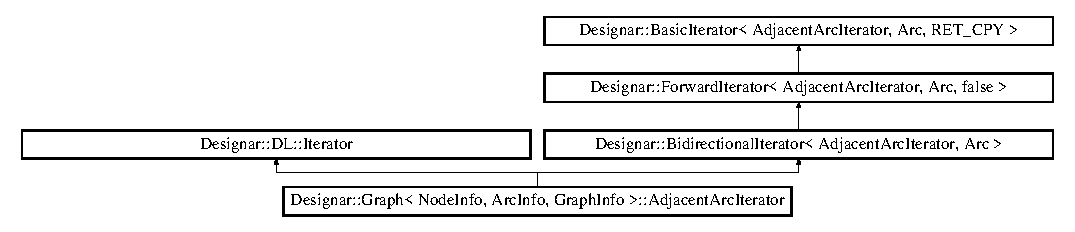
\includegraphics[height=2.666667cm]{class_designar_1_1_graph_1_1_adjacent_arc_iterator}
\end{center}
\end{figure}
\subsection*{Métodos públicos}
\begin{DoxyCompactItemize}
\item 
\hyperlink{class_designar_1_1_graph_1_1_adjacent_arc_iterator_a36fe9a05d139c9e44dc4ff6a47d41416}{Adjacent\+Arc\+Iterator} ()
\item 
\hyperlink{class_designar_1_1_graph_1_1_adjacent_arc_iterator_a2a16b2ab702ca71cf8561ea8ebc4ec72}{Adjacent\+Arc\+Iterator} (const \hyperlink{class_designar_1_1_graph}{Graph} \&g, const \hyperlink{class_designar_1_1_graph_a5dfc7dba9d092ac489c72e40390c37d0}{Node} \&n)
\item 
\hyperlink{class_designar_1_1_graph_1_1_adjacent_arc_iterator_a97e3e5909f6e9b9b6b55cbc0fb2d5263}{Adjacent\+Arc\+Iterator} (const \hyperlink{class_designar_1_1_graph}{Graph} \&g, const \hyperlink{class_designar_1_1_graph_a5dfc7dba9d092ac489c72e40390c37d0}{Node} \&n, \hyperlink{class_designar_1_1_d_l}{DL} $\ast$curr)
\item 
\hyperlink{class_designar_1_1_graph_1_1_adjacent_arc_iterator_af536d3124c826e57fdfd98b604338960}{Adjacent\+Arc\+Iterator} (const \hyperlink{class_designar_1_1_graph_1_1_adjacent_arc_iterator}{Adjacent\+Arc\+Iterator} \&it)
\item 
\hyperlink{class_designar_1_1_graph_1_1_adjacent_arc_iterator_afe1c65c9b34d57572217f33e4adc4200}{Adjacent\+Arc\+Iterator} (\hyperlink{class_designar_1_1_graph_1_1_adjacent_arc_iterator}{Adjacent\+Arc\+Iterator} \&\&it)
\item 
\hyperlink{class_designar_1_1_graph_1_1_adjacent_arc_iterator}{Adjacent\+Arc\+Iterator} \& \hyperlink{class_designar_1_1_graph_1_1_adjacent_arc_iterator_acd4f3584de04e7787b39b133bb9547ad}{operator=} (const \hyperlink{class_designar_1_1_graph_1_1_adjacent_arc_iterator}{Adjacent\+Arc\+Iterator} \&it)
\item 
\hyperlink{class_designar_1_1_graph_1_1_adjacent_arc_iterator}{Adjacent\+Arc\+Iterator} \& \hyperlink{class_designar_1_1_graph_1_1_adjacent_arc_iterator_a7dd872294198ccd6d38267629a65363f}{operator=} (\hyperlink{class_designar_1_1_graph_1_1_adjacent_arc_iterator}{Adjacent\+Arc\+Iterator} \&\&it)
\item 
void \hyperlink{class_designar_1_1_graph_1_1_adjacent_arc_iterator_a3a1ed1df16f67214b5664fe9e54f23f4}{swap} (\hyperlink{class_designar_1_1_graph_1_1_adjacent_arc_iterator}{Adjacent\+Arc\+Iterator} \&it)
\item 
\hyperlink{class_designar_1_1_graph_a74c730ef4ce2d20f998d72bd25c2b5bf}{Arc} \& \hyperlink{class_designar_1_1_graph_1_1_adjacent_arc_iterator_a8d4383e587b5a1203581c2c2616ab45f}{get\+\_\+current} ()
\item 
const \hyperlink{class_designar_1_1_graph_a74c730ef4ce2d20f998d72bd25c2b5bf}{Arc} \& \hyperlink{class_designar_1_1_graph_1_1_adjacent_arc_iterator_a42865c7e33a047eb16ef49428ec99e35}{get\+\_\+current} () const
\item 
\hyperlink{class_designar_1_1_graph_a5dfc7dba9d092ac489c72e40390c37d0}{Node} \& \hyperlink{class_designar_1_1_graph_1_1_adjacent_arc_iterator_a0a5f3238f6abde756b4498a31558a255}{get\+\_\+src\+\_\+node} ()
\item 
const \hyperlink{class_designar_1_1_graph_a5dfc7dba9d092ac489c72e40390c37d0}{Node} \& \hyperlink{class_designar_1_1_graph_1_1_adjacent_arc_iterator_ae4ba07319b439cc08df6c957a61bc224}{get\+\_\+src\+\_\+node} () const
\item 
\hyperlink{class_designar_1_1_graph_a5dfc7dba9d092ac489c72e40390c37d0}{Node} \& \hyperlink{class_designar_1_1_graph_1_1_adjacent_arc_iterator_a400e7399fa39eb49e64afcd2d0b26ff6}{get\+\_\+tgt\+\_\+node} ()
\item 
const \hyperlink{class_designar_1_1_graph_a5dfc7dba9d092ac489c72e40390c37d0}{Node} \& \hyperlink{class_designar_1_1_graph_1_1_adjacent_arc_iterator_a6f6a71103fa126fd3317af40844022a1}{get\+\_\+tgt\+\_\+node} () const
\end{DoxyCompactItemize}
\subsection*{Amigas}
\begin{DoxyCompactItemize}
\item 
class \hyperlink{class_designar_1_1_graph_1_1_adjacent_arc_iterator_a73ad70d76f3331ee4b07451db1347918}{Basic\+Iterator$<$ Adjacent\+Arc\+Iterator, Arc $>$}
\end{DoxyCompactItemize}
\subsection*{Otros miembros heredados}


\subsection{Descripción detallada}
\subsubsection*{template$<$typename Node\+Info, typename Arc\+Info = Empty\+Class, typename Graph\+Info = Empty\+Class$>$\newline
class Designar\+::\+Graph$<$ Node\+Info, Arc\+Info, Graph\+Info $>$\+::\+Adjacent\+Arc\+Iterator}



Definición en la línea 1619 del archivo graph.\+H.



\subsection{Documentación del constructor y destructor}
\mbox{\Hypertarget{class_designar_1_1_graph_1_1_adjacent_arc_iterator_a36fe9a05d139c9e44dc4ff6a47d41416}\label{class_designar_1_1_graph_1_1_adjacent_arc_iterator_a36fe9a05d139c9e44dc4ff6a47d41416}} 
\index{Designar\+::\+Graph\+::\+Adjacent\+Arc\+Iterator@{Designar\+::\+Graph\+::\+Adjacent\+Arc\+Iterator}!Adjacent\+Arc\+Iterator@{Adjacent\+Arc\+Iterator}}
\index{Adjacent\+Arc\+Iterator@{Adjacent\+Arc\+Iterator}!Designar\+::\+Graph\+::\+Adjacent\+Arc\+Iterator@{Designar\+::\+Graph\+::\+Adjacent\+Arc\+Iterator}}
\subsubsection{\texorpdfstring{Adjacent\+Arc\+Iterator()}{AdjacentArcIterator()}\hspace{0.1cm}{\footnotesize\ttfamily [1/5]}}
{\footnotesize\ttfamily template$<$typename Node\+Info , typename Arc\+Info  = Empty\+Class, typename Graph\+Info  = Empty\+Class$>$ \\
\hyperlink{class_designar_1_1_graph}{Designar\+::\+Graph}$<$ Node\+Info, Arc\+Info, Graph\+Info $>$\+::Adjacent\+Arc\+Iterator\+::\+Adjacent\+Arc\+Iterator (\begin{DoxyParamCaption}{ }\end{DoxyParamCaption})\hspace{0.3cm}{\ttfamily [inline]}}



Definición en la línea 1631 del archivo graph.\+H.

\mbox{\Hypertarget{class_designar_1_1_graph_1_1_adjacent_arc_iterator_a2a16b2ab702ca71cf8561ea8ebc4ec72}\label{class_designar_1_1_graph_1_1_adjacent_arc_iterator_a2a16b2ab702ca71cf8561ea8ebc4ec72}} 
\index{Designar\+::\+Graph\+::\+Adjacent\+Arc\+Iterator@{Designar\+::\+Graph\+::\+Adjacent\+Arc\+Iterator}!Adjacent\+Arc\+Iterator@{Adjacent\+Arc\+Iterator}}
\index{Adjacent\+Arc\+Iterator@{Adjacent\+Arc\+Iterator}!Designar\+::\+Graph\+::\+Adjacent\+Arc\+Iterator@{Designar\+::\+Graph\+::\+Adjacent\+Arc\+Iterator}}
\subsubsection{\texorpdfstring{Adjacent\+Arc\+Iterator()}{AdjacentArcIterator()}\hspace{0.1cm}{\footnotesize\ttfamily [2/5]}}
{\footnotesize\ttfamily template$<$typename Node\+Info , typename Arc\+Info  = Empty\+Class, typename Graph\+Info  = Empty\+Class$>$ \\
\hyperlink{class_designar_1_1_graph}{Designar\+::\+Graph}$<$ Node\+Info, Arc\+Info, Graph\+Info $>$\+::Adjacent\+Arc\+Iterator\+::\+Adjacent\+Arc\+Iterator (\begin{DoxyParamCaption}\item[{const \hyperlink{class_designar_1_1_graph}{Graph} \&}]{g,  }\item[{const \hyperlink{class_designar_1_1_graph_a5dfc7dba9d092ac489c72e40390c37d0}{Node} \&}]{n }\end{DoxyParamCaption})\hspace{0.3cm}{\ttfamily [inline]}}



Definición en la línea 1637 del archivo graph.\+H.

\mbox{\Hypertarget{class_designar_1_1_graph_1_1_adjacent_arc_iterator_a97e3e5909f6e9b9b6b55cbc0fb2d5263}\label{class_designar_1_1_graph_1_1_adjacent_arc_iterator_a97e3e5909f6e9b9b6b55cbc0fb2d5263}} 
\index{Designar\+::\+Graph\+::\+Adjacent\+Arc\+Iterator@{Designar\+::\+Graph\+::\+Adjacent\+Arc\+Iterator}!Adjacent\+Arc\+Iterator@{Adjacent\+Arc\+Iterator}}
\index{Adjacent\+Arc\+Iterator@{Adjacent\+Arc\+Iterator}!Designar\+::\+Graph\+::\+Adjacent\+Arc\+Iterator@{Designar\+::\+Graph\+::\+Adjacent\+Arc\+Iterator}}
\subsubsection{\texorpdfstring{Adjacent\+Arc\+Iterator()}{AdjacentArcIterator()}\hspace{0.1cm}{\footnotesize\ttfamily [3/5]}}
{\footnotesize\ttfamily template$<$typename Node\+Info , typename Arc\+Info  = Empty\+Class, typename Graph\+Info  = Empty\+Class$>$ \\
\hyperlink{class_designar_1_1_graph}{Designar\+::\+Graph}$<$ Node\+Info, Arc\+Info, Graph\+Info $>$\+::Adjacent\+Arc\+Iterator\+::\+Adjacent\+Arc\+Iterator (\begin{DoxyParamCaption}\item[{const \hyperlink{class_designar_1_1_graph}{Graph} \&}]{g,  }\item[{const \hyperlink{class_designar_1_1_graph_a5dfc7dba9d092ac489c72e40390c37d0}{Node} \&}]{n,  }\item[{\hyperlink{class_designar_1_1_d_l}{DL} $\ast$}]{curr }\end{DoxyParamCaption})\hspace{0.3cm}{\ttfamily [inline]}}



Definición en la línea 1644 del archivo graph.\+H.

\mbox{\Hypertarget{class_designar_1_1_graph_1_1_adjacent_arc_iterator_af536d3124c826e57fdfd98b604338960}\label{class_designar_1_1_graph_1_1_adjacent_arc_iterator_af536d3124c826e57fdfd98b604338960}} 
\index{Designar\+::\+Graph\+::\+Adjacent\+Arc\+Iterator@{Designar\+::\+Graph\+::\+Adjacent\+Arc\+Iterator}!Adjacent\+Arc\+Iterator@{Adjacent\+Arc\+Iterator}}
\index{Adjacent\+Arc\+Iterator@{Adjacent\+Arc\+Iterator}!Designar\+::\+Graph\+::\+Adjacent\+Arc\+Iterator@{Designar\+::\+Graph\+::\+Adjacent\+Arc\+Iterator}}
\subsubsection{\texorpdfstring{Adjacent\+Arc\+Iterator()}{AdjacentArcIterator()}\hspace{0.1cm}{\footnotesize\ttfamily [4/5]}}
{\footnotesize\ttfamily template$<$typename Node\+Info , typename Arc\+Info  = Empty\+Class, typename Graph\+Info  = Empty\+Class$>$ \\
\hyperlink{class_designar_1_1_graph}{Designar\+::\+Graph}$<$ Node\+Info, Arc\+Info, Graph\+Info $>$\+::Adjacent\+Arc\+Iterator\+::\+Adjacent\+Arc\+Iterator (\begin{DoxyParamCaption}\item[{const \hyperlink{class_designar_1_1_graph_1_1_adjacent_arc_iterator}{Adjacent\+Arc\+Iterator} \&}]{it }\end{DoxyParamCaption})\hspace{0.3cm}{\ttfamily [inline]}}



Definición en la línea 1651 del archivo graph.\+H.

\mbox{\Hypertarget{class_designar_1_1_graph_1_1_adjacent_arc_iterator_afe1c65c9b34d57572217f33e4adc4200}\label{class_designar_1_1_graph_1_1_adjacent_arc_iterator_afe1c65c9b34d57572217f33e4adc4200}} 
\index{Designar\+::\+Graph\+::\+Adjacent\+Arc\+Iterator@{Designar\+::\+Graph\+::\+Adjacent\+Arc\+Iterator}!Adjacent\+Arc\+Iterator@{Adjacent\+Arc\+Iterator}}
\index{Adjacent\+Arc\+Iterator@{Adjacent\+Arc\+Iterator}!Designar\+::\+Graph\+::\+Adjacent\+Arc\+Iterator@{Designar\+::\+Graph\+::\+Adjacent\+Arc\+Iterator}}
\subsubsection{\texorpdfstring{Adjacent\+Arc\+Iterator()}{AdjacentArcIterator()}\hspace{0.1cm}{\footnotesize\ttfamily [5/5]}}
{\footnotesize\ttfamily template$<$typename Node\+Info , typename Arc\+Info  = Empty\+Class, typename Graph\+Info  = Empty\+Class$>$ \\
\hyperlink{class_designar_1_1_graph}{Designar\+::\+Graph}$<$ Node\+Info, Arc\+Info, Graph\+Info $>$\+::Adjacent\+Arc\+Iterator\+::\+Adjacent\+Arc\+Iterator (\begin{DoxyParamCaption}\item[{\hyperlink{class_designar_1_1_graph_1_1_adjacent_arc_iterator}{Adjacent\+Arc\+Iterator} \&\&}]{it }\end{DoxyParamCaption})\hspace{0.3cm}{\ttfamily [inline]}}



Definición en la línea 1657 del archivo graph.\+H.



\subsection{Documentación de las funciones miembro}
\mbox{\Hypertarget{class_designar_1_1_graph_1_1_adjacent_arc_iterator_a8d4383e587b5a1203581c2c2616ab45f}\label{class_designar_1_1_graph_1_1_adjacent_arc_iterator_a8d4383e587b5a1203581c2c2616ab45f}} 
\index{Designar\+::\+Graph\+::\+Adjacent\+Arc\+Iterator@{Designar\+::\+Graph\+::\+Adjacent\+Arc\+Iterator}!get\+\_\+current@{get\+\_\+current}}
\index{get\+\_\+current@{get\+\_\+current}!Designar\+::\+Graph\+::\+Adjacent\+Arc\+Iterator@{Designar\+::\+Graph\+::\+Adjacent\+Arc\+Iterator}}
\subsubsection{\texorpdfstring{get\+\_\+current()}{get\_current()}\hspace{0.1cm}{\footnotesize\ttfamily [1/2]}}
{\footnotesize\ttfamily template$<$typename Node\+Info , typename Arc\+Info  = Empty\+Class, typename Graph\+Info  = Empty\+Class$>$ \\
\hyperlink{class_designar_1_1_graph_a74c730ef4ce2d20f998d72bd25c2b5bf}{Arc}\& \hyperlink{class_designar_1_1_graph}{Designar\+::\+Graph}$<$ Node\+Info, Arc\+Info, Graph\+Info $>$\+::Adjacent\+Arc\+Iterator\+::get\+\_\+current (\begin{DoxyParamCaption}{ }\end{DoxyParamCaption})\hspace{0.3cm}{\ttfamily [inline]}}



Definición en la línea 1687 del archivo graph.\+H.

\mbox{\Hypertarget{class_designar_1_1_graph_1_1_adjacent_arc_iterator_a42865c7e33a047eb16ef49428ec99e35}\label{class_designar_1_1_graph_1_1_adjacent_arc_iterator_a42865c7e33a047eb16ef49428ec99e35}} 
\index{Designar\+::\+Graph\+::\+Adjacent\+Arc\+Iterator@{Designar\+::\+Graph\+::\+Adjacent\+Arc\+Iterator}!get\+\_\+current@{get\+\_\+current}}
\index{get\+\_\+current@{get\+\_\+current}!Designar\+::\+Graph\+::\+Adjacent\+Arc\+Iterator@{Designar\+::\+Graph\+::\+Adjacent\+Arc\+Iterator}}
\subsubsection{\texorpdfstring{get\+\_\+current()}{get\_current()}\hspace{0.1cm}{\footnotesize\ttfamily [2/2]}}
{\footnotesize\ttfamily template$<$typename Node\+Info , typename Arc\+Info  = Empty\+Class, typename Graph\+Info  = Empty\+Class$>$ \\
const \hyperlink{class_designar_1_1_graph_a74c730ef4ce2d20f998d72bd25c2b5bf}{Arc}\& \hyperlink{class_designar_1_1_graph}{Designar\+::\+Graph}$<$ Node\+Info, Arc\+Info, Graph\+Info $>$\+::Adjacent\+Arc\+Iterator\+::get\+\_\+current (\begin{DoxyParamCaption}{ }\end{DoxyParamCaption}) const\hspace{0.3cm}{\ttfamily [inline]}}



Definición en la línea 1692 del archivo graph.\+H.

\mbox{\Hypertarget{class_designar_1_1_graph_1_1_adjacent_arc_iterator_a0a5f3238f6abde756b4498a31558a255}\label{class_designar_1_1_graph_1_1_adjacent_arc_iterator_a0a5f3238f6abde756b4498a31558a255}} 
\index{Designar\+::\+Graph\+::\+Adjacent\+Arc\+Iterator@{Designar\+::\+Graph\+::\+Adjacent\+Arc\+Iterator}!get\+\_\+src\+\_\+node@{get\+\_\+src\+\_\+node}}
\index{get\+\_\+src\+\_\+node@{get\+\_\+src\+\_\+node}!Designar\+::\+Graph\+::\+Adjacent\+Arc\+Iterator@{Designar\+::\+Graph\+::\+Adjacent\+Arc\+Iterator}}
\subsubsection{\texorpdfstring{get\+\_\+src\+\_\+node()}{get\_src\_node()}\hspace{0.1cm}{\footnotesize\ttfamily [1/2]}}
{\footnotesize\ttfamily template$<$typename Node\+Info , typename Arc\+Info  = Empty\+Class, typename Graph\+Info  = Empty\+Class$>$ \\
\hyperlink{class_designar_1_1_graph_a5dfc7dba9d092ac489c72e40390c37d0}{Node}\& \hyperlink{class_designar_1_1_graph}{Designar\+::\+Graph}$<$ Node\+Info, Arc\+Info, Graph\+Info $>$\+::Adjacent\+Arc\+Iterator\+::get\+\_\+src\+\_\+node (\begin{DoxyParamCaption}{ }\end{DoxyParamCaption})\hspace{0.3cm}{\ttfamily [inline]}}



Definición en la línea 1697 del archivo graph.\+H.

\mbox{\Hypertarget{class_designar_1_1_graph_1_1_adjacent_arc_iterator_ae4ba07319b439cc08df6c957a61bc224}\label{class_designar_1_1_graph_1_1_adjacent_arc_iterator_ae4ba07319b439cc08df6c957a61bc224}} 
\index{Designar\+::\+Graph\+::\+Adjacent\+Arc\+Iterator@{Designar\+::\+Graph\+::\+Adjacent\+Arc\+Iterator}!get\+\_\+src\+\_\+node@{get\+\_\+src\+\_\+node}}
\index{get\+\_\+src\+\_\+node@{get\+\_\+src\+\_\+node}!Designar\+::\+Graph\+::\+Adjacent\+Arc\+Iterator@{Designar\+::\+Graph\+::\+Adjacent\+Arc\+Iterator}}
\subsubsection{\texorpdfstring{get\+\_\+src\+\_\+node()}{get\_src\_node()}\hspace{0.1cm}{\footnotesize\ttfamily [2/2]}}
{\footnotesize\ttfamily template$<$typename Node\+Info , typename Arc\+Info  = Empty\+Class, typename Graph\+Info  = Empty\+Class$>$ \\
const \hyperlink{class_designar_1_1_graph_a5dfc7dba9d092ac489c72e40390c37d0}{Node}\& \hyperlink{class_designar_1_1_graph}{Designar\+::\+Graph}$<$ Node\+Info, Arc\+Info, Graph\+Info $>$\+::Adjacent\+Arc\+Iterator\+::get\+\_\+src\+\_\+node (\begin{DoxyParamCaption}{ }\end{DoxyParamCaption}) const\hspace{0.3cm}{\ttfamily [inline]}}



Definición en la línea 1702 del archivo graph.\+H.

\mbox{\Hypertarget{class_designar_1_1_graph_1_1_adjacent_arc_iterator_a400e7399fa39eb49e64afcd2d0b26ff6}\label{class_designar_1_1_graph_1_1_adjacent_arc_iterator_a400e7399fa39eb49e64afcd2d0b26ff6}} 
\index{Designar\+::\+Graph\+::\+Adjacent\+Arc\+Iterator@{Designar\+::\+Graph\+::\+Adjacent\+Arc\+Iterator}!get\+\_\+tgt\+\_\+node@{get\+\_\+tgt\+\_\+node}}
\index{get\+\_\+tgt\+\_\+node@{get\+\_\+tgt\+\_\+node}!Designar\+::\+Graph\+::\+Adjacent\+Arc\+Iterator@{Designar\+::\+Graph\+::\+Adjacent\+Arc\+Iterator}}
\subsubsection{\texorpdfstring{get\+\_\+tgt\+\_\+node()}{get\_tgt\_node()}\hspace{0.1cm}{\footnotesize\ttfamily [1/2]}}
{\footnotesize\ttfamily template$<$typename Node\+Info , typename Arc\+Info  = Empty\+Class, typename Graph\+Info  = Empty\+Class$>$ \\
\hyperlink{class_designar_1_1_graph_a5dfc7dba9d092ac489c72e40390c37d0}{Node}\& \hyperlink{class_designar_1_1_graph}{Designar\+::\+Graph}$<$ Node\+Info, Arc\+Info, Graph\+Info $>$\+::Adjacent\+Arc\+Iterator\+::get\+\_\+tgt\+\_\+node (\begin{DoxyParamCaption}{ }\end{DoxyParamCaption})\hspace{0.3cm}{\ttfamily [inline]}}



Definición en la línea 1707 del archivo graph.\+H.

\mbox{\Hypertarget{class_designar_1_1_graph_1_1_adjacent_arc_iterator_a6f6a71103fa126fd3317af40844022a1}\label{class_designar_1_1_graph_1_1_adjacent_arc_iterator_a6f6a71103fa126fd3317af40844022a1}} 
\index{Designar\+::\+Graph\+::\+Adjacent\+Arc\+Iterator@{Designar\+::\+Graph\+::\+Adjacent\+Arc\+Iterator}!get\+\_\+tgt\+\_\+node@{get\+\_\+tgt\+\_\+node}}
\index{get\+\_\+tgt\+\_\+node@{get\+\_\+tgt\+\_\+node}!Designar\+::\+Graph\+::\+Adjacent\+Arc\+Iterator@{Designar\+::\+Graph\+::\+Adjacent\+Arc\+Iterator}}
\subsubsection{\texorpdfstring{get\+\_\+tgt\+\_\+node()}{get\_tgt\_node()}\hspace{0.1cm}{\footnotesize\ttfamily [2/2]}}
{\footnotesize\ttfamily template$<$typename Node\+Info , typename Arc\+Info  = Empty\+Class, typename Graph\+Info  = Empty\+Class$>$ \\
const \hyperlink{class_designar_1_1_graph_a5dfc7dba9d092ac489c72e40390c37d0}{Node}\& \hyperlink{class_designar_1_1_graph}{Designar\+::\+Graph}$<$ Node\+Info, Arc\+Info, Graph\+Info $>$\+::Adjacent\+Arc\+Iterator\+::get\+\_\+tgt\+\_\+node (\begin{DoxyParamCaption}{ }\end{DoxyParamCaption}) const\hspace{0.3cm}{\ttfamily [inline]}}



Definición en la línea 1712 del archivo graph.\+H.

\mbox{\Hypertarget{class_designar_1_1_graph_1_1_adjacent_arc_iterator_acd4f3584de04e7787b39b133bb9547ad}\label{class_designar_1_1_graph_1_1_adjacent_arc_iterator_acd4f3584de04e7787b39b133bb9547ad}} 
\index{Designar\+::\+Graph\+::\+Adjacent\+Arc\+Iterator@{Designar\+::\+Graph\+::\+Adjacent\+Arc\+Iterator}!operator=@{operator=}}
\index{operator=@{operator=}!Designar\+::\+Graph\+::\+Adjacent\+Arc\+Iterator@{Designar\+::\+Graph\+::\+Adjacent\+Arc\+Iterator}}
\subsubsection{\texorpdfstring{operator=()}{operator=()}\hspace{0.1cm}{\footnotesize\ttfamily [1/2]}}
{\footnotesize\ttfamily template$<$typename Node\+Info , typename Arc\+Info  = Empty\+Class, typename Graph\+Info  = Empty\+Class$>$ \\
\hyperlink{class_designar_1_1_graph_1_1_adjacent_arc_iterator}{Adjacent\+Arc\+Iterator}\& \hyperlink{class_designar_1_1_graph}{Designar\+::\+Graph}$<$ Node\+Info, Arc\+Info, Graph\+Info $>$\+::Adjacent\+Arc\+Iterator\+::operator= (\begin{DoxyParamCaption}\item[{const \hyperlink{class_designar_1_1_graph_1_1_adjacent_arc_iterator}{Adjacent\+Arc\+Iterator} \&}]{it }\end{DoxyParamCaption})\hspace{0.3cm}{\ttfamily [inline]}}



Definición en la línea 1663 del archivo graph.\+H.

\mbox{\Hypertarget{class_designar_1_1_graph_1_1_adjacent_arc_iterator_a7dd872294198ccd6d38267629a65363f}\label{class_designar_1_1_graph_1_1_adjacent_arc_iterator_a7dd872294198ccd6d38267629a65363f}} 
\index{Designar\+::\+Graph\+::\+Adjacent\+Arc\+Iterator@{Designar\+::\+Graph\+::\+Adjacent\+Arc\+Iterator}!operator=@{operator=}}
\index{operator=@{operator=}!Designar\+::\+Graph\+::\+Adjacent\+Arc\+Iterator@{Designar\+::\+Graph\+::\+Adjacent\+Arc\+Iterator}}
\subsubsection{\texorpdfstring{operator=()}{operator=()}\hspace{0.1cm}{\footnotesize\ttfamily [2/2]}}
{\footnotesize\ttfamily template$<$typename Node\+Info , typename Arc\+Info  = Empty\+Class, typename Graph\+Info  = Empty\+Class$>$ \\
\hyperlink{class_designar_1_1_graph_1_1_adjacent_arc_iterator}{Adjacent\+Arc\+Iterator}\& \hyperlink{class_designar_1_1_graph}{Designar\+::\+Graph}$<$ Node\+Info, Arc\+Info, Graph\+Info $>$\+::Adjacent\+Arc\+Iterator\+::operator= (\begin{DoxyParamCaption}\item[{\hyperlink{class_designar_1_1_graph_1_1_adjacent_arc_iterator}{Adjacent\+Arc\+Iterator} \&\&}]{it }\end{DoxyParamCaption})\hspace{0.3cm}{\ttfamily [inline]}}



Definición en la línea 1674 del archivo graph.\+H.

\mbox{\Hypertarget{class_designar_1_1_graph_1_1_adjacent_arc_iterator_a3a1ed1df16f67214b5664fe9e54f23f4}\label{class_designar_1_1_graph_1_1_adjacent_arc_iterator_a3a1ed1df16f67214b5664fe9e54f23f4}} 
\index{Designar\+::\+Graph\+::\+Adjacent\+Arc\+Iterator@{Designar\+::\+Graph\+::\+Adjacent\+Arc\+Iterator}!swap@{swap}}
\index{swap@{swap}!Designar\+::\+Graph\+::\+Adjacent\+Arc\+Iterator@{Designar\+::\+Graph\+::\+Adjacent\+Arc\+Iterator}}
\subsubsection{\texorpdfstring{swap()}{swap()}}
{\footnotesize\ttfamily template$<$typename Node\+Info , typename Arc\+Info  = Empty\+Class, typename Graph\+Info  = Empty\+Class$>$ \\
void \hyperlink{class_designar_1_1_graph}{Designar\+::\+Graph}$<$ Node\+Info, Arc\+Info, Graph\+Info $>$\+::Adjacent\+Arc\+Iterator\+::swap (\begin{DoxyParamCaption}\item[{\hyperlink{class_designar_1_1_graph_1_1_adjacent_arc_iterator}{Adjacent\+Arc\+Iterator} \&}]{it }\end{DoxyParamCaption})\hspace{0.3cm}{\ttfamily [inline]}}



Definición en la línea 1680 del archivo graph.\+H.



\subsection{Documentación de las funciones relacionadas y clases amigas}
\mbox{\Hypertarget{class_designar_1_1_graph_1_1_adjacent_arc_iterator_a73ad70d76f3331ee4b07451db1347918}\label{class_designar_1_1_graph_1_1_adjacent_arc_iterator_a73ad70d76f3331ee4b07451db1347918}} 
\index{Designar\+::\+Graph\+::\+Adjacent\+Arc\+Iterator@{Designar\+::\+Graph\+::\+Adjacent\+Arc\+Iterator}!Basic\+Iterator$<$ Adjacent\+Arc\+Iterator, Arc $>$@{Basic\+Iterator$<$ Adjacent\+Arc\+Iterator, Arc $>$}}
\index{Basic\+Iterator$<$ Adjacent\+Arc\+Iterator, Arc $>$@{Basic\+Iterator$<$ Adjacent\+Arc\+Iterator, Arc $>$}!Designar\+::\+Graph\+::\+Adjacent\+Arc\+Iterator@{Designar\+::\+Graph\+::\+Adjacent\+Arc\+Iterator}}
\subsubsection{\texorpdfstring{Basic\+Iterator$<$ Adjacent\+Arc\+Iterator, Arc $>$}{BasicIterator< AdjacentArcIterator, Arc >}}
{\footnotesize\ttfamily template$<$typename Node\+Info , typename Arc\+Info  = Empty\+Class, typename Graph\+Info  = Empty\+Class$>$ \\
friend class \hyperlink{class_designar_1_1_basic_iterator}{Basic\+Iterator}$<$ \hyperlink{class_designar_1_1_graph_1_1_adjacent_arc_iterator}{Adjacent\+Arc\+Iterator}, \hyperlink{class_designar_1_1_graph_a74c730ef4ce2d20f998d72bd25c2b5bf}{Arc} $>$\hspace{0.3cm}{\ttfamily [friend]}}



Definición en la línea 1623 del archivo graph.\+H.



La documentación para esta clase fue generada a partir del siguiente fichero\+:\begin{DoxyCompactItemize}
\item 
/home/julio/\+De\+S\+I\+G\+N\+A\+R-\/doc/\+De\+Si\+G\+N\+A\+R/include/\hyperlink{graph_8_h}{graph.\+H}\end{DoxyCompactItemize}

\hypertarget{class_designar_1_1_digraph_1_1_adjacent_arc_iterator}{}\section{Referencia de la Clase Designar\+:\+:Digraph$<$ Node\+Info, Arc\+Info, Graph\+Info $>$\+:\+:Adjacent\+Arc\+Iterator}
\label{class_designar_1_1_digraph_1_1_adjacent_arc_iterator}\index{Designar\+::\+Digraph$<$ Node\+Info, Arc\+Info, Graph\+Info $>$\+::\+Adjacent\+Arc\+Iterator@{Designar\+::\+Digraph$<$ Node\+Info, Arc\+Info, Graph\+Info $>$\+::\+Adjacent\+Arc\+Iterator}}


{\ttfamily \#include $<$graph.\+H$>$}

Diagrama de herencias de Designar\+:\+:Digraph$<$ Node\+Info, Arc\+Info, Graph\+Info $>$\+:\+:Adjacent\+Arc\+Iterator\begin{figure}[H]
\begin{center}
\leavevmode
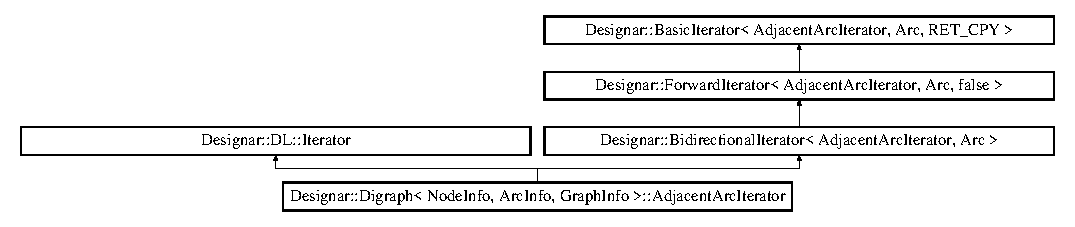
\includegraphics[height=2.604651cm]{class_designar_1_1_digraph_1_1_adjacent_arc_iterator}
\end{center}
\end{figure}
\subsection*{Métodos públicos}
\begin{DoxyCompactItemize}
\item 
\hyperlink{class_designar_1_1_digraph_1_1_adjacent_arc_iterator_a44c04d22e04c7458517a41bced9338f6}{Adjacent\+Arc\+Iterator} ()
\item 
\hyperlink{class_designar_1_1_digraph_1_1_adjacent_arc_iterator_a0e41952269f1ca89fd7647cb457cb6e2}{Adjacent\+Arc\+Iterator} (const \hyperlink{class_designar_1_1_digraph}{Digraph} \&g, const \hyperlink{class_designar_1_1_digraph_a4dc921c41a480b7946a04170e997d8ae}{Node} \&n)
\item 
\hyperlink{class_designar_1_1_digraph_1_1_adjacent_arc_iterator_ae4f0209339948fd0d1f6e6f26307ca9c}{Adjacent\+Arc\+Iterator} (const \hyperlink{class_designar_1_1_digraph}{Digraph} \&g, const \hyperlink{class_designar_1_1_digraph_a4dc921c41a480b7946a04170e997d8ae}{Node} \&n, \hyperlink{class_designar_1_1_d_l}{DL} $\ast$curr)
\item 
\hyperlink{class_designar_1_1_digraph_1_1_adjacent_arc_iterator_acf32a4ea55f99c576876e4c7d981ec70}{Adjacent\+Arc\+Iterator} (const \hyperlink{class_designar_1_1_digraph_1_1_adjacent_arc_iterator}{Adjacent\+Arc\+Iterator} \&it)
\item 
\hyperlink{class_designar_1_1_digraph_1_1_adjacent_arc_iterator_a43dfb1bed036cb0c417905526727883f}{Adjacent\+Arc\+Iterator} (\hyperlink{class_designar_1_1_digraph_1_1_adjacent_arc_iterator}{Adjacent\+Arc\+Iterator} \&\&it)
\item 
\hyperlink{class_designar_1_1_digraph_1_1_adjacent_arc_iterator}{Adjacent\+Arc\+Iterator} \& \hyperlink{class_designar_1_1_digraph_1_1_adjacent_arc_iterator_a2f354557278794bdd4bfc2c43c236814}{operator=} (const \hyperlink{class_designar_1_1_digraph_1_1_adjacent_arc_iterator}{Adjacent\+Arc\+Iterator} \&it)
\item 
\hyperlink{class_designar_1_1_digraph_1_1_adjacent_arc_iterator}{Adjacent\+Arc\+Iterator} \& \hyperlink{class_designar_1_1_digraph_1_1_adjacent_arc_iterator_a4dddbdfac352389f4fe7bf7f809c5655}{operator=} (\hyperlink{class_designar_1_1_digraph_1_1_adjacent_arc_iterator}{Adjacent\+Arc\+Iterator} \&\&it)
\item 
void \hyperlink{class_designar_1_1_digraph_1_1_adjacent_arc_iterator_a115f64297073bcdf6724045da1487d85}{swap} (\hyperlink{class_designar_1_1_digraph_1_1_adjacent_arc_iterator}{Adjacent\+Arc\+Iterator} \&it)
\item 
\hyperlink{class_designar_1_1_digraph_a0ceb278671f2a535c00fddccdeafd69f}{Arc} \& \hyperlink{class_designar_1_1_digraph_1_1_adjacent_arc_iterator_abd6687753cb547318760e8f3b87922e2}{get\+\_\+current} ()
\item 
const \hyperlink{class_designar_1_1_digraph_a0ceb278671f2a535c00fddccdeafd69f}{Arc} \& \hyperlink{class_designar_1_1_digraph_1_1_adjacent_arc_iterator_ac388275a16db45fc754a193766c215ce}{get\+\_\+current} () const
\item 
\hyperlink{class_designar_1_1_digraph_a0ceb278671f2a535c00fddccdeafd69f}{Arc} \& \hyperlink{class_designar_1_1_digraph_1_1_adjacent_arc_iterator_a2a1ee85a8076e07fd99d35676ec69887}{operator$\ast$} ()
\item 
const \hyperlink{class_designar_1_1_digraph_a0ceb278671f2a535c00fddccdeafd69f}{Arc} \& \hyperlink{class_designar_1_1_digraph_1_1_adjacent_arc_iterator_aaf54c97702c3b6e3ccf419c2f7966e44}{operator$\ast$} () const
\item 
\hyperlink{class_designar_1_1_digraph_a4dc921c41a480b7946a04170e997d8ae}{Node} \& \hyperlink{class_designar_1_1_digraph_1_1_adjacent_arc_iterator_a72e125198f4cea2ab0ac1213c1cbc1e4}{get\+\_\+src\+\_\+node} ()
\item 
const \hyperlink{class_designar_1_1_digraph_a4dc921c41a480b7946a04170e997d8ae}{Node} \& \hyperlink{class_designar_1_1_digraph_1_1_adjacent_arc_iterator_a09c51f5124610cd6e5360dc7039b4639}{get\+\_\+src\+\_\+node} () const
\item 
\hyperlink{class_designar_1_1_digraph_a4dc921c41a480b7946a04170e997d8ae}{Node} \& \hyperlink{class_designar_1_1_digraph_1_1_adjacent_arc_iterator_ad1df4c6624e411ea5ec10ee3d1414b1c}{get\+\_\+tgt\+\_\+node} ()
\item 
const \hyperlink{class_designar_1_1_digraph_a4dc921c41a480b7946a04170e997d8ae}{Node} \& \hyperlink{class_designar_1_1_digraph_1_1_adjacent_arc_iterator_a3b5e320227b6456e9b0de9d505e0eae4}{get\+\_\+tgt\+\_\+node} () const
\end{DoxyCompactItemize}
\subsection*{Amigas}
\begin{DoxyCompactItemize}
\item 
class \hyperlink{class_designar_1_1_digraph_1_1_adjacent_arc_iterator_a73ad70d76f3331ee4b07451db1347918}{Basic\+Iterator$<$ Adjacent\+Arc\+Iterator, Arc $>$}
\end{DoxyCompactItemize}
\subsection*{Otros miembros heredados}


\subsection{Descripción detallada}
\subsubsection*{template$<$typename Node\+Info, typename Arc\+Info = Empty\+Class, typename Graph\+Info = Empty\+Class$>$\newline
class Designar\+::\+Digraph$<$ Node\+Info, Arc\+Info, Graph\+Info $>$\+::\+Adjacent\+Arc\+Iterator}



Definición en la línea 1891 del archivo graph.\+H.



\subsection{Documentación del constructor y destructor}
\mbox{\Hypertarget{class_designar_1_1_digraph_1_1_adjacent_arc_iterator_a44c04d22e04c7458517a41bced9338f6}\label{class_designar_1_1_digraph_1_1_adjacent_arc_iterator_a44c04d22e04c7458517a41bced9338f6}} 
\index{Designar\+::\+Digraph\+::\+Adjacent\+Arc\+Iterator@{Designar\+::\+Digraph\+::\+Adjacent\+Arc\+Iterator}!Adjacent\+Arc\+Iterator@{Adjacent\+Arc\+Iterator}}
\index{Adjacent\+Arc\+Iterator@{Adjacent\+Arc\+Iterator}!Designar\+::\+Digraph\+::\+Adjacent\+Arc\+Iterator@{Designar\+::\+Digraph\+::\+Adjacent\+Arc\+Iterator}}
\subsubsection{\texorpdfstring{Adjacent\+Arc\+Iterator()}{AdjacentArcIterator()}\hspace{0.1cm}{\footnotesize\ttfamily [1/5]}}
{\footnotesize\ttfamily template$<$typename Node\+Info , typename Arc\+Info  = Empty\+Class, typename Graph\+Info  = Empty\+Class$>$ \\
\hyperlink{class_designar_1_1_digraph}{Designar\+::\+Digraph}$<$ Node\+Info, Arc\+Info, Graph\+Info $>$\+::Adjacent\+Arc\+Iterator\+::\+Adjacent\+Arc\+Iterator (\begin{DoxyParamCaption}{ }\end{DoxyParamCaption})\hspace{0.3cm}{\ttfamily [inline]}}



Definición en la línea 1903 del archivo graph.\+H.

\mbox{\Hypertarget{class_designar_1_1_digraph_1_1_adjacent_arc_iterator_a0e41952269f1ca89fd7647cb457cb6e2}\label{class_designar_1_1_digraph_1_1_adjacent_arc_iterator_a0e41952269f1ca89fd7647cb457cb6e2}} 
\index{Designar\+::\+Digraph\+::\+Adjacent\+Arc\+Iterator@{Designar\+::\+Digraph\+::\+Adjacent\+Arc\+Iterator}!Adjacent\+Arc\+Iterator@{Adjacent\+Arc\+Iterator}}
\index{Adjacent\+Arc\+Iterator@{Adjacent\+Arc\+Iterator}!Designar\+::\+Digraph\+::\+Adjacent\+Arc\+Iterator@{Designar\+::\+Digraph\+::\+Adjacent\+Arc\+Iterator}}
\subsubsection{\texorpdfstring{Adjacent\+Arc\+Iterator()}{AdjacentArcIterator()}\hspace{0.1cm}{\footnotesize\ttfamily [2/5]}}
{\footnotesize\ttfamily template$<$typename Node\+Info , typename Arc\+Info  = Empty\+Class, typename Graph\+Info  = Empty\+Class$>$ \\
\hyperlink{class_designar_1_1_digraph}{Designar\+::\+Digraph}$<$ Node\+Info, Arc\+Info, Graph\+Info $>$\+::Adjacent\+Arc\+Iterator\+::\+Adjacent\+Arc\+Iterator (\begin{DoxyParamCaption}\item[{const \hyperlink{class_designar_1_1_digraph}{Digraph} \&}]{g,  }\item[{const \hyperlink{class_designar_1_1_digraph_a4dc921c41a480b7946a04170e997d8ae}{Node} \&}]{n }\end{DoxyParamCaption})\hspace{0.3cm}{\ttfamily [inline]}}



Definición en la línea 1909 del archivo graph.\+H.

\mbox{\Hypertarget{class_designar_1_1_digraph_1_1_adjacent_arc_iterator_ae4f0209339948fd0d1f6e6f26307ca9c}\label{class_designar_1_1_digraph_1_1_adjacent_arc_iterator_ae4f0209339948fd0d1f6e6f26307ca9c}} 
\index{Designar\+::\+Digraph\+::\+Adjacent\+Arc\+Iterator@{Designar\+::\+Digraph\+::\+Adjacent\+Arc\+Iterator}!Adjacent\+Arc\+Iterator@{Adjacent\+Arc\+Iterator}}
\index{Adjacent\+Arc\+Iterator@{Adjacent\+Arc\+Iterator}!Designar\+::\+Digraph\+::\+Adjacent\+Arc\+Iterator@{Designar\+::\+Digraph\+::\+Adjacent\+Arc\+Iterator}}
\subsubsection{\texorpdfstring{Adjacent\+Arc\+Iterator()}{AdjacentArcIterator()}\hspace{0.1cm}{\footnotesize\ttfamily [3/5]}}
{\footnotesize\ttfamily template$<$typename Node\+Info , typename Arc\+Info  = Empty\+Class, typename Graph\+Info  = Empty\+Class$>$ \\
\hyperlink{class_designar_1_1_digraph}{Designar\+::\+Digraph}$<$ Node\+Info, Arc\+Info, Graph\+Info $>$\+::Adjacent\+Arc\+Iterator\+::\+Adjacent\+Arc\+Iterator (\begin{DoxyParamCaption}\item[{const \hyperlink{class_designar_1_1_digraph}{Digraph} \&}]{g,  }\item[{const \hyperlink{class_designar_1_1_digraph_a4dc921c41a480b7946a04170e997d8ae}{Node} \&}]{n,  }\item[{\hyperlink{class_designar_1_1_d_l}{DL} $\ast$}]{curr }\end{DoxyParamCaption})\hspace{0.3cm}{\ttfamily [inline]}}



Definición en la línea 1916 del archivo graph.\+H.

\mbox{\Hypertarget{class_designar_1_1_digraph_1_1_adjacent_arc_iterator_acf32a4ea55f99c576876e4c7d981ec70}\label{class_designar_1_1_digraph_1_1_adjacent_arc_iterator_acf32a4ea55f99c576876e4c7d981ec70}} 
\index{Designar\+::\+Digraph\+::\+Adjacent\+Arc\+Iterator@{Designar\+::\+Digraph\+::\+Adjacent\+Arc\+Iterator}!Adjacent\+Arc\+Iterator@{Adjacent\+Arc\+Iterator}}
\index{Adjacent\+Arc\+Iterator@{Adjacent\+Arc\+Iterator}!Designar\+::\+Digraph\+::\+Adjacent\+Arc\+Iterator@{Designar\+::\+Digraph\+::\+Adjacent\+Arc\+Iterator}}
\subsubsection{\texorpdfstring{Adjacent\+Arc\+Iterator()}{AdjacentArcIterator()}\hspace{0.1cm}{\footnotesize\ttfamily [4/5]}}
{\footnotesize\ttfamily template$<$typename Node\+Info , typename Arc\+Info  = Empty\+Class, typename Graph\+Info  = Empty\+Class$>$ \\
\hyperlink{class_designar_1_1_digraph}{Designar\+::\+Digraph}$<$ Node\+Info, Arc\+Info, Graph\+Info $>$\+::Adjacent\+Arc\+Iterator\+::\+Adjacent\+Arc\+Iterator (\begin{DoxyParamCaption}\item[{const \hyperlink{class_designar_1_1_digraph_1_1_adjacent_arc_iterator}{Adjacent\+Arc\+Iterator} \&}]{it }\end{DoxyParamCaption})\hspace{0.3cm}{\ttfamily [inline]}}



Definición en la línea 1923 del archivo graph.\+H.

\mbox{\Hypertarget{class_designar_1_1_digraph_1_1_adjacent_arc_iterator_a43dfb1bed036cb0c417905526727883f}\label{class_designar_1_1_digraph_1_1_adjacent_arc_iterator_a43dfb1bed036cb0c417905526727883f}} 
\index{Designar\+::\+Digraph\+::\+Adjacent\+Arc\+Iterator@{Designar\+::\+Digraph\+::\+Adjacent\+Arc\+Iterator}!Adjacent\+Arc\+Iterator@{Adjacent\+Arc\+Iterator}}
\index{Adjacent\+Arc\+Iterator@{Adjacent\+Arc\+Iterator}!Designar\+::\+Digraph\+::\+Adjacent\+Arc\+Iterator@{Designar\+::\+Digraph\+::\+Adjacent\+Arc\+Iterator}}
\subsubsection{\texorpdfstring{Adjacent\+Arc\+Iterator()}{AdjacentArcIterator()}\hspace{0.1cm}{\footnotesize\ttfamily [5/5]}}
{\footnotesize\ttfamily template$<$typename Node\+Info , typename Arc\+Info  = Empty\+Class, typename Graph\+Info  = Empty\+Class$>$ \\
\hyperlink{class_designar_1_1_digraph}{Designar\+::\+Digraph}$<$ Node\+Info, Arc\+Info, Graph\+Info $>$\+::Adjacent\+Arc\+Iterator\+::\+Adjacent\+Arc\+Iterator (\begin{DoxyParamCaption}\item[{\hyperlink{class_designar_1_1_digraph_1_1_adjacent_arc_iterator}{Adjacent\+Arc\+Iterator} \&\&}]{it }\end{DoxyParamCaption})\hspace{0.3cm}{\ttfamily [inline]}}



Definición en la línea 1929 del archivo graph.\+H.



\subsection{Documentación de las funciones miembro}
\mbox{\Hypertarget{class_designar_1_1_digraph_1_1_adjacent_arc_iterator_abd6687753cb547318760e8f3b87922e2}\label{class_designar_1_1_digraph_1_1_adjacent_arc_iterator_abd6687753cb547318760e8f3b87922e2}} 
\index{Designar\+::\+Digraph\+::\+Adjacent\+Arc\+Iterator@{Designar\+::\+Digraph\+::\+Adjacent\+Arc\+Iterator}!get\+\_\+current@{get\+\_\+current}}
\index{get\+\_\+current@{get\+\_\+current}!Designar\+::\+Digraph\+::\+Adjacent\+Arc\+Iterator@{Designar\+::\+Digraph\+::\+Adjacent\+Arc\+Iterator}}
\subsubsection{\texorpdfstring{get\+\_\+current()}{get\_current()}\hspace{0.1cm}{\footnotesize\ttfamily [1/2]}}
{\footnotesize\ttfamily template$<$typename Node\+Info , typename Arc\+Info  = Empty\+Class, typename Graph\+Info  = Empty\+Class$>$ \\
\hyperlink{class_designar_1_1_digraph_a0ceb278671f2a535c00fddccdeafd69f}{Arc}\& \hyperlink{class_designar_1_1_digraph}{Designar\+::\+Digraph}$<$ Node\+Info, Arc\+Info, Graph\+Info $>$\+::Adjacent\+Arc\+Iterator\+::get\+\_\+current (\begin{DoxyParamCaption}{ }\end{DoxyParamCaption})\hspace{0.3cm}{\ttfamily [inline]}}



Definición en la línea 1959 del archivo graph.\+H.

\mbox{\Hypertarget{class_designar_1_1_digraph_1_1_adjacent_arc_iterator_ac388275a16db45fc754a193766c215ce}\label{class_designar_1_1_digraph_1_1_adjacent_arc_iterator_ac388275a16db45fc754a193766c215ce}} 
\index{Designar\+::\+Digraph\+::\+Adjacent\+Arc\+Iterator@{Designar\+::\+Digraph\+::\+Adjacent\+Arc\+Iterator}!get\+\_\+current@{get\+\_\+current}}
\index{get\+\_\+current@{get\+\_\+current}!Designar\+::\+Digraph\+::\+Adjacent\+Arc\+Iterator@{Designar\+::\+Digraph\+::\+Adjacent\+Arc\+Iterator}}
\subsubsection{\texorpdfstring{get\+\_\+current()}{get\_current()}\hspace{0.1cm}{\footnotesize\ttfamily [2/2]}}
{\footnotesize\ttfamily template$<$typename Node\+Info , typename Arc\+Info  = Empty\+Class, typename Graph\+Info  = Empty\+Class$>$ \\
const \hyperlink{class_designar_1_1_digraph_a0ceb278671f2a535c00fddccdeafd69f}{Arc}\& \hyperlink{class_designar_1_1_digraph}{Designar\+::\+Digraph}$<$ Node\+Info, Arc\+Info, Graph\+Info $>$\+::Adjacent\+Arc\+Iterator\+::get\+\_\+current (\begin{DoxyParamCaption}{ }\end{DoxyParamCaption}) const\hspace{0.3cm}{\ttfamily [inline]}}



Definición en la línea 1964 del archivo graph.\+H.

\mbox{\Hypertarget{class_designar_1_1_digraph_1_1_adjacent_arc_iterator_a72e125198f4cea2ab0ac1213c1cbc1e4}\label{class_designar_1_1_digraph_1_1_adjacent_arc_iterator_a72e125198f4cea2ab0ac1213c1cbc1e4}} 
\index{Designar\+::\+Digraph\+::\+Adjacent\+Arc\+Iterator@{Designar\+::\+Digraph\+::\+Adjacent\+Arc\+Iterator}!get\+\_\+src\+\_\+node@{get\+\_\+src\+\_\+node}}
\index{get\+\_\+src\+\_\+node@{get\+\_\+src\+\_\+node}!Designar\+::\+Digraph\+::\+Adjacent\+Arc\+Iterator@{Designar\+::\+Digraph\+::\+Adjacent\+Arc\+Iterator}}
\subsubsection{\texorpdfstring{get\+\_\+src\+\_\+node()}{get\_src\_node()}\hspace{0.1cm}{\footnotesize\ttfamily [1/2]}}
{\footnotesize\ttfamily template$<$typename Node\+Info , typename Arc\+Info  = Empty\+Class, typename Graph\+Info  = Empty\+Class$>$ \\
\hyperlink{class_designar_1_1_digraph_a4dc921c41a480b7946a04170e997d8ae}{Node}\& \hyperlink{class_designar_1_1_digraph}{Designar\+::\+Digraph}$<$ Node\+Info, Arc\+Info, Graph\+Info $>$\+::Adjacent\+Arc\+Iterator\+::get\+\_\+src\+\_\+node (\begin{DoxyParamCaption}{ }\end{DoxyParamCaption})\hspace{0.3cm}{\ttfamily [inline]}}



Definición en la línea 1979 del archivo graph.\+H.

\mbox{\Hypertarget{class_designar_1_1_digraph_1_1_adjacent_arc_iterator_a09c51f5124610cd6e5360dc7039b4639}\label{class_designar_1_1_digraph_1_1_adjacent_arc_iterator_a09c51f5124610cd6e5360dc7039b4639}} 
\index{Designar\+::\+Digraph\+::\+Adjacent\+Arc\+Iterator@{Designar\+::\+Digraph\+::\+Adjacent\+Arc\+Iterator}!get\+\_\+src\+\_\+node@{get\+\_\+src\+\_\+node}}
\index{get\+\_\+src\+\_\+node@{get\+\_\+src\+\_\+node}!Designar\+::\+Digraph\+::\+Adjacent\+Arc\+Iterator@{Designar\+::\+Digraph\+::\+Adjacent\+Arc\+Iterator}}
\subsubsection{\texorpdfstring{get\+\_\+src\+\_\+node()}{get\_src\_node()}\hspace{0.1cm}{\footnotesize\ttfamily [2/2]}}
{\footnotesize\ttfamily template$<$typename Node\+Info , typename Arc\+Info  = Empty\+Class, typename Graph\+Info  = Empty\+Class$>$ \\
const \hyperlink{class_designar_1_1_digraph_a4dc921c41a480b7946a04170e997d8ae}{Node}\& \hyperlink{class_designar_1_1_digraph}{Designar\+::\+Digraph}$<$ Node\+Info, Arc\+Info, Graph\+Info $>$\+::Adjacent\+Arc\+Iterator\+::get\+\_\+src\+\_\+node (\begin{DoxyParamCaption}{ }\end{DoxyParamCaption}) const\hspace{0.3cm}{\ttfamily [inline]}}



Definición en la línea 1984 del archivo graph.\+H.

\mbox{\Hypertarget{class_designar_1_1_digraph_1_1_adjacent_arc_iterator_ad1df4c6624e411ea5ec10ee3d1414b1c}\label{class_designar_1_1_digraph_1_1_adjacent_arc_iterator_ad1df4c6624e411ea5ec10ee3d1414b1c}} 
\index{Designar\+::\+Digraph\+::\+Adjacent\+Arc\+Iterator@{Designar\+::\+Digraph\+::\+Adjacent\+Arc\+Iterator}!get\+\_\+tgt\+\_\+node@{get\+\_\+tgt\+\_\+node}}
\index{get\+\_\+tgt\+\_\+node@{get\+\_\+tgt\+\_\+node}!Designar\+::\+Digraph\+::\+Adjacent\+Arc\+Iterator@{Designar\+::\+Digraph\+::\+Adjacent\+Arc\+Iterator}}
\subsubsection{\texorpdfstring{get\+\_\+tgt\+\_\+node()}{get\_tgt\_node()}\hspace{0.1cm}{\footnotesize\ttfamily [1/2]}}
{\footnotesize\ttfamily template$<$typename Node\+Info , typename Arc\+Info  = Empty\+Class, typename Graph\+Info  = Empty\+Class$>$ \\
\hyperlink{class_designar_1_1_digraph_a4dc921c41a480b7946a04170e997d8ae}{Node}\& \hyperlink{class_designar_1_1_digraph}{Designar\+::\+Digraph}$<$ Node\+Info, Arc\+Info, Graph\+Info $>$\+::Adjacent\+Arc\+Iterator\+::get\+\_\+tgt\+\_\+node (\begin{DoxyParamCaption}{ }\end{DoxyParamCaption})\hspace{0.3cm}{\ttfamily [inline]}}



Definición en la línea 1989 del archivo graph.\+H.

\mbox{\Hypertarget{class_designar_1_1_digraph_1_1_adjacent_arc_iterator_a3b5e320227b6456e9b0de9d505e0eae4}\label{class_designar_1_1_digraph_1_1_adjacent_arc_iterator_a3b5e320227b6456e9b0de9d505e0eae4}} 
\index{Designar\+::\+Digraph\+::\+Adjacent\+Arc\+Iterator@{Designar\+::\+Digraph\+::\+Adjacent\+Arc\+Iterator}!get\+\_\+tgt\+\_\+node@{get\+\_\+tgt\+\_\+node}}
\index{get\+\_\+tgt\+\_\+node@{get\+\_\+tgt\+\_\+node}!Designar\+::\+Digraph\+::\+Adjacent\+Arc\+Iterator@{Designar\+::\+Digraph\+::\+Adjacent\+Arc\+Iterator}}
\subsubsection{\texorpdfstring{get\+\_\+tgt\+\_\+node()}{get\_tgt\_node()}\hspace{0.1cm}{\footnotesize\ttfamily [2/2]}}
{\footnotesize\ttfamily template$<$typename Node\+Info , typename Arc\+Info  = Empty\+Class, typename Graph\+Info  = Empty\+Class$>$ \\
const \hyperlink{class_designar_1_1_digraph_a4dc921c41a480b7946a04170e997d8ae}{Node}\& \hyperlink{class_designar_1_1_digraph}{Designar\+::\+Digraph}$<$ Node\+Info, Arc\+Info, Graph\+Info $>$\+::Adjacent\+Arc\+Iterator\+::get\+\_\+tgt\+\_\+node (\begin{DoxyParamCaption}{ }\end{DoxyParamCaption}) const\hspace{0.3cm}{\ttfamily [inline]}}



Definición en la línea 1994 del archivo graph.\+H.

\mbox{\Hypertarget{class_designar_1_1_digraph_1_1_adjacent_arc_iterator_a2a1ee85a8076e07fd99d35676ec69887}\label{class_designar_1_1_digraph_1_1_adjacent_arc_iterator_a2a1ee85a8076e07fd99d35676ec69887}} 
\index{Designar\+::\+Digraph\+::\+Adjacent\+Arc\+Iterator@{Designar\+::\+Digraph\+::\+Adjacent\+Arc\+Iterator}!operator$\ast$@{operator$\ast$}}
\index{operator$\ast$@{operator$\ast$}!Designar\+::\+Digraph\+::\+Adjacent\+Arc\+Iterator@{Designar\+::\+Digraph\+::\+Adjacent\+Arc\+Iterator}}
\subsubsection{\texorpdfstring{operator$\ast$()}{operator*()}\hspace{0.1cm}{\footnotesize\ttfamily [1/2]}}
{\footnotesize\ttfamily template$<$typename Node\+Info , typename Arc\+Info  = Empty\+Class, typename Graph\+Info  = Empty\+Class$>$ \\
\hyperlink{class_designar_1_1_digraph_a0ceb278671f2a535c00fddccdeafd69f}{Arc}\& \hyperlink{class_designar_1_1_digraph}{Designar\+::\+Digraph}$<$ Node\+Info, Arc\+Info, Graph\+Info $>$\+::Adjacent\+Arc\+Iterator\+::operator$\ast$ (\begin{DoxyParamCaption}{ }\end{DoxyParamCaption})\hspace{0.3cm}{\ttfamily [inline]}}



Definición en la línea 1969 del archivo graph.\+H.

\mbox{\Hypertarget{class_designar_1_1_digraph_1_1_adjacent_arc_iterator_aaf54c97702c3b6e3ccf419c2f7966e44}\label{class_designar_1_1_digraph_1_1_adjacent_arc_iterator_aaf54c97702c3b6e3ccf419c2f7966e44}} 
\index{Designar\+::\+Digraph\+::\+Adjacent\+Arc\+Iterator@{Designar\+::\+Digraph\+::\+Adjacent\+Arc\+Iterator}!operator$\ast$@{operator$\ast$}}
\index{operator$\ast$@{operator$\ast$}!Designar\+::\+Digraph\+::\+Adjacent\+Arc\+Iterator@{Designar\+::\+Digraph\+::\+Adjacent\+Arc\+Iterator}}
\subsubsection{\texorpdfstring{operator$\ast$()}{operator*()}\hspace{0.1cm}{\footnotesize\ttfamily [2/2]}}
{\footnotesize\ttfamily template$<$typename Node\+Info , typename Arc\+Info  = Empty\+Class, typename Graph\+Info  = Empty\+Class$>$ \\
const \hyperlink{class_designar_1_1_digraph_a0ceb278671f2a535c00fddccdeafd69f}{Arc}\& \hyperlink{class_designar_1_1_digraph}{Designar\+::\+Digraph}$<$ Node\+Info, Arc\+Info, Graph\+Info $>$\+::Adjacent\+Arc\+Iterator\+::operator$\ast$ (\begin{DoxyParamCaption}{ }\end{DoxyParamCaption}) const\hspace{0.3cm}{\ttfamily [inline]}}



Definición en la línea 1974 del archivo graph.\+H.

\mbox{\Hypertarget{class_designar_1_1_digraph_1_1_adjacent_arc_iterator_a2f354557278794bdd4bfc2c43c236814}\label{class_designar_1_1_digraph_1_1_adjacent_arc_iterator_a2f354557278794bdd4bfc2c43c236814}} 
\index{Designar\+::\+Digraph\+::\+Adjacent\+Arc\+Iterator@{Designar\+::\+Digraph\+::\+Adjacent\+Arc\+Iterator}!operator=@{operator=}}
\index{operator=@{operator=}!Designar\+::\+Digraph\+::\+Adjacent\+Arc\+Iterator@{Designar\+::\+Digraph\+::\+Adjacent\+Arc\+Iterator}}
\subsubsection{\texorpdfstring{operator=()}{operator=()}\hspace{0.1cm}{\footnotesize\ttfamily [1/2]}}
{\footnotesize\ttfamily template$<$typename Node\+Info , typename Arc\+Info  = Empty\+Class, typename Graph\+Info  = Empty\+Class$>$ \\
\hyperlink{class_designar_1_1_digraph_1_1_adjacent_arc_iterator}{Adjacent\+Arc\+Iterator}\& \hyperlink{class_designar_1_1_digraph}{Designar\+::\+Digraph}$<$ Node\+Info, Arc\+Info, Graph\+Info $>$\+::Adjacent\+Arc\+Iterator\+::operator= (\begin{DoxyParamCaption}\item[{const \hyperlink{class_designar_1_1_digraph_1_1_adjacent_arc_iterator}{Adjacent\+Arc\+Iterator} \&}]{it }\end{DoxyParamCaption})\hspace{0.3cm}{\ttfamily [inline]}}



Definición en la línea 1935 del archivo graph.\+H.

\mbox{\Hypertarget{class_designar_1_1_digraph_1_1_adjacent_arc_iterator_a4dddbdfac352389f4fe7bf7f809c5655}\label{class_designar_1_1_digraph_1_1_adjacent_arc_iterator_a4dddbdfac352389f4fe7bf7f809c5655}} 
\index{Designar\+::\+Digraph\+::\+Adjacent\+Arc\+Iterator@{Designar\+::\+Digraph\+::\+Adjacent\+Arc\+Iterator}!operator=@{operator=}}
\index{operator=@{operator=}!Designar\+::\+Digraph\+::\+Adjacent\+Arc\+Iterator@{Designar\+::\+Digraph\+::\+Adjacent\+Arc\+Iterator}}
\subsubsection{\texorpdfstring{operator=()}{operator=()}\hspace{0.1cm}{\footnotesize\ttfamily [2/2]}}
{\footnotesize\ttfamily template$<$typename Node\+Info , typename Arc\+Info  = Empty\+Class, typename Graph\+Info  = Empty\+Class$>$ \\
\hyperlink{class_designar_1_1_digraph_1_1_adjacent_arc_iterator}{Adjacent\+Arc\+Iterator}\& \hyperlink{class_designar_1_1_digraph}{Designar\+::\+Digraph}$<$ Node\+Info, Arc\+Info, Graph\+Info $>$\+::Adjacent\+Arc\+Iterator\+::operator= (\begin{DoxyParamCaption}\item[{\hyperlink{class_designar_1_1_digraph_1_1_adjacent_arc_iterator}{Adjacent\+Arc\+Iterator} \&\&}]{it }\end{DoxyParamCaption})\hspace{0.3cm}{\ttfamily [inline]}}



Definición en la línea 1946 del archivo graph.\+H.

\mbox{\Hypertarget{class_designar_1_1_digraph_1_1_adjacent_arc_iterator_a115f64297073bcdf6724045da1487d85}\label{class_designar_1_1_digraph_1_1_adjacent_arc_iterator_a115f64297073bcdf6724045da1487d85}} 
\index{Designar\+::\+Digraph\+::\+Adjacent\+Arc\+Iterator@{Designar\+::\+Digraph\+::\+Adjacent\+Arc\+Iterator}!swap@{swap}}
\index{swap@{swap}!Designar\+::\+Digraph\+::\+Adjacent\+Arc\+Iterator@{Designar\+::\+Digraph\+::\+Adjacent\+Arc\+Iterator}}
\subsubsection{\texorpdfstring{swap()}{swap()}}
{\footnotesize\ttfamily template$<$typename Node\+Info , typename Arc\+Info  = Empty\+Class, typename Graph\+Info  = Empty\+Class$>$ \\
void \hyperlink{class_designar_1_1_digraph}{Designar\+::\+Digraph}$<$ Node\+Info, Arc\+Info, Graph\+Info $>$\+::Adjacent\+Arc\+Iterator\+::swap (\begin{DoxyParamCaption}\item[{\hyperlink{class_designar_1_1_digraph_1_1_adjacent_arc_iterator}{Adjacent\+Arc\+Iterator} \&}]{it }\end{DoxyParamCaption})\hspace{0.3cm}{\ttfamily [inline]}}



Definición en la línea 1952 del archivo graph.\+H.



\subsection{Documentación de las funciones relacionadas y clases amigas}
\mbox{\Hypertarget{class_designar_1_1_digraph_1_1_adjacent_arc_iterator_a73ad70d76f3331ee4b07451db1347918}\label{class_designar_1_1_digraph_1_1_adjacent_arc_iterator_a73ad70d76f3331ee4b07451db1347918}} 
\index{Designar\+::\+Digraph\+::\+Adjacent\+Arc\+Iterator@{Designar\+::\+Digraph\+::\+Adjacent\+Arc\+Iterator}!Basic\+Iterator$<$ Adjacent\+Arc\+Iterator, Arc $>$@{Basic\+Iterator$<$ Adjacent\+Arc\+Iterator, Arc $>$}}
\index{Basic\+Iterator$<$ Adjacent\+Arc\+Iterator, Arc $>$@{Basic\+Iterator$<$ Adjacent\+Arc\+Iterator, Arc $>$}!Designar\+::\+Digraph\+::\+Adjacent\+Arc\+Iterator@{Designar\+::\+Digraph\+::\+Adjacent\+Arc\+Iterator}}
\subsubsection{\texorpdfstring{Basic\+Iterator$<$ Adjacent\+Arc\+Iterator, Arc $>$}{BasicIterator< AdjacentArcIterator, Arc >}}
{\footnotesize\ttfamily template$<$typename Node\+Info , typename Arc\+Info  = Empty\+Class, typename Graph\+Info  = Empty\+Class$>$ \\
friend class \hyperlink{class_designar_1_1_basic_iterator}{Basic\+Iterator}$<$ \hyperlink{class_designar_1_1_digraph_1_1_adjacent_arc_iterator}{Adjacent\+Arc\+Iterator}, \hyperlink{class_designar_1_1_digraph_a0ceb278671f2a535c00fddccdeafd69f}{Arc} $>$\hspace{0.3cm}{\ttfamily [friend]}}



Definición en la línea 1895 del archivo graph.\+H.



La documentación para esta clase fue generada a partir del siguiente fichero\+:\begin{DoxyCompactItemize}
\item 
include/\hyperlink{graph_8_h}{graph.\+H}\end{DoxyCompactItemize}

\hypertarget{struct_designar_1_1_all_are_convertible}{}\section{Designar\+:\+:All\+Are\+Convertible$<$ To, From\+Head, From\+Tail $>$ Struct Template Reference}
\label{struct_designar_1_1_all_are_convertible}\index{Designar\+::\+All\+Are\+Convertible$<$ To, From\+Head, From\+Tail $>$@{Designar\+::\+All\+Are\+Convertible$<$ To, From\+Head, From\+Tail $>$}}


{\ttfamily \#include $<$typetraits.\+H$>$}

\subsection*{Static Public Attributes}
\begin{DoxyCompactItemize}
\item 
static constexpr bool \hyperlink{struct_designar_1_1_all_are_convertible_a698b71c73875452298bc2e96935240c3}{value}
\end{DoxyCompactItemize}


\subsection{Detailed Description}
\subsubsection*{template$<$typename To, typename From\+Head, typename ... From\+Tail$>$\newline
struct Designar\+::\+All\+Are\+Convertible$<$ To, From\+Head, From\+Tail $>$}



Definition at line 34 of file typetraits.\+H.



\subsection{Member Data Documentation}
\mbox{\Hypertarget{struct_designar_1_1_all_are_convertible_a698b71c73875452298bc2e96935240c3}\label{struct_designar_1_1_all_are_convertible_a698b71c73875452298bc2e96935240c3}} 
\index{Designar\+::\+All\+Are\+Convertible@{Designar\+::\+All\+Are\+Convertible}!value@{value}}
\index{value@{value}!Designar\+::\+All\+Are\+Convertible@{Designar\+::\+All\+Are\+Convertible}}
\subsubsection{\texorpdfstring{value}{value}}
{\footnotesize\ttfamily template$<$typename To , typename From\+Head , typename ... From\+Tail$>$ \\
constexpr bool \hyperlink{struct_designar_1_1_all_are_convertible}{Designar\+::\+All\+Are\+Convertible}$<$ To, From\+Head, From\+Tail $>$\+::value\hspace{0.3cm}{\ttfamily [static]}}

{\bfseries Initial value\+:}
\begin{DoxyCode}
=
      \hyperlink{namespace_designar_a7dd2a7b6d96f664ce612b506c8eb2fb8}{std::is\_convertible<FromHead, To>::value} and
      AllAreConvertible<To, FromTail...>\hyperlink{struct_designar_1_1_all_are_convertible_a698b71c73875452298bc2e96935240c3}{::value}
\end{DoxyCode}


Definition at line 36 of file typetraits.\+H.



The documentation for this struct was generated from the following file\+:\begin{DoxyCompactItemize}
\item 
/home/julio/\+De\+S\+I\+G\+N\+A\+R-\/doc/\+De\+Si\+G\+N\+A\+R/include/\hyperlink{typetraits_8_h}{typetraits.\+H}\end{DoxyCompactItemize}

\hypertarget{struct_designar_1_1_all_are_convertible_3_01_to_00_01_from_01_4}{}\section{Referencia de la plantilla de la Estructura Designar\+:\+:All\+Are\+Convertible$<$ To, From $>$}
\label{struct_designar_1_1_all_are_convertible_3_01_to_00_01_from_01_4}\index{Designar\+::\+All\+Are\+Convertible$<$ To, From $>$@{Designar\+::\+All\+Are\+Convertible$<$ To, From $>$}}


{\ttfamily \#include $<$typetraits.\+H$>$}

\subsection*{Atributos públicos estáticos}
\begin{DoxyCompactItemize}
\item 
static constexpr bool \hyperlink{struct_designar_1_1_all_are_convertible_3_01_to_00_01_from_01_4_a64662370d25f46762af5c4adc6a01a84}{value} = std\+::is\+\_\+convertible$<$From, To$>$\+::value
\end{DoxyCompactItemize}


\subsection{Descripción detallada}
\subsubsection*{template$<$typename To, typename From$>$\newline
struct Designar\+::\+All\+Are\+Convertible$<$ To, From $>$}



Definición en la línea 42 del archivo typetraits.\+H.



\subsection{Documentación de los datos miembro}
\mbox{\Hypertarget{struct_designar_1_1_all_are_convertible_3_01_to_00_01_from_01_4_a64662370d25f46762af5c4adc6a01a84}\label{struct_designar_1_1_all_are_convertible_3_01_to_00_01_from_01_4_a64662370d25f46762af5c4adc6a01a84}} 
\index{Designar\+::\+All\+Are\+Convertible$<$ To, From $>$@{Designar\+::\+All\+Are\+Convertible$<$ To, From $>$}!value@{value}}
\index{value@{value}!Designar\+::\+All\+Are\+Convertible$<$ To, From $>$@{Designar\+::\+All\+Are\+Convertible$<$ To, From $>$}}
\subsubsection{\texorpdfstring{value}{value}}
{\footnotesize\ttfamily template$<$typename To , typename From $>$ \\
constexpr bool \hyperlink{struct_designar_1_1_all_are_convertible}{Designar\+::\+All\+Are\+Convertible}$<$ To, From $>$\+::value = std\+::is\+\_\+convertible$<$From, To$>$\+::value\hspace{0.3cm}{\ttfamily [static]}}



Definición en la línea 44 del archivo typetraits.\+H.



La documentación para esta estructura fue generada a partir del siguiente fichero\+:\begin{DoxyCompactItemize}
\item 
include/\hyperlink{typetraits_8_h}{typetraits.\+H}\end{DoxyCompactItemize}

\hypertarget{class_designar_1_1_arc_heap}{}\section{Designar\+:\+:Arc\+Heap$<$ GT, Distance, Cmp $>$ Class Template Reference}
\label{class_designar_1_1_arc_heap}\index{Designar\+::\+Arc\+Heap$<$ G\+T, Distance, Cmp $>$@{Designar\+::\+Arc\+Heap$<$ G\+T, Distance, Cmp $>$}}


{\ttfamily \#include $<$graphalgorithms.\+H$>$}

Inheritance diagram for Designar\+:\+:Arc\+Heap$<$ GT, Distance, Cmp $>$\+:\begin{figure}[H]
\begin{center}
\leavevmode
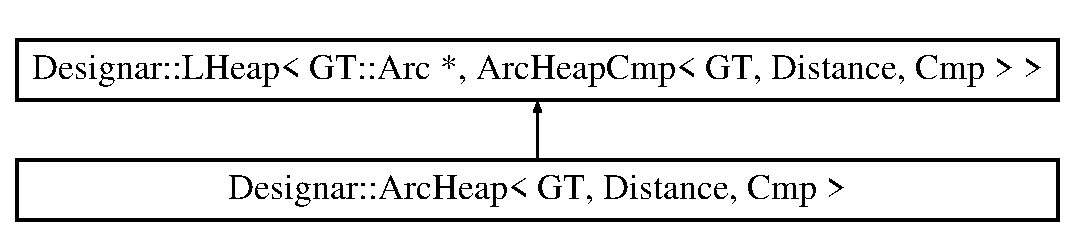
\includegraphics[height=2.000000cm]{class_designar_1_1_arc_heap}
\end{center}
\end{figure}
\subsection*{Public Member Functions}
\begin{DoxyCompactItemize}
\item 
void \hyperlink{class_designar_1_1_arc_heap_a578a5310c000e671cb967799317f534d}{insert\+\_\+arc} (Arc \&a, Node \&t)
\item 
Arc $\ast$ \hyperlink{class_designar_1_1_arc_heap_aa97981f64e6a7868d4d8b310bfd6b1cb}{get\+\_\+min\+\_\+arc} ()
\end{DoxyCompactItemize}
\subsection*{Additional Inherited Members}


\subsection{Detailed Description}
\subsubsection*{template$<$class GT, class Distance = Default\+Distance$<$\+G\+T$>$, class Cmp = std\+::less$<$typename Distance\+::\+Type$>$$>$\newline
class Designar\+::\+Arc\+Heap$<$ G\+T, Distance, Cmp $>$}



Definition at line 1231 of file graphalgorithms.\+H.



\subsection{Member Function Documentation}
\mbox{\Hypertarget{class_designar_1_1_arc_heap_aa97981f64e6a7868d4d8b310bfd6b1cb}\label{class_designar_1_1_arc_heap_aa97981f64e6a7868d4d8b310bfd6b1cb}} 
\index{Designar\+::\+Arc\+Heap@{Designar\+::\+Arc\+Heap}!get\+\_\+min\+\_\+arc@{get\+\_\+min\+\_\+arc}}
\index{get\+\_\+min\+\_\+arc@{get\+\_\+min\+\_\+arc}!Designar\+::\+Arc\+Heap@{Designar\+::\+Arc\+Heap}}
\subsubsection{\texorpdfstring{get\+\_\+min\+\_\+arc()}{get\_min\_arc()}}
{\footnotesize\ttfamily template$<$class GT, class Distance = Default\+Distance$<$\+G\+T$>$, class Cmp = std\+::less$<$typename Distance\+::\+Type$>$$>$ \\
Arc$\ast$ \hyperlink{class_designar_1_1_arc_heap}{Designar\+::\+Arc\+Heap}$<$ \hyperlink{demo-buildgraph_8_c_a3001c40d2c31ca87ed96cd7d1334a55e}{GT}, Distance, Cmp $>$\+::get\+\_\+min\+\_\+arc (\begin{DoxyParamCaption}{ }\end{DoxyParamCaption})\hspace{0.3cm}{\ttfamily [inline]}}



Definition at line 1262 of file graphalgorithms.\+H.

\mbox{\Hypertarget{class_designar_1_1_arc_heap_a578a5310c000e671cb967799317f534d}\label{class_designar_1_1_arc_heap_a578a5310c000e671cb967799317f534d}} 
\index{Designar\+::\+Arc\+Heap@{Designar\+::\+Arc\+Heap}!insert\+\_\+arc@{insert\+\_\+arc}}
\index{insert\+\_\+arc@{insert\+\_\+arc}!Designar\+::\+Arc\+Heap@{Designar\+::\+Arc\+Heap}}
\subsubsection{\texorpdfstring{insert\+\_\+arc()}{insert\_arc()}}
{\footnotesize\ttfamily template$<$class GT, class Distance = Default\+Distance$<$\+G\+T$>$, class Cmp = std\+::less$<$typename Distance\+::\+Type$>$$>$ \\
void \hyperlink{class_designar_1_1_arc_heap}{Designar\+::\+Arc\+Heap}$<$ \hyperlink{demo-buildgraph_8_c_a3001c40d2c31ca87ed96cd7d1334a55e}{GT}, Distance, Cmp $>$\+::insert\+\_\+arc (\begin{DoxyParamCaption}\item[{Arc \&}]{a,  }\item[{Node \&}]{t }\end{DoxyParamCaption})\hspace{0.3cm}{\ttfamily [inline]}}



Definition at line 1243 of file graphalgorithms.\+H.



The documentation for this class was generated from the following file\+:\begin{DoxyCompactItemize}
\item 
De\+Si\+G\+N\+A\+R/include/\hyperlink{graphalgorithms_8_h}{graphalgorithms.\+H}\end{DoxyCompactItemize}

\hypertarget{class_designar_1_1_arc_heap_cmp}{}\section{Designar\+:\+:Arc\+Heap\+Cmp$<$ GT, Distance, Cmp $>$ Class Template Reference}
\label{class_designar_1_1_arc_heap_cmp}\index{Designar\+::\+Arc\+Heap\+Cmp$<$ G\+T, Distance, Cmp $>$@{Designar\+::\+Arc\+Heap\+Cmp$<$ G\+T, Distance, Cmp $>$}}


{\ttfamily \#include $<$graphalgorithms.\+H$>$}

\subsection*{Public Member Functions}
\begin{DoxyCompactItemize}
\item 
\hyperlink{class_designar_1_1_arc_heap_cmp_a0fcb5ba151f45638b73534dc80af8a81}{Arc\+Heap\+Cmp} (Distance \&\+\_\+distance, Cmp \&\+\_\+cmp)
\item 
\hyperlink{class_designar_1_1_arc_heap_cmp_a4a698d49f62f6261afcf3c49e4c09381}{Arc\+Heap\+Cmp} (Distance \&\&\+\_\+distance=Distance(), Cmp \&\&\+\_\+cmp=Cmp())
\item 
bool \hyperlink{class_designar_1_1_arc_heap_cmp_a9d86fd876bad098a0a6844e9b302f141}{operator()} (typename G\+T\+::\+Arc $\ast$a, typename G\+T\+::\+Arc $\ast$b) const
\end{DoxyCompactItemize}


\subsection{Detailed Description}
\subsubsection*{template$<$class GT, class Distance, class Cmp$>$\newline
class Designar\+::\+Arc\+Heap\+Cmp$<$ G\+T, Distance, Cmp $>$}



Definition at line 1205 of file graphalgorithms.\+H.



\subsection{Constructor \& Destructor Documentation}
\mbox{\Hypertarget{class_designar_1_1_arc_heap_cmp_a0fcb5ba151f45638b73534dc80af8a81}\label{class_designar_1_1_arc_heap_cmp_a0fcb5ba151f45638b73534dc80af8a81}} 
\index{Designar\+::\+Arc\+Heap\+Cmp@{Designar\+::\+Arc\+Heap\+Cmp}!Arc\+Heap\+Cmp@{Arc\+Heap\+Cmp}}
\index{Arc\+Heap\+Cmp@{Arc\+Heap\+Cmp}!Designar\+::\+Arc\+Heap\+Cmp@{Designar\+::\+Arc\+Heap\+Cmp}}
\subsubsection{\texorpdfstring{Arc\+Heap\+Cmp()}{ArcHeapCmp()}\hspace{0.1cm}{\footnotesize\ttfamily [1/2]}}
{\footnotesize\ttfamily template$<$class GT, class Distance, class Cmp$>$ \\
\hyperlink{class_designar_1_1_arc_heap_cmp}{Designar\+::\+Arc\+Heap\+Cmp}$<$ \hyperlink{demo-buildgraph_8_c_a3001c40d2c31ca87ed96cd7d1334a55e}{GT}, Distance, Cmp $>$\+::\hyperlink{class_designar_1_1_arc_heap_cmp}{Arc\+Heap\+Cmp} (\begin{DoxyParamCaption}\item[{Distance \&}]{\+\_\+distance,  }\item[{Cmp \&}]{\+\_\+cmp }\end{DoxyParamCaption})\hspace{0.3cm}{\ttfamily [inline]}}



Definition at line 1211 of file graphalgorithms.\+H.

\mbox{\Hypertarget{class_designar_1_1_arc_heap_cmp_a4a698d49f62f6261afcf3c49e4c09381}\label{class_designar_1_1_arc_heap_cmp_a4a698d49f62f6261afcf3c49e4c09381}} 
\index{Designar\+::\+Arc\+Heap\+Cmp@{Designar\+::\+Arc\+Heap\+Cmp}!Arc\+Heap\+Cmp@{Arc\+Heap\+Cmp}}
\index{Arc\+Heap\+Cmp@{Arc\+Heap\+Cmp}!Designar\+::\+Arc\+Heap\+Cmp@{Designar\+::\+Arc\+Heap\+Cmp}}
\subsubsection{\texorpdfstring{Arc\+Heap\+Cmp()}{ArcHeapCmp()}\hspace{0.1cm}{\footnotesize\ttfamily [2/2]}}
{\footnotesize\ttfamily template$<$class GT, class Distance, class Cmp$>$ \\
\hyperlink{class_designar_1_1_arc_heap_cmp}{Designar\+::\+Arc\+Heap\+Cmp}$<$ \hyperlink{demo-buildgraph_8_c_a3001c40d2c31ca87ed96cd7d1334a55e}{GT}, Distance, Cmp $>$\+::\hyperlink{class_designar_1_1_arc_heap_cmp}{Arc\+Heap\+Cmp} (\begin{DoxyParamCaption}\item[{Distance \&\&}]{\+\_\+distance = {\ttfamily Distance()},  }\item[{Cmp \&\&}]{\+\_\+cmp = {\ttfamily Cmp()} }\end{DoxyParamCaption})\hspace{0.3cm}{\ttfamily [inline]}}



Definition at line 1216 of file graphalgorithms.\+H.



\subsection{Member Function Documentation}
\mbox{\Hypertarget{class_designar_1_1_arc_heap_cmp_a9d86fd876bad098a0a6844e9b302f141}\label{class_designar_1_1_arc_heap_cmp_a9d86fd876bad098a0a6844e9b302f141}} 
\index{Designar\+::\+Arc\+Heap\+Cmp@{Designar\+::\+Arc\+Heap\+Cmp}!operator()@{operator()}}
\index{operator()@{operator()}!Designar\+::\+Arc\+Heap\+Cmp@{Designar\+::\+Arc\+Heap\+Cmp}}
\subsubsection{\texorpdfstring{operator()()}{operator()()}}
{\footnotesize\ttfamily template$<$class GT, class Distance, class Cmp$>$ \\
bool \hyperlink{class_designar_1_1_arc_heap_cmp}{Designar\+::\+Arc\+Heap\+Cmp}$<$ \hyperlink{demo-buildgraph_8_c_a3001c40d2c31ca87ed96cd7d1334a55e}{GT}, Distance, Cmp $>$\+::operator() (\begin{DoxyParamCaption}\item[{typename G\+T\+::\+Arc $\ast$}]{a,  }\item[{typename G\+T\+::\+Arc $\ast$}]{b }\end{DoxyParamCaption}) const\hspace{0.3cm}{\ttfamily [inline]}}



Definition at line 1222 of file graphalgorithms.\+H.



The documentation for this class was generated from the following file\+:\begin{DoxyCompactItemize}
\item 
/home/julio/\+De\+S\+I\+G\+N\+A\+R-\/doc/\+De\+Si\+G\+N\+A\+R/include/\hyperlink{graphalgorithms_8_h}{graphalgorithms.\+H}\end{DoxyCompactItemize}

\hypertarget{class_designar_1_1_digraph_1_1_arc_iterator}{}\section{Referencia de la Clase Designar\+:\+:Digraph$<$ Node\+Info, Arc\+Info, Graph\+Info $>$\+:\+:Arc\+Iterator}
\label{class_designar_1_1_digraph_1_1_arc_iterator}\index{Designar\+::\+Digraph$<$ Node\+Info, Arc\+Info, Graph\+Info $>$\+::\+Arc\+Iterator@{Designar\+::\+Digraph$<$ Node\+Info, Arc\+Info, Graph\+Info $>$\+::\+Arc\+Iterator}}


{\ttfamily \#include $<$graph.\+H$>$}

Diagrama de herencias de Designar\+:\+:Digraph$<$ Node\+Info, Arc\+Info, Graph\+Info $>$\+:\+:Arc\+Iterator\begin{figure}[H]
\begin{center}
\leavevmode
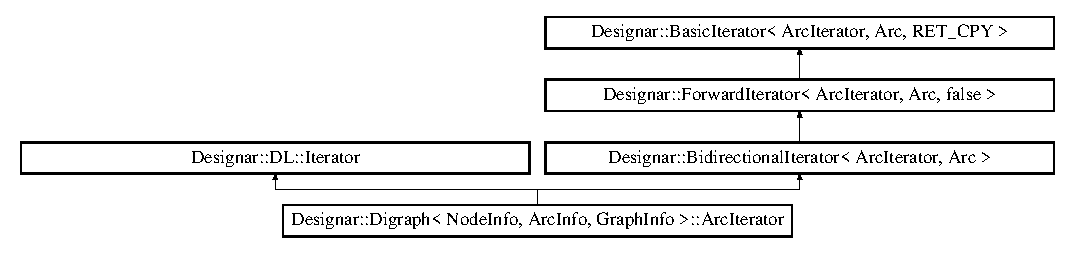
\includegraphics[height=2.947368cm]{class_designar_1_1_digraph_1_1_arc_iterator}
\end{center}
\end{figure}
\subsection*{Métodos públicos}
\begin{DoxyCompactItemize}
\item 
\hyperlink{class_designar_1_1_digraph_1_1_arc_iterator_a0f540c556301e1d4e0a9d48433257b89}{Arc\+Iterator} ()
\item 
\hyperlink{class_designar_1_1_digraph_1_1_arc_iterator_ac16db42766a60aa488fb4db5492c1361}{Arc\+Iterator} (const \hyperlink{class_designar_1_1_digraph}{Digraph} \&g)
\item 
\hyperlink{class_designar_1_1_digraph_1_1_arc_iterator_ae4a8b9172d19134e71693734003ee350}{Arc\+Iterator} (const \hyperlink{class_designar_1_1_digraph}{Digraph} \&g, \hyperlink{class_designar_1_1_d_l}{DL} $\ast$curr)
\item 
\hyperlink{class_designar_1_1_digraph_1_1_arc_iterator_a78fe9751892ba8eaa56aaba4a176666c}{Arc\+Iterator} (const \hyperlink{class_designar_1_1_digraph_1_1_arc_iterator}{Arc\+Iterator} \&it)
\item 
\hyperlink{class_designar_1_1_digraph_1_1_arc_iterator_acb84eb022d5113512f9c272dc47fd2da}{Arc\+Iterator} (\hyperlink{class_designar_1_1_digraph_1_1_arc_iterator}{Arc\+Iterator} \&\&it)
\item 
\hyperlink{class_designar_1_1_digraph_1_1_arc_iterator}{Arc\+Iterator} \& \hyperlink{class_designar_1_1_digraph_1_1_arc_iterator_a6a048ab6882106fc0d433a7c9fab297f}{operator=} (const \hyperlink{class_designar_1_1_digraph_1_1_arc_iterator}{Arc\+Iterator} \&it)
\item 
\hyperlink{class_designar_1_1_digraph_1_1_arc_iterator}{Arc\+Iterator} \& \hyperlink{class_designar_1_1_digraph_1_1_arc_iterator_a0ac762b04a286813cbed33857996c7cb}{operator=} (\hyperlink{class_designar_1_1_digraph_1_1_arc_iterator}{Arc\+Iterator} \&\&it)
\item 
void \hyperlink{class_designar_1_1_digraph_1_1_arc_iterator_a73ca00e5bcc478168ae16a73149becb1}{swap} (\hyperlink{class_designar_1_1_digraph_1_1_arc_iterator}{Arc\+Iterator} \&it)
\item 
\hyperlink{class_designar_1_1_digraph_a0ceb278671f2a535c00fddccdeafd69f}{Arc} \& \hyperlink{class_designar_1_1_digraph_1_1_arc_iterator_af7734cd84a4dd523f276064833abaa85}{get\+\_\+current} ()
\item 
const \hyperlink{class_designar_1_1_digraph_a0ceb278671f2a535c00fddccdeafd69f}{Arc} \& \hyperlink{class_designar_1_1_digraph_1_1_arc_iterator_a665f22163e2cc026f0b95f964ae6e048}{get\+\_\+current} () const
\item 
void \hyperlink{class_designar_1_1_digraph_1_1_arc_iterator_aa4f42b888685025c5c3f2e730df4eb36}{del} ()
\end{DoxyCompactItemize}
\subsection*{Amigas}
\begin{DoxyCompactItemize}
\item 
class \hyperlink{class_designar_1_1_digraph_1_1_arc_iterator_a530ad7c7218fa9b74a5cce004d0e3a1c}{Basic\+Iterator$<$ Arc\+Iterator, Arc $>$}
\end{DoxyCompactItemize}
\subsection*{Otros miembros heredados}


\subsection{Descripción detallada}
\subsubsection*{template$<$typename Node\+Info, typename Arc\+Info = Empty\+Class, typename Graph\+Info = Empty\+Class$>$\newline
class Designar\+::\+Digraph$<$ Node\+Info, Arc\+Info, Graph\+Info $>$\+::\+Arc\+Iterator}



Definición en la línea 2208 del archivo graph.\+H.



\subsection{Documentación del constructor y destructor}
\mbox{\Hypertarget{class_designar_1_1_digraph_1_1_arc_iterator_a0f540c556301e1d4e0a9d48433257b89}\label{class_designar_1_1_digraph_1_1_arc_iterator_a0f540c556301e1d4e0a9d48433257b89}} 
\index{Designar\+::\+Digraph\+::\+Arc\+Iterator@{Designar\+::\+Digraph\+::\+Arc\+Iterator}!Arc\+Iterator@{Arc\+Iterator}}
\index{Arc\+Iterator@{Arc\+Iterator}!Designar\+::\+Digraph\+::\+Arc\+Iterator@{Designar\+::\+Digraph\+::\+Arc\+Iterator}}
\subsubsection{\texorpdfstring{Arc\+Iterator()}{ArcIterator()}\hspace{0.1cm}{\footnotesize\ttfamily [1/5]}}
{\footnotesize\ttfamily template$<$typename Node\+Info , typename Arc\+Info  = Empty\+Class, typename Graph\+Info  = Empty\+Class$>$ \\
\hyperlink{class_designar_1_1_digraph}{Designar\+::\+Digraph}$<$ Node\+Info, Arc\+Info, Graph\+Info $>$\+::Arc\+Iterator\+::\+Arc\+Iterator (\begin{DoxyParamCaption}{ }\end{DoxyParamCaption})\hspace{0.3cm}{\ttfamily [inline]}}



Definición en la línea 2218 del archivo graph.\+H.

\mbox{\Hypertarget{class_designar_1_1_digraph_1_1_arc_iterator_ac16db42766a60aa488fb4db5492c1361}\label{class_designar_1_1_digraph_1_1_arc_iterator_ac16db42766a60aa488fb4db5492c1361}} 
\index{Designar\+::\+Digraph\+::\+Arc\+Iterator@{Designar\+::\+Digraph\+::\+Arc\+Iterator}!Arc\+Iterator@{Arc\+Iterator}}
\index{Arc\+Iterator@{Arc\+Iterator}!Designar\+::\+Digraph\+::\+Arc\+Iterator@{Designar\+::\+Digraph\+::\+Arc\+Iterator}}
\subsubsection{\texorpdfstring{Arc\+Iterator()}{ArcIterator()}\hspace{0.1cm}{\footnotesize\ttfamily [2/5]}}
{\footnotesize\ttfamily template$<$typename Node\+Info , typename Arc\+Info  = Empty\+Class, typename Graph\+Info  = Empty\+Class$>$ \\
\hyperlink{class_designar_1_1_digraph}{Designar\+::\+Digraph}$<$ Node\+Info, Arc\+Info, Graph\+Info $>$\+::Arc\+Iterator\+::\+Arc\+Iterator (\begin{DoxyParamCaption}\item[{const \hyperlink{class_designar_1_1_digraph}{Digraph} \&}]{g }\end{DoxyParamCaption})\hspace{0.3cm}{\ttfamily [inline]}}



Definición en la línea 2224 del archivo graph.\+H.

\mbox{\Hypertarget{class_designar_1_1_digraph_1_1_arc_iterator_ae4a8b9172d19134e71693734003ee350}\label{class_designar_1_1_digraph_1_1_arc_iterator_ae4a8b9172d19134e71693734003ee350}} 
\index{Designar\+::\+Digraph\+::\+Arc\+Iterator@{Designar\+::\+Digraph\+::\+Arc\+Iterator}!Arc\+Iterator@{Arc\+Iterator}}
\index{Arc\+Iterator@{Arc\+Iterator}!Designar\+::\+Digraph\+::\+Arc\+Iterator@{Designar\+::\+Digraph\+::\+Arc\+Iterator}}
\subsubsection{\texorpdfstring{Arc\+Iterator()}{ArcIterator()}\hspace{0.1cm}{\footnotesize\ttfamily [3/5]}}
{\footnotesize\ttfamily template$<$typename Node\+Info , typename Arc\+Info  = Empty\+Class, typename Graph\+Info  = Empty\+Class$>$ \\
\hyperlink{class_designar_1_1_digraph}{Designar\+::\+Digraph}$<$ Node\+Info, Arc\+Info, Graph\+Info $>$\+::Arc\+Iterator\+::\+Arc\+Iterator (\begin{DoxyParamCaption}\item[{const \hyperlink{class_designar_1_1_digraph}{Digraph} \&}]{g,  }\item[{\hyperlink{class_designar_1_1_d_l}{DL} $\ast$}]{curr }\end{DoxyParamCaption})\hspace{0.3cm}{\ttfamily [inline]}}



Definición en la línea 2231 del archivo graph.\+H.

\mbox{\Hypertarget{class_designar_1_1_digraph_1_1_arc_iterator_a78fe9751892ba8eaa56aaba4a176666c}\label{class_designar_1_1_digraph_1_1_arc_iterator_a78fe9751892ba8eaa56aaba4a176666c}} 
\index{Designar\+::\+Digraph\+::\+Arc\+Iterator@{Designar\+::\+Digraph\+::\+Arc\+Iterator}!Arc\+Iterator@{Arc\+Iterator}}
\index{Arc\+Iterator@{Arc\+Iterator}!Designar\+::\+Digraph\+::\+Arc\+Iterator@{Designar\+::\+Digraph\+::\+Arc\+Iterator}}
\subsubsection{\texorpdfstring{Arc\+Iterator()}{ArcIterator()}\hspace{0.1cm}{\footnotesize\ttfamily [4/5]}}
{\footnotesize\ttfamily template$<$typename Node\+Info , typename Arc\+Info  = Empty\+Class, typename Graph\+Info  = Empty\+Class$>$ \\
\hyperlink{class_designar_1_1_digraph}{Designar\+::\+Digraph}$<$ Node\+Info, Arc\+Info, Graph\+Info $>$\+::Arc\+Iterator\+::\+Arc\+Iterator (\begin{DoxyParamCaption}\item[{const \hyperlink{class_designar_1_1_digraph_1_1_arc_iterator}{Arc\+Iterator} \&}]{it }\end{DoxyParamCaption})\hspace{0.3cm}{\ttfamily [inline]}}



Definición en la línea 2238 del archivo graph.\+H.

\mbox{\Hypertarget{class_designar_1_1_digraph_1_1_arc_iterator_acb84eb022d5113512f9c272dc47fd2da}\label{class_designar_1_1_digraph_1_1_arc_iterator_acb84eb022d5113512f9c272dc47fd2da}} 
\index{Designar\+::\+Digraph\+::\+Arc\+Iterator@{Designar\+::\+Digraph\+::\+Arc\+Iterator}!Arc\+Iterator@{Arc\+Iterator}}
\index{Arc\+Iterator@{Arc\+Iterator}!Designar\+::\+Digraph\+::\+Arc\+Iterator@{Designar\+::\+Digraph\+::\+Arc\+Iterator}}
\subsubsection{\texorpdfstring{Arc\+Iterator()}{ArcIterator()}\hspace{0.1cm}{\footnotesize\ttfamily [5/5]}}
{\footnotesize\ttfamily template$<$typename Node\+Info , typename Arc\+Info  = Empty\+Class, typename Graph\+Info  = Empty\+Class$>$ \\
\hyperlink{class_designar_1_1_digraph}{Designar\+::\+Digraph}$<$ Node\+Info, Arc\+Info, Graph\+Info $>$\+::Arc\+Iterator\+::\+Arc\+Iterator (\begin{DoxyParamCaption}\item[{\hyperlink{class_designar_1_1_digraph_1_1_arc_iterator}{Arc\+Iterator} \&\&}]{it }\end{DoxyParamCaption})\hspace{0.3cm}{\ttfamily [inline]}}



Definición en la línea 2244 del archivo graph.\+H.



\subsection{Documentación de las funciones miembro}
\mbox{\Hypertarget{class_designar_1_1_digraph_1_1_arc_iterator_aa4f42b888685025c5c3f2e730df4eb36}\label{class_designar_1_1_digraph_1_1_arc_iterator_aa4f42b888685025c5c3f2e730df4eb36}} 
\index{Designar\+::\+Digraph\+::\+Arc\+Iterator@{Designar\+::\+Digraph\+::\+Arc\+Iterator}!del@{del}}
\index{del@{del}!Designar\+::\+Digraph\+::\+Arc\+Iterator@{Designar\+::\+Digraph\+::\+Arc\+Iterator}}
\subsubsection{\texorpdfstring{del()}{del()}}
{\footnotesize\ttfamily template$<$typename Node\+Info , typename Arc\+Info  = Empty\+Class, typename Graph\+Info  = Empty\+Class$>$ \\
void \hyperlink{class_designar_1_1_digraph}{Designar\+::\+Digraph}$<$ Node\+Info, Arc\+Info, Graph\+Info $>$\+::Arc\+Iterator\+::del (\begin{DoxyParamCaption}{ }\end{DoxyParamCaption})\hspace{0.3cm}{\ttfamily [inline]}}



Definición en la línea 2282 del archivo graph.\+H.

\mbox{\Hypertarget{class_designar_1_1_digraph_1_1_arc_iterator_af7734cd84a4dd523f276064833abaa85}\label{class_designar_1_1_digraph_1_1_arc_iterator_af7734cd84a4dd523f276064833abaa85}} 
\index{Designar\+::\+Digraph\+::\+Arc\+Iterator@{Designar\+::\+Digraph\+::\+Arc\+Iterator}!get\+\_\+current@{get\+\_\+current}}
\index{get\+\_\+current@{get\+\_\+current}!Designar\+::\+Digraph\+::\+Arc\+Iterator@{Designar\+::\+Digraph\+::\+Arc\+Iterator}}
\subsubsection{\texorpdfstring{get\+\_\+current()}{get\_current()}\hspace{0.1cm}{\footnotesize\ttfamily [1/2]}}
{\footnotesize\ttfamily template$<$typename Node\+Info , typename Arc\+Info  = Empty\+Class, typename Graph\+Info  = Empty\+Class$>$ \\
\hyperlink{class_designar_1_1_digraph_a0ceb278671f2a535c00fddccdeafd69f}{Arc}\& \hyperlink{class_designar_1_1_digraph}{Designar\+::\+Digraph}$<$ Node\+Info, Arc\+Info, Graph\+Info $>$\+::Arc\+Iterator\+::get\+\_\+current (\begin{DoxyParamCaption}{ }\end{DoxyParamCaption})\hspace{0.3cm}{\ttfamily [inline]}}



Definición en la línea 2272 del archivo graph.\+H.

\mbox{\Hypertarget{class_designar_1_1_digraph_1_1_arc_iterator_a665f22163e2cc026f0b95f964ae6e048}\label{class_designar_1_1_digraph_1_1_arc_iterator_a665f22163e2cc026f0b95f964ae6e048}} 
\index{Designar\+::\+Digraph\+::\+Arc\+Iterator@{Designar\+::\+Digraph\+::\+Arc\+Iterator}!get\+\_\+current@{get\+\_\+current}}
\index{get\+\_\+current@{get\+\_\+current}!Designar\+::\+Digraph\+::\+Arc\+Iterator@{Designar\+::\+Digraph\+::\+Arc\+Iterator}}
\subsubsection{\texorpdfstring{get\+\_\+current()}{get\_current()}\hspace{0.1cm}{\footnotesize\ttfamily [2/2]}}
{\footnotesize\ttfamily template$<$typename Node\+Info , typename Arc\+Info  = Empty\+Class, typename Graph\+Info  = Empty\+Class$>$ \\
const \hyperlink{class_designar_1_1_digraph_a0ceb278671f2a535c00fddccdeafd69f}{Arc}\& \hyperlink{class_designar_1_1_digraph}{Designar\+::\+Digraph}$<$ Node\+Info, Arc\+Info, Graph\+Info $>$\+::Arc\+Iterator\+::get\+\_\+current (\begin{DoxyParamCaption}{ }\end{DoxyParamCaption}) const\hspace{0.3cm}{\ttfamily [inline]}}



Definición en la línea 2277 del archivo graph.\+H.

\mbox{\Hypertarget{class_designar_1_1_digraph_1_1_arc_iterator_a6a048ab6882106fc0d433a7c9fab297f}\label{class_designar_1_1_digraph_1_1_arc_iterator_a6a048ab6882106fc0d433a7c9fab297f}} 
\index{Designar\+::\+Digraph\+::\+Arc\+Iterator@{Designar\+::\+Digraph\+::\+Arc\+Iterator}!operator=@{operator=}}
\index{operator=@{operator=}!Designar\+::\+Digraph\+::\+Arc\+Iterator@{Designar\+::\+Digraph\+::\+Arc\+Iterator}}
\subsubsection{\texorpdfstring{operator=()}{operator=()}\hspace{0.1cm}{\footnotesize\ttfamily [1/2]}}
{\footnotesize\ttfamily template$<$typename Node\+Info , typename Arc\+Info  = Empty\+Class, typename Graph\+Info  = Empty\+Class$>$ \\
\hyperlink{class_designar_1_1_digraph_1_1_arc_iterator}{Arc\+Iterator}\& \hyperlink{class_designar_1_1_digraph}{Designar\+::\+Digraph}$<$ Node\+Info, Arc\+Info, Graph\+Info $>$\+::Arc\+Iterator\+::operator= (\begin{DoxyParamCaption}\item[{const \hyperlink{class_designar_1_1_digraph_1_1_arc_iterator}{Arc\+Iterator} \&}]{it }\end{DoxyParamCaption})\hspace{0.3cm}{\ttfamily [inline]}}



Definición en la línea 2250 del archivo graph.\+H.

\mbox{\Hypertarget{class_designar_1_1_digraph_1_1_arc_iterator_a0ac762b04a286813cbed33857996c7cb}\label{class_designar_1_1_digraph_1_1_arc_iterator_a0ac762b04a286813cbed33857996c7cb}} 
\index{Designar\+::\+Digraph\+::\+Arc\+Iterator@{Designar\+::\+Digraph\+::\+Arc\+Iterator}!operator=@{operator=}}
\index{operator=@{operator=}!Designar\+::\+Digraph\+::\+Arc\+Iterator@{Designar\+::\+Digraph\+::\+Arc\+Iterator}}
\subsubsection{\texorpdfstring{operator=()}{operator=()}\hspace{0.1cm}{\footnotesize\ttfamily [2/2]}}
{\footnotesize\ttfamily template$<$typename Node\+Info , typename Arc\+Info  = Empty\+Class, typename Graph\+Info  = Empty\+Class$>$ \\
\hyperlink{class_designar_1_1_digraph_1_1_arc_iterator}{Arc\+Iterator}\& \hyperlink{class_designar_1_1_digraph}{Designar\+::\+Digraph}$<$ Node\+Info, Arc\+Info, Graph\+Info $>$\+::Arc\+Iterator\+::operator= (\begin{DoxyParamCaption}\item[{\hyperlink{class_designar_1_1_digraph_1_1_arc_iterator}{Arc\+Iterator} \&\&}]{it }\end{DoxyParamCaption})\hspace{0.3cm}{\ttfamily [inline]}}



Definición en la línea 2260 del archivo graph.\+H.

\mbox{\Hypertarget{class_designar_1_1_digraph_1_1_arc_iterator_a73ca00e5bcc478168ae16a73149becb1}\label{class_designar_1_1_digraph_1_1_arc_iterator_a73ca00e5bcc478168ae16a73149becb1}} 
\index{Designar\+::\+Digraph\+::\+Arc\+Iterator@{Designar\+::\+Digraph\+::\+Arc\+Iterator}!swap@{swap}}
\index{swap@{swap}!Designar\+::\+Digraph\+::\+Arc\+Iterator@{Designar\+::\+Digraph\+::\+Arc\+Iterator}}
\subsubsection{\texorpdfstring{swap()}{swap()}}
{\footnotesize\ttfamily template$<$typename Node\+Info , typename Arc\+Info  = Empty\+Class, typename Graph\+Info  = Empty\+Class$>$ \\
void \hyperlink{class_designar_1_1_digraph}{Designar\+::\+Digraph}$<$ Node\+Info, Arc\+Info, Graph\+Info $>$\+::Arc\+Iterator\+::swap (\begin{DoxyParamCaption}\item[{\hyperlink{class_designar_1_1_digraph_1_1_arc_iterator}{Arc\+Iterator} \&}]{it }\end{DoxyParamCaption})\hspace{0.3cm}{\ttfamily [inline]}}



Definición en la línea 2266 del archivo graph.\+H.



\subsection{Documentación de las funciones relacionadas y clases amigas}
\mbox{\Hypertarget{class_designar_1_1_digraph_1_1_arc_iterator_a530ad7c7218fa9b74a5cce004d0e3a1c}\label{class_designar_1_1_digraph_1_1_arc_iterator_a530ad7c7218fa9b74a5cce004d0e3a1c}} 
\index{Designar\+::\+Digraph\+::\+Arc\+Iterator@{Designar\+::\+Digraph\+::\+Arc\+Iterator}!Basic\+Iterator$<$ Arc\+Iterator, Arc $>$@{Basic\+Iterator$<$ Arc\+Iterator, Arc $>$}}
\index{Basic\+Iterator$<$ Arc\+Iterator, Arc $>$@{Basic\+Iterator$<$ Arc\+Iterator, Arc $>$}!Designar\+::\+Digraph\+::\+Arc\+Iterator@{Designar\+::\+Digraph\+::\+Arc\+Iterator}}
\subsubsection{\texorpdfstring{Basic\+Iterator$<$ Arc\+Iterator, Arc $>$}{BasicIterator< ArcIterator, Arc >}}
{\footnotesize\ttfamily template$<$typename Node\+Info , typename Arc\+Info  = Empty\+Class, typename Graph\+Info  = Empty\+Class$>$ \\
friend class \hyperlink{class_designar_1_1_basic_iterator}{Basic\+Iterator}$<$ \hyperlink{class_designar_1_1_digraph_1_1_arc_iterator}{Arc\+Iterator}, \hyperlink{class_designar_1_1_digraph_a0ceb278671f2a535c00fddccdeafd69f}{Arc} $>$\hspace{0.3cm}{\ttfamily [friend]}}



Definición en la línea 2211 del archivo graph.\+H.



La documentación para esta clase fue generada a partir del siguiente fichero\+:\begin{DoxyCompactItemize}
\item 
/home/julio/\+De\+S\+I\+G\+N\+A\+R-\/doc/\+De\+Si\+G\+N\+A\+R/include/\hyperlink{graph_8_h}{graph.\+H}\end{DoxyCompactItemize}

\hypertarget{class_designar_1_1_graph_1_1_arc_iterator}{}\section{Referencia de la Clase Designar\+:\+:Graph$<$ Node\+Info, Arc\+Info, Graph\+Info $>$\+:\+:Arc\+Iterator}
\label{class_designar_1_1_graph_1_1_arc_iterator}\index{Designar\+::\+Graph$<$ Node\+Info, Arc\+Info, Graph\+Info $>$\+::\+Arc\+Iterator@{Designar\+::\+Graph$<$ Node\+Info, Arc\+Info, Graph\+Info $>$\+::\+Arc\+Iterator}}


{\ttfamily \#include $<$graph.\+H$>$}

Diagrama de herencias de Designar\+:\+:Graph$<$ Node\+Info, Arc\+Info, Graph\+Info $>$\+:\+:Arc\+Iterator\begin{figure}[H]
\begin{center}
\leavevmode
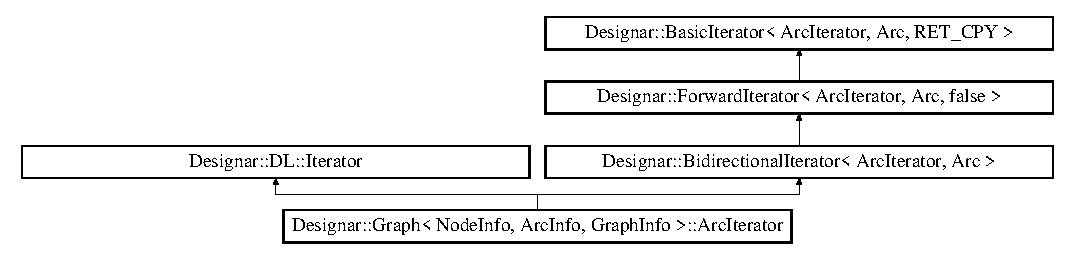
\includegraphics[height=3.027027cm]{class_designar_1_1_graph_1_1_arc_iterator}
\end{center}
\end{figure}
\subsection*{Métodos públicos}
\begin{DoxyCompactItemize}
\item 
\hyperlink{class_designar_1_1_graph_1_1_arc_iterator_a642cf08854577ea29ba520ee882c9d54}{Arc\+Iterator} ()
\item 
\hyperlink{class_designar_1_1_graph_1_1_arc_iterator_afeb58fdc5c6d4fd2d57c2ce53969203e}{Arc\+Iterator} (const \hyperlink{class_designar_1_1_graph}{Graph} \&g)
\item 
\hyperlink{class_designar_1_1_graph_1_1_arc_iterator_a2a9eb9d16ff5d80a22671dfdbe9ce3a2}{Arc\+Iterator} (const \hyperlink{class_designar_1_1_graph}{Graph} \&g, \hyperlink{class_designar_1_1_d_l}{DL} $\ast$curr)
\item 
\hyperlink{class_designar_1_1_graph_1_1_arc_iterator_a42fba48323675143026319401967e8c6}{Arc\+Iterator} (const \hyperlink{class_designar_1_1_graph_1_1_arc_iterator}{Arc\+Iterator} \&it)
\item 
\hyperlink{class_designar_1_1_graph_1_1_arc_iterator_a1446dc2d05faf881728a6721a9253129}{Arc\+Iterator} (\hyperlink{class_designar_1_1_graph_1_1_arc_iterator}{Arc\+Iterator} \&\&it)
\item 
\hyperlink{class_designar_1_1_graph_1_1_arc_iterator}{Arc\+Iterator} \& \hyperlink{class_designar_1_1_graph_1_1_arc_iterator_acce205d4f59317865d8a7e85598d141d}{operator=} (const \hyperlink{class_designar_1_1_graph_1_1_arc_iterator}{Arc\+Iterator} \&it)
\item 
\hyperlink{class_designar_1_1_graph_1_1_arc_iterator}{Arc\+Iterator} \& \hyperlink{class_designar_1_1_graph_1_1_arc_iterator_abd43d384ad590121f38d92d7af294195}{operator=} (\hyperlink{class_designar_1_1_graph_1_1_arc_iterator}{Arc\+Iterator} \&\&it)
\item 
void \hyperlink{class_designar_1_1_graph_1_1_arc_iterator_a12989f76c5a96637698000757b6dc6f4}{swap} (\hyperlink{class_designar_1_1_graph_1_1_arc_iterator}{Arc\+Iterator} \&it)
\item 
\hyperlink{class_designar_1_1_graph_a74c730ef4ce2d20f998d72bd25c2b5bf}{Arc} \& \hyperlink{class_designar_1_1_graph_1_1_arc_iterator_a4915ccaef38293e9dc449e7dba3965ec}{get\+\_\+current} ()
\item 
const \hyperlink{class_designar_1_1_graph_a74c730ef4ce2d20f998d72bd25c2b5bf}{Arc} \& \hyperlink{class_designar_1_1_graph_1_1_arc_iterator_ac7b91a766ed21ee9a69024d8a6548bbd}{get\+\_\+current} () const
\item 
void \hyperlink{class_designar_1_1_graph_1_1_arc_iterator_a6375bb0513856b2b20dffbfb2496082e}{del} ()
\end{DoxyCompactItemize}
\subsection*{Amigas}
\begin{DoxyCompactItemize}
\item 
class \hyperlink{class_designar_1_1_graph_1_1_arc_iterator_a530ad7c7218fa9b74a5cce004d0e3a1c}{Basic\+Iterator$<$ Arc\+Iterator, Arc $>$}
\end{DoxyCompactItemize}
\subsection*{Otros miembros heredados}


\subsection{Descripción detallada}
\subsubsection*{template$<$typename Node\+Info, typename Arc\+Info = Empty\+Class, typename Graph\+Info = Empty\+Class$>$\newline
class Designar\+::\+Graph$<$ Node\+Info, Arc\+Info, Graph\+Info $>$\+::\+Arc\+Iterator}



Definición en la línea 1534 del archivo graph.\+H.



\subsection{Documentación del constructor y destructor}
\mbox{\Hypertarget{class_designar_1_1_graph_1_1_arc_iterator_a642cf08854577ea29ba520ee882c9d54}\label{class_designar_1_1_graph_1_1_arc_iterator_a642cf08854577ea29ba520ee882c9d54}} 
\index{Designar\+::\+Graph\+::\+Arc\+Iterator@{Designar\+::\+Graph\+::\+Arc\+Iterator}!Arc\+Iterator@{Arc\+Iterator}}
\index{Arc\+Iterator@{Arc\+Iterator}!Designar\+::\+Graph\+::\+Arc\+Iterator@{Designar\+::\+Graph\+::\+Arc\+Iterator}}
\subsubsection{\texorpdfstring{Arc\+Iterator()}{ArcIterator()}\hspace{0.1cm}{\footnotesize\ttfamily [1/5]}}
{\footnotesize\ttfamily template$<$typename Node\+Info , typename Arc\+Info  = Empty\+Class, typename Graph\+Info  = Empty\+Class$>$ \\
\hyperlink{class_designar_1_1_graph}{Designar\+::\+Graph}$<$ Node\+Info, Arc\+Info, Graph\+Info $>$\+::Arc\+Iterator\+::\+Arc\+Iterator (\begin{DoxyParamCaption}{ }\end{DoxyParamCaption})\hspace{0.3cm}{\ttfamily [inline]}}



Definición en la línea 1544 del archivo graph.\+H.

\mbox{\Hypertarget{class_designar_1_1_graph_1_1_arc_iterator_afeb58fdc5c6d4fd2d57c2ce53969203e}\label{class_designar_1_1_graph_1_1_arc_iterator_afeb58fdc5c6d4fd2d57c2ce53969203e}} 
\index{Designar\+::\+Graph\+::\+Arc\+Iterator@{Designar\+::\+Graph\+::\+Arc\+Iterator}!Arc\+Iterator@{Arc\+Iterator}}
\index{Arc\+Iterator@{Arc\+Iterator}!Designar\+::\+Graph\+::\+Arc\+Iterator@{Designar\+::\+Graph\+::\+Arc\+Iterator}}
\subsubsection{\texorpdfstring{Arc\+Iterator()}{ArcIterator()}\hspace{0.1cm}{\footnotesize\ttfamily [2/5]}}
{\footnotesize\ttfamily template$<$typename Node\+Info , typename Arc\+Info  = Empty\+Class, typename Graph\+Info  = Empty\+Class$>$ \\
\hyperlink{class_designar_1_1_graph}{Designar\+::\+Graph}$<$ Node\+Info, Arc\+Info, Graph\+Info $>$\+::Arc\+Iterator\+::\+Arc\+Iterator (\begin{DoxyParamCaption}\item[{const \hyperlink{class_designar_1_1_graph}{Graph} \&}]{g }\end{DoxyParamCaption})\hspace{0.3cm}{\ttfamily [inline]}}



Definición en la línea 1550 del archivo graph.\+H.

\mbox{\Hypertarget{class_designar_1_1_graph_1_1_arc_iterator_a2a9eb9d16ff5d80a22671dfdbe9ce3a2}\label{class_designar_1_1_graph_1_1_arc_iterator_a2a9eb9d16ff5d80a22671dfdbe9ce3a2}} 
\index{Designar\+::\+Graph\+::\+Arc\+Iterator@{Designar\+::\+Graph\+::\+Arc\+Iterator}!Arc\+Iterator@{Arc\+Iterator}}
\index{Arc\+Iterator@{Arc\+Iterator}!Designar\+::\+Graph\+::\+Arc\+Iterator@{Designar\+::\+Graph\+::\+Arc\+Iterator}}
\subsubsection{\texorpdfstring{Arc\+Iterator()}{ArcIterator()}\hspace{0.1cm}{\footnotesize\ttfamily [3/5]}}
{\footnotesize\ttfamily template$<$typename Node\+Info , typename Arc\+Info  = Empty\+Class, typename Graph\+Info  = Empty\+Class$>$ \\
\hyperlink{class_designar_1_1_graph}{Designar\+::\+Graph}$<$ Node\+Info, Arc\+Info, Graph\+Info $>$\+::Arc\+Iterator\+::\+Arc\+Iterator (\begin{DoxyParamCaption}\item[{const \hyperlink{class_designar_1_1_graph}{Graph} \&}]{g,  }\item[{\hyperlink{class_designar_1_1_d_l}{DL} $\ast$}]{curr }\end{DoxyParamCaption})\hspace{0.3cm}{\ttfamily [inline]}}



Definición en la línea 1557 del archivo graph.\+H.

\mbox{\Hypertarget{class_designar_1_1_graph_1_1_arc_iterator_a42fba48323675143026319401967e8c6}\label{class_designar_1_1_graph_1_1_arc_iterator_a42fba48323675143026319401967e8c6}} 
\index{Designar\+::\+Graph\+::\+Arc\+Iterator@{Designar\+::\+Graph\+::\+Arc\+Iterator}!Arc\+Iterator@{Arc\+Iterator}}
\index{Arc\+Iterator@{Arc\+Iterator}!Designar\+::\+Graph\+::\+Arc\+Iterator@{Designar\+::\+Graph\+::\+Arc\+Iterator}}
\subsubsection{\texorpdfstring{Arc\+Iterator()}{ArcIterator()}\hspace{0.1cm}{\footnotesize\ttfamily [4/5]}}
{\footnotesize\ttfamily template$<$typename Node\+Info , typename Arc\+Info  = Empty\+Class, typename Graph\+Info  = Empty\+Class$>$ \\
\hyperlink{class_designar_1_1_graph}{Designar\+::\+Graph}$<$ Node\+Info, Arc\+Info, Graph\+Info $>$\+::Arc\+Iterator\+::\+Arc\+Iterator (\begin{DoxyParamCaption}\item[{const \hyperlink{class_designar_1_1_graph_1_1_arc_iterator}{Arc\+Iterator} \&}]{it }\end{DoxyParamCaption})\hspace{0.3cm}{\ttfamily [inline]}}



Definición en la línea 1564 del archivo graph.\+H.

\mbox{\Hypertarget{class_designar_1_1_graph_1_1_arc_iterator_a1446dc2d05faf881728a6721a9253129}\label{class_designar_1_1_graph_1_1_arc_iterator_a1446dc2d05faf881728a6721a9253129}} 
\index{Designar\+::\+Graph\+::\+Arc\+Iterator@{Designar\+::\+Graph\+::\+Arc\+Iterator}!Arc\+Iterator@{Arc\+Iterator}}
\index{Arc\+Iterator@{Arc\+Iterator}!Designar\+::\+Graph\+::\+Arc\+Iterator@{Designar\+::\+Graph\+::\+Arc\+Iterator}}
\subsubsection{\texorpdfstring{Arc\+Iterator()}{ArcIterator()}\hspace{0.1cm}{\footnotesize\ttfamily [5/5]}}
{\footnotesize\ttfamily template$<$typename Node\+Info , typename Arc\+Info  = Empty\+Class, typename Graph\+Info  = Empty\+Class$>$ \\
\hyperlink{class_designar_1_1_graph}{Designar\+::\+Graph}$<$ Node\+Info, Arc\+Info, Graph\+Info $>$\+::Arc\+Iterator\+::\+Arc\+Iterator (\begin{DoxyParamCaption}\item[{\hyperlink{class_designar_1_1_graph_1_1_arc_iterator}{Arc\+Iterator} \&\&}]{it }\end{DoxyParamCaption})\hspace{0.3cm}{\ttfamily [inline]}}



Definición en la línea 1570 del archivo graph.\+H.



\subsection{Documentación de las funciones miembro}
\mbox{\Hypertarget{class_designar_1_1_graph_1_1_arc_iterator_a6375bb0513856b2b20dffbfb2496082e}\label{class_designar_1_1_graph_1_1_arc_iterator_a6375bb0513856b2b20dffbfb2496082e}} 
\index{Designar\+::\+Graph\+::\+Arc\+Iterator@{Designar\+::\+Graph\+::\+Arc\+Iterator}!del@{del}}
\index{del@{del}!Designar\+::\+Graph\+::\+Arc\+Iterator@{Designar\+::\+Graph\+::\+Arc\+Iterator}}
\subsubsection{\texorpdfstring{del()}{del()}}
{\footnotesize\ttfamily template$<$typename Node\+Info , typename Arc\+Info  = Empty\+Class, typename Graph\+Info  = Empty\+Class$>$ \\
void \hyperlink{class_designar_1_1_graph}{Designar\+::\+Graph}$<$ Node\+Info, Arc\+Info, Graph\+Info $>$\+::Arc\+Iterator\+::del (\begin{DoxyParamCaption}{ }\end{DoxyParamCaption})\hspace{0.3cm}{\ttfamily [inline]}}



Definición en la línea 1608 del archivo graph.\+H.

\mbox{\Hypertarget{class_designar_1_1_graph_1_1_arc_iterator_a4915ccaef38293e9dc449e7dba3965ec}\label{class_designar_1_1_graph_1_1_arc_iterator_a4915ccaef38293e9dc449e7dba3965ec}} 
\index{Designar\+::\+Graph\+::\+Arc\+Iterator@{Designar\+::\+Graph\+::\+Arc\+Iterator}!get\+\_\+current@{get\+\_\+current}}
\index{get\+\_\+current@{get\+\_\+current}!Designar\+::\+Graph\+::\+Arc\+Iterator@{Designar\+::\+Graph\+::\+Arc\+Iterator}}
\subsubsection{\texorpdfstring{get\+\_\+current()}{get\_current()}\hspace{0.1cm}{\footnotesize\ttfamily [1/2]}}
{\footnotesize\ttfamily template$<$typename Node\+Info , typename Arc\+Info  = Empty\+Class, typename Graph\+Info  = Empty\+Class$>$ \\
\hyperlink{class_designar_1_1_graph_a74c730ef4ce2d20f998d72bd25c2b5bf}{Arc}\& \hyperlink{class_designar_1_1_graph}{Designar\+::\+Graph}$<$ Node\+Info, Arc\+Info, Graph\+Info $>$\+::Arc\+Iterator\+::get\+\_\+current (\begin{DoxyParamCaption}{ }\end{DoxyParamCaption})\hspace{0.3cm}{\ttfamily [inline]}}



Definición en la línea 1598 del archivo graph.\+H.

\mbox{\Hypertarget{class_designar_1_1_graph_1_1_arc_iterator_ac7b91a766ed21ee9a69024d8a6548bbd}\label{class_designar_1_1_graph_1_1_arc_iterator_ac7b91a766ed21ee9a69024d8a6548bbd}} 
\index{Designar\+::\+Graph\+::\+Arc\+Iterator@{Designar\+::\+Graph\+::\+Arc\+Iterator}!get\+\_\+current@{get\+\_\+current}}
\index{get\+\_\+current@{get\+\_\+current}!Designar\+::\+Graph\+::\+Arc\+Iterator@{Designar\+::\+Graph\+::\+Arc\+Iterator}}
\subsubsection{\texorpdfstring{get\+\_\+current()}{get\_current()}\hspace{0.1cm}{\footnotesize\ttfamily [2/2]}}
{\footnotesize\ttfamily template$<$typename Node\+Info , typename Arc\+Info  = Empty\+Class, typename Graph\+Info  = Empty\+Class$>$ \\
const \hyperlink{class_designar_1_1_graph_a74c730ef4ce2d20f998d72bd25c2b5bf}{Arc}\& \hyperlink{class_designar_1_1_graph}{Designar\+::\+Graph}$<$ Node\+Info, Arc\+Info, Graph\+Info $>$\+::Arc\+Iterator\+::get\+\_\+current (\begin{DoxyParamCaption}{ }\end{DoxyParamCaption}) const\hspace{0.3cm}{\ttfamily [inline]}}



Definición en la línea 1603 del archivo graph.\+H.

\mbox{\Hypertarget{class_designar_1_1_graph_1_1_arc_iterator_acce205d4f59317865d8a7e85598d141d}\label{class_designar_1_1_graph_1_1_arc_iterator_acce205d4f59317865d8a7e85598d141d}} 
\index{Designar\+::\+Graph\+::\+Arc\+Iterator@{Designar\+::\+Graph\+::\+Arc\+Iterator}!operator=@{operator=}}
\index{operator=@{operator=}!Designar\+::\+Graph\+::\+Arc\+Iterator@{Designar\+::\+Graph\+::\+Arc\+Iterator}}
\subsubsection{\texorpdfstring{operator=()}{operator=()}\hspace{0.1cm}{\footnotesize\ttfamily [1/2]}}
{\footnotesize\ttfamily template$<$typename Node\+Info , typename Arc\+Info  = Empty\+Class, typename Graph\+Info  = Empty\+Class$>$ \\
\hyperlink{class_designar_1_1_graph_1_1_arc_iterator}{Arc\+Iterator}\& \hyperlink{class_designar_1_1_graph}{Designar\+::\+Graph}$<$ Node\+Info, Arc\+Info, Graph\+Info $>$\+::Arc\+Iterator\+::operator= (\begin{DoxyParamCaption}\item[{const \hyperlink{class_designar_1_1_graph_1_1_arc_iterator}{Arc\+Iterator} \&}]{it }\end{DoxyParamCaption})\hspace{0.3cm}{\ttfamily [inline]}}



Definición en la línea 1576 del archivo graph.\+H.

\mbox{\Hypertarget{class_designar_1_1_graph_1_1_arc_iterator_abd43d384ad590121f38d92d7af294195}\label{class_designar_1_1_graph_1_1_arc_iterator_abd43d384ad590121f38d92d7af294195}} 
\index{Designar\+::\+Graph\+::\+Arc\+Iterator@{Designar\+::\+Graph\+::\+Arc\+Iterator}!operator=@{operator=}}
\index{operator=@{operator=}!Designar\+::\+Graph\+::\+Arc\+Iterator@{Designar\+::\+Graph\+::\+Arc\+Iterator}}
\subsubsection{\texorpdfstring{operator=()}{operator=()}\hspace{0.1cm}{\footnotesize\ttfamily [2/2]}}
{\footnotesize\ttfamily template$<$typename Node\+Info , typename Arc\+Info  = Empty\+Class, typename Graph\+Info  = Empty\+Class$>$ \\
\hyperlink{class_designar_1_1_graph_1_1_arc_iterator}{Arc\+Iterator}\& \hyperlink{class_designar_1_1_graph}{Designar\+::\+Graph}$<$ Node\+Info, Arc\+Info, Graph\+Info $>$\+::Arc\+Iterator\+::operator= (\begin{DoxyParamCaption}\item[{\hyperlink{class_designar_1_1_graph_1_1_arc_iterator}{Arc\+Iterator} \&\&}]{it }\end{DoxyParamCaption})\hspace{0.3cm}{\ttfamily [inline]}}



Definición en la línea 1586 del archivo graph.\+H.

\mbox{\Hypertarget{class_designar_1_1_graph_1_1_arc_iterator_a12989f76c5a96637698000757b6dc6f4}\label{class_designar_1_1_graph_1_1_arc_iterator_a12989f76c5a96637698000757b6dc6f4}} 
\index{Designar\+::\+Graph\+::\+Arc\+Iterator@{Designar\+::\+Graph\+::\+Arc\+Iterator}!swap@{swap}}
\index{swap@{swap}!Designar\+::\+Graph\+::\+Arc\+Iterator@{Designar\+::\+Graph\+::\+Arc\+Iterator}}
\subsubsection{\texorpdfstring{swap()}{swap()}}
{\footnotesize\ttfamily template$<$typename Node\+Info , typename Arc\+Info  = Empty\+Class, typename Graph\+Info  = Empty\+Class$>$ \\
void \hyperlink{class_designar_1_1_graph}{Designar\+::\+Graph}$<$ Node\+Info, Arc\+Info, Graph\+Info $>$\+::Arc\+Iterator\+::swap (\begin{DoxyParamCaption}\item[{\hyperlink{class_designar_1_1_graph_1_1_arc_iterator}{Arc\+Iterator} \&}]{it }\end{DoxyParamCaption})\hspace{0.3cm}{\ttfamily [inline]}}



Definición en la línea 1592 del archivo graph.\+H.



\subsection{Documentación de las funciones relacionadas y clases amigas}
\mbox{\Hypertarget{class_designar_1_1_graph_1_1_arc_iterator_a530ad7c7218fa9b74a5cce004d0e3a1c}\label{class_designar_1_1_graph_1_1_arc_iterator_a530ad7c7218fa9b74a5cce004d0e3a1c}} 
\index{Designar\+::\+Graph\+::\+Arc\+Iterator@{Designar\+::\+Graph\+::\+Arc\+Iterator}!Basic\+Iterator$<$ Arc\+Iterator, Arc $>$@{Basic\+Iterator$<$ Arc\+Iterator, Arc $>$}}
\index{Basic\+Iterator$<$ Arc\+Iterator, Arc $>$@{Basic\+Iterator$<$ Arc\+Iterator, Arc $>$}!Designar\+::\+Graph\+::\+Arc\+Iterator@{Designar\+::\+Graph\+::\+Arc\+Iterator}}
\subsubsection{\texorpdfstring{Basic\+Iterator$<$ Arc\+Iterator, Arc $>$}{BasicIterator< ArcIterator, Arc >}}
{\footnotesize\ttfamily template$<$typename Node\+Info , typename Arc\+Info  = Empty\+Class, typename Graph\+Info  = Empty\+Class$>$ \\
friend class \hyperlink{class_designar_1_1_basic_iterator}{Basic\+Iterator}$<$ \hyperlink{class_designar_1_1_graph_1_1_arc_iterator}{Arc\+Iterator}, \hyperlink{class_designar_1_1_graph_a74c730ef4ce2d20f998d72bd25c2b5bf}{Arc} $>$\hspace{0.3cm}{\ttfamily [friend]}}



Definición en la línea 1537 del archivo graph.\+H.



La documentación para esta clase fue generada a partir del siguiente fichero\+:\begin{DoxyCompactItemize}
\item 
/home/julio/\+De\+S\+I\+G\+N\+A\+R-\/doc/\+De\+Si\+G\+N\+A\+R/include/\hyperlink{graph_8_h}{graph.\+H}\end{DoxyCompactItemize}

\hypertarget{class_designar_1_1_array_iterator}{}\section{Designar\+:\+:Array\+Iterator$<$ Derived, Array\+Type, T, R\+E\+T\+\_\+\+C\+PY $>$ Class Template Reference}
\label{class_designar_1_1_array_iterator}\index{Designar\+::\+Array\+Iterator$<$ Derived, Array\+Type, T, R\+E\+T\+\_\+\+C\+P\+Y $>$@{Designar\+::\+Array\+Iterator$<$ Derived, Array\+Type, T, R\+E\+T\+\_\+\+C\+P\+Y $>$}}


Defined object that allows to traverse a De\+S\+I\+G\+N\+AR Array-\/based container.  




{\ttfamily \#include $<$array.\+H$>$}

Inheritance diagram for Designar\+:\+:Array\+Iterator$<$ Derived, Array\+Type, T, R\+E\+T\+\_\+\+C\+PY $>$\+:\begin{figure}[H]
\begin{center}
\leavevmode
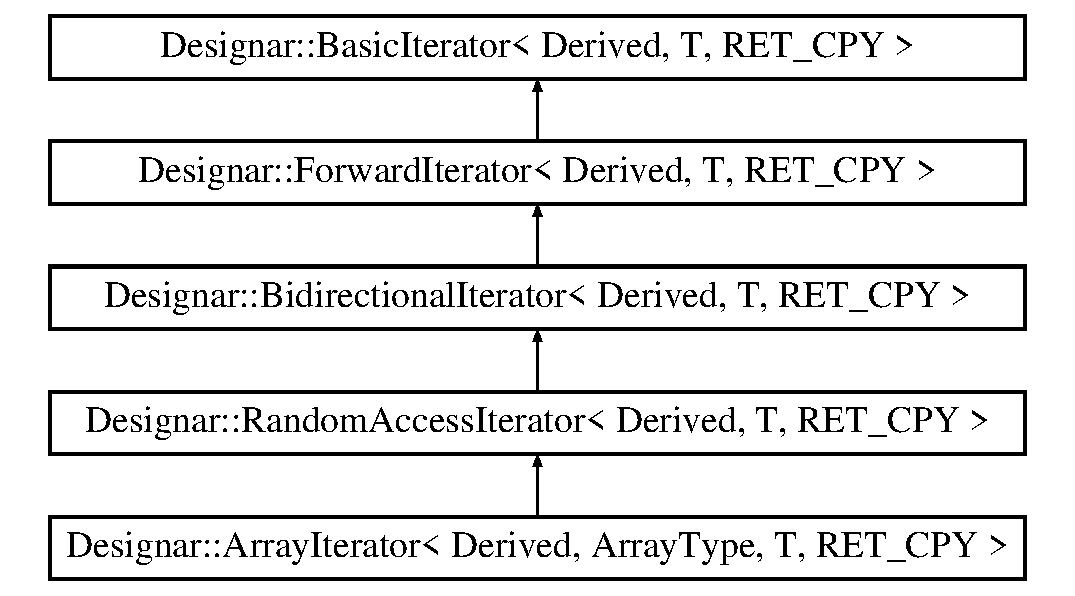
\includegraphics[height=5.000000cm]{class_designar_1_1_array_iterator}
\end{center}
\end{figure}
\subsection*{Public Member Functions}
\begin{DoxyCompactItemize}
\item 
\hyperlink{class_designar_1_1_array_iterator_a0fd19f5e2f3f3c13470d62b118575582}{Array\+Iterator} ()
\begin{DoxyCompactList}\small\item\em $<$ Array Iterator Default Constructor. Initializes {\itshape array\+\_\+ptr} and {\itshape curr} in {\bfseries nullptr} and {\bfseries 0}. \end{DoxyCompactList}\item 
\hyperlink{class_designar_1_1_array_iterator_a7d5565949d8cd3100686c1ff73eb1618}{Array\+Iterator} (const Array\+Type \&a)
\begin{DoxyCompactList}\small\item\em Array Iterator Parametric Constructor. Initializes {\itshape array\+\_\+ptr} and {\itshape curr} in {\bfseries a} and {\bfseries 0}. \end{DoxyCompactList}\item 
\hyperlink{class_designar_1_1_array_iterator_a1c9df0412f7bb1dabbd15f6772d8b9a3}{Array\+Iterator} (const Array\+Type \&a, \hyperlink{namespace_designar_aa72662848b9f4815e7bf31a7cf3e33d1}{nat\+\_\+t} c)
\begin{DoxyCompactList}\small\item\em Array Iterator Parametric Constructor. Initializes {\itshape array\+\_\+ptr} and {\itshape curr} in {\bfseries a} and {\bfseries c}. \end{DoxyCompactList}\item 
\hyperlink{class_designar_1_1_array_iterator_a7d3069da40d921310097dbde17fb0204}{Array\+Iterator} (const \hyperlink{class_designar_1_1_array_iterator}{Array\+Iterator} \&it)
\begin{DoxyCompactList}\small\item\em Array Iterator Copy Constructor. Initializes \hyperlink{class_designar_1_1_array_iterator}{Array\+Iterator} with a previous instance. \end{DoxyCompactList}\item 
\hyperlink{class_designar_1_1_array_iterator_ad27f115766207137bd74ef47d477f4f5}{Array\+Iterator} (\hyperlink{class_designar_1_1_array_iterator}{Array\+Iterator} \&\&it)
\begin{DoxyCompactList}\small\item\em Array Iterator Move Constructor. Initializes {\bfseries \hyperlink{class_designar_1_1_array_iterator}{Array\+Iterator}} with a previous instance using Move Semantics. \end{DoxyCompactList}\item 
\hyperlink{class_designar_1_1_array_iterator}{Array\+Iterator} \& \hyperlink{class_designar_1_1_array_iterator_a26d812ac595156aed963e60d41d91fa7}{operator=} (const \hyperlink{class_designar_1_1_array_iterator}{Array\+Iterator} \&it)
\begin{DoxyCompactList}\small\item\em Assingment operator overload. \end{DoxyCompactList}\item 
\hyperlink{class_designar_1_1_array_iterator}{Array\+Iterator} \& \hyperlink{class_designar_1_1_array_iterator_a219eb8e4d831f490cf9cdcb1f60dcacc}{operator=} (\hyperlink{class_designar_1_1_array_iterator}{Array\+Iterator} \&\&it)
\begin{DoxyCompactList}\small\item\em Assingment operator overload using Move Semantics. \end{DoxyCompactList}\item 
void \hyperlink{class_designar_1_1_array_iterator_a6c3a5bf56a2b7da838ca773368e4699a}{swap} (\hyperlink{class_designar_1_1_array_iterator}{Array\+Iterator} \&it)
\begin{DoxyCompactList}\small\item\em Swap operation. It allows to swap {\bfseries this} object with an \hyperlink{class_designar_1_1_array_iterator}{Array\+Iterator} given as parameter. \end{DoxyCompactList}\item 
bool \hyperlink{class_designar_1_1_array_iterator_aafec192c97299c4f21c28c65e58b19fc}{has\+\_\+current} () const
\begin{DoxyCompactList}\small\item\em Ask if there are still items in the Array which can be iterated. \end{DoxyCompactList}\item 
void \hyperlink{class_designar_1_1_array_iterator_ac4e929d3247b68c3c9cffb43ec0891ec}{next} ()
\begin{DoxyCompactList}\small\item\em Displace iterator to the {\itshape next} item in the Array. \end{DoxyCompactList}\item 
void \hyperlink{class_designar_1_1_array_iterator_a8709128b09b8b177fa1b042cb330c3e5}{next\+\_\+n} (\hyperlink{namespace_designar_aa72662848b9f4815e7bf31a7cf3e33d1}{nat\+\_\+t} p)
\begin{DoxyCompactList}\small\item\em Displace iterator {\bfseries n} items forward in the Array. \end{DoxyCompactList}\item 
void \hyperlink{class_designar_1_1_array_iterator_a5a0fd9640ab487a6034fec8f4f3d34cb}{prev} ()
\begin{DoxyCompactList}\small\item\em Displace iterator to the previous item in the Array. \end{DoxyCompactList}\item 
void \hyperlink{class_designar_1_1_array_iterator_a5a417cab0b0b039c69d5a52a513a019f}{prev\+\_\+n} (\hyperlink{namespace_designar_aa72662848b9f4815e7bf31a7cf3e33d1}{nat\+\_\+t} p)
\begin{DoxyCompactList}\small\item\em Displace iterator to the previous item in the Array. \end{DoxyCompactList}\item 
void \hyperlink{class_designar_1_1_array_iterator_a68f6d13686360c93d95b3a875b14312e}{move\+\_\+to} (\hyperlink{namespace_designar_aa72662848b9f4815e7bf31a7cf3e33d1}{nat\+\_\+t} p)
\begin{DoxyCompactList}\small\item\em Displace iterator to an exact given position. \end{DoxyCompactList}\item 
void \hyperlink{class_designar_1_1_array_iterator_af8781369a1cb13f92c8c2dbab9975118}{reset} ()
\begin{DoxyCompactList}\small\item\em Reset {\bfseries \hyperlink{class_designar_1_1_array_iterator}{Array\+Iterator}} to the initial position of the Array. \end{DoxyCompactList}\item 
\hyperlink{namespace_designar_aa72662848b9f4815e7bf31a7cf3e33d1}{nat\+\_\+t} \hyperlink{class_designar_1_1_array_iterator_a209ca14a9628f0a67a258469d98089b8}{get\+\_\+position} () const
\begin{DoxyCompactList}\small\item\em Getter method to obtain current position of the iterator. \end{DoxyCompactList}\end{DoxyCompactItemize}
\subsection*{Protected Member Functions}
\begin{DoxyCompactItemize}
\item 
\hyperlink{namespace_designar_aa72662848b9f4815e7bf31a7cf3e33d1}{nat\+\_\+t} \hyperlink{class_designar_1_1_array_iterator_a55fa01dfdb66a82b162ea2c9f631e2fd}{get\+\_\+location} () const
\begin{DoxyCompactList}\small\item\em Getter method to obtain current location of the iterator. \end{DoxyCompactList}\end{DoxyCompactItemize}
\subsection*{Protected Attributes}
\begin{DoxyCompactItemize}
\item 
Array\+Type $\ast$ \hyperlink{class_designar_1_1_array_iterator_a6518c265f47bf58f4e2c04b55416ded6}{array\+\_\+ptr}
\begin{DoxyCompactList}\small\item\em Pointer to an Array\+Type. \end{DoxyCompactList}\item 
\hyperlink{namespace_designar_aa72662848b9f4815e7bf31a7cf3e33d1}{nat\+\_\+t} \hyperlink{class_designar_1_1_array_iterator_aef9cd548a0423017eb452081f260a840}{curr}
\begin{DoxyCompactList}\small\item\em Current Iterator position. \end{DoxyCompactList}\end{DoxyCompactItemize}
\subsection*{Friends}
\begin{DoxyCompactItemize}
\item 
class \hyperlink{class_designar_1_1_array_iterator_a780ba1bdf8ce9c4f60e364ab9ce0cd47}{Basic\+Iterator$<$ Derived, T, R\+E\+T\+\_\+\+C\+P\+Y $>$}
\item 
class \hyperlink{class_designar_1_1_array_iterator_af1665f0fe477bd4c26558c3f5cc620c3}{Random\+Access\+Iterator$<$ Derived, T, R\+E\+T\+\_\+\+C\+P\+Y $>$}
\end{DoxyCompactItemize}


\subsection{Detailed Description}
\subsubsection*{template$<$class Derived, class Array\+Type, typename T, bool R\+E\+T\+\_\+\+C\+PY$>$\newline
class Designar\+::\+Array\+Iterator$<$ Derived, Array\+Type, T, R\+E\+T\+\_\+\+C\+P\+Y $>$}

Defined object that allows to traverse a De\+S\+I\+G\+N\+AR Array-\/based container. 

Definition at line 72 of file array.\+H.



\subsection{Constructor \& Destructor Documentation}
\mbox{\Hypertarget{class_designar_1_1_array_iterator_a0fd19f5e2f3f3c13470d62b118575582}\label{class_designar_1_1_array_iterator_a0fd19f5e2f3f3c13470d62b118575582}} 
\index{Designar\+::\+Array\+Iterator@{Designar\+::\+Array\+Iterator}!Array\+Iterator@{Array\+Iterator}}
\index{Array\+Iterator@{Array\+Iterator}!Designar\+::\+Array\+Iterator@{Designar\+::\+Array\+Iterator}}
\subsubsection{\texorpdfstring{Array\+Iterator()}{ArrayIterator()}\hspace{0.1cm}{\footnotesize\ttfamily [1/5]}}
{\footnotesize\ttfamily template$<$class Derived, class Array\+Type, typename T, bool R\+E\+T\+\_\+\+C\+PY$>$ \\
\hyperlink{class_designar_1_1_array_iterator}{Designar\+::\+Array\+Iterator}$<$ Derived, Array\+Type, T, R\+E\+T\+\_\+\+C\+PY $>$\+::\hyperlink{class_designar_1_1_array_iterator}{Array\+Iterator} (\begin{DoxyParamCaption}{ }\end{DoxyParamCaption})\hspace{0.3cm}{\ttfamily [inline]}}



$<$ Array Iterator Default Constructor. Initializes {\itshape array\+\_\+ptr} and {\itshape curr} in {\bfseries nullptr} and {\bfseries 0}. 



Definition at line 102 of file array.\+H.

\mbox{\Hypertarget{class_designar_1_1_array_iterator_a7d5565949d8cd3100686c1ff73eb1618}\label{class_designar_1_1_array_iterator_a7d5565949d8cd3100686c1ff73eb1618}} 
\index{Designar\+::\+Array\+Iterator@{Designar\+::\+Array\+Iterator}!Array\+Iterator@{Array\+Iterator}}
\index{Array\+Iterator@{Array\+Iterator}!Designar\+::\+Array\+Iterator@{Designar\+::\+Array\+Iterator}}
\subsubsection{\texorpdfstring{Array\+Iterator()}{ArrayIterator()}\hspace{0.1cm}{\footnotesize\ttfamily [2/5]}}
{\footnotesize\ttfamily template$<$class Derived, class Array\+Type, typename T, bool R\+E\+T\+\_\+\+C\+PY$>$ \\
\hyperlink{class_designar_1_1_array_iterator}{Designar\+::\+Array\+Iterator}$<$ Derived, Array\+Type, T, R\+E\+T\+\_\+\+C\+PY $>$\+::\hyperlink{class_designar_1_1_array_iterator}{Array\+Iterator} (\begin{DoxyParamCaption}\item[{const Array\+Type \&}]{a }\end{DoxyParamCaption})\hspace{0.3cm}{\ttfamily [inline]}}



Array Iterator Parametric Constructor. Initializes {\itshape array\+\_\+ptr} and {\itshape curr} in {\bfseries a} and {\bfseries 0}. 


\begin{DoxyParams}[1]{Parameters}
\mbox{\tt in}  & {\em a} & An {\bfseries Array\+Type} constant reference \\
\hline
\end{DoxyParams}


Definition at line 121 of file array.\+H.

\mbox{\Hypertarget{class_designar_1_1_array_iterator_a1c9df0412f7bb1dabbd15f6772d8b9a3}\label{class_designar_1_1_array_iterator_a1c9df0412f7bb1dabbd15f6772d8b9a3}} 
\index{Designar\+::\+Array\+Iterator@{Designar\+::\+Array\+Iterator}!Array\+Iterator@{Array\+Iterator}}
\index{Array\+Iterator@{Array\+Iterator}!Designar\+::\+Array\+Iterator@{Designar\+::\+Array\+Iterator}}
\subsubsection{\texorpdfstring{Array\+Iterator()}{ArrayIterator()}\hspace{0.1cm}{\footnotesize\ttfamily [3/5]}}
{\footnotesize\ttfamily template$<$class Derived, class Array\+Type, typename T, bool R\+E\+T\+\_\+\+C\+PY$>$ \\
\hyperlink{class_designar_1_1_array_iterator}{Designar\+::\+Array\+Iterator}$<$ Derived, Array\+Type, T, R\+E\+T\+\_\+\+C\+PY $>$\+::\hyperlink{class_designar_1_1_array_iterator}{Array\+Iterator} (\begin{DoxyParamCaption}\item[{const Array\+Type \&}]{a,  }\item[{\hyperlink{namespace_designar_aa72662848b9f4815e7bf31a7cf3e33d1}{nat\+\_\+t}}]{c }\end{DoxyParamCaption})\hspace{0.3cm}{\ttfamily [inline]}}



Array Iterator Parametric Constructor. Initializes {\itshape array\+\_\+ptr} and {\itshape curr} in {\bfseries a} and {\bfseries c}. 


\begin{DoxyParams}[1]{Parameters}
\mbox{\tt in}  & {\em a} & An {\bfseries Array\+Type} constant reference \\
\hline
\mbox{\tt in}  & {\em c} & A {\bfseries nat\+\_\+t} indicating the current position \\
\hline
\end{DoxyParams}


Definition at line 144 of file array.\+H.

\mbox{\Hypertarget{class_designar_1_1_array_iterator_a7d3069da40d921310097dbde17fb0204}\label{class_designar_1_1_array_iterator_a7d3069da40d921310097dbde17fb0204}} 
\index{Designar\+::\+Array\+Iterator@{Designar\+::\+Array\+Iterator}!Array\+Iterator@{Array\+Iterator}}
\index{Array\+Iterator@{Array\+Iterator}!Designar\+::\+Array\+Iterator@{Designar\+::\+Array\+Iterator}}
\subsubsection{\texorpdfstring{Array\+Iterator()}{ArrayIterator()}\hspace{0.1cm}{\footnotesize\ttfamily [4/5]}}
{\footnotesize\ttfamily template$<$class Derived, class Array\+Type, typename T, bool R\+E\+T\+\_\+\+C\+PY$>$ \\
\hyperlink{class_designar_1_1_array_iterator}{Designar\+::\+Array\+Iterator}$<$ Derived, Array\+Type, T, R\+E\+T\+\_\+\+C\+PY $>$\+::\hyperlink{class_designar_1_1_array_iterator}{Array\+Iterator} (\begin{DoxyParamCaption}\item[{const \hyperlink{class_designar_1_1_array_iterator}{Array\+Iterator}$<$ Derived, Array\+Type, T, R\+E\+T\+\_\+\+C\+PY $>$ \&}]{it }\end{DoxyParamCaption})\hspace{0.3cm}{\ttfamily [inline]}}



Array Iterator Copy Constructor. Initializes \hyperlink{class_designar_1_1_array_iterator}{Array\+Iterator} with a previous instance. 


\begin{DoxyParams}[1]{Parameters}
\mbox{\tt in}  & {\em it} & An {\bfseries \hyperlink{class_designar_1_1_array_iterator}{Array\+Iterator}} constant reference \\
\hline
\end{DoxyParams}


Definition at line 163 of file array.\+H.

\mbox{\Hypertarget{class_designar_1_1_array_iterator_ad27f115766207137bd74ef47d477f4f5}\label{class_designar_1_1_array_iterator_ad27f115766207137bd74ef47d477f4f5}} 
\index{Designar\+::\+Array\+Iterator@{Designar\+::\+Array\+Iterator}!Array\+Iterator@{Array\+Iterator}}
\index{Array\+Iterator@{Array\+Iterator}!Designar\+::\+Array\+Iterator@{Designar\+::\+Array\+Iterator}}
\subsubsection{\texorpdfstring{Array\+Iterator()}{ArrayIterator()}\hspace{0.1cm}{\footnotesize\ttfamily [5/5]}}
{\footnotesize\ttfamily template$<$class Derived, class Array\+Type, typename T, bool R\+E\+T\+\_\+\+C\+PY$>$ \\
\hyperlink{class_designar_1_1_array_iterator}{Designar\+::\+Array\+Iterator}$<$ Derived, Array\+Type, T, R\+E\+T\+\_\+\+C\+PY $>$\+::\hyperlink{class_designar_1_1_array_iterator}{Array\+Iterator} (\begin{DoxyParamCaption}\item[{\hyperlink{class_designar_1_1_array_iterator}{Array\+Iterator}$<$ Derived, Array\+Type, T, R\+E\+T\+\_\+\+C\+PY $>$ \&\&}]{it }\end{DoxyParamCaption})\hspace{0.3cm}{\ttfamily [inline]}}



Array Iterator Move Constructor. Initializes {\bfseries \hyperlink{class_designar_1_1_array_iterator}{Array\+Iterator}} with a previous instance using Move Semantics. 


\begin{DoxyParams}[1]{Parameters}
\mbox{\tt in}  & {\em it} & An {\bfseries \hyperlink{class_designar_1_1_array_iterator}{Array\+Iterator}} rvalue \\
\hline
\end{DoxyParams}


Definition at line 184 of file array.\+H.



\subsection{Member Function Documentation}
\mbox{\Hypertarget{class_designar_1_1_array_iterator_a55fa01dfdb66a82b162ea2c9f631e2fd}\label{class_designar_1_1_array_iterator_a55fa01dfdb66a82b162ea2c9f631e2fd}} 
\index{Designar\+::\+Array\+Iterator@{Designar\+::\+Array\+Iterator}!get\+\_\+location@{get\+\_\+location}}
\index{get\+\_\+location@{get\+\_\+location}!Designar\+::\+Array\+Iterator@{Designar\+::\+Array\+Iterator}}
\subsubsection{\texorpdfstring{get\+\_\+location()}{get\_location()}}
{\footnotesize\ttfamily template$<$class Derived, class Array\+Type, typename T, bool R\+E\+T\+\_\+\+C\+PY$>$ \\
\hyperlink{namespace_designar_aa72662848b9f4815e7bf31a7cf3e33d1}{nat\+\_\+t} \hyperlink{class_designar_1_1_array_iterator}{Designar\+::\+Array\+Iterator}$<$ Derived, Array\+Type, T, R\+E\+T\+\_\+\+C\+PY $>$\+::get\+\_\+location (\begin{DoxyParamCaption}{ }\end{DoxyParamCaption}) const\hspace{0.3cm}{\ttfamily [inline]}, {\ttfamily [protected]}}



Getter method to obtain current location of the iterator. 



Definition at line 92 of file array.\+H.

\mbox{\Hypertarget{class_designar_1_1_array_iterator_a209ca14a9628f0a67a258469d98089b8}\label{class_designar_1_1_array_iterator_a209ca14a9628f0a67a258469d98089b8}} 
\index{Designar\+::\+Array\+Iterator@{Designar\+::\+Array\+Iterator}!get\+\_\+position@{get\+\_\+position}}
\index{get\+\_\+position@{get\+\_\+position}!Designar\+::\+Array\+Iterator@{Designar\+::\+Array\+Iterator}}
\subsubsection{\texorpdfstring{get\+\_\+position()}{get\_position()}}
{\footnotesize\ttfamily template$<$class Derived, class Array\+Type, typename T, bool R\+E\+T\+\_\+\+C\+PY$>$ \\
\hyperlink{namespace_designar_aa72662848b9f4815e7bf31a7cf3e33d1}{nat\+\_\+t} \hyperlink{class_designar_1_1_array_iterator}{Designar\+::\+Array\+Iterator}$<$ Derived, Array\+Type, T, R\+E\+T\+\_\+\+C\+PY $>$\+::get\+\_\+position (\begin{DoxyParamCaption}{ }\end{DoxyParamCaption}) const\hspace{0.3cm}{\ttfamily [inline]}}



Getter method to obtain current position of the iterator. 

\begin{DoxyReturn}{Returns}
Current position of the iterator 
\end{DoxyReturn}


Definition at line 421 of file array.\+H.

\mbox{\Hypertarget{class_designar_1_1_array_iterator_aafec192c97299c4f21c28c65e58b19fc}\label{class_designar_1_1_array_iterator_aafec192c97299c4f21c28c65e58b19fc}} 
\index{Designar\+::\+Array\+Iterator@{Designar\+::\+Array\+Iterator}!has\+\_\+current@{has\+\_\+current}}
\index{has\+\_\+current@{has\+\_\+current}!Designar\+::\+Array\+Iterator@{Designar\+::\+Array\+Iterator}}
\subsubsection{\texorpdfstring{has\+\_\+current()}{has\_current()}}
{\footnotesize\ttfamily template$<$class Derived, class Array\+Type, typename T, bool R\+E\+T\+\_\+\+C\+PY$>$ \\
bool \hyperlink{class_designar_1_1_array_iterator}{Designar\+::\+Array\+Iterator}$<$ Derived, Array\+Type, T, R\+E\+T\+\_\+\+C\+PY $>$\+::has\+\_\+current (\begin{DoxyParamCaption}{ }\end{DoxyParamCaption}) const\hspace{0.3cm}{\ttfamily [inline]}}



Ask if there are still items in the Array which can be iterated. 

\begin{DoxyReturn}{Returns}
{\ttfamily true} if there are items to iterate, {\ttfamily false} otherwise. 
\end{DoxyReturn}


Definition at line 267 of file array.\+H.

\mbox{\Hypertarget{class_designar_1_1_array_iterator_a68f6d13686360c93d95b3a875b14312e}\label{class_designar_1_1_array_iterator_a68f6d13686360c93d95b3a875b14312e}} 
\index{Designar\+::\+Array\+Iterator@{Designar\+::\+Array\+Iterator}!move\+\_\+to@{move\+\_\+to}}
\index{move\+\_\+to@{move\+\_\+to}!Designar\+::\+Array\+Iterator@{Designar\+::\+Array\+Iterator}}
\subsubsection{\texorpdfstring{move\+\_\+to()}{move\_to()}}
{\footnotesize\ttfamily template$<$class Derived, class Array\+Type, typename T, bool R\+E\+T\+\_\+\+C\+PY$>$ \\
void \hyperlink{class_designar_1_1_array_iterator}{Designar\+::\+Array\+Iterator}$<$ Derived, Array\+Type, T, R\+E\+T\+\_\+\+C\+PY $>$\+::move\+\_\+to (\begin{DoxyParamCaption}\item[{\hyperlink{namespace_designar_aa72662848b9f4815e7bf31a7cf3e33d1}{nat\+\_\+t}}]{p }\end{DoxyParamCaption})\hspace{0.3cm}{\ttfamily [inline]}}



Displace iterator to an exact given position. 


\begin{DoxyParams}[1]{Parameters}
\mbox{\tt in}  & {\em p} & New iterator position in the Array \\
\hline
\end{DoxyParams}
\begin{DoxyReturn}{Returns}
void. 
\end{DoxyReturn}

\begin{DoxyExceptions}{Exceptions}
{\em std\+::out\+\_\+of\+\_\+range} & if given position is out of range \\
\hline
\end{DoxyExceptions}


Definition at line 377 of file array.\+H.

\mbox{\Hypertarget{class_designar_1_1_array_iterator_ac4e929d3247b68c3c9cffb43ec0891ec}\label{class_designar_1_1_array_iterator_ac4e929d3247b68c3c9cffb43ec0891ec}} 
\index{Designar\+::\+Array\+Iterator@{Designar\+::\+Array\+Iterator}!next@{next}}
\index{next@{next}!Designar\+::\+Array\+Iterator@{Designar\+::\+Array\+Iterator}}
\subsubsection{\texorpdfstring{next()}{next()}}
{\footnotesize\ttfamily template$<$class Derived, class Array\+Type, typename T, bool R\+E\+T\+\_\+\+C\+PY$>$ \\
void \hyperlink{class_designar_1_1_array_iterator}{Designar\+::\+Array\+Iterator}$<$ Derived, Array\+Type, T, R\+E\+T\+\_\+\+C\+PY $>$\+::next (\begin{DoxyParamCaption}{ }\end{DoxyParamCaption})\hspace{0.3cm}{\ttfamily [inline]}}



Displace iterator to the {\itshape next} item in the Array. 

\begin{DoxyReturn}{Returns}
void. 
\end{DoxyReturn}

\begin{DoxyExceptions}{Exceptions}
{\em std\+::out\+\_\+of\+\_\+range} & if there is no next item \\
\hline
\end{DoxyExceptions}


Definition at line 287 of file array.\+H.

\mbox{\Hypertarget{class_designar_1_1_array_iterator_a8709128b09b8b177fa1b042cb330c3e5}\label{class_designar_1_1_array_iterator_a8709128b09b8b177fa1b042cb330c3e5}} 
\index{Designar\+::\+Array\+Iterator@{Designar\+::\+Array\+Iterator}!next\+\_\+n@{next\+\_\+n}}
\index{next\+\_\+n@{next\+\_\+n}!Designar\+::\+Array\+Iterator@{Designar\+::\+Array\+Iterator}}
\subsubsection{\texorpdfstring{next\+\_\+n()}{next\_n()}}
{\footnotesize\ttfamily template$<$class Derived, class Array\+Type, typename T, bool R\+E\+T\+\_\+\+C\+PY$>$ \\
void \hyperlink{class_designar_1_1_array_iterator}{Designar\+::\+Array\+Iterator}$<$ Derived, Array\+Type, T, R\+E\+T\+\_\+\+C\+PY $>$\+::next\+\_\+n (\begin{DoxyParamCaption}\item[{\hyperlink{namespace_designar_aa72662848b9f4815e7bf31a7cf3e33d1}{nat\+\_\+t}}]{p }\end{DoxyParamCaption})\hspace{0.3cm}{\ttfamily [inline]}}



Displace iterator {\bfseries n} items forward in the Array. 


\begin{DoxyParams}[1]{Parameters}
\mbox{\tt in}  & {\em n} & Number of items in the array to displace from current \\
\hline
\end{DoxyParams}
\begin{DoxyReturn}{Returns}
void. 
\end{DoxyReturn}

\begin{DoxyExceptions}{Exceptions}
{\em std\+::out\+\_\+of\+\_\+range} & if final position is higher than Array size \\
\hline
\end{DoxyExceptions}


Definition at line 310 of file array.\+H.

\mbox{\Hypertarget{class_designar_1_1_array_iterator_a26d812ac595156aed963e60d41d91fa7}\label{class_designar_1_1_array_iterator_a26d812ac595156aed963e60d41d91fa7}} 
\index{Designar\+::\+Array\+Iterator@{Designar\+::\+Array\+Iterator}!operator=@{operator=}}
\index{operator=@{operator=}!Designar\+::\+Array\+Iterator@{Designar\+::\+Array\+Iterator}}
\subsubsection{\texorpdfstring{operator=()}{operator=()}\hspace{0.1cm}{\footnotesize\ttfamily [1/2]}}
{\footnotesize\ttfamily template$<$class Derived, class Array\+Type, typename T, bool R\+E\+T\+\_\+\+C\+PY$>$ \\
\hyperlink{class_designar_1_1_array_iterator}{Array\+Iterator} \& \hyperlink{class_designar_1_1_array_iterator}{Designar\+::\+Array\+Iterator}$<$ Derived, Array\+Type, T, R\+E\+T\+\_\+\+C\+PY $>$\+::operator= (\begin{DoxyParamCaption}\item[{const \hyperlink{class_designar_1_1_array_iterator}{Array\+Iterator}$<$ Derived, Array\+Type, T, R\+E\+T\+\_\+\+C\+PY $>$ \&}]{it }\end{DoxyParamCaption})\hspace{0.3cm}{\ttfamily [inline]}}



Assingment operator overload. 


\begin{DoxyParams}[1]{Parameters}
\mbox{\tt in}  & {\em it} & An \hyperlink{class_designar_1_1_array_iterator}{Array\+Iterator} constant reference \\
\hline
\end{DoxyParams}
\begin{DoxyReturn}{Returns}
A modifiable reference of {\bfseries this} object 
\end{DoxyReturn}


Definition at line 204 of file array.\+H.

\mbox{\Hypertarget{class_designar_1_1_array_iterator_a219eb8e4d831f490cf9cdcb1f60dcacc}\label{class_designar_1_1_array_iterator_a219eb8e4d831f490cf9cdcb1f60dcacc}} 
\index{Designar\+::\+Array\+Iterator@{Designar\+::\+Array\+Iterator}!operator=@{operator=}}
\index{operator=@{operator=}!Designar\+::\+Array\+Iterator@{Designar\+::\+Array\+Iterator}}
\subsubsection{\texorpdfstring{operator=()}{operator=()}\hspace{0.1cm}{\footnotesize\ttfamily [2/2]}}
{\footnotesize\ttfamily template$<$class Derived, class Array\+Type, typename T, bool R\+E\+T\+\_\+\+C\+PY$>$ \\
\hyperlink{class_designar_1_1_array_iterator}{Array\+Iterator} \& \hyperlink{class_designar_1_1_array_iterator}{Designar\+::\+Array\+Iterator}$<$ Derived, Array\+Type, T, R\+E\+T\+\_\+\+C\+PY $>$\+::operator= (\begin{DoxyParamCaption}\item[{\hyperlink{class_designar_1_1_array_iterator}{Array\+Iterator}$<$ Derived, Array\+Type, T, R\+E\+T\+\_\+\+C\+PY $>$ \&\&}]{it }\end{DoxyParamCaption})\hspace{0.3cm}{\ttfamily [inline]}}



Assingment operator overload using Move Semantics. 


\begin{DoxyParams}[1]{Parameters}
\mbox{\tt in}  & {\em it} & An \hyperlink{class_designar_1_1_array_iterator}{Array\+Iterator} rvalue \\
\hline
\end{DoxyParams}
\begin{DoxyReturn}{Returns}
A modifiable reference of {\bfseries this} object 
\end{DoxyReturn}


Definition at line 228 of file array.\+H.

\mbox{\Hypertarget{class_designar_1_1_array_iterator_a5a0fd9640ab487a6034fec8f4f3d34cb}\label{class_designar_1_1_array_iterator_a5a0fd9640ab487a6034fec8f4f3d34cb}} 
\index{Designar\+::\+Array\+Iterator@{Designar\+::\+Array\+Iterator}!prev@{prev}}
\index{prev@{prev}!Designar\+::\+Array\+Iterator@{Designar\+::\+Array\+Iterator}}
\subsubsection{\texorpdfstring{prev()}{prev()}}
{\footnotesize\ttfamily template$<$class Derived, class Array\+Type, typename T, bool R\+E\+T\+\_\+\+C\+PY$>$ \\
void \hyperlink{class_designar_1_1_array_iterator}{Designar\+::\+Array\+Iterator}$<$ Derived, Array\+Type, T, R\+E\+T\+\_\+\+C\+PY $>$\+::prev (\begin{DoxyParamCaption}{ }\end{DoxyParamCaption})\hspace{0.3cm}{\ttfamily [inline]}}



Displace iterator to the previous item in the Array. 

\begin{DoxyReturn}{Returns}
void. 
\end{DoxyReturn}

\begin{DoxyExceptions}{Exceptions}
{\em std\+::out\+\_\+of\+\_\+range} & if there are no previous items \\
\hline
\end{DoxyExceptions}


Definition at line 332 of file array.\+H.

\mbox{\Hypertarget{class_designar_1_1_array_iterator_a5a417cab0b0b039c69d5a52a513a019f}\label{class_designar_1_1_array_iterator_a5a417cab0b0b039c69d5a52a513a019f}} 
\index{Designar\+::\+Array\+Iterator@{Designar\+::\+Array\+Iterator}!prev\+\_\+n@{prev\+\_\+n}}
\index{prev\+\_\+n@{prev\+\_\+n}!Designar\+::\+Array\+Iterator@{Designar\+::\+Array\+Iterator}}
\subsubsection{\texorpdfstring{prev\+\_\+n()}{prev\_n()}}
{\footnotesize\ttfamily template$<$class Derived, class Array\+Type, typename T, bool R\+E\+T\+\_\+\+C\+PY$>$ \\
void \hyperlink{class_designar_1_1_array_iterator}{Designar\+::\+Array\+Iterator}$<$ Derived, Array\+Type, T, R\+E\+T\+\_\+\+C\+PY $>$\+::prev\+\_\+n (\begin{DoxyParamCaption}\item[{\hyperlink{namespace_designar_aa72662848b9f4815e7bf31a7cf3e33d1}{nat\+\_\+t}}]{p }\end{DoxyParamCaption})\hspace{0.3cm}{\ttfamily [inline]}}



Displace iterator to the previous item in the Array. 

\begin{DoxyReturn}{Returns}
void. 
\end{DoxyReturn}

\begin{DoxyExceptions}{Exceptions}
{\em std\+::out\+\_\+of\+\_\+range} & if there are no previous items \\
\hline
\end{DoxyExceptions}


Definition at line 354 of file array.\+H.

\mbox{\Hypertarget{class_designar_1_1_array_iterator_af8781369a1cb13f92c8c2dbab9975118}\label{class_designar_1_1_array_iterator_af8781369a1cb13f92c8c2dbab9975118}} 
\index{Designar\+::\+Array\+Iterator@{Designar\+::\+Array\+Iterator}!reset@{reset}}
\index{reset@{reset}!Designar\+::\+Array\+Iterator@{Designar\+::\+Array\+Iterator}}
\subsubsection{\texorpdfstring{reset()}{reset()}}
{\footnotesize\ttfamily template$<$class Derived, class Array\+Type, typename T, bool R\+E\+T\+\_\+\+C\+PY$>$ \\
void \hyperlink{class_designar_1_1_array_iterator}{Designar\+::\+Array\+Iterator}$<$ Derived, Array\+Type, T, R\+E\+T\+\_\+\+C\+PY $>$\+::reset (\begin{DoxyParamCaption}{ }\end{DoxyParamCaption})\hspace{0.3cm}{\ttfamily [inline]}}



Reset {\bfseries \hyperlink{class_designar_1_1_array_iterator}{Array\+Iterator}} to the initial position of the Array. 

\begin{DoxyReturn}{Returns}
void 
\end{DoxyReturn}


Definition at line 401 of file array.\+H.

\mbox{\Hypertarget{class_designar_1_1_array_iterator_a6c3a5bf56a2b7da838ca773368e4699a}\label{class_designar_1_1_array_iterator_a6c3a5bf56a2b7da838ca773368e4699a}} 
\index{Designar\+::\+Array\+Iterator@{Designar\+::\+Array\+Iterator}!swap@{swap}}
\index{swap@{swap}!Designar\+::\+Array\+Iterator@{Designar\+::\+Array\+Iterator}}
\subsubsection{\texorpdfstring{swap()}{swap()}}
{\footnotesize\ttfamily template$<$class Derived, class Array\+Type, typename T, bool R\+E\+T\+\_\+\+C\+PY$>$ \\
void \hyperlink{class_designar_1_1_array_iterator}{Designar\+::\+Array\+Iterator}$<$ Derived, Array\+Type, T, R\+E\+T\+\_\+\+C\+PY $>$\+::swap (\begin{DoxyParamCaption}\item[{\hyperlink{class_designar_1_1_array_iterator}{Array\+Iterator}$<$ Derived, Array\+Type, T, R\+E\+T\+\_\+\+C\+PY $>$ \&}]{it }\end{DoxyParamCaption})\hspace{0.3cm}{\ttfamily [inline]}}



Swap operation. It allows to swap {\bfseries this} object with an \hyperlink{class_designar_1_1_array_iterator}{Array\+Iterator} given as parameter. 


\begin{DoxyParams}[1]{Parameters}
\mbox{\tt in}  & {\em it} & An \hyperlink{class_designar_1_1_array_iterator}{Array\+Iterator} constant reference \\
\hline
\end{DoxyParams}
\begin{DoxyReturn}{Returns}
void 
\end{DoxyReturn}


Definition at line 249 of file array.\+H.



\subsection{Friends And Related Function Documentation}
\mbox{\Hypertarget{class_designar_1_1_array_iterator_a780ba1bdf8ce9c4f60e364ab9ce0cd47}\label{class_designar_1_1_array_iterator_a780ba1bdf8ce9c4f60e364ab9ce0cd47}} 
\index{Designar\+::\+Array\+Iterator@{Designar\+::\+Array\+Iterator}!Basic\+Iterator$<$ Derived, T, R\+E\+T\+\_\+\+C\+P\+Y $>$@{Basic\+Iterator$<$ Derived, T, R\+E\+T\+\_\+\+C\+P\+Y $>$}}
\index{Basic\+Iterator$<$ Derived, T, R\+E\+T\+\_\+\+C\+P\+Y $>$@{Basic\+Iterator$<$ Derived, T, R\+E\+T\+\_\+\+C\+P\+Y $>$}!Designar\+::\+Array\+Iterator@{Designar\+::\+Array\+Iterator}}
\subsubsection{\texorpdfstring{Basic\+Iterator$<$ Derived, T, R\+E\+T\+\_\+\+C\+P\+Y $>$}{BasicIterator< Derived, T, RET\_CPY >}}
{\footnotesize\ttfamily template$<$class Derived, class Array\+Type, typename T, bool R\+E\+T\+\_\+\+C\+PY$>$ \\
friend class \hyperlink{class_designar_1_1_basic_iterator}{Basic\+Iterator}$<$ Derived, T, R\+E\+T\+\_\+\+C\+PY $>$\hspace{0.3cm}{\ttfamily [friend]}}



Definition at line 74 of file array.\+H.

\mbox{\Hypertarget{class_designar_1_1_array_iterator_af1665f0fe477bd4c26558c3f5cc620c3}\label{class_designar_1_1_array_iterator_af1665f0fe477bd4c26558c3f5cc620c3}} 
\index{Designar\+::\+Array\+Iterator@{Designar\+::\+Array\+Iterator}!Random\+Access\+Iterator$<$ Derived, T, R\+E\+T\+\_\+\+C\+P\+Y $>$@{Random\+Access\+Iterator$<$ Derived, T, R\+E\+T\+\_\+\+C\+P\+Y $>$}}
\index{Random\+Access\+Iterator$<$ Derived, T, R\+E\+T\+\_\+\+C\+P\+Y $>$@{Random\+Access\+Iterator$<$ Derived, T, R\+E\+T\+\_\+\+C\+P\+Y $>$}!Designar\+::\+Array\+Iterator@{Designar\+::\+Array\+Iterator}}
\subsubsection{\texorpdfstring{Random\+Access\+Iterator$<$ Derived, T, R\+E\+T\+\_\+\+C\+P\+Y $>$}{RandomAccessIterator< Derived, T, RET\_CPY >}}
{\footnotesize\ttfamily template$<$class Derived, class Array\+Type, typename T, bool R\+E\+T\+\_\+\+C\+PY$>$ \\
friend class \hyperlink{class_designar_1_1_random_access_iterator}{Random\+Access\+Iterator}$<$ Derived, T, R\+E\+T\+\_\+\+C\+PY $>$\hspace{0.3cm}{\ttfamily [friend]}}



Definition at line 75 of file array.\+H.



\subsection{Member Data Documentation}
\mbox{\Hypertarget{class_designar_1_1_array_iterator_a6518c265f47bf58f4e2c04b55416ded6}\label{class_designar_1_1_array_iterator_a6518c265f47bf58f4e2c04b55416ded6}} 
\index{Designar\+::\+Array\+Iterator@{Designar\+::\+Array\+Iterator}!array\+\_\+ptr@{array\+\_\+ptr}}
\index{array\+\_\+ptr@{array\+\_\+ptr}!Designar\+::\+Array\+Iterator@{Designar\+::\+Array\+Iterator}}
\subsubsection{\texorpdfstring{array\+\_\+ptr}{array\_ptr}}
{\footnotesize\ttfamily template$<$class Derived, class Array\+Type, typename T, bool R\+E\+T\+\_\+\+C\+PY$>$ \\
Array\+Type$\ast$ \hyperlink{class_designar_1_1_array_iterator}{Designar\+::\+Array\+Iterator}$<$ Derived, Array\+Type, T, R\+E\+T\+\_\+\+C\+PY $>$\+::array\+\_\+ptr\hspace{0.3cm}{\ttfamily [protected]}}



Pointer to an Array\+Type. 



Definition at line 78 of file array.\+H.

\mbox{\Hypertarget{class_designar_1_1_array_iterator_aef9cd548a0423017eb452081f260a840}\label{class_designar_1_1_array_iterator_aef9cd548a0423017eb452081f260a840}} 
\index{Designar\+::\+Array\+Iterator@{Designar\+::\+Array\+Iterator}!curr@{curr}}
\index{curr@{curr}!Designar\+::\+Array\+Iterator@{Designar\+::\+Array\+Iterator}}
\subsubsection{\texorpdfstring{curr}{curr}}
{\footnotesize\ttfamily template$<$class Derived, class Array\+Type, typename T, bool R\+E\+T\+\_\+\+C\+PY$>$ \\
\hyperlink{namespace_designar_aa72662848b9f4815e7bf31a7cf3e33d1}{nat\+\_\+t} \hyperlink{class_designar_1_1_array_iterator}{Designar\+::\+Array\+Iterator}$<$ Derived, Array\+Type, T, R\+E\+T\+\_\+\+C\+PY $>$\+::curr\hspace{0.3cm}{\ttfamily [protected]}}



Current Iterator position. 



Definition at line 79 of file array.\+H.



The documentation for this class was generated from the following file\+:\begin{DoxyCompactItemize}
\item 
include/\hyperlink{array_8_h}{array.\+H}\end{DoxyCompactItemize}

\hypertarget{class_designar_1_1_array_map}{}\section{Referencia de la plantilla de la Clase Designar\+:\+:Array\+Map$<$ Key, Value, Cmp $>$}
\label{class_designar_1_1_array_map}\index{Designar\+::\+Array\+Map$<$ Key, Value, Cmp $>$@{Designar\+::\+Array\+Map$<$ Key, Value, Cmp $>$}}


{\ttfamily \#include $<$map.\+H$>$}

Diagrama de herencias de Designar\+:\+:Array\+Map$<$ Key, Value, Cmp $>$\begin{figure}[H]
\begin{center}
\leavevmode
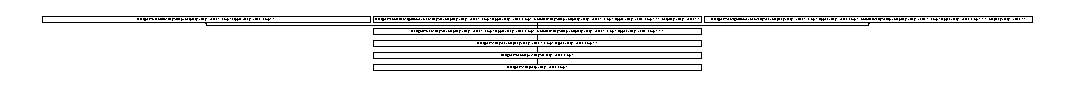
\includegraphics[height=0.724638cm]{class_designar_1_1_array_map}
\end{center}
\end{figure}
\subsection*{Métodos públicos}
\begin{DoxyCompactItemize}
\item 
\hyperlink{class_designar_1_1_array_map_aa08404c6d0b6d40d7aefd04ccea24bc5}{Array\+Map} (\hyperlink{namespace_designar_aa72662848b9f4815e7bf31a7cf3e33d1}{nat\+\_\+t} cap, Cmp \&\+\_\+cmp)
\item 
\hyperlink{class_designar_1_1_array_map_ac7113b782b6ade75f5ccc843ecc2c153}{Array\+Map} (Cmp \&\&\+\_\+cmp=Cmp())
\item 
\hyperlink{class_designar_1_1_array_map_a553f96874d7e4037c333edd6dd76ba31}{Array\+Map} (\hyperlink{namespace_designar_aa72662848b9f4815e7bf31a7cf3e33d1}{nat\+\_\+t} cap, Cmp \&\&\+\_\+cmp=Cmp())
\item 
\hyperlink{class_designar_1_1_array_map_aea553306fead24dc02e06ea89146d4f0}{Array\+Map} (const std\+::initializer\+\_\+list$<$ Item $>$ \&l)
\item 
\hyperlink{class_designar_1_1_array_map_a47288ae6af2300316c32e55bf46f7713}{Array\+Map} (const \hyperlink{class_designar_1_1_array_map}{Array\+Map} \&\hyperlink{class_designar_1_1_container_algorithms_a3b9044a197e4ceec6a1de03de197a293}{map})
\item 
\hyperlink{class_designar_1_1_array_map_a86b665176315dedc19b78479a47aa810}{Array\+Map} (\hyperlink{class_designar_1_1_array_map}{Array\+Map} \&\&\hyperlink{class_designar_1_1_container_algorithms_a3b9044a197e4ceec6a1de03de197a293}{map})
\item 
\hyperlink{class_designar_1_1_array_map}{Array\+Map} \& \hyperlink{class_designar_1_1_array_map_acc6b11ade9bcae167fb939cc6eec6c6e}{operator=} (const \hyperlink{class_designar_1_1_array_map}{Array\+Map} \&m)
\item 
\hyperlink{class_designar_1_1_array_map}{Array\+Map} \& \hyperlink{class_designar_1_1_array_map_a2bc354ad6ea6eb8103a8bca14abdece2}{operator=} (\hyperlink{class_designar_1_1_array_map}{Array\+Map} \&\&m)
\end{DoxyCompactItemize}
\subsection*{Otros miembros heredados}


\subsection{Descripción detallada}
\subsubsection*{template$<$typename Key, typename Value, class Cmp = std\+::less$<$\+Key$>$$>$\newline
class Designar\+::\+Array\+Map$<$ Key, Value, Cmp $>$}



Definición en la línea 391 del archivo map.\+H.



\subsection{Documentación del constructor y destructor}
\mbox{\Hypertarget{class_designar_1_1_array_map_aa08404c6d0b6d40d7aefd04ccea24bc5}\label{class_designar_1_1_array_map_aa08404c6d0b6d40d7aefd04ccea24bc5}} 
\index{Designar\+::\+Array\+Map@{Designar\+::\+Array\+Map}!Array\+Map@{Array\+Map}}
\index{Array\+Map@{Array\+Map}!Designar\+::\+Array\+Map@{Designar\+::\+Array\+Map}}
\subsubsection{\texorpdfstring{Array\+Map()}{ArrayMap()}\hspace{0.1cm}{\footnotesize\ttfamily [1/6]}}
{\footnotesize\ttfamily template$<$typename Key, typename Value, class Cmp = std\+::less$<$\+Key$>$$>$ \\
\hyperlink{class_designar_1_1_array_map}{Designar\+::\+Array\+Map}$<$ Key, Value, Cmp $>$\+::\hyperlink{class_designar_1_1_array_map}{Array\+Map} (\begin{DoxyParamCaption}\item[{\hyperlink{namespace_designar_aa72662848b9f4815e7bf31a7cf3e33d1}{nat\+\_\+t}}]{cap,  }\item[{Cmp \&}]{\+\_\+cmp }\end{DoxyParamCaption})\hspace{0.3cm}{\ttfamily [inline]}}



Definición en la línea 400 del archivo map.\+H.

\mbox{\Hypertarget{class_designar_1_1_array_map_ac7113b782b6ade75f5ccc843ecc2c153}\label{class_designar_1_1_array_map_ac7113b782b6ade75f5ccc843ecc2c153}} 
\index{Designar\+::\+Array\+Map@{Designar\+::\+Array\+Map}!Array\+Map@{Array\+Map}}
\index{Array\+Map@{Array\+Map}!Designar\+::\+Array\+Map@{Designar\+::\+Array\+Map}}
\subsubsection{\texorpdfstring{Array\+Map()}{ArrayMap()}\hspace{0.1cm}{\footnotesize\ttfamily [2/6]}}
{\footnotesize\ttfamily template$<$typename Key, typename Value, class Cmp = std\+::less$<$\+Key$>$$>$ \\
\hyperlink{class_designar_1_1_array_map}{Designar\+::\+Array\+Map}$<$ Key, Value, Cmp $>$\+::\hyperlink{class_designar_1_1_array_map}{Array\+Map} (\begin{DoxyParamCaption}\item[{Cmp \&\&}]{\+\_\+cmp = {\ttfamily Cmp()} }\end{DoxyParamCaption})\hspace{0.3cm}{\ttfamily [inline]}}



Definición en la línea 406 del archivo map.\+H.

\mbox{\Hypertarget{class_designar_1_1_array_map_a553f96874d7e4037c333edd6dd76ba31}\label{class_designar_1_1_array_map_a553f96874d7e4037c333edd6dd76ba31}} 
\index{Designar\+::\+Array\+Map@{Designar\+::\+Array\+Map}!Array\+Map@{Array\+Map}}
\index{Array\+Map@{Array\+Map}!Designar\+::\+Array\+Map@{Designar\+::\+Array\+Map}}
\subsubsection{\texorpdfstring{Array\+Map()}{ArrayMap()}\hspace{0.1cm}{\footnotesize\ttfamily [3/6]}}
{\footnotesize\ttfamily template$<$typename Key, typename Value, class Cmp = std\+::less$<$\+Key$>$$>$ \\
\hyperlink{class_designar_1_1_array_map}{Designar\+::\+Array\+Map}$<$ Key, Value, Cmp $>$\+::\hyperlink{class_designar_1_1_array_map}{Array\+Map} (\begin{DoxyParamCaption}\item[{\hyperlink{namespace_designar_aa72662848b9f4815e7bf31a7cf3e33d1}{nat\+\_\+t}}]{cap,  }\item[{Cmp \&\&}]{\+\_\+cmp = {\ttfamily Cmp()} }\end{DoxyParamCaption})\hspace{0.3cm}{\ttfamily [inline]}}



Definición en la línea 412 del archivo map.\+H.

\mbox{\Hypertarget{class_designar_1_1_array_map_aea553306fead24dc02e06ea89146d4f0}\label{class_designar_1_1_array_map_aea553306fead24dc02e06ea89146d4f0}} 
\index{Designar\+::\+Array\+Map@{Designar\+::\+Array\+Map}!Array\+Map@{Array\+Map}}
\index{Array\+Map@{Array\+Map}!Designar\+::\+Array\+Map@{Designar\+::\+Array\+Map}}
\subsubsection{\texorpdfstring{Array\+Map()}{ArrayMap()}\hspace{0.1cm}{\footnotesize\ttfamily [4/6]}}
{\footnotesize\ttfamily template$<$typename Key, typename Value, class Cmp = std\+::less$<$\+Key$>$$>$ \\
\hyperlink{class_designar_1_1_array_map}{Designar\+::\+Array\+Map}$<$ Key, Value, Cmp $>$\+::\hyperlink{class_designar_1_1_array_map}{Array\+Map} (\begin{DoxyParamCaption}\item[{const std\+::initializer\+\_\+list$<$ Item $>$ \&}]{l }\end{DoxyParamCaption})\hspace{0.3cm}{\ttfamily [inline]}}



Definición en la línea 418 del archivo map.\+H.

\mbox{\Hypertarget{class_designar_1_1_array_map_a47288ae6af2300316c32e55bf46f7713}\label{class_designar_1_1_array_map_a47288ae6af2300316c32e55bf46f7713}} 
\index{Designar\+::\+Array\+Map@{Designar\+::\+Array\+Map}!Array\+Map@{Array\+Map}}
\index{Array\+Map@{Array\+Map}!Designar\+::\+Array\+Map@{Designar\+::\+Array\+Map}}
\subsubsection{\texorpdfstring{Array\+Map()}{ArrayMap()}\hspace{0.1cm}{\footnotesize\ttfamily [5/6]}}
{\footnotesize\ttfamily template$<$typename Key, typename Value, class Cmp = std\+::less$<$\+Key$>$$>$ \\
\hyperlink{class_designar_1_1_array_map}{Designar\+::\+Array\+Map}$<$ Key, Value, Cmp $>$\+::\hyperlink{class_designar_1_1_array_map}{Array\+Map} (\begin{DoxyParamCaption}\item[{const \hyperlink{class_designar_1_1_array_map}{Array\+Map}$<$ Key, Value, Cmp $>$ \&}]{map }\end{DoxyParamCaption})\hspace{0.3cm}{\ttfamily [inline]}}



Definición en la línea 424 del archivo map.\+H.

\mbox{\Hypertarget{class_designar_1_1_array_map_a86b665176315dedc19b78479a47aa810}\label{class_designar_1_1_array_map_a86b665176315dedc19b78479a47aa810}} 
\index{Designar\+::\+Array\+Map@{Designar\+::\+Array\+Map}!Array\+Map@{Array\+Map}}
\index{Array\+Map@{Array\+Map}!Designar\+::\+Array\+Map@{Designar\+::\+Array\+Map}}
\subsubsection{\texorpdfstring{Array\+Map()}{ArrayMap()}\hspace{0.1cm}{\footnotesize\ttfamily [6/6]}}
{\footnotesize\ttfamily template$<$typename Key, typename Value, class Cmp = std\+::less$<$\+Key$>$$>$ \\
\hyperlink{class_designar_1_1_array_map}{Designar\+::\+Array\+Map}$<$ Key, Value, Cmp $>$\+::\hyperlink{class_designar_1_1_array_map}{Array\+Map} (\begin{DoxyParamCaption}\item[{\hyperlink{class_designar_1_1_array_map}{Array\+Map}$<$ Key, Value, Cmp $>$ \&\&}]{map }\end{DoxyParamCaption})\hspace{0.3cm}{\ttfamily [inline]}}



Definición en la línea 430 del archivo map.\+H.



\subsection{Documentación de las funciones miembro}
\mbox{\Hypertarget{class_designar_1_1_array_map_acc6b11ade9bcae167fb939cc6eec6c6e}\label{class_designar_1_1_array_map_acc6b11ade9bcae167fb939cc6eec6c6e}} 
\index{Designar\+::\+Array\+Map@{Designar\+::\+Array\+Map}!operator=@{operator=}}
\index{operator=@{operator=}!Designar\+::\+Array\+Map@{Designar\+::\+Array\+Map}}
\subsubsection{\texorpdfstring{operator=()}{operator=()}\hspace{0.1cm}{\footnotesize\ttfamily [1/2]}}
{\footnotesize\ttfamily template$<$typename Key, typename Value, class Cmp = std\+::less$<$\+Key$>$$>$ \\
\hyperlink{class_designar_1_1_array_map}{Array\+Map}\& \hyperlink{class_designar_1_1_array_map}{Designar\+::\+Array\+Map}$<$ Key, Value, Cmp $>$\+::operator= (\begin{DoxyParamCaption}\item[{const \hyperlink{class_designar_1_1_array_map}{Array\+Map}$<$ Key, Value, Cmp $>$ \&}]{m }\end{DoxyParamCaption})\hspace{0.3cm}{\ttfamily [inline]}}



Definición en la línea 436 del archivo map.\+H.

\mbox{\Hypertarget{class_designar_1_1_array_map_a2bc354ad6ea6eb8103a8bca14abdece2}\label{class_designar_1_1_array_map_a2bc354ad6ea6eb8103a8bca14abdece2}} 
\index{Designar\+::\+Array\+Map@{Designar\+::\+Array\+Map}!operator=@{operator=}}
\index{operator=@{operator=}!Designar\+::\+Array\+Map@{Designar\+::\+Array\+Map}}
\subsubsection{\texorpdfstring{operator=()}{operator=()}\hspace{0.1cm}{\footnotesize\ttfamily [2/2]}}
{\footnotesize\ttfamily template$<$typename Key, typename Value, class Cmp = std\+::less$<$\+Key$>$$>$ \\
\hyperlink{class_designar_1_1_array_map}{Array\+Map}\& \hyperlink{class_designar_1_1_array_map}{Designar\+::\+Array\+Map}$<$ Key, Value, Cmp $>$\+::operator= (\begin{DoxyParamCaption}\item[{\hyperlink{class_designar_1_1_array_map}{Array\+Map}$<$ Key, Value, Cmp $>$ \&\&}]{m }\end{DoxyParamCaption})\hspace{0.3cm}{\ttfamily [inline]}}



Definición en la línea 445 del archivo map.\+H.



La documentación para esta clase fue generada a partir del siguiente fichero\+:\begin{DoxyCompactItemize}
\item 
/home/julio/\+De\+S\+I\+G\+N\+A\+R-\/doc/\+De\+Si\+G\+N\+A\+R/include/\hyperlink{map_8_h}{map.\+H}\end{DoxyCompactItemize}

\hypertarget{class_designar_1_1_array_set}{}\section{Designar\+:\+:Array\+Set$<$ Key, Cmp $>$ Class Template Reference}
\label{class_designar_1_1_array_set}\index{Designar\+::\+Array\+Set$<$ Key, Cmp $>$@{Designar\+::\+Array\+Set$<$ Key, Cmp $>$}}


{\ttfamily \#include $<$array.\+H$>$}

Inheritance diagram for Designar\+:\+:Array\+Set$<$ Key, Cmp $>$\+:\begin{figure}[H]
\begin{center}
\leavevmode
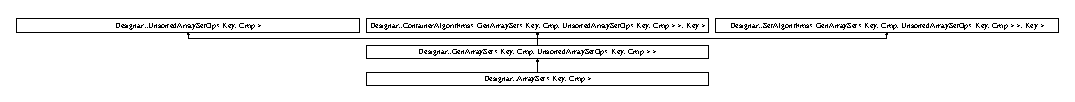
\includegraphics[height=0.922570cm]{class_designar_1_1_array_set}
\end{center}
\end{figure}
\subsection*{Additional Inherited Members}


\subsection{Detailed Description}
\subsubsection*{template$<$typename Key, class Cmp = std\+::less$<$\+Key$>$$>$\newline
class Designar\+::\+Array\+Set$<$ Key, Cmp $>$}



Definition at line 1489 of file array.\+H.



The documentation for this class was generated from the following file\+:\begin{DoxyCompactItemize}
\item 
De\+Si\+G\+N\+A\+R/include/\hyperlink{array_8_h}{array.\+H}\end{DoxyCompactItemize}

\hypertarget{class_designar_1_1_astar}{}\section{Designar\+:\+:Astar$<$ GT, Distance, Heuristic, Cmp, Plus $>$ Class Template Reference}
\label{class_designar_1_1_astar}\index{Designar\+::\+Astar$<$ G\+T, Distance, Heuristic, Cmp, Plus $>$@{Designar\+::\+Astar$<$ G\+T, Distance, Heuristic, Cmp, Plus $>$}}


{\ttfamily \#include $<$graphalgorithms.\+H$>$}

\subsection*{Public Types}
\begin{DoxyCompactItemize}
\item 
using \hyperlink{class_designar_1_1_astar_a0d4cdf6b94255824c6c93e5ae18e9eb7}{Node} = typename \hyperlink{class_designar_1_1_graph_a5dfc7dba9d092ac489c72e40390c37d0}{G\+T\+::\+Node}
\item 
using \hyperlink{class_designar_1_1_astar_a4d0b1c7cb0a71b5cfe3d21ea37c12108}{Arc} = typename \hyperlink{class_designar_1_1_graph_a74c730ef4ce2d20f998d72bd25c2b5bf}{G\+T\+::\+Arc}
\end{DoxyCompactItemize}
\subsection*{Public Member Functions}
\begin{DoxyCompactItemize}
\item 
\hyperlink{class_designar_1_1_astar_a9a684bbaa799da107f42ed8e048cac57}{Astar} (Distance \&\+\_\+distance, Heuristic \&\+\_\+heuristic, Cmp \&\+\_\+cmp, Plus \&\+\_\+plus)
\item 
\hyperlink{class_designar_1_1_astar_a5db848d589e8e4ce7582acc061cb8b17}{Astar} (Distance \&\&\+\_\+distance=Distance(), Heuristic \&\&\+\_\+heuristic=Heuristic(), Cmp \&\&\+\_\+cmp=Cmp(), Plus \&\&\+\_\+plus=Plus())
\item 
\hyperlink{class_designar_1_1_path}{Path}$<$ \hyperlink{demo-buildgraph_8_c_a3001c40d2c31ca87ed96cd7d1334a55e}{GT} $>$ \hyperlink{class_designar_1_1_astar_a23f41f4dd26aaef8ded7138de8866b54}{search\+\_\+min\+\_\+path} (\hyperlink{demo-buildgraph_8_c_a3001c40d2c31ca87ed96cd7d1334a55e}{GT} \&g, \hyperlink{class_designar_1_1_astar_a0d4cdf6b94255824c6c93e5ae18e9eb7}{Node} \&start, \hyperlink{class_designar_1_1_astar_a0d4cdf6b94255824c6c93e5ae18e9eb7}{Node} \&end)
\item 
void \hyperlink{class_designar_1_1_astar_ab6cf1a92f64a96290880a1483eac396f}{paint\+\_\+min\+\_\+path} (\hyperlink{demo-buildgraph_8_c_a3001c40d2c31ca87ed96cd7d1334a55e}{GT} \&g, \hyperlink{class_designar_1_1_astar_a0d4cdf6b94255824c6c93e5ae18e9eb7}{Node} \&start, \hyperlink{class_designar_1_1_astar_a0d4cdf6b94255824c6c93e5ae18e9eb7}{Node} \&end)
\end{DoxyCompactItemize}


\subsection{Detailed Description}
\subsubsection*{template$<$class GT, class Distance = Default\+Distance$<$\+G\+T$>$, class Heuristic = Default\+Heuristic$<$\+G\+T, Distance$>$, class Cmp = std\+::less$<$typename Distance\+::\+Type$>$, class Plus = std\+::plus$<$typename Distance\+::\+Type$>$$>$\newline
class Designar\+::\+Astar$<$ G\+T, Distance, Heuristic, Cmp, Plus $>$}



Definition at line 1691 of file graphalgorithms.\+H.



\subsection{Member Typedef Documentation}
\mbox{\Hypertarget{class_designar_1_1_astar_a4d0b1c7cb0a71b5cfe3d21ea37c12108}\label{class_designar_1_1_astar_a4d0b1c7cb0a71b5cfe3d21ea37c12108}} 
\index{Designar\+::\+Astar@{Designar\+::\+Astar}!Arc@{Arc}}
\index{Arc@{Arc}!Designar\+::\+Astar@{Designar\+::\+Astar}}
\subsubsection{\texorpdfstring{Arc}{Arc}}
{\footnotesize\ttfamily template$<$class GT , class Distance  = Default\+Distance$<$\+G\+T$>$, class Heuristic  = Default\+Heuristic$<$\+G\+T, Distance$>$, class Cmp  = std\+::less$<$typename Distance\+::\+Type$>$, class Plus  = std\+::plus$<$typename Distance\+::\+Type$>$$>$ \\
using \hyperlink{class_designar_1_1_astar}{Designar\+::\+Astar}$<$ \hyperlink{demo-buildgraph_8_c_a3001c40d2c31ca87ed96cd7d1334a55e}{GT}, Distance, Heuristic, Cmp, Plus $>$\+::\hyperlink{class_designar_1_1_astar_a4d0b1c7cb0a71b5cfe3d21ea37c12108}{Arc} =  typename \hyperlink{class_designar_1_1_graph_a74c730ef4ce2d20f998d72bd25c2b5bf}{G\+T\+::\+Arc}}



Definition at line 1695 of file graphalgorithms.\+H.

\mbox{\Hypertarget{class_designar_1_1_astar_a0d4cdf6b94255824c6c93e5ae18e9eb7}\label{class_designar_1_1_astar_a0d4cdf6b94255824c6c93e5ae18e9eb7}} 
\index{Designar\+::\+Astar@{Designar\+::\+Astar}!Node@{Node}}
\index{Node@{Node}!Designar\+::\+Astar@{Designar\+::\+Astar}}
\subsubsection{\texorpdfstring{Node}{Node}}
{\footnotesize\ttfamily template$<$class GT , class Distance  = Default\+Distance$<$\+G\+T$>$, class Heuristic  = Default\+Heuristic$<$\+G\+T, Distance$>$, class Cmp  = std\+::less$<$typename Distance\+::\+Type$>$, class Plus  = std\+::plus$<$typename Distance\+::\+Type$>$$>$ \\
using \hyperlink{class_designar_1_1_astar}{Designar\+::\+Astar}$<$ \hyperlink{demo-buildgraph_8_c_a3001c40d2c31ca87ed96cd7d1334a55e}{GT}, Distance, Heuristic, Cmp, Plus $>$\+::\hyperlink{class_designar_1_1_astar_a0d4cdf6b94255824c6c93e5ae18e9eb7}{Node} =  typename \hyperlink{class_designar_1_1_graph_a5dfc7dba9d092ac489c72e40390c37d0}{G\+T\+::\+Node}}



Definition at line 1694 of file graphalgorithms.\+H.



\subsection{Constructor \& Destructor Documentation}
\mbox{\Hypertarget{class_designar_1_1_astar_a9a684bbaa799da107f42ed8e048cac57}\label{class_designar_1_1_astar_a9a684bbaa799da107f42ed8e048cac57}} 
\index{Designar\+::\+Astar@{Designar\+::\+Astar}!Astar@{Astar}}
\index{Astar@{Astar}!Designar\+::\+Astar@{Designar\+::\+Astar}}
\subsubsection{\texorpdfstring{Astar()}{Astar()}\hspace{0.1cm}{\footnotesize\ttfamily [1/2]}}
{\footnotesize\ttfamily template$<$class GT , class Distance  = Default\+Distance$<$\+G\+T$>$, class Heuristic  = Default\+Heuristic$<$\+G\+T, Distance$>$, class Cmp  = std\+::less$<$typename Distance\+::\+Type$>$, class Plus  = std\+::plus$<$typename Distance\+::\+Type$>$$>$ \\
\hyperlink{class_designar_1_1_astar}{Designar\+::\+Astar}$<$ \hyperlink{demo-buildgraph_8_c_a3001c40d2c31ca87ed96cd7d1334a55e}{GT}, Distance, Heuristic, Cmp, Plus $>$\+::\hyperlink{class_designar_1_1_astar}{Astar} (\begin{DoxyParamCaption}\item[{Distance \&}]{\+\_\+distance,  }\item[{Heuristic \&}]{\+\_\+heuristic,  }\item[{Cmp \&}]{\+\_\+cmp,  }\item[{Plus \&}]{\+\_\+plus }\end{DoxyParamCaption})\hspace{0.3cm}{\ttfamily [inline]}}



Definition at line 1712 of file graphalgorithms.\+H.

\mbox{\Hypertarget{class_designar_1_1_astar_a5db848d589e8e4ce7582acc061cb8b17}\label{class_designar_1_1_astar_a5db848d589e8e4ce7582acc061cb8b17}} 
\index{Designar\+::\+Astar@{Designar\+::\+Astar}!Astar@{Astar}}
\index{Astar@{Astar}!Designar\+::\+Astar@{Designar\+::\+Astar}}
\subsubsection{\texorpdfstring{Astar()}{Astar()}\hspace{0.1cm}{\footnotesize\ttfamily [2/2]}}
{\footnotesize\ttfamily template$<$class GT , class Distance  = Default\+Distance$<$\+G\+T$>$, class Heuristic  = Default\+Heuristic$<$\+G\+T, Distance$>$, class Cmp  = std\+::less$<$typename Distance\+::\+Type$>$, class Plus  = std\+::plus$<$typename Distance\+::\+Type$>$$>$ \\
\hyperlink{class_designar_1_1_astar}{Designar\+::\+Astar}$<$ \hyperlink{demo-buildgraph_8_c_a3001c40d2c31ca87ed96cd7d1334a55e}{GT}, Distance, Heuristic, Cmp, Plus $>$\+::\hyperlink{class_designar_1_1_astar}{Astar} (\begin{DoxyParamCaption}\item[{Distance \&\&}]{\+\_\+distance = {\ttfamily Distance()},  }\item[{Heuristic \&\&}]{\+\_\+heuristic = {\ttfamily Heuristic()},  }\item[{Cmp \&\&}]{\+\_\+cmp = {\ttfamily Cmp()},  }\item[{Plus \&\&}]{\+\_\+plus = {\ttfamily Plus()} }\end{DoxyParamCaption})\hspace{0.3cm}{\ttfamily [inline]}}



Definition at line 1720 of file graphalgorithms.\+H.



\subsection{Member Function Documentation}
\mbox{\Hypertarget{class_designar_1_1_astar_ab6cf1a92f64a96290880a1483eac396f}\label{class_designar_1_1_astar_ab6cf1a92f64a96290880a1483eac396f}} 
\index{Designar\+::\+Astar@{Designar\+::\+Astar}!paint\+\_\+min\+\_\+path@{paint\+\_\+min\+\_\+path}}
\index{paint\+\_\+min\+\_\+path@{paint\+\_\+min\+\_\+path}!Designar\+::\+Astar@{Designar\+::\+Astar}}
\subsubsection{\texorpdfstring{paint\+\_\+min\+\_\+path()}{paint\_min\_path()}}
{\footnotesize\ttfamily template$<$class GT , class Distance  = Default\+Distance$<$\+G\+T$>$, class Heuristic  = Default\+Heuristic$<$\+G\+T, Distance$>$, class Cmp  = std\+::less$<$typename Distance\+::\+Type$>$, class Plus  = std\+::plus$<$typename Distance\+::\+Type$>$$>$ \\
void \hyperlink{class_designar_1_1_astar}{Designar\+::\+Astar}$<$ \hyperlink{demo-buildgraph_8_c_a3001c40d2c31ca87ed96cd7d1334a55e}{GT}, Distance, Heuristic, Cmp, Plus $>$\+::paint\+\_\+min\+\_\+path (\begin{DoxyParamCaption}\item[{\hyperlink{demo-buildgraph_8_c_a3001c40d2c31ca87ed96cd7d1334a55e}{GT} \&}]{g,  }\item[{\hyperlink{class_designar_1_1_astar_a0d4cdf6b94255824c6c93e5ae18e9eb7}{Node} \&}]{start,  }\item[{\hyperlink{class_designar_1_1_astar_a0d4cdf6b94255824c6c93e5ae18e9eb7}{Node} \&}]{end }\end{DoxyParamCaption})\hspace{0.3cm}{\ttfamily [inline]}}



Definition at line 1756 of file graphalgorithms.\+H.

\mbox{\Hypertarget{class_designar_1_1_astar_a23f41f4dd26aaef8ded7138de8866b54}\label{class_designar_1_1_astar_a23f41f4dd26aaef8ded7138de8866b54}} 
\index{Designar\+::\+Astar@{Designar\+::\+Astar}!search\+\_\+min\+\_\+path@{search\+\_\+min\+\_\+path}}
\index{search\+\_\+min\+\_\+path@{search\+\_\+min\+\_\+path}!Designar\+::\+Astar@{Designar\+::\+Astar}}
\subsubsection{\texorpdfstring{search\+\_\+min\+\_\+path()}{search\_min\_path()}}
{\footnotesize\ttfamily template$<$class GT , class Distance  = Default\+Distance$<$\+G\+T$>$, class Heuristic  = Default\+Heuristic$<$\+G\+T, Distance$>$, class Cmp  = std\+::less$<$typename Distance\+::\+Type$>$, class Plus  = std\+::plus$<$typename Distance\+::\+Type$>$$>$ \\
\hyperlink{class_designar_1_1_path}{Path}$<$\hyperlink{demo-buildgraph_8_c_a3001c40d2c31ca87ed96cd7d1334a55e}{GT}$>$ \hyperlink{class_designar_1_1_astar}{Designar\+::\+Astar}$<$ \hyperlink{demo-buildgraph_8_c_a3001c40d2c31ca87ed96cd7d1334a55e}{GT}, Distance, Heuristic, Cmp, Plus $>$\+::search\+\_\+min\+\_\+path (\begin{DoxyParamCaption}\item[{\hyperlink{demo-buildgraph_8_c_a3001c40d2c31ca87ed96cd7d1334a55e}{GT} \&}]{g,  }\item[{\hyperlink{class_designar_1_1_astar_a0d4cdf6b94255824c6c93e5ae18e9eb7}{Node} \&}]{start,  }\item[{\hyperlink{class_designar_1_1_astar_a0d4cdf6b94255824c6c93e5ae18e9eb7}{Node} \&}]{end }\end{DoxyParamCaption})\hspace{0.3cm}{\ttfamily [inline]}}



Definition at line 1729 of file graphalgorithms.\+H.



The documentation for this class was generated from the following file\+:\begin{DoxyCompactItemize}
\item 
include/\hyperlink{graphalgorithms_8_h}{graphalgorithms.\+H}\end{DoxyCompactItemize}

\hypertarget{class_designar_1_1_base_bin_tree_node}{}\section{Referencia de la plantilla de la Clase Designar\+:\+:Base\+Bin\+Tree\+Node$<$ Key, Derived\+Node\+Type, N\+U\+L\+L\+\_\+\+V\+A\+L\+UE $>$}
\label{class_designar_1_1_base_bin_tree_node}\index{Designar\+::\+Base\+Bin\+Tree\+Node$<$ Key, Derived\+Node\+Type, N\+U\+L\+L\+\_\+\+V\+A\+L\+U\+E $>$@{Designar\+::\+Base\+Bin\+Tree\+Node$<$ Key, Derived\+Node\+Type, N\+U\+L\+L\+\_\+\+V\+A\+L\+U\+E $>$}}


{\ttfamily \#include $<$nodesdef.\+H$>$}

\subsection*{Tipos públicos}
\begin{DoxyCompactItemize}
\item 
using \hyperlink{class_designar_1_1_base_bin_tree_node_adc177cc1f4ed5bb9baf467a2ff6e4e85}{Key\+Type} = Key
\end{DoxyCompactItemize}
\subsection*{Métodos públicos}
\begin{DoxyCompactItemize}
\item 
\hyperlink{class_designar_1_1_base_bin_tree_node_a2779b1f30e23443940aaa0ddfec895be}{Base\+Bin\+Tree\+Node} ()
\item 
\hyperlink{class_designar_1_1_base_bin_tree_node_a19dbfd3695d9213dc0d50a4637e92b16}{Base\+Bin\+Tree\+Node} (const Key \&k)
\item 
\hyperlink{class_designar_1_1_base_bin_tree_node_aaf8196a9b42a719173d03340f68b467f}{Base\+Bin\+Tree\+Node} (Key \&\&k)
\item 
\hyperlink{class_designar_1_1_base_bin_tree_node_a29c18682569084f8f64ca58b22f8f74a}{Base\+Bin\+Tree\+Node} (\hyperlink{namespace_designar_a679bc99fd69a3601faa5d6d47f865106}{Bin\+Tree\+Node\+Ctor})
\item 
\hyperlink{class_designar_1_1_base_bin_tree_node_a455b27b565e1dc004fd6292475d5a9de}{Base\+Bin\+Tree\+Node} (const \hyperlink{class_designar_1_1_base_bin_tree_node}{Base\+Bin\+Tree\+Node} \&)=delete
\item 
\hyperlink{class_designar_1_1_base_bin_tree_node}{Base\+Bin\+Tree\+Node} \& \hyperlink{class_designar_1_1_base_bin_tree_node_acde689f73c8d4fce33926e86882b0765}{operator=} (const \hyperlink{class_designar_1_1_base_bin_tree_node}{Base\+Bin\+Tree\+Node} \&)=delete
\item 
Key \& \hyperlink{class_designar_1_1_base_bin_tree_node_a59c9489fff0bd46c058e901d02b2e582}{get\+\_\+key} ()
\item 
const Key \& \hyperlink{class_designar_1_1_base_bin_tree_node_ab836466417ce1dad15b794424f39ee4b}{get\+\_\+key} () const
\item 
Derived\+Node\+Type $\ast$\& \hyperlink{class_designar_1_1_base_bin_tree_node_a60f8c88c08e4b68ecc9dd9a77b69cb7c}{get\+\_\+lchild} ()
\item 
Derived\+Node\+Type $\ast$\& \hyperlink{class_designar_1_1_base_bin_tree_node_a328220c701b0c58b024610cf8fb70850}{get\+\_\+rchild} ()
\end{DoxyCompactItemize}
\subsection*{Atributos públicos estáticos}
\begin{DoxyCompactItemize}
\item 
static Derived\+Node\+Type $\ast$const \hyperlink{class_designar_1_1_base_bin_tree_node_a0ea0251169acae6e7943ccc54f66472a}{null}
\end{DoxyCompactItemize}


\subsection{Descripción detallada}
\subsubsection*{template$<$typename Key, class Derived\+Node\+Type, Bin\+Tree\+Node\+Null\+Value N\+U\+L\+L\+\_\+\+V\+A\+L\+UE$>$\newline
class Designar\+::\+Base\+Bin\+Tree\+Node$<$ Key, Derived\+Node\+Type, N\+U\+L\+L\+\_\+\+V\+A\+L\+U\+E $>$}



Definición en la línea 902 del archivo nodesdef.\+H.



\subsection{Documentación de los \textquotesingle{}Typedef\textquotesingle{} miembros de la clase}
\mbox{\Hypertarget{class_designar_1_1_base_bin_tree_node_adc177cc1f4ed5bb9baf467a2ff6e4e85}\label{class_designar_1_1_base_bin_tree_node_adc177cc1f4ed5bb9baf467a2ff6e4e85}} 
\index{Designar\+::\+Base\+Bin\+Tree\+Node@{Designar\+::\+Base\+Bin\+Tree\+Node}!Key\+Type@{Key\+Type}}
\index{Key\+Type@{Key\+Type}!Designar\+::\+Base\+Bin\+Tree\+Node@{Designar\+::\+Base\+Bin\+Tree\+Node}}
\subsubsection{\texorpdfstring{Key\+Type}{KeyType}}
{\footnotesize\ttfamily template$<$typename Key, class Derived\+Node\+Type, Bin\+Tree\+Node\+Null\+Value N\+U\+L\+L\+\_\+\+V\+A\+L\+UE$>$ \\
using \hyperlink{class_designar_1_1_base_bin_tree_node}{Designar\+::\+Base\+Bin\+Tree\+Node}$<$ Key, Derived\+Node\+Type, N\+U\+L\+L\+\_\+\+V\+A\+L\+UE $>$\+::\hyperlink{class_designar_1_1_base_bin_tree_node_adc177cc1f4ed5bb9baf467a2ff6e4e85}{Key\+Type} =  Key}



Definición en la línea 907 del archivo nodesdef.\+H.



\subsection{Documentación del constructor y destructor}
\mbox{\Hypertarget{class_designar_1_1_base_bin_tree_node_a2779b1f30e23443940aaa0ddfec895be}\label{class_designar_1_1_base_bin_tree_node_a2779b1f30e23443940aaa0ddfec895be}} 
\index{Designar\+::\+Base\+Bin\+Tree\+Node@{Designar\+::\+Base\+Bin\+Tree\+Node}!Base\+Bin\+Tree\+Node@{Base\+Bin\+Tree\+Node}}
\index{Base\+Bin\+Tree\+Node@{Base\+Bin\+Tree\+Node}!Designar\+::\+Base\+Bin\+Tree\+Node@{Designar\+::\+Base\+Bin\+Tree\+Node}}
\subsubsection{\texorpdfstring{Base\+Bin\+Tree\+Node()}{BaseBinTreeNode()}\hspace{0.1cm}{\footnotesize\ttfamily [1/5]}}
{\footnotesize\ttfamily template$<$typename Key, class Derived\+Node\+Type, Bin\+Tree\+Node\+Null\+Value N\+U\+L\+L\+\_\+\+V\+A\+L\+UE$>$ \\
\hyperlink{class_designar_1_1_base_bin_tree_node}{Designar\+::\+Base\+Bin\+Tree\+Node}$<$ Key, Derived\+Node\+Type, N\+U\+L\+L\+\_\+\+V\+A\+L\+UE $>$\+::\hyperlink{class_designar_1_1_base_bin_tree_node}{Base\+Bin\+Tree\+Node} (\begin{DoxyParamCaption}{ }\end{DoxyParamCaption})\hspace{0.3cm}{\ttfamily [inline]}}



Definición en la línea 917 del archivo nodesdef.\+H.

\mbox{\Hypertarget{class_designar_1_1_base_bin_tree_node_a19dbfd3695d9213dc0d50a4637e92b16}\label{class_designar_1_1_base_bin_tree_node_a19dbfd3695d9213dc0d50a4637e92b16}} 
\index{Designar\+::\+Base\+Bin\+Tree\+Node@{Designar\+::\+Base\+Bin\+Tree\+Node}!Base\+Bin\+Tree\+Node@{Base\+Bin\+Tree\+Node}}
\index{Base\+Bin\+Tree\+Node@{Base\+Bin\+Tree\+Node}!Designar\+::\+Base\+Bin\+Tree\+Node@{Designar\+::\+Base\+Bin\+Tree\+Node}}
\subsubsection{\texorpdfstring{Base\+Bin\+Tree\+Node()}{BaseBinTreeNode()}\hspace{0.1cm}{\footnotesize\ttfamily [2/5]}}
{\footnotesize\ttfamily template$<$typename Key, class Derived\+Node\+Type, Bin\+Tree\+Node\+Null\+Value N\+U\+L\+L\+\_\+\+V\+A\+L\+UE$>$ \\
\hyperlink{class_designar_1_1_base_bin_tree_node}{Designar\+::\+Base\+Bin\+Tree\+Node}$<$ Key, Derived\+Node\+Type, N\+U\+L\+L\+\_\+\+V\+A\+L\+UE $>$\+::\hyperlink{class_designar_1_1_base_bin_tree_node}{Base\+Bin\+Tree\+Node} (\begin{DoxyParamCaption}\item[{const Key \&}]{k }\end{DoxyParamCaption})\hspace{0.3cm}{\ttfamily [inline]}}



Definición en la línea 923 del archivo nodesdef.\+H.

\mbox{\Hypertarget{class_designar_1_1_base_bin_tree_node_aaf8196a9b42a719173d03340f68b467f}\label{class_designar_1_1_base_bin_tree_node_aaf8196a9b42a719173d03340f68b467f}} 
\index{Designar\+::\+Base\+Bin\+Tree\+Node@{Designar\+::\+Base\+Bin\+Tree\+Node}!Base\+Bin\+Tree\+Node@{Base\+Bin\+Tree\+Node}}
\index{Base\+Bin\+Tree\+Node@{Base\+Bin\+Tree\+Node}!Designar\+::\+Base\+Bin\+Tree\+Node@{Designar\+::\+Base\+Bin\+Tree\+Node}}
\subsubsection{\texorpdfstring{Base\+Bin\+Tree\+Node()}{BaseBinTreeNode()}\hspace{0.1cm}{\footnotesize\ttfamily [3/5]}}
{\footnotesize\ttfamily template$<$typename Key, class Derived\+Node\+Type, Bin\+Tree\+Node\+Null\+Value N\+U\+L\+L\+\_\+\+V\+A\+L\+UE$>$ \\
\hyperlink{class_designar_1_1_base_bin_tree_node}{Designar\+::\+Base\+Bin\+Tree\+Node}$<$ Key, Derived\+Node\+Type, N\+U\+L\+L\+\_\+\+V\+A\+L\+UE $>$\+::\hyperlink{class_designar_1_1_base_bin_tree_node}{Base\+Bin\+Tree\+Node} (\begin{DoxyParamCaption}\item[{Key \&\&}]{k }\end{DoxyParamCaption})\hspace{0.3cm}{\ttfamily [inline]}}



Definición en la línea 929 del archivo nodesdef.\+H.

\mbox{\Hypertarget{class_designar_1_1_base_bin_tree_node_a29c18682569084f8f64ca58b22f8f74a}\label{class_designar_1_1_base_bin_tree_node_a29c18682569084f8f64ca58b22f8f74a}} 
\index{Designar\+::\+Base\+Bin\+Tree\+Node@{Designar\+::\+Base\+Bin\+Tree\+Node}!Base\+Bin\+Tree\+Node@{Base\+Bin\+Tree\+Node}}
\index{Base\+Bin\+Tree\+Node@{Base\+Bin\+Tree\+Node}!Designar\+::\+Base\+Bin\+Tree\+Node@{Designar\+::\+Base\+Bin\+Tree\+Node}}
\subsubsection{\texorpdfstring{Base\+Bin\+Tree\+Node()}{BaseBinTreeNode()}\hspace{0.1cm}{\footnotesize\ttfamily [4/5]}}
{\footnotesize\ttfamily template$<$typename Key, class Derived\+Node\+Type, Bin\+Tree\+Node\+Null\+Value N\+U\+L\+L\+\_\+\+V\+A\+L\+UE$>$ \\
\hyperlink{class_designar_1_1_base_bin_tree_node}{Designar\+::\+Base\+Bin\+Tree\+Node}$<$ Key, Derived\+Node\+Type, N\+U\+L\+L\+\_\+\+V\+A\+L\+UE $>$\+::\hyperlink{class_designar_1_1_base_bin_tree_node}{Base\+Bin\+Tree\+Node} (\begin{DoxyParamCaption}\item[{\hyperlink{namespace_designar_a679bc99fd69a3601faa5d6d47f865106}{Bin\+Tree\+Node\+Ctor}}]{ }\end{DoxyParamCaption})\hspace{0.3cm}{\ttfamily [inline]}}



Definición en la línea 935 del archivo nodesdef.\+H.

\mbox{\Hypertarget{class_designar_1_1_base_bin_tree_node_a455b27b565e1dc004fd6292475d5a9de}\label{class_designar_1_1_base_bin_tree_node_a455b27b565e1dc004fd6292475d5a9de}} 
\index{Designar\+::\+Base\+Bin\+Tree\+Node@{Designar\+::\+Base\+Bin\+Tree\+Node}!Base\+Bin\+Tree\+Node@{Base\+Bin\+Tree\+Node}}
\index{Base\+Bin\+Tree\+Node@{Base\+Bin\+Tree\+Node}!Designar\+::\+Base\+Bin\+Tree\+Node@{Designar\+::\+Base\+Bin\+Tree\+Node}}
\subsubsection{\texorpdfstring{Base\+Bin\+Tree\+Node()}{BaseBinTreeNode()}\hspace{0.1cm}{\footnotesize\ttfamily [5/5]}}
{\footnotesize\ttfamily template$<$typename Key, class Derived\+Node\+Type, Bin\+Tree\+Node\+Null\+Value N\+U\+L\+L\+\_\+\+V\+A\+L\+UE$>$ \\
\hyperlink{class_designar_1_1_base_bin_tree_node}{Designar\+::\+Base\+Bin\+Tree\+Node}$<$ Key, Derived\+Node\+Type, N\+U\+L\+L\+\_\+\+V\+A\+L\+UE $>$\+::\hyperlink{class_designar_1_1_base_bin_tree_node}{Base\+Bin\+Tree\+Node} (\begin{DoxyParamCaption}\item[{const \hyperlink{class_designar_1_1_base_bin_tree_node}{Base\+Bin\+Tree\+Node}$<$ Key, Derived\+Node\+Type, N\+U\+L\+L\+\_\+\+V\+A\+L\+UE $>$ \&}]{ }\end{DoxyParamCaption})\hspace{0.3cm}{\ttfamily [delete]}}



\subsection{Documentación de las funciones miembro}
\mbox{\Hypertarget{class_designar_1_1_base_bin_tree_node_a59c9489fff0bd46c058e901d02b2e582}\label{class_designar_1_1_base_bin_tree_node_a59c9489fff0bd46c058e901d02b2e582}} 
\index{Designar\+::\+Base\+Bin\+Tree\+Node@{Designar\+::\+Base\+Bin\+Tree\+Node}!get\+\_\+key@{get\+\_\+key}}
\index{get\+\_\+key@{get\+\_\+key}!Designar\+::\+Base\+Bin\+Tree\+Node@{Designar\+::\+Base\+Bin\+Tree\+Node}}
\subsubsection{\texorpdfstring{get\+\_\+key()}{get\_key()}\hspace{0.1cm}{\footnotesize\ttfamily [1/2]}}
{\footnotesize\ttfamily template$<$typename Key, class Derived\+Node\+Type, Bin\+Tree\+Node\+Null\+Value N\+U\+L\+L\+\_\+\+V\+A\+L\+UE$>$ \\
Key\& \hyperlink{class_designar_1_1_base_bin_tree_node}{Designar\+::\+Base\+Bin\+Tree\+Node}$<$ Key, Derived\+Node\+Type, N\+U\+L\+L\+\_\+\+V\+A\+L\+UE $>$\+::get\+\_\+key (\begin{DoxyParamCaption}{ }\end{DoxyParamCaption})\hspace{0.3cm}{\ttfamily [inline]}}



Definición en la línea 945 del archivo nodesdef.\+H.

\mbox{\Hypertarget{class_designar_1_1_base_bin_tree_node_ab836466417ce1dad15b794424f39ee4b}\label{class_designar_1_1_base_bin_tree_node_ab836466417ce1dad15b794424f39ee4b}} 
\index{Designar\+::\+Base\+Bin\+Tree\+Node@{Designar\+::\+Base\+Bin\+Tree\+Node}!get\+\_\+key@{get\+\_\+key}}
\index{get\+\_\+key@{get\+\_\+key}!Designar\+::\+Base\+Bin\+Tree\+Node@{Designar\+::\+Base\+Bin\+Tree\+Node}}
\subsubsection{\texorpdfstring{get\+\_\+key()}{get\_key()}\hspace{0.1cm}{\footnotesize\ttfamily [2/2]}}
{\footnotesize\ttfamily template$<$typename Key, class Derived\+Node\+Type, Bin\+Tree\+Node\+Null\+Value N\+U\+L\+L\+\_\+\+V\+A\+L\+UE$>$ \\
const Key\& \hyperlink{class_designar_1_1_base_bin_tree_node}{Designar\+::\+Base\+Bin\+Tree\+Node}$<$ Key, Derived\+Node\+Type, N\+U\+L\+L\+\_\+\+V\+A\+L\+UE $>$\+::get\+\_\+key (\begin{DoxyParamCaption}{ }\end{DoxyParamCaption}) const\hspace{0.3cm}{\ttfamily [inline]}}



Definición en la línea 950 del archivo nodesdef.\+H.

\mbox{\Hypertarget{class_designar_1_1_base_bin_tree_node_a60f8c88c08e4b68ecc9dd9a77b69cb7c}\label{class_designar_1_1_base_bin_tree_node_a60f8c88c08e4b68ecc9dd9a77b69cb7c}} 
\index{Designar\+::\+Base\+Bin\+Tree\+Node@{Designar\+::\+Base\+Bin\+Tree\+Node}!get\+\_\+lchild@{get\+\_\+lchild}}
\index{get\+\_\+lchild@{get\+\_\+lchild}!Designar\+::\+Base\+Bin\+Tree\+Node@{Designar\+::\+Base\+Bin\+Tree\+Node}}
\subsubsection{\texorpdfstring{get\+\_\+lchild()}{get\_lchild()}}
{\footnotesize\ttfamily template$<$typename Key, class Derived\+Node\+Type, Bin\+Tree\+Node\+Null\+Value N\+U\+L\+L\+\_\+\+V\+A\+L\+UE$>$ \\
Derived\+Node\+Type$\ast$\& \hyperlink{class_designar_1_1_base_bin_tree_node}{Designar\+::\+Base\+Bin\+Tree\+Node}$<$ Key, Derived\+Node\+Type, N\+U\+L\+L\+\_\+\+V\+A\+L\+UE $>$\+::get\+\_\+lchild (\begin{DoxyParamCaption}{ }\end{DoxyParamCaption})\hspace{0.3cm}{\ttfamily [inline]}}



Definición en la línea 955 del archivo nodesdef.\+H.

\mbox{\Hypertarget{class_designar_1_1_base_bin_tree_node_a328220c701b0c58b024610cf8fb70850}\label{class_designar_1_1_base_bin_tree_node_a328220c701b0c58b024610cf8fb70850}} 
\index{Designar\+::\+Base\+Bin\+Tree\+Node@{Designar\+::\+Base\+Bin\+Tree\+Node}!get\+\_\+rchild@{get\+\_\+rchild}}
\index{get\+\_\+rchild@{get\+\_\+rchild}!Designar\+::\+Base\+Bin\+Tree\+Node@{Designar\+::\+Base\+Bin\+Tree\+Node}}
\subsubsection{\texorpdfstring{get\+\_\+rchild()}{get\_rchild()}}
{\footnotesize\ttfamily template$<$typename Key, class Derived\+Node\+Type, Bin\+Tree\+Node\+Null\+Value N\+U\+L\+L\+\_\+\+V\+A\+L\+UE$>$ \\
Derived\+Node\+Type$\ast$\& \hyperlink{class_designar_1_1_base_bin_tree_node}{Designar\+::\+Base\+Bin\+Tree\+Node}$<$ Key, Derived\+Node\+Type, N\+U\+L\+L\+\_\+\+V\+A\+L\+UE $>$\+::get\+\_\+rchild (\begin{DoxyParamCaption}{ }\end{DoxyParamCaption})\hspace{0.3cm}{\ttfamily [inline]}}



Definición en la línea 960 del archivo nodesdef.\+H.

\mbox{\Hypertarget{class_designar_1_1_base_bin_tree_node_acde689f73c8d4fce33926e86882b0765}\label{class_designar_1_1_base_bin_tree_node_acde689f73c8d4fce33926e86882b0765}} 
\index{Designar\+::\+Base\+Bin\+Tree\+Node@{Designar\+::\+Base\+Bin\+Tree\+Node}!operator=@{operator=}}
\index{operator=@{operator=}!Designar\+::\+Base\+Bin\+Tree\+Node@{Designar\+::\+Base\+Bin\+Tree\+Node}}
\subsubsection{\texorpdfstring{operator=()}{operator=()}}
{\footnotesize\ttfamily template$<$typename Key, class Derived\+Node\+Type, Bin\+Tree\+Node\+Null\+Value N\+U\+L\+L\+\_\+\+V\+A\+L\+UE$>$ \\
\hyperlink{class_designar_1_1_base_bin_tree_node}{Base\+Bin\+Tree\+Node}\& \hyperlink{class_designar_1_1_base_bin_tree_node}{Designar\+::\+Base\+Bin\+Tree\+Node}$<$ Key, Derived\+Node\+Type, N\+U\+L\+L\+\_\+\+V\+A\+L\+UE $>$\+::operator= (\begin{DoxyParamCaption}\item[{const \hyperlink{class_designar_1_1_base_bin_tree_node}{Base\+Bin\+Tree\+Node}$<$ Key, Derived\+Node\+Type, N\+U\+L\+L\+\_\+\+V\+A\+L\+UE $>$ \&}]{ }\end{DoxyParamCaption})\hspace{0.3cm}{\ttfamily [delete]}}



\subsection{Documentación de los datos miembro}
\mbox{\Hypertarget{class_designar_1_1_base_bin_tree_node_a0ea0251169acae6e7943ccc54f66472a}\label{class_designar_1_1_base_bin_tree_node_a0ea0251169acae6e7943ccc54f66472a}} 
\index{Designar\+::\+Base\+Bin\+Tree\+Node@{Designar\+::\+Base\+Bin\+Tree\+Node}!null@{null}}
\index{null@{null}!Designar\+::\+Base\+Bin\+Tree\+Node@{Designar\+::\+Base\+Bin\+Tree\+Node}}
\subsubsection{\texorpdfstring{null}{null}}
{\footnotesize\ttfamily template$<$typename Key, class Derived\+Node\+Type, Bin\+Tree\+Node\+Null\+Value N\+U\+L\+L\+\_\+\+V\+A\+L\+UE$>$ \\
Derived\+Node\+Type $\ast$const \hyperlink{class_designar_1_1_base_bin_tree_node}{Designar\+::\+Base\+Bin\+Tree\+Node}$<$ Key, Derived\+Node\+Type, N\+U\+L\+L\+\_\+\+V\+A\+L\+UE $>$\+::null\hspace{0.3cm}{\ttfamily [static]}}

{\bfseries Valor inicial\+:}
\begin{DoxyCode}
=
    NULL\_VALUE == \hyperlink{namespace_designar_adc51778fc9415de368881abd254cca7cabf31abdbb1a298903e3a7f0edd0dcaf9}{BinTreeNodeNullValue::NULLPTR} ? nullptr : &sentinel\_node
\end{DoxyCode}


Definición en la línea 909 del archivo nodesdef.\+H.



La documentación para esta clase fue generada a partir del siguiente fichero\+:\begin{DoxyCompactItemize}
\item 
/home/julio/\+De\+S\+I\+G\+N\+A\+R-\/doc/\+De\+Si\+G\+N\+A\+R/include/\hyperlink{nodesdef_8_h}{nodesdef.\+H}\end{DoxyCompactItemize}

\hypertarget{class_designar_1_1_base_graph}{}\section{Referencia de la plantilla de la Clase Designar\+:\+:Base\+Graph$<$ GT, Node, Arc $>$}
\label{class_designar_1_1_base_graph}\index{Designar\+::\+Base\+Graph$<$ G\+T, Node, Arc $>$@{Designar\+::\+Base\+Graph$<$ G\+T, Node, Arc $>$}}


Grafo de De\+S\+I\+G\+N\+AR.  




{\ttfamily \#include $<$graph.\+H$>$}

\subsection*{Métodos públicos}
\begin{DoxyCompactItemize}
\item 
\hyperlink{namespace_designar_a5af326c65aa2bd26b26c410f2030d09e}{Node} \& \hyperlink{class_designar_1_1_base_graph_ae4b7d560477f0b860d127a6ace6956e5}{nth\+\_\+node} (\hyperlink{namespace_designar_aa72662848b9f4815e7bf31a7cf3e33d1}{nat\+\_\+t} i)
\begin{DoxyCompactList}\small\item\em Obtiene el n-\/ésimo nodo del grafo. \end{DoxyCompactList}\item 
const \hyperlink{namespace_designar_a5af326c65aa2bd26b26c410f2030d09e}{Node} \& \hyperlink{class_designar_1_1_base_graph_adc03e916cb6246c9eeba181df82fd149}{nth\+\_\+node} (\hyperlink{namespace_designar_aa72662848b9f4815e7bf31a7cf3e33d1}{nat\+\_\+t} i) const
\begin{DoxyCompactList}\small\item\em Obtiene el n-\/ésimo nodo del grafo. \end{DoxyCompactList}\item 
{\footnotesize template$<$class Op $>$ }\\void \hyperlink{class_designar_1_1_base_graph_a9497531ac221edb5c5ef19888f78ad3c}{for\+\_\+each\+\_\+node} (Op \&op) const
\begin{DoxyCompactList}\small\item\em Similar a la anterior pero con una rvalue como parámetro. \end{DoxyCompactList}\item 
{\footnotesize template$<$class Op $>$ }\\void \hyperlink{class_designar_1_1_base_graph_aab8f765719514803f426b03939f519a1}{for\+\_\+each\+\_\+node} (Op \&\&op=Op()) const
\item 
{\footnotesize template$<$class Pred $>$ }\\bool \hyperlink{class_designar_1_1_base_graph_abad9513273c1096aba652e211180061c}{all\+\_\+nodes} (Pred \&pred) const
\begin{DoxyCompactList}\small\item\em Similar a la anterior pero con una rvalue como parámetro. \end{DoxyCompactList}\item 
{\footnotesize template$<$class Pred $>$ }\\bool \hyperlink{class_designar_1_1_base_graph_a32419ec17712a60c1964bc91e78d135c}{all\+\_\+nodes} (Pred \&\&pred=Pred()) const
\item 
{\footnotesize template$<$class Pred $>$ }\\bool \hyperlink{class_designar_1_1_base_graph_a3631470de61b819211c72fdd2ac31b34}{exists\+\_\+node} (Pred \&pred) const
\begin{DoxyCompactList}\small\item\em Similar a la anterior pero con una rvalue como parámetro. \end{DoxyCompactList}\item 
{\footnotesize template$<$class Pred $>$ }\\bool \hyperlink{class_designar_1_1_base_graph_a62df2c7ec71d2b009e96f8974968a3fc}{exists\+\_\+node} (Pred \&\&pred=Pred()) const
\item 
{\footnotesize template$<$class Pred $>$ }\\bool \hyperlink{class_designar_1_1_base_graph_aa87c903e7fbf82a30edc9e442a115050}{none\+\_\+node} (Pred \&pred) const
\begin{DoxyCompactList}\small\item\em Similar a la anterior pero con una rvalue como parámetro. \end{DoxyCompactList}\item 
{\footnotesize template$<$class Pred $>$ }\\bool \hyperlink{class_designar_1_1_base_graph_a394cdb81d0b0402e348dc87d2456d2d7}{none\+\_\+node} (Pred \&\&pred=Pred()) const
\item 
{\footnotesize template$<$class Pred $>$ }\\\hyperlink{namespace_designar_a5af326c65aa2bd26b26c410f2030d09e}{Node} $\ast$ \hyperlink{class_designar_1_1_base_graph_aa15b13f58a4961b1593045d1e228adec}{search\+\_\+node\+\_\+ptr} (Pred \&pred)
\begin{DoxyCompactList}\small\item\em Similar a la anterior pero con una rvalue como parámetro. \end{DoxyCompactList}\item 
{\footnotesize template$<$class Pred $>$ }\\\hyperlink{namespace_designar_a5af326c65aa2bd26b26c410f2030d09e}{Node} $\ast$ \hyperlink{class_designar_1_1_base_graph_a1f19e5a79bfa156fd4cd80f3d8e27aa4}{search\+\_\+node\+\_\+ptr} (Pred \&\&pred=Pred())
\item 
{\footnotesize template$<$class Pred $>$ }\\bool \hyperlink{class_designar_1_1_base_graph_a1311af417ba4d373d7051b73cc2696ec}{remove\+\_\+first\+\_\+node\+\_\+if} (Pred \&pred)
\begin{DoxyCompactList}\small\item\em Similar a la anterior pero con una rvalue como parámetro. \end{DoxyCompactList}\item 
{\footnotesize template$<$class Pred $>$ }\\bool \hyperlink{class_designar_1_1_base_graph_aec049416b5240910cb04b1d6f55fcecf}{remove\+\_\+first\+\_\+node\+\_\+if} (Pred \&\&pred=Pred())
\item 
{\footnotesize template$<$class Pred $>$ }\\void \hyperlink{class_designar_1_1_base_graph_aae56ca6b3b936835d07275f2ceb4b0d1}{remove\+\_\+node\+\_\+if} (Pred \&pred)
\begin{DoxyCompactList}\small\item\em Similar a la anterior pero con una rvalue como parámetro. \end{DoxyCompactList}\item 
{\footnotesize template$<$class Pred $>$ }\\void \hyperlink{class_designar_1_1_base_graph_a6e63659d272255254f6abc29c1e09724}{remove\+\_\+node\+\_\+if} (Pred \&\&pred=Pred())
\item 
\hyperlink{class_designar_1_1_s_l_list}{S\+L\+List}$<$ \hyperlink{namespace_designar_a5af326c65aa2bd26b26c410f2030d09e}{Node} $\ast$ $>$ \hyperlink{class_designar_1_1_base_graph_a56b1ec4a0258d9f22542f33615bcdbea}{nodes} () const
\begin{DoxyCompactList}\small\item\em Devuelve una lista simple de De\+S\+I\+G\+N\+AR que contiene todos los nodos del grafo. \end{DoxyCompactList}\item 
\hyperlink{namespace_designar_a3f55fb5513d62ff47cbc8f72b8e95d6f}{Arc} \& \hyperlink{class_designar_1_1_base_graph_a3fed87a68cc763e63369558423235e00}{nth\+\_\+arc} (\hyperlink{namespace_designar_aa72662848b9f4815e7bf31a7cf3e33d1}{nat\+\_\+t} i)
\begin{DoxyCompactList}\small\item\em Similar a la anterior pero con un valor de retorno constante. \end{DoxyCompactList}\item 
const \hyperlink{namespace_designar_a3f55fb5513d62ff47cbc8f72b8e95d6f}{Arc} \& \hyperlink{class_designar_1_1_base_graph_aaff3c76e0e0094d4ec1eaecd155ca951}{nth\+\_\+arc} (\hyperlink{namespace_designar_aa72662848b9f4815e7bf31a7cf3e33d1}{nat\+\_\+t} i) const
\item 
{\footnotesize template$<$class Op $>$ }\\void \hyperlink{class_designar_1_1_base_graph_ac46a1a7517a6c7029c6bae23d480cfa9}{for\+\_\+each\+\_\+arc} (Op \&op) const
\begin{DoxyCompactList}\small\item\em Similar a la anterior pero con una rvalue como parámetro. \end{DoxyCompactList}\item 
{\footnotesize template$<$class Op $>$ }\\void \hyperlink{class_designar_1_1_base_graph_ae76905d5baebd62d0fc481efc7c20f66}{for\+\_\+each\+\_\+arc} (Op \&\&op) const
\item 
{\footnotesize template$<$class Pred $>$ }\\bool \hyperlink{class_designar_1_1_base_graph_a3e2a55dafde6b1edf42f88f4c7d066b8}{all\+\_\+arcs} (Pred \&pred) const
\begin{DoxyCompactList}\small\item\em Similar a la anterior pero con una rvalue como parámetro. \end{DoxyCompactList}\item 
{\footnotesize template$<$class Pred $>$ }\\bool \hyperlink{class_designar_1_1_base_graph_aea71a873faf7e92195d582b21d14c347}{all\+\_\+arcs} (Pred \&\&pred) const
\item 
{\footnotesize template$<$class Pred $>$ }\\bool \hyperlink{class_designar_1_1_base_graph_aaed186c42ed6b51f761cda959ecde601}{exists\+\_\+arc} (Pred \&pred) const
\begin{DoxyCompactList}\small\item\em Similar a la anterior pero con una rvalue como parámetro. \end{DoxyCompactList}\item 
{\footnotesize template$<$class Pred $>$ }\\bool \hyperlink{class_designar_1_1_base_graph_aebf517d972db553b03f2c4dbe4228d79}{exists\+\_\+arc} (Pred \&\&pred) const
\item 
{\footnotesize template$<$class Pred $>$ }\\bool \hyperlink{class_designar_1_1_base_graph_a023f28dd8824ba7a0c26342effd0fddf}{none\+\_\+arc} (Pred \&pred) const
\begin{DoxyCompactList}\small\item\em Similar a la anterior pero con una rvalue como parámetro. \end{DoxyCompactList}\item 
{\footnotesize template$<$class Pred $>$ }\\bool \hyperlink{class_designar_1_1_base_graph_a69c4841b8c517a510d738bc1204da7b7}{none\+\_\+arc} (Pred \&\&pred) const
\item 
{\footnotesize template$<$class Pred $>$ }\\\hyperlink{namespace_designar_a3f55fb5513d62ff47cbc8f72b8e95d6f}{Arc} $\ast$ \hyperlink{class_designar_1_1_base_graph_afcbc602350567bc5a377fd7fc94419ae}{search\+\_\+arc\+\_\+ptr} (Pred \&pred)
\begin{DoxyCompactList}\small\item\em Similar a la anterior pero con una rvalue como parámetro. \end{DoxyCompactList}\item 
{\footnotesize template$<$class Pred $>$ }\\\hyperlink{namespace_designar_a3f55fb5513d62ff47cbc8f72b8e95d6f}{Arc} $\ast$ \hyperlink{class_designar_1_1_base_graph_a4ffe61f2548a892d070aa46609c4532c}{search\+\_\+arc\+\_\+ptr} (Pred \&\&pred)
\item 
{\footnotesize template$<$class Pred $>$ }\\bool \hyperlink{class_designar_1_1_base_graph_ae45255ef62c056e76c5e5c45182e9490}{remove\+\_\+first\+\_\+arc\+\_\+if} (Pred \&pred)
\begin{DoxyCompactList}\small\item\em Similar a la anterior pero con una rvalue como parámetro. \end{DoxyCompactList}\item 
{\footnotesize template$<$class Pred $>$ }\\bool \hyperlink{class_designar_1_1_base_graph_a990426c9e87f922bbbd0c9bc4d2cedd8}{remove\+\_\+first\+\_\+arc\+\_\+if} (Pred \&\&pred)
\item 
{\footnotesize template$<$class Pred $>$ }\\void \hyperlink{class_designar_1_1_base_graph_a9c97f2759a2847e61e17dc2806172758}{remove\+\_\+arc\+\_\+if} (Pred \&pred)
\begin{DoxyCompactList}\small\item\em Similar a la anterior pero con una rvalue como parámetro. \end{DoxyCompactList}\item 
{\footnotesize template$<$class Pred $>$ }\\void \hyperlink{class_designar_1_1_base_graph_a0e516bee6e0247de6bdd207de57caad6}{remove\+\_\+arc\+\_\+if} (Pred \&\&pred)
\item 
\hyperlink{class_designar_1_1_s_l_list}{S\+L\+List}$<$ \hyperlink{namespace_designar_a3f55fb5513d62ff47cbc8f72b8e95d6f}{Arc} $\ast$ $>$ \hyperlink{class_designar_1_1_base_graph_af9d306a0474e8e3b38b7bd697b844d11}{arcs} () const
\item 
\hyperlink{namespace_designar_a3f55fb5513d62ff47cbc8f72b8e95d6f}{Arc} \& \hyperlink{class_designar_1_1_base_graph_aa0047160fb8424fe88dc7c1785f66827}{nth\+\_\+adjacent\+\_\+arc} (\hyperlink{namespace_designar_a5af326c65aa2bd26b26c410f2030d09e}{Node} \&p, \hyperlink{namespace_designar_aa72662848b9f4815e7bf31a7cf3e33d1}{nat\+\_\+t} i)
\item 
const \hyperlink{namespace_designar_a3f55fb5513d62ff47cbc8f72b8e95d6f}{Arc} \& \hyperlink{class_designar_1_1_base_graph_a3ca561f708fec1724d5c95192f98ef96}{nth\+\_\+adjacent\+\_\+arc} (\hyperlink{namespace_designar_a5af326c65aa2bd26b26c410f2030d09e}{Node} \&p, \hyperlink{namespace_designar_aa72662848b9f4815e7bf31a7cf3e33d1}{nat\+\_\+t} i) const
\item 
{\footnotesize template$<$class Op $>$ }\\void \hyperlink{class_designar_1_1_base_graph_a5e35c97bdf055f67e744f7d961ccb6a9}{for\+\_\+each\+\_\+adjacent\+\_\+arc} (\hyperlink{namespace_designar_a5af326c65aa2bd26b26c410f2030d09e}{Node} \&p, Op \&op) const
\item 
{\footnotesize template$<$class Op $>$ }\\void \hyperlink{class_designar_1_1_base_graph_a21553c1d96334e4cf2e0e2086e0efeba}{for\+\_\+each\+\_\+adjacent\+\_\+arc} (\hyperlink{namespace_designar_a5af326c65aa2bd26b26c410f2030d09e}{Node} \&p, Op \&\&op) const
\item 
{\footnotesize template$<$class Pred $>$ }\\bool \hyperlink{class_designar_1_1_base_graph_af7a57a1088105a79466546620bf830b3}{all\+\_\+adjacent\+\_\+arcs} (\hyperlink{namespace_designar_a5af326c65aa2bd26b26c410f2030d09e}{Node} \&p, Pred \&pred) const
\item 
{\footnotesize template$<$class Pred $>$ }\\bool \hyperlink{class_designar_1_1_base_graph_aaae4400215b8ea6b55941875981c3892}{all\+\_\+adjacent\+\_\+arcs} (\hyperlink{namespace_designar_a5af326c65aa2bd26b26c410f2030d09e}{Node} \&p, Pred \&\&pred) const
\item 
{\footnotesize template$<$class Pred $>$ }\\bool \hyperlink{class_designar_1_1_base_graph_a5208fcd131d919271e1d54f6e45ab3e9}{exists\+\_\+adjacent\+\_\+arc} (\hyperlink{namespace_designar_a5af326c65aa2bd26b26c410f2030d09e}{Node} \&p, Pred \&pred) const
\item 
{\footnotesize template$<$class Pred $>$ }\\bool \hyperlink{class_designar_1_1_base_graph_a16d3fbb089265c1dc8da8ffbe2fb1434}{exists\+\_\+adjacent\+\_\+arc} (\hyperlink{namespace_designar_a5af326c65aa2bd26b26c410f2030d09e}{Node} \&p, Pred \&\&pred) const
\item 
{\footnotesize template$<$class Pred $>$ }\\bool \hyperlink{class_designar_1_1_base_graph_acf4b230e0d981f36770722011c96206f}{none\+\_\+adjacent\+\_\+arc} (\hyperlink{namespace_designar_a5af326c65aa2bd26b26c410f2030d09e}{Node} \&p, Pred \&pred) const
\item 
{\footnotesize template$<$class Pred $>$ }\\bool \hyperlink{class_designar_1_1_base_graph_adbacdf829cb2f21aff498bac9c9a8b8b}{none\+\_\+adjacent\+\_\+arc} (\hyperlink{namespace_designar_a5af326c65aa2bd26b26c410f2030d09e}{Node} \&p, Pred \&\&pred) const
\item 
{\footnotesize template$<$class Pred $>$ }\\\hyperlink{namespace_designar_a3f55fb5513d62ff47cbc8f72b8e95d6f}{Arc} $\ast$ \hyperlink{class_designar_1_1_base_graph_a4c9703fdb22d4e1d3cf0428fd705b3ee}{search\+\_\+adjacent\+\_\+arc\+\_\+ptr} (\hyperlink{namespace_designar_a5af326c65aa2bd26b26c410f2030d09e}{Node} \&p, Pred \&pred)
\item 
{\footnotesize template$<$class Pred $>$ }\\\hyperlink{namespace_designar_a3f55fb5513d62ff47cbc8f72b8e95d6f}{Arc} $\ast$ \hyperlink{class_designar_1_1_base_graph_aac7ed362d5f21fcc6e583d4b9e03babb}{search\+\_\+adjacent\+\_\+arc\+\_\+ptr} (\hyperlink{namespace_designar_a5af326c65aa2bd26b26c410f2030d09e}{Node} \&p, Pred \&\&pred)
\item 
{\footnotesize template$<$class Pred $>$ }\\bool \hyperlink{class_designar_1_1_base_graph_ab7c2c2129abb3200b854e23f34e513e8}{remove\+\_\+first\+\_\+adjacent\+\_\+arc\+\_\+if} (\hyperlink{namespace_designar_a5af326c65aa2bd26b26c410f2030d09e}{Node} \&p, Pred \&pred)
\item 
{\footnotesize template$<$class Pred $>$ }\\bool \hyperlink{class_designar_1_1_base_graph_abe36f7676c51362b9a0f560d3c062772}{remove\+\_\+first\+\_\+adjacent\+\_\+arc\+\_\+if} (\hyperlink{namespace_designar_a5af326c65aa2bd26b26c410f2030d09e}{Node} \&p, Pred \&\&pred)
\item 
{\footnotesize template$<$class Pred $>$ }\\void \hyperlink{class_designar_1_1_base_graph_af1653bc8e50c53d27997951798a8a716}{remove\+\_\+adjacent\+\_\+arc\+\_\+if} (\hyperlink{namespace_designar_a5af326c65aa2bd26b26c410f2030d09e}{Node} \&p, Pred \&pred)
\item 
{\footnotesize template$<$class Pred $>$ }\\void \hyperlink{class_designar_1_1_base_graph_a10423075ea81c629e88974fa882ec903}{remove\+\_\+adjacent\+\_\+arc\+\_\+if} (\hyperlink{namespace_designar_a5af326c65aa2bd26b26c410f2030d09e}{Node} \&p, Pred \&\&pred)
\item 
\hyperlink{class_designar_1_1_s_l_list}{S\+L\+List}$<$ \hyperlink{namespace_designar_a3f55fb5513d62ff47cbc8f72b8e95d6f}{Arc} $\ast$ $>$ \hyperlink{class_designar_1_1_base_graph_a2c91912381c8220c0b2530e5ad187231}{adjacent\+\_\+arcs} (\hyperlink{namespace_designar_a5af326c65aa2bd26b26c410f2030d09e}{Node} \&p) const
\item 
void \hyperlink{class_designar_1_1_base_graph_a07ca1909d77210157b8b9571a4d35d6c}{reset\+\_\+all\+\_\+node\+\_\+tag} (\hyperlink{namespace_designar_ac91366256ea6ea6ac5fd483d55a7499e}{Graph\+Tag} tag)
\item 
void \hyperlink{class_designar_1_1_base_graph_a7bffa4f055b15f76d12bd7c40730a3dd}{reset\+\_\+all\+\_\+node\+\_\+tag} ()
\item 
void \hyperlink{class_designar_1_1_base_graph_ab73705a167e91d0982a9f149b1d7e71b}{reset\+\_\+all\+\_\+arc\+\_\+tag} (\hyperlink{namespace_designar_ac91366256ea6ea6ac5fd483d55a7499e}{Graph\+Tag} tag)
\item 
void \hyperlink{class_designar_1_1_base_graph_af9ae2a4dfd676090de4b4fa04414989c}{reset\+\_\+all\+\_\+arc\+\_\+tag} ()
\item 
void \hyperlink{class_designar_1_1_base_graph_ae8845b2eb9d33f62684c8e5acc7c91b7}{reset\+\_\+tag} (\hyperlink{namespace_designar_ac91366256ea6ea6ac5fd483d55a7499e}{Graph\+Tag} tag)
\item 
void \hyperlink{class_designar_1_1_base_graph_ae62e72668468a2aaa3ddc91246e1ee1c}{reset\+\_\+all\+\_\+tags} ()
\item 
void \hyperlink{class_designar_1_1_base_graph_ab797f80e7efa5a6d0b33f925d6079c18}{reset\+\_\+node\+\_\+cookies} ()
\item 
void \hyperlink{class_designar_1_1_base_graph_a44b6cefb8966ed69a0d80bfe7e4546cb}{reset\+\_\+arc\+\_\+cookies} ()
\item 
void \hyperlink{class_designar_1_1_base_graph_a53603f64b51b470cc6b8c8d6d2b643a4}{reset\+\_\+node\+\_\+counter} ()
\item 
void \hyperlink{class_designar_1_1_base_graph_a8b22e29aa37006fab9c219de86660bdd}{reset\+\_\+arc\+\_\+counter} ()
\item 
void \hyperlink{class_designar_1_1_base_graph_a881c342d8f25d43f995ccfdf876622e1}{reset\+\_\+counters} ()
\item 
void \hyperlink{class_designar_1_1_base_graph_a96a630fd589c34e7e6242f4349606e1c}{reset\+\_\+cookies} ()
\item 
void \hyperlink{class_designar_1_1_base_graph_a1b21c48fed41f36ad4158d718f837c89}{reset\+\_\+nodes} ()
\item 
void \hyperlink{class_designar_1_1_base_graph_a6dc66191c2d752bf7f67a4522a7830e3}{reset\+\_\+arcs} ()
\end{DoxyCompactItemize}
\subsection*{Métodos públicos estáticos}
\begin{DoxyCompactItemize}
\item 
static void \hyperlink{class_designar_1_1_base_graph_ac34a3b513973c2ed43067934f71ace28}{copy\+\_\+graph} (const \hyperlink{demo-buildgraph_8_c_a3001c40d2c31ca87ed96cd7d1334a55e}{GT} \&, \hyperlink{demo-buildgraph_8_c_a3001c40d2c31ca87ed96cd7d1334a55e}{GT} \&)
\end{DoxyCompactItemize}


\subsection{Descripción detallada}
\subsubsection*{template$<$class GT, class Node, class Arc$>$\newline
class Designar\+::\+Base\+Graph$<$ G\+T, Node, Arc $>$}

Grafo de De\+S\+I\+G\+N\+AR. 

Definición en la línea 95 del archivo graph.\+H.



\subsection{Documentación de las funciones miembro}
\mbox{\Hypertarget{class_designar_1_1_base_graph_a2c91912381c8220c0b2530e5ad187231}\label{class_designar_1_1_base_graph_a2c91912381c8220c0b2530e5ad187231}} 
\index{Designar\+::\+Base\+Graph@{Designar\+::\+Base\+Graph}!adjacent\+\_\+arcs@{adjacent\+\_\+arcs}}
\index{adjacent\+\_\+arcs@{adjacent\+\_\+arcs}!Designar\+::\+Base\+Graph@{Designar\+::\+Base\+Graph}}
\subsubsection{\texorpdfstring{adjacent\+\_\+arcs()}{adjacent\_arcs()}}
{\footnotesize\ttfamily template$<$class GT, class Node, class Arc$>$ \\
\hyperlink{class_designar_1_1_s_l_list}{S\+L\+List}$<$\hyperlink{namespace_designar_a3f55fb5513d62ff47cbc8f72b8e95d6f}{Arc} $\ast$$>$ \hyperlink{class_designar_1_1_base_graph}{Designar\+::\+Base\+Graph}$<$ \hyperlink{demo-buildgraph_8_c_a3001c40d2c31ca87ed96cd7d1334a55e}{GT}, \hyperlink{namespace_designar_a5af326c65aa2bd26b26c410f2030d09e}{Node}, \hyperlink{namespace_designar_a3f55fb5513d62ff47cbc8f72b8e95d6f}{Arc} $>$\+::adjacent\+\_\+arcs (\begin{DoxyParamCaption}\item[{\hyperlink{namespace_designar_a5af326c65aa2bd26b26c410f2030d09e}{Node} \&}]{p }\end{DoxyParamCaption}) const\hspace{0.3cm}{\ttfamily [inline]}}



Definición en la línea 621 del archivo graph.\+H.

\mbox{\Hypertarget{class_designar_1_1_base_graph_af7a57a1088105a79466546620bf830b3}\label{class_designar_1_1_base_graph_af7a57a1088105a79466546620bf830b3}} 
\index{Designar\+::\+Base\+Graph@{Designar\+::\+Base\+Graph}!all\+\_\+adjacent\+\_\+arcs@{all\+\_\+adjacent\+\_\+arcs}}
\index{all\+\_\+adjacent\+\_\+arcs@{all\+\_\+adjacent\+\_\+arcs}!Designar\+::\+Base\+Graph@{Designar\+::\+Base\+Graph}}
\subsubsection{\texorpdfstring{all\+\_\+adjacent\+\_\+arcs()}{all\_adjacent\_arcs()}\hspace{0.1cm}{\footnotesize\ttfamily [1/2]}}
{\footnotesize\ttfamily template$<$class GT, class Node, class Arc$>$ \\
template$<$class Pred $>$ \\
bool \hyperlink{class_designar_1_1_base_graph}{Designar\+::\+Base\+Graph}$<$ \hyperlink{demo-buildgraph_8_c_a3001c40d2c31ca87ed96cd7d1334a55e}{GT}, \hyperlink{namespace_designar_a5af326c65aa2bd26b26c410f2030d09e}{Node}, \hyperlink{namespace_designar_a3f55fb5513d62ff47cbc8f72b8e95d6f}{Arc} $>$\+::all\+\_\+adjacent\+\_\+arcs (\begin{DoxyParamCaption}\item[{\hyperlink{namespace_designar_a5af326c65aa2bd26b26c410f2030d09e}{Node} \&}]{p,  }\item[{Pred \&}]{pred }\end{DoxyParamCaption}) const\hspace{0.3cm}{\ttfamily [inline]}}



Definición en la línea 550 del archivo graph.\+H.

\mbox{\Hypertarget{class_designar_1_1_base_graph_aaae4400215b8ea6b55941875981c3892}\label{class_designar_1_1_base_graph_aaae4400215b8ea6b55941875981c3892}} 
\index{Designar\+::\+Base\+Graph@{Designar\+::\+Base\+Graph}!all\+\_\+adjacent\+\_\+arcs@{all\+\_\+adjacent\+\_\+arcs}}
\index{all\+\_\+adjacent\+\_\+arcs@{all\+\_\+adjacent\+\_\+arcs}!Designar\+::\+Base\+Graph@{Designar\+::\+Base\+Graph}}
\subsubsection{\texorpdfstring{all\+\_\+adjacent\+\_\+arcs()}{all\_adjacent\_arcs()}\hspace{0.1cm}{\footnotesize\ttfamily [2/2]}}
{\footnotesize\ttfamily template$<$class GT, class Node, class Arc$>$ \\
template$<$class Pred $>$ \\
bool \hyperlink{class_designar_1_1_base_graph}{Designar\+::\+Base\+Graph}$<$ \hyperlink{demo-buildgraph_8_c_a3001c40d2c31ca87ed96cd7d1334a55e}{GT}, \hyperlink{namespace_designar_a5af326c65aa2bd26b26c410f2030d09e}{Node}, \hyperlink{namespace_designar_a3f55fb5513d62ff47cbc8f72b8e95d6f}{Arc} $>$\+::all\+\_\+adjacent\+\_\+arcs (\begin{DoxyParamCaption}\item[{\hyperlink{namespace_designar_a5af326c65aa2bd26b26c410f2030d09e}{Node} \&}]{p,  }\item[{Pred \&\&}]{pred }\end{DoxyParamCaption}) const\hspace{0.3cm}{\ttfamily [inline]}}



Definición en la línea 556 del archivo graph.\+H.

\mbox{\Hypertarget{class_designar_1_1_base_graph_a3e2a55dafde6b1edf42f88f4c7d066b8}\label{class_designar_1_1_base_graph_a3e2a55dafde6b1edf42f88f4c7d066b8}} 
\index{Designar\+::\+Base\+Graph@{Designar\+::\+Base\+Graph}!all\+\_\+arcs@{all\+\_\+arcs}}
\index{all\+\_\+arcs@{all\+\_\+arcs}!Designar\+::\+Base\+Graph@{Designar\+::\+Base\+Graph}}
\subsubsection{\texorpdfstring{all\+\_\+arcs()}{all\_arcs()}\hspace{0.1cm}{\footnotesize\ttfamily [1/2]}}
{\footnotesize\ttfamily template$<$class GT, class Node, class Arc$>$ \\
template$<$class Pred $>$ \\
bool \hyperlink{class_designar_1_1_base_graph}{Designar\+::\+Base\+Graph}$<$ \hyperlink{demo-buildgraph_8_c_a3001c40d2c31ca87ed96cd7d1334a55e}{GT}, \hyperlink{namespace_designar_a5af326c65aa2bd26b26c410f2030d09e}{Node}, \hyperlink{namespace_designar_a3f55fb5513d62ff47cbc8f72b8e95d6f}{Arc} $>$\+::all\+\_\+arcs (\begin{DoxyParamCaption}\item[{Pred \&}]{pred }\end{DoxyParamCaption}) const\hspace{0.3cm}{\ttfamily [inline]}}



Similar a la anterior pero con una rvalue como parámetro. 

Revisa si un predicado es verdadero para todos los arcos del grafo.


\begin{DoxyParams}[1]{Parámetros}
\mbox{\tt in}  & {\em pred} & Un predicado a ser evaluado sobre todos los arcos \\
\hline
\end{DoxyParams}
\begin{DoxyReturn}{Devuelve}
{\ttfamily true} si el predicado es verdadero para todos los arcos, de lo contrario retorna {\ttfamily false} 
\end{DoxyReturn}


Definición en la línea 439 del archivo graph.\+H.

\mbox{\Hypertarget{class_designar_1_1_base_graph_aea71a873faf7e92195d582b21d14c347}\label{class_designar_1_1_base_graph_aea71a873faf7e92195d582b21d14c347}} 
\index{Designar\+::\+Base\+Graph@{Designar\+::\+Base\+Graph}!all\+\_\+arcs@{all\+\_\+arcs}}
\index{all\+\_\+arcs@{all\+\_\+arcs}!Designar\+::\+Base\+Graph@{Designar\+::\+Base\+Graph}}
\subsubsection{\texorpdfstring{all\+\_\+arcs()}{all\_arcs()}\hspace{0.1cm}{\footnotesize\ttfamily [2/2]}}
{\footnotesize\ttfamily template$<$class GT, class Node, class Arc$>$ \\
template$<$class Pred $>$ \\
bool \hyperlink{class_designar_1_1_base_graph}{Designar\+::\+Base\+Graph}$<$ \hyperlink{demo-buildgraph_8_c_a3001c40d2c31ca87ed96cd7d1334a55e}{GT}, \hyperlink{namespace_designar_a5af326c65aa2bd26b26c410f2030d09e}{Node}, \hyperlink{namespace_designar_a3f55fb5513d62ff47cbc8f72b8e95d6f}{Arc} $>$\+::all\+\_\+arcs (\begin{DoxyParamCaption}\item[{Pred \&\&}]{pred }\end{DoxyParamCaption}) const\hspace{0.3cm}{\ttfamily [inline]}}



Definición en la línea 447 del archivo graph.\+H.

\mbox{\Hypertarget{class_designar_1_1_base_graph_abad9513273c1096aba652e211180061c}\label{class_designar_1_1_base_graph_abad9513273c1096aba652e211180061c}} 
\index{Designar\+::\+Base\+Graph@{Designar\+::\+Base\+Graph}!all\+\_\+nodes@{all\+\_\+nodes}}
\index{all\+\_\+nodes@{all\+\_\+nodes}!Designar\+::\+Base\+Graph@{Designar\+::\+Base\+Graph}}
\subsubsection{\texorpdfstring{all\+\_\+nodes()}{all\_nodes()}\hspace{0.1cm}{\footnotesize\ttfamily [1/2]}}
{\footnotesize\ttfamily template$<$class GT, class Node, class Arc$>$ \\
template$<$class Pred $>$ \\
bool \hyperlink{class_designar_1_1_base_graph}{Designar\+::\+Base\+Graph}$<$ \hyperlink{demo-buildgraph_8_c_a3001c40d2c31ca87ed96cd7d1334a55e}{GT}, \hyperlink{namespace_designar_a5af326c65aa2bd26b26c410f2030d09e}{Node}, \hyperlink{namespace_designar_a3f55fb5513d62ff47cbc8f72b8e95d6f}{Arc} $>$\+::all\+\_\+nodes (\begin{DoxyParamCaption}\item[{Pred \&}]{pred }\end{DoxyParamCaption}) const\hspace{0.3cm}{\ttfamily [inline]}}



Similar a la anterior pero con una rvalue como parámetro. 

Pregunta si todos los nodos del grafo satisfacen un predicado.


\begin{DoxyParams}[1]{Parámetros}
\mbox{\tt in}  & {\em pred} & Un predicado a ser evaluado en cada nodo \\
\hline
\end{DoxyParams}
\begin{DoxyReturn}{Devuelve}
{\ttfamily true} si para cada nodo del grafo el predicado es verdadero, {\ttfamily false} en otro caso 
\end{DoxyReturn}


Definición en la línea 192 del archivo graph.\+H.

\mbox{\Hypertarget{class_designar_1_1_base_graph_a32419ec17712a60c1964bc91e78d135c}\label{class_designar_1_1_base_graph_a32419ec17712a60c1964bc91e78d135c}} 
\index{Designar\+::\+Base\+Graph@{Designar\+::\+Base\+Graph}!all\+\_\+nodes@{all\+\_\+nodes}}
\index{all\+\_\+nodes@{all\+\_\+nodes}!Designar\+::\+Base\+Graph@{Designar\+::\+Base\+Graph}}
\subsubsection{\texorpdfstring{all\+\_\+nodes()}{all\_nodes()}\hspace{0.1cm}{\footnotesize\ttfamily [2/2]}}
{\footnotesize\ttfamily template$<$class GT, class Node, class Arc$>$ \\
template$<$class Pred $>$ \\
bool \hyperlink{class_designar_1_1_base_graph}{Designar\+::\+Base\+Graph}$<$ \hyperlink{demo-buildgraph_8_c_a3001c40d2c31ca87ed96cd7d1334a55e}{GT}, \hyperlink{namespace_designar_a5af326c65aa2bd26b26c410f2030d09e}{Node}, \hyperlink{namespace_designar_a3f55fb5513d62ff47cbc8f72b8e95d6f}{Arc} $>$\+::all\+\_\+nodes (\begin{DoxyParamCaption}\item[{Pred \&\&}]{pred = {\ttfamily Pred()} }\end{DoxyParamCaption}) const\hspace{0.3cm}{\ttfamily [inline]}}



Definición en la línea 200 del archivo graph.\+H.

\mbox{\Hypertarget{class_designar_1_1_base_graph_af9d306a0474e8e3b38b7bd697b844d11}\label{class_designar_1_1_base_graph_af9d306a0474e8e3b38b7bd697b844d11}} 
\index{Designar\+::\+Base\+Graph@{Designar\+::\+Base\+Graph}!arcs@{arcs}}
\index{arcs@{arcs}!Designar\+::\+Base\+Graph@{Designar\+::\+Base\+Graph}}
\subsubsection{\texorpdfstring{arcs()}{arcs()}}
{\footnotesize\ttfamily template$<$class GT, class Node, class Arc$>$ \\
\hyperlink{class_designar_1_1_s_l_list}{S\+L\+List}$<$\hyperlink{namespace_designar_a3f55fb5513d62ff47cbc8f72b8e95d6f}{Arc} $\ast$$>$ \hyperlink{class_designar_1_1_base_graph}{Designar\+::\+Base\+Graph}$<$ \hyperlink{demo-buildgraph_8_c_a3001c40d2c31ca87ed96cd7d1334a55e}{GT}, \hyperlink{namespace_designar_a5af326c65aa2bd26b26c410f2030d09e}{Node}, \hyperlink{namespace_designar_a3f55fb5513d62ff47cbc8f72b8e95d6f}{Arc} $>$\+::arcs (\begin{DoxyParamCaption}{ }\end{DoxyParamCaption}) const\hspace{0.3cm}{\ttfamily [inline]}}



Definición en la línea 522 del archivo graph.\+H.

\mbox{\Hypertarget{class_designar_1_1_base_graph_ac34a3b513973c2ed43067934f71ace28}\label{class_designar_1_1_base_graph_ac34a3b513973c2ed43067934f71ace28}} 
\index{Designar\+::\+Base\+Graph@{Designar\+::\+Base\+Graph}!copy\+\_\+graph@{copy\+\_\+graph}}
\index{copy\+\_\+graph@{copy\+\_\+graph}!Designar\+::\+Base\+Graph@{Designar\+::\+Base\+Graph}}
\subsubsection{\texorpdfstring{copy\+\_\+graph()}{copy\_graph()}}
{\footnotesize\ttfamily template$<$typename GT , class Node , class Arc $>$ \\
void \hyperlink{class_designar_1_1_base_graph}{Designar\+::\+Base\+Graph}$<$ \hyperlink{demo-buildgraph_8_c_a3001c40d2c31ca87ed96cd7d1334a55e}{GT}, \hyperlink{namespace_designar_a5af326c65aa2bd26b26c410f2030d09e}{Node}, \hyperlink{namespace_designar_a3f55fb5513d62ff47cbc8f72b8e95d6f}{Arc} $>$\+::copy\+\_\+graph (\begin{DoxyParamCaption}\item[{const \hyperlink{demo-buildgraph_8_c_a3001c40d2c31ca87ed96cd7d1334a55e}{GT} \&}]{src,  }\item[{\hyperlink{demo-buildgraph_8_c_a3001c40d2c31ca87ed96cd7d1334a55e}{GT} \&}]{tgt }\end{DoxyParamCaption})\hspace{0.3cm}{\ttfamily [static]}}



Definición en la línea 733 del archivo graph.\+H.

\mbox{\Hypertarget{class_designar_1_1_base_graph_a5208fcd131d919271e1d54f6e45ab3e9}\label{class_designar_1_1_base_graph_a5208fcd131d919271e1d54f6e45ab3e9}} 
\index{Designar\+::\+Base\+Graph@{Designar\+::\+Base\+Graph}!exists\+\_\+adjacent\+\_\+arc@{exists\+\_\+adjacent\+\_\+arc}}
\index{exists\+\_\+adjacent\+\_\+arc@{exists\+\_\+adjacent\+\_\+arc}!Designar\+::\+Base\+Graph@{Designar\+::\+Base\+Graph}}
\subsubsection{\texorpdfstring{exists\+\_\+adjacent\+\_\+arc()}{exists\_adjacent\_arc()}\hspace{0.1cm}{\footnotesize\ttfamily [1/2]}}
{\footnotesize\ttfamily template$<$class GT, class Node, class Arc$>$ \\
template$<$class Pred $>$ \\
bool \hyperlink{class_designar_1_1_base_graph}{Designar\+::\+Base\+Graph}$<$ \hyperlink{demo-buildgraph_8_c_a3001c40d2c31ca87ed96cd7d1334a55e}{GT}, \hyperlink{namespace_designar_a5af326c65aa2bd26b26c410f2030d09e}{Node}, \hyperlink{namespace_designar_a3f55fb5513d62ff47cbc8f72b8e95d6f}{Arc} $>$\+::exists\+\_\+adjacent\+\_\+arc (\begin{DoxyParamCaption}\item[{\hyperlink{namespace_designar_a5af326c65aa2bd26b26c410f2030d09e}{Node} \&}]{p,  }\item[{Pred \&}]{pred }\end{DoxyParamCaption}) const\hspace{0.3cm}{\ttfamily [inline]}}



Definición en la línea 562 del archivo graph.\+H.

\mbox{\Hypertarget{class_designar_1_1_base_graph_a16d3fbb089265c1dc8da8ffbe2fb1434}\label{class_designar_1_1_base_graph_a16d3fbb089265c1dc8da8ffbe2fb1434}} 
\index{Designar\+::\+Base\+Graph@{Designar\+::\+Base\+Graph}!exists\+\_\+adjacent\+\_\+arc@{exists\+\_\+adjacent\+\_\+arc}}
\index{exists\+\_\+adjacent\+\_\+arc@{exists\+\_\+adjacent\+\_\+arc}!Designar\+::\+Base\+Graph@{Designar\+::\+Base\+Graph}}
\subsubsection{\texorpdfstring{exists\+\_\+adjacent\+\_\+arc()}{exists\_adjacent\_arc()}\hspace{0.1cm}{\footnotesize\ttfamily [2/2]}}
{\footnotesize\ttfamily template$<$class GT, class Node, class Arc$>$ \\
template$<$class Pred $>$ \\
bool \hyperlink{class_designar_1_1_base_graph}{Designar\+::\+Base\+Graph}$<$ \hyperlink{demo-buildgraph_8_c_a3001c40d2c31ca87ed96cd7d1334a55e}{GT}, \hyperlink{namespace_designar_a5af326c65aa2bd26b26c410f2030d09e}{Node}, \hyperlink{namespace_designar_a3f55fb5513d62ff47cbc8f72b8e95d6f}{Arc} $>$\+::exists\+\_\+adjacent\+\_\+arc (\begin{DoxyParamCaption}\item[{\hyperlink{namespace_designar_a5af326c65aa2bd26b26c410f2030d09e}{Node} \&}]{p,  }\item[{Pred \&\&}]{pred }\end{DoxyParamCaption}) const\hspace{0.3cm}{\ttfamily [inline]}}



Definición en la línea 568 del archivo graph.\+H.

\mbox{\Hypertarget{class_designar_1_1_base_graph_aaed186c42ed6b51f761cda959ecde601}\label{class_designar_1_1_base_graph_aaed186c42ed6b51f761cda959ecde601}} 
\index{Designar\+::\+Base\+Graph@{Designar\+::\+Base\+Graph}!exists\+\_\+arc@{exists\+\_\+arc}}
\index{exists\+\_\+arc@{exists\+\_\+arc}!Designar\+::\+Base\+Graph@{Designar\+::\+Base\+Graph}}
\subsubsection{\texorpdfstring{exists\+\_\+arc()}{exists\_arc()}\hspace{0.1cm}{\footnotesize\ttfamily [1/2]}}
{\footnotesize\ttfamily template$<$class GT, class Node, class Arc$>$ \\
template$<$class Pred $>$ \\
bool \hyperlink{class_designar_1_1_base_graph}{Designar\+::\+Base\+Graph}$<$ \hyperlink{demo-buildgraph_8_c_a3001c40d2c31ca87ed96cd7d1334a55e}{GT}, \hyperlink{namespace_designar_a5af326c65aa2bd26b26c410f2030d09e}{Node}, \hyperlink{namespace_designar_a3f55fb5513d62ff47cbc8f72b8e95d6f}{Arc} $>$\+::exists\+\_\+arc (\begin{DoxyParamCaption}\item[{Pred \&}]{pred }\end{DoxyParamCaption}) const\hspace{0.3cm}{\ttfamily [inline]}}



Similar a la anterior pero con una rvalue como parámetro. 



Definición en la línea 453 del archivo graph.\+H.

\mbox{\Hypertarget{class_designar_1_1_base_graph_aebf517d972db553b03f2c4dbe4228d79}\label{class_designar_1_1_base_graph_aebf517d972db553b03f2c4dbe4228d79}} 
\index{Designar\+::\+Base\+Graph@{Designar\+::\+Base\+Graph}!exists\+\_\+arc@{exists\+\_\+arc}}
\index{exists\+\_\+arc@{exists\+\_\+arc}!Designar\+::\+Base\+Graph@{Designar\+::\+Base\+Graph}}
\subsubsection{\texorpdfstring{exists\+\_\+arc()}{exists\_arc()}\hspace{0.1cm}{\footnotesize\ttfamily [2/2]}}
{\footnotesize\ttfamily template$<$class GT, class Node, class Arc$>$ \\
template$<$class Pred $>$ \\
bool \hyperlink{class_designar_1_1_base_graph}{Designar\+::\+Base\+Graph}$<$ \hyperlink{demo-buildgraph_8_c_a3001c40d2c31ca87ed96cd7d1334a55e}{GT}, \hyperlink{namespace_designar_a5af326c65aa2bd26b26c410f2030d09e}{Node}, \hyperlink{namespace_designar_a3f55fb5513d62ff47cbc8f72b8e95d6f}{Arc} $>$\+::exists\+\_\+arc (\begin{DoxyParamCaption}\item[{Pred \&\&}]{pred }\end{DoxyParamCaption}) const\hspace{0.3cm}{\ttfamily [inline]}}



Definición en la línea 461 del archivo graph.\+H.

\mbox{\Hypertarget{class_designar_1_1_base_graph_a3631470de61b819211c72fdd2ac31b34}\label{class_designar_1_1_base_graph_a3631470de61b819211c72fdd2ac31b34}} 
\index{Designar\+::\+Base\+Graph@{Designar\+::\+Base\+Graph}!exists\+\_\+node@{exists\+\_\+node}}
\index{exists\+\_\+node@{exists\+\_\+node}!Designar\+::\+Base\+Graph@{Designar\+::\+Base\+Graph}}
\subsubsection{\texorpdfstring{exists\+\_\+node()}{exists\_node()}\hspace{0.1cm}{\footnotesize\ttfamily [1/2]}}
{\footnotesize\ttfamily template$<$class GT, class Node, class Arc$>$ \\
template$<$class Pred $>$ \\
bool \hyperlink{class_designar_1_1_base_graph}{Designar\+::\+Base\+Graph}$<$ \hyperlink{demo-buildgraph_8_c_a3001c40d2c31ca87ed96cd7d1334a55e}{GT}, \hyperlink{namespace_designar_a5af326c65aa2bd26b26c410f2030d09e}{Node}, \hyperlink{namespace_designar_a3f55fb5513d62ff47cbc8f72b8e95d6f}{Arc} $>$\+::exists\+\_\+node (\begin{DoxyParamCaption}\item[{Pred \&}]{pred }\end{DoxyParamCaption}) const\hspace{0.3cm}{\ttfamily [inline]}}



Similar a la anterior pero con una rvalue como parámetro. 

Pregunta si al menos un nodo del grafo satisface un predicado.


\begin{DoxyParams}[1]{Parámetros}
\mbox{\tt in}  & {\em pred} & Un predicado a ser evaluado en cada nodo \\
\hline
\end{DoxyParams}
\begin{DoxyReturn}{Devuelve}
{\ttfamily true} si existe un nodo para el cual el predicado es verdadero, {\ttfamily false} en otro caso 
\end{DoxyReturn}


Definición en la línea 221 del archivo graph.\+H.

\mbox{\Hypertarget{class_designar_1_1_base_graph_a62df2c7ec71d2b009e96f8974968a3fc}\label{class_designar_1_1_base_graph_a62df2c7ec71d2b009e96f8974968a3fc}} 
\index{Designar\+::\+Base\+Graph@{Designar\+::\+Base\+Graph}!exists\+\_\+node@{exists\+\_\+node}}
\index{exists\+\_\+node@{exists\+\_\+node}!Designar\+::\+Base\+Graph@{Designar\+::\+Base\+Graph}}
\subsubsection{\texorpdfstring{exists\+\_\+node()}{exists\_node()}\hspace{0.1cm}{\footnotesize\ttfamily [2/2]}}
{\footnotesize\ttfamily template$<$class GT, class Node, class Arc$>$ \\
template$<$class Pred $>$ \\
bool \hyperlink{class_designar_1_1_base_graph}{Designar\+::\+Base\+Graph}$<$ \hyperlink{demo-buildgraph_8_c_a3001c40d2c31ca87ed96cd7d1334a55e}{GT}, \hyperlink{namespace_designar_a5af326c65aa2bd26b26c410f2030d09e}{Node}, \hyperlink{namespace_designar_a3f55fb5513d62ff47cbc8f72b8e95d6f}{Arc} $>$\+::exists\+\_\+node (\begin{DoxyParamCaption}\item[{Pred \&\&}]{pred = {\ttfamily Pred()} }\end{DoxyParamCaption}) const\hspace{0.3cm}{\ttfamily [inline]}}



Definición en la línea 229 del archivo graph.\+H.

\mbox{\Hypertarget{class_designar_1_1_base_graph_a5e35c97bdf055f67e744f7d961ccb6a9}\label{class_designar_1_1_base_graph_a5e35c97bdf055f67e744f7d961ccb6a9}} 
\index{Designar\+::\+Base\+Graph@{Designar\+::\+Base\+Graph}!for\+\_\+each\+\_\+adjacent\+\_\+arc@{for\+\_\+each\+\_\+adjacent\+\_\+arc}}
\index{for\+\_\+each\+\_\+adjacent\+\_\+arc@{for\+\_\+each\+\_\+adjacent\+\_\+arc}!Designar\+::\+Base\+Graph@{Designar\+::\+Base\+Graph}}
\subsubsection{\texorpdfstring{for\+\_\+each\+\_\+adjacent\+\_\+arc()}{for\_each\_adjacent\_arc()}\hspace{0.1cm}{\footnotesize\ttfamily [1/2]}}
{\footnotesize\ttfamily template$<$class GT, class Node, class Arc$>$ \\
template$<$class Op $>$ \\
void \hyperlink{class_designar_1_1_base_graph}{Designar\+::\+Base\+Graph}$<$ \hyperlink{demo-buildgraph_8_c_a3001c40d2c31ca87ed96cd7d1334a55e}{GT}, \hyperlink{namespace_designar_a5af326c65aa2bd26b26c410f2030d09e}{Node}, \hyperlink{namespace_designar_a3f55fb5513d62ff47cbc8f72b8e95d6f}{Arc} $>$\+::for\+\_\+each\+\_\+adjacent\+\_\+arc (\begin{DoxyParamCaption}\item[{\hyperlink{namespace_designar_a5af326c65aa2bd26b26c410f2030d09e}{Node} \&}]{p,  }\item[{Op \&}]{op }\end{DoxyParamCaption}) const\hspace{0.3cm}{\ttfamily [inline]}}



Definición en la línea 538 del archivo graph.\+H.

\mbox{\Hypertarget{class_designar_1_1_base_graph_a21553c1d96334e4cf2e0e2086e0efeba}\label{class_designar_1_1_base_graph_a21553c1d96334e4cf2e0e2086e0efeba}} 
\index{Designar\+::\+Base\+Graph@{Designar\+::\+Base\+Graph}!for\+\_\+each\+\_\+adjacent\+\_\+arc@{for\+\_\+each\+\_\+adjacent\+\_\+arc}}
\index{for\+\_\+each\+\_\+adjacent\+\_\+arc@{for\+\_\+each\+\_\+adjacent\+\_\+arc}!Designar\+::\+Base\+Graph@{Designar\+::\+Base\+Graph}}
\subsubsection{\texorpdfstring{for\+\_\+each\+\_\+adjacent\+\_\+arc()}{for\_each\_adjacent\_arc()}\hspace{0.1cm}{\footnotesize\ttfamily [2/2]}}
{\footnotesize\ttfamily template$<$class GT, class Node, class Arc$>$ \\
template$<$class Op $>$ \\
void \hyperlink{class_designar_1_1_base_graph}{Designar\+::\+Base\+Graph}$<$ \hyperlink{demo-buildgraph_8_c_a3001c40d2c31ca87ed96cd7d1334a55e}{GT}, \hyperlink{namespace_designar_a5af326c65aa2bd26b26c410f2030d09e}{Node}, \hyperlink{namespace_designar_a3f55fb5513d62ff47cbc8f72b8e95d6f}{Arc} $>$\+::for\+\_\+each\+\_\+adjacent\+\_\+arc (\begin{DoxyParamCaption}\item[{\hyperlink{namespace_designar_a5af326c65aa2bd26b26c410f2030d09e}{Node} \&}]{p,  }\item[{Op \&\&}]{op }\end{DoxyParamCaption}) const\hspace{0.3cm}{\ttfamily [inline]}}



Definición en la línea 544 del archivo graph.\+H.

\mbox{\Hypertarget{class_designar_1_1_base_graph_ac46a1a7517a6c7029c6bae23d480cfa9}\label{class_designar_1_1_base_graph_ac46a1a7517a6c7029c6bae23d480cfa9}} 
\index{Designar\+::\+Base\+Graph@{Designar\+::\+Base\+Graph}!for\+\_\+each\+\_\+arc@{for\+\_\+each\+\_\+arc}}
\index{for\+\_\+each\+\_\+arc@{for\+\_\+each\+\_\+arc}!Designar\+::\+Base\+Graph@{Designar\+::\+Base\+Graph}}
\subsubsection{\texorpdfstring{for\+\_\+each\+\_\+arc()}{for\_each\_arc()}\hspace{0.1cm}{\footnotesize\ttfamily [1/2]}}
{\footnotesize\ttfamily template$<$class GT, class Node, class Arc$>$ \\
template$<$class Op $>$ \\
void \hyperlink{class_designar_1_1_base_graph}{Designar\+::\+Base\+Graph}$<$ \hyperlink{demo-buildgraph_8_c_a3001c40d2c31ca87ed96cd7d1334a55e}{GT}, \hyperlink{namespace_designar_a5af326c65aa2bd26b26c410f2030d09e}{Node}, \hyperlink{namespace_designar_a3f55fb5513d62ff47cbc8f72b8e95d6f}{Arc} $>$\+::for\+\_\+each\+\_\+arc (\begin{DoxyParamCaption}\item[{Op \&}]{op }\end{DoxyParamCaption}) const\hspace{0.3cm}{\ttfamily [inline]}}



Similar a la anterior pero con una rvalue como parámetro. 

Aplica una operación sobre todos los arcos en el grafo.


\begin{DoxyParams}[1]{Parámetros}
\mbox{\tt in}  & {\em op} & Una operación a ser ejecutada sobre cada arco \\
\hline
\end{DoxyParams}
\begin{DoxyReturn}{Devuelve}
Vacío 
\end{DoxyReturn}


Definición en la línea 410 del archivo graph.\+H.

\mbox{\Hypertarget{class_designar_1_1_base_graph_ae76905d5baebd62d0fc481efc7c20f66}\label{class_designar_1_1_base_graph_ae76905d5baebd62d0fc481efc7c20f66}} 
\index{Designar\+::\+Base\+Graph@{Designar\+::\+Base\+Graph}!for\+\_\+each\+\_\+arc@{for\+\_\+each\+\_\+arc}}
\index{for\+\_\+each\+\_\+arc@{for\+\_\+each\+\_\+arc}!Designar\+::\+Base\+Graph@{Designar\+::\+Base\+Graph}}
\subsubsection{\texorpdfstring{for\+\_\+each\+\_\+arc()}{for\_each\_arc()}\hspace{0.1cm}{\footnotesize\ttfamily [2/2]}}
{\footnotesize\ttfamily template$<$class GT, class Node, class Arc$>$ \\
template$<$class Op $>$ \\
void \hyperlink{class_designar_1_1_base_graph}{Designar\+::\+Base\+Graph}$<$ \hyperlink{demo-buildgraph_8_c_a3001c40d2c31ca87ed96cd7d1334a55e}{GT}, \hyperlink{namespace_designar_a5af326c65aa2bd26b26c410f2030d09e}{Node}, \hyperlink{namespace_designar_a3f55fb5513d62ff47cbc8f72b8e95d6f}{Arc} $>$\+::for\+\_\+each\+\_\+arc (\begin{DoxyParamCaption}\item[{Op \&\&}]{op }\end{DoxyParamCaption}) const\hspace{0.3cm}{\ttfamily [inline]}}



Definición en la línea 418 del archivo graph.\+H.

\mbox{\Hypertarget{class_designar_1_1_base_graph_a9497531ac221edb5c5ef19888f78ad3c}\label{class_designar_1_1_base_graph_a9497531ac221edb5c5ef19888f78ad3c}} 
\index{Designar\+::\+Base\+Graph@{Designar\+::\+Base\+Graph}!for\+\_\+each\+\_\+node@{for\+\_\+each\+\_\+node}}
\index{for\+\_\+each\+\_\+node@{for\+\_\+each\+\_\+node}!Designar\+::\+Base\+Graph@{Designar\+::\+Base\+Graph}}
\subsubsection{\texorpdfstring{for\+\_\+each\+\_\+node()}{for\_each\_node()}\hspace{0.1cm}{\footnotesize\ttfamily [1/2]}}
{\footnotesize\ttfamily template$<$class GT, class Node, class Arc$>$ \\
template$<$class Op $>$ \\
void \hyperlink{class_designar_1_1_base_graph}{Designar\+::\+Base\+Graph}$<$ \hyperlink{demo-buildgraph_8_c_a3001c40d2c31ca87ed96cd7d1334a55e}{GT}, \hyperlink{namespace_designar_a5af326c65aa2bd26b26c410f2030d09e}{Node}, \hyperlink{namespace_designar_a3f55fb5513d62ff47cbc8f72b8e95d6f}{Arc} $>$\+::for\+\_\+each\+\_\+node (\begin{DoxyParamCaption}\item[{Op \&}]{op }\end{DoxyParamCaption}) const\hspace{0.3cm}{\ttfamily [inline]}}



Similar a la anterior pero con una rvalue como parámetro. 

Aplica una operación sobre todos los nodos del grafo.


\begin{DoxyParams}[1]{Parámetros}
\mbox{\tt in}  & {\em op} & Una operación a ejecutar en cada nodo \\
\hline
\end{DoxyParams}
\begin{DoxyReturn}{Devuelve}
Vacío 
\end{DoxyReturn}


Definición en la línea 165 del archivo graph.\+H.

\mbox{\Hypertarget{class_designar_1_1_base_graph_aab8f765719514803f426b03939f519a1}\label{class_designar_1_1_base_graph_aab8f765719514803f426b03939f519a1}} 
\index{Designar\+::\+Base\+Graph@{Designar\+::\+Base\+Graph}!for\+\_\+each\+\_\+node@{for\+\_\+each\+\_\+node}}
\index{for\+\_\+each\+\_\+node@{for\+\_\+each\+\_\+node}!Designar\+::\+Base\+Graph@{Designar\+::\+Base\+Graph}}
\subsubsection{\texorpdfstring{for\+\_\+each\+\_\+node()}{for\_each\_node()}\hspace{0.1cm}{\footnotesize\ttfamily [2/2]}}
{\footnotesize\ttfamily template$<$class GT, class Node, class Arc$>$ \\
template$<$class Op $>$ \\
void \hyperlink{class_designar_1_1_base_graph}{Designar\+::\+Base\+Graph}$<$ \hyperlink{demo-buildgraph_8_c_a3001c40d2c31ca87ed96cd7d1334a55e}{GT}, \hyperlink{namespace_designar_a5af326c65aa2bd26b26c410f2030d09e}{Node}, \hyperlink{namespace_designar_a3f55fb5513d62ff47cbc8f72b8e95d6f}{Arc} $>$\+::for\+\_\+each\+\_\+node (\begin{DoxyParamCaption}\item[{Op \&\&}]{op = {\ttfamily Op()} }\end{DoxyParamCaption}) const\hspace{0.3cm}{\ttfamily [inline]}}



Definición en la línea 173 del archivo graph.\+H.

\mbox{\Hypertarget{class_designar_1_1_base_graph_a56b1ec4a0258d9f22542f33615bcdbea}\label{class_designar_1_1_base_graph_a56b1ec4a0258d9f22542f33615bcdbea}} 
\index{Designar\+::\+Base\+Graph@{Designar\+::\+Base\+Graph}!nodes@{nodes}}
\index{nodes@{nodes}!Designar\+::\+Base\+Graph@{Designar\+::\+Base\+Graph}}
\subsubsection{\texorpdfstring{nodes()}{nodes()}}
{\footnotesize\ttfamily template$<$class GT, class Node, class Arc$>$ \\
\hyperlink{class_designar_1_1_s_l_list}{S\+L\+List}$<$ \hyperlink{namespace_designar_a5af326c65aa2bd26b26c410f2030d09e}{Node} $\ast$ $>$ \hyperlink{class_designar_1_1_base_graph}{Designar\+::\+Base\+Graph}$<$ \hyperlink{demo-buildgraph_8_c_a3001c40d2c31ca87ed96cd7d1334a55e}{GT}, \hyperlink{namespace_designar_a5af326c65aa2bd26b26c410f2030d09e}{Node}, \hyperlink{namespace_designar_a3f55fb5513d62ff47cbc8f72b8e95d6f}{Arc} $>$\+::nodes (\begin{DoxyParamCaption}{ }\end{DoxyParamCaption}) const\hspace{0.3cm}{\ttfamily [inline]}}



Devuelve una lista simple de De\+S\+I\+G\+N\+AR que contiene todos los nodos del grafo. 

\begin{DoxyReturn}{Devuelve}
Una lista conteniendo todos los nodos del grafo 
\end{DoxyReturn}


Definición en la línea 362 del archivo graph.\+H.

\mbox{\Hypertarget{class_designar_1_1_base_graph_acf4b230e0d981f36770722011c96206f}\label{class_designar_1_1_base_graph_acf4b230e0d981f36770722011c96206f}} 
\index{Designar\+::\+Base\+Graph@{Designar\+::\+Base\+Graph}!none\+\_\+adjacent\+\_\+arc@{none\+\_\+adjacent\+\_\+arc}}
\index{none\+\_\+adjacent\+\_\+arc@{none\+\_\+adjacent\+\_\+arc}!Designar\+::\+Base\+Graph@{Designar\+::\+Base\+Graph}}
\subsubsection{\texorpdfstring{none\+\_\+adjacent\+\_\+arc()}{none\_adjacent\_arc()}\hspace{0.1cm}{\footnotesize\ttfamily [1/2]}}
{\footnotesize\ttfamily template$<$class GT, class Node, class Arc$>$ \\
template$<$class Pred $>$ \\
bool \hyperlink{class_designar_1_1_base_graph}{Designar\+::\+Base\+Graph}$<$ \hyperlink{demo-buildgraph_8_c_a3001c40d2c31ca87ed96cd7d1334a55e}{GT}, \hyperlink{namespace_designar_a5af326c65aa2bd26b26c410f2030d09e}{Node}, \hyperlink{namespace_designar_a3f55fb5513d62ff47cbc8f72b8e95d6f}{Arc} $>$\+::none\+\_\+adjacent\+\_\+arc (\begin{DoxyParamCaption}\item[{\hyperlink{namespace_designar_a5af326c65aa2bd26b26c410f2030d09e}{Node} \&}]{p,  }\item[{Pred \&}]{pred }\end{DoxyParamCaption}) const\hspace{0.3cm}{\ttfamily [inline]}}



Definición en la línea 574 del archivo graph.\+H.

\mbox{\Hypertarget{class_designar_1_1_base_graph_adbacdf829cb2f21aff498bac9c9a8b8b}\label{class_designar_1_1_base_graph_adbacdf829cb2f21aff498bac9c9a8b8b}} 
\index{Designar\+::\+Base\+Graph@{Designar\+::\+Base\+Graph}!none\+\_\+adjacent\+\_\+arc@{none\+\_\+adjacent\+\_\+arc}}
\index{none\+\_\+adjacent\+\_\+arc@{none\+\_\+adjacent\+\_\+arc}!Designar\+::\+Base\+Graph@{Designar\+::\+Base\+Graph}}
\subsubsection{\texorpdfstring{none\+\_\+adjacent\+\_\+arc()}{none\_adjacent\_arc()}\hspace{0.1cm}{\footnotesize\ttfamily [2/2]}}
{\footnotesize\ttfamily template$<$class GT, class Node, class Arc$>$ \\
template$<$class Pred $>$ \\
bool \hyperlink{class_designar_1_1_base_graph}{Designar\+::\+Base\+Graph}$<$ \hyperlink{demo-buildgraph_8_c_a3001c40d2c31ca87ed96cd7d1334a55e}{GT}, \hyperlink{namespace_designar_a5af326c65aa2bd26b26c410f2030d09e}{Node}, \hyperlink{namespace_designar_a3f55fb5513d62ff47cbc8f72b8e95d6f}{Arc} $>$\+::none\+\_\+adjacent\+\_\+arc (\begin{DoxyParamCaption}\item[{\hyperlink{namespace_designar_a5af326c65aa2bd26b26c410f2030d09e}{Node} \&}]{p,  }\item[{Pred \&\&}]{pred }\end{DoxyParamCaption}) const\hspace{0.3cm}{\ttfamily [inline]}}



Definición en la línea 580 del archivo graph.\+H.

\mbox{\Hypertarget{class_designar_1_1_base_graph_a023f28dd8824ba7a0c26342effd0fddf}\label{class_designar_1_1_base_graph_a023f28dd8824ba7a0c26342effd0fddf}} 
\index{Designar\+::\+Base\+Graph@{Designar\+::\+Base\+Graph}!none\+\_\+arc@{none\+\_\+arc}}
\index{none\+\_\+arc@{none\+\_\+arc}!Designar\+::\+Base\+Graph@{Designar\+::\+Base\+Graph}}
\subsubsection{\texorpdfstring{none\+\_\+arc()}{none\_arc()}\hspace{0.1cm}{\footnotesize\ttfamily [1/2]}}
{\footnotesize\ttfamily template$<$class GT, class Node, class Arc$>$ \\
template$<$class Pred $>$ \\
bool \hyperlink{class_designar_1_1_base_graph}{Designar\+::\+Base\+Graph}$<$ \hyperlink{demo-buildgraph_8_c_a3001c40d2c31ca87ed96cd7d1334a55e}{GT}, \hyperlink{namespace_designar_a5af326c65aa2bd26b26c410f2030d09e}{Node}, \hyperlink{namespace_designar_a3f55fb5513d62ff47cbc8f72b8e95d6f}{Arc} $>$\+::none\+\_\+arc (\begin{DoxyParamCaption}\item[{Pred \&}]{pred }\end{DoxyParamCaption}) const\hspace{0.3cm}{\ttfamily [inline]}}



Similar a la anterior pero con una rvalue como parámetro. 



Definición en la línea 467 del archivo graph.\+H.

\mbox{\Hypertarget{class_designar_1_1_base_graph_a69c4841b8c517a510d738bc1204da7b7}\label{class_designar_1_1_base_graph_a69c4841b8c517a510d738bc1204da7b7}} 
\index{Designar\+::\+Base\+Graph@{Designar\+::\+Base\+Graph}!none\+\_\+arc@{none\+\_\+arc}}
\index{none\+\_\+arc@{none\+\_\+arc}!Designar\+::\+Base\+Graph@{Designar\+::\+Base\+Graph}}
\subsubsection{\texorpdfstring{none\+\_\+arc()}{none\_arc()}\hspace{0.1cm}{\footnotesize\ttfamily [2/2]}}
{\footnotesize\ttfamily template$<$class GT, class Node, class Arc$>$ \\
template$<$class Pred $>$ \\
bool \hyperlink{class_designar_1_1_base_graph}{Designar\+::\+Base\+Graph}$<$ \hyperlink{demo-buildgraph_8_c_a3001c40d2c31ca87ed96cd7d1334a55e}{GT}, \hyperlink{namespace_designar_a5af326c65aa2bd26b26c410f2030d09e}{Node}, \hyperlink{namespace_designar_a3f55fb5513d62ff47cbc8f72b8e95d6f}{Arc} $>$\+::none\+\_\+arc (\begin{DoxyParamCaption}\item[{Pred \&\&}]{pred }\end{DoxyParamCaption}) const\hspace{0.3cm}{\ttfamily [inline]}}



Definición en la línea 475 del archivo graph.\+H.

\mbox{\Hypertarget{class_designar_1_1_base_graph_aa87c903e7fbf82a30edc9e442a115050}\label{class_designar_1_1_base_graph_aa87c903e7fbf82a30edc9e442a115050}} 
\index{Designar\+::\+Base\+Graph@{Designar\+::\+Base\+Graph}!none\+\_\+node@{none\+\_\+node}}
\index{none\+\_\+node@{none\+\_\+node}!Designar\+::\+Base\+Graph@{Designar\+::\+Base\+Graph}}
\subsubsection{\texorpdfstring{none\+\_\+node()}{none\_node()}\hspace{0.1cm}{\footnotesize\ttfamily [1/2]}}
{\footnotesize\ttfamily template$<$class GT, class Node, class Arc$>$ \\
template$<$class Pred $>$ \\
bool \hyperlink{class_designar_1_1_base_graph}{Designar\+::\+Base\+Graph}$<$ \hyperlink{demo-buildgraph_8_c_a3001c40d2c31ca87ed96cd7d1334a55e}{GT}, \hyperlink{namespace_designar_a5af326c65aa2bd26b26c410f2030d09e}{Node}, \hyperlink{namespace_designar_a3f55fb5513d62ff47cbc8f72b8e95d6f}{Arc} $>$\+::none\+\_\+node (\begin{DoxyParamCaption}\item[{Pred \&}]{pred }\end{DoxyParamCaption}) const\hspace{0.3cm}{\ttfamily [inline]}}



Similar a la anterior pero con una rvalue como parámetro. 

Pregunta si al menos un nodo del grafo satisface un predicado.


\begin{DoxyParams}[1]{Parámetros}
\mbox{\tt in}  & {\em pred} & Un predicado a ser evaluado en cada nodo \\
\hline
\end{DoxyParams}
\begin{DoxyReturn}{Devuelve}
{\ttfamily true} si no existe un nodo para el cual el predicado es verdadero, {\ttfamily false} en otro caso 
\end{DoxyReturn}


Definición en la línea 251 del archivo graph.\+H.

\mbox{\Hypertarget{class_designar_1_1_base_graph_a394cdb81d0b0402e348dc87d2456d2d7}\label{class_designar_1_1_base_graph_a394cdb81d0b0402e348dc87d2456d2d7}} 
\index{Designar\+::\+Base\+Graph@{Designar\+::\+Base\+Graph}!none\+\_\+node@{none\+\_\+node}}
\index{none\+\_\+node@{none\+\_\+node}!Designar\+::\+Base\+Graph@{Designar\+::\+Base\+Graph}}
\subsubsection{\texorpdfstring{none\+\_\+node()}{none\_node()}\hspace{0.1cm}{\footnotesize\ttfamily [2/2]}}
{\footnotesize\ttfamily template$<$class GT, class Node, class Arc$>$ \\
template$<$class Pred $>$ \\
bool \hyperlink{class_designar_1_1_base_graph}{Designar\+::\+Base\+Graph}$<$ \hyperlink{demo-buildgraph_8_c_a3001c40d2c31ca87ed96cd7d1334a55e}{GT}, \hyperlink{namespace_designar_a5af326c65aa2bd26b26c410f2030d09e}{Node}, \hyperlink{namespace_designar_a3f55fb5513d62ff47cbc8f72b8e95d6f}{Arc} $>$\+::none\+\_\+node (\begin{DoxyParamCaption}\item[{Pred \&\&}]{pred = {\ttfamily Pred()} }\end{DoxyParamCaption}) const\hspace{0.3cm}{\ttfamily [inline]}}



Definición en la línea 259 del archivo graph.\+H.

\mbox{\Hypertarget{class_designar_1_1_base_graph_aa0047160fb8424fe88dc7c1785f66827}\label{class_designar_1_1_base_graph_aa0047160fb8424fe88dc7c1785f66827}} 
\index{Designar\+::\+Base\+Graph@{Designar\+::\+Base\+Graph}!nth\+\_\+adjacent\+\_\+arc@{nth\+\_\+adjacent\+\_\+arc}}
\index{nth\+\_\+adjacent\+\_\+arc@{nth\+\_\+adjacent\+\_\+arc}!Designar\+::\+Base\+Graph@{Designar\+::\+Base\+Graph}}
\subsubsection{\texorpdfstring{nth\+\_\+adjacent\+\_\+arc()}{nth\_adjacent\_arc()}\hspace{0.1cm}{\footnotesize\ttfamily [1/2]}}
{\footnotesize\ttfamily template$<$class GT, class Node, class Arc$>$ \\
\hyperlink{namespace_designar_a3f55fb5513d62ff47cbc8f72b8e95d6f}{Arc}\& \hyperlink{class_designar_1_1_base_graph}{Designar\+::\+Base\+Graph}$<$ \hyperlink{demo-buildgraph_8_c_a3001c40d2c31ca87ed96cd7d1334a55e}{GT}, \hyperlink{namespace_designar_a5af326c65aa2bd26b26c410f2030d09e}{Node}, \hyperlink{namespace_designar_a3f55fb5513d62ff47cbc8f72b8e95d6f}{Arc} $>$\+::nth\+\_\+adjacent\+\_\+arc (\begin{DoxyParamCaption}\item[{\hyperlink{namespace_designar_a5af326c65aa2bd26b26c410f2030d09e}{Node} \&}]{p,  }\item[{\hyperlink{namespace_designar_aa72662848b9f4815e7bf31a7cf3e33d1}{nat\+\_\+t}}]{i }\end{DoxyParamCaption})\hspace{0.3cm}{\ttfamily [inline]}}



Definición en la línea 527 del archivo graph.\+H.

\mbox{\Hypertarget{class_designar_1_1_base_graph_a3ca561f708fec1724d5c95192f98ef96}\label{class_designar_1_1_base_graph_a3ca561f708fec1724d5c95192f98ef96}} 
\index{Designar\+::\+Base\+Graph@{Designar\+::\+Base\+Graph}!nth\+\_\+adjacent\+\_\+arc@{nth\+\_\+adjacent\+\_\+arc}}
\index{nth\+\_\+adjacent\+\_\+arc@{nth\+\_\+adjacent\+\_\+arc}!Designar\+::\+Base\+Graph@{Designar\+::\+Base\+Graph}}
\subsubsection{\texorpdfstring{nth\+\_\+adjacent\+\_\+arc()}{nth\_adjacent\_arc()}\hspace{0.1cm}{\footnotesize\ttfamily [2/2]}}
{\footnotesize\ttfamily template$<$class GT, class Node, class Arc$>$ \\
const \hyperlink{namespace_designar_a3f55fb5513d62ff47cbc8f72b8e95d6f}{Arc}\& \hyperlink{class_designar_1_1_base_graph}{Designar\+::\+Base\+Graph}$<$ \hyperlink{demo-buildgraph_8_c_a3001c40d2c31ca87ed96cd7d1334a55e}{GT}, \hyperlink{namespace_designar_a5af326c65aa2bd26b26c410f2030d09e}{Node}, \hyperlink{namespace_designar_a3f55fb5513d62ff47cbc8f72b8e95d6f}{Arc} $>$\+::nth\+\_\+adjacent\+\_\+arc (\begin{DoxyParamCaption}\item[{\hyperlink{namespace_designar_a5af326c65aa2bd26b26c410f2030d09e}{Node} \&}]{p,  }\item[{\hyperlink{namespace_designar_aa72662848b9f4815e7bf31a7cf3e33d1}{nat\+\_\+t}}]{i }\end{DoxyParamCaption}) const\hspace{0.3cm}{\ttfamily [inline]}}



Definición en la línea 532 del archivo graph.\+H.

\mbox{\Hypertarget{class_designar_1_1_base_graph_a3fed87a68cc763e63369558423235e00}\label{class_designar_1_1_base_graph_a3fed87a68cc763e63369558423235e00}} 
\index{Designar\+::\+Base\+Graph@{Designar\+::\+Base\+Graph}!nth\+\_\+arc@{nth\+\_\+arc}}
\index{nth\+\_\+arc@{nth\+\_\+arc}!Designar\+::\+Base\+Graph@{Designar\+::\+Base\+Graph}}
\subsubsection{\texorpdfstring{nth\+\_\+arc()}{nth\_arc()}\hspace{0.1cm}{\footnotesize\ttfamily [1/2]}}
{\footnotesize\ttfamily template$<$class GT, class Node, class Arc$>$ \\
\hyperlink{namespace_designar_a3f55fb5513d62ff47cbc8f72b8e95d6f}{Arc} \& \hyperlink{class_designar_1_1_base_graph}{Designar\+::\+Base\+Graph}$<$ \hyperlink{demo-buildgraph_8_c_a3001c40d2c31ca87ed96cd7d1334a55e}{GT}, \hyperlink{namespace_designar_a5af326c65aa2bd26b26c410f2030d09e}{Node}, \hyperlink{namespace_designar_a3f55fb5513d62ff47cbc8f72b8e95d6f}{Arc} $>$\+::nth\+\_\+arc (\begin{DoxyParamCaption}\item[{\hyperlink{namespace_designar_aa72662848b9f4815e7bf31a7cf3e33d1}{nat\+\_\+t}}]{i }\end{DoxyParamCaption})\hspace{0.3cm}{\ttfamily [inline]}}



Similar a la anterior pero con un valor de retorno constante. 

Elimina el primer nodo insertado en el grafo si un predicado es verdadero.


\begin{DoxyParams}[1]{Parámetros}
\mbox{\tt in}  & {\em pred} & Un predicado a ser evaluado en cada nodo \\
\hline
\end{DoxyParams}
\begin{DoxyReturn}{Devuelve}
Un puntero al nodo para el cual es predicado es verdadero, {\ttfamily nullptr} en otro caso 
\end{DoxyReturn}


Definición en la línea 382 del archivo graph.\+H.

\mbox{\Hypertarget{class_designar_1_1_base_graph_aaff3c76e0e0094d4ec1eaecd155ca951}\label{class_designar_1_1_base_graph_aaff3c76e0e0094d4ec1eaecd155ca951}} 
\index{Designar\+::\+Base\+Graph@{Designar\+::\+Base\+Graph}!nth\+\_\+arc@{nth\+\_\+arc}}
\index{nth\+\_\+arc@{nth\+\_\+arc}!Designar\+::\+Base\+Graph@{Designar\+::\+Base\+Graph}}
\subsubsection{\texorpdfstring{nth\+\_\+arc()}{nth\_arc()}\hspace{0.1cm}{\footnotesize\ttfamily [2/2]}}
{\footnotesize\ttfamily template$<$class GT, class Node, class Arc$>$ \\
const \hyperlink{namespace_designar_a3f55fb5513d62ff47cbc8f72b8e95d6f}{Arc}\& \hyperlink{class_designar_1_1_base_graph}{Designar\+::\+Base\+Graph}$<$ \hyperlink{demo-buildgraph_8_c_a3001c40d2c31ca87ed96cd7d1334a55e}{GT}, \hyperlink{namespace_designar_a5af326c65aa2bd26b26c410f2030d09e}{Node}, \hyperlink{namespace_designar_a3f55fb5513d62ff47cbc8f72b8e95d6f}{Arc} $>$\+::nth\+\_\+arc (\begin{DoxyParamCaption}\item[{\hyperlink{namespace_designar_aa72662848b9f4815e7bf31a7cf3e33d1}{nat\+\_\+t}}]{i }\end{DoxyParamCaption}) const\hspace{0.3cm}{\ttfamily [inline]}}



Definición en la línea 390 del archivo graph.\+H.

\mbox{\Hypertarget{class_designar_1_1_base_graph_ae4b7d560477f0b860d127a6ace6956e5}\label{class_designar_1_1_base_graph_ae4b7d560477f0b860d127a6ace6956e5}} 
\index{Designar\+::\+Base\+Graph@{Designar\+::\+Base\+Graph}!nth\+\_\+node@{nth\+\_\+node}}
\index{nth\+\_\+node@{nth\+\_\+node}!Designar\+::\+Base\+Graph@{Designar\+::\+Base\+Graph}}
\subsubsection{\texorpdfstring{nth\+\_\+node()}{nth\_node()}\hspace{0.1cm}{\footnotesize\ttfamily [1/2]}}
{\footnotesize\ttfamily template$<$class GT, class Node, class Arc$>$ \\
\hyperlink{namespace_designar_a5af326c65aa2bd26b26c410f2030d09e}{Node} \& \hyperlink{class_designar_1_1_base_graph}{Designar\+::\+Base\+Graph}$<$ \hyperlink{demo-buildgraph_8_c_a3001c40d2c31ca87ed96cd7d1334a55e}{GT}, \hyperlink{namespace_designar_a5af326c65aa2bd26b26c410f2030d09e}{Node}, \hyperlink{namespace_designar_a3f55fb5513d62ff47cbc8f72b8e95d6f}{Arc} $>$\+::nth\+\_\+node (\begin{DoxyParamCaption}\item[{\hyperlink{namespace_designar_aa72662848b9f4815e7bf31a7cf3e33d1}{nat\+\_\+t}}]{i }\end{DoxyParamCaption})\hspace{0.3cm}{\ttfamily [inline]}}



Obtiene el n-\/ésimo nodo del grafo. 


\begin{DoxyParams}[1]{Parámetros}
\mbox{\tt in}  & {\em i} & Posición del nodo deseado \\
\hline
\end{DoxyParams}
\begin{DoxyReturn}{Devuelve}
Una referencia modificable al nodo deseado 
\end{DoxyReturn}


Definición en la línea 126 del archivo graph.\+H.

\mbox{\Hypertarget{class_designar_1_1_base_graph_adc03e916cb6246c9eeba181df82fd149}\label{class_designar_1_1_base_graph_adc03e916cb6246c9eeba181df82fd149}} 
\index{Designar\+::\+Base\+Graph@{Designar\+::\+Base\+Graph}!nth\+\_\+node@{nth\+\_\+node}}
\index{nth\+\_\+node@{nth\+\_\+node}!Designar\+::\+Base\+Graph@{Designar\+::\+Base\+Graph}}
\subsubsection{\texorpdfstring{nth\+\_\+node()}{nth\_node()}\hspace{0.1cm}{\footnotesize\ttfamily [2/2]}}
{\footnotesize\ttfamily template$<$class GT, class Node, class Arc$>$ \\
const \hyperlink{namespace_designar_a5af326c65aa2bd26b26c410f2030d09e}{Node} \& \hyperlink{class_designar_1_1_base_graph}{Designar\+::\+Base\+Graph}$<$ \hyperlink{demo-buildgraph_8_c_a3001c40d2c31ca87ed96cd7d1334a55e}{GT}, \hyperlink{namespace_designar_a5af326c65aa2bd26b26c410f2030d09e}{Node}, \hyperlink{namespace_designar_a3f55fb5513d62ff47cbc8f72b8e95d6f}{Arc} $>$\+::nth\+\_\+node (\begin{DoxyParamCaption}\item[{\hyperlink{namespace_designar_aa72662848b9f4815e7bf31a7cf3e33d1}{nat\+\_\+t}}]{i }\end{DoxyParamCaption}) const\hspace{0.3cm}{\ttfamily [inline]}}



Obtiene el n-\/ésimo nodo del grafo. 


\begin{DoxyParams}[1]{Parámetros}
\mbox{\tt in}  & {\em i} & Posición del nodo deseado \\
\hline
\end{DoxyParams}
\begin{DoxyReturn}{Devuelve}
Una referencia constante al nodo deseado 
\end{DoxyReturn}


Definición en la línea 145 del archivo graph.\+H.

\mbox{\Hypertarget{class_designar_1_1_base_graph_af1653bc8e50c53d27997951798a8a716}\label{class_designar_1_1_base_graph_af1653bc8e50c53d27997951798a8a716}} 
\index{Designar\+::\+Base\+Graph@{Designar\+::\+Base\+Graph}!remove\+\_\+adjacent\+\_\+arc\+\_\+if@{remove\+\_\+adjacent\+\_\+arc\+\_\+if}}
\index{remove\+\_\+adjacent\+\_\+arc\+\_\+if@{remove\+\_\+adjacent\+\_\+arc\+\_\+if}!Designar\+::\+Base\+Graph@{Designar\+::\+Base\+Graph}}
\subsubsection{\texorpdfstring{remove\+\_\+adjacent\+\_\+arc\+\_\+if()}{remove\_adjacent\_arc\_if()}\hspace{0.1cm}{\footnotesize\ttfamily [1/2]}}
{\footnotesize\ttfamily template$<$class GT, class Node, class Arc$>$ \\
template$<$class Pred $>$ \\
void \hyperlink{class_designar_1_1_base_graph}{Designar\+::\+Base\+Graph}$<$ \hyperlink{demo-buildgraph_8_c_a3001c40d2c31ca87ed96cd7d1334a55e}{GT}, \hyperlink{namespace_designar_a5af326c65aa2bd26b26c410f2030d09e}{Node}, \hyperlink{namespace_designar_a3f55fb5513d62ff47cbc8f72b8e95d6f}{Arc} $>$\+::remove\+\_\+adjacent\+\_\+arc\+\_\+if (\begin{DoxyParamCaption}\item[{\hyperlink{namespace_designar_a5af326c65aa2bd26b26c410f2030d09e}{Node} \&}]{p,  }\item[{Pred \&}]{pred }\end{DoxyParamCaption})\hspace{0.3cm}{\ttfamily [inline]}}



Definición en la línea 610 del archivo graph.\+H.

\mbox{\Hypertarget{class_designar_1_1_base_graph_a10423075ea81c629e88974fa882ec903}\label{class_designar_1_1_base_graph_a10423075ea81c629e88974fa882ec903}} 
\index{Designar\+::\+Base\+Graph@{Designar\+::\+Base\+Graph}!remove\+\_\+adjacent\+\_\+arc\+\_\+if@{remove\+\_\+adjacent\+\_\+arc\+\_\+if}}
\index{remove\+\_\+adjacent\+\_\+arc\+\_\+if@{remove\+\_\+adjacent\+\_\+arc\+\_\+if}!Designar\+::\+Base\+Graph@{Designar\+::\+Base\+Graph}}
\subsubsection{\texorpdfstring{remove\+\_\+adjacent\+\_\+arc\+\_\+if()}{remove\_adjacent\_arc\_if()}\hspace{0.1cm}{\footnotesize\ttfamily [2/2]}}
{\footnotesize\ttfamily template$<$class GT, class Node, class Arc$>$ \\
template$<$class Pred $>$ \\
void \hyperlink{class_designar_1_1_base_graph}{Designar\+::\+Base\+Graph}$<$ \hyperlink{demo-buildgraph_8_c_a3001c40d2c31ca87ed96cd7d1334a55e}{GT}, \hyperlink{namespace_designar_a5af326c65aa2bd26b26c410f2030d09e}{Node}, \hyperlink{namespace_designar_a3f55fb5513d62ff47cbc8f72b8e95d6f}{Arc} $>$\+::remove\+\_\+adjacent\+\_\+arc\+\_\+if (\begin{DoxyParamCaption}\item[{\hyperlink{namespace_designar_a5af326c65aa2bd26b26c410f2030d09e}{Node} \&}]{p,  }\item[{Pred \&\&}]{pred }\end{DoxyParamCaption})\hspace{0.3cm}{\ttfamily [inline]}}



Definición en la línea 616 del archivo graph.\+H.

\mbox{\Hypertarget{class_designar_1_1_base_graph_a9c97f2759a2847e61e17dc2806172758}\label{class_designar_1_1_base_graph_a9c97f2759a2847e61e17dc2806172758}} 
\index{Designar\+::\+Base\+Graph@{Designar\+::\+Base\+Graph}!remove\+\_\+arc\+\_\+if@{remove\+\_\+arc\+\_\+if}}
\index{remove\+\_\+arc\+\_\+if@{remove\+\_\+arc\+\_\+if}!Designar\+::\+Base\+Graph@{Designar\+::\+Base\+Graph}}
\subsubsection{\texorpdfstring{remove\+\_\+arc\+\_\+if()}{remove\_arc\_if()}\hspace{0.1cm}{\footnotesize\ttfamily [1/2]}}
{\footnotesize\ttfamily template$<$class GT, class Node, class Arc$>$ \\
template$<$class Pred $>$ \\
void \hyperlink{class_designar_1_1_base_graph}{Designar\+::\+Base\+Graph}$<$ \hyperlink{demo-buildgraph_8_c_a3001c40d2c31ca87ed96cd7d1334a55e}{GT}, \hyperlink{namespace_designar_a5af326c65aa2bd26b26c410f2030d09e}{Node}, \hyperlink{namespace_designar_a3f55fb5513d62ff47cbc8f72b8e95d6f}{Arc} $>$\+::remove\+\_\+arc\+\_\+if (\begin{DoxyParamCaption}\item[{Pred \&}]{pred }\end{DoxyParamCaption})\hspace{0.3cm}{\ttfamily [inline]}}



Similar a la anterior pero con una rvalue como parámetro. 



Definición en la línea 509 del archivo graph.\+H.

\mbox{\Hypertarget{class_designar_1_1_base_graph_a0e516bee6e0247de6bdd207de57caad6}\label{class_designar_1_1_base_graph_a0e516bee6e0247de6bdd207de57caad6}} 
\index{Designar\+::\+Base\+Graph@{Designar\+::\+Base\+Graph}!remove\+\_\+arc\+\_\+if@{remove\+\_\+arc\+\_\+if}}
\index{remove\+\_\+arc\+\_\+if@{remove\+\_\+arc\+\_\+if}!Designar\+::\+Base\+Graph@{Designar\+::\+Base\+Graph}}
\subsubsection{\texorpdfstring{remove\+\_\+arc\+\_\+if()}{remove\_arc\_if()}\hspace{0.1cm}{\footnotesize\ttfamily [2/2]}}
{\footnotesize\ttfamily template$<$class GT, class Node, class Arc$>$ \\
template$<$class Pred $>$ \\
void \hyperlink{class_designar_1_1_base_graph}{Designar\+::\+Base\+Graph}$<$ \hyperlink{demo-buildgraph_8_c_a3001c40d2c31ca87ed96cd7d1334a55e}{GT}, \hyperlink{namespace_designar_a5af326c65aa2bd26b26c410f2030d09e}{Node}, \hyperlink{namespace_designar_a3f55fb5513d62ff47cbc8f72b8e95d6f}{Arc} $>$\+::remove\+\_\+arc\+\_\+if (\begin{DoxyParamCaption}\item[{Pred \&\&}]{pred }\end{DoxyParamCaption})\hspace{0.3cm}{\ttfamily [inline]}}



Definición en la línea 517 del archivo graph.\+H.

\mbox{\Hypertarget{class_designar_1_1_base_graph_ab7c2c2129abb3200b854e23f34e513e8}\label{class_designar_1_1_base_graph_ab7c2c2129abb3200b854e23f34e513e8}} 
\index{Designar\+::\+Base\+Graph@{Designar\+::\+Base\+Graph}!remove\+\_\+first\+\_\+adjacent\+\_\+arc\+\_\+if@{remove\+\_\+first\+\_\+adjacent\+\_\+arc\+\_\+if}}
\index{remove\+\_\+first\+\_\+adjacent\+\_\+arc\+\_\+if@{remove\+\_\+first\+\_\+adjacent\+\_\+arc\+\_\+if}!Designar\+::\+Base\+Graph@{Designar\+::\+Base\+Graph}}
\subsubsection{\texorpdfstring{remove\+\_\+first\+\_\+adjacent\+\_\+arc\+\_\+if()}{remove\_first\_adjacent\_arc\_if()}\hspace{0.1cm}{\footnotesize\ttfamily [1/2]}}
{\footnotesize\ttfamily template$<$class GT, class Node, class Arc$>$ \\
template$<$class Pred $>$ \\
bool \hyperlink{class_designar_1_1_base_graph}{Designar\+::\+Base\+Graph}$<$ \hyperlink{demo-buildgraph_8_c_a3001c40d2c31ca87ed96cd7d1334a55e}{GT}, \hyperlink{namespace_designar_a5af326c65aa2bd26b26c410f2030d09e}{Node}, \hyperlink{namespace_designar_a3f55fb5513d62ff47cbc8f72b8e95d6f}{Arc} $>$\+::remove\+\_\+first\+\_\+adjacent\+\_\+arc\+\_\+if (\begin{DoxyParamCaption}\item[{\hyperlink{namespace_designar_a5af326c65aa2bd26b26c410f2030d09e}{Node} \&}]{p,  }\item[{Pred \&}]{pred }\end{DoxyParamCaption})\hspace{0.3cm}{\ttfamily [inline]}}



Definición en la línea 598 del archivo graph.\+H.

\mbox{\Hypertarget{class_designar_1_1_base_graph_abe36f7676c51362b9a0f560d3c062772}\label{class_designar_1_1_base_graph_abe36f7676c51362b9a0f560d3c062772}} 
\index{Designar\+::\+Base\+Graph@{Designar\+::\+Base\+Graph}!remove\+\_\+first\+\_\+adjacent\+\_\+arc\+\_\+if@{remove\+\_\+first\+\_\+adjacent\+\_\+arc\+\_\+if}}
\index{remove\+\_\+first\+\_\+adjacent\+\_\+arc\+\_\+if@{remove\+\_\+first\+\_\+adjacent\+\_\+arc\+\_\+if}!Designar\+::\+Base\+Graph@{Designar\+::\+Base\+Graph}}
\subsubsection{\texorpdfstring{remove\+\_\+first\+\_\+adjacent\+\_\+arc\+\_\+if()}{remove\_first\_adjacent\_arc\_if()}\hspace{0.1cm}{\footnotesize\ttfamily [2/2]}}
{\footnotesize\ttfamily template$<$class GT, class Node, class Arc$>$ \\
template$<$class Pred $>$ \\
bool \hyperlink{class_designar_1_1_base_graph}{Designar\+::\+Base\+Graph}$<$ \hyperlink{demo-buildgraph_8_c_a3001c40d2c31ca87ed96cd7d1334a55e}{GT}, \hyperlink{namespace_designar_a5af326c65aa2bd26b26c410f2030d09e}{Node}, \hyperlink{namespace_designar_a3f55fb5513d62ff47cbc8f72b8e95d6f}{Arc} $>$\+::remove\+\_\+first\+\_\+adjacent\+\_\+arc\+\_\+if (\begin{DoxyParamCaption}\item[{\hyperlink{namespace_designar_a5af326c65aa2bd26b26c410f2030d09e}{Node} \&}]{p,  }\item[{Pred \&\&}]{pred }\end{DoxyParamCaption})\hspace{0.3cm}{\ttfamily [inline]}}



Definición en la línea 604 del archivo graph.\+H.

\mbox{\Hypertarget{class_designar_1_1_base_graph_ae45255ef62c056e76c5e5c45182e9490}\label{class_designar_1_1_base_graph_ae45255ef62c056e76c5e5c45182e9490}} 
\index{Designar\+::\+Base\+Graph@{Designar\+::\+Base\+Graph}!remove\+\_\+first\+\_\+arc\+\_\+if@{remove\+\_\+first\+\_\+arc\+\_\+if}}
\index{remove\+\_\+first\+\_\+arc\+\_\+if@{remove\+\_\+first\+\_\+arc\+\_\+if}!Designar\+::\+Base\+Graph@{Designar\+::\+Base\+Graph}}
\subsubsection{\texorpdfstring{remove\+\_\+first\+\_\+arc\+\_\+if()}{remove\_first\_arc\_if()}\hspace{0.1cm}{\footnotesize\ttfamily [1/2]}}
{\footnotesize\ttfamily template$<$class GT, class Node, class Arc$>$ \\
template$<$class Pred $>$ \\
bool \hyperlink{class_designar_1_1_base_graph}{Designar\+::\+Base\+Graph}$<$ \hyperlink{demo-buildgraph_8_c_a3001c40d2c31ca87ed96cd7d1334a55e}{GT}, \hyperlink{namespace_designar_a5af326c65aa2bd26b26c410f2030d09e}{Node}, \hyperlink{namespace_designar_a3f55fb5513d62ff47cbc8f72b8e95d6f}{Arc} $>$\+::remove\+\_\+first\+\_\+arc\+\_\+if (\begin{DoxyParamCaption}\item[{Pred \&}]{pred }\end{DoxyParamCaption})\hspace{0.3cm}{\ttfamily [inline]}}



Similar a la anterior pero con una rvalue como parámetro. 



Definición en la línea 495 del archivo graph.\+H.

\mbox{\Hypertarget{class_designar_1_1_base_graph_a990426c9e87f922bbbd0c9bc4d2cedd8}\label{class_designar_1_1_base_graph_a990426c9e87f922bbbd0c9bc4d2cedd8}} 
\index{Designar\+::\+Base\+Graph@{Designar\+::\+Base\+Graph}!remove\+\_\+first\+\_\+arc\+\_\+if@{remove\+\_\+first\+\_\+arc\+\_\+if}}
\index{remove\+\_\+first\+\_\+arc\+\_\+if@{remove\+\_\+first\+\_\+arc\+\_\+if}!Designar\+::\+Base\+Graph@{Designar\+::\+Base\+Graph}}
\subsubsection{\texorpdfstring{remove\+\_\+first\+\_\+arc\+\_\+if()}{remove\_first\_arc\_if()}\hspace{0.1cm}{\footnotesize\ttfamily [2/2]}}
{\footnotesize\ttfamily template$<$class GT, class Node, class Arc$>$ \\
template$<$class Pred $>$ \\
bool \hyperlink{class_designar_1_1_base_graph}{Designar\+::\+Base\+Graph}$<$ \hyperlink{demo-buildgraph_8_c_a3001c40d2c31ca87ed96cd7d1334a55e}{GT}, \hyperlink{namespace_designar_a5af326c65aa2bd26b26c410f2030d09e}{Node}, \hyperlink{namespace_designar_a3f55fb5513d62ff47cbc8f72b8e95d6f}{Arc} $>$\+::remove\+\_\+first\+\_\+arc\+\_\+if (\begin{DoxyParamCaption}\item[{Pred \&\&}]{pred }\end{DoxyParamCaption})\hspace{0.3cm}{\ttfamily [inline]}}



Definición en la línea 503 del archivo graph.\+H.

\mbox{\Hypertarget{class_designar_1_1_base_graph_a1311af417ba4d373d7051b73cc2696ec}\label{class_designar_1_1_base_graph_a1311af417ba4d373d7051b73cc2696ec}} 
\index{Designar\+::\+Base\+Graph@{Designar\+::\+Base\+Graph}!remove\+\_\+first\+\_\+node\+\_\+if@{remove\+\_\+first\+\_\+node\+\_\+if}}
\index{remove\+\_\+first\+\_\+node\+\_\+if@{remove\+\_\+first\+\_\+node\+\_\+if}!Designar\+::\+Base\+Graph@{Designar\+::\+Base\+Graph}}
\subsubsection{\texorpdfstring{remove\+\_\+first\+\_\+node\+\_\+if()}{remove\_first\_node\_if()}\hspace{0.1cm}{\footnotesize\ttfamily [1/2]}}
{\footnotesize\ttfamily template$<$class GT, class Node, class Arc$>$ \\
template$<$class Pred $>$ \\
bool \hyperlink{class_designar_1_1_base_graph}{Designar\+::\+Base\+Graph}$<$ \hyperlink{demo-buildgraph_8_c_a3001c40d2c31ca87ed96cd7d1334a55e}{GT}, \hyperlink{namespace_designar_a5af326c65aa2bd26b26c410f2030d09e}{Node}, \hyperlink{namespace_designar_a3f55fb5513d62ff47cbc8f72b8e95d6f}{Arc} $>$\+::remove\+\_\+first\+\_\+node\+\_\+if (\begin{DoxyParamCaption}\item[{Pred \&}]{pred }\end{DoxyParamCaption})\hspace{0.3cm}{\ttfamily [inline]}}



Similar a la anterior pero con una rvalue como parámetro. 

Elimina el primer nodo insertado en el grafo si un predicado es verdadero.


\begin{DoxyParams}[1]{Parámetros}
\mbox{\tt in}  & {\em pred} & Un predicado a ser evaluado en cada nodo \\
\hline
\end{DoxyParams}
\begin{DoxyReturn}{Devuelve}
Un puntero al nodo para el cual es predicado es verdadero, {\ttfamily nullptr} en otro caso 
\end{DoxyReturn}


Definición en la línea 307 del archivo graph.\+H.

\mbox{\Hypertarget{class_designar_1_1_base_graph_aec049416b5240910cb04b1d6f55fcecf}\label{class_designar_1_1_base_graph_aec049416b5240910cb04b1d6f55fcecf}} 
\index{Designar\+::\+Base\+Graph@{Designar\+::\+Base\+Graph}!remove\+\_\+first\+\_\+node\+\_\+if@{remove\+\_\+first\+\_\+node\+\_\+if}}
\index{remove\+\_\+first\+\_\+node\+\_\+if@{remove\+\_\+first\+\_\+node\+\_\+if}!Designar\+::\+Base\+Graph@{Designar\+::\+Base\+Graph}}
\subsubsection{\texorpdfstring{remove\+\_\+first\+\_\+node\+\_\+if()}{remove\_first\_node\_if()}\hspace{0.1cm}{\footnotesize\ttfamily [2/2]}}
{\footnotesize\ttfamily template$<$class GT, class Node, class Arc$>$ \\
template$<$class Pred $>$ \\
bool \hyperlink{class_designar_1_1_base_graph}{Designar\+::\+Base\+Graph}$<$ \hyperlink{demo-buildgraph_8_c_a3001c40d2c31ca87ed96cd7d1334a55e}{GT}, \hyperlink{namespace_designar_a5af326c65aa2bd26b26c410f2030d09e}{Node}, \hyperlink{namespace_designar_a3f55fb5513d62ff47cbc8f72b8e95d6f}{Arc} $>$\+::remove\+\_\+first\+\_\+node\+\_\+if (\begin{DoxyParamCaption}\item[{Pred \&\&}]{pred = {\ttfamily Pred()} }\end{DoxyParamCaption})\hspace{0.3cm}{\ttfamily [inline]}}



Definición en la línea 315 del archivo graph.\+H.

\mbox{\Hypertarget{class_designar_1_1_base_graph_aae56ca6b3b936835d07275f2ceb4b0d1}\label{class_designar_1_1_base_graph_aae56ca6b3b936835d07275f2ceb4b0d1}} 
\index{Designar\+::\+Base\+Graph@{Designar\+::\+Base\+Graph}!remove\+\_\+node\+\_\+if@{remove\+\_\+node\+\_\+if}}
\index{remove\+\_\+node\+\_\+if@{remove\+\_\+node\+\_\+if}!Designar\+::\+Base\+Graph@{Designar\+::\+Base\+Graph}}
\subsubsection{\texorpdfstring{remove\+\_\+node\+\_\+if()}{remove\_node\_if()}\hspace{0.1cm}{\footnotesize\ttfamily [1/2]}}
{\footnotesize\ttfamily template$<$class GT, class Node, class Arc$>$ \\
template$<$class Pred $>$ \\
void \hyperlink{class_designar_1_1_base_graph}{Designar\+::\+Base\+Graph}$<$ \hyperlink{demo-buildgraph_8_c_a3001c40d2c31ca87ed96cd7d1334a55e}{GT}, \hyperlink{namespace_designar_a5af326c65aa2bd26b26c410f2030d09e}{Node}, \hyperlink{namespace_designar_a3f55fb5513d62ff47cbc8f72b8e95d6f}{Arc} $>$\+::remove\+\_\+node\+\_\+if (\begin{DoxyParamCaption}\item[{Pred \&}]{pred }\end{DoxyParamCaption})\hspace{0.3cm}{\ttfamily [inline]}}



Similar a la anterior pero con una rvalue como parámetro. 

Elimina el primer nodo insertado en el grafo si un predicado es verdadero.


\begin{DoxyParams}[1]{Parámetros}
\mbox{\tt in}  & {\em pred} & Un predicado a ser evaluado en cada nodo \\
\hline
\end{DoxyParams}
\begin{DoxyReturn}{Devuelve}
Un puntero al nodo para el cual es predicado es verdadero, {\ttfamily nullptr} en otro caso 
\end{DoxyReturn}


Definición en la línea 336 del archivo graph.\+H.

\mbox{\Hypertarget{class_designar_1_1_base_graph_a6e63659d272255254f6abc29c1e09724}\label{class_designar_1_1_base_graph_a6e63659d272255254f6abc29c1e09724}} 
\index{Designar\+::\+Base\+Graph@{Designar\+::\+Base\+Graph}!remove\+\_\+node\+\_\+if@{remove\+\_\+node\+\_\+if}}
\index{remove\+\_\+node\+\_\+if@{remove\+\_\+node\+\_\+if}!Designar\+::\+Base\+Graph@{Designar\+::\+Base\+Graph}}
\subsubsection{\texorpdfstring{remove\+\_\+node\+\_\+if()}{remove\_node\_if()}\hspace{0.1cm}{\footnotesize\ttfamily [2/2]}}
{\footnotesize\ttfamily template$<$class GT, class Node, class Arc$>$ \\
template$<$class Pred $>$ \\
void \hyperlink{class_designar_1_1_base_graph}{Designar\+::\+Base\+Graph}$<$ \hyperlink{demo-buildgraph_8_c_a3001c40d2c31ca87ed96cd7d1334a55e}{GT}, \hyperlink{namespace_designar_a5af326c65aa2bd26b26c410f2030d09e}{Node}, \hyperlink{namespace_designar_a3f55fb5513d62ff47cbc8f72b8e95d6f}{Arc} $>$\+::remove\+\_\+node\+\_\+if (\begin{DoxyParamCaption}\item[{Pred \&\&}]{pred = {\ttfamily Pred()} }\end{DoxyParamCaption})\hspace{0.3cm}{\ttfamily [inline]}}



Definición en la línea 344 del archivo graph.\+H.

\mbox{\Hypertarget{class_designar_1_1_base_graph_ab73705a167e91d0982a9f149b1d7e71b}\label{class_designar_1_1_base_graph_ab73705a167e91d0982a9f149b1d7e71b}} 
\index{Designar\+::\+Base\+Graph@{Designar\+::\+Base\+Graph}!reset\+\_\+all\+\_\+arc\+\_\+tag@{reset\+\_\+all\+\_\+arc\+\_\+tag}}
\index{reset\+\_\+all\+\_\+arc\+\_\+tag@{reset\+\_\+all\+\_\+arc\+\_\+tag}!Designar\+::\+Base\+Graph@{Designar\+::\+Base\+Graph}}
\subsubsection{\texorpdfstring{reset\+\_\+all\+\_\+arc\+\_\+tag()}{reset\_all\_arc\_tag()}\hspace{0.1cm}{\footnotesize\ttfamily [1/2]}}
{\footnotesize\ttfamily template$<$class GT, class Node, class Arc$>$ \\
void \hyperlink{class_designar_1_1_base_graph}{Designar\+::\+Base\+Graph}$<$ \hyperlink{demo-buildgraph_8_c_a3001c40d2c31ca87ed96cd7d1334a55e}{GT}, \hyperlink{namespace_designar_a5af326c65aa2bd26b26c410f2030d09e}{Node}, \hyperlink{namespace_designar_a3f55fb5513d62ff47cbc8f72b8e95d6f}{Arc} $>$\+::reset\+\_\+all\+\_\+arc\+\_\+tag (\begin{DoxyParamCaption}\item[{\hyperlink{namespace_designar_ac91366256ea6ea6ac5fd483d55a7499e}{Graph\+Tag}}]{tag }\end{DoxyParamCaption})\hspace{0.3cm}{\ttfamily [inline]}}



Definición en la línea 643 del archivo graph.\+H.

\mbox{\Hypertarget{class_designar_1_1_base_graph_af9ae2a4dfd676090de4b4fa04414989c}\label{class_designar_1_1_base_graph_af9ae2a4dfd676090de4b4fa04414989c}} 
\index{Designar\+::\+Base\+Graph@{Designar\+::\+Base\+Graph}!reset\+\_\+all\+\_\+arc\+\_\+tag@{reset\+\_\+all\+\_\+arc\+\_\+tag}}
\index{reset\+\_\+all\+\_\+arc\+\_\+tag@{reset\+\_\+all\+\_\+arc\+\_\+tag}!Designar\+::\+Base\+Graph@{Designar\+::\+Base\+Graph}}
\subsubsection{\texorpdfstring{reset\+\_\+all\+\_\+arc\+\_\+tag()}{reset\_all\_arc\_tag()}\hspace{0.1cm}{\footnotesize\ttfamily [2/2]}}
{\footnotesize\ttfamily template$<$class GT, class Node, class Arc$>$ \\
void \hyperlink{class_designar_1_1_base_graph}{Designar\+::\+Base\+Graph}$<$ \hyperlink{demo-buildgraph_8_c_a3001c40d2c31ca87ed96cd7d1334a55e}{GT}, \hyperlink{namespace_designar_a5af326c65aa2bd26b26c410f2030d09e}{Node}, \hyperlink{namespace_designar_a3f55fb5513d62ff47cbc8f72b8e95d6f}{Arc} $>$\+::reset\+\_\+all\+\_\+arc\+\_\+tag (\begin{DoxyParamCaption}{ }\end{DoxyParamCaption})\hspace{0.3cm}{\ttfamily [inline]}}



Definición en la línea 651 del archivo graph.\+H.

\mbox{\Hypertarget{class_designar_1_1_base_graph_a07ca1909d77210157b8b9571a4d35d6c}\label{class_designar_1_1_base_graph_a07ca1909d77210157b8b9571a4d35d6c}} 
\index{Designar\+::\+Base\+Graph@{Designar\+::\+Base\+Graph}!reset\+\_\+all\+\_\+node\+\_\+tag@{reset\+\_\+all\+\_\+node\+\_\+tag}}
\index{reset\+\_\+all\+\_\+node\+\_\+tag@{reset\+\_\+all\+\_\+node\+\_\+tag}!Designar\+::\+Base\+Graph@{Designar\+::\+Base\+Graph}}
\subsubsection{\texorpdfstring{reset\+\_\+all\+\_\+node\+\_\+tag()}{reset\_all\_node\_tag()}\hspace{0.1cm}{\footnotesize\ttfamily [1/2]}}
{\footnotesize\ttfamily template$<$class GT, class Node, class Arc$>$ \\
void \hyperlink{class_designar_1_1_base_graph}{Designar\+::\+Base\+Graph}$<$ \hyperlink{demo-buildgraph_8_c_a3001c40d2c31ca87ed96cd7d1334a55e}{GT}, \hyperlink{namespace_designar_a5af326c65aa2bd26b26c410f2030d09e}{Node}, \hyperlink{namespace_designar_a3f55fb5513d62ff47cbc8f72b8e95d6f}{Arc} $>$\+::reset\+\_\+all\+\_\+node\+\_\+tag (\begin{DoxyParamCaption}\item[{\hyperlink{namespace_designar_ac91366256ea6ea6ac5fd483d55a7499e}{Graph\+Tag}}]{tag }\end{DoxyParamCaption})\hspace{0.3cm}{\ttfamily [inline]}}



Definición en la línea 627 del archivo graph.\+H.

\mbox{\Hypertarget{class_designar_1_1_base_graph_a7bffa4f055b15f76d12bd7c40730a3dd}\label{class_designar_1_1_base_graph_a7bffa4f055b15f76d12bd7c40730a3dd}} 
\index{Designar\+::\+Base\+Graph@{Designar\+::\+Base\+Graph}!reset\+\_\+all\+\_\+node\+\_\+tag@{reset\+\_\+all\+\_\+node\+\_\+tag}}
\index{reset\+\_\+all\+\_\+node\+\_\+tag@{reset\+\_\+all\+\_\+node\+\_\+tag}!Designar\+::\+Base\+Graph@{Designar\+::\+Base\+Graph}}
\subsubsection{\texorpdfstring{reset\+\_\+all\+\_\+node\+\_\+tag()}{reset\_all\_node\_tag()}\hspace{0.1cm}{\footnotesize\ttfamily [2/2]}}
{\footnotesize\ttfamily template$<$class GT, class Node, class Arc$>$ \\
void \hyperlink{class_designar_1_1_base_graph}{Designar\+::\+Base\+Graph}$<$ \hyperlink{demo-buildgraph_8_c_a3001c40d2c31ca87ed96cd7d1334a55e}{GT}, \hyperlink{namespace_designar_a5af326c65aa2bd26b26c410f2030d09e}{Node}, \hyperlink{namespace_designar_a3f55fb5513d62ff47cbc8f72b8e95d6f}{Arc} $>$\+::reset\+\_\+all\+\_\+node\+\_\+tag (\begin{DoxyParamCaption}{ }\end{DoxyParamCaption})\hspace{0.3cm}{\ttfamily [inline]}}



Definición en la línea 635 del archivo graph.\+H.

\mbox{\Hypertarget{class_designar_1_1_base_graph_ae62e72668468a2aaa3ddc91246e1ee1c}\label{class_designar_1_1_base_graph_ae62e72668468a2aaa3ddc91246e1ee1c}} 
\index{Designar\+::\+Base\+Graph@{Designar\+::\+Base\+Graph}!reset\+\_\+all\+\_\+tags@{reset\+\_\+all\+\_\+tags}}
\index{reset\+\_\+all\+\_\+tags@{reset\+\_\+all\+\_\+tags}!Designar\+::\+Base\+Graph@{Designar\+::\+Base\+Graph}}
\subsubsection{\texorpdfstring{reset\+\_\+all\+\_\+tags()}{reset\_all\_tags()}}
{\footnotesize\ttfamily template$<$class GT, class Node, class Arc$>$ \\
void \hyperlink{class_designar_1_1_base_graph}{Designar\+::\+Base\+Graph}$<$ \hyperlink{demo-buildgraph_8_c_a3001c40d2c31ca87ed96cd7d1334a55e}{GT}, \hyperlink{namespace_designar_a5af326c65aa2bd26b26c410f2030d09e}{Node}, \hyperlink{namespace_designar_a3f55fb5513d62ff47cbc8f72b8e95d6f}{Arc} $>$\+::reset\+\_\+all\+\_\+tags (\begin{DoxyParamCaption}{ }\end{DoxyParamCaption})\hspace{0.3cm}{\ttfamily [inline]}}



Definición en la línea 665 del archivo graph.\+H.

\mbox{\Hypertarget{class_designar_1_1_base_graph_a44b6cefb8966ed69a0d80bfe7e4546cb}\label{class_designar_1_1_base_graph_a44b6cefb8966ed69a0d80bfe7e4546cb}} 
\index{Designar\+::\+Base\+Graph@{Designar\+::\+Base\+Graph}!reset\+\_\+arc\+\_\+cookies@{reset\+\_\+arc\+\_\+cookies}}
\index{reset\+\_\+arc\+\_\+cookies@{reset\+\_\+arc\+\_\+cookies}!Designar\+::\+Base\+Graph@{Designar\+::\+Base\+Graph}}
\subsubsection{\texorpdfstring{reset\+\_\+arc\+\_\+cookies()}{reset\_arc\_cookies()}}
{\footnotesize\ttfamily template$<$class GT, class Node, class Arc$>$ \\
void \hyperlink{class_designar_1_1_base_graph}{Designar\+::\+Base\+Graph}$<$ \hyperlink{demo-buildgraph_8_c_a3001c40d2c31ca87ed96cd7d1334a55e}{GT}, \hyperlink{namespace_designar_a5af326c65aa2bd26b26c410f2030d09e}{Node}, \hyperlink{namespace_designar_a3f55fb5513d62ff47cbc8f72b8e95d6f}{Arc} $>$\+::reset\+\_\+arc\+\_\+cookies (\begin{DoxyParamCaption}{ }\end{DoxyParamCaption})\hspace{0.3cm}{\ttfamily [inline]}}



Definición en la línea 679 del archivo graph.\+H.

\mbox{\Hypertarget{class_designar_1_1_base_graph_a8b22e29aa37006fab9c219de86660bdd}\label{class_designar_1_1_base_graph_a8b22e29aa37006fab9c219de86660bdd}} 
\index{Designar\+::\+Base\+Graph@{Designar\+::\+Base\+Graph}!reset\+\_\+arc\+\_\+counter@{reset\+\_\+arc\+\_\+counter}}
\index{reset\+\_\+arc\+\_\+counter@{reset\+\_\+arc\+\_\+counter}!Designar\+::\+Base\+Graph@{Designar\+::\+Base\+Graph}}
\subsubsection{\texorpdfstring{reset\+\_\+arc\+\_\+counter()}{reset\_arc\_counter()}}
{\footnotesize\ttfamily template$<$class GT, class Node, class Arc$>$ \\
void \hyperlink{class_designar_1_1_base_graph}{Designar\+::\+Base\+Graph}$<$ \hyperlink{demo-buildgraph_8_c_a3001c40d2c31ca87ed96cd7d1334a55e}{GT}, \hyperlink{namespace_designar_a5af326c65aa2bd26b26c410f2030d09e}{Node}, \hyperlink{namespace_designar_a3f55fb5513d62ff47cbc8f72b8e95d6f}{Arc} $>$\+::reset\+\_\+arc\+\_\+counter (\begin{DoxyParamCaption}{ }\end{DoxyParamCaption})\hspace{0.3cm}{\ttfamily [inline]}}



Definición en la línea 695 del archivo graph.\+H.

\mbox{\Hypertarget{class_designar_1_1_base_graph_a6dc66191c2d752bf7f67a4522a7830e3}\label{class_designar_1_1_base_graph_a6dc66191c2d752bf7f67a4522a7830e3}} 
\index{Designar\+::\+Base\+Graph@{Designar\+::\+Base\+Graph}!reset\+\_\+arcs@{reset\+\_\+arcs}}
\index{reset\+\_\+arcs@{reset\+\_\+arcs}!Designar\+::\+Base\+Graph@{Designar\+::\+Base\+Graph}}
\subsubsection{\texorpdfstring{reset\+\_\+arcs()}{reset\_arcs()}}
{\footnotesize\ttfamily template$<$class GT, class Node, class Arc$>$ \\
void \hyperlink{class_designar_1_1_base_graph}{Designar\+::\+Base\+Graph}$<$ \hyperlink{demo-buildgraph_8_c_a3001c40d2c31ca87ed96cd7d1334a55e}{GT}, \hyperlink{namespace_designar_a5af326c65aa2bd26b26c410f2030d09e}{Node}, \hyperlink{namespace_designar_a3f55fb5513d62ff47cbc8f72b8e95d6f}{Arc} $>$\+::reset\+\_\+arcs (\begin{DoxyParamCaption}{ }\end{DoxyParamCaption})\hspace{0.3cm}{\ttfamily [inline]}}



Definición en la línea 723 del archivo graph.\+H.

\mbox{\Hypertarget{class_designar_1_1_base_graph_a96a630fd589c34e7e6242f4349606e1c}\label{class_designar_1_1_base_graph_a96a630fd589c34e7e6242f4349606e1c}} 
\index{Designar\+::\+Base\+Graph@{Designar\+::\+Base\+Graph}!reset\+\_\+cookies@{reset\+\_\+cookies}}
\index{reset\+\_\+cookies@{reset\+\_\+cookies}!Designar\+::\+Base\+Graph@{Designar\+::\+Base\+Graph}}
\subsubsection{\texorpdfstring{reset\+\_\+cookies()}{reset\_cookies()}}
{\footnotesize\ttfamily template$<$class GT, class Node, class Arc$>$ \\
void \hyperlink{class_designar_1_1_base_graph}{Designar\+::\+Base\+Graph}$<$ \hyperlink{demo-buildgraph_8_c_a3001c40d2c31ca87ed96cd7d1334a55e}{GT}, \hyperlink{namespace_designar_a5af326c65aa2bd26b26c410f2030d09e}{Node}, \hyperlink{namespace_designar_a3f55fb5513d62ff47cbc8f72b8e95d6f}{Arc} $>$\+::reset\+\_\+cookies (\begin{DoxyParamCaption}{ }\end{DoxyParamCaption})\hspace{0.3cm}{\ttfamily [inline]}}



Definición en la línea 709 del archivo graph.\+H.

\mbox{\Hypertarget{class_designar_1_1_base_graph_a881c342d8f25d43f995ccfdf876622e1}\label{class_designar_1_1_base_graph_a881c342d8f25d43f995ccfdf876622e1}} 
\index{Designar\+::\+Base\+Graph@{Designar\+::\+Base\+Graph}!reset\+\_\+counters@{reset\+\_\+counters}}
\index{reset\+\_\+counters@{reset\+\_\+counters}!Designar\+::\+Base\+Graph@{Designar\+::\+Base\+Graph}}
\subsubsection{\texorpdfstring{reset\+\_\+counters()}{reset\_counters()}}
{\footnotesize\ttfamily template$<$class GT, class Node, class Arc$>$ \\
void \hyperlink{class_designar_1_1_base_graph}{Designar\+::\+Base\+Graph}$<$ \hyperlink{demo-buildgraph_8_c_a3001c40d2c31ca87ed96cd7d1334a55e}{GT}, \hyperlink{namespace_designar_a5af326c65aa2bd26b26c410f2030d09e}{Node}, \hyperlink{namespace_designar_a3f55fb5513d62ff47cbc8f72b8e95d6f}{Arc} $>$\+::reset\+\_\+counters (\begin{DoxyParamCaption}{ }\end{DoxyParamCaption})\hspace{0.3cm}{\ttfamily [inline]}}



Definición en la línea 703 del archivo graph.\+H.

\mbox{\Hypertarget{class_designar_1_1_base_graph_ab797f80e7efa5a6d0b33f925d6079c18}\label{class_designar_1_1_base_graph_ab797f80e7efa5a6d0b33f925d6079c18}} 
\index{Designar\+::\+Base\+Graph@{Designar\+::\+Base\+Graph}!reset\+\_\+node\+\_\+cookies@{reset\+\_\+node\+\_\+cookies}}
\index{reset\+\_\+node\+\_\+cookies@{reset\+\_\+node\+\_\+cookies}!Designar\+::\+Base\+Graph@{Designar\+::\+Base\+Graph}}
\subsubsection{\texorpdfstring{reset\+\_\+node\+\_\+cookies()}{reset\_node\_cookies()}}
{\footnotesize\ttfamily template$<$class GT, class Node, class Arc$>$ \\
void \hyperlink{class_designar_1_1_base_graph}{Designar\+::\+Base\+Graph}$<$ \hyperlink{demo-buildgraph_8_c_a3001c40d2c31ca87ed96cd7d1334a55e}{GT}, \hyperlink{namespace_designar_a5af326c65aa2bd26b26c410f2030d09e}{Node}, \hyperlink{namespace_designar_a3f55fb5513d62ff47cbc8f72b8e95d6f}{Arc} $>$\+::reset\+\_\+node\+\_\+cookies (\begin{DoxyParamCaption}{ }\end{DoxyParamCaption})\hspace{0.3cm}{\ttfamily [inline]}}



Definición en la línea 671 del archivo graph.\+H.

\mbox{\Hypertarget{class_designar_1_1_base_graph_a53603f64b51b470cc6b8c8d6d2b643a4}\label{class_designar_1_1_base_graph_a53603f64b51b470cc6b8c8d6d2b643a4}} 
\index{Designar\+::\+Base\+Graph@{Designar\+::\+Base\+Graph}!reset\+\_\+node\+\_\+counter@{reset\+\_\+node\+\_\+counter}}
\index{reset\+\_\+node\+\_\+counter@{reset\+\_\+node\+\_\+counter}!Designar\+::\+Base\+Graph@{Designar\+::\+Base\+Graph}}
\subsubsection{\texorpdfstring{reset\+\_\+node\+\_\+counter()}{reset\_node\_counter()}}
{\footnotesize\ttfamily template$<$class GT, class Node, class Arc$>$ \\
void \hyperlink{class_designar_1_1_base_graph}{Designar\+::\+Base\+Graph}$<$ \hyperlink{demo-buildgraph_8_c_a3001c40d2c31ca87ed96cd7d1334a55e}{GT}, \hyperlink{namespace_designar_a5af326c65aa2bd26b26c410f2030d09e}{Node}, \hyperlink{namespace_designar_a3f55fb5513d62ff47cbc8f72b8e95d6f}{Arc} $>$\+::reset\+\_\+node\+\_\+counter (\begin{DoxyParamCaption}{ }\end{DoxyParamCaption})\hspace{0.3cm}{\ttfamily [inline]}}



Definición en la línea 687 del archivo graph.\+H.

\mbox{\Hypertarget{class_designar_1_1_base_graph_a1b21c48fed41f36ad4158d718f837c89}\label{class_designar_1_1_base_graph_a1b21c48fed41f36ad4158d718f837c89}} 
\index{Designar\+::\+Base\+Graph@{Designar\+::\+Base\+Graph}!reset\+\_\+nodes@{reset\+\_\+nodes}}
\index{reset\+\_\+nodes@{reset\+\_\+nodes}!Designar\+::\+Base\+Graph@{Designar\+::\+Base\+Graph}}
\subsubsection{\texorpdfstring{reset\+\_\+nodes()}{reset\_nodes()}}
{\footnotesize\ttfamily template$<$class GT, class Node, class Arc$>$ \\
void \hyperlink{class_designar_1_1_base_graph}{Designar\+::\+Base\+Graph}$<$ \hyperlink{demo-buildgraph_8_c_a3001c40d2c31ca87ed96cd7d1334a55e}{GT}, \hyperlink{namespace_designar_a5af326c65aa2bd26b26c410f2030d09e}{Node}, \hyperlink{namespace_designar_a3f55fb5513d62ff47cbc8f72b8e95d6f}{Arc} $>$\+::reset\+\_\+nodes (\begin{DoxyParamCaption}{ }\end{DoxyParamCaption})\hspace{0.3cm}{\ttfamily [inline]}}



Definición en la línea 715 del archivo graph.\+H.

\mbox{\Hypertarget{class_designar_1_1_base_graph_ae8845b2eb9d33f62684c8e5acc7c91b7}\label{class_designar_1_1_base_graph_ae8845b2eb9d33f62684c8e5acc7c91b7}} 
\index{Designar\+::\+Base\+Graph@{Designar\+::\+Base\+Graph}!reset\+\_\+tag@{reset\+\_\+tag}}
\index{reset\+\_\+tag@{reset\+\_\+tag}!Designar\+::\+Base\+Graph@{Designar\+::\+Base\+Graph}}
\subsubsection{\texorpdfstring{reset\+\_\+tag()}{reset\_tag()}}
{\footnotesize\ttfamily template$<$class GT, class Node, class Arc$>$ \\
void \hyperlink{class_designar_1_1_base_graph}{Designar\+::\+Base\+Graph}$<$ \hyperlink{demo-buildgraph_8_c_a3001c40d2c31ca87ed96cd7d1334a55e}{GT}, \hyperlink{namespace_designar_a5af326c65aa2bd26b26c410f2030d09e}{Node}, \hyperlink{namespace_designar_a3f55fb5513d62ff47cbc8f72b8e95d6f}{Arc} $>$\+::reset\+\_\+tag (\begin{DoxyParamCaption}\item[{\hyperlink{namespace_designar_ac91366256ea6ea6ac5fd483d55a7499e}{Graph\+Tag}}]{tag }\end{DoxyParamCaption})\hspace{0.3cm}{\ttfamily [inline]}}



Definición en la línea 659 del archivo graph.\+H.

\mbox{\Hypertarget{class_designar_1_1_base_graph_a4c9703fdb22d4e1d3cf0428fd705b3ee}\label{class_designar_1_1_base_graph_a4c9703fdb22d4e1d3cf0428fd705b3ee}} 
\index{Designar\+::\+Base\+Graph@{Designar\+::\+Base\+Graph}!search\+\_\+adjacent\+\_\+arc\+\_\+ptr@{search\+\_\+adjacent\+\_\+arc\+\_\+ptr}}
\index{search\+\_\+adjacent\+\_\+arc\+\_\+ptr@{search\+\_\+adjacent\+\_\+arc\+\_\+ptr}!Designar\+::\+Base\+Graph@{Designar\+::\+Base\+Graph}}
\subsubsection{\texorpdfstring{search\+\_\+adjacent\+\_\+arc\+\_\+ptr()}{search\_adjacent\_arc\_ptr()}\hspace{0.1cm}{\footnotesize\ttfamily [1/2]}}
{\footnotesize\ttfamily template$<$class GT, class Node, class Arc$>$ \\
template$<$class Pred $>$ \\
\hyperlink{namespace_designar_a3f55fb5513d62ff47cbc8f72b8e95d6f}{Arc}$\ast$ \hyperlink{class_designar_1_1_base_graph}{Designar\+::\+Base\+Graph}$<$ \hyperlink{demo-buildgraph_8_c_a3001c40d2c31ca87ed96cd7d1334a55e}{GT}, \hyperlink{namespace_designar_a5af326c65aa2bd26b26c410f2030d09e}{Node}, \hyperlink{namespace_designar_a3f55fb5513d62ff47cbc8f72b8e95d6f}{Arc} $>$\+::search\+\_\+adjacent\+\_\+arc\+\_\+ptr (\begin{DoxyParamCaption}\item[{\hyperlink{namespace_designar_a5af326c65aa2bd26b26c410f2030d09e}{Node} \&}]{p,  }\item[{Pred \&}]{pred }\end{DoxyParamCaption})\hspace{0.3cm}{\ttfamily [inline]}}



Definición en la línea 586 del archivo graph.\+H.

\mbox{\Hypertarget{class_designar_1_1_base_graph_aac7ed362d5f21fcc6e583d4b9e03babb}\label{class_designar_1_1_base_graph_aac7ed362d5f21fcc6e583d4b9e03babb}} 
\index{Designar\+::\+Base\+Graph@{Designar\+::\+Base\+Graph}!search\+\_\+adjacent\+\_\+arc\+\_\+ptr@{search\+\_\+adjacent\+\_\+arc\+\_\+ptr}}
\index{search\+\_\+adjacent\+\_\+arc\+\_\+ptr@{search\+\_\+adjacent\+\_\+arc\+\_\+ptr}!Designar\+::\+Base\+Graph@{Designar\+::\+Base\+Graph}}
\subsubsection{\texorpdfstring{search\+\_\+adjacent\+\_\+arc\+\_\+ptr()}{search\_adjacent\_arc\_ptr()}\hspace{0.1cm}{\footnotesize\ttfamily [2/2]}}
{\footnotesize\ttfamily template$<$class GT, class Node, class Arc$>$ \\
template$<$class Pred $>$ \\
\hyperlink{namespace_designar_a3f55fb5513d62ff47cbc8f72b8e95d6f}{Arc}$\ast$ \hyperlink{class_designar_1_1_base_graph}{Designar\+::\+Base\+Graph}$<$ \hyperlink{demo-buildgraph_8_c_a3001c40d2c31ca87ed96cd7d1334a55e}{GT}, \hyperlink{namespace_designar_a5af326c65aa2bd26b26c410f2030d09e}{Node}, \hyperlink{namespace_designar_a3f55fb5513d62ff47cbc8f72b8e95d6f}{Arc} $>$\+::search\+\_\+adjacent\+\_\+arc\+\_\+ptr (\begin{DoxyParamCaption}\item[{\hyperlink{namespace_designar_a5af326c65aa2bd26b26c410f2030d09e}{Node} \&}]{p,  }\item[{Pred \&\&}]{pred }\end{DoxyParamCaption})\hspace{0.3cm}{\ttfamily [inline]}}



Definición en la línea 592 del archivo graph.\+H.

\mbox{\Hypertarget{class_designar_1_1_base_graph_afcbc602350567bc5a377fd7fc94419ae}\label{class_designar_1_1_base_graph_afcbc602350567bc5a377fd7fc94419ae}} 
\index{Designar\+::\+Base\+Graph@{Designar\+::\+Base\+Graph}!search\+\_\+arc\+\_\+ptr@{search\+\_\+arc\+\_\+ptr}}
\index{search\+\_\+arc\+\_\+ptr@{search\+\_\+arc\+\_\+ptr}!Designar\+::\+Base\+Graph@{Designar\+::\+Base\+Graph}}
\subsubsection{\texorpdfstring{search\+\_\+arc\+\_\+ptr()}{search\_arc\_ptr()}\hspace{0.1cm}{\footnotesize\ttfamily [1/2]}}
{\footnotesize\ttfamily template$<$class GT, class Node, class Arc$>$ \\
template$<$class Pred $>$ \\
\hyperlink{namespace_designar_a3f55fb5513d62ff47cbc8f72b8e95d6f}{Arc}$\ast$ \hyperlink{class_designar_1_1_base_graph}{Designar\+::\+Base\+Graph}$<$ \hyperlink{demo-buildgraph_8_c_a3001c40d2c31ca87ed96cd7d1334a55e}{GT}, \hyperlink{namespace_designar_a5af326c65aa2bd26b26c410f2030d09e}{Node}, \hyperlink{namespace_designar_a3f55fb5513d62ff47cbc8f72b8e95d6f}{Arc} $>$\+::search\+\_\+arc\+\_\+ptr (\begin{DoxyParamCaption}\item[{Pred \&}]{pred }\end{DoxyParamCaption})\hspace{0.3cm}{\ttfamily [inline]}}



Similar a la anterior pero con una rvalue como parámetro. 



Definición en la línea 481 del archivo graph.\+H.

\mbox{\Hypertarget{class_designar_1_1_base_graph_a4ffe61f2548a892d070aa46609c4532c}\label{class_designar_1_1_base_graph_a4ffe61f2548a892d070aa46609c4532c}} 
\index{Designar\+::\+Base\+Graph@{Designar\+::\+Base\+Graph}!search\+\_\+arc\+\_\+ptr@{search\+\_\+arc\+\_\+ptr}}
\index{search\+\_\+arc\+\_\+ptr@{search\+\_\+arc\+\_\+ptr}!Designar\+::\+Base\+Graph@{Designar\+::\+Base\+Graph}}
\subsubsection{\texorpdfstring{search\+\_\+arc\+\_\+ptr()}{search\_arc\_ptr()}\hspace{0.1cm}{\footnotesize\ttfamily [2/2]}}
{\footnotesize\ttfamily template$<$class GT, class Node, class Arc$>$ \\
template$<$class Pred $>$ \\
\hyperlink{namespace_designar_a3f55fb5513d62ff47cbc8f72b8e95d6f}{Arc}$\ast$ \hyperlink{class_designar_1_1_base_graph}{Designar\+::\+Base\+Graph}$<$ \hyperlink{demo-buildgraph_8_c_a3001c40d2c31ca87ed96cd7d1334a55e}{GT}, \hyperlink{namespace_designar_a5af326c65aa2bd26b26c410f2030d09e}{Node}, \hyperlink{namespace_designar_a3f55fb5513d62ff47cbc8f72b8e95d6f}{Arc} $>$\+::search\+\_\+arc\+\_\+ptr (\begin{DoxyParamCaption}\item[{Pred \&\&}]{pred }\end{DoxyParamCaption})\hspace{0.3cm}{\ttfamily [inline]}}



Definición en la línea 489 del archivo graph.\+H.

\mbox{\Hypertarget{class_designar_1_1_base_graph_aa15b13f58a4961b1593045d1e228adec}\label{class_designar_1_1_base_graph_aa15b13f58a4961b1593045d1e228adec}} 
\index{Designar\+::\+Base\+Graph@{Designar\+::\+Base\+Graph}!search\+\_\+node\+\_\+ptr@{search\+\_\+node\+\_\+ptr}}
\index{search\+\_\+node\+\_\+ptr@{search\+\_\+node\+\_\+ptr}!Designar\+::\+Base\+Graph@{Designar\+::\+Base\+Graph}}
\subsubsection{\texorpdfstring{search\+\_\+node\+\_\+ptr()}{search\_node\_ptr()}\hspace{0.1cm}{\footnotesize\ttfamily [1/2]}}
{\footnotesize\ttfamily template$<$class GT, class Node, class Arc$>$ \\
template$<$class Pred $>$ \\
\hyperlink{namespace_designar_a5af326c65aa2bd26b26c410f2030d09e}{Node} $\ast$ \hyperlink{class_designar_1_1_base_graph}{Designar\+::\+Base\+Graph}$<$ \hyperlink{demo-buildgraph_8_c_a3001c40d2c31ca87ed96cd7d1334a55e}{GT}, \hyperlink{namespace_designar_a5af326c65aa2bd26b26c410f2030d09e}{Node}, \hyperlink{namespace_designar_a3f55fb5513d62ff47cbc8f72b8e95d6f}{Arc} $>$\+::search\+\_\+node\+\_\+ptr (\begin{DoxyParamCaption}\item[{Pred \&}]{pred }\end{DoxyParamCaption})\hspace{0.3cm}{\ttfamily [inline]}}



Similar a la anterior pero con una rvalue como parámetro. 

Busca un nodo que satisfaga un predicado.


\begin{DoxyParams}[1]{Parámetros}
\mbox{\tt in}  & {\em pred} & Un predicado a ser evaluado en cada nodo \\
\hline
\end{DoxyParams}
\begin{DoxyReturn}{Devuelve}
Un puntero al nodo para el cual es predicado es verdadero, {\ttfamily nullptr} en otro caso 
\end{DoxyReturn}


Definición en la línea 279 del archivo graph.\+H.

\mbox{\Hypertarget{class_designar_1_1_base_graph_a1f19e5a79bfa156fd4cd80f3d8e27aa4}\label{class_designar_1_1_base_graph_a1f19e5a79bfa156fd4cd80f3d8e27aa4}} 
\index{Designar\+::\+Base\+Graph@{Designar\+::\+Base\+Graph}!search\+\_\+node\+\_\+ptr@{search\+\_\+node\+\_\+ptr}}
\index{search\+\_\+node\+\_\+ptr@{search\+\_\+node\+\_\+ptr}!Designar\+::\+Base\+Graph@{Designar\+::\+Base\+Graph}}
\subsubsection{\texorpdfstring{search\+\_\+node\+\_\+ptr()}{search\_node\_ptr()}\hspace{0.1cm}{\footnotesize\ttfamily [2/2]}}
{\footnotesize\ttfamily template$<$class GT, class Node, class Arc$>$ \\
template$<$class Pred $>$ \\
\hyperlink{namespace_designar_a5af326c65aa2bd26b26c410f2030d09e}{Node}$\ast$ \hyperlink{class_designar_1_1_base_graph}{Designar\+::\+Base\+Graph}$<$ \hyperlink{demo-buildgraph_8_c_a3001c40d2c31ca87ed96cd7d1334a55e}{GT}, \hyperlink{namespace_designar_a5af326c65aa2bd26b26c410f2030d09e}{Node}, \hyperlink{namespace_designar_a3f55fb5513d62ff47cbc8f72b8e95d6f}{Arc} $>$\+::search\+\_\+node\+\_\+ptr (\begin{DoxyParamCaption}\item[{Pred \&\&}]{pred = {\ttfamily Pred()} }\end{DoxyParamCaption})\hspace{0.3cm}{\ttfamily [inline]}}



Definición en la línea 287 del archivo graph.\+H.



La documentación para esta clase fue generada a partir del siguiente fichero\+:\begin{DoxyCompactItemize}
\item 
include/\hyperlink{graph_8_h}{graph.\+H}\end{DoxyCompactItemize}

\hypertarget{class_designar_1_1_base_graph_arc}{}\section{Designar\+:\+:Base\+Graph\+Arc$<$ Graph\+Node, Arc\+Info, Common\+Graph\+Node\+Arc $>$ Class Template Reference}
\label{class_designar_1_1_base_graph_arc}\index{Designar\+::\+Base\+Graph\+Arc$<$ Graph\+Node, Arc\+Info, Common\+Graph\+Node\+Arc $>$@{Designar\+::\+Base\+Graph\+Arc$<$ Graph\+Node, Arc\+Info, Common\+Graph\+Node\+Arc $>$}}


{\ttfamily \#include $<$nodesdef.\+H$>$}

Inheritance diagram for Designar\+:\+:Base\+Graph\+Arc$<$ Graph\+Node, Arc\+Info, Common\+Graph\+Node\+Arc $>$\+:\begin{figure}[H]
\begin{center}
\leavevmode
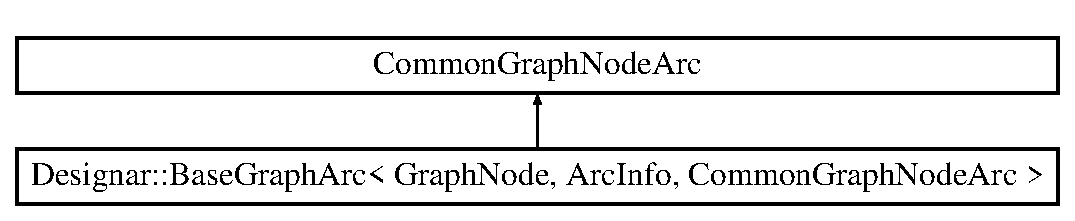
\includegraphics[height=2.000000cm]{class_designar_1_1_base_graph_arc}
\end{center}
\end{figure}
\subsection*{Public Member Functions}
\begin{DoxyCompactItemize}
\item 
\hyperlink{class_designar_1_1_graph_node}{Graph\+Node} \& \hyperlink{class_designar_1_1_base_graph_arc_ae5bf587f363169ac3cf0de8808410476}{get\+\_\+src\+\_\+node} ()
\item 
const \hyperlink{class_designar_1_1_graph_node}{Graph\+Node} \& \hyperlink{class_designar_1_1_base_graph_arc_abf7c4174301f972969bc11e9154a353a}{get\+\_\+src\+\_\+node} () const
\item 
\hyperlink{class_designar_1_1_graph_node}{Graph\+Node} \& \hyperlink{class_designar_1_1_base_graph_arc_a2fe944d9d98fd2451d0c82fa0e805bce}{get\+\_\+tgt\+\_\+node} ()
\item 
const \hyperlink{class_designar_1_1_graph_node}{Graph\+Node} \& \hyperlink{class_designar_1_1_base_graph_arc_aecf3b0b06c1019563d433d44e922775b}{get\+\_\+tgt\+\_\+node} () const
\item 
\hyperlink{class_designar_1_1_graph_node}{Graph\+Node} \& \hyperlink{class_designar_1_1_base_graph_arc_a756bd68ff9797ff54b53657c2a39730c}{get\+\_\+connected\+\_\+node} (\hyperlink{class_designar_1_1_graph_node}{Graph\+Node} \&node)
\item 
const \hyperlink{class_designar_1_1_graph_node}{Graph\+Node} \& \hyperlink{class_designar_1_1_base_graph_arc_a5e8a913b9632b653908d054a7e277d7a}{get\+\_\+connected\+\_\+node} (\hyperlink{class_designar_1_1_graph_node}{Graph\+Node} \&node) const
\item 
Arc\+Info \& \hyperlink{class_designar_1_1_base_graph_arc_a90c613c982dec0d38acd6051c26a5562}{get\+\_\+info} ()
\item 
const Arc\+Info \& \hyperlink{class_designar_1_1_base_graph_arc_a90dce6365bbeef65a6ff5fa343b27710}{get\+\_\+info} () const
\end{DoxyCompactItemize}
\subsection*{Protected Member Functions}
\begin{DoxyCompactItemize}
\item 
\hyperlink{class_designar_1_1_base_graph_arc_ab68bc29411653f2d8b12d3ccc5efc1e7}{Base\+Graph\+Arc} ()
\item 
\hyperlink{class_designar_1_1_base_graph_arc_a1a789ba5e3fdb980a066bb56aa258681}{Base\+Graph\+Arc} (\hyperlink{class_designar_1_1_graph_node}{Graph\+Node} $\ast$src, \hyperlink{class_designar_1_1_graph_node}{Graph\+Node} $\ast$tgt)
\item 
\hyperlink{class_designar_1_1_base_graph_arc_a013c1af0c1aadf28260b33585308f7ac}{Base\+Graph\+Arc} (\hyperlink{class_designar_1_1_graph_node}{Graph\+Node} $\ast$src, \hyperlink{class_designar_1_1_graph_node}{Graph\+Node} $\ast$tgt, const Arc\+Info \&\+\_\+info)
\item 
\hyperlink{class_designar_1_1_base_graph_arc_a150cb81ef3f2baac1abee99adae6f410}{Base\+Graph\+Arc} (\hyperlink{class_designar_1_1_graph_node}{Graph\+Node} $\ast$src, \hyperlink{class_designar_1_1_graph_node}{Graph\+Node} $\ast$tgt, Arc\+Info \&\&\+\_\+info)
\end{DoxyCompactItemize}
\subsection*{Protected Attributes}
\begin{DoxyCompactItemize}
\item 
\hyperlink{class_designar_1_1_graph_node}{Graph\+Node} $\ast$ \hyperlink{class_designar_1_1_base_graph_arc_a3d62765087127c26045bfae7a3c5f6f8}{src\+\_\+node}
\item 
\hyperlink{class_designar_1_1_graph_node}{Graph\+Node} $\ast$ \hyperlink{class_designar_1_1_base_graph_arc_af09ee39743d9a2e6f7bad479d925c273}{tgt\+\_\+node}
\item 
Arc\+Info \hyperlink{class_designar_1_1_base_graph_arc_a8aacc596a2fbca49cc927d6eaac595aa}{info}
\end{DoxyCompactItemize}


\subsection{Detailed Description}
\subsubsection*{template$<$class Graph\+Node, typename Arc\+Info, class Common\+Graph\+Node\+Arc$>$\newline
class Designar\+::\+Base\+Graph\+Arc$<$ Graph\+Node, Arc\+Info, Common\+Graph\+Node\+Arc $>$}



Definition at line 1044 of file nodesdef.\+H.



\subsection{Constructor \& Destructor Documentation}
\mbox{\Hypertarget{class_designar_1_1_base_graph_arc_ab68bc29411653f2d8b12d3ccc5efc1e7}\label{class_designar_1_1_base_graph_arc_ab68bc29411653f2d8b12d3ccc5efc1e7}} 
\index{Designar\+::\+Base\+Graph\+Arc@{Designar\+::\+Base\+Graph\+Arc}!Base\+Graph\+Arc@{Base\+Graph\+Arc}}
\index{Base\+Graph\+Arc@{Base\+Graph\+Arc}!Designar\+::\+Base\+Graph\+Arc@{Designar\+::\+Base\+Graph\+Arc}}
\subsubsection{\texorpdfstring{Base\+Graph\+Arc()}{BaseGraphArc()}\hspace{0.1cm}{\footnotesize\ttfamily [1/4]}}
{\footnotesize\ttfamily template$<$class Graph\+Node, typename Arc\+Info, class Common\+Graph\+Node\+Arc$>$ \\
\hyperlink{class_designar_1_1_base_graph_arc}{Designar\+::\+Base\+Graph\+Arc}$<$ \hyperlink{class_designar_1_1_graph_node}{Graph\+Node}, Arc\+Info, Common\+Graph\+Node\+Arc $>$\+::\hyperlink{class_designar_1_1_base_graph_arc}{Base\+Graph\+Arc} (\begin{DoxyParamCaption}{ }\end{DoxyParamCaption})\hspace{0.3cm}{\ttfamily [inline]}, {\ttfamily [protected]}}



Definition at line 1051 of file nodesdef.\+H.

\mbox{\Hypertarget{class_designar_1_1_base_graph_arc_a1a789ba5e3fdb980a066bb56aa258681}\label{class_designar_1_1_base_graph_arc_a1a789ba5e3fdb980a066bb56aa258681}} 
\index{Designar\+::\+Base\+Graph\+Arc@{Designar\+::\+Base\+Graph\+Arc}!Base\+Graph\+Arc@{Base\+Graph\+Arc}}
\index{Base\+Graph\+Arc@{Base\+Graph\+Arc}!Designar\+::\+Base\+Graph\+Arc@{Designar\+::\+Base\+Graph\+Arc}}
\subsubsection{\texorpdfstring{Base\+Graph\+Arc()}{BaseGraphArc()}\hspace{0.1cm}{\footnotesize\ttfamily [2/4]}}
{\footnotesize\ttfamily template$<$class Graph\+Node, typename Arc\+Info, class Common\+Graph\+Node\+Arc$>$ \\
\hyperlink{class_designar_1_1_base_graph_arc}{Designar\+::\+Base\+Graph\+Arc}$<$ \hyperlink{class_designar_1_1_graph_node}{Graph\+Node}, Arc\+Info, Common\+Graph\+Node\+Arc $>$\+::\hyperlink{class_designar_1_1_base_graph_arc}{Base\+Graph\+Arc} (\begin{DoxyParamCaption}\item[{\hyperlink{class_designar_1_1_graph_node}{Graph\+Node} $\ast$}]{src,  }\item[{\hyperlink{class_designar_1_1_graph_node}{Graph\+Node} $\ast$}]{tgt }\end{DoxyParamCaption})\hspace{0.3cm}{\ttfamily [inline]}, {\ttfamily [protected]}}



Definition at line 1057 of file nodesdef.\+H.

\mbox{\Hypertarget{class_designar_1_1_base_graph_arc_a013c1af0c1aadf28260b33585308f7ac}\label{class_designar_1_1_base_graph_arc_a013c1af0c1aadf28260b33585308f7ac}} 
\index{Designar\+::\+Base\+Graph\+Arc@{Designar\+::\+Base\+Graph\+Arc}!Base\+Graph\+Arc@{Base\+Graph\+Arc}}
\index{Base\+Graph\+Arc@{Base\+Graph\+Arc}!Designar\+::\+Base\+Graph\+Arc@{Designar\+::\+Base\+Graph\+Arc}}
\subsubsection{\texorpdfstring{Base\+Graph\+Arc()}{BaseGraphArc()}\hspace{0.1cm}{\footnotesize\ttfamily [3/4]}}
{\footnotesize\ttfamily template$<$class Graph\+Node, typename Arc\+Info, class Common\+Graph\+Node\+Arc$>$ \\
\hyperlink{class_designar_1_1_base_graph_arc}{Designar\+::\+Base\+Graph\+Arc}$<$ \hyperlink{class_designar_1_1_graph_node}{Graph\+Node}, Arc\+Info, Common\+Graph\+Node\+Arc $>$\+::\hyperlink{class_designar_1_1_base_graph_arc}{Base\+Graph\+Arc} (\begin{DoxyParamCaption}\item[{\hyperlink{class_designar_1_1_graph_node}{Graph\+Node} $\ast$}]{src,  }\item[{\hyperlink{class_designar_1_1_graph_node}{Graph\+Node} $\ast$}]{tgt,  }\item[{const Arc\+Info \&}]{\+\_\+info }\end{DoxyParamCaption})\hspace{0.3cm}{\ttfamily [inline]}, {\ttfamily [protected]}}



Definition at line 1063 of file nodesdef.\+H.

\mbox{\Hypertarget{class_designar_1_1_base_graph_arc_a150cb81ef3f2baac1abee99adae6f410}\label{class_designar_1_1_base_graph_arc_a150cb81ef3f2baac1abee99adae6f410}} 
\index{Designar\+::\+Base\+Graph\+Arc@{Designar\+::\+Base\+Graph\+Arc}!Base\+Graph\+Arc@{Base\+Graph\+Arc}}
\index{Base\+Graph\+Arc@{Base\+Graph\+Arc}!Designar\+::\+Base\+Graph\+Arc@{Designar\+::\+Base\+Graph\+Arc}}
\subsubsection{\texorpdfstring{Base\+Graph\+Arc()}{BaseGraphArc()}\hspace{0.1cm}{\footnotesize\ttfamily [4/4]}}
{\footnotesize\ttfamily template$<$class Graph\+Node, typename Arc\+Info, class Common\+Graph\+Node\+Arc$>$ \\
\hyperlink{class_designar_1_1_base_graph_arc}{Designar\+::\+Base\+Graph\+Arc}$<$ \hyperlink{class_designar_1_1_graph_node}{Graph\+Node}, Arc\+Info, Common\+Graph\+Node\+Arc $>$\+::\hyperlink{class_designar_1_1_base_graph_arc}{Base\+Graph\+Arc} (\begin{DoxyParamCaption}\item[{\hyperlink{class_designar_1_1_graph_node}{Graph\+Node} $\ast$}]{src,  }\item[{\hyperlink{class_designar_1_1_graph_node}{Graph\+Node} $\ast$}]{tgt,  }\item[{Arc\+Info \&\&}]{\+\_\+info }\end{DoxyParamCaption})\hspace{0.3cm}{\ttfamily [inline]}, {\ttfamily [protected]}}



Definition at line 1069 of file nodesdef.\+H.



\subsection{Member Function Documentation}
\mbox{\Hypertarget{class_designar_1_1_base_graph_arc_a756bd68ff9797ff54b53657c2a39730c}\label{class_designar_1_1_base_graph_arc_a756bd68ff9797ff54b53657c2a39730c}} 
\index{Designar\+::\+Base\+Graph\+Arc@{Designar\+::\+Base\+Graph\+Arc}!get\+\_\+connected\+\_\+node@{get\+\_\+connected\+\_\+node}}
\index{get\+\_\+connected\+\_\+node@{get\+\_\+connected\+\_\+node}!Designar\+::\+Base\+Graph\+Arc@{Designar\+::\+Base\+Graph\+Arc}}
\subsubsection{\texorpdfstring{get\+\_\+connected\+\_\+node()}{get\_connected\_node()}\hspace{0.1cm}{\footnotesize\ttfamily [1/2]}}
{\footnotesize\ttfamily template$<$class Graph\+Node, typename Arc\+Info, class Common\+Graph\+Node\+Arc$>$ \\
\hyperlink{class_designar_1_1_graph_node}{Graph\+Node}\& \hyperlink{class_designar_1_1_base_graph_arc}{Designar\+::\+Base\+Graph\+Arc}$<$ \hyperlink{class_designar_1_1_graph_node}{Graph\+Node}, Arc\+Info, Common\+Graph\+Node\+Arc $>$\+::get\+\_\+connected\+\_\+node (\begin{DoxyParamCaption}\item[{\hyperlink{class_designar_1_1_graph_node}{Graph\+Node} \&}]{node }\end{DoxyParamCaption})\hspace{0.3cm}{\ttfamily [inline]}}



Definition at line 1096 of file nodesdef.\+H.

\mbox{\Hypertarget{class_designar_1_1_base_graph_arc_a5e8a913b9632b653908d054a7e277d7a}\label{class_designar_1_1_base_graph_arc_a5e8a913b9632b653908d054a7e277d7a}} 
\index{Designar\+::\+Base\+Graph\+Arc@{Designar\+::\+Base\+Graph\+Arc}!get\+\_\+connected\+\_\+node@{get\+\_\+connected\+\_\+node}}
\index{get\+\_\+connected\+\_\+node@{get\+\_\+connected\+\_\+node}!Designar\+::\+Base\+Graph\+Arc@{Designar\+::\+Base\+Graph\+Arc}}
\subsubsection{\texorpdfstring{get\+\_\+connected\+\_\+node()}{get\_connected\_node()}\hspace{0.1cm}{\footnotesize\ttfamily [2/2]}}
{\footnotesize\ttfamily template$<$class Graph\+Node, typename Arc\+Info, class Common\+Graph\+Node\+Arc$>$ \\
const \hyperlink{class_designar_1_1_graph_node}{Graph\+Node}\& \hyperlink{class_designar_1_1_base_graph_arc}{Designar\+::\+Base\+Graph\+Arc}$<$ \hyperlink{class_designar_1_1_graph_node}{Graph\+Node}, Arc\+Info, Common\+Graph\+Node\+Arc $>$\+::get\+\_\+connected\+\_\+node (\begin{DoxyParamCaption}\item[{\hyperlink{class_designar_1_1_graph_node}{Graph\+Node} \&}]{node }\end{DoxyParamCaption}) const\hspace{0.3cm}{\ttfamily [inline]}}



Definition at line 1107 of file nodesdef.\+H.

\mbox{\Hypertarget{class_designar_1_1_base_graph_arc_a90c613c982dec0d38acd6051c26a5562}\label{class_designar_1_1_base_graph_arc_a90c613c982dec0d38acd6051c26a5562}} 
\index{Designar\+::\+Base\+Graph\+Arc@{Designar\+::\+Base\+Graph\+Arc}!get\+\_\+info@{get\+\_\+info}}
\index{get\+\_\+info@{get\+\_\+info}!Designar\+::\+Base\+Graph\+Arc@{Designar\+::\+Base\+Graph\+Arc}}
\subsubsection{\texorpdfstring{get\+\_\+info()}{get\_info()}\hspace{0.1cm}{\footnotesize\ttfamily [1/2]}}
{\footnotesize\ttfamily template$<$class Graph\+Node, typename Arc\+Info, class Common\+Graph\+Node\+Arc$>$ \\
Arc\+Info\& \hyperlink{class_designar_1_1_base_graph_arc}{Designar\+::\+Base\+Graph\+Arc}$<$ \hyperlink{class_designar_1_1_graph_node}{Graph\+Node}, Arc\+Info, Common\+Graph\+Node\+Arc $>$\+::get\+\_\+info (\begin{DoxyParamCaption}{ }\end{DoxyParamCaption})\hspace{0.3cm}{\ttfamily [inline]}}



Definition at line 1118 of file nodesdef.\+H.

\mbox{\Hypertarget{class_designar_1_1_base_graph_arc_a90dce6365bbeef65a6ff5fa343b27710}\label{class_designar_1_1_base_graph_arc_a90dce6365bbeef65a6ff5fa343b27710}} 
\index{Designar\+::\+Base\+Graph\+Arc@{Designar\+::\+Base\+Graph\+Arc}!get\+\_\+info@{get\+\_\+info}}
\index{get\+\_\+info@{get\+\_\+info}!Designar\+::\+Base\+Graph\+Arc@{Designar\+::\+Base\+Graph\+Arc}}
\subsubsection{\texorpdfstring{get\+\_\+info()}{get\_info()}\hspace{0.1cm}{\footnotesize\ttfamily [2/2]}}
{\footnotesize\ttfamily template$<$class Graph\+Node, typename Arc\+Info, class Common\+Graph\+Node\+Arc$>$ \\
const Arc\+Info\& \hyperlink{class_designar_1_1_base_graph_arc}{Designar\+::\+Base\+Graph\+Arc}$<$ \hyperlink{class_designar_1_1_graph_node}{Graph\+Node}, Arc\+Info, Common\+Graph\+Node\+Arc $>$\+::get\+\_\+info (\begin{DoxyParamCaption}{ }\end{DoxyParamCaption}) const\hspace{0.3cm}{\ttfamily [inline]}}



Definition at line 1123 of file nodesdef.\+H.

\mbox{\Hypertarget{class_designar_1_1_base_graph_arc_ae5bf587f363169ac3cf0de8808410476}\label{class_designar_1_1_base_graph_arc_ae5bf587f363169ac3cf0de8808410476}} 
\index{Designar\+::\+Base\+Graph\+Arc@{Designar\+::\+Base\+Graph\+Arc}!get\+\_\+src\+\_\+node@{get\+\_\+src\+\_\+node}}
\index{get\+\_\+src\+\_\+node@{get\+\_\+src\+\_\+node}!Designar\+::\+Base\+Graph\+Arc@{Designar\+::\+Base\+Graph\+Arc}}
\subsubsection{\texorpdfstring{get\+\_\+src\+\_\+node()}{get\_src\_node()}\hspace{0.1cm}{\footnotesize\ttfamily [1/2]}}
{\footnotesize\ttfamily template$<$class Graph\+Node, typename Arc\+Info, class Common\+Graph\+Node\+Arc$>$ \\
\hyperlink{class_designar_1_1_graph_node}{Graph\+Node}\& \hyperlink{class_designar_1_1_base_graph_arc}{Designar\+::\+Base\+Graph\+Arc}$<$ \hyperlink{class_designar_1_1_graph_node}{Graph\+Node}, Arc\+Info, Common\+Graph\+Node\+Arc $>$\+::get\+\_\+src\+\_\+node (\begin{DoxyParamCaption}{ }\end{DoxyParamCaption})\hspace{0.3cm}{\ttfamily [inline]}}



Definition at line 1076 of file nodesdef.\+H.

\mbox{\Hypertarget{class_designar_1_1_base_graph_arc_abf7c4174301f972969bc11e9154a353a}\label{class_designar_1_1_base_graph_arc_abf7c4174301f972969bc11e9154a353a}} 
\index{Designar\+::\+Base\+Graph\+Arc@{Designar\+::\+Base\+Graph\+Arc}!get\+\_\+src\+\_\+node@{get\+\_\+src\+\_\+node}}
\index{get\+\_\+src\+\_\+node@{get\+\_\+src\+\_\+node}!Designar\+::\+Base\+Graph\+Arc@{Designar\+::\+Base\+Graph\+Arc}}
\subsubsection{\texorpdfstring{get\+\_\+src\+\_\+node()}{get\_src\_node()}\hspace{0.1cm}{\footnotesize\ttfamily [2/2]}}
{\footnotesize\ttfamily template$<$class Graph\+Node, typename Arc\+Info, class Common\+Graph\+Node\+Arc$>$ \\
const \hyperlink{class_designar_1_1_graph_node}{Graph\+Node}\& \hyperlink{class_designar_1_1_base_graph_arc}{Designar\+::\+Base\+Graph\+Arc}$<$ \hyperlink{class_designar_1_1_graph_node}{Graph\+Node}, Arc\+Info, Common\+Graph\+Node\+Arc $>$\+::get\+\_\+src\+\_\+node (\begin{DoxyParamCaption}{ }\end{DoxyParamCaption}) const\hspace{0.3cm}{\ttfamily [inline]}}



Definition at line 1081 of file nodesdef.\+H.

\mbox{\Hypertarget{class_designar_1_1_base_graph_arc_a2fe944d9d98fd2451d0c82fa0e805bce}\label{class_designar_1_1_base_graph_arc_a2fe944d9d98fd2451d0c82fa0e805bce}} 
\index{Designar\+::\+Base\+Graph\+Arc@{Designar\+::\+Base\+Graph\+Arc}!get\+\_\+tgt\+\_\+node@{get\+\_\+tgt\+\_\+node}}
\index{get\+\_\+tgt\+\_\+node@{get\+\_\+tgt\+\_\+node}!Designar\+::\+Base\+Graph\+Arc@{Designar\+::\+Base\+Graph\+Arc}}
\subsubsection{\texorpdfstring{get\+\_\+tgt\+\_\+node()}{get\_tgt\_node()}\hspace{0.1cm}{\footnotesize\ttfamily [1/2]}}
{\footnotesize\ttfamily template$<$class Graph\+Node, typename Arc\+Info, class Common\+Graph\+Node\+Arc$>$ \\
\hyperlink{class_designar_1_1_graph_node}{Graph\+Node}\& \hyperlink{class_designar_1_1_base_graph_arc}{Designar\+::\+Base\+Graph\+Arc}$<$ \hyperlink{class_designar_1_1_graph_node}{Graph\+Node}, Arc\+Info, Common\+Graph\+Node\+Arc $>$\+::get\+\_\+tgt\+\_\+node (\begin{DoxyParamCaption}{ }\end{DoxyParamCaption})\hspace{0.3cm}{\ttfamily [inline]}}



Definition at line 1086 of file nodesdef.\+H.

\mbox{\Hypertarget{class_designar_1_1_base_graph_arc_aecf3b0b06c1019563d433d44e922775b}\label{class_designar_1_1_base_graph_arc_aecf3b0b06c1019563d433d44e922775b}} 
\index{Designar\+::\+Base\+Graph\+Arc@{Designar\+::\+Base\+Graph\+Arc}!get\+\_\+tgt\+\_\+node@{get\+\_\+tgt\+\_\+node}}
\index{get\+\_\+tgt\+\_\+node@{get\+\_\+tgt\+\_\+node}!Designar\+::\+Base\+Graph\+Arc@{Designar\+::\+Base\+Graph\+Arc}}
\subsubsection{\texorpdfstring{get\+\_\+tgt\+\_\+node()}{get\_tgt\_node()}\hspace{0.1cm}{\footnotesize\ttfamily [2/2]}}
{\footnotesize\ttfamily template$<$class Graph\+Node, typename Arc\+Info, class Common\+Graph\+Node\+Arc$>$ \\
const \hyperlink{class_designar_1_1_graph_node}{Graph\+Node}\& \hyperlink{class_designar_1_1_base_graph_arc}{Designar\+::\+Base\+Graph\+Arc}$<$ \hyperlink{class_designar_1_1_graph_node}{Graph\+Node}, Arc\+Info, Common\+Graph\+Node\+Arc $>$\+::get\+\_\+tgt\+\_\+node (\begin{DoxyParamCaption}{ }\end{DoxyParamCaption}) const\hspace{0.3cm}{\ttfamily [inline]}}



Definition at line 1091 of file nodesdef.\+H.



\subsection{Member Data Documentation}
\mbox{\Hypertarget{class_designar_1_1_base_graph_arc_a8aacc596a2fbca49cc927d6eaac595aa}\label{class_designar_1_1_base_graph_arc_a8aacc596a2fbca49cc927d6eaac595aa}} 
\index{Designar\+::\+Base\+Graph\+Arc@{Designar\+::\+Base\+Graph\+Arc}!info@{info}}
\index{info@{info}!Designar\+::\+Base\+Graph\+Arc@{Designar\+::\+Base\+Graph\+Arc}}
\subsubsection{\texorpdfstring{info}{info}}
{\footnotesize\ttfamily template$<$class Graph\+Node, typename Arc\+Info, class Common\+Graph\+Node\+Arc$>$ \\
Arc\+Info \hyperlink{class_designar_1_1_base_graph_arc}{Designar\+::\+Base\+Graph\+Arc}$<$ \hyperlink{class_designar_1_1_graph_node}{Graph\+Node}, Arc\+Info, Common\+Graph\+Node\+Arc $>$\+::info\hspace{0.3cm}{\ttfamily [protected]}}



Definition at line 1049 of file nodesdef.\+H.

\mbox{\Hypertarget{class_designar_1_1_base_graph_arc_a3d62765087127c26045bfae7a3c5f6f8}\label{class_designar_1_1_base_graph_arc_a3d62765087127c26045bfae7a3c5f6f8}} 
\index{Designar\+::\+Base\+Graph\+Arc@{Designar\+::\+Base\+Graph\+Arc}!src\+\_\+node@{src\+\_\+node}}
\index{src\+\_\+node@{src\+\_\+node}!Designar\+::\+Base\+Graph\+Arc@{Designar\+::\+Base\+Graph\+Arc}}
\subsubsection{\texorpdfstring{src\+\_\+node}{src\_node}}
{\footnotesize\ttfamily template$<$class Graph\+Node, typename Arc\+Info, class Common\+Graph\+Node\+Arc$>$ \\
\hyperlink{class_designar_1_1_graph_node}{Graph\+Node}$\ast$ \hyperlink{class_designar_1_1_base_graph_arc}{Designar\+::\+Base\+Graph\+Arc}$<$ \hyperlink{class_designar_1_1_graph_node}{Graph\+Node}, Arc\+Info, Common\+Graph\+Node\+Arc $>$\+::src\+\_\+node\hspace{0.3cm}{\ttfamily [protected]}}



Definition at line 1047 of file nodesdef.\+H.

\mbox{\Hypertarget{class_designar_1_1_base_graph_arc_af09ee39743d9a2e6f7bad479d925c273}\label{class_designar_1_1_base_graph_arc_af09ee39743d9a2e6f7bad479d925c273}} 
\index{Designar\+::\+Base\+Graph\+Arc@{Designar\+::\+Base\+Graph\+Arc}!tgt\+\_\+node@{tgt\+\_\+node}}
\index{tgt\+\_\+node@{tgt\+\_\+node}!Designar\+::\+Base\+Graph\+Arc@{Designar\+::\+Base\+Graph\+Arc}}
\subsubsection{\texorpdfstring{tgt\+\_\+node}{tgt\_node}}
{\footnotesize\ttfamily template$<$class Graph\+Node, typename Arc\+Info, class Common\+Graph\+Node\+Arc$>$ \\
\hyperlink{class_designar_1_1_graph_node}{Graph\+Node}$\ast$ \hyperlink{class_designar_1_1_base_graph_arc}{Designar\+::\+Base\+Graph\+Arc}$<$ \hyperlink{class_designar_1_1_graph_node}{Graph\+Node}, Arc\+Info, Common\+Graph\+Node\+Arc $>$\+::tgt\+\_\+node\hspace{0.3cm}{\ttfamily [protected]}}



Definition at line 1048 of file nodesdef.\+H.



The documentation for this class was generated from the following file\+:\begin{DoxyCompactItemize}
\item 
De\+Si\+G\+N\+A\+R/include/\hyperlink{nodesdef_8_h}{nodesdef.\+H}\end{DoxyCompactItemize}

\hypertarget{class_designar_1_1_base_graph_node}{}\section{Designar\+:\+:Base\+Graph\+Node$<$ Node\+Info, Common\+Graph\+Node\+Arc $>$ Class Template Reference}
\label{class_designar_1_1_base_graph_node}\index{Designar\+::\+Base\+Graph\+Node$<$ Node\+Info, Common\+Graph\+Node\+Arc $>$@{Designar\+::\+Base\+Graph\+Node$<$ Node\+Info, Common\+Graph\+Node\+Arc $>$}}


{\ttfamily \#include $<$nodesdef.\+H$>$}

Inheritance diagram for Designar\+:\+:Base\+Graph\+Node$<$ Node\+Info, Common\+Graph\+Node\+Arc $>$\+:\begin{figure}[H]
\begin{center}
\leavevmode
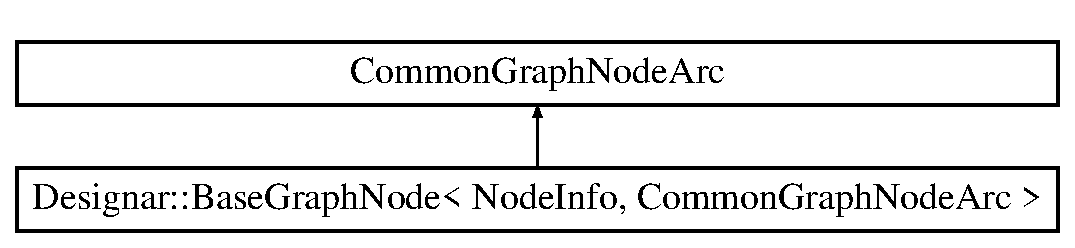
\includegraphics[height=2.000000cm]{class_designar_1_1_base_graph_node}
\end{center}
\end{figure}
\subsection*{Public Member Functions}
\begin{DoxyCompactItemize}
\item 
Node\+Info \& \hyperlink{class_designar_1_1_base_graph_node_a5626bf91fcef0dd6f29dc503c33ecfc9}{get\+\_\+info} ()
\item 
const Node\+Info \& \hyperlink{class_designar_1_1_base_graph_node_a2f9f7069df485bc555066eb57d05e7a8}{get\+\_\+info} () const
\item 
\hyperlink{namespace_designar_aa72662848b9f4815e7bf31a7cf3e33d1}{nat\+\_\+t} \hyperlink{class_designar_1_1_base_graph_node_a3dbfd6cc251093522f54d51956968c54}{get\+\_\+num\+\_\+arcs} () const
\end{DoxyCompactItemize}
\subsection*{Protected Member Functions}
\begin{DoxyCompactItemize}
\item 
\hyperlink{class_designar_1_1_base_graph_node_a6eb12fac0ce731cb881c31b095493ef5}{Base\+Graph\+Node} ()
\item 
\hyperlink{class_designar_1_1_base_graph_node_ada20ee8b29e8372f93b7deb6a93c2be1}{Base\+Graph\+Node} (const Node\+Info \&\+\_\+info)
\item 
\hyperlink{class_designar_1_1_base_graph_node_a3e36c23ee7f22345b2ebbad09304dca0}{Base\+Graph\+Node} (Node\+Info \&\&\+\_\+info)
\item 
\hyperlink{class_designar_1_1_base_graph_node_aa64ba400e5d1fff18b7fb10071e7b97c}{Base\+Graph\+Node} (\hyperlink{class_designar_1_1_base_graph_node}{Base\+Graph\+Node} $\ast$ptr)
\end{DoxyCompactItemize}
\subsection*{Protected Attributes}
\begin{DoxyCompactItemize}
\item 
Node\+Info \hyperlink{class_designar_1_1_base_graph_node_a78196723c561b3554cf8760ab2d902a8}{info}
\item 
\hyperlink{namespace_designar_aa72662848b9f4815e7bf31a7cf3e33d1}{nat\+\_\+t} \hyperlink{class_designar_1_1_base_graph_node_a035347b8e1ffaca5df73b42bef300e0f}{num\+\_\+arcs}
\item 
\hyperlink{class_designar_1_1_d_l}{DL} \hyperlink{class_designar_1_1_base_graph_node_a160dab27497d195ecdf93272a40a2cb5}{adjacent\+\_\+arc\+\_\+list}
\end{DoxyCompactItemize}


\subsection{Detailed Description}
\subsubsection*{template$<$typename Node\+Info, class Common\+Graph\+Node\+Arc$>$\newline
class Designar\+::\+Base\+Graph\+Node$<$ Node\+Info, Common\+Graph\+Node\+Arc $>$}



Definition at line 994 of file nodesdef.\+H.



\subsection{Constructor \& Destructor Documentation}
\mbox{\Hypertarget{class_designar_1_1_base_graph_node_a6eb12fac0ce731cb881c31b095493ef5}\label{class_designar_1_1_base_graph_node_a6eb12fac0ce731cb881c31b095493ef5}} 
\index{Designar\+::\+Base\+Graph\+Node@{Designar\+::\+Base\+Graph\+Node}!Base\+Graph\+Node@{Base\+Graph\+Node}}
\index{Base\+Graph\+Node@{Base\+Graph\+Node}!Designar\+::\+Base\+Graph\+Node@{Designar\+::\+Base\+Graph\+Node}}
\subsubsection{\texorpdfstring{Base\+Graph\+Node()}{BaseGraphNode()}\hspace{0.1cm}{\footnotesize\ttfamily [1/4]}}
{\footnotesize\ttfamily template$<$typename Node\+Info, class Common\+Graph\+Node\+Arc$>$ \\
\hyperlink{class_designar_1_1_base_graph_node}{Designar\+::\+Base\+Graph\+Node}$<$ Node\+Info, Common\+Graph\+Node\+Arc $>$\+::\hyperlink{class_designar_1_1_base_graph_node}{Base\+Graph\+Node} (\begin{DoxyParamCaption}{ }\end{DoxyParamCaption})\hspace{0.3cm}{\ttfamily [inline]}, {\ttfamily [protected]}}



Definition at line 1001 of file nodesdef.\+H.

\mbox{\Hypertarget{class_designar_1_1_base_graph_node_ada20ee8b29e8372f93b7deb6a93c2be1}\label{class_designar_1_1_base_graph_node_ada20ee8b29e8372f93b7deb6a93c2be1}} 
\index{Designar\+::\+Base\+Graph\+Node@{Designar\+::\+Base\+Graph\+Node}!Base\+Graph\+Node@{Base\+Graph\+Node}}
\index{Base\+Graph\+Node@{Base\+Graph\+Node}!Designar\+::\+Base\+Graph\+Node@{Designar\+::\+Base\+Graph\+Node}}
\subsubsection{\texorpdfstring{Base\+Graph\+Node()}{BaseGraphNode()}\hspace{0.1cm}{\footnotesize\ttfamily [2/4]}}
{\footnotesize\ttfamily template$<$typename Node\+Info, class Common\+Graph\+Node\+Arc$>$ \\
\hyperlink{class_designar_1_1_base_graph_node}{Designar\+::\+Base\+Graph\+Node}$<$ Node\+Info, Common\+Graph\+Node\+Arc $>$\+::\hyperlink{class_designar_1_1_base_graph_node}{Base\+Graph\+Node} (\begin{DoxyParamCaption}\item[{const Node\+Info \&}]{\+\_\+info }\end{DoxyParamCaption})\hspace{0.3cm}{\ttfamily [inline]}, {\ttfamily [protected]}}



Definition at line 1007 of file nodesdef.\+H.

\mbox{\Hypertarget{class_designar_1_1_base_graph_node_a3e36c23ee7f22345b2ebbad09304dca0}\label{class_designar_1_1_base_graph_node_a3e36c23ee7f22345b2ebbad09304dca0}} 
\index{Designar\+::\+Base\+Graph\+Node@{Designar\+::\+Base\+Graph\+Node}!Base\+Graph\+Node@{Base\+Graph\+Node}}
\index{Base\+Graph\+Node@{Base\+Graph\+Node}!Designar\+::\+Base\+Graph\+Node@{Designar\+::\+Base\+Graph\+Node}}
\subsubsection{\texorpdfstring{Base\+Graph\+Node()}{BaseGraphNode()}\hspace{0.1cm}{\footnotesize\ttfamily [3/4]}}
{\footnotesize\ttfamily template$<$typename Node\+Info, class Common\+Graph\+Node\+Arc$>$ \\
\hyperlink{class_designar_1_1_base_graph_node}{Designar\+::\+Base\+Graph\+Node}$<$ Node\+Info, Common\+Graph\+Node\+Arc $>$\+::\hyperlink{class_designar_1_1_base_graph_node}{Base\+Graph\+Node} (\begin{DoxyParamCaption}\item[{Node\+Info \&\&}]{\+\_\+info }\end{DoxyParamCaption})\hspace{0.3cm}{\ttfamily [inline]}, {\ttfamily [protected]}}



Definition at line 1013 of file nodesdef.\+H.

\mbox{\Hypertarget{class_designar_1_1_base_graph_node_aa64ba400e5d1fff18b7fb10071e7b97c}\label{class_designar_1_1_base_graph_node_aa64ba400e5d1fff18b7fb10071e7b97c}} 
\index{Designar\+::\+Base\+Graph\+Node@{Designar\+::\+Base\+Graph\+Node}!Base\+Graph\+Node@{Base\+Graph\+Node}}
\index{Base\+Graph\+Node@{Base\+Graph\+Node}!Designar\+::\+Base\+Graph\+Node@{Designar\+::\+Base\+Graph\+Node}}
\subsubsection{\texorpdfstring{Base\+Graph\+Node()}{BaseGraphNode()}\hspace{0.1cm}{\footnotesize\ttfamily [4/4]}}
{\footnotesize\ttfamily template$<$typename Node\+Info, class Common\+Graph\+Node\+Arc$>$ \\
\hyperlink{class_designar_1_1_base_graph_node}{Designar\+::\+Base\+Graph\+Node}$<$ Node\+Info, Common\+Graph\+Node\+Arc $>$\+::\hyperlink{class_designar_1_1_base_graph_node}{Base\+Graph\+Node} (\begin{DoxyParamCaption}\item[{\hyperlink{class_designar_1_1_base_graph_node}{Base\+Graph\+Node}$<$ Node\+Info, Common\+Graph\+Node\+Arc $>$ $\ast$}]{ptr }\end{DoxyParamCaption})\hspace{0.3cm}{\ttfamily [inline]}, {\ttfamily [protected]}}



Definition at line 1020 of file nodesdef.\+H.



\subsection{Member Function Documentation}
\mbox{\Hypertarget{class_designar_1_1_base_graph_node_a5626bf91fcef0dd6f29dc503c33ecfc9}\label{class_designar_1_1_base_graph_node_a5626bf91fcef0dd6f29dc503c33ecfc9}} 
\index{Designar\+::\+Base\+Graph\+Node@{Designar\+::\+Base\+Graph\+Node}!get\+\_\+info@{get\+\_\+info}}
\index{get\+\_\+info@{get\+\_\+info}!Designar\+::\+Base\+Graph\+Node@{Designar\+::\+Base\+Graph\+Node}}
\subsubsection{\texorpdfstring{get\+\_\+info()}{get\_info()}\hspace{0.1cm}{\footnotesize\ttfamily [1/2]}}
{\footnotesize\ttfamily template$<$typename Node\+Info, class Common\+Graph\+Node\+Arc$>$ \\
Node\+Info\& \hyperlink{class_designar_1_1_base_graph_node}{Designar\+::\+Base\+Graph\+Node}$<$ Node\+Info, Common\+Graph\+Node\+Arc $>$\+::get\+\_\+info (\begin{DoxyParamCaption}{ }\end{DoxyParamCaption})\hspace{0.3cm}{\ttfamily [inline]}}



Definition at line 1027 of file nodesdef.\+H.

\mbox{\Hypertarget{class_designar_1_1_base_graph_node_a2f9f7069df485bc555066eb57d05e7a8}\label{class_designar_1_1_base_graph_node_a2f9f7069df485bc555066eb57d05e7a8}} 
\index{Designar\+::\+Base\+Graph\+Node@{Designar\+::\+Base\+Graph\+Node}!get\+\_\+info@{get\+\_\+info}}
\index{get\+\_\+info@{get\+\_\+info}!Designar\+::\+Base\+Graph\+Node@{Designar\+::\+Base\+Graph\+Node}}
\subsubsection{\texorpdfstring{get\+\_\+info()}{get\_info()}\hspace{0.1cm}{\footnotesize\ttfamily [2/2]}}
{\footnotesize\ttfamily template$<$typename Node\+Info, class Common\+Graph\+Node\+Arc$>$ \\
const Node\+Info\& \hyperlink{class_designar_1_1_base_graph_node}{Designar\+::\+Base\+Graph\+Node}$<$ Node\+Info, Common\+Graph\+Node\+Arc $>$\+::get\+\_\+info (\begin{DoxyParamCaption}{ }\end{DoxyParamCaption}) const\hspace{0.3cm}{\ttfamily [inline]}}



Definition at line 1032 of file nodesdef.\+H.

\mbox{\Hypertarget{class_designar_1_1_base_graph_node_a3dbfd6cc251093522f54d51956968c54}\label{class_designar_1_1_base_graph_node_a3dbfd6cc251093522f54d51956968c54}} 
\index{Designar\+::\+Base\+Graph\+Node@{Designar\+::\+Base\+Graph\+Node}!get\+\_\+num\+\_\+arcs@{get\+\_\+num\+\_\+arcs}}
\index{get\+\_\+num\+\_\+arcs@{get\+\_\+num\+\_\+arcs}!Designar\+::\+Base\+Graph\+Node@{Designar\+::\+Base\+Graph\+Node}}
\subsubsection{\texorpdfstring{get\+\_\+num\+\_\+arcs()}{get\_num\_arcs()}}
{\footnotesize\ttfamily template$<$typename Node\+Info, class Common\+Graph\+Node\+Arc$>$ \\
\hyperlink{namespace_designar_aa72662848b9f4815e7bf31a7cf3e33d1}{nat\+\_\+t} \hyperlink{class_designar_1_1_base_graph_node}{Designar\+::\+Base\+Graph\+Node}$<$ Node\+Info, Common\+Graph\+Node\+Arc $>$\+::get\+\_\+num\+\_\+arcs (\begin{DoxyParamCaption}{ }\end{DoxyParamCaption}) const\hspace{0.3cm}{\ttfamily [inline]}}



Definition at line 1037 of file nodesdef.\+H.



\subsection{Member Data Documentation}
\mbox{\Hypertarget{class_designar_1_1_base_graph_node_a160dab27497d195ecdf93272a40a2cb5}\label{class_designar_1_1_base_graph_node_a160dab27497d195ecdf93272a40a2cb5}} 
\index{Designar\+::\+Base\+Graph\+Node@{Designar\+::\+Base\+Graph\+Node}!adjacent\+\_\+arc\+\_\+list@{adjacent\+\_\+arc\+\_\+list}}
\index{adjacent\+\_\+arc\+\_\+list@{adjacent\+\_\+arc\+\_\+list}!Designar\+::\+Base\+Graph\+Node@{Designar\+::\+Base\+Graph\+Node}}
\subsubsection{\texorpdfstring{adjacent\+\_\+arc\+\_\+list}{adjacent\_arc\_list}}
{\footnotesize\ttfamily template$<$typename Node\+Info, class Common\+Graph\+Node\+Arc$>$ \\
\hyperlink{class_designar_1_1_d_l}{DL} \hyperlink{class_designar_1_1_base_graph_node}{Designar\+::\+Base\+Graph\+Node}$<$ Node\+Info, Common\+Graph\+Node\+Arc $>$\+::adjacent\+\_\+arc\+\_\+list\hspace{0.3cm}{\ttfamily [protected]}}



Definition at line 999 of file nodesdef.\+H.

\mbox{\Hypertarget{class_designar_1_1_base_graph_node_a78196723c561b3554cf8760ab2d902a8}\label{class_designar_1_1_base_graph_node_a78196723c561b3554cf8760ab2d902a8}} 
\index{Designar\+::\+Base\+Graph\+Node@{Designar\+::\+Base\+Graph\+Node}!info@{info}}
\index{info@{info}!Designar\+::\+Base\+Graph\+Node@{Designar\+::\+Base\+Graph\+Node}}
\subsubsection{\texorpdfstring{info}{info}}
{\footnotesize\ttfamily template$<$typename Node\+Info, class Common\+Graph\+Node\+Arc$>$ \\
Node\+Info \hyperlink{class_designar_1_1_base_graph_node}{Designar\+::\+Base\+Graph\+Node}$<$ Node\+Info, Common\+Graph\+Node\+Arc $>$\+::info\hspace{0.3cm}{\ttfamily [protected]}}



Definition at line 997 of file nodesdef.\+H.

\mbox{\Hypertarget{class_designar_1_1_base_graph_node_a035347b8e1ffaca5df73b42bef300e0f}\label{class_designar_1_1_base_graph_node_a035347b8e1ffaca5df73b42bef300e0f}} 
\index{Designar\+::\+Base\+Graph\+Node@{Designar\+::\+Base\+Graph\+Node}!num\+\_\+arcs@{num\+\_\+arcs}}
\index{num\+\_\+arcs@{num\+\_\+arcs}!Designar\+::\+Base\+Graph\+Node@{Designar\+::\+Base\+Graph\+Node}}
\subsubsection{\texorpdfstring{num\+\_\+arcs}{num\_arcs}}
{\footnotesize\ttfamily template$<$typename Node\+Info, class Common\+Graph\+Node\+Arc$>$ \\
\hyperlink{namespace_designar_aa72662848b9f4815e7bf31a7cf3e33d1}{nat\+\_\+t} \hyperlink{class_designar_1_1_base_graph_node}{Designar\+::\+Base\+Graph\+Node}$<$ Node\+Info, Common\+Graph\+Node\+Arc $>$\+::num\+\_\+arcs\hspace{0.3cm}{\ttfamily [protected]}}



Definition at line 998 of file nodesdef.\+H.



The documentation for this class was generated from the following file\+:\begin{DoxyCompactItemize}
\item 
include/\hyperlink{nodesdef_8_h}{nodesdef.\+H}\end{DoxyCompactItemize}

\hypertarget{class_designar_1_1_basic_iterator}{}\section{Designar\+:\+:Basic\+Iterator$<$ Iterator, T, R\+E\+T\+\_\+\+C\+PY $>$ Class Template Reference}
\label{class_designar_1_1_basic_iterator}\index{Designar\+::\+Basic\+Iterator$<$ Iterator, T, R\+E\+T\+\_\+\+C\+P\+Y $>$@{Designar\+::\+Basic\+Iterator$<$ Iterator, T, R\+E\+T\+\_\+\+C\+P\+Y $>$}}


{\ttfamily \#include $<$iterator.\+H$>$}

Inheritance diagram for Designar\+:\+:Basic\+Iterator$<$ Iterator, T, R\+E\+T\+\_\+\+C\+PY $>$\+:\begin{figure}[H]
\begin{center}
\leavevmode
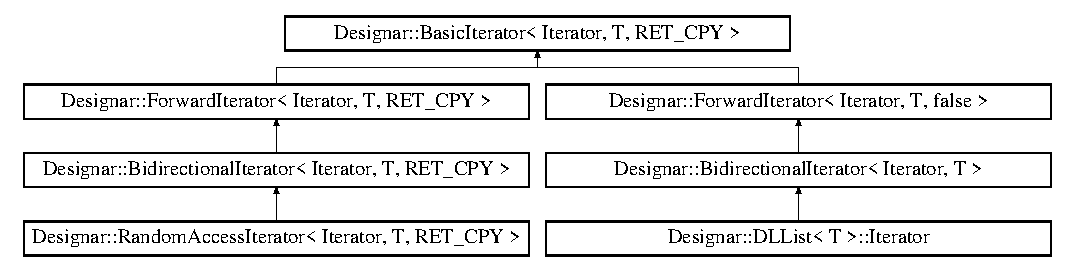
\includegraphics[height=3.209169cm]{class_designar_1_1_basic_iterator}
\end{center}
\end{figure}
\subsection*{Public Member Functions}
\begin{DoxyCompactItemize}
\item 
\hyperlink{namespace_designar_ab937f9c4bf5f1d0e65dbc616245d50ee}{Ret\+Type}$<$ R\+E\+T\+\_\+\+C\+PY, T, T \& $>$ \hyperlink{class_designar_1_1_basic_iterator_aed614b1aca7f9cb1552699b106bb281f}{operator$\ast$} ()
\item 
const \hyperlink{namespace_designar_ab937f9c4bf5f1d0e65dbc616245d50ee}{Ret\+Type}$<$ R\+E\+T\+\_\+\+C\+PY, T, T \& $>$ \hyperlink{class_designar_1_1_basic_iterator_aa016cf79d8fd6b3e9f73c3dbbbaf7a31}{operator$\ast$} () const
\item 
T $\ast$ \hyperlink{class_designar_1_1_basic_iterator_ac87226512fbbe7c524cc0be8ae2ee914}{operator-\/$>$} ()
\item 
bool \hyperlink{class_designar_1_1_basic_iterator_abaca601c4d1d4ff27429426437abbf02}{operator==} (const Iterator \&it) const
\item 
bool \hyperlink{class_designar_1_1_basic_iterator_aea51bca6ffed62c081aefbcb804a21f1}{operator!=} (const Iterator \&it) const
\end{DoxyCompactItemize}
\subsection*{Protected Member Functions}
\begin{DoxyCompactItemize}
\item 
Iterator \& \hyperlink{class_designar_1_1_basic_iterator_a5b550cbd8bb7ee464e8cdb6b023c437a}{me} ()
\item 
const Iterator \& \hyperlink{class_designar_1_1_basic_iterator_a7ccea1264814695d7c9466daa713cb17}{const\+\_\+me} () const
\end{DoxyCompactItemize}


\subsection{Detailed Description}
\subsubsection*{template$<$class Iterator, typename T, bool R\+E\+T\+\_\+\+C\+PY = false$>$\newline
class Designar\+::\+Basic\+Iterator$<$ Iterator, T, R\+E\+T\+\_\+\+C\+P\+Y $>$}



Definition at line 36 of file iterator.\+H.



\subsection{Member Function Documentation}
\mbox{\Hypertarget{class_designar_1_1_basic_iterator_a7ccea1264814695d7c9466daa713cb17}\label{class_designar_1_1_basic_iterator_a7ccea1264814695d7c9466daa713cb17}} 
\index{Designar\+::\+Basic\+Iterator@{Designar\+::\+Basic\+Iterator}!const\+\_\+me@{const\+\_\+me}}
\index{const\+\_\+me@{const\+\_\+me}!Designar\+::\+Basic\+Iterator@{Designar\+::\+Basic\+Iterator}}
\subsubsection{\texorpdfstring{const\+\_\+me()}{const\_me()}}
{\footnotesize\ttfamily template$<$class Iterator, typename T, bool R\+E\+T\+\_\+\+C\+PY = false$>$ \\
const Iterator\& \hyperlink{class_designar_1_1_basic_iterator}{Designar\+::\+Basic\+Iterator}$<$ Iterator, T, R\+E\+T\+\_\+\+C\+PY $>$\+::const\+\_\+me (\begin{DoxyParamCaption}{ }\end{DoxyParamCaption}) const\hspace{0.3cm}{\ttfamily [inline]}, {\ttfamily [protected]}}



Definition at line 44 of file iterator.\+H.

\mbox{\Hypertarget{class_designar_1_1_basic_iterator_a5b550cbd8bb7ee464e8cdb6b023c437a}\label{class_designar_1_1_basic_iterator_a5b550cbd8bb7ee464e8cdb6b023c437a}} 
\index{Designar\+::\+Basic\+Iterator@{Designar\+::\+Basic\+Iterator}!me@{me}}
\index{me@{me}!Designar\+::\+Basic\+Iterator@{Designar\+::\+Basic\+Iterator}}
\subsubsection{\texorpdfstring{me()}{me()}}
{\footnotesize\ttfamily template$<$class Iterator, typename T, bool R\+E\+T\+\_\+\+C\+PY = false$>$ \\
Iterator\& \hyperlink{class_designar_1_1_basic_iterator}{Designar\+::\+Basic\+Iterator}$<$ Iterator, T, R\+E\+T\+\_\+\+C\+PY $>$\+::me (\begin{DoxyParamCaption}{ }\end{DoxyParamCaption})\hspace{0.3cm}{\ttfamily [inline]}, {\ttfamily [protected]}}



Definition at line 39 of file iterator.\+H.

\mbox{\Hypertarget{class_designar_1_1_basic_iterator_aea51bca6ffed62c081aefbcb804a21f1}\label{class_designar_1_1_basic_iterator_aea51bca6ffed62c081aefbcb804a21f1}} 
\index{Designar\+::\+Basic\+Iterator@{Designar\+::\+Basic\+Iterator}!operator"!=@{operator"!=}}
\index{operator"!=@{operator"!=}!Designar\+::\+Basic\+Iterator@{Designar\+::\+Basic\+Iterator}}
\subsubsection{\texorpdfstring{operator"!=()}{operator!=()}}
{\footnotesize\ttfamily template$<$class Iterator, typename T, bool R\+E\+T\+\_\+\+C\+PY = false$>$ \\
bool \hyperlink{class_designar_1_1_basic_iterator}{Designar\+::\+Basic\+Iterator}$<$ Iterator, T, R\+E\+T\+\_\+\+C\+PY $>$\+::operator!= (\begin{DoxyParamCaption}\item[{const Iterator \&}]{it }\end{DoxyParamCaption}) const\hspace{0.3cm}{\ttfamily [inline]}}



Definition at line 70 of file iterator.\+H.

\mbox{\Hypertarget{class_designar_1_1_basic_iterator_aed614b1aca7f9cb1552699b106bb281f}\label{class_designar_1_1_basic_iterator_aed614b1aca7f9cb1552699b106bb281f}} 
\index{Designar\+::\+Basic\+Iterator@{Designar\+::\+Basic\+Iterator}!operator$\ast$@{operator$\ast$}}
\index{operator$\ast$@{operator$\ast$}!Designar\+::\+Basic\+Iterator@{Designar\+::\+Basic\+Iterator}}
\subsubsection{\texorpdfstring{operator$\ast$()}{operator*()}\hspace{0.1cm}{\footnotesize\ttfamily [1/2]}}
{\footnotesize\ttfamily template$<$class Iterator, typename T, bool R\+E\+T\+\_\+\+C\+PY = false$>$ \\
\hyperlink{namespace_designar_ab937f9c4bf5f1d0e65dbc616245d50ee}{Ret\+Type}$<$R\+E\+T\+\_\+\+C\+PY, T, T\&$>$ \hyperlink{class_designar_1_1_basic_iterator}{Designar\+::\+Basic\+Iterator}$<$ Iterator, T, R\+E\+T\+\_\+\+C\+PY $>$\+::operator$\ast$ (\begin{DoxyParamCaption}{ }\end{DoxyParamCaption})\hspace{0.3cm}{\ttfamily [inline]}}



Definition at line 50 of file iterator.\+H.

\mbox{\Hypertarget{class_designar_1_1_basic_iterator_aa016cf79d8fd6b3e9f73c3dbbbaf7a31}\label{class_designar_1_1_basic_iterator_aa016cf79d8fd6b3e9f73c3dbbbaf7a31}} 
\index{Designar\+::\+Basic\+Iterator@{Designar\+::\+Basic\+Iterator}!operator$\ast$@{operator$\ast$}}
\index{operator$\ast$@{operator$\ast$}!Designar\+::\+Basic\+Iterator@{Designar\+::\+Basic\+Iterator}}
\subsubsection{\texorpdfstring{operator$\ast$()}{operator*()}\hspace{0.1cm}{\footnotesize\ttfamily [2/2]}}
{\footnotesize\ttfamily template$<$class Iterator, typename T, bool R\+E\+T\+\_\+\+C\+PY = false$>$ \\
const \hyperlink{namespace_designar_ab937f9c4bf5f1d0e65dbc616245d50ee}{Ret\+Type}$<$R\+E\+T\+\_\+\+C\+PY, T, T\&$>$ \hyperlink{class_designar_1_1_basic_iterator}{Designar\+::\+Basic\+Iterator}$<$ Iterator, T, R\+E\+T\+\_\+\+C\+PY $>$\+::operator$\ast$ (\begin{DoxyParamCaption}{ }\end{DoxyParamCaption}) const\hspace{0.3cm}{\ttfamily [inline]}}



Definition at line 55 of file iterator.\+H.

\mbox{\Hypertarget{class_designar_1_1_basic_iterator_ac87226512fbbe7c524cc0be8ae2ee914}\label{class_designar_1_1_basic_iterator_ac87226512fbbe7c524cc0be8ae2ee914}} 
\index{Designar\+::\+Basic\+Iterator@{Designar\+::\+Basic\+Iterator}!operator-\/$>$@{operator-\/$>$}}
\index{operator-\/$>$@{operator-\/$>$}!Designar\+::\+Basic\+Iterator@{Designar\+::\+Basic\+Iterator}}
\subsubsection{\texorpdfstring{operator-\/$>$()}{operator->()}}
{\footnotesize\ttfamily template$<$class Iterator, typename T, bool R\+E\+T\+\_\+\+C\+PY = false$>$ \\
T$\ast$ \hyperlink{class_designar_1_1_basic_iterator}{Designar\+::\+Basic\+Iterator}$<$ Iterator, T, R\+E\+T\+\_\+\+C\+PY $>$\+::operator-\/$>$ (\begin{DoxyParamCaption}{ }\end{DoxyParamCaption})\hspace{0.3cm}{\ttfamily [inline]}}



Definition at line 60 of file iterator.\+H.

\mbox{\Hypertarget{class_designar_1_1_basic_iterator_abaca601c4d1d4ff27429426437abbf02}\label{class_designar_1_1_basic_iterator_abaca601c4d1d4ff27429426437abbf02}} 
\index{Designar\+::\+Basic\+Iterator@{Designar\+::\+Basic\+Iterator}!operator==@{operator==}}
\index{operator==@{operator==}!Designar\+::\+Basic\+Iterator@{Designar\+::\+Basic\+Iterator}}
\subsubsection{\texorpdfstring{operator==()}{operator==()}}
{\footnotesize\ttfamily template$<$class Iterator, typename T, bool R\+E\+T\+\_\+\+C\+PY = false$>$ \\
bool \hyperlink{class_designar_1_1_basic_iterator}{Designar\+::\+Basic\+Iterator}$<$ Iterator, T, R\+E\+T\+\_\+\+C\+PY $>$\+::operator== (\begin{DoxyParamCaption}\item[{const Iterator \&}]{it }\end{DoxyParamCaption}) const\hspace{0.3cm}{\ttfamily [inline]}}



Definition at line 65 of file iterator.\+H.



The documentation for this class was generated from the following file\+:\begin{DoxyCompactItemize}
\item 
include/\hyperlink{iterator_8_h}{iterator.\+H}\end{DoxyCompactItemize}

\hypertarget{class_designar_1_1_bellman_ford}{}\section{Designar\+:\+:Bellman\+Ford$<$ GT, Distance, Cmp, Plus $>$ Class Template Reference}
\label{class_designar_1_1_bellman_ford}\index{Designar\+::\+Bellman\+Ford$<$ G\+T, Distance, Cmp, Plus $>$@{Designar\+::\+Bellman\+Ford$<$ G\+T, Distance, Cmp, Plus $>$}}


{\ttfamily \#include $<$graphalgorithms.\+H$>$}

\subsection*{Public Member Functions}
\begin{DoxyCompactItemize}
\item 
\hyperlink{class_designar_1_1_bellman_ford_adb2ea922dfd109d977cb85a5a10873ae}{Bellman\+Ford} (Distance \&\+\_\+distance, Cmp \&\+\_\+cmp, Plus \&\+\_\+plus)
\item 
\hyperlink{class_designar_1_1_bellman_ford_adfac9f09fe6da285aaa8f8d84e9d7982}{Bellman\+Ford} (Distance \&\&\+\_\+distance=Distance(), Cmp \&\&\+\_\+cmp=Cmp(), Plus \&\&\+\_\+plus=Plus())
\item 
std\+::tuple$<$ bool, \hyperlink{demo-buildgraph_8_c_a3001c40d2c31ca87ed96cd7d1334a55e}{GT} $>$ \hyperlink{class_designar_1_1_bellman_ford_a3057f65cedb7e6d214ed838c810b557e}{build\+\_\+min\+\_\+path\+\_\+tree} (\hyperlink{demo-buildgraph_8_c_a3001c40d2c31ca87ed96cd7d1334a55e}{GT} \&, Node \&)
\item 
bool \hyperlink{class_designar_1_1_bellman_ford_a227581a852b2e97be90ac75d1aa8ad5d}{paint\+\_\+min\+\_\+path\+\_\+tree} (\hyperlink{demo-buildgraph_8_c_a3001c40d2c31ca87ed96cd7d1334a55e}{GT} \&g, Node \&start)
\item 
std\+::tuple$<$ bool, \hyperlink{class_designar_1_1_path}{Path}$<$ \hyperlink{demo-buildgraph_8_c_a3001c40d2c31ca87ed96cd7d1334a55e}{GT} $>$ $>$ \hyperlink{class_designar_1_1_bellman_ford_a2363c1e87c7e5ca8778a786db99fcff5}{search\+\_\+min\+\_\+path} (\hyperlink{demo-buildgraph_8_c_a3001c40d2c31ca87ed96cd7d1334a55e}{GT} \&g, Node \&start, Node \&end)
\item 
bool \hyperlink{class_designar_1_1_bellman_ford_aa3bbfc0acd202d4af5e10f7405e8a25c}{paint\+\_\+min\+\_\+path} (\hyperlink{demo-buildgraph_8_c_a3001c40d2c31ca87ed96cd7d1334a55e}{GT} \&g, Node \&start, Node \&end)
\end{DoxyCompactItemize}


\subsection{Detailed Description}
\subsubsection*{template$<$class GT, class Distance = Default\+Distance$<$\+G\+T$>$, class Cmp = std\+::less$<$typename Distance\+::\+Type$>$, class Plus = std\+::plus$<$typename Distance\+::\+Type$>$$>$\newline
class Designar\+::\+Bellman\+Ford$<$ G\+T, Distance, Cmp, Plus $>$}



Definition at line 1863 of file graphalgorithms.\+H.



\subsection{Constructor \& Destructor Documentation}
\mbox{\Hypertarget{class_designar_1_1_bellman_ford_adb2ea922dfd109d977cb85a5a10873ae}\label{class_designar_1_1_bellman_ford_adb2ea922dfd109d977cb85a5a10873ae}} 
\index{Designar\+::\+Bellman\+Ford@{Designar\+::\+Bellman\+Ford}!Bellman\+Ford@{Bellman\+Ford}}
\index{Bellman\+Ford@{Bellman\+Ford}!Designar\+::\+Bellman\+Ford@{Designar\+::\+Bellman\+Ford}}
\subsubsection{\texorpdfstring{Bellman\+Ford()}{BellmanFord()}\hspace{0.1cm}{\footnotesize\ttfamily [1/2]}}
{\footnotesize\ttfamily template$<$class GT , class Distance  = Default\+Distance$<$\+G\+T$>$, class Cmp  = std\+::less$<$typename Distance\+::\+Type$>$, class Plus  = std\+::plus$<$typename Distance\+::\+Type$>$$>$ \\
\hyperlink{class_designar_1_1_bellman_ford}{Designar\+::\+Bellman\+Ford}$<$ \hyperlink{demo-buildgraph_8_c_a3001c40d2c31ca87ed96cd7d1334a55e}{GT}, Distance, Cmp, Plus $>$\+::\hyperlink{class_designar_1_1_bellman_ford}{Bellman\+Ford} (\begin{DoxyParamCaption}\item[{Distance \&}]{\+\_\+distance,  }\item[{Cmp \&}]{\+\_\+cmp,  }\item[{Plus \&}]{\+\_\+plus }\end{DoxyParamCaption})\hspace{0.3cm}{\ttfamily [inline]}}



Definition at line 1944 of file graphalgorithms.\+H.

\mbox{\Hypertarget{class_designar_1_1_bellman_ford_adfac9f09fe6da285aaa8f8d84e9d7982}\label{class_designar_1_1_bellman_ford_adfac9f09fe6da285aaa8f8d84e9d7982}} 
\index{Designar\+::\+Bellman\+Ford@{Designar\+::\+Bellman\+Ford}!Bellman\+Ford@{Bellman\+Ford}}
\index{Bellman\+Ford@{Bellman\+Ford}!Designar\+::\+Bellman\+Ford@{Designar\+::\+Bellman\+Ford}}
\subsubsection{\texorpdfstring{Bellman\+Ford()}{BellmanFord()}\hspace{0.1cm}{\footnotesize\ttfamily [2/2]}}
{\footnotesize\ttfamily template$<$class GT , class Distance  = Default\+Distance$<$\+G\+T$>$, class Cmp  = std\+::less$<$typename Distance\+::\+Type$>$, class Plus  = std\+::plus$<$typename Distance\+::\+Type$>$$>$ \\
\hyperlink{class_designar_1_1_bellman_ford}{Designar\+::\+Bellman\+Ford}$<$ \hyperlink{demo-buildgraph_8_c_a3001c40d2c31ca87ed96cd7d1334a55e}{GT}, Distance, Cmp, Plus $>$\+::\hyperlink{class_designar_1_1_bellman_ford}{Bellman\+Ford} (\begin{DoxyParamCaption}\item[{Distance \&\&}]{\+\_\+distance = {\ttfamily Distance()},  }\item[{Cmp \&\&}]{\+\_\+cmp = {\ttfamily Cmp()},  }\item[{Plus \&\&}]{\+\_\+plus = {\ttfamily Plus()} }\end{DoxyParamCaption})\hspace{0.3cm}{\ttfamily [inline]}}



Definition at line 1950 of file graphalgorithms.\+H.



\subsection{Member Function Documentation}
\mbox{\Hypertarget{class_designar_1_1_bellman_ford_a3057f65cedb7e6d214ed838c810b557e}\label{class_designar_1_1_bellman_ford_a3057f65cedb7e6d214ed838c810b557e}} 
\index{Designar\+::\+Bellman\+Ford@{Designar\+::\+Bellman\+Ford}!build\+\_\+min\+\_\+path\+\_\+tree@{build\+\_\+min\+\_\+path\+\_\+tree}}
\index{build\+\_\+min\+\_\+path\+\_\+tree@{build\+\_\+min\+\_\+path\+\_\+tree}!Designar\+::\+Bellman\+Ford@{Designar\+::\+Bellman\+Ford}}
\subsubsection{\texorpdfstring{build\+\_\+min\+\_\+path\+\_\+tree()}{build\_min\_path\_tree()}}
{\footnotesize\ttfamily template$<$class GT , class Distance , class Cmp , class Plus $>$ \\
std\+::tuple$<$ bool, \hyperlink{demo-buildgraph_8_c_a3001c40d2c31ca87ed96cd7d1334a55e}{GT} $>$ \hyperlink{class_designar_1_1_bellman_ford}{Designar\+::\+Bellman\+Ford}$<$ \hyperlink{demo-buildgraph_8_c_a3001c40d2c31ca87ed96cd7d1334a55e}{GT}, Distance, Cmp, Plus $>$\+::build\+\_\+min\+\_\+path\+\_\+tree (\begin{DoxyParamCaption}\item[{\hyperlink{demo-buildgraph_8_c_a3001c40d2c31ca87ed96cd7d1334a55e}{GT} \&}]{g,  }\item[{Node \&}]{start }\end{DoxyParamCaption})}



Definition at line 2079 of file graphalgorithms.\+H.

\mbox{\Hypertarget{class_designar_1_1_bellman_ford_aa3bbfc0acd202d4af5e10f7405e8a25c}\label{class_designar_1_1_bellman_ford_aa3bbfc0acd202d4af5e10f7405e8a25c}} 
\index{Designar\+::\+Bellman\+Ford@{Designar\+::\+Bellman\+Ford}!paint\+\_\+min\+\_\+path@{paint\+\_\+min\+\_\+path}}
\index{paint\+\_\+min\+\_\+path@{paint\+\_\+min\+\_\+path}!Designar\+::\+Bellman\+Ford@{Designar\+::\+Bellman\+Ford}}
\subsubsection{\texorpdfstring{paint\+\_\+min\+\_\+path()}{paint\_min\_path()}}
{\footnotesize\ttfamily template$<$class GT , class Distance  = Default\+Distance$<$\+G\+T$>$, class Cmp  = std\+::less$<$typename Distance\+::\+Type$>$, class Plus  = std\+::plus$<$typename Distance\+::\+Type$>$$>$ \\
bool \hyperlink{class_designar_1_1_bellman_ford}{Designar\+::\+Bellman\+Ford}$<$ \hyperlink{demo-buildgraph_8_c_a3001c40d2c31ca87ed96cd7d1334a55e}{GT}, Distance, Cmp, Plus $>$\+::paint\+\_\+min\+\_\+path (\begin{DoxyParamCaption}\item[{\hyperlink{demo-buildgraph_8_c_a3001c40d2c31ca87ed96cd7d1334a55e}{GT} \&}]{g,  }\item[{Node \&}]{start,  }\item[{Node \&}]{end }\end{DoxyParamCaption})\hspace{0.3cm}{\ttfamily [inline]}}



Definition at line 2018 of file graphalgorithms.\+H.

\mbox{\Hypertarget{class_designar_1_1_bellman_ford_a227581a852b2e97be90ac75d1aa8ad5d}\label{class_designar_1_1_bellman_ford_a227581a852b2e97be90ac75d1aa8ad5d}} 
\index{Designar\+::\+Bellman\+Ford@{Designar\+::\+Bellman\+Ford}!paint\+\_\+min\+\_\+path\+\_\+tree@{paint\+\_\+min\+\_\+path\+\_\+tree}}
\index{paint\+\_\+min\+\_\+path\+\_\+tree@{paint\+\_\+min\+\_\+path\+\_\+tree}!Designar\+::\+Bellman\+Ford@{Designar\+::\+Bellman\+Ford}}
\subsubsection{\texorpdfstring{paint\+\_\+min\+\_\+path\+\_\+tree()}{paint\_min\_path\_tree()}}
{\footnotesize\ttfamily template$<$class GT , class Distance  = Default\+Distance$<$\+G\+T$>$, class Cmp  = std\+::less$<$typename Distance\+::\+Type$>$, class Plus  = std\+::plus$<$typename Distance\+::\+Type$>$$>$ \\
bool \hyperlink{class_designar_1_1_bellman_ford}{Designar\+::\+Bellman\+Ford}$<$ \hyperlink{demo-buildgraph_8_c_a3001c40d2c31ca87ed96cd7d1334a55e}{GT}, Distance, Cmp, Plus $>$\+::paint\+\_\+min\+\_\+path\+\_\+tree (\begin{DoxyParamCaption}\item[{\hyperlink{demo-buildgraph_8_c_a3001c40d2c31ca87ed96cd7d1334a55e}{GT} \&}]{g,  }\item[{Node \&}]{start }\end{DoxyParamCaption})\hspace{0.3cm}{\ttfamily [inline]}}



Definition at line 1959 of file graphalgorithms.\+H.

\mbox{\Hypertarget{class_designar_1_1_bellman_ford_a2363c1e87c7e5ca8778a786db99fcff5}\label{class_designar_1_1_bellman_ford_a2363c1e87c7e5ca8778a786db99fcff5}} 
\index{Designar\+::\+Bellman\+Ford@{Designar\+::\+Bellman\+Ford}!search\+\_\+min\+\_\+path@{search\+\_\+min\+\_\+path}}
\index{search\+\_\+min\+\_\+path@{search\+\_\+min\+\_\+path}!Designar\+::\+Bellman\+Ford@{Designar\+::\+Bellman\+Ford}}
\subsubsection{\texorpdfstring{search\+\_\+min\+\_\+path()}{search\_min\_path()}}
{\footnotesize\ttfamily template$<$class GT , class Distance  = Default\+Distance$<$\+G\+T$>$, class Cmp  = std\+::less$<$typename Distance\+::\+Type$>$, class Plus  = std\+::plus$<$typename Distance\+::\+Type$>$$>$ \\
std\+::tuple$<$bool, \hyperlink{class_designar_1_1_path}{Path}$<$\hyperlink{demo-buildgraph_8_c_a3001c40d2c31ca87ed96cd7d1334a55e}{GT}$>$ $>$ \hyperlink{class_designar_1_1_bellman_ford}{Designar\+::\+Bellman\+Ford}$<$ \hyperlink{demo-buildgraph_8_c_a3001c40d2c31ca87ed96cd7d1334a55e}{GT}, Distance, Cmp, Plus $>$\+::search\+\_\+min\+\_\+path (\begin{DoxyParamCaption}\item[{\hyperlink{demo-buildgraph_8_c_a3001c40d2c31ca87ed96cd7d1334a55e}{GT} \&}]{g,  }\item[{Node \&}]{start,  }\item[{Node \&}]{end }\end{DoxyParamCaption})\hspace{0.3cm}{\ttfamily [inline]}}



Definition at line 1986 of file graphalgorithms.\+H.



The documentation for this class was generated from the following file\+:\begin{DoxyCompactItemize}
\item 
De\+Si\+G\+N\+A\+R/include/\hyperlink{graphalgorithms_8_h}{graphalgorithms.\+H}\end{DoxyCompactItemize}

\hypertarget{class_designar_1_1_bidirectional_iterator}{}\section{Designar\+:\+:Bidirectional\+Iterator$<$ Iterator, T, R\+E\+T\+\_\+\+C\+PY $>$ Class Template Reference}
\label{class_designar_1_1_bidirectional_iterator}\index{Designar\+::\+Bidirectional\+Iterator$<$ Iterator, T, R\+E\+T\+\_\+\+C\+P\+Y $>$@{Designar\+::\+Bidirectional\+Iterator$<$ Iterator, T, R\+E\+T\+\_\+\+C\+P\+Y $>$}}


{\ttfamily \#include $<$iterator.\+H$>$}

Inheritance diagram for Designar\+:\+:Bidirectional\+Iterator$<$ Iterator, T, R\+E\+T\+\_\+\+C\+PY $>$\+:\begin{figure}[H]
\begin{center}
\leavevmode
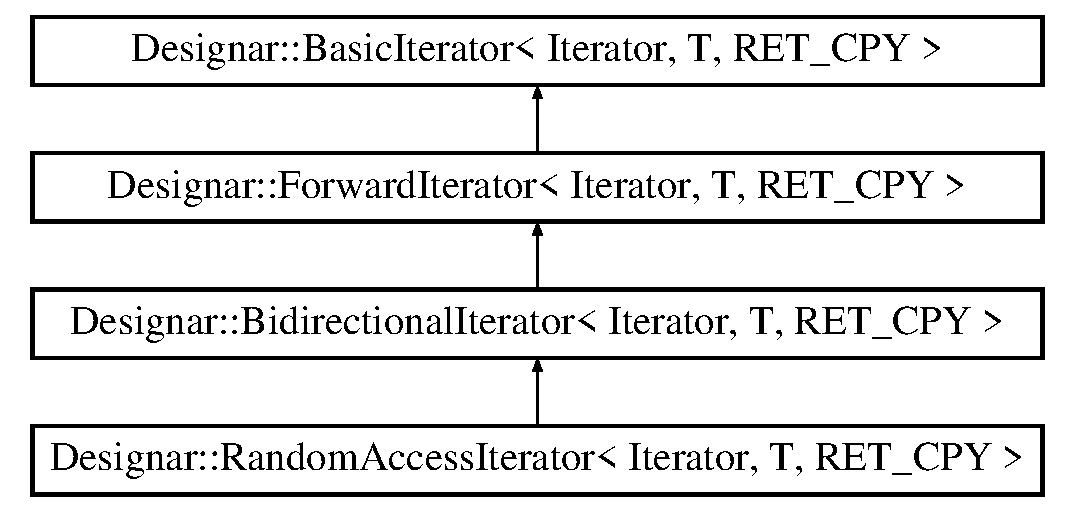
\includegraphics[height=4.000000cm]{class_designar_1_1_bidirectional_iterator}
\end{center}
\end{figure}
\subsection*{Public Member Functions}
\begin{DoxyCompactItemize}
\item 
Iterator \& \hyperlink{class_designar_1_1_bidirectional_iterator_aac9847e9868e270c4266a6fa0323a6ef}{operator-\/-\/} ()
\item 
Iterator \hyperlink{class_designar_1_1_bidirectional_iterator_a71602759debbdd18c89ffddb2217acb3}{operator-\/-\/} (int)
\end{DoxyCompactItemize}
\subsection*{Additional Inherited Members}


\subsection{Detailed Description}
\subsubsection*{template$<$class Iterator, typename T, bool R\+E\+T\+\_\+\+C\+PY = false$>$\newline
class Designar\+::\+Bidirectional\+Iterator$<$ Iterator, T, R\+E\+T\+\_\+\+C\+P\+Y $>$}



Definition at line 97 of file iterator.\+H.



\subsection{Member Function Documentation}
\mbox{\Hypertarget{class_designar_1_1_bidirectional_iterator_aac9847e9868e270c4266a6fa0323a6ef}\label{class_designar_1_1_bidirectional_iterator_aac9847e9868e270c4266a6fa0323a6ef}} 
\index{Designar\+::\+Bidirectional\+Iterator@{Designar\+::\+Bidirectional\+Iterator}!operator-\/-\/@{operator-\/-\/}}
\index{operator-\/-\/@{operator-\/-\/}!Designar\+::\+Bidirectional\+Iterator@{Designar\+::\+Bidirectional\+Iterator}}
\subsubsection{\texorpdfstring{operator-\/-\/()}{operator--()}\hspace{0.1cm}{\footnotesize\ttfamily [1/2]}}
{\footnotesize\ttfamily template$<$class Iterator, typename T, bool R\+E\+T\+\_\+\+C\+PY = false$>$ \\
Iterator\& \hyperlink{class_designar_1_1_bidirectional_iterator}{Designar\+::\+Bidirectional\+Iterator}$<$ Iterator, T, R\+E\+T\+\_\+\+C\+PY $>$\+::operator-\/-\/ (\begin{DoxyParamCaption}{ }\end{DoxyParamCaption})\hspace{0.3cm}{\ttfamily [inline]}}



Definition at line 102 of file iterator.\+H.

\mbox{\Hypertarget{class_designar_1_1_bidirectional_iterator_a71602759debbdd18c89ffddb2217acb3}\label{class_designar_1_1_bidirectional_iterator_a71602759debbdd18c89ffddb2217acb3}} 
\index{Designar\+::\+Bidirectional\+Iterator@{Designar\+::\+Bidirectional\+Iterator}!operator-\/-\/@{operator-\/-\/}}
\index{operator-\/-\/@{operator-\/-\/}!Designar\+::\+Bidirectional\+Iterator@{Designar\+::\+Bidirectional\+Iterator}}
\subsubsection{\texorpdfstring{operator-\/-\/()}{operator--()}\hspace{0.1cm}{\footnotesize\ttfamily [2/2]}}
{\footnotesize\ttfamily template$<$class Iterator, typename T, bool R\+E\+T\+\_\+\+C\+PY = false$>$ \\
Iterator \hyperlink{class_designar_1_1_bidirectional_iterator}{Designar\+::\+Bidirectional\+Iterator}$<$ Iterator, T, R\+E\+T\+\_\+\+C\+PY $>$\+::operator-\/-\/ (\begin{DoxyParamCaption}\item[{int}]{ }\end{DoxyParamCaption})\hspace{0.3cm}{\ttfamily [inline]}}



Definition at line 108 of file iterator.\+H.



The documentation for this class was generated from the following file\+:\begin{DoxyCompactItemize}
\item 
/home/julio/\+De\+S\+I\+G\+N\+A\+R-\/doc/\+De\+Si\+G\+N\+A\+R/include/\hyperlink{iterator_8_h}{iterator.\+H}\end{DoxyCompactItemize}

\hypertarget{class_designar_1_1_byte}{}\section{Referencia de la Clase Designar\+:\+:Byte}
\label{class_designar_1_1_byte}\index{Designar\+::\+Byte@{Designar\+::\+Byte}}


{\ttfamily \#include $<$bitset.\+H$>$}

\subsection*{Métodos públicos}
\begin{DoxyCompactItemize}
\item 
\hyperlink{class_designar_1_1_byte_a336815c676347de4aa09bc6342169f63}{Byte} ()
\item 
\hyperlink{class_designar_1_1_byte_a21d54a921b6f2e30c189ae2998c40188}{Byte} (bool, bool, bool, bool, bool, bool, bool, bool)
\item 
\hyperlink{class_designar_1_1_byte_a0ca92bbee262c55827eb6b2c1ebaa39e}{Byte} (int)
\item 
bool \hyperlink{class_designar_1_1_byte_a9f14a28a82353d48a802000c6de20c8e}{get\+\_\+bit} (unsigned char) const
\item 
void \hyperlink{class_designar_1_1_byte_a2d80ae64ad8316128d9217134f075721}{set\+\_\+bit} (unsigned char, bool)
\item 
void \hyperlink{class_designar_1_1_byte_abb173606939fe9f5e1c7db0180aba9b0}{flip} ()
\item 
void \hyperlink{class_designar_1_1_byte_a4e4336c19295313fc80e27ce40a69284}{set} (int)
\item 
int \hyperlink{class_designar_1_1_byte_a1f10a6e5ad399f62c0d53ace68c7e43d}{to\+\_\+num} () const
\item 
\hyperlink{class_designar_1_1_byte_a807f2afe5c5d15112b2a349e54142265}{operator int} () const
\item 
std\+::string \hyperlink{class_designar_1_1_byte_afddf5962874234208805ece07f31916d}{to\+\_\+string} () const
\item 
\hyperlink{class_designar_1_1_byte_ac37e3eaea04d1bdb09b04a1dd94a852d}{operator std\+::string} () const
\item 
\hyperlink{class_designar_1_1_byte}{Byte} \& \hyperlink{class_designar_1_1_byte_ab139736eebd931cb54f89fa2b01964fb}{operator=} (const \hyperlink{class_designar_1_1_byte}{Byte} \&)
\item 
\hyperlink{class_designar_1_1_byte}{Byte} \& \hyperlink{class_designar_1_1_byte_a1bc5154efe3f2ca906bbdd8c1d9b56ff}{operator=} (int)
\item 
\hyperlink{class_designar_1_1_byte}{Byte} \hyperlink{class_designar_1_1_byte_abd14d60584eec419a494785dc66e1156}{operator$<$$<$} (\hyperlink{namespace_designar_aa72662848b9f4815e7bf31a7cf3e33d1}{nat\+\_\+t})
\item 
void \hyperlink{class_designar_1_1_byte_a6d13481b7b6bc22a62c1b8998d851c29}{operator$<$$<$=} (\hyperlink{namespace_designar_aa72662848b9f4815e7bf31a7cf3e33d1}{nat\+\_\+t})
\item 
\hyperlink{class_designar_1_1_byte}{Byte} \hyperlink{class_designar_1_1_byte_a72ab991a6878042fd48a2d5b39e15034}{operator$>$$>$} (\hyperlink{namespace_designar_aa72662848b9f4815e7bf31a7cf3e33d1}{nat\+\_\+t})
\item 
void \hyperlink{class_designar_1_1_byte_a542b9081222051f2d69a29e042602120}{operator$>$$>$=} (\hyperlink{namespace_designar_aa72662848b9f4815e7bf31a7cf3e33d1}{nat\+\_\+t})
\item 
\hyperlink{class_designar_1_1_byte}{Byte} \hyperlink{class_designar_1_1_byte_a7b0c40979b481f74b5e35d0679a71a9b}{operator\&} (\hyperlink{namespace_designar_aa72662848b9f4815e7bf31a7cf3e33d1}{nat\+\_\+t})
\item 
void \hyperlink{class_designar_1_1_byte_a3242f8e4098b308f9960a2a172105967}{operator\&=} (\hyperlink{namespace_designar_aa72662848b9f4815e7bf31a7cf3e33d1}{nat\+\_\+t})
\item 
\hyperlink{class_designar_1_1_byte}{Byte} \hyperlink{class_designar_1_1_byte_a968c82b7108fccc2fb035f8b636d4563}{operator$\vert$} (\hyperlink{namespace_designar_aa72662848b9f4815e7bf31a7cf3e33d1}{nat\+\_\+t})
\item 
void \hyperlink{class_designar_1_1_byte_ae2aed407fc88cfb41c2412cf5852dd30}{operator$\vert$=} (\hyperlink{namespace_designar_aa72662848b9f4815e7bf31a7cf3e33d1}{nat\+\_\+t})
\item 
\hyperlink{class_designar_1_1_byte}{Byte} \hyperlink{class_designar_1_1_byte_ab59ded3274a3c5fc0b719deaada0f581}{operator$\sim$} ()
\item 
bool \hyperlink{class_designar_1_1_byte_aefd8f12d0f09d688f2977d86e387eabd}{operator==} (int) const
\item 
bool \hyperlink{class_designar_1_1_byte_a24733d65e2f520be23ae6eb55ca195c1}{operator!=} (int) const
\item 
bool \hyperlink{class_designar_1_1_byte_a94fc22c57bdeed7f674f7db0499becd3}{operator$<$} (int) const
\item 
bool \hyperlink{class_designar_1_1_byte_aec225f858e548268a54d23bb828cc12f}{operator$<$=} (int) const
\item 
bool \hyperlink{class_designar_1_1_byte_afa7138b57841b2a8f64c209ae3d79447}{operator$>$} (int) const
\item 
bool \hyperlink{class_designar_1_1_byte_a84d13e39d56aa1a32db48af56c9dae21}{operator$>$=} (int) const
\end{DoxyCompactItemize}


\subsection{Descripción detallada}


Definición en la línea 33 del archivo bitset.\+H.



\subsection{Documentación del constructor y destructor}
\mbox{\Hypertarget{class_designar_1_1_byte_a336815c676347de4aa09bc6342169f63}\label{class_designar_1_1_byte_a336815c676347de4aa09bc6342169f63}} 
\index{Designar\+::\+Byte@{Designar\+::\+Byte}!Byte@{Byte}}
\index{Byte@{Byte}!Designar\+::\+Byte@{Designar\+::\+Byte}}
\subsubsection{\texorpdfstring{Byte()}{Byte()}\hspace{0.1cm}{\footnotesize\ttfamily [1/3]}}
{\footnotesize\ttfamily Designar\+::\+Byte\+::\+Byte (\begin{DoxyParamCaption}{ }\end{DoxyParamCaption})}



Definición en la línea 30 del archivo bitset.\+C.

\mbox{\Hypertarget{class_designar_1_1_byte_a21d54a921b6f2e30c189ae2998c40188}\label{class_designar_1_1_byte_a21d54a921b6f2e30c189ae2998c40188}} 
\index{Designar\+::\+Byte@{Designar\+::\+Byte}!Byte@{Byte}}
\index{Byte@{Byte}!Designar\+::\+Byte@{Designar\+::\+Byte}}
\subsubsection{\texorpdfstring{Byte()}{Byte()}\hspace{0.1cm}{\footnotesize\ttfamily [2/3]}}
{\footnotesize\ttfamily Designar\+::\+Byte\+::\+Byte (\begin{DoxyParamCaption}\item[{bool}]{\+\_\+b1,  }\item[{bool}]{\+\_\+b2,  }\item[{bool}]{\+\_\+b3,  }\item[{bool}]{\+\_\+b4,  }\item[{bool}]{\+\_\+b5,  }\item[{bool}]{\+\_\+b6,  }\item[{bool}]{\+\_\+b7,  }\item[{bool}]{\+\_\+b8 }\end{DoxyParamCaption})}



Definición en la línea 36 del archivo bitset.\+C.

\mbox{\Hypertarget{class_designar_1_1_byte_a0ca92bbee262c55827eb6b2c1ebaa39e}\label{class_designar_1_1_byte_a0ca92bbee262c55827eb6b2c1ebaa39e}} 
\index{Designar\+::\+Byte@{Designar\+::\+Byte}!Byte@{Byte}}
\index{Byte@{Byte}!Designar\+::\+Byte@{Designar\+::\+Byte}}
\subsubsection{\texorpdfstring{Byte()}{Byte()}\hspace{0.1cm}{\footnotesize\ttfamily [3/3]}}
{\footnotesize\ttfamily Designar\+::\+Byte\+::\+Byte (\begin{DoxyParamCaption}\item[{int}]{num }\end{DoxyParamCaption})}



Definición en la línea 43 del archivo bitset.\+C.



\subsection{Documentación de las funciones miembro}
\mbox{\Hypertarget{class_designar_1_1_byte_abb173606939fe9f5e1c7db0180aba9b0}\label{class_designar_1_1_byte_abb173606939fe9f5e1c7db0180aba9b0}} 
\index{Designar\+::\+Byte@{Designar\+::\+Byte}!flip@{flip}}
\index{flip@{flip}!Designar\+::\+Byte@{Designar\+::\+Byte}}
\subsubsection{\texorpdfstring{flip()}{flip()}}
{\footnotesize\ttfamily void Designar\+::\+Byte\+::flip (\begin{DoxyParamCaption}{ }\end{DoxyParamCaption})}



Definición en la línea 80 del archivo bitset.\+C.

\mbox{\Hypertarget{class_designar_1_1_byte_a9f14a28a82353d48a802000c6de20c8e}\label{class_designar_1_1_byte_a9f14a28a82353d48a802000c6de20c8e}} 
\index{Designar\+::\+Byte@{Designar\+::\+Byte}!get\+\_\+bit@{get\+\_\+bit}}
\index{get\+\_\+bit@{get\+\_\+bit}!Designar\+::\+Byte@{Designar\+::\+Byte}}
\subsubsection{\texorpdfstring{get\+\_\+bit()}{get\_bit()}}
{\footnotesize\ttfamily bool Designar\+::\+Byte\+::get\+\_\+bit (\begin{DoxyParamCaption}\item[{unsigned char}]{num\+\_\+bit }\end{DoxyParamCaption}) const}



Definición en la línea 48 del archivo bitset.\+C.

\mbox{\Hypertarget{class_designar_1_1_byte_a807f2afe5c5d15112b2a349e54142265}\label{class_designar_1_1_byte_a807f2afe5c5d15112b2a349e54142265}} 
\index{Designar\+::\+Byte@{Designar\+::\+Byte}!operator int@{operator int}}
\index{operator int@{operator int}!Designar\+::\+Byte@{Designar\+::\+Byte}}
\subsubsection{\texorpdfstring{operator int()}{operator int()}}
{\footnotesize\ttfamily Designar\+::\+Byte\+::operator int (\begin{DoxyParamCaption}{ }\end{DoxyParamCaption}) const}



Definición en la línea 97 del archivo bitset.\+C.

\mbox{\Hypertarget{class_designar_1_1_byte_ac37e3eaea04d1bdb09b04a1dd94a852d}\label{class_designar_1_1_byte_ac37e3eaea04d1bdb09b04a1dd94a852d}} 
\index{Designar\+::\+Byte@{Designar\+::\+Byte}!operator std\+::string@{operator std\+::string}}
\index{operator std\+::string@{operator std\+::string}!Designar\+::\+Byte@{Designar\+::\+Byte}}
\subsubsection{\texorpdfstring{operator std\+::string()}{operator std::string()}}
{\footnotesize\ttfamily Designar\+::\+Byte\+::operator std\+::string (\begin{DoxyParamCaption}{ }\end{DoxyParamCaption}) const}



Definición en la línea 116 del archivo bitset.\+C.

\mbox{\Hypertarget{class_designar_1_1_byte_a24733d65e2f520be23ae6eb55ca195c1}\label{class_designar_1_1_byte_a24733d65e2f520be23ae6eb55ca195c1}} 
\index{Designar\+::\+Byte@{Designar\+::\+Byte}!operator"!=@{operator"!=}}
\index{operator"!=@{operator"!=}!Designar\+::\+Byte@{Designar\+::\+Byte}}
\subsubsection{\texorpdfstring{operator"!=()}{operator!=()}}
{\footnotesize\ttfamily bool Designar\+::\+Byte\+::operator!= (\begin{DoxyParamCaption}\item[{int}]{c }\end{DoxyParamCaption}) const}



Definición en la línea 213 del archivo bitset.\+C.

\mbox{\Hypertarget{class_designar_1_1_byte_a7b0c40979b481f74b5e35d0679a71a9b}\label{class_designar_1_1_byte_a7b0c40979b481f74b5e35d0679a71a9b}} 
\index{Designar\+::\+Byte@{Designar\+::\+Byte}!operator\&@{operator\&}}
\index{operator\&@{operator\&}!Designar\+::\+Byte@{Designar\+::\+Byte}}
\subsubsection{\texorpdfstring{operator\&()}{operator\&()}}
{\footnotesize\ttfamily \hyperlink{class_designar_1_1_byte}{Byte} Designar\+::\+Byte\+::operator \& (\begin{DoxyParamCaption}\item[{\hyperlink{namespace_designar_aa72662848b9f4815e7bf31a7cf3e33d1}{nat\+\_\+t}}]{ }\end{DoxyParamCaption})}

\mbox{\Hypertarget{class_designar_1_1_byte_a3242f8e4098b308f9960a2a172105967}\label{class_designar_1_1_byte_a3242f8e4098b308f9960a2a172105967}} 
\index{Designar\+::\+Byte@{Designar\+::\+Byte}!operator\&=@{operator\&=}}
\index{operator\&=@{operator\&=}!Designar\+::\+Byte@{Designar\+::\+Byte}}
\subsubsection{\texorpdfstring{operator\&=()}{operator\&=()}}
{\footnotesize\ttfamily void Designar\+::\+Byte\+::operator \&= (\begin{DoxyParamCaption}\item[{\hyperlink{namespace_designar_aa72662848b9f4815e7bf31a7cf3e33d1}{nat\+\_\+t}}]{ }\end{DoxyParamCaption})}

\mbox{\Hypertarget{class_designar_1_1_byte_a94fc22c57bdeed7f674f7db0499becd3}\label{class_designar_1_1_byte_a94fc22c57bdeed7f674f7db0499becd3}} 
\index{Designar\+::\+Byte@{Designar\+::\+Byte}!operator$<$@{operator$<$}}
\index{operator$<$@{operator$<$}!Designar\+::\+Byte@{Designar\+::\+Byte}}
\subsubsection{\texorpdfstring{operator$<$()}{operator<()}}
{\footnotesize\ttfamily bool Designar\+::\+Byte\+::operator$<$ (\begin{DoxyParamCaption}\item[{int}]{c }\end{DoxyParamCaption}) const}



Definición en la línea 219 del archivo bitset.\+C.

\mbox{\Hypertarget{class_designar_1_1_byte_abd14d60584eec419a494785dc66e1156}\label{class_designar_1_1_byte_abd14d60584eec419a494785dc66e1156}} 
\index{Designar\+::\+Byte@{Designar\+::\+Byte}!operator$<$$<$@{operator$<$$<$}}
\index{operator$<$$<$@{operator$<$$<$}!Designar\+::\+Byte@{Designar\+::\+Byte}}
\subsubsection{\texorpdfstring{operator$<$$<$()}{operator<<()}}
{\footnotesize\ttfamily \hyperlink{class_designar_1_1_byte}{Byte} Designar\+::\+Byte\+::operator$<$$<$ (\begin{DoxyParamCaption}\item[{\hyperlink{namespace_designar_aa72662848b9f4815e7bf31a7cf3e33d1}{nat\+\_\+t}}]{s }\end{DoxyParamCaption})}



Definición en la línea 144 del archivo bitset.\+C.

\mbox{\Hypertarget{class_designar_1_1_byte_a6d13481b7b6bc22a62c1b8998d851c29}\label{class_designar_1_1_byte_a6d13481b7b6bc22a62c1b8998d851c29}} 
\index{Designar\+::\+Byte@{Designar\+::\+Byte}!operator$<$$<$=@{operator$<$$<$=}}
\index{operator$<$$<$=@{operator$<$$<$=}!Designar\+::\+Byte@{Designar\+::\+Byte}}
\subsubsection{\texorpdfstring{operator$<$$<$=()}{operator<<=()}}
{\footnotesize\ttfamily void Designar\+::\+Byte\+::operator$<$$<$= (\begin{DoxyParamCaption}\item[{\hyperlink{namespace_designar_aa72662848b9f4815e7bf31a7cf3e33d1}{nat\+\_\+t}}]{s }\end{DoxyParamCaption})}



Definición en la línea 153 del archivo bitset.\+C.

\mbox{\Hypertarget{class_designar_1_1_byte_aec225f858e548268a54d23bb828cc12f}\label{class_designar_1_1_byte_aec225f858e548268a54d23bb828cc12f}} 
\index{Designar\+::\+Byte@{Designar\+::\+Byte}!operator$<$=@{operator$<$=}}
\index{operator$<$=@{operator$<$=}!Designar\+::\+Byte@{Designar\+::\+Byte}}
\subsubsection{\texorpdfstring{operator$<$=()}{operator<=()}}
{\footnotesize\ttfamily bool Designar\+::\+Byte\+::operator$<$= (\begin{DoxyParamCaption}\item[{int}]{c }\end{DoxyParamCaption}) const}



Definición en la línea 225 del archivo bitset.\+C.

\mbox{\Hypertarget{class_designar_1_1_byte_ab139736eebd931cb54f89fa2b01964fb}\label{class_designar_1_1_byte_ab139736eebd931cb54f89fa2b01964fb}} 
\index{Designar\+::\+Byte@{Designar\+::\+Byte}!operator=@{operator=}}
\index{operator=@{operator=}!Designar\+::\+Byte@{Designar\+::\+Byte}}
\subsubsection{\texorpdfstring{operator=()}{operator=()}\hspace{0.1cm}{\footnotesize\ttfamily [1/2]}}
{\footnotesize\ttfamily \hyperlink{class_designar_1_1_byte}{Byte} \& Designar\+::\+Byte\+::operator= (\begin{DoxyParamCaption}\item[{const \hyperlink{class_designar_1_1_byte}{Byte} \&}]{b }\end{DoxyParamCaption})}



Definición en la línea 121 del archivo bitset.\+C.

\mbox{\Hypertarget{class_designar_1_1_byte_a1bc5154efe3f2ca906bbdd8c1d9b56ff}\label{class_designar_1_1_byte_a1bc5154efe3f2ca906bbdd8c1d9b56ff}} 
\index{Designar\+::\+Byte@{Designar\+::\+Byte}!operator=@{operator=}}
\index{operator=@{operator=}!Designar\+::\+Byte@{Designar\+::\+Byte}}
\subsubsection{\texorpdfstring{operator=()}{operator=()}\hspace{0.1cm}{\footnotesize\ttfamily [2/2]}}
{\footnotesize\ttfamily \hyperlink{class_designar_1_1_byte}{Byte} \& Designar\+::\+Byte\+::operator= (\begin{DoxyParamCaption}\item[{int}]{num }\end{DoxyParamCaption})}



Definición en la línea 138 del archivo bitset.\+C.

\mbox{\Hypertarget{class_designar_1_1_byte_aefd8f12d0f09d688f2977d86e387eabd}\label{class_designar_1_1_byte_aefd8f12d0f09d688f2977d86e387eabd}} 
\index{Designar\+::\+Byte@{Designar\+::\+Byte}!operator==@{operator==}}
\index{operator==@{operator==}!Designar\+::\+Byte@{Designar\+::\+Byte}}
\subsubsection{\texorpdfstring{operator==()}{operator==()}}
{\footnotesize\ttfamily bool Designar\+::\+Byte\+::operator== (\begin{DoxyParamCaption}\item[{int}]{c }\end{DoxyParamCaption}) const}



Definición en la línea 207 del archivo bitset.\+C.

\mbox{\Hypertarget{class_designar_1_1_byte_afa7138b57841b2a8f64c209ae3d79447}\label{class_designar_1_1_byte_afa7138b57841b2a8f64c209ae3d79447}} 
\index{Designar\+::\+Byte@{Designar\+::\+Byte}!operator$>$@{operator$>$}}
\index{operator$>$@{operator$>$}!Designar\+::\+Byte@{Designar\+::\+Byte}}
\subsubsection{\texorpdfstring{operator$>$()}{operator>()}}
{\footnotesize\ttfamily bool Designar\+::\+Byte\+::operator$>$ (\begin{DoxyParamCaption}\item[{int}]{c }\end{DoxyParamCaption}) const}



Definición en la línea 231 del archivo bitset.\+C.

\mbox{\Hypertarget{class_designar_1_1_byte_a84d13e39d56aa1a32db48af56c9dae21}\label{class_designar_1_1_byte_a84d13e39d56aa1a32db48af56c9dae21}} 
\index{Designar\+::\+Byte@{Designar\+::\+Byte}!operator$>$=@{operator$>$=}}
\index{operator$>$=@{operator$>$=}!Designar\+::\+Byte@{Designar\+::\+Byte}}
\subsubsection{\texorpdfstring{operator$>$=()}{operator>=()}}
{\footnotesize\ttfamily bool Designar\+::\+Byte\+::operator$>$= (\begin{DoxyParamCaption}\item[{int}]{c }\end{DoxyParamCaption}) const}



Definición en la línea 237 del archivo bitset.\+C.

\mbox{\Hypertarget{class_designar_1_1_byte_a72ab991a6878042fd48a2d5b39e15034}\label{class_designar_1_1_byte_a72ab991a6878042fd48a2d5b39e15034}} 
\index{Designar\+::\+Byte@{Designar\+::\+Byte}!operator$>$$>$@{operator$>$$>$}}
\index{operator$>$$>$@{operator$>$$>$}!Designar\+::\+Byte@{Designar\+::\+Byte}}
\subsubsection{\texorpdfstring{operator$>$$>$()}{operator>>()}}
{\footnotesize\ttfamily \hyperlink{class_designar_1_1_byte}{Byte} Designar\+::\+Byte\+::operator$>$$>$ (\begin{DoxyParamCaption}\item[{\hyperlink{namespace_designar_aa72662848b9f4815e7bf31a7cf3e33d1}{nat\+\_\+t}}]{s }\end{DoxyParamCaption})}



Definición en la línea 158 del archivo bitset.\+C.

\mbox{\Hypertarget{class_designar_1_1_byte_a542b9081222051f2d69a29e042602120}\label{class_designar_1_1_byte_a542b9081222051f2d69a29e042602120}} 
\index{Designar\+::\+Byte@{Designar\+::\+Byte}!operator$>$$>$=@{operator$>$$>$=}}
\index{operator$>$$>$=@{operator$>$$>$=}!Designar\+::\+Byte@{Designar\+::\+Byte}}
\subsubsection{\texorpdfstring{operator$>$$>$=()}{operator>>=()}}
{\footnotesize\ttfamily void Designar\+::\+Byte\+::operator$>$$>$= (\begin{DoxyParamCaption}\item[{\hyperlink{namespace_designar_aa72662848b9f4815e7bf31a7cf3e33d1}{nat\+\_\+t}}]{s }\end{DoxyParamCaption})}



Definición en la línea 167 del archivo bitset.\+C.

\mbox{\Hypertarget{class_designar_1_1_byte_a968c82b7108fccc2fb035f8b636d4563}\label{class_designar_1_1_byte_a968c82b7108fccc2fb035f8b636d4563}} 
\index{Designar\+::\+Byte@{Designar\+::\+Byte}!operator\texttt{"|}@{operator\texttt{"|}}}
\index{operator\texttt{"|}@{operator\texttt{"|}}!Designar\+::\+Byte@{Designar\+::\+Byte}}
\subsubsection{\texorpdfstring{operator\texttt{"|}()}{operator|()}}
{\footnotesize\ttfamily \hyperlink{class_designar_1_1_byte}{Byte} Designar\+::\+Byte\+::operator$\vert$ (\begin{DoxyParamCaption}\item[{\hyperlink{namespace_designar_aa72662848b9f4815e7bf31a7cf3e33d1}{nat\+\_\+t}}]{c }\end{DoxyParamCaption})}



Definición en la línea 187 del archivo bitset.\+C.

\mbox{\Hypertarget{class_designar_1_1_byte_ae2aed407fc88cfb41c2412cf5852dd30}\label{class_designar_1_1_byte_ae2aed407fc88cfb41c2412cf5852dd30}} 
\index{Designar\+::\+Byte@{Designar\+::\+Byte}!operator\texttt{"|}=@{operator\texttt{"|}=}}
\index{operator\texttt{"|}=@{operator\texttt{"|}=}!Designar\+::\+Byte@{Designar\+::\+Byte}}
\subsubsection{\texorpdfstring{operator\texttt{"|}=()}{operator|=()}}
{\footnotesize\ttfamily void Designar\+::\+Byte\+::operator$\vert$= (\begin{DoxyParamCaption}\item[{\hyperlink{namespace_designar_aa72662848b9f4815e7bf31a7cf3e33d1}{nat\+\_\+t}}]{c }\end{DoxyParamCaption})}



Definición en la línea 196 del archivo bitset.\+C.

\mbox{\Hypertarget{class_designar_1_1_byte_ab59ded3274a3c5fc0b719deaada0f581}\label{class_designar_1_1_byte_ab59ded3274a3c5fc0b719deaada0f581}} 
\index{Designar\+::\+Byte@{Designar\+::\+Byte}!operator$\sim$@{operator$\sim$}}
\index{operator$\sim$@{operator$\sim$}!Designar\+::\+Byte@{Designar\+::\+Byte}}
\subsubsection{\texorpdfstring{operator$\sim$()}{operator~()}}
{\footnotesize\ttfamily \hyperlink{class_designar_1_1_byte}{Byte} Designar\+::\+Byte\+::operator$\sim$ (\begin{DoxyParamCaption}{ }\end{DoxyParamCaption})}



Definición en la línea 201 del archivo bitset.\+C.

\mbox{\Hypertarget{class_designar_1_1_byte_a4e4336c19295313fc80e27ce40a69284}\label{class_designar_1_1_byte_a4e4336c19295313fc80e27ce40a69284}} 
\index{Designar\+::\+Byte@{Designar\+::\+Byte}!set@{set}}
\index{set@{set}!Designar\+::\+Byte@{Designar\+::\+Byte}}
\subsubsection{\texorpdfstring{set()}{set()}}
{\footnotesize\ttfamily void Designar\+::\+Byte\+::set (\begin{DoxyParamCaption}\item[{int}]{num }\end{DoxyParamCaption})}



Definición en la línea 85 del archivo bitset.\+C.

\mbox{\Hypertarget{class_designar_1_1_byte_a2d80ae64ad8316128d9217134f075721}\label{class_designar_1_1_byte_a2d80ae64ad8316128d9217134f075721}} 
\index{Designar\+::\+Byte@{Designar\+::\+Byte}!set\+\_\+bit@{set\+\_\+bit}}
\index{set\+\_\+bit@{set\+\_\+bit}!Designar\+::\+Byte@{Designar\+::\+Byte}}
\subsubsection{\texorpdfstring{set\+\_\+bit()}{set\_bit()}}
{\footnotesize\ttfamily void Designar\+::\+Byte\+::set\+\_\+bit (\begin{DoxyParamCaption}\item[{unsigned char}]{num\+\_\+bit,  }\item[{bool}]{value }\end{DoxyParamCaption})}



Definición en la línea 64 del archivo bitset.\+C.

\mbox{\Hypertarget{class_designar_1_1_byte_a1f10a6e5ad399f62c0d53ace68c7e43d}\label{class_designar_1_1_byte_a1f10a6e5ad399f62c0d53ace68c7e43d}} 
\index{Designar\+::\+Byte@{Designar\+::\+Byte}!to\+\_\+num@{to\+\_\+num}}
\index{to\+\_\+num@{to\+\_\+num}!Designar\+::\+Byte@{Designar\+::\+Byte}}
\subsubsection{\texorpdfstring{to\+\_\+num()}{to\_num()}}
{\footnotesize\ttfamily int Designar\+::\+Byte\+::to\+\_\+num (\begin{DoxyParamCaption}{ }\end{DoxyParamCaption}) const}



Definición en la línea 91 del archivo bitset.\+C.

\mbox{\Hypertarget{class_designar_1_1_byte_afddf5962874234208805ece07f31916d}\label{class_designar_1_1_byte_afddf5962874234208805ece07f31916d}} 
\index{Designar\+::\+Byte@{Designar\+::\+Byte}!to\+\_\+string@{to\+\_\+string}}
\index{to\+\_\+string@{to\+\_\+string}!Designar\+::\+Byte@{Designar\+::\+Byte}}
\subsubsection{\texorpdfstring{to\+\_\+string()}{to\_string()}}
{\footnotesize\ttfamily std\+::string Designar\+::\+Byte\+::to\+\_\+string (\begin{DoxyParamCaption}{ }\end{DoxyParamCaption}) const}



Definición en la línea 102 del archivo bitset.\+C.



La documentación para esta clase fue generada a partir de los siguientes ficheros\+:\begin{DoxyCompactItemize}
\item 
/home/julio/\+De\+S\+I\+G\+N\+A\+R-\/doc/\+De\+Si\+G\+N\+A\+R/include/\hyperlink{bitset_8_h}{bitset.\+H}\item 
/home/julio/\+De\+S\+I\+G\+N\+A\+R-\/doc/\+De\+Si\+G\+N\+A\+R/src/\hyperlink{bitset_8_c}{bitset.\+C}\end{DoxyCompactItemize}

\hypertarget{class_designar_1_1_m_tree_node_1_1_children_iterator}{}\section{Designar\+:\+:M\+Tree\+Node$<$ Key $>$\+:\+:Children\+Iterator Class Reference}
\label{class_designar_1_1_m_tree_node_1_1_children_iterator}\index{Designar\+::\+M\+Tree\+Node$<$ Key $>$\+::\+Children\+Iterator@{Designar\+::\+M\+Tree\+Node$<$ Key $>$\+::\+Children\+Iterator}}


{\ttfamily \#include $<$nodesdef.\+H$>$}

Inheritance diagram for Designar\+:\+:M\+Tree\+Node$<$ Key $>$\+:\+:Children\+Iterator\+:\begin{figure}[H]
\begin{center}
\leavevmode
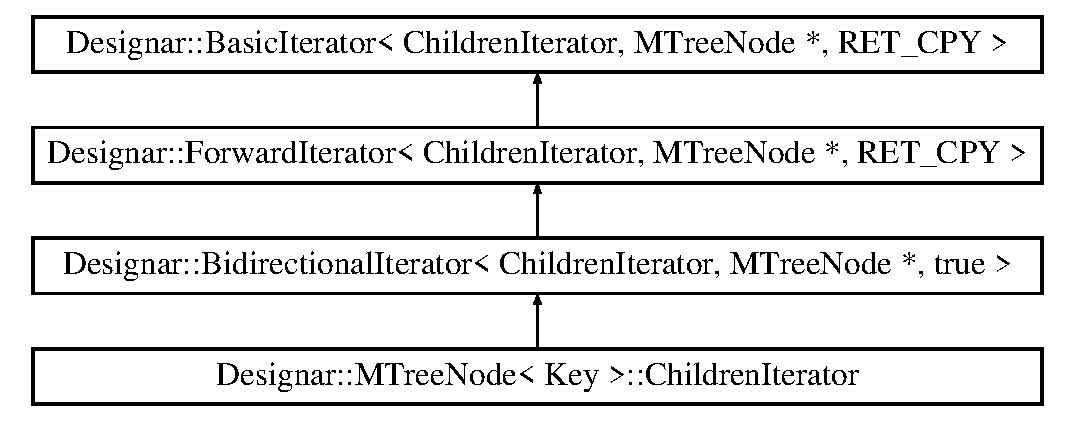
\includegraphics[height=4.000000cm]{class_designar_1_1_m_tree_node_1_1_children_iterator}
\end{center}
\end{figure}
\subsection*{Public Member Functions}
\begin{DoxyCompactItemize}
\item 
\hyperlink{class_designar_1_1_m_tree_node_1_1_children_iterator_ab050e655c7a557a50b2cdb390063e297}{Children\+Iterator} ()
\item 
\hyperlink{class_designar_1_1_m_tree_node_1_1_children_iterator_a1fdee49d713a9e2e007d59b996660e3e}{Children\+Iterator} (const \hyperlink{class_designar_1_1_m_tree_node}{M\+Tree\+Node} \&node)
\item 
\hyperlink{class_designar_1_1_m_tree_node_1_1_children_iterator_aceb65527a47a0e0105437cb032e76001}{Children\+Iterator} (const \hyperlink{class_designar_1_1_m_tree_node_1_1_children_iterator}{Children\+Iterator} \&it)
\item 
\hyperlink{class_designar_1_1_m_tree_node_1_1_children_iterator_ab43b11e8cdbc92ce79a5e44bcd74582e}{Children\+Iterator} (\hyperlink{class_designar_1_1_m_tree_node_1_1_children_iterator}{Children\+Iterator} \&\&it)
\item 
\hyperlink{class_designar_1_1_m_tree_node_1_1_children_iterator}{Children\+Iterator} \& \hyperlink{class_designar_1_1_m_tree_node_1_1_children_iterator_a1ddbcd1ae30de226e30e56ed6947c92a}{operator=} (const \hyperlink{class_designar_1_1_m_tree_node_1_1_children_iterator}{Children\+Iterator} \&it)
\item 
\hyperlink{class_designar_1_1_m_tree_node_1_1_children_iterator}{Children\+Iterator} \& \hyperlink{class_designar_1_1_m_tree_node_1_1_children_iterator_a61d6e5b6148ec6176ccc4b6ddbdda8a2}{operator=} (\hyperlink{class_designar_1_1_m_tree_node_1_1_children_iterator}{Children\+Iterator} \&\&it)
\item 
void \hyperlink{class_designar_1_1_m_tree_node_1_1_children_iterator_ac10d8a4f756973e74dd3c5c3224c6244}{swap} (\hyperlink{class_designar_1_1_m_tree_node_1_1_children_iterator}{Children\+Iterator} \&it)
\item 
\hyperlink{namespace_designar_aa72662848b9f4815e7bf31a7cf3e33d1}{nat\+\_\+t} \hyperlink{class_designar_1_1_m_tree_node_1_1_children_iterator_a0e1a9070e700ca1dbdbc5c588193dd54}{get\+\_\+position} () const
\item 
bool \hyperlink{class_designar_1_1_m_tree_node_1_1_children_iterator_a1ce8bf462bea3f6dc7ccf236839d0867}{has\+\_\+current} () const
\item 
\hyperlink{class_designar_1_1_m_tree_node}{M\+Tree\+Node} $\ast$ \hyperlink{class_designar_1_1_m_tree_node_1_1_children_iterator_a3ff90febfde4709c61d50107ce9761d5}{get\+\_\+current} ()
\item 
\hyperlink{class_designar_1_1_m_tree_node}{M\+Tree\+Node} $\ast$ \hyperlink{class_designar_1_1_m_tree_node_1_1_children_iterator_a70ef87f4fdd20504fdb9927f49dc847d}{get\+\_\+current} () const
\item 
void \hyperlink{class_designar_1_1_m_tree_node_1_1_children_iterator_a49c1adf58fd0fa57cf45fa3ae4f57f26}{next} ()
\item 
void \hyperlink{class_designar_1_1_m_tree_node_1_1_children_iterator_addf6dc80ece81a04056796a6ec35354a}{prev} ()
\end{DoxyCompactItemize}
\subsection*{Protected Member Functions}
\begin{DoxyCompactItemize}
\item 
\hyperlink{class_designar_1_1_m_tree_node}{M\+Tree\+Node} $\ast$ \hyperlink{class_designar_1_1_m_tree_node_1_1_children_iterator_a59d7d79081ab145a9ab886ee4873ae57}{get\+\_\+location} () const
\end{DoxyCompactItemize}
\subsection*{Friends}
\begin{DoxyCompactItemize}
\item 
class \hyperlink{class_designar_1_1_m_tree_node_1_1_children_iterator_a9318ecb15aa59102557883ca0b98fea5}{Basic\+Iterator$<$ Children\+Iterator, M\+Tree\+Node $\ast$, true $>$}
\end{DoxyCompactItemize}


\subsection{Detailed Description}
\subsubsection*{template$<$typename Key$>$\newline
class Designar\+::\+M\+Tree\+Node$<$ Key $>$\+::\+Children\+Iterator}



Definition at line 742 of file nodesdef.\+H.



\subsection{Constructor \& Destructor Documentation}
\mbox{\Hypertarget{class_designar_1_1_m_tree_node_1_1_children_iterator_ab050e655c7a557a50b2cdb390063e297}\label{class_designar_1_1_m_tree_node_1_1_children_iterator_ab050e655c7a557a50b2cdb390063e297}} 
\index{Designar\+::\+M\+Tree\+Node\+::\+Children\+Iterator@{Designar\+::\+M\+Tree\+Node\+::\+Children\+Iterator}!Children\+Iterator@{Children\+Iterator}}
\index{Children\+Iterator@{Children\+Iterator}!Designar\+::\+M\+Tree\+Node\+::\+Children\+Iterator@{Designar\+::\+M\+Tree\+Node\+::\+Children\+Iterator}}
\subsubsection{\texorpdfstring{Children\+Iterator()}{ChildrenIterator()}\hspace{0.1cm}{\footnotesize\ttfamily [1/4]}}
{\footnotesize\ttfamily template$<$typename Key $>$ \\
\hyperlink{class_designar_1_1_m_tree_node}{Designar\+::\+M\+Tree\+Node}$<$ Key $>$\+::Children\+Iterator\+::\+Children\+Iterator (\begin{DoxyParamCaption}{ }\end{DoxyParamCaption})\hspace{0.3cm}{\ttfamily [inline]}}



Definition at line 758 of file nodesdef.\+H.

\mbox{\Hypertarget{class_designar_1_1_m_tree_node_1_1_children_iterator_a1fdee49d713a9e2e007d59b996660e3e}\label{class_designar_1_1_m_tree_node_1_1_children_iterator_a1fdee49d713a9e2e007d59b996660e3e}} 
\index{Designar\+::\+M\+Tree\+Node\+::\+Children\+Iterator@{Designar\+::\+M\+Tree\+Node\+::\+Children\+Iterator}!Children\+Iterator@{Children\+Iterator}}
\index{Children\+Iterator@{Children\+Iterator}!Designar\+::\+M\+Tree\+Node\+::\+Children\+Iterator@{Designar\+::\+M\+Tree\+Node\+::\+Children\+Iterator}}
\subsubsection{\texorpdfstring{Children\+Iterator()}{ChildrenIterator()}\hspace{0.1cm}{\footnotesize\ttfamily [2/4]}}
{\footnotesize\ttfamily template$<$typename Key $>$ \\
\hyperlink{class_designar_1_1_m_tree_node}{Designar\+::\+M\+Tree\+Node}$<$ Key $>$\+::Children\+Iterator\+::\+Children\+Iterator (\begin{DoxyParamCaption}\item[{const \hyperlink{class_designar_1_1_m_tree_node}{M\+Tree\+Node} \&}]{node }\end{DoxyParamCaption})\hspace{0.3cm}{\ttfamily [inline]}}



Definition at line 764 of file nodesdef.\+H.

\mbox{\Hypertarget{class_designar_1_1_m_tree_node_1_1_children_iterator_aceb65527a47a0e0105437cb032e76001}\label{class_designar_1_1_m_tree_node_1_1_children_iterator_aceb65527a47a0e0105437cb032e76001}} 
\index{Designar\+::\+M\+Tree\+Node\+::\+Children\+Iterator@{Designar\+::\+M\+Tree\+Node\+::\+Children\+Iterator}!Children\+Iterator@{Children\+Iterator}}
\index{Children\+Iterator@{Children\+Iterator}!Designar\+::\+M\+Tree\+Node\+::\+Children\+Iterator@{Designar\+::\+M\+Tree\+Node\+::\+Children\+Iterator}}
\subsubsection{\texorpdfstring{Children\+Iterator()}{ChildrenIterator()}\hspace{0.1cm}{\footnotesize\ttfamily [3/4]}}
{\footnotesize\ttfamily template$<$typename Key $>$ \\
\hyperlink{class_designar_1_1_m_tree_node}{Designar\+::\+M\+Tree\+Node}$<$ Key $>$\+::Children\+Iterator\+::\+Children\+Iterator (\begin{DoxyParamCaption}\item[{const \hyperlink{class_designar_1_1_m_tree_node_1_1_children_iterator}{Children\+Iterator} \&}]{it }\end{DoxyParamCaption})\hspace{0.3cm}{\ttfamily [inline]}}



Definition at line 771 of file nodesdef.\+H.

\mbox{\Hypertarget{class_designar_1_1_m_tree_node_1_1_children_iterator_ab43b11e8cdbc92ce79a5e44bcd74582e}\label{class_designar_1_1_m_tree_node_1_1_children_iterator_ab43b11e8cdbc92ce79a5e44bcd74582e}} 
\index{Designar\+::\+M\+Tree\+Node\+::\+Children\+Iterator@{Designar\+::\+M\+Tree\+Node\+::\+Children\+Iterator}!Children\+Iterator@{Children\+Iterator}}
\index{Children\+Iterator@{Children\+Iterator}!Designar\+::\+M\+Tree\+Node\+::\+Children\+Iterator@{Designar\+::\+M\+Tree\+Node\+::\+Children\+Iterator}}
\subsubsection{\texorpdfstring{Children\+Iterator()}{ChildrenIterator()}\hspace{0.1cm}{\footnotesize\ttfamily [4/4]}}
{\footnotesize\ttfamily template$<$typename Key $>$ \\
\hyperlink{class_designar_1_1_m_tree_node}{Designar\+::\+M\+Tree\+Node}$<$ Key $>$\+::Children\+Iterator\+::\+Children\+Iterator (\begin{DoxyParamCaption}\item[{\hyperlink{class_designar_1_1_m_tree_node_1_1_children_iterator}{Children\+Iterator} \&\&}]{it }\end{DoxyParamCaption})\hspace{0.3cm}{\ttfamily [inline]}}



Definition at line 777 of file nodesdef.\+H.



\subsection{Member Function Documentation}
\mbox{\Hypertarget{class_designar_1_1_m_tree_node_1_1_children_iterator_a3ff90febfde4709c61d50107ce9761d5}\label{class_designar_1_1_m_tree_node_1_1_children_iterator_a3ff90febfde4709c61d50107ce9761d5}} 
\index{Designar\+::\+M\+Tree\+Node\+::\+Children\+Iterator@{Designar\+::\+M\+Tree\+Node\+::\+Children\+Iterator}!get\+\_\+current@{get\+\_\+current}}
\index{get\+\_\+current@{get\+\_\+current}!Designar\+::\+M\+Tree\+Node\+::\+Children\+Iterator@{Designar\+::\+M\+Tree\+Node\+::\+Children\+Iterator}}
\subsubsection{\texorpdfstring{get\+\_\+current()}{get\_current()}\hspace{0.1cm}{\footnotesize\ttfamily [1/2]}}
{\footnotesize\ttfamily template$<$typename Key $>$ \\
\hyperlink{class_designar_1_1_m_tree_node}{M\+Tree\+Node}$\ast$ \hyperlink{class_designar_1_1_m_tree_node}{Designar\+::\+M\+Tree\+Node}$<$ Key $>$\+::Children\+Iterator\+::get\+\_\+current (\begin{DoxyParamCaption}{ }\end{DoxyParamCaption})\hspace{0.3cm}{\ttfamily [inline]}}



Definition at line 818 of file nodesdef.\+H.

\mbox{\Hypertarget{class_designar_1_1_m_tree_node_1_1_children_iterator_a70ef87f4fdd20504fdb9927f49dc847d}\label{class_designar_1_1_m_tree_node_1_1_children_iterator_a70ef87f4fdd20504fdb9927f49dc847d}} 
\index{Designar\+::\+M\+Tree\+Node\+::\+Children\+Iterator@{Designar\+::\+M\+Tree\+Node\+::\+Children\+Iterator}!get\+\_\+current@{get\+\_\+current}}
\index{get\+\_\+current@{get\+\_\+current}!Designar\+::\+M\+Tree\+Node\+::\+Children\+Iterator@{Designar\+::\+M\+Tree\+Node\+::\+Children\+Iterator}}
\subsubsection{\texorpdfstring{get\+\_\+current()}{get\_current()}\hspace{0.1cm}{\footnotesize\ttfamily [2/2]}}
{\footnotesize\ttfamily template$<$typename Key $>$ \\
\hyperlink{class_designar_1_1_m_tree_node}{M\+Tree\+Node}$\ast$ \hyperlink{class_designar_1_1_m_tree_node}{Designar\+::\+M\+Tree\+Node}$<$ Key $>$\+::Children\+Iterator\+::get\+\_\+current (\begin{DoxyParamCaption}{ }\end{DoxyParamCaption}) const\hspace{0.3cm}{\ttfamily [inline]}}



Definition at line 826 of file nodesdef.\+H.

\mbox{\Hypertarget{class_designar_1_1_m_tree_node_1_1_children_iterator_a59d7d79081ab145a9ab886ee4873ae57}\label{class_designar_1_1_m_tree_node_1_1_children_iterator_a59d7d79081ab145a9ab886ee4873ae57}} 
\index{Designar\+::\+M\+Tree\+Node\+::\+Children\+Iterator@{Designar\+::\+M\+Tree\+Node\+::\+Children\+Iterator}!get\+\_\+location@{get\+\_\+location}}
\index{get\+\_\+location@{get\+\_\+location}!Designar\+::\+M\+Tree\+Node\+::\+Children\+Iterator@{Designar\+::\+M\+Tree\+Node\+::\+Children\+Iterator}}
\subsubsection{\texorpdfstring{get\+\_\+location()}{get\_location()}}
{\footnotesize\ttfamily template$<$typename Key $>$ \\
\hyperlink{class_designar_1_1_m_tree_node}{M\+Tree\+Node}$\ast$ \hyperlink{class_designar_1_1_m_tree_node}{Designar\+::\+M\+Tree\+Node}$<$ Key $>$\+::Children\+Iterator\+::get\+\_\+location (\begin{DoxyParamCaption}{ }\end{DoxyParamCaption}) const\hspace{0.3cm}{\ttfamily [inline]}, {\ttfamily [protected]}}



Definition at line 752 of file nodesdef.\+H.

\mbox{\Hypertarget{class_designar_1_1_m_tree_node_1_1_children_iterator_a0e1a9070e700ca1dbdbc5c588193dd54}\label{class_designar_1_1_m_tree_node_1_1_children_iterator_a0e1a9070e700ca1dbdbc5c588193dd54}} 
\index{Designar\+::\+M\+Tree\+Node\+::\+Children\+Iterator@{Designar\+::\+M\+Tree\+Node\+::\+Children\+Iterator}!get\+\_\+position@{get\+\_\+position}}
\index{get\+\_\+position@{get\+\_\+position}!Designar\+::\+M\+Tree\+Node\+::\+Children\+Iterator@{Designar\+::\+M\+Tree\+Node\+::\+Children\+Iterator}}
\subsubsection{\texorpdfstring{get\+\_\+position()}{get\_position()}}
{\footnotesize\ttfamily template$<$typename Key $>$ \\
\hyperlink{namespace_designar_aa72662848b9f4815e7bf31a7cf3e33d1}{nat\+\_\+t} \hyperlink{class_designar_1_1_m_tree_node}{Designar\+::\+M\+Tree\+Node}$<$ Key $>$\+::Children\+Iterator\+::get\+\_\+position (\begin{DoxyParamCaption}{ }\end{DoxyParamCaption}) const\hspace{0.3cm}{\ttfamily [inline]}}



Definition at line 808 of file nodesdef.\+H.

\mbox{\Hypertarget{class_designar_1_1_m_tree_node_1_1_children_iterator_a1ce8bf462bea3f6dc7ccf236839d0867}\label{class_designar_1_1_m_tree_node_1_1_children_iterator_a1ce8bf462bea3f6dc7ccf236839d0867}} 
\index{Designar\+::\+M\+Tree\+Node\+::\+Children\+Iterator@{Designar\+::\+M\+Tree\+Node\+::\+Children\+Iterator}!has\+\_\+current@{has\+\_\+current}}
\index{has\+\_\+current@{has\+\_\+current}!Designar\+::\+M\+Tree\+Node\+::\+Children\+Iterator@{Designar\+::\+M\+Tree\+Node\+::\+Children\+Iterator}}
\subsubsection{\texorpdfstring{has\+\_\+current()}{has\_current()}}
{\footnotesize\ttfamily template$<$typename Key $>$ \\
bool \hyperlink{class_designar_1_1_m_tree_node}{Designar\+::\+M\+Tree\+Node}$<$ Key $>$\+::Children\+Iterator\+::has\+\_\+current (\begin{DoxyParamCaption}{ }\end{DoxyParamCaption}) const\hspace{0.3cm}{\ttfamily [inline]}}



Definition at line 813 of file nodesdef.\+H.

\mbox{\Hypertarget{class_designar_1_1_m_tree_node_1_1_children_iterator_a49c1adf58fd0fa57cf45fa3ae4f57f26}\label{class_designar_1_1_m_tree_node_1_1_children_iterator_a49c1adf58fd0fa57cf45fa3ae4f57f26}} 
\index{Designar\+::\+M\+Tree\+Node\+::\+Children\+Iterator@{Designar\+::\+M\+Tree\+Node\+::\+Children\+Iterator}!next@{next}}
\index{next@{next}!Designar\+::\+M\+Tree\+Node\+::\+Children\+Iterator@{Designar\+::\+M\+Tree\+Node\+::\+Children\+Iterator}}
\subsubsection{\texorpdfstring{next()}{next()}}
{\footnotesize\ttfamily template$<$typename Key $>$ \\
void \hyperlink{class_designar_1_1_m_tree_node}{Designar\+::\+M\+Tree\+Node}$<$ Key $>$\+::Children\+Iterator\+::next (\begin{DoxyParamCaption}{ }\end{DoxyParamCaption})\hspace{0.3cm}{\ttfamily [inline]}}



Definition at line 834 of file nodesdef.\+H.

\mbox{\Hypertarget{class_designar_1_1_m_tree_node_1_1_children_iterator_a1ddbcd1ae30de226e30e56ed6947c92a}\label{class_designar_1_1_m_tree_node_1_1_children_iterator_a1ddbcd1ae30de226e30e56ed6947c92a}} 
\index{Designar\+::\+M\+Tree\+Node\+::\+Children\+Iterator@{Designar\+::\+M\+Tree\+Node\+::\+Children\+Iterator}!operator=@{operator=}}
\index{operator=@{operator=}!Designar\+::\+M\+Tree\+Node\+::\+Children\+Iterator@{Designar\+::\+M\+Tree\+Node\+::\+Children\+Iterator}}
\subsubsection{\texorpdfstring{operator=()}{operator=()}\hspace{0.1cm}{\footnotesize\ttfamily [1/2]}}
{\footnotesize\ttfamily template$<$typename Key $>$ \\
\hyperlink{class_designar_1_1_m_tree_node_1_1_children_iterator}{Children\+Iterator}\& \hyperlink{class_designar_1_1_m_tree_node}{Designar\+::\+M\+Tree\+Node}$<$ Key $>$\+::Children\+Iterator\+::operator= (\begin{DoxyParamCaption}\item[{const \hyperlink{class_designar_1_1_m_tree_node_1_1_children_iterator}{Children\+Iterator} \&}]{it }\end{DoxyParamCaption})\hspace{0.3cm}{\ttfamily [inline]}}



Definition at line 783 of file nodesdef.\+H.

\mbox{\Hypertarget{class_designar_1_1_m_tree_node_1_1_children_iterator_a61d6e5b6148ec6176ccc4b6ddbdda8a2}\label{class_designar_1_1_m_tree_node_1_1_children_iterator_a61d6e5b6148ec6176ccc4b6ddbdda8a2}} 
\index{Designar\+::\+M\+Tree\+Node\+::\+Children\+Iterator@{Designar\+::\+M\+Tree\+Node\+::\+Children\+Iterator}!operator=@{operator=}}
\index{operator=@{operator=}!Designar\+::\+M\+Tree\+Node\+::\+Children\+Iterator@{Designar\+::\+M\+Tree\+Node\+::\+Children\+Iterator}}
\subsubsection{\texorpdfstring{operator=()}{operator=()}\hspace{0.1cm}{\footnotesize\ttfamily [2/2]}}
{\footnotesize\ttfamily template$<$typename Key $>$ \\
\hyperlink{class_designar_1_1_m_tree_node_1_1_children_iterator}{Children\+Iterator}\& \hyperlink{class_designar_1_1_m_tree_node}{Designar\+::\+M\+Tree\+Node}$<$ Key $>$\+::Children\+Iterator\+::operator= (\begin{DoxyParamCaption}\item[{\hyperlink{class_designar_1_1_m_tree_node_1_1_children_iterator}{Children\+Iterator} \&\&}]{it }\end{DoxyParamCaption})\hspace{0.3cm}{\ttfamily [inline]}}



Definition at line 795 of file nodesdef.\+H.

\mbox{\Hypertarget{class_designar_1_1_m_tree_node_1_1_children_iterator_addf6dc80ece81a04056796a6ec35354a}\label{class_designar_1_1_m_tree_node_1_1_children_iterator_addf6dc80ece81a04056796a6ec35354a}} 
\index{Designar\+::\+M\+Tree\+Node\+::\+Children\+Iterator@{Designar\+::\+M\+Tree\+Node\+::\+Children\+Iterator}!prev@{prev}}
\index{prev@{prev}!Designar\+::\+M\+Tree\+Node\+::\+Children\+Iterator@{Designar\+::\+M\+Tree\+Node\+::\+Children\+Iterator}}
\subsubsection{\texorpdfstring{prev()}{prev()}}
{\footnotesize\ttfamily template$<$typename Key $>$ \\
void \hyperlink{class_designar_1_1_m_tree_node}{Designar\+::\+M\+Tree\+Node}$<$ Key $>$\+::Children\+Iterator\+::prev (\begin{DoxyParamCaption}{ }\end{DoxyParamCaption})\hspace{0.3cm}{\ttfamily [inline]}}



Definition at line 843 of file nodesdef.\+H.

\mbox{\Hypertarget{class_designar_1_1_m_tree_node_1_1_children_iterator_ac10d8a4f756973e74dd3c5c3224c6244}\label{class_designar_1_1_m_tree_node_1_1_children_iterator_ac10d8a4f756973e74dd3c5c3224c6244}} 
\index{Designar\+::\+M\+Tree\+Node\+::\+Children\+Iterator@{Designar\+::\+M\+Tree\+Node\+::\+Children\+Iterator}!swap@{swap}}
\index{swap@{swap}!Designar\+::\+M\+Tree\+Node\+::\+Children\+Iterator@{Designar\+::\+M\+Tree\+Node\+::\+Children\+Iterator}}
\subsubsection{\texorpdfstring{swap()}{swap()}}
{\footnotesize\ttfamily template$<$typename Key $>$ \\
void \hyperlink{class_designar_1_1_m_tree_node}{Designar\+::\+M\+Tree\+Node}$<$ Key $>$\+::Children\+Iterator\+::swap (\begin{DoxyParamCaption}\item[{\hyperlink{class_designar_1_1_m_tree_node_1_1_children_iterator}{Children\+Iterator} \&}]{it }\end{DoxyParamCaption})\hspace{0.3cm}{\ttfamily [inline]}}



Definition at line 801 of file nodesdef.\+H.



\subsection{Friends And Related Function Documentation}
\mbox{\Hypertarget{class_designar_1_1_m_tree_node_1_1_children_iterator_a9318ecb15aa59102557883ca0b98fea5}\label{class_designar_1_1_m_tree_node_1_1_children_iterator_a9318ecb15aa59102557883ca0b98fea5}} 
\index{Designar\+::\+M\+Tree\+Node\+::\+Children\+Iterator@{Designar\+::\+M\+Tree\+Node\+::\+Children\+Iterator}!Basic\+Iterator$<$ Children\+Iterator, M\+Tree\+Node $\ast$, true $>$@{Basic\+Iterator$<$ Children\+Iterator, M\+Tree\+Node $\ast$, true $>$}}
\index{Basic\+Iterator$<$ Children\+Iterator, M\+Tree\+Node $\ast$, true $>$@{Basic\+Iterator$<$ Children\+Iterator, M\+Tree\+Node $\ast$, true $>$}!Designar\+::\+M\+Tree\+Node\+::\+Children\+Iterator@{Designar\+::\+M\+Tree\+Node\+::\+Children\+Iterator}}
\subsubsection{\texorpdfstring{Basic\+Iterator$<$ Children\+Iterator, M\+Tree\+Node $\ast$, true $>$}{BasicIterator< ChildrenIterator, MTreeNode *, true >}}
{\footnotesize\ttfamily template$<$typename Key $>$ \\
friend class \hyperlink{class_designar_1_1_basic_iterator}{Basic\+Iterator}$<$ \hyperlink{class_designar_1_1_m_tree_node_1_1_children_iterator}{Children\+Iterator}, \hyperlink{class_designar_1_1_m_tree_node}{M\+Tree\+Node} $\ast$, true $>$\hspace{0.3cm}{\ttfamily [friend]}}



Definition at line 745 of file nodesdef.\+H.



The documentation for this class was generated from the following file\+:\begin{DoxyCompactItemize}
\item 
/home/julio/\+De\+S\+I\+G\+N\+A\+R-\/doc/\+De\+Si\+G\+N\+A\+R/include/\hyperlink{nodesdef_8_h}{nodesdef.\+H}\end{DoxyCompactItemize}

\hypertarget{class_designar_1_1_cmp_wrapper}{}\section{Referencia de la plantilla de la Clase Designar\+:\+:Cmp\+Wrapper$<$ Key, Value, Cmp $>$}
\label{class_designar_1_1_cmp_wrapper}\index{Designar\+::\+Cmp\+Wrapper$<$ Key, Value, Cmp $>$@{Designar\+::\+Cmp\+Wrapper$<$ Key, Value, Cmp $>$}}


{\ttfamily \#include $<$map.\+H$>$}

\subsection*{Métodos públicos}
\begin{DoxyCompactItemize}
\item 
\hyperlink{class_designar_1_1_cmp_wrapper_a2fe493e155e893254b689c5933c61ebb}{Cmp\+Wrapper} (Cmp \&\+\_\+cmp)
\item 
\hyperlink{class_designar_1_1_cmp_wrapper_af471969d033f9f7b5d306a0755af43c6}{Cmp\+Wrapper} (Cmp \&\&\+\_\+cmp=Cmp())
\item 
\hyperlink{class_designar_1_1_cmp_wrapper_a7112a8dabf2f50f09173078de19ab7d2}{Cmp\+Wrapper} (const \hyperlink{class_designar_1_1_cmp_wrapper}{Cmp\+Wrapper} \&cw)
\item 
\hyperlink{class_designar_1_1_cmp_wrapper_a985bdd51796dfac3d77eff525d364a90}{Cmp\+Wrapper} (\hyperlink{class_designar_1_1_cmp_wrapper}{Cmp\+Wrapper} \&\&cw)
\item 
Cmp \& \hyperlink{class_designar_1_1_cmp_wrapper_a46bfc0600123bbb9166e870067861ded}{get\+\_\+cmp} ()
\item 
const Cmp \& \hyperlink{class_designar_1_1_cmp_wrapper_a1f4fe6315f3f96a383be1cc51909e072}{get\+\_\+cmp} () const
\item 
\hyperlink{class_designar_1_1_cmp_wrapper}{Cmp\+Wrapper} \& \hyperlink{class_designar_1_1_cmp_wrapper_a958a9c52db5cc8e9b809af0adc4f90f4}{operator=} (const \hyperlink{class_designar_1_1_cmp_wrapper}{Cmp\+Wrapper} \&cw)
\item 
\hyperlink{class_designar_1_1_cmp_wrapper}{Cmp\+Wrapper} \& \hyperlink{class_designar_1_1_cmp_wrapper_a7885c41d00b53a31f1fe4d15bcf53e00}{operator=} (\hyperlink{class_designar_1_1_cmp_wrapper}{Cmp\+Wrapper} \&\&cw)
\item 
bool \hyperlink{class_designar_1_1_cmp_wrapper_a1b715375bf0bdd7ffefdb8ada447c191}{operator()} (const \hyperlink{namespace_designar_a7394b1b25278abf7211e77b91eb5204f}{Map\+Key}$<$ Key, Value $>$ \&p, const \hyperlink{namespace_designar_a7394b1b25278abf7211e77b91eb5204f}{Map\+Key}$<$ Key, Value $>$ \&q) const
\end{DoxyCompactItemize}


\subsection{Descripción detallada}
\subsubsection*{template$<$typename Key, typename Value, class Cmp$>$\newline
class Designar\+::\+Cmp\+Wrapper$<$ Key, Value, Cmp $>$}



Definición en la línea 103 del archivo map.\+H.



\subsection{Documentación del constructor y destructor}
\mbox{\Hypertarget{class_designar_1_1_cmp_wrapper_a2fe493e155e893254b689c5933c61ebb}\label{class_designar_1_1_cmp_wrapper_a2fe493e155e893254b689c5933c61ebb}} 
\index{Designar\+::\+Cmp\+Wrapper@{Designar\+::\+Cmp\+Wrapper}!Cmp\+Wrapper@{Cmp\+Wrapper}}
\index{Cmp\+Wrapper@{Cmp\+Wrapper}!Designar\+::\+Cmp\+Wrapper@{Designar\+::\+Cmp\+Wrapper}}
\subsubsection{\texorpdfstring{Cmp\+Wrapper()}{CmpWrapper()}\hspace{0.1cm}{\footnotesize\ttfamily [1/4]}}
{\footnotesize\ttfamily template$<$typename Key, typename Value, class Cmp$>$ \\
\hyperlink{class_designar_1_1_cmp_wrapper}{Designar\+::\+Cmp\+Wrapper}$<$ Key, Value, Cmp $>$\+::\hyperlink{class_designar_1_1_cmp_wrapper}{Cmp\+Wrapper} (\begin{DoxyParamCaption}\item[{Cmp \&}]{\+\_\+cmp }\end{DoxyParamCaption})\hspace{0.3cm}{\ttfamily [inline]}}



Definición en la línea 108 del archivo map.\+H.

\mbox{\Hypertarget{class_designar_1_1_cmp_wrapper_af471969d033f9f7b5d306a0755af43c6}\label{class_designar_1_1_cmp_wrapper_af471969d033f9f7b5d306a0755af43c6}} 
\index{Designar\+::\+Cmp\+Wrapper@{Designar\+::\+Cmp\+Wrapper}!Cmp\+Wrapper@{Cmp\+Wrapper}}
\index{Cmp\+Wrapper@{Cmp\+Wrapper}!Designar\+::\+Cmp\+Wrapper@{Designar\+::\+Cmp\+Wrapper}}
\subsubsection{\texorpdfstring{Cmp\+Wrapper()}{CmpWrapper()}\hspace{0.1cm}{\footnotesize\ttfamily [2/4]}}
{\footnotesize\ttfamily template$<$typename Key, typename Value, class Cmp$>$ \\
\hyperlink{class_designar_1_1_cmp_wrapper}{Designar\+::\+Cmp\+Wrapper}$<$ Key, Value, Cmp $>$\+::\hyperlink{class_designar_1_1_cmp_wrapper}{Cmp\+Wrapper} (\begin{DoxyParamCaption}\item[{Cmp \&\&}]{\+\_\+cmp = {\ttfamily Cmp()} }\end{DoxyParamCaption})\hspace{0.3cm}{\ttfamily [inline]}}



Definición en la línea 114 del archivo map.\+H.

\mbox{\Hypertarget{class_designar_1_1_cmp_wrapper_a7112a8dabf2f50f09173078de19ab7d2}\label{class_designar_1_1_cmp_wrapper_a7112a8dabf2f50f09173078de19ab7d2}} 
\index{Designar\+::\+Cmp\+Wrapper@{Designar\+::\+Cmp\+Wrapper}!Cmp\+Wrapper@{Cmp\+Wrapper}}
\index{Cmp\+Wrapper@{Cmp\+Wrapper}!Designar\+::\+Cmp\+Wrapper@{Designar\+::\+Cmp\+Wrapper}}
\subsubsection{\texorpdfstring{Cmp\+Wrapper()}{CmpWrapper()}\hspace{0.1cm}{\footnotesize\ttfamily [3/4]}}
{\footnotesize\ttfamily template$<$typename Key, typename Value, class Cmp$>$ \\
\hyperlink{class_designar_1_1_cmp_wrapper}{Designar\+::\+Cmp\+Wrapper}$<$ Key, Value, Cmp $>$\+::\hyperlink{class_designar_1_1_cmp_wrapper}{Cmp\+Wrapper} (\begin{DoxyParamCaption}\item[{const \hyperlink{class_designar_1_1_cmp_wrapper}{Cmp\+Wrapper}$<$ Key, Value, Cmp $>$ \&}]{cw }\end{DoxyParamCaption})\hspace{0.3cm}{\ttfamily [inline]}}



Definición en la línea 120 del archivo map.\+H.

\mbox{\Hypertarget{class_designar_1_1_cmp_wrapper_a985bdd51796dfac3d77eff525d364a90}\label{class_designar_1_1_cmp_wrapper_a985bdd51796dfac3d77eff525d364a90}} 
\index{Designar\+::\+Cmp\+Wrapper@{Designar\+::\+Cmp\+Wrapper}!Cmp\+Wrapper@{Cmp\+Wrapper}}
\index{Cmp\+Wrapper@{Cmp\+Wrapper}!Designar\+::\+Cmp\+Wrapper@{Designar\+::\+Cmp\+Wrapper}}
\subsubsection{\texorpdfstring{Cmp\+Wrapper()}{CmpWrapper()}\hspace{0.1cm}{\footnotesize\ttfamily [4/4]}}
{\footnotesize\ttfamily template$<$typename Key, typename Value, class Cmp$>$ \\
\hyperlink{class_designar_1_1_cmp_wrapper}{Designar\+::\+Cmp\+Wrapper}$<$ Key, Value, Cmp $>$\+::\hyperlink{class_designar_1_1_cmp_wrapper}{Cmp\+Wrapper} (\begin{DoxyParamCaption}\item[{\hyperlink{class_designar_1_1_cmp_wrapper}{Cmp\+Wrapper}$<$ Key, Value, Cmp $>$ \&\&}]{cw }\end{DoxyParamCaption})\hspace{0.3cm}{\ttfamily [inline]}}



Definición en la línea 126 del archivo map.\+H.



\subsection{Documentación de las funciones miembro}
\mbox{\Hypertarget{class_designar_1_1_cmp_wrapper_a46bfc0600123bbb9166e870067861ded}\label{class_designar_1_1_cmp_wrapper_a46bfc0600123bbb9166e870067861ded}} 
\index{Designar\+::\+Cmp\+Wrapper@{Designar\+::\+Cmp\+Wrapper}!get\+\_\+cmp@{get\+\_\+cmp}}
\index{get\+\_\+cmp@{get\+\_\+cmp}!Designar\+::\+Cmp\+Wrapper@{Designar\+::\+Cmp\+Wrapper}}
\subsubsection{\texorpdfstring{get\+\_\+cmp()}{get\_cmp()}\hspace{0.1cm}{\footnotesize\ttfamily [1/2]}}
{\footnotesize\ttfamily template$<$typename Key, typename Value, class Cmp$>$ \\
Cmp\& \hyperlink{class_designar_1_1_cmp_wrapper}{Designar\+::\+Cmp\+Wrapper}$<$ Key, Value, Cmp $>$\+::get\+\_\+cmp (\begin{DoxyParamCaption}{ }\end{DoxyParamCaption})\hspace{0.3cm}{\ttfamily [inline]}}



Definición en la línea 132 del archivo map.\+H.

\mbox{\Hypertarget{class_designar_1_1_cmp_wrapper_a1f4fe6315f3f96a383be1cc51909e072}\label{class_designar_1_1_cmp_wrapper_a1f4fe6315f3f96a383be1cc51909e072}} 
\index{Designar\+::\+Cmp\+Wrapper@{Designar\+::\+Cmp\+Wrapper}!get\+\_\+cmp@{get\+\_\+cmp}}
\index{get\+\_\+cmp@{get\+\_\+cmp}!Designar\+::\+Cmp\+Wrapper@{Designar\+::\+Cmp\+Wrapper}}
\subsubsection{\texorpdfstring{get\+\_\+cmp()}{get\_cmp()}\hspace{0.1cm}{\footnotesize\ttfamily [2/2]}}
{\footnotesize\ttfamily template$<$typename Key, typename Value, class Cmp$>$ \\
const Cmp\& \hyperlink{class_designar_1_1_cmp_wrapper}{Designar\+::\+Cmp\+Wrapper}$<$ Key, Value, Cmp $>$\+::get\+\_\+cmp (\begin{DoxyParamCaption}{ }\end{DoxyParamCaption}) const\hspace{0.3cm}{\ttfamily [inline]}}



Definición en la línea 137 del archivo map.\+H.

\mbox{\Hypertarget{class_designar_1_1_cmp_wrapper_a1b715375bf0bdd7ffefdb8ada447c191}\label{class_designar_1_1_cmp_wrapper_a1b715375bf0bdd7ffefdb8ada447c191}} 
\index{Designar\+::\+Cmp\+Wrapper@{Designar\+::\+Cmp\+Wrapper}!operator()@{operator()}}
\index{operator()@{operator()}!Designar\+::\+Cmp\+Wrapper@{Designar\+::\+Cmp\+Wrapper}}
\subsubsection{\texorpdfstring{operator()()}{operator()()}}
{\footnotesize\ttfamily template$<$typename Key, typename Value, class Cmp$>$ \\
bool \hyperlink{class_designar_1_1_cmp_wrapper}{Designar\+::\+Cmp\+Wrapper}$<$ Key, Value, Cmp $>$\+::operator() (\begin{DoxyParamCaption}\item[{const \hyperlink{namespace_designar_a7394b1b25278abf7211e77b91eb5204f}{Map\+Key}$<$ Key, Value $>$ \&}]{p,  }\item[{const \hyperlink{namespace_designar_a7394b1b25278abf7211e77b91eb5204f}{Map\+Key}$<$ Key, Value $>$ \&}]{q }\end{DoxyParamCaption}) const\hspace{0.3cm}{\ttfamily [inline]}}



Definición en la línea 157 del archivo map.\+H.

\mbox{\Hypertarget{class_designar_1_1_cmp_wrapper_a958a9c52db5cc8e9b809af0adc4f90f4}\label{class_designar_1_1_cmp_wrapper_a958a9c52db5cc8e9b809af0adc4f90f4}} 
\index{Designar\+::\+Cmp\+Wrapper@{Designar\+::\+Cmp\+Wrapper}!operator=@{operator=}}
\index{operator=@{operator=}!Designar\+::\+Cmp\+Wrapper@{Designar\+::\+Cmp\+Wrapper}}
\subsubsection{\texorpdfstring{operator=()}{operator=()}\hspace{0.1cm}{\footnotesize\ttfamily [1/2]}}
{\footnotesize\ttfamily template$<$typename Key, typename Value, class Cmp$>$ \\
\hyperlink{class_designar_1_1_cmp_wrapper}{Cmp\+Wrapper}\& \hyperlink{class_designar_1_1_cmp_wrapper}{Designar\+::\+Cmp\+Wrapper}$<$ Key, Value, Cmp $>$\+::operator= (\begin{DoxyParamCaption}\item[{const \hyperlink{class_designar_1_1_cmp_wrapper}{Cmp\+Wrapper}$<$ Key, Value, Cmp $>$ \&}]{cw }\end{DoxyParamCaption})\hspace{0.3cm}{\ttfamily [inline]}}



Definición en la línea 142 del archivo map.\+H.

\mbox{\Hypertarget{class_designar_1_1_cmp_wrapper_a7885c41d00b53a31f1fe4d15bcf53e00}\label{class_designar_1_1_cmp_wrapper_a7885c41d00b53a31f1fe4d15bcf53e00}} 
\index{Designar\+::\+Cmp\+Wrapper@{Designar\+::\+Cmp\+Wrapper}!operator=@{operator=}}
\index{operator=@{operator=}!Designar\+::\+Cmp\+Wrapper@{Designar\+::\+Cmp\+Wrapper}}
\subsubsection{\texorpdfstring{operator=()}{operator=()}\hspace{0.1cm}{\footnotesize\ttfamily [2/2]}}
{\footnotesize\ttfamily template$<$typename Key, typename Value, class Cmp$>$ \\
\hyperlink{class_designar_1_1_cmp_wrapper}{Cmp\+Wrapper}\& \hyperlink{class_designar_1_1_cmp_wrapper}{Designar\+::\+Cmp\+Wrapper}$<$ Key, Value, Cmp $>$\+::operator= (\begin{DoxyParamCaption}\item[{\hyperlink{class_designar_1_1_cmp_wrapper}{Cmp\+Wrapper}$<$ Key, Value, Cmp $>$ \&\&}]{cw }\end{DoxyParamCaption})\hspace{0.3cm}{\ttfamily [inline]}}



Definición en la línea 151 del archivo map.\+H.



La documentación para esta clase fue generada a partir del siguiente fichero\+:\begin{DoxyCompactItemize}
\item 
/home/julio/\+De\+S\+I\+G\+N\+A\+R-\/doc/\+De\+Si\+G\+N\+A\+R/include/\hyperlink{map_8_h}{map.\+H}\end{DoxyCompactItemize}

\hypertarget{class_designar_1_1_common_node_arc}{}\section{Referencia de la Clase Designar\+:\+:Common\+Node\+Arc}
\label{class_designar_1_1_common_node_arc}\index{Designar\+::\+Common\+Node\+Arc@{Designar\+::\+Common\+Node\+Arc}}


{\ttfamily \#include $<$graphutilities.\+H$>$}

Diagrama de herencias de Designar\+:\+:Common\+Node\+Arc\begin{figure}[H]
\begin{center}
\leavevmode
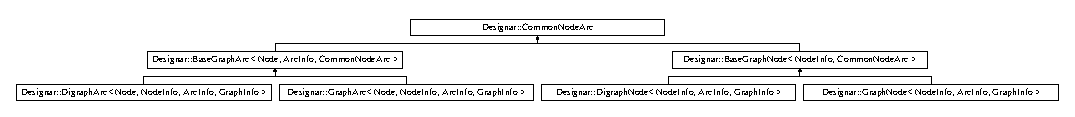
\includegraphics[height=1.122995cm]{class_designar_1_1_common_node_arc}
\end{center}
\end{figure}
\subsection*{Métodos públicos}
\begin{DoxyCompactItemize}
\item 
\hyperlink{class_designar_1_1_common_node_arc_a7b0794f171cc8ad5b5e4c28216366c53}{Common\+Node\+Arc} ()
\item 
void \hyperlink{class_designar_1_1_common_node_arc_a14b77740fb6d68b1949483c71dd4b197}{visit} (\hyperlink{namespace_designar_ac91366256ea6ea6ac5fd483d55a7499e}{Graph\+Tag})
\item 
void \hyperlink{class_designar_1_1_common_node_arc_ae8f3fed57cacf9e8cfa0df582eeecf3b}{unvisit} (\hyperlink{namespace_designar_ac91366256ea6ea6ac5fd483d55a7499e}{Graph\+Tag})
\item 
bool \hyperlink{class_designar_1_1_common_node_arc_a1852b6cf543bfb695bad590804ecaacd}{is\+\_\+visited} (\hyperlink{namespace_designar_ac91366256ea6ea6ac5fd483d55a7499e}{Graph\+Tag}) const
\item 
void $\ast$\& \hyperlink{class_designar_1_1_common_node_arc_a385a91e2bddd8a6f69d418b36b2cf11e}{cookie} ()
\item 
void \hyperlink{class_designar_1_1_common_node_arc_a436f2993d4da6ec9f750adc465e7c691}{reset\+\_\+tag} ()
\item 
\hyperlink{namespace_designar_a9d113d66a39e82b73727c72cd3a52f73}{lint\+\_\+t} \& \hyperlink{class_designar_1_1_common_node_arc_a8bdada8dfdf47ad02c91cca8c848d287}{counter} ()
\item 
void \hyperlink{class_designar_1_1_common_node_arc_a1dd1385837012b02ee3c67a7e3f5ccc1}{reset} ()
\end{DoxyCompactItemize}


\subsection{Descripción detallada}


Definición en la línea 54 del archivo graphutilities.\+H.



\subsection{Documentación del constructor y destructor}
\mbox{\Hypertarget{class_designar_1_1_common_node_arc_a7b0794f171cc8ad5b5e4c28216366c53}\label{class_designar_1_1_common_node_arc_a7b0794f171cc8ad5b5e4c28216366c53}} 
\index{Designar\+::\+Common\+Node\+Arc@{Designar\+::\+Common\+Node\+Arc}!Common\+Node\+Arc@{Common\+Node\+Arc}}
\index{Common\+Node\+Arc@{Common\+Node\+Arc}!Designar\+::\+Common\+Node\+Arc@{Designar\+::\+Common\+Node\+Arc}}
\subsubsection{\texorpdfstring{Common\+Node\+Arc()}{CommonNodeArc()}}
{\footnotesize\ttfamily Designar\+::\+Common\+Node\+Arc\+::\+Common\+Node\+Arc (\begin{DoxyParamCaption}{ }\end{DoxyParamCaption})}



Definición en la línea 30 del archivo graphutilities.\+C.



\subsection{Documentación de las funciones miembro}
\mbox{\Hypertarget{class_designar_1_1_common_node_arc_a385a91e2bddd8a6f69d418b36b2cf11e}\label{class_designar_1_1_common_node_arc_a385a91e2bddd8a6f69d418b36b2cf11e}} 
\index{Designar\+::\+Common\+Node\+Arc@{Designar\+::\+Common\+Node\+Arc}!cookie@{cookie}}
\index{cookie@{cookie}!Designar\+::\+Common\+Node\+Arc@{Designar\+::\+Common\+Node\+Arc}}
\subsubsection{\texorpdfstring{cookie()}{cookie()}}
{\footnotesize\ttfamily void $\ast$\& Designar\+::\+Common\+Node\+Arc\+::cookie (\begin{DoxyParamCaption}{ }\end{DoxyParamCaption})}



Definición en la línea 51 del archivo graphutilities.\+C.

\mbox{\Hypertarget{class_designar_1_1_common_node_arc_a8bdada8dfdf47ad02c91cca8c848d287}\label{class_designar_1_1_common_node_arc_a8bdada8dfdf47ad02c91cca8c848d287}} 
\index{Designar\+::\+Common\+Node\+Arc@{Designar\+::\+Common\+Node\+Arc}!counter@{counter}}
\index{counter@{counter}!Designar\+::\+Common\+Node\+Arc@{Designar\+::\+Common\+Node\+Arc}}
\subsubsection{\texorpdfstring{counter()}{counter()}}
{\footnotesize\ttfamily \hyperlink{namespace_designar_a9d113d66a39e82b73727c72cd3a52f73}{lint\+\_\+t} \& Designar\+::\+Common\+Node\+Arc\+::counter (\begin{DoxyParamCaption}{ }\end{DoxyParamCaption})}



Definición en la línea 61 del archivo graphutilities.\+C.

\mbox{\Hypertarget{class_designar_1_1_common_node_arc_a1852b6cf543bfb695bad590804ecaacd}\label{class_designar_1_1_common_node_arc_a1852b6cf543bfb695bad590804ecaacd}} 
\index{Designar\+::\+Common\+Node\+Arc@{Designar\+::\+Common\+Node\+Arc}!is\+\_\+visited@{is\+\_\+visited}}
\index{is\+\_\+visited@{is\+\_\+visited}!Designar\+::\+Common\+Node\+Arc@{Designar\+::\+Common\+Node\+Arc}}
\subsubsection{\texorpdfstring{is\+\_\+visited()}{is\_visited()}}
{\footnotesize\ttfamily bool Designar\+::\+Common\+Node\+Arc\+::is\+\_\+visited (\begin{DoxyParamCaption}\item[{\hyperlink{namespace_designar_ac91366256ea6ea6ac5fd483d55a7499e}{Graph\+Tag}}]{graph\+\_\+tag }\end{DoxyParamCaption}) const}



Definición en la línea 46 del archivo graphutilities.\+C.

\mbox{\Hypertarget{class_designar_1_1_common_node_arc_a1dd1385837012b02ee3c67a7e3f5ccc1}\label{class_designar_1_1_common_node_arc_a1dd1385837012b02ee3c67a7e3f5ccc1}} 
\index{Designar\+::\+Common\+Node\+Arc@{Designar\+::\+Common\+Node\+Arc}!reset@{reset}}
\index{reset@{reset}!Designar\+::\+Common\+Node\+Arc@{Designar\+::\+Common\+Node\+Arc}}
\subsubsection{\texorpdfstring{reset()}{reset()}}
{\footnotesize\ttfamily void Designar\+::\+Common\+Node\+Arc\+::reset (\begin{DoxyParamCaption}{ }\end{DoxyParamCaption})}



Definición en la línea 66 del archivo graphutilities.\+C.

\mbox{\Hypertarget{class_designar_1_1_common_node_arc_a436f2993d4da6ec9f750adc465e7c691}\label{class_designar_1_1_common_node_arc_a436f2993d4da6ec9f750adc465e7c691}} 
\index{Designar\+::\+Common\+Node\+Arc@{Designar\+::\+Common\+Node\+Arc}!reset\+\_\+tag@{reset\+\_\+tag}}
\index{reset\+\_\+tag@{reset\+\_\+tag}!Designar\+::\+Common\+Node\+Arc@{Designar\+::\+Common\+Node\+Arc}}
\subsubsection{\texorpdfstring{reset\+\_\+tag()}{reset\_tag()}}
{\footnotesize\ttfamily void Designar\+::\+Common\+Node\+Arc\+::reset\+\_\+tag (\begin{DoxyParamCaption}{ }\end{DoxyParamCaption})}



Definición en la línea 56 del archivo graphutilities.\+C.

\mbox{\Hypertarget{class_designar_1_1_common_node_arc_ae8f3fed57cacf9e8cfa0df582eeecf3b}\label{class_designar_1_1_common_node_arc_ae8f3fed57cacf9e8cfa0df582eeecf3b}} 
\index{Designar\+::\+Common\+Node\+Arc@{Designar\+::\+Common\+Node\+Arc}!unvisit@{unvisit}}
\index{unvisit@{unvisit}!Designar\+::\+Common\+Node\+Arc@{Designar\+::\+Common\+Node\+Arc}}
\subsubsection{\texorpdfstring{unvisit()}{unvisit()}}
{\footnotesize\ttfamily void Designar\+::\+Common\+Node\+Arc\+::unvisit (\begin{DoxyParamCaption}\item[{\hyperlink{namespace_designar_ac91366256ea6ea6ac5fd483d55a7499e}{Graph\+Tag}}]{graph\+\_\+tag }\end{DoxyParamCaption})}



Definición en la línea 41 del archivo graphutilities.\+C.

\mbox{\Hypertarget{class_designar_1_1_common_node_arc_a14b77740fb6d68b1949483c71dd4b197}\label{class_designar_1_1_common_node_arc_a14b77740fb6d68b1949483c71dd4b197}} 
\index{Designar\+::\+Common\+Node\+Arc@{Designar\+::\+Common\+Node\+Arc}!visit@{visit}}
\index{visit@{visit}!Designar\+::\+Common\+Node\+Arc@{Designar\+::\+Common\+Node\+Arc}}
\subsubsection{\texorpdfstring{visit()}{visit()}}
{\footnotesize\ttfamily void Designar\+::\+Common\+Node\+Arc\+::visit (\begin{DoxyParamCaption}\item[{\hyperlink{namespace_designar_ac91366256ea6ea6ac5fd483d55a7499e}{Graph\+Tag}}]{graph\+\_\+tag }\end{DoxyParamCaption})}



Definición en la línea 36 del archivo graphutilities.\+C.



La documentación para esta clase fue generada a partir de los siguientes ficheros\+:\begin{DoxyCompactItemize}
\item 
include/\hyperlink{graphutilities_8_h}{graphutilities.\+H}\item 
src/\hyperlink{graphutilities_8_c}{graphutilities.\+C}\end{DoxyCompactItemize}

\hypertarget{class_designar_1_1_concurrent_queue}{}\section{Designar\+:\+:Concurrent\+Queue$<$ T, Queue $>$ Class Template Reference}
\label{class_designar_1_1_concurrent_queue}\index{Designar\+::\+Concurrent\+Queue$<$ T, Queue $>$@{Designar\+::\+Concurrent\+Queue$<$ T, Queue $>$}}


{\ttfamily \#include $<$queue.\+H$>$}

\subsection*{Public Member Functions}
\begin{DoxyCompactItemize}
\item 
T \& \hyperlink{class_designar_1_1_concurrent_queue_a0ed3cfb2755c04be0f55f485b71637b9}{put} (const T \&item)
\item 
T \& \hyperlink{class_designar_1_1_concurrent_queue_aacc6c771061780c42058303f300b5acb}{put} (T \&\&item)
\item 
T \hyperlink{class_designar_1_1_concurrent_queue_aa4d86422e2ed7f70e2ad87e66f1864d5}{get} ()
\item 
\hyperlink{namespace_designar_aa72662848b9f4815e7bf31a7cf3e33d1}{nat\+\_\+t} \hyperlink{class_designar_1_1_concurrent_queue_acbeaea381f53471ea17366ab7a5fc52d}{size} () const
\item 
bool \hyperlink{class_designar_1_1_concurrent_queue_a7e73feaae8bc8aae37145a2484f28ea2}{is\+\_\+empty} () const
\end{DoxyCompactItemize}


\subsection{Detailed Description}
\subsubsection*{template$<$typename T, class Queue = List\+Queue$<$\+T$>$$>$\newline
class Designar\+::\+Concurrent\+Queue$<$ T, Queue $>$}



Definition at line 529 of file queue.\+H.



\subsection{Member Function Documentation}
\mbox{\Hypertarget{class_designar_1_1_concurrent_queue_aa4d86422e2ed7f70e2ad87e66f1864d5}\label{class_designar_1_1_concurrent_queue_aa4d86422e2ed7f70e2ad87e66f1864d5}} 
\index{Designar\+::\+Concurrent\+Queue@{Designar\+::\+Concurrent\+Queue}!get@{get}}
\index{get@{get}!Designar\+::\+Concurrent\+Queue@{Designar\+::\+Concurrent\+Queue}}
\subsubsection{\texorpdfstring{get()}{get()}}
{\footnotesize\ttfamily template$<$typename T, class Queue = List\+Queue$<$\+T$>$$>$ \\
T \hyperlink{class_designar_1_1_concurrent_queue}{Designar\+::\+Concurrent\+Queue}$<$ T, Queue $>$\+::get (\begin{DoxyParamCaption}{ }\end{DoxyParamCaption})\hspace{0.3cm}{\ttfamily [inline]}}



Definition at line 552 of file queue.\+H.

\mbox{\Hypertarget{class_designar_1_1_concurrent_queue_a7e73feaae8bc8aae37145a2484f28ea2}\label{class_designar_1_1_concurrent_queue_a7e73feaae8bc8aae37145a2484f28ea2}} 
\index{Designar\+::\+Concurrent\+Queue@{Designar\+::\+Concurrent\+Queue}!is\+\_\+empty@{is\+\_\+empty}}
\index{is\+\_\+empty@{is\+\_\+empty}!Designar\+::\+Concurrent\+Queue@{Designar\+::\+Concurrent\+Queue}}
\subsubsection{\texorpdfstring{is\+\_\+empty()}{is\_empty()}}
{\footnotesize\ttfamily template$<$typename T, class Queue = List\+Queue$<$\+T$>$$>$ \\
bool \hyperlink{class_designar_1_1_concurrent_queue}{Designar\+::\+Concurrent\+Queue}$<$ T, Queue $>$\+::is\+\_\+empty (\begin{DoxyParamCaption}{ }\end{DoxyParamCaption}) const\hspace{0.3cm}{\ttfamily [inline]}}



Definition at line 565 of file queue.\+H.

\mbox{\Hypertarget{class_designar_1_1_concurrent_queue_a0ed3cfb2755c04be0f55f485b71637b9}\label{class_designar_1_1_concurrent_queue_a0ed3cfb2755c04be0f55f485b71637b9}} 
\index{Designar\+::\+Concurrent\+Queue@{Designar\+::\+Concurrent\+Queue}!put@{put}}
\index{put@{put}!Designar\+::\+Concurrent\+Queue@{Designar\+::\+Concurrent\+Queue}}
\subsubsection{\texorpdfstring{put()}{put()}\hspace{0.1cm}{\footnotesize\ttfamily [1/2]}}
{\footnotesize\ttfamily template$<$typename T, class Queue = List\+Queue$<$\+T$>$$>$ \\
T\& \hyperlink{class_designar_1_1_concurrent_queue}{Designar\+::\+Concurrent\+Queue}$<$ T, Queue $>$\+::put (\begin{DoxyParamCaption}\item[{const T \&}]{item }\end{DoxyParamCaption})\hspace{0.3cm}{\ttfamily [inline]}}



Definition at line 536 of file queue.\+H.

\mbox{\Hypertarget{class_designar_1_1_concurrent_queue_aacc6c771061780c42058303f300b5acb}\label{class_designar_1_1_concurrent_queue_aacc6c771061780c42058303f300b5acb}} 
\index{Designar\+::\+Concurrent\+Queue@{Designar\+::\+Concurrent\+Queue}!put@{put}}
\index{put@{put}!Designar\+::\+Concurrent\+Queue@{Designar\+::\+Concurrent\+Queue}}
\subsubsection{\texorpdfstring{put()}{put()}\hspace{0.1cm}{\footnotesize\ttfamily [2/2]}}
{\footnotesize\ttfamily template$<$typename T, class Queue = List\+Queue$<$\+T$>$$>$ \\
T\& \hyperlink{class_designar_1_1_concurrent_queue}{Designar\+::\+Concurrent\+Queue}$<$ T, Queue $>$\+::put (\begin{DoxyParamCaption}\item[{T \&\&}]{item }\end{DoxyParamCaption})\hspace{0.3cm}{\ttfamily [inline]}}



Definition at line 544 of file queue.\+H.

\mbox{\Hypertarget{class_designar_1_1_concurrent_queue_acbeaea381f53471ea17366ab7a5fc52d}\label{class_designar_1_1_concurrent_queue_acbeaea381f53471ea17366ab7a5fc52d}} 
\index{Designar\+::\+Concurrent\+Queue@{Designar\+::\+Concurrent\+Queue}!size@{size}}
\index{size@{size}!Designar\+::\+Concurrent\+Queue@{Designar\+::\+Concurrent\+Queue}}
\subsubsection{\texorpdfstring{size()}{size()}}
{\footnotesize\ttfamily template$<$typename T, class Queue = List\+Queue$<$\+T$>$$>$ \\
\hyperlink{namespace_designar_aa72662848b9f4815e7bf31a7cf3e33d1}{nat\+\_\+t} \hyperlink{class_designar_1_1_concurrent_queue}{Designar\+::\+Concurrent\+Queue}$<$ T, Queue $>$\+::size (\begin{DoxyParamCaption}{ }\end{DoxyParamCaption}) const\hspace{0.3cm}{\ttfamily [inline]}}



Definition at line 559 of file queue.\+H.



The documentation for this class was generated from the following file\+:\begin{DoxyCompactItemize}
\item 
include/\hyperlink{queue_8_h}{queue.\+H}\end{DoxyCompactItemize}

\hypertarget{class_designar_1_1_container_algorithms}{}\section{Designar\+:\+:Container\+Algorithms$<$ Container\+Type, T $>$ Class Template Reference}
\label{class_designar_1_1_container_algorithms}\index{Designar\+::\+Container\+Algorithms$<$ Container\+Type, T $>$@{Designar\+::\+Container\+Algorithms$<$ Container\+Type, T $>$}}


{\ttfamily \#include $<$containeralgorithms.\+H$>$}

Inheritance diagram for Designar\+:\+:Container\+Algorithms$<$ Container\+Type, T $>$\+:\begin{figure}[H]
\begin{center}
\leavevmode
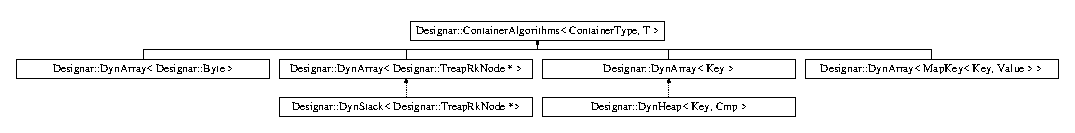
\includegraphics[height=1.337580cm]{class_designar_1_1_container_algorithms}
\end{center}
\end{figure}
\subsection*{Public Member Functions}
\begin{DoxyCompactItemize}
\item 
T $\ast$ \hyperlink{class_designar_1_1_container_algorithms_ae05e29e77ab6d57f7ae5e263bec475c6}{nth\+\_\+ptr} (\hyperlink{namespace_designar_aa72662848b9f4815e7bf31a7cf3e33d1}{nat\+\_\+t} i)
\item 
T \& \hyperlink{class_designar_1_1_container_algorithms_a519e813f4b2e787dfb7d743910ad3e4b}{nth} (\hyperlink{namespace_designar_aa72662848b9f4815e7bf31a7cf3e33d1}{nat\+\_\+t} i)
\item 
const T \& \hyperlink{class_designar_1_1_container_algorithms_aaf323d0085d4be2e234049b7ea77adf9}{nth} (\hyperlink{namespace_designar_aa72662848b9f4815e7bf31a7cf3e33d1}{nat\+\_\+t} i) const
\item 
{\footnotesize template$<$class Op $>$ }\\void \hyperlink{class_designar_1_1_container_algorithms_a32b1ccc6fc97faf17064b55e9224ba32}{for\+\_\+each} (Op \&op) const
\item 
{\footnotesize template$<$class Op $>$ }\\void \hyperlink{class_designar_1_1_container_algorithms_a5fc63764f264b91fd45fd275ecc0f27a}{for\+\_\+each} (Op \&\&op=Op()) const
\item 
{\footnotesize template$<$class Container\+Ret , class Pred $>$ }\\Container\+Ret \hyperlink{class_designar_1_1_container_algorithms_a8fde0ef12e4287386eccf48c381b7fca}{filter} (Pred \&pred) const
\item 
{\footnotesize template$<$class Container\+Ret  = S\+L\+List$<$\+T$>$, class Pred $>$ }\\Container\+Ret \hyperlink{class_designar_1_1_container_algorithms_a9ee9df4da794711c3639a3c86d905443}{filter} (Pred \&\&pred=Pred()) const
\item 
{\footnotesize template$<$typename RetT , class Container\+Ret , class Op $>$ }\\Container\+Ret \hyperlink{class_designar_1_1_container_algorithms_a3b9044a197e4ceec6a1de03de197a293}{map} (Op \&op) const
\item 
{\footnotesize template$<$typename RetT  = T, class Container\+Ret  = S\+L\+List$<$\+Ret\+T$>$, class Op $>$ }\\Container\+Ret \hyperlink{class_designar_1_1_container_algorithms_a9c49c11af28a3093dd133b65a115853b}{map} (Op \&\&op=Op()) const
\item 
{\footnotesize template$<$typename RetT , class Container\+Ret , class Op , class Pred $>$ }\\Container\+Ret \hyperlink{class_designar_1_1_container_algorithms_a9209d9ddf0b4dd85301735c99bcdb171}{map\+\_\+if} (Op \&op, Pred \&pred) const
\item 
{\footnotesize template$<$typename RetT  = T, class Container\+Ret  = S\+L\+List$<$\+Ret\+T$>$, class Op , class Pred $>$ }\\Container\+Ret \hyperlink{class_designar_1_1_container_algorithms_a06b2fbf8f85675b8c69be00399710031}{map\+\_\+if} (Op \&op, Pred \&\&pred=Pred()) const
\item 
{\footnotesize template$<$typename RetT  = T, class Container\+Ret  = S\+L\+List$<$\+Ret\+T$>$, class Op , class Pred $>$ }\\Container\+Ret \hyperlink{class_designar_1_1_container_algorithms_a582b067d39658825339075873f20aee6}{map\+\_\+if} (Op \&\&op, Pred \&pred) const
\item 
{\footnotesize template$<$typename RetT  = T, class Container\+Ret  = S\+L\+List$<$\+Ret\+T$>$, class Op , class Pred $>$ }\\Container\+Ret \hyperlink{class_designar_1_1_container_algorithms_a23ffa9f0af79826db5a8dc04837f9617}{map\+\_\+if} (Op \&\&op=Op(), Pred \&\&pred=Pred()) const
\item 
{\footnotesize template$<$typename RetT , class Op $>$ }\\RetT \hyperlink{class_designar_1_1_container_algorithms_a1b6d1cb2289bf894a2af994e9c6e1d03}{fold} (const RetT \&init\+\_\+val, Op \&op) const
\item 
{\footnotesize template$<$typename RetT  = T, class Op $>$ }\\RetT \hyperlink{class_designar_1_1_container_algorithms_a410f880dab4f206d3d99b31b0a67637d}{fold} (const RetT \&init\+\_\+val, Op \&\&op=Op()) const
\item 
{\footnotesize template$<$typename RetT  = T, class Op $>$ }\\RetT \hyperlink{class_designar_1_1_container_algorithms_a148e3417520a3253663bd2554cad6c67}{fold} (RetT \&\&init\+\_\+val, Op \&op) const
\item 
{\footnotesize template$<$typename RetT  = T, class Op $>$ }\\RetT \hyperlink{class_designar_1_1_container_algorithms_a9ff56a438586390aaf72aa2fda0f86e7}{fold} (RetT \&\&init\+\_\+val, Op \&\&op=Op()) const
\item 
{\footnotesize template$<$class Pred $>$ }\\bool \hyperlink{class_designar_1_1_container_algorithms_a81f6c5f0fa93c2ef34cd8636f503bdf3}{all} (Pred \&pred) const
\item 
{\footnotesize template$<$class Pred $>$ }\\bool \hyperlink{class_designar_1_1_container_algorithms_a1adbc18f2c7a7731ff91f98aae034c45}{all} (Pred \&\&pred=Pred()) const
\item 
{\footnotesize template$<$class Pred $>$ }\\bool \hyperlink{class_designar_1_1_container_algorithms_a84b04f83c37c70e2b25e943ca0579261}{exists} (Pred \&pred) const
\item 
{\footnotesize template$<$class Pred $>$ }\\bool \hyperlink{class_designar_1_1_container_algorithms_a12f255f04ad0c63d58957f2869caff93}{exists} (Pred \&\&pred=Pred()) const
\item 
{\footnotesize template$<$class Pred $>$ }\\bool \hyperlink{class_designar_1_1_container_algorithms_aa91fe441074d132067cb5a3ad7870dc5}{none} (Pred \&pred) const
\item 
{\footnotesize template$<$class Pred $>$ }\\bool \hyperlink{class_designar_1_1_container_algorithms_a10a88dd8adee474d79cc412db2f5739c}{none} (Pred \&\&pred=Pred()) const
\item 
{\footnotesize template$<$class Pred $>$ }\\T $\ast$ \hyperlink{class_designar_1_1_container_algorithms_aa68717192cead08642f941dd4d9f06a1}{search\+\_\+ptr} (Pred \&pred) const
\item 
{\footnotesize template$<$class Pred $>$ }\\T $\ast$ \hyperlink{class_designar_1_1_container_algorithms_a4d399ce473d6cddf3e133044403f492d}{search\+\_\+ptr} (Pred \&\&pred=Pred()) const
\item 
{\footnotesize template$<$class Pred $>$ }\\bool \hyperlink{class_designar_1_1_container_algorithms_a955cc52c438153802a20a97d3e4c148a}{remove\+\_\+first\+\_\+if} (Pred \&pred)
\item 
{\footnotesize template$<$class Pred $>$ }\\bool \hyperlink{class_designar_1_1_container_algorithms_a564239c787d638bfd90846c9587cd6a6}{remove\+\_\+first\+\_\+if} (Pred \&\&pred=Pred())
\item 
{\footnotesize template$<$class Pred $>$ }\\void \hyperlink{class_designar_1_1_container_algorithms_a9f62149769fa7797947d019692306e09}{remove\+\_\+if} (Pred \&pred)
\item 
{\footnotesize template$<$class Pred $>$ }\\void \hyperlink{class_designar_1_1_container_algorithms_ae619268160dffda758b816a0db9bd8a0}{remove\+\_\+if} (Pred \&\&pred=Pred())
\item 
{\footnotesize template$<$class Container\+Type2  = Container\+Type, class Eq $>$ }\\bool \hyperlink{class_designar_1_1_container_algorithms_a022bd7f2c5bd929e44b3e62020336b5c}{equal} (const Container\+Type2 \&c, Eq \&eq) const
\item 
{\footnotesize template$<$class Container\+Type2  = Container\+Type, class Eq  = std\+::equal\+\_\+to$<$\+T$>$$>$ }\\bool \hyperlink{class_designar_1_1_container_algorithms_aece8141a994780c15205aa76d306219b}{equal} (const Container\+Type2 \&c, Eq \&\&eq=Eq()) const
\item 
{\footnotesize template$<$class Cmp $>$ }\\bool \hyperlink{class_designar_1_1_container_algorithms_a7cbb0be554a1f4bad257b2d171be9bec}{is\+\_\+sorted} (Cmp \&cmp) const
\item 
{\footnotesize template$<$class Cmp  = std\+::less$<$\+T$>$$>$ }\\bool \hyperlink{class_designar_1_1_container_algorithms_ae0960afa05917d880b2d7e0f61620f9d}{is\+\_\+sorted} (Cmp \&\&cmp=Cmp()) const
\item 
{\footnotesize template$<$class Container\+Type2  = Container\+Type$>$ }\\\hyperlink{class_designar_1_1_s_l_list}{S\+L\+List}$<$ std\+::pair$<$ T, typename Container\+Type2\+::\+Key\+Type $>$ $>$ \hyperlink{class_designar_1_1_container_algorithms_ae8f296c082fa5e4c2d93a7328414d8f8}{zip} (const Container\+Type2 \&c) const
\item 
{\footnotesize template$<$class Container\+Type2  = Container\+Type$>$ }\\\hyperlink{class_designar_1_1_s_l_list}{S\+L\+List}$<$ std\+::pair$<$ T, typename Container\+Type2\+::\+Key\+Type $>$ $>$ \hyperlink{class_designar_1_1_container_algorithms_a95ada3b5554b754e331c2e6e9a742622}{zip\+\_\+eq} (const Container\+Type2 \&c) const
\item 
{\footnotesize template$<$class Container\+Type2  = Container\+Type$>$ }\\\hyperlink{class_designar_1_1_s_l_list}{S\+L\+List}$<$ std\+::pair$<$ T, typename Container\+Type2\+::\+Key\+Type $>$ $>$ \hyperlink{class_designar_1_1_container_algorithms_adc7bedc6d5b7e9df24cf590ec5e5c5c2}{zip\+\_\+left} (const Container\+Type2 \&c) const
\item 
{\footnotesize template$<$class Container\+Type2  = Container\+Type$>$ }\\\hyperlink{class_designar_1_1_s_l_list}{S\+L\+List}$<$ std\+::pair$<$ T, typename Container\+Type2\+::\+Key\+Type $>$ $>$ \hyperlink{class_designar_1_1_container_algorithms_aafb9d5320b99e9d39ed470b5b295f8b1}{zip\+\_\+right} (const Container\+Type2 \&c) const
\item 
\hyperlink{class_designar_1_1_dyn_array}{Dyn\+Array}$<$ T $>$ \hyperlink{class_designar_1_1_container_algorithms_a2a358d26ad630d1bb5995bff81f66bc4}{to\+\_\+array} () const
\item 
\hyperlink{class_designar_1_1_s_l_list}{S\+L\+List}$<$ T $>$ \hyperlink{class_designar_1_1_container_algorithms_a7800ec47f0b49c369f7341f72c70692a}{to\+\_\+list} () const
\end{DoxyCompactItemize}


\subsection{Detailed Description}
\subsubsection*{template$<$class Container\+Type, typename T$>$\newline
class Designar\+::\+Container\+Algorithms$<$ Container\+Type, T $>$}



Definition at line 33 of file containeralgorithms.\+H.



\subsection{Member Function Documentation}
\mbox{\Hypertarget{class_designar_1_1_container_algorithms_a81f6c5f0fa93c2ef34cd8636f503bdf3}\label{class_designar_1_1_container_algorithms_a81f6c5f0fa93c2ef34cd8636f503bdf3}} 
\index{Designar\+::\+Container\+Algorithms@{Designar\+::\+Container\+Algorithms}!all@{all}}
\index{all@{all}!Designar\+::\+Container\+Algorithms@{Designar\+::\+Container\+Algorithms}}
\subsubsection{\texorpdfstring{all()}{all()}\hspace{0.1cm}{\footnotesize\ttfamily [1/2]}}
{\footnotesize\ttfamily template$<$class Container\+Type, typename T$>$ \\
template$<$class Pred $>$ \\
bool \hyperlink{class_designar_1_1_container_algorithms}{Designar\+::\+Container\+Algorithms}$<$ Container\+Type, T $>$\+::all (\begin{DoxyParamCaption}\item[{Pred \&}]{pred }\end{DoxyParamCaption}) const\hspace{0.3cm}{\ttfamily [inline]}}



Definition at line 152 of file containeralgorithms.\+H.

\mbox{\Hypertarget{class_designar_1_1_container_algorithms_a1adbc18f2c7a7731ff91f98aae034c45}\label{class_designar_1_1_container_algorithms_a1adbc18f2c7a7731ff91f98aae034c45}} 
\index{Designar\+::\+Container\+Algorithms@{Designar\+::\+Container\+Algorithms}!all@{all}}
\index{all@{all}!Designar\+::\+Container\+Algorithms@{Designar\+::\+Container\+Algorithms}}
\subsubsection{\texorpdfstring{all()}{all()}\hspace{0.1cm}{\footnotesize\ttfamily [2/2]}}
{\footnotesize\ttfamily template$<$class Container\+Type, typename T$>$ \\
template$<$class Pred $>$ \\
bool \hyperlink{class_designar_1_1_container_algorithms}{Designar\+::\+Container\+Algorithms}$<$ Container\+Type, T $>$\+::all (\begin{DoxyParamCaption}\item[{Pred \&\&}]{pred = {\ttfamily Pred()} }\end{DoxyParamCaption}) const\hspace{0.3cm}{\ttfamily [inline]}}



Definition at line 158 of file containeralgorithms.\+H.

\mbox{\Hypertarget{class_designar_1_1_container_algorithms_a022bd7f2c5bd929e44b3e62020336b5c}\label{class_designar_1_1_container_algorithms_a022bd7f2c5bd929e44b3e62020336b5c}} 
\index{Designar\+::\+Container\+Algorithms@{Designar\+::\+Container\+Algorithms}!equal@{equal}}
\index{equal@{equal}!Designar\+::\+Container\+Algorithms@{Designar\+::\+Container\+Algorithms}}
\subsubsection{\texorpdfstring{equal()}{equal()}\hspace{0.1cm}{\footnotesize\ttfamily [1/2]}}
{\footnotesize\ttfamily template$<$class Container\+Type, typename T$>$ \\
template$<$class Container\+Type2  = Container\+Type, class Eq $>$ \\
bool \hyperlink{class_designar_1_1_container_algorithms}{Designar\+::\+Container\+Algorithms}$<$ Container\+Type, T $>$\+::equal (\begin{DoxyParamCaption}\item[{const Container\+Type2 \&}]{c,  }\item[{Eq \&}]{eq }\end{DoxyParamCaption}) const\hspace{0.3cm}{\ttfamily [inline]}}



Definition at line 224 of file containeralgorithms.\+H.

\mbox{\Hypertarget{class_designar_1_1_container_algorithms_aece8141a994780c15205aa76d306219b}\label{class_designar_1_1_container_algorithms_aece8141a994780c15205aa76d306219b}} 
\index{Designar\+::\+Container\+Algorithms@{Designar\+::\+Container\+Algorithms}!equal@{equal}}
\index{equal@{equal}!Designar\+::\+Container\+Algorithms@{Designar\+::\+Container\+Algorithms}}
\subsubsection{\texorpdfstring{equal()}{equal()}\hspace{0.1cm}{\footnotesize\ttfamily [2/2]}}
{\footnotesize\ttfamily template$<$class Container\+Type, typename T$>$ \\
template$<$class Container\+Type2  = Container\+Type, class Eq  = std\+::equal\+\_\+to$<$\+T$>$$>$ \\
bool \hyperlink{class_designar_1_1_container_algorithms}{Designar\+::\+Container\+Algorithms}$<$ Container\+Type, T $>$\+::equal (\begin{DoxyParamCaption}\item[{const Container\+Type2 \&}]{c,  }\item[{Eq \&\&}]{eq = {\ttfamily Eq()} }\end{DoxyParamCaption}) const\hspace{0.3cm}{\ttfamily [inline]}}



Definition at line 231 of file containeralgorithms.\+H.

\mbox{\Hypertarget{class_designar_1_1_container_algorithms_a84b04f83c37c70e2b25e943ca0579261}\label{class_designar_1_1_container_algorithms_a84b04f83c37c70e2b25e943ca0579261}} 
\index{Designar\+::\+Container\+Algorithms@{Designar\+::\+Container\+Algorithms}!exists@{exists}}
\index{exists@{exists}!Designar\+::\+Container\+Algorithms@{Designar\+::\+Container\+Algorithms}}
\subsubsection{\texorpdfstring{exists()}{exists()}\hspace{0.1cm}{\footnotesize\ttfamily [1/2]}}
{\footnotesize\ttfamily template$<$class Container\+Type, typename T$>$ \\
template$<$class Pred $>$ \\
bool \hyperlink{class_designar_1_1_container_algorithms}{Designar\+::\+Container\+Algorithms}$<$ Container\+Type, T $>$\+::exists (\begin{DoxyParamCaption}\item[{Pred \&}]{pred }\end{DoxyParamCaption}) const\hspace{0.3cm}{\ttfamily [inline]}}



Definition at line 164 of file containeralgorithms.\+H.

\mbox{\Hypertarget{class_designar_1_1_container_algorithms_a12f255f04ad0c63d58957f2869caff93}\label{class_designar_1_1_container_algorithms_a12f255f04ad0c63d58957f2869caff93}} 
\index{Designar\+::\+Container\+Algorithms@{Designar\+::\+Container\+Algorithms}!exists@{exists}}
\index{exists@{exists}!Designar\+::\+Container\+Algorithms@{Designar\+::\+Container\+Algorithms}}
\subsubsection{\texorpdfstring{exists()}{exists()}\hspace{0.1cm}{\footnotesize\ttfamily [2/2]}}
{\footnotesize\ttfamily template$<$class Container\+Type, typename T$>$ \\
template$<$class Pred $>$ \\
bool \hyperlink{class_designar_1_1_container_algorithms}{Designar\+::\+Container\+Algorithms}$<$ Container\+Type, T $>$\+::exists (\begin{DoxyParamCaption}\item[{Pred \&\&}]{pred = {\ttfamily Pred()} }\end{DoxyParamCaption}) const\hspace{0.3cm}{\ttfamily [inline]}}



Definition at line 170 of file containeralgorithms.\+H.

\mbox{\Hypertarget{class_designar_1_1_container_algorithms_a8fde0ef12e4287386eccf48c381b7fca}\label{class_designar_1_1_container_algorithms_a8fde0ef12e4287386eccf48c381b7fca}} 
\index{Designar\+::\+Container\+Algorithms@{Designar\+::\+Container\+Algorithms}!filter@{filter}}
\index{filter@{filter}!Designar\+::\+Container\+Algorithms@{Designar\+::\+Container\+Algorithms}}
\subsubsection{\texorpdfstring{filter()}{filter()}\hspace{0.1cm}{\footnotesize\ttfamily [1/2]}}
{\footnotesize\ttfamily template$<$class Container\+Type, typename T$>$ \\
template$<$class Container\+Ret , class Pred $>$ \\
Container\+Ret \hyperlink{class_designar_1_1_container_algorithms}{Designar\+::\+Container\+Algorithms}$<$ Container\+Type, T $>$\+::filter (\begin{DoxyParamCaption}\item[{Pred \&}]{pred }\end{DoxyParamCaption}) const\hspace{0.3cm}{\ttfamily [inline]}}



Definition at line 74 of file containeralgorithms.\+H.

\mbox{\Hypertarget{class_designar_1_1_container_algorithms_a9ee9df4da794711c3639a3c86d905443}\label{class_designar_1_1_container_algorithms_a9ee9df4da794711c3639a3c86d905443}} 
\index{Designar\+::\+Container\+Algorithms@{Designar\+::\+Container\+Algorithms}!filter@{filter}}
\index{filter@{filter}!Designar\+::\+Container\+Algorithms@{Designar\+::\+Container\+Algorithms}}
\subsubsection{\texorpdfstring{filter()}{filter()}\hspace{0.1cm}{\footnotesize\ttfamily [2/2]}}
{\footnotesize\ttfamily template$<$class Container\+Type, typename T$>$ \\
template$<$class Container\+Ret  = S\+L\+List$<$\+T$>$, class Pred $>$ \\
Container\+Ret \hyperlink{class_designar_1_1_container_algorithms}{Designar\+::\+Container\+Algorithms}$<$ Container\+Type, T $>$\+::filter (\begin{DoxyParamCaption}\item[{Pred \&\&}]{pred = {\ttfamily Pred()} }\end{DoxyParamCaption}) const\hspace{0.3cm}{\ttfamily [inline]}}



Definition at line 81 of file containeralgorithms.\+H.

\mbox{\Hypertarget{class_designar_1_1_container_algorithms_a1b6d1cb2289bf894a2af994e9c6e1d03}\label{class_designar_1_1_container_algorithms_a1b6d1cb2289bf894a2af994e9c6e1d03}} 
\index{Designar\+::\+Container\+Algorithms@{Designar\+::\+Container\+Algorithms}!fold@{fold}}
\index{fold@{fold}!Designar\+::\+Container\+Algorithms@{Designar\+::\+Container\+Algorithms}}
\subsubsection{\texorpdfstring{fold()}{fold()}\hspace{0.1cm}{\footnotesize\ttfamily [1/4]}}
{\footnotesize\ttfamily template$<$class Container\+Type, typename T$>$ \\
template$<$typename RetT , class Op $>$ \\
RetT \hyperlink{class_designar_1_1_container_algorithms}{Designar\+::\+Container\+Algorithms}$<$ Container\+Type, T $>$\+::fold (\begin{DoxyParamCaption}\item[{const RetT \&}]{init\+\_\+val,  }\item[{Op \&}]{op }\end{DoxyParamCaption}) const\hspace{0.3cm}{\ttfamily [inline]}}



Definition at line 127 of file containeralgorithms.\+H.

\mbox{\Hypertarget{class_designar_1_1_container_algorithms_a410f880dab4f206d3d99b31b0a67637d}\label{class_designar_1_1_container_algorithms_a410f880dab4f206d3d99b31b0a67637d}} 
\index{Designar\+::\+Container\+Algorithms@{Designar\+::\+Container\+Algorithms}!fold@{fold}}
\index{fold@{fold}!Designar\+::\+Container\+Algorithms@{Designar\+::\+Container\+Algorithms}}
\subsubsection{\texorpdfstring{fold()}{fold()}\hspace{0.1cm}{\footnotesize\ttfamily [2/4]}}
{\footnotesize\ttfamily template$<$class Container\+Type, typename T$>$ \\
template$<$typename RetT  = T, class Op $>$ \\
RetT \hyperlink{class_designar_1_1_container_algorithms}{Designar\+::\+Container\+Algorithms}$<$ Container\+Type, T $>$\+::fold (\begin{DoxyParamCaption}\item[{const RetT \&}]{init\+\_\+val,  }\item[{Op \&\&}]{op = {\ttfamily Op()} }\end{DoxyParamCaption}) const\hspace{0.3cm}{\ttfamily [inline]}}



Definition at line 133 of file containeralgorithms.\+H.

\mbox{\Hypertarget{class_designar_1_1_container_algorithms_a148e3417520a3253663bd2554cad6c67}\label{class_designar_1_1_container_algorithms_a148e3417520a3253663bd2554cad6c67}} 
\index{Designar\+::\+Container\+Algorithms@{Designar\+::\+Container\+Algorithms}!fold@{fold}}
\index{fold@{fold}!Designar\+::\+Container\+Algorithms@{Designar\+::\+Container\+Algorithms}}
\subsubsection{\texorpdfstring{fold()}{fold()}\hspace{0.1cm}{\footnotesize\ttfamily [3/4]}}
{\footnotesize\ttfamily template$<$class Container\+Type, typename T$>$ \\
template$<$typename RetT  = T, class Op $>$ \\
RetT \hyperlink{class_designar_1_1_container_algorithms}{Designar\+::\+Container\+Algorithms}$<$ Container\+Type, T $>$\+::fold (\begin{DoxyParamCaption}\item[{RetT \&\&}]{init\+\_\+val,  }\item[{Op \&}]{op }\end{DoxyParamCaption}) const\hspace{0.3cm}{\ttfamily [inline]}}



Definition at line 139 of file containeralgorithms.\+H.

\mbox{\Hypertarget{class_designar_1_1_container_algorithms_a9ff56a438586390aaf72aa2fda0f86e7}\label{class_designar_1_1_container_algorithms_a9ff56a438586390aaf72aa2fda0f86e7}} 
\index{Designar\+::\+Container\+Algorithms@{Designar\+::\+Container\+Algorithms}!fold@{fold}}
\index{fold@{fold}!Designar\+::\+Container\+Algorithms@{Designar\+::\+Container\+Algorithms}}
\subsubsection{\texorpdfstring{fold()}{fold()}\hspace{0.1cm}{\footnotesize\ttfamily [4/4]}}
{\footnotesize\ttfamily template$<$class Container\+Type, typename T$>$ \\
template$<$typename RetT  = T, class Op $>$ \\
RetT \hyperlink{class_designar_1_1_container_algorithms}{Designar\+::\+Container\+Algorithms}$<$ Container\+Type, T $>$\+::fold (\begin{DoxyParamCaption}\item[{RetT \&\&}]{init\+\_\+val,  }\item[{Op \&\&}]{op = {\ttfamily Op()} }\end{DoxyParamCaption}) const\hspace{0.3cm}{\ttfamily [inline]}}



Definition at line 146 of file containeralgorithms.\+H.

\mbox{\Hypertarget{class_designar_1_1_container_algorithms_a32b1ccc6fc97faf17064b55e9224ba32}\label{class_designar_1_1_container_algorithms_a32b1ccc6fc97faf17064b55e9224ba32}} 
\index{Designar\+::\+Container\+Algorithms@{Designar\+::\+Container\+Algorithms}!for\+\_\+each@{for\+\_\+each}}
\index{for\+\_\+each@{for\+\_\+each}!Designar\+::\+Container\+Algorithms@{Designar\+::\+Container\+Algorithms}}
\subsubsection{\texorpdfstring{for\+\_\+each()}{for\_each()}\hspace{0.1cm}{\footnotesize\ttfamily [1/2]}}
{\footnotesize\ttfamily template$<$class Container\+Type, typename T$>$ \\
template$<$class Op $>$ \\
void \hyperlink{class_designar_1_1_container_algorithms}{Designar\+::\+Container\+Algorithms}$<$ Container\+Type, T $>$\+::for\+\_\+each (\begin{DoxyParamCaption}\item[{Op \&}]{op }\end{DoxyParamCaption}) const\hspace{0.3cm}{\ttfamily [inline]}}



Definition at line 62 of file containeralgorithms.\+H.

\mbox{\Hypertarget{class_designar_1_1_container_algorithms_a5fc63764f264b91fd45fd275ecc0f27a}\label{class_designar_1_1_container_algorithms_a5fc63764f264b91fd45fd275ecc0f27a}} 
\index{Designar\+::\+Container\+Algorithms@{Designar\+::\+Container\+Algorithms}!for\+\_\+each@{for\+\_\+each}}
\index{for\+\_\+each@{for\+\_\+each}!Designar\+::\+Container\+Algorithms@{Designar\+::\+Container\+Algorithms}}
\subsubsection{\texorpdfstring{for\+\_\+each()}{for\_each()}\hspace{0.1cm}{\footnotesize\ttfamily [2/2]}}
{\footnotesize\ttfamily template$<$class Container\+Type, typename T$>$ \\
template$<$class Op $>$ \\
void \hyperlink{class_designar_1_1_container_algorithms}{Designar\+::\+Container\+Algorithms}$<$ Container\+Type, T $>$\+::for\+\_\+each (\begin{DoxyParamCaption}\item[{Op \&\&}]{op = {\ttfamily Op()} }\end{DoxyParamCaption}) const\hspace{0.3cm}{\ttfamily [inline]}}



Definition at line 68 of file containeralgorithms.\+H.

\mbox{\Hypertarget{class_designar_1_1_container_algorithms_a7cbb0be554a1f4bad257b2d171be9bec}\label{class_designar_1_1_container_algorithms_a7cbb0be554a1f4bad257b2d171be9bec}} 
\index{Designar\+::\+Container\+Algorithms@{Designar\+::\+Container\+Algorithms}!is\+\_\+sorted@{is\+\_\+sorted}}
\index{is\+\_\+sorted@{is\+\_\+sorted}!Designar\+::\+Container\+Algorithms@{Designar\+::\+Container\+Algorithms}}
\subsubsection{\texorpdfstring{is\+\_\+sorted()}{is\_sorted()}\hspace{0.1cm}{\footnotesize\ttfamily [1/2]}}
{\footnotesize\ttfamily template$<$class Container\+Type, typename T$>$ \\
template$<$class Cmp $>$ \\
bool \hyperlink{class_designar_1_1_container_algorithms}{Designar\+::\+Container\+Algorithms}$<$ Container\+Type, T $>$\+::is\+\_\+sorted (\begin{DoxyParamCaption}\item[{Cmp \&}]{cmp }\end{DoxyParamCaption}) const\hspace{0.3cm}{\ttfamily [inline]}}



Definition at line 237 of file containeralgorithms.\+H.

\mbox{\Hypertarget{class_designar_1_1_container_algorithms_ae0960afa05917d880b2d7e0f61620f9d}\label{class_designar_1_1_container_algorithms_ae0960afa05917d880b2d7e0f61620f9d}} 
\index{Designar\+::\+Container\+Algorithms@{Designar\+::\+Container\+Algorithms}!is\+\_\+sorted@{is\+\_\+sorted}}
\index{is\+\_\+sorted@{is\+\_\+sorted}!Designar\+::\+Container\+Algorithms@{Designar\+::\+Container\+Algorithms}}
\subsubsection{\texorpdfstring{is\+\_\+sorted()}{is\_sorted()}\hspace{0.1cm}{\footnotesize\ttfamily [2/2]}}
{\footnotesize\ttfamily template$<$class Container\+Type, typename T$>$ \\
template$<$class Cmp  = std\+::less$<$\+T$>$$>$ \\
bool \hyperlink{class_designar_1_1_container_algorithms}{Designar\+::\+Container\+Algorithms}$<$ Container\+Type, T $>$\+::is\+\_\+sorted (\begin{DoxyParamCaption}\item[{Cmp \&\&}]{cmp = {\ttfamily Cmp()} }\end{DoxyParamCaption}) const\hspace{0.3cm}{\ttfamily [inline]}}



Definition at line 243 of file containeralgorithms.\+H.

\mbox{\Hypertarget{class_designar_1_1_container_algorithms_a3b9044a197e4ceec6a1de03de197a293}\label{class_designar_1_1_container_algorithms_a3b9044a197e4ceec6a1de03de197a293}} 
\index{Designar\+::\+Container\+Algorithms@{Designar\+::\+Container\+Algorithms}!map@{map}}
\index{map@{map}!Designar\+::\+Container\+Algorithms@{Designar\+::\+Container\+Algorithms}}
\subsubsection{\texorpdfstring{map()}{map()}\hspace{0.1cm}{\footnotesize\ttfamily [1/2]}}
{\footnotesize\ttfamily template$<$class Container\+Type, typename T$>$ \\
template$<$typename RetT , class Container\+Ret , class Op $>$ \\
Container\+Ret \hyperlink{class_designar_1_1_container_algorithms}{Designar\+::\+Container\+Algorithms}$<$ Container\+Type, T $>$\+::map (\begin{DoxyParamCaption}\item[{Op \&}]{op }\end{DoxyParamCaption}) const\hspace{0.3cm}{\ttfamily [inline]}}



Definition at line 87 of file containeralgorithms.\+H.

\mbox{\Hypertarget{class_designar_1_1_container_algorithms_a9c49c11af28a3093dd133b65a115853b}\label{class_designar_1_1_container_algorithms_a9c49c11af28a3093dd133b65a115853b}} 
\index{Designar\+::\+Container\+Algorithms@{Designar\+::\+Container\+Algorithms}!map@{map}}
\index{map@{map}!Designar\+::\+Container\+Algorithms@{Designar\+::\+Container\+Algorithms}}
\subsubsection{\texorpdfstring{map()}{map()}\hspace{0.1cm}{\footnotesize\ttfamily [2/2]}}
{\footnotesize\ttfamily template$<$class Container\+Type, typename T$>$ \\
template$<$typename RetT  = T, class Container\+Ret  = S\+L\+List$<$\+Ret\+T$>$, class Op $>$ \\
Container\+Ret \hyperlink{class_designar_1_1_container_algorithms}{Designar\+::\+Container\+Algorithms}$<$ Container\+Type, T $>$\+::map (\begin{DoxyParamCaption}\item[{Op \&\&}]{op = {\ttfamily Op()} }\end{DoxyParamCaption}) const\hspace{0.3cm}{\ttfamily [inline]}}



Definition at line 93 of file containeralgorithms.\+H.

\mbox{\Hypertarget{class_designar_1_1_container_algorithms_a9209d9ddf0b4dd85301735c99bcdb171}\label{class_designar_1_1_container_algorithms_a9209d9ddf0b4dd85301735c99bcdb171}} 
\index{Designar\+::\+Container\+Algorithms@{Designar\+::\+Container\+Algorithms}!map\+\_\+if@{map\+\_\+if}}
\index{map\+\_\+if@{map\+\_\+if}!Designar\+::\+Container\+Algorithms@{Designar\+::\+Container\+Algorithms}}
\subsubsection{\texorpdfstring{map\+\_\+if()}{map\_if()}\hspace{0.1cm}{\footnotesize\ttfamily [1/4]}}
{\footnotesize\ttfamily template$<$class Container\+Type, typename T$>$ \\
template$<$typename RetT , class Container\+Ret , class Op , class Pred $>$ \\
Container\+Ret \hyperlink{class_designar_1_1_container_algorithms}{Designar\+::\+Container\+Algorithms}$<$ Container\+Type, T $>$\+::map\+\_\+if (\begin{DoxyParamCaption}\item[{Op \&}]{op,  }\item[{Pred \&}]{pred }\end{DoxyParamCaption}) const\hspace{0.3cm}{\ttfamily [inline]}}



Definition at line 99 of file containeralgorithms.\+H.

\mbox{\Hypertarget{class_designar_1_1_container_algorithms_a06b2fbf8f85675b8c69be00399710031}\label{class_designar_1_1_container_algorithms_a06b2fbf8f85675b8c69be00399710031}} 
\index{Designar\+::\+Container\+Algorithms@{Designar\+::\+Container\+Algorithms}!map\+\_\+if@{map\+\_\+if}}
\index{map\+\_\+if@{map\+\_\+if}!Designar\+::\+Container\+Algorithms@{Designar\+::\+Container\+Algorithms}}
\subsubsection{\texorpdfstring{map\+\_\+if()}{map\_if()}\hspace{0.1cm}{\footnotesize\ttfamily [2/4]}}
{\footnotesize\ttfamily template$<$class Container\+Type, typename T$>$ \\
template$<$typename RetT  = T, class Container\+Ret  = S\+L\+List$<$\+Ret\+T$>$, class Op , class Pred $>$ \\
Container\+Ret \hyperlink{class_designar_1_1_container_algorithms}{Designar\+::\+Container\+Algorithms}$<$ Container\+Type, T $>$\+::map\+\_\+if (\begin{DoxyParamCaption}\item[{Op \&}]{op,  }\item[{Pred \&\&}]{pred = {\ttfamily Pred()} }\end{DoxyParamCaption}) const\hspace{0.3cm}{\ttfamily [inline]}}



Definition at line 107 of file containeralgorithms.\+H.

\mbox{\Hypertarget{class_designar_1_1_container_algorithms_a582b067d39658825339075873f20aee6}\label{class_designar_1_1_container_algorithms_a582b067d39658825339075873f20aee6}} 
\index{Designar\+::\+Container\+Algorithms@{Designar\+::\+Container\+Algorithms}!map\+\_\+if@{map\+\_\+if}}
\index{map\+\_\+if@{map\+\_\+if}!Designar\+::\+Container\+Algorithms@{Designar\+::\+Container\+Algorithms}}
\subsubsection{\texorpdfstring{map\+\_\+if()}{map\_if()}\hspace{0.1cm}{\footnotesize\ttfamily [3/4]}}
{\footnotesize\ttfamily template$<$class Container\+Type, typename T$>$ \\
template$<$typename RetT  = T, class Container\+Ret  = S\+L\+List$<$\+Ret\+T$>$, class Op , class Pred $>$ \\
Container\+Ret \hyperlink{class_designar_1_1_container_algorithms}{Designar\+::\+Container\+Algorithms}$<$ Container\+Type, T $>$\+::map\+\_\+if (\begin{DoxyParamCaption}\item[{Op \&\&}]{op,  }\item[{Pred \&}]{pred }\end{DoxyParamCaption}) const\hspace{0.3cm}{\ttfamily [inline]}}



Definition at line 114 of file containeralgorithms.\+H.

\mbox{\Hypertarget{class_designar_1_1_container_algorithms_a23ffa9f0af79826db5a8dc04837f9617}\label{class_designar_1_1_container_algorithms_a23ffa9f0af79826db5a8dc04837f9617}} 
\index{Designar\+::\+Container\+Algorithms@{Designar\+::\+Container\+Algorithms}!map\+\_\+if@{map\+\_\+if}}
\index{map\+\_\+if@{map\+\_\+if}!Designar\+::\+Container\+Algorithms@{Designar\+::\+Container\+Algorithms}}
\subsubsection{\texorpdfstring{map\+\_\+if()}{map\_if()}\hspace{0.1cm}{\footnotesize\ttfamily [4/4]}}
{\footnotesize\ttfamily template$<$class Container\+Type, typename T$>$ \\
template$<$typename RetT  = T, class Container\+Ret  = S\+L\+List$<$\+Ret\+T$>$, class Op , class Pred $>$ \\
Container\+Ret \hyperlink{class_designar_1_1_container_algorithms}{Designar\+::\+Container\+Algorithms}$<$ Container\+Type, T $>$\+::map\+\_\+if (\begin{DoxyParamCaption}\item[{Op \&\&}]{op = {\ttfamily Op()},  }\item[{Pred \&\&}]{pred = {\ttfamily Pred()} }\end{DoxyParamCaption}) const\hspace{0.3cm}{\ttfamily [inline]}}



Definition at line 121 of file containeralgorithms.\+H.

\mbox{\Hypertarget{class_designar_1_1_container_algorithms_aa91fe441074d132067cb5a3ad7870dc5}\label{class_designar_1_1_container_algorithms_aa91fe441074d132067cb5a3ad7870dc5}} 
\index{Designar\+::\+Container\+Algorithms@{Designar\+::\+Container\+Algorithms}!none@{none}}
\index{none@{none}!Designar\+::\+Container\+Algorithms@{Designar\+::\+Container\+Algorithms}}
\subsubsection{\texorpdfstring{none()}{none()}\hspace{0.1cm}{\footnotesize\ttfamily [1/2]}}
{\footnotesize\ttfamily template$<$class Container\+Type, typename T$>$ \\
template$<$class Pred $>$ \\
bool \hyperlink{class_designar_1_1_container_algorithms}{Designar\+::\+Container\+Algorithms}$<$ Container\+Type, T $>$\+::none (\begin{DoxyParamCaption}\item[{Pred \&}]{pred }\end{DoxyParamCaption}) const\hspace{0.3cm}{\ttfamily [inline]}}



Definition at line 176 of file containeralgorithms.\+H.

\mbox{\Hypertarget{class_designar_1_1_container_algorithms_a10a88dd8adee474d79cc412db2f5739c}\label{class_designar_1_1_container_algorithms_a10a88dd8adee474d79cc412db2f5739c}} 
\index{Designar\+::\+Container\+Algorithms@{Designar\+::\+Container\+Algorithms}!none@{none}}
\index{none@{none}!Designar\+::\+Container\+Algorithms@{Designar\+::\+Container\+Algorithms}}
\subsubsection{\texorpdfstring{none()}{none()}\hspace{0.1cm}{\footnotesize\ttfamily [2/2]}}
{\footnotesize\ttfamily template$<$class Container\+Type, typename T$>$ \\
template$<$class Pred $>$ \\
bool \hyperlink{class_designar_1_1_container_algorithms}{Designar\+::\+Container\+Algorithms}$<$ Container\+Type, T $>$\+::none (\begin{DoxyParamCaption}\item[{Pred \&\&}]{pred = {\ttfamily Pred()} }\end{DoxyParamCaption}) const\hspace{0.3cm}{\ttfamily [inline]}}



Definition at line 182 of file containeralgorithms.\+H.

\mbox{\Hypertarget{class_designar_1_1_container_algorithms_a519e813f4b2e787dfb7d743910ad3e4b}\label{class_designar_1_1_container_algorithms_a519e813f4b2e787dfb7d743910ad3e4b}} 
\index{Designar\+::\+Container\+Algorithms@{Designar\+::\+Container\+Algorithms}!nth@{nth}}
\index{nth@{nth}!Designar\+::\+Container\+Algorithms@{Designar\+::\+Container\+Algorithms}}
\subsubsection{\texorpdfstring{nth()}{nth()}\hspace{0.1cm}{\footnotesize\ttfamily [1/2]}}
{\footnotesize\ttfamily template$<$class Container\+Type, typename T$>$ \\
T\& \hyperlink{class_designar_1_1_container_algorithms}{Designar\+::\+Container\+Algorithms}$<$ Container\+Type, T $>$\+::nth (\begin{DoxyParamCaption}\item[{\hyperlink{namespace_designar_aa72662848b9f4815e7bf31a7cf3e33d1}{nat\+\_\+t}}]{i }\end{DoxyParamCaption})\hspace{0.3cm}{\ttfamily [inline]}}



Definition at line 51 of file containeralgorithms.\+H.

\mbox{\Hypertarget{class_designar_1_1_container_algorithms_aaf323d0085d4be2e234049b7ea77adf9}\label{class_designar_1_1_container_algorithms_aaf323d0085d4be2e234049b7ea77adf9}} 
\index{Designar\+::\+Container\+Algorithms@{Designar\+::\+Container\+Algorithms}!nth@{nth}}
\index{nth@{nth}!Designar\+::\+Container\+Algorithms@{Designar\+::\+Container\+Algorithms}}
\subsubsection{\texorpdfstring{nth()}{nth()}\hspace{0.1cm}{\footnotesize\ttfamily [2/2]}}
{\footnotesize\ttfamily template$<$class Container\+Type, typename T$>$ \\
const T\& \hyperlink{class_designar_1_1_container_algorithms}{Designar\+::\+Container\+Algorithms}$<$ Container\+Type, T $>$\+::nth (\begin{DoxyParamCaption}\item[{\hyperlink{namespace_designar_aa72662848b9f4815e7bf31a7cf3e33d1}{nat\+\_\+t}}]{i }\end{DoxyParamCaption}) const\hspace{0.3cm}{\ttfamily [inline]}}



Definition at line 56 of file containeralgorithms.\+H.

\mbox{\Hypertarget{class_designar_1_1_container_algorithms_ae05e29e77ab6d57f7ae5e263bec475c6}\label{class_designar_1_1_container_algorithms_ae05e29e77ab6d57f7ae5e263bec475c6}} 
\index{Designar\+::\+Container\+Algorithms@{Designar\+::\+Container\+Algorithms}!nth\+\_\+ptr@{nth\+\_\+ptr}}
\index{nth\+\_\+ptr@{nth\+\_\+ptr}!Designar\+::\+Container\+Algorithms@{Designar\+::\+Container\+Algorithms}}
\subsubsection{\texorpdfstring{nth\+\_\+ptr()}{nth\_ptr()}}
{\footnotesize\ttfamily template$<$class Container\+Type, typename T$>$ \\
T$\ast$ \hyperlink{class_designar_1_1_container_algorithms}{Designar\+::\+Container\+Algorithms}$<$ Container\+Type, T $>$\+::nth\+\_\+ptr (\begin{DoxyParamCaption}\item[{\hyperlink{namespace_designar_aa72662848b9f4815e7bf31a7cf3e33d1}{nat\+\_\+t}}]{i }\end{DoxyParamCaption})\hspace{0.3cm}{\ttfamily [inline]}}



Definition at line 46 of file containeralgorithms.\+H.

\mbox{\Hypertarget{class_designar_1_1_container_algorithms_a955cc52c438153802a20a97d3e4c148a}\label{class_designar_1_1_container_algorithms_a955cc52c438153802a20a97d3e4c148a}} 
\index{Designar\+::\+Container\+Algorithms@{Designar\+::\+Container\+Algorithms}!remove\+\_\+first\+\_\+if@{remove\+\_\+first\+\_\+if}}
\index{remove\+\_\+first\+\_\+if@{remove\+\_\+first\+\_\+if}!Designar\+::\+Container\+Algorithms@{Designar\+::\+Container\+Algorithms}}
\subsubsection{\texorpdfstring{remove\+\_\+first\+\_\+if()}{remove\_first\_if()}\hspace{0.1cm}{\footnotesize\ttfamily [1/2]}}
{\footnotesize\ttfamily template$<$class Container\+Type, typename T$>$ \\
template$<$class Pred $>$ \\
bool \hyperlink{class_designar_1_1_container_algorithms}{Designar\+::\+Container\+Algorithms}$<$ Container\+Type, T $>$\+::remove\+\_\+first\+\_\+if (\begin{DoxyParamCaption}\item[{Pred \&}]{pred }\end{DoxyParamCaption})\hspace{0.3cm}{\ttfamily [inline]}}



Definition at line 200 of file containeralgorithms.\+H.

\mbox{\Hypertarget{class_designar_1_1_container_algorithms_a564239c787d638bfd90846c9587cd6a6}\label{class_designar_1_1_container_algorithms_a564239c787d638bfd90846c9587cd6a6}} 
\index{Designar\+::\+Container\+Algorithms@{Designar\+::\+Container\+Algorithms}!remove\+\_\+first\+\_\+if@{remove\+\_\+first\+\_\+if}}
\index{remove\+\_\+first\+\_\+if@{remove\+\_\+first\+\_\+if}!Designar\+::\+Container\+Algorithms@{Designar\+::\+Container\+Algorithms}}
\subsubsection{\texorpdfstring{remove\+\_\+first\+\_\+if()}{remove\_first\_if()}\hspace{0.1cm}{\footnotesize\ttfamily [2/2]}}
{\footnotesize\ttfamily template$<$class Container\+Type, typename T$>$ \\
template$<$class Pred $>$ \\
bool \hyperlink{class_designar_1_1_container_algorithms}{Designar\+::\+Container\+Algorithms}$<$ Container\+Type, T $>$\+::remove\+\_\+first\+\_\+if (\begin{DoxyParamCaption}\item[{Pred \&\&}]{pred = {\ttfamily Pred()} }\end{DoxyParamCaption})\hspace{0.3cm}{\ttfamily [inline]}}



Definition at line 206 of file containeralgorithms.\+H.

\mbox{\Hypertarget{class_designar_1_1_container_algorithms_a9f62149769fa7797947d019692306e09}\label{class_designar_1_1_container_algorithms_a9f62149769fa7797947d019692306e09}} 
\index{Designar\+::\+Container\+Algorithms@{Designar\+::\+Container\+Algorithms}!remove\+\_\+if@{remove\+\_\+if}}
\index{remove\+\_\+if@{remove\+\_\+if}!Designar\+::\+Container\+Algorithms@{Designar\+::\+Container\+Algorithms}}
\subsubsection{\texorpdfstring{remove\+\_\+if()}{remove\_if()}\hspace{0.1cm}{\footnotesize\ttfamily [1/2]}}
{\footnotesize\ttfamily template$<$class Container\+Type, typename T$>$ \\
template$<$class Pred $>$ \\
void \hyperlink{class_designar_1_1_container_algorithms}{Designar\+::\+Container\+Algorithms}$<$ Container\+Type, T $>$\+::remove\+\_\+if (\begin{DoxyParamCaption}\item[{Pred \&}]{pred }\end{DoxyParamCaption})\hspace{0.3cm}{\ttfamily [inline]}}



Definition at line 212 of file containeralgorithms.\+H.

\mbox{\Hypertarget{class_designar_1_1_container_algorithms_ae619268160dffda758b816a0db9bd8a0}\label{class_designar_1_1_container_algorithms_ae619268160dffda758b816a0db9bd8a0}} 
\index{Designar\+::\+Container\+Algorithms@{Designar\+::\+Container\+Algorithms}!remove\+\_\+if@{remove\+\_\+if}}
\index{remove\+\_\+if@{remove\+\_\+if}!Designar\+::\+Container\+Algorithms@{Designar\+::\+Container\+Algorithms}}
\subsubsection{\texorpdfstring{remove\+\_\+if()}{remove\_if()}\hspace{0.1cm}{\footnotesize\ttfamily [2/2]}}
{\footnotesize\ttfamily template$<$class Container\+Type, typename T$>$ \\
template$<$class Pred $>$ \\
void \hyperlink{class_designar_1_1_container_algorithms}{Designar\+::\+Container\+Algorithms}$<$ Container\+Type, T $>$\+::remove\+\_\+if (\begin{DoxyParamCaption}\item[{Pred \&\&}]{pred = {\ttfamily Pred()} }\end{DoxyParamCaption})\hspace{0.3cm}{\ttfamily [inline]}}



Definition at line 218 of file containeralgorithms.\+H.

\mbox{\Hypertarget{class_designar_1_1_container_algorithms_aa68717192cead08642f941dd4d9f06a1}\label{class_designar_1_1_container_algorithms_aa68717192cead08642f941dd4d9f06a1}} 
\index{Designar\+::\+Container\+Algorithms@{Designar\+::\+Container\+Algorithms}!search\+\_\+ptr@{search\+\_\+ptr}}
\index{search\+\_\+ptr@{search\+\_\+ptr}!Designar\+::\+Container\+Algorithms@{Designar\+::\+Container\+Algorithms}}
\subsubsection{\texorpdfstring{search\+\_\+ptr()}{search\_ptr()}\hspace{0.1cm}{\footnotesize\ttfamily [1/2]}}
{\footnotesize\ttfamily template$<$class Container\+Type, typename T$>$ \\
template$<$class Pred $>$ \\
T$\ast$ \hyperlink{class_designar_1_1_container_algorithms}{Designar\+::\+Container\+Algorithms}$<$ Container\+Type, T $>$\+::search\+\_\+ptr (\begin{DoxyParamCaption}\item[{Pred \&}]{pred }\end{DoxyParamCaption}) const\hspace{0.3cm}{\ttfamily [inline]}}



Definition at line 188 of file containeralgorithms.\+H.

\mbox{\Hypertarget{class_designar_1_1_container_algorithms_a4d399ce473d6cddf3e133044403f492d}\label{class_designar_1_1_container_algorithms_a4d399ce473d6cddf3e133044403f492d}} 
\index{Designar\+::\+Container\+Algorithms@{Designar\+::\+Container\+Algorithms}!search\+\_\+ptr@{search\+\_\+ptr}}
\index{search\+\_\+ptr@{search\+\_\+ptr}!Designar\+::\+Container\+Algorithms@{Designar\+::\+Container\+Algorithms}}
\subsubsection{\texorpdfstring{search\+\_\+ptr()}{search\_ptr()}\hspace{0.1cm}{\footnotesize\ttfamily [2/2]}}
{\footnotesize\ttfamily template$<$class Container\+Type, typename T$>$ \\
template$<$class Pred $>$ \\
T$\ast$ \hyperlink{class_designar_1_1_container_algorithms}{Designar\+::\+Container\+Algorithms}$<$ Container\+Type, T $>$\+::search\+\_\+ptr (\begin{DoxyParamCaption}\item[{Pred \&\&}]{pred = {\ttfamily Pred()} }\end{DoxyParamCaption}) const\hspace{0.3cm}{\ttfamily [inline]}}



Definition at line 194 of file containeralgorithms.\+H.

\mbox{\Hypertarget{class_designar_1_1_container_algorithms_a2a358d26ad630d1bb5995bff81f66bc4}\label{class_designar_1_1_container_algorithms_a2a358d26ad630d1bb5995bff81f66bc4}} 
\index{Designar\+::\+Container\+Algorithms@{Designar\+::\+Container\+Algorithms}!to\+\_\+array@{to\+\_\+array}}
\index{to\+\_\+array@{to\+\_\+array}!Designar\+::\+Container\+Algorithms@{Designar\+::\+Container\+Algorithms}}
\subsubsection{\texorpdfstring{to\+\_\+array()}{to\_array()}}
{\footnotesize\ttfamily template$<$class Container\+Type, typename T$>$ \\
\hyperlink{class_designar_1_1_dyn_array}{Dyn\+Array}$<$T$>$ \hyperlink{class_designar_1_1_container_algorithms}{Designar\+::\+Container\+Algorithms}$<$ Container\+Type, T $>$\+::to\+\_\+array (\begin{DoxyParamCaption}{ }\end{DoxyParamCaption}) const\hspace{0.3cm}{\ttfamily [inline]}}



Definition at line 288 of file containeralgorithms.\+H.

\mbox{\Hypertarget{class_designar_1_1_container_algorithms_a7800ec47f0b49c369f7341f72c70692a}\label{class_designar_1_1_container_algorithms_a7800ec47f0b49c369f7341f72c70692a}} 
\index{Designar\+::\+Container\+Algorithms@{Designar\+::\+Container\+Algorithms}!to\+\_\+list@{to\+\_\+list}}
\index{to\+\_\+list@{to\+\_\+list}!Designar\+::\+Container\+Algorithms@{Designar\+::\+Container\+Algorithms}}
\subsubsection{\texorpdfstring{to\+\_\+list()}{to\_list()}}
{\footnotesize\ttfamily template$<$class Container\+Type, typename T$>$ \\
\hyperlink{class_designar_1_1_s_l_list}{S\+L\+List}$<$T$>$ \hyperlink{class_designar_1_1_container_algorithms}{Designar\+::\+Container\+Algorithms}$<$ Container\+Type, T $>$\+::to\+\_\+list (\begin{DoxyParamCaption}{ }\end{DoxyParamCaption}) const\hspace{0.3cm}{\ttfamily [inline]}}



Definition at line 293 of file containeralgorithms.\+H.

\mbox{\Hypertarget{class_designar_1_1_container_algorithms_ae8f296c082fa5e4c2d93a7328414d8f8}\label{class_designar_1_1_container_algorithms_ae8f296c082fa5e4c2d93a7328414d8f8}} 
\index{Designar\+::\+Container\+Algorithms@{Designar\+::\+Container\+Algorithms}!zip@{zip}}
\index{zip@{zip}!Designar\+::\+Container\+Algorithms@{Designar\+::\+Container\+Algorithms}}
\subsubsection{\texorpdfstring{zip()}{zip()}}
{\footnotesize\ttfamily template$<$class Container\+Type, typename T$>$ \\
template$<$class Container\+Type2  = Container\+Type$>$ \\
\hyperlink{class_designar_1_1_s_l_list}{S\+L\+List}$<$std\+::pair$<$T, typename Container\+Type2\+::\+Key\+Type$>$ $>$ \hyperlink{class_designar_1_1_container_algorithms}{Designar\+::\+Container\+Algorithms}$<$ Container\+Type, T $>$\+::zip (\begin{DoxyParamCaption}\item[{const Container\+Type2 \&}]{c }\end{DoxyParamCaption}) const\hspace{0.3cm}{\ttfamily [inline]}}



Definition at line 250 of file containeralgorithms.\+H.

\mbox{\Hypertarget{class_designar_1_1_container_algorithms_a95ada3b5554b754e331c2e6e9a742622}\label{class_designar_1_1_container_algorithms_a95ada3b5554b754e331c2e6e9a742622}} 
\index{Designar\+::\+Container\+Algorithms@{Designar\+::\+Container\+Algorithms}!zip\+\_\+eq@{zip\+\_\+eq}}
\index{zip\+\_\+eq@{zip\+\_\+eq}!Designar\+::\+Container\+Algorithms@{Designar\+::\+Container\+Algorithms}}
\subsubsection{\texorpdfstring{zip\+\_\+eq()}{zip\_eq()}}
{\footnotesize\ttfamily template$<$class Container\+Type, typename T$>$ \\
template$<$class Container\+Type2  = Container\+Type$>$ \\
\hyperlink{class_designar_1_1_s_l_list}{S\+L\+List}$<$std\+::pair$<$T, typename Container\+Type2\+::\+Key\+Type$>$ $>$ \hyperlink{class_designar_1_1_container_algorithms}{Designar\+::\+Container\+Algorithms}$<$ Container\+Type, T $>$\+::zip\+\_\+eq (\begin{DoxyParamCaption}\item[{const Container\+Type2 \&}]{c }\end{DoxyParamCaption}) const\hspace{0.3cm}{\ttfamily [inline]}}



Definition at line 260 of file containeralgorithms.\+H.

\mbox{\Hypertarget{class_designar_1_1_container_algorithms_adc7bedc6d5b7e9df24cf590ec5e5c5c2}\label{class_designar_1_1_container_algorithms_adc7bedc6d5b7e9df24cf590ec5e5c5c2}} 
\index{Designar\+::\+Container\+Algorithms@{Designar\+::\+Container\+Algorithms}!zip\+\_\+left@{zip\+\_\+left}}
\index{zip\+\_\+left@{zip\+\_\+left}!Designar\+::\+Container\+Algorithms@{Designar\+::\+Container\+Algorithms}}
\subsubsection{\texorpdfstring{zip\+\_\+left()}{zip\_left()}}
{\footnotesize\ttfamily template$<$class Container\+Type, typename T$>$ \\
template$<$class Container\+Type2  = Container\+Type$>$ \\
\hyperlink{class_designar_1_1_s_l_list}{S\+L\+List}$<$std\+::pair$<$T, typename Container\+Type2\+::\+Key\+Type$>$ $>$ \hyperlink{class_designar_1_1_container_algorithms}{Designar\+::\+Container\+Algorithms}$<$ Container\+Type, T $>$\+::zip\+\_\+left (\begin{DoxyParamCaption}\item[{const Container\+Type2 \&}]{c }\end{DoxyParamCaption}) const\hspace{0.3cm}{\ttfamily [inline]}}



Definition at line 270 of file containeralgorithms.\+H.

\mbox{\Hypertarget{class_designar_1_1_container_algorithms_aafb9d5320b99e9d39ed470b5b295f8b1}\label{class_designar_1_1_container_algorithms_aafb9d5320b99e9d39ed470b5b295f8b1}} 
\index{Designar\+::\+Container\+Algorithms@{Designar\+::\+Container\+Algorithms}!zip\+\_\+right@{zip\+\_\+right}}
\index{zip\+\_\+right@{zip\+\_\+right}!Designar\+::\+Container\+Algorithms@{Designar\+::\+Container\+Algorithms}}
\subsubsection{\texorpdfstring{zip\+\_\+right()}{zip\_right()}}
{\footnotesize\ttfamily template$<$class Container\+Type, typename T$>$ \\
template$<$class Container\+Type2  = Container\+Type$>$ \\
\hyperlink{class_designar_1_1_s_l_list}{S\+L\+List}$<$std\+::pair$<$T, typename Container\+Type2\+::\+Key\+Type$>$ $>$ \hyperlink{class_designar_1_1_container_algorithms}{Designar\+::\+Container\+Algorithms}$<$ Container\+Type, T $>$\+::zip\+\_\+right (\begin{DoxyParamCaption}\item[{const Container\+Type2 \&}]{c }\end{DoxyParamCaption}) const\hspace{0.3cm}{\ttfamily [inline]}}



Definition at line 280 of file containeralgorithms.\+H.



The documentation for this class was generated from the following file\+:\begin{DoxyCompactItemize}
\item 
include/\hyperlink{containeralgorithms_8_h}{containeralgorithms.\+H}\end{DoxyCompactItemize}

\hypertarget{class_designar_1_1_default_distance}{}\section{Referencia de la plantilla de la Clase Designar\+:\+:Default\+Distance$<$ GT $>$}
\label{class_designar_1_1_default_distance}\index{Designar\+::\+Default\+Distance$<$ G\+T $>$@{Designar\+::\+Default\+Distance$<$ G\+T $>$}}


{\ttfamily \#include $<$graphalgorithms.\+H$>$}

\subsection*{Tipos públicos}
\begin{DoxyCompactItemize}
\item 
using \hyperlink{class_designar_1_1_default_distance_a9317a5edf566779550b96edd532b502b}{Type} = typename G\+T\+::\+Arc\+Info\+Type
\end{DoxyCompactItemize}
\subsection*{Métodos públicos}
\begin{DoxyCompactItemize}
\item 
\hyperlink{class_designar_1_1_default_distance_a9317a5edf566779550b96edd532b502b}{Type} \& \hyperlink{class_designar_1_1_default_distance_ac601666aabb51229c4ceff72cd7d82db}{operator()} (typename G\+T\+::\+Arc \&a)
\item 
const \hyperlink{class_designar_1_1_default_distance_a9317a5edf566779550b96edd532b502b}{Type} \& \hyperlink{class_designar_1_1_default_distance_aeba8bd2867faf7d86dd0bcae6b690136}{operator()} (const typename G\+T\+::\+Arc \&a) const
\end{DoxyCompactItemize}
\subsection*{Atributos públicos estáticos}
\begin{DoxyCompactItemize}
\item 
static constexpr \hyperlink{class_designar_1_1_default_distance_a9317a5edf566779550b96edd532b502b}{Type} \hyperlink{class_designar_1_1_default_distance_abee3d9a2a3f573d6844c0a0fdbd4d7ac}{Z\+E\+RO} = 0
\item 
static constexpr \hyperlink{class_designar_1_1_default_distance_a9317a5edf566779550b96edd532b502b}{Type} \hyperlink{class_designar_1_1_default_distance_af1c417705ee2d66f828c0f872607a7ea}{M\+AX} = std\+::numeric\+\_\+limits$<$\hyperlink{class_designar_1_1_default_distance_a9317a5edf566779550b96edd532b502b}{Type}$>$\+::max()
\end{DoxyCompactItemize}


\subsection{Descripción detallada}
\subsubsection*{template$<$class GT$>$\newline
class Designar\+::\+Default\+Distance$<$ G\+T $>$}



Definición en la línea 1056 del archivo graphalgorithms.\+H.



\subsection{Documentación de los \textquotesingle{}Typedef\textquotesingle{} miembros de la clase}
\mbox{\Hypertarget{class_designar_1_1_default_distance_a9317a5edf566779550b96edd532b502b}\label{class_designar_1_1_default_distance_a9317a5edf566779550b96edd532b502b}} 
\index{Designar\+::\+Default\+Distance@{Designar\+::\+Default\+Distance}!Type@{Type}}
\index{Type@{Type}!Designar\+::\+Default\+Distance@{Designar\+::\+Default\+Distance}}
\subsubsection{\texorpdfstring{Type}{Type}}
{\footnotesize\ttfamily template$<$class GT$>$ \\
using \hyperlink{class_designar_1_1_default_distance}{Designar\+::\+Default\+Distance}$<$ \hyperlink{demo-buildgraph_8_c_a3001c40d2c31ca87ed96cd7d1334a55e}{GT} $>$\+::\hyperlink{class_designar_1_1_default_distance_a9317a5edf566779550b96edd532b502b}{Type} =  typename G\+T\+::\+Arc\+Info\+Type}



Definición en la línea 1059 del archivo graphalgorithms.\+H.



\subsection{Documentación de las funciones miembro}
\mbox{\Hypertarget{class_designar_1_1_default_distance_ac601666aabb51229c4ceff72cd7d82db}\label{class_designar_1_1_default_distance_ac601666aabb51229c4ceff72cd7d82db}} 
\index{Designar\+::\+Default\+Distance@{Designar\+::\+Default\+Distance}!operator()@{operator()}}
\index{operator()@{operator()}!Designar\+::\+Default\+Distance@{Designar\+::\+Default\+Distance}}
\subsubsection{\texorpdfstring{operator()()}{operator()()}\hspace{0.1cm}{\footnotesize\ttfamily [1/2]}}
{\footnotesize\ttfamily template$<$class GT$>$ \\
\hyperlink{class_designar_1_1_default_distance_a9317a5edf566779550b96edd532b502b}{Type}\& \hyperlink{class_designar_1_1_default_distance}{Designar\+::\+Default\+Distance}$<$ \hyperlink{demo-buildgraph_8_c_a3001c40d2c31ca87ed96cd7d1334a55e}{GT} $>$\+::operator() (\begin{DoxyParamCaption}\item[{typename G\+T\+::\+Arc \&}]{a }\end{DoxyParamCaption})\hspace{0.3cm}{\ttfamily [inline]}}



Definición en la línea 1064 del archivo graphalgorithms.\+H.

\mbox{\Hypertarget{class_designar_1_1_default_distance_aeba8bd2867faf7d86dd0bcae6b690136}\label{class_designar_1_1_default_distance_aeba8bd2867faf7d86dd0bcae6b690136}} 
\index{Designar\+::\+Default\+Distance@{Designar\+::\+Default\+Distance}!operator()@{operator()}}
\index{operator()@{operator()}!Designar\+::\+Default\+Distance@{Designar\+::\+Default\+Distance}}
\subsubsection{\texorpdfstring{operator()()}{operator()()}\hspace{0.1cm}{\footnotesize\ttfamily [2/2]}}
{\footnotesize\ttfamily template$<$class GT$>$ \\
const \hyperlink{class_designar_1_1_default_distance_a9317a5edf566779550b96edd532b502b}{Type}\& \hyperlink{class_designar_1_1_default_distance}{Designar\+::\+Default\+Distance}$<$ \hyperlink{demo-buildgraph_8_c_a3001c40d2c31ca87ed96cd7d1334a55e}{GT} $>$\+::operator() (\begin{DoxyParamCaption}\item[{const typename G\+T\+::\+Arc \&}]{a }\end{DoxyParamCaption}) const\hspace{0.3cm}{\ttfamily [inline]}}



Definición en la línea 1069 del archivo graphalgorithms.\+H.



\subsection{Documentación de los datos miembro}
\mbox{\Hypertarget{class_designar_1_1_default_distance_af1c417705ee2d66f828c0f872607a7ea}\label{class_designar_1_1_default_distance_af1c417705ee2d66f828c0f872607a7ea}} 
\index{Designar\+::\+Default\+Distance@{Designar\+::\+Default\+Distance}!M\+AX@{M\+AX}}
\index{M\+AX@{M\+AX}!Designar\+::\+Default\+Distance@{Designar\+::\+Default\+Distance}}
\subsubsection{\texorpdfstring{M\+AX}{MAX}}
{\footnotesize\ttfamily template$<$class GT$>$ \\
constexpr \hyperlink{class_designar_1_1_default_distance_a9317a5edf566779550b96edd532b502b}{Type} \hyperlink{class_designar_1_1_default_distance}{Designar\+::\+Default\+Distance}$<$ \hyperlink{demo-buildgraph_8_c_a3001c40d2c31ca87ed96cd7d1334a55e}{GT} $>$\+::M\+AX = std\+::numeric\+\_\+limits$<$\hyperlink{class_designar_1_1_default_distance_a9317a5edf566779550b96edd532b502b}{Type}$>$\+::max()\hspace{0.3cm}{\ttfamily [static]}}



Definición en la línea 1062 del archivo graphalgorithms.\+H.

\mbox{\Hypertarget{class_designar_1_1_default_distance_abee3d9a2a3f573d6844c0a0fdbd4d7ac}\label{class_designar_1_1_default_distance_abee3d9a2a3f573d6844c0a0fdbd4d7ac}} 
\index{Designar\+::\+Default\+Distance@{Designar\+::\+Default\+Distance}!Z\+E\+RO@{Z\+E\+RO}}
\index{Z\+E\+RO@{Z\+E\+RO}!Designar\+::\+Default\+Distance@{Designar\+::\+Default\+Distance}}
\subsubsection{\texorpdfstring{Z\+E\+RO}{ZERO}}
{\footnotesize\ttfamily template$<$class GT$>$ \\
constexpr \hyperlink{class_designar_1_1_default_distance_a9317a5edf566779550b96edd532b502b}{Type} \hyperlink{class_designar_1_1_default_distance}{Designar\+::\+Default\+Distance}$<$ \hyperlink{demo-buildgraph_8_c_a3001c40d2c31ca87ed96cd7d1334a55e}{GT} $>$\+::Z\+E\+RO = 0\hspace{0.3cm}{\ttfamily [static]}}



Definición en la línea 1061 del archivo graphalgorithms.\+H.



La documentación para esta clase fue generada a partir del siguiente fichero\+:\begin{DoxyCompactItemize}
\item 
include/\hyperlink{graphalgorithms_8_h}{graphalgorithms.\+H}\end{DoxyCompactItemize}

\hypertarget{class_designar_1_1_default_heuristic}{}\section{Designar\+:\+:Default\+Heuristic$<$ GT, Distance $>$ Class Template Reference}
\label{class_designar_1_1_default_heuristic}\index{Designar\+::\+Default\+Heuristic$<$ G\+T, Distance $>$@{Designar\+::\+Default\+Heuristic$<$ G\+T, Distance $>$}}


{\ttfamily \#include $<$graphalgorithms.\+H$>$}

\subsection*{Public Member Functions}
\begin{DoxyCompactItemize}
\item 
Distance\+::\+Type \hyperlink{class_designar_1_1_default_heuristic_ab4a8fc009f9235163ac5696d166b287f}{operator()} (typename \hyperlink{test-mtreenode_8_c_a17a24b0725f59987143c5faf63c4dc6f}{G\+T\+::\+Node} \&, typename \hyperlink{test-mtreenode_8_c_a17a24b0725f59987143c5faf63c4dc6f}{G\+T\+::\+Node} \&)
\end{DoxyCompactItemize}


\subsection{Detailed Description}
\subsubsection*{template$<$class GT, class Distance$>$\newline
class Designar\+::\+Default\+Heuristic$<$ G\+T, Distance $>$}



Definition at line 1676 of file graphalgorithms.\+H.



\subsection{Member Function Documentation}
\mbox{\Hypertarget{class_designar_1_1_default_heuristic_ab4a8fc009f9235163ac5696d166b287f}\label{class_designar_1_1_default_heuristic_ab4a8fc009f9235163ac5696d166b287f}} 
\index{Designar\+::\+Default\+Heuristic@{Designar\+::\+Default\+Heuristic}!operator()@{operator()}}
\index{operator()@{operator()}!Designar\+::\+Default\+Heuristic@{Designar\+::\+Default\+Heuristic}}
\subsubsection{\texorpdfstring{operator()()}{operator()()}}
{\footnotesize\ttfamily template$<$class GT, class Distance$>$ \\
Distance\+::\+Type \hyperlink{class_designar_1_1_default_heuristic}{Designar\+::\+Default\+Heuristic}$<$ \hyperlink{demo-buildgraph_8_c_a3001c40d2c31ca87ed96cd7d1334a55e}{GT}, Distance $>$\+::operator() (\begin{DoxyParamCaption}\item[{typename \hyperlink{test-mtreenode_8_c_a17a24b0725f59987143c5faf63c4dc6f}{G\+T\+::\+Node} \&}]{,  }\item[{typename \hyperlink{test-mtreenode_8_c_a17a24b0725f59987143c5faf63c4dc6f}{G\+T\+::\+Node} \&}]{ }\end{DoxyParamCaption})\hspace{0.3cm}{\ttfamily [inline]}}



Definition at line 1679 of file graphalgorithms.\+H.



The documentation for this class was generated from the following file\+:\begin{DoxyCompactItemize}
\item 
/home/julio/\+De\+S\+I\+G\+N\+A\+R-\/doc/\+De\+Si\+G\+N\+A\+R/include/\hyperlink{graphalgorithms_8_h}{graphalgorithms.\+H}\end{DoxyCompactItemize}

\hypertarget{class_designar_1_1_dft_arc_init}{}\section{Designar\+:\+:Dft\+Arc\+Init$<$ GT $>$ Class Template Reference}
\label{class_designar_1_1_dft_arc_init}\index{Designar\+::\+Dft\+Arc\+Init$<$ G\+T $>$@{Designar\+::\+Dft\+Arc\+Init$<$ G\+T $>$}}


{\ttfamily \#include $<$graphutilities.\+H$>$}

\subsection*{Public Member Functions}
\begin{DoxyCompactItemize}
\item 
void \hyperlink{class_designar_1_1_dft_arc_init_a93a8fffe70b19c86510dd4c2588d6249}{operator()} (\hyperlink{namespace_designar_a3f55fb5513d62ff47cbc8f72b8e95d6f}{Arc}$<$ \hyperlink{demo-buildgraph_8_c_a3001c40d2c31ca87ed96cd7d1334a55e}{GT} $>$ \&)
\end{DoxyCompactItemize}


\subsection{Detailed Description}
\subsubsection*{template$<$class GT$>$\newline
class Designar\+::\+Dft\+Arc\+Init$<$ G\+T $>$}



Definition at line 627 of file graphutilities.\+H.



\subsection{Member Function Documentation}
\mbox{\Hypertarget{class_designar_1_1_dft_arc_init_a93a8fffe70b19c86510dd4c2588d6249}\label{class_designar_1_1_dft_arc_init_a93a8fffe70b19c86510dd4c2588d6249}} 
\index{Designar\+::\+Dft\+Arc\+Init@{Designar\+::\+Dft\+Arc\+Init}!operator()@{operator()}}
\index{operator()@{operator()}!Designar\+::\+Dft\+Arc\+Init@{Designar\+::\+Dft\+Arc\+Init}}
\subsubsection{\texorpdfstring{operator()()}{operator()()}}
{\footnotesize\ttfamily template$<$class GT $>$ \\
void \hyperlink{class_designar_1_1_dft_arc_init}{Designar\+::\+Dft\+Arc\+Init}$<$ \hyperlink{demo-buildgraph_8_c_a3001c40d2c31ca87ed96cd7d1334a55e}{GT} $>$\+::operator() (\begin{DoxyParamCaption}\item[{\hyperlink{namespace_designar_a3f55fb5513d62ff47cbc8f72b8e95d6f}{Arc}$<$ \hyperlink{demo-buildgraph_8_c_a3001c40d2c31ca87ed96cd7d1334a55e}{GT} $>$ \&}]{ }\end{DoxyParamCaption})\hspace{0.3cm}{\ttfamily [inline]}}



Definition at line 630 of file graphutilities.\+H.



The documentation for this class was generated from the following file\+:\begin{DoxyCompactItemize}
\item 
include/\hyperlink{graphutilities_8_h}{graphutilities.\+H}\end{DoxyCompactItemize}

\hypertarget{struct_designar_1_1_dft_dot_arc_attr}{}\section{Referencia de la plantilla de la Estructura Designar\+:\+:Dft\+Dot\+Arc\+Attr$<$ GT $>$}
\label{struct_designar_1_1_dft_dot_arc_attr}\index{Designar\+::\+Dft\+Dot\+Arc\+Attr$<$ G\+T $>$@{Designar\+::\+Dft\+Dot\+Arc\+Attr$<$ G\+T $>$}}


{\ttfamily \#include $<$graphutilities.\+H$>$}

\subsection*{Métodos públicos}
\begin{DoxyCompactItemize}
\item 
std\+::string \hyperlink{struct_designar_1_1_dft_dot_arc_attr_ab98550f41b109bbd2d479355ad9de769}{operator()} (const \hyperlink{namespace_designar_a3f55fb5513d62ff47cbc8f72b8e95d6f}{Arc}$<$ \hyperlink{demo-buildgraph_8_c_a3001c40d2c31ca87ed96cd7d1334a55e}{GT} $>$ \&a)
\end{DoxyCompactItemize}


\subsection{Descripción detallada}
\subsubsection*{template$<$class GT$>$\newline
struct Designar\+::\+Dft\+Dot\+Arc\+Attr$<$ G\+T $>$}



Definición en la línea 650 del archivo graphutilities.\+H.



\subsection{Documentación de las funciones miembro}
\mbox{\Hypertarget{struct_designar_1_1_dft_dot_arc_attr_ab98550f41b109bbd2d479355ad9de769}\label{struct_designar_1_1_dft_dot_arc_attr_ab98550f41b109bbd2d479355ad9de769}} 
\index{Designar\+::\+Dft\+Dot\+Arc\+Attr@{Designar\+::\+Dft\+Dot\+Arc\+Attr}!operator()@{operator()}}
\index{operator()@{operator()}!Designar\+::\+Dft\+Dot\+Arc\+Attr@{Designar\+::\+Dft\+Dot\+Arc\+Attr}}
\subsubsection{\texorpdfstring{operator()()}{operator()()}}
{\footnotesize\ttfamily template$<$class GT$>$ \\
std\+::string \hyperlink{struct_designar_1_1_dft_dot_arc_attr}{Designar\+::\+Dft\+Dot\+Arc\+Attr}$<$ \hyperlink{demo-buildgraph_8_c_a3001c40d2c31ca87ed96cd7d1334a55e}{GT} $>$\+::operator() (\begin{DoxyParamCaption}\item[{const \hyperlink{namespace_designar_a3f55fb5513d62ff47cbc8f72b8e95d6f}{Arc}$<$ \hyperlink{demo-buildgraph_8_c_a3001c40d2c31ca87ed96cd7d1334a55e}{GT} $>$ \&}]{a }\end{DoxyParamCaption})\hspace{0.3cm}{\ttfamily [inline]}}



Definición en la línea 652 del archivo graphutilities.\+H.



La documentación para esta estructura fue generada a partir del siguiente fichero\+:\begin{DoxyCompactItemize}
\item 
include/\hyperlink{graphutilities_8_h}{graphutilities.\+H}\end{DoxyCompactItemize}

\hypertarget{class_designar_1_1_dft_dot_graph_attr}{}\section{Designar\+:\+:Dft\+Dot\+Graph\+Attr$<$ GT $>$ Class Template Reference}
\label{class_designar_1_1_dft_dot_graph_attr}\index{Designar\+::\+Dft\+Dot\+Graph\+Attr$<$ G\+T $>$@{Designar\+::\+Dft\+Dot\+Graph\+Attr$<$ G\+T $>$}}


{\ttfamily \#include $<$graphutilities.\+H$>$}

\subsection*{Public Member Functions}
\begin{DoxyCompactItemize}
\item 
std\+::string \hyperlink{class_designar_1_1_dft_dot_graph_attr_ab543d70d47040459bf4284e5cf8106f5}{operator()} (const \hyperlink{demo-buildgraph_8_c_a3001c40d2c31ca87ed96cd7d1334a55e}{GT} \&)
\end{DoxyCompactItemize}


\subsection{Detailed Description}
\subsubsection*{template$<$class GT$>$\newline
class Designar\+::\+Dft\+Dot\+Graph\+Attr$<$ G\+T $>$}



Definition at line 661 of file graphutilities.\+H.



\subsection{Member Function Documentation}
\mbox{\Hypertarget{class_designar_1_1_dft_dot_graph_attr_ab543d70d47040459bf4284e5cf8106f5}\label{class_designar_1_1_dft_dot_graph_attr_ab543d70d47040459bf4284e5cf8106f5}} 
\index{Designar\+::\+Dft\+Dot\+Graph\+Attr@{Designar\+::\+Dft\+Dot\+Graph\+Attr}!operator()@{operator()}}
\index{operator()@{operator()}!Designar\+::\+Dft\+Dot\+Graph\+Attr@{Designar\+::\+Dft\+Dot\+Graph\+Attr}}
\subsubsection{\texorpdfstring{operator()()}{operator()()}}
{\footnotesize\ttfamily template$<$class GT $>$ \\
std\+::string \hyperlink{class_designar_1_1_dft_dot_graph_attr}{Designar\+::\+Dft\+Dot\+Graph\+Attr}$<$ \hyperlink{demo-buildgraph_8_c_a3001c40d2c31ca87ed96cd7d1334a55e}{GT} $>$\+::operator() (\begin{DoxyParamCaption}\item[{const \hyperlink{demo-buildgraph_8_c_a3001c40d2c31ca87ed96cd7d1334a55e}{GT} \&}]{ }\end{DoxyParamCaption})\hspace{0.3cm}{\ttfamily [inline]}}



Definition at line 664 of file graphutilities.\+H.



The documentation for this class was generated from the following file\+:\begin{DoxyCompactItemize}
\item 
include/\hyperlink{graphutilities_8_h}{graphutilities.\+H}\end{DoxyCompactItemize}

\hypertarget{class_designar_1_1_dft_dot_node_attr}{}\section{Designar\+:\+:Dft\+Dot\+Node\+Attr$<$ GT $>$ Class Template Reference}
\label{class_designar_1_1_dft_dot_node_attr}\index{Designar\+::\+Dft\+Dot\+Node\+Attr$<$ G\+T $>$@{Designar\+::\+Dft\+Dot\+Node\+Attr$<$ G\+T $>$}}


{\ttfamily \#include $<$graphutilities.\+H$>$}

\subsection*{Public Member Functions}
\begin{DoxyCompactItemize}
\item 
std\+::string \hyperlink{class_designar_1_1_dft_dot_node_attr_a7427d5a0fe37ecbb7fa9c07f9486d609}{operator()} (const \hyperlink{namespace_designar_a5af326c65aa2bd26b26c410f2030d09e}{Node}$<$ \hyperlink{demo-buildgraph_8_c_a3001c40d2c31ca87ed96cd7d1334a55e}{GT} $>$ \&p)
\end{DoxyCompactItemize}


\subsection{Detailed Description}
\subsubsection*{template$<$class GT$>$\newline
class Designar\+::\+Dft\+Dot\+Node\+Attr$<$ G\+T $>$}



Definition at line 638 of file graphutilities.\+H.



\subsection{Member Function Documentation}
\mbox{\Hypertarget{class_designar_1_1_dft_dot_node_attr_a7427d5a0fe37ecbb7fa9c07f9486d609}\label{class_designar_1_1_dft_dot_node_attr_a7427d5a0fe37ecbb7fa9c07f9486d609}} 
\index{Designar\+::\+Dft\+Dot\+Node\+Attr@{Designar\+::\+Dft\+Dot\+Node\+Attr}!operator()@{operator()}}
\index{operator()@{operator()}!Designar\+::\+Dft\+Dot\+Node\+Attr@{Designar\+::\+Dft\+Dot\+Node\+Attr}}
\subsubsection{\texorpdfstring{operator()()}{operator()()}}
{\footnotesize\ttfamily template$<$class GT$>$ \\
std\+::string \hyperlink{class_designar_1_1_dft_dot_node_attr}{Designar\+::\+Dft\+Dot\+Node\+Attr}$<$ \hyperlink{demo-buildgraph_8_c_a3001c40d2c31ca87ed96cd7d1334a55e}{GT} $>$\+::operator() (\begin{DoxyParamCaption}\item[{const \hyperlink{namespace_designar_a5af326c65aa2bd26b26c410f2030d09e}{Node}$<$ \hyperlink{demo-buildgraph_8_c_a3001c40d2c31ca87ed96cd7d1334a55e}{GT} $>$ \&}]{p }\end{DoxyParamCaption})\hspace{0.3cm}{\ttfamily [inline]}}



Definition at line 641 of file graphutilities.\+H.



The documentation for this class was generated from the following file\+:\begin{DoxyCompactItemize}
\item 
include/\hyperlink{graphutilities_8_h}{graphutilities.\+H}\end{DoxyCompactItemize}

\hypertarget{class_designar_1_1_dft_grid_arc_init}{}\section{Referencia de la plantilla de la Clase Designar\+:\+:Dft\+Grid\+Arc\+Init$<$ GT $>$}
\label{class_designar_1_1_dft_grid_arc_init}\index{Designar\+::\+Dft\+Grid\+Arc\+Init$<$ G\+T $>$@{Designar\+::\+Dft\+Grid\+Arc\+Init$<$ G\+T $>$}}


{\ttfamily \#include $<$graphutilities.\+H$>$}

\subsection*{Métodos públicos}
\begin{DoxyCompactItemize}
\item 
void \hyperlink{class_designar_1_1_dft_grid_arc_init_aa454d871716af2f3a9c7c0758b8f8af4}{operator()} (\hyperlink{namespace_designar_a3f55fb5513d62ff47cbc8f72b8e95d6f}{Arc}$<$ \hyperlink{demo-buildgraph_8_c_a3001c40d2c31ca87ed96cd7d1334a55e}{GT} $>$ \&, \hyperlink{namespace_designar_aa72662848b9f4815e7bf31a7cf3e33d1}{nat\+\_\+t}, \hyperlink{namespace_designar_aa72662848b9f4815e7bf31a7cf3e33d1}{nat\+\_\+t})
\end{DoxyCompactItemize}


\subsection{Descripción detallada}
\subsubsection*{template$<$class GT$>$\newline
class Designar\+::\+Dft\+Grid\+Arc\+Init$<$ G\+T $>$}



Definición en la línea 607 del archivo graphutilities.\+H.



\subsection{Documentación de las funciones miembro}
\mbox{\Hypertarget{class_designar_1_1_dft_grid_arc_init_aa454d871716af2f3a9c7c0758b8f8af4}\label{class_designar_1_1_dft_grid_arc_init_aa454d871716af2f3a9c7c0758b8f8af4}} 
\index{Designar\+::\+Dft\+Grid\+Arc\+Init@{Designar\+::\+Dft\+Grid\+Arc\+Init}!operator()@{operator()}}
\index{operator()@{operator()}!Designar\+::\+Dft\+Grid\+Arc\+Init@{Designar\+::\+Dft\+Grid\+Arc\+Init}}
\subsubsection{\texorpdfstring{operator()()}{operator()()}}
{\footnotesize\ttfamily template$<$class GT $>$ \\
void \hyperlink{class_designar_1_1_dft_grid_arc_init}{Designar\+::\+Dft\+Grid\+Arc\+Init}$<$ \hyperlink{demo-buildgraph_8_c_a3001c40d2c31ca87ed96cd7d1334a55e}{GT} $>$\+::operator() (\begin{DoxyParamCaption}\item[{\hyperlink{namespace_designar_a3f55fb5513d62ff47cbc8f72b8e95d6f}{Arc}$<$ \hyperlink{demo-buildgraph_8_c_a3001c40d2c31ca87ed96cd7d1334a55e}{GT} $>$ \&}]{,  }\item[{\hyperlink{namespace_designar_aa72662848b9f4815e7bf31a7cf3e33d1}{nat\+\_\+t}}]{,  }\item[{\hyperlink{namespace_designar_aa72662848b9f4815e7bf31a7cf3e33d1}{nat\+\_\+t}}]{ }\end{DoxyParamCaption})\hspace{0.3cm}{\ttfamily [inline]}}



Definición en la línea 610 del archivo graphutilities.\+H.



La documentación para esta clase fue generada a partir del siguiente fichero\+:\begin{DoxyCompactItemize}
\item 
/home/julio/\+De\+S\+I\+G\+N\+A\+R-\/doc/\+De\+Si\+G\+N\+A\+R/include/\hyperlink{graphutilities_8_h}{graphutilities.\+H}\end{DoxyCompactItemize}

\hypertarget{class_designar_1_1_dft_grid_node_init}{}\section{Designar\+:\+:Dft\+Grid\+Node\+Init$<$ GT $>$ Class Template Reference}
\label{class_designar_1_1_dft_grid_node_init}\index{Designar\+::\+Dft\+Grid\+Node\+Init$<$ G\+T $>$@{Designar\+::\+Dft\+Grid\+Node\+Init$<$ G\+T $>$}}


{\ttfamily \#include $<$graphutilities.\+H$>$}

\subsection*{Public Member Functions}
\begin{DoxyCompactItemize}
\item 
void \hyperlink{class_designar_1_1_dft_grid_node_init_a9608556db92626f723c7acb35751041b}{operator()} (\hyperlink{namespace_designar_a5af326c65aa2bd26b26c410f2030d09e}{Node}$<$ \hyperlink{demo-buildgraph_8_c_a3001c40d2c31ca87ed96cd7d1334a55e}{GT} $>$ \&, \hyperlink{namespace_designar_aa72662848b9f4815e7bf31a7cf3e33d1}{nat\+\_\+t}, \hyperlink{namespace_designar_aa72662848b9f4815e7bf31a7cf3e33d1}{nat\+\_\+t})
\end{DoxyCompactItemize}


\subsection{Detailed Description}
\subsubsection*{template$<$class GT$>$\newline
class Designar\+::\+Dft\+Grid\+Node\+Init$<$ G\+T $>$}



Definition at line 597 of file graphutilities.\+H.



\subsection{Member Function Documentation}
\mbox{\Hypertarget{class_designar_1_1_dft_grid_node_init_a9608556db92626f723c7acb35751041b}\label{class_designar_1_1_dft_grid_node_init_a9608556db92626f723c7acb35751041b}} 
\index{Designar\+::\+Dft\+Grid\+Node\+Init@{Designar\+::\+Dft\+Grid\+Node\+Init}!operator()@{operator()}}
\index{operator()@{operator()}!Designar\+::\+Dft\+Grid\+Node\+Init@{Designar\+::\+Dft\+Grid\+Node\+Init}}
\subsubsection{\texorpdfstring{operator()()}{operator()()}}
{\footnotesize\ttfamily template$<$class GT $>$ \\
void \hyperlink{class_designar_1_1_dft_grid_node_init}{Designar\+::\+Dft\+Grid\+Node\+Init}$<$ \hyperlink{demo-buildgraph_8_c_a3001c40d2c31ca87ed96cd7d1334a55e}{GT} $>$\+::operator() (\begin{DoxyParamCaption}\item[{\hyperlink{namespace_designar_a5af326c65aa2bd26b26c410f2030d09e}{Node}$<$ \hyperlink{demo-buildgraph_8_c_a3001c40d2c31ca87ed96cd7d1334a55e}{GT} $>$ \&}]{,  }\item[{\hyperlink{namespace_designar_aa72662848b9f4815e7bf31a7cf3e33d1}{nat\+\_\+t}}]{,  }\item[{\hyperlink{namespace_designar_aa72662848b9f4815e7bf31a7cf3e33d1}{nat\+\_\+t}}]{ }\end{DoxyParamCaption})\hspace{0.3cm}{\ttfamily [inline]}}



Definition at line 600 of file graphutilities.\+H.



The documentation for this class was generated from the following file\+:\begin{DoxyCompactItemize}
\item 
include/\hyperlink{graphutilities_8_h}{graphutilities.\+H}\end{DoxyCompactItemize}

\hypertarget{class_designar_1_1_dft_node_init}{}\section{Designar\+:\+:Dft\+Node\+Init$<$ GT $>$ Class Template Reference}
\label{class_designar_1_1_dft_node_init}\index{Designar\+::\+Dft\+Node\+Init$<$ G\+T $>$@{Designar\+::\+Dft\+Node\+Init$<$ G\+T $>$}}


{\ttfamily \#include $<$graphutilities.\+H$>$}

\subsection*{Public Member Functions}
\begin{DoxyCompactItemize}
\item 
void \hyperlink{class_designar_1_1_dft_node_init_a35335ab986752fee745a7f33ac285d4c}{operator()} (\hyperlink{namespace_designar_a5af326c65aa2bd26b26c410f2030d09e}{Node}$<$ \hyperlink{demo-buildgraph_8_c_a3001c40d2c31ca87ed96cd7d1334a55e}{GT} $>$ \&)
\end{DoxyCompactItemize}


\subsection{Detailed Description}
\subsubsection*{template$<$class GT$>$\newline
class Designar\+::\+Dft\+Node\+Init$<$ G\+T $>$}



Definition at line 617 of file graphutilities.\+H.



\subsection{Member Function Documentation}
\mbox{\Hypertarget{class_designar_1_1_dft_node_init_a35335ab986752fee745a7f33ac285d4c}\label{class_designar_1_1_dft_node_init_a35335ab986752fee745a7f33ac285d4c}} 
\index{Designar\+::\+Dft\+Node\+Init@{Designar\+::\+Dft\+Node\+Init}!operator()@{operator()}}
\index{operator()@{operator()}!Designar\+::\+Dft\+Node\+Init@{Designar\+::\+Dft\+Node\+Init}}
\subsubsection{\texorpdfstring{operator()()}{operator()()}}
{\footnotesize\ttfamily template$<$class GT $>$ \\
void \hyperlink{class_designar_1_1_dft_node_init}{Designar\+::\+Dft\+Node\+Init}$<$ \hyperlink{demo-buildgraph_8_c_a3001c40d2c31ca87ed96cd7d1334a55e}{GT} $>$\+::operator() (\begin{DoxyParamCaption}\item[{\hyperlink{namespace_designar_a5af326c65aa2bd26b26c410f2030d09e}{Node}$<$ \hyperlink{demo-buildgraph_8_c_a3001c40d2c31ca87ed96cd7d1334a55e}{GT} $>$ \&}]{ }\end{DoxyParamCaption})\hspace{0.3cm}{\ttfamily [inline]}}



Definition at line 620 of file graphutilities.\+H.



The documentation for this class was generated from the following file\+:\begin{DoxyCompactItemize}
\item 
/home/julio/\+De\+S\+I\+G\+N\+A\+R-\/doc/\+De\+Si\+G\+N\+A\+R/include/\hyperlink{graphutilities_8_h}{graphutilities.\+H}\end{DoxyCompactItemize}

\hypertarget{class_designar_1_1_digraph}{}\section{Designar\+:\+:Digraph$<$ Node\+Info, Arc\+Info, Graph\+Info $>$ Class Template Reference}
\label{class_designar_1_1_digraph}\index{Designar\+::\+Digraph$<$ Node\+Info, Arc\+Info, Graph\+Info $>$@{Designar\+::\+Digraph$<$ Node\+Info, Arc\+Info, Graph\+Info $>$}}


{\ttfamily \#include $<$graph.\+H$>$}

Inheritance diagram for Designar\+:\+:Digraph$<$ Node\+Info, Arc\+Info, Graph\+Info $>$\+:\begin{figure}[H]
\begin{center}
\leavevmode
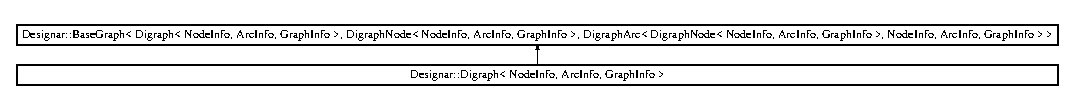
\includegraphics[height=0.921053cm]{class_designar_1_1_digraph}
\end{center}
\end{figure}
\subsection*{Classes}
\begin{DoxyCompactItemize}
\item 
class \hyperlink{class_designar_1_1_digraph_1_1_adjacent_arc_iterator}{Adjacent\+Arc\+Iterator}
\item 
class \hyperlink{class_designar_1_1_digraph_1_1_arc_iterator}{Arc\+Iterator}
\item 
class \hyperlink{class_designar_1_1_digraph_1_1_node_iterator}{Node\+Iterator}
\end{DoxyCompactItemize}
\subsection*{Public Types}
\begin{DoxyCompactItemize}
\item 
using \hyperlink{class_designar_1_1_digraph_a6438608ff27cb6f017705e18bd7fc478}{Node\+Info\+Type} = Node\+Info
\item 
using \hyperlink{class_designar_1_1_digraph_a84a736f6c32da0fcbd1d047e74264d00}{Arc\+Info\+Type} = Arc\+Info
\item 
using \hyperlink{class_designar_1_1_digraph_a2baffbb176ff86becd7452d2acc0ca74}{Graph\+Info\+Type} = Graph\+Info
\item 
using \hyperlink{class_designar_1_1_digraph_a4dc921c41a480b7946a04170e997d8ae}{Node} = \hyperlink{class_designar_1_1_digraph_node}{Digraph\+Node}$<$ Node\+Info, Arc\+Info, Graph\+Info $>$
\item 
using \hyperlink{class_designar_1_1_digraph_a0ceb278671f2a535c00fddccdeafd69f}{Arc} = \hyperlink{class_designar_1_1_digraph_arc}{Digraph\+Arc}$<$ \hyperlink{class_designar_1_1_digraph_a4dc921c41a480b7946a04170e997d8ae}{Node}, Node\+Info, Arc\+Info, Graph\+Info $>$
\end{DoxyCompactItemize}
\subsection*{Public Member Functions}
\begin{DoxyCompactItemize}
\item 
\hyperlink{class_designar_1_1_digraph_ae57ac8513bfcb29602cc08a3d4bc7485}{Digraph} ()
\item 
\hyperlink{class_designar_1_1_digraph_ae5210934b3e6e64caceffee62ff1fcad}{Digraph} (const Graph\+Info \&\+\_\+info)
\item 
\hyperlink{class_designar_1_1_digraph_a534b12da4e0aeb32cff655f05e6c91a4}{Digraph} (Graph\+Info \&\&\+\_\+info)
\item 
\hyperlink{class_designar_1_1_digraph_aa9aa4e8efc114df20a9a10162d43fe40}{Digraph} (const \hyperlink{class_designar_1_1_digraph}{Digraph} \&g)
\item 
\hyperlink{class_designar_1_1_digraph_a109844989cf0ab480ab6fa6f879bf9a9}{Digraph} (\hyperlink{class_designar_1_1_digraph}{Digraph} \&\&g)
\item 
\hyperlink{class_designar_1_1_digraph_aad5e79759f512c213756d22b9ec384bf}{$\sim$\+Digraph} ()
\item 
\hyperlink{class_designar_1_1_digraph}{Digraph} \& \hyperlink{class_designar_1_1_digraph_aa103ce06fd4669e9ced86aa0091ca30c}{operator=} (const \hyperlink{class_designar_1_1_digraph}{Digraph} \&g)
\item 
\hyperlink{class_designar_1_1_digraph}{Digraph} \& \hyperlink{class_designar_1_1_digraph_a49d249b31aade5fff6520aaec60cae78}{operator=} (\hyperlink{class_designar_1_1_digraph}{Digraph} \&\&g)
\item 
void \hyperlink{class_designar_1_1_digraph_a1ee489fd2a20e284a5291943ec2057cb}{swap} (\hyperlink{class_designar_1_1_digraph}{Digraph} \&g)
\item 
void \hyperlink{class_designar_1_1_digraph_a1ec067a8df6129b27e4d79c9c2755899}{clear} ()
\item 
Graph\+Info \& \hyperlink{class_designar_1_1_digraph_a530d2befede0eede246d9eed6c05f1f6}{get\+\_\+info} ()
\item 
const Graph\+Info \& \hyperlink{class_designar_1_1_digraph_a113a9f5a392795312a2d0c0d5c86041c}{get\+\_\+info} () const
\item 
\hyperlink{class_designar_1_1_digraph_a4dc921c41a480b7946a04170e997d8ae}{Node} \& \hyperlink{class_designar_1_1_digraph_a420caa785d93decc7b096de9e51644e7}{get\+\_\+first\+\_\+node} ()
\item 
const \hyperlink{class_designar_1_1_digraph_a4dc921c41a480b7946a04170e997d8ae}{Node} \& \hyperlink{class_designar_1_1_digraph_ada5266ac3e2ed091a37c434dd7484bb9}{get\+\_\+first\+\_\+node} () const
\item 
\hyperlink{class_designar_1_1_digraph_a0ceb278671f2a535c00fddccdeafd69f}{Arc} \& \hyperlink{class_designar_1_1_digraph_af28c0708f3a09f172e4258772f56a476}{get\+\_\+first\+\_\+arc} ()
\item 
const \hyperlink{class_designar_1_1_digraph_a0ceb278671f2a535c00fddccdeafd69f}{Arc} \& \hyperlink{class_designar_1_1_digraph_a7842484a51df899e95a65e979d70079c}{get\+\_\+first\+\_\+arc} () const
\item 
\hyperlink{namespace_designar_aa72662848b9f4815e7bf31a7cf3e33d1}{nat\+\_\+t} \hyperlink{class_designar_1_1_digraph_a7e2f0b56ec85cfd63ff757bef58ae702}{get\+\_\+num\+\_\+nodes} () const
\item 
\hyperlink{namespace_designar_aa72662848b9f4815e7bf31a7cf3e33d1}{nat\+\_\+t} \hyperlink{class_designar_1_1_digraph_aa6289acc079b48c3ebaead44a974d716}{get\+\_\+num\+\_\+arcs} () const
\item 
\hyperlink{class_designar_1_1_digraph_a4dc921c41a480b7946a04170e997d8ae}{Node} \& \hyperlink{class_designar_1_1_digraph_a6ee69792c537ce241a2e448da1b46f1b}{insert\+\_\+node} ()
\item 
\hyperlink{class_designar_1_1_digraph_a4dc921c41a480b7946a04170e997d8ae}{Node} \& \hyperlink{class_designar_1_1_digraph_a292dae36c1ee1fa581013c908ecebd1c}{insert\+\_\+node} (const Node\+Info \&\hyperlink{class_designar_1_1_digraph_aec655bb1b26775cb7ad3581240290efe}{info})
\item 
\hyperlink{class_designar_1_1_digraph_a4dc921c41a480b7946a04170e997d8ae}{Node} \& \hyperlink{class_designar_1_1_digraph_a6b099922c3891b2c9fce75ffeedba025}{insert\+\_\+node} (Node\+Info \&\&\hyperlink{class_designar_1_1_digraph_aec655bb1b26775cb7ad3581240290efe}{info})
\item 
\hyperlink{class_designar_1_1_digraph_a0ceb278671f2a535c00fddccdeafd69f}{Arc} \& \hyperlink{class_designar_1_1_digraph_a52b127c0102e207125c6f4eaaeb7ab26}{insert\+\_\+arc} (\hyperlink{class_designar_1_1_digraph_a4dc921c41a480b7946a04170e997d8ae}{Node} \&s, \hyperlink{class_designar_1_1_digraph_a4dc921c41a480b7946a04170e997d8ae}{Node} \&t)
\item 
\hyperlink{class_designar_1_1_digraph_a0ceb278671f2a535c00fddccdeafd69f}{Arc} \& \hyperlink{class_designar_1_1_digraph_a58d7f0e13a9e42cbc9e28683b527ca72}{insert\+\_\+arc} (\hyperlink{class_designar_1_1_digraph_a4dc921c41a480b7946a04170e997d8ae}{Node} \&src, \hyperlink{class_designar_1_1_digraph_a4dc921c41a480b7946a04170e997d8ae}{Node} \&tgt, const Arc\+Info \&\hyperlink{class_designar_1_1_digraph_aec655bb1b26775cb7ad3581240290efe}{info})
\item 
\hyperlink{class_designar_1_1_digraph_a0ceb278671f2a535c00fddccdeafd69f}{Arc} \& \hyperlink{class_designar_1_1_digraph_a9e46012a65696859c131d0bc5e096f55}{insert\+\_\+arc} (\hyperlink{class_designar_1_1_digraph_a4dc921c41a480b7946a04170e997d8ae}{Node} \&src, \hyperlink{class_designar_1_1_digraph_a4dc921c41a480b7946a04170e997d8ae}{Node} \&tgt, Arc\+Info \&\&\hyperlink{class_designar_1_1_digraph_aec655bb1b26775cb7ad3581240290efe}{info})
\item 
void \hyperlink{class_designar_1_1_digraph_a278b6cb034c19daa52d58aa3312783d6}{remove\+\_\+arc} (\hyperlink{class_designar_1_1_digraph_a0ceb278671f2a535c00fddccdeafd69f}{Arc} \&a)
\item 
void \hyperlink{class_designar_1_1_digraph_a85051637ba641bacb8d42b9cd9e91c40}{remove\+\_\+node} (\hyperlink{class_designar_1_1_digraph_a4dc921c41a480b7946a04170e997d8ae}{Node} \&n)
\item 
\hyperlink{class_designar_1_1_digraph_1_1_node_iterator}{Node\+Iterator} \hyperlink{class_designar_1_1_digraph_af2a2ede7d4af852e67705f2c2bf394d2}{nodes\+\_\+begin} ()
\item 
const \hyperlink{class_designar_1_1_digraph_1_1_node_iterator}{Node\+Iterator} \hyperlink{class_designar_1_1_digraph_a6fcecdd41bdd4af1a0e1a7a5a3e8a3eb}{nodes\+\_\+begin} () const
\item 
\hyperlink{class_designar_1_1_digraph_1_1_node_iterator}{Node\+Iterator} \hyperlink{class_designar_1_1_digraph_a67917506d721e541955aa2a639b94759}{nodes\+\_\+end} ()
\item 
const \hyperlink{class_designar_1_1_digraph_1_1_node_iterator}{Node\+Iterator} \hyperlink{class_designar_1_1_digraph_a82c01284de2fc81c7bd04c13d8861d9a}{nodes\+\_\+end} () const
\item 
\hyperlink{class_designar_1_1_digraph_1_1_arc_iterator}{Arc\+Iterator} \hyperlink{class_designar_1_1_digraph_a56949c616f1aec38783434102072c3ad}{arcs\+\_\+begin} ()
\item 
const \hyperlink{class_designar_1_1_digraph_1_1_arc_iterator}{Arc\+Iterator} \hyperlink{class_designar_1_1_digraph_a1334cd9030f2a409f03a611bb472f5cb}{arcs\+\_\+begin} () const
\item 
\hyperlink{class_designar_1_1_digraph_1_1_arc_iterator}{Arc\+Iterator} \hyperlink{class_designar_1_1_digraph_af4e39baa2e8370cfda5f61f551b3091f}{arcs\+\_\+end} ()
\item 
const \hyperlink{class_designar_1_1_digraph_1_1_arc_iterator}{Arc\+Iterator} \hyperlink{class_designar_1_1_digraph_a128df54ce973f5b1f956407a7f565bc3}{arcs\+\_\+end} () const
\item 
\hyperlink{class_designar_1_1_digraph_1_1_adjacent_arc_iterator}{Adjacent\+Arc\+Iterator} \hyperlink{class_designar_1_1_digraph_a3c1eeda482f59951e1191ea2e0dd514a}{arcs\+\_\+begin} (\hyperlink{class_designar_1_1_digraph_a4dc921c41a480b7946a04170e997d8ae}{Node} \&p)
\item 
const \hyperlink{class_designar_1_1_digraph_1_1_adjacent_arc_iterator}{Adjacent\+Arc\+Iterator} \hyperlink{class_designar_1_1_digraph_aa17a29b3ea956a3ad98e991fb13d0a20}{arcs\+\_\+begin} (\hyperlink{class_designar_1_1_digraph_a4dc921c41a480b7946a04170e997d8ae}{Node} \&p) const
\item 
\hyperlink{class_designar_1_1_digraph_1_1_adjacent_arc_iterator}{Adjacent\+Arc\+Iterator} \hyperlink{class_designar_1_1_digraph_ab7e47c93dd15bab0510977f403a35849}{arcs\+\_\+end} (\hyperlink{class_designar_1_1_digraph_a4dc921c41a480b7946a04170e997d8ae}{Node} \&p)
\item 
const \hyperlink{class_designar_1_1_digraph_1_1_adjacent_arc_iterator}{Adjacent\+Arc\+Iterator} \hyperlink{class_designar_1_1_digraph_a68abe34d6f5a7b429715ec55aa030b7d}{arcs\+\_\+end} (\hyperlink{class_designar_1_1_digraph_a4dc921c41a480b7946a04170e997d8ae}{Node} \&p) const
\item 
\hyperlink{class_designar_1_1_digraph_a0ceb278671f2a535c00fddccdeafd69f}{Arc} $\ast$ \hyperlink{class_designar_1_1_digraph_ac301ebe5d45b2864639d68d7e9aeea2a}{search\+\_\+arc} (\hyperlink{class_designar_1_1_digraph_a4dc921c41a480b7946a04170e997d8ae}{Node} \&, \hyperlink{class_designar_1_1_digraph_a4dc921c41a480b7946a04170e997d8ae}{Node} \&)
\item 
{\footnotesize template$<$class Cmp $>$ }\\void \hyperlink{class_designar_1_1_digraph_a5d057854409452b7d4fb2f9eec217b7d}{sort\+\_\+nodes} (Cmp \&cmp)
\item 
{\footnotesize template$<$class Cmp $>$ }\\void \hyperlink{class_designar_1_1_digraph_af62a8c0997715ef3bdebfe56f328ea1c}{sort\+\_\+nodes} (Cmp \&\&cmp=Cmp())
\item 
{\footnotesize template$<$class Cmp $>$ }\\void \hyperlink{class_designar_1_1_digraph_a450085493969a382371f7d4d407e42cd}{sort\+\_\+arcs} (Cmp \&cmp)
\item 
{\footnotesize template$<$class Cmp $>$ }\\void \hyperlink{class_designar_1_1_digraph_a44895030e02896d6d35277eec136c49f}{sort\+\_\+arcs} (Cmp \&\&cmp=Cmp())
\item 
bool \hyperlink{class_designar_1_1_digraph_a6751952e13a35cf7aa452a8bb243f53d}{is\+\_\+digraph} () const
\end{DoxyCompactItemize}
\subsection*{Protected Types}
\begin{DoxyCompactItemize}
\item 
using \hyperlink{class_designar_1_1_digraph_a33b0d2b8820ada501522b0e67e63524a}{G\+Node} = \hyperlink{class_designar_1_1_d_l_node}{D\+L\+Node}$<$ \hyperlink{class_designar_1_1_digraph_a4dc921c41a480b7946a04170e997d8ae}{Node} $>$
\item 
using \hyperlink{class_designar_1_1_digraph_a0c6d846f23d1e82556fb6055557df53f}{G\+Ad\+Arc} = \hyperlink{class_designar_1_1_d_l_node}{D\+L\+Node}$<$ \hyperlink{class_designar_1_1_digraph_a0ceb278671f2a535c00fddccdeafd69f}{Arc} $>$
\item 
using \hyperlink{class_designar_1_1_digraph_a341acf8fb0195a8986158c29c4db1a89}{G\+Arc} = \hyperlink{class_designar_1_1_d_l_node}{D\+L\+Node}$<$ \hyperlink{class_designar_1_1_digraph_a0c6d846f23d1e82556fb6055557df53f}{G\+Ad\+Arc} $\ast$ $>$
\end{DoxyCompactItemize}
\subsection*{Protected Member Functions}
\begin{DoxyCompactItemize}
\item 
\hyperlink{class_designar_1_1_digraph_a33b0d2b8820ada501522b0e67e63524a}{G\+Node} $\ast$ \hyperlink{class_designar_1_1_digraph_a420fea8c892f9ce87a50489b97755026}{insert\+\_\+node} (\hyperlink{class_designar_1_1_digraph_a33b0d2b8820ada501522b0e67e63524a}{G\+Node} $\ast$p)
\item 
\hyperlink{class_designar_1_1_digraph_a0c6d846f23d1e82556fb6055557df53f}{G\+Ad\+Arc} $\ast$ \hyperlink{class_designar_1_1_digraph_a9180c479d24dc8dc648a37451c90d066}{insert\+\_\+arc} (\hyperlink{class_designar_1_1_digraph_a4dc921c41a480b7946a04170e997d8ae}{Node} $\ast$src, \hyperlink{class_designar_1_1_digraph_a4dc921c41a480b7946a04170e997d8ae}{Node} $\ast$tgt)
\item 
void \hyperlink{class_designar_1_1_digraph_abb7e909c1c44cd4cee2e742cb2d3fa17}{remove\+\_\+arc} (\hyperlink{class_designar_1_1_digraph_a0c6d846f23d1e82556fb6055557df53f}{G\+Ad\+Arc} $\ast$arc)
\item 
void \hyperlink{class_designar_1_1_digraph_a4a19c6f9333604d3d49992eeb5a6eeae}{remove\+\_\+node} (\hyperlink{class_designar_1_1_digraph_a33b0d2b8820ada501522b0e67e63524a}{G\+Node} $\ast$)
\end{DoxyCompactItemize}
\subsection*{Static Protected Member Functions}
\begin{DoxyCompactItemize}
\item 
static \hyperlink{class_designar_1_1_digraph_a33b0d2b8820ada501522b0e67e63524a}{G\+Node} $\ast$ \hyperlink{class_designar_1_1_digraph_adbb91274c17d6087fdd5721e3f9b1f7c}{dl\+\_\+to\+\_\+node} (\hyperlink{class_designar_1_1_d_l}{DL} $\ast$ptr)
\item 
static \hyperlink{class_designar_1_1_digraph_a341acf8fb0195a8986158c29c4db1a89}{G\+Arc} $\ast$ \hyperlink{class_designar_1_1_digraph_af9581e9d0825da11ce153bd055149f7f}{dl\+\_\+to\+\_\+arc} (\hyperlink{class_designar_1_1_d_l}{DL} $\ast$ptr)
\item 
static \hyperlink{class_designar_1_1_digraph_a0c6d846f23d1e82556fb6055557df53f}{G\+Ad\+Arc} $\ast$ \hyperlink{class_designar_1_1_digraph_afe3162bf2e56b177e7ee1a938ae2af8b}{dl\+\_\+to\+\_\+adjacent\+\_\+arc} (\hyperlink{class_designar_1_1_d_l}{DL} $\ast$ptr)
\item 
static \hyperlink{class_designar_1_1_digraph_a33b0d2b8820ada501522b0e67e63524a}{G\+Node} $\ast$ \hyperlink{class_designar_1_1_digraph_ae0a945e347e8e6a15df21df4fe2c1782}{to\+\_\+gnode} (\hyperlink{class_designar_1_1_digraph_a4dc921c41a480b7946a04170e997d8ae}{Node} \&node)
\item 
static \hyperlink{class_designar_1_1_digraph_a0c6d846f23d1e82556fb6055557df53f}{G\+Ad\+Arc} $\ast$ \hyperlink{class_designar_1_1_digraph_a6137e6849dcb4208e9c8daa26f303868}{to\+\_\+garc} (\hyperlink{class_designar_1_1_digraph_a0ceb278671f2a535c00fddccdeafd69f}{Arc} \&arc)
\end{DoxyCompactItemize}
\subsection*{Protected Attributes}
\begin{DoxyCompactItemize}
\item 
Graph\+Info \hyperlink{class_designar_1_1_digraph_aec655bb1b26775cb7ad3581240290efe}{info}
\item 
\hyperlink{namespace_designar_aa72662848b9f4815e7bf31a7cf3e33d1}{nat\+\_\+t} \hyperlink{class_designar_1_1_digraph_a468cec4048ff9042a288dca47ad856aa}{num\+\_\+nodes}
\item 
\hyperlink{class_designar_1_1_d_l}{DL} \hyperlink{class_designar_1_1_digraph_ac81c264dab34ca74fc62b0693c1c3543}{node\+\_\+list}
\item 
\hyperlink{namespace_designar_aa72662848b9f4815e7bf31a7cf3e33d1}{nat\+\_\+t} \hyperlink{class_designar_1_1_digraph_accd2da6bdb5bc0624e7f79c904c89328}{num\+\_\+arcs}
\item 
\hyperlink{class_designar_1_1_d_l}{DL} \hyperlink{class_designar_1_1_digraph_ad860dbe9732bc90906a486cad390637a}{arc\+\_\+list}
\end{DoxyCompactItemize}
\subsection*{Additional Inherited Members}


\subsection{Detailed Description}
\subsubsection*{template$<$typename Node\+Info, typename Arc\+Info = Empty\+Class, typename Graph\+Info = Empty\+Class$>$\newline
class Designar\+::\+Digraph$<$ Node\+Info, Arc\+Info, Graph\+Info $>$}



Definition at line 38 of file graph.\+H.



\subsection{Member Typedef Documentation}
\mbox{\Hypertarget{class_designar_1_1_digraph_a0ceb278671f2a535c00fddccdeafd69f}\label{class_designar_1_1_digraph_a0ceb278671f2a535c00fddccdeafd69f}} 
\index{Designar\+::\+Digraph@{Designar\+::\+Digraph}!Arc@{Arc}}
\index{Arc@{Arc}!Designar\+::\+Digraph@{Designar\+::\+Digraph}}
\subsubsection{\texorpdfstring{Arc}{Arc}}
{\footnotesize\ttfamily template$<$typename Node\+Info , typename Arc\+Info  = Empty\+Class, typename Graph\+Info  = Empty\+Class$>$ \\
using \hyperlink{class_designar_1_1_digraph}{Designar\+::\+Digraph}$<$ Node\+Info, Arc\+Info, Graph\+Info $>$\+::\hyperlink{class_designar_1_1_digraph_a0ceb278671f2a535c00fddccdeafd69f}{Arc} =  \hyperlink{class_designar_1_1_digraph_arc}{Digraph\+Arc}$<$\hyperlink{class_designar_1_1_digraph_a4dc921c41a480b7946a04170e997d8ae}{Node}, Node\+Info, Arc\+Info, Graph\+Info$>$}



Definition at line 1240 of file graph.\+H.

\mbox{\Hypertarget{class_designar_1_1_digraph_a84a736f6c32da0fcbd1d047e74264d00}\label{class_designar_1_1_digraph_a84a736f6c32da0fcbd1d047e74264d00}} 
\index{Designar\+::\+Digraph@{Designar\+::\+Digraph}!Arc\+Info\+Type@{Arc\+Info\+Type}}
\index{Arc\+Info\+Type@{Arc\+Info\+Type}!Designar\+::\+Digraph@{Designar\+::\+Digraph}}
\subsubsection{\texorpdfstring{Arc\+Info\+Type}{ArcInfoType}}
{\footnotesize\ttfamily template$<$typename Node\+Info , typename Arc\+Info  = Empty\+Class, typename Graph\+Info  = Empty\+Class$>$ \\
using \hyperlink{class_designar_1_1_digraph}{Designar\+::\+Digraph}$<$ Node\+Info, Arc\+Info, Graph\+Info $>$\+::\hyperlink{class_designar_1_1_digraph_a84a736f6c32da0fcbd1d047e74264d00}{Arc\+Info\+Type} =  Arc\+Info}



Definition at line 1236 of file graph.\+H.

\mbox{\Hypertarget{class_designar_1_1_digraph_a0c6d846f23d1e82556fb6055557df53f}\label{class_designar_1_1_digraph_a0c6d846f23d1e82556fb6055557df53f}} 
\index{Designar\+::\+Digraph@{Designar\+::\+Digraph}!G\+Ad\+Arc@{G\+Ad\+Arc}}
\index{G\+Ad\+Arc@{G\+Ad\+Arc}!Designar\+::\+Digraph@{Designar\+::\+Digraph}}
\subsubsection{\texorpdfstring{G\+Ad\+Arc}{GAdArc}}
{\footnotesize\ttfamily template$<$typename Node\+Info , typename Arc\+Info  = Empty\+Class, typename Graph\+Info  = Empty\+Class$>$ \\
using \hyperlink{class_designar_1_1_digraph}{Designar\+::\+Digraph}$<$ Node\+Info, Arc\+Info, Graph\+Info $>$\+::\hyperlink{class_designar_1_1_digraph_a0c6d846f23d1e82556fb6055557df53f}{G\+Ad\+Arc} =  \hyperlink{class_designar_1_1_d_l_node}{D\+L\+Node}$<$\hyperlink{class_designar_1_1_digraph_a0ceb278671f2a535c00fddccdeafd69f}{Arc}$>$\hspace{0.3cm}{\ttfamily [protected]}}



Definition at line 1244 of file graph.\+H.

\mbox{\Hypertarget{class_designar_1_1_digraph_a341acf8fb0195a8986158c29c4db1a89}\label{class_designar_1_1_digraph_a341acf8fb0195a8986158c29c4db1a89}} 
\index{Designar\+::\+Digraph@{Designar\+::\+Digraph}!G\+Arc@{G\+Arc}}
\index{G\+Arc@{G\+Arc}!Designar\+::\+Digraph@{Designar\+::\+Digraph}}
\subsubsection{\texorpdfstring{G\+Arc}{GArc}}
{\footnotesize\ttfamily template$<$typename Node\+Info , typename Arc\+Info  = Empty\+Class, typename Graph\+Info  = Empty\+Class$>$ \\
using \hyperlink{class_designar_1_1_digraph}{Designar\+::\+Digraph}$<$ Node\+Info, Arc\+Info, Graph\+Info $>$\+::\hyperlink{class_designar_1_1_digraph_a341acf8fb0195a8986158c29c4db1a89}{G\+Arc} =  \hyperlink{class_designar_1_1_d_l_node}{D\+L\+Node}$<$\hyperlink{class_designar_1_1_digraph_a0c6d846f23d1e82556fb6055557df53f}{G\+Ad\+Arc} $\ast$$>$\hspace{0.3cm}{\ttfamily [protected]}}



Definition at line 1245 of file graph.\+H.

\mbox{\Hypertarget{class_designar_1_1_digraph_a33b0d2b8820ada501522b0e67e63524a}\label{class_designar_1_1_digraph_a33b0d2b8820ada501522b0e67e63524a}} 
\index{Designar\+::\+Digraph@{Designar\+::\+Digraph}!G\+Node@{G\+Node}}
\index{G\+Node@{G\+Node}!Designar\+::\+Digraph@{Designar\+::\+Digraph}}
\subsubsection{\texorpdfstring{G\+Node}{GNode}}
{\footnotesize\ttfamily template$<$typename Node\+Info , typename Arc\+Info  = Empty\+Class, typename Graph\+Info  = Empty\+Class$>$ \\
using \hyperlink{class_designar_1_1_digraph}{Designar\+::\+Digraph}$<$ Node\+Info, Arc\+Info, Graph\+Info $>$\+::\hyperlink{class_designar_1_1_digraph_a33b0d2b8820ada501522b0e67e63524a}{G\+Node} =  \hyperlink{class_designar_1_1_d_l_node}{D\+L\+Node}$<$\hyperlink{class_designar_1_1_digraph_a4dc921c41a480b7946a04170e997d8ae}{Node}$>$\hspace{0.3cm}{\ttfamily [protected]}}



Definition at line 1243 of file graph.\+H.

\mbox{\Hypertarget{class_designar_1_1_digraph_a2baffbb176ff86becd7452d2acc0ca74}\label{class_designar_1_1_digraph_a2baffbb176ff86becd7452d2acc0ca74}} 
\index{Designar\+::\+Digraph@{Designar\+::\+Digraph}!Graph\+Info\+Type@{Graph\+Info\+Type}}
\index{Graph\+Info\+Type@{Graph\+Info\+Type}!Designar\+::\+Digraph@{Designar\+::\+Digraph}}
\subsubsection{\texorpdfstring{Graph\+Info\+Type}{GraphInfoType}}
{\footnotesize\ttfamily template$<$typename Node\+Info , typename Arc\+Info  = Empty\+Class, typename Graph\+Info  = Empty\+Class$>$ \\
using \hyperlink{class_designar_1_1_digraph}{Designar\+::\+Digraph}$<$ Node\+Info, Arc\+Info, Graph\+Info $>$\+::\hyperlink{class_designar_1_1_digraph_a2baffbb176ff86becd7452d2acc0ca74}{Graph\+Info\+Type} =  Graph\+Info}



Definition at line 1237 of file graph.\+H.

\mbox{\Hypertarget{class_designar_1_1_digraph_a4dc921c41a480b7946a04170e997d8ae}\label{class_designar_1_1_digraph_a4dc921c41a480b7946a04170e997d8ae}} 
\index{Designar\+::\+Digraph@{Designar\+::\+Digraph}!Node@{Node}}
\index{Node@{Node}!Designar\+::\+Digraph@{Designar\+::\+Digraph}}
\subsubsection{\texorpdfstring{Node}{Node}}
{\footnotesize\ttfamily template$<$typename Node\+Info , typename Arc\+Info  = Empty\+Class, typename Graph\+Info  = Empty\+Class$>$ \\
using \hyperlink{class_designar_1_1_digraph}{Designar\+::\+Digraph}$<$ Node\+Info, Arc\+Info, Graph\+Info $>$\+::\hyperlink{class_designar_1_1_digraph_a4dc921c41a480b7946a04170e997d8ae}{Node} =  \hyperlink{class_designar_1_1_digraph_node}{Digraph\+Node}$<$Node\+Info, Arc\+Info, Graph\+Info$>$}



Definition at line 1239 of file graph.\+H.

\mbox{\Hypertarget{class_designar_1_1_digraph_a6438608ff27cb6f017705e18bd7fc478}\label{class_designar_1_1_digraph_a6438608ff27cb6f017705e18bd7fc478}} 
\index{Designar\+::\+Digraph@{Designar\+::\+Digraph}!Node\+Info\+Type@{Node\+Info\+Type}}
\index{Node\+Info\+Type@{Node\+Info\+Type}!Designar\+::\+Digraph@{Designar\+::\+Digraph}}
\subsubsection{\texorpdfstring{Node\+Info\+Type}{NodeInfoType}}
{\footnotesize\ttfamily template$<$typename Node\+Info , typename Arc\+Info  = Empty\+Class, typename Graph\+Info  = Empty\+Class$>$ \\
using \hyperlink{class_designar_1_1_digraph}{Designar\+::\+Digraph}$<$ Node\+Info, Arc\+Info, Graph\+Info $>$\+::\hyperlink{class_designar_1_1_digraph_a6438608ff27cb6f017705e18bd7fc478}{Node\+Info\+Type} =  Node\+Info}



Definition at line 1235 of file graph.\+H.



\subsection{Constructor \& Destructor Documentation}
\mbox{\Hypertarget{class_designar_1_1_digraph_ae57ac8513bfcb29602cc08a3d4bc7485}\label{class_designar_1_1_digraph_ae57ac8513bfcb29602cc08a3d4bc7485}} 
\index{Designar\+::\+Digraph@{Designar\+::\+Digraph}!Digraph@{Digraph}}
\index{Digraph@{Digraph}!Designar\+::\+Digraph@{Designar\+::\+Digraph}}
\subsubsection{\texorpdfstring{Digraph()}{Digraph()}\hspace{0.1cm}{\footnotesize\ttfamily [1/5]}}
{\footnotesize\ttfamily template$<$typename Node\+Info , typename Arc\+Info  = Empty\+Class, typename Graph\+Info  = Empty\+Class$>$ \\
\hyperlink{class_designar_1_1_digraph}{Designar\+::\+Digraph}$<$ Node\+Info, Arc\+Info, Graph\+Info $>$\+::\hyperlink{class_designar_1_1_digraph}{Digraph} (\begin{DoxyParamCaption}{ }\end{DoxyParamCaption})\hspace{0.3cm}{\ttfamily [inline]}}



Definition at line 1324 of file graph.\+H.

\mbox{\Hypertarget{class_designar_1_1_digraph_ae5210934b3e6e64caceffee62ff1fcad}\label{class_designar_1_1_digraph_ae5210934b3e6e64caceffee62ff1fcad}} 
\index{Designar\+::\+Digraph@{Designar\+::\+Digraph}!Digraph@{Digraph}}
\index{Digraph@{Digraph}!Designar\+::\+Digraph@{Designar\+::\+Digraph}}
\subsubsection{\texorpdfstring{Digraph()}{Digraph()}\hspace{0.1cm}{\footnotesize\ttfamily [2/5]}}
{\footnotesize\ttfamily template$<$typename Node\+Info , typename Arc\+Info  = Empty\+Class, typename Graph\+Info  = Empty\+Class$>$ \\
\hyperlink{class_designar_1_1_digraph}{Designar\+::\+Digraph}$<$ Node\+Info, Arc\+Info, Graph\+Info $>$\+::\hyperlink{class_designar_1_1_digraph}{Digraph} (\begin{DoxyParamCaption}\item[{const Graph\+Info \&}]{\+\_\+info }\end{DoxyParamCaption})\hspace{0.3cm}{\ttfamily [inline]}}



Definition at line 1330 of file graph.\+H.

\mbox{\Hypertarget{class_designar_1_1_digraph_a534b12da4e0aeb32cff655f05e6c91a4}\label{class_designar_1_1_digraph_a534b12da4e0aeb32cff655f05e6c91a4}} 
\index{Designar\+::\+Digraph@{Designar\+::\+Digraph}!Digraph@{Digraph}}
\index{Digraph@{Digraph}!Designar\+::\+Digraph@{Designar\+::\+Digraph}}
\subsubsection{\texorpdfstring{Digraph()}{Digraph()}\hspace{0.1cm}{\footnotesize\ttfamily [3/5]}}
{\footnotesize\ttfamily template$<$typename Node\+Info , typename Arc\+Info  = Empty\+Class, typename Graph\+Info  = Empty\+Class$>$ \\
\hyperlink{class_designar_1_1_digraph}{Designar\+::\+Digraph}$<$ Node\+Info, Arc\+Info, Graph\+Info $>$\+::\hyperlink{class_designar_1_1_digraph}{Digraph} (\begin{DoxyParamCaption}\item[{Graph\+Info \&\&}]{\+\_\+info }\end{DoxyParamCaption})\hspace{0.3cm}{\ttfamily [inline]}}



Definition at line 1336 of file graph.\+H.

\mbox{\Hypertarget{class_designar_1_1_digraph_aa9aa4e8efc114df20a9a10162d43fe40}\label{class_designar_1_1_digraph_aa9aa4e8efc114df20a9a10162d43fe40}} 
\index{Designar\+::\+Digraph@{Designar\+::\+Digraph}!Digraph@{Digraph}}
\index{Digraph@{Digraph}!Designar\+::\+Digraph@{Designar\+::\+Digraph}}
\subsubsection{\texorpdfstring{Digraph()}{Digraph()}\hspace{0.1cm}{\footnotesize\ttfamily [4/5]}}
{\footnotesize\ttfamily template$<$typename Node\+Info , typename Arc\+Info  = Empty\+Class, typename Graph\+Info  = Empty\+Class$>$ \\
\hyperlink{class_designar_1_1_digraph}{Designar\+::\+Digraph}$<$ Node\+Info, Arc\+Info, Graph\+Info $>$\+::\hyperlink{class_designar_1_1_digraph}{Digraph} (\begin{DoxyParamCaption}\item[{const \hyperlink{class_designar_1_1_digraph}{Digraph}$<$ Node\+Info, Arc\+Info, Graph\+Info $>$ \&}]{g }\end{DoxyParamCaption})\hspace{0.3cm}{\ttfamily [inline]}}



Definition at line 1342 of file graph.\+H.

\mbox{\Hypertarget{class_designar_1_1_digraph_a109844989cf0ab480ab6fa6f879bf9a9}\label{class_designar_1_1_digraph_a109844989cf0ab480ab6fa6f879bf9a9}} 
\index{Designar\+::\+Digraph@{Designar\+::\+Digraph}!Digraph@{Digraph}}
\index{Digraph@{Digraph}!Designar\+::\+Digraph@{Designar\+::\+Digraph}}
\subsubsection{\texorpdfstring{Digraph()}{Digraph()}\hspace{0.1cm}{\footnotesize\ttfamily [5/5]}}
{\footnotesize\ttfamily template$<$typename Node\+Info , typename Arc\+Info  = Empty\+Class, typename Graph\+Info  = Empty\+Class$>$ \\
\hyperlink{class_designar_1_1_digraph}{Designar\+::\+Digraph}$<$ Node\+Info, Arc\+Info, Graph\+Info $>$\+::\hyperlink{class_designar_1_1_digraph}{Digraph} (\begin{DoxyParamCaption}\item[{\hyperlink{class_designar_1_1_digraph}{Digraph}$<$ Node\+Info, Arc\+Info, Graph\+Info $>$ \&\&}]{g }\end{DoxyParamCaption})\hspace{0.3cm}{\ttfamily [inline]}}



Definition at line 1348 of file graph.\+H.

\mbox{\Hypertarget{class_designar_1_1_digraph_aad5e79759f512c213756d22b9ec384bf}\label{class_designar_1_1_digraph_aad5e79759f512c213756d22b9ec384bf}} 
\index{Designar\+::\+Digraph@{Designar\+::\+Digraph}!````~Digraph@{$\sim$\+Digraph}}
\index{````~Digraph@{$\sim$\+Digraph}!Designar\+::\+Digraph@{Designar\+::\+Digraph}}
\subsubsection{\texorpdfstring{$\sim$\+Digraph()}{~Digraph()}}
{\footnotesize\ttfamily template$<$typename Node\+Info , typename Arc\+Info  = Empty\+Class, typename Graph\+Info  = Empty\+Class$>$ \\
\hyperlink{class_designar_1_1_digraph}{Designar\+::\+Digraph}$<$ Node\+Info, Arc\+Info, Graph\+Info $>$\+::$\sim$\hyperlink{class_designar_1_1_digraph}{Digraph} (\begin{DoxyParamCaption}{ }\end{DoxyParamCaption})\hspace{0.3cm}{\ttfamily [inline]}}



Definition at line 1354 of file graph.\+H.



\subsection{Member Function Documentation}
\mbox{\Hypertarget{class_designar_1_1_digraph_a56949c616f1aec38783434102072c3ad}\label{class_designar_1_1_digraph_a56949c616f1aec38783434102072c3ad}} 
\index{Designar\+::\+Digraph@{Designar\+::\+Digraph}!arcs\+\_\+begin@{arcs\+\_\+begin}}
\index{arcs\+\_\+begin@{arcs\+\_\+begin}!Designar\+::\+Digraph@{Designar\+::\+Digraph}}
\subsubsection{\texorpdfstring{arcs\+\_\+begin()}{arcs\_begin()}\hspace{0.1cm}{\footnotesize\ttfamily [1/4]}}
{\footnotesize\ttfamily template$<$typename Node\+Info , typename Arc\+Info  = Empty\+Class, typename Graph\+Info  = Empty\+Class$>$ \\
\hyperlink{class_designar_1_1_digraph_1_1_arc_iterator}{Arc\+Iterator} \hyperlink{class_designar_1_1_digraph}{Designar\+::\+Digraph}$<$ Node\+Info, Arc\+Info, Graph\+Info $>$\+::arcs\+\_\+begin (\begin{DoxyParamCaption}{ }\end{DoxyParamCaption})\hspace{0.3cm}{\ttfamily [inline]}}



Definition at line 1791 of file graph.\+H.

\mbox{\Hypertarget{class_designar_1_1_digraph_a1334cd9030f2a409f03a611bb472f5cb}\label{class_designar_1_1_digraph_a1334cd9030f2a409f03a611bb472f5cb}} 
\index{Designar\+::\+Digraph@{Designar\+::\+Digraph}!arcs\+\_\+begin@{arcs\+\_\+begin}}
\index{arcs\+\_\+begin@{arcs\+\_\+begin}!Designar\+::\+Digraph@{Designar\+::\+Digraph}}
\subsubsection{\texorpdfstring{arcs\+\_\+begin()}{arcs\_begin()}\hspace{0.1cm}{\footnotesize\ttfamily [2/4]}}
{\footnotesize\ttfamily template$<$typename Node\+Info , typename Arc\+Info  = Empty\+Class, typename Graph\+Info  = Empty\+Class$>$ \\
const \hyperlink{class_designar_1_1_digraph_1_1_arc_iterator}{Arc\+Iterator} \hyperlink{class_designar_1_1_digraph}{Designar\+::\+Digraph}$<$ Node\+Info, Arc\+Info, Graph\+Info $>$\+::arcs\+\_\+begin (\begin{DoxyParamCaption}{ }\end{DoxyParamCaption}) const\hspace{0.3cm}{\ttfamily [inline]}}



Definition at line 1796 of file graph.\+H.

\mbox{\Hypertarget{class_designar_1_1_digraph_a3c1eeda482f59951e1191ea2e0dd514a}\label{class_designar_1_1_digraph_a3c1eeda482f59951e1191ea2e0dd514a}} 
\index{Designar\+::\+Digraph@{Designar\+::\+Digraph}!arcs\+\_\+begin@{arcs\+\_\+begin}}
\index{arcs\+\_\+begin@{arcs\+\_\+begin}!Designar\+::\+Digraph@{Designar\+::\+Digraph}}
\subsubsection{\texorpdfstring{arcs\+\_\+begin()}{arcs\_begin()}\hspace{0.1cm}{\footnotesize\ttfamily [3/4]}}
{\footnotesize\ttfamily template$<$typename Node\+Info , typename Arc\+Info  = Empty\+Class, typename Graph\+Info  = Empty\+Class$>$ \\
\hyperlink{class_designar_1_1_digraph_1_1_adjacent_arc_iterator}{Adjacent\+Arc\+Iterator} \hyperlink{class_designar_1_1_digraph}{Designar\+::\+Digraph}$<$ Node\+Info, Arc\+Info, Graph\+Info $>$\+::arcs\+\_\+begin (\begin{DoxyParamCaption}\item[{\hyperlink{class_designar_1_1_digraph_a4dc921c41a480b7946a04170e997d8ae}{Node} \&}]{p }\end{DoxyParamCaption})\hspace{0.3cm}{\ttfamily [inline]}}



Definition at line 1811 of file graph.\+H.

\mbox{\Hypertarget{class_designar_1_1_digraph_aa17a29b3ea956a3ad98e991fb13d0a20}\label{class_designar_1_1_digraph_aa17a29b3ea956a3ad98e991fb13d0a20}} 
\index{Designar\+::\+Digraph@{Designar\+::\+Digraph}!arcs\+\_\+begin@{arcs\+\_\+begin}}
\index{arcs\+\_\+begin@{arcs\+\_\+begin}!Designar\+::\+Digraph@{Designar\+::\+Digraph}}
\subsubsection{\texorpdfstring{arcs\+\_\+begin()}{arcs\_begin()}\hspace{0.1cm}{\footnotesize\ttfamily [4/4]}}
{\footnotesize\ttfamily template$<$typename Node\+Info , typename Arc\+Info  = Empty\+Class, typename Graph\+Info  = Empty\+Class$>$ \\
const \hyperlink{class_designar_1_1_digraph_1_1_adjacent_arc_iterator}{Adjacent\+Arc\+Iterator} \hyperlink{class_designar_1_1_digraph}{Designar\+::\+Digraph}$<$ Node\+Info, Arc\+Info, Graph\+Info $>$\+::arcs\+\_\+begin (\begin{DoxyParamCaption}\item[{\hyperlink{class_designar_1_1_digraph_a4dc921c41a480b7946a04170e997d8ae}{Node} \&}]{p }\end{DoxyParamCaption}) const\hspace{0.3cm}{\ttfamily [inline]}}



Definition at line 1816 of file graph.\+H.

\mbox{\Hypertarget{class_designar_1_1_digraph_af4e39baa2e8370cfda5f61f551b3091f}\label{class_designar_1_1_digraph_af4e39baa2e8370cfda5f61f551b3091f}} 
\index{Designar\+::\+Digraph@{Designar\+::\+Digraph}!arcs\+\_\+end@{arcs\+\_\+end}}
\index{arcs\+\_\+end@{arcs\+\_\+end}!Designar\+::\+Digraph@{Designar\+::\+Digraph}}
\subsubsection{\texorpdfstring{arcs\+\_\+end()}{arcs\_end()}\hspace{0.1cm}{\footnotesize\ttfamily [1/4]}}
{\footnotesize\ttfamily template$<$typename Node\+Info , typename Arc\+Info  = Empty\+Class, typename Graph\+Info  = Empty\+Class$>$ \\
\hyperlink{class_designar_1_1_digraph_1_1_arc_iterator}{Arc\+Iterator} \hyperlink{class_designar_1_1_digraph}{Designar\+::\+Digraph}$<$ Node\+Info, Arc\+Info, Graph\+Info $>$\+::arcs\+\_\+end (\begin{DoxyParamCaption}{ }\end{DoxyParamCaption})\hspace{0.3cm}{\ttfamily [inline]}}



Definition at line 1801 of file graph.\+H.

\mbox{\Hypertarget{class_designar_1_1_digraph_a128df54ce973f5b1f956407a7f565bc3}\label{class_designar_1_1_digraph_a128df54ce973f5b1f956407a7f565bc3}} 
\index{Designar\+::\+Digraph@{Designar\+::\+Digraph}!arcs\+\_\+end@{arcs\+\_\+end}}
\index{arcs\+\_\+end@{arcs\+\_\+end}!Designar\+::\+Digraph@{Designar\+::\+Digraph}}
\subsubsection{\texorpdfstring{arcs\+\_\+end()}{arcs\_end()}\hspace{0.1cm}{\footnotesize\ttfamily [2/4]}}
{\footnotesize\ttfamily template$<$typename Node\+Info , typename Arc\+Info  = Empty\+Class, typename Graph\+Info  = Empty\+Class$>$ \\
const \hyperlink{class_designar_1_1_digraph_1_1_arc_iterator}{Arc\+Iterator} \hyperlink{class_designar_1_1_digraph}{Designar\+::\+Digraph}$<$ Node\+Info, Arc\+Info, Graph\+Info $>$\+::arcs\+\_\+end (\begin{DoxyParamCaption}{ }\end{DoxyParamCaption}) const\hspace{0.3cm}{\ttfamily [inline]}}



Definition at line 1806 of file graph.\+H.

\mbox{\Hypertarget{class_designar_1_1_digraph_ab7e47c93dd15bab0510977f403a35849}\label{class_designar_1_1_digraph_ab7e47c93dd15bab0510977f403a35849}} 
\index{Designar\+::\+Digraph@{Designar\+::\+Digraph}!arcs\+\_\+end@{arcs\+\_\+end}}
\index{arcs\+\_\+end@{arcs\+\_\+end}!Designar\+::\+Digraph@{Designar\+::\+Digraph}}
\subsubsection{\texorpdfstring{arcs\+\_\+end()}{arcs\_end()}\hspace{0.1cm}{\footnotesize\ttfamily [3/4]}}
{\footnotesize\ttfamily template$<$typename Node\+Info , typename Arc\+Info  = Empty\+Class, typename Graph\+Info  = Empty\+Class$>$ \\
\hyperlink{class_designar_1_1_digraph_1_1_adjacent_arc_iterator}{Adjacent\+Arc\+Iterator} \hyperlink{class_designar_1_1_digraph}{Designar\+::\+Digraph}$<$ Node\+Info, Arc\+Info, Graph\+Info $>$\+::arcs\+\_\+end (\begin{DoxyParamCaption}\item[{\hyperlink{class_designar_1_1_digraph_a4dc921c41a480b7946a04170e997d8ae}{Node} \&}]{p }\end{DoxyParamCaption})\hspace{0.3cm}{\ttfamily [inline]}}



Definition at line 1821 of file graph.\+H.

\mbox{\Hypertarget{class_designar_1_1_digraph_a68abe34d6f5a7b429715ec55aa030b7d}\label{class_designar_1_1_digraph_a68abe34d6f5a7b429715ec55aa030b7d}} 
\index{Designar\+::\+Digraph@{Designar\+::\+Digraph}!arcs\+\_\+end@{arcs\+\_\+end}}
\index{arcs\+\_\+end@{arcs\+\_\+end}!Designar\+::\+Digraph@{Designar\+::\+Digraph}}
\subsubsection{\texorpdfstring{arcs\+\_\+end()}{arcs\_end()}\hspace{0.1cm}{\footnotesize\ttfamily [4/4]}}
{\footnotesize\ttfamily template$<$typename Node\+Info , typename Arc\+Info  = Empty\+Class, typename Graph\+Info  = Empty\+Class$>$ \\
const \hyperlink{class_designar_1_1_digraph_1_1_adjacent_arc_iterator}{Adjacent\+Arc\+Iterator} \hyperlink{class_designar_1_1_digraph}{Designar\+::\+Digraph}$<$ Node\+Info, Arc\+Info, Graph\+Info $>$\+::arcs\+\_\+end (\begin{DoxyParamCaption}\item[{\hyperlink{class_designar_1_1_digraph_a4dc921c41a480b7946a04170e997d8ae}{Node} \&}]{p }\end{DoxyParamCaption}) const\hspace{0.3cm}{\ttfamily [inline]}}



Definition at line 1826 of file graph.\+H.

\mbox{\Hypertarget{class_designar_1_1_digraph_a1ec067a8df6129b27e4d79c9c2755899}\label{class_designar_1_1_digraph_a1ec067a8df6129b27e4d79c9c2755899}} 
\index{Designar\+::\+Digraph@{Designar\+::\+Digraph}!clear@{clear}}
\index{clear@{clear}!Designar\+::\+Digraph@{Designar\+::\+Digraph}}
\subsubsection{\texorpdfstring{clear()}{clear()}}
{\footnotesize\ttfamily template$<$typename Node\+Info , typename Arc\+Info , typename Graph\+Info $>$ \\
void \hyperlink{class_designar_1_1_digraph}{Designar\+::\+Digraph}$<$ Node\+Info, Arc\+Info, Graph\+Info $>$\+::clear (\begin{DoxyParamCaption}{ }\end{DoxyParamCaption})}



Definition at line 1881 of file graph.\+H.

\mbox{\Hypertarget{class_designar_1_1_digraph_afe3162bf2e56b177e7ee1a938ae2af8b}\label{class_designar_1_1_digraph_afe3162bf2e56b177e7ee1a938ae2af8b}} 
\index{Designar\+::\+Digraph@{Designar\+::\+Digraph}!dl\+\_\+to\+\_\+adjacent\+\_\+arc@{dl\+\_\+to\+\_\+adjacent\+\_\+arc}}
\index{dl\+\_\+to\+\_\+adjacent\+\_\+arc@{dl\+\_\+to\+\_\+adjacent\+\_\+arc}!Designar\+::\+Digraph@{Designar\+::\+Digraph}}
\subsubsection{\texorpdfstring{dl\+\_\+to\+\_\+adjacent\+\_\+arc()}{dl\_to\_adjacent\_arc()}}
{\footnotesize\ttfamily template$<$typename Node\+Info , typename Arc\+Info  = Empty\+Class, typename Graph\+Info  = Empty\+Class$>$ \\
static \hyperlink{class_designar_1_1_digraph_a0c6d846f23d1e82556fb6055557df53f}{G\+Ad\+Arc}$\ast$ \hyperlink{class_designar_1_1_digraph}{Designar\+::\+Digraph}$<$ Node\+Info, Arc\+Info, Graph\+Info $>$\+::dl\+\_\+to\+\_\+adjacent\+\_\+arc (\begin{DoxyParamCaption}\item[{\hyperlink{class_designar_1_1_d_l}{DL} $\ast$}]{ptr }\end{DoxyParamCaption})\hspace{0.3cm}{\ttfamily [inline]}, {\ttfamily [static]}, {\ttfamily [protected]}}



Definition at line 1257 of file graph.\+H.

\mbox{\Hypertarget{class_designar_1_1_digraph_af9581e9d0825da11ce153bd055149f7f}\label{class_designar_1_1_digraph_af9581e9d0825da11ce153bd055149f7f}} 
\index{Designar\+::\+Digraph@{Designar\+::\+Digraph}!dl\+\_\+to\+\_\+arc@{dl\+\_\+to\+\_\+arc}}
\index{dl\+\_\+to\+\_\+arc@{dl\+\_\+to\+\_\+arc}!Designar\+::\+Digraph@{Designar\+::\+Digraph}}
\subsubsection{\texorpdfstring{dl\+\_\+to\+\_\+arc()}{dl\_to\_arc()}}
{\footnotesize\ttfamily template$<$typename Node\+Info , typename Arc\+Info  = Empty\+Class, typename Graph\+Info  = Empty\+Class$>$ \\
static \hyperlink{class_designar_1_1_digraph_a341acf8fb0195a8986158c29c4db1a89}{G\+Arc}$\ast$ \hyperlink{class_designar_1_1_digraph}{Designar\+::\+Digraph}$<$ Node\+Info, Arc\+Info, Graph\+Info $>$\+::dl\+\_\+to\+\_\+arc (\begin{DoxyParamCaption}\item[{\hyperlink{class_designar_1_1_d_l}{DL} $\ast$}]{ptr }\end{DoxyParamCaption})\hspace{0.3cm}{\ttfamily [inline]}, {\ttfamily [static]}, {\ttfamily [protected]}}



Definition at line 1252 of file graph.\+H.

\mbox{\Hypertarget{class_designar_1_1_digraph_adbb91274c17d6087fdd5721e3f9b1f7c}\label{class_designar_1_1_digraph_adbb91274c17d6087fdd5721e3f9b1f7c}} 
\index{Designar\+::\+Digraph@{Designar\+::\+Digraph}!dl\+\_\+to\+\_\+node@{dl\+\_\+to\+\_\+node}}
\index{dl\+\_\+to\+\_\+node@{dl\+\_\+to\+\_\+node}!Designar\+::\+Digraph@{Designar\+::\+Digraph}}
\subsubsection{\texorpdfstring{dl\+\_\+to\+\_\+node()}{dl\_to\_node()}}
{\footnotesize\ttfamily template$<$typename Node\+Info , typename Arc\+Info  = Empty\+Class, typename Graph\+Info  = Empty\+Class$>$ \\
static \hyperlink{class_designar_1_1_digraph_a33b0d2b8820ada501522b0e67e63524a}{G\+Node}$\ast$ \hyperlink{class_designar_1_1_digraph}{Designar\+::\+Digraph}$<$ Node\+Info, Arc\+Info, Graph\+Info $>$\+::dl\+\_\+to\+\_\+node (\begin{DoxyParamCaption}\item[{\hyperlink{class_designar_1_1_d_l}{DL} $\ast$}]{ptr }\end{DoxyParamCaption})\hspace{0.3cm}{\ttfamily [inline]}, {\ttfamily [static]}, {\ttfamily [protected]}}



Definition at line 1247 of file graph.\+H.

\mbox{\Hypertarget{class_designar_1_1_digraph_af28c0708f3a09f172e4258772f56a476}\label{class_designar_1_1_digraph_af28c0708f3a09f172e4258772f56a476}} 
\index{Designar\+::\+Digraph@{Designar\+::\+Digraph}!get\+\_\+first\+\_\+arc@{get\+\_\+first\+\_\+arc}}
\index{get\+\_\+first\+\_\+arc@{get\+\_\+first\+\_\+arc}!Designar\+::\+Digraph@{Designar\+::\+Digraph}}
\subsubsection{\texorpdfstring{get\+\_\+first\+\_\+arc()}{get\_first\_arc()}\hspace{0.1cm}{\footnotesize\ttfamily [1/2]}}
{\footnotesize\ttfamily template$<$typename Node\+Info , typename Arc\+Info  = Empty\+Class, typename Graph\+Info  = Empty\+Class$>$ \\
\hyperlink{class_designar_1_1_digraph_a0ceb278671f2a535c00fddccdeafd69f}{Arc}\& \hyperlink{class_designar_1_1_digraph}{Designar\+::\+Digraph}$<$ Node\+Info, Arc\+Info, Graph\+Info $>$\+::get\+\_\+first\+\_\+arc (\begin{DoxyParamCaption}{ }\end{DoxyParamCaption})\hspace{0.3cm}{\ttfamily [inline]}}



Definition at line 1414 of file graph.\+H.

\mbox{\Hypertarget{class_designar_1_1_digraph_a7842484a51df899e95a65e979d70079c}\label{class_designar_1_1_digraph_a7842484a51df899e95a65e979d70079c}} 
\index{Designar\+::\+Digraph@{Designar\+::\+Digraph}!get\+\_\+first\+\_\+arc@{get\+\_\+first\+\_\+arc}}
\index{get\+\_\+first\+\_\+arc@{get\+\_\+first\+\_\+arc}!Designar\+::\+Digraph@{Designar\+::\+Digraph}}
\subsubsection{\texorpdfstring{get\+\_\+first\+\_\+arc()}{get\_first\_arc()}\hspace{0.1cm}{\footnotesize\ttfamily [2/2]}}
{\footnotesize\ttfamily template$<$typename Node\+Info , typename Arc\+Info  = Empty\+Class, typename Graph\+Info  = Empty\+Class$>$ \\
const \hyperlink{class_designar_1_1_digraph_a0ceb278671f2a535c00fddccdeafd69f}{Arc}\& \hyperlink{class_designar_1_1_digraph}{Designar\+::\+Digraph}$<$ Node\+Info, Arc\+Info, Graph\+Info $>$\+::get\+\_\+first\+\_\+arc (\begin{DoxyParamCaption}{ }\end{DoxyParamCaption}) const\hspace{0.3cm}{\ttfamily [inline]}}



Definition at line 1422 of file graph.\+H.

\mbox{\Hypertarget{class_designar_1_1_digraph_a420caa785d93decc7b096de9e51644e7}\label{class_designar_1_1_digraph_a420caa785d93decc7b096de9e51644e7}} 
\index{Designar\+::\+Digraph@{Designar\+::\+Digraph}!get\+\_\+first\+\_\+node@{get\+\_\+first\+\_\+node}}
\index{get\+\_\+first\+\_\+node@{get\+\_\+first\+\_\+node}!Designar\+::\+Digraph@{Designar\+::\+Digraph}}
\subsubsection{\texorpdfstring{get\+\_\+first\+\_\+node()}{get\_first\_node()}\hspace{0.1cm}{\footnotesize\ttfamily [1/2]}}
{\footnotesize\ttfamily template$<$typename Node\+Info , typename Arc\+Info  = Empty\+Class, typename Graph\+Info  = Empty\+Class$>$ \\
\hyperlink{class_designar_1_1_digraph_a4dc921c41a480b7946a04170e997d8ae}{Node}\& \hyperlink{class_designar_1_1_digraph}{Designar\+::\+Digraph}$<$ Node\+Info, Arc\+Info, Graph\+Info $>$\+::get\+\_\+first\+\_\+node (\begin{DoxyParamCaption}{ }\end{DoxyParamCaption})\hspace{0.3cm}{\ttfamily [inline]}}



Definition at line 1398 of file graph.\+H.

\mbox{\Hypertarget{class_designar_1_1_digraph_ada5266ac3e2ed091a37c434dd7484bb9}\label{class_designar_1_1_digraph_ada5266ac3e2ed091a37c434dd7484bb9}} 
\index{Designar\+::\+Digraph@{Designar\+::\+Digraph}!get\+\_\+first\+\_\+node@{get\+\_\+first\+\_\+node}}
\index{get\+\_\+first\+\_\+node@{get\+\_\+first\+\_\+node}!Designar\+::\+Digraph@{Designar\+::\+Digraph}}
\subsubsection{\texorpdfstring{get\+\_\+first\+\_\+node()}{get\_first\_node()}\hspace{0.1cm}{\footnotesize\ttfamily [2/2]}}
{\footnotesize\ttfamily template$<$typename Node\+Info , typename Arc\+Info  = Empty\+Class, typename Graph\+Info  = Empty\+Class$>$ \\
const \hyperlink{class_designar_1_1_digraph_a4dc921c41a480b7946a04170e997d8ae}{Node}\& \hyperlink{class_designar_1_1_digraph}{Designar\+::\+Digraph}$<$ Node\+Info, Arc\+Info, Graph\+Info $>$\+::get\+\_\+first\+\_\+node (\begin{DoxyParamCaption}{ }\end{DoxyParamCaption}) const\hspace{0.3cm}{\ttfamily [inline]}}



Definition at line 1406 of file graph.\+H.

\mbox{\Hypertarget{class_designar_1_1_digraph_a530d2befede0eede246d9eed6c05f1f6}\label{class_designar_1_1_digraph_a530d2befede0eede246d9eed6c05f1f6}} 
\index{Designar\+::\+Digraph@{Designar\+::\+Digraph}!get\+\_\+info@{get\+\_\+info}}
\index{get\+\_\+info@{get\+\_\+info}!Designar\+::\+Digraph@{Designar\+::\+Digraph}}
\subsubsection{\texorpdfstring{get\+\_\+info()}{get\_info()}\hspace{0.1cm}{\footnotesize\ttfamily [1/2]}}
{\footnotesize\ttfamily template$<$typename Node\+Info , typename Arc\+Info  = Empty\+Class, typename Graph\+Info  = Empty\+Class$>$ \\
Graph\+Info\& \hyperlink{class_designar_1_1_digraph}{Designar\+::\+Digraph}$<$ Node\+Info, Arc\+Info, Graph\+Info $>$\+::get\+\_\+info (\begin{DoxyParamCaption}{ }\end{DoxyParamCaption})\hspace{0.3cm}{\ttfamily [inline]}}



Definition at line 1388 of file graph.\+H.

\mbox{\Hypertarget{class_designar_1_1_digraph_a113a9f5a392795312a2d0c0d5c86041c}\label{class_designar_1_1_digraph_a113a9f5a392795312a2d0c0d5c86041c}} 
\index{Designar\+::\+Digraph@{Designar\+::\+Digraph}!get\+\_\+info@{get\+\_\+info}}
\index{get\+\_\+info@{get\+\_\+info}!Designar\+::\+Digraph@{Designar\+::\+Digraph}}
\subsubsection{\texorpdfstring{get\+\_\+info()}{get\_info()}\hspace{0.1cm}{\footnotesize\ttfamily [2/2]}}
{\footnotesize\ttfamily template$<$typename Node\+Info , typename Arc\+Info  = Empty\+Class, typename Graph\+Info  = Empty\+Class$>$ \\
const Graph\+Info\& \hyperlink{class_designar_1_1_digraph}{Designar\+::\+Digraph}$<$ Node\+Info, Arc\+Info, Graph\+Info $>$\+::get\+\_\+info (\begin{DoxyParamCaption}{ }\end{DoxyParamCaption}) const\hspace{0.3cm}{\ttfamily [inline]}}



Definition at line 1393 of file graph.\+H.

\mbox{\Hypertarget{class_designar_1_1_digraph_aa6289acc079b48c3ebaead44a974d716}\label{class_designar_1_1_digraph_aa6289acc079b48c3ebaead44a974d716}} 
\index{Designar\+::\+Digraph@{Designar\+::\+Digraph}!get\+\_\+num\+\_\+arcs@{get\+\_\+num\+\_\+arcs}}
\index{get\+\_\+num\+\_\+arcs@{get\+\_\+num\+\_\+arcs}!Designar\+::\+Digraph@{Designar\+::\+Digraph}}
\subsubsection{\texorpdfstring{get\+\_\+num\+\_\+arcs()}{get\_num\_arcs()}}
{\footnotesize\ttfamily template$<$typename Node\+Info , typename Arc\+Info  = Empty\+Class, typename Graph\+Info  = Empty\+Class$>$ \\
\hyperlink{namespace_designar_aa72662848b9f4815e7bf31a7cf3e33d1}{nat\+\_\+t} \hyperlink{class_designar_1_1_digraph}{Designar\+::\+Digraph}$<$ Node\+Info, Arc\+Info, Graph\+Info $>$\+::get\+\_\+num\+\_\+arcs (\begin{DoxyParamCaption}{ }\end{DoxyParamCaption}) const\hspace{0.3cm}{\ttfamily [inline]}}



Definition at line 1435 of file graph.\+H.

\mbox{\Hypertarget{class_designar_1_1_digraph_a7e2f0b56ec85cfd63ff757bef58ae702}\label{class_designar_1_1_digraph_a7e2f0b56ec85cfd63ff757bef58ae702}} 
\index{Designar\+::\+Digraph@{Designar\+::\+Digraph}!get\+\_\+num\+\_\+nodes@{get\+\_\+num\+\_\+nodes}}
\index{get\+\_\+num\+\_\+nodes@{get\+\_\+num\+\_\+nodes}!Designar\+::\+Digraph@{Designar\+::\+Digraph}}
\subsubsection{\texorpdfstring{get\+\_\+num\+\_\+nodes()}{get\_num\_nodes()}}
{\footnotesize\ttfamily template$<$typename Node\+Info , typename Arc\+Info  = Empty\+Class, typename Graph\+Info  = Empty\+Class$>$ \\
\hyperlink{namespace_designar_aa72662848b9f4815e7bf31a7cf3e33d1}{nat\+\_\+t} \hyperlink{class_designar_1_1_digraph}{Designar\+::\+Digraph}$<$ Node\+Info, Arc\+Info, Graph\+Info $>$\+::get\+\_\+num\+\_\+nodes (\begin{DoxyParamCaption}{ }\end{DoxyParamCaption}) const\hspace{0.3cm}{\ttfamily [inline]}}



Definition at line 1430 of file graph.\+H.

\mbox{\Hypertarget{class_designar_1_1_digraph_a9180c479d24dc8dc648a37451c90d066}\label{class_designar_1_1_digraph_a9180c479d24dc8dc648a37451c90d066}} 
\index{Designar\+::\+Digraph@{Designar\+::\+Digraph}!insert\+\_\+arc@{insert\+\_\+arc}}
\index{insert\+\_\+arc@{insert\+\_\+arc}!Designar\+::\+Digraph@{Designar\+::\+Digraph}}
\subsubsection{\texorpdfstring{insert\+\_\+arc()}{insert\_arc()}\hspace{0.1cm}{\footnotesize\ttfamily [1/4]}}
{\footnotesize\ttfamily template$<$typename Node\+Info , typename Arc\+Info  = Empty\+Class, typename Graph\+Info  = Empty\+Class$>$ \\
\hyperlink{class_designar_1_1_digraph_a0c6d846f23d1e82556fb6055557df53f}{G\+Ad\+Arc}$\ast$ \hyperlink{class_designar_1_1_digraph}{Designar\+::\+Digraph}$<$ Node\+Info, Arc\+Info, Graph\+Info $>$\+::insert\+\_\+arc (\begin{DoxyParamCaption}\item[{\hyperlink{class_designar_1_1_digraph_a4dc921c41a480b7946a04170e997d8ae}{Node} $\ast$}]{src,  }\item[{\hyperlink{class_designar_1_1_digraph_a4dc921c41a480b7946a04170e997d8ae}{Node} $\ast$}]{tgt }\end{DoxyParamCaption})\hspace{0.3cm}{\ttfamily [inline]}, {\ttfamily [protected]}}



Definition at line 1291 of file graph.\+H.

\mbox{\Hypertarget{class_designar_1_1_digraph_a52b127c0102e207125c6f4eaaeb7ab26}\label{class_designar_1_1_digraph_a52b127c0102e207125c6f4eaaeb7ab26}} 
\index{Designar\+::\+Digraph@{Designar\+::\+Digraph}!insert\+\_\+arc@{insert\+\_\+arc}}
\index{insert\+\_\+arc@{insert\+\_\+arc}!Designar\+::\+Digraph@{Designar\+::\+Digraph}}
\subsubsection{\texorpdfstring{insert\+\_\+arc()}{insert\_arc()}\hspace{0.1cm}{\footnotesize\ttfamily [2/4]}}
{\footnotesize\ttfamily template$<$typename Node\+Info , typename Arc\+Info  = Empty\+Class, typename Graph\+Info  = Empty\+Class$>$ \\
\hyperlink{class_designar_1_1_digraph_a0ceb278671f2a535c00fddccdeafd69f}{Arc}\& \hyperlink{class_designar_1_1_digraph}{Designar\+::\+Digraph}$<$ Node\+Info, Arc\+Info, Graph\+Info $>$\+::insert\+\_\+arc (\begin{DoxyParamCaption}\item[{\hyperlink{class_designar_1_1_digraph_a4dc921c41a480b7946a04170e997d8ae}{Node} \&}]{s,  }\item[{\hyperlink{class_designar_1_1_digraph_a4dc921c41a480b7946a04170e997d8ae}{Node} \&}]{t }\end{DoxyParamCaption})\hspace{0.3cm}{\ttfamily [inline]}}



Definition at line 1458 of file graph.\+H.

\mbox{\Hypertarget{class_designar_1_1_digraph_a58d7f0e13a9e42cbc9e28683b527ca72}\label{class_designar_1_1_digraph_a58d7f0e13a9e42cbc9e28683b527ca72}} 
\index{Designar\+::\+Digraph@{Designar\+::\+Digraph}!insert\+\_\+arc@{insert\+\_\+arc}}
\index{insert\+\_\+arc@{insert\+\_\+arc}!Designar\+::\+Digraph@{Designar\+::\+Digraph}}
\subsubsection{\texorpdfstring{insert\+\_\+arc()}{insert\_arc()}\hspace{0.1cm}{\footnotesize\ttfamily [3/4]}}
{\footnotesize\ttfamily template$<$typename Node\+Info , typename Arc\+Info  = Empty\+Class, typename Graph\+Info  = Empty\+Class$>$ \\
\hyperlink{class_designar_1_1_digraph_a0ceb278671f2a535c00fddccdeafd69f}{Arc}\& \hyperlink{class_designar_1_1_digraph}{Designar\+::\+Digraph}$<$ Node\+Info, Arc\+Info, Graph\+Info $>$\+::insert\+\_\+arc (\begin{DoxyParamCaption}\item[{\hyperlink{class_designar_1_1_digraph_a4dc921c41a480b7946a04170e997d8ae}{Node} \&}]{src,  }\item[{\hyperlink{class_designar_1_1_digraph_a4dc921c41a480b7946a04170e997d8ae}{Node} \&}]{tgt,  }\item[{const Arc\+Info \&}]{info }\end{DoxyParamCaption})\hspace{0.3cm}{\ttfamily [inline]}}



Definition at line 1466 of file graph.\+H.

\mbox{\Hypertarget{class_designar_1_1_digraph_a9e46012a65696859c131d0bc5e096f55}\label{class_designar_1_1_digraph_a9e46012a65696859c131d0bc5e096f55}} 
\index{Designar\+::\+Digraph@{Designar\+::\+Digraph}!insert\+\_\+arc@{insert\+\_\+arc}}
\index{insert\+\_\+arc@{insert\+\_\+arc}!Designar\+::\+Digraph@{Designar\+::\+Digraph}}
\subsubsection{\texorpdfstring{insert\+\_\+arc()}{insert\_arc()}\hspace{0.1cm}{\footnotesize\ttfamily [4/4]}}
{\footnotesize\ttfamily template$<$typename Node\+Info , typename Arc\+Info  = Empty\+Class, typename Graph\+Info  = Empty\+Class$>$ \\
\hyperlink{class_designar_1_1_digraph_a0ceb278671f2a535c00fddccdeafd69f}{Arc}\& \hyperlink{class_designar_1_1_digraph}{Designar\+::\+Digraph}$<$ Node\+Info, Arc\+Info, Graph\+Info $>$\+::insert\+\_\+arc (\begin{DoxyParamCaption}\item[{\hyperlink{class_designar_1_1_digraph_a4dc921c41a480b7946a04170e997d8ae}{Node} \&}]{src,  }\item[{\hyperlink{class_designar_1_1_digraph_a4dc921c41a480b7946a04170e997d8ae}{Node} \&}]{tgt,  }\item[{Arc\+Info \&\&}]{info }\end{DoxyParamCaption})\hspace{0.3cm}{\ttfamily [inline]}}



Definition at line 1473 of file graph.\+H.

\mbox{\Hypertarget{class_designar_1_1_digraph_a420fea8c892f9ce87a50489b97755026}\label{class_designar_1_1_digraph_a420fea8c892f9ce87a50489b97755026}} 
\index{Designar\+::\+Digraph@{Designar\+::\+Digraph}!insert\+\_\+node@{insert\+\_\+node}}
\index{insert\+\_\+node@{insert\+\_\+node}!Designar\+::\+Digraph@{Designar\+::\+Digraph}}
\subsubsection{\texorpdfstring{insert\+\_\+node()}{insert\_node()}\hspace{0.1cm}{\footnotesize\ttfamily [1/4]}}
{\footnotesize\ttfamily template$<$typename Node\+Info , typename Arc\+Info  = Empty\+Class, typename Graph\+Info  = Empty\+Class$>$ \\
\hyperlink{class_designar_1_1_digraph_a33b0d2b8820ada501522b0e67e63524a}{G\+Node}$\ast$ \hyperlink{class_designar_1_1_digraph}{Designar\+::\+Digraph}$<$ Node\+Info, Arc\+Info, Graph\+Info $>$\+::insert\+\_\+node (\begin{DoxyParamCaption}\item[{\hyperlink{class_designar_1_1_digraph_a33b0d2b8820ada501522b0e67e63524a}{G\+Node} $\ast$}]{p }\end{DoxyParamCaption})\hspace{0.3cm}{\ttfamily [inline]}, {\ttfamily [protected]}}



Definition at line 1284 of file graph.\+H.

\mbox{\Hypertarget{class_designar_1_1_digraph_a6ee69792c537ce241a2e448da1b46f1b}\label{class_designar_1_1_digraph_a6ee69792c537ce241a2e448da1b46f1b}} 
\index{Designar\+::\+Digraph@{Designar\+::\+Digraph}!insert\+\_\+node@{insert\+\_\+node}}
\index{insert\+\_\+node@{insert\+\_\+node}!Designar\+::\+Digraph@{Designar\+::\+Digraph}}
\subsubsection{\texorpdfstring{insert\+\_\+node()}{insert\_node()}\hspace{0.1cm}{\footnotesize\ttfamily [2/4]}}
{\footnotesize\ttfamily template$<$typename Node\+Info , typename Arc\+Info  = Empty\+Class, typename Graph\+Info  = Empty\+Class$>$ \\
\hyperlink{class_designar_1_1_digraph_a4dc921c41a480b7946a04170e997d8ae}{Node}\& \hyperlink{class_designar_1_1_digraph}{Designar\+::\+Digraph}$<$ Node\+Info, Arc\+Info, Graph\+Info $>$\+::insert\+\_\+node (\begin{DoxyParamCaption}{ }\end{DoxyParamCaption})\hspace{0.3cm}{\ttfamily [inline]}}



Definition at line 1440 of file graph.\+H.

\mbox{\Hypertarget{class_designar_1_1_digraph_a292dae36c1ee1fa581013c908ecebd1c}\label{class_designar_1_1_digraph_a292dae36c1ee1fa581013c908ecebd1c}} 
\index{Designar\+::\+Digraph@{Designar\+::\+Digraph}!insert\+\_\+node@{insert\+\_\+node}}
\index{insert\+\_\+node@{insert\+\_\+node}!Designar\+::\+Digraph@{Designar\+::\+Digraph}}
\subsubsection{\texorpdfstring{insert\+\_\+node()}{insert\_node()}\hspace{0.1cm}{\footnotesize\ttfamily [3/4]}}
{\footnotesize\ttfamily template$<$typename Node\+Info , typename Arc\+Info  = Empty\+Class, typename Graph\+Info  = Empty\+Class$>$ \\
\hyperlink{class_designar_1_1_digraph_a4dc921c41a480b7946a04170e997d8ae}{Node}\& \hyperlink{class_designar_1_1_digraph}{Designar\+::\+Digraph}$<$ Node\+Info, Arc\+Info, Graph\+Info $>$\+::insert\+\_\+node (\begin{DoxyParamCaption}\item[{const Node\+Info \&}]{info }\end{DoxyParamCaption})\hspace{0.3cm}{\ttfamily [inline]}}



Definition at line 1446 of file graph.\+H.

\mbox{\Hypertarget{class_designar_1_1_digraph_a6b099922c3891b2c9fce75ffeedba025}\label{class_designar_1_1_digraph_a6b099922c3891b2c9fce75ffeedba025}} 
\index{Designar\+::\+Digraph@{Designar\+::\+Digraph}!insert\+\_\+node@{insert\+\_\+node}}
\index{insert\+\_\+node@{insert\+\_\+node}!Designar\+::\+Digraph@{Designar\+::\+Digraph}}
\subsubsection{\texorpdfstring{insert\+\_\+node()}{insert\_node()}\hspace{0.1cm}{\footnotesize\ttfamily [4/4]}}
{\footnotesize\ttfamily template$<$typename Node\+Info , typename Arc\+Info  = Empty\+Class, typename Graph\+Info  = Empty\+Class$>$ \\
\hyperlink{class_designar_1_1_digraph_a4dc921c41a480b7946a04170e997d8ae}{Node}\& \hyperlink{class_designar_1_1_digraph}{Designar\+::\+Digraph}$<$ Node\+Info, Arc\+Info, Graph\+Info $>$\+::insert\+\_\+node (\begin{DoxyParamCaption}\item[{Node\+Info \&\&}]{info }\end{DoxyParamCaption})\hspace{0.3cm}{\ttfamily [inline]}}



Definition at line 1452 of file graph.\+H.

\mbox{\Hypertarget{class_designar_1_1_digraph_a6751952e13a35cf7aa452a8bb243f53d}\label{class_designar_1_1_digraph_a6751952e13a35cf7aa452a8bb243f53d}} 
\index{Designar\+::\+Digraph@{Designar\+::\+Digraph}!is\+\_\+digraph@{is\+\_\+digraph}}
\index{is\+\_\+digraph@{is\+\_\+digraph}!Designar\+::\+Digraph@{Designar\+::\+Digraph}}
\subsubsection{\texorpdfstring{is\+\_\+digraph()}{is\_digraph()}}
{\footnotesize\ttfamily template$<$typename Node\+Info , typename Arc\+Info  = Empty\+Class, typename Graph\+Info  = Empty\+Class$>$ \\
bool \hyperlink{class_designar_1_1_digraph}{Designar\+::\+Digraph}$<$ Node\+Info, Arc\+Info, Graph\+Info $>$\+::is\+\_\+digraph (\begin{DoxyParamCaption}{ }\end{DoxyParamCaption}) const\hspace{0.3cm}{\ttfamily [inline]}}



Definition at line 1858 of file graph.\+H.

\mbox{\Hypertarget{class_designar_1_1_digraph_af2a2ede7d4af852e67705f2c2bf394d2}\label{class_designar_1_1_digraph_af2a2ede7d4af852e67705f2c2bf394d2}} 
\index{Designar\+::\+Digraph@{Designar\+::\+Digraph}!nodes\+\_\+begin@{nodes\+\_\+begin}}
\index{nodes\+\_\+begin@{nodes\+\_\+begin}!Designar\+::\+Digraph@{Designar\+::\+Digraph}}
\subsubsection{\texorpdfstring{nodes\+\_\+begin()}{nodes\_begin()}\hspace{0.1cm}{\footnotesize\ttfamily [1/2]}}
{\footnotesize\ttfamily template$<$typename Node\+Info , typename Arc\+Info  = Empty\+Class, typename Graph\+Info  = Empty\+Class$>$ \\
\hyperlink{class_designar_1_1_digraph_1_1_node_iterator}{Node\+Iterator} \hyperlink{class_designar_1_1_digraph}{Designar\+::\+Digraph}$<$ Node\+Info, Arc\+Info, Graph\+Info $>$\+::nodes\+\_\+begin (\begin{DoxyParamCaption}{ }\end{DoxyParamCaption})\hspace{0.3cm}{\ttfamily [inline]}}



Definition at line 1771 of file graph.\+H.

\mbox{\Hypertarget{class_designar_1_1_digraph_a6fcecdd41bdd4af1a0e1a7a5a3e8a3eb}\label{class_designar_1_1_digraph_a6fcecdd41bdd4af1a0e1a7a5a3e8a3eb}} 
\index{Designar\+::\+Digraph@{Designar\+::\+Digraph}!nodes\+\_\+begin@{nodes\+\_\+begin}}
\index{nodes\+\_\+begin@{nodes\+\_\+begin}!Designar\+::\+Digraph@{Designar\+::\+Digraph}}
\subsubsection{\texorpdfstring{nodes\+\_\+begin()}{nodes\_begin()}\hspace{0.1cm}{\footnotesize\ttfamily [2/2]}}
{\footnotesize\ttfamily template$<$typename Node\+Info , typename Arc\+Info  = Empty\+Class, typename Graph\+Info  = Empty\+Class$>$ \\
const \hyperlink{class_designar_1_1_digraph_1_1_node_iterator}{Node\+Iterator} \hyperlink{class_designar_1_1_digraph}{Designar\+::\+Digraph}$<$ Node\+Info, Arc\+Info, Graph\+Info $>$\+::nodes\+\_\+begin (\begin{DoxyParamCaption}{ }\end{DoxyParamCaption}) const\hspace{0.3cm}{\ttfamily [inline]}}



Definition at line 1776 of file graph.\+H.

\mbox{\Hypertarget{class_designar_1_1_digraph_a67917506d721e541955aa2a639b94759}\label{class_designar_1_1_digraph_a67917506d721e541955aa2a639b94759}} 
\index{Designar\+::\+Digraph@{Designar\+::\+Digraph}!nodes\+\_\+end@{nodes\+\_\+end}}
\index{nodes\+\_\+end@{nodes\+\_\+end}!Designar\+::\+Digraph@{Designar\+::\+Digraph}}
\subsubsection{\texorpdfstring{nodes\+\_\+end()}{nodes\_end()}\hspace{0.1cm}{\footnotesize\ttfamily [1/2]}}
{\footnotesize\ttfamily template$<$typename Node\+Info , typename Arc\+Info  = Empty\+Class, typename Graph\+Info  = Empty\+Class$>$ \\
\hyperlink{class_designar_1_1_digraph_1_1_node_iterator}{Node\+Iterator} \hyperlink{class_designar_1_1_digraph}{Designar\+::\+Digraph}$<$ Node\+Info, Arc\+Info, Graph\+Info $>$\+::nodes\+\_\+end (\begin{DoxyParamCaption}{ }\end{DoxyParamCaption})\hspace{0.3cm}{\ttfamily [inline]}}



Definition at line 1781 of file graph.\+H.

\mbox{\Hypertarget{class_designar_1_1_digraph_a82c01284de2fc81c7bd04c13d8861d9a}\label{class_designar_1_1_digraph_a82c01284de2fc81c7bd04c13d8861d9a}} 
\index{Designar\+::\+Digraph@{Designar\+::\+Digraph}!nodes\+\_\+end@{nodes\+\_\+end}}
\index{nodes\+\_\+end@{nodes\+\_\+end}!Designar\+::\+Digraph@{Designar\+::\+Digraph}}
\subsubsection{\texorpdfstring{nodes\+\_\+end()}{nodes\_end()}\hspace{0.1cm}{\footnotesize\ttfamily [2/2]}}
{\footnotesize\ttfamily template$<$typename Node\+Info , typename Arc\+Info  = Empty\+Class, typename Graph\+Info  = Empty\+Class$>$ \\
const \hyperlink{class_designar_1_1_digraph_1_1_node_iterator}{Node\+Iterator} \hyperlink{class_designar_1_1_digraph}{Designar\+::\+Digraph}$<$ Node\+Info, Arc\+Info, Graph\+Info $>$\+::nodes\+\_\+end (\begin{DoxyParamCaption}{ }\end{DoxyParamCaption}) const\hspace{0.3cm}{\ttfamily [inline]}}



Definition at line 1786 of file graph.\+H.

\mbox{\Hypertarget{class_designar_1_1_digraph_aa103ce06fd4669e9ced86aa0091ca30c}\label{class_designar_1_1_digraph_aa103ce06fd4669e9ced86aa0091ca30c}} 
\index{Designar\+::\+Digraph@{Designar\+::\+Digraph}!operator=@{operator=}}
\index{operator=@{operator=}!Designar\+::\+Digraph@{Designar\+::\+Digraph}}
\subsubsection{\texorpdfstring{operator=()}{operator=()}\hspace{0.1cm}{\footnotesize\ttfamily [1/2]}}
{\footnotesize\ttfamily template$<$typename Node\+Info , typename Arc\+Info  = Empty\+Class, typename Graph\+Info  = Empty\+Class$>$ \\
\hyperlink{class_designar_1_1_digraph}{Digraph}\& \hyperlink{class_designar_1_1_digraph}{Designar\+::\+Digraph}$<$ Node\+Info, Arc\+Info, Graph\+Info $>$\+::operator= (\begin{DoxyParamCaption}\item[{const \hyperlink{class_designar_1_1_digraph}{Digraph}$<$ Node\+Info, Arc\+Info, Graph\+Info $>$ \&}]{g }\end{DoxyParamCaption})\hspace{0.3cm}{\ttfamily [inline]}}



Definition at line 1359 of file graph.\+H.

\mbox{\Hypertarget{class_designar_1_1_digraph_a49d249b31aade5fff6520aaec60cae78}\label{class_designar_1_1_digraph_a49d249b31aade5fff6520aaec60cae78}} 
\index{Designar\+::\+Digraph@{Designar\+::\+Digraph}!operator=@{operator=}}
\index{operator=@{operator=}!Designar\+::\+Digraph@{Designar\+::\+Digraph}}
\subsubsection{\texorpdfstring{operator=()}{operator=()}\hspace{0.1cm}{\footnotesize\ttfamily [2/2]}}
{\footnotesize\ttfamily template$<$typename Node\+Info , typename Arc\+Info  = Empty\+Class, typename Graph\+Info  = Empty\+Class$>$ \\
\hyperlink{class_designar_1_1_digraph}{Digraph}\& \hyperlink{class_designar_1_1_digraph}{Designar\+::\+Digraph}$<$ Node\+Info, Arc\+Info, Graph\+Info $>$\+::operator= (\begin{DoxyParamCaption}\item[{\hyperlink{class_designar_1_1_digraph}{Digraph}$<$ Node\+Info, Arc\+Info, Graph\+Info $>$ \&\&}]{g }\end{DoxyParamCaption})\hspace{0.3cm}{\ttfamily [inline]}}



Definition at line 1371 of file graph.\+H.

\mbox{\Hypertarget{class_designar_1_1_digraph_abb7e909c1c44cd4cee2e742cb2d3fa17}\label{class_designar_1_1_digraph_abb7e909c1c44cd4cee2e742cb2d3fa17}} 
\index{Designar\+::\+Digraph@{Designar\+::\+Digraph}!remove\+\_\+arc@{remove\+\_\+arc}}
\index{remove\+\_\+arc@{remove\+\_\+arc}!Designar\+::\+Digraph@{Designar\+::\+Digraph}}
\subsubsection{\texorpdfstring{remove\+\_\+arc()}{remove\_arc()}\hspace{0.1cm}{\footnotesize\ttfamily [1/2]}}
{\footnotesize\ttfamily template$<$typename Node\+Info , typename Arc\+Info  = Empty\+Class, typename Graph\+Info  = Empty\+Class$>$ \\
void \hyperlink{class_designar_1_1_digraph}{Designar\+::\+Digraph}$<$ Node\+Info, Arc\+Info, Graph\+Info $>$\+::remove\+\_\+arc (\begin{DoxyParamCaption}\item[{\hyperlink{class_designar_1_1_digraph_a0c6d846f23d1e82556fb6055557df53f}{G\+Ad\+Arc} $\ast$}]{arc }\end{DoxyParamCaption})\hspace{0.3cm}{\ttfamily [inline]}, {\ttfamily [protected]}}



Definition at line 1306 of file graph.\+H.

\mbox{\Hypertarget{class_designar_1_1_digraph_a278b6cb034c19daa52d58aa3312783d6}\label{class_designar_1_1_digraph_a278b6cb034c19daa52d58aa3312783d6}} 
\index{Designar\+::\+Digraph@{Designar\+::\+Digraph}!remove\+\_\+arc@{remove\+\_\+arc}}
\index{remove\+\_\+arc@{remove\+\_\+arc}!Designar\+::\+Digraph@{Designar\+::\+Digraph}}
\subsubsection{\texorpdfstring{remove\+\_\+arc()}{remove\_arc()}\hspace{0.1cm}{\footnotesize\ttfamily [2/2]}}
{\footnotesize\ttfamily template$<$typename Node\+Info , typename Arc\+Info  = Empty\+Class, typename Graph\+Info  = Empty\+Class$>$ \\
void \hyperlink{class_designar_1_1_digraph}{Designar\+::\+Digraph}$<$ Node\+Info, Arc\+Info, Graph\+Info $>$\+::remove\+\_\+arc (\begin{DoxyParamCaption}\item[{\hyperlink{class_designar_1_1_digraph_a0ceb278671f2a535c00fddccdeafd69f}{Arc} \&}]{a }\end{DoxyParamCaption})\hspace{0.3cm}{\ttfamily [inline]}}



Definition at line 1480 of file graph.\+H.

\mbox{\Hypertarget{class_designar_1_1_digraph_a4a19c6f9333604d3d49992eeb5a6eeae}\label{class_designar_1_1_digraph_a4a19c6f9333604d3d49992eeb5a6eeae}} 
\index{Designar\+::\+Digraph@{Designar\+::\+Digraph}!remove\+\_\+node@{remove\+\_\+node}}
\index{remove\+\_\+node@{remove\+\_\+node}!Designar\+::\+Digraph@{Designar\+::\+Digraph}}
\subsubsection{\texorpdfstring{remove\+\_\+node()}{remove\_node()}\hspace{0.1cm}{\footnotesize\ttfamily [1/2]}}
{\footnotesize\ttfamily template$<$typename Node\+Info , typename Arc\+Info , typename Graph\+Info $>$ \\
void \hyperlink{class_designar_1_1_digraph}{Designar\+::\+Digraph}$<$ Node\+Info, Arc\+Info, Graph\+Info $>$\+::remove\+\_\+node (\begin{DoxyParamCaption}\item[{\hyperlink{class_designar_1_1_digraph_a33b0d2b8820ada501522b0e67e63524a}{G\+Node} $\ast$}]{node }\end{DoxyParamCaption})\hspace{0.3cm}{\ttfamily [protected]}}



Definition at line 1862 of file graph.\+H.

\mbox{\Hypertarget{class_designar_1_1_digraph_a85051637ba641bacb8d42b9cd9e91c40}\label{class_designar_1_1_digraph_a85051637ba641bacb8d42b9cd9e91c40}} 
\index{Designar\+::\+Digraph@{Designar\+::\+Digraph}!remove\+\_\+node@{remove\+\_\+node}}
\index{remove\+\_\+node@{remove\+\_\+node}!Designar\+::\+Digraph@{Designar\+::\+Digraph}}
\subsubsection{\texorpdfstring{remove\+\_\+node()}{remove\_node()}\hspace{0.1cm}{\footnotesize\ttfamily [2/2]}}
{\footnotesize\ttfamily template$<$typename Node\+Info , typename Arc\+Info  = Empty\+Class, typename Graph\+Info  = Empty\+Class$>$ \\
void \hyperlink{class_designar_1_1_digraph}{Designar\+::\+Digraph}$<$ Node\+Info, Arc\+Info, Graph\+Info $>$\+::remove\+\_\+node (\begin{DoxyParamCaption}\item[{\hyperlink{class_designar_1_1_digraph_a4dc921c41a480b7946a04170e997d8ae}{Node} \&}]{n }\end{DoxyParamCaption})\hspace{0.3cm}{\ttfamily [inline]}}



Definition at line 1486 of file graph.\+H.

\mbox{\Hypertarget{class_designar_1_1_digraph_ac301ebe5d45b2864639d68d7e9aeea2a}\label{class_designar_1_1_digraph_ac301ebe5d45b2864639d68d7e9aeea2a}} 
\index{Designar\+::\+Digraph@{Designar\+::\+Digraph}!search\+\_\+arc@{search\+\_\+arc}}
\index{search\+\_\+arc@{search\+\_\+arc}!Designar\+::\+Digraph@{Designar\+::\+Digraph}}
\subsubsection{\texorpdfstring{search\+\_\+arc()}{search\_arc()}}
{\footnotesize\ttfamily template$<$typename Node\+Info , typename Arc\+Info , typename Graph\+Info $>$ \\
\hyperlink{class_designar_1_1_digraph}{Digraph}$<$ Node\+Info, Arc\+Info, Graph\+Info $>$\+::\hyperlink{class_designar_1_1_digraph_a0ceb278671f2a535c00fddccdeafd69f}{Arc} $\ast$ \hyperlink{class_designar_1_1_digraph}{Designar\+::\+Digraph}$<$ Node\+Info, Arc\+Info, Graph\+Info $>$\+::search\+\_\+arc (\begin{DoxyParamCaption}\item[{\hyperlink{class_designar_1_1_digraph_a4dc921c41a480b7946a04170e997d8ae}{Node} \&}]{s,  }\item[{\hyperlink{class_designar_1_1_digraph_a4dc921c41a480b7946a04170e997d8ae}{Node} \&}]{t }\end{DoxyParamCaption})}



Definition at line 1898 of file graph.\+H.

\mbox{\Hypertarget{class_designar_1_1_digraph_a450085493969a382371f7d4d407e42cd}\label{class_designar_1_1_digraph_a450085493969a382371f7d4d407e42cd}} 
\index{Designar\+::\+Digraph@{Designar\+::\+Digraph}!sort\+\_\+arcs@{sort\+\_\+arcs}}
\index{sort\+\_\+arcs@{sort\+\_\+arcs}!Designar\+::\+Digraph@{Designar\+::\+Digraph}}
\subsubsection{\texorpdfstring{sort\+\_\+arcs()}{sort\_arcs()}\hspace{0.1cm}{\footnotesize\ttfamily [1/2]}}
{\footnotesize\ttfamily template$<$typename Node\+Info , typename Arc\+Info  = Empty\+Class, typename Graph\+Info  = Empty\+Class$>$ \\
template$<$class Cmp $>$ \\
void \hyperlink{class_designar_1_1_digraph}{Designar\+::\+Digraph}$<$ Node\+Info, Arc\+Info, Graph\+Info $>$\+::sort\+\_\+arcs (\begin{DoxyParamCaption}\item[{Cmp \&}]{cmp }\end{DoxyParamCaption})\hspace{0.3cm}{\ttfamily [inline]}}



Definition at line 1847 of file graph.\+H.

\mbox{\Hypertarget{class_designar_1_1_digraph_a44895030e02896d6d35277eec136c49f}\label{class_designar_1_1_digraph_a44895030e02896d6d35277eec136c49f}} 
\index{Designar\+::\+Digraph@{Designar\+::\+Digraph}!sort\+\_\+arcs@{sort\+\_\+arcs}}
\index{sort\+\_\+arcs@{sort\+\_\+arcs}!Designar\+::\+Digraph@{Designar\+::\+Digraph}}
\subsubsection{\texorpdfstring{sort\+\_\+arcs()}{sort\_arcs()}\hspace{0.1cm}{\footnotesize\ttfamily [2/2]}}
{\footnotesize\ttfamily template$<$typename Node\+Info , typename Arc\+Info  = Empty\+Class, typename Graph\+Info  = Empty\+Class$>$ \\
template$<$class Cmp $>$ \\
void \hyperlink{class_designar_1_1_digraph}{Designar\+::\+Digraph}$<$ Node\+Info, Arc\+Info, Graph\+Info $>$\+::sort\+\_\+arcs (\begin{DoxyParamCaption}\item[{Cmp \&\&}]{cmp = {\ttfamily Cmp()} }\end{DoxyParamCaption})\hspace{0.3cm}{\ttfamily [inline]}}



Definition at line 1853 of file graph.\+H.

\mbox{\Hypertarget{class_designar_1_1_digraph_a5d057854409452b7d4fb2f9eec217b7d}\label{class_designar_1_1_digraph_a5d057854409452b7d4fb2f9eec217b7d}} 
\index{Designar\+::\+Digraph@{Designar\+::\+Digraph}!sort\+\_\+nodes@{sort\+\_\+nodes}}
\index{sort\+\_\+nodes@{sort\+\_\+nodes}!Designar\+::\+Digraph@{Designar\+::\+Digraph}}
\subsubsection{\texorpdfstring{sort\+\_\+nodes()}{sort\_nodes()}\hspace{0.1cm}{\footnotesize\ttfamily [1/2]}}
{\footnotesize\ttfamily template$<$typename Node\+Info , typename Arc\+Info  = Empty\+Class, typename Graph\+Info  = Empty\+Class$>$ \\
template$<$class Cmp $>$ \\
void \hyperlink{class_designar_1_1_digraph}{Designar\+::\+Digraph}$<$ Node\+Info, Arc\+Info, Graph\+Info $>$\+::sort\+\_\+nodes (\begin{DoxyParamCaption}\item[{Cmp \&}]{cmp }\end{DoxyParamCaption})\hspace{0.3cm}{\ttfamily [inline]}}



Definition at line 1835 of file graph.\+H.

\mbox{\Hypertarget{class_designar_1_1_digraph_af62a8c0997715ef3bdebfe56f328ea1c}\label{class_designar_1_1_digraph_af62a8c0997715ef3bdebfe56f328ea1c}} 
\index{Designar\+::\+Digraph@{Designar\+::\+Digraph}!sort\+\_\+nodes@{sort\+\_\+nodes}}
\index{sort\+\_\+nodes@{sort\+\_\+nodes}!Designar\+::\+Digraph@{Designar\+::\+Digraph}}
\subsubsection{\texorpdfstring{sort\+\_\+nodes()}{sort\_nodes()}\hspace{0.1cm}{\footnotesize\ttfamily [2/2]}}
{\footnotesize\ttfamily template$<$typename Node\+Info , typename Arc\+Info  = Empty\+Class, typename Graph\+Info  = Empty\+Class$>$ \\
template$<$class Cmp $>$ \\
void \hyperlink{class_designar_1_1_digraph}{Designar\+::\+Digraph}$<$ Node\+Info, Arc\+Info, Graph\+Info $>$\+::sort\+\_\+nodes (\begin{DoxyParamCaption}\item[{Cmp \&\&}]{cmp = {\ttfamily Cmp()} }\end{DoxyParamCaption})\hspace{0.3cm}{\ttfamily [inline]}}



Definition at line 1841 of file graph.\+H.

\mbox{\Hypertarget{class_designar_1_1_digraph_a1ee489fd2a20e284a5291943ec2057cb}\label{class_designar_1_1_digraph_a1ee489fd2a20e284a5291943ec2057cb}} 
\index{Designar\+::\+Digraph@{Designar\+::\+Digraph}!swap@{swap}}
\index{swap@{swap}!Designar\+::\+Digraph@{Designar\+::\+Digraph}}
\subsubsection{\texorpdfstring{swap()}{swap()}}
{\footnotesize\ttfamily template$<$typename Node\+Info , typename Arc\+Info  = Empty\+Class, typename Graph\+Info  = Empty\+Class$>$ \\
void \hyperlink{class_designar_1_1_digraph}{Designar\+::\+Digraph}$<$ Node\+Info, Arc\+Info, Graph\+Info $>$\+::swap (\begin{DoxyParamCaption}\item[{\hyperlink{class_designar_1_1_digraph}{Digraph}$<$ Node\+Info, Arc\+Info, Graph\+Info $>$ \&}]{g }\end{DoxyParamCaption})\hspace{0.3cm}{\ttfamily [inline]}}



Definition at line 1377 of file graph.\+H.

\mbox{\Hypertarget{class_designar_1_1_digraph_a6137e6849dcb4208e9c8daa26f303868}\label{class_designar_1_1_digraph_a6137e6849dcb4208e9c8daa26f303868}} 
\index{Designar\+::\+Digraph@{Designar\+::\+Digraph}!to\+\_\+garc@{to\+\_\+garc}}
\index{to\+\_\+garc@{to\+\_\+garc}!Designar\+::\+Digraph@{Designar\+::\+Digraph}}
\subsubsection{\texorpdfstring{to\+\_\+garc()}{to\_garc()}}
{\footnotesize\ttfamily template$<$typename Node\+Info , typename Arc\+Info  = Empty\+Class, typename Graph\+Info  = Empty\+Class$>$ \\
static \hyperlink{class_designar_1_1_digraph_a0c6d846f23d1e82556fb6055557df53f}{G\+Ad\+Arc}$\ast$ \hyperlink{class_designar_1_1_digraph}{Designar\+::\+Digraph}$<$ Node\+Info, Arc\+Info, Graph\+Info $>$\+::to\+\_\+garc (\begin{DoxyParamCaption}\item[{\hyperlink{class_designar_1_1_digraph_a0ceb278671f2a535c00fddccdeafd69f}{Arc} \&}]{arc }\end{DoxyParamCaption})\hspace{0.3cm}{\ttfamily [inline]}, {\ttfamily [static]}, {\ttfamily [protected]}}



Definition at line 1270 of file graph.\+H.

\mbox{\Hypertarget{class_designar_1_1_digraph_ae0a945e347e8e6a15df21df4fe2c1782}\label{class_designar_1_1_digraph_ae0a945e347e8e6a15df21df4fe2c1782}} 
\index{Designar\+::\+Digraph@{Designar\+::\+Digraph}!to\+\_\+gnode@{to\+\_\+gnode}}
\index{to\+\_\+gnode@{to\+\_\+gnode}!Designar\+::\+Digraph@{Designar\+::\+Digraph}}
\subsubsection{\texorpdfstring{to\+\_\+gnode()}{to\_gnode()}}
{\footnotesize\ttfamily template$<$typename Node\+Info , typename Arc\+Info  = Empty\+Class, typename Graph\+Info  = Empty\+Class$>$ \\
static \hyperlink{class_designar_1_1_digraph_a33b0d2b8820ada501522b0e67e63524a}{G\+Node}$\ast$ \hyperlink{class_designar_1_1_digraph}{Designar\+::\+Digraph}$<$ Node\+Info, Arc\+Info, Graph\+Info $>$\+::to\+\_\+gnode (\begin{DoxyParamCaption}\item[{\hyperlink{class_designar_1_1_digraph_a4dc921c41a480b7946a04170e997d8ae}{Node} \&}]{node }\end{DoxyParamCaption})\hspace{0.3cm}{\ttfamily [inline]}, {\ttfamily [static]}, {\ttfamily [protected]}}



Definition at line 1262 of file graph.\+H.



\subsection{Member Data Documentation}
\mbox{\Hypertarget{class_designar_1_1_digraph_ad860dbe9732bc90906a486cad390637a}\label{class_designar_1_1_digraph_ad860dbe9732bc90906a486cad390637a}} 
\index{Designar\+::\+Digraph@{Designar\+::\+Digraph}!arc\+\_\+list@{arc\+\_\+list}}
\index{arc\+\_\+list@{arc\+\_\+list}!Designar\+::\+Digraph@{Designar\+::\+Digraph}}
\subsubsection{\texorpdfstring{arc\+\_\+list}{arc\_list}}
{\footnotesize\ttfamily template$<$typename Node\+Info , typename Arc\+Info  = Empty\+Class, typename Graph\+Info  = Empty\+Class$>$ \\
\hyperlink{class_designar_1_1_d_l}{DL} \hyperlink{class_designar_1_1_digraph}{Designar\+::\+Digraph}$<$ Node\+Info, Arc\+Info, Graph\+Info $>$\+::arc\+\_\+list\hspace{0.3cm}{\ttfamily [protected]}}



Definition at line 1282 of file graph.\+H.

\mbox{\Hypertarget{class_designar_1_1_digraph_aec655bb1b26775cb7ad3581240290efe}\label{class_designar_1_1_digraph_aec655bb1b26775cb7ad3581240290efe}} 
\index{Designar\+::\+Digraph@{Designar\+::\+Digraph}!info@{info}}
\index{info@{info}!Designar\+::\+Digraph@{Designar\+::\+Digraph}}
\subsubsection{\texorpdfstring{info}{info}}
{\footnotesize\ttfamily template$<$typename Node\+Info , typename Arc\+Info  = Empty\+Class, typename Graph\+Info  = Empty\+Class$>$ \\
Graph\+Info \hyperlink{class_designar_1_1_digraph}{Designar\+::\+Digraph}$<$ Node\+Info, Arc\+Info, Graph\+Info $>$\+::info\hspace{0.3cm}{\ttfamily [protected]}}



Definition at line 1278 of file graph.\+H.

\mbox{\Hypertarget{class_designar_1_1_digraph_ac81c264dab34ca74fc62b0693c1c3543}\label{class_designar_1_1_digraph_ac81c264dab34ca74fc62b0693c1c3543}} 
\index{Designar\+::\+Digraph@{Designar\+::\+Digraph}!node\+\_\+list@{node\+\_\+list}}
\index{node\+\_\+list@{node\+\_\+list}!Designar\+::\+Digraph@{Designar\+::\+Digraph}}
\subsubsection{\texorpdfstring{node\+\_\+list}{node\_list}}
{\footnotesize\ttfamily template$<$typename Node\+Info , typename Arc\+Info  = Empty\+Class, typename Graph\+Info  = Empty\+Class$>$ \\
\hyperlink{class_designar_1_1_d_l}{DL} \hyperlink{class_designar_1_1_digraph}{Designar\+::\+Digraph}$<$ Node\+Info, Arc\+Info, Graph\+Info $>$\+::node\+\_\+list\hspace{0.3cm}{\ttfamily [protected]}}



Definition at line 1280 of file graph.\+H.

\mbox{\Hypertarget{class_designar_1_1_digraph_accd2da6bdb5bc0624e7f79c904c89328}\label{class_designar_1_1_digraph_accd2da6bdb5bc0624e7f79c904c89328}} 
\index{Designar\+::\+Digraph@{Designar\+::\+Digraph}!num\+\_\+arcs@{num\+\_\+arcs}}
\index{num\+\_\+arcs@{num\+\_\+arcs}!Designar\+::\+Digraph@{Designar\+::\+Digraph}}
\subsubsection{\texorpdfstring{num\+\_\+arcs}{num\_arcs}}
{\footnotesize\ttfamily template$<$typename Node\+Info , typename Arc\+Info  = Empty\+Class, typename Graph\+Info  = Empty\+Class$>$ \\
\hyperlink{namespace_designar_aa72662848b9f4815e7bf31a7cf3e33d1}{nat\+\_\+t} \hyperlink{class_designar_1_1_digraph}{Designar\+::\+Digraph}$<$ Node\+Info, Arc\+Info, Graph\+Info $>$\+::num\+\_\+arcs\hspace{0.3cm}{\ttfamily [protected]}}



Definition at line 1281 of file graph.\+H.

\mbox{\Hypertarget{class_designar_1_1_digraph_a468cec4048ff9042a288dca47ad856aa}\label{class_designar_1_1_digraph_a468cec4048ff9042a288dca47ad856aa}} 
\index{Designar\+::\+Digraph@{Designar\+::\+Digraph}!num\+\_\+nodes@{num\+\_\+nodes}}
\index{num\+\_\+nodes@{num\+\_\+nodes}!Designar\+::\+Digraph@{Designar\+::\+Digraph}}
\subsubsection{\texorpdfstring{num\+\_\+nodes}{num\_nodes}}
{\footnotesize\ttfamily template$<$typename Node\+Info , typename Arc\+Info  = Empty\+Class, typename Graph\+Info  = Empty\+Class$>$ \\
\hyperlink{namespace_designar_aa72662848b9f4815e7bf31a7cf3e33d1}{nat\+\_\+t} \hyperlink{class_designar_1_1_digraph}{Designar\+::\+Digraph}$<$ Node\+Info, Arc\+Info, Graph\+Info $>$\+::num\+\_\+nodes\hspace{0.3cm}{\ttfamily [protected]}}



Definition at line 1279 of file graph.\+H.



The documentation for this class was generated from the following file\+:\begin{DoxyCompactItemize}
\item 
De\+Si\+G\+N\+A\+R/include/\hyperlink{graph_8_h}{graph.\+H}\end{DoxyCompactItemize}

\hypertarget{class_designar_1_1_digraph_arc}{}\section{Designar\+:\+:Digraph\+Arc$<$ Node, Node\+Info, Arc\+Info, Graph\+Info $>$ Class Template Reference}
\label{class_designar_1_1_digraph_arc}\index{Designar\+::\+Digraph\+Arc$<$ Node, Node\+Info, Arc\+Info, Graph\+Info $>$@{Designar\+::\+Digraph\+Arc$<$ Node, Node\+Info, Arc\+Info, Graph\+Info $>$}}


{\ttfamily \#include $<$graph.\+H$>$}

Inheritance diagram for Designar\+:\+:Digraph\+Arc$<$ Node, Node\+Info, Arc\+Info, Graph\+Info $>$\+:\begin{figure}[H]
\begin{center}
\leavevmode
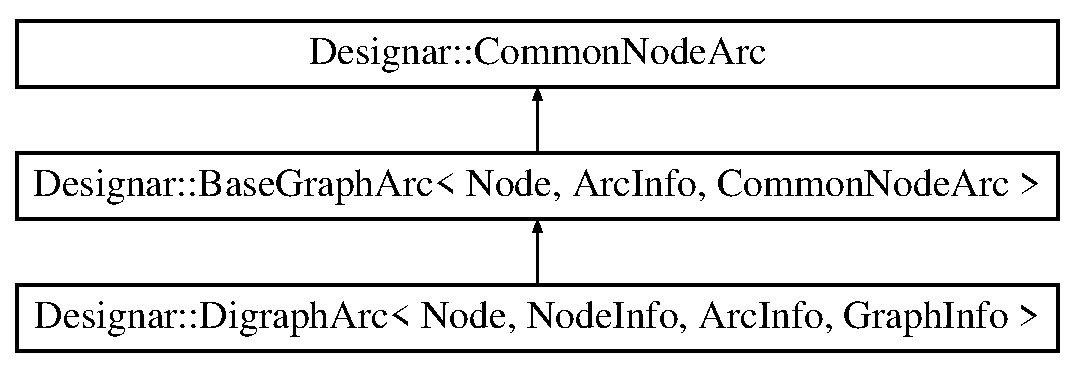
\includegraphics[height=3.000000cm]{class_designar_1_1_digraph_arc}
\end{center}
\end{figure}
\subsection*{Protected Attributes}
\begin{DoxyCompactItemize}
\item 
\hyperlink{class_designar_1_1_d_l_node}{D\+L\+Node}$<$ \hyperlink{class_designar_1_1_d_l_node}{D\+L\+Node}$<$ \hyperlink{class_designar_1_1_digraph_arc}{Digraph\+Arc} $>$ $\ast$ $>$ $\ast$ \hyperlink{class_designar_1_1_digraph_arc_a1b269dc44c4b3696cb79e86a97afbdd7}{arc\+\_\+in\+\_\+arc\+\_\+list} = nullptr
\end{DoxyCompactItemize}
\subsection*{Friends}
\begin{DoxyCompactItemize}
\item 
class \hyperlink{class_designar_1_1_digraph_arc_abc8f370e4ec7084a6574cf967a5a5aaf}{Digraph$<$ Node\+Info, Arc\+Info, Graph\+Info $>$}
\item 
class \hyperlink{class_designar_1_1_digraph_arc_a1d0cecb0e630aa2aa8179b2afdd92a8b}{D\+L\+Node$<$ Digraph\+Arc $>$}
\end{DoxyCompactItemize}
\subsection*{Additional Inherited Members}


\subsection{Detailed Description}
\subsubsection*{template$<$class Node, typename Node\+Info, typename Arc\+Info, typename Graph\+Info$>$\newline
class Designar\+::\+Digraph\+Arc$<$ Node, Node\+Info, Arc\+Info, Graph\+Info $>$}



Definition at line 72 of file graph.\+H.



\subsection{Friends And Related Function Documentation}
\mbox{\Hypertarget{class_designar_1_1_digraph_arc_abc8f370e4ec7084a6574cf967a5a5aaf}\label{class_designar_1_1_digraph_arc_abc8f370e4ec7084a6574cf967a5a5aaf}} 
\index{Designar\+::\+Digraph\+Arc@{Designar\+::\+Digraph\+Arc}!Digraph$<$ Node\+Info, Arc\+Info, Graph\+Info $>$@{Digraph$<$ Node\+Info, Arc\+Info, Graph\+Info $>$}}
\index{Digraph$<$ Node\+Info, Arc\+Info, Graph\+Info $>$@{Digraph$<$ Node\+Info, Arc\+Info, Graph\+Info $>$}!Designar\+::\+Digraph\+Arc@{Designar\+::\+Digraph\+Arc}}
\subsubsection{\texorpdfstring{Digraph$<$ Node\+Info, Arc\+Info, Graph\+Info $>$}{Digraph< NodeInfo, ArcInfo, GraphInfo >}}
{\footnotesize\ttfamily template$<$class Node , typename Node\+Info , typename Arc\+Info , typename Graph\+Info $>$ \\
friend class \hyperlink{class_designar_1_1_digraph}{Digraph}$<$ Node\+Info, Arc\+Info, Graph\+Info $>$\hspace{0.3cm}{\ttfamily [friend]}}



Definition at line 74 of file graph.\+H.

\mbox{\Hypertarget{class_designar_1_1_digraph_arc_a1d0cecb0e630aa2aa8179b2afdd92a8b}\label{class_designar_1_1_digraph_arc_a1d0cecb0e630aa2aa8179b2afdd92a8b}} 
\index{Designar\+::\+Digraph\+Arc@{Designar\+::\+Digraph\+Arc}!D\+L\+Node$<$ Digraph\+Arc $>$@{D\+L\+Node$<$ Digraph\+Arc $>$}}
\index{D\+L\+Node$<$ Digraph\+Arc $>$@{D\+L\+Node$<$ Digraph\+Arc $>$}!Designar\+::\+Digraph\+Arc@{Designar\+::\+Digraph\+Arc}}
\subsubsection{\texorpdfstring{D\+L\+Node$<$ Digraph\+Arc $>$}{DLNode< DigraphArc >}}
{\footnotesize\ttfamily template$<$class Node , typename Node\+Info , typename Arc\+Info , typename Graph\+Info $>$ \\
friend class \hyperlink{class_designar_1_1_d_l_node}{D\+L\+Node}$<$ \hyperlink{class_designar_1_1_digraph_arc}{Digraph\+Arc} $>$\hspace{0.3cm}{\ttfamily [friend]}}



Definition at line 75 of file graph.\+H.



\subsection{Member Data Documentation}
\mbox{\Hypertarget{class_designar_1_1_digraph_arc_a1b269dc44c4b3696cb79e86a97afbdd7}\label{class_designar_1_1_digraph_arc_a1b269dc44c4b3696cb79e86a97afbdd7}} 
\index{Designar\+::\+Digraph\+Arc@{Designar\+::\+Digraph\+Arc}!arc\+\_\+in\+\_\+arc\+\_\+list@{arc\+\_\+in\+\_\+arc\+\_\+list}}
\index{arc\+\_\+in\+\_\+arc\+\_\+list@{arc\+\_\+in\+\_\+arc\+\_\+list}!Designar\+::\+Digraph\+Arc@{Designar\+::\+Digraph\+Arc}}
\subsubsection{\texorpdfstring{arc\+\_\+in\+\_\+arc\+\_\+list}{arc\_in\_arc\_list}}
{\footnotesize\ttfamily template$<$class Node , typename Node\+Info , typename Arc\+Info , typename Graph\+Info $>$ \\
\hyperlink{class_designar_1_1_d_l_node}{D\+L\+Node}$<$\hyperlink{class_designar_1_1_d_l_node}{D\+L\+Node}$<$\hyperlink{class_designar_1_1_digraph_arc}{Digraph\+Arc}$>$ $\ast$$>$$\ast$ \hyperlink{class_designar_1_1_digraph_arc}{Designar\+::\+Digraph\+Arc}$<$ \hyperlink{namespace_designar_a5af326c65aa2bd26b26c410f2030d09e}{Node}, Node\+Info, Arc\+Info, Graph\+Info $>$\+::arc\+\_\+in\+\_\+arc\+\_\+list = nullptr\hspace{0.3cm}{\ttfamily [protected]}}



Definition at line 80 of file graph.\+H.



The documentation for this class was generated from the following file\+:\begin{DoxyCompactItemize}
\item 
include/\hyperlink{graph_8_h}{graph.\+H}\end{DoxyCompactItemize}

\hypertarget{class_designar_1_1_digraph_node}{}\section{Referencia de la plantilla de la Clase Designar\+:\+:Digraph\+Node$<$ Node\+Info, Arc\+Info, Graph\+Info $>$}
\label{class_designar_1_1_digraph_node}\index{Designar\+::\+Digraph\+Node$<$ Node\+Info, Arc\+Info, Graph\+Info $>$@{Designar\+::\+Digraph\+Node$<$ Node\+Info, Arc\+Info, Graph\+Info $>$}}


{\ttfamily \#include $<$graph.\+H$>$}

Diagrama de herencias de Designar\+:\+:Digraph\+Node$<$ Node\+Info, Arc\+Info, Graph\+Info $>$\begin{figure}[H]
\begin{center}
\leavevmode
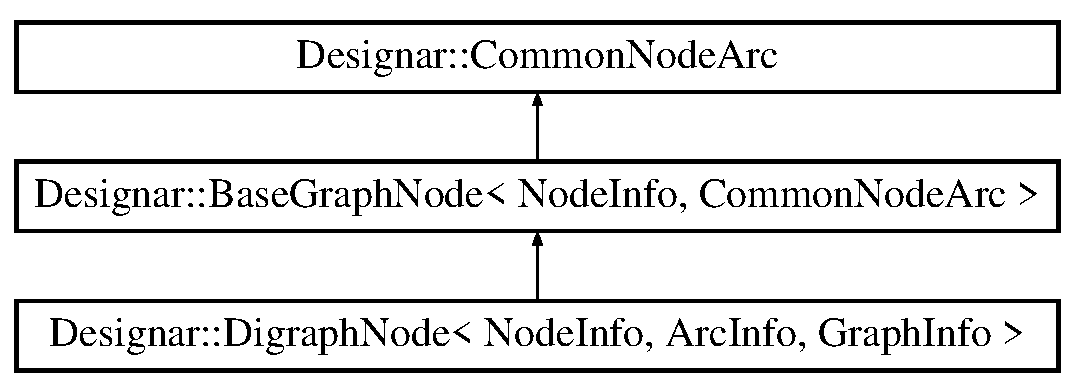
\includegraphics[height=3.000000cm]{class_designar_1_1_digraph_node}
\end{center}
\end{figure}
\subsection*{Amigas}
\begin{DoxyCompactItemize}
\item 
class \hyperlink{class_designar_1_1_digraph_node_abc8f370e4ec7084a6574cf967a5a5aaf}{Digraph$<$ Node\+Info, Arc\+Info, Graph\+Info $>$}
\item 
class \hyperlink{class_designar_1_1_digraph_node_a5532eb461a543edfe19acf97b74316fc}{D\+L\+Node$<$ Digraph\+Node $>$}
\end{DoxyCompactItemize}
\subsection*{Otros miembros heredados}


\subsection{Descripción detallada}
\subsubsection*{template$<$typename Node\+Info, typename Arc\+Info, typename Graph\+Info$>$\newline
class Designar\+::\+Digraph\+Node$<$ Node\+Info, Arc\+Info, Graph\+Info $>$}



Definición en la línea 50 del archivo graph.\+H.



\subsection{Documentación de las funciones relacionadas y clases amigas}
\mbox{\Hypertarget{class_designar_1_1_digraph_node_abc8f370e4ec7084a6574cf967a5a5aaf}\label{class_designar_1_1_digraph_node_abc8f370e4ec7084a6574cf967a5a5aaf}} 
\index{Designar\+::\+Digraph\+Node@{Designar\+::\+Digraph\+Node}!Digraph$<$ Node\+Info, Arc\+Info, Graph\+Info $>$@{Digraph$<$ Node\+Info, Arc\+Info, Graph\+Info $>$}}
\index{Digraph$<$ Node\+Info, Arc\+Info, Graph\+Info $>$@{Digraph$<$ Node\+Info, Arc\+Info, Graph\+Info $>$}!Designar\+::\+Digraph\+Node@{Designar\+::\+Digraph\+Node}}
\subsubsection{\texorpdfstring{Digraph$<$ Node\+Info, Arc\+Info, Graph\+Info $>$}{Digraph< NodeInfo, ArcInfo, GraphInfo >}}
{\footnotesize\ttfamily template$<$typename Node\+Info , typename Arc\+Info , typename Graph\+Info $>$ \\
friend class \hyperlink{class_designar_1_1_digraph}{Digraph}$<$ Node\+Info, Arc\+Info, Graph\+Info $>$\hspace{0.3cm}{\ttfamily [friend]}}



Definición en la línea 52 del archivo graph.\+H.

\mbox{\Hypertarget{class_designar_1_1_digraph_node_a5532eb461a543edfe19acf97b74316fc}\label{class_designar_1_1_digraph_node_a5532eb461a543edfe19acf97b74316fc}} 
\index{Designar\+::\+Digraph\+Node@{Designar\+::\+Digraph\+Node}!D\+L\+Node$<$ Digraph\+Node $>$@{D\+L\+Node$<$ Digraph\+Node $>$}}
\index{D\+L\+Node$<$ Digraph\+Node $>$@{D\+L\+Node$<$ Digraph\+Node $>$}!Designar\+::\+Digraph\+Node@{Designar\+::\+Digraph\+Node}}
\subsubsection{\texorpdfstring{D\+L\+Node$<$ Digraph\+Node $>$}{DLNode< DigraphNode >}}
{\footnotesize\ttfamily template$<$typename Node\+Info , typename Arc\+Info , typename Graph\+Info $>$ \\
friend class \hyperlink{class_designar_1_1_d_l_node}{D\+L\+Node}$<$ \hyperlink{class_designar_1_1_digraph_node}{Digraph\+Node} $>$\hspace{0.3cm}{\ttfamily [friend]}}



Definición en la línea 53 del archivo graph.\+H.



La documentación para esta clase fue generada a partir del siguiente fichero\+:\begin{DoxyCompactItemize}
\item 
include/\hyperlink{graph_8_h}{graph.\+H}\end{DoxyCompactItemize}

\hypertarget{class_designar_1_1_dijkstra}{}\section{Referencia de la plantilla de la Clase Designar\+:\+:Dijkstra$<$ GT, Distance, Cmp, Plus $>$}
\label{class_designar_1_1_dijkstra}\index{Designar\+::\+Dijkstra$<$ G\+T, Distance, Cmp, Plus $>$@{Designar\+::\+Dijkstra$<$ G\+T, Distance, Cmp, Plus $>$}}


{\ttfamily \#include $<$graphalgorithms.\+H$>$}

\subsection*{Tipos públicos}
\begin{DoxyCompactItemize}
\item 
using \hyperlink{class_designar_1_1_dijkstra_afeb644fc5395569ec366f0d220ab477d}{Node} = typename \hyperlink{class_designar_1_1_graph_a5dfc7dba9d092ac489c72e40390c37d0}{G\+T\+::\+Node}
\item 
using \hyperlink{class_designar_1_1_dijkstra_a5f0682f4edfd1456b7d4432fa976c641}{Arc} = typename \hyperlink{class_designar_1_1_graph_a74c730ef4ce2d20f998d72bd25c2b5bf}{G\+T\+::\+Arc}
\end{DoxyCompactItemize}
\subsection*{Métodos públicos}
\begin{DoxyCompactItemize}
\item 
\hyperlink{class_designar_1_1_dijkstra_ada4a9a8403304341114425e296c5ed26}{Dijkstra} (Distance \&\+\_\+distance, Cmp \&\+\_\+cmp, Plus \&\+\_\+plus)
\item 
\hyperlink{class_designar_1_1_dijkstra_a26f374b129c8108d6b95fc57f8dc09df}{Dijkstra} (Distance \&\&\+\_\+distance=Distance(), Cmp \&\&\+\_\+cmp=Cmp(), Plus \&\&\+\_\+plus=Plus())
\item 
\hyperlink{demo-buildgraph_8_c_a3001c40d2c31ca87ed96cd7d1334a55e}{GT} \hyperlink{class_designar_1_1_dijkstra_a70bbeb5dcd70c6ff3d203b7772021467}{build\+\_\+min\+\_\+path\+\_\+tree} (\hyperlink{demo-buildgraph_8_c_a3001c40d2c31ca87ed96cd7d1334a55e}{GT} \&, \hyperlink{class_designar_1_1_dijkstra_afeb644fc5395569ec366f0d220ab477d}{Node} \&)
\item 
void \hyperlink{class_designar_1_1_dijkstra_a607872c03f2e6de59936118e6f6c8790}{paint\+\_\+min\+\_\+path\+\_\+tree} (\hyperlink{demo-buildgraph_8_c_a3001c40d2c31ca87ed96cd7d1334a55e}{GT} \&g, \hyperlink{class_designar_1_1_dijkstra_afeb644fc5395569ec366f0d220ab477d}{Node} \&start)
\item 
\hyperlink{class_designar_1_1_path}{Path}$<$ \hyperlink{demo-buildgraph_8_c_a3001c40d2c31ca87ed96cd7d1334a55e}{GT} $>$ \hyperlink{class_designar_1_1_dijkstra_ab2d75c571dff03279bea0192047461f0}{search\+\_\+min\+\_\+path} (\hyperlink{demo-buildgraph_8_c_a3001c40d2c31ca87ed96cd7d1334a55e}{GT} \&g, \hyperlink{class_designar_1_1_dijkstra_afeb644fc5395569ec366f0d220ab477d}{Node} \&start, \hyperlink{class_designar_1_1_dijkstra_afeb644fc5395569ec366f0d220ab477d}{Node} \&end)
\item 
void \hyperlink{class_designar_1_1_dijkstra_a103839d3bd4e6d8733d2b47b186e137a}{paint\+\_\+min\+\_\+path} (\hyperlink{demo-buildgraph_8_c_a3001c40d2c31ca87ed96cd7d1334a55e}{GT} \&g, \hyperlink{class_designar_1_1_dijkstra_afeb644fc5395569ec366f0d220ab477d}{Node} \&start, \hyperlink{class_designar_1_1_dijkstra_afeb644fc5395569ec366f0d220ab477d}{Node} \&end)
\end{DoxyCompactItemize}


\subsection{Descripción detallada}
\subsubsection*{template$<$class GT, class Distance = Default\+Distance$<$\+G\+T$>$, class Cmp = std\+::less$<$typename Distance\+::\+Type$>$, class Plus = std\+::plus$<$typename Distance\+::\+Type$>$$>$\newline
class Designar\+::\+Dijkstra$<$ G\+T, Distance, Cmp, Plus $>$}



Definición en la línea 1408 del archivo graphalgorithms.\+H.



\subsection{Documentación de los \textquotesingle{}Typedef\textquotesingle{} miembros de la clase}
\mbox{\Hypertarget{class_designar_1_1_dijkstra_a5f0682f4edfd1456b7d4432fa976c641}\label{class_designar_1_1_dijkstra_a5f0682f4edfd1456b7d4432fa976c641}} 
\index{Designar\+::\+Dijkstra@{Designar\+::\+Dijkstra}!Arc@{Arc}}
\index{Arc@{Arc}!Designar\+::\+Dijkstra@{Designar\+::\+Dijkstra}}
\subsubsection{\texorpdfstring{Arc}{Arc}}
{\footnotesize\ttfamily template$<$class GT , class Distance  = Default\+Distance$<$\+G\+T$>$, class Cmp  = std\+::less$<$typename Distance\+::\+Type$>$, class Plus  = std\+::plus$<$typename Distance\+::\+Type$>$$>$ \\
using \hyperlink{class_designar_1_1_dijkstra}{Designar\+::\+Dijkstra}$<$ \hyperlink{demo-buildgraph_8_c_a3001c40d2c31ca87ed96cd7d1334a55e}{GT}, Distance, Cmp, Plus $>$\+::\hyperlink{class_designar_1_1_dijkstra_a5f0682f4edfd1456b7d4432fa976c641}{Arc} =  typename \hyperlink{class_designar_1_1_graph_a74c730ef4ce2d20f998d72bd25c2b5bf}{G\+T\+::\+Arc}}



Definición en la línea 1412 del archivo graphalgorithms.\+H.

\mbox{\Hypertarget{class_designar_1_1_dijkstra_afeb644fc5395569ec366f0d220ab477d}\label{class_designar_1_1_dijkstra_afeb644fc5395569ec366f0d220ab477d}} 
\index{Designar\+::\+Dijkstra@{Designar\+::\+Dijkstra}!Node@{Node}}
\index{Node@{Node}!Designar\+::\+Dijkstra@{Designar\+::\+Dijkstra}}
\subsubsection{\texorpdfstring{Node}{Node}}
{\footnotesize\ttfamily template$<$class GT , class Distance  = Default\+Distance$<$\+G\+T$>$, class Cmp  = std\+::less$<$typename Distance\+::\+Type$>$, class Plus  = std\+::plus$<$typename Distance\+::\+Type$>$$>$ \\
using \hyperlink{class_designar_1_1_dijkstra}{Designar\+::\+Dijkstra}$<$ \hyperlink{demo-buildgraph_8_c_a3001c40d2c31ca87ed96cd7d1334a55e}{GT}, Distance, Cmp, Plus $>$\+::\hyperlink{class_designar_1_1_dijkstra_afeb644fc5395569ec366f0d220ab477d}{Node} =  typename \hyperlink{class_designar_1_1_graph_a5dfc7dba9d092ac489c72e40390c37d0}{G\+T\+::\+Node}}



Definición en la línea 1411 del archivo graphalgorithms.\+H.



\subsection{Documentación del constructor y destructor}
\mbox{\Hypertarget{class_designar_1_1_dijkstra_ada4a9a8403304341114425e296c5ed26}\label{class_designar_1_1_dijkstra_ada4a9a8403304341114425e296c5ed26}} 
\index{Designar\+::\+Dijkstra@{Designar\+::\+Dijkstra}!Dijkstra@{Dijkstra}}
\index{Dijkstra@{Dijkstra}!Designar\+::\+Dijkstra@{Designar\+::\+Dijkstra}}
\subsubsection{\texorpdfstring{Dijkstra()}{Dijkstra()}\hspace{0.1cm}{\footnotesize\ttfamily [1/2]}}
{\footnotesize\ttfamily template$<$class GT , class Distance  = Default\+Distance$<$\+G\+T$>$, class Cmp  = std\+::less$<$typename Distance\+::\+Type$>$, class Plus  = std\+::plus$<$typename Distance\+::\+Type$>$$>$ \\
\hyperlink{class_designar_1_1_dijkstra}{Designar\+::\+Dijkstra}$<$ \hyperlink{demo-buildgraph_8_c_a3001c40d2c31ca87ed96cd7d1334a55e}{GT}, Distance, Cmp, Plus $>$\+::\hyperlink{class_designar_1_1_dijkstra}{Dijkstra} (\begin{DoxyParamCaption}\item[{Distance \&}]{\+\_\+distance,  }\item[{Cmp \&}]{\+\_\+cmp,  }\item[{Plus \&}]{\+\_\+plus }\end{DoxyParamCaption})\hspace{0.3cm}{\ttfamily [inline]}}



Definición en la línea 1428 del archivo graphalgorithms.\+H.

\mbox{\Hypertarget{class_designar_1_1_dijkstra_a26f374b129c8108d6b95fc57f8dc09df}\label{class_designar_1_1_dijkstra_a26f374b129c8108d6b95fc57f8dc09df}} 
\index{Designar\+::\+Dijkstra@{Designar\+::\+Dijkstra}!Dijkstra@{Dijkstra}}
\index{Dijkstra@{Dijkstra}!Designar\+::\+Dijkstra@{Designar\+::\+Dijkstra}}
\subsubsection{\texorpdfstring{Dijkstra()}{Dijkstra()}\hspace{0.1cm}{\footnotesize\ttfamily [2/2]}}
{\footnotesize\ttfamily template$<$class GT , class Distance  = Default\+Distance$<$\+G\+T$>$, class Cmp  = std\+::less$<$typename Distance\+::\+Type$>$, class Plus  = std\+::plus$<$typename Distance\+::\+Type$>$$>$ \\
\hyperlink{class_designar_1_1_dijkstra}{Designar\+::\+Dijkstra}$<$ \hyperlink{demo-buildgraph_8_c_a3001c40d2c31ca87ed96cd7d1334a55e}{GT}, Distance, Cmp, Plus $>$\+::\hyperlink{class_designar_1_1_dijkstra}{Dijkstra} (\begin{DoxyParamCaption}\item[{Distance \&\&}]{\+\_\+distance = {\ttfamily Distance()},  }\item[{Cmp \&\&}]{\+\_\+cmp = {\ttfamily Cmp()},  }\item[{Plus \&\&}]{\+\_\+plus = {\ttfamily Plus()} }\end{DoxyParamCaption})\hspace{0.3cm}{\ttfamily [inline]}}



Definición en la línea 1434 del archivo graphalgorithms.\+H.



\subsection{Documentación de las funciones miembro}
\mbox{\Hypertarget{class_designar_1_1_dijkstra_a70bbeb5dcd70c6ff3d203b7772021467}\label{class_designar_1_1_dijkstra_a70bbeb5dcd70c6ff3d203b7772021467}} 
\index{Designar\+::\+Dijkstra@{Designar\+::\+Dijkstra}!build\+\_\+min\+\_\+path\+\_\+tree@{build\+\_\+min\+\_\+path\+\_\+tree}}
\index{build\+\_\+min\+\_\+path\+\_\+tree@{build\+\_\+min\+\_\+path\+\_\+tree}!Designar\+::\+Dijkstra@{Designar\+::\+Dijkstra}}
\subsubsection{\texorpdfstring{build\+\_\+min\+\_\+path\+\_\+tree()}{build\_min\_path\_tree()}}
{\footnotesize\ttfamily template$<$class GT , class Distance , class Cmp , class Plus $>$ \\
\hyperlink{demo-buildgraph_8_c_a3001c40d2c31ca87ed96cd7d1334a55e}{GT} \hyperlink{class_designar_1_1_dijkstra}{Designar\+::\+Dijkstra}$<$ \hyperlink{demo-buildgraph_8_c_a3001c40d2c31ca87ed96cd7d1334a55e}{GT}, Distance, Cmp, Plus $>$\+::build\+\_\+min\+\_\+path\+\_\+tree (\begin{DoxyParamCaption}\item[{\hyperlink{demo-buildgraph_8_c_a3001c40d2c31ca87ed96cd7d1334a55e}{GT} \&}]{g,  }\item[{\hyperlink{class_designar_1_1_dijkstra_afeb644fc5395569ec366f0d220ab477d}{Node} \&}]{start }\end{DoxyParamCaption})}



Definición en la línea 1594 del archivo graphalgorithms.\+H.

\mbox{\Hypertarget{class_designar_1_1_dijkstra_a103839d3bd4e6d8733d2b47b186e137a}\label{class_designar_1_1_dijkstra_a103839d3bd4e6d8733d2b47b186e137a}} 
\index{Designar\+::\+Dijkstra@{Designar\+::\+Dijkstra}!paint\+\_\+min\+\_\+path@{paint\+\_\+min\+\_\+path}}
\index{paint\+\_\+min\+\_\+path@{paint\+\_\+min\+\_\+path}!Designar\+::\+Dijkstra@{Designar\+::\+Dijkstra}}
\subsubsection{\texorpdfstring{paint\+\_\+min\+\_\+path()}{paint\_min\_path()}}
{\footnotesize\ttfamily template$<$class GT , class Distance  = Default\+Distance$<$\+G\+T$>$, class Cmp  = std\+::less$<$typename Distance\+::\+Type$>$, class Plus  = std\+::plus$<$typename Distance\+::\+Type$>$$>$ \\
void \hyperlink{class_designar_1_1_dijkstra}{Designar\+::\+Dijkstra}$<$ \hyperlink{demo-buildgraph_8_c_a3001c40d2c31ca87ed96cd7d1334a55e}{GT}, Distance, Cmp, Plus $>$\+::paint\+\_\+min\+\_\+path (\begin{DoxyParamCaption}\item[{\hyperlink{demo-buildgraph_8_c_a3001c40d2c31ca87ed96cd7d1334a55e}{GT} \&}]{g,  }\item[{\hyperlink{class_designar_1_1_dijkstra_afeb644fc5395569ec366f0d220ab477d}{Node} \&}]{start,  }\item[{\hyperlink{class_designar_1_1_dijkstra_afeb644fc5395569ec366f0d220ab477d}{Node} \&}]{end }\end{DoxyParamCaption})\hspace{0.3cm}{\ttfamily [inline]}}



Definición en la línea 1491 del archivo graphalgorithms.\+H.

\mbox{\Hypertarget{class_designar_1_1_dijkstra_a607872c03f2e6de59936118e6f6c8790}\label{class_designar_1_1_dijkstra_a607872c03f2e6de59936118e6f6c8790}} 
\index{Designar\+::\+Dijkstra@{Designar\+::\+Dijkstra}!paint\+\_\+min\+\_\+path\+\_\+tree@{paint\+\_\+min\+\_\+path\+\_\+tree}}
\index{paint\+\_\+min\+\_\+path\+\_\+tree@{paint\+\_\+min\+\_\+path\+\_\+tree}!Designar\+::\+Dijkstra@{Designar\+::\+Dijkstra}}
\subsubsection{\texorpdfstring{paint\+\_\+min\+\_\+path\+\_\+tree()}{paint\_min\_path\_tree()}}
{\footnotesize\ttfamily template$<$class GT , class Distance  = Default\+Distance$<$\+G\+T$>$, class Cmp  = std\+::less$<$typename Distance\+::\+Type$>$, class Plus  = std\+::plus$<$typename Distance\+::\+Type$>$$>$ \\
void \hyperlink{class_designar_1_1_dijkstra}{Designar\+::\+Dijkstra}$<$ \hyperlink{demo-buildgraph_8_c_a3001c40d2c31ca87ed96cd7d1334a55e}{GT}, Distance, Cmp, Plus $>$\+::paint\+\_\+min\+\_\+path\+\_\+tree (\begin{DoxyParamCaption}\item[{\hyperlink{demo-buildgraph_8_c_a3001c40d2c31ca87ed96cd7d1334a55e}{GT} \&}]{g,  }\item[{\hyperlink{class_designar_1_1_dijkstra_afeb644fc5395569ec366f0d220ab477d}{Node} \&}]{start }\end{DoxyParamCaption})\hspace{0.3cm}{\ttfamily [inline]}}



Definición en la línea 1443 del archivo graphalgorithms.\+H.

\mbox{\Hypertarget{class_designar_1_1_dijkstra_ab2d75c571dff03279bea0192047461f0}\label{class_designar_1_1_dijkstra_ab2d75c571dff03279bea0192047461f0}} 
\index{Designar\+::\+Dijkstra@{Designar\+::\+Dijkstra}!search\+\_\+min\+\_\+path@{search\+\_\+min\+\_\+path}}
\index{search\+\_\+min\+\_\+path@{search\+\_\+min\+\_\+path}!Designar\+::\+Dijkstra@{Designar\+::\+Dijkstra}}
\subsubsection{\texorpdfstring{search\+\_\+min\+\_\+path()}{search\_min\_path()}}
{\footnotesize\ttfamily template$<$class GT , class Distance  = Default\+Distance$<$\+G\+T$>$, class Cmp  = std\+::less$<$typename Distance\+::\+Type$>$, class Plus  = std\+::plus$<$typename Distance\+::\+Type$>$$>$ \\
\hyperlink{class_designar_1_1_path}{Path}$<$\hyperlink{demo-buildgraph_8_c_a3001c40d2c31ca87ed96cd7d1334a55e}{GT}$>$ \hyperlink{class_designar_1_1_dijkstra}{Designar\+::\+Dijkstra}$<$ \hyperlink{demo-buildgraph_8_c_a3001c40d2c31ca87ed96cd7d1334a55e}{GT}, Distance, Cmp, Plus $>$\+::search\+\_\+min\+\_\+path (\begin{DoxyParamCaption}\item[{\hyperlink{demo-buildgraph_8_c_a3001c40d2c31ca87ed96cd7d1334a55e}{GT} \&}]{g,  }\item[{\hyperlink{class_designar_1_1_dijkstra_afeb644fc5395569ec366f0d220ab477d}{Node} \&}]{start,  }\item[{\hyperlink{class_designar_1_1_dijkstra_afeb644fc5395569ec366f0d220ab477d}{Node} \&}]{end }\end{DoxyParamCaption})\hspace{0.3cm}{\ttfamily [inline]}}



Definición en la línea 1464 del archivo graphalgorithms.\+H.



La documentación para esta clase fue generada a partir del siguiente fichero\+:\begin{DoxyCompactItemize}
\item 
include/\hyperlink{graphalgorithms_8_h}{graphalgorithms.\+H}\end{DoxyCompactItemize}

\hypertarget{class_designar_1_1_distance_cmp}{}\section{Referencia de la plantilla de la Clase Designar\+:\+:Distance\+Cmp$<$ GT, Distance, Cmp $>$}
\label{class_designar_1_1_distance_cmp}\index{Designar\+::\+Distance\+Cmp$<$ G\+T, Distance, Cmp $>$@{Designar\+::\+Distance\+Cmp$<$ G\+T, Distance, Cmp $>$}}


{\ttfamily \#include $<$graphalgorithms.\+H$>$}

\subsection*{Métodos públicos}
\begin{DoxyCompactItemize}
\item 
\hyperlink{class_designar_1_1_distance_cmp_a13ea231791225247024720da213506a3}{Distance\+Cmp} (Distance \&d, Cmp \&\+\_\+cmp)
\item 
\hyperlink{class_designar_1_1_distance_cmp_a1b9bedd922fc3007038b63fe19bfd10e}{Distance\+Cmp} (Distance \&\&d=Distance(), Cmp \&\&\+\_\+cmp=Cmp())
\item 
bool \hyperlink{class_designar_1_1_distance_cmp_a5de92b27c64e3493d950a99018d28671}{operator()} (typename G\+T\+::\+Arc \&a, typename G\+T\+::\+Arc \&b) const
\end{DoxyCompactItemize}


\subsection{Descripción detallada}
\subsubsection*{template$<$class GT, class Distance, class Cmp$>$\newline
class Designar\+::\+Distance\+Cmp$<$ G\+T, Distance, Cmp $>$}



Definición en la línea 1076 del archivo graphalgorithms.\+H.



\subsection{Documentación del constructor y destructor}
\mbox{\Hypertarget{class_designar_1_1_distance_cmp_a13ea231791225247024720da213506a3}\label{class_designar_1_1_distance_cmp_a13ea231791225247024720da213506a3}} 
\index{Designar\+::\+Distance\+Cmp@{Designar\+::\+Distance\+Cmp}!Distance\+Cmp@{Distance\+Cmp}}
\index{Distance\+Cmp@{Distance\+Cmp}!Designar\+::\+Distance\+Cmp@{Designar\+::\+Distance\+Cmp}}
\subsubsection{\texorpdfstring{Distance\+Cmp()}{DistanceCmp()}\hspace{0.1cm}{\footnotesize\ttfamily [1/2]}}
{\footnotesize\ttfamily template$<$class GT , class Distance , class Cmp $>$ \\
\hyperlink{class_designar_1_1_distance_cmp}{Designar\+::\+Distance\+Cmp}$<$ \hyperlink{demo-buildgraph_8_c_a3001c40d2c31ca87ed96cd7d1334a55e}{GT}, Distance, Cmp $>$\+::\hyperlink{class_designar_1_1_distance_cmp}{Distance\+Cmp} (\begin{DoxyParamCaption}\item[{Distance \&}]{d,  }\item[{Cmp \&}]{\+\_\+cmp }\end{DoxyParamCaption})\hspace{0.3cm}{\ttfamily [inline]}}



Definición en la línea 1082 del archivo graphalgorithms.\+H.

\mbox{\Hypertarget{class_designar_1_1_distance_cmp_a1b9bedd922fc3007038b63fe19bfd10e}\label{class_designar_1_1_distance_cmp_a1b9bedd922fc3007038b63fe19bfd10e}} 
\index{Designar\+::\+Distance\+Cmp@{Designar\+::\+Distance\+Cmp}!Distance\+Cmp@{Distance\+Cmp}}
\index{Distance\+Cmp@{Distance\+Cmp}!Designar\+::\+Distance\+Cmp@{Designar\+::\+Distance\+Cmp}}
\subsubsection{\texorpdfstring{Distance\+Cmp()}{DistanceCmp()}\hspace{0.1cm}{\footnotesize\ttfamily [2/2]}}
{\footnotesize\ttfamily template$<$class GT , class Distance , class Cmp $>$ \\
\hyperlink{class_designar_1_1_distance_cmp}{Designar\+::\+Distance\+Cmp}$<$ \hyperlink{demo-buildgraph_8_c_a3001c40d2c31ca87ed96cd7d1334a55e}{GT}, Distance, Cmp $>$\+::\hyperlink{class_designar_1_1_distance_cmp}{Distance\+Cmp} (\begin{DoxyParamCaption}\item[{Distance \&\&}]{d = {\ttfamily Distance()},  }\item[{Cmp \&\&}]{\+\_\+cmp = {\ttfamily Cmp()} }\end{DoxyParamCaption})\hspace{0.3cm}{\ttfamily [inline]}}



Definición en la línea 1088 del archivo graphalgorithms.\+H.



\subsection{Documentación de las funciones miembro}
\mbox{\Hypertarget{class_designar_1_1_distance_cmp_a5de92b27c64e3493d950a99018d28671}\label{class_designar_1_1_distance_cmp_a5de92b27c64e3493d950a99018d28671}} 
\index{Designar\+::\+Distance\+Cmp@{Designar\+::\+Distance\+Cmp}!operator()@{operator()}}
\index{operator()@{operator()}!Designar\+::\+Distance\+Cmp@{Designar\+::\+Distance\+Cmp}}
\subsubsection{\texorpdfstring{operator()()}{operator()()}}
{\footnotesize\ttfamily template$<$class GT , class Distance , class Cmp $>$ \\
bool \hyperlink{class_designar_1_1_distance_cmp}{Designar\+::\+Distance\+Cmp}$<$ \hyperlink{demo-buildgraph_8_c_a3001c40d2c31ca87ed96cd7d1334a55e}{GT}, Distance, Cmp $>$\+::operator() (\begin{DoxyParamCaption}\item[{typename G\+T\+::\+Arc \&}]{a,  }\item[{typename G\+T\+::\+Arc \&}]{b }\end{DoxyParamCaption}) const\hspace{0.3cm}{\ttfamily [inline]}}



Definición en la línea 1094 del archivo graphalgorithms.\+H.



La documentación para esta clase fue generada a partir del siguiente fichero\+:\begin{DoxyCompactItemize}
\item 
/home/julio/\+De\+S\+I\+G\+N\+A\+R-\/doc/\+De\+Si\+G\+N\+A\+R/include/\hyperlink{graphalgorithms_8_h}{graphalgorithms.\+H}\end{DoxyCompactItemize}

\hypertarget{class_designar_1_1_d_l}{}\section{Referencia de la Clase Designar\+:\+:DL}
\label{class_designar_1_1_d_l}\index{Designar\+::\+DL@{Designar\+::\+DL}}


{\ttfamily \#include $<$nodesdef.\+H$>$}

Diagrama de herencias de Designar\+:\+:DL\begin{figure}[H]
\begin{center}
\leavevmode
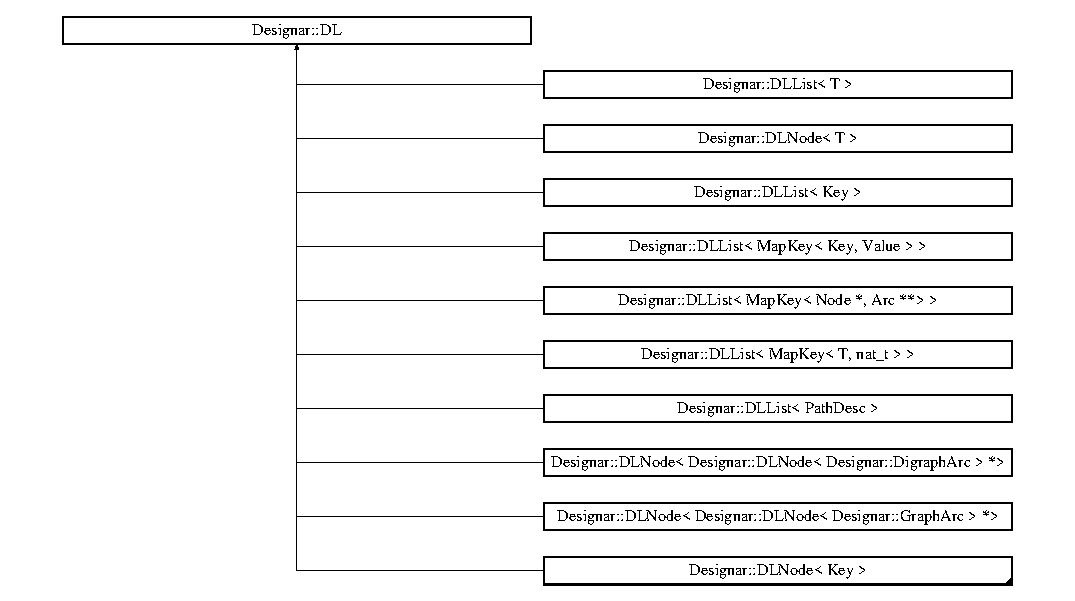
\includegraphics[height=7.623763cm]{class_designar_1_1_d_l}
\end{center}
\end{figure}
\subsection*{Clases}
\begin{DoxyCompactItemize}
\item 
class \hyperlink{class_designar_1_1_d_l_1_1_iterator}{Iterator}
\end{DoxyCompactItemize}
\subsection*{Métodos públicos}
\begin{DoxyCompactItemize}
\item 
\hyperlink{class_designar_1_1_d_l_a1e17a6036b4e5325d5aeb6641074ee14}{DL} ()
\item 
\hyperlink{class_designar_1_1_d_l_a4caafdd81bc08bdb7d42cbcbe735f59f}{DL} (const \hyperlink{class_designar_1_1_d_l}{DL} \&)
\item 
\hyperlink{class_designar_1_1_d_l_a4a9a38fbd77259a4af54dcd5017fce76}{DL} (\hyperlink{class_designar_1_1_d_l}{DL} \&\&l)
\item 
\hyperlink{class_designar_1_1_d_l}{DL} \& \hyperlink{class_designar_1_1_d_l_a7eb7d13fee4174fa5f4166722316530d}{operator=} (const \hyperlink{class_designar_1_1_d_l}{DL} \&)
\item 
\hyperlink{class_designar_1_1_d_l}{DL} \& \hyperlink{class_designar_1_1_d_l_adc892f364736bab874a6a739e88b5c60}{operator=} (\hyperlink{class_designar_1_1_d_l}{DL} \&\&l)
\item 
void \hyperlink{class_designar_1_1_d_l_a859e63ccad5bfe211d1fd7396f871091}{reset} ()
\item 
bool \hyperlink{class_designar_1_1_d_l_a01d421aa787edb4087c1b2c266554ca5}{is\+\_\+empty} () const
\item 
bool \hyperlink{class_designar_1_1_d_l_aae41f00b718a0fe8bed1be458b2dffac}{is\+\_\+unitarian\+\_\+or\+\_\+empty} () const
\item 
bool \hyperlink{class_designar_1_1_d_l_a262dfc0edc2656658f89b39ee272fac6}{is\+\_\+unitarian} () const
\item 
\hyperlink{class_designar_1_1_d_l}{DL} $\ast$\& \hyperlink{class_designar_1_1_d_l_a9ba5385743ae2c266ea51dcb05f79803}{get\+\_\+next} ()
\item 
const \hyperlink{class_designar_1_1_d_l}{DL} $\ast$\& \hyperlink{class_designar_1_1_d_l_ad95ed8f7db042ad4f537b335e8b77772}{get\+\_\+next} () const
\item 
\hyperlink{class_designar_1_1_d_l}{DL} $\ast$\& \hyperlink{class_designar_1_1_d_l_a479355d41d2d7085b33342a14c0ca514}{get\+\_\+prev} ()
\item 
const \hyperlink{class_designar_1_1_d_l}{DL} $\ast$\& \hyperlink{class_designar_1_1_d_l_a2f7ae6156dd09a783b6d1fc726af47c0}{get\+\_\+prev} () const
\item 
void \hyperlink{class_designar_1_1_d_l_a668fa2d4441cdbdba8640fbdab1b220c}{insert\+\_\+next} (\hyperlink{class_designar_1_1_d_l}{DL} $\ast$node)
\item 
void \hyperlink{class_designar_1_1_d_l_a44a3c60cd0f8de9811936cbe78d2e85e}{insert\+\_\+prev} (\hyperlink{class_designar_1_1_d_l}{DL} $\ast$node)
\item 
void \hyperlink{class_designar_1_1_d_l_affc0a48f00bd2ff8a6899c2a0c3d0ae3}{del} ()
\item 
\hyperlink{class_designar_1_1_d_l}{DL} $\ast$ \hyperlink{class_designar_1_1_d_l_a005d23127d2743fec552cafce79095d4}{remove\+\_\+next} ()
\item 
\hyperlink{class_designar_1_1_d_l}{DL} $\ast$ \hyperlink{class_designar_1_1_d_l_ab1978cfd1b4a98bedb0da473a7ba3164}{remove\+\_\+prev} ()
\item 
void \hyperlink{class_designar_1_1_d_l_a3a6b3f9fe3da01008ebf5f60bdf20bbc}{swap} (\hyperlink{class_designar_1_1_d_l}{DL} $\ast$node)
\item 
void \hyperlink{class_designar_1_1_d_l_a7b32539230a7ce8c23a8439bac4f3a12}{swap} (\hyperlink{class_designar_1_1_d_l}{DL} \&node)
\item 
void \hyperlink{class_designar_1_1_d_l_a016ee38fa1d6a467f07b3c8838e14937}{concat} (\hyperlink{class_designar_1_1_d_l}{DL} $\ast$l)
\item 
void \hyperlink{class_designar_1_1_d_l_ad952d602d2beded2a8f922289fe16d7f}{concat} (\hyperlink{class_designar_1_1_d_l}{DL} \&l)
\item 
void \hyperlink{class_designar_1_1_d_l_a81ed81ffd61fde1419fb4fb87ba551e3}{split} (\hyperlink{class_designar_1_1_d_l}{DL} \&, \hyperlink{class_designar_1_1_d_l}{DL} \&)
\end{DoxyCompactItemize}


\subsection{Descripción detallada}


Definición en la línea 113 del archivo nodesdef.\+H.



\subsection{Documentación del constructor y destructor}
\mbox{\Hypertarget{class_designar_1_1_d_l_a1e17a6036b4e5325d5aeb6641074ee14}\label{class_designar_1_1_d_l_a1e17a6036b4e5325d5aeb6641074ee14}} 
\index{Designar\+::\+DL@{Designar\+::\+DL}!DL@{DL}}
\index{DL@{DL}!Designar\+::\+DL@{Designar\+::\+DL}}
\subsubsection{\texorpdfstring{D\+L()}{DL()}\hspace{0.1cm}{\footnotesize\ttfamily [1/3]}}
{\footnotesize\ttfamily Designar\+::\+D\+L\+::\+DL (\begin{DoxyParamCaption}{ }\end{DoxyParamCaption})\hspace{0.3cm}{\ttfamily [inline]}}



Definición en la línea 119 del archivo nodesdef.\+H.

\mbox{\Hypertarget{class_designar_1_1_d_l_a4caafdd81bc08bdb7d42cbcbe735f59f}\label{class_designar_1_1_d_l_a4caafdd81bc08bdb7d42cbcbe735f59f}} 
\index{Designar\+::\+DL@{Designar\+::\+DL}!DL@{DL}}
\index{DL@{DL}!Designar\+::\+DL@{Designar\+::\+DL}}
\subsubsection{\texorpdfstring{D\+L()}{DL()}\hspace{0.1cm}{\footnotesize\ttfamily [2/3]}}
{\footnotesize\ttfamily Designar\+::\+D\+L\+::\+DL (\begin{DoxyParamCaption}\item[{const \hyperlink{class_designar_1_1_d_l}{DL} \&}]{ }\end{DoxyParamCaption})\hspace{0.3cm}{\ttfamily [inline]}}



Definición en la línea 125 del archivo nodesdef.\+H.

\mbox{\Hypertarget{class_designar_1_1_d_l_a4a9a38fbd77259a4af54dcd5017fce76}\label{class_designar_1_1_d_l_a4a9a38fbd77259a4af54dcd5017fce76}} 
\index{Designar\+::\+DL@{Designar\+::\+DL}!DL@{DL}}
\index{DL@{DL}!Designar\+::\+DL@{Designar\+::\+DL}}
\subsubsection{\texorpdfstring{D\+L()}{DL()}\hspace{0.1cm}{\footnotesize\ttfamily [3/3]}}
{\footnotesize\ttfamily Designar\+::\+D\+L\+::\+DL (\begin{DoxyParamCaption}\item[{\hyperlink{class_designar_1_1_d_l}{DL} \&\&}]{l }\end{DoxyParamCaption})\hspace{0.3cm}{\ttfamily [inline]}}



Definición en la línea 131 del archivo nodesdef.\+H.



\subsection{Documentación de las funciones miembro}
\mbox{\Hypertarget{class_designar_1_1_d_l_a016ee38fa1d6a467f07b3c8838e14937}\label{class_designar_1_1_d_l_a016ee38fa1d6a467f07b3c8838e14937}} 
\index{Designar\+::\+DL@{Designar\+::\+DL}!concat@{concat}}
\index{concat@{concat}!Designar\+::\+DL@{Designar\+::\+DL}}
\subsubsection{\texorpdfstring{concat()}{concat()}\hspace{0.1cm}{\footnotesize\ttfamily [1/2]}}
{\footnotesize\ttfamily void Designar\+::\+D\+L\+::concat (\begin{DoxyParamCaption}\item[{\hyperlink{class_designar_1_1_d_l}{DL} $\ast$}]{l }\end{DoxyParamCaption})\hspace{0.3cm}{\ttfamily [inline]}}



Definición en la línea 263 del archivo nodesdef.\+H.

\mbox{\Hypertarget{class_designar_1_1_d_l_ad952d602d2beded2a8f922289fe16d7f}\label{class_designar_1_1_d_l_ad952d602d2beded2a8f922289fe16d7f}} 
\index{Designar\+::\+DL@{Designar\+::\+DL}!concat@{concat}}
\index{concat@{concat}!Designar\+::\+DL@{Designar\+::\+DL}}
\subsubsection{\texorpdfstring{concat()}{concat()}\hspace{0.1cm}{\footnotesize\ttfamily [2/2]}}
{\footnotesize\ttfamily void Designar\+::\+D\+L\+::concat (\begin{DoxyParamCaption}\item[{\hyperlink{class_designar_1_1_d_l}{DL} \&}]{l }\end{DoxyParamCaption})\hspace{0.3cm}{\ttfamily [inline]}}



Definición en la línea 286 del archivo nodesdef.\+H.

\mbox{\Hypertarget{class_designar_1_1_d_l_affc0a48f00bd2ff8a6899c2a0c3d0ae3}\label{class_designar_1_1_d_l_affc0a48f00bd2ff8a6899c2a0c3d0ae3}} 
\index{Designar\+::\+DL@{Designar\+::\+DL}!del@{del}}
\index{del@{del}!Designar\+::\+DL@{Designar\+::\+DL}}
\subsubsection{\texorpdfstring{del()}{del()}}
{\footnotesize\ttfamily void Designar\+::\+D\+L\+::del (\begin{DoxyParamCaption}{ }\end{DoxyParamCaption})\hspace{0.3cm}{\ttfamily [inline]}}



Definición en la línea 208 del archivo nodesdef.\+H.

\mbox{\Hypertarget{class_designar_1_1_d_l_a9ba5385743ae2c266ea51dcb05f79803}\label{class_designar_1_1_d_l_a9ba5385743ae2c266ea51dcb05f79803}} 
\index{Designar\+::\+DL@{Designar\+::\+DL}!get\+\_\+next@{get\+\_\+next}}
\index{get\+\_\+next@{get\+\_\+next}!Designar\+::\+DL@{Designar\+::\+DL}}
\subsubsection{\texorpdfstring{get\+\_\+next()}{get\_next()}\hspace{0.1cm}{\footnotesize\ttfamily [1/2]}}
{\footnotesize\ttfamily \hyperlink{class_designar_1_1_d_l}{DL}$\ast$\& Designar\+::\+D\+L\+::get\+\_\+next (\begin{DoxyParamCaption}{ }\end{DoxyParamCaption})\hspace{0.3cm}{\ttfamily [inline]}}



Definición en la línea 168 del archivo nodesdef.\+H.

\mbox{\Hypertarget{class_designar_1_1_d_l_ad95ed8f7db042ad4f537b335e8b77772}\label{class_designar_1_1_d_l_ad95ed8f7db042ad4f537b335e8b77772}} 
\index{Designar\+::\+DL@{Designar\+::\+DL}!get\+\_\+next@{get\+\_\+next}}
\index{get\+\_\+next@{get\+\_\+next}!Designar\+::\+DL@{Designar\+::\+DL}}
\subsubsection{\texorpdfstring{get\+\_\+next()}{get\_next()}\hspace{0.1cm}{\footnotesize\ttfamily [2/2]}}
{\footnotesize\ttfamily const \hyperlink{class_designar_1_1_d_l}{DL}$\ast$\& Designar\+::\+D\+L\+::get\+\_\+next (\begin{DoxyParamCaption}{ }\end{DoxyParamCaption}) const\hspace{0.3cm}{\ttfamily [inline]}}



Definición en la línea 173 del archivo nodesdef.\+H.

\mbox{\Hypertarget{class_designar_1_1_d_l_a479355d41d2d7085b33342a14c0ca514}\label{class_designar_1_1_d_l_a479355d41d2d7085b33342a14c0ca514}} 
\index{Designar\+::\+DL@{Designar\+::\+DL}!get\+\_\+prev@{get\+\_\+prev}}
\index{get\+\_\+prev@{get\+\_\+prev}!Designar\+::\+DL@{Designar\+::\+DL}}
\subsubsection{\texorpdfstring{get\+\_\+prev()}{get\_prev()}\hspace{0.1cm}{\footnotesize\ttfamily [1/2]}}
{\footnotesize\ttfamily \hyperlink{class_designar_1_1_d_l}{DL}$\ast$\& Designar\+::\+D\+L\+::get\+\_\+prev (\begin{DoxyParamCaption}{ }\end{DoxyParamCaption})\hspace{0.3cm}{\ttfamily [inline]}}



Definición en la línea 178 del archivo nodesdef.\+H.

\mbox{\Hypertarget{class_designar_1_1_d_l_a2f7ae6156dd09a783b6d1fc726af47c0}\label{class_designar_1_1_d_l_a2f7ae6156dd09a783b6d1fc726af47c0}} 
\index{Designar\+::\+DL@{Designar\+::\+DL}!get\+\_\+prev@{get\+\_\+prev}}
\index{get\+\_\+prev@{get\+\_\+prev}!Designar\+::\+DL@{Designar\+::\+DL}}
\subsubsection{\texorpdfstring{get\+\_\+prev()}{get\_prev()}\hspace{0.1cm}{\footnotesize\ttfamily [2/2]}}
{\footnotesize\ttfamily const \hyperlink{class_designar_1_1_d_l}{DL}$\ast$\& Designar\+::\+D\+L\+::get\+\_\+prev (\begin{DoxyParamCaption}{ }\end{DoxyParamCaption}) const\hspace{0.3cm}{\ttfamily [inline]}}



Definición en la línea 183 del archivo nodesdef.\+H.

\mbox{\Hypertarget{class_designar_1_1_d_l_a668fa2d4441cdbdba8640fbdab1b220c}\label{class_designar_1_1_d_l_a668fa2d4441cdbdba8640fbdab1b220c}} 
\index{Designar\+::\+DL@{Designar\+::\+DL}!insert\+\_\+next@{insert\+\_\+next}}
\index{insert\+\_\+next@{insert\+\_\+next}!Designar\+::\+DL@{Designar\+::\+DL}}
\subsubsection{\texorpdfstring{insert\+\_\+next()}{insert\_next()}}
{\footnotesize\ttfamily void Designar\+::\+D\+L\+::insert\+\_\+next (\begin{DoxyParamCaption}\item[{\hyperlink{class_designar_1_1_d_l}{DL} $\ast$}]{node }\end{DoxyParamCaption})\hspace{0.3cm}{\ttfamily [inline]}}



Definición en la línea 188 del archivo nodesdef.\+H.

\mbox{\Hypertarget{class_designar_1_1_d_l_a44a3c60cd0f8de9811936cbe78d2e85e}\label{class_designar_1_1_d_l_a44a3c60cd0f8de9811936cbe78d2e85e}} 
\index{Designar\+::\+DL@{Designar\+::\+DL}!insert\+\_\+prev@{insert\+\_\+prev}}
\index{insert\+\_\+prev@{insert\+\_\+prev}!Designar\+::\+DL@{Designar\+::\+DL}}
\subsubsection{\texorpdfstring{insert\+\_\+prev()}{insert\_prev()}}
{\footnotesize\ttfamily void Designar\+::\+D\+L\+::insert\+\_\+prev (\begin{DoxyParamCaption}\item[{\hyperlink{class_designar_1_1_d_l}{DL} $\ast$}]{node }\end{DoxyParamCaption})\hspace{0.3cm}{\ttfamily [inline]}}



Definición en la línea 198 del archivo nodesdef.\+H.

\mbox{\Hypertarget{class_designar_1_1_d_l_a01d421aa787edb4087c1b2c266554ca5}\label{class_designar_1_1_d_l_a01d421aa787edb4087c1b2c266554ca5}} 
\index{Designar\+::\+DL@{Designar\+::\+DL}!is\+\_\+empty@{is\+\_\+empty}}
\index{is\+\_\+empty@{is\+\_\+empty}!Designar\+::\+DL@{Designar\+::\+DL}}
\subsubsection{\texorpdfstring{is\+\_\+empty()}{is\_empty()}}
{\footnotesize\ttfamily bool Designar\+::\+D\+L\+::is\+\_\+empty (\begin{DoxyParamCaption}{ }\end{DoxyParamCaption}) const\hspace{0.3cm}{\ttfamily [inline]}}



Definición en la línea 153 del archivo nodesdef.\+H.

\mbox{\Hypertarget{class_designar_1_1_d_l_a262dfc0edc2656658f89b39ee272fac6}\label{class_designar_1_1_d_l_a262dfc0edc2656658f89b39ee272fac6}} 
\index{Designar\+::\+DL@{Designar\+::\+DL}!is\+\_\+unitarian@{is\+\_\+unitarian}}
\index{is\+\_\+unitarian@{is\+\_\+unitarian}!Designar\+::\+DL@{Designar\+::\+DL}}
\subsubsection{\texorpdfstring{is\+\_\+unitarian()}{is\_unitarian()}}
{\footnotesize\ttfamily bool Designar\+::\+D\+L\+::is\+\_\+unitarian (\begin{DoxyParamCaption}{ }\end{DoxyParamCaption}) const\hspace{0.3cm}{\ttfamily [inline]}}



Definición en la línea 163 del archivo nodesdef.\+H.

\mbox{\Hypertarget{class_designar_1_1_d_l_aae41f00b718a0fe8bed1be458b2dffac}\label{class_designar_1_1_d_l_aae41f00b718a0fe8bed1be458b2dffac}} 
\index{Designar\+::\+DL@{Designar\+::\+DL}!is\+\_\+unitarian\+\_\+or\+\_\+empty@{is\+\_\+unitarian\+\_\+or\+\_\+empty}}
\index{is\+\_\+unitarian\+\_\+or\+\_\+empty@{is\+\_\+unitarian\+\_\+or\+\_\+empty}!Designar\+::\+DL@{Designar\+::\+DL}}
\subsubsection{\texorpdfstring{is\+\_\+unitarian\+\_\+or\+\_\+empty()}{is\_unitarian\_or\_empty()}}
{\footnotesize\ttfamily bool Designar\+::\+D\+L\+::is\+\_\+unitarian\+\_\+or\+\_\+empty (\begin{DoxyParamCaption}{ }\end{DoxyParamCaption}) const\hspace{0.3cm}{\ttfamily [inline]}}



Definición en la línea 158 del archivo nodesdef.\+H.

\mbox{\Hypertarget{class_designar_1_1_d_l_a7eb7d13fee4174fa5f4166722316530d}\label{class_designar_1_1_d_l_a7eb7d13fee4174fa5f4166722316530d}} 
\index{Designar\+::\+DL@{Designar\+::\+DL}!operator=@{operator=}}
\index{operator=@{operator=}!Designar\+::\+DL@{Designar\+::\+DL}}
\subsubsection{\texorpdfstring{operator=()}{operator=()}\hspace{0.1cm}{\footnotesize\ttfamily [1/2]}}
{\footnotesize\ttfamily \hyperlink{class_designar_1_1_d_l}{DL}\& Designar\+::\+D\+L\+::operator= (\begin{DoxyParamCaption}\item[{const \hyperlink{class_designar_1_1_d_l}{DL} \&}]{ }\end{DoxyParamCaption})\hspace{0.3cm}{\ttfamily [inline]}}



Definición en la línea 137 del archivo nodesdef.\+H.

\mbox{\Hypertarget{class_designar_1_1_d_l_adc892f364736bab874a6a739e88b5c60}\label{class_designar_1_1_d_l_adc892f364736bab874a6a739e88b5c60}} 
\index{Designar\+::\+DL@{Designar\+::\+DL}!operator=@{operator=}}
\index{operator=@{operator=}!Designar\+::\+DL@{Designar\+::\+DL}}
\subsubsection{\texorpdfstring{operator=()}{operator=()}\hspace{0.1cm}{\footnotesize\ttfamily [2/2]}}
{\footnotesize\ttfamily \hyperlink{class_designar_1_1_d_l}{DL}\& Designar\+::\+D\+L\+::operator= (\begin{DoxyParamCaption}\item[{\hyperlink{class_designar_1_1_d_l}{DL} \&\&}]{l }\end{DoxyParamCaption})\hspace{0.3cm}{\ttfamily [inline]}}



Definición en la línea 142 del archivo nodesdef.\+H.

\mbox{\Hypertarget{class_designar_1_1_d_l_a005d23127d2743fec552cafce79095d4}\label{class_designar_1_1_d_l_a005d23127d2743fec552cafce79095d4}} 
\index{Designar\+::\+DL@{Designar\+::\+DL}!remove\+\_\+next@{remove\+\_\+next}}
\index{remove\+\_\+next@{remove\+\_\+next}!Designar\+::\+DL@{Designar\+::\+DL}}
\subsubsection{\texorpdfstring{remove\+\_\+next()}{remove\_next()}}
{\footnotesize\ttfamily \hyperlink{class_designar_1_1_d_l}{DL}$\ast$ Designar\+::\+D\+L\+::remove\+\_\+next (\begin{DoxyParamCaption}{ }\end{DoxyParamCaption})\hspace{0.3cm}{\ttfamily [inline]}}



Definición en la línea 215 del archivo nodesdef.\+H.

\mbox{\Hypertarget{class_designar_1_1_d_l_ab1978cfd1b4a98bedb0da473a7ba3164}\label{class_designar_1_1_d_l_ab1978cfd1b4a98bedb0da473a7ba3164}} 
\index{Designar\+::\+DL@{Designar\+::\+DL}!remove\+\_\+prev@{remove\+\_\+prev}}
\index{remove\+\_\+prev@{remove\+\_\+prev}!Designar\+::\+DL@{Designar\+::\+DL}}
\subsubsection{\texorpdfstring{remove\+\_\+prev()}{remove\_prev()}}
{\footnotesize\ttfamily \hyperlink{class_designar_1_1_d_l}{DL}$\ast$ Designar\+::\+D\+L\+::remove\+\_\+prev (\begin{DoxyParamCaption}{ }\end{DoxyParamCaption})\hspace{0.3cm}{\ttfamily [inline]}}



Definición en la línea 222 del archivo nodesdef.\+H.

\mbox{\Hypertarget{class_designar_1_1_d_l_a859e63ccad5bfe211d1fd7396f871091}\label{class_designar_1_1_d_l_a859e63ccad5bfe211d1fd7396f871091}} 
\index{Designar\+::\+DL@{Designar\+::\+DL}!reset@{reset}}
\index{reset@{reset}!Designar\+::\+DL@{Designar\+::\+DL}}
\subsubsection{\texorpdfstring{reset()}{reset()}}
{\footnotesize\ttfamily void Designar\+::\+D\+L\+::reset (\begin{DoxyParamCaption}{ }\end{DoxyParamCaption})\hspace{0.3cm}{\ttfamily [inline]}}



Definición en la línea 148 del archivo nodesdef.\+H.

\mbox{\Hypertarget{class_designar_1_1_d_l_a81ed81ffd61fde1419fb4fb87ba551e3}\label{class_designar_1_1_d_l_a81ed81ffd61fde1419fb4fb87ba551e3}} 
\index{Designar\+::\+DL@{Designar\+::\+DL}!split@{split}}
\index{split@{split}!Designar\+::\+DL@{Designar\+::\+DL}}
\subsubsection{\texorpdfstring{split()}{split()}}
{\footnotesize\ttfamily void Designar\+::\+D\+L\+::split (\begin{DoxyParamCaption}\item[{\hyperlink{class_designar_1_1_d_l}{DL} \&}]{l,  }\item[{\hyperlink{class_designar_1_1_d_l}{DL} \&}]{r }\end{DoxyParamCaption})}



Definición en la línea 30 del archivo nodesdef.\+C.

\mbox{\Hypertarget{class_designar_1_1_d_l_a3a6b3f9fe3da01008ebf5f60bdf20bbc}\label{class_designar_1_1_d_l_a3a6b3f9fe3da01008ebf5f60bdf20bbc}} 
\index{Designar\+::\+DL@{Designar\+::\+DL}!swap@{swap}}
\index{swap@{swap}!Designar\+::\+DL@{Designar\+::\+DL}}
\subsubsection{\texorpdfstring{swap()}{swap()}\hspace{0.1cm}{\footnotesize\ttfamily [1/2]}}
{\footnotesize\ttfamily void Designar\+::\+D\+L\+::swap (\begin{DoxyParamCaption}\item[{\hyperlink{class_designar_1_1_d_l}{DL} $\ast$}]{node }\end{DoxyParamCaption})\hspace{0.3cm}{\ttfamily [inline]}}



Definición en la línea 229 del archivo nodesdef.\+H.

\mbox{\Hypertarget{class_designar_1_1_d_l_a7b32539230a7ce8c23a8439bac4f3a12}\label{class_designar_1_1_d_l_a7b32539230a7ce8c23a8439bac4f3a12}} 
\index{Designar\+::\+DL@{Designar\+::\+DL}!swap@{swap}}
\index{swap@{swap}!Designar\+::\+DL@{Designar\+::\+DL}}
\subsubsection{\texorpdfstring{swap()}{swap()}\hspace{0.1cm}{\footnotesize\ttfamily [2/2]}}
{\footnotesize\ttfamily void Designar\+::\+D\+L\+::swap (\begin{DoxyParamCaption}\item[{\hyperlink{class_designar_1_1_d_l}{DL} \&}]{node }\end{DoxyParamCaption})\hspace{0.3cm}{\ttfamily [inline]}}



Definición en la línea 258 del archivo nodesdef.\+H.



La documentación para esta clase fue generada a partir de los siguientes ficheros\+:\begin{DoxyCompactItemize}
\item 
include/\hyperlink{nodesdef_8_h}{nodesdef.\+H}\item 
src/\hyperlink{nodesdef_8_c}{nodesdef.\+C}\end{DoxyCompactItemize}

\hypertarget{class_designar_1_1_d_l_list}{}\section{Referencia de la plantilla de la Clase Designar\+:\+:D\+L\+List$<$ T $>$}
\label{class_designar_1_1_d_l_list}\index{Designar\+::\+D\+L\+List$<$ T $>$@{Designar\+::\+D\+L\+List$<$ T $>$}}


{\ttfamily \#include $<$list.\+H$>$}

Diagrama de herencias de Designar\+:\+:D\+L\+List$<$ T $>$\begin{figure}[H]
\begin{center}
\leavevmode
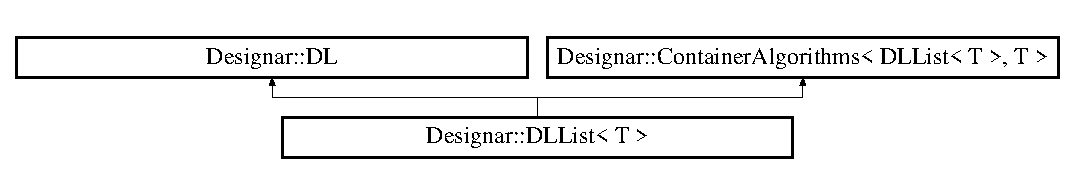
\includegraphics[height=1.885522cm]{class_designar_1_1_d_l_list}
\end{center}
\end{figure}
\subsection*{Clases}
\begin{DoxyCompactItemize}
\item 
class \hyperlink{class_designar_1_1_d_l_list_1_1_iterator}{Iterator}
\end{DoxyCompactItemize}
\subsection*{Tipos públicos}
\begin{DoxyCompactItemize}
\item 
using \hyperlink{class_designar_1_1_d_l_list_a622fc13673b169c75309314ae2ebc005}{Item\+Type} = T
\item 
using \hyperlink{class_designar_1_1_d_l_list_ac27702ab24c52fa9d770abc3c455bb25}{Key\+Type} = T
\item 
using \hyperlink{class_designar_1_1_d_l_list_ac2f57201101389ca63aec1c2fba61038}{Data\+Type} = T
\item 
using \hyperlink{class_designar_1_1_d_l_list_a839e4da136d61d24ba8f14fb4d9ceb34}{Value\+Type} = T
\item 
using \hyperlink{class_designar_1_1_d_l_list_ac03520f15d4db4a31f8764ed5633e0c6}{Size\+Type} = \hyperlink{namespace_designar_aa72662848b9f4815e7bf31a7cf3e33d1}{nat\+\_\+t}
\end{DoxyCompactItemize}
\subsection*{Métodos públicos}
\begin{DoxyCompactItemize}
\item 
\hyperlink{class_designar_1_1_d_l_list_af85c4b65efde3c33ad011bf6bb7444b0}{D\+L\+List} ()
\item 
\hyperlink{class_designar_1_1_d_l_list_a4be2c1cdec495bacc879851956e96d9d}{D\+L\+List} (const \hyperlink{class_designar_1_1_d_l_list}{D\+L\+List} \&l)
\item 
\hyperlink{class_designar_1_1_d_l_list_a8408964dd17ca747a9a21b141b05630e}{D\+L\+List} (\hyperlink{class_designar_1_1_d_l_list}{D\+L\+List} \&\&l)
\item 
\hyperlink{class_designar_1_1_d_l_list_a8a6c4e93a8eaf2b113c1b86d0e05f406}{D\+L\+List} (const std\+::initializer\+\_\+list$<$ T $>$ \&)
\item 
\hyperlink{class_designar_1_1_d_l_list_a095cfa30b7eba01f1dc7e3fe6d35f013}{$\sim$\+D\+L\+List} ()
\item 
\hyperlink{namespace_designar_aa72662848b9f4815e7bf31a7cf3e33d1}{nat\+\_\+t} \hyperlink{class_designar_1_1_d_l_list_a77234df6ebb6620ecf124e1810d9741c}{size} () const
\item 
void \hyperlink{class_designar_1_1_d_l_list_a0b617ee4b2f03b58b74630f79566f1b8}{clear} ()
\item 
void \hyperlink{class_designar_1_1_d_l_list_a34bdcc8016583c3e0ab50b4d3a87117b}{swap} (\hyperlink{class_designar_1_1_d_l_list}{D\+L\+List} \&l)
\item 
T \& \hyperlink{class_designar_1_1_d_l_list_ad153fdaa8982b2276266e1e0dbb8b773}{insert} (const T \&item)
\item 
T \& \hyperlink{class_designar_1_1_d_l_list_a4a88465e07f8708eea591614b5822bb6}{insert} (T \&\&item)
\item 
T \& \hyperlink{class_designar_1_1_d_l_list_a0999bcc1ce1d5b89d54c9993735dc469}{append} (const T \&item)
\item 
T \& \hyperlink{class_designar_1_1_d_l_list_a62918b133f72c5fa1c580f823642e5fa}{append} (T \&\&item)
\item 
T \& \hyperlink{class_designar_1_1_d_l_list_aa089dc5d48f092cc91d2237606e131e7}{get\+\_\+first} ()
\item 
const T \& \hyperlink{class_designar_1_1_d_l_list_a7dc30042ed6cd04f964504e2ff2e5653}{get\+\_\+first} () const
\item 
T \& \hyperlink{class_designar_1_1_d_l_list_a94c9be82f4ec5a3579e84027c421e073}{get\+\_\+last} ()
\item 
const T \& \hyperlink{class_designar_1_1_d_l_list_aae2cd78c744f82ece725c9d21a02d4da}{get\+\_\+last} () const
\item 
T \hyperlink{class_designar_1_1_d_l_list_a62e4c39df6ba191e7cd8dadac70109fb}{remove\+\_\+first} ()
\item 
T \hyperlink{class_designar_1_1_d_l_list_ac64bdba91bd7ff758fbb0e29f50dadcd}{remove\+\_\+last} ()
\item 
void \hyperlink{class_designar_1_1_d_l_list_a6fd7f99c303dc6897a72dabd5f1f943d}{remove} (T \&item)
\item 
\hyperlink{class_designar_1_1_d_l_list}{D\+L\+List} \& \hyperlink{class_designar_1_1_d_l_list_a3fda59e4bde20b86ee0cc0f083fc5f3a}{operator=} (const \hyperlink{class_designar_1_1_d_l_list}{D\+L\+List} \&l)
\item 
\hyperlink{class_designar_1_1_d_l_list}{D\+L\+List} \& \hyperlink{class_designar_1_1_d_l_list_a4c8c2df2e049fbbbfea113ae43365ff0}{operator=} (\hyperlink{class_designar_1_1_d_l_list}{D\+L\+List} \&\&l)
\item 
\hyperlink{class_designar_1_1_d_l_list_1_1_iterator}{Iterator} \hyperlink{class_designar_1_1_d_l_list_a1c011ca480554788280073fcdf6804c6}{begin} ()
\item 
\hyperlink{class_designar_1_1_d_l_list_1_1_iterator}{Iterator} \hyperlink{class_designar_1_1_d_l_list_a5fa0fa23f4ab881a04be6786de312dad}{begin} () const
\item 
\hyperlink{class_designar_1_1_d_l_list_1_1_iterator}{Iterator} \hyperlink{class_designar_1_1_d_l_list_afa49470cd57bc800bfa95c00cebb4c08}{end} ()
\item 
\hyperlink{class_designar_1_1_d_l_list_1_1_iterator}{Iterator} \hyperlink{class_designar_1_1_d_l_list_a44bec24be9eb3b3bbfeadc28240a1650}{end} () const
\item 
T \& \hyperlink{class_designar_1_1_d_l_list_abb57692be6aa79d00b65e40cd8402621}{select} (\hyperlink{namespace_designar_aa72662848b9f4815e7bf31a7cf3e33d1}{nat\+\_\+t})
\item 
const T \& \hyperlink{class_designar_1_1_d_l_list_a7060ef1496f583a3d4ed64b8ffdb94c8}{select} (\hyperlink{namespace_designar_aa72662848b9f4815e7bf31a7cf3e33d1}{nat\+\_\+t}) const
\item 
T \& \hyperlink{class_designar_1_1_d_l_list_aeb63bb4da91b7f1aed9a32de679122df}{operator\mbox{[}$\,$\mbox{]}} (\hyperlink{namespace_designar_aa72662848b9f4815e7bf31a7cf3e33d1}{nat\+\_\+t} i)
\item 
const T \& \hyperlink{class_designar_1_1_d_l_list_a24b5b31952821f0d40fef5326ba635b3}{operator\mbox{[}$\,$\mbox{]}} (\hyperlink{namespace_designar_aa72662848b9f4815e7bf31a7cf3e33d1}{nat\+\_\+t} i) const
\end{DoxyCompactItemize}


\subsection{Descripción detallada}
\subsubsection*{template$<$typename T$>$\newline
class Designar\+::\+D\+L\+List$<$ T $>$}



Definición en la línea 603 del archivo list.\+H.



\subsection{Documentación de los \textquotesingle{}Typedef\textquotesingle{} miembros de la clase}
\mbox{\Hypertarget{class_designar_1_1_d_l_list_ac2f57201101389ca63aec1c2fba61038}\label{class_designar_1_1_d_l_list_ac2f57201101389ca63aec1c2fba61038}} 
\index{Designar\+::\+D\+L\+List@{Designar\+::\+D\+L\+List}!Data\+Type@{Data\+Type}}
\index{Data\+Type@{Data\+Type}!Designar\+::\+D\+L\+List@{Designar\+::\+D\+L\+List}}
\subsubsection{\texorpdfstring{Data\+Type}{DataType}}
{\footnotesize\ttfamily template$<$typename T$>$ \\
using \hyperlink{class_designar_1_1_d_l_list}{Designar\+::\+D\+L\+List}$<$ T $>$\+::\hyperlink{class_designar_1_1_d_l_list_ac2f57201101389ca63aec1c2fba61038}{Data\+Type} =  T}



Definición en la línea 618 del archivo list.\+H.

\mbox{\Hypertarget{class_designar_1_1_d_l_list_a622fc13673b169c75309314ae2ebc005}\label{class_designar_1_1_d_l_list_a622fc13673b169c75309314ae2ebc005}} 
\index{Designar\+::\+D\+L\+List@{Designar\+::\+D\+L\+List}!Item\+Type@{Item\+Type}}
\index{Item\+Type@{Item\+Type}!Designar\+::\+D\+L\+List@{Designar\+::\+D\+L\+List}}
\subsubsection{\texorpdfstring{Item\+Type}{ItemType}}
{\footnotesize\ttfamily template$<$typename T$>$ \\
using \hyperlink{class_designar_1_1_d_l_list}{Designar\+::\+D\+L\+List}$<$ T $>$\+::\hyperlink{class_designar_1_1_d_l_list_a622fc13673b169c75309314ae2ebc005}{Item\+Type} =  T}



Definición en la línea 616 del archivo list.\+H.

\mbox{\Hypertarget{class_designar_1_1_d_l_list_ac27702ab24c52fa9d770abc3c455bb25}\label{class_designar_1_1_d_l_list_ac27702ab24c52fa9d770abc3c455bb25}} 
\index{Designar\+::\+D\+L\+List@{Designar\+::\+D\+L\+List}!Key\+Type@{Key\+Type}}
\index{Key\+Type@{Key\+Type}!Designar\+::\+D\+L\+List@{Designar\+::\+D\+L\+List}}
\subsubsection{\texorpdfstring{Key\+Type}{KeyType}}
{\footnotesize\ttfamily template$<$typename T$>$ \\
using \hyperlink{class_designar_1_1_d_l_list}{Designar\+::\+D\+L\+List}$<$ T $>$\+::\hyperlink{class_designar_1_1_d_l_list_ac27702ab24c52fa9d770abc3c455bb25}{Key\+Type} =  T}



Definición en la línea 617 del archivo list.\+H.

\mbox{\Hypertarget{class_designar_1_1_d_l_list_ac03520f15d4db4a31f8764ed5633e0c6}\label{class_designar_1_1_d_l_list_ac03520f15d4db4a31f8764ed5633e0c6}} 
\index{Designar\+::\+D\+L\+List@{Designar\+::\+D\+L\+List}!Size\+Type@{Size\+Type}}
\index{Size\+Type@{Size\+Type}!Designar\+::\+D\+L\+List@{Designar\+::\+D\+L\+List}}
\subsubsection{\texorpdfstring{Size\+Type}{SizeType}}
{\footnotesize\ttfamily template$<$typename T$>$ \\
using \hyperlink{class_designar_1_1_d_l_list}{Designar\+::\+D\+L\+List}$<$ T $>$\+::\hyperlink{class_designar_1_1_d_l_list_ac03520f15d4db4a31f8764ed5633e0c6}{Size\+Type} =  \hyperlink{namespace_designar_aa72662848b9f4815e7bf31a7cf3e33d1}{nat\+\_\+t}}



Definición en la línea 620 del archivo list.\+H.

\mbox{\Hypertarget{class_designar_1_1_d_l_list_a839e4da136d61d24ba8f14fb4d9ceb34}\label{class_designar_1_1_d_l_list_a839e4da136d61d24ba8f14fb4d9ceb34}} 
\index{Designar\+::\+D\+L\+List@{Designar\+::\+D\+L\+List}!Value\+Type@{Value\+Type}}
\index{Value\+Type@{Value\+Type}!Designar\+::\+D\+L\+List@{Designar\+::\+D\+L\+List}}
\subsubsection{\texorpdfstring{Value\+Type}{ValueType}}
{\footnotesize\ttfamily template$<$typename T$>$ \\
using \hyperlink{class_designar_1_1_d_l_list}{Designar\+::\+D\+L\+List}$<$ T $>$\+::\hyperlink{class_designar_1_1_d_l_list_a839e4da136d61d24ba8f14fb4d9ceb34}{Value\+Type} =  T}



Definición en la línea 619 del archivo list.\+H.



\subsection{Documentación del constructor y destructor}
\mbox{\Hypertarget{class_designar_1_1_d_l_list_af85c4b65efde3c33ad011bf6bb7444b0}\label{class_designar_1_1_d_l_list_af85c4b65efde3c33ad011bf6bb7444b0}} 
\index{Designar\+::\+D\+L\+List@{Designar\+::\+D\+L\+List}!D\+L\+List@{D\+L\+List}}
\index{D\+L\+List@{D\+L\+List}!Designar\+::\+D\+L\+List@{Designar\+::\+D\+L\+List}}
\subsubsection{\texorpdfstring{D\+L\+List()}{DLList()}\hspace{0.1cm}{\footnotesize\ttfamily [1/4]}}
{\footnotesize\ttfamily template$<$typename T$>$ \\
\hyperlink{class_designar_1_1_d_l_list}{Designar\+::\+D\+L\+List}$<$ T $>$\+::\hyperlink{class_designar_1_1_d_l_list}{D\+L\+List} (\begin{DoxyParamCaption}{ }\end{DoxyParamCaption})\hspace{0.3cm}{\ttfamily [inline]}}



Definición en la línea 622 del archivo list.\+H.

\mbox{\Hypertarget{class_designar_1_1_d_l_list_a4be2c1cdec495bacc879851956e96d9d}\label{class_designar_1_1_d_l_list_a4be2c1cdec495bacc879851956e96d9d}} 
\index{Designar\+::\+D\+L\+List@{Designar\+::\+D\+L\+List}!D\+L\+List@{D\+L\+List}}
\index{D\+L\+List@{D\+L\+List}!Designar\+::\+D\+L\+List@{Designar\+::\+D\+L\+List}}
\subsubsection{\texorpdfstring{D\+L\+List()}{DLList()}\hspace{0.1cm}{\footnotesize\ttfamily [2/4]}}
{\footnotesize\ttfamily template$<$typename T$>$ \\
\hyperlink{class_designar_1_1_d_l_list}{Designar\+::\+D\+L\+List}$<$ T $>$\+::\hyperlink{class_designar_1_1_d_l_list}{D\+L\+List} (\begin{DoxyParamCaption}\item[{const \hyperlink{class_designar_1_1_d_l_list}{D\+L\+List}$<$ T $>$ \&}]{l }\end{DoxyParamCaption})\hspace{0.3cm}{\ttfamily [inline]}}



Definición en la línea 628 del archivo list.\+H.

\mbox{\Hypertarget{class_designar_1_1_d_l_list_a8408964dd17ca747a9a21b141b05630e}\label{class_designar_1_1_d_l_list_a8408964dd17ca747a9a21b141b05630e}} 
\index{Designar\+::\+D\+L\+List@{Designar\+::\+D\+L\+List}!D\+L\+List@{D\+L\+List}}
\index{D\+L\+List@{D\+L\+List}!Designar\+::\+D\+L\+List@{Designar\+::\+D\+L\+List}}
\subsubsection{\texorpdfstring{D\+L\+List()}{DLList()}\hspace{0.1cm}{\footnotesize\ttfamily [3/4]}}
{\footnotesize\ttfamily template$<$typename T$>$ \\
\hyperlink{class_designar_1_1_d_l_list}{Designar\+::\+D\+L\+List}$<$ T $>$\+::\hyperlink{class_designar_1_1_d_l_list}{D\+L\+List} (\begin{DoxyParamCaption}\item[{\hyperlink{class_designar_1_1_d_l_list}{D\+L\+List}$<$ T $>$ \&\&}]{l }\end{DoxyParamCaption})\hspace{0.3cm}{\ttfamily [inline]}}



Definición en la línea 634 del archivo list.\+H.

\mbox{\Hypertarget{class_designar_1_1_d_l_list_a8a6c4e93a8eaf2b113c1b86d0e05f406}\label{class_designar_1_1_d_l_list_a8a6c4e93a8eaf2b113c1b86d0e05f406}} 
\index{Designar\+::\+D\+L\+List@{Designar\+::\+D\+L\+List}!D\+L\+List@{D\+L\+List}}
\index{D\+L\+List@{D\+L\+List}!Designar\+::\+D\+L\+List@{Designar\+::\+D\+L\+List}}
\subsubsection{\texorpdfstring{D\+L\+List()}{DLList()}\hspace{0.1cm}{\footnotesize\ttfamily [4/4]}}
{\footnotesize\ttfamily template$<$typename T$>$ \\
\hyperlink{class_designar_1_1_d_l_list}{Designar\+::\+D\+L\+List}$<$ T $>$\+::\hyperlink{class_designar_1_1_d_l_list}{D\+L\+List} (\begin{DoxyParamCaption}\item[{const std\+::initializer\+\_\+list$<$ T $>$ \&}]{l }\end{DoxyParamCaption})}



Definición en la línea 919 del archivo list.\+H.

\mbox{\Hypertarget{class_designar_1_1_d_l_list_a095cfa30b7eba01f1dc7e3fe6d35f013}\label{class_designar_1_1_d_l_list_a095cfa30b7eba01f1dc7e3fe6d35f013}} 
\index{Designar\+::\+D\+L\+List@{Designar\+::\+D\+L\+List}!````~D\+L\+List@{$\sim$\+D\+L\+List}}
\index{````~D\+L\+List@{$\sim$\+D\+L\+List}!Designar\+::\+D\+L\+List@{Designar\+::\+D\+L\+List}}
\subsubsection{\texorpdfstring{$\sim$\+D\+L\+List()}{~DLList()}}
{\footnotesize\ttfamily template$<$typename T$>$ \\
\hyperlink{class_designar_1_1_d_l_list}{Designar\+::\+D\+L\+List}$<$ T $>$\+::$\sim$\hyperlink{class_designar_1_1_d_l_list}{D\+L\+List} (\begin{DoxyParamCaption}{ }\end{DoxyParamCaption})\hspace{0.3cm}{\ttfamily [inline]}}



Definición en la línea 642 del archivo list.\+H.



\subsection{Documentación de las funciones miembro}
\mbox{\Hypertarget{class_designar_1_1_d_l_list_a0999bcc1ce1d5b89d54c9993735dc469}\label{class_designar_1_1_d_l_list_a0999bcc1ce1d5b89d54c9993735dc469}} 
\index{Designar\+::\+D\+L\+List@{Designar\+::\+D\+L\+List}!append@{append}}
\index{append@{append}!Designar\+::\+D\+L\+List@{Designar\+::\+D\+L\+List}}
\subsubsection{\texorpdfstring{append()}{append()}\hspace{0.1cm}{\footnotesize\ttfamily [1/2]}}
{\footnotesize\ttfamily template$<$typename T$>$ \\
T\& \hyperlink{class_designar_1_1_d_l_list}{Designar\+::\+D\+L\+List}$<$ T $>$\+::append (\begin{DoxyParamCaption}\item[{const T \&}]{item }\end{DoxyParamCaption})\hspace{0.3cm}{\ttfamily [inline]}}



Definición en la línea 679 del archivo list.\+H.

\mbox{\Hypertarget{class_designar_1_1_d_l_list_a62918b133f72c5fa1c580f823642e5fa}\label{class_designar_1_1_d_l_list_a62918b133f72c5fa1c580f823642e5fa}} 
\index{Designar\+::\+D\+L\+List@{Designar\+::\+D\+L\+List}!append@{append}}
\index{append@{append}!Designar\+::\+D\+L\+List@{Designar\+::\+D\+L\+List}}
\subsubsection{\texorpdfstring{append()}{append()}\hspace{0.1cm}{\footnotesize\ttfamily [2/2]}}
{\footnotesize\ttfamily template$<$typename T$>$ \\
T\& \hyperlink{class_designar_1_1_d_l_list}{Designar\+::\+D\+L\+List}$<$ T $>$\+::append (\begin{DoxyParamCaption}\item[{T \&\&}]{item }\end{DoxyParamCaption})\hspace{0.3cm}{\ttfamily [inline]}}



Definición en la línea 687 del archivo list.\+H.

\mbox{\Hypertarget{class_designar_1_1_d_l_list_a1c011ca480554788280073fcdf6804c6}\label{class_designar_1_1_d_l_list_a1c011ca480554788280073fcdf6804c6}} 
\index{Designar\+::\+D\+L\+List@{Designar\+::\+D\+L\+List}!begin@{begin}}
\index{begin@{begin}!Designar\+::\+D\+L\+List@{Designar\+::\+D\+L\+List}}
\subsubsection{\texorpdfstring{begin()}{begin()}\hspace{0.1cm}{\footnotesize\ttfamily [1/2]}}
{\footnotesize\ttfamily template$<$typename T$>$ \\
\hyperlink{class_designar_1_1_d_l_list_1_1_iterator}{Iterator} \hyperlink{class_designar_1_1_d_l_list}{Designar\+::\+D\+L\+List}$<$ T $>$\+::begin (\begin{DoxyParamCaption}{ }\end{DoxyParamCaption})\hspace{0.3cm}{\ttfamily [inline]}}



Definición en la línea 883 del archivo list.\+H.

\mbox{\Hypertarget{class_designar_1_1_d_l_list_a5fa0fa23f4ab881a04be6786de312dad}\label{class_designar_1_1_d_l_list_a5fa0fa23f4ab881a04be6786de312dad}} 
\index{Designar\+::\+D\+L\+List@{Designar\+::\+D\+L\+List}!begin@{begin}}
\index{begin@{begin}!Designar\+::\+D\+L\+List@{Designar\+::\+D\+L\+List}}
\subsubsection{\texorpdfstring{begin()}{begin()}\hspace{0.1cm}{\footnotesize\ttfamily [2/2]}}
{\footnotesize\ttfamily template$<$typename T$>$ \\
\hyperlink{class_designar_1_1_d_l_list_1_1_iterator}{Iterator} \hyperlink{class_designar_1_1_d_l_list}{Designar\+::\+D\+L\+List}$<$ T $>$\+::begin (\begin{DoxyParamCaption}{ }\end{DoxyParamCaption}) const\hspace{0.3cm}{\ttfamily [inline]}}



Definición en la línea 888 del archivo list.\+H.

\mbox{\Hypertarget{class_designar_1_1_d_l_list_a0b617ee4b2f03b58b74630f79566f1b8}\label{class_designar_1_1_d_l_list_a0b617ee4b2f03b58b74630f79566f1b8}} 
\index{Designar\+::\+D\+L\+List@{Designar\+::\+D\+L\+List}!clear@{clear}}
\index{clear@{clear}!Designar\+::\+D\+L\+List@{Designar\+::\+D\+L\+List}}
\subsubsection{\texorpdfstring{clear()}{clear()}}
{\footnotesize\ttfamily template$<$typename T$>$ \\
void \hyperlink{class_designar_1_1_d_l_list}{Designar\+::\+D\+L\+List}$<$ T $>$\+::clear (\begin{DoxyParamCaption}{ }\end{DoxyParamCaption})\hspace{0.3cm}{\ttfamily [inline]}}



Definición en la línea 652 del archivo list.\+H.

\mbox{\Hypertarget{class_designar_1_1_d_l_list_afa49470cd57bc800bfa95c00cebb4c08}\label{class_designar_1_1_d_l_list_afa49470cd57bc800bfa95c00cebb4c08}} 
\index{Designar\+::\+D\+L\+List@{Designar\+::\+D\+L\+List}!end@{end}}
\index{end@{end}!Designar\+::\+D\+L\+List@{Designar\+::\+D\+L\+List}}
\subsubsection{\texorpdfstring{end()}{end()}\hspace{0.1cm}{\footnotesize\ttfamily [1/2]}}
{\footnotesize\ttfamily template$<$typename T$>$ \\
\hyperlink{class_designar_1_1_d_l_list_1_1_iterator}{Iterator} \hyperlink{class_designar_1_1_d_l_list}{Designar\+::\+D\+L\+List}$<$ T $>$\+::end (\begin{DoxyParamCaption}{ }\end{DoxyParamCaption})\hspace{0.3cm}{\ttfamily [inline]}}



Definición en la línea 893 del archivo list.\+H.

\mbox{\Hypertarget{class_designar_1_1_d_l_list_a44bec24be9eb3b3bbfeadc28240a1650}\label{class_designar_1_1_d_l_list_a44bec24be9eb3b3bbfeadc28240a1650}} 
\index{Designar\+::\+D\+L\+List@{Designar\+::\+D\+L\+List}!end@{end}}
\index{end@{end}!Designar\+::\+D\+L\+List@{Designar\+::\+D\+L\+List}}
\subsubsection{\texorpdfstring{end()}{end()}\hspace{0.1cm}{\footnotesize\ttfamily [2/2]}}
{\footnotesize\ttfamily template$<$typename T$>$ \\
\hyperlink{class_designar_1_1_d_l_list_1_1_iterator}{Iterator} \hyperlink{class_designar_1_1_d_l_list}{Designar\+::\+D\+L\+List}$<$ T $>$\+::end (\begin{DoxyParamCaption}{ }\end{DoxyParamCaption}) const\hspace{0.3cm}{\ttfamily [inline]}}



Definición en la línea 898 del archivo list.\+H.

\mbox{\Hypertarget{class_designar_1_1_d_l_list_aa089dc5d48f092cc91d2237606e131e7}\label{class_designar_1_1_d_l_list_aa089dc5d48f092cc91d2237606e131e7}} 
\index{Designar\+::\+D\+L\+List@{Designar\+::\+D\+L\+List}!get\+\_\+first@{get\+\_\+first}}
\index{get\+\_\+first@{get\+\_\+first}!Designar\+::\+D\+L\+List@{Designar\+::\+D\+L\+List}}
\subsubsection{\texorpdfstring{get\+\_\+first()}{get\_first()}\hspace{0.1cm}{\footnotesize\ttfamily [1/2]}}
{\footnotesize\ttfamily template$<$typename T$>$ \\
T\& \hyperlink{class_designar_1_1_d_l_list}{Designar\+::\+D\+L\+List}$<$ T $>$\+::get\+\_\+first (\begin{DoxyParamCaption}{ }\end{DoxyParamCaption})\hspace{0.3cm}{\ttfamily [inline]}}



Definición en la línea 695 del archivo list.\+H.

\mbox{\Hypertarget{class_designar_1_1_d_l_list_a7dc30042ed6cd04f964504e2ff2e5653}\label{class_designar_1_1_d_l_list_a7dc30042ed6cd04f964504e2ff2e5653}} 
\index{Designar\+::\+D\+L\+List@{Designar\+::\+D\+L\+List}!get\+\_\+first@{get\+\_\+first}}
\index{get\+\_\+first@{get\+\_\+first}!Designar\+::\+D\+L\+List@{Designar\+::\+D\+L\+List}}
\subsubsection{\texorpdfstring{get\+\_\+first()}{get\_first()}\hspace{0.1cm}{\footnotesize\ttfamily [2/2]}}
{\footnotesize\ttfamily template$<$typename T$>$ \\
const T\& \hyperlink{class_designar_1_1_d_l_list}{Designar\+::\+D\+L\+List}$<$ T $>$\+::get\+\_\+first (\begin{DoxyParamCaption}{ }\end{DoxyParamCaption}) const\hspace{0.3cm}{\ttfamily [inline]}}



Definición en la línea 703 del archivo list.\+H.

\mbox{\Hypertarget{class_designar_1_1_d_l_list_a94c9be82f4ec5a3579e84027c421e073}\label{class_designar_1_1_d_l_list_a94c9be82f4ec5a3579e84027c421e073}} 
\index{Designar\+::\+D\+L\+List@{Designar\+::\+D\+L\+List}!get\+\_\+last@{get\+\_\+last}}
\index{get\+\_\+last@{get\+\_\+last}!Designar\+::\+D\+L\+List@{Designar\+::\+D\+L\+List}}
\subsubsection{\texorpdfstring{get\+\_\+last()}{get\_last()}\hspace{0.1cm}{\footnotesize\ttfamily [1/2]}}
{\footnotesize\ttfamily template$<$typename T$>$ \\
T\& \hyperlink{class_designar_1_1_d_l_list}{Designar\+::\+D\+L\+List}$<$ T $>$\+::get\+\_\+last (\begin{DoxyParamCaption}{ }\end{DoxyParamCaption})\hspace{0.3cm}{\ttfamily [inline]}}



Definición en la línea 711 del archivo list.\+H.

\mbox{\Hypertarget{class_designar_1_1_d_l_list_aae2cd78c744f82ece725c9d21a02d4da}\label{class_designar_1_1_d_l_list_aae2cd78c744f82ece725c9d21a02d4da}} 
\index{Designar\+::\+D\+L\+List@{Designar\+::\+D\+L\+List}!get\+\_\+last@{get\+\_\+last}}
\index{get\+\_\+last@{get\+\_\+last}!Designar\+::\+D\+L\+List@{Designar\+::\+D\+L\+List}}
\subsubsection{\texorpdfstring{get\+\_\+last()}{get\_last()}\hspace{0.1cm}{\footnotesize\ttfamily [2/2]}}
{\footnotesize\ttfamily template$<$typename T$>$ \\
const T\& \hyperlink{class_designar_1_1_d_l_list}{Designar\+::\+D\+L\+List}$<$ T $>$\+::get\+\_\+last (\begin{DoxyParamCaption}{ }\end{DoxyParamCaption}) const\hspace{0.3cm}{\ttfamily [inline]}}



Definición en la línea 719 del archivo list.\+H.

\mbox{\Hypertarget{class_designar_1_1_d_l_list_ad153fdaa8982b2276266e1e0dbb8b773}\label{class_designar_1_1_d_l_list_ad153fdaa8982b2276266e1e0dbb8b773}} 
\index{Designar\+::\+D\+L\+List@{Designar\+::\+D\+L\+List}!insert@{insert}}
\index{insert@{insert}!Designar\+::\+D\+L\+List@{Designar\+::\+D\+L\+List}}
\subsubsection{\texorpdfstring{insert()}{insert()}\hspace{0.1cm}{\footnotesize\ttfamily [1/2]}}
{\footnotesize\ttfamily template$<$typename T$>$ \\
T\& \hyperlink{class_designar_1_1_d_l_list}{Designar\+::\+D\+L\+List}$<$ T $>$\+::insert (\begin{DoxyParamCaption}\item[{const T \&}]{item }\end{DoxyParamCaption})\hspace{0.3cm}{\ttfamily [inline]}}



Definición en la línea 663 del archivo list.\+H.

\mbox{\Hypertarget{class_designar_1_1_d_l_list_a4a88465e07f8708eea591614b5822bb6}\label{class_designar_1_1_d_l_list_a4a88465e07f8708eea591614b5822bb6}} 
\index{Designar\+::\+D\+L\+List@{Designar\+::\+D\+L\+List}!insert@{insert}}
\index{insert@{insert}!Designar\+::\+D\+L\+List@{Designar\+::\+D\+L\+List}}
\subsubsection{\texorpdfstring{insert()}{insert()}\hspace{0.1cm}{\footnotesize\ttfamily [2/2]}}
{\footnotesize\ttfamily template$<$typename T$>$ \\
T\& \hyperlink{class_designar_1_1_d_l_list}{Designar\+::\+D\+L\+List}$<$ T $>$\+::insert (\begin{DoxyParamCaption}\item[{T \&\&}]{item }\end{DoxyParamCaption})\hspace{0.3cm}{\ttfamily [inline]}}



Definición en la línea 671 del archivo list.\+H.

\mbox{\Hypertarget{class_designar_1_1_d_l_list_a3fda59e4bde20b86ee0cc0f083fc5f3a}\label{class_designar_1_1_d_l_list_a3fda59e4bde20b86ee0cc0f083fc5f3a}} 
\index{Designar\+::\+D\+L\+List@{Designar\+::\+D\+L\+List}!operator=@{operator=}}
\index{operator=@{operator=}!Designar\+::\+D\+L\+List@{Designar\+::\+D\+L\+List}}
\subsubsection{\texorpdfstring{operator=()}{operator=()}\hspace{0.1cm}{\footnotesize\ttfamily [1/2]}}
{\footnotesize\ttfamily template$<$typename T$>$ \\
\hyperlink{class_designar_1_1_d_l_list}{D\+L\+List}\& \hyperlink{class_designar_1_1_d_l_list}{Designar\+::\+D\+L\+List}$<$ T $>$\+::operator= (\begin{DoxyParamCaption}\item[{const \hyperlink{class_designar_1_1_d_l_list}{D\+L\+List}$<$ T $>$ \&}]{l }\end{DoxyParamCaption})\hspace{0.3cm}{\ttfamily [inline]}}



Definición en la línea 761 del archivo list.\+H.

\mbox{\Hypertarget{class_designar_1_1_d_l_list_a4c8c2df2e049fbbbfea113ae43365ff0}\label{class_designar_1_1_d_l_list_a4c8c2df2e049fbbbfea113ae43365ff0}} 
\index{Designar\+::\+D\+L\+List@{Designar\+::\+D\+L\+List}!operator=@{operator=}}
\index{operator=@{operator=}!Designar\+::\+D\+L\+List@{Designar\+::\+D\+L\+List}}
\subsubsection{\texorpdfstring{operator=()}{operator=()}\hspace{0.1cm}{\footnotesize\ttfamily [2/2]}}
{\footnotesize\ttfamily template$<$typename T$>$ \\
\hyperlink{class_designar_1_1_d_l_list}{D\+L\+List}\& \hyperlink{class_designar_1_1_d_l_list}{Designar\+::\+D\+L\+List}$<$ T $>$\+::operator= (\begin{DoxyParamCaption}\item[{\hyperlink{class_designar_1_1_d_l_list}{D\+L\+List}$<$ T $>$ \&\&}]{l }\end{DoxyParamCaption})\hspace{0.3cm}{\ttfamily [inline]}}



Definición en la línea 771 del archivo list.\+H.

\mbox{\Hypertarget{class_designar_1_1_d_l_list_aeb63bb4da91b7f1aed9a32de679122df}\label{class_designar_1_1_d_l_list_aeb63bb4da91b7f1aed9a32de679122df}} 
\index{Designar\+::\+D\+L\+List@{Designar\+::\+D\+L\+List}!operator\mbox{[}\mbox{]}@{operator[]}}
\index{operator\mbox{[}\mbox{]}@{operator[]}!Designar\+::\+D\+L\+List@{Designar\+::\+D\+L\+List}}
\subsubsection{\texorpdfstring{operator[]()}{operator[]()}\hspace{0.1cm}{\footnotesize\ttfamily [1/2]}}
{\footnotesize\ttfamily template$<$typename T$>$ \\
T\& \hyperlink{class_designar_1_1_d_l_list}{Designar\+::\+D\+L\+List}$<$ T $>$\+::operator\mbox{[}$\,$\mbox{]} (\begin{DoxyParamCaption}\item[{\hyperlink{namespace_designar_aa72662848b9f4815e7bf31a7cf3e33d1}{nat\+\_\+t}}]{i }\end{DoxyParamCaption})\hspace{0.3cm}{\ttfamily [inline]}}



Definición en la línea 907 del archivo list.\+H.

\mbox{\Hypertarget{class_designar_1_1_d_l_list_a24b5b31952821f0d40fef5326ba635b3}\label{class_designar_1_1_d_l_list_a24b5b31952821f0d40fef5326ba635b3}} 
\index{Designar\+::\+D\+L\+List@{Designar\+::\+D\+L\+List}!operator\mbox{[}\mbox{]}@{operator[]}}
\index{operator\mbox{[}\mbox{]}@{operator[]}!Designar\+::\+D\+L\+List@{Designar\+::\+D\+L\+List}}
\subsubsection{\texorpdfstring{operator[]()}{operator[]()}\hspace{0.1cm}{\footnotesize\ttfamily [2/2]}}
{\footnotesize\ttfamily template$<$typename T$>$ \\
const T\& \hyperlink{class_designar_1_1_d_l_list}{Designar\+::\+D\+L\+List}$<$ T $>$\+::operator\mbox{[}$\,$\mbox{]} (\begin{DoxyParamCaption}\item[{\hyperlink{namespace_designar_aa72662848b9f4815e7bf31a7cf3e33d1}{nat\+\_\+t}}]{i }\end{DoxyParamCaption}) const\hspace{0.3cm}{\ttfamily [inline]}}



Definición en la línea 912 del archivo list.\+H.

\mbox{\Hypertarget{class_designar_1_1_d_l_list_a6fd7f99c303dc6897a72dabd5f1f943d}\label{class_designar_1_1_d_l_list_a6fd7f99c303dc6897a72dabd5f1f943d}} 
\index{Designar\+::\+D\+L\+List@{Designar\+::\+D\+L\+List}!remove@{remove}}
\index{remove@{remove}!Designar\+::\+D\+L\+List@{Designar\+::\+D\+L\+List}}
\subsubsection{\texorpdfstring{remove()}{remove()}}
{\footnotesize\ttfamily template$<$typename T$>$ \\
void \hyperlink{class_designar_1_1_d_l_list}{Designar\+::\+D\+L\+List}$<$ T $>$\+::remove (\begin{DoxyParamCaption}\item[{T \&}]{item }\end{DoxyParamCaption})\hspace{0.3cm}{\ttfamily [inline]}}



Definición en la línea 751 del archivo list.\+H.

\mbox{\Hypertarget{class_designar_1_1_d_l_list_a62e4c39df6ba191e7cd8dadac70109fb}\label{class_designar_1_1_d_l_list_a62e4c39df6ba191e7cd8dadac70109fb}} 
\index{Designar\+::\+D\+L\+List@{Designar\+::\+D\+L\+List}!remove\+\_\+first@{remove\+\_\+first}}
\index{remove\+\_\+first@{remove\+\_\+first}!Designar\+::\+D\+L\+List@{Designar\+::\+D\+L\+List}}
\subsubsection{\texorpdfstring{remove\+\_\+first()}{remove\_first()}}
{\footnotesize\ttfamily template$<$typename T$>$ \\
T \hyperlink{class_designar_1_1_d_l_list}{Designar\+::\+D\+L\+List}$<$ T $>$\+::remove\+\_\+first (\begin{DoxyParamCaption}{ }\end{DoxyParamCaption})\hspace{0.3cm}{\ttfamily [inline]}}



Definición en la línea 727 del archivo list.\+H.

\mbox{\Hypertarget{class_designar_1_1_d_l_list_ac64bdba91bd7ff758fbb0e29f50dadcd}\label{class_designar_1_1_d_l_list_ac64bdba91bd7ff758fbb0e29f50dadcd}} 
\index{Designar\+::\+D\+L\+List@{Designar\+::\+D\+L\+List}!remove\+\_\+last@{remove\+\_\+last}}
\index{remove\+\_\+last@{remove\+\_\+last}!Designar\+::\+D\+L\+List@{Designar\+::\+D\+L\+List}}
\subsubsection{\texorpdfstring{remove\+\_\+last()}{remove\_last()}}
{\footnotesize\ttfamily template$<$typename T$>$ \\
T \hyperlink{class_designar_1_1_d_l_list}{Designar\+::\+D\+L\+List}$<$ T $>$\+::remove\+\_\+last (\begin{DoxyParamCaption}{ }\end{DoxyParamCaption})\hspace{0.3cm}{\ttfamily [inline]}}



Definición en la línea 739 del archivo list.\+H.

\mbox{\Hypertarget{class_designar_1_1_d_l_list_abb57692be6aa79d00b65e40cd8402621}\label{class_designar_1_1_d_l_list_abb57692be6aa79d00b65e40cd8402621}} 
\index{Designar\+::\+D\+L\+List@{Designar\+::\+D\+L\+List}!select@{select}}
\index{select@{select}!Designar\+::\+D\+L\+List@{Designar\+::\+D\+L\+List}}
\subsubsection{\texorpdfstring{select()}{select()}\hspace{0.1cm}{\footnotesize\ttfamily [1/2]}}
{\footnotesize\ttfamily template$<$typename T $>$ \\
T \& \hyperlink{class_designar_1_1_d_l_list}{Designar\+::\+D\+L\+List}$<$ T $>$\+::select (\begin{DoxyParamCaption}\item[{\hyperlink{namespace_designar_aa72662848b9f4815e7bf31a7cf3e33d1}{nat\+\_\+t}}]{i }\end{DoxyParamCaption})}



Definición en la línea 946 del archivo list.\+H.

\mbox{\Hypertarget{class_designar_1_1_d_l_list_a7060ef1496f583a3d4ed64b8ffdb94c8}\label{class_designar_1_1_d_l_list_a7060ef1496f583a3d4ed64b8ffdb94c8}} 
\index{Designar\+::\+D\+L\+List@{Designar\+::\+D\+L\+List}!select@{select}}
\index{select@{select}!Designar\+::\+D\+L\+List@{Designar\+::\+D\+L\+List}}
\subsubsection{\texorpdfstring{select()}{select()}\hspace{0.1cm}{\footnotesize\ttfamily [2/2]}}
{\footnotesize\ttfamily template$<$typename T $>$ \\
const T \& \hyperlink{class_designar_1_1_d_l_list}{Designar\+::\+D\+L\+List}$<$ T $>$\+::select (\begin{DoxyParamCaption}\item[{\hyperlink{namespace_designar_aa72662848b9f4815e7bf31a7cf3e33d1}{nat\+\_\+t}}]{i }\end{DoxyParamCaption}) const}



Definición en la línea 957 del archivo list.\+H.

\mbox{\Hypertarget{class_designar_1_1_d_l_list_a77234df6ebb6620ecf124e1810d9741c}\label{class_designar_1_1_d_l_list_a77234df6ebb6620ecf124e1810d9741c}} 
\index{Designar\+::\+D\+L\+List@{Designar\+::\+D\+L\+List}!size@{size}}
\index{size@{size}!Designar\+::\+D\+L\+List@{Designar\+::\+D\+L\+List}}
\subsubsection{\texorpdfstring{size()}{size()}}
{\footnotesize\ttfamily template$<$typename T$>$ \\
\hyperlink{namespace_designar_aa72662848b9f4815e7bf31a7cf3e33d1}{nat\+\_\+t} \hyperlink{class_designar_1_1_d_l_list}{Designar\+::\+D\+L\+List}$<$ T $>$\+::size (\begin{DoxyParamCaption}{ }\end{DoxyParamCaption}) const\hspace{0.3cm}{\ttfamily [inline]}}



Definición en la línea 647 del archivo list.\+H.

\mbox{\Hypertarget{class_designar_1_1_d_l_list_a34bdcc8016583c3e0ab50b4d3a87117b}\label{class_designar_1_1_d_l_list_a34bdcc8016583c3e0ab50b4d3a87117b}} 
\index{Designar\+::\+D\+L\+List@{Designar\+::\+D\+L\+List}!swap@{swap}}
\index{swap@{swap}!Designar\+::\+D\+L\+List@{Designar\+::\+D\+L\+List}}
\subsubsection{\texorpdfstring{swap()}{swap()}}
{\footnotesize\ttfamily template$<$typename T$>$ \\
void \hyperlink{class_designar_1_1_d_l_list}{Designar\+::\+D\+L\+List}$<$ T $>$\+::swap (\begin{DoxyParamCaption}\item[{\hyperlink{class_designar_1_1_d_l_list}{D\+L\+List}$<$ T $>$ \&}]{l }\end{DoxyParamCaption})\hspace{0.3cm}{\ttfamily [inline]}}



Definición en la línea 657 del archivo list.\+H.



La documentación para esta clase fue generada a partir del siguiente fichero\+:\begin{DoxyCompactItemize}
\item 
/home/julio/\+De\+S\+I\+G\+N\+A\+R-\/doc/\+De\+Si\+G\+N\+A\+R/include/\hyperlink{list_8_h}{list.\+H}\end{DoxyCompactItemize}

\hypertarget{class_designar_1_1_d_l_node}{}\section{Referencia de la plantilla de la Clase Designar\+:\+:D\+L\+Node$<$ T $>$}
\label{class_designar_1_1_d_l_node}\index{Designar\+::\+D\+L\+Node$<$ T $>$@{Designar\+::\+D\+L\+Node$<$ T $>$}}


{\ttfamily \#include $<$nodesdef.\+H$>$}

Diagrama de herencias de Designar\+:\+:D\+L\+Node$<$ T $>$\begin{figure}[H]
\begin{center}
\leavevmode
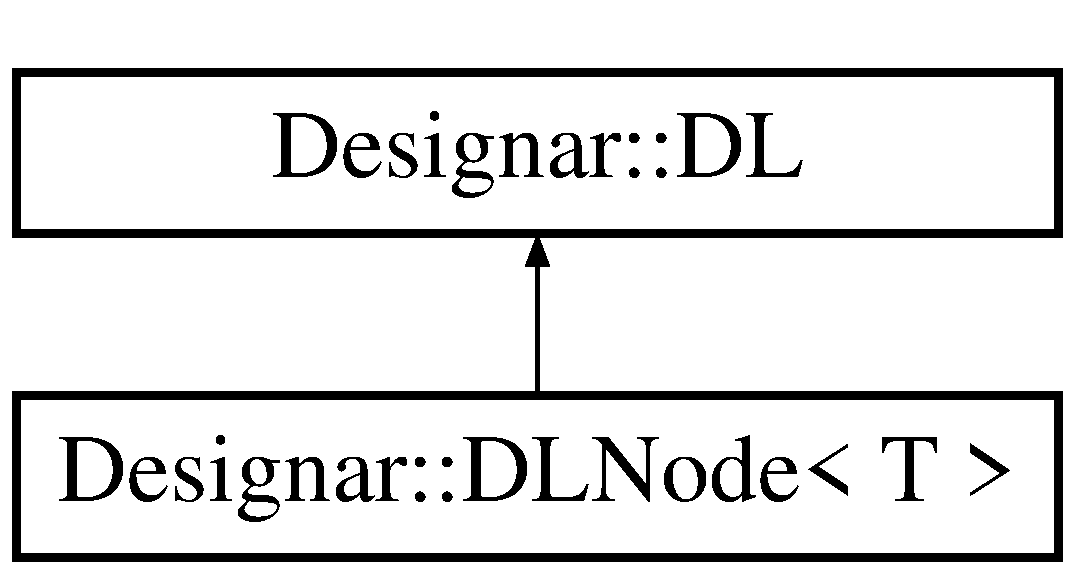
\includegraphics[height=2.000000cm]{class_designar_1_1_d_l_node}
\end{center}
\end{figure}
\subsection*{Clases}
\begin{DoxyCompactItemize}
\item 
class \hyperlink{class_designar_1_1_d_l_node_1_1_iterator}{Iterator}
\end{DoxyCompactItemize}
\subsection*{Métodos públicos}
\begin{DoxyCompactItemize}
\item 
\hyperlink{class_designar_1_1_d_l_node_aac2adda6b4d737b47d461efe02401f01}{D\+L\+Node} ()
\item 
\hyperlink{class_designar_1_1_d_l_node_af55ccc85dacdef9932b36e1ebd681306}{D\+L\+Node} (const T \&i)
\item 
\hyperlink{class_designar_1_1_d_l_node_a4c90cd184cdec513673fece07a858221}{D\+L\+Node} (T \&\&i)
\item 
\hyperlink{class_designar_1_1_d_l_node_aa70f9ca6c57dc2731ef5cff85fc849ba}{D\+L\+Node} (const \hyperlink{class_designar_1_1_d_l_node}{D\+L\+Node} \&)=delete
\item 
\hyperlink{class_designar_1_1_d_l_node_a9c80165d85c73bb4815e3ca098c1e72b}{D\+L\+Node} (\hyperlink{class_designar_1_1_d_l_node}{D\+L\+Node} \&\&n)
\item 
\hyperlink{class_designar_1_1_d_l_node}{D\+L\+Node} \& \hyperlink{class_designar_1_1_d_l_node_a790e90bcc8e4c5047e576aeaa1374291}{operator=} (const \hyperlink{class_designar_1_1_d_l_node}{D\+L\+Node} \&)=delete
\item 
\hyperlink{class_designar_1_1_d_l_node}{D\+L\+Node} \& \hyperlink{class_designar_1_1_d_l_node_a4993e8544e88f3ba0552d8e4005f6fac}{operator=} (\hyperlink{class_designar_1_1_d_l_node}{D\+L\+Node} \&\&n)
\item 
T \& \hyperlink{class_designar_1_1_d_l_node_a5f116af77588dcefd27fc92e679c27d2}{get\+\_\+item} ()
\item 
const T \& \hyperlink{class_designar_1_1_d_l_node_ac6c814f0d4d13daa3f69e6311fea83a8}{get\+\_\+item} () const
\item 
\hyperlink{class_designar_1_1_d_l_node}{D\+L\+Node} $\ast$\& \hyperlink{class_designar_1_1_d_l_node_a28ad2b7a46044b5e798e06888631bbde}{get\+\_\+next} ()
\item 
const \hyperlink{class_designar_1_1_d_l_node}{D\+L\+Node} $\ast$\& \hyperlink{class_designar_1_1_d_l_node_a2e9212d8d5bec7b811c8ca11948bdad6}{get\+\_\+next} () const
\item 
\hyperlink{class_designar_1_1_d_l_node}{D\+L\+Node} $\ast$\& \hyperlink{class_designar_1_1_d_l_node_a17271ebf6fc77a191c1a4a9c70fdb702}{get\+\_\+prev} ()
\item 
const \hyperlink{class_designar_1_1_d_l_node}{D\+L\+Node} $\ast$\& \hyperlink{class_designar_1_1_d_l_node_ad994f44ae1d1f56a318796d763361372}{get\+\_\+prev} () const
\item 
\hyperlink{class_designar_1_1_d_l_node}{D\+L\+Node} $\ast$ \hyperlink{class_designar_1_1_d_l_node_a8ff44fbe079ffd92ad09d3e6c5ec0458}{remove\+\_\+next} ()
\item 
\hyperlink{class_designar_1_1_d_l_node}{D\+L\+Node} $\ast$ \hyperlink{class_designar_1_1_d_l_node_a0bd2bf491ab61ab3fd1eb6b8b06dcae5}{remove\+\_\+prev} ()
\end{DoxyCompactItemize}


\subsection{Descripción detallada}
\subsubsection*{template$<$typename T$>$\newline
class Designar\+::\+D\+L\+Node$<$ T $>$}



Definición en la línea 415 del archivo nodesdef.\+H.



\subsection{Documentación del constructor y destructor}
\mbox{\Hypertarget{class_designar_1_1_d_l_node_aac2adda6b4d737b47d461efe02401f01}\label{class_designar_1_1_d_l_node_aac2adda6b4d737b47d461efe02401f01}} 
\index{Designar\+::\+D\+L\+Node@{Designar\+::\+D\+L\+Node}!D\+L\+Node@{D\+L\+Node}}
\index{D\+L\+Node@{D\+L\+Node}!Designar\+::\+D\+L\+Node@{Designar\+::\+D\+L\+Node}}
\subsubsection{\texorpdfstring{D\+L\+Node()}{DLNode()}\hspace{0.1cm}{\footnotesize\ttfamily [1/5]}}
{\footnotesize\ttfamily template$<$typename T$>$ \\
\hyperlink{class_designar_1_1_d_l_node}{Designar\+::\+D\+L\+Node}$<$ T $>$\+::\hyperlink{class_designar_1_1_d_l_node}{D\+L\+Node} (\begin{DoxyParamCaption}{ }\end{DoxyParamCaption})\hspace{0.3cm}{\ttfamily [inline]}}



Definición en la línea 420 del archivo nodesdef.\+H.

\mbox{\Hypertarget{class_designar_1_1_d_l_node_af55ccc85dacdef9932b36e1ebd681306}\label{class_designar_1_1_d_l_node_af55ccc85dacdef9932b36e1ebd681306}} 
\index{Designar\+::\+D\+L\+Node@{Designar\+::\+D\+L\+Node}!D\+L\+Node@{D\+L\+Node}}
\index{D\+L\+Node@{D\+L\+Node}!Designar\+::\+D\+L\+Node@{Designar\+::\+D\+L\+Node}}
\subsubsection{\texorpdfstring{D\+L\+Node()}{DLNode()}\hspace{0.1cm}{\footnotesize\ttfamily [2/5]}}
{\footnotesize\ttfamily template$<$typename T$>$ \\
\hyperlink{class_designar_1_1_d_l_node}{Designar\+::\+D\+L\+Node}$<$ T $>$\+::\hyperlink{class_designar_1_1_d_l_node}{D\+L\+Node} (\begin{DoxyParamCaption}\item[{const T \&}]{i }\end{DoxyParamCaption})\hspace{0.3cm}{\ttfamily [inline]}}



Definición en la línea 426 del archivo nodesdef.\+H.

\mbox{\Hypertarget{class_designar_1_1_d_l_node_a4c90cd184cdec513673fece07a858221}\label{class_designar_1_1_d_l_node_a4c90cd184cdec513673fece07a858221}} 
\index{Designar\+::\+D\+L\+Node@{Designar\+::\+D\+L\+Node}!D\+L\+Node@{D\+L\+Node}}
\index{D\+L\+Node@{D\+L\+Node}!Designar\+::\+D\+L\+Node@{Designar\+::\+D\+L\+Node}}
\subsubsection{\texorpdfstring{D\+L\+Node()}{DLNode()}\hspace{0.1cm}{\footnotesize\ttfamily [3/5]}}
{\footnotesize\ttfamily template$<$typename T$>$ \\
\hyperlink{class_designar_1_1_d_l_node}{Designar\+::\+D\+L\+Node}$<$ T $>$\+::\hyperlink{class_designar_1_1_d_l_node}{D\+L\+Node} (\begin{DoxyParamCaption}\item[{T \&\&}]{i }\end{DoxyParamCaption})\hspace{0.3cm}{\ttfamily [inline]}}



Definición en la línea 432 del archivo nodesdef.\+H.

\mbox{\Hypertarget{class_designar_1_1_d_l_node_aa70f9ca6c57dc2731ef5cff85fc849ba}\label{class_designar_1_1_d_l_node_aa70f9ca6c57dc2731ef5cff85fc849ba}} 
\index{Designar\+::\+D\+L\+Node@{Designar\+::\+D\+L\+Node}!D\+L\+Node@{D\+L\+Node}}
\index{D\+L\+Node@{D\+L\+Node}!Designar\+::\+D\+L\+Node@{Designar\+::\+D\+L\+Node}}
\subsubsection{\texorpdfstring{D\+L\+Node()}{DLNode()}\hspace{0.1cm}{\footnotesize\ttfamily [4/5]}}
{\footnotesize\ttfamily template$<$typename T$>$ \\
\hyperlink{class_designar_1_1_d_l_node}{Designar\+::\+D\+L\+Node}$<$ T $>$\+::\hyperlink{class_designar_1_1_d_l_node}{D\+L\+Node} (\begin{DoxyParamCaption}\item[{const \hyperlink{class_designar_1_1_d_l_node}{D\+L\+Node}$<$ T $>$ \&}]{ }\end{DoxyParamCaption})\hspace{0.3cm}{\ttfamily [delete]}}

\mbox{\Hypertarget{class_designar_1_1_d_l_node_a9c80165d85c73bb4815e3ca098c1e72b}\label{class_designar_1_1_d_l_node_a9c80165d85c73bb4815e3ca098c1e72b}} 
\index{Designar\+::\+D\+L\+Node@{Designar\+::\+D\+L\+Node}!D\+L\+Node@{D\+L\+Node}}
\index{D\+L\+Node@{D\+L\+Node}!Designar\+::\+D\+L\+Node@{Designar\+::\+D\+L\+Node}}
\subsubsection{\texorpdfstring{D\+L\+Node()}{DLNode()}\hspace{0.1cm}{\footnotesize\ttfamily [5/5]}}
{\footnotesize\ttfamily template$<$typename T$>$ \\
\hyperlink{class_designar_1_1_d_l_node}{Designar\+::\+D\+L\+Node}$<$ T $>$\+::\hyperlink{class_designar_1_1_d_l_node}{D\+L\+Node} (\begin{DoxyParamCaption}\item[{\hyperlink{class_designar_1_1_d_l_node}{D\+L\+Node}$<$ T $>$ \&\&}]{n }\end{DoxyParamCaption})\hspace{0.3cm}{\ttfamily [inline]}}



Definición en la línea 440 del archivo nodesdef.\+H.



\subsection{Documentación de las funciones miembro}
\mbox{\Hypertarget{class_designar_1_1_d_l_node_a5f116af77588dcefd27fc92e679c27d2}\label{class_designar_1_1_d_l_node_a5f116af77588dcefd27fc92e679c27d2}} 
\index{Designar\+::\+D\+L\+Node@{Designar\+::\+D\+L\+Node}!get\+\_\+item@{get\+\_\+item}}
\index{get\+\_\+item@{get\+\_\+item}!Designar\+::\+D\+L\+Node@{Designar\+::\+D\+L\+Node}}
\subsubsection{\texorpdfstring{get\+\_\+item()}{get\_item()}\hspace{0.1cm}{\footnotesize\ttfamily [1/2]}}
{\footnotesize\ttfamily template$<$typename T$>$ \\
T\& \hyperlink{class_designar_1_1_d_l_node}{Designar\+::\+D\+L\+Node}$<$ T $>$\+::get\+\_\+item (\begin{DoxyParamCaption}{ }\end{DoxyParamCaption})\hspace{0.3cm}{\ttfamily [inline]}}



Definición en la línea 454 del archivo nodesdef.\+H.

\mbox{\Hypertarget{class_designar_1_1_d_l_node_ac6c814f0d4d13daa3f69e6311fea83a8}\label{class_designar_1_1_d_l_node_ac6c814f0d4d13daa3f69e6311fea83a8}} 
\index{Designar\+::\+D\+L\+Node@{Designar\+::\+D\+L\+Node}!get\+\_\+item@{get\+\_\+item}}
\index{get\+\_\+item@{get\+\_\+item}!Designar\+::\+D\+L\+Node@{Designar\+::\+D\+L\+Node}}
\subsubsection{\texorpdfstring{get\+\_\+item()}{get\_item()}\hspace{0.1cm}{\footnotesize\ttfamily [2/2]}}
{\footnotesize\ttfamily template$<$typename T$>$ \\
const T\& \hyperlink{class_designar_1_1_d_l_node}{Designar\+::\+D\+L\+Node}$<$ T $>$\+::get\+\_\+item (\begin{DoxyParamCaption}{ }\end{DoxyParamCaption}) const\hspace{0.3cm}{\ttfamily [inline]}}



Definición en la línea 459 del archivo nodesdef.\+H.

\mbox{\Hypertarget{class_designar_1_1_d_l_node_a28ad2b7a46044b5e798e06888631bbde}\label{class_designar_1_1_d_l_node_a28ad2b7a46044b5e798e06888631bbde}} 
\index{Designar\+::\+D\+L\+Node@{Designar\+::\+D\+L\+Node}!get\+\_\+next@{get\+\_\+next}}
\index{get\+\_\+next@{get\+\_\+next}!Designar\+::\+D\+L\+Node@{Designar\+::\+D\+L\+Node}}
\subsubsection{\texorpdfstring{get\+\_\+next()}{get\_next()}\hspace{0.1cm}{\footnotesize\ttfamily [1/2]}}
{\footnotesize\ttfamily template$<$typename T$>$ \\
\hyperlink{class_designar_1_1_d_l_node}{D\+L\+Node}$\ast$\& \hyperlink{class_designar_1_1_d_l_node}{Designar\+::\+D\+L\+Node}$<$ T $>$\+::get\+\_\+next (\begin{DoxyParamCaption}{ }\end{DoxyParamCaption})\hspace{0.3cm}{\ttfamily [inline]}}



Definición en la línea 464 del archivo nodesdef.\+H.

\mbox{\Hypertarget{class_designar_1_1_d_l_node_a2e9212d8d5bec7b811c8ca11948bdad6}\label{class_designar_1_1_d_l_node_a2e9212d8d5bec7b811c8ca11948bdad6}} 
\index{Designar\+::\+D\+L\+Node@{Designar\+::\+D\+L\+Node}!get\+\_\+next@{get\+\_\+next}}
\index{get\+\_\+next@{get\+\_\+next}!Designar\+::\+D\+L\+Node@{Designar\+::\+D\+L\+Node}}
\subsubsection{\texorpdfstring{get\+\_\+next()}{get\_next()}\hspace{0.1cm}{\footnotesize\ttfamily [2/2]}}
{\footnotesize\ttfamily template$<$typename T$>$ \\
const \hyperlink{class_designar_1_1_d_l_node}{D\+L\+Node}$\ast$\& \hyperlink{class_designar_1_1_d_l_node}{Designar\+::\+D\+L\+Node}$<$ T $>$\+::get\+\_\+next (\begin{DoxyParamCaption}{ }\end{DoxyParamCaption}) const\hspace{0.3cm}{\ttfamily [inline]}}



Definición en la línea 469 del archivo nodesdef.\+H.

\mbox{\Hypertarget{class_designar_1_1_d_l_node_a17271ebf6fc77a191c1a4a9c70fdb702}\label{class_designar_1_1_d_l_node_a17271ebf6fc77a191c1a4a9c70fdb702}} 
\index{Designar\+::\+D\+L\+Node@{Designar\+::\+D\+L\+Node}!get\+\_\+prev@{get\+\_\+prev}}
\index{get\+\_\+prev@{get\+\_\+prev}!Designar\+::\+D\+L\+Node@{Designar\+::\+D\+L\+Node}}
\subsubsection{\texorpdfstring{get\+\_\+prev()}{get\_prev()}\hspace{0.1cm}{\footnotesize\ttfamily [1/2]}}
{\footnotesize\ttfamily template$<$typename T$>$ \\
\hyperlink{class_designar_1_1_d_l_node}{D\+L\+Node}$\ast$\& \hyperlink{class_designar_1_1_d_l_node}{Designar\+::\+D\+L\+Node}$<$ T $>$\+::get\+\_\+prev (\begin{DoxyParamCaption}{ }\end{DoxyParamCaption})\hspace{0.3cm}{\ttfamily [inline]}}



Definición en la línea 474 del archivo nodesdef.\+H.

\mbox{\Hypertarget{class_designar_1_1_d_l_node_ad994f44ae1d1f56a318796d763361372}\label{class_designar_1_1_d_l_node_ad994f44ae1d1f56a318796d763361372}} 
\index{Designar\+::\+D\+L\+Node@{Designar\+::\+D\+L\+Node}!get\+\_\+prev@{get\+\_\+prev}}
\index{get\+\_\+prev@{get\+\_\+prev}!Designar\+::\+D\+L\+Node@{Designar\+::\+D\+L\+Node}}
\subsubsection{\texorpdfstring{get\+\_\+prev()}{get\_prev()}\hspace{0.1cm}{\footnotesize\ttfamily [2/2]}}
{\footnotesize\ttfamily template$<$typename T$>$ \\
const \hyperlink{class_designar_1_1_d_l_node}{D\+L\+Node}$\ast$\& \hyperlink{class_designar_1_1_d_l_node}{Designar\+::\+D\+L\+Node}$<$ T $>$\+::get\+\_\+prev (\begin{DoxyParamCaption}{ }\end{DoxyParamCaption}) const\hspace{0.3cm}{\ttfamily [inline]}}



Definición en la línea 479 del archivo nodesdef.\+H.

\mbox{\Hypertarget{class_designar_1_1_d_l_node_a790e90bcc8e4c5047e576aeaa1374291}\label{class_designar_1_1_d_l_node_a790e90bcc8e4c5047e576aeaa1374291}} 
\index{Designar\+::\+D\+L\+Node@{Designar\+::\+D\+L\+Node}!operator=@{operator=}}
\index{operator=@{operator=}!Designar\+::\+D\+L\+Node@{Designar\+::\+D\+L\+Node}}
\subsubsection{\texorpdfstring{operator=()}{operator=()}\hspace{0.1cm}{\footnotesize\ttfamily [1/2]}}
{\footnotesize\ttfamily template$<$typename T$>$ \\
\hyperlink{class_designar_1_1_d_l_node}{D\+L\+Node}\& \hyperlink{class_designar_1_1_d_l_node}{Designar\+::\+D\+L\+Node}$<$ T $>$\+::operator= (\begin{DoxyParamCaption}\item[{const \hyperlink{class_designar_1_1_d_l_node}{D\+L\+Node}$<$ T $>$ \&}]{ }\end{DoxyParamCaption})\hspace{0.3cm}{\ttfamily [delete]}}

\mbox{\Hypertarget{class_designar_1_1_d_l_node_a4993e8544e88f3ba0552d8e4005f6fac}\label{class_designar_1_1_d_l_node_a4993e8544e88f3ba0552d8e4005f6fac}} 
\index{Designar\+::\+D\+L\+Node@{Designar\+::\+D\+L\+Node}!operator=@{operator=}}
\index{operator=@{operator=}!Designar\+::\+D\+L\+Node@{Designar\+::\+D\+L\+Node}}
\subsubsection{\texorpdfstring{operator=()}{operator=()}\hspace{0.1cm}{\footnotesize\ttfamily [2/2]}}
{\footnotesize\ttfamily template$<$typename T$>$ \\
\hyperlink{class_designar_1_1_d_l_node}{D\+L\+Node}\& \hyperlink{class_designar_1_1_d_l_node}{Designar\+::\+D\+L\+Node}$<$ T $>$\+::operator= (\begin{DoxyParamCaption}\item[{\hyperlink{class_designar_1_1_d_l_node}{D\+L\+Node}$<$ T $>$ \&\&}]{n }\end{DoxyParamCaption})\hspace{0.3cm}{\ttfamily [inline]}}



Definición en la línea 448 del archivo nodesdef.\+H.

\mbox{\Hypertarget{class_designar_1_1_d_l_node_a8ff44fbe079ffd92ad09d3e6c5ec0458}\label{class_designar_1_1_d_l_node_a8ff44fbe079ffd92ad09d3e6c5ec0458}} 
\index{Designar\+::\+D\+L\+Node@{Designar\+::\+D\+L\+Node}!remove\+\_\+next@{remove\+\_\+next}}
\index{remove\+\_\+next@{remove\+\_\+next}!Designar\+::\+D\+L\+Node@{Designar\+::\+D\+L\+Node}}
\subsubsection{\texorpdfstring{remove\+\_\+next()}{remove\_next()}}
{\footnotesize\ttfamily template$<$typename T$>$ \\
\hyperlink{class_designar_1_1_d_l_node}{D\+L\+Node}$\ast$ \hyperlink{class_designar_1_1_d_l_node}{Designar\+::\+D\+L\+Node}$<$ T $>$\+::remove\+\_\+next (\begin{DoxyParamCaption}{ }\end{DoxyParamCaption})\hspace{0.3cm}{\ttfamily [inline]}}



Definición en la línea 484 del archivo nodesdef.\+H.

\mbox{\Hypertarget{class_designar_1_1_d_l_node_a0bd2bf491ab61ab3fd1eb6b8b06dcae5}\label{class_designar_1_1_d_l_node_a0bd2bf491ab61ab3fd1eb6b8b06dcae5}} 
\index{Designar\+::\+D\+L\+Node@{Designar\+::\+D\+L\+Node}!remove\+\_\+prev@{remove\+\_\+prev}}
\index{remove\+\_\+prev@{remove\+\_\+prev}!Designar\+::\+D\+L\+Node@{Designar\+::\+D\+L\+Node}}
\subsubsection{\texorpdfstring{remove\+\_\+prev()}{remove\_prev()}}
{\footnotesize\ttfamily template$<$typename T$>$ \\
\hyperlink{class_designar_1_1_d_l_node}{D\+L\+Node}$\ast$ \hyperlink{class_designar_1_1_d_l_node}{Designar\+::\+D\+L\+Node}$<$ T $>$\+::remove\+\_\+prev (\begin{DoxyParamCaption}{ }\end{DoxyParamCaption})\hspace{0.3cm}{\ttfamily [inline]}}



Definición en la línea 489 del archivo nodesdef.\+H.



La documentación para esta clase fue generada a partir del siguiente fichero\+:\begin{DoxyCompactItemize}
\item 
/home/julio/\+De\+S\+I\+G\+N\+A\+R-\/doc/\+De\+Si\+G\+N\+A\+R/include/\hyperlink{nodesdef_8_h}{nodesdef.\+H}\end{DoxyCompactItemize}

\hypertarget{class_designar_1_1_dot_graph}{}\section{Designar\+:\+:Dot\+Graph$<$ GT, Node\+Attr, Arc\+Attr, Graph\+Attr $>$ Class Template Reference}
\label{class_designar_1_1_dot_graph}\index{Designar\+::\+Dot\+Graph$<$ G\+T, Node\+Attr, Arc\+Attr, Graph\+Attr $>$@{Designar\+::\+Dot\+Graph$<$ G\+T, Node\+Attr, Arc\+Attr, Graph\+Attr $>$}}


{\ttfamily \#include $<$graphalgorithms.\+H$>$}

\subsection*{Public Types}
\begin{DoxyCompactItemize}
\item 
using \hyperlink{class_designar_1_1_dot_graph_a591d14a84a622be5bdcc190543c8ca46}{Node} = typename \hyperlink{class_designar_1_1_graph_a5dfc7dba9d092ac489c72e40390c37d0}{G\+T\+::\+Node}
\item 
using \hyperlink{class_designar_1_1_dot_graph_a72979d4373928269dc67fb369548701d}{Arc} = typename \hyperlink{class_designar_1_1_graph_a74c730ef4ce2d20f998d72bd25c2b5bf}{G\+T\+::\+Arc}
\end{DoxyCompactItemize}
\subsection*{Public Member Functions}
\begin{DoxyCompactItemize}
\item 
\hyperlink{class_designar_1_1_dot_graph_a6173edee577a1311c20f6d6bba5e2673}{Dot\+Graph} (Node\+Attr \&\+\_\+node\+\_\+attr, Arc\+Attr \&\+\_\+arc\+\_\+attr, Graph\+Attr \&\+\_\+graph\+\_\+attr)
\item 
\hyperlink{class_designar_1_1_dot_graph_a73a8e33201f40c6a3085eda7a573af6f}{Dot\+Graph} (Node\+Attr \&\&\+\_\+node\+\_\+attr=Node\+Attr(), Arc\+Attr \&\&\+\_\+arc\+\_\+attr=Arc\+Attr(), Graph\+Attr \&\&\+\_\+graph\+\_\+attr=Graph\+Attr())
\item 
void \hyperlink{class_designar_1_1_dot_graph_afa9f692e6ec45dba1cd8e9ebf830f212}{write\+\_\+graph} (const \hyperlink{demo-buildgraph_8_c_a3001c40d2c31ca87ed96cd7d1334a55e}{GT} \&, std\+::ofstream \&, const std\+::string \&rankdir=\char`\"{}LR\char`\"{})
\item 
void \hyperlink{class_designar_1_1_dot_graph_a6f2b98b76d2c970ad875a59388f693cb}{write\+\_\+graph} (const \hyperlink{demo-buildgraph_8_c_a3001c40d2c31ca87ed96cd7d1334a55e}{GT} \&g, const std\+::string \&file\+\_\+name)
\end{DoxyCompactItemize}


\subsection{Detailed Description}
\subsubsection*{template$<$class GT, class Node\+Attr = Dft\+Dot\+Node\+Attr$<$\+G\+T$>$, class Arc\+Attr = Dft\+Dot\+Arc\+Attr$<$\+G\+T$>$, class Graph\+Attr = Dft\+Dot\+Graph\+Attr$<$\+G\+T$>$$>$\newline
class Designar\+::\+Dot\+Graph$<$ G\+T, Node\+Attr, Arc\+Attr, Graph\+Attr $>$}



Definition at line 2364 of file graphalgorithms.\+H.



\subsection{Member Typedef Documentation}
\mbox{\Hypertarget{class_designar_1_1_dot_graph_a72979d4373928269dc67fb369548701d}\label{class_designar_1_1_dot_graph_a72979d4373928269dc67fb369548701d}} 
\index{Designar\+::\+Dot\+Graph@{Designar\+::\+Dot\+Graph}!Arc@{Arc}}
\index{Arc@{Arc}!Designar\+::\+Dot\+Graph@{Designar\+::\+Dot\+Graph}}
\subsubsection{\texorpdfstring{Arc}{Arc}}
{\footnotesize\ttfamily template$<$class GT , class Node\+Attr  = Dft\+Dot\+Node\+Attr$<$\+G\+T$>$, class Arc\+Attr  = Dft\+Dot\+Arc\+Attr$<$\+G\+T$>$, class Graph\+Attr  = Dft\+Dot\+Graph\+Attr$<$\+G\+T$>$$>$ \\
using \hyperlink{class_designar_1_1_dot_graph}{Designar\+::\+Dot\+Graph}$<$ \hyperlink{demo-buildgraph_8_c_a3001c40d2c31ca87ed96cd7d1334a55e}{GT}, Node\+Attr, Arc\+Attr, Graph\+Attr $>$\+::\hyperlink{class_designar_1_1_dot_graph_a72979d4373928269dc67fb369548701d}{Arc} =  typename \hyperlink{class_designar_1_1_graph_a74c730ef4ce2d20f998d72bd25c2b5bf}{G\+T\+::\+Arc}}



Definition at line 2372 of file graphalgorithms.\+H.

\mbox{\Hypertarget{class_designar_1_1_dot_graph_a591d14a84a622be5bdcc190543c8ca46}\label{class_designar_1_1_dot_graph_a591d14a84a622be5bdcc190543c8ca46}} 
\index{Designar\+::\+Dot\+Graph@{Designar\+::\+Dot\+Graph}!Node@{Node}}
\index{Node@{Node}!Designar\+::\+Dot\+Graph@{Designar\+::\+Dot\+Graph}}
\subsubsection{\texorpdfstring{Node}{Node}}
{\footnotesize\ttfamily template$<$class GT , class Node\+Attr  = Dft\+Dot\+Node\+Attr$<$\+G\+T$>$, class Arc\+Attr  = Dft\+Dot\+Arc\+Attr$<$\+G\+T$>$, class Graph\+Attr  = Dft\+Dot\+Graph\+Attr$<$\+G\+T$>$$>$ \\
using \hyperlink{class_designar_1_1_dot_graph}{Designar\+::\+Dot\+Graph}$<$ \hyperlink{demo-buildgraph_8_c_a3001c40d2c31ca87ed96cd7d1334a55e}{GT}, Node\+Attr, Arc\+Attr, Graph\+Attr $>$\+::\hyperlink{class_designar_1_1_dot_graph_a591d14a84a622be5bdcc190543c8ca46}{Node} =  typename \hyperlink{class_designar_1_1_graph_a5dfc7dba9d092ac489c72e40390c37d0}{G\+T\+::\+Node}}



Definition at line 2371 of file graphalgorithms.\+H.



\subsection{Constructor \& Destructor Documentation}
\mbox{\Hypertarget{class_designar_1_1_dot_graph_a6173edee577a1311c20f6d6bba5e2673}\label{class_designar_1_1_dot_graph_a6173edee577a1311c20f6d6bba5e2673}} 
\index{Designar\+::\+Dot\+Graph@{Designar\+::\+Dot\+Graph}!Dot\+Graph@{Dot\+Graph}}
\index{Dot\+Graph@{Dot\+Graph}!Designar\+::\+Dot\+Graph@{Designar\+::\+Dot\+Graph}}
\subsubsection{\texorpdfstring{Dot\+Graph()}{DotGraph()}\hspace{0.1cm}{\footnotesize\ttfamily [1/2]}}
{\footnotesize\ttfamily template$<$class GT , class Node\+Attr  = Dft\+Dot\+Node\+Attr$<$\+G\+T$>$, class Arc\+Attr  = Dft\+Dot\+Arc\+Attr$<$\+G\+T$>$, class Graph\+Attr  = Dft\+Dot\+Graph\+Attr$<$\+G\+T$>$$>$ \\
\hyperlink{class_designar_1_1_dot_graph}{Designar\+::\+Dot\+Graph}$<$ \hyperlink{demo-buildgraph_8_c_a3001c40d2c31ca87ed96cd7d1334a55e}{GT}, Node\+Attr, Arc\+Attr, Graph\+Attr $>$\+::\hyperlink{class_designar_1_1_dot_graph}{Dot\+Graph} (\begin{DoxyParamCaption}\item[{Node\+Attr \&}]{\+\_\+node\+\_\+attr,  }\item[{Arc\+Attr \&}]{\+\_\+arc\+\_\+attr,  }\item[{Graph\+Attr \&}]{\+\_\+graph\+\_\+attr }\end{DoxyParamCaption})\hspace{0.3cm}{\ttfamily [inline]}}



Definition at line 2374 of file graphalgorithms.\+H.

\mbox{\Hypertarget{class_designar_1_1_dot_graph_a73a8e33201f40c6a3085eda7a573af6f}\label{class_designar_1_1_dot_graph_a73a8e33201f40c6a3085eda7a573af6f}} 
\index{Designar\+::\+Dot\+Graph@{Designar\+::\+Dot\+Graph}!Dot\+Graph@{Dot\+Graph}}
\index{Dot\+Graph@{Dot\+Graph}!Designar\+::\+Dot\+Graph@{Designar\+::\+Dot\+Graph}}
\subsubsection{\texorpdfstring{Dot\+Graph()}{DotGraph()}\hspace{0.1cm}{\footnotesize\ttfamily [2/2]}}
{\footnotesize\ttfamily template$<$class GT , class Node\+Attr  = Dft\+Dot\+Node\+Attr$<$\+G\+T$>$, class Arc\+Attr  = Dft\+Dot\+Arc\+Attr$<$\+G\+T$>$, class Graph\+Attr  = Dft\+Dot\+Graph\+Attr$<$\+G\+T$>$$>$ \\
\hyperlink{class_designar_1_1_dot_graph}{Designar\+::\+Dot\+Graph}$<$ \hyperlink{demo-buildgraph_8_c_a3001c40d2c31ca87ed96cd7d1334a55e}{GT}, Node\+Attr, Arc\+Attr, Graph\+Attr $>$\+::\hyperlink{class_designar_1_1_dot_graph}{Dot\+Graph} (\begin{DoxyParamCaption}\item[{Node\+Attr \&\&}]{\+\_\+node\+\_\+attr = {\ttfamily NodeAttr()},  }\item[{Arc\+Attr \&\&}]{\+\_\+arc\+\_\+attr = {\ttfamily ArcAttr()},  }\item[{Graph\+Attr \&\&}]{\+\_\+graph\+\_\+attr = {\ttfamily GraphAttr()} }\end{DoxyParamCaption})\hspace{0.3cm}{\ttfamily [inline]}}



Definition at line 2381 of file graphalgorithms.\+H.



\subsection{Member Function Documentation}
\mbox{\Hypertarget{class_designar_1_1_dot_graph_afa9f692e6ec45dba1cd8e9ebf830f212}\label{class_designar_1_1_dot_graph_afa9f692e6ec45dba1cd8e9ebf830f212}} 
\index{Designar\+::\+Dot\+Graph@{Designar\+::\+Dot\+Graph}!write\+\_\+graph@{write\+\_\+graph}}
\index{write\+\_\+graph@{write\+\_\+graph}!Designar\+::\+Dot\+Graph@{Designar\+::\+Dot\+Graph}}
\subsubsection{\texorpdfstring{write\+\_\+graph()}{write\_graph()}\hspace{0.1cm}{\footnotesize\ttfamily [1/2]}}
{\footnotesize\ttfamily template$<$class GT , class Node\+Attr , class Arc\+Attr , class Graph\+Attr $>$ \\
void \hyperlink{class_designar_1_1_dot_graph}{Designar\+::\+Dot\+Graph}$<$ \hyperlink{demo-buildgraph_8_c_a3001c40d2c31ca87ed96cd7d1334a55e}{GT}, Node\+Attr, Arc\+Attr, Graph\+Attr $>$\+::write\+\_\+graph (\begin{DoxyParamCaption}\item[{const \hyperlink{demo-buildgraph_8_c_a3001c40d2c31ca87ed96cd7d1334a55e}{GT} \&}]{g,  }\item[{std\+::ofstream \&}]{output,  }\item[{const std\+::string \&}]{rankdir = {\ttfamily \char`\"{}LR\char`\"{}} }\end{DoxyParamCaption})}



Definition at line 2402 of file graphalgorithms.\+H.

\mbox{\Hypertarget{class_designar_1_1_dot_graph_a6f2b98b76d2c970ad875a59388f693cb}\label{class_designar_1_1_dot_graph_a6f2b98b76d2c970ad875a59388f693cb}} 
\index{Designar\+::\+Dot\+Graph@{Designar\+::\+Dot\+Graph}!write\+\_\+graph@{write\+\_\+graph}}
\index{write\+\_\+graph@{write\+\_\+graph}!Designar\+::\+Dot\+Graph@{Designar\+::\+Dot\+Graph}}
\subsubsection{\texorpdfstring{write\+\_\+graph()}{write\_graph()}\hspace{0.1cm}{\footnotesize\ttfamily [2/2]}}
{\footnotesize\ttfamily template$<$class GT , class Node\+Attr  = Dft\+Dot\+Node\+Attr$<$\+G\+T$>$, class Arc\+Attr  = Dft\+Dot\+Arc\+Attr$<$\+G\+T$>$, class Graph\+Attr  = Dft\+Dot\+Graph\+Attr$<$\+G\+T$>$$>$ \\
void \hyperlink{class_designar_1_1_dot_graph}{Designar\+::\+Dot\+Graph}$<$ \hyperlink{demo-buildgraph_8_c_a3001c40d2c31ca87ed96cd7d1334a55e}{GT}, Node\+Attr, Arc\+Attr, Graph\+Attr $>$\+::write\+\_\+graph (\begin{DoxyParamCaption}\item[{const \hyperlink{demo-buildgraph_8_c_a3001c40d2c31ca87ed96cd7d1334a55e}{GT} \&}]{g,  }\item[{const std\+::string \&}]{file\+\_\+name }\end{DoxyParamCaption})\hspace{0.3cm}{\ttfamily [inline]}}



Definition at line 2392 of file graphalgorithms.\+H.



The documentation for this class was generated from the following file\+:\begin{DoxyCompactItemize}
\item 
/home/julio/\+De\+S\+I\+G\+N\+A\+R-\/doc/\+De\+Si\+G\+N\+A\+R/include/\hyperlink{graphalgorithms_8_h}{graphalgorithms.\+H}\end{DoxyCompactItemize}

\hypertarget{class_designar_1_1_dyn_array}{}\section{Referencia de la plantilla de la Clase Designar\+:\+:Dyn\+Array$<$ T $>$}
\label{class_designar_1_1_dyn_array}\index{Designar\+::\+Dyn\+Array$<$ T $>$@{Designar\+::\+Dyn\+Array$<$ T $>$}}


{\ttfamily \#include $<$array.\+H$>$}

Diagrama de herencias de Designar\+:\+:Dyn\+Array$<$ T $>$\begin{figure}[H]
\begin{center}
\leavevmode
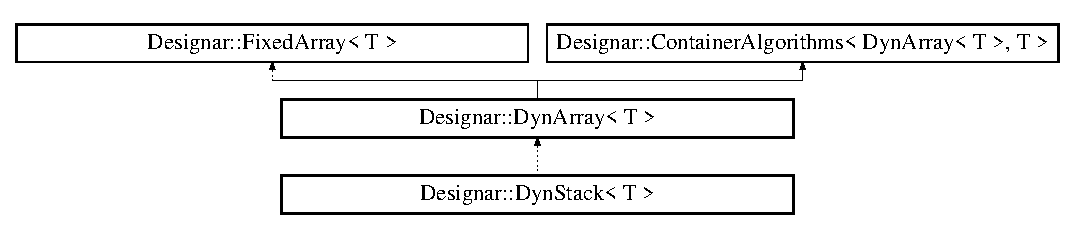
\includegraphics[height=2.641510cm]{class_designar_1_1_dyn_array}
\end{center}
\end{figure}
\subsection*{Clases}
\begin{DoxyCompactItemize}
\item 
class \hyperlink{class_designar_1_1_dyn_array_1_1_iterator}{Iterator}
\end{DoxyCompactItemize}
\subsection*{Tipos públicos}
\begin{DoxyCompactItemize}
\item 
using \hyperlink{class_designar_1_1_dyn_array_af4ff8919b3ae0778aa749130ee0e35f7}{Item\+Type} = T
\item 
using \hyperlink{class_designar_1_1_dyn_array_a80080a85ac9ccbe95c17bc0c665e70b4}{Key\+Type} = T
\item 
using \hyperlink{class_designar_1_1_dyn_array_aa683f9cc296f4597784541837e234d83}{Data\+Type} = T
\item 
using \hyperlink{class_designar_1_1_dyn_array_a1df36ad5f778935dcd565138afc155a4}{Value\+Type} = T
\item 
using \hyperlink{class_designar_1_1_dyn_array_a830e5247348d7d54c65d25f77ecc74bb}{Size\+Type} = \hyperlink{namespace_designar_aa72662848b9f4815e7bf31a7cf3e33d1}{nat\+\_\+t}
\end{DoxyCompactItemize}
\subsection*{Métodos públicos}
\begin{DoxyCompactItemize}
\item 
\hyperlink{class_designar_1_1_dyn_array_a9a00e1336657f98b96e7c38fc7da332c}{Dyn\+Array} (\hyperlink{namespace_designar_aa72662848b9f4815e7bf31a7cf3e33d1}{nat\+\_\+t} cap)
\item 
\hyperlink{class_designar_1_1_dyn_array_afc29c646a101761f0e7a6fb8080b38fd}{Dyn\+Array} (\hyperlink{namespace_designar_aa72662848b9f4815e7bf31a7cf3e33d1}{nat\+\_\+t} cap, const T \&init\+\_\+val)
\item 
\hyperlink{class_designar_1_1_dyn_array_ad51d585e1ee5f4fb0649e3e96392817b}{Dyn\+Array} ()
\item 
\hyperlink{class_designar_1_1_dyn_array_ad9a7d66713068ccea6a5d7fb430f59e3}{Dyn\+Array} (const \hyperlink{class_designar_1_1_dyn_array}{Dyn\+Array} \&a)
\item 
\hyperlink{class_designar_1_1_dyn_array_a59a55c42901c2687505ecfbc3d577a44}{Dyn\+Array} (\hyperlink{class_designar_1_1_dyn_array}{Dyn\+Array} \&\&a)
\item 
\hyperlink{class_designar_1_1_dyn_array_a8bea25568b1f9292c2cb221b774ece13}{Dyn\+Array} (const std\+::initializer\+\_\+list$<$ T $>$ \&)
\item 
void \hyperlink{class_designar_1_1_dyn_array_a70d4d7e34ed05280f849adb6aa20180d}{swap} (\hyperlink{class_designar_1_1_dyn_array}{Dyn\+Array} \&a)
\item 
\hyperlink{namespace_designar_aa72662848b9f4815e7bf31a7cf3e33d1}{nat\+\_\+t} \hyperlink{class_designar_1_1_dyn_array_afa027281e5790d05269d5972ec2ea177}{get\+\_\+capacity} () const
\item 
\hyperlink{namespace_designar_aa72662848b9f4815e7bf31a7cf3e33d1}{nat\+\_\+t} \hyperlink{class_designar_1_1_dyn_array_a7261fdb2ace9cdefbacb49d06c2f919d}{size} () const
\item 
bool \hyperlink{class_designar_1_1_dyn_array_ae4692786599e9be77a9ca963b2fe7bf8}{is\+\_\+empty} () const
\item 
void \hyperlink{class_designar_1_1_dyn_array_abea6b41f8373dc60753255f3c390507f}{clear} ()
\item 
T \& \hyperlink{class_designar_1_1_dyn_array_a85d8c50ef17c71d675961ba0268c2278}{get\+\_\+first} ()
\item 
const T \& \hyperlink{class_designar_1_1_dyn_array_a0b8735deaef51cfc0ff7c84994c3d838}{get\+\_\+first} () const
\item 
T \& \hyperlink{class_designar_1_1_dyn_array_ad69873465e7540a02fceaecc4ffc9b1e}{get\+\_\+last} ()
\item 
const T \& \hyperlink{class_designar_1_1_dyn_array_a45db099e907ae4ed4398cfea487bb4d7}{get\+\_\+last} () const
\item 
T \& \hyperlink{class_designar_1_1_dyn_array_a480d65a0b64bc30d26806cdbd07e66f1}{insert} (\hyperlink{namespace_designar_aa72662848b9f4815e7bf31a7cf3e33d1}{nat\+\_\+t} pos, const T \&item)
\item 
T \& \hyperlink{class_designar_1_1_dyn_array_a919c60d5f02488027580173832af99e9}{insert} (\hyperlink{namespace_designar_aa72662848b9f4815e7bf31a7cf3e33d1}{nat\+\_\+t} pos, T \&\&item)
\item 
T \& \hyperlink{class_designar_1_1_dyn_array_a761d20ea5068101a95e77629145099fe}{insert} (const T \&item)
\item 
T \& \hyperlink{class_designar_1_1_dyn_array_a976a619d52dcc91d531e1b95609ec971}{insert} (T \&\&item)
\item 
T \& \hyperlink{class_designar_1_1_dyn_array_a7134948ab46ec703595718a7734a83c5}{append} (const T \&item)
\item 
T \& \hyperlink{class_designar_1_1_dyn_array_a0e1583bf9d554b5553438dffd57bff93}{append} (T \&\&item)
\item 
T \hyperlink{class_designar_1_1_dyn_array_a85bfa3cc9b650ae6774c17bd4a03c677}{remove\+\_\+pos} (\hyperlink{namespace_designar_aa72662848b9f4815e7bf31a7cf3e33d1}{nat\+\_\+t} pos)
\item 
T \hyperlink{class_designar_1_1_dyn_array_a989a057758da83805138d432d1d4c164}{remove} (T \&item)
\item 
T \hyperlink{class_designar_1_1_dyn_array_ac7451bfdc3b008a478fbfe03478e736d}{remove\+\_\+pos\+\_\+closing\+\_\+breach} (\hyperlink{namespace_designar_aa72662848b9f4815e7bf31a7cf3e33d1}{nat\+\_\+t} pos)
\item 
T \hyperlink{class_designar_1_1_dyn_array_a86705ec7e30d0a2f5650baf34dd702d2}{remove\+\_\+closing\+\_\+breach} (T \&item)
\item 
T \hyperlink{class_designar_1_1_dyn_array_a4dc47bbb1961b4b3d8c8938e76bb77bd}{remove\+\_\+first} ()
\item 
T \hyperlink{class_designar_1_1_dyn_array_a3e96bcac8a97cb56544d6466e834f8ac}{remove\+\_\+last} ()
\item 
\hyperlink{class_designar_1_1_dyn_array}{Dyn\+Array} \& \hyperlink{class_designar_1_1_dyn_array_a955b511053b107641f39aa2c6fb0bf05}{operator=} (const \hyperlink{class_designar_1_1_dyn_array}{Dyn\+Array} \&a)
\item 
\hyperlink{class_designar_1_1_dyn_array}{Dyn\+Array} \& \hyperlink{class_designar_1_1_dyn_array_a80a5538e26254acd5d2449a8364918da}{operator=} (\hyperlink{class_designar_1_1_dyn_array}{Dyn\+Array} \&\&a)
\item 
T \& \hyperlink{class_designar_1_1_dyn_array_a117ba8cd3a9275b36d713a0ef3aef0e3}{at} (\hyperlink{namespace_designar_aa72662848b9f4815e7bf31a7cf3e33d1}{nat\+\_\+t} i)
\item 
const T \& \hyperlink{class_designar_1_1_dyn_array_a0bb20c2467a91bad1577fae7bed15828}{at} (\hyperlink{namespace_designar_aa72662848b9f4815e7bf31a7cf3e33d1}{nat\+\_\+t} i) const
\item 
T \& \hyperlink{class_designar_1_1_dyn_array_ac24a3b500af13093ade4978739e2d6e3}{operator\mbox{[}$\,$\mbox{]}} (\hyperlink{namespace_designar_aa72662848b9f4815e7bf31a7cf3e33d1}{nat\+\_\+t} i)
\item 
const T \& \hyperlink{class_designar_1_1_dyn_array_af329e06efe69cb53e9d1a44a1ed0beeb}{operator\mbox{[}$\,$\mbox{]}} (\hyperlink{namespace_designar_aa72662848b9f4815e7bf31a7cf3e33d1}{nat\+\_\+t} i) const
\item 
\hyperlink{class_designar_1_1_dyn_array_1_1_iterator}{Iterator} \hyperlink{class_designar_1_1_dyn_array_aa8032abbe4db89827ac88aa1ea932712}{begin} ()
\item 
\hyperlink{class_designar_1_1_dyn_array_1_1_iterator}{Iterator} \hyperlink{class_designar_1_1_dyn_array_a36886c618a763286ec179f7fc7cffa68}{begin} () const
\item 
\hyperlink{class_designar_1_1_dyn_array_1_1_iterator}{Iterator} \hyperlink{class_designar_1_1_dyn_array_a1a6bfcf9c4cd8d54138339b9313661f3}{end} ()
\item 
\hyperlink{class_designar_1_1_dyn_array_1_1_iterator}{Iterator} \hyperlink{class_designar_1_1_dyn_array_ab2ff81ff5bfeefbcd0a302da9effff89}{end} () const
\end{DoxyCompactItemize}


\subsection{Descripción detallada}
\subsubsection*{template$<$typename T$>$\newline
class Designar\+::\+Dyn\+Array$<$ T $>$}



Definición en la línea 647 del archivo array.\+H.



\subsection{Documentación de los \textquotesingle{}Typedef\textquotesingle{} miembros de la clase}
\mbox{\Hypertarget{class_designar_1_1_dyn_array_aa683f9cc296f4597784541837e234d83}\label{class_designar_1_1_dyn_array_aa683f9cc296f4597784541837e234d83}} 
\index{Designar\+::\+Dyn\+Array@{Designar\+::\+Dyn\+Array}!Data\+Type@{Data\+Type}}
\index{Data\+Type@{Data\+Type}!Designar\+::\+Dyn\+Array@{Designar\+::\+Dyn\+Array}}
\subsubsection{\texorpdfstring{Data\+Type}{DataType}}
{\footnotesize\ttfamily template$<$typename T$>$ \\
using \hyperlink{class_designar_1_1_dyn_array}{Designar\+::\+Dyn\+Array}$<$ T $>$\+::\hyperlink{class_designar_1_1_fixed_array_a3e37931b909b840cb7a40fc73f12bcf5}{Data\+Type} =  T}



Definición en la línea 655 del archivo array.\+H.

\mbox{\Hypertarget{class_designar_1_1_dyn_array_af4ff8919b3ae0778aa749130ee0e35f7}\label{class_designar_1_1_dyn_array_af4ff8919b3ae0778aa749130ee0e35f7}} 
\index{Designar\+::\+Dyn\+Array@{Designar\+::\+Dyn\+Array}!Item\+Type@{Item\+Type}}
\index{Item\+Type@{Item\+Type}!Designar\+::\+Dyn\+Array@{Designar\+::\+Dyn\+Array}}
\subsubsection{\texorpdfstring{Item\+Type}{ItemType}}
{\footnotesize\ttfamily template$<$typename T$>$ \\
using \hyperlink{class_designar_1_1_dyn_array}{Designar\+::\+Dyn\+Array}$<$ T $>$\+::\hyperlink{class_designar_1_1_fixed_array_abfeb4e683cee75ae782ad20294c4c808}{Item\+Type} =  T}



Definición en la línea 653 del archivo array.\+H.

\mbox{\Hypertarget{class_designar_1_1_dyn_array_a80080a85ac9ccbe95c17bc0c665e70b4}\label{class_designar_1_1_dyn_array_a80080a85ac9ccbe95c17bc0c665e70b4}} 
\index{Designar\+::\+Dyn\+Array@{Designar\+::\+Dyn\+Array}!Key\+Type@{Key\+Type}}
\index{Key\+Type@{Key\+Type}!Designar\+::\+Dyn\+Array@{Designar\+::\+Dyn\+Array}}
\subsubsection{\texorpdfstring{Key\+Type}{KeyType}}
{\footnotesize\ttfamily template$<$typename T$>$ \\
using \hyperlink{class_designar_1_1_dyn_array}{Designar\+::\+Dyn\+Array}$<$ T $>$\+::\hyperlink{class_designar_1_1_fixed_array_a3a725cf21783340b8aca29dd1db0acf0}{Key\+Type} =  T}



Definición en la línea 654 del archivo array.\+H.

\mbox{\Hypertarget{class_designar_1_1_dyn_array_a830e5247348d7d54c65d25f77ecc74bb}\label{class_designar_1_1_dyn_array_a830e5247348d7d54c65d25f77ecc74bb}} 
\index{Designar\+::\+Dyn\+Array@{Designar\+::\+Dyn\+Array}!Size\+Type@{Size\+Type}}
\index{Size\+Type@{Size\+Type}!Designar\+::\+Dyn\+Array@{Designar\+::\+Dyn\+Array}}
\subsubsection{\texorpdfstring{Size\+Type}{SizeType}}
{\footnotesize\ttfamily template$<$typename T$>$ \\
using \hyperlink{class_designar_1_1_dyn_array}{Designar\+::\+Dyn\+Array}$<$ T $>$\+::\hyperlink{class_designar_1_1_fixed_array_a503ae414cc313d248e77c08e62ef043c}{Size\+Type} =  \hyperlink{namespace_designar_aa72662848b9f4815e7bf31a7cf3e33d1}{nat\+\_\+t}}



Definición en la línea 657 del archivo array.\+H.

\mbox{\Hypertarget{class_designar_1_1_dyn_array_a1df36ad5f778935dcd565138afc155a4}\label{class_designar_1_1_dyn_array_a1df36ad5f778935dcd565138afc155a4}} 
\index{Designar\+::\+Dyn\+Array@{Designar\+::\+Dyn\+Array}!Value\+Type@{Value\+Type}}
\index{Value\+Type@{Value\+Type}!Designar\+::\+Dyn\+Array@{Designar\+::\+Dyn\+Array}}
\subsubsection{\texorpdfstring{Value\+Type}{ValueType}}
{\footnotesize\ttfamily template$<$typename T$>$ \\
using \hyperlink{class_designar_1_1_dyn_array}{Designar\+::\+Dyn\+Array}$<$ T $>$\+::\hyperlink{class_designar_1_1_fixed_array_ac1cfeb4403a2dcbffd7ef494e5b873d0}{Value\+Type} =  T}



Definición en la línea 656 del archivo array.\+H.



\subsection{Documentación del constructor y destructor}
\mbox{\Hypertarget{class_designar_1_1_dyn_array_a9a00e1336657f98b96e7c38fc7da332c}\label{class_designar_1_1_dyn_array_a9a00e1336657f98b96e7c38fc7da332c}} 
\index{Designar\+::\+Dyn\+Array@{Designar\+::\+Dyn\+Array}!Dyn\+Array@{Dyn\+Array}}
\index{Dyn\+Array@{Dyn\+Array}!Designar\+::\+Dyn\+Array@{Designar\+::\+Dyn\+Array}}
\subsubsection{\texorpdfstring{Dyn\+Array()}{DynArray()}\hspace{0.1cm}{\footnotesize\ttfamily [1/6]}}
{\footnotesize\ttfamily template$<$typename T$>$ \\
\hyperlink{class_designar_1_1_dyn_array}{Designar\+::\+Dyn\+Array}$<$ T $>$\+::\hyperlink{class_designar_1_1_dyn_array}{Dyn\+Array} (\begin{DoxyParamCaption}\item[{\hyperlink{namespace_designar_aa72662848b9f4815e7bf31a7cf3e33d1}{nat\+\_\+t}}]{cap }\end{DoxyParamCaption})\hspace{0.3cm}{\ttfamily [inline]}}



Definición en la línea 696 del archivo array.\+H.

\mbox{\Hypertarget{class_designar_1_1_dyn_array_afc29c646a101761f0e7a6fb8080b38fd}\label{class_designar_1_1_dyn_array_afc29c646a101761f0e7a6fb8080b38fd}} 
\index{Designar\+::\+Dyn\+Array@{Designar\+::\+Dyn\+Array}!Dyn\+Array@{Dyn\+Array}}
\index{Dyn\+Array@{Dyn\+Array}!Designar\+::\+Dyn\+Array@{Designar\+::\+Dyn\+Array}}
\subsubsection{\texorpdfstring{Dyn\+Array()}{DynArray()}\hspace{0.1cm}{\footnotesize\ttfamily [2/6]}}
{\footnotesize\ttfamily template$<$typename T$>$ \\
\hyperlink{class_designar_1_1_dyn_array}{Designar\+::\+Dyn\+Array}$<$ T $>$\+::\hyperlink{class_designar_1_1_dyn_array}{Dyn\+Array} (\begin{DoxyParamCaption}\item[{\hyperlink{namespace_designar_aa72662848b9f4815e7bf31a7cf3e33d1}{nat\+\_\+t}}]{cap,  }\item[{const T \&}]{init\+\_\+val }\end{DoxyParamCaption})\hspace{0.3cm}{\ttfamily [inline]}}



Definición en la línea 702 del archivo array.\+H.

\mbox{\Hypertarget{class_designar_1_1_dyn_array_ad51d585e1ee5f4fb0649e3e96392817b}\label{class_designar_1_1_dyn_array_ad51d585e1ee5f4fb0649e3e96392817b}} 
\index{Designar\+::\+Dyn\+Array@{Designar\+::\+Dyn\+Array}!Dyn\+Array@{Dyn\+Array}}
\index{Dyn\+Array@{Dyn\+Array}!Designar\+::\+Dyn\+Array@{Designar\+::\+Dyn\+Array}}
\subsubsection{\texorpdfstring{Dyn\+Array()}{DynArray()}\hspace{0.1cm}{\footnotesize\ttfamily [3/6]}}
{\footnotesize\ttfamily template$<$typename T$>$ \\
\hyperlink{class_designar_1_1_dyn_array}{Designar\+::\+Dyn\+Array}$<$ T $>$\+::\hyperlink{class_designar_1_1_dyn_array}{Dyn\+Array} (\begin{DoxyParamCaption}{ }\end{DoxyParamCaption})\hspace{0.3cm}{\ttfamily [inline]}}



Definición en la línea 708 del archivo array.\+H.

\mbox{\Hypertarget{class_designar_1_1_dyn_array_ad9a7d66713068ccea6a5d7fb430f59e3}\label{class_designar_1_1_dyn_array_ad9a7d66713068ccea6a5d7fb430f59e3}} 
\index{Designar\+::\+Dyn\+Array@{Designar\+::\+Dyn\+Array}!Dyn\+Array@{Dyn\+Array}}
\index{Dyn\+Array@{Dyn\+Array}!Designar\+::\+Dyn\+Array@{Designar\+::\+Dyn\+Array}}
\subsubsection{\texorpdfstring{Dyn\+Array()}{DynArray()}\hspace{0.1cm}{\footnotesize\ttfamily [4/6]}}
{\footnotesize\ttfamily template$<$typename T$>$ \\
\hyperlink{class_designar_1_1_dyn_array}{Designar\+::\+Dyn\+Array}$<$ T $>$\+::\hyperlink{class_designar_1_1_dyn_array}{Dyn\+Array} (\begin{DoxyParamCaption}\item[{const \hyperlink{class_designar_1_1_dyn_array}{Dyn\+Array}$<$ T $>$ \&}]{a }\end{DoxyParamCaption})\hspace{0.3cm}{\ttfamily [inline]}}



Definición en la línea 714 del archivo array.\+H.

\mbox{\Hypertarget{class_designar_1_1_dyn_array_a59a55c42901c2687505ecfbc3d577a44}\label{class_designar_1_1_dyn_array_a59a55c42901c2687505ecfbc3d577a44}} 
\index{Designar\+::\+Dyn\+Array@{Designar\+::\+Dyn\+Array}!Dyn\+Array@{Dyn\+Array}}
\index{Dyn\+Array@{Dyn\+Array}!Designar\+::\+Dyn\+Array@{Designar\+::\+Dyn\+Array}}
\subsubsection{\texorpdfstring{Dyn\+Array()}{DynArray()}\hspace{0.1cm}{\footnotesize\ttfamily [5/6]}}
{\footnotesize\ttfamily template$<$typename T$>$ \\
\hyperlink{class_designar_1_1_dyn_array}{Designar\+::\+Dyn\+Array}$<$ T $>$\+::\hyperlink{class_designar_1_1_dyn_array}{Dyn\+Array} (\begin{DoxyParamCaption}\item[{\hyperlink{class_designar_1_1_dyn_array}{Dyn\+Array}$<$ T $>$ \&\&}]{a }\end{DoxyParamCaption})\hspace{0.3cm}{\ttfamily [inline]}}



Definición en la línea 720 del archivo array.\+H.

\mbox{\Hypertarget{class_designar_1_1_dyn_array_a8bea25568b1f9292c2cb221b774ece13}\label{class_designar_1_1_dyn_array_a8bea25568b1f9292c2cb221b774ece13}} 
\index{Designar\+::\+Dyn\+Array@{Designar\+::\+Dyn\+Array}!Dyn\+Array@{Dyn\+Array}}
\index{Dyn\+Array@{Dyn\+Array}!Designar\+::\+Dyn\+Array@{Designar\+::\+Dyn\+Array}}
\subsubsection{\texorpdfstring{Dyn\+Array()}{DynArray()}\hspace{0.1cm}{\footnotesize\ttfamily [6/6]}}
{\footnotesize\ttfamily template$<$typename T$>$ \\
\hyperlink{class_designar_1_1_dyn_array}{Designar\+::\+Dyn\+Array}$<$ T $>$\+::\hyperlink{class_designar_1_1_dyn_array}{Dyn\+Array} (\begin{DoxyParamCaption}\item[{const std\+::initializer\+\_\+list$<$ T $>$ \&}]{l }\end{DoxyParamCaption})}



Definición en la línea 988 del archivo array.\+H.



\subsection{Documentación de las funciones miembro}
\mbox{\Hypertarget{class_designar_1_1_dyn_array_a7134948ab46ec703595718a7734a83c5}\label{class_designar_1_1_dyn_array_a7134948ab46ec703595718a7734a83c5}} 
\index{Designar\+::\+Dyn\+Array@{Designar\+::\+Dyn\+Array}!append@{append}}
\index{append@{append}!Designar\+::\+Dyn\+Array@{Designar\+::\+Dyn\+Array}}
\subsubsection{\texorpdfstring{append()}{append()}\hspace{0.1cm}{\footnotesize\ttfamily [1/2]}}
{\footnotesize\ttfamily template$<$typename T$>$ \\
T\& \hyperlink{class_designar_1_1_dyn_array}{Designar\+::\+Dyn\+Array}$<$ T $>$\+::append (\begin{DoxyParamCaption}\item[{const T \&}]{item }\end{DoxyParamCaption})\hspace{0.3cm}{\ttfamily [inline]}}



Definición en la línea 834 del archivo array.\+H.

\mbox{\Hypertarget{class_designar_1_1_dyn_array_a0e1583bf9d554b5553438dffd57bff93}\label{class_designar_1_1_dyn_array_a0e1583bf9d554b5553438dffd57bff93}} 
\index{Designar\+::\+Dyn\+Array@{Designar\+::\+Dyn\+Array}!append@{append}}
\index{append@{append}!Designar\+::\+Dyn\+Array@{Designar\+::\+Dyn\+Array}}
\subsubsection{\texorpdfstring{append()}{append()}\hspace{0.1cm}{\footnotesize\ttfamily [2/2]}}
{\footnotesize\ttfamily template$<$typename T$>$ \\
T\& \hyperlink{class_designar_1_1_dyn_array}{Designar\+::\+Dyn\+Array}$<$ T $>$\+::append (\begin{DoxyParamCaption}\item[{T \&\&}]{item }\end{DoxyParamCaption})\hspace{0.3cm}{\ttfamily [inline]}}



Definición en la línea 841 del archivo array.\+H.

\mbox{\Hypertarget{class_designar_1_1_dyn_array_a117ba8cd3a9275b36d713a0ef3aef0e3}\label{class_designar_1_1_dyn_array_a117ba8cd3a9275b36d713a0ef3aef0e3}} 
\index{Designar\+::\+Dyn\+Array@{Designar\+::\+Dyn\+Array}!at@{at}}
\index{at@{at}!Designar\+::\+Dyn\+Array@{Designar\+::\+Dyn\+Array}}
\subsubsection{\texorpdfstring{at()}{at()}\hspace{0.1cm}{\footnotesize\ttfamily [1/2]}}
{\footnotesize\ttfamily template$<$typename T$>$ \\
T\& \hyperlink{class_designar_1_1_dyn_array}{Designar\+::\+Dyn\+Array}$<$ T $>$\+::at (\begin{DoxyParamCaption}\item[{\hyperlink{namespace_designar_aa72662848b9f4815e7bf31a7cf3e33d1}{nat\+\_\+t}}]{i }\end{DoxyParamCaption})\hspace{0.3cm}{\ttfamily [inline]}}



Definición en la línea 925 del archivo array.\+H.

\mbox{\Hypertarget{class_designar_1_1_dyn_array_a0bb20c2467a91bad1577fae7bed15828}\label{class_designar_1_1_dyn_array_a0bb20c2467a91bad1577fae7bed15828}} 
\index{Designar\+::\+Dyn\+Array@{Designar\+::\+Dyn\+Array}!at@{at}}
\index{at@{at}!Designar\+::\+Dyn\+Array@{Designar\+::\+Dyn\+Array}}
\subsubsection{\texorpdfstring{at()}{at()}\hspace{0.1cm}{\footnotesize\ttfamily [2/2]}}
{\footnotesize\ttfamily template$<$typename T$>$ \\
const T\& \hyperlink{class_designar_1_1_dyn_array}{Designar\+::\+Dyn\+Array}$<$ T $>$\+::at (\begin{DoxyParamCaption}\item[{\hyperlink{namespace_designar_aa72662848b9f4815e7bf31a7cf3e33d1}{nat\+\_\+t}}]{i }\end{DoxyParamCaption}) const\hspace{0.3cm}{\ttfamily [inline]}}



Definición en la línea 933 del archivo array.\+H.

\mbox{\Hypertarget{class_designar_1_1_dyn_array_aa8032abbe4db89827ac88aa1ea932712}\label{class_designar_1_1_dyn_array_aa8032abbe4db89827ac88aa1ea932712}} 
\index{Designar\+::\+Dyn\+Array@{Designar\+::\+Dyn\+Array}!begin@{begin}}
\index{begin@{begin}!Designar\+::\+Dyn\+Array@{Designar\+::\+Dyn\+Array}}
\subsubsection{\texorpdfstring{begin()}{begin()}\hspace{0.1cm}{\footnotesize\ttfamily [1/2]}}
{\footnotesize\ttfamily template$<$typename T$>$ \\
\hyperlink{class_designar_1_1_dyn_array_1_1_iterator}{Iterator} \hyperlink{class_designar_1_1_dyn_array}{Designar\+::\+Dyn\+Array}$<$ T $>$\+::begin (\begin{DoxyParamCaption}{ }\end{DoxyParamCaption})\hspace{0.3cm}{\ttfamily [inline]}}



Definición en la línea 966 del archivo array.\+H.

\mbox{\Hypertarget{class_designar_1_1_dyn_array_a36886c618a763286ec179f7fc7cffa68}\label{class_designar_1_1_dyn_array_a36886c618a763286ec179f7fc7cffa68}} 
\index{Designar\+::\+Dyn\+Array@{Designar\+::\+Dyn\+Array}!begin@{begin}}
\index{begin@{begin}!Designar\+::\+Dyn\+Array@{Designar\+::\+Dyn\+Array}}
\subsubsection{\texorpdfstring{begin()}{begin()}\hspace{0.1cm}{\footnotesize\ttfamily [2/2]}}
{\footnotesize\ttfamily template$<$typename T$>$ \\
\hyperlink{class_designar_1_1_dyn_array_1_1_iterator}{Iterator} \hyperlink{class_designar_1_1_dyn_array}{Designar\+::\+Dyn\+Array}$<$ T $>$\+::begin (\begin{DoxyParamCaption}{ }\end{DoxyParamCaption}) const\hspace{0.3cm}{\ttfamily [inline]}}



Definición en la línea 971 del archivo array.\+H.

\mbox{\Hypertarget{class_designar_1_1_dyn_array_abea6b41f8373dc60753255f3c390507f}\label{class_designar_1_1_dyn_array_abea6b41f8373dc60753255f3c390507f}} 
\index{Designar\+::\+Dyn\+Array@{Designar\+::\+Dyn\+Array}!clear@{clear}}
\index{clear@{clear}!Designar\+::\+Dyn\+Array@{Designar\+::\+Dyn\+Array}}
\subsubsection{\texorpdfstring{clear()}{clear()}}
{\footnotesize\ttfamily template$<$typename T$>$ \\
void \hyperlink{class_designar_1_1_dyn_array}{Designar\+::\+Dyn\+Array}$<$ T $>$\+::clear (\begin{DoxyParamCaption}{ }\end{DoxyParamCaption})\hspace{0.3cm}{\ttfamily [inline]}}



Definición en la línea 749 del archivo array.\+H.

\mbox{\Hypertarget{class_designar_1_1_dyn_array_a1a6bfcf9c4cd8d54138339b9313661f3}\label{class_designar_1_1_dyn_array_a1a6bfcf9c4cd8d54138339b9313661f3}} 
\index{Designar\+::\+Dyn\+Array@{Designar\+::\+Dyn\+Array}!end@{end}}
\index{end@{end}!Designar\+::\+Dyn\+Array@{Designar\+::\+Dyn\+Array}}
\subsubsection{\texorpdfstring{end()}{end()}\hspace{0.1cm}{\footnotesize\ttfamily [1/2]}}
{\footnotesize\ttfamily template$<$typename T$>$ \\
\hyperlink{class_designar_1_1_dyn_array_1_1_iterator}{Iterator} \hyperlink{class_designar_1_1_dyn_array}{Designar\+::\+Dyn\+Array}$<$ T $>$\+::end (\begin{DoxyParamCaption}{ }\end{DoxyParamCaption})\hspace{0.3cm}{\ttfamily [inline]}}



Definición en la línea 976 del archivo array.\+H.

\mbox{\Hypertarget{class_designar_1_1_dyn_array_ab2ff81ff5bfeefbcd0a302da9effff89}\label{class_designar_1_1_dyn_array_ab2ff81ff5bfeefbcd0a302da9effff89}} 
\index{Designar\+::\+Dyn\+Array@{Designar\+::\+Dyn\+Array}!end@{end}}
\index{end@{end}!Designar\+::\+Dyn\+Array@{Designar\+::\+Dyn\+Array}}
\subsubsection{\texorpdfstring{end()}{end()}\hspace{0.1cm}{\footnotesize\ttfamily [2/2]}}
{\footnotesize\ttfamily template$<$typename T$>$ \\
\hyperlink{class_designar_1_1_dyn_array_1_1_iterator}{Iterator} \hyperlink{class_designar_1_1_dyn_array}{Designar\+::\+Dyn\+Array}$<$ T $>$\+::end (\begin{DoxyParamCaption}{ }\end{DoxyParamCaption}) const\hspace{0.3cm}{\ttfamily [inline]}}



Definición en la línea 981 del archivo array.\+H.

\mbox{\Hypertarget{class_designar_1_1_dyn_array_afa027281e5790d05269d5972ec2ea177}\label{class_designar_1_1_dyn_array_afa027281e5790d05269d5972ec2ea177}} 
\index{Designar\+::\+Dyn\+Array@{Designar\+::\+Dyn\+Array}!get\+\_\+capacity@{get\+\_\+capacity}}
\index{get\+\_\+capacity@{get\+\_\+capacity}!Designar\+::\+Dyn\+Array@{Designar\+::\+Dyn\+Array}}
\subsubsection{\texorpdfstring{get\+\_\+capacity()}{get\_capacity()}}
{\footnotesize\ttfamily template$<$typename T$>$ \\
\hyperlink{namespace_designar_aa72662848b9f4815e7bf31a7cf3e33d1}{nat\+\_\+t} \hyperlink{class_designar_1_1_dyn_array}{Designar\+::\+Dyn\+Array}$<$ T $>$\+::get\+\_\+capacity (\begin{DoxyParamCaption}{ }\end{DoxyParamCaption}) const\hspace{0.3cm}{\ttfamily [inline]}}



Definición en la línea 734 del archivo array.\+H.

\mbox{\Hypertarget{class_designar_1_1_dyn_array_a85d8c50ef17c71d675961ba0268c2278}\label{class_designar_1_1_dyn_array_a85d8c50ef17c71d675961ba0268c2278}} 
\index{Designar\+::\+Dyn\+Array@{Designar\+::\+Dyn\+Array}!get\+\_\+first@{get\+\_\+first}}
\index{get\+\_\+first@{get\+\_\+first}!Designar\+::\+Dyn\+Array@{Designar\+::\+Dyn\+Array}}
\subsubsection{\texorpdfstring{get\+\_\+first()}{get\_first()}\hspace{0.1cm}{\footnotesize\ttfamily [1/2]}}
{\footnotesize\ttfamily template$<$typename T$>$ \\
T\& \hyperlink{class_designar_1_1_dyn_array}{Designar\+::\+Dyn\+Array}$<$ T $>$\+::get\+\_\+first (\begin{DoxyParamCaption}{ }\end{DoxyParamCaption})\hspace{0.3cm}{\ttfamily [inline]}}



Definición en la línea 760 del archivo array.\+H.

\mbox{\Hypertarget{class_designar_1_1_dyn_array_a0b8735deaef51cfc0ff7c84994c3d838}\label{class_designar_1_1_dyn_array_a0b8735deaef51cfc0ff7c84994c3d838}} 
\index{Designar\+::\+Dyn\+Array@{Designar\+::\+Dyn\+Array}!get\+\_\+first@{get\+\_\+first}}
\index{get\+\_\+first@{get\+\_\+first}!Designar\+::\+Dyn\+Array@{Designar\+::\+Dyn\+Array}}
\subsubsection{\texorpdfstring{get\+\_\+first()}{get\_first()}\hspace{0.1cm}{\footnotesize\ttfamily [2/2]}}
{\footnotesize\ttfamily template$<$typename T$>$ \\
const T\& \hyperlink{class_designar_1_1_dyn_array}{Designar\+::\+Dyn\+Array}$<$ T $>$\+::get\+\_\+first (\begin{DoxyParamCaption}{ }\end{DoxyParamCaption}) const\hspace{0.3cm}{\ttfamily [inline]}}



Definición en la línea 768 del archivo array.\+H.

\mbox{\Hypertarget{class_designar_1_1_dyn_array_ad69873465e7540a02fceaecc4ffc9b1e}\label{class_designar_1_1_dyn_array_ad69873465e7540a02fceaecc4ffc9b1e}} 
\index{Designar\+::\+Dyn\+Array@{Designar\+::\+Dyn\+Array}!get\+\_\+last@{get\+\_\+last}}
\index{get\+\_\+last@{get\+\_\+last}!Designar\+::\+Dyn\+Array@{Designar\+::\+Dyn\+Array}}
\subsubsection{\texorpdfstring{get\+\_\+last()}{get\_last()}\hspace{0.1cm}{\footnotesize\ttfamily [1/2]}}
{\footnotesize\ttfamily template$<$typename T$>$ \\
T\& \hyperlink{class_designar_1_1_dyn_array}{Designar\+::\+Dyn\+Array}$<$ T $>$\+::get\+\_\+last (\begin{DoxyParamCaption}{ }\end{DoxyParamCaption})\hspace{0.3cm}{\ttfamily [inline]}}



Definición en la línea 776 del archivo array.\+H.

\mbox{\Hypertarget{class_designar_1_1_dyn_array_a45db099e907ae4ed4398cfea487bb4d7}\label{class_designar_1_1_dyn_array_a45db099e907ae4ed4398cfea487bb4d7}} 
\index{Designar\+::\+Dyn\+Array@{Designar\+::\+Dyn\+Array}!get\+\_\+last@{get\+\_\+last}}
\index{get\+\_\+last@{get\+\_\+last}!Designar\+::\+Dyn\+Array@{Designar\+::\+Dyn\+Array}}
\subsubsection{\texorpdfstring{get\+\_\+last()}{get\_last()}\hspace{0.1cm}{\footnotesize\ttfamily [2/2]}}
{\footnotesize\ttfamily template$<$typename T$>$ \\
const T\& \hyperlink{class_designar_1_1_dyn_array}{Designar\+::\+Dyn\+Array}$<$ T $>$\+::get\+\_\+last (\begin{DoxyParamCaption}{ }\end{DoxyParamCaption}) const\hspace{0.3cm}{\ttfamily [inline]}}



Definición en la línea 784 del archivo array.\+H.

\mbox{\Hypertarget{class_designar_1_1_dyn_array_a480d65a0b64bc30d26806cdbd07e66f1}\label{class_designar_1_1_dyn_array_a480d65a0b64bc30d26806cdbd07e66f1}} 
\index{Designar\+::\+Dyn\+Array@{Designar\+::\+Dyn\+Array}!insert@{insert}}
\index{insert@{insert}!Designar\+::\+Dyn\+Array@{Designar\+::\+Dyn\+Array}}
\subsubsection{\texorpdfstring{insert()}{insert()}\hspace{0.1cm}{\footnotesize\ttfamily [1/4]}}
{\footnotesize\ttfamily template$<$typename T$>$ \\
T\& \hyperlink{class_designar_1_1_dyn_array}{Designar\+::\+Dyn\+Array}$<$ T $>$\+::insert (\begin{DoxyParamCaption}\item[{\hyperlink{namespace_designar_aa72662848b9f4815e7bf31a7cf3e33d1}{nat\+\_\+t}}]{pos,  }\item[{const T \&}]{item }\end{DoxyParamCaption})\hspace{0.3cm}{\ttfamily [inline]}}



Definición en la línea 792 del archivo array.\+H.

\mbox{\Hypertarget{class_designar_1_1_dyn_array_a919c60d5f02488027580173832af99e9}\label{class_designar_1_1_dyn_array_a919c60d5f02488027580173832af99e9}} 
\index{Designar\+::\+Dyn\+Array@{Designar\+::\+Dyn\+Array}!insert@{insert}}
\index{insert@{insert}!Designar\+::\+Dyn\+Array@{Designar\+::\+Dyn\+Array}}
\subsubsection{\texorpdfstring{insert()}{insert()}\hspace{0.1cm}{\footnotesize\ttfamily [2/4]}}
{\footnotesize\ttfamily template$<$typename T$>$ \\
T\& \hyperlink{class_designar_1_1_dyn_array}{Designar\+::\+Dyn\+Array}$<$ T $>$\+::insert (\begin{DoxyParamCaption}\item[{\hyperlink{namespace_designar_aa72662848b9f4815e7bf31a7cf3e33d1}{nat\+\_\+t}}]{pos,  }\item[{T \&\&}]{item }\end{DoxyParamCaption})\hspace{0.3cm}{\ttfamily [inline]}}



Definición en la línea 808 del archivo array.\+H.

\mbox{\Hypertarget{class_designar_1_1_dyn_array_a761d20ea5068101a95e77629145099fe}\label{class_designar_1_1_dyn_array_a761d20ea5068101a95e77629145099fe}} 
\index{Designar\+::\+Dyn\+Array@{Designar\+::\+Dyn\+Array}!insert@{insert}}
\index{insert@{insert}!Designar\+::\+Dyn\+Array@{Designar\+::\+Dyn\+Array}}
\subsubsection{\texorpdfstring{insert()}{insert()}\hspace{0.1cm}{\footnotesize\ttfamily [3/4]}}
{\footnotesize\ttfamily template$<$typename T$>$ \\
T\& \hyperlink{class_designar_1_1_dyn_array}{Designar\+::\+Dyn\+Array}$<$ T $>$\+::insert (\begin{DoxyParamCaption}\item[{const T \&}]{item }\end{DoxyParamCaption})\hspace{0.3cm}{\ttfamily [inline]}}



Definición en la línea 824 del archivo array.\+H.

\mbox{\Hypertarget{class_designar_1_1_dyn_array_a976a619d52dcc91d531e1b95609ec971}\label{class_designar_1_1_dyn_array_a976a619d52dcc91d531e1b95609ec971}} 
\index{Designar\+::\+Dyn\+Array@{Designar\+::\+Dyn\+Array}!insert@{insert}}
\index{insert@{insert}!Designar\+::\+Dyn\+Array@{Designar\+::\+Dyn\+Array}}
\subsubsection{\texorpdfstring{insert()}{insert()}\hspace{0.1cm}{\footnotesize\ttfamily [4/4]}}
{\footnotesize\ttfamily template$<$typename T$>$ \\
T\& \hyperlink{class_designar_1_1_dyn_array}{Designar\+::\+Dyn\+Array}$<$ T $>$\+::insert (\begin{DoxyParamCaption}\item[{T \&\&}]{item }\end{DoxyParamCaption})\hspace{0.3cm}{\ttfamily [inline]}}



Definición en la línea 829 del archivo array.\+H.

\mbox{\Hypertarget{class_designar_1_1_dyn_array_ae4692786599e9be77a9ca963b2fe7bf8}\label{class_designar_1_1_dyn_array_ae4692786599e9be77a9ca963b2fe7bf8}} 
\index{Designar\+::\+Dyn\+Array@{Designar\+::\+Dyn\+Array}!is\+\_\+empty@{is\+\_\+empty}}
\index{is\+\_\+empty@{is\+\_\+empty}!Designar\+::\+Dyn\+Array@{Designar\+::\+Dyn\+Array}}
\subsubsection{\texorpdfstring{is\+\_\+empty()}{is\_empty()}}
{\footnotesize\ttfamily template$<$typename T$>$ \\
bool \hyperlink{class_designar_1_1_dyn_array}{Designar\+::\+Dyn\+Array}$<$ T $>$\+::is\+\_\+empty (\begin{DoxyParamCaption}{ }\end{DoxyParamCaption}) const\hspace{0.3cm}{\ttfamily [inline]}}



Definición en la línea 744 del archivo array.\+H.

\mbox{\Hypertarget{class_designar_1_1_dyn_array_a955b511053b107641f39aa2c6fb0bf05}\label{class_designar_1_1_dyn_array_a955b511053b107641f39aa2c6fb0bf05}} 
\index{Designar\+::\+Dyn\+Array@{Designar\+::\+Dyn\+Array}!operator=@{operator=}}
\index{operator=@{operator=}!Designar\+::\+Dyn\+Array@{Designar\+::\+Dyn\+Array}}
\subsubsection{\texorpdfstring{operator=()}{operator=()}\hspace{0.1cm}{\footnotesize\ttfamily [1/2]}}
{\footnotesize\ttfamily template$<$typename T$>$ \\
\hyperlink{class_designar_1_1_dyn_array}{Dyn\+Array}\& \hyperlink{class_designar_1_1_dyn_array}{Designar\+::\+Dyn\+Array}$<$ T $>$\+::operator= (\begin{DoxyParamCaption}\item[{const \hyperlink{class_designar_1_1_dyn_array}{Dyn\+Array}$<$ T $>$ \&}]{a }\end{DoxyParamCaption})\hspace{0.3cm}{\ttfamily [inline]}}



Definición en la línea 909 del archivo array.\+H.

\mbox{\Hypertarget{class_designar_1_1_dyn_array_a80a5538e26254acd5d2449a8364918da}\label{class_designar_1_1_dyn_array_a80a5538e26254acd5d2449a8364918da}} 
\index{Designar\+::\+Dyn\+Array@{Designar\+::\+Dyn\+Array}!operator=@{operator=}}
\index{operator=@{operator=}!Designar\+::\+Dyn\+Array@{Designar\+::\+Dyn\+Array}}
\subsubsection{\texorpdfstring{operator=()}{operator=()}\hspace{0.1cm}{\footnotesize\ttfamily [2/2]}}
{\footnotesize\ttfamily template$<$typename T$>$ \\
\hyperlink{class_designar_1_1_dyn_array}{Dyn\+Array}\& \hyperlink{class_designar_1_1_dyn_array}{Designar\+::\+Dyn\+Array}$<$ T $>$\+::operator= (\begin{DoxyParamCaption}\item[{\hyperlink{class_designar_1_1_dyn_array}{Dyn\+Array}$<$ T $>$ \&\&}]{a }\end{DoxyParamCaption})\hspace{0.3cm}{\ttfamily [inline]}}



Definición en la línea 919 del archivo array.\+H.

\mbox{\Hypertarget{class_designar_1_1_dyn_array_ac24a3b500af13093ade4978739e2d6e3}\label{class_designar_1_1_dyn_array_ac24a3b500af13093ade4978739e2d6e3}} 
\index{Designar\+::\+Dyn\+Array@{Designar\+::\+Dyn\+Array}!operator\mbox{[}\mbox{]}@{operator[]}}
\index{operator\mbox{[}\mbox{]}@{operator[]}!Designar\+::\+Dyn\+Array@{Designar\+::\+Dyn\+Array}}
\subsubsection{\texorpdfstring{operator[]()}{operator[]()}\hspace{0.1cm}{\footnotesize\ttfamily [1/2]}}
{\footnotesize\ttfamily template$<$typename T$>$ \\
T\& \hyperlink{class_designar_1_1_dyn_array}{Designar\+::\+Dyn\+Array}$<$ T $>$\+::operator\mbox{[}$\,$\mbox{]} (\begin{DoxyParamCaption}\item[{\hyperlink{namespace_designar_aa72662848b9f4815e7bf31a7cf3e33d1}{nat\+\_\+t}}]{i }\end{DoxyParamCaption})\hspace{0.3cm}{\ttfamily [inline]}}



Definición en la línea 941 del archivo array.\+H.

\mbox{\Hypertarget{class_designar_1_1_dyn_array_af329e06efe69cb53e9d1a44a1ed0beeb}\label{class_designar_1_1_dyn_array_af329e06efe69cb53e9d1a44a1ed0beeb}} 
\index{Designar\+::\+Dyn\+Array@{Designar\+::\+Dyn\+Array}!operator\mbox{[}\mbox{]}@{operator[]}}
\index{operator\mbox{[}\mbox{]}@{operator[]}!Designar\+::\+Dyn\+Array@{Designar\+::\+Dyn\+Array}}
\subsubsection{\texorpdfstring{operator[]()}{operator[]()}\hspace{0.1cm}{\footnotesize\ttfamily [2/2]}}
{\footnotesize\ttfamily template$<$typename T$>$ \\
const T\& \hyperlink{class_designar_1_1_dyn_array}{Designar\+::\+Dyn\+Array}$<$ T $>$\+::operator\mbox{[}$\,$\mbox{]} (\begin{DoxyParamCaption}\item[{\hyperlink{namespace_designar_aa72662848b9f4815e7bf31a7cf3e33d1}{nat\+\_\+t}}]{i }\end{DoxyParamCaption}) const\hspace{0.3cm}{\ttfamily [inline]}}



Definición en la línea 946 del archivo array.\+H.

\mbox{\Hypertarget{class_designar_1_1_dyn_array_a989a057758da83805138d432d1d4c164}\label{class_designar_1_1_dyn_array_a989a057758da83805138d432d1d4c164}} 
\index{Designar\+::\+Dyn\+Array@{Designar\+::\+Dyn\+Array}!remove@{remove}}
\index{remove@{remove}!Designar\+::\+Dyn\+Array@{Designar\+::\+Dyn\+Array}}
\subsubsection{\texorpdfstring{remove()}{remove()}}
{\footnotesize\ttfamily template$<$typename T$>$ \\
T \hyperlink{class_designar_1_1_dyn_array}{Designar\+::\+Dyn\+Array}$<$ T $>$\+::remove (\begin{DoxyParamCaption}\item[{T \&}]{item }\end{DoxyParamCaption})\hspace{0.3cm}{\ttfamily [inline]}}



Definición en la línea 858 del archivo array.\+H.

\mbox{\Hypertarget{class_designar_1_1_dyn_array_a86705ec7e30d0a2f5650baf34dd702d2}\label{class_designar_1_1_dyn_array_a86705ec7e30d0a2f5650baf34dd702d2}} 
\index{Designar\+::\+Dyn\+Array@{Designar\+::\+Dyn\+Array}!remove\+\_\+closing\+\_\+breach@{remove\+\_\+closing\+\_\+breach}}
\index{remove\+\_\+closing\+\_\+breach@{remove\+\_\+closing\+\_\+breach}!Designar\+::\+Dyn\+Array@{Designar\+::\+Dyn\+Array}}
\subsubsection{\texorpdfstring{remove\+\_\+closing\+\_\+breach()}{remove\_closing\_breach()}}
{\footnotesize\ttfamily template$<$typename T$>$ \\
T \hyperlink{class_designar_1_1_dyn_array}{Designar\+::\+Dyn\+Array}$<$ T $>$\+::remove\+\_\+closing\+\_\+breach (\begin{DoxyParamCaption}\item[{T \&}]{item }\end{DoxyParamCaption})\hspace{0.3cm}{\ttfamily [inline]}}



Definición en la línea 884 del archivo array.\+H.

\mbox{\Hypertarget{class_designar_1_1_dyn_array_a4dc47bbb1961b4b3d8c8938e76bb77bd}\label{class_designar_1_1_dyn_array_a4dc47bbb1961b4b3d8c8938e76bb77bd}} 
\index{Designar\+::\+Dyn\+Array@{Designar\+::\+Dyn\+Array}!remove\+\_\+first@{remove\+\_\+first}}
\index{remove\+\_\+first@{remove\+\_\+first}!Designar\+::\+Dyn\+Array@{Designar\+::\+Dyn\+Array}}
\subsubsection{\texorpdfstring{remove\+\_\+first()}{remove\_first()}}
{\footnotesize\ttfamily template$<$typename T$>$ \\
T \hyperlink{class_designar_1_1_dyn_array}{Designar\+::\+Dyn\+Array}$<$ T $>$\+::remove\+\_\+first (\begin{DoxyParamCaption}{ }\end{DoxyParamCaption})\hspace{0.3cm}{\ttfamily [inline]}}



Definición en la línea 894 del archivo array.\+H.

\mbox{\Hypertarget{class_designar_1_1_dyn_array_a3e96bcac8a97cb56544d6466e834f8ac}\label{class_designar_1_1_dyn_array_a3e96bcac8a97cb56544d6466e834f8ac}} 
\index{Designar\+::\+Dyn\+Array@{Designar\+::\+Dyn\+Array}!remove\+\_\+last@{remove\+\_\+last}}
\index{remove\+\_\+last@{remove\+\_\+last}!Designar\+::\+Dyn\+Array@{Designar\+::\+Dyn\+Array}}
\subsubsection{\texorpdfstring{remove\+\_\+last()}{remove\_last()}}
{\footnotesize\ttfamily template$<$typename T$>$ \\
T \hyperlink{class_designar_1_1_dyn_array}{Designar\+::\+Dyn\+Array}$<$ T $>$\+::remove\+\_\+last (\begin{DoxyParamCaption}{ }\end{DoxyParamCaption})\hspace{0.3cm}{\ttfamily [inline]}}



Definición en la línea 902 del archivo array.\+H.

\mbox{\Hypertarget{class_designar_1_1_dyn_array_a85bfa3cc9b650ae6774c17bd4a03c677}\label{class_designar_1_1_dyn_array_a85bfa3cc9b650ae6774c17bd4a03c677}} 
\index{Designar\+::\+Dyn\+Array@{Designar\+::\+Dyn\+Array}!remove\+\_\+pos@{remove\+\_\+pos}}
\index{remove\+\_\+pos@{remove\+\_\+pos}!Designar\+::\+Dyn\+Array@{Designar\+::\+Dyn\+Array}}
\subsubsection{\texorpdfstring{remove\+\_\+pos()}{remove\_pos()}}
{\footnotesize\ttfamily template$<$typename T$>$ \\
T \hyperlink{class_designar_1_1_dyn_array}{Designar\+::\+Dyn\+Array}$<$ T $>$\+::remove\+\_\+pos (\begin{DoxyParamCaption}\item[{\hyperlink{namespace_designar_aa72662848b9f4815e7bf31a7cf3e33d1}{nat\+\_\+t}}]{pos }\end{DoxyParamCaption})\hspace{0.3cm}{\ttfamily [inline]}}



Definición en la línea 848 del archivo array.\+H.

\mbox{\Hypertarget{class_designar_1_1_dyn_array_ac7451bfdc3b008a478fbfe03478e736d}\label{class_designar_1_1_dyn_array_ac7451bfdc3b008a478fbfe03478e736d}} 
\index{Designar\+::\+Dyn\+Array@{Designar\+::\+Dyn\+Array}!remove\+\_\+pos\+\_\+closing\+\_\+breach@{remove\+\_\+pos\+\_\+closing\+\_\+breach}}
\index{remove\+\_\+pos\+\_\+closing\+\_\+breach@{remove\+\_\+pos\+\_\+closing\+\_\+breach}!Designar\+::\+Dyn\+Array@{Designar\+::\+Dyn\+Array}}
\subsubsection{\texorpdfstring{remove\+\_\+pos\+\_\+closing\+\_\+breach()}{remove\_pos\_closing\_breach()}}
{\footnotesize\ttfamily template$<$typename T$>$ \\
T \hyperlink{class_designar_1_1_dyn_array}{Designar\+::\+Dyn\+Array}$<$ T $>$\+::remove\+\_\+pos\+\_\+closing\+\_\+breach (\begin{DoxyParamCaption}\item[{\hyperlink{namespace_designar_aa72662848b9f4815e7bf31a7cf3e33d1}{nat\+\_\+t}}]{pos }\end{DoxyParamCaption})\hspace{0.3cm}{\ttfamily [inline]}}



Definición en la línea 868 del archivo array.\+H.

\mbox{\Hypertarget{class_designar_1_1_dyn_array_a7261fdb2ace9cdefbacb49d06c2f919d}\label{class_designar_1_1_dyn_array_a7261fdb2ace9cdefbacb49d06c2f919d}} 
\index{Designar\+::\+Dyn\+Array@{Designar\+::\+Dyn\+Array}!size@{size}}
\index{size@{size}!Designar\+::\+Dyn\+Array@{Designar\+::\+Dyn\+Array}}
\subsubsection{\texorpdfstring{size()}{size()}}
{\footnotesize\ttfamily template$<$typename T$>$ \\
\hyperlink{namespace_designar_aa72662848b9f4815e7bf31a7cf3e33d1}{nat\+\_\+t} \hyperlink{class_designar_1_1_dyn_array}{Designar\+::\+Dyn\+Array}$<$ T $>$\+::size (\begin{DoxyParamCaption}{ }\end{DoxyParamCaption}) const\hspace{0.3cm}{\ttfamily [inline]}}



Definición en la línea 739 del archivo array.\+H.

\mbox{\Hypertarget{class_designar_1_1_dyn_array_a70d4d7e34ed05280f849adb6aa20180d}\label{class_designar_1_1_dyn_array_a70d4d7e34ed05280f849adb6aa20180d}} 
\index{Designar\+::\+Dyn\+Array@{Designar\+::\+Dyn\+Array}!swap@{swap}}
\index{swap@{swap}!Designar\+::\+Dyn\+Array@{Designar\+::\+Dyn\+Array}}
\subsubsection{\texorpdfstring{swap()}{swap()}}
{\footnotesize\ttfamily template$<$typename T$>$ \\
void \hyperlink{class_designar_1_1_dyn_array}{Designar\+::\+Dyn\+Array}$<$ T $>$\+::swap (\begin{DoxyParamCaption}\item[{\hyperlink{class_designar_1_1_dyn_array}{Dyn\+Array}$<$ T $>$ \&}]{a }\end{DoxyParamCaption})\hspace{0.3cm}{\ttfamily [inline]}}



Definición en la línea 728 del archivo array.\+H.



La documentación para esta clase fue generada a partir del siguiente fichero\+:\begin{DoxyCompactItemize}
\item 
include/\hyperlink{array_8_h}{array.\+H}\end{DoxyCompactItemize}

\hypertarget{class_designar_1_1_dyn_bit_set}{}\section{Designar\+:\+:Dyn\+Bit\+Set Class Reference}
\label{class_designar_1_1_dyn_bit_set}\index{Designar\+::\+Dyn\+Bit\+Set@{Designar\+::\+Dyn\+Bit\+Set}}


{\ttfamily \#include $<$bitset.\+H$>$}

\subsection*{Classes}
\begin{DoxyCompactItemize}
\item 
class \hyperlink{class_designar_1_1_dyn_bit_set_1_1_iterator}{Iterator}
\item 
class \hyperlink{class_designar_1_1_dyn_bit_set_1_1_r_w_proxy}{R\+W\+Proxy}
\end{DoxyCompactItemize}
\subsection*{Public Types}
\begin{DoxyCompactItemize}
\item 
using \hyperlink{class_designar_1_1_dyn_bit_set_ad3f66987966a4fc27fec6d6ab552a1c7}{Item\+Type} = bool
\end{DoxyCompactItemize}
\subsection*{Public Member Functions}
\begin{DoxyCompactItemize}
\item 
\hyperlink{class_designar_1_1_dyn_bit_set_a41e552380bd305a4069900b1e6b655e8}{Dyn\+Bit\+Set} ()
\item 
\hyperlink{class_designar_1_1_dyn_bit_set_a212b47cbc4cc6c3424d0906924790734}{Dyn\+Bit\+Set} (\hyperlink{namespace_designar_aa72662848b9f4815e7bf31a7cf3e33d1}{nat\+\_\+t}, bool val=false)
\item 
\hyperlink{class_designar_1_1_dyn_bit_set_a43501b702a17c0ab0aa2316861a1e536}{Dyn\+Bit\+Set} (const \hyperlink{class_designar_1_1_dyn_bit_set}{Dyn\+Bit\+Set} \&)
\item 
\hyperlink{class_designar_1_1_dyn_bit_set_ad974f6f490c9e97d8c149c1d8d9be6c8}{Dyn\+Bit\+Set} (\hyperlink{class_designar_1_1_dyn_bit_set}{Dyn\+Bit\+Set} \&\&)
\item 
\hyperlink{class_designar_1_1_dyn_bit_set_a4e1f211af29be8c968e23666b5e8641e}{Dyn\+Bit\+Set} (const std\+::initializer\+\_\+list$<$ bool $>$ \&)
\item 
\hyperlink{class_designar_1_1_dyn_bit_set_a5215370dcc0022588d2d8c9484d65c7a}{$\sim$\+Dyn\+Bit\+Set} ()=default
\item 
\hyperlink{class_designar_1_1_dyn_bit_set}{Dyn\+Bit\+Set} \& \hyperlink{class_designar_1_1_dyn_bit_set_a851472c8fbea77e9be47b39584df227d}{operator=} (const \hyperlink{class_designar_1_1_dyn_bit_set}{Dyn\+Bit\+Set} \&)
\item 
\hyperlink{class_designar_1_1_dyn_bit_set}{Dyn\+Bit\+Set} \& \hyperlink{class_designar_1_1_dyn_bit_set_a1302731fc0c006fca16137697529dc39}{operator=} (\hyperlink{class_designar_1_1_dyn_bit_set}{Dyn\+Bit\+Set} \&\&)
\item 
void \hyperlink{class_designar_1_1_dyn_bit_set_a376fe3b34a2a0c93bde8f33ff2947e64}{swap} (\hyperlink{class_designar_1_1_dyn_bit_set}{Dyn\+Bit\+Set} \&)
\item 
bool \hyperlink{class_designar_1_1_dyn_bit_set_a07337c0749b7b75ffbd6e9ff56348963}{is\+\_\+empty} () const
\item 
void \hyperlink{class_designar_1_1_dyn_bit_set_af73666f08fda747f5d2dd9c1343f884f}{clear} ()
\item 
\hyperlink{namespace_designar_aa72662848b9f4815e7bf31a7cf3e33d1}{nat\+\_\+t} \hyperlink{class_designar_1_1_dyn_bit_set_a0107a8946533f6b8dc9a225a2f5b91a9}{size} () const
\item 
void \hyperlink{class_designar_1_1_dyn_bit_set_a061298007ec0f5743f1f7f7f7e87988c}{append} (bool)
\item 
bool \hyperlink{class_designar_1_1_dyn_bit_set_a0ecc1cd2ec0e273ecaab4c81e769e589}{remove\+\_\+last} ()
\item 
void \hyperlink{class_designar_1_1_dyn_bit_set_a3f9dc7630c5c25c85dffc260f3feccb3}{set\+\_\+bit} (\hyperlink{namespace_designar_aa72662848b9f4815e7bf31a7cf3e33d1}{nat\+\_\+t}, bool)
\item 
bool \hyperlink{class_designar_1_1_dyn_bit_set_ac680bec714f7d06a511bc41c3a514d3c}{get\+\_\+bit} (\hyperlink{namespace_designar_aa72662848b9f4815e7bf31a7cf3e33d1}{nat\+\_\+t}) const
\item 
std\+::string \hyperlink{class_designar_1_1_dyn_bit_set_ad393d0c9a7f15f022b0529fbe2983780}{to\+\_\+string} () const
\item 
void \hyperlink{class_designar_1_1_dyn_bit_set_ac04df606a53e544d8e87d931be0abac0}{write} (std\+::ostream \&) const
\item 
void \hyperlink{class_designar_1_1_dyn_bit_set_a18b74c7e27d2af9fefd48b1eabfd377d}{read} (std\+::istream \&)
\item 
const \hyperlink{class_designar_1_1_dyn_bit_set_1_1_r_w_proxy}{R\+W\+Proxy} \hyperlink{class_designar_1_1_dyn_bit_set_a0fa3213cdd6a6a3470c03a961a34e909}{operator\mbox{[}$\,$\mbox{]}} (\hyperlink{namespace_designar_aa72662848b9f4815e7bf31a7cf3e33d1}{nat\+\_\+t}) const
\item 
\hyperlink{class_designar_1_1_dyn_bit_set_1_1_r_w_proxy}{R\+W\+Proxy} \hyperlink{class_designar_1_1_dyn_bit_set_afe3a09791ecbffbe9c13b4b7a214fe66}{operator\mbox{[}$\,$\mbox{]}} (\hyperlink{namespace_designar_aa72662848b9f4815e7bf31a7cf3e33d1}{nat\+\_\+t})
\item 
\hyperlink{class_designar_1_1_dyn_bit_set_1_1_iterator}{Iterator} \hyperlink{class_designar_1_1_dyn_bit_set_a40cde0bc849513bbad925b4733d777f6}{begin} ()
\item 
\hyperlink{class_designar_1_1_dyn_bit_set_1_1_iterator}{Iterator} \hyperlink{class_designar_1_1_dyn_bit_set_a73c8564a300f36934b2de273c1f8eb18}{begin} () const
\item 
\hyperlink{class_designar_1_1_dyn_bit_set_1_1_iterator}{Iterator} \hyperlink{class_designar_1_1_dyn_bit_set_a2d7725ebf960363167ccabaacd37bec6}{end} ()
\item 
\hyperlink{class_designar_1_1_dyn_bit_set_1_1_iterator}{Iterator} \hyperlink{class_designar_1_1_dyn_bit_set_a1ca3f63ddb290be233b1311d1b4439b2}{end} () const
\end{DoxyCompactItemize}


\subsection{Detailed Description}


Definition at line 102 of file bitset.\+H.



\subsection{Member Typedef Documentation}
\mbox{\Hypertarget{class_designar_1_1_dyn_bit_set_ad3f66987966a4fc27fec6d6ab552a1c7}\label{class_designar_1_1_dyn_bit_set_ad3f66987966a4fc27fec6d6ab552a1c7}} 
\index{Designar\+::\+Dyn\+Bit\+Set@{Designar\+::\+Dyn\+Bit\+Set}!Item\+Type@{Item\+Type}}
\index{Item\+Type@{Item\+Type}!Designar\+::\+Dyn\+Bit\+Set@{Designar\+::\+Dyn\+Bit\+Set}}
\subsubsection{\texorpdfstring{Item\+Type}{ItemType}}
{\footnotesize\ttfamily using \hyperlink{class_designar_1_1_dyn_bit_set_ad3f66987966a4fc27fec6d6ab552a1c7}{Designar\+::\+Dyn\+Bit\+Set\+::\+Item\+Type} =  bool}



Definition at line 105 of file bitset.\+H.



\subsection{Constructor \& Destructor Documentation}
\mbox{\Hypertarget{class_designar_1_1_dyn_bit_set_a41e552380bd305a4069900b1e6b655e8}\label{class_designar_1_1_dyn_bit_set_a41e552380bd305a4069900b1e6b655e8}} 
\index{Designar\+::\+Dyn\+Bit\+Set@{Designar\+::\+Dyn\+Bit\+Set}!Dyn\+Bit\+Set@{Dyn\+Bit\+Set}}
\index{Dyn\+Bit\+Set@{Dyn\+Bit\+Set}!Designar\+::\+Dyn\+Bit\+Set@{Designar\+::\+Dyn\+Bit\+Set}}
\subsubsection{\texorpdfstring{Dyn\+Bit\+Set()}{DynBitSet()}\hspace{0.1cm}{\footnotesize\ttfamily [1/5]}}
{\footnotesize\ttfamily Designar\+::\+Dyn\+Bit\+Set\+::\+Dyn\+Bit\+Set (\begin{DoxyParamCaption}{ }\end{DoxyParamCaption})}



Definition at line 266 of file bitset.\+C.

\mbox{\Hypertarget{class_designar_1_1_dyn_bit_set_a212b47cbc4cc6c3424d0906924790734}\label{class_designar_1_1_dyn_bit_set_a212b47cbc4cc6c3424d0906924790734}} 
\index{Designar\+::\+Dyn\+Bit\+Set@{Designar\+::\+Dyn\+Bit\+Set}!Dyn\+Bit\+Set@{Dyn\+Bit\+Set}}
\index{Dyn\+Bit\+Set@{Dyn\+Bit\+Set}!Designar\+::\+Dyn\+Bit\+Set@{Designar\+::\+Dyn\+Bit\+Set}}
\subsubsection{\texorpdfstring{Dyn\+Bit\+Set()}{DynBitSet()}\hspace{0.1cm}{\footnotesize\ttfamily [2/5]}}
{\footnotesize\ttfamily Designar\+::\+Dyn\+Bit\+Set\+::\+Dyn\+Bit\+Set (\begin{DoxyParamCaption}\item[{\hyperlink{namespace_designar_aa72662848b9f4815e7bf31a7cf3e33d1}{nat\+\_\+t}}]{nb,  }\item[{bool}]{val = {\ttfamily false} }\end{DoxyParamCaption})}



Definition at line 272 of file bitset.\+C.

\mbox{\Hypertarget{class_designar_1_1_dyn_bit_set_a43501b702a17c0ab0aa2316861a1e536}\label{class_designar_1_1_dyn_bit_set_a43501b702a17c0ab0aa2316861a1e536}} 
\index{Designar\+::\+Dyn\+Bit\+Set@{Designar\+::\+Dyn\+Bit\+Set}!Dyn\+Bit\+Set@{Dyn\+Bit\+Set}}
\index{Dyn\+Bit\+Set@{Dyn\+Bit\+Set}!Designar\+::\+Dyn\+Bit\+Set@{Designar\+::\+Dyn\+Bit\+Set}}
\subsubsection{\texorpdfstring{Dyn\+Bit\+Set()}{DynBitSet()}\hspace{0.1cm}{\footnotesize\ttfamily [3/5]}}
{\footnotesize\ttfamily Designar\+::\+Dyn\+Bit\+Set\+::\+Dyn\+Bit\+Set (\begin{DoxyParamCaption}\item[{const \hyperlink{class_designar_1_1_dyn_bit_set}{Dyn\+Bit\+Set} \&}]{dbs }\end{DoxyParamCaption})}



Definition at line 278 of file bitset.\+C.

\mbox{\Hypertarget{class_designar_1_1_dyn_bit_set_ad974f6f490c9e97d8c149c1d8d9be6c8}\label{class_designar_1_1_dyn_bit_set_ad974f6f490c9e97d8c149c1d8d9be6c8}} 
\index{Designar\+::\+Dyn\+Bit\+Set@{Designar\+::\+Dyn\+Bit\+Set}!Dyn\+Bit\+Set@{Dyn\+Bit\+Set}}
\index{Dyn\+Bit\+Set@{Dyn\+Bit\+Set}!Designar\+::\+Dyn\+Bit\+Set@{Designar\+::\+Dyn\+Bit\+Set}}
\subsubsection{\texorpdfstring{Dyn\+Bit\+Set()}{DynBitSet()}\hspace{0.1cm}{\footnotesize\ttfamily [4/5]}}
{\footnotesize\ttfamily Designar\+::\+Dyn\+Bit\+Set\+::\+Dyn\+Bit\+Set (\begin{DoxyParamCaption}\item[{\hyperlink{class_designar_1_1_dyn_bit_set}{Dyn\+Bit\+Set} \&\&}]{dbs }\end{DoxyParamCaption})}



Definition at line 284 of file bitset.\+C.

\mbox{\Hypertarget{class_designar_1_1_dyn_bit_set_a4e1f211af29be8c968e23666b5e8641e}\label{class_designar_1_1_dyn_bit_set_a4e1f211af29be8c968e23666b5e8641e}} 
\index{Designar\+::\+Dyn\+Bit\+Set@{Designar\+::\+Dyn\+Bit\+Set}!Dyn\+Bit\+Set@{Dyn\+Bit\+Set}}
\index{Dyn\+Bit\+Set@{Dyn\+Bit\+Set}!Designar\+::\+Dyn\+Bit\+Set@{Designar\+::\+Dyn\+Bit\+Set}}
\subsubsection{\texorpdfstring{Dyn\+Bit\+Set()}{DynBitSet()}\hspace{0.1cm}{\footnotesize\ttfamily [5/5]}}
{\footnotesize\ttfamily Designar\+::\+Dyn\+Bit\+Set\+::\+Dyn\+Bit\+Set (\begin{DoxyParamCaption}\item[{const std\+::initializer\+\_\+list$<$ bool $>$ \&}]{l }\end{DoxyParamCaption})}



Definition at line 290 of file bitset.\+C.

\mbox{\Hypertarget{class_designar_1_1_dyn_bit_set_a5215370dcc0022588d2d8c9484d65c7a}\label{class_designar_1_1_dyn_bit_set_a5215370dcc0022588d2d8c9484d65c7a}} 
\index{Designar\+::\+Dyn\+Bit\+Set@{Designar\+::\+Dyn\+Bit\+Set}!````~Dyn\+Bit\+Set@{$\sim$\+Dyn\+Bit\+Set}}
\index{````~Dyn\+Bit\+Set@{$\sim$\+Dyn\+Bit\+Set}!Designar\+::\+Dyn\+Bit\+Set@{Designar\+::\+Dyn\+Bit\+Set}}
\subsubsection{\texorpdfstring{$\sim$\+Dyn\+Bit\+Set()}{~DynBitSet()}}
{\footnotesize\ttfamily Designar\+::\+Dyn\+Bit\+Set\+::$\sim$\+Dyn\+Bit\+Set (\begin{DoxyParamCaption}{ }\end{DoxyParamCaption})\hspace{0.3cm}{\ttfamily [default]}}



\subsection{Member Function Documentation}
\mbox{\Hypertarget{class_designar_1_1_dyn_bit_set_a061298007ec0f5743f1f7f7f7e87988c}\label{class_designar_1_1_dyn_bit_set_a061298007ec0f5743f1f7f7f7e87988c}} 
\index{Designar\+::\+Dyn\+Bit\+Set@{Designar\+::\+Dyn\+Bit\+Set}!append@{append}}
\index{append@{append}!Designar\+::\+Dyn\+Bit\+Set@{Designar\+::\+Dyn\+Bit\+Set}}
\subsubsection{\texorpdfstring{append()}{append()}}
{\footnotesize\ttfamily void Designar\+::\+Dyn\+Bit\+Set\+::append (\begin{DoxyParamCaption}\item[{bool}]{value }\end{DoxyParamCaption})}



Definition at line 338 of file bitset.\+C.

\mbox{\Hypertarget{class_designar_1_1_dyn_bit_set_a40cde0bc849513bbad925b4733d777f6}\label{class_designar_1_1_dyn_bit_set_a40cde0bc849513bbad925b4733d777f6}} 
\index{Designar\+::\+Dyn\+Bit\+Set@{Designar\+::\+Dyn\+Bit\+Set}!begin@{begin}}
\index{begin@{begin}!Designar\+::\+Dyn\+Bit\+Set@{Designar\+::\+Dyn\+Bit\+Set}}
\subsubsection{\texorpdfstring{begin()}{begin()}\hspace{0.1cm}{\footnotesize\ttfamily [1/2]}}
{\footnotesize\ttfamily \hyperlink{class_designar_1_1_dyn_bit_set_1_1_iterator}{Dyn\+Bit\+Set\+::\+Iterator} Designar\+::\+Dyn\+Bit\+Set\+::begin (\begin{DoxyParamCaption}{ }\end{DoxyParamCaption})}



Definition at line 433 of file bitset.\+C.

\mbox{\Hypertarget{class_designar_1_1_dyn_bit_set_a73c8564a300f36934b2de273c1f8eb18}\label{class_designar_1_1_dyn_bit_set_a73c8564a300f36934b2de273c1f8eb18}} 
\index{Designar\+::\+Dyn\+Bit\+Set@{Designar\+::\+Dyn\+Bit\+Set}!begin@{begin}}
\index{begin@{begin}!Designar\+::\+Dyn\+Bit\+Set@{Designar\+::\+Dyn\+Bit\+Set}}
\subsubsection{\texorpdfstring{begin()}{begin()}\hspace{0.1cm}{\footnotesize\ttfamily [2/2]}}
{\footnotesize\ttfamily \hyperlink{class_designar_1_1_dyn_bit_set_1_1_iterator}{Dyn\+Bit\+Set\+::\+Iterator} Designar\+::\+Dyn\+Bit\+Set\+::begin (\begin{DoxyParamCaption}{ }\end{DoxyParamCaption}) const}



Definition at line 438 of file bitset.\+C.

\mbox{\Hypertarget{class_designar_1_1_dyn_bit_set_af73666f08fda747f5d2dd9c1343f884f}\label{class_designar_1_1_dyn_bit_set_af73666f08fda747f5d2dd9c1343f884f}} 
\index{Designar\+::\+Dyn\+Bit\+Set@{Designar\+::\+Dyn\+Bit\+Set}!clear@{clear}}
\index{clear@{clear}!Designar\+::\+Dyn\+Bit\+Set@{Designar\+::\+Dyn\+Bit\+Set}}
\subsubsection{\texorpdfstring{clear()}{clear()}}
{\footnotesize\ttfamily void Designar\+::\+Dyn\+Bit\+Set\+::clear (\begin{DoxyParamCaption}{ }\end{DoxyParamCaption})}



Definition at line 327 of file bitset.\+C.

\mbox{\Hypertarget{class_designar_1_1_dyn_bit_set_a2d7725ebf960363167ccabaacd37bec6}\label{class_designar_1_1_dyn_bit_set_a2d7725ebf960363167ccabaacd37bec6}} 
\index{Designar\+::\+Dyn\+Bit\+Set@{Designar\+::\+Dyn\+Bit\+Set}!end@{end}}
\index{end@{end}!Designar\+::\+Dyn\+Bit\+Set@{Designar\+::\+Dyn\+Bit\+Set}}
\subsubsection{\texorpdfstring{end()}{end()}\hspace{0.1cm}{\footnotesize\ttfamily [1/2]}}
{\footnotesize\ttfamily \hyperlink{class_designar_1_1_dyn_bit_set_1_1_iterator}{Dyn\+Bit\+Set\+::\+Iterator} Designar\+::\+Dyn\+Bit\+Set\+::end (\begin{DoxyParamCaption}{ }\end{DoxyParamCaption})}



Definition at line 443 of file bitset.\+C.

\mbox{\Hypertarget{class_designar_1_1_dyn_bit_set_a1ca3f63ddb290be233b1311d1b4439b2}\label{class_designar_1_1_dyn_bit_set_a1ca3f63ddb290be233b1311d1b4439b2}} 
\index{Designar\+::\+Dyn\+Bit\+Set@{Designar\+::\+Dyn\+Bit\+Set}!end@{end}}
\index{end@{end}!Designar\+::\+Dyn\+Bit\+Set@{Designar\+::\+Dyn\+Bit\+Set}}
\subsubsection{\texorpdfstring{end()}{end()}\hspace{0.1cm}{\footnotesize\ttfamily [2/2]}}
{\footnotesize\ttfamily \hyperlink{class_designar_1_1_dyn_bit_set_1_1_iterator}{Dyn\+Bit\+Set\+::\+Iterator} Designar\+::\+Dyn\+Bit\+Set\+::end (\begin{DoxyParamCaption}{ }\end{DoxyParamCaption}) const}



Definition at line 448 of file bitset.\+C.

\mbox{\Hypertarget{class_designar_1_1_dyn_bit_set_ac680bec714f7d06a511bc41c3a514d3c}\label{class_designar_1_1_dyn_bit_set_ac680bec714f7d06a511bc41c3a514d3c}} 
\index{Designar\+::\+Dyn\+Bit\+Set@{Designar\+::\+Dyn\+Bit\+Set}!get\+\_\+bit@{get\+\_\+bit}}
\index{get\+\_\+bit@{get\+\_\+bit}!Designar\+::\+Dyn\+Bit\+Set@{Designar\+::\+Dyn\+Bit\+Set}}
\subsubsection{\texorpdfstring{get\+\_\+bit()}{get\_bit()}}
{\footnotesize\ttfamily bool Designar\+::\+Dyn\+Bit\+Set\+::get\+\_\+bit (\begin{DoxyParamCaption}\item[{\hyperlink{namespace_designar_aa72662848b9f4815e7bf31a7cf3e33d1}{nat\+\_\+t}}]{i }\end{DoxyParamCaption}) const}



Definition at line 366 of file bitset.\+C.

\mbox{\Hypertarget{class_designar_1_1_dyn_bit_set_a07337c0749b7b75ffbd6e9ff56348963}\label{class_designar_1_1_dyn_bit_set_a07337c0749b7b75ffbd6e9ff56348963}} 
\index{Designar\+::\+Dyn\+Bit\+Set@{Designar\+::\+Dyn\+Bit\+Set}!is\+\_\+empty@{is\+\_\+empty}}
\index{is\+\_\+empty@{is\+\_\+empty}!Designar\+::\+Dyn\+Bit\+Set@{Designar\+::\+Dyn\+Bit\+Set}}
\subsubsection{\texorpdfstring{is\+\_\+empty()}{is\_empty()}}
{\footnotesize\ttfamily bool Designar\+::\+Dyn\+Bit\+Set\+::is\+\_\+empty (\begin{DoxyParamCaption}{ }\end{DoxyParamCaption}) const}



Definition at line 322 of file bitset.\+C.

\mbox{\Hypertarget{class_designar_1_1_dyn_bit_set_a851472c8fbea77e9be47b39584df227d}\label{class_designar_1_1_dyn_bit_set_a851472c8fbea77e9be47b39584df227d}} 
\index{Designar\+::\+Dyn\+Bit\+Set@{Designar\+::\+Dyn\+Bit\+Set}!operator=@{operator=}}
\index{operator=@{operator=}!Designar\+::\+Dyn\+Bit\+Set@{Designar\+::\+Dyn\+Bit\+Set}}
\subsubsection{\texorpdfstring{operator=()}{operator=()}\hspace{0.1cm}{\footnotesize\ttfamily [1/2]}}
{\footnotesize\ttfamily \hyperlink{class_designar_1_1_dyn_bit_set}{Dyn\+Bit\+Set} \& Designar\+::\+Dyn\+Bit\+Set\+::operator= (\begin{DoxyParamCaption}\item[{const \hyperlink{class_designar_1_1_dyn_bit_set}{Dyn\+Bit\+Set} \&}]{dbs }\end{DoxyParamCaption})}



Definition at line 299 of file bitset.\+C.

\mbox{\Hypertarget{class_designar_1_1_dyn_bit_set_a1302731fc0c006fca16137697529dc39}\label{class_designar_1_1_dyn_bit_set_a1302731fc0c006fca16137697529dc39}} 
\index{Designar\+::\+Dyn\+Bit\+Set@{Designar\+::\+Dyn\+Bit\+Set}!operator=@{operator=}}
\index{operator=@{operator=}!Designar\+::\+Dyn\+Bit\+Set@{Designar\+::\+Dyn\+Bit\+Set}}
\subsubsection{\texorpdfstring{operator=()}{operator=()}\hspace{0.1cm}{\footnotesize\ttfamily [2/2]}}
{\footnotesize\ttfamily \hyperlink{class_designar_1_1_dyn_bit_set}{Dyn\+Bit\+Set} \& Designar\+::\+Dyn\+Bit\+Set\+::operator= (\begin{DoxyParamCaption}\item[{\hyperlink{class_designar_1_1_dyn_bit_set}{Dyn\+Bit\+Set} \&\&}]{dbs }\end{DoxyParamCaption})}



Definition at line 310 of file bitset.\+C.

\mbox{\Hypertarget{class_designar_1_1_dyn_bit_set_a0fa3213cdd6a6a3470c03a961a34e909}\label{class_designar_1_1_dyn_bit_set_a0fa3213cdd6a6a3470c03a961a34e909}} 
\index{Designar\+::\+Dyn\+Bit\+Set@{Designar\+::\+Dyn\+Bit\+Set}!operator\mbox{[}\mbox{]}@{operator[]}}
\index{operator\mbox{[}\mbox{]}@{operator[]}!Designar\+::\+Dyn\+Bit\+Set@{Designar\+::\+Dyn\+Bit\+Set}}
\subsubsection{\texorpdfstring{operator[]()}{operator[]()}\hspace{0.1cm}{\footnotesize\ttfamily [1/2]}}
{\footnotesize\ttfamily const \hyperlink{class_designar_1_1_dyn_bit_set_1_1_r_w_proxy}{Dyn\+Bit\+Set\+::\+R\+W\+Proxy} Designar\+::\+Dyn\+Bit\+Set\+::operator\mbox{[}$\,$\mbox{]} (\begin{DoxyParamCaption}\item[{\hyperlink{namespace_designar_aa72662848b9f4815e7bf31a7cf3e33d1}{nat\+\_\+t}}]{i }\end{DoxyParamCaption}) const}



Definition at line 407 of file bitset.\+C.

\mbox{\Hypertarget{class_designar_1_1_dyn_bit_set_afe3a09791ecbffbe9c13b4b7a214fe66}\label{class_designar_1_1_dyn_bit_set_afe3a09791ecbffbe9c13b4b7a214fe66}} 
\index{Designar\+::\+Dyn\+Bit\+Set@{Designar\+::\+Dyn\+Bit\+Set}!operator\mbox{[}\mbox{]}@{operator[]}}
\index{operator\mbox{[}\mbox{]}@{operator[]}!Designar\+::\+Dyn\+Bit\+Set@{Designar\+::\+Dyn\+Bit\+Set}}
\subsubsection{\texorpdfstring{operator[]()}{operator[]()}\hspace{0.1cm}{\footnotesize\ttfamily [2/2]}}
{\footnotesize\ttfamily \hyperlink{class_designar_1_1_dyn_bit_set_1_1_r_w_proxy}{Dyn\+Bit\+Set\+::\+R\+W\+Proxy} Designar\+::\+Dyn\+Bit\+Set\+::operator\mbox{[}$\,$\mbox{]} (\begin{DoxyParamCaption}\item[{\hyperlink{namespace_designar_aa72662848b9f4815e7bf31a7cf3e33d1}{nat\+\_\+t}}]{i }\end{DoxyParamCaption})}



Definition at line 412 of file bitset.\+C.

\mbox{\Hypertarget{class_designar_1_1_dyn_bit_set_a18b74c7e27d2af9fefd48b1eabfd377d}\label{class_designar_1_1_dyn_bit_set_a18b74c7e27d2af9fefd48b1eabfd377d}} 
\index{Designar\+::\+Dyn\+Bit\+Set@{Designar\+::\+Dyn\+Bit\+Set}!read@{read}}
\index{read@{read}!Designar\+::\+Dyn\+Bit\+Set@{Designar\+::\+Dyn\+Bit\+Set}}
\subsubsection{\texorpdfstring{read()}{read()}}
{\footnotesize\ttfamily void Designar\+::\+Dyn\+Bit\+Set\+::read (\begin{DoxyParamCaption}\item[{std\+::istream \&}]{in }\end{DoxyParamCaption})}



Definition at line 394 of file bitset.\+C.

\mbox{\Hypertarget{class_designar_1_1_dyn_bit_set_a0ecc1cd2ec0e273ecaab4c81e769e589}\label{class_designar_1_1_dyn_bit_set_a0ecc1cd2ec0e273ecaab4c81e769e589}} 
\index{Designar\+::\+Dyn\+Bit\+Set@{Designar\+::\+Dyn\+Bit\+Set}!remove\+\_\+last@{remove\+\_\+last}}
\index{remove\+\_\+last@{remove\+\_\+last}!Designar\+::\+Dyn\+Bit\+Set@{Designar\+::\+Dyn\+Bit\+Set}}
\subsubsection{\texorpdfstring{remove\+\_\+last()}{remove\_last()}}
{\footnotesize\ttfamily bool Designar\+::\+Dyn\+Bit\+Set\+::remove\+\_\+last (\begin{DoxyParamCaption}{ }\end{DoxyParamCaption})}



Definition at line 348 of file bitset.\+C.

\mbox{\Hypertarget{class_designar_1_1_dyn_bit_set_a3f9dc7630c5c25c85dffc260f3feccb3}\label{class_designar_1_1_dyn_bit_set_a3f9dc7630c5c25c85dffc260f3feccb3}} 
\index{Designar\+::\+Dyn\+Bit\+Set@{Designar\+::\+Dyn\+Bit\+Set}!set\+\_\+bit@{set\+\_\+bit}}
\index{set\+\_\+bit@{set\+\_\+bit}!Designar\+::\+Dyn\+Bit\+Set@{Designar\+::\+Dyn\+Bit\+Set}}
\subsubsection{\texorpdfstring{set\+\_\+bit()}{set\_bit()}}
{\footnotesize\ttfamily void Designar\+::\+Dyn\+Bit\+Set\+::set\+\_\+bit (\begin{DoxyParamCaption}\item[{\hyperlink{namespace_designar_aa72662848b9f4815e7bf31a7cf3e33d1}{nat\+\_\+t}}]{i,  }\item[{bool}]{value }\end{DoxyParamCaption})}



Definition at line 357 of file bitset.\+C.

\mbox{\Hypertarget{class_designar_1_1_dyn_bit_set_a0107a8946533f6b8dc9a225a2f5b91a9}\label{class_designar_1_1_dyn_bit_set_a0107a8946533f6b8dc9a225a2f5b91a9}} 
\index{Designar\+::\+Dyn\+Bit\+Set@{Designar\+::\+Dyn\+Bit\+Set}!size@{size}}
\index{size@{size}!Designar\+::\+Dyn\+Bit\+Set@{Designar\+::\+Dyn\+Bit\+Set}}
\subsubsection{\texorpdfstring{size()}{size()}}
{\footnotesize\ttfamily \hyperlink{namespace_designar_aa72662848b9f4815e7bf31a7cf3e33d1}{nat\+\_\+t} Designar\+::\+Dyn\+Bit\+Set\+::size (\begin{DoxyParamCaption}{ }\end{DoxyParamCaption}) const}



Definition at line 333 of file bitset.\+C.

\mbox{\Hypertarget{class_designar_1_1_dyn_bit_set_a376fe3b34a2a0c93bde8f33ff2947e64}\label{class_designar_1_1_dyn_bit_set_a376fe3b34a2a0c93bde8f33ff2947e64}} 
\index{Designar\+::\+Dyn\+Bit\+Set@{Designar\+::\+Dyn\+Bit\+Set}!swap@{swap}}
\index{swap@{swap}!Designar\+::\+Dyn\+Bit\+Set@{Designar\+::\+Dyn\+Bit\+Set}}
\subsubsection{\texorpdfstring{swap()}{swap()}}
{\footnotesize\ttfamily void Designar\+::\+Dyn\+Bit\+Set\+::swap (\begin{DoxyParamCaption}\item[{\hyperlink{class_designar_1_1_dyn_bit_set}{Dyn\+Bit\+Set} \&}]{dbs }\end{DoxyParamCaption})}



Definition at line 316 of file bitset.\+C.

\mbox{\Hypertarget{class_designar_1_1_dyn_bit_set_ad393d0c9a7f15f022b0529fbe2983780}\label{class_designar_1_1_dyn_bit_set_ad393d0c9a7f15f022b0529fbe2983780}} 
\index{Designar\+::\+Dyn\+Bit\+Set@{Designar\+::\+Dyn\+Bit\+Set}!to\+\_\+string@{to\+\_\+string}}
\index{to\+\_\+string@{to\+\_\+string}!Designar\+::\+Dyn\+Bit\+Set@{Designar\+::\+Dyn\+Bit\+Set}}
\subsubsection{\texorpdfstring{to\+\_\+string()}{to\_string()}}
{\footnotesize\ttfamily std\+::string Designar\+::\+Dyn\+Bit\+Set\+::to\+\_\+string (\begin{DoxyParamCaption}{ }\end{DoxyParamCaption}) const}



Definition at line 375 of file bitset.\+C.

\mbox{\Hypertarget{class_designar_1_1_dyn_bit_set_ac04df606a53e544d8e87d931be0abac0}\label{class_designar_1_1_dyn_bit_set_ac04df606a53e544d8e87d931be0abac0}} 
\index{Designar\+::\+Dyn\+Bit\+Set@{Designar\+::\+Dyn\+Bit\+Set}!write@{write}}
\index{write@{write}!Designar\+::\+Dyn\+Bit\+Set@{Designar\+::\+Dyn\+Bit\+Set}}
\subsubsection{\texorpdfstring{write()}{write()}}
{\footnotesize\ttfamily void Designar\+::\+Dyn\+Bit\+Set\+::write (\begin{DoxyParamCaption}\item[{std\+::ostream \&}]{out }\end{DoxyParamCaption}) const}



Definition at line 385 of file bitset.\+C.



The documentation for this class was generated from the following files\+:\begin{DoxyCompactItemize}
\item 
/home/julio/\+De\+S\+I\+G\+N\+A\+R-\/doc/\+De\+Si\+G\+N\+A\+R/include/\hyperlink{bitset_8_h}{bitset.\+H}\item 
/home/julio/\+De\+S\+I\+G\+N\+A\+R-\/doc/\+De\+Si\+G\+N\+A\+R/src/\hyperlink{bitset_8_c}{bitset.\+C}\end{DoxyCompactItemize}

\hypertarget{class_designar_1_1_dyn_heap}{}\section{Designar\+:\+:Dyn\+Heap$<$ Key, Cmp $>$ Class Template Reference}
\label{class_designar_1_1_dyn_heap}\index{Designar\+::\+Dyn\+Heap$<$ Key, Cmp $>$@{Designar\+::\+Dyn\+Heap$<$ Key, Cmp $>$}}


{\ttfamily \#include $<$heap.\+H$>$}

Inheritance diagram for Designar\+:\+:Dyn\+Heap$<$ Key, Cmp $>$\+:\begin{figure}[H]
\begin{center}
\leavevmode
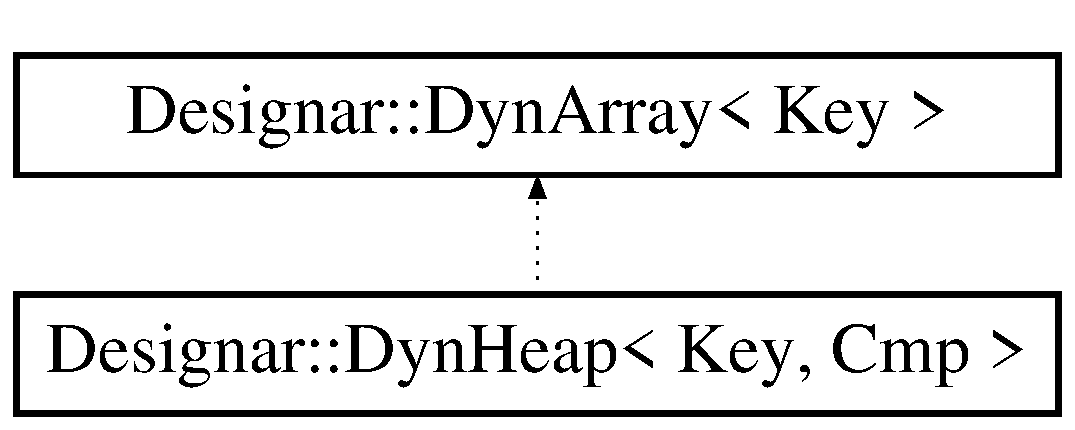
\includegraphics[height=2.000000cm]{class_designar_1_1_dyn_heap}
\end{center}
\end{figure}
\subsection*{Public Types}
\begin{DoxyCompactItemize}
\item 
using \hyperlink{class_designar_1_1_dyn_heap_a8b4add310e82b260912210069852febc}{Item\+Type} = Key
\item 
using \hyperlink{class_designar_1_1_dyn_heap_aa7260c4d35ad97e41f779bcf2b41808b}{Key\+Type} = Key
\item 
using \hyperlink{class_designar_1_1_dyn_heap_aa4011e735cd33c5043f59ae43a2ce318}{Data\+Type} = Key
\item 
using \hyperlink{class_designar_1_1_dyn_heap_a4c44d536a7ae76bbb7e667e1ea3b94ff}{Value\+Type} = Key
\item 
using \hyperlink{class_designar_1_1_dyn_heap_aa5d0813645a3a87407d2c95f0f4d5cad}{Size\+Type} = \hyperlink{namespace_designar_aa72662848b9f4815e7bf31a7cf3e33d1}{nat\+\_\+t}
\item 
using \hyperlink{class_designar_1_1_dyn_heap_af4eef9bc99b80f175c541cabff5333e0}{Cmp\+Type} = Cmp
\end{DoxyCompactItemize}
\subsection*{Public Member Functions}
\begin{DoxyCompactItemize}
\item 
\hyperlink{class_designar_1_1_dyn_heap_a156ccf78397ff8c10a3badf417043a28}{Dyn\+Heap} (Cmp \&\+\_\+cmp)
\item 
\hyperlink{class_designar_1_1_dyn_heap_a0c0805141b81deafa1715d8b77bc1847}{Dyn\+Heap} (Cmp \&\&\+\_\+cmp=Cmp())
\item 
\hyperlink{class_designar_1_1_dyn_heap_ac9570139e90ddd5ef3cd12df8a06739d}{Dyn\+Heap} (const \hyperlink{class_designar_1_1_dyn_heap}{Dyn\+Heap} \&h)
\item 
\hyperlink{class_designar_1_1_dyn_heap_a7bb0017ca6c1f4753f561cd5a7779e97}{Dyn\+Heap} (\hyperlink{class_designar_1_1_dyn_heap}{Dyn\+Heap} \&\&h)
\item 
\hyperlink{class_designar_1_1_dyn_heap}{Dyn\+Heap} \& \hyperlink{class_designar_1_1_dyn_heap_abf024c994d3bf2ccea002640e7c8d528}{operator=} (const \hyperlink{class_designar_1_1_dyn_heap}{Dyn\+Heap} \&h)
\item 
\hyperlink{class_designar_1_1_dyn_heap}{Dyn\+Heap} \& \hyperlink{class_designar_1_1_dyn_heap_a231a0935e2a45fa4d18b94c5b64f1a24}{operator=} (\hyperlink{class_designar_1_1_dyn_heap}{Dyn\+Heap} \&\&h)
\item 
Cmp \& \hyperlink{class_designar_1_1_dyn_heap_a4f1357b3883f314adbd2b7bb100636b3}{get\+\_\+cmp} ()
\item 
const Cmp \& \hyperlink{class_designar_1_1_dyn_heap_a2c5b0b169216b30f44cc26338d3866b1}{get\+\_\+cmp} () const
\item 
void \hyperlink{class_designar_1_1_dyn_heap_a5a1f01a6b4859f9b329df3848561aa3d}{clear} ()
\item 
bool \hyperlink{class_designar_1_1_dyn_heap_a5f067624d97ebe3945adf21cb14af92f}{is\+\_\+empty} () const
\item 
\hyperlink{namespace_designar_aa72662848b9f4815e7bf31a7cf3e33d1}{nat\+\_\+t} \hyperlink{class_designar_1_1_dyn_heap_ab0b3254c032e032d2c7b0d98033fad8e}{size} () const
\item 
void \hyperlink{class_designar_1_1_dyn_heap_aba3a8286ddea8098ab89e18658ec1e3c}{insert} (const Key \&item)
\item 
void \hyperlink{class_designar_1_1_dyn_heap_a28d454d027e576f9fc6f1c888c5e8809}{insert} (Key \&\&item)
\item 
const Key \& \hyperlink{class_designar_1_1_dyn_heap_af6500577f6cfaab1ac768e76a4c43e6c}{top} () const
\item 
Key \hyperlink{class_designar_1_1_dyn_heap_adead89301910d07cf6e019ad35b549ad}{get} ()
\end{DoxyCompactItemize}


\subsection{Detailed Description}
\subsubsection*{template$<$typename Key, class Cmp = std\+::less$<$\+Key$>$$>$\newline
class Designar\+::\+Dyn\+Heap$<$ Key, Cmp $>$}



Definition at line 225 of file heap.\+H.



\subsection{Member Typedef Documentation}
\mbox{\Hypertarget{class_designar_1_1_dyn_heap_af4eef9bc99b80f175c541cabff5333e0}\label{class_designar_1_1_dyn_heap_af4eef9bc99b80f175c541cabff5333e0}} 
\index{Designar\+::\+Dyn\+Heap@{Designar\+::\+Dyn\+Heap}!Cmp\+Type@{Cmp\+Type}}
\index{Cmp\+Type@{Cmp\+Type}!Designar\+::\+Dyn\+Heap@{Designar\+::\+Dyn\+Heap}}
\subsubsection{\texorpdfstring{Cmp\+Type}{CmpType}}
{\footnotesize\ttfamily template$<$typename Key, class Cmp = std\+::less$<$\+Key$>$$>$ \\
using \hyperlink{class_designar_1_1_dyn_heap}{Designar\+::\+Dyn\+Heap}$<$ Key, Cmp $>$\+::\hyperlink{class_designar_1_1_dyn_heap_af4eef9bc99b80f175c541cabff5333e0}{Cmp\+Type} =  Cmp}



Definition at line 247 of file heap.\+H.

\mbox{\Hypertarget{class_designar_1_1_dyn_heap_aa4011e735cd33c5043f59ae43a2ce318}\label{class_designar_1_1_dyn_heap_aa4011e735cd33c5043f59ae43a2ce318}} 
\index{Designar\+::\+Dyn\+Heap@{Designar\+::\+Dyn\+Heap}!Data\+Type@{Data\+Type}}
\index{Data\+Type@{Data\+Type}!Designar\+::\+Dyn\+Heap@{Designar\+::\+Dyn\+Heap}}
\subsubsection{\texorpdfstring{Data\+Type}{DataType}}
{\footnotesize\ttfamily template$<$typename Key, class Cmp = std\+::less$<$\+Key$>$$>$ \\
using \hyperlink{class_designar_1_1_dyn_heap}{Designar\+::\+Dyn\+Heap}$<$ Key, Cmp $>$\+::\hyperlink{class_designar_1_1_fixed_array_a3e37931b909b840cb7a40fc73f12bcf5}{Data\+Type} =  Key}



Definition at line 244 of file heap.\+H.

\mbox{\Hypertarget{class_designar_1_1_dyn_heap_a8b4add310e82b260912210069852febc}\label{class_designar_1_1_dyn_heap_a8b4add310e82b260912210069852febc}} 
\index{Designar\+::\+Dyn\+Heap@{Designar\+::\+Dyn\+Heap}!Item\+Type@{Item\+Type}}
\index{Item\+Type@{Item\+Type}!Designar\+::\+Dyn\+Heap@{Designar\+::\+Dyn\+Heap}}
\subsubsection{\texorpdfstring{Item\+Type}{ItemType}}
{\footnotesize\ttfamily template$<$typename Key, class Cmp = std\+::less$<$\+Key$>$$>$ \\
using \hyperlink{class_designar_1_1_dyn_heap}{Designar\+::\+Dyn\+Heap}$<$ Key, Cmp $>$\+::\hyperlink{class_designar_1_1_fixed_array_abfeb4e683cee75ae782ad20294c4c808}{Item\+Type} =  Key}



Definition at line 242 of file heap.\+H.

\mbox{\Hypertarget{class_designar_1_1_dyn_heap_aa7260c4d35ad97e41f779bcf2b41808b}\label{class_designar_1_1_dyn_heap_aa7260c4d35ad97e41f779bcf2b41808b}} 
\index{Designar\+::\+Dyn\+Heap@{Designar\+::\+Dyn\+Heap}!Key\+Type@{Key\+Type}}
\index{Key\+Type@{Key\+Type}!Designar\+::\+Dyn\+Heap@{Designar\+::\+Dyn\+Heap}}
\subsubsection{\texorpdfstring{Key\+Type}{KeyType}}
{\footnotesize\ttfamily template$<$typename Key, class Cmp = std\+::less$<$\+Key$>$$>$ \\
using \hyperlink{class_designar_1_1_dyn_heap}{Designar\+::\+Dyn\+Heap}$<$ Key, Cmp $>$\+::\hyperlink{class_designar_1_1_fixed_array_a3a725cf21783340b8aca29dd1db0acf0}{Key\+Type} =  Key}



Definition at line 243 of file heap.\+H.

\mbox{\Hypertarget{class_designar_1_1_dyn_heap_aa5d0813645a3a87407d2c95f0f4d5cad}\label{class_designar_1_1_dyn_heap_aa5d0813645a3a87407d2c95f0f4d5cad}} 
\index{Designar\+::\+Dyn\+Heap@{Designar\+::\+Dyn\+Heap}!Size\+Type@{Size\+Type}}
\index{Size\+Type@{Size\+Type}!Designar\+::\+Dyn\+Heap@{Designar\+::\+Dyn\+Heap}}
\subsubsection{\texorpdfstring{Size\+Type}{SizeType}}
{\footnotesize\ttfamily template$<$typename Key, class Cmp = std\+::less$<$\+Key$>$$>$ \\
using \hyperlink{class_designar_1_1_dyn_heap}{Designar\+::\+Dyn\+Heap}$<$ Key, Cmp $>$\+::\hyperlink{class_designar_1_1_fixed_array_a503ae414cc313d248e77c08e62ef043c}{Size\+Type} =  \hyperlink{namespace_designar_aa72662848b9f4815e7bf31a7cf3e33d1}{nat\+\_\+t}}



Definition at line 246 of file heap.\+H.

\mbox{\Hypertarget{class_designar_1_1_dyn_heap_a4c44d536a7ae76bbb7e667e1ea3b94ff}\label{class_designar_1_1_dyn_heap_a4c44d536a7ae76bbb7e667e1ea3b94ff}} 
\index{Designar\+::\+Dyn\+Heap@{Designar\+::\+Dyn\+Heap}!Value\+Type@{Value\+Type}}
\index{Value\+Type@{Value\+Type}!Designar\+::\+Dyn\+Heap@{Designar\+::\+Dyn\+Heap}}
\subsubsection{\texorpdfstring{Value\+Type}{ValueType}}
{\footnotesize\ttfamily template$<$typename Key, class Cmp = std\+::less$<$\+Key$>$$>$ \\
using \hyperlink{class_designar_1_1_dyn_heap}{Designar\+::\+Dyn\+Heap}$<$ Key, Cmp $>$\+::\hyperlink{class_designar_1_1_fixed_array_ac1cfeb4403a2dcbffd7ef494e5b873d0}{Value\+Type} =  Key}



Definition at line 245 of file heap.\+H.



\subsection{Constructor \& Destructor Documentation}
\mbox{\Hypertarget{class_designar_1_1_dyn_heap_a156ccf78397ff8c10a3badf417043a28}\label{class_designar_1_1_dyn_heap_a156ccf78397ff8c10a3badf417043a28}} 
\index{Designar\+::\+Dyn\+Heap@{Designar\+::\+Dyn\+Heap}!Dyn\+Heap@{Dyn\+Heap}}
\index{Dyn\+Heap@{Dyn\+Heap}!Designar\+::\+Dyn\+Heap@{Designar\+::\+Dyn\+Heap}}
\subsubsection{\texorpdfstring{Dyn\+Heap()}{DynHeap()}\hspace{0.1cm}{\footnotesize\ttfamily [1/4]}}
{\footnotesize\ttfamily template$<$typename Key, class Cmp = std\+::less$<$\+Key$>$$>$ \\
\hyperlink{class_designar_1_1_dyn_heap}{Designar\+::\+Dyn\+Heap}$<$ Key, Cmp $>$\+::\hyperlink{class_designar_1_1_dyn_heap}{Dyn\+Heap} (\begin{DoxyParamCaption}\item[{Cmp \&}]{\+\_\+cmp }\end{DoxyParamCaption})\hspace{0.3cm}{\ttfamily [inline]}}



Definition at line 249 of file heap.\+H.

\mbox{\Hypertarget{class_designar_1_1_dyn_heap_a0c0805141b81deafa1715d8b77bc1847}\label{class_designar_1_1_dyn_heap_a0c0805141b81deafa1715d8b77bc1847}} 
\index{Designar\+::\+Dyn\+Heap@{Designar\+::\+Dyn\+Heap}!Dyn\+Heap@{Dyn\+Heap}}
\index{Dyn\+Heap@{Dyn\+Heap}!Designar\+::\+Dyn\+Heap@{Designar\+::\+Dyn\+Heap}}
\subsubsection{\texorpdfstring{Dyn\+Heap()}{DynHeap()}\hspace{0.1cm}{\footnotesize\ttfamily [2/4]}}
{\footnotesize\ttfamily template$<$typename Key, class Cmp = std\+::less$<$\+Key$>$$>$ \\
\hyperlink{class_designar_1_1_dyn_heap}{Designar\+::\+Dyn\+Heap}$<$ Key, Cmp $>$\+::\hyperlink{class_designar_1_1_dyn_heap}{Dyn\+Heap} (\begin{DoxyParamCaption}\item[{Cmp \&\&}]{\+\_\+cmp = {\ttfamily Cmp()} }\end{DoxyParamCaption})\hspace{0.3cm}{\ttfamily [inline]}}



Definition at line 255 of file heap.\+H.

\mbox{\Hypertarget{class_designar_1_1_dyn_heap_ac9570139e90ddd5ef3cd12df8a06739d}\label{class_designar_1_1_dyn_heap_ac9570139e90ddd5ef3cd12df8a06739d}} 
\index{Designar\+::\+Dyn\+Heap@{Designar\+::\+Dyn\+Heap}!Dyn\+Heap@{Dyn\+Heap}}
\index{Dyn\+Heap@{Dyn\+Heap}!Designar\+::\+Dyn\+Heap@{Designar\+::\+Dyn\+Heap}}
\subsubsection{\texorpdfstring{Dyn\+Heap()}{DynHeap()}\hspace{0.1cm}{\footnotesize\ttfamily [3/4]}}
{\footnotesize\ttfamily template$<$typename Key, class Cmp = std\+::less$<$\+Key$>$$>$ \\
\hyperlink{class_designar_1_1_dyn_heap}{Designar\+::\+Dyn\+Heap}$<$ Key, Cmp $>$\+::\hyperlink{class_designar_1_1_dyn_heap}{Dyn\+Heap} (\begin{DoxyParamCaption}\item[{const \hyperlink{class_designar_1_1_dyn_heap}{Dyn\+Heap}$<$ Key, Cmp $>$ \&}]{h }\end{DoxyParamCaption})\hspace{0.3cm}{\ttfamily [inline]}}



Definition at line 261 of file heap.\+H.

\mbox{\Hypertarget{class_designar_1_1_dyn_heap_a7bb0017ca6c1f4753f561cd5a7779e97}\label{class_designar_1_1_dyn_heap_a7bb0017ca6c1f4753f561cd5a7779e97}} 
\index{Designar\+::\+Dyn\+Heap@{Designar\+::\+Dyn\+Heap}!Dyn\+Heap@{Dyn\+Heap}}
\index{Dyn\+Heap@{Dyn\+Heap}!Designar\+::\+Dyn\+Heap@{Designar\+::\+Dyn\+Heap}}
\subsubsection{\texorpdfstring{Dyn\+Heap()}{DynHeap()}\hspace{0.1cm}{\footnotesize\ttfamily [4/4]}}
{\footnotesize\ttfamily template$<$typename Key, class Cmp = std\+::less$<$\+Key$>$$>$ \\
\hyperlink{class_designar_1_1_dyn_heap}{Designar\+::\+Dyn\+Heap}$<$ Key, Cmp $>$\+::\hyperlink{class_designar_1_1_dyn_heap}{Dyn\+Heap} (\begin{DoxyParamCaption}\item[{\hyperlink{class_designar_1_1_dyn_heap}{Dyn\+Heap}$<$ Key, Cmp $>$ \&\&}]{h }\end{DoxyParamCaption})\hspace{0.3cm}{\ttfamily [inline]}}



Definition at line 267 of file heap.\+H.



\subsection{Member Function Documentation}
\mbox{\Hypertarget{class_designar_1_1_dyn_heap_a5a1f01a6b4859f9b329df3848561aa3d}\label{class_designar_1_1_dyn_heap_a5a1f01a6b4859f9b329df3848561aa3d}} 
\index{Designar\+::\+Dyn\+Heap@{Designar\+::\+Dyn\+Heap}!clear@{clear}}
\index{clear@{clear}!Designar\+::\+Dyn\+Heap@{Designar\+::\+Dyn\+Heap}}
\subsubsection{\texorpdfstring{clear()}{clear()}}
{\footnotesize\ttfamily template$<$typename Key, class Cmp = std\+::less$<$\+Key$>$$>$ \\
void \hyperlink{class_designar_1_1_dyn_heap}{Designar\+::\+Dyn\+Heap}$<$ Key, Cmp $>$\+::clear (\begin{DoxyParamCaption}{ }\end{DoxyParamCaption})\hspace{0.3cm}{\ttfamily [inline]}}



Definition at line 299 of file heap.\+H.

\mbox{\Hypertarget{class_designar_1_1_dyn_heap_adead89301910d07cf6e019ad35b549ad}\label{class_designar_1_1_dyn_heap_adead89301910d07cf6e019ad35b549ad}} 
\index{Designar\+::\+Dyn\+Heap@{Designar\+::\+Dyn\+Heap}!get@{get}}
\index{get@{get}!Designar\+::\+Dyn\+Heap@{Designar\+::\+Dyn\+Heap}}
\subsubsection{\texorpdfstring{get()}{get()}}
{\footnotesize\ttfamily template$<$typename Key, class Cmp = std\+::less$<$\+Key$>$$>$ \\
Key \hyperlink{class_designar_1_1_dyn_heap}{Designar\+::\+Dyn\+Heap}$<$ Key, Cmp $>$\+::get (\begin{DoxyParamCaption}{ }\end{DoxyParamCaption})\hspace{0.3cm}{\ttfamily [inline]}}



Definition at line 334 of file heap.\+H.

\mbox{\Hypertarget{class_designar_1_1_dyn_heap_a4f1357b3883f314adbd2b7bb100636b3}\label{class_designar_1_1_dyn_heap_a4f1357b3883f314adbd2b7bb100636b3}} 
\index{Designar\+::\+Dyn\+Heap@{Designar\+::\+Dyn\+Heap}!get\+\_\+cmp@{get\+\_\+cmp}}
\index{get\+\_\+cmp@{get\+\_\+cmp}!Designar\+::\+Dyn\+Heap@{Designar\+::\+Dyn\+Heap}}
\subsubsection{\texorpdfstring{get\+\_\+cmp()}{get\_cmp()}\hspace{0.1cm}{\footnotesize\ttfamily [1/2]}}
{\footnotesize\ttfamily template$<$typename Key, class Cmp = std\+::less$<$\+Key$>$$>$ \\
Cmp\& \hyperlink{class_designar_1_1_dyn_heap}{Designar\+::\+Dyn\+Heap}$<$ Key, Cmp $>$\+::get\+\_\+cmp (\begin{DoxyParamCaption}{ }\end{DoxyParamCaption})\hspace{0.3cm}{\ttfamily [inline]}}



Definition at line 289 of file heap.\+H.

\mbox{\Hypertarget{class_designar_1_1_dyn_heap_a2c5b0b169216b30f44cc26338d3866b1}\label{class_designar_1_1_dyn_heap_a2c5b0b169216b30f44cc26338d3866b1}} 
\index{Designar\+::\+Dyn\+Heap@{Designar\+::\+Dyn\+Heap}!get\+\_\+cmp@{get\+\_\+cmp}}
\index{get\+\_\+cmp@{get\+\_\+cmp}!Designar\+::\+Dyn\+Heap@{Designar\+::\+Dyn\+Heap}}
\subsubsection{\texorpdfstring{get\+\_\+cmp()}{get\_cmp()}\hspace{0.1cm}{\footnotesize\ttfamily [2/2]}}
{\footnotesize\ttfamily template$<$typename Key, class Cmp = std\+::less$<$\+Key$>$$>$ \\
const Cmp\& \hyperlink{class_designar_1_1_dyn_heap}{Designar\+::\+Dyn\+Heap}$<$ Key, Cmp $>$\+::get\+\_\+cmp (\begin{DoxyParamCaption}{ }\end{DoxyParamCaption}) const\hspace{0.3cm}{\ttfamily [inline]}}



Definition at line 294 of file heap.\+H.

\mbox{\Hypertarget{class_designar_1_1_dyn_heap_aba3a8286ddea8098ab89e18658ec1e3c}\label{class_designar_1_1_dyn_heap_aba3a8286ddea8098ab89e18658ec1e3c}} 
\index{Designar\+::\+Dyn\+Heap@{Designar\+::\+Dyn\+Heap}!insert@{insert}}
\index{insert@{insert}!Designar\+::\+Dyn\+Heap@{Designar\+::\+Dyn\+Heap}}
\subsubsection{\texorpdfstring{insert()}{insert()}\hspace{0.1cm}{\footnotesize\ttfamily [1/2]}}
{\footnotesize\ttfamily template$<$typename Key, class Cmp = std\+::less$<$\+Key$>$$>$ \\
void \hyperlink{class_designar_1_1_dyn_heap}{Designar\+::\+Dyn\+Heap}$<$ Key, Cmp $>$\+::insert (\begin{DoxyParamCaption}\item[{const Key \&}]{item }\end{DoxyParamCaption})\hspace{0.3cm}{\ttfamily [inline]}}



Definition at line 314 of file heap.\+H.

\mbox{\Hypertarget{class_designar_1_1_dyn_heap_a28d454d027e576f9fc6f1c888c5e8809}\label{class_designar_1_1_dyn_heap_a28d454d027e576f9fc6f1c888c5e8809}} 
\index{Designar\+::\+Dyn\+Heap@{Designar\+::\+Dyn\+Heap}!insert@{insert}}
\index{insert@{insert}!Designar\+::\+Dyn\+Heap@{Designar\+::\+Dyn\+Heap}}
\subsubsection{\texorpdfstring{insert()}{insert()}\hspace{0.1cm}{\footnotesize\ttfamily [2/2]}}
{\footnotesize\ttfamily template$<$typename Key, class Cmp = std\+::less$<$\+Key$>$$>$ \\
void \hyperlink{class_designar_1_1_dyn_heap}{Designar\+::\+Dyn\+Heap}$<$ Key, Cmp $>$\+::insert (\begin{DoxyParamCaption}\item[{Key \&\&}]{item }\end{DoxyParamCaption})\hspace{0.3cm}{\ttfamily [inline]}}



Definition at line 320 of file heap.\+H.

\mbox{\Hypertarget{class_designar_1_1_dyn_heap_a5f067624d97ebe3945adf21cb14af92f}\label{class_designar_1_1_dyn_heap_a5f067624d97ebe3945adf21cb14af92f}} 
\index{Designar\+::\+Dyn\+Heap@{Designar\+::\+Dyn\+Heap}!is\+\_\+empty@{is\+\_\+empty}}
\index{is\+\_\+empty@{is\+\_\+empty}!Designar\+::\+Dyn\+Heap@{Designar\+::\+Dyn\+Heap}}
\subsubsection{\texorpdfstring{is\+\_\+empty()}{is\_empty()}}
{\footnotesize\ttfamily template$<$typename Key, class Cmp = std\+::less$<$\+Key$>$$>$ \\
bool \hyperlink{class_designar_1_1_dyn_heap}{Designar\+::\+Dyn\+Heap}$<$ Key, Cmp $>$\+::is\+\_\+empty (\begin{DoxyParamCaption}{ }\end{DoxyParamCaption}) const\hspace{0.3cm}{\ttfamily [inline]}}



Definition at line 304 of file heap.\+H.

\mbox{\Hypertarget{class_designar_1_1_dyn_heap_abf024c994d3bf2ccea002640e7c8d528}\label{class_designar_1_1_dyn_heap_abf024c994d3bf2ccea002640e7c8d528}} 
\index{Designar\+::\+Dyn\+Heap@{Designar\+::\+Dyn\+Heap}!operator=@{operator=}}
\index{operator=@{operator=}!Designar\+::\+Dyn\+Heap@{Designar\+::\+Dyn\+Heap}}
\subsubsection{\texorpdfstring{operator=()}{operator=()}\hspace{0.1cm}{\footnotesize\ttfamily [1/2]}}
{\footnotesize\ttfamily template$<$typename Key, class Cmp = std\+::less$<$\+Key$>$$>$ \\
\hyperlink{class_designar_1_1_dyn_heap}{Dyn\+Heap}\& \hyperlink{class_designar_1_1_dyn_heap}{Designar\+::\+Dyn\+Heap}$<$ Key, Cmp $>$\+::operator= (\begin{DoxyParamCaption}\item[{const \hyperlink{class_designar_1_1_dyn_heap}{Dyn\+Heap}$<$ Key, Cmp $>$ \&}]{h }\end{DoxyParamCaption})\hspace{0.3cm}{\ttfamily [inline]}}



Definition at line 273 of file heap.\+H.

\mbox{\Hypertarget{class_designar_1_1_dyn_heap_a231a0935e2a45fa4d18b94c5b64f1a24}\label{class_designar_1_1_dyn_heap_a231a0935e2a45fa4d18b94c5b64f1a24}} 
\index{Designar\+::\+Dyn\+Heap@{Designar\+::\+Dyn\+Heap}!operator=@{operator=}}
\index{operator=@{operator=}!Designar\+::\+Dyn\+Heap@{Designar\+::\+Dyn\+Heap}}
\subsubsection{\texorpdfstring{operator=()}{operator=()}\hspace{0.1cm}{\footnotesize\ttfamily [2/2]}}
{\footnotesize\ttfamily template$<$typename Key, class Cmp = std\+::less$<$\+Key$>$$>$ \\
\hyperlink{class_designar_1_1_dyn_heap}{Dyn\+Heap}\& \hyperlink{class_designar_1_1_dyn_heap}{Designar\+::\+Dyn\+Heap}$<$ Key, Cmp $>$\+::operator= (\begin{DoxyParamCaption}\item[{\hyperlink{class_designar_1_1_dyn_heap}{Dyn\+Heap}$<$ Key, Cmp $>$ \&\&}]{h }\end{DoxyParamCaption})\hspace{0.3cm}{\ttfamily [inline]}}



Definition at line 283 of file heap.\+H.

\mbox{\Hypertarget{class_designar_1_1_dyn_heap_ab0b3254c032e032d2c7b0d98033fad8e}\label{class_designar_1_1_dyn_heap_ab0b3254c032e032d2c7b0d98033fad8e}} 
\index{Designar\+::\+Dyn\+Heap@{Designar\+::\+Dyn\+Heap}!size@{size}}
\index{size@{size}!Designar\+::\+Dyn\+Heap@{Designar\+::\+Dyn\+Heap}}
\subsubsection{\texorpdfstring{size()}{size()}}
{\footnotesize\ttfamily template$<$typename Key, class Cmp = std\+::less$<$\+Key$>$$>$ \\
\hyperlink{namespace_designar_aa72662848b9f4815e7bf31a7cf3e33d1}{nat\+\_\+t} \hyperlink{class_designar_1_1_dyn_heap}{Designar\+::\+Dyn\+Heap}$<$ Key, Cmp $>$\+::size (\begin{DoxyParamCaption}{ }\end{DoxyParamCaption}) const\hspace{0.3cm}{\ttfamily [inline]}}



Definition at line 309 of file heap.\+H.

\mbox{\Hypertarget{class_designar_1_1_dyn_heap_af6500577f6cfaab1ac768e76a4c43e6c}\label{class_designar_1_1_dyn_heap_af6500577f6cfaab1ac768e76a4c43e6c}} 
\index{Designar\+::\+Dyn\+Heap@{Designar\+::\+Dyn\+Heap}!top@{top}}
\index{top@{top}!Designar\+::\+Dyn\+Heap@{Designar\+::\+Dyn\+Heap}}
\subsubsection{\texorpdfstring{top()}{top()}}
{\footnotesize\ttfamily template$<$typename Key, class Cmp = std\+::less$<$\+Key$>$$>$ \\
const Key\& \hyperlink{class_designar_1_1_dyn_heap}{Designar\+::\+Dyn\+Heap}$<$ Key, Cmp $>$\+::top (\begin{DoxyParamCaption}{ }\end{DoxyParamCaption}) const\hspace{0.3cm}{\ttfamily [inline]}}



Definition at line 326 of file heap.\+H.



The documentation for this class was generated from the following file\+:\begin{DoxyCompactItemize}
\item 
include/\hyperlink{heap_8_h}{heap.\+H}\end{DoxyCompactItemize}

\hypertarget{class_designar_1_1_dyn_queue}{}\section{Designar\+:\+:Dyn\+Queue$<$ T $>$ Class Template Reference}
\label{class_designar_1_1_dyn_queue}\index{Designar\+::\+Dyn\+Queue$<$ T $>$@{Designar\+::\+Dyn\+Queue$<$ T $>$}}


{\ttfamily \#include $<$queue.\+H$>$}

Inheritance diagram for Designar\+:\+:Dyn\+Queue$<$ T $>$\+:\begin{figure}[H]
\begin{center}
\leavevmode
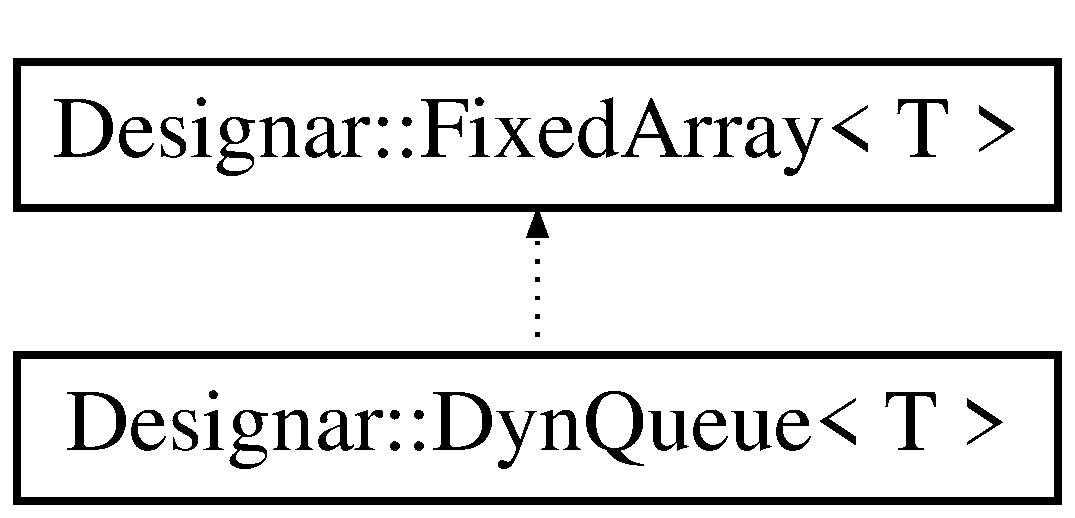
\includegraphics[height=2.000000cm]{class_designar_1_1_dyn_queue}
\end{center}
\end{figure}
\subsection*{Public Types}
\begin{DoxyCompactItemize}
\item 
using \hyperlink{class_designar_1_1_dyn_queue_a45a4b5b9dd6a921dbc6919802d34dd9e}{Item\+Type} = T
\item 
using \hyperlink{class_designar_1_1_dyn_queue_a0591681d66d914b3fb11f71d36759984}{Key\+Type} = T
\item 
using \hyperlink{class_designar_1_1_dyn_queue_a79504f1ab8156a3eaee8c9c0aaaf1b8a}{Data\+Type} = T
\item 
using \hyperlink{class_designar_1_1_dyn_queue_a6528f67f5ad9ecbe0f8a21b88f3cb832}{Value\+Type} = T
\item 
using \hyperlink{class_designar_1_1_dyn_queue_a376b5cd2f4a47d734fc1e73955197358}{Size\+Type} = \hyperlink{namespace_designar_aa72662848b9f4815e7bf31a7cf3e33d1}{nat\+\_\+t}
\end{DoxyCompactItemize}
\subsection*{Public Member Functions}
\begin{DoxyCompactItemize}
\item 
\hyperlink{class_designar_1_1_dyn_queue_a947ebdf2503509cdacd5e34a6de29197}{Dyn\+Queue} ()
\item 
\hyperlink{class_designar_1_1_dyn_queue_a612ed3480c13f60be2f9706601f846b1}{Dyn\+Queue} (const \hyperlink{class_designar_1_1_dyn_queue}{Dyn\+Queue} \&q)
\item 
\hyperlink{class_designar_1_1_dyn_queue_ad5d501cf675b1d5b2c0e0b6799cf77ec}{Dyn\+Queue} (\hyperlink{class_designar_1_1_dyn_queue}{Dyn\+Queue} \&\&q)
\item 
\hyperlink{class_designar_1_1_dyn_queue}{Dyn\+Queue} \& \hyperlink{class_designar_1_1_dyn_queue_a8936e37e8c235dea1201934067440eb7}{operator=} (const \hyperlink{class_designar_1_1_dyn_queue}{Dyn\+Queue} \&q)
\item 
\hyperlink{class_designar_1_1_dyn_queue}{Dyn\+Queue} \& \hyperlink{class_designar_1_1_dyn_queue_ad5d4745d5e0c3640a413897f8d72ed25}{operator=} (\hyperlink{class_designar_1_1_dyn_queue}{Dyn\+Queue} \&\&q)
\item 
bool \hyperlink{class_designar_1_1_dyn_queue_ae0c3b0a4a0c5028a12d8a564182d2b3e}{is\+\_\+empty} () const
\item 
\hyperlink{namespace_designar_aa72662848b9f4815e7bf31a7cf3e33d1}{nat\+\_\+t} \hyperlink{class_designar_1_1_dyn_queue_a3fa0e8fd7d197de1a60caae23b5c305e}{size} () const
\item 
void \hyperlink{class_designar_1_1_dyn_queue_adc396896fa4b333de8ae60ed8b8da2ea}{clear} ()
\item 
T \& \hyperlink{class_designar_1_1_dyn_queue_a910f0dc9d3bf1c1b2363730db842980d}{front} ()
\item 
const T \& \hyperlink{class_designar_1_1_dyn_queue_ae8e017797ad0ccd8a0568f69f8adedbf}{front} () const
\item 
T \& \hyperlink{class_designar_1_1_dyn_queue_a735f5a7d869689994d81d593b1924c68}{rear} ()
\item 
const T \& \hyperlink{class_designar_1_1_dyn_queue_a378a92d95bb351f2cc1b8fb80f6c9525}{rear} () const
\item 
T \& \hyperlink{class_designar_1_1_dyn_queue_a4564ed0e64b06d4a96ff020ba3456706}{put} (const T \&item)
\item 
T \& \hyperlink{class_designar_1_1_dyn_queue_a53c4e234aacf16fdb7e99625edadad61}{put} (T \&\&item)
\item 
T \hyperlink{class_designar_1_1_dyn_queue_a70b3f577ec11287fe63766de53a2cb56}{get} ()
\end{DoxyCompactItemize}


\subsection{Detailed Description}
\subsubsection*{template$<$typename T$>$\newline
class Designar\+::\+Dyn\+Queue$<$ T $>$}



Definition at line 205 of file queue.\+H.



\subsection{Member Typedef Documentation}
\mbox{\Hypertarget{class_designar_1_1_dyn_queue_a79504f1ab8156a3eaee8c9c0aaaf1b8a}\label{class_designar_1_1_dyn_queue_a79504f1ab8156a3eaee8c9c0aaaf1b8a}} 
\index{Designar\+::\+Dyn\+Queue@{Designar\+::\+Dyn\+Queue}!Data\+Type@{Data\+Type}}
\index{Data\+Type@{Data\+Type}!Designar\+::\+Dyn\+Queue@{Designar\+::\+Dyn\+Queue}}
\subsubsection{\texorpdfstring{Data\+Type}{DataType}}
{\footnotesize\ttfamily template$<$typename T$>$ \\
using \hyperlink{class_designar_1_1_dyn_queue}{Designar\+::\+Dyn\+Queue}$<$ T $>$\+::\hyperlink{class_designar_1_1_fixed_array_a3e37931b909b840cb7a40fc73f12bcf5}{Data\+Type} =  T}



Definition at line 252 of file queue.\+H.

\mbox{\Hypertarget{class_designar_1_1_dyn_queue_a45a4b5b9dd6a921dbc6919802d34dd9e}\label{class_designar_1_1_dyn_queue_a45a4b5b9dd6a921dbc6919802d34dd9e}} 
\index{Designar\+::\+Dyn\+Queue@{Designar\+::\+Dyn\+Queue}!Item\+Type@{Item\+Type}}
\index{Item\+Type@{Item\+Type}!Designar\+::\+Dyn\+Queue@{Designar\+::\+Dyn\+Queue}}
\subsubsection{\texorpdfstring{Item\+Type}{ItemType}}
{\footnotesize\ttfamily template$<$typename T$>$ \\
using \hyperlink{class_designar_1_1_dyn_queue}{Designar\+::\+Dyn\+Queue}$<$ T $>$\+::\hyperlink{class_designar_1_1_fixed_array_abfeb4e683cee75ae782ad20294c4c808}{Item\+Type} =  T}



Definition at line 250 of file queue.\+H.

\mbox{\Hypertarget{class_designar_1_1_dyn_queue_a0591681d66d914b3fb11f71d36759984}\label{class_designar_1_1_dyn_queue_a0591681d66d914b3fb11f71d36759984}} 
\index{Designar\+::\+Dyn\+Queue@{Designar\+::\+Dyn\+Queue}!Key\+Type@{Key\+Type}}
\index{Key\+Type@{Key\+Type}!Designar\+::\+Dyn\+Queue@{Designar\+::\+Dyn\+Queue}}
\subsubsection{\texorpdfstring{Key\+Type}{KeyType}}
{\footnotesize\ttfamily template$<$typename T$>$ \\
using \hyperlink{class_designar_1_1_dyn_queue}{Designar\+::\+Dyn\+Queue}$<$ T $>$\+::\hyperlink{class_designar_1_1_fixed_array_a3a725cf21783340b8aca29dd1db0acf0}{Key\+Type} =  T}



Definition at line 251 of file queue.\+H.

\mbox{\Hypertarget{class_designar_1_1_dyn_queue_a376b5cd2f4a47d734fc1e73955197358}\label{class_designar_1_1_dyn_queue_a376b5cd2f4a47d734fc1e73955197358}} 
\index{Designar\+::\+Dyn\+Queue@{Designar\+::\+Dyn\+Queue}!Size\+Type@{Size\+Type}}
\index{Size\+Type@{Size\+Type}!Designar\+::\+Dyn\+Queue@{Designar\+::\+Dyn\+Queue}}
\subsubsection{\texorpdfstring{Size\+Type}{SizeType}}
{\footnotesize\ttfamily template$<$typename T$>$ \\
using \hyperlink{class_designar_1_1_dyn_queue}{Designar\+::\+Dyn\+Queue}$<$ T $>$\+::\hyperlink{class_designar_1_1_fixed_array_a503ae414cc313d248e77c08e62ef043c}{Size\+Type} =  \hyperlink{namespace_designar_aa72662848b9f4815e7bf31a7cf3e33d1}{nat\+\_\+t}}



Definition at line 254 of file queue.\+H.

\mbox{\Hypertarget{class_designar_1_1_dyn_queue_a6528f67f5ad9ecbe0f8a21b88f3cb832}\label{class_designar_1_1_dyn_queue_a6528f67f5ad9ecbe0f8a21b88f3cb832}} 
\index{Designar\+::\+Dyn\+Queue@{Designar\+::\+Dyn\+Queue}!Value\+Type@{Value\+Type}}
\index{Value\+Type@{Value\+Type}!Designar\+::\+Dyn\+Queue@{Designar\+::\+Dyn\+Queue}}
\subsubsection{\texorpdfstring{Value\+Type}{ValueType}}
{\footnotesize\ttfamily template$<$typename T$>$ \\
using \hyperlink{class_designar_1_1_dyn_queue}{Designar\+::\+Dyn\+Queue}$<$ T $>$\+::\hyperlink{class_designar_1_1_fixed_array_ac1cfeb4403a2dcbffd7ef494e5b873d0}{Value\+Type} =  T}



Definition at line 253 of file queue.\+H.



\subsection{Constructor \& Destructor Documentation}
\mbox{\Hypertarget{class_designar_1_1_dyn_queue_a947ebdf2503509cdacd5e34a6de29197}\label{class_designar_1_1_dyn_queue_a947ebdf2503509cdacd5e34a6de29197}} 
\index{Designar\+::\+Dyn\+Queue@{Designar\+::\+Dyn\+Queue}!Dyn\+Queue@{Dyn\+Queue}}
\index{Dyn\+Queue@{Dyn\+Queue}!Designar\+::\+Dyn\+Queue@{Designar\+::\+Dyn\+Queue}}
\subsubsection{\texorpdfstring{Dyn\+Queue()}{DynQueue()}\hspace{0.1cm}{\footnotesize\ttfamily [1/3]}}
{\footnotesize\ttfamily template$<$typename T$>$ \\
\hyperlink{class_designar_1_1_dyn_queue}{Designar\+::\+Dyn\+Queue}$<$ T $>$\+::\hyperlink{class_designar_1_1_dyn_queue}{Dyn\+Queue} (\begin{DoxyParamCaption}{ }\end{DoxyParamCaption})\hspace{0.3cm}{\ttfamily [inline]}}



Definition at line 256 of file queue.\+H.

\mbox{\Hypertarget{class_designar_1_1_dyn_queue_a612ed3480c13f60be2f9706601f846b1}\label{class_designar_1_1_dyn_queue_a612ed3480c13f60be2f9706601f846b1}} 
\index{Designar\+::\+Dyn\+Queue@{Designar\+::\+Dyn\+Queue}!Dyn\+Queue@{Dyn\+Queue}}
\index{Dyn\+Queue@{Dyn\+Queue}!Designar\+::\+Dyn\+Queue@{Designar\+::\+Dyn\+Queue}}
\subsubsection{\texorpdfstring{Dyn\+Queue()}{DynQueue()}\hspace{0.1cm}{\footnotesize\ttfamily [2/3]}}
{\footnotesize\ttfamily template$<$typename T$>$ \\
\hyperlink{class_designar_1_1_dyn_queue}{Designar\+::\+Dyn\+Queue}$<$ T $>$\+::\hyperlink{class_designar_1_1_dyn_queue}{Dyn\+Queue} (\begin{DoxyParamCaption}\item[{const \hyperlink{class_designar_1_1_dyn_queue}{Dyn\+Queue}$<$ T $>$ \&}]{q }\end{DoxyParamCaption})\hspace{0.3cm}{\ttfamily [inline]}}



Definition at line 262 of file queue.\+H.

\mbox{\Hypertarget{class_designar_1_1_dyn_queue_ad5d501cf675b1d5b2c0e0b6799cf77ec}\label{class_designar_1_1_dyn_queue_ad5d501cf675b1d5b2c0e0b6799cf77ec}} 
\index{Designar\+::\+Dyn\+Queue@{Designar\+::\+Dyn\+Queue}!Dyn\+Queue@{Dyn\+Queue}}
\index{Dyn\+Queue@{Dyn\+Queue}!Designar\+::\+Dyn\+Queue@{Designar\+::\+Dyn\+Queue}}
\subsubsection{\texorpdfstring{Dyn\+Queue()}{DynQueue()}\hspace{0.1cm}{\footnotesize\ttfamily [3/3]}}
{\footnotesize\ttfamily template$<$typename T$>$ \\
\hyperlink{class_designar_1_1_dyn_queue}{Designar\+::\+Dyn\+Queue}$<$ T $>$\+::\hyperlink{class_designar_1_1_dyn_queue}{Dyn\+Queue} (\begin{DoxyParamCaption}\item[{\hyperlink{class_designar_1_1_dyn_queue}{Dyn\+Queue}$<$ T $>$ \&\&}]{q }\end{DoxyParamCaption})\hspace{0.3cm}{\ttfamily [inline]}}



Definition at line 268 of file queue.\+H.



\subsection{Member Function Documentation}
\mbox{\Hypertarget{class_designar_1_1_dyn_queue_adc396896fa4b333de8ae60ed8b8da2ea}\label{class_designar_1_1_dyn_queue_adc396896fa4b333de8ae60ed8b8da2ea}} 
\index{Designar\+::\+Dyn\+Queue@{Designar\+::\+Dyn\+Queue}!clear@{clear}}
\index{clear@{clear}!Designar\+::\+Dyn\+Queue@{Designar\+::\+Dyn\+Queue}}
\subsubsection{\texorpdfstring{clear()}{clear()}}
{\footnotesize\ttfamily template$<$typename T$>$ \\
void \hyperlink{class_designar_1_1_dyn_queue}{Designar\+::\+Dyn\+Queue}$<$ T $>$\+::clear (\begin{DoxyParamCaption}{ }\end{DoxyParamCaption})\hspace{0.3cm}{\ttfamily [inline]}}



Definition at line 303 of file queue.\+H.

\mbox{\Hypertarget{class_designar_1_1_dyn_queue_a910f0dc9d3bf1c1b2363730db842980d}\label{class_designar_1_1_dyn_queue_a910f0dc9d3bf1c1b2363730db842980d}} 
\index{Designar\+::\+Dyn\+Queue@{Designar\+::\+Dyn\+Queue}!front@{front}}
\index{front@{front}!Designar\+::\+Dyn\+Queue@{Designar\+::\+Dyn\+Queue}}
\subsubsection{\texorpdfstring{front()}{front()}\hspace{0.1cm}{\footnotesize\ttfamily [1/2]}}
{\footnotesize\ttfamily template$<$typename T$>$ \\
T\& \hyperlink{class_designar_1_1_dyn_queue}{Designar\+::\+Dyn\+Queue}$<$ T $>$\+::front (\begin{DoxyParamCaption}{ }\end{DoxyParamCaption})\hspace{0.3cm}{\ttfamily [inline]}}



Definition at line 317 of file queue.\+H.

\mbox{\Hypertarget{class_designar_1_1_dyn_queue_ae8e017797ad0ccd8a0568f69f8adedbf}\label{class_designar_1_1_dyn_queue_ae8e017797ad0ccd8a0568f69f8adedbf}} 
\index{Designar\+::\+Dyn\+Queue@{Designar\+::\+Dyn\+Queue}!front@{front}}
\index{front@{front}!Designar\+::\+Dyn\+Queue@{Designar\+::\+Dyn\+Queue}}
\subsubsection{\texorpdfstring{front()}{front()}\hspace{0.1cm}{\footnotesize\ttfamily [2/2]}}
{\footnotesize\ttfamily template$<$typename T$>$ \\
const T\& \hyperlink{class_designar_1_1_dyn_queue}{Designar\+::\+Dyn\+Queue}$<$ T $>$\+::front (\begin{DoxyParamCaption}{ }\end{DoxyParamCaption}) const\hspace{0.3cm}{\ttfamily [inline]}}



Definition at line 325 of file queue.\+H.

\mbox{\Hypertarget{class_designar_1_1_dyn_queue_a70b3f577ec11287fe63766de53a2cb56}\label{class_designar_1_1_dyn_queue_a70b3f577ec11287fe63766de53a2cb56}} 
\index{Designar\+::\+Dyn\+Queue@{Designar\+::\+Dyn\+Queue}!get@{get}}
\index{get@{get}!Designar\+::\+Dyn\+Queue@{Designar\+::\+Dyn\+Queue}}
\subsubsection{\texorpdfstring{get()}{get()}}
{\footnotesize\ttfamily template$<$typename T$>$ \\
T \hyperlink{class_designar_1_1_dyn_queue}{Designar\+::\+Dyn\+Queue}$<$ T $>$\+::get (\begin{DoxyParamCaption}{ }\end{DoxyParamCaption})\hspace{0.3cm}{\ttfamily [inline]}}



Definition at line 367 of file queue.\+H.

\mbox{\Hypertarget{class_designar_1_1_dyn_queue_ae0c3b0a4a0c5028a12d8a564182d2b3e}\label{class_designar_1_1_dyn_queue_ae0c3b0a4a0c5028a12d8a564182d2b3e}} 
\index{Designar\+::\+Dyn\+Queue@{Designar\+::\+Dyn\+Queue}!is\+\_\+empty@{is\+\_\+empty}}
\index{is\+\_\+empty@{is\+\_\+empty}!Designar\+::\+Dyn\+Queue@{Designar\+::\+Dyn\+Queue}}
\subsubsection{\texorpdfstring{is\+\_\+empty()}{is\_empty()}}
{\footnotesize\ttfamily template$<$typename T$>$ \\
bool \hyperlink{class_designar_1_1_dyn_queue}{Designar\+::\+Dyn\+Queue}$<$ T $>$\+::is\+\_\+empty (\begin{DoxyParamCaption}{ }\end{DoxyParamCaption}) const\hspace{0.3cm}{\ttfamily [inline]}}



Definition at line 293 of file queue.\+H.

\mbox{\Hypertarget{class_designar_1_1_dyn_queue_a8936e37e8c235dea1201934067440eb7}\label{class_designar_1_1_dyn_queue_a8936e37e8c235dea1201934067440eb7}} 
\index{Designar\+::\+Dyn\+Queue@{Designar\+::\+Dyn\+Queue}!operator=@{operator=}}
\index{operator=@{operator=}!Designar\+::\+Dyn\+Queue@{Designar\+::\+Dyn\+Queue}}
\subsubsection{\texorpdfstring{operator=()}{operator=()}\hspace{0.1cm}{\footnotesize\ttfamily [1/2]}}
{\footnotesize\ttfamily template$<$typename T$>$ \\
\hyperlink{class_designar_1_1_dyn_queue}{Dyn\+Queue}\& \hyperlink{class_designar_1_1_dyn_queue}{Designar\+::\+Dyn\+Queue}$<$ T $>$\+::operator= (\begin{DoxyParamCaption}\item[{const \hyperlink{class_designar_1_1_dyn_queue}{Dyn\+Queue}$<$ T $>$ \&}]{q }\end{DoxyParamCaption})\hspace{0.3cm}{\ttfamily [inline]}}



Definition at line 274 of file queue.\+H.

\mbox{\Hypertarget{class_designar_1_1_dyn_queue_ad5d4745d5e0c3640a413897f8d72ed25}\label{class_designar_1_1_dyn_queue_ad5d4745d5e0c3640a413897f8d72ed25}} 
\index{Designar\+::\+Dyn\+Queue@{Designar\+::\+Dyn\+Queue}!operator=@{operator=}}
\index{operator=@{operator=}!Designar\+::\+Dyn\+Queue@{Designar\+::\+Dyn\+Queue}}
\subsubsection{\texorpdfstring{operator=()}{operator=()}\hspace{0.1cm}{\footnotesize\ttfamily [2/2]}}
{\footnotesize\ttfamily template$<$typename T$>$ \\
\hyperlink{class_designar_1_1_dyn_queue}{Dyn\+Queue}\& \hyperlink{class_designar_1_1_dyn_queue}{Designar\+::\+Dyn\+Queue}$<$ T $>$\+::operator= (\begin{DoxyParamCaption}\item[{\hyperlink{class_designar_1_1_dyn_queue}{Dyn\+Queue}$<$ T $>$ \&\&}]{q }\end{DoxyParamCaption})\hspace{0.3cm}{\ttfamily [inline]}}



Definition at line 287 of file queue.\+H.

\mbox{\Hypertarget{class_designar_1_1_dyn_queue_a4564ed0e64b06d4a96ff020ba3456706}\label{class_designar_1_1_dyn_queue_a4564ed0e64b06d4a96ff020ba3456706}} 
\index{Designar\+::\+Dyn\+Queue@{Designar\+::\+Dyn\+Queue}!put@{put}}
\index{put@{put}!Designar\+::\+Dyn\+Queue@{Designar\+::\+Dyn\+Queue}}
\subsubsection{\texorpdfstring{put()}{put()}\hspace{0.1cm}{\footnotesize\ttfamily [1/2]}}
{\footnotesize\ttfamily template$<$typename T$>$ \\
T\& \hyperlink{class_designar_1_1_dyn_queue}{Designar\+::\+Dyn\+Queue}$<$ T $>$\+::put (\begin{DoxyParamCaption}\item[{const T \&}]{item }\end{DoxyParamCaption})\hspace{0.3cm}{\ttfamily [inline]}}



Definition at line 349 of file queue.\+H.

\mbox{\Hypertarget{class_designar_1_1_dyn_queue_a53c4e234aacf16fdb7e99625edadad61}\label{class_designar_1_1_dyn_queue_a53c4e234aacf16fdb7e99625edadad61}} 
\index{Designar\+::\+Dyn\+Queue@{Designar\+::\+Dyn\+Queue}!put@{put}}
\index{put@{put}!Designar\+::\+Dyn\+Queue@{Designar\+::\+Dyn\+Queue}}
\subsubsection{\texorpdfstring{put()}{put()}\hspace{0.1cm}{\footnotesize\ttfamily [2/2]}}
{\footnotesize\ttfamily template$<$typename T$>$ \\
T\& \hyperlink{class_designar_1_1_dyn_queue}{Designar\+::\+Dyn\+Queue}$<$ T $>$\+::put (\begin{DoxyParamCaption}\item[{T \&\&}]{item }\end{DoxyParamCaption})\hspace{0.3cm}{\ttfamily [inline]}}



Definition at line 358 of file queue.\+H.

\mbox{\Hypertarget{class_designar_1_1_dyn_queue_a735f5a7d869689994d81d593b1924c68}\label{class_designar_1_1_dyn_queue_a735f5a7d869689994d81d593b1924c68}} 
\index{Designar\+::\+Dyn\+Queue@{Designar\+::\+Dyn\+Queue}!rear@{rear}}
\index{rear@{rear}!Designar\+::\+Dyn\+Queue@{Designar\+::\+Dyn\+Queue}}
\subsubsection{\texorpdfstring{rear()}{rear()}\hspace{0.1cm}{\footnotesize\ttfamily [1/2]}}
{\footnotesize\ttfamily template$<$typename T$>$ \\
T\& \hyperlink{class_designar_1_1_dyn_queue}{Designar\+::\+Dyn\+Queue}$<$ T $>$\+::rear (\begin{DoxyParamCaption}{ }\end{DoxyParamCaption})\hspace{0.3cm}{\ttfamily [inline]}}



Definition at line 333 of file queue.\+H.

\mbox{\Hypertarget{class_designar_1_1_dyn_queue_a378a92d95bb351f2cc1b8fb80f6c9525}\label{class_designar_1_1_dyn_queue_a378a92d95bb351f2cc1b8fb80f6c9525}} 
\index{Designar\+::\+Dyn\+Queue@{Designar\+::\+Dyn\+Queue}!rear@{rear}}
\index{rear@{rear}!Designar\+::\+Dyn\+Queue@{Designar\+::\+Dyn\+Queue}}
\subsubsection{\texorpdfstring{rear()}{rear()}\hspace{0.1cm}{\footnotesize\ttfamily [2/2]}}
{\footnotesize\ttfamily template$<$typename T$>$ \\
const T\& \hyperlink{class_designar_1_1_dyn_queue}{Designar\+::\+Dyn\+Queue}$<$ T $>$\+::rear (\begin{DoxyParamCaption}{ }\end{DoxyParamCaption}) const\hspace{0.3cm}{\ttfamily [inline]}}



Definition at line 341 of file queue.\+H.

\mbox{\Hypertarget{class_designar_1_1_dyn_queue_a3fa0e8fd7d197de1a60caae23b5c305e}\label{class_designar_1_1_dyn_queue_a3fa0e8fd7d197de1a60caae23b5c305e}} 
\index{Designar\+::\+Dyn\+Queue@{Designar\+::\+Dyn\+Queue}!size@{size}}
\index{size@{size}!Designar\+::\+Dyn\+Queue@{Designar\+::\+Dyn\+Queue}}
\subsubsection{\texorpdfstring{size()}{size()}}
{\footnotesize\ttfamily template$<$typename T$>$ \\
\hyperlink{namespace_designar_aa72662848b9f4815e7bf31a7cf3e33d1}{nat\+\_\+t} \hyperlink{class_designar_1_1_dyn_queue}{Designar\+::\+Dyn\+Queue}$<$ T $>$\+::size (\begin{DoxyParamCaption}{ }\end{DoxyParamCaption}) const\hspace{0.3cm}{\ttfamily [inline]}}



Definition at line 298 of file queue.\+H.



The documentation for this class was generated from the following file\+:\begin{DoxyCompactItemize}
\item 
include/\hyperlink{queue_8_h}{queue.\+H}\end{DoxyCompactItemize}

\hypertarget{class_designar_1_1_dyn_stack}{}\section{Referencia de la plantilla de la Clase Designar\+:\+:Dyn\+Stack$<$ T $>$}
\label{class_designar_1_1_dyn_stack}\index{Designar\+::\+Dyn\+Stack$<$ T $>$@{Designar\+::\+Dyn\+Stack$<$ T $>$}}


{\ttfamily \#include $<$stack.\+H$>$}

Diagrama de herencias de Designar\+:\+:Dyn\+Stack$<$ T $>$\begin{figure}[H]
\begin{center}
\leavevmode
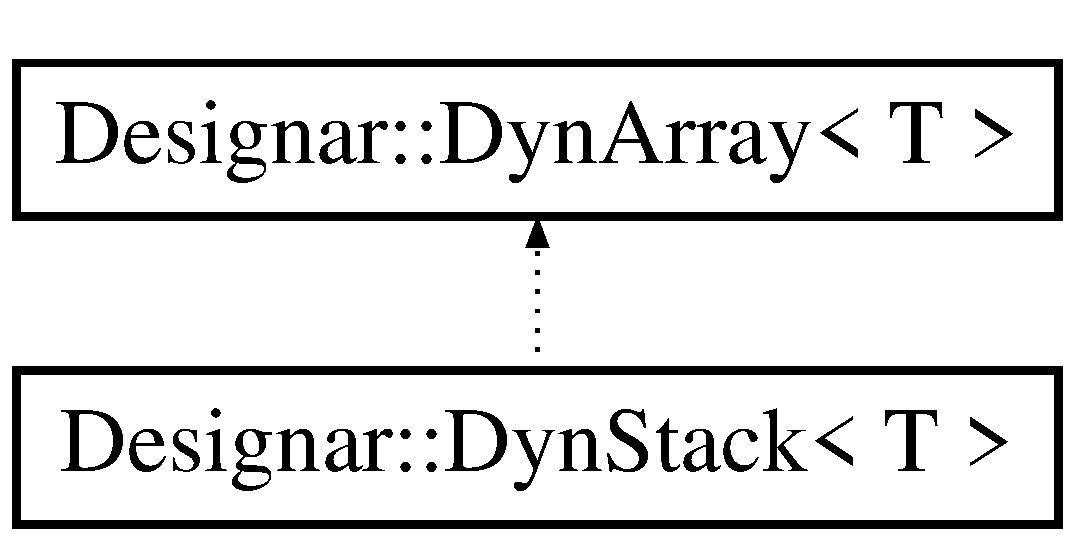
\includegraphics[height=2.000000cm]{class_designar_1_1_dyn_stack}
\end{center}
\end{figure}
\subsection*{Tipos públicos}
\begin{DoxyCompactItemize}
\item 
using \hyperlink{class_designar_1_1_dyn_stack_a2e50015faeef3234802046097db79f73}{Item\+Type} = T
\item 
using \hyperlink{class_designar_1_1_dyn_stack_a4a4fd39e08b25a05641fb888b99261c8}{Key\+Type} = T
\item 
using \hyperlink{class_designar_1_1_dyn_stack_afb7dc9ebd5c844450d997e38b195f3bb}{Data\+Type} = T
\item 
using \hyperlink{class_designar_1_1_dyn_stack_a511da1dd717eb6f9c5b143b2a8543176}{Value\+Type} = T
\item 
using \hyperlink{class_designar_1_1_dyn_stack_adb2c839a5bc34354be458c86dd35f5b8}{Size\+Type} = \hyperlink{namespace_designar_aa72662848b9f4815e7bf31a7cf3e33d1}{nat\+\_\+t}
\end{DoxyCompactItemize}
\subsection*{Métodos públicos}
\begin{DoxyCompactItemize}
\item 
\hyperlink{class_designar_1_1_dyn_stack_a974a328c42eeb04114249c321a7d2ebe}{Dyn\+Stack} ()
\item 
\hyperlink{class_designar_1_1_dyn_stack_afe8f19b00f9c0cb21ea2d64fedadcb5e}{Dyn\+Stack} (\hyperlink{namespace_designar_aa72662848b9f4815e7bf31a7cf3e33d1}{nat\+\_\+t} cap)
\item 
\hyperlink{class_designar_1_1_dyn_stack_a4a28588893016f554cd8ea21b37e2c5f}{Dyn\+Stack} (const \hyperlink{class_designar_1_1_dyn_stack}{Dyn\+Stack} \&s)
\item 
\hyperlink{class_designar_1_1_dyn_stack_a8a15a70c98b19554d73037118fa8eed9}{Dyn\+Stack} (\hyperlink{class_designar_1_1_dyn_stack}{Dyn\+Stack} \&\&s)
\item 
\hyperlink{class_designar_1_1_dyn_stack}{Dyn\+Stack} \& \hyperlink{class_designar_1_1_dyn_stack_a95c3464bba2e4c2393ada749ab4d9248}{operator=} (const \hyperlink{class_designar_1_1_dyn_stack}{Dyn\+Stack} \&s)
\item 
\hyperlink{class_designar_1_1_dyn_stack}{Dyn\+Stack} \& \hyperlink{class_designar_1_1_dyn_stack_aa5b875ca2b2a6ce501a91c79d5857166}{operator=} (\hyperlink{class_designar_1_1_dyn_stack}{Dyn\+Stack} \&\&s)
\item 
bool \hyperlink{class_designar_1_1_dyn_stack_ae0c03ed9771729e3773128868fb7afe5}{is\+\_\+empty} () const
\item 
void \hyperlink{class_designar_1_1_dyn_stack_aab024478a38633aeb3d79e2ddcbd1958}{clear} ()
\item 
\hyperlink{namespace_designar_aa72662848b9f4815e7bf31a7cf3e33d1}{nat\+\_\+t} \hyperlink{class_designar_1_1_dyn_stack_a4c15622a5283c072287a7dfdd6c4bd2d}{size} () const
\item 
T \& \hyperlink{class_designar_1_1_dyn_stack_a07d7d76d087e7b9dc287a7b2acd02fc6}{push} (const T \&item)
\item 
T \& \hyperlink{class_designar_1_1_dyn_stack_a1eff6c891fd3800c6aa55f35e14e4f88}{push} (T \&\&item)
\item 
T \& \hyperlink{class_designar_1_1_dyn_stack_a33e8c623bae518ed88cdee01602febb0}{top} ()
\item 
const T \& \hyperlink{class_designar_1_1_dyn_stack_a497eb06d2cb8280d031586a913b1317c}{top} () const
\item 
T \& \hyperlink{class_designar_1_1_dyn_stack_aa07528cd0ef77519ca5b5694bed9695d}{base} ()
\item 
const T \& \hyperlink{class_designar_1_1_dyn_stack_affe0e56802ac0c982f598e2155bf4a46}{base} () const
\item 
T \hyperlink{class_designar_1_1_dyn_stack_ac3e7235449ffb9fc0ac96ba0b081d2ed}{pop} ()
\item 
void \hyperlink{class_designar_1_1_dyn_stack_a161b319e52448a4f824b036a9f7c6cca}{popn} (\hyperlink{namespace_designar_aa72662848b9f4815e7bf31a7cf3e33d1}{nat\+\_\+t})
\end{DoxyCompactItemize}


\subsection{Descripción detallada}
\subsubsection*{template$<$typename T$>$\newline
class Designar\+::\+Dyn\+Stack$<$ T $>$}



Definición en la línea 190 del archivo stack.\+H.



\subsection{Documentación de los \textquotesingle{}Typedef\textquotesingle{} miembros de la clase}
\mbox{\Hypertarget{class_designar_1_1_dyn_stack_afb7dc9ebd5c844450d997e38b195f3bb}\label{class_designar_1_1_dyn_stack_afb7dc9ebd5c844450d997e38b195f3bb}} 
\index{Designar\+::\+Dyn\+Stack@{Designar\+::\+Dyn\+Stack}!Data\+Type@{Data\+Type}}
\index{Data\+Type@{Data\+Type}!Designar\+::\+Dyn\+Stack@{Designar\+::\+Dyn\+Stack}}
\subsubsection{\texorpdfstring{Data\+Type}{DataType}}
{\footnotesize\ttfamily template$<$typename T$>$ \\
using \hyperlink{class_designar_1_1_dyn_stack}{Designar\+::\+Dyn\+Stack}$<$ T $>$\+::\hyperlink{class_designar_1_1_fixed_array_a3e37931b909b840cb7a40fc73f12bcf5}{Data\+Type} =  T}



Definición en la línea 197 del archivo stack.\+H.

\mbox{\Hypertarget{class_designar_1_1_dyn_stack_a2e50015faeef3234802046097db79f73}\label{class_designar_1_1_dyn_stack_a2e50015faeef3234802046097db79f73}} 
\index{Designar\+::\+Dyn\+Stack@{Designar\+::\+Dyn\+Stack}!Item\+Type@{Item\+Type}}
\index{Item\+Type@{Item\+Type}!Designar\+::\+Dyn\+Stack@{Designar\+::\+Dyn\+Stack}}
\subsubsection{\texorpdfstring{Item\+Type}{ItemType}}
{\footnotesize\ttfamily template$<$typename T$>$ \\
using \hyperlink{class_designar_1_1_dyn_stack}{Designar\+::\+Dyn\+Stack}$<$ T $>$\+::\hyperlink{class_designar_1_1_fixed_array_abfeb4e683cee75ae782ad20294c4c808}{Item\+Type} =  T}



Definición en la línea 195 del archivo stack.\+H.

\mbox{\Hypertarget{class_designar_1_1_dyn_stack_a4a4fd39e08b25a05641fb888b99261c8}\label{class_designar_1_1_dyn_stack_a4a4fd39e08b25a05641fb888b99261c8}} 
\index{Designar\+::\+Dyn\+Stack@{Designar\+::\+Dyn\+Stack}!Key\+Type@{Key\+Type}}
\index{Key\+Type@{Key\+Type}!Designar\+::\+Dyn\+Stack@{Designar\+::\+Dyn\+Stack}}
\subsubsection{\texorpdfstring{Key\+Type}{KeyType}}
{\footnotesize\ttfamily template$<$typename T$>$ \\
using \hyperlink{class_designar_1_1_dyn_stack}{Designar\+::\+Dyn\+Stack}$<$ T $>$\+::\hyperlink{class_designar_1_1_fixed_array_a3a725cf21783340b8aca29dd1db0acf0}{Key\+Type} =  T}



Definición en la línea 196 del archivo stack.\+H.

\mbox{\Hypertarget{class_designar_1_1_dyn_stack_adb2c839a5bc34354be458c86dd35f5b8}\label{class_designar_1_1_dyn_stack_adb2c839a5bc34354be458c86dd35f5b8}} 
\index{Designar\+::\+Dyn\+Stack@{Designar\+::\+Dyn\+Stack}!Size\+Type@{Size\+Type}}
\index{Size\+Type@{Size\+Type}!Designar\+::\+Dyn\+Stack@{Designar\+::\+Dyn\+Stack}}
\subsubsection{\texorpdfstring{Size\+Type}{SizeType}}
{\footnotesize\ttfamily template$<$typename T$>$ \\
using \hyperlink{class_designar_1_1_dyn_stack}{Designar\+::\+Dyn\+Stack}$<$ T $>$\+::\hyperlink{class_designar_1_1_fixed_array_a503ae414cc313d248e77c08e62ef043c}{Size\+Type} =  \hyperlink{namespace_designar_aa72662848b9f4815e7bf31a7cf3e33d1}{nat\+\_\+t}}



Definición en la línea 199 del archivo stack.\+H.

\mbox{\Hypertarget{class_designar_1_1_dyn_stack_a511da1dd717eb6f9c5b143b2a8543176}\label{class_designar_1_1_dyn_stack_a511da1dd717eb6f9c5b143b2a8543176}} 
\index{Designar\+::\+Dyn\+Stack@{Designar\+::\+Dyn\+Stack}!Value\+Type@{Value\+Type}}
\index{Value\+Type@{Value\+Type}!Designar\+::\+Dyn\+Stack@{Designar\+::\+Dyn\+Stack}}
\subsubsection{\texorpdfstring{Value\+Type}{ValueType}}
{\footnotesize\ttfamily template$<$typename T$>$ \\
using \hyperlink{class_designar_1_1_dyn_stack}{Designar\+::\+Dyn\+Stack}$<$ T $>$\+::\hyperlink{class_designar_1_1_fixed_array_ac1cfeb4403a2dcbffd7ef494e5b873d0}{Value\+Type} =  T}



Definición en la línea 198 del archivo stack.\+H.



\subsection{Documentación del constructor y destructor}
\mbox{\Hypertarget{class_designar_1_1_dyn_stack_a974a328c42eeb04114249c321a7d2ebe}\label{class_designar_1_1_dyn_stack_a974a328c42eeb04114249c321a7d2ebe}} 
\index{Designar\+::\+Dyn\+Stack@{Designar\+::\+Dyn\+Stack}!Dyn\+Stack@{Dyn\+Stack}}
\index{Dyn\+Stack@{Dyn\+Stack}!Designar\+::\+Dyn\+Stack@{Designar\+::\+Dyn\+Stack}}
\subsubsection{\texorpdfstring{Dyn\+Stack()}{DynStack()}\hspace{0.1cm}{\footnotesize\ttfamily [1/4]}}
{\footnotesize\ttfamily template$<$typename T$>$ \\
\hyperlink{class_designar_1_1_dyn_stack}{Designar\+::\+Dyn\+Stack}$<$ T $>$\+::\hyperlink{class_designar_1_1_dyn_stack}{Dyn\+Stack} (\begin{DoxyParamCaption}{ }\end{DoxyParamCaption})\hspace{0.3cm}{\ttfamily [inline]}}



Definición en la línea 201 del archivo stack.\+H.

\mbox{\Hypertarget{class_designar_1_1_dyn_stack_afe8f19b00f9c0cb21ea2d64fedadcb5e}\label{class_designar_1_1_dyn_stack_afe8f19b00f9c0cb21ea2d64fedadcb5e}} 
\index{Designar\+::\+Dyn\+Stack@{Designar\+::\+Dyn\+Stack}!Dyn\+Stack@{Dyn\+Stack}}
\index{Dyn\+Stack@{Dyn\+Stack}!Designar\+::\+Dyn\+Stack@{Designar\+::\+Dyn\+Stack}}
\subsubsection{\texorpdfstring{Dyn\+Stack()}{DynStack()}\hspace{0.1cm}{\footnotesize\ttfamily [2/4]}}
{\footnotesize\ttfamily template$<$typename T$>$ \\
\hyperlink{class_designar_1_1_dyn_stack}{Designar\+::\+Dyn\+Stack}$<$ T $>$\+::\hyperlink{class_designar_1_1_dyn_stack}{Dyn\+Stack} (\begin{DoxyParamCaption}\item[{\hyperlink{namespace_designar_aa72662848b9f4815e7bf31a7cf3e33d1}{nat\+\_\+t}}]{cap }\end{DoxyParamCaption})\hspace{0.3cm}{\ttfamily [inline]}}



Definición en la línea 207 del archivo stack.\+H.

\mbox{\Hypertarget{class_designar_1_1_dyn_stack_a4a28588893016f554cd8ea21b37e2c5f}\label{class_designar_1_1_dyn_stack_a4a28588893016f554cd8ea21b37e2c5f}} 
\index{Designar\+::\+Dyn\+Stack@{Designar\+::\+Dyn\+Stack}!Dyn\+Stack@{Dyn\+Stack}}
\index{Dyn\+Stack@{Dyn\+Stack}!Designar\+::\+Dyn\+Stack@{Designar\+::\+Dyn\+Stack}}
\subsubsection{\texorpdfstring{Dyn\+Stack()}{DynStack()}\hspace{0.1cm}{\footnotesize\ttfamily [3/4]}}
{\footnotesize\ttfamily template$<$typename T$>$ \\
\hyperlink{class_designar_1_1_dyn_stack}{Designar\+::\+Dyn\+Stack}$<$ T $>$\+::\hyperlink{class_designar_1_1_dyn_stack}{Dyn\+Stack} (\begin{DoxyParamCaption}\item[{const \hyperlink{class_designar_1_1_dyn_stack}{Dyn\+Stack}$<$ T $>$ \&}]{s }\end{DoxyParamCaption})\hspace{0.3cm}{\ttfamily [inline]}}



Definición en la línea 213 del archivo stack.\+H.

\mbox{\Hypertarget{class_designar_1_1_dyn_stack_a8a15a70c98b19554d73037118fa8eed9}\label{class_designar_1_1_dyn_stack_a8a15a70c98b19554d73037118fa8eed9}} 
\index{Designar\+::\+Dyn\+Stack@{Designar\+::\+Dyn\+Stack}!Dyn\+Stack@{Dyn\+Stack}}
\index{Dyn\+Stack@{Dyn\+Stack}!Designar\+::\+Dyn\+Stack@{Designar\+::\+Dyn\+Stack}}
\subsubsection{\texorpdfstring{Dyn\+Stack()}{DynStack()}\hspace{0.1cm}{\footnotesize\ttfamily [4/4]}}
{\footnotesize\ttfamily template$<$typename T$>$ \\
\hyperlink{class_designar_1_1_dyn_stack}{Designar\+::\+Dyn\+Stack}$<$ T $>$\+::\hyperlink{class_designar_1_1_dyn_stack}{Dyn\+Stack} (\begin{DoxyParamCaption}\item[{\hyperlink{class_designar_1_1_dyn_stack}{Dyn\+Stack}$<$ T $>$ \&\&}]{s }\end{DoxyParamCaption})\hspace{0.3cm}{\ttfamily [inline]}}



Definición en la línea 219 del archivo stack.\+H.



\subsection{Documentación de las funciones miembro}
\mbox{\Hypertarget{class_designar_1_1_dyn_stack_aa07528cd0ef77519ca5b5694bed9695d}\label{class_designar_1_1_dyn_stack_aa07528cd0ef77519ca5b5694bed9695d}} 
\index{Designar\+::\+Dyn\+Stack@{Designar\+::\+Dyn\+Stack}!base@{base}}
\index{base@{base}!Designar\+::\+Dyn\+Stack@{Designar\+::\+Dyn\+Stack}}
\subsubsection{\texorpdfstring{base()}{base()}\hspace{0.1cm}{\footnotesize\ttfamily [1/2]}}
{\footnotesize\ttfamily template$<$typename T$>$ \\
T\& \hyperlink{class_designar_1_1_dyn_stack}{Designar\+::\+Dyn\+Stack}$<$ T $>$\+::base (\begin{DoxyParamCaption}{ }\end{DoxyParamCaption})\hspace{0.3cm}{\ttfamily [inline]}}



Definición en la línea 283 del archivo stack.\+H.

\mbox{\Hypertarget{class_designar_1_1_dyn_stack_affe0e56802ac0c982f598e2155bf4a46}\label{class_designar_1_1_dyn_stack_affe0e56802ac0c982f598e2155bf4a46}} 
\index{Designar\+::\+Dyn\+Stack@{Designar\+::\+Dyn\+Stack}!base@{base}}
\index{base@{base}!Designar\+::\+Dyn\+Stack@{Designar\+::\+Dyn\+Stack}}
\subsubsection{\texorpdfstring{base()}{base()}\hspace{0.1cm}{\footnotesize\ttfamily [2/2]}}
{\footnotesize\ttfamily template$<$typename T$>$ \\
const T\& \hyperlink{class_designar_1_1_dyn_stack}{Designar\+::\+Dyn\+Stack}$<$ T $>$\+::base (\begin{DoxyParamCaption}{ }\end{DoxyParamCaption}) const\hspace{0.3cm}{\ttfamily [inline]}}



Definición en la línea 291 del archivo stack.\+H.

\mbox{\Hypertarget{class_designar_1_1_dyn_stack_aab024478a38633aeb3d79e2ddcbd1958}\label{class_designar_1_1_dyn_stack_aab024478a38633aeb3d79e2ddcbd1958}} 
\index{Designar\+::\+Dyn\+Stack@{Designar\+::\+Dyn\+Stack}!clear@{clear}}
\index{clear@{clear}!Designar\+::\+Dyn\+Stack@{Designar\+::\+Dyn\+Stack}}
\subsubsection{\texorpdfstring{clear()}{clear()}}
{\footnotesize\ttfamily template$<$typename T$>$ \\
void \hyperlink{class_designar_1_1_dyn_stack}{Designar\+::\+Dyn\+Stack}$<$ T $>$\+::clear (\begin{DoxyParamCaption}{ }\end{DoxyParamCaption})\hspace{0.3cm}{\ttfamily [inline]}}



Definición en la línea 245 del archivo stack.\+H.

\mbox{\Hypertarget{class_designar_1_1_dyn_stack_ae0c03ed9771729e3773128868fb7afe5}\label{class_designar_1_1_dyn_stack_ae0c03ed9771729e3773128868fb7afe5}} 
\index{Designar\+::\+Dyn\+Stack@{Designar\+::\+Dyn\+Stack}!is\+\_\+empty@{is\+\_\+empty}}
\index{is\+\_\+empty@{is\+\_\+empty}!Designar\+::\+Dyn\+Stack@{Designar\+::\+Dyn\+Stack}}
\subsubsection{\texorpdfstring{is\+\_\+empty()}{is\_empty()}}
{\footnotesize\ttfamily template$<$typename T$>$ \\
bool \hyperlink{class_designar_1_1_dyn_stack}{Designar\+::\+Dyn\+Stack}$<$ T $>$\+::is\+\_\+empty (\begin{DoxyParamCaption}{ }\end{DoxyParamCaption}) const\hspace{0.3cm}{\ttfamily [inline]}}



Definición en la línea 240 del archivo stack.\+H.

\mbox{\Hypertarget{class_designar_1_1_dyn_stack_a95c3464bba2e4c2393ada749ab4d9248}\label{class_designar_1_1_dyn_stack_a95c3464bba2e4c2393ada749ab4d9248}} 
\index{Designar\+::\+Dyn\+Stack@{Designar\+::\+Dyn\+Stack}!operator=@{operator=}}
\index{operator=@{operator=}!Designar\+::\+Dyn\+Stack@{Designar\+::\+Dyn\+Stack}}
\subsubsection{\texorpdfstring{operator=()}{operator=()}\hspace{0.1cm}{\footnotesize\ttfamily [1/2]}}
{\footnotesize\ttfamily template$<$typename T$>$ \\
\hyperlink{class_designar_1_1_dyn_stack}{Dyn\+Stack}\& \hyperlink{class_designar_1_1_dyn_stack}{Designar\+::\+Dyn\+Stack}$<$ T $>$\+::operator= (\begin{DoxyParamCaption}\item[{const \hyperlink{class_designar_1_1_dyn_stack}{Dyn\+Stack}$<$ T $>$ \&}]{s }\end{DoxyParamCaption})\hspace{0.3cm}{\ttfamily [inline]}}



Definición en la línea 225 del archivo stack.\+H.

\mbox{\Hypertarget{class_designar_1_1_dyn_stack_aa5b875ca2b2a6ce501a91c79d5857166}\label{class_designar_1_1_dyn_stack_aa5b875ca2b2a6ce501a91c79d5857166}} 
\index{Designar\+::\+Dyn\+Stack@{Designar\+::\+Dyn\+Stack}!operator=@{operator=}}
\index{operator=@{operator=}!Designar\+::\+Dyn\+Stack@{Designar\+::\+Dyn\+Stack}}
\subsubsection{\texorpdfstring{operator=()}{operator=()}\hspace{0.1cm}{\footnotesize\ttfamily [2/2]}}
{\footnotesize\ttfamily template$<$typename T$>$ \\
\hyperlink{class_designar_1_1_dyn_stack}{Dyn\+Stack}\& \hyperlink{class_designar_1_1_dyn_stack}{Designar\+::\+Dyn\+Stack}$<$ T $>$\+::operator= (\begin{DoxyParamCaption}\item[{\hyperlink{class_designar_1_1_dyn_stack}{Dyn\+Stack}$<$ T $>$ \&\&}]{s }\end{DoxyParamCaption})\hspace{0.3cm}{\ttfamily [inline]}}



Definición en la línea 234 del archivo stack.\+H.

\mbox{\Hypertarget{class_designar_1_1_dyn_stack_ac3e7235449ffb9fc0ac96ba0b081d2ed}\label{class_designar_1_1_dyn_stack_ac3e7235449ffb9fc0ac96ba0b081d2ed}} 
\index{Designar\+::\+Dyn\+Stack@{Designar\+::\+Dyn\+Stack}!pop@{pop}}
\index{pop@{pop}!Designar\+::\+Dyn\+Stack@{Designar\+::\+Dyn\+Stack}}
\subsubsection{\texorpdfstring{pop()}{pop()}}
{\footnotesize\ttfamily template$<$typename T$>$ \\
T \hyperlink{class_designar_1_1_dyn_stack}{Designar\+::\+Dyn\+Stack}$<$ T $>$\+::pop (\begin{DoxyParamCaption}{ }\end{DoxyParamCaption})\hspace{0.3cm}{\ttfamily [inline]}}



Definición en la línea 299 del archivo stack.\+H.

\mbox{\Hypertarget{class_designar_1_1_dyn_stack_a161b319e52448a4f824b036a9f7c6cca}\label{class_designar_1_1_dyn_stack_a161b319e52448a4f824b036a9f7c6cca}} 
\index{Designar\+::\+Dyn\+Stack@{Designar\+::\+Dyn\+Stack}!popn@{popn}}
\index{popn@{popn}!Designar\+::\+Dyn\+Stack@{Designar\+::\+Dyn\+Stack}}
\subsubsection{\texorpdfstring{popn()}{popn()}}
{\footnotesize\ttfamily template$<$typename T $>$ \\
void \hyperlink{class_designar_1_1_dyn_stack}{Designar\+::\+Dyn\+Stack}$<$ T $>$\+::popn (\begin{DoxyParamCaption}\item[{\hyperlink{namespace_designar_aa72662848b9f4815e7bf31a7cf3e33d1}{nat\+\_\+t}}]{n }\end{DoxyParamCaption})}



Definición en la línea 311 del archivo stack.\+H.

\mbox{\Hypertarget{class_designar_1_1_dyn_stack_a07d7d76d087e7b9dc287a7b2acd02fc6}\label{class_designar_1_1_dyn_stack_a07d7d76d087e7b9dc287a7b2acd02fc6}} 
\index{Designar\+::\+Dyn\+Stack@{Designar\+::\+Dyn\+Stack}!push@{push}}
\index{push@{push}!Designar\+::\+Dyn\+Stack@{Designar\+::\+Dyn\+Stack}}
\subsubsection{\texorpdfstring{push()}{push()}\hspace{0.1cm}{\footnotesize\ttfamily [1/2]}}
{\footnotesize\ttfamily template$<$typename T$>$ \\
T\& \hyperlink{class_designar_1_1_dyn_stack}{Designar\+::\+Dyn\+Stack}$<$ T $>$\+::push (\begin{DoxyParamCaption}\item[{const T \&}]{item }\end{DoxyParamCaption})\hspace{0.3cm}{\ttfamily [inline]}}



Definición en la línea 255 del archivo stack.\+H.

\mbox{\Hypertarget{class_designar_1_1_dyn_stack_a1eff6c891fd3800c6aa55f35e14e4f88}\label{class_designar_1_1_dyn_stack_a1eff6c891fd3800c6aa55f35e14e4f88}} 
\index{Designar\+::\+Dyn\+Stack@{Designar\+::\+Dyn\+Stack}!push@{push}}
\index{push@{push}!Designar\+::\+Dyn\+Stack@{Designar\+::\+Dyn\+Stack}}
\subsubsection{\texorpdfstring{push()}{push()}\hspace{0.1cm}{\footnotesize\ttfamily [2/2]}}
{\footnotesize\ttfamily template$<$typename T$>$ \\
T\& \hyperlink{class_designar_1_1_dyn_stack}{Designar\+::\+Dyn\+Stack}$<$ T $>$\+::push (\begin{DoxyParamCaption}\item[{T \&\&}]{item }\end{DoxyParamCaption})\hspace{0.3cm}{\ttfamily [inline]}}



Definición en la línea 261 del archivo stack.\+H.

\mbox{\Hypertarget{class_designar_1_1_dyn_stack_a4c15622a5283c072287a7dfdd6c4bd2d}\label{class_designar_1_1_dyn_stack_a4c15622a5283c072287a7dfdd6c4bd2d}} 
\index{Designar\+::\+Dyn\+Stack@{Designar\+::\+Dyn\+Stack}!size@{size}}
\index{size@{size}!Designar\+::\+Dyn\+Stack@{Designar\+::\+Dyn\+Stack}}
\subsubsection{\texorpdfstring{size()}{size()}}
{\footnotesize\ttfamily template$<$typename T$>$ \\
\hyperlink{namespace_designar_aa72662848b9f4815e7bf31a7cf3e33d1}{nat\+\_\+t} \hyperlink{class_designar_1_1_dyn_stack}{Designar\+::\+Dyn\+Stack}$<$ T $>$\+::size (\begin{DoxyParamCaption}{ }\end{DoxyParamCaption}) const\hspace{0.3cm}{\ttfamily [inline]}}



Definición en la línea 250 del archivo stack.\+H.

\mbox{\Hypertarget{class_designar_1_1_dyn_stack_a33e8c623bae518ed88cdee01602febb0}\label{class_designar_1_1_dyn_stack_a33e8c623bae518ed88cdee01602febb0}} 
\index{Designar\+::\+Dyn\+Stack@{Designar\+::\+Dyn\+Stack}!top@{top}}
\index{top@{top}!Designar\+::\+Dyn\+Stack@{Designar\+::\+Dyn\+Stack}}
\subsubsection{\texorpdfstring{top()}{top()}\hspace{0.1cm}{\footnotesize\ttfamily [1/2]}}
{\footnotesize\ttfamily template$<$typename T$>$ \\
T\& \hyperlink{class_designar_1_1_dyn_stack}{Designar\+::\+Dyn\+Stack}$<$ T $>$\+::top (\begin{DoxyParamCaption}{ }\end{DoxyParamCaption})\hspace{0.3cm}{\ttfamily [inline]}}



Definición en la línea 267 del archivo stack.\+H.

\mbox{\Hypertarget{class_designar_1_1_dyn_stack_a497eb06d2cb8280d031586a913b1317c}\label{class_designar_1_1_dyn_stack_a497eb06d2cb8280d031586a913b1317c}} 
\index{Designar\+::\+Dyn\+Stack@{Designar\+::\+Dyn\+Stack}!top@{top}}
\index{top@{top}!Designar\+::\+Dyn\+Stack@{Designar\+::\+Dyn\+Stack}}
\subsubsection{\texorpdfstring{top()}{top()}\hspace{0.1cm}{\footnotesize\ttfamily [2/2]}}
{\footnotesize\ttfamily template$<$typename T$>$ \\
const T\& \hyperlink{class_designar_1_1_dyn_stack}{Designar\+::\+Dyn\+Stack}$<$ T $>$\+::top (\begin{DoxyParamCaption}{ }\end{DoxyParamCaption}) const\hspace{0.3cm}{\ttfamily [inline]}}



Definición en la línea 275 del archivo stack.\+H.



La documentación para esta clase fue generada a partir del siguiente fichero\+:\begin{DoxyCompactItemize}
\item 
/home/julio/\+De\+S\+I\+G\+N\+A\+R-\/doc/\+De\+Si\+G\+N\+A\+R/include/\hyperlink{stack_8_h}{stack.\+H}\end{DoxyCompactItemize}

\hypertarget{class_designar_1_1_empty_class}{}\section{Designar\+:\+:Empty\+Class Class Reference}
\label{class_designar_1_1_empty_class}\index{Designar\+::\+Empty\+Class@{Designar\+::\+Empty\+Class}}


{\ttfamily \#include $<$types.\+H$>$}

\subsection*{Public Member Functions}
\begin{DoxyCompactItemize}
\item 
\hyperlink{class_designar_1_1_empty_class_a88d846866a1e4872224ec2b4e750eba8}{Empty\+Class} ()
\item 
\hyperlink{class_designar_1_1_empty_class_a0a0b2cec90aebb02e6f5e3371087b221}{Empty\+Class} (const \hyperlink{class_designar_1_1_empty_class}{Empty\+Class} \&)
\item 
\hyperlink{class_designar_1_1_empty_class_aa18e6ee1ae08bc9500c9c0f91a6bae0c}{Empty\+Class} (\hyperlink{class_designar_1_1_empty_class}{Empty\+Class} \&\&)
\item 
\hyperlink{class_designar_1_1_empty_class_a751a2dca8e5df75e3f6a528f4fa43656}{$\sim$\+Empty\+Class} ()
\item 
\hyperlink{class_designar_1_1_empty_class}{Empty\+Class} \& \hyperlink{class_designar_1_1_empty_class_ac40f40d89e1823d95f5441e037d4212a}{operator=} (const \hyperlink{class_designar_1_1_empty_class}{Empty\+Class} \&)
\item 
\hyperlink{class_designar_1_1_empty_class}{Empty\+Class} \& \hyperlink{class_designar_1_1_empty_class_a41efe51c730deccac172173c27e4f9a7}{operator=} (\hyperlink{class_designar_1_1_empty_class}{Empty\+Class} \&\&)
\item 
bool \hyperlink{class_designar_1_1_empty_class_a377d66a49a2eaa853dcf5d798f82499e}{operator==} (const \hyperlink{class_designar_1_1_empty_class}{Empty\+Class} \&) const
\item 
bool \hyperlink{class_designar_1_1_empty_class_aafdaf95265007ed710e7b2393921d805}{operator!=} (const \hyperlink{class_designar_1_1_empty_class}{Empty\+Class} \&) const
\item 
bool \hyperlink{class_designar_1_1_empty_class_ae08a3c7c6b6d1d8bd73a52bf4f7be4fb}{operator$<$} (const \hyperlink{class_designar_1_1_empty_class}{Empty\+Class} \&) const
\item 
bool \hyperlink{class_designar_1_1_empty_class_a92e2e8f4d9b8d7ac7b6f2295242dd447}{operator$<$=} (const \hyperlink{class_designar_1_1_empty_class}{Empty\+Class} \&) const
\item 
bool \hyperlink{class_designar_1_1_empty_class_a2c58de7cc499842e2de8497c4892359b}{operator$>$} (const \hyperlink{class_designar_1_1_empty_class}{Empty\+Class} \&) const
\item 
bool \hyperlink{class_designar_1_1_empty_class_a84209f056d1930a130d55e8a6de090d2}{operator$>$=} (const \hyperlink{class_designar_1_1_empty_class}{Empty\+Class} \&) const
\end{DoxyCompactItemize}
\subsection*{Friends}
\begin{DoxyCompactItemize}
\item 
std\+::ostream \& \hyperlink{class_designar_1_1_empty_class_a1927797e0167a693cd74b5227218f196}{operator$<$$<$} (std\+::ostream \&out, const \hyperlink{class_designar_1_1_empty_class}{Empty\+Class} \&)
\item 
std\+::istream \& \hyperlink{class_designar_1_1_empty_class_aa3fc576ae898cf56f66f6ebf12251803}{operator$>$$>$} (std\+::istream \&in, \hyperlink{class_designar_1_1_empty_class}{Empty\+Class} \&)
\end{DoxyCompactItemize}


\subsection{Detailed Description}


Definition at line 60 of file types.\+H.



\subsection{Constructor \& Destructor Documentation}
\mbox{\Hypertarget{class_designar_1_1_empty_class_a88d846866a1e4872224ec2b4e750eba8}\label{class_designar_1_1_empty_class_a88d846866a1e4872224ec2b4e750eba8}} 
\index{Designar\+::\+Empty\+Class@{Designar\+::\+Empty\+Class}!Empty\+Class@{Empty\+Class}}
\index{Empty\+Class@{Empty\+Class}!Designar\+::\+Empty\+Class@{Designar\+::\+Empty\+Class}}
\subsubsection{\texorpdfstring{Empty\+Class()}{EmptyClass()}\hspace{0.1cm}{\footnotesize\ttfamily [1/3]}}
{\footnotesize\ttfamily Designar\+::\+Empty\+Class\+::\+Empty\+Class (\begin{DoxyParamCaption}{ }\end{DoxyParamCaption})\hspace{0.3cm}{\ttfamily [inline]}}



Definition at line 63 of file types.\+H.

\mbox{\Hypertarget{class_designar_1_1_empty_class_a0a0b2cec90aebb02e6f5e3371087b221}\label{class_designar_1_1_empty_class_a0a0b2cec90aebb02e6f5e3371087b221}} 
\index{Designar\+::\+Empty\+Class@{Designar\+::\+Empty\+Class}!Empty\+Class@{Empty\+Class}}
\index{Empty\+Class@{Empty\+Class}!Designar\+::\+Empty\+Class@{Designar\+::\+Empty\+Class}}
\subsubsection{\texorpdfstring{Empty\+Class()}{EmptyClass()}\hspace{0.1cm}{\footnotesize\ttfamily [2/3]}}
{\footnotesize\ttfamily Designar\+::\+Empty\+Class\+::\+Empty\+Class (\begin{DoxyParamCaption}\item[{const \hyperlink{class_designar_1_1_empty_class}{Empty\+Class} \&}]{ }\end{DoxyParamCaption})\hspace{0.3cm}{\ttfamily [inline]}}



Definition at line 65 of file types.\+H.

\mbox{\Hypertarget{class_designar_1_1_empty_class_aa18e6ee1ae08bc9500c9c0f91a6bae0c}\label{class_designar_1_1_empty_class_aa18e6ee1ae08bc9500c9c0f91a6bae0c}} 
\index{Designar\+::\+Empty\+Class@{Designar\+::\+Empty\+Class}!Empty\+Class@{Empty\+Class}}
\index{Empty\+Class@{Empty\+Class}!Designar\+::\+Empty\+Class@{Designar\+::\+Empty\+Class}}
\subsubsection{\texorpdfstring{Empty\+Class()}{EmptyClass()}\hspace{0.1cm}{\footnotesize\ttfamily [3/3]}}
{\footnotesize\ttfamily Designar\+::\+Empty\+Class\+::\+Empty\+Class (\begin{DoxyParamCaption}\item[{\hyperlink{class_designar_1_1_empty_class}{Empty\+Class} \&\&}]{ }\end{DoxyParamCaption})\hspace{0.3cm}{\ttfamily [inline]}}



Definition at line 67 of file types.\+H.

\mbox{\Hypertarget{class_designar_1_1_empty_class_a751a2dca8e5df75e3f6a528f4fa43656}\label{class_designar_1_1_empty_class_a751a2dca8e5df75e3f6a528f4fa43656}} 
\index{Designar\+::\+Empty\+Class@{Designar\+::\+Empty\+Class}!````~Empty\+Class@{$\sim$\+Empty\+Class}}
\index{````~Empty\+Class@{$\sim$\+Empty\+Class}!Designar\+::\+Empty\+Class@{Designar\+::\+Empty\+Class}}
\subsubsection{\texorpdfstring{$\sim$\+Empty\+Class()}{~EmptyClass()}}
{\footnotesize\ttfamily Designar\+::\+Empty\+Class\+::$\sim$\+Empty\+Class (\begin{DoxyParamCaption}{ }\end{DoxyParamCaption})\hspace{0.3cm}{\ttfamily [inline]}}



Definition at line 69 of file types.\+H.



\subsection{Member Function Documentation}
\mbox{\Hypertarget{class_designar_1_1_empty_class_aafdaf95265007ed710e7b2393921d805}\label{class_designar_1_1_empty_class_aafdaf95265007ed710e7b2393921d805}} 
\index{Designar\+::\+Empty\+Class@{Designar\+::\+Empty\+Class}!operator"!=@{operator"!=}}
\index{operator"!=@{operator"!=}!Designar\+::\+Empty\+Class@{Designar\+::\+Empty\+Class}}
\subsubsection{\texorpdfstring{operator"!=()}{operator!=()}}
{\footnotesize\ttfamily bool Designar\+::\+Empty\+Class\+::operator!= (\begin{DoxyParamCaption}\item[{const \hyperlink{class_designar_1_1_empty_class}{Empty\+Class} \&}]{ }\end{DoxyParamCaption}) const\hspace{0.3cm}{\ttfamily [inline]}}



Definition at line 77 of file types.\+H.

\mbox{\Hypertarget{class_designar_1_1_empty_class_ae08a3c7c6b6d1d8bd73a52bf4f7be4fb}\label{class_designar_1_1_empty_class_ae08a3c7c6b6d1d8bd73a52bf4f7be4fb}} 
\index{Designar\+::\+Empty\+Class@{Designar\+::\+Empty\+Class}!operator$<$@{operator$<$}}
\index{operator$<$@{operator$<$}!Designar\+::\+Empty\+Class@{Designar\+::\+Empty\+Class}}
\subsubsection{\texorpdfstring{operator$<$()}{operator<()}}
{\footnotesize\ttfamily bool Designar\+::\+Empty\+Class\+::operator$<$ (\begin{DoxyParamCaption}\item[{const \hyperlink{class_designar_1_1_empty_class}{Empty\+Class} \&}]{ }\end{DoxyParamCaption}) const\hspace{0.3cm}{\ttfamily [inline]}}



Definition at line 79 of file types.\+H.

\mbox{\Hypertarget{class_designar_1_1_empty_class_a92e2e8f4d9b8d7ac7b6f2295242dd447}\label{class_designar_1_1_empty_class_a92e2e8f4d9b8d7ac7b6f2295242dd447}} 
\index{Designar\+::\+Empty\+Class@{Designar\+::\+Empty\+Class}!operator$<$=@{operator$<$=}}
\index{operator$<$=@{operator$<$=}!Designar\+::\+Empty\+Class@{Designar\+::\+Empty\+Class}}
\subsubsection{\texorpdfstring{operator$<$=()}{operator<=()}}
{\footnotesize\ttfamily bool Designar\+::\+Empty\+Class\+::operator$<$= (\begin{DoxyParamCaption}\item[{const \hyperlink{class_designar_1_1_empty_class}{Empty\+Class} \&}]{ }\end{DoxyParamCaption}) const\hspace{0.3cm}{\ttfamily [inline]}}



Definition at line 81 of file types.\+H.

\mbox{\Hypertarget{class_designar_1_1_empty_class_ac40f40d89e1823d95f5441e037d4212a}\label{class_designar_1_1_empty_class_ac40f40d89e1823d95f5441e037d4212a}} 
\index{Designar\+::\+Empty\+Class@{Designar\+::\+Empty\+Class}!operator=@{operator=}}
\index{operator=@{operator=}!Designar\+::\+Empty\+Class@{Designar\+::\+Empty\+Class}}
\subsubsection{\texorpdfstring{operator=()}{operator=()}\hspace{0.1cm}{\footnotesize\ttfamily [1/2]}}
{\footnotesize\ttfamily \hyperlink{class_designar_1_1_empty_class}{Empty\+Class}\& Designar\+::\+Empty\+Class\+::operator= (\begin{DoxyParamCaption}\item[{const \hyperlink{class_designar_1_1_empty_class}{Empty\+Class} \&}]{ }\end{DoxyParamCaption})\hspace{0.3cm}{\ttfamily [inline]}}



Definition at line 71 of file types.\+H.

\mbox{\Hypertarget{class_designar_1_1_empty_class_a41efe51c730deccac172173c27e4f9a7}\label{class_designar_1_1_empty_class_a41efe51c730deccac172173c27e4f9a7}} 
\index{Designar\+::\+Empty\+Class@{Designar\+::\+Empty\+Class}!operator=@{operator=}}
\index{operator=@{operator=}!Designar\+::\+Empty\+Class@{Designar\+::\+Empty\+Class}}
\subsubsection{\texorpdfstring{operator=()}{operator=()}\hspace{0.1cm}{\footnotesize\ttfamily [2/2]}}
{\footnotesize\ttfamily \hyperlink{class_designar_1_1_empty_class}{Empty\+Class}\& Designar\+::\+Empty\+Class\+::operator= (\begin{DoxyParamCaption}\item[{\hyperlink{class_designar_1_1_empty_class}{Empty\+Class} \&\&}]{ }\end{DoxyParamCaption})\hspace{0.3cm}{\ttfamily [inline]}}



Definition at line 73 of file types.\+H.

\mbox{\Hypertarget{class_designar_1_1_empty_class_a377d66a49a2eaa853dcf5d798f82499e}\label{class_designar_1_1_empty_class_a377d66a49a2eaa853dcf5d798f82499e}} 
\index{Designar\+::\+Empty\+Class@{Designar\+::\+Empty\+Class}!operator==@{operator==}}
\index{operator==@{operator==}!Designar\+::\+Empty\+Class@{Designar\+::\+Empty\+Class}}
\subsubsection{\texorpdfstring{operator==()}{operator==()}}
{\footnotesize\ttfamily bool Designar\+::\+Empty\+Class\+::operator== (\begin{DoxyParamCaption}\item[{const \hyperlink{class_designar_1_1_empty_class}{Empty\+Class} \&}]{ }\end{DoxyParamCaption}) const\hspace{0.3cm}{\ttfamily [inline]}}



Definition at line 75 of file types.\+H.

\mbox{\Hypertarget{class_designar_1_1_empty_class_a2c58de7cc499842e2de8497c4892359b}\label{class_designar_1_1_empty_class_a2c58de7cc499842e2de8497c4892359b}} 
\index{Designar\+::\+Empty\+Class@{Designar\+::\+Empty\+Class}!operator$>$@{operator$>$}}
\index{operator$>$@{operator$>$}!Designar\+::\+Empty\+Class@{Designar\+::\+Empty\+Class}}
\subsubsection{\texorpdfstring{operator$>$()}{operator>()}}
{\footnotesize\ttfamily bool Designar\+::\+Empty\+Class\+::operator$>$ (\begin{DoxyParamCaption}\item[{const \hyperlink{class_designar_1_1_empty_class}{Empty\+Class} \&}]{ }\end{DoxyParamCaption}) const\hspace{0.3cm}{\ttfamily [inline]}}



Definition at line 83 of file types.\+H.

\mbox{\Hypertarget{class_designar_1_1_empty_class_a84209f056d1930a130d55e8a6de090d2}\label{class_designar_1_1_empty_class_a84209f056d1930a130d55e8a6de090d2}} 
\index{Designar\+::\+Empty\+Class@{Designar\+::\+Empty\+Class}!operator$>$=@{operator$>$=}}
\index{operator$>$=@{operator$>$=}!Designar\+::\+Empty\+Class@{Designar\+::\+Empty\+Class}}
\subsubsection{\texorpdfstring{operator$>$=()}{operator>=()}}
{\footnotesize\ttfamily bool Designar\+::\+Empty\+Class\+::operator$>$= (\begin{DoxyParamCaption}\item[{const \hyperlink{class_designar_1_1_empty_class}{Empty\+Class} \&}]{ }\end{DoxyParamCaption}) const\hspace{0.3cm}{\ttfamily [inline]}}



Definition at line 85 of file types.\+H.



\subsection{Friends And Related Function Documentation}
\mbox{\Hypertarget{class_designar_1_1_empty_class_a1927797e0167a693cd74b5227218f196}\label{class_designar_1_1_empty_class_a1927797e0167a693cd74b5227218f196}} 
\index{Designar\+::\+Empty\+Class@{Designar\+::\+Empty\+Class}!operator$<$$<$@{operator$<$$<$}}
\index{operator$<$$<$@{operator$<$$<$}!Designar\+::\+Empty\+Class@{Designar\+::\+Empty\+Class}}
\subsubsection{\texorpdfstring{operator$<$$<$}{operator<<}}
{\footnotesize\ttfamily std\+::ostream\& operator$<$$<$ (\begin{DoxyParamCaption}\item[{std\+::ostream \&}]{out,  }\item[{const \hyperlink{class_designar_1_1_empty_class}{Empty\+Class} \&}]{ }\end{DoxyParamCaption})\hspace{0.3cm}{\ttfamily [friend]}}



Definition at line 87 of file types.\+H.

\mbox{\Hypertarget{class_designar_1_1_empty_class_aa3fc576ae898cf56f66f6ebf12251803}\label{class_designar_1_1_empty_class_aa3fc576ae898cf56f66f6ebf12251803}} 
\index{Designar\+::\+Empty\+Class@{Designar\+::\+Empty\+Class}!operator$>$$>$@{operator$>$$>$}}
\index{operator$>$$>$@{operator$>$$>$}!Designar\+::\+Empty\+Class@{Designar\+::\+Empty\+Class}}
\subsubsection{\texorpdfstring{operator$>$$>$}{operator>>}}
{\footnotesize\ttfamily std\+::istream\& operator$>$$>$ (\begin{DoxyParamCaption}\item[{std\+::istream \&}]{in,  }\item[{\hyperlink{class_designar_1_1_empty_class}{Empty\+Class} \&}]{ }\end{DoxyParamCaption})\hspace{0.3cm}{\ttfamily [friend]}}



Definition at line 92 of file types.\+H.



The documentation for this class was generated from the following file\+:\begin{DoxyCompactItemize}
\item 
/home/julio/\+De\+S\+I\+G\+N\+A\+R-\/doc/\+De\+Si\+G\+N\+A\+R/include/\hyperlink{types_8_h}{types.\+H}\end{DoxyCompactItemize}

\hypertarget{class_designar_1_1_equivalence_relation}{}\section{Referencia de la Clase Designar\+:\+:Equivalence\+Relation}
\label{class_designar_1_1_equivalence_relation}\index{Designar\+::\+Equivalence\+Relation@{Designar\+::\+Equivalence\+Relation}}


{\ttfamily \#include $<$relation.\+H$>$}

Diagrama de herencias de Designar\+:\+:Equivalence\+Relation\begin{figure}[H]
\begin{center}
\leavevmode
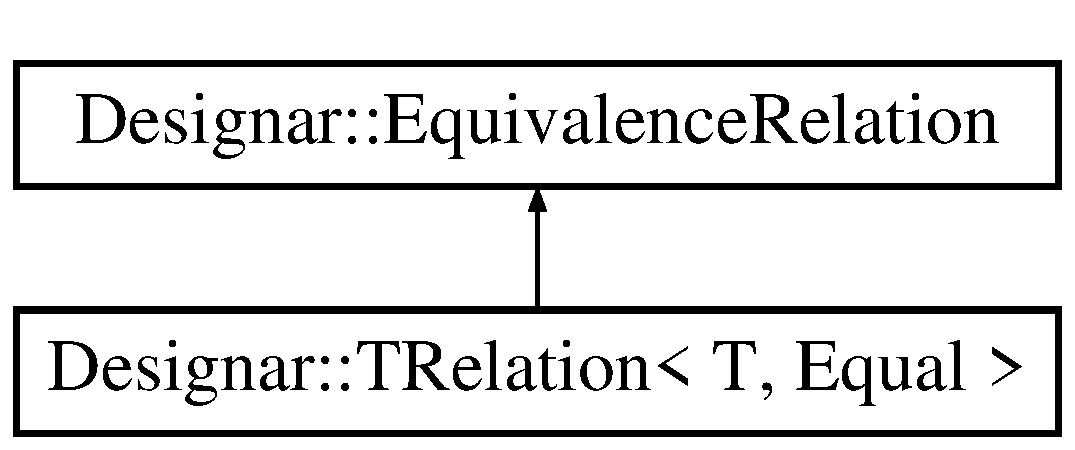
\includegraphics[height=2.000000cm]{class_designar_1_1_equivalence_relation}
\end{center}
\end{figure}
\subsection*{Métodos públicos}
\begin{DoxyCompactItemize}
\item 
\hyperlink{class_designar_1_1_equivalence_relation_a44544ffad6df87c47b30a6cd2a7254f2}{Equivalence\+Relation} (\hyperlink{namespace_designar_aa72662848b9f4815e7bf31a7cf3e33d1}{nat\+\_\+t})
\item 
void \hyperlink{class_designar_1_1_equivalence_relation_a06f07c2d9d53919339afcdd369daa277}{join} (\hyperlink{namespace_designar_aa72662848b9f4815e7bf31a7cf3e33d1}{nat\+\_\+t}, \hyperlink{namespace_designar_aa72662848b9f4815e7bf31a7cf3e33d1}{nat\+\_\+t})
\item 
bool \hyperlink{class_designar_1_1_equivalence_relation_a98972f1d96957b9fac030ca3001094e6}{are\+\_\+connected} (\hyperlink{namespace_designar_aa72662848b9f4815e7bf31a7cf3e33d1}{nat\+\_\+t}, \hyperlink{namespace_designar_aa72662848b9f4815e7bf31a7cf3e33d1}{nat\+\_\+t}) const
\item 
\hyperlink{namespace_designar_aa72662848b9f4815e7bf31a7cf3e33d1}{nat\+\_\+t} \hyperlink{class_designar_1_1_equivalence_relation_a1de9de1745175828d1b3f0184df76920}{get\+\_\+num\+\_\+blocks} () const
\item 
\hyperlink{namespace_designar_aa72662848b9f4815e7bf31a7cf3e33d1}{nat\+\_\+t} \hyperlink{class_designar_1_1_equivalence_relation_abd7ed9854a58f13f215507e50c0eecd3}{size} () const
\end{DoxyCompactItemize}


\subsection{Descripción detallada}


Definición en la línea 33 del archivo relation.\+H.



\subsection{Documentación del constructor y destructor}
\mbox{\Hypertarget{class_designar_1_1_equivalence_relation_a44544ffad6df87c47b30a6cd2a7254f2}\label{class_designar_1_1_equivalence_relation_a44544ffad6df87c47b30a6cd2a7254f2}} 
\index{Designar\+::\+Equivalence\+Relation@{Designar\+::\+Equivalence\+Relation}!Equivalence\+Relation@{Equivalence\+Relation}}
\index{Equivalence\+Relation@{Equivalence\+Relation}!Designar\+::\+Equivalence\+Relation@{Designar\+::\+Equivalence\+Relation}}
\subsubsection{\texorpdfstring{Equivalence\+Relation()}{EquivalenceRelation()}}
{\footnotesize\ttfamily Designar\+::\+Equivalence\+Relation\+::\+Equivalence\+Relation (\begin{DoxyParamCaption}\item[{\hyperlink{namespace_designar_aa72662848b9f4815e7bf31a7cf3e33d1}{nat\+\_\+t}}]{n }\end{DoxyParamCaption})}



Definición en la línea 38 del archivo relation.\+C.



\subsection{Documentación de las funciones miembro}
\mbox{\Hypertarget{class_designar_1_1_equivalence_relation_a98972f1d96957b9fac030ca3001094e6}\label{class_designar_1_1_equivalence_relation_a98972f1d96957b9fac030ca3001094e6}} 
\index{Designar\+::\+Equivalence\+Relation@{Designar\+::\+Equivalence\+Relation}!are\+\_\+connected@{are\+\_\+connected}}
\index{are\+\_\+connected@{are\+\_\+connected}!Designar\+::\+Equivalence\+Relation@{Designar\+::\+Equivalence\+Relation}}
\subsubsection{\texorpdfstring{are\+\_\+connected()}{are\_connected()}}
{\footnotesize\ttfamily bool Designar\+::\+Equivalence\+Relation\+::are\+\_\+connected (\begin{DoxyParamCaption}\item[{\hyperlink{namespace_designar_aa72662848b9f4815e7bf31a7cf3e33d1}{nat\+\_\+t}}]{p,  }\item[{\hyperlink{namespace_designar_aa72662848b9f4815e7bf31a7cf3e33d1}{nat\+\_\+t}}]{q }\end{DoxyParamCaption}) const}



Definición en la línea 70 del archivo relation.\+C.

\mbox{\Hypertarget{class_designar_1_1_equivalence_relation_a1de9de1745175828d1b3f0184df76920}\label{class_designar_1_1_equivalence_relation_a1de9de1745175828d1b3f0184df76920}} 
\index{Designar\+::\+Equivalence\+Relation@{Designar\+::\+Equivalence\+Relation}!get\+\_\+num\+\_\+blocks@{get\+\_\+num\+\_\+blocks}}
\index{get\+\_\+num\+\_\+blocks@{get\+\_\+num\+\_\+blocks}!Designar\+::\+Equivalence\+Relation@{Designar\+::\+Equivalence\+Relation}}
\subsubsection{\texorpdfstring{get\+\_\+num\+\_\+blocks()}{get\_num\_blocks()}}
{\footnotesize\ttfamily \hyperlink{namespace_designar_aa72662848b9f4815e7bf31a7cf3e33d1}{nat\+\_\+t} Designar\+::\+Equivalence\+Relation\+::get\+\_\+num\+\_\+blocks (\begin{DoxyParamCaption}{ }\end{DoxyParamCaption}) const}



Definición en la línea 75 del archivo relation.\+C.

\mbox{\Hypertarget{class_designar_1_1_equivalence_relation_a06f07c2d9d53919339afcdd369daa277}\label{class_designar_1_1_equivalence_relation_a06f07c2d9d53919339afcdd369daa277}} 
\index{Designar\+::\+Equivalence\+Relation@{Designar\+::\+Equivalence\+Relation}!join@{join}}
\index{join@{join}!Designar\+::\+Equivalence\+Relation@{Designar\+::\+Equivalence\+Relation}}
\subsubsection{\texorpdfstring{join()}{join()}}
{\footnotesize\ttfamily void Designar\+::\+Equivalence\+Relation\+::join (\begin{DoxyParamCaption}\item[{\hyperlink{namespace_designar_aa72662848b9f4815e7bf31a7cf3e33d1}{nat\+\_\+t}}]{p,  }\item[{\hyperlink{namespace_designar_aa72662848b9f4815e7bf31a7cf3e33d1}{nat\+\_\+t}}]{q }\end{DoxyParamCaption})}



Definición en la línea 48 del archivo relation.\+C.

\mbox{\Hypertarget{class_designar_1_1_equivalence_relation_abd7ed9854a58f13f215507e50c0eecd3}\label{class_designar_1_1_equivalence_relation_abd7ed9854a58f13f215507e50c0eecd3}} 
\index{Designar\+::\+Equivalence\+Relation@{Designar\+::\+Equivalence\+Relation}!size@{size}}
\index{size@{size}!Designar\+::\+Equivalence\+Relation@{Designar\+::\+Equivalence\+Relation}}
\subsubsection{\texorpdfstring{size()}{size()}}
{\footnotesize\ttfamily \hyperlink{namespace_designar_aa72662848b9f4815e7bf31a7cf3e33d1}{nat\+\_\+t} Designar\+::\+Equivalence\+Relation\+::size (\begin{DoxyParamCaption}{ }\end{DoxyParamCaption}) const}



Definición en la línea 80 del archivo relation.\+C.



La documentación para esta clase fue generada a partir de los siguientes ficheros\+:\begin{DoxyCompactItemize}
\item 
include/\hyperlink{relation_8_h}{relation.\+H}\item 
src/\hyperlink{relation_8_c}{relation.\+C}\end{DoxyCompactItemize}

\hypertarget{struct_designar_1_1_fast_integral_pow}{}\section{Designar\+:\+:Fast\+Integral\+Pow$<$ BT, ET $>$ Struct Template Reference}
\label{struct_designar_1_1_fast_integral_pow}\index{Designar\+::\+Fast\+Integral\+Pow$<$ B\+T, E\+T $>$@{Designar\+::\+Fast\+Integral\+Pow$<$ B\+T, E\+T $>$}}


{\ttfamily \#include $<$math.\+H$>$}

\subsection*{Public Member Functions}
\begin{DoxyCompactItemize}
\item 
BT \hyperlink{struct_designar_1_1_fast_integral_pow_a0c78ecac21d1454b9bdae4620c3473db}{operator()} (BT base, ET exp)
\end{DoxyCompactItemize}


\subsection{Detailed Description}
\subsubsection*{template$<$typename BT, typename ET$>$\newline
struct Designar\+::\+Fast\+Integral\+Pow$<$ B\+T, E\+T $>$}



Definition at line 160 of file math.\+H.



\subsection{Member Function Documentation}
\mbox{\Hypertarget{struct_designar_1_1_fast_integral_pow_a0c78ecac21d1454b9bdae4620c3473db}\label{struct_designar_1_1_fast_integral_pow_a0c78ecac21d1454b9bdae4620c3473db}} 
\index{Designar\+::\+Fast\+Integral\+Pow@{Designar\+::\+Fast\+Integral\+Pow}!operator()@{operator()}}
\index{operator()@{operator()}!Designar\+::\+Fast\+Integral\+Pow@{Designar\+::\+Fast\+Integral\+Pow}}
\subsubsection{\texorpdfstring{operator()()}{operator()()}}
{\footnotesize\ttfamily template$<$typename BT , typename ET $>$ \\
BT \hyperlink{struct_designar_1_1_fast_integral_pow}{Designar\+::\+Fast\+Integral\+Pow}$<$ BT, ET $>$\+::operator() (\begin{DoxyParamCaption}\item[{BT}]{base,  }\item[{ET}]{exp }\end{DoxyParamCaption})\hspace{0.3cm}{\ttfamily [inline]}}



Definition at line 162 of file math.\+H.



The documentation for this struct was generated from the following file\+:\begin{DoxyCompactItemize}
\item 
De\+Si\+G\+N\+A\+R/include/\hyperlink{math_8_h}{math.\+H}\end{DoxyCompactItemize}

\hypertarget{class_designar_1_1_fixed_array}{}\section{Designar\+:\+:Fixed\+Array$<$ T $>$ Class Template Reference}
\label{class_designar_1_1_fixed_array}\index{Designar\+::\+Fixed\+Array$<$ T $>$@{Designar\+::\+Fixed\+Array$<$ T $>$}}


{\ttfamily \#include $<$array.\+H$>$}

Inheritance diagram for Designar\+:\+:Fixed\+Array$<$ T $>$\+:\begin{figure}[H]
\begin{center}
\leavevmode
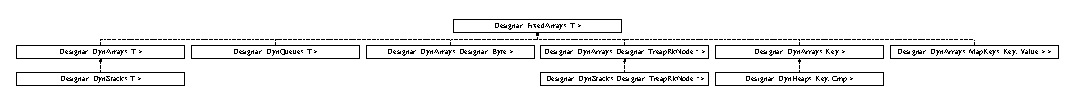
\includegraphics[height=0.924092cm]{class_designar_1_1_fixed_array}
\end{center}
\end{figure}
\subsection*{Classes}
\begin{DoxyCompactItemize}
\item 
class \hyperlink{class_designar_1_1_fixed_array_1_1_iterator}{Iterator}
\end{DoxyCompactItemize}
\subsection*{Public Types}
\begin{DoxyCompactItemize}
\item 
using \hyperlink{class_designar_1_1_fixed_array_abfeb4e683cee75ae782ad20294c4c808}{Item\+Type} = T
\item 
using \hyperlink{class_designar_1_1_fixed_array_a3a725cf21783340b8aca29dd1db0acf0}{Key\+Type} = T
\item 
using \hyperlink{class_designar_1_1_fixed_array_a3e37931b909b840cb7a40fc73f12bcf5}{Data\+Type} = T
\item 
using \hyperlink{class_designar_1_1_fixed_array_ac1cfeb4403a2dcbffd7ef494e5b873d0}{Value\+Type} = T
\item 
using \hyperlink{class_designar_1_1_fixed_array_a503ae414cc313d248e77c08e62ef043c}{Size\+Type} = \hyperlink{namespace_designar_aa72662848b9f4815e7bf31a7cf3e33d1}{nat\+\_\+t}
\end{DoxyCompactItemize}
\subsection*{Public Member Functions}
\begin{DoxyCompactItemize}
\item 
\hyperlink{namespace_designar_aa72662848b9f4815e7bf31a7cf3e33d1}{nat\+\_\+t} \hyperlink{class_designar_1_1_fixed_array_af1c7e826a704015eab8f3accac7ead7d}{item\+\_\+to\+\_\+pos} (T \&item)
\item 
\hyperlink{class_designar_1_1_fixed_array_a493a48e7c23b6b882a96c5451d10248a}{Fixed\+Array} ()
\item 
\hyperlink{class_designar_1_1_fixed_array_ac3bed73485d717ddc1fc412d3e7fea58}{Fixed\+Array} (\hyperlink{namespace_designar_aa72662848b9f4815e7bf31a7cf3e33d1}{nat\+\_\+t} c)
\item 
\hyperlink{class_designar_1_1_fixed_array_a8d313d1c5d828b9a635cb7626e9a6cb2}{Fixed\+Array} (\hyperlink{namespace_designar_aa72662848b9f4815e7bf31a7cf3e33d1}{nat\+\_\+t} c, const T \&init\+\_\+value)
\item 
\hyperlink{class_designar_1_1_fixed_array_a0375e6a3b0eaabd87a044354866c557f}{Fixed\+Array} (const \hyperlink{class_designar_1_1_fixed_array}{Fixed\+Array} \&a)
\item 
\hyperlink{class_designar_1_1_fixed_array_ababc68b389c05fb8c819e5a77afeb626}{Fixed\+Array} (\hyperlink{class_designar_1_1_fixed_array}{Fixed\+Array} \&\&a)
\item 
\hyperlink{class_designar_1_1_fixed_array_aaf63fe5101e36f6f058d71eb7bcfcfcc}{Fixed\+Array} (const std\+::initializer\+\_\+list$<$ T $>$ \&)
\item 
\hyperlink{class_designar_1_1_fixed_array_adfe330be4cd4afd6a097cf5abd2cec38}{$\sim$\+Fixed\+Array} ()
\item 
\hyperlink{class_designar_1_1_fixed_array}{Fixed\+Array} \& \hyperlink{class_designar_1_1_fixed_array_ac7e23eebfa59ba27db48ebd401ea0c53}{operator=} (const \hyperlink{class_designar_1_1_fixed_array}{Fixed\+Array} \&a)
\item 
\hyperlink{class_designar_1_1_fixed_array}{Fixed\+Array} \& \hyperlink{class_designar_1_1_fixed_array_a5a358228f610390c3987883c09cf31f0}{operator=} (\hyperlink{class_designar_1_1_fixed_array}{Fixed\+Array} \&\&a)
\item 
void \hyperlink{class_designar_1_1_fixed_array_ab13ae0d1146e753d3e1128e1cce07d91}{swap} (\hyperlink{class_designar_1_1_fixed_array}{Fixed\+Array} \&a)
\item 
void \hyperlink{class_designar_1_1_fixed_array_af52fca1277e52d28ce6d46ed4a7b471e}{resize} (\hyperlink{namespace_designar_aa72662848b9f4815e7bf31a7cf3e33d1}{nat\+\_\+t})
\item 
\hyperlink{namespace_designar_aa72662848b9f4815e7bf31a7cf3e33d1}{nat\+\_\+t} \hyperlink{class_designar_1_1_fixed_array_ac262a6be77640c4da26cd49fe9b90db0}{get\+\_\+capacity} () const
\item 
\hyperlink{namespace_designar_aa72662848b9f4815e7bf31a7cf3e33d1}{nat\+\_\+t} \hyperlink{class_designar_1_1_fixed_array_a03ce71d0cc8f4155f117bbfe83bb95e8}{size} () const
\item 
T \& \hyperlink{class_designar_1_1_fixed_array_ae47f2f299aaef27f2decc88f2fd863a9}{at} (\hyperlink{namespace_designar_aa72662848b9f4815e7bf31a7cf3e33d1}{nat\+\_\+t} i)
\item 
const T \& \hyperlink{class_designar_1_1_fixed_array_a3a1dec650628273bf08b6656db0a9088}{at} (\hyperlink{namespace_designar_aa72662848b9f4815e7bf31a7cf3e33d1}{nat\+\_\+t} i) const
\item 
T \& \hyperlink{class_designar_1_1_fixed_array_a0116aa8effdf9fd0c56ef1a8c1fa2883}{operator\mbox{[}$\,$\mbox{]}} (\hyperlink{namespace_designar_aa72662848b9f4815e7bf31a7cf3e33d1}{nat\+\_\+t} i)
\item 
const T \& \hyperlink{class_designar_1_1_fixed_array_aac0021d1ca6ff704f3d6967a509fff6b}{operator\mbox{[}$\,$\mbox{]}} (\hyperlink{namespace_designar_aa72662848b9f4815e7bf31a7cf3e33d1}{nat\+\_\+t} i) const
\item 
\hyperlink{class_designar_1_1_fixed_array_1_1_iterator}{Iterator} \hyperlink{class_designar_1_1_fixed_array_a40c099038e41c839acca94bf352753fc}{begin} ()
\item 
\hyperlink{class_designar_1_1_fixed_array_1_1_iterator}{Iterator} \hyperlink{class_designar_1_1_fixed_array_afeedbafa8456c56f80716466191810d6}{begin} () const
\item 
\hyperlink{class_designar_1_1_fixed_array_1_1_iterator}{Iterator} \hyperlink{class_designar_1_1_fixed_array_ab0baaf67153a51cb98ac12918d2387a0}{end} ()
\item 
\hyperlink{class_designar_1_1_fixed_array_1_1_iterator}{Iterator} \hyperlink{class_designar_1_1_fixed_array_a02b4949630ddc32ba5971fd4b78cf8ab}{end} () const
\end{DoxyCompactItemize}


\subsection{Detailed Description}
\subsubsection*{template$<$typename T$>$\newline
class Designar\+::\+Fixed\+Array$<$ T $>$}



Definition at line 463 of file array.\+H.



\subsection{Member Typedef Documentation}
\mbox{\Hypertarget{class_designar_1_1_fixed_array_a3e37931b909b840cb7a40fc73f12bcf5}\label{class_designar_1_1_fixed_array_a3e37931b909b840cb7a40fc73f12bcf5}} 
\index{Designar\+::\+Fixed\+Array@{Designar\+::\+Fixed\+Array}!Data\+Type@{Data\+Type}}
\index{Data\+Type@{Data\+Type}!Designar\+::\+Fixed\+Array@{Designar\+::\+Fixed\+Array}}
\subsubsection{\texorpdfstring{Data\+Type}{DataType}}
{\footnotesize\ttfamily template$<$typename T$>$ \\
using \hyperlink{class_designar_1_1_fixed_array}{Designar\+::\+Fixed\+Array}$<$ T $>$\+::\hyperlink{class_designar_1_1_fixed_array_a3e37931b909b840cb7a40fc73f12bcf5}{Data\+Type} =  T}



Definition at line 475 of file array.\+H.

\mbox{\Hypertarget{class_designar_1_1_fixed_array_abfeb4e683cee75ae782ad20294c4c808}\label{class_designar_1_1_fixed_array_abfeb4e683cee75ae782ad20294c4c808}} 
\index{Designar\+::\+Fixed\+Array@{Designar\+::\+Fixed\+Array}!Item\+Type@{Item\+Type}}
\index{Item\+Type@{Item\+Type}!Designar\+::\+Fixed\+Array@{Designar\+::\+Fixed\+Array}}
\subsubsection{\texorpdfstring{Item\+Type}{ItemType}}
{\footnotesize\ttfamily template$<$typename T$>$ \\
using \hyperlink{class_designar_1_1_fixed_array}{Designar\+::\+Fixed\+Array}$<$ T $>$\+::\hyperlink{class_designar_1_1_fixed_array_abfeb4e683cee75ae782ad20294c4c808}{Item\+Type} =  T}



Definition at line 473 of file array.\+H.

\mbox{\Hypertarget{class_designar_1_1_fixed_array_a3a725cf21783340b8aca29dd1db0acf0}\label{class_designar_1_1_fixed_array_a3a725cf21783340b8aca29dd1db0acf0}} 
\index{Designar\+::\+Fixed\+Array@{Designar\+::\+Fixed\+Array}!Key\+Type@{Key\+Type}}
\index{Key\+Type@{Key\+Type}!Designar\+::\+Fixed\+Array@{Designar\+::\+Fixed\+Array}}
\subsubsection{\texorpdfstring{Key\+Type}{KeyType}}
{\footnotesize\ttfamily template$<$typename T$>$ \\
using \hyperlink{class_designar_1_1_fixed_array}{Designar\+::\+Fixed\+Array}$<$ T $>$\+::\hyperlink{class_designar_1_1_fixed_array_a3a725cf21783340b8aca29dd1db0acf0}{Key\+Type} =  T}



Definition at line 474 of file array.\+H.

\mbox{\Hypertarget{class_designar_1_1_fixed_array_a503ae414cc313d248e77c08e62ef043c}\label{class_designar_1_1_fixed_array_a503ae414cc313d248e77c08e62ef043c}} 
\index{Designar\+::\+Fixed\+Array@{Designar\+::\+Fixed\+Array}!Size\+Type@{Size\+Type}}
\index{Size\+Type@{Size\+Type}!Designar\+::\+Fixed\+Array@{Designar\+::\+Fixed\+Array}}
\subsubsection{\texorpdfstring{Size\+Type}{SizeType}}
{\footnotesize\ttfamily template$<$typename T$>$ \\
using \hyperlink{class_designar_1_1_fixed_array}{Designar\+::\+Fixed\+Array}$<$ T $>$\+::\hyperlink{class_designar_1_1_fixed_array_a503ae414cc313d248e77c08e62ef043c}{Size\+Type} =  \hyperlink{namespace_designar_aa72662848b9f4815e7bf31a7cf3e33d1}{nat\+\_\+t}}



Definition at line 477 of file array.\+H.

\mbox{\Hypertarget{class_designar_1_1_fixed_array_ac1cfeb4403a2dcbffd7ef494e5b873d0}\label{class_designar_1_1_fixed_array_ac1cfeb4403a2dcbffd7ef494e5b873d0}} 
\index{Designar\+::\+Fixed\+Array@{Designar\+::\+Fixed\+Array}!Value\+Type@{Value\+Type}}
\index{Value\+Type@{Value\+Type}!Designar\+::\+Fixed\+Array@{Designar\+::\+Fixed\+Array}}
\subsubsection{\texorpdfstring{Value\+Type}{ValueType}}
{\footnotesize\ttfamily template$<$typename T$>$ \\
using \hyperlink{class_designar_1_1_fixed_array}{Designar\+::\+Fixed\+Array}$<$ T $>$\+::\hyperlink{class_designar_1_1_fixed_array_ac1cfeb4403a2dcbffd7ef494e5b873d0}{Value\+Type} =  T}



Definition at line 476 of file array.\+H.



\subsection{Constructor \& Destructor Documentation}
\mbox{\Hypertarget{class_designar_1_1_fixed_array_a493a48e7c23b6b882a96c5451d10248a}\label{class_designar_1_1_fixed_array_a493a48e7c23b6b882a96c5451d10248a}} 
\index{Designar\+::\+Fixed\+Array@{Designar\+::\+Fixed\+Array}!Fixed\+Array@{Fixed\+Array}}
\index{Fixed\+Array@{Fixed\+Array}!Designar\+::\+Fixed\+Array@{Designar\+::\+Fixed\+Array}}
\subsubsection{\texorpdfstring{Fixed\+Array()}{FixedArray()}\hspace{0.1cm}{\footnotesize\ttfamily [1/6]}}
{\footnotesize\ttfamily template$<$typename T$>$ \\
\hyperlink{class_designar_1_1_fixed_array}{Designar\+::\+Fixed\+Array}$<$ T $>$\+::\hyperlink{class_designar_1_1_fixed_array}{Fixed\+Array} (\begin{DoxyParamCaption}{ }\end{DoxyParamCaption})\hspace{0.3cm}{\ttfamily [inline]}}



Definition at line 484 of file array.\+H.

\mbox{\Hypertarget{class_designar_1_1_fixed_array_ac3bed73485d717ddc1fc412d3e7fea58}\label{class_designar_1_1_fixed_array_ac3bed73485d717ddc1fc412d3e7fea58}} 
\index{Designar\+::\+Fixed\+Array@{Designar\+::\+Fixed\+Array}!Fixed\+Array@{Fixed\+Array}}
\index{Fixed\+Array@{Fixed\+Array}!Designar\+::\+Fixed\+Array@{Designar\+::\+Fixed\+Array}}
\subsubsection{\texorpdfstring{Fixed\+Array()}{FixedArray()}\hspace{0.1cm}{\footnotesize\ttfamily [2/6]}}
{\footnotesize\ttfamily template$<$typename T$>$ \\
\hyperlink{class_designar_1_1_fixed_array}{Designar\+::\+Fixed\+Array}$<$ T $>$\+::\hyperlink{class_designar_1_1_fixed_array}{Fixed\+Array} (\begin{DoxyParamCaption}\item[{\hyperlink{namespace_designar_aa72662848b9f4815e7bf31a7cf3e33d1}{nat\+\_\+t}}]{c }\end{DoxyParamCaption})\hspace{0.3cm}{\ttfamily [inline]}}



Definition at line 490 of file array.\+H.

\mbox{\Hypertarget{class_designar_1_1_fixed_array_a8d313d1c5d828b9a635cb7626e9a6cb2}\label{class_designar_1_1_fixed_array_a8d313d1c5d828b9a635cb7626e9a6cb2}} 
\index{Designar\+::\+Fixed\+Array@{Designar\+::\+Fixed\+Array}!Fixed\+Array@{Fixed\+Array}}
\index{Fixed\+Array@{Fixed\+Array}!Designar\+::\+Fixed\+Array@{Designar\+::\+Fixed\+Array}}
\subsubsection{\texorpdfstring{Fixed\+Array()}{FixedArray()}\hspace{0.1cm}{\footnotesize\ttfamily [3/6]}}
{\footnotesize\ttfamily template$<$typename T$>$ \\
\hyperlink{class_designar_1_1_fixed_array}{Designar\+::\+Fixed\+Array}$<$ T $>$\+::\hyperlink{class_designar_1_1_fixed_array}{Fixed\+Array} (\begin{DoxyParamCaption}\item[{\hyperlink{namespace_designar_aa72662848b9f4815e7bf31a7cf3e33d1}{nat\+\_\+t}}]{c,  }\item[{const T \&}]{init\+\_\+value }\end{DoxyParamCaption})\hspace{0.3cm}{\ttfamily [inline]}}



Definition at line 496 of file array.\+H.

\mbox{\Hypertarget{class_designar_1_1_fixed_array_a0375e6a3b0eaabd87a044354866c557f}\label{class_designar_1_1_fixed_array_a0375e6a3b0eaabd87a044354866c557f}} 
\index{Designar\+::\+Fixed\+Array@{Designar\+::\+Fixed\+Array}!Fixed\+Array@{Fixed\+Array}}
\index{Fixed\+Array@{Fixed\+Array}!Designar\+::\+Fixed\+Array@{Designar\+::\+Fixed\+Array}}
\subsubsection{\texorpdfstring{Fixed\+Array()}{FixedArray()}\hspace{0.1cm}{\footnotesize\ttfamily [4/6]}}
{\footnotesize\ttfamily template$<$typename T$>$ \\
\hyperlink{class_designar_1_1_fixed_array}{Designar\+::\+Fixed\+Array}$<$ T $>$\+::\hyperlink{class_designar_1_1_fixed_array}{Fixed\+Array} (\begin{DoxyParamCaption}\item[{const \hyperlink{class_designar_1_1_fixed_array}{Fixed\+Array}$<$ T $>$ \&}]{a }\end{DoxyParamCaption})\hspace{0.3cm}{\ttfamily [inline]}}



Definition at line 502 of file array.\+H.

\mbox{\Hypertarget{class_designar_1_1_fixed_array_ababc68b389c05fb8c819e5a77afeb626}\label{class_designar_1_1_fixed_array_ababc68b389c05fb8c819e5a77afeb626}} 
\index{Designar\+::\+Fixed\+Array@{Designar\+::\+Fixed\+Array}!Fixed\+Array@{Fixed\+Array}}
\index{Fixed\+Array@{Fixed\+Array}!Designar\+::\+Fixed\+Array@{Designar\+::\+Fixed\+Array}}
\subsubsection{\texorpdfstring{Fixed\+Array()}{FixedArray()}\hspace{0.1cm}{\footnotesize\ttfamily [5/6]}}
{\footnotesize\ttfamily template$<$typename T$>$ \\
\hyperlink{class_designar_1_1_fixed_array}{Designar\+::\+Fixed\+Array}$<$ T $>$\+::\hyperlink{class_designar_1_1_fixed_array}{Fixed\+Array} (\begin{DoxyParamCaption}\item[{\hyperlink{class_designar_1_1_fixed_array}{Fixed\+Array}$<$ T $>$ \&\&}]{a }\end{DoxyParamCaption})\hspace{0.3cm}{\ttfamily [inline]}}



Definition at line 508 of file array.\+H.

\mbox{\Hypertarget{class_designar_1_1_fixed_array_aaf63fe5101e36f6f058d71eb7bcfcfcc}\label{class_designar_1_1_fixed_array_aaf63fe5101e36f6f058d71eb7bcfcfcc}} 
\index{Designar\+::\+Fixed\+Array@{Designar\+::\+Fixed\+Array}!Fixed\+Array@{Fixed\+Array}}
\index{Fixed\+Array@{Fixed\+Array}!Designar\+::\+Fixed\+Array@{Designar\+::\+Fixed\+Array}}
\subsubsection{\texorpdfstring{Fixed\+Array()}{FixedArray()}\hspace{0.1cm}{\footnotesize\ttfamily [6/6]}}
{\footnotesize\ttfamily template$<$typename T$>$ \\
\hyperlink{class_designar_1_1_fixed_array}{Designar\+::\+Fixed\+Array}$<$ T $>$\+::\hyperlink{class_designar_1_1_fixed_array}{Fixed\+Array} (\begin{DoxyParamCaption}\item[{const std\+::initializer\+\_\+list$<$ T $>$ \&}]{l }\end{DoxyParamCaption})}



Definition at line 646 of file array.\+H.

\mbox{\Hypertarget{class_designar_1_1_fixed_array_adfe330be4cd4afd6a097cf5abd2cec38}\label{class_designar_1_1_fixed_array_adfe330be4cd4afd6a097cf5abd2cec38}} 
\index{Designar\+::\+Fixed\+Array@{Designar\+::\+Fixed\+Array}!````~Fixed\+Array@{$\sim$\+Fixed\+Array}}
\index{````~Fixed\+Array@{$\sim$\+Fixed\+Array}!Designar\+::\+Fixed\+Array@{Designar\+::\+Fixed\+Array}}
\subsubsection{\texorpdfstring{$\sim$\+Fixed\+Array()}{~FixedArray()}}
{\footnotesize\ttfamily template$<$typename T$>$ \\
\hyperlink{class_designar_1_1_fixed_array}{Designar\+::\+Fixed\+Array}$<$ T $>$\+::$\sim$\hyperlink{class_designar_1_1_fixed_array}{Fixed\+Array} (\begin{DoxyParamCaption}{ }\end{DoxyParamCaption})\hspace{0.3cm}{\ttfamily [inline]}}



Definition at line 516 of file array.\+H.



\subsection{Member Function Documentation}
\mbox{\Hypertarget{class_designar_1_1_fixed_array_ae47f2f299aaef27f2decc88f2fd863a9}\label{class_designar_1_1_fixed_array_ae47f2f299aaef27f2decc88f2fd863a9}} 
\index{Designar\+::\+Fixed\+Array@{Designar\+::\+Fixed\+Array}!at@{at}}
\index{at@{at}!Designar\+::\+Fixed\+Array@{Designar\+::\+Fixed\+Array}}
\subsubsection{\texorpdfstring{at()}{at()}\hspace{0.1cm}{\footnotesize\ttfamily [1/2]}}
{\footnotesize\ttfamily template$<$typename T$>$ \\
T\& \hyperlink{class_designar_1_1_fixed_array}{Designar\+::\+Fixed\+Array}$<$ T $>$\+::at (\begin{DoxyParamCaption}\item[{\hyperlink{namespace_designar_aa72662848b9f4815e7bf31a7cf3e33d1}{nat\+\_\+t}}]{i }\end{DoxyParamCaption})\hspace{0.3cm}{\ttfamily [inline]}}



Definition at line 557 of file array.\+H.

\mbox{\Hypertarget{class_designar_1_1_fixed_array_a3a1dec650628273bf08b6656db0a9088}\label{class_designar_1_1_fixed_array_a3a1dec650628273bf08b6656db0a9088}} 
\index{Designar\+::\+Fixed\+Array@{Designar\+::\+Fixed\+Array}!at@{at}}
\index{at@{at}!Designar\+::\+Fixed\+Array@{Designar\+::\+Fixed\+Array}}
\subsubsection{\texorpdfstring{at()}{at()}\hspace{0.1cm}{\footnotesize\ttfamily [2/2]}}
{\footnotesize\ttfamily template$<$typename T$>$ \\
const T\& \hyperlink{class_designar_1_1_fixed_array}{Designar\+::\+Fixed\+Array}$<$ T $>$\+::at (\begin{DoxyParamCaption}\item[{\hyperlink{namespace_designar_aa72662848b9f4815e7bf31a7cf3e33d1}{nat\+\_\+t}}]{i }\end{DoxyParamCaption}) const\hspace{0.3cm}{\ttfamily [inline]}}



Definition at line 565 of file array.\+H.

\mbox{\Hypertarget{class_designar_1_1_fixed_array_a40c099038e41c839acca94bf352753fc}\label{class_designar_1_1_fixed_array_a40c099038e41c839acca94bf352753fc}} 
\index{Designar\+::\+Fixed\+Array@{Designar\+::\+Fixed\+Array}!begin@{begin}}
\index{begin@{begin}!Designar\+::\+Fixed\+Array@{Designar\+::\+Fixed\+Array}}
\subsubsection{\texorpdfstring{begin()}{begin()}\hspace{0.1cm}{\footnotesize\ttfamily [1/2]}}
{\footnotesize\ttfamily template$<$typename T$>$ \\
\hyperlink{class_designar_1_1_fixed_array_1_1_iterator}{Iterator} \hyperlink{class_designar_1_1_fixed_array}{Designar\+::\+Fixed\+Array}$<$ T $>$\+::begin (\begin{DoxyParamCaption}{ }\end{DoxyParamCaption})\hspace{0.3cm}{\ttfamily [inline]}}



Definition at line 589 of file array.\+H.

\mbox{\Hypertarget{class_designar_1_1_fixed_array_afeedbafa8456c56f80716466191810d6}\label{class_designar_1_1_fixed_array_afeedbafa8456c56f80716466191810d6}} 
\index{Designar\+::\+Fixed\+Array@{Designar\+::\+Fixed\+Array}!begin@{begin}}
\index{begin@{begin}!Designar\+::\+Fixed\+Array@{Designar\+::\+Fixed\+Array}}
\subsubsection{\texorpdfstring{begin()}{begin()}\hspace{0.1cm}{\footnotesize\ttfamily [2/2]}}
{\footnotesize\ttfamily template$<$typename T$>$ \\
\hyperlink{class_designar_1_1_fixed_array_1_1_iterator}{Iterator} \hyperlink{class_designar_1_1_fixed_array}{Designar\+::\+Fixed\+Array}$<$ T $>$\+::begin (\begin{DoxyParamCaption}{ }\end{DoxyParamCaption}) const\hspace{0.3cm}{\ttfamily [inline]}}



Definition at line 594 of file array.\+H.

\mbox{\Hypertarget{class_designar_1_1_fixed_array_ab0baaf67153a51cb98ac12918d2387a0}\label{class_designar_1_1_fixed_array_ab0baaf67153a51cb98ac12918d2387a0}} 
\index{Designar\+::\+Fixed\+Array@{Designar\+::\+Fixed\+Array}!end@{end}}
\index{end@{end}!Designar\+::\+Fixed\+Array@{Designar\+::\+Fixed\+Array}}
\subsubsection{\texorpdfstring{end()}{end()}\hspace{0.1cm}{\footnotesize\ttfamily [1/2]}}
{\footnotesize\ttfamily template$<$typename T$>$ \\
\hyperlink{class_designar_1_1_fixed_array_1_1_iterator}{Iterator} \hyperlink{class_designar_1_1_fixed_array}{Designar\+::\+Fixed\+Array}$<$ T $>$\+::end (\begin{DoxyParamCaption}{ }\end{DoxyParamCaption})\hspace{0.3cm}{\ttfamily [inline]}}



Definition at line 599 of file array.\+H.

\mbox{\Hypertarget{class_designar_1_1_fixed_array_a02b4949630ddc32ba5971fd4b78cf8ab}\label{class_designar_1_1_fixed_array_a02b4949630ddc32ba5971fd4b78cf8ab}} 
\index{Designar\+::\+Fixed\+Array@{Designar\+::\+Fixed\+Array}!end@{end}}
\index{end@{end}!Designar\+::\+Fixed\+Array@{Designar\+::\+Fixed\+Array}}
\subsubsection{\texorpdfstring{end()}{end()}\hspace{0.1cm}{\footnotesize\ttfamily [2/2]}}
{\footnotesize\ttfamily template$<$typename T$>$ \\
\hyperlink{class_designar_1_1_fixed_array_1_1_iterator}{Iterator} \hyperlink{class_designar_1_1_fixed_array}{Designar\+::\+Fixed\+Array}$<$ T $>$\+::end (\begin{DoxyParamCaption}{ }\end{DoxyParamCaption}) const\hspace{0.3cm}{\ttfamily [inline]}}



Definition at line 604 of file array.\+H.

\mbox{\Hypertarget{class_designar_1_1_fixed_array_ac262a6be77640c4da26cd49fe9b90db0}\label{class_designar_1_1_fixed_array_ac262a6be77640c4da26cd49fe9b90db0}} 
\index{Designar\+::\+Fixed\+Array@{Designar\+::\+Fixed\+Array}!get\+\_\+capacity@{get\+\_\+capacity}}
\index{get\+\_\+capacity@{get\+\_\+capacity}!Designar\+::\+Fixed\+Array@{Designar\+::\+Fixed\+Array}}
\subsubsection{\texorpdfstring{get\+\_\+capacity()}{get\_capacity()}}
{\footnotesize\ttfamily template$<$typename T$>$ \\
\hyperlink{namespace_designar_aa72662848b9f4815e7bf31a7cf3e33d1}{nat\+\_\+t} \hyperlink{class_designar_1_1_fixed_array}{Designar\+::\+Fixed\+Array}$<$ T $>$\+::get\+\_\+capacity (\begin{DoxyParamCaption}{ }\end{DoxyParamCaption}) const\hspace{0.3cm}{\ttfamily [inline]}}



Definition at line 547 of file array.\+H.

\mbox{\Hypertarget{class_designar_1_1_fixed_array_af1c7e826a704015eab8f3accac7ead7d}\label{class_designar_1_1_fixed_array_af1c7e826a704015eab8f3accac7ead7d}} 
\index{Designar\+::\+Fixed\+Array@{Designar\+::\+Fixed\+Array}!item\+\_\+to\+\_\+pos@{item\+\_\+to\+\_\+pos}}
\index{item\+\_\+to\+\_\+pos@{item\+\_\+to\+\_\+pos}!Designar\+::\+Fixed\+Array@{Designar\+::\+Fixed\+Array}}
\subsubsection{\texorpdfstring{item\+\_\+to\+\_\+pos()}{item\_to\_pos()}}
{\footnotesize\ttfamily template$<$typename T$>$ \\
\hyperlink{namespace_designar_aa72662848b9f4815e7bf31a7cf3e33d1}{nat\+\_\+t} \hyperlink{class_designar_1_1_fixed_array}{Designar\+::\+Fixed\+Array}$<$ T $>$\+::item\+\_\+to\+\_\+pos (\begin{DoxyParamCaption}\item[{T \&}]{item }\end{DoxyParamCaption})\hspace{0.3cm}{\ttfamily [inline]}}



Definition at line 479 of file array.\+H.

\mbox{\Hypertarget{class_designar_1_1_fixed_array_ac7e23eebfa59ba27db48ebd401ea0c53}\label{class_designar_1_1_fixed_array_ac7e23eebfa59ba27db48ebd401ea0c53}} 
\index{Designar\+::\+Fixed\+Array@{Designar\+::\+Fixed\+Array}!operator=@{operator=}}
\index{operator=@{operator=}!Designar\+::\+Fixed\+Array@{Designar\+::\+Fixed\+Array}}
\subsubsection{\texorpdfstring{operator=()}{operator=()}\hspace{0.1cm}{\footnotesize\ttfamily [1/2]}}
{\footnotesize\ttfamily template$<$typename T$>$ \\
\hyperlink{class_designar_1_1_fixed_array}{Fixed\+Array}\& \hyperlink{class_designar_1_1_fixed_array}{Designar\+::\+Fixed\+Array}$<$ T $>$\+::operator= (\begin{DoxyParamCaption}\item[{const \hyperlink{class_designar_1_1_fixed_array}{Fixed\+Array}$<$ T $>$ \&}]{a }\end{DoxyParamCaption})\hspace{0.3cm}{\ttfamily [inline]}}



Definition at line 521 of file array.\+H.

\mbox{\Hypertarget{class_designar_1_1_fixed_array_a5a358228f610390c3987883c09cf31f0}\label{class_designar_1_1_fixed_array_a5a358228f610390c3987883c09cf31f0}} 
\index{Designar\+::\+Fixed\+Array@{Designar\+::\+Fixed\+Array}!operator=@{operator=}}
\index{operator=@{operator=}!Designar\+::\+Fixed\+Array@{Designar\+::\+Fixed\+Array}}
\subsubsection{\texorpdfstring{operator=()}{operator=()}\hspace{0.1cm}{\footnotesize\ttfamily [2/2]}}
{\footnotesize\ttfamily template$<$typename T$>$ \\
\hyperlink{class_designar_1_1_fixed_array}{Fixed\+Array}\& \hyperlink{class_designar_1_1_fixed_array}{Designar\+::\+Fixed\+Array}$<$ T $>$\+::operator= (\begin{DoxyParamCaption}\item[{\hyperlink{class_designar_1_1_fixed_array}{Fixed\+Array}$<$ T $>$ \&\&}]{a }\end{DoxyParamCaption})\hspace{0.3cm}{\ttfamily [inline]}}



Definition at line 533 of file array.\+H.

\mbox{\Hypertarget{class_designar_1_1_fixed_array_a0116aa8effdf9fd0c56ef1a8c1fa2883}\label{class_designar_1_1_fixed_array_a0116aa8effdf9fd0c56ef1a8c1fa2883}} 
\index{Designar\+::\+Fixed\+Array@{Designar\+::\+Fixed\+Array}!operator\mbox{[}\mbox{]}@{operator[]}}
\index{operator\mbox{[}\mbox{]}@{operator[]}!Designar\+::\+Fixed\+Array@{Designar\+::\+Fixed\+Array}}
\subsubsection{\texorpdfstring{operator[]()}{operator[]()}\hspace{0.1cm}{\footnotesize\ttfamily [1/2]}}
{\footnotesize\ttfamily template$<$typename T$>$ \\
T\& \hyperlink{class_designar_1_1_fixed_array}{Designar\+::\+Fixed\+Array}$<$ T $>$\+::operator\mbox{[}$\,$\mbox{]} (\begin{DoxyParamCaption}\item[{\hyperlink{namespace_designar_aa72662848b9f4815e7bf31a7cf3e33d1}{nat\+\_\+t}}]{i }\end{DoxyParamCaption})\hspace{0.3cm}{\ttfamily [inline]}}



Definition at line 573 of file array.\+H.

\mbox{\Hypertarget{class_designar_1_1_fixed_array_aac0021d1ca6ff704f3d6967a509fff6b}\label{class_designar_1_1_fixed_array_aac0021d1ca6ff704f3d6967a509fff6b}} 
\index{Designar\+::\+Fixed\+Array@{Designar\+::\+Fixed\+Array}!operator\mbox{[}\mbox{]}@{operator[]}}
\index{operator\mbox{[}\mbox{]}@{operator[]}!Designar\+::\+Fixed\+Array@{Designar\+::\+Fixed\+Array}}
\subsubsection{\texorpdfstring{operator[]()}{operator[]()}\hspace{0.1cm}{\footnotesize\ttfamily [2/2]}}
{\footnotesize\ttfamily template$<$typename T$>$ \\
const T\& \hyperlink{class_designar_1_1_fixed_array}{Designar\+::\+Fixed\+Array}$<$ T $>$\+::operator\mbox{[}$\,$\mbox{]} (\begin{DoxyParamCaption}\item[{\hyperlink{namespace_designar_aa72662848b9f4815e7bf31a7cf3e33d1}{nat\+\_\+t}}]{i }\end{DoxyParamCaption}) const\hspace{0.3cm}{\ttfamily [inline]}}



Definition at line 578 of file array.\+H.

\mbox{\Hypertarget{class_designar_1_1_fixed_array_af52fca1277e52d28ce6d46ed4a7b471e}\label{class_designar_1_1_fixed_array_af52fca1277e52d28ce6d46ed4a7b471e}} 
\index{Designar\+::\+Fixed\+Array@{Designar\+::\+Fixed\+Array}!resize@{resize}}
\index{resize@{resize}!Designar\+::\+Fixed\+Array@{Designar\+::\+Fixed\+Array}}
\subsubsection{\texorpdfstring{resize()}{resize()}}
{\footnotesize\ttfamily template$<$typename T $>$ \\
void \hyperlink{class_designar_1_1_fixed_array}{Designar\+::\+Fixed\+Array}$<$ T $>$\+::resize (\begin{DoxyParamCaption}\item[{\hyperlink{namespace_designar_aa72662848b9f4815e7bf31a7cf3e33d1}{nat\+\_\+t}}]{c }\end{DoxyParamCaption})}



Definition at line 628 of file array.\+H.

\mbox{\Hypertarget{class_designar_1_1_fixed_array_a03ce71d0cc8f4155f117bbfe83bb95e8}\label{class_designar_1_1_fixed_array_a03ce71d0cc8f4155f117bbfe83bb95e8}} 
\index{Designar\+::\+Fixed\+Array@{Designar\+::\+Fixed\+Array}!size@{size}}
\index{size@{size}!Designar\+::\+Fixed\+Array@{Designar\+::\+Fixed\+Array}}
\subsubsection{\texorpdfstring{size()}{size()}}
{\footnotesize\ttfamily template$<$typename T$>$ \\
\hyperlink{namespace_designar_aa72662848b9f4815e7bf31a7cf3e33d1}{nat\+\_\+t} \hyperlink{class_designar_1_1_fixed_array}{Designar\+::\+Fixed\+Array}$<$ T $>$\+::size (\begin{DoxyParamCaption}{ }\end{DoxyParamCaption}) const\hspace{0.3cm}{\ttfamily [inline]}}



Definition at line 552 of file array.\+H.

\mbox{\Hypertarget{class_designar_1_1_fixed_array_ab13ae0d1146e753d3e1128e1cce07d91}\label{class_designar_1_1_fixed_array_ab13ae0d1146e753d3e1128e1cce07d91}} 
\index{Designar\+::\+Fixed\+Array@{Designar\+::\+Fixed\+Array}!swap@{swap}}
\index{swap@{swap}!Designar\+::\+Fixed\+Array@{Designar\+::\+Fixed\+Array}}
\subsubsection{\texorpdfstring{swap()}{swap()}}
{\footnotesize\ttfamily template$<$typename T$>$ \\
void \hyperlink{class_designar_1_1_fixed_array}{Designar\+::\+Fixed\+Array}$<$ T $>$\+::swap (\begin{DoxyParamCaption}\item[{\hyperlink{class_designar_1_1_fixed_array}{Fixed\+Array}$<$ T $>$ \&}]{a }\end{DoxyParamCaption})\hspace{0.3cm}{\ttfamily [inline]}}



Definition at line 539 of file array.\+H.



The documentation for this class was generated from the following file\+:\begin{DoxyCompactItemize}
\item 
De\+Si\+G\+N\+A\+R/include/\hyperlink{array_8_h}{array.\+H}\end{DoxyCompactItemize}

\hypertarget{class_designar_1_1_fixed_heap}{}\section{Designar\+:\+:Fixed\+Heap$<$ Key, Cmp, cap $>$ Class Template Reference}
\label{class_designar_1_1_fixed_heap}\index{Designar\+::\+Fixed\+Heap$<$ Key, Cmp, cap $>$@{Designar\+::\+Fixed\+Heap$<$ Key, Cmp, cap $>$}}


{\ttfamily \#include $<$heap.\+H$>$}

\subsection*{Public Types}
\begin{DoxyCompactItemize}
\item 
using \hyperlink{class_designar_1_1_fixed_heap_adf444211fa73830a09b3847ebe15bc9b}{Item\+Type} = Key
\item 
using \hyperlink{class_designar_1_1_fixed_heap_a2dbe3b22cba3e316803b614fba2d13e8}{Key\+Type} = Key
\item 
using \hyperlink{class_designar_1_1_fixed_heap_a48202f857a59e2753aa72625f0d90f94}{Data\+Type} = Key
\item 
using \hyperlink{class_designar_1_1_fixed_heap_a33def2622f3d95c165abf62ce2edcb73}{Value\+Type} = Key
\item 
using \hyperlink{class_designar_1_1_fixed_heap_a138d26dc24cbab61001f528a29b5154b}{Size\+Type} = \hyperlink{namespace_designar_aa72662848b9f4815e7bf31a7cf3e33d1}{nat\+\_\+t}
\item 
using \hyperlink{class_designar_1_1_fixed_heap_a0dab9096a5119723285ee3d4f1a4cee9}{Cmp\+Type} = Cmp
\end{DoxyCompactItemize}
\subsection*{Public Member Functions}
\begin{DoxyCompactItemize}
\item 
\hyperlink{class_designar_1_1_fixed_heap_ac5dfd33a9ee1cedaad907c51afdf351d}{Fixed\+Heap} (Cmp \&\+\_\+cmp)
\item 
\hyperlink{class_designar_1_1_fixed_heap_adab7bd333df89c4b7f75568619020385}{Fixed\+Heap} (Cmp \&\&\+\_\+cmp=Cmp())
\item 
\hyperlink{class_designar_1_1_fixed_heap_abd58276d0d6e3ff20ea74bea6f6d65bb}{Fixed\+Heap} (const \hyperlink{class_designar_1_1_fixed_heap}{Fixed\+Heap} \&h)
\item 
\hyperlink{class_designar_1_1_fixed_heap_a15eca78039f66fb7944d825c7c53bf02}{Fixed\+Heap} (\hyperlink{class_designar_1_1_fixed_heap}{Fixed\+Heap} \&\&h)
\item 
\hyperlink{class_designar_1_1_fixed_heap}{Fixed\+Heap} \& \hyperlink{class_designar_1_1_fixed_heap_adb8f27056847e1b788e815db1a59db67}{operator=} (const \hyperlink{class_designar_1_1_fixed_heap}{Fixed\+Heap} \&h)
\item 
\hyperlink{class_designar_1_1_fixed_heap}{Fixed\+Heap} \& \hyperlink{class_designar_1_1_fixed_heap_a48202ae9224f22d0e88267279b0616a3}{operator=} (\hyperlink{class_designar_1_1_fixed_heap}{Fixed\+Heap} \&\&h)
\item 
Cmp \& \hyperlink{class_designar_1_1_fixed_heap_a29db925edd7d26a8cd6f8ee970e70b53}{get\+\_\+cmp} ()
\item 
const Cmp \& \hyperlink{class_designar_1_1_fixed_heap_a88f1060c9630d0c8e56fd58370b9a875}{get\+\_\+cmp} () const
\item 
void \hyperlink{class_designar_1_1_fixed_heap_a19f197809e896073e7e2cb05e2f741d1}{clear} ()
\item 
bool \hyperlink{class_designar_1_1_fixed_heap_a58cfde8fd6eedd215b79219970bf8fb8}{is\+\_\+empty} () const
\item 
bool \hyperlink{class_designar_1_1_fixed_heap_a85af858c5200cd8777925e4ae17ca9d2}{is\+\_\+full} () const
\item 
\hyperlink{namespace_designar_aa72662848b9f4815e7bf31a7cf3e33d1}{nat\+\_\+t} \hyperlink{class_designar_1_1_fixed_heap_a96991df55a68490d6ea9fdd10cf6d8ef}{size} () const
\item 
\hyperlink{namespace_designar_aa72662848b9f4815e7bf31a7cf3e33d1}{nat\+\_\+t} \hyperlink{class_designar_1_1_fixed_heap_a6f2b6bb5de9abd4718f07eb1261bee92}{get\+\_\+capacity} () const
\item 
void \hyperlink{class_designar_1_1_fixed_heap_a00227ce55200154dac2fcfb42026e353}{insert} (const Key \&item)
\item 
void \hyperlink{class_designar_1_1_fixed_heap_a7169684fe8e25834174cd2b1edcaf567}{insert} (Key \&\&item)
\item 
const Key \& \hyperlink{class_designar_1_1_fixed_heap_a2b48592e01a0b8836a18415219a310ca}{top} () const
\item 
Key \hyperlink{class_designar_1_1_fixed_heap_a0a274fa702d084e555b917b04ee73b37}{get} ()
\end{DoxyCompactItemize}


\subsection{Detailed Description}
\subsubsection*{template$<$typename Key, class Cmp = std\+::less$<$\+Key$>$, nat\+\_\+t cap = 100$>$\newline
class Designar\+::\+Fixed\+Heap$<$ Key, Cmp, cap $>$}



Definition at line 36 of file heap.\+H.



\subsection{Member Typedef Documentation}
\mbox{\Hypertarget{class_designar_1_1_fixed_heap_a0dab9096a5119723285ee3d4f1a4cee9}\label{class_designar_1_1_fixed_heap_a0dab9096a5119723285ee3d4f1a4cee9}} 
\index{Designar\+::\+Fixed\+Heap@{Designar\+::\+Fixed\+Heap}!Cmp\+Type@{Cmp\+Type}}
\index{Cmp\+Type@{Cmp\+Type}!Designar\+::\+Fixed\+Heap@{Designar\+::\+Fixed\+Heap}}
\subsubsection{\texorpdfstring{Cmp\+Type}{CmpType}}
{\footnotesize\ttfamily template$<$typename Key, class Cmp = std\+::less$<$\+Key$>$, nat\+\_\+t cap = 100$>$ \\
using \hyperlink{class_designar_1_1_fixed_heap}{Designar\+::\+Fixed\+Heap}$<$ Key, Cmp, cap $>$\+::\hyperlink{class_designar_1_1_fixed_heap_a0dab9096a5119723285ee3d4f1a4cee9}{Cmp\+Type} =  Cmp}



Definition at line 61 of file heap.\+H.

\mbox{\Hypertarget{class_designar_1_1_fixed_heap_a48202f857a59e2753aa72625f0d90f94}\label{class_designar_1_1_fixed_heap_a48202f857a59e2753aa72625f0d90f94}} 
\index{Designar\+::\+Fixed\+Heap@{Designar\+::\+Fixed\+Heap}!Data\+Type@{Data\+Type}}
\index{Data\+Type@{Data\+Type}!Designar\+::\+Fixed\+Heap@{Designar\+::\+Fixed\+Heap}}
\subsubsection{\texorpdfstring{Data\+Type}{DataType}}
{\footnotesize\ttfamily template$<$typename Key, class Cmp = std\+::less$<$\+Key$>$, nat\+\_\+t cap = 100$>$ \\
using \hyperlink{class_designar_1_1_fixed_heap}{Designar\+::\+Fixed\+Heap}$<$ Key, Cmp, cap $>$\+::\hyperlink{class_designar_1_1_fixed_heap_a48202f857a59e2753aa72625f0d90f94}{Data\+Type} =  Key}



Definition at line 58 of file heap.\+H.

\mbox{\Hypertarget{class_designar_1_1_fixed_heap_adf444211fa73830a09b3847ebe15bc9b}\label{class_designar_1_1_fixed_heap_adf444211fa73830a09b3847ebe15bc9b}} 
\index{Designar\+::\+Fixed\+Heap@{Designar\+::\+Fixed\+Heap}!Item\+Type@{Item\+Type}}
\index{Item\+Type@{Item\+Type}!Designar\+::\+Fixed\+Heap@{Designar\+::\+Fixed\+Heap}}
\subsubsection{\texorpdfstring{Item\+Type}{ItemType}}
{\footnotesize\ttfamily template$<$typename Key, class Cmp = std\+::less$<$\+Key$>$, nat\+\_\+t cap = 100$>$ \\
using \hyperlink{class_designar_1_1_fixed_heap}{Designar\+::\+Fixed\+Heap}$<$ Key, Cmp, cap $>$\+::\hyperlink{class_designar_1_1_fixed_heap_adf444211fa73830a09b3847ebe15bc9b}{Item\+Type} =  Key}



Definition at line 56 of file heap.\+H.

\mbox{\Hypertarget{class_designar_1_1_fixed_heap_a2dbe3b22cba3e316803b614fba2d13e8}\label{class_designar_1_1_fixed_heap_a2dbe3b22cba3e316803b614fba2d13e8}} 
\index{Designar\+::\+Fixed\+Heap@{Designar\+::\+Fixed\+Heap}!Key\+Type@{Key\+Type}}
\index{Key\+Type@{Key\+Type}!Designar\+::\+Fixed\+Heap@{Designar\+::\+Fixed\+Heap}}
\subsubsection{\texorpdfstring{Key\+Type}{KeyType}}
{\footnotesize\ttfamily template$<$typename Key, class Cmp = std\+::less$<$\+Key$>$, nat\+\_\+t cap = 100$>$ \\
using \hyperlink{class_designar_1_1_fixed_heap}{Designar\+::\+Fixed\+Heap}$<$ Key, Cmp, cap $>$\+::\hyperlink{class_designar_1_1_fixed_heap_a2dbe3b22cba3e316803b614fba2d13e8}{Key\+Type} =  Key}



Definition at line 57 of file heap.\+H.

\mbox{\Hypertarget{class_designar_1_1_fixed_heap_a138d26dc24cbab61001f528a29b5154b}\label{class_designar_1_1_fixed_heap_a138d26dc24cbab61001f528a29b5154b}} 
\index{Designar\+::\+Fixed\+Heap@{Designar\+::\+Fixed\+Heap}!Size\+Type@{Size\+Type}}
\index{Size\+Type@{Size\+Type}!Designar\+::\+Fixed\+Heap@{Designar\+::\+Fixed\+Heap}}
\subsubsection{\texorpdfstring{Size\+Type}{SizeType}}
{\footnotesize\ttfamily template$<$typename Key, class Cmp = std\+::less$<$\+Key$>$, nat\+\_\+t cap = 100$>$ \\
using \hyperlink{class_designar_1_1_fixed_heap}{Designar\+::\+Fixed\+Heap}$<$ Key, Cmp, cap $>$\+::\hyperlink{class_designar_1_1_fixed_heap_a138d26dc24cbab61001f528a29b5154b}{Size\+Type} =  \hyperlink{namespace_designar_aa72662848b9f4815e7bf31a7cf3e33d1}{nat\+\_\+t}}



Definition at line 60 of file heap.\+H.

\mbox{\Hypertarget{class_designar_1_1_fixed_heap_a33def2622f3d95c165abf62ce2edcb73}\label{class_designar_1_1_fixed_heap_a33def2622f3d95c165abf62ce2edcb73}} 
\index{Designar\+::\+Fixed\+Heap@{Designar\+::\+Fixed\+Heap}!Value\+Type@{Value\+Type}}
\index{Value\+Type@{Value\+Type}!Designar\+::\+Fixed\+Heap@{Designar\+::\+Fixed\+Heap}}
\subsubsection{\texorpdfstring{Value\+Type}{ValueType}}
{\footnotesize\ttfamily template$<$typename Key, class Cmp = std\+::less$<$\+Key$>$, nat\+\_\+t cap = 100$>$ \\
using \hyperlink{class_designar_1_1_fixed_heap}{Designar\+::\+Fixed\+Heap}$<$ Key, Cmp, cap $>$\+::\hyperlink{class_designar_1_1_fixed_heap_a33def2622f3d95c165abf62ce2edcb73}{Value\+Type} =  Key}



Definition at line 59 of file heap.\+H.



\subsection{Constructor \& Destructor Documentation}
\mbox{\Hypertarget{class_designar_1_1_fixed_heap_ac5dfd33a9ee1cedaad907c51afdf351d}\label{class_designar_1_1_fixed_heap_ac5dfd33a9ee1cedaad907c51afdf351d}} 
\index{Designar\+::\+Fixed\+Heap@{Designar\+::\+Fixed\+Heap}!Fixed\+Heap@{Fixed\+Heap}}
\index{Fixed\+Heap@{Fixed\+Heap}!Designar\+::\+Fixed\+Heap@{Designar\+::\+Fixed\+Heap}}
\subsubsection{\texorpdfstring{Fixed\+Heap()}{FixedHeap()}\hspace{0.1cm}{\footnotesize\ttfamily [1/4]}}
{\footnotesize\ttfamily template$<$typename Key, class Cmp = std\+::less$<$\+Key$>$, nat\+\_\+t cap = 100$>$ \\
\hyperlink{class_designar_1_1_fixed_heap}{Designar\+::\+Fixed\+Heap}$<$ Key, Cmp, cap $>$\+::\hyperlink{class_designar_1_1_fixed_heap}{Fixed\+Heap} (\begin{DoxyParamCaption}\item[{Cmp \&}]{\+\_\+cmp }\end{DoxyParamCaption})\hspace{0.3cm}{\ttfamily [inline]}}



Definition at line 63 of file heap.\+H.

\mbox{\Hypertarget{class_designar_1_1_fixed_heap_adab7bd333df89c4b7f75568619020385}\label{class_designar_1_1_fixed_heap_adab7bd333df89c4b7f75568619020385}} 
\index{Designar\+::\+Fixed\+Heap@{Designar\+::\+Fixed\+Heap}!Fixed\+Heap@{Fixed\+Heap}}
\index{Fixed\+Heap@{Fixed\+Heap}!Designar\+::\+Fixed\+Heap@{Designar\+::\+Fixed\+Heap}}
\subsubsection{\texorpdfstring{Fixed\+Heap()}{FixedHeap()}\hspace{0.1cm}{\footnotesize\ttfamily [2/4]}}
{\footnotesize\ttfamily template$<$typename Key, class Cmp = std\+::less$<$\+Key$>$, nat\+\_\+t cap = 100$>$ \\
\hyperlink{class_designar_1_1_fixed_heap}{Designar\+::\+Fixed\+Heap}$<$ Key, Cmp, cap $>$\+::\hyperlink{class_designar_1_1_fixed_heap}{Fixed\+Heap} (\begin{DoxyParamCaption}\item[{Cmp \&\&}]{\+\_\+cmp = {\ttfamily Cmp()} }\end{DoxyParamCaption})\hspace{0.3cm}{\ttfamily [inline]}}



Definition at line 69 of file heap.\+H.

\mbox{\Hypertarget{class_designar_1_1_fixed_heap_abd58276d0d6e3ff20ea74bea6f6d65bb}\label{class_designar_1_1_fixed_heap_abd58276d0d6e3ff20ea74bea6f6d65bb}} 
\index{Designar\+::\+Fixed\+Heap@{Designar\+::\+Fixed\+Heap}!Fixed\+Heap@{Fixed\+Heap}}
\index{Fixed\+Heap@{Fixed\+Heap}!Designar\+::\+Fixed\+Heap@{Designar\+::\+Fixed\+Heap}}
\subsubsection{\texorpdfstring{Fixed\+Heap()}{FixedHeap()}\hspace{0.1cm}{\footnotesize\ttfamily [3/4]}}
{\footnotesize\ttfamily template$<$typename Key, class Cmp = std\+::less$<$\+Key$>$, nat\+\_\+t cap = 100$>$ \\
\hyperlink{class_designar_1_1_fixed_heap}{Designar\+::\+Fixed\+Heap}$<$ Key, Cmp, cap $>$\+::\hyperlink{class_designar_1_1_fixed_heap}{Fixed\+Heap} (\begin{DoxyParamCaption}\item[{const \hyperlink{class_designar_1_1_fixed_heap}{Fixed\+Heap}$<$ Key, Cmp, cap $>$ \&}]{h }\end{DoxyParamCaption})\hspace{0.3cm}{\ttfamily [inline]}}



Definition at line 75 of file heap.\+H.

\mbox{\Hypertarget{class_designar_1_1_fixed_heap_a15eca78039f66fb7944d825c7c53bf02}\label{class_designar_1_1_fixed_heap_a15eca78039f66fb7944d825c7c53bf02}} 
\index{Designar\+::\+Fixed\+Heap@{Designar\+::\+Fixed\+Heap}!Fixed\+Heap@{Fixed\+Heap}}
\index{Fixed\+Heap@{Fixed\+Heap}!Designar\+::\+Fixed\+Heap@{Designar\+::\+Fixed\+Heap}}
\subsubsection{\texorpdfstring{Fixed\+Heap()}{FixedHeap()}\hspace{0.1cm}{\footnotesize\ttfamily [4/4]}}
{\footnotesize\ttfamily template$<$typename Key, class Cmp = std\+::less$<$\+Key$>$, nat\+\_\+t cap = 100$>$ \\
\hyperlink{class_designar_1_1_fixed_heap}{Designar\+::\+Fixed\+Heap}$<$ Key, Cmp, cap $>$\+::\hyperlink{class_designar_1_1_fixed_heap}{Fixed\+Heap} (\begin{DoxyParamCaption}\item[{\hyperlink{class_designar_1_1_fixed_heap}{Fixed\+Heap}$<$ Key, Cmp, cap $>$ \&\&}]{h }\end{DoxyParamCaption})\hspace{0.3cm}{\ttfamily [inline]}}



Definition at line 81 of file heap.\+H.



\subsection{Member Function Documentation}
\mbox{\Hypertarget{class_designar_1_1_fixed_heap_a19f197809e896073e7e2cb05e2f741d1}\label{class_designar_1_1_fixed_heap_a19f197809e896073e7e2cb05e2f741d1}} 
\index{Designar\+::\+Fixed\+Heap@{Designar\+::\+Fixed\+Heap}!clear@{clear}}
\index{clear@{clear}!Designar\+::\+Fixed\+Heap@{Designar\+::\+Fixed\+Heap}}
\subsubsection{\texorpdfstring{clear()}{clear()}}
{\footnotesize\ttfamily template$<$typename Key, class Cmp = std\+::less$<$\+Key$>$, nat\+\_\+t cap = 100$>$ \\
void \hyperlink{class_designar_1_1_fixed_heap}{Designar\+::\+Fixed\+Heap}$<$ Key, Cmp, cap $>$\+::clear (\begin{DoxyParamCaption}{ }\end{DoxyParamCaption})\hspace{0.3cm}{\ttfamily [inline]}}



Definition at line 114 of file heap.\+H.

\mbox{\Hypertarget{class_designar_1_1_fixed_heap_a0a274fa702d084e555b917b04ee73b37}\label{class_designar_1_1_fixed_heap_a0a274fa702d084e555b917b04ee73b37}} 
\index{Designar\+::\+Fixed\+Heap@{Designar\+::\+Fixed\+Heap}!get@{get}}
\index{get@{get}!Designar\+::\+Fixed\+Heap@{Designar\+::\+Fixed\+Heap}}
\subsubsection{\texorpdfstring{get()}{get()}}
{\footnotesize\ttfamily template$<$typename Key, class Cmp = std\+::less$<$\+Key$>$, nat\+\_\+t cap = 100$>$ \\
Key \hyperlink{class_designar_1_1_fixed_heap}{Designar\+::\+Fixed\+Heap}$<$ Key, Cmp, cap $>$\+::get (\begin{DoxyParamCaption}{ }\end{DoxyParamCaption})\hspace{0.3cm}{\ttfamily [inline]}}



Definition at line 167 of file heap.\+H.

\mbox{\Hypertarget{class_designar_1_1_fixed_heap_a6f2b6bb5de9abd4718f07eb1261bee92}\label{class_designar_1_1_fixed_heap_a6f2b6bb5de9abd4718f07eb1261bee92}} 
\index{Designar\+::\+Fixed\+Heap@{Designar\+::\+Fixed\+Heap}!get\+\_\+capacity@{get\+\_\+capacity}}
\index{get\+\_\+capacity@{get\+\_\+capacity}!Designar\+::\+Fixed\+Heap@{Designar\+::\+Fixed\+Heap}}
\subsubsection{\texorpdfstring{get\+\_\+capacity()}{get\_capacity()}}
{\footnotesize\ttfamily template$<$typename Key, class Cmp = std\+::less$<$\+Key$>$, nat\+\_\+t cap = 100$>$ \\
\hyperlink{namespace_designar_aa72662848b9f4815e7bf31a7cf3e33d1}{nat\+\_\+t} \hyperlink{class_designar_1_1_fixed_heap}{Designar\+::\+Fixed\+Heap}$<$ Key, Cmp, cap $>$\+::get\+\_\+capacity (\begin{DoxyParamCaption}{ }\end{DoxyParamCaption}) const\hspace{0.3cm}{\ttfamily [inline]}}



Definition at line 134 of file heap.\+H.

\mbox{\Hypertarget{class_designar_1_1_fixed_heap_a29db925edd7d26a8cd6f8ee970e70b53}\label{class_designar_1_1_fixed_heap_a29db925edd7d26a8cd6f8ee970e70b53}} 
\index{Designar\+::\+Fixed\+Heap@{Designar\+::\+Fixed\+Heap}!get\+\_\+cmp@{get\+\_\+cmp}}
\index{get\+\_\+cmp@{get\+\_\+cmp}!Designar\+::\+Fixed\+Heap@{Designar\+::\+Fixed\+Heap}}
\subsubsection{\texorpdfstring{get\+\_\+cmp()}{get\_cmp()}\hspace{0.1cm}{\footnotesize\ttfamily [1/2]}}
{\footnotesize\ttfamily template$<$typename Key, class Cmp = std\+::less$<$\+Key$>$, nat\+\_\+t cap = 100$>$ \\
Cmp\& \hyperlink{class_designar_1_1_fixed_heap}{Designar\+::\+Fixed\+Heap}$<$ Key, Cmp, cap $>$\+::get\+\_\+cmp (\begin{DoxyParamCaption}{ }\end{DoxyParamCaption})\hspace{0.3cm}{\ttfamily [inline]}}



Definition at line 104 of file heap.\+H.

\mbox{\Hypertarget{class_designar_1_1_fixed_heap_a88f1060c9630d0c8e56fd58370b9a875}\label{class_designar_1_1_fixed_heap_a88f1060c9630d0c8e56fd58370b9a875}} 
\index{Designar\+::\+Fixed\+Heap@{Designar\+::\+Fixed\+Heap}!get\+\_\+cmp@{get\+\_\+cmp}}
\index{get\+\_\+cmp@{get\+\_\+cmp}!Designar\+::\+Fixed\+Heap@{Designar\+::\+Fixed\+Heap}}
\subsubsection{\texorpdfstring{get\+\_\+cmp()}{get\_cmp()}\hspace{0.1cm}{\footnotesize\ttfamily [2/2]}}
{\footnotesize\ttfamily template$<$typename Key, class Cmp = std\+::less$<$\+Key$>$, nat\+\_\+t cap = 100$>$ \\
const Cmp\& \hyperlink{class_designar_1_1_fixed_heap}{Designar\+::\+Fixed\+Heap}$<$ Key, Cmp, cap $>$\+::get\+\_\+cmp (\begin{DoxyParamCaption}{ }\end{DoxyParamCaption}) const\hspace{0.3cm}{\ttfamily [inline]}}



Definition at line 109 of file heap.\+H.

\mbox{\Hypertarget{class_designar_1_1_fixed_heap_a00227ce55200154dac2fcfb42026e353}\label{class_designar_1_1_fixed_heap_a00227ce55200154dac2fcfb42026e353}} 
\index{Designar\+::\+Fixed\+Heap@{Designar\+::\+Fixed\+Heap}!insert@{insert}}
\index{insert@{insert}!Designar\+::\+Fixed\+Heap@{Designar\+::\+Fixed\+Heap}}
\subsubsection{\texorpdfstring{insert()}{insert()}\hspace{0.1cm}{\footnotesize\ttfamily [1/2]}}
{\footnotesize\ttfamily template$<$typename Key, class Cmp = std\+::less$<$\+Key$>$, nat\+\_\+t cap = 100$>$ \\
void \hyperlink{class_designar_1_1_fixed_heap}{Designar\+::\+Fixed\+Heap}$<$ Key, Cmp, cap $>$\+::insert (\begin{DoxyParamCaption}\item[{const Key \&}]{item }\end{DoxyParamCaption})\hspace{0.3cm}{\ttfamily [inline]}}



Definition at line 139 of file heap.\+H.

\mbox{\Hypertarget{class_designar_1_1_fixed_heap_a7169684fe8e25834174cd2b1edcaf567}\label{class_designar_1_1_fixed_heap_a7169684fe8e25834174cd2b1edcaf567}} 
\index{Designar\+::\+Fixed\+Heap@{Designar\+::\+Fixed\+Heap}!insert@{insert}}
\index{insert@{insert}!Designar\+::\+Fixed\+Heap@{Designar\+::\+Fixed\+Heap}}
\subsubsection{\texorpdfstring{insert()}{insert()}\hspace{0.1cm}{\footnotesize\ttfamily [2/2]}}
{\footnotesize\ttfamily template$<$typename Key, class Cmp = std\+::less$<$\+Key$>$, nat\+\_\+t cap = 100$>$ \\
void \hyperlink{class_designar_1_1_fixed_heap}{Designar\+::\+Fixed\+Heap}$<$ Key, Cmp, cap $>$\+::insert (\begin{DoxyParamCaption}\item[{Key \&\&}]{item }\end{DoxyParamCaption})\hspace{0.3cm}{\ttfamily [inline]}}



Definition at line 149 of file heap.\+H.

\mbox{\Hypertarget{class_designar_1_1_fixed_heap_a58cfde8fd6eedd215b79219970bf8fb8}\label{class_designar_1_1_fixed_heap_a58cfde8fd6eedd215b79219970bf8fb8}} 
\index{Designar\+::\+Fixed\+Heap@{Designar\+::\+Fixed\+Heap}!is\+\_\+empty@{is\+\_\+empty}}
\index{is\+\_\+empty@{is\+\_\+empty}!Designar\+::\+Fixed\+Heap@{Designar\+::\+Fixed\+Heap}}
\subsubsection{\texorpdfstring{is\+\_\+empty()}{is\_empty()}}
{\footnotesize\ttfamily template$<$typename Key, class Cmp = std\+::less$<$\+Key$>$, nat\+\_\+t cap = 100$>$ \\
bool \hyperlink{class_designar_1_1_fixed_heap}{Designar\+::\+Fixed\+Heap}$<$ Key, Cmp, cap $>$\+::is\+\_\+empty (\begin{DoxyParamCaption}{ }\end{DoxyParamCaption}) const\hspace{0.3cm}{\ttfamily [inline]}}



Definition at line 119 of file heap.\+H.

\mbox{\Hypertarget{class_designar_1_1_fixed_heap_a85af858c5200cd8777925e4ae17ca9d2}\label{class_designar_1_1_fixed_heap_a85af858c5200cd8777925e4ae17ca9d2}} 
\index{Designar\+::\+Fixed\+Heap@{Designar\+::\+Fixed\+Heap}!is\+\_\+full@{is\+\_\+full}}
\index{is\+\_\+full@{is\+\_\+full}!Designar\+::\+Fixed\+Heap@{Designar\+::\+Fixed\+Heap}}
\subsubsection{\texorpdfstring{is\+\_\+full()}{is\_full()}}
{\footnotesize\ttfamily template$<$typename Key, class Cmp = std\+::less$<$\+Key$>$, nat\+\_\+t cap = 100$>$ \\
bool \hyperlink{class_designar_1_1_fixed_heap}{Designar\+::\+Fixed\+Heap}$<$ Key, Cmp, cap $>$\+::is\+\_\+full (\begin{DoxyParamCaption}{ }\end{DoxyParamCaption}) const\hspace{0.3cm}{\ttfamily [inline]}}



Definition at line 124 of file heap.\+H.

\mbox{\Hypertarget{class_designar_1_1_fixed_heap_adb8f27056847e1b788e815db1a59db67}\label{class_designar_1_1_fixed_heap_adb8f27056847e1b788e815db1a59db67}} 
\index{Designar\+::\+Fixed\+Heap@{Designar\+::\+Fixed\+Heap}!operator=@{operator=}}
\index{operator=@{operator=}!Designar\+::\+Fixed\+Heap@{Designar\+::\+Fixed\+Heap}}
\subsubsection{\texorpdfstring{operator=()}{operator=()}\hspace{0.1cm}{\footnotesize\ttfamily [1/2]}}
{\footnotesize\ttfamily template$<$typename Key, class Cmp = std\+::less$<$\+Key$>$, nat\+\_\+t cap = 100$>$ \\
\hyperlink{class_designar_1_1_fixed_heap}{Fixed\+Heap}\& \hyperlink{class_designar_1_1_fixed_heap}{Designar\+::\+Fixed\+Heap}$<$ Key, Cmp, cap $>$\+::operator= (\begin{DoxyParamCaption}\item[{const \hyperlink{class_designar_1_1_fixed_heap}{Fixed\+Heap}$<$ Key, Cmp, cap $>$ \&}]{h }\end{DoxyParamCaption})\hspace{0.3cm}{\ttfamily [inline]}}



Definition at line 87 of file heap.\+H.

\mbox{\Hypertarget{class_designar_1_1_fixed_heap_a48202ae9224f22d0e88267279b0616a3}\label{class_designar_1_1_fixed_heap_a48202ae9224f22d0e88267279b0616a3}} 
\index{Designar\+::\+Fixed\+Heap@{Designar\+::\+Fixed\+Heap}!operator=@{operator=}}
\index{operator=@{operator=}!Designar\+::\+Fixed\+Heap@{Designar\+::\+Fixed\+Heap}}
\subsubsection{\texorpdfstring{operator=()}{operator=()}\hspace{0.1cm}{\footnotesize\ttfamily [2/2]}}
{\footnotesize\ttfamily template$<$typename Key, class Cmp = std\+::less$<$\+Key$>$, nat\+\_\+t cap = 100$>$ \\
\hyperlink{class_designar_1_1_fixed_heap}{Fixed\+Heap}\& \hyperlink{class_designar_1_1_fixed_heap}{Designar\+::\+Fixed\+Heap}$<$ Key, Cmp, cap $>$\+::operator= (\begin{DoxyParamCaption}\item[{\hyperlink{class_designar_1_1_fixed_heap}{Fixed\+Heap}$<$ Key, Cmp, cap $>$ \&\&}]{h }\end{DoxyParamCaption})\hspace{0.3cm}{\ttfamily [inline]}}



Definition at line 98 of file heap.\+H.

\mbox{\Hypertarget{class_designar_1_1_fixed_heap_a96991df55a68490d6ea9fdd10cf6d8ef}\label{class_designar_1_1_fixed_heap_a96991df55a68490d6ea9fdd10cf6d8ef}} 
\index{Designar\+::\+Fixed\+Heap@{Designar\+::\+Fixed\+Heap}!size@{size}}
\index{size@{size}!Designar\+::\+Fixed\+Heap@{Designar\+::\+Fixed\+Heap}}
\subsubsection{\texorpdfstring{size()}{size()}}
{\footnotesize\ttfamily template$<$typename Key, class Cmp = std\+::less$<$\+Key$>$, nat\+\_\+t cap = 100$>$ \\
\hyperlink{namespace_designar_aa72662848b9f4815e7bf31a7cf3e33d1}{nat\+\_\+t} \hyperlink{class_designar_1_1_fixed_heap}{Designar\+::\+Fixed\+Heap}$<$ Key, Cmp, cap $>$\+::size (\begin{DoxyParamCaption}{ }\end{DoxyParamCaption}) const\hspace{0.3cm}{\ttfamily [inline]}}



Definition at line 129 of file heap.\+H.

\mbox{\Hypertarget{class_designar_1_1_fixed_heap_a2b48592e01a0b8836a18415219a310ca}\label{class_designar_1_1_fixed_heap_a2b48592e01a0b8836a18415219a310ca}} 
\index{Designar\+::\+Fixed\+Heap@{Designar\+::\+Fixed\+Heap}!top@{top}}
\index{top@{top}!Designar\+::\+Fixed\+Heap@{Designar\+::\+Fixed\+Heap}}
\subsubsection{\texorpdfstring{top()}{top()}}
{\footnotesize\ttfamily template$<$typename Key, class Cmp = std\+::less$<$\+Key$>$, nat\+\_\+t cap = 100$>$ \\
const Key\& \hyperlink{class_designar_1_1_fixed_heap}{Designar\+::\+Fixed\+Heap}$<$ Key, Cmp, cap $>$\+::top (\begin{DoxyParamCaption}{ }\end{DoxyParamCaption}) const\hspace{0.3cm}{\ttfamily [inline]}}



Definition at line 159 of file heap.\+H.



The documentation for this class was generated from the following file\+:\begin{DoxyCompactItemize}
\item 
De\+Si\+G\+N\+A\+R/include/\hyperlink{heap_8_h}{heap.\+H}\end{DoxyCompactItemize}

\hypertarget{class_designar_1_1_fixed_queue}{}\section{Referencia de la plantilla de la Clase Designar\+:\+:Fixed\+Queue$<$ T, C\+AP $>$}
\label{class_designar_1_1_fixed_queue}\index{Designar\+::\+Fixed\+Queue$<$ T, C\+A\+P $>$@{Designar\+::\+Fixed\+Queue$<$ T, C\+A\+P $>$}}


{\ttfamily \#include $<$queue.\+H$>$}

\subsection*{Tipos públicos}
\begin{DoxyCompactItemize}
\item 
using \hyperlink{class_designar_1_1_fixed_queue_aa1c356bc74a041121662af027abf279b}{Item\+Type} = T
\item 
using \hyperlink{class_designar_1_1_fixed_queue_a37999fa3f2fa0aacaf67d94e6da50f3d}{Key\+Type} = T
\item 
using \hyperlink{class_designar_1_1_fixed_queue_a0638afcff4eb29040d4573212558da5f}{Data\+Type} = T
\item 
using \hyperlink{class_designar_1_1_fixed_queue_a3507ad9a592d5ade2c7cfe0b9484a4b0}{Value\+Type} = T
\item 
using \hyperlink{class_designar_1_1_fixed_queue_a900c2a6d70517602bd8bc9dc7894c104}{Size\+Type} = \hyperlink{namespace_designar_aa72662848b9f4815e7bf31a7cf3e33d1}{nat\+\_\+t}
\end{DoxyCompactItemize}
\subsection*{Métodos públicos}
\begin{DoxyCompactItemize}
\item 
\hyperlink{class_designar_1_1_fixed_queue_ad55d01ff85b7d38e595ff2bd891a45b9}{Fixed\+Queue} ()
\item 
\hyperlink{class_designar_1_1_fixed_queue_a3e6393f6dbe99bbecb030f0a793892b8}{Fixed\+Queue} (const \hyperlink{class_designar_1_1_fixed_queue}{Fixed\+Queue} \&q)
\item 
\hyperlink{class_designar_1_1_fixed_queue_a74d27c0f06b0b91c34768f7501a77afd}{Fixed\+Queue} (\hyperlink{class_designar_1_1_fixed_queue}{Fixed\+Queue} \&\&q)
\item 
\hyperlink{class_designar_1_1_fixed_queue}{Fixed\+Queue} \& \hyperlink{class_designar_1_1_fixed_queue_a317293ac30aa85f82daf9a2c1e295e9a}{operator=} (const \hyperlink{class_designar_1_1_fixed_queue}{Fixed\+Queue} \&q)
\item 
\hyperlink{class_designar_1_1_fixed_queue}{Fixed\+Queue} \& \hyperlink{class_designar_1_1_fixed_queue_aac0f8bc7f8ffacc543bac5917d8b1045}{operator=} (\hyperlink{class_designar_1_1_fixed_queue}{Fixed\+Queue} \&\&q)
\item 
bool \hyperlink{class_designar_1_1_fixed_queue_aa72d9c9dd2ce251b6d29b31c04ee6517}{is\+\_\+empty} () const
\item 
bool \hyperlink{class_designar_1_1_fixed_queue_a4d6bdd5d75d476d4af602781bd0d5b56}{is\+\_\+full} () const
\item 
\hyperlink{namespace_designar_aa72662848b9f4815e7bf31a7cf3e33d1}{nat\+\_\+t} \hyperlink{class_designar_1_1_fixed_queue_a9fa2f855edd54de0c847c8ba35c804cf}{size} () const
\item 
\hyperlink{namespace_designar_aa72662848b9f4815e7bf31a7cf3e33d1}{nat\+\_\+t} \hyperlink{class_designar_1_1_fixed_queue_a786767a9a56c0c4b1e93631b509f0fa1}{get\+\_\+capacity} () const
\item 
void \hyperlink{class_designar_1_1_fixed_queue_ae5e1454766e792f8dbad9f1b49437fe6}{clear} ()
\item 
T \& \hyperlink{class_designar_1_1_fixed_queue_a2440b268443093f6ff306e956d7f0616}{front} ()
\item 
const T \& \hyperlink{class_designar_1_1_fixed_queue_ab86601d018b664a2f0d522bca18ee107}{front} () const
\item 
T \& \hyperlink{class_designar_1_1_fixed_queue_a820470e5e649e48a352b334f158c8eb3}{rear} ()
\item 
const T \& \hyperlink{class_designar_1_1_fixed_queue_ab634bd79b51287ddbcd1ba24bc72fcae}{rear} () const
\item 
T \& \hyperlink{class_designar_1_1_fixed_queue_ab8a9bf0adeaa3995e68d966d8a986904}{put} (const T \&item)
\item 
T \& \hyperlink{class_designar_1_1_fixed_queue_a66a9b9f7118ec4943f7af273879c6b52}{put} (T \&\&item)
\item 
T \hyperlink{class_designar_1_1_fixed_queue_aefa2e40721df2aff9ba56a2ef1f9db62}{get} ()
\end{DoxyCompactItemize}


\subsection{Descripción detallada}
\subsubsection*{template$<$typename T, nat\+\_\+t C\+AP = 100$>$\newline
class Designar\+::\+Fixed\+Queue$<$ T, C\+A\+P $>$}



Definición en la línea 35 del archivo queue.\+H.



\subsection{Documentación de los \textquotesingle{}Typedef\textquotesingle{} miembros de la clase}
\mbox{\Hypertarget{class_designar_1_1_fixed_queue_a0638afcff4eb29040d4573212558da5f}\label{class_designar_1_1_fixed_queue_a0638afcff4eb29040d4573212558da5f}} 
\index{Designar\+::\+Fixed\+Queue@{Designar\+::\+Fixed\+Queue}!Data\+Type@{Data\+Type}}
\index{Data\+Type@{Data\+Type}!Designar\+::\+Fixed\+Queue@{Designar\+::\+Fixed\+Queue}}
\subsubsection{\texorpdfstring{Data\+Type}{DataType}}
{\footnotesize\ttfamily template$<$typename T, nat\+\_\+t C\+AP = 100$>$ \\
using \hyperlink{class_designar_1_1_fixed_queue}{Designar\+::\+Fixed\+Queue}$<$ T, C\+AP $>$\+::\hyperlink{class_designar_1_1_fixed_queue_a0638afcff4eb29040d4573212558da5f}{Data\+Type} =  T}



Definición en la línea 55 del archivo queue.\+H.

\mbox{\Hypertarget{class_designar_1_1_fixed_queue_aa1c356bc74a041121662af027abf279b}\label{class_designar_1_1_fixed_queue_aa1c356bc74a041121662af027abf279b}} 
\index{Designar\+::\+Fixed\+Queue@{Designar\+::\+Fixed\+Queue}!Item\+Type@{Item\+Type}}
\index{Item\+Type@{Item\+Type}!Designar\+::\+Fixed\+Queue@{Designar\+::\+Fixed\+Queue}}
\subsubsection{\texorpdfstring{Item\+Type}{ItemType}}
{\footnotesize\ttfamily template$<$typename T, nat\+\_\+t C\+AP = 100$>$ \\
using \hyperlink{class_designar_1_1_fixed_queue}{Designar\+::\+Fixed\+Queue}$<$ T, C\+AP $>$\+::\hyperlink{class_designar_1_1_fixed_queue_aa1c356bc74a041121662af027abf279b}{Item\+Type} =  T}



Definición en la línea 53 del archivo queue.\+H.

\mbox{\Hypertarget{class_designar_1_1_fixed_queue_a37999fa3f2fa0aacaf67d94e6da50f3d}\label{class_designar_1_1_fixed_queue_a37999fa3f2fa0aacaf67d94e6da50f3d}} 
\index{Designar\+::\+Fixed\+Queue@{Designar\+::\+Fixed\+Queue}!Key\+Type@{Key\+Type}}
\index{Key\+Type@{Key\+Type}!Designar\+::\+Fixed\+Queue@{Designar\+::\+Fixed\+Queue}}
\subsubsection{\texorpdfstring{Key\+Type}{KeyType}}
{\footnotesize\ttfamily template$<$typename T, nat\+\_\+t C\+AP = 100$>$ \\
using \hyperlink{class_designar_1_1_fixed_queue}{Designar\+::\+Fixed\+Queue}$<$ T, C\+AP $>$\+::\hyperlink{class_designar_1_1_fixed_queue_a37999fa3f2fa0aacaf67d94e6da50f3d}{Key\+Type} =  T}



Definición en la línea 54 del archivo queue.\+H.

\mbox{\Hypertarget{class_designar_1_1_fixed_queue_a900c2a6d70517602bd8bc9dc7894c104}\label{class_designar_1_1_fixed_queue_a900c2a6d70517602bd8bc9dc7894c104}} 
\index{Designar\+::\+Fixed\+Queue@{Designar\+::\+Fixed\+Queue}!Size\+Type@{Size\+Type}}
\index{Size\+Type@{Size\+Type}!Designar\+::\+Fixed\+Queue@{Designar\+::\+Fixed\+Queue}}
\subsubsection{\texorpdfstring{Size\+Type}{SizeType}}
{\footnotesize\ttfamily template$<$typename T, nat\+\_\+t C\+AP = 100$>$ \\
using \hyperlink{class_designar_1_1_fixed_queue}{Designar\+::\+Fixed\+Queue}$<$ T, C\+AP $>$\+::\hyperlink{class_designar_1_1_fixed_queue_a900c2a6d70517602bd8bc9dc7894c104}{Size\+Type} =  \hyperlink{namespace_designar_aa72662848b9f4815e7bf31a7cf3e33d1}{nat\+\_\+t}}



Definición en la línea 57 del archivo queue.\+H.

\mbox{\Hypertarget{class_designar_1_1_fixed_queue_a3507ad9a592d5ade2c7cfe0b9484a4b0}\label{class_designar_1_1_fixed_queue_a3507ad9a592d5ade2c7cfe0b9484a4b0}} 
\index{Designar\+::\+Fixed\+Queue@{Designar\+::\+Fixed\+Queue}!Value\+Type@{Value\+Type}}
\index{Value\+Type@{Value\+Type}!Designar\+::\+Fixed\+Queue@{Designar\+::\+Fixed\+Queue}}
\subsubsection{\texorpdfstring{Value\+Type}{ValueType}}
{\footnotesize\ttfamily template$<$typename T, nat\+\_\+t C\+AP = 100$>$ \\
using \hyperlink{class_designar_1_1_fixed_queue}{Designar\+::\+Fixed\+Queue}$<$ T, C\+AP $>$\+::\hyperlink{class_designar_1_1_fixed_queue_a3507ad9a592d5ade2c7cfe0b9484a4b0}{Value\+Type} =  T}



Definición en la línea 56 del archivo queue.\+H.



\subsection{Documentación del constructor y destructor}
\mbox{\Hypertarget{class_designar_1_1_fixed_queue_ad55d01ff85b7d38e595ff2bd891a45b9}\label{class_designar_1_1_fixed_queue_ad55d01ff85b7d38e595ff2bd891a45b9}} 
\index{Designar\+::\+Fixed\+Queue@{Designar\+::\+Fixed\+Queue}!Fixed\+Queue@{Fixed\+Queue}}
\index{Fixed\+Queue@{Fixed\+Queue}!Designar\+::\+Fixed\+Queue@{Designar\+::\+Fixed\+Queue}}
\subsubsection{\texorpdfstring{Fixed\+Queue()}{FixedQueue()}\hspace{0.1cm}{\footnotesize\ttfamily [1/3]}}
{\footnotesize\ttfamily template$<$typename T, nat\+\_\+t C\+AP = 100$>$ \\
\hyperlink{class_designar_1_1_fixed_queue}{Designar\+::\+Fixed\+Queue}$<$ T, C\+AP $>$\+::\hyperlink{class_designar_1_1_fixed_queue}{Fixed\+Queue} (\begin{DoxyParamCaption}{ }\end{DoxyParamCaption})\hspace{0.3cm}{\ttfamily [inline]}}



Definición en la línea 59 del archivo queue.\+H.

\mbox{\Hypertarget{class_designar_1_1_fixed_queue_a3e6393f6dbe99bbecb030f0a793892b8}\label{class_designar_1_1_fixed_queue_a3e6393f6dbe99bbecb030f0a793892b8}} 
\index{Designar\+::\+Fixed\+Queue@{Designar\+::\+Fixed\+Queue}!Fixed\+Queue@{Fixed\+Queue}}
\index{Fixed\+Queue@{Fixed\+Queue}!Designar\+::\+Fixed\+Queue@{Designar\+::\+Fixed\+Queue}}
\subsubsection{\texorpdfstring{Fixed\+Queue()}{FixedQueue()}\hspace{0.1cm}{\footnotesize\ttfamily [2/3]}}
{\footnotesize\ttfamily template$<$typename T, nat\+\_\+t C\+AP = 100$>$ \\
\hyperlink{class_designar_1_1_fixed_queue}{Designar\+::\+Fixed\+Queue}$<$ T, C\+AP $>$\+::\hyperlink{class_designar_1_1_fixed_queue}{Fixed\+Queue} (\begin{DoxyParamCaption}\item[{const \hyperlink{class_designar_1_1_fixed_queue}{Fixed\+Queue}$<$ T, C\+AP $>$ \&}]{q }\end{DoxyParamCaption})\hspace{0.3cm}{\ttfamily [inline]}}



Definición en la línea 65 del archivo queue.\+H.

\mbox{\Hypertarget{class_designar_1_1_fixed_queue_a74d27c0f06b0b91c34768f7501a77afd}\label{class_designar_1_1_fixed_queue_a74d27c0f06b0b91c34768f7501a77afd}} 
\index{Designar\+::\+Fixed\+Queue@{Designar\+::\+Fixed\+Queue}!Fixed\+Queue@{Fixed\+Queue}}
\index{Fixed\+Queue@{Fixed\+Queue}!Designar\+::\+Fixed\+Queue@{Designar\+::\+Fixed\+Queue}}
\subsubsection{\texorpdfstring{Fixed\+Queue()}{FixedQueue()}\hspace{0.1cm}{\footnotesize\ttfamily [3/3]}}
{\footnotesize\ttfamily template$<$typename T, nat\+\_\+t C\+AP = 100$>$ \\
\hyperlink{class_designar_1_1_fixed_queue}{Designar\+::\+Fixed\+Queue}$<$ T, C\+AP $>$\+::\hyperlink{class_designar_1_1_fixed_queue}{Fixed\+Queue} (\begin{DoxyParamCaption}\item[{\hyperlink{class_designar_1_1_fixed_queue}{Fixed\+Queue}$<$ T, C\+AP $>$ \&\&}]{q }\end{DoxyParamCaption})\hspace{0.3cm}{\ttfamily [inline]}}



Definición en la línea 71 del archivo queue.\+H.



\subsection{Documentación de las funciones miembro}
\mbox{\Hypertarget{class_designar_1_1_fixed_queue_ae5e1454766e792f8dbad9f1b49437fe6}\label{class_designar_1_1_fixed_queue_ae5e1454766e792f8dbad9f1b49437fe6}} 
\index{Designar\+::\+Fixed\+Queue@{Designar\+::\+Fixed\+Queue}!clear@{clear}}
\index{clear@{clear}!Designar\+::\+Fixed\+Queue@{Designar\+::\+Fixed\+Queue}}
\subsubsection{\texorpdfstring{clear()}{clear()}}
{\footnotesize\ttfamily template$<$typename T, nat\+\_\+t C\+AP = 100$>$ \\
void \hyperlink{class_designar_1_1_fixed_queue}{Designar\+::\+Fixed\+Queue}$<$ T, C\+AP $>$\+::clear (\begin{DoxyParamCaption}{ }\end{DoxyParamCaption})\hspace{0.3cm}{\ttfamily [inline]}}



Definición en la línea 116 del archivo queue.\+H.

\mbox{\Hypertarget{class_designar_1_1_fixed_queue_a2440b268443093f6ff306e956d7f0616}\label{class_designar_1_1_fixed_queue_a2440b268443093f6ff306e956d7f0616}} 
\index{Designar\+::\+Fixed\+Queue@{Designar\+::\+Fixed\+Queue}!front@{front}}
\index{front@{front}!Designar\+::\+Fixed\+Queue@{Designar\+::\+Fixed\+Queue}}
\subsubsection{\texorpdfstring{front()}{front()}\hspace{0.1cm}{\footnotesize\ttfamily [1/2]}}
{\footnotesize\ttfamily template$<$typename T, nat\+\_\+t C\+AP = 100$>$ \\
T\& \hyperlink{class_designar_1_1_fixed_queue}{Designar\+::\+Fixed\+Queue}$<$ T, C\+AP $>$\+::front (\begin{DoxyParamCaption}{ }\end{DoxyParamCaption})\hspace{0.3cm}{\ttfamily [inline]}}



Definición en la línea 123 del archivo queue.\+H.

\mbox{\Hypertarget{class_designar_1_1_fixed_queue_ab86601d018b664a2f0d522bca18ee107}\label{class_designar_1_1_fixed_queue_ab86601d018b664a2f0d522bca18ee107}} 
\index{Designar\+::\+Fixed\+Queue@{Designar\+::\+Fixed\+Queue}!front@{front}}
\index{front@{front}!Designar\+::\+Fixed\+Queue@{Designar\+::\+Fixed\+Queue}}
\subsubsection{\texorpdfstring{front()}{front()}\hspace{0.1cm}{\footnotesize\ttfamily [2/2]}}
{\footnotesize\ttfamily template$<$typename T, nat\+\_\+t C\+AP = 100$>$ \\
const T\& \hyperlink{class_designar_1_1_fixed_queue}{Designar\+::\+Fixed\+Queue}$<$ T, C\+AP $>$\+::front (\begin{DoxyParamCaption}{ }\end{DoxyParamCaption}) const\hspace{0.3cm}{\ttfamily [inline]}}



Definición en la línea 131 del archivo queue.\+H.

\mbox{\Hypertarget{class_designar_1_1_fixed_queue_aefa2e40721df2aff9ba56a2ef1f9db62}\label{class_designar_1_1_fixed_queue_aefa2e40721df2aff9ba56a2ef1f9db62}} 
\index{Designar\+::\+Fixed\+Queue@{Designar\+::\+Fixed\+Queue}!get@{get}}
\index{get@{get}!Designar\+::\+Fixed\+Queue@{Designar\+::\+Fixed\+Queue}}
\subsubsection{\texorpdfstring{get()}{get()}}
{\footnotesize\ttfamily template$<$typename T, nat\+\_\+t C\+AP = 100$>$ \\
T \hyperlink{class_designar_1_1_fixed_queue}{Designar\+::\+Fixed\+Queue}$<$ T, C\+AP $>$\+::get (\begin{DoxyParamCaption}{ }\end{DoxyParamCaption})\hspace{0.3cm}{\ttfamily [inline]}}



Definición en la línea 177 del archivo queue.\+H.

\mbox{\Hypertarget{class_designar_1_1_fixed_queue_a786767a9a56c0c4b1e93631b509f0fa1}\label{class_designar_1_1_fixed_queue_a786767a9a56c0c4b1e93631b509f0fa1}} 
\index{Designar\+::\+Fixed\+Queue@{Designar\+::\+Fixed\+Queue}!get\+\_\+capacity@{get\+\_\+capacity}}
\index{get\+\_\+capacity@{get\+\_\+capacity}!Designar\+::\+Fixed\+Queue@{Designar\+::\+Fixed\+Queue}}
\subsubsection{\texorpdfstring{get\+\_\+capacity()}{get\_capacity()}}
{\footnotesize\ttfamily template$<$typename T, nat\+\_\+t C\+AP = 100$>$ \\
\hyperlink{namespace_designar_aa72662848b9f4815e7bf31a7cf3e33d1}{nat\+\_\+t} \hyperlink{class_designar_1_1_fixed_queue}{Designar\+::\+Fixed\+Queue}$<$ T, C\+AP $>$\+::get\+\_\+capacity (\begin{DoxyParamCaption}{ }\end{DoxyParamCaption}) const\hspace{0.3cm}{\ttfamily [inline]}}



Definición en la línea 111 del archivo queue.\+H.

\mbox{\Hypertarget{class_designar_1_1_fixed_queue_aa72d9c9dd2ce251b6d29b31c04ee6517}\label{class_designar_1_1_fixed_queue_aa72d9c9dd2ce251b6d29b31c04ee6517}} 
\index{Designar\+::\+Fixed\+Queue@{Designar\+::\+Fixed\+Queue}!is\+\_\+empty@{is\+\_\+empty}}
\index{is\+\_\+empty@{is\+\_\+empty}!Designar\+::\+Fixed\+Queue@{Designar\+::\+Fixed\+Queue}}
\subsubsection{\texorpdfstring{is\+\_\+empty()}{is\_empty()}}
{\footnotesize\ttfamily template$<$typename T, nat\+\_\+t C\+AP = 100$>$ \\
bool \hyperlink{class_designar_1_1_fixed_queue}{Designar\+::\+Fixed\+Queue}$<$ T, C\+AP $>$\+::is\+\_\+empty (\begin{DoxyParamCaption}{ }\end{DoxyParamCaption}) const\hspace{0.3cm}{\ttfamily [inline]}}



Definición en la línea 96 del archivo queue.\+H.

\mbox{\Hypertarget{class_designar_1_1_fixed_queue_a4d6bdd5d75d476d4af602781bd0d5b56}\label{class_designar_1_1_fixed_queue_a4d6bdd5d75d476d4af602781bd0d5b56}} 
\index{Designar\+::\+Fixed\+Queue@{Designar\+::\+Fixed\+Queue}!is\+\_\+full@{is\+\_\+full}}
\index{is\+\_\+full@{is\+\_\+full}!Designar\+::\+Fixed\+Queue@{Designar\+::\+Fixed\+Queue}}
\subsubsection{\texorpdfstring{is\+\_\+full()}{is\_full()}}
{\footnotesize\ttfamily template$<$typename T, nat\+\_\+t C\+AP = 100$>$ \\
bool \hyperlink{class_designar_1_1_fixed_queue}{Designar\+::\+Fixed\+Queue}$<$ T, C\+AP $>$\+::is\+\_\+full (\begin{DoxyParamCaption}{ }\end{DoxyParamCaption}) const\hspace{0.3cm}{\ttfamily [inline]}}



Definición en la línea 101 del archivo queue.\+H.

\mbox{\Hypertarget{class_designar_1_1_fixed_queue_a317293ac30aa85f82daf9a2c1e295e9a}\label{class_designar_1_1_fixed_queue_a317293ac30aa85f82daf9a2c1e295e9a}} 
\index{Designar\+::\+Fixed\+Queue@{Designar\+::\+Fixed\+Queue}!operator=@{operator=}}
\index{operator=@{operator=}!Designar\+::\+Fixed\+Queue@{Designar\+::\+Fixed\+Queue}}
\subsubsection{\texorpdfstring{operator=()}{operator=()}\hspace{0.1cm}{\footnotesize\ttfamily [1/2]}}
{\footnotesize\ttfamily template$<$typename T, nat\+\_\+t C\+AP = 100$>$ \\
\hyperlink{class_designar_1_1_fixed_queue}{Fixed\+Queue}\& \hyperlink{class_designar_1_1_fixed_queue}{Designar\+::\+Fixed\+Queue}$<$ T, C\+AP $>$\+::operator= (\begin{DoxyParamCaption}\item[{const \hyperlink{class_designar_1_1_fixed_queue}{Fixed\+Queue}$<$ T, C\+AP $>$ \&}]{q }\end{DoxyParamCaption})\hspace{0.3cm}{\ttfamily [inline]}}



Definición en la línea 77 del archivo queue.\+H.

\mbox{\Hypertarget{class_designar_1_1_fixed_queue_aac0f8bc7f8ffacc543bac5917d8b1045}\label{class_designar_1_1_fixed_queue_aac0f8bc7f8ffacc543bac5917d8b1045}} 
\index{Designar\+::\+Fixed\+Queue@{Designar\+::\+Fixed\+Queue}!operator=@{operator=}}
\index{operator=@{operator=}!Designar\+::\+Fixed\+Queue@{Designar\+::\+Fixed\+Queue}}
\subsubsection{\texorpdfstring{operator=()}{operator=()}\hspace{0.1cm}{\footnotesize\ttfamily [2/2]}}
{\footnotesize\ttfamily template$<$typename T, nat\+\_\+t C\+AP = 100$>$ \\
\hyperlink{class_designar_1_1_fixed_queue}{Fixed\+Queue}\& \hyperlink{class_designar_1_1_fixed_queue}{Designar\+::\+Fixed\+Queue}$<$ T, C\+AP $>$\+::operator= (\begin{DoxyParamCaption}\item[{\hyperlink{class_designar_1_1_fixed_queue}{Fixed\+Queue}$<$ T, C\+AP $>$ \&\&}]{q }\end{DoxyParamCaption})\hspace{0.3cm}{\ttfamily [inline]}}



Definición en la línea 90 del archivo queue.\+H.

\mbox{\Hypertarget{class_designar_1_1_fixed_queue_ab8a9bf0adeaa3995e68d966d8a986904}\label{class_designar_1_1_fixed_queue_ab8a9bf0adeaa3995e68d966d8a986904}} 
\index{Designar\+::\+Fixed\+Queue@{Designar\+::\+Fixed\+Queue}!put@{put}}
\index{put@{put}!Designar\+::\+Fixed\+Queue@{Designar\+::\+Fixed\+Queue}}
\subsubsection{\texorpdfstring{put()}{put()}\hspace{0.1cm}{\footnotesize\ttfamily [1/2]}}
{\footnotesize\ttfamily template$<$typename T, nat\+\_\+t C\+AP = 100$>$ \\
T\& \hyperlink{class_designar_1_1_fixed_queue}{Designar\+::\+Fixed\+Queue}$<$ T, C\+AP $>$\+::put (\begin{DoxyParamCaption}\item[{const T \&}]{item }\end{DoxyParamCaption})\hspace{0.3cm}{\ttfamily [inline]}}



Definición en la línea 155 del archivo queue.\+H.

\mbox{\Hypertarget{class_designar_1_1_fixed_queue_a66a9b9f7118ec4943f7af273879c6b52}\label{class_designar_1_1_fixed_queue_a66a9b9f7118ec4943f7af273879c6b52}} 
\index{Designar\+::\+Fixed\+Queue@{Designar\+::\+Fixed\+Queue}!put@{put}}
\index{put@{put}!Designar\+::\+Fixed\+Queue@{Designar\+::\+Fixed\+Queue}}
\subsubsection{\texorpdfstring{put()}{put()}\hspace{0.1cm}{\footnotesize\ttfamily [2/2]}}
{\footnotesize\ttfamily template$<$typename T, nat\+\_\+t C\+AP = 100$>$ \\
T\& \hyperlink{class_designar_1_1_fixed_queue}{Designar\+::\+Fixed\+Queue}$<$ T, C\+AP $>$\+::put (\begin{DoxyParamCaption}\item[{T \&\&}]{item }\end{DoxyParamCaption})\hspace{0.3cm}{\ttfamily [inline]}}



Definición en la línea 166 del archivo queue.\+H.

\mbox{\Hypertarget{class_designar_1_1_fixed_queue_a820470e5e649e48a352b334f158c8eb3}\label{class_designar_1_1_fixed_queue_a820470e5e649e48a352b334f158c8eb3}} 
\index{Designar\+::\+Fixed\+Queue@{Designar\+::\+Fixed\+Queue}!rear@{rear}}
\index{rear@{rear}!Designar\+::\+Fixed\+Queue@{Designar\+::\+Fixed\+Queue}}
\subsubsection{\texorpdfstring{rear()}{rear()}\hspace{0.1cm}{\footnotesize\ttfamily [1/2]}}
{\footnotesize\ttfamily template$<$typename T, nat\+\_\+t C\+AP = 100$>$ \\
T\& \hyperlink{class_designar_1_1_fixed_queue}{Designar\+::\+Fixed\+Queue}$<$ T, C\+AP $>$\+::rear (\begin{DoxyParamCaption}{ }\end{DoxyParamCaption})\hspace{0.3cm}{\ttfamily [inline]}}



Definición en la línea 139 del archivo queue.\+H.

\mbox{\Hypertarget{class_designar_1_1_fixed_queue_ab634bd79b51287ddbcd1ba24bc72fcae}\label{class_designar_1_1_fixed_queue_ab634bd79b51287ddbcd1ba24bc72fcae}} 
\index{Designar\+::\+Fixed\+Queue@{Designar\+::\+Fixed\+Queue}!rear@{rear}}
\index{rear@{rear}!Designar\+::\+Fixed\+Queue@{Designar\+::\+Fixed\+Queue}}
\subsubsection{\texorpdfstring{rear()}{rear()}\hspace{0.1cm}{\footnotesize\ttfamily [2/2]}}
{\footnotesize\ttfamily template$<$typename T, nat\+\_\+t C\+AP = 100$>$ \\
const T\& \hyperlink{class_designar_1_1_fixed_queue}{Designar\+::\+Fixed\+Queue}$<$ T, C\+AP $>$\+::rear (\begin{DoxyParamCaption}{ }\end{DoxyParamCaption}) const\hspace{0.3cm}{\ttfamily [inline]}}



Definición en la línea 147 del archivo queue.\+H.

\mbox{\Hypertarget{class_designar_1_1_fixed_queue_a9fa2f855edd54de0c847c8ba35c804cf}\label{class_designar_1_1_fixed_queue_a9fa2f855edd54de0c847c8ba35c804cf}} 
\index{Designar\+::\+Fixed\+Queue@{Designar\+::\+Fixed\+Queue}!size@{size}}
\index{size@{size}!Designar\+::\+Fixed\+Queue@{Designar\+::\+Fixed\+Queue}}
\subsubsection{\texorpdfstring{size()}{size()}}
{\footnotesize\ttfamily template$<$typename T, nat\+\_\+t C\+AP = 100$>$ \\
\hyperlink{namespace_designar_aa72662848b9f4815e7bf31a7cf3e33d1}{nat\+\_\+t} \hyperlink{class_designar_1_1_fixed_queue}{Designar\+::\+Fixed\+Queue}$<$ T, C\+AP $>$\+::size (\begin{DoxyParamCaption}{ }\end{DoxyParamCaption}) const\hspace{0.3cm}{\ttfamily [inline]}}



Definición en la línea 106 del archivo queue.\+H.



La documentación para esta clase fue generada a partir del siguiente fichero\+:\begin{DoxyCompactItemize}
\item 
/home/julio/\+De\+S\+I\+G\+N\+A\+R-\/doc/\+De\+Si\+G\+N\+A\+R/include/\hyperlink{queue_8_h}{queue.\+H}\end{DoxyCompactItemize}

\hypertarget{class_designar_1_1_fixed_stack}{}\section{Referencia de la plantilla de la Clase Designar\+:\+:Fixed\+Stack$<$ T, C\+AP $>$}
\label{class_designar_1_1_fixed_stack}\index{Designar\+::\+Fixed\+Stack$<$ T, C\+A\+P $>$@{Designar\+::\+Fixed\+Stack$<$ T, C\+A\+P $>$}}


{\ttfamily \#include $<$stack.\+H$>$}

\subsection*{Tipos públicos}
\begin{DoxyCompactItemize}
\item 
using \hyperlink{class_designar_1_1_fixed_stack_a07f33a0a97fdebadd335de2f7f485942}{Item\+Type} = T
\item 
using \hyperlink{class_designar_1_1_fixed_stack_a9969f7d11746d55fe367a229bb75fa8f}{Key\+Type} = T
\item 
using \hyperlink{class_designar_1_1_fixed_stack_a4f0d06b958131d97f8084e7961d51577}{Data\+Type} = T
\item 
using \hyperlink{class_designar_1_1_fixed_stack_ad69de4dde252c1a48054ce62fbf05e95}{Value\+Type} = T
\item 
using \hyperlink{class_designar_1_1_fixed_stack_ae82564eb2309ec7a1bfd0c5bfbefc581}{Size\+Type} = \hyperlink{namespace_designar_aa72662848b9f4815e7bf31a7cf3e33d1}{nat\+\_\+t}
\end{DoxyCompactItemize}
\subsection*{Métodos públicos}
\begin{DoxyCompactItemize}
\item 
\hyperlink{class_designar_1_1_fixed_stack_a0c590a0c0a634d22c71234023f85dc2e}{Fixed\+Stack} ()
\item 
\hyperlink{class_designar_1_1_fixed_stack_a07e80411f9dbbc5009846ffd9f614b3c}{Fixed\+Stack} (const \hyperlink{class_designar_1_1_fixed_stack}{Fixed\+Stack} \&s)
\item 
\hyperlink{class_designar_1_1_fixed_stack_aa2a2a6d0c92619bc8404c6c0fd5962c7}{Fixed\+Stack} (\hyperlink{class_designar_1_1_fixed_stack}{Fixed\+Stack} \&\&s)
\item 
\hyperlink{class_designar_1_1_fixed_stack}{Fixed\+Stack} \& \hyperlink{class_designar_1_1_fixed_stack_a3176c9be0f7199ed6708b3e0aca9d8a5}{operator=} (const \hyperlink{class_designar_1_1_fixed_stack}{Fixed\+Stack} \&s)
\item 
\hyperlink{class_designar_1_1_fixed_stack}{Fixed\+Stack} \& \hyperlink{class_designar_1_1_fixed_stack_a300a79d1d3821297d058228cb69f2747}{operator=} (\hyperlink{class_designar_1_1_fixed_stack}{Fixed\+Stack} \&\&s)
\item 
bool \hyperlink{class_designar_1_1_fixed_stack_a59e1c93e8653984ac828840111914982}{is\+\_\+empty} () const
\item 
bool \hyperlink{class_designar_1_1_fixed_stack_ab008ea6214d2335d4fd1ac18fa05e0f1}{is\+\_\+full} () const
\item 
void \hyperlink{class_designar_1_1_fixed_stack_a63b4e0110ee9590eba7b2e776159eb17}{clear} ()
\item 
\hyperlink{namespace_designar_aa72662848b9f4815e7bf31a7cf3e33d1}{nat\+\_\+t} \hyperlink{class_designar_1_1_fixed_stack_a89fc7e6df53ecefa9197a63aeb17e1d0}{size} () const
\item 
\hyperlink{namespace_designar_aa72662848b9f4815e7bf31a7cf3e33d1}{nat\+\_\+t} \hyperlink{class_designar_1_1_fixed_stack_a617775aac061d6a003c7e1638e3e82bb}{get\+\_\+capacity} () const
\item 
T \& \hyperlink{class_designar_1_1_fixed_stack_a2c6786c06798604aaa851e0589c7ba75}{push} (const T \&item)
\item 
T \& \hyperlink{class_designar_1_1_fixed_stack_ac41dfc3fd83bc3b0176e37dcfd600f70}{push} (T \&\&item)
\item 
T \& \hyperlink{class_designar_1_1_fixed_stack_ad9ee2070f73351b57f5cb7de74ab6aa7}{top} ()
\item 
const T \& \hyperlink{class_designar_1_1_fixed_stack_a02582f09d4935d315b28da7ae93db0b3}{top} () const
\item 
T \& \hyperlink{class_designar_1_1_fixed_stack_a01f5207d31f8bbad380ea6923a0bbb80}{base} ()
\item 
const T \& \hyperlink{class_designar_1_1_fixed_stack_a27e6b0668b52af53a224a0e8fcd4b719}{base} () const
\item 
T \hyperlink{class_designar_1_1_fixed_stack_aec21fd8a87337b86e866370b9ed48d1c}{pop} ()
\item 
void \hyperlink{class_designar_1_1_fixed_stack_a9df4fb5afc82545ef1a27eb71bdd84cd}{popn} (\hyperlink{namespace_designar_aa72662848b9f4815e7bf31a7cf3e33d1}{nat\+\_\+t} n)
\end{DoxyCompactItemize}


\subsection{Descripción detallada}
\subsubsection*{template$<$typename T, nat\+\_\+t C\+AP = 100$>$\newline
class Designar\+::\+Fixed\+Stack$<$ T, C\+A\+P $>$}



Definición en la línea 35 del archivo stack.\+H.



\subsection{Documentación de los \textquotesingle{}Typedef\textquotesingle{} miembros de la clase}
\mbox{\Hypertarget{class_designar_1_1_fixed_stack_a4f0d06b958131d97f8084e7961d51577}\label{class_designar_1_1_fixed_stack_a4f0d06b958131d97f8084e7961d51577}} 
\index{Designar\+::\+Fixed\+Stack@{Designar\+::\+Fixed\+Stack}!Data\+Type@{Data\+Type}}
\index{Data\+Type@{Data\+Type}!Designar\+::\+Fixed\+Stack@{Designar\+::\+Fixed\+Stack}}
\subsubsection{\texorpdfstring{Data\+Type}{DataType}}
{\footnotesize\ttfamily template$<$typename T, nat\+\_\+t C\+AP = 100$>$ \\
using \hyperlink{class_designar_1_1_fixed_stack}{Designar\+::\+Fixed\+Stack}$<$ T, C\+AP $>$\+::\hyperlink{class_designar_1_1_fixed_stack_a4f0d06b958131d97f8084e7961d51577}{Data\+Type} =  T}



Definición en la línea 51 del archivo stack.\+H.

\mbox{\Hypertarget{class_designar_1_1_fixed_stack_a07f33a0a97fdebadd335de2f7f485942}\label{class_designar_1_1_fixed_stack_a07f33a0a97fdebadd335de2f7f485942}} 
\index{Designar\+::\+Fixed\+Stack@{Designar\+::\+Fixed\+Stack}!Item\+Type@{Item\+Type}}
\index{Item\+Type@{Item\+Type}!Designar\+::\+Fixed\+Stack@{Designar\+::\+Fixed\+Stack}}
\subsubsection{\texorpdfstring{Item\+Type}{ItemType}}
{\footnotesize\ttfamily template$<$typename T, nat\+\_\+t C\+AP = 100$>$ \\
using \hyperlink{class_designar_1_1_fixed_stack}{Designar\+::\+Fixed\+Stack}$<$ T, C\+AP $>$\+::\hyperlink{class_designar_1_1_fixed_stack_a07f33a0a97fdebadd335de2f7f485942}{Item\+Type} =  T}



Definición en la línea 49 del archivo stack.\+H.

\mbox{\Hypertarget{class_designar_1_1_fixed_stack_a9969f7d11746d55fe367a229bb75fa8f}\label{class_designar_1_1_fixed_stack_a9969f7d11746d55fe367a229bb75fa8f}} 
\index{Designar\+::\+Fixed\+Stack@{Designar\+::\+Fixed\+Stack}!Key\+Type@{Key\+Type}}
\index{Key\+Type@{Key\+Type}!Designar\+::\+Fixed\+Stack@{Designar\+::\+Fixed\+Stack}}
\subsubsection{\texorpdfstring{Key\+Type}{KeyType}}
{\footnotesize\ttfamily template$<$typename T, nat\+\_\+t C\+AP = 100$>$ \\
using \hyperlink{class_designar_1_1_fixed_stack}{Designar\+::\+Fixed\+Stack}$<$ T, C\+AP $>$\+::\hyperlink{class_designar_1_1_fixed_stack_a9969f7d11746d55fe367a229bb75fa8f}{Key\+Type} =  T}



Definición en la línea 50 del archivo stack.\+H.

\mbox{\Hypertarget{class_designar_1_1_fixed_stack_ae82564eb2309ec7a1bfd0c5bfbefc581}\label{class_designar_1_1_fixed_stack_ae82564eb2309ec7a1bfd0c5bfbefc581}} 
\index{Designar\+::\+Fixed\+Stack@{Designar\+::\+Fixed\+Stack}!Size\+Type@{Size\+Type}}
\index{Size\+Type@{Size\+Type}!Designar\+::\+Fixed\+Stack@{Designar\+::\+Fixed\+Stack}}
\subsubsection{\texorpdfstring{Size\+Type}{SizeType}}
{\footnotesize\ttfamily template$<$typename T, nat\+\_\+t C\+AP = 100$>$ \\
using \hyperlink{class_designar_1_1_fixed_stack}{Designar\+::\+Fixed\+Stack}$<$ T, C\+AP $>$\+::\hyperlink{class_designar_1_1_fixed_stack_ae82564eb2309ec7a1bfd0c5bfbefc581}{Size\+Type} =  \hyperlink{namespace_designar_aa72662848b9f4815e7bf31a7cf3e33d1}{nat\+\_\+t}}



Definición en la línea 53 del archivo stack.\+H.

\mbox{\Hypertarget{class_designar_1_1_fixed_stack_ad69de4dde252c1a48054ce62fbf05e95}\label{class_designar_1_1_fixed_stack_ad69de4dde252c1a48054ce62fbf05e95}} 
\index{Designar\+::\+Fixed\+Stack@{Designar\+::\+Fixed\+Stack}!Value\+Type@{Value\+Type}}
\index{Value\+Type@{Value\+Type}!Designar\+::\+Fixed\+Stack@{Designar\+::\+Fixed\+Stack}}
\subsubsection{\texorpdfstring{Value\+Type}{ValueType}}
{\footnotesize\ttfamily template$<$typename T, nat\+\_\+t C\+AP = 100$>$ \\
using \hyperlink{class_designar_1_1_fixed_stack}{Designar\+::\+Fixed\+Stack}$<$ T, C\+AP $>$\+::\hyperlink{class_designar_1_1_fixed_stack_ad69de4dde252c1a48054ce62fbf05e95}{Value\+Type} =  T}



Definición en la línea 52 del archivo stack.\+H.



\subsection{Documentación del constructor y destructor}
\mbox{\Hypertarget{class_designar_1_1_fixed_stack_a0c590a0c0a634d22c71234023f85dc2e}\label{class_designar_1_1_fixed_stack_a0c590a0c0a634d22c71234023f85dc2e}} 
\index{Designar\+::\+Fixed\+Stack@{Designar\+::\+Fixed\+Stack}!Fixed\+Stack@{Fixed\+Stack}}
\index{Fixed\+Stack@{Fixed\+Stack}!Designar\+::\+Fixed\+Stack@{Designar\+::\+Fixed\+Stack}}
\subsubsection{\texorpdfstring{Fixed\+Stack()}{FixedStack()}\hspace{0.1cm}{\footnotesize\ttfamily [1/3]}}
{\footnotesize\ttfamily template$<$typename T, nat\+\_\+t C\+AP = 100$>$ \\
\hyperlink{class_designar_1_1_fixed_stack}{Designar\+::\+Fixed\+Stack}$<$ T, C\+AP $>$\+::\hyperlink{class_designar_1_1_fixed_stack}{Fixed\+Stack} (\begin{DoxyParamCaption}{ }\end{DoxyParamCaption})\hspace{0.3cm}{\ttfamily [inline]}}



Definición en la línea 55 del archivo stack.\+H.

\mbox{\Hypertarget{class_designar_1_1_fixed_stack_a07e80411f9dbbc5009846ffd9f614b3c}\label{class_designar_1_1_fixed_stack_a07e80411f9dbbc5009846ffd9f614b3c}} 
\index{Designar\+::\+Fixed\+Stack@{Designar\+::\+Fixed\+Stack}!Fixed\+Stack@{Fixed\+Stack}}
\index{Fixed\+Stack@{Fixed\+Stack}!Designar\+::\+Fixed\+Stack@{Designar\+::\+Fixed\+Stack}}
\subsubsection{\texorpdfstring{Fixed\+Stack()}{FixedStack()}\hspace{0.1cm}{\footnotesize\ttfamily [2/3]}}
{\footnotesize\ttfamily template$<$typename T, nat\+\_\+t C\+AP = 100$>$ \\
\hyperlink{class_designar_1_1_fixed_stack}{Designar\+::\+Fixed\+Stack}$<$ T, C\+AP $>$\+::\hyperlink{class_designar_1_1_fixed_stack}{Fixed\+Stack} (\begin{DoxyParamCaption}\item[{const \hyperlink{class_designar_1_1_fixed_stack}{Fixed\+Stack}$<$ T, C\+AP $>$ \&}]{s }\end{DoxyParamCaption})\hspace{0.3cm}{\ttfamily [inline]}}



Definición en la línea 61 del archivo stack.\+H.

\mbox{\Hypertarget{class_designar_1_1_fixed_stack_aa2a2a6d0c92619bc8404c6c0fd5962c7}\label{class_designar_1_1_fixed_stack_aa2a2a6d0c92619bc8404c6c0fd5962c7}} 
\index{Designar\+::\+Fixed\+Stack@{Designar\+::\+Fixed\+Stack}!Fixed\+Stack@{Fixed\+Stack}}
\index{Fixed\+Stack@{Fixed\+Stack}!Designar\+::\+Fixed\+Stack@{Designar\+::\+Fixed\+Stack}}
\subsubsection{\texorpdfstring{Fixed\+Stack()}{FixedStack()}\hspace{0.1cm}{\footnotesize\ttfamily [3/3]}}
{\footnotesize\ttfamily template$<$typename T, nat\+\_\+t C\+AP = 100$>$ \\
\hyperlink{class_designar_1_1_fixed_stack}{Designar\+::\+Fixed\+Stack}$<$ T, C\+AP $>$\+::\hyperlink{class_designar_1_1_fixed_stack}{Fixed\+Stack} (\begin{DoxyParamCaption}\item[{\hyperlink{class_designar_1_1_fixed_stack}{Fixed\+Stack}$<$ T, C\+AP $>$ \&\&}]{s }\end{DoxyParamCaption})\hspace{0.3cm}{\ttfamily [inline]}}



Definición en la línea 67 del archivo stack.\+H.



\subsection{Documentación de las funciones miembro}
\mbox{\Hypertarget{class_designar_1_1_fixed_stack_a01f5207d31f8bbad380ea6923a0bbb80}\label{class_designar_1_1_fixed_stack_a01f5207d31f8bbad380ea6923a0bbb80}} 
\index{Designar\+::\+Fixed\+Stack@{Designar\+::\+Fixed\+Stack}!base@{base}}
\index{base@{base}!Designar\+::\+Fixed\+Stack@{Designar\+::\+Fixed\+Stack}}
\subsubsection{\texorpdfstring{base()}{base()}\hspace{0.1cm}{\footnotesize\ttfamily [1/2]}}
{\footnotesize\ttfamily template$<$typename T, nat\+\_\+t C\+AP = 100$>$ \\
T\& \hyperlink{class_designar_1_1_fixed_stack}{Designar\+::\+Fixed\+Stack}$<$ T, C\+AP $>$\+::base (\begin{DoxyParamCaption}{ }\end{DoxyParamCaption})\hspace{0.3cm}{\ttfamily [inline]}}



Definición en la línea 149 del archivo stack.\+H.

\mbox{\Hypertarget{class_designar_1_1_fixed_stack_a27e6b0668b52af53a224a0e8fcd4b719}\label{class_designar_1_1_fixed_stack_a27e6b0668b52af53a224a0e8fcd4b719}} 
\index{Designar\+::\+Fixed\+Stack@{Designar\+::\+Fixed\+Stack}!base@{base}}
\index{base@{base}!Designar\+::\+Fixed\+Stack@{Designar\+::\+Fixed\+Stack}}
\subsubsection{\texorpdfstring{base()}{base()}\hspace{0.1cm}{\footnotesize\ttfamily [2/2]}}
{\footnotesize\ttfamily template$<$typename T, nat\+\_\+t C\+AP = 100$>$ \\
const T\& \hyperlink{class_designar_1_1_fixed_stack}{Designar\+::\+Fixed\+Stack}$<$ T, C\+AP $>$\+::base (\begin{DoxyParamCaption}{ }\end{DoxyParamCaption}) const\hspace{0.3cm}{\ttfamily [inline]}}



Definición en la línea 157 del archivo stack.\+H.

\mbox{\Hypertarget{class_designar_1_1_fixed_stack_a63b4e0110ee9590eba7b2e776159eb17}\label{class_designar_1_1_fixed_stack_a63b4e0110ee9590eba7b2e776159eb17}} 
\index{Designar\+::\+Fixed\+Stack@{Designar\+::\+Fixed\+Stack}!clear@{clear}}
\index{clear@{clear}!Designar\+::\+Fixed\+Stack@{Designar\+::\+Fixed\+Stack}}
\subsubsection{\texorpdfstring{clear()}{clear()}}
{\footnotesize\ttfamily template$<$typename T, nat\+\_\+t C\+AP = 100$>$ \\
void \hyperlink{class_designar_1_1_fixed_stack}{Designar\+::\+Fixed\+Stack}$<$ T, C\+AP $>$\+::clear (\begin{DoxyParamCaption}{ }\end{DoxyParamCaption})\hspace{0.3cm}{\ttfamily [inline]}}



Definición en la línea 100 del archivo stack.\+H.

\mbox{\Hypertarget{class_designar_1_1_fixed_stack_a617775aac061d6a003c7e1638e3e82bb}\label{class_designar_1_1_fixed_stack_a617775aac061d6a003c7e1638e3e82bb}} 
\index{Designar\+::\+Fixed\+Stack@{Designar\+::\+Fixed\+Stack}!get\+\_\+capacity@{get\+\_\+capacity}}
\index{get\+\_\+capacity@{get\+\_\+capacity}!Designar\+::\+Fixed\+Stack@{Designar\+::\+Fixed\+Stack}}
\subsubsection{\texorpdfstring{get\+\_\+capacity()}{get\_capacity()}}
{\footnotesize\ttfamily template$<$typename T, nat\+\_\+t C\+AP = 100$>$ \\
\hyperlink{namespace_designar_aa72662848b9f4815e7bf31a7cf3e33d1}{nat\+\_\+t} \hyperlink{class_designar_1_1_fixed_stack}{Designar\+::\+Fixed\+Stack}$<$ T, C\+AP $>$\+::get\+\_\+capacity (\begin{DoxyParamCaption}{ }\end{DoxyParamCaption}) const\hspace{0.3cm}{\ttfamily [inline]}}



Definición en la línea 110 del archivo stack.\+H.

\mbox{\Hypertarget{class_designar_1_1_fixed_stack_a59e1c93e8653984ac828840111914982}\label{class_designar_1_1_fixed_stack_a59e1c93e8653984ac828840111914982}} 
\index{Designar\+::\+Fixed\+Stack@{Designar\+::\+Fixed\+Stack}!is\+\_\+empty@{is\+\_\+empty}}
\index{is\+\_\+empty@{is\+\_\+empty}!Designar\+::\+Fixed\+Stack@{Designar\+::\+Fixed\+Stack}}
\subsubsection{\texorpdfstring{is\+\_\+empty()}{is\_empty()}}
{\footnotesize\ttfamily template$<$typename T, nat\+\_\+t C\+AP = 100$>$ \\
bool \hyperlink{class_designar_1_1_fixed_stack}{Designar\+::\+Fixed\+Stack}$<$ T, C\+AP $>$\+::is\+\_\+empty (\begin{DoxyParamCaption}{ }\end{DoxyParamCaption}) const\hspace{0.3cm}{\ttfamily [inline]}}



Definición en la línea 90 del archivo stack.\+H.

\mbox{\Hypertarget{class_designar_1_1_fixed_stack_ab008ea6214d2335d4fd1ac18fa05e0f1}\label{class_designar_1_1_fixed_stack_ab008ea6214d2335d4fd1ac18fa05e0f1}} 
\index{Designar\+::\+Fixed\+Stack@{Designar\+::\+Fixed\+Stack}!is\+\_\+full@{is\+\_\+full}}
\index{is\+\_\+full@{is\+\_\+full}!Designar\+::\+Fixed\+Stack@{Designar\+::\+Fixed\+Stack}}
\subsubsection{\texorpdfstring{is\+\_\+full()}{is\_full()}}
{\footnotesize\ttfamily template$<$typename T, nat\+\_\+t C\+AP = 100$>$ \\
bool \hyperlink{class_designar_1_1_fixed_stack}{Designar\+::\+Fixed\+Stack}$<$ T, C\+AP $>$\+::is\+\_\+full (\begin{DoxyParamCaption}{ }\end{DoxyParamCaption}) const\hspace{0.3cm}{\ttfamily [inline]}}



Definición en la línea 95 del archivo stack.\+H.

\mbox{\Hypertarget{class_designar_1_1_fixed_stack_a3176c9be0f7199ed6708b3e0aca9d8a5}\label{class_designar_1_1_fixed_stack_a3176c9be0f7199ed6708b3e0aca9d8a5}} 
\index{Designar\+::\+Fixed\+Stack@{Designar\+::\+Fixed\+Stack}!operator=@{operator=}}
\index{operator=@{operator=}!Designar\+::\+Fixed\+Stack@{Designar\+::\+Fixed\+Stack}}
\subsubsection{\texorpdfstring{operator=()}{operator=()}\hspace{0.1cm}{\footnotesize\ttfamily [1/2]}}
{\footnotesize\ttfamily template$<$typename T, nat\+\_\+t C\+AP = 100$>$ \\
\hyperlink{class_designar_1_1_fixed_stack}{Fixed\+Stack}\& \hyperlink{class_designar_1_1_fixed_stack}{Designar\+::\+Fixed\+Stack}$<$ T, C\+AP $>$\+::operator= (\begin{DoxyParamCaption}\item[{const \hyperlink{class_designar_1_1_fixed_stack}{Fixed\+Stack}$<$ T, C\+AP $>$ \&}]{s }\end{DoxyParamCaption})\hspace{0.3cm}{\ttfamily [inline]}}



Definición en la línea 73 del archivo stack.\+H.

\mbox{\Hypertarget{class_designar_1_1_fixed_stack_a300a79d1d3821297d058228cb69f2747}\label{class_designar_1_1_fixed_stack_a300a79d1d3821297d058228cb69f2747}} 
\index{Designar\+::\+Fixed\+Stack@{Designar\+::\+Fixed\+Stack}!operator=@{operator=}}
\index{operator=@{operator=}!Designar\+::\+Fixed\+Stack@{Designar\+::\+Fixed\+Stack}}
\subsubsection{\texorpdfstring{operator=()}{operator=()}\hspace{0.1cm}{\footnotesize\ttfamily [2/2]}}
{\footnotesize\ttfamily template$<$typename T, nat\+\_\+t C\+AP = 100$>$ \\
\hyperlink{class_designar_1_1_fixed_stack}{Fixed\+Stack}\& \hyperlink{class_designar_1_1_fixed_stack}{Designar\+::\+Fixed\+Stack}$<$ T, C\+AP $>$\+::operator= (\begin{DoxyParamCaption}\item[{\hyperlink{class_designar_1_1_fixed_stack}{Fixed\+Stack}$<$ T, C\+AP $>$ \&\&}]{s }\end{DoxyParamCaption})\hspace{0.3cm}{\ttfamily [inline]}}



Definición en la línea 84 del archivo stack.\+H.

\mbox{\Hypertarget{class_designar_1_1_fixed_stack_aec21fd8a87337b86e866370b9ed48d1c}\label{class_designar_1_1_fixed_stack_aec21fd8a87337b86e866370b9ed48d1c}} 
\index{Designar\+::\+Fixed\+Stack@{Designar\+::\+Fixed\+Stack}!pop@{pop}}
\index{pop@{pop}!Designar\+::\+Fixed\+Stack@{Designar\+::\+Fixed\+Stack}}
\subsubsection{\texorpdfstring{pop()}{pop()}}
{\footnotesize\ttfamily template$<$typename T, nat\+\_\+t C\+AP = 100$>$ \\
T \hyperlink{class_designar_1_1_fixed_stack}{Designar\+::\+Fixed\+Stack}$<$ T, C\+AP $>$\+::pop (\begin{DoxyParamCaption}{ }\end{DoxyParamCaption})\hspace{0.3cm}{\ttfamily [inline]}}



Definición en la línea 165 del archivo stack.\+H.

\mbox{\Hypertarget{class_designar_1_1_fixed_stack_a9df4fb5afc82545ef1a27eb71bdd84cd}\label{class_designar_1_1_fixed_stack_a9df4fb5afc82545ef1a27eb71bdd84cd}} 
\index{Designar\+::\+Fixed\+Stack@{Designar\+::\+Fixed\+Stack}!popn@{popn}}
\index{popn@{popn}!Designar\+::\+Fixed\+Stack@{Designar\+::\+Fixed\+Stack}}
\subsubsection{\texorpdfstring{popn()}{popn()}}
{\footnotesize\ttfamily template$<$typename T, nat\+\_\+t C\+AP = 100$>$ \\
void \hyperlink{class_designar_1_1_fixed_stack}{Designar\+::\+Fixed\+Stack}$<$ T, C\+AP $>$\+::popn (\begin{DoxyParamCaption}\item[{\hyperlink{namespace_designar_aa72662848b9f4815e7bf31a7cf3e33d1}{nat\+\_\+t}}]{n }\end{DoxyParamCaption})\hspace{0.3cm}{\ttfamily [inline]}}



Definición en la línea 173 del archivo stack.\+H.

\mbox{\Hypertarget{class_designar_1_1_fixed_stack_a2c6786c06798604aaa851e0589c7ba75}\label{class_designar_1_1_fixed_stack_a2c6786c06798604aaa851e0589c7ba75}} 
\index{Designar\+::\+Fixed\+Stack@{Designar\+::\+Fixed\+Stack}!push@{push}}
\index{push@{push}!Designar\+::\+Fixed\+Stack@{Designar\+::\+Fixed\+Stack}}
\subsubsection{\texorpdfstring{push()}{push()}\hspace{0.1cm}{\footnotesize\ttfamily [1/2]}}
{\footnotesize\ttfamily template$<$typename T, nat\+\_\+t C\+AP = 100$>$ \\
T\& \hyperlink{class_designar_1_1_fixed_stack}{Designar\+::\+Fixed\+Stack}$<$ T, C\+AP $>$\+::push (\begin{DoxyParamCaption}\item[{const T \&}]{item }\end{DoxyParamCaption})\hspace{0.3cm}{\ttfamily [inline]}}



Definición en la línea 115 del archivo stack.\+H.

\mbox{\Hypertarget{class_designar_1_1_fixed_stack_ac41dfc3fd83bc3b0176e37dcfd600f70}\label{class_designar_1_1_fixed_stack_ac41dfc3fd83bc3b0176e37dcfd600f70}} 
\index{Designar\+::\+Fixed\+Stack@{Designar\+::\+Fixed\+Stack}!push@{push}}
\index{push@{push}!Designar\+::\+Fixed\+Stack@{Designar\+::\+Fixed\+Stack}}
\subsubsection{\texorpdfstring{push()}{push()}\hspace{0.1cm}{\footnotesize\ttfamily [2/2]}}
{\footnotesize\ttfamily template$<$typename T, nat\+\_\+t C\+AP = 100$>$ \\
T\& \hyperlink{class_designar_1_1_fixed_stack}{Designar\+::\+Fixed\+Stack}$<$ T, C\+AP $>$\+::push (\begin{DoxyParamCaption}\item[{T \&\&}]{item }\end{DoxyParamCaption})\hspace{0.3cm}{\ttfamily [inline]}}



Definición en la línea 124 del archivo stack.\+H.

\mbox{\Hypertarget{class_designar_1_1_fixed_stack_a89fc7e6df53ecefa9197a63aeb17e1d0}\label{class_designar_1_1_fixed_stack_a89fc7e6df53ecefa9197a63aeb17e1d0}} 
\index{Designar\+::\+Fixed\+Stack@{Designar\+::\+Fixed\+Stack}!size@{size}}
\index{size@{size}!Designar\+::\+Fixed\+Stack@{Designar\+::\+Fixed\+Stack}}
\subsubsection{\texorpdfstring{size()}{size()}}
{\footnotesize\ttfamily template$<$typename T, nat\+\_\+t C\+AP = 100$>$ \\
\hyperlink{namespace_designar_aa72662848b9f4815e7bf31a7cf3e33d1}{nat\+\_\+t} \hyperlink{class_designar_1_1_fixed_stack}{Designar\+::\+Fixed\+Stack}$<$ T, C\+AP $>$\+::size (\begin{DoxyParamCaption}{ }\end{DoxyParamCaption}) const\hspace{0.3cm}{\ttfamily [inline]}}



Definición en la línea 105 del archivo stack.\+H.

\mbox{\Hypertarget{class_designar_1_1_fixed_stack_ad9ee2070f73351b57f5cb7de74ab6aa7}\label{class_designar_1_1_fixed_stack_ad9ee2070f73351b57f5cb7de74ab6aa7}} 
\index{Designar\+::\+Fixed\+Stack@{Designar\+::\+Fixed\+Stack}!top@{top}}
\index{top@{top}!Designar\+::\+Fixed\+Stack@{Designar\+::\+Fixed\+Stack}}
\subsubsection{\texorpdfstring{top()}{top()}\hspace{0.1cm}{\footnotesize\ttfamily [1/2]}}
{\footnotesize\ttfamily template$<$typename T, nat\+\_\+t C\+AP = 100$>$ \\
T\& \hyperlink{class_designar_1_1_fixed_stack}{Designar\+::\+Fixed\+Stack}$<$ T, C\+AP $>$\+::top (\begin{DoxyParamCaption}{ }\end{DoxyParamCaption})\hspace{0.3cm}{\ttfamily [inline]}}



Definición en la línea 133 del archivo stack.\+H.

\mbox{\Hypertarget{class_designar_1_1_fixed_stack_a02582f09d4935d315b28da7ae93db0b3}\label{class_designar_1_1_fixed_stack_a02582f09d4935d315b28da7ae93db0b3}} 
\index{Designar\+::\+Fixed\+Stack@{Designar\+::\+Fixed\+Stack}!top@{top}}
\index{top@{top}!Designar\+::\+Fixed\+Stack@{Designar\+::\+Fixed\+Stack}}
\subsubsection{\texorpdfstring{top()}{top()}\hspace{0.1cm}{\footnotesize\ttfamily [2/2]}}
{\footnotesize\ttfamily template$<$typename T, nat\+\_\+t C\+AP = 100$>$ \\
const T\& \hyperlink{class_designar_1_1_fixed_stack}{Designar\+::\+Fixed\+Stack}$<$ T, C\+AP $>$\+::top (\begin{DoxyParamCaption}{ }\end{DoxyParamCaption}) const\hspace{0.3cm}{\ttfamily [inline]}}



Definición en la línea 141 del archivo stack.\+H.



La documentación para esta clase fue generada a partir del siguiente fichero\+:\begin{DoxyCompactItemize}
\item 
/home/julio/\+De\+S\+I\+G\+N\+A\+R-\/doc/\+De\+Si\+G\+N\+A\+R/include/\hyperlink{stack_8_h}{stack.\+H}\end{DoxyCompactItemize}

\hypertarget{class_designar_1_1_forward_iterator}{}\section{Designar\+:\+:Forward\+Iterator$<$ Iterator, T, R\+E\+T\+\_\+\+C\+PY $>$ Class Template Reference}
\label{class_designar_1_1_forward_iterator}\index{Designar\+::\+Forward\+Iterator$<$ Iterator, T, R\+E\+T\+\_\+\+C\+P\+Y $>$@{Designar\+::\+Forward\+Iterator$<$ Iterator, T, R\+E\+T\+\_\+\+C\+P\+Y $>$}}


{\ttfamily \#include $<$iterator.\+H$>$}

Inheritance diagram for Designar\+:\+:Forward\+Iterator$<$ Iterator, T, R\+E\+T\+\_\+\+C\+PY $>$\+:\begin{figure}[H]
\begin{center}
\leavevmode
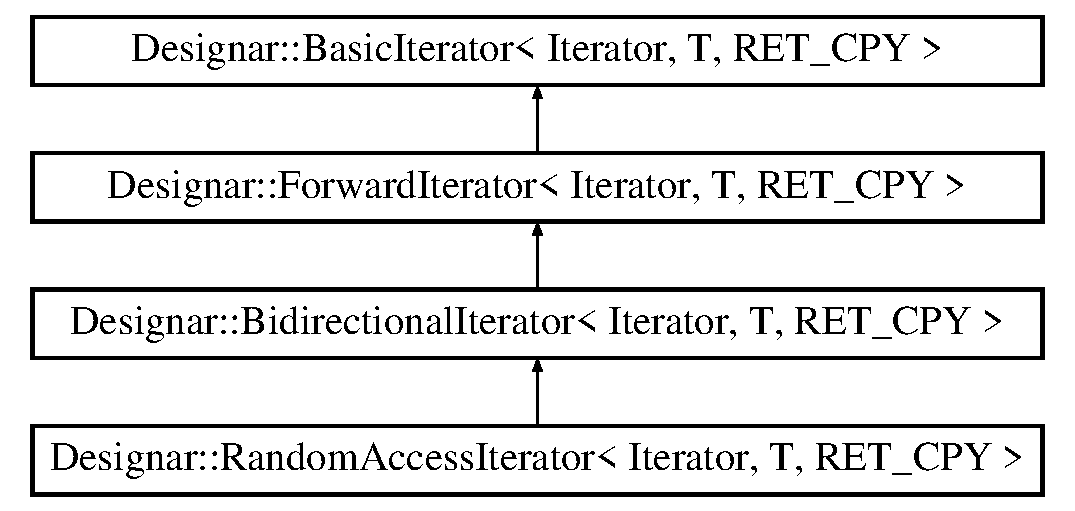
\includegraphics[height=4.000000cm]{class_designar_1_1_forward_iterator}
\end{center}
\end{figure}
\subsection*{Public Member Functions}
\begin{DoxyCompactItemize}
\item 
Iterator \& \hyperlink{class_designar_1_1_forward_iterator_a021a9305def76c968872089a778d2b41}{operator++} ()
\item 
Iterator \hyperlink{class_designar_1_1_forward_iterator_a7182625f3375ba05868ae6f240628b1c}{operator++} (int)
\end{DoxyCompactItemize}
\subsection*{Additional Inherited Members}


\subsection{Detailed Description}
\subsubsection*{template$<$class Iterator, typename T, bool R\+E\+T\+\_\+\+C\+PY = false$>$\newline
class Designar\+::\+Forward\+Iterator$<$ Iterator, T, R\+E\+T\+\_\+\+C\+P\+Y $>$}



Definition at line 77 of file iterator.\+H.



\subsection{Member Function Documentation}
\mbox{\Hypertarget{class_designar_1_1_forward_iterator_a021a9305def76c968872089a778d2b41}\label{class_designar_1_1_forward_iterator_a021a9305def76c968872089a778d2b41}} 
\index{Designar\+::\+Forward\+Iterator@{Designar\+::\+Forward\+Iterator}!operator++@{operator++}}
\index{operator++@{operator++}!Designar\+::\+Forward\+Iterator@{Designar\+::\+Forward\+Iterator}}
\subsubsection{\texorpdfstring{operator++()}{operator++()}\hspace{0.1cm}{\footnotesize\ttfamily [1/2]}}
{\footnotesize\ttfamily template$<$class Iterator, typename T, bool R\+E\+T\+\_\+\+C\+PY = false$>$ \\
Iterator\& \hyperlink{class_designar_1_1_forward_iterator}{Designar\+::\+Forward\+Iterator}$<$ Iterator, T, R\+E\+T\+\_\+\+C\+PY $>$\+::operator++ (\begin{DoxyParamCaption}{ }\end{DoxyParamCaption})\hspace{0.3cm}{\ttfamily [inline]}}



Definition at line 82 of file iterator.\+H.

\mbox{\Hypertarget{class_designar_1_1_forward_iterator_a7182625f3375ba05868ae6f240628b1c}\label{class_designar_1_1_forward_iterator_a7182625f3375ba05868ae6f240628b1c}} 
\index{Designar\+::\+Forward\+Iterator@{Designar\+::\+Forward\+Iterator}!operator++@{operator++}}
\index{operator++@{operator++}!Designar\+::\+Forward\+Iterator@{Designar\+::\+Forward\+Iterator}}
\subsubsection{\texorpdfstring{operator++()}{operator++()}\hspace{0.1cm}{\footnotesize\ttfamily [2/2]}}
{\footnotesize\ttfamily template$<$class Iterator, typename T, bool R\+E\+T\+\_\+\+C\+PY = false$>$ \\
Iterator \hyperlink{class_designar_1_1_forward_iterator}{Designar\+::\+Forward\+Iterator}$<$ Iterator, T, R\+E\+T\+\_\+\+C\+PY $>$\+::operator++ (\begin{DoxyParamCaption}\item[{int}]{ }\end{DoxyParamCaption})\hspace{0.3cm}{\ttfamily [inline]}}



Definition at line 88 of file iterator.\+H.



The documentation for this class was generated from the following file\+:\begin{DoxyCompactItemize}
\item 
include/\hyperlink{iterator_8_h}{iterator.\+H}\end{DoxyCompactItemize}

\hypertarget{class_designar_1_1_gen_array_set}{}\section{Designar\+:\+:Gen\+Array\+Set$<$ Key, Cmp, Array\+Set\+Op $>$ Class Template Reference}
\label{class_designar_1_1_gen_array_set}\index{Designar\+::\+Gen\+Array\+Set$<$ Key, Cmp, Array\+Set\+Op $>$@{Designar\+::\+Gen\+Array\+Set$<$ Key, Cmp, Array\+Set\+Op $>$}}


{\ttfamily \#include $<$array.\+H$>$}

Inheritance diagram for Designar\+:\+:Gen\+Array\+Set$<$ Key, Cmp, Array\+Set\+Op $>$\+:\begin{figure}[H]
\begin{center}
\leavevmode
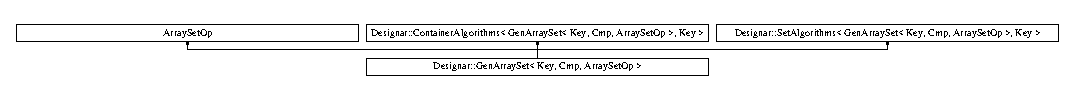
\includegraphics[height=0.782669cm]{class_designar_1_1_gen_array_set}
\end{center}
\end{figure}
\subsection*{Classes}
\begin{DoxyCompactItemize}
\item 
class \hyperlink{class_designar_1_1_gen_array_set_1_1_iterator}{Iterator}
\end{DoxyCompactItemize}
\subsection*{Public Types}
\begin{DoxyCompactItemize}
\item 
using \hyperlink{class_designar_1_1_gen_array_set_a4db3cb71a2b2f88fee2a5f66688e5230}{Item\+Type} = Key
\item 
using \hyperlink{class_designar_1_1_gen_array_set_a21195191743cf71430c939225a2c8d60}{Key\+Type} = Key
\item 
using \hyperlink{class_designar_1_1_gen_array_set_ac69f0c0b76358cd5effd2dc05bd724ee}{Data\+Type} = Key
\item 
using \hyperlink{class_designar_1_1_gen_array_set_aef777cbce261e3d5df5f03c632a7c8c2}{Value\+Type} = Key
\item 
using \hyperlink{class_designar_1_1_gen_array_set_aabe7047d492721160f291bf40ecf7745}{Size\+Type} = \hyperlink{namespace_designar_aa72662848b9f4815e7bf31a7cf3e33d1}{nat\+\_\+t}
\end{DoxyCompactItemize}
\subsection*{Public Member Functions}
\begin{DoxyCompactItemize}
\item 
bool \hyperlink{class_designar_1_1_gen_array_set_a048871f9ab15af3c26cfda4dbb47d272}{not\+\_\+equal\+\_\+key} (const Key \&e1, const Key \&e2) const
\item 
bool \hyperlink{class_designar_1_1_gen_array_set_a2874b036273f5cc48275bd1242453930}{equal\+\_\+key} (const Key \&e1, const Key \&e2) const
\item 
\hyperlink{class_designar_1_1_gen_array_set_a51b519b8c338a8f0e4db3d50e77bfd6f}{Gen\+Array\+Set} (\hyperlink{namespace_designar_aa72662848b9f4815e7bf31a7cf3e33d1}{nat\+\_\+t} cap, Cmp \&\+\_\+cmp)
\item 
\hyperlink{class_designar_1_1_gen_array_set_a6dd76e1d1ccb49b3e984c18b05c98dd2}{Gen\+Array\+Set} (Cmp \&\&\+\_\+cmp=Cmp())
\item 
\hyperlink{class_designar_1_1_gen_array_set_ab2ffd26edcd909f936394e538b43d2c4}{Gen\+Array\+Set} (\hyperlink{namespace_designar_aa72662848b9f4815e7bf31a7cf3e33d1}{nat\+\_\+t} cap, Cmp \&\&\+\_\+cmp=Cmp())
\item 
\hyperlink{class_designar_1_1_gen_array_set_a2cdf04753abc21b6f10a795fdac2238c}{Gen\+Array\+Set} (const \hyperlink{class_designar_1_1_gen_array_set}{Gen\+Array\+Set} \&a)
\item 
\hyperlink{class_designar_1_1_gen_array_set_af0b02756ac00f4b364422908a0e94e73}{Gen\+Array\+Set} (\hyperlink{class_designar_1_1_gen_array_set}{Gen\+Array\+Set} \&\&a)
\item 
\hyperlink{class_designar_1_1_gen_array_set_a53cc511f4539c16b1542f56979433c2a}{Gen\+Array\+Set} (const std\+::initializer\+\_\+list$<$ Key $>$ \&)
\item 
\hyperlink{class_designar_1_1_gen_array_set}{Gen\+Array\+Set} \& \hyperlink{class_designar_1_1_gen_array_set_ab30a4cf17a20eb6005cfed15762c1568}{operator=} (const \hyperlink{class_designar_1_1_gen_array_set}{Gen\+Array\+Set} \&a)
\item 
\hyperlink{class_designar_1_1_gen_array_set}{Gen\+Array\+Set} \& \hyperlink{class_designar_1_1_gen_array_set_afb89b3abb4a394341430ca8ae29a9ca2}{operator=} (\hyperlink{class_designar_1_1_gen_array_set}{Gen\+Array\+Set} \&\&a)
\item 
void \hyperlink{class_designar_1_1_gen_array_set_ab117cdee923c27d7922a02336440b2ff}{swap} (\hyperlink{class_designar_1_1_gen_array_set}{Gen\+Array\+Set} \&a)
\item 
Cmp \& \hyperlink{class_designar_1_1_gen_array_set_aceb48fb98d254005b82fd538b6ac0c35}{get\+\_\+cmp} ()
\item 
const Cmp \& \hyperlink{class_designar_1_1_gen_array_set_a30409051572881ed638f79debfad8188}{get\+\_\+cmp} () const
\item 
bool \hyperlink{class_designar_1_1_gen_array_set_aca8ce9f7cb1ded74fd8067a535817836}{is\+\_\+empty} () const
\item 
\hyperlink{namespace_designar_aa72662848b9f4815e7bf31a7cf3e33d1}{nat\+\_\+t} \hyperlink{class_designar_1_1_gen_array_set_ab5b56f597b39e2dbf03514a2eb096e8a}{size} () const
\item 
void \hyperlink{class_designar_1_1_gen_array_set_aa1b1d249debb38432e56b2e585d822af}{clear} ()
\item 
Key $\ast$ \hyperlink{class_designar_1_1_gen_array_set_ac1367b0dd7bc3f90fc73101991dc398a}{append} (const Key \&k)
\item 
Key $\ast$ \hyperlink{class_designar_1_1_gen_array_set_aafb9d33d1a9a6f5b07d434705290b7bc}{append} (Key \&\&k)
\item 
Key $\ast$ \hyperlink{class_designar_1_1_gen_array_set_ab6e8baee6087d491045de115ed7fb48e}{search} (const Key \&item)
\item 
const Key $\ast$ \hyperlink{class_designar_1_1_gen_array_set_adbe26651c80bbcc92afe2563f6bcefc3}{search} (const Key \&item) const
\item 
Key \& \hyperlink{class_designar_1_1_gen_array_set_a91015348562e7127f2612ad5c13fa016}{find} (const Key \&item)
\item 
const Key \& \hyperlink{class_designar_1_1_gen_array_set_aab0576267b8f88e6e7ec2d31aa768449}{find} (const Key \&item) const
\item 
bool \hyperlink{class_designar_1_1_gen_array_set_acddff41221307179e0b4c20afbcfe253}{remove} (const Key \&item)
\item 
Key \& \hyperlink{class_designar_1_1_gen_array_set_ad721fdfba3af03c084a9bbfe5ec67fd8}{operator\mbox{[}$\,$\mbox{]}} (\hyperlink{namespace_designar_aa72662848b9f4815e7bf31a7cf3e33d1}{nat\+\_\+t} i)
\item 
const Key \& \hyperlink{class_designar_1_1_gen_array_set_a2731e12c87e08bc42ac16496569ebf5a}{operator\mbox{[}$\,$\mbox{]}} (\hyperlink{namespace_designar_aa72662848b9f4815e7bf31a7cf3e33d1}{nat\+\_\+t} i) const
\item 
\hyperlink{class_designar_1_1_gen_array_set_1_1_iterator}{Iterator} \hyperlink{class_designar_1_1_gen_array_set_af736c7af596752d636881374f0d45f4c}{begin} ()
\item 
\hyperlink{class_designar_1_1_gen_array_set_1_1_iterator}{Iterator} \hyperlink{class_designar_1_1_gen_array_set_a9bccd51f6d73a05400361cf5deff8aac}{begin} () const
\item 
\hyperlink{class_designar_1_1_gen_array_set_1_1_iterator}{Iterator} \hyperlink{class_designar_1_1_gen_array_set_a23644b099a1bf858784e474d833245a8}{end} ()
\item 
\hyperlink{class_designar_1_1_gen_array_set_1_1_iterator}{Iterator} \hyperlink{class_designar_1_1_gen_array_set_ade46fb4605ffb1e08d6475a7aacd6024}{end} () const
\end{DoxyCompactItemize}
\subsection*{Public Attributes}
\begin{DoxyCompactItemize}
\item 
\hyperlink{class_designar_1_1_dyn_array}{Dyn\+Array}$<$ Key $>$ \hyperlink{class_designar_1_1_gen_array_set_a8118f689e762c993ed0ba7394a8f480a}{array}
\item 
Cmp \& \hyperlink{class_designar_1_1_gen_array_set_a2b1e3c653865a794eab7d19e43c1b0de}{cmp}
\end{DoxyCompactItemize}
\subsection*{Additional Inherited Members}


\subsection{Detailed Description}
\subsubsection*{template$<$typename Key, class Cmp, class Array\+Set\+Op$>$\newline
class Designar\+::\+Gen\+Array\+Set$<$ Key, Cmp, Array\+Set\+Op $>$}



Definition at line 1240 of file array.\+H.



\subsection{Member Typedef Documentation}
\mbox{\Hypertarget{class_designar_1_1_gen_array_set_ac69f0c0b76358cd5effd2dc05bd724ee}\label{class_designar_1_1_gen_array_set_ac69f0c0b76358cd5effd2dc05bd724ee}} 
\index{Designar\+::\+Gen\+Array\+Set@{Designar\+::\+Gen\+Array\+Set}!Data\+Type@{Data\+Type}}
\index{Data\+Type@{Data\+Type}!Designar\+::\+Gen\+Array\+Set@{Designar\+::\+Gen\+Array\+Set}}
\subsubsection{\texorpdfstring{Data\+Type}{DataType}}
{\footnotesize\ttfamily template$<$typename Key, class Cmp, class Array\+Set\+Op$>$ \\
using \hyperlink{class_designar_1_1_gen_array_set}{Designar\+::\+Gen\+Array\+Set}$<$ Key, Cmp, Array\+Set\+Op $>$\+::\hyperlink{class_designar_1_1_gen_array_set_ac69f0c0b76358cd5effd2dc05bd724ee}{Data\+Type} =  Key}



Definition at line 1248 of file array.\+H.

\mbox{\Hypertarget{class_designar_1_1_gen_array_set_a4db3cb71a2b2f88fee2a5f66688e5230}\label{class_designar_1_1_gen_array_set_a4db3cb71a2b2f88fee2a5f66688e5230}} 
\index{Designar\+::\+Gen\+Array\+Set@{Designar\+::\+Gen\+Array\+Set}!Item\+Type@{Item\+Type}}
\index{Item\+Type@{Item\+Type}!Designar\+::\+Gen\+Array\+Set@{Designar\+::\+Gen\+Array\+Set}}
\subsubsection{\texorpdfstring{Item\+Type}{ItemType}}
{\footnotesize\ttfamily template$<$typename Key, class Cmp, class Array\+Set\+Op$>$ \\
using \hyperlink{class_designar_1_1_gen_array_set}{Designar\+::\+Gen\+Array\+Set}$<$ Key, Cmp, Array\+Set\+Op $>$\+::\hyperlink{class_designar_1_1_gen_array_set_a4db3cb71a2b2f88fee2a5f66688e5230}{Item\+Type} =  Key}



Definition at line 1246 of file array.\+H.

\mbox{\Hypertarget{class_designar_1_1_gen_array_set_a21195191743cf71430c939225a2c8d60}\label{class_designar_1_1_gen_array_set_a21195191743cf71430c939225a2c8d60}} 
\index{Designar\+::\+Gen\+Array\+Set@{Designar\+::\+Gen\+Array\+Set}!Key\+Type@{Key\+Type}}
\index{Key\+Type@{Key\+Type}!Designar\+::\+Gen\+Array\+Set@{Designar\+::\+Gen\+Array\+Set}}
\subsubsection{\texorpdfstring{Key\+Type}{KeyType}}
{\footnotesize\ttfamily template$<$typename Key, class Cmp, class Array\+Set\+Op$>$ \\
using \hyperlink{class_designar_1_1_gen_array_set}{Designar\+::\+Gen\+Array\+Set}$<$ Key, Cmp, Array\+Set\+Op $>$\+::\hyperlink{class_designar_1_1_gen_array_set_a21195191743cf71430c939225a2c8d60}{Key\+Type} =  Key}



Definition at line 1247 of file array.\+H.

\mbox{\Hypertarget{class_designar_1_1_gen_array_set_aabe7047d492721160f291bf40ecf7745}\label{class_designar_1_1_gen_array_set_aabe7047d492721160f291bf40ecf7745}} 
\index{Designar\+::\+Gen\+Array\+Set@{Designar\+::\+Gen\+Array\+Set}!Size\+Type@{Size\+Type}}
\index{Size\+Type@{Size\+Type}!Designar\+::\+Gen\+Array\+Set@{Designar\+::\+Gen\+Array\+Set}}
\subsubsection{\texorpdfstring{Size\+Type}{SizeType}}
{\footnotesize\ttfamily template$<$typename Key, class Cmp, class Array\+Set\+Op$>$ \\
using \hyperlink{class_designar_1_1_gen_array_set}{Designar\+::\+Gen\+Array\+Set}$<$ Key, Cmp, Array\+Set\+Op $>$\+::\hyperlink{class_designar_1_1_gen_array_set_aabe7047d492721160f291bf40ecf7745}{Size\+Type} =  \hyperlink{namespace_designar_aa72662848b9f4815e7bf31a7cf3e33d1}{nat\+\_\+t}}



Definition at line 1250 of file array.\+H.

\mbox{\Hypertarget{class_designar_1_1_gen_array_set_aef777cbce261e3d5df5f03c632a7c8c2}\label{class_designar_1_1_gen_array_set_aef777cbce261e3d5df5f03c632a7c8c2}} 
\index{Designar\+::\+Gen\+Array\+Set@{Designar\+::\+Gen\+Array\+Set}!Value\+Type@{Value\+Type}}
\index{Value\+Type@{Value\+Type}!Designar\+::\+Gen\+Array\+Set@{Designar\+::\+Gen\+Array\+Set}}
\subsubsection{\texorpdfstring{Value\+Type}{ValueType}}
{\footnotesize\ttfamily template$<$typename Key, class Cmp, class Array\+Set\+Op$>$ \\
using \hyperlink{class_designar_1_1_gen_array_set}{Designar\+::\+Gen\+Array\+Set}$<$ Key, Cmp, Array\+Set\+Op $>$\+::\hyperlink{class_designar_1_1_gen_array_set_aef777cbce261e3d5df5f03c632a7c8c2}{Value\+Type} =  Key}



Definition at line 1249 of file array.\+H.



\subsection{Constructor \& Destructor Documentation}
\mbox{\Hypertarget{class_designar_1_1_gen_array_set_a51b519b8c338a8f0e4db3d50e77bfd6f}\label{class_designar_1_1_gen_array_set_a51b519b8c338a8f0e4db3d50e77bfd6f}} 
\index{Designar\+::\+Gen\+Array\+Set@{Designar\+::\+Gen\+Array\+Set}!Gen\+Array\+Set@{Gen\+Array\+Set}}
\index{Gen\+Array\+Set@{Gen\+Array\+Set}!Designar\+::\+Gen\+Array\+Set@{Designar\+::\+Gen\+Array\+Set}}
\subsubsection{\texorpdfstring{Gen\+Array\+Set()}{GenArraySet()}\hspace{0.1cm}{\footnotesize\ttfamily [1/6]}}
{\footnotesize\ttfamily template$<$typename Key, class Cmp, class Array\+Set\+Op$>$ \\
\hyperlink{class_designar_1_1_gen_array_set}{Designar\+::\+Gen\+Array\+Set}$<$ Key, Cmp, Array\+Set\+Op $>$\+::\hyperlink{class_designar_1_1_gen_array_set}{Gen\+Array\+Set} (\begin{DoxyParamCaption}\item[{\hyperlink{namespace_designar_aa72662848b9f4815e7bf31a7cf3e33d1}{nat\+\_\+t}}]{cap,  }\item[{Cmp \&}]{\+\_\+cmp }\end{DoxyParamCaption})\hspace{0.3cm}{\ttfamily [inline]}}



Definition at line 1266 of file array.\+H.

\mbox{\Hypertarget{class_designar_1_1_gen_array_set_a6dd76e1d1ccb49b3e984c18b05c98dd2}\label{class_designar_1_1_gen_array_set_a6dd76e1d1ccb49b3e984c18b05c98dd2}} 
\index{Designar\+::\+Gen\+Array\+Set@{Designar\+::\+Gen\+Array\+Set}!Gen\+Array\+Set@{Gen\+Array\+Set}}
\index{Gen\+Array\+Set@{Gen\+Array\+Set}!Designar\+::\+Gen\+Array\+Set@{Designar\+::\+Gen\+Array\+Set}}
\subsubsection{\texorpdfstring{Gen\+Array\+Set()}{GenArraySet()}\hspace{0.1cm}{\footnotesize\ttfamily [2/6]}}
{\footnotesize\ttfamily template$<$typename Key, class Cmp, class Array\+Set\+Op$>$ \\
\hyperlink{class_designar_1_1_gen_array_set}{Designar\+::\+Gen\+Array\+Set}$<$ Key, Cmp, Array\+Set\+Op $>$\+::\hyperlink{class_designar_1_1_gen_array_set}{Gen\+Array\+Set} (\begin{DoxyParamCaption}\item[{Cmp \&\&}]{\+\_\+cmp = {\ttfamily Cmp()} }\end{DoxyParamCaption})\hspace{0.3cm}{\ttfamily [inline]}}



Definition at line 1272 of file array.\+H.

\mbox{\Hypertarget{class_designar_1_1_gen_array_set_ab2ffd26edcd909f936394e538b43d2c4}\label{class_designar_1_1_gen_array_set_ab2ffd26edcd909f936394e538b43d2c4}} 
\index{Designar\+::\+Gen\+Array\+Set@{Designar\+::\+Gen\+Array\+Set}!Gen\+Array\+Set@{Gen\+Array\+Set}}
\index{Gen\+Array\+Set@{Gen\+Array\+Set}!Designar\+::\+Gen\+Array\+Set@{Designar\+::\+Gen\+Array\+Set}}
\subsubsection{\texorpdfstring{Gen\+Array\+Set()}{GenArraySet()}\hspace{0.1cm}{\footnotesize\ttfamily [3/6]}}
{\footnotesize\ttfamily template$<$typename Key, class Cmp, class Array\+Set\+Op$>$ \\
\hyperlink{class_designar_1_1_gen_array_set}{Designar\+::\+Gen\+Array\+Set}$<$ Key, Cmp, Array\+Set\+Op $>$\+::\hyperlink{class_designar_1_1_gen_array_set}{Gen\+Array\+Set} (\begin{DoxyParamCaption}\item[{\hyperlink{namespace_designar_aa72662848b9f4815e7bf31a7cf3e33d1}{nat\+\_\+t}}]{cap,  }\item[{Cmp \&\&}]{\+\_\+cmp = {\ttfamily Cmp()} }\end{DoxyParamCaption})\hspace{0.3cm}{\ttfamily [inline]}}



Definition at line 1278 of file array.\+H.

\mbox{\Hypertarget{class_designar_1_1_gen_array_set_a2cdf04753abc21b6f10a795fdac2238c}\label{class_designar_1_1_gen_array_set_a2cdf04753abc21b6f10a795fdac2238c}} 
\index{Designar\+::\+Gen\+Array\+Set@{Designar\+::\+Gen\+Array\+Set}!Gen\+Array\+Set@{Gen\+Array\+Set}}
\index{Gen\+Array\+Set@{Gen\+Array\+Set}!Designar\+::\+Gen\+Array\+Set@{Designar\+::\+Gen\+Array\+Set}}
\subsubsection{\texorpdfstring{Gen\+Array\+Set()}{GenArraySet()}\hspace{0.1cm}{\footnotesize\ttfamily [4/6]}}
{\footnotesize\ttfamily template$<$typename Key, class Cmp, class Array\+Set\+Op$>$ \\
\hyperlink{class_designar_1_1_gen_array_set}{Designar\+::\+Gen\+Array\+Set}$<$ Key, Cmp, Array\+Set\+Op $>$\+::\hyperlink{class_designar_1_1_gen_array_set}{Gen\+Array\+Set} (\begin{DoxyParamCaption}\item[{const \hyperlink{class_designar_1_1_gen_array_set}{Gen\+Array\+Set}$<$ Key, Cmp, Array\+Set\+Op $>$ \&}]{a }\end{DoxyParamCaption})\hspace{0.3cm}{\ttfamily [inline]}}



Definition at line 1284 of file array.\+H.

\mbox{\Hypertarget{class_designar_1_1_gen_array_set_af0b02756ac00f4b364422908a0e94e73}\label{class_designar_1_1_gen_array_set_af0b02756ac00f4b364422908a0e94e73}} 
\index{Designar\+::\+Gen\+Array\+Set@{Designar\+::\+Gen\+Array\+Set}!Gen\+Array\+Set@{Gen\+Array\+Set}}
\index{Gen\+Array\+Set@{Gen\+Array\+Set}!Designar\+::\+Gen\+Array\+Set@{Designar\+::\+Gen\+Array\+Set}}
\subsubsection{\texorpdfstring{Gen\+Array\+Set()}{GenArraySet()}\hspace{0.1cm}{\footnotesize\ttfamily [5/6]}}
{\footnotesize\ttfamily template$<$typename Key, class Cmp, class Array\+Set\+Op$>$ \\
\hyperlink{class_designar_1_1_gen_array_set}{Designar\+::\+Gen\+Array\+Set}$<$ Key, Cmp, Array\+Set\+Op $>$\+::\hyperlink{class_designar_1_1_gen_array_set}{Gen\+Array\+Set} (\begin{DoxyParamCaption}\item[{\hyperlink{class_designar_1_1_gen_array_set}{Gen\+Array\+Set}$<$ Key, Cmp, Array\+Set\+Op $>$ \&\&}]{a }\end{DoxyParamCaption})\hspace{0.3cm}{\ttfamily [inline]}}



Definition at line 1290 of file array.\+H.

\mbox{\Hypertarget{class_designar_1_1_gen_array_set_a53cc511f4539c16b1542f56979433c2a}\label{class_designar_1_1_gen_array_set_a53cc511f4539c16b1542f56979433c2a}} 
\index{Designar\+::\+Gen\+Array\+Set@{Designar\+::\+Gen\+Array\+Set}!Gen\+Array\+Set@{Gen\+Array\+Set}}
\index{Gen\+Array\+Set@{Gen\+Array\+Set}!Designar\+::\+Gen\+Array\+Set@{Designar\+::\+Gen\+Array\+Set}}
\subsubsection{\texorpdfstring{Gen\+Array\+Set()}{GenArraySet()}\hspace{0.1cm}{\footnotesize\ttfamily [6/6]}}
{\footnotesize\ttfamily template$<$typename Key, class Cmp, class Array\+Set\+Op $>$ \\
\hyperlink{class_designar_1_1_gen_array_set}{Designar\+::\+Gen\+Array\+Set}$<$ Key, Cmp, Array\+Set\+Op $>$\+::\hyperlink{class_designar_1_1_gen_array_set}{Gen\+Array\+Set} (\begin{DoxyParamCaption}\item[{const std\+::initializer\+\_\+list$<$ Key $>$ \&}]{l }\end{DoxyParamCaption})}



Definition at line 1472 of file array.\+H.



\subsection{Member Function Documentation}
\mbox{\Hypertarget{class_designar_1_1_gen_array_set_ac1367b0dd7bc3f90fc73101991dc398a}\label{class_designar_1_1_gen_array_set_ac1367b0dd7bc3f90fc73101991dc398a}} 
\index{Designar\+::\+Gen\+Array\+Set@{Designar\+::\+Gen\+Array\+Set}!append@{append}}
\index{append@{append}!Designar\+::\+Gen\+Array\+Set@{Designar\+::\+Gen\+Array\+Set}}
\subsubsection{\texorpdfstring{append()}{append()}\hspace{0.1cm}{\footnotesize\ttfamily [1/2]}}
{\footnotesize\ttfamily template$<$typename Key, class Cmp, class Array\+Set\+Op$>$ \\
Key$\ast$ \hyperlink{class_designar_1_1_gen_array_set}{Designar\+::\+Gen\+Array\+Set}$<$ Key, Cmp, Array\+Set\+Op $>$\+::append (\begin{DoxyParamCaption}\item[{const Key \&}]{k }\end{DoxyParamCaption})\hspace{0.3cm}{\ttfamily [inline]}}



Definition at line 1346 of file array.\+H.

\mbox{\Hypertarget{class_designar_1_1_gen_array_set_aafb9d33d1a9a6f5b07d434705290b7bc}\label{class_designar_1_1_gen_array_set_aafb9d33d1a9a6f5b07d434705290b7bc}} 
\index{Designar\+::\+Gen\+Array\+Set@{Designar\+::\+Gen\+Array\+Set}!append@{append}}
\index{append@{append}!Designar\+::\+Gen\+Array\+Set@{Designar\+::\+Gen\+Array\+Set}}
\subsubsection{\texorpdfstring{append()}{append()}\hspace{0.1cm}{\footnotesize\ttfamily [2/2]}}
{\footnotesize\ttfamily template$<$typename Key, class Cmp, class Array\+Set\+Op$>$ \\
Key$\ast$ \hyperlink{class_designar_1_1_gen_array_set}{Designar\+::\+Gen\+Array\+Set}$<$ Key, Cmp, Array\+Set\+Op $>$\+::append (\begin{DoxyParamCaption}\item[{Key \&\&}]{k }\end{DoxyParamCaption})\hspace{0.3cm}{\ttfamily [inline]}}



Definition at line 1351 of file array.\+H.

\mbox{\Hypertarget{class_designar_1_1_gen_array_set_af736c7af596752d636881374f0d45f4c}\label{class_designar_1_1_gen_array_set_af736c7af596752d636881374f0d45f4c}} 
\index{Designar\+::\+Gen\+Array\+Set@{Designar\+::\+Gen\+Array\+Set}!begin@{begin}}
\index{begin@{begin}!Designar\+::\+Gen\+Array\+Set@{Designar\+::\+Gen\+Array\+Set}}
\subsubsection{\texorpdfstring{begin()}{begin()}\hspace{0.1cm}{\footnotesize\ttfamily [1/2]}}
{\footnotesize\ttfamily template$<$typename Key, class Cmp, class Array\+Set\+Op$>$ \\
\hyperlink{class_designar_1_1_gen_array_set_1_1_iterator}{Iterator} \hyperlink{class_designar_1_1_gen_array_set}{Designar\+::\+Gen\+Array\+Set}$<$ Key, Cmp, Array\+Set\+Op $>$\+::begin (\begin{DoxyParamCaption}{ }\end{DoxyParamCaption})\hspace{0.3cm}{\ttfamily [inline]}}



Definition at line 1449 of file array.\+H.

\mbox{\Hypertarget{class_designar_1_1_gen_array_set_a9bccd51f6d73a05400361cf5deff8aac}\label{class_designar_1_1_gen_array_set_a9bccd51f6d73a05400361cf5deff8aac}} 
\index{Designar\+::\+Gen\+Array\+Set@{Designar\+::\+Gen\+Array\+Set}!begin@{begin}}
\index{begin@{begin}!Designar\+::\+Gen\+Array\+Set@{Designar\+::\+Gen\+Array\+Set}}
\subsubsection{\texorpdfstring{begin()}{begin()}\hspace{0.1cm}{\footnotesize\ttfamily [2/2]}}
{\footnotesize\ttfamily template$<$typename Key, class Cmp, class Array\+Set\+Op$>$ \\
\hyperlink{class_designar_1_1_gen_array_set_1_1_iterator}{Iterator} \hyperlink{class_designar_1_1_gen_array_set}{Designar\+::\+Gen\+Array\+Set}$<$ Key, Cmp, Array\+Set\+Op $>$\+::begin (\begin{DoxyParamCaption}{ }\end{DoxyParamCaption}) const\hspace{0.3cm}{\ttfamily [inline]}}



Definition at line 1454 of file array.\+H.

\mbox{\Hypertarget{class_designar_1_1_gen_array_set_aa1b1d249debb38432e56b2e585d822af}\label{class_designar_1_1_gen_array_set_aa1b1d249debb38432e56b2e585d822af}} 
\index{Designar\+::\+Gen\+Array\+Set@{Designar\+::\+Gen\+Array\+Set}!clear@{clear}}
\index{clear@{clear}!Designar\+::\+Gen\+Array\+Set@{Designar\+::\+Gen\+Array\+Set}}
\subsubsection{\texorpdfstring{clear()}{clear()}}
{\footnotesize\ttfamily template$<$typename Key, class Cmp, class Array\+Set\+Op$>$ \\
void \hyperlink{class_designar_1_1_gen_array_set}{Designar\+::\+Gen\+Array\+Set}$<$ Key, Cmp, Array\+Set\+Op $>$\+::clear (\begin{DoxyParamCaption}{ }\end{DoxyParamCaption})\hspace{0.3cm}{\ttfamily [inline]}}



Definition at line 1341 of file array.\+H.

\mbox{\Hypertarget{class_designar_1_1_gen_array_set_a23644b099a1bf858784e474d833245a8}\label{class_designar_1_1_gen_array_set_a23644b099a1bf858784e474d833245a8}} 
\index{Designar\+::\+Gen\+Array\+Set@{Designar\+::\+Gen\+Array\+Set}!end@{end}}
\index{end@{end}!Designar\+::\+Gen\+Array\+Set@{Designar\+::\+Gen\+Array\+Set}}
\subsubsection{\texorpdfstring{end()}{end()}\hspace{0.1cm}{\footnotesize\ttfamily [1/2]}}
{\footnotesize\ttfamily template$<$typename Key, class Cmp, class Array\+Set\+Op$>$ \\
\hyperlink{class_designar_1_1_gen_array_set_1_1_iterator}{Iterator} \hyperlink{class_designar_1_1_gen_array_set}{Designar\+::\+Gen\+Array\+Set}$<$ Key, Cmp, Array\+Set\+Op $>$\+::end (\begin{DoxyParamCaption}{ }\end{DoxyParamCaption})\hspace{0.3cm}{\ttfamily [inline]}}



Definition at line 1459 of file array.\+H.

\mbox{\Hypertarget{class_designar_1_1_gen_array_set_ade46fb4605ffb1e08d6475a7aacd6024}\label{class_designar_1_1_gen_array_set_ade46fb4605ffb1e08d6475a7aacd6024}} 
\index{Designar\+::\+Gen\+Array\+Set@{Designar\+::\+Gen\+Array\+Set}!end@{end}}
\index{end@{end}!Designar\+::\+Gen\+Array\+Set@{Designar\+::\+Gen\+Array\+Set}}
\subsubsection{\texorpdfstring{end()}{end()}\hspace{0.1cm}{\footnotesize\ttfamily [2/2]}}
{\footnotesize\ttfamily template$<$typename Key, class Cmp, class Array\+Set\+Op$>$ \\
\hyperlink{class_designar_1_1_gen_array_set_1_1_iterator}{Iterator} \hyperlink{class_designar_1_1_gen_array_set}{Designar\+::\+Gen\+Array\+Set}$<$ Key, Cmp, Array\+Set\+Op $>$\+::end (\begin{DoxyParamCaption}{ }\end{DoxyParamCaption}) const\hspace{0.3cm}{\ttfamily [inline]}}



Definition at line 1464 of file array.\+H.

\mbox{\Hypertarget{class_designar_1_1_gen_array_set_a2874b036273f5cc48275bd1242453930}\label{class_designar_1_1_gen_array_set_a2874b036273f5cc48275bd1242453930}} 
\index{Designar\+::\+Gen\+Array\+Set@{Designar\+::\+Gen\+Array\+Set}!equal\+\_\+key@{equal\+\_\+key}}
\index{equal\+\_\+key@{equal\+\_\+key}!Designar\+::\+Gen\+Array\+Set@{Designar\+::\+Gen\+Array\+Set}}
\subsubsection{\texorpdfstring{equal\+\_\+key()}{equal\_key()}}
{\footnotesize\ttfamily template$<$typename Key, class Cmp, class Array\+Set\+Op$>$ \\
bool \hyperlink{class_designar_1_1_gen_array_set}{Designar\+::\+Gen\+Array\+Set}$<$ Key, Cmp, Array\+Set\+Op $>$\+::equal\+\_\+key (\begin{DoxyParamCaption}\item[{const Key \&}]{e1,  }\item[{const Key \&}]{e2 }\end{DoxyParamCaption}) const\hspace{0.3cm}{\ttfamily [inline]}}



Definition at line 1260 of file array.\+H.

\mbox{\Hypertarget{class_designar_1_1_gen_array_set_a91015348562e7127f2612ad5c13fa016}\label{class_designar_1_1_gen_array_set_a91015348562e7127f2612ad5c13fa016}} 
\index{Designar\+::\+Gen\+Array\+Set@{Designar\+::\+Gen\+Array\+Set}!find@{find}}
\index{find@{find}!Designar\+::\+Gen\+Array\+Set@{Designar\+::\+Gen\+Array\+Set}}
\subsubsection{\texorpdfstring{find()}{find()}\hspace{0.1cm}{\footnotesize\ttfamily [1/2]}}
{\footnotesize\ttfamily template$<$typename Key, class Cmp, class Array\+Set\+Op$>$ \\
Key\& \hyperlink{class_designar_1_1_gen_array_set}{Designar\+::\+Gen\+Array\+Set}$<$ Key, Cmp, Array\+Set\+Op $>$\+::find (\begin{DoxyParamCaption}\item[{const Key \&}]{item }\end{DoxyParamCaption})\hspace{0.3cm}{\ttfamily [inline]}}



Definition at line 1376 of file array.\+H.

\mbox{\Hypertarget{class_designar_1_1_gen_array_set_aab0576267b8f88e6e7ec2d31aa768449}\label{class_designar_1_1_gen_array_set_aab0576267b8f88e6e7ec2d31aa768449}} 
\index{Designar\+::\+Gen\+Array\+Set@{Designar\+::\+Gen\+Array\+Set}!find@{find}}
\index{find@{find}!Designar\+::\+Gen\+Array\+Set@{Designar\+::\+Gen\+Array\+Set}}
\subsubsection{\texorpdfstring{find()}{find()}\hspace{0.1cm}{\footnotesize\ttfamily [2/2]}}
{\footnotesize\ttfamily template$<$typename Key, class Cmp, class Array\+Set\+Op$>$ \\
const Key\& \hyperlink{class_designar_1_1_gen_array_set}{Designar\+::\+Gen\+Array\+Set}$<$ Key, Cmp, Array\+Set\+Op $>$\+::find (\begin{DoxyParamCaption}\item[{const Key \&}]{item }\end{DoxyParamCaption}) const\hspace{0.3cm}{\ttfamily [inline]}}



Definition at line 1384 of file array.\+H.

\mbox{\Hypertarget{class_designar_1_1_gen_array_set_aceb48fb98d254005b82fd538b6ac0c35}\label{class_designar_1_1_gen_array_set_aceb48fb98d254005b82fd538b6ac0c35}} 
\index{Designar\+::\+Gen\+Array\+Set@{Designar\+::\+Gen\+Array\+Set}!get\+\_\+cmp@{get\+\_\+cmp}}
\index{get\+\_\+cmp@{get\+\_\+cmp}!Designar\+::\+Gen\+Array\+Set@{Designar\+::\+Gen\+Array\+Set}}
\subsubsection{\texorpdfstring{get\+\_\+cmp()}{get\_cmp()}\hspace{0.1cm}{\footnotesize\ttfamily [1/2]}}
{\footnotesize\ttfamily template$<$typename Key, class Cmp, class Array\+Set\+Op$>$ \\
Cmp\& \hyperlink{class_designar_1_1_gen_array_set}{Designar\+::\+Gen\+Array\+Set}$<$ Key, Cmp, Array\+Set\+Op $>$\+::get\+\_\+cmp (\begin{DoxyParamCaption}{ }\end{DoxyParamCaption})\hspace{0.3cm}{\ttfamily [inline]}}



Definition at line 1321 of file array.\+H.

\mbox{\Hypertarget{class_designar_1_1_gen_array_set_a30409051572881ed638f79debfad8188}\label{class_designar_1_1_gen_array_set_a30409051572881ed638f79debfad8188}} 
\index{Designar\+::\+Gen\+Array\+Set@{Designar\+::\+Gen\+Array\+Set}!get\+\_\+cmp@{get\+\_\+cmp}}
\index{get\+\_\+cmp@{get\+\_\+cmp}!Designar\+::\+Gen\+Array\+Set@{Designar\+::\+Gen\+Array\+Set}}
\subsubsection{\texorpdfstring{get\+\_\+cmp()}{get\_cmp()}\hspace{0.1cm}{\footnotesize\ttfamily [2/2]}}
{\footnotesize\ttfamily template$<$typename Key, class Cmp, class Array\+Set\+Op$>$ \\
const Cmp\& \hyperlink{class_designar_1_1_gen_array_set}{Designar\+::\+Gen\+Array\+Set}$<$ Key, Cmp, Array\+Set\+Op $>$\+::get\+\_\+cmp (\begin{DoxyParamCaption}{ }\end{DoxyParamCaption}) const\hspace{0.3cm}{\ttfamily [inline]}}



Definition at line 1326 of file array.\+H.

\mbox{\Hypertarget{class_designar_1_1_gen_array_set_aca8ce9f7cb1ded74fd8067a535817836}\label{class_designar_1_1_gen_array_set_aca8ce9f7cb1ded74fd8067a535817836}} 
\index{Designar\+::\+Gen\+Array\+Set@{Designar\+::\+Gen\+Array\+Set}!is\+\_\+empty@{is\+\_\+empty}}
\index{is\+\_\+empty@{is\+\_\+empty}!Designar\+::\+Gen\+Array\+Set@{Designar\+::\+Gen\+Array\+Set}}
\subsubsection{\texorpdfstring{is\+\_\+empty()}{is\_empty()}}
{\footnotesize\ttfamily template$<$typename Key, class Cmp, class Array\+Set\+Op$>$ \\
bool \hyperlink{class_designar_1_1_gen_array_set}{Designar\+::\+Gen\+Array\+Set}$<$ Key, Cmp, Array\+Set\+Op $>$\+::is\+\_\+empty (\begin{DoxyParamCaption}{ }\end{DoxyParamCaption}) const\hspace{0.3cm}{\ttfamily [inline]}}



Definition at line 1331 of file array.\+H.

\mbox{\Hypertarget{class_designar_1_1_gen_array_set_a048871f9ab15af3c26cfda4dbb47d272}\label{class_designar_1_1_gen_array_set_a048871f9ab15af3c26cfda4dbb47d272}} 
\index{Designar\+::\+Gen\+Array\+Set@{Designar\+::\+Gen\+Array\+Set}!not\+\_\+equal\+\_\+key@{not\+\_\+equal\+\_\+key}}
\index{not\+\_\+equal\+\_\+key@{not\+\_\+equal\+\_\+key}!Designar\+::\+Gen\+Array\+Set@{Designar\+::\+Gen\+Array\+Set}}
\subsubsection{\texorpdfstring{not\+\_\+equal\+\_\+key()}{not\_equal\_key()}}
{\footnotesize\ttfamily template$<$typename Key, class Cmp, class Array\+Set\+Op$>$ \\
bool \hyperlink{class_designar_1_1_gen_array_set}{Designar\+::\+Gen\+Array\+Set}$<$ Key, Cmp, Array\+Set\+Op $>$\+::not\+\_\+equal\+\_\+key (\begin{DoxyParamCaption}\item[{const Key \&}]{e1,  }\item[{const Key \&}]{e2 }\end{DoxyParamCaption}) const\hspace{0.3cm}{\ttfamily [inline]}}



Definition at line 1255 of file array.\+H.

\mbox{\Hypertarget{class_designar_1_1_gen_array_set_ab30a4cf17a20eb6005cfed15762c1568}\label{class_designar_1_1_gen_array_set_ab30a4cf17a20eb6005cfed15762c1568}} 
\index{Designar\+::\+Gen\+Array\+Set@{Designar\+::\+Gen\+Array\+Set}!operator=@{operator=}}
\index{operator=@{operator=}!Designar\+::\+Gen\+Array\+Set@{Designar\+::\+Gen\+Array\+Set}}
\subsubsection{\texorpdfstring{operator=()}{operator=()}\hspace{0.1cm}{\footnotesize\ttfamily [1/2]}}
{\footnotesize\ttfamily template$<$typename Key, class Cmp, class Array\+Set\+Op$>$ \\
\hyperlink{class_designar_1_1_gen_array_set}{Gen\+Array\+Set}\& \hyperlink{class_designar_1_1_gen_array_set}{Designar\+::\+Gen\+Array\+Set}$<$ Key, Cmp, Array\+Set\+Op $>$\+::operator= (\begin{DoxyParamCaption}\item[{const \hyperlink{class_designar_1_1_gen_array_set}{Gen\+Array\+Set}$<$ Key, Cmp, Array\+Set\+Op $>$ \&}]{a }\end{DoxyParamCaption})\hspace{0.3cm}{\ttfamily [inline]}}



Definition at line 1298 of file array.\+H.

\mbox{\Hypertarget{class_designar_1_1_gen_array_set_afb89b3abb4a394341430ca8ae29a9ca2}\label{class_designar_1_1_gen_array_set_afb89b3abb4a394341430ca8ae29a9ca2}} 
\index{Designar\+::\+Gen\+Array\+Set@{Designar\+::\+Gen\+Array\+Set}!operator=@{operator=}}
\index{operator=@{operator=}!Designar\+::\+Gen\+Array\+Set@{Designar\+::\+Gen\+Array\+Set}}
\subsubsection{\texorpdfstring{operator=()}{operator=()}\hspace{0.1cm}{\footnotesize\ttfamily [2/2]}}
{\footnotesize\ttfamily template$<$typename Key, class Cmp, class Array\+Set\+Op$>$ \\
\hyperlink{class_designar_1_1_gen_array_set}{Gen\+Array\+Set}\& \hyperlink{class_designar_1_1_gen_array_set}{Designar\+::\+Gen\+Array\+Set}$<$ Key, Cmp, Array\+Set\+Op $>$\+::operator= (\begin{DoxyParamCaption}\item[{\hyperlink{class_designar_1_1_gen_array_set}{Gen\+Array\+Set}$<$ Key, Cmp, Array\+Set\+Op $>$ \&\&}]{a }\end{DoxyParamCaption})\hspace{0.3cm}{\ttfamily [inline]}}



Definition at line 1309 of file array.\+H.

\mbox{\Hypertarget{class_designar_1_1_gen_array_set_ad721fdfba3af03c084a9bbfe5ec67fd8}\label{class_designar_1_1_gen_array_set_ad721fdfba3af03c084a9bbfe5ec67fd8}} 
\index{Designar\+::\+Gen\+Array\+Set@{Designar\+::\+Gen\+Array\+Set}!operator\mbox{[}\mbox{]}@{operator[]}}
\index{operator\mbox{[}\mbox{]}@{operator[]}!Designar\+::\+Gen\+Array\+Set@{Designar\+::\+Gen\+Array\+Set}}
\subsubsection{\texorpdfstring{operator[]()}{operator[]()}\hspace{0.1cm}{\footnotesize\ttfamily [1/2]}}
{\footnotesize\ttfamily template$<$typename Key, class Cmp, class Array\+Set\+Op$>$ \\
Key\& \hyperlink{class_designar_1_1_gen_array_set}{Designar\+::\+Gen\+Array\+Set}$<$ Key, Cmp, Array\+Set\+Op $>$\+::operator\mbox{[}$\,$\mbox{]} (\begin{DoxyParamCaption}\item[{\hyperlink{namespace_designar_aa72662848b9f4815e7bf31a7cf3e33d1}{nat\+\_\+t}}]{i }\end{DoxyParamCaption})\hspace{0.3cm}{\ttfamily [inline]}}



Definition at line 1403 of file array.\+H.

\mbox{\Hypertarget{class_designar_1_1_gen_array_set_a2731e12c87e08bc42ac16496569ebf5a}\label{class_designar_1_1_gen_array_set_a2731e12c87e08bc42ac16496569ebf5a}} 
\index{Designar\+::\+Gen\+Array\+Set@{Designar\+::\+Gen\+Array\+Set}!operator\mbox{[}\mbox{]}@{operator[]}}
\index{operator\mbox{[}\mbox{]}@{operator[]}!Designar\+::\+Gen\+Array\+Set@{Designar\+::\+Gen\+Array\+Set}}
\subsubsection{\texorpdfstring{operator[]()}{operator[]()}\hspace{0.1cm}{\footnotesize\ttfamily [2/2]}}
{\footnotesize\ttfamily template$<$typename Key, class Cmp, class Array\+Set\+Op$>$ \\
const Key\& \hyperlink{class_designar_1_1_gen_array_set}{Designar\+::\+Gen\+Array\+Set}$<$ Key, Cmp, Array\+Set\+Op $>$\+::operator\mbox{[}$\,$\mbox{]} (\begin{DoxyParamCaption}\item[{\hyperlink{namespace_designar_aa72662848b9f4815e7bf31a7cf3e33d1}{nat\+\_\+t}}]{i }\end{DoxyParamCaption}) const\hspace{0.3cm}{\ttfamily [inline]}}



Definition at line 1408 of file array.\+H.

\mbox{\Hypertarget{class_designar_1_1_gen_array_set_acddff41221307179e0b4c20afbcfe253}\label{class_designar_1_1_gen_array_set_acddff41221307179e0b4c20afbcfe253}} 
\index{Designar\+::\+Gen\+Array\+Set@{Designar\+::\+Gen\+Array\+Set}!remove@{remove}}
\index{remove@{remove}!Designar\+::\+Gen\+Array\+Set@{Designar\+::\+Gen\+Array\+Set}}
\subsubsection{\texorpdfstring{remove()}{remove()}}
{\footnotesize\ttfamily template$<$typename Key, class Cmp, class Array\+Set\+Op$>$ \\
bool \hyperlink{class_designar_1_1_gen_array_set}{Designar\+::\+Gen\+Array\+Set}$<$ Key, Cmp, Array\+Set\+Op $>$\+::remove (\begin{DoxyParamCaption}\item[{const Key \&}]{item }\end{DoxyParamCaption})\hspace{0.3cm}{\ttfamily [inline]}}



Definition at line 1392 of file array.\+H.

\mbox{\Hypertarget{class_designar_1_1_gen_array_set_ab6e8baee6087d491045de115ed7fb48e}\label{class_designar_1_1_gen_array_set_ab6e8baee6087d491045de115ed7fb48e}} 
\index{Designar\+::\+Gen\+Array\+Set@{Designar\+::\+Gen\+Array\+Set}!search@{search}}
\index{search@{search}!Designar\+::\+Gen\+Array\+Set@{Designar\+::\+Gen\+Array\+Set}}
\subsubsection{\texorpdfstring{search()}{search()}\hspace{0.1cm}{\footnotesize\ttfamily [1/2]}}
{\footnotesize\ttfamily template$<$typename Key, class Cmp, class Array\+Set\+Op$>$ \\
Key$\ast$ \hyperlink{class_designar_1_1_gen_array_set}{Designar\+::\+Gen\+Array\+Set}$<$ Key, Cmp, Array\+Set\+Op $>$\+::search (\begin{DoxyParamCaption}\item[{const Key \&}]{item }\end{DoxyParamCaption})\hspace{0.3cm}{\ttfamily [inline]}}



Definition at line 1356 of file array.\+H.

\mbox{\Hypertarget{class_designar_1_1_gen_array_set_adbe26651c80bbcc92afe2563f6bcefc3}\label{class_designar_1_1_gen_array_set_adbe26651c80bbcc92afe2563f6bcefc3}} 
\index{Designar\+::\+Gen\+Array\+Set@{Designar\+::\+Gen\+Array\+Set}!search@{search}}
\index{search@{search}!Designar\+::\+Gen\+Array\+Set@{Designar\+::\+Gen\+Array\+Set}}
\subsubsection{\texorpdfstring{search()}{search()}\hspace{0.1cm}{\footnotesize\ttfamily [2/2]}}
{\footnotesize\ttfamily template$<$typename Key, class Cmp, class Array\+Set\+Op$>$ \\
const Key$\ast$ \hyperlink{class_designar_1_1_gen_array_set}{Designar\+::\+Gen\+Array\+Set}$<$ Key, Cmp, Array\+Set\+Op $>$\+::search (\begin{DoxyParamCaption}\item[{const Key \&}]{item }\end{DoxyParamCaption}) const\hspace{0.3cm}{\ttfamily [inline]}}



Definition at line 1366 of file array.\+H.

\mbox{\Hypertarget{class_designar_1_1_gen_array_set_ab5b56f597b39e2dbf03514a2eb096e8a}\label{class_designar_1_1_gen_array_set_ab5b56f597b39e2dbf03514a2eb096e8a}} 
\index{Designar\+::\+Gen\+Array\+Set@{Designar\+::\+Gen\+Array\+Set}!size@{size}}
\index{size@{size}!Designar\+::\+Gen\+Array\+Set@{Designar\+::\+Gen\+Array\+Set}}
\subsubsection{\texorpdfstring{size()}{size()}}
{\footnotesize\ttfamily template$<$typename Key, class Cmp, class Array\+Set\+Op$>$ \\
\hyperlink{namespace_designar_aa72662848b9f4815e7bf31a7cf3e33d1}{nat\+\_\+t} \hyperlink{class_designar_1_1_gen_array_set}{Designar\+::\+Gen\+Array\+Set}$<$ Key, Cmp, Array\+Set\+Op $>$\+::size (\begin{DoxyParamCaption}{ }\end{DoxyParamCaption}) const\hspace{0.3cm}{\ttfamily [inline]}}



Definition at line 1336 of file array.\+H.

\mbox{\Hypertarget{class_designar_1_1_gen_array_set_ab117cdee923c27d7922a02336440b2ff}\label{class_designar_1_1_gen_array_set_ab117cdee923c27d7922a02336440b2ff}} 
\index{Designar\+::\+Gen\+Array\+Set@{Designar\+::\+Gen\+Array\+Set}!swap@{swap}}
\index{swap@{swap}!Designar\+::\+Gen\+Array\+Set@{Designar\+::\+Gen\+Array\+Set}}
\subsubsection{\texorpdfstring{swap()}{swap()}}
{\footnotesize\ttfamily template$<$typename Key, class Cmp, class Array\+Set\+Op$>$ \\
void \hyperlink{class_designar_1_1_gen_array_set}{Designar\+::\+Gen\+Array\+Set}$<$ Key, Cmp, Array\+Set\+Op $>$\+::swap (\begin{DoxyParamCaption}\item[{\hyperlink{class_designar_1_1_gen_array_set}{Gen\+Array\+Set}$<$ Key, Cmp, Array\+Set\+Op $>$ \&}]{a }\end{DoxyParamCaption})\hspace{0.3cm}{\ttfamily [inline]}}



Definition at line 1315 of file array.\+H.



\subsection{Member Data Documentation}
\mbox{\Hypertarget{class_designar_1_1_gen_array_set_a8118f689e762c993ed0ba7394a8f480a}\label{class_designar_1_1_gen_array_set_a8118f689e762c993ed0ba7394a8f480a}} 
\index{Designar\+::\+Gen\+Array\+Set@{Designar\+::\+Gen\+Array\+Set}!array@{array}}
\index{array@{array}!Designar\+::\+Gen\+Array\+Set@{Designar\+::\+Gen\+Array\+Set}}
\subsubsection{\texorpdfstring{array}{array}}
{\footnotesize\ttfamily template$<$typename Key, class Cmp, class Array\+Set\+Op$>$ \\
\hyperlink{class_designar_1_1_dyn_array}{Dyn\+Array}$<$Key$>$ \hyperlink{class_designar_1_1_gen_array_set}{Designar\+::\+Gen\+Array\+Set}$<$ Key, Cmp, Array\+Set\+Op $>$\+::array}



Definition at line 1252 of file array.\+H.

\mbox{\Hypertarget{class_designar_1_1_gen_array_set_a2b1e3c653865a794eab7d19e43c1b0de}\label{class_designar_1_1_gen_array_set_a2b1e3c653865a794eab7d19e43c1b0de}} 
\index{Designar\+::\+Gen\+Array\+Set@{Designar\+::\+Gen\+Array\+Set}!cmp@{cmp}}
\index{cmp@{cmp}!Designar\+::\+Gen\+Array\+Set@{Designar\+::\+Gen\+Array\+Set}}
\subsubsection{\texorpdfstring{cmp}{cmp}}
{\footnotesize\ttfamily template$<$typename Key, class Cmp, class Array\+Set\+Op$>$ \\
Cmp\& \hyperlink{class_designar_1_1_gen_array_set}{Designar\+::\+Gen\+Array\+Set}$<$ Key, Cmp, Array\+Set\+Op $>$\+::cmp}



Definition at line 1253 of file array.\+H.



The documentation for this class was generated from the following file\+:\begin{DoxyCompactItemize}
\item 
include/\hyperlink{array_8_h}{array.\+H}\end{DoxyCompactItemize}

\hypertarget{class_designar_1_1_gen_map}{}\section{Designar\+:\+:Gen\+Map$<$ Set, Key, Value, Cmp $>$ Class Template Reference}
\label{class_designar_1_1_gen_map}\index{Designar\+::\+Gen\+Map$<$ Set, Key, Value, Cmp $>$@{Designar\+::\+Gen\+Map$<$ Set, Key, Value, Cmp $>$}}


{\ttfamily \#include $<$map.\+H$>$}

Inheritance diagram for Designar\+:\+:Gen\+Map$<$ Set, Key, Value, Cmp $>$\+:\begin{figure}[H]
\begin{center}
\leavevmode
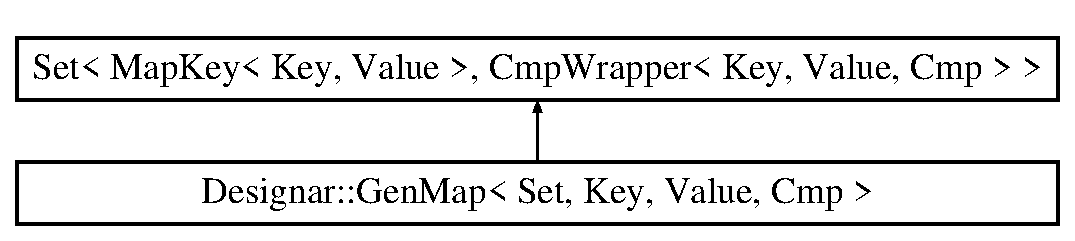
\includegraphics[height=2.000000cm]{class_designar_1_1_gen_map}
\end{center}
\end{figure}
\subsection*{Public Types}
\begin{DoxyCompactItemize}
\item 
using \hyperlink{class_designar_1_1_gen_map_aeb697a86f4ad13eadc36bf5cc967f26f}{Key\+Type} = Key
\item 
using \hyperlink{class_designar_1_1_gen_map_a525bf32010df09e293fa7a0db5a2a8ef}{Value\+Type} = Value
\item 
using \hyperlink{class_designar_1_1_gen_map_ad7fadcebeec688bb447f63c4bfabc61c}{Size\+Type} = \hyperlink{namespace_designar_aa72662848b9f4815e7bf31a7cf3e33d1}{nat\+\_\+t}
\item 
using \hyperlink{class_designar_1_1_gen_map_ac80521be38e4e808bcbeb7041da7d813}{Cmp\+Type} = Cmp
\end{DoxyCompactItemize}
\subsection*{Public Member Functions}
\begin{DoxyCompactItemize}
\item 
Cmp \& \hyperlink{class_designar_1_1_gen_map_a33a00f9275b3ff7788bbd93c39c25c9f}{get\+\_\+cmp} ()
\item 
const Cmp \& \hyperlink{class_designar_1_1_gen_map_a81de02316324ed11c8a668fe2d35d2d3}{get\+\_\+cmp} () const
\item 
Value $\ast$ \hyperlink{class_designar_1_1_gen_map_aaecc59b3f9c206d0d962bd1cd6bfc4d6}{insert} (const Key \&k, const Value \&v)
\item 
Value $\ast$ \hyperlink{class_designar_1_1_gen_map_aabd1f531f63985a2eabbeea49d90156e}{insert} (Key \&\&k, const Value \&v)
\item 
Value $\ast$ \hyperlink{class_designar_1_1_gen_map_a8fc2565be30a92687eea7f752b289751}{insert} (const Key \&k, Value \&\&v)
\item 
Value $\ast$ \hyperlink{class_designar_1_1_gen_map_a514311c4192292ff816931e0c42f929f}{insert} (Key \&\&k, Value \&\&v)
\item 
Value $\ast$ \hyperlink{class_designar_1_1_gen_map_ad5e2c8b57f6264ab98eec3a93e85b1a1}{append} (const Key \&k, const Value \&v)
\item 
Value $\ast$ \hyperlink{class_designar_1_1_gen_map_aeee7a9267c7c54044e7dca399658d9a7}{append} (Key \&\&k, const Value \&v)
\item 
Value $\ast$ \hyperlink{class_designar_1_1_gen_map_a2c148d9d32bc86315444f1026d9ef482}{append} (const Key \&k, Value \&\&v)
\item 
Value $\ast$ \hyperlink{class_designar_1_1_gen_map_a3bb1fd57e4ff94c0e585b41a359d0c52}{append} (Key \&\&k, Value \&\&v)
\item 
Value $\ast$ \hyperlink{class_designar_1_1_gen_map_a6a0eb4fe87d7bcc739f6394d5fd8952e}{search} (const Key \&k)
\item 
Value $\ast$ \hyperlink{class_designar_1_1_gen_map_a1c3b2c788cc8c1a7b59e5afb66fffca4}{search} (Key \&\&k)
\item 
const Value $\ast$ \hyperlink{class_designar_1_1_gen_map_a39037bc9d24b92fdcc7a6289db00e59b}{search} (const Key \&k) const
\item 
const Value $\ast$ \hyperlink{class_designar_1_1_gen_map_a00517c31638c479dca955b9204a2275e}{search} (Key \&\&k) const
\item 
Value $\ast$ \hyperlink{class_designar_1_1_gen_map_a204d7e2d2d8d97cec886e60f4d4d22ec}{search\+\_\+or\+\_\+insert} (const Key \&k, const Value \&v)
\item 
Value $\ast$ \hyperlink{class_designar_1_1_gen_map_a12c2b26187291c9553ff36e8c00bce4b}{search\+\_\+or\+\_\+insert} (Key \&\&k, const Value \&v)
\item 
Value $\ast$ \hyperlink{class_designar_1_1_gen_map_a17eac83eb57f8181aaaeeda18d155f31}{search\+\_\+or\+\_\+insert} (const Key \&k, Value \&\&v)
\item 
Value $\ast$ \hyperlink{class_designar_1_1_gen_map_a3244d12da4c9186ea2c1eef6ad0cbdc9}{search\+\_\+or\+\_\+insert} (Key \&\&k, Value \&\&v)
\item 
Value $\ast$ \hyperlink{class_designar_1_1_gen_map_a4ccec29a17c547692c25f3185187d7bd}{search\+\_\+or\+\_\+insert} (const Key \&k)
\item 
Value $\ast$ \hyperlink{class_designar_1_1_gen_map_ae2ab69b26f782abcd99f99944253d8de}{search\+\_\+or\+\_\+insert} (Key \&\&k)
\item 
Value \& \hyperlink{class_designar_1_1_gen_map_ad768d9e00839f4d328a1394ffc806d83}{find} (const Key \&k)
\item 
const Value \& \hyperlink{class_designar_1_1_gen_map_a0df2bf3aab592ee2343bc2855839bc96}{find} (const Key \&k) const
\item 
Value \& \hyperlink{class_designar_1_1_gen_map_ae02aaa8835abada7b361da281c6125bf}{find} (Key \&\&k)
\item 
const Value \& \hyperlink{class_designar_1_1_gen_map_a746797ad728a5e2aeefee11a8732a48f}{find} (Key \&\&k) const
\item 
bool \hyperlink{class_designar_1_1_gen_map_a9d4608ebd3b589a6989d838979a7b2e7}{remove} (const Key \&k)
\item 
Value \& \hyperlink{class_designar_1_1_gen_map_a994a7afc52e7421661f2eed7c03e6ae7}{operator\mbox{[}$\,$\mbox{]}} (const Key \&k)
\item 
const Value \& \hyperlink{class_designar_1_1_gen_map_abff00b60a0488eb655696942069eacbc}{operator\mbox{[}$\,$\mbox{]}} (const Key \&k) const
\item 
Value \& \hyperlink{class_designar_1_1_gen_map_a5e5732a2812ff86e6c5e68f26012cc9c}{operator\mbox{[}$\,$\mbox{]}} (Key \&\&k)
\item 
const Value \& \hyperlink{class_designar_1_1_gen_map_ac28a9a47f9d373466fe64c6a16105e74}{operator\mbox{[}$\,$\mbox{]}} (Key \&\&k) const
\end{DoxyCompactItemize}


\subsection{Detailed Description}
\subsubsection*{template$<$template$<$ typename, class $>$ class Set, typename Key, typename Value, class Cmp$>$\newline
class Designar\+::\+Gen\+Map$<$ Set, Key, Value, Cmp $>$}



Definition at line 166 of file map.\+H.



\subsection{Member Typedef Documentation}
\mbox{\Hypertarget{class_designar_1_1_gen_map_ac80521be38e4e808bcbeb7041da7d813}\label{class_designar_1_1_gen_map_ac80521be38e4e808bcbeb7041da7d813}} 
\index{Designar\+::\+Gen\+Map@{Designar\+::\+Gen\+Map}!Cmp\+Type@{Cmp\+Type}}
\index{Cmp\+Type@{Cmp\+Type}!Designar\+::\+Gen\+Map@{Designar\+::\+Gen\+Map}}
\subsubsection{\texorpdfstring{Cmp\+Type}{CmpType}}
{\footnotesize\ttfamily template$<$template$<$ typename, class $>$ class Set, typename Key, typename Value, class Cmp$>$ \\
using \hyperlink{class_designar_1_1_gen_map}{Designar\+::\+Gen\+Map}$<$ Set, Key, Value, Cmp $>$\+::\hyperlink{class_designar_1_1_gen_map_ac80521be38e4e808bcbeb7041da7d813}{Cmp\+Type} =  Cmp}



Definition at line 177 of file map.\+H.

\mbox{\Hypertarget{class_designar_1_1_gen_map_aeb697a86f4ad13eadc36bf5cc967f26f}\label{class_designar_1_1_gen_map_aeb697a86f4ad13eadc36bf5cc967f26f}} 
\index{Designar\+::\+Gen\+Map@{Designar\+::\+Gen\+Map}!Key\+Type@{Key\+Type}}
\index{Key\+Type@{Key\+Type}!Designar\+::\+Gen\+Map@{Designar\+::\+Gen\+Map}}
\subsubsection{\texorpdfstring{Key\+Type}{KeyType}}
{\footnotesize\ttfamily template$<$template$<$ typename, class $>$ class Set, typename Key, typename Value, class Cmp$>$ \\
using \hyperlink{class_designar_1_1_gen_map}{Designar\+::\+Gen\+Map}$<$ Set, Key, Value, Cmp $>$\+::\hyperlink{class_designar_1_1_gen_map_aeb697a86f4ad13eadc36bf5cc967f26f}{Key\+Type} =  Key}



Definition at line 174 of file map.\+H.

\mbox{\Hypertarget{class_designar_1_1_gen_map_ad7fadcebeec688bb447f63c4bfabc61c}\label{class_designar_1_1_gen_map_ad7fadcebeec688bb447f63c4bfabc61c}} 
\index{Designar\+::\+Gen\+Map@{Designar\+::\+Gen\+Map}!Size\+Type@{Size\+Type}}
\index{Size\+Type@{Size\+Type}!Designar\+::\+Gen\+Map@{Designar\+::\+Gen\+Map}}
\subsubsection{\texorpdfstring{Size\+Type}{SizeType}}
{\footnotesize\ttfamily template$<$template$<$ typename, class $>$ class Set, typename Key, typename Value, class Cmp$>$ \\
using \hyperlink{class_designar_1_1_gen_map}{Designar\+::\+Gen\+Map}$<$ Set, Key, Value, Cmp $>$\+::\hyperlink{class_designar_1_1_gen_map_ad7fadcebeec688bb447f63c4bfabc61c}{Size\+Type} =  \hyperlink{namespace_designar_aa72662848b9f4815e7bf31a7cf3e33d1}{nat\+\_\+t}}



Definition at line 176 of file map.\+H.

\mbox{\Hypertarget{class_designar_1_1_gen_map_a525bf32010df09e293fa7a0db5a2a8ef}\label{class_designar_1_1_gen_map_a525bf32010df09e293fa7a0db5a2a8ef}} 
\index{Designar\+::\+Gen\+Map@{Designar\+::\+Gen\+Map}!Value\+Type@{Value\+Type}}
\index{Value\+Type@{Value\+Type}!Designar\+::\+Gen\+Map@{Designar\+::\+Gen\+Map}}
\subsubsection{\texorpdfstring{Value\+Type}{ValueType}}
{\footnotesize\ttfamily template$<$template$<$ typename, class $>$ class Set, typename Key, typename Value, class Cmp$>$ \\
using \hyperlink{class_designar_1_1_gen_map}{Designar\+::\+Gen\+Map}$<$ Set, Key, Value, Cmp $>$\+::\hyperlink{class_designar_1_1_gen_map_a525bf32010df09e293fa7a0db5a2a8ef}{Value\+Type} =  Value}



Definition at line 175 of file map.\+H.



\subsection{Member Function Documentation}
\mbox{\Hypertarget{class_designar_1_1_gen_map_ad5e2c8b57f6264ab98eec3a93e85b1a1}\label{class_designar_1_1_gen_map_ad5e2c8b57f6264ab98eec3a93e85b1a1}} 
\index{Designar\+::\+Gen\+Map@{Designar\+::\+Gen\+Map}!append@{append}}
\index{append@{append}!Designar\+::\+Gen\+Map@{Designar\+::\+Gen\+Map}}
\subsubsection{\texorpdfstring{append()}{append()}\hspace{0.1cm}{\footnotesize\ttfamily [1/4]}}
{\footnotesize\ttfamily template$<$template$<$ typename, class $>$ class Set, typename Key, typename Value, class Cmp$>$ \\
Value$\ast$ \hyperlink{class_designar_1_1_gen_map}{Designar\+::\+Gen\+Map}$<$ Set, Key, Value, Cmp $>$\+::append (\begin{DoxyParamCaption}\item[{const Key \&}]{k,  }\item[{const Value \&}]{v }\end{DoxyParamCaption})\hspace{0.3cm}{\ttfamily [inline]}}



Definition at line 237 of file map.\+H.

\mbox{\Hypertarget{class_designar_1_1_gen_map_aeee7a9267c7c54044e7dca399658d9a7}\label{class_designar_1_1_gen_map_aeee7a9267c7c54044e7dca399658d9a7}} 
\index{Designar\+::\+Gen\+Map@{Designar\+::\+Gen\+Map}!append@{append}}
\index{append@{append}!Designar\+::\+Gen\+Map@{Designar\+::\+Gen\+Map}}
\subsubsection{\texorpdfstring{append()}{append()}\hspace{0.1cm}{\footnotesize\ttfamily [2/4]}}
{\footnotesize\ttfamily template$<$template$<$ typename, class $>$ class Set, typename Key, typename Value, class Cmp$>$ \\
Value$\ast$ \hyperlink{class_designar_1_1_gen_map}{Designar\+::\+Gen\+Map}$<$ Set, Key, Value, Cmp $>$\+::append (\begin{DoxyParamCaption}\item[{Key \&\&}]{k,  }\item[{const Value \&}]{v }\end{DoxyParamCaption})\hspace{0.3cm}{\ttfamily [inline]}}



Definition at line 242 of file map.\+H.

\mbox{\Hypertarget{class_designar_1_1_gen_map_a2c148d9d32bc86315444f1026d9ef482}\label{class_designar_1_1_gen_map_a2c148d9d32bc86315444f1026d9ef482}} 
\index{Designar\+::\+Gen\+Map@{Designar\+::\+Gen\+Map}!append@{append}}
\index{append@{append}!Designar\+::\+Gen\+Map@{Designar\+::\+Gen\+Map}}
\subsubsection{\texorpdfstring{append()}{append()}\hspace{0.1cm}{\footnotesize\ttfamily [3/4]}}
{\footnotesize\ttfamily template$<$template$<$ typename, class $>$ class Set, typename Key, typename Value, class Cmp$>$ \\
Value$\ast$ \hyperlink{class_designar_1_1_gen_map}{Designar\+::\+Gen\+Map}$<$ Set, Key, Value, Cmp $>$\+::append (\begin{DoxyParamCaption}\item[{const Key \&}]{k,  }\item[{Value \&\&}]{v }\end{DoxyParamCaption})\hspace{0.3cm}{\ttfamily [inline]}}



Definition at line 247 of file map.\+H.

\mbox{\Hypertarget{class_designar_1_1_gen_map_a3bb1fd57e4ff94c0e585b41a359d0c52}\label{class_designar_1_1_gen_map_a3bb1fd57e4ff94c0e585b41a359d0c52}} 
\index{Designar\+::\+Gen\+Map@{Designar\+::\+Gen\+Map}!append@{append}}
\index{append@{append}!Designar\+::\+Gen\+Map@{Designar\+::\+Gen\+Map}}
\subsubsection{\texorpdfstring{append()}{append()}\hspace{0.1cm}{\footnotesize\ttfamily [4/4]}}
{\footnotesize\ttfamily template$<$template$<$ typename, class $>$ class Set, typename Key, typename Value, class Cmp$>$ \\
Value$\ast$ \hyperlink{class_designar_1_1_gen_map}{Designar\+::\+Gen\+Map}$<$ Set, Key, Value, Cmp $>$\+::append (\begin{DoxyParamCaption}\item[{Key \&\&}]{k,  }\item[{Value \&\&}]{v }\end{DoxyParamCaption})\hspace{0.3cm}{\ttfamily [inline]}}



Definition at line 252 of file map.\+H.

\mbox{\Hypertarget{class_designar_1_1_gen_map_ad768d9e00839f4d328a1394ffc806d83}\label{class_designar_1_1_gen_map_ad768d9e00839f4d328a1394ffc806d83}} 
\index{Designar\+::\+Gen\+Map@{Designar\+::\+Gen\+Map}!find@{find}}
\index{find@{find}!Designar\+::\+Gen\+Map@{Designar\+::\+Gen\+Map}}
\subsubsection{\texorpdfstring{find()}{find()}\hspace{0.1cm}{\footnotesize\ttfamily [1/4]}}
{\footnotesize\ttfamily template$<$template$<$ typename, class $>$ class Set, typename Key, typename Value, class Cmp$>$ \\
Value\& \hyperlink{class_designar_1_1_gen_map}{Designar\+::\+Gen\+Map}$<$ Set, Key, Value, Cmp $>$\+::find (\begin{DoxyParamCaption}\item[{const Key \&}]{k }\end{DoxyParamCaption})\hspace{0.3cm}{\ttfamily [inline]}}



Definition at line 339 of file map.\+H.

\mbox{\Hypertarget{class_designar_1_1_gen_map_a0df2bf3aab592ee2343bc2855839bc96}\label{class_designar_1_1_gen_map_a0df2bf3aab592ee2343bc2855839bc96}} 
\index{Designar\+::\+Gen\+Map@{Designar\+::\+Gen\+Map}!find@{find}}
\index{find@{find}!Designar\+::\+Gen\+Map@{Designar\+::\+Gen\+Map}}
\subsubsection{\texorpdfstring{find()}{find()}\hspace{0.1cm}{\footnotesize\ttfamily [2/4]}}
{\footnotesize\ttfamily template$<$template$<$ typename, class $>$ class Set, typename Key, typename Value, class Cmp$>$ \\
const Value\& \hyperlink{class_designar_1_1_gen_map}{Designar\+::\+Gen\+Map}$<$ Set, Key, Value, Cmp $>$\+::find (\begin{DoxyParamCaption}\item[{const Key \&}]{k }\end{DoxyParamCaption}) const\hspace{0.3cm}{\ttfamily [inline]}}



Definition at line 345 of file map.\+H.

\mbox{\Hypertarget{class_designar_1_1_gen_map_ae02aaa8835abada7b361da281c6125bf}\label{class_designar_1_1_gen_map_ae02aaa8835abada7b361da281c6125bf}} 
\index{Designar\+::\+Gen\+Map@{Designar\+::\+Gen\+Map}!find@{find}}
\index{find@{find}!Designar\+::\+Gen\+Map@{Designar\+::\+Gen\+Map}}
\subsubsection{\texorpdfstring{find()}{find()}\hspace{0.1cm}{\footnotesize\ttfamily [3/4]}}
{\footnotesize\ttfamily template$<$template$<$ typename, class $>$ class Set, typename Key, typename Value, class Cmp$>$ \\
Value\& \hyperlink{class_designar_1_1_gen_map}{Designar\+::\+Gen\+Map}$<$ Set, Key, Value, Cmp $>$\+::find (\begin{DoxyParamCaption}\item[{Key \&\&}]{k }\end{DoxyParamCaption})\hspace{0.3cm}{\ttfamily [inline]}}



Definition at line 351 of file map.\+H.

\mbox{\Hypertarget{class_designar_1_1_gen_map_a746797ad728a5e2aeefee11a8732a48f}\label{class_designar_1_1_gen_map_a746797ad728a5e2aeefee11a8732a48f}} 
\index{Designar\+::\+Gen\+Map@{Designar\+::\+Gen\+Map}!find@{find}}
\index{find@{find}!Designar\+::\+Gen\+Map@{Designar\+::\+Gen\+Map}}
\subsubsection{\texorpdfstring{find()}{find()}\hspace{0.1cm}{\footnotesize\ttfamily [4/4]}}
{\footnotesize\ttfamily template$<$template$<$ typename, class $>$ class Set, typename Key, typename Value, class Cmp$>$ \\
const Value\& \hyperlink{class_designar_1_1_gen_map}{Designar\+::\+Gen\+Map}$<$ Set, Key, Value, Cmp $>$\+::find (\begin{DoxyParamCaption}\item[{Key \&\&}]{k }\end{DoxyParamCaption}) const\hspace{0.3cm}{\ttfamily [inline]}}



Definition at line 357 of file map.\+H.

\mbox{\Hypertarget{class_designar_1_1_gen_map_a33a00f9275b3ff7788bbd93c39c25c9f}\label{class_designar_1_1_gen_map_a33a00f9275b3ff7788bbd93c39c25c9f}} 
\index{Designar\+::\+Gen\+Map@{Designar\+::\+Gen\+Map}!get\+\_\+cmp@{get\+\_\+cmp}}
\index{get\+\_\+cmp@{get\+\_\+cmp}!Designar\+::\+Gen\+Map@{Designar\+::\+Gen\+Map}}
\subsubsection{\texorpdfstring{get\+\_\+cmp()}{get\_cmp()}\hspace{0.1cm}{\footnotesize\ttfamily [1/2]}}
{\footnotesize\ttfamily template$<$template$<$ typename, class $>$ class Set, typename Key, typename Value, class Cmp$>$ \\
Cmp\& \hyperlink{class_designar_1_1_gen_map}{Designar\+::\+Gen\+Map}$<$ Set, Key, Value, Cmp $>$\+::get\+\_\+cmp (\begin{DoxyParamCaption}{ }\end{DoxyParamCaption})\hspace{0.3cm}{\ttfamily [inline]}}



Definition at line 179 of file map.\+H.

\mbox{\Hypertarget{class_designar_1_1_gen_map_a81de02316324ed11c8a668fe2d35d2d3}\label{class_designar_1_1_gen_map_a81de02316324ed11c8a668fe2d35d2d3}} 
\index{Designar\+::\+Gen\+Map@{Designar\+::\+Gen\+Map}!get\+\_\+cmp@{get\+\_\+cmp}}
\index{get\+\_\+cmp@{get\+\_\+cmp}!Designar\+::\+Gen\+Map@{Designar\+::\+Gen\+Map}}
\subsubsection{\texorpdfstring{get\+\_\+cmp()}{get\_cmp()}\hspace{0.1cm}{\footnotesize\ttfamily [2/2]}}
{\footnotesize\ttfamily template$<$template$<$ typename, class $>$ class Set, typename Key, typename Value, class Cmp$>$ \\
const Cmp\& \hyperlink{class_designar_1_1_gen_map}{Designar\+::\+Gen\+Map}$<$ Set, Key, Value, Cmp $>$\+::get\+\_\+cmp (\begin{DoxyParamCaption}{ }\end{DoxyParamCaption}) const\hspace{0.3cm}{\ttfamily [inline]}}



Definition at line 184 of file map.\+H.

\mbox{\Hypertarget{class_designar_1_1_gen_map_aaecc59b3f9c206d0d962bd1cd6bfc4d6}\label{class_designar_1_1_gen_map_aaecc59b3f9c206d0d962bd1cd6bfc4d6}} 
\index{Designar\+::\+Gen\+Map@{Designar\+::\+Gen\+Map}!insert@{insert}}
\index{insert@{insert}!Designar\+::\+Gen\+Map@{Designar\+::\+Gen\+Map}}
\subsubsection{\texorpdfstring{insert()}{insert()}\hspace{0.1cm}{\footnotesize\ttfamily [1/4]}}
{\footnotesize\ttfamily template$<$template$<$ typename, class $>$ class Set, typename Key, typename Value, class Cmp$>$ \\
Value$\ast$ \hyperlink{class_designar_1_1_gen_map}{Designar\+::\+Gen\+Map}$<$ Set, Key, Value, Cmp $>$\+::insert (\begin{DoxyParamCaption}\item[{const Key \&}]{k,  }\item[{const Value \&}]{v }\end{DoxyParamCaption})\hspace{0.3cm}{\ttfamily [inline]}}



Definition at line 189 of file map.\+H.

\mbox{\Hypertarget{class_designar_1_1_gen_map_aabd1f531f63985a2eabbeea49d90156e}\label{class_designar_1_1_gen_map_aabd1f531f63985a2eabbeea49d90156e}} 
\index{Designar\+::\+Gen\+Map@{Designar\+::\+Gen\+Map}!insert@{insert}}
\index{insert@{insert}!Designar\+::\+Gen\+Map@{Designar\+::\+Gen\+Map}}
\subsubsection{\texorpdfstring{insert()}{insert()}\hspace{0.1cm}{\footnotesize\ttfamily [2/4]}}
{\footnotesize\ttfamily template$<$template$<$ typename, class $>$ class Set, typename Key, typename Value, class Cmp$>$ \\
Value$\ast$ \hyperlink{class_designar_1_1_gen_map}{Designar\+::\+Gen\+Map}$<$ Set, Key, Value, Cmp $>$\+::insert (\begin{DoxyParamCaption}\item[{Key \&\&}]{k,  }\item[{const Value \&}]{v }\end{DoxyParamCaption})\hspace{0.3cm}{\ttfamily [inline]}}



Definition at line 201 of file map.\+H.

\mbox{\Hypertarget{class_designar_1_1_gen_map_a8fc2565be30a92687eea7f752b289751}\label{class_designar_1_1_gen_map_a8fc2565be30a92687eea7f752b289751}} 
\index{Designar\+::\+Gen\+Map@{Designar\+::\+Gen\+Map}!insert@{insert}}
\index{insert@{insert}!Designar\+::\+Gen\+Map@{Designar\+::\+Gen\+Map}}
\subsubsection{\texorpdfstring{insert()}{insert()}\hspace{0.1cm}{\footnotesize\ttfamily [3/4]}}
{\footnotesize\ttfamily template$<$template$<$ typename, class $>$ class Set, typename Key, typename Value, class Cmp$>$ \\
Value$\ast$ \hyperlink{class_designar_1_1_gen_map}{Designar\+::\+Gen\+Map}$<$ Set, Key, Value, Cmp $>$\+::insert (\begin{DoxyParamCaption}\item[{const Key \&}]{k,  }\item[{Value \&\&}]{v }\end{DoxyParamCaption})\hspace{0.3cm}{\ttfamily [inline]}}



Definition at line 213 of file map.\+H.

\mbox{\Hypertarget{class_designar_1_1_gen_map_a514311c4192292ff816931e0c42f929f}\label{class_designar_1_1_gen_map_a514311c4192292ff816931e0c42f929f}} 
\index{Designar\+::\+Gen\+Map@{Designar\+::\+Gen\+Map}!insert@{insert}}
\index{insert@{insert}!Designar\+::\+Gen\+Map@{Designar\+::\+Gen\+Map}}
\subsubsection{\texorpdfstring{insert()}{insert()}\hspace{0.1cm}{\footnotesize\ttfamily [4/4]}}
{\footnotesize\ttfamily template$<$template$<$ typename, class $>$ class Set, typename Key, typename Value, class Cmp$>$ \\
Value$\ast$ \hyperlink{class_designar_1_1_gen_map}{Designar\+::\+Gen\+Map}$<$ Set, Key, Value, Cmp $>$\+::insert (\begin{DoxyParamCaption}\item[{Key \&\&}]{k,  }\item[{Value \&\&}]{v }\end{DoxyParamCaption})\hspace{0.3cm}{\ttfamily [inline]}}



Definition at line 225 of file map.\+H.

\mbox{\Hypertarget{class_designar_1_1_gen_map_a994a7afc52e7421661f2eed7c03e6ae7}\label{class_designar_1_1_gen_map_a994a7afc52e7421661f2eed7c03e6ae7}} 
\index{Designar\+::\+Gen\+Map@{Designar\+::\+Gen\+Map}!operator\mbox{[}\mbox{]}@{operator[]}}
\index{operator\mbox{[}\mbox{]}@{operator[]}!Designar\+::\+Gen\+Map@{Designar\+::\+Gen\+Map}}
\subsubsection{\texorpdfstring{operator[]()}{operator[]()}\hspace{0.1cm}{\footnotesize\ttfamily [1/4]}}
{\footnotesize\ttfamily template$<$template$<$ typename, class $>$ class Set, typename Key, typename Value, class Cmp$>$ \\
Value\& \hyperlink{class_designar_1_1_gen_map}{Designar\+::\+Gen\+Map}$<$ Set, Key, Value, Cmp $>$\+::operator\mbox{[}$\,$\mbox{]} (\begin{DoxyParamCaption}\item[{const Key \&}]{k }\end{DoxyParamCaption})\hspace{0.3cm}{\ttfamily [inline]}}



Definition at line 369 of file map.\+H.

\mbox{\Hypertarget{class_designar_1_1_gen_map_abff00b60a0488eb655696942069eacbc}\label{class_designar_1_1_gen_map_abff00b60a0488eb655696942069eacbc}} 
\index{Designar\+::\+Gen\+Map@{Designar\+::\+Gen\+Map}!operator\mbox{[}\mbox{]}@{operator[]}}
\index{operator\mbox{[}\mbox{]}@{operator[]}!Designar\+::\+Gen\+Map@{Designar\+::\+Gen\+Map}}
\subsubsection{\texorpdfstring{operator[]()}{operator[]()}\hspace{0.1cm}{\footnotesize\ttfamily [2/4]}}
{\footnotesize\ttfamily template$<$template$<$ typename, class $>$ class Set, typename Key, typename Value, class Cmp$>$ \\
const Value\& \hyperlink{class_designar_1_1_gen_map}{Designar\+::\+Gen\+Map}$<$ Set, Key, Value, Cmp $>$\+::operator\mbox{[}$\,$\mbox{]} (\begin{DoxyParamCaption}\item[{const Key \&}]{k }\end{DoxyParamCaption}) const\hspace{0.3cm}{\ttfamily [inline]}}



Definition at line 374 of file map.\+H.

\mbox{\Hypertarget{class_designar_1_1_gen_map_a5e5732a2812ff86e6c5e68f26012cc9c}\label{class_designar_1_1_gen_map_a5e5732a2812ff86e6c5e68f26012cc9c}} 
\index{Designar\+::\+Gen\+Map@{Designar\+::\+Gen\+Map}!operator\mbox{[}\mbox{]}@{operator[]}}
\index{operator\mbox{[}\mbox{]}@{operator[]}!Designar\+::\+Gen\+Map@{Designar\+::\+Gen\+Map}}
\subsubsection{\texorpdfstring{operator[]()}{operator[]()}\hspace{0.1cm}{\footnotesize\ttfamily [3/4]}}
{\footnotesize\ttfamily template$<$template$<$ typename, class $>$ class Set, typename Key, typename Value, class Cmp$>$ \\
Value\& \hyperlink{class_designar_1_1_gen_map}{Designar\+::\+Gen\+Map}$<$ Set, Key, Value, Cmp $>$\+::operator\mbox{[}$\,$\mbox{]} (\begin{DoxyParamCaption}\item[{Key \&\&}]{k }\end{DoxyParamCaption})\hspace{0.3cm}{\ttfamily [inline]}}



Definition at line 379 of file map.\+H.

\mbox{\Hypertarget{class_designar_1_1_gen_map_ac28a9a47f9d373466fe64c6a16105e74}\label{class_designar_1_1_gen_map_ac28a9a47f9d373466fe64c6a16105e74}} 
\index{Designar\+::\+Gen\+Map@{Designar\+::\+Gen\+Map}!operator\mbox{[}\mbox{]}@{operator[]}}
\index{operator\mbox{[}\mbox{]}@{operator[]}!Designar\+::\+Gen\+Map@{Designar\+::\+Gen\+Map}}
\subsubsection{\texorpdfstring{operator[]()}{operator[]()}\hspace{0.1cm}{\footnotesize\ttfamily [4/4]}}
{\footnotesize\ttfamily template$<$template$<$ typename, class $>$ class Set, typename Key, typename Value, class Cmp$>$ \\
const Value\& \hyperlink{class_designar_1_1_gen_map}{Designar\+::\+Gen\+Map}$<$ Set, Key, Value, Cmp $>$\+::operator\mbox{[}$\,$\mbox{]} (\begin{DoxyParamCaption}\item[{Key \&\&}]{k }\end{DoxyParamCaption}) const\hspace{0.3cm}{\ttfamily [inline]}}



Definition at line 384 of file map.\+H.

\mbox{\Hypertarget{class_designar_1_1_gen_map_a9d4608ebd3b589a6989d838979a7b2e7}\label{class_designar_1_1_gen_map_a9d4608ebd3b589a6989d838979a7b2e7}} 
\index{Designar\+::\+Gen\+Map@{Designar\+::\+Gen\+Map}!remove@{remove}}
\index{remove@{remove}!Designar\+::\+Gen\+Map@{Designar\+::\+Gen\+Map}}
\subsubsection{\texorpdfstring{remove()}{remove()}}
{\footnotesize\ttfamily template$<$template$<$ typename, class $>$ class Set, typename Key, typename Value, class Cmp$>$ \\
bool \hyperlink{class_designar_1_1_gen_map}{Designar\+::\+Gen\+Map}$<$ Set, Key, Value, Cmp $>$\+::remove (\begin{DoxyParamCaption}\item[{const Key \&}]{k }\end{DoxyParamCaption})\hspace{0.3cm}{\ttfamily [inline]}}



Definition at line 363 of file map.\+H.

\mbox{\Hypertarget{class_designar_1_1_gen_map_a6a0eb4fe87d7bcc739f6394d5fd8952e}\label{class_designar_1_1_gen_map_a6a0eb4fe87d7bcc739f6394d5fd8952e}} 
\index{Designar\+::\+Gen\+Map@{Designar\+::\+Gen\+Map}!search@{search}}
\index{search@{search}!Designar\+::\+Gen\+Map@{Designar\+::\+Gen\+Map}}
\subsubsection{\texorpdfstring{search()}{search()}\hspace{0.1cm}{\footnotesize\ttfamily [1/4]}}
{\footnotesize\ttfamily template$<$template$<$ typename, class $>$ class Set, typename Key, typename Value, class Cmp$>$ \\
Value$\ast$ \hyperlink{class_designar_1_1_gen_map}{Designar\+::\+Gen\+Map}$<$ Set, Key, Value, Cmp $>$\+::search (\begin{DoxyParamCaption}\item[{const Key \&}]{k }\end{DoxyParamCaption})\hspace{0.3cm}{\ttfamily [inline]}}



Definition at line 257 of file map.\+H.

\mbox{\Hypertarget{class_designar_1_1_gen_map_a1c3b2c788cc8c1a7b59e5afb66fffca4}\label{class_designar_1_1_gen_map_a1c3b2c788cc8c1a7b59e5afb66fffca4}} 
\index{Designar\+::\+Gen\+Map@{Designar\+::\+Gen\+Map}!search@{search}}
\index{search@{search}!Designar\+::\+Gen\+Map@{Designar\+::\+Gen\+Map}}
\subsubsection{\texorpdfstring{search()}{search()}\hspace{0.1cm}{\footnotesize\ttfamily [2/4]}}
{\footnotesize\ttfamily template$<$template$<$ typename, class $>$ class Set, typename Key, typename Value, class Cmp$>$ \\
Value$\ast$ \hyperlink{class_designar_1_1_gen_map}{Designar\+::\+Gen\+Map}$<$ Set, Key, Value, Cmp $>$\+::search (\begin{DoxyParamCaption}\item[{Key \&\&}]{k }\end{DoxyParamCaption})\hspace{0.3cm}{\ttfamily [inline]}}



Definition at line 269 of file map.\+H.

\mbox{\Hypertarget{class_designar_1_1_gen_map_a39037bc9d24b92fdcc7a6289db00e59b}\label{class_designar_1_1_gen_map_a39037bc9d24b92fdcc7a6289db00e59b}} 
\index{Designar\+::\+Gen\+Map@{Designar\+::\+Gen\+Map}!search@{search}}
\index{search@{search}!Designar\+::\+Gen\+Map@{Designar\+::\+Gen\+Map}}
\subsubsection{\texorpdfstring{search()}{search()}\hspace{0.1cm}{\footnotesize\ttfamily [3/4]}}
{\footnotesize\ttfamily template$<$template$<$ typename, class $>$ class Set, typename Key, typename Value, class Cmp$>$ \\
const Value$\ast$ \hyperlink{class_designar_1_1_gen_map}{Designar\+::\+Gen\+Map}$<$ Set, Key, Value, Cmp $>$\+::search (\begin{DoxyParamCaption}\item[{const Key \&}]{k }\end{DoxyParamCaption}) const\hspace{0.3cm}{\ttfamily [inline]}}



Definition at line 281 of file map.\+H.

\mbox{\Hypertarget{class_designar_1_1_gen_map_a00517c31638c479dca955b9204a2275e}\label{class_designar_1_1_gen_map_a00517c31638c479dca955b9204a2275e}} 
\index{Designar\+::\+Gen\+Map@{Designar\+::\+Gen\+Map}!search@{search}}
\index{search@{search}!Designar\+::\+Gen\+Map@{Designar\+::\+Gen\+Map}}
\subsubsection{\texorpdfstring{search()}{search()}\hspace{0.1cm}{\footnotesize\ttfamily [4/4]}}
{\footnotesize\ttfamily template$<$template$<$ typename, class $>$ class Set, typename Key, typename Value, class Cmp$>$ \\
const Value$\ast$ \hyperlink{class_designar_1_1_gen_map}{Designar\+::\+Gen\+Map}$<$ Set, Key, Value, Cmp $>$\+::search (\begin{DoxyParamCaption}\item[{Key \&\&}]{k }\end{DoxyParamCaption}) const\hspace{0.3cm}{\ttfamily [inline]}}



Definition at line 293 of file map.\+H.

\mbox{\Hypertarget{class_designar_1_1_gen_map_a204d7e2d2d8d97cec886e60f4d4d22ec}\label{class_designar_1_1_gen_map_a204d7e2d2d8d97cec886e60f4d4d22ec}} 
\index{Designar\+::\+Gen\+Map@{Designar\+::\+Gen\+Map}!search\+\_\+or\+\_\+insert@{search\+\_\+or\+\_\+insert}}
\index{search\+\_\+or\+\_\+insert@{search\+\_\+or\+\_\+insert}!Designar\+::\+Gen\+Map@{Designar\+::\+Gen\+Map}}
\subsubsection{\texorpdfstring{search\+\_\+or\+\_\+insert()}{search\_or\_insert()}\hspace{0.1cm}{\footnotesize\ttfamily [1/6]}}
{\footnotesize\ttfamily template$<$template$<$ typename, class $>$ class Set, typename Key, typename Value, class Cmp$>$ \\
Value$\ast$ \hyperlink{class_designar_1_1_gen_map}{Designar\+::\+Gen\+Map}$<$ Set, Key, Value, Cmp $>$\+::search\+\_\+or\+\_\+insert (\begin{DoxyParamCaption}\item[{const Key \&}]{k,  }\item[{const Value \&}]{v }\end{DoxyParamCaption})\hspace{0.3cm}{\ttfamily [inline]}}



Definition at line 305 of file map.\+H.

\mbox{\Hypertarget{class_designar_1_1_gen_map_a12c2b26187291c9553ff36e8c00bce4b}\label{class_designar_1_1_gen_map_a12c2b26187291c9553ff36e8c00bce4b}} 
\index{Designar\+::\+Gen\+Map@{Designar\+::\+Gen\+Map}!search\+\_\+or\+\_\+insert@{search\+\_\+or\+\_\+insert}}
\index{search\+\_\+or\+\_\+insert@{search\+\_\+or\+\_\+insert}!Designar\+::\+Gen\+Map@{Designar\+::\+Gen\+Map}}
\subsubsection{\texorpdfstring{search\+\_\+or\+\_\+insert()}{search\_or\_insert()}\hspace{0.1cm}{\footnotesize\ttfamily [2/6]}}
{\footnotesize\ttfamily template$<$template$<$ typename, class $>$ class Set, typename Key, typename Value, class Cmp$>$ \\
Value$\ast$ \hyperlink{class_designar_1_1_gen_map}{Designar\+::\+Gen\+Map}$<$ Set, Key, Value, Cmp $>$\+::search\+\_\+or\+\_\+insert (\begin{DoxyParamCaption}\item[{Key \&\&}]{k,  }\item[{const Value \&}]{v }\end{DoxyParamCaption})\hspace{0.3cm}{\ttfamily [inline]}}



Definition at line 311 of file map.\+H.

\mbox{\Hypertarget{class_designar_1_1_gen_map_a17eac83eb57f8181aaaeeda18d155f31}\label{class_designar_1_1_gen_map_a17eac83eb57f8181aaaeeda18d155f31}} 
\index{Designar\+::\+Gen\+Map@{Designar\+::\+Gen\+Map}!search\+\_\+or\+\_\+insert@{search\+\_\+or\+\_\+insert}}
\index{search\+\_\+or\+\_\+insert@{search\+\_\+or\+\_\+insert}!Designar\+::\+Gen\+Map@{Designar\+::\+Gen\+Map}}
\subsubsection{\texorpdfstring{search\+\_\+or\+\_\+insert()}{search\_or\_insert()}\hspace{0.1cm}{\footnotesize\ttfamily [3/6]}}
{\footnotesize\ttfamily template$<$template$<$ typename, class $>$ class Set, typename Key, typename Value, class Cmp$>$ \\
Value$\ast$ \hyperlink{class_designar_1_1_gen_map}{Designar\+::\+Gen\+Map}$<$ Set, Key, Value, Cmp $>$\+::search\+\_\+or\+\_\+insert (\begin{DoxyParamCaption}\item[{const Key \&}]{k,  }\item[{Value \&\&}]{v }\end{DoxyParamCaption})\hspace{0.3cm}{\ttfamily [inline]}}



Definition at line 317 of file map.\+H.

\mbox{\Hypertarget{class_designar_1_1_gen_map_a3244d12da4c9186ea2c1eef6ad0cbdc9}\label{class_designar_1_1_gen_map_a3244d12da4c9186ea2c1eef6ad0cbdc9}} 
\index{Designar\+::\+Gen\+Map@{Designar\+::\+Gen\+Map}!search\+\_\+or\+\_\+insert@{search\+\_\+or\+\_\+insert}}
\index{search\+\_\+or\+\_\+insert@{search\+\_\+or\+\_\+insert}!Designar\+::\+Gen\+Map@{Designar\+::\+Gen\+Map}}
\subsubsection{\texorpdfstring{search\+\_\+or\+\_\+insert()}{search\_or\_insert()}\hspace{0.1cm}{\footnotesize\ttfamily [4/6]}}
{\footnotesize\ttfamily template$<$template$<$ typename, class $>$ class Set, typename Key, typename Value, class Cmp$>$ \\
Value$\ast$ \hyperlink{class_designar_1_1_gen_map}{Designar\+::\+Gen\+Map}$<$ Set, Key, Value, Cmp $>$\+::search\+\_\+or\+\_\+insert (\begin{DoxyParamCaption}\item[{Key \&\&}]{k,  }\item[{Value \&\&}]{v }\end{DoxyParamCaption})\hspace{0.3cm}{\ttfamily [inline]}}



Definition at line 323 of file map.\+H.

\mbox{\Hypertarget{class_designar_1_1_gen_map_a4ccec29a17c547692c25f3185187d7bd}\label{class_designar_1_1_gen_map_a4ccec29a17c547692c25f3185187d7bd}} 
\index{Designar\+::\+Gen\+Map@{Designar\+::\+Gen\+Map}!search\+\_\+or\+\_\+insert@{search\+\_\+or\+\_\+insert}}
\index{search\+\_\+or\+\_\+insert@{search\+\_\+or\+\_\+insert}!Designar\+::\+Gen\+Map@{Designar\+::\+Gen\+Map}}
\subsubsection{\texorpdfstring{search\+\_\+or\+\_\+insert()}{search\_or\_insert()}\hspace{0.1cm}{\footnotesize\ttfamily [5/6]}}
{\footnotesize\ttfamily template$<$template$<$ typename, class $>$ class Set, typename Key, typename Value, class Cmp$>$ \\
Value$\ast$ \hyperlink{class_designar_1_1_gen_map}{Designar\+::\+Gen\+Map}$<$ Set, Key, Value, Cmp $>$\+::search\+\_\+or\+\_\+insert (\begin{DoxyParamCaption}\item[{const Key \&}]{k }\end{DoxyParamCaption})\hspace{0.3cm}{\ttfamily [inline]}}



Definition at line 329 of file map.\+H.

\mbox{\Hypertarget{class_designar_1_1_gen_map_ae2ab69b26f782abcd99f99944253d8de}\label{class_designar_1_1_gen_map_ae2ab69b26f782abcd99f99944253d8de}} 
\index{Designar\+::\+Gen\+Map@{Designar\+::\+Gen\+Map}!search\+\_\+or\+\_\+insert@{search\+\_\+or\+\_\+insert}}
\index{search\+\_\+or\+\_\+insert@{search\+\_\+or\+\_\+insert}!Designar\+::\+Gen\+Map@{Designar\+::\+Gen\+Map}}
\subsubsection{\texorpdfstring{search\+\_\+or\+\_\+insert()}{search\_or\_insert()}\hspace{0.1cm}{\footnotesize\ttfamily [6/6]}}
{\footnotesize\ttfamily template$<$template$<$ typename, class $>$ class Set, typename Key, typename Value, class Cmp$>$ \\
Value$\ast$ \hyperlink{class_designar_1_1_gen_map}{Designar\+::\+Gen\+Map}$<$ Set, Key, Value, Cmp $>$\+::search\+\_\+or\+\_\+insert (\begin{DoxyParamCaption}\item[{Key \&\&}]{k }\end{DoxyParamCaption})\hspace{0.3cm}{\ttfamily [inline]}}



Definition at line 334 of file map.\+H.



The documentation for this class was generated from the following file\+:\begin{DoxyCompactItemize}
\item 
De\+Si\+G\+N\+A\+R/include/\hyperlink{map_8_h}{map.\+H}\end{DoxyCompactItemize}

\hypertarget{class_designar_1_1_gen_point2_d}{}\section{Designar\+:\+:Gen\+Point2D$<$ NumT $>$ Class Template Reference}
\label{class_designar_1_1_gen_point2_d}\index{Designar\+::\+Gen\+Point2\+D$<$ Num\+T $>$@{Designar\+::\+Gen\+Point2\+D$<$ Num\+T $>$}}


{\ttfamily \#include $<$math.\+H$>$}

\subsection*{Public Types}
\begin{DoxyCompactItemize}
\item 
using \hyperlink{class_designar_1_1_gen_point2_d_a8d80993f38dab83a39e80a50db08b944}{Component\+Type} = NumT
\item 
using \hyperlink{class_designar_1_1_gen_point2_d_a6ad786447c17adc8cbaece7f12ac2132}{Number\+Type} = NumT
\item 
using \hyperlink{class_designar_1_1_gen_point2_d_a8f13f44ca3438223d1ecdce2728b9437}{Value\+Type} = NumT
\end{DoxyCompactItemize}
\subsection*{Public Member Functions}
\begin{DoxyCompactItemize}
\item 
\hyperlink{class_designar_1_1_gen_point2_d_aa55395ebde205564d3065dc6ce56c42b}{Gen\+Point2D} ()
\item 
\hyperlink{class_designar_1_1_gen_point2_d_adf5298d432b48187deef32941429a1b3}{Gen\+Point2D} (const NumT \&\+\_\+x, const NumT \&\+\_\+y)
\item 
\hyperlink{class_designar_1_1_gen_point2_d_a7e3357422dc01310240f58fed213162d}{Gen\+Point2D} (const NumT \&\+\_\+x, NumT \&\&\+\_\+y)
\item 
\hyperlink{class_designar_1_1_gen_point2_d_ab4e177989279ac6e6f7280644f487cdd}{Gen\+Point2D} (NumT \&\&\+\_\+x, const NumT \&\+\_\+y)
\item 
\hyperlink{class_designar_1_1_gen_point2_d_a420eb654ce7cbb0a9f179c20db4e7c98}{Gen\+Point2D} (NumT \&\&\+\_\+x, NumT \&\&\+\_\+y)
\item 
\hyperlink{class_designar_1_1_gen_point2_d_abb677c76a6cfb8261f562250a15ca879}{Gen\+Point2D} (const \hyperlink{class_designar_1_1_gen_point2_d}{Gen\+Point2D} \&p)
\item 
\hyperlink{class_designar_1_1_gen_point2_d_a025c72ba6681c75f131066d1a5fc5e72}{Gen\+Point2D} (\hyperlink{class_designar_1_1_gen_point2_d}{Gen\+Point2D} \&\&p)
\item 
\hyperlink{class_designar_1_1_gen_point2_d}{Gen\+Point2D} \& \hyperlink{class_designar_1_1_gen_point2_d_a5561fbdf0a23f90f9f3c1fdce25c2f3a}{operator=} (const \hyperlink{class_designar_1_1_gen_point2_d}{Gen\+Point2D} \&p)
\item 
\hyperlink{class_designar_1_1_gen_point2_d}{Gen\+Point2D} \& \hyperlink{class_designar_1_1_gen_point2_d_a83a1f3723cbcdf6fa556e864269a63f6}{operator=} (\hyperlink{class_designar_1_1_gen_point2_d}{Gen\+Point2D} \&\&p)
\item 
void \hyperlink{class_designar_1_1_gen_point2_d_a1068ce1c6fbaa5c448044529ec3659e0}{swap} (\hyperlink{class_designar_1_1_gen_point2_d}{Gen\+Point2D} \&p)
\item 
const NumT \& \hyperlink{class_designar_1_1_gen_point2_d_a5b30afaea1584891bdbe00b72440374b}{get\+\_\+x} () const
\item 
const NumT \& \hyperlink{class_designar_1_1_gen_point2_d_ac8aa7a258e736f715b1e164206316f79}{get\+\_\+y} () const
\item 
void \hyperlink{class_designar_1_1_gen_point2_d_a73d4687bde9246ae64deff4e832acb24}{set\+\_\+x} (const NumT \&\+\_\+x)
\item 
void \hyperlink{class_designar_1_1_gen_point2_d_a584f53cd613dd3401c22e0f4b029d2a9}{set\+\_\+x} (NumT \&\&\+\_\+x)
\item 
void \hyperlink{class_designar_1_1_gen_point2_d_af82a367767d79081e2afe1228fcf2bc6}{set\+\_\+y} (NumT \&\&\+\_\+y)
\item 
void \hyperlink{class_designar_1_1_gen_point2_d_a256d6fda1a250b7a664b76b7c8f914d7}{nullify} ()
\item 
bool \hyperlink{class_designar_1_1_gen_point2_d_aa6c5b4c078b46565646f1bd93dae5bf4}{is\+\_\+null} () const
\item 
bool \hyperlink{class_designar_1_1_gen_point2_d_a75d3dd925cc99701000be4cc0c6967fd}{is\+\_\+zero} () const
\item 
NumT \hyperlink{class_designar_1_1_gen_point2_d_a4c9122867f6fd19991e146e745346075}{square\+\_\+distance\+\_\+with} (const \hyperlink{class_designar_1_1_gen_point2_d}{Gen\+Point2D} \&p) const
\item 
\hyperlink{namespace_designar_aca2c32af26808dbec1f3a3071fad25ce}{real\+\_\+t} \hyperlink{class_designar_1_1_gen_point2_d_a4e7b6cad160caef4b1f5ab8f2b1ad0da}{distance\+\_\+with} (const \hyperlink{class_designar_1_1_gen_point2_d}{Gen\+Point2D} \&p) const
\item 
NumT \hyperlink{class_designar_1_1_gen_point2_d_adda120357e8a76bd42b7cd9517cecaad}{square\+\_\+distance\+\_\+to\+\_\+origin} () const
\item 
NumT \hyperlink{class_designar_1_1_gen_point2_d_a91bb9e8b5022b06a407ebdda4dabb220}{distance\+\_\+to\+\_\+origin} () const
\item 
bool \hyperlink{class_designar_1_1_gen_point2_d_acb12e43d036b0a5719af3887814a2684}{is\+\_\+to\+\_\+right\+\_\+from} (const \hyperlink{class_designar_1_1_gen_point2_d}{Gen\+Point2D} \&p, const \hyperlink{class_designar_1_1_gen_point2_d}{Gen\+Point2D} \&q) const
\item 
bool \hyperlink{class_designar_1_1_gen_point2_d_ac8980c31c7c8075510e3e74f4358b305}{is\+\_\+to\+\_\+right\+\_\+on\+\_\+from} (const \hyperlink{class_designar_1_1_gen_point2_d}{Gen\+Point2D} \&p, const \hyperlink{class_designar_1_1_gen_point2_d}{Gen\+Point2D} \&q) const
\item 
bool \hyperlink{class_designar_1_1_gen_point2_d_a1313b28156494163cdbf421e4cfc264e}{is\+\_\+to\+\_\+left\+\_\+from} (const \hyperlink{class_designar_1_1_gen_point2_d}{Gen\+Point2D} \&p, const \hyperlink{class_designar_1_1_gen_point2_d}{Gen\+Point2D} \&q) const
\item 
bool \hyperlink{class_designar_1_1_gen_point2_d_af23c6b5033a1e261288d0ba9185f2d53}{is\+\_\+to\+\_\+left\+\_\+on\+\_\+from} (const \hyperlink{class_designar_1_1_gen_point2_d}{Gen\+Point2D} \&p, const \hyperlink{class_designar_1_1_gen_point2_d}{Gen\+Point2D} \&q) const
\item 
bool \hyperlink{class_designar_1_1_gen_point2_d_a5ffe32dc4a322ba54d2bcc0d4b2a04e6}{is\+\_\+collinear\+\_\+with} (const \hyperlink{class_designar_1_1_gen_point2_d}{Gen\+Point2D} \&p, const \hyperlink{class_designar_1_1_gen_point2_d}{Gen\+Point2D} \&q) const
\item 
bool \hyperlink{class_designar_1_1_gen_point2_d_ad08c66d5213123e3c3e804d1fbeedee3}{is\+\_\+between} (const \hyperlink{class_designar_1_1_gen_point2_d}{Gen\+Point2D} \&p, const \hyperlink{class_designar_1_1_gen_point2_d}{Gen\+Point2D} \&q)
\item 
\hyperlink{class_designar_1_1_gen_point2_d_a9f54b6e39d8ea1b2eb2fdab5ce548c9f}{operator bool} () const
\item 
bool \hyperlink{class_designar_1_1_gen_point2_d_a747d02a58ebf0cc451de6075650f6596}{operator==} (const \hyperlink{class_designar_1_1_gen_point2_d}{Gen\+Point2D} \&p) const
\item 
bool \hyperlink{class_designar_1_1_gen_point2_d_af8feb3aa4f9bd38166ef9ea16018d4f4}{operator!=} (const \hyperlink{class_designar_1_1_gen_point2_d}{Gen\+Point2D} \&p) const
\item 
std\+::string \hyperlink{class_designar_1_1_gen_point2_d_ab526fff4fe942d9b5a7e71d48ad50168}{to\+\_\+string} () const
\end{DoxyCompactItemize}
\subsection*{Protected Attributes}
\begin{DoxyCompactItemize}
\item 
NumT \hyperlink{class_designar_1_1_gen_point2_d_a1ffcc660a16a77dc488bb69525cc99de}{x}
\item 
NumT \hyperlink{class_designar_1_1_gen_point2_d_a89aada53ecce4e14878c1a97843ed2d2}{y}
\end{DoxyCompactItemize}


\subsection{Detailed Description}
\subsubsection*{template$<$typename NumT$>$\newline
class Designar\+::\+Gen\+Point2\+D$<$ Num\+T $>$}



Definition at line 69 of file math.\+H.



\subsection{Member Typedef Documentation}
\mbox{\Hypertarget{class_designar_1_1_gen_point2_d_a8d80993f38dab83a39e80a50db08b944}\label{class_designar_1_1_gen_point2_d_a8d80993f38dab83a39e80a50db08b944}} 
\index{Designar\+::\+Gen\+Point2D@{Designar\+::\+Gen\+Point2D}!Component\+Type@{Component\+Type}}
\index{Component\+Type@{Component\+Type}!Designar\+::\+Gen\+Point2D@{Designar\+::\+Gen\+Point2D}}
\subsubsection{\texorpdfstring{Component\+Type}{ComponentType}}
{\footnotesize\ttfamily template$<$typename NumT$>$ \\
using \hyperlink{class_designar_1_1_gen_point2_d}{Designar\+::\+Gen\+Point2D}$<$ NumT $>$\+::\hyperlink{class_designar_1_1_gen_point2_d_a8d80993f38dab83a39e80a50db08b944}{Component\+Type} =  NumT}



Definition at line 44 of file point2\+D.\+H.

\mbox{\Hypertarget{class_designar_1_1_gen_point2_d_a6ad786447c17adc8cbaece7f12ac2132}\label{class_designar_1_1_gen_point2_d_a6ad786447c17adc8cbaece7f12ac2132}} 
\index{Designar\+::\+Gen\+Point2D@{Designar\+::\+Gen\+Point2D}!Number\+Type@{Number\+Type}}
\index{Number\+Type@{Number\+Type}!Designar\+::\+Gen\+Point2D@{Designar\+::\+Gen\+Point2D}}
\subsubsection{\texorpdfstring{Number\+Type}{NumberType}}
{\footnotesize\ttfamily template$<$typename NumT$>$ \\
using \hyperlink{class_designar_1_1_gen_point2_d}{Designar\+::\+Gen\+Point2D}$<$ NumT $>$\+::\hyperlink{class_designar_1_1_gen_point2_d_a6ad786447c17adc8cbaece7f12ac2132}{Number\+Type} =  NumT}



Definition at line 45 of file point2\+D.\+H.

\mbox{\Hypertarget{class_designar_1_1_gen_point2_d_a8f13f44ca3438223d1ecdce2728b9437}\label{class_designar_1_1_gen_point2_d_a8f13f44ca3438223d1ecdce2728b9437}} 
\index{Designar\+::\+Gen\+Point2D@{Designar\+::\+Gen\+Point2D}!Value\+Type@{Value\+Type}}
\index{Value\+Type@{Value\+Type}!Designar\+::\+Gen\+Point2D@{Designar\+::\+Gen\+Point2D}}
\subsubsection{\texorpdfstring{Value\+Type}{ValueType}}
{\footnotesize\ttfamily template$<$typename NumT$>$ \\
using \hyperlink{class_designar_1_1_gen_point2_d}{Designar\+::\+Gen\+Point2D}$<$ NumT $>$\+::\hyperlink{class_designar_1_1_gen_point2_d_a8f13f44ca3438223d1ecdce2728b9437}{Value\+Type} =  NumT}



Definition at line 46 of file point2\+D.\+H.



\subsection{Constructor \& Destructor Documentation}
\mbox{\Hypertarget{class_designar_1_1_gen_point2_d_aa55395ebde205564d3065dc6ce56c42b}\label{class_designar_1_1_gen_point2_d_aa55395ebde205564d3065dc6ce56c42b}} 
\index{Designar\+::\+Gen\+Point2D@{Designar\+::\+Gen\+Point2D}!Gen\+Point2D@{Gen\+Point2D}}
\index{Gen\+Point2D@{Gen\+Point2D}!Designar\+::\+Gen\+Point2D@{Designar\+::\+Gen\+Point2D}}
\subsubsection{\texorpdfstring{Gen\+Point2\+D()}{GenPoint2D()}\hspace{0.1cm}{\footnotesize\ttfamily [1/7]}}
{\footnotesize\ttfamily template$<$typename NumT$>$ \\
\hyperlink{class_designar_1_1_gen_point2_d}{Designar\+::\+Gen\+Point2D}$<$ NumT $>$\+::\hyperlink{class_designar_1_1_gen_point2_d}{Gen\+Point2D} (\begin{DoxyParamCaption}{ }\end{DoxyParamCaption})\hspace{0.3cm}{\ttfamily [inline]}}



Definition at line 48 of file point2\+D.\+H.

\mbox{\Hypertarget{class_designar_1_1_gen_point2_d_adf5298d432b48187deef32941429a1b3}\label{class_designar_1_1_gen_point2_d_adf5298d432b48187deef32941429a1b3}} 
\index{Designar\+::\+Gen\+Point2D@{Designar\+::\+Gen\+Point2D}!Gen\+Point2D@{Gen\+Point2D}}
\index{Gen\+Point2D@{Gen\+Point2D}!Designar\+::\+Gen\+Point2D@{Designar\+::\+Gen\+Point2D}}
\subsubsection{\texorpdfstring{Gen\+Point2\+D()}{GenPoint2D()}\hspace{0.1cm}{\footnotesize\ttfamily [2/7]}}
{\footnotesize\ttfamily template$<$typename NumT$>$ \\
\hyperlink{class_designar_1_1_gen_point2_d}{Designar\+::\+Gen\+Point2D}$<$ NumT $>$\+::\hyperlink{class_designar_1_1_gen_point2_d}{Gen\+Point2D} (\begin{DoxyParamCaption}\item[{const NumT \&}]{\+\_\+x,  }\item[{const NumT \&}]{\+\_\+y }\end{DoxyParamCaption})\hspace{0.3cm}{\ttfamily [inline]}}



Definition at line 54 of file point2\+D.\+H.

\mbox{\Hypertarget{class_designar_1_1_gen_point2_d_a7e3357422dc01310240f58fed213162d}\label{class_designar_1_1_gen_point2_d_a7e3357422dc01310240f58fed213162d}} 
\index{Designar\+::\+Gen\+Point2D@{Designar\+::\+Gen\+Point2D}!Gen\+Point2D@{Gen\+Point2D}}
\index{Gen\+Point2D@{Gen\+Point2D}!Designar\+::\+Gen\+Point2D@{Designar\+::\+Gen\+Point2D}}
\subsubsection{\texorpdfstring{Gen\+Point2\+D()}{GenPoint2D()}\hspace{0.1cm}{\footnotesize\ttfamily [3/7]}}
{\footnotesize\ttfamily template$<$typename NumT$>$ \\
\hyperlink{class_designar_1_1_gen_point2_d}{Designar\+::\+Gen\+Point2D}$<$ NumT $>$\+::\hyperlink{class_designar_1_1_gen_point2_d}{Gen\+Point2D} (\begin{DoxyParamCaption}\item[{const NumT \&}]{\+\_\+x,  }\item[{NumT \&\&}]{\+\_\+y }\end{DoxyParamCaption})\hspace{0.3cm}{\ttfamily [inline]}}



Definition at line 60 of file point2\+D.\+H.

\mbox{\Hypertarget{class_designar_1_1_gen_point2_d_ab4e177989279ac6e6f7280644f487cdd}\label{class_designar_1_1_gen_point2_d_ab4e177989279ac6e6f7280644f487cdd}} 
\index{Designar\+::\+Gen\+Point2D@{Designar\+::\+Gen\+Point2D}!Gen\+Point2D@{Gen\+Point2D}}
\index{Gen\+Point2D@{Gen\+Point2D}!Designar\+::\+Gen\+Point2D@{Designar\+::\+Gen\+Point2D}}
\subsubsection{\texorpdfstring{Gen\+Point2\+D()}{GenPoint2D()}\hspace{0.1cm}{\footnotesize\ttfamily [4/7]}}
{\footnotesize\ttfamily template$<$typename NumT$>$ \\
\hyperlink{class_designar_1_1_gen_point2_d}{Designar\+::\+Gen\+Point2D}$<$ NumT $>$\+::\hyperlink{class_designar_1_1_gen_point2_d}{Gen\+Point2D} (\begin{DoxyParamCaption}\item[{NumT \&\&}]{\+\_\+x,  }\item[{const NumT \&}]{\+\_\+y }\end{DoxyParamCaption})\hspace{0.3cm}{\ttfamily [inline]}}



Definition at line 66 of file point2\+D.\+H.

\mbox{\Hypertarget{class_designar_1_1_gen_point2_d_a420eb654ce7cbb0a9f179c20db4e7c98}\label{class_designar_1_1_gen_point2_d_a420eb654ce7cbb0a9f179c20db4e7c98}} 
\index{Designar\+::\+Gen\+Point2D@{Designar\+::\+Gen\+Point2D}!Gen\+Point2D@{Gen\+Point2D}}
\index{Gen\+Point2D@{Gen\+Point2D}!Designar\+::\+Gen\+Point2D@{Designar\+::\+Gen\+Point2D}}
\subsubsection{\texorpdfstring{Gen\+Point2\+D()}{GenPoint2D()}\hspace{0.1cm}{\footnotesize\ttfamily [5/7]}}
{\footnotesize\ttfamily template$<$typename NumT$>$ \\
\hyperlink{class_designar_1_1_gen_point2_d}{Designar\+::\+Gen\+Point2D}$<$ NumT $>$\+::\hyperlink{class_designar_1_1_gen_point2_d}{Gen\+Point2D} (\begin{DoxyParamCaption}\item[{NumT \&\&}]{\+\_\+x,  }\item[{NumT \&\&}]{\+\_\+y }\end{DoxyParamCaption})\hspace{0.3cm}{\ttfamily [inline]}}



Definition at line 72 of file point2\+D.\+H.

\mbox{\Hypertarget{class_designar_1_1_gen_point2_d_abb677c76a6cfb8261f562250a15ca879}\label{class_designar_1_1_gen_point2_d_abb677c76a6cfb8261f562250a15ca879}} 
\index{Designar\+::\+Gen\+Point2D@{Designar\+::\+Gen\+Point2D}!Gen\+Point2D@{Gen\+Point2D}}
\index{Gen\+Point2D@{Gen\+Point2D}!Designar\+::\+Gen\+Point2D@{Designar\+::\+Gen\+Point2D}}
\subsubsection{\texorpdfstring{Gen\+Point2\+D()}{GenPoint2D()}\hspace{0.1cm}{\footnotesize\ttfamily [6/7]}}
{\footnotesize\ttfamily template$<$typename NumT$>$ \\
\hyperlink{class_designar_1_1_gen_point2_d}{Designar\+::\+Gen\+Point2D}$<$ NumT $>$\+::\hyperlink{class_designar_1_1_gen_point2_d}{Gen\+Point2D} (\begin{DoxyParamCaption}\item[{const \hyperlink{class_designar_1_1_gen_point2_d}{Gen\+Point2D}$<$ NumT $>$ \&}]{p }\end{DoxyParamCaption})\hspace{0.3cm}{\ttfamily [inline]}}



Definition at line 78 of file point2\+D.\+H.

\mbox{\Hypertarget{class_designar_1_1_gen_point2_d_a025c72ba6681c75f131066d1a5fc5e72}\label{class_designar_1_1_gen_point2_d_a025c72ba6681c75f131066d1a5fc5e72}} 
\index{Designar\+::\+Gen\+Point2D@{Designar\+::\+Gen\+Point2D}!Gen\+Point2D@{Gen\+Point2D}}
\index{Gen\+Point2D@{Gen\+Point2D}!Designar\+::\+Gen\+Point2D@{Designar\+::\+Gen\+Point2D}}
\subsubsection{\texorpdfstring{Gen\+Point2\+D()}{GenPoint2D()}\hspace{0.1cm}{\footnotesize\ttfamily [7/7]}}
{\footnotesize\ttfamily template$<$typename NumT$>$ \\
\hyperlink{class_designar_1_1_gen_point2_d}{Designar\+::\+Gen\+Point2D}$<$ NumT $>$\+::\hyperlink{class_designar_1_1_gen_point2_d}{Gen\+Point2D} (\begin{DoxyParamCaption}\item[{\hyperlink{class_designar_1_1_gen_point2_d}{Gen\+Point2D}$<$ NumT $>$ \&\&}]{p }\end{DoxyParamCaption})\hspace{0.3cm}{\ttfamily [inline]}}



Definition at line 84 of file point2\+D.\+H.



\subsection{Member Function Documentation}
\mbox{\Hypertarget{class_designar_1_1_gen_point2_d_a91bb9e8b5022b06a407ebdda4dabb220}\label{class_designar_1_1_gen_point2_d_a91bb9e8b5022b06a407ebdda4dabb220}} 
\index{Designar\+::\+Gen\+Point2D@{Designar\+::\+Gen\+Point2D}!distance\+\_\+to\+\_\+origin@{distance\+\_\+to\+\_\+origin}}
\index{distance\+\_\+to\+\_\+origin@{distance\+\_\+to\+\_\+origin}!Designar\+::\+Gen\+Point2D@{Designar\+::\+Gen\+Point2D}}
\subsubsection{\texorpdfstring{distance\+\_\+to\+\_\+origin()}{distance\_to\_origin()}}
{\footnotesize\ttfamily template$<$typename NumT$>$ \\
NumT \hyperlink{class_designar_1_1_gen_point2_d}{Designar\+::\+Gen\+Point2D}$<$ NumT $>$\+::distance\+\_\+to\+\_\+origin (\begin{DoxyParamCaption}{ }\end{DoxyParamCaption}) const\hspace{0.3cm}{\ttfamily [inline]}}



Definition at line 170 of file point2\+D.\+H.

\mbox{\Hypertarget{class_designar_1_1_gen_point2_d_a4e7b6cad160caef4b1f5ab8f2b1ad0da}\label{class_designar_1_1_gen_point2_d_a4e7b6cad160caef4b1f5ab8f2b1ad0da}} 
\index{Designar\+::\+Gen\+Point2D@{Designar\+::\+Gen\+Point2D}!distance\+\_\+with@{distance\+\_\+with}}
\index{distance\+\_\+with@{distance\+\_\+with}!Designar\+::\+Gen\+Point2D@{Designar\+::\+Gen\+Point2D}}
\subsubsection{\texorpdfstring{distance\+\_\+with()}{distance\_with()}}
{\footnotesize\ttfamily template$<$typename NumT$>$ \\
\hyperlink{namespace_designar_aca2c32af26808dbec1f3a3071fad25ce}{real\+\_\+t} \hyperlink{class_designar_1_1_gen_point2_d}{Designar\+::\+Gen\+Point2D}$<$ NumT $>$\+::distance\+\_\+with (\begin{DoxyParamCaption}\item[{const \hyperlink{class_designar_1_1_gen_point2_d}{Gen\+Point2D}$<$ NumT $>$ \&}]{p }\end{DoxyParamCaption}) const\hspace{0.3cm}{\ttfamily [inline]}}



Definition at line 160 of file point2\+D.\+H.

\mbox{\Hypertarget{class_designar_1_1_gen_point2_d_a5b30afaea1584891bdbe00b72440374b}\label{class_designar_1_1_gen_point2_d_a5b30afaea1584891bdbe00b72440374b}} 
\index{Designar\+::\+Gen\+Point2D@{Designar\+::\+Gen\+Point2D}!get\+\_\+x@{get\+\_\+x}}
\index{get\+\_\+x@{get\+\_\+x}!Designar\+::\+Gen\+Point2D@{Designar\+::\+Gen\+Point2D}}
\subsubsection{\texorpdfstring{get\+\_\+x()}{get\_x()}}
{\footnotesize\ttfamily template$<$typename NumT$>$ \\
const NumT\& \hyperlink{class_designar_1_1_gen_point2_d}{Designar\+::\+Gen\+Point2D}$<$ NumT $>$\+::get\+\_\+x (\begin{DoxyParamCaption}{ }\end{DoxyParamCaption}) const\hspace{0.3cm}{\ttfamily [inline]}}



Definition at line 113 of file point2\+D.\+H.

\mbox{\Hypertarget{class_designar_1_1_gen_point2_d_ac8aa7a258e736f715b1e164206316f79}\label{class_designar_1_1_gen_point2_d_ac8aa7a258e736f715b1e164206316f79}} 
\index{Designar\+::\+Gen\+Point2D@{Designar\+::\+Gen\+Point2D}!get\+\_\+y@{get\+\_\+y}}
\index{get\+\_\+y@{get\+\_\+y}!Designar\+::\+Gen\+Point2D@{Designar\+::\+Gen\+Point2D}}
\subsubsection{\texorpdfstring{get\+\_\+y()}{get\_y()}}
{\footnotesize\ttfamily template$<$typename NumT$>$ \\
const NumT\& \hyperlink{class_designar_1_1_gen_point2_d}{Designar\+::\+Gen\+Point2D}$<$ NumT $>$\+::get\+\_\+y (\begin{DoxyParamCaption}{ }\end{DoxyParamCaption}) const\hspace{0.3cm}{\ttfamily [inline]}}



Definition at line 118 of file point2\+D.\+H.

\mbox{\Hypertarget{class_designar_1_1_gen_point2_d_ad08c66d5213123e3c3e804d1fbeedee3}\label{class_designar_1_1_gen_point2_d_ad08c66d5213123e3c3e804d1fbeedee3}} 
\index{Designar\+::\+Gen\+Point2D@{Designar\+::\+Gen\+Point2D}!is\+\_\+between@{is\+\_\+between}}
\index{is\+\_\+between@{is\+\_\+between}!Designar\+::\+Gen\+Point2D@{Designar\+::\+Gen\+Point2D}}
\subsubsection{\texorpdfstring{is\+\_\+between()}{is\_between()}}
{\footnotesize\ttfamily template$<$typename NumT$>$ \\
bool \hyperlink{class_designar_1_1_gen_point2_d}{Designar\+::\+Gen\+Point2D}$<$ NumT $>$\+::is\+\_\+between (\begin{DoxyParamCaption}\item[{const \hyperlink{class_designar_1_1_gen_point2_d}{Gen\+Point2D}$<$ NumT $>$ \&}]{p,  }\item[{const \hyperlink{class_designar_1_1_gen_point2_d}{Gen\+Point2D}$<$ NumT $>$ \&}]{q }\end{DoxyParamCaption})\hspace{0.3cm}{\ttfamily [inline]}}



Definition at line 200 of file point2\+D.\+H.

\mbox{\Hypertarget{class_designar_1_1_gen_point2_d_a5ffe32dc4a322ba54d2bcc0d4b2a04e6}\label{class_designar_1_1_gen_point2_d_a5ffe32dc4a322ba54d2bcc0d4b2a04e6}} 
\index{Designar\+::\+Gen\+Point2D@{Designar\+::\+Gen\+Point2D}!is\+\_\+collinear\+\_\+with@{is\+\_\+collinear\+\_\+with}}
\index{is\+\_\+collinear\+\_\+with@{is\+\_\+collinear\+\_\+with}!Designar\+::\+Gen\+Point2D@{Designar\+::\+Gen\+Point2D}}
\subsubsection{\texorpdfstring{is\+\_\+collinear\+\_\+with()}{is\_collinear\_with()}}
{\footnotesize\ttfamily template$<$typename NumT$>$ \\
bool \hyperlink{class_designar_1_1_gen_point2_d}{Designar\+::\+Gen\+Point2D}$<$ NumT $>$\+::is\+\_\+collinear\+\_\+with (\begin{DoxyParamCaption}\item[{const \hyperlink{class_designar_1_1_gen_point2_d}{Gen\+Point2D}$<$ NumT $>$ \&}]{p,  }\item[{const \hyperlink{class_designar_1_1_gen_point2_d}{Gen\+Point2D}$<$ NumT $>$ \&}]{q }\end{DoxyParamCaption}) const\hspace{0.3cm}{\ttfamily [inline]}}



Definition at line 195 of file point2\+D.\+H.

\mbox{\Hypertarget{class_designar_1_1_gen_point2_d_aa6c5b4c078b46565646f1bd93dae5bf4}\label{class_designar_1_1_gen_point2_d_aa6c5b4c078b46565646f1bd93dae5bf4}} 
\index{Designar\+::\+Gen\+Point2D@{Designar\+::\+Gen\+Point2D}!is\+\_\+null@{is\+\_\+null}}
\index{is\+\_\+null@{is\+\_\+null}!Designar\+::\+Gen\+Point2D@{Designar\+::\+Gen\+Point2D}}
\subsubsection{\texorpdfstring{is\+\_\+null()}{is\_null()}}
{\footnotesize\ttfamily template$<$typename NumT$>$ \\
bool \hyperlink{class_designar_1_1_gen_point2_d}{Designar\+::\+Gen\+Point2D}$<$ NumT $>$\+::is\+\_\+null (\begin{DoxyParamCaption}{ }\end{DoxyParamCaption}) const\hspace{0.3cm}{\ttfamily [inline]}}



Definition at line 143 of file point2\+D.\+H.

\mbox{\Hypertarget{class_designar_1_1_gen_point2_d_a1313b28156494163cdbf421e4cfc264e}\label{class_designar_1_1_gen_point2_d_a1313b28156494163cdbf421e4cfc264e}} 
\index{Designar\+::\+Gen\+Point2D@{Designar\+::\+Gen\+Point2D}!is\+\_\+to\+\_\+left\+\_\+from@{is\+\_\+to\+\_\+left\+\_\+from}}
\index{is\+\_\+to\+\_\+left\+\_\+from@{is\+\_\+to\+\_\+left\+\_\+from}!Designar\+::\+Gen\+Point2D@{Designar\+::\+Gen\+Point2D}}
\subsubsection{\texorpdfstring{is\+\_\+to\+\_\+left\+\_\+from()}{is\_to\_left\_from()}}
{\footnotesize\ttfamily template$<$typename NumT$>$ \\
bool \hyperlink{class_designar_1_1_gen_point2_d}{Designar\+::\+Gen\+Point2D}$<$ NumT $>$\+::is\+\_\+to\+\_\+left\+\_\+from (\begin{DoxyParamCaption}\item[{const \hyperlink{class_designar_1_1_gen_point2_d}{Gen\+Point2D}$<$ NumT $>$ \&}]{p,  }\item[{const \hyperlink{class_designar_1_1_gen_point2_d}{Gen\+Point2D}$<$ NumT $>$ \&}]{q }\end{DoxyParamCaption}) const\hspace{0.3cm}{\ttfamily [inline]}}



Definition at line 185 of file point2\+D.\+H.

\mbox{\Hypertarget{class_designar_1_1_gen_point2_d_af23c6b5033a1e261288d0ba9185f2d53}\label{class_designar_1_1_gen_point2_d_af23c6b5033a1e261288d0ba9185f2d53}} 
\index{Designar\+::\+Gen\+Point2D@{Designar\+::\+Gen\+Point2D}!is\+\_\+to\+\_\+left\+\_\+on\+\_\+from@{is\+\_\+to\+\_\+left\+\_\+on\+\_\+from}}
\index{is\+\_\+to\+\_\+left\+\_\+on\+\_\+from@{is\+\_\+to\+\_\+left\+\_\+on\+\_\+from}!Designar\+::\+Gen\+Point2D@{Designar\+::\+Gen\+Point2D}}
\subsubsection{\texorpdfstring{is\+\_\+to\+\_\+left\+\_\+on\+\_\+from()}{is\_to\_left\_on\_from()}}
{\footnotesize\ttfamily template$<$typename NumT$>$ \\
bool \hyperlink{class_designar_1_1_gen_point2_d}{Designar\+::\+Gen\+Point2D}$<$ NumT $>$\+::is\+\_\+to\+\_\+left\+\_\+on\+\_\+from (\begin{DoxyParamCaption}\item[{const \hyperlink{class_designar_1_1_gen_point2_d}{Gen\+Point2D}$<$ NumT $>$ \&}]{p,  }\item[{const \hyperlink{class_designar_1_1_gen_point2_d}{Gen\+Point2D}$<$ NumT $>$ \&}]{q }\end{DoxyParamCaption}) const\hspace{0.3cm}{\ttfamily [inline]}}



Definition at line 190 of file point2\+D.\+H.

\mbox{\Hypertarget{class_designar_1_1_gen_point2_d_acb12e43d036b0a5719af3887814a2684}\label{class_designar_1_1_gen_point2_d_acb12e43d036b0a5719af3887814a2684}} 
\index{Designar\+::\+Gen\+Point2D@{Designar\+::\+Gen\+Point2D}!is\+\_\+to\+\_\+right\+\_\+from@{is\+\_\+to\+\_\+right\+\_\+from}}
\index{is\+\_\+to\+\_\+right\+\_\+from@{is\+\_\+to\+\_\+right\+\_\+from}!Designar\+::\+Gen\+Point2D@{Designar\+::\+Gen\+Point2D}}
\subsubsection{\texorpdfstring{is\+\_\+to\+\_\+right\+\_\+from()}{is\_to\_right\_from()}}
{\footnotesize\ttfamily template$<$typename NumT$>$ \\
bool \hyperlink{class_designar_1_1_gen_point2_d}{Designar\+::\+Gen\+Point2D}$<$ NumT $>$\+::is\+\_\+to\+\_\+right\+\_\+from (\begin{DoxyParamCaption}\item[{const \hyperlink{class_designar_1_1_gen_point2_d}{Gen\+Point2D}$<$ NumT $>$ \&}]{p,  }\item[{const \hyperlink{class_designar_1_1_gen_point2_d}{Gen\+Point2D}$<$ NumT $>$ \&}]{q }\end{DoxyParamCaption}) const\hspace{0.3cm}{\ttfamily [inline]}}



Definition at line 175 of file point2\+D.\+H.

\mbox{\Hypertarget{class_designar_1_1_gen_point2_d_ac8980c31c7c8075510e3e74f4358b305}\label{class_designar_1_1_gen_point2_d_ac8980c31c7c8075510e3e74f4358b305}} 
\index{Designar\+::\+Gen\+Point2D@{Designar\+::\+Gen\+Point2D}!is\+\_\+to\+\_\+right\+\_\+on\+\_\+from@{is\+\_\+to\+\_\+right\+\_\+on\+\_\+from}}
\index{is\+\_\+to\+\_\+right\+\_\+on\+\_\+from@{is\+\_\+to\+\_\+right\+\_\+on\+\_\+from}!Designar\+::\+Gen\+Point2D@{Designar\+::\+Gen\+Point2D}}
\subsubsection{\texorpdfstring{is\+\_\+to\+\_\+right\+\_\+on\+\_\+from()}{is\_to\_right\_on\_from()}}
{\footnotesize\ttfamily template$<$typename NumT$>$ \\
bool \hyperlink{class_designar_1_1_gen_point2_d}{Designar\+::\+Gen\+Point2D}$<$ NumT $>$\+::is\+\_\+to\+\_\+right\+\_\+on\+\_\+from (\begin{DoxyParamCaption}\item[{const \hyperlink{class_designar_1_1_gen_point2_d}{Gen\+Point2D}$<$ NumT $>$ \&}]{p,  }\item[{const \hyperlink{class_designar_1_1_gen_point2_d}{Gen\+Point2D}$<$ NumT $>$ \&}]{q }\end{DoxyParamCaption}) const\hspace{0.3cm}{\ttfamily [inline]}}



Definition at line 180 of file point2\+D.\+H.

\mbox{\Hypertarget{class_designar_1_1_gen_point2_d_a75d3dd925cc99701000be4cc0c6967fd}\label{class_designar_1_1_gen_point2_d_a75d3dd925cc99701000be4cc0c6967fd}} 
\index{Designar\+::\+Gen\+Point2D@{Designar\+::\+Gen\+Point2D}!is\+\_\+zero@{is\+\_\+zero}}
\index{is\+\_\+zero@{is\+\_\+zero}!Designar\+::\+Gen\+Point2D@{Designar\+::\+Gen\+Point2D}}
\subsubsection{\texorpdfstring{is\+\_\+zero()}{is\_zero()}}
{\footnotesize\ttfamily template$<$typename NumT$>$ \\
bool \hyperlink{class_designar_1_1_gen_point2_d}{Designar\+::\+Gen\+Point2D}$<$ NumT $>$\+::is\+\_\+zero (\begin{DoxyParamCaption}{ }\end{DoxyParamCaption}) const\hspace{0.3cm}{\ttfamily [inline]}}



Definition at line 148 of file point2\+D.\+H.

\mbox{\Hypertarget{class_designar_1_1_gen_point2_d_a256d6fda1a250b7a664b76b7c8f914d7}\label{class_designar_1_1_gen_point2_d_a256d6fda1a250b7a664b76b7c8f914d7}} 
\index{Designar\+::\+Gen\+Point2D@{Designar\+::\+Gen\+Point2D}!nullify@{nullify}}
\index{nullify@{nullify}!Designar\+::\+Gen\+Point2D@{Designar\+::\+Gen\+Point2D}}
\subsubsection{\texorpdfstring{nullify()}{nullify()}}
{\footnotesize\ttfamily template$<$typename NumT$>$ \\
void \hyperlink{class_designar_1_1_gen_point2_d}{Designar\+::\+Gen\+Point2D}$<$ NumT $>$\+::nullify (\begin{DoxyParamCaption}{ }\end{DoxyParamCaption})\hspace{0.3cm}{\ttfamily [inline]}}



Definition at line 138 of file point2\+D.\+H.

\mbox{\Hypertarget{class_designar_1_1_gen_point2_d_a9f54b6e39d8ea1b2eb2fdab5ce548c9f}\label{class_designar_1_1_gen_point2_d_a9f54b6e39d8ea1b2eb2fdab5ce548c9f}} 
\index{Designar\+::\+Gen\+Point2D@{Designar\+::\+Gen\+Point2D}!operator bool@{operator bool}}
\index{operator bool@{operator bool}!Designar\+::\+Gen\+Point2D@{Designar\+::\+Gen\+Point2D}}
\subsubsection{\texorpdfstring{operator bool()}{operator bool()}}
{\footnotesize\ttfamily template$<$typename NumT$>$ \\
\hyperlink{class_designar_1_1_gen_point2_d}{Designar\+::\+Gen\+Point2D}$<$ NumT $>$\+::operator bool (\begin{DoxyParamCaption}{ }\end{DoxyParamCaption}) const\hspace{0.3cm}{\ttfamily [inline]}, {\ttfamily [explicit]}}



Definition at line 213 of file point2\+D.\+H.

\mbox{\Hypertarget{class_designar_1_1_gen_point2_d_af8feb3aa4f9bd38166ef9ea16018d4f4}\label{class_designar_1_1_gen_point2_d_af8feb3aa4f9bd38166ef9ea16018d4f4}} 
\index{Designar\+::\+Gen\+Point2D@{Designar\+::\+Gen\+Point2D}!operator"!=@{operator"!=}}
\index{operator"!=@{operator"!=}!Designar\+::\+Gen\+Point2D@{Designar\+::\+Gen\+Point2D}}
\subsubsection{\texorpdfstring{operator"!=()}{operator!=()}}
{\footnotesize\ttfamily template$<$typename NumT$>$ \\
bool \hyperlink{class_designar_1_1_gen_point2_d}{Designar\+::\+Gen\+Point2D}$<$ NumT $>$\+::operator!= (\begin{DoxyParamCaption}\item[{const \hyperlink{class_designar_1_1_gen_point2_d}{Gen\+Point2D}$<$ NumT $>$ \&}]{p }\end{DoxyParamCaption}) const\hspace{0.3cm}{\ttfamily [inline]}}



Definition at line 223 of file point2\+D.\+H.

\mbox{\Hypertarget{class_designar_1_1_gen_point2_d_a5561fbdf0a23f90f9f3c1fdce25c2f3a}\label{class_designar_1_1_gen_point2_d_a5561fbdf0a23f90f9f3c1fdce25c2f3a}} 
\index{Designar\+::\+Gen\+Point2D@{Designar\+::\+Gen\+Point2D}!operator=@{operator=}}
\index{operator=@{operator=}!Designar\+::\+Gen\+Point2D@{Designar\+::\+Gen\+Point2D}}
\subsubsection{\texorpdfstring{operator=()}{operator=()}\hspace{0.1cm}{\footnotesize\ttfamily [1/2]}}
{\footnotesize\ttfamily template$<$typename NumT$>$ \\
\hyperlink{class_designar_1_1_gen_point2_d}{Gen\+Point2D}\& \hyperlink{class_designar_1_1_gen_point2_d}{Designar\+::\+Gen\+Point2D}$<$ NumT $>$\+::operator= (\begin{DoxyParamCaption}\item[{const \hyperlink{class_designar_1_1_gen_point2_d}{Gen\+Point2D}$<$ NumT $>$ \&}]{p }\end{DoxyParamCaption})\hspace{0.3cm}{\ttfamily [inline]}}



Definition at line 90 of file point2\+D.\+H.

\mbox{\Hypertarget{class_designar_1_1_gen_point2_d_a83a1f3723cbcdf6fa556e864269a63f6}\label{class_designar_1_1_gen_point2_d_a83a1f3723cbcdf6fa556e864269a63f6}} 
\index{Designar\+::\+Gen\+Point2D@{Designar\+::\+Gen\+Point2D}!operator=@{operator=}}
\index{operator=@{operator=}!Designar\+::\+Gen\+Point2D@{Designar\+::\+Gen\+Point2D}}
\subsubsection{\texorpdfstring{operator=()}{operator=()}\hspace{0.1cm}{\footnotesize\ttfamily [2/2]}}
{\footnotesize\ttfamily template$<$typename NumT$>$ \\
\hyperlink{class_designar_1_1_gen_point2_d}{Gen\+Point2D}\& \hyperlink{class_designar_1_1_gen_point2_d}{Designar\+::\+Gen\+Point2D}$<$ NumT $>$\+::operator= (\begin{DoxyParamCaption}\item[{\hyperlink{class_designar_1_1_gen_point2_d}{Gen\+Point2D}$<$ NumT $>$ \&\&}]{p }\end{DoxyParamCaption})\hspace{0.3cm}{\ttfamily [inline]}}



Definition at line 101 of file point2\+D.\+H.

\mbox{\Hypertarget{class_designar_1_1_gen_point2_d_a747d02a58ebf0cc451de6075650f6596}\label{class_designar_1_1_gen_point2_d_a747d02a58ebf0cc451de6075650f6596}} 
\index{Designar\+::\+Gen\+Point2D@{Designar\+::\+Gen\+Point2D}!operator==@{operator==}}
\index{operator==@{operator==}!Designar\+::\+Gen\+Point2D@{Designar\+::\+Gen\+Point2D}}
\subsubsection{\texorpdfstring{operator==()}{operator==()}}
{\footnotesize\ttfamily template$<$typename NumT$>$ \\
bool \hyperlink{class_designar_1_1_gen_point2_d}{Designar\+::\+Gen\+Point2D}$<$ NumT $>$\+::operator== (\begin{DoxyParamCaption}\item[{const \hyperlink{class_designar_1_1_gen_point2_d}{Gen\+Point2D}$<$ NumT $>$ \&}]{p }\end{DoxyParamCaption}) const\hspace{0.3cm}{\ttfamily [inline]}}



Definition at line 218 of file point2\+D.\+H.

\mbox{\Hypertarget{class_designar_1_1_gen_point2_d_a73d4687bde9246ae64deff4e832acb24}\label{class_designar_1_1_gen_point2_d_a73d4687bde9246ae64deff4e832acb24}} 
\index{Designar\+::\+Gen\+Point2D@{Designar\+::\+Gen\+Point2D}!set\+\_\+x@{set\+\_\+x}}
\index{set\+\_\+x@{set\+\_\+x}!Designar\+::\+Gen\+Point2D@{Designar\+::\+Gen\+Point2D}}
\subsubsection{\texorpdfstring{set\+\_\+x()}{set\_x()}\hspace{0.1cm}{\footnotesize\ttfamily [1/2]}}
{\footnotesize\ttfamily template$<$typename NumT$>$ \\
void \hyperlink{class_designar_1_1_gen_point2_d}{Designar\+::\+Gen\+Point2D}$<$ NumT $>$\+::set\+\_\+x (\begin{DoxyParamCaption}\item[{const NumT \&}]{\+\_\+x }\end{DoxyParamCaption})\hspace{0.3cm}{\ttfamily [inline]}}



Definition at line 123 of file point2\+D.\+H.

\mbox{\Hypertarget{class_designar_1_1_gen_point2_d_a584f53cd613dd3401c22e0f4b029d2a9}\label{class_designar_1_1_gen_point2_d_a584f53cd613dd3401c22e0f4b029d2a9}} 
\index{Designar\+::\+Gen\+Point2D@{Designar\+::\+Gen\+Point2D}!set\+\_\+x@{set\+\_\+x}}
\index{set\+\_\+x@{set\+\_\+x}!Designar\+::\+Gen\+Point2D@{Designar\+::\+Gen\+Point2D}}
\subsubsection{\texorpdfstring{set\+\_\+x()}{set\_x()}\hspace{0.1cm}{\footnotesize\ttfamily [2/2]}}
{\footnotesize\ttfamily template$<$typename NumT$>$ \\
void \hyperlink{class_designar_1_1_gen_point2_d}{Designar\+::\+Gen\+Point2D}$<$ NumT $>$\+::set\+\_\+x (\begin{DoxyParamCaption}\item[{NumT \&\&}]{\+\_\+x }\end{DoxyParamCaption})\hspace{0.3cm}{\ttfamily [inline]}}



Definition at line 128 of file point2\+D.\+H.

\mbox{\Hypertarget{class_designar_1_1_gen_point2_d_af82a367767d79081e2afe1228fcf2bc6}\label{class_designar_1_1_gen_point2_d_af82a367767d79081e2afe1228fcf2bc6}} 
\index{Designar\+::\+Gen\+Point2D@{Designar\+::\+Gen\+Point2D}!set\+\_\+y@{set\+\_\+y}}
\index{set\+\_\+y@{set\+\_\+y}!Designar\+::\+Gen\+Point2D@{Designar\+::\+Gen\+Point2D}}
\subsubsection{\texorpdfstring{set\+\_\+y()}{set\_y()}}
{\footnotesize\ttfamily template$<$typename NumT$>$ \\
void \hyperlink{class_designar_1_1_gen_point2_d}{Designar\+::\+Gen\+Point2D}$<$ NumT $>$\+::set\+\_\+y (\begin{DoxyParamCaption}\item[{NumT \&\&}]{\+\_\+y }\end{DoxyParamCaption})\hspace{0.3cm}{\ttfamily [inline]}}



Definition at line 133 of file point2\+D.\+H.

\mbox{\Hypertarget{class_designar_1_1_gen_point2_d_adda120357e8a76bd42b7cd9517cecaad}\label{class_designar_1_1_gen_point2_d_adda120357e8a76bd42b7cd9517cecaad}} 
\index{Designar\+::\+Gen\+Point2D@{Designar\+::\+Gen\+Point2D}!square\+\_\+distance\+\_\+to\+\_\+origin@{square\+\_\+distance\+\_\+to\+\_\+origin}}
\index{square\+\_\+distance\+\_\+to\+\_\+origin@{square\+\_\+distance\+\_\+to\+\_\+origin}!Designar\+::\+Gen\+Point2D@{Designar\+::\+Gen\+Point2D}}
\subsubsection{\texorpdfstring{square\+\_\+distance\+\_\+to\+\_\+origin()}{square\_distance\_to\_origin()}}
{\footnotesize\ttfamily template$<$typename NumT$>$ \\
NumT \hyperlink{class_designar_1_1_gen_point2_d}{Designar\+::\+Gen\+Point2D}$<$ NumT $>$\+::square\+\_\+distance\+\_\+to\+\_\+origin (\begin{DoxyParamCaption}{ }\end{DoxyParamCaption}) const\hspace{0.3cm}{\ttfamily [inline]}}



Definition at line 165 of file point2\+D.\+H.

\mbox{\Hypertarget{class_designar_1_1_gen_point2_d_a4c9122867f6fd19991e146e745346075}\label{class_designar_1_1_gen_point2_d_a4c9122867f6fd19991e146e745346075}} 
\index{Designar\+::\+Gen\+Point2D@{Designar\+::\+Gen\+Point2D}!square\+\_\+distance\+\_\+with@{square\+\_\+distance\+\_\+with}}
\index{square\+\_\+distance\+\_\+with@{square\+\_\+distance\+\_\+with}!Designar\+::\+Gen\+Point2D@{Designar\+::\+Gen\+Point2D}}
\subsubsection{\texorpdfstring{square\+\_\+distance\+\_\+with()}{square\_distance\_with()}}
{\footnotesize\ttfamily template$<$typename NumT$>$ \\
NumT \hyperlink{class_designar_1_1_gen_point2_d}{Designar\+::\+Gen\+Point2D}$<$ NumT $>$\+::square\+\_\+distance\+\_\+with (\begin{DoxyParamCaption}\item[{const \hyperlink{class_designar_1_1_gen_point2_d}{Gen\+Point2D}$<$ NumT $>$ \&}]{p }\end{DoxyParamCaption}) const\hspace{0.3cm}{\ttfamily [inline]}}



Definition at line 153 of file point2\+D.\+H.

\mbox{\Hypertarget{class_designar_1_1_gen_point2_d_a1068ce1c6fbaa5c448044529ec3659e0}\label{class_designar_1_1_gen_point2_d_a1068ce1c6fbaa5c448044529ec3659e0}} 
\index{Designar\+::\+Gen\+Point2D@{Designar\+::\+Gen\+Point2D}!swap@{swap}}
\index{swap@{swap}!Designar\+::\+Gen\+Point2D@{Designar\+::\+Gen\+Point2D}}
\subsubsection{\texorpdfstring{swap()}{swap()}}
{\footnotesize\ttfamily template$<$typename NumT$>$ \\
void \hyperlink{class_designar_1_1_gen_point2_d}{Designar\+::\+Gen\+Point2D}$<$ NumT $>$\+::swap (\begin{DoxyParamCaption}\item[{\hyperlink{class_designar_1_1_gen_point2_d}{Gen\+Point2D}$<$ NumT $>$ \&}]{p }\end{DoxyParamCaption})\hspace{0.3cm}{\ttfamily [inline]}}



Definition at line 107 of file point2\+D.\+H.

\mbox{\Hypertarget{class_designar_1_1_gen_point2_d_ab526fff4fe942d9b5a7e71d48ad50168}\label{class_designar_1_1_gen_point2_d_ab526fff4fe942d9b5a7e71d48ad50168}} 
\index{Designar\+::\+Gen\+Point2D@{Designar\+::\+Gen\+Point2D}!to\+\_\+string@{to\+\_\+string}}
\index{to\+\_\+string@{to\+\_\+string}!Designar\+::\+Gen\+Point2D@{Designar\+::\+Gen\+Point2D}}
\subsubsection{\texorpdfstring{to\+\_\+string()}{to\_string()}}
{\footnotesize\ttfamily template$<$typename NumT$>$ \\
std\+::string \hyperlink{class_designar_1_1_gen_point2_d}{Designar\+::\+Gen\+Point2D}$<$ NumT $>$\+::to\+\_\+string (\begin{DoxyParamCaption}{ }\end{DoxyParamCaption}) const\hspace{0.3cm}{\ttfamily [inline]}}



Definition at line 228 of file point2\+D.\+H.



\subsection{Member Data Documentation}
\mbox{\Hypertarget{class_designar_1_1_gen_point2_d_a1ffcc660a16a77dc488bb69525cc99de}\label{class_designar_1_1_gen_point2_d_a1ffcc660a16a77dc488bb69525cc99de}} 
\index{Designar\+::\+Gen\+Point2D@{Designar\+::\+Gen\+Point2D}!x@{x}}
\index{x@{x}!Designar\+::\+Gen\+Point2D@{Designar\+::\+Gen\+Point2D}}
\subsubsection{\texorpdfstring{x}{x}}
{\footnotesize\ttfamily template$<$typename NumT$>$ \\
NumT \hyperlink{class_designar_1_1_gen_point2_d}{Designar\+::\+Gen\+Point2D}$<$ NumT $>$\+::x\hspace{0.3cm}{\ttfamily [protected]}}



Definition at line 37 of file point2\+D.\+H.

\mbox{\Hypertarget{class_designar_1_1_gen_point2_d_a89aada53ecce4e14878c1a97843ed2d2}\label{class_designar_1_1_gen_point2_d_a89aada53ecce4e14878c1a97843ed2d2}} 
\index{Designar\+::\+Gen\+Point2D@{Designar\+::\+Gen\+Point2D}!y@{y}}
\index{y@{y}!Designar\+::\+Gen\+Point2D@{Designar\+::\+Gen\+Point2D}}
\subsubsection{\texorpdfstring{y}{y}}
{\footnotesize\ttfamily template$<$typename NumT$>$ \\
NumT \hyperlink{class_designar_1_1_gen_point2_d}{Designar\+::\+Gen\+Point2D}$<$ NumT $>$\+::y\hspace{0.3cm}{\ttfamily [protected]}}



Definition at line 41 of file point2\+D.\+H.



The documentation for this class was generated from the following files\+:\begin{DoxyCompactItemize}
\item 
/home/julio/\+De\+S\+I\+G\+N\+A\+R-\/doc/\+De\+Si\+G\+N\+A\+R/include/\hyperlink{math_8_h}{math.\+H}\item 
/home/julio/\+De\+S\+I\+G\+N\+A\+R-\/doc/\+De\+Si\+G\+N\+A\+R/include/\hyperlink{point2_d_8_h}{point2\+D.\+H}\end{DoxyCompactItemize}

\hypertarget{class_designar_1_1_gen_polygon}{}\section{Designar\+:\+:Gen\+Polygon$<$ PointT $>$ Class Template Reference}
\label{class_designar_1_1_gen_polygon}\index{Designar\+::\+Gen\+Polygon$<$ Point\+T $>$@{Designar\+::\+Gen\+Polygon$<$ Point\+T $>$}}


{\ttfamily \#include $<$polygon.\+H$>$}

\subsection*{Classes}
\begin{DoxyCompactItemize}
\item 
class \hyperlink{class_designar_1_1_gen_polygon_1_1_segment_iterator}{Segment\+Iterator}
\item 
class \hyperlink{class_designar_1_1_gen_polygon_1_1_vertex_iterator}{Vertex\+Iterator}
\end{DoxyCompactItemize}
\subsection*{Public Types}
\begin{DoxyCompactItemize}
\item 
using \hyperlink{class_designar_1_1_gen_polygon_a257735320e85cb672973f88f01625632}{Point\+Type} = PointT
\item 
using \hyperlink{class_designar_1_1_gen_polygon_a06fe54118b31269c3fc76cc9b5e55654}{Segment\+Type} = \hyperlink{class_designar_1_1_gen_segment}{Gen\+Segment}$<$ PointT $>$
\end{DoxyCompactItemize}
\subsection*{Public Member Functions}
\begin{DoxyCompactItemize}
\item 
\hyperlink{class_designar_1_1_gen_polygon_a309794dce5861b9f5c158ea48a01be3e}{Gen\+Polygon} ()
\item 
\hyperlink{class_designar_1_1_gen_polygon_ac5ac34d76225f9c1d8895753f9e22ae8}{Gen\+Polygon} (const std\+::initializer\+\_\+list$<$ PointT $>$ \&)
\item 
\hyperlink{class_designar_1_1_gen_polygon_a8dd52177ce8635fb198a12cc62bdb44f}{Gen\+Polygon} (const \hyperlink{class_designar_1_1_gen_polygon}{Gen\+Polygon} \&p)
\item 
\hyperlink{class_designar_1_1_gen_polygon_af8cd6e919aacfbefd4d719f3c4d66623}{Gen\+Polygon} (\hyperlink{class_designar_1_1_gen_polygon}{Gen\+Polygon} \&\&p)
\item 
\hyperlink{class_designar_1_1_gen_polygon_ad23629fffafdf4f9c01a2db01e5cec9a}{$\sim$\+Gen\+Polygon} ()
\item 
\hyperlink{class_designar_1_1_gen_polygon}{Gen\+Polygon} \& \hyperlink{class_designar_1_1_gen_polygon_a83919ff0fa706a813d2d3bdebc4d644b}{operator=} (const \hyperlink{class_designar_1_1_gen_polygon}{Gen\+Polygon} \&p)
\item 
\hyperlink{class_designar_1_1_gen_polygon}{Gen\+Polygon} \& \hyperlink{class_designar_1_1_gen_polygon_ab38a83d2d3f9e9ab74d150a3def73ba3}{operator=} (\hyperlink{class_designar_1_1_gen_polygon}{Gen\+Polygon} \&\&p)
\item 
void \hyperlink{class_designar_1_1_gen_polygon_ac3c88479623a86d9f49c24676f837c0d}{swap} (\hyperlink{class_designar_1_1_gen_polygon}{Gen\+Polygon} \&p)
\item 
void \hyperlink{class_designar_1_1_gen_polygon_a1f16b49e951787ee8afff43ae1957a8b}{clear} ()
\item 
void \hyperlink{class_designar_1_1_gen_polygon_a3e059181e8c356f814bdf298da82f305}{add\+\_\+vertex} (const PointT \&p)
\item 
void \hyperlink{class_designar_1_1_gen_polygon_a0236ff66d05f2340c9412d5a6f5dc813}{add\+\_\+vertex} (PointT \&\&p)
\item 
bool \hyperlink{class_designar_1_1_gen_polygon_a71494c73881d1281048a24d4d75b67f1}{is\+\_\+empty} () const
\item 
\hyperlink{namespace_designar_aa72662848b9f4815e7bf31a7cf3e33d1}{nat\+\_\+t} \hyperlink{class_designar_1_1_gen_polygon_a7e39723b98f9fd7dabe41de58cf29575}{size} () const
\item 
\hyperlink{class_designar_1_1_gen_polygon_1_1_vertex_iterator}{Vertex\+Iterator} \hyperlink{class_designar_1_1_gen_polygon_a46604941ab9b33349086f7ca4b222869}{vertices\+\_\+begin} ()
\item 
\hyperlink{class_designar_1_1_gen_polygon_1_1_vertex_iterator}{Vertex\+Iterator} \hyperlink{class_designar_1_1_gen_polygon_a1a2dd20f7312fcba7649263f77e9f649}{vertices\+\_\+begin} () const
\item 
\hyperlink{class_designar_1_1_gen_polygon_1_1_vertex_iterator}{Vertex\+Iterator} \hyperlink{class_designar_1_1_gen_polygon_aad1c6e27b6288072e2821c65512ba2a4}{vertices\+\_\+end} ()
\item 
\hyperlink{class_designar_1_1_gen_polygon_1_1_vertex_iterator}{Vertex\+Iterator} \hyperlink{class_designar_1_1_gen_polygon_ad409613d032d91895921d60e27250a14}{vertices\+\_\+end} () const
\item 
\hyperlink{class_designar_1_1_gen_polygon_1_1_segment_iterator}{Segment\+Iterator} \hyperlink{class_designar_1_1_gen_polygon_a6957491e673b75a7106de2a19dd20f2e}{segments\+\_\+begin} ()
\item 
\hyperlink{class_designar_1_1_gen_polygon_1_1_segment_iterator}{Segment\+Iterator} \hyperlink{class_designar_1_1_gen_polygon_a66bce31d11cd12f7f3d6731d3d23bb77}{segments\+\_\+begin} () const
\item 
\hyperlink{class_designar_1_1_gen_polygon_1_1_segment_iterator}{Segment\+Iterator} \hyperlink{class_designar_1_1_gen_polygon_a1812e03e19df8a1363989b271955ea66}{segments\+\_\+end} ()
\item 
\hyperlink{class_designar_1_1_gen_polygon_1_1_segment_iterator}{Segment\+Iterator} \hyperlink{class_designar_1_1_gen_polygon_aa8e70075cae9a4a726bc8635d2cd527b}{segments\+\_\+end} () const
\end{DoxyCompactItemize}


\subsection{Detailed Description}
\subsubsection*{template$<$typename PointT$>$\newline
class Designar\+::\+Gen\+Polygon$<$ Point\+T $>$}



Definition at line 35 of file polygon.\+H.



\subsection{Member Typedef Documentation}
\mbox{\Hypertarget{class_designar_1_1_gen_polygon_a257735320e85cb672973f88f01625632}\label{class_designar_1_1_gen_polygon_a257735320e85cb672973f88f01625632}} 
\index{Designar\+::\+Gen\+Polygon@{Designar\+::\+Gen\+Polygon}!Point\+Type@{Point\+Type}}
\index{Point\+Type@{Point\+Type}!Designar\+::\+Gen\+Polygon@{Designar\+::\+Gen\+Polygon}}
\subsubsection{\texorpdfstring{Point\+Type}{PointType}}
{\footnotesize\ttfamily template$<$typename PointT$>$ \\
using \hyperlink{class_designar_1_1_gen_polygon}{Designar\+::\+Gen\+Polygon}$<$ PointT $>$\+::\hyperlink{class_designar_1_1_gen_polygon_a257735320e85cb672973f88f01625632}{Point\+Type} =  PointT}



Definition at line 58 of file polygon.\+H.

\mbox{\Hypertarget{class_designar_1_1_gen_polygon_a06fe54118b31269c3fc76cc9b5e55654}\label{class_designar_1_1_gen_polygon_a06fe54118b31269c3fc76cc9b5e55654}} 
\index{Designar\+::\+Gen\+Polygon@{Designar\+::\+Gen\+Polygon}!Segment\+Type@{Segment\+Type}}
\index{Segment\+Type@{Segment\+Type}!Designar\+::\+Gen\+Polygon@{Designar\+::\+Gen\+Polygon}}
\subsubsection{\texorpdfstring{Segment\+Type}{SegmentType}}
{\footnotesize\ttfamily template$<$typename PointT$>$ \\
using \hyperlink{class_designar_1_1_gen_polygon}{Designar\+::\+Gen\+Polygon}$<$ PointT $>$\+::\hyperlink{class_designar_1_1_gen_polygon_a06fe54118b31269c3fc76cc9b5e55654}{Segment\+Type} =  \hyperlink{class_designar_1_1_gen_segment}{Gen\+Segment}$<$PointT$>$}



Definition at line 59 of file polygon.\+H.



\subsection{Constructor \& Destructor Documentation}
\mbox{\Hypertarget{class_designar_1_1_gen_polygon_a309794dce5861b9f5c158ea48a01be3e}\label{class_designar_1_1_gen_polygon_a309794dce5861b9f5c158ea48a01be3e}} 
\index{Designar\+::\+Gen\+Polygon@{Designar\+::\+Gen\+Polygon}!Gen\+Polygon@{Gen\+Polygon}}
\index{Gen\+Polygon@{Gen\+Polygon}!Designar\+::\+Gen\+Polygon@{Designar\+::\+Gen\+Polygon}}
\subsubsection{\texorpdfstring{Gen\+Polygon()}{GenPolygon()}\hspace{0.1cm}{\footnotesize\ttfamily [1/4]}}
{\footnotesize\ttfamily template$<$typename PointT$>$ \\
\hyperlink{class_designar_1_1_gen_polygon}{Designar\+::\+Gen\+Polygon}$<$ PointT $>$\+::\hyperlink{class_designar_1_1_gen_polygon}{Gen\+Polygon} (\begin{DoxyParamCaption}{ }\end{DoxyParamCaption})\hspace{0.3cm}{\ttfamily [inline]}}



Definition at line 61 of file polygon.\+H.

\mbox{\Hypertarget{class_designar_1_1_gen_polygon_ac5ac34d76225f9c1d8895753f9e22ae8}\label{class_designar_1_1_gen_polygon_ac5ac34d76225f9c1d8895753f9e22ae8}} 
\index{Designar\+::\+Gen\+Polygon@{Designar\+::\+Gen\+Polygon}!Gen\+Polygon@{Gen\+Polygon}}
\index{Gen\+Polygon@{Gen\+Polygon}!Designar\+::\+Gen\+Polygon@{Designar\+::\+Gen\+Polygon}}
\subsubsection{\texorpdfstring{Gen\+Polygon()}{GenPolygon()}\hspace{0.1cm}{\footnotesize\ttfamily [2/4]}}
{\footnotesize\ttfamily template$<$class PointT$>$ \\
\hyperlink{class_designar_1_1_gen_polygon}{Designar\+::\+Gen\+Polygon}$<$ PointT $>$\+::\hyperlink{class_designar_1_1_gen_polygon}{Gen\+Polygon} (\begin{DoxyParamCaption}\item[{const std\+::initializer\+\_\+list$<$ PointT $>$ \&}]{l }\end{DoxyParamCaption})}



Definition at line 442 of file polygon.\+H.

\mbox{\Hypertarget{class_designar_1_1_gen_polygon_a8dd52177ce8635fb198a12cc62bdb44f}\label{class_designar_1_1_gen_polygon_a8dd52177ce8635fb198a12cc62bdb44f}} 
\index{Designar\+::\+Gen\+Polygon@{Designar\+::\+Gen\+Polygon}!Gen\+Polygon@{Gen\+Polygon}}
\index{Gen\+Polygon@{Gen\+Polygon}!Designar\+::\+Gen\+Polygon@{Designar\+::\+Gen\+Polygon}}
\subsubsection{\texorpdfstring{Gen\+Polygon()}{GenPolygon()}\hspace{0.1cm}{\footnotesize\ttfamily [3/4]}}
{\footnotesize\ttfamily template$<$typename PointT$>$ \\
\hyperlink{class_designar_1_1_gen_polygon}{Designar\+::\+Gen\+Polygon}$<$ PointT $>$\+::\hyperlink{class_designar_1_1_gen_polygon}{Gen\+Polygon} (\begin{DoxyParamCaption}\item[{const \hyperlink{class_designar_1_1_gen_polygon}{Gen\+Polygon}$<$ PointT $>$ \&}]{p }\end{DoxyParamCaption})\hspace{0.3cm}{\ttfamily [inline]}}



Definition at line 69 of file polygon.\+H.

\mbox{\Hypertarget{class_designar_1_1_gen_polygon_af8cd6e919aacfbefd4d719f3c4d66623}\label{class_designar_1_1_gen_polygon_af8cd6e919aacfbefd4d719f3c4d66623}} 
\index{Designar\+::\+Gen\+Polygon@{Designar\+::\+Gen\+Polygon}!Gen\+Polygon@{Gen\+Polygon}}
\index{Gen\+Polygon@{Gen\+Polygon}!Designar\+::\+Gen\+Polygon@{Designar\+::\+Gen\+Polygon}}
\subsubsection{\texorpdfstring{Gen\+Polygon()}{GenPolygon()}\hspace{0.1cm}{\footnotesize\ttfamily [4/4]}}
{\footnotesize\ttfamily template$<$typename PointT$>$ \\
\hyperlink{class_designar_1_1_gen_polygon}{Designar\+::\+Gen\+Polygon}$<$ PointT $>$\+::\hyperlink{class_designar_1_1_gen_polygon}{Gen\+Polygon} (\begin{DoxyParamCaption}\item[{\hyperlink{class_designar_1_1_gen_polygon}{Gen\+Polygon}$<$ PointT $>$ \&\&}]{p }\end{DoxyParamCaption})\hspace{0.3cm}{\ttfamily [inline]}}



Definition at line 75 of file polygon.\+H.

\mbox{\Hypertarget{class_designar_1_1_gen_polygon_ad23629fffafdf4f9c01a2db01e5cec9a}\label{class_designar_1_1_gen_polygon_ad23629fffafdf4f9c01a2db01e5cec9a}} 
\index{Designar\+::\+Gen\+Polygon@{Designar\+::\+Gen\+Polygon}!````~Gen\+Polygon@{$\sim$\+Gen\+Polygon}}
\index{````~Gen\+Polygon@{$\sim$\+Gen\+Polygon}!Designar\+::\+Gen\+Polygon@{Designar\+::\+Gen\+Polygon}}
\subsubsection{\texorpdfstring{$\sim$\+Gen\+Polygon()}{~GenPolygon()}}
{\footnotesize\ttfamily template$<$typename PointT$>$ \\
\hyperlink{class_designar_1_1_gen_polygon}{Designar\+::\+Gen\+Polygon}$<$ PointT $>$\+::$\sim$\hyperlink{class_designar_1_1_gen_polygon}{Gen\+Polygon} (\begin{DoxyParamCaption}{ }\end{DoxyParamCaption})\hspace{0.3cm}{\ttfamily [inline]}}



Definition at line 81 of file polygon.\+H.



\subsection{Member Function Documentation}
\mbox{\Hypertarget{class_designar_1_1_gen_polygon_a3e059181e8c356f814bdf298da82f305}\label{class_designar_1_1_gen_polygon_a3e059181e8c356f814bdf298da82f305}} 
\index{Designar\+::\+Gen\+Polygon@{Designar\+::\+Gen\+Polygon}!add\+\_\+vertex@{add\+\_\+vertex}}
\index{add\+\_\+vertex@{add\+\_\+vertex}!Designar\+::\+Gen\+Polygon@{Designar\+::\+Gen\+Polygon}}
\subsubsection{\texorpdfstring{add\+\_\+vertex()}{add\_vertex()}\hspace{0.1cm}{\footnotesize\ttfamily [1/2]}}
{\footnotesize\ttfamily template$<$typename PointT$>$ \\
void \hyperlink{class_designar_1_1_gen_polygon}{Designar\+::\+Gen\+Polygon}$<$ PointT $>$\+::add\+\_\+vertex (\begin{DoxyParamCaption}\item[{const PointT \&}]{p }\end{DoxyParamCaption})\hspace{0.3cm}{\ttfamily [inline]}}



Definition at line 111 of file polygon.\+H.

\mbox{\Hypertarget{class_designar_1_1_gen_polygon_a0236ff66d05f2340c9412d5a6f5dc813}\label{class_designar_1_1_gen_polygon_a0236ff66d05f2340c9412d5a6f5dc813}} 
\index{Designar\+::\+Gen\+Polygon@{Designar\+::\+Gen\+Polygon}!add\+\_\+vertex@{add\+\_\+vertex}}
\index{add\+\_\+vertex@{add\+\_\+vertex}!Designar\+::\+Gen\+Polygon@{Designar\+::\+Gen\+Polygon}}
\subsubsection{\texorpdfstring{add\+\_\+vertex()}{add\_vertex()}\hspace{0.1cm}{\footnotesize\ttfamily [2/2]}}
{\footnotesize\ttfamily template$<$typename PointT$>$ \\
void \hyperlink{class_designar_1_1_gen_polygon}{Designar\+::\+Gen\+Polygon}$<$ PointT $>$\+::add\+\_\+vertex (\begin{DoxyParamCaption}\item[{PointT \&\&}]{p }\end{DoxyParamCaption})\hspace{0.3cm}{\ttfamily [inline]}}



Definition at line 117 of file polygon.\+H.

\mbox{\Hypertarget{class_designar_1_1_gen_polygon_a1f16b49e951787ee8afff43ae1957a8b}\label{class_designar_1_1_gen_polygon_a1f16b49e951787ee8afff43ae1957a8b}} 
\index{Designar\+::\+Gen\+Polygon@{Designar\+::\+Gen\+Polygon}!clear@{clear}}
\index{clear@{clear}!Designar\+::\+Gen\+Polygon@{Designar\+::\+Gen\+Polygon}}
\subsubsection{\texorpdfstring{clear()}{clear()}}
{\footnotesize\ttfamily template$<$class PointT $>$ \\
void \hyperlink{class_designar_1_1_gen_polygon}{Designar\+::\+Gen\+Polygon}$<$ PointT $>$\+::clear (\begin{DoxyParamCaption}{ }\end{DoxyParamCaption})}



Definition at line 450 of file polygon.\+H.

\mbox{\Hypertarget{class_designar_1_1_gen_polygon_a71494c73881d1281048a24d4d75b67f1}\label{class_designar_1_1_gen_polygon_a71494c73881d1281048a24d4d75b67f1}} 
\index{Designar\+::\+Gen\+Polygon@{Designar\+::\+Gen\+Polygon}!is\+\_\+empty@{is\+\_\+empty}}
\index{is\+\_\+empty@{is\+\_\+empty}!Designar\+::\+Gen\+Polygon@{Designar\+::\+Gen\+Polygon}}
\subsubsection{\texorpdfstring{is\+\_\+empty()}{is\_empty()}}
{\footnotesize\ttfamily template$<$typename PointT$>$ \\
bool \hyperlink{class_designar_1_1_gen_polygon}{Designar\+::\+Gen\+Polygon}$<$ PointT $>$\+::is\+\_\+empty (\begin{DoxyParamCaption}{ }\end{DoxyParamCaption}) const\hspace{0.3cm}{\ttfamily [inline]}}



Definition at line 123 of file polygon.\+H.

\mbox{\Hypertarget{class_designar_1_1_gen_polygon_a83919ff0fa706a813d2d3bdebc4d644b}\label{class_designar_1_1_gen_polygon_a83919ff0fa706a813d2d3bdebc4d644b}} 
\index{Designar\+::\+Gen\+Polygon@{Designar\+::\+Gen\+Polygon}!operator=@{operator=}}
\index{operator=@{operator=}!Designar\+::\+Gen\+Polygon@{Designar\+::\+Gen\+Polygon}}
\subsubsection{\texorpdfstring{operator=()}{operator=()}\hspace{0.1cm}{\footnotesize\ttfamily [1/2]}}
{\footnotesize\ttfamily template$<$typename PointT$>$ \\
\hyperlink{class_designar_1_1_gen_polygon}{Gen\+Polygon}\& \hyperlink{class_designar_1_1_gen_polygon}{Designar\+::\+Gen\+Polygon}$<$ PointT $>$\+::operator= (\begin{DoxyParamCaption}\item[{const \hyperlink{class_designar_1_1_gen_polygon}{Gen\+Polygon}$<$ PointT $>$ \&}]{p }\end{DoxyParamCaption})\hspace{0.3cm}{\ttfamily [inline]}}



Definition at line 86 of file polygon.\+H.

\mbox{\Hypertarget{class_designar_1_1_gen_polygon_ab38a83d2d3f9e9ab74d150a3def73ba3}\label{class_designar_1_1_gen_polygon_ab38a83d2d3f9e9ab74d150a3def73ba3}} 
\index{Designar\+::\+Gen\+Polygon@{Designar\+::\+Gen\+Polygon}!operator=@{operator=}}
\index{operator=@{operator=}!Designar\+::\+Gen\+Polygon@{Designar\+::\+Gen\+Polygon}}
\subsubsection{\texorpdfstring{operator=()}{operator=()}\hspace{0.1cm}{\footnotesize\ttfamily [2/2]}}
{\footnotesize\ttfamily template$<$typename PointT$>$ \\
\hyperlink{class_designar_1_1_gen_polygon}{Gen\+Polygon}\& \hyperlink{class_designar_1_1_gen_polygon}{Designar\+::\+Gen\+Polygon}$<$ PointT $>$\+::operator= (\begin{DoxyParamCaption}\item[{\hyperlink{class_designar_1_1_gen_polygon}{Gen\+Polygon}$<$ PointT $>$ \&\&}]{p }\end{DoxyParamCaption})\hspace{0.3cm}{\ttfamily [inline]}}



Definition at line 97 of file polygon.\+H.

\mbox{\Hypertarget{class_designar_1_1_gen_polygon_a6957491e673b75a7106de2a19dd20f2e}\label{class_designar_1_1_gen_polygon_a6957491e673b75a7106de2a19dd20f2e}} 
\index{Designar\+::\+Gen\+Polygon@{Designar\+::\+Gen\+Polygon}!segments\+\_\+begin@{segments\+\_\+begin}}
\index{segments\+\_\+begin@{segments\+\_\+begin}!Designar\+::\+Gen\+Polygon@{Designar\+::\+Gen\+Polygon}}
\subsubsection{\texorpdfstring{segments\+\_\+begin()}{segments\_begin()}\hspace{0.1cm}{\footnotesize\ttfamily [1/2]}}
{\footnotesize\ttfamily template$<$typename PointT$>$ \\
\hyperlink{class_designar_1_1_gen_polygon_1_1_segment_iterator}{Segment\+Iterator} \hyperlink{class_designar_1_1_gen_polygon}{Designar\+::\+Gen\+Polygon}$<$ PointT $>$\+::segments\+\_\+begin (\begin{DoxyParamCaption}{ }\end{DoxyParamCaption})\hspace{0.3cm}{\ttfamily [inline]}}



Definition at line 407 of file polygon.\+H.

\mbox{\Hypertarget{class_designar_1_1_gen_polygon_a66bce31d11cd12f7f3d6731d3d23bb77}\label{class_designar_1_1_gen_polygon_a66bce31d11cd12f7f3d6731d3d23bb77}} 
\index{Designar\+::\+Gen\+Polygon@{Designar\+::\+Gen\+Polygon}!segments\+\_\+begin@{segments\+\_\+begin}}
\index{segments\+\_\+begin@{segments\+\_\+begin}!Designar\+::\+Gen\+Polygon@{Designar\+::\+Gen\+Polygon}}
\subsubsection{\texorpdfstring{segments\+\_\+begin()}{segments\_begin()}\hspace{0.1cm}{\footnotesize\ttfamily [2/2]}}
{\footnotesize\ttfamily template$<$typename PointT$>$ \\
\hyperlink{class_designar_1_1_gen_polygon_1_1_segment_iterator}{Segment\+Iterator} \hyperlink{class_designar_1_1_gen_polygon}{Designar\+::\+Gen\+Polygon}$<$ PointT $>$\+::segments\+\_\+begin (\begin{DoxyParamCaption}{ }\end{DoxyParamCaption}) const\hspace{0.3cm}{\ttfamily [inline]}}



Definition at line 412 of file polygon.\+H.

\mbox{\Hypertarget{class_designar_1_1_gen_polygon_a1812e03e19df8a1363989b271955ea66}\label{class_designar_1_1_gen_polygon_a1812e03e19df8a1363989b271955ea66}} 
\index{Designar\+::\+Gen\+Polygon@{Designar\+::\+Gen\+Polygon}!segments\+\_\+end@{segments\+\_\+end}}
\index{segments\+\_\+end@{segments\+\_\+end}!Designar\+::\+Gen\+Polygon@{Designar\+::\+Gen\+Polygon}}
\subsubsection{\texorpdfstring{segments\+\_\+end()}{segments\_end()}\hspace{0.1cm}{\footnotesize\ttfamily [1/2]}}
{\footnotesize\ttfamily template$<$typename PointT$>$ \\
\hyperlink{class_designar_1_1_gen_polygon_1_1_segment_iterator}{Segment\+Iterator} \hyperlink{class_designar_1_1_gen_polygon}{Designar\+::\+Gen\+Polygon}$<$ PointT $>$\+::segments\+\_\+end (\begin{DoxyParamCaption}{ }\end{DoxyParamCaption})\hspace{0.3cm}{\ttfamily [inline]}}



Definition at line 417 of file polygon.\+H.

\mbox{\Hypertarget{class_designar_1_1_gen_polygon_aa8e70075cae9a4a726bc8635d2cd527b}\label{class_designar_1_1_gen_polygon_aa8e70075cae9a4a726bc8635d2cd527b}} 
\index{Designar\+::\+Gen\+Polygon@{Designar\+::\+Gen\+Polygon}!segments\+\_\+end@{segments\+\_\+end}}
\index{segments\+\_\+end@{segments\+\_\+end}!Designar\+::\+Gen\+Polygon@{Designar\+::\+Gen\+Polygon}}
\subsubsection{\texorpdfstring{segments\+\_\+end()}{segments\_end()}\hspace{0.1cm}{\footnotesize\ttfamily [2/2]}}
{\footnotesize\ttfamily template$<$typename PointT$>$ \\
\hyperlink{class_designar_1_1_gen_polygon_1_1_segment_iterator}{Segment\+Iterator} \hyperlink{class_designar_1_1_gen_polygon}{Designar\+::\+Gen\+Polygon}$<$ PointT $>$\+::segments\+\_\+end (\begin{DoxyParamCaption}{ }\end{DoxyParamCaption}) const\hspace{0.3cm}{\ttfamily [inline]}}



Definition at line 422 of file polygon.\+H.

\mbox{\Hypertarget{class_designar_1_1_gen_polygon_a7e39723b98f9fd7dabe41de58cf29575}\label{class_designar_1_1_gen_polygon_a7e39723b98f9fd7dabe41de58cf29575}} 
\index{Designar\+::\+Gen\+Polygon@{Designar\+::\+Gen\+Polygon}!size@{size}}
\index{size@{size}!Designar\+::\+Gen\+Polygon@{Designar\+::\+Gen\+Polygon}}
\subsubsection{\texorpdfstring{size()}{size()}}
{\footnotesize\ttfamily template$<$typename PointT$>$ \\
\hyperlink{namespace_designar_aa72662848b9f4815e7bf31a7cf3e33d1}{nat\+\_\+t} \hyperlink{class_designar_1_1_gen_polygon}{Designar\+::\+Gen\+Polygon}$<$ PointT $>$\+::size (\begin{DoxyParamCaption}{ }\end{DoxyParamCaption}) const\hspace{0.3cm}{\ttfamily [inline]}}



Definition at line 128 of file polygon.\+H.

\mbox{\Hypertarget{class_designar_1_1_gen_polygon_ac3c88479623a86d9f49c24676f837c0d}\label{class_designar_1_1_gen_polygon_ac3c88479623a86d9f49c24676f837c0d}} 
\index{Designar\+::\+Gen\+Polygon@{Designar\+::\+Gen\+Polygon}!swap@{swap}}
\index{swap@{swap}!Designar\+::\+Gen\+Polygon@{Designar\+::\+Gen\+Polygon}}
\subsubsection{\texorpdfstring{swap()}{swap()}}
{\footnotesize\ttfamily template$<$typename PointT$>$ \\
void \hyperlink{class_designar_1_1_gen_polygon}{Designar\+::\+Gen\+Polygon}$<$ PointT $>$\+::swap (\begin{DoxyParamCaption}\item[{\hyperlink{class_designar_1_1_gen_polygon}{Gen\+Polygon}$<$ PointT $>$ \&}]{p }\end{DoxyParamCaption})\hspace{0.3cm}{\ttfamily [inline]}}



Definition at line 103 of file polygon.\+H.

\mbox{\Hypertarget{class_designar_1_1_gen_polygon_a46604941ab9b33349086f7ca4b222869}\label{class_designar_1_1_gen_polygon_a46604941ab9b33349086f7ca4b222869}} 
\index{Designar\+::\+Gen\+Polygon@{Designar\+::\+Gen\+Polygon}!vertices\+\_\+begin@{vertices\+\_\+begin}}
\index{vertices\+\_\+begin@{vertices\+\_\+begin}!Designar\+::\+Gen\+Polygon@{Designar\+::\+Gen\+Polygon}}
\subsubsection{\texorpdfstring{vertices\+\_\+begin()}{vertices\_begin()}\hspace{0.1cm}{\footnotesize\ttfamily [1/2]}}
{\footnotesize\ttfamily template$<$typename PointT$>$ \\
\hyperlink{class_designar_1_1_gen_polygon_1_1_vertex_iterator}{Vertex\+Iterator} \hyperlink{class_designar_1_1_gen_polygon}{Designar\+::\+Gen\+Polygon}$<$ PointT $>$\+::vertices\+\_\+begin (\begin{DoxyParamCaption}{ }\end{DoxyParamCaption})\hspace{0.3cm}{\ttfamily [inline]}}



Definition at line 387 of file polygon.\+H.

\mbox{\Hypertarget{class_designar_1_1_gen_polygon_a1a2dd20f7312fcba7649263f77e9f649}\label{class_designar_1_1_gen_polygon_a1a2dd20f7312fcba7649263f77e9f649}} 
\index{Designar\+::\+Gen\+Polygon@{Designar\+::\+Gen\+Polygon}!vertices\+\_\+begin@{vertices\+\_\+begin}}
\index{vertices\+\_\+begin@{vertices\+\_\+begin}!Designar\+::\+Gen\+Polygon@{Designar\+::\+Gen\+Polygon}}
\subsubsection{\texorpdfstring{vertices\+\_\+begin()}{vertices\_begin()}\hspace{0.1cm}{\footnotesize\ttfamily [2/2]}}
{\footnotesize\ttfamily template$<$typename PointT$>$ \\
\hyperlink{class_designar_1_1_gen_polygon_1_1_vertex_iterator}{Vertex\+Iterator} \hyperlink{class_designar_1_1_gen_polygon}{Designar\+::\+Gen\+Polygon}$<$ PointT $>$\+::vertices\+\_\+begin (\begin{DoxyParamCaption}{ }\end{DoxyParamCaption}) const\hspace{0.3cm}{\ttfamily [inline]}}



Definition at line 392 of file polygon.\+H.

\mbox{\Hypertarget{class_designar_1_1_gen_polygon_aad1c6e27b6288072e2821c65512ba2a4}\label{class_designar_1_1_gen_polygon_aad1c6e27b6288072e2821c65512ba2a4}} 
\index{Designar\+::\+Gen\+Polygon@{Designar\+::\+Gen\+Polygon}!vertices\+\_\+end@{vertices\+\_\+end}}
\index{vertices\+\_\+end@{vertices\+\_\+end}!Designar\+::\+Gen\+Polygon@{Designar\+::\+Gen\+Polygon}}
\subsubsection{\texorpdfstring{vertices\+\_\+end()}{vertices\_end()}\hspace{0.1cm}{\footnotesize\ttfamily [1/2]}}
{\footnotesize\ttfamily template$<$typename PointT$>$ \\
\hyperlink{class_designar_1_1_gen_polygon_1_1_vertex_iterator}{Vertex\+Iterator} \hyperlink{class_designar_1_1_gen_polygon}{Designar\+::\+Gen\+Polygon}$<$ PointT $>$\+::vertices\+\_\+end (\begin{DoxyParamCaption}{ }\end{DoxyParamCaption})\hspace{0.3cm}{\ttfamily [inline]}}



Definition at line 397 of file polygon.\+H.

\mbox{\Hypertarget{class_designar_1_1_gen_polygon_ad409613d032d91895921d60e27250a14}\label{class_designar_1_1_gen_polygon_ad409613d032d91895921d60e27250a14}} 
\index{Designar\+::\+Gen\+Polygon@{Designar\+::\+Gen\+Polygon}!vertices\+\_\+end@{vertices\+\_\+end}}
\index{vertices\+\_\+end@{vertices\+\_\+end}!Designar\+::\+Gen\+Polygon@{Designar\+::\+Gen\+Polygon}}
\subsubsection{\texorpdfstring{vertices\+\_\+end()}{vertices\_end()}\hspace{0.1cm}{\footnotesize\ttfamily [2/2]}}
{\footnotesize\ttfamily template$<$typename PointT$>$ \\
\hyperlink{class_designar_1_1_gen_polygon_1_1_vertex_iterator}{Vertex\+Iterator} \hyperlink{class_designar_1_1_gen_polygon}{Designar\+::\+Gen\+Polygon}$<$ PointT $>$\+::vertices\+\_\+end (\begin{DoxyParamCaption}{ }\end{DoxyParamCaption}) const\hspace{0.3cm}{\ttfamily [inline]}}



Definition at line 402 of file polygon.\+H.



The documentation for this class was generated from the following file\+:\begin{DoxyCompactItemize}
\item 
include/\hyperlink{polygon_8_h}{polygon.\+H}\end{DoxyCompactItemize}

\hypertarget{class_designar_1_1_gen_segment}{}\section{Designar\+:\+:Gen\+Segment$<$ PointT $>$ Class Template Reference}
\label{class_designar_1_1_gen_segment}\index{Designar\+::\+Gen\+Segment$<$ Point\+T $>$@{Designar\+::\+Gen\+Segment$<$ Point\+T $>$}}


{\ttfamily \#include $<$segment.\+H$>$}

\subsection*{Public Types}
\begin{DoxyCompactItemize}
\item 
using \hyperlink{class_designar_1_1_gen_segment_a411a0e6d28251be878c23ad4dbec71bb}{Point\+Type} = PointT
\end{DoxyCompactItemize}
\subsection*{Public Member Functions}
\begin{DoxyCompactItemize}
\item 
\hyperlink{class_designar_1_1_gen_segment_ab57969fe5adbc572d437709946c0999d}{Gen\+Segment} ()=default
\item 
\hyperlink{class_designar_1_1_gen_segment_a3735dbb7660ebba6d82a977eaee42ed8}{Gen\+Segment} (const PointT \&sp, const PointT \&tp)
\item 
\hyperlink{class_designar_1_1_gen_segment_a504a48917f78ebaae01c2a1a598d1700}{Gen\+Segment} (const PointT \&sp, PointT \&\&tp)
\item 
\hyperlink{class_designar_1_1_gen_segment_a6190cba1e40d5d18dc1853368da957dc}{Gen\+Segment} (PointT \&\&sp, const PointT \&tp)
\item 
\hyperlink{class_designar_1_1_gen_segment_a23414f22da354141bd2b8084ec178556}{Gen\+Segment} (PointT \&\&sp, PointT \&\&tp)
\item 
\hyperlink{class_designar_1_1_gen_segment_a9e40cf0ac50d71260609e0414f55f580}{Gen\+Segment} (const \hyperlink{class_designar_1_1_gen_segment}{Gen\+Segment} \&s)
\item 
\hyperlink{class_designar_1_1_gen_segment_a32578eb470796720847b126b378affed}{Gen\+Segment} (\hyperlink{class_designar_1_1_gen_segment}{Gen\+Segment} \&\&s)
\item 
\hyperlink{class_designar_1_1_gen_segment}{Gen\+Segment} \& \hyperlink{class_designar_1_1_gen_segment_a05ecd015b8b917ea85971069d999b7a7}{operator=} (const \hyperlink{class_designar_1_1_gen_segment}{Gen\+Segment} \&s)
\item 
\hyperlink{class_designar_1_1_gen_segment}{Gen\+Segment} \& \hyperlink{class_designar_1_1_gen_segment_a8a49c8cbca57eff43564bfe71f869485}{operator=} (\hyperlink{class_designar_1_1_gen_segment}{Gen\+Segment} \&\&s)
\item 
void \hyperlink{class_designar_1_1_gen_segment_ac597d1811abeb7c572dfd81363c0d120}{swap} (\hyperlink{class_designar_1_1_gen_segment}{Gen\+Segment} \&s)
\item 
const PointT \& \hyperlink{class_designar_1_1_gen_segment_a6366ec701132bf900b1211576ef5f0dd}{get\+\_\+src\+\_\+point} () const
\item 
const PointT \& \hyperlink{class_designar_1_1_gen_segment_a90e9ef8bf940d22202814a1ba3d118f2}{get\+\_\+tgt\+\_\+point} () const
\item 
void \hyperlink{class_designar_1_1_gen_segment_a27c902171ad387272a72a98f2ec74dca}{set\+\_\+src\+\_\+point} (const PointT \&sp)
\item 
void \hyperlink{class_designar_1_1_gen_segment_ace3bf4ead3e970f88cacfa03b4853c3f}{set\+\_\+src\+\_\+point} (PointT \&\&sp)
\item 
void \hyperlink{class_designar_1_1_gen_segment_a3338743508cb033732a3c9ffd4ceb6ea}{set\+\_\+tgt\+\_\+point} (const PointT \&tp)
\item 
void \hyperlink{class_designar_1_1_gen_segment_a218a089156740da0d16ec68b62f957d6}{set\+\_\+tgt\+\_\+point} (PointT \&\&tp)
\item 
\hyperlink{namespace_designar_aca2c32af26808dbec1f3a3071fad25ce}{real\+\_\+t} \hyperlink{class_designar_1_1_gen_segment_a9878c3c77157f54bf99ba33381bf0a5e}{length} () const
\item 
bool \hyperlink{class_designar_1_1_gen_segment_a46c8d175ffad89deeb79c11a82b32e1f}{is\+\_\+to\+\_\+left\+\_\+from} (const PointT \&p) const
\item 
bool \hyperlink{class_designar_1_1_gen_segment_aae82d258fa7819459f3d6512ca349af0}{is\+\_\+to\+\_\+left\+\_\+on\+\_\+from} (const PointT \&p) const
\item 
bool \hyperlink{class_designar_1_1_gen_segment_ad9f0ddae7b869161882185d5caeea5f8}{is\+\_\+to\+\_\+right\+\_\+from} (const PointT \&p) const
\item 
bool \hyperlink{class_designar_1_1_gen_segment_a7d2d5e4b54fa16fd953de345394e331b}{is\+\_\+to\+\_\+right\+\_\+on\+\_\+from} (const PointT \&p) const
\item 
bool \hyperlink{class_designar_1_1_gen_segment_af7bc45340416386ad14b3bcdc281faa2}{is\+\_\+collinear\+\_\+with} (const PointT \&p) const
\item 
bool \hyperlink{class_designar_1_1_gen_segment_a3c48e2a69f85d5825ca75c262347edc5}{contains\+\_\+to} (const PointT \&p) const
\item 
bool \hyperlink{class_designar_1_1_gen_segment_a77bee603f1b3fa154bb305e224573852}{contains\+\_\+to} (const \hyperlink{class_designar_1_1_gen_segment}{Gen\+Segment} \&s) const
\item 
bool \hyperlink{class_designar_1_1_gen_segment_ad28b958022d2c4d88f39855db2cc590c}{intersects\+\_\+properly\+\_\+with} (const \hyperlink{class_designar_1_1_gen_segment}{Gen\+Segment} \&s) const
\item 
bool \hyperlink{class_designar_1_1_gen_segment_ae14fc44c3b7b94850af6e13aff27eee1}{intersects\+\_\+with} (const \hyperlink{class_designar_1_1_gen_segment}{Gen\+Segment} \&s) const
\item 
\hyperlink{namespace_designar_aca2c32af26808dbec1f3a3071fad25ce}{real\+\_\+t} \hyperlink{class_designar_1_1_gen_segment_a02652b0274b3b597fb588d83d424b4bd}{slope} () const
\item 
bool \hyperlink{class_designar_1_1_gen_segment_ad599fb23aec1fda6432c984d7e261e53}{is\+\_\+parallel\+\_\+with} (const \hyperlink{class_designar_1_1_gen_segment}{Gen\+Segment} \&s) const
\item 
\hyperlink{class_designar_1_1_gen_segment}{Gen\+Segment} \hyperlink{class_designar_1_1_gen_segment_a0be16262e7398c8197b630d79cc90323}{get\+\_\+opposite} () const
\item 
PointT \hyperlink{class_designar_1_1_gen_segment_a50669847e6727a598ad75ea8b2339852}{intersection\+\_\+with} (const \hyperlink{class_designar_1_1_gen_segment}{Gen\+Segment} \&s) const
\item 
bool \hyperlink{class_designar_1_1_gen_segment_a812f6f7754064269eef82abc6091b818}{is\+\_\+null} () const
\item 
bool \hyperlink{class_designar_1_1_gen_segment_a49f01b575b3813da44a68e4565d99994}{operator!} () const
\item 
bool \hyperlink{class_designar_1_1_gen_segment_a2e6b2f583c4323af75351aef09528a7a}{operator==} (const \hyperlink{class_designar_1_1_gen_segment}{Gen\+Segment} \&s) const
\item 
bool \hyperlink{class_designar_1_1_gen_segment_a449cfcd9f6f6ac5d013e29ae572190c4}{operator!=} (const \hyperlink{class_designar_1_1_gen_segment}{Gen\+Segment} \&s) const
\end{DoxyCompactItemize}


\subsection{Detailed Description}
\subsubsection*{template$<$class PointT$>$\newline
class Designar\+::\+Gen\+Segment$<$ Point\+T $>$}



Definition at line 34 of file segment.\+H.



\subsection{Member Typedef Documentation}
\mbox{\Hypertarget{class_designar_1_1_gen_segment_a411a0e6d28251be878c23ad4dbec71bb}\label{class_designar_1_1_gen_segment_a411a0e6d28251be878c23ad4dbec71bb}} 
\index{Designar\+::\+Gen\+Segment@{Designar\+::\+Gen\+Segment}!Point\+Type@{Point\+Type}}
\index{Point\+Type@{Point\+Type}!Designar\+::\+Gen\+Segment@{Designar\+::\+Gen\+Segment}}
\subsubsection{\texorpdfstring{Point\+Type}{PointType}}
{\footnotesize\ttfamily template$<$class PointT$>$ \\
using \hyperlink{class_designar_1_1_gen_segment}{Designar\+::\+Gen\+Segment}$<$ PointT $>$\+::\hyperlink{class_designar_1_1_gen_segment_a411a0e6d28251be878c23ad4dbec71bb}{Point\+Type} =  PointT}



Definition at line 40 of file segment.\+H.



\subsection{Constructor \& Destructor Documentation}
\mbox{\Hypertarget{class_designar_1_1_gen_segment_ab57969fe5adbc572d437709946c0999d}\label{class_designar_1_1_gen_segment_ab57969fe5adbc572d437709946c0999d}} 
\index{Designar\+::\+Gen\+Segment@{Designar\+::\+Gen\+Segment}!Gen\+Segment@{Gen\+Segment}}
\index{Gen\+Segment@{Gen\+Segment}!Designar\+::\+Gen\+Segment@{Designar\+::\+Gen\+Segment}}
\subsubsection{\texorpdfstring{Gen\+Segment()}{GenSegment()}\hspace{0.1cm}{\footnotesize\ttfamily [1/7]}}
{\footnotesize\ttfamily template$<$class PointT$>$ \\
\hyperlink{class_designar_1_1_gen_segment}{Designar\+::\+Gen\+Segment}$<$ PointT $>$\+::\hyperlink{class_designar_1_1_gen_segment}{Gen\+Segment} (\begin{DoxyParamCaption}{ }\end{DoxyParamCaption})\hspace{0.3cm}{\ttfamily [default]}}

\mbox{\Hypertarget{class_designar_1_1_gen_segment_a3735dbb7660ebba6d82a977eaee42ed8}\label{class_designar_1_1_gen_segment_a3735dbb7660ebba6d82a977eaee42ed8}} 
\index{Designar\+::\+Gen\+Segment@{Designar\+::\+Gen\+Segment}!Gen\+Segment@{Gen\+Segment}}
\index{Gen\+Segment@{Gen\+Segment}!Designar\+::\+Gen\+Segment@{Designar\+::\+Gen\+Segment}}
\subsubsection{\texorpdfstring{Gen\+Segment()}{GenSegment()}\hspace{0.1cm}{\footnotesize\ttfamily [2/7]}}
{\footnotesize\ttfamily template$<$class PointT$>$ \\
\hyperlink{class_designar_1_1_gen_segment}{Designar\+::\+Gen\+Segment}$<$ PointT $>$\+::\hyperlink{class_designar_1_1_gen_segment}{Gen\+Segment} (\begin{DoxyParamCaption}\item[{const PointT \&}]{sp,  }\item[{const PointT \&}]{tp }\end{DoxyParamCaption})\hspace{0.3cm}{\ttfamily [inline]}}



Definition at line 44 of file segment.\+H.

\mbox{\Hypertarget{class_designar_1_1_gen_segment_a504a48917f78ebaae01c2a1a598d1700}\label{class_designar_1_1_gen_segment_a504a48917f78ebaae01c2a1a598d1700}} 
\index{Designar\+::\+Gen\+Segment@{Designar\+::\+Gen\+Segment}!Gen\+Segment@{Gen\+Segment}}
\index{Gen\+Segment@{Gen\+Segment}!Designar\+::\+Gen\+Segment@{Designar\+::\+Gen\+Segment}}
\subsubsection{\texorpdfstring{Gen\+Segment()}{GenSegment()}\hspace{0.1cm}{\footnotesize\ttfamily [3/7]}}
{\footnotesize\ttfamily template$<$class PointT$>$ \\
\hyperlink{class_designar_1_1_gen_segment}{Designar\+::\+Gen\+Segment}$<$ PointT $>$\+::\hyperlink{class_designar_1_1_gen_segment}{Gen\+Segment} (\begin{DoxyParamCaption}\item[{const PointT \&}]{sp,  }\item[{PointT \&\&}]{tp }\end{DoxyParamCaption})\hspace{0.3cm}{\ttfamily [inline]}}



Definition at line 50 of file segment.\+H.

\mbox{\Hypertarget{class_designar_1_1_gen_segment_a6190cba1e40d5d18dc1853368da957dc}\label{class_designar_1_1_gen_segment_a6190cba1e40d5d18dc1853368da957dc}} 
\index{Designar\+::\+Gen\+Segment@{Designar\+::\+Gen\+Segment}!Gen\+Segment@{Gen\+Segment}}
\index{Gen\+Segment@{Gen\+Segment}!Designar\+::\+Gen\+Segment@{Designar\+::\+Gen\+Segment}}
\subsubsection{\texorpdfstring{Gen\+Segment()}{GenSegment()}\hspace{0.1cm}{\footnotesize\ttfamily [4/7]}}
{\footnotesize\ttfamily template$<$class PointT$>$ \\
\hyperlink{class_designar_1_1_gen_segment}{Designar\+::\+Gen\+Segment}$<$ PointT $>$\+::\hyperlink{class_designar_1_1_gen_segment}{Gen\+Segment} (\begin{DoxyParamCaption}\item[{PointT \&\&}]{sp,  }\item[{const PointT \&}]{tp }\end{DoxyParamCaption})\hspace{0.3cm}{\ttfamily [inline]}}



Definition at line 56 of file segment.\+H.

\mbox{\Hypertarget{class_designar_1_1_gen_segment_a23414f22da354141bd2b8084ec178556}\label{class_designar_1_1_gen_segment_a23414f22da354141bd2b8084ec178556}} 
\index{Designar\+::\+Gen\+Segment@{Designar\+::\+Gen\+Segment}!Gen\+Segment@{Gen\+Segment}}
\index{Gen\+Segment@{Gen\+Segment}!Designar\+::\+Gen\+Segment@{Designar\+::\+Gen\+Segment}}
\subsubsection{\texorpdfstring{Gen\+Segment()}{GenSegment()}\hspace{0.1cm}{\footnotesize\ttfamily [5/7]}}
{\footnotesize\ttfamily template$<$class PointT$>$ \\
\hyperlink{class_designar_1_1_gen_segment}{Designar\+::\+Gen\+Segment}$<$ PointT $>$\+::\hyperlink{class_designar_1_1_gen_segment}{Gen\+Segment} (\begin{DoxyParamCaption}\item[{PointT \&\&}]{sp,  }\item[{PointT \&\&}]{tp }\end{DoxyParamCaption})\hspace{0.3cm}{\ttfamily [inline]}}



Definition at line 62 of file segment.\+H.

\mbox{\Hypertarget{class_designar_1_1_gen_segment_a9e40cf0ac50d71260609e0414f55f580}\label{class_designar_1_1_gen_segment_a9e40cf0ac50d71260609e0414f55f580}} 
\index{Designar\+::\+Gen\+Segment@{Designar\+::\+Gen\+Segment}!Gen\+Segment@{Gen\+Segment}}
\index{Gen\+Segment@{Gen\+Segment}!Designar\+::\+Gen\+Segment@{Designar\+::\+Gen\+Segment}}
\subsubsection{\texorpdfstring{Gen\+Segment()}{GenSegment()}\hspace{0.1cm}{\footnotesize\ttfamily [6/7]}}
{\footnotesize\ttfamily template$<$class PointT$>$ \\
\hyperlink{class_designar_1_1_gen_segment}{Designar\+::\+Gen\+Segment}$<$ PointT $>$\+::\hyperlink{class_designar_1_1_gen_segment}{Gen\+Segment} (\begin{DoxyParamCaption}\item[{const \hyperlink{class_designar_1_1_gen_segment}{Gen\+Segment}$<$ PointT $>$ \&}]{s }\end{DoxyParamCaption})\hspace{0.3cm}{\ttfamily [inline]}}



Definition at line 68 of file segment.\+H.

\mbox{\Hypertarget{class_designar_1_1_gen_segment_a32578eb470796720847b126b378affed}\label{class_designar_1_1_gen_segment_a32578eb470796720847b126b378affed}} 
\index{Designar\+::\+Gen\+Segment@{Designar\+::\+Gen\+Segment}!Gen\+Segment@{Gen\+Segment}}
\index{Gen\+Segment@{Gen\+Segment}!Designar\+::\+Gen\+Segment@{Designar\+::\+Gen\+Segment}}
\subsubsection{\texorpdfstring{Gen\+Segment()}{GenSegment()}\hspace{0.1cm}{\footnotesize\ttfamily [7/7]}}
{\footnotesize\ttfamily template$<$class PointT$>$ \\
\hyperlink{class_designar_1_1_gen_segment}{Designar\+::\+Gen\+Segment}$<$ PointT $>$\+::\hyperlink{class_designar_1_1_gen_segment}{Gen\+Segment} (\begin{DoxyParamCaption}\item[{\hyperlink{class_designar_1_1_gen_segment}{Gen\+Segment}$<$ PointT $>$ \&\&}]{s }\end{DoxyParamCaption})\hspace{0.3cm}{\ttfamily [inline]}}



Definition at line 74 of file segment.\+H.



\subsection{Member Function Documentation}
\mbox{\Hypertarget{class_designar_1_1_gen_segment_a3c48e2a69f85d5825ca75c262347edc5}\label{class_designar_1_1_gen_segment_a3c48e2a69f85d5825ca75c262347edc5}} 
\index{Designar\+::\+Gen\+Segment@{Designar\+::\+Gen\+Segment}!contains\+\_\+to@{contains\+\_\+to}}
\index{contains\+\_\+to@{contains\+\_\+to}!Designar\+::\+Gen\+Segment@{Designar\+::\+Gen\+Segment}}
\subsubsection{\texorpdfstring{contains\+\_\+to()}{contains\_to()}\hspace{0.1cm}{\footnotesize\ttfamily [1/2]}}
{\footnotesize\ttfamily template$<$class PointT$>$ \\
bool \hyperlink{class_designar_1_1_gen_segment}{Designar\+::\+Gen\+Segment}$<$ PointT $>$\+::contains\+\_\+to (\begin{DoxyParamCaption}\item[{const PointT \&}]{p }\end{DoxyParamCaption}) const\hspace{0.3cm}{\ttfamily [inline]}}



Definition at line 163 of file segment.\+H.

\mbox{\Hypertarget{class_designar_1_1_gen_segment_a77bee603f1b3fa154bb305e224573852}\label{class_designar_1_1_gen_segment_a77bee603f1b3fa154bb305e224573852}} 
\index{Designar\+::\+Gen\+Segment@{Designar\+::\+Gen\+Segment}!contains\+\_\+to@{contains\+\_\+to}}
\index{contains\+\_\+to@{contains\+\_\+to}!Designar\+::\+Gen\+Segment@{Designar\+::\+Gen\+Segment}}
\subsubsection{\texorpdfstring{contains\+\_\+to()}{contains\_to()}\hspace{0.1cm}{\footnotesize\ttfamily [2/2]}}
{\footnotesize\ttfamily template$<$class PointT$>$ \\
bool \hyperlink{class_designar_1_1_gen_segment}{Designar\+::\+Gen\+Segment}$<$ PointT $>$\+::contains\+\_\+to (\begin{DoxyParamCaption}\item[{const \hyperlink{class_designar_1_1_gen_segment}{Gen\+Segment}$<$ PointT $>$ \&}]{s }\end{DoxyParamCaption}) const\hspace{0.3cm}{\ttfamily [inline]}}



Definition at line 168 of file segment.\+H.

\mbox{\Hypertarget{class_designar_1_1_gen_segment_a0be16262e7398c8197b630d79cc90323}\label{class_designar_1_1_gen_segment_a0be16262e7398c8197b630d79cc90323}} 
\index{Designar\+::\+Gen\+Segment@{Designar\+::\+Gen\+Segment}!get\+\_\+opposite@{get\+\_\+opposite}}
\index{get\+\_\+opposite@{get\+\_\+opposite}!Designar\+::\+Gen\+Segment@{Designar\+::\+Gen\+Segment}}
\subsubsection{\texorpdfstring{get\+\_\+opposite()}{get\_opposite()}}
{\footnotesize\ttfamily template$<$class PointT$>$ \\
\hyperlink{class_designar_1_1_gen_segment}{Gen\+Segment} \hyperlink{class_designar_1_1_gen_segment}{Designar\+::\+Gen\+Segment}$<$ PointT $>$\+::get\+\_\+opposite (\begin{DoxyParamCaption}{ }\end{DoxyParamCaption}) const\hspace{0.3cm}{\ttfamily [inline]}}



Definition at line 213 of file segment.\+H.

\mbox{\Hypertarget{class_designar_1_1_gen_segment_a6366ec701132bf900b1211576ef5f0dd}\label{class_designar_1_1_gen_segment_a6366ec701132bf900b1211576ef5f0dd}} 
\index{Designar\+::\+Gen\+Segment@{Designar\+::\+Gen\+Segment}!get\+\_\+src\+\_\+point@{get\+\_\+src\+\_\+point}}
\index{get\+\_\+src\+\_\+point@{get\+\_\+src\+\_\+point}!Designar\+::\+Gen\+Segment@{Designar\+::\+Gen\+Segment}}
\subsubsection{\texorpdfstring{get\+\_\+src\+\_\+point()}{get\_src\_point()}}
{\footnotesize\ttfamily template$<$class PointT$>$ \\
const PointT\& \hyperlink{class_designar_1_1_gen_segment}{Designar\+::\+Gen\+Segment}$<$ PointT $>$\+::get\+\_\+src\+\_\+point (\begin{DoxyParamCaption}{ }\end{DoxyParamCaption}) const\hspace{0.3cm}{\ttfamily [inline]}}



Definition at line 103 of file segment.\+H.

\mbox{\Hypertarget{class_designar_1_1_gen_segment_a90e9ef8bf940d22202814a1ba3d118f2}\label{class_designar_1_1_gen_segment_a90e9ef8bf940d22202814a1ba3d118f2}} 
\index{Designar\+::\+Gen\+Segment@{Designar\+::\+Gen\+Segment}!get\+\_\+tgt\+\_\+point@{get\+\_\+tgt\+\_\+point}}
\index{get\+\_\+tgt\+\_\+point@{get\+\_\+tgt\+\_\+point}!Designar\+::\+Gen\+Segment@{Designar\+::\+Gen\+Segment}}
\subsubsection{\texorpdfstring{get\+\_\+tgt\+\_\+point()}{get\_tgt\_point()}}
{\footnotesize\ttfamily template$<$class PointT$>$ \\
const PointT\& \hyperlink{class_designar_1_1_gen_segment}{Designar\+::\+Gen\+Segment}$<$ PointT $>$\+::get\+\_\+tgt\+\_\+point (\begin{DoxyParamCaption}{ }\end{DoxyParamCaption}) const\hspace{0.3cm}{\ttfamily [inline]}}



Definition at line 108 of file segment.\+H.

\mbox{\Hypertarget{class_designar_1_1_gen_segment_a50669847e6727a598ad75ea8b2339852}\label{class_designar_1_1_gen_segment_a50669847e6727a598ad75ea8b2339852}} 
\index{Designar\+::\+Gen\+Segment@{Designar\+::\+Gen\+Segment}!intersection\+\_\+with@{intersection\+\_\+with}}
\index{intersection\+\_\+with@{intersection\+\_\+with}!Designar\+::\+Gen\+Segment@{Designar\+::\+Gen\+Segment}}
\subsubsection{\texorpdfstring{intersection\+\_\+with()}{intersection\_with()}}
{\footnotesize\ttfamily template$<$class PointT$>$ \\
PointT \hyperlink{class_designar_1_1_gen_segment}{Designar\+::\+Gen\+Segment}$<$ PointT $>$\+::intersection\+\_\+with (\begin{DoxyParamCaption}\item[{const \hyperlink{class_designar_1_1_gen_segment}{Gen\+Segment}$<$ PointT $>$ \&}]{s }\end{DoxyParamCaption}) const\hspace{0.3cm}{\ttfamily [inline]}}



Definition at line 218 of file segment.\+H.

\mbox{\Hypertarget{class_designar_1_1_gen_segment_ad28b958022d2c4d88f39855db2cc590c}\label{class_designar_1_1_gen_segment_ad28b958022d2c4d88f39855db2cc590c}} 
\index{Designar\+::\+Gen\+Segment@{Designar\+::\+Gen\+Segment}!intersects\+\_\+properly\+\_\+with@{intersects\+\_\+properly\+\_\+with}}
\index{intersects\+\_\+properly\+\_\+with@{intersects\+\_\+properly\+\_\+with}!Designar\+::\+Gen\+Segment@{Designar\+::\+Gen\+Segment}}
\subsubsection{\texorpdfstring{intersects\+\_\+properly\+\_\+with()}{intersects\_properly\_with()}}
{\footnotesize\ttfamily template$<$class PointT$>$ \\
bool \hyperlink{class_designar_1_1_gen_segment}{Designar\+::\+Gen\+Segment}$<$ PointT $>$\+::intersects\+\_\+properly\+\_\+with (\begin{DoxyParamCaption}\item[{const \hyperlink{class_designar_1_1_gen_segment}{Gen\+Segment}$<$ PointT $>$ \&}]{s }\end{DoxyParamCaption}) const\hspace{0.3cm}{\ttfamily [inline]}}



Definition at line 173 of file segment.\+H.

\mbox{\Hypertarget{class_designar_1_1_gen_segment_ae14fc44c3b7b94850af6e13aff27eee1}\label{class_designar_1_1_gen_segment_ae14fc44c3b7b94850af6e13aff27eee1}} 
\index{Designar\+::\+Gen\+Segment@{Designar\+::\+Gen\+Segment}!intersects\+\_\+with@{intersects\+\_\+with}}
\index{intersects\+\_\+with@{intersects\+\_\+with}!Designar\+::\+Gen\+Segment@{Designar\+::\+Gen\+Segment}}
\subsubsection{\texorpdfstring{intersects\+\_\+with()}{intersects\_with()}}
{\footnotesize\ttfamily template$<$class PointT$>$ \\
bool \hyperlink{class_designar_1_1_gen_segment}{Designar\+::\+Gen\+Segment}$<$ PointT $>$\+::intersects\+\_\+with (\begin{DoxyParamCaption}\item[{const \hyperlink{class_designar_1_1_gen_segment}{Gen\+Segment}$<$ PointT $>$ \&}]{s }\end{DoxyParamCaption}) const\hspace{0.3cm}{\ttfamily [inline]}}



Definition at line 185 of file segment.\+H.

\mbox{\Hypertarget{class_designar_1_1_gen_segment_af7bc45340416386ad14b3bcdc281faa2}\label{class_designar_1_1_gen_segment_af7bc45340416386ad14b3bcdc281faa2}} 
\index{Designar\+::\+Gen\+Segment@{Designar\+::\+Gen\+Segment}!is\+\_\+collinear\+\_\+with@{is\+\_\+collinear\+\_\+with}}
\index{is\+\_\+collinear\+\_\+with@{is\+\_\+collinear\+\_\+with}!Designar\+::\+Gen\+Segment@{Designar\+::\+Gen\+Segment}}
\subsubsection{\texorpdfstring{is\+\_\+collinear\+\_\+with()}{is\_collinear\_with()}}
{\footnotesize\ttfamily template$<$class PointT$>$ \\
bool \hyperlink{class_designar_1_1_gen_segment}{Designar\+::\+Gen\+Segment}$<$ PointT $>$\+::is\+\_\+collinear\+\_\+with (\begin{DoxyParamCaption}\item[{const PointT \&}]{p }\end{DoxyParamCaption}) const\hspace{0.3cm}{\ttfamily [inline]}}



Definition at line 158 of file segment.\+H.

\mbox{\Hypertarget{class_designar_1_1_gen_segment_a812f6f7754064269eef82abc6091b818}\label{class_designar_1_1_gen_segment_a812f6f7754064269eef82abc6091b818}} 
\index{Designar\+::\+Gen\+Segment@{Designar\+::\+Gen\+Segment}!is\+\_\+null@{is\+\_\+null}}
\index{is\+\_\+null@{is\+\_\+null}!Designar\+::\+Gen\+Segment@{Designar\+::\+Gen\+Segment}}
\subsubsection{\texorpdfstring{is\+\_\+null()}{is\_null()}}
{\footnotesize\ttfamily template$<$class PointT$>$ \\
bool \hyperlink{class_designar_1_1_gen_segment}{Designar\+::\+Gen\+Segment}$<$ PointT $>$\+::is\+\_\+null (\begin{DoxyParamCaption}{ }\end{DoxyParamCaption}) const\hspace{0.3cm}{\ttfamily [inline]}}



Definition at line 240 of file segment.\+H.

\mbox{\Hypertarget{class_designar_1_1_gen_segment_ad599fb23aec1fda6432c984d7e261e53}\label{class_designar_1_1_gen_segment_ad599fb23aec1fda6432c984d7e261e53}} 
\index{Designar\+::\+Gen\+Segment@{Designar\+::\+Gen\+Segment}!is\+\_\+parallel\+\_\+with@{is\+\_\+parallel\+\_\+with}}
\index{is\+\_\+parallel\+\_\+with@{is\+\_\+parallel\+\_\+with}!Designar\+::\+Gen\+Segment@{Designar\+::\+Gen\+Segment}}
\subsubsection{\texorpdfstring{is\+\_\+parallel\+\_\+with()}{is\_parallel\_with()}}
{\footnotesize\ttfamily template$<$class PointT$>$ \\
bool \hyperlink{class_designar_1_1_gen_segment}{Designar\+::\+Gen\+Segment}$<$ PointT $>$\+::is\+\_\+parallel\+\_\+with (\begin{DoxyParamCaption}\item[{const \hyperlink{class_designar_1_1_gen_segment}{Gen\+Segment}$<$ PointT $>$ \&}]{s }\end{DoxyParamCaption}) const\hspace{0.3cm}{\ttfamily [inline]}}



Definition at line 208 of file segment.\+H.

\mbox{\Hypertarget{class_designar_1_1_gen_segment_a46c8d175ffad89deeb79c11a82b32e1f}\label{class_designar_1_1_gen_segment_a46c8d175ffad89deeb79c11a82b32e1f}} 
\index{Designar\+::\+Gen\+Segment@{Designar\+::\+Gen\+Segment}!is\+\_\+to\+\_\+left\+\_\+from@{is\+\_\+to\+\_\+left\+\_\+from}}
\index{is\+\_\+to\+\_\+left\+\_\+from@{is\+\_\+to\+\_\+left\+\_\+from}!Designar\+::\+Gen\+Segment@{Designar\+::\+Gen\+Segment}}
\subsubsection{\texorpdfstring{is\+\_\+to\+\_\+left\+\_\+from()}{is\_to\_left\_from()}}
{\footnotesize\ttfamily template$<$class PointT$>$ \\
bool \hyperlink{class_designar_1_1_gen_segment}{Designar\+::\+Gen\+Segment}$<$ PointT $>$\+::is\+\_\+to\+\_\+left\+\_\+from (\begin{DoxyParamCaption}\item[{const PointT \&}]{p }\end{DoxyParamCaption}) const\hspace{0.3cm}{\ttfamily [inline]}}



Definition at line 138 of file segment.\+H.

\mbox{\Hypertarget{class_designar_1_1_gen_segment_aae82d258fa7819459f3d6512ca349af0}\label{class_designar_1_1_gen_segment_aae82d258fa7819459f3d6512ca349af0}} 
\index{Designar\+::\+Gen\+Segment@{Designar\+::\+Gen\+Segment}!is\+\_\+to\+\_\+left\+\_\+on\+\_\+from@{is\+\_\+to\+\_\+left\+\_\+on\+\_\+from}}
\index{is\+\_\+to\+\_\+left\+\_\+on\+\_\+from@{is\+\_\+to\+\_\+left\+\_\+on\+\_\+from}!Designar\+::\+Gen\+Segment@{Designar\+::\+Gen\+Segment}}
\subsubsection{\texorpdfstring{is\+\_\+to\+\_\+left\+\_\+on\+\_\+from()}{is\_to\_left\_on\_from()}}
{\footnotesize\ttfamily template$<$class PointT$>$ \\
bool \hyperlink{class_designar_1_1_gen_segment}{Designar\+::\+Gen\+Segment}$<$ PointT $>$\+::is\+\_\+to\+\_\+left\+\_\+on\+\_\+from (\begin{DoxyParamCaption}\item[{const PointT \&}]{p }\end{DoxyParamCaption}) const\hspace{0.3cm}{\ttfamily [inline]}}



Definition at line 143 of file segment.\+H.

\mbox{\Hypertarget{class_designar_1_1_gen_segment_ad9f0ddae7b869161882185d5caeea5f8}\label{class_designar_1_1_gen_segment_ad9f0ddae7b869161882185d5caeea5f8}} 
\index{Designar\+::\+Gen\+Segment@{Designar\+::\+Gen\+Segment}!is\+\_\+to\+\_\+right\+\_\+from@{is\+\_\+to\+\_\+right\+\_\+from}}
\index{is\+\_\+to\+\_\+right\+\_\+from@{is\+\_\+to\+\_\+right\+\_\+from}!Designar\+::\+Gen\+Segment@{Designar\+::\+Gen\+Segment}}
\subsubsection{\texorpdfstring{is\+\_\+to\+\_\+right\+\_\+from()}{is\_to\_right\_from()}}
{\footnotesize\ttfamily template$<$class PointT$>$ \\
bool \hyperlink{class_designar_1_1_gen_segment}{Designar\+::\+Gen\+Segment}$<$ PointT $>$\+::is\+\_\+to\+\_\+right\+\_\+from (\begin{DoxyParamCaption}\item[{const PointT \&}]{p }\end{DoxyParamCaption}) const\hspace{0.3cm}{\ttfamily [inline]}}



Definition at line 148 of file segment.\+H.

\mbox{\Hypertarget{class_designar_1_1_gen_segment_a7d2d5e4b54fa16fd953de345394e331b}\label{class_designar_1_1_gen_segment_a7d2d5e4b54fa16fd953de345394e331b}} 
\index{Designar\+::\+Gen\+Segment@{Designar\+::\+Gen\+Segment}!is\+\_\+to\+\_\+right\+\_\+on\+\_\+from@{is\+\_\+to\+\_\+right\+\_\+on\+\_\+from}}
\index{is\+\_\+to\+\_\+right\+\_\+on\+\_\+from@{is\+\_\+to\+\_\+right\+\_\+on\+\_\+from}!Designar\+::\+Gen\+Segment@{Designar\+::\+Gen\+Segment}}
\subsubsection{\texorpdfstring{is\+\_\+to\+\_\+right\+\_\+on\+\_\+from()}{is\_to\_right\_on\_from()}}
{\footnotesize\ttfamily template$<$class PointT$>$ \\
bool \hyperlink{class_designar_1_1_gen_segment}{Designar\+::\+Gen\+Segment}$<$ PointT $>$\+::is\+\_\+to\+\_\+right\+\_\+on\+\_\+from (\begin{DoxyParamCaption}\item[{const PointT \&}]{p }\end{DoxyParamCaption}) const\hspace{0.3cm}{\ttfamily [inline]}}



Definition at line 153 of file segment.\+H.

\mbox{\Hypertarget{class_designar_1_1_gen_segment_a9878c3c77157f54bf99ba33381bf0a5e}\label{class_designar_1_1_gen_segment_a9878c3c77157f54bf99ba33381bf0a5e}} 
\index{Designar\+::\+Gen\+Segment@{Designar\+::\+Gen\+Segment}!length@{length}}
\index{length@{length}!Designar\+::\+Gen\+Segment@{Designar\+::\+Gen\+Segment}}
\subsubsection{\texorpdfstring{length()}{length()}}
{\footnotesize\ttfamily template$<$class PointT$>$ \\
\hyperlink{namespace_designar_aca2c32af26808dbec1f3a3071fad25ce}{real\+\_\+t} \hyperlink{class_designar_1_1_gen_segment}{Designar\+::\+Gen\+Segment}$<$ PointT $>$\+::length (\begin{DoxyParamCaption}{ }\end{DoxyParamCaption}) const\hspace{0.3cm}{\ttfamily [inline]}}



Definition at line 133 of file segment.\+H.

\mbox{\Hypertarget{class_designar_1_1_gen_segment_a49f01b575b3813da44a68e4565d99994}\label{class_designar_1_1_gen_segment_a49f01b575b3813da44a68e4565d99994}} 
\index{Designar\+::\+Gen\+Segment@{Designar\+::\+Gen\+Segment}!operator"!@{operator"!}}
\index{operator"!@{operator"!}!Designar\+::\+Gen\+Segment@{Designar\+::\+Gen\+Segment}}
\subsubsection{\texorpdfstring{operator"!()}{operator!()}}
{\footnotesize\ttfamily template$<$class PointT$>$ \\
bool \hyperlink{class_designar_1_1_gen_segment}{Designar\+::\+Gen\+Segment}$<$ PointT $>$\+::operator! (\begin{DoxyParamCaption}{ }\end{DoxyParamCaption}) const\hspace{0.3cm}{\ttfamily [inline]}}



Definition at line 245 of file segment.\+H.

\mbox{\Hypertarget{class_designar_1_1_gen_segment_a449cfcd9f6f6ac5d013e29ae572190c4}\label{class_designar_1_1_gen_segment_a449cfcd9f6f6ac5d013e29ae572190c4}} 
\index{Designar\+::\+Gen\+Segment@{Designar\+::\+Gen\+Segment}!operator"!=@{operator"!=}}
\index{operator"!=@{operator"!=}!Designar\+::\+Gen\+Segment@{Designar\+::\+Gen\+Segment}}
\subsubsection{\texorpdfstring{operator"!=()}{operator!=()}}
{\footnotesize\ttfamily template$<$class PointT$>$ \\
bool \hyperlink{class_designar_1_1_gen_segment}{Designar\+::\+Gen\+Segment}$<$ PointT $>$\+::\hyperlink{class_designar_1_1_gen_segment_a49f01b575b3813da44a68e4565d99994}{operator!}= (\begin{DoxyParamCaption}\item[{const \hyperlink{class_designar_1_1_gen_segment}{Gen\+Segment}$<$ PointT $>$ \&}]{s }\end{DoxyParamCaption}) const\hspace{0.3cm}{\ttfamily [inline]}}



Definition at line 255 of file segment.\+H.

\mbox{\Hypertarget{class_designar_1_1_gen_segment_a05ecd015b8b917ea85971069d999b7a7}\label{class_designar_1_1_gen_segment_a05ecd015b8b917ea85971069d999b7a7}} 
\index{Designar\+::\+Gen\+Segment@{Designar\+::\+Gen\+Segment}!operator=@{operator=}}
\index{operator=@{operator=}!Designar\+::\+Gen\+Segment@{Designar\+::\+Gen\+Segment}}
\subsubsection{\texorpdfstring{operator=()}{operator=()}\hspace{0.1cm}{\footnotesize\ttfamily [1/2]}}
{\footnotesize\ttfamily template$<$class PointT$>$ \\
\hyperlink{class_designar_1_1_gen_segment}{Gen\+Segment}\& \hyperlink{class_designar_1_1_gen_segment}{Designar\+::\+Gen\+Segment}$<$ PointT $>$\+::operator= (\begin{DoxyParamCaption}\item[{const \hyperlink{class_designar_1_1_gen_segment}{Gen\+Segment}$<$ PointT $>$ \&}]{s }\end{DoxyParamCaption})\hspace{0.3cm}{\ttfamily [inline]}}



Definition at line 80 of file segment.\+H.

\mbox{\Hypertarget{class_designar_1_1_gen_segment_a8a49c8cbca57eff43564bfe71f869485}\label{class_designar_1_1_gen_segment_a8a49c8cbca57eff43564bfe71f869485}} 
\index{Designar\+::\+Gen\+Segment@{Designar\+::\+Gen\+Segment}!operator=@{operator=}}
\index{operator=@{operator=}!Designar\+::\+Gen\+Segment@{Designar\+::\+Gen\+Segment}}
\subsubsection{\texorpdfstring{operator=()}{operator=()}\hspace{0.1cm}{\footnotesize\ttfamily [2/2]}}
{\footnotesize\ttfamily template$<$class PointT$>$ \\
\hyperlink{class_designar_1_1_gen_segment}{Gen\+Segment}\& \hyperlink{class_designar_1_1_gen_segment}{Designar\+::\+Gen\+Segment}$<$ PointT $>$\+::operator= (\begin{DoxyParamCaption}\item[{\hyperlink{class_designar_1_1_gen_segment}{Gen\+Segment}$<$ PointT $>$ \&\&}]{s }\end{DoxyParamCaption})\hspace{0.3cm}{\ttfamily [inline]}}



Definition at line 91 of file segment.\+H.

\mbox{\Hypertarget{class_designar_1_1_gen_segment_a2e6b2f583c4323af75351aef09528a7a}\label{class_designar_1_1_gen_segment_a2e6b2f583c4323af75351aef09528a7a}} 
\index{Designar\+::\+Gen\+Segment@{Designar\+::\+Gen\+Segment}!operator==@{operator==}}
\index{operator==@{operator==}!Designar\+::\+Gen\+Segment@{Designar\+::\+Gen\+Segment}}
\subsubsection{\texorpdfstring{operator==()}{operator==()}}
{\footnotesize\ttfamily template$<$class PointT$>$ \\
bool \hyperlink{class_designar_1_1_gen_segment}{Designar\+::\+Gen\+Segment}$<$ PointT $>$\+::operator== (\begin{DoxyParamCaption}\item[{const \hyperlink{class_designar_1_1_gen_segment}{Gen\+Segment}$<$ PointT $>$ \&}]{s }\end{DoxyParamCaption}) const\hspace{0.3cm}{\ttfamily [inline]}}



Definition at line 250 of file segment.\+H.

\mbox{\Hypertarget{class_designar_1_1_gen_segment_a27c902171ad387272a72a98f2ec74dca}\label{class_designar_1_1_gen_segment_a27c902171ad387272a72a98f2ec74dca}} 
\index{Designar\+::\+Gen\+Segment@{Designar\+::\+Gen\+Segment}!set\+\_\+src\+\_\+point@{set\+\_\+src\+\_\+point}}
\index{set\+\_\+src\+\_\+point@{set\+\_\+src\+\_\+point}!Designar\+::\+Gen\+Segment@{Designar\+::\+Gen\+Segment}}
\subsubsection{\texorpdfstring{set\+\_\+src\+\_\+point()}{set\_src\_point()}\hspace{0.1cm}{\footnotesize\ttfamily [1/2]}}
{\footnotesize\ttfamily template$<$class PointT$>$ \\
void \hyperlink{class_designar_1_1_gen_segment}{Designar\+::\+Gen\+Segment}$<$ PointT $>$\+::set\+\_\+src\+\_\+point (\begin{DoxyParamCaption}\item[{const PointT \&}]{sp }\end{DoxyParamCaption})\hspace{0.3cm}{\ttfamily [inline]}}



Definition at line 113 of file segment.\+H.

\mbox{\Hypertarget{class_designar_1_1_gen_segment_ace3bf4ead3e970f88cacfa03b4853c3f}\label{class_designar_1_1_gen_segment_ace3bf4ead3e970f88cacfa03b4853c3f}} 
\index{Designar\+::\+Gen\+Segment@{Designar\+::\+Gen\+Segment}!set\+\_\+src\+\_\+point@{set\+\_\+src\+\_\+point}}
\index{set\+\_\+src\+\_\+point@{set\+\_\+src\+\_\+point}!Designar\+::\+Gen\+Segment@{Designar\+::\+Gen\+Segment}}
\subsubsection{\texorpdfstring{set\+\_\+src\+\_\+point()}{set\_src\_point()}\hspace{0.1cm}{\footnotesize\ttfamily [2/2]}}
{\footnotesize\ttfamily template$<$class PointT$>$ \\
void \hyperlink{class_designar_1_1_gen_segment}{Designar\+::\+Gen\+Segment}$<$ PointT $>$\+::set\+\_\+src\+\_\+point (\begin{DoxyParamCaption}\item[{PointT \&\&}]{sp }\end{DoxyParamCaption})\hspace{0.3cm}{\ttfamily [inline]}}



Definition at line 118 of file segment.\+H.

\mbox{\Hypertarget{class_designar_1_1_gen_segment_a3338743508cb033732a3c9ffd4ceb6ea}\label{class_designar_1_1_gen_segment_a3338743508cb033732a3c9ffd4ceb6ea}} 
\index{Designar\+::\+Gen\+Segment@{Designar\+::\+Gen\+Segment}!set\+\_\+tgt\+\_\+point@{set\+\_\+tgt\+\_\+point}}
\index{set\+\_\+tgt\+\_\+point@{set\+\_\+tgt\+\_\+point}!Designar\+::\+Gen\+Segment@{Designar\+::\+Gen\+Segment}}
\subsubsection{\texorpdfstring{set\+\_\+tgt\+\_\+point()}{set\_tgt\_point()}\hspace{0.1cm}{\footnotesize\ttfamily [1/2]}}
{\footnotesize\ttfamily template$<$class PointT$>$ \\
void \hyperlink{class_designar_1_1_gen_segment}{Designar\+::\+Gen\+Segment}$<$ PointT $>$\+::set\+\_\+tgt\+\_\+point (\begin{DoxyParamCaption}\item[{const PointT \&}]{tp }\end{DoxyParamCaption})\hspace{0.3cm}{\ttfamily [inline]}}



Definition at line 123 of file segment.\+H.

\mbox{\Hypertarget{class_designar_1_1_gen_segment_a218a089156740da0d16ec68b62f957d6}\label{class_designar_1_1_gen_segment_a218a089156740da0d16ec68b62f957d6}} 
\index{Designar\+::\+Gen\+Segment@{Designar\+::\+Gen\+Segment}!set\+\_\+tgt\+\_\+point@{set\+\_\+tgt\+\_\+point}}
\index{set\+\_\+tgt\+\_\+point@{set\+\_\+tgt\+\_\+point}!Designar\+::\+Gen\+Segment@{Designar\+::\+Gen\+Segment}}
\subsubsection{\texorpdfstring{set\+\_\+tgt\+\_\+point()}{set\_tgt\_point()}\hspace{0.1cm}{\footnotesize\ttfamily [2/2]}}
{\footnotesize\ttfamily template$<$class PointT$>$ \\
void \hyperlink{class_designar_1_1_gen_segment}{Designar\+::\+Gen\+Segment}$<$ PointT $>$\+::set\+\_\+tgt\+\_\+point (\begin{DoxyParamCaption}\item[{PointT \&\&}]{tp }\end{DoxyParamCaption})\hspace{0.3cm}{\ttfamily [inline]}}



Definition at line 128 of file segment.\+H.

\mbox{\Hypertarget{class_designar_1_1_gen_segment_a02652b0274b3b597fb588d83d424b4bd}\label{class_designar_1_1_gen_segment_a02652b0274b3b597fb588d83d424b4bd}} 
\index{Designar\+::\+Gen\+Segment@{Designar\+::\+Gen\+Segment}!slope@{slope}}
\index{slope@{slope}!Designar\+::\+Gen\+Segment@{Designar\+::\+Gen\+Segment}}
\subsubsection{\texorpdfstring{slope()}{slope()}}
{\footnotesize\ttfamily template$<$class PointT$>$ \\
\hyperlink{namespace_designar_aca2c32af26808dbec1f3a3071fad25ce}{real\+\_\+t} \hyperlink{class_designar_1_1_gen_segment}{Designar\+::\+Gen\+Segment}$<$ PointT $>$\+::slope (\begin{DoxyParamCaption}{ }\end{DoxyParamCaption}) const\hspace{0.3cm}{\ttfamily [inline]}}



Definition at line 194 of file segment.\+H.

\mbox{\Hypertarget{class_designar_1_1_gen_segment_ac597d1811abeb7c572dfd81363c0d120}\label{class_designar_1_1_gen_segment_ac597d1811abeb7c572dfd81363c0d120}} 
\index{Designar\+::\+Gen\+Segment@{Designar\+::\+Gen\+Segment}!swap@{swap}}
\index{swap@{swap}!Designar\+::\+Gen\+Segment@{Designar\+::\+Gen\+Segment}}
\subsubsection{\texorpdfstring{swap()}{swap()}}
{\footnotesize\ttfamily template$<$class PointT$>$ \\
void \hyperlink{class_designar_1_1_gen_segment}{Designar\+::\+Gen\+Segment}$<$ PointT $>$\+::swap (\begin{DoxyParamCaption}\item[{\hyperlink{class_designar_1_1_gen_segment}{Gen\+Segment}$<$ PointT $>$ \&}]{s }\end{DoxyParamCaption})\hspace{0.3cm}{\ttfamily [inline]}}



Definition at line 97 of file segment.\+H.



The documentation for this class was generated from the following file\+:\begin{DoxyCompactItemize}
\item 
include/\hyperlink{segment_8_h}{segment.\+H}\end{DoxyCompactItemize}

\hypertarget{class_designar_1_1_gen_triangle}{}\section{Designar\+:\+:Gen\+Triangle$<$ PointT $>$ Class Template Reference}
\label{class_designar_1_1_gen_triangle}\index{Designar\+::\+Gen\+Triangle$<$ Point\+T $>$@{Designar\+::\+Gen\+Triangle$<$ Point\+T $>$}}


{\ttfamily \#include $<$triangle.\+H$>$}

\subsection*{Public Types}
\begin{DoxyCompactItemize}
\item 
using \hyperlink{class_designar_1_1_gen_triangle_ac6e39b72d793f44a6e12b4f0ede6d472}{Point\+Type} = PointT
\item 
using \hyperlink{class_designar_1_1_gen_triangle_a97d5ba127bcf8f120b1d408215956cee}{Segment\+Type} = \hyperlink{class_designar_1_1_gen_segment}{Gen\+Segment}$<$ PointT $>$
\end{DoxyCompactItemize}
\subsection*{Public Member Functions}
\begin{DoxyCompactItemize}
\item 
\hyperlink{class_designar_1_1_gen_triangle_abcdb0045637f2ee8b34cf674fc619e04}{Gen\+Triangle} (const PointT \&\+\_\+p1, const PointT \&\+\_\+p2, const PointT \&\+\_\+p3)
\item 
\hyperlink{class_designar_1_1_gen_triangle_a7308aa4e23c9efb2c76d852a96720e46}{Gen\+Triangle} (const \hyperlink{class_designar_1_1_gen_triangle}{Gen\+Triangle} \&t)
\item 
\hyperlink{class_designar_1_1_gen_triangle_a0088e354dd40c4391e291ae02d7ff873}{Gen\+Triangle} (\hyperlink{class_designar_1_1_gen_triangle}{Gen\+Triangle} \&\&t)
\item 
\hyperlink{class_designar_1_1_gen_triangle}{Gen\+Triangle} \& \hyperlink{class_designar_1_1_gen_triangle_ad478eec7295a0823d1061e471e6c5527}{operator=} (const \hyperlink{class_designar_1_1_gen_triangle}{Gen\+Triangle} \&t)
\item 
\hyperlink{class_designar_1_1_gen_triangle}{Gen\+Triangle} \& \hyperlink{class_designar_1_1_gen_triangle_a5c59bfbd92a3114bb243d187d33e46d1}{operator=} (\hyperlink{class_designar_1_1_gen_triangle}{Gen\+Triangle} \&\&t)
\item 
void \hyperlink{class_designar_1_1_gen_triangle_a56928ea4b8436fb98654c791121d5abe}{swap} (\hyperlink{class_designar_1_1_gen_triangle}{Gen\+Triangle} \&t)
\item 
const PointT \& \hyperlink{class_designar_1_1_gen_triangle_ab697f342f213f563049c9f74fcee06a1}{get\+\_\+p1} () const
\item 
const PointT \& \hyperlink{class_designar_1_1_gen_triangle_a77a549a6f5c67ab61298395606f920fa}{get\+\_\+p2} () const
\item 
const PointT \& \hyperlink{class_designar_1_1_gen_triangle_a56dbe16bc096232f2bcc6f95c2e464df}{get\+\_\+p3} () const
\item 
void \hyperlink{class_designar_1_1_gen_triangle_ac00304297a565c88d5f1ab663f00259f}{set\+\_\+p1} (const PointT \&\+\_\+p1)
\item 
void \hyperlink{class_designar_1_1_gen_triangle_af6834f2d91ca020c2cebedc990e9db5d}{set\+\_\+p1} (PointT \&\&\+\_\+p1)
\item 
void \hyperlink{class_designar_1_1_gen_triangle_a866c788d9a7f7cb8c4bde20ceb149408}{set\+\_\+p2} (const PointT \&\+\_\+p2)
\item 
void \hyperlink{class_designar_1_1_gen_triangle_afe141eabfa887a63fcdff0b084a1962e}{set\+\_\+p2} (PointT \&\&\+\_\+p2)
\item 
void \hyperlink{class_designar_1_1_gen_triangle_a2bb761ccf1029ca9118b9ae2fe924eab}{set\+\_\+p3} (const PointT \&\+\_\+p3)
\item 
void \hyperlink{class_designar_1_1_gen_triangle_ae5223087afc26fef8eea9f494fb2d770}{set\+\_\+p3} (PointT \&\&\+\_\+p3)
\item 
\hyperlink{namespace_designar_aca2c32af26808dbec1f3a3071fad25ce}{real\+\_\+t} \hyperlink{class_designar_1_1_gen_triangle_a620a2b19d9de408d4a7b303814dd7079}{area} () const
\item 
bool \hyperlink{class_designar_1_1_gen_triangle_a9a06ac565cc768c42fabd83048aa7d64}{is\+\_\+clockwise} () const
\item 
bool \hyperlink{class_designar_1_1_gen_triangle_a5539f60a36fb6b63e27b9fac8a9bd12f}{is\+\_\+counterclockwise} () const
\item 
bool \hyperlink{class_designar_1_1_gen_triangle_a5711c18dba2cb86351cd5cc4d6fb84de}{contains\+\_\+to} (const PointT \&p) const
\item 
bool \hyperlink{class_designar_1_1_gen_triangle_a5b9c54901803f0ed5ec895262e9434e0}{contains\+\_\+to} (const \hyperlink{class_designar_1_1_gen_triangle_a97d5ba127bcf8f120b1d408215956cee}{Segment\+Type} \&s) const
\item 
bool \hyperlink{class_designar_1_1_gen_triangle_ad5814f89889d33de29202c2527d78cd8}{intersects\+\_\+properly\+\_\+with} (const \hyperlink{class_designar_1_1_gen_triangle_a97d5ba127bcf8f120b1d408215956cee}{Segment\+Type} \&s) const
\item 
bool \hyperlink{class_designar_1_1_gen_triangle_a844330e0fb25541cf5fc07715013acb4}{intersects\+\_\+with} (const \hyperlink{class_designar_1_1_gen_triangle_a97d5ba127bcf8f120b1d408215956cee}{Segment\+Type} \&s) const
\item 
\hyperlink{class_designar_1_1_gen_triangle_a97d5ba127bcf8f120b1d408215956cee}{Segment\+Type} \hyperlink{class_designar_1_1_gen_triangle_af29ec91f9c69c5930e44e9bf2d9700f7}{intersection\+\_\+with} (const \hyperlink{class_designar_1_1_gen_triangle_a97d5ba127bcf8f120b1d408215956cee}{Segment\+Type} \&s)
\item 
bool \hyperlink{class_designar_1_1_gen_triangle_a37dfb2a595b866da16d8f8701af4859e}{operator==} (const \hyperlink{class_designar_1_1_gen_triangle}{Gen\+Triangle} \&t) const
\item 
bool \hyperlink{class_designar_1_1_gen_triangle_a7eb1324bfebed82ed90c793dac09d3a0}{operator!=} (const \hyperlink{class_designar_1_1_gen_triangle}{Gen\+Triangle} \&t) const
\end{DoxyCompactItemize}


\subsection{Detailed Description}
\subsubsection*{template$<$class PointT$>$\newline
class Designar\+::\+Gen\+Triangle$<$ Point\+T $>$}



Definition at line 34 of file triangle.\+H.



\subsection{Member Typedef Documentation}
\mbox{\Hypertarget{class_designar_1_1_gen_triangle_ac6e39b72d793f44a6e12b4f0ede6d472}\label{class_designar_1_1_gen_triangle_ac6e39b72d793f44a6e12b4f0ede6d472}} 
\index{Designar\+::\+Gen\+Triangle@{Designar\+::\+Gen\+Triangle}!Point\+Type@{Point\+Type}}
\index{Point\+Type@{Point\+Type}!Designar\+::\+Gen\+Triangle@{Designar\+::\+Gen\+Triangle}}
\subsubsection{\texorpdfstring{Point\+Type}{PointType}}
{\footnotesize\ttfamily template$<$class PointT$>$ \\
using \hyperlink{class_designar_1_1_gen_triangle}{Designar\+::\+Gen\+Triangle}$<$ PointT $>$\+::\hyperlink{class_designar_1_1_gen_triangle_ac6e39b72d793f44a6e12b4f0ede6d472}{Point\+Type} =  PointT}



Definition at line 41 of file triangle.\+H.

\mbox{\Hypertarget{class_designar_1_1_gen_triangle_a97d5ba127bcf8f120b1d408215956cee}\label{class_designar_1_1_gen_triangle_a97d5ba127bcf8f120b1d408215956cee}} 
\index{Designar\+::\+Gen\+Triangle@{Designar\+::\+Gen\+Triangle}!Segment\+Type@{Segment\+Type}}
\index{Segment\+Type@{Segment\+Type}!Designar\+::\+Gen\+Triangle@{Designar\+::\+Gen\+Triangle}}
\subsubsection{\texorpdfstring{Segment\+Type}{SegmentType}}
{\footnotesize\ttfamily template$<$class PointT$>$ \\
using \hyperlink{class_designar_1_1_gen_triangle}{Designar\+::\+Gen\+Triangle}$<$ PointT $>$\+::\hyperlink{class_designar_1_1_gen_triangle_a97d5ba127bcf8f120b1d408215956cee}{Segment\+Type} =  \hyperlink{class_designar_1_1_gen_segment}{Gen\+Segment}$<$PointT$>$}



Definition at line 42 of file triangle.\+H.



\subsection{Constructor \& Destructor Documentation}
\mbox{\Hypertarget{class_designar_1_1_gen_triangle_abcdb0045637f2ee8b34cf674fc619e04}\label{class_designar_1_1_gen_triangle_abcdb0045637f2ee8b34cf674fc619e04}} 
\index{Designar\+::\+Gen\+Triangle@{Designar\+::\+Gen\+Triangle}!Gen\+Triangle@{Gen\+Triangle}}
\index{Gen\+Triangle@{Gen\+Triangle}!Designar\+::\+Gen\+Triangle@{Designar\+::\+Gen\+Triangle}}
\subsubsection{\texorpdfstring{Gen\+Triangle()}{GenTriangle()}\hspace{0.1cm}{\footnotesize\ttfamily [1/3]}}
{\footnotesize\ttfamily template$<$class PointT$>$ \\
\hyperlink{class_designar_1_1_gen_triangle}{Designar\+::\+Gen\+Triangle}$<$ PointT $>$\+::\hyperlink{class_designar_1_1_gen_triangle}{Gen\+Triangle} (\begin{DoxyParamCaption}\item[{const PointT \&}]{\+\_\+p1,  }\item[{const PointT \&}]{\+\_\+p2,  }\item[{const PointT \&}]{\+\_\+p3 }\end{DoxyParamCaption})\hspace{0.3cm}{\ttfamily [inline]}}



Definition at line 44 of file triangle.\+H.

\mbox{\Hypertarget{class_designar_1_1_gen_triangle_a7308aa4e23c9efb2c76d852a96720e46}\label{class_designar_1_1_gen_triangle_a7308aa4e23c9efb2c76d852a96720e46}} 
\index{Designar\+::\+Gen\+Triangle@{Designar\+::\+Gen\+Triangle}!Gen\+Triangle@{Gen\+Triangle}}
\index{Gen\+Triangle@{Gen\+Triangle}!Designar\+::\+Gen\+Triangle@{Designar\+::\+Gen\+Triangle}}
\subsubsection{\texorpdfstring{Gen\+Triangle()}{GenTriangle()}\hspace{0.1cm}{\footnotesize\ttfamily [2/3]}}
{\footnotesize\ttfamily template$<$class PointT$>$ \\
\hyperlink{class_designar_1_1_gen_triangle}{Designar\+::\+Gen\+Triangle}$<$ PointT $>$\+::\hyperlink{class_designar_1_1_gen_triangle}{Gen\+Triangle} (\begin{DoxyParamCaption}\item[{const \hyperlink{class_designar_1_1_gen_triangle}{Gen\+Triangle}$<$ PointT $>$ \&}]{t }\end{DoxyParamCaption})\hspace{0.3cm}{\ttfamily [inline]}}



Definition at line 51 of file triangle.\+H.

\mbox{\Hypertarget{class_designar_1_1_gen_triangle_a0088e354dd40c4391e291ae02d7ff873}\label{class_designar_1_1_gen_triangle_a0088e354dd40c4391e291ae02d7ff873}} 
\index{Designar\+::\+Gen\+Triangle@{Designar\+::\+Gen\+Triangle}!Gen\+Triangle@{Gen\+Triangle}}
\index{Gen\+Triangle@{Gen\+Triangle}!Designar\+::\+Gen\+Triangle@{Designar\+::\+Gen\+Triangle}}
\subsubsection{\texorpdfstring{Gen\+Triangle()}{GenTriangle()}\hspace{0.1cm}{\footnotesize\ttfamily [3/3]}}
{\footnotesize\ttfamily template$<$class PointT$>$ \\
\hyperlink{class_designar_1_1_gen_triangle}{Designar\+::\+Gen\+Triangle}$<$ PointT $>$\+::\hyperlink{class_designar_1_1_gen_triangle}{Gen\+Triangle} (\begin{DoxyParamCaption}\item[{\hyperlink{class_designar_1_1_gen_triangle}{Gen\+Triangle}$<$ PointT $>$ \&\&}]{t }\end{DoxyParamCaption})\hspace{0.3cm}{\ttfamily [inline]}}



Definition at line 57 of file triangle.\+H.



\subsection{Member Function Documentation}
\mbox{\Hypertarget{class_designar_1_1_gen_triangle_a620a2b19d9de408d4a7b303814dd7079}\label{class_designar_1_1_gen_triangle_a620a2b19d9de408d4a7b303814dd7079}} 
\index{Designar\+::\+Gen\+Triangle@{Designar\+::\+Gen\+Triangle}!area@{area}}
\index{area@{area}!Designar\+::\+Gen\+Triangle@{Designar\+::\+Gen\+Triangle}}
\subsubsection{\texorpdfstring{area()}{area()}}
{\footnotesize\ttfamily template$<$class PointT$>$ \\
\hyperlink{namespace_designar_aca2c32af26808dbec1f3a3071fad25ce}{real\+\_\+t} \hyperlink{class_designar_1_1_gen_triangle}{Designar\+::\+Gen\+Triangle}$<$ PointT $>$\+::area (\begin{DoxyParamCaption}{ }\end{DoxyParamCaption}) const\hspace{0.3cm}{\ttfamily [inline]}}



Definition at line 150 of file triangle.\+H.

\mbox{\Hypertarget{class_designar_1_1_gen_triangle_a5711c18dba2cb86351cd5cc4d6fb84de}\label{class_designar_1_1_gen_triangle_a5711c18dba2cb86351cd5cc4d6fb84de}} 
\index{Designar\+::\+Gen\+Triangle@{Designar\+::\+Gen\+Triangle}!contains\+\_\+to@{contains\+\_\+to}}
\index{contains\+\_\+to@{contains\+\_\+to}!Designar\+::\+Gen\+Triangle@{Designar\+::\+Gen\+Triangle}}
\subsubsection{\texorpdfstring{contains\+\_\+to()}{contains\_to()}\hspace{0.1cm}{\footnotesize\ttfamily [1/2]}}
{\footnotesize\ttfamily template$<$class PointT$>$ \\
bool \hyperlink{class_designar_1_1_gen_triangle}{Designar\+::\+Gen\+Triangle}$<$ PointT $>$\+::contains\+\_\+to (\begin{DoxyParamCaption}\item[{const PointT \&}]{p }\end{DoxyParamCaption}) const\hspace{0.3cm}{\ttfamily [inline]}}



Definition at line 165 of file triangle.\+H.

\mbox{\Hypertarget{class_designar_1_1_gen_triangle_a5b9c54901803f0ed5ec895262e9434e0}\label{class_designar_1_1_gen_triangle_a5b9c54901803f0ed5ec895262e9434e0}} 
\index{Designar\+::\+Gen\+Triangle@{Designar\+::\+Gen\+Triangle}!contains\+\_\+to@{contains\+\_\+to}}
\index{contains\+\_\+to@{contains\+\_\+to}!Designar\+::\+Gen\+Triangle@{Designar\+::\+Gen\+Triangle}}
\subsubsection{\texorpdfstring{contains\+\_\+to()}{contains\_to()}\hspace{0.1cm}{\footnotesize\ttfamily [2/2]}}
{\footnotesize\ttfamily template$<$class PointT$>$ \\
bool \hyperlink{class_designar_1_1_gen_triangle}{Designar\+::\+Gen\+Triangle}$<$ PointT $>$\+::contains\+\_\+to (\begin{DoxyParamCaption}\item[{const \hyperlink{class_designar_1_1_gen_triangle_a97d5ba127bcf8f120b1d408215956cee}{Segment\+Type} \&}]{s }\end{DoxyParamCaption}) const\hspace{0.3cm}{\ttfamily [inline]}}



Definition at line 181 of file triangle.\+H.

\mbox{\Hypertarget{class_designar_1_1_gen_triangle_ab697f342f213f563049c9f74fcee06a1}\label{class_designar_1_1_gen_triangle_ab697f342f213f563049c9f74fcee06a1}} 
\index{Designar\+::\+Gen\+Triangle@{Designar\+::\+Gen\+Triangle}!get\+\_\+p1@{get\+\_\+p1}}
\index{get\+\_\+p1@{get\+\_\+p1}!Designar\+::\+Gen\+Triangle@{Designar\+::\+Gen\+Triangle}}
\subsubsection{\texorpdfstring{get\+\_\+p1()}{get\_p1()}}
{\footnotesize\ttfamily template$<$class PointT$>$ \\
const PointT\& \hyperlink{class_designar_1_1_gen_triangle}{Designar\+::\+Gen\+Triangle}$<$ PointT $>$\+::get\+\_\+p1 (\begin{DoxyParamCaption}{ }\end{DoxyParamCaption}) const\hspace{0.3cm}{\ttfamily [inline]}}



Definition at line 87 of file triangle.\+H.

\mbox{\Hypertarget{class_designar_1_1_gen_triangle_a77a549a6f5c67ab61298395606f920fa}\label{class_designar_1_1_gen_triangle_a77a549a6f5c67ab61298395606f920fa}} 
\index{Designar\+::\+Gen\+Triangle@{Designar\+::\+Gen\+Triangle}!get\+\_\+p2@{get\+\_\+p2}}
\index{get\+\_\+p2@{get\+\_\+p2}!Designar\+::\+Gen\+Triangle@{Designar\+::\+Gen\+Triangle}}
\subsubsection{\texorpdfstring{get\+\_\+p2()}{get\_p2()}}
{\footnotesize\ttfamily template$<$class PointT$>$ \\
const PointT\& \hyperlink{class_designar_1_1_gen_triangle}{Designar\+::\+Gen\+Triangle}$<$ PointT $>$\+::get\+\_\+p2 (\begin{DoxyParamCaption}{ }\end{DoxyParamCaption}) const\hspace{0.3cm}{\ttfamily [inline]}}



Definition at line 92 of file triangle.\+H.

\mbox{\Hypertarget{class_designar_1_1_gen_triangle_a56dbe16bc096232f2bcc6f95c2e464df}\label{class_designar_1_1_gen_triangle_a56dbe16bc096232f2bcc6f95c2e464df}} 
\index{Designar\+::\+Gen\+Triangle@{Designar\+::\+Gen\+Triangle}!get\+\_\+p3@{get\+\_\+p3}}
\index{get\+\_\+p3@{get\+\_\+p3}!Designar\+::\+Gen\+Triangle@{Designar\+::\+Gen\+Triangle}}
\subsubsection{\texorpdfstring{get\+\_\+p3()}{get\_p3()}}
{\footnotesize\ttfamily template$<$class PointT$>$ \\
const PointT\& \hyperlink{class_designar_1_1_gen_triangle}{Designar\+::\+Gen\+Triangle}$<$ PointT $>$\+::get\+\_\+p3 (\begin{DoxyParamCaption}{ }\end{DoxyParamCaption}) const\hspace{0.3cm}{\ttfamily [inline]}}



Definition at line 97 of file triangle.\+H.

\mbox{\Hypertarget{class_designar_1_1_gen_triangle_af29ec91f9c69c5930e44e9bf2d9700f7}\label{class_designar_1_1_gen_triangle_af29ec91f9c69c5930e44e9bf2d9700f7}} 
\index{Designar\+::\+Gen\+Triangle@{Designar\+::\+Gen\+Triangle}!intersection\+\_\+with@{intersection\+\_\+with}}
\index{intersection\+\_\+with@{intersection\+\_\+with}!Designar\+::\+Gen\+Triangle@{Designar\+::\+Gen\+Triangle}}
\subsubsection{\texorpdfstring{intersection\+\_\+with()}{intersection\_with()}}
{\footnotesize\ttfamily template$<$class PointT$>$ \\
\hyperlink{class_designar_1_1_gen_triangle_a97d5ba127bcf8f120b1d408215956cee}{Segment\+Type} \hyperlink{class_designar_1_1_gen_triangle}{Designar\+::\+Gen\+Triangle}$<$ PointT $>$\+::intersection\+\_\+with (\begin{DoxyParamCaption}\item[{const \hyperlink{class_designar_1_1_gen_triangle_a97d5ba127bcf8f120b1d408215956cee}{Segment\+Type} \&}]{s }\end{DoxyParamCaption})\hspace{0.3cm}{\ttfamily [inline]}}



Definition at line 200 of file triangle.\+H.

\mbox{\Hypertarget{class_designar_1_1_gen_triangle_ad5814f89889d33de29202c2527d78cd8}\label{class_designar_1_1_gen_triangle_ad5814f89889d33de29202c2527d78cd8}} 
\index{Designar\+::\+Gen\+Triangle@{Designar\+::\+Gen\+Triangle}!intersects\+\_\+properly\+\_\+with@{intersects\+\_\+properly\+\_\+with}}
\index{intersects\+\_\+properly\+\_\+with@{intersects\+\_\+properly\+\_\+with}!Designar\+::\+Gen\+Triangle@{Designar\+::\+Gen\+Triangle}}
\subsubsection{\texorpdfstring{intersects\+\_\+properly\+\_\+with()}{intersects\_properly\_with()}}
{\footnotesize\ttfamily template$<$class PointT$>$ \\
bool \hyperlink{class_designar_1_1_gen_triangle}{Designar\+::\+Gen\+Triangle}$<$ PointT $>$\+::intersects\+\_\+properly\+\_\+with (\begin{DoxyParamCaption}\item[{const \hyperlink{class_designar_1_1_gen_triangle_a97d5ba127bcf8f120b1d408215956cee}{Segment\+Type} \&}]{s }\end{DoxyParamCaption}) const\hspace{0.3cm}{\ttfamily [inline]}}



Definition at line 186 of file triangle.\+H.

\mbox{\Hypertarget{class_designar_1_1_gen_triangle_a844330e0fb25541cf5fc07715013acb4}\label{class_designar_1_1_gen_triangle_a844330e0fb25541cf5fc07715013acb4}} 
\index{Designar\+::\+Gen\+Triangle@{Designar\+::\+Gen\+Triangle}!intersects\+\_\+with@{intersects\+\_\+with}}
\index{intersects\+\_\+with@{intersects\+\_\+with}!Designar\+::\+Gen\+Triangle@{Designar\+::\+Gen\+Triangle}}
\subsubsection{\texorpdfstring{intersects\+\_\+with()}{intersects\_with()}}
{\footnotesize\ttfamily template$<$class PointT$>$ \\
bool \hyperlink{class_designar_1_1_gen_triangle}{Designar\+::\+Gen\+Triangle}$<$ PointT $>$\+::intersects\+\_\+with (\begin{DoxyParamCaption}\item[{const \hyperlink{class_designar_1_1_gen_triangle_a97d5ba127bcf8f120b1d408215956cee}{Segment\+Type} \&}]{s }\end{DoxyParamCaption}) const\hspace{0.3cm}{\ttfamily [inline]}}



Definition at line 193 of file triangle.\+H.

\mbox{\Hypertarget{class_designar_1_1_gen_triangle_a9a06ac565cc768c42fabd83048aa7d64}\label{class_designar_1_1_gen_triangle_a9a06ac565cc768c42fabd83048aa7d64}} 
\index{Designar\+::\+Gen\+Triangle@{Designar\+::\+Gen\+Triangle}!is\+\_\+clockwise@{is\+\_\+clockwise}}
\index{is\+\_\+clockwise@{is\+\_\+clockwise}!Designar\+::\+Gen\+Triangle@{Designar\+::\+Gen\+Triangle}}
\subsubsection{\texorpdfstring{is\+\_\+clockwise()}{is\_clockwise()}}
{\footnotesize\ttfamily template$<$class PointT$>$ \\
bool \hyperlink{class_designar_1_1_gen_triangle}{Designar\+::\+Gen\+Triangle}$<$ PointT $>$\+::is\+\_\+clockwise (\begin{DoxyParamCaption}{ }\end{DoxyParamCaption}) const\hspace{0.3cm}{\ttfamily [inline]}}



Definition at line 155 of file triangle.\+H.

\mbox{\Hypertarget{class_designar_1_1_gen_triangle_a5539f60a36fb6b63e27b9fac8a9bd12f}\label{class_designar_1_1_gen_triangle_a5539f60a36fb6b63e27b9fac8a9bd12f}} 
\index{Designar\+::\+Gen\+Triangle@{Designar\+::\+Gen\+Triangle}!is\+\_\+counterclockwise@{is\+\_\+counterclockwise}}
\index{is\+\_\+counterclockwise@{is\+\_\+counterclockwise}!Designar\+::\+Gen\+Triangle@{Designar\+::\+Gen\+Triangle}}
\subsubsection{\texorpdfstring{is\+\_\+counterclockwise()}{is\_counterclockwise()}}
{\footnotesize\ttfamily template$<$class PointT$>$ \\
bool \hyperlink{class_designar_1_1_gen_triangle}{Designar\+::\+Gen\+Triangle}$<$ PointT $>$\+::is\+\_\+counterclockwise (\begin{DoxyParamCaption}{ }\end{DoxyParamCaption}) const\hspace{0.3cm}{\ttfamily [inline]}}



Definition at line 160 of file triangle.\+H.

\mbox{\Hypertarget{class_designar_1_1_gen_triangle_a7eb1324bfebed82ed90c793dac09d3a0}\label{class_designar_1_1_gen_triangle_a7eb1324bfebed82ed90c793dac09d3a0}} 
\index{Designar\+::\+Gen\+Triangle@{Designar\+::\+Gen\+Triangle}!operator"!=@{operator"!=}}
\index{operator"!=@{operator"!=}!Designar\+::\+Gen\+Triangle@{Designar\+::\+Gen\+Triangle}}
\subsubsection{\texorpdfstring{operator"!=()}{operator!=()}}
{\footnotesize\ttfamily template$<$class PointT$>$ \\
bool \hyperlink{class_designar_1_1_gen_triangle}{Designar\+::\+Gen\+Triangle}$<$ PointT $>$\+::operator!= (\begin{DoxyParamCaption}\item[{const \hyperlink{class_designar_1_1_gen_triangle}{Gen\+Triangle}$<$ PointT $>$ \&}]{t }\end{DoxyParamCaption}) const\hspace{0.3cm}{\ttfamily [inline]}}



Definition at line 256 of file triangle.\+H.

\mbox{\Hypertarget{class_designar_1_1_gen_triangle_ad478eec7295a0823d1061e471e6c5527}\label{class_designar_1_1_gen_triangle_ad478eec7295a0823d1061e471e6c5527}} 
\index{Designar\+::\+Gen\+Triangle@{Designar\+::\+Gen\+Triangle}!operator=@{operator=}}
\index{operator=@{operator=}!Designar\+::\+Gen\+Triangle@{Designar\+::\+Gen\+Triangle}}
\subsubsection{\texorpdfstring{operator=()}{operator=()}\hspace{0.1cm}{\footnotesize\ttfamily [1/2]}}
{\footnotesize\ttfamily template$<$class PointT$>$ \\
\hyperlink{class_designar_1_1_gen_triangle}{Gen\+Triangle}\& \hyperlink{class_designar_1_1_gen_triangle}{Designar\+::\+Gen\+Triangle}$<$ PointT $>$\+::operator= (\begin{DoxyParamCaption}\item[{const \hyperlink{class_designar_1_1_gen_triangle}{Gen\+Triangle}$<$ PointT $>$ \&}]{t }\end{DoxyParamCaption})\hspace{0.3cm}{\ttfamily [inline]}}



Definition at line 62 of file triangle.\+H.

\mbox{\Hypertarget{class_designar_1_1_gen_triangle_a5c59bfbd92a3114bb243d187d33e46d1}\label{class_designar_1_1_gen_triangle_a5c59bfbd92a3114bb243d187d33e46d1}} 
\index{Designar\+::\+Gen\+Triangle@{Designar\+::\+Gen\+Triangle}!operator=@{operator=}}
\index{operator=@{operator=}!Designar\+::\+Gen\+Triangle@{Designar\+::\+Gen\+Triangle}}
\subsubsection{\texorpdfstring{operator=()}{operator=()}\hspace{0.1cm}{\footnotesize\ttfamily [2/2]}}
{\footnotesize\ttfamily template$<$class PointT$>$ \\
\hyperlink{class_designar_1_1_gen_triangle}{Gen\+Triangle}\& \hyperlink{class_designar_1_1_gen_triangle}{Designar\+::\+Gen\+Triangle}$<$ PointT $>$\+::operator= (\begin{DoxyParamCaption}\item[{\hyperlink{class_designar_1_1_gen_triangle}{Gen\+Triangle}$<$ PointT $>$ \&\&}]{t }\end{DoxyParamCaption})\hspace{0.3cm}{\ttfamily [inline]}}



Definition at line 74 of file triangle.\+H.

\mbox{\Hypertarget{class_designar_1_1_gen_triangle_a37dfb2a595b866da16d8f8701af4859e}\label{class_designar_1_1_gen_triangle_a37dfb2a595b866da16d8f8701af4859e}} 
\index{Designar\+::\+Gen\+Triangle@{Designar\+::\+Gen\+Triangle}!operator==@{operator==}}
\index{operator==@{operator==}!Designar\+::\+Gen\+Triangle@{Designar\+::\+Gen\+Triangle}}
\subsubsection{\texorpdfstring{operator==()}{operator==()}}
{\footnotesize\ttfamily template$<$class PointT$>$ \\
bool \hyperlink{class_designar_1_1_gen_triangle}{Designar\+::\+Gen\+Triangle}$<$ PointT $>$\+::operator== (\begin{DoxyParamCaption}\item[{const \hyperlink{class_designar_1_1_gen_triangle}{Gen\+Triangle}$<$ PointT $>$ \&}]{t }\end{DoxyParamCaption}) const\hspace{0.3cm}{\ttfamily [inline]}}



Definition at line 251 of file triangle.\+H.

\mbox{\Hypertarget{class_designar_1_1_gen_triangle_ac00304297a565c88d5f1ab663f00259f}\label{class_designar_1_1_gen_triangle_ac00304297a565c88d5f1ab663f00259f}} 
\index{Designar\+::\+Gen\+Triangle@{Designar\+::\+Gen\+Triangle}!set\+\_\+p1@{set\+\_\+p1}}
\index{set\+\_\+p1@{set\+\_\+p1}!Designar\+::\+Gen\+Triangle@{Designar\+::\+Gen\+Triangle}}
\subsubsection{\texorpdfstring{set\+\_\+p1()}{set\_p1()}\hspace{0.1cm}{\footnotesize\ttfamily [1/2]}}
{\footnotesize\ttfamily template$<$class PointT$>$ \\
void \hyperlink{class_designar_1_1_gen_triangle}{Designar\+::\+Gen\+Triangle}$<$ PointT $>$\+::set\+\_\+p1 (\begin{DoxyParamCaption}\item[{const PointT \&}]{\+\_\+p1 }\end{DoxyParamCaption})\hspace{0.3cm}{\ttfamily [inline]}}



Definition at line 102 of file triangle.\+H.

\mbox{\Hypertarget{class_designar_1_1_gen_triangle_af6834f2d91ca020c2cebedc990e9db5d}\label{class_designar_1_1_gen_triangle_af6834f2d91ca020c2cebedc990e9db5d}} 
\index{Designar\+::\+Gen\+Triangle@{Designar\+::\+Gen\+Triangle}!set\+\_\+p1@{set\+\_\+p1}}
\index{set\+\_\+p1@{set\+\_\+p1}!Designar\+::\+Gen\+Triangle@{Designar\+::\+Gen\+Triangle}}
\subsubsection{\texorpdfstring{set\+\_\+p1()}{set\_p1()}\hspace{0.1cm}{\footnotesize\ttfamily [2/2]}}
{\footnotesize\ttfamily template$<$class PointT$>$ \\
void \hyperlink{class_designar_1_1_gen_triangle}{Designar\+::\+Gen\+Triangle}$<$ PointT $>$\+::set\+\_\+p1 (\begin{DoxyParamCaption}\item[{PointT \&\&}]{\+\_\+p1 }\end{DoxyParamCaption})\hspace{0.3cm}{\ttfamily [inline]}}



Definition at line 110 of file triangle.\+H.

\mbox{\Hypertarget{class_designar_1_1_gen_triangle_a866c788d9a7f7cb8c4bde20ceb149408}\label{class_designar_1_1_gen_triangle_a866c788d9a7f7cb8c4bde20ceb149408}} 
\index{Designar\+::\+Gen\+Triangle@{Designar\+::\+Gen\+Triangle}!set\+\_\+p2@{set\+\_\+p2}}
\index{set\+\_\+p2@{set\+\_\+p2}!Designar\+::\+Gen\+Triangle@{Designar\+::\+Gen\+Triangle}}
\subsubsection{\texorpdfstring{set\+\_\+p2()}{set\_p2()}\hspace{0.1cm}{\footnotesize\ttfamily [1/2]}}
{\footnotesize\ttfamily template$<$class PointT$>$ \\
void \hyperlink{class_designar_1_1_gen_triangle}{Designar\+::\+Gen\+Triangle}$<$ PointT $>$\+::set\+\_\+p2 (\begin{DoxyParamCaption}\item[{const PointT \&}]{\+\_\+p2 }\end{DoxyParamCaption})\hspace{0.3cm}{\ttfamily [inline]}}



Definition at line 118 of file triangle.\+H.

\mbox{\Hypertarget{class_designar_1_1_gen_triangle_afe141eabfa887a63fcdff0b084a1962e}\label{class_designar_1_1_gen_triangle_afe141eabfa887a63fcdff0b084a1962e}} 
\index{Designar\+::\+Gen\+Triangle@{Designar\+::\+Gen\+Triangle}!set\+\_\+p2@{set\+\_\+p2}}
\index{set\+\_\+p2@{set\+\_\+p2}!Designar\+::\+Gen\+Triangle@{Designar\+::\+Gen\+Triangle}}
\subsubsection{\texorpdfstring{set\+\_\+p2()}{set\_p2()}\hspace{0.1cm}{\footnotesize\ttfamily [2/2]}}
{\footnotesize\ttfamily template$<$class PointT$>$ \\
void \hyperlink{class_designar_1_1_gen_triangle}{Designar\+::\+Gen\+Triangle}$<$ PointT $>$\+::set\+\_\+p2 (\begin{DoxyParamCaption}\item[{PointT \&\&}]{\+\_\+p2 }\end{DoxyParamCaption})\hspace{0.3cm}{\ttfamily [inline]}}



Definition at line 126 of file triangle.\+H.

\mbox{\Hypertarget{class_designar_1_1_gen_triangle_a2bb761ccf1029ca9118b9ae2fe924eab}\label{class_designar_1_1_gen_triangle_a2bb761ccf1029ca9118b9ae2fe924eab}} 
\index{Designar\+::\+Gen\+Triangle@{Designar\+::\+Gen\+Triangle}!set\+\_\+p3@{set\+\_\+p3}}
\index{set\+\_\+p3@{set\+\_\+p3}!Designar\+::\+Gen\+Triangle@{Designar\+::\+Gen\+Triangle}}
\subsubsection{\texorpdfstring{set\+\_\+p3()}{set\_p3()}\hspace{0.1cm}{\footnotesize\ttfamily [1/2]}}
{\footnotesize\ttfamily template$<$class PointT$>$ \\
void \hyperlink{class_designar_1_1_gen_triangle}{Designar\+::\+Gen\+Triangle}$<$ PointT $>$\+::set\+\_\+p3 (\begin{DoxyParamCaption}\item[{const PointT \&}]{\+\_\+p3 }\end{DoxyParamCaption})\hspace{0.3cm}{\ttfamily [inline]}}



Definition at line 134 of file triangle.\+H.

\mbox{\Hypertarget{class_designar_1_1_gen_triangle_ae5223087afc26fef8eea9f494fb2d770}\label{class_designar_1_1_gen_triangle_ae5223087afc26fef8eea9f494fb2d770}} 
\index{Designar\+::\+Gen\+Triangle@{Designar\+::\+Gen\+Triangle}!set\+\_\+p3@{set\+\_\+p3}}
\index{set\+\_\+p3@{set\+\_\+p3}!Designar\+::\+Gen\+Triangle@{Designar\+::\+Gen\+Triangle}}
\subsubsection{\texorpdfstring{set\+\_\+p3()}{set\_p3()}\hspace{0.1cm}{\footnotesize\ttfamily [2/2]}}
{\footnotesize\ttfamily template$<$class PointT$>$ \\
void \hyperlink{class_designar_1_1_gen_triangle}{Designar\+::\+Gen\+Triangle}$<$ PointT $>$\+::set\+\_\+p3 (\begin{DoxyParamCaption}\item[{PointT \&\&}]{\+\_\+p3 }\end{DoxyParamCaption})\hspace{0.3cm}{\ttfamily [inline]}}



Definition at line 142 of file triangle.\+H.

\mbox{\Hypertarget{class_designar_1_1_gen_triangle_a56928ea4b8436fb98654c791121d5abe}\label{class_designar_1_1_gen_triangle_a56928ea4b8436fb98654c791121d5abe}} 
\index{Designar\+::\+Gen\+Triangle@{Designar\+::\+Gen\+Triangle}!swap@{swap}}
\index{swap@{swap}!Designar\+::\+Gen\+Triangle@{Designar\+::\+Gen\+Triangle}}
\subsubsection{\texorpdfstring{swap()}{swap()}}
{\footnotesize\ttfamily template$<$class PointT$>$ \\
void \hyperlink{class_designar_1_1_gen_triangle}{Designar\+::\+Gen\+Triangle}$<$ PointT $>$\+::swap (\begin{DoxyParamCaption}\item[{\hyperlink{class_designar_1_1_gen_triangle}{Gen\+Triangle}$<$ PointT $>$ \&}]{t }\end{DoxyParamCaption})\hspace{0.3cm}{\ttfamily [inline]}}



Definition at line 80 of file triangle.\+H.



The documentation for this class was generated from the following file\+:\begin{DoxyCompactItemize}
\item 
include/\hyperlink{triangle_8_h}{triangle.\+H}\end{DoxyCompactItemize}

\hypertarget{class_designar_1_1_get_pot}{}\section{Referencia de la plantilla de la Clase Designar\+:\+:Get\+Pot$<$ GT, Distance $>$}
\label{class_designar_1_1_get_pot}\index{Designar\+::\+Get\+Pot$<$ G\+T, Distance $>$@{Designar\+::\+Get\+Pot$<$ G\+T, Distance $>$}}


{\ttfamily \#include $<$graphutilities.\+H$>$}

\subsection*{Métodos públicos}
\begin{DoxyCompactItemize}
\item 
Distance\+::\+Type \hyperlink{class_designar_1_1_get_pot_a7f7a08b54b37d011ad4eb6a12cba94ec}{operator()} (\hyperlink{namespace_designar_a3f55fb5513d62ff47cbc8f72b8e95d6f}{Arc}$<$ \hyperlink{demo-buildgraph_8_c_a3001c40d2c31ca87ed96cd7d1334a55e}{GT} $>$ \&a)
\end{DoxyCompactItemize}


\subsection{Descripción detallada}
\subsubsection*{template$<$class GT, class Distance$>$\newline
class Designar\+::\+Get\+Pot$<$ G\+T, Distance $>$}



Definición en la línea 587 del archivo graphutilities.\+H.



\subsection{Documentación de las funciones miembro}
\mbox{\Hypertarget{class_designar_1_1_get_pot_a7f7a08b54b37d011ad4eb6a12cba94ec}\label{class_designar_1_1_get_pot_a7f7a08b54b37d011ad4eb6a12cba94ec}} 
\index{Designar\+::\+Get\+Pot@{Designar\+::\+Get\+Pot}!operator()@{operator()}}
\index{operator()@{operator()}!Designar\+::\+Get\+Pot@{Designar\+::\+Get\+Pot}}
\subsubsection{\texorpdfstring{operator()()}{operator()()}}
{\footnotesize\ttfamily template$<$class GT, class Distance$>$ \\
Distance\+::\+Type \hyperlink{class_designar_1_1_get_pot}{Designar\+::\+Get\+Pot}$<$ \hyperlink{demo-buildgraph_8_c_a3001c40d2c31ca87ed96cd7d1334a55e}{GT}, Distance $>$\+::operator() (\begin{DoxyParamCaption}\item[{\hyperlink{namespace_designar_a3f55fb5513d62ff47cbc8f72b8e95d6f}{Arc}$<$ \hyperlink{demo-buildgraph_8_c_a3001c40d2c31ca87ed96cd7d1334a55e}{GT} $>$ \&}]{a }\end{DoxyParamCaption})\hspace{0.3cm}{\ttfamily [inline]}}



Definición en la línea 590 del archivo graphutilities.\+H.



La documentación para esta clase fue generada a partir del siguiente fichero\+:\begin{DoxyCompactItemize}
\item 
/home/julio/\+De\+S\+I\+G\+N\+A\+R-\/doc/\+De\+Si\+G\+N\+A\+R/include/\hyperlink{graphutilities_8_h}{graphutilities.\+H}\end{DoxyCompactItemize}

\hypertarget{class_designar_1_1_graph}{}\section{Designar\+:\+:Graph$<$ Node\+Info, Arc\+Info, Graph\+Info $>$ Class Template Reference}
\label{class_designar_1_1_graph}\index{Designar\+::\+Graph$<$ Node\+Info, Arc\+Info, Graph\+Info $>$@{Designar\+::\+Graph$<$ Node\+Info, Arc\+Info, Graph\+Info $>$}}


{\ttfamily \#include $<$graph.\+H$>$}

Inheritance diagram for Designar\+:\+:Graph$<$ Node\+Info, Arc\+Info, Graph\+Info $>$\+:\begin{figure}[H]
\begin{center}
\leavevmode
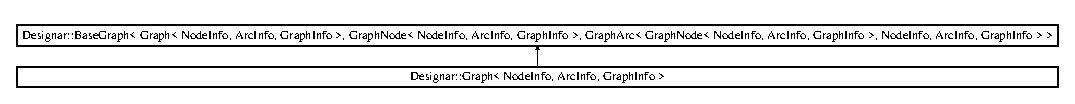
\includegraphics[height=0.952381cm]{class_designar_1_1_graph}
\end{center}
\end{figure}
\subsection*{Classes}
\begin{DoxyCompactItemize}
\item 
class \hyperlink{class_designar_1_1_graph_1_1_adjacent_arc_iterator}{Adjacent\+Arc\+Iterator}
\item 
class \hyperlink{class_designar_1_1_graph_1_1_arc_iterator}{Arc\+Iterator}
\item 
class \hyperlink{class_designar_1_1_graph_1_1_node_iterator}{Node\+Iterator}
\end{DoxyCompactItemize}
\subsection*{Public Types}
\begin{DoxyCompactItemize}
\item 
using \hyperlink{class_designar_1_1_graph_a31ac58ee9562d1695e63449318577032}{Node\+Info\+Type} = Node\+Info
\item 
using \hyperlink{class_designar_1_1_graph_abc2adb4841a6d092d5093f9e60f2c8be}{Arc\+Info\+Type} = Arc\+Info
\item 
using \hyperlink{class_designar_1_1_graph_a5b6ad505f3b0f5a5cd288a13bebf2d27}{Graph\+Info\+Type} = Graph\+Info
\item 
using \hyperlink{class_designar_1_1_graph_a5dfc7dba9d092ac489c72e40390c37d0}{Node} = \hyperlink{class_designar_1_1_graph_node}{Graph\+Node}$<$ Node\+Info, Arc\+Info, Graph\+Info $>$
\item 
using \hyperlink{class_designar_1_1_graph_a74c730ef4ce2d20f998d72bd25c2b5bf}{Arc} = \hyperlink{class_designar_1_1_graph_arc}{Graph\+Arc}$<$ \hyperlink{class_designar_1_1_graph_a5dfc7dba9d092ac489c72e40390c37d0}{Node}, Node\+Info, Arc\+Info, Graph\+Info $>$
\end{DoxyCompactItemize}
\subsection*{Public Member Functions}
\begin{DoxyCompactItemize}
\item 
\hyperlink{class_designar_1_1_graph_a606f7514b8036679207da8a09ddfa6bd}{Graph} ()
\item 
\hyperlink{class_designar_1_1_graph_a61f5be7345295aa375f3a329ded36c17}{Graph} (const Graph\+Info \&\+\_\+info)
\item 
\hyperlink{class_designar_1_1_graph_a14f42f1511cc6e9edf7f54f656febf1e}{Graph} (Graph\+Info \&\&\+\_\+info)
\item 
\hyperlink{class_designar_1_1_graph_a4390fe2f03a3972a42c91e99c5570781}{Graph} (const \hyperlink{class_designar_1_1_graph}{Graph} \&g)
\item 
\hyperlink{class_designar_1_1_graph_a7c40e70047c42aaf71faa4739b87a10c}{Graph} (\hyperlink{class_designar_1_1_graph}{Graph} \&\&g)
\item 
\hyperlink{class_designar_1_1_graph_a2ea20f9cb46279210e1eadaebcfe27f0}{$\sim$\+Graph} ()
\item 
\hyperlink{class_designar_1_1_graph}{Graph} \& \hyperlink{class_designar_1_1_graph_a5f0a5acb7b0d5fbabd60294d40c804fa}{operator=} (const \hyperlink{class_designar_1_1_graph}{Graph} \&g)
\item 
\hyperlink{class_designar_1_1_graph}{Graph} \& \hyperlink{class_designar_1_1_graph_a6b6641789f049bfd98761cb0abaa9d60}{operator=} (\hyperlink{class_designar_1_1_graph}{Graph} \&\&g)
\item 
void \hyperlink{class_designar_1_1_graph_a84de29ab3f219f556a833ad21ab274d2}{swap} (\hyperlink{class_designar_1_1_graph}{Graph} \&g)
\item 
void \hyperlink{class_designar_1_1_graph_acfebca533d00dae0c40b0dd88f64296c}{clear} ()
\item 
Graph\+Info \& \hyperlink{class_designar_1_1_graph_a5b84c02e86c7887333df2d8934079678}{get\+\_\+info} ()
\item 
const Graph\+Info \& \hyperlink{class_designar_1_1_graph_adfbae301b6a211adaf1919bc41db176a}{get\+\_\+info} () const
\item 
\hyperlink{class_designar_1_1_graph_a5dfc7dba9d092ac489c72e40390c37d0}{Node} \& \hyperlink{class_designar_1_1_graph_ab9f34a6b6160f9e66a3103c78b13d7d6}{get\+\_\+first\+\_\+node} ()
\item 
const \hyperlink{class_designar_1_1_graph_a5dfc7dba9d092ac489c72e40390c37d0}{Node} \& \hyperlink{class_designar_1_1_graph_a2c27cdec559e9773deebec6f1af25a99}{get\+\_\+first\+\_\+node} () const
\item 
\hyperlink{class_designar_1_1_graph_a74c730ef4ce2d20f998d72bd25c2b5bf}{Arc} \& \hyperlink{class_designar_1_1_graph_a6829f963f0db1fffbc535557f39ed877}{get\+\_\+first\+\_\+arc} ()
\item 
const \hyperlink{class_designar_1_1_graph_a74c730ef4ce2d20f998d72bd25c2b5bf}{Arc} \& \hyperlink{class_designar_1_1_graph_a3a4be7fef798a957b0a66102f1d30c39}{get\+\_\+first\+\_\+arc} () const
\item 
\hyperlink{namespace_designar_aa72662848b9f4815e7bf31a7cf3e33d1}{nat\+\_\+t} \hyperlink{class_designar_1_1_graph_af6f0ef48386dd1353880ff706387c4e8}{get\+\_\+num\+\_\+nodes} () const
\item 
\hyperlink{namespace_designar_aa72662848b9f4815e7bf31a7cf3e33d1}{nat\+\_\+t} \hyperlink{class_designar_1_1_graph_a5b155eda66a4c90f6a34b25c80d9342b}{get\+\_\+num\+\_\+arcs} () const
\item 
\hyperlink{class_designar_1_1_graph_a5dfc7dba9d092ac489c72e40390c37d0}{Node} \& \hyperlink{class_designar_1_1_graph_a5da24cc7de9ae39b1df684cb75782fed}{insert\+\_\+node} ()
\item 
\hyperlink{class_designar_1_1_graph_a5dfc7dba9d092ac489c72e40390c37d0}{Node} \& \hyperlink{class_designar_1_1_graph_a573d7ab63075e30bc8c5aaa2a80548ec}{insert\+\_\+node} (const Node\+Info \&\hyperlink{class_designar_1_1_graph_a2a8b41ce641ad2fb1b84a4d6b024bb1a}{info})
\item 
\hyperlink{class_designar_1_1_graph_a5dfc7dba9d092ac489c72e40390c37d0}{Node} \& \hyperlink{class_designar_1_1_graph_abbf6788c27f9719907d31fe7f7a83920}{insert\+\_\+node} (Node\+Info \&\&\hyperlink{class_designar_1_1_graph_a2a8b41ce641ad2fb1b84a4d6b024bb1a}{info})
\item 
\hyperlink{class_designar_1_1_graph_a74c730ef4ce2d20f998d72bd25c2b5bf}{Arc} \& \hyperlink{class_designar_1_1_graph_a794e687e21db6f4e00e14c6bdc5c2907}{insert\+\_\+arc} (\hyperlink{class_designar_1_1_graph_a5dfc7dba9d092ac489c72e40390c37d0}{Node} \&s, \hyperlink{class_designar_1_1_graph_a5dfc7dba9d092ac489c72e40390c37d0}{Node} \&t)
\item 
\hyperlink{class_designar_1_1_graph_a74c730ef4ce2d20f998d72bd25c2b5bf}{Arc} \& \hyperlink{class_designar_1_1_graph_ad310a106f10d0a7ff12915d8b47e8e3d}{insert\+\_\+arc} (\hyperlink{class_designar_1_1_graph_a5dfc7dba9d092ac489c72e40390c37d0}{Node} \&src, \hyperlink{class_designar_1_1_graph_a5dfc7dba9d092ac489c72e40390c37d0}{Node} \&tgt, const Arc\+Info \&\hyperlink{class_designar_1_1_graph_a2a8b41ce641ad2fb1b84a4d6b024bb1a}{info})
\item 
\hyperlink{class_designar_1_1_graph_a74c730ef4ce2d20f998d72bd25c2b5bf}{Arc} \& \hyperlink{class_designar_1_1_graph_ab2182fa8a058595157b399b0828bb827}{insert\+\_\+arc} (\hyperlink{class_designar_1_1_graph_a5dfc7dba9d092ac489c72e40390c37d0}{Node} \&src, \hyperlink{class_designar_1_1_graph_a5dfc7dba9d092ac489c72e40390c37d0}{Node} \&tgt, Arc\+Info \&\&\hyperlink{class_designar_1_1_graph_a2a8b41ce641ad2fb1b84a4d6b024bb1a}{info})
\item 
void \hyperlink{class_designar_1_1_graph_a38205a764213c407acf25c936c645b5d}{remove\+\_\+arc} (\hyperlink{class_designar_1_1_graph_a74c730ef4ce2d20f998d72bd25c2b5bf}{Arc} \&a)
\item 
void \hyperlink{class_designar_1_1_graph_ad3dd48701d77a26ce86f43a50d8a3f28}{remove\+\_\+node} (\hyperlink{class_designar_1_1_graph_a5dfc7dba9d092ac489c72e40390c37d0}{Node} \&n)
\item 
\hyperlink{class_designar_1_1_graph_1_1_node_iterator}{Node\+Iterator} \hyperlink{class_designar_1_1_graph_a4f492f9b89d1d647e53171d7bb4d4acd}{nodes\+\_\+begin} ()
\item 
const \hyperlink{class_designar_1_1_graph_1_1_node_iterator}{Node\+Iterator} \hyperlink{class_designar_1_1_graph_acd4d942eba98e1eb138b9566f1d9bb75}{nodes\+\_\+begin} () const
\item 
\hyperlink{class_designar_1_1_graph_1_1_node_iterator}{Node\+Iterator} \hyperlink{class_designar_1_1_graph_a9f51b69f8827aabfe5b23f82e9bc5a4d}{nodes\+\_\+end} ()
\item 
const \hyperlink{class_designar_1_1_graph_1_1_node_iterator}{Node\+Iterator} \hyperlink{class_designar_1_1_graph_abb7e32a8a05850e788f4017677965b49}{nodes\+\_\+end} () const
\item 
\hyperlink{class_designar_1_1_graph_1_1_arc_iterator}{Arc\+Iterator} \hyperlink{class_designar_1_1_graph_a9448ba557a7b0ef90651d74d4a4ee36b}{arcs\+\_\+begin} ()
\item 
const \hyperlink{class_designar_1_1_graph_1_1_arc_iterator}{Arc\+Iterator} \hyperlink{class_designar_1_1_graph_a3906cae09045bb9c037e1c3c4e64dd97}{arcs\+\_\+begin} () const
\item 
\hyperlink{class_designar_1_1_graph_1_1_arc_iterator}{Arc\+Iterator} \hyperlink{class_designar_1_1_graph_a57a43c94f28df5958e912554d640bdaa}{arcs\+\_\+end} ()
\item 
const \hyperlink{class_designar_1_1_graph_1_1_arc_iterator}{Arc\+Iterator} \hyperlink{class_designar_1_1_graph_a81269c52d854ceb3d000f2642fcb52ae}{arcs\+\_\+end} () const
\item 
\hyperlink{class_designar_1_1_graph_1_1_adjacent_arc_iterator}{Adjacent\+Arc\+Iterator} \hyperlink{class_designar_1_1_graph_a9488f4193d227a690f46e91a11dd830a}{arcs\+\_\+begin} (\hyperlink{class_designar_1_1_graph_a5dfc7dba9d092ac489c72e40390c37d0}{Node} \&p)
\item 
const \hyperlink{class_designar_1_1_graph_1_1_adjacent_arc_iterator}{Adjacent\+Arc\+Iterator} \hyperlink{class_designar_1_1_graph_a2c527f6bddb0ff454fd6139f2437c27b}{arcs\+\_\+begin} (\hyperlink{class_designar_1_1_graph_a5dfc7dba9d092ac489c72e40390c37d0}{Node} \&p) const
\item 
\hyperlink{class_designar_1_1_graph_1_1_adjacent_arc_iterator}{Adjacent\+Arc\+Iterator} \hyperlink{class_designar_1_1_graph_a68ee235ab79790c00e1a69d518b9c076}{arcs\+\_\+end} (\hyperlink{class_designar_1_1_graph_a5dfc7dba9d092ac489c72e40390c37d0}{Node} \&p)
\item 
const \hyperlink{class_designar_1_1_graph_1_1_adjacent_arc_iterator}{Adjacent\+Arc\+Iterator} \hyperlink{class_designar_1_1_graph_a305a413007d60401317366c92245bfa4}{arcs\+\_\+end} (\hyperlink{class_designar_1_1_graph_a5dfc7dba9d092ac489c72e40390c37d0}{Node} \&p) const
\item 
\hyperlink{class_designar_1_1_graph_a74c730ef4ce2d20f998d72bd25c2b5bf}{Arc} $\ast$ \hyperlink{class_designar_1_1_graph_afa69dd3cc6bacfed22864f5ad7c189ba}{search\+\_\+arc} (\hyperlink{class_designar_1_1_graph_a5dfc7dba9d092ac489c72e40390c37d0}{Node} \&, \hyperlink{class_designar_1_1_graph_a5dfc7dba9d092ac489c72e40390c37d0}{Node} \&)
\item 
{\footnotesize template$<$class Cmp $>$ }\\void \hyperlink{class_designar_1_1_graph_afcdce423516a879b23ec1b0fed201f20}{sort\+\_\+nodes} (Cmp \&cmp)
\item 
{\footnotesize template$<$class Cmp $>$ }\\void \hyperlink{class_designar_1_1_graph_af40e0d87cdc7222b2f02e833bf791ac9}{sort\+\_\+nodes} (Cmp \&\&cmp=Cmp())
\item 
{\footnotesize template$<$class Cmp $>$ }\\void \hyperlink{class_designar_1_1_graph_a39af536f6e08248e0d343dcd300713c2}{sort\+\_\+arcs} (Cmp \&cmp)
\item 
{\footnotesize template$<$class Cmp $>$ }\\void \hyperlink{class_designar_1_1_graph_a37b5e36c96bf9efe44a0d6b83feb9656}{sort\+\_\+arcs} (Cmp \&\&cmp=Cmp())
\item 
bool \hyperlink{class_designar_1_1_graph_af0e0b3d1d6a52e0f3d3225f1fa274211}{is\+\_\+digraph} () const
\end{DoxyCompactItemize}
\subsection*{Protected Types}
\begin{DoxyCompactItemize}
\item 
using \hyperlink{class_designar_1_1_graph_a7e61951db0bb9bfa8a2e317440d4e17f}{G\+Node} = \hyperlink{class_designar_1_1_d_l_node}{D\+L\+Node}$<$ \hyperlink{class_designar_1_1_graph_a5dfc7dba9d092ac489c72e40390c37d0}{Node} $>$
\item 
using \hyperlink{class_designar_1_1_graph_a5ad9e18b71899c2d4979426e367e5573}{G\+Arc} = \hyperlink{class_designar_1_1_d_l_node}{D\+L\+Node}$<$ \hyperlink{class_designar_1_1_graph_a74c730ef4ce2d20f998d72bd25c2b5bf}{Arc} $>$
\item 
using \hyperlink{class_designar_1_1_graph_a7d00558995946c5653522148b54971bc}{G\+Ad\+Arc} = \hyperlink{class_designar_1_1_d_l_node}{D\+L\+Node}$<$ \hyperlink{class_designar_1_1_graph_a5ad9e18b71899c2d4979426e367e5573}{G\+Arc} $\ast$ $>$
\end{DoxyCompactItemize}
\subsection*{Protected Member Functions}
\begin{DoxyCompactItemize}
\item 
\hyperlink{class_designar_1_1_graph_a7e61951db0bb9bfa8a2e317440d4e17f}{G\+Node} $\ast$ \hyperlink{class_designar_1_1_graph_adea7e2c9bb1912cfc7a58990a640355d}{insert\+\_\+node} (\hyperlink{class_designar_1_1_graph_a7e61951db0bb9bfa8a2e317440d4e17f}{G\+Node} $\ast$p)
\item 
\hyperlink{class_designar_1_1_graph_a5ad9e18b71899c2d4979426e367e5573}{G\+Arc} $\ast$ \hyperlink{class_designar_1_1_graph_a20f183a1481fb62bc775aca6bd3244d1}{insert\+\_\+arc} (\hyperlink{class_designar_1_1_graph_a5dfc7dba9d092ac489c72e40390c37d0}{Node} $\ast$src, \hyperlink{class_designar_1_1_graph_a5dfc7dba9d092ac489c72e40390c37d0}{Node} $\ast$tgt)
\item 
void \hyperlink{class_designar_1_1_graph_a00f22c9d1c712f65cc46118e37cf06b9}{remove\+\_\+arc} (\hyperlink{class_designar_1_1_graph_a5ad9e18b71899c2d4979426e367e5573}{G\+Arc} $\ast$arc)
\item 
void \hyperlink{class_designar_1_1_graph_a4ca166ec5729c1402485dc45c040c11c}{remove\+\_\+node} (\hyperlink{class_designar_1_1_graph_a7e61951db0bb9bfa8a2e317440d4e17f}{G\+Node} $\ast$)
\end{DoxyCompactItemize}
\subsection*{Static Protected Member Functions}
\begin{DoxyCompactItemize}
\item 
static \hyperlink{class_designar_1_1_graph_a7e61951db0bb9bfa8a2e317440d4e17f}{G\+Node} $\ast$ \hyperlink{class_designar_1_1_graph_ab6f1de18d2ec0c537fc1daa5b4a42e01}{dl\+\_\+to\+\_\+node} (\hyperlink{class_designar_1_1_d_l}{DL} $\ast$ptr)
\item 
static \hyperlink{class_designar_1_1_graph_a5ad9e18b71899c2d4979426e367e5573}{G\+Arc} $\ast$ \hyperlink{class_designar_1_1_graph_a543b3279c059a0ee596a56a704ab7825}{dl\+\_\+to\+\_\+arc} (\hyperlink{class_designar_1_1_d_l}{DL} $\ast$ptr)
\item 
static \hyperlink{class_designar_1_1_graph_a7d00558995946c5653522148b54971bc}{G\+Ad\+Arc} $\ast$ \hyperlink{class_designar_1_1_graph_afb508b7f8616948cc46c33deddcfaa4c}{dl\+\_\+to\+\_\+adjacent\+\_\+arc} (\hyperlink{class_designar_1_1_d_l}{DL} $\ast$ptr)
\item 
static \hyperlink{class_designar_1_1_graph_a7e61951db0bb9bfa8a2e317440d4e17f}{G\+Node} $\ast$ \hyperlink{class_designar_1_1_graph_a23038b7502c6fdb53b23453b19579c0e}{to\+\_\+gnode} (\hyperlink{class_designar_1_1_graph_a5dfc7dba9d092ac489c72e40390c37d0}{Node} \&node)
\item 
static \hyperlink{class_designar_1_1_graph_a5ad9e18b71899c2d4979426e367e5573}{G\+Arc} $\ast$ \hyperlink{class_designar_1_1_graph_ab79eb63dd332e483db77da69c1b04522}{to\+\_\+garc} (\hyperlink{class_designar_1_1_graph_a74c730ef4ce2d20f998d72bd25c2b5bf}{Arc} \&arc)
\end{DoxyCompactItemize}
\subsection*{Protected Attributes}
\begin{DoxyCompactItemize}
\item 
Graph\+Info \hyperlink{class_designar_1_1_graph_a2a8b41ce641ad2fb1b84a4d6b024bb1a}{info}
\item 
\hyperlink{namespace_designar_aa72662848b9f4815e7bf31a7cf3e33d1}{nat\+\_\+t} \hyperlink{class_designar_1_1_graph_a1ff2ba87ab27911b1f6d47e622e67542}{num\+\_\+nodes}
\item 
\hyperlink{class_designar_1_1_d_l}{DL} \hyperlink{class_designar_1_1_graph_a31b0117b6d87816f703a4a5baa1fa6ce}{node\+\_\+list}
\item 
\hyperlink{namespace_designar_aa72662848b9f4815e7bf31a7cf3e33d1}{nat\+\_\+t} \hyperlink{class_designar_1_1_graph_a035a0debf7a7545d0033f37cf941020f}{num\+\_\+arcs}
\item 
\hyperlink{class_designar_1_1_d_l}{DL} \hyperlink{class_designar_1_1_graph_a8c809db7848c78f6718aad466ee959b2}{arc\+\_\+list}
\end{DoxyCompactItemize}
\subsection*{Additional Inherited Members}


\subsection{Detailed Description}
\subsubsection*{template$<$typename Node\+Info, typename Arc\+Info = Empty\+Class, typename Graph\+Info = Empty\+Class$>$\newline
class Designar\+::\+Graph$<$ Node\+Info, Arc\+Info, Graph\+Info $>$}



Definition at line 35 of file graph.\+H.



\subsection{Member Typedef Documentation}
\mbox{\Hypertarget{class_designar_1_1_graph_a74c730ef4ce2d20f998d72bd25c2b5bf}\label{class_designar_1_1_graph_a74c730ef4ce2d20f998d72bd25c2b5bf}} 
\index{Designar\+::\+Graph@{Designar\+::\+Graph}!Arc@{Arc}}
\index{Arc@{Arc}!Designar\+::\+Graph@{Designar\+::\+Graph}}
\subsubsection{\texorpdfstring{Arc}{Arc}}
{\footnotesize\ttfamily template$<$typename Node\+Info , typename Arc\+Info  = Empty\+Class, typename Graph\+Info  = Empty\+Class$>$ \\
using \hyperlink{class_designar_1_1_graph}{Designar\+::\+Graph}$<$ Node\+Info, Arc\+Info, Graph\+Info $>$\+::\hyperlink{class_designar_1_1_graph_a74c730ef4ce2d20f998d72bd25c2b5bf}{Arc} =  \hyperlink{class_designar_1_1_graph_arc}{Graph\+Arc}$<$\hyperlink{class_designar_1_1_graph_a5dfc7dba9d092ac489c72e40390c37d0}{Node}, Node\+Info, Arc\+Info, Graph\+Info$>$}



Definition at line 1178 of file graph.\+H.

\mbox{\Hypertarget{class_designar_1_1_graph_abc2adb4841a6d092d5093f9e60f2c8be}\label{class_designar_1_1_graph_abc2adb4841a6d092d5093f9e60f2c8be}} 
\index{Designar\+::\+Graph@{Designar\+::\+Graph}!Arc\+Info\+Type@{Arc\+Info\+Type}}
\index{Arc\+Info\+Type@{Arc\+Info\+Type}!Designar\+::\+Graph@{Designar\+::\+Graph}}
\subsubsection{\texorpdfstring{Arc\+Info\+Type}{ArcInfoType}}
{\footnotesize\ttfamily template$<$typename Node\+Info , typename Arc\+Info  = Empty\+Class, typename Graph\+Info  = Empty\+Class$>$ \\
using \hyperlink{class_designar_1_1_graph}{Designar\+::\+Graph}$<$ Node\+Info, Arc\+Info, Graph\+Info $>$\+::\hyperlink{class_designar_1_1_graph_abc2adb4841a6d092d5093f9e60f2c8be}{Arc\+Info\+Type} =  Arc\+Info}



Definition at line 1174 of file graph.\+H.

\mbox{\Hypertarget{class_designar_1_1_graph_a7d00558995946c5653522148b54971bc}\label{class_designar_1_1_graph_a7d00558995946c5653522148b54971bc}} 
\index{Designar\+::\+Graph@{Designar\+::\+Graph}!G\+Ad\+Arc@{G\+Ad\+Arc}}
\index{G\+Ad\+Arc@{G\+Ad\+Arc}!Designar\+::\+Graph@{Designar\+::\+Graph}}
\subsubsection{\texorpdfstring{G\+Ad\+Arc}{GAdArc}}
{\footnotesize\ttfamily template$<$typename Node\+Info , typename Arc\+Info  = Empty\+Class, typename Graph\+Info  = Empty\+Class$>$ \\
using \hyperlink{class_designar_1_1_graph}{Designar\+::\+Graph}$<$ Node\+Info, Arc\+Info, Graph\+Info $>$\+::\hyperlink{class_designar_1_1_graph_a7d00558995946c5653522148b54971bc}{G\+Ad\+Arc} =  \hyperlink{class_designar_1_1_d_l_node}{D\+L\+Node}$<$\hyperlink{class_designar_1_1_graph_a5ad9e18b71899c2d4979426e367e5573}{G\+Arc} $\ast$$>$\hspace{0.3cm}{\ttfamily [protected]}}



Definition at line 1183 of file graph.\+H.

\mbox{\Hypertarget{class_designar_1_1_graph_a5ad9e18b71899c2d4979426e367e5573}\label{class_designar_1_1_graph_a5ad9e18b71899c2d4979426e367e5573}} 
\index{Designar\+::\+Graph@{Designar\+::\+Graph}!G\+Arc@{G\+Arc}}
\index{G\+Arc@{G\+Arc}!Designar\+::\+Graph@{Designar\+::\+Graph}}
\subsubsection{\texorpdfstring{G\+Arc}{GArc}}
{\footnotesize\ttfamily template$<$typename Node\+Info , typename Arc\+Info  = Empty\+Class, typename Graph\+Info  = Empty\+Class$>$ \\
using \hyperlink{class_designar_1_1_graph}{Designar\+::\+Graph}$<$ Node\+Info, Arc\+Info, Graph\+Info $>$\+::\hyperlink{class_designar_1_1_graph_a5ad9e18b71899c2d4979426e367e5573}{G\+Arc} =  \hyperlink{class_designar_1_1_d_l_node}{D\+L\+Node}$<$\hyperlink{class_designar_1_1_graph_a74c730ef4ce2d20f998d72bd25c2b5bf}{Arc}$>$\hspace{0.3cm}{\ttfamily [protected]}}



Definition at line 1182 of file graph.\+H.

\mbox{\Hypertarget{class_designar_1_1_graph_a7e61951db0bb9bfa8a2e317440d4e17f}\label{class_designar_1_1_graph_a7e61951db0bb9bfa8a2e317440d4e17f}} 
\index{Designar\+::\+Graph@{Designar\+::\+Graph}!G\+Node@{G\+Node}}
\index{G\+Node@{G\+Node}!Designar\+::\+Graph@{Designar\+::\+Graph}}
\subsubsection{\texorpdfstring{G\+Node}{GNode}}
{\footnotesize\ttfamily template$<$typename Node\+Info , typename Arc\+Info  = Empty\+Class, typename Graph\+Info  = Empty\+Class$>$ \\
using \hyperlink{class_designar_1_1_graph}{Designar\+::\+Graph}$<$ Node\+Info, Arc\+Info, Graph\+Info $>$\+::\hyperlink{class_designar_1_1_graph_a7e61951db0bb9bfa8a2e317440d4e17f}{G\+Node} =  \hyperlink{class_designar_1_1_d_l_node}{D\+L\+Node}$<$\hyperlink{class_designar_1_1_graph_a5dfc7dba9d092ac489c72e40390c37d0}{Node}$>$\hspace{0.3cm}{\ttfamily [protected]}}



Definition at line 1181 of file graph.\+H.

\mbox{\Hypertarget{class_designar_1_1_graph_a5b6ad505f3b0f5a5cd288a13bebf2d27}\label{class_designar_1_1_graph_a5b6ad505f3b0f5a5cd288a13bebf2d27}} 
\index{Designar\+::\+Graph@{Designar\+::\+Graph}!Graph\+Info\+Type@{Graph\+Info\+Type}}
\index{Graph\+Info\+Type@{Graph\+Info\+Type}!Designar\+::\+Graph@{Designar\+::\+Graph}}
\subsubsection{\texorpdfstring{Graph\+Info\+Type}{GraphInfoType}}
{\footnotesize\ttfamily template$<$typename Node\+Info , typename Arc\+Info  = Empty\+Class, typename Graph\+Info  = Empty\+Class$>$ \\
using \hyperlink{class_designar_1_1_graph}{Designar\+::\+Graph}$<$ Node\+Info, Arc\+Info, Graph\+Info $>$\+::\hyperlink{class_designar_1_1_graph_a5b6ad505f3b0f5a5cd288a13bebf2d27}{Graph\+Info\+Type} =  Graph\+Info}



Definition at line 1175 of file graph.\+H.

\mbox{\Hypertarget{class_designar_1_1_graph_a5dfc7dba9d092ac489c72e40390c37d0}\label{class_designar_1_1_graph_a5dfc7dba9d092ac489c72e40390c37d0}} 
\index{Designar\+::\+Graph@{Designar\+::\+Graph}!Node@{Node}}
\index{Node@{Node}!Designar\+::\+Graph@{Designar\+::\+Graph}}
\subsubsection{\texorpdfstring{Node}{Node}}
{\footnotesize\ttfamily template$<$typename Node\+Info , typename Arc\+Info  = Empty\+Class, typename Graph\+Info  = Empty\+Class$>$ \\
using \hyperlink{class_designar_1_1_graph}{Designar\+::\+Graph}$<$ Node\+Info, Arc\+Info, Graph\+Info $>$\+::\hyperlink{class_designar_1_1_graph_a5dfc7dba9d092ac489c72e40390c37d0}{Node} =  \hyperlink{class_designar_1_1_graph_node}{Graph\+Node}$<$Node\+Info, Arc\+Info, Graph\+Info$>$}



Definition at line 1177 of file graph.\+H.

\mbox{\Hypertarget{class_designar_1_1_graph_a31ac58ee9562d1695e63449318577032}\label{class_designar_1_1_graph_a31ac58ee9562d1695e63449318577032}} 
\index{Designar\+::\+Graph@{Designar\+::\+Graph}!Node\+Info\+Type@{Node\+Info\+Type}}
\index{Node\+Info\+Type@{Node\+Info\+Type}!Designar\+::\+Graph@{Designar\+::\+Graph}}
\subsubsection{\texorpdfstring{Node\+Info\+Type}{NodeInfoType}}
{\footnotesize\ttfamily template$<$typename Node\+Info , typename Arc\+Info  = Empty\+Class, typename Graph\+Info  = Empty\+Class$>$ \\
using \hyperlink{class_designar_1_1_graph}{Designar\+::\+Graph}$<$ Node\+Info, Arc\+Info, Graph\+Info $>$\+::\hyperlink{class_designar_1_1_graph_a31ac58ee9562d1695e63449318577032}{Node\+Info\+Type} =  Node\+Info}



Definition at line 1173 of file graph.\+H.



\subsection{Constructor \& Destructor Documentation}
\mbox{\Hypertarget{class_designar_1_1_graph_a606f7514b8036679207da8a09ddfa6bd}\label{class_designar_1_1_graph_a606f7514b8036679207da8a09ddfa6bd}} 
\index{Designar\+::\+Graph@{Designar\+::\+Graph}!Graph@{Graph}}
\index{Graph@{Graph}!Designar\+::\+Graph@{Designar\+::\+Graph}}
\subsubsection{\texorpdfstring{Graph()}{Graph()}\hspace{0.1cm}{\footnotesize\ttfamily [1/5]}}
{\footnotesize\ttfamily template$<$typename Node\+Info , typename Arc\+Info  = Empty\+Class, typename Graph\+Info  = Empty\+Class$>$ \\
\hyperlink{class_designar_1_1_graph}{Designar\+::\+Graph}$<$ Node\+Info, Arc\+Info, Graph\+Info $>$\+::\hyperlink{class_designar_1_1_graph}{Graph} (\begin{DoxyParamCaption}{ }\end{DoxyParamCaption})\hspace{0.3cm}{\ttfamily [inline]}}



Definition at line 1281 of file graph.\+H.

\mbox{\Hypertarget{class_designar_1_1_graph_a61f5be7345295aa375f3a329ded36c17}\label{class_designar_1_1_graph_a61f5be7345295aa375f3a329ded36c17}} 
\index{Designar\+::\+Graph@{Designar\+::\+Graph}!Graph@{Graph}}
\index{Graph@{Graph}!Designar\+::\+Graph@{Designar\+::\+Graph}}
\subsubsection{\texorpdfstring{Graph()}{Graph()}\hspace{0.1cm}{\footnotesize\ttfamily [2/5]}}
{\footnotesize\ttfamily template$<$typename Node\+Info , typename Arc\+Info  = Empty\+Class, typename Graph\+Info  = Empty\+Class$>$ \\
\hyperlink{class_designar_1_1_graph}{Designar\+::\+Graph}$<$ Node\+Info, Arc\+Info, Graph\+Info $>$\+::\hyperlink{class_designar_1_1_graph}{Graph} (\begin{DoxyParamCaption}\item[{const Graph\+Info \&}]{\+\_\+info }\end{DoxyParamCaption})\hspace{0.3cm}{\ttfamily [inline]}}



Definition at line 1287 of file graph.\+H.

\mbox{\Hypertarget{class_designar_1_1_graph_a14f42f1511cc6e9edf7f54f656febf1e}\label{class_designar_1_1_graph_a14f42f1511cc6e9edf7f54f656febf1e}} 
\index{Designar\+::\+Graph@{Designar\+::\+Graph}!Graph@{Graph}}
\index{Graph@{Graph}!Designar\+::\+Graph@{Designar\+::\+Graph}}
\subsubsection{\texorpdfstring{Graph()}{Graph()}\hspace{0.1cm}{\footnotesize\ttfamily [3/5]}}
{\footnotesize\ttfamily template$<$typename Node\+Info , typename Arc\+Info  = Empty\+Class, typename Graph\+Info  = Empty\+Class$>$ \\
\hyperlink{class_designar_1_1_graph}{Designar\+::\+Graph}$<$ Node\+Info, Arc\+Info, Graph\+Info $>$\+::\hyperlink{class_designar_1_1_graph}{Graph} (\begin{DoxyParamCaption}\item[{Graph\+Info \&\&}]{\+\_\+info }\end{DoxyParamCaption})\hspace{0.3cm}{\ttfamily [inline]}}



Definition at line 1293 of file graph.\+H.

\mbox{\Hypertarget{class_designar_1_1_graph_a4390fe2f03a3972a42c91e99c5570781}\label{class_designar_1_1_graph_a4390fe2f03a3972a42c91e99c5570781}} 
\index{Designar\+::\+Graph@{Designar\+::\+Graph}!Graph@{Graph}}
\index{Graph@{Graph}!Designar\+::\+Graph@{Designar\+::\+Graph}}
\subsubsection{\texorpdfstring{Graph()}{Graph()}\hspace{0.1cm}{\footnotesize\ttfamily [4/5]}}
{\footnotesize\ttfamily template$<$typename Node\+Info , typename Arc\+Info  = Empty\+Class, typename Graph\+Info  = Empty\+Class$>$ \\
\hyperlink{class_designar_1_1_graph}{Designar\+::\+Graph}$<$ Node\+Info, Arc\+Info, Graph\+Info $>$\+::\hyperlink{class_designar_1_1_graph}{Graph} (\begin{DoxyParamCaption}\item[{const \hyperlink{class_designar_1_1_graph}{Graph}$<$ Node\+Info, Arc\+Info, Graph\+Info $>$ \&}]{g }\end{DoxyParamCaption})\hspace{0.3cm}{\ttfamily [inline]}}



Definition at line 1299 of file graph.\+H.

\mbox{\Hypertarget{class_designar_1_1_graph_a7c40e70047c42aaf71faa4739b87a10c}\label{class_designar_1_1_graph_a7c40e70047c42aaf71faa4739b87a10c}} 
\index{Designar\+::\+Graph@{Designar\+::\+Graph}!Graph@{Graph}}
\index{Graph@{Graph}!Designar\+::\+Graph@{Designar\+::\+Graph}}
\subsubsection{\texorpdfstring{Graph()}{Graph()}\hspace{0.1cm}{\footnotesize\ttfamily [5/5]}}
{\footnotesize\ttfamily template$<$typename Node\+Info , typename Arc\+Info  = Empty\+Class, typename Graph\+Info  = Empty\+Class$>$ \\
\hyperlink{class_designar_1_1_graph}{Designar\+::\+Graph}$<$ Node\+Info, Arc\+Info, Graph\+Info $>$\+::\hyperlink{class_designar_1_1_graph}{Graph} (\begin{DoxyParamCaption}\item[{\hyperlink{class_designar_1_1_graph}{Graph}$<$ Node\+Info, Arc\+Info, Graph\+Info $>$ \&\&}]{g }\end{DoxyParamCaption})\hspace{0.3cm}{\ttfamily [inline]}}



Definition at line 1305 of file graph.\+H.

\mbox{\Hypertarget{class_designar_1_1_graph_a2ea20f9cb46279210e1eadaebcfe27f0}\label{class_designar_1_1_graph_a2ea20f9cb46279210e1eadaebcfe27f0}} 
\index{Designar\+::\+Graph@{Designar\+::\+Graph}!````~Graph@{$\sim$\+Graph}}
\index{````~Graph@{$\sim$\+Graph}!Designar\+::\+Graph@{Designar\+::\+Graph}}
\subsubsection{\texorpdfstring{$\sim$\+Graph()}{~Graph()}}
{\footnotesize\ttfamily template$<$typename Node\+Info , typename Arc\+Info  = Empty\+Class, typename Graph\+Info  = Empty\+Class$>$ \\
\hyperlink{class_designar_1_1_graph}{Designar\+::\+Graph}$<$ Node\+Info, Arc\+Info, Graph\+Info $>$\+::$\sim$\hyperlink{class_designar_1_1_graph}{Graph} (\begin{DoxyParamCaption}{ }\end{DoxyParamCaption})\hspace{0.3cm}{\ttfamily [inline]}}



Definition at line 1311 of file graph.\+H.



\subsection{Member Function Documentation}
\mbox{\Hypertarget{class_designar_1_1_graph_a9448ba557a7b0ef90651d74d4a4ee36b}\label{class_designar_1_1_graph_a9448ba557a7b0ef90651d74d4a4ee36b}} 
\index{Designar\+::\+Graph@{Designar\+::\+Graph}!arcs\+\_\+begin@{arcs\+\_\+begin}}
\index{arcs\+\_\+begin@{arcs\+\_\+begin}!Designar\+::\+Graph@{Designar\+::\+Graph}}
\subsubsection{\texorpdfstring{arcs\+\_\+begin()}{arcs\_begin()}\hspace{0.1cm}{\footnotesize\ttfamily [1/4]}}
{\footnotesize\ttfamily template$<$typename Node\+Info , typename Arc\+Info  = Empty\+Class, typename Graph\+Info  = Empty\+Class$>$ \\
\hyperlink{class_designar_1_1_graph_1_1_arc_iterator}{Arc\+Iterator} \hyperlink{class_designar_1_1_graph}{Designar\+::\+Graph}$<$ Node\+Info, Arc\+Info, Graph\+Info $>$\+::arcs\+\_\+begin (\begin{DoxyParamCaption}{ }\end{DoxyParamCaption})\hspace{0.3cm}{\ttfamily [inline]}}



Definition at line 1738 of file graph.\+H.

\mbox{\Hypertarget{class_designar_1_1_graph_a3906cae09045bb9c037e1c3c4e64dd97}\label{class_designar_1_1_graph_a3906cae09045bb9c037e1c3c4e64dd97}} 
\index{Designar\+::\+Graph@{Designar\+::\+Graph}!arcs\+\_\+begin@{arcs\+\_\+begin}}
\index{arcs\+\_\+begin@{arcs\+\_\+begin}!Designar\+::\+Graph@{Designar\+::\+Graph}}
\subsubsection{\texorpdfstring{arcs\+\_\+begin()}{arcs\_begin()}\hspace{0.1cm}{\footnotesize\ttfamily [2/4]}}
{\footnotesize\ttfamily template$<$typename Node\+Info , typename Arc\+Info  = Empty\+Class, typename Graph\+Info  = Empty\+Class$>$ \\
const \hyperlink{class_designar_1_1_graph_1_1_arc_iterator}{Arc\+Iterator} \hyperlink{class_designar_1_1_graph}{Designar\+::\+Graph}$<$ Node\+Info, Arc\+Info, Graph\+Info $>$\+::arcs\+\_\+begin (\begin{DoxyParamCaption}{ }\end{DoxyParamCaption}) const\hspace{0.3cm}{\ttfamily [inline]}}



Definition at line 1743 of file graph.\+H.

\mbox{\Hypertarget{class_designar_1_1_graph_a9488f4193d227a690f46e91a11dd830a}\label{class_designar_1_1_graph_a9488f4193d227a690f46e91a11dd830a}} 
\index{Designar\+::\+Graph@{Designar\+::\+Graph}!arcs\+\_\+begin@{arcs\+\_\+begin}}
\index{arcs\+\_\+begin@{arcs\+\_\+begin}!Designar\+::\+Graph@{Designar\+::\+Graph}}
\subsubsection{\texorpdfstring{arcs\+\_\+begin()}{arcs\_begin()}\hspace{0.1cm}{\footnotesize\ttfamily [3/4]}}
{\footnotesize\ttfamily template$<$typename Node\+Info , typename Arc\+Info  = Empty\+Class, typename Graph\+Info  = Empty\+Class$>$ \\
\hyperlink{class_designar_1_1_graph_1_1_adjacent_arc_iterator}{Adjacent\+Arc\+Iterator} \hyperlink{class_designar_1_1_graph}{Designar\+::\+Graph}$<$ Node\+Info, Arc\+Info, Graph\+Info $>$\+::arcs\+\_\+begin (\begin{DoxyParamCaption}\item[{\hyperlink{class_designar_1_1_graph_a5dfc7dba9d092ac489c72e40390c37d0}{Node} \&}]{p }\end{DoxyParamCaption})\hspace{0.3cm}{\ttfamily [inline]}}



Definition at line 1758 of file graph.\+H.

\mbox{\Hypertarget{class_designar_1_1_graph_a2c527f6bddb0ff454fd6139f2437c27b}\label{class_designar_1_1_graph_a2c527f6bddb0ff454fd6139f2437c27b}} 
\index{Designar\+::\+Graph@{Designar\+::\+Graph}!arcs\+\_\+begin@{arcs\+\_\+begin}}
\index{arcs\+\_\+begin@{arcs\+\_\+begin}!Designar\+::\+Graph@{Designar\+::\+Graph}}
\subsubsection{\texorpdfstring{arcs\+\_\+begin()}{arcs\_begin()}\hspace{0.1cm}{\footnotesize\ttfamily [4/4]}}
{\footnotesize\ttfamily template$<$typename Node\+Info , typename Arc\+Info  = Empty\+Class, typename Graph\+Info  = Empty\+Class$>$ \\
const \hyperlink{class_designar_1_1_graph_1_1_adjacent_arc_iterator}{Adjacent\+Arc\+Iterator} \hyperlink{class_designar_1_1_graph}{Designar\+::\+Graph}$<$ Node\+Info, Arc\+Info, Graph\+Info $>$\+::arcs\+\_\+begin (\begin{DoxyParamCaption}\item[{\hyperlink{class_designar_1_1_graph_a5dfc7dba9d092ac489c72e40390c37d0}{Node} \&}]{p }\end{DoxyParamCaption}) const\hspace{0.3cm}{\ttfamily [inline]}}



Definition at line 1763 of file graph.\+H.

\mbox{\Hypertarget{class_designar_1_1_graph_a57a43c94f28df5958e912554d640bdaa}\label{class_designar_1_1_graph_a57a43c94f28df5958e912554d640bdaa}} 
\index{Designar\+::\+Graph@{Designar\+::\+Graph}!arcs\+\_\+end@{arcs\+\_\+end}}
\index{arcs\+\_\+end@{arcs\+\_\+end}!Designar\+::\+Graph@{Designar\+::\+Graph}}
\subsubsection{\texorpdfstring{arcs\+\_\+end()}{arcs\_end()}\hspace{0.1cm}{\footnotesize\ttfamily [1/4]}}
{\footnotesize\ttfamily template$<$typename Node\+Info , typename Arc\+Info  = Empty\+Class, typename Graph\+Info  = Empty\+Class$>$ \\
\hyperlink{class_designar_1_1_graph_1_1_arc_iterator}{Arc\+Iterator} \hyperlink{class_designar_1_1_graph}{Designar\+::\+Graph}$<$ Node\+Info, Arc\+Info, Graph\+Info $>$\+::arcs\+\_\+end (\begin{DoxyParamCaption}{ }\end{DoxyParamCaption})\hspace{0.3cm}{\ttfamily [inline]}}



Definition at line 1748 of file graph.\+H.

\mbox{\Hypertarget{class_designar_1_1_graph_a81269c52d854ceb3d000f2642fcb52ae}\label{class_designar_1_1_graph_a81269c52d854ceb3d000f2642fcb52ae}} 
\index{Designar\+::\+Graph@{Designar\+::\+Graph}!arcs\+\_\+end@{arcs\+\_\+end}}
\index{arcs\+\_\+end@{arcs\+\_\+end}!Designar\+::\+Graph@{Designar\+::\+Graph}}
\subsubsection{\texorpdfstring{arcs\+\_\+end()}{arcs\_end()}\hspace{0.1cm}{\footnotesize\ttfamily [2/4]}}
{\footnotesize\ttfamily template$<$typename Node\+Info , typename Arc\+Info  = Empty\+Class, typename Graph\+Info  = Empty\+Class$>$ \\
const \hyperlink{class_designar_1_1_graph_1_1_arc_iterator}{Arc\+Iterator} \hyperlink{class_designar_1_1_graph}{Designar\+::\+Graph}$<$ Node\+Info, Arc\+Info, Graph\+Info $>$\+::arcs\+\_\+end (\begin{DoxyParamCaption}{ }\end{DoxyParamCaption}) const\hspace{0.3cm}{\ttfamily [inline]}}



Definition at line 1753 of file graph.\+H.

\mbox{\Hypertarget{class_designar_1_1_graph_a68ee235ab79790c00e1a69d518b9c076}\label{class_designar_1_1_graph_a68ee235ab79790c00e1a69d518b9c076}} 
\index{Designar\+::\+Graph@{Designar\+::\+Graph}!arcs\+\_\+end@{arcs\+\_\+end}}
\index{arcs\+\_\+end@{arcs\+\_\+end}!Designar\+::\+Graph@{Designar\+::\+Graph}}
\subsubsection{\texorpdfstring{arcs\+\_\+end()}{arcs\_end()}\hspace{0.1cm}{\footnotesize\ttfamily [3/4]}}
{\footnotesize\ttfamily template$<$typename Node\+Info , typename Arc\+Info  = Empty\+Class, typename Graph\+Info  = Empty\+Class$>$ \\
\hyperlink{class_designar_1_1_graph_1_1_adjacent_arc_iterator}{Adjacent\+Arc\+Iterator} \hyperlink{class_designar_1_1_graph}{Designar\+::\+Graph}$<$ Node\+Info, Arc\+Info, Graph\+Info $>$\+::arcs\+\_\+end (\begin{DoxyParamCaption}\item[{\hyperlink{class_designar_1_1_graph_a5dfc7dba9d092ac489c72e40390c37d0}{Node} \&}]{p }\end{DoxyParamCaption})\hspace{0.3cm}{\ttfamily [inline]}}



Definition at line 1768 of file graph.\+H.

\mbox{\Hypertarget{class_designar_1_1_graph_a305a413007d60401317366c92245bfa4}\label{class_designar_1_1_graph_a305a413007d60401317366c92245bfa4}} 
\index{Designar\+::\+Graph@{Designar\+::\+Graph}!arcs\+\_\+end@{arcs\+\_\+end}}
\index{arcs\+\_\+end@{arcs\+\_\+end}!Designar\+::\+Graph@{Designar\+::\+Graph}}
\subsubsection{\texorpdfstring{arcs\+\_\+end()}{arcs\_end()}\hspace{0.1cm}{\footnotesize\ttfamily [4/4]}}
{\footnotesize\ttfamily template$<$typename Node\+Info , typename Arc\+Info  = Empty\+Class, typename Graph\+Info  = Empty\+Class$>$ \\
const \hyperlink{class_designar_1_1_graph_1_1_adjacent_arc_iterator}{Adjacent\+Arc\+Iterator} \hyperlink{class_designar_1_1_graph}{Designar\+::\+Graph}$<$ Node\+Info, Arc\+Info, Graph\+Info $>$\+::arcs\+\_\+end (\begin{DoxyParamCaption}\item[{\hyperlink{class_designar_1_1_graph_a5dfc7dba9d092ac489c72e40390c37d0}{Node} \&}]{p }\end{DoxyParamCaption}) const\hspace{0.3cm}{\ttfamily [inline]}}



Definition at line 1773 of file graph.\+H.

\mbox{\Hypertarget{class_designar_1_1_graph_acfebca533d00dae0c40b0dd88f64296c}\label{class_designar_1_1_graph_acfebca533d00dae0c40b0dd88f64296c}} 
\index{Designar\+::\+Graph@{Designar\+::\+Graph}!clear@{clear}}
\index{clear@{clear}!Designar\+::\+Graph@{Designar\+::\+Graph}}
\subsubsection{\texorpdfstring{clear()}{clear()}}
{\footnotesize\ttfamily template$<$typename Node\+Info , typename Arc\+Info , typename Graph\+Info $>$ \\
void \hyperlink{class_designar_1_1_graph}{Designar\+::\+Graph}$<$ Node\+Info, Arc\+Info, Graph\+Info $>$\+::clear (\begin{DoxyParamCaption}{ }\end{DoxyParamCaption})}



Definition at line 1826 of file graph.\+H.

\mbox{\Hypertarget{class_designar_1_1_graph_afb508b7f8616948cc46c33deddcfaa4c}\label{class_designar_1_1_graph_afb508b7f8616948cc46c33deddcfaa4c}} 
\index{Designar\+::\+Graph@{Designar\+::\+Graph}!dl\+\_\+to\+\_\+adjacent\+\_\+arc@{dl\+\_\+to\+\_\+adjacent\+\_\+arc}}
\index{dl\+\_\+to\+\_\+adjacent\+\_\+arc@{dl\+\_\+to\+\_\+adjacent\+\_\+arc}!Designar\+::\+Graph@{Designar\+::\+Graph}}
\subsubsection{\texorpdfstring{dl\+\_\+to\+\_\+adjacent\+\_\+arc()}{dl\_to\_adjacent\_arc()}}
{\footnotesize\ttfamily template$<$typename Node\+Info , typename Arc\+Info  = Empty\+Class, typename Graph\+Info  = Empty\+Class$>$ \\
static \hyperlink{class_designar_1_1_graph_a7d00558995946c5653522148b54971bc}{G\+Ad\+Arc}$\ast$ \hyperlink{class_designar_1_1_graph}{Designar\+::\+Graph}$<$ Node\+Info, Arc\+Info, Graph\+Info $>$\+::dl\+\_\+to\+\_\+adjacent\+\_\+arc (\begin{DoxyParamCaption}\item[{\hyperlink{class_designar_1_1_d_l}{DL} $\ast$}]{ptr }\end{DoxyParamCaption})\hspace{0.3cm}{\ttfamily [inline]}, {\ttfamily [static]}, {\ttfamily [protected]}}



Definition at line 1195 of file graph.\+H.

\mbox{\Hypertarget{class_designar_1_1_graph_a543b3279c059a0ee596a56a704ab7825}\label{class_designar_1_1_graph_a543b3279c059a0ee596a56a704ab7825}} 
\index{Designar\+::\+Graph@{Designar\+::\+Graph}!dl\+\_\+to\+\_\+arc@{dl\+\_\+to\+\_\+arc}}
\index{dl\+\_\+to\+\_\+arc@{dl\+\_\+to\+\_\+arc}!Designar\+::\+Graph@{Designar\+::\+Graph}}
\subsubsection{\texorpdfstring{dl\+\_\+to\+\_\+arc()}{dl\_to\_arc()}}
{\footnotesize\ttfamily template$<$typename Node\+Info , typename Arc\+Info  = Empty\+Class, typename Graph\+Info  = Empty\+Class$>$ \\
static \hyperlink{class_designar_1_1_graph_a5ad9e18b71899c2d4979426e367e5573}{G\+Arc}$\ast$ \hyperlink{class_designar_1_1_graph}{Designar\+::\+Graph}$<$ Node\+Info, Arc\+Info, Graph\+Info $>$\+::dl\+\_\+to\+\_\+arc (\begin{DoxyParamCaption}\item[{\hyperlink{class_designar_1_1_d_l}{DL} $\ast$}]{ptr }\end{DoxyParamCaption})\hspace{0.3cm}{\ttfamily [inline]}, {\ttfamily [static]}, {\ttfamily [protected]}}



Definition at line 1190 of file graph.\+H.

\mbox{\Hypertarget{class_designar_1_1_graph_ab6f1de18d2ec0c537fc1daa5b4a42e01}\label{class_designar_1_1_graph_ab6f1de18d2ec0c537fc1daa5b4a42e01}} 
\index{Designar\+::\+Graph@{Designar\+::\+Graph}!dl\+\_\+to\+\_\+node@{dl\+\_\+to\+\_\+node}}
\index{dl\+\_\+to\+\_\+node@{dl\+\_\+to\+\_\+node}!Designar\+::\+Graph@{Designar\+::\+Graph}}
\subsubsection{\texorpdfstring{dl\+\_\+to\+\_\+node()}{dl\_to\_node()}}
{\footnotesize\ttfamily template$<$typename Node\+Info , typename Arc\+Info  = Empty\+Class, typename Graph\+Info  = Empty\+Class$>$ \\
static \hyperlink{class_designar_1_1_graph_a7e61951db0bb9bfa8a2e317440d4e17f}{G\+Node}$\ast$ \hyperlink{class_designar_1_1_graph}{Designar\+::\+Graph}$<$ Node\+Info, Arc\+Info, Graph\+Info $>$\+::dl\+\_\+to\+\_\+node (\begin{DoxyParamCaption}\item[{\hyperlink{class_designar_1_1_d_l}{DL} $\ast$}]{ptr }\end{DoxyParamCaption})\hspace{0.3cm}{\ttfamily [inline]}, {\ttfamily [static]}, {\ttfamily [protected]}}



Definition at line 1185 of file graph.\+H.

\mbox{\Hypertarget{class_designar_1_1_graph_a6829f963f0db1fffbc535557f39ed877}\label{class_designar_1_1_graph_a6829f963f0db1fffbc535557f39ed877}} 
\index{Designar\+::\+Graph@{Designar\+::\+Graph}!get\+\_\+first\+\_\+arc@{get\+\_\+first\+\_\+arc}}
\index{get\+\_\+first\+\_\+arc@{get\+\_\+first\+\_\+arc}!Designar\+::\+Graph@{Designar\+::\+Graph}}
\subsubsection{\texorpdfstring{get\+\_\+first\+\_\+arc()}{get\_first\_arc()}\hspace{0.1cm}{\footnotesize\ttfamily [1/2]}}
{\footnotesize\ttfamily template$<$typename Node\+Info , typename Arc\+Info  = Empty\+Class, typename Graph\+Info  = Empty\+Class$>$ \\
\hyperlink{class_designar_1_1_graph_a74c730ef4ce2d20f998d72bd25c2b5bf}{Arc}\& \hyperlink{class_designar_1_1_graph}{Designar\+::\+Graph}$<$ Node\+Info, Arc\+Info, Graph\+Info $>$\+::get\+\_\+first\+\_\+arc (\begin{DoxyParamCaption}{ }\end{DoxyParamCaption})\hspace{0.3cm}{\ttfamily [inline]}}



Definition at line 1371 of file graph.\+H.

\mbox{\Hypertarget{class_designar_1_1_graph_a3a4be7fef798a957b0a66102f1d30c39}\label{class_designar_1_1_graph_a3a4be7fef798a957b0a66102f1d30c39}} 
\index{Designar\+::\+Graph@{Designar\+::\+Graph}!get\+\_\+first\+\_\+arc@{get\+\_\+first\+\_\+arc}}
\index{get\+\_\+first\+\_\+arc@{get\+\_\+first\+\_\+arc}!Designar\+::\+Graph@{Designar\+::\+Graph}}
\subsubsection{\texorpdfstring{get\+\_\+first\+\_\+arc()}{get\_first\_arc()}\hspace{0.1cm}{\footnotesize\ttfamily [2/2]}}
{\footnotesize\ttfamily template$<$typename Node\+Info , typename Arc\+Info  = Empty\+Class, typename Graph\+Info  = Empty\+Class$>$ \\
const \hyperlink{class_designar_1_1_graph_a74c730ef4ce2d20f998d72bd25c2b5bf}{Arc}\& \hyperlink{class_designar_1_1_graph}{Designar\+::\+Graph}$<$ Node\+Info, Arc\+Info, Graph\+Info $>$\+::get\+\_\+first\+\_\+arc (\begin{DoxyParamCaption}{ }\end{DoxyParamCaption}) const\hspace{0.3cm}{\ttfamily [inline]}}



Definition at line 1379 of file graph.\+H.

\mbox{\Hypertarget{class_designar_1_1_graph_ab9f34a6b6160f9e66a3103c78b13d7d6}\label{class_designar_1_1_graph_ab9f34a6b6160f9e66a3103c78b13d7d6}} 
\index{Designar\+::\+Graph@{Designar\+::\+Graph}!get\+\_\+first\+\_\+node@{get\+\_\+first\+\_\+node}}
\index{get\+\_\+first\+\_\+node@{get\+\_\+first\+\_\+node}!Designar\+::\+Graph@{Designar\+::\+Graph}}
\subsubsection{\texorpdfstring{get\+\_\+first\+\_\+node()}{get\_first\_node()}\hspace{0.1cm}{\footnotesize\ttfamily [1/2]}}
{\footnotesize\ttfamily template$<$typename Node\+Info , typename Arc\+Info  = Empty\+Class, typename Graph\+Info  = Empty\+Class$>$ \\
\hyperlink{class_designar_1_1_graph_a5dfc7dba9d092ac489c72e40390c37d0}{Node}\& \hyperlink{class_designar_1_1_graph}{Designar\+::\+Graph}$<$ Node\+Info, Arc\+Info, Graph\+Info $>$\+::get\+\_\+first\+\_\+node (\begin{DoxyParamCaption}{ }\end{DoxyParamCaption})\hspace{0.3cm}{\ttfamily [inline]}}



Definition at line 1355 of file graph.\+H.

\mbox{\Hypertarget{class_designar_1_1_graph_a2c27cdec559e9773deebec6f1af25a99}\label{class_designar_1_1_graph_a2c27cdec559e9773deebec6f1af25a99}} 
\index{Designar\+::\+Graph@{Designar\+::\+Graph}!get\+\_\+first\+\_\+node@{get\+\_\+first\+\_\+node}}
\index{get\+\_\+first\+\_\+node@{get\+\_\+first\+\_\+node}!Designar\+::\+Graph@{Designar\+::\+Graph}}
\subsubsection{\texorpdfstring{get\+\_\+first\+\_\+node()}{get\_first\_node()}\hspace{0.1cm}{\footnotesize\ttfamily [2/2]}}
{\footnotesize\ttfamily template$<$typename Node\+Info , typename Arc\+Info  = Empty\+Class, typename Graph\+Info  = Empty\+Class$>$ \\
const \hyperlink{class_designar_1_1_graph_a5dfc7dba9d092ac489c72e40390c37d0}{Node}\& \hyperlink{class_designar_1_1_graph}{Designar\+::\+Graph}$<$ Node\+Info, Arc\+Info, Graph\+Info $>$\+::get\+\_\+first\+\_\+node (\begin{DoxyParamCaption}{ }\end{DoxyParamCaption}) const\hspace{0.3cm}{\ttfamily [inline]}}



Definition at line 1363 of file graph.\+H.

\mbox{\Hypertarget{class_designar_1_1_graph_a5b84c02e86c7887333df2d8934079678}\label{class_designar_1_1_graph_a5b84c02e86c7887333df2d8934079678}} 
\index{Designar\+::\+Graph@{Designar\+::\+Graph}!get\+\_\+info@{get\+\_\+info}}
\index{get\+\_\+info@{get\+\_\+info}!Designar\+::\+Graph@{Designar\+::\+Graph}}
\subsubsection{\texorpdfstring{get\+\_\+info()}{get\_info()}\hspace{0.1cm}{\footnotesize\ttfamily [1/2]}}
{\footnotesize\ttfamily template$<$typename Node\+Info , typename Arc\+Info  = Empty\+Class, typename Graph\+Info  = Empty\+Class$>$ \\
Graph\+Info\& \hyperlink{class_designar_1_1_graph}{Designar\+::\+Graph}$<$ Node\+Info, Arc\+Info, Graph\+Info $>$\+::get\+\_\+info (\begin{DoxyParamCaption}{ }\end{DoxyParamCaption})\hspace{0.3cm}{\ttfamily [inline]}}



Definition at line 1345 of file graph.\+H.

\mbox{\Hypertarget{class_designar_1_1_graph_adfbae301b6a211adaf1919bc41db176a}\label{class_designar_1_1_graph_adfbae301b6a211adaf1919bc41db176a}} 
\index{Designar\+::\+Graph@{Designar\+::\+Graph}!get\+\_\+info@{get\+\_\+info}}
\index{get\+\_\+info@{get\+\_\+info}!Designar\+::\+Graph@{Designar\+::\+Graph}}
\subsubsection{\texorpdfstring{get\+\_\+info()}{get\_info()}\hspace{0.1cm}{\footnotesize\ttfamily [2/2]}}
{\footnotesize\ttfamily template$<$typename Node\+Info , typename Arc\+Info  = Empty\+Class, typename Graph\+Info  = Empty\+Class$>$ \\
const Graph\+Info\& \hyperlink{class_designar_1_1_graph}{Designar\+::\+Graph}$<$ Node\+Info, Arc\+Info, Graph\+Info $>$\+::get\+\_\+info (\begin{DoxyParamCaption}{ }\end{DoxyParamCaption}) const\hspace{0.3cm}{\ttfamily [inline]}}



Definition at line 1350 of file graph.\+H.

\mbox{\Hypertarget{class_designar_1_1_graph_a5b155eda66a4c90f6a34b25c80d9342b}\label{class_designar_1_1_graph_a5b155eda66a4c90f6a34b25c80d9342b}} 
\index{Designar\+::\+Graph@{Designar\+::\+Graph}!get\+\_\+num\+\_\+arcs@{get\+\_\+num\+\_\+arcs}}
\index{get\+\_\+num\+\_\+arcs@{get\+\_\+num\+\_\+arcs}!Designar\+::\+Graph@{Designar\+::\+Graph}}
\subsubsection{\texorpdfstring{get\+\_\+num\+\_\+arcs()}{get\_num\_arcs()}}
{\footnotesize\ttfamily template$<$typename Node\+Info , typename Arc\+Info  = Empty\+Class, typename Graph\+Info  = Empty\+Class$>$ \\
\hyperlink{namespace_designar_aa72662848b9f4815e7bf31a7cf3e33d1}{nat\+\_\+t} \hyperlink{class_designar_1_1_graph}{Designar\+::\+Graph}$<$ Node\+Info, Arc\+Info, Graph\+Info $>$\+::get\+\_\+num\+\_\+arcs (\begin{DoxyParamCaption}{ }\end{DoxyParamCaption}) const\hspace{0.3cm}{\ttfamily [inline]}}



Definition at line 1392 of file graph.\+H.

\mbox{\Hypertarget{class_designar_1_1_graph_af6f0ef48386dd1353880ff706387c4e8}\label{class_designar_1_1_graph_af6f0ef48386dd1353880ff706387c4e8}} 
\index{Designar\+::\+Graph@{Designar\+::\+Graph}!get\+\_\+num\+\_\+nodes@{get\+\_\+num\+\_\+nodes}}
\index{get\+\_\+num\+\_\+nodes@{get\+\_\+num\+\_\+nodes}!Designar\+::\+Graph@{Designar\+::\+Graph}}
\subsubsection{\texorpdfstring{get\+\_\+num\+\_\+nodes()}{get\_num\_nodes()}}
{\footnotesize\ttfamily template$<$typename Node\+Info , typename Arc\+Info  = Empty\+Class, typename Graph\+Info  = Empty\+Class$>$ \\
\hyperlink{namespace_designar_aa72662848b9f4815e7bf31a7cf3e33d1}{nat\+\_\+t} \hyperlink{class_designar_1_1_graph}{Designar\+::\+Graph}$<$ Node\+Info, Arc\+Info, Graph\+Info $>$\+::get\+\_\+num\+\_\+nodes (\begin{DoxyParamCaption}{ }\end{DoxyParamCaption}) const\hspace{0.3cm}{\ttfamily [inline]}}



Definition at line 1387 of file graph.\+H.

\mbox{\Hypertarget{class_designar_1_1_graph_a20f183a1481fb62bc775aca6bd3244d1}\label{class_designar_1_1_graph_a20f183a1481fb62bc775aca6bd3244d1}} 
\index{Designar\+::\+Graph@{Designar\+::\+Graph}!insert\+\_\+arc@{insert\+\_\+arc}}
\index{insert\+\_\+arc@{insert\+\_\+arc}!Designar\+::\+Graph@{Designar\+::\+Graph}}
\subsubsection{\texorpdfstring{insert\+\_\+arc()}{insert\_arc()}\hspace{0.1cm}{\footnotesize\ttfamily [1/4]}}
{\footnotesize\ttfamily template$<$typename Node\+Info , typename Arc\+Info  = Empty\+Class, typename Graph\+Info  = Empty\+Class$>$ \\
\hyperlink{class_designar_1_1_graph_a5ad9e18b71899c2d4979426e367e5573}{G\+Arc}$\ast$ \hyperlink{class_designar_1_1_graph}{Designar\+::\+Graph}$<$ Node\+Info, Arc\+Info, Graph\+Info $>$\+::insert\+\_\+arc (\begin{DoxyParamCaption}\item[{\hyperlink{class_designar_1_1_graph_a5dfc7dba9d092ac489c72e40390c37d0}{Node} $\ast$}]{src,  }\item[{\hyperlink{class_designar_1_1_graph_a5dfc7dba9d092ac489c72e40390c37d0}{Node} $\ast$}]{tgt }\end{DoxyParamCaption})\hspace{0.3cm}{\ttfamily [inline]}, {\ttfamily [protected]}}



Definition at line 1229 of file graph.\+H.

\mbox{\Hypertarget{class_designar_1_1_graph_a794e687e21db6f4e00e14c6bdc5c2907}\label{class_designar_1_1_graph_a794e687e21db6f4e00e14c6bdc5c2907}} 
\index{Designar\+::\+Graph@{Designar\+::\+Graph}!insert\+\_\+arc@{insert\+\_\+arc}}
\index{insert\+\_\+arc@{insert\+\_\+arc}!Designar\+::\+Graph@{Designar\+::\+Graph}}
\subsubsection{\texorpdfstring{insert\+\_\+arc()}{insert\_arc()}\hspace{0.1cm}{\footnotesize\ttfamily [2/4]}}
{\footnotesize\ttfamily template$<$typename Node\+Info , typename Arc\+Info  = Empty\+Class, typename Graph\+Info  = Empty\+Class$>$ \\
\hyperlink{class_designar_1_1_graph_a74c730ef4ce2d20f998d72bd25c2b5bf}{Arc}\& \hyperlink{class_designar_1_1_graph}{Designar\+::\+Graph}$<$ Node\+Info, Arc\+Info, Graph\+Info $>$\+::insert\+\_\+arc (\begin{DoxyParamCaption}\item[{\hyperlink{class_designar_1_1_graph_a5dfc7dba9d092ac489c72e40390c37d0}{Node} \&}]{s,  }\item[{\hyperlink{class_designar_1_1_graph_a5dfc7dba9d092ac489c72e40390c37d0}{Node} \&}]{t }\end{DoxyParamCaption})\hspace{0.3cm}{\ttfamily [inline]}}



Definition at line 1415 of file graph.\+H.

\mbox{\Hypertarget{class_designar_1_1_graph_ad310a106f10d0a7ff12915d8b47e8e3d}\label{class_designar_1_1_graph_ad310a106f10d0a7ff12915d8b47e8e3d}} 
\index{Designar\+::\+Graph@{Designar\+::\+Graph}!insert\+\_\+arc@{insert\+\_\+arc}}
\index{insert\+\_\+arc@{insert\+\_\+arc}!Designar\+::\+Graph@{Designar\+::\+Graph}}
\subsubsection{\texorpdfstring{insert\+\_\+arc()}{insert\_arc()}\hspace{0.1cm}{\footnotesize\ttfamily [3/4]}}
{\footnotesize\ttfamily template$<$typename Node\+Info , typename Arc\+Info  = Empty\+Class, typename Graph\+Info  = Empty\+Class$>$ \\
\hyperlink{class_designar_1_1_graph_a74c730ef4ce2d20f998d72bd25c2b5bf}{Arc}\& \hyperlink{class_designar_1_1_graph}{Designar\+::\+Graph}$<$ Node\+Info, Arc\+Info, Graph\+Info $>$\+::insert\+\_\+arc (\begin{DoxyParamCaption}\item[{\hyperlink{class_designar_1_1_graph_a5dfc7dba9d092ac489c72e40390c37d0}{Node} \&}]{src,  }\item[{\hyperlink{class_designar_1_1_graph_a5dfc7dba9d092ac489c72e40390c37d0}{Node} \&}]{tgt,  }\item[{const Arc\+Info \&}]{info }\end{DoxyParamCaption})\hspace{0.3cm}{\ttfamily [inline]}}



Definition at line 1423 of file graph.\+H.

\mbox{\Hypertarget{class_designar_1_1_graph_ab2182fa8a058595157b399b0828bb827}\label{class_designar_1_1_graph_ab2182fa8a058595157b399b0828bb827}} 
\index{Designar\+::\+Graph@{Designar\+::\+Graph}!insert\+\_\+arc@{insert\+\_\+arc}}
\index{insert\+\_\+arc@{insert\+\_\+arc}!Designar\+::\+Graph@{Designar\+::\+Graph}}
\subsubsection{\texorpdfstring{insert\+\_\+arc()}{insert\_arc()}\hspace{0.1cm}{\footnotesize\ttfamily [4/4]}}
{\footnotesize\ttfamily template$<$typename Node\+Info , typename Arc\+Info  = Empty\+Class, typename Graph\+Info  = Empty\+Class$>$ \\
\hyperlink{class_designar_1_1_graph_a74c730ef4ce2d20f998d72bd25c2b5bf}{Arc}\& \hyperlink{class_designar_1_1_graph}{Designar\+::\+Graph}$<$ Node\+Info, Arc\+Info, Graph\+Info $>$\+::insert\+\_\+arc (\begin{DoxyParamCaption}\item[{\hyperlink{class_designar_1_1_graph_a5dfc7dba9d092ac489c72e40390c37d0}{Node} \&}]{src,  }\item[{\hyperlink{class_designar_1_1_graph_a5dfc7dba9d092ac489c72e40390c37d0}{Node} \&}]{tgt,  }\item[{Arc\+Info \&\&}]{info }\end{DoxyParamCaption})\hspace{0.3cm}{\ttfamily [inline]}}



Definition at line 1430 of file graph.\+H.

\mbox{\Hypertarget{class_designar_1_1_graph_adea7e2c9bb1912cfc7a58990a640355d}\label{class_designar_1_1_graph_adea7e2c9bb1912cfc7a58990a640355d}} 
\index{Designar\+::\+Graph@{Designar\+::\+Graph}!insert\+\_\+node@{insert\+\_\+node}}
\index{insert\+\_\+node@{insert\+\_\+node}!Designar\+::\+Graph@{Designar\+::\+Graph}}
\subsubsection{\texorpdfstring{insert\+\_\+node()}{insert\_node()}\hspace{0.1cm}{\footnotesize\ttfamily [1/4]}}
{\footnotesize\ttfamily template$<$typename Node\+Info , typename Arc\+Info  = Empty\+Class, typename Graph\+Info  = Empty\+Class$>$ \\
\hyperlink{class_designar_1_1_graph_a7e61951db0bb9bfa8a2e317440d4e17f}{G\+Node}$\ast$ \hyperlink{class_designar_1_1_graph}{Designar\+::\+Graph}$<$ Node\+Info, Arc\+Info, Graph\+Info $>$\+::insert\+\_\+node (\begin{DoxyParamCaption}\item[{\hyperlink{class_designar_1_1_graph_a7e61951db0bb9bfa8a2e317440d4e17f}{G\+Node} $\ast$}]{p }\end{DoxyParamCaption})\hspace{0.3cm}{\ttfamily [inline]}, {\ttfamily [protected]}}



Definition at line 1222 of file graph.\+H.

\mbox{\Hypertarget{class_designar_1_1_graph_a5da24cc7de9ae39b1df684cb75782fed}\label{class_designar_1_1_graph_a5da24cc7de9ae39b1df684cb75782fed}} 
\index{Designar\+::\+Graph@{Designar\+::\+Graph}!insert\+\_\+node@{insert\+\_\+node}}
\index{insert\+\_\+node@{insert\+\_\+node}!Designar\+::\+Graph@{Designar\+::\+Graph}}
\subsubsection{\texorpdfstring{insert\+\_\+node()}{insert\_node()}\hspace{0.1cm}{\footnotesize\ttfamily [2/4]}}
{\footnotesize\ttfamily template$<$typename Node\+Info , typename Arc\+Info  = Empty\+Class, typename Graph\+Info  = Empty\+Class$>$ \\
\hyperlink{class_designar_1_1_graph_a5dfc7dba9d092ac489c72e40390c37d0}{Node}\& \hyperlink{class_designar_1_1_graph}{Designar\+::\+Graph}$<$ Node\+Info, Arc\+Info, Graph\+Info $>$\+::insert\+\_\+node (\begin{DoxyParamCaption}{ }\end{DoxyParamCaption})\hspace{0.3cm}{\ttfamily [inline]}}



Definition at line 1397 of file graph.\+H.

\mbox{\Hypertarget{class_designar_1_1_graph_a573d7ab63075e30bc8c5aaa2a80548ec}\label{class_designar_1_1_graph_a573d7ab63075e30bc8c5aaa2a80548ec}} 
\index{Designar\+::\+Graph@{Designar\+::\+Graph}!insert\+\_\+node@{insert\+\_\+node}}
\index{insert\+\_\+node@{insert\+\_\+node}!Designar\+::\+Graph@{Designar\+::\+Graph}}
\subsubsection{\texorpdfstring{insert\+\_\+node()}{insert\_node()}\hspace{0.1cm}{\footnotesize\ttfamily [3/4]}}
{\footnotesize\ttfamily template$<$typename Node\+Info , typename Arc\+Info  = Empty\+Class, typename Graph\+Info  = Empty\+Class$>$ \\
\hyperlink{class_designar_1_1_graph_a5dfc7dba9d092ac489c72e40390c37d0}{Node}\& \hyperlink{class_designar_1_1_graph}{Designar\+::\+Graph}$<$ Node\+Info, Arc\+Info, Graph\+Info $>$\+::insert\+\_\+node (\begin{DoxyParamCaption}\item[{const Node\+Info \&}]{info }\end{DoxyParamCaption})\hspace{0.3cm}{\ttfamily [inline]}}



Definition at line 1403 of file graph.\+H.

\mbox{\Hypertarget{class_designar_1_1_graph_abbf6788c27f9719907d31fe7f7a83920}\label{class_designar_1_1_graph_abbf6788c27f9719907d31fe7f7a83920}} 
\index{Designar\+::\+Graph@{Designar\+::\+Graph}!insert\+\_\+node@{insert\+\_\+node}}
\index{insert\+\_\+node@{insert\+\_\+node}!Designar\+::\+Graph@{Designar\+::\+Graph}}
\subsubsection{\texorpdfstring{insert\+\_\+node()}{insert\_node()}\hspace{0.1cm}{\footnotesize\ttfamily [4/4]}}
{\footnotesize\ttfamily template$<$typename Node\+Info , typename Arc\+Info  = Empty\+Class, typename Graph\+Info  = Empty\+Class$>$ \\
\hyperlink{class_designar_1_1_graph_a5dfc7dba9d092ac489c72e40390c37d0}{Node}\& \hyperlink{class_designar_1_1_graph}{Designar\+::\+Graph}$<$ Node\+Info, Arc\+Info, Graph\+Info $>$\+::insert\+\_\+node (\begin{DoxyParamCaption}\item[{Node\+Info \&\&}]{info }\end{DoxyParamCaption})\hspace{0.3cm}{\ttfamily [inline]}}



Definition at line 1409 of file graph.\+H.

\mbox{\Hypertarget{class_designar_1_1_graph_af0e0b3d1d6a52e0f3d3225f1fa274211}\label{class_designar_1_1_graph_af0e0b3d1d6a52e0f3d3225f1fa274211}} 
\index{Designar\+::\+Graph@{Designar\+::\+Graph}!is\+\_\+digraph@{is\+\_\+digraph}}
\index{is\+\_\+digraph@{is\+\_\+digraph}!Designar\+::\+Graph@{Designar\+::\+Graph}}
\subsubsection{\texorpdfstring{is\+\_\+digraph()}{is\_digraph()}}
{\footnotesize\ttfamily template$<$typename Node\+Info , typename Arc\+Info  = Empty\+Class, typename Graph\+Info  = Empty\+Class$>$ \\
bool \hyperlink{class_designar_1_1_graph}{Designar\+::\+Graph}$<$ Node\+Info, Arc\+Info, Graph\+Info $>$\+::is\+\_\+digraph (\begin{DoxyParamCaption}{ }\end{DoxyParamCaption}) const\hspace{0.3cm}{\ttfamily [inline]}}



Definition at line 1805 of file graph.\+H.

\mbox{\Hypertarget{class_designar_1_1_graph_a4f492f9b89d1d647e53171d7bb4d4acd}\label{class_designar_1_1_graph_a4f492f9b89d1d647e53171d7bb4d4acd}} 
\index{Designar\+::\+Graph@{Designar\+::\+Graph}!nodes\+\_\+begin@{nodes\+\_\+begin}}
\index{nodes\+\_\+begin@{nodes\+\_\+begin}!Designar\+::\+Graph@{Designar\+::\+Graph}}
\subsubsection{\texorpdfstring{nodes\+\_\+begin()}{nodes\_begin()}\hspace{0.1cm}{\footnotesize\ttfamily [1/2]}}
{\footnotesize\ttfamily template$<$typename Node\+Info , typename Arc\+Info  = Empty\+Class, typename Graph\+Info  = Empty\+Class$>$ \\
\hyperlink{class_designar_1_1_graph_1_1_node_iterator}{Node\+Iterator} \hyperlink{class_designar_1_1_graph}{Designar\+::\+Graph}$<$ Node\+Info, Arc\+Info, Graph\+Info $>$\+::nodes\+\_\+begin (\begin{DoxyParamCaption}{ }\end{DoxyParamCaption})\hspace{0.3cm}{\ttfamily [inline]}}



Definition at line 1718 of file graph.\+H.

\mbox{\Hypertarget{class_designar_1_1_graph_acd4d942eba98e1eb138b9566f1d9bb75}\label{class_designar_1_1_graph_acd4d942eba98e1eb138b9566f1d9bb75}} 
\index{Designar\+::\+Graph@{Designar\+::\+Graph}!nodes\+\_\+begin@{nodes\+\_\+begin}}
\index{nodes\+\_\+begin@{nodes\+\_\+begin}!Designar\+::\+Graph@{Designar\+::\+Graph}}
\subsubsection{\texorpdfstring{nodes\+\_\+begin()}{nodes\_begin()}\hspace{0.1cm}{\footnotesize\ttfamily [2/2]}}
{\footnotesize\ttfamily template$<$typename Node\+Info , typename Arc\+Info  = Empty\+Class, typename Graph\+Info  = Empty\+Class$>$ \\
const \hyperlink{class_designar_1_1_graph_1_1_node_iterator}{Node\+Iterator} \hyperlink{class_designar_1_1_graph}{Designar\+::\+Graph}$<$ Node\+Info, Arc\+Info, Graph\+Info $>$\+::nodes\+\_\+begin (\begin{DoxyParamCaption}{ }\end{DoxyParamCaption}) const\hspace{0.3cm}{\ttfamily [inline]}}



Definition at line 1723 of file graph.\+H.

\mbox{\Hypertarget{class_designar_1_1_graph_a9f51b69f8827aabfe5b23f82e9bc5a4d}\label{class_designar_1_1_graph_a9f51b69f8827aabfe5b23f82e9bc5a4d}} 
\index{Designar\+::\+Graph@{Designar\+::\+Graph}!nodes\+\_\+end@{nodes\+\_\+end}}
\index{nodes\+\_\+end@{nodes\+\_\+end}!Designar\+::\+Graph@{Designar\+::\+Graph}}
\subsubsection{\texorpdfstring{nodes\+\_\+end()}{nodes\_end()}\hspace{0.1cm}{\footnotesize\ttfamily [1/2]}}
{\footnotesize\ttfamily template$<$typename Node\+Info , typename Arc\+Info  = Empty\+Class, typename Graph\+Info  = Empty\+Class$>$ \\
\hyperlink{class_designar_1_1_graph_1_1_node_iterator}{Node\+Iterator} \hyperlink{class_designar_1_1_graph}{Designar\+::\+Graph}$<$ Node\+Info, Arc\+Info, Graph\+Info $>$\+::nodes\+\_\+end (\begin{DoxyParamCaption}{ }\end{DoxyParamCaption})\hspace{0.3cm}{\ttfamily [inline]}}



Definition at line 1728 of file graph.\+H.

\mbox{\Hypertarget{class_designar_1_1_graph_abb7e32a8a05850e788f4017677965b49}\label{class_designar_1_1_graph_abb7e32a8a05850e788f4017677965b49}} 
\index{Designar\+::\+Graph@{Designar\+::\+Graph}!nodes\+\_\+end@{nodes\+\_\+end}}
\index{nodes\+\_\+end@{nodes\+\_\+end}!Designar\+::\+Graph@{Designar\+::\+Graph}}
\subsubsection{\texorpdfstring{nodes\+\_\+end()}{nodes\_end()}\hspace{0.1cm}{\footnotesize\ttfamily [2/2]}}
{\footnotesize\ttfamily template$<$typename Node\+Info , typename Arc\+Info  = Empty\+Class, typename Graph\+Info  = Empty\+Class$>$ \\
const \hyperlink{class_designar_1_1_graph_1_1_node_iterator}{Node\+Iterator} \hyperlink{class_designar_1_1_graph}{Designar\+::\+Graph}$<$ Node\+Info, Arc\+Info, Graph\+Info $>$\+::nodes\+\_\+end (\begin{DoxyParamCaption}{ }\end{DoxyParamCaption}) const\hspace{0.3cm}{\ttfamily [inline]}}



Definition at line 1733 of file graph.\+H.

\mbox{\Hypertarget{class_designar_1_1_graph_a5f0a5acb7b0d5fbabd60294d40c804fa}\label{class_designar_1_1_graph_a5f0a5acb7b0d5fbabd60294d40c804fa}} 
\index{Designar\+::\+Graph@{Designar\+::\+Graph}!operator=@{operator=}}
\index{operator=@{operator=}!Designar\+::\+Graph@{Designar\+::\+Graph}}
\subsubsection{\texorpdfstring{operator=()}{operator=()}\hspace{0.1cm}{\footnotesize\ttfamily [1/2]}}
{\footnotesize\ttfamily template$<$typename Node\+Info , typename Arc\+Info  = Empty\+Class, typename Graph\+Info  = Empty\+Class$>$ \\
\hyperlink{class_designar_1_1_graph}{Graph}\& \hyperlink{class_designar_1_1_graph}{Designar\+::\+Graph}$<$ Node\+Info, Arc\+Info, Graph\+Info $>$\+::operator= (\begin{DoxyParamCaption}\item[{const \hyperlink{class_designar_1_1_graph}{Graph}$<$ Node\+Info, Arc\+Info, Graph\+Info $>$ \&}]{g }\end{DoxyParamCaption})\hspace{0.3cm}{\ttfamily [inline]}}



Definition at line 1316 of file graph.\+H.

\mbox{\Hypertarget{class_designar_1_1_graph_a6b6641789f049bfd98761cb0abaa9d60}\label{class_designar_1_1_graph_a6b6641789f049bfd98761cb0abaa9d60}} 
\index{Designar\+::\+Graph@{Designar\+::\+Graph}!operator=@{operator=}}
\index{operator=@{operator=}!Designar\+::\+Graph@{Designar\+::\+Graph}}
\subsubsection{\texorpdfstring{operator=()}{operator=()}\hspace{0.1cm}{\footnotesize\ttfamily [2/2]}}
{\footnotesize\ttfamily template$<$typename Node\+Info , typename Arc\+Info  = Empty\+Class, typename Graph\+Info  = Empty\+Class$>$ \\
\hyperlink{class_designar_1_1_graph}{Graph}\& \hyperlink{class_designar_1_1_graph}{Designar\+::\+Graph}$<$ Node\+Info, Arc\+Info, Graph\+Info $>$\+::operator= (\begin{DoxyParamCaption}\item[{\hyperlink{class_designar_1_1_graph}{Graph}$<$ Node\+Info, Arc\+Info, Graph\+Info $>$ \&\&}]{g }\end{DoxyParamCaption})\hspace{0.3cm}{\ttfamily [inline]}}



Definition at line 1328 of file graph.\+H.

\mbox{\Hypertarget{class_designar_1_1_graph_a00f22c9d1c712f65cc46118e37cf06b9}\label{class_designar_1_1_graph_a00f22c9d1c712f65cc46118e37cf06b9}} 
\index{Designar\+::\+Graph@{Designar\+::\+Graph}!remove\+\_\+arc@{remove\+\_\+arc}}
\index{remove\+\_\+arc@{remove\+\_\+arc}!Designar\+::\+Graph@{Designar\+::\+Graph}}
\subsubsection{\texorpdfstring{remove\+\_\+arc()}{remove\_arc()}\hspace{0.1cm}{\footnotesize\ttfamily [1/2]}}
{\footnotesize\ttfamily template$<$typename Node\+Info , typename Arc\+Info  = Empty\+Class, typename Graph\+Info  = Empty\+Class$>$ \\
void \hyperlink{class_designar_1_1_graph}{Designar\+::\+Graph}$<$ Node\+Info, Arc\+Info, Graph\+Info $>$\+::remove\+\_\+arc (\begin{DoxyParamCaption}\item[{\hyperlink{class_designar_1_1_graph_a5ad9e18b71899c2d4979426e367e5573}{G\+Arc} $\ast$}]{arc }\end{DoxyParamCaption})\hspace{0.3cm}{\ttfamily [inline]}, {\ttfamily [protected]}}



Definition at line 1254 of file graph.\+H.

\mbox{\Hypertarget{class_designar_1_1_graph_a38205a764213c407acf25c936c645b5d}\label{class_designar_1_1_graph_a38205a764213c407acf25c936c645b5d}} 
\index{Designar\+::\+Graph@{Designar\+::\+Graph}!remove\+\_\+arc@{remove\+\_\+arc}}
\index{remove\+\_\+arc@{remove\+\_\+arc}!Designar\+::\+Graph@{Designar\+::\+Graph}}
\subsubsection{\texorpdfstring{remove\+\_\+arc()}{remove\_arc()}\hspace{0.1cm}{\footnotesize\ttfamily [2/2]}}
{\footnotesize\ttfamily template$<$typename Node\+Info , typename Arc\+Info  = Empty\+Class, typename Graph\+Info  = Empty\+Class$>$ \\
void \hyperlink{class_designar_1_1_graph}{Designar\+::\+Graph}$<$ Node\+Info, Arc\+Info, Graph\+Info $>$\+::remove\+\_\+arc (\begin{DoxyParamCaption}\item[{\hyperlink{class_designar_1_1_graph_a74c730ef4ce2d20f998d72bd25c2b5bf}{Arc} \&}]{a }\end{DoxyParamCaption})\hspace{0.3cm}{\ttfamily [inline]}}



Definition at line 1437 of file graph.\+H.

\mbox{\Hypertarget{class_designar_1_1_graph_a4ca166ec5729c1402485dc45c040c11c}\label{class_designar_1_1_graph_a4ca166ec5729c1402485dc45c040c11c}} 
\index{Designar\+::\+Graph@{Designar\+::\+Graph}!remove\+\_\+node@{remove\+\_\+node}}
\index{remove\+\_\+node@{remove\+\_\+node}!Designar\+::\+Graph@{Designar\+::\+Graph}}
\subsubsection{\texorpdfstring{remove\+\_\+node()}{remove\_node()}\hspace{0.1cm}{\footnotesize\ttfamily [1/2]}}
{\footnotesize\ttfamily template$<$typename Node\+Info , typename Arc\+Info , typename Graph\+Info $>$ \\
void \hyperlink{class_designar_1_1_graph}{Designar\+::\+Graph}$<$ Node\+Info, Arc\+Info, Graph\+Info $>$\+::remove\+\_\+node (\begin{DoxyParamCaption}\item[{\hyperlink{class_designar_1_1_graph_a7e61951db0bb9bfa8a2e317440d4e17f}{G\+Node} $\ast$}]{node }\end{DoxyParamCaption})\hspace{0.3cm}{\ttfamily [protected]}}



Definition at line 1809 of file graph.\+H.

\mbox{\Hypertarget{class_designar_1_1_graph_ad3dd48701d77a26ce86f43a50d8a3f28}\label{class_designar_1_1_graph_ad3dd48701d77a26ce86f43a50d8a3f28}} 
\index{Designar\+::\+Graph@{Designar\+::\+Graph}!remove\+\_\+node@{remove\+\_\+node}}
\index{remove\+\_\+node@{remove\+\_\+node}!Designar\+::\+Graph@{Designar\+::\+Graph}}
\subsubsection{\texorpdfstring{remove\+\_\+node()}{remove\_node()}\hspace{0.1cm}{\footnotesize\ttfamily [2/2]}}
{\footnotesize\ttfamily template$<$typename Node\+Info , typename Arc\+Info  = Empty\+Class, typename Graph\+Info  = Empty\+Class$>$ \\
void \hyperlink{class_designar_1_1_graph}{Designar\+::\+Graph}$<$ Node\+Info, Arc\+Info, Graph\+Info $>$\+::remove\+\_\+node (\begin{DoxyParamCaption}\item[{\hyperlink{class_designar_1_1_graph_a5dfc7dba9d092ac489c72e40390c37d0}{Node} \&}]{n }\end{DoxyParamCaption})\hspace{0.3cm}{\ttfamily [inline]}}



Definition at line 1443 of file graph.\+H.

\mbox{\Hypertarget{class_designar_1_1_graph_afa69dd3cc6bacfed22864f5ad7c189ba}\label{class_designar_1_1_graph_afa69dd3cc6bacfed22864f5ad7c189ba}} 
\index{Designar\+::\+Graph@{Designar\+::\+Graph}!search\+\_\+arc@{search\+\_\+arc}}
\index{search\+\_\+arc@{search\+\_\+arc}!Designar\+::\+Graph@{Designar\+::\+Graph}}
\subsubsection{\texorpdfstring{search\+\_\+arc()}{search\_arc()}}
{\footnotesize\ttfamily template$<$typename Node\+Info , typename Arc\+Info , typename Graph\+Info $>$ \\
\hyperlink{class_designar_1_1_graph}{Graph}$<$ Node\+Info, Arc\+Info, Graph\+Info $>$\+::\hyperlink{class_designar_1_1_graph_a74c730ef4ce2d20f998d72bd25c2b5bf}{Arc} $\ast$ \hyperlink{class_designar_1_1_graph}{Designar\+::\+Graph}$<$ Node\+Info, Arc\+Info, Graph\+Info $>$\+::search\+\_\+arc (\begin{DoxyParamCaption}\item[{\hyperlink{class_designar_1_1_graph_a5dfc7dba9d092ac489c72e40390c37d0}{Node} \&}]{s,  }\item[{\hyperlink{class_designar_1_1_graph_a5dfc7dba9d092ac489c72e40390c37d0}{Node} \&}]{t }\end{DoxyParamCaption})}



Definition at line 1837 of file graph.\+H.

\mbox{\Hypertarget{class_designar_1_1_graph_a39af536f6e08248e0d343dcd300713c2}\label{class_designar_1_1_graph_a39af536f6e08248e0d343dcd300713c2}} 
\index{Designar\+::\+Graph@{Designar\+::\+Graph}!sort\+\_\+arcs@{sort\+\_\+arcs}}
\index{sort\+\_\+arcs@{sort\+\_\+arcs}!Designar\+::\+Graph@{Designar\+::\+Graph}}
\subsubsection{\texorpdfstring{sort\+\_\+arcs()}{sort\_arcs()}\hspace{0.1cm}{\footnotesize\ttfamily [1/2]}}
{\footnotesize\ttfamily template$<$typename Node\+Info , typename Arc\+Info  = Empty\+Class, typename Graph\+Info  = Empty\+Class$>$ \\
template$<$class Cmp $>$ \\
void \hyperlink{class_designar_1_1_graph}{Designar\+::\+Graph}$<$ Node\+Info, Arc\+Info, Graph\+Info $>$\+::sort\+\_\+arcs (\begin{DoxyParamCaption}\item[{Cmp \&}]{cmp }\end{DoxyParamCaption})\hspace{0.3cm}{\ttfamily [inline]}}



Definition at line 1794 of file graph.\+H.

\mbox{\Hypertarget{class_designar_1_1_graph_a37b5e36c96bf9efe44a0d6b83feb9656}\label{class_designar_1_1_graph_a37b5e36c96bf9efe44a0d6b83feb9656}} 
\index{Designar\+::\+Graph@{Designar\+::\+Graph}!sort\+\_\+arcs@{sort\+\_\+arcs}}
\index{sort\+\_\+arcs@{sort\+\_\+arcs}!Designar\+::\+Graph@{Designar\+::\+Graph}}
\subsubsection{\texorpdfstring{sort\+\_\+arcs()}{sort\_arcs()}\hspace{0.1cm}{\footnotesize\ttfamily [2/2]}}
{\footnotesize\ttfamily template$<$typename Node\+Info , typename Arc\+Info  = Empty\+Class, typename Graph\+Info  = Empty\+Class$>$ \\
template$<$class Cmp $>$ \\
void \hyperlink{class_designar_1_1_graph}{Designar\+::\+Graph}$<$ Node\+Info, Arc\+Info, Graph\+Info $>$\+::sort\+\_\+arcs (\begin{DoxyParamCaption}\item[{Cmp \&\&}]{cmp = {\ttfamily Cmp()} }\end{DoxyParamCaption})\hspace{0.3cm}{\ttfamily [inline]}}



Definition at line 1800 of file graph.\+H.

\mbox{\Hypertarget{class_designar_1_1_graph_afcdce423516a879b23ec1b0fed201f20}\label{class_designar_1_1_graph_afcdce423516a879b23ec1b0fed201f20}} 
\index{Designar\+::\+Graph@{Designar\+::\+Graph}!sort\+\_\+nodes@{sort\+\_\+nodes}}
\index{sort\+\_\+nodes@{sort\+\_\+nodes}!Designar\+::\+Graph@{Designar\+::\+Graph}}
\subsubsection{\texorpdfstring{sort\+\_\+nodes()}{sort\_nodes()}\hspace{0.1cm}{\footnotesize\ttfamily [1/2]}}
{\footnotesize\ttfamily template$<$typename Node\+Info , typename Arc\+Info  = Empty\+Class, typename Graph\+Info  = Empty\+Class$>$ \\
template$<$class Cmp $>$ \\
void \hyperlink{class_designar_1_1_graph}{Designar\+::\+Graph}$<$ Node\+Info, Arc\+Info, Graph\+Info $>$\+::sort\+\_\+nodes (\begin{DoxyParamCaption}\item[{Cmp \&}]{cmp }\end{DoxyParamCaption})\hspace{0.3cm}{\ttfamily [inline]}}



Definition at line 1782 of file graph.\+H.

\mbox{\Hypertarget{class_designar_1_1_graph_af40e0d87cdc7222b2f02e833bf791ac9}\label{class_designar_1_1_graph_af40e0d87cdc7222b2f02e833bf791ac9}} 
\index{Designar\+::\+Graph@{Designar\+::\+Graph}!sort\+\_\+nodes@{sort\+\_\+nodes}}
\index{sort\+\_\+nodes@{sort\+\_\+nodes}!Designar\+::\+Graph@{Designar\+::\+Graph}}
\subsubsection{\texorpdfstring{sort\+\_\+nodes()}{sort\_nodes()}\hspace{0.1cm}{\footnotesize\ttfamily [2/2]}}
{\footnotesize\ttfamily template$<$typename Node\+Info , typename Arc\+Info  = Empty\+Class, typename Graph\+Info  = Empty\+Class$>$ \\
template$<$class Cmp $>$ \\
void \hyperlink{class_designar_1_1_graph}{Designar\+::\+Graph}$<$ Node\+Info, Arc\+Info, Graph\+Info $>$\+::sort\+\_\+nodes (\begin{DoxyParamCaption}\item[{Cmp \&\&}]{cmp = {\ttfamily Cmp()} }\end{DoxyParamCaption})\hspace{0.3cm}{\ttfamily [inline]}}



Definition at line 1788 of file graph.\+H.

\mbox{\Hypertarget{class_designar_1_1_graph_a84de29ab3f219f556a833ad21ab274d2}\label{class_designar_1_1_graph_a84de29ab3f219f556a833ad21ab274d2}} 
\index{Designar\+::\+Graph@{Designar\+::\+Graph}!swap@{swap}}
\index{swap@{swap}!Designar\+::\+Graph@{Designar\+::\+Graph}}
\subsubsection{\texorpdfstring{swap()}{swap()}}
{\footnotesize\ttfamily template$<$typename Node\+Info , typename Arc\+Info  = Empty\+Class, typename Graph\+Info  = Empty\+Class$>$ \\
void \hyperlink{class_designar_1_1_graph}{Designar\+::\+Graph}$<$ Node\+Info, Arc\+Info, Graph\+Info $>$\+::swap (\begin{DoxyParamCaption}\item[{\hyperlink{class_designar_1_1_graph}{Graph}$<$ Node\+Info, Arc\+Info, Graph\+Info $>$ \&}]{g }\end{DoxyParamCaption})\hspace{0.3cm}{\ttfamily [inline]}}



Definition at line 1334 of file graph.\+H.

\mbox{\Hypertarget{class_designar_1_1_graph_ab79eb63dd332e483db77da69c1b04522}\label{class_designar_1_1_graph_ab79eb63dd332e483db77da69c1b04522}} 
\index{Designar\+::\+Graph@{Designar\+::\+Graph}!to\+\_\+garc@{to\+\_\+garc}}
\index{to\+\_\+garc@{to\+\_\+garc}!Designar\+::\+Graph@{Designar\+::\+Graph}}
\subsubsection{\texorpdfstring{to\+\_\+garc()}{to\_garc()}}
{\footnotesize\ttfamily template$<$typename Node\+Info , typename Arc\+Info  = Empty\+Class, typename Graph\+Info  = Empty\+Class$>$ \\
static \hyperlink{class_designar_1_1_graph_a5ad9e18b71899c2d4979426e367e5573}{G\+Arc}$\ast$ \hyperlink{class_designar_1_1_graph}{Designar\+::\+Graph}$<$ Node\+Info, Arc\+Info, Graph\+Info $>$\+::to\+\_\+garc (\begin{DoxyParamCaption}\item[{\hyperlink{class_designar_1_1_graph_a74c730ef4ce2d20f998d72bd25c2b5bf}{Arc} \&}]{arc }\end{DoxyParamCaption})\hspace{0.3cm}{\ttfamily [inline]}, {\ttfamily [static]}, {\ttfamily [protected]}}



Definition at line 1208 of file graph.\+H.

\mbox{\Hypertarget{class_designar_1_1_graph_a23038b7502c6fdb53b23453b19579c0e}\label{class_designar_1_1_graph_a23038b7502c6fdb53b23453b19579c0e}} 
\index{Designar\+::\+Graph@{Designar\+::\+Graph}!to\+\_\+gnode@{to\+\_\+gnode}}
\index{to\+\_\+gnode@{to\+\_\+gnode}!Designar\+::\+Graph@{Designar\+::\+Graph}}
\subsubsection{\texorpdfstring{to\+\_\+gnode()}{to\_gnode()}}
{\footnotesize\ttfamily template$<$typename Node\+Info , typename Arc\+Info  = Empty\+Class, typename Graph\+Info  = Empty\+Class$>$ \\
static \hyperlink{class_designar_1_1_graph_a7e61951db0bb9bfa8a2e317440d4e17f}{G\+Node}$\ast$ \hyperlink{class_designar_1_1_graph}{Designar\+::\+Graph}$<$ Node\+Info, Arc\+Info, Graph\+Info $>$\+::to\+\_\+gnode (\begin{DoxyParamCaption}\item[{\hyperlink{class_designar_1_1_graph_a5dfc7dba9d092ac489c72e40390c37d0}{Node} \&}]{node }\end{DoxyParamCaption})\hspace{0.3cm}{\ttfamily [inline]}, {\ttfamily [static]}, {\ttfamily [protected]}}



Definition at line 1200 of file graph.\+H.



\subsection{Member Data Documentation}
\mbox{\Hypertarget{class_designar_1_1_graph_a8c809db7848c78f6718aad466ee959b2}\label{class_designar_1_1_graph_a8c809db7848c78f6718aad466ee959b2}} 
\index{Designar\+::\+Graph@{Designar\+::\+Graph}!arc\+\_\+list@{arc\+\_\+list}}
\index{arc\+\_\+list@{arc\+\_\+list}!Designar\+::\+Graph@{Designar\+::\+Graph}}
\subsubsection{\texorpdfstring{arc\+\_\+list}{arc\_list}}
{\footnotesize\ttfamily template$<$typename Node\+Info , typename Arc\+Info  = Empty\+Class, typename Graph\+Info  = Empty\+Class$>$ \\
\hyperlink{class_designar_1_1_d_l}{DL} \hyperlink{class_designar_1_1_graph}{Designar\+::\+Graph}$<$ Node\+Info, Arc\+Info, Graph\+Info $>$\+::arc\+\_\+list\hspace{0.3cm}{\ttfamily [protected]}}



Definition at line 1220 of file graph.\+H.

\mbox{\Hypertarget{class_designar_1_1_graph_a2a8b41ce641ad2fb1b84a4d6b024bb1a}\label{class_designar_1_1_graph_a2a8b41ce641ad2fb1b84a4d6b024bb1a}} 
\index{Designar\+::\+Graph@{Designar\+::\+Graph}!info@{info}}
\index{info@{info}!Designar\+::\+Graph@{Designar\+::\+Graph}}
\subsubsection{\texorpdfstring{info}{info}}
{\footnotesize\ttfamily template$<$typename Node\+Info , typename Arc\+Info  = Empty\+Class, typename Graph\+Info  = Empty\+Class$>$ \\
Graph\+Info \hyperlink{class_designar_1_1_graph}{Designar\+::\+Graph}$<$ Node\+Info, Arc\+Info, Graph\+Info $>$\+::info\hspace{0.3cm}{\ttfamily [protected]}}



Definition at line 1216 of file graph.\+H.

\mbox{\Hypertarget{class_designar_1_1_graph_a31b0117b6d87816f703a4a5baa1fa6ce}\label{class_designar_1_1_graph_a31b0117b6d87816f703a4a5baa1fa6ce}} 
\index{Designar\+::\+Graph@{Designar\+::\+Graph}!node\+\_\+list@{node\+\_\+list}}
\index{node\+\_\+list@{node\+\_\+list}!Designar\+::\+Graph@{Designar\+::\+Graph}}
\subsubsection{\texorpdfstring{node\+\_\+list}{node\_list}}
{\footnotesize\ttfamily template$<$typename Node\+Info , typename Arc\+Info  = Empty\+Class, typename Graph\+Info  = Empty\+Class$>$ \\
\hyperlink{class_designar_1_1_d_l}{DL} \hyperlink{class_designar_1_1_graph}{Designar\+::\+Graph}$<$ Node\+Info, Arc\+Info, Graph\+Info $>$\+::node\+\_\+list\hspace{0.3cm}{\ttfamily [protected]}}



Definition at line 1218 of file graph.\+H.

\mbox{\Hypertarget{class_designar_1_1_graph_a035a0debf7a7545d0033f37cf941020f}\label{class_designar_1_1_graph_a035a0debf7a7545d0033f37cf941020f}} 
\index{Designar\+::\+Graph@{Designar\+::\+Graph}!num\+\_\+arcs@{num\+\_\+arcs}}
\index{num\+\_\+arcs@{num\+\_\+arcs}!Designar\+::\+Graph@{Designar\+::\+Graph}}
\subsubsection{\texorpdfstring{num\+\_\+arcs}{num\_arcs}}
{\footnotesize\ttfamily template$<$typename Node\+Info , typename Arc\+Info  = Empty\+Class, typename Graph\+Info  = Empty\+Class$>$ \\
\hyperlink{namespace_designar_aa72662848b9f4815e7bf31a7cf3e33d1}{nat\+\_\+t} \hyperlink{class_designar_1_1_graph}{Designar\+::\+Graph}$<$ Node\+Info, Arc\+Info, Graph\+Info $>$\+::num\+\_\+arcs\hspace{0.3cm}{\ttfamily [protected]}}



Definition at line 1219 of file graph.\+H.

\mbox{\Hypertarget{class_designar_1_1_graph_a1ff2ba87ab27911b1f6d47e622e67542}\label{class_designar_1_1_graph_a1ff2ba87ab27911b1f6d47e622e67542}} 
\index{Designar\+::\+Graph@{Designar\+::\+Graph}!num\+\_\+nodes@{num\+\_\+nodes}}
\index{num\+\_\+nodes@{num\+\_\+nodes}!Designar\+::\+Graph@{Designar\+::\+Graph}}
\subsubsection{\texorpdfstring{num\+\_\+nodes}{num\_nodes}}
{\footnotesize\ttfamily template$<$typename Node\+Info , typename Arc\+Info  = Empty\+Class, typename Graph\+Info  = Empty\+Class$>$ \\
\hyperlink{namespace_designar_aa72662848b9f4815e7bf31a7cf3e33d1}{nat\+\_\+t} \hyperlink{class_designar_1_1_graph}{Designar\+::\+Graph}$<$ Node\+Info, Arc\+Info, Graph\+Info $>$\+::num\+\_\+nodes\hspace{0.3cm}{\ttfamily [protected]}}



Definition at line 1217 of file graph.\+H.



The documentation for this class was generated from the following file\+:\begin{DoxyCompactItemize}
\item 
/home/julio/\+De\+S\+I\+G\+N\+A\+R-\/doc/\+De\+Si\+G\+N\+A\+R/include/\hyperlink{graph_8_h}{graph.\+H}\end{DoxyCompactItemize}

\hypertarget{class_designar_1_1_graph_arc}{}\section{Designar\+:\+:Graph\+Arc$<$ Node, Node\+Info, Arc\+Info, Graph\+Info $>$ Class Template Reference}
\label{class_designar_1_1_graph_arc}\index{Designar\+::\+Graph\+Arc$<$ Node, Node\+Info, Arc\+Info, Graph\+Info $>$@{Designar\+::\+Graph\+Arc$<$ Node, Node\+Info, Arc\+Info, Graph\+Info $>$}}


{\ttfamily \#include $<$graph.\+H$>$}

Inheritance diagram for Designar\+:\+:Graph\+Arc$<$ Node, Node\+Info, Arc\+Info, Graph\+Info $>$\+:\begin{figure}[H]
\begin{center}
\leavevmode
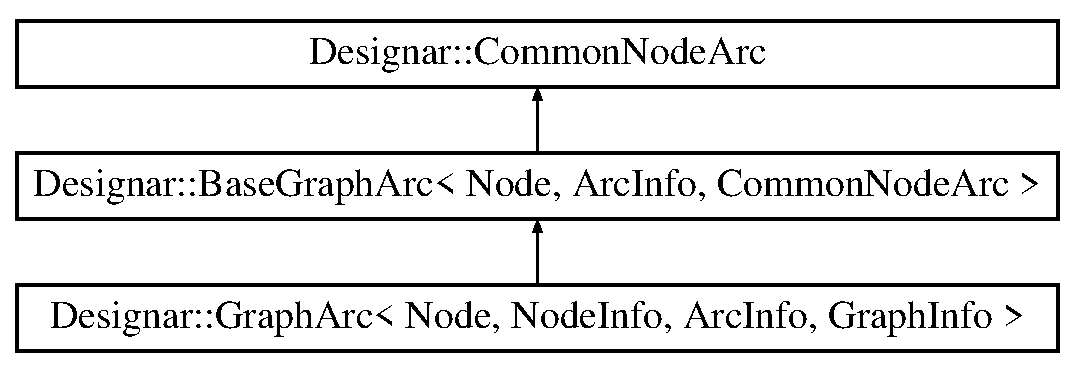
\includegraphics[height=3.000000cm]{class_designar_1_1_graph_arc}
\end{center}
\end{figure}
\subsection*{Protected Attributes}
\begin{DoxyCompactItemize}
\item 
\hyperlink{class_designar_1_1_d_l_node}{D\+L\+Node}$<$ \hyperlink{class_designar_1_1_d_l_node}{D\+L\+Node}$<$ \hyperlink{class_designar_1_1_graph_arc}{Graph\+Arc} $>$ $\ast$ $>$ $\ast$ \hyperlink{class_designar_1_1_graph_arc_addbd9ebec2787d3950aa679acf392fc6}{arc\+\_\+in\+\_\+src\+\_\+node} = nullptr
\item 
\hyperlink{class_designar_1_1_d_l_node}{D\+L\+Node}$<$ \hyperlink{class_designar_1_1_d_l_node}{D\+L\+Node}$<$ \hyperlink{class_designar_1_1_graph_arc}{Graph\+Arc} $>$ $\ast$ $>$ $\ast$ \hyperlink{class_designar_1_1_graph_arc_a49385be5572e3c6dd2d22309ef5fd79a}{arc\+\_\+in\+\_\+tgt\+\_\+node} = nullptr
\end{DoxyCompactItemize}
\subsection*{Friends}
\begin{DoxyCompactItemize}
\item 
class \hyperlink{class_designar_1_1_graph_arc_a0a9834688687d864501bbb9c85b0d32c}{Graph$<$ Node\+Info, Arc\+Info, Graph\+Info $>$}
\item 
class \hyperlink{class_designar_1_1_graph_arc_a94936ca2e45f109cf3805a93858fbc75}{D\+L\+Node$<$ Graph\+Arc $>$}
\end{DoxyCompactItemize}
\subsection*{Additional Inherited Members}


\subsection{Detailed Description}
\subsubsection*{template$<$class Node, typename Node\+Info, typename Arc\+Info, typename Graph\+Info$>$\newline
class Designar\+::\+Graph\+Arc$<$ Node, Node\+Info, Arc\+Info, Graph\+Info $>$}



Definition at line 59 of file graph.\+H.



\subsection{Friends And Related Function Documentation}
\mbox{\Hypertarget{class_designar_1_1_graph_arc_a94936ca2e45f109cf3805a93858fbc75}\label{class_designar_1_1_graph_arc_a94936ca2e45f109cf3805a93858fbc75}} 
\index{Designar\+::\+Graph\+Arc@{Designar\+::\+Graph\+Arc}!D\+L\+Node$<$ Graph\+Arc $>$@{D\+L\+Node$<$ Graph\+Arc $>$}}
\index{D\+L\+Node$<$ Graph\+Arc $>$@{D\+L\+Node$<$ Graph\+Arc $>$}!Designar\+::\+Graph\+Arc@{Designar\+::\+Graph\+Arc}}
\subsubsection{\texorpdfstring{D\+L\+Node$<$ Graph\+Arc $>$}{DLNode< GraphArc >}}
{\footnotesize\ttfamily template$<$class Node , typename Node\+Info , typename Arc\+Info , typename Graph\+Info $>$ \\
friend class \hyperlink{class_designar_1_1_d_l_node}{D\+L\+Node}$<$ \hyperlink{class_designar_1_1_graph_arc}{Graph\+Arc} $>$\hspace{0.3cm}{\ttfamily [friend]}}



Definition at line 62 of file graph.\+H.

\mbox{\Hypertarget{class_designar_1_1_graph_arc_a0a9834688687d864501bbb9c85b0d32c}\label{class_designar_1_1_graph_arc_a0a9834688687d864501bbb9c85b0d32c}} 
\index{Designar\+::\+Graph\+Arc@{Designar\+::\+Graph\+Arc}!Graph$<$ Node\+Info, Arc\+Info, Graph\+Info $>$@{Graph$<$ Node\+Info, Arc\+Info, Graph\+Info $>$}}
\index{Graph$<$ Node\+Info, Arc\+Info, Graph\+Info $>$@{Graph$<$ Node\+Info, Arc\+Info, Graph\+Info $>$}!Designar\+::\+Graph\+Arc@{Designar\+::\+Graph\+Arc}}
\subsubsection{\texorpdfstring{Graph$<$ Node\+Info, Arc\+Info, Graph\+Info $>$}{Graph< NodeInfo, ArcInfo, GraphInfo >}}
{\footnotesize\ttfamily template$<$class Node , typename Node\+Info , typename Arc\+Info , typename Graph\+Info $>$ \\
friend class \hyperlink{class_designar_1_1_graph}{Graph}$<$ Node\+Info, Arc\+Info, Graph\+Info $>$\hspace{0.3cm}{\ttfamily [friend]}}



Definition at line 61 of file graph.\+H.



\subsection{Member Data Documentation}
\mbox{\Hypertarget{class_designar_1_1_graph_arc_addbd9ebec2787d3950aa679acf392fc6}\label{class_designar_1_1_graph_arc_addbd9ebec2787d3950aa679acf392fc6}} 
\index{Designar\+::\+Graph\+Arc@{Designar\+::\+Graph\+Arc}!arc\+\_\+in\+\_\+src\+\_\+node@{arc\+\_\+in\+\_\+src\+\_\+node}}
\index{arc\+\_\+in\+\_\+src\+\_\+node@{arc\+\_\+in\+\_\+src\+\_\+node}!Designar\+::\+Graph\+Arc@{Designar\+::\+Graph\+Arc}}
\subsubsection{\texorpdfstring{arc\+\_\+in\+\_\+src\+\_\+node}{arc\_in\_src\_node}}
{\footnotesize\ttfamily template$<$class Node , typename Node\+Info , typename Arc\+Info , typename Graph\+Info $>$ \\
\hyperlink{class_designar_1_1_d_l_node}{D\+L\+Node}$<$\hyperlink{class_designar_1_1_d_l_node}{D\+L\+Node}$<$\hyperlink{class_designar_1_1_graph_arc}{Graph\+Arc}$>$ $\ast$$>$$\ast$ \hyperlink{class_designar_1_1_graph_arc}{Designar\+::\+Graph\+Arc}$<$ \hyperlink{namespace_designar_a5af326c65aa2bd26b26c410f2030d09e}{Node}, Node\+Info, Arc\+Info, Graph\+Info $>$\+::arc\+\_\+in\+\_\+src\+\_\+node = nullptr\hspace{0.3cm}{\ttfamily [protected]}}



Definition at line 67 of file graph.\+H.

\mbox{\Hypertarget{class_designar_1_1_graph_arc_a49385be5572e3c6dd2d22309ef5fd79a}\label{class_designar_1_1_graph_arc_a49385be5572e3c6dd2d22309ef5fd79a}} 
\index{Designar\+::\+Graph\+Arc@{Designar\+::\+Graph\+Arc}!arc\+\_\+in\+\_\+tgt\+\_\+node@{arc\+\_\+in\+\_\+tgt\+\_\+node}}
\index{arc\+\_\+in\+\_\+tgt\+\_\+node@{arc\+\_\+in\+\_\+tgt\+\_\+node}!Designar\+::\+Graph\+Arc@{Designar\+::\+Graph\+Arc}}
\subsubsection{\texorpdfstring{arc\+\_\+in\+\_\+tgt\+\_\+node}{arc\_in\_tgt\_node}}
{\footnotesize\ttfamily template$<$class Node , typename Node\+Info , typename Arc\+Info , typename Graph\+Info $>$ \\
\hyperlink{class_designar_1_1_d_l_node}{D\+L\+Node}$<$\hyperlink{class_designar_1_1_d_l_node}{D\+L\+Node}$<$\hyperlink{class_designar_1_1_graph_arc}{Graph\+Arc}$>$ $\ast$$>$$\ast$ \hyperlink{class_designar_1_1_graph_arc}{Designar\+::\+Graph\+Arc}$<$ \hyperlink{namespace_designar_a5af326c65aa2bd26b26c410f2030d09e}{Node}, Node\+Info, Arc\+Info, Graph\+Info $>$\+::arc\+\_\+in\+\_\+tgt\+\_\+node = nullptr\hspace{0.3cm}{\ttfamily [protected]}}



Definition at line 68 of file graph.\+H.



The documentation for this class was generated from the following file\+:\begin{DoxyCompactItemize}
\item 
/home/julio/\+De\+S\+I\+G\+N\+A\+R-\/doc/\+De\+Si\+G\+N\+A\+R/include/\hyperlink{graph_8_h}{graph.\+H}\end{DoxyCompactItemize}

\hypertarget{class_designar_1_1_graph_node}{}\section{Designar\+:\+:Graph\+Node$<$ Node\+Info, Arc\+Info, Graph\+Info $>$ Class Template Reference}
\label{class_designar_1_1_graph_node}\index{Designar\+::\+Graph\+Node$<$ Node\+Info, Arc\+Info, Graph\+Info $>$@{Designar\+::\+Graph\+Node$<$ Node\+Info, Arc\+Info, Graph\+Info $>$}}


{\ttfamily \#include $<$graph.\+H$>$}

Inheritance diagram for Designar\+:\+:Graph\+Node$<$ Node\+Info, Arc\+Info, Graph\+Info $>$\+:\begin{figure}[H]
\begin{center}
\leavevmode
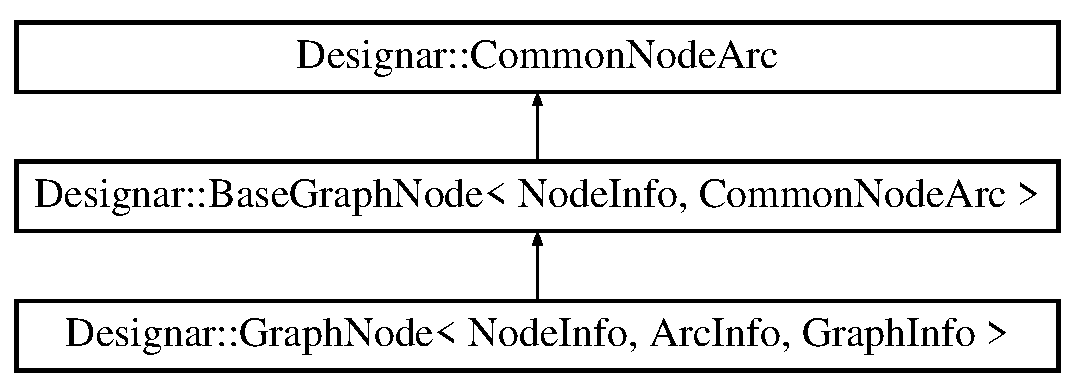
\includegraphics[height=3.000000cm]{class_designar_1_1_graph_node}
\end{center}
\end{figure}
\subsection*{Friends}
\begin{DoxyCompactItemize}
\item 
class \hyperlink{class_designar_1_1_graph_node_a0a9834688687d864501bbb9c85b0d32c}{Graph$<$ Node\+Info, Arc\+Info, Graph\+Info $>$}
\item 
class \hyperlink{class_designar_1_1_graph_node_a5d0e7b51039a0eb5cfdfdb2f3701f06d}{D\+L\+Node$<$ Graph\+Node $>$}
\end{DoxyCompactItemize}
\subsection*{Additional Inherited Members}


\subsection{Detailed Description}
\subsubsection*{template$<$typename Node\+Info, typename Arc\+Info, typename Graph\+Info$>$\newline
class Designar\+::\+Graph\+Node$<$ Node\+Info, Arc\+Info, Graph\+Info $>$}



Definition at line 41 of file graph.\+H.



\subsection{Friends And Related Function Documentation}
\mbox{\Hypertarget{class_designar_1_1_graph_node_a5d0e7b51039a0eb5cfdfdb2f3701f06d}\label{class_designar_1_1_graph_node_a5d0e7b51039a0eb5cfdfdb2f3701f06d}} 
\index{Designar\+::\+Graph\+Node@{Designar\+::\+Graph\+Node}!D\+L\+Node$<$ Graph\+Node $>$@{D\+L\+Node$<$ Graph\+Node $>$}}
\index{D\+L\+Node$<$ Graph\+Node $>$@{D\+L\+Node$<$ Graph\+Node $>$}!Designar\+::\+Graph\+Node@{Designar\+::\+Graph\+Node}}
\subsubsection{\texorpdfstring{D\+L\+Node$<$ Graph\+Node $>$}{DLNode< GraphNode >}}
{\footnotesize\ttfamily template$<$typename Node\+Info , typename Arc\+Info , typename Graph\+Info $>$ \\
friend class \hyperlink{class_designar_1_1_d_l_node}{D\+L\+Node}$<$ \hyperlink{class_designar_1_1_graph_node}{Graph\+Node} $>$\hspace{0.3cm}{\ttfamily [friend]}}



Definition at line 44 of file graph.\+H.

\mbox{\Hypertarget{class_designar_1_1_graph_node_a0a9834688687d864501bbb9c85b0d32c}\label{class_designar_1_1_graph_node_a0a9834688687d864501bbb9c85b0d32c}} 
\index{Designar\+::\+Graph\+Node@{Designar\+::\+Graph\+Node}!Graph$<$ Node\+Info, Arc\+Info, Graph\+Info $>$@{Graph$<$ Node\+Info, Arc\+Info, Graph\+Info $>$}}
\index{Graph$<$ Node\+Info, Arc\+Info, Graph\+Info $>$@{Graph$<$ Node\+Info, Arc\+Info, Graph\+Info $>$}!Designar\+::\+Graph\+Node@{Designar\+::\+Graph\+Node}}
\subsubsection{\texorpdfstring{Graph$<$ Node\+Info, Arc\+Info, Graph\+Info $>$}{Graph< NodeInfo, ArcInfo, GraphInfo >}}
{\footnotesize\ttfamily template$<$typename Node\+Info , typename Arc\+Info , typename Graph\+Info $>$ \\
friend class \hyperlink{class_designar_1_1_graph}{Graph}$<$ Node\+Info, Arc\+Info, Graph\+Info $>$\hspace{0.3cm}{\ttfamily [friend]}}



Definition at line 43 of file graph.\+H.



The documentation for this class was generated from the following file\+:\begin{DoxyCompactItemize}
\item 
De\+Si\+G\+N\+A\+R/include/\hyperlink{graph_8_h}{graph.\+H}\end{DoxyCompactItemize}

\hypertarget{class_designar_1_1_hash_map}{}\section{Referencia de la plantilla de la Clase Designar\+:\+:Hash\+Map$<$ Key, Value, Cmp $>$}
\label{class_designar_1_1_hash_map}\index{Designar\+::\+Hash\+Map$<$ Key, Value, Cmp $>$@{Designar\+::\+Hash\+Map$<$ Key, Value, Cmp $>$}}


{\ttfamily \#include $<$map.\+H$>$}

Diagrama de herencias de Designar\+:\+:Hash\+Map$<$ Key, Value, Cmp $>$\begin{figure}[H]
\begin{center}
\leavevmode
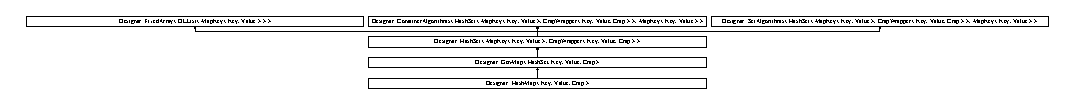
\includegraphics[height=0.969697cm]{class_designar_1_1_hash_map}
\end{center}
\end{figure}
\subsection*{Métodos públicos}
\begin{DoxyCompactItemize}
\item 
\hyperlink{class_designar_1_1_hash_map_a39b8b365b9399ca72142f522d8d4e877}{Hash\+Map} (\hyperlink{namespace_designar_aa72662848b9f4815e7bf31a7cf3e33d1}{nat\+\_\+t} \hyperlink{class_designar_1_1_hash_set_a0026e1b2caf94d25b554cd6a399f691f}{size}, Cmp \&\+\_\+cmp, Hash\+Fct\+Ptr \+\_\+fct)
\item 
\hyperlink{class_designar_1_1_hash_map_aa82cf8d63637401365bebe4dafe556e2}{Hash\+Map} (\hyperlink{namespace_designar_aa72662848b9f4815e7bf31a7cf3e33d1}{nat\+\_\+t} \hyperlink{class_designar_1_1_hash_set_a0026e1b2caf94d25b554cd6a399f691f}{size}, Cmp \&\&\+\_\+cmp=Cmp(), Hash\+Fct\+Ptr fct=\&\hyperlink{namespace_designar_afd5712d16b3ae1c1c7d59f1004cd96fd}{super\+\_\+fast\+\_\+hash})
\item 
\hyperlink{class_designar_1_1_hash_map_ad1b22ee9f50a5be7febcf622ae8cb31a}{Hash\+Map} (Cmp \&\+\_\+cmp, Hash\+Fct\+Ptr \+\_\+fct)
\item 
\hyperlink{class_designar_1_1_hash_map_ad310e763bce2806e390fde121efe92c6}{Hash\+Map} (Cmp \&\&\+\_\+cmp=Cmp(), Hash\+Fct\+Ptr fct=\&\hyperlink{namespace_designar_afd5712d16b3ae1c1c7d59f1004cd96fd}{super\+\_\+fast\+\_\+hash})
\item 
\hyperlink{class_designar_1_1_hash_map_a3a00fde1b9022f78eabcb90eef446566}{Hash\+Map} (const std\+::initializer\+\_\+list$<$ Item $>$ \&)
\item 
\hyperlink{class_designar_1_1_hash_map_aa59dbb80b0a3d62cde145a84e76bd1bb}{Hash\+Map} (const \hyperlink{class_designar_1_1_hash_map}{Hash\+Map} \&\hyperlink{class_designar_1_1_container_algorithms_a3b9044a197e4ceec6a1de03de197a293}{map})
\item 
\hyperlink{class_designar_1_1_hash_map_a16d4d99bb19bd91ea5700d46d188684b}{Hash\+Map} (\hyperlink{class_designar_1_1_hash_map}{Hash\+Map} \&\&\hyperlink{class_designar_1_1_container_algorithms_a3b9044a197e4ceec6a1de03de197a293}{map})
\item 
\hyperlink{class_designar_1_1_hash_map}{Hash\+Map} \& \hyperlink{class_designar_1_1_hash_map_afaf1bd72c38d70492007bdfd71ae94af}{operator=} (const \hyperlink{class_designar_1_1_hash_map}{Hash\+Map} \&m)
\item 
\hyperlink{class_designar_1_1_hash_map}{Hash\+Map} \& \hyperlink{class_designar_1_1_hash_map_afb0dfc4b02391d050767dc730a73f3c5}{operator=} (\hyperlink{class_designar_1_1_hash_map}{Hash\+Map} \&\&m)
\item 
void \hyperlink{class_designar_1_1_hash_map_af4390f5bdd5a0ec5b1d62d0630420854}{swap} (\hyperlink{class_designar_1_1_hash_map}{Hash\+Map} \&\hyperlink{class_designar_1_1_container_algorithms_a3b9044a197e4ceec6a1de03de197a293}{map})
\item 
Hash\+Fct\+Type \& \hyperlink{class_designar_1_1_hash_map_abcb9cdbb25c6d35f0f0373011265d570}{get\+\_\+hash\+\_\+fct} ()
\item 
const Hash\+Fct\+Type \& \hyperlink{class_designar_1_1_hash_map_a7372936ee9f2da7dbbc06a54955b9833}{get\+\_\+hash\+\_\+fct} () const
\end{DoxyCompactItemize}
\subsection*{Otros miembros heredados}


\subsection{Descripción detallada}
\subsubsection*{template$<$typename Key, typename Value, class Cmp = std\+::equal\+\_\+to$<$\+Key$>$$>$\newline
class Designar\+::\+Hash\+Map$<$ Key, Value, Cmp $>$}



Definición en la línea 529 del archivo map.\+H.



\subsection{Documentación del constructor y destructor}
\mbox{\Hypertarget{class_designar_1_1_hash_map_a39b8b365b9399ca72142f522d8d4e877}\label{class_designar_1_1_hash_map_a39b8b365b9399ca72142f522d8d4e877}} 
\index{Designar\+::\+Hash\+Map@{Designar\+::\+Hash\+Map}!Hash\+Map@{Hash\+Map}}
\index{Hash\+Map@{Hash\+Map}!Designar\+::\+Hash\+Map@{Designar\+::\+Hash\+Map}}
\subsubsection{\texorpdfstring{Hash\+Map()}{HashMap()}\hspace{0.1cm}{\footnotesize\ttfamily [1/7]}}
{\footnotesize\ttfamily template$<$typename Key, typename Value, class Cmp = std\+::equal\+\_\+to$<$\+Key$>$$>$ \\
\hyperlink{class_designar_1_1_hash_map}{Designar\+::\+Hash\+Map}$<$ Key, Value, Cmp $>$\+::\hyperlink{class_designar_1_1_hash_map}{Hash\+Map} (\begin{DoxyParamCaption}\item[{\hyperlink{namespace_designar_aa72662848b9f4815e7bf31a7cf3e33d1}{nat\+\_\+t}}]{size,  }\item[{Cmp \&}]{\+\_\+cmp,  }\item[{Hash\+Fct\+Ptr}]{\+\_\+fct }\end{DoxyParamCaption})\hspace{0.3cm}{\ttfamily [inline]}}



Definición en la línea 541 del archivo map.\+H.

\mbox{\Hypertarget{class_designar_1_1_hash_map_aa82cf8d63637401365bebe4dafe556e2}\label{class_designar_1_1_hash_map_aa82cf8d63637401365bebe4dafe556e2}} 
\index{Designar\+::\+Hash\+Map@{Designar\+::\+Hash\+Map}!Hash\+Map@{Hash\+Map}}
\index{Hash\+Map@{Hash\+Map}!Designar\+::\+Hash\+Map@{Designar\+::\+Hash\+Map}}
\subsubsection{\texorpdfstring{Hash\+Map()}{HashMap()}\hspace{0.1cm}{\footnotesize\ttfamily [2/7]}}
{\footnotesize\ttfamily template$<$typename Key, typename Value, class Cmp = std\+::equal\+\_\+to$<$\+Key$>$$>$ \\
\hyperlink{class_designar_1_1_hash_map}{Designar\+::\+Hash\+Map}$<$ Key, Value, Cmp $>$\+::\hyperlink{class_designar_1_1_hash_map}{Hash\+Map} (\begin{DoxyParamCaption}\item[{\hyperlink{namespace_designar_aa72662848b9f4815e7bf31a7cf3e33d1}{nat\+\_\+t}}]{size,  }\item[{Cmp \&\&}]{\+\_\+cmp = {\ttfamily Cmp()},  }\item[{Hash\+Fct\+Ptr}]{fct = {\ttfamily \&\hyperlink{namespace_designar_afd5712d16b3ae1c1c7d59f1004cd96fd}{super\+\_\+fast\+\_\+hash}} }\end{DoxyParamCaption})\hspace{0.3cm}{\ttfamily [inline]}}



Definición en la línea 549 del archivo map.\+H.

\mbox{\Hypertarget{class_designar_1_1_hash_map_ad1b22ee9f50a5be7febcf622ae8cb31a}\label{class_designar_1_1_hash_map_ad1b22ee9f50a5be7febcf622ae8cb31a}} 
\index{Designar\+::\+Hash\+Map@{Designar\+::\+Hash\+Map}!Hash\+Map@{Hash\+Map}}
\index{Hash\+Map@{Hash\+Map}!Designar\+::\+Hash\+Map@{Designar\+::\+Hash\+Map}}
\subsubsection{\texorpdfstring{Hash\+Map()}{HashMap()}\hspace{0.1cm}{\footnotesize\ttfamily [3/7]}}
{\footnotesize\ttfamily template$<$typename Key, typename Value, class Cmp = std\+::equal\+\_\+to$<$\+Key$>$$>$ \\
\hyperlink{class_designar_1_1_hash_map}{Designar\+::\+Hash\+Map}$<$ Key, Value, Cmp $>$\+::\hyperlink{class_designar_1_1_hash_map}{Hash\+Map} (\begin{DoxyParamCaption}\item[{Cmp \&}]{\+\_\+cmp,  }\item[{Hash\+Fct\+Ptr}]{\+\_\+fct }\end{DoxyParamCaption})\hspace{0.3cm}{\ttfamily [inline]}}



Definición en la línea 555 del archivo map.\+H.

\mbox{\Hypertarget{class_designar_1_1_hash_map_ad310e763bce2806e390fde121efe92c6}\label{class_designar_1_1_hash_map_ad310e763bce2806e390fde121efe92c6}} 
\index{Designar\+::\+Hash\+Map@{Designar\+::\+Hash\+Map}!Hash\+Map@{Hash\+Map}}
\index{Hash\+Map@{Hash\+Map}!Designar\+::\+Hash\+Map@{Designar\+::\+Hash\+Map}}
\subsubsection{\texorpdfstring{Hash\+Map()}{HashMap()}\hspace{0.1cm}{\footnotesize\ttfamily [4/7]}}
{\footnotesize\ttfamily template$<$typename Key, typename Value, class Cmp = std\+::equal\+\_\+to$<$\+Key$>$$>$ \\
\hyperlink{class_designar_1_1_hash_map}{Designar\+::\+Hash\+Map}$<$ Key, Value, Cmp $>$\+::\hyperlink{class_designar_1_1_hash_map}{Hash\+Map} (\begin{DoxyParamCaption}\item[{Cmp \&\&}]{\+\_\+cmp = {\ttfamily Cmp()},  }\item[{Hash\+Fct\+Ptr}]{fct = {\ttfamily \&\hyperlink{namespace_designar_afd5712d16b3ae1c1c7d59f1004cd96fd}{super\+\_\+fast\+\_\+hash}} }\end{DoxyParamCaption})\hspace{0.3cm}{\ttfamily [inline]}}



Definición en la línea 563 del archivo map.\+H.

\mbox{\Hypertarget{class_designar_1_1_hash_map_a3a00fde1b9022f78eabcb90eef446566}\label{class_designar_1_1_hash_map_a3a00fde1b9022f78eabcb90eef446566}} 
\index{Designar\+::\+Hash\+Map@{Designar\+::\+Hash\+Map}!Hash\+Map@{Hash\+Map}}
\index{Hash\+Map@{Hash\+Map}!Designar\+::\+Hash\+Map@{Designar\+::\+Hash\+Map}}
\subsubsection{\texorpdfstring{Hash\+Map()}{HashMap()}\hspace{0.1cm}{\footnotesize\ttfamily [5/7]}}
{\footnotesize\ttfamily template$<$typename Key , typename Value , class Cmp$>$ \\
\hyperlink{class_designar_1_1_hash_map}{Designar\+::\+Hash\+Map}$<$ Key, Value, Cmp $>$\+::\hyperlink{class_designar_1_1_hash_map}{Hash\+Map} (\begin{DoxyParamCaption}\item[{const std\+::initializer\+\_\+list$<$ Item $>$ \&}]{l }\end{DoxyParamCaption})}



Definición en la línea 617 del archivo map.\+H.

\mbox{\Hypertarget{class_designar_1_1_hash_map_aa59dbb80b0a3d62cde145a84e76bd1bb}\label{class_designar_1_1_hash_map_aa59dbb80b0a3d62cde145a84e76bd1bb}} 
\index{Designar\+::\+Hash\+Map@{Designar\+::\+Hash\+Map}!Hash\+Map@{Hash\+Map}}
\index{Hash\+Map@{Hash\+Map}!Designar\+::\+Hash\+Map@{Designar\+::\+Hash\+Map}}
\subsubsection{\texorpdfstring{Hash\+Map()}{HashMap()}\hspace{0.1cm}{\footnotesize\ttfamily [6/7]}}
{\footnotesize\ttfamily template$<$typename Key, typename Value, class Cmp = std\+::equal\+\_\+to$<$\+Key$>$$>$ \\
\hyperlink{class_designar_1_1_hash_map}{Designar\+::\+Hash\+Map}$<$ Key, Value, Cmp $>$\+::\hyperlink{class_designar_1_1_hash_map}{Hash\+Map} (\begin{DoxyParamCaption}\item[{const \hyperlink{class_designar_1_1_hash_map}{Hash\+Map}$<$ Key, Value, Cmp $>$ \&}]{map }\end{DoxyParamCaption})\hspace{0.3cm}{\ttfamily [inline]}}



Definición en la línea 571 del archivo map.\+H.

\mbox{\Hypertarget{class_designar_1_1_hash_map_a16d4d99bb19bd91ea5700d46d188684b}\label{class_designar_1_1_hash_map_a16d4d99bb19bd91ea5700d46d188684b}} 
\index{Designar\+::\+Hash\+Map@{Designar\+::\+Hash\+Map}!Hash\+Map@{Hash\+Map}}
\index{Hash\+Map@{Hash\+Map}!Designar\+::\+Hash\+Map@{Designar\+::\+Hash\+Map}}
\subsubsection{\texorpdfstring{Hash\+Map()}{HashMap()}\hspace{0.1cm}{\footnotesize\ttfamily [7/7]}}
{\footnotesize\ttfamily template$<$typename Key, typename Value, class Cmp = std\+::equal\+\_\+to$<$\+Key$>$$>$ \\
\hyperlink{class_designar_1_1_hash_map}{Designar\+::\+Hash\+Map}$<$ Key, Value, Cmp $>$\+::\hyperlink{class_designar_1_1_hash_map}{Hash\+Map} (\begin{DoxyParamCaption}\item[{\hyperlink{class_designar_1_1_hash_map}{Hash\+Map}$<$ Key, Value, Cmp $>$ \&\&}]{map }\end{DoxyParamCaption})\hspace{0.3cm}{\ttfamily [inline]}}



Definición en la línea 577 del archivo map.\+H.



\subsection{Documentación de las funciones miembro}
\mbox{\Hypertarget{class_designar_1_1_hash_map_abcb9cdbb25c6d35f0f0373011265d570}\label{class_designar_1_1_hash_map_abcb9cdbb25c6d35f0f0373011265d570}} 
\index{Designar\+::\+Hash\+Map@{Designar\+::\+Hash\+Map}!get\+\_\+hash\+\_\+fct@{get\+\_\+hash\+\_\+fct}}
\index{get\+\_\+hash\+\_\+fct@{get\+\_\+hash\+\_\+fct}!Designar\+::\+Hash\+Map@{Designar\+::\+Hash\+Map}}
\subsubsection{\texorpdfstring{get\+\_\+hash\+\_\+fct()}{get\_hash\_fct()}\hspace{0.1cm}{\footnotesize\ttfamily [1/2]}}
{\footnotesize\ttfamily template$<$typename Key, typename Value, class Cmp = std\+::equal\+\_\+to$<$\+Key$>$$>$ \\
Hash\+Fct\+Type\& \hyperlink{class_designar_1_1_hash_map}{Designar\+::\+Hash\+Map}$<$ Key, Value, Cmp $>$\+::get\+\_\+hash\+\_\+fct (\begin{DoxyParamCaption}{ }\end{DoxyParamCaption})\hspace{0.3cm}{\ttfamily [inline]}}



Definición en la línea 605 del archivo map.\+H.

\mbox{\Hypertarget{class_designar_1_1_hash_map_a7372936ee9f2da7dbbc06a54955b9833}\label{class_designar_1_1_hash_map_a7372936ee9f2da7dbbc06a54955b9833}} 
\index{Designar\+::\+Hash\+Map@{Designar\+::\+Hash\+Map}!get\+\_\+hash\+\_\+fct@{get\+\_\+hash\+\_\+fct}}
\index{get\+\_\+hash\+\_\+fct@{get\+\_\+hash\+\_\+fct}!Designar\+::\+Hash\+Map@{Designar\+::\+Hash\+Map}}
\subsubsection{\texorpdfstring{get\+\_\+hash\+\_\+fct()}{get\_hash\_fct()}\hspace{0.1cm}{\footnotesize\ttfamily [2/2]}}
{\footnotesize\ttfamily template$<$typename Key, typename Value, class Cmp = std\+::equal\+\_\+to$<$\+Key$>$$>$ \\
const Hash\+Fct\+Type\& \hyperlink{class_designar_1_1_hash_map}{Designar\+::\+Hash\+Map}$<$ Key, Value, Cmp $>$\+::get\+\_\+hash\+\_\+fct (\begin{DoxyParamCaption}{ }\end{DoxyParamCaption}) const\hspace{0.3cm}{\ttfamily [inline]}}



Definición en la línea 610 del archivo map.\+H.

\mbox{\Hypertarget{class_designar_1_1_hash_map_afaf1bd72c38d70492007bdfd71ae94af}\label{class_designar_1_1_hash_map_afaf1bd72c38d70492007bdfd71ae94af}} 
\index{Designar\+::\+Hash\+Map@{Designar\+::\+Hash\+Map}!operator=@{operator=}}
\index{operator=@{operator=}!Designar\+::\+Hash\+Map@{Designar\+::\+Hash\+Map}}
\subsubsection{\texorpdfstring{operator=()}{operator=()}\hspace{0.1cm}{\footnotesize\ttfamily [1/2]}}
{\footnotesize\ttfamily template$<$typename Key, typename Value, class Cmp = std\+::equal\+\_\+to$<$\+Key$>$$>$ \\
\hyperlink{class_designar_1_1_hash_map}{Hash\+Map}\& \hyperlink{class_designar_1_1_hash_map}{Designar\+::\+Hash\+Map}$<$ Key, Value, Cmp $>$\+::operator= (\begin{DoxyParamCaption}\item[{const \hyperlink{class_designar_1_1_hash_map}{Hash\+Map}$<$ Key, Value, Cmp $>$ \&}]{m }\end{DoxyParamCaption})\hspace{0.3cm}{\ttfamily [inline]}}



Definición en la línea 583 del archivo map.\+H.

\mbox{\Hypertarget{class_designar_1_1_hash_map_afb0dfc4b02391d050767dc730a73f3c5}\label{class_designar_1_1_hash_map_afb0dfc4b02391d050767dc730a73f3c5}} 
\index{Designar\+::\+Hash\+Map@{Designar\+::\+Hash\+Map}!operator=@{operator=}}
\index{operator=@{operator=}!Designar\+::\+Hash\+Map@{Designar\+::\+Hash\+Map}}
\subsubsection{\texorpdfstring{operator=()}{operator=()}\hspace{0.1cm}{\footnotesize\ttfamily [2/2]}}
{\footnotesize\ttfamily template$<$typename Key, typename Value, class Cmp = std\+::equal\+\_\+to$<$\+Key$>$$>$ \\
\hyperlink{class_designar_1_1_hash_map}{Hash\+Map}\& \hyperlink{class_designar_1_1_hash_map}{Designar\+::\+Hash\+Map}$<$ Key, Value, Cmp $>$\+::operator= (\begin{DoxyParamCaption}\item[{\hyperlink{class_designar_1_1_hash_map}{Hash\+Map}$<$ Key, Value, Cmp $>$ \&\&}]{m }\end{DoxyParamCaption})\hspace{0.3cm}{\ttfamily [inline]}}



Definición en la línea 593 del archivo map.\+H.

\mbox{\Hypertarget{class_designar_1_1_hash_map_af4390f5bdd5a0ec5b1d62d0630420854}\label{class_designar_1_1_hash_map_af4390f5bdd5a0ec5b1d62d0630420854}} 
\index{Designar\+::\+Hash\+Map@{Designar\+::\+Hash\+Map}!swap@{swap}}
\index{swap@{swap}!Designar\+::\+Hash\+Map@{Designar\+::\+Hash\+Map}}
\subsubsection{\texorpdfstring{swap()}{swap()}}
{\footnotesize\ttfamily template$<$typename Key, typename Value, class Cmp = std\+::equal\+\_\+to$<$\+Key$>$$>$ \\
void \hyperlink{class_designar_1_1_hash_map}{Designar\+::\+Hash\+Map}$<$ Key, Value, Cmp $>$\+::swap (\begin{DoxyParamCaption}\item[{\hyperlink{class_designar_1_1_hash_map}{Hash\+Map}$<$ Key, Value, Cmp $>$ \&}]{map }\end{DoxyParamCaption})\hspace{0.3cm}{\ttfamily [inline]}}



Definición en la línea 599 del archivo map.\+H.



La documentación para esta clase fue generada a partir del siguiente fichero\+:\begin{DoxyCompactItemize}
\item 
/home/julio/\+De\+S\+I\+G\+N\+A\+R-\/doc/\+De\+Si\+G\+N\+A\+R/include/\hyperlink{map_8_h}{map.\+H}\end{DoxyCompactItemize}

\hypertarget{class_designar_1_1_hash_set}{}\section{Designar\+:\+:Hash\+Set$<$ Key, Cmp $>$ Class Template Reference}
\label{class_designar_1_1_hash_set}\index{Designar\+::\+Hash\+Set$<$ Key, Cmp $>$@{Designar\+::\+Hash\+Set$<$ Key, Cmp $>$}}


{\ttfamily \#include $<$hash.\+H$>$}

Inheritance diagram for Designar\+:\+:Hash\+Set$<$ Key, Cmp $>$\+:\begin{figure}[H]
\begin{center}
\leavevmode
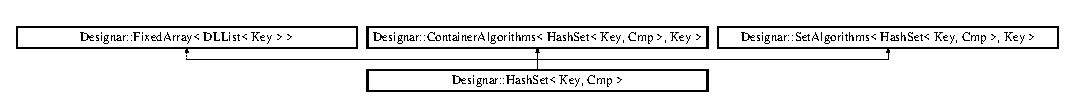
\includegraphics[height=1.000894cm]{class_designar_1_1_hash_set}
\end{center}
\end{figure}
\subsection*{Classes}
\begin{DoxyCompactItemize}
\item 
class \hyperlink{class_designar_1_1_hash_set_1_1_iterator}{Iterator}
\end{DoxyCompactItemize}
\subsection*{Public Types}
\begin{DoxyCompactItemize}
\item 
using \hyperlink{class_designar_1_1_hash_set_af1cb023a84bf6c6f17867f99bbc523c5}{Item\+Type} = Key
\item 
using \hyperlink{class_designar_1_1_hash_set_a4e23320d0b13915ce84186132ad4197a}{Key\+Type} = Key
\item 
using \hyperlink{class_designar_1_1_hash_set_af75f5917c5f53891a4129bd77d5d2906}{Data\+Type} = Key
\item 
using \hyperlink{class_designar_1_1_hash_set_a4edc6d161470bffb03dad2bbc916b6a0}{Value\+Type} = Key
\item 
using \hyperlink{class_designar_1_1_hash_set_a1bfcb16c2a94c0ab22e15f38b05ba8cc}{Size\+Type} = \hyperlink{namespace_designar_aa72662848b9f4815e7bf31a7cf3e33d1}{nat\+\_\+t}
\item 
using \hyperlink{class_designar_1_1_hash_set_ad0ab040392888a3320d2d72d1ead9968}{Cmp\+Type} = Cmp
\item 
using \hyperlink{class_designar_1_1_hash_set_a7a8b0a4970519ebc9ccc1ad247d0639f}{Hash\+Fct\+Ptr} = \hyperlink{namespace_designar_aa72662848b9f4815e7bf31a7cf3e33d1}{nat\+\_\+t}($\ast$)(const Key \&)
\item 
using \hyperlink{class_designar_1_1_hash_set_a05d8d111665c25bc17290c01fa299398}{Hash\+Fct\+Type} = std\+::function$<$ \hyperlink{namespace_designar_aa72662848b9f4815e7bf31a7cf3e33d1}{nat\+\_\+t}(const Key \&)$>$
\end{DoxyCompactItemize}
\subsection*{Public Member Functions}
\begin{DoxyCompactItemize}
\item 
\hyperlink{class_designar_1_1_hash_set_afb5e932ee4dcc9b1dec4d6eefd810c32}{Hash\+Set} (\hyperlink{namespace_designar_aa72662848b9f4815e7bf31a7cf3e33d1}{nat\+\_\+t} \hyperlink{class_designar_1_1_hash_set_a0026e1b2caf94d25b554cd6a399f691f}{size}, Cmp \&\+\_\+cmp, \hyperlink{class_designar_1_1_hash_set_a05d8d111665c25bc17290c01fa299398}{Hash\+Fct\+Type} fct, \hyperlink{namespace_designar_aca2c32af26808dbec1f3a3071fad25ce}{real\+\_\+t} \+\_\+lower\+\_\+alpha, \hyperlink{namespace_designar_aca2c32af26808dbec1f3a3071fad25ce}{real\+\_\+t} \+\_\+upper\+\_\+alpha)
\item 
\hyperlink{class_designar_1_1_hash_set_a6f60ca18ef5bcf8560b9827ca9678e58}{Hash\+Set} (\hyperlink{namespace_designar_aa72662848b9f4815e7bf31a7cf3e33d1}{nat\+\_\+t} \hyperlink{class_designar_1_1_hash_set_a0026e1b2caf94d25b554cd6a399f691f}{size}, Cmp \&\+\_\+cmp, \hyperlink{class_designar_1_1_hash_set_a05d8d111665c25bc17290c01fa299398}{Hash\+Fct\+Type} fct)
\item 
\hyperlink{class_designar_1_1_hash_set_aa57bbddb93c59eda7551cf9cf6b9220e}{Hash\+Set} (\hyperlink{namespace_designar_aa72662848b9f4815e7bf31a7cf3e33d1}{nat\+\_\+t} \hyperlink{class_designar_1_1_hash_set_a0026e1b2caf94d25b554cd6a399f691f}{size}, Cmp \&\&\+\_\+cmp, \hyperlink{class_designar_1_1_hash_set_a05d8d111665c25bc17290c01fa299398}{Hash\+Fct\+Type} fct)
\item 
\hyperlink{class_designar_1_1_hash_set_ac9204afce59af28d1360c50f11b5694e}{Hash\+Set} (\hyperlink{namespace_designar_aa72662848b9f4815e7bf31a7cf3e33d1}{nat\+\_\+t} \hyperlink{class_designar_1_1_hash_set_a0026e1b2caf94d25b554cd6a399f691f}{size}, Cmp \&\+\_\+cmp, \hyperlink{class_designar_1_1_hash_set_a7a8b0a4970519ebc9ccc1ad247d0639f}{Hash\+Fct\+Ptr} fct=\&\hyperlink{namespace_designar_afd5712d16b3ae1c1c7d59f1004cd96fd}{super\+\_\+fast\+\_\+hash})
\item 
\hyperlink{class_designar_1_1_hash_set_a007cbe70f94c249ccebaf68006bbf0f4}{Hash\+Set} (\hyperlink{namespace_designar_aa72662848b9f4815e7bf31a7cf3e33d1}{nat\+\_\+t} \hyperlink{class_designar_1_1_hash_set_a0026e1b2caf94d25b554cd6a399f691f}{size}, Cmp \&\&\+\_\+cmp=Cmp(), \hyperlink{class_designar_1_1_hash_set_a7a8b0a4970519ebc9ccc1ad247d0639f}{Hash\+Fct\+Ptr} fct=\&\hyperlink{namespace_designar_afd5712d16b3ae1c1c7d59f1004cd96fd}{super\+\_\+fast\+\_\+hash})
\item 
\hyperlink{class_designar_1_1_hash_set_a12dce6e775ae60019e189297040e2cbf}{Hash\+Set} (Cmp \&\+\_\+cmp, \hyperlink{class_designar_1_1_hash_set_a05d8d111665c25bc17290c01fa299398}{Hash\+Fct\+Type} fct)
\item 
\hyperlink{class_designar_1_1_hash_set_aea364027e144f9a079ba56f1c0608c37}{Hash\+Set} (Cmp \&\&\+\_\+cmp, \hyperlink{class_designar_1_1_hash_set_a05d8d111665c25bc17290c01fa299398}{Hash\+Fct\+Type} fct)
\item 
\hyperlink{class_designar_1_1_hash_set_a936fde31abdaab2deac50bfbe4d361a0}{Hash\+Set} (Cmp \&\+\_\+cmp, \hyperlink{class_designar_1_1_hash_set_a7a8b0a4970519ebc9ccc1ad247d0639f}{Hash\+Fct\+Ptr} fct=\&\hyperlink{namespace_designar_afd5712d16b3ae1c1c7d59f1004cd96fd}{super\+\_\+fast\+\_\+hash})
\item 
\hyperlink{class_designar_1_1_hash_set_a200e719b4d0ff01123b3d72bfb510819}{Hash\+Set} (Cmp \&\&\+\_\+cmp=Cmp(), \hyperlink{class_designar_1_1_hash_set_a7a8b0a4970519ebc9ccc1ad247d0639f}{Hash\+Fct\+Ptr} fct=\&\hyperlink{namespace_designar_afd5712d16b3ae1c1c7d59f1004cd96fd}{super\+\_\+fast\+\_\+hash})
\item 
\hyperlink{class_designar_1_1_hash_set_a32f0efeb864585422599f7b3e15f7664}{Hash\+Set} (const \hyperlink{class_designar_1_1_hash_set}{Hash\+Set} \&h)
\item 
\hyperlink{class_designar_1_1_hash_set_a3d0ba0a6da1f06d6637b525ff41fabfa}{Hash\+Set} (\hyperlink{class_designar_1_1_hash_set}{Hash\+Set} \&\&h)
\item 
\hyperlink{class_designar_1_1_hash_set_ad61f40cd2eee2b00ae3285cab3a91087}{Hash\+Set} (const std\+::initializer\+\_\+list$<$ Key $>$ \&)
\item 
\hyperlink{class_designar_1_1_hash_set}{Hash\+Set} \& \hyperlink{class_designar_1_1_hash_set_aed1240e62fdb7745bc9d7a123aa6da6a}{operator=} (const \hyperlink{class_designar_1_1_hash_set}{Hash\+Set} \&h)
\item 
\hyperlink{class_designar_1_1_hash_set}{Hash\+Set} \& \hyperlink{class_designar_1_1_hash_set_af6cb975d4932a49ffde5bdc8dd303f8b}{operator=} (\hyperlink{class_designar_1_1_hash_set}{Hash\+Set} \&\&h)
\item 
void \hyperlink{class_designar_1_1_hash_set_a450af50eb87072d4017822fa952639c6}{swap} (\hyperlink{class_designar_1_1_hash_set}{Hash\+Set} \&h)
\item 
Cmp \& \hyperlink{class_designar_1_1_hash_set_ad799ffaf641176e823513b63be44cfe2}{get\+\_\+cmp} ()
\item 
const Cmp \& \hyperlink{class_designar_1_1_hash_set_a7be703ea6ba171fc58ea5b5ffd8ffa6d}{get\+\_\+cmp} () const
\item 
const \hyperlink{class_designar_1_1_hash_set_a05d8d111665c25bc17290c01fa299398}{Hash\+Fct\+Type} \& \hyperlink{class_designar_1_1_hash_set_a4cc71f53416e8cde16b1f4a76d81c9ca}{get\+\_\+hash\+\_\+fct} () const
\item 
\hyperlink{namespace_designar_aca2c32af26808dbec1f3a3071fad25ce}{real\+\_\+t} \hyperlink{class_designar_1_1_hash_set_a5bb190c4e06ee28394adb03d51cc9607}{get\+\_\+lower\+\_\+alpha} () const
\item 
\hyperlink{namespace_designar_aca2c32af26808dbec1f3a3071fad25ce}{real\+\_\+t} \hyperlink{class_designar_1_1_hash_set_a6719373d3cf21f31d53de969bd81799f}{get\+\_\+upper\+\_\+alpha} () const
\item 
void \hyperlink{class_designar_1_1_hash_set_a263b1c2f045910e13f49fb4a295fbd27}{set\+\_\+lower\+\_\+alpha} (\hyperlink{namespace_designar_aca2c32af26808dbec1f3a3071fad25ce}{real\+\_\+t} \hyperlink{namespace_designar_a7dd2a7b6d96f664ce612b506c8eb2fb8}{value})
\item 
void \hyperlink{class_designar_1_1_hash_set_a7d15d7b087df1da351a6820396ca3456}{set\+\_\+upper\+\_\+alpha} (\hyperlink{namespace_designar_aca2c32af26808dbec1f3a3071fad25ce}{real\+\_\+t} \hyperlink{namespace_designar_a7dd2a7b6d96f664ce612b506c8eb2fb8}{value})
\item 
void \hyperlink{class_designar_1_1_hash_set_a40fccab92f794f86e2d2fe602f8ffb1f}{reset\+\_\+alpha\+\_\+values} ()
\item 
\hyperlink{namespace_designar_aca2c32af26808dbec1f3a3071fad25ce}{real\+\_\+t} \hyperlink{class_designar_1_1_hash_set_a83376ba0b923d00ffbe1d12c093bc2ae}{alpha} () const
\item 
bool \hyperlink{class_designar_1_1_hash_set_a2da1b699af1bf81e0965a35c4c4b3e35}{is\+\_\+empty} () const
\item 
\hyperlink{namespace_designar_aa72662848b9f4815e7bf31a7cf3e33d1}{nat\+\_\+t} \hyperlink{class_designar_1_1_hash_set_a0026e1b2caf94d25b554cd6a399f691f}{size} () const
\item 
\hyperlink{namespace_designar_aa72662848b9f4815e7bf31a7cf3e33d1}{nat\+\_\+t} \hyperlink{class_designar_1_1_hash_set_a37cc23bf083078151f6f55b479c213ae}{N} () const
\item 
\hyperlink{namespace_designar_aa72662848b9f4815e7bf31a7cf3e33d1}{nat\+\_\+t} \hyperlink{class_designar_1_1_hash_set_ab77d2d3a6ce83395b35b9cdbbcf18c2b}{M} () const
\item 
void \hyperlink{class_designar_1_1_hash_set_a9f2acc5d38a16b2bfe8586ecea9d2df7}{clear} ()
\item 
Key $\ast$ \hyperlink{class_designar_1_1_hash_set_af4014286f5665c9e1c149bd2f4225535}{insert} (const Key \&item)
\item 
Key $\ast$ \hyperlink{class_designar_1_1_hash_set_ac18e38933ad6611da769ad878062cfb4}{insert} (Key \&\&item)
\item 
Key $\ast$ \hyperlink{class_designar_1_1_hash_set_a6ce31d6797f5f864b9a6906b6a1b9eb6}{append} (const Key \&k)
\item 
Key $\ast$ \hyperlink{class_designar_1_1_hash_set_a12748f202f35b968b2aace2ebe202f17}{append} (Key \&\&k)
\item 
Key $\ast$ \hyperlink{class_designar_1_1_hash_set_a4c374f62530fe151b47e42ed05ddc7fb}{search} (const Key \&k)
\item 
const Key $\ast$ \hyperlink{class_designar_1_1_hash_set_a6cd71f72b1676aa364e4aab6687b115b}{search} (const Key \&k) const
\item 
Key $\ast$ \hyperlink{class_designar_1_1_hash_set_abb9cb610eed9832735c6f0bcafbb1dea}{search\+\_\+or\+\_\+insert} (const Key \&item)
\item 
Key $\ast$ \hyperlink{class_designar_1_1_hash_set_a9ecd2f2a1e299cc35e90c66c8357beff}{search\+\_\+or\+\_\+insert} (Key \&\&item)
\item 
Key \& \hyperlink{class_designar_1_1_hash_set_a96df362356788b6f3f1261a526a1fd82}{find} (const Key \&k)
\item 
const Key \& \hyperlink{class_designar_1_1_hash_set_a10f079f500c953b61d77263f3b6c68ca}{find} (const Key \&k) const
\item 
bool \hyperlink{class_designar_1_1_hash_set_a860a955a91a4844cf691b0a47f84a565}{remove} (const Key \&k)
\item 
\hyperlink{class_designar_1_1_hash_set_1_1_iterator}{Iterator} \hyperlink{class_designar_1_1_hash_set_a4fd373db1c3035e5833b59fb6cb1656b}{begin} ()
\item 
\hyperlink{class_designar_1_1_hash_set_1_1_iterator}{Iterator} \hyperlink{class_designar_1_1_hash_set_a5b52ed8084a3a6e9c97dd90f690cf520}{begin} () const
\item 
\hyperlink{class_designar_1_1_hash_set_1_1_iterator}{Iterator} \hyperlink{class_designar_1_1_hash_set_ab3be22892d61b954068510bbdd6f6df8}{end} ()
\item 
\hyperlink{class_designar_1_1_hash_set_1_1_iterator}{Iterator} \hyperlink{class_designar_1_1_hash_set_ae136c18f4602ec2053a4c73b8c5c5946}{end} () const
\end{DoxyCompactItemize}
\subsection*{Static Public Attributes}
\begin{DoxyCompactItemize}
\item 
static constexpr \hyperlink{namespace_designar_aa72662848b9f4815e7bf31a7cf3e33d1}{nat\+\_\+t} \hyperlink{class_designar_1_1_hash_set_a23c3da93ad9449838ab2c78526cd9dbd}{D\+F\+T\+\_\+\+S\+I\+ZE} = 32
\item 
static constexpr \hyperlink{namespace_designar_aca2c32af26808dbec1f3a3071fad25ce}{real\+\_\+t} \hyperlink{class_designar_1_1_hash_set_a71c4eb3bdbf207310cb61832e0c44fdf}{D\+F\+T\+\_\+\+L\+O\+W\+E\+R\+\_\+\+A\+L\+P\+HA} = 0.\+25
\item 
static constexpr \hyperlink{namespace_designar_aca2c32af26808dbec1f3a3071fad25ce}{real\+\_\+t} \hyperlink{class_designar_1_1_hash_set_ab7e07181f29465aa1457e6abb9397be1}{D\+F\+T\+\_\+\+U\+P\+P\+E\+R\+\_\+\+A\+L\+P\+HA} = 0.\+75
\end{DoxyCompactItemize}
\subsection*{Additional Inherited Members}


\subsection{Detailed Description}
\subsubsection*{template$<$typename Key, class Cmp = std\+::equal\+\_\+to$<$\+Key$>$$>$\newline
class Designar\+::\+Hash\+Set$<$ Key, Cmp $>$}



Definition at line 73 of file hash.\+H.



\subsection{Member Typedef Documentation}
\mbox{\Hypertarget{class_designar_1_1_hash_set_ad0ab040392888a3320d2d72d1ead9968}\label{class_designar_1_1_hash_set_ad0ab040392888a3320d2d72d1ead9968}} 
\index{Designar\+::\+Hash\+Set@{Designar\+::\+Hash\+Set}!Cmp\+Type@{Cmp\+Type}}
\index{Cmp\+Type@{Cmp\+Type}!Designar\+::\+Hash\+Set@{Designar\+::\+Hash\+Set}}
\subsubsection{\texorpdfstring{Cmp\+Type}{CmpType}}
{\footnotesize\ttfamily template$<$typename Key, class Cmp = std\+::equal\+\_\+to$<$\+Key$>$$>$ \\
using \hyperlink{class_designar_1_1_hash_set}{Designar\+::\+Hash\+Set}$<$ Key, Cmp $>$\+::\hyperlink{class_designar_1_1_hash_set_ad0ab040392888a3320d2d72d1ead9968}{Cmp\+Type} =  Cmp}



Definition at line 86 of file hash.\+H.

\mbox{\Hypertarget{class_designar_1_1_hash_set_af75f5917c5f53891a4129bd77d5d2906}\label{class_designar_1_1_hash_set_af75f5917c5f53891a4129bd77d5d2906}} 
\index{Designar\+::\+Hash\+Set@{Designar\+::\+Hash\+Set}!Data\+Type@{Data\+Type}}
\index{Data\+Type@{Data\+Type}!Designar\+::\+Hash\+Set@{Designar\+::\+Hash\+Set}}
\subsubsection{\texorpdfstring{Data\+Type}{DataType}}
{\footnotesize\ttfamily template$<$typename Key, class Cmp = std\+::equal\+\_\+to$<$\+Key$>$$>$ \\
using \hyperlink{class_designar_1_1_hash_set}{Designar\+::\+Hash\+Set}$<$ Key, Cmp $>$\+::\hyperlink{class_designar_1_1_hash_set_af75f5917c5f53891a4129bd77d5d2906}{Data\+Type} =  Key}



Definition at line 83 of file hash.\+H.

\mbox{\Hypertarget{class_designar_1_1_hash_set_a7a8b0a4970519ebc9ccc1ad247d0639f}\label{class_designar_1_1_hash_set_a7a8b0a4970519ebc9ccc1ad247d0639f}} 
\index{Designar\+::\+Hash\+Set@{Designar\+::\+Hash\+Set}!Hash\+Fct\+Ptr@{Hash\+Fct\+Ptr}}
\index{Hash\+Fct\+Ptr@{Hash\+Fct\+Ptr}!Designar\+::\+Hash\+Set@{Designar\+::\+Hash\+Set}}
\subsubsection{\texorpdfstring{Hash\+Fct\+Ptr}{HashFctPtr}}
{\footnotesize\ttfamily template$<$typename Key, class Cmp = std\+::equal\+\_\+to$<$\+Key$>$$>$ \\
using \hyperlink{class_designar_1_1_hash_set}{Designar\+::\+Hash\+Set}$<$ Key, Cmp $>$\+::\hyperlink{class_designar_1_1_hash_set_a7a8b0a4970519ebc9ccc1ad247d0639f}{Hash\+Fct\+Ptr} =  \hyperlink{namespace_designar_aa72662848b9f4815e7bf31a7cf3e33d1}{nat\+\_\+t} ($\ast$) (const Key \&)}



Definition at line 87 of file hash.\+H.

\mbox{\Hypertarget{class_designar_1_1_hash_set_a05d8d111665c25bc17290c01fa299398}\label{class_designar_1_1_hash_set_a05d8d111665c25bc17290c01fa299398}} 
\index{Designar\+::\+Hash\+Set@{Designar\+::\+Hash\+Set}!Hash\+Fct\+Type@{Hash\+Fct\+Type}}
\index{Hash\+Fct\+Type@{Hash\+Fct\+Type}!Designar\+::\+Hash\+Set@{Designar\+::\+Hash\+Set}}
\subsubsection{\texorpdfstring{Hash\+Fct\+Type}{HashFctType}}
{\footnotesize\ttfamily template$<$typename Key, class Cmp = std\+::equal\+\_\+to$<$\+Key$>$$>$ \\
using \hyperlink{class_designar_1_1_hash_set}{Designar\+::\+Hash\+Set}$<$ Key, Cmp $>$\+::\hyperlink{class_designar_1_1_hash_set_a05d8d111665c25bc17290c01fa299398}{Hash\+Fct\+Type} =  std\+::function$<$\hyperlink{namespace_designar_aa72662848b9f4815e7bf31a7cf3e33d1}{nat\+\_\+t}(const Key \&)$>$}



Definition at line 88 of file hash.\+H.

\mbox{\Hypertarget{class_designar_1_1_hash_set_af1cb023a84bf6c6f17867f99bbc523c5}\label{class_designar_1_1_hash_set_af1cb023a84bf6c6f17867f99bbc523c5}} 
\index{Designar\+::\+Hash\+Set@{Designar\+::\+Hash\+Set}!Item\+Type@{Item\+Type}}
\index{Item\+Type@{Item\+Type}!Designar\+::\+Hash\+Set@{Designar\+::\+Hash\+Set}}
\subsubsection{\texorpdfstring{Item\+Type}{ItemType}}
{\footnotesize\ttfamily template$<$typename Key, class Cmp = std\+::equal\+\_\+to$<$\+Key$>$$>$ \\
using \hyperlink{class_designar_1_1_hash_set}{Designar\+::\+Hash\+Set}$<$ Key, Cmp $>$\+::\hyperlink{class_designar_1_1_hash_set_af1cb023a84bf6c6f17867f99bbc523c5}{Item\+Type} =  Key}



Definition at line 81 of file hash.\+H.

\mbox{\Hypertarget{class_designar_1_1_hash_set_a4e23320d0b13915ce84186132ad4197a}\label{class_designar_1_1_hash_set_a4e23320d0b13915ce84186132ad4197a}} 
\index{Designar\+::\+Hash\+Set@{Designar\+::\+Hash\+Set}!Key\+Type@{Key\+Type}}
\index{Key\+Type@{Key\+Type}!Designar\+::\+Hash\+Set@{Designar\+::\+Hash\+Set}}
\subsubsection{\texorpdfstring{Key\+Type}{KeyType}}
{\footnotesize\ttfamily template$<$typename Key, class Cmp = std\+::equal\+\_\+to$<$\+Key$>$$>$ \\
using \hyperlink{class_designar_1_1_hash_set}{Designar\+::\+Hash\+Set}$<$ Key, Cmp $>$\+::\hyperlink{class_designar_1_1_hash_set_a4e23320d0b13915ce84186132ad4197a}{Key\+Type} =  Key}



Definition at line 82 of file hash.\+H.

\mbox{\Hypertarget{class_designar_1_1_hash_set_a1bfcb16c2a94c0ab22e15f38b05ba8cc}\label{class_designar_1_1_hash_set_a1bfcb16c2a94c0ab22e15f38b05ba8cc}} 
\index{Designar\+::\+Hash\+Set@{Designar\+::\+Hash\+Set}!Size\+Type@{Size\+Type}}
\index{Size\+Type@{Size\+Type}!Designar\+::\+Hash\+Set@{Designar\+::\+Hash\+Set}}
\subsubsection{\texorpdfstring{Size\+Type}{SizeType}}
{\footnotesize\ttfamily template$<$typename Key, class Cmp = std\+::equal\+\_\+to$<$\+Key$>$$>$ \\
using \hyperlink{class_designar_1_1_hash_set}{Designar\+::\+Hash\+Set}$<$ Key, Cmp $>$\+::\hyperlink{class_designar_1_1_hash_set_a1bfcb16c2a94c0ab22e15f38b05ba8cc}{Size\+Type} =  \hyperlink{namespace_designar_aa72662848b9f4815e7bf31a7cf3e33d1}{nat\+\_\+t}}



Definition at line 85 of file hash.\+H.

\mbox{\Hypertarget{class_designar_1_1_hash_set_a4edc6d161470bffb03dad2bbc916b6a0}\label{class_designar_1_1_hash_set_a4edc6d161470bffb03dad2bbc916b6a0}} 
\index{Designar\+::\+Hash\+Set@{Designar\+::\+Hash\+Set}!Value\+Type@{Value\+Type}}
\index{Value\+Type@{Value\+Type}!Designar\+::\+Hash\+Set@{Designar\+::\+Hash\+Set}}
\subsubsection{\texorpdfstring{Value\+Type}{ValueType}}
{\footnotesize\ttfamily template$<$typename Key, class Cmp = std\+::equal\+\_\+to$<$\+Key$>$$>$ \\
using \hyperlink{class_designar_1_1_hash_set}{Designar\+::\+Hash\+Set}$<$ Key, Cmp $>$\+::\hyperlink{class_designar_1_1_hash_set_a4edc6d161470bffb03dad2bbc916b6a0}{Value\+Type} =  Key}



Definition at line 84 of file hash.\+H.



\subsection{Constructor \& Destructor Documentation}
\mbox{\Hypertarget{class_designar_1_1_hash_set_afb5e932ee4dcc9b1dec4d6eefd810c32}\label{class_designar_1_1_hash_set_afb5e932ee4dcc9b1dec4d6eefd810c32}} 
\index{Designar\+::\+Hash\+Set@{Designar\+::\+Hash\+Set}!Hash\+Set@{Hash\+Set}}
\index{Hash\+Set@{Hash\+Set}!Designar\+::\+Hash\+Set@{Designar\+::\+Hash\+Set}}
\subsubsection{\texorpdfstring{Hash\+Set()}{HashSet()}\hspace{0.1cm}{\footnotesize\ttfamily [1/12]}}
{\footnotesize\ttfamily template$<$typename Key, class Cmp = std\+::equal\+\_\+to$<$\+Key$>$$>$ \\
\hyperlink{class_designar_1_1_hash_set}{Designar\+::\+Hash\+Set}$<$ Key, Cmp $>$\+::\hyperlink{class_designar_1_1_hash_set}{Hash\+Set} (\begin{DoxyParamCaption}\item[{\hyperlink{namespace_designar_aa72662848b9f4815e7bf31a7cf3e33d1}{nat\+\_\+t}}]{size,  }\item[{Cmp \&}]{\+\_\+cmp,  }\item[{\hyperlink{class_designar_1_1_hash_set_a05d8d111665c25bc17290c01fa299398}{Hash\+Fct\+Type}}]{fct,  }\item[{\hyperlink{namespace_designar_aca2c32af26808dbec1f3a3071fad25ce}{real\+\_\+t}}]{\+\_\+lower\+\_\+alpha,  }\item[{\hyperlink{namespace_designar_aca2c32af26808dbec1f3a3071fad25ce}{real\+\_\+t}}]{\+\_\+upper\+\_\+alpha }\end{DoxyParamCaption})\hspace{0.3cm}{\ttfamily [inline]}}



Definition at line 128 of file hash.\+H.

\mbox{\Hypertarget{class_designar_1_1_hash_set_a6f60ca18ef5bcf8560b9827ca9678e58}\label{class_designar_1_1_hash_set_a6f60ca18ef5bcf8560b9827ca9678e58}} 
\index{Designar\+::\+Hash\+Set@{Designar\+::\+Hash\+Set}!Hash\+Set@{Hash\+Set}}
\index{Hash\+Set@{Hash\+Set}!Designar\+::\+Hash\+Set@{Designar\+::\+Hash\+Set}}
\subsubsection{\texorpdfstring{Hash\+Set()}{HashSet()}\hspace{0.1cm}{\footnotesize\ttfamily [2/12]}}
{\footnotesize\ttfamily template$<$typename Key, class Cmp = std\+::equal\+\_\+to$<$\+Key$>$$>$ \\
\hyperlink{class_designar_1_1_hash_set}{Designar\+::\+Hash\+Set}$<$ Key, Cmp $>$\+::\hyperlink{class_designar_1_1_hash_set}{Hash\+Set} (\begin{DoxyParamCaption}\item[{\hyperlink{namespace_designar_aa72662848b9f4815e7bf31a7cf3e33d1}{nat\+\_\+t}}]{size,  }\item[{Cmp \&}]{\+\_\+cmp,  }\item[{\hyperlink{class_designar_1_1_hash_set_a05d8d111665c25bc17290c01fa299398}{Hash\+Fct\+Type}}]{fct }\end{DoxyParamCaption})\hspace{0.3cm}{\ttfamily [inline]}}



Definition at line 136 of file hash.\+H.

\mbox{\Hypertarget{class_designar_1_1_hash_set_aa57bbddb93c59eda7551cf9cf6b9220e}\label{class_designar_1_1_hash_set_aa57bbddb93c59eda7551cf9cf6b9220e}} 
\index{Designar\+::\+Hash\+Set@{Designar\+::\+Hash\+Set}!Hash\+Set@{Hash\+Set}}
\index{Hash\+Set@{Hash\+Set}!Designar\+::\+Hash\+Set@{Designar\+::\+Hash\+Set}}
\subsubsection{\texorpdfstring{Hash\+Set()}{HashSet()}\hspace{0.1cm}{\footnotesize\ttfamily [3/12]}}
{\footnotesize\ttfamily template$<$typename Key, class Cmp = std\+::equal\+\_\+to$<$\+Key$>$$>$ \\
\hyperlink{class_designar_1_1_hash_set}{Designar\+::\+Hash\+Set}$<$ Key, Cmp $>$\+::\hyperlink{class_designar_1_1_hash_set}{Hash\+Set} (\begin{DoxyParamCaption}\item[{\hyperlink{namespace_designar_aa72662848b9f4815e7bf31a7cf3e33d1}{nat\+\_\+t}}]{size,  }\item[{Cmp \&\&}]{\+\_\+cmp,  }\item[{\hyperlink{class_designar_1_1_hash_set_a05d8d111665c25bc17290c01fa299398}{Hash\+Fct\+Type}}]{fct }\end{DoxyParamCaption})\hspace{0.3cm}{\ttfamily [inline]}}



Definition at line 142 of file hash.\+H.

\mbox{\Hypertarget{class_designar_1_1_hash_set_ac9204afce59af28d1360c50f11b5694e}\label{class_designar_1_1_hash_set_ac9204afce59af28d1360c50f11b5694e}} 
\index{Designar\+::\+Hash\+Set@{Designar\+::\+Hash\+Set}!Hash\+Set@{Hash\+Set}}
\index{Hash\+Set@{Hash\+Set}!Designar\+::\+Hash\+Set@{Designar\+::\+Hash\+Set}}
\subsubsection{\texorpdfstring{Hash\+Set()}{HashSet()}\hspace{0.1cm}{\footnotesize\ttfamily [4/12]}}
{\footnotesize\ttfamily template$<$typename Key, class Cmp = std\+::equal\+\_\+to$<$\+Key$>$$>$ \\
\hyperlink{class_designar_1_1_hash_set}{Designar\+::\+Hash\+Set}$<$ Key, Cmp $>$\+::\hyperlink{class_designar_1_1_hash_set}{Hash\+Set} (\begin{DoxyParamCaption}\item[{\hyperlink{namespace_designar_aa72662848b9f4815e7bf31a7cf3e33d1}{nat\+\_\+t}}]{size,  }\item[{Cmp \&}]{\+\_\+cmp,  }\item[{\hyperlink{class_designar_1_1_hash_set_a7a8b0a4970519ebc9ccc1ad247d0639f}{Hash\+Fct\+Ptr}}]{fct = {\ttfamily \&\hyperlink{namespace_designar_afd5712d16b3ae1c1c7d59f1004cd96fd}{super\+\_\+fast\+\_\+hash}} }\end{DoxyParamCaption})\hspace{0.3cm}{\ttfamily [inline]}}



Definition at line 148 of file hash.\+H.

\mbox{\Hypertarget{class_designar_1_1_hash_set_a007cbe70f94c249ccebaf68006bbf0f4}\label{class_designar_1_1_hash_set_a007cbe70f94c249ccebaf68006bbf0f4}} 
\index{Designar\+::\+Hash\+Set@{Designar\+::\+Hash\+Set}!Hash\+Set@{Hash\+Set}}
\index{Hash\+Set@{Hash\+Set}!Designar\+::\+Hash\+Set@{Designar\+::\+Hash\+Set}}
\subsubsection{\texorpdfstring{Hash\+Set()}{HashSet()}\hspace{0.1cm}{\footnotesize\ttfamily [5/12]}}
{\footnotesize\ttfamily template$<$typename Key, class Cmp = std\+::equal\+\_\+to$<$\+Key$>$$>$ \\
\hyperlink{class_designar_1_1_hash_set}{Designar\+::\+Hash\+Set}$<$ Key, Cmp $>$\+::\hyperlink{class_designar_1_1_hash_set}{Hash\+Set} (\begin{DoxyParamCaption}\item[{\hyperlink{namespace_designar_aa72662848b9f4815e7bf31a7cf3e33d1}{nat\+\_\+t}}]{size,  }\item[{Cmp \&\&}]{\+\_\+cmp = {\ttfamily Cmp()},  }\item[{\hyperlink{class_designar_1_1_hash_set_a7a8b0a4970519ebc9ccc1ad247d0639f}{Hash\+Fct\+Ptr}}]{fct = {\ttfamily \&\hyperlink{namespace_designar_afd5712d16b3ae1c1c7d59f1004cd96fd}{super\+\_\+fast\+\_\+hash}} }\end{DoxyParamCaption})\hspace{0.3cm}{\ttfamily [inline]}}



Definition at line 154 of file hash.\+H.

\mbox{\Hypertarget{class_designar_1_1_hash_set_a12dce6e775ae60019e189297040e2cbf}\label{class_designar_1_1_hash_set_a12dce6e775ae60019e189297040e2cbf}} 
\index{Designar\+::\+Hash\+Set@{Designar\+::\+Hash\+Set}!Hash\+Set@{Hash\+Set}}
\index{Hash\+Set@{Hash\+Set}!Designar\+::\+Hash\+Set@{Designar\+::\+Hash\+Set}}
\subsubsection{\texorpdfstring{Hash\+Set()}{HashSet()}\hspace{0.1cm}{\footnotesize\ttfamily [6/12]}}
{\footnotesize\ttfamily template$<$typename Key, class Cmp = std\+::equal\+\_\+to$<$\+Key$>$$>$ \\
\hyperlink{class_designar_1_1_hash_set}{Designar\+::\+Hash\+Set}$<$ Key, Cmp $>$\+::\hyperlink{class_designar_1_1_hash_set}{Hash\+Set} (\begin{DoxyParamCaption}\item[{Cmp \&}]{\+\_\+cmp,  }\item[{\hyperlink{class_designar_1_1_hash_set_a05d8d111665c25bc17290c01fa299398}{Hash\+Fct\+Type}}]{fct }\end{DoxyParamCaption})\hspace{0.3cm}{\ttfamily [inline]}}



Definition at line 160 of file hash.\+H.

\mbox{\Hypertarget{class_designar_1_1_hash_set_aea364027e144f9a079ba56f1c0608c37}\label{class_designar_1_1_hash_set_aea364027e144f9a079ba56f1c0608c37}} 
\index{Designar\+::\+Hash\+Set@{Designar\+::\+Hash\+Set}!Hash\+Set@{Hash\+Set}}
\index{Hash\+Set@{Hash\+Set}!Designar\+::\+Hash\+Set@{Designar\+::\+Hash\+Set}}
\subsubsection{\texorpdfstring{Hash\+Set()}{HashSet()}\hspace{0.1cm}{\footnotesize\ttfamily [7/12]}}
{\footnotesize\ttfamily template$<$typename Key, class Cmp = std\+::equal\+\_\+to$<$\+Key$>$$>$ \\
\hyperlink{class_designar_1_1_hash_set}{Designar\+::\+Hash\+Set}$<$ Key, Cmp $>$\+::\hyperlink{class_designar_1_1_hash_set}{Hash\+Set} (\begin{DoxyParamCaption}\item[{Cmp \&\&}]{\+\_\+cmp,  }\item[{\hyperlink{class_designar_1_1_hash_set_a05d8d111665c25bc17290c01fa299398}{Hash\+Fct\+Type}}]{fct }\end{DoxyParamCaption})\hspace{0.3cm}{\ttfamily [inline]}}



Definition at line 166 of file hash.\+H.

\mbox{\Hypertarget{class_designar_1_1_hash_set_a936fde31abdaab2deac50bfbe4d361a0}\label{class_designar_1_1_hash_set_a936fde31abdaab2deac50bfbe4d361a0}} 
\index{Designar\+::\+Hash\+Set@{Designar\+::\+Hash\+Set}!Hash\+Set@{Hash\+Set}}
\index{Hash\+Set@{Hash\+Set}!Designar\+::\+Hash\+Set@{Designar\+::\+Hash\+Set}}
\subsubsection{\texorpdfstring{Hash\+Set()}{HashSet()}\hspace{0.1cm}{\footnotesize\ttfamily [8/12]}}
{\footnotesize\ttfamily template$<$typename Key, class Cmp = std\+::equal\+\_\+to$<$\+Key$>$$>$ \\
\hyperlink{class_designar_1_1_hash_set}{Designar\+::\+Hash\+Set}$<$ Key, Cmp $>$\+::\hyperlink{class_designar_1_1_hash_set}{Hash\+Set} (\begin{DoxyParamCaption}\item[{Cmp \&}]{\+\_\+cmp,  }\item[{\hyperlink{class_designar_1_1_hash_set_a7a8b0a4970519ebc9ccc1ad247d0639f}{Hash\+Fct\+Ptr}}]{fct = {\ttfamily \&\hyperlink{namespace_designar_afd5712d16b3ae1c1c7d59f1004cd96fd}{super\+\_\+fast\+\_\+hash}} }\end{DoxyParamCaption})\hspace{0.3cm}{\ttfamily [inline]}}



Definition at line 172 of file hash.\+H.

\mbox{\Hypertarget{class_designar_1_1_hash_set_a200e719b4d0ff01123b3d72bfb510819}\label{class_designar_1_1_hash_set_a200e719b4d0ff01123b3d72bfb510819}} 
\index{Designar\+::\+Hash\+Set@{Designar\+::\+Hash\+Set}!Hash\+Set@{Hash\+Set}}
\index{Hash\+Set@{Hash\+Set}!Designar\+::\+Hash\+Set@{Designar\+::\+Hash\+Set}}
\subsubsection{\texorpdfstring{Hash\+Set()}{HashSet()}\hspace{0.1cm}{\footnotesize\ttfamily [9/12]}}
{\footnotesize\ttfamily template$<$typename Key, class Cmp = std\+::equal\+\_\+to$<$\+Key$>$$>$ \\
\hyperlink{class_designar_1_1_hash_set}{Designar\+::\+Hash\+Set}$<$ Key, Cmp $>$\+::\hyperlink{class_designar_1_1_hash_set}{Hash\+Set} (\begin{DoxyParamCaption}\item[{Cmp \&\&}]{\+\_\+cmp = {\ttfamily Cmp()},  }\item[{\hyperlink{class_designar_1_1_hash_set_a7a8b0a4970519ebc9ccc1ad247d0639f}{Hash\+Fct\+Ptr}}]{fct = {\ttfamily \&\hyperlink{namespace_designar_afd5712d16b3ae1c1c7d59f1004cd96fd}{super\+\_\+fast\+\_\+hash}} }\end{DoxyParamCaption})\hspace{0.3cm}{\ttfamily [inline]}}



Definition at line 178 of file hash.\+H.

\mbox{\Hypertarget{class_designar_1_1_hash_set_a32f0efeb864585422599f7b3e15f7664}\label{class_designar_1_1_hash_set_a32f0efeb864585422599f7b3e15f7664}} 
\index{Designar\+::\+Hash\+Set@{Designar\+::\+Hash\+Set}!Hash\+Set@{Hash\+Set}}
\index{Hash\+Set@{Hash\+Set}!Designar\+::\+Hash\+Set@{Designar\+::\+Hash\+Set}}
\subsubsection{\texorpdfstring{Hash\+Set()}{HashSet()}\hspace{0.1cm}{\footnotesize\ttfamily [10/12]}}
{\footnotesize\ttfamily template$<$typename Key, class Cmp = std\+::equal\+\_\+to$<$\+Key$>$$>$ \\
\hyperlink{class_designar_1_1_hash_set}{Designar\+::\+Hash\+Set}$<$ Key, Cmp $>$\+::\hyperlink{class_designar_1_1_hash_set}{Hash\+Set} (\begin{DoxyParamCaption}\item[{const \hyperlink{class_designar_1_1_hash_set}{Hash\+Set}$<$ Key, Cmp $>$ \&}]{h }\end{DoxyParamCaption})\hspace{0.3cm}{\ttfamily [inline]}}



Definition at line 184 of file hash.\+H.

\mbox{\Hypertarget{class_designar_1_1_hash_set_a3d0ba0a6da1f06d6637b525ff41fabfa}\label{class_designar_1_1_hash_set_a3d0ba0a6da1f06d6637b525ff41fabfa}} 
\index{Designar\+::\+Hash\+Set@{Designar\+::\+Hash\+Set}!Hash\+Set@{Hash\+Set}}
\index{Hash\+Set@{Hash\+Set}!Designar\+::\+Hash\+Set@{Designar\+::\+Hash\+Set}}
\subsubsection{\texorpdfstring{Hash\+Set()}{HashSet()}\hspace{0.1cm}{\footnotesize\ttfamily [11/12]}}
{\footnotesize\ttfamily template$<$typename Key, class Cmp = std\+::equal\+\_\+to$<$\+Key$>$$>$ \\
\hyperlink{class_designar_1_1_hash_set}{Designar\+::\+Hash\+Set}$<$ Key, Cmp $>$\+::\hyperlink{class_designar_1_1_hash_set}{Hash\+Set} (\begin{DoxyParamCaption}\item[{\hyperlink{class_designar_1_1_hash_set}{Hash\+Set}$<$ Key, Cmp $>$ \&\&}]{h }\end{DoxyParamCaption})\hspace{0.3cm}{\ttfamily [inline]}}



Definition at line 191 of file hash.\+H.

\mbox{\Hypertarget{class_designar_1_1_hash_set_ad61f40cd2eee2b00ae3285cab3a91087}\label{class_designar_1_1_hash_set_ad61f40cd2eee2b00ae3285cab3a91087}} 
\index{Designar\+::\+Hash\+Set@{Designar\+::\+Hash\+Set}!Hash\+Set@{Hash\+Set}}
\index{Hash\+Set@{Hash\+Set}!Designar\+::\+Hash\+Set@{Designar\+::\+Hash\+Set}}
\subsubsection{\texorpdfstring{Hash\+Set()}{HashSet()}\hspace{0.1cm}{\footnotesize\ttfamily [12/12]}}
{\footnotesize\ttfamily template$<$typename Key, class Cmp$>$ \\
\hyperlink{class_designar_1_1_hash_set}{Designar\+::\+Hash\+Set}$<$ Key, Cmp $>$\+::\hyperlink{class_designar_1_1_hash_set}{Hash\+Set} (\begin{DoxyParamCaption}\item[{const std\+::initializer\+\_\+list$<$ Key $>$ \&}]{l }\end{DoxyParamCaption})}



Definition at line 663 of file hash.\+H.



\subsection{Member Function Documentation}
\mbox{\Hypertarget{class_designar_1_1_hash_set_a83376ba0b923d00ffbe1d12c093bc2ae}\label{class_designar_1_1_hash_set_a83376ba0b923d00ffbe1d12c093bc2ae}} 
\index{Designar\+::\+Hash\+Set@{Designar\+::\+Hash\+Set}!alpha@{alpha}}
\index{alpha@{alpha}!Designar\+::\+Hash\+Set@{Designar\+::\+Hash\+Set}}
\subsubsection{\texorpdfstring{alpha()}{alpha()}}
{\footnotesize\ttfamily template$<$typename Key, class Cmp = std\+::equal\+\_\+to$<$\+Key$>$$>$ \\
\hyperlink{namespace_designar_aca2c32af26808dbec1f3a3071fad25ce}{real\+\_\+t} \hyperlink{class_designar_1_1_hash_set}{Designar\+::\+Hash\+Set}$<$ Key, Cmp $>$\+::alpha (\begin{DoxyParamCaption}{ }\end{DoxyParamCaption}) const\hspace{0.3cm}{\ttfamily [inline]}}



Definition at line 271 of file hash.\+H.

\mbox{\Hypertarget{class_designar_1_1_hash_set_a6ce31d6797f5f864b9a6906b6a1b9eb6}\label{class_designar_1_1_hash_set_a6ce31d6797f5f864b9a6906b6a1b9eb6}} 
\index{Designar\+::\+Hash\+Set@{Designar\+::\+Hash\+Set}!append@{append}}
\index{append@{append}!Designar\+::\+Hash\+Set@{Designar\+::\+Hash\+Set}}
\subsubsection{\texorpdfstring{append()}{append()}\hspace{0.1cm}{\footnotesize\ttfamily [1/2]}}
{\footnotesize\ttfamily template$<$typename Key, class Cmp = std\+::equal\+\_\+to$<$\+Key$>$$>$ \\
Key$\ast$ \hyperlink{class_designar_1_1_hash_set}{Designar\+::\+Hash\+Set}$<$ Key, Cmp $>$\+::append (\begin{DoxyParamCaption}\item[{const Key \&}]{k }\end{DoxyParamCaption})\hspace{0.3cm}{\ttfamily [inline]}}



Definition at line 345 of file hash.\+H.

\mbox{\Hypertarget{class_designar_1_1_hash_set_a12748f202f35b968b2aace2ebe202f17}\label{class_designar_1_1_hash_set_a12748f202f35b968b2aace2ebe202f17}} 
\index{Designar\+::\+Hash\+Set@{Designar\+::\+Hash\+Set}!append@{append}}
\index{append@{append}!Designar\+::\+Hash\+Set@{Designar\+::\+Hash\+Set}}
\subsubsection{\texorpdfstring{append()}{append()}\hspace{0.1cm}{\footnotesize\ttfamily [2/2]}}
{\footnotesize\ttfamily template$<$typename Key, class Cmp = std\+::equal\+\_\+to$<$\+Key$>$$>$ \\
Key$\ast$ \hyperlink{class_designar_1_1_hash_set}{Designar\+::\+Hash\+Set}$<$ Key, Cmp $>$\+::append (\begin{DoxyParamCaption}\item[{Key \&\&}]{k }\end{DoxyParamCaption})\hspace{0.3cm}{\ttfamily [inline]}}



Definition at line 351 of file hash.\+H.

\mbox{\Hypertarget{class_designar_1_1_hash_set_a4fd373db1c3035e5833b59fb6cb1656b}\label{class_designar_1_1_hash_set_a4fd373db1c3035e5833b59fb6cb1656b}} 
\index{Designar\+::\+Hash\+Set@{Designar\+::\+Hash\+Set}!begin@{begin}}
\index{begin@{begin}!Designar\+::\+Hash\+Set@{Designar\+::\+Hash\+Set}}
\subsubsection{\texorpdfstring{begin()}{begin()}\hspace{0.1cm}{\footnotesize\ttfamily [1/2]}}
{\footnotesize\ttfamily template$<$typename Key, class Cmp = std\+::equal\+\_\+to$<$\+Key$>$$>$ \\
\hyperlink{class_designar_1_1_hash_set_1_1_iterator}{Iterator} \hyperlink{class_designar_1_1_hash_set}{Designar\+::\+Hash\+Set}$<$ Key, Cmp $>$\+::begin (\begin{DoxyParamCaption}{ }\end{DoxyParamCaption})\hspace{0.3cm}{\ttfamily [inline]}}



Definition at line 623 of file hash.\+H.

\mbox{\Hypertarget{class_designar_1_1_hash_set_a5b52ed8084a3a6e9c97dd90f690cf520}\label{class_designar_1_1_hash_set_a5b52ed8084a3a6e9c97dd90f690cf520}} 
\index{Designar\+::\+Hash\+Set@{Designar\+::\+Hash\+Set}!begin@{begin}}
\index{begin@{begin}!Designar\+::\+Hash\+Set@{Designar\+::\+Hash\+Set}}
\subsubsection{\texorpdfstring{begin()}{begin()}\hspace{0.1cm}{\footnotesize\ttfamily [2/2]}}
{\footnotesize\ttfamily template$<$typename Key, class Cmp = std\+::equal\+\_\+to$<$\+Key$>$$>$ \\
\hyperlink{class_designar_1_1_hash_set_1_1_iterator}{Iterator} \hyperlink{class_designar_1_1_hash_set}{Designar\+::\+Hash\+Set}$<$ Key, Cmp $>$\+::begin (\begin{DoxyParamCaption}{ }\end{DoxyParamCaption}) const\hspace{0.3cm}{\ttfamily [inline]}}



Definition at line 628 of file hash.\+H.

\mbox{\Hypertarget{class_designar_1_1_hash_set_a9f2acc5d38a16b2bfe8586ecea9d2df7}\label{class_designar_1_1_hash_set_a9f2acc5d38a16b2bfe8586ecea9d2df7}} 
\index{Designar\+::\+Hash\+Set@{Designar\+::\+Hash\+Set}!clear@{clear}}
\index{clear@{clear}!Designar\+::\+Hash\+Set@{Designar\+::\+Hash\+Set}}
\subsubsection{\texorpdfstring{clear()}{clear()}}
{\footnotesize\ttfamily template$<$typename Key, class Cmp = std\+::equal\+\_\+to$<$\+Key$>$$>$ \\
void \hyperlink{class_designar_1_1_hash_set}{Designar\+::\+Hash\+Set}$<$ Key, Cmp $>$\+::clear (\begin{DoxyParamCaption}{ }\end{DoxyParamCaption})\hspace{0.3cm}{\ttfamily [inline]}}



Definition at line 296 of file hash.\+H.

\mbox{\Hypertarget{class_designar_1_1_hash_set_ab3be22892d61b954068510bbdd6f6df8}\label{class_designar_1_1_hash_set_ab3be22892d61b954068510bbdd6f6df8}} 
\index{Designar\+::\+Hash\+Set@{Designar\+::\+Hash\+Set}!end@{end}}
\index{end@{end}!Designar\+::\+Hash\+Set@{Designar\+::\+Hash\+Set}}
\subsubsection{\texorpdfstring{end()}{end()}\hspace{0.1cm}{\footnotesize\ttfamily [1/2]}}
{\footnotesize\ttfamily template$<$typename Key, class Cmp = std\+::equal\+\_\+to$<$\+Key$>$$>$ \\
\hyperlink{class_designar_1_1_hash_set_1_1_iterator}{Iterator} \hyperlink{class_designar_1_1_hash_set}{Designar\+::\+Hash\+Set}$<$ Key, Cmp $>$\+::end (\begin{DoxyParamCaption}{ }\end{DoxyParamCaption})\hspace{0.3cm}{\ttfamily [inline]}}



Definition at line 633 of file hash.\+H.

\mbox{\Hypertarget{class_designar_1_1_hash_set_ae136c18f4602ec2053a4c73b8c5c5946}\label{class_designar_1_1_hash_set_ae136c18f4602ec2053a4c73b8c5c5946}} 
\index{Designar\+::\+Hash\+Set@{Designar\+::\+Hash\+Set}!end@{end}}
\index{end@{end}!Designar\+::\+Hash\+Set@{Designar\+::\+Hash\+Set}}
\subsubsection{\texorpdfstring{end()}{end()}\hspace{0.1cm}{\footnotesize\ttfamily [2/2]}}
{\footnotesize\ttfamily template$<$typename Key, class Cmp = std\+::equal\+\_\+to$<$\+Key$>$$>$ \\
\hyperlink{class_designar_1_1_hash_set_1_1_iterator}{Iterator} \hyperlink{class_designar_1_1_hash_set}{Designar\+::\+Hash\+Set}$<$ Key, Cmp $>$\+::end (\begin{DoxyParamCaption}{ }\end{DoxyParamCaption}) const\hspace{0.3cm}{\ttfamily [inline]}}



Definition at line 638 of file hash.\+H.

\mbox{\Hypertarget{class_designar_1_1_hash_set_a96df362356788b6f3f1261a526a1fd82}\label{class_designar_1_1_hash_set_a96df362356788b6f3f1261a526a1fd82}} 
\index{Designar\+::\+Hash\+Set@{Designar\+::\+Hash\+Set}!find@{find}}
\index{find@{find}!Designar\+::\+Hash\+Set@{Designar\+::\+Hash\+Set}}
\subsubsection{\texorpdfstring{find()}{find()}\hspace{0.1cm}{\footnotesize\ttfamily [1/2]}}
{\footnotesize\ttfamily template$<$typename Key, class Cmp = std\+::equal\+\_\+to$<$\+Key$>$$>$ \\
Key\& \hyperlink{class_designar_1_1_hash_set}{Designar\+::\+Hash\+Set}$<$ Key, Cmp $>$\+::find (\begin{DoxyParamCaption}\item[{const Key \&}]{k }\end{DoxyParamCaption})\hspace{0.3cm}{\ttfamily [inline]}}



Definition at line 432 of file hash.\+H.

\mbox{\Hypertarget{class_designar_1_1_hash_set_a10f079f500c953b61d77263f3b6c68ca}\label{class_designar_1_1_hash_set_a10f079f500c953b61d77263f3b6c68ca}} 
\index{Designar\+::\+Hash\+Set@{Designar\+::\+Hash\+Set}!find@{find}}
\index{find@{find}!Designar\+::\+Hash\+Set@{Designar\+::\+Hash\+Set}}
\subsubsection{\texorpdfstring{find()}{find()}\hspace{0.1cm}{\footnotesize\ttfamily [2/2]}}
{\footnotesize\ttfamily template$<$typename Key, class Cmp = std\+::equal\+\_\+to$<$\+Key$>$$>$ \\
const Key\& \hyperlink{class_designar_1_1_hash_set}{Designar\+::\+Hash\+Set}$<$ Key, Cmp $>$\+::find (\begin{DoxyParamCaption}\item[{const Key \&}]{k }\end{DoxyParamCaption}) const\hspace{0.3cm}{\ttfamily [inline]}}



Definition at line 442 of file hash.\+H.

\mbox{\Hypertarget{class_designar_1_1_hash_set_ad799ffaf641176e823513b63be44cfe2}\label{class_designar_1_1_hash_set_ad799ffaf641176e823513b63be44cfe2}} 
\index{Designar\+::\+Hash\+Set@{Designar\+::\+Hash\+Set}!get\+\_\+cmp@{get\+\_\+cmp}}
\index{get\+\_\+cmp@{get\+\_\+cmp}!Designar\+::\+Hash\+Set@{Designar\+::\+Hash\+Set}}
\subsubsection{\texorpdfstring{get\+\_\+cmp()}{get\_cmp()}\hspace{0.1cm}{\footnotesize\ttfamily [1/2]}}
{\footnotesize\ttfamily template$<$typename Key, class Cmp = std\+::equal\+\_\+to$<$\+Key$>$$>$ \\
Cmp\& \hyperlink{class_designar_1_1_hash_set}{Designar\+::\+Hash\+Set}$<$ Key, Cmp $>$\+::get\+\_\+cmp (\begin{DoxyParamCaption}{ }\end{DoxyParamCaption})\hspace{0.3cm}{\ttfamily [inline]}}



Definition at line 230 of file hash.\+H.

\mbox{\Hypertarget{class_designar_1_1_hash_set_a7be703ea6ba171fc58ea5b5ffd8ffa6d}\label{class_designar_1_1_hash_set_a7be703ea6ba171fc58ea5b5ffd8ffa6d}} 
\index{Designar\+::\+Hash\+Set@{Designar\+::\+Hash\+Set}!get\+\_\+cmp@{get\+\_\+cmp}}
\index{get\+\_\+cmp@{get\+\_\+cmp}!Designar\+::\+Hash\+Set@{Designar\+::\+Hash\+Set}}
\subsubsection{\texorpdfstring{get\+\_\+cmp()}{get\_cmp()}\hspace{0.1cm}{\footnotesize\ttfamily [2/2]}}
{\footnotesize\ttfamily template$<$typename Key, class Cmp = std\+::equal\+\_\+to$<$\+Key$>$$>$ \\
const Cmp\& \hyperlink{class_designar_1_1_hash_set}{Designar\+::\+Hash\+Set}$<$ Key, Cmp $>$\+::get\+\_\+cmp (\begin{DoxyParamCaption}{ }\end{DoxyParamCaption}) const\hspace{0.3cm}{\ttfamily [inline]}}



Definition at line 235 of file hash.\+H.

\mbox{\Hypertarget{class_designar_1_1_hash_set_a4cc71f53416e8cde16b1f4a76d81c9ca}\label{class_designar_1_1_hash_set_a4cc71f53416e8cde16b1f4a76d81c9ca}} 
\index{Designar\+::\+Hash\+Set@{Designar\+::\+Hash\+Set}!get\+\_\+hash\+\_\+fct@{get\+\_\+hash\+\_\+fct}}
\index{get\+\_\+hash\+\_\+fct@{get\+\_\+hash\+\_\+fct}!Designar\+::\+Hash\+Set@{Designar\+::\+Hash\+Set}}
\subsubsection{\texorpdfstring{get\+\_\+hash\+\_\+fct()}{get\_hash\_fct()}}
{\footnotesize\ttfamily template$<$typename Key, class Cmp = std\+::equal\+\_\+to$<$\+Key$>$$>$ \\
const \hyperlink{class_designar_1_1_hash_set_a05d8d111665c25bc17290c01fa299398}{Hash\+Fct\+Type}\& \hyperlink{class_designar_1_1_hash_set}{Designar\+::\+Hash\+Set}$<$ Key, Cmp $>$\+::get\+\_\+hash\+\_\+fct (\begin{DoxyParamCaption}{ }\end{DoxyParamCaption}) const\hspace{0.3cm}{\ttfamily [inline]}}



Definition at line 240 of file hash.\+H.

\mbox{\Hypertarget{class_designar_1_1_hash_set_a5bb190c4e06ee28394adb03d51cc9607}\label{class_designar_1_1_hash_set_a5bb190c4e06ee28394adb03d51cc9607}} 
\index{Designar\+::\+Hash\+Set@{Designar\+::\+Hash\+Set}!get\+\_\+lower\+\_\+alpha@{get\+\_\+lower\+\_\+alpha}}
\index{get\+\_\+lower\+\_\+alpha@{get\+\_\+lower\+\_\+alpha}!Designar\+::\+Hash\+Set@{Designar\+::\+Hash\+Set}}
\subsubsection{\texorpdfstring{get\+\_\+lower\+\_\+alpha()}{get\_lower\_alpha()}}
{\footnotesize\ttfamily template$<$typename Key, class Cmp = std\+::equal\+\_\+to$<$\+Key$>$$>$ \\
\hyperlink{namespace_designar_aca2c32af26808dbec1f3a3071fad25ce}{real\+\_\+t} \hyperlink{class_designar_1_1_hash_set}{Designar\+::\+Hash\+Set}$<$ Key, Cmp $>$\+::get\+\_\+lower\+\_\+alpha (\begin{DoxyParamCaption}{ }\end{DoxyParamCaption}) const\hspace{0.3cm}{\ttfamily [inline]}}



Definition at line 245 of file hash.\+H.

\mbox{\Hypertarget{class_designar_1_1_hash_set_a6719373d3cf21f31d53de969bd81799f}\label{class_designar_1_1_hash_set_a6719373d3cf21f31d53de969bd81799f}} 
\index{Designar\+::\+Hash\+Set@{Designar\+::\+Hash\+Set}!get\+\_\+upper\+\_\+alpha@{get\+\_\+upper\+\_\+alpha}}
\index{get\+\_\+upper\+\_\+alpha@{get\+\_\+upper\+\_\+alpha}!Designar\+::\+Hash\+Set@{Designar\+::\+Hash\+Set}}
\subsubsection{\texorpdfstring{get\+\_\+upper\+\_\+alpha()}{get\_upper\_alpha()}}
{\footnotesize\ttfamily template$<$typename Key, class Cmp = std\+::equal\+\_\+to$<$\+Key$>$$>$ \\
\hyperlink{namespace_designar_aca2c32af26808dbec1f3a3071fad25ce}{real\+\_\+t} \hyperlink{class_designar_1_1_hash_set}{Designar\+::\+Hash\+Set}$<$ Key, Cmp $>$\+::get\+\_\+upper\+\_\+alpha (\begin{DoxyParamCaption}{ }\end{DoxyParamCaption}) const\hspace{0.3cm}{\ttfamily [inline]}}



Definition at line 250 of file hash.\+H.

\mbox{\Hypertarget{class_designar_1_1_hash_set_af4014286f5665c9e1c149bd2f4225535}\label{class_designar_1_1_hash_set_af4014286f5665c9e1c149bd2f4225535}} 
\index{Designar\+::\+Hash\+Set@{Designar\+::\+Hash\+Set}!insert@{insert}}
\index{insert@{insert}!Designar\+::\+Hash\+Set@{Designar\+::\+Hash\+Set}}
\subsubsection{\texorpdfstring{insert()}{insert()}\hspace{0.1cm}{\footnotesize\ttfamily [1/2]}}
{\footnotesize\ttfamily template$<$typename Key, class Cmp = std\+::equal\+\_\+to$<$\+Key$>$$>$ \\
Key$\ast$ \hyperlink{class_designar_1_1_hash_set}{Designar\+::\+Hash\+Set}$<$ Key, Cmp $>$\+::insert (\begin{DoxyParamCaption}\item[{const Key \&}]{item }\end{DoxyParamCaption})\hspace{0.3cm}{\ttfamily [inline]}}



Definition at line 303 of file hash.\+H.

\mbox{\Hypertarget{class_designar_1_1_hash_set_ac18e38933ad6611da769ad878062cfb4}\label{class_designar_1_1_hash_set_ac18e38933ad6611da769ad878062cfb4}} 
\index{Designar\+::\+Hash\+Set@{Designar\+::\+Hash\+Set}!insert@{insert}}
\index{insert@{insert}!Designar\+::\+Hash\+Set@{Designar\+::\+Hash\+Set}}
\subsubsection{\texorpdfstring{insert()}{insert()}\hspace{0.1cm}{\footnotesize\ttfamily [2/2]}}
{\footnotesize\ttfamily template$<$typename Key, class Cmp = std\+::equal\+\_\+to$<$\+Key$>$$>$ \\
Key$\ast$ \hyperlink{class_designar_1_1_hash_set}{Designar\+::\+Hash\+Set}$<$ Key, Cmp $>$\+::insert (\begin{DoxyParamCaption}\item[{Key \&\&}]{item }\end{DoxyParamCaption})\hspace{0.3cm}{\ttfamily [inline]}}



Definition at line 324 of file hash.\+H.

\mbox{\Hypertarget{class_designar_1_1_hash_set_a2da1b699af1bf81e0965a35c4c4b3e35}\label{class_designar_1_1_hash_set_a2da1b699af1bf81e0965a35c4c4b3e35}} 
\index{Designar\+::\+Hash\+Set@{Designar\+::\+Hash\+Set}!is\+\_\+empty@{is\+\_\+empty}}
\index{is\+\_\+empty@{is\+\_\+empty}!Designar\+::\+Hash\+Set@{Designar\+::\+Hash\+Set}}
\subsubsection{\texorpdfstring{is\+\_\+empty()}{is\_empty()}}
{\footnotesize\ttfamily template$<$typename Key, class Cmp = std\+::equal\+\_\+to$<$\+Key$>$$>$ \\
bool \hyperlink{class_designar_1_1_hash_set}{Designar\+::\+Hash\+Set}$<$ Key, Cmp $>$\+::is\+\_\+empty (\begin{DoxyParamCaption}{ }\end{DoxyParamCaption}) const\hspace{0.3cm}{\ttfamily [inline]}}



Definition at line 276 of file hash.\+H.

\mbox{\Hypertarget{class_designar_1_1_hash_set_ab77d2d3a6ce83395b35b9cdbbcf18c2b}\label{class_designar_1_1_hash_set_ab77d2d3a6ce83395b35b9cdbbcf18c2b}} 
\index{Designar\+::\+Hash\+Set@{Designar\+::\+Hash\+Set}!M@{M}}
\index{M@{M}!Designar\+::\+Hash\+Set@{Designar\+::\+Hash\+Set}}
\subsubsection{\texorpdfstring{M()}{M()}}
{\footnotesize\ttfamily template$<$typename Key, class Cmp = std\+::equal\+\_\+to$<$\+Key$>$$>$ \\
\hyperlink{namespace_designar_aa72662848b9f4815e7bf31a7cf3e33d1}{nat\+\_\+t} \hyperlink{class_designar_1_1_hash_set}{Designar\+::\+Hash\+Set}$<$ Key, Cmp $>$\+::M (\begin{DoxyParamCaption}{ }\end{DoxyParamCaption}) const\hspace{0.3cm}{\ttfamily [inline]}}



Definition at line 291 of file hash.\+H.

\mbox{\Hypertarget{class_designar_1_1_hash_set_a37cc23bf083078151f6f55b479c213ae}\label{class_designar_1_1_hash_set_a37cc23bf083078151f6f55b479c213ae}} 
\index{Designar\+::\+Hash\+Set@{Designar\+::\+Hash\+Set}!N@{N}}
\index{N@{N}!Designar\+::\+Hash\+Set@{Designar\+::\+Hash\+Set}}
\subsubsection{\texorpdfstring{N()}{N()}}
{\footnotesize\ttfamily template$<$typename Key, class Cmp = std\+::equal\+\_\+to$<$\+Key$>$$>$ \\
\hyperlink{namespace_designar_aa72662848b9f4815e7bf31a7cf3e33d1}{nat\+\_\+t} \hyperlink{class_designar_1_1_hash_set}{Designar\+::\+Hash\+Set}$<$ Key, Cmp $>$\+::N (\begin{DoxyParamCaption}{ }\end{DoxyParamCaption}) const\hspace{0.3cm}{\ttfamily [inline]}}



Definition at line 286 of file hash.\+H.

\mbox{\Hypertarget{class_designar_1_1_hash_set_aed1240e62fdb7745bc9d7a123aa6da6a}\label{class_designar_1_1_hash_set_aed1240e62fdb7745bc9d7a123aa6da6a}} 
\index{Designar\+::\+Hash\+Set@{Designar\+::\+Hash\+Set}!operator=@{operator=}}
\index{operator=@{operator=}!Designar\+::\+Hash\+Set@{Designar\+::\+Hash\+Set}}
\subsubsection{\texorpdfstring{operator=()}{operator=()}\hspace{0.1cm}{\footnotesize\ttfamily [1/2]}}
{\footnotesize\ttfamily template$<$typename Key, class Cmp = std\+::equal\+\_\+to$<$\+Key$>$$>$ \\
\hyperlink{class_designar_1_1_hash_set}{Hash\+Set}\& \hyperlink{class_designar_1_1_hash_set}{Designar\+::\+Hash\+Set}$<$ Key, Cmp $>$\+::operator= (\begin{DoxyParamCaption}\item[{const \hyperlink{class_designar_1_1_hash_set}{Hash\+Set}$<$ Key, Cmp $>$ \&}]{h }\end{DoxyParamCaption})\hspace{0.3cm}{\ttfamily [inline]}}



Definition at line 199 of file hash.\+H.

\mbox{\Hypertarget{class_designar_1_1_hash_set_af6cb975d4932a49ffde5bdc8dd303f8b}\label{class_designar_1_1_hash_set_af6cb975d4932a49ffde5bdc8dd303f8b}} 
\index{Designar\+::\+Hash\+Set@{Designar\+::\+Hash\+Set}!operator=@{operator=}}
\index{operator=@{operator=}!Designar\+::\+Hash\+Set@{Designar\+::\+Hash\+Set}}
\subsubsection{\texorpdfstring{operator=()}{operator=()}\hspace{0.1cm}{\footnotesize\ttfamily [2/2]}}
{\footnotesize\ttfamily template$<$typename Key, class Cmp = std\+::equal\+\_\+to$<$\+Key$>$$>$ \\
\hyperlink{class_designar_1_1_hash_set}{Hash\+Set}\& \hyperlink{class_designar_1_1_hash_set}{Designar\+::\+Hash\+Set}$<$ Key, Cmp $>$\+::operator= (\begin{DoxyParamCaption}\item[{\hyperlink{class_designar_1_1_hash_set}{Hash\+Set}$<$ Key, Cmp $>$ \&\&}]{h }\end{DoxyParamCaption})\hspace{0.3cm}{\ttfamily [inline]}}



Definition at line 214 of file hash.\+H.

\mbox{\Hypertarget{class_designar_1_1_hash_set_a860a955a91a4844cf691b0a47f84a565}\label{class_designar_1_1_hash_set_a860a955a91a4844cf691b0a47f84a565}} 
\index{Designar\+::\+Hash\+Set@{Designar\+::\+Hash\+Set}!remove@{remove}}
\index{remove@{remove}!Designar\+::\+Hash\+Set@{Designar\+::\+Hash\+Set}}
\subsubsection{\texorpdfstring{remove()}{remove()}}
{\footnotesize\ttfamily template$<$typename Key, class Cmp = std\+::equal\+\_\+to$<$\+Key$>$$>$ \\
bool \hyperlink{class_designar_1_1_hash_set}{Designar\+::\+Hash\+Set}$<$ Key, Cmp $>$\+::remove (\begin{DoxyParamCaption}\item[{const Key \&}]{k }\end{DoxyParamCaption})\hspace{0.3cm}{\ttfamily [inline]}}



Definition at line 452 of file hash.\+H.

\mbox{\Hypertarget{class_designar_1_1_hash_set_a40fccab92f794f86e2d2fe602f8ffb1f}\label{class_designar_1_1_hash_set_a40fccab92f794f86e2d2fe602f8ffb1f}} 
\index{Designar\+::\+Hash\+Set@{Designar\+::\+Hash\+Set}!reset\+\_\+alpha\+\_\+values@{reset\+\_\+alpha\+\_\+values}}
\index{reset\+\_\+alpha\+\_\+values@{reset\+\_\+alpha\+\_\+values}!Designar\+::\+Hash\+Set@{Designar\+::\+Hash\+Set}}
\subsubsection{\texorpdfstring{reset\+\_\+alpha\+\_\+values()}{reset\_alpha\_values()}}
{\footnotesize\ttfamily template$<$typename Key, class Cmp = std\+::equal\+\_\+to$<$\+Key$>$$>$ \\
void \hyperlink{class_designar_1_1_hash_set}{Designar\+::\+Hash\+Set}$<$ Key, Cmp $>$\+::reset\+\_\+alpha\+\_\+values (\begin{DoxyParamCaption}{ }\end{DoxyParamCaption})\hspace{0.3cm}{\ttfamily [inline]}}



Definition at line 265 of file hash.\+H.

\mbox{\Hypertarget{class_designar_1_1_hash_set_a4c374f62530fe151b47e42ed05ddc7fb}\label{class_designar_1_1_hash_set_a4c374f62530fe151b47e42ed05ddc7fb}} 
\index{Designar\+::\+Hash\+Set@{Designar\+::\+Hash\+Set}!search@{search}}
\index{search@{search}!Designar\+::\+Hash\+Set@{Designar\+::\+Hash\+Set}}
\subsubsection{\texorpdfstring{search()}{search()}\hspace{0.1cm}{\footnotesize\ttfamily [1/2]}}
{\footnotesize\ttfamily template$<$typename Key, class Cmp = std\+::equal\+\_\+to$<$\+Key$>$$>$ \\
Key$\ast$ \hyperlink{class_designar_1_1_hash_set}{Designar\+::\+Hash\+Set}$<$ Key, Cmp $>$\+::search (\begin{DoxyParamCaption}\item[{const Key \&}]{k }\end{DoxyParamCaption})\hspace{0.3cm}{\ttfamily [inline]}}



Definition at line 356 of file hash.\+H.

\mbox{\Hypertarget{class_designar_1_1_hash_set_a6cd71f72b1676aa364e4aab6687b115b}\label{class_designar_1_1_hash_set_a6cd71f72b1676aa364e4aab6687b115b}} 
\index{Designar\+::\+Hash\+Set@{Designar\+::\+Hash\+Set}!search@{search}}
\index{search@{search}!Designar\+::\+Hash\+Set@{Designar\+::\+Hash\+Set}}
\subsubsection{\texorpdfstring{search()}{search()}\hspace{0.1cm}{\footnotesize\ttfamily [2/2]}}
{\footnotesize\ttfamily template$<$typename Key, class Cmp = std\+::equal\+\_\+to$<$\+Key$>$$>$ \\
const Key$\ast$ \hyperlink{class_designar_1_1_hash_set}{Designar\+::\+Hash\+Set}$<$ Key, Cmp $>$\+::search (\begin{DoxyParamCaption}\item[{const Key \&}]{k }\end{DoxyParamCaption}) const\hspace{0.3cm}{\ttfamily [inline]}}



Definition at line 368 of file hash.\+H.

\mbox{\Hypertarget{class_designar_1_1_hash_set_abb9cb610eed9832735c6f0bcafbb1dea}\label{class_designar_1_1_hash_set_abb9cb610eed9832735c6f0bcafbb1dea}} 
\index{Designar\+::\+Hash\+Set@{Designar\+::\+Hash\+Set}!search\+\_\+or\+\_\+insert@{search\+\_\+or\+\_\+insert}}
\index{search\+\_\+or\+\_\+insert@{search\+\_\+or\+\_\+insert}!Designar\+::\+Hash\+Set@{Designar\+::\+Hash\+Set}}
\subsubsection{\texorpdfstring{search\+\_\+or\+\_\+insert()}{search\_or\_insert()}\hspace{0.1cm}{\footnotesize\ttfamily [1/2]}}
{\footnotesize\ttfamily template$<$typename Key, class Cmp = std\+::equal\+\_\+to$<$\+Key$>$$>$ \\
Key$\ast$ \hyperlink{class_designar_1_1_hash_set}{Designar\+::\+Hash\+Set}$<$ Key, Cmp $>$\+::search\+\_\+or\+\_\+insert (\begin{DoxyParamCaption}\item[{const Key \&}]{item }\end{DoxyParamCaption})\hspace{0.3cm}{\ttfamily [inline]}}



Definition at line 380 of file hash.\+H.

\mbox{\Hypertarget{class_designar_1_1_hash_set_a9ecd2f2a1e299cc35e90c66c8357beff}\label{class_designar_1_1_hash_set_a9ecd2f2a1e299cc35e90c66c8357beff}} 
\index{Designar\+::\+Hash\+Set@{Designar\+::\+Hash\+Set}!search\+\_\+or\+\_\+insert@{search\+\_\+or\+\_\+insert}}
\index{search\+\_\+or\+\_\+insert@{search\+\_\+or\+\_\+insert}!Designar\+::\+Hash\+Set@{Designar\+::\+Hash\+Set}}
\subsubsection{\texorpdfstring{search\+\_\+or\+\_\+insert()}{search\_or\_insert()}\hspace{0.1cm}{\footnotesize\ttfamily [2/2]}}
{\footnotesize\ttfamily template$<$typename Key, class Cmp = std\+::equal\+\_\+to$<$\+Key$>$$>$ \\
Key$\ast$ \hyperlink{class_designar_1_1_hash_set}{Designar\+::\+Hash\+Set}$<$ Key, Cmp $>$\+::search\+\_\+or\+\_\+insert (\begin{DoxyParamCaption}\item[{Key \&\&}]{item }\end{DoxyParamCaption})\hspace{0.3cm}{\ttfamily [inline]}}



Definition at line 406 of file hash.\+H.

\mbox{\Hypertarget{class_designar_1_1_hash_set_a263b1c2f045910e13f49fb4a295fbd27}\label{class_designar_1_1_hash_set_a263b1c2f045910e13f49fb4a295fbd27}} 
\index{Designar\+::\+Hash\+Set@{Designar\+::\+Hash\+Set}!set\+\_\+lower\+\_\+alpha@{set\+\_\+lower\+\_\+alpha}}
\index{set\+\_\+lower\+\_\+alpha@{set\+\_\+lower\+\_\+alpha}!Designar\+::\+Hash\+Set@{Designar\+::\+Hash\+Set}}
\subsubsection{\texorpdfstring{set\+\_\+lower\+\_\+alpha()}{set\_lower\_alpha()}}
{\footnotesize\ttfamily template$<$typename Key, class Cmp = std\+::equal\+\_\+to$<$\+Key$>$$>$ \\
void \hyperlink{class_designar_1_1_hash_set}{Designar\+::\+Hash\+Set}$<$ Key, Cmp $>$\+::set\+\_\+lower\+\_\+alpha (\begin{DoxyParamCaption}\item[{\hyperlink{namespace_designar_aca2c32af26808dbec1f3a3071fad25ce}{real\+\_\+t}}]{value }\end{DoxyParamCaption})\hspace{0.3cm}{\ttfamily [inline]}}



Definition at line 255 of file hash.\+H.

\mbox{\Hypertarget{class_designar_1_1_hash_set_a7d15d7b087df1da351a6820396ca3456}\label{class_designar_1_1_hash_set_a7d15d7b087df1da351a6820396ca3456}} 
\index{Designar\+::\+Hash\+Set@{Designar\+::\+Hash\+Set}!set\+\_\+upper\+\_\+alpha@{set\+\_\+upper\+\_\+alpha}}
\index{set\+\_\+upper\+\_\+alpha@{set\+\_\+upper\+\_\+alpha}!Designar\+::\+Hash\+Set@{Designar\+::\+Hash\+Set}}
\subsubsection{\texorpdfstring{set\+\_\+upper\+\_\+alpha()}{set\_upper\_alpha()}}
{\footnotesize\ttfamily template$<$typename Key, class Cmp = std\+::equal\+\_\+to$<$\+Key$>$$>$ \\
void \hyperlink{class_designar_1_1_hash_set}{Designar\+::\+Hash\+Set}$<$ Key, Cmp $>$\+::set\+\_\+upper\+\_\+alpha (\begin{DoxyParamCaption}\item[{\hyperlink{namespace_designar_aca2c32af26808dbec1f3a3071fad25ce}{real\+\_\+t}}]{value }\end{DoxyParamCaption})\hspace{0.3cm}{\ttfamily [inline]}}



Definition at line 260 of file hash.\+H.

\mbox{\Hypertarget{class_designar_1_1_hash_set_a0026e1b2caf94d25b554cd6a399f691f}\label{class_designar_1_1_hash_set_a0026e1b2caf94d25b554cd6a399f691f}} 
\index{Designar\+::\+Hash\+Set@{Designar\+::\+Hash\+Set}!size@{size}}
\index{size@{size}!Designar\+::\+Hash\+Set@{Designar\+::\+Hash\+Set}}
\subsubsection{\texorpdfstring{size()}{size()}}
{\footnotesize\ttfamily template$<$typename Key, class Cmp = std\+::equal\+\_\+to$<$\+Key$>$$>$ \\
\hyperlink{namespace_designar_aa72662848b9f4815e7bf31a7cf3e33d1}{nat\+\_\+t} \hyperlink{class_designar_1_1_hash_set}{Designar\+::\+Hash\+Set}$<$ Key, Cmp $>$\+::size (\begin{DoxyParamCaption}{ }\end{DoxyParamCaption}) const\hspace{0.3cm}{\ttfamily [inline]}}



Definition at line 281 of file hash.\+H.

\mbox{\Hypertarget{class_designar_1_1_hash_set_a450af50eb87072d4017822fa952639c6}\label{class_designar_1_1_hash_set_a450af50eb87072d4017822fa952639c6}} 
\index{Designar\+::\+Hash\+Set@{Designar\+::\+Hash\+Set}!swap@{swap}}
\index{swap@{swap}!Designar\+::\+Hash\+Set@{Designar\+::\+Hash\+Set}}
\subsubsection{\texorpdfstring{swap()}{swap()}}
{\footnotesize\ttfamily template$<$typename Key, class Cmp = std\+::equal\+\_\+to$<$\+Key$>$$>$ \\
void \hyperlink{class_designar_1_1_hash_set}{Designar\+::\+Hash\+Set}$<$ Key, Cmp $>$\+::swap (\begin{DoxyParamCaption}\item[{\hyperlink{class_designar_1_1_hash_set}{Hash\+Set}$<$ Key, Cmp $>$ \&}]{h }\end{DoxyParamCaption})\hspace{0.3cm}{\ttfamily [inline]}}



Definition at line 220 of file hash.\+H.



\subsection{Member Data Documentation}
\mbox{\Hypertarget{class_designar_1_1_hash_set_a71c4eb3bdbf207310cb61832e0c44fdf}\label{class_designar_1_1_hash_set_a71c4eb3bdbf207310cb61832e0c44fdf}} 
\index{Designar\+::\+Hash\+Set@{Designar\+::\+Hash\+Set}!D\+F\+T\+\_\+\+L\+O\+W\+E\+R\+\_\+\+A\+L\+P\+HA@{D\+F\+T\+\_\+\+L\+O\+W\+E\+R\+\_\+\+A\+L\+P\+HA}}
\index{D\+F\+T\+\_\+\+L\+O\+W\+E\+R\+\_\+\+A\+L\+P\+HA@{D\+F\+T\+\_\+\+L\+O\+W\+E\+R\+\_\+\+A\+L\+P\+HA}!Designar\+::\+Hash\+Set@{Designar\+::\+Hash\+Set}}
\subsubsection{\texorpdfstring{D\+F\+T\+\_\+\+L\+O\+W\+E\+R\+\_\+\+A\+L\+P\+HA}{DFT\_LOWER\_ALPHA}}
{\footnotesize\ttfamily template$<$typename Key, class Cmp = std\+::equal\+\_\+to$<$\+Key$>$$>$ \\
constexpr \hyperlink{namespace_designar_aca2c32af26808dbec1f3a3071fad25ce}{real\+\_\+t} \hyperlink{class_designar_1_1_hash_set}{Designar\+::\+Hash\+Set}$<$ Key, Cmp $>$\+::D\+F\+T\+\_\+\+L\+O\+W\+E\+R\+\_\+\+A\+L\+P\+HA = 0.\+25\hspace{0.3cm}{\ttfamily [static]}}



Definition at line 91 of file hash.\+H.

\mbox{\Hypertarget{class_designar_1_1_hash_set_a23c3da93ad9449838ab2c78526cd9dbd}\label{class_designar_1_1_hash_set_a23c3da93ad9449838ab2c78526cd9dbd}} 
\index{Designar\+::\+Hash\+Set@{Designar\+::\+Hash\+Set}!D\+F\+T\+\_\+\+S\+I\+ZE@{D\+F\+T\+\_\+\+S\+I\+ZE}}
\index{D\+F\+T\+\_\+\+S\+I\+ZE@{D\+F\+T\+\_\+\+S\+I\+ZE}!Designar\+::\+Hash\+Set@{Designar\+::\+Hash\+Set}}
\subsubsection{\texorpdfstring{D\+F\+T\+\_\+\+S\+I\+ZE}{DFT\_SIZE}}
{\footnotesize\ttfamily template$<$typename Key, class Cmp = std\+::equal\+\_\+to$<$\+Key$>$$>$ \\
constexpr \hyperlink{namespace_designar_aa72662848b9f4815e7bf31a7cf3e33d1}{nat\+\_\+t} \hyperlink{class_designar_1_1_hash_set}{Designar\+::\+Hash\+Set}$<$ Key, Cmp $>$\+::D\+F\+T\+\_\+\+S\+I\+ZE = 32\hspace{0.3cm}{\ttfamily [static]}}



Definition at line 90 of file hash.\+H.

\mbox{\Hypertarget{class_designar_1_1_hash_set_ab7e07181f29465aa1457e6abb9397be1}\label{class_designar_1_1_hash_set_ab7e07181f29465aa1457e6abb9397be1}} 
\index{Designar\+::\+Hash\+Set@{Designar\+::\+Hash\+Set}!D\+F\+T\+\_\+\+U\+P\+P\+E\+R\+\_\+\+A\+L\+P\+HA@{D\+F\+T\+\_\+\+U\+P\+P\+E\+R\+\_\+\+A\+L\+P\+HA}}
\index{D\+F\+T\+\_\+\+U\+P\+P\+E\+R\+\_\+\+A\+L\+P\+HA@{D\+F\+T\+\_\+\+U\+P\+P\+E\+R\+\_\+\+A\+L\+P\+HA}!Designar\+::\+Hash\+Set@{Designar\+::\+Hash\+Set}}
\subsubsection{\texorpdfstring{D\+F\+T\+\_\+\+U\+P\+P\+E\+R\+\_\+\+A\+L\+P\+HA}{DFT\_UPPER\_ALPHA}}
{\footnotesize\ttfamily template$<$typename Key, class Cmp = std\+::equal\+\_\+to$<$\+Key$>$$>$ \\
constexpr \hyperlink{namespace_designar_aca2c32af26808dbec1f3a3071fad25ce}{real\+\_\+t} \hyperlink{class_designar_1_1_hash_set}{Designar\+::\+Hash\+Set}$<$ Key, Cmp $>$\+::D\+F\+T\+\_\+\+U\+P\+P\+E\+R\+\_\+\+A\+L\+P\+HA = 0.\+75\hspace{0.3cm}{\ttfamily [static]}}



Definition at line 92 of file hash.\+H.



The documentation for this class was generated from the following file\+:\begin{DoxyCompactItemize}
\item 
/home/julio/\+De\+S\+I\+G\+N\+A\+R-\/doc/\+De\+Si\+G\+N\+A\+R/include/\hyperlink{hash_8_h}{hash.\+H}\end{DoxyCompactItemize}

\hypertarget{class_designar_1_1_heap_node}{}\section{Designar\+:\+:Heap\+Node$<$ Key $>$ Class Template Reference}
\label{class_designar_1_1_heap_node}\index{Designar\+::\+Heap\+Node$<$ Key $>$@{Designar\+::\+Heap\+Node$<$ Key $>$}}


{\ttfamily \#include $<$heap.\+H$>$}

Inheritance diagram for Designar\+:\+:Heap\+Node$<$ Key $>$\+:\begin{figure}[H]
\begin{center}
\leavevmode
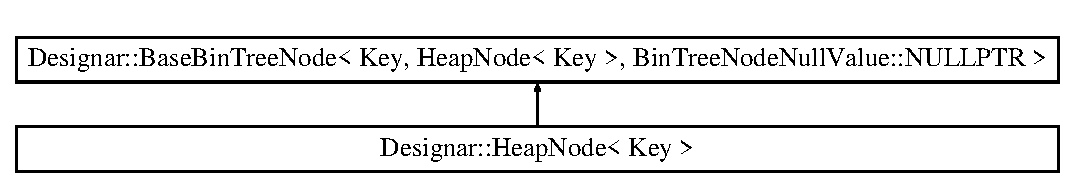
\includegraphics[height=2.000000cm]{class_designar_1_1_heap_node}
\end{center}
\end{figure}
\subsection*{Public Member Functions}
\begin{DoxyCompactItemize}
\item 
\hyperlink{class_designar_1_1_heap_node_ae38c08903f2c52e19c71d392661893f2}{Heap\+Node} ()
\item 
\hyperlink{class_designar_1_1_heap_node_ac5b4c9acb233f72e70b0dc3f4a46e3b5}{Heap\+Node} (const Key \&k)
\item 
\hyperlink{class_designar_1_1_heap_node_a29189c1b5cd10290c2332e40cadbb899}{Heap\+Node} (Key \&\&k)
\item 
\hyperlink{class_designar_1_1_heap_node_aa4287eba82bce2dae37c5e3f4012b1b4}{Heap\+Node} (\hyperlink{namespace_designar_a679bc99fd69a3601faa5d6d47f865106}{Bin\+Tree\+Node\+Ctor} ctor)
\item 
\hyperlink{class_designar_1_1_heap_node}{Heap\+Node} $\ast$\& \hyperlink{class_designar_1_1_heap_node_aacf1d59ac7645a1fe6479f93957dc1be}{get\+\_\+parent} ()
\item 
Heap\+Node\+Bits \& \hyperlink{class_designar_1_1_heap_node_a9fc6866e2550f415ec407b1c85ca54ab}{get\+\_\+bits} ()
\item 
unsigned int \hyperlink{class_designar_1_1_heap_node_ad0b5b06b0126cdd711970709c4fb2187}{is\+\_\+leaf} () const
\item 
void \hyperlink{class_designar_1_1_heap_node_a34ec910a7402b356d7b3d67200f794ec}{set\+\_\+leaf} (unsigned int \hyperlink{namespace_designar_a7dd2a7b6d96f664ce612b506c8eb2fb8}{value})
\item 
unsigned int \hyperlink{class_designar_1_1_heap_node_a778fa64fe1c4221eb7833cfb68713332}{is\+\_\+left} () const
\item 
void \hyperlink{class_designar_1_1_heap_node_a65a5b3a38d152072e756182600502d93}{set\+\_\+left} (unsigned int \hyperlink{namespace_designar_a7dd2a7b6d96f664ce612b506c8eb2fb8}{value})
\item 
void \hyperlink{class_designar_1_1_heap_node_a60340ca59bc0968899e960bc9d1b08b3}{reset} ()
\end{DoxyCompactItemize}
\subsection*{Additional Inherited Members}


\subsection{Detailed Description}
\subsubsection*{template$<$typename Key$>$\newline
class Designar\+::\+Heap\+Node$<$ Key $>$}



Definition at line 385 of file heap.\+H.



\subsection{Constructor \& Destructor Documentation}
\mbox{\Hypertarget{class_designar_1_1_heap_node_ae38c08903f2c52e19c71d392661893f2}\label{class_designar_1_1_heap_node_ae38c08903f2c52e19c71d392661893f2}} 
\index{Designar\+::\+Heap\+Node@{Designar\+::\+Heap\+Node}!Heap\+Node@{Heap\+Node}}
\index{Heap\+Node@{Heap\+Node}!Designar\+::\+Heap\+Node@{Designar\+::\+Heap\+Node}}
\subsubsection{\texorpdfstring{Heap\+Node()}{HeapNode()}\hspace{0.1cm}{\footnotesize\ttfamily [1/4]}}
{\footnotesize\ttfamily template$<$typename Key$>$ \\
\hyperlink{class_designar_1_1_heap_node}{Designar\+::\+Heap\+Node}$<$ Key $>$\+::\hyperlink{class_designar_1_1_heap_node}{Heap\+Node} (\begin{DoxyParamCaption}{ }\end{DoxyParamCaption})\hspace{0.3cm}{\ttfamily [inline]}}



Definition at line 407 of file heap.\+H.

\mbox{\Hypertarget{class_designar_1_1_heap_node_ac5b4c9acb233f72e70b0dc3f4a46e3b5}\label{class_designar_1_1_heap_node_ac5b4c9acb233f72e70b0dc3f4a46e3b5}} 
\index{Designar\+::\+Heap\+Node@{Designar\+::\+Heap\+Node}!Heap\+Node@{Heap\+Node}}
\index{Heap\+Node@{Heap\+Node}!Designar\+::\+Heap\+Node@{Designar\+::\+Heap\+Node}}
\subsubsection{\texorpdfstring{Heap\+Node()}{HeapNode()}\hspace{0.1cm}{\footnotesize\ttfamily [2/4]}}
{\footnotesize\ttfamily template$<$typename Key$>$ \\
\hyperlink{class_designar_1_1_heap_node}{Designar\+::\+Heap\+Node}$<$ Key $>$\+::\hyperlink{class_designar_1_1_heap_node}{Heap\+Node} (\begin{DoxyParamCaption}\item[{const Key \&}]{k }\end{DoxyParamCaption})\hspace{0.3cm}{\ttfamily [inline]}}



Definition at line 413 of file heap.\+H.

\mbox{\Hypertarget{class_designar_1_1_heap_node_a29189c1b5cd10290c2332e40cadbb899}\label{class_designar_1_1_heap_node_a29189c1b5cd10290c2332e40cadbb899}} 
\index{Designar\+::\+Heap\+Node@{Designar\+::\+Heap\+Node}!Heap\+Node@{Heap\+Node}}
\index{Heap\+Node@{Heap\+Node}!Designar\+::\+Heap\+Node@{Designar\+::\+Heap\+Node}}
\subsubsection{\texorpdfstring{Heap\+Node()}{HeapNode()}\hspace{0.1cm}{\footnotesize\ttfamily [3/4]}}
{\footnotesize\ttfamily template$<$typename Key$>$ \\
\hyperlink{class_designar_1_1_heap_node}{Designar\+::\+Heap\+Node}$<$ Key $>$\+::\hyperlink{class_designar_1_1_heap_node}{Heap\+Node} (\begin{DoxyParamCaption}\item[{Key \&\&}]{k }\end{DoxyParamCaption})\hspace{0.3cm}{\ttfamily [inline]}}



Definition at line 419 of file heap.\+H.

\mbox{\Hypertarget{class_designar_1_1_heap_node_aa4287eba82bce2dae37c5e3f4012b1b4}\label{class_designar_1_1_heap_node_aa4287eba82bce2dae37c5e3f4012b1b4}} 
\index{Designar\+::\+Heap\+Node@{Designar\+::\+Heap\+Node}!Heap\+Node@{Heap\+Node}}
\index{Heap\+Node@{Heap\+Node}!Designar\+::\+Heap\+Node@{Designar\+::\+Heap\+Node}}
\subsubsection{\texorpdfstring{Heap\+Node()}{HeapNode()}\hspace{0.1cm}{\footnotesize\ttfamily [4/4]}}
{\footnotesize\ttfamily template$<$typename Key$>$ \\
\hyperlink{class_designar_1_1_heap_node}{Designar\+::\+Heap\+Node}$<$ Key $>$\+::\hyperlink{class_designar_1_1_heap_node}{Heap\+Node} (\begin{DoxyParamCaption}\item[{\hyperlink{namespace_designar_a679bc99fd69a3601faa5d6d47f865106}{Bin\+Tree\+Node\+Ctor}}]{ctor }\end{DoxyParamCaption})\hspace{0.3cm}{\ttfamily [inline]}}



Definition at line 425 of file heap.\+H.



\subsection{Member Function Documentation}
\mbox{\Hypertarget{class_designar_1_1_heap_node_a9fc6866e2550f415ec407b1c85ca54ab}\label{class_designar_1_1_heap_node_a9fc6866e2550f415ec407b1c85ca54ab}} 
\index{Designar\+::\+Heap\+Node@{Designar\+::\+Heap\+Node}!get\+\_\+bits@{get\+\_\+bits}}
\index{get\+\_\+bits@{get\+\_\+bits}!Designar\+::\+Heap\+Node@{Designar\+::\+Heap\+Node}}
\subsubsection{\texorpdfstring{get\+\_\+bits()}{get\_bits()}}
{\footnotesize\ttfamily template$<$typename Key$>$ \\
Heap\+Node\+Bits\& \hyperlink{class_designar_1_1_heap_node}{Designar\+::\+Heap\+Node}$<$ Key $>$\+::get\+\_\+bits (\begin{DoxyParamCaption}{ }\end{DoxyParamCaption})\hspace{0.3cm}{\ttfamily [inline]}}



Definition at line 436 of file heap.\+H.

\mbox{\Hypertarget{class_designar_1_1_heap_node_aacf1d59ac7645a1fe6479f93957dc1be}\label{class_designar_1_1_heap_node_aacf1d59ac7645a1fe6479f93957dc1be}} 
\index{Designar\+::\+Heap\+Node@{Designar\+::\+Heap\+Node}!get\+\_\+parent@{get\+\_\+parent}}
\index{get\+\_\+parent@{get\+\_\+parent}!Designar\+::\+Heap\+Node@{Designar\+::\+Heap\+Node}}
\subsubsection{\texorpdfstring{get\+\_\+parent()}{get\_parent()}}
{\footnotesize\ttfamily template$<$typename Key$>$ \\
\hyperlink{class_designar_1_1_heap_node}{Heap\+Node}$\ast$\& \hyperlink{class_designar_1_1_heap_node}{Designar\+::\+Heap\+Node}$<$ Key $>$\+::get\+\_\+parent (\begin{DoxyParamCaption}{ }\end{DoxyParamCaption})\hspace{0.3cm}{\ttfamily [inline]}}



Definition at line 431 of file heap.\+H.

\mbox{\Hypertarget{class_designar_1_1_heap_node_ad0b5b06b0126cdd711970709c4fb2187}\label{class_designar_1_1_heap_node_ad0b5b06b0126cdd711970709c4fb2187}} 
\index{Designar\+::\+Heap\+Node@{Designar\+::\+Heap\+Node}!is\+\_\+leaf@{is\+\_\+leaf}}
\index{is\+\_\+leaf@{is\+\_\+leaf}!Designar\+::\+Heap\+Node@{Designar\+::\+Heap\+Node}}
\subsubsection{\texorpdfstring{is\+\_\+leaf()}{is\_leaf()}}
{\footnotesize\ttfamily template$<$typename Key$>$ \\
unsigned int \hyperlink{class_designar_1_1_heap_node}{Designar\+::\+Heap\+Node}$<$ Key $>$\+::is\+\_\+leaf (\begin{DoxyParamCaption}{ }\end{DoxyParamCaption}) const\hspace{0.3cm}{\ttfamily [inline]}}



Definition at line 441 of file heap.\+H.

\mbox{\Hypertarget{class_designar_1_1_heap_node_a778fa64fe1c4221eb7833cfb68713332}\label{class_designar_1_1_heap_node_a778fa64fe1c4221eb7833cfb68713332}} 
\index{Designar\+::\+Heap\+Node@{Designar\+::\+Heap\+Node}!is\+\_\+left@{is\+\_\+left}}
\index{is\+\_\+left@{is\+\_\+left}!Designar\+::\+Heap\+Node@{Designar\+::\+Heap\+Node}}
\subsubsection{\texorpdfstring{is\+\_\+left()}{is\_left()}}
{\footnotesize\ttfamily template$<$typename Key$>$ \\
unsigned int \hyperlink{class_designar_1_1_heap_node}{Designar\+::\+Heap\+Node}$<$ Key $>$\+::is\+\_\+left (\begin{DoxyParamCaption}{ }\end{DoxyParamCaption}) const\hspace{0.3cm}{\ttfamily [inline]}}



Definition at line 451 of file heap.\+H.

\mbox{\Hypertarget{class_designar_1_1_heap_node_a60340ca59bc0968899e960bc9d1b08b3}\label{class_designar_1_1_heap_node_a60340ca59bc0968899e960bc9d1b08b3}} 
\index{Designar\+::\+Heap\+Node@{Designar\+::\+Heap\+Node}!reset@{reset}}
\index{reset@{reset}!Designar\+::\+Heap\+Node@{Designar\+::\+Heap\+Node}}
\subsubsection{\texorpdfstring{reset()}{reset()}}
{\footnotesize\ttfamily template$<$typename Key$>$ \\
void \hyperlink{class_designar_1_1_heap_node}{Designar\+::\+Heap\+Node}$<$ Key $>$\+::reset (\begin{DoxyParamCaption}{ }\end{DoxyParamCaption})\hspace{0.3cm}{\ttfamily [inline]}}



Definition at line 461 of file heap.\+H.

\mbox{\Hypertarget{class_designar_1_1_heap_node_a34ec910a7402b356d7b3d67200f794ec}\label{class_designar_1_1_heap_node_a34ec910a7402b356d7b3d67200f794ec}} 
\index{Designar\+::\+Heap\+Node@{Designar\+::\+Heap\+Node}!set\+\_\+leaf@{set\+\_\+leaf}}
\index{set\+\_\+leaf@{set\+\_\+leaf}!Designar\+::\+Heap\+Node@{Designar\+::\+Heap\+Node}}
\subsubsection{\texorpdfstring{set\+\_\+leaf()}{set\_leaf()}}
{\footnotesize\ttfamily template$<$typename Key$>$ \\
void \hyperlink{class_designar_1_1_heap_node}{Designar\+::\+Heap\+Node}$<$ Key $>$\+::set\+\_\+leaf (\begin{DoxyParamCaption}\item[{unsigned int}]{value }\end{DoxyParamCaption})\hspace{0.3cm}{\ttfamily [inline]}}



Definition at line 446 of file heap.\+H.

\mbox{\Hypertarget{class_designar_1_1_heap_node_a65a5b3a38d152072e756182600502d93}\label{class_designar_1_1_heap_node_a65a5b3a38d152072e756182600502d93}} 
\index{Designar\+::\+Heap\+Node@{Designar\+::\+Heap\+Node}!set\+\_\+left@{set\+\_\+left}}
\index{set\+\_\+left@{set\+\_\+left}!Designar\+::\+Heap\+Node@{Designar\+::\+Heap\+Node}}
\subsubsection{\texorpdfstring{set\+\_\+left()}{set\_left()}}
{\footnotesize\ttfamily template$<$typename Key$>$ \\
void \hyperlink{class_designar_1_1_heap_node}{Designar\+::\+Heap\+Node}$<$ Key $>$\+::set\+\_\+left (\begin{DoxyParamCaption}\item[{unsigned int}]{value }\end{DoxyParamCaption})\hspace{0.3cm}{\ttfamily [inline]}}



Definition at line 456 of file heap.\+H.



The documentation for this class was generated from the following file\+:\begin{DoxyCompactItemize}
\item 
/home/julio/\+De\+S\+I\+G\+N\+A\+R-\/doc/\+De\+Si\+G\+N\+A\+R/include/\hyperlink{heap_8_h}{heap.\+H}\end{DoxyCompactItemize}

\hypertarget{class_designar_1_1_tree_set_1_1_inorder_iterator}{}\section{Designar\+:\+:Tree\+Set$<$ Key, Cmp $>$\+:\+:Inorder\+Iterator Class Reference}
\label{class_designar_1_1_tree_set_1_1_inorder_iterator}\index{Designar\+::\+Tree\+Set$<$ Key, Cmp $>$\+::\+Inorder\+Iterator@{Designar\+::\+Tree\+Set$<$ Key, Cmp $>$\+::\+Inorder\+Iterator}}


{\ttfamily \#include $<$tree.\+H$>$}

Inheritance diagram for Designar\+:\+:Tree\+Set$<$ Key, Cmp $>$\+:\+:Inorder\+Iterator\+:\begin{figure}[H]
\begin{center}
\leavevmode
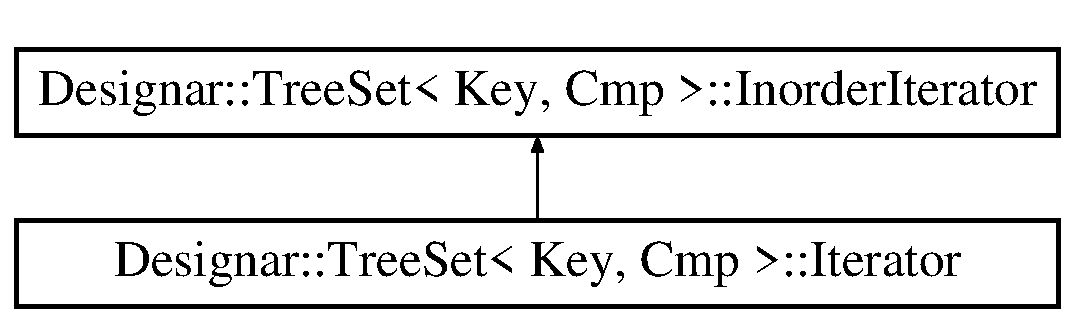
\includegraphics[height=2.000000cm]{class_designar_1_1_tree_set_1_1_inorder_iterator}
\end{center}
\end{figure}
\subsection*{Public Member Functions}
\begin{DoxyCompactItemize}
\item 
\hyperlink{class_designar_1_1_tree_set_1_1_inorder_iterator_ad5ff37d7f6ed8284dc3ce396cbdc4f86}{Inorder\+Iterator} (const \hyperlink{class_designar_1_1_tree_set}{Tree\+Set} \&t)
\item 
\hyperlink{class_designar_1_1_tree_set_1_1_inorder_iterator_a010cfd17e2ad8031981ea3688f89f545}{Inorder\+Iterator} (const \hyperlink{class_designar_1_1_tree_set_1_1_inorder_iterator}{Inorder\+Iterator} \&it)
\item 
\hyperlink{class_designar_1_1_tree_set_1_1_inorder_iterator_aa4b81ce7770abb8f488099fd5abb1a02}{Inorder\+Iterator} (\hyperlink{class_designar_1_1_tree_set_1_1_inorder_iterator}{Inorder\+Iterator} \&\&it)
\item 
\hyperlink{class_designar_1_1_tree_set_1_1_inorder_iterator}{Inorder\+Iterator} \& \hyperlink{class_designar_1_1_tree_set_1_1_inorder_iterator_a4eca124737c8f5664deafc3b19f17e46}{operator=} (const \hyperlink{class_designar_1_1_tree_set_1_1_inorder_iterator}{Inorder\+Iterator} \&it)
\item 
\hyperlink{class_designar_1_1_tree_set_1_1_inorder_iterator}{Inorder\+Iterator} \& \hyperlink{class_designar_1_1_tree_set_1_1_inorder_iterator_a2b0a20a5a81ee8d54929a035df77e95c}{operator=} (\hyperlink{class_designar_1_1_tree_set_1_1_inorder_iterator}{Inorder\+Iterator} \&\&it)
\item 
void \hyperlink{class_designar_1_1_tree_set_1_1_inorder_iterator_ac3d6fc72f50addc10c0c99b533448a9a}{swap} (\hyperlink{class_designar_1_1_tree_set_1_1_inorder_iterator}{Inorder\+Iterator} \&it)
\item 
void \hyperlink{class_designar_1_1_tree_set_1_1_inorder_iterator_a7a5ce683413135445a1d7a064ae7d70c}{reset} ()
\item 
void \hyperlink{class_designar_1_1_tree_set_1_1_inorder_iterator_ae6a74511239f69caf43e92f915f8c605}{reset\+\_\+last} ()
\item 
\hyperlink{namespace_designar_aa72662848b9f4815e7bf31a7cf3e33d1}{nat\+\_\+t} \hyperlink{class_designar_1_1_tree_set_1_1_inorder_iterator_a32fceb8d4318ee6c11c07c1b02b93635}{get\+\_\+position} () const
\item 
bool \hyperlink{class_designar_1_1_tree_set_1_1_inorder_iterator_ae83dae23b6d48b2ccec38c7e22d01fd0}{has\+\_\+current} () const
\item 
Key \& \hyperlink{class_designar_1_1_tree_set_1_1_inorder_iterator_a48d0738cf18aa20c4a6161841324443d}{get\+\_\+current} ()
\item 
const Key \& \hyperlink{class_designar_1_1_tree_set_1_1_inorder_iterator_aad3ec85d58308071d6589fdbb258bdf6}{get\+\_\+current} () const
\item 
void \hyperlink{class_designar_1_1_tree_set_1_1_inorder_iterator_a850f1ca2e5a49dc43fddc09e2cc43659}{next} ()
\item 
Key \hyperlink{class_designar_1_1_tree_set_1_1_inorder_iterator_a137c29da7611999490f4a10a898b3c1d}{del} ()
\end{DoxyCompactItemize}
\subsection*{Protected Member Functions}
\begin{DoxyCompactItemize}
\item 
\hyperlink{class_designar_1_1_tree_set_1_1_inorder_iterator_a71c23649fcff4269dd3096ce6ac10e2d}{Inorder\+Iterator} (const \hyperlink{class_designar_1_1_tree_set}{Tree\+Set} \&t, int)
\item 
\hyperlink{class_designar_1_1_tree_set_a7409a9c1545c0e9e2fd6b84120713c99}{Node} $\ast$ \hyperlink{class_designar_1_1_tree_set_1_1_inorder_iterator_a06e9a4e3d4d834c250932e3d77190b1f}{get\+\_\+location} () const
\end{DoxyCompactItemize}
\subsection*{Friends}
\begin{DoxyCompactItemize}
\item 
class \hyperlink{class_designar_1_1_tree_set_1_1_inorder_iterator_a7caa42294700d2a60905ec3458a7cd8a}{Tree\+Set}
\end{DoxyCompactItemize}


\subsection{Detailed Description}
\subsubsection*{template$<$typename Key, class Cmp = std\+::less$<$\+Key$>$$>$\newline
class Designar\+::\+Tree\+Set$<$ Key, Cmp $>$\+::\+Inorder\+Iterator}



Definition at line 631 of file tree.\+H.



\subsection{Constructor \& Destructor Documentation}
\mbox{\Hypertarget{class_designar_1_1_tree_set_1_1_inorder_iterator_a71c23649fcff4269dd3096ce6ac10e2d}\label{class_designar_1_1_tree_set_1_1_inorder_iterator_a71c23649fcff4269dd3096ce6ac10e2d}} 
\index{Designar\+::\+Tree\+Set\+::\+Inorder\+Iterator@{Designar\+::\+Tree\+Set\+::\+Inorder\+Iterator}!Inorder\+Iterator@{Inorder\+Iterator}}
\index{Inorder\+Iterator@{Inorder\+Iterator}!Designar\+::\+Tree\+Set\+::\+Inorder\+Iterator@{Designar\+::\+Tree\+Set\+::\+Inorder\+Iterator}}
\subsubsection{\texorpdfstring{Inorder\+Iterator()}{InorderIterator()}\hspace{0.1cm}{\footnotesize\ttfamily [1/4]}}
{\footnotesize\ttfamily template$<$typename Key, class Cmp = std\+::less$<$\+Key$>$$>$ \\
\hyperlink{class_designar_1_1_tree_set}{Designar\+::\+Tree\+Set}$<$ Key, Cmp $>$\+::Inorder\+Iterator\+::\+Inorder\+Iterator (\begin{DoxyParamCaption}\item[{const \hyperlink{class_designar_1_1_tree_set}{Tree\+Set} \&}]{t,  }\item[{int}]{ }\end{DoxyParamCaption})\hspace{0.3cm}{\ttfamily [inline]}, {\ttfamily [protected]}}



Definition at line 654 of file tree.\+H.

\mbox{\Hypertarget{class_designar_1_1_tree_set_1_1_inorder_iterator_ad5ff37d7f6ed8284dc3ce396cbdc4f86}\label{class_designar_1_1_tree_set_1_1_inorder_iterator_ad5ff37d7f6ed8284dc3ce396cbdc4f86}} 
\index{Designar\+::\+Tree\+Set\+::\+Inorder\+Iterator@{Designar\+::\+Tree\+Set\+::\+Inorder\+Iterator}!Inorder\+Iterator@{Inorder\+Iterator}}
\index{Inorder\+Iterator@{Inorder\+Iterator}!Designar\+::\+Tree\+Set\+::\+Inorder\+Iterator@{Designar\+::\+Tree\+Set\+::\+Inorder\+Iterator}}
\subsubsection{\texorpdfstring{Inorder\+Iterator()}{InorderIterator()}\hspace{0.1cm}{\footnotesize\ttfamily [2/4]}}
{\footnotesize\ttfamily template$<$typename Key, class Cmp = std\+::less$<$\+Key$>$$>$ \\
\hyperlink{class_designar_1_1_tree_set}{Designar\+::\+Tree\+Set}$<$ Key, Cmp $>$\+::Inorder\+Iterator\+::\+Inorder\+Iterator (\begin{DoxyParamCaption}\item[{const \hyperlink{class_designar_1_1_tree_set}{Tree\+Set} \&}]{t }\end{DoxyParamCaption})\hspace{0.3cm}{\ttfamily [inline]}}



Definition at line 666 of file tree.\+H.

\mbox{\Hypertarget{class_designar_1_1_tree_set_1_1_inorder_iterator_a010cfd17e2ad8031981ea3688f89f545}\label{class_designar_1_1_tree_set_1_1_inorder_iterator_a010cfd17e2ad8031981ea3688f89f545}} 
\index{Designar\+::\+Tree\+Set\+::\+Inorder\+Iterator@{Designar\+::\+Tree\+Set\+::\+Inorder\+Iterator}!Inorder\+Iterator@{Inorder\+Iterator}}
\index{Inorder\+Iterator@{Inorder\+Iterator}!Designar\+::\+Tree\+Set\+::\+Inorder\+Iterator@{Designar\+::\+Tree\+Set\+::\+Inorder\+Iterator}}
\subsubsection{\texorpdfstring{Inorder\+Iterator()}{InorderIterator()}\hspace{0.1cm}{\footnotesize\ttfamily [3/4]}}
{\footnotesize\ttfamily template$<$typename Key, class Cmp = std\+::less$<$\+Key$>$$>$ \\
\hyperlink{class_designar_1_1_tree_set}{Designar\+::\+Tree\+Set}$<$ Key, Cmp $>$\+::Inorder\+Iterator\+::\+Inorder\+Iterator (\begin{DoxyParamCaption}\item[{const \hyperlink{class_designar_1_1_tree_set_1_1_inorder_iterator}{Inorder\+Iterator} \&}]{it }\end{DoxyParamCaption})\hspace{0.3cm}{\ttfamily [inline]}}



Definition at line 672 of file tree.\+H.

\mbox{\Hypertarget{class_designar_1_1_tree_set_1_1_inorder_iterator_aa4b81ce7770abb8f488099fd5abb1a02}\label{class_designar_1_1_tree_set_1_1_inorder_iterator_aa4b81ce7770abb8f488099fd5abb1a02}} 
\index{Designar\+::\+Tree\+Set\+::\+Inorder\+Iterator@{Designar\+::\+Tree\+Set\+::\+Inorder\+Iterator}!Inorder\+Iterator@{Inorder\+Iterator}}
\index{Inorder\+Iterator@{Inorder\+Iterator}!Designar\+::\+Tree\+Set\+::\+Inorder\+Iterator@{Designar\+::\+Tree\+Set\+::\+Inorder\+Iterator}}
\subsubsection{\texorpdfstring{Inorder\+Iterator()}{InorderIterator()}\hspace{0.1cm}{\footnotesize\ttfamily [4/4]}}
{\footnotesize\ttfamily template$<$typename Key, class Cmp = std\+::less$<$\+Key$>$$>$ \\
\hyperlink{class_designar_1_1_tree_set}{Designar\+::\+Tree\+Set}$<$ Key, Cmp $>$\+::Inorder\+Iterator\+::\+Inorder\+Iterator (\begin{DoxyParamCaption}\item[{\hyperlink{class_designar_1_1_tree_set_1_1_inorder_iterator}{Inorder\+Iterator} \&\&}]{it }\end{DoxyParamCaption})\hspace{0.3cm}{\ttfamily [inline]}}



Definition at line 678 of file tree.\+H.



\subsection{Member Function Documentation}
\mbox{\Hypertarget{class_designar_1_1_tree_set_1_1_inorder_iterator_a137c29da7611999490f4a10a898b3c1d}\label{class_designar_1_1_tree_set_1_1_inorder_iterator_a137c29da7611999490f4a10a898b3c1d}} 
\index{Designar\+::\+Tree\+Set\+::\+Inorder\+Iterator@{Designar\+::\+Tree\+Set\+::\+Inorder\+Iterator}!del@{del}}
\index{del@{del}!Designar\+::\+Tree\+Set\+::\+Inorder\+Iterator@{Designar\+::\+Tree\+Set\+::\+Inorder\+Iterator}}
\subsubsection{\texorpdfstring{del()}{del()}}
{\footnotesize\ttfamily template$<$typename Key, class Cmp = std\+::less$<$\+Key$>$$>$ \\
Key \hyperlink{class_designar_1_1_tree_set}{Designar\+::\+Tree\+Set}$<$ Key, Cmp $>$\+::Inorder\+Iterator\+::del (\begin{DoxyParamCaption}{ }\end{DoxyParamCaption})\hspace{0.3cm}{\ttfamily [inline]}}



Definition at line 764 of file tree.\+H.

\mbox{\Hypertarget{class_designar_1_1_tree_set_1_1_inorder_iterator_a48d0738cf18aa20c4a6161841324443d}\label{class_designar_1_1_tree_set_1_1_inorder_iterator_a48d0738cf18aa20c4a6161841324443d}} 
\index{Designar\+::\+Tree\+Set\+::\+Inorder\+Iterator@{Designar\+::\+Tree\+Set\+::\+Inorder\+Iterator}!get\+\_\+current@{get\+\_\+current}}
\index{get\+\_\+current@{get\+\_\+current}!Designar\+::\+Tree\+Set\+::\+Inorder\+Iterator@{Designar\+::\+Tree\+Set\+::\+Inorder\+Iterator}}
\subsubsection{\texorpdfstring{get\+\_\+current()}{get\_current()}\hspace{0.1cm}{\footnotesize\ttfamily [1/2]}}
{\footnotesize\ttfamily template$<$typename Key, class Cmp = std\+::less$<$\+Key$>$$>$ \\
Key\& \hyperlink{class_designar_1_1_tree_set}{Designar\+::\+Tree\+Set}$<$ Key, Cmp $>$\+::Inorder\+Iterator\+::get\+\_\+current (\begin{DoxyParamCaption}{ }\end{DoxyParamCaption})\hspace{0.3cm}{\ttfamily [inline]}}



Definition at line 733 of file tree.\+H.

\mbox{\Hypertarget{class_designar_1_1_tree_set_1_1_inorder_iterator_aad3ec85d58308071d6589fdbb258bdf6}\label{class_designar_1_1_tree_set_1_1_inorder_iterator_aad3ec85d58308071d6589fdbb258bdf6}} 
\index{Designar\+::\+Tree\+Set\+::\+Inorder\+Iterator@{Designar\+::\+Tree\+Set\+::\+Inorder\+Iterator}!get\+\_\+current@{get\+\_\+current}}
\index{get\+\_\+current@{get\+\_\+current}!Designar\+::\+Tree\+Set\+::\+Inorder\+Iterator@{Designar\+::\+Tree\+Set\+::\+Inorder\+Iterator}}
\subsubsection{\texorpdfstring{get\+\_\+current()}{get\_current()}\hspace{0.1cm}{\footnotesize\ttfamily [2/2]}}
{\footnotesize\ttfamily template$<$typename Key, class Cmp = std\+::less$<$\+Key$>$$>$ \\
const Key\& \hyperlink{class_designar_1_1_tree_set}{Designar\+::\+Tree\+Set}$<$ Key, Cmp $>$\+::Inorder\+Iterator\+::get\+\_\+current (\begin{DoxyParamCaption}{ }\end{DoxyParamCaption}) const\hspace{0.3cm}{\ttfamily [inline]}}



Definition at line 741 of file tree.\+H.

\mbox{\Hypertarget{class_designar_1_1_tree_set_1_1_inorder_iterator_a06e9a4e3d4d834c250932e3d77190b1f}\label{class_designar_1_1_tree_set_1_1_inorder_iterator_a06e9a4e3d4d834c250932e3d77190b1f}} 
\index{Designar\+::\+Tree\+Set\+::\+Inorder\+Iterator@{Designar\+::\+Tree\+Set\+::\+Inorder\+Iterator}!get\+\_\+location@{get\+\_\+location}}
\index{get\+\_\+location@{get\+\_\+location}!Designar\+::\+Tree\+Set\+::\+Inorder\+Iterator@{Designar\+::\+Tree\+Set\+::\+Inorder\+Iterator}}
\subsubsection{\texorpdfstring{get\+\_\+location()}{get\_location()}}
{\footnotesize\ttfamily template$<$typename Key, class Cmp = std\+::less$<$\+Key$>$$>$ \\
\hyperlink{class_designar_1_1_tree_set_a7409a9c1545c0e9e2fd6b84120713c99}{Node}$\ast$ \hyperlink{class_designar_1_1_tree_set}{Designar\+::\+Tree\+Set}$<$ Key, Cmp $>$\+::Inorder\+Iterator\+::get\+\_\+location (\begin{DoxyParamCaption}{ }\end{DoxyParamCaption}) const\hspace{0.3cm}{\ttfamily [inline]}, {\ttfamily [protected]}}



Definition at line 660 of file tree.\+H.

\mbox{\Hypertarget{class_designar_1_1_tree_set_1_1_inorder_iterator_a32fceb8d4318ee6c11c07c1b02b93635}\label{class_designar_1_1_tree_set_1_1_inorder_iterator_a32fceb8d4318ee6c11c07c1b02b93635}} 
\index{Designar\+::\+Tree\+Set\+::\+Inorder\+Iterator@{Designar\+::\+Tree\+Set\+::\+Inorder\+Iterator}!get\+\_\+position@{get\+\_\+position}}
\index{get\+\_\+position@{get\+\_\+position}!Designar\+::\+Tree\+Set\+::\+Inorder\+Iterator@{Designar\+::\+Tree\+Set\+::\+Inorder\+Iterator}}
\subsubsection{\texorpdfstring{get\+\_\+position()}{get\_position()}}
{\footnotesize\ttfamily template$<$typename Key, class Cmp = std\+::less$<$\+Key$>$$>$ \\
\hyperlink{namespace_designar_aa72662848b9f4815e7bf31a7cf3e33d1}{nat\+\_\+t} \hyperlink{class_designar_1_1_tree_set}{Designar\+::\+Tree\+Set}$<$ Key, Cmp $>$\+::Inorder\+Iterator\+::get\+\_\+position (\begin{DoxyParamCaption}{ }\end{DoxyParamCaption}) const\hspace{0.3cm}{\ttfamily [inline]}}



Definition at line 723 of file tree.\+H.

\mbox{\Hypertarget{class_designar_1_1_tree_set_1_1_inorder_iterator_ae83dae23b6d48b2ccec38c7e22d01fd0}\label{class_designar_1_1_tree_set_1_1_inorder_iterator_ae83dae23b6d48b2ccec38c7e22d01fd0}} 
\index{Designar\+::\+Tree\+Set\+::\+Inorder\+Iterator@{Designar\+::\+Tree\+Set\+::\+Inorder\+Iterator}!has\+\_\+current@{has\+\_\+current}}
\index{has\+\_\+current@{has\+\_\+current}!Designar\+::\+Tree\+Set\+::\+Inorder\+Iterator@{Designar\+::\+Tree\+Set\+::\+Inorder\+Iterator}}
\subsubsection{\texorpdfstring{has\+\_\+current()}{has\_current()}}
{\footnotesize\ttfamily template$<$typename Key, class Cmp = std\+::less$<$\+Key$>$$>$ \\
bool \hyperlink{class_designar_1_1_tree_set}{Designar\+::\+Tree\+Set}$<$ Key, Cmp $>$\+::Inorder\+Iterator\+::has\+\_\+current (\begin{DoxyParamCaption}{ }\end{DoxyParamCaption}) const\hspace{0.3cm}{\ttfamily [inline]}}



Definition at line 728 of file tree.\+H.

\mbox{\Hypertarget{class_designar_1_1_tree_set_1_1_inorder_iterator_a850f1ca2e5a49dc43fddc09e2cc43659}\label{class_designar_1_1_tree_set_1_1_inorder_iterator_a850f1ca2e5a49dc43fddc09e2cc43659}} 
\index{Designar\+::\+Tree\+Set\+::\+Inorder\+Iterator@{Designar\+::\+Tree\+Set\+::\+Inorder\+Iterator}!next@{next}}
\index{next@{next}!Designar\+::\+Tree\+Set\+::\+Inorder\+Iterator@{Designar\+::\+Tree\+Set\+::\+Inorder\+Iterator}}
\subsubsection{\texorpdfstring{next()}{next()}}
{\footnotesize\ttfamily template$<$typename Key, class Cmp = std\+::less$<$\+Key$>$$>$ \\
void \hyperlink{class_designar_1_1_tree_set}{Designar\+::\+Tree\+Set}$<$ Key, Cmp $>$\+::Inorder\+Iterator\+::next (\begin{DoxyParamCaption}{ }\end{DoxyParamCaption})\hspace{0.3cm}{\ttfamily [inline]}}



Definition at line 749 of file tree.\+H.

\mbox{\Hypertarget{class_designar_1_1_tree_set_1_1_inorder_iterator_a4eca124737c8f5664deafc3b19f17e46}\label{class_designar_1_1_tree_set_1_1_inorder_iterator_a4eca124737c8f5664deafc3b19f17e46}} 
\index{Designar\+::\+Tree\+Set\+::\+Inorder\+Iterator@{Designar\+::\+Tree\+Set\+::\+Inorder\+Iterator}!operator=@{operator=}}
\index{operator=@{operator=}!Designar\+::\+Tree\+Set\+::\+Inorder\+Iterator@{Designar\+::\+Tree\+Set\+::\+Inorder\+Iterator}}
\subsubsection{\texorpdfstring{operator=()}{operator=()}\hspace{0.1cm}{\footnotesize\ttfamily [1/2]}}
{\footnotesize\ttfamily template$<$typename Key, class Cmp = std\+::less$<$\+Key$>$$>$ \\
\hyperlink{class_designar_1_1_tree_set_1_1_inorder_iterator}{Inorder\+Iterator}\& \hyperlink{class_designar_1_1_tree_set}{Designar\+::\+Tree\+Set}$<$ Key, Cmp $>$\+::Inorder\+Iterator\+::operator= (\begin{DoxyParamCaption}\item[{const \hyperlink{class_designar_1_1_tree_set_1_1_inorder_iterator}{Inorder\+Iterator} \&}]{it }\end{DoxyParamCaption})\hspace{0.3cm}{\ttfamily [inline]}}



Definition at line 683 of file tree.\+H.

\mbox{\Hypertarget{class_designar_1_1_tree_set_1_1_inorder_iterator_a2b0a20a5a81ee8d54929a035df77e95c}\label{class_designar_1_1_tree_set_1_1_inorder_iterator_a2b0a20a5a81ee8d54929a035df77e95c}} 
\index{Designar\+::\+Tree\+Set\+::\+Inorder\+Iterator@{Designar\+::\+Tree\+Set\+::\+Inorder\+Iterator}!operator=@{operator=}}
\index{operator=@{operator=}!Designar\+::\+Tree\+Set\+::\+Inorder\+Iterator@{Designar\+::\+Tree\+Set\+::\+Inorder\+Iterator}}
\subsubsection{\texorpdfstring{operator=()}{operator=()}\hspace{0.1cm}{\footnotesize\ttfamily [2/2]}}
{\footnotesize\ttfamily template$<$typename Key, class Cmp = std\+::less$<$\+Key$>$$>$ \\
\hyperlink{class_designar_1_1_tree_set_1_1_inorder_iterator}{Inorder\+Iterator}\& \hyperlink{class_designar_1_1_tree_set}{Designar\+::\+Tree\+Set}$<$ Key, Cmp $>$\+::Inorder\+Iterator\+::operator= (\begin{DoxyParamCaption}\item[{\hyperlink{class_designar_1_1_tree_set_1_1_inorder_iterator}{Inorder\+Iterator} \&\&}]{it }\end{DoxyParamCaption})\hspace{0.3cm}{\ttfamily [inline]}}



Definition at line 696 of file tree.\+H.

\mbox{\Hypertarget{class_designar_1_1_tree_set_1_1_inorder_iterator_a7a5ce683413135445a1d7a064ae7d70c}\label{class_designar_1_1_tree_set_1_1_inorder_iterator_a7a5ce683413135445a1d7a064ae7d70c}} 
\index{Designar\+::\+Tree\+Set\+::\+Inorder\+Iterator@{Designar\+::\+Tree\+Set\+::\+Inorder\+Iterator}!reset@{reset}}
\index{reset@{reset}!Designar\+::\+Tree\+Set\+::\+Inorder\+Iterator@{Designar\+::\+Tree\+Set\+::\+Inorder\+Iterator}}
\subsubsection{\texorpdfstring{reset()}{reset()}}
{\footnotesize\ttfamily template$<$typename Key, class Cmp = std\+::less$<$\+Key$>$$>$ \\
void \hyperlink{class_designar_1_1_tree_set}{Designar\+::\+Tree\+Set}$<$ Key, Cmp $>$\+::Inorder\+Iterator\+::reset (\begin{DoxyParamCaption}{ }\end{DoxyParamCaption})\hspace{0.3cm}{\ttfamily [inline]}}



Definition at line 710 of file tree.\+H.

\mbox{\Hypertarget{class_designar_1_1_tree_set_1_1_inorder_iterator_ae6a74511239f69caf43e92f915f8c605}\label{class_designar_1_1_tree_set_1_1_inorder_iterator_ae6a74511239f69caf43e92f915f8c605}} 
\index{Designar\+::\+Tree\+Set\+::\+Inorder\+Iterator@{Designar\+::\+Tree\+Set\+::\+Inorder\+Iterator}!reset\+\_\+last@{reset\+\_\+last}}
\index{reset\+\_\+last@{reset\+\_\+last}!Designar\+::\+Tree\+Set\+::\+Inorder\+Iterator@{Designar\+::\+Tree\+Set\+::\+Inorder\+Iterator}}
\subsubsection{\texorpdfstring{reset\+\_\+last()}{reset\_last()}}
{\footnotesize\ttfamily template$<$typename Key, class Cmp = std\+::less$<$\+Key$>$$>$ \\
void \hyperlink{class_designar_1_1_tree_set}{Designar\+::\+Tree\+Set}$<$ Key, Cmp $>$\+::Inorder\+Iterator\+::reset\+\_\+last (\begin{DoxyParamCaption}{ }\end{DoxyParamCaption})\hspace{0.3cm}{\ttfamily [inline]}}



Definition at line 716 of file tree.\+H.

\mbox{\Hypertarget{class_designar_1_1_tree_set_1_1_inorder_iterator_ac3d6fc72f50addc10c0c99b533448a9a}\label{class_designar_1_1_tree_set_1_1_inorder_iterator_ac3d6fc72f50addc10c0c99b533448a9a}} 
\index{Designar\+::\+Tree\+Set\+::\+Inorder\+Iterator@{Designar\+::\+Tree\+Set\+::\+Inorder\+Iterator}!swap@{swap}}
\index{swap@{swap}!Designar\+::\+Tree\+Set\+::\+Inorder\+Iterator@{Designar\+::\+Tree\+Set\+::\+Inorder\+Iterator}}
\subsubsection{\texorpdfstring{swap()}{swap()}}
{\footnotesize\ttfamily template$<$typename Key, class Cmp = std\+::less$<$\+Key$>$$>$ \\
void \hyperlink{class_designar_1_1_tree_set}{Designar\+::\+Tree\+Set}$<$ Key, Cmp $>$\+::Inorder\+Iterator\+::swap (\begin{DoxyParamCaption}\item[{\hyperlink{class_designar_1_1_tree_set_1_1_inorder_iterator}{Inorder\+Iterator} \&}]{it }\end{DoxyParamCaption})\hspace{0.3cm}{\ttfamily [inline]}}



Definition at line 702 of file tree.\+H.



\subsection{Friends And Related Function Documentation}
\mbox{\Hypertarget{class_designar_1_1_tree_set_1_1_inorder_iterator_a7caa42294700d2a60905ec3458a7cd8a}\label{class_designar_1_1_tree_set_1_1_inorder_iterator_a7caa42294700d2a60905ec3458a7cd8a}} 
\index{Designar\+::\+Tree\+Set\+::\+Inorder\+Iterator@{Designar\+::\+Tree\+Set\+::\+Inorder\+Iterator}!Tree\+Set@{Tree\+Set}}
\index{Tree\+Set@{Tree\+Set}!Designar\+::\+Tree\+Set\+::\+Inorder\+Iterator@{Designar\+::\+Tree\+Set\+::\+Inorder\+Iterator}}
\subsubsection{\texorpdfstring{Tree\+Set}{TreeSet}}
{\footnotesize\ttfamily template$<$typename Key, class Cmp = std\+::less$<$\+Key$>$$>$ \\
friend class \hyperlink{class_designar_1_1_tree_set}{Tree\+Set}\hspace{0.3cm}{\ttfamily [friend]}}



Definition at line 633 of file tree.\+H.



The documentation for this class was generated from the following file\+:\begin{DoxyCompactItemize}
\item 
include/\hyperlink{tree_8_h}{tree.\+H}\end{DoxyCompactItemize}

\hypertarget{class_designar_1_1_int_range}{}\section{Designar\+:\+:Int\+Range Class Reference}
\label{class_designar_1_1_int_range}\index{Designar\+::\+Int\+Range@{Designar\+::\+Int\+Range}}


{\ttfamily \#include $<$range.\+H$>$}

Inheritance diagram for Designar\+:\+:Int\+Range\+:\begin{figure}[H]
\begin{center}
\leavevmode
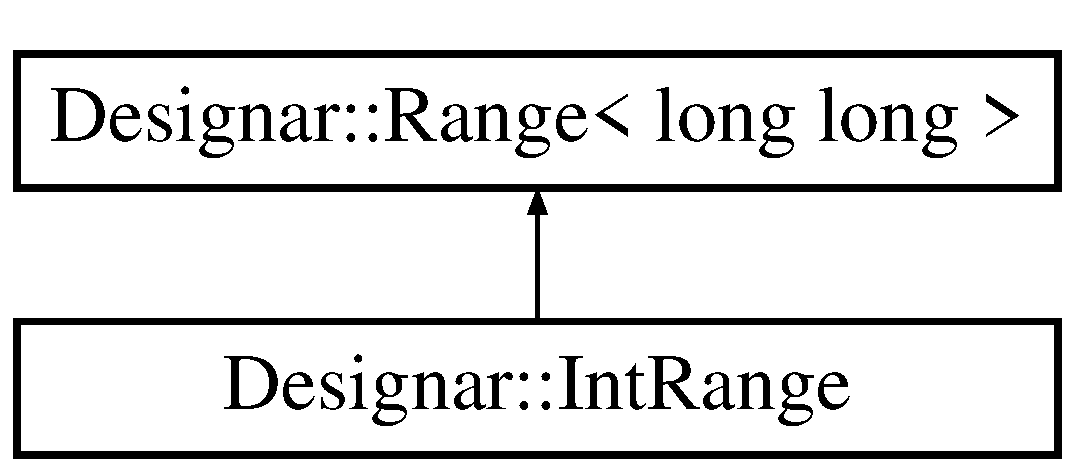
\includegraphics[height=2.000000cm]{class_designar_1_1_int_range}
\end{center}
\end{figure}
\subsection*{Additional Inherited Members}


\subsection{Detailed Description}


Definition at line 159 of file range.\+H.



The documentation for this class was generated from the following file\+:\begin{DoxyCompactItemize}
\item 
include/\hyperlink{range_8_h}{range.\+H}\end{DoxyCompactItemize}

\hypertarget{class_designar_1_1_range_1_1_iterator}{}\section{Designar\+:\+:Range$<$ T $>$\+:\+:Iterator Class Reference}
\label{class_designar_1_1_range_1_1_iterator}\index{Designar\+::\+Range$<$ T $>$\+::\+Iterator@{Designar\+::\+Range$<$ T $>$\+::\+Iterator}}


{\ttfamily \#include $<$range.\+H$>$}

\subsection*{Public Member Functions}
\begin{DoxyCompactItemize}
\item 
\hyperlink{class_designar_1_1_range_1_1_iterator_a25257fadc62207bcc4ca4b82b2b4c0cb}{Iterator} (const \hyperlink{class_designar_1_1_range}{Range} \&\+\_\+r)
\item 
bool \hyperlink{class_designar_1_1_range_1_1_iterator_a9645d6d68aa53949d8c85d2af91e55c9}{has\+\_\+current} () const
\item 
T \hyperlink{class_designar_1_1_range_1_1_iterator_a388c108434e6ff65af07ee3bc0d98204}{get\+\_\+current} () const
\item 
void \hyperlink{class_designar_1_1_range_1_1_iterator_ad337cc1a463bd9ebea6691efdc5b7b4f}{next} ()
\item 
void \hyperlink{class_designar_1_1_range_1_1_iterator_ae5a8045527f0582b9a0f126ccf50ae19}{reset\+\_\+last} ()
\item 
T \hyperlink{class_designar_1_1_range_1_1_iterator_a509ac661c1e51ad60c37e1d8a82e9442}{operator$\ast$} () const
\item 
void \hyperlink{class_designar_1_1_range_1_1_iterator_accce459b0752c7e347c8434582b58268}{operator++} ()
\item 
bool \hyperlink{class_designar_1_1_range_1_1_iterator_a0c3ce6ecdc451e8f8f91d114485abb2b}{operator==} (const \hyperlink{class_designar_1_1_range_1_1_iterator}{Iterator} \&it) const
\item 
bool \hyperlink{class_designar_1_1_range_1_1_iterator_a06ee05b2aae390d9520de1683ff9ff01}{operator!=} (const \hyperlink{class_designar_1_1_range_1_1_iterator}{Iterator} \&it) const
\end{DoxyCompactItemize}


\subsection{Detailed Description}
\subsubsection*{template$<$typename T$>$\newline
class Designar\+::\+Range$<$ T $>$\+::\+Iterator}



Definition at line 87 of file range.\+H.



\subsection{Constructor \& Destructor Documentation}
\mbox{\Hypertarget{class_designar_1_1_range_1_1_iterator_a25257fadc62207bcc4ca4b82b2b4c0cb}\label{class_designar_1_1_range_1_1_iterator_a25257fadc62207bcc4ca4b82b2b4c0cb}} 
\index{Designar\+::\+Range\+::\+Iterator@{Designar\+::\+Range\+::\+Iterator}!Iterator@{Iterator}}
\index{Iterator@{Iterator}!Designar\+::\+Range\+::\+Iterator@{Designar\+::\+Range\+::\+Iterator}}
\subsubsection{\texorpdfstring{Iterator()}{Iterator()}}
{\footnotesize\ttfamily template$<$typename T$>$ \\
\hyperlink{class_designar_1_1_range}{Designar\+::\+Range}$<$ T $>$\+::Iterator\+::\+Iterator (\begin{DoxyParamCaption}\item[{const \hyperlink{class_designar_1_1_range}{Range} \&}]{\+\_\+r }\end{DoxyParamCaption})\hspace{0.3cm}{\ttfamily [inline]}}



Definition at line 93 of file range.\+H.



\subsection{Member Function Documentation}
\mbox{\Hypertarget{class_designar_1_1_range_1_1_iterator_a388c108434e6ff65af07ee3bc0d98204}\label{class_designar_1_1_range_1_1_iterator_a388c108434e6ff65af07ee3bc0d98204}} 
\index{Designar\+::\+Range\+::\+Iterator@{Designar\+::\+Range\+::\+Iterator}!get\+\_\+current@{get\+\_\+current}}
\index{get\+\_\+current@{get\+\_\+current}!Designar\+::\+Range\+::\+Iterator@{Designar\+::\+Range\+::\+Iterator}}
\subsubsection{\texorpdfstring{get\+\_\+current()}{get\_current()}}
{\footnotesize\ttfamily template$<$typename T$>$ \\
T \hyperlink{class_designar_1_1_range}{Designar\+::\+Range}$<$ T $>$\+::Iterator\+::get\+\_\+current (\begin{DoxyParamCaption}{ }\end{DoxyParamCaption}) const\hspace{0.3cm}{\ttfamily [inline]}}



Definition at line 104 of file range.\+H.

\mbox{\Hypertarget{class_designar_1_1_range_1_1_iterator_a9645d6d68aa53949d8c85d2af91e55c9}\label{class_designar_1_1_range_1_1_iterator_a9645d6d68aa53949d8c85d2af91e55c9}} 
\index{Designar\+::\+Range\+::\+Iterator@{Designar\+::\+Range\+::\+Iterator}!has\+\_\+current@{has\+\_\+current}}
\index{has\+\_\+current@{has\+\_\+current}!Designar\+::\+Range\+::\+Iterator@{Designar\+::\+Range\+::\+Iterator}}
\subsubsection{\texorpdfstring{has\+\_\+current()}{has\_current()}}
{\footnotesize\ttfamily template$<$typename T$>$ \\
bool \hyperlink{class_designar_1_1_range}{Designar\+::\+Range}$<$ T $>$\+::Iterator\+::has\+\_\+current (\begin{DoxyParamCaption}{ }\end{DoxyParamCaption}) const\hspace{0.3cm}{\ttfamily [inline]}}



Definition at line 99 of file range.\+H.

\mbox{\Hypertarget{class_designar_1_1_range_1_1_iterator_ad337cc1a463bd9ebea6691efdc5b7b4f}\label{class_designar_1_1_range_1_1_iterator_ad337cc1a463bd9ebea6691efdc5b7b4f}} 
\index{Designar\+::\+Range\+::\+Iterator@{Designar\+::\+Range\+::\+Iterator}!next@{next}}
\index{next@{next}!Designar\+::\+Range\+::\+Iterator@{Designar\+::\+Range\+::\+Iterator}}
\subsubsection{\texorpdfstring{next()}{next()}}
{\footnotesize\ttfamily template$<$typename T$>$ \\
void \hyperlink{class_designar_1_1_range}{Designar\+::\+Range}$<$ T $>$\+::Iterator\+::next (\begin{DoxyParamCaption}{ }\end{DoxyParamCaption})\hspace{0.3cm}{\ttfamily [inline]}}



Definition at line 112 of file range.\+H.

\mbox{\Hypertarget{class_designar_1_1_range_1_1_iterator_a06ee05b2aae390d9520de1683ff9ff01}\label{class_designar_1_1_range_1_1_iterator_a06ee05b2aae390d9520de1683ff9ff01}} 
\index{Designar\+::\+Range\+::\+Iterator@{Designar\+::\+Range\+::\+Iterator}!operator"!=@{operator"!=}}
\index{operator"!=@{operator"!=}!Designar\+::\+Range\+::\+Iterator@{Designar\+::\+Range\+::\+Iterator}}
\subsubsection{\texorpdfstring{operator"!=()}{operator!=()}}
{\footnotesize\ttfamily template$<$typename T$>$ \\
bool \hyperlink{class_designar_1_1_range}{Designar\+::\+Range}$<$ T $>$\+::Iterator\+::operator!= (\begin{DoxyParamCaption}\item[{const \hyperlink{class_designar_1_1_range_1_1_iterator}{Iterator} \&}]{it }\end{DoxyParamCaption}) const\hspace{0.3cm}{\ttfamily [inline]}}



Definition at line 140 of file range.\+H.

\mbox{\Hypertarget{class_designar_1_1_range_1_1_iterator_a509ac661c1e51ad60c37e1d8a82e9442}\label{class_designar_1_1_range_1_1_iterator_a509ac661c1e51ad60c37e1d8a82e9442}} 
\index{Designar\+::\+Range\+::\+Iterator@{Designar\+::\+Range\+::\+Iterator}!operator$\ast$@{operator$\ast$}}
\index{operator$\ast$@{operator$\ast$}!Designar\+::\+Range\+::\+Iterator@{Designar\+::\+Range\+::\+Iterator}}
\subsubsection{\texorpdfstring{operator$\ast$()}{operator*()}}
{\footnotesize\ttfamily template$<$typename T$>$ \\
T \hyperlink{class_designar_1_1_range}{Designar\+::\+Range}$<$ T $>$\+::Iterator\+::operator$\ast$ (\begin{DoxyParamCaption}{ }\end{DoxyParamCaption}) const\hspace{0.3cm}{\ttfamily [inline]}}



Definition at line 125 of file range.\+H.

\mbox{\Hypertarget{class_designar_1_1_range_1_1_iterator_accce459b0752c7e347c8434582b58268}\label{class_designar_1_1_range_1_1_iterator_accce459b0752c7e347c8434582b58268}} 
\index{Designar\+::\+Range\+::\+Iterator@{Designar\+::\+Range\+::\+Iterator}!operator++@{operator++}}
\index{operator++@{operator++}!Designar\+::\+Range\+::\+Iterator@{Designar\+::\+Range\+::\+Iterator}}
\subsubsection{\texorpdfstring{operator++()}{operator++()}}
{\footnotesize\ttfamily template$<$typename T$>$ \\
void \hyperlink{class_designar_1_1_range}{Designar\+::\+Range}$<$ T $>$\+::Iterator\+::operator++ (\begin{DoxyParamCaption}{ }\end{DoxyParamCaption})\hspace{0.3cm}{\ttfamily [inline]}}



Definition at line 130 of file range.\+H.

\mbox{\Hypertarget{class_designar_1_1_range_1_1_iterator_a0c3ce6ecdc451e8f8f91d114485abb2b}\label{class_designar_1_1_range_1_1_iterator_a0c3ce6ecdc451e8f8f91d114485abb2b}} 
\index{Designar\+::\+Range\+::\+Iterator@{Designar\+::\+Range\+::\+Iterator}!operator==@{operator==}}
\index{operator==@{operator==}!Designar\+::\+Range\+::\+Iterator@{Designar\+::\+Range\+::\+Iterator}}
\subsubsection{\texorpdfstring{operator==()}{operator==()}}
{\footnotesize\ttfamily template$<$typename T$>$ \\
bool \hyperlink{class_designar_1_1_range}{Designar\+::\+Range}$<$ T $>$\+::Iterator\+::operator== (\begin{DoxyParamCaption}\item[{const \hyperlink{class_designar_1_1_range_1_1_iterator}{Iterator} \&}]{it }\end{DoxyParamCaption}) const\hspace{0.3cm}{\ttfamily [inline]}}



Definition at line 135 of file range.\+H.

\mbox{\Hypertarget{class_designar_1_1_range_1_1_iterator_ae5a8045527f0582b9a0f126ccf50ae19}\label{class_designar_1_1_range_1_1_iterator_ae5a8045527f0582b9a0f126ccf50ae19}} 
\index{Designar\+::\+Range\+::\+Iterator@{Designar\+::\+Range\+::\+Iterator}!reset\+\_\+last@{reset\+\_\+last}}
\index{reset\+\_\+last@{reset\+\_\+last}!Designar\+::\+Range\+::\+Iterator@{Designar\+::\+Range\+::\+Iterator}}
\subsubsection{\texorpdfstring{reset\+\_\+last()}{reset\_last()}}
{\footnotesize\ttfamily template$<$typename T$>$ \\
void \hyperlink{class_designar_1_1_range}{Designar\+::\+Range}$<$ T $>$\+::Iterator\+::reset\+\_\+last (\begin{DoxyParamCaption}{ }\end{DoxyParamCaption})\hspace{0.3cm}{\ttfamily [inline]}}



Definition at line 120 of file range.\+H.



The documentation for this class was generated from the following file\+:\begin{DoxyCompactItemize}
\item 
include/\hyperlink{range_8_h}{range.\+H}\end{DoxyCompactItemize}

\hypertarget{class_designar_1_1_dyn_bit_set_1_1_iterator}{}\section{Referencia de la Clase Designar\+:\+:Dyn\+Bit\+Set\+:\+:Iterator}
\label{class_designar_1_1_dyn_bit_set_1_1_iterator}\index{Designar\+::\+Dyn\+Bit\+Set\+::\+Iterator@{Designar\+::\+Dyn\+Bit\+Set\+::\+Iterator}}


{\ttfamily \#include $<$bitset.\+H$>$}

Diagrama de herencias de Designar\+:\+:Dyn\+Bit\+Set\+:\+:Iterator\begin{figure}[H]
\begin{center}
\leavevmode
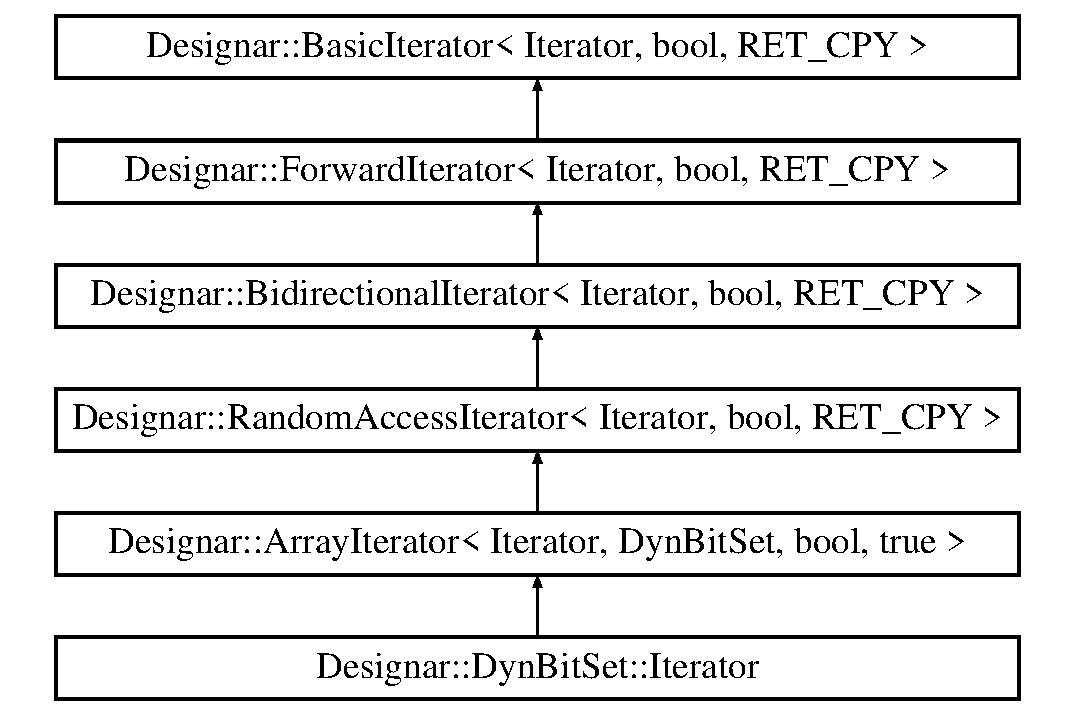
\includegraphics[height=6.000000cm]{class_designar_1_1_dyn_bit_set_1_1_iterator}
\end{center}
\end{figure}
\subsection*{Métodos públicos}
\begin{DoxyCompactItemize}
\item 
\hyperlink{class_designar_1_1_dyn_bit_set_1_1_r_w_proxy}{R\+W\+Proxy} \hyperlink{class_designar_1_1_dyn_bit_set_1_1_iterator_a413eba67b23a9400666c18845bbe795a}{get\+\_\+current} ()
\item 
\hyperlink{class_designar_1_1_dyn_bit_set_1_1_r_w_proxy}{R\+W\+Proxy} \hyperlink{class_designar_1_1_dyn_bit_set_1_1_iterator_a034af8ec4f70d792837cab4923799e9f}{get\+\_\+current} () const
\end{DoxyCompactItemize}
\subsection*{Otros miembros heredados}


\subsection{Descripción detallada}


Definición en la línea 186 del archivo bitset.\+H.



\subsection{Documentación de las funciones miembro}
\mbox{\Hypertarget{class_designar_1_1_dyn_bit_set_1_1_iterator_a413eba67b23a9400666c18845bbe795a}\label{class_designar_1_1_dyn_bit_set_1_1_iterator_a413eba67b23a9400666c18845bbe795a}} 
\index{Designar\+::\+Dyn\+Bit\+Set\+::\+Iterator@{Designar\+::\+Dyn\+Bit\+Set\+::\+Iterator}!get\+\_\+current@{get\+\_\+current}}
\index{get\+\_\+current@{get\+\_\+current}!Designar\+::\+Dyn\+Bit\+Set\+::\+Iterator@{Designar\+::\+Dyn\+Bit\+Set\+::\+Iterator}}
\subsubsection{\texorpdfstring{get\+\_\+current()}{get\_current()}\hspace{0.1cm}{\footnotesize\ttfamily [1/2]}}
{\footnotesize\ttfamily \hyperlink{class_designar_1_1_dyn_bit_set_1_1_r_w_proxy}{Dyn\+Bit\+Set\+::\+R\+W\+Proxy} Designar\+::\+Dyn\+Bit\+Set\+::\+Iterator\+::get\+\_\+current (\begin{DoxyParamCaption}{ }\end{DoxyParamCaption})}



Definición en la línea 417 del archivo bitset.\+C.

\mbox{\Hypertarget{class_designar_1_1_dyn_bit_set_1_1_iterator_a034af8ec4f70d792837cab4923799e9f}\label{class_designar_1_1_dyn_bit_set_1_1_iterator_a034af8ec4f70d792837cab4923799e9f}} 
\index{Designar\+::\+Dyn\+Bit\+Set\+::\+Iterator@{Designar\+::\+Dyn\+Bit\+Set\+::\+Iterator}!get\+\_\+current@{get\+\_\+current}}
\index{get\+\_\+current@{get\+\_\+current}!Designar\+::\+Dyn\+Bit\+Set\+::\+Iterator@{Designar\+::\+Dyn\+Bit\+Set\+::\+Iterator}}
\subsubsection{\texorpdfstring{get\+\_\+current()}{get\_current()}\hspace{0.1cm}{\footnotesize\ttfamily [2/2]}}
{\footnotesize\ttfamily \hyperlink{class_designar_1_1_dyn_bit_set_1_1_r_w_proxy}{Dyn\+Bit\+Set\+::\+R\+W\+Proxy} Designar\+::\+Dyn\+Bit\+Set\+::\+Iterator\+::get\+\_\+current (\begin{DoxyParamCaption}{ }\end{DoxyParamCaption}) const}



Definición en la línea 425 del archivo bitset.\+C.



La documentación para esta clase fue generada a partir de los siguientes ficheros\+:\begin{DoxyCompactItemize}
\item 
/home/julio/\+De\+S\+I\+G\+N\+A\+R-\/doc/\+De\+Si\+G\+N\+A\+R/include/\hyperlink{bitset_8_h}{bitset.\+H}\item 
/home/julio/\+De\+S\+I\+G\+N\+A\+R-\/doc/\+De\+Si\+G\+N\+A\+R/src/\hyperlink{bitset_8_c}{bitset.\+C}\end{DoxyCompactItemize}

\hypertarget{class_designar_1_1_d_l_list_1_1_iterator}{}\section{Designar\+:\+:D\+L\+List$<$ T $>$\+:\+:Iterator Class Reference}
\label{class_designar_1_1_d_l_list_1_1_iterator}\index{Designar\+::\+D\+L\+List$<$ T $>$\+::\+Iterator@{Designar\+::\+D\+L\+List$<$ T $>$\+::\+Iterator}}


{\ttfamily \#include $<$list.\+H$>$}

Inheritance diagram for Designar\+:\+:D\+L\+List$<$ T $>$\+:\+:Iterator\+:\begin{figure}[H]
\begin{center}
\leavevmode
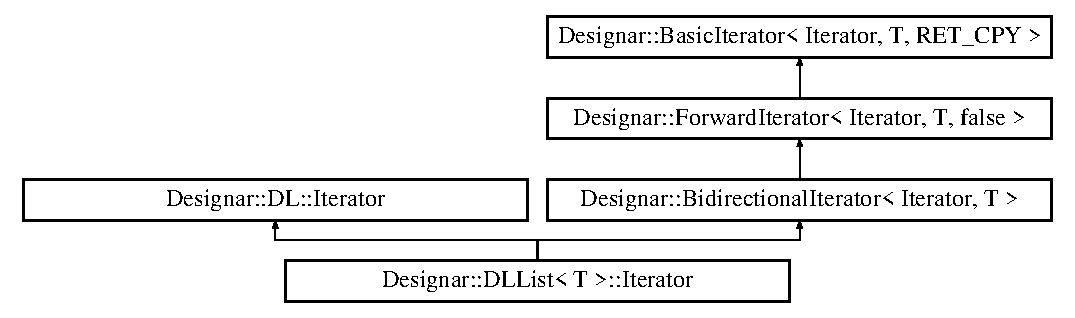
\includegraphics[height=3.822526cm]{class_designar_1_1_d_l_list_1_1_iterator}
\end{center}
\end{figure}
\subsection*{Public Member Functions}
\begin{DoxyCompactItemize}
\item 
\hyperlink{class_designar_1_1_d_l_list_1_1_iterator_a2d2ee7eeaa63b3b2e051a76fb4c4e164}{Iterator} ()
\item 
\hyperlink{class_designar_1_1_d_l_list_1_1_iterator_a7e1757caeeef81f003526fda985664cb}{Iterator} (const \hyperlink{class_designar_1_1_d_l_list}{D\+L\+List} \&l)
\item 
\hyperlink{class_designar_1_1_d_l_list_1_1_iterator_a41bf428b6219be3f152460de103f4413}{Iterator} (const \hyperlink{class_designar_1_1_d_l_list}{D\+L\+List} \&l, \hyperlink{class_designar_1_1_d_l}{DL} $\ast$c)
\item 
\hyperlink{class_designar_1_1_d_l_list_1_1_iterator_a824a391fc47274867bffac143a3d740b}{Iterator} (const \hyperlink{class_designar_1_1_d_l_list_1_1_iterator}{Iterator} \&it)
\item 
\hyperlink{class_designar_1_1_d_l_list_1_1_iterator_ad6d70cfea31c61502831f20b87d4f56f}{Iterator} (\hyperlink{class_designar_1_1_d_l_list_1_1_iterator}{Iterator} \&\&it)
\item 
\hyperlink{class_designar_1_1_d_l_list_1_1_iterator}{Iterator} \& \hyperlink{class_designar_1_1_d_l_list_1_1_iterator_a292588690dcaa7acc2311a92e535424e}{operator=} (const \hyperlink{class_designar_1_1_d_l_list_1_1_iterator}{Iterator} \&it)
\item 
\hyperlink{class_designar_1_1_d_l_list_1_1_iterator}{Iterator} \& \hyperlink{class_designar_1_1_d_l_list_1_1_iterator_a92bdff852753fecd794b5691419858a8}{operator=} (\hyperlink{class_designar_1_1_d_l_list_1_1_iterator}{Iterator} \&\&it)
\item 
void \hyperlink{class_designar_1_1_d_l_list_1_1_iterator_afb6abdec64f67b81813441a4c7d133d1}{swap} (\hyperlink{class_designar_1_1_d_l_list_1_1_iterator}{Iterator} \&it)
\item 
\hyperlink{namespace_designar_a9d113d66a39e82b73727c72cd3a52f73}{lint\+\_\+t} \hyperlink{class_designar_1_1_d_l_list_1_1_iterator_acf69183ba9dedd6fdb7dee8854cfce17}{get\+\_\+position} () const
\item 
T \& \hyperlink{class_designar_1_1_d_l_list_1_1_iterator_ad724b6e244dcd79d58b5772083e853ef}{get\+\_\+current} ()
\item 
const T \& \hyperlink{class_designar_1_1_d_l_list_1_1_iterator_a337833cfd046d1b1e69e9af95bdc3280}{get\+\_\+current} () const
\item 
T \hyperlink{class_designar_1_1_d_l_list_1_1_iterator_a98644b925b49ea22a9552039abb2624d}{del} ()
\item 
void \hyperlink{class_designar_1_1_d_l_list_1_1_iterator_ac4eb0645c0e4e68057bf0bc05cf3c8c3}{next} ()
\item 
void \hyperlink{class_designar_1_1_d_l_list_1_1_iterator_ac713eeea83e3e32a939067614a13c41d}{prev} ()
\end{DoxyCompactItemize}
\subsection*{Friends}
\begin{DoxyCompactItemize}
\item 
class \hyperlink{class_designar_1_1_d_l_list_1_1_iterator_ae3421d6be56b523bf3c41ceb29f3e5d7}{Basic\+Iterator$<$ Iterator, T $>$}
\end{DoxyCompactItemize}
\subsection*{Additional Inherited Members}


\subsection{Detailed Description}
\subsubsection*{template$<$typename T$>$\newline
class Designar\+::\+D\+L\+List$<$ T $>$\+::\+Iterator}



Definition at line 777 of file list.\+H.



\subsection{Constructor \& Destructor Documentation}
\mbox{\Hypertarget{class_designar_1_1_d_l_list_1_1_iterator_a2d2ee7eeaa63b3b2e051a76fb4c4e164}\label{class_designar_1_1_d_l_list_1_1_iterator_a2d2ee7eeaa63b3b2e051a76fb4c4e164}} 
\index{Designar\+::\+D\+L\+List\+::\+Iterator@{Designar\+::\+D\+L\+List\+::\+Iterator}!Iterator@{Iterator}}
\index{Iterator@{Iterator}!Designar\+::\+D\+L\+List\+::\+Iterator@{Designar\+::\+D\+L\+List\+::\+Iterator}}
\subsubsection{\texorpdfstring{Iterator()}{Iterator()}\hspace{0.1cm}{\footnotesize\ttfamily [1/5]}}
{\footnotesize\ttfamily template$<$typename T$>$ \\
\hyperlink{class_designar_1_1_d_l_list}{Designar\+::\+D\+L\+List}$<$ T $>$\+::Iterator\+::\+Iterator (\begin{DoxyParamCaption}{ }\end{DoxyParamCaption})\hspace{0.3cm}{\ttfamily [inline]}}



Definition at line 790 of file list.\+H.

\mbox{\Hypertarget{class_designar_1_1_d_l_list_1_1_iterator_a7e1757caeeef81f003526fda985664cb}\label{class_designar_1_1_d_l_list_1_1_iterator_a7e1757caeeef81f003526fda985664cb}} 
\index{Designar\+::\+D\+L\+List\+::\+Iterator@{Designar\+::\+D\+L\+List\+::\+Iterator}!Iterator@{Iterator}}
\index{Iterator@{Iterator}!Designar\+::\+D\+L\+List\+::\+Iterator@{Designar\+::\+D\+L\+List\+::\+Iterator}}
\subsubsection{\texorpdfstring{Iterator()}{Iterator()}\hspace{0.1cm}{\footnotesize\ttfamily [2/5]}}
{\footnotesize\ttfamily template$<$typename T$>$ \\
\hyperlink{class_designar_1_1_d_l_list}{Designar\+::\+D\+L\+List}$<$ T $>$\+::Iterator\+::\+Iterator (\begin{DoxyParamCaption}\item[{const \hyperlink{class_designar_1_1_d_l_list}{D\+L\+List} \&}]{l }\end{DoxyParamCaption})\hspace{0.3cm}{\ttfamily [inline]}}



Definition at line 796 of file list.\+H.

\mbox{\Hypertarget{class_designar_1_1_d_l_list_1_1_iterator_a41bf428b6219be3f152460de103f4413}\label{class_designar_1_1_d_l_list_1_1_iterator_a41bf428b6219be3f152460de103f4413}} 
\index{Designar\+::\+D\+L\+List\+::\+Iterator@{Designar\+::\+D\+L\+List\+::\+Iterator}!Iterator@{Iterator}}
\index{Iterator@{Iterator}!Designar\+::\+D\+L\+List\+::\+Iterator@{Designar\+::\+D\+L\+List\+::\+Iterator}}
\subsubsection{\texorpdfstring{Iterator()}{Iterator()}\hspace{0.1cm}{\footnotesize\ttfamily [3/5]}}
{\footnotesize\ttfamily template$<$typename T$>$ \\
\hyperlink{class_designar_1_1_d_l_list}{Designar\+::\+D\+L\+List}$<$ T $>$\+::Iterator\+::\+Iterator (\begin{DoxyParamCaption}\item[{const \hyperlink{class_designar_1_1_d_l_list}{D\+L\+List} \&}]{l,  }\item[{\hyperlink{class_designar_1_1_d_l}{DL} $\ast$}]{c }\end{DoxyParamCaption})\hspace{0.3cm}{\ttfamily [inline]}}



Definition at line 803 of file list.\+H.

\mbox{\Hypertarget{class_designar_1_1_d_l_list_1_1_iterator_a824a391fc47274867bffac143a3d740b}\label{class_designar_1_1_d_l_list_1_1_iterator_a824a391fc47274867bffac143a3d740b}} 
\index{Designar\+::\+D\+L\+List\+::\+Iterator@{Designar\+::\+D\+L\+List\+::\+Iterator}!Iterator@{Iterator}}
\index{Iterator@{Iterator}!Designar\+::\+D\+L\+List\+::\+Iterator@{Designar\+::\+D\+L\+List\+::\+Iterator}}
\subsubsection{\texorpdfstring{Iterator()}{Iterator()}\hspace{0.1cm}{\footnotesize\ttfamily [4/5]}}
{\footnotesize\ttfamily template$<$typename T$>$ \\
\hyperlink{class_designar_1_1_d_l_list}{Designar\+::\+D\+L\+List}$<$ T $>$\+::Iterator\+::\+Iterator (\begin{DoxyParamCaption}\item[{const \hyperlink{class_designar_1_1_d_l_list_1_1_iterator}{Iterator} \&}]{it }\end{DoxyParamCaption})\hspace{0.3cm}{\ttfamily [inline]}}



Definition at line 810 of file list.\+H.

\mbox{\Hypertarget{class_designar_1_1_d_l_list_1_1_iterator_ad6d70cfea31c61502831f20b87d4f56f}\label{class_designar_1_1_d_l_list_1_1_iterator_ad6d70cfea31c61502831f20b87d4f56f}} 
\index{Designar\+::\+D\+L\+List\+::\+Iterator@{Designar\+::\+D\+L\+List\+::\+Iterator}!Iterator@{Iterator}}
\index{Iterator@{Iterator}!Designar\+::\+D\+L\+List\+::\+Iterator@{Designar\+::\+D\+L\+List\+::\+Iterator}}
\subsubsection{\texorpdfstring{Iterator()}{Iterator()}\hspace{0.1cm}{\footnotesize\ttfamily [5/5]}}
{\footnotesize\ttfamily template$<$typename T$>$ \\
\hyperlink{class_designar_1_1_d_l_list}{Designar\+::\+D\+L\+List}$<$ T $>$\+::Iterator\+::\+Iterator (\begin{DoxyParamCaption}\item[{\hyperlink{class_designar_1_1_d_l_list_1_1_iterator}{Iterator} \&\&}]{it }\end{DoxyParamCaption})\hspace{0.3cm}{\ttfamily [inline]}}



Definition at line 816 of file list.\+H.



\subsection{Member Function Documentation}
\mbox{\Hypertarget{class_designar_1_1_d_l_list_1_1_iterator_a98644b925b49ea22a9552039abb2624d}\label{class_designar_1_1_d_l_list_1_1_iterator_a98644b925b49ea22a9552039abb2624d}} 
\index{Designar\+::\+D\+L\+List\+::\+Iterator@{Designar\+::\+D\+L\+List\+::\+Iterator}!del@{del}}
\index{del@{del}!Designar\+::\+D\+L\+List\+::\+Iterator@{Designar\+::\+D\+L\+List\+::\+Iterator}}
\subsubsection{\texorpdfstring{del()}{del()}}
{\footnotesize\ttfamily template$<$typename T$>$ \\
T \hyperlink{class_designar_1_1_d_l_list}{Designar\+::\+D\+L\+List}$<$ T $>$\+::Iterator\+::del (\begin{DoxyParamCaption}{ }\end{DoxyParamCaption})\hspace{0.3cm}{\ttfamily [inline]}}



Definition at line 861 of file list.\+H.

\mbox{\Hypertarget{class_designar_1_1_d_l_list_1_1_iterator_ad724b6e244dcd79d58b5772083e853ef}\label{class_designar_1_1_d_l_list_1_1_iterator_ad724b6e244dcd79d58b5772083e853ef}} 
\index{Designar\+::\+D\+L\+List\+::\+Iterator@{Designar\+::\+D\+L\+List\+::\+Iterator}!get\+\_\+current@{get\+\_\+current}}
\index{get\+\_\+current@{get\+\_\+current}!Designar\+::\+D\+L\+List\+::\+Iterator@{Designar\+::\+D\+L\+List\+::\+Iterator}}
\subsubsection{\texorpdfstring{get\+\_\+current()}{get\_current()}\hspace{0.1cm}{\footnotesize\ttfamily [1/2]}}
{\footnotesize\ttfamily template$<$typename T$>$ \\
T\& \hyperlink{class_designar_1_1_d_l_list}{Designar\+::\+D\+L\+List}$<$ T $>$\+::Iterator\+::get\+\_\+current (\begin{DoxyParamCaption}{ }\end{DoxyParamCaption})\hspace{0.3cm}{\ttfamily [inline]}}



Definition at line 851 of file list.\+H.

\mbox{\Hypertarget{class_designar_1_1_d_l_list_1_1_iterator_a337833cfd046d1b1e69e9af95bdc3280}\label{class_designar_1_1_d_l_list_1_1_iterator_a337833cfd046d1b1e69e9af95bdc3280}} 
\index{Designar\+::\+D\+L\+List\+::\+Iterator@{Designar\+::\+D\+L\+List\+::\+Iterator}!get\+\_\+current@{get\+\_\+current}}
\index{get\+\_\+current@{get\+\_\+current}!Designar\+::\+D\+L\+List\+::\+Iterator@{Designar\+::\+D\+L\+List\+::\+Iterator}}
\subsubsection{\texorpdfstring{get\+\_\+current()}{get\_current()}\hspace{0.1cm}{\footnotesize\ttfamily [2/2]}}
{\footnotesize\ttfamily template$<$typename T$>$ \\
const T\& \hyperlink{class_designar_1_1_d_l_list}{Designar\+::\+D\+L\+List}$<$ T $>$\+::Iterator\+::get\+\_\+current (\begin{DoxyParamCaption}{ }\end{DoxyParamCaption}) const\hspace{0.3cm}{\ttfamily [inline]}}



Definition at line 856 of file list.\+H.

\mbox{\Hypertarget{class_designar_1_1_d_l_list_1_1_iterator_acf69183ba9dedd6fdb7dee8854cfce17}\label{class_designar_1_1_d_l_list_1_1_iterator_acf69183ba9dedd6fdb7dee8854cfce17}} 
\index{Designar\+::\+D\+L\+List\+::\+Iterator@{Designar\+::\+D\+L\+List\+::\+Iterator}!get\+\_\+position@{get\+\_\+position}}
\index{get\+\_\+position@{get\+\_\+position}!Designar\+::\+D\+L\+List\+::\+Iterator@{Designar\+::\+D\+L\+List\+::\+Iterator}}
\subsubsection{\texorpdfstring{get\+\_\+position()}{get\_position()}}
{\footnotesize\ttfamily template$<$typename T$>$ \\
\hyperlink{namespace_designar_a9d113d66a39e82b73727c72cd3a52f73}{lint\+\_\+t} \hyperlink{class_designar_1_1_d_l_list}{Designar\+::\+D\+L\+List}$<$ T $>$\+::Iterator\+::get\+\_\+position (\begin{DoxyParamCaption}{ }\end{DoxyParamCaption}) const\hspace{0.3cm}{\ttfamily [inline]}}



Definition at line 846 of file list.\+H.

\mbox{\Hypertarget{class_designar_1_1_d_l_list_1_1_iterator_ac4eb0645c0e4e68057bf0bc05cf3c8c3}\label{class_designar_1_1_d_l_list_1_1_iterator_ac4eb0645c0e4e68057bf0bc05cf3c8c3}} 
\index{Designar\+::\+D\+L\+List\+::\+Iterator@{Designar\+::\+D\+L\+List\+::\+Iterator}!next@{next}}
\index{next@{next}!Designar\+::\+D\+L\+List\+::\+Iterator@{Designar\+::\+D\+L\+List\+::\+Iterator}}
\subsubsection{\texorpdfstring{next()}{next()}}
{\footnotesize\ttfamily template$<$typename T$>$ \\
void \hyperlink{class_designar_1_1_d_l_list}{Designar\+::\+D\+L\+List}$<$ T $>$\+::Iterator\+::next (\begin{DoxyParamCaption}{ }\end{DoxyParamCaption})\hspace{0.3cm}{\ttfamily [inline]}}



Definition at line 870 of file list.\+H.

\mbox{\Hypertarget{class_designar_1_1_d_l_list_1_1_iterator_a292588690dcaa7acc2311a92e535424e}\label{class_designar_1_1_d_l_list_1_1_iterator_a292588690dcaa7acc2311a92e535424e}} 
\index{Designar\+::\+D\+L\+List\+::\+Iterator@{Designar\+::\+D\+L\+List\+::\+Iterator}!operator=@{operator=}}
\index{operator=@{operator=}!Designar\+::\+D\+L\+List\+::\+Iterator@{Designar\+::\+D\+L\+List\+::\+Iterator}}
\subsubsection{\texorpdfstring{operator=()}{operator=()}\hspace{0.1cm}{\footnotesize\ttfamily [1/2]}}
{\footnotesize\ttfamily template$<$typename T$>$ \\
\hyperlink{class_designar_1_1_d_l_list_1_1_iterator}{Iterator}\& \hyperlink{class_designar_1_1_d_l_list}{Designar\+::\+D\+L\+List}$<$ T $>$\+::Iterator\+::operator= (\begin{DoxyParamCaption}\item[{const \hyperlink{class_designar_1_1_d_l_list_1_1_iterator}{Iterator} \&}]{it }\end{DoxyParamCaption})\hspace{0.3cm}{\ttfamily [inline]}}



Definition at line 822 of file list.\+H.

\mbox{\Hypertarget{class_designar_1_1_d_l_list_1_1_iterator_a92bdff852753fecd794b5691419858a8}\label{class_designar_1_1_d_l_list_1_1_iterator_a92bdff852753fecd794b5691419858a8}} 
\index{Designar\+::\+D\+L\+List\+::\+Iterator@{Designar\+::\+D\+L\+List\+::\+Iterator}!operator=@{operator=}}
\index{operator=@{operator=}!Designar\+::\+D\+L\+List\+::\+Iterator@{Designar\+::\+D\+L\+List\+::\+Iterator}}
\subsubsection{\texorpdfstring{operator=()}{operator=()}\hspace{0.1cm}{\footnotesize\ttfamily [2/2]}}
{\footnotesize\ttfamily template$<$typename T$>$ \\
\hyperlink{class_designar_1_1_d_l_list_1_1_iterator}{Iterator}\& \hyperlink{class_designar_1_1_d_l_list}{Designar\+::\+D\+L\+List}$<$ T $>$\+::Iterator\+::operator= (\begin{DoxyParamCaption}\item[{\hyperlink{class_designar_1_1_d_l_list_1_1_iterator}{Iterator} \&\&}]{it }\end{DoxyParamCaption})\hspace{0.3cm}{\ttfamily [inline]}}



Definition at line 833 of file list.\+H.

\mbox{\Hypertarget{class_designar_1_1_d_l_list_1_1_iterator_ac713eeea83e3e32a939067614a13c41d}\label{class_designar_1_1_d_l_list_1_1_iterator_ac713eeea83e3e32a939067614a13c41d}} 
\index{Designar\+::\+D\+L\+List\+::\+Iterator@{Designar\+::\+D\+L\+List\+::\+Iterator}!prev@{prev}}
\index{prev@{prev}!Designar\+::\+D\+L\+List\+::\+Iterator@{Designar\+::\+D\+L\+List\+::\+Iterator}}
\subsubsection{\texorpdfstring{prev()}{prev()}}
{\footnotesize\ttfamily template$<$typename T$>$ \\
void \hyperlink{class_designar_1_1_d_l_list}{Designar\+::\+D\+L\+List}$<$ T $>$\+::Iterator\+::prev (\begin{DoxyParamCaption}{ }\end{DoxyParamCaption})\hspace{0.3cm}{\ttfamily [inline]}}



Definition at line 876 of file list.\+H.

\mbox{\Hypertarget{class_designar_1_1_d_l_list_1_1_iterator_afb6abdec64f67b81813441a4c7d133d1}\label{class_designar_1_1_d_l_list_1_1_iterator_afb6abdec64f67b81813441a4c7d133d1}} 
\index{Designar\+::\+D\+L\+List\+::\+Iterator@{Designar\+::\+D\+L\+List\+::\+Iterator}!swap@{swap}}
\index{swap@{swap}!Designar\+::\+D\+L\+List\+::\+Iterator@{Designar\+::\+D\+L\+List\+::\+Iterator}}
\subsubsection{\texorpdfstring{swap()}{swap()}}
{\footnotesize\ttfamily template$<$typename T$>$ \\
void \hyperlink{class_designar_1_1_d_l_list}{Designar\+::\+D\+L\+List}$<$ T $>$\+::Iterator\+::swap (\begin{DoxyParamCaption}\item[{\hyperlink{class_designar_1_1_d_l_list_1_1_iterator}{Iterator} \&}]{it }\end{DoxyParamCaption})\hspace{0.3cm}{\ttfamily [inline]}}



Definition at line 839 of file list.\+H.



\subsection{Friends And Related Function Documentation}
\mbox{\Hypertarget{class_designar_1_1_d_l_list_1_1_iterator_ae3421d6be56b523bf3c41ceb29f3e5d7}\label{class_designar_1_1_d_l_list_1_1_iterator_ae3421d6be56b523bf3c41ceb29f3e5d7}} 
\index{Designar\+::\+D\+L\+List\+::\+Iterator@{Designar\+::\+D\+L\+List\+::\+Iterator}!Basic\+Iterator$<$ Iterator, T $>$@{Basic\+Iterator$<$ Iterator, T $>$}}
\index{Basic\+Iterator$<$ Iterator, T $>$@{Basic\+Iterator$<$ Iterator, T $>$}!Designar\+::\+D\+L\+List\+::\+Iterator@{Designar\+::\+D\+L\+List\+::\+Iterator}}
\subsubsection{\texorpdfstring{Basic\+Iterator$<$ Iterator, T $>$}{BasicIterator< Iterator, T >}}
{\footnotesize\ttfamily template$<$typename T$>$ \\
friend class \hyperlink{class_designar_1_1_basic_iterator}{Basic\+Iterator}$<$ \hyperlink{class_designar_1_1_d_l_list_1_1_iterator}{Iterator}, T $>$\hspace{0.3cm}{\ttfamily [friend]}}



Definition at line 780 of file list.\+H.



The documentation for this class was generated from the following file\+:\begin{DoxyCompactItemize}
\item 
/home/julio/\+De\+S\+I\+G\+N\+A\+R-\/doc/\+De\+Si\+G\+N\+A\+R/include/\hyperlink{list_8_h}{list.\+H}\end{DoxyCompactItemize}

\hypertarget{class_designar_1_1_gen_array_set_1_1_iterator}{}\section{Designar\+:\+:Gen\+Array\+Set$<$ Key, Cmp, Array\+Set\+Op $>$\+:\+:Iterator Class Reference}
\label{class_designar_1_1_gen_array_set_1_1_iterator}\index{Designar\+::\+Gen\+Array\+Set$<$ Key, Cmp, Array\+Set\+Op $>$\+::\+Iterator@{Designar\+::\+Gen\+Array\+Set$<$ Key, Cmp, Array\+Set\+Op $>$\+::\+Iterator}}


{\ttfamily \#include $<$array.\+H$>$}

Inheritance diagram for Designar\+:\+:Gen\+Array\+Set$<$ Key, Cmp, Array\+Set\+Op $>$\+:\+:Iterator\+:\begin{figure}[H]
\begin{center}
\leavevmode
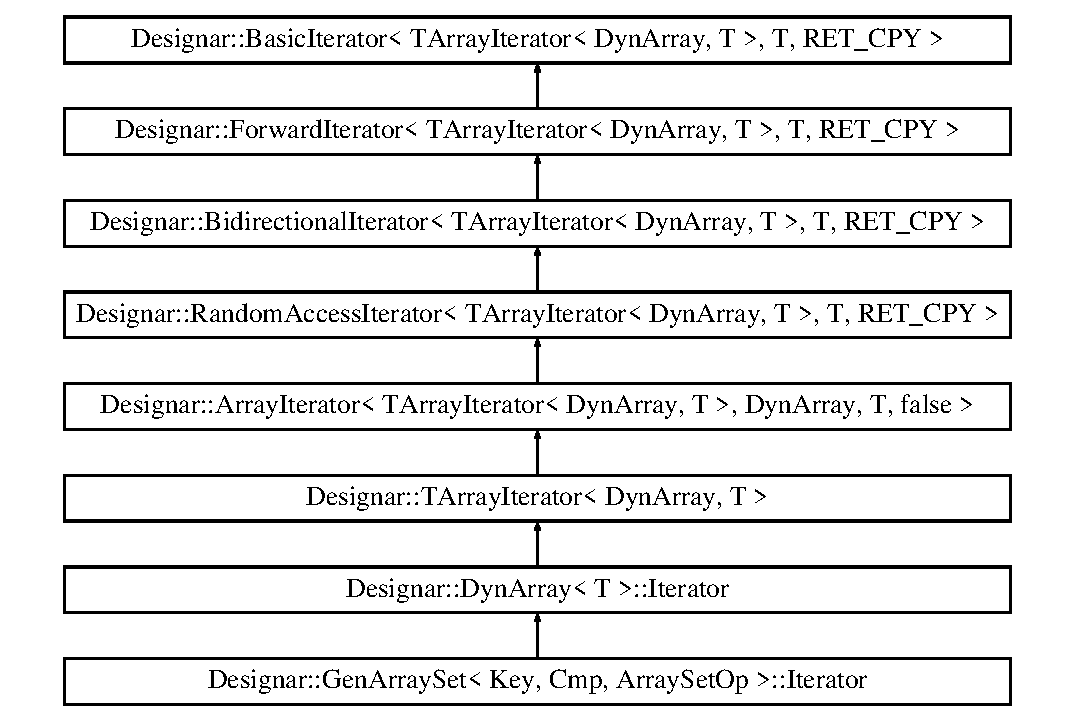
\includegraphics[height=8.000000cm]{class_designar_1_1_gen_array_set_1_1_iterator}
\end{center}
\end{figure}
\subsection*{Public Member Functions}
\begin{DoxyCompactItemize}
\item 
\hyperlink{class_designar_1_1_gen_array_set_1_1_iterator_a9f4aba730b697c071ffc51ef70db48ce}{Iterator} ()
\item 
\hyperlink{class_designar_1_1_gen_array_set_1_1_iterator_ae7870668057c79aefda6001548c550f1}{Iterator} (const \hyperlink{class_designar_1_1_gen_array_set}{Gen\+Array\+Set} \&a)
\item 
\hyperlink{class_designar_1_1_gen_array_set_1_1_iterator_a83846a50fb3a6dd02611aa331520d69a}{Iterator} (const \hyperlink{class_designar_1_1_gen_array_set}{Gen\+Array\+Set} \&a, \hyperlink{namespace_designar_aa72662848b9f4815e7bf31a7cf3e33d1}{nat\+\_\+t} c)
\item 
\hyperlink{class_designar_1_1_gen_array_set_1_1_iterator_a080025e4989fd5c3110e93e0c7c17fe2}{Iterator} (const \hyperlink{class_designar_1_1_gen_array_set_1_1_iterator}{Iterator} \&itor)
\item 
\hyperlink{class_designar_1_1_gen_array_set_1_1_iterator_aa82e1690f18b28782163e6bbb9d7d32a}{Iterator} (\hyperlink{class_designar_1_1_gen_array_set_1_1_iterator}{Iterator} \&\&itor)
\end{DoxyCompactItemize}
\subsection*{Additional Inherited Members}


\subsection{Detailed Description}
\subsubsection*{template$<$typename Key, class Cmp, class Array\+Set\+Op$>$\newline
class Designar\+::\+Gen\+Array\+Set$<$ Key, Cmp, Array\+Set\+Op $>$\+::\+Iterator}



Definition at line 1422 of file array.\+H.



\subsection{Constructor \& Destructor Documentation}
\mbox{\Hypertarget{class_designar_1_1_gen_array_set_1_1_iterator_a9f4aba730b697c071ffc51ef70db48ce}\label{class_designar_1_1_gen_array_set_1_1_iterator_a9f4aba730b697c071ffc51ef70db48ce}} 
\index{Designar\+::\+Gen\+Array\+Set\+::\+Iterator@{Designar\+::\+Gen\+Array\+Set\+::\+Iterator}!Iterator@{Iterator}}
\index{Iterator@{Iterator}!Designar\+::\+Gen\+Array\+Set\+::\+Iterator@{Designar\+::\+Gen\+Array\+Set\+::\+Iterator}}
\subsubsection{\texorpdfstring{Iterator()}{Iterator()}\hspace{0.1cm}{\footnotesize\ttfamily [1/5]}}
{\footnotesize\ttfamily template$<$typename Key, class Cmp, class Array\+Set\+Op$>$ \\
\hyperlink{class_designar_1_1_gen_array_set}{Designar\+::\+Gen\+Array\+Set}$<$ Key, Cmp, Array\+Set\+Op $>$\+::Iterator\+::\+Iterator (\begin{DoxyParamCaption}{ }\end{DoxyParamCaption})\hspace{0.3cm}{\ttfamily [inline]}}



Definition at line 1427 of file array.\+H.

\mbox{\Hypertarget{class_designar_1_1_gen_array_set_1_1_iterator_ae7870668057c79aefda6001548c550f1}\label{class_designar_1_1_gen_array_set_1_1_iterator_ae7870668057c79aefda6001548c550f1}} 
\index{Designar\+::\+Gen\+Array\+Set\+::\+Iterator@{Designar\+::\+Gen\+Array\+Set\+::\+Iterator}!Iterator@{Iterator}}
\index{Iterator@{Iterator}!Designar\+::\+Gen\+Array\+Set\+::\+Iterator@{Designar\+::\+Gen\+Array\+Set\+::\+Iterator}}
\subsubsection{\texorpdfstring{Iterator()}{Iterator()}\hspace{0.1cm}{\footnotesize\ttfamily [2/5]}}
{\footnotesize\ttfamily template$<$typename Key, class Cmp, class Array\+Set\+Op$>$ \\
\hyperlink{class_designar_1_1_gen_array_set}{Designar\+::\+Gen\+Array\+Set}$<$ Key, Cmp, Array\+Set\+Op $>$\+::Iterator\+::\+Iterator (\begin{DoxyParamCaption}\item[{const \hyperlink{class_designar_1_1_gen_array_set}{Gen\+Array\+Set} \&}]{a }\end{DoxyParamCaption})\hspace{0.3cm}{\ttfamily [inline]}}



Definition at line 1433 of file array.\+H.

\mbox{\Hypertarget{class_designar_1_1_gen_array_set_1_1_iterator_a83846a50fb3a6dd02611aa331520d69a}\label{class_designar_1_1_gen_array_set_1_1_iterator_a83846a50fb3a6dd02611aa331520d69a}} 
\index{Designar\+::\+Gen\+Array\+Set\+::\+Iterator@{Designar\+::\+Gen\+Array\+Set\+::\+Iterator}!Iterator@{Iterator}}
\index{Iterator@{Iterator}!Designar\+::\+Gen\+Array\+Set\+::\+Iterator@{Designar\+::\+Gen\+Array\+Set\+::\+Iterator}}
\subsubsection{\texorpdfstring{Iterator()}{Iterator()}\hspace{0.1cm}{\footnotesize\ttfamily [3/5]}}
{\footnotesize\ttfamily template$<$typename Key, class Cmp, class Array\+Set\+Op$>$ \\
\hyperlink{class_designar_1_1_gen_array_set}{Designar\+::\+Gen\+Array\+Set}$<$ Key, Cmp, Array\+Set\+Op $>$\+::Iterator\+::\+Iterator (\begin{DoxyParamCaption}\item[{const \hyperlink{class_designar_1_1_gen_array_set}{Gen\+Array\+Set} \&}]{a,  }\item[{\hyperlink{namespace_designar_aa72662848b9f4815e7bf31a7cf3e33d1}{nat\+\_\+t}}]{c }\end{DoxyParamCaption})\hspace{0.3cm}{\ttfamily [inline]}}



Definition at line 1439 of file array.\+H.

\mbox{\Hypertarget{class_designar_1_1_gen_array_set_1_1_iterator_a080025e4989fd5c3110e93e0c7c17fe2}\label{class_designar_1_1_gen_array_set_1_1_iterator_a080025e4989fd5c3110e93e0c7c17fe2}} 
\index{Designar\+::\+Gen\+Array\+Set\+::\+Iterator@{Designar\+::\+Gen\+Array\+Set\+::\+Iterator}!Iterator@{Iterator}}
\index{Iterator@{Iterator}!Designar\+::\+Gen\+Array\+Set\+::\+Iterator@{Designar\+::\+Gen\+Array\+Set\+::\+Iterator}}
\subsubsection{\texorpdfstring{Iterator()}{Iterator()}\hspace{0.1cm}{\footnotesize\ttfamily [4/5]}}
{\footnotesize\ttfamily template$<$typename Key, class Cmp, class Array\+Set\+Op$>$ \\
\hyperlink{class_designar_1_1_gen_array_set}{Designar\+::\+Gen\+Array\+Set}$<$ Key, Cmp, Array\+Set\+Op $>$\+::Iterator\+::\+Iterator (\begin{DoxyParamCaption}\item[{const \hyperlink{class_designar_1_1_gen_array_set_1_1_iterator}{Iterator} \&}]{itor }\end{DoxyParamCaption})\hspace{0.3cm}{\ttfamily [inline]}}



Definition at line 1445 of file array.\+H.

\mbox{\Hypertarget{class_designar_1_1_gen_array_set_1_1_iterator_aa82e1690f18b28782163e6bbb9d7d32a}\label{class_designar_1_1_gen_array_set_1_1_iterator_aa82e1690f18b28782163e6bbb9d7d32a}} 
\index{Designar\+::\+Gen\+Array\+Set\+::\+Iterator@{Designar\+::\+Gen\+Array\+Set\+::\+Iterator}!Iterator@{Iterator}}
\index{Iterator@{Iterator}!Designar\+::\+Gen\+Array\+Set\+::\+Iterator@{Designar\+::\+Gen\+Array\+Set\+::\+Iterator}}
\subsubsection{\texorpdfstring{Iterator()}{Iterator()}\hspace{0.1cm}{\footnotesize\ttfamily [5/5]}}
{\footnotesize\ttfamily template$<$typename Key, class Cmp, class Array\+Set\+Op$>$ \\
\hyperlink{class_designar_1_1_gen_array_set}{Designar\+::\+Gen\+Array\+Set}$<$ Key, Cmp, Array\+Set\+Op $>$\+::Iterator\+::\+Iterator (\begin{DoxyParamCaption}\item[{\hyperlink{class_designar_1_1_gen_array_set_1_1_iterator}{Iterator} \&\&}]{itor }\end{DoxyParamCaption})\hspace{0.3cm}{\ttfamily [inline]}}



Definition at line 1451 of file array.\+H.



The documentation for this class was generated from the following file\+:\begin{DoxyCompactItemize}
\item 
De\+Si\+G\+N\+A\+R/include/\hyperlink{array_8_h}{array.\+H}\end{DoxyCompactItemize}

\hypertarget{class_designar_1_1_d_l_1_1_iterator}{}\section{Referencia de la Clase Designar\+:\+:DL\+:\+:Iterator}
\label{class_designar_1_1_d_l_1_1_iterator}\index{Designar\+::\+D\+L\+::\+Iterator@{Designar\+::\+D\+L\+::\+Iterator}}


{\ttfamily \#include $<$nodesdef.\+H$>$}

Diagrama de herencias de Designar\+:\+:DL\+:\+:Iterator\begin{figure}[H]
\begin{center}
\leavevmode
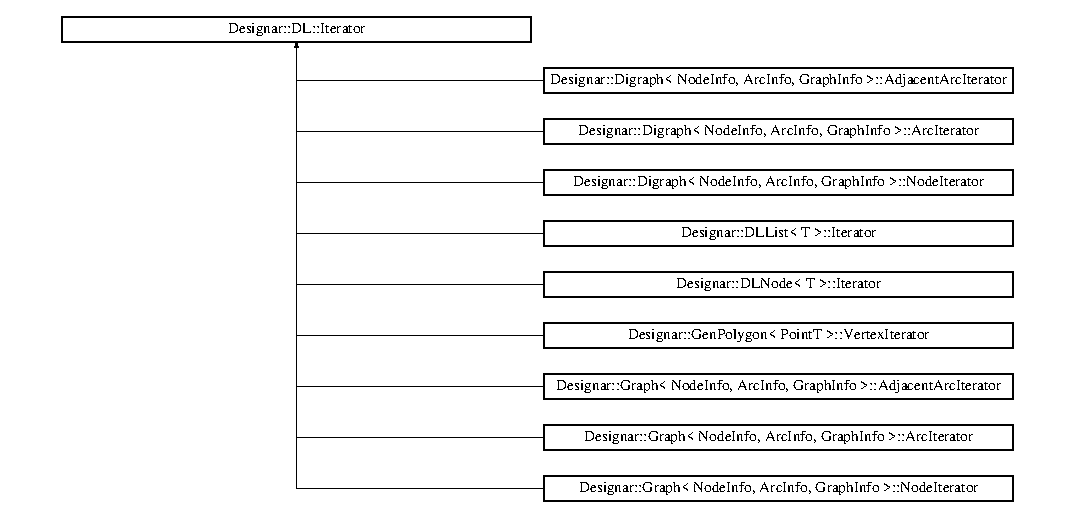
\includegraphics[height=6.511628cm]{class_designar_1_1_d_l_1_1_iterator}
\end{center}
\end{figure}
\subsection*{Métodos públicos}
\begin{DoxyCompactItemize}
\item 
\hyperlink{class_designar_1_1_d_l_1_1_iterator_ac8115296dde1a00604510beba6707b36}{Iterator} ()
\item 
\hyperlink{class_designar_1_1_d_l_1_1_iterator_ab40eab4206926dca72f7981c4920c984}{Iterator} (\hyperlink{class_designar_1_1_d_l}{DL} $\ast$h)
\item 
\hyperlink{class_designar_1_1_d_l_1_1_iterator_aa90c0222a2141efc64f6b70b83137531}{Iterator} (\hyperlink{class_designar_1_1_d_l}{DL} $\ast$h, \hyperlink{class_designar_1_1_d_l}{DL} $\ast$c)
\item 
\hyperlink{class_designar_1_1_d_l_1_1_iterator_a6216eca5f9c0a153ac194a8b7c741636}{Iterator} (const \hyperlink{class_designar_1_1_d_l_1_1_iterator}{Iterator} \&it)
\item 
\hyperlink{class_designar_1_1_d_l_1_1_iterator_ae5d00988114ca7cb890fb5e887c5e3ba}{Iterator} (\hyperlink{class_designar_1_1_d_l_1_1_iterator}{Iterator} \&\&it)
\item 
\hyperlink{class_designar_1_1_d_l_1_1_iterator}{Iterator} \& \hyperlink{class_designar_1_1_d_l_1_1_iterator_a24c29185e86ef76e7ecb17e9abfd42a9}{operator=} (const \hyperlink{class_designar_1_1_d_l_1_1_iterator}{Iterator} \&it)
\item 
\hyperlink{class_designar_1_1_d_l_1_1_iterator}{Iterator} \& \hyperlink{class_designar_1_1_d_l_1_1_iterator_a927bb8ad074ad3021a2d92abfff06fac}{operator=} (\hyperlink{class_designar_1_1_d_l_1_1_iterator}{Iterator} \&\&it)
\item 
void \hyperlink{class_designar_1_1_d_l_1_1_iterator_af8bba1d661f8d6300664481d7c6fd976}{swap} (\hyperlink{class_designar_1_1_d_l_1_1_iterator}{Iterator} \&it)
\item 
bool \hyperlink{class_designar_1_1_d_l_1_1_iterator_a02ccb7a5bbdc828ed8ac923f383661d4}{has\+\_\+current} () const
\item 
\hyperlink{class_designar_1_1_d_l}{DL} $\ast$ \hyperlink{class_designar_1_1_d_l_1_1_iterator_a291e44d1aee5859059aed9754a3dd35a}{get\+\_\+current} ()
\item 
\hyperlink{class_designar_1_1_d_l}{DL} $\ast$ \hyperlink{class_designar_1_1_d_l_1_1_iterator_aab4752b8c8f25cfbbd3560cebf23b7d1}{get\+\_\+current} () const
\item 
void \hyperlink{class_designar_1_1_d_l_1_1_iterator_ade01f6f8d747962c895e95fc0e26c515}{next} ()
\item 
void \hyperlink{class_designar_1_1_d_l_1_1_iterator_a8550a08d7c7645c8ec41ba209ee21893}{prev} ()
\item 
void \hyperlink{class_designar_1_1_d_l_1_1_iterator_a7708230beaa8a47d664878d37c11bbd3}{reset} ()
\item 
\hyperlink{class_designar_1_1_d_l}{DL} $\ast$ \hyperlink{class_designar_1_1_d_l_1_1_iterator_aa21843f313121866b1ad1571c77e65c6}{del} ()
\end{DoxyCompactItemize}
\subsection*{Métodos protegidos}
\begin{DoxyCompactItemize}
\item 
\hyperlink{class_designar_1_1_d_l}{DL} $\ast$ \hyperlink{class_designar_1_1_d_l_1_1_iterator_a575d5bbd0ce2e3d5df42d5d0112a1063}{get\+\_\+head} () const
\item 
\hyperlink{class_designar_1_1_d_l}{DL} $\ast$ \hyperlink{class_designar_1_1_d_l_1_1_iterator_af9d1225d5fa038ec4868e0910d4b9da0}{get\+\_\+location} () const
\end{DoxyCompactItemize}


\subsection{Descripción detallada}


Definición en la línea 293 del archivo nodesdef.\+H.



\subsection{Documentación del constructor y destructor}
\mbox{\Hypertarget{class_designar_1_1_d_l_1_1_iterator_ac8115296dde1a00604510beba6707b36}\label{class_designar_1_1_d_l_1_1_iterator_ac8115296dde1a00604510beba6707b36}} 
\index{Designar\+::\+D\+L\+::\+Iterator@{Designar\+::\+D\+L\+::\+Iterator}!Iterator@{Iterator}}
\index{Iterator@{Iterator}!Designar\+::\+D\+L\+::\+Iterator@{Designar\+::\+D\+L\+::\+Iterator}}
\subsubsection{\texorpdfstring{Iterator()}{Iterator()}\hspace{0.1cm}{\footnotesize\ttfamily [1/5]}}
{\footnotesize\ttfamily Designar\+::\+D\+L\+::\+Iterator\+::\+Iterator (\begin{DoxyParamCaption}{ }\end{DoxyParamCaption})\hspace{0.3cm}{\ttfamily [inline]}}



Definición en la línea 310 del archivo nodesdef.\+H.

\mbox{\Hypertarget{class_designar_1_1_d_l_1_1_iterator_ab40eab4206926dca72f7981c4920c984}\label{class_designar_1_1_d_l_1_1_iterator_ab40eab4206926dca72f7981c4920c984}} 
\index{Designar\+::\+D\+L\+::\+Iterator@{Designar\+::\+D\+L\+::\+Iterator}!Iterator@{Iterator}}
\index{Iterator@{Iterator}!Designar\+::\+D\+L\+::\+Iterator@{Designar\+::\+D\+L\+::\+Iterator}}
\subsubsection{\texorpdfstring{Iterator()}{Iterator()}\hspace{0.1cm}{\footnotesize\ttfamily [2/5]}}
{\footnotesize\ttfamily Designar\+::\+D\+L\+::\+Iterator\+::\+Iterator (\begin{DoxyParamCaption}\item[{\hyperlink{class_designar_1_1_d_l}{DL} $\ast$}]{h }\end{DoxyParamCaption})\hspace{0.3cm}{\ttfamily [inline]}}



Definición en la línea 316 del archivo nodesdef.\+H.

\mbox{\Hypertarget{class_designar_1_1_d_l_1_1_iterator_aa90c0222a2141efc64f6b70b83137531}\label{class_designar_1_1_d_l_1_1_iterator_aa90c0222a2141efc64f6b70b83137531}} 
\index{Designar\+::\+D\+L\+::\+Iterator@{Designar\+::\+D\+L\+::\+Iterator}!Iterator@{Iterator}}
\index{Iterator@{Iterator}!Designar\+::\+D\+L\+::\+Iterator@{Designar\+::\+D\+L\+::\+Iterator}}
\subsubsection{\texorpdfstring{Iterator()}{Iterator()}\hspace{0.1cm}{\footnotesize\ttfamily [3/5]}}
{\footnotesize\ttfamily Designar\+::\+D\+L\+::\+Iterator\+::\+Iterator (\begin{DoxyParamCaption}\item[{\hyperlink{class_designar_1_1_d_l}{DL} $\ast$}]{h,  }\item[{\hyperlink{class_designar_1_1_d_l}{DL} $\ast$}]{c }\end{DoxyParamCaption})\hspace{0.3cm}{\ttfamily [inline]}}



Definición en la línea 322 del archivo nodesdef.\+H.

\mbox{\Hypertarget{class_designar_1_1_d_l_1_1_iterator_a6216eca5f9c0a153ac194a8b7c741636}\label{class_designar_1_1_d_l_1_1_iterator_a6216eca5f9c0a153ac194a8b7c741636}} 
\index{Designar\+::\+D\+L\+::\+Iterator@{Designar\+::\+D\+L\+::\+Iterator}!Iterator@{Iterator}}
\index{Iterator@{Iterator}!Designar\+::\+D\+L\+::\+Iterator@{Designar\+::\+D\+L\+::\+Iterator}}
\subsubsection{\texorpdfstring{Iterator()}{Iterator()}\hspace{0.1cm}{\footnotesize\ttfamily [4/5]}}
{\footnotesize\ttfamily Designar\+::\+D\+L\+::\+Iterator\+::\+Iterator (\begin{DoxyParamCaption}\item[{const \hyperlink{class_designar_1_1_d_l_1_1_iterator}{Iterator} \&}]{it }\end{DoxyParamCaption})\hspace{0.3cm}{\ttfamily [inline]}}



Definición en la línea 328 del archivo nodesdef.\+H.

\mbox{\Hypertarget{class_designar_1_1_d_l_1_1_iterator_ae5d00988114ca7cb890fb5e887c5e3ba}\label{class_designar_1_1_d_l_1_1_iterator_ae5d00988114ca7cb890fb5e887c5e3ba}} 
\index{Designar\+::\+D\+L\+::\+Iterator@{Designar\+::\+D\+L\+::\+Iterator}!Iterator@{Iterator}}
\index{Iterator@{Iterator}!Designar\+::\+D\+L\+::\+Iterator@{Designar\+::\+D\+L\+::\+Iterator}}
\subsubsection{\texorpdfstring{Iterator()}{Iterator()}\hspace{0.1cm}{\footnotesize\ttfamily [5/5]}}
{\footnotesize\ttfamily Designar\+::\+D\+L\+::\+Iterator\+::\+Iterator (\begin{DoxyParamCaption}\item[{\hyperlink{class_designar_1_1_d_l_1_1_iterator}{Iterator} \&\&}]{it }\end{DoxyParamCaption})\hspace{0.3cm}{\ttfamily [inline]}}



Definición en la línea 334 del archivo nodesdef.\+H.



\subsection{Documentación de las funciones miembro}
\mbox{\Hypertarget{class_designar_1_1_d_l_1_1_iterator_aa21843f313121866b1ad1571c77e65c6}\label{class_designar_1_1_d_l_1_1_iterator_aa21843f313121866b1ad1571c77e65c6}} 
\index{Designar\+::\+D\+L\+::\+Iterator@{Designar\+::\+D\+L\+::\+Iterator}!del@{del}}
\index{del@{del}!Designar\+::\+D\+L\+::\+Iterator@{Designar\+::\+D\+L\+::\+Iterator}}
\subsubsection{\texorpdfstring{del()}{del()}}
{\footnotesize\ttfamily \hyperlink{class_designar_1_1_d_l}{DL}$\ast$ Designar\+::\+D\+L\+::\+Iterator\+::del (\begin{DoxyParamCaption}{ }\end{DoxyParamCaption})\hspace{0.3cm}{\ttfamily [inline]}}



Definición en la línea 404 del archivo nodesdef.\+H.

\mbox{\Hypertarget{class_designar_1_1_d_l_1_1_iterator_a291e44d1aee5859059aed9754a3dd35a}\label{class_designar_1_1_d_l_1_1_iterator_a291e44d1aee5859059aed9754a3dd35a}} 
\index{Designar\+::\+D\+L\+::\+Iterator@{Designar\+::\+D\+L\+::\+Iterator}!get\+\_\+current@{get\+\_\+current}}
\index{get\+\_\+current@{get\+\_\+current}!Designar\+::\+D\+L\+::\+Iterator@{Designar\+::\+D\+L\+::\+Iterator}}
\subsubsection{\texorpdfstring{get\+\_\+current()}{get\_current()}\hspace{0.1cm}{\footnotesize\ttfamily [1/2]}}
{\footnotesize\ttfamily \hyperlink{class_designar_1_1_d_l}{DL}$\ast$ Designar\+::\+D\+L\+::\+Iterator\+::get\+\_\+current (\begin{DoxyParamCaption}{ }\end{DoxyParamCaption})\hspace{0.3cm}{\ttfamily [inline]}}



Definición en la línea 367 del archivo nodesdef.\+H.

\mbox{\Hypertarget{class_designar_1_1_d_l_1_1_iterator_aab4752b8c8f25cfbbd3560cebf23b7d1}\label{class_designar_1_1_d_l_1_1_iterator_aab4752b8c8f25cfbbd3560cebf23b7d1}} 
\index{Designar\+::\+D\+L\+::\+Iterator@{Designar\+::\+D\+L\+::\+Iterator}!get\+\_\+current@{get\+\_\+current}}
\index{get\+\_\+current@{get\+\_\+current}!Designar\+::\+D\+L\+::\+Iterator@{Designar\+::\+D\+L\+::\+Iterator}}
\subsubsection{\texorpdfstring{get\+\_\+current()}{get\_current()}\hspace{0.1cm}{\footnotesize\ttfamily [2/2]}}
{\footnotesize\ttfamily \hyperlink{class_designar_1_1_d_l}{DL}$\ast$ Designar\+::\+D\+L\+::\+Iterator\+::get\+\_\+current (\begin{DoxyParamCaption}{ }\end{DoxyParamCaption}) const\hspace{0.3cm}{\ttfamily [inline]}}



Definición en la línea 375 del archivo nodesdef.\+H.

\mbox{\Hypertarget{class_designar_1_1_d_l_1_1_iterator_a575d5bbd0ce2e3d5df42d5d0112a1063}\label{class_designar_1_1_d_l_1_1_iterator_a575d5bbd0ce2e3d5df42d5d0112a1063}} 
\index{Designar\+::\+D\+L\+::\+Iterator@{Designar\+::\+D\+L\+::\+Iterator}!get\+\_\+head@{get\+\_\+head}}
\index{get\+\_\+head@{get\+\_\+head}!Designar\+::\+D\+L\+::\+Iterator@{Designar\+::\+D\+L\+::\+Iterator}}
\subsubsection{\texorpdfstring{get\+\_\+head()}{get\_head()}}
{\footnotesize\ttfamily \hyperlink{class_designar_1_1_d_l}{DL}$\ast$ Designar\+::\+D\+L\+::\+Iterator\+::get\+\_\+head (\begin{DoxyParamCaption}{ }\end{DoxyParamCaption}) const\hspace{0.3cm}{\ttfamily [inline]}, {\ttfamily [protected]}}



Definición en la línea 299 del archivo nodesdef.\+H.

\mbox{\Hypertarget{class_designar_1_1_d_l_1_1_iterator_af9d1225d5fa038ec4868e0910d4b9da0}\label{class_designar_1_1_d_l_1_1_iterator_af9d1225d5fa038ec4868e0910d4b9da0}} 
\index{Designar\+::\+D\+L\+::\+Iterator@{Designar\+::\+D\+L\+::\+Iterator}!get\+\_\+location@{get\+\_\+location}}
\index{get\+\_\+location@{get\+\_\+location}!Designar\+::\+D\+L\+::\+Iterator@{Designar\+::\+D\+L\+::\+Iterator}}
\subsubsection{\texorpdfstring{get\+\_\+location()}{get\_location()}}
{\footnotesize\ttfamily \hyperlink{class_designar_1_1_d_l}{DL}$\ast$ Designar\+::\+D\+L\+::\+Iterator\+::get\+\_\+location (\begin{DoxyParamCaption}{ }\end{DoxyParamCaption}) const\hspace{0.3cm}{\ttfamily [inline]}, {\ttfamily [protected]}}



Definición en la línea 304 del archivo nodesdef.\+H.

\mbox{\Hypertarget{class_designar_1_1_d_l_1_1_iterator_a02ccb7a5bbdc828ed8ac923f383661d4}\label{class_designar_1_1_d_l_1_1_iterator_a02ccb7a5bbdc828ed8ac923f383661d4}} 
\index{Designar\+::\+D\+L\+::\+Iterator@{Designar\+::\+D\+L\+::\+Iterator}!has\+\_\+current@{has\+\_\+current}}
\index{has\+\_\+current@{has\+\_\+current}!Designar\+::\+D\+L\+::\+Iterator@{Designar\+::\+D\+L\+::\+Iterator}}
\subsubsection{\texorpdfstring{has\+\_\+current()}{has\_current()}}
{\footnotesize\ttfamily bool Designar\+::\+D\+L\+::\+Iterator\+::has\+\_\+current (\begin{DoxyParamCaption}{ }\end{DoxyParamCaption}) const\hspace{0.3cm}{\ttfamily [inline]}}



Definición en la línea 362 del archivo nodesdef.\+H.

\mbox{\Hypertarget{class_designar_1_1_d_l_1_1_iterator_ade01f6f8d747962c895e95fc0e26c515}\label{class_designar_1_1_d_l_1_1_iterator_ade01f6f8d747962c895e95fc0e26c515}} 
\index{Designar\+::\+D\+L\+::\+Iterator@{Designar\+::\+D\+L\+::\+Iterator}!next@{next}}
\index{next@{next}!Designar\+::\+D\+L\+::\+Iterator@{Designar\+::\+D\+L\+::\+Iterator}}
\subsubsection{\texorpdfstring{next()}{next()}}
{\footnotesize\ttfamily void Designar\+::\+D\+L\+::\+Iterator\+::next (\begin{DoxyParamCaption}{ }\end{DoxyParamCaption})\hspace{0.3cm}{\ttfamily [inline]}}



Definición en la línea 383 del archivo nodesdef.\+H.

\mbox{\Hypertarget{class_designar_1_1_d_l_1_1_iterator_a24c29185e86ef76e7ecb17e9abfd42a9}\label{class_designar_1_1_d_l_1_1_iterator_a24c29185e86ef76e7ecb17e9abfd42a9}} 
\index{Designar\+::\+D\+L\+::\+Iterator@{Designar\+::\+D\+L\+::\+Iterator}!operator=@{operator=}}
\index{operator=@{operator=}!Designar\+::\+D\+L\+::\+Iterator@{Designar\+::\+D\+L\+::\+Iterator}}
\subsubsection{\texorpdfstring{operator=()}{operator=()}\hspace{0.1cm}{\footnotesize\ttfamily [1/2]}}
{\footnotesize\ttfamily \hyperlink{class_designar_1_1_d_l_1_1_iterator}{Iterator}\& Designar\+::\+D\+L\+::\+Iterator\+::operator= (\begin{DoxyParamCaption}\item[{const \hyperlink{class_designar_1_1_d_l_1_1_iterator}{Iterator} \&}]{it }\end{DoxyParamCaption})\hspace{0.3cm}{\ttfamily [inline]}}



Definición en la línea 340 del archivo nodesdef.\+H.

\mbox{\Hypertarget{class_designar_1_1_d_l_1_1_iterator_a927bb8ad074ad3021a2d92abfff06fac}\label{class_designar_1_1_d_l_1_1_iterator_a927bb8ad074ad3021a2d92abfff06fac}} 
\index{Designar\+::\+D\+L\+::\+Iterator@{Designar\+::\+D\+L\+::\+Iterator}!operator=@{operator=}}
\index{operator=@{operator=}!Designar\+::\+D\+L\+::\+Iterator@{Designar\+::\+D\+L\+::\+Iterator}}
\subsubsection{\texorpdfstring{operator=()}{operator=()}\hspace{0.1cm}{\footnotesize\ttfamily [2/2]}}
{\footnotesize\ttfamily \hyperlink{class_designar_1_1_d_l_1_1_iterator}{Iterator}\& Designar\+::\+D\+L\+::\+Iterator\+::operator= (\begin{DoxyParamCaption}\item[{\hyperlink{class_designar_1_1_d_l_1_1_iterator}{Iterator} \&\&}]{it }\end{DoxyParamCaption})\hspace{0.3cm}{\ttfamily [inline]}}



Definición en la línea 350 del archivo nodesdef.\+H.

\mbox{\Hypertarget{class_designar_1_1_d_l_1_1_iterator_a8550a08d7c7645c8ec41ba209ee21893}\label{class_designar_1_1_d_l_1_1_iterator_a8550a08d7c7645c8ec41ba209ee21893}} 
\index{Designar\+::\+D\+L\+::\+Iterator@{Designar\+::\+D\+L\+::\+Iterator}!prev@{prev}}
\index{prev@{prev}!Designar\+::\+D\+L\+::\+Iterator@{Designar\+::\+D\+L\+::\+Iterator}}
\subsubsection{\texorpdfstring{prev()}{prev()}}
{\footnotesize\ttfamily void Designar\+::\+D\+L\+::\+Iterator\+::prev (\begin{DoxyParamCaption}{ }\end{DoxyParamCaption})\hspace{0.3cm}{\ttfamily [inline]}}



Definición en la línea 391 del archivo nodesdef.\+H.

\mbox{\Hypertarget{class_designar_1_1_d_l_1_1_iterator_a7708230beaa8a47d664878d37c11bbd3}\label{class_designar_1_1_d_l_1_1_iterator_a7708230beaa8a47d664878d37c11bbd3}} 
\index{Designar\+::\+D\+L\+::\+Iterator@{Designar\+::\+D\+L\+::\+Iterator}!reset@{reset}}
\index{reset@{reset}!Designar\+::\+D\+L\+::\+Iterator@{Designar\+::\+D\+L\+::\+Iterator}}
\subsubsection{\texorpdfstring{reset()}{reset()}}
{\footnotesize\ttfamily void Designar\+::\+D\+L\+::\+Iterator\+::reset (\begin{DoxyParamCaption}{ }\end{DoxyParamCaption})\hspace{0.3cm}{\ttfamily [inline]}}



Definición en la línea 399 del archivo nodesdef.\+H.

\mbox{\Hypertarget{class_designar_1_1_d_l_1_1_iterator_af8bba1d661f8d6300664481d7c6fd976}\label{class_designar_1_1_d_l_1_1_iterator_af8bba1d661f8d6300664481d7c6fd976}} 
\index{Designar\+::\+D\+L\+::\+Iterator@{Designar\+::\+D\+L\+::\+Iterator}!swap@{swap}}
\index{swap@{swap}!Designar\+::\+D\+L\+::\+Iterator@{Designar\+::\+D\+L\+::\+Iterator}}
\subsubsection{\texorpdfstring{swap()}{swap()}}
{\footnotesize\ttfamily void Designar\+::\+D\+L\+::\+Iterator\+::swap (\begin{DoxyParamCaption}\item[{\hyperlink{class_designar_1_1_d_l_1_1_iterator}{Iterator} \&}]{it }\end{DoxyParamCaption})\hspace{0.3cm}{\ttfamily [inline]}}



Definición en la línea 356 del archivo nodesdef.\+H.



La documentación para esta clase fue generada a partir del siguiente fichero\+:\begin{DoxyCompactItemize}
\item 
include/\hyperlink{nodesdef_8_h}{nodesdef.\+H}\end{DoxyCompactItemize}

\hypertarget{class_designar_1_1_fixed_array_1_1_iterator}{}\section{Referencia de la Clase Designar\+:\+:Fixed\+Array$<$ T $>$\+:\+:Iterator}
\label{class_designar_1_1_fixed_array_1_1_iterator}\index{Designar\+::\+Fixed\+Array$<$ T $>$\+::\+Iterator@{Designar\+::\+Fixed\+Array$<$ T $>$\+::\+Iterator}}


{\ttfamily \#include $<$array.\+H$>$}

Diagrama de herencias de Designar\+:\+:Fixed\+Array$<$ T $>$\+:\+:Iterator\begin{figure}[H]
\begin{center}
\leavevmode
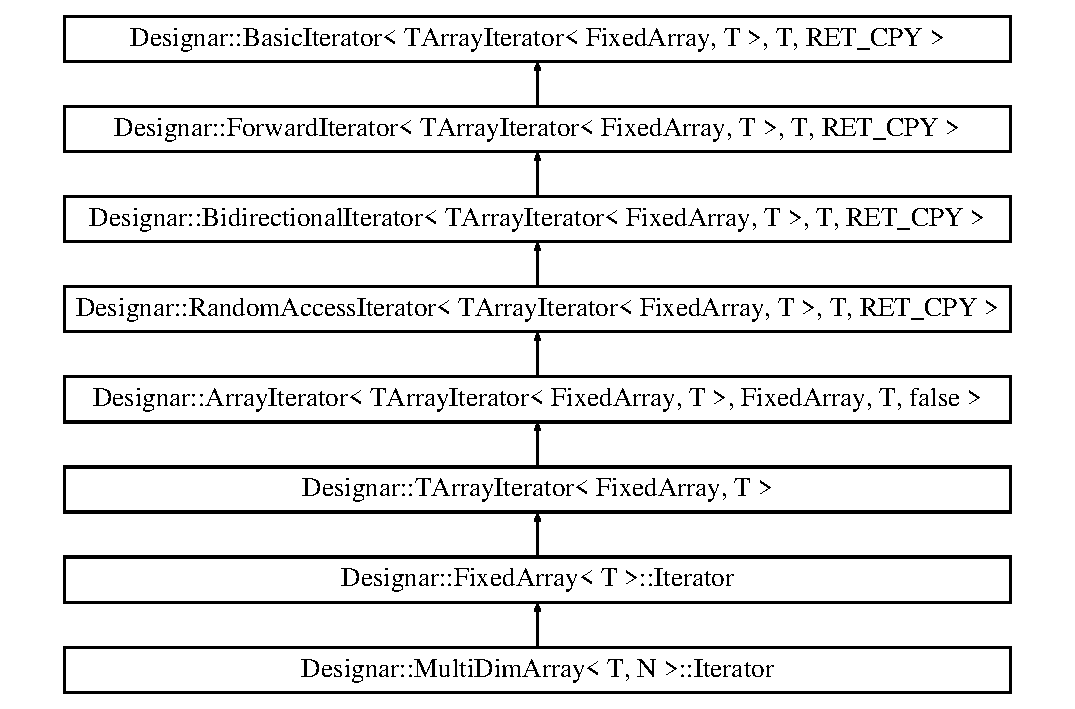
\includegraphics[height=8.000000cm]{class_designar_1_1_fixed_array_1_1_iterator}
\end{center}
\end{figure}
\subsection*{Otros miembros heredados}


\subsection{Descripción detallada}
\subsubsection*{template$<$typename T$>$\newline
class Designar\+::\+Fixed\+Array$<$ T $>$\+::\+Iterator}



Definición en la línea 574 del archivo array.\+H.



La documentación para esta clase fue generada a partir del siguiente fichero\+:\begin{DoxyCompactItemize}
\item 
include/\hyperlink{array_8_h}{array.\+H}\end{DoxyCompactItemize}

\hypertarget{class_designar_1_1_d_l_node_1_1_iterator}{}\section{Referencia de la Clase Designar\+:\+:D\+L\+Node$<$ T $>$\+:\+:Iterator}
\label{class_designar_1_1_d_l_node_1_1_iterator}\index{Designar\+::\+D\+L\+Node$<$ T $>$\+::\+Iterator@{Designar\+::\+D\+L\+Node$<$ T $>$\+::\+Iterator}}


{\ttfamily \#include $<$nodesdef.\+H$>$}

Diagrama de herencias de Designar\+:\+:D\+L\+Node$<$ T $>$\+:\+:Iterator\begin{figure}[H]
\begin{center}
\leavevmode
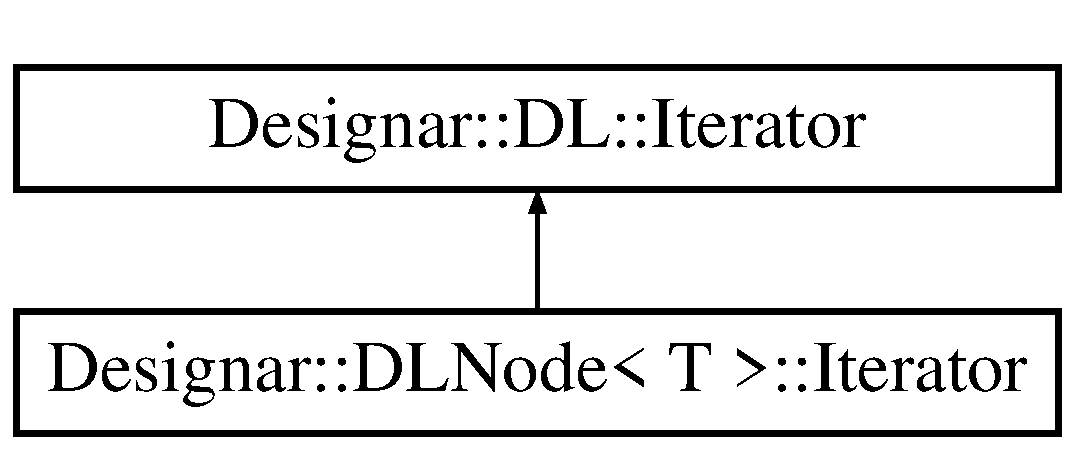
\includegraphics[height=2.000000cm]{class_designar_1_1_d_l_node_1_1_iterator}
\end{center}
\end{figure}
\subsection*{Métodos públicos}
\begin{DoxyCompactItemize}
\item 
\hyperlink{class_designar_1_1_d_l_node}{D\+L\+Node} $\ast$ \hyperlink{class_designar_1_1_d_l_node_1_1_iterator_a5787051e4f6727efef70ac3f8991ab59}{get\+\_\+current} ()
\item 
\hyperlink{class_designar_1_1_d_l_node}{D\+L\+Node} $\ast$ \hyperlink{class_designar_1_1_d_l_node_1_1_iterator_a1ea2b71da1fbc4970b9a1c170ddacb13}{get\+\_\+current} () const
\item 
\hyperlink{class_designar_1_1_d_l_node}{D\+L\+Node} $\ast$ \hyperlink{class_designar_1_1_d_l_node_1_1_iterator_a7ba9818dbd9d8cbbd85fe47db3395375}{del} ()
\item 
\hyperlink{class_designar_1_1_d_l_node}{D\+L\+Node} $\ast$ \hyperlink{class_designar_1_1_d_l_node_1_1_iterator_a37adeeda3073b950590700c3e22dcf28}{operator$\ast$} ()
\item 
\hyperlink{class_designar_1_1_d_l_node}{D\+L\+Node} $\ast$ \hyperlink{class_designar_1_1_d_l_node_1_1_iterator_ae75896ae631f91daaaa9a193df27a239}{operator$\ast$} () const
\end{DoxyCompactItemize}
\subsection*{Otros miembros heredados}


\subsection{Descripción detallada}
\subsubsection*{template$<$typename T$>$\newline
class Designar\+::\+D\+L\+Node$<$ T $>$\+::\+Iterator}



Definición en la línea 494 del archivo nodesdef.\+H.



\subsection{Documentación de las funciones miembro}
\mbox{\Hypertarget{class_designar_1_1_d_l_node_1_1_iterator_a7ba9818dbd9d8cbbd85fe47db3395375}\label{class_designar_1_1_d_l_node_1_1_iterator_a7ba9818dbd9d8cbbd85fe47db3395375}} 
\index{Designar\+::\+D\+L\+Node\+::\+Iterator@{Designar\+::\+D\+L\+Node\+::\+Iterator}!del@{del}}
\index{del@{del}!Designar\+::\+D\+L\+Node\+::\+Iterator@{Designar\+::\+D\+L\+Node\+::\+Iterator}}
\subsubsection{\texorpdfstring{del()}{del()}}
{\footnotesize\ttfamily template$<$typename T$>$ \\
\hyperlink{class_designar_1_1_d_l_node}{D\+L\+Node}$\ast$ \hyperlink{class_designar_1_1_d_l_node}{Designar\+::\+D\+L\+Node}$<$ T $>$\+::Iterator\+::del (\begin{DoxyParamCaption}{ }\end{DoxyParamCaption})\hspace{0.3cm}{\ttfamily [inline]}}



Definición en la línea 510 del archivo nodesdef.\+H.

\mbox{\Hypertarget{class_designar_1_1_d_l_node_1_1_iterator_a5787051e4f6727efef70ac3f8991ab59}\label{class_designar_1_1_d_l_node_1_1_iterator_a5787051e4f6727efef70ac3f8991ab59}} 
\index{Designar\+::\+D\+L\+Node\+::\+Iterator@{Designar\+::\+D\+L\+Node\+::\+Iterator}!get\+\_\+current@{get\+\_\+current}}
\index{get\+\_\+current@{get\+\_\+current}!Designar\+::\+D\+L\+Node\+::\+Iterator@{Designar\+::\+D\+L\+Node\+::\+Iterator}}
\subsubsection{\texorpdfstring{get\+\_\+current()}{get\_current()}\hspace{0.1cm}{\footnotesize\ttfamily [1/2]}}
{\footnotesize\ttfamily template$<$typename T$>$ \\
\hyperlink{class_designar_1_1_d_l_node}{D\+L\+Node}$\ast$ \hyperlink{class_designar_1_1_d_l_node}{Designar\+::\+D\+L\+Node}$<$ T $>$\+::Iterator\+::get\+\_\+current (\begin{DoxyParamCaption}{ }\end{DoxyParamCaption})\hspace{0.3cm}{\ttfamily [inline]}}



Definición en la línea 500 del archivo nodesdef.\+H.

\mbox{\Hypertarget{class_designar_1_1_d_l_node_1_1_iterator_a1ea2b71da1fbc4970b9a1c170ddacb13}\label{class_designar_1_1_d_l_node_1_1_iterator_a1ea2b71da1fbc4970b9a1c170ddacb13}} 
\index{Designar\+::\+D\+L\+Node\+::\+Iterator@{Designar\+::\+D\+L\+Node\+::\+Iterator}!get\+\_\+current@{get\+\_\+current}}
\index{get\+\_\+current@{get\+\_\+current}!Designar\+::\+D\+L\+Node\+::\+Iterator@{Designar\+::\+D\+L\+Node\+::\+Iterator}}
\subsubsection{\texorpdfstring{get\+\_\+current()}{get\_current()}\hspace{0.1cm}{\footnotesize\ttfamily [2/2]}}
{\footnotesize\ttfamily template$<$typename T$>$ \\
\hyperlink{class_designar_1_1_d_l_node}{D\+L\+Node}$\ast$ \hyperlink{class_designar_1_1_d_l_node}{Designar\+::\+D\+L\+Node}$<$ T $>$\+::Iterator\+::get\+\_\+current (\begin{DoxyParamCaption}{ }\end{DoxyParamCaption}) const\hspace{0.3cm}{\ttfamily [inline]}}



Definición en la línea 505 del archivo nodesdef.\+H.

\mbox{\Hypertarget{class_designar_1_1_d_l_node_1_1_iterator_a37adeeda3073b950590700c3e22dcf28}\label{class_designar_1_1_d_l_node_1_1_iterator_a37adeeda3073b950590700c3e22dcf28}} 
\index{Designar\+::\+D\+L\+Node\+::\+Iterator@{Designar\+::\+D\+L\+Node\+::\+Iterator}!operator$\ast$@{operator$\ast$}}
\index{operator$\ast$@{operator$\ast$}!Designar\+::\+D\+L\+Node\+::\+Iterator@{Designar\+::\+D\+L\+Node\+::\+Iterator}}
\subsubsection{\texorpdfstring{operator$\ast$()}{operator*()}\hspace{0.1cm}{\footnotesize\ttfamily [1/2]}}
{\footnotesize\ttfamily template$<$typename T$>$ \\
\hyperlink{class_designar_1_1_d_l_node}{D\+L\+Node}$\ast$ \hyperlink{class_designar_1_1_d_l_node}{Designar\+::\+D\+L\+Node}$<$ T $>$\+::Iterator\+::operator$\ast$ (\begin{DoxyParamCaption}{ }\end{DoxyParamCaption})\hspace{0.3cm}{\ttfamily [inline]}}



Definición en la línea 515 del archivo nodesdef.\+H.

\mbox{\Hypertarget{class_designar_1_1_d_l_node_1_1_iterator_ae75896ae631f91daaaa9a193df27a239}\label{class_designar_1_1_d_l_node_1_1_iterator_ae75896ae631f91daaaa9a193df27a239}} 
\index{Designar\+::\+D\+L\+Node\+::\+Iterator@{Designar\+::\+D\+L\+Node\+::\+Iterator}!operator$\ast$@{operator$\ast$}}
\index{operator$\ast$@{operator$\ast$}!Designar\+::\+D\+L\+Node\+::\+Iterator@{Designar\+::\+D\+L\+Node\+::\+Iterator}}
\subsubsection{\texorpdfstring{operator$\ast$()}{operator*()}\hspace{0.1cm}{\footnotesize\ttfamily [2/2]}}
{\footnotesize\ttfamily template$<$typename T$>$ \\
\hyperlink{class_designar_1_1_d_l_node}{D\+L\+Node}$\ast$ \hyperlink{class_designar_1_1_d_l_node}{Designar\+::\+D\+L\+Node}$<$ T $>$\+::Iterator\+::operator$\ast$ (\begin{DoxyParamCaption}{ }\end{DoxyParamCaption}) const\hspace{0.3cm}{\ttfamily [inline]}}



Definición en la línea 520 del archivo nodesdef.\+H.



La documentación para esta clase fue generada a partir del siguiente fichero\+:\begin{DoxyCompactItemize}
\item 
include/\hyperlink{nodesdef_8_h}{nodesdef.\+H}\end{DoxyCompactItemize}

\hypertarget{class_designar_1_1_multi_dim_array_1_1_iterator}{}\section{Designar\+:\+:Multi\+Dim\+Array$<$ T, N $>$\+:\+:Iterator Class Reference}
\label{class_designar_1_1_multi_dim_array_1_1_iterator}\index{Designar\+::\+Multi\+Dim\+Array$<$ T, N $>$\+::\+Iterator@{Designar\+::\+Multi\+Dim\+Array$<$ T, N $>$\+::\+Iterator}}


{\ttfamily \#include $<$array.\+H$>$}

Inheritance diagram for Designar\+:\+:Multi\+Dim\+Array$<$ T, N $>$\+:\+:Iterator\+:\begin{figure}[H]
\begin{center}
\leavevmode
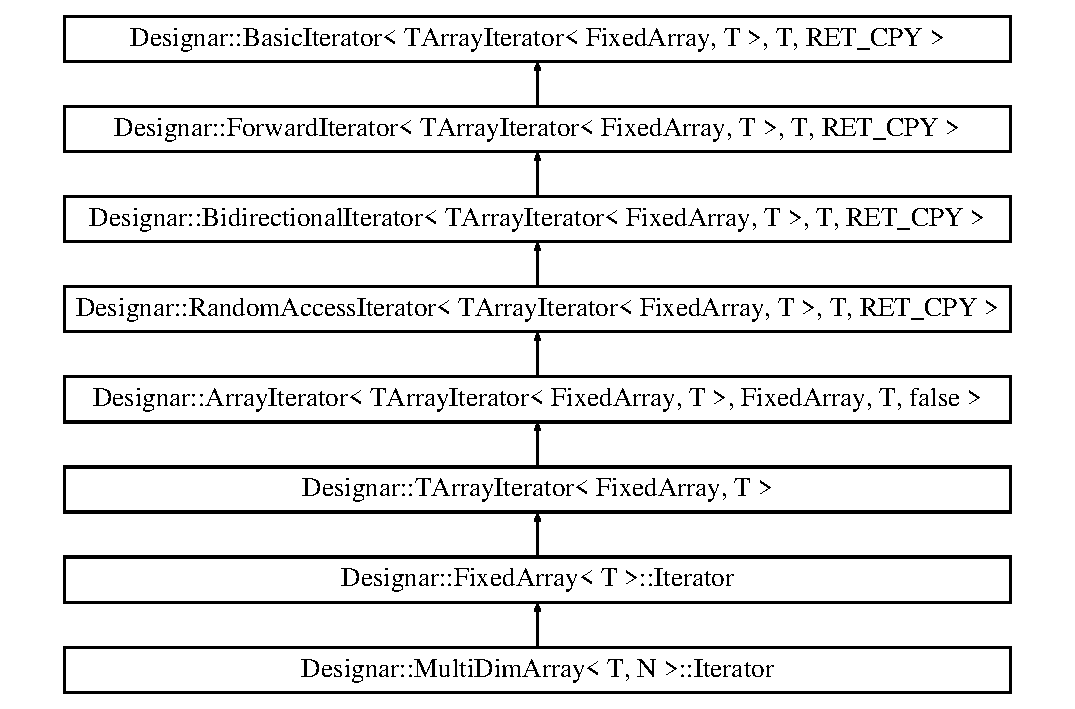
\includegraphics[height=8.000000cm]{class_designar_1_1_multi_dim_array_1_1_iterator}
\end{center}
\end{figure}
\subsection*{Public Member Functions}
\begin{DoxyCompactItemize}
\item 
\hyperlink{class_designar_1_1_multi_dim_array_1_1_iterator_af627beb86cf5b1154f421078082b18f9}{Iterator} ()
\item 
\hyperlink{class_designar_1_1_multi_dim_array_1_1_iterator_a0b4865a27a5f64866d63376f24076b9f}{Iterator} (const \hyperlink{class_designar_1_1_multi_dim_array}{Multi\+Dim\+Array} \&a)
\item 
\hyperlink{class_designar_1_1_multi_dim_array_1_1_iterator_a557464a713807cd34a23a3c9cd29dbb0}{Iterator} (const \hyperlink{class_designar_1_1_multi_dim_array}{Multi\+Dim\+Array} \&a, \hyperlink{namespace_designar_aa72662848b9f4815e7bf31a7cf3e33d1}{nat\+\_\+t} c)
\item 
\hyperlink{class_designar_1_1_multi_dim_array_1_1_iterator_a2d0c217ae08b2203c50e1d1a01c3af40}{Iterator} (const \hyperlink{class_designar_1_1_multi_dim_array_1_1_iterator}{Iterator} \&itor)
\item 
\hyperlink{class_designar_1_1_multi_dim_array_1_1_iterator_af6ebf97caae786b50dcb6062b3ab7b0b}{Iterator} (\hyperlink{class_designar_1_1_multi_dim_array_1_1_iterator}{Iterator} \&\&itor)
\end{DoxyCompactItemize}
\subsection*{Additional Inherited Members}


\subsection{Detailed Description}
\subsubsection*{template$<$typename T, nat\+\_\+t N = 2$>$\newline
class Designar\+::\+Multi\+Dim\+Array$<$ T, N $>$\+::\+Iterator}



Definition at line 1688 of file array.\+H.



\subsection{Constructor \& Destructor Documentation}
\mbox{\Hypertarget{class_designar_1_1_multi_dim_array_1_1_iterator_af627beb86cf5b1154f421078082b18f9}\label{class_designar_1_1_multi_dim_array_1_1_iterator_af627beb86cf5b1154f421078082b18f9}} 
\index{Designar\+::\+Multi\+Dim\+Array\+::\+Iterator@{Designar\+::\+Multi\+Dim\+Array\+::\+Iterator}!Iterator@{Iterator}}
\index{Iterator@{Iterator}!Designar\+::\+Multi\+Dim\+Array\+::\+Iterator@{Designar\+::\+Multi\+Dim\+Array\+::\+Iterator}}
\subsubsection{\texorpdfstring{Iterator()}{Iterator()}\hspace{0.1cm}{\footnotesize\ttfamily [1/5]}}
{\footnotesize\ttfamily template$<$typename T, nat\+\_\+t N = 2$>$ \\
\hyperlink{class_designar_1_1_multi_dim_array}{Designar\+::\+Multi\+Dim\+Array}$<$ T, N $>$\+::Iterator\+::\+Iterator (\begin{DoxyParamCaption}{ }\end{DoxyParamCaption})\hspace{0.3cm}{\ttfamily [inline]}}



Definition at line 1693 of file array.\+H.

\mbox{\Hypertarget{class_designar_1_1_multi_dim_array_1_1_iterator_a0b4865a27a5f64866d63376f24076b9f}\label{class_designar_1_1_multi_dim_array_1_1_iterator_a0b4865a27a5f64866d63376f24076b9f}} 
\index{Designar\+::\+Multi\+Dim\+Array\+::\+Iterator@{Designar\+::\+Multi\+Dim\+Array\+::\+Iterator}!Iterator@{Iterator}}
\index{Iterator@{Iterator}!Designar\+::\+Multi\+Dim\+Array\+::\+Iterator@{Designar\+::\+Multi\+Dim\+Array\+::\+Iterator}}
\subsubsection{\texorpdfstring{Iterator()}{Iterator()}\hspace{0.1cm}{\footnotesize\ttfamily [2/5]}}
{\footnotesize\ttfamily template$<$typename T, nat\+\_\+t N = 2$>$ \\
\hyperlink{class_designar_1_1_multi_dim_array}{Designar\+::\+Multi\+Dim\+Array}$<$ T, N $>$\+::Iterator\+::\+Iterator (\begin{DoxyParamCaption}\item[{const \hyperlink{class_designar_1_1_multi_dim_array}{Multi\+Dim\+Array} \&}]{a }\end{DoxyParamCaption})\hspace{0.3cm}{\ttfamily [inline]}}



Definition at line 1699 of file array.\+H.

\mbox{\Hypertarget{class_designar_1_1_multi_dim_array_1_1_iterator_a557464a713807cd34a23a3c9cd29dbb0}\label{class_designar_1_1_multi_dim_array_1_1_iterator_a557464a713807cd34a23a3c9cd29dbb0}} 
\index{Designar\+::\+Multi\+Dim\+Array\+::\+Iterator@{Designar\+::\+Multi\+Dim\+Array\+::\+Iterator}!Iterator@{Iterator}}
\index{Iterator@{Iterator}!Designar\+::\+Multi\+Dim\+Array\+::\+Iterator@{Designar\+::\+Multi\+Dim\+Array\+::\+Iterator}}
\subsubsection{\texorpdfstring{Iterator()}{Iterator()}\hspace{0.1cm}{\footnotesize\ttfamily [3/5]}}
{\footnotesize\ttfamily template$<$typename T, nat\+\_\+t N = 2$>$ \\
\hyperlink{class_designar_1_1_multi_dim_array}{Designar\+::\+Multi\+Dim\+Array}$<$ T, N $>$\+::Iterator\+::\+Iterator (\begin{DoxyParamCaption}\item[{const \hyperlink{class_designar_1_1_multi_dim_array}{Multi\+Dim\+Array} \&}]{a,  }\item[{\hyperlink{namespace_designar_aa72662848b9f4815e7bf31a7cf3e33d1}{nat\+\_\+t}}]{c }\end{DoxyParamCaption})\hspace{0.3cm}{\ttfamily [inline]}}



Definition at line 1705 of file array.\+H.

\mbox{\Hypertarget{class_designar_1_1_multi_dim_array_1_1_iterator_a2d0c217ae08b2203c50e1d1a01c3af40}\label{class_designar_1_1_multi_dim_array_1_1_iterator_a2d0c217ae08b2203c50e1d1a01c3af40}} 
\index{Designar\+::\+Multi\+Dim\+Array\+::\+Iterator@{Designar\+::\+Multi\+Dim\+Array\+::\+Iterator}!Iterator@{Iterator}}
\index{Iterator@{Iterator}!Designar\+::\+Multi\+Dim\+Array\+::\+Iterator@{Designar\+::\+Multi\+Dim\+Array\+::\+Iterator}}
\subsubsection{\texorpdfstring{Iterator()}{Iterator()}\hspace{0.1cm}{\footnotesize\ttfamily [4/5]}}
{\footnotesize\ttfamily template$<$typename T, nat\+\_\+t N = 2$>$ \\
\hyperlink{class_designar_1_1_multi_dim_array}{Designar\+::\+Multi\+Dim\+Array}$<$ T, N $>$\+::Iterator\+::\+Iterator (\begin{DoxyParamCaption}\item[{const \hyperlink{class_designar_1_1_multi_dim_array_1_1_iterator}{Iterator} \&}]{itor }\end{DoxyParamCaption})\hspace{0.3cm}{\ttfamily [inline]}}



Definition at line 1711 of file array.\+H.

\mbox{\Hypertarget{class_designar_1_1_multi_dim_array_1_1_iterator_af6ebf97caae786b50dcb6062b3ab7b0b}\label{class_designar_1_1_multi_dim_array_1_1_iterator_af6ebf97caae786b50dcb6062b3ab7b0b}} 
\index{Designar\+::\+Multi\+Dim\+Array\+::\+Iterator@{Designar\+::\+Multi\+Dim\+Array\+::\+Iterator}!Iterator@{Iterator}}
\index{Iterator@{Iterator}!Designar\+::\+Multi\+Dim\+Array\+::\+Iterator@{Designar\+::\+Multi\+Dim\+Array\+::\+Iterator}}
\subsubsection{\texorpdfstring{Iterator()}{Iterator()}\hspace{0.1cm}{\footnotesize\ttfamily [5/5]}}
{\footnotesize\ttfamily template$<$typename T, nat\+\_\+t N = 2$>$ \\
\hyperlink{class_designar_1_1_multi_dim_array}{Designar\+::\+Multi\+Dim\+Array}$<$ T, N $>$\+::Iterator\+::\+Iterator (\begin{DoxyParamCaption}\item[{\hyperlink{class_designar_1_1_multi_dim_array_1_1_iterator}{Iterator} \&\&}]{itor }\end{DoxyParamCaption})\hspace{0.3cm}{\ttfamily [inline]}}



Definition at line 1717 of file array.\+H.



The documentation for this class was generated from the following file\+:\begin{DoxyCompactItemize}
\item 
/home/julio/\+De\+S\+I\+G\+N\+A\+R-\/doc/\+De\+Si\+G\+N\+A\+R/include/\hyperlink{array_8_h}{array.\+H}\end{DoxyCompactItemize}

\hypertarget{class_designar_1_1_tree_set_1_1_iterator}{}\section{Designar\+:\+:Tree\+Set$<$ Key, Cmp $>$\+:\+:Iterator Class Reference}
\label{class_designar_1_1_tree_set_1_1_iterator}\index{Designar\+::\+Tree\+Set$<$ Key, Cmp $>$\+::\+Iterator@{Designar\+::\+Tree\+Set$<$ Key, Cmp $>$\+::\+Iterator}}


{\ttfamily \#include $<$tree.\+H$>$}

Inheritance diagram for Designar\+:\+:Tree\+Set$<$ Key, Cmp $>$\+:\+:Iterator\+:\begin{figure}[H]
\begin{center}
\leavevmode
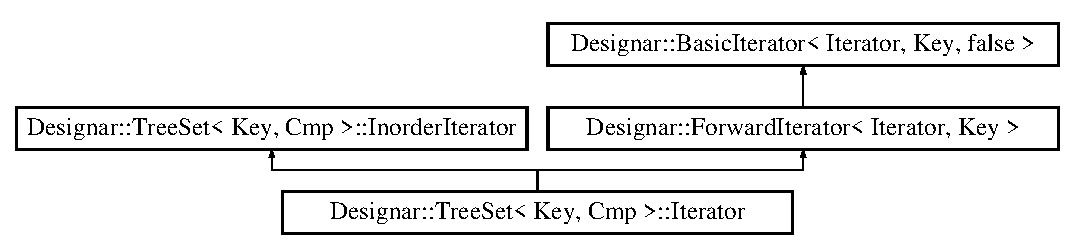
\includegraphics[height=2.916667cm]{class_designar_1_1_tree_set_1_1_iterator}
\end{center}
\end{figure}
\subsection*{Friends}
\begin{DoxyCompactItemize}
\item 
class \hyperlink{class_designar_1_1_tree_set_1_1_iterator_a7caa42294700d2a60905ec3458a7cd8a}{Tree\+Set}
\item 
class \hyperlink{class_designar_1_1_tree_set_1_1_iterator_a0b375a570add16b09037ce1773f0ddbb}{Basic\+Iterator$<$ Iterator, Key $>$}
\end{DoxyCompactItemize}
\subsection*{Additional Inherited Members}


\subsection{Detailed Description}
\subsubsection*{template$<$typename Key, class Cmp = std\+::less$<$\+Key$>$$>$\newline
class Designar\+::\+Tree\+Set$<$ Key, Cmp $>$\+::\+Iterator}



Definition at line 916 of file tree.\+H.



\subsection{Friends And Related Function Documentation}
\mbox{\Hypertarget{class_designar_1_1_tree_set_1_1_iterator_a0b375a570add16b09037ce1773f0ddbb}\label{class_designar_1_1_tree_set_1_1_iterator_a0b375a570add16b09037ce1773f0ddbb}} 
\index{Designar\+::\+Tree\+Set\+::\+Iterator@{Designar\+::\+Tree\+Set\+::\+Iterator}!Basic\+Iterator$<$ Iterator, Key $>$@{Basic\+Iterator$<$ Iterator, Key $>$}}
\index{Basic\+Iterator$<$ Iterator, Key $>$@{Basic\+Iterator$<$ Iterator, Key $>$}!Designar\+::\+Tree\+Set\+::\+Iterator@{Designar\+::\+Tree\+Set\+::\+Iterator}}
\subsubsection{\texorpdfstring{Basic\+Iterator$<$ Iterator, Key $>$}{BasicIterator< Iterator, Key >}}
{\footnotesize\ttfamily template$<$typename Key, class Cmp = std\+::less$<$\+Key$>$$>$ \\
friend class \hyperlink{class_designar_1_1_basic_iterator}{Basic\+Iterator}$<$ \hyperlink{class_designar_1_1_tree_set_1_1_iterator}{Iterator}, Key $>$\hspace{0.3cm}{\ttfamily [friend]}}



Definition at line 920 of file tree.\+H.

\mbox{\Hypertarget{class_designar_1_1_tree_set_1_1_iterator_a7caa42294700d2a60905ec3458a7cd8a}\label{class_designar_1_1_tree_set_1_1_iterator_a7caa42294700d2a60905ec3458a7cd8a}} 
\index{Designar\+::\+Tree\+Set\+::\+Iterator@{Designar\+::\+Tree\+Set\+::\+Iterator}!Tree\+Set@{Tree\+Set}}
\index{Tree\+Set@{Tree\+Set}!Designar\+::\+Tree\+Set\+::\+Iterator@{Designar\+::\+Tree\+Set\+::\+Iterator}}
\subsubsection{\texorpdfstring{Tree\+Set}{TreeSet}}
{\footnotesize\ttfamily template$<$typename Key, class Cmp = std\+::less$<$\+Key$>$$>$ \\
friend class \hyperlink{class_designar_1_1_tree_set}{Tree\+Set}\hspace{0.3cm}{\ttfamily [friend]}}



Definition at line 919 of file tree.\+H.



The documentation for this class was generated from the following file\+:\begin{DoxyCompactItemize}
\item 
/home/julio/\+De\+S\+I\+G\+N\+A\+R-\/doc/\+De\+Si\+G\+N\+A\+R/include/\hyperlink{tree_8_h}{tree.\+H}\end{DoxyCompactItemize}

\hypertarget{class_designar_1_1_dyn_array_1_1_iterator}{}\section{Designar\+:\+:Dyn\+Array$<$ T $>$\+:\+:Iterator Class Reference}
\label{class_designar_1_1_dyn_array_1_1_iterator}\index{Designar\+::\+Dyn\+Array$<$ T $>$\+::\+Iterator@{Designar\+::\+Dyn\+Array$<$ T $>$\+::\+Iterator}}


{\ttfamily \#include $<$array.\+H$>$}

Inheritance diagram for Designar\+:\+:Dyn\+Array$<$ T $>$\+:\+:Iterator\+:\begin{figure}[H]
\begin{center}
\leavevmode
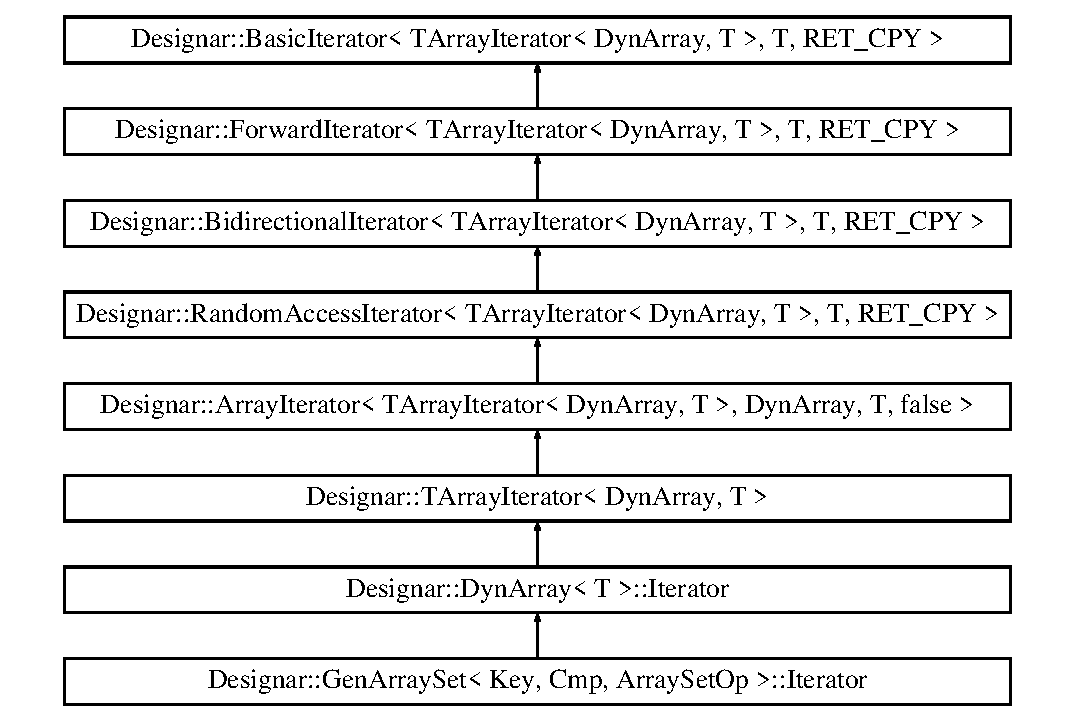
\includegraphics[height=8.000000cm]{class_designar_1_1_dyn_array_1_1_iterator}
\end{center}
\end{figure}
\subsection*{Public Member Functions}
\begin{DoxyCompactItemize}
\item 
T \hyperlink{class_designar_1_1_dyn_array_1_1_iterator_a3d700006f23d3c4b63e109edef32410f}{del} ()
\end{DoxyCompactItemize}
\subsection*{Additional Inherited Members}


\subsection{Detailed Description}
\subsubsection*{template$<$typename T$>$\newline
class Designar\+::\+Dyn\+Array$<$ T $>$\+::\+Iterator}



Definition at line 960 of file array.\+H.



\subsection{Member Function Documentation}
\mbox{\Hypertarget{class_designar_1_1_dyn_array_1_1_iterator_a3d700006f23d3c4b63e109edef32410f}\label{class_designar_1_1_dyn_array_1_1_iterator_a3d700006f23d3c4b63e109edef32410f}} 
\index{Designar\+::\+Dyn\+Array\+::\+Iterator@{Designar\+::\+Dyn\+Array\+::\+Iterator}!del@{del}}
\index{del@{del}!Designar\+::\+Dyn\+Array\+::\+Iterator@{Designar\+::\+Dyn\+Array\+::\+Iterator}}
\subsubsection{\texorpdfstring{del()}{del()}}
{\footnotesize\ttfamily template$<$typename T$>$ \\
T \hyperlink{class_designar_1_1_dyn_array}{Designar\+::\+Dyn\+Array}$<$ T $>$\+::Iterator\+::del (\begin{DoxyParamCaption}{ }\end{DoxyParamCaption})\hspace{0.3cm}{\ttfamily [inline]}}



Definition at line 966 of file array.\+H.



The documentation for this class was generated from the following file\+:\begin{DoxyCompactItemize}
\item 
De\+Si\+G\+N\+A\+R/include/\hyperlink{array_8_h}{array.\+H}\end{DoxyCompactItemize}

\hypertarget{class_designar_1_1_s_l_list_1_1_iterator}{}\section{Designar\+:\+:S\+L\+List$<$ T $>$\+:\+:Iterator Class Reference}
\label{class_designar_1_1_s_l_list_1_1_iterator}\index{Designar\+::\+S\+L\+List$<$ T $>$\+::\+Iterator@{Designar\+::\+S\+L\+List$<$ T $>$\+::\+Iterator}}


{\ttfamily \#include $<$list.\+H$>$}

Inheritance diagram for Designar\+:\+:S\+L\+List$<$ T $>$\+:\+:Iterator\+:\begin{figure}[H]
\begin{center}
\leavevmode
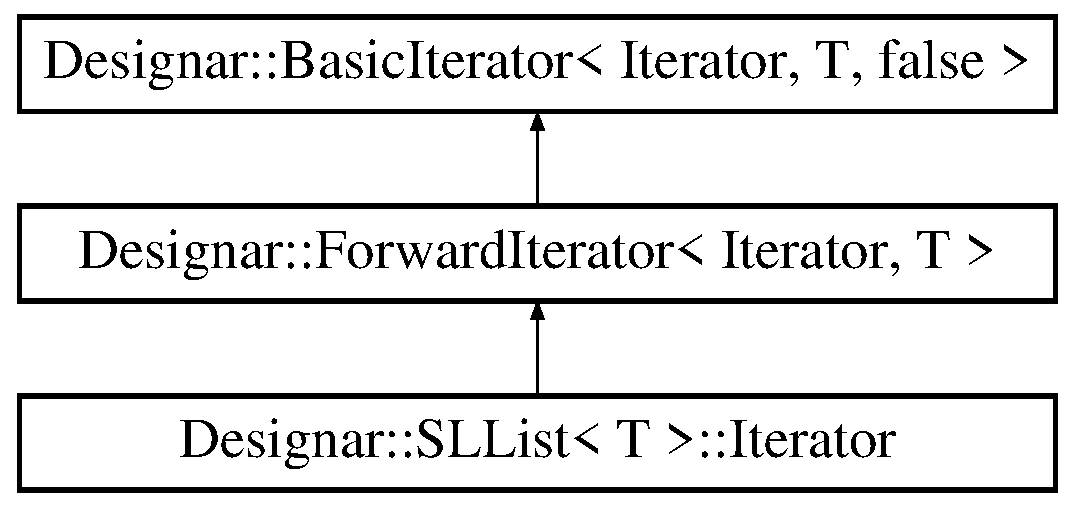
\includegraphics[height=3.000000cm]{class_designar_1_1_s_l_list_1_1_iterator}
\end{center}
\end{figure}
\subsection*{Public Member Functions}
\begin{DoxyCompactItemize}
\item 
\hyperlink{class_designar_1_1_s_l_list_1_1_iterator_a8c1c1f8110e22d81401e404c53003156}{Iterator} ()
\item 
\hyperlink{class_designar_1_1_s_l_list_1_1_iterator_a280b63ef5b720adb076806270cd9e8ec}{Iterator} (const \hyperlink{class_designar_1_1_s_l_list}{S\+L\+List}$<$ T $>$ \&l)
\item 
\hyperlink{class_designar_1_1_s_l_list_1_1_iterator_a56a2a893f109ea2158b183c3efaff8a3}{Iterator} (const \hyperlink{class_designar_1_1_s_l_list}{S\+L\+List}$<$ T $>$ \&l, \hyperlink{class_designar_1_1_node_s_l_list_a41963019ada1025099e3259207a3de96}{Node} $\ast$c)
\item 
\hyperlink{class_designar_1_1_s_l_list_1_1_iterator_ae6726c755567d34649157c075b825a20}{Iterator} (const \hyperlink{class_designar_1_1_s_l_list_1_1_iterator}{Iterator} \&it)
\item 
\hyperlink{class_designar_1_1_s_l_list_1_1_iterator_a2d8fece759af352a51982b4ffb25f351}{Iterator} (\hyperlink{class_designar_1_1_s_l_list_1_1_iterator}{Iterator} \&\&it)
\item 
\hyperlink{class_designar_1_1_s_l_list_1_1_iterator}{Iterator} \& \hyperlink{class_designar_1_1_s_l_list_1_1_iterator_ab6a8bedc6dc57d1255464d4ea942bdf5}{operator=} (const \hyperlink{class_designar_1_1_s_l_list_1_1_iterator}{Iterator} \&it)
\item 
\hyperlink{class_designar_1_1_s_l_list_1_1_iterator}{Iterator} \& \hyperlink{class_designar_1_1_s_l_list_1_1_iterator_a9215becbdd87b11db7f6481e96df9343}{operator=} (\hyperlink{class_designar_1_1_s_l_list_1_1_iterator}{Iterator} \&\&it)
\item 
void \hyperlink{class_designar_1_1_s_l_list_1_1_iterator_afbb40762fe2a3c8ecea8fb26751492e0}{swap} (\hyperlink{class_designar_1_1_s_l_list_1_1_iterator}{Iterator} \&it)
\item 
\hyperlink{namespace_designar_a9d113d66a39e82b73727c72cd3a52f73}{lint\+\_\+t} \hyperlink{class_designar_1_1_s_l_list_1_1_iterator_a2105a92f98b381c1dc9cdc138e96a22a}{get\+\_\+position} () const
\item 
bool \hyperlink{class_designar_1_1_s_l_list_1_1_iterator_ab245268535b61d073d615dc969bcaf5a}{has\+\_\+current} () const
\item 
T \& \hyperlink{class_designar_1_1_s_l_list_1_1_iterator_a4986f4352424c32e5518ce1435474f0b}{get\+\_\+current} ()
\item 
const T \& \hyperlink{class_designar_1_1_s_l_list_1_1_iterator_aa29dad95637eeaf662bcc3a8bb02d77a}{get\+\_\+current} () const
\item 
void \hyperlink{class_designar_1_1_s_l_list_1_1_iterator_a37eb6d2f01ce3e41785512742cab0fbc}{next} ()
\item 
void \hyperlink{class_designar_1_1_s_l_list_1_1_iterator_adb490da387d9628b7b61217247e96d97}{reset} ()
\item 
T \hyperlink{class_designar_1_1_s_l_list_1_1_iterator_ae9fc8898009213695804526b4fe8c2cb}{del} ()
\end{DoxyCompactItemize}
\subsection*{Protected Member Functions}
\begin{DoxyCompactItemize}
\item 
\hyperlink{class_designar_1_1_node_s_l_list_a41963019ada1025099e3259207a3de96}{Node} $\ast$ \hyperlink{class_designar_1_1_s_l_list_1_1_iterator_af994c3d4b1f178e55d8b68d3b7a515cf}{get\+\_\+location} () const
\end{DoxyCompactItemize}
\subsection*{Friends}
\begin{DoxyCompactItemize}
\item 
class \hyperlink{class_designar_1_1_s_l_list_1_1_iterator_ae3421d6be56b523bf3c41ceb29f3e5d7}{Basic\+Iterator$<$ Iterator, T $>$}
\end{DoxyCompactItemize}


\subsection{Detailed Description}
\subsubsection*{template$<$typename T$>$\newline
class Designar\+::\+S\+L\+List$<$ T $>$\+::\+Iterator}



Definition at line 354 of file list.\+H.



\subsection{Constructor \& Destructor Documentation}
\mbox{\Hypertarget{class_designar_1_1_s_l_list_1_1_iterator_a8c1c1f8110e22d81401e404c53003156}\label{class_designar_1_1_s_l_list_1_1_iterator_a8c1c1f8110e22d81401e404c53003156}} 
\index{Designar\+::\+S\+L\+List\+::\+Iterator@{Designar\+::\+S\+L\+List\+::\+Iterator}!Iterator@{Iterator}}
\index{Iterator@{Iterator}!Designar\+::\+S\+L\+List\+::\+Iterator@{Designar\+::\+S\+L\+List\+::\+Iterator}}
\subsubsection{\texorpdfstring{Iterator()}{Iterator()}\hspace{0.1cm}{\footnotesize\ttfamily [1/5]}}
{\footnotesize\ttfamily template$<$typename T$>$ \\
\hyperlink{class_designar_1_1_s_l_list}{Designar\+::\+S\+L\+List}$<$ T $>$\+::Iterator\+::\+Iterator (\begin{DoxyParamCaption}{ }\end{DoxyParamCaption})\hspace{0.3cm}{\ttfamily [inline]}}



Definition at line 373 of file list.\+H.

\mbox{\Hypertarget{class_designar_1_1_s_l_list_1_1_iterator_a280b63ef5b720adb076806270cd9e8ec}\label{class_designar_1_1_s_l_list_1_1_iterator_a280b63ef5b720adb076806270cd9e8ec}} 
\index{Designar\+::\+S\+L\+List\+::\+Iterator@{Designar\+::\+S\+L\+List\+::\+Iterator}!Iterator@{Iterator}}
\index{Iterator@{Iterator}!Designar\+::\+S\+L\+List\+::\+Iterator@{Designar\+::\+S\+L\+List\+::\+Iterator}}
\subsubsection{\texorpdfstring{Iterator()}{Iterator()}\hspace{0.1cm}{\footnotesize\ttfamily [2/5]}}
{\footnotesize\ttfamily template$<$typename T$>$ \\
\hyperlink{class_designar_1_1_s_l_list}{Designar\+::\+S\+L\+List}$<$ T $>$\+::Iterator\+::\+Iterator (\begin{DoxyParamCaption}\item[{const \hyperlink{class_designar_1_1_s_l_list}{S\+L\+List}$<$ T $>$ \&}]{l }\end{DoxyParamCaption})\hspace{0.3cm}{\ttfamily [inline]}}



Definition at line 379 of file list.\+H.

\mbox{\Hypertarget{class_designar_1_1_s_l_list_1_1_iterator_a56a2a893f109ea2158b183c3efaff8a3}\label{class_designar_1_1_s_l_list_1_1_iterator_a56a2a893f109ea2158b183c3efaff8a3}} 
\index{Designar\+::\+S\+L\+List\+::\+Iterator@{Designar\+::\+S\+L\+List\+::\+Iterator}!Iterator@{Iterator}}
\index{Iterator@{Iterator}!Designar\+::\+S\+L\+List\+::\+Iterator@{Designar\+::\+S\+L\+List\+::\+Iterator}}
\subsubsection{\texorpdfstring{Iterator()}{Iterator()}\hspace{0.1cm}{\footnotesize\ttfamily [3/5]}}
{\footnotesize\ttfamily template$<$typename T$>$ \\
\hyperlink{class_designar_1_1_s_l_list}{Designar\+::\+S\+L\+List}$<$ T $>$\+::Iterator\+::\+Iterator (\begin{DoxyParamCaption}\item[{const \hyperlink{class_designar_1_1_s_l_list}{S\+L\+List}$<$ T $>$ \&}]{l,  }\item[{\hyperlink{class_designar_1_1_node_s_l_list_a41963019ada1025099e3259207a3de96}{Node} $\ast$}]{c }\end{DoxyParamCaption})\hspace{0.3cm}{\ttfamily [inline]}}



Definition at line 386 of file list.\+H.

\mbox{\Hypertarget{class_designar_1_1_s_l_list_1_1_iterator_ae6726c755567d34649157c075b825a20}\label{class_designar_1_1_s_l_list_1_1_iterator_ae6726c755567d34649157c075b825a20}} 
\index{Designar\+::\+S\+L\+List\+::\+Iterator@{Designar\+::\+S\+L\+List\+::\+Iterator}!Iterator@{Iterator}}
\index{Iterator@{Iterator}!Designar\+::\+S\+L\+List\+::\+Iterator@{Designar\+::\+S\+L\+List\+::\+Iterator}}
\subsubsection{\texorpdfstring{Iterator()}{Iterator()}\hspace{0.1cm}{\footnotesize\ttfamily [4/5]}}
{\footnotesize\ttfamily template$<$typename T$>$ \\
\hyperlink{class_designar_1_1_s_l_list}{Designar\+::\+S\+L\+List}$<$ T $>$\+::Iterator\+::\+Iterator (\begin{DoxyParamCaption}\item[{const \hyperlink{class_designar_1_1_s_l_list_1_1_iterator}{Iterator} \&}]{it }\end{DoxyParamCaption})\hspace{0.3cm}{\ttfamily [inline]}}



Definition at line 392 of file list.\+H.

\mbox{\Hypertarget{class_designar_1_1_s_l_list_1_1_iterator_a2d8fece759af352a51982b4ffb25f351}\label{class_designar_1_1_s_l_list_1_1_iterator_a2d8fece759af352a51982b4ffb25f351}} 
\index{Designar\+::\+S\+L\+List\+::\+Iterator@{Designar\+::\+S\+L\+List\+::\+Iterator}!Iterator@{Iterator}}
\index{Iterator@{Iterator}!Designar\+::\+S\+L\+List\+::\+Iterator@{Designar\+::\+S\+L\+List\+::\+Iterator}}
\subsubsection{\texorpdfstring{Iterator()}{Iterator()}\hspace{0.1cm}{\footnotesize\ttfamily [5/5]}}
{\footnotesize\ttfamily template$<$typename T$>$ \\
\hyperlink{class_designar_1_1_s_l_list}{Designar\+::\+S\+L\+List}$<$ T $>$\+::Iterator\+::\+Iterator (\begin{DoxyParamCaption}\item[{\hyperlink{class_designar_1_1_s_l_list_1_1_iterator}{Iterator} \&\&}]{it }\end{DoxyParamCaption})\hspace{0.3cm}{\ttfamily [inline]}}



Definition at line 398 of file list.\+H.



\subsection{Member Function Documentation}
\mbox{\Hypertarget{class_designar_1_1_s_l_list_1_1_iterator_ae9fc8898009213695804526b4fe8c2cb}\label{class_designar_1_1_s_l_list_1_1_iterator_ae9fc8898009213695804526b4fe8c2cb}} 
\index{Designar\+::\+S\+L\+List\+::\+Iterator@{Designar\+::\+S\+L\+List\+::\+Iterator}!del@{del}}
\index{del@{del}!Designar\+::\+S\+L\+List\+::\+Iterator@{Designar\+::\+S\+L\+List\+::\+Iterator}}
\subsubsection{\texorpdfstring{del()}{del()}}
{\footnotesize\ttfamily template$<$typename T$>$ \\
T \hyperlink{class_designar_1_1_s_l_list}{Designar\+::\+S\+L\+List}$<$ T $>$\+::Iterator\+::del (\begin{DoxyParamCaption}{ }\end{DoxyParamCaption})\hspace{0.3cm}{\ttfamily [inline]}}



Definition at line 473 of file list.\+H.

\mbox{\Hypertarget{class_designar_1_1_s_l_list_1_1_iterator_a4986f4352424c32e5518ce1435474f0b}\label{class_designar_1_1_s_l_list_1_1_iterator_a4986f4352424c32e5518ce1435474f0b}} 
\index{Designar\+::\+S\+L\+List\+::\+Iterator@{Designar\+::\+S\+L\+List\+::\+Iterator}!get\+\_\+current@{get\+\_\+current}}
\index{get\+\_\+current@{get\+\_\+current}!Designar\+::\+S\+L\+List\+::\+Iterator@{Designar\+::\+S\+L\+List\+::\+Iterator}}
\subsubsection{\texorpdfstring{get\+\_\+current()}{get\_current()}\hspace{0.1cm}{\footnotesize\ttfamily [1/2]}}
{\footnotesize\ttfamily template$<$typename T$>$ \\
T\& \hyperlink{class_designar_1_1_s_l_list}{Designar\+::\+S\+L\+List}$<$ T $>$\+::Iterator\+::get\+\_\+current (\begin{DoxyParamCaption}{ }\end{DoxyParamCaption})\hspace{0.3cm}{\ttfamily [inline]}}



Definition at line 441 of file list.\+H.

\mbox{\Hypertarget{class_designar_1_1_s_l_list_1_1_iterator_aa29dad95637eeaf662bcc3a8bb02d77a}\label{class_designar_1_1_s_l_list_1_1_iterator_aa29dad95637eeaf662bcc3a8bb02d77a}} 
\index{Designar\+::\+S\+L\+List\+::\+Iterator@{Designar\+::\+S\+L\+List\+::\+Iterator}!get\+\_\+current@{get\+\_\+current}}
\index{get\+\_\+current@{get\+\_\+current}!Designar\+::\+S\+L\+List\+::\+Iterator@{Designar\+::\+S\+L\+List\+::\+Iterator}}
\subsubsection{\texorpdfstring{get\+\_\+current()}{get\_current()}\hspace{0.1cm}{\footnotesize\ttfamily [2/2]}}
{\footnotesize\ttfamily template$<$typename T$>$ \\
const T\& \hyperlink{class_designar_1_1_s_l_list}{Designar\+::\+S\+L\+List}$<$ T $>$\+::Iterator\+::get\+\_\+current (\begin{DoxyParamCaption}{ }\end{DoxyParamCaption}) const\hspace{0.3cm}{\ttfamily [inline]}}



Definition at line 449 of file list.\+H.

\mbox{\Hypertarget{class_designar_1_1_s_l_list_1_1_iterator_af994c3d4b1f178e55d8b68d3b7a515cf}\label{class_designar_1_1_s_l_list_1_1_iterator_af994c3d4b1f178e55d8b68d3b7a515cf}} 
\index{Designar\+::\+S\+L\+List\+::\+Iterator@{Designar\+::\+S\+L\+List\+::\+Iterator}!get\+\_\+location@{get\+\_\+location}}
\index{get\+\_\+location@{get\+\_\+location}!Designar\+::\+S\+L\+List\+::\+Iterator@{Designar\+::\+S\+L\+List\+::\+Iterator}}
\subsubsection{\texorpdfstring{get\+\_\+location()}{get\_location()}}
{\footnotesize\ttfamily template$<$typename T$>$ \\
\hyperlink{class_designar_1_1_node_s_l_list_a41963019ada1025099e3259207a3de96}{Node}$\ast$ \hyperlink{class_designar_1_1_s_l_list}{Designar\+::\+S\+L\+List}$<$ T $>$\+::Iterator\+::get\+\_\+location (\begin{DoxyParamCaption}{ }\end{DoxyParamCaption}) const\hspace{0.3cm}{\ttfamily [inline]}, {\ttfamily [protected]}}



Definition at line 367 of file list.\+H.

\mbox{\Hypertarget{class_designar_1_1_s_l_list_1_1_iterator_a2105a92f98b381c1dc9cdc138e96a22a}\label{class_designar_1_1_s_l_list_1_1_iterator_a2105a92f98b381c1dc9cdc138e96a22a}} 
\index{Designar\+::\+S\+L\+List\+::\+Iterator@{Designar\+::\+S\+L\+List\+::\+Iterator}!get\+\_\+position@{get\+\_\+position}}
\index{get\+\_\+position@{get\+\_\+position}!Designar\+::\+S\+L\+List\+::\+Iterator@{Designar\+::\+S\+L\+List\+::\+Iterator}}
\subsubsection{\texorpdfstring{get\+\_\+position()}{get\_position()}}
{\footnotesize\ttfamily template$<$typename T$>$ \\
\hyperlink{namespace_designar_a9d113d66a39e82b73727c72cd3a52f73}{lint\+\_\+t} \hyperlink{class_designar_1_1_s_l_list}{Designar\+::\+S\+L\+List}$<$ T $>$\+::Iterator\+::get\+\_\+position (\begin{DoxyParamCaption}{ }\end{DoxyParamCaption}) const\hspace{0.3cm}{\ttfamily [inline]}}



Definition at line 431 of file list.\+H.

\mbox{\Hypertarget{class_designar_1_1_s_l_list_1_1_iterator_ab245268535b61d073d615dc969bcaf5a}\label{class_designar_1_1_s_l_list_1_1_iterator_ab245268535b61d073d615dc969bcaf5a}} 
\index{Designar\+::\+S\+L\+List\+::\+Iterator@{Designar\+::\+S\+L\+List\+::\+Iterator}!has\+\_\+current@{has\+\_\+current}}
\index{has\+\_\+current@{has\+\_\+current}!Designar\+::\+S\+L\+List\+::\+Iterator@{Designar\+::\+S\+L\+List\+::\+Iterator}}
\subsubsection{\texorpdfstring{has\+\_\+current()}{has\_current()}}
{\footnotesize\ttfamily template$<$typename T$>$ \\
bool \hyperlink{class_designar_1_1_s_l_list}{Designar\+::\+S\+L\+List}$<$ T $>$\+::Iterator\+::has\+\_\+current (\begin{DoxyParamCaption}{ }\end{DoxyParamCaption}) const\hspace{0.3cm}{\ttfamily [inline]}}



Definition at line 436 of file list.\+H.

\mbox{\Hypertarget{class_designar_1_1_s_l_list_1_1_iterator_a37eb6d2f01ce3e41785512742cab0fbc}\label{class_designar_1_1_s_l_list_1_1_iterator_a37eb6d2f01ce3e41785512742cab0fbc}} 
\index{Designar\+::\+S\+L\+List\+::\+Iterator@{Designar\+::\+S\+L\+List\+::\+Iterator}!next@{next}}
\index{next@{next}!Designar\+::\+S\+L\+List\+::\+Iterator@{Designar\+::\+S\+L\+List\+::\+Iterator}}
\subsubsection{\texorpdfstring{next()}{next()}}
{\footnotesize\ttfamily template$<$typename T$>$ \\
void \hyperlink{class_designar_1_1_s_l_list}{Designar\+::\+S\+L\+List}$<$ T $>$\+::Iterator\+::next (\begin{DoxyParamCaption}{ }\end{DoxyParamCaption})\hspace{0.3cm}{\ttfamily [inline]}}



Definition at line 457 of file list.\+H.

\mbox{\Hypertarget{class_designar_1_1_s_l_list_1_1_iterator_ab6a8bedc6dc57d1255464d4ea942bdf5}\label{class_designar_1_1_s_l_list_1_1_iterator_ab6a8bedc6dc57d1255464d4ea942bdf5}} 
\index{Designar\+::\+S\+L\+List\+::\+Iterator@{Designar\+::\+S\+L\+List\+::\+Iterator}!operator=@{operator=}}
\index{operator=@{operator=}!Designar\+::\+S\+L\+List\+::\+Iterator@{Designar\+::\+S\+L\+List\+::\+Iterator}}
\subsubsection{\texorpdfstring{operator=()}{operator=()}\hspace{0.1cm}{\footnotesize\ttfamily [1/2]}}
{\footnotesize\ttfamily template$<$typename T$>$ \\
\hyperlink{class_designar_1_1_s_l_list_1_1_iterator}{Iterator}\& \hyperlink{class_designar_1_1_s_l_list}{Designar\+::\+S\+L\+List}$<$ T $>$\+::Iterator\+::operator= (\begin{DoxyParamCaption}\item[{const \hyperlink{class_designar_1_1_s_l_list_1_1_iterator}{Iterator} \&}]{it }\end{DoxyParamCaption})\hspace{0.3cm}{\ttfamily [inline]}}



Definition at line 404 of file list.\+H.

\mbox{\Hypertarget{class_designar_1_1_s_l_list_1_1_iterator_a9215becbdd87b11db7f6481e96df9343}\label{class_designar_1_1_s_l_list_1_1_iterator_a9215becbdd87b11db7f6481e96df9343}} 
\index{Designar\+::\+S\+L\+List\+::\+Iterator@{Designar\+::\+S\+L\+List\+::\+Iterator}!operator=@{operator=}}
\index{operator=@{operator=}!Designar\+::\+S\+L\+List\+::\+Iterator@{Designar\+::\+S\+L\+List\+::\+Iterator}}
\subsubsection{\texorpdfstring{operator=()}{operator=()}\hspace{0.1cm}{\footnotesize\ttfamily [2/2]}}
{\footnotesize\ttfamily template$<$typename T$>$ \\
\hyperlink{class_designar_1_1_s_l_list_1_1_iterator}{Iterator}\& \hyperlink{class_designar_1_1_s_l_list}{Designar\+::\+S\+L\+List}$<$ T $>$\+::Iterator\+::operator= (\begin{DoxyParamCaption}\item[{\hyperlink{class_designar_1_1_s_l_list_1_1_iterator}{Iterator} \&\&}]{it }\end{DoxyParamCaption})\hspace{0.3cm}{\ttfamily [inline]}}



Definition at line 417 of file list.\+H.

\mbox{\Hypertarget{class_designar_1_1_s_l_list_1_1_iterator_adb490da387d9628b7b61217247e96d97}\label{class_designar_1_1_s_l_list_1_1_iterator_adb490da387d9628b7b61217247e96d97}} 
\index{Designar\+::\+S\+L\+List\+::\+Iterator@{Designar\+::\+S\+L\+List\+::\+Iterator}!reset@{reset}}
\index{reset@{reset}!Designar\+::\+S\+L\+List\+::\+Iterator@{Designar\+::\+S\+L\+List\+::\+Iterator}}
\subsubsection{\texorpdfstring{reset()}{reset()}}
{\footnotesize\ttfamily template$<$typename T$>$ \\
void \hyperlink{class_designar_1_1_s_l_list}{Designar\+::\+S\+L\+List}$<$ T $>$\+::Iterator\+::reset (\begin{DoxyParamCaption}{ }\end{DoxyParamCaption})\hspace{0.3cm}{\ttfamily [inline]}}



Definition at line 467 of file list.\+H.

\mbox{\Hypertarget{class_designar_1_1_s_l_list_1_1_iterator_afbb40762fe2a3c8ecea8fb26751492e0}\label{class_designar_1_1_s_l_list_1_1_iterator_afbb40762fe2a3c8ecea8fb26751492e0}} 
\index{Designar\+::\+S\+L\+List\+::\+Iterator@{Designar\+::\+S\+L\+List\+::\+Iterator}!swap@{swap}}
\index{swap@{swap}!Designar\+::\+S\+L\+List\+::\+Iterator@{Designar\+::\+S\+L\+List\+::\+Iterator}}
\subsubsection{\texorpdfstring{swap()}{swap()}}
{\footnotesize\ttfamily template$<$typename T$>$ \\
void \hyperlink{class_designar_1_1_s_l_list}{Designar\+::\+S\+L\+List}$<$ T $>$\+::Iterator\+::swap (\begin{DoxyParamCaption}\item[{\hyperlink{class_designar_1_1_s_l_list_1_1_iterator}{Iterator} \&}]{it }\end{DoxyParamCaption})\hspace{0.3cm}{\ttfamily [inline]}}



Definition at line 423 of file list.\+H.



\subsection{Friends And Related Function Documentation}
\mbox{\Hypertarget{class_designar_1_1_s_l_list_1_1_iterator_ae3421d6be56b523bf3c41ceb29f3e5d7}\label{class_designar_1_1_s_l_list_1_1_iterator_ae3421d6be56b523bf3c41ceb29f3e5d7}} 
\index{Designar\+::\+S\+L\+List\+::\+Iterator@{Designar\+::\+S\+L\+List\+::\+Iterator}!Basic\+Iterator$<$ Iterator, T $>$@{Basic\+Iterator$<$ Iterator, T $>$}}
\index{Basic\+Iterator$<$ Iterator, T $>$@{Basic\+Iterator$<$ Iterator, T $>$}!Designar\+::\+S\+L\+List\+::\+Iterator@{Designar\+::\+S\+L\+List\+::\+Iterator}}
\subsubsection{\texorpdfstring{Basic\+Iterator$<$ Iterator, T $>$}{BasicIterator< Iterator, T >}}
{\footnotesize\ttfamily template$<$typename T$>$ \\
friend class \hyperlink{class_designar_1_1_basic_iterator}{Basic\+Iterator}$<$ \hyperlink{class_designar_1_1_s_l_list_1_1_iterator}{Iterator}, T $>$\hspace{0.3cm}{\ttfamily [friend]}}



Definition at line 356 of file list.\+H.



The documentation for this class was generated from the following file\+:\begin{DoxyCompactItemize}
\item 
include/\hyperlink{list_8_h}{list.\+H}\end{DoxyCompactItemize}

\hypertarget{class_designar_1_1_hash_set_1_1_iterator}{}\section{Designar\+:\+:Hash\+Set$<$ Key, Cmp $>$\+:\+:Iterator Class Reference}
\label{class_designar_1_1_hash_set_1_1_iterator}\index{Designar\+::\+Hash\+Set$<$ Key, Cmp $>$\+::\+Iterator@{Designar\+::\+Hash\+Set$<$ Key, Cmp $>$\+::\+Iterator}}


{\ttfamily \#include $<$hash.\+H$>$}

Inheritance diagram for Designar\+:\+:Hash\+Set$<$ Key, Cmp $>$\+:\+:Iterator\+:\begin{figure}[H]
\begin{center}
\leavevmode
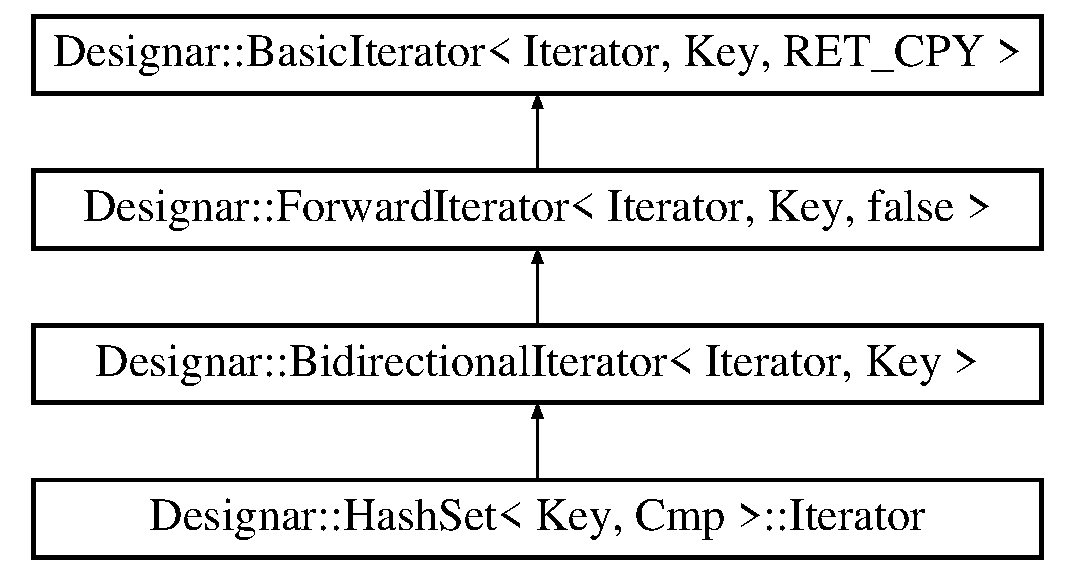
\includegraphics[height=4.000000cm]{class_designar_1_1_hash_set_1_1_iterator}
\end{center}
\end{figure}
\subsection*{Public Member Functions}
\begin{DoxyCompactItemize}
\item 
\hyperlink{class_designar_1_1_hash_set_1_1_iterator_a35f9b2ac54be788fa6c2b8a274c7e308}{Iterator} ()
\item 
\hyperlink{class_designar_1_1_hash_set_1_1_iterator_a1047f02ec4c3bfd5919ef66b28ca537c}{Iterator} (const \hyperlink{class_designar_1_1_hash_set}{Hash\+Set} \&h)
\item 
\hyperlink{class_designar_1_1_hash_set_1_1_iterator_addcd6728c590ea206dd13d9f0724bbcd}{Iterator} (const \hyperlink{class_designar_1_1_hash_set_1_1_iterator}{Iterator} \&it)
\item 
\hyperlink{class_designar_1_1_hash_set_1_1_iterator_a7adf1abf361e03423317b2e36eb76f1f}{Iterator} (\hyperlink{class_designar_1_1_hash_set_1_1_iterator}{Iterator} \&\&it)
\item 
\hyperlink{class_designar_1_1_hash_set_1_1_iterator}{Iterator} \& \hyperlink{class_designar_1_1_hash_set_1_1_iterator_a8e8fce4e60beb6933dd5d13b39d67493}{operator=} (const \hyperlink{class_designar_1_1_hash_set_1_1_iterator}{Iterator} \&it)
\item 
\hyperlink{class_designar_1_1_hash_set_1_1_iterator}{Iterator} \& \hyperlink{class_designar_1_1_hash_set_1_1_iterator_a5856c1a7f46a0c4e2899acff687fdf13}{operator=} (\hyperlink{class_designar_1_1_hash_set_1_1_iterator}{Iterator} \&\&it)
\item 
void \hyperlink{class_designar_1_1_hash_set_1_1_iterator_a5849b111320c33206baef1926cb3f156}{swap} (\hyperlink{class_designar_1_1_hash_set_1_1_iterator}{Iterator} \&it)
\item 
void \hyperlink{class_designar_1_1_hash_set_1_1_iterator_a4563f0da2eaf8dc2b4879cc959f7c277}{reset} ()
\item 
\hyperlink{namespace_designar_a9d113d66a39e82b73727c72cd3a52f73}{lint\+\_\+t} \hyperlink{class_designar_1_1_hash_set_1_1_iterator_a12b236661945aa10228f0523b6e1ab5e}{get\+\_\+position} () const
\item 
bool \hyperlink{class_designar_1_1_hash_set_1_1_iterator_a13dc6ab67d6d4a380e2f1cb4fd6d3ae2}{has\+\_\+current} () const
\item 
Key \& \hyperlink{class_designar_1_1_hash_set_1_1_iterator_af954a7cf3f23fecf898b86030e808224}{get\+\_\+current} ()
\item 
const Key \& \hyperlink{class_designar_1_1_hash_set_1_1_iterator_aed6b09996733067a2aa5e48b702ba9a2}{get\+\_\+current} () const
\item 
void \hyperlink{class_designar_1_1_hash_set_1_1_iterator_a13eaec913faa009d4d002c25965d67d7}{next} ()
\item 
void \hyperlink{class_designar_1_1_hash_set_1_1_iterator_a678b8d6f21627b05cbde7d11da64a010}{prev} ()
\end{DoxyCompactItemize}
\subsection*{Protected Member Functions}
\begin{DoxyCompactItemize}
\item 
\hyperlink{namespace_designar_a9d113d66a39e82b73727c72cd3a52f73}{lint\+\_\+t} \hyperlink{class_designar_1_1_hash_set_1_1_iterator_a8616bd592e20ebadab10de5c78a56eda}{get\+\_\+location} () const
\item 
\hyperlink{class_designar_1_1_hash_set_1_1_iterator_ae349523995246685946ec860e2705221}{Iterator} (const \hyperlink{class_designar_1_1_hash_set}{Hash\+Set} \&h, int)
\end{DoxyCompactItemize}
\subsection*{Friends}
\begin{DoxyCompactItemize}
\item 
class \hyperlink{class_designar_1_1_hash_set_1_1_iterator_ac5220f06200dc3b0d55d050a940f17b9}{Hash\+Set}
\item 
class \hyperlink{class_designar_1_1_hash_set_1_1_iterator_a0b375a570add16b09037ce1773f0ddbb}{Basic\+Iterator$<$ Iterator, Key $>$}
\end{DoxyCompactItemize}


\subsection{Detailed Description}
\subsubsection*{template$<$typename Key, class Cmp = std\+::equal\+\_\+to$<$\+Key$>$$>$\newline
class Designar\+::\+Hash\+Set$<$ Key, Cmp $>$\+::\+Iterator}



Definition at line 482 of file hash.\+H.



\subsection{Constructor \& Destructor Documentation}
\mbox{\Hypertarget{class_designar_1_1_hash_set_1_1_iterator_ae349523995246685946ec860e2705221}\label{class_designar_1_1_hash_set_1_1_iterator_ae349523995246685946ec860e2705221}} 
\index{Designar\+::\+Hash\+Set\+::\+Iterator@{Designar\+::\+Hash\+Set\+::\+Iterator}!Iterator@{Iterator}}
\index{Iterator@{Iterator}!Designar\+::\+Hash\+Set\+::\+Iterator@{Designar\+::\+Hash\+Set\+::\+Iterator}}
\subsubsection{\texorpdfstring{Iterator()}{Iterator()}\hspace{0.1cm}{\footnotesize\ttfamily [1/5]}}
{\footnotesize\ttfamily template$<$typename Key, class Cmp = std\+::equal\+\_\+to$<$\+Key$>$$>$ \\
\hyperlink{class_designar_1_1_hash_set}{Designar\+::\+Hash\+Set}$<$ Key, Cmp $>$\+::Iterator\+::\+Iterator (\begin{DoxyParamCaption}\item[{const \hyperlink{class_designar_1_1_hash_set}{Hash\+Set} \&}]{h,  }\item[{int}]{ }\end{DoxyParamCaption})\hspace{0.3cm}{\ttfamily [inline]}, {\ttfamily [protected]}}



Definition at line 504 of file hash.\+H.

\mbox{\Hypertarget{class_designar_1_1_hash_set_1_1_iterator_a35f9b2ac54be788fa6c2b8a274c7e308}\label{class_designar_1_1_hash_set_1_1_iterator_a35f9b2ac54be788fa6c2b8a274c7e308}} 
\index{Designar\+::\+Hash\+Set\+::\+Iterator@{Designar\+::\+Hash\+Set\+::\+Iterator}!Iterator@{Iterator}}
\index{Iterator@{Iterator}!Designar\+::\+Hash\+Set\+::\+Iterator@{Designar\+::\+Hash\+Set\+::\+Iterator}}
\subsubsection{\texorpdfstring{Iterator()}{Iterator()}\hspace{0.1cm}{\footnotesize\ttfamily [2/5]}}
{\footnotesize\ttfamily template$<$typename Key, class Cmp = std\+::equal\+\_\+to$<$\+Key$>$$>$ \\
\hyperlink{class_designar_1_1_hash_set}{Designar\+::\+Hash\+Set}$<$ Key, Cmp $>$\+::Iterator\+::\+Iterator (\begin{DoxyParamCaption}{ }\end{DoxyParamCaption})\hspace{0.3cm}{\ttfamily [inline]}}



Definition at line 512 of file hash.\+H.

\mbox{\Hypertarget{class_designar_1_1_hash_set_1_1_iterator_a1047f02ec4c3bfd5919ef66b28ca537c}\label{class_designar_1_1_hash_set_1_1_iterator_a1047f02ec4c3bfd5919ef66b28ca537c}} 
\index{Designar\+::\+Hash\+Set\+::\+Iterator@{Designar\+::\+Hash\+Set\+::\+Iterator}!Iterator@{Iterator}}
\index{Iterator@{Iterator}!Designar\+::\+Hash\+Set\+::\+Iterator@{Designar\+::\+Hash\+Set\+::\+Iterator}}
\subsubsection{\texorpdfstring{Iterator()}{Iterator()}\hspace{0.1cm}{\footnotesize\ttfamily [3/5]}}
{\footnotesize\ttfamily template$<$typename Key, class Cmp = std\+::equal\+\_\+to$<$\+Key$>$$>$ \\
\hyperlink{class_designar_1_1_hash_set}{Designar\+::\+Hash\+Set}$<$ Key, Cmp $>$\+::Iterator\+::\+Iterator (\begin{DoxyParamCaption}\item[{const \hyperlink{class_designar_1_1_hash_set}{Hash\+Set} \&}]{h }\end{DoxyParamCaption})\hspace{0.3cm}{\ttfamily [inline]}}



Definition at line 518 of file hash.\+H.

\mbox{\Hypertarget{class_designar_1_1_hash_set_1_1_iterator_addcd6728c590ea206dd13d9f0724bbcd}\label{class_designar_1_1_hash_set_1_1_iterator_addcd6728c590ea206dd13d9f0724bbcd}} 
\index{Designar\+::\+Hash\+Set\+::\+Iterator@{Designar\+::\+Hash\+Set\+::\+Iterator}!Iterator@{Iterator}}
\index{Iterator@{Iterator}!Designar\+::\+Hash\+Set\+::\+Iterator@{Designar\+::\+Hash\+Set\+::\+Iterator}}
\subsubsection{\texorpdfstring{Iterator()}{Iterator()}\hspace{0.1cm}{\footnotesize\ttfamily [4/5]}}
{\footnotesize\ttfamily template$<$typename Key, class Cmp = std\+::equal\+\_\+to$<$\+Key$>$$>$ \\
\hyperlink{class_designar_1_1_hash_set}{Designar\+::\+Hash\+Set}$<$ Key, Cmp $>$\+::Iterator\+::\+Iterator (\begin{DoxyParamCaption}\item[{const \hyperlink{class_designar_1_1_hash_set_1_1_iterator}{Iterator} \&}]{it }\end{DoxyParamCaption})\hspace{0.3cm}{\ttfamily [inline]}}



Definition at line 524 of file hash.\+H.

\mbox{\Hypertarget{class_designar_1_1_hash_set_1_1_iterator_a7adf1abf361e03423317b2e36eb76f1f}\label{class_designar_1_1_hash_set_1_1_iterator_a7adf1abf361e03423317b2e36eb76f1f}} 
\index{Designar\+::\+Hash\+Set\+::\+Iterator@{Designar\+::\+Hash\+Set\+::\+Iterator}!Iterator@{Iterator}}
\index{Iterator@{Iterator}!Designar\+::\+Hash\+Set\+::\+Iterator@{Designar\+::\+Hash\+Set\+::\+Iterator}}
\subsubsection{\texorpdfstring{Iterator()}{Iterator()}\hspace{0.1cm}{\footnotesize\ttfamily [5/5]}}
{\footnotesize\ttfamily template$<$typename Key, class Cmp = std\+::equal\+\_\+to$<$\+Key$>$$>$ \\
\hyperlink{class_designar_1_1_hash_set}{Designar\+::\+Hash\+Set}$<$ Key, Cmp $>$\+::Iterator\+::\+Iterator (\begin{DoxyParamCaption}\item[{\hyperlink{class_designar_1_1_hash_set_1_1_iterator}{Iterator} \&\&}]{it }\end{DoxyParamCaption})\hspace{0.3cm}{\ttfamily [inline]}}



Definition at line 531 of file hash.\+H.



\subsection{Member Function Documentation}
\mbox{\Hypertarget{class_designar_1_1_hash_set_1_1_iterator_af954a7cf3f23fecf898b86030e808224}\label{class_designar_1_1_hash_set_1_1_iterator_af954a7cf3f23fecf898b86030e808224}} 
\index{Designar\+::\+Hash\+Set\+::\+Iterator@{Designar\+::\+Hash\+Set\+::\+Iterator}!get\+\_\+current@{get\+\_\+current}}
\index{get\+\_\+current@{get\+\_\+current}!Designar\+::\+Hash\+Set\+::\+Iterator@{Designar\+::\+Hash\+Set\+::\+Iterator}}
\subsubsection{\texorpdfstring{get\+\_\+current()}{get\_current()}\hspace{0.1cm}{\footnotesize\ttfamily [1/2]}}
{\footnotesize\ttfamily template$<$typename Key, class Cmp = std\+::equal\+\_\+to$<$\+Key$>$$>$ \\
Key\& \hyperlink{class_designar_1_1_hash_set}{Designar\+::\+Hash\+Set}$<$ Key, Cmp $>$\+::Iterator\+::get\+\_\+current (\begin{DoxyParamCaption}{ }\end{DoxyParamCaption})\hspace{0.3cm}{\ttfamily [inline]}}



Definition at line 580 of file hash.\+H.

\mbox{\Hypertarget{class_designar_1_1_hash_set_1_1_iterator_aed6b09996733067a2aa5e48b702ba9a2}\label{class_designar_1_1_hash_set_1_1_iterator_aed6b09996733067a2aa5e48b702ba9a2}} 
\index{Designar\+::\+Hash\+Set\+::\+Iterator@{Designar\+::\+Hash\+Set\+::\+Iterator}!get\+\_\+current@{get\+\_\+current}}
\index{get\+\_\+current@{get\+\_\+current}!Designar\+::\+Hash\+Set\+::\+Iterator@{Designar\+::\+Hash\+Set\+::\+Iterator}}
\subsubsection{\texorpdfstring{get\+\_\+current()}{get\_current()}\hspace{0.1cm}{\footnotesize\ttfamily [2/2]}}
{\footnotesize\ttfamily template$<$typename Key, class Cmp = std\+::equal\+\_\+to$<$\+Key$>$$>$ \\
const Key\& \hyperlink{class_designar_1_1_hash_set}{Designar\+::\+Hash\+Set}$<$ Key, Cmp $>$\+::Iterator\+::get\+\_\+current (\begin{DoxyParamCaption}{ }\end{DoxyParamCaption}) const\hspace{0.3cm}{\ttfamily [inline]}}



Definition at line 588 of file hash.\+H.

\mbox{\Hypertarget{class_designar_1_1_hash_set_1_1_iterator_a8616bd592e20ebadab10de5c78a56eda}\label{class_designar_1_1_hash_set_1_1_iterator_a8616bd592e20ebadab10de5c78a56eda}} 
\index{Designar\+::\+Hash\+Set\+::\+Iterator@{Designar\+::\+Hash\+Set\+::\+Iterator}!get\+\_\+location@{get\+\_\+location}}
\index{get\+\_\+location@{get\+\_\+location}!Designar\+::\+Hash\+Set\+::\+Iterator@{Designar\+::\+Hash\+Set\+::\+Iterator}}
\subsubsection{\texorpdfstring{get\+\_\+location()}{get\_location()}}
{\footnotesize\ttfamily template$<$typename Key, class Cmp = std\+::equal\+\_\+to$<$\+Key$>$$>$ \\
\hyperlink{namespace_designar_a9d113d66a39e82b73727c72cd3a52f73}{lint\+\_\+t} \hyperlink{class_designar_1_1_hash_set}{Designar\+::\+Hash\+Set}$<$ Key, Cmp $>$\+::Iterator\+::get\+\_\+location (\begin{DoxyParamCaption}{ }\end{DoxyParamCaption}) const\hspace{0.3cm}{\ttfamily [inline]}, {\ttfamily [protected]}}



Definition at line 499 of file hash.\+H.

\mbox{\Hypertarget{class_designar_1_1_hash_set_1_1_iterator_a12b236661945aa10228f0523b6e1ab5e}\label{class_designar_1_1_hash_set_1_1_iterator_a12b236661945aa10228f0523b6e1ab5e}} 
\index{Designar\+::\+Hash\+Set\+::\+Iterator@{Designar\+::\+Hash\+Set\+::\+Iterator}!get\+\_\+position@{get\+\_\+position}}
\index{get\+\_\+position@{get\+\_\+position}!Designar\+::\+Hash\+Set\+::\+Iterator@{Designar\+::\+Hash\+Set\+::\+Iterator}}
\subsubsection{\texorpdfstring{get\+\_\+position()}{get\_position()}}
{\footnotesize\ttfamily template$<$typename Key, class Cmp = std\+::equal\+\_\+to$<$\+Key$>$$>$ \\
\hyperlink{namespace_designar_a9d113d66a39e82b73727c72cd3a52f73}{lint\+\_\+t} \hyperlink{class_designar_1_1_hash_set}{Designar\+::\+Hash\+Set}$<$ Key, Cmp $>$\+::Iterator\+::get\+\_\+position (\begin{DoxyParamCaption}{ }\end{DoxyParamCaption}) const\hspace{0.3cm}{\ttfamily [inline]}}



Definition at line 570 of file hash.\+H.

\mbox{\Hypertarget{class_designar_1_1_hash_set_1_1_iterator_a13dc6ab67d6d4a380e2f1cb4fd6d3ae2}\label{class_designar_1_1_hash_set_1_1_iterator_a13dc6ab67d6d4a380e2f1cb4fd6d3ae2}} 
\index{Designar\+::\+Hash\+Set\+::\+Iterator@{Designar\+::\+Hash\+Set\+::\+Iterator}!has\+\_\+current@{has\+\_\+current}}
\index{has\+\_\+current@{has\+\_\+current}!Designar\+::\+Hash\+Set\+::\+Iterator@{Designar\+::\+Hash\+Set\+::\+Iterator}}
\subsubsection{\texorpdfstring{has\+\_\+current()}{has\_current()}}
{\footnotesize\ttfamily template$<$typename Key, class Cmp = std\+::equal\+\_\+to$<$\+Key$>$$>$ \\
bool \hyperlink{class_designar_1_1_hash_set}{Designar\+::\+Hash\+Set}$<$ Key, Cmp $>$\+::Iterator\+::has\+\_\+current (\begin{DoxyParamCaption}{ }\end{DoxyParamCaption}) const\hspace{0.3cm}{\ttfamily [inline]}}



Definition at line 575 of file hash.\+H.

\mbox{\Hypertarget{class_designar_1_1_hash_set_1_1_iterator_a13eaec913faa009d4d002c25965d67d7}\label{class_designar_1_1_hash_set_1_1_iterator_a13eaec913faa009d4d002c25965d67d7}} 
\index{Designar\+::\+Hash\+Set\+::\+Iterator@{Designar\+::\+Hash\+Set\+::\+Iterator}!next@{next}}
\index{next@{next}!Designar\+::\+Hash\+Set\+::\+Iterator@{Designar\+::\+Hash\+Set\+::\+Iterator}}
\subsubsection{\texorpdfstring{next()}{next()}}
{\footnotesize\ttfamily template$<$typename Key, class Cmp = std\+::equal\+\_\+to$<$\+Key$>$$>$ \\
void \hyperlink{class_designar_1_1_hash_set}{Designar\+::\+Hash\+Set}$<$ Key, Cmp $>$\+::Iterator\+::next (\begin{DoxyParamCaption}{ }\end{DoxyParamCaption})\hspace{0.3cm}{\ttfamily [inline]}}



Definition at line 596 of file hash.\+H.

\mbox{\Hypertarget{class_designar_1_1_hash_set_1_1_iterator_a8e8fce4e60beb6933dd5d13b39d67493}\label{class_designar_1_1_hash_set_1_1_iterator_a8e8fce4e60beb6933dd5d13b39d67493}} 
\index{Designar\+::\+Hash\+Set\+::\+Iterator@{Designar\+::\+Hash\+Set\+::\+Iterator}!operator=@{operator=}}
\index{operator=@{operator=}!Designar\+::\+Hash\+Set\+::\+Iterator@{Designar\+::\+Hash\+Set\+::\+Iterator}}
\subsubsection{\texorpdfstring{operator=()}{operator=()}\hspace{0.1cm}{\footnotesize\ttfamily [1/2]}}
{\footnotesize\ttfamily template$<$typename Key, class Cmp = std\+::equal\+\_\+to$<$\+Key$>$$>$ \\
\hyperlink{class_designar_1_1_hash_set_1_1_iterator}{Iterator}\& \hyperlink{class_designar_1_1_hash_set}{Designar\+::\+Hash\+Set}$<$ Key, Cmp $>$\+::Iterator\+::operator= (\begin{DoxyParamCaption}\item[{const \hyperlink{class_designar_1_1_hash_set_1_1_iterator}{Iterator} \&}]{it }\end{DoxyParamCaption})\hspace{0.3cm}{\ttfamily [inline]}}



Definition at line 537 of file hash.\+H.

\mbox{\Hypertarget{class_designar_1_1_hash_set_1_1_iterator_a5856c1a7f46a0c4e2899acff687fdf13}\label{class_designar_1_1_hash_set_1_1_iterator_a5856c1a7f46a0c4e2899acff687fdf13}} 
\index{Designar\+::\+Hash\+Set\+::\+Iterator@{Designar\+::\+Hash\+Set\+::\+Iterator}!operator=@{operator=}}
\index{operator=@{operator=}!Designar\+::\+Hash\+Set\+::\+Iterator@{Designar\+::\+Hash\+Set\+::\+Iterator}}
\subsubsection{\texorpdfstring{operator=()}{operator=()}\hspace{0.1cm}{\footnotesize\ttfamily [2/2]}}
{\footnotesize\ttfamily template$<$typename Key, class Cmp = std\+::equal\+\_\+to$<$\+Key$>$$>$ \\
\hyperlink{class_designar_1_1_hash_set_1_1_iterator}{Iterator}\& \hyperlink{class_designar_1_1_hash_set}{Designar\+::\+Hash\+Set}$<$ Key, Cmp $>$\+::Iterator\+::operator= (\begin{DoxyParamCaption}\item[{\hyperlink{class_designar_1_1_hash_set_1_1_iterator}{Iterator} \&\&}]{it }\end{DoxyParamCaption})\hspace{0.3cm}{\ttfamily [inline]}}



Definition at line 550 of file hash.\+H.

\mbox{\Hypertarget{class_designar_1_1_hash_set_1_1_iterator_a678b8d6f21627b05cbde7d11da64a010}\label{class_designar_1_1_hash_set_1_1_iterator_a678b8d6f21627b05cbde7d11da64a010}} 
\index{Designar\+::\+Hash\+Set\+::\+Iterator@{Designar\+::\+Hash\+Set\+::\+Iterator}!prev@{prev}}
\index{prev@{prev}!Designar\+::\+Hash\+Set\+::\+Iterator@{Designar\+::\+Hash\+Set\+::\+Iterator}}
\subsubsection{\texorpdfstring{prev()}{prev()}}
{\footnotesize\ttfamily template$<$typename Key, class Cmp = std\+::equal\+\_\+to$<$\+Key$>$$>$ \\
void \hyperlink{class_designar_1_1_hash_set}{Designar\+::\+Hash\+Set}$<$ Key, Cmp $>$\+::Iterator\+::prev (\begin{DoxyParamCaption}{ }\end{DoxyParamCaption})\hspace{0.3cm}{\ttfamily [inline]}}



Definition at line 609 of file hash.\+H.

\mbox{\Hypertarget{class_designar_1_1_hash_set_1_1_iterator_a4563f0da2eaf8dc2b4879cc959f7c277}\label{class_designar_1_1_hash_set_1_1_iterator_a4563f0da2eaf8dc2b4879cc959f7c277}} 
\index{Designar\+::\+Hash\+Set\+::\+Iterator@{Designar\+::\+Hash\+Set\+::\+Iterator}!reset@{reset}}
\index{reset@{reset}!Designar\+::\+Hash\+Set\+::\+Iterator@{Designar\+::\+Hash\+Set\+::\+Iterator}}
\subsubsection{\texorpdfstring{reset()}{reset()}}
{\footnotesize\ttfamily template$<$typename Key, class Cmp = std\+::equal\+\_\+to$<$\+Key$>$$>$ \\
void \hyperlink{class_designar_1_1_hash_set}{Designar\+::\+Hash\+Set}$<$ Key, Cmp $>$\+::Iterator\+::reset (\begin{DoxyParamCaption}{ }\end{DoxyParamCaption})\hspace{0.3cm}{\ttfamily [inline]}}



Definition at line 564 of file hash.\+H.

\mbox{\Hypertarget{class_designar_1_1_hash_set_1_1_iterator_a5849b111320c33206baef1926cb3f156}\label{class_designar_1_1_hash_set_1_1_iterator_a5849b111320c33206baef1926cb3f156}} 
\index{Designar\+::\+Hash\+Set\+::\+Iterator@{Designar\+::\+Hash\+Set\+::\+Iterator}!swap@{swap}}
\index{swap@{swap}!Designar\+::\+Hash\+Set\+::\+Iterator@{Designar\+::\+Hash\+Set\+::\+Iterator}}
\subsubsection{\texorpdfstring{swap()}{swap()}}
{\footnotesize\ttfamily template$<$typename Key, class Cmp = std\+::equal\+\_\+to$<$\+Key$>$$>$ \\
void \hyperlink{class_designar_1_1_hash_set}{Designar\+::\+Hash\+Set}$<$ Key, Cmp $>$\+::Iterator\+::swap (\begin{DoxyParamCaption}\item[{\hyperlink{class_designar_1_1_hash_set_1_1_iterator}{Iterator} \&}]{it }\end{DoxyParamCaption})\hspace{0.3cm}{\ttfamily [inline]}}



Definition at line 556 of file hash.\+H.



\subsection{Friends And Related Function Documentation}
\mbox{\Hypertarget{class_designar_1_1_hash_set_1_1_iterator_a0b375a570add16b09037ce1773f0ddbb}\label{class_designar_1_1_hash_set_1_1_iterator_a0b375a570add16b09037ce1773f0ddbb}} 
\index{Designar\+::\+Hash\+Set\+::\+Iterator@{Designar\+::\+Hash\+Set\+::\+Iterator}!Basic\+Iterator$<$ Iterator, Key $>$@{Basic\+Iterator$<$ Iterator, Key $>$}}
\index{Basic\+Iterator$<$ Iterator, Key $>$@{Basic\+Iterator$<$ Iterator, Key $>$}!Designar\+::\+Hash\+Set\+::\+Iterator@{Designar\+::\+Hash\+Set\+::\+Iterator}}
\subsubsection{\texorpdfstring{Basic\+Iterator$<$ Iterator, Key $>$}{BasicIterator< Iterator, Key >}}
{\footnotesize\ttfamily template$<$typename Key, class Cmp = std\+::equal\+\_\+to$<$\+Key$>$$>$ \\
friend class \hyperlink{class_designar_1_1_basic_iterator}{Basic\+Iterator}$<$ \hyperlink{class_designar_1_1_hash_set_1_1_iterator}{Iterator}, Key $>$\hspace{0.3cm}{\ttfamily [friend]}}



Definition at line 485 of file hash.\+H.

\mbox{\Hypertarget{class_designar_1_1_hash_set_1_1_iterator_ac5220f06200dc3b0d55d050a940f17b9}\label{class_designar_1_1_hash_set_1_1_iterator_ac5220f06200dc3b0d55d050a940f17b9}} 
\index{Designar\+::\+Hash\+Set\+::\+Iterator@{Designar\+::\+Hash\+Set\+::\+Iterator}!Hash\+Set@{Hash\+Set}}
\index{Hash\+Set@{Hash\+Set}!Designar\+::\+Hash\+Set\+::\+Iterator@{Designar\+::\+Hash\+Set\+::\+Iterator}}
\subsubsection{\texorpdfstring{Hash\+Set}{HashSet}}
{\footnotesize\ttfamily template$<$typename Key, class Cmp = std\+::equal\+\_\+to$<$\+Key$>$$>$ \\
friend class \hyperlink{class_designar_1_1_hash_set}{Hash\+Set}\hspace{0.3cm}{\ttfamily [friend]}}



Definition at line 484 of file hash.\+H.



The documentation for this class was generated from the following file\+:\begin{DoxyCompactItemize}
\item 
De\+Si\+G\+N\+A\+R/include/\hyperlink{hash_8_h}{hash.\+H}\end{DoxyCompactItemize}

\hypertarget{class_designar_1_1_karger_min_cut}{}\section{Designar\+:\+:Karger\+Min\+Cut$<$ GT $>$ Class Template Reference}
\label{class_designar_1_1_karger_min_cut}\index{Designar\+::\+Karger\+Min\+Cut$<$ G\+T $>$@{Designar\+::\+Karger\+Min\+Cut$<$ G\+T $>$}}


{\ttfamily \#include $<$graphalgorithms.\+H$>$}

\subsection*{Public Member Functions}
\begin{DoxyCompactItemize}
\item 
\hyperlink{class_designar_1_1_karger_min_cut_ab2b55a4d8b0d64a469cecafeeac8fcf1}{Karger\+Min\+Cut} (\hyperlink{namespace_designar_ad621b5646d45288c5d6a1e1dfe7531a8}{rng\+\_\+seed\+\_\+t} seed)
\item 
\hyperlink{class_designar_1_1_karger_min_cut_a1f8bce9bd104fb9b6ba7744c58dbf68b}{Karger\+Min\+Cut} ()
\item 
std\+::tuple$<$ \hyperlink{class_designar_1_1_s_l_list}{S\+L\+List}$<$ Node $\ast$ $>$, \hyperlink{class_designar_1_1_s_l_list}{S\+L\+List}$<$ Node $\ast$ $>$, \hyperlink{class_designar_1_1_s_l_list}{S\+L\+List}$<$ Arc $\ast$ $>$ $>$ \hyperlink{class_designar_1_1_karger_min_cut_a62479a7ca1e7202a93cded87a9d09b8b}{compute\+\_\+min\+\_\+cut} (\hyperlink{demo-buildgraph_8_c_a3001c40d2c31ca87ed96cd7d1334a55e}{GT} \&g, \hyperlink{namespace_designar_aa72662848b9f4815e7bf31a7cf3e33d1}{nat\+\_\+t} num\+\_\+it)
\item 
std\+::tuple$<$ \hyperlink{class_designar_1_1_s_l_list}{S\+L\+List}$<$ Node $\ast$ $>$, \hyperlink{class_designar_1_1_s_l_list}{S\+L\+List}$<$ Node $\ast$ $>$, \hyperlink{class_designar_1_1_s_l_list}{S\+L\+List}$<$ Arc $\ast$ $>$ $>$ \hyperlink{class_designar_1_1_karger_min_cut_a7a1a4f9e7895ca7923d4f563d6acf689}{compute\+\_\+min\+\_\+cut} (\hyperlink{demo-buildgraph_8_c_a3001c40d2c31ca87ed96cd7d1334a55e}{GT} \&g)
\item 
std\+::tuple$<$ \hyperlink{class_designar_1_1_s_l_list}{S\+L\+List}$<$ Node $\ast$ $>$, \hyperlink{class_designar_1_1_s_l_list}{S\+L\+List}$<$ Node $\ast$ $>$, \hyperlink{class_designar_1_1_s_l_list}{S\+L\+List}$<$ Arc $\ast$ $>$ $>$ \hyperlink{class_designar_1_1_karger_min_cut_a6c61a57cab52387d2c54e6db0bc58aa9}{compute\+\_\+min\+\_\+cut\+\_\+fast} (\hyperlink{demo-buildgraph_8_c_a3001c40d2c31ca87ed96cd7d1334a55e}{GT} \&g)
\item 
std\+::tuple$<$ \hyperlink{class_designar_1_1_s_l_list}{S\+L\+List}$<$ Node $\ast$ $>$, \hyperlink{class_designar_1_1_s_l_list}{S\+L\+List}$<$ Node $\ast$ $>$, \hyperlink{class_designar_1_1_s_l_list}{S\+L\+List}$<$ Arc $\ast$ $>$ $>$ \hyperlink{class_designar_1_1_karger_min_cut_a733802123d2510126abd4238688432ca}{operator()} (\hyperlink{demo-buildgraph_8_c_a3001c40d2c31ca87ed96cd7d1334a55e}{GT} \&g)
\end{DoxyCompactItemize}


\subsection{Detailed Description}
\subsubsection*{template$<$class GT$>$\newline
class Designar\+::\+Karger\+Min\+Cut$<$ G\+T $>$}



Definition at line 2133 of file graphalgorithms.\+H.



\subsection{Constructor \& Destructor Documentation}
\mbox{\Hypertarget{class_designar_1_1_karger_min_cut_ab2b55a4d8b0d64a469cecafeeac8fcf1}\label{class_designar_1_1_karger_min_cut_ab2b55a4d8b0d64a469cecafeeac8fcf1}} 
\index{Designar\+::\+Karger\+Min\+Cut@{Designar\+::\+Karger\+Min\+Cut}!Karger\+Min\+Cut@{Karger\+Min\+Cut}}
\index{Karger\+Min\+Cut@{Karger\+Min\+Cut}!Designar\+::\+Karger\+Min\+Cut@{Designar\+::\+Karger\+Min\+Cut}}
\subsubsection{\texorpdfstring{Karger\+Min\+Cut()}{KargerMinCut()}\hspace{0.1cm}{\footnotesize\ttfamily [1/2]}}
{\footnotesize\ttfamily template$<$class GT $>$ \\
\hyperlink{class_designar_1_1_karger_min_cut}{Designar\+::\+Karger\+Min\+Cut}$<$ \hyperlink{demo-buildgraph_8_c_a3001c40d2c31ca87ed96cd7d1334a55e}{GT} $>$\+::\hyperlink{class_designar_1_1_karger_min_cut}{Karger\+Min\+Cut} (\begin{DoxyParamCaption}\item[{\hyperlink{namespace_designar_ad621b5646d45288c5d6a1e1dfe7531a8}{rng\+\_\+seed\+\_\+t}}]{seed }\end{DoxyParamCaption})\hspace{0.3cm}{\ttfamily [inline]}}



Definition at line 2205 of file graphalgorithms.\+H.

\mbox{\Hypertarget{class_designar_1_1_karger_min_cut_a1f8bce9bd104fb9b6ba7744c58dbf68b}\label{class_designar_1_1_karger_min_cut_a1f8bce9bd104fb9b6ba7744c58dbf68b}} 
\index{Designar\+::\+Karger\+Min\+Cut@{Designar\+::\+Karger\+Min\+Cut}!Karger\+Min\+Cut@{Karger\+Min\+Cut}}
\index{Karger\+Min\+Cut@{Karger\+Min\+Cut}!Designar\+::\+Karger\+Min\+Cut@{Designar\+::\+Karger\+Min\+Cut}}
\subsubsection{\texorpdfstring{Karger\+Min\+Cut()}{KargerMinCut()}\hspace{0.1cm}{\footnotesize\ttfamily [2/2]}}
{\footnotesize\ttfamily template$<$class GT $>$ \\
\hyperlink{class_designar_1_1_karger_min_cut}{Designar\+::\+Karger\+Min\+Cut}$<$ \hyperlink{demo-buildgraph_8_c_a3001c40d2c31ca87ed96cd7d1334a55e}{GT} $>$\+::\hyperlink{class_designar_1_1_karger_min_cut}{Karger\+Min\+Cut} (\begin{DoxyParamCaption}{ }\end{DoxyParamCaption})\hspace{0.3cm}{\ttfamily [inline]}}



Definition at line 2211 of file graphalgorithms.\+H.



\subsection{Member Function Documentation}
\mbox{\Hypertarget{class_designar_1_1_karger_min_cut_a62479a7ca1e7202a93cded87a9d09b8b}\label{class_designar_1_1_karger_min_cut_a62479a7ca1e7202a93cded87a9d09b8b}} 
\index{Designar\+::\+Karger\+Min\+Cut@{Designar\+::\+Karger\+Min\+Cut}!compute\+\_\+min\+\_\+cut@{compute\+\_\+min\+\_\+cut}}
\index{compute\+\_\+min\+\_\+cut@{compute\+\_\+min\+\_\+cut}!Designar\+::\+Karger\+Min\+Cut@{Designar\+::\+Karger\+Min\+Cut}}
\subsubsection{\texorpdfstring{compute\+\_\+min\+\_\+cut()}{compute\_min\_cut()}\hspace{0.1cm}{\footnotesize\ttfamily [1/2]}}
{\footnotesize\ttfamily template$<$class GT $>$ \\
std\+::tuple$<$\hyperlink{class_designar_1_1_s_l_list}{S\+L\+List}$<$Node $\ast$$>$, \hyperlink{class_designar_1_1_s_l_list}{S\+L\+List}$<$Node $\ast$$>$, \hyperlink{class_designar_1_1_s_l_list}{S\+L\+List}$<$Arc $\ast$$>$ $>$ \hyperlink{class_designar_1_1_karger_min_cut}{Designar\+::\+Karger\+Min\+Cut}$<$ \hyperlink{demo-buildgraph_8_c_a3001c40d2c31ca87ed96cd7d1334a55e}{GT} $>$\+::compute\+\_\+min\+\_\+cut (\begin{DoxyParamCaption}\item[{\hyperlink{demo-buildgraph_8_c_a3001c40d2c31ca87ed96cd7d1334a55e}{GT} \&}]{g,  }\item[{\hyperlink{namespace_designar_aa72662848b9f4815e7bf31a7cf3e33d1}{nat\+\_\+t}}]{num\+\_\+it }\end{DoxyParamCaption})\hspace{0.3cm}{\ttfamily [inline]}}



Definition at line 2218 of file graphalgorithms.\+H.

\mbox{\Hypertarget{class_designar_1_1_karger_min_cut_a7a1a4f9e7895ca7923d4f563d6acf689}\label{class_designar_1_1_karger_min_cut_a7a1a4f9e7895ca7923d4f563d6acf689}} 
\index{Designar\+::\+Karger\+Min\+Cut@{Designar\+::\+Karger\+Min\+Cut}!compute\+\_\+min\+\_\+cut@{compute\+\_\+min\+\_\+cut}}
\index{compute\+\_\+min\+\_\+cut@{compute\+\_\+min\+\_\+cut}!Designar\+::\+Karger\+Min\+Cut@{Designar\+::\+Karger\+Min\+Cut}}
\subsubsection{\texorpdfstring{compute\+\_\+min\+\_\+cut()}{compute\_min\_cut()}\hspace{0.1cm}{\footnotesize\ttfamily [2/2]}}
{\footnotesize\ttfamily template$<$class GT $>$ \\
std\+::tuple$<$\hyperlink{class_designar_1_1_s_l_list}{S\+L\+List}$<$Node $\ast$$>$, \hyperlink{class_designar_1_1_s_l_list}{S\+L\+List}$<$Node $\ast$$>$, \hyperlink{class_designar_1_1_s_l_list}{S\+L\+List}$<$Arc $\ast$$>$ $>$ \hyperlink{class_designar_1_1_karger_min_cut}{Designar\+::\+Karger\+Min\+Cut}$<$ \hyperlink{demo-buildgraph_8_c_a3001c40d2c31ca87ed96cd7d1334a55e}{GT} $>$\+::compute\+\_\+min\+\_\+cut (\begin{DoxyParamCaption}\item[{\hyperlink{demo-buildgraph_8_c_a3001c40d2c31ca87ed96cd7d1334a55e}{GT} \&}]{g }\end{DoxyParamCaption})\hspace{0.3cm}{\ttfamily [inline]}}



Definition at line 2228 of file graphalgorithms.\+H.

\mbox{\Hypertarget{class_designar_1_1_karger_min_cut_a6c61a57cab52387d2c54e6db0bc58aa9}\label{class_designar_1_1_karger_min_cut_a6c61a57cab52387d2c54e6db0bc58aa9}} 
\index{Designar\+::\+Karger\+Min\+Cut@{Designar\+::\+Karger\+Min\+Cut}!compute\+\_\+min\+\_\+cut\+\_\+fast@{compute\+\_\+min\+\_\+cut\+\_\+fast}}
\index{compute\+\_\+min\+\_\+cut\+\_\+fast@{compute\+\_\+min\+\_\+cut\+\_\+fast}!Designar\+::\+Karger\+Min\+Cut@{Designar\+::\+Karger\+Min\+Cut}}
\subsubsection{\texorpdfstring{compute\+\_\+min\+\_\+cut\+\_\+fast()}{compute\_min\_cut\_fast()}}
{\footnotesize\ttfamily template$<$class GT $>$ \\
std\+::tuple$<$\hyperlink{class_designar_1_1_s_l_list}{S\+L\+List}$<$Node $\ast$$>$, \hyperlink{class_designar_1_1_s_l_list}{S\+L\+List}$<$Node $\ast$$>$, \hyperlink{class_designar_1_1_s_l_list}{S\+L\+List}$<$Arc $\ast$$>$ $>$ \hyperlink{class_designar_1_1_karger_min_cut}{Designar\+::\+Karger\+Min\+Cut}$<$ \hyperlink{demo-buildgraph_8_c_a3001c40d2c31ca87ed96cd7d1334a55e}{GT} $>$\+::compute\+\_\+min\+\_\+cut\+\_\+fast (\begin{DoxyParamCaption}\item[{\hyperlink{demo-buildgraph_8_c_a3001c40d2c31ca87ed96cd7d1334a55e}{GT} \&}]{g }\end{DoxyParamCaption})\hspace{0.3cm}{\ttfamily [inline]}}



Definition at line 2234 of file graphalgorithms.\+H.

\mbox{\Hypertarget{class_designar_1_1_karger_min_cut_a733802123d2510126abd4238688432ca}\label{class_designar_1_1_karger_min_cut_a733802123d2510126abd4238688432ca}} 
\index{Designar\+::\+Karger\+Min\+Cut@{Designar\+::\+Karger\+Min\+Cut}!operator()@{operator()}}
\index{operator()@{operator()}!Designar\+::\+Karger\+Min\+Cut@{Designar\+::\+Karger\+Min\+Cut}}
\subsubsection{\texorpdfstring{operator()()}{operator()()}}
{\footnotesize\ttfamily template$<$class GT $>$ \\
std\+::tuple$<$\hyperlink{class_designar_1_1_s_l_list}{S\+L\+List}$<$Node $\ast$$>$, \hyperlink{class_designar_1_1_s_l_list}{S\+L\+List}$<$Node $\ast$$>$, \hyperlink{class_designar_1_1_s_l_list}{S\+L\+List}$<$Arc $\ast$$>$ $>$ \hyperlink{class_designar_1_1_karger_min_cut}{Designar\+::\+Karger\+Min\+Cut}$<$ \hyperlink{demo-buildgraph_8_c_a3001c40d2c31ca87ed96cd7d1334a55e}{GT} $>$\+::operator() (\begin{DoxyParamCaption}\item[{\hyperlink{demo-buildgraph_8_c_a3001c40d2c31ca87ed96cd7d1334a55e}{GT} \&}]{g }\end{DoxyParamCaption})\hspace{0.3cm}{\ttfamily [inline]}}



Definition at line 2241 of file graphalgorithms.\+H.



The documentation for this class was generated from the following file\+:\begin{DoxyCompactItemize}
\item 
/home/julio/\+De\+S\+I\+G\+N\+A\+R-\/doc/\+De\+Si\+G\+N\+A\+R/include/\hyperlink{graphalgorithms_8_h}{graphalgorithms.\+H}\end{DoxyCompactItemize}

\hypertarget{struct_designar_1_1_key_cmp}{}\section{Referencia de la plantilla de la Estructura Designar\+:\+:Key\+Cmp$<$ T, Cmp $>$}
\label{struct_designar_1_1_key_cmp}\index{Designar\+::\+Key\+Cmp$<$ T, Cmp $>$@{Designar\+::\+Key\+Cmp$<$ T, Cmp $>$}}


{\ttfamily \#include $<$list.\+H$>$}

\subsection*{Métodos públicos}
\begin{DoxyCompactItemize}
\item 
\hyperlink{struct_designar_1_1_key_cmp_a8addea491666ad6d859113f8a03597c7}{Key\+Cmp} (Cmp \&\+\_\+cmp)
\item 
\hyperlink{struct_designar_1_1_key_cmp_a9e5e19bf38ff54d6c3dad828ceb63cd2}{Key\+Cmp} (Cmp \&\&\+\_\+cmp=Cmp())
\item 
bool \hyperlink{struct_designar_1_1_key_cmp_aa48c4fb700b4ba3bd243c3426288455e}{operator()} (\hyperlink{class_designar_1_1_d_l}{DL} $\ast$l, \hyperlink{class_designar_1_1_d_l}{DL} $\ast$r) const
\end{DoxyCompactItemize}
\subsection*{Atributos públicos}
\begin{DoxyCompactItemize}
\item 
Cmp \& \hyperlink{struct_designar_1_1_key_cmp_a459613d03deb91c821f26cfafdd93dab}{cmp}
\end{DoxyCompactItemize}


\subsection{Descripción detallada}
\subsubsection*{template$<$typename T, class Cmp$>$\newline
struct Designar\+::\+Key\+Cmp$<$ T, Cmp $>$}



Definición en la línea 1067 del archivo list.\+H.



\subsection{Documentación del constructor y destructor}
\mbox{\Hypertarget{struct_designar_1_1_key_cmp_a8addea491666ad6d859113f8a03597c7}\label{struct_designar_1_1_key_cmp_a8addea491666ad6d859113f8a03597c7}} 
\index{Designar\+::\+Key\+Cmp@{Designar\+::\+Key\+Cmp}!Key\+Cmp@{Key\+Cmp}}
\index{Key\+Cmp@{Key\+Cmp}!Designar\+::\+Key\+Cmp@{Designar\+::\+Key\+Cmp}}
\subsubsection{\texorpdfstring{Key\+Cmp()}{KeyCmp()}\hspace{0.1cm}{\footnotesize\ttfamily [1/2]}}
{\footnotesize\ttfamily template$<$typename T, class Cmp$>$ \\
\hyperlink{struct_designar_1_1_key_cmp}{Designar\+::\+Key\+Cmp}$<$ T, Cmp $>$\+::\hyperlink{struct_designar_1_1_key_cmp}{Key\+Cmp} (\begin{DoxyParamCaption}\item[{Cmp \&}]{\+\_\+cmp }\end{DoxyParamCaption})\hspace{0.3cm}{\ttfamily [inline]}}



Definición en la línea 1071 del archivo list.\+H.

\mbox{\Hypertarget{struct_designar_1_1_key_cmp_a9e5e19bf38ff54d6c3dad828ceb63cd2}\label{struct_designar_1_1_key_cmp_a9e5e19bf38ff54d6c3dad828ceb63cd2}} 
\index{Designar\+::\+Key\+Cmp@{Designar\+::\+Key\+Cmp}!Key\+Cmp@{Key\+Cmp}}
\index{Key\+Cmp@{Key\+Cmp}!Designar\+::\+Key\+Cmp@{Designar\+::\+Key\+Cmp}}
\subsubsection{\texorpdfstring{Key\+Cmp()}{KeyCmp()}\hspace{0.1cm}{\footnotesize\ttfamily [2/2]}}
{\footnotesize\ttfamily template$<$typename T, class Cmp$>$ \\
\hyperlink{struct_designar_1_1_key_cmp}{Designar\+::\+Key\+Cmp}$<$ T, Cmp $>$\+::\hyperlink{struct_designar_1_1_key_cmp}{Key\+Cmp} (\begin{DoxyParamCaption}\item[{Cmp \&\&}]{\+\_\+cmp = {\ttfamily Cmp()} }\end{DoxyParamCaption})\hspace{0.3cm}{\ttfamily [inline]}}



Definición en la línea 1077 del archivo list.\+H.



\subsection{Documentación de las funciones miembro}
\mbox{\Hypertarget{struct_designar_1_1_key_cmp_aa48c4fb700b4ba3bd243c3426288455e}\label{struct_designar_1_1_key_cmp_aa48c4fb700b4ba3bd243c3426288455e}} 
\index{Designar\+::\+Key\+Cmp@{Designar\+::\+Key\+Cmp}!operator()@{operator()}}
\index{operator()@{operator()}!Designar\+::\+Key\+Cmp@{Designar\+::\+Key\+Cmp}}
\subsubsection{\texorpdfstring{operator()()}{operator()()}}
{\footnotesize\ttfamily template$<$typename T, class Cmp$>$ \\
bool \hyperlink{struct_designar_1_1_key_cmp}{Designar\+::\+Key\+Cmp}$<$ T, Cmp $>$\+::operator() (\begin{DoxyParamCaption}\item[{\hyperlink{class_designar_1_1_d_l}{DL} $\ast$}]{l,  }\item[{\hyperlink{class_designar_1_1_d_l}{DL} $\ast$}]{r }\end{DoxyParamCaption}) const\hspace{0.3cm}{\ttfamily [inline]}}



Definición en la línea 1083 del archivo list.\+H.



\subsection{Documentación de los datos miembro}
\mbox{\Hypertarget{struct_designar_1_1_key_cmp_a459613d03deb91c821f26cfafdd93dab}\label{struct_designar_1_1_key_cmp_a459613d03deb91c821f26cfafdd93dab}} 
\index{Designar\+::\+Key\+Cmp@{Designar\+::\+Key\+Cmp}!cmp@{cmp}}
\index{cmp@{cmp}!Designar\+::\+Key\+Cmp@{Designar\+::\+Key\+Cmp}}
\subsubsection{\texorpdfstring{cmp}{cmp}}
{\footnotesize\ttfamily template$<$typename T, class Cmp$>$ \\
Cmp\& \hyperlink{struct_designar_1_1_key_cmp}{Designar\+::\+Key\+Cmp}$<$ T, Cmp $>$\+::cmp}



Definición en la línea 1069 del archivo list.\+H.



La documentación para esta estructura fue generada a partir del siguiente fichero\+:\begin{DoxyCompactItemize}
\item 
include/\hyperlink{list_8_h}{list.\+H}\end{DoxyCompactItemize}

\hypertarget{class_designar_1_1_kruskal}{}\section{Designar\+:\+:Kruskal$<$ GT, Distance, Cmp $>$ Class Template Reference}
\label{class_designar_1_1_kruskal}\index{Designar\+::\+Kruskal$<$ G\+T, Distance, Cmp $>$@{Designar\+::\+Kruskal$<$ G\+T, Distance, Cmp $>$}}


{\ttfamily \#include $<$graphalgorithms.\+H$>$}

\subsection*{Public Types}
\begin{DoxyCompactItemize}
\item 
using \hyperlink{class_designar_1_1_kruskal_ae877bf49a387ddf132cfd824a0d258dd}{Node} = typename \hyperlink{class_designar_1_1_graph_a5dfc7dba9d092ac489c72e40390c37d0}{G\+T\+::\+Node}
\item 
using \hyperlink{class_designar_1_1_kruskal_a90eba06ada80f8b0b010782c15c0e52a}{Arc} = typename \hyperlink{class_designar_1_1_graph_a74c730ef4ce2d20f998d72bd25c2b5bf}{G\+T\+::\+Arc}
\end{DoxyCompactItemize}
\subsection*{Public Member Functions}
\begin{DoxyCompactItemize}
\item 
\hyperlink{class_designar_1_1_kruskal_a930c064f2563fa43125656f6a3646882}{Kruskal} (Distance \&\+\_\+distance, Cmp \&\+\_\+cmp)
\item 
\hyperlink{class_designar_1_1_kruskal_ae1108aacf254cb652fa16a8ba398e685}{Kruskal} (Distance \&\&\+\_\+distance=Distance(), Cmp \&\&\+\_\+cmp=Cmp())
\item 
\hyperlink{demo-buildgraph_8_c_a3001c40d2c31ca87ed96cd7d1334a55e}{GT} \hyperlink{class_designar_1_1_kruskal_ab5641dc38fc6385a0af6a82f8458b15b}{build\+\_\+min\+\_\+spanning\+\_\+tree} (\hyperlink{demo-buildgraph_8_c_a3001c40d2c31ca87ed96cd7d1334a55e}{GT} \&)
\item 
void \hyperlink{class_designar_1_1_kruskal_a2bab9970dc087501a1bf935396174512}{paint\+\_\+min\+\_\+spanning\+\_\+tree} (\hyperlink{demo-buildgraph_8_c_a3001c40d2c31ca87ed96cd7d1334a55e}{GT} \&g)
\end{DoxyCompactItemize}


\subsection{Detailed Description}
\subsubsection*{template$<$class GT, class Distance = Default\+Distance$<$\+G\+T$>$, class Cmp = std\+::less$<$typename Distance\+::\+Type$>$$>$\newline
class Designar\+::\+Kruskal$<$ G\+T, Distance, Cmp $>$}



Definition at line 1103 of file graphalgorithms.\+H.



\subsection{Member Typedef Documentation}
\mbox{\Hypertarget{class_designar_1_1_kruskal_a90eba06ada80f8b0b010782c15c0e52a}\label{class_designar_1_1_kruskal_a90eba06ada80f8b0b010782c15c0e52a}} 
\index{Designar\+::\+Kruskal@{Designar\+::\+Kruskal}!Arc@{Arc}}
\index{Arc@{Arc}!Designar\+::\+Kruskal@{Designar\+::\+Kruskal}}
\subsubsection{\texorpdfstring{Arc}{Arc}}
{\footnotesize\ttfamily template$<$class GT , class Distance  = Default\+Distance$<$\+G\+T$>$, class Cmp  = std\+::less$<$typename Distance\+::\+Type$>$$>$ \\
using \hyperlink{class_designar_1_1_kruskal}{Designar\+::\+Kruskal}$<$ \hyperlink{demo-buildgraph_8_c_a3001c40d2c31ca87ed96cd7d1334a55e}{GT}, Distance, Cmp $>$\+::\hyperlink{class_designar_1_1_kruskal_a90eba06ada80f8b0b010782c15c0e52a}{Arc} =  typename \hyperlink{class_designar_1_1_graph_a74c730ef4ce2d20f998d72bd25c2b5bf}{G\+T\+::\+Arc}}



Definition at line 1107 of file graphalgorithms.\+H.

\mbox{\Hypertarget{class_designar_1_1_kruskal_ae877bf49a387ddf132cfd824a0d258dd}\label{class_designar_1_1_kruskal_ae877bf49a387ddf132cfd824a0d258dd}} 
\index{Designar\+::\+Kruskal@{Designar\+::\+Kruskal}!Node@{Node}}
\index{Node@{Node}!Designar\+::\+Kruskal@{Designar\+::\+Kruskal}}
\subsubsection{\texorpdfstring{Node}{Node}}
{\footnotesize\ttfamily template$<$class GT , class Distance  = Default\+Distance$<$\+G\+T$>$, class Cmp  = std\+::less$<$typename Distance\+::\+Type$>$$>$ \\
using \hyperlink{class_designar_1_1_kruskal}{Designar\+::\+Kruskal}$<$ \hyperlink{demo-buildgraph_8_c_a3001c40d2c31ca87ed96cd7d1334a55e}{GT}, Distance, Cmp $>$\+::\hyperlink{class_designar_1_1_kruskal_ae877bf49a387ddf132cfd824a0d258dd}{Node} =  typename \hyperlink{class_designar_1_1_graph_a5dfc7dba9d092ac489c72e40390c37d0}{G\+T\+::\+Node}}



Definition at line 1106 of file graphalgorithms.\+H.



\subsection{Constructor \& Destructor Documentation}
\mbox{\Hypertarget{class_designar_1_1_kruskal_a930c064f2563fa43125656f6a3646882}\label{class_designar_1_1_kruskal_a930c064f2563fa43125656f6a3646882}} 
\index{Designar\+::\+Kruskal@{Designar\+::\+Kruskal}!Kruskal@{Kruskal}}
\index{Kruskal@{Kruskal}!Designar\+::\+Kruskal@{Designar\+::\+Kruskal}}
\subsubsection{\texorpdfstring{Kruskal()}{Kruskal()}\hspace{0.1cm}{\footnotesize\ttfamily [1/2]}}
{\footnotesize\ttfamily template$<$class GT , class Distance  = Default\+Distance$<$\+G\+T$>$, class Cmp  = std\+::less$<$typename Distance\+::\+Type$>$$>$ \\
\hyperlink{class_designar_1_1_kruskal}{Designar\+::\+Kruskal}$<$ \hyperlink{demo-buildgraph_8_c_a3001c40d2c31ca87ed96cd7d1334a55e}{GT}, Distance, Cmp $>$\+::\hyperlink{class_designar_1_1_kruskal}{Kruskal} (\begin{DoxyParamCaption}\item[{Distance \&}]{\+\_\+distance,  }\item[{Cmp \&}]{\+\_\+cmp }\end{DoxyParamCaption})\hspace{0.3cm}{\ttfamily [inline]}}



Definition at line 1119 of file graphalgorithms.\+H.

\mbox{\Hypertarget{class_designar_1_1_kruskal_ae1108aacf254cb652fa16a8ba398e685}\label{class_designar_1_1_kruskal_ae1108aacf254cb652fa16a8ba398e685}} 
\index{Designar\+::\+Kruskal@{Designar\+::\+Kruskal}!Kruskal@{Kruskal}}
\index{Kruskal@{Kruskal}!Designar\+::\+Kruskal@{Designar\+::\+Kruskal}}
\subsubsection{\texorpdfstring{Kruskal()}{Kruskal()}\hspace{0.1cm}{\footnotesize\ttfamily [2/2]}}
{\footnotesize\ttfamily template$<$class GT , class Distance  = Default\+Distance$<$\+G\+T$>$, class Cmp  = std\+::less$<$typename Distance\+::\+Type$>$$>$ \\
\hyperlink{class_designar_1_1_kruskal}{Designar\+::\+Kruskal}$<$ \hyperlink{demo-buildgraph_8_c_a3001c40d2c31ca87ed96cd7d1334a55e}{GT}, Distance, Cmp $>$\+::\hyperlink{class_designar_1_1_kruskal}{Kruskal} (\begin{DoxyParamCaption}\item[{Distance \&\&}]{\+\_\+distance = {\ttfamily Distance()},  }\item[{Cmp \&\&}]{\+\_\+cmp = {\ttfamily Cmp()} }\end{DoxyParamCaption})\hspace{0.3cm}{\ttfamily [inline]}}



Definition at line 1125 of file graphalgorithms.\+H.



\subsection{Member Function Documentation}
\mbox{\Hypertarget{class_designar_1_1_kruskal_ab5641dc38fc6385a0af6a82f8458b15b}\label{class_designar_1_1_kruskal_ab5641dc38fc6385a0af6a82f8458b15b}} 
\index{Designar\+::\+Kruskal@{Designar\+::\+Kruskal}!build\+\_\+min\+\_\+spanning\+\_\+tree@{build\+\_\+min\+\_\+spanning\+\_\+tree}}
\index{build\+\_\+min\+\_\+spanning\+\_\+tree@{build\+\_\+min\+\_\+spanning\+\_\+tree}!Designar\+::\+Kruskal@{Designar\+::\+Kruskal}}
\subsubsection{\texorpdfstring{build\+\_\+min\+\_\+spanning\+\_\+tree()}{build\_min\_spanning\_tree()}}
{\footnotesize\ttfamily template$<$class GT , class Distance , class Distance\+Cmp $>$ \\
\hyperlink{demo-buildgraph_8_c_a3001c40d2c31ca87ed96cd7d1334a55e}{GT} \hyperlink{class_designar_1_1_kruskal}{Designar\+::\+Kruskal}$<$ \hyperlink{demo-buildgraph_8_c_a3001c40d2c31ca87ed96cd7d1334a55e}{GT}, Distance, \hyperlink{class_designar_1_1_distance_cmp}{Distance\+Cmp} $>$\+::build\+\_\+min\+\_\+spanning\+\_\+tree (\begin{DoxyParamCaption}\item[{\hyperlink{demo-buildgraph_8_c_a3001c40d2c31ca87ed96cd7d1334a55e}{GT} \&}]{g }\end{DoxyParamCaption})}



Definition at line 1155 of file graphalgorithms.\+H.

\mbox{\Hypertarget{class_designar_1_1_kruskal_a2bab9970dc087501a1bf935396174512}\label{class_designar_1_1_kruskal_a2bab9970dc087501a1bf935396174512}} 
\index{Designar\+::\+Kruskal@{Designar\+::\+Kruskal}!paint\+\_\+min\+\_\+spanning\+\_\+tree@{paint\+\_\+min\+\_\+spanning\+\_\+tree}}
\index{paint\+\_\+min\+\_\+spanning\+\_\+tree@{paint\+\_\+min\+\_\+spanning\+\_\+tree}!Designar\+::\+Kruskal@{Designar\+::\+Kruskal}}
\subsubsection{\texorpdfstring{paint\+\_\+min\+\_\+spanning\+\_\+tree()}{paint\_min\_spanning\_tree()}}
{\footnotesize\ttfamily template$<$class GT , class Distance  = Default\+Distance$<$\+G\+T$>$, class Cmp  = std\+::less$<$typename Distance\+::\+Type$>$$>$ \\
void \hyperlink{class_designar_1_1_kruskal}{Designar\+::\+Kruskal}$<$ \hyperlink{demo-buildgraph_8_c_a3001c40d2c31ca87ed96cd7d1334a55e}{GT}, Distance, Cmp $>$\+::paint\+\_\+min\+\_\+spanning\+\_\+tree (\begin{DoxyParamCaption}\item[{\hyperlink{demo-buildgraph_8_c_a3001c40d2c31ca87ed96cd7d1334a55e}{GT} \&}]{g }\end{DoxyParamCaption})\hspace{0.3cm}{\ttfamily [inline]}}



Definition at line 1135 of file graphalgorithms.\+H.



The documentation for this class was generated from the following file\+:\begin{DoxyCompactItemize}
\item 
De\+Si\+G\+N\+A\+R/include/\hyperlink{graphalgorithms_8_h}{graphalgorithms.\+H}\end{DoxyCompactItemize}

\hypertarget{class_designar_1_1_l_heap}{}\section{Designar\+:\+:L\+Heap$<$ Key, Cmp $>$ Class Template Reference}
\label{class_designar_1_1_l_heap}\index{Designar\+::\+L\+Heap$<$ Key, Cmp $>$@{Designar\+::\+L\+Heap$<$ Key, Cmp $>$}}


{\ttfamily \#include $<$heap.\+H$>$}

\subsection*{Public Types}
\begin{DoxyCompactItemize}
\item 
using \hyperlink{class_designar_1_1_l_heap_abb88755259887662cd93045937b6a045}{Item\+Type} = Key
\item 
using \hyperlink{class_designar_1_1_l_heap_a8d4160e7d11e74de54685fe905e30aa4}{Key\+Type} = Key
\item 
using \hyperlink{class_designar_1_1_l_heap_abacf82fc0de24e3d5954b075e3fb74b5}{Data\+Type} = Key
\item 
using \hyperlink{class_designar_1_1_l_heap_a7c24dbacc35909235f49057ffb3a8723}{Value\+Type} = Key
\item 
using \hyperlink{class_designar_1_1_l_heap_a2220ce9a3ac8209fda43d10778943e91}{Size\+Type} = \hyperlink{namespace_designar_aa72662848b9f4815e7bf31a7cf3e33d1}{nat\+\_\+t}
\item 
using \hyperlink{class_designar_1_1_l_heap_abb2b4f1228557317e5c3188771aea09c}{Cmp\+Type} = Cmp
\end{DoxyCompactItemize}
\subsection*{Public Member Functions}
\begin{DoxyCompactItemize}
\item 
\hyperlink{class_designar_1_1_l_heap_ad645d2b25a8a0cbd4ccfcab02eee1740}{L\+Heap} (Cmp \&\+\_\+cmp)
\item 
\hyperlink{class_designar_1_1_l_heap_a38871440fd0a6f313ed2034e0b85d723}{L\+Heap} (Cmp \&\&\+\_\+cmp=Cmp())
\item 
\hyperlink{class_designar_1_1_l_heap_aacf981076833b8ae14c2f931f76bd4d0}{L\+Heap} (\hyperlink{class_designar_1_1_l_heap}{L\+Heap} \&\&h)
\item 
\hyperlink{class_designar_1_1_l_heap_ae8222af1e06c39acc9ae21589c70b874}{$\sim$\+L\+Heap} ()
\item 
\hyperlink{class_designar_1_1_l_heap}{L\+Heap} \& \hyperlink{class_designar_1_1_l_heap_a734877d8fa46c22a5e11eb18d3221c55}{operator=} (\hyperlink{class_designar_1_1_l_heap}{L\+Heap} \&\&h)
\item 
void \hyperlink{class_designar_1_1_l_heap_ad8231f41b79545dc4655d401ba1d4fc2}{swap} (\hyperlink{class_designar_1_1_l_heap}{L\+Heap} \&h)
\item 
Cmp \& \hyperlink{class_designar_1_1_l_heap_a2c704057a03ec82052cf916142709506}{get\+\_\+cmp} ()
\item 
const Cmp \& \hyperlink{class_designar_1_1_l_heap_a2cb81067a531983f16aba240cd2dcde5}{get\+\_\+cmp} () const
\item 
void \hyperlink{class_designar_1_1_l_heap_a19ea9506d108cdb3662f936e21483c1d}{clear} ()
\item 
\hyperlink{namespace_designar_aa72662848b9f4815e7bf31a7cf3e33d1}{nat\+\_\+t} \hyperlink{class_designar_1_1_l_heap_ad5d78ccd18f1352b55b3daf3592a9fdd}{size} () const
\item 
bool \hyperlink{class_designar_1_1_l_heap_a03ae70dddd0511210308b666c69c75e5}{is\+\_\+empty} () const
\item 
const Key \& \hyperlink{class_designar_1_1_l_heap_afda890a8ad2058013a93ec6b3dbcb38d}{insert} (const Key \&k)
\item 
const Key \& \hyperlink{class_designar_1_1_l_heap_a45e3853d6d7cd17fd5b56aa572fd6042}{insert} (Key \&\&k)
\item 
const Key \& \hyperlink{class_designar_1_1_l_heap_a3251c1ef23f6d8f30dec65b8c500d506}{top} () const
\item 
Key \hyperlink{class_designar_1_1_l_heap_ae8fe8b715ed64d66763a20e409b76bd3}{get} ()
\item 
void \hyperlink{class_designar_1_1_l_heap_aa04116770ec4bdd66f83ecd19677ce01}{remove} (Key \&item)
\end{DoxyCompactItemize}


\subsection{Detailed Description}
\subsubsection*{template$<$typename Key, class Cmp = std\+::less$<$\+Key$>$$>$\newline
class Designar\+::\+L\+Heap$<$ Key, Cmp $>$}



Definition at line 475 of file heap.\+H.



\subsection{Member Typedef Documentation}
\mbox{\Hypertarget{class_designar_1_1_l_heap_abb2b4f1228557317e5c3188771aea09c}\label{class_designar_1_1_l_heap_abb2b4f1228557317e5c3188771aea09c}} 
\index{Designar\+::\+L\+Heap@{Designar\+::\+L\+Heap}!Cmp\+Type@{Cmp\+Type}}
\index{Cmp\+Type@{Cmp\+Type}!Designar\+::\+L\+Heap@{Designar\+::\+L\+Heap}}
\subsubsection{\texorpdfstring{Cmp\+Type}{CmpType}}
{\footnotesize\ttfamily template$<$typename Key, class Cmp = std\+::less$<$\+Key$>$$>$ \\
using \hyperlink{class_designar_1_1_l_heap}{Designar\+::\+L\+Heap}$<$ Key, Cmp $>$\+::\hyperlink{class_designar_1_1_l_heap_abb2b4f1228557317e5c3188771aea09c}{Cmp\+Type} =  Cmp}



Definition at line 889 of file heap.\+H.

\mbox{\Hypertarget{class_designar_1_1_l_heap_abacf82fc0de24e3d5954b075e3fb74b5}\label{class_designar_1_1_l_heap_abacf82fc0de24e3d5954b075e3fb74b5}} 
\index{Designar\+::\+L\+Heap@{Designar\+::\+L\+Heap}!Data\+Type@{Data\+Type}}
\index{Data\+Type@{Data\+Type}!Designar\+::\+L\+Heap@{Designar\+::\+L\+Heap}}
\subsubsection{\texorpdfstring{Data\+Type}{DataType}}
{\footnotesize\ttfamily template$<$typename Key, class Cmp = std\+::less$<$\+Key$>$$>$ \\
using \hyperlink{class_designar_1_1_l_heap}{Designar\+::\+L\+Heap}$<$ Key, Cmp $>$\+::\hyperlink{class_designar_1_1_l_heap_abacf82fc0de24e3d5954b075e3fb74b5}{Data\+Type} =  Key}



Definition at line 886 of file heap.\+H.

\mbox{\Hypertarget{class_designar_1_1_l_heap_abb88755259887662cd93045937b6a045}\label{class_designar_1_1_l_heap_abb88755259887662cd93045937b6a045}} 
\index{Designar\+::\+L\+Heap@{Designar\+::\+L\+Heap}!Item\+Type@{Item\+Type}}
\index{Item\+Type@{Item\+Type}!Designar\+::\+L\+Heap@{Designar\+::\+L\+Heap}}
\subsubsection{\texorpdfstring{Item\+Type}{ItemType}}
{\footnotesize\ttfamily template$<$typename Key, class Cmp = std\+::less$<$\+Key$>$$>$ \\
using \hyperlink{class_designar_1_1_l_heap}{Designar\+::\+L\+Heap}$<$ Key, Cmp $>$\+::\hyperlink{class_designar_1_1_l_heap_abb88755259887662cd93045937b6a045}{Item\+Type} =  Key}



Definition at line 884 of file heap.\+H.

\mbox{\Hypertarget{class_designar_1_1_l_heap_a8d4160e7d11e74de54685fe905e30aa4}\label{class_designar_1_1_l_heap_a8d4160e7d11e74de54685fe905e30aa4}} 
\index{Designar\+::\+L\+Heap@{Designar\+::\+L\+Heap}!Key\+Type@{Key\+Type}}
\index{Key\+Type@{Key\+Type}!Designar\+::\+L\+Heap@{Designar\+::\+L\+Heap}}
\subsubsection{\texorpdfstring{Key\+Type}{KeyType}}
{\footnotesize\ttfamily template$<$typename Key, class Cmp = std\+::less$<$\+Key$>$$>$ \\
using \hyperlink{class_designar_1_1_l_heap}{Designar\+::\+L\+Heap}$<$ Key, Cmp $>$\+::\hyperlink{class_designar_1_1_l_heap_a8d4160e7d11e74de54685fe905e30aa4}{Key\+Type} =  Key}



Definition at line 885 of file heap.\+H.

\mbox{\Hypertarget{class_designar_1_1_l_heap_a2220ce9a3ac8209fda43d10778943e91}\label{class_designar_1_1_l_heap_a2220ce9a3ac8209fda43d10778943e91}} 
\index{Designar\+::\+L\+Heap@{Designar\+::\+L\+Heap}!Size\+Type@{Size\+Type}}
\index{Size\+Type@{Size\+Type}!Designar\+::\+L\+Heap@{Designar\+::\+L\+Heap}}
\subsubsection{\texorpdfstring{Size\+Type}{SizeType}}
{\footnotesize\ttfamily template$<$typename Key, class Cmp = std\+::less$<$\+Key$>$$>$ \\
using \hyperlink{class_designar_1_1_l_heap}{Designar\+::\+L\+Heap}$<$ Key, Cmp $>$\+::\hyperlink{class_designar_1_1_l_heap_a2220ce9a3ac8209fda43d10778943e91}{Size\+Type} =  \hyperlink{namespace_designar_aa72662848b9f4815e7bf31a7cf3e33d1}{nat\+\_\+t}}



Definition at line 888 of file heap.\+H.

\mbox{\Hypertarget{class_designar_1_1_l_heap_a7c24dbacc35909235f49057ffb3a8723}\label{class_designar_1_1_l_heap_a7c24dbacc35909235f49057ffb3a8723}} 
\index{Designar\+::\+L\+Heap@{Designar\+::\+L\+Heap}!Value\+Type@{Value\+Type}}
\index{Value\+Type@{Value\+Type}!Designar\+::\+L\+Heap@{Designar\+::\+L\+Heap}}
\subsubsection{\texorpdfstring{Value\+Type}{ValueType}}
{\footnotesize\ttfamily template$<$typename Key, class Cmp = std\+::less$<$\+Key$>$$>$ \\
using \hyperlink{class_designar_1_1_l_heap}{Designar\+::\+L\+Heap}$<$ Key, Cmp $>$\+::\hyperlink{class_designar_1_1_l_heap_a7c24dbacc35909235f49057ffb3a8723}{Value\+Type} =  Key}



Definition at line 887 of file heap.\+H.



\subsection{Constructor \& Destructor Documentation}
\mbox{\Hypertarget{class_designar_1_1_l_heap_ad645d2b25a8a0cbd4ccfcab02eee1740}\label{class_designar_1_1_l_heap_ad645d2b25a8a0cbd4ccfcab02eee1740}} 
\index{Designar\+::\+L\+Heap@{Designar\+::\+L\+Heap}!L\+Heap@{L\+Heap}}
\index{L\+Heap@{L\+Heap}!Designar\+::\+L\+Heap@{Designar\+::\+L\+Heap}}
\subsubsection{\texorpdfstring{L\+Heap()}{LHeap()}\hspace{0.1cm}{\footnotesize\ttfamily [1/3]}}
{\footnotesize\ttfamily template$<$typename Key, class Cmp = std\+::less$<$\+Key$>$$>$ \\
\hyperlink{class_designar_1_1_l_heap}{Designar\+::\+L\+Heap}$<$ Key, Cmp $>$\+::\hyperlink{class_designar_1_1_l_heap}{L\+Heap} (\begin{DoxyParamCaption}\item[{Cmp \&}]{\+\_\+cmp }\end{DoxyParamCaption})\hspace{0.3cm}{\ttfamily [inline]}}



Definition at line 891 of file heap.\+H.

\mbox{\Hypertarget{class_designar_1_1_l_heap_a38871440fd0a6f313ed2034e0b85d723}\label{class_designar_1_1_l_heap_a38871440fd0a6f313ed2034e0b85d723}} 
\index{Designar\+::\+L\+Heap@{Designar\+::\+L\+Heap}!L\+Heap@{L\+Heap}}
\index{L\+Heap@{L\+Heap}!Designar\+::\+L\+Heap@{Designar\+::\+L\+Heap}}
\subsubsection{\texorpdfstring{L\+Heap()}{LHeap()}\hspace{0.1cm}{\footnotesize\ttfamily [2/3]}}
{\footnotesize\ttfamily template$<$typename Key, class Cmp = std\+::less$<$\+Key$>$$>$ \\
\hyperlink{class_designar_1_1_l_heap}{Designar\+::\+L\+Heap}$<$ Key, Cmp $>$\+::\hyperlink{class_designar_1_1_l_heap}{L\+Heap} (\begin{DoxyParamCaption}\item[{Cmp \&\&}]{\+\_\+cmp = {\ttfamily Cmp()} }\end{DoxyParamCaption})\hspace{0.3cm}{\ttfamily [inline]}}



Definition at line 897 of file heap.\+H.

\mbox{\Hypertarget{class_designar_1_1_l_heap_aacf981076833b8ae14c2f931f76bd4d0}\label{class_designar_1_1_l_heap_aacf981076833b8ae14c2f931f76bd4d0}} 
\index{Designar\+::\+L\+Heap@{Designar\+::\+L\+Heap}!L\+Heap@{L\+Heap}}
\index{L\+Heap@{L\+Heap}!Designar\+::\+L\+Heap@{Designar\+::\+L\+Heap}}
\subsubsection{\texorpdfstring{L\+Heap()}{LHeap()}\hspace{0.1cm}{\footnotesize\ttfamily [3/3]}}
{\footnotesize\ttfamily template$<$typename Key, class Cmp = std\+::less$<$\+Key$>$$>$ \\
\hyperlink{class_designar_1_1_l_heap}{Designar\+::\+L\+Heap}$<$ Key, Cmp $>$\+::\hyperlink{class_designar_1_1_l_heap}{L\+Heap} (\begin{DoxyParamCaption}\item[{\hyperlink{class_designar_1_1_l_heap}{L\+Heap}$<$ Key, Cmp $>$ \&\&}]{h }\end{DoxyParamCaption})\hspace{0.3cm}{\ttfamily [inline]}}



Definition at line 903 of file heap.\+H.

\mbox{\Hypertarget{class_designar_1_1_l_heap_ae8222af1e06c39acc9ae21589c70b874}\label{class_designar_1_1_l_heap_ae8222af1e06c39acc9ae21589c70b874}} 
\index{Designar\+::\+L\+Heap@{Designar\+::\+L\+Heap}!````~L\+Heap@{$\sim$\+L\+Heap}}
\index{````~L\+Heap@{$\sim$\+L\+Heap}!Designar\+::\+L\+Heap@{Designar\+::\+L\+Heap}}
\subsubsection{\texorpdfstring{$\sim$\+L\+Heap()}{~LHeap()}}
{\footnotesize\ttfamily template$<$typename Key, class Cmp = std\+::less$<$\+Key$>$$>$ \\
\hyperlink{class_designar_1_1_l_heap}{Designar\+::\+L\+Heap}$<$ Key, Cmp $>$\+::$\sim$\hyperlink{class_designar_1_1_l_heap}{L\+Heap} (\begin{DoxyParamCaption}{ }\end{DoxyParamCaption})\hspace{0.3cm}{\ttfamily [inline]}}



Definition at line 909 of file heap.\+H.



\subsection{Member Function Documentation}
\mbox{\Hypertarget{class_designar_1_1_l_heap_a19ea9506d108cdb3662f936e21483c1d}\label{class_designar_1_1_l_heap_a19ea9506d108cdb3662f936e21483c1d}} 
\index{Designar\+::\+L\+Heap@{Designar\+::\+L\+Heap}!clear@{clear}}
\index{clear@{clear}!Designar\+::\+L\+Heap@{Designar\+::\+L\+Heap}}
\subsubsection{\texorpdfstring{clear()}{clear()}}
{\footnotesize\ttfamily template$<$typename Key , class Cmp $>$ \\
void \hyperlink{class_designar_1_1_l_heap}{Designar\+::\+L\+Heap}$<$ Key, Cmp $>$\+::clear (\begin{DoxyParamCaption}{ }\end{DoxyParamCaption})}



Definition at line 1028 of file heap.\+H.

\mbox{\Hypertarget{class_designar_1_1_l_heap_ae8fe8b715ed64d66763a20e409b76bd3}\label{class_designar_1_1_l_heap_ae8fe8b715ed64d66763a20e409b76bd3}} 
\index{Designar\+::\+L\+Heap@{Designar\+::\+L\+Heap}!get@{get}}
\index{get@{get}!Designar\+::\+L\+Heap@{Designar\+::\+L\+Heap}}
\subsubsection{\texorpdfstring{get()}{get()}}
{\footnotesize\ttfamily template$<$typename Key, class Cmp = std\+::less$<$\+Key$>$$>$ \\
Key \hyperlink{class_designar_1_1_l_heap}{Designar\+::\+L\+Heap}$<$ Key, Cmp $>$\+::get (\begin{DoxyParamCaption}{ }\end{DoxyParamCaption})\hspace{0.3cm}{\ttfamily [inline]}}



Definition at line 970 of file heap.\+H.

\mbox{\Hypertarget{class_designar_1_1_l_heap_a2c704057a03ec82052cf916142709506}\label{class_designar_1_1_l_heap_a2c704057a03ec82052cf916142709506}} 
\index{Designar\+::\+L\+Heap@{Designar\+::\+L\+Heap}!get\+\_\+cmp@{get\+\_\+cmp}}
\index{get\+\_\+cmp@{get\+\_\+cmp}!Designar\+::\+L\+Heap@{Designar\+::\+L\+Heap}}
\subsubsection{\texorpdfstring{get\+\_\+cmp()}{get\_cmp()}\hspace{0.1cm}{\footnotesize\ttfamily [1/2]}}
{\footnotesize\ttfamily template$<$typename Key, class Cmp = std\+::less$<$\+Key$>$$>$ \\
Cmp\& \hyperlink{class_designar_1_1_l_heap}{Designar\+::\+L\+Heap}$<$ Key, Cmp $>$\+::get\+\_\+cmp (\begin{DoxyParamCaption}{ }\end{DoxyParamCaption})\hspace{0.3cm}{\ttfamily [inline]}}



Definition at line 928 of file heap.\+H.

\mbox{\Hypertarget{class_designar_1_1_l_heap_a2cb81067a531983f16aba240cd2dcde5}\label{class_designar_1_1_l_heap_a2cb81067a531983f16aba240cd2dcde5}} 
\index{Designar\+::\+L\+Heap@{Designar\+::\+L\+Heap}!get\+\_\+cmp@{get\+\_\+cmp}}
\index{get\+\_\+cmp@{get\+\_\+cmp}!Designar\+::\+L\+Heap@{Designar\+::\+L\+Heap}}
\subsubsection{\texorpdfstring{get\+\_\+cmp()}{get\_cmp()}\hspace{0.1cm}{\footnotesize\ttfamily [2/2]}}
{\footnotesize\ttfamily template$<$typename Key, class Cmp = std\+::less$<$\+Key$>$$>$ \\
const Cmp\& \hyperlink{class_designar_1_1_l_heap}{Designar\+::\+L\+Heap}$<$ Key, Cmp $>$\+::get\+\_\+cmp (\begin{DoxyParamCaption}{ }\end{DoxyParamCaption}) const\hspace{0.3cm}{\ttfamily [inline]}}



Definition at line 933 of file heap.\+H.

\mbox{\Hypertarget{class_designar_1_1_l_heap_afda890a8ad2058013a93ec6b3dbcb38d}\label{class_designar_1_1_l_heap_afda890a8ad2058013a93ec6b3dbcb38d}} 
\index{Designar\+::\+L\+Heap@{Designar\+::\+L\+Heap}!insert@{insert}}
\index{insert@{insert}!Designar\+::\+L\+Heap@{Designar\+::\+L\+Heap}}
\subsubsection{\texorpdfstring{insert()}{insert()}\hspace{0.1cm}{\footnotesize\ttfamily [1/2]}}
{\footnotesize\ttfamily template$<$typename Key, class Cmp = std\+::less$<$\+Key$>$$>$ \\
const Key\& \hyperlink{class_designar_1_1_l_heap}{Designar\+::\+L\+Heap}$<$ Key, Cmp $>$\+::insert (\begin{DoxyParamCaption}\item[{const Key \&}]{k }\end{DoxyParamCaption})\hspace{0.3cm}{\ttfamily [inline]}}



Definition at line 950 of file heap.\+H.

\mbox{\Hypertarget{class_designar_1_1_l_heap_a45e3853d6d7cd17fd5b56aa572fd6042}\label{class_designar_1_1_l_heap_a45e3853d6d7cd17fd5b56aa572fd6042}} 
\index{Designar\+::\+L\+Heap@{Designar\+::\+L\+Heap}!insert@{insert}}
\index{insert@{insert}!Designar\+::\+L\+Heap@{Designar\+::\+L\+Heap}}
\subsubsection{\texorpdfstring{insert()}{insert()}\hspace{0.1cm}{\footnotesize\ttfamily [2/2]}}
{\footnotesize\ttfamily template$<$typename Key, class Cmp = std\+::less$<$\+Key$>$$>$ \\
const Key\& \hyperlink{class_designar_1_1_l_heap}{Designar\+::\+L\+Heap}$<$ Key, Cmp $>$\+::insert (\begin{DoxyParamCaption}\item[{Key \&\&}]{k }\end{DoxyParamCaption})\hspace{0.3cm}{\ttfamily [inline]}}



Definition at line 956 of file heap.\+H.

\mbox{\Hypertarget{class_designar_1_1_l_heap_a03ae70dddd0511210308b666c69c75e5}\label{class_designar_1_1_l_heap_a03ae70dddd0511210308b666c69c75e5}} 
\index{Designar\+::\+L\+Heap@{Designar\+::\+L\+Heap}!is\+\_\+empty@{is\+\_\+empty}}
\index{is\+\_\+empty@{is\+\_\+empty}!Designar\+::\+L\+Heap@{Designar\+::\+L\+Heap}}
\subsubsection{\texorpdfstring{is\+\_\+empty()}{is\_empty()}}
{\footnotesize\ttfamily template$<$typename Key, class Cmp = std\+::less$<$\+Key$>$$>$ \\
bool \hyperlink{class_designar_1_1_l_heap}{Designar\+::\+L\+Heap}$<$ Key, Cmp $>$\+::is\+\_\+empty (\begin{DoxyParamCaption}{ }\end{DoxyParamCaption}) const\hspace{0.3cm}{\ttfamily [inline]}}



Definition at line 945 of file heap.\+H.

\mbox{\Hypertarget{class_designar_1_1_l_heap_a734877d8fa46c22a5e11eb18d3221c55}\label{class_designar_1_1_l_heap_a734877d8fa46c22a5e11eb18d3221c55}} 
\index{Designar\+::\+L\+Heap@{Designar\+::\+L\+Heap}!operator=@{operator=}}
\index{operator=@{operator=}!Designar\+::\+L\+Heap@{Designar\+::\+L\+Heap}}
\subsubsection{\texorpdfstring{operator=()}{operator=()}}
{\footnotesize\ttfamily template$<$typename Key, class Cmp = std\+::less$<$\+Key$>$$>$ \\
\hyperlink{class_designar_1_1_l_heap}{L\+Heap}\& \hyperlink{class_designar_1_1_l_heap}{Designar\+::\+L\+Heap}$<$ Key, Cmp $>$\+::operator= (\begin{DoxyParamCaption}\item[{\hyperlink{class_designar_1_1_l_heap}{L\+Heap}$<$ Key, Cmp $>$ \&\&}]{h }\end{DoxyParamCaption})\hspace{0.3cm}{\ttfamily [inline]}}



Definition at line 914 of file heap.\+H.

\mbox{\Hypertarget{class_designar_1_1_l_heap_aa04116770ec4bdd66f83ecd19677ce01}\label{class_designar_1_1_l_heap_aa04116770ec4bdd66f83ecd19677ce01}} 
\index{Designar\+::\+L\+Heap@{Designar\+::\+L\+Heap}!remove@{remove}}
\index{remove@{remove}!Designar\+::\+L\+Heap@{Designar\+::\+L\+Heap}}
\subsubsection{\texorpdfstring{remove()}{remove()}}
{\footnotesize\ttfamily template$<$typename Key, class Cmp = std\+::less$<$\+Key$>$$>$ \\
void \hyperlink{class_designar_1_1_l_heap}{Designar\+::\+L\+Heap}$<$ Key, Cmp $>$\+::remove (\begin{DoxyParamCaption}\item[{Key \&}]{item }\end{DoxyParamCaption})\hspace{0.3cm}{\ttfamily [inline]}}



Definition at line 978 of file heap.\+H.

\mbox{\Hypertarget{class_designar_1_1_l_heap_ad5d78ccd18f1352b55b3daf3592a9fdd}\label{class_designar_1_1_l_heap_ad5d78ccd18f1352b55b3daf3592a9fdd}} 
\index{Designar\+::\+L\+Heap@{Designar\+::\+L\+Heap}!size@{size}}
\index{size@{size}!Designar\+::\+L\+Heap@{Designar\+::\+L\+Heap}}
\subsubsection{\texorpdfstring{size()}{size()}}
{\footnotesize\ttfamily template$<$typename Key, class Cmp = std\+::less$<$\+Key$>$$>$ \\
\hyperlink{namespace_designar_aa72662848b9f4815e7bf31a7cf3e33d1}{nat\+\_\+t} \hyperlink{class_designar_1_1_l_heap}{Designar\+::\+L\+Heap}$<$ Key, Cmp $>$\+::size (\begin{DoxyParamCaption}{ }\end{DoxyParamCaption}) const\hspace{0.3cm}{\ttfamily [inline]}}



Definition at line 940 of file heap.\+H.

\mbox{\Hypertarget{class_designar_1_1_l_heap_ad8231f41b79545dc4655d401ba1d4fc2}\label{class_designar_1_1_l_heap_ad8231f41b79545dc4655d401ba1d4fc2}} 
\index{Designar\+::\+L\+Heap@{Designar\+::\+L\+Heap}!swap@{swap}}
\index{swap@{swap}!Designar\+::\+L\+Heap@{Designar\+::\+L\+Heap}}
\subsubsection{\texorpdfstring{swap()}{swap()}}
{\footnotesize\ttfamily template$<$typename Key, class Cmp = std\+::less$<$\+Key$>$$>$ \\
void \hyperlink{class_designar_1_1_l_heap}{Designar\+::\+L\+Heap}$<$ Key, Cmp $>$\+::swap (\begin{DoxyParamCaption}\item[{\hyperlink{class_designar_1_1_l_heap}{L\+Heap}$<$ Key, Cmp $>$ \&}]{h }\end{DoxyParamCaption})\hspace{0.3cm}{\ttfamily [inline]}}



Definition at line 920 of file heap.\+H.

\mbox{\Hypertarget{class_designar_1_1_l_heap_a3251c1ef23f6d8f30dec65b8c500d506}\label{class_designar_1_1_l_heap_a3251c1ef23f6d8f30dec65b8c500d506}} 
\index{Designar\+::\+L\+Heap@{Designar\+::\+L\+Heap}!top@{top}}
\index{top@{top}!Designar\+::\+L\+Heap@{Designar\+::\+L\+Heap}}
\subsubsection{\texorpdfstring{top()}{top()}}
{\footnotesize\ttfamily template$<$typename Key, class Cmp = std\+::less$<$\+Key$>$$>$ \\
const Key\& \hyperlink{class_designar_1_1_l_heap}{Designar\+::\+L\+Heap}$<$ Key, Cmp $>$\+::top (\begin{DoxyParamCaption}{ }\end{DoxyParamCaption}) const\hspace{0.3cm}{\ttfamily [inline]}}



Definition at line 962 of file heap.\+H.



The documentation for this class was generated from the following file\+:\begin{DoxyCompactItemize}
\item 
De\+Si\+G\+N\+A\+R/include/\hyperlink{heap_8_h}{heap.\+H}\end{DoxyCompactItemize}

\hypertarget{class_designar_1_1_list_queue}{}\section{Referencia de la plantilla de la Clase Designar\+:\+:List\+Queue$<$ T $>$}
\label{class_designar_1_1_list_queue}\index{Designar\+::\+List\+Queue$<$ T $>$@{Designar\+::\+List\+Queue$<$ T $>$}}


{\ttfamily \#include $<$queue.\+H$>$}

Diagrama de herencias de Designar\+:\+:List\+Queue$<$ T $>$\begin{figure}[H]
\begin{center}
\leavevmode
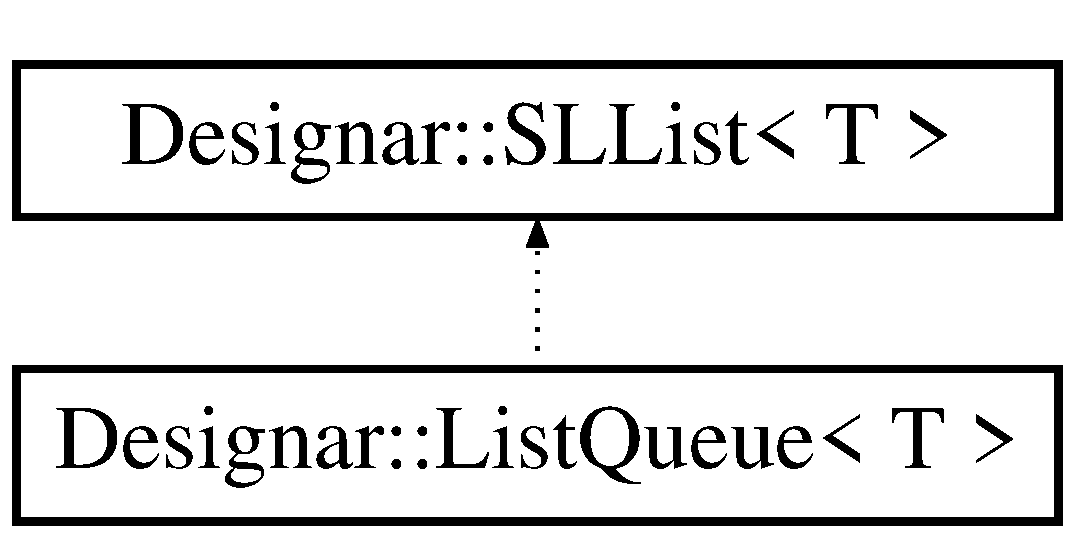
\includegraphics[height=2.000000cm]{class_designar_1_1_list_queue}
\end{center}
\end{figure}
\subsection*{Tipos públicos}
\begin{DoxyCompactItemize}
\item 
using \hyperlink{class_designar_1_1_list_queue_ab2057fd5d92eccf8de8daed70e0182b2}{Item\+Type} = T
\item 
using \hyperlink{class_designar_1_1_list_queue_abb867bba1fa9e40a4bbc27160e5148c5}{Key\+Type} = T
\item 
using \hyperlink{class_designar_1_1_list_queue_a5aae5b0703cf71bce7457e5420d59c8f}{Data\+Type} = T
\item 
using \hyperlink{class_designar_1_1_list_queue_aa5dc35fd7e235c69f4473a96eaae2de3}{Value\+Type} = T
\item 
using \hyperlink{class_designar_1_1_list_queue_a506b74cc71e3d3ad8767ad393b4704b6}{Size\+Type} = \hyperlink{namespace_designar_aa72662848b9f4815e7bf31a7cf3e33d1}{nat\+\_\+t}
\end{DoxyCompactItemize}
\subsection*{Métodos públicos}
\begin{DoxyCompactItemize}
\item 
\hyperlink{class_designar_1_1_list_queue_a873b7115c57ffc8b3bb812df2727041f}{List\+Queue} ()
\item 
\hyperlink{class_designar_1_1_list_queue_aa7539c8b5a199916b2013ea4072eac38}{List\+Queue} (const \hyperlink{class_designar_1_1_list_queue}{List\+Queue} \&q)
\item 
\hyperlink{class_designar_1_1_list_queue_a959df61146e0642a0ee24227b257e470}{List\+Queue} (\hyperlink{class_designar_1_1_list_queue}{List\+Queue} \&\&q)
\item 
\hyperlink{class_designar_1_1_list_queue}{List\+Queue} \& \hyperlink{class_designar_1_1_list_queue_aed4d7cad2e706202054746bf4f934903}{operator=} (const \hyperlink{class_designar_1_1_list_queue}{List\+Queue} \&q)
\item 
\hyperlink{class_designar_1_1_list_queue}{List\+Queue} \& \hyperlink{class_designar_1_1_list_queue_ae0ee7a8cf8b7cbf8f89a268db1a448dc}{operator=} (\hyperlink{class_designar_1_1_list_queue}{List\+Queue} \&\&q)
\item 
bool \hyperlink{class_designar_1_1_list_queue_a0d21739ee62997c7b7a35fb7583e1629}{is\+\_\+empty} () const
\item 
\hyperlink{namespace_designar_aa72662848b9f4815e7bf31a7cf3e33d1}{nat\+\_\+t} \hyperlink{class_designar_1_1_list_queue_a0a2d3a25c27b0529b1bcc4b0c0b27855}{size} () const
\item 
void \hyperlink{class_designar_1_1_list_queue_aaca43c7f4dc964e05e5bb4af01efc389}{clear} ()
\item 
T \& \hyperlink{class_designar_1_1_list_queue_aa7fc9ba1a7fb8e65819be9da7f96e106}{front} ()
\item 
const T \& \hyperlink{class_designar_1_1_list_queue_abfc6bf50f4b4158e735ccd2c2d49ab1b}{front} () const
\item 
T \& \hyperlink{class_designar_1_1_list_queue_a04064adf41dec656de3dfa66a72c9f22}{rear} ()
\item 
const T \& \hyperlink{class_designar_1_1_list_queue_af3e54cd6e13b28f49dde38881f0a737f}{rear} () const
\item 
T \& \hyperlink{class_designar_1_1_list_queue_aff798fc666bdf94771a60fa291f12a5e}{put} (const T \&item)
\item 
T \& \hyperlink{class_designar_1_1_list_queue_a6a8469ab0fc0ddc5e01a067374772ac2}{put} (T \&\&item)
\item 
T \hyperlink{class_designar_1_1_list_queue_a4b934d649cd814fff5ec643843b8245d}{get} ()
\end{DoxyCompactItemize}


\subsection{Descripción detallada}
\subsubsection*{template$<$typename T$>$\newline
class Designar\+::\+List\+Queue$<$ T $>$}



Definición en la línea 418 del archivo queue.\+H.



\subsection{Documentación de los \textquotesingle{}Typedef\textquotesingle{} miembros de la clase}
\mbox{\Hypertarget{class_designar_1_1_list_queue_a5aae5b0703cf71bce7457e5420d59c8f}\label{class_designar_1_1_list_queue_a5aae5b0703cf71bce7457e5420d59c8f}} 
\index{Designar\+::\+List\+Queue@{Designar\+::\+List\+Queue}!Data\+Type@{Data\+Type}}
\index{Data\+Type@{Data\+Type}!Designar\+::\+List\+Queue@{Designar\+::\+List\+Queue}}
\subsubsection{\texorpdfstring{Data\+Type}{DataType}}
{\footnotesize\ttfamily template$<$typename T$>$ \\
using \hyperlink{class_designar_1_1_list_queue}{Designar\+::\+List\+Queue}$<$ T $>$\+::\hyperlink{class_designar_1_1_s_l_list_aa98659227d90b392a1b52fa5e9b292f4}{Data\+Type} =  T}



Definición en la línea 425 del archivo queue.\+H.

\mbox{\Hypertarget{class_designar_1_1_list_queue_ab2057fd5d92eccf8de8daed70e0182b2}\label{class_designar_1_1_list_queue_ab2057fd5d92eccf8de8daed70e0182b2}} 
\index{Designar\+::\+List\+Queue@{Designar\+::\+List\+Queue}!Item\+Type@{Item\+Type}}
\index{Item\+Type@{Item\+Type}!Designar\+::\+List\+Queue@{Designar\+::\+List\+Queue}}
\subsubsection{\texorpdfstring{Item\+Type}{ItemType}}
{\footnotesize\ttfamily template$<$typename T$>$ \\
using \hyperlink{class_designar_1_1_list_queue}{Designar\+::\+List\+Queue}$<$ T $>$\+::\hyperlink{class_designar_1_1_s_l_list_a8ec47bfb6b0d74c8f85111b7b3c05cb2}{Item\+Type} =  T}



Definición en la línea 423 del archivo queue.\+H.

\mbox{\Hypertarget{class_designar_1_1_list_queue_abb867bba1fa9e40a4bbc27160e5148c5}\label{class_designar_1_1_list_queue_abb867bba1fa9e40a4bbc27160e5148c5}} 
\index{Designar\+::\+List\+Queue@{Designar\+::\+List\+Queue}!Key\+Type@{Key\+Type}}
\index{Key\+Type@{Key\+Type}!Designar\+::\+List\+Queue@{Designar\+::\+List\+Queue}}
\subsubsection{\texorpdfstring{Key\+Type}{KeyType}}
{\footnotesize\ttfamily template$<$typename T$>$ \\
using \hyperlink{class_designar_1_1_list_queue}{Designar\+::\+List\+Queue}$<$ T $>$\+::\hyperlink{class_designar_1_1_s_l_list_a0f9ac3eaee2d1a9e6091aaaac825ccb2}{Key\+Type} =  T}



Definición en la línea 424 del archivo queue.\+H.

\mbox{\Hypertarget{class_designar_1_1_list_queue_a506b74cc71e3d3ad8767ad393b4704b6}\label{class_designar_1_1_list_queue_a506b74cc71e3d3ad8767ad393b4704b6}} 
\index{Designar\+::\+List\+Queue@{Designar\+::\+List\+Queue}!Size\+Type@{Size\+Type}}
\index{Size\+Type@{Size\+Type}!Designar\+::\+List\+Queue@{Designar\+::\+List\+Queue}}
\subsubsection{\texorpdfstring{Size\+Type}{SizeType}}
{\footnotesize\ttfamily template$<$typename T$>$ \\
using \hyperlink{class_designar_1_1_list_queue}{Designar\+::\+List\+Queue}$<$ T $>$\+::\hyperlink{class_designar_1_1_s_l_list_a253792b5e9c19ea61fb49e5e83f6159b}{Size\+Type} =  \hyperlink{namespace_designar_aa72662848b9f4815e7bf31a7cf3e33d1}{nat\+\_\+t}}



Definición en la línea 427 del archivo queue.\+H.

\mbox{\Hypertarget{class_designar_1_1_list_queue_aa5dc35fd7e235c69f4473a96eaae2de3}\label{class_designar_1_1_list_queue_aa5dc35fd7e235c69f4473a96eaae2de3}} 
\index{Designar\+::\+List\+Queue@{Designar\+::\+List\+Queue}!Value\+Type@{Value\+Type}}
\index{Value\+Type@{Value\+Type}!Designar\+::\+List\+Queue@{Designar\+::\+List\+Queue}}
\subsubsection{\texorpdfstring{Value\+Type}{ValueType}}
{\footnotesize\ttfamily template$<$typename T$>$ \\
using \hyperlink{class_designar_1_1_list_queue}{Designar\+::\+List\+Queue}$<$ T $>$\+::\hyperlink{class_designar_1_1_s_l_list_a22813e78b0dea3a55f47d5f476fd99a1}{Value\+Type} =  T}



Definición en la línea 426 del archivo queue.\+H.



\subsection{Documentación del constructor y destructor}
\mbox{\Hypertarget{class_designar_1_1_list_queue_a873b7115c57ffc8b3bb812df2727041f}\label{class_designar_1_1_list_queue_a873b7115c57ffc8b3bb812df2727041f}} 
\index{Designar\+::\+List\+Queue@{Designar\+::\+List\+Queue}!List\+Queue@{List\+Queue}}
\index{List\+Queue@{List\+Queue}!Designar\+::\+List\+Queue@{Designar\+::\+List\+Queue}}
\subsubsection{\texorpdfstring{List\+Queue()}{ListQueue()}\hspace{0.1cm}{\footnotesize\ttfamily [1/3]}}
{\footnotesize\ttfamily template$<$typename T$>$ \\
\hyperlink{class_designar_1_1_list_queue}{Designar\+::\+List\+Queue}$<$ T $>$\+::\hyperlink{class_designar_1_1_list_queue}{List\+Queue} (\begin{DoxyParamCaption}{ }\end{DoxyParamCaption})\hspace{0.3cm}{\ttfamily [inline]}}



Definición en la línea 429 del archivo queue.\+H.

\mbox{\Hypertarget{class_designar_1_1_list_queue_aa7539c8b5a199916b2013ea4072eac38}\label{class_designar_1_1_list_queue_aa7539c8b5a199916b2013ea4072eac38}} 
\index{Designar\+::\+List\+Queue@{Designar\+::\+List\+Queue}!List\+Queue@{List\+Queue}}
\index{List\+Queue@{List\+Queue}!Designar\+::\+List\+Queue@{Designar\+::\+List\+Queue}}
\subsubsection{\texorpdfstring{List\+Queue()}{ListQueue()}\hspace{0.1cm}{\footnotesize\ttfamily [2/3]}}
{\footnotesize\ttfamily template$<$typename T$>$ \\
\hyperlink{class_designar_1_1_list_queue}{Designar\+::\+List\+Queue}$<$ T $>$\+::\hyperlink{class_designar_1_1_list_queue}{List\+Queue} (\begin{DoxyParamCaption}\item[{const \hyperlink{class_designar_1_1_list_queue}{List\+Queue}$<$ T $>$ \&}]{q }\end{DoxyParamCaption})\hspace{0.3cm}{\ttfamily [inline]}}



Definición en la línea 435 del archivo queue.\+H.

\mbox{\Hypertarget{class_designar_1_1_list_queue_a959df61146e0642a0ee24227b257e470}\label{class_designar_1_1_list_queue_a959df61146e0642a0ee24227b257e470}} 
\index{Designar\+::\+List\+Queue@{Designar\+::\+List\+Queue}!List\+Queue@{List\+Queue}}
\index{List\+Queue@{List\+Queue}!Designar\+::\+List\+Queue@{Designar\+::\+List\+Queue}}
\subsubsection{\texorpdfstring{List\+Queue()}{ListQueue()}\hspace{0.1cm}{\footnotesize\ttfamily [3/3]}}
{\footnotesize\ttfamily template$<$typename T$>$ \\
\hyperlink{class_designar_1_1_list_queue}{Designar\+::\+List\+Queue}$<$ T $>$\+::\hyperlink{class_designar_1_1_list_queue}{List\+Queue} (\begin{DoxyParamCaption}\item[{\hyperlink{class_designar_1_1_list_queue}{List\+Queue}$<$ T $>$ \&\&}]{q }\end{DoxyParamCaption})\hspace{0.3cm}{\ttfamily [inline]}}



Definición en la línea 441 del archivo queue.\+H.



\subsection{Documentación de las funciones miembro}
\mbox{\Hypertarget{class_designar_1_1_list_queue_aaca43c7f4dc964e05e5bb4af01efc389}\label{class_designar_1_1_list_queue_aaca43c7f4dc964e05e5bb4af01efc389}} 
\index{Designar\+::\+List\+Queue@{Designar\+::\+List\+Queue}!clear@{clear}}
\index{clear@{clear}!Designar\+::\+List\+Queue@{Designar\+::\+List\+Queue}}
\subsubsection{\texorpdfstring{clear()}{clear()}}
{\footnotesize\ttfamily template$<$typename T$>$ \\
void \hyperlink{class_designar_1_1_list_queue}{Designar\+::\+List\+Queue}$<$ T $>$\+::clear (\begin{DoxyParamCaption}{ }\end{DoxyParamCaption})\hspace{0.3cm}{\ttfamily [inline]}}



Definición en la línea 472 del archivo queue.\+H.

\mbox{\Hypertarget{class_designar_1_1_list_queue_aa7fc9ba1a7fb8e65819be9da7f96e106}\label{class_designar_1_1_list_queue_aa7fc9ba1a7fb8e65819be9da7f96e106}} 
\index{Designar\+::\+List\+Queue@{Designar\+::\+List\+Queue}!front@{front}}
\index{front@{front}!Designar\+::\+List\+Queue@{Designar\+::\+List\+Queue}}
\subsubsection{\texorpdfstring{front()}{front()}\hspace{0.1cm}{\footnotesize\ttfamily [1/2]}}
{\footnotesize\ttfamily template$<$typename T$>$ \\
T\& \hyperlink{class_designar_1_1_list_queue}{Designar\+::\+List\+Queue}$<$ T $>$\+::front (\begin{DoxyParamCaption}{ }\end{DoxyParamCaption})\hspace{0.3cm}{\ttfamily [inline]}}



Definición en la línea 477 del archivo queue.\+H.

\mbox{\Hypertarget{class_designar_1_1_list_queue_abfc6bf50f4b4158e735ccd2c2d49ab1b}\label{class_designar_1_1_list_queue_abfc6bf50f4b4158e735ccd2c2d49ab1b}} 
\index{Designar\+::\+List\+Queue@{Designar\+::\+List\+Queue}!front@{front}}
\index{front@{front}!Designar\+::\+List\+Queue@{Designar\+::\+List\+Queue}}
\subsubsection{\texorpdfstring{front()}{front()}\hspace{0.1cm}{\footnotesize\ttfamily [2/2]}}
{\footnotesize\ttfamily template$<$typename T$>$ \\
const T\& \hyperlink{class_designar_1_1_list_queue}{Designar\+::\+List\+Queue}$<$ T $>$\+::front (\begin{DoxyParamCaption}{ }\end{DoxyParamCaption}) const\hspace{0.3cm}{\ttfamily [inline]}}



Definición en la línea 485 del archivo queue.\+H.

\mbox{\Hypertarget{class_designar_1_1_list_queue_a4b934d649cd814fff5ec643843b8245d}\label{class_designar_1_1_list_queue_a4b934d649cd814fff5ec643843b8245d}} 
\index{Designar\+::\+List\+Queue@{Designar\+::\+List\+Queue}!get@{get}}
\index{get@{get}!Designar\+::\+List\+Queue@{Designar\+::\+List\+Queue}}
\subsubsection{\texorpdfstring{get()}{get()}}
{\footnotesize\ttfamily template$<$typename T$>$ \\
T \hyperlink{class_designar_1_1_list_queue}{Designar\+::\+List\+Queue}$<$ T $>$\+::get (\begin{DoxyParamCaption}{ }\end{DoxyParamCaption})\hspace{0.3cm}{\ttfamily [inline]}}



Definición en la línea 519 del archivo queue.\+H.

\mbox{\Hypertarget{class_designar_1_1_list_queue_a0d21739ee62997c7b7a35fb7583e1629}\label{class_designar_1_1_list_queue_a0d21739ee62997c7b7a35fb7583e1629}} 
\index{Designar\+::\+List\+Queue@{Designar\+::\+List\+Queue}!is\+\_\+empty@{is\+\_\+empty}}
\index{is\+\_\+empty@{is\+\_\+empty}!Designar\+::\+List\+Queue@{Designar\+::\+List\+Queue}}
\subsubsection{\texorpdfstring{is\+\_\+empty()}{is\_empty()}}
{\footnotesize\ttfamily template$<$typename T$>$ \\
bool \hyperlink{class_designar_1_1_list_queue}{Designar\+::\+List\+Queue}$<$ T $>$\+::is\+\_\+empty (\begin{DoxyParamCaption}{ }\end{DoxyParamCaption}) const\hspace{0.3cm}{\ttfamily [inline]}}



Definición en la línea 462 del archivo queue.\+H.

\mbox{\Hypertarget{class_designar_1_1_list_queue_aed4d7cad2e706202054746bf4f934903}\label{class_designar_1_1_list_queue_aed4d7cad2e706202054746bf4f934903}} 
\index{Designar\+::\+List\+Queue@{Designar\+::\+List\+Queue}!operator=@{operator=}}
\index{operator=@{operator=}!Designar\+::\+List\+Queue@{Designar\+::\+List\+Queue}}
\subsubsection{\texorpdfstring{operator=()}{operator=()}\hspace{0.1cm}{\footnotesize\ttfamily [1/2]}}
{\footnotesize\ttfamily template$<$typename T$>$ \\
\hyperlink{class_designar_1_1_list_queue}{List\+Queue}\& \hyperlink{class_designar_1_1_list_queue}{Designar\+::\+List\+Queue}$<$ T $>$\+::operator= (\begin{DoxyParamCaption}\item[{const \hyperlink{class_designar_1_1_list_queue}{List\+Queue}$<$ T $>$ \&}]{q }\end{DoxyParamCaption})\hspace{0.3cm}{\ttfamily [inline]}}



Definición en la línea 447 del archivo queue.\+H.

\mbox{\Hypertarget{class_designar_1_1_list_queue_ae0ee7a8cf8b7cbf8f89a268db1a448dc}\label{class_designar_1_1_list_queue_ae0ee7a8cf8b7cbf8f89a268db1a448dc}} 
\index{Designar\+::\+List\+Queue@{Designar\+::\+List\+Queue}!operator=@{operator=}}
\index{operator=@{operator=}!Designar\+::\+List\+Queue@{Designar\+::\+List\+Queue}}
\subsubsection{\texorpdfstring{operator=()}{operator=()}\hspace{0.1cm}{\footnotesize\ttfamily [2/2]}}
{\footnotesize\ttfamily template$<$typename T$>$ \\
\hyperlink{class_designar_1_1_list_queue}{List\+Queue}\& \hyperlink{class_designar_1_1_list_queue}{Designar\+::\+List\+Queue}$<$ T $>$\+::operator= (\begin{DoxyParamCaption}\item[{\hyperlink{class_designar_1_1_list_queue}{List\+Queue}$<$ T $>$ \&\&}]{q }\end{DoxyParamCaption})\hspace{0.3cm}{\ttfamily [inline]}}



Definición en la línea 456 del archivo queue.\+H.

\mbox{\Hypertarget{class_designar_1_1_list_queue_aff798fc666bdf94771a60fa291f12a5e}\label{class_designar_1_1_list_queue_aff798fc666bdf94771a60fa291f12a5e}} 
\index{Designar\+::\+List\+Queue@{Designar\+::\+List\+Queue}!put@{put}}
\index{put@{put}!Designar\+::\+List\+Queue@{Designar\+::\+List\+Queue}}
\subsubsection{\texorpdfstring{put()}{put()}\hspace{0.1cm}{\footnotesize\ttfamily [1/2]}}
{\footnotesize\ttfamily template$<$typename T$>$ \\
T\& \hyperlink{class_designar_1_1_list_queue}{Designar\+::\+List\+Queue}$<$ T $>$\+::put (\begin{DoxyParamCaption}\item[{const T \&}]{item }\end{DoxyParamCaption})\hspace{0.3cm}{\ttfamily [inline]}}



Definición en la línea 509 del archivo queue.\+H.

\mbox{\Hypertarget{class_designar_1_1_list_queue_a6a8469ab0fc0ddc5e01a067374772ac2}\label{class_designar_1_1_list_queue_a6a8469ab0fc0ddc5e01a067374772ac2}} 
\index{Designar\+::\+List\+Queue@{Designar\+::\+List\+Queue}!put@{put}}
\index{put@{put}!Designar\+::\+List\+Queue@{Designar\+::\+List\+Queue}}
\subsubsection{\texorpdfstring{put()}{put()}\hspace{0.1cm}{\footnotesize\ttfamily [2/2]}}
{\footnotesize\ttfamily template$<$typename T$>$ \\
T\& \hyperlink{class_designar_1_1_list_queue}{Designar\+::\+List\+Queue}$<$ T $>$\+::put (\begin{DoxyParamCaption}\item[{T \&\&}]{item }\end{DoxyParamCaption})\hspace{0.3cm}{\ttfamily [inline]}}



Definición en la línea 514 del archivo queue.\+H.

\mbox{\Hypertarget{class_designar_1_1_list_queue_a04064adf41dec656de3dfa66a72c9f22}\label{class_designar_1_1_list_queue_a04064adf41dec656de3dfa66a72c9f22}} 
\index{Designar\+::\+List\+Queue@{Designar\+::\+List\+Queue}!rear@{rear}}
\index{rear@{rear}!Designar\+::\+List\+Queue@{Designar\+::\+List\+Queue}}
\subsubsection{\texorpdfstring{rear()}{rear()}\hspace{0.1cm}{\footnotesize\ttfamily [1/2]}}
{\footnotesize\ttfamily template$<$typename T$>$ \\
T\& \hyperlink{class_designar_1_1_list_queue}{Designar\+::\+List\+Queue}$<$ T $>$\+::rear (\begin{DoxyParamCaption}{ }\end{DoxyParamCaption})\hspace{0.3cm}{\ttfamily [inline]}}



Definición en la línea 493 del archivo queue.\+H.

\mbox{\Hypertarget{class_designar_1_1_list_queue_af3e54cd6e13b28f49dde38881f0a737f}\label{class_designar_1_1_list_queue_af3e54cd6e13b28f49dde38881f0a737f}} 
\index{Designar\+::\+List\+Queue@{Designar\+::\+List\+Queue}!rear@{rear}}
\index{rear@{rear}!Designar\+::\+List\+Queue@{Designar\+::\+List\+Queue}}
\subsubsection{\texorpdfstring{rear()}{rear()}\hspace{0.1cm}{\footnotesize\ttfamily [2/2]}}
{\footnotesize\ttfamily template$<$typename T$>$ \\
const T\& \hyperlink{class_designar_1_1_list_queue}{Designar\+::\+List\+Queue}$<$ T $>$\+::rear (\begin{DoxyParamCaption}{ }\end{DoxyParamCaption}) const\hspace{0.3cm}{\ttfamily [inline]}}



Definición en la línea 501 del archivo queue.\+H.

\mbox{\Hypertarget{class_designar_1_1_list_queue_a0a2d3a25c27b0529b1bcc4b0c0b27855}\label{class_designar_1_1_list_queue_a0a2d3a25c27b0529b1bcc4b0c0b27855}} 
\index{Designar\+::\+List\+Queue@{Designar\+::\+List\+Queue}!size@{size}}
\index{size@{size}!Designar\+::\+List\+Queue@{Designar\+::\+List\+Queue}}
\subsubsection{\texorpdfstring{size()}{size()}}
{\footnotesize\ttfamily template$<$typename T$>$ \\
\hyperlink{namespace_designar_aa72662848b9f4815e7bf31a7cf3e33d1}{nat\+\_\+t} \hyperlink{class_designar_1_1_list_queue}{Designar\+::\+List\+Queue}$<$ T $>$\+::size (\begin{DoxyParamCaption}{ }\end{DoxyParamCaption}) const\hspace{0.3cm}{\ttfamily [inline]}}



Definición en la línea 467 del archivo queue.\+H.



La documentación para esta clase fue generada a partir del siguiente fichero\+:\begin{DoxyCompactItemize}
\item 
/home/julio/\+De\+S\+I\+G\+N\+A\+R-\/doc/\+De\+Si\+G\+N\+A\+R/include/\hyperlink{queue_8_h}{queue.\+H}\end{DoxyCompactItemize}

\hypertarget{class_designar_1_1_list_stack}{}\section{Designar\+:\+:List\+Stack$<$ T $>$ Class Template Reference}
\label{class_designar_1_1_list_stack}\index{Designar\+::\+List\+Stack$<$ T $>$@{Designar\+::\+List\+Stack$<$ T $>$}}


{\ttfamily \#include $<$stack.\+H$>$}

Inheritance diagram for Designar\+:\+:List\+Stack$<$ T $>$\+:\begin{figure}[H]
\begin{center}
\leavevmode
\includegraphics[height=2.000000cm]{class_designar_1_1_list_stack}
\end{center}
\end{figure}
\subsection*{Public Types}
\begin{DoxyCompactItemize}
\item 
using \hyperlink{class_designar_1_1_list_stack_a5a584752d4cfca9e791071f1553d7c69}{Item\+Type} = T
\item 
using \hyperlink{class_designar_1_1_list_stack_adf88da10e96a685fa2cdd3fff029d52c}{Key\+Type} = T
\item 
using \hyperlink{class_designar_1_1_list_stack_a9bdd8f2e28bca0397b835faa08a1d0dc}{Data\+Type} = T
\item 
using \hyperlink{class_designar_1_1_list_stack_ac51dd165958a3e9ff0790e9f5791a4a5}{Value\+Type} = T
\item 
using \hyperlink{class_designar_1_1_list_stack_ae1849f2d4064bd8602122eb9db436441}{Size\+Type} = \hyperlink{namespace_designar_aa72662848b9f4815e7bf31a7cf3e33d1}{nat\+\_\+t}
\end{DoxyCompactItemize}
\subsection*{Public Member Functions}
\begin{DoxyCompactItemize}
\item 
\hyperlink{class_designar_1_1_list_stack_af48928af17e98272785d4f07d229ac12}{List\+Stack} ()
\item 
\hyperlink{class_designar_1_1_list_stack_adee9acd5a1b6f6e9327fc20126caa2ed}{List\+Stack} (const \hyperlink{class_designar_1_1_list_stack}{List\+Stack} \&s)
\item 
\hyperlink{class_designar_1_1_list_stack_ab0b28b16213cbc71e6132b3508838013}{List\+Stack} (\hyperlink{class_designar_1_1_list_stack}{List\+Stack} \&\&s)
\item 
\hyperlink{class_designar_1_1_list_stack}{List\+Stack} \& \hyperlink{class_designar_1_1_list_stack_a324b12f4699962b0cbbdf12c80fbba44}{operator=} (const \hyperlink{class_designar_1_1_list_stack}{List\+Stack} \&s)
\item 
\hyperlink{class_designar_1_1_list_stack}{List\+Stack} \& \hyperlink{class_designar_1_1_list_stack_ae74bc2ebc11f8ebb3d98e700f4cbe9c3}{operator=} (\hyperlink{class_designar_1_1_list_stack}{List\+Stack} \&\&s)
\item 
bool \hyperlink{class_designar_1_1_list_stack_a78ec42650d4028911a0054f6baaa673a}{is\+\_\+empty} () const
\item 
void \hyperlink{class_designar_1_1_list_stack_aef07f86ff93ad1742207df436ba71aaa}{clear} ()
\item 
\hyperlink{namespace_designar_aa72662848b9f4815e7bf31a7cf3e33d1}{nat\+\_\+t} \hyperlink{class_designar_1_1_list_stack_abec63f99f62a9b7d92e1a051767017dc}{size} () const
\item 
T \& \hyperlink{class_designar_1_1_list_stack_a02d19090b599fd54ebb5e693d0a8d2d0}{push} (const T \&item)
\item 
T \& \hyperlink{class_designar_1_1_list_stack_a96bb73a3658f95565769e8b50c903f88}{push} (T \&\&item)
\item 
T \& \hyperlink{class_designar_1_1_list_stack_a5b6e47be80da93039d31cd885e97cf34}{top} ()
\item 
const T \& \hyperlink{class_designar_1_1_list_stack_a6eafdfa1a1a43b4cbbe27730a7dcffd3}{top} () const
\item 
T \& \hyperlink{class_designar_1_1_list_stack_a40833af5e19d5d400a962fafb2c449a3}{base} ()
\item 
const T \& \hyperlink{class_designar_1_1_list_stack_a98ea1c6dff17d53b810e6fedae85340c}{base} () const
\item 
T \hyperlink{class_designar_1_1_list_stack_a1a8a0fb51e9a31cf7b5d103a067e0cc4}{pop} ()
\item 
void \hyperlink{class_designar_1_1_list_stack_afe33f82099d4ec5f62848323edf66d30}{popn} (\hyperlink{namespace_designar_aa72662848b9f4815e7bf31a7cf3e33d1}{nat\+\_\+t})
\end{DoxyCompactItemize}


\subsection{Detailed Description}
\subsubsection*{template$<$typename T$>$\newline
class Designar\+::\+List\+Stack$<$ T $>$}



Definition at line 321 of file stack.\+H.



\subsection{Member Typedef Documentation}
\mbox{\Hypertarget{class_designar_1_1_list_stack_a9bdd8f2e28bca0397b835faa08a1d0dc}\label{class_designar_1_1_list_stack_a9bdd8f2e28bca0397b835faa08a1d0dc}} 
\index{Designar\+::\+List\+Stack@{Designar\+::\+List\+Stack}!Data\+Type@{Data\+Type}}
\index{Data\+Type@{Data\+Type}!Designar\+::\+List\+Stack@{Designar\+::\+List\+Stack}}
\subsubsection{\texorpdfstring{Data\+Type}{DataType}}
{\footnotesize\ttfamily template$<$typename T$>$ \\
using \hyperlink{class_designar_1_1_list_stack}{Designar\+::\+List\+Stack}$<$ T $>$\+::\hyperlink{class_designar_1_1_s_l_list_aa98659227d90b392a1b52fa5e9b292f4}{Data\+Type} =  T}



Definition at line 328 of file stack.\+H.

\mbox{\Hypertarget{class_designar_1_1_list_stack_a5a584752d4cfca9e791071f1553d7c69}\label{class_designar_1_1_list_stack_a5a584752d4cfca9e791071f1553d7c69}} 
\index{Designar\+::\+List\+Stack@{Designar\+::\+List\+Stack}!Item\+Type@{Item\+Type}}
\index{Item\+Type@{Item\+Type}!Designar\+::\+List\+Stack@{Designar\+::\+List\+Stack}}
\subsubsection{\texorpdfstring{Item\+Type}{ItemType}}
{\footnotesize\ttfamily template$<$typename T$>$ \\
using \hyperlink{class_designar_1_1_list_stack}{Designar\+::\+List\+Stack}$<$ T $>$\+::\hyperlink{class_designar_1_1_s_l_list_a8ec47bfb6b0d74c8f85111b7b3c05cb2}{Item\+Type} =  T}



Definition at line 326 of file stack.\+H.

\mbox{\Hypertarget{class_designar_1_1_list_stack_adf88da10e96a685fa2cdd3fff029d52c}\label{class_designar_1_1_list_stack_adf88da10e96a685fa2cdd3fff029d52c}} 
\index{Designar\+::\+List\+Stack@{Designar\+::\+List\+Stack}!Key\+Type@{Key\+Type}}
\index{Key\+Type@{Key\+Type}!Designar\+::\+List\+Stack@{Designar\+::\+List\+Stack}}
\subsubsection{\texorpdfstring{Key\+Type}{KeyType}}
{\footnotesize\ttfamily template$<$typename T$>$ \\
using \hyperlink{class_designar_1_1_list_stack}{Designar\+::\+List\+Stack}$<$ T $>$\+::\hyperlink{class_designar_1_1_s_l_list_a0f9ac3eaee2d1a9e6091aaaac825ccb2}{Key\+Type} =  T}



Definition at line 327 of file stack.\+H.

\mbox{\Hypertarget{class_designar_1_1_list_stack_ae1849f2d4064bd8602122eb9db436441}\label{class_designar_1_1_list_stack_ae1849f2d4064bd8602122eb9db436441}} 
\index{Designar\+::\+List\+Stack@{Designar\+::\+List\+Stack}!Size\+Type@{Size\+Type}}
\index{Size\+Type@{Size\+Type}!Designar\+::\+List\+Stack@{Designar\+::\+List\+Stack}}
\subsubsection{\texorpdfstring{Size\+Type}{SizeType}}
{\footnotesize\ttfamily template$<$typename T$>$ \\
using \hyperlink{class_designar_1_1_list_stack}{Designar\+::\+List\+Stack}$<$ T $>$\+::\hyperlink{class_designar_1_1_s_l_list_a253792b5e9c19ea61fb49e5e83f6159b}{Size\+Type} =  \hyperlink{namespace_designar_aa72662848b9f4815e7bf31a7cf3e33d1}{nat\+\_\+t}}



Definition at line 330 of file stack.\+H.

\mbox{\Hypertarget{class_designar_1_1_list_stack_ac51dd165958a3e9ff0790e9f5791a4a5}\label{class_designar_1_1_list_stack_ac51dd165958a3e9ff0790e9f5791a4a5}} 
\index{Designar\+::\+List\+Stack@{Designar\+::\+List\+Stack}!Value\+Type@{Value\+Type}}
\index{Value\+Type@{Value\+Type}!Designar\+::\+List\+Stack@{Designar\+::\+List\+Stack}}
\subsubsection{\texorpdfstring{Value\+Type}{ValueType}}
{\footnotesize\ttfamily template$<$typename T$>$ \\
using \hyperlink{class_designar_1_1_list_stack}{Designar\+::\+List\+Stack}$<$ T $>$\+::\hyperlink{class_designar_1_1_s_l_list_a22813e78b0dea3a55f47d5f476fd99a1}{Value\+Type} =  T}



Definition at line 329 of file stack.\+H.



\subsection{Constructor \& Destructor Documentation}
\mbox{\Hypertarget{class_designar_1_1_list_stack_af48928af17e98272785d4f07d229ac12}\label{class_designar_1_1_list_stack_af48928af17e98272785d4f07d229ac12}} 
\index{Designar\+::\+List\+Stack@{Designar\+::\+List\+Stack}!List\+Stack@{List\+Stack}}
\index{List\+Stack@{List\+Stack}!Designar\+::\+List\+Stack@{Designar\+::\+List\+Stack}}
\subsubsection{\texorpdfstring{List\+Stack()}{ListStack()}\hspace{0.1cm}{\footnotesize\ttfamily [1/3]}}
{\footnotesize\ttfamily template$<$typename T$>$ \\
\hyperlink{class_designar_1_1_list_stack}{Designar\+::\+List\+Stack}$<$ T $>$\+::\hyperlink{class_designar_1_1_list_stack}{List\+Stack} (\begin{DoxyParamCaption}{ }\end{DoxyParamCaption})\hspace{0.3cm}{\ttfamily [inline]}}



Definition at line 332 of file stack.\+H.

\mbox{\Hypertarget{class_designar_1_1_list_stack_adee9acd5a1b6f6e9327fc20126caa2ed}\label{class_designar_1_1_list_stack_adee9acd5a1b6f6e9327fc20126caa2ed}} 
\index{Designar\+::\+List\+Stack@{Designar\+::\+List\+Stack}!List\+Stack@{List\+Stack}}
\index{List\+Stack@{List\+Stack}!Designar\+::\+List\+Stack@{Designar\+::\+List\+Stack}}
\subsubsection{\texorpdfstring{List\+Stack()}{ListStack()}\hspace{0.1cm}{\footnotesize\ttfamily [2/3]}}
{\footnotesize\ttfamily template$<$typename T$>$ \\
\hyperlink{class_designar_1_1_list_stack}{Designar\+::\+List\+Stack}$<$ T $>$\+::\hyperlink{class_designar_1_1_list_stack}{List\+Stack} (\begin{DoxyParamCaption}\item[{const \hyperlink{class_designar_1_1_list_stack}{List\+Stack}$<$ T $>$ \&}]{s }\end{DoxyParamCaption})\hspace{0.3cm}{\ttfamily [inline]}}



Definition at line 338 of file stack.\+H.

\mbox{\Hypertarget{class_designar_1_1_list_stack_ab0b28b16213cbc71e6132b3508838013}\label{class_designar_1_1_list_stack_ab0b28b16213cbc71e6132b3508838013}} 
\index{Designar\+::\+List\+Stack@{Designar\+::\+List\+Stack}!List\+Stack@{List\+Stack}}
\index{List\+Stack@{List\+Stack}!Designar\+::\+List\+Stack@{Designar\+::\+List\+Stack}}
\subsubsection{\texorpdfstring{List\+Stack()}{ListStack()}\hspace{0.1cm}{\footnotesize\ttfamily [3/3]}}
{\footnotesize\ttfamily template$<$typename T$>$ \\
\hyperlink{class_designar_1_1_list_stack}{Designar\+::\+List\+Stack}$<$ T $>$\+::\hyperlink{class_designar_1_1_list_stack}{List\+Stack} (\begin{DoxyParamCaption}\item[{\hyperlink{class_designar_1_1_list_stack}{List\+Stack}$<$ T $>$ \&\&}]{s }\end{DoxyParamCaption})\hspace{0.3cm}{\ttfamily [inline]}}



Definition at line 344 of file stack.\+H.



\subsection{Member Function Documentation}
\mbox{\Hypertarget{class_designar_1_1_list_stack_a40833af5e19d5d400a962fafb2c449a3}\label{class_designar_1_1_list_stack_a40833af5e19d5d400a962fafb2c449a3}} 
\index{Designar\+::\+List\+Stack@{Designar\+::\+List\+Stack}!base@{base}}
\index{base@{base}!Designar\+::\+List\+Stack@{Designar\+::\+List\+Stack}}
\subsubsection{\texorpdfstring{base()}{base()}\hspace{0.1cm}{\footnotesize\ttfamily [1/2]}}
{\footnotesize\ttfamily template$<$typename T$>$ \\
T\& \hyperlink{class_designar_1_1_list_stack}{Designar\+::\+List\+Stack}$<$ T $>$\+::base (\begin{DoxyParamCaption}{ }\end{DoxyParamCaption})\hspace{0.3cm}{\ttfamily [inline]}}



Definition at line 406 of file stack.\+H.

\mbox{\Hypertarget{class_designar_1_1_list_stack_a98ea1c6dff17d53b810e6fedae85340c}\label{class_designar_1_1_list_stack_a98ea1c6dff17d53b810e6fedae85340c}} 
\index{Designar\+::\+List\+Stack@{Designar\+::\+List\+Stack}!base@{base}}
\index{base@{base}!Designar\+::\+List\+Stack@{Designar\+::\+List\+Stack}}
\subsubsection{\texorpdfstring{base()}{base()}\hspace{0.1cm}{\footnotesize\ttfamily [2/2]}}
{\footnotesize\ttfamily template$<$typename T$>$ \\
const T\& \hyperlink{class_designar_1_1_list_stack}{Designar\+::\+List\+Stack}$<$ T $>$\+::base (\begin{DoxyParamCaption}{ }\end{DoxyParamCaption}) const\hspace{0.3cm}{\ttfamily [inline]}}



Definition at line 414 of file stack.\+H.

\mbox{\Hypertarget{class_designar_1_1_list_stack_aef07f86ff93ad1742207df436ba71aaa}\label{class_designar_1_1_list_stack_aef07f86ff93ad1742207df436ba71aaa}} 
\index{Designar\+::\+List\+Stack@{Designar\+::\+List\+Stack}!clear@{clear}}
\index{clear@{clear}!Designar\+::\+List\+Stack@{Designar\+::\+List\+Stack}}
\subsubsection{\texorpdfstring{clear()}{clear()}}
{\footnotesize\ttfamily template$<$typename T$>$ \\
void \hyperlink{class_designar_1_1_list_stack}{Designar\+::\+List\+Stack}$<$ T $>$\+::clear (\begin{DoxyParamCaption}{ }\end{DoxyParamCaption})\hspace{0.3cm}{\ttfamily [inline]}}



Definition at line 370 of file stack.\+H.

\mbox{\Hypertarget{class_designar_1_1_list_stack_a78ec42650d4028911a0054f6baaa673a}\label{class_designar_1_1_list_stack_a78ec42650d4028911a0054f6baaa673a}} 
\index{Designar\+::\+List\+Stack@{Designar\+::\+List\+Stack}!is\+\_\+empty@{is\+\_\+empty}}
\index{is\+\_\+empty@{is\+\_\+empty}!Designar\+::\+List\+Stack@{Designar\+::\+List\+Stack}}
\subsubsection{\texorpdfstring{is\+\_\+empty()}{is\_empty()}}
{\footnotesize\ttfamily template$<$typename T$>$ \\
bool \hyperlink{class_designar_1_1_list_stack}{Designar\+::\+List\+Stack}$<$ T $>$\+::is\+\_\+empty (\begin{DoxyParamCaption}{ }\end{DoxyParamCaption}) const\hspace{0.3cm}{\ttfamily [inline]}}



Definition at line 365 of file stack.\+H.

\mbox{\Hypertarget{class_designar_1_1_list_stack_a324b12f4699962b0cbbdf12c80fbba44}\label{class_designar_1_1_list_stack_a324b12f4699962b0cbbdf12c80fbba44}} 
\index{Designar\+::\+List\+Stack@{Designar\+::\+List\+Stack}!operator=@{operator=}}
\index{operator=@{operator=}!Designar\+::\+List\+Stack@{Designar\+::\+List\+Stack}}
\subsubsection{\texorpdfstring{operator=()}{operator=()}\hspace{0.1cm}{\footnotesize\ttfamily [1/2]}}
{\footnotesize\ttfamily template$<$typename T$>$ \\
\hyperlink{class_designar_1_1_list_stack}{List\+Stack}\& \hyperlink{class_designar_1_1_list_stack}{Designar\+::\+List\+Stack}$<$ T $>$\+::operator= (\begin{DoxyParamCaption}\item[{const \hyperlink{class_designar_1_1_list_stack}{List\+Stack}$<$ T $>$ \&}]{s }\end{DoxyParamCaption})\hspace{0.3cm}{\ttfamily [inline]}}



Definition at line 350 of file stack.\+H.

\mbox{\Hypertarget{class_designar_1_1_list_stack_ae74bc2ebc11f8ebb3d98e700f4cbe9c3}\label{class_designar_1_1_list_stack_ae74bc2ebc11f8ebb3d98e700f4cbe9c3}} 
\index{Designar\+::\+List\+Stack@{Designar\+::\+List\+Stack}!operator=@{operator=}}
\index{operator=@{operator=}!Designar\+::\+List\+Stack@{Designar\+::\+List\+Stack}}
\subsubsection{\texorpdfstring{operator=()}{operator=()}\hspace{0.1cm}{\footnotesize\ttfamily [2/2]}}
{\footnotesize\ttfamily template$<$typename T$>$ \\
\hyperlink{class_designar_1_1_list_stack}{List\+Stack}\& \hyperlink{class_designar_1_1_list_stack}{Designar\+::\+List\+Stack}$<$ T $>$\+::operator= (\begin{DoxyParamCaption}\item[{\hyperlink{class_designar_1_1_list_stack}{List\+Stack}$<$ T $>$ \&\&}]{s }\end{DoxyParamCaption})\hspace{0.3cm}{\ttfamily [inline]}}



Definition at line 359 of file stack.\+H.

\mbox{\Hypertarget{class_designar_1_1_list_stack_a1a8a0fb51e9a31cf7b5d103a067e0cc4}\label{class_designar_1_1_list_stack_a1a8a0fb51e9a31cf7b5d103a067e0cc4}} 
\index{Designar\+::\+List\+Stack@{Designar\+::\+List\+Stack}!pop@{pop}}
\index{pop@{pop}!Designar\+::\+List\+Stack@{Designar\+::\+List\+Stack}}
\subsubsection{\texorpdfstring{pop()}{pop()}}
{\footnotesize\ttfamily template$<$typename T$>$ \\
T \hyperlink{class_designar_1_1_list_stack}{Designar\+::\+List\+Stack}$<$ T $>$\+::pop (\begin{DoxyParamCaption}{ }\end{DoxyParamCaption})\hspace{0.3cm}{\ttfamily [inline]}}



Definition at line 422 of file stack.\+H.

\mbox{\Hypertarget{class_designar_1_1_list_stack_afe33f82099d4ec5f62848323edf66d30}\label{class_designar_1_1_list_stack_afe33f82099d4ec5f62848323edf66d30}} 
\index{Designar\+::\+List\+Stack@{Designar\+::\+List\+Stack}!popn@{popn}}
\index{popn@{popn}!Designar\+::\+List\+Stack@{Designar\+::\+List\+Stack}}
\subsubsection{\texorpdfstring{popn()}{popn()}}
{\footnotesize\ttfamily template$<$typename T $>$ \\
void \hyperlink{class_designar_1_1_list_stack}{Designar\+::\+List\+Stack}$<$ T $>$\+::popn (\begin{DoxyParamCaption}\item[{\hyperlink{namespace_designar_aa72662848b9f4815e7bf31a7cf3e33d1}{nat\+\_\+t}}]{n }\end{DoxyParamCaption})}



Definition at line 434 of file stack.\+H.

\mbox{\Hypertarget{class_designar_1_1_list_stack_a02d19090b599fd54ebb5e693d0a8d2d0}\label{class_designar_1_1_list_stack_a02d19090b599fd54ebb5e693d0a8d2d0}} 
\index{Designar\+::\+List\+Stack@{Designar\+::\+List\+Stack}!push@{push}}
\index{push@{push}!Designar\+::\+List\+Stack@{Designar\+::\+List\+Stack}}
\subsubsection{\texorpdfstring{push()}{push()}\hspace{0.1cm}{\footnotesize\ttfamily [1/2]}}
{\footnotesize\ttfamily template$<$typename T$>$ \\
T\& \hyperlink{class_designar_1_1_list_stack}{Designar\+::\+List\+Stack}$<$ T $>$\+::push (\begin{DoxyParamCaption}\item[{const T \&}]{item }\end{DoxyParamCaption})\hspace{0.3cm}{\ttfamily [inline]}}



Definition at line 380 of file stack.\+H.

\mbox{\Hypertarget{class_designar_1_1_list_stack_a96bb73a3658f95565769e8b50c903f88}\label{class_designar_1_1_list_stack_a96bb73a3658f95565769e8b50c903f88}} 
\index{Designar\+::\+List\+Stack@{Designar\+::\+List\+Stack}!push@{push}}
\index{push@{push}!Designar\+::\+List\+Stack@{Designar\+::\+List\+Stack}}
\subsubsection{\texorpdfstring{push()}{push()}\hspace{0.1cm}{\footnotesize\ttfamily [2/2]}}
{\footnotesize\ttfamily template$<$typename T$>$ \\
T\& \hyperlink{class_designar_1_1_list_stack}{Designar\+::\+List\+Stack}$<$ T $>$\+::push (\begin{DoxyParamCaption}\item[{T \&\&}]{item }\end{DoxyParamCaption})\hspace{0.3cm}{\ttfamily [inline]}}



Definition at line 385 of file stack.\+H.

\mbox{\Hypertarget{class_designar_1_1_list_stack_abec63f99f62a9b7d92e1a051767017dc}\label{class_designar_1_1_list_stack_abec63f99f62a9b7d92e1a051767017dc}} 
\index{Designar\+::\+List\+Stack@{Designar\+::\+List\+Stack}!size@{size}}
\index{size@{size}!Designar\+::\+List\+Stack@{Designar\+::\+List\+Stack}}
\subsubsection{\texorpdfstring{size()}{size()}}
{\footnotesize\ttfamily template$<$typename T$>$ \\
\hyperlink{namespace_designar_aa72662848b9f4815e7bf31a7cf3e33d1}{nat\+\_\+t} \hyperlink{class_designar_1_1_list_stack}{Designar\+::\+List\+Stack}$<$ T $>$\+::size (\begin{DoxyParamCaption}{ }\end{DoxyParamCaption}) const\hspace{0.3cm}{\ttfamily [inline]}}



Definition at line 375 of file stack.\+H.

\mbox{\Hypertarget{class_designar_1_1_list_stack_a5b6e47be80da93039d31cd885e97cf34}\label{class_designar_1_1_list_stack_a5b6e47be80da93039d31cd885e97cf34}} 
\index{Designar\+::\+List\+Stack@{Designar\+::\+List\+Stack}!top@{top}}
\index{top@{top}!Designar\+::\+List\+Stack@{Designar\+::\+List\+Stack}}
\subsubsection{\texorpdfstring{top()}{top()}\hspace{0.1cm}{\footnotesize\ttfamily [1/2]}}
{\footnotesize\ttfamily template$<$typename T$>$ \\
T\& \hyperlink{class_designar_1_1_list_stack}{Designar\+::\+List\+Stack}$<$ T $>$\+::top (\begin{DoxyParamCaption}{ }\end{DoxyParamCaption})\hspace{0.3cm}{\ttfamily [inline]}}



Definition at line 390 of file stack.\+H.

\mbox{\Hypertarget{class_designar_1_1_list_stack_a6eafdfa1a1a43b4cbbe27730a7dcffd3}\label{class_designar_1_1_list_stack_a6eafdfa1a1a43b4cbbe27730a7dcffd3}} 
\index{Designar\+::\+List\+Stack@{Designar\+::\+List\+Stack}!top@{top}}
\index{top@{top}!Designar\+::\+List\+Stack@{Designar\+::\+List\+Stack}}
\subsubsection{\texorpdfstring{top()}{top()}\hspace{0.1cm}{\footnotesize\ttfamily [2/2]}}
{\footnotesize\ttfamily template$<$typename T$>$ \\
const T\& \hyperlink{class_designar_1_1_list_stack}{Designar\+::\+List\+Stack}$<$ T $>$\+::top (\begin{DoxyParamCaption}{ }\end{DoxyParamCaption}) const\hspace{0.3cm}{\ttfamily [inline]}}



Definition at line 398 of file stack.\+H.



The documentation for this class was generated from the following file\+:\begin{DoxyCompactItemize}
\item 
/home/julio/\+De\+S\+I\+G\+N\+A\+R-\/doc/\+De\+Si\+G\+N\+A\+R/include/\hyperlink{stack_8_h}{stack.\+H}\end{DoxyCompactItemize}

\hypertarget{class_designar_1_1_min_path_arc_info}{}\section{Designar\+:\+:Min\+Path\+Arc\+Info$<$ GT, Distance $>$ Class Template Reference}
\label{class_designar_1_1_min_path_arc_info}\index{Designar\+::\+Min\+Path\+Arc\+Info$<$ G\+T, Distance $>$@{Designar\+::\+Min\+Path\+Arc\+Info$<$ G\+T, Distance $>$}}


{\ttfamily \#include $<$graphutilities.\+H$>$}

\subsection*{Public Member Functions}
\begin{DoxyCompactItemize}
\item 
\hyperlink{class_designar_1_1_min_path_arc_info_a243f02fd41ed0786f6f2d907843d0598}{Min\+Path\+Arc\+Info} ()
\end{DoxyCompactItemize}
\subsection*{Public Attributes}
\begin{DoxyCompactItemize}
\item 
\hyperlink{namespace_designar_a3f55fb5513d62ff47cbc8f72b8e95d6f}{Arc}$<$ \hyperlink{demo-buildgraph_8_c_a3001c40d2c31ca87ed96cd7d1334a55e}{GT} $>$ $\ast$ \hyperlink{class_designar_1_1_min_path_arc_info_a2f5c165e547c75ec582dd3724a93137c}{tree\+\_\+arc}
\item 
Distance\+::\+Type \hyperlink{class_designar_1_1_min_path_arc_info_ae53cddd12f7488ab3daf3711963b533d}{potential}
\item 
bool \hyperlink{class_designar_1_1_min_path_arc_info_a97d17f60e2e02381708f68b79c6bf82d}{is\+\_\+in\+\_\+queue}
\end{DoxyCompactItemize}


\subsection{Detailed Description}
\subsubsection*{template$<$class GT, class Distance$>$\newline
class Designar\+::\+Min\+Path\+Arc\+Info$<$ G\+T, Distance $>$}



Definition at line 450 of file graphutilities.\+H.



\subsection{Constructor \& Destructor Documentation}
\mbox{\Hypertarget{class_designar_1_1_min_path_arc_info_a243f02fd41ed0786f6f2d907843d0598}\label{class_designar_1_1_min_path_arc_info_a243f02fd41ed0786f6f2d907843d0598}} 
\index{Designar\+::\+Min\+Path\+Arc\+Info@{Designar\+::\+Min\+Path\+Arc\+Info}!Min\+Path\+Arc\+Info@{Min\+Path\+Arc\+Info}}
\index{Min\+Path\+Arc\+Info@{Min\+Path\+Arc\+Info}!Designar\+::\+Min\+Path\+Arc\+Info@{Designar\+::\+Min\+Path\+Arc\+Info}}
\subsubsection{\texorpdfstring{Min\+Path\+Arc\+Info()}{MinPathArcInfo()}}
{\footnotesize\ttfamily template$<$class GT , class Distance $>$ \\
\hyperlink{class_designar_1_1_min_path_arc_info}{Designar\+::\+Min\+Path\+Arc\+Info}$<$ \hyperlink{demo-buildgraph_8_c_a3001c40d2c31ca87ed96cd7d1334a55e}{GT}, Distance $>$\+::\hyperlink{class_designar_1_1_min_path_arc_info}{Min\+Path\+Arc\+Info} (\begin{DoxyParamCaption}{ }\end{DoxyParamCaption})\hspace{0.3cm}{\ttfamily [inline]}}



Definition at line 457 of file graphutilities.\+H.



\subsection{Member Data Documentation}
\mbox{\Hypertarget{class_designar_1_1_min_path_arc_info_a97d17f60e2e02381708f68b79c6bf82d}\label{class_designar_1_1_min_path_arc_info_a97d17f60e2e02381708f68b79c6bf82d}} 
\index{Designar\+::\+Min\+Path\+Arc\+Info@{Designar\+::\+Min\+Path\+Arc\+Info}!is\+\_\+in\+\_\+queue@{is\+\_\+in\+\_\+queue}}
\index{is\+\_\+in\+\_\+queue@{is\+\_\+in\+\_\+queue}!Designar\+::\+Min\+Path\+Arc\+Info@{Designar\+::\+Min\+Path\+Arc\+Info}}
\subsubsection{\texorpdfstring{is\+\_\+in\+\_\+queue}{is\_in\_queue}}
{\footnotesize\ttfamily template$<$class GT , class Distance $>$ \\
bool \hyperlink{class_designar_1_1_min_path_arc_info}{Designar\+::\+Min\+Path\+Arc\+Info}$<$ \hyperlink{demo-buildgraph_8_c_a3001c40d2c31ca87ed96cd7d1334a55e}{GT}, Distance $>$\+::is\+\_\+in\+\_\+queue}



Definition at line 455 of file graphutilities.\+H.

\mbox{\Hypertarget{class_designar_1_1_min_path_arc_info_ae53cddd12f7488ab3daf3711963b533d}\label{class_designar_1_1_min_path_arc_info_ae53cddd12f7488ab3daf3711963b533d}} 
\index{Designar\+::\+Min\+Path\+Arc\+Info@{Designar\+::\+Min\+Path\+Arc\+Info}!potential@{potential}}
\index{potential@{potential}!Designar\+::\+Min\+Path\+Arc\+Info@{Designar\+::\+Min\+Path\+Arc\+Info}}
\subsubsection{\texorpdfstring{potential}{potential}}
{\footnotesize\ttfamily template$<$class GT , class Distance $>$ \\
Distance\+::\+Type \hyperlink{class_designar_1_1_min_path_arc_info}{Designar\+::\+Min\+Path\+Arc\+Info}$<$ \hyperlink{demo-buildgraph_8_c_a3001c40d2c31ca87ed96cd7d1334a55e}{GT}, Distance $>$\+::potential}



Definition at line 454 of file graphutilities.\+H.

\mbox{\Hypertarget{class_designar_1_1_min_path_arc_info_a2f5c165e547c75ec582dd3724a93137c}\label{class_designar_1_1_min_path_arc_info_a2f5c165e547c75ec582dd3724a93137c}} 
\index{Designar\+::\+Min\+Path\+Arc\+Info@{Designar\+::\+Min\+Path\+Arc\+Info}!tree\+\_\+arc@{tree\+\_\+arc}}
\index{tree\+\_\+arc@{tree\+\_\+arc}!Designar\+::\+Min\+Path\+Arc\+Info@{Designar\+::\+Min\+Path\+Arc\+Info}}
\subsubsection{\texorpdfstring{tree\+\_\+arc}{tree\_arc}}
{\footnotesize\ttfamily template$<$class GT , class Distance $>$ \\
\hyperlink{namespace_designar_a3f55fb5513d62ff47cbc8f72b8e95d6f}{Arc}$<$\hyperlink{demo-buildgraph_8_c_a3001c40d2c31ca87ed96cd7d1334a55e}{GT}$>$$\ast$ \hyperlink{class_designar_1_1_min_path_arc_info}{Designar\+::\+Min\+Path\+Arc\+Info}$<$ \hyperlink{demo-buildgraph_8_c_a3001c40d2c31ca87ed96cd7d1334a55e}{GT}, Distance $>$\+::tree\+\_\+arc}



Definition at line 453 of file graphutilities.\+H.



The documentation for this class was generated from the following file\+:\begin{DoxyCompactItemize}
\item 
include/\hyperlink{graphutilities_8_h}{graphutilities.\+H}\end{DoxyCompactItemize}

\hypertarget{class_designar_1_1_min_path_node_info}{}\section{Designar\+:\+:Min\+Path\+Node\+Info$<$ GT, Distance $>$ Class Template Reference}
\label{class_designar_1_1_min_path_node_info}\index{Designar\+::\+Min\+Path\+Node\+Info$<$ G\+T, Distance $>$@{Designar\+::\+Min\+Path\+Node\+Info$<$ G\+T, Distance $>$}}


{\ttfamily \#include $<$graphutilities.\+H$>$}

\subsection*{Public Member Functions}
\begin{DoxyCompactItemize}
\item 
\hyperlink{class_designar_1_1_min_path_node_info_a50c93fccfecfd75d3aa7637be108ef4d}{Min\+Path\+Node\+Info} ()
\end{DoxyCompactItemize}
\subsection*{Public Attributes}
\begin{DoxyCompactItemize}
\item 
\hyperlink{namespace_designar_a5af326c65aa2bd26b26c410f2030d09e}{Node}$<$ \hyperlink{demo-buildgraph_8_c_a3001c40d2c31ca87ed96cd7d1334a55e}{GT} $>$ $\ast$ \hyperlink{class_designar_1_1_min_path_node_info_a0121695ed8523a60ee92375767a5c169}{tree\+\_\+node}
\item 
Distance\+::\+Type \hyperlink{class_designar_1_1_min_path_node_info_acd8b2664b0726bf26b0f66213e4f1e4b}{accumulated\+\_\+distance}
\end{DoxyCompactItemize}


\subsection{Detailed Description}
\subsubsection*{template$<$class GT, class Distance$>$\newline
class Designar\+::\+Min\+Path\+Node\+Info$<$ G\+T, Distance $>$}



Definition at line 436 of file graphutilities.\+H.



\subsection{Constructor \& Destructor Documentation}
\mbox{\Hypertarget{class_designar_1_1_min_path_node_info_a50c93fccfecfd75d3aa7637be108ef4d}\label{class_designar_1_1_min_path_node_info_a50c93fccfecfd75d3aa7637be108ef4d}} 
\index{Designar\+::\+Min\+Path\+Node\+Info@{Designar\+::\+Min\+Path\+Node\+Info}!Min\+Path\+Node\+Info@{Min\+Path\+Node\+Info}}
\index{Min\+Path\+Node\+Info@{Min\+Path\+Node\+Info}!Designar\+::\+Min\+Path\+Node\+Info@{Designar\+::\+Min\+Path\+Node\+Info}}
\subsubsection{\texorpdfstring{Min\+Path\+Node\+Info()}{MinPathNodeInfo()}}
{\footnotesize\ttfamily template$<$class GT , class Distance $>$ \\
\hyperlink{class_designar_1_1_min_path_node_info}{Designar\+::\+Min\+Path\+Node\+Info}$<$ \hyperlink{demo-buildgraph_8_c_a3001c40d2c31ca87ed96cd7d1334a55e}{GT}, Distance $>$\+::\hyperlink{class_designar_1_1_min_path_node_info}{Min\+Path\+Node\+Info} (\begin{DoxyParamCaption}{ }\end{DoxyParamCaption})\hspace{0.3cm}{\ttfamily [inline]}}



Definition at line 442 of file graphutilities.\+H.



\subsection{Member Data Documentation}
\mbox{\Hypertarget{class_designar_1_1_min_path_node_info_acd8b2664b0726bf26b0f66213e4f1e4b}\label{class_designar_1_1_min_path_node_info_acd8b2664b0726bf26b0f66213e4f1e4b}} 
\index{Designar\+::\+Min\+Path\+Node\+Info@{Designar\+::\+Min\+Path\+Node\+Info}!accumulated\+\_\+distance@{accumulated\+\_\+distance}}
\index{accumulated\+\_\+distance@{accumulated\+\_\+distance}!Designar\+::\+Min\+Path\+Node\+Info@{Designar\+::\+Min\+Path\+Node\+Info}}
\subsubsection{\texorpdfstring{accumulated\+\_\+distance}{accumulated\_distance}}
{\footnotesize\ttfamily template$<$class GT , class Distance $>$ \\
Distance\+::\+Type \hyperlink{class_designar_1_1_min_path_node_info}{Designar\+::\+Min\+Path\+Node\+Info}$<$ \hyperlink{demo-buildgraph_8_c_a3001c40d2c31ca87ed96cd7d1334a55e}{GT}, Distance $>$\+::accumulated\+\_\+distance}



Definition at line 440 of file graphutilities.\+H.

\mbox{\Hypertarget{class_designar_1_1_min_path_node_info_a0121695ed8523a60ee92375767a5c169}\label{class_designar_1_1_min_path_node_info_a0121695ed8523a60ee92375767a5c169}} 
\index{Designar\+::\+Min\+Path\+Node\+Info@{Designar\+::\+Min\+Path\+Node\+Info}!tree\+\_\+node@{tree\+\_\+node}}
\index{tree\+\_\+node@{tree\+\_\+node}!Designar\+::\+Min\+Path\+Node\+Info@{Designar\+::\+Min\+Path\+Node\+Info}}
\subsubsection{\texorpdfstring{tree\+\_\+node}{tree\_node}}
{\footnotesize\ttfamily template$<$class GT , class Distance $>$ \\
\hyperlink{namespace_designar_a5af326c65aa2bd26b26c410f2030d09e}{Node}$<$\hyperlink{demo-buildgraph_8_c_a3001c40d2c31ca87ed96cd7d1334a55e}{GT}$>$$\ast$ \hyperlink{class_designar_1_1_min_path_node_info}{Designar\+::\+Min\+Path\+Node\+Info}$<$ \hyperlink{demo-buildgraph_8_c_a3001c40d2c31ca87ed96cd7d1334a55e}{GT}, Distance $>$\+::tree\+\_\+node}



Definition at line 439 of file graphutilities.\+H.



The documentation for this class was generated from the following file\+:\begin{DoxyCompactItemize}
\item 
/home/julio/\+De\+S\+I\+G\+N\+A\+R-\/doc/\+De\+Si\+G\+N\+A\+R/include/\hyperlink{graphutilities_8_h}{graphutilities.\+H}\end{DoxyCompactItemize}

\hypertarget{class_designar_1_1_m_tree_node}{}\section{Referencia de la plantilla de la Clase Designar\+:\+:M\+Tree\+Node$<$ Key $>$}
\label{class_designar_1_1_m_tree_node}\index{Designar\+::\+M\+Tree\+Node$<$ Key $>$@{Designar\+::\+M\+Tree\+Node$<$ Key $>$}}


{\ttfamily \#include $<$nodesdef.\+H$>$}

Diagrama de herencias de Designar\+:\+:M\+Tree\+Node$<$ Key $>$\begin{figure}[H]
\begin{center}
\leavevmode
\includegraphics[height=2.000000cm]{class_designar_1_1_m_tree_node}
\end{center}
\end{figure}
\subsection*{Clases}
\begin{DoxyCompactItemize}
\item 
class \hyperlink{class_designar_1_1_m_tree_node_1_1_children_iterator}{Children\+Iterator}
\end{DoxyCompactItemize}
\subsection*{Tipos públicos}
\begin{DoxyCompactItemize}
\item 
using \hyperlink{class_designar_1_1_m_tree_node_ad45f6141e36722448b45aecde08761a0}{Key\+Type} = Key
\item 
using \hyperlink{class_designar_1_1_m_tree_node_a0f65c3ec41fb24ab7764c01cd949d6be}{Value\+Type} = Key
\item 
using \hyperlink{class_designar_1_1_m_tree_node_aa649a0376eb81e3da0f4dcbd36871b4b}{Item\+Type} = Key
\end{DoxyCompactItemize}
\subsection*{Métodos públicos}
\begin{DoxyCompactItemize}
\item 
\hyperlink{class_designar_1_1_m_tree_node_a8312cbf8769f92de4348c69f9f7fce40}{M\+Tree\+Node} ()=default
\item 
\hyperlink{class_designar_1_1_m_tree_node_a823994c2cdeba2768bdb10163f27a6b1}{M\+Tree\+Node} (const Key \&k)
\item 
\hyperlink{class_designar_1_1_m_tree_node_abee75a0ea8366fe1f815afddc4b18163}{M\+Tree\+Node} (Key \&\&k)
\item 
Key \& \hyperlink{class_designar_1_1_m_tree_node_a6bccdf14efbc480aaa4d23c943b5a100}{get\+\_\+key} ()
\item 
const Key \& \hyperlink{class_designar_1_1_m_tree_node_aaf4dc39561e8db6973db9c1b5a88b466}{get\+\_\+key} () const
\item 
\hyperlink{class_designar_1_1_m_tree_node}{M\+Tree\+Node} $\ast$ \hyperlink{class_designar_1_1_m_tree_node_a4e9b81f97d9f471a44e4fb84b1bb224b}{get\+\_\+first\+\_\+child} () const
\item 
\hyperlink{class_designar_1_1_m_tree_node}{M\+Tree\+Node} $\ast$ \hyperlink{class_designar_1_1_m_tree_node_a6b2089185feed25ae434f46584b83ffc}{get\+\_\+last\+\_\+child} () const
\item 
\hyperlink{class_designar_1_1_m_tree_node}{M\+Tree\+Node} $\ast$ \hyperlink{class_designar_1_1_m_tree_node_a1da0c771ce14330be0e13716c242a0a3}{get\+\_\+right\+\_\+sibling} () const
\item 
\hyperlink{class_designar_1_1_m_tree_node}{M\+Tree\+Node} $\ast$ \hyperlink{class_designar_1_1_m_tree_node_a10ec8a3f078b1f3d63773ca16602719c}{get\+\_\+left\+\_\+sibling} () const
\item 
bool \hyperlink{class_designar_1_1_m_tree_node_a51d59eaaff91520cbf9b7d255a420a06}{is\+\_\+leaf} () const
\item 
bool \hyperlink{class_designar_1_1_m_tree_node_a2dfae442a5cffced27a7e1f106f3821f}{has\+\_\+siblings} () const
\item 
bool \hyperlink{class_designar_1_1_m_tree_node_a22503a2ccff5be2659b4af0df4822275}{has\+\_\+parent} () const
\item 
bool \hyperlink{class_designar_1_1_m_tree_node_ae3f1add8565b20f3957e512c9d64cea1}{has\+\_\+children} () const
\item 
void \hyperlink{class_designar_1_1_m_tree_node_a7bbcaf3f2dc77eaf4c593e64ca20c5f0}{reset\+\_\+sibling\+\_\+info} ()
\item 
void \hyperlink{class_designar_1_1_m_tree_node_a83e06dcf705a55bbf7a2963f7d95fdeb}{reset} ()
\item 
void \hyperlink{class_designar_1_1_m_tree_node_a7033b8c027740a78afd91813a77f6ece}{add\+\_\+right\+\_\+sibling} (\hyperlink{class_designar_1_1_m_tree_node}{M\+Tree\+Node} $\ast$s)
\item 
void \hyperlink{class_designar_1_1_m_tree_node_a393f9eb105d94c9a6cd13f09bead78aa}{add\+\_\+left\+\_\+sibling} (\hyperlink{class_designar_1_1_m_tree_node}{M\+Tree\+Node} $\ast$s)
\item 
void \hyperlink{class_designar_1_1_m_tree_node_a03c1d687b029121ab12d1f8f6ce5fe2f}{insert\+\_\+child} (\hyperlink{class_designar_1_1_m_tree_node}{M\+Tree\+Node} $\ast$c)
\item 
void \hyperlink{class_designar_1_1_m_tree_node_a3a78ef9097a315488694da92526b0bd1}{append\+\_\+child} (\hyperlink{class_designar_1_1_m_tree_node}{M\+Tree\+Node} $\ast$c)
\item 
\hyperlink{class_designar_1_1_m_tree_node}{M\+Tree\+Node} $\ast$ \hyperlink{class_designar_1_1_m_tree_node_a3923c9fceb148c7a4ad01c7e73360d50}{remove\+\_\+first\+\_\+child} ()
\item 
\hyperlink{class_designar_1_1_m_tree_node}{M\+Tree\+Node} $\ast$ \hyperlink{class_designar_1_1_m_tree_node_a4306d8860a10dabc42868e23d3871367}{remove\+\_\+last\+\_\+child} ()
\item 
{\footnotesize template$<$class Op $>$ }\\void \hyperlink{class_designar_1_1_m_tree_node_a50335e862976ee50c7d5958fdf717fc2}{for\+\_\+each\+\_\+child} (Op \&) const
\item 
{\footnotesize template$<$class Op $>$ }\\void \hyperlink{class_designar_1_1_m_tree_node_a6cb0e3e0b246cd11dee5017a5058f0b1}{for\+\_\+each\+\_\+child} (Op \&\&op=Op()) const
\end{DoxyCompactItemize}
\subsection*{Métodos públicos estáticos}
\begin{DoxyCompactItemize}
\item 
static void \hyperlink{class_designar_1_1_m_tree_node_a1cbf498a5d161f1cdb318295a4a9ec2e}{destroy\+\_\+tree} (\hyperlink{class_designar_1_1_m_tree_node}{M\+Tree\+Node} $\ast$\&)
\end{DoxyCompactItemize}


\subsection{Descripción detallada}
\subsubsection*{template$<$typename Key$>$\newline
class Designar\+::\+M\+Tree\+Node$<$ Key $>$}



Definición en la línea 528 del archivo nodesdef.\+H.



\subsection{Documentación de los \textquotesingle{}Typedef\textquotesingle{} miembros de la clase}
\mbox{\Hypertarget{class_designar_1_1_m_tree_node_aa649a0376eb81e3da0f4dcbd36871b4b}\label{class_designar_1_1_m_tree_node_aa649a0376eb81e3da0f4dcbd36871b4b}} 
\index{Designar\+::\+M\+Tree\+Node@{Designar\+::\+M\+Tree\+Node}!Item\+Type@{Item\+Type}}
\index{Item\+Type@{Item\+Type}!Designar\+::\+M\+Tree\+Node@{Designar\+::\+M\+Tree\+Node}}
\subsubsection{\texorpdfstring{Item\+Type}{ItemType}}
{\footnotesize\ttfamily template$<$typename Key $>$ \\
using \hyperlink{class_designar_1_1_m_tree_node}{Designar\+::\+M\+Tree\+Node}$<$ Key $>$\+::\hyperlink{class_designar_1_1_m_tree_node_aa649a0376eb81e3da0f4dcbd36871b4b}{Item\+Type} =  Key}



Definición en la línea 563 del archivo nodesdef.\+H.

\mbox{\Hypertarget{class_designar_1_1_m_tree_node_ad45f6141e36722448b45aecde08761a0}\label{class_designar_1_1_m_tree_node_ad45f6141e36722448b45aecde08761a0}} 
\index{Designar\+::\+M\+Tree\+Node@{Designar\+::\+M\+Tree\+Node}!Key\+Type@{Key\+Type}}
\index{Key\+Type@{Key\+Type}!Designar\+::\+M\+Tree\+Node@{Designar\+::\+M\+Tree\+Node}}
\subsubsection{\texorpdfstring{Key\+Type}{KeyType}}
{\footnotesize\ttfamily template$<$typename Key $>$ \\
using \hyperlink{class_designar_1_1_m_tree_node}{Designar\+::\+M\+Tree\+Node}$<$ Key $>$\+::\hyperlink{class_designar_1_1_m_tree_node_ad45f6141e36722448b45aecde08761a0}{Key\+Type} =  Key}



Definición en la línea 561 del archivo nodesdef.\+H.

\mbox{\Hypertarget{class_designar_1_1_m_tree_node_a0f65c3ec41fb24ab7764c01cd949d6be}\label{class_designar_1_1_m_tree_node_a0f65c3ec41fb24ab7764c01cd949d6be}} 
\index{Designar\+::\+M\+Tree\+Node@{Designar\+::\+M\+Tree\+Node}!Value\+Type@{Value\+Type}}
\index{Value\+Type@{Value\+Type}!Designar\+::\+M\+Tree\+Node@{Designar\+::\+M\+Tree\+Node}}
\subsubsection{\texorpdfstring{Value\+Type}{ValueType}}
{\footnotesize\ttfamily template$<$typename Key $>$ \\
using \hyperlink{class_designar_1_1_m_tree_node}{Designar\+::\+M\+Tree\+Node}$<$ Key $>$\+::\hyperlink{class_designar_1_1_m_tree_node_a0f65c3ec41fb24ab7764c01cd949d6be}{Value\+Type} =  Key}



Definición en la línea 562 del archivo nodesdef.\+H.



\subsection{Documentación del constructor y destructor}
\mbox{\Hypertarget{class_designar_1_1_m_tree_node_a8312cbf8769f92de4348c69f9f7fce40}\label{class_designar_1_1_m_tree_node_a8312cbf8769f92de4348c69f9f7fce40}} 
\index{Designar\+::\+M\+Tree\+Node@{Designar\+::\+M\+Tree\+Node}!M\+Tree\+Node@{M\+Tree\+Node}}
\index{M\+Tree\+Node@{M\+Tree\+Node}!Designar\+::\+M\+Tree\+Node@{Designar\+::\+M\+Tree\+Node}}
\subsubsection{\texorpdfstring{M\+Tree\+Node()}{MTreeNode()}\hspace{0.1cm}{\footnotesize\ttfamily [1/3]}}
{\footnotesize\ttfamily template$<$typename Key $>$ \\
\hyperlink{class_designar_1_1_m_tree_node}{Designar\+::\+M\+Tree\+Node}$<$ Key $>$\+::\hyperlink{class_designar_1_1_m_tree_node}{M\+Tree\+Node} (\begin{DoxyParamCaption}{ }\end{DoxyParamCaption})\hspace{0.3cm}{\ttfamily [default]}}

\mbox{\Hypertarget{class_designar_1_1_m_tree_node_a823994c2cdeba2768bdb10163f27a6b1}\label{class_designar_1_1_m_tree_node_a823994c2cdeba2768bdb10163f27a6b1}} 
\index{Designar\+::\+M\+Tree\+Node@{Designar\+::\+M\+Tree\+Node}!M\+Tree\+Node@{M\+Tree\+Node}}
\index{M\+Tree\+Node@{M\+Tree\+Node}!Designar\+::\+M\+Tree\+Node@{Designar\+::\+M\+Tree\+Node}}
\subsubsection{\texorpdfstring{M\+Tree\+Node()}{MTreeNode()}\hspace{0.1cm}{\footnotesize\ttfamily [2/3]}}
{\footnotesize\ttfamily template$<$typename Key $>$ \\
\hyperlink{class_designar_1_1_m_tree_node}{Designar\+::\+M\+Tree\+Node}$<$ Key $>$\+::\hyperlink{class_designar_1_1_m_tree_node}{M\+Tree\+Node} (\begin{DoxyParamCaption}\item[{const Key \&}]{k }\end{DoxyParamCaption})\hspace{0.3cm}{\ttfamily [inline]}}



Definición en la línea 567 del archivo nodesdef.\+H.

\mbox{\Hypertarget{class_designar_1_1_m_tree_node_abee75a0ea8366fe1f815afddc4b18163}\label{class_designar_1_1_m_tree_node_abee75a0ea8366fe1f815afddc4b18163}} 
\index{Designar\+::\+M\+Tree\+Node@{Designar\+::\+M\+Tree\+Node}!M\+Tree\+Node@{M\+Tree\+Node}}
\index{M\+Tree\+Node@{M\+Tree\+Node}!Designar\+::\+M\+Tree\+Node@{Designar\+::\+M\+Tree\+Node}}
\subsubsection{\texorpdfstring{M\+Tree\+Node()}{MTreeNode()}\hspace{0.1cm}{\footnotesize\ttfamily [3/3]}}
{\footnotesize\ttfamily template$<$typename Key $>$ \\
\hyperlink{class_designar_1_1_m_tree_node}{Designar\+::\+M\+Tree\+Node}$<$ Key $>$\+::\hyperlink{class_designar_1_1_m_tree_node}{M\+Tree\+Node} (\begin{DoxyParamCaption}\item[{Key \&\&}]{k }\end{DoxyParamCaption})\hspace{0.3cm}{\ttfamily [inline]}}



Definición en la línea 573 del archivo nodesdef.\+H.



\subsection{Documentación de las funciones miembro}
\mbox{\Hypertarget{class_designar_1_1_m_tree_node_a393f9eb105d94c9a6cd13f09bead78aa}\label{class_designar_1_1_m_tree_node_a393f9eb105d94c9a6cd13f09bead78aa}} 
\index{Designar\+::\+M\+Tree\+Node@{Designar\+::\+M\+Tree\+Node}!add\+\_\+left\+\_\+sibling@{add\+\_\+left\+\_\+sibling}}
\index{add\+\_\+left\+\_\+sibling@{add\+\_\+left\+\_\+sibling}!Designar\+::\+M\+Tree\+Node@{Designar\+::\+M\+Tree\+Node}}
\subsubsection{\texorpdfstring{add\+\_\+left\+\_\+sibling()}{add\_left\_sibling()}}
{\footnotesize\ttfamily template$<$typename Key $>$ \\
void \hyperlink{class_designar_1_1_m_tree_node}{Designar\+::\+M\+Tree\+Node}$<$ Key $>$\+::add\+\_\+left\+\_\+sibling (\begin{DoxyParamCaption}\item[{\hyperlink{class_designar_1_1_m_tree_node}{M\+Tree\+Node}$<$ Key $>$ $\ast$}]{s }\end{DoxyParamCaption})\hspace{0.3cm}{\ttfamily [inline]}}



Definición en la línea 662 del archivo nodesdef.\+H.

\mbox{\Hypertarget{class_designar_1_1_m_tree_node_a7033b8c027740a78afd91813a77f6ece}\label{class_designar_1_1_m_tree_node_a7033b8c027740a78afd91813a77f6ece}} 
\index{Designar\+::\+M\+Tree\+Node@{Designar\+::\+M\+Tree\+Node}!add\+\_\+right\+\_\+sibling@{add\+\_\+right\+\_\+sibling}}
\index{add\+\_\+right\+\_\+sibling@{add\+\_\+right\+\_\+sibling}!Designar\+::\+M\+Tree\+Node@{Designar\+::\+M\+Tree\+Node}}
\subsubsection{\texorpdfstring{add\+\_\+right\+\_\+sibling()}{add\_right\_sibling()}}
{\footnotesize\ttfamily template$<$typename Key $>$ \\
void \hyperlink{class_designar_1_1_m_tree_node}{Designar\+::\+M\+Tree\+Node}$<$ Key $>$\+::add\+\_\+right\+\_\+sibling (\begin{DoxyParamCaption}\item[{\hyperlink{class_designar_1_1_m_tree_node}{M\+Tree\+Node}$<$ Key $>$ $\ast$}]{s }\end{DoxyParamCaption})\hspace{0.3cm}{\ttfamily [inline]}}



Definición en la línea 650 del archivo nodesdef.\+H.

\mbox{\Hypertarget{class_designar_1_1_m_tree_node_a3a78ef9097a315488694da92526b0bd1}\label{class_designar_1_1_m_tree_node_a3a78ef9097a315488694da92526b0bd1}} 
\index{Designar\+::\+M\+Tree\+Node@{Designar\+::\+M\+Tree\+Node}!append\+\_\+child@{append\+\_\+child}}
\index{append\+\_\+child@{append\+\_\+child}!Designar\+::\+M\+Tree\+Node@{Designar\+::\+M\+Tree\+Node}}
\subsubsection{\texorpdfstring{append\+\_\+child()}{append\_child()}}
{\footnotesize\ttfamily template$<$typename Key $>$ \\
void \hyperlink{class_designar_1_1_m_tree_node}{Designar\+::\+M\+Tree\+Node}$<$ Key $>$\+::append\+\_\+child (\begin{DoxyParamCaption}\item[{\hyperlink{class_designar_1_1_m_tree_node}{M\+Tree\+Node}$<$ Key $>$ $\ast$}]{c }\end{DoxyParamCaption})\hspace{0.3cm}{\ttfamily [inline]}}



Definición en la línea 689 del archivo nodesdef.\+H.

\mbox{\Hypertarget{class_designar_1_1_m_tree_node_a1cbf498a5d161f1cdb318295a4a9ec2e}\label{class_designar_1_1_m_tree_node_a1cbf498a5d161f1cdb318295a4a9ec2e}} 
\index{Designar\+::\+M\+Tree\+Node@{Designar\+::\+M\+Tree\+Node}!destroy\+\_\+tree@{destroy\+\_\+tree}}
\index{destroy\+\_\+tree@{destroy\+\_\+tree}!Designar\+::\+M\+Tree\+Node@{Designar\+::\+M\+Tree\+Node}}
\subsubsection{\texorpdfstring{destroy\+\_\+tree()}{destroy\_tree()}}
{\footnotesize\ttfamily template$<$typename Key $>$ \\
void \hyperlink{class_designar_1_1_m_tree_node}{Designar\+::\+M\+Tree\+Node}$<$ Key $>$\+::destroy\+\_\+tree (\begin{DoxyParamCaption}\item[{\hyperlink{class_designar_1_1_m_tree_node}{M\+Tree\+Node}$<$ Key $>$ $\ast$\&}]{r }\end{DoxyParamCaption})\hspace{0.3cm}{\ttfamily [static]}}



Definición en la línea 883 del archivo nodesdef.\+H.

\mbox{\Hypertarget{class_designar_1_1_m_tree_node_a50335e862976ee50c7d5958fdf717fc2}\label{class_designar_1_1_m_tree_node_a50335e862976ee50c7d5958fdf717fc2}} 
\index{Designar\+::\+M\+Tree\+Node@{Designar\+::\+M\+Tree\+Node}!for\+\_\+each\+\_\+child@{for\+\_\+each\+\_\+child}}
\index{for\+\_\+each\+\_\+child@{for\+\_\+each\+\_\+child}!Designar\+::\+M\+Tree\+Node@{Designar\+::\+M\+Tree\+Node}}
\subsubsection{\texorpdfstring{for\+\_\+each\+\_\+child()}{for\_each\_child()}\hspace{0.1cm}{\footnotesize\ttfamily [1/2]}}
{\footnotesize\ttfamily template$<$typename Key $>$ \\
template$<$class Op $>$ \\
void \hyperlink{class_designar_1_1_m_tree_node}{Designar\+::\+M\+Tree\+Node}$<$ Key $>$\+::for\+\_\+each\+\_\+child (\begin{DoxyParamCaption}\item[{Op \&}]{op }\end{DoxyParamCaption}) const}



Definición en la línea 871 del archivo nodesdef.\+H.

\mbox{\Hypertarget{class_designar_1_1_m_tree_node_a6cb0e3e0b246cd11dee5017a5058f0b1}\label{class_designar_1_1_m_tree_node_a6cb0e3e0b246cd11dee5017a5058f0b1}} 
\index{Designar\+::\+M\+Tree\+Node@{Designar\+::\+M\+Tree\+Node}!for\+\_\+each\+\_\+child@{for\+\_\+each\+\_\+child}}
\index{for\+\_\+each\+\_\+child@{for\+\_\+each\+\_\+child}!Designar\+::\+M\+Tree\+Node@{Designar\+::\+M\+Tree\+Node}}
\subsubsection{\texorpdfstring{for\+\_\+each\+\_\+child()}{for\_each\_child()}\hspace{0.1cm}{\footnotesize\ttfamily [2/2]}}
{\footnotesize\ttfamily template$<$typename Key $>$ \\
template$<$class Op $>$ \\
void \hyperlink{class_designar_1_1_m_tree_node}{Designar\+::\+M\+Tree\+Node}$<$ Key $>$\+::for\+\_\+each\+\_\+child (\begin{DoxyParamCaption}\item[{Op \&\&}]{op = {\ttfamily Op()} }\end{DoxyParamCaption}) const\hspace{0.3cm}{\ttfamily [inline]}}



Definición en la línea 861 del archivo nodesdef.\+H.

\mbox{\Hypertarget{class_designar_1_1_m_tree_node_a4e9b81f97d9f471a44e4fb84b1bb224b}\label{class_designar_1_1_m_tree_node_a4e9b81f97d9f471a44e4fb84b1bb224b}} 
\index{Designar\+::\+M\+Tree\+Node@{Designar\+::\+M\+Tree\+Node}!get\+\_\+first\+\_\+child@{get\+\_\+first\+\_\+child}}
\index{get\+\_\+first\+\_\+child@{get\+\_\+first\+\_\+child}!Designar\+::\+M\+Tree\+Node@{Designar\+::\+M\+Tree\+Node}}
\subsubsection{\texorpdfstring{get\+\_\+first\+\_\+child()}{get\_first\_child()}}
{\footnotesize\ttfamily template$<$typename Key $>$ \\
\hyperlink{class_designar_1_1_m_tree_node}{M\+Tree\+Node}$\ast$ \hyperlink{class_designar_1_1_m_tree_node}{Designar\+::\+M\+Tree\+Node}$<$ Key $>$\+::get\+\_\+first\+\_\+child (\begin{DoxyParamCaption}{ }\end{DoxyParamCaption}) const\hspace{0.3cm}{\ttfamily [inline]}}



Definición en la línea 589 del archivo nodesdef.\+H.

\mbox{\Hypertarget{class_designar_1_1_m_tree_node_a6bccdf14efbc480aaa4d23c943b5a100}\label{class_designar_1_1_m_tree_node_a6bccdf14efbc480aaa4d23c943b5a100}} 
\index{Designar\+::\+M\+Tree\+Node@{Designar\+::\+M\+Tree\+Node}!get\+\_\+key@{get\+\_\+key}}
\index{get\+\_\+key@{get\+\_\+key}!Designar\+::\+M\+Tree\+Node@{Designar\+::\+M\+Tree\+Node}}
\subsubsection{\texorpdfstring{get\+\_\+key()}{get\_key()}\hspace{0.1cm}{\footnotesize\ttfamily [1/2]}}
{\footnotesize\ttfamily template$<$typename Key $>$ \\
Key\& \hyperlink{class_designar_1_1_m_tree_node}{Designar\+::\+M\+Tree\+Node}$<$ Key $>$\+::get\+\_\+key (\begin{DoxyParamCaption}{ }\end{DoxyParamCaption})\hspace{0.3cm}{\ttfamily [inline]}}



Definición en la línea 579 del archivo nodesdef.\+H.

\mbox{\Hypertarget{class_designar_1_1_m_tree_node_aaf4dc39561e8db6973db9c1b5a88b466}\label{class_designar_1_1_m_tree_node_aaf4dc39561e8db6973db9c1b5a88b466}} 
\index{Designar\+::\+M\+Tree\+Node@{Designar\+::\+M\+Tree\+Node}!get\+\_\+key@{get\+\_\+key}}
\index{get\+\_\+key@{get\+\_\+key}!Designar\+::\+M\+Tree\+Node@{Designar\+::\+M\+Tree\+Node}}
\subsubsection{\texorpdfstring{get\+\_\+key()}{get\_key()}\hspace{0.1cm}{\footnotesize\ttfamily [2/2]}}
{\footnotesize\ttfamily template$<$typename Key $>$ \\
const Key\& \hyperlink{class_designar_1_1_m_tree_node}{Designar\+::\+M\+Tree\+Node}$<$ Key $>$\+::get\+\_\+key (\begin{DoxyParamCaption}{ }\end{DoxyParamCaption}) const\hspace{0.3cm}{\ttfamily [inline]}}



Definición en la línea 584 del archivo nodesdef.\+H.

\mbox{\Hypertarget{class_designar_1_1_m_tree_node_a6b2089185feed25ae434f46584b83ffc}\label{class_designar_1_1_m_tree_node_a6b2089185feed25ae434f46584b83ffc}} 
\index{Designar\+::\+M\+Tree\+Node@{Designar\+::\+M\+Tree\+Node}!get\+\_\+last\+\_\+child@{get\+\_\+last\+\_\+child}}
\index{get\+\_\+last\+\_\+child@{get\+\_\+last\+\_\+child}!Designar\+::\+M\+Tree\+Node@{Designar\+::\+M\+Tree\+Node}}
\subsubsection{\texorpdfstring{get\+\_\+last\+\_\+child()}{get\_last\_child()}}
{\footnotesize\ttfamily template$<$typename Key $>$ \\
\hyperlink{class_designar_1_1_m_tree_node}{M\+Tree\+Node}$\ast$ \hyperlink{class_designar_1_1_m_tree_node}{Designar\+::\+M\+Tree\+Node}$<$ Key $>$\+::get\+\_\+last\+\_\+child (\begin{DoxyParamCaption}{ }\end{DoxyParamCaption}) const\hspace{0.3cm}{\ttfamily [inline]}}



Definición en la línea 594 del archivo nodesdef.\+H.

\mbox{\Hypertarget{class_designar_1_1_m_tree_node_a10ec8a3f078b1f3d63773ca16602719c}\label{class_designar_1_1_m_tree_node_a10ec8a3f078b1f3d63773ca16602719c}} 
\index{Designar\+::\+M\+Tree\+Node@{Designar\+::\+M\+Tree\+Node}!get\+\_\+left\+\_\+sibling@{get\+\_\+left\+\_\+sibling}}
\index{get\+\_\+left\+\_\+sibling@{get\+\_\+left\+\_\+sibling}!Designar\+::\+M\+Tree\+Node@{Designar\+::\+M\+Tree\+Node}}
\subsubsection{\texorpdfstring{get\+\_\+left\+\_\+sibling()}{get\_left\_sibling()}}
{\footnotesize\ttfamily template$<$typename Key $>$ \\
\hyperlink{class_designar_1_1_m_tree_node}{M\+Tree\+Node}$\ast$ \hyperlink{class_designar_1_1_m_tree_node}{Designar\+::\+M\+Tree\+Node}$<$ Key $>$\+::get\+\_\+left\+\_\+sibling (\begin{DoxyParamCaption}{ }\end{DoxyParamCaption}) const\hspace{0.3cm}{\ttfamily [inline]}}



Definición en la línea 610 del archivo nodesdef.\+H.

\mbox{\Hypertarget{class_designar_1_1_m_tree_node_a1da0c771ce14330be0e13716c242a0a3}\label{class_designar_1_1_m_tree_node_a1da0c771ce14330be0e13716c242a0a3}} 
\index{Designar\+::\+M\+Tree\+Node@{Designar\+::\+M\+Tree\+Node}!get\+\_\+right\+\_\+sibling@{get\+\_\+right\+\_\+sibling}}
\index{get\+\_\+right\+\_\+sibling@{get\+\_\+right\+\_\+sibling}!Designar\+::\+M\+Tree\+Node@{Designar\+::\+M\+Tree\+Node}}
\subsubsection{\texorpdfstring{get\+\_\+right\+\_\+sibling()}{get\_right\_sibling()}}
{\footnotesize\ttfamily template$<$typename Key $>$ \\
\hyperlink{class_designar_1_1_m_tree_node}{M\+Tree\+Node}$\ast$ \hyperlink{class_designar_1_1_m_tree_node}{Designar\+::\+M\+Tree\+Node}$<$ Key $>$\+::get\+\_\+right\+\_\+sibling (\begin{DoxyParamCaption}{ }\end{DoxyParamCaption}) const\hspace{0.3cm}{\ttfamily [inline]}}



Definición en la línea 602 del archivo nodesdef.\+H.

\mbox{\Hypertarget{class_designar_1_1_m_tree_node_ae3f1add8565b20f3957e512c9d64cea1}\label{class_designar_1_1_m_tree_node_ae3f1add8565b20f3957e512c9d64cea1}} 
\index{Designar\+::\+M\+Tree\+Node@{Designar\+::\+M\+Tree\+Node}!has\+\_\+children@{has\+\_\+children}}
\index{has\+\_\+children@{has\+\_\+children}!Designar\+::\+M\+Tree\+Node@{Designar\+::\+M\+Tree\+Node}}
\subsubsection{\texorpdfstring{has\+\_\+children()}{has\_children()}}
{\footnotesize\ttfamily template$<$typename Key $>$ \\
bool \hyperlink{class_designar_1_1_m_tree_node}{Designar\+::\+M\+Tree\+Node}$<$ Key $>$\+::has\+\_\+children (\begin{DoxyParamCaption}{ }\end{DoxyParamCaption}) const\hspace{0.3cm}{\ttfamily [inline]}}



Definición en la línea 633 del archivo nodesdef.\+H.

\mbox{\Hypertarget{class_designar_1_1_m_tree_node_a22503a2ccff5be2659b4af0df4822275}\label{class_designar_1_1_m_tree_node_a22503a2ccff5be2659b4af0df4822275}} 
\index{Designar\+::\+M\+Tree\+Node@{Designar\+::\+M\+Tree\+Node}!has\+\_\+parent@{has\+\_\+parent}}
\index{has\+\_\+parent@{has\+\_\+parent}!Designar\+::\+M\+Tree\+Node@{Designar\+::\+M\+Tree\+Node}}
\subsubsection{\texorpdfstring{has\+\_\+parent()}{has\_parent()}}
{\footnotesize\ttfamily template$<$typename Key $>$ \\
bool \hyperlink{class_designar_1_1_m_tree_node}{Designar\+::\+M\+Tree\+Node}$<$ Key $>$\+::has\+\_\+parent (\begin{DoxyParamCaption}{ }\end{DoxyParamCaption}) const\hspace{0.3cm}{\ttfamily [inline]}}



Definición en la línea 628 del archivo nodesdef.\+H.

\mbox{\Hypertarget{class_designar_1_1_m_tree_node_a2dfae442a5cffced27a7e1f106f3821f}\label{class_designar_1_1_m_tree_node_a2dfae442a5cffced27a7e1f106f3821f}} 
\index{Designar\+::\+M\+Tree\+Node@{Designar\+::\+M\+Tree\+Node}!has\+\_\+siblings@{has\+\_\+siblings}}
\index{has\+\_\+siblings@{has\+\_\+siblings}!Designar\+::\+M\+Tree\+Node@{Designar\+::\+M\+Tree\+Node}}
\subsubsection{\texorpdfstring{has\+\_\+siblings()}{has\_siblings()}}
{\footnotesize\ttfamily template$<$typename Key $>$ \\
bool \hyperlink{class_designar_1_1_m_tree_node}{Designar\+::\+M\+Tree\+Node}$<$ Key $>$\+::has\+\_\+siblings (\begin{DoxyParamCaption}{ }\end{DoxyParamCaption}) const\hspace{0.3cm}{\ttfamily [inline]}}



Definición en la línea 623 del archivo nodesdef.\+H.

\mbox{\Hypertarget{class_designar_1_1_m_tree_node_a03c1d687b029121ab12d1f8f6ce5fe2f}\label{class_designar_1_1_m_tree_node_a03c1d687b029121ab12d1f8f6ce5fe2f}} 
\index{Designar\+::\+M\+Tree\+Node@{Designar\+::\+M\+Tree\+Node}!insert\+\_\+child@{insert\+\_\+child}}
\index{insert\+\_\+child@{insert\+\_\+child}!Designar\+::\+M\+Tree\+Node@{Designar\+::\+M\+Tree\+Node}}
\subsubsection{\texorpdfstring{insert\+\_\+child()}{insert\_child()}}
{\footnotesize\ttfamily template$<$typename Key $>$ \\
void \hyperlink{class_designar_1_1_m_tree_node}{Designar\+::\+M\+Tree\+Node}$<$ Key $>$\+::insert\+\_\+child (\begin{DoxyParamCaption}\item[{\hyperlink{class_designar_1_1_m_tree_node}{M\+Tree\+Node}$<$ Key $>$ $\ast$}]{c }\end{DoxyParamCaption})\hspace{0.3cm}{\ttfamily [inline]}}



Definición en la línea 677 del archivo nodesdef.\+H.

\mbox{\Hypertarget{class_designar_1_1_m_tree_node_a51d59eaaff91520cbf9b7d255a420a06}\label{class_designar_1_1_m_tree_node_a51d59eaaff91520cbf9b7d255a420a06}} 
\index{Designar\+::\+M\+Tree\+Node@{Designar\+::\+M\+Tree\+Node}!is\+\_\+leaf@{is\+\_\+leaf}}
\index{is\+\_\+leaf@{is\+\_\+leaf}!Designar\+::\+M\+Tree\+Node@{Designar\+::\+M\+Tree\+Node}}
\subsubsection{\texorpdfstring{is\+\_\+leaf()}{is\_leaf()}}
{\footnotesize\ttfamily template$<$typename Key $>$ \\
bool \hyperlink{class_designar_1_1_m_tree_node}{Designar\+::\+M\+Tree\+Node}$<$ Key $>$\+::is\+\_\+leaf (\begin{DoxyParamCaption}{ }\end{DoxyParamCaption}) const\hspace{0.3cm}{\ttfamily [inline]}}



Definición en la línea 618 del archivo nodesdef.\+H.

\mbox{\Hypertarget{class_designar_1_1_m_tree_node_a3923c9fceb148c7a4ad01c7e73360d50}\label{class_designar_1_1_m_tree_node_a3923c9fceb148c7a4ad01c7e73360d50}} 
\index{Designar\+::\+M\+Tree\+Node@{Designar\+::\+M\+Tree\+Node}!remove\+\_\+first\+\_\+child@{remove\+\_\+first\+\_\+child}}
\index{remove\+\_\+first\+\_\+child@{remove\+\_\+first\+\_\+child}!Designar\+::\+M\+Tree\+Node@{Designar\+::\+M\+Tree\+Node}}
\subsubsection{\texorpdfstring{remove\+\_\+first\+\_\+child()}{remove\_first\_child()}}
{\footnotesize\ttfamily template$<$typename Key $>$ \\
\hyperlink{class_designar_1_1_m_tree_node}{M\+Tree\+Node}$\ast$ \hyperlink{class_designar_1_1_m_tree_node}{Designar\+::\+M\+Tree\+Node}$<$ Key $>$\+::remove\+\_\+first\+\_\+child (\begin{DoxyParamCaption}{ }\end{DoxyParamCaption})\hspace{0.3cm}{\ttfamily [inline]}}



Definición en la línea 701 del archivo nodesdef.\+H.

\mbox{\Hypertarget{class_designar_1_1_m_tree_node_a4306d8860a10dabc42868e23d3871367}\label{class_designar_1_1_m_tree_node_a4306d8860a10dabc42868e23d3871367}} 
\index{Designar\+::\+M\+Tree\+Node@{Designar\+::\+M\+Tree\+Node}!remove\+\_\+last\+\_\+child@{remove\+\_\+last\+\_\+child}}
\index{remove\+\_\+last\+\_\+child@{remove\+\_\+last\+\_\+child}!Designar\+::\+M\+Tree\+Node@{Designar\+::\+M\+Tree\+Node}}
\subsubsection{\texorpdfstring{remove\+\_\+last\+\_\+child()}{remove\_last\_child()}}
{\footnotesize\ttfamily template$<$typename Key $>$ \\
\hyperlink{class_designar_1_1_m_tree_node}{M\+Tree\+Node}$\ast$ \hyperlink{class_designar_1_1_m_tree_node}{Designar\+::\+M\+Tree\+Node}$<$ Key $>$\+::remove\+\_\+last\+\_\+child (\begin{DoxyParamCaption}{ }\end{DoxyParamCaption})\hspace{0.3cm}{\ttfamily [inline]}}



Definición en la línea 722 del archivo nodesdef.\+H.

\mbox{\Hypertarget{class_designar_1_1_m_tree_node_a83e06dcf705a55bbf7a2963f7d95fdeb}\label{class_designar_1_1_m_tree_node_a83e06dcf705a55bbf7a2963f7d95fdeb}} 
\index{Designar\+::\+M\+Tree\+Node@{Designar\+::\+M\+Tree\+Node}!reset@{reset}}
\index{reset@{reset}!Designar\+::\+M\+Tree\+Node@{Designar\+::\+M\+Tree\+Node}}
\subsubsection{\texorpdfstring{reset()}{reset()}}
{\footnotesize\ttfamily template$<$typename Key $>$ \\
void \hyperlink{class_designar_1_1_m_tree_node}{Designar\+::\+M\+Tree\+Node}$<$ Key $>$\+::reset (\begin{DoxyParamCaption}{ }\end{DoxyParamCaption})\hspace{0.3cm}{\ttfamily [inline]}}



Definición en la línea 643 del archivo nodesdef.\+H.

\mbox{\Hypertarget{class_designar_1_1_m_tree_node_a7bbcaf3f2dc77eaf4c593e64ca20c5f0}\label{class_designar_1_1_m_tree_node_a7bbcaf3f2dc77eaf4c593e64ca20c5f0}} 
\index{Designar\+::\+M\+Tree\+Node@{Designar\+::\+M\+Tree\+Node}!reset\+\_\+sibling\+\_\+info@{reset\+\_\+sibling\+\_\+info}}
\index{reset\+\_\+sibling\+\_\+info@{reset\+\_\+sibling\+\_\+info}!Designar\+::\+M\+Tree\+Node@{Designar\+::\+M\+Tree\+Node}}
\subsubsection{\texorpdfstring{reset\+\_\+sibling\+\_\+info()}{reset\_sibling\_info()}}
{\footnotesize\ttfamily template$<$typename Key $>$ \\
void \hyperlink{class_designar_1_1_m_tree_node}{Designar\+::\+M\+Tree\+Node}$<$ Key $>$\+::reset\+\_\+sibling\+\_\+info (\begin{DoxyParamCaption}{ }\end{DoxyParamCaption})\hspace{0.3cm}{\ttfamily [inline]}}



Definición en la línea 638 del archivo nodesdef.\+H.



La documentación para esta clase fue generada a partir del siguiente fichero\+:\begin{DoxyCompactItemize}
\item 
include/\hyperlink{nodesdef_8_h}{nodesdef.\+H}\end{DoxyCompactItemize}

\hypertarget{class_designar_1_1_multi_dim_array}{}\section{Designar\+:\+:Multi\+Dim\+Array$<$ T, N $>$ Class Template Reference}
\label{class_designar_1_1_multi_dim_array}\index{Designar\+::\+Multi\+Dim\+Array$<$ T, N $>$@{Designar\+::\+Multi\+Dim\+Array$<$ T, N $>$}}


{\ttfamily \#include $<$array.\+H$>$}

\subsection*{Classes}
\begin{DoxyCompactItemize}
\item 
class \hyperlink{class_designar_1_1_multi_dim_array_1_1_iterator}{Iterator}
\end{DoxyCompactItemize}
\subsection*{Public Types}
\begin{DoxyCompactItemize}
\item 
using \hyperlink{class_designar_1_1_multi_dim_array_a1b4c346c7e11cbada54447843d0c7880}{Item\+Type} = T
\item 
using \hyperlink{class_designar_1_1_multi_dim_array_aa8c6b455e3cd5b74a57243a13553c6ff}{Key\+Type} = T
\item 
using \hyperlink{class_designar_1_1_multi_dim_array_a23b3bec3a6a803d8ef7becceb592d6c0}{Data\+Type} = T
\item 
using \hyperlink{class_designar_1_1_multi_dim_array_aecea28d754897523cdfa68bc28b829d3}{Value\+Type} = T
\item 
using \hyperlink{class_designar_1_1_multi_dim_array_a45c10514739f65d38ae3749569739267}{Size\+Type} = \hyperlink{namespace_designar_aa72662848b9f4815e7bf31a7cf3e33d1}{nat\+\_\+t}
\end{DoxyCompactItemize}
\subsection*{Public Member Functions}
\begin{DoxyCompactItemize}
\item 
\hyperlink{class_designar_1_1_multi_dim_array_a52a96f1eeb1176cc18d6329ab75e59f8}{Multi\+Dim\+Array} ()=default
\item 
{\footnotesize template$<$typename... Dims$>$ }\\\hyperlink{class_designar_1_1_multi_dim_array_a87e9b411cccc10d39117d1ccdcd66261}{Multi\+Dim\+Array} (Dims... dims)
\item 
\hyperlink{class_designar_1_1_multi_dim_array_a4dd6166b45028efc4bab7cd42c492663}{Multi\+Dim\+Array} (const \hyperlink{class_designar_1_1_multi_dim_array}{Multi\+Dim\+Array} \&mda)
\item 
\hyperlink{class_designar_1_1_multi_dim_array_aaa91d894b0e4065cba28a9066c0513b8}{Multi\+Dim\+Array} (\hyperlink{class_designar_1_1_multi_dim_array}{Multi\+Dim\+Array} \&\&mda)
\item 
\hyperlink{namespace_designar_aa72662848b9f4815e7bf31a7cf3e33d1}{nat\+\_\+t} \hyperlink{class_designar_1_1_multi_dim_array_a39d5dcd40ce04bf3113c0f6d83805d0a}{size} (\hyperlink{namespace_designar_aa72662848b9f4815e7bf31a7cf3e33d1}{nat\+\_\+t} i) const
\item 
{\footnotesize template$<$typename... Dims$>$ }\\T \& \hyperlink{class_designar_1_1_multi_dim_array_a27a85daef556fb6cdb3f0c0b0d16e4d0}{get} (Dims... dims)
\item 
{\footnotesize template$<$typename... Dims$>$ }\\const T \& \hyperlink{class_designar_1_1_multi_dim_array_a36ba716b359942501b9cd6d96562e774}{get} (Dims... dims) const
\item 
{\footnotesize template$<$typename... Dims$>$ }\\T \& \hyperlink{class_designar_1_1_multi_dim_array_a35f5b6b915a03e4ba04ccd28af40dc79}{at} (Dims... dims)
\item 
{\footnotesize template$<$typename... Dims$>$ }\\const T \& \hyperlink{class_designar_1_1_multi_dim_array_aa6c5641e0839fae2bc8d1dadc134cc71}{at} (Dims... dims) const
\item 
{\footnotesize template$<$typename... Dims$>$ }\\T \& \hyperlink{class_designar_1_1_multi_dim_array_a9547e76013b4f532de026ec425ad4f7a}{operator()} (Dims... dims)
\item 
{\footnotesize template$<$typename... Dims$>$ }\\const T \& \hyperlink{class_designar_1_1_multi_dim_array_a1edce0b31104f2b50bd8f8047e373b78}{operator()} (Dims... dims) const
\item 
\hyperlink{class_designar_1_1_multi_dim_array}{Multi\+Dim\+Array} \& \hyperlink{class_designar_1_1_multi_dim_array_a4f191233c720bc670a181682b0452347}{operator=} (const \hyperlink{class_designar_1_1_multi_dim_array}{Multi\+Dim\+Array} \&mda)
\item 
\hyperlink{class_designar_1_1_multi_dim_array}{Multi\+Dim\+Array} \& \hyperlink{class_designar_1_1_multi_dim_array_a45e425f7a1795d97822d8fafe5c02244}{operator=} (\hyperlink{class_designar_1_1_multi_dim_array}{Multi\+Dim\+Array} \&\&mda)
\item 
\hyperlink{class_designar_1_1_multi_dim_array_1_1_iterator}{Iterator} \hyperlink{class_designar_1_1_multi_dim_array_adaed0d8dcdb5500e751f27418e914c4d}{begin} ()
\item 
\hyperlink{class_designar_1_1_multi_dim_array_1_1_iterator}{Iterator} \hyperlink{class_designar_1_1_multi_dim_array_ad3760c3ce200ee63585ab7c7841b433d}{begin} () const
\item 
\hyperlink{class_designar_1_1_multi_dim_array_1_1_iterator}{Iterator} \hyperlink{class_designar_1_1_multi_dim_array_a6fc4ca23162a6b285f2a6fd698232459}{end} ()
\item 
\hyperlink{class_designar_1_1_multi_dim_array_1_1_iterator}{Iterator} \hyperlink{class_designar_1_1_multi_dim_array_a83200332e5914f2485d64cedb87b9470}{end} () const
\end{DoxyCompactItemize}


\subsection{Detailed Description}
\subsubsection*{template$<$typename T, nat\+\_\+t N = 2$>$\newline
class Designar\+::\+Multi\+Dim\+Array$<$ T, N $>$}



Definition at line 1495 of file array.\+H.



\subsection{Member Typedef Documentation}
\mbox{\Hypertarget{class_designar_1_1_multi_dim_array_a23b3bec3a6a803d8ef7becceb592d6c0}\label{class_designar_1_1_multi_dim_array_a23b3bec3a6a803d8ef7becceb592d6c0}} 
\index{Designar\+::\+Multi\+Dim\+Array@{Designar\+::\+Multi\+Dim\+Array}!Data\+Type@{Data\+Type}}
\index{Data\+Type@{Data\+Type}!Designar\+::\+Multi\+Dim\+Array@{Designar\+::\+Multi\+Dim\+Array}}
\subsubsection{\texorpdfstring{Data\+Type}{DataType}}
{\footnotesize\ttfamily template$<$typename T, nat\+\_\+t N = 2$>$ \\
using \hyperlink{class_designar_1_1_multi_dim_array}{Designar\+::\+Multi\+Dim\+Array}$<$ T, N $>$\+::\hyperlink{class_designar_1_1_multi_dim_array_a23b3bec3a6a803d8ef7becceb592d6c0}{Data\+Type} =  T}



Definition at line 1588 of file array.\+H.

\mbox{\Hypertarget{class_designar_1_1_multi_dim_array_a1b4c346c7e11cbada54447843d0c7880}\label{class_designar_1_1_multi_dim_array_a1b4c346c7e11cbada54447843d0c7880}} 
\index{Designar\+::\+Multi\+Dim\+Array@{Designar\+::\+Multi\+Dim\+Array}!Item\+Type@{Item\+Type}}
\index{Item\+Type@{Item\+Type}!Designar\+::\+Multi\+Dim\+Array@{Designar\+::\+Multi\+Dim\+Array}}
\subsubsection{\texorpdfstring{Item\+Type}{ItemType}}
{\footnotesize\ttfamily template$<$typename T, nat\+\_\+t N = 2$>$ \\
using \hyperlink{class_designar_1_1_multi_dim_array}{Designar\+::\+Multi\+Dim\+Array}$<$ T, N $>$\+::\hyperlink{class_designar_1_1_multi_dim_array_a1b4c346c7e11cbada54447843d0c7880}{Item\+Type} =  T}



Definition at line 1586 of file array.\+H.

\mbox{\Hypertarget{class_designar_1_1_multi_dim_array_aa8c6b455e3cd5b74a57243a13553c6ff}\label{class_designar_1_1_multi_dim_array_aa8c6b455e3cd5b74a57243a13553c6ff}} 
\index{Designar\+::\+Multi\+Dim\+Array@{Designar\+::\+Multi\+Dim\+Array}!Key\+Type@{Key\+Type}}
\index{Key\+Type@{Key\+Type}!Designar\+::\+Multi\+Dim\+Array@{Designar\+::\+Multi\+Dim\+Array}}
\subsubsection{\texorpdfstring{Key\+Type}{KeyType}}
{\footnotesize\ttfamily template$<$typename T, nat\+\_\+t N = 2$>$ \\
using \hyperlink{class_designar_1_1_multi_dim_array}{Designar\+::\+Multi\+Dim\+Array}$<$ T, N $>$\+::\hyperlink{class_designar_1_1_multi_dim_array_aa8c6b455e3cd5b74a57243a13553c6ff}{Key\+Type} =  T}



Definition at line 1587 of file array.\+H.

\mbox{\Hypertarget{class_designar_1_1_multi_dim_array_a45c10514739f65d38ae3749569739267}\label{class_designar_1_1_multi_dim_array_a45c10514739f65d38ae3749569739267}} 
\index{Designar\+::\+Multi\+Dim\+Array@{Designar\+::\+Multi\+Dim\+Array}!Size\+Type@{Size\+Type}}
\index{Size\+Type@{Size\+Type}!Designar\+::\+Multi\+Dim\+Array@{Designar\+::\+Multi\+Dim\+Array}}
\subsubsection{\texorpdfstring{Size\+Type}{SizeType}}
{\footnotesize\ttfamily template$<$typename T, nat\+\_\+t N = 2$>$ \\
using \hyperlink{class_designar_1_1_multi_dim_array}{Designar\+::\+Multi\+Dim\+Array}$<$ T, N $>$\+::\hyperlink{class_designar_1_1_multi_dim_array_a45c10514739f65d38ae3749569739267}{Size\+Type} =  \hyperlink{namespace_designar_aa72662848b9f4815e7bf31a7cf3e33d1}{nat\+\_\+t}}



Definition at line 1590 of file array.\+H.

\mbox{\Hypertarget{class_designar_1_1_multi_dim_array_aecea28d754897523cdfa68bc28b829d3}\label{class_designar_1_1_multi_dim_array_aecea28d754897523cdfa68bc28b829d3}} 
\index{Designar\+::\+Multi\+Dim\+Array@{Designar\+::\+Multi\+Dim\+Array}!Value\+Type@{Value\+Type}}
\index{Value\+Type@{Value\+Type}!Designar\+::\+Multi\+Dim\+Array@{Designar\+::\+Multi\+Dim\+Array}}
\subsubsection{\texorpdfstring{Value\+Type}{ValueType}}
{\footnotesize\ttfamily template$<$typename T, nat\+\_\+t N = 2$>$ \\
using \hyperlink{class_designar_1_1_multi_dim_array}{Designar\+::\+Multi\+Dim\+Array}$<$ T, N $>$\+::\hyperlink{class_designar_1_1_multi_dim_array_aecea28d754897523cdfa68bc28b829d3}{Value\+Type} =  T}



Definition at line 1589 of file array.\+H.



\subsection{Constructor \& Destructor Documentation}
\mbox{\Hypertarget{class_designar_1_1_multi_dim_array_a52a96f1eeb1176cc18d6329ab75e59f8}\label{class_designar_1_1_multi_dim_array_a52a96f1eeb1176cc18d6329ab75e59f8}} 
\index{Designar\+::\+Multi\+Dim\+Array@{Designar\+::\+Multi\+Dim\+Array}!Multi\+Dim\+Array@{Multi\+Dim\+Array}}
\index{Multi\+Dim\+Array@{Multi\+Dim\+Array}!Designar\+::\+Multi\+Dim\+Array@{Designar\+::\+Multi\+Dim\+Array}}
\subsubsection{\texorpdfstring{Multi\+Dim\+Array()}{MultiDimArray()}\hspace{0.1cm}{\footnotesize\ttfamily [1/4]}}
{\footnotesize\ttfamily template$<$typename T, nat\+\_\+t N = 2$>$ \\
\hyperlink{class_designar_1_1_multi_dim_array}{Designar\+::\+Multi\+Dim\+Array}$<$ T, N $>$\+::\hyperlink{class_designar_1_1_multi_dim_array}{Multi\+Dim\+Array} (\begin{DoxyParamCaption}{ }\end{DoxyParamCaption})\hspace{0.3cm}{\ttfamily [default]}}

\mbox{\Hypertarget{class_designar_1_1_multi_dim_array_a87e9b411cccc10d39117d1ccdcd66261}\label{class_designar_1_1_multi_dim_array_a87e9b411cccc10d39117d1ccdcd66261}} 
\index{Designar\+::\+Multi\+Dim\+Array@{Designar\+::\+Multi\+Dim\+Array}!Multi\+Dim\+Array@{Multi\+Dim\+Array}}
\index{Multi\+Dim\+Array@{Multi\+Dim\+Array}!Designar\+::\+Multi\+Dim\+Array@{Designar\+::\+Multi\+Dim\+Array}}
\subsubsection{\texorpdfstring{Multi\+Dim\+Array()}{MultiDimArray()}\hspace{0.1cm}{\footnotesize\ttfamily [2/4]}}
{\footnotesize\ttfamily template$<$typename T, nat\+\_\+t N = 2$>$ \\
template$<$typename... Dims$>$ \\
\hyperlink{class_designar_1_1_multi_dim_array}{Designar\+::\+Multi\+Dim\+Array}$<$ T, N $>$\+::\hyperlink{class_designar_1_1_multi_dim_array}{Multi\+Dim\+Array} (\begin{DoxyParamCaption}\item[{Dims...}]{dims }\end{DoxyParamCaption})\hspace{0.3cm}{\ttfamily [inline]}}



Definition at line 1606 of file array.\+H.

\mbox{\Hypertarget{class_designar_1_1_multi_dim_array_a4dd6166b45028efc4bab7cd42c492663}\label{class_designar_1_1_multi_dim_array_a4dd6166b45028efc4bab7cd42c492663}} 
\index{Designar\+::\+Multi\+Dim\+Array@{Designar\+::\+Multi\+Dim\+Array}!Multi\+Dim\+Array@{Multi\+Dim\+Array}}
\index{Multi\+Dim\+Array@{Multi\+Dim\+Array}!Designar\+::\+Multi\+Dim\+Array@{Designar\+::\+Multi\+Dim\+Array}}
\subsubsection{\texorpdfstring{Multi\+Dim\+Array()}{MultiDimArray()}\hspace{0.1cm}{\footnotesize\ttfamily [3/4]}}
{\footnotesize\ttfamily template$<$typename T, nat\+\_\+t N = 2$>$ \\
\hyperlink{class_designar_1_1_multi_dim_array}{Designar\+::\+Multi\+Dim\+Array}$<$ T, N $>$\+::\hyperlink{class_designar_1_1_multi_dim_array}{Multi\+Dim\+Array} (\begin{DoxyParamCaption}\item[{const \hyperlink{class_designar_1_1_multi_dim_array}{Multi\+Dim\+Array}$<$ T, N $>$ \&}]{mda }\end{DoxyParamCaption})\hspace{0.3cm}{\ttfamily [inline]}}



Definition at line 1612 of file array.\+H.

\mbox{\Hypertarget{class_designar_1_1_multi_dim_array_aaa91d894b0e4065cba28a9066c0513b8}\label{class_designar_1_1_multi_dim_array_aaa91d894b0e4065cba28a9066c0513b8}} 
\index{Designar\+::\+Multi\+Dim\+Array@{Designar\+::\+Multi\+Dim\+Array}!Multi\+Dim\+Array@{Multi\+Dim\+Array}}
\index{Multi\+Dim\+Array@{Multi\+Dim\+Array}!Designar\+::\+Multi\+Dim\+Array@{Designar\+::\+Multi\+Dim\+Array}}
\subsubsection{\texorpdfstring{Multi\+Dim\+Array()}{MultiDimArray()}\hspace{0.1cm}{\footnotesize\ttfamily [4/4]}}
{\footnotesize\ttfamily template$<$typename T, nat\+\_\+t N = 2$>$ \\
\hyperlink{class_designar_1_1_multi_dim_array}{Designar\+::\+Multi\+Dim\+Array}$<$ T, N $>$\+::\hyperlink{class_designar_1_1_multi_dim_array}{Multi\+Dim\+Array} (\begin{DoxyParamCaption}\item[{\hyperlink{class_designar_1_1_multi_dim_array}{Multi\+Dim\+Array}$<$ T, N $>$ \&\&}]{mda }\end{DoxyParamCaption})\hspace{0.3cm}{\ttfamily [inline]}}



Definition at line 1618 of file array.\+H.



\subsection{Member Function Documentation}
\mbox{\Hypertarget{class_designar_1_1_multi_dim_array_a35f5b6b915a03e4ba04ccd28af40dc79}\label{class_designar_1_1_multi_dim_array_a35f5b6b915a03e4ba04ccd28af40dc79}} 
\index{Designar\+::\+Multi\+Dim\+Array@{Designar\+::\+Multi\+Dim\+Array}!at@{at}}
\index{at@{at}!Designar\+::\+Multi\+Dim\+Array@{Designar\+::\+Multi\+Dim\+Array}}
\subsubsection{\texorpdfstring{at()}{at()}\hspace{0.1cm}{\footnotesize\ttfamily [1/2]}}
{\footnotesize\ttfamily template$<$typename T, nat\+\_\+t N = 2$>$ \\
template$<$typename... Dims$>$ \\
T\& \hyperlink{class_designar_1_1_multi_dim_array}{Designar\+::\+Multi\+Dim\+Array}$<$ T, N $>$\+::at (\begin{DoxyParamCaption}\item[{Dims...}]{dims }\end{DoxyParamCaption})\hspace{0.3cm}{\ttfamily [inline]}}



Definition at line 1648 of file array.\+H.

\mbox{\Hypertarget{class_designar_1_1_multi_dim_array_aa6c5641e0839fae2bc8d1dadc134cc71}\label{class_designar_1_1_multi_dim_array_aa6c5641e0839fae2bc8d1dadc134cc71}} 
\index{Designar\+::\+Multi\+Dim\+Array@{Designar\+::\+Multi\+Dim\+Array}!at@{at}}
\index{at@{at}!Designar\+::\+Multi\+Dim\+Array@{Designar\+::\+Multi\+Dim\+Array}}
\subsubsection{\texorpdfstring{at()}{at()}\hspace{0.1cm}{\footnotesize\ttfamily [2/2]}}
{\footnotesize\ttfamily template$<$typename T, nat\+\_\+t N = 2$>$ \\
template$<$typename... Dims$>$ \\
const T\& \hyperlink{class_designar_1_1_multi_dim_array}{Designar\+::\+Multi\+Dim\+Array}$<$ T, N $>$\+::at (\begin{DoxyParamCaption}\item[{Dims...}]{dims }\end{DoxyParamCaption}) const\hspace{0.3cm}{\ttfamily [inline]}}



Definition at line 1654 of file array.\+H.

\mbox{\Hypertarget{class_designar_1_1_multi_dim_array_adaed0d8dcdb5500e751f27418e914c4d}\label{class_designar_1_1_multi_dim_array_adaed0d8dcdb5500e751f27418e914c4d}} 
\index{Designar\+::\+Multi\+Dim\+Array@{Designar\+::\+Multi\+Dim\+Array}!begin@{begin}}
\index{begin@{begin}!Designar\+::\+Multi\+Dim\+Array@{Designar\+::\+Multi\+Dim\+Array}}
\subsubsection{\texorpdfstring{begin()}{begin()}\hspace{0.1cm}{\footnotesize\ttfamily [1/2]}}
{\footnotesize\ttfamily template$<$typename T, nat\+\_\+t N = 2$>$ \\
\hyperlink{class_designar_1_1_multi_dim_array_1_1_iterator}{Iterator} \hyperlink{class_designar_1_1_multi_dim_array}{Designar\+::\+Multi\+Dim\+Array}$<$ T, N $>$\+::begin (\begin{DoxyParamCaption}{ }\end{DoxyParamCaption})\hspace{0.3cm}{\ttfamily [inline]}}



Definition at line 1724 of file array.\+H.

\mbox{\Hypertarget{class_designar_1_1_multi_dim_array_ad3760c3ce200ee63585ab7c7841b433d}\label{class_designar_1_1_multi_dim_array_ad3760c3ce200ee63585ab7c7841b433d}} 
\index{Designar\+::\+Multi\+Dim\+Array@{Designar\+::\+Multi\+Dim\+Array}!begin@{begin}}
\index{begin@{begin}!Designar\+::\+Multi\+Dim\+Array@{Designar\+::\+Multi\+Dim\+Array}}
\subsubsection{\texorpdfstring{begin()}{begin()}\hspace{0.1cm}{\footnotesize\ttfamily [2/2]}}
{\footnotesize\ttfamily template$<$typename T, nat\+\_\+t N = 2$>$ \\
\hyperlink{class_designar_1_1_multi_dim_array_1_1_iterator}{Iterator} \hyperlink{class_designar_1_1_multi_dim_array}{Designar\+::\+Multi\+Dim\+Array}$<$ T, N $>$\+::begin (\begin{DoxyParamCaption}{ }\end{DoxyParamCaption}) const\hspace{0.3cm}{\ttfamily [inline]}}



Definition at line 1729 of file array.\+H.

\mbox{\Hypertarget{class_designar_1_1_multi_dim_array_a6fc4ca23162a6b285f2a6fd698232459}\label{class_designar_1_1_multi_dim_array_a6fc4ca23162a6b285f2a6fd698232459}} 
\index{Designar\+::\+Multi\+Dim\+Array@{Designar\+::\+Multi\+Dim\+Array}!end@{end}}
\index{end@{end}!Designar\+::\+Multi\+Dim\+Array@{Designar\+::\+Multi\+Dim\+Array}}
\subsubsection{\texorpdfstring{end()}{end()}\hspace{0.1cm}{\footnotesize\ttfamily [1/2]}}
{\footnotesize\ttfamily template$<$typename T, nat\+\_\+t N = 2$>$ \\
\hyperlink{class_designar_1_1_multi_dim_array_1_1_iterator}{Iterator} \hyperlink{class_designar_1_1_multi_dim_array}{Designar\+::\+Multi\+Dim\+Array}$<$ T, N $>$\+::end (\begin{DoxyParamCaption}{ }\end{DoxyParamCaption})\hspace{0.3cm}{\ttfamily [inline]}}



Definition at line 1734 of file array.\+H.

\mbox{\Hypertarget{class_designar_1_1_multi_dim_array_a83200332e5914f2485d64cedb87b9470}\label{class_designar_1_1_multi_dim_array_a83200332e5914f2485d64cedb87b9470}} 
\index{Designar\+::\+Multi\+Dim\+Array@{Designar\+::\+Multi\+Dim\+Array}!end@{end}}
\index{end@{end}!Designar\+::\+Multi\+Dim\+Array@{Designar\+::\+Multi\+Dim\+Array}}
\subsubsection{\texorpdfstring{end()}{end()}\hspace{0.1cm}{\footnotesize\ttfamily [2/2]}}
{\footnotesize\ttfamily template$<$typename T, nat\+\_\+t N = 2$>$ \\
\hyperlink{class_designar_1_1_multi_dim_array_1_1_iterator}{Iterator} \hyperlink{class_designar_1_1_multi_dim_array}{Designar\+::\+Multi\+Dim\+Array}$<$ T, N $>$\+::end (\begin{DoxyParamCaption}{ }\end{DoxyParamCaption}) const\hspace{0.3cm}{\ttfamily [inline]}}



Definition at line 1739 of file array.\+H.

\mbox{\Hypertarget{class_designar_1_1_multi_dim_array_a27a85daef556fb6cdb3f0c0b0d16e4d0}\label{class_designar_1_1_multi_dim_array_a27a85daef556fb6cdb3f0c0b0d16e4d0}} 
\index{Designar\+::\+Multi\+Dim\+Array@{Designar\+::\+Multi\+Dim\+Array}!get@{get}}
\index{get@{get}!Designar\+::\+Multi\+Dim\+Array@{Designar\+::\+Multi\+Dim\+Array}}
\subsubsection{\texorpdfstring{get()}{get()}\hspace{0.1cm}{\footnotesize\ttfamily [1/2]}}
{\footnotesize\ttfamily template$<$typename T, nat\+\_\+t N = 2$>$ \\
template$<$typename... Dims$>$ \\
T\& \hyperlink{class_designar_1_1_multi_dim_array}{Designar\+::\+Multi\+Dim\+Array}$<$ T, N $>$\+::get (\begin{DoxyParamCaption}\item[{Dims...}]{dims }\end{DoxyParamCaption})\hspace{0.3cm}{\ttfamily [inline]}}



Definition at line 1630 of file array.\+H.

\mbox{\Hypertarget{class_designar_1_1_multi_dim_array_a36ba716b359942501b9cd6d96562e774}\label{class_designar_1_1_multi_dim_array_a36ba716b359942501b9cd6d96562e774}} 
\index{Designar\+::\+Multi\+Dim\+Array@{Designar\+::\+Multi\+Dim\+Array}!get@{get}}
\index{get@{get}!Designar\+::\+Multi\+Dim\+Array@{Designar\+::\+Multi\+Dim\+Array}}
\subsubsection{\texorpdfstring{get()}{get()}\hspace{0.1cm}{\footnotesize\ttfamily [2/2]}}
{\footnotesize\ttfamily template$<$typename T, nat\+\_\+t N = 2$>$ \\
template$<$typename... Dims$>$ \\
const T\& \hyperlink{class_designar_1_1_multi_dim_array}{Designar\+::\+Multi\+Dim\+Array}$<$ T, N $>$\+::get (\begin{DoxyParamCaption}\item[{Dims...}]{dims }\end{DoxyParamCaption}) const\hspace{0.3cm}{\ttfamily [inline]}}



Definition at line 1639 of file array.\+H.

\mbox{\Hypertarget{class_designar_1_1_multi_dim_array_a9547e76013b4f532de026ec425ad4f7a}\label{class_designar_1_1_multi_dim_array_a9547e76013b4f532de026ec425ad4f7a}} 
\index{Designar\+::\+Multi\+Dim\+Array@{Designar\+::\+Multi\+Dim\+Array}!operator()@{operator()}}
\index{operator()@{operator()}!Designar\+::\+Multi\+Dim\+Array@{Designar\+::\+Multi\+Dim\+Array}}
\subsubsection{\texorpdfstring{operator()()}{operator()()}\hspace{0.1cm}{\footnotesize\ttfamily [1/2]}}
{\footnotesize\ttfamily template$<$typename T, nat\+\_\+t N = 2$>$ \\
template$<$typename... Dims$>$ \\
T\& \hyperlink{class_designar_1_1_multi_dim_array}{Designar\+::\+Multi\+Dim\+Array}$<$ T, N $>$\+::operator() (\begin{DoxyParamCaption}\item[{Dims...}]{dims }\end{DoxyParamCaption})\hspace{0.3cm}{\ttfamily [inline]}}



Definition at line 1660 of file array.\+H.

\mbox{\Hypertarget{class_designar_1_1_multi_dim_array_a1edce0b31104f2b50bd8f8047e373b78}\label{class_designar_1_1_multi_dim_array_a1edce0b31104f2b50bd8f8047e373b78}} 
\index{Designar\+::\+Multi\+Dim\+Array@{Designar\+::\+Multi\+Dim\+Array}!operator()@{operator()}}
\index{operator()@{operator()}!Designar\+::\+Multi\+Dim\+Array@{Designar\+::\+Multi\+Dim\+Array}}
\subsubsection{\texorpdfstring{operator()()}{operator()()}\hspace{0.1cm}{\footnotesize\ttfamily [2/2]}}
{\footnotesize\ttfamily template$<$typename T, nat\+\_\+t N = 2$>$ \\
template$<$typename... Dims$>$ \\
const T\& \hyperlink{class_designar_1_1_multi_dim_array}{Designar\+::\+Multi\+Dim\+Array}$<$ T, N $>$\+::operator() (\begin{DoxyParamCaption}\item[{Dims...}]{dims }\end{DoxyParamCaption}) const\hspace{0.3cm}{\ttfamily [inline]}}



Definition at line 1666 of file array.\+H.

\mbox{\Hypertarget{class_designar_1_1_multi_dim_array_a4f191233c720bc670a181682b0452347}\label{class_designar_1_1_multi_dim_array_a4f191233c720bc670a181682b0452347}} 
\index{Designar\+::\+Multi\+Dim\+Array@{Designar\+::\+Multi\+Dim\+Array}!operator=@{operator=}}
\index{operator=@{operator=}!Designar\+::\+Multi\+Dim\+Array@{Designar\+::\+Multi\+Dim\+Array}}
\subsubsection{\texorpdfstring{operator=()}{operator=()}\hspace{0.1cm}{\footnotesize\ttfamily [1/2]}}
{\footnotesize\ttfamily template$<$typename T, nat\+\_\+t N = 2$>$ \\
\hyperlink{class_designar_1_1_multi_dim_array}{Multi\+Dim\+Array}\& \hyperlink{class_designar_1_1_multi_dim_array}{Designar\+::\+Multi\+Dim\+Array}$<$ T, N $>$\+::operator= (\begin{DoxyParamCaption}\item[{const \hyperlink{class_designar_1_1_multi_dim_array}{Multi\+Dim\+Array}$<$ T, N $>$ \&}]{mda }\end{DoxyParamCaption})\hspace{0.3cm}{\ttfamily [inline]}}



Definition at line 1671 of file array.\+H.

\mbox{\Hypertarget{class_designar_1_1_multi_dim_array_a45e425f7a1795d97822d8fafe5c02244}\label{class_designar_1_1_multi_dim_array_a45e425f7a1795d97822d8fafe5c02244}} 
\index{Designar\+::\+Multi\+Dim\+Array@{Designar\+::\+Multi\+Dim\+Array}!operator=@{operator=}}
\index{operator=@{operator=}!Designar\+::\+Multi\+Dim\+Array@{Designar\+::\+Multi\+Dim\+Array}}
\subsubsection{\texorpdfstring{operator=()}{operator=()}\hspace{0.1cm}{\footnotesize\ttfamily [2/2]}}
{\footnotesize\ttfamily template$<$typename T, nat\+\_\+t N = 2$>$ \\
\hyperlink{class_designar_1_1_multi_dim_array}{Multi\+Dim\+Array}\& \hyperlink{class_designar_1_1_multi_dim_array}{Designar\+::\+Multi\+Dim\+Array}$<$ T, N $>$\+::operator= (\begin{DoxyParamCaption}\item[{\hyperlink{class_designar_1_1_multi_dim_array}{Multi\+Dim\+Array}$<$ T, N $>$ \&\&}]{mda }\end{DoxyParamCaption})\hspace{0.3cm}{\ttfamily [inline]}}



Definition at line 1682 of file array.\+H.

\mbox{\Hypertarget{class_designar_1_1_multi_dim_array_a39d5dcd40ce04bf3113c0f6d83805d0a}\label{class_designar_1_1_multi_dim_array_a39d5dcd40ce04bf3113c0f6d83805d0a}} 
\index{Designar\+::\+Multi\+Dim\+Array@{Designar\+::\+Multi\+Dim\+Array}!size@{size}}
\index{size@{size}!Designar\+::\+Multi\+Dim\+Array@{Designar\+::\+Multi\+Dim\+Array}}
\subsubsection{\texorpdfstring{size()}{size()}}
{\footnotesize\ttfamily template$<$typename T, nat\+\_\+t N = 2$>$ \\
\hyperlink{namespace_designar_aa72662848b9f4815e7bf31a7cf3e33d1}{nat\+\_\+t} \hyperlink{class_designar_1_1_multi_dim_array}{Designar\+::\+Multi\+Dim\+Array}$<$ T, N $>$\+::size (\begin{DoxyParamCaption}\item[{\hyperlink{namespace_designar_aa72662848b9f4815e7bf31a7cf3e33d1}{nat\+\_\+t}}]{i }\end{DoxyParamCaption}) const\hspace{0.3cm}{\ttfamily [inline]}}



Definition at line 1624 of file array.\+H.



The documentation for this class was generated from the following file\+:\begin{DoxyCompactItemize}
\item 
include/\hyperlink{array_8_h}{array.\+H}\end{DoxyCompactItemize}

\hypertarget{class_designar_1_1_graph_1_1_node_iterator}{}\section{Referencia de la Clase Designar\+:\+:Graph$<$ Node\+Info, Arc\+Info, Graph\+Info $>$\+:\+:Node\+Iterator}
\label{class_designar_1_1_graph_1_1_node_iterator}\index{Designar\+::\+Graph$<$ Node\+Info, Arc\+Info, Graph\+Info $>$\+::\+Node\+Iterator@{Designar\+::\+Graph$<$ Node\+Info, Arc\+Info, Graph\+Info $>$\+::\+Node\+Iterator}}


{\ttfamily \#include $<$graph.\+H$>$}

Diagrama de herencias de Designar\+:\+:Graph$<$ Node\+Info, Arc\+Info, Graph\+Info $>$\+:\+:Node\+Iterator\begin{figure}[H]
\begin{center}
\leavevmode
\includegraphics[height=2.955145cm]{class_designar_1_1_graph_1_1_node_iterator}
\end{center}
\end{figure}
\subsection*{Métodos públicos}
\begin{DoxyCompactItemize}
\item 
\hyperlink{class_designar_1_1_graph_1_1_node_iterator_a0449a6ba6cd5d43c04567210a8a064b1}{Node\+Iterator} ()
\item 
\hyperlink{class_designar_1_1_graph_1_1_node_iterator_a646f28f9dbd99df7317dd0cf22122f42}{Node\+Iterator} (const \hyperlink{class_designar_1_1_graph}{Graph} \&g)
\item 
\hyperlink{class_designar_1_1_graph_1_1_node_iterator_abc568563840c41429af62d925d45afc6}{Node\+Iterator} (const \hyperlink{class_designar_1_1_graph}{Graph} \&g, \hyperlink{class_designar_1_1_d_l}{DL} $\ast$curr)
\item 
\hyperlink{class_designar_1_1_graph_1_1_node_iterator_a40d0aa3fa7ccc2036d94244fe6a49636}{Node\+Iterator} (const \hyperlink{class_designar_1_1_graph_1_1_node_iterator}{Node\+Iterator} \&it)
\item 
\hyperlink{class_designar_1_1_graph_1_1_node_iterator_ada36544eee3fdca80d6bee17a48a1638}{Node\+Iterator} (\hyperlink{class_designar_1_1_graph_1_1_node_iterator}{Node\+Iterator} \&\&it)
\item 
\hyperlink{class_designar_1_1_graph_1_1_node_iterator}{Node\+Iterator} \& \hyperlink{class_designar_1_1_graph_1_1_node_iterator_a719ff82b05657c0a0667f4f953ec669d}{operator=} (const \hyperlink{class_designar_1_1_graph_1_1_node_iterator}{Node\+Iterator} \&it)
\item 
\hyperlink{class_designar_1_1_graph_1_1_node_iterator}{Node\+Iterator} \& \hyperlink{class_designar_1_1_graph_1_1_node_iterator_aa2dc7e1b1ae8e683ae56aa8c236a3187}{operator=} (\hyperlink{class_designar_1_1_graph_1_1_node_iterator}{Node\+Iterator} \&\&it)
\item 
void \hyperlink{class_designar_1_1_graph_1_1_node_iterator_a041e58acb80dabbb11bbc54dfc141db6}{swap} (\hyperlink{class_designar_1_1_graph_1_1_node_iterator}{Node\+Iterator} \&it)
\item 
\hyperlink{class_designar_1_1_graph_a5dfc7dba9d092ac489c72e40390c37d0}{Node} \& \hyperlink{class_designar_1_1_graph_1_1_node_iterator_a79268477058bf2d213dc11581c12a125}{get\+\_\+current} ()
\item 
const \hyperlink{class_designar_1_1_graph_a5dfc7dba9d092ac489c72e40390c37d0}{Node} \& \hyperlink{class_designar_1_1_graph_1_1_node_iterator_ad616e03e33435abfe6034a76ea5e2ecf}{get\+\_\+current} () const
\item 
void \hyperlink{class_designar_1_1_graph_1_1_node_iterator_a8ff7d2de6b10d3fd60774db675340259}{del} ()
\end{DoxyCompactItemize}
\subsection*{Amigas}
\begin{DoxyCompactItemize}
\item 
class \hyperlink{class_designar_1_1_graph_1_1_node_iterator_a21dc6ae614d097ff896e9e8e422d8f3c}{Basic\+Iterator$<$ Node\+Iterator, Node $>$}
\end{DoxyCompactItemize}
\subsection*{Otros miembros heredados}


\subsection{Descripción detallada}
\subsubsection*{template$<$typename Node\+Info, typename Arc\+Info = Empty\+Class, typename Graph\+Info = Empty\+Class$>$\newline
class Designar\+::\+Graph$<$ Node\+Info, Arc\+Info, Graph\+Info $>$\+::\+Node\+Iterator}



Definición en la línea 1047 del archivo graph.\+H.



\subsection{Documentación del constructor y destructor}
\mbox{\Hypertarget{class_designar_1_1_graph_1_1_node_iterator_a0449a6ba6cd5d43c04567210a8a064b1}\label{class_designar_1_1_graph_1_1_node_iterator_a0449a6ba6cd5d43c04567210a8a064b1}} 
\index{Designar\+::\+Graph\+::\+Node\+Iterator@{Designar\+::\+Graph\+::\+Node\+Iterator}!Node\+Iterator@{Node\+Iterator}}
\index{Node\+Iterator@{Node\+Iterator}!Designar\+::\+Graph\+::\+Node\+Iterator@{Designar\+::\+Graph\+::\+Node\+Iterator}}
\subsubsection{\texorpdfstring{Node\+Iterator()}{NodeIterator()}\hspace{0.1cm}{\footnotesize\ttfamily [1/5]}}
{\footnotesize\ttfamily template$<$typename Node\+Info , typename Arc\+Info  = Empty\+Class, typename Graph\+Info  = Empty\+Class$>$ \\
\hyperlink{class_designar_1_1_graph}{Designar\+::\+Graph}$<$ Node\+Info, Arc\+Info, Graph\+Info $>$\+::Node\+Iterator\+::\+Node\+Iterator (\begin{DoxyParamCaption}{ }\end{DoxyParamCaption})\hspace{0.3cm}{\ttfamily [inline]}}



Definición en la línea 1057 del archivo graph.\+H.

\mbox{\Hypertarget{class_designar_1_1_graph_1_1_node_iterator_a646f28f9dbd99df7317dd0cf22122f42}\label{class_designar_1_1_graph_1_1_node_iterator_a646f28f9dbd99df7317dd0cf22122f42}} 
\index{Designar\+::\+Graph\+::\+Node\+Iterator@{Designar\+::\+Graph\+::\+Node\+Iterator}!Node\+Iterator@{Node\+Iterator}}
\index{Node\+Iterator@{Node\+Iterator}!Designar\+::\+Graph\+::\+Node\+Iterator@{Designar\+::\+Graph\+::\+Node\+Iterator}}
\subsubsection{\texorpdfstring{Node\+Iterator()}{NodeIterator()}\hspace{0.1cm}{\footnotesize\ttfamily [2/5]}}
{\footnotesize\ttfamily template$<$typename Node\+Info , typename Arc\+Info  = Empty\+Class, typename Graph\+Info  = Empty\+Class$>$ \\
\hyperlink{class_designar_1_1_graph}{Designar\+::\+Graph}$<$ Node\+Info, Arc\+Info, Graph\+Info $>$\+::Node\+Iterator\+::\+Node\+Iterator (\begin{DoxyParamCaption}\item[{const \hyperlink{class_designar_1_1_graph}{Graph} \&}]{g }\end{DoxyParamCaption})\hspace{0.3cm}{\ttfamily [inline]}}



Definición en la línea 1063 del archivo graph.\+H.

\mbox{\Hypertarget{class_designar_1_1_graph_1_1_node_iterator_abc568563840c41429af62d925d45afc6}\label{class_designar_1_1_graph_1_1_node_iterator_abc568563840c41429af62d925d45afc6}} 
\index{Designar\+::\+Graph\+::\+Node\+Iterator@{Designar\+::\+Graph\+::\+Node\+Iterator}!Node\+Iterator@{Node\+Iterator}}
\index{Node\+Iterator@{Node\+Iterator}!Designar\+::\+Graph\+::\+Node\+Iterator@{Designar\+::\+Graph\+::\+Node\+Iterator}}
\subsubsection{\texorpdfstring{Node\+Iterator()}{NodeIterator()}\hspace{0.1cm}{\footnotesize\ttfamily [3/5]}}
{\footnotesize\ttfamily template$<$typename Node\+Info , typename Arc\+Info  = Empty\+Class, typename Graph\+Info  = Empty\+Class$>$ \\
\hyperlink{class_designar_1_1_graph}{Designar\+::\+Graph}$<$ Node\+Info, Arc\+Info, Graph\+Info $>$\+::Node\+Iterator\+::\+Node\+Iterator (\begin{DoxyParamCaption}\item[{const \hyperlink{class_designar_1_1_graph}{Graph} \&}]{g,  }\item[{\hyperlink{class_designar_1_1_d_l}{DL} $\ast$}]{curr }\end{DoxyParamCaption})\hspace{0.3cm}{\ttfamily [inline]}}



Definición en la línea 1070 del archivo graph.\+H.

\mbox{\Hypertarget{class_designar_1_1_graph_1_1_node_iterator_a40d0aa3fa7ccc2036d94244fe6a49636}\label{class_designar_1_1_graph_1_1_node_iterator_a40d0aa3fa7ccc2036d94244fe6a49636}} 
\index{Designar\+::\+Graph\+::\+Node\+Iterator@{Designar\+::\+Graph\+::\+Node\+Iterator}!Node\+Iterator@{Node\+Iterator}}
\index{Node\+Iterator@{Node\+Iterator}!Designar\+::\+Graph\+::\+Node\+Iterator@{Designar\+::\+Graph\+::\+Node\+Iterator}}
\subsubsection{\texorpdfstring{Node\+Iterator()}{NodeIterator()}\hspace{0.1cm}{\footnotesize\ttfamily [4/5]}}
{\footnotesize\ttfamily template$<$typename Node\+Info , typename Arc\+Info  = Empty\+Class, typename Graph\+Info  = Empty\+Class$>$ \\
\hyperlink{class_designar_1_1_graph}{Designar\+::\+Graph}$<$ Node\+Info, Arc\+Info, Graph\+Info $>$\+::Node\+Iterator\+::\+Node\+Iterator (\begin{DoxyParamCaption}\item[{const \hyperlink{class_designar_1_1_graph_1_1_node_iterator}{Node\+Iterator} \&}]{it }\end{DoxyParamCaption})\hspace{0.3cm}{\ttfamily [inline]}}



Definición en la línea 1077 del archivo graph.\+H.

\mbox{\Hypertarget{class_designar_1_1_graph_1_1_node_iterator_ada36544eee3fdca80d6bee17a48a1638}\label{class_designar_1_1_graph_1_1_node_iterator_ada36544eee3fdca80d6bee17a48a1638}} 
\index{Designar\+::\+Graph\+::\+Node\+Iterator@{Designar\+::\+Graph\+::\+Node\+Iterator}!Node\+Iterator@{Node\+Iterator}}
\index{Node\+Iterator@{Node\+Iterator}!Designar\+::\+Graph\+::\+Node\+Iterator@{Designar\+::\+Graph\+::\+Node\+Iterator}}
\subsubsection{\texorpdfstring{Node\+Iterator()}{NodeIterator()}\hspace{0.1cm}{\footnotesize\ttfamily [5/5]}}
{\footnotesize\ttfamily template$<$typename Node\+Info , typename Arc\+Info  = Empty\+Class, typename Graph\+Info  = Empty\+Class$>$ \\
\hyperlink{class_designar_1_1_graph}{Designar\+::\+Graph}$<$ Node\+Info, Arc\+Info, Graph\+Info $>$\+::Node\+Iterator\+::\+Node\+Iterator (\begin{DoxyParamCaption}\item[{\hyperlink{class_designar_1_1_graph_1_1_node_iterator}{Node\+Iterator} \&\&}]{it }\end{DoxyParamCaption})\hspace{0.3cm}{\ttfamily [inline]}}



Definición en la línea 1083 del archivo graph.\+H.



\subsection{Documentación de las funciones miembro}
\mbox{\Hypertarget{class_designar_1_1_graph_1_1_node_iterator_a8ff7d2de6b10d3fd60774db675340259}\label{class_designar_1_1_graph_1_1_node_iterator_a8ff7d2de6b10d3fd60774db675340259}} 
\index{Designar\+::\+Graph\+::\+Node\+Iterator@{Designar\+::\+Graph\+::\+Node\+Iterator}!del@{del}}
\index{del@{del}!Designar\+::\+Graph\+::\+Node\+Iterator@{Designar\+::\+Graph\+::\+Node\+Iterator}}
\subsubsection{\texorpdfstring{del()}{del()}}
{\footnotesize\ttfamily template$<$typename Node\+Info , typename Arc\+Info  = Empty\+Class, typename Graph\+Info  = Empty\+Class$>$ \\
void \hyperlink{class_designar_1_1_graph}{Designar\+::\+Graph}$<$ Node\+Info, Arc\+Info, Graph\+Info $>$\+::Node\+Iterator\+::del (\begin{DoxyParamCaption}{ }\end{DoxyParamCaption})\hspace{0.3cm}{\ttfamily [inline]}}



Definición en la línea 1121 del archivo graph.\+H.

\mbox{\Hypertarget{class_designar_1_1_graph_1_1_node_iterator_a79268477058bf2d213dc11581c12a125}\label{class_designar_1_1_graph_1_1_node_iterator_a79268477058bf2d213dc11581c12a125}} 
\index{Designar\+::\+Graph\+::\+Node\+Iterator@{Designar\+::\+Graph\+::\+Node\+Iterator}!get\+\_\+current@{get\+\_\+current}}
\index{get\+\_\+current@{get\+\_\+current}!Designar\+::\+Graph\+::\+Node\+Iterator@{Designar\+::\+Graph\+::\+Node\+Iterator}}
\subsubsection{\texorpdfstring{get\+\_\+current()}{get\_current()}\hspace{0.1cm}{\footnotesize\ttfamily [1/2]}}
{\footnotesize\ttfamily template$<$typename Node\+Info , typename Arc\+Info  = Empty\+Class, typename Graph\+Info  = Empty\+Class$>$ \\
\hyperlink{class_designar_1_1_graph_a5dfc7dba9d092ac489c72e40390c37d0}{Node}\& \hyperlink{class_designar_1_1_graph}{Designar\+::\+Graph}$<$ Node\+Info, Arc\+Info, Graph\+Info $>$\+::Node\+Iterator\+::get\+\_\+current (\begin{DoxyParamCaption}{ }\end{DoxyParamCaption})\hspace{0.3cm}{\ttfamily [inline]}}



Definición en la línea 1111 del archivo graph.\+H.

\mbox{\Hypertarget{class_designar_1_1_graph_1_1_node_iterator_ad616e03e33435abfe6034a76ea5e2ecf}\label{class_designar_1_1_graph_1_1_node_iterator_ad616e03e33435abfe6034a76ea5e2ecf}} 
\index{Designar\+::\+Graph\+::\+Node\+Iterator@{Designar\+::\+Graph\+::\+Node\+Iterator}!get\+\_\+current@{get\+\_\+current}}
\index{get\+\_\+current@{get\+\_\+current}!Designar\+::\+Graph\+::\+Node\+Iterator@{Designar\+::\+Graph\+::\+Node\+Iterator}}
\subsubsection{\texorpdfstring{get\+\_\+current()}{get\_current()}\hspace{0.1cm}{\footnotesize\ttfamily [2/2]}}
{\footnotesize\ttfamily template$<$typename Node\+Info , typename Arc\+Info  = Empty\+Class, typename Graph\+Info  = Empty\+Class$>$ \\
const \hyperlink{class_designar_1_1_graph_a5dfc7dba9d092ac489c72e40390c37d0}{Node}\& \hyperlink{class_designar_1_1_graph}{Designar\+::\+Graph}$<$ Node\+Info, Arc\+Info, Graph\+Info $>$\+::Node\+Iterator\+::get\+\_\+current (\begin{DoxyParamCaption}{ }\end{DoxyParamCaption}) const\hspace{0.3cm}{\ttfamily [inline]}}



Definición en la línea 1116 del archivo graph.\+H.

\mbox{\Hypertarget{class_designar_1_1_graph_1_1_node_iterator_a719ff82b05657c0a0667f4f953ec669d}\label{class_designar_1_1_graph_1_1_node_iterator_a719ff82b05657c0a0667f4f953ec669d}} 
\index{Designar\+::\+Graph\+::\+Node\+Iterator@{Designar\+::\+Graph\+::\+Node\+Iterator}!operator=@{operator=}}
\index{operator=@{operator=}!Designar\+::\+Graph\+::\+Node\+Iterator@{Designar\+::\+Graph\+::\+Node\+Iterator}}
\subsubsection{\texorpdfstring{operator=()}{operator=()}\hspace{0.1cm}{\footnotesize\ttfamily [1/2]}}
{\footnotesize\ttfamily template$<$typename Node\+Info , typename Arc\+Info  = Empty\+Class, typename Graph\+Info  = Empty\+Class$>$ \\
\hyperlink{class_designar_1_1_graph_1_1_node_iterator}{Node\+Iterator}\& \hyperlink{class_designar_1_1_graph}{Designar\+::\+Graph}$<$ Node\+Info, Arc\+Info, Graph\+Info $>$\+::Node\+Iterator\+::operator= (\begin{DoxyParamCaption}\item[{const \hyperlink{class_designar_1_1_graph_1_1_node_iterator}{Node\+Iterator} \&}]{it }\end{DoxyParamCaption})\hspace{0.3cm}{\ttfamily [inline]}}



Definición en la línea 1089 del archivo graph.\+H.

\mbox{\Hypertarget{class_designar_1_1_graph_1_1_node_iterator_aa2dc7e1b1ae8e683ae56aa8c236a3187}\label{class_designar_1_1_graph_1_1_node_iterator_aa2dc7e1b1ae8e683ae56aa8c236a3187}} 
\index{Designar\+::\+Graph\+::\+Node\+Iterator@{Designar\+::\+Graph\+::\+Node\+Iterator}!operator=@{operator=}}
\index{operator=@{operator=}!Designar\+::\+Graph\+::\+Node\+Iterator@{Designar\+::\+Graph\+::\+Node\+Iterator}}
\subsubsection{\texorpdfstring{operator=()}{operator=()}\hspace{0.1cm}{\footnotesize\ttfamily [2/2]}}
{\footnotesize\ttfamily template$<$typename Node\+Info , typename Arc\+Info  = Empty\+Class, typename Graph\+Info  = Empty\+Class$>$ \\
\hyperlink{class_designar_1_1_graph_1_1_node_iterator}{Node\+Iterator}\& \hyperlink{class_designar_1_1_graph}{Designar\+::\+Graph}$<$ Node\+Info, Arc\+Info, Graph\+Info $>$\+::Node\+Iterator\+::operator= (\begin{DoxyParamCaption}\item[{\hyperlink{class_designar_1_1_graph_1_1_node_iterator}{Node\+Iterator} \&\&}]{it }\end{DoxyParamCaption})\hspace{0.3cm}{\ttfamily [inline]}}



Definición en la línea 1099 del archivo graph.\+H.

\mbox{\Hypertarget{class_designar_1_1_graph_1_1_node_iterator_a041e58acb80dabbb11bbc54dfc141db6}\label{class_designar_1_1_graph_1_1_node_iterator_a041e58acb80dabbb11bbc54dfc141db6}} 
\index{Designar\+::\+Graph\+::\+Node\+Iterator@{Designar\+::\+Graph\+::\+Node\+Iterator}!swap@{swap}}
\index{swap@{swap}!Designar\+::\+Graph\+::\+Node\+Iterator@{Designar\+::\+Graph\+::\+Node\+Iterator}}
\subsubsection{\texorpdfstring{swap()}{swap()}}
{\footnotesize\ttfamily template$<$typename Node\+Info , typename Arc\+Info  = Empty\+Class, typename Graph\+Info  = Empty\+Class$>$ \\
void \hyperlink{class_designar_1_1_graph}{Designar\+::\+Graph}$<$ Node\+Info, Arc\+Info, Graph\+Info $>$\+::Node\+Iterator\+::swap (\begin{DoxyParamCaption}\item[{\hyperlink{class_designar_1_1_graph_1_1_node_iterator}{Node\+Iterator} \&}]{it }\end{DoxyParamCaption})\hspace{0.3cm}{\ttfamily [inline]}}



Definición en la línea 1105 del archivo graph.\+H.



\subsection{Documentación de las funciones relacionadas y clases amigas}
\mbox{\Hypertarget{class_designar_1_1_graph_1_1_node_iterator_a21dc6ae614d097ff896e9e8e422d8f3c}\label{class_designar_1_1_graph_1_1_node_iterator_a21dc6ae614d097ff896e9e8e422d8f3c}} 
\index{Designar\+::\+Graph\+::\+Node\+Iterator@{Designar\+::\+Graph\+::\+Node\+Iterator}!Basic\+Iterator$<$ Node\+Iterator, Node $>$@{Basic\+Iterator$<$ Node\+Iterator, Node $>$}}
\index{Basic\+Iterator$<$ Node\+Iterator, Node $>$@{Basic\+Iterator$<$ Node\+Iterator, Node $>$}!Designar\+::\+Graph\+::\+Node\+Iterator@{Designar\+::\+Graph\+::\+Node\+Iterator}}
\subsubsection{\texorpdfstring{Basic\+Iterator$<$ Node\+Iterator, Node $>$}{BasicIterator< NodeIterator, Node >}}
{\footnotesize\ttfamily template$<$typename Node\+Info , typename Arc\+Info  = Empty\+Class, typename Graph\+Info  = Empty\+Class$>$ \\
friend class \hyperlink{class_designar_1_1_basic_iterator}{Basic\+Iterator}$<$ \hyperlink{class_designar_1_1_graph_1_1_node_iterator}{Node\+Iterator}, \hyperlink{class_designar_1_1_graph_a5dfc7dba9d092ac489c72e40390c37d0}{Node} $>$\hspace{0.3cm}{\ttfamily [friend]}}



Definición en la línea 1050 del archivo graph.\+H.



La documentación para esta clase fue generada a partir del siguiente fichero\+:\begin{DoxyCompactItemize}
\item 
include/\hyperlink{graph_8_h}{graph.\+H}\end{DoxyCompactItemize}

\hypertarget{class_designar_1_1_digraph_1_1_node_iterator}{}\section{Designar\+:\+:Digraph$<$ Node\+Info, Arc\+Info, Graph\+Info $>$\+:\+:Node\+Iterator Class Reference}
\label{class_designar_1_1_digraph_1_1_node_iterator}\index{Designar\+::\+Digraph$<$ Node\+Info, Arc\+Info, Graph\+Info $>$\+::\+Node\+Iterator@{Designar\+::\+Digraph$<$ Node\+Info, Arc\+Info, Graph\+Info $>$\+::\+Node\+Iterator}}


{\ttfamily \#include $<$graph.\+H$>$}

Inheritance diagram for Designar\+:\+:Digraph$<$ Node\+Info, Arc\+Info, Graph\+Info $>$\+:\+:Node\+Iterator\+:\begin{figure}[H]
\begin{center}
\leavevmode
\includegraphics[height=2.879177cm]{class_designar_1_1_digraph_1_1_node_iterator}
\end{center}
\end{figure}
\subsection*{Public Member Functions}
\begin{DoxyCompactItemize}
\item 
\hyperlink{class_designar_1_1_digraph_1_1_node_iterator_a53d6530188cf6c4ed6d2b2b114af9967}{Node\+Iterator} ()
\item 
\hyperlink{class_designar_1_1_digraph_1_1_node_iterator_aa54e560d151fad3a8e36c91dc4006ce4}{Node\+Iterator} (const \hyperlink{class_designar_1_1_digraph}{Digraph} \&g)
\item 
\hyperlink{class_designar_1_1_digraph_1_1_node_iterator_a2a8d16402a7ec8ac1675cb2729bc4726}{Node\+Iterator} (const \hyperlink{class_designar_1_1_digraph}{Digraph} \&g, \hyperlink{class_designar_1_1_d_l}{DL} $\ast$curr)
\item 
\hyperlink{class_designar_1_1_digraph_1_1_node_iterator_a44f61f9d3101b8d44d864448d5b7c73a}{Node\+Iterator} (const \hyperlink{class_designar_1_1_digraph_1_1_node_iterator}{Node\+Iterator} \&it)
\item 
\hyperlink{class_designar_1_1_digraph_1_1_node_iterator_a36ab758f25d1e498d743dee93cb9a013}{Node\+Iterator} (\hyperlink{class_designar_1_1_digraph_1_1_node_iterator}{Node\+Iterator} \&\&it)
\item 
\hyperlink{class_designar_1_1_digraph_1_1_node_iterator}{Node\+Iterator} \& \hyperlink{class_designar_1_1_digraph_1_1_node_iterator_a5a3b469e7e11a1edc675b50c32675282}{operator=} (const \hyperlink{class_designar_1_1_digraph_1_1_node_iterator}{Node\+Iterator} \&it)
\item 
\hyperlink{class_designar_1_1_digraph_1_1_node_iterator}{Node\+Iterator} \& \hyperlink{class_designar_1_1_digraph_1_1_node_iterator_a5e7f1b52084070e0129b0ac21e01ece9}{operator=} (\hyperlink{class_designar_1_1_digraph_1_1_node_iterator}{Node\+Iterator} \&\&it)
\item 
void \hyperlink{class_designar_1_1_digraph_1_1_node_iterator_a12cabc8c33105f26a202acf90b0f49ab}{swap} (\hyperlink{class_designar_1_1_digraph_1_1_node_iterator}{Node\+Iterator} \&it)
\item 
\hyperlink{class_designar_1_1_digraph_a4dc921c41a480b7946a04170e997d8ae}{Node} \& \hyperlink{class_designar_1_1_digraph_1_1_node_iterator_a2d9961869a4ec52a112354600094646c}{get\+\_\+current} ()
\item 
const \hyperlink{class_designar_1_1_digraph_a4dc921c41a480b7946a04170e997d8ae}{Node} \& \hyperlink{class_designar_1_1_digraph_1_1_node_iterator_a99f4eef333d432b662710b2868761d35}{get\+\_\+current} () const
\item 
void \hyperlink{class_designar_1_1_digraph_1_1_node_iterator_a8d68d82384631f601055ef9b742b0dbf}{del} ()
\end{DoxyCompactItemize}
\subsection*{Friends}
\begin{DoxyCompactItemize}
\item 
class \hyperlink{class_designar_1_1_digraph_1_1_node_iterator_a21dc6ae614d097ff896e9e8e422d8f3c}{Basic\+Iterator$<$ Node\+Iterator, Node $>$}
\end{DoxyCompactItemize}
\subsection*{Additional Inherited Members}


\subsection{Detailed Description}
\subsubsection*{template$<$typename Node\+Info, typename Arc\+Info = Empty\+Class, typename Graph\+Info = Empty\+Class$>$\newline
class Designar\+::\+Digraph$<$ Node\+Info, Arc\+Info, Graph\+Info $>$\+::\+Node\+Iterator}



Definition at line 1675 of file graph.\+H.



\subsection{Constructor \& Destructor Documentation}
\mbox{\Hypertarget{class_designar_1_1_digraph_1_1_node_iterator_a53d6530188cf6c4ed6d2b2b114af9967}\label{class_designar_1_1_digraph_1_1_node_iterator_a53d6530188cf6c4ed6d2b2b114af9967}} 
\index{Designar\+::\+Digraph\+::\+Node\+Iterator@{Designar\+::\+Digraph\+::\+Node\+Iterator}!Node\+Iterator@{Node\+Iterator}}
\index{Node\+Iterator@{Node\+Iterator}!Designar\+::\+Digraph\+::\+Node\+Iterator@{Designar\+::\+Digraph\+::\+Node\+Iterator}}
\subsubsection{\texorpdfstring{Node\+Iterator()}{NodeIterator()}\hspace{0.1cm}{\footnotesize\ttfamily [1/5]}}
{\footnotesize\ttfamily template$<$typename Node\+Info , typename Arc\+Info  = Empty\+Class, typename Graph\+Info  = Empty\+Class$>$ \\
\hyperlink{class_designar_1_1_digraph}{Designar\+::\+Digraph}$<$ Node\+Info, Arc\+Info, Graph\+Info $>$\+::Node\+Iterator\+::\+Node\+Iterator (\begin{DoxyParamCaption}{ }\end{DoxyParamCaption})\hspace{0.3cm}{\ttfamily [inline]}}



Definition at line 1685 of file graph.\+H.

\mbox{\Hypertarget{class_designar_1_1_digraph_1_1_node_iterator_aa54e560d151fad3a8e36c91dc4006ce4}\label{class_designar_1_1_digraph_1_1_node_iterator_aa54e560d151fad3a8e36c91dc4006ce4}} 
\index{Designar\+::\+Digraph\+::\+Node\+Iterator@{Designar\+::\+Digraph\+::\+Node\+Iterator}!Node\+Iterator@{Node\+Iterator}}
\index{Node\+Iterator@{Node\+Iterator}!Designar\+::\+Digraph\+::\+Node\+Iterator@{Designar\+::\+Digraph\+::\+Node\+Iterator}}
\subsubsection{\texorpdfstring{Node\+Iterator()}{NodeIterator()}\hspace{0.1cm}{\footnotesize\ttfamily [2/5]}}
{\footnotesize\ttfamily template$<$typename Node\+Info , typename Arc\+Info  = Empty\+Class, typename Graph\+Info  = Empty\+Class$>$ \\
\hyperlink{class_designar_1_1_digraph}{Designar\+::\+Digraph}$<$ Node\+Info, Arc\+Info, Graph\+Info $>$\+::Node\+Iterator\+::\+Node\+Iterator (\begin{DoxyParamCaption}\item[{const \hyperlink{class_designar_1_1_digraph}{Digraph} \&}]{g }\end{DoxyParamCaption})\hspace{0.3cm}{\ttfamily [inline]}}



Definition at line 1691 of file graph.\+H.

\mbox{\Hypertarget{class_designar_1_1_digraph_1_1_node_iterator_a2a8d16402a7ec8ac1675cb2729bc4726}\label{class_designar_1_1_digraph_1_1_node_iterator_a2a8d16402a7ec8ac1675cb2729bc4726}} 
\index{Designar\+::\+Digraph\+::\+Node\+Iterator@{Designar\+::\+Digraph\+::\+Node\+Iterator}!Node\+Iterator@{Node\+Iterator}}
\index{Node\+Iterator@{Node\+Iterator}!Designar\+::\+Digraph\+::\+Node\+Iterator@{Designar\+::\+Digraph\+::\+Node\+Iterator}}
\subsubsection{\texorpdfstring{Node\+Iterator()}{NodeIterator()}\hspace{0.1cm}{\footnotesize\ttfamily [3/5]}}
{\footnotesize\ttfamily template$<$typename Node\+Info , typename Arc\+Info  = Empty\+Class, typename Graph\+Info  = Empty\+Class$>$ \\
\hyperlink{class_designar_1_1_digraph}{Designar\+::\+Digraph}$<$ Node\+Info, Arc\+Info, Graph\+Info $>$\+::Node\+Iterator\+::\+Node\+Iterator (\begin{DoxyParamCaption}\item[{const \hyperlink{class_designar_1_1_digraph}{Digraph} \&}]{g,  }\item[{\hyperlink{class_designar_1_1_d_l}{DL} $\ast$}]{curr }\end{DoxyParamCaption})\hspace{0.3cm}{\ttfamily [inline]}}



Definition at line 1698 of file graph.\+H.

\mbox{\Hypertarget{class_designar_1_1_digraph_1_1_node_iterator_a44f61f9d3101b8d44d864448d5b7c73a}\label{class_designar_1_1_digraph_1_1_node_iterator_a44f61f9d3101b8d44d864448d5b7c73a}} 
\index{Designar\+::\+Digraph\+::\+Node\+Iterator@{Designar\+::\+Digraph\+::\+Node\+Iterator}!Node\+Iterator@{Node\+Iterator}}
\index{Node\+Iterator@{Node\+Iterator}!Designar\+::\+Digraph\+::\+Node\+Iterator@{Designar\+::\+Digraph\+::\+Node\+Iterator}}
\subsubsection{\texorpdfstring{Node\+Iterator()}{NodeIterator()}\hspace{0.1cm}{\footnotesize\ttfamily [4/5]}}
{\footnotesize\ttfamily template$<$typename Node\+Info , typename Arc\+Info  = Empty\+Class, typename Graph\+Info  = Empty\+Class$>$ \\
\hyperlink{class_designar_1_1_digraph}{Designar\+::\+Digraph}$<$ Node\+Info, Arc\+Info, Graph\+Info $>$\+::Node\+Iterator\+::\+Node\+Iterator (\begin{DoxyParamCaption}\item[{const \hyperlink{class_designar_1_1_digraph_1_1_node_iterator}{Node\+Iterator} \&}]{it }\end{DoxyParamCaption})\hspace{0.3cm}{\ttfamily [inline]}}



Definition at line 1705 of file graph.\+H.

\mbox{\Hypertarget{class_designar_1_1_digraph_1_1_node_iterator_a36ab758f25d1e498d743dee93cb9a013}\label{class_designar_1_1_digraph_1_1_node_iterator_a36ab758f25d1e498d743dee93cb9a013}} 
\index{Designar\+::\+Digraph\+::\+Node\+Iterator@{Designar\+::\+Digraph\+::\+Node\+Iterator}!Node\+Iterator@{Node\+Iterator}}
\index{Node\+Iterator@{Node\+Iterator}!Designar\+::\+Digraph\+::\+Node\+Iterator@{Designar\+::\+Digraph\+::\+Node\+Iterator}}
\subsubsection{\texorpdfstring{Node\+Iterator()}{NodeIterator()}\hspace{0.1cm}{\footnotesize\ttfamily [5/5]}}
{\footnotesize\ttfamily template$<$typename Node\+Info , typename Arc\+Info  = Empty\+Class, typename Graph\+Info  = Empty\+Class$>$ \\
\hyperlink{class_designar_1_1_digraph}{Designar\+::\+Digraph}$<$ Node\+Info, Arc\+Info, Graph\+Info $>$\+::Node\+Iterator\+::\+Node\+Iterator (\begin{DoxyParamCaption}\item[{\hyperlink{class_designar_1_1_digraph_1_1_node_iterator}{Node\+Iterator} \&\&}]{it }\end{DoxyParamCaption})\hspace{0.3cm}{\ttfamily [inline]}}



Definition at line 1711 of file graph.\+H.



\subsection{Member Function Documentation}
\mbox{\Hypertarget{class_designar_1_1_digraph_1_1_node_iterator_a8d68d82384631f601055ef9b742b0dbf}\label{class_designar_1_1_digraph_1_1_node_iterator_a8d68d82384631f601055ef9b742b0dbf}} 
\index{Designar\+::\+Digraph\+::\+Node\+Iterator@{Designar\+::\+Digraph\+::\+Node\+Iterator}!del@{del}}
\index{del@{del}!Designar\+::\+Digraph\+::\+Node\+Iterator@{Designar\+::\+Digraph\+::\+Node\+Iterator}}
\subsubsection{\texorpdfstring{del()}{del()}}
{\footnotesize\ttfamily template$<$typename Node\+Info , typename Arc\+Info  = Empty\+Class, typename Graph\+Info  = Empty\+Class$>$ \\
void \hyperlink{class_designar_1_1_digraph}{Designar\+::\+Digraph}$<$ Node\+Info, Arc\+Info, Graph\+Info $>$\+::Node\+Iterator\+::del (\begin{DoxyParamCaption}{ }\end{DoxyParamCaption})\hspace{0.3cm}{\ttfamily [inline]}}



Definition at line 1749 of file graph.\+H.

\mbox{\Hypertarget{class_designar_1_1_digraph_1_1_node_iterator_a2d9961869a4ec52a112354600094646c}\label{class_designar_1_1_digraph_1_1_node_iterator_a2d9961869a4ec52a112354600094646c}} 
\index{Designar\+::\+Digraph\+::\+Node\+Iterator@{Designar\+::\+Digraph\+::\+Node\+Iterator}!get\+\_\+current@{get\+\_\+current}}
\index{get\+\_\+current@{get\+\_\+current}!Designar\+::\+Digraph\+::\+Node\+Iterator@{Designar\+::\+Digraph\+::\+Node\+Iterator}}
\subsubsection{\texorpdfstring{get\+\_\+current()}{get\_current()}\hspace{0.1cm}{\footnotesize\ttfamily [1/2]}}
{\footnotesize\ttfamily template$<$typename Node\+Info , typename Arc\+Info  = Empty\+Class, typename Graph\+Info  = Empty\+Class$>$ \\
\hyperlink{class_designar_1_1_digraph_a4dc921c41a480b7946a04170e997d8ae}{Node}\& \hyperlink{class_designar_1_1_digraph}{Designar\+::\+Digraph}$<$ Node\+Info, Arc\+Info, Graph\+Info $>$\+::Node\+Iterator\+::get\+\_\+current (\begin{DoxyParamCaption}{ }\end{DoxyParamCaption})\hspace{0.3cm}{\ttfamily [inline]}}



Definition at line 1739 of file graph.\+H.

\mbox{\Hypertarget{class_designar_1_1_digraph_1_1_node_iterator_a99f4eef333d432b662710b2868761d35}\label{class_designar_1_1_digraph_1_1_node_iterator_a99f4eef333d432b662710b2868761d35}} 
\index{Designar\+::\+Digraph\+::\+Node\+Iterator@{Designar\+::\+Digraph\+::\+Node\+Iterator}!get\+\_\+current@{get\+\_\+current}}
\index{get\+\_\+current@{get\+\_\+current}!Designar\+::\+Digraph\+::\+Node\+Iterator@{Designar\+::\+Digraph\+::\+Node\+Iterator}}
\subsubsection{\texorpdfstring{get\+\_\+current()}{get\_current()}\hspace{0.1cm}{\footnotesize\ttfamily [2/2]}}
{\footnotesize\ttfamily template$<$typename Node\+Info , typename Arc\+Info  = Empty\+Class, typename Graph\+Info  = Empty\+Class$>$ \\
const \hyperlink{class_designar_1_1_digraph_a4dc921c41a480b7946a04170e997d8ae}{Node}\& \hyperlink{class_designar_1_1_digraph}{Designar\+::\+Digraph}$<$ Node\+Info, Arc\+Info, Graph\+Info $>$\+::Node\+Iterator\+::get\+\_\+current (\begin{DoxyParamCaption}{ }\end{DoxyParamCaption}) const\hspace{0.3cm}{\ttfamily [inline]}}



Definition at line 1744 of file graph.\+H.

\mbox{\Hypertarget{class_designar_1_1_digraph_1_1_node_iterator_a5a3b469e7e11a1edc675b50c32675282}\label{class_designar_1_1_digraph_1_1_node_iterator_a5a3b469e7e11a1edc675b50c32675282}} 
\index{Designar\+::\+Digraph\+::\+Node\+Iterator@{Designar\+::\+Digraph\+::\+Node\+Iterator}!operator=@{operator=}}
\index{operator=@{operator=}!Designar\+::\+Digraph\+::\+Node\+Iterator@{Designar\+::\+Digraph\+::\+Node\+Iterator}}
\subsubsection{\texorpdfstring{operator=()}{operator=()}\hspace{0.1cm}{\footnotesize\ttfamily [1/2]}}
{\footnotesize\ttfamily template$<$typename Node\+Info , typename Arc\+Info  = Empty\+Class, typename Graph\+Info  = Empty\+Class$>$ \\
\hyperlink{class_designar_1_1_digraph_1_1_node_iterator}{Node\+Iterator}\& \hyperlink{class_designar_1_1_digraph}{Designar\+::\+Digraph}$<$ Node\+Info, Arc\+Info, Graph\+Info $>$\+::Node\+Iterator\+::operator= (\begin{DoxyParamCaption}\item[{const \hyperlink{class_designar_1_1_digraph_1_1_node_iterator}{Node\+Iterator} \&}]{it }\end{DoxyParamCaption})\hspace{0.3cm}{\ttfamily [inline]}}



Definition at line 1717 of file graph.\+H.

\mbox{\Hypertarget{class_designar_1_1_digraph_1_1_node_iterator_a5e7f1b52084070e0129b0ac21e01ece9}\label{class_designar_1_1_digraph_1_1_node_iterator_a5e7f1b52084070e0129b0ac21e01ece9}} 
\index{Designar\+::\+Digraph\+::\+Node\+Iterator@{Designar\+::\+Digraph\+::\+Node\+Iterator}!operator=@{operator=}}
\index{operator=@{operator=}!Designar\+::\+Digraph\+::\+Node\+Iterator@{Designar\+::\+Digraph\+::\+Node\+Iterator}}
\subsubsection{\texorpdfstring{operator=()}{operator=()}\hspace{0.1cm}{\footnotesize\ttfamily [2/2]}}
{\footnotesize\ttfamily template$<$typename Node\+Info , typename Arc\+Info  = Empty\+Class, typename Graph\+Info  = Empty\+Class$>$ \\
\hyperlink{class_designar_1_1_digraph_1_1_node_iterator}{Node\+Iterator}\& \hyperlink{class_designar_1_1_digraph}{Designar\+::\+Digraph}$<$ Node\+Info, Arc\+Info, Graph\+Info $>$\+::Node\+Iterator\+::operator= (\begin{DoxyParamCaption}\item[{\hyperlink{class_designar_1_1_digraph_1_1_node_iterator}{Node\+Iterator} \&\&}]{it }\end{DoxyParamCaption})\hspace{0.3cm}{\ttfamily [inline]}}



Definition at line 1727 of file graph.\+H.

\mbox{\Hypertarget{class_designar_1_1_digraph_1_1_node_iterator_a12cabc8c33105f26a202acf90b0f49ab}\label{class_designar_1_1_digraph_1_1_node_iterator_a12cabc8c33105f26a202acf90b0f49ab}} 
\index{Designar\+::\+Digraph\+::\+Node\+Iterator@{Designar\+::\+Digraph\+::\+Node\+Iterator}!swap@{swap}}
\index{swap@{swap}!Designar\+::\+Digraph\+::\+Node\+Iterator@{Designar\+::\+Digraph\+::\+Node\+Iterator}}
\subsubsection{\texorpdfstring{swap()}{swap()}}
{\footnotesize\ttfamily template$<$typename Node\+Info , typename Arc\+Info  = Empty\+Class, typename Graph\+Info  = Empty\+Class$>$ \\
void \hyperlink{class_designar_1_1_digraph}{Designar\+::\+Digraph}$<$ Node\+Info, Arc\+Info, Graph\+Info $>$\+::Node\+Iterator\+::swap (\begin{DoxyParamCaption}\item[{\hyperlink{class_designar_1_1_digraph_1_1_node_iterator}{Node\+Iterator} \&}]{it }\end{DoxyParamCaption})\hspace{0.3cm}{\ttfamily [inline]}}



Definition at line 1733 of file graph.\+H.



\subsection{Friends And Related Function Documentation}
\mbox{\Hypertarget{class_designar_1_1_digraph_1_1_node_iterator_a21dc6ae614d097ff896e9e8e422d8f3c}\label{class_designar_1_1_digraph_1_1_node_iterator_a21dc6ae614d097ff896e9e8e422d8f3c}} 
\index{Designar\+::\+Digraph\+::\+Node\+Iterator@{Designar\+::\+Digraph\+::\+Node\+Iterator}!Basic\+Iterator$<$ Node\+Iterator, Node $>$@{Basic\+Iterator$<$ Node\+Iterator, Node $>$}}
\index{Basic\+Iterator$<$ Node\+Iterator, Node $>$@{Basic\+Iterator$<$ Node\+Iterator, Node $>$}!Designar\+::\+Digraph\+::\+Node\+Iterator@{Designar\+::\+Digraph\+::\+Node\+Iterator}}
\subsubsection{\texorpdfstring{Basic\+Iterator$<$ Node\+Iterator, Node $>$}{BasicIterator< NodeIterator, Node >}}
{\footnotesize\ttfamily template$<$typename Node\+Info , typename Arc\+Info  = Empty\+Class, typename Graph\+Info  = Empty\+Class$>$ \\
friend class \hyperlink{class_designar_1_1_basic_iterator}{Basic\+Iterator}$<$ \hyperlink{class_designar_1_1_digraph_1_1_node_iterator}{Node\+Iterator}, \hyperlink{class_designar_1_1_digraph_a4dc921c41a480b7946a04170e997d8ae}{Node} $>$\hspace{0.3cm}{\ttfamily [friend]}}



Definition at line 1678 of file graph.\+H.



The documentation for this class was generated from the following file\+:\begin{DoxyCompactItemize}
\item 
include/\hyperlink{graph_8_h}{graph.\+H}\end{DoxyCompactItemize}

\hypertarget{class_designar_1_1_node_s_l_list}{}\section{Referencia de la plantilla de la Clase Designar\+:\+:Node\+S\+L\+List$<$ T $>$}
\label{class_designar_1_1_node_s_l_list}\index{Designar\+::\+Node\+S\+L\+List$<$ T $>$@{Designar\+::\+Node\+S\+L\+List$<$ T $>$}}


{\ttfamily \#include $<$list.\+H$>$}

Diagrama de herencias de Designar\+:\+:Node\+S\+L\+List$<$ T $>$\begin{figure}[H]
\begin{center}
\leavevmode
\includegraphics[height=3.000000cm]{class_designar_1_1_node_s_l_list}
\end{center}
\end{figure}
\subsection*{Tipos públicos}
\begin{DoxyCompactItemize}
\item 
using \hyperlink{class_designar_1_1_node_s_l_list_a41963019ada1025099e3259207a3de96}{Node} = \hyperlink{class_designar_1_1_s_l_node}{S\+L\+Node}$<$ T $>$
\end{DoxyCompactItemize}
\subsection*{Métodos públicos}
\begin{DoxyCompactItemize}
\item 
\hyperlink{class_designar_1_1_node_s_l_list_a110541373e8c54e124136d6c82861e6b}{Node\+S\+L\+List} ()
\item 
\hyperlink{class_designar_1_1_node_s_l_list_af304750ff400323ae47d280a4646f2dc}{Node\+S\+L\+List} (const \hyperlink{class_designar_1_1_node_s_l_list}{Node\+S\+L\+List} \&)=delete
\item 
\hyperlink{class_designar_1_1_node_s_l_list_a89bc16ab51fd2e30a80d59e189ed194c}{Node\+S\+L\+List} (\hyperlink{class_designar_1_1_node_s_l_list}{Node\+S\+L\+List} \&\&l)
\item 
\hyperlink{class_designar_1_1_node_s_l_list}{Node\+S\+L\+List} \& \hyperlink{class_designar_1_1_node_s_l_list_a31a9e8aea9795ba5c2bf4f146f8cfe57}{operator=} (const \hyperlink{class_designar_1_1_node_s_l_list}{Node\+S\+L\+List} \&)=delete
\item 
\hyperlink{class_designar_1_1_node_s_l_list}{Node\+S\+L\+List} \& \hyperlink{class_designar_1_1_node_s_l_list_a1b35741a071a185842be3604b44fc003}{operator=} (\hyperlink{class_designar_1_1_node_s_l_list}{Node\+S\+L\+List} \&\&l)
\item 
void \hyperlink{class_designar_1_1_node_s_l_list_a4913c5234738bd3cb054785c25839420}{swap} (\hyperlink{class_designar_1_1_node_s_l_list}{Node\+S\+L\+List} \&l)
\item 
bool \hyperlink{class_designar_1_1_node_s_l_list_a08193f474acd49c5dd135abc529f934f}{is\+\_\+empty} () const
\item 
bool \hyperlink{class_designar_1_1_node_s_l_list_a82d5d8f34935b87b9032b5dcdf2caea0}{is\+\_\+unitarian\+\_\+or\+\_\+empty} () const
\item 
bool \hyperlink{class_designar_1_1_node_s_l_list_a1d0b560b0f1bfc9a40eb405d0cc22a59}{is\+\_\+unitarian} () const
\item 
void \hyperlink{class_designar_1_1_node_s_l_list_aa6b522a7d687f39959d93ebc80903261}{insert} (\hyperlink{class_designar_1_1_node_s_l_list_a41963019ada1025099e3259207a3de96}{Node} $\ast$node)
\item 
void \hyperlink{class_designar_1_1_node_s_l_list_a292f57c43bc8c2521e2865f5d431ccf6}{append} (\hyperlink{class_designar_1_1_node_s_l_list_a41963019ada1025099e3259207a3de96}{Node} $\ast$node)
\item 
\hyperlink{class_designar_1_1_node_s_l_list_a41963019ada1025099e3259207a3de96}{Node} $\ast$\& \hyperlink{class_designar_1_1_node_s_l_list_af776e7d8dba9e4a250df74b6eac36658}{get\+\_\+first} ()
\item 
const \hyperlink{class_designar_1_1_node_s_l_list_a41963019ada1025099e3259207a3de96}{Node} $\ast$\& \hyperlink{class_designar_1_1_node_s_l_list_a1644a837ab4aac745c809b021fc21dfc}{get\+\_\+first} () const
\item 
\hyperlink{class_designar_1_1_node_s_l_list_a41963019ada1025099e3259207a3de96}{Node} $\ast$\& \hyperlink{class_designar_1_1_node_s_l_list_a1c42a40b92315cd21a81c1ae74b65636}{get\+\_\+last} ()
\item 
const \hyperlink{class_designar_1_1_node_s_l_list_a41963019ada1025099e3259207a3de96}{Node} $\ast$\& \hyperlink{class_designar_1_1_node_s_l_list_acce6901e0e50d718aeff268506b6f2f1}{get\+\_\+last} () const
\item 
\hyperlink{class_designar_1_1_node_s_l_list_a41963019ada1025099e3259207a3de96}{Node} $\ast$ \hyperlink{class_designar_1_1_node_s_l_list_a37a8279d8a5dafa5239375b2a3d12b32}{remove\+\_\+first} ()
\item 
void \hyperlink{class_designar_1_1_node_s_l_list_a0400606ec383f95bf2b0e1f5c378538e}{concat} (\hyperlink{class_designar_1_1_node_s_l_list}{Node\+S\+L\+List} $\ast$l)
\item 
void \hyperlink{class_designar_1_1_node_s_l_list_af38f38977f2e947500f8e627c8888c66}{concat} (\hyperlink{class_designar_1_1_node_s_l_list}{Node\+S\+L\+List} \&l)
\item 
void \hyperlink{class_designar_1_1_node_s_l_list_a4ec48a3001dd5a0f997b09f05ed4d6e6}{split} (\hyperlink{class_designar_1_1_node_s_l_list}{Node\+S\+L\+List} \&, \hyperlink{class_designar_1_1_node_s_l_list}{Node\+S\+L\+List} \&)
\end{DoxyCompactItemize}


\subsection{Descripción detallada}
\subsubsection*{template$<$typename T$>$\newline
class Designar\+::\+Node\+S\+L\+List$<$ T $>$}



Definición en la línea 35 del archivo list.\+H.



\subsection{Documentación de los \textquotesingle{}Typedef\textquotesingle{} miembros de la clase}
\mbox{\Hypertarget{class_designar_1_1_node_s_l_list_a41963019ada1025099e3259207a3de96}\label{class_designar_1_1_node_s_l_list_a41963019ada1025099e3259207a3de96}} 
\index{Designar\+::\+Node\+S\+L\+List@{Designar\+::\+Node\+S\+L\+List}!Node@{Node}}
\index{Node@{Node}!Designar\+::\+Node\+S\+L\+List@{Designar\+::\+Node\+S\+L\+List}}
\subsubsection{\texorpdfstring{Node}{Node}}
{\footnotesize\ttfamily template$<$typename T$>$ \\
using \hyperlink{class_designar_1_1_node_s_l_list}{Designar\+::\+Node\+S\+L\+List}$<$ T $>$\+::\hyperlink{class_designar_1_1_node_s_l_list_a41963019ada1025099e3259207a3de96}{Node} =  \hyperlink{class_designar_1_1_s_l_node}{S\+L\+Node}$<$T$>$}



Definición en la línea 38 del archivo list.\+H.



\subsection{Documentación del constructor y destructor}
\mbox{\Hypertarget{class_designar_1_1_node_s_l_list_a110541373e8c54e124136d6c82861e6b}\label{class_designar_1_1_node_s_l_list_a110541373e8c54e124136d6c82861e6b}} 
\index{Designar\+::\+Node\+S\+L\+List@{Designar\+::\+Node\+S\+L\+List}!Node\+S\+L\+List@{Node\+S\+L\+List}}
\index{Node\+S\+L\+List@{Node\+S\+L\+List}!Designar\+::\+Node\+S\+L\+List@{Designar\+::\+Node\+S\+L\+List}}
\subsubsection{\texorpdfstring{Node\+S\+L\+List()}{NodeSLList()}\hspace{0.1cm}{\footnotesize\ttfamily [1/3]}}
{\footnotesize\ttfamily template$<$typename T$>$ \\
\hyperlink{class_designar_1_1_node_s_l_list}{Designar\+::\+Node\+S\+L\+List}$<$ T $>$\+::\hyperlink{class_designar_1_1_node_s_l_list}{Node\+S\+L\+List} (\begin{DoxyParamCaption}{ }\end{DoxyParamCaption})\hspace{0.3cm}{\ttfamily [inline]}}



Definición en la línea 52 del archivo list.\+H.

\mbox{\Hypertarget{class_designar_1_1_node_s_l_list_af304750ff400323ae47d280a4646f2dc}\label{class_designar_1_1_node_s_l_list_af304750ff400323ae47d280a4646f2dc}} 
\index{Designar\+::\+Node\+S\+L\+List@{Designar\+::\+Node\+S\+L\+List}!Node\+S\+L\+List@{Node\+S\+L\+List}}
\index{Node\+S\+L\+List@{Node\+S\+L\+List}!Designar\+::\+Node\+S\+L\+List@{Designar\+::\+Node\+S\+L\+List}}
\subsubsection{\texorpdfstring{Node\+S\+L\+List()}{NodeSLList()}\hspace{0.1cm}{\footnotesize\ttfamily [2/3]}}
{\footnotesize\ttfamily template$<$typename T$>$ \\
\hyperlink{class_designar_1_1_node_s_l_list}{Designar\+::\+Node\+S\+L\+List}$<$ T $>$\+::\hyperlink{class_designar_1_1_node_s_l_list}{Node\+S\+L\+List} (\begin{DoxyParamCaption}\item[{const \hyperlink{class_designar_1_1_node_s_l_list}{Node\+S\+L\+List}$<$ T $>$ \&}]{ }\end{DoxyParamCaption})\hspace{0.3cm}{\ttfamily [delete]}}

\mbox{\Hypertarget{class_designar_1_1_node_s_l_list_a89bc16ab51fd2e30a80d59e189ed194c}\label{class_designar_1_1_node_s_l_list_a89bc16ab51fd2e30a80d59e189ed194c}} 
\index{Designar\+::\+Node\+S\+L\+List@{Designar\+::\+Node\+S\+L\+List}!Node\+S\+L\+List@{Node\+S\+L\+List}}
\index{Node\+S\+L\+List@{Node\+S\+L\+List}!Designar\+::\+Node\+S\+L\+List@{Designar\+::\+Node\+S\+L\+List}}
\subsubsection{\texorpdfstring{Node\+S\+L\+List()}{NodeSLList()}\hspace{0.1cm}{\footnotesize\ttfamily [3/3]}}
{\footnotesize\ttfamily template$<$typename T$>$ \\
\hyperlink{class_designar_1_1_node_s_l_list}{Designar\+::\+Node\+S\+L\+List}$<$ T $>$\+::\hyperlink{class_designar_1_1_node_s_l_list}{Node\+S\+L\+List} (\begin{DoxyParamCaption}\item[{\hyperlink{class_designar_1_1_node_s_l_list}{Node\+S\+L\+List}$<$ T $>$ \&\&}]{l }\end{DoxyParamCaption})\hspace{0.3cm}{\ttfamily [inline]}}



Definición en la línea 60 del archivo list.\+H.



\subsection{Documentación de las funciones miembro}
\mbox{\Hypertarget{class_designar_1_1_node_s_l_list_a292f57c43bc8c2521e2865f5d431ccf6}\label{class_designar_1_1_node_s_l_list_a292f57c43bc8c2521e2865f5d431ccf6}} 
\index{Designar\+::\+Node\+S\+L\+List@{Designar\+::\+Node\+S\+L\+List}!append@{append}}
\index{append@{append}!Designar\+::\+Node\+S\+L\+List@{Designar\+::\+Node\+S\+L\+List}}
\subsubsection{\texorpdfstring{append()}{append()}}
{\footnotesize\ttfamily template$<$typename T$>$ \\
void \hyperlink{class_designar_1_1_node_s_l_list}{Designar\+::\+Node\+S\+L\+List}$<$ T $>$\+::append (\begin{DoxyParamCaption}\item[{\hyperlink{class_designar_1_1_node_s_l_list_a41963019ada1025099e3259207a3de96}{Node} $\ast$}]{node }\end{DoxyParamCaption})\hspace{0.3cm}{\ttfamily [inline]}}



Definición en la línea 106 del archivo list.\+H.

\mbox{\Hypertarget{class_designar_1_1_node_s_l_list_a0400606ec383f95bf2b0e1f5c378538e}\label{class_designar_1_1_node_s_l_list_a0400606ec383f95bf2b0e1f5c378538e}} 
\index{Designar\+::\+Node\+S\+L\+List@{Designar\+::\+Node\+S\+L\+List}!concat@{concat}}
\index{concat@{concat}!Designar\+::\+Node\+S\+L\+List@{Designar\+::\+Node\+S\+L\+List}}
\subsubsection{\texorpdfstring{concat()}{concat()}\hspace{0.1cm}{\footnotesize\ttfamily [1/2]}}
{\footnotesize\ttfamily template$<$typename T$>$ \\
void \hyperlink{class_designar_1_1_node_s_l_list}{Designar\+::\+Node\+S\+L\+List}$<$ T $>$\+::concat (\begin{DoxyParamCaption}\item[{\hyperlink{class_designar_1_1_node_s_l_list}{Node\+S\+L\+List}$<$ T $>$ $\ast$}]{l }\end{DoxyParamCaption})\hspace{0.3cm}{\ttfamily [inline]}}



Definición en la línea 152 del archivo list.\+H.

\mbox{\Hypertarget{class_designar_1_1_node_s_l_list_af38f38977f2e947500f8e627c8888c66}\label{class_designar_1_1_node_s_l_list_af38f38977f2e947500f8e627c8888c66}} 
\index{Designar\+::\+Node\+S\+L\+List@{Designar\+::\+Node\+S\+L\+List}!concat@{concat}}
\index{concat@{concat}!Designar\+::\+Node\+S\+L\+List@{Designar\+::\+Node\+S\+L\+List}}
\subsubsection{\texorpdfstring{concat()}{concat()}\hspace{0.1cm}{\footnotesize\ttfamily [2/2]}}
{\footnotesize\ttfamily template$<$typename T$>$ \\
void \hyperlink{class_designar_1_1_node_s_l_list}{Designar\+::\+Node\+S\+L\+List}$<$ T $>$\+::concat (\begin{DoxyParamCaption}\item[{\hyperlink{class_designar_1_1_node_s_l_list}{Node\+S\+L\+List}$<$ T $>$ \&}]{l }\end{DoxyParamCaption})\hspace{0.3cm}{\ttfamily [inline]}}



Definición en la línea 171 del archivo list.\+H.

\mbox{\Hypertarget{class_designar_1_1_node_s_l_list_af776e7d8dba9e4a250df74b6eac36658}\label{class_designar_1_1_node_s_l_list_af776e7d8dba9e4a250df74b6eac36658}} 
\index{Designar\+::\+Node\+S\+L\+List@{Designar\+::\+Node\+S\+L\+List}!get\+\_\+first@{get\+\_\+first}}
\index{get\+\_\+first@{get\+\_\+first}!Designar\+::\+Node\+S\+L\+List@{Designar\+::\+Node\+S\+L\+List}}
\subsubsection{\texorpdfstring{get\+\_\+first()}{get\_first()}\hspace{0.1cm}{\footnotesize\ttfamily [1/2]}}
{\footnotesize\ttfamily template$<$typename T$>$ \\
\hyperlink{class_designar_1_1_node_s_l_list_a41963019ada1025099e3259207a3de96}{Node}$\ast$\& \hyperlink{class_designar_1_1_node_s_l_list}{Designar\+::\+Node\+S\+L\+List}$<$ T $>$\+::get\+\_\+first (\begin{DoxyParamCaption}{ }\end{DoxyParamCaption})\hspace{0.3cm}{\ttfamily [inline]}}



Definición en la línea 117 del archivo list.\+H.

\mbox{\Hypertarget{class_designar_1_1_node_s_l_list_a1644a837ab4aac745c809b021fc21dfc}\label{class_designar_1_1_node_s_l_list_a1644a837ab4aac745c809b021fc21dfc}} 
\index{Designar\+::\+Node\+S\+L\+List@{Designar\+::\+Node\+S\+L\+List}!get\+\_\+first@{get\+\_\+first}}
\index{get\+\_\+first@{get\+\_\+first}!Designar\+::\+Node\+S\+L\+List@{Designar\+::\+Node\+S\+L\+List}}
\subsubsection{\texorpdfstring{get\+\_\+first()}{get\_first()}\hspace{0.1cm}{\footnotesize\ttfamily [2/2]}}
{\footnotesize\ttfamily template$<$typename T$>$ \\
const \hyperlink{class_designar_1_1_node_s_l_list_a41963019ada1025099e3259207a3de96}{Node}$\ast$\& \hyperlink{class_designar_1_1_node_s_l_list}{Designar\+::\+Node\+S\+L\+List}$<$ T $>$\+::get\+\_\+first (\begin{DoxyParamCaption}{ }\end{DoxyParamCaption}) const\hspace{0.3cm}{\ttfamily [inline]}}



Definición en la línea 122 del archivo list.\+H.

\mbox{\Hypertarget{class_designar_1_1_node_s_l_list_a1c42a40b92315cd21a81c1ae74b65636}\label{class_designar_1_1_node_s_l_list_a1c42a40b92315cd21a81c1ae74b65636}} 
\index{Designar\+::\+Node\+S\+L\+List@{Designar\+::\+Node\+S\+L\+List}!get\+\_\+last@{get\+\_\+last}}
\index{get\+\_\+last@{get\+\_\+last}!Designar\+::\+Node\+S\+L\+List@{Designar\+::\+Node\+S\+L\+List}}
\subsubsection{\texorpdfstring{get\+\_\+last()}{get\_last()}\hspace{0.1cm}{\footnotesize\ttfamily [1/2]}}
{\footnotesize\ttfamily template$<$typename T$>$ \\
\hyperlink{class_designar_1_1_node_s_l_list_a41963019ada1025099e3259207a3de96}{Node}$\ast$\& \hyperlink{class_designar_1_1_node_s_l_list}{Designar\+::\+Node\+S\+L\+List}$<$ T $>$\+::get\+\_\+last (\begin{DoxyParamCaption}{ }\end{DoxyParamCaption})\hspace{0.3cm}{\ttfamily [inline]}}



Definición en la línea 127 del archivo list.\+H.

\mbox{\Hypertarget{class_designar_1_1_node_s_l_list_acce6901e0e50d718aeff268506b6f2f1}\label{class_designar_1_1_node_s_l_list_acce6901e0e50d718aeff268506b6f2f1}} 
\index{Designar\+::\+Node\+S\+L\+List@{Designar\+::\+Node\+S\+L\+List}!get\+\_\+last@{get\+\_\+last}}
\index{get\+\_\+last@{get\+\_\+last}!Designar\+::\+Node\+S\+L\+List@{Designar\+::\+Node\+S\+L\+List}}
\subsubsection{\texorpdfstring{get\+\_\+last()}{get\_last()}\hspace{0.1cm}{\footnotesize\ttfamily [2/2]}}
{\footnotesize\ttfamily template$<$typename T$>$ \\
const \hyperlink{class_designar_1_1_node_s_l_list_a41963019ada1025099e3259207a3de96}{Node}$\ast$\& \hyperlink{class_designar_1_1_node_s_l_list}{Designar\+::\+Node\+S\+L\+List}$<$ T $>$\+::get\+\_\+last (\begin{DoxyParamCaption}{ }\end{DoxyParamCaption}) const\hspace{0.3cm}{\ttfamily [inline]}}



Definición en la línea 132 del archivo list.\+H.

\mbox{\Hypertarget{class_designar_1_1_node_s_l_list_aa6b522a7d687f39959d93ebc80903261}\label{class_designar_1_1_node_s_l_list_aa6b522a7d687f39959d93ebc80903261}} 
\index{Designar\+::\+Node\+S\+L\+List@{Designar\+::\+Node\+S\+L\+List}!insert@{insert}}
\index{insert@{insert}!Designar\+::\+Node\+S\+L\+List@{Designar\+::\+Node\+S\+L\+List}}
\subsubsection{\texorpdfstring{insert()}{insert()}}
{\footnotesize\ttfamily template$<$typename T$>$ \\
void \hyperlink{class_designar_1_1_node_s_l_list}{Designar\+::\+Node\+S\+L\+List}$<$ T $>$\+::insert (\begin{DoxyParamCaption}\item[{\hyperlink{class_designar_1_1_node_s_l_list_a41963019ada1025099e3259207a3de96}{Node} $\ast$}]{node }\end{DoxyParamCaption})\hspace{0.3cm}{\ttfamily [inline]}}



Definición en la línea 95 del archivo list.\+H.

\mbox{\Hypertarget{class_designar_1_1_node_s_l_list_a08193f474acd49c5dd135abc529f934f}\label{class_designar_1_1_node_s_l_list_a08193f474acd49c5dd135abc529f934f}} 
\index{Designar\+::\+Node\+S\+L\+List@{Designar\+::\+Node\+S\+L\+List}!is\+\_\+empty@{is\+\_\+empty}}
\index{is\+\_\+empty@{is\+\_\+empty}!Designar\+::\+Node\+S\+L\+List@{Designar\+::\+Node\+S\+L\+List}}
\subsubsection{\texorpdfstring{is\+\_\+empty()}{is\_empty()}}
{\footnotesize\ttfamily template$<$typename T$>$ \\
bool \hyperlink{class_designar_1_1_node_s_l_list}{Designar\+::\+Node\+S\+L\+List}$<$ T $>$\+::is\+\_\+empty (\begin{DoxyParamCaption}{ }\end{DoxyParamCaption}) const\hspace{0.3cm}{\ttfamily [inline]}}



Definición en la línea 80 del archivo list.\+H.

\mbox{\Hypertarget{class_designar_1_1_node_s_l_list_a1d0b560b0f1bfc9a40eb405d0cc22a59}\label{class_designar_1_1_node_s_l_list_a1d0b560b0f1bfc9a40eb405d0cc22a59}} 
\index{Designar\+::\+Node\+S\+L\+List@{Designar\+::\+Node\+S\+L\+List}!is\+\_\+unitarian@{is\+\_\+unitarian}}
\index{is\+\_\+unitarian@{is\+\_\+unitarian}!Designar\+::\+Node\+S\+L\+List@{Designar\+::\+Node\+S\+L\+List}}
\subsubsection{\texorpdfstring{is\+\_\+unitarian()}{is\_unitarian()}}
{\footnotesize\ttfamily template$<$typename T$>$ \\
bool \hyperlink{class_designar_1_1_node_s_l_list}{Designar\+::\+Node\+S\+L\+List}$<$ T $>$\+::is\+\_\+unitarian (\begin{DoxyParamCaption}{ }\end{DoxyParamCaption}) const\hspace{0.3cm}{\ttfamily [inline]}}



Definición en la línea 90 del archivo list.\+H.

\mbox{\Hypertarget{class_designar_1_1_node_s_l_list_a82d5d8f34935b87b9032b5dcdf2caea0}\label{class_designar_1_1_node_s_l_list_a82d5d8f34935b87b9032b5dcdf2caea0}} 
\index{Designar\+::\+Node\+S\+L\+List@{Designar\+::\+Node\+S\+L\+List}!is\+\_\+unitarian\+\_\+or\+\_\+empty@{is\+\_\+unitarian\+\_\+or\+\_\+empty}}
\index{is\+\_\+unitarian\+\_\+or\+\_\+empty@{is\+\_\+unitarian\+\_\+or\+\_\+empty}!Designar\+::\+Node\+S\+L\+List@{Designar\+::\+Node\+S\+L\+List}}
\subsubsection{\texorpdfstring{is\+\_\+unitarian\+\_\+or\+\_\+empty()}{is\_unitarian\_or\_empty()}}
{\footnotesize\ttfamily template$<$typename T$>$ \\
bool \hyperlink{class_designar_1_1_node_s_l_list}{Designar\+::\+Node\+S\+L\+List}$<$ T $>$\+::is\+\_\+unitarian\+\_\+or\+\_\+empty (\begin{DoxyParamCaption}{ }\end{DoxyParamCaption}) const\hspace{0.3cm}{\ttfamily [inline]}}



Definición en la línea 85 del archivo list.\+H.

\mbox{\Hypertarget{class_designar_1_1_node_s_l_list_a31a9e8aea9795ba5c2bf4f146f8cfe57}\label{class_designar_1_1_node_s_l_list_a31a9e8aea9795ba5c2bf4f146f8cfe57}} 
\index{Designar\+::\+Node\+S\+L\+List@{Designar\+::\+Node\+S\+L\+List}!operator=@{operator=}}
\index{operator=@{operator=}!Designar\+::\+Node\+S\+L\+List@{Designar\+::\+Node\+S\+L\+List}}
\subsubsection{\texorpdfstring{operator=()}{operator=()}\hspace{0.1cm}{\footnotesize\ttfamily [1/2]}}
{\footnotesize\ttfamily template$<$typename T$>$ \\
\hyperlink{class_designar_1_1_node_s_l_list}{Node\+S\+L\+List}\& \hyperlink{class_designar_1_1_node_s_l_list}{Designar\+::\+Node\+S\+L\+List}$<$ T $>$\+::operator= (\begin{DoxyParamCaption}\item[{const \hyperlink{class_designar_1_1_node_s_l_list}{Node\+S\+L\+List}$<$ T $>$ \&}]{ }\end{DoxyParamCaption})\hspace{0.3cm}{\ttfamily [delete]}}

\mbox{\Hypertarget{class_designar_1_1_node_s_l_list_a1b35741a071a185842be3604b44fc003}\label{class_designar_1_1_node_s_l_list_a1b35741a071a185842be3604b44fc003}} 
\index{Designar\+::\+Node\+S\+L\+List@{Designar\+::\+Node\+S\+L\+List}!operator=@{operator=}}
\index{operator=@{operator=}!Designar\+::\+Node\+S\+L\+List@{Designar\+::\+Node\+S\+L\+List}}
\subsubsection{\texorpdfstring{operator=()}{operator=()}\hspace{0.1cm}{\footnotesize\ttfamily [2/2]}}
{\footnotesize\ttfamily template$<$typename T$>$ \\
\hyperlink{class_designar_1_1_node_s_l_list}{Node\+S\+L\+List}\& \hyperlink{class_designar_1_1_node_s_l_list}{Designar\+::\+Node\+S\+L\+List}$<$ T $>$\+::operator= (\begin{DoxyParamCaption}\item[{\hyperlink{class_designar_1_1_node_s_l_list}{Node\+S\+L\+List}$<$ T $>$ \&\&}]{l }\end{DoxyParamCaption})\hspace{0.3cm}{\ttfamily [inline]}}



Definición en la línea 68 del archivo list.\+H.

\mbox{\Hypertarget{class_designar_1_1_node_s_l_list_a37a8279d8a5dafa5239375b2a3d12b32}\label{class_designar_1_1_node_s_l_list_a37a8279d8a5dafa5239375b2a3d12b32}} 
\index{Designar\+::\+Node\+S\+L\+List@{Designar\+::\+Node\+S\+L\+List}!remove\+\_\+first@{remove\+\_\+first}}
\index{remove\+\_\+first@{remove\+\_\+first}!Designar\+::\+Node\+S\+L\+List@{Designar\+::\+Node\+S\+L\+List}}
\subsubsection{\texorpdfstring{remove\+\_\+first()}{remove\_first()}}
{\footnotesize\ttfamily template$<$typename T$>$ \\
\hyperlink{class_designar_1_1_node_s_l_list_a41963019ada1025099e3259207a3de96}{Node}$\ast$ \hyperlink{class_designar_1_1_node_s_l_list}{Designar\+::\+Node\+S\+L\+List}$<$ T $>$\+::remove\+\_\+first (\begin{DoxyParamCaption}{ }\end{DoxyParamCaption})\hspace{0.3cm}{\ttfamily [inline]}}



Definición en la línea 137 del archivo list.\+H.

\mbox{\Hypertarget{class_designar_1_1_node_s_l_list_a4ec48a3001dd5a0f997b09f05ed4d6e6}\label{class_designar_1_1_node_s_l_list_a4ec48a3001dd5a0f997b09f05ed4d6e6}} 
\index{Designar\+::\+Node\+S\+L\+List@{Designar\+::\+Node\+S\+L\+List}!split@{split}}
\index{split@{split}!Designar\+::\+Node\+S\+L\+List@{Designar\+::\+Node\+S\+L\+List}}
\subsubsection{\texorpdfstring{split()}{split()}}
{\footnotesize\ttfamily template$<$typename T $>$ \\
void \hyperlink{class_designar_1_1_node_s_l_list}{Designar\+::\+Node\+S\+L\+List}$<$ T $>$\+::split (\begin{DoxyParamCaption}\item[{\hyperlink{class_designar_1_1_node_s_l_list}{Node\+S\+L\+List}$<$ T $>$ \&}]{l,  }\item[{\hyperlink{class_designar_1_1_node_s_l_list}{Node\+S\+L\+List}$<$ T $>$ \&}]{r }\end{DoxyParamCaption})}



Definición en la línea 180 del archivo list.\+H.

\mbox{\Hypertarget{class_designar_1_1_node_s_l_list_a4913c5234738bd3cb054785c25839420}\label{class_designar_1_1_node_s_l_list_a4913c5234738bd3cb054785c25839420}} 
\index{Designar\+::\+Node\+S\+L\+List@{Designar\+::\+Node\+S\+L\+List}!swap@{swap}}
\index{swap@{swap}!Designar\+::\+Node\+S\+L\+List@{Designar\+::\+Node\+S\+L\+List}}
\subsubsection{\texorpdfstring{swap()}{swap()}}
{\footnotesize\ttfamily template$<$typename T$>$ \\
void \hyperlink{class_designar_1_1_node_s_l_list}{Designar\+::\+Node\+S\+L\+List}$<$ T $>$\+::swap (\begin{DoxyParamCaption}\item[{\hyperlink{class_designar_1_1_node_s_l_list}{Node\+S\+L\+List}$<$ T $>$ \&}]{l }\end{DoxyParamCaption})\hspace{0.3cm}{\ttfamily [inline]}}



Definición en la línea 74 del archivo list.\+H.



La documentación para esta clase fue generada a partir del siguiente fichero\+:\begin{DoxyCompactItemize}
\item 
/home/julio/\+De\+S\+I\+G\+N\+A\+R-\/doc/\+De\+Si\+G\+N\+A\+R/include/\hyperlink{list_8_h}{list.\+H}\end{DoxyCompactItemize}

\hypertarget{class_designar_1_1_now}{}\section{Designar\+:\+:Now Class Reference}
\label{class_designar_1_1_now}\index{Designar\+::\+Now@{Designar\+::\+Now}}


{\ttfamily \#include $<$now.\+H$>$}

\subsection*{Public Types}
\begin{DoxyCompactItemize}
\item 
enum \hyperlink{class_designar_1_1_now_a3c9f5e57907c88cbe63c70a64638c072}{Precision} \{ \newline
\hyperlink{class_designar_1_1_now_a3c9f5e57907c88cbe63c70a64638c072a5ab9376a7869a83e84e94bcb25aa8cbd}{Precision\+::\+H\+O\+U\+RS}, 
\hyperlink{class_designar_1_1_now_a3c9f5e57907c88cbe63c70a64638c072a7ffb9cea885bcba59e55574d54f819c2}{Precision\+::\+M\+I\+N\+U\+T\+ES}, 
\hyperlink{class_designar_1_1_now_a3c9f5e57907c88cbe63c70a64638c072aa9126caa6ef3db9cf3c35ac627ad22b5}{Precision\+::\+S\+E\+C\+O\+N\+DS}, 
\hyperlink{class_designar_1_1_now_a3c9f5e57907c88cbe63c70a64638c072ab4fd5e5c06e72437a57379576df36936}{Precision\+::\+M\+I\+L\+L\+I\+S\+E\+C\+O\+N\+DS}, 
\newline
\hyperlink{class_designar_1_1_now_a3c9f5e57907c88cbe63c70a64638c072a98a5b3971201a65b35d420793d7148ea}{Precision\+::\+M\+I\+C\+R\+O\+S\+E\+C\+O\+N\+DS}, 
\hyperlink{class_designar_1_1_now_a3c9f5e57907c88cbe63c70a64638c072a5b3b43ddfdecac6712fd1dbc20798e6b}{Precision\+::\+N\+A\+N\+O\+S\+E\+C\+O\+N\+DS}
 \}\begin{DoxyCompactList}\small\item\em Precision for timing. \end{DoxyCompactList}
\end{DoxyCompactItemize}
\subsection*{Public Member Functions}
\begin{DoxyCompactItemize}
\item 
\hyperlink{class_designar_1_1_now_ad96b225953507a5a7853aef2c6b30641}{Now} (bool start\+\_\+now=false)
\begin{DoxyCompactList}\small\item\em Builds a new object with default values. \end{DoxyCompactList}\item 
\hyperlink{class_designar_1_1_now_ac98ba684b09b3ed28d8a615d59c01aa2}{Now} (const \hyperlink{class_designar_1_1_now_a3c9f5e57907c88cbe63c70a64638c072}{Precision} \&\+\_\+precision, bool start\+\_\+now=false)
\begin{DoxyCompactList}\small\item\em Builds a new object with parametric precision time. \end{DoxyCompactList}\item 
const \hyperlink{class_designar_1_1_now_a3c9f5e57907c88cbe63c70a64638c072}{Precision} \& \hyperlink{class_designar_1_1_now_a5f1a92bbd3bc6777749a0794d42b67c6}{get\+\_\+precision} () const
\item 
void \hyperlink{class_designar_1_1_now_aab4958d10eb970d40f3dcdf78a5f42e3}{set\+\_\+precision} (const \hyperlink{class_designar_1_1_now_a3c9f5e57907c88cbe63c70a64638c072}{Precision} \&\+\_\+precision)
\item 
\hyperlink{namespace_designar_a0edbd598eadb672df2c70e5af4dfccee}{time\+\_\+point\+\_\+t} \hyperlink{class_designar_1_1_now_a7ccb419799b46b7786b9ad0ac231de14}{start} ()
\item 
double \hyperlink{class_designar_1_1_now_a3219d85172fc9628ef90f66c1d69a8e0}{elapsed} ()
\item 
double \hyperlink{class_designar_1_1_now_ae2a46a7ff8392fbadc9fb28ee17f7f5a}{delta} ()
\end{DoxyCompactItemize}
\subsection*{Static Public Member Functions}
\begin{DoxyCompactItemize}
\item 
static int \hyperlink{class_designar_1_1_now_a24c5b1e6f6d2e7d8030fd4b70a9a1b12}{to\+\_\+int} (\hyperlink{class_designar_1_1_now_a3c9f5e57907c88cbe63c70a64638c072}{Precision} p)
\item 
static \hyperlink{namespace_designar_a0edbd598eadb672df2c70e5af4dfccee}{time\+\_\+point\+\_\+t} \hyperlink{class_designar_1_1_now_af862bb15a2202e02e31a1d11fac08dcf}{current\+\_\+time\+\_\+point} ()
\begin{DoxyCompactList}\small\item\em Gets the current time point. \end{DoxyCompactList}\item 
static double \hyperlink{class_designar_1_1_now_aa140dcc748ca53e2c42548d50273bfaa}{compute\+\_\+time\+\_\+diff} (const \hyperlink{namespace_designar_a0edbd598eadb672df2c70e5af4dfccee}{time\+\_\+point\+\_\+t} \&rtp, const \hyperlink{namespace_designar_a0edbd598eadb672df2c70e5af4dfccee}{time\+\_\+point\+\_\+t} \&ltp, const \hyperlink{class_designar_1_1_now_a3c9f5e57907c88cbe63c70a64638c072}{Precision} \&precision)
\item 
static double \hyperlink{class_designar_1_1_now_a04cc67e3245b662b33b25a6eefe7e957}{elapsed} (const \hyperlink{namespace_designar_a0edbd598eadb672df2c70e5af4dfccee}{time\+\_\+point\+\_\+t} \&tp, const \hyperlink{class_designar_1_1_now_a3c9f5e57907c88cbe63c70a64638c072}{Precision} \&precision=\hyperlink{class_designar_1_1_now_a3c9f5e57907c88cbe63c70a64638c072ab4fd5e5c06e72437a57379576df36936}{Precision\+::\+M\+I\+L\+L\+I\+S\+E\+C\+O\+N\+DS})
\item 
static double \hyperlink{class_designar_1_1_now_a413d1f85c9cc6ac8dde02538bce052f2}{delta} (const \hyperlink{namespace_designar_a0edbd598eadb672df2c70e5af4dfccee}{time\+\_\+point\+\_\+t} \&tp, const \hyperlink{class_designar_1_1_now_a3c9f5e57907c88cbe63c70a64638c072}{Precision} \&precision=\hyperlink{class_designar_1_1_now_a3c9f5e57907c88cbe63c70a64638c072ab4fd5e5c06e72437a57379576df36936}{Precision\+::\+M\+I\+L\+L\+I\+S\+E\+C\+O\+N\+DS})
\end{DoxyCompactItemize}


\subsection{Detailed Description}
Class \hyperlink{class_designar_1_1_now}{Now} is a practical class for timing based in a high resolution clock.

An instance of this class allows to measure elapsed time between two instants.

Usage example\+: 
\begin{DoxyCode}
\hyperlink{class_designar_1_1_now_ad96b225953507a5a7853aef2c6b30641}{Now} now;
now.start();
\textcolor{comment}{// Any block of code}
cout << \textcolor{stringliteral}{"Time elapsed: "} << now.elapsed() << \textcolor{stringliteral}{"ms\(\backslash\)n"};
\end{DoxyCode}


Furthermore you may use the static methods just like that\+: 
\begin{DoxyCode}
\textcolor{keyword}{auto} t = \hyperlink{class_designar_1_1_now_af862bb15a2202e02e31a1d11fac08dcf}{Now::current\_time\_point}();
\textcolor{comment}{// Any block of code}
cout << \textcolor{stringliteral}{"Time elapsed: "} << \hyperlink{class_designar_1_1_now_a3219d85172fc9628ef90f66c1d69a8e0}{Now::elapsed}(t) << \textcolor{stringliteral}{"ms\(\backslash\)n"};
\end{DoxyCode}


\begin{DoxyAuthor}{Author}
Alejandro J. Mujica 
\end{DoxyAuthor}


Definition at line 56 of file now.\+H.



\subsection{Member Enumeration Documentation}
\mbox{\Hypertarget{class_designar_1_1_now_a3c9f5e57907c88cbe63c70a64638c072}\label{class_designar_1_1_now_a3c9f5e57907c88cbe63c70a64638c072}} 
\index{Designar\+::\+Now@{Designar\+::\+Now}!Precision@{Precision}}
\index{Precision@{Precision}!Designar\+::\+Now@{Designar\+::\+Now}}
\subsubsection{\texorpdfstring{Precision}{Precision}}
{\footnotesize\ttfamily enum \hyperlink{class_designar_1_1_now_a3c9f5e57907c88cbe63c70a64638c072}{Designar\+::\+Now\+::\+Precision}\hspace{0.3cm}{\ttfamily [strong]}}



Precision for timing. 

\begin{DoxyEnumFields}{Enumerator}
\raisebox{\heightof{T}}[0pt][0pt]{\index{H\+O\+U\+RS@{H\+O\+U\+RS}!Designar\+::\+Now@{Designar\+::\+Now}}\index{Designar\+::\+Now@{Designar\+::\+Now}!H\+O\+U\+RS@{H\+O\+U\+RS}}}\mbox{\Hypertarget{class_designar_1_1_now_a3c9f5e57907c88cbe63c70a64638c072a5ab9376a7869a83e84e94bcb25aa8cbd}\label{class_designar_1_1_now_a3c9f5e57907c88cbe63c70a64638c072a5ab9376a7869a83e84e94bcb25aa8cbd}} 
H\+O\+U\+RS&\\
\hline

\raisebox{\heightof{T}}[0pt][0pt]{\index{M\+I\+N\+U\+T\+ES@{M\+I\+N\+U\+T\+ES}!Designar\+::\+Now@{Designar\+::\+Now}}\index{Designar\+::\+Now@{Designar\+::\+Now}!M\+I\+N\+U\+T\+ES@{M\+I\+N\+U\+T\+ES}}}\mbox{\Hypertarget{class_designar_1_1_now_a3c9f5e57907c88cbe63c70a64638c072a7ffb9cea885bcba59e55574d54f819c2}\label{class_designar_1_1_now_a3c9f5e57907c88cbe63c70a64638c072a7ffb9cea885bcba59e55574d54f819c2}} 
M\+I\+N\+U\+T\+ES&\\
\hline

\raisebox{\heightof{T}}[0pt][0pt]{\index{S\+E\+C\+O\+N\+DS@{S\+E\+C\+O\+N\+DS}!Designar\+::\+Now@{Designar\+::\+Now}}\index{Designar\+::\+Now@{Designar\+::\+Now}!S\+E\+C\+O\+N\+DS@{S\+E\+C\+O\+N\+DS}}}\mbox{\Hypertarget{class_designar_1_1_now_a3c9f5e57907c88cbe63c70a64638c072aa9126caa6ef3db9cf3c35ac627ad22b5}\label{class_designar_1_1_now_a3c9f5e57907c88cbe63c70a64638c072aa9126caa6ef3db9cf3c35ac627ad22b5}} 
S\+E\+C\+O\+N\+DS&\\
\hline

\raisebox{\heightof{T}}[0pt][0pt]{\index{M\+I\+L\+L\+I\+S\+E\+C\+O\+N\+DS@{M\+I\+L\+L\+I\+S\+E\+C\+O\+N\+DS}!Designar\+::\+Now@{Designar\+::\+Now}}\index{Designar\+::\+Now@{Designar\+::\+Now}!M\+I\+L\+L\+I\+S\+E\+C\+O\+N\+DS@{M\+I\+L\+L\+I\+S\+E\+C\+O\+N\+DS}}}\mbox{\Hypertarget{class_designar_1_1_now_a3c9f5e57907c88cbe63c70a64638c072ab4fd5e5c06e72437a57379576df36936}\label{class_designar_1_1_now_a3c9f5e57907c88cbe63c70a64638c072ab4fd5e5c06e72437a57379576df36936}} 
M\+I\+L\+L\+I\+S\+E\+C\+O\+N\+DS&\\
\hline

\raisebox{\heightof{T}}[0pt][0pt]{\index{M\+I\+C\+R\+O\+S\+E\+C\+O\+N\+DS@{M\+I\+C\+R\+O\+S\+E\+C\+O\+N\+DS}!Designar\+::\+Now@{Designar\+::\+Now}}\index{Designar\+::\+Now@{Designar\+::\+Now}!M\+I\+C\+R\+O\+S\+E\+C\+O\+N\+DS@{M\+I\+C\+R\+O\+S\+E\+C\+O\+N\+DS}}}\mbox{\Hypertarget{class_designar_1_1_now_a3c9f5e57907c88cbe63c70a64638c072a98a5b3971201a65b35d420793d7148ea}\label{class_designar_1_1_now_a3c9f5e57907c88cbe63c70a64638c072a98a5b3971201a65b35d420793d7148ea}} 
M\+I\+C\+R\+O\+S\+E\+C\+O\+N\+DS&\\
\hline

\raisebox{\heightof{T}}[0pt][0pt]{\index{N\+A\+N\+O\+S\+E\+C\+O\+N\+DS@{N\+A\+N\+O\+S\+E\+C\+O\+N\+DS}!Designar\+::\+Now@{Designar\+::\+Now}}\index{Designar\+::\+Now@{Designar\+::\+Now}!N\+A\+N\+O\+S\+E\+C\+O\+N\+DS@{N\+A\+N\+O\+S\+E\+C\+O\+N\+DS}}}\mbox{\Hypertarget{class_designar_1_1_now_a3c9f5e57907c88cbe63c70a64638c072a5b3b43ddfdecac6712fd1dbc20798e6b}\label{class_designar_1_1_now_a3c9f5e57907c88cbe63c70a64638c072a5b3b43ddfdecac6712fd1dbc20798e6b}} 
N\+A\+N\+O\+S\+E\+C\+O\+N\+DS&\\
\hline

\end{DoxyEnumFields}


Definition at line 60 of file now.\+H.



\subsection{Constructor \& Destructor Documentation}
\mbox{\Hypertarget{class_designar_1_1_now_ad96b225953507a5a7853aef2c6b30641}\label{class_designar_1_1_now_ad96b225953507a5a7853aef2c6b30641}} 
\index{Designar\+::\+Now@{Designar\+::\+Now}!Now@{Now}}
\index{Now@{Now}!Designar\+::\+Now@{Designar\+::\+Now}}
\subsubsection{\texorpdfstring{Now()}{Now()}\hspace{0.1cm}{\footnotesize\ttfamily [1/2]}}
{\footnotesize\ttfamily Designar\+::\+Now\+::\+Now (\begin{DoxyParamCaption}\item[{bool}]{start\+\_\+now = {\ttfamily false} }\end{DoxyParamCaption})\hspace{0.3cm}{\ttfamily [inline]}}



Builds a new object with default values. 

Builds a new object with default time point and precision in M\+I\+L\+L\+I\+S\+E\+C\+O\+N\+DS. You may set the object to start counting time immediately by setting the parameter start\+\_\+now in true. This constructor can be used as parametric or default.


\begin{DoxyParams}{Parameters}
{\em start\+\_\+now} & If true, then the object starts counting the time immediately. By default is false.\\
\hline
\end{DoxyParams}
\begin{DoxySeeAlso}{See also}
\hyperlink{class_designar_1_1_now_a3c9f5e57907c88cbe63c70a64638c072}{Precision} 
\end{DoxySeeAlso}


Definition at line 118 of file now.\+H.

\mbox{\Hypertarget{class_designar_1_1_now_ac98ba684b09b3ed28d8a615d59c01aa2}\label{class_designar_1_1_now_ac98ba684b09b3ed28d8a615d59c01aa2}} 
\index{Designar\+::\+Now@{Designar\+::\+Now}!Now@{Now}}
\index{Now@{Now}!Designar\+::\+Now@{Designar\+::\+Now}}
\subsubsection{\texorpdfstring{Now()}{Now()}\hspace{0.1cm}{\footnotesize\ttfamily [2/2]}}
{\footnotesize\ttfamily Designar\+::\+Now\+::\+Now (\begin{DoxyParamCaption}\item[{const \hyperlink{class_designar_1_1_now_a3c9f5e57907c88cbe63c70a64638c072}{Precision} \&}]{\+\_\+precision,  }\item[{bool}]{start\+\_\+now = {\ttfamily false} }\end{DoxyParamCaption})\hspace{0.3cm}{\ttfamily [inline]}}



Builds a new object with parametric precision time. 

Builds a new object with default time point and precision given as a parameter. You may set the object to start counting time immediately by setting the parameter start\+\_\+now in true.


\begin{DoxyParams}{Parameters}
{\em \+\_\+precision} & The type of precision for timing. \\
\hline
{\em start\+\_\+now} & If true, then the object starts counting the time immediately. By default is false.\\
\hline
\end{DoxyParams}
\begin{DoxySeeAlso}{See also}
\hyperlink{class_designar_1_1_now_a3c9f5e57907c88cbe63c70a64638c072}{Precision} 
\end{DoxySeeAlso}


Definition at line 137 of file now.\+H.



\subsection{Member Function Documentation}
\mbox{\Hypertarget{class_designar_1_1_now_aa140dcc748ca53e2c42548d50273bfaa}\label{class_designar_1_1_now_aa140dcc748ca53e2c42548d50273bfaa}} 
\index{Designar\+::\+Now@{Designar\+::\+Now}!compute\+\_\+time\+\_\+diff@{compute\+\_\+time\+\_\+diff}}
\index{compute\+\_\+time\+\_\+diff@{compute\+\_\+time\+\_\+diff}!Designar\+::\+Now@{Designar\+::\+Now}}
\subsubsection{\texorpdfstring{compute\+\_\+time\+\_\+diff()}{compute\_time\_diff()}}
{\footnotesize\ttfamily static double Designar\+::\+Now\+::compute\+\_\+time\+\_\+diff (\begin{DoxyParamCaption}\item[{const \hyperlink{namespace_designar_a0edbd598eadb672df2c70e5af4dfccee}{time\+\_\+point\+\_\+t} \&}]{rtp,  }\item[{const \hyperlink{namespace_designar_a0edbd598eadb672df2c70e5af4dfccee}{time\+\_\+point\+\_\+t} \&}]{ltp,  }\item[{const \hyperlink{class_designar_1_1_now_a3c9f5e57907c88cbe63c70a64638c072}{Precision} \&}]{precision }\end{DoxyParamCaption})\hspace{0.3cm}{\ttfamily [inline]}, {\ttfamily [static]}}

Calculates the time that has elapsed between two time points.


\begin{DoxyParams}{Parameters}
{\em rtp} & Right time point. \\
\hline
{\em ltp} & Left time point. \\
\hline
{\em precision} & Type of precision for calculating the time. \\
\hline
\end{DoxyParams}
\begin{DoxyReturn}{Returns}
The time calculated. 
\end{DoxyReturn}
\begin{DoxySeeAlso}{See also}
\hyperlink{class_designar_1_1_now_a3c9f5e57907c88cbe63c70a64638c072}{Precision} 
\end{DoxySeeAlso}


Definition at line 97 of file now.\+H.

\mbox{\Hypertarget{class_designar_1_1_now_af862bb15a2202e02e31a1d11fac08dcf}\label{class_designar_1_1_now_af862bb15a2202e02e31a1d11fac08dcf}} 
\index{Designar\+::\+Now@{Designar\+::\+Now}!current\+\_\+time\+\_\+point@{current\+\_\+time\+\_\+point}}
\index{current\+\_\+time\+\_\+point@{current\+\_\+time\+\_\+point}!Designar\+::\+Now@{Designar\+::\+Now}}
\subsubsection{\texorpdfstring{current\+\_\+time\+\_\+point()}{current\_time\_point()}}
{\footnotesize\ttfamily static \hyperlink{namespace_designar_a0edbd598eadb672df2c70e5af4dfccee}{time\+\_\+point\+\_\+t} Designar\+::\+Now\+::current\+\_\+time\+\_\+point (\begin{DoxyParamCaption}{ }\end{DoxyParamCaption})\hspace{0.3cm}{\ttfamily [inline]}, {\ttfamily [static]}}



Gets the current time point. 



Definition at line 84 of file now.\+H.

\mbox{\Hypertarget{class_designar_1_1_now_ae2a46a7ff8392fbadc9fb28ee17f7f5a}\label{class_designar_1_1_now_ae2a46a7ff8392fbadc9fb28ee17f7f5a}} 
\index{Designar\+::\+Now@{Designar\+::\+Now}!delta@{delta}}
\index{delta@{delta}!Designar\+::\+Now@{Designar\+::\+Now}}
\subsubsection{\texorpdfstring{delta()}{delta()}\hspace{0.1cm}{\footnotesize\ttfamily [1/2]}}
{\footnotesize\ttfamily double Designar\+::\+Now\+::delta (\begin{DoxyParamCaption}{ }\end{DoxyParamCaption})\hspace{0.3cm}{\ttfamily [inline]}}

Like \hyperlink{class_designar_1_1_now_a3219d85172fc9628ef90f66c1d69a8e0}{elapsed()}.

\begin{DoxySeeAlso}{See also}
\hyperlink{class_designar_1_1_now_a3219d85172fc9628ef90f66c1d69a8e0}{elapsed()}. 
\end{DoxySeeAlso}


Definition at line 195 of file now.\+H.

\mbox{\Hypertarget{class_designar_1_1_now_a413d1f85c9cc6ac8dde02538bce052f2}\label{class_designar_1_1_now_a413d1f85c9cc6ac8dde02538bce052f2}} 
\index{Designar\+::\+Now@{Designar\+::\+Now}!delta@{delta}}
\index{delta@{delta}!Designar\+::\+Now@{Designar\+::\+Now}}
\subsubsection{\texorpdfstring{delta()}{delta()}\hspace{0.1cm}{\footnotesize\ttfamily [2/2]}}
{\footnotesize\ttfamily static double Designar\+::\+Now\+::delta (\begin{DoxyParamCaption}\item[{const \hyperlink{namespace_designar_a0edbd598eadb672df2c70e5af4dfccee}{time\+\_\+point\+\_\+t} \&}]{tp,  }\item[{const \hyperlink{class_designar_1_1_now_a3c9f5e57907c88cbe63c70a64638c072}{Precision} \&}]{precision = {\ttfamily \hyperlink{class_designar_1_1_now_a3c9f5e57907c88cbe63c70a64638c072ab4fd5e5c06e72437a57379576df36936}{Precision\+::\+M\+I\+L\+L\+I\+S\+E\+C\+O\+N\+DS}} }\end{DoxyParamCaption})\hspace{0.3cm}{\ttfamily [inline]}, {\ttfamily [static]}}

Like elapsed(const time\+\_\+point\+\_\+t \& tp, const Precision \& precision = M\+I\+L\+L\+I\+S\+E\+C\+O\+N\+DS).

\begin{DoxySeeAlso}{See also}
\hyperlink{class_designar_1_1_now_a3219d85172fc9628ef90f66c1d69a8e0}{elapsed}(const \hyperlink{namespace_designar_a0edbd598eadb672df2c70e5af4dfccee}{time\+\_\+point\+\_\+t} \& tp, const \hyperlink{class_designar_1_1_now_a3c9f5e57907c88cbe63c70a64638c072}{Precision} \& precision = M\+I\+L\+L\+I\+S\+E\+C\+O\+N\+DS) 
\end{DoxySeeAlso}


Definition at line 223 of file now.\+H.

\mbox{\Hypertarget{class_designar_1_1_now_a3219d85172fc9628ef90f66c1d69a8e0}\label{class_designar_1_1_now_a3219d85172fc9628ef90f66c1d69a8e0}} 
\index{Designar\+::\+Now@{Designar\+::\+Now}!elapsed@{elapsed}}
\index{elapsed@{elapsed}!Designar\+::\+Now@{Designar\+::\+Now}}
\subsubsection{\texorpdfstring{elapsed()}{elapsed()}\hspace{0.1cm}{\footnotesize\ttfamily [1/2]}}
{\footnotesize\ttfamily double Designar\+::\+Now\+::elapsed (\begin{DoxyParamCaption}{ }\end{DoxyParamCaption})\hspace{0.3cm}{\ttfamily [inline]}}

Calculates the time that has elapsed since the last time \hyperlink{class_designar_1_1_now_a7ccb419799b46b7786b9ad0ac231de14}{start()}, \hyperlink{class_designar_1_1_now_a3219d85172fc9628ef90f66c1d69a8e0}{elapsed()} or \hyperlink{class_designar_1_1_now_ae2a46a7ff8392fbadc9fb28ee17f7f5a}{delta()} was called.

The value calculated depends of precision.

\begin{DoxyReturn}{Returns}
The time calculated. 
\end{DoxyReturn}
\begin{DoxySeeAlso}{See also}
\hyperlink{class_designar_1_1_now_a7ccb419799b46b7786b9ad0ac231de14}{start()}, \hyperlink{class_designar_1_1_now_ae2a46a7ff8392fbadc9fb28ee17f7f5a}{delta()}, \hyperlink{class_designar_1_1_now_a3c9f5e57907c88cbe63c70a64638c072}{Precision} 
\end{DoxySeeAlso}


Definition at line 184 of file now.\+H.

\mbox{\Hypertarget{class_designar_1_1_now_a04cc67e3245b662b33b25a6eefe7e957}\label{class_designar_1_1_now_a04cc67e3245b662b33b25a6eefe7e957}} 
\index{Designar\+::\+Now@{Designar\+::\+Now}!elapsed@{elapsed}}
\index{elapsed@{elapsed}!Designar\+::\+Now@{Designar\+::\+Now}}
\subsubsection{\texorpdfstring{elapsed()}{elapsed()}\hspace{0.1cm}{\footnotesize\ttfamily [2/2]}}
{\footnotesize\ttfamily static double Designar\+::\+Now\+::elapsed (\begin{DoxyParamCaption}\item[{const \hyperlink{namespace_designar_a0edbd598eadb672df2c70e5af4dfccee}{time\+\_\+point\+\_\+t} \&}]{tp,  }\item[{const \hyperlink{class_designar_1_1_now_a3c9f5e57907c88cbe63c70a64638c072}{Precision} \&}]{precision = {\ttfamily \hyperlink{class_designar_1_1_now_a3c9f5e57907c88cbe63c70a64638c072ab4fd5e5c06e72437a57379576df36936}{Precision\+::\+M\+I\+L\+L\+I\+S\+E\+C\+O\+N\+DS}} }\end{DoxyParamCaption})\hspace{0.3cm}{\ttfamily [inline]}, {\ttfamily [static]}}

Calculates the time that has elapsed since a given time point.

This is a class method. It\textquotesingle{}s useful when is required massive time calculations and is not desired massive object instances of \hyperlink{class_designar_1_1_now}{Now}.


\begin{DoxyParams}{Parameters}
{\em tp} & Time point from which you want to calculate. \\
\hline
{\em precision} & The type of precision for timing, by default is M\+I\+L\+L\+I\+S\+E\+C\+O\+N\+DS. \\
\hline
\end{DoxyParams}
\begin{DoxyReturn}{Returns}
The time calculated. 
\end{DoxyReturn}
\begin{DoxySeeAlso}{See also}
\hyperlink{class_designar_1_1_now_a3c9f5e57907c88cbe63c70a64638c072}{Precision} 
\end{DoxySeeAlso}


Definition at line 211 of file now.\+H.

\mbox{\Hypertarget{class_designar_1_1_now_a5f1a92bbd3bc6777749a0794d42b67c6}\label{class_designar_1_1_now_a5f1a92bbd3bc6777749a0794d42b67c6}} 
\index{Designar\+::\+Now@{Designar\+::\+Now}!get\+\_\+precision@{get\+\_\+precision}}
\index{get\+\_\+precision@{get\+\_\+precision}!Designar\+::\+Now@{Designar\+::\+Now}}
\subsubsection{\texorpdfstring{get\+\_\+precision()}{get\_precision()}}
{\footnotesize\ttfamily const \hyperlink{class_designar_1_1_now_a3c9f5e57907c88cbe63c70a64638c072}{Precision}\& Designar\+::\+Now\+::get\+\_\+precision (\begin{DoxyParamCaption}{ }\end{DoxyParamCaption}) const\hspace{0.3cm}{\ttfamily [inline]}}

Gets the type of precision.

\begin{DoxySeeAlso}{See also}
\hyperlink{class_designar_1_1_now_a3c9f5e57907c88cbe63c70a64638c072}{Precision} 
\end{DoxySeeAlso}


Definition at line 148 of file now.\+H.

\mbox{\Hypertarget{class_designar_1_1_now_aab4958d10eb970d40f3dcdf78a5f42e3}\label{class_designar_1_1_now_aab4958d10eb970d40f3dcdf78a5f42e3}} 
\index{Designar\+::\+Now@{Designar\+::\+Now}!set\+\_\+precision@{set\+\_\+precision}}
\index{set\+\_\+precision@{set\+\_\+precision}!Designar\+::\+Now@{Designar\+::\+Now}}
\subsubsection{\texorpdfstring{set\+\_\+precision()}{set\_precision()}}
{\footnotesize\ttfamily void Designar\+::\+Now\+::set\+\_\+precision (\begin{DoxyParamCaption}\item[{const \hyperlink{class_designar_1_1_now_a3c9f5e57907c88cbe63c70a64638c072}{Precision} \&}]{\+\_\+precision }\end{DoxyParamCaption})\hspace{0.3cm}{\ttfamily [inline]}}

Sets the type of precision.

\begin{DoxySeeAlso}{See also}
\hyperlink{class_designar_1_1_now_a3c9f5e57907c88cbe63c70a64638c072}{Precision} 
\end{DoxySeeAlso}


Definition at line 157 of file now.\+H.

\mbox{\Hypertarget{class_designar_1_1_now_a7ccb419799b46b7786b9ad0ac231de14}\label{class_designar_1_1_now_a7ccb419799b46b7786b9ad0ac231de14}} 
\index{Designar\+::\+Now@{Designar\+::\+Now}!start@{start}}
\index{start@{start}!Designar\+::\+Now@{Designar\+::\+Now}}
\subsubsection{\texorpdfstring{start()}{start()}}
{\footnotesize\ttfamily \hyperlink{namespace_designar_a0edbd598eadb672df2c70e5af4dfccee}{time\+\_\+point\+\_\+t} Designar\+::\+Now\+::start (\begin{DoxyParamCaption}{ }\end{DoxyParamCaption})\hspace{0.3cm}{\ttfamily [inline]}}

Sets internally the current time point.

This method must be used before calling \hyperlink{class_designar_1_1_now_a3219d85172fc9628ef90f66c1d69a8e0}{elapsed()} or \hyperlink{class_designar_1_1_now_ae2a46a7ff8392fbadc9fb28ee17f7f5a}{delta()} the first time.

\begin{DoxyReturn}{Returns}
The current time point. 
\end{DoxyReturn}
\begin{DoxySeeAlso}{See also}
\hyperlink{class_designar_1_1_now_af862bb15a2202e02e31a1d11fac08dcf}{current\+\_\+time\+\_\+point()} 
\end{DoxySeeAlso}


Definition at line 170 of file now.\+H.

\mbox{\Hypertarget{class_designar_1_1_now_a24c5b1e6f6d2e7d8030fd4b70a9a1b12}\label{class_designar_1_1_now_a24c5b1e6f6d2e7d8030fd4b70a9a1b12}} 
\index{Designar\+::\+Now@{Designar\+::\+Now}!to\+\_\+int@{to\+\_\+int}}
\index{to\+\_\+int@{to\+\_\+int}!Designar\+::\+Now@{Designar\+::\+Now}}
\subsubsection{\texorpdfstring{to\+\_\+int()}{to\_int()}}
{\footnotesize\ttfamily static int Designar\+::\+Now\+::to\+\_\+int (\begin{DoxyParamCaption}\item[{\hyperlink{class_designar_1_1_now_a3c9f5e57907c88cbe63c70a64638c072}{Precision}}]{p }\end{DoxyParamCaption})\hspace{0.3cm}{\ttfamily [inline]}, {\ttfamily [static]}}



Definition at line 70 of file now.\+H.



The documentation for this class was generated from the following files\+:\begin{DoxyCompactItemize}
\item 
/home/julio/\+De\+S\+I\+G\+N\+A\+R-\/doc/\+De\+Si\+G\+N\+A\+R/include/\hyperlink{now_8_h}{now.\+H}\item 
/home/julio/\+De\+S\+I\+G\+N\+A\+R-\/doc/\+De\+Si\+G\+N\+A\+R/src/\hyperlink{now_8_c}{now.\+C}\end{DoxyCompactItemize}

\hypertarget{class_designar_1_1_path}{}\section{Designar\+:\+:Path$<$ GT $>$ Class Template Reference}
\label{class_designar_1_1_path}\index{Designar\+::\+Path$<$ G\+T $>$@{Designar\+::\+Path$<$ G\+T $>$}}


{\ttfamily \#include $<$graphutilities.\+H$>$}

\subsection*{Public Types}
\begin{DoxyCompactItemize}
\item 
using \hyperlink{class_designar_1_1_path_a7b499fd50e96e3360968d4cfef7a3736}{Node\+Type} = \hyperlink{namespace_designar_a5af326c65aa2bd26b26c410f2030d09e}{Node}$<$ \hyperlink{demo-buildgraph_8_c_a3001c40d2c31ca87ed96cd7d1334a55e}{GT} $>$
\item 
using \hyperlink{class_designar_1_1_path_a6e13966351659cedcf3233098b2b7384}{Arc\+Type} = \hyperlink{namespace_designar_a3f55fb5513d62ff47cbc8f72b8e95d6f}{Arc}$<$ \hyperlink{demo-buildgraph_8_c_a3001c40d2c31ca87ed96cd7d1334a55e}{GT} $>$
\end{DoxyCompactItemize}
\subsection*{Public Member Functions}
\begin{DoxyCompactItemize}
\item 
\hyperlink{class_designar_1_1_path_a47a3b5f01fba6977f57ad84fb6f1fda9}{Path} ()
\item 
\hyperlink{class_designar_1_1_path_a92b56646f20bdce1ed05601b983235d6}{Path} (\hyperlink{demo-buildgraph_8_c_a3001c40d2c31ca87ed96cd7d1334a55e}{GT} \&graph)
\item 
\hyperlink{class_designar_1_1_path_a9dc80e39b78c86740d5731899f5cb204}{Path} (const \hyperlink{class_designar_1_1_path}{Path} \&path)
\item 
\hyperlink{class_designar_1_1_path_a873d668006017c410e6808ffb162ceb8}{Path} (\hyperlink{class_designar_1_1_path}{Path} \&\&path)
\item 
\hyperlink{demo-buildgraph_8_c_a3001c40d2c31ca87ed96cd7d1334a55e}{GT} \& \hyperlink{class_designar_1_1_path_a0d4ef1ffdb4bcf2b34267e33c2177773}{get\+\_\+graph} ()
\item 
void \hyperlink{class_designar_1_1_path_aed6cd565cad808bd6d08f0485e89077d}{init} (\hyperlink{class_designar_1_1_path_a7b499fd50e96e3360968d4cfef7a3736}{Node\+Type} \&start)
\item 
void \hyperlink{class_designar_1_1_path_a72190e285c2c85aae75b0c8435f1eee9}{set} (\hyperlink{demo-buildgraph_8_c_a3001c40d2c31ca87ed96cd7d1334a55e}{GT} \&graph, \hyperlink{class_designar_1_1_path_a7b499fd50e96e3360968d4cfef7a3736}{Node\+Type} $\ast$ptr\+\_\+start=nullptr)
\item 
void \hyperlink{class_designar_1_1_path_acc2f49cce82c42701cb703c6d87f6dc2}{clear} ()
\item 
void \hyperlink{class_designar_1_1_path_a0deab29b3241b5df6217bdc705dab131}{insert} (\hyperlink{class_designar_1_1_path_a6e13966351659cedcf3233098b2b7384}{Arc\+Type} \&arc)
\item 
void \hyperlink{class_designar_1_1_path_a9f3a77788f312c464d46d4f76f9b9d6a}{insert} (\hyperlink{class_designar_1_1_path_a7b499fd50e96e3360968d4cfef7a3736}{Node\+Type} \&s)
\item 
void \hyperlink{class_designar_1_1_path_a985717f0848469b05dfc8172eb483ad4}{append} (\hyperlink{class_designar_1_1_path_a6e13966351659cedcf3233098b2b7384}{Arc\+Type} \&arc)
\item 
void \hyperlink{class_designar_1_1_path_a0e69c5a5e1fffd17059b236e13f6587a}{append} (\hyperlink{class_designar_1_1_path_a7b499fd50e96e3360968d4cfef7a3736}{Node\+Type} \&t)
\item 
void \hyperlink{class_designar_1_1_path_a88a313439c8f4ea01f72d469b328039f}{remove\+\_\+last\+\_\+node} ()
\item 
\hyperlink{class_designar_1_1_path_a7b499fd50e96e3360968d4cfef7a3736}{Node\+Type} \& \hyperlink{class_designar_1_1_path_aff47c35e439520a807f2a83119a7937b}{get\+\_\+last\+\_\+node} ()
\item 
const \hyperlink{class_designar_1_1_path_a7b499fd50e96e3360968d4cfef7a3736}{Node\+Type} \& \hyperlink{class_designar_1_1_path_a4e80971589c8317a2e7f11c642ad2e19}{get\+\_\+last\+\_\+node} () const
\item 
\hyperlink{class_designar_1_1_path_a7b499fd50e96e3360968d4cfef7a3736}{Node\+Type} \& \hyperlink{class_designar_1_1_path_a7d45c6df09b310fc0c0a65bd3c8db109}{get\+\_\+first\+\_\+node} ()
\item 
const \hyperlink{class_designar_1_1_path_a7b499fd50e96e3360968d4cfef7a3736}{Node\+Type} \& \hyperlink{class_designar_1_1_path_a6750bfef2944f6c938bee68da8c904c6}{get\+\_\+first\+\_\+node} () const
\item 
\hyperlink{class_designar_1_1_path_a6e13966351659cedcf3233098b2b7384}{Arc\+Type} \& \hyperlink{class_designar_1_1_path_aabe99f57d8d1c3ee500f5d6655b4fe68}{get\+\_\+last\+\_\+arc} ()
\item 
const \hyperlink{class_designar_1_1_path_a6e13966351659cedcf3233098b2b7384}{Arc\+Type} \& \hyperlink{class_designar_1_1_path_a3766fdd25ef3f12780a96319e0b7807e}{get\+\_\+last\+\_\+arc} () const
\item 
\hyperlink{class_designar_1_1_path_a6e13966351659cedcf3233098b2b7384}{Arc\+Type} \& \hyperlink{class_designar_1_1_path_a24e7befc93ee9a9db24768f0d3c6ad22}{get\+\_\+first\+\_\+arc} ()
\item 
{\footnotesize template$<$class Op $>$ }\\void \hyperlink{class_designar_1_1_path_a72950bc3852a17d423982d55326b2382}{for\+\_\+each} (Op \&op) const
\item 
{\footnotesize template$<$class Op $>$ }\\void \hyperlink{class_designar_1_1_path_acc53d7be8093a53e860e283bcf96593f}{for\+\_\+each} (Op \&\&op=Op()) const
\item 
{\footnotesize template$<$class Op $>$ }\\void \hyperlink{class_designar_1_1_path_a3cfa609d28037e6da0ee380150369c7a}{for\+\_\+each} (Op \&op)
\item 
{\footnotesize template$<$class Op $>$ }\\void \hyperlink{class_designar_1_1_path_aaab972fd915daa207a31f6832a691ef7}{for\+\_\+each} (Op \&\&op=Op())
\item 
\hyperlink{class_designar_1_1_path}{Path} \& \hyperlink{class_designar_1_1_path_a9b358572a872b993a4cdad651cc2bf58}{operator=} (const \hyperlink{class_designar_1_1_path}{Path} \&path)
\item 
\hyperlink{class_designar_1_1_path}{Path} \& \hyperlink{class_designar_1_1_path_af84a6745c52225e5588db4a2ed5d828e}{operator=} (\hyperlink{class_designar_1_1_path}{Path} \&\&path)
\item 
bool \hyperlink{class_designar_1_1_path_a80167d17fbc206944b05293253c95df0}{is\+\_\+empty} () const
\end{DoxyCompactItemize}


\subsection{Detailed Description}
\subsubsection*{template$<$class GT$>$\newline
class Designar\+::\+Path$<$ G\+T $>$}



Definition at line 123 of file graphutilities.\+H.



\subsection{Member Typedef Documentation}
\mbox{\Hypertarget{class_designar_1_1_path_a6e13966351659cedcf3233098b2b7384}\label{class_designar_1_1_path_a6e13966351659cedcf3233098b2b7384}} 
\index{Designar\+::\+Path@{Designar\+::\+Path}!Arc\+Type@{Arc\+Type}}
\index{Arc\+Type@{Arc\+Type}!Designar\+::\+Path@{Designar\+::\+Path}}
\subsubsection{\texorpdfstring{Arc\+Type}{ArcType}}
{\footnotesize\ttfamily template$<$class GT$>$ \\
using \hyperlink{class_designar_1_1_path}{Designar\+::\+Path}$<$ \hyperlink{demo-buildgraph_8_c_a3001c40d2c31ca87ed96cd7d1334a55e}{GT} $>$\+::\hyperlink{class_designar_1_1_path_a6e13966351659cedcf3233098b2b7384}{Arc\+Type} =  \hyperlink{namespace_designar_a3f55fb5513d62ff47cbc8f72b8e95d6f}{Arc}$<$\hyperlink{demo-buildgraph_8_c_a3001c40d2c31ca87ed96cd7d1334a55e}{GT}$>$}



Definition at line 127 of file graphutilities.\+H.

\mbox{\Hypertarget{class_designar_1_1_path_a7b499fd50e96e3360968d4cfef7a3736}\label{class_designar_1_1_path_a7b499fd50e96e3360968d4cfef7a3736}} 
\index{Designar\+::\+Path@{Designar\+::\+Path}!Node\+Type@{Node\+Type}}
\index{Node\+Type@{Node\+Type}!Designar\+::\+Path@{Designar\+::\+Path}}
\subsubsection{\texorpdfstring{Node\+Type}{NodeType}}
{\footnotesize\ttfamily template$<$class GT$>$ \\
using \hyperlink{class_designar_1_1_path}{Designar\+::\+Path}$<$ \hyperlink{demo-buildgraph_8_c_a3001c40d2c31ca87ed96cd7d1334a55e}{GT} $>$\+::\hyperlink{class_designar_1_1_path_a7b499fd50e96e3360968d4cfef7a3736}{Node\+Type} =  \hyperlink{namespace_designar_a5af326c65aa2bd26b26c410f2030d09e}{Node}$<$\hyperlink{demo-buildgraph_8_c_a3001c40d2c31ca87ed96cd7d1334a55e}{GT}$>$}



Definition at line 126 of file graphutilities.\+H.



\subsection{Constructor \& Destructor Documentation}
\mbox{\Hypertarget{class_designar_1_1_path_a47a3b5f01fba6977f57ad84fb6f1fda9}\label{class_designar_1_1_path_a47a3b5f01fba6977f57ad84fb6f1fda9}} 
\index{Designar\+::\+Path@{Designar\+::\+Path}!Path@{Path}}
\index{Path@{Path}!Designar\+::\+Path@{Designar\+::\+Path}}
\subsubsection{\texorpdfstring{Path()}{Path()}\hspace{0.1cm}{\footnotesize\ttfamily [1/4]}}
{\footnotesize\ttfamily template$<$class GT$>$ \\
\hyperlink{class_designar_1_1_path}{Designar\+::\+Path}$<$ \hyperlink{demo-buildgraph_8_c_a3001c40d2c31ca87ed96cd7d1334a55e}{GT} $>$\+::\hyperlink{class_designar_1_1_path}{Path} (\begin{DoxyParamCaption}{ }\end{DoxyParamCaption})\hspace{0.3cm}{\ttfamily [inline]}}



Definition at line 154 of file graphutilities.\+H.

\mbox{\Hypertarget{class_designar_1_1_path_a92b56646f20bdce1ed05601b983235d6}\label{class_designar_1_1_path_a92b56646f20bdce1ed05601b983235d6}} 
\index{Designar\+::\+Path@{Designar\+::\+Path}!Path@{Path}}
\index{Path@{Path}!Designar\+::\+Path@{Designar\+::\+Path}}
\subsubsection{\texorpdfstring{Path()}{Path()}\hspace{0.1cm}{\footnotesize\ttfamily [2/4]}}
{\footnotesize\ttfamily template$<$class GT$>$ \\
\hyperlink{class_designar_1_1_path}{Designar\+::\+Path}$<$ \hyperlink{demo-buildgraph_8_c_a3001c40d2c31ca87ed96cd7d1334a55e}{GT} $>$\+::\hyperlink{class_designar_1_1_path}{Path} (\begin{DoxyParamCaption}\item[{\hyperlink{demo-buildgraph_8_c_a3001c40d2c31ca87ed96cd7d1334a55e}{GT} \&}]{graph }\end{DoxyParamCaption})\hspace{0.3cm}{\ttfamily [inline]}}



Definition at line 160 of file graphutilities.\+H.

\mbox{\Hypertarget{class_designar_1_1_path_a9dc80e39b78c86740d5731899f5cb204}\label{class_designar_1_1_path_a9dc80e39b78c86740d5731899f5cb204}} 
\index{Designar\+::\+Path@{Designar\+::\+Path}!Path@{Path}}
\index{Path@{Path}!Designar\+::\+Path@{Designar\+::\+Path}}
\subsubsection{\texorpdfstring{Path()}{Path()}\hspace{0.1cm}{\footnotesize\ttfamily [3/4]}}
{\footnotesize\ttfamily template$<$class GT$>$ \\
\hyperlink{class_designar_1_1_path}{Designar\+::\+Path}$<$ \hyperlink{demo-buildgraph_8_c_a3001c40d2c31ca87ed96cd7d1334a55e}{GT} $>$\+::\hyperlink{class_designar_1_1_path}{Path} (\begin{DoxyParamCaption}\item[{const \hyperlink{class_designar_1_1_path}{Path}$<$ \hyperlink{demo-buildgraph_8_c_a3001c40d2c31ca87ed96cd7d1334a55e}{GT} $>$ \&}]{path }\end{DoxyParamCaption})\hspace{0.3cm}{\ttfamily [inline]}}



Definition at line 166 of file graphutilities.\+H.

\mbox{\Hypertarget{class_designar_1_1_path_a873d668006017c410e6808ffb162ceb8}\label{class_designar_1_1_path_a873d668006017c410e6808ffb162ceb8}} 
\index{Designar\+::\+Path@{Designar\+::\+Path}!Path@{Path}}
\index{Path@{Path}!Designar\+::\+Path@{Designar\+::\+Path}}
\subsubsection{\texorpdfstring{Path()}{Path()}\hspace{0.1cm}{\footnotesize\ttfamily [4/4]}}
{\footnotesize\ttfamily template$<$class GT$>$ \\
\hyperlink{class_designar_1_1_path}{Designar\+::\+Path}$<$ \hyperlink{demo-buildgraph_8_c_a3001c40d2c31ca87ed96cd7d1334a55e}{GT} $>$\+::\hyperlink{class_designar_1_1_path}{Path} (\begin{DoxyParamCaption}\item[{\hyperlink{class_designar_1_1_path}{Path}$<$ \hyperlink{demo-buildgraph_8_c_a3001c40d2c31ca87ed96cd7d1334a55e}{GT} $>$ \&\&}]{path }\end{DoxyParamCaption})\hspace{0.3cm}{\ttfamily [inline]}}



Definition at line 172 of file graphutilities.\+H.



\subsection{Member Function Documentation}
\mbox{\Hypertarget{class_designar_1_1_path_a985717f0848469b05dfc8172eb483ad4}\label{class_designar_1_1_path_a985717f0848469b05dfc8172eb483ad4}} 
\index{Designar\+::\+Path@{Designar\+::\+Path}!append@{append}}
\index{append@{append}!Designar\+::\+Path@{Designar\+::\+Path}}
\subsubsection{\texorpdfstring{append()}{append()}\hspace{0.1cm}{\footnotesize\ttfamily [1/2]}}
{\footnotesize\ttfamily template$<$class GT$>$ \\
void \hyperlink{class_designar_1_1_path}{Designar\+::\+Path}$<$ \hyperlink{demo-buildgraph_8_c_a3001c40d2c31ca87ed96cd7d1334a55e}{GT} $>$\+::append (\begin{DoxyParamCaption}\item[{\hyperlink{class_designar_1_1_path_a6e13966351659cedcf3233098b2b7384}{Arc\+Type} \&}]{arc }\end{DoxyParamCaption})\hspace{0.3cm}{\ttfamily [inline]}}



Definition at line 241 of file graphutilities.\+H.

\mbox{\Hypertarget{class_designar_1_1_path_a0e69c5a5e1fffd17059b236e13f6587a}\label{class_designar_1_1_path_a0e69c5a5e1fffd17059b236e13f6587a}} 
\index{Designar\+::\+Path@{Designar\+::\+Path}!append@{append}}
\index{append@{append}!Designar\+::\+Path@{Designar\+::\+Path}}
\subsubsection{\texorpdfstring{append()}{append()}\hspace{0.1cm}{\footnotesize\ttfamily [2/2]}}
{\footnotesize\ttfamily template$<$class GT$>$ \\
void \hyperlink{class_designar_1_1_path}{Designar\+::\+Path}$<$ \hyperlink{demo-buildgraph_8_c_a3001c40d2c31ca87ed96cd7d1334a55e}{GT} $>$\+::append (\begin{DoxyParamCaption}\item[{\hyperlink{class_designar_1_1_path_a7b499fd50e96e3360968d4cfef7a3736}{Node\+Type} \&}]{t }\end{DoxyParamCaption})\hspace{0.3cm}{\ttfamily [inline]}}



Definition at line 257 of file graphutilities.\+H.

\mbox{\Hypertarget{class_designar_1_1_path_acc2f49cce82c42701cb703c6d87f6dc2}\label{class_designar_1_1_path_acc2f49cce82c42701cb703c6d87f6dc2}} 
\index{Designar\+::\+Path@{Designar\+::\+Path}!clear@{clear}}
\index{clear@{clear}!Designar\+::\+Path@{Designar\+::\+Path}}
\subsubsection{\texorpdfstring{clear()}{clear()}}
{\footnotesize\ttfamily template$<$class GT$>$ \\
void \hyperlink{class_designar_1_1_path}{Designar\+::\+Path}$<$ \hyperlink{demo-buildgraph_8_c_a3001c40d2c31ca87ed96cd7d1334a55e}{GT} $>$\+::clear (\begin{DoxyParamCaption}{ }\end{DoxyParamCaption})\hspace{0.3cm}{\ttfamily [inline]}}



Definition at line 202 of file graphutilities.\+H.

\mbox{\Hypertarget{class_designar_1_1_path_a72950bc3852a17d423982d55326b2382}\label{class_designar_1_1_path_a72950bc3852a17d423982d55326b2382}} 
\index{Designar\+::\+Path@{Designar\+::\+Path}!for\+\_\+each@{for\+\_\+each}}
\index{for\+\_\+each@{for\+\_\+each}!Designar\+::\+Path@{Designar\+::\+Path}}
\subsubsection{\texorpdfstring{for\+\_\+each()}{for\_each()}\hspace{0.1cm}{\footnotesize\ttfamily [1/4]}}
{\footnotesize\ttfamily template$<$class GT$>$ \\
template$<$class Op $>$ \\
void \hyperlink{class_designar_1_1_path}{Designar\+::\+Path}$<$ \hyperlink{demo-buildgraph_8_c_a3001c40d2c31ca87ed96cd7d1334a55e}{GT} $>$\+::for\+\_\+each (\begin{DoxyParamCaption}\item[{Op \&}]{op }\end{DoxyParamCaption}) const\hspace{0.3cm}{\ttfamily [inline]}}



Definition at line 370 of file graphutilities.\+H.

\mbox{\Hypertarget{class_designar_1_1_path_acc53d7be8093a53e860e283bcf96593f}\label{class_designar_1_1_path_acc53d7be8093a53e860e283bcf96593f}} 
\index{Designar\+::\+Path@{Designar\+::\+Path}!for\+\_\+each@{for\+\_\+each}}
\index{for\+\_\+each@{for\+\_\+each}!Designar\+::\+Path@{Designar\+::\+Path}}
\subsubsection{\texorpdfstring{for\+\_\+each()}{for\_each()}\hspace{0.1cm}{\footnotesize\ttfamily [2/4]}}
{\footnotesize\ttfamily template$<$class GT$>$ \\
template$<$class Op $>$ \\
void \hyperlink{class_designar_1_1_path}{Designar\+::\+Path}$<$ \hyperlink{demo-buildgraph_8_c_a3001c40d2c31ca87ed96cd7d1334a55e}{GT} $>$\+::for\+\_\+each (\begin{DoxyParamCaption}\item[{Op \&\&}]{op = {\ttfamily Op()} }\end{DoxyParamCaption}) const\hspace{0.3cm}{\ttfamily [inline]}}



Definition at line 377 of file graphutilities.\+H.

\mbox{\Hypertarget{class_designar_1_1_path_a3cfa609d28037e6da0ee380150369c7a}\label{class_designar_1_1_path_a3cfa609d28037e6da0ee380150369c7a}} 
\index{Designar\+::\+Path@{Designar\+::\+Path}!for\+\_\+each@{for\+\_\+each}}
\index{for\+\_\+each@{for\+\_\+each}!Designar\+::\+Path@{Designar\+::\+Path}}
\subsubsection{\texorpdfstring{for\+\_\+each()}{for\_each()}\hspace{0.1cm}{\footnotesize\ttfamily [3/4]}}
{\footnotesize\ttfamily template$<$class GT$>$ \\
template$<$class Op $>$ \\
void \hyperlink{class_designar_1_1_path}{Designar\+::\+Path}$<$ \hyperlink{demo-buildgraph_8_c_a3001c40d2c31ca87ed96cd7d1334a55e}{GT} $>$\+::for\+\_\+each (\begin{DoxyParamCaption}\item[{Op \&}]{op }\end{DoxyParamCaption})\hspace{0.3cm}{\ttfamily [inline]}}



Definition at line 383 of file graphutilities.\+H.

\mbox{\Hypertarget{class_designar_1_1_path_aaab972fd915daa207a31f6832a691ef7}\label{class_designar_1_1_path_aaab972fd915daa207a31f6832a691ef7}} 
\index{Designar\+::\+Path@{Designar\+::\+Path}!for\+\_\+each@{for\+\_\+each}}
\index{for\+\_\+each@{for\+\_\+each}!Designar\+::\+Path@{Designar\+::\+Path}}
\subsubsection{\texorpdfstring{for\+\_\+each()}{for\_each()}\hspace{0.1cm}{\footnotesize\ttfamily [4/4]}}
{\footnotesize\ttfamily template$<$class GT$>$ \\
template$<$class Op $>$ \\
void \hyperlink{class_designar_1_1_path}{Designar\+::\+Path}$<$ \hyperlink{demo-buildgraph_8_c_a3001c40d2c31ca87ed96cd7d1334a55e}{GT} $>$\+::for\+\_\+each (\begin{DoxyParamCaption}\item[{Op \&\&}]{op = {\ttfamily Op()} }\end{DoxyParamCaption})\hspace{0.3cm}{\ttfamily [inline]}}



Definition at line 390 of file graphutilities.\+H.

\mbox{\Hypertarget{class_designar_1_1_path_a24e7befc93ee9a9db24768f0d3c6ad22}\label{class_designar_1_1_path_a24e7befc93ee9a9db24768f0d3c6ad22}} 
\index{Designar\+::\+Path@{Designar\+::\+Path}!get\+\_\+first\+\_\+arc@{get\+\_\+first\+\_\+arc}}
\index{get\+\_\+first\+\_\+arc@{get\+\_\+first\+\_\+arc}!Designar\+::\+Path@{Designar\+::\+Path}}
\subsubsection{\texorpdfstring{get\+\_\+first\+\_\+arc()}{get\_first\_arc()}}
{\footnotesize\ttfamily template$<$class GT$>$ \\
\hyperlink{class_designar_1_1_path_a6e13966351659cedcf3233098b2b7384}{Arc\+Type}\& \hyperlink{class_designar_1_1_path}{Designar\+::\+Path}$<$ \hyperlink{demo-buildgraph_8_c_a3001c40d2c31ca87ed96cd7d1334a55e}{GT} $>$\+::get\+\_\+first\+\_\+arc (\begin{DoxyParamCaption}{ }\end{DoxyParamCaption})\hspace{0.3cm}{\ttfamily [inline]}}



Definition at line 358 of file graphutilities.\+H.

\mbox{\Hypertarget{class_designar_1_1_path_a7d45c6df09b310fc0c0a65bd3c8db109}\label{class_designar_1_1_path_a7d45c6df09b310fc0c0a65bd3c8db109}} 
\index{Designar\+::\+Path@{Designar\+::\+Path}!get\+\_\+first\+\_\+node@{get\+\_\+first\+\_\+node}}
\index{get\+\_\+first\+\_\+node@{get\+\_\+first\+\_\+node}!Designar\+::\+Path@{Designar\+::\+Path}}
\subsubsection{\texorpdfstring{get\+\_\+first\+\_\+node()}{get\_first\_node()}\hspace{0.1cm}{\footnotesize\ttfamily [1/2]}}
{\footnotesize\ttfamily template$<$class GT$>$ \\
\hyperlink{class_designar_1_1_path_a7b499fd50e96e3360968d4cfef7a3736}{Node\+Type}\& \hyperlink{class_designar_1_1_path}{Designar\+::\+Path}$<$ \hyperlink{demo-buildgraph_8_c_a3001c40d2c31ca87ed96cd7d1334a55e}{GT} $>$\+::get\+\_\+first\+\_\+node (\begin{DoxyParamCaption}{ }\end{DoxyParamCaption})\hspace{0.3cm}{\ttfamily [inline]}}



Definition at line 312 of file graphutilities.\+H.

\mbox{\Hypertarget{class_designar_1_1_path_a6750bfef2944f6c938bee68da8c904c6}\label{class_designar_1_1_path_a6750bfef2944f6c938bee68da8c904c6}} 
\index{Designar\+::\+Path@{Designar\+::\+Path}!get\+\_\+first\+\_\+node@{get\+\_\+first\+\_\+node}}
\index{get\+\_\+first\+\_\+node@{get\+\_\+first\+\_\+node}!Designar\+::\+Path@{Designar\+::\+Path}}
\subsubsection{\texorpdfstring{get\+\_\+first\+\_\+node()}{get\_first\_node()}\hspace{0.1cm}{\footnotesize\ttfamily [2/2]}}
{\footnotesize\ttfamily template$<$class GT$>$ \\
const \hyperlink{class_designar_1_1_path_a7b499fd50e96e3360968d4cfef7a3736}{Node\+Type}\& \hyperlink{class_designar_1_1_path}{Designar\+::\+Path}$<$ \hyperlink{demo-buildgraph_8_c_a3001c40d2c31ca87ed96cd7d1334a55e}{GT} $>$\+::get\+\_\+first\+\_\+node (\begin{DoxyParamCaption}{ }\end{DoxyParamCaption}) const\hspace{0.3cm}{\ttfamily [inline]}}



Definition at line 320 of file graphutilities.\+H.

\mbox{\Hypertarget{class_designar_1_1_path_a0d4ef1ffdb4bcf2b34267e33c2177773}\label{class_designar_1_1_path_a0d4ef1ffdb4bcf2b34267e33c2177773}} 
\index{Designar\+::\+Path@{Designar\+::\+Path}!get\+\_\+graph@{get\+\_\+graph}}
\index{get\+\_\+graph@{get\+\_\+graph}!Designar\+::\+Path@{Designar\+::\+Path}}
\subsubsection{\texorpdfstring{get\+\_\+graph()}{get\_graph()}}
{\footnotesize\ttfamily template$<$class GT$>$ \\
\hyperlink{demo-buildgraph_8_c_a3001c40d2c31ca87ed96cd7d1334a55e}{GT}\& \hyperlink{class_designar_1_1_path}{Designar\+::\+Path}$<$ \hyperlink{demo-buildgraph_8_c_a3001c40d2c31ca87ed96cd7d1334a55e}{GT} $>$\+::get\+\_\+graph (\begin{DoxyParamCaption}{ }\end{DoxyParamCaption})\hspace{0.3cm}{\ttfamily [inline]}}



Definition at line 179 of file graphutilities.\+H.

\mbox{\Hypertarget{class_designar_1_1_path_aabe99f57d8d1c3ee500f5d6655b4fe68}\label{class_designar_1_1_path_aabe99f57d8d1c3ee500f5d6655b4fe68}} 
\index{Designar\+::\+Path@{Designar\+::\+Path}!get\+\_\+last\+\_\+arc@{get\+\_\+last\+\_\+arc}}
\index{get\+\_\+last\+\_\+arc@{get\+\_\+last\+\_\+arc}!Designar\+::\+Path@{Designar\+::\+Path}}
\subsubsection{\texorpdfstring{get\+\_\+last\+\_\+arc()}{get\_last\_arc()}\hspace{0.1cm}{\footnotesize\ttfamily [1/2]}}
{\footnotesize\ttfamily template$<$class GT$>$ \\
\hyperlink{class_designar_1_1_path_a6e13966351659cedcf3233098b2b7384}{Arc\+Type}\& \hyperlink{class_designar_1_1_path}{Designar\+::\+Path}$<$ \hyperlink{demo-buildgraph_8_c_a3001c40d2c31ca87ed96cd7d1334a55e}{GT} $>$\+::get\+\_\+last\+\_\+arc (\begin{DoxyParamCaption}{ }\end{DoxyParamCaption})\hspace{0.3cm}{\ttfamily [inline]}}



Definition at line 328 of file graphutilities.\+H.

\mbox{\Hypertarget{class_designar_1_1_path_a3766fdd25ef3f12780a96319e0b7807e}\label{class_designar_1_1_path_a3766fdd25ef3f12780a96319e0b7807e}} 
\index{Designar\+::\+Path@{Designar\+::\+Path}!get\+\_\+last\+\_\+arc@{get\+\_\+last\+\_\+arc}}
\index{get\+\_\+last\+\_\+arc@{get\+\_\+last\+\_\+arc}!Designar\+::\+Path@{Designar\+::\+Path}}
\subsubsection{\texorpdfstring{get\+\_\+last\+\_\+arc()}{get\_last\_arc()}\hspace{0.1cm}{\footnotesize\ttfamily [2/2]}}
{\footnotesize\ttfamily template$<$class GT$>$ \\
const \hyperlink{class_designar_1_1_path_a6e13966351659cedcf3233098b2b7384}{Arc\+Type}\& \hyperlink{class_designar_1_1_path}{Designar\+::\+Path}$<$ \hyperlink{demo-buildgraph_8_c_a3001c40d2c31ca87ed96cd7d1334a55e}{GT} $>$\+::get\+\_\+last\+\_\+arc (\begin{DoxyParamCaption}{ }\end{DoxyParamCaption}) const\hspace{0.3cm}{\ttfamily [inline]}}



Definition at line 343 of file graphutilities.\+H.

\mbox{\Hypertarget{class_designar_1_1_path_aff47c35e439520a807f2a83119a7937b}\label{class_designar_1_1_path_aff47c35e439520a807f2a83119a7937b}} 
\index{Designar\+::\+Path@{Designar\+::\+Path}!get\+\_\+last\+\_\+node@{get\+\_\+last\+\_\+node}}
\index{get\+\_\+last\+\_\+node@{get\+\_\+last\+\_\+node}!Designar\+::\+Path@{Designar\+::\+Path}}
\subsubsection{\texorpdfstring{get\+\_\+last\+\_\+node()}{get\_last\_node()}\hspace{0.1cm}{\footnotesize\ttfamily [1/2]}}
{\footnotesize\ttfamily template$<$class GT$>$ \\
\hyperlink{class_designar_1_1_path_a7b499fd50e96e3360968d4cfef7a3736}{Node\+Type}\& \hyperlink{class_designar_1_1_path}{Designar\+::\+Path}$<$ \hyperlink{demo-buildgraph_8_c_a3001c40d2c31ca87ed96cd7d1334a55e}{GT} $>$\+::get\+\_\+last\+\_\+node (\begin{DoxyParamCaption}{ }\end{DoxyParamCaption})\hspace{0.3cm}{\ttfamily [inline]}}



Definition at line 292 of file graphutilities.\+H.

\mbox{\Hypertarget{class_designar_1_1_path_a4e80971589c8317a2e7f11c642ad2e19}\label{class_designar_1_1_path_a4e80971589c8317a2e7f11c642ad2e19}} 
\index{Designar\+::\+Path@{Designar\+::\+Path}!get\+\_\+last\+\_\+node@{get\+\_\+last\+\_\+node}}
\index{get\+\_\+last\+\_\+node@{get\+\_\+last\+\_\+node}!Designar\+::\+Path@{Designar\+::\+Path}}
\subsubsection{\texorpdfstring{get\+\_\+last\+\_\+node()}{get\_last\_node()}\hspace{0.1cm}{\footnotesize\ttfamily [2/2]}}
{\footnotesize\ttfamily template$<$class GT$>$ \\
const \hyperlink{class_designar_1_1_path_a7b499fd50e96e3360968d4cfef7a3736}{Node\+Type}\& \hyperlink{class_designar_1_1_path}{Designar\+::\+Path}$<$ \hyperlink{demo-buildgraph_8_c_a3001c40d2c31ca87ed96cd7d1334a55e}{GT} $>$\+::get\+\_\+last\+\_\+node (\begin{DoxyParamCaption}{ }\end{DoxyParamCaption}) const\hspace{0.3cm}{\ttfamily [inline]}}



Definition at line 302 of file graphutilities.\+H.

\mbox{\Hypertarget{class_designar_1_1_path_aed6cd565cad808bd6d08f0485e89077d}\label{class_designar_1_1_path_aed6cd565cad808bd6d08f0485e89077d}} 
\index{Designar\+::\+Path@{Designar\+::\+Path}!init@{init}}
\index{init@{init}!Designar\+::\+Path@{Designar\+::\+Path}}
\subsubsection{\texorpdfstring{init()}{init()}}
{\footnotesize\ttfamily template$<$class GT$>$ \\
void \hyperlink{class_designar_1_1_path}{Designar\+::\+Path}$<$ \hyperlink{demo-buildgraph_8_c_a3001c40d2c31ca87ed96cd7d1334a55e}{GT} $>$\+::init (\begin{DoxyParamCaption}\item[{\hyperlink{class_designar_1_1_path_a7b499fd50e96e3360968d4cfef7a3736}{Node\+Type} \&}]{start }\end{DoxyParamCaption})\hspace{0.3cm}{\ttfamily [inline]}}



Definition at line 185 of file graphutilities.\+H.

\mbox{\Hypertarget{class_designar_1_1_path_a0deab29b3241b5df6217bdc705dab131}\label{class_designar_1_1_path_a0deab29b3241b5df6217bdc705dab131}} 
\index{Designar\+::\+Path@{Designar\+::\+Path}!insert@{insert}}
\index{insert@{insert}!Designar\+::\+Path@{Designar\+::\+Path}}
\subsubsection{\texorpdfstring{insert()}{insert()}\hspace{0.1cm}{\footnotesize\ttfamily [1/2]}}
{\footnotesize\ttfamily template$<$class GT$>$ \\
void \hyperlink{class_designar_1_1_path}{Designar\+::\+Path}$<$ \hyperlink{demo-buildgraph_8_c_a3001c40d2c31ca87ed96cd7d1334a55e}{GT} $>$\+::insert (\begin{DoxyParamCaption}\item[{\hyperlink{class_designar_1_1_path_a6e13966351659cedcf3233098b2b7384}{Arc\+Type} \&}]{arc }\end{DoxyParamCaption})\hspace{0.3cm}{\ttfamily [inline]}}



Definition at line 207 of file graphutilities.\+H.

\mbox{\Hypertarget{class_designar_1_1_path_a9f3a77788f312c464d46d4f76f9b9d6a}\label{class_designar_1_1_path_a9f3a77788f312c464d46d4f76f9b9d6a}} 
\index{Designar\+::\+Path@{Designar\+::\+Path}!insert@{insert}}
\index{insert@{insert}!Designar\+::\+Path@{Designar\+::\+Path}}
\subsubsection{\texorpdfstring{insert()}{insert()}\hspace{0.1cm}{\footnotesize\ttfamily [2/2]}}
{\footnotesize\ttfamily template$<$class GT$>$ \\
void \hyperlink{class_designar_1_1_path}{Designar\+::\+Path}$<$ \hyperlink{demo-buildgraph_8_c_a3001c40d2c31ca87ed96cd7d1334a55e}{GT} $>$\+::insert (\begin{DoxyParamCaption}\item[{\hyperlink{class_designar_1_1_path_a7b499fd50e96e3360968d4cfef7a3736}{Node\+Type} \&}]{s }\end{DoxyParamCaption})\hspace{0.3cm}{\ttfamily [inline]}}



Definition at line 221 of file graphutilities.\+H.

\mbox{\Hypertarget{class_designar_1_1_path_a80167d17fbc206944b05293253c95df0}\label{class_designar_1_1_path_a80167d17fbc206944b05293253c95df0}} 
\index{Designar\+::\+Path@{Designar\+::\+Path}!is\+\_\+empty@{is\+\_\+empty}}
\index{is\+\_\+empty@{is\+\_\+empty}!Designar\+::\+Path@{Designar\+::\+Path}}
\subsubsection{\texorpdfstring{is\+\_\+empty()}{is\_empty()}}
{\footnotesize\ttfamily template$<$class GT$>$ \\
bool \hyperlink{class_designar_1_1_path}{Designar\+::\+Path}$<$ \hyperlink{demo-buildgraph_8_c_a3001c40d2c31ca87ed96cd7d1334a55e}{GT} $>$\+::is\+\_\+empty (\begin{DoxyParamCaption}{ }\end{DoxyParamCaption}) const\hspace{0.3cm}{\ttfamily [inline]}}



Definition at line 414 of file graphutilities.\+H.

\mbox{\Hypertarget{class_designar_1_1_path_a9b358572a872b993a4cdad651cc2bf58}\label{class_designar_1_1_path_a9b358572a872b993a4cdad651cc2bf58}} 
\index{Designar\+::\+Path@{Designar\+::\+Path}!operator=@{operator=}}
\index{operator=@{operator=}!Designar\+::\+Path@{Designar\+::\+Path}}
\subsubsection{\texorpdfstring{operator=()}{operator=()}\hspace{0.1cm}{\footnotesize\ttfamily [1/2]}}
{\footnotesize\ttfamily template$<$class GT$>$ \\
\hyperlink{class_designar_1_1_path}{Path}\& \hyperlink{class_designar_1_1_path}{Designar\+::\+Path}$<$ \hyperlink{demo-buildgraph_8_c_a3001c40d2c31ca87ed96cd7d1334a55e}{GT} $>$\+::operator= (\begin{DoxyParamCaption}\item[{const \hyperlink{class_designar_1_1_path}{Path}$<$ \hyperlink{demo-buildgraph_8_c_a3001c40d2c31ca87ed96cd7d1334a55e}{GT} $>$ \&}]{path }\end{DoxyParamCaption})\hspace{0.3cm}{\ttfamily [inline]}}



Definition at line 395 of file graphutilities.\+H.

\mbox{\Hypertarget{class_designar_1_1_path_af84a6745c52225e5588db4a2ed5d828e}\label{class_designar_1_1_path_af84a6745c52225e5588db4a2ed5d828e}} 
\index{Designar\+::\+Path@{Designar\+::\+Path}!operator=@{operator=}}
\index{operator=@{operator=}!Designar\+::\+Path@{Designar\+::\+Path}}
\subsubsection{\texorpdfstring{operator=()}{operator=()}\hspace{0.1cm}{\footnotesize\ttfamily [2/2]}}
{\footnotesize\ttfamily template$<$class GT$>$ \\
\hyperlink{class_designar_1_1_path}{Path}\& \hyperlink{class_designar_1_1_path}{Designar\+::\+Path}$<$ \hyperlink{demo-buildgraph_8_c_a3001c40d2c31ca87ed96cd7d1334a55e}{GT} $>$\+::operator= (\begin{DoxyParamCaption}\item[{\hyperlink{class_designar_1_1_path}{Path}$<$ \hyperlink{demo-buildgraph_8_c_a3001c40d2c31ca87ed96cd7d1334a55e}{GT} $>$ \&\&}]{path }\end{DoxyParamCaption})\hspace{0.3cm}{\ttfamily [inline]}}



Definition at line 406 of file graphutilities.\+H.

\mbox{\Hypertarget{class_designar_1_1_path_a88a313439c8f4ea01f72d469b328039f}\label{class_designar_1_1_path_a88a313439c8f4ea01f72d469b328039f}} 
\index{Designar\+::\+Path@{Designar\+::\+Path}!remove\+\_\+last\+\_\+node@{remove\+\_\+last\+\_\+node}}
\index{remove\+\_\+last\+\_\+node@{remove\+\_\+last\+\_\+node}!Designar\+::\+Path@{Designar\+::\+Path}}
\subsubsection{\texorpdfstring{remove\+\_\+last\+\_\+node()}{remove\_last\_node()}}
{\footnotesize\ttfamily template$<$class GT$>$ \\
void \hyperlink{class_designar_1_1_path}{Designar\+::\+Path}$<$ \hyperlink{demo-buildgraph_8_c_a3001c40d2c31ca87ed96cd7d1334a55e}{GT} $>$\+::remove\+\_\+last\+\_\+node (\begin{DoxyParamCaption}{ }\end{DoxyParamCaption})\hspace{0.3cm}{\ttfamily [inline]}}



Definition at line 279 of file graphutilities.\+H.

\mbox{\Hypertarget{class_designar_1_1_path_a72190e285c2c85aae75b0c8435f1eee9}\label{class_designar_1_1_path_a72190e285c2c85aae75b0c8435f1eee9}} 
\index{Designar\+::\+Path@{Designar\+::\+Path}!set@{set}}
\index{set@{set}!Designar\+::\+Path@{Designar\+::\+Path}}
\subsubsection{\texorpdfstring{set()}{set()}}
{\footnotesize\ttfamily template$<$class GT$>$ \\
void \hyperlink{class_designar_1_1_path}{Designar\+::\+Path}$<$ \hyperlink{demo-buildgraph_8_c_a3001c40d2c31ca87ed96cd7d1334a55e}{GT} $>$\+::set (\begin{DoxyParamCaption}\item[{\hyperlink{demo-buildgraph_8_c_a3001c40d2c31ca87ed96cd7d1334a55e}{GT} \&}]{graph,  }\item[{\hyperlink{class_designar_1_1_path_a7b499fd50e96e3360968d4cfef7a3736}{Node\+Type} $\ast$}]{ptr\+\_\+start = {\ttfamily nullptr} }\end{DoxyParamCaption})\hspace{0.3cm}{\ttfamily [inline]}}



Definition at line 192 of file graphutilities.\+H.



The documentation for this class was generated from the following file\+:\begin{DoxyCompactItemize}
\item 
include/\hyperlink{graphutilities_8_h}{graphutilities.\+H}\end{DoxyCompactItemize}

\hypertarget{class_designar_1_1_point2_d}{}\section{Designar\+:\+:Point2D Class Reference}
\label{class_designar_1_1_point2_d}\index{Designar\+::\+Point2D@{Designar\+::\+Point2D}}


{\ttfamily \#include $<$point2\+D.\+H$>$}

Inheritance diagram for Designar\+:\+:Point2D\+:\begin{figure}[H]
\begin{center}
\leavevmode
\includegraphics[height=3.000000cm]{class_designar_1_1_point2_d}
\end{center}
\end{figure}
\subsection*{Additional Inherited Members}


\subsection{Detailed Description}


Definition at line 242 of file point2\+D.\+H.



The documentation for this class was generated from the following file\+:\begin{DoxyCompactItemize}
\item 
/home/julio/\+De\+S\+I\+G\+N\+A\+R-\/doc/\+De\+Si\+G\+N\+A\+R/include/\hyperlink{point2_d_8_h}{point2\+D.\+H}\end{DoxyCompactItemize}

\hypertarget{class_designar_1_1_point_int2_d}{}\section{Referencia de la Clase Designar\+:\+:Point\+Int2D}
\label{class_designar_1_1_point_int2_d}\index{Designar\+::\+Point\+Int2D@{Designar\+::\+Point\+Int2D}}


{\ttfamily \#include $<$point2\+D.\+H$>$}

Diagrama de herencias de Designar\+:\+:Point\+Int2D\begin{figure}[H]
\begin{center}
\leavevmode
\includegraphics[height=2.000000cm]{class_designar_1_1_point_int2_d}
\end{center}
\end{figure}
\subsection*{Otros miembros heredados}


\subsection{Descripción detallada}


Definición en la línea 236 del archivo point2\+D.\+H.



La documentación para esta clase fue generada a partir del siguiente fichero\+:\begin{DoxyCompactItemize}
\item 
include/\hyperlink{point2_d_8_h}{point2\+D.\+H}\end{DoxyCompactItemize}

\hypertarget{class_designar_1_1_polygon}{}\section{Designar\+:\+:Polygon Class Reference}
\label{class_designar_1_1_polygon}\index{Designar\+::\+Polygon@{Designar\+::\+Polygon}}


{\ttfamily \#include $<$polygon.\+H$>$}

Inheritance diagram for Designar\+:\+:Polygon\+:\begin{figure}[H]
\begin{center}
\leavevmode
\includegraphics[height=2.000000cm]{class_designar_1_1_polygon}
\end{center}
\end{figure}
\subsection*{Additional Inherited Members}


\subsection{Detailed Description}


Definition at line 488 of file polygon.\+H.



The documentation for this class was generated from the following file\+:\begin{DoxyCompactItemize}
\item 
include/\hyperlink{polygon_8_h}{polygon.\+H}\end{DoxyCompactItemize}

\hypertarget{class_designar_1_1_polygon_int}{}\section{Designar\+:\+:Polygon\+Int Class Reference}
\label{class_designar_1_1_polygon_int}\index{Designar\+::\+Polygon\+Int@{Designar\+::\+Polygon\+Int}}


{\ttfamily \#include $<$polygon.\+H$>$}

Inheritance diagram for Designar\+:\+:Polygon\+Int\+:\begin{figure}[H]
\begin{center}
\leavevmode
\includegraphics[height=2.000000cm]{class_designar_1_1_polygon_int}
\end{center}
\end{figure}
\subsection*{Additional Inherited Members}


\subsection{Detailed Description}


Definition at line 482 of file polygon.\+H.



The documentation for this class was generated from the following file\+:\begin{DoxyCompactItemize}
\item 
include/\hyperlink{polygon_8_h}{polygon.\+H}\end{DoxyCompactItemize}

\hypertarget{class_designar_1_1_tree_set_1_1_postorder_iterator}{}\section{Referencia de la Clase Designar\+:\+:Tree\+Set$<$ Key, Cmp $>$\+:\+:Postorder\+Iterator}
\label{class_designar_1_1_tree_set_1_1_postorder_iterator}\index{Designar\+::\+Tree\+Set$<$ Key, Cmp $>$\+::\+Postorder\+Iterator@{Designar\+::\+Tree\+Set$<$ Key, Cmp $>$\+::\+Postorder\+Iterator}}


{\ttfamily \#include $<$tree.\+H$>$}

\subsection*{Métodos públicos}
\begin{DoxyCompactItemize}
\item 
\hyperlink{class_designar_1_1_tree_set_1_1_postorder_iterator_a9dadd6ef8148a2667500458504478936}{Postorder\+Iterator} (const \hyperlink{class_designar_1_1_tree_set}{Tree\+Set} \&t)
\item 
\hyperlink{class_designar_1_1_tree_set_1_1_postorder_iterator_a19efa5739500f88e268d0dc4cb4eb947}{Postorder\+Iterator} (const \hyperlink{class_designar_1_1_tree_set_1_1_postorder_iterator}{Postorder\+Iterator} \&it)
\item 
\hyperlink{class_designar_1_1_tree_set_1_1_postorder_iterator_a1e347626f3b593f3c1c97ac4080456ac}{Postorder\+Iterator} (\hyperlink{class_designar_1_1_tree_set_1_1_postorder_iterator}{Postorder\+Iterator} \&\&it)
\item 
\hyperlink{class_designar_1_1_tree_set_1_1_postorder_iterator}{Postorder\+Iterator} \& \hyperlink{class_designar_1_1_tree_set_1_1_postorder_iterator_abd8e22b1014d273adda6b8a7ee273db7}{operator=} (const \hyperlink{class_designar_1_1_tree_set_1_1_postorder_iterator}{Postorder\+Iterator} \&it)
\item 
\hyperlink{class_designar_1_1_tree_set_1_1_postorder_iterator}{Postorder\+Iterator} \& \hyperlink{class_designar_1_1_tree_set_1_1_postorder_iterator_ae7babf2b4c789bfb84d7e51dab0356bf}{operator=} (\hyperlink{class_designar_1_1_tree_set_1_1_postorder_iterator}{Postorder\+Iterator} \&\&it)
\item 
void \hyperlink{class_designar_1_1_tree_set_1_1_postorder_iterator_a39439b63a9a8dc8098b6c8359231bbd5}{swap} (\hyperlink{class_designar_1_1_tree_set_1_1_postorder_iterator}{Postorder\+Iterator} \&it)
\item 
void \hyperlink{class_designar_1_1_tree_set_1_1_postorder_iterator_a776630cf833ad659523ef4ca99c06553}{reset} ()
\item 
void \hyperlink{class_designar_1_1_tree_set_1_1_postorder_iterator_a857b3dcc1e25a235f72d0208cdd362a4}{reset\+\_\+last} ()
\item 
\hyperlink{namespace_designar_aa72662848b9f4815e7bf31a7cf3e33d1}{nat\+\_\+t} \hyperlink{class_designar_1_1_tree_set_1_1_postorder_iterator_a09170166eaa3f2dfa50975ea14d99270}{get\+\_\+position} () const
\item 
bool \hyperlink{class_designar_1_1_tree_set_1_1_postorder_iterator_a550cba5f162afa8ff251d750b6147f3c}{has\+\_\+current} () const
\item 
Key \& \hyperlink{class_designar_1_1_tree_set_1_1_postorder_iterator_aac01442bfcab349c1f427f480ff35c38}{get\+\_\+current} ()
\item 
const Key \& \hyperlink{class_designar_1_1_tree_set_1_1_postorder_iterator_aa2d9802b08ed7377213619ae8fa90bc5}{get\+\_\+current} () const
\item 
void \hyperlink{class_designar_1_1_tree_set_1_1_postorder_iterator_a5dc00bc0f67733886839372bce6870e5}{next} ()
\item 
Key \hyperlink{class_designar_1_1_tree_set_1_1_postorder_iterator_aec3466cdaf68ffa2026de3bf5033fefc}{del} ()
\end{DoxyCompactItemize}
\subsection*{Métodos protegidos}
\begin{DoxyCompactItemize}
\item 
\hyperlink{class_designar_1_1_tree_set_1_1_postorder_iterator_ab562263cb488221eb2cfc53b9785a0e6}{Postorder\+Iterator} (const \hyperlink{class_designar_1_1_tree_set}{Tree\+Set} \&t, int)
\item 
\hyperlink{class_designar_1_1_tree_set_a7409a9c1545c0e9e2fd6b84120713c99}{Node} $\ast$ \hyperlink{class_designar_1_1_tree_set_1_1_postorder_iterator_abd9ef4eeb3e56c101dbf32b15253b56e}{get\+\_\+location} () const
\end{DoxyCompactItemize}
\subsection*{Amigas}
\begin{DoxyCompactItemize}
\item 
class \hyperlink{class_designar_1_1_tree_set_1_1_postorder_iterator_a7caa42294700d2a60905ec3458a7cd8a}{Tree\+Set}
\end{DoxyCompactItemize}


\subsection{Descripción detallada}
\subsubsection*{template$<$typename Key, class Cmp = std\+::less$<$\+Key$>$$>$\newline
class Designar\+::\+Tree\+Set$<$ Key, Cmp $>$\+::\+Postorder\+Iterator}



Definición en la línea 770 del archivo tree.\+H.



\subsection{Documentación del constructor y destructor}
\mbox{\Hypertarget{class_designar_1_1_tree_set_1_1_postorder_iterator_ab562263cb488221eb2cfc53b9785a0e6}\label{class_designar_1_1_tree_set_1_1_postorder_iterator_ab562263cb488221eb2cfc53b9785a0e6}} 
\index{Designar\+::\+Tree\+Set\+::\+Postorder\+Iterator@{Designar\+::\+Tree\+Set\+::\+Postorder\+Iterator}!Postorder\+Iterator@{Postorder\+Iterator}}
\index{Postorder\+Iterator@{Postorder\+Iterator}!Designar\+::\+Tree\+Set\+::\+Postorder\+Iterator@{Designar\+::\+Tree\+Set\+::\+Postorder\+Iterator}}
\subsubsection{\texorpdfstring{Postorder\+Iterator()}{PostorderIterator()}\hspace{0.1cm}{\footnotesize\ttfamily [1/4]}}
{\footnotesize\ttfamily template$<$typename Key, class Cmp = std\+::less$<$\+Key$>$$>$ \\
\hyperlink{class_designar_1_1_tree_set}{Designar\+::\+Tree\+Set}$<$ Key, Cmp $>$\+::Postorder\+Iterator\+::\+Postorder\+Iterator (\begin{DoxyParamCaption}\item[{const \hyperlink{class_designar_1_1_tree_set}{Tree\+Set} \&}]{t,  }\item[{int}]{ }\end{DoxyParamCaption})\hspace{0.3cm}{\ttfamily [inline]}, {\ttfamily [protected]}}



Definición en la línea 791 del archivo tree.\+H.

\mbox{\Hypertarget{class_designar_1_1_tree_set_1_1_postorder_iterator_a9dadd6ef8148a2667500458504478936}\label{class_designar_1_1_tree_set_1_1_postorder_iterator_a9dadd6ef8148a2667500458504478936}} 
\index{Designar\+::\+Tree\+Set\+::\+Postorder\+Iterator@{Designar\+::\+Tree\+Set\+::\+Postorder\+Iterator}!Postorder\+Iterator@{Postorder\+Iterator}}
\index{Postorder\+Iterator@{Postorder\+Iterator}!Designar\+::\+Tree\+Set\+::\+Postorder\+Iterator@{Designar\+::\+Tree\+Set\+::\+Postorder\+Iterator}}
\subsubsection{\texorpdfstring{Postorder\+Iterator()}{PostorderIterator()}\hspace{0.1cm}{\footnotesize\ttfamily [2/4]}}
{\footnotesize\ttfamily template$<$typename Key, class Cmp = std\+::less$<$\+Key$>$$>$ \\
\hyperlink{class_designar_1_1_tree_set}{Designar\+::\+Tree\+Set}$<$ Key, Cmp $>$\+::Postorder\+Iterator\+::\+Postorder\+Iterator (\begin{DoxyParamCaption}\item[{const \hyperlink{class_designar_1_1_tree_set}{Tree\+Set} \&}]{t }\end{DoxyParamCaption})\hspace{0.3cm}{\ttfamily [inline]}}



Definición en la línea 803 del archivo tree.\+H.

\mbox{\Hypertarget{class_designar_1_1_tree_set_1_1_postorder_iterator_a19efa5739500f88e268d0dc4cb4eb947}\label{class_designar_1_1_tree_set_1_1_postorder_iterator_a19efa5739500f88e268d0dc4cb4eb947}} 
\index{Designar\+::\+Tree\+Set\+::\+Postorder\+Iterator@{Designar\+::\+Tree\+Set\+::\+Postorder\+Iterator}!Postorder\+Iterator@{Postorder\+Iterator}}
\index{Postorder\+Iterator@{Postorder\+Iterator}!Designar\+::\+Tree\+Set\+::\+Postorder\+Iterator@{Designar\+::\+Tree\+Set\+::\+Postorder\+Iterator}}
\subsubsection{\texorpdfstring{Postorder\+Iterator()}{PostorderIterator()}\hspace{0.1cm}{\footnotesize\ttfamily [3/4]}}
{\footnotesize\ttfamily template$<$typename Key, class Cmp = std\+::less$<$\+Key$>$$>$ \\
\hyperlink{class_designar_1_1_tree_set}{Designar\+::\+Tree\+Set}$<$ Key, Cmp $>$\+::Postorder\+Iterator\+::\+Postorder\+Iterator (\begin{DoxyParamCaption}\item[{const \hyperlink{class_designar_1_1_tree_set_1_1_postorder_iterator}{Postorder\+Iterator} \&}]{it }\end{DoxyParamCaption})\hspace{0.3cm}{\ttfamily [inline]}}



Definición en la línea 809 del archivo tree.\+H.

\mbox{\Hypertarget{class_designar_1_1_tree_set_1_1_postorder_iterator_a1e347626f3b593f3c1c97ac4080456ac}\label{class_designar_1_1_tree_set_1_1_postorder_iterator_a1e347626f3b593f3c1c97ac4080456ac}} 
\index{Designar\+::\+Tree\+Set\+::\+Postorder\+Iterator@{Designar\+::\+Tree\+Set\+::\+Postorder\+Iterator}!Postorder\+Iterator@{Postorder\+Iterator}}
\index{Postorder\+Iterator@{Postorder\+Iterator}!Designar\+::\+Tree\+Set\+::\+Postorder\+Iterator@{Designar\+::\+Tree\+Set\+::\+Postorder\+Iterator}}
\subsubsection{\texorpdfstring{Postorder\+Iterator()}{PostorderIterator()}\hspace{0.1cm}{\footnotesize\ttfamily [4/4]}}
{\footnotesize\ttfamily template$<$typename Key, class Cmp = std\+::less$<$\+Key$>$$>$ \\
\hyperlink{class_designar_1_1_tree_set}{Designar\+::\+Tree\+Set}$<$ Key, Cmp $>$\+::Postorder\+Iterator\+::\+Postorder\+Iterator (\begin{DoxyParamCaption}\item[{\hyperlink{class_designar_1_1_tree_set_1_1_postorder_iterator}{Postorder\+Iterator} \&\&}]{it }\end{DoxyParamCaption})\hspace{0.3cm}{\ttfamily [inline]}}



Definición en la línea 815 del archivo tree.\+H.



\subsection{Documentación de las funciones miembro}
\mbox{\Hypertarget{class_designar_1_1_tree_set_1_1_postorder_iterator_aec3466cdaf68ffa2026de3bf5033fefc}\label{class_designar_1_1_tree_set_1_1_postorder_iterator_aec3466cdaf68ffa2026de3bf5033fefc}} 
\index{Designar\+::\+Tree\+Set\+::\+Postorder\+Iterator@{Designar\+::\+Tree\+Set\+::\+Postorder\+Iterator}!del@{del}}
\index{del@{del}!Designar\+::\+Tree\+Set\+::\+Postorder\+Iterator@{Designar\+::\+Tree\+Set\+::\+Postorder\+Iterator}}
\subsubsection{\texorpdfstring{del()}{del()}}
{\footnotesize\ttfamily template$<$typename Key, class Cmp = std\+::less$<$\+Key$>$$>$ \\
Key \hyperlink{class_designar_1_1_tree_set}{Designar\+::\+Tree\+Set}$<$ Key, Cmp $>$\+::Postorder\+Iterator\+::del (\begin{DoxyParamCaption}{ }\end{DoxyParamCaption})\hspace{0.3cm}{\ttfamily [inline]}}



Definición en la línea 910 del archivo tree.\+H.

\mbox{\Hypertarget{class_designar_1_1_tree_set_1_1_postorder_iterator_aac01442bfcab349c1f427f480ff35c38}\label{class_designar_1_1_tree_set_1_1_postorder_iterator_aac01442bfcab349c1f427f480ff35c38}} 
\index{Designar\+::\+Tree\+Set\+::\+Postorder\+Iterator@{Designar\+::\+Tree\+Set\+::\+Postorder\+Iterator}!get\+\_\+current@{get\+\_\+current}}
\index{get\+\_\+current@{get\+\_\+current}!Designar\+::\+Tree\+Set\+::\+Postorder\+Iterator@{Designar\+::\+Tree\+Set\+::\+Postorder\+Iterator}}
\subsubsection{\texorpdfstring{get\+\_\+current()}{get\_current()}\hspace{0.1cm}{\footnotesize\ttfamily [1/2]}}
{\footnotesize\ttfamily template$<$typename Key, class Cmp = std\+::less$<$\+Key$>$$>$ \\
Key\& \hyperlink{class_designar_1_1_tree_set}{Designar\+::\+Tree\+Set}$<$ Key, Cmp $>$\+::Postorder\+Iterator\+::get\+\_\+current (\begin{DoxyParamCaption}{ }\end{DoxyParamCaption})\hspace{0.3cm}{\ttfamily [inline]}}



Definición en la línea 870 del archivo tree.\+H.

\mbox{\Hypertarget{class_designar_1_1_tree_set_1_1_postorder_iterator_aa2d9802b08ed7377213619ae8fa90bc5}\label{class_designar_1_1_tree_set_1_1_postorder_iterator_aa2d9802b08ed7377213619ae8fa90bc5}} 
\index{Designar\+::\+Tree\+Set\+::\+Postorder\+Iterator@{Designar\+::\+Tree\+Set\+::\+Postorder\+Iterator}!get\+\_\+current@{get\+\_\+current}}
\index{get\+\_\+current@{get\+\_\+current}!Designar\+::\+Tree\+Set\+::\+Postorder\+Iterator@{Designar\+::\+Tree\+Set\+::\+Postorder\+Iterator}}
\subsubsection{\texorpdfstring{get\+\_\+current()}{get\_current()}\hspace{0.1cm}{\footnotesize\ttfamily [2/2]}}
{\footnotesize\ttfamily template$<$typename Key, class Cmp = std\+::less$<$\+Key$>$$>$ \\
const Key\& \hyperlink{class_designar_1_1_tree_set}{Designar\+::\+Tree\+Set}$<$ Key, Cmp $>$\+::Postorder\+Iterator\+::get\+\_\+current (\begin{DoxyParamCaption}{ }\end{DoxyParamCaption}) const\hspace{0.3cm}{\ttfamily [inline]}}



Definición en la línea 878 del archivo tree.\+H.

\mbox{\Hypertarget{class_designar_1_1_tree_set_1_1_postorder_iterator_abd9ef4eeb3e56c101dbf32b15253b56e}\label{class_designar_1_1_tree_set_1_1_postorder_iterator_abd9ef4eeb3e56c101dbf32b15253b56e}} 
\index{Designar\+::\+Tree\+Set\+::\+Postorder\+Iterator@{Designar\+::\+Tree\+Set\+::\+Postorder\+Iterator}!get\+\_\+location@{get\+\_\+location}}
\index{get\+\_\+location@{get\+\_\+location}!Designar\+::\+Tree\+Set\+::\+Postorder\+Iterator@{Designar\+::\+Tree\+Set\+::\+Postorder\+Iterator}}
\subsubsection{\texorpdfstring{get\+\_\+location()}{get\_location()}}
{\footnotesize\ttfamily template$<$typename Key, class Cmp = std\+::less$<$\+Key$>$$>$ \\
\hyperlink{class_designar_1_1_tree_set_a7409a9c1545c0e9e2fd6b84120713c99}{Node}$\ast$ \hyperlink{class_designar_1_1_tree_set}{Designar\+::\+Tree\+Set}$<$ Key, Cmp $>$\+::Postorder\+Iterator\+::get\+\_\+location (\begin{DoxyParamCaption}{ }\end{DoxyParamCaption}) const\hspace{0.3cm}{\ttfamily [inline]}, {\ttfamily [protected]}}



Definición en la línea 797 del archivo tree.\+H.

\mbox{\Hypertarget{class_designar_1_1_tree_set_1_1_postorder_iterator_a09170166eaa3f2dfa50975ea14d99270}\label{class_designar_1_1_tree_set_1_1_postorder_iterator_a09170166eaa3f2dfa50975ea14d99270}} 
\index{Designar\+::\+Tree\+Set\+::\+Postorder\+Iterator@{Designar\+::\+Tree\+Set\+::\+Postorder\+Iterator}!get\+\_\+position@{get\+\_\+position}}
\index{get\+\_\+position@{get\+\_\+position}!Designar\+::\+Tree\+Set\+::\+Postorder\+Iterator@{Designar\+::\+Tree\+Set\+::\+Postorder\+Iterator}}
\subsubsection{\texorpdfstring{get\+\_\+position()}{get\_position()}}
{\footnotesize\ttfamily template$<$typename Key, class Cmp = std\+::less$<$\+Key$>$$>$ \\
\hyperlink{namespace_designar_aa72662848b9f4815e7bf31a7cf3e33d1}{nat\+\_\+t} \hyperlink{class_designar_1_1_tree_set}{Designar\+::\+Tree\+Set}$<$ Key, Cmp $>$\+::Postorder\+Iterator\+::get\+\_\+position (\begin{DoxyParamCaption}{ }\end{DoxyParamCaption}) const\hspace{0.3cm}{\ttfamily [inline]}}



Definición en la línea 860 del archivo tree.\+H.

\mbox{\Hypertarget{class_designar_1_1_tree_set_1_1_postorder_iterator_a550cba5f162afa8ff251d750b6147f3c}\label{class_designar_1_1_tree_set_1_1_postorder_iterator_a550cba5f162afa8ff251d750b6147f3c}} 
\index{Designar\+::\+Tree\+Set\+::\+Postorder\+Iterator@{Designar\+::\+Tree\+Set\+::\+Postorder\+Iterator}!has\+\_\+current@{has\+\_\+current}}
\index{has\+\_\+current@{has\+\_\+current}!Designar\+::\+Tree\+Set\+::\+Postorder\+Iterator@{Designar\+::\+Tree\+Set\+::\+Postorder\+Iterator}}
\subsubsection{\texorpdfstring{has\+\_\+current()}{has\_current()}}
{\footnotesize\ttfamily template$<$typename Key, class Cmp = std\+::less$<$\+Key$>$$>$ \\
bool \hyperlink{class_designar_1_1_tree_set}{Designar\+::\+Tree\+Set}$<$ Key, Cmp $>$\+::Postorder\+Iterator\+::has\+\_\+current (\begin{DoxyParamCaption}{ }\end{DoxyParamCaption}) const\hspace{0.3cm}{\ttfamily [inline]}}



Definición en la línea 865 del archivo tree.\+H.

\mbox{\Hypertarget{class_designar_1_1_tree_set_1_1_postorder_iterator_a5dc00bc0f67733886839372bce6870e5}\label{class_designar_1_1_tree_set_1_1_postorder_iterator_a5dc00bc0f67733886839372bce6870e5}} 
\index{Designar\+::\+Tree\+Set\+::\+Postorder\+Iterator@{Designar\+::\+Tree\+Set\+::\+Postorder\+Iterator}!next@{next}}
\index{next@{next}!Designar\+::\+Tree\+Set\+::\+Postorder\+Iterator@{Designar\+::\+Tree\+Set\+::\+Postorder\+Iterator}}
\subsubsection{\texorpdfstring{next()}{next()}}
{\footnotesize\ttfamily template$<$typename Key, class Cmp = std\+::less$<$\+Key$>$$>$ \\
void \hyperlink{class_designar_1_1_tree_set}{Designar\+::\+Tree\+Set}$<$ Key, Cmp $>$\+::Postorder\+Iterator\+::next (\begin{DoxyParamCaption}{ }\end{DoxyParamCaption})\hspace{0.3cm}{\ttfamily [inline]}}



Definición en la línea 886 del archivo tree.\+H.

\mbox{\Hypertarget{class_designar_1_1_tree_set_1_1_postorder_iterator_abd8e22b1014d273adda6b8a7ee273db7}\label{class_designar_1_1_tree_set_1_1_postorder_iterator_abd8e22b1014d273adda6b8a7ee273db7}} 
\index{Designar\+::\+Tree\+Set\+::\+Postorder\+Iterator@{Designar\+::\+Tree\+Set\+::\+Postorder\+Iterator}!operator=@{operator=}}
\index{operator=@{operator=}!Designar\+::\+Tree\+Set\+::\+Postorder\+Iterator@{Designar\+::\+Tree\+Set\+::\+Postorder\+Iterator}}
\subsubsection{\texorpdfstring{operator=()}{operator=()}\hspace{0.1cm}{\footnotesize\ttfamily [1/2]}}
{\footnotesize\ttfamily template$<$typename Key, class Cmp = std\+::less$<$\+Key$>$$>$ \\
\hyperlink{class_designar_1_1_tree_set_1_1_postorder_iterator}{Postorder\+Iterator}\& \hyperlink{class_designar_1_1_tree_set}{Designar\+::\+Tree\+Set}$<$ Key, Cmp $>$\+::Postorder\+Iterator\+::operator= (\begin{DoxyParamCaption}\item[{const \hyperlink{class_designar_1_1_tree_set_1_1_postorder_iterator}{Postorder\+Iterator} \&}]{it }\end{DoxyParamCaption})\hspace{0.3cm}{\ttfamily [inline]}}



Definición en la línea 820 del archivo tree.\+H.

\mbox{\Hypertarget{class_designar_1_1_tree_set_1_1_postorder_iterator_ae7babf2b4c789bfb84d7e51dab0356bf}\label{class_designar_1_1_tree_set_1_1_postorder_iterator_ae7babf2b4c789bfb84d7e51dab0356bf}} 
\index{Designar\+::\+Tree\+Set\+::\+Postorder\+Iterator@{Designar\+::\+Tree\+Set\+::\+Postorder\+Iterator}!operator=@{operator=}}
\index{operator=@{operator=}!Designar\+::\+Tree\+Set\+::\+Postorder\+Iterator@{Designar\+::\+Tree\+Set\+::\+Postorder\+Iterator}}
\subsubsection{\texorpdfstring{operator=()}{operator=()}\hspace{0.1cm}{\footnotesize\ttfamily [2/2]}}
{\footnotesize\ttfamily template$<$typename Key, class Cmp = std\+::less$<$\+Key$>$$>$ \\
\hyperlink{class_designar_1_1_tree_set_1_1_postorder_iterator}{Postorder\+Iterator}\& \hyperlink{class_designar_1_1_tree_set}{Designar\+::\+Tree\+Set}$<$ Key, Cmp $>$\+::Postorder\+Iterator\+::operator= (\begin{DoxyParamCaption}\item[{\hyperlink{class_designar_1_1_tree_set_1_1_postorder_iterator}{Postorder\+Iterator} \&\&}]{it }\end{DoxyParamCaption})\hspace{0.3cm}{\ttfamily [inline]}}



Definición en la línea 833 del archivo tree.\+H.

\mbox{\Hypertarget{class_designar_1_1_tree_set_1_1_postorder_iterator_a776630cf833ad659523ef4ca99c06553}\label{class_designar_1_1_tree_set_1_1_postorder_iterator_a776630cf833ad659523ef4ca99c06553}} 
\index{Designar\+::\+Tree\+Set\+::\+Postorder\+Iterator@{Designar\+::\+Tree\+Set\+::\+Postorder\+Iterator}!reset@{reset}}
\index{reset@{reset}!Designar\+::\+Tree\+Set\+::\+Postorder\+Iterator@{Designar\+::\+Tree\+Set\+::\+Postorder\+Iterator}}
\subsubsection{\texorpdfstring{reset()}{reset()}}
{\footnotesize\ttfamily template$<$typename Key, class Cmp = std\+::less$<$\+Key$>$$>$ \\
void \hyperlink{class_designar_1_1_tree_set}{Designar\+::\+Tree\+Set}$<$ Key, Cmp $>$\+::Postorder\+Iterator\+::reset (\begin{DoxyParamCaption}{ }\end{DoxyParamCaption})\hspace{0.3cm}{\ttfamily [inline]}}



Definición en la línea 847 del archivo tree.\+H.

\mbox{\Hypertarget{class_designar_1_1_tree_set_1_1_postorder_iterator_a857b3dcc1e25a235f72d0208cdd362a4}\label{class_designar_1_1_tree_set_1_1_postorder_iterator_a857b3dcc1e25a235f72d0208cdd362a4}} 
\index{Designar\+::\+Tree\+Set\+::\+Postorder\+Iterator@{Designar\+::\+Tree\+Set\+::\+Postorder\+Iterator}!reset\+\_\+last@{reset\+\_\+last}}
\index{reset\+\_\+last@{reset\+\_\+last}!Designar\+::\+Tree\+Set\+::\+Postorder\+Iterator@{Designar\+::\+Tree\+Set\+::\+Postorder\+Iterator}}
\subsubsection{\texorpdfstring{reset\+\_\+last()}{reset\_last()}}
{\footnotesize\ttfamily template$<$typename Key, class Cmp = std\+::less$<$\+Key$>$$>$ \\
void \hyperlink{class_designar_1_1_tree_set}{Designar\+::\+Tree\+Set}$<$ Key, Cmp $>$\+::Postorder\+Iterator\+::reset\+\_\+last (\begin{DoxyParamCaption}{ }\end{DoxyParamCaption})\hspace{0.3cm}{\ttfamily [inline]}}



Definición en la línea 853 del archivo tree.\+H.

\mbox{\Hypertarget{class_designar_1_1_tree_set_1_1_postorder_iterator_a39439b63a9a8dc8098b6c8359231bbd5}\label{class_designar_1_1_tree_set_1_1_postorder_iterator_a39439b63a9a8dc8098b6c8359231bbd5}} 
\index{Designar\+::\+Tree\+Set\+::\+Postorder\+Iterator@{Designar\+::\+Tree\+Set\+::\+Postorder\+Iterator}!swap@{swap}}
\index{swap@{swap}!Designar\+::\+Tree\+Set\+::\+Postorder\+Iterator@{Designar\+::\+Tree\+Set\+::\+Postorder\+Iterator}}
\subsubsection{\texorpdfstring{swap()}{swap()}}
{\footnotesize\ttfamily template$<$typename Key, class Cmp = std\+::less$<$\+Key$>$$>$ \\
void \hyperlink{class_designar_1_1_tree_set}{Designar\+::\+Tree\+Set}$<$ Key, Cmp $>$\+::Postorder\+Iterator\+::swap (\begin{DoxyParamCaption}\item[{\hyperlink{class_designar_1_1_tree_set_1_1_postorder_iterator}{Postorder\+Iterator} \&}]{it }\end{DoxyParamCaption})\hspace{0.3cm}{\ttfamily [inline]}}



Definición en la línea 839 del archivo tree.\+H.



\subsection{Documentación de las funciones relacionadas y clases amigas}
\mbox{\Hypertarget{class_designar_1_1_tree_set_1_1_postorder_iterator_a7caa42294700d2a60905ec3458a7cd8a}\label{class_designar_1_1_tree_set_1_1_postorder_iterator_a7caa42294700d2a60905ec3458a7cd8a}} 
\index{Designar\+::\+Tree\+Set\+::\+Postorder\+Iterator@{Designar\+::\+Tree\+Set\+::\+Postorder\+Iterator}!Tree\+Set@{Tree\+Set}}
\index{Tree\+Set@{Tree\+Set}!Designar\+::\+Tree\+Set\+::\+Postorder\+Iterator@{Designar\+::\+Tree\+Set\+::\+Postorder\+Iterator}}
\subsubsection{\texorpdfstring{Tree\+Set}{TreeSet}}
{\footnotesize\ttfamily template$<$typename Key, class Cmp = std\+::less$<$\+Key$>$$>$ \\
friend class \hyperlink{class_designar_1_1_tree_set}{Tree\+Set}\hspace{0.3cm}{\ttfamily [friend]}}



Definición en la línea 772 del archivo tree.\+H.



La documentación para esta clase fue generada a partir del siguiente fichero\+:\begin{DoxyCompactItemize}
\item 
/home/julio/\+De\+S\+I\+G\+N\+A\+R-\/doc/\+De\+Si\+G\+N\+A\+R/include/\hyperlink{tree_8_h}{tree.\+H}\end{DoxyCompactItemize}

\hypertarget{class_designar_1_1_tree_set_1_1_preorder_iterator}{}\section{Referencia de la Clase Designar\+:\+:Tree\+Set$<$ Key, Cmp $>$\+:\+:Preorder\+Iterator}
\label{class_designar_1_1_tree_set_1_1_preorder_iterator}\index{Designar\+::\+Tree\+Set$<$ Key, Cmp $>$\+::\+Preorder\+Iterator@{Designar\+::\+Tree\+Set$<$ Key, Cmp $>$\+::\+Preorder\+Iterator}}


{\ttfamily \#include $<$tree.\+H$>$}

\subsection*{Métodos públicos}
\begin{DoxyCompactItemize}
\item 
\hyperlink{class_designar_1_1_tree_set_1_1_preorder_iterator_adc001b3f3f4d1783b3c0100573c78e82}{Preorder\+Iterator} (const \hyperlink{class_designar_1_1_tree_set}{Tree\+Set} \&t)
\item 
\hyperlink{class_designar_1_1_tree_set_1_1_preorder_iterator_a248d1432d0076b5e906eba1105b8cafe}{Preorder\+Iterator} (const \hyperlink{class_designar_1_1_tree_set_1_1_preorder_iterator}{Preorder\+Iterator} \&it)
\item 
\hyperlink{class_designar_1_1_tree_set_1_1_preorder_iterator_a150416f170b753cea35af2a97c273850}{Preorder\+Iterator} (\hyperlink{class_designar_1_1_tree_set_1_1_preorder_iterator}{Preorder\+Iterator} \&\&it)
\item 
\hyperlink{class_designar_1_1_tree_set_1_1_preorder_iterator}{Preorder\+Iterator} \& \hyperlink{class_designar_1_1_tree_set_1_1_preorder_iterator_a363ca040cb12714989c19775d68d5f88}{operator=} (const \hyperlink{class_designar_1_1_tree_set_1_1_preorder_iterator}{Preorder\+Iterator} \&it)
\item 
\hyperlink{class_designar_1_1_tree_set_1_1_preorder_iterator}{Preorder\+Iterator} \& \hyperlink{class_designar_1_1_tree_set_1_1_preorder_iterator_a4529fb706d5adfe1b90adfb44b88ffd2}{operator=} (\hyperlink{class_designar_1_1_tree_set_1_1_preorder_iterator}{Preorder\+Iterator} \&\&it)
\item 
void \hyperlink{class_designar_1_1_tree_set_1_1_preorder_iterator_ad73821de15e9066c6559a0d99bd9a8a6}{swap} (\hyperlink{class_designar_1_1_tree_set_1_1_preorder_iterator}{Preorder\+Iterator} \&it)
\item 
void \hyperlink{class_designar_1_1_tree_set_1_1_preorder_iterator_a0f3df9413ded80888e75706e65c919b0}{reset} ()
\item 
\hyperlink{namespace_designar_aa72662848b9f4815e7bf31a7cf3e33d1}{nat\+\_\+t} \hyperlink{class_designar_1_1_tree_set_1_1_preorder_iterator_a76a9499f0414651a4399f57f7568b168}{get\+\_\+position} () const
\item 
bool \hyperlink{class_designar_1_1_tree_set_1_1_preorder_iterator_a24d3c99c070468afe487e41fb17fec2d}{has\+\_\+current} () const
\item 
Key \& \hyperlink{class_designar_1_1_tree_set_1_1_preorder_iterator_a46bb02ac787f59ccd00eb1dc9ec360d1}{get\+\_\+current} ()
\item 
const Key \& \hyperlink{class_designar_1_1_tree_set_1_1_preorder_iterator_a1361ceae79bd57279177e2a1a76ee200}{get\+\_\+current} () const
\item 
void \hyperlink{class_designar_1_1_tree_set_1_1_preorder_iterator_a8d9d382d80687846dc21f9b5445d59c7}{next} ()
\item 
Key \hyperlink{class_designar_1_1_tree_set_1_1_preorder_iterator_aafc85391980a0a0d29b1f86827c47018}{del} ()
\end{DoxyCompactItemize}
\subsection*{Métodos protegidos}
\begin{DoxyCompactItemize}
\item 
\hyperlink{class_designar_1_1_tree_set_1_1_preorder_iterator_af0ff9e1f0ab3f2d488565b0337cd5205}{Preorder\+Iterator} (const \hyperlink{class_designar_1_1_tree_set}{Tree\+Set} \&t, int)
\item 
\hyperlink{class_designar_1_1_tree_set_a7409a9c1545c0e9e2fd6b84120713c99}{Node} $\ast$ \hyperlink{class_designar_1_1_tree_set_1_1_preorder_iterator_a869f68f8626743605781bb18cfd13bbb}{get\+\_\+location} () const
\end{DoxyCompactItemize}
\subsection*{Amigas}
\begin{DoxyCompactItemize}
\item 
class \hyperlink{class_designar_1_1_tree_set_1_1_preorder_iterator_a7caa42294700d2a60905ec3458a7cd8a}{Tree\+Set}
\end{DoxyCompactItemize}


\subsection{Descripción detallada}
\subsubsection*{template$<$typename Key, class Cmp = std\+::less$<$\+Key$>$$>$\newline
class Designar\+::\+Tree\+Set$<$ Key, Cmp $>$\+::\+Preorder\+Iterator}



Definición en la línea 506 del archivo tree.\+H.



\subsection{Documentación del constructor y destructor}
\mbox{\Hypertarget{class_designar_1_1_tree_set_1_1_preorder_iterator_af0ff9e1f0ab3f2d488565b0337cd5205}\label{class_designar_1_1_tree_set_1_1_preorder_iterator_af0ff9e1f0ab3f2d488565b0337cd5205}} 
\index{Designar\+::\+Tree\+Set\+::\+Preorder\+Iterator@{Designar\+::\+Tree\+Set\+::\+Preorder\+Iterator}!Preorder\+Iterator@{Preorder\+Iterator}}
\index{Preorder\+Iterator@{Preorder\+Iterator}!Designar\+::\+Tree\+Set\+::\+Preorder\+Iterator@{Designar\+::\+Tree\+Set\+::\+Preorder\+Iterator}}
\subsubsection{\texorpdfstring{Preorder\+Iterator()}{PreorderIterator()}\hspace{0.1cm}{\footnotesize\ttfamily [1/4]}}
{\footnotesize\ttfamily template$<$typename Key, class Cmp = std\+::less$<$\+Key$>$$>$ \\
\hyperlink{class_designar_1_1_tree_set}{Designar\+::\+Tree\+Set}$<$ Key, Cmp $>$\+::Preorder\+Iterator\+::\+Preorder\+Iterator (\begin{DoxyParamCaption}\item[{const \hyperlink{class_designar_1_1_tree_set}{Tree\+Set} \&}]{t,  }\item[{int}]{ }\end{DoxyParamCaption})\hspace{0.3cm}{\ttfamily [inline]}, {\ttfamily [protected]}}



Definición en la línea 518 del archivo tree.\+H.

\mbox{\Hypertarget{class_designar_1_1_tree_set_1_1_preorder_iterator_adc001b3f3f4d1783b3c0100573c78e82}\label{class_designar_1_1_tree_set_1_1_preorder_iterator_adc001b3f3f4d1783b3c0100573c78e82}} 
\index{Designar\+::\+Tree\+Set\+::\+Preorder\+Iterator@{Designar\+::\+Tree\+Set\+::\+Preorder\+Iterator}!Preorder\+Iterator@{Preorder\+Iterator}}
\index{Preorder\+Iterator@{Preorder\+Iterator}!Designar\+::\+Tree\+Set\+::\+Preorder\+Iterator@{Designar\+::\+Tree\+Set\+::\+Preorder\+Iterator}}
\subsubsection{\texorpdfstring{Preorder\+Iterator()}{PreorderIterator()}\hspace{0.1cm}{\footnotesize\ttfamily [2/4]}}
{\footnotesize\ttfamily template$<$typename Key, class Cmp = std\+::less$<$\+Key$>$$>$ \\
\hyperlink{class_designar_1_1_tree_set}{Designar\+::\+Tree\+Set}$<$ Key, Cmp $>$\+::Preorder\+Iterator\+::\+Preorder\+Iterator (\begin{DoxyParamCaption}\item[{const \hyperlink{class_designar_1_1_tree_set}{Tree\+Set} \&}]{t }\end{DoxyParamCaption})\hspace{0.3cm}{\ttfamily [inline]}}



Definición en la línea 530 del archivo tree.\+H.

\mbox{\Hypertarget{class_designar_1_1_tree_set_1_1_preorder_iterator_a248d1432d0076b5e906eba1105b8cafe}\label{class_designar_1_1_tree_set_1_1_preorder_iterator_a248d1432d0076b5e906eba1105b8cafe}} 
\index{Designar\+::\+Tree\+Set\+::\+Preorder\+Iterator@{Designar\+::\+Tree\+Set\+::\+Preorder\+Iterator}!Preorder\+Iterator@{Preorder\+Iterator}}
\index{Preorder\+Iterator@{Preorder\+Iterator}!Designar\+::\+Tree\+Set\+::\+Preorder\+Iterator@{Designar\+::\+Tree\+Set\+::\+Preorder\+Iterator}}
\subsubsection{\texorpdfstring{Preorder\+Iterator()}{PreorderIterator()}\hspace{0.1cm}{\footnotesize\ttfamily [3/4]}}
{\footnotesize\ttfamily template$<$typename Key, class Cmp = std\+::less$<$\+Key$>$$>$ \\
\hyperlink{class_designar_1_1_tree_set}{Designar\+::\+Tree\+Set}$<$ Key, Cmp $>$\+::Preorder\+Iterator\+::\+Preorder\+Iterator (\begin{DoxyParamCaption}\item[{const \hyperlink{class_designar_1_1_tree_set_1_1_preorder_iterator}{Preorder\+Iterator} \&}]{it }\end{DoxyParamCaption})\hspace{0.3cm}{\ttfamily [inline]}}



Definición en la línea 536 del archivo tree.\+H.

\mbox{\Hypertarget{class_designar_1_1_tree_set_1_1_preorder_iterator_a150416f170b753cea35af2a97c273850}\label{class_designar_1_1_tree_set_1_1_preorder_iterator_a150416f170b753cea35af2a97c273850}} 
\index{Designar\+::\+Tree\+Set\+::\+Preorder\+Iterator@{Designar\+::\+Tree\+Set\+::\+Preorder\+Iterator}!Preorder\+Iterator@{Preorder\+Iterator}}
\index{Preorder\+Iterator@{Preorder\+Iterator}!Designar\+::\+Tree\+Set\+::\+Preorder\+Iterator@{Designar\+::\+Tree\+Set\+::\+Preorder\+Iterator}}
\subsubsection{\texorpdfstring{Preorder\+Iterator()}{PreorderIterator()}\hspace{0.1cm}{\footnotesize\ttfamily [4/4]}}
{\footnotesize\ttfamily template$<$typename Key, class Cmp = std\+::less$<$\+Key$>$$>$ \\
\hyperlink{class_designar_1_1_tree_set}{Designar\+::\+Tree\+Set}$<$ Key, Cmp $>$\+::Preorder\+Iterator\+::\+Preorder\+Iterator (\begin{DoxyParamCaption}\item[{\hyperlink{class_designar_1_1_tree_set_1_1_preorder_iterator}{Preorder\+Iterator} \&\&}]{it }\end{DoxyParamCaption})\hspace{0.3cm}{\ttfamily [inline]}}



Definición en la línea 542 del archivo tree.\+H.



\subsection{Documentación de las funciones miembro}
\mbox{\Hypertarget{class_designar_1_1_tree_set_1_1_preorder_iterator_aafc85391980a0a0d29b1f86827c47018}\label{class_designar_1_1_tree_set_1_1_preorder_iterator_aafc85391980a0a0d29b1f86827c47018}} 
\index{Designar\+::\+Tree\+Set\+::\+Preorder\+Iterator@{Designar\+::\+Tree\+Set\+::\+Preorder\+Iterator}!del@{del}}
\index{del@{del}!Designar\+::\+Tree\+Set\+::\+Preorder\+Iterator@{Designar\+::\+Tree\+Set\+::\+Preorder\+Iterator}}
\subsubsection{\texorpdfstring{del()}{del()}}
{\footnotesize\ttfamily template$<$typename Key, class Cmp = std\+::less$<$\+Key$>$$>$ \\
Key \hyperlink{class_designar_1_1_tree_set}{Designar\+::\+Tree\+Set}$<$ Key, Cmp $>$\+::Preorder\+Iterator\+::del (\begin{DoxyParamCaption}{ }\end{DoxyParamCaption})\hspace{0.3cm}{\ttfamily [inline]}}



Definición en la línea 625 del archivo tree.\+H.

\mbox{\Hypertarget{class_designar_1_1_tree_set_1_1_preorder_iterator_a46bb02ac787f59ccd00eb1dc9ec360d1}\label{class_designar_1_1_tree_set_1_1_preorder_iterator_a46bb02ac787f59ccd00eb1dc9ec360d1}} 
\index{Designar\+::\+Tree\+Set\+::\+Preorder\+Iterator@{Designar\+::\+Tree\+Set\+::\+Preorder\+Iterator}!get\+\_\+current@{get\+\_\+current}}
\index{get\+\_\+current@{get\+\_\+current}!Designar\+::\+Tree\+Set\+::\+Preorder\+Iterator@{Designar\+::\+Tree\+Set\+::\+Preorder\+Iterator}}
\subsubsection{\texorpdfstring{get\+\_\+current()}{get\_current()}\hspace{0.1cm}{\footnotesize\ttfamily [1/2]}}
{\footnotesize\ttfamily template$<$typename Key, class Cmp = std\+::less$<$\+Key$>$$>$ \\
Key\& \hyperlink{class_designar_1_1_tree_set}{Designar\+::\+Tree\+Set}$<$ Key, Cmp $>$\+::Preorder\+Iterator\+::get\+\_\+current (\begin{DoxyParamCaption}{ }\end{DoxyParamCaption})\hspace{0.3cm}{\ttfamily [inline]}}



Definición en la línea 591 del archivo tree.\+H.

\mbox{\Hypertarget{class_designar_1_1_tree_set_1_1_preorder_iterator_a1361ceae79bd57279177e2a1a76ee200}\label{class_designar_1_1_tree_set_1_1_preorder_iterator_a1361ceae79bd57279177e2a1a76ee200}} 
\index{Designar\+::\+Tree\+Set\+::\+Preorder\+Iterator@{Designar\+::\+Tree\+Set\+::\+Preorder\+Iterator}!get\+\_\+current@{get\+\_\+current}}
\index{get\+\_\+current@{get\+\_\+current}!Designar\+::\+Tree\+Set\+::\+Preorder\+Iterator@{Designar\+::\+Tree\+Set\+::\+Preorder\+Iterator}}
\subsubsection{\texorpdfstring{get\+\_\+current()}{get\_current()}\hspace{0.1cm}{\footnotesize\ttfamily [2/2]}}
{\footnotesize\ttfamily template$<$typename Key, class Cmp = std\+::less$<$\+Key$>$$>$ \\
const Key\& \hyperlink{class_designar_1_1_tree_set}{Designar\+::\+Tree\+Set}$<$ Key, Cmp $>$\+::Preorder\+Iterator\+::get\+\_\+current (\begin{DoxyParamCaption}{ }\end{DoxyParamCaption}) const\hspace{0.3cm}{\ttfamily [inline]}}



Definición en la línea 599 del archivo tree.\+H.

\mbox{\Hypertarget{class_designar_1_1_tree_set_1_1_preorder_iterator_a869f68f8626743605781bb18cfd13bbb}\label{class_designar_1_1_tree_set_1_1_preorder_iterator_a869f68f8626743605781bb18cfd13bbb}} 
\index{Designar\+::\+Tree\+Set\+::\+Preorder\+Iterator@{Designar\+::\+Tree\+Set\+::\+Preorder\+Iterator}!get\+\_\+location@{get\+\_\+location}}
\index{get\+\_\+location@{get\+\_\+location}!Designar\+::\+Tree\+Set\+::\+Preorder\+Iterator@{Designar\+::\+Tree\+Set\+::\+Preorder\+Iterator}}
\subsubsection{\texorpdfstring{get\+\_\+location()}{get\_location()}}
{\footnotesize\ttfamily template$<$typename Key, class Cmp = std\+::less$<$\+Key$>$$>$ \\
\hyperlink{class_designar_1_1_tree_set_a7409a9c1545c0e9e2fd6b84120713c99}{Node}$\ast$ \hyperlink{class_designar_1_1_tree_set}{Designar\+::\+Tree\+Set}$<$ Key, Cmp $>$\+::Preorder\+Iterator\+::get\+\_\+location (\begin{DoxyParamCaption}{ }\end{DoxyParamCaption}) const\hspace{0.3cm}{\ttfamily [inline]}, {\ttfamily [protected]}}



Definición en la línea 524 del archivo tree.\+H.

\mbox{\Hypertarget{class_designar_1_1_tree_set_1_1_preorder_iterator_a76a9499f0414651a4399f57f7568b168}\label{class_designar_1_1_tree_set_1_1_preorder_iterator_a76a9499f0414651a4399f57f7568b168}} 
\index{Designar\+::\+Tree\+Set\+::\+Preorder\+Iterator@{Designar\+::\+Tree\+Set\+::\+Preorder\+Iterator}!get\+\_\+position@{get\+\_\+position}}
\index{get\+\_\+position@{get\+\_\+position}!Designar\+::\+Tree\+Set\+::\+Preorder\+Iterator@{Designar\+::\+Tree\+Set\+::\+Preorder\+Iterator}}
\subsubsection{\texorpdfstring{get\+\_\+position()}{get\_position()}}
{\footnotesize\ttfamily template$<$typename Key, class Cmp = std\+::less$<$\+Key$>$$>$ \\
\hyperlink{namespace_designar_aa72662848b9f4815e7bf31a7cf3e33d1}{nat\+\_\+t} \hyperlink{class_designar_1_1_tree_set}{Designar\+::\+Tree\+Set}$<$ Key, Cmp $>$\+::Preorder\+Iterator\+::get\+\_\+position (\begin{DoxyParamCaption}{ }\end{DoxyParamCaption}) const\hspace{0.3cm}{\ttfamily [inline]}}



Definición en la línea 581 del archivo tree.\+H.

\mbox{\Hypertarget{class_designar_1_1_tree_set_1_1_preorder_iterator_a24d3c99c070468afe487e41fb17fec2d}\label{class_designar_1_1_tree_set_1_1_preorder_iterator_a24d3c99c070468afe487e41fb17fec2d}} 
\index{Designar\+::\+Tree\+Set\+::\+Preorder\+Iterator@{Designar\+::\+Tree\+Set\+::\+Preorder\+Iterator}!has\+\_\+current@{has\+\_\+current}}
\index{has\+\_\+current@{has\+\_\+current}!Designar\+::\+Tree\+Set\+::\+Preorder\+Iterator@{Designar\+::\+Tree\+Set\+::\+Preorder\+Iterator}}
\subsubsection{\texorpdfstring{has\+\_\+current()}{has\_current()}}
{\footnotesize\ttfamily template$<$typename Key, class Cmp = std\+::less$<$\+Key$>$$>$ \\
bool \hyperlink{class_designar_1_1_tree_set}{Designar\+::\+Tree\+Set}$<$ Key, Cmp $>$\+::Preorder\+Iterator\+::has\+\_\+current (\begin{DoxyParamCaption}{ }\end{DoxyParamCaption}) const\hspace{0.3cm}{\ttfamily [inline]}}



Definición en la línea 586 del archivo tree.\+H.

\mbox{\Hypertarget{class_designar_1_1_tree_set_1_1_preorder_iterator_a8d9d382d80687846dc21f9b5445d59c7}\label{class_designar_1_1_tree_set_1_1_preorder_iterator_a8d9d382d80687846dc21f9b5445d59c7}} 
\index{Designar\+::\+Tree\+Set\+::\+Preorder\+Iterator@{Designar\+::\+Tree\+Set\+::\+Preorder\+Iterator}!next@{next}}
\index{next@{next}!Designar\+::\+Tree\+Set\+::\+Preorder\+Iterator@{Designar\+::\+Tree\+Set\+::\+Preorder\+Iterator}}
\subsubsection{\texorpdfstring{next()}{next()}}
{\footnotesize\ttfamily template$<$typename Key, class Cmp = std\+::less$<$\+Key$>$$>$ \\
void \hyperlink{class_designar_1_1_tree_set}{Designar\+::\+Tree\+Set}$<$ Key, Cmp $>$\+::Preorder\+Iterator\+::next (\begin{DoxyParamCaption}{ }\end{DoxyParamCaption})\hspace{0.3cm}{\ttfamily [inline]}}



Definición en la línea 607 del archivo tree.\+H.

\mbox{\Hypertarget{class_designar_1_1_tree_set_1_1_preorder_iterator_a363ca040cb12714989c19775d68d5f88}\label{class_designar_1_1_tree_set_1_1_preorder_iterator_a363ca040cb12714989c19775d68d5f88}} 
\index{Designar\+::\+Tree\+Set\+::\+Preorder\+Iterator@{Designar\+::\+Tree\+Set\+::\+Preorder\+Iterator}!operator=@{operator=}}
\index{operator=@{operator=}!Designar\+::\+Tree\+Set\+::\+Preorder\+Iterator@{Designar\+::\+Tree\+Set\+::\+Preorder\+Iterator}}
\subsubsection{\texorpdfstring{operator=()}{operator=()}\hspace{0.1cm}{\footnotesize\ttfamily [1/2]}}
{\footnotesize\ttfamily template$<$typename Key, class Cmp = std\+::less$<$\+Key$>$$>$ \\
\hyperlink{class_designar_1_1_tree_set_1_1_preorder_iterator}{Preorder\+Iterator}\& \hyperlink{class_designar_1_1_tree_set}{Designar\+::\+Tree\+Set}$<$ Key, Cmp $>$\+::Preorder\+Iterator\+::operator= (\begin{DoxyParamCaption}\item[{const \hyperlink{class_designar_1_1_tree_set_1_1_preorder_iterator}{Preorder\+Iterator} \&}]{it }\end{DoxyParamCaption})\hspace{0.3cm}{\ttfamily [inline]}}



Definición en la línea 547 del archivo tree.\+H.

\mbox{\Hypertarget{class_designar_1_1_tree_set_1_1_preorder_iterator_a4529fb706d5adfe1b90adfb44b88ffd2}\label{class_designar_1_1_tree_set_1_1_preorder_iterator_a4529fb706d5adfe1b90adfb44b88ffd2}} 
\index{Designar\+::\+Tree\+Set\+::\+Preorder\+Iterator@{Designar\+::\+Tree\+Set\+::\+Preorder\+Iterator}!operator=@{operator=}}
\index{operator=@{operator=}!Designar\+::\+Tree\+Set\+::\+Preorder\+Iterator@{Designar\+::\+Tree\+Set\+::\+Preorder\+Iterator}}
\subsubsection{\texorpdfstring{operator=()}{operator=()}\hspace{0.1cm}{\footnotesize\ttfamily [2/2]}}
{\footnotesize\ttfamily template$<$typename Key, class Cmp = std\+::less$<$\+Key$>$$>$ \\
\hyperlink{class_designar_1_1_tree_set_1_1_preorder_iterator}{Preorder\+Iterator}\& \hyperlink{class_designar_1_1_tree_set}{Designar\+::\+Tree\+Set}$<$ Key, Cmp $>$\+::Preorder\+Iterator\+::operator= (\begin{DoxyParamCaption}\item[{\hyperlink{class_designar_1_1_tree_set_1_1_preorder_iterator}{Preorder\+Iterator} \&\&}]{it }\end{DoxyParamCaption})\hspace{0.3cm}{\ttfamily [inline]}}



Definición en la línea 560 del archivo tree.\+H.

\mbox{\Hypertarget{class_designar_1_1_tree_set_1_1_preorder_iterator_a0f3df9413ded80888e75706e65c919b0}\label{class_designar_1_1_tree_set_1_1_preorder_iterator_a0f3df9413ded80888e75706e65c919b0}} 
\index{Designar\+::\+Tree\+Set\+::\+Preorder\+Iterator@{Designar\+::\+Tree\+Set\+::\+Preorder\+Iterator}!reset@{reset}}
\index{reset@{reset}!Designar\+::\+Tree\+Set\+::\+Preorder\+Iterator@{Designar\+::\+Tree\+Set\+::\+Preorder\+Iterator}}
\subsubsection{\texorpdfstring{reset()}{reset()}}
{\footnotesize\ttfamily template$<$typename Key, class Cmp = std\+::less$<$\+Key$>$$>$ \\
void \hyperlink{class_designar_1_1_tree_set}{Designar\+::\+Tree\+Set}$<$ Key, Cmp $>$\+::Preorder\+Iterator\+::reset (\begin{DoxyParamCaption}{ }\end{DoxyParamCaption})\hspace{0.3cm}{\ttfamily [inline]}}



Definición en la línea 574 del archivo tree.\+H.

\mbox{\Hypertarget{class_designar_1_1_tree_set_1_1_preorder_iterator_ad73821de15e9066c6559a0d99bd9a8a6}\label{class_designar_1_1_tree_set_1_1_preorder_iterator_ad73821de15e9066c6559a0d99bd9a8a6}} 
\index{Designar\+::\+Tree\+Set\+::\+Preorder\+Iterator@{Designar\+::\+Tree\+Set\+::\+Preorder\+Iterator}!swap@{swap}}
\index{swap@{swap}!Designar\+::\+Tree\+Set\+::\+Preorder\+Iterator@{Designar\+::\+Tree\+Set\+::\+Preorder\+Iterator}}
\subsubsection{\texorpdfstring{swap()}{swap()}}
{\footnotesize\ttfamily template$<$typename Key, class Cmp = std\+::less$<$\+Key$>$$>$ \\
void \hyperlink{class_designar_1_1_tree_set}{Designar\+::\+Tree\+Set}$<$ Key, Cmp $>$\+::Preorder\+Iterator\+::swap (\begin{DoxyParamCaption}\item[{\hyperlink{class_designar_1_1_tree_set_1_1_preorder_iterator}{Preorder\+Iterator} \&}]{it }\end{DoxyParamCaption})\hspace{0.3cm}{\ttfamily [inline]}}



Definición en la línea 566 del archivo tree.\+H.



\subsection{Documentación de las funciones relacionadas y clases amigas}
\mbox{\Hypertarget{class_designar_1_1_tree_set_1_1_preorder_iterator_a7caa42294700d2a60905ec3458a7cd8a}\label{class_designar_1_1_tree_set_1_1_preorder_iterator_a7caa42294700d2a60905ec3458a7cd8a}} 
\index{Designar\+::\+Tree\+Set\+::\+Preorder\+Iterator@{Designar\+::\+Tree\+Set\+::\+Preorder\+Iterator}!Tree\+Set@{Tree\+Set}}
\index{Tree\+Set@{Tree\+Set}!Designar\+::\+Tree\+Set\+::\+Preorder\+Iterator@{Designar\+::\+Tree\+Set\+::\+Preorder\+Iterator}}
\subsubsection{\texorpdfstring{Tree\+Set}{TreeSet}}
{\footnotesize\ttfamily template$<$typename Key, class Cmp = std\+::less$<$\+Key$>$$>$ \\
friend class \hyperlink{class_designar_1_1_tree_set}{Tree\+Set}\hspace{0.3cm}{\ttfamily [friend]}}



Definición en la línea 508 del archivo tree.\+H.



La documentación para esta clase fue generada a partir del siguiente fichero\+:\begin{DoxyCompactItemize}
\item 
include/\hyperlink{tree_8_h}{tree.\+H}\end{DoxyCompactItemize}

\hypertarget{class_designar_1_1_prim}{}\section{Referencia de la plantilla de la Clase Designar\+:\+:Prim$<$ GT, Distance, Cmp $>$}
\label{class_designar_1_1_prim}\index{Designar\+::\+Prim$<$ G\+T, Distance, Cmp $>$@{Designar\+::\+Prim$<$ G\+T, Distance, Cmp $>$}}


{\ttfamily \#include $<$graphalgorithms.\+H$>$}

\subsection*{Tipos públicos}
\begin{DoxyCompactItemize}
\item 
using \hyperlink{class_designar_1_1_prim_a61fb55303a5350e0a6dadd5472571ba6}{Node} = typename \hyperlink{class_designar_1_1_graph_a5dfc7dba9d092ac489c72e40390c37d0}{G\+T\+::\+Node}
\item 
using \hyperlink{class_designar_1_1_prim_adb1cb5cb91efc05d2a06b5e0825ed609}{Arc} = typename \hyperlink{class_designar_1_1_graph_a74c730ef4ce2d20f998d72bd25c2b5bf}{G\+T\+::\+Arc}
\end{DoxyCompactItemize}
\subsection*{Métodos públicos}
\begin{DoxyCompactItemize}
\item 
\hyperlink{class_designar_1_1_prim_a72499b6f863776f135b39977e8c981bf}{Prim} (Distance \&\+\_\+distance, Cmp \&\+\_\+cmp)
\item 
\hyperlink{class_designar_1_1_prim_abf866c064ed21f9be1ccb60ed9df84c1}{Prim} (Distance \&\&\+\_\+distance=Distance(), Cmp \&\&\+\_\+cmp=Cmp())
\item 
\hyperlink{demo-buildgraph_8_c_a3001c40d2c31ca87ed96cd7d1334a55e}{GT} \hyperlink{class_designar_1_1_prim_a39e561f33cf1a98dc599d81f01948a16}{build\+\_\+min\+\_\+spanning\+\_\+tree} (\hyperlink{demo-buildgraph_8_c_a3001c40d2c31ca87ed96cd7d1334a55e}{GT} \&, \hyperlink{class_designar_1_1_prim_a61fb55303a5350e0a6dadd5472571ba6}{Node} \&)
\item 
\hyperlink{demo-buildgraph_8_c_a3001c40d2c31ca87ed96cd7d1334a55e}{GT} \hyperlink{class_designar_1_1_prim_a57b6f5db0d64fc287fc6beb5ffb3713d}{build\+\_\+min\+\_\+spanning\+\_\+tree} (\hyperlink{demo-buildgraph_8_c_a3001c40d2c31ca87ed96cd7d1334a55e}{GT} \&g)
\item 
void \hyperlink{class_designar_1_1_prim_ad2f2b01a9c586af106f28906e23bbd30}{paint\+\_\+min\+\_\+spanning\+\_\+tree} (\hyperlink{demo-buildgraph_8_c_a3001c40d2c31ca87ed96cd7d1334a55e}{GT} \&g, \hyperlink{demo-buildgraph_8_c_a3001c40d2c31ca87ed96cd7d1334a55e}{GT} \&start)
\item 
void \hyperlink{class_designar_1_1_prim_a34cd263d3ccef0be04a710bde8d6aa68}{paint\+\_\+min\+\_\+spanning\+\_\+tree} (\hyperlink{demo-buildgraph_8_c_a3001c40d2c31ca87ed96cd7d1334a55e}{GT} \&g)
\end{DoxyCompactItemize}


\subsection{Descripción detallada}
\subsubsection*{template$<$class GT, class Distance = Default\+Distance$<$\+G\+T$>$, class Cmp = std\+::less$<$typename Distance\+::\+Type$>$$>$\newline
class Designar\+::\+Prim$<$ G\+T, Distance, Cmp $>$}



Definición en la línea 1283 del archivo graphalgorithms.\+H.



\subsection{Documentación de los \textquotesingle{}Typedef\textquotesingle{} miembros de la clase}
\mbox{\Hypertarget{class_designar_1_1_prim_adb1cb5cb91efc05d2a06b5e0825ed609}\label{class_designar_1_1_prim_adb1cb5cb91efc05d2a06b5e0825ed609}} 
\index{Designar\+::\+Prim@{Designar\+::\+Prim}!Arc@{Arc}}
\index{Arc@{Arc}!Designar\+::\+Prim@{Designar\+::\+Prim}}
\subsubsection{\texorpdfstring{Arc}{Arc}}
{\footnotesize\ttfamily template$<$class GT , class Distance  = Default\+Distance$<$\+G\+T$>$, class Cmp  = std\+::less$<$typename Distance\+::\+Type$>$$>$ \\
using \hyperlink{class_designar_1_1_prim}{Designar\+::\+Prim}$<$ \hyperlink{demo-buildgraph_8_c_a3001c40d2c31ca87ed96cd7d1334a55e}{GT}, Distance, Cmp $>$\+::\hyperlink{class_designar_1_1_prim_adb1cb5cb91efc05d2a06b5e0825ed609}{Arc} =  typename \hyperlink{class_designar_1_1_graph_a74c730ef4ce2d20f998d72bd25c2b5bf}{G\+T\+::\+Arc}}



Definición en la línea 1287 del archivo graphalgorithms.\+H.

\mbox{\Hypertarget{class_designar_1_1_prim_a61fb55303a5350e0a6dadd5472571ba6}\label{class_designar_1_1_prim_a61fb55303a5350e0a6dadd5472571ba6}} 
\index{Designar\+::\+Prim@{Designar\+::\+Prim}!Node@{Node}}
\index{Node@{Node}!Designar\+::\+Prim@{Designar\+::\+Prim}}
\subsubsection{\texorpdfstring{Node}{Node}}
{\footnotesize\ttfamily template$<$class GT , class Distance  = Default\+Distance$<$\+G\+T$>$, class Cmp  = std\+::less$<$typename Distance\+::\+Type$>$$>$ \\
using \hyperlink{class_designar_1_1_prim}{Designar\+::\+Prim}$<$ \hyperlink{demo-buildgraph_8_c_a3001c40d2c31ca87ed96cd7d1334a55e}{GT}, Distance, Cmp $>$\+::\hyperlink{class_designar_1_1_prim_a61fb55303a5350e0a6dadd5472571ba6}{Node} =  typename \hyperlink{class_designar_1_1_graph_a5dfc7dba9d092ac489c72e40390c37d0}{G\+T\+::\+Node}}



Definición en la línea 1286 del archivo graphalgorithms.\+H.



\subsection{Documentación del constructor y destructor}
\mbox{\Hypertarget{class_designar_1_1_prim_a72499b6f863776f135b39977e8c981bf}\label{class_designar_1_1_prim_a72499b6f863776f135b39977e8c981bf}} 
\index{Designar\+::\+Prim@{Designar\+::\+Prim}!Prim@{Prim}}
\index{Prim@{Prim}!Designar\+::\+Prim@{Designar\+::\+Prim}}
\subsubsection{\texorpdfstring{Prim()}{Prim()}\hspace{0.1cm}{\footnotesize\ttfamily [1/2]}}
{\footnotesize\ttfamily template$<$class GT , class Distance  = Default\+Distance$<$\+G\+T$>$, class Cmp  = std\+::less$<$typename Distance\+::\+Type$>$$>$ \\
\hyperlink{class_designar_1_1_prim}{Designar\+::\+Prim}$<$ \hyperlink{demo-buildgraph_8_c_a3001c40d2c31ca87ed96cd7d1334a55e}{GT}, Distance, Cmp $>$\+::\hyperlink{class_designar_1_1_prim}{Prim} (\begin{DoxyParamCaption}\item[{Distance \&}]{\+\_\+distance,  }\item[{Cmp \&}]{\+\_\+cmp }\end{DoxyParamCaption})\hspace{0.3cm}{\ttfamily [inline]}}



Definición en la línea 1298 del archivo graphalgorithms.\+H.

\mbox{\Hypertarget{class_designar_1_1_prim_abf866c064ed21f9be1ccb60ed9df84c1}\label{class_designar_1_1_prim_abf866c064ed21f9be1ccb60ed9df84c1}} 
\index{Designar\+::\+Prim@{Designar\+::\+Prim}!Prim@{Prim}}
\index{Prim@{Prim}!Designar\+::\+Prim@{Designar\+::\+Prim}}
\subsubsection{\texorpdfstring{Prim()}{Prim()}\hspace{0.1cm}{\footnotesize\ttfamily [2/2]}}
{\footnotesize\ttfamily template$<$class GT , class Distance  = Default\+Distance$<$\+G\+T$>$, class Cmp  = std\+::less$<$typename Distance\+::\+Type$>$$>$ \\
\hyperlink{class_designar_1_1_prim}{Designar\+::\+Prim}$<$ \hyperlink{demo-buildgraph_8_c_a3001c40d2c31ca87ed96cd7d1334a55e}{GT}, Distance, Cmp $>$\+::\hyperlink{class_designar_1_1_prim}{Prim} (\begin{DoxyParamCaption}\item[{Distance \&\&}]{\+\_\+distance = {\ttfamily Distance()},  }\item[{Cmp \&\&}]{\+\_\+cmp = {\ttfamily Cmp()} }\end{DoxyParamCaption})\hspace{0.3cm}{\ttfamily [inline]}}



Definición en la línea 1304 del archivo graphalgorithms.\+H.



\subsection{Documentación de las funciones miembro}
\mbox{\Hypertarget{class_designar_1_1_prim_a39e561f33cf1a98dc599d81f01948a16}\label{class_designar_1_1_prim_a39e561f33cf1a98dc599d81f01948a16}} 
\index{Designar\+::\+Prim@{Designar\+::\+Prim}!build\+\_\+min\+\_\+spanning\+\_\+tree@{build\+\_\+min\+\_\+spanning\+\_\+tree}}
\index{build\+\_\+min\+\_\+spanning\+\_\+tree@{build\+\_\+min\+\_\+spanning\+\_\+tree}!Designar\+::\+Prim@{Designar\+::\+Prim}}
\subsubsection{\texorpdfstring{build\+\_\+min\+\_\+spanning\+\_\+tree()}{build\_min\_spanning\_tree()}\hspace{0.1cm}{\footnotesize\ttfamily [1/2]}}
{\footnotesize\ttfamily template$<$class GT , class Distance , class Cmp $>$ \\
\hyperlink{demo-buildgraph_8_c_a3001c40d2c31ca87ed96cd7d1334a55e}{GT} \hyperlink{class_designar_1_1_prim}{Designar\+::\+Prim}$<$ \hyperlink{demo-buildgraph_8_c_a3001c40d2c31ca87ed96cd7d1334a55e}{GT}, Distance, Cmp $>$\+::build\+\_\+min\+\_\+spanning\+\_\+tree (\begin{DoxyParamCaption}\item[{\hyperlink{demo-buildgraph_8_c_a3001c40d2c31ca87ed96cd7d1334a55e}{GT} \&}]{g,  }\item[{\hyperlink{class_designar_1_1_prim_a61fb55303a5350e0a6dadd5472571ba6}{Node} \&}]{start }\end{DoxyParamCaption})}



Definición en la línea 1345 del archivo graphalgorithms.\+H.

\mbox{\Hypertarget{class_designar_1_1_prim_a57b6f5db0d64fc287fc6beb5ffb3713d}\label{class_designar_1_1_prim_a57b6f5db0d64fc287fc6beb5ffb3713d}} 
\index{Designar\+::\+Prim@{Designar\+::\+Prim}!build\+\_\+min\+\_\+spanning\+\_\+tree@{build\+\_\+min\+\_\+spanning\+\_\+tree}}
\index{build\+\_\+min\+\_\+spanning\+\_\+tree@{build\+\_\+min\+\_\+spanning\+\_\+tree}!Designar\+::\+Prim@{Designar\+::\+Prim}}
\subsubsection{\texorpdfstring{build\+\_\+min\+\_\+spanning\+\_\+tree()}{build\_min\_spanning\_tree()}\hspace{0.1cm}{\footnotesize\ttfamily [2/2]}}
{\footnotesize\ttfamily template$<$class GT , class Distance  = Default\+Distance$<$\+G\+T$>$, class Cmp  = std\+::less$<$typename Distance\+::\+Type$>$$>$ \\
\hyperlink{demo-buildgraph_8_c_a3001c40d2c31ca87ed96cd7d1334a55e}{GT} \hyperlink{class_designar_1_1_prim}{Designar\+::\+Prim}$<$ \hyperlink{demo-buildgraph_8_c_a3001c40d2c31ca87ed96cd7d1334a55e}{GT}, Distance, Cmp $>$\+::build\+\_\+min\+\_\+spanning\+\_\+tree (\begin{DoxyParamCaption}\item[{\hyperlink{demo-buildgraph_8_c_a3001c40d2c31ca87ed96cd7d1334a55e}{GT} \&}]{g }\end{DoxyParamCaption})\hspace{0.3cm}{\ttfamily [inline]}}



Definición en la línea 1312 del archivo graphalgorithms.\+H.

\mbox{\Hypertarget{class_designar_1_1_prim_ad2f2b01a9c586af106f28906e23bbd30}\label{class_designar_1_1_prim_ad2f2b01a9c586af106f28906e23bbd30}} 
\index{Designar\+::\+Prim@{Designar\+::\+Prim}!paint\+\_\+min\+\_\+spanning\+\_\+tree@{paint\+\_\+min\+\_\+spanning\+\_\+tree}}
\index{paint\+\_\+min\+\_\+spanning\+\_\+tree@{paint\+\_\+min\+\_\+spanning\+\_\+tree}!Designar\+::\+Prim@{Designar\+::\+Prim}}
\subsubsection{\texorpdfstring{paint\+\_\+min\+\_\+spanning\+\_\+tree()}{paint\_min\_spanning\_tree()}\hspace{0.1cm}{\footnotesize\ttfamily [1/2]}}
{\footnotesize\ttfamily template$<$class GT , class Distance  = Default\+Distance$<$\+G\+T$>$, class Cmp  = std\+::less$<$typename Distance\+::\+Type$>$$>$ \\
void \hyperlink{class_designar_1_1_prim}{Designar\+::\+Prim}$<$ \hyperlink{demo-buildgraph_8_c_a3001c40d2c31ca87ed96cd7d1334a55e}{GT}, Distance, Cmp $>$\+::paint\+\_\+min\+\_\+spanning\+\_\+tree (\begin{DoxyParamCaption}\item[{\hyperlink{demo-buildgraph_8_c_a3001c40d2c31ca87ed96cd7d1334a55e}{GT} \&}]{g,  }\item[{\hyperlink{demo-buildgraph_8_c_a3001c40d2c31ca87ed96cd7d1334a55e}{GT} \&}]{start }\end{DoxyParamCaption})\hspace{0.3cm}{\ttfamily [inline]}}



Definición en la línea 1317 del archivo graphalgorithms.\+H.

\mbox{\Hypertarget{class_designar_1_1_prim_a34cd263d3ccef0be04a710bde8d6aa68}\label{class_designar_1_1_prim_a34cd263d3ccef0be04a710bde8d6aa68}} 
\index{Designar\+::\+Prim@{Designar\+::\+Prim}!paint\+\_\+min\+\_\+spanning\+\_\+tree@{paint\+\_\+min\+\_\+spanning\+\_\+tree}}
\index{paint\+\_\+min\+\_\+spanning\+\_\+tree@{paint\+\_\+min\+\_\+spanning\+\_\+tree}!Designar\+::\+Prim@{Designar\+::\+Prim}}
\subsubsection{\texorpdfstring{paint\+\_\+min\+\_\+spanning\+\_\+tree()}{paint\_min\_spanning\_tree()}\hspace{0.1cm}{\footnotesize\ttfamily [2/2]}}
{\footnotesize\ttfamily template$<$class GT , class Distance  = Default\+Distance$<$\+G\+T$>$, class Cmp  = std\+::less$<$typename Distance\+::\+Type$>$$>$ \\
void \hyperlink{class_designar_1_1_prim}{Designar\+::\+Prim}$<$ \hyperlink{demo-buildgraph_8_c_a3001c40d2c31ca87ed96cd7d1334a55e}{GT}, Distance, Cmp $>$\+::paint\+\_\+min\+\_\+spanning\+\_\+tree (\begin{DoxyParamCaption}\item[{\hyperlink{demo-buildgraph_8_c_a3001c40d2c31ca87ed96cd7d1334a55e}{GT} \&}]{g }\end{DoxyParamCaption})\hspace{0.3cm}{\ttfamily [inline]}}



Definición en la línea 1338 del archivo graphalgorithms.\+H.



La documentación para esta clase fue generada a partir del siguiente fichero\+:\begin{DoxyCompactItemize}
\item 
include/\hyperlink{graphalgorithms_8_h}{graphalgorithms.\+H}\end{DoxyCompactItemize}

\hypertarget{class_designar_1_1_random_access_iterator}{}\section{Designar\+:\+:Random\+Access\+Iterator$<$ Iterator, T, R\+E\+T\+\_\+\+C\+PY $>$ Class Template Reference}
\label{class_designar_1_1_random_access_iterator}\index{Designar\+::\+Random\+Access\+Iterator$<$ Iterator, T, R\+E\+T\+\_\+\+C\+P\+Y $>$@{Designar\+::\+Random\+Access\+Iterator$<$ Iterator, T, R\+E\+T\+\_\+\+C\+P\+Y $>$}}


{\ttfamily \#include $<$iterator.\+H$>$}

Inheritance diagram for Designar\+:\+:Random\+Access\+Iterator$<$ Iterator, T, R\+E\+T\+\_\+\+C\+PY $>$\+:\begin{figure}[H]
\begin{center}
\leavevmode
\includegraphics[height=4.000000cm]{class_designar_1_1_random_access_iterator}
\end{center}
\end{figure}
\subsection*{Public Member Functions}
\begin{DoxyCompactItemize}
\item 
\hyperlink{namespace_designar_ab937f9c4bf5f1d0e65dbc616245d50ee}{Ret\+Type}$<$ R\+E\+T\+\_\+\+C\+PY, T, T \& $>$ \hyperlink{class_designar_1_1_random_access_iterator_a19e24a37b546cb41aed275ff61fbc0b7}{operator\mbox{[}$\,$\mbox{]}} (\hyperlink{namespace_designar_aa72662848b9f4815e7bf31a7cf3e33d1}{nat\+\_\+t} i)
\item 
Iterator \& \hyperlink{class_designar_1_1_random_access_iterator_aad12a146046f6463476453b3aac61359}{operator+=} (\hyperlink{namespace_designar_aa72662848b9f4815e7bf31a7cf3e33d1}{nat\+\_\+t} p)
\item 
Iterator \hyperlink{class_designar_1_1_random_access_iterator_af5b2b9cab5cf3ac48cbc712c24f02c97}{operator+} (\hyperlink{namespace_designar_aa72662848b9f4815e7bf31a7cf3e33d1}{nat\+\_\+t} p)
\item 
Iterator \& \hyperlink{class_designar_1_1_random_access_iterator_ac7ede306e0004e8c178059ede8e239ba}{operator-\/=} (\hyperlink{namespace_designar_aa72662848b9f4815e7bf31a7cf3e33d1}{nat\+\_\+t} p)
\item 
Iterator \hyperlink{class_designar_1_1_random_access_iterator_ab59d5341ccba07c66bf2f6a904d5a6c1}{operator-\/} (\hyperlink{namespace_designar_aa72662848b9f4815e7bf31a7cf3e33d1}{nat\+\_\+t} p)
\item 
bool \hyperlink{class_designar_1_1_random_access_iterator_ad37f72e55f884ad8f41d4426f2e34d01}{operator$<$} (const Iterator \&it) const
\item 
bool \hyperlink{class_designar_1_1_random_access_iterator_a1e3696df89803b90124dae7b648bd875}{operator$<$=} (const Iterator \&it) const
\item 
bool \hyperlink{class_designar_1_1_random_access_iterator_a4d72737c88579cc302bc91d3520150fa}{operator$>$} (const Iterator \&it) const
\item 
bool \hyperlink{class_designar_1_1_random_access_iterator_a38642462d4d39e78533715d41e949a6a}{operator$>$=} (const Iterator \&it) const
\end{DoxyCompactItemize}
\subsection*{Additional Inherited Members}


\subsection{Detailed Description}
\subsubsection*{template$<$class Iterator, typename T, bool R\+E\+T\+\_\+\+C\+PY = false$>$\newline
class Designar\+::\+Random\+Access\+Iterator$<$ Iterator, T, R\+E\+T\+\_\+\+C\+P\+Y $>$}



Definition at line 117 of file iterator.\+H.



\subsection{Member Function Documentation}
\mbox{\Hypertarget{class_designar_1_1_random_access_iterator_af5b2b9cab5cf3ac48cbc712c24f02c97}\label{class_designar_1_1_random_access_iterator_af5b2b9cab5cf3ac48cbc712c24f02c97}} 
\index{Designar\+::\+Random\+Access\+Iterator@{Designar\+::\+Random\+Access\+Iterator}!operator+@{operator+}}
\index{operator+@{operator+}!Designar\+::\+Random\+Access\+Iterator@{Designar\+::\+Random\+Access\+Iterator}}
\subsubsection{\texorpdfstring{operator+()}{operator+()}}
{\footnotesize\ttfamily template$<$class Iterator, typename T, bool R\+E\+T\+\_\+\+C\+PY = false$>$ \\
Iterator \hyperlink{class_designar_1_1_random_access_iterator}{Designar\+::\+Random\+Access\+Iterator}$<$ Iterator, T, R\+E\+T\+\_\+\+C\+PY $>$\+::operator+ (\begin{DoxyParamCaption}\item[{\hyperlink{namespace_designar_aa72662848b9f4815e7bf31a7cf3e33d1}{nat\+\_\+t}}]{p }\end{DoxyParamCaption})\hspace{0.3cm}{\ttfamily [inline]}}



Definition at line 134 of file iterator.\+H.

\mbox{\Hypertarget{class_designar_1_1_random_access_iterator_aad12a146046f6463476453b3aac61359}\label{class_designar_1_1_random_access_iterator_aad12a146046f6463476453b3aac61359}} 
\index{Designar\+::\+Random\+Access\+Iterator@{Designar\+::\+Random\+Access\+Iterator}!operator+=@{operator+=}}
\index{operator+=@{operator+=}!Designar\+::\+Random\+Access\+Iterator@{Designar\+::\+Random\+Access\+Iterator}}
\subsubsection{\texorpdfstring{operator+=()}{operator+=()}}
{\footnotesize\ttfamily template$<$class Iterator, typename T, bool R\+E\+T\+\_\+\+C\+PY = false$>$ \\
Iterator\& \hyperlink{class_designar_1_1_random_access_iterator}{Designar\+::\+Random\+Access\+Iterator}$<$ Iterator, T, R\+E\+T\+\_\+\+C\+PY $>$\+::operator+= (\begin{DoxyParamCaption}\item[{\hyperlink{namespace_designar_aa72662848b9f4815e7bf31a7cf3e33d1}{nat\+\_\+t}}]{p }\end{DoxyParamCaption})\hspace{0.3cm}{\ttfamily [inline]}}



Definition at line 128 of file iterator.\+H.

\mbox{\Hypertarget{class_designar_1_1_random_access_iterator_ab59d5341ccba07c66bf2f6a904d5a6c1}\label{class_designar_1_1_random_access_iterator_ab59d5341ccba07c66bf2f6a904d5a6c1}} 
\index{Designar\+::\+Random\+Access\+Iterator@{Designar\+::\+Random\+Access\+Iterator}!operator-\/@{operator-\/}}
\index{operator-\/@{operator-\/}!Designar\+::\+Random\+Access\+Iterator@{Designar\+::\+Random\+Access\+Iterator}}
\subsubsection{\texorpdfstring{operator-\/()}{operator-()}}
{\footnotesize\ttfamily template$<$class Iterator, typename T, bool R\+E\+T\+\_\+\+C\+PY = false$>$ \\
Iterator \hyperlink{class_designar_1_1_random_access_iterator}{Designar\+::\+Random\+Access\+Iterator}$<$ Iterator, T, R\+E\+T\+\_\+\+C\+PY $>$\+::operator-\/ (\begin{DoxyParamCaption}\item[{\hyperlink{namespace_designar_aa72662848b9f4815e7bf31a7cf3e33d1}{nat\+\_\+t}}]{p }\end{DoxyParamCaption})\hspace{0.3cm}{\ttfamily [inline]}}



Definition at line 147 of file iterator.\+H.

\mbox{\Hypertarget{class_designar_1_1_random_access_iterator_ac7ede306e0004e8c178059ede8e239ba}\label{class_designar_1_1_random_access_iterator_ac7ede306e0004e8c178059ede8e239ba}} 
\index{Designar\+::\+Random\+Access\+Iterator@{Designar\+::\+Random\+Access\+Iterator}!operator-\/=@{operator-\/=}}
\index{operator-\/=@{operator-\/=}!Designar\+::\+Random\+Access\+Iterator@{Designar\+::\+Random\+Access\+Iterator}}
\subsubsection{\texorpdfstring{operator-\/=()}{operator-=()}}
{\footnotesize\ttfamily template$<$class Iterator, typename T, bool R\+E\+T\+\_\+\+C\+PY = false$>$ \\
Iterator\& \hyperlink{class_designar_1_1_random_access_iterator}{Designar\+::\+Random\+Access\+Iterator}$<$ Iterator, T, R\+E\+T\+\_\+\+C\+PY $>$\+::operator-\/= (\begin{DoxyParamCaption}\item[{\hyperlink{namespace_designar_aa72662848b9f4815e7bf31a7cf3e33d1}{nat\+\_\+t}}]{p }\end{DoxyParamCaption})\hspace{0.3cm}{\ttfamily [inline]}}



Definition at line 141 of file iterator.\+H.

\mbox{\Hypertarget{class_designar_1_1_random_access_iterator_ad37f72e55f884ad8f41d4426f2e34d01}\label{class_designar_1_1_random_access_iterator_ad37f72e55f884ad8f41d4426f2e34d01}} 
\index{Designar\+::\+Random\+Access\+Iterator@{Designar\+::\+Random\+Access\+Iterator}!operator$<$@{operator$<$}}
\index{operator$<$@{operator$<$}!Designar\+::\+Random\+Access\+Iterator@{Designar\+::\+Random\+Access\+Iterator}}
\subsubsection{\texorpdfstring{operator$<$()}{operator<()}}
{\footnotesize\ttfamily template$<$class Iterator, typename T, bool R\+E\+T\+\_\+\+C\+PY = false$>$ \\
bool \hyperlink{class_designar_1_1_random_access_iterator}{Designar\+::\+Random\+Access\+Iterator}$<$ Iterator, T, R\+E\+T\+\_\+\+C\+PY $>$\+::operator$<$ (\begin{DoxyParamCaption}\item[{const Iterator \&}]{it }\end{DoxyParamCaption}) const\hspace{0.3cm}{\ttfamily [inline]}}



Definition at line 154 of file iterator.\+H.

\mbox{\Hypertarget{class_designar_1_1_random_access_iterator_a1e3696df89803b90124dae7b648bd875}\label{class_designar_1_1_random_access_iterator_a1e3696df89803b90124dae7b648bd875}} 
\index{Designar\+::\+Random\+Access\+Iterator@{Designar\+::\+Random\+Access\+Iterator}!operator$<$=@{operator$<$=}}
\index{operator$<$=@{operator$<$=}!Designar\+::\+Random\+Access\+Iterator@{Designar\+::\+Random\+Access\+Iterator}}
\subsubsection{\texorpdfstring{operator$<$=()}{operator<=()}}
{\footnotesize\ttfamily template$<$class Iterator, typename T, bool R\+E\+T\+\_\+\+C\+PY = false$>$ \\
bool \hyperlink{class_designar_1_1_random_access_iterator}{Designar\+::\+Random\+Access\+Iterator}$<$ Iterator, T, R\+E\+T\+\_\+\+C\+PY $>$\+::operator$<$= (\begin{DoxyParamCaption}\item[{const Iterator \&}]{it }\end{DoxyParamCaption}) const\hspace{0.3cm}{\ttfamily [inline]}}



Definition at line 159 of file iterator.\+H.

\mbox{\Hypertarget{class_designar_1_1_random_access_iterator_a4d72737c88579cc302bc91d3520150fa}\label{class_designar_1_1_random_access_iterator_a4d72737c88579cc302bc91d3520150fa}} 
\index{Designar\+::\+Random\+Access\+Iterator@{Designar\+::\+Random\+Access\+Iterator}!operator$>$@{operator$>$}}
\index{operator$>$@{operator$>$}!Designar\+::\+Random\+Access\+Iterator@{Designar\+::\+Random\+Access\+Iterator}}
\subsubsection{\texorpdfstring{operator$>$()}{operator>()}}
{\footnotesize\ttfamily template$<$class Iterator, typename T, bool R\+E\+T\+\_\+\+C\+PY = false$>$ \\
bool \hyperlink{class_designar_1_1_random_access_iterator}{Designar\+::\+Random\+Access\+Iterator}$<$ Iterator, T, R\+E\+T\+\_\+\+C\+PY $>$\+::operator$>$ (\begin{DoxyParamCaption}\item[{const Iterator \&}]{it }\end{DoxyParamCaption}) const\hspace{0.3cm}{\ttfamily [inline]}}



Definition at line 164 of file iterator.\+H.

\mbox{\Hypertarget{class_designar_1_1_random_access_iterator_a38642462d4d39e78533715d41e949a6a}\label{class_designar_1_1_random_access_iterator_a38642462d4d39e78533715d41e949a6a}} 
\index{Designar\+::\+Random\+Access\+Iterator@{Designar\+::\+Random\+Access\+Iterator}!operator$>$=@{operator$>$=}}
\index{operator$>$=@{operator$>$=}!Designar\+::\+Random\+Access\+Iterator@{Designar\+::\+Random\+Access\+Iterator}}
\subsubsection{\texorpdfstring{operator$>$=()}{operator>=()}}
{\footnotesize\ttfamily template$<$class Iterator, typename T, bool R\+E\+T\+\_\+\+C\+PY = false$>$ \\
bool \hyperlink{class_designar_1_1_random_access_iterator}{Designar\+::\+Random\+Access\+Iterator}$<$ Iterator, T, R\+E\+T\+\_\+\+C\+PY $>$\+::operator$>$= (\begin{DoxyParamCaption}\item[{const Iterator \&}]{it }\end{DoxyParamCaption}) const\hspace{0.3cm}{\ttfamily [inline]}}



Definition at line 169 of file iterator.\+H.

\mbox{\Hypertarget{class_designar_1_1_random_access_iterator_a19e24a37b546cb41aed275ff61fbc0b7}\label{class_designar_1_1_random_access_iterator_a19e24a37b546cb41aed275ff61fbc0b7}} 
\index{Designar\+::\+Random\+Access\+Iterator@{Designar\+::\+Random\+Access\+Iterator}!operator\mbox{[}\mbox{]}@{operator[]}}
\index{operator\mbox{[}\mbox{]}@{operator[]}!Designar\+::\+Random\+Access\+Iterator@{Designar\+::\+Random\+Access\+Iterator}}
\subsubsection{\texorpdfstring{operator[]()}{operator[]()}}
{\footnotesize\ttfamily template$<$class Iterator, typename T, bool R\+E\+T\+\_\+\+C\+PY = false$>$ \\
\hyperlink{namespace_designar_ab937f9c4bf5f1d0e65dbc616245d50ee}{Ret\+Type}$<$R\+E\+T\+\_\+\+C\+PY, T, T \&$>$ \hyperlink{class_designar_1_1_random_access_iterator}{Designar\+::\+Random\+Access\+Iterator}$<$ Iterator, T, R\+E\+T\+\_\+\+C\+PY $>$\+::operator\mbox{[}$\,$\mbox{]} (\begin{DoxyParamCaption}\item[{\hyperlink{namespace_designar_aa72662848b9f4815e7bf31a7cf3e33d1}{nat\+\_\+t}}]{i }\end{DoxyParamCaption})\hspace{0.3cm}{\ttfamily [inline]}}



Definition at line 122 of file iterator.\+H.



The documentation for this class was generated from the following file\+:\begin{DoxyCompactItemize}
\item 
De\+Si\+G\+N\+A\+R/include/\hyperlink{iterator_8_h}{iterator.\+H}\end{DoxyCompactItemize}

\hypertarget{class_designar_1_1_range}{}\section{Designar\+:\+:Range$<$ T $>$ Class Template Reference}
\label{class_designar_1_1_range}\index{Designar\+::\+Range$<$ T $>$@{Designar\+::\+Range$<$ T $>$}}


{\ttfamily \#include $<$range.\+H$>$}

\subsection*{Classes}
\begin{DoxyCompactItemize}
\item 
class \hyperlink{class_designar_1_1_range_1_1_iterator}{Iterator}
\end{DoxyCompactItemize}
\subsection*{Public Member Functions}
\begin{DoxyCompactItemize}
\item 
\hyperlink{class_designar_1_1_range_a45c16ed23ea9052133bd8bd1ef3542b1}{Range} (T \+\_\+first, T \+\_\+last, T \+\_\+step=T(1))
\item 
\hyperlink{class_designar_1_1_range_a2a6163d6685fc38f387c36a33ce91578}{Range} (T \+\_\+last)
\item 
T \hyperlink{class_designar_1_1_range_a2f272a5b8100003b052a77bd48f342cd}{first} () const
\item 
T \hyperlink{class_designar_1_1_range_abe2839675b48ab64073c2e74976523c7}{last} () const
\item 
T \hyperlink{class_designar_1_1_range_a831f82b8651e4b4a437aa786288b5aef}{step} () const
\item 
bool \hyperlink{class_designar_1_1_range_ac15a931a2a2de890571f85cff64f6891}{operator==} (const \hyperlink{class_designar_1_1_range}{Range} \&r) const
\item 
bool \hyperlink{class_designar_1_1_range_a736b540580449acc24fd57d4fa51897e}{operator!=} (const \hyperlink{class_designar_1_1_range}{Range} \&r) const
\item 
\hyperlink{class_designar_1_1_range_1_1_iterator}{Iterator} \hyperlink{class_designar_1_1_range_af26fe1974236b1a3ff61992986349b5f}{begin} () const
\item 
\hyperlink{class_designar_1_1_range_1_1_iterator}{Iterator} \hyperlink{class_designar_1_1_range_ab764bbefe3e28a17886e1093371d0e50}{end} () const
\end{DoxyCompactItemize}


\subsection{Detailed Description}
\subsubsection*{template$<$typename T$>$\newline
class Designar\+::\+Range$<$ T $>$}



Definition at line 35 of file range.\+H.



\subsection{Constructor \& Destructor Documentation}
\mbox{\Hypertarget{class_designar_1_1_range_a45c16ed23ea9052133bd8bd1ef3542b1}\label{class_designar_1_1_range_a45c16ed23ea9052133bd8bd1ef3542b1}} 
\index{Designar\+::\+Range@{Designar\+::\+Range}!Range@{Range}}
\index{Range@{Range}!Designar\+::\+Range@{Designar\+::\+Range}}
\subsubsection{\texorpdfstring{Range()}{Range()}\hspace{0.1cm}{\footnotesize\ttfamily [1/2]}}
{\footnotesize\ttfamily template$<$typename T$>$ \\
\hyperlink{class_designar_1_1_range}{Designar\+::\+Range}$<$ T $>$\+::\hyperlink{class_designar_1_1_range}{Range} (\begin{DoxyParamCaption}\item[{T}]{\+\_\+first,  }\item[{T}]{\+\_\+last,  }\item[{T}]{\+\_\+step = {\ttfamily T(1)} }\end{DoxyParamCaption})\hspace{0.3cm}{\ttfamily [inline]}}



Definition at line 45 of file range.\+H.

\mbox{\Hypertarget{class_designar_1_1_range_a2a6163d6685fc38f387c36a33ce91578}\label{class_designar_1_1_range_a2a6163d6685fc38f387c36a33ce91578}} 
\index{Designar\+::\+Range@{Designar\+::\+Range}!Range@{Range}}
\index{Range@{Range}!Designar\+::\+Range@{Designar\+::\+Range}}
\subsubsection{\texorpdfstring{Range()}{Range()}\hspace{0.1cm}{\footnotesize\ttfamily [2/2]}}
{\footnotesize\ttfamily template$<$typename T$>$ \\
\hyperlink{class_designar_1_1_range}{Designar\+::\+Range}$<$ T $>$\+::\hyperlink{class_designar_1_1_range}{Range} (\begin{DoxyParamCaption}\item[{T}]{\+\_\+last }\end{DoxyParamCaption})\hspace{0.3cm}{\ttfamily [inline]}}



Definition at line 55 of file range.\+H.



\subsection{Member Function Documentation}
\mbox{\Hypertarget{class_designar_1_1_range_af26fe1974236b1a3ff61992986349b5f}\label{class_designar_1_1_range_af26fe1974236b1a3ff61992986349b5f}} 
\index{Designar\+::\+Range@{Designar\+::\+Range}!begin@{begin}}
\index{begin@{begin}!Designar\+::\+Range@{Designar\+::\+Range}}
\subsubsection{\texorpdfstring{begin()}{begin()}}
{\footnotesize\ttfamily template$<$typename T$>$ \\
\hyperlink{class_designar_1_1_range_1_1_iterator}{Iterator} \hyperlink{class_designar_1_1_range}{Designar\+::\+Range}$<$ T $>$\+::begin (\begin{DoxyParamCaption}{ }\end{DoxyParamCaption}) const\hspace{0.3cm}{\ttfamily [inline]}}



Definition at line 146 of file range.\+H.

\mbox{\Hypertarget{class_designar_1_1_range_ab764bbefe3e28a17886e1093371d0e50}\label{class_designar_1_1_range_ab764bbefe3e28a17886e1093371d0e50}} 
\index{Designar\+::\+Range@{Designar\+::\+Range}!end@{end}}
\index{end@{end}!Designar\+::\+Range@{Designar\+::\+Range}}
\subsubsection{\texorpdfstring{end()}{end()}}
{\footnotesize\ttfamily template$<$typename T$>$ \\
\hyperlink{class_designar_1_1_range_1_1_iterator}{Iterator} \hyperlink{class_designar_1_1_range}{Designar\+::\+Range}$<$ T $>$\+::end (\begin{DoxyParamCaption}{ }\end{DoxyParamCaption}) const\hspace{0.3cm}{\ttfamily [inline]}}



Definition at line 151 of file range.\+H.

\mbox{\Hypertarget{class_designar_1_1_range_a2f272a5b8100003b052a77bd48f342cd}\label{class_designar_1_1_range_a2f272a5b8100003b052a77bd48f342cd}} 
\index{Designar\+::\+Range@{Designar\+::\+Range}!first@{first}}
\index{first@{first}!Designar\+::\+Range@{Designar\+::\+Range}}
\subsubsection{\texorpdfstring{first()}{first()}}
{\footnotesize\ttfamily template$<$typename T$>$ \\
T \hyperlink{class_designar_1_1_range}{Designar\+::\+Range}$<$ T $>$\+::first (\begin{DoxyParamCaption}{ }\end{DoxyParamCaption}) const\hspace{0.3cm}{\ttfamily [inline]}}



Definition at line 61 of file range.\+H.

\mbox{\Hypertarget{class_designar_1_1_range_abe2839675b48ab64073c2e74976523c7}\label{class_designar_1_1_range_abe2839675b48ab64073c2e74976523c7}} 
\index{Designar\+::\+Range@{Designar\+::\+Range}!last@{last}}
\index{last@{last}!Designar\+::\+Range@{Designar\+::\+Range}}
\subsubsection{\texorpdfstring{last()}{last()}}
{\footnotesize\ttfamily template$<$typename T$>$ \\
T \hyperlink{class_designar_1_1_range}{Designar\+::\+Range}$<$ T $>$\+::last (\begin{DoxyParamCaption}{ }\end{DoxyParamCaption}) const\hspace{0.3cm}{\ttfamily [inline]}}



Definition at line 66 of file range.\+H.

\mbox{\Hypertarget{class_designar_1_1_range_a736b540580449acc24fd57d4fa51897e}\label{class_designar_1_1_range_a736b540580449acc24fd57d4fa51897e}} 
\index{Designar\+::\+Range@{Designar\+::\+Range}!operator"!=@{operator"!=}}
\index{operator"!=@{operator"!=}!Designar\+::\+Range@{Designar\+::\+Range}}
\subsubsection{\texorpdfstring{operator"!=()}{operator!=()}}
{\footnotesize\ttfamily template$<$typename T$>$ \\
bool \hyperlink{class_designar_1_1_range}{Designar\+::\+Range}$<$ T $>$\+::operator!= (\begin{DoxyParamCaption}\item[{const \hyperlink{class_designar_1_1_range}{Range}$<$ T $>$ \&}]{r }\end{DoxyParamCaption}) const\hspace{0.3cm}{\ttfamily [inline]}}



Definition at line 82 of file range.\+H.

\mbox{\Hypertarget{class_designar_1_1_range_ac15a931a2a2de890571f85cff64f6891}\label{class_designar_1_1_range_ac15a931a2a2de890571f85cff64f6891}} 
\index{Designar\+::\+Range@{Designar\+::\+Range}!operator==@{operator==}}
\index{operator==@{operator==}!Designar\+::\+Range@{Designar\+::\+Range}}
\subsubsection{\texorpdfstring{operator==()}{operator==()}}
{\footnotesize\ttfamily template$<$typename T$>$ \\
bool \hyperlink{class_designar_1_1_range}{Designar\+::\+Range}$<$ T $>$\+::operator== (\begin{DoxyParamCaption}\item[{const \hyperlink{class_designar_1_1_range}{Range}$<$ T $>$ \&}]{r }\end{DoxyParamCaption}) const\hspace{0.3cm}{\ttfamily [inline]}}



Definition at line 76 of file range.\+H.

\mbox{\Hypertarget{class_designar_1_1_range_a831f82b8651e4b4a437aa786288b5aef}\label{class_designar_1_1_range_a831f82b8651e4b4a437aa786288b5aef}} 
\index{Designar\+::\+Range@{Designar\+::\+Range}!step@{step}}
\index{step@{step}!Designar\+::\+Range@{Designar\+::\+Range}}
\subsubsection{\texorpdfstring{step()}{step()}}
{\footnotesize\ttfamily template$<$typename T$>$ \\
T \hyperlink{class_designar_1_1_range}{Designar\+::\+Range}$<$ T $>$\+::step (\begin{DoxyParamCaption}{ }\end{DoxyParamCaption}) const\hspace{0.3cm}{\ttfamily [inline]}}



Definition at line 71 of file range.\+H.



The documentation for this class was generated from the following file\+:\begin{DoxyCompactItemize}
\item 
include/\hyperlink{range_8_h}{range.\+H}\end{DoxyCompactItemize}

\hypertarget{class_designar_1_1_real_range}{}\section{Referencia de la Clase Designar\+:\+:Real\+Range}
\label{class_designar_1_1_real_range}\index{Designar\+::\+Real\+Range@{Designar\+::\+Real\+Range}}


{\ttfamily \#include $<$range.\+H$>$}

Diagrama de herencias de Designar\+:\+:Real\+Range\begin{figure}[H]
\begin{center}
\leavevmode
\includegraphics[height=2.000000cm]{class_designar_1_1_real_range}
\end{center}
\end{figure}
\subsection*{Otros miembros heredados}


\subsection{Descripción detallada}


Definición en la línea 171 del archivo range.\+H.



La documentación para esta clase fue generada a partir del siguiente fichero\+:\begin{DoxyCompactItemize}
\item 
/home/julio/\+De\+S\+I\+G\+N\+A\+R-\/doc/\+De\+Si\+G\+N\+A\+R/include/\hyperlink{range_8_h}{range.\+H}\end{DoxyCompactItemize}

\hypertarget{class_designar_1_1_dyn_bit_set_1_1_r_w_proxy}{}\section{Designar\+:\+:Dyn\+Bit\+Set\+:\+:R\+W\+Proxy Class Reference}
\label{class_designar_1_1_dyn_bit_set_1_1_r_w_proxy}\index{Designar\+::\+Dyn\+Bit\+Set\+::\+R\+W\+Proxy@{Designar\+::\+Dyn\+Bit\+Set\+::\+R\+W\+Proxy}}


{\ttfamily \#include $<$bitset.\+H$>$}

\subsection*{Public Member Functions}
\begin{DoxyCompactItemize}
\item 
\hyperlink{class_designar_1_1_dyn_bit_set_1_1_r_w_proxy_aef016918f952b339bfb60b29f6b9bcbb}{R\+W\+Proxy} (\hyperlink{class_designar_1_1_dyn_bit_set}{Dyn\+Bit\+Set} \&, \hyperlink{namespace_designar_aa72662848b9f4815e7bf31a7cf3e33d1}{nat\+\_\+t})
\item 
\hyperlink{class_designar_1_1_dyn_bit_set_1_1_r_w_proxy_ae2b7bc44f30f8b75d8fc2306167f9598}{operator bool} () const
\item 
bool \hyperlink{class_designar_1_1_dyn_bit_set_1_1_r_w_proxy_ad9dff242f5550a97af94c1e4ecd163ad}{operator=} (bool)
\end{DoxyCompactItemize}


\subsection{Detailed Description}


Definition at line 107 of file bitset.\+H.



\subsection{Constructor \& Destructor Documentation}
\mbox{\Hypertarget{class_designar_1_1_dyn_bit_set_1_1_r_w_proxy_aef016918f952b339bfb60b29f6b9bcbb}\label{class_designar_1_1_dyn_bit_set_1_1_r_w_proxy_aef016918f952b339bfb60b29f6b9bcbb}} 
\index{Designar\+::\+Dyn\+Bit\+Set\+::\+R\+W\+Proxy@{Designar\+::\+Dyn\+Bit\+Set\+::\+R\+W\+Proxy}!R\+W\+Proxy@{R\+W\+Proxy}}
\index{R\+W\+Proxy@{R\+W\+Proxy}!Designar\+::\+Dyn\+Bit\+Set\+::\+R\+W\+Proxy@{Designar\+::\+Dyn\+Bit\+Set\+::\+R\+W\+Proxy}}
\subsubsection{\texorpdfstring{R\+W\+Proxy()}{RWProxy()}}
{\footnotesize\ttfamily Designar\+::\+Dyn\+Bit\+Set\+::\+R\+W\+Proxy\+::\+R\+W\+Proxy (\begin{DoxyParamCaption}\item[{\hyperlink{class_designar_1_1_dyn_bit_set}{Dyn\+Bit\+Set} \&}]{\+\_\+dbs,  }\item[{\hyperlink{namespace_designar_aa72662848b9f4815e7bf31a7cf3e33d1}{nat\+\_\+t}}]{\+\_\+i }\end{DoxyParamCaption})}



Definition at line 243 of file bitset.\+C.



\subsection{Member Function Documentation}
\mbox{\Hypertarget{class_designar_1_1_dyn_bit_set_1_1_r_w_proxy_ae2b7bc44f30f8b75d8fc2306167f9598}\label{class_designar_1_1_dyn_bit_set_1_1_r_w_proxy_ae2b7bc44f30f8b75d8fc2306167f9598}} 
\index{Designar\+::\+Dyn\+Bit\+Set\+::\+R\+W\+Proxy@{Designar\+::\+Dyn\+Bit\+Set\+::\+R\+W\+Proxy}!operator bool@{operator bool}}
\index{operator bool@{operator bool}!Designar\+::\+Dyn\+Bit\+Set\+::\+R\+W\+Proxy@{Designar\+::\+Dyn\+Bit\+Set\+::\+R\+W\+Proxy}}
\subsubsection{\texorpdfstring{operator bool()}{operator bool()}}
{\footnotesize\ttfamily Designar\+::\+Dyn\+Bit\+Set\+::\+R\+W\+Proxy\+::operator bool (\begin{DoxyParamCaption}{ }\end{DoxyParamCaption}) const}



Definition at line 249 of file bitset.\+C.

\mbox{\Hypertarget{class_designar_1_1_dyn_bit_set_1_1_r_w_proxy_ad9dff242f5550a97af94c1e4ecd163ad}\label{class_designar_1_1_dyn_bit_set_1_1_r_w_proxy_ad9dff242f5550a97af94c1e4ecd163ad}} 
\index{Designar\+::\+Dyn\+Bit\+Set\+::\+R\+W\+Proxy@{Designar\+::\+Dyn\+Bit\+Set\+::\+R\+W\+Proxy}!operator=@{operator=}}
\index{operator=@{operator=}!Designar\+::\+Dyn\+Bit\+Set\+::\+R\+W\+Proxy@{Designar\+::\+Dyn\+Bit\+Set\+::\+R\+W\+Proxy}}
\subsubsection{\texorpdfstring{operator=()}{operator=()}}
{\footnotesize\ttfamily bool Designar\+::\+Dyn\+Bit\+Set\+::\+R\+W\+Proxy\+::operator= (\begin{DoxyParamCaption}\item[{bool}]{value }\end{DoxyParamCaption})}



Definition at line 254 of file bitset.\+C.



The documentation for this class was generated from the following files\+:\begin{DoxyCompactItemize}
\item 
De\+Si\+G\+N\+A\+R/include/\hyperlink{bitset_8_h}{bitset.\+H}\item 
De\+Si\+G\+N\+A\+R/src/\hyperlink{bitset_8_c}{bitset.\+C}\end{DoxyCompactItemize}

\hypertarget{class_designar_1_1_segment}{}\section{Referencia de la Clase Designar\+:\+:Segment}
\label{class_designar_1_1_segment}\index{Designar\+::\+Segment@{Designar\+::\+Segment}}


{\ttfamily \#include $<$segment.\+H$>$}

Diagrama de herencias de Designar\+:\+:Segment\begin{figure}[H]
\begin{center}
\leavevmode
\includegraphics[height=2.000000cm]{class_designar_1_1_segment}
\end{center}
\end{figure}
\subsection*{Otros miembros heredados}


\subsection{Descripción detallada}


Definición en la línea 267 del archivo segment.\+H.



La documentación para esta clase fue generada a partir del siguiente fichero\+:\begin{DoxyCompactItemize}
\item 
/home/julio/\+De\+S\+I\+G\+N\+A\+R-\/doc/\+De\+Si\+G\+N\+A\+R/include/\hyperlink{segment_8_h}{segment.\+H}\end{DoxyCompactItemize}

\hypertarget{class_designar_1_1_segment_int}{}\section{Designar\+:\+:Segment\+Int Class Reference}
\label{class_designar_1_1_segment_int}\index{Designar\+::\+Segment\+Int@{Designar\+::\+Segment\+Int}}


{\ttfamily \#include $<$segment.\+H$>$}

Inheritance diagram for Designar\+:\+:Segment\+Int\+:\begin{figure}[H]
\begin{center}
\leavevmode
\includegraphics[height=2.000000cm]{class_designar_1_1_segment_int}
\end{center}
\end{figure}
\subsection*{Additional Inherited Members}


\subsection{Detailed Description}


Definition at line 261 of file segment.\+H.



The documentation for this class was generated from the following file\+:\begin{DoxyCompactItemize}
\item 
De\+Si\+G\+N\+A\+R/include/\hyperlink{segment_8_h}{segment.\+H}\end{DoxyCompactItemize}

\hypertarget{class_designar_1_1_gen_polygon_1_1_segment_iterator}{}\section{Referencia de la Clase Designar\+:\+:Gen\+Polygon$<$ PointT $>$\+:\+:Segment\+Iterator}
\label{class_designar_1_1_gen_polygon_1_1_segment_iterator}\index{Designar\+::\+Gen\+Polygon$<$ Point\+T $>$\+::\+Segment\+Iterator@{Designar\+::\+Gen\+Polygon$<$ Point\+T $>$\+::\+Segment\+Iterator}}


{\ttfamily \#include $<$polygon.\+H$>$}

Diagrama de herencias de Designar\+:\+:Gen\+Polygon$<$ PointT $>$\+:\+:Segment\+Iterator\begin{figure}[H]
\begin{center}
\leavevmode
\includegraphics[height=4.000000cm]{class_designar_1_1_gen_polygon_1_1_segment_iterator}
\end{center}
\end{figure}
\subsection*{Métodos públicos}
\begin{DoxyCompactItemize}
\item 
\hyperlink{class_designar_1_1_gen_polygon_1_1_segment_iterator_a80756e8c1b97f3f92ec2096de23ffbc8}{Segment\+Iterator} ()
\item 
\hyperlink{class_designar_1_1_gen_polygon_1_1_segment_iterator_a619943832325800e2962b92c9254c026}{Segment\+Iterator} (const \hyperlink{class_designar_1_1_gen_polygon}{Gen\+Polygon} \&p)
\item 
\hyperlink{class_designar_1_1_gen_polygon_1_1_segment_iterator_a47d2a28c926e54eda4afb078e00182a0}{Segment\+Iterator} (const \hyperlink{class_designar_1_1_gen_polygon}{Gen\+Polygon} \&p, \hyperlink{class_designar_1_1_d_l}{DL} $\ast$c)
\item 
\hyperlink{class_designar_1_1_gen_polygon_1_1_segment_iterator_a5b3e9dbdf9dfdc822c42ab87b15937f6}{Segment\+Iterator} (const \hyperlink{class_designar_1_1_gen_polygon_1_1_segment_iterator}{Segment\+Iterator} \&it)
\item 
\hyperlink{class_designar_1_1_gen_polygon_1_1_segment_iterator_aeb3c590a66d1f7073b98f6aa47453b02}{Segment\+Iterator} (\hyperlink{class_designar_1_1_gen_polygon_1_1_segment_iterator}{Segment\+Iterator} \&\&it)
\item 
void \hyperlink{class_designar_1_1_gen_polygon_1_1_segment_iterator_ac4645f540700248e954fefe6ec7b5d26}{swap} (\hyperlink{class_designar_1_1_gen_polygon_1_1_segment_iterator}{Segment\+Iterator} \&it)
\item 
bool \hyperlink{class_designar_1_1_gen_polygon_1_1_segment_iterator_a5a00faaa26edbf38c59d8d578e8e7d1b}{has\+\_\+current} () const
\item 
\hyperlink{class_designar_1_1_gen_polygon_a06fe54118b31269c3fc76cc9b5e55654}{Segment\+Type} \hyperlink{class_designar_1_1_gen_polygon_1_1_segment_iterator_ac70a85f86d2ff0b55b3bfe1a495afcc3}{get\+\_\+current} ()
\item 
\hyperlink{class_designar_1_1_gen_polygon_a06fe54118b31269c3fc76cc9b5e55654}{Segment\+Type} \hyperlink{class_designar_1_1_gen_polygon_1_1_segment_iterator_ad899db34f5eb391c6ad361e7eb7b889c}{get\+\_\+current} () const
\item 
void \hyperlink{class_designar_1_1_gen_polygon_1_1_segment_iterator_a29ad4efa177e5747bbd3fb181924f452}{next} ()
\item 
void \hyperlink{class_designar_1_1_gen_polygon_1_1_segment_iterator_ae9dd9bcb49dfb8be9b81403f730e9e89}{prev} ()
\item 
void \hyperlink{class_designar_1_1_gen_polygon_1_1_segment_iterator_a1eeabdc5b01ab8a6888b9cca583e6ccd}{del} ()
\item 
void \hyperlink{class_designar_1_1_gen_polygon_1_1_segment_iterator_a6d58451abb12f9d7f813f6368c8f2f68}{reset} ()
\item 
\hyperlink{namespace_designar_aa72662848b9f4815e7bf31a7cf3e33d1}{nat\+\_\+t} \hyperlink{class_designar_1_1_gen_polygon_1_1_segment_iterator_abb850f5034a93dd4da93de11c5619de5}{get\+\_\+position} () const
\end{DoxyCompactItemize}
\subsection*{Métodos protegidos}
\begin{DoxyCompactItemize}
\item 
\hyperlink{class_designar_1_1_d_l_node}{Vertex} $\ast$ \hyperlink{class_designar_1_1_gen_polygon_1_1_segment_iterator_aa9bf75b7e9feef819ad97f7acd152fe6}{get\+\_\+location} () const
\end{DoxyCompactItemize}
\subsection*{Amigas}
\begin{DoxyCompactItemize}
\item 
class \hyperlink{class_designar_1_1_gen_polygon_1_1_segment_iterator_a54b9d6098f6dc7d5411a81dccef33d89}{Basic\+Iterator$<$ Segment\+Iterator, Segment\+Type, true $>$}
\end{DoxyCompactItemize}


\subsection{Descripción detallada}
\subsubsection*{template$<$typename PointT$>$\newline
class Designar\+::\+Gen\+Polygon$<$ Point\+T $>$\+::\+Segment\+Iterator}



Definición en la línea 240 del archivo polygon.\+H.



\subsection{Documentación del constructor y destructor}
\mbox{\Hypertarget{class_designar_1_1_gen_polygon_1_1_segment_iterator_a80756e8c1b97f3f92ec2096de23ffbc8}\label{class_designar_1_1_gen_polygon_1_1_segment_iterator_a80756e8c1b97f3f92ec2096de23ffbc8}} 
\index{Designar\+::\+Gen\+Polygon\+::\+Segment\+Iterator@{Designar\+::\+Gen\+Polygon\+::\+Segment\+Iterator}!Segment\+Iterator@{Segment\+Iterator}}
\index{Segment\+Iterator@{Segment\+Iterator}!Designar\+::\+Gen\+Polygon\+::\+Segment\+Iterator@{Designar\+::\+Gen\+Polygon\+::\+Segment\+Iterator}}
\subsubsection{\texorpdfstring{Segment\+Iterator()}{SegmentIterator()}\hspace{0.1cm}{\footnotesize\ttfamily [1/5]}}
{\footnotesize\ttfamily template$<$typename PointT$>$ \\
\hyperlink{class_designar_1_1_gen_polygon}{Designar\+::\+Gen\+Polygon}$<$ PointT $>$\+::Segment\+Iterator\+::\+Segment\+Iterator (\begin{DoxyParamCaption}{ }\end{DoxyParamCaption})\hspace{0.3cm}{\ttfamily [inline]}}



Definición en la línea 259 del archivo polygon.\+H.

\mbox{\Hypertarget{class_designar_1_1_gen_polygon_1_1_segment_iterator_a619943832325800e2962b92c9254c026}\label{class_designar_1_1_gen_polygon_1_1_segment_iterator_a619943832325800e2962b92c9254c026}} 
\index{Designar\+::\+Gen\+Polygon\+::\+Segment\+Iterator@{Designar\+::\+Gen\+Polygon\+::\+Segment\+Iterator}!Segment\+Iterator@{Segment\+Iterator}}
\index{Segment\+Iterator@{Segment\+Iterator}!Designar\+::\+Gen\+Polygon\+::\+Segment\+Iterator@{Designar\+::\+Gen\+Polygon\+::\+Segment\+Iterator}}
\subsubsection{\texorpdfstring{Segment\+Iterator()}{SegmentIterator()}\hspace{0.1cm}{\footnotesize\ttfamily [2/5]}}
{\footnotesize\ttfamily template$<$typename PointT$>$ \\
\hyperlink{class_designar_1_1_gen_polygon}{Designar\+::\+Gen\+Polygon}$<$ PointT $>$\+::Segment\+Iterator\+::\+Segment\+Iterator (\begin{DoxyParamCaption}\item[{const \hyperlink{class_designar_1_1_gen_polygon}{Gen\+Polygon} \&}]{p }\end{DoxyParamCaption})\hspace{0.3cm}{\ttfamily [inline]}}



Definición en la línea 265 del archivo polygon.\+H.

\mbox{\Hypertarget{class_designar_1_1_gen_polygon_1_1_segment_iterator_a47d2a28c926e54eda4afb078e00182a0}\label{class_designar_1_1_gen_polygon_1_1_segment_iterator_a47d2a28c926e54eda4afb078e00182a0}} 
\index{Designar\+::\+Gen\+Polygon\+::\+Segment\+Iterator@{Designar\+::\+Gen\+Polygon\+::\+Segment\+Iterator}!Segment\+Iterator@{Segment\+Iterator}}
\index{Segment\+Iterator@{Segment\+Iterator}!Designar\+::\+Gen\+Polygon\+::\+Segment\+Iterator@{Designar\+::\+Gen\+Polygon\+::\+Segment\+Iterator}}
\subsubsection{\texorpdfstring{Segment\+Iterator()}{SegmentIterator()}\hspace{0.1cm}{\footnotesize\ttfamily [3/5]}}
{\footnotesize\ttfamily template$<$typename PointT$>$ \\
\hyperlink{class_designar_1_1_gen_polygon}{Designar\+::\+Gen\+Polygon}$<$ PointT $>$\+::Segment\+Iterator\+::\+Segment\+Iterator (\begin{DoxyParamCaption}\item[{const \hyperlink{class_designar_1_1_gen_polygon}{Gen\+Polygon} \&}]{p,  }\item[{\hyperlink{class_designar_1_1_d_l}{DL} $\ast$}]{c }\end{DoxyParamCaption})\hspace{0.3cm}{\ttfamily [inline]}}



Definición en la línea 273 del archivo polygon.\+H.

\mbox{\Hypertarget{class_designar_1_1_gen_polygon_1_1_segment_iterator_a5b3e9dbdf9dfdc822c42ab87b15937f6}\label{class_designar_1_1_gen_polygon_1_1_segment_iterator_a5b3e9dbdf9dfdc822c42ab87b15937f6}} 
\index{Designar\+::\+Gen\+Polygon\+::\+Segment\+Iterator@{Designar\+::\+Gen\+Polygon\+::\+Segment\+Iterator}!Segment\+Iterator@{Segment\+Iterator}}
\index{Segment\+Iterator@{Segment\+Iterator}!Designar\+::\+Gen\+Polygon\+::\+Segment\+Iterator@{Designar\+::\+Gen\+Polygon\+::\+Segment\+Iterator}}
\subsubsection{\texorpdfstring{Segment\+Iterator()}{SegmentIterator()}\hspace{0.1cm}{\footnotesize\ttfamily [4/5]}}
{\footnotesize\ttfamily template$<$typename PointT$>$ \\
\hyperlink{class_designar_1_1_gen_polygon}{Designar\+::\+Gen\+Polygon}$<$ PointT $>$\+::Segment\+Iterator\+::\+Segment\+Iterator (\begin{DoxyParamCaption}\item[{const \hyperlink{class_designar_1_1_gen_polygon_1_1_segment_iterator}{Segment\+Iterator} \&}]{it }\end{DoxyParamCaption})\hspace{0.3cm}{\ttfamily [inline]}}



Definición en la línea 283 del archivo polygon.\+H.

\mbox{\Hypertarget{class_designar_1_1_gen_polygon_1_1_segment_iterator_aeb3c590a66d1f7073b98f6aa47453b02}\label{class_designar_1_1_gen_polygon_1_1_segment_iterator_aeb3c590a66d1f7073b98f6aa47453b02}} 
\index{Designar\+::\+Gen\+Polygon\+::\+Segment\+Iterator@{Designar\+::\+Gen\+Polygon\+::\+Segment\+Iterator}!Segment\+Iterator@{Segment\+Iterator}}
\index{Segment\+Iterator@{Segment\+Iterator}!Designar\+::\+Gen\+Polygon\+::\+Segment\+Iterator@{Designar\+::\+Gen\+Polygon\+::\+Segment\+Iterator}}
\subsubsection{\texorpdfstring{Segment\+Iterator()}{SegmentIterator()}\hspace{0.1cm}{\footnotesize\ttfamily [5/5]}}
{\footnotesize\ttfamily template$<$typename PointT$>$ \\
\hyperlink{class_designar_1_1_gen_polygon}{Designar\+::\+Gen\+Polygon}$<$ PointT $>$\+::Segment\+Iterator\+::\+Segment\+Iterator (\begin{DoxyParamCaption}\item[{\hyperlink{class_designar_1_1_gen_polygon_1_1_segment_iterator}{Segment\+Iterator} \&\&}]{it }\end{DoxyParamCaption})\hspace{0.3cm}{\ttfamily [inline]}}



Definición en la línea 289 del archivo polygon.\+H.



\subsection{Documentación de las funciones miembro}
\mbox{\Hypertarget{class_designar_1_1_gen_polygon_1_1_segment_iterator_a1eeabdc5b01ab8a6888b9cca583e6ccd}\label{class_designar_1_1_gen_polygon_1_1_segment_iterator_a1eeabdc5b01ab8a6888b9cca583e6ccd}} 
\index{Designar\+::\+Gen\+Polygon\+::\+Segment\+Iterator@{Designar\+::\+Gen\+Polygon\+::\+Segment\+Iterator}!del@{del}}
\index{del@{del}!Designar\+::\+Gen\+Polygon\+::\+Segment\+Iterator@{Designar\+::\+Gen\+Polygon\+::\+Segment\+Iterator}}
\subsubsection{\texorpdfstring{del()}{del()}}
{\footnotesize\ttfamily template$<$typename PointT$>$ \\
void \hyperlink{class_designar_1_1_gen_polygon}{Designar\+::\+Gen\+Polygon}$<$ PointT $>$\+::Segment\+Iterator\+::del (\begin{DoxyParamCaption}{ }\end{DoxyParamCaption})\hspace{0.3cm}{\ttfamily [inline]}}



Definición en la línea 346 del archivo polygon.\+H.

\mbox{\Hypertarget{class_designar_1_1_gen_polygon_1_1_segment_iterator_ac70a85f86d2ff0b55b3bfe1a495afcc3}\label{class_designar_1_1_gen_polygon_1_1_segment_iterator_ac70a85f86d2ff0b55b3bfe1a495afcc3}} 
\index{Designar\+::\+Gen\+Polygon\+::\+Segment\+Iterator@{Designar\+::\+Gen\+Polygon\+::\+Segment\+Iterator}!get\+\_\+current@{get\+\_\+current}}
\index{get\+\_\+current@{get\+\_\+current}!Designar\+::\+Gen\+Polygon\+::\+Segment\+Iterator@{Designar\+::\+Gen\+Polygon\+::\+Segment\+Iterator}}
\subsubsection{\texorpdfstring{get\+\_\+current()}{get\_current()}\hspace{0.1cm}{\footnotesize\ttfamily [1/2]}}
{\footnotesize\ttfamily template$<$typename PointT$>$ \\
\hyperlink{class_designar_1_1_gen_polygon_a06fe54118b31269c3fc76cc9b5e55654}{Segment\+Type} \hyperlink{class_designar_1_1_gen_polygon}{Designar\+::\+Gen\+Polygon}$<$ PointT $>$\+::Segment\+Iterator\+::get\+\_\+current (\begin{DoxyParamCaption}{ }\end{DoxyParamCaption})\hspace{0.3cm}{\ttfamily [inline]}}



Definición en la línea 306 del archivo polygon.\+H.

\mbox{\Hypertarget{class_designar_1_1_gen_polygon_1_1_segment_iterator_ad899db34f5eb391c6ad361e7eb7b889c}\label{class_designar_1_1_gen_polygon_1_1_segment_iterator_ad899db34f5eb391c6ad361e7eb7b889c}} 
\index{Designar\+::\+Gen\+Polygon\+::\+Segment\+Iterator@{Designar\+::\+Gen\+Polygon\+::\+Segment\+Iterator}!get\+\_\+current@{get\+\_\+current}}
\index{get\+\_\+current@{get\+\_\+current}!Designar\+::\+Gen\+Polygon\+::\+Segment\+Iterator@{Designar\+::\+Gen\+Polygon\+::\+Segment\+Iterator}}
\subsubsection{\texorpdfstring{get\+\_\+current()}{get\_current()}\hspace{0.1cm}{\footnotesize\ttfamily [2/2]}}
{\footnotesize\ttfamily template$<$typename PointT$>$ \\
\hyperlink{class_designar_1_1_gen_polygon_a06fe54118b31269c3fc76cc9b5e55654}{Segment\+Type} \hyperlink{class_designar_1_1_gen_polygon}{Designar\+::\+Gen\+Polygon}$<$ PointT $>$\+::Segment\+Iterator\+::get\+\_\+current (\begin{DoxyParamCaption}{ }\end{DoxyParamCaption}) const\hspace{0.3cm}{\ttfamily [inline]}}



Definición en la línea 317 del archivo polygon.\+H.

\mbox{\Hypertarget{class_designar_1_1_gen_polygon_1_1_segment_iterator_aa9bf75b7e9feef819ad97f7acd152fe6}\label{class_designar_1_1_gen_polygon_1_1_segment_iterator_aa9bf75b7e9feef819ad97f7acd152fe6}} 
\index{Designar\+::\+Gen\+Polygon\+::\+Segment\+Iterator@{Designar\+::\+Gen\+Polygon\+::\+Segment\+Iterator}!get\+\_\+location@{get\+\_\+location}}
\index{get\+\_\+location@{get\+\_\+location}!Designar\+::\+Gen\+Polygon\+::\+Segment\+Iterator@{Designar\+::\+Gen\+Polygon\+::\+Segment\+Iterator}}
\subsubsection{\texorpdfstring{get\+\_\+location()}{get\_location()}}
{\footnotesize\ttfamily template$<$typename PointT$>$ \\
\hyperlink{class_designar_1_1_d_l_node}{Vertex}$\ast$ \hyperlink{class_designar_1_1_gen_polygon}{Designar\+::\+Gen\+Polygon}$<$ PointT $>$\+::Segment\+Iterator\+::get\+\_\+location (\begin{DoxyParamCaption}{ }\end{DoxyParamCaption}) const\hspace{0.3cm}{\ttfamily [inline]}, {\ttfamily [protected]}}



Definición en la línea 253 del archivo polygon.\+H.

\mbox{\Hypertarget{class_designar_1_1_gen_polygon_1_1_segment_iterator_abb850f5034a93dd4da93de11c5619de5}\label{class_designar_1_1_gen_polygon_1_1_segment_iterator_abb850f5034a93dd4da93de11c5619de5}} 
\index{Designar\+::\+Gen\+Polygon\+::\+Segment\+Iterator@{Designar\+::\+Gen\+Polygon\+::\+Segment\+Iterator}!get\+\_\+position@{get\+\_\+position}}
\index{get\+\_\+position@{get\+\_\+position}!Designar\+::\+Gen\+Polygon\+::\+Segment\+Iterator@{Designar\+::\+Gen\+Polygon\+::\+Segment\+Iterator}}
\subsubsection{\texorpdfstring{get\+\_\+position()}{get\_position()}}
{\footnotesize\ttfamily template$<$typename PointT$>$ \\
\hyperlink{namespace_designar_aa72662848b9f4815e7bf31a7cf3e33d1}{nat\+\_\+t} \hyperlink{class_designar_1_1_gen_polygon}{Designar\+::\+Gen\+Polygon}$<$ PointT $>$\+::Segment\+Iterator\+::get\+\_\+position (\begin{DoxyParamCaption}{ }\end{DoxyParamCaption}) const\hspace{0.3cm}{\ttfamily [inline]}}



Definición en la línea 381 del archivo polygon.\+H.

\mbox{\Hypertarget{class_designar_1_1_gen_polygon_1_1_segment_iterator_a5a00faaa26edbf38c59d8d578e8e7d1b}\label{class_designar_1_1_gen_polygon_1_1_segment_iterator_a5a00faaa26edbf38c59d8d578e8e7d1b}} 
\index{Designar\+::\+Gen\+Polygon\+::\+Segment\+Iterator@{Designar\+::\+Gen\+Polygon\+::\+Segment\+Iterator}!has\+\_\+current@{has\+\_\+current}}
\index{has\+\_\+current@{has\+\_\+current}!Designar\+::\+Gen\+Polygon\+::\+Segment\+Iterator@{Designar\+::\+Gen\+Polygon\+::\+Segment\+Iterator}}
\subsubsection{\texorpdfstring{has\+\_\+current()}{has\_current()}}
{\footnotesize\ttfamily template$<$typename PointT$>$ \\
bool \hyperlink{class_designar_1_1_gen_polygon}{Designar\+::\+Gen\+Polygon}$<$ PointT $>$\+::Segment\+Iterator\+::has\+\_\+current (\begin{DoxyParamCaption}{ }\end{DoxyParamCaption}) const\hspace{0.3cm}{\ttfamily [inline]}}



Definición en la línea 301 del archivo polygon.\+H.

\mbox{\Hypertarget{class_designar_1_1_gen_polygon_1_1_segment_iterator_a29ad4efa177e5747bbd3fb181924f452}\label{class_designar_1_1_gen_polygon_1_1_segment_iterator_a29ad4efa177e5747bbd3fb181924f452}} 
\index{Designar\+::\+Gen\+Polygon\+::\+Segment\+Iterator@{Designar\+::\+Gen\+Polygon\+::\+Segment\+Iterator}!next@{next}}
\index{next@{next}!Designar\+::\+Gen\+Polygon\+::\+Segment\+Iterator@{Designar\+::\+Gen\+Polygon\+::\+Segment\+Iterator}}
\subsubsection{\texorpdfstring{next()}{next()}}
{\footnotesize\ttfamily template$<$typename PointT$>$ \\
void \hyperlink{class_designar_1_1_gen_polygon}{Designar\+::\+Gen\+Polygon}$<$ PointT $>$\+::Segment\+Iterator\+::next (\begin{DoxyParamCaption}{ }\end{DoxyParamCaption})\hspace{0.3cm}{\ttfamily [inline]}}



Definición en la línea 328 del archivo polygon.\+H.

\mbox{\Hypertarget{class_designar_1_1_gen_polygon_1_1_segment_iterator_ae9dd9bcb49dfb8be9b81403f730e9e89}\label{class_designar_1_1_gen_polygon_1_1_segment_iterator_ae9dd9bcb49dfb8be9b81403f730e9e89}} 
\index{Designar\+::\+Gen\+Polygon\+::\+Segment\+Iterator@{Designar\+::\+Gen\+Polygon\+::\+Segment\+Iterator}!prev@{prev}}
\index{prev@{prev}!Designar\+::\+Gen\+Polygon\+::\+Segment\+Iterator@{Designar\+::\+Gen\+Polygon\+::\+Segment\+Iterator}}
\subsubsection{\texorpdfstring{prev()}{prev()}}
{\footnotesize\ttfamily template$<$typename PointT$>$ \\
void \hyperlink{class_designar_1_1_gen_polygon}{Designar\+::\+Gen\+Polygon}$<$ PointT $>$\+::Segment\+Iterator\+::prev (\begin{DoxyParamCaption}{ }\end{DoxyParamCaption})\hspace{0.3cm}{\ttfamily [inline]}}



Definición en la línea 337 del archivo polygon.\+H.

\mbox{\Hypertarget{class_designar_1_1_gen_polygon_1_1_segment_iterator_a6d58451abb12f9d7f813f6368c8f2f68}\label{class_designar_1_1_gen_polygon_1_1_segment_iterator_a6d58451abb12f9d7f813f6368c8f2f68}} 
\index{Designar\+::\+Gen\+Polygon\+::\+Segment\+Iterator@{Designar\+::\+Gen\+Polygon\+::\+Segment\+Iterator}!reset@{reset}}
\index{reset@{reset}!Designar\+::\+Gen\+Polygon\+::\+Segment\+Iterator@{Designar\+::\+Gen\+Polygon\+::\+Segment\+Iterator}}
\subsubsection{\texorpdfstring{reset()}{reset()}}
{\footnotesize\ttfamily template$<$typename PointT$>$ \\
void \hyperlink{class_designar_1_1_gen_polygon}{Designar\+::\+Gen\+Polygon}$<$ PointT $>$\+::Segment\+Iterator\+::reset (\begin{DoxyParamCaption}{ }\end{DoxyParamCaption})\hspace{0.3cm}{\ttfamily [inline]}}



Definición en la línea 375 del archivo polygon.\+H.

\mbox{\Hypertarget{class_designar_1_1_gen_polygon_1_1_segment_iterator_ac4645f540700248e954fefe6ec7b5d26}\label{class_designar_1_1_gen_polygon_1_1_segment_iterator_ac4645f540700248e954fefe6ec7b5d26}} 
\index{Designar\+::\+Gen\+Polygon\+::\+Segment\+Iterator@{Designar\+::\+Gen\+Polygon\+::\+Segment\+Iterator}!swap@{swap}}
\index{swap@{swap}!Designar\+::\+Gen\+Polygon\+::\+Segment\+Iterator@{Designar\+::\+Gen\+Polygon\+::\+Segment\+Iterator}}
\subsubsection{\texorpdfstring{swap()}{swap()}}
{\footnotesize\ttfamily template$<$typename PointT$>$ \\
void \hyperlink{class_designar_1_1_gen_polygon}{Designar\+::\+Gen\+Polygon}$<$ PointT $>$\+::Segment\+Iterator\+::swap (\begin{DoxyParamCaption}\item[{\hyperlink{class_designar_1_1_gen_polygon_1_1_segment_iterator}{Segment\+Iterator} \&}]{it }\end{DoxyParamCaption})\hspace{0.3cm}{\ttfamily [inline]}}



Definición en la línea 295 del archivo polygon.\+H.



\subsection{Documentación de las funciones relacionadas y clases amigas}
\mbox{\Hypertarget{class_designar_1_1_gen_polygon_1_1_segment_iterator_a54b9d6098f6dc7d5411a81dccef33d89}\label{class_designar_1_1_gen_polygon_1_1_segment_iterator_a54b9d6098f6dc7d5411a81dccef33d89}} 
\index{Designar\+::\+Gen\+Polygon\+::\+Segment\+Iterator@{Designar\+::\+Gen\+Polygon\+::\+Segment\+Iterator}!Basic\+Iterator$<$ Segment\+Iterator, Segment\+Type, true $>$@{Basic\+Iterator$<$ Segment\+Iterator, Segment\+Type, true $>$}}
\index{Basic\+Iterator$<$ Segment\+Iterator, Segment\+Type, true $>$@{Basic\+Iterator$<$ Segment\+Iterator, Segment\+Type, true $>$}!Designar\+::\+Gen\+Polygon\+::\+Segment\+Iterator@{Designar\+::\+Gen\+Polygon\+::\+Segment\+Iterator}}
\subsubsection{\texorpdfstring{Basic\+Iterator$<$ Segment\+Iterator, Segment\+Type, true $>$}{BasicIterator< SegmentIterator, SegmentType, true >}}
{\footnotesize\ttfamily template$<$typename PointT$>$ \\
friend class \hyperlink{class_designar_1_1_basic_iterator}{Basic\+Iterator}$<$ \hyperlink{class_designar_1_1_gen_polygon_1_1_segment_iterator}{Segment\+Iterator}, \hyperlink{class_designar_1_1_gen_polygon_a06fe54118b31269c3fc76cc9b5e55654}{Segment\+Type}, true $>$\hspace{0.3cm}{\ttfamily [friend]}}



Definición en la línea 243 del archivo polygon.\+H.



La documentación para esta clase fue generada a partir del siguiente fichero\+:\begin{DoxyCompactItemize}
\item 
/home/julio/\+De\+S\+I\+G\+N\+A\+R-\/doc/\+De\+Si\+G\+N\+A\+R/include/\hyperlink{polygon_8_h}{polygon.\+H}\end{DoxyCompactItemize}

\hypertarget{class_designar_1_1_set_algorithms}{}\section{Referencia de la plantilla de la Clase Designar\+:\+:Set\+Algorithms$<$ Set\+Type, Key $>$}
\label{class_designar_1_1_set_algorithms}\index{Designar\+::\+Set\+Algorithms$<$ Set\+Type, Key $>$@{Designar\+::\+Set\+Algorithms$<$ Set\+Type, Key $>$}}


{\ttfamily \#include $<$setalgorithms.\+H$>$}

\subsection*{Métodos públicos}
\begin{DoxyCompactItemize}
\item 
bool \hyperlink{class_designar_1_1_set_algorithms_a490a87d0cb7793ce6ef065affa89bd42}{contains} (const Key \&k) const
\item 
bool \hyperlink{class_designar_1_1_set_algorithms_a9427240bf90b69bd89135903570a8439}{has} (const Key \&k) const
\item 
Set\+Type \hyperlink{class_designar_1_1_set_algorithms_aebbac6e18649aa234b273960575ecec9}{join} (const Set\+Type \&s) const
\item 
Set\+Type \hyperlink{class_designar_1_1_set_algorithms_ae5eccd220351a0b473135c3a3dda01e2}{intersect} (const Set\+Type \&s) const
\item 
Set\+Type \hyperlink{class_designar_1_1_set_algorithms_a0f266c5f84c89f6a79ca21ec97eb7661}{difference} (const Set\+Type \&s) const
\item 
{\footnotesize template$<$class Set\+Type2  = Set\+Type$>$ }\\\hyperlink{class_designar_1_1_s_l_list}{S\+L\+List}$<$ std\+::pair$<$ Key, typename Set\+Type2\+::\+Key\+Type $>$ $>$ \hyperlink{class_designar_1_1_set_algorithms_a10ba40d1455ea532b1c1b56cc4092d75}{cartesian\+\_\+product} (const Set\+Type2 \&s) const
\end{DoxyCompactItemize}
\subsection*{Métodos públicos estáticos}
\begin{DoxyCompactItemize}
\item 
static Set\+Type \hyperlink{class_designar_1_1_set_algorithms_a7c90ff36ab84939edeebc6a35a4d8470}{join} (const Set\+Type \&s1, const Set\+Type \&s2)
\item 
static Set\+Type \hyperlink{class_designar_1_1_set_algorithms_a164c8098fec320646d65b4e20d62dc15}{intersect} (const Set\+Type \&s1, const Set\+Type \&s2)
\item 
static Set\+Type \hyperlink{class_designar_1_1_set_algorithms_a913f9ab2d7513f80ea82bddd46b70b2b}{difference} (const Set\+Type \&s1, const Set\+Type \&s2)
\item 
{\footnotesize template$<$class Set\+Type2  = Set\+Type$>$ }\\static \hyperlink{class_designar_1_1_s_l_list}{S\+L\+List}$<$ std\+::pair$<$ Key, typename Set\+Type2\+::\+Key\+Type $>$ $>$ \hyperlink{class_designar_1_1_set_algorithms_a073d248569ea209dd02729486c617047}{cartesian\+\_\+product} (const Set\+Type \&s1, const Set\+Type2 \&s2)
\end{DoxyCompactItemize}


\subsection{Descripción detallada}
\subsubsection*{template$<$class Set\+Type, typename Key$>$\newline
class Designar\+::\+Set\+Algorithms$<$ Set\+Type, Key $>$}



Definición en la línea 36 del archivo setalgorithms.\+H.



\subsection{Documentación de las funciones miembro}
\mbox{\Hypertarget{class_designar_1_1_set_algorithms_a073d248569ea209dd02729486c617047}\label{class_designar_1_1_set_algorithms_a073d248569ea209dd02729486c617047}} 
\index{Designar\+::\+Set\+Algorithms@{Designar\+::\+Set\+Algorithms}!cartesian\+\_\+product@{cartesian\+\_\+product}}
\index{cartesian\+\_\+product@{cartesian\+\_\+product}!Designar\+::\+Set\+Algorithms@{Designar\+::\+Set\+Algorithms}}
\subsubsection{\texorpdfstring{cartesian\+\_\+product()}{cartesian\_product()}\hspace{0.1cm}{\footnotesize\ttfamily [1/2]}}
{\footnotesize\ttfamily template$<$class Set\+Type, typename Key$>$ \\
template$<$class Set\+Type2  = Set\+Type$>$ \\
static \hyperlink{class_designar_1_1_s_l_list}{S\+L\+List}$<$std\+::pair$<$Key, typename Set\+Type2\+::\+Key\+Type$>$ $>$ \hyperlink{class_designar_1_1_set_algorithms}{Designar\+::\+Set\+Algorithms}$<$ Set\+Type, Key $>$\+::cartesian\+\_\+product (\begin{DoxyParamCaption}\item[{const Set\+Type \&}]{s1,  }\item[{const Set\+Type2 \&}]{s2 }\end{DoxyParamCaption})\hspace{0.3cm}{\ttfamily [inline]}, {\ttfamily [static]}}



Definición en la línea 111 del archivo setalgorithms.\+H.

\mbox{\Hypertarget{class_designar_1_1_set_algorithms_a10ba40d1455ea532b1c1b56cc4092d75}\label{class_designar_1_1_set_algorithms_a10ba40d1455ea532b1c1b56cc4092d75}} 
\index{Designar\+::\+Set\+Algorithms@{Designar\+::\+Set\+Algorithms}!cartesian\+\_\+product@{cartesian\+\_\+product}}
\index{cartesian\+\_\+product@{cartesian\+\_\+product}!Designar\+::\+Set\+Algorithms@{Designar\+::\+Set\+Algorithms}}
\subsubsection{\texorpdfstring{cartesian\+\_\+product()}{cartesian\_product()}\hspace{0.1cm}{\footnotesize\ttfamily [2/2]}}
{\footnotesize\ttfamily template$<$class Set\+Type, typename Key$>$ \\
template$<$class Set\+Type2  = Set\+Type$>$ \\
\hyperlink{class_designar_1_1_s_l_list}{S\+L\+List}$<$std\+::pair$<$Key, typename Set\+Type2\+::\+Key\+Type$>$ $>$ \hyperlink{class_designar_1_1_set_algorithms}{Designar\+::\+Set\+Algorithms}$<$ Set\+Type, Key $>$\+::cartesian\+\_\+product (\begin{DoxyParamCaption}\item[{const Set\+Type2 \&}]{s }\end{DoxyParamCaption}) const\hspace{0.3cm}{\ttfamily [inline]}}



Definición en la línea 130 del archivo setalgorithms.\+H.

\mbox{\Hypertarget{class_designar_1_1_set_algorithms_a490a87d0cb7793ce6ef065affa89bd42}\label{class_designar_1_1_set_algorithms_a490a87d0cb7793ce6ef065affa89bd42}} 
\index{Designar\+::\+Set\+Algorithms@{Designar\+::\+Set\+Algorithms}!contains@{contains}}
\index{contains@{contains}!Designar\+::\+Set\+Algorithms@{Designar\+::\+Set\+Algorithms}}
\subsubsection{\texorpdfstring{contains()}{contains()}}
{\footnotesize\ttfamily template$<$class Set\+Type, typename Key$>$ \\
bool \hyperlink{class_designar_1_1_set_algorithms}{Designar\+::\+Set\+Algorithms}$<$ Set\+Type, Key $>$\+::contains (\begin{DoxyParamCaption}\item[{const Key \&}]{k }\end{DoxyParamCaption}) const\hspace{0.3cm}{\ttfamily [inline]}}



Definición en la línea 50 del archivo setalgorithms.\+H.

\mbox{\Hypertarget{class_designar_1_1_set_algorithms_a913f9ab2d7513f80ea82bddd46b70b2b}\label{class_designar_1_1_set_algorithms_a913f9ab2d7513f80ea82bddd46b70b2b}} 
\index{Designar\+::\+Set\+Algorithms@{Designar\+::\+Set\+Algorithms}!difference@{difference}}
\index{difference@{difference}!Designar\+::\+Set\+Algorithms@{Designar\+::\+Set\+Algorithms}}
\subsubsection{\texorpdfstring{difference()}{difference()}\hspace{0.1cm}{\footnotesize\ttfamily [1/2]}}
{\footnotesize\ttfamily template$<$class Set\+Type, typename Key$>$ \\
static Set\+Type \hyperlink{class_designar_1_1_set_algorithms}{Designar\+::\+Set\+Algorithms}$<$ Set\+Type, Key $>$\+::difference (\begin{DoxyParamCaption}\item[{const Set\+Type \&}]{s1,  }\item[{const Set\+Type \&}]{s2 }\end{DoxyParamCaption})\hspace{0.3cm}{\ttfamily [inline]}, {\ttfamily [static]}}



Definición en la línea 96 del archivo setalgorithms.\+H.

\mbox{\Hypertarget{class_designar_1_1_set_algorithms_a0f266c5f84c89f6a79ca21ec97eb7661}\label{class_designar_1_1_set_algorithms_a0f266c5f84c89f6a79ca21ec97eb7661}} 
\index{Designar\+::\+Set\+Algorithms@{Designar\+::\+Set\+Algorithms}!difference@{difference}}
\index{difference@{difference}!Designar\+::\+Set\+Algorithms@{Designar\+::\+Set\+Algorithms}}
\subsubsection{\texorpdfstring{difference()}{difference()}\hspace{0.1cm}{\footnotesize\ttfamily [2/2]}}
{\footnotesize\ttfamily template$<$class Set\+Type, typename Key$>$ \\
Set\+Type \hyperlink{class_designar_1_1_set_algorithms}{Designar\+::\+Set\+Algorithms}$<$ Set\+Type, Key $>$\+::difference (\begin{DoxyParamCaption}\item[{const Set\+Type \&}]{s }\end{DoxyParamCaption}) const\hspace{0.3cm}{\ttfamily [inline]}}



Definición en la línea 104 del archivo setalgorithms.\+H.

\mbox{\Hypertarget{class_designar_1_1_set_algorithms_a9427240bf90b69bd89135903570a8439}\label{class_designar_1_1_set_algorithms_a9427240bf90b69bd89135903570a8439}} 
\index{Designar\+::\+Set\+Algorithms@{Designar\+::\+Set\+Algorithms}!has@{has}}
\index{has@{has}!Designar\+::\+Set\+Algorithms@{Designar\+::\+Set\+Algorithms}}
\subsubsection{\texorpdfstring{has()}{has()}}
{\footnotesize\ttfamily template$<$class Set\+Type, typename Key$>$ \\
bool \hyperlink{class_designar_1_1_set_algorithms}{Designar\+::\+Set\+Algorithms}$<$ Set\+Type, Key $>$\+::has (\begin{DoxyParamCaption}\item[{const Key \&}]{k }\end{DoxyParamCaption}) const\hspace{0.3cm}{\ttfamily [inline]}}



Definición en la línea 55 del archivo setalgorithms.\+H.

\mbox{\Hypertarget{class_designar_1_1_set_algorithms_a164c8098fec320646d65b4e20d62dc15}\label{class_designar_1_1_set_algorithms_a164c8098fec320646d65b4e20d62dc15}} 
\index{Designar\+::\+Set\+Algorithms@{Designar\+::\+Set\+Algorithms}!intersect@{intersect}}
\index{intersect@{intersect}!Designar\+::\+Set\+Algorithms@{Designar\+::\+Set\+Algorithms}}
\subsubsection{\texorpdfstring{intersect()}{intersect()}\hspace{0.1cm}{\footnotesize\ttfamily [1/2]}}
{\footnotesize\ttfamily template$<$class Set\+Type, typename Key$>$ \\
static Set\+Type \hyperlink{class_designar_1_1_set_algorithms}{Designar\+::\+Set\+Algorithms}$<$ Set\+Type, Key $>$\+::intersect (\begin{DoxyParamCaption}\item[{const Set\+Type \&}]{s1,  }\item[{const Set\+Type \&}]{s2 }\end{DoxyParamCaption})\hspace{0.3cm}{\ttfamily [inline]}, {\ttfamily [static]}}



Definición en la línea 77 del archivo setalgorithms.\+H.

\mbox{\Hypertarget{class_designar_1_1_set_algorithms_ae5eccd220351a0b473135c3a3dda01e2}\label{class_designar_1_1_set_algorithms_ae5eccd220351a0b473135c3a3dda01e2}} 
\index{Designar\+::\+Set\+Algorithms@{Designar\+::\+Set\+Algorithms}!intersect@{intersect}}
\index{intersect@{intersect}!Designar\+::\+Set\+Algorithms@{Designar\+::\+Set\+Algorithms}}
\subsubsection{\texorpdfstring{intersect()}{intersect()}\hspace{0.1cm}{\footnotesize\ttfamily [2/2]}}
{\footnotesize\ttfamily template$<$class Set\+Type, typename Key$>$ \\
Set\+Type \hyperlink{class_designar_1_1_set_algorithms}{Designar\+::\+Set\+Algorithms}$<$ Set\+Type, Key $>$\+::intersect (\begin{DoxyParamCaption}\item[{const Set\+Type \&}]{s }\end{DoxyParamCaption}) const\hspace{0.3cm}{\ttfamily [inline]}}



Definición en la línea 91 del archivo setalgorithms.\+H.

\mbox{\Hypertarget{class_designar_1_1_set_algorithms_a7c90ff36ab84939edeebc6a35a4d8470}\label{class_designar_1_1_set_algorithms_a7c90ff36ab84939edeebc6a35a4d8470}} 
\index{Designar\+::\+Set\+Algorithms@{Designar\+::\+Set\+Algorithms}!join@{join}}
\index{join@{join}!Designar\+::\+Set\+Algorithms@{Designar\+::\+Set\+Algorithms}}
\subsubsection{\texorpdfstring{join()}{join()}\hspace{0.1cm}{\footnotesize\ttfamily [1/2]}}
{\footnotesize\ttfamily template$<$class Set\+Type, typename Key$>$ \\
static Set\+Type \hyperlink{class_designar_1_1_set_algorithms}{Designar\+::\+Set\+Algorithms}$<$ Set\+Type, Key $>$\+::join (\begin{DoxyParamCaption}\item[{const Set\+Type \&}]{s1,  }\item[{const Set\+Type \&}]{s2 }\end{DoxyParamCaption})\hspace{0.3cm}{\ttfamily [inline]}, {\ttfamily [static]}}



Definición en la línea 60 del archivo setalgorithms.\+H.

\mbox{\Hypertarget{class_designar_1_1_set_algorithms_aebbac6e18649aa234b273960575ecec9}\label{class_designar_1_1_set_algorithms_aebbac6e18649aa234b273960575ecec9}} 
\index{Designar\+::\+Set\+Algorithms@{Designar\+::\+Set\+Algorithms}!join@{join}}
\index{join@{join}!Designar\+::\+Set\+Algorithms@{Designar\+::\+Set\+Algorithms}}
\subsubsection{\texorpdfstring{join()}{join()}\hspace{0.1cm}{\footnotesize\ttfamily [2/2]}}
{\footnotesize\ttfamily template$<$class Set\+Type, typename Key$>$ \\
Set\+Type \hyperlink{class_designar_1_1_set_algorithms}{Designar\+::\+Set\+Algorithms}$<$ Set\+Type, Key $>$\+::join (\begin{DoxyParamCaption}\item[{const Set\+Type \&}]{s }\end{DoxyParamCaption}) const\hspace{0.3cm}{\ttfamily [inline]}}



Definición en la línea 72 del archivo setalgorithms.\+H.



La documentación para esta clase fue generada a partir del siguiente fichero\+:\begin{DoxyCompactItemize}
\item 
/home/julio/\+De\+S\+I\+G\+N\+A\+R-\/doc/\+De\+Si\+G\+N\+A\+R/include/\hyperlink{setalgorithms_8_h}{setalgorithms.\+H}\end{DoxyCompactItemize}

\hypertarget{class_designar_1_1_singleton}{}\section{Referencia de la plantilla de la Clase Designar\+:\+:Singleton$<$ T $>$}
\label{class_designar_1_1_singleton}\index{Designar\+::\+Singleton$<$ T $>$@{Designar\+::\+Singleton$<$ T $>$}}


{\ttfamily \#include $<$singleton.\+H$>$}

\subsection*{Métodos públicos}
\begin{DoxyCompactItemize}
\item 
virtual \hyperlink{class_designar_1_1_singleton_abf7976824a492dd42ed608bcafb8d98d}{$\sim$\+Singleton} ()
\end{DoxyCompactItemize}
\subsection*{Métodos públicos estáticos}
\begin{DoxyCompactItemize}
\item 
static T $\ast$ \hyperlink{class_designar_1_1_singleton_a4246f5f346bda552c3f0b317792d2fe5}{get\+\_\+ptr\+\_\+instance} ()
\item 
static T \& \hyperlink{class_designar_1_1_singleton_a747ab94efeaa0d985c194c2f91616075}{get\+\_\+instance} ()
\end{DoxyCompactItemize}
\subsection*{Métodos protegidos}
\begin{DoxyCompactItemize}
\item 
\hyperlink{class_designar_1_1_singleton_ad2cc3d3b4ee614f4dd63bda386638f66}{Singleton} ()
\item 
\hyperlink{class_designar_1_1_singleton_a961a62f81db43d2b610949a76f9645f2}{Singleton} (const \hyperlink{class_designar_1_1_singleton}{Singleton}$<$ T $>$ \&)=delete
\item 
\hyperlink{class_designar_1_1_singleton}{Singleton} \& \hyperlink{class_designar_1_1_singleton_a8968c625d740c01211ec483142e52a58}{operator=} (const \hyperlink{class_designar_1_1_singleton}{Singleton}$<$ T $>$ \&)=delete
\end{DoxyCompactItemize}


\subsection{Descripción detallada}
\subsubsection*{template$<$typename T$>$\newline
class Designar\+::\+Singleton$<$ T $>$}

Generic \hyperlink{class_designar_1_1_singleton}{Singleton}.

This class was designed in order to being reused for any class which requires only one instance.


\begin{DoxyParams}{Parámetros}
{\em T} & Base class.\\
\hline
\end{DoxyParams}
Usage example\+:


\begin{DoxyCode}
\textcolor{keyword}{class }MySingletonClass : \textcolor{keyword}{public} \hyperlink{class_designar_1_1_singleton_ad2cc3d3b4ee614f4dd63bda386638f66}{Singleton}<MySingletonClass>
\{
  \textcolor{keyword}{friend} \textcolor{keyword}{class }\hyperlink{class_designar_1_1_singleton_ad2cc3d3b4ee614f4dd63bda386638f66}{Singleton}<MySingletonClass>;

  \textcolor{comment}{// If you need default constructor, make it protected.}
\textcolor{keyword}{protected}:
  MySingletonClass() \{ \}

  \textcolor{comment}{// Any attributes or methods;}
\};

MySingletonClass * ptr\_instance = MySingletonClass::get\_ptr\_instance();

MySingletonClass & instance = MySingletonClass::get\_instance();
\end{DoxyCode}


\begin{DoxyAuthor}{Autor}
\+: Alejandro J. Mujica 
\end{DoxyAuthor}


Definición en la línea 62 del archivo singleton.\+H.



\subsection{Documentación del constructor y destructor}
\mbox{\Hypertarget{class_designar_1_1_singleton_ad2cc3d3b4ee614f4dd63bda386638f66}\label{class_designar_1_1_singleton_ad2cc3d3b4ee614f4dd63bda386638f66}} 
\index{Designar\+::\+Singleton@{Designar\+::\+Singleton}!Singleton@{Singleton}}
\index{Singleton@{Singleton}!Designar\+::\+Singleton@{Designar\+::\+Singleton}}
\subsubsection{\texorpdfstring{Singleton()}{Singleton()}\hspace{0.1cm}{\footnotesize\ttfamily [1/2]}}
{\footnotesize\ttfamily template$<$typename T $>$ \\
\hyperlink{class_designar_1_1_singleton}{Designar\+::\+Singleton}$<$ T $>$\+::\hyperlink{class_designar_1_1_singleton}{Singleton} (\begin{DoxyParamCaption}{ }\end{DoxyParamCaption})\hspace{0.3cm}{\ttfamily [inline]}, {\ttfamily [protected]}}



Definición en la línea 67 del archivo singleton.\+H.

\mbox{\Hypertarget{class_designar_1_1_singleton_a961a62f81db43d2b610949a76f9645f2}\label{class_designar_1_1_singleton_a961a62f81db43d2b610949a76f9645f2}} 
\index{Designar\+::\+Singleton@{Designar\+::\+Singleton}!Singleton@{Singleton}}
\index{Singleton@{Singleton}!Designar\+::\+Singleton@{Designar\+::\+Singleton}}
\subsubsection{\texorpdfstring{Singleton()}{Singleton()}\hspace{0.1cm}{\footnotesize\ttfamily [2/2]}}
{\footnotesize\ttfamily template$<$typename T $>$ \\
\hyperlink{class_designar_1_1_singleton}{Designar\+::\+Singleton}$<$ T $>$\+::\hyperlink{class_designar_1_1_singleton}{Singleton} (\begin{DoxyParamCaption}\item[{const \hyperlink{class_designar_1_1_singleton}{Singleton}$<$ T $>$ \&}]{ }\end{DoxyParamCaption})\hspace{0.3cm}{\ttfamily [protected]}, {\ttfamily [delete]}}

\mbox{\Hypertarget{class_designar_1_1_singleton_abf7976824a492dd42ed608bcafb8d98d}\label{class_designar_1_1_singleton_abf7976824a492dd42ed608bcafb8d98d}} 
\index{Designar\+::\+Singleton@{Designar\+::\+Singleton}!````~Singleton@{$\sim$\+Singleton}}
\index{````~Singleton@{$\sim$\+Singleton}!Designar\+::\+Singleton@{Designar\+::\+Singleton}}
\subsubsection{\texorpdfstring{$\sim$\+Singleton()}{~Singleton()}}
{\footnotesize\ttfamily template$<$typename T $>$ \\
virtual \hyperlink{class_designar_1_1_singleton}{Designar\+::\+Singleton}$<$ T $>$\+::$\sim$\hyperlink{class_designar_1_1_singleton}{Singleton} (\begin{DoxyParamCaption}{ }\end{DoxyParamCaption})\hspace{0.3cm}{\ttfamily [inline]}, {\ttfamily [virtual]}}



Definición en la línea 78 del archivo singleton.\+H.



\subsection{Documentación de las funciones miembro}
\mbox{\Hypertarget{class_designar_1_1_singleton_a747ab94efeaa0d985c194c2f91616075}\label{class_designar_1_1_singleton_a747ab94efeaa0d985c194c2f91616075}} 
\index{Designar\+::\+Singleton@{Designar\+::\+Singleton}!get\+\_\+instance@{get\+\_\+instance}}
\index{get\+\_\+instance@{get\+\_\+instance}!Designar\+::\+Singleton@{Designar\+::\+Singleton}}
\subsubsection{\texorpdfstring{get\+\_\+instance()}{get\_instance()}}
{\footnotesize\ttfamily template$<$typename T $>$ \\
static T\& \hyperlink{class_designar_1_1_singleton}{Designar\+::\+Singleton}$<$ T $>$\+::get\+\_\+instance (\begin{DoxyParamCaption}{ }\end{DoxyParamCaption})\hspace{0.3cm}{\ttfamily [inline]}, {\ttfamily [static]}}

Get a reference to instance.

\begin{DoxyReturn}{Devuelve}
A reference to instance. 
\end{DoxyReturn}


Definición en la línea 99 del archivo singleton.\+H.

\mbox{\Hypertarget{class_designar_1_1_singleton_a4246f5f346bda552c3f0b317792d2fe5}\label{class_designar_1_1_singleton_a4246f5f346bda552c3f0b317792d2fe5}} 
\index{Designar\+::\+Singleton@{Designar\+::\+Singleton}!get\+\_\+ptr\+\_\+instance@{get\+\_\+ptr\+\_\+instance}}
\index{get\+\_\+ptr\+\_\+instance@{get\+\_\+ptr\+\_\+instance}!Designar\+::\+Singleton@{Designar\+::\+Singleton}}
\subsubsection{\texorpdfstring{get\+\_\+ptr\+\_\+instance()}{get\_ptr\_instance()}}
{\footnotesize\ttfamily template$<$typename T $>$ \\
static T$\ast$ \hyperlink{class_designar_1_1_singleton}{Designar\+::\+Singleton}$<$ T $>$\+::get\+\_\+ptr\+\_\+instance (\begin{DoxyParamCaption}{ }\end{DoxyParamCaption})\hspace{0.3cm}{\ttfamily [inline]}, {\ttfamily [static]}}

Get a pointer to instance.

\begin{DoxyReturn}{Devuelve}
A pointer to instance. 
\end{DoxyReturn}


Definición en la línea 87 del archivo singleton.\+H.

\mbox{\Hypertarget{class_designar_1_1_singleton_a8968c625d740c01211ec483142e52a58}\label{class_designar_1_1_singleton_a8968c625d740c01211ec483142e52a58}} 
\index{Designar\+::\+Singleton@{Designar\+::\+Singleton}!operator=@{operator=}}
\index{operator=@{operator=}!Designar\+::\+Singleton@{Designar\+::\+Singleton}}
\subsubsection{\texorpdfstring{operator=()}{operator=()}}
{\footnotesize\ttfamily template$<$typename T $>$ \\
\hyperlink{class_designar_1_1_singleton}{Singleton}\& \hyperlink{class_designar_1_1_singleton}{Designar\+::\+Singleton}$<$ T $>$\+::operator= (\begin{DoxyParamCaption}\item[{const \hyperlink{class_designar_1_1_singleton}{Singleton}$<$ T $>$ \&}]{ }\end{DoxyParamCaption})\hspace{0.3cm}{\ttfamily [protected]}, {\ttfamily [delete]}}



La documentación para esta clase fue generada a partir del siguiente fichero\+:\begin{DoxyCompactItemize}
\item 
include/\hyperlink{singleton_8_h}{singleton.\+H}\end{DoxyCompactItemize}

\hypertarget{class_designar_1_1_s_l_list}{}\section{Designar\+:\+:S\+L\+List$<$ T $>$ Class Template Reference}
\label{class_designar_1_1_s_l_list}\index{Designar\+::\+S\+L\+List$<$ T $>$@{Designar\+::\+S\+L\+List$<$ T $>$}}


{\ttfamily \#include $<$italgorithms.\+H$>$}

Inheritance diagram for Designar\+:\+:S\+L\+List$<$ T $>$\+:\begin{figure}[H]
\begin{center}
\leavevmode
\includegraphics[height=2.837838cm]{class_designar_1_1_s_l_list}
\end{center}
\end{figure}
\subsection*{Classes}
\begin{DoxyCompactItemize}
\item 
class \hyperlink{class_designar_1_1_s_l_list_1_1_iterator}{Iterator}
\end{DoxyCompactItemize}
\subsection*{Public Types}
\begin{DoxyCompactItemize}
\item 
using \hyperlink{class_designar_1_1_s_l_list_a8ec47bfb6b0d74c8f85111b7b3c05cb2}{Item\+Type} = T
\item 
using \hyperlink{class_designar_1_1_s_l_list_a0f9ac3eaee2d1a9e6091aaaac825ccb2}{Key\+Type} = T
\item 
using \hyperlink{class_designar_1_1_s_l_list_aa98659227d90b392a1b52fa5e9b292f4}{Data\+Type} = T
\item 
using \hyperlink{class_designar_1_1_s_l_list_a22813e78b0dea3a55f47d5f476fd99a1}{Value\+Type} = T
\item 
using \hyperlink{class_designar_1_1_s_l_list_a253792b5e9c19ea61fb49e5e83f6159b}{Size\+Type} = \hyperlink{namespace_designar_aa72662848b9f4815e7bf31a7cf3e33d1}{nat\+\_\+t}
\end{DoxyCompactItemize}
\subsection*{Public Member Functions}
\begin{DoxyCompactItemize}
\item 
\hyperlink{class_designar_1_1_s_l_list_a160cad3715f206687cde5b49906f225c}{S\+L\+List} ()
\item 
\hyperlink{class_designar_1_1_s_l_list_a83b424655f5d08295fda2ee17e9b5024}{S\+L\+List} (const \hyperlink{class_designar_1_1_s_l_list}{S\+L\+List} \&l)
\item 
\hyperlink{class_designar_1_1_s_l_list_adb47b41f1d0117989a2b5f8b477a8333}{S\+L\+List} (\hyperlink{class_designar_1_1_s_l_list}{S\+L\+List} \&\&l)
\item 
\hyperlink{class_designar_1_1_s_l_list_aae2e56e0b19b4a35dd0e5babed724d04}{S\+L\+List} (const std\+::initializer\+\_\+list$<$ T $>$ \&)
\item 
\hyperlink{class_designar_1_1_s_l_list_a129557e3a5b4555ac45ccae8aaa89f03}{$\sim$\+S\+L\+List} ()
\item 
\hyperlink{namespace_designar_aa72662848b9f4815e7bf31a7cf3e33d1}{nat\+\_\+t} \hyperlink{class_designar_1_1_s_l_list_a1c98e196a2e6d565efff444a590eaf49}{size} () const
\item 
void \hyperlink{class_designar_1_1_s_l_list_a510c26d3fa25eda352665f59c65cb41f}{clear} ()
\item 
T \& \hyperlink{class_designar_1_1_s_l_list_a4a016c1bb14040d6abb8b8eee81b71e9}{insert} (const T \&item)
\item 
T \& \hyperlink{class_designar_1_1_s_l_list_aea19d4f4eed343c1fe28517de0368be9}{insert} (T \&\&item)
\item 
T \& \hyperlink{class_designar_1_1_s_l_list_ae2df2707dddd8c7af8e8d878e1fb58fa}{append} (const T \&item)
\item 
T \& \hyperlink{class_designar_1_1_s_l_list_a2eba31f3a7629a3d96bc87f720f79918}{append} (T \&\&item)
\item 
T \& \hyperlink{class_designar_1_1_s_l_list_ab4e0f44fe834563d47f36aab670b8c83}{get\+\_\+first} ()
\item 
const T \& \hyperlink{class_designar_1_1_s_l_list_a2924b50936033843d23b2d384e751953}{get\+\_\+first} () const
\item 
T \& \hyperlink{class_designar_1_1_s_l_list_ae56fe90795b8fb280bc7361a2426fe53}{get\+\_\+last} ()
\item 
const T \& \hyperlink{class_designar_1_1_s_l_list_add24dd761d9c1ed77a028889beb560c2}{get\+\_\+last} () const
\item 
T \hyperlink{class_designar_1_1_s_l_list_aedf1d4b4e8134748796a56e7d4ac9d11}{remove\+\_\+first} ()
\item 
void \hyperlink{class_designar_1_1_s_l_list_a21c2c6233d40927d715827cf693b4694}{swap} (\hyperlink{class_designar_1_1_s_l_list}{S\+L\+List} \&l)
\item 
void \hyperlink{class_designar_1_1_s_l_list_aad5a17e1fe22c311f3c645e074c7f496}{concat} (\hyperlink{class_designar_1_1_s_l_list}{S\+L\+List} \&l)
\item 
\hyperlink{class_designar_1_1_s_l_list}{S\+L\+List} \& \hyperlink{class_designar_1_1_s_l_list_a2f641e22e546f78db4568d7f6a7b5657}{operator=} (const \hyperlink{class_designar_1_1_s_l_list}{S\+L\+List} \&l)
\item 
\hyperlink{class_designar_1_1_s_l_list}{S\+L\+List} \& \hyperlink{class_designar_1_1_s_l_list_a24aa3685762f736e0d095c149d666e6c}{operator=} (\hyperlink{class_designar_1_1_s_l_list}{S\+L\+List} \&\&l)
\item 
\hyperlink{class_designar_1_1_s_l_list_1_1_iterator}{Iterator} \hyperlink{class_designar_1_1_s_l_list_aaff598b2f723981c65c5b17830537994}{begin} ()
\item 
\hyperlink{class_designar_1_1_s_l_list_1_1_iterator}{Iterator} \hyperlink{class_designar_1_1_s_l_list_ada42ce0576fda045f39e09d7a6846586}{begin} () const
\item 
\hyperlink{class_designar_1_1_s_l_list_1_1_iterator}{Iterator} \hyperlink{class_designar_1_1_s_l_list_a1fc18a918d23fd61767c2bf2f10f25b6}{end} ()
\item 
\hyperlink{class_designar_1_1_s_l_list_1_1_iterator}{Iterator} \hyperlink{class_designar_1_1_s_l_list_abeb2f9568d658b5da8831e7d993de353}{end} () const
\item 
T \& \hyperlink{class_designar_1_1_s_l_list_a5f9a0e22a762f23ab48db2e4d59d1a38}{select} (\hyperlink{namespace_designar_aa72662848b9f4815e7bf31a7cf3e33d1}{nat\+\_\+t})
\item 
const T \& \hyperlink{class_designar_1_1_s_l_list_abb09e0413e57c81d7605c79464808ee0}{select} (\hyperlink{namespace_designar_aa72662848b9f4815e7bf31a7cf3e33d1}{nat\+\_\+t}) const
\item 
T \& \hyperlink{class_designar_1_1_s_l_list_aefb432c3282c688254aba416f8332e0e}{operator\mbox{[}$\,$\mbox{]}} (\hyperlink{namespace_designar_aa72662848b9f4815e7bf31a7cf3e33d1}{nat\+\_\+t} i)
\item 
const T \& \hyperlink{class_designar_1_1_s_l_list_a55c46ef03039c63bb9e62d8266d92381}{operator\mbox{[}$\,$\mbox{]}} (\hyperlink{namespace_designar_aa72662848b9f4815e7bf31a7cf3e33d1}{nat\+\_\+t} i) const
\end{DoxyCompactItemize}


\subsection{Detailed Description}
\subsubsection*{template$<$typename T$>$\newline
class Designar\+::\+S\+L\+List$<$ T $>$}



Definition at line 33 of file italgorithms.\+H.



\subsection{Member Typedef Documentation}
\mbox{\Hypertarget{class_designar_1_1_s_l_list_aa98659227d90b392a1b52fa5e9b292f4}\label{class_designar_1_1_s_l_list_aa98659227d90b392a1b52fa5e9b292f4}} 
\index{Designar\+::\+S\+L\+List@{Designar\+::\+S\+L\+List}!Data\+Type@{Data\+Type}}
\index{Data\+Type@{Data\+Type}!Designar\+::\+S\+L\+List@{Designar\+::\+S\+L\+List}}
\subsubsection{\texorpdfstring{Data\+Type}{DataType}}
{\footnotesize\ttfamily template$<$typename T$>$ \\
using \hyperlink{class_designar_1_1_s_l_list}{Designar\+::\+S\+L\+List}$<$ T $>$\+::\hyperlink{class_designar_1_1_s_l_list_aa98659227d90b392a1b52fa5e9b292f4}{Data\+Type} =  T}



Definition at line 210 of file list.\+H.

\mbox{\Hypertarget{class_designar_1_1_s_l_list_a8ec47bfb6b0d74c8f85111b7b3c05cb2}\label{class_designar_1_1_s_l_list_a8ec47bfb6b0d74c8f85111b7b3c05cb2}} 
\index{Designar\+::\+S\+L\+List@{Designar\+::\+S\+L\+List}!Item\+Type@{Item\+Type}}
\index{Item\+Type@{Item\+Type}!Designar\+::\+S\+L\+List@{Designar\+::\+S\+L\+List}}
\subsubsection{\texorpdfstring{Item\+Type}{ItemType}}
{\footnotesize\ttfamily template$<$typename T$>$ \\
using \hyperlink{class_designar_1_1_s_l_list}{Designar\+::\+S\+L\+List}$<$ T $>$\+::\hyperlink{class_designar_1_1_s_l_list_a8ec47bfb6b0d74c8f85111b7b3c05cb2}{Item\+Type} =  T}



Definition at line 208 of file list.\+H.

\mbox{\Hypertarget{class_designar_1_1_s_l_list_a0f9ac3eaee2d1a9e6091aaaac825ccb2}\label{class_designar_1_1_s_l_list_a0f9ac3eaee2d1a9e6091aaaac825ccb2}} 
\index{Designar\+::\+S\+L\+List@{Designar\+::\+S\+L\+List}!Key\+Type@{Key\+Type}}
\index{Key\+Type@{Key\+Type}!Designar\+::\+S\+L\+List@{Designar\+::\+S\+L\+List}}
\subsubsection{\texorpdfstring{Key\+Type}{KeyType}}
{\footnotesize\ttfamily template$<$typename T$>$ \\
using \hyperlink{class_designar_1_1_s_l_list}{Designar\+::\+S\+L\+List}$<$ T $>$\+::\hyperlink{class_designar_1_1_s_l_list_a0f9ac3eaee2d1a9e6091aaaac825ccb2}{Key\+Type} =  T}



Definition at line 209 of file list.\+H.

\mbox{\Hypertarget{class_designar_1_1_s_l_list_a253792b5e9c19ea61fb49e5e83f6159b}\label{class_designar_1_1_s_l_list_a253792b5e9c19ea61fb49e5e83f6159b}} 
\index{Designar\+::\+S\+L\+List@{Designar\+::\+S\+L\+List}!Size\+Type@{Size\+Type}}
\index{Size\+Type@{Size\+Type}!Designar\+::\+S\+L\+List@{Designar\+::\+S\+L\+List}}
\subsubsection{\texorpdfstring{Size\+Type}{SizeType}}
{\footnotesize\ttfamily template$<$typename T$>$ \\
using \hyperlink{class_designar_1_1_s_l_list}{Designar\+::\+S\+L\+List}$<$ T $>$\+::\hyperlink{class_designar_1_1_s_l_list_a253792b5e9c19ea61fb49e5e83f6159b}{Size\+Type} =  \hyperlink{namespace_designar_aa72662848b9f4815e7bf31a7cf3e33d1}{nat\+\_\+t}}



Definition at line 212 of file list.\+H.

\mbox{\Hypertarget{class_designar_1_1_s_l_list_a22813e78b0dea3a55f47d5f476fd99a1}\label{class_designar_1_1_s_l_list_a22813e78b0dea3a55f47d5f476fd99a1}} 
\index{Designar\+::\+S\+L\+List@{Designar\+::\+S\+L\+List}!Value\+Type@{Value\+Type}}
\index{Value\+Type@{Value\+Type}!Designar\+::\+S\+L\+List@{Designar\+::\+S\+L\+List}}
\subsubsection{\texorpdfstring{Value\+Type}{ValueType}}
{\footnotesize\ttfamily template$<$typename T$>$ \\
using \hyperlink{class_designar_1_1_s_l_list}{Designar\+::\+S\+L\+List}$<$ T $>$\+::\hyperlink{class_designar_1_1_s_l_list_a22813e78b0dea3a55f47d5f476fd99a1}{Value\+Type} =  T}



Definition at line 211 of file list.\+H.



\subsection{Constructor \& Destructor Documentation}
\mbox{\Hypertarget{class_designar_1_1_s_l_list_a160cad3715f206687cde5b49906f225c}\label{class_designar_1_1_s_l_list_a160cad3715f206687cde5b49906f225c}} 
\index{Designar\+::\+S\+L\+List@{Designar\+::\+S\+L\+List}!S\+L\+List@{S\+L\+List}}
\index{S\+L\+List@{S\+L\+List}!Designar\+::\+S\+L\+List@{Designar\+::\+S\+L\+List}}
\subsubsection{\texorpdfstring{S\+L\+List()}{SLList()}\hspace{0.1cm}{\footnotesize\ttfamily [1/4]}}
{\footnotesize\ttfamily template$<$typename T$>$ \\
\hyperlink{class_designar_1_1_s_l_list}{Designar\+::\+S\+L\+List}$<$ T $>$\+::\hyperlink{class_designar_1_1_s_l_list}{S\+L\+List} (\begin{DoxyParamCaption}{ }\end{DoxyParamCaption})\hspace{0.3cm}{\ttfamily [inline]}}



Definition at line 214 of file list.\+H.

\mbox{\Hypertarget{class_designar_1_1_s_l_list_a83b424655f5d08295fda2ee17e9b5024}\label{class_designar_1_1_s_l_list_a83b424655f5d08295fda2ee17e9b5024}} 
\index{Designar\+::\+S\+L\+List@{Designar\+::\+S\+L\+List}!S\+L\+List@{S\+L\+List}}
\index{S\+L\+List@{S\+L\+List}!Designar\+::\+S\+L\+List@{Designar\+::\+S\+L\+List}}
\subsubsection{\texorpdfstring{S\+L\+List()}{SLList()}\hspace{0.1cm}{\footnotesize\ttfamily [2/4]}}
{\footnotesize\ttfamily template$<$typename T$>$ \\
\hyperlink{class_designar_1_1_s_l_list}{Designar\+::\+S\+L\+List}$<$ T $>$\+::\hyperlink{class_designar_1_1_s_l_list}{S\+L\+List} (\begin{DoxyParamCaption}\item[{const \hyperlink{class_designar_1_1_s_l_list}{S\+L\+List}$<$ T $>$ \&}]{l }\end{DoxyParamCaption})\hspace{0.3cm}{\ttfamily [inline]}}



Definition at line 220 of file list.\+H.

\mbox{\Hypertarget{class_designar_1_1_s_l_list_adb47b41f1d0117989a2b5f8b477a8333}\label{class_designar_1_1_s_l_list_adb47b41f1d0117989a2b5f8b477a8333}} 
\index{Designar\+::\+S\+L\+List@{Designar\+::\+S\+L\+List}!S\+L\+List@{S\+L\+List}}
\index{S\+L\+List@{S\+L\+List}!Designar\+::\+S\+L\+List@{Designar\+::\+S\+L\+List}}
\subsubsection{\texorpdfstring{S\+L\+List()}{SLList()}\hspace{0.1cm}{\footnotesize\ttfamily [3/4]}}
{\footnotesize\ttfamily template$<$typename T$>$ \\
\hyperlink{class_designar_1_1_s_l_list}{Designar\+::\+S\+L\+List}$<$ T $>$\+::\hyperlink{class_designar_1_1_s_l_list}{S\+L\+List} (\begin{DoxyParamCaption}\item[{\hyperlink{class_designar_1_1_s_l_list}{S\+L\+List}$<$ T $>$ \&\&}]{l }\end{DoxyParamCaption})\hspace{0.3cm}{\ttfamily [inline]}}



Definition at line 226 of file list.\+H.

\mbox{\Hypertarget{class_designar_1_1_s_l_list_aae2e56e0b19b4a35dd0e5babed724d04}\label{class_designar_1_1_s_l_list_aae2e56e0b19b4a35dd0e5babed724d04}} 
\index{Designar\+::\+S\+L\+List@{Designar\+::\+S\+L\+List}!S\+L\+List@{S\+L\+List}}
\index{S\+L\+List@{S\+L\+List}!Designar\+::\+S\+L\+List@{Designar\+::\+S\+L\+List}}
\subsubsection{\texorpdfstring{S\+L\+List()}{SLList()}\hspace{0.1cm}{\footnotesize\ttfamily [4/4]}}
{\footnotesize\ttfamily template$<$typename T $>$ \\
\hyperlink{class_designar_1_1_s_l_list}{Designar\+::\+S\+L\+List}$<$ T $>$\+::\hyperlink{class_designar_1_1_s_l_list}{S\+L\+List} (\begin{DoxyParamCaption}\item[{const std\+::initializer\+\_\+list$<$ T $>$ \&}]{l }\end{DoxyParamCaption})}



Definition at line 534 of file list.\+H.

\mbox{\Hypertarget{class_designar_1_1_s_l_list_a129557e3a5b4555ac45ccae8aaa89f03}\label{class_designar_1_1_s_l_list_a129557e3a5b4555ac45ccae8aaa89f03}} 
\index{Designar\+::\+S\+L\+List@{Designar\+::\+S\+L\+List}!````~S\+L\+List@{$\sim$\+S\+L\+List}}
\index{````~S\+L\+List@{$\sim$\+S\+L\+List}!Designar\+::\+S\+L\+List@{Designar\+::\+S\+L\+List}}
\subsubsection{\texorpdfstring{$\sim$\+S\+L\+List()}{~SLList()}}
{\footnotesize\ttfamily template$<$typename T$>$ \\
\hyperlink{class_designar_1_1_s_l_list}{Designar\+::\+S\+L\+List}$<$ T $>$\+::$\sim$\hyperlink{class_designar_1_1_s_l_list}{S\+L\+List} (\begin{DoxyParamCaption}{ }\end{DoxyParamCaption})\hspace{0.3cm}{\ttfamily [inline]}}



Definition at line 234 of file list.\+H.



\subsection{Member Function Documentation}
\mbox{\Hypertarget{class_designar_1_1_s_l_list_ae2df2707dddd8c7af8e8d878e1fb58fa}\label{class_designar_1_1_s_l_list_ae2df2707dddd8c7af8e8d878e1fb58fa}} 
\index{Designar\+::\+S\+L\+List@{Designar\+::\+S\+L\+List}!append@{append}}
\index{append@{append}!Designar\+::\+S\+L\+List@{Designar\+::\+S\+L\+List}}
\subsubsection{\texorpdfstring{append()}{append()}\hspace{0.1cm}{\footnotesize\ttfamily [1/2]}}
{\footnotesize\ttfamily template$<$typename T$>$ \\
T\& \hyperlink{class_designar_1_1_s_l_list}{Designar\+::\+S\+L\+List}$<$ T $>$\+::append (\begin{DoxyParamCaption}\item[{const T \&}]{item }\end{DoxyParamCaption})\hspace{0.3cm}{\ttfamily [inline]}}



Definition at line 265 of file list.\+H.

\mbox{\Hypertarget{class_designar_1_1_s_l_list_a2eba31f3a7629a3d96bc87f720f79918}\label{class_designar_1_1_s_l_list_a2eba31f3a7629a3d96bc87f720f79918}} 
\index{Designar\+::\+S\+L\+List@{Designar\+::\+S\+L\+List}!append@{append}}
\index{append@{append}!Designar\+::\+S\+L\+List@{Designar\+::\+S\+L\+List}}
\subsubsection{\texorpdfstring{append()}{append()}\hspace{0.1cm}{\footnotesize\ttfamily [2/2]}}
{\footnotesize\ttfamily template$<$typename T$>$ \\
T\& \hyperlink{class_designar_1_1_s_l_list}{Designar\+::\+S\+L\+List}$<$ T $>$\+::append (\begin{DoxyParamCaption}\item[{T \&\&}]{item }\end{DoxyParamCaption})\hspace{0.3cm}{\ttfamily [inline]}}



Definition at line 273 of file list.\+H.

\mbox{\Hypertarget{class_designar_1_1_s_l_list_aaff598b2f723981c65c5b17830537994}\label{class_designar_1_1_s_l_list_aaff598b2f723981c65c5b17830537994}} 
\index{Designar\+::\+S\+L\+List@{Designar\+::\+S\+L\+List}!begin@{begin}}
\index{begin@{begin}!Designar\+::\+S\+L\+List@{Designar\+::\+S\+L\+List}}
\subsubsection{\texorpdfstring{begin()}{begin()}\hspace{0.1cm}{\footnotesize\ttfamily [1/2]}}
{\footnotesize\ttfamily template$<$typename T$>$ \\
\hyperlink{class_designar_1_1_s_l_list_1_1_iterator}{Iterator} \hyperlink{class_designar_1_1_s_l_list}{Designar\+::\+S\+L\+List}$<$ T $>$\+::begin (\begin{DoxyParamCaption}{ }\end{DoxyParamCaption})\hspace{0.3cm}{\ttfamily [inline]}}



Definition at line 498 of file list.\+H.

\mbox{\Hypertarget{class_designar_1_1_s_l_list_ada42ce0576fda045f39e09d7a6846586}\label{class_designar_1_1_s_l_list_ada42ce0576fda045f39e09d7a6846586}} 
\index{Designar\+::\+S\+L\+List@{Designar\+::\+S\+L\+List}!begin@{begin}}
\index{begin@{begin}!Designar\+::\+S\+L\+List@{Designar\+::\+S\+L\+List}}
\subsubsection{\texorpdfstring{begin()}{begin()}\hspace{0.1cm}{\footnotesize\ttfamily [2/2]}}
{\footnotesize\ttfamily template$<$typename T$>$ \\
\hyperlink{class_designar_1_1_s_l_list_1_1_iterator}{Iterator} \hyperlink{class_designar_1_1_s_l_list}{Designar\+::\+S\+L\+List}$<$ T $>$\+::begin (\begin{DoxyParamCaption}{ }\end{DoxyParamCaption}) const\hspace{0.3cm}{\ttfamily [inline]}}



Definition at line 503 of file list.\+H.

\mbox{\Hypertarget{class_designar_1_1_s_l_list_a510c26d3fa25eda352665f59c65cb41f}\label{class_designar_1_1_s_l_list_a510c26d3fa25eda352665f59c65cb41f}} 
\index{Designar\+::\+S\+L\+List@{Designar\+::\+S\+L\+List}!clear@{clear}}
\index{clear@{clear}!Designar\+::\+S\+L\+List@{Designar\+::\+S\+L\+List}}
\subsubsection{\texorpdfstring{clear()}{clear()}}
{\footnotesize\ttfamily template$<$typename T$>$ \\
void \hyperlink{class_designar_1_1_s_l_list}{Designar\+::\+S\+L\+List}$<$ T $>$\+::clear (\begin{DoxyParamCaption}{ }\end{DoxyParamCaption})\hspace{0.3cm}{\ttfamily [inline]}}



Definition at line 244 of file list.\+H.

\mbox{\Hypertarget{class_designar_1_1_s_l_list_aad5a17e1fe22c311f3c645e074c7f496}\label{class_designar_1_1_s_l_list_aad5a17e1fe22c311f3c645e074c7f496}} 
\index{Designar\+::\+S\+L\+List@{Designar\+::\+S\+L\+List}!concat@{concat}}
\index{concat@{concat}!Designar\+::\+S\+L\+List@{Designar\+::\+S\+L\+List}}
\subsubsection{\texorpdfstring{concat()}{concat()}}
{\footnotesize\ttfamily template$<$typename T$>$ \\
void \hyperlink{class_designar_1_1_s_l_list}{Designar\+::\+S\+L\+List}$<$ T $>$\+::concat (\begin{DoxyParamCaption}\item[{\hyperlink{class_designar_1_1_s_l_list}{S\+L\+List}$<$ T $>$ \&}]{l }\end{DoxyParamCaption})\hspace{0.3cm}{\ttfamily [inline]}}



Definition at line 331 of file list.\+H.

\mbox{\Hypertarget{class_designar_1_1_s_l_list_a1fc18a918d23fd61767c2bf2f10f25b6}\label{class_designar_1_1_s_l_list_a1fc18a918d23fd61767c2bf2f10f25b6}} 
\index{Designar\+::\+S\+L\+List@{Designar\+::\+S\+L\+List}!end@{end}}
\index{end@{end}!Designar\+::\+S\+L\+List@{Designar\+::\+S\+L\+List}}
\subsubsection{\texorpdfstring{end()}{end()}\hspace{0.1cm}{\footnotesize\ttfamily [1/2]}}
{\footnotesize\ttfamily template$<$typename T$>$ \\
\hyperlink{class_designar_1_1_s_l_list_1_1_iterator}{Iterator} \hyperlink{class_designar_1_1_s_l_list}{Designar\+::\+S\+L\+List}$<$ T $>$\+::end (\begin{DoxyParamCaption}{ }\end{DoxyParamCaption})\hspace{0.3cm}{\ttfamily [inline]}}



Definition at line 508 of file list.\+H.

\mbox{\Hypertarget{class_designar_1_1_s_l_list_abeb2f9568d658b5da8831e7d993de353}\label{class_designar_1_1_s_l_list_abeb2f9568d658b5da8831e7d993de353}} 
\index{Designar\+::\+S\+L\+List@{Designar\+::\+S\+L\+List}!end@{end}}
\index{end@{end}!Designar\+::\+S\+L\+List@{Designar\+::\+S\+L\+List}}
\subsubsection{\texorpdfstring{end()}{end()}\hspace{0.1cm}{\footnotesize\ttfamily [2/2]}}
{\footnotesize\ttfamily template$<$typename T$>$ \\
\hyperlink{class_designar_1_1_s_l_list_1_1_iterator}{Iterator} \hyperlink{class_designar_1_1_s_l_list}{Designar\+::\+S\+L\+List}$<$ T $>$\+::end (\begin{DoxyParamCaption}{ }\end{DoxyParamCaption}) const\hspace{0.3cm}{\ttfamily [inline]}}



Definition at line 513 of file list.\+H.

\mbox{\Hypertarget{class_designar_1_1_s_l_list_ab4e0f44fe834563d47f36aab670b8c83}\label{class_designar_1_1_s_l_list_ab4e0f44fe834563d47f36aab670b8c83}} 
\index{Designar\+::\+S\+L\+List@{Designar\+::\+S\+L\+List}!get\+\_\+first@{get\+\_\+first}}
\index{get\+\_\+first@{get\+\_\+first}!Designar\+::\+S\+L\+List@{Designar\+::\+S\+L\+List}}
\subsubsection{\texorpdfstring{get\+\_\+first()}{get\_first()}\hspace{0.1cm}{\footnotesize\ttfamily [1/2]}}
{\footnotesize\ttfamily template$<$typename T$>$ \\
T\& \hyperlink{class_designar_1_1_s_l_list}{Designar\+::\+S\+L\+List}$<$ T $>$\+::get\+\_\+first (\begin{DoxyParamCaption}{ }\end{DoxyParamCaption})\hspace{0.3cm}{\ttfamily [inline]}}



Definition at line 281 of file list.\+H.

\mbox{\Hypertarget{class_designar_1_1_s_l_list_a2924b50936033843d23b2d384e751953}\label{class_designar_1_1_s_l_list_a2924b50936033843d23b2d384e751953}} 
\index{Designar\+::\+S\+L\+List@{Designar\+::\+S\+L\+List}!get\+\_\+first@{get\+\_\+first}}
\index{get\+\_\+first@{get\+\_\+first}!Designar\+::\+S\+L\+List@{Designar\+::\+S\+L\+List}}
\subsubsection{\texorpdfstring{get\+\_\+first()}{get\_first()}\hspace{0.1cm}{\footnotesize\ttfamily [2/2]}}
{\footnotesize\ttfamily template$<$typename T$>$ \\
const T\& \hyperlink{class_designar_1_1_s_l_list}{Designar\+::\+S\+L\+List}$<$ T $>$\+::get\+\_\+first (\begin{DoxyParamCaption}{ }\end{DoxyParamCaption}) const\hspace{0.3cm}{\ttfamily [inline]}}



Definition at line 289 of file list.\+H.

\mbox{\Hypertarget{class_designar_1_1_s_l_list_ae56fe90795b8fb280bc7361a2426fe53}\label{class_designar_1_1_s_l_list_ae56fe90795b8fb280bc7361a2426fe53}} 
\index{Designar\+::\+S\+L\+List@{Designar\+::\+S\+L\+List}!get\+\_\+last@{get\+\_\+last}}
\index{get\+\_\+last@{get\+\_\+last}!Designar\+::\+S\+L\+List@{Designar\+::\+S\+L\+List}}
\subsubsection{\texorpdfstring{get\+\_\+last()}{get\_last()}\hspace{0.1cm}{\footnotesize\ttfamily [1/2]}}
{\footnotesize\ttfamily template$<$typename T$>$ \\
T\& \hyperlink{class_designar_1_1_s_l_list}{Designar\+::\+S\+L\+List}$<$ T $>$\+::get\+\_\+last (\begin{DoxyParamCaption}{ }\end{DoxyParamCaption})\hspace{0.3cm}{\ttfamily [inline]}}



Definition at line 297 of file list.\+H.

\mbox{\Hypertarget{class_designar_1_1_s_l_list_add24dd761d9c1ed77a028889beb560c2}\label{class_designar_1_1_s_l_list_add24dd761d9c1ed77a028889beb560c2}} 
\index{Designar\+::\+S\+L\+List@{Designar\+::\+S\+L\+List}!get\+\_\+last@{get\+\_\+last}}
\index{get\+\_\+last@{get\+\_\+last}!Designar\+::\+S\+L\+List@{Designar\+::\+S\+L\+List}}
\subsubsection{\texorpdfstring{get\+\_\+last()}{get\_last()}\hspace{0.1cm}{\footnotesize\ttfamily [2/2]}}
{\footnotesize\ttfamily template$<$typename T$>$ \\
const T\& \hyperlink{class_designar_1_1_s_l_list}{Designar\+::\+S\+L\+List}$<$ T $>$\+::get\+\_\+last (\begin{DoxyParamCaption}{ }\end{DoxyParamCaption}) const\hspace{0.3cm}{\ttfamily [inline]}}



Definition at line 305 of file list.\+H.

\mbox{\Hypertarget{class_designar_1_1_s_l_list_a4a016c1bb14040d6abb8b8eee81b71e9}\label{class_designar_1_1_s_l_list_a4a016c1bb14040d6abb8b8eee81b71e9}} 
\index{Designar\+::\+S\+L\+List@{Designar\+::\+S\+L\+List}!insert@{insert}}
\index{insert@{insert}!Designar\+::\+S\+L\+List@{Designar\+::\+S\+L\+List}}
\subsubsection{\texorpdfstring{insert()}{insert()}\hspace{0.1cm}{\footnotesize\ttfamily [1/2]}}
{\footnotesize\ttfamily template$<$typename T$>$ \\
T\& \hyperlink{class_designar_1_1_s_l_list}{Designar\+::\+S\+L\+List}$<$ T $>$\+::insert (\begin{DoxyParamCaption}\item[{const T \&}]{item }\end{DoxyParamCaption})\hspace{0.3cm}{\ttfamily [inline]}}



Definition at line 249 of file list.\+H.

\mbox{\Hypertarget{class_designar_1_1_s_l_list_aea19d4f4eed343c1fe28517de0368be9}\label{class_designar_1_1_s_l_list_aea19d4f4eed343c1fe28517de0368be9}} 
\index{Designar\+::\+S\+L\+List@{Designar\+::\+S\+L\+List}!insert@{insert}}
\index{insert@{insert}!Designar\+::\+S\+L\+List@{Designar\+::\+S\+L\+List}}
\subsubsection{\texorpdfstring{insert()}{insert()}\hspace{0.1cm}{\footnotesize\ttfamily [2/2]}}
{\footnotesize\ttfamily template$<$typename T$>$ \\
T\& \hyperlink{class_designar_1_1_s_l_list}{Designar\+::\+S\+L\+List}$<$ T $>$\+::insert (\begin{DoxyParamCaption}\item[{T \&\&}]{item }\end{DoxyParamCaption})\hspace{0.3cm}{\ttfamily [inline]}}



Definition at line 257 of file list.\+H.

\mbox{\Hypertarget{class_designar_1_1_s_l_list_a2f641e22e546f78db4568d7f6a7b5657}\label{class_designar_1_1_s_l_list_a2f641e22e546f78db4568d7f6a7b5657}} 
\index{Designar\+::\+S\+L\+List@{Designar\+::\+S\+L\+List}!operator=@{operator=}}
\index{operator=@{operator=}!Designar\+::\+S\+L\+List@{Designar\+::\+S\+L\+List}}
\subsubsection{\texorpdfstring{operator=()}{operator=()}\hspace{0.1cm}{\footnotesize\ttfamily [1/2]}}
{\footnotesize\ttfamily template$<$typename T$>$ \\
\hyperlink{class_designar_1_1_s_l_list}{S\+L\+List}\& \hyperlink{class_designar_1_1_s_l_list}{Designar\+::\+S\+L\+List}$<$ T $>$\+::operator= (\begin{DoxyParamCaption}\item[{const \hyperlink{class_designar_1_1_s_l_list}{S\+L\+List}$<$ T $>$ \&}]{l }\end{DoxyParamCaption})\hspace{0.3cm}{\ttfamily [inline]}}



Definition at line 338 of file list.\+H.

\mbox{\Hypertarget{class_designar_1_1_s_l_list_a24aa3685762f736e0d095c149d666e6c}\label{class_designar_1_1_s_l_list_a24aa3685762f736e0d095c149d666e6c}} 
\index{Designar\+::\+S\+L\+List@{Designar\+::\+S\+L\+List}!operator=@{operator=}}
\index{operator=@{operator=}!Designar\+::\+S\+L\+List@{Designar\+::\+S\+L\+List}}
\subsubsection{\texorpdfstring{operator=()}{operator=()}\hspace{0.1cm}{\footnotesize\ttfamily [2/2]}}
{\footnotesize\ttfamily template$<$typename T$>$ \\
\hyperlink{class_designar_1_1_s_l_list}{S\+L\+List}\& \hyperlink{class_designar_1_1_s_l_list}{Designar\+::\+S\+L\+List}$<$ T $>$\+::operator= (\begin{DoxyParamCaption}\item[{\hyperlink{class_designar_1_1_s_l_list}{S\+L\+List}$<$ T $>$ \&\&}]{l }\end{DoxyParamCaption})\hspace{0.3cm}{\ttfamily [inline]}}



Definition at line 348 of file list.\+H.

\mbox{\Hypertarget{class_designar_1_1_s_l_list_aefb432c3282c688254aba416f8332e0e}\label{class_designar_1_1_s_l_list_aefb432c3282c688254aba416f8332e0e}} 
\index{Designar\+::\+S\+L\+List@{Designar\+::\+S\+L\+List}!operator\mbox{[}\mbox{]}@{operator[]}}
\index{operator\mbox{[}\mbox{]}@{operator[]}!Designar\+::\+S\+L\+List@{Designar\+::\+S\+L\+List}}
\subsubsection{\texorpdfstring{operator[]()}{operator[]()}\hspace{0.1cm}{\footnotesize\ttfamily [1/2]}}
{\footnotesize\ttfamily template$<$typename T$>$ \\
T\& \hyperlink{class_designar_1_1_s_l_list}{Designar\+::\+S\+L\+List}$<$ T $>$\+::operator\mbox{[}$\,$\mbox{]} (\begin{DoxyParamCaption}\item[{\hyperlink{namespace_designar_aa72662848b9f4815e7bf31a7cf3e33d1}{nat\+\_\+t}}]{i }\end{DoxyParamCaption})\hspace{0.3cm}{\ttfamily [inline]}}



Definition at line 522 of file list.\+H.

\mbox{\Hypertarget{class_designar_1_1_s_l_list_a55c46ef03039c63bb9e62d8266d92381}\label{class_designar_1_1_s_l_list_a55c46ef03039c63bb9e62d8266d92381}} 
\index{Designar\+::\+S\+L\+List@{Designar\+::\+S\+L\+List}!operator\mbox{[}\mbox{]}@{operator[]}}
\index{operator\mbox{[}\mbox{]}@{operator[]}!Designar\+::\+S\+L\+List@{Designar\+::\+S\+L\+List}}
\subsubsection{\texorpdfstring{operator[]()}{operator[]()}\hspace{0.1cm}{\footnotesize\ttfamily [2/2]}}
{\footnotesize\ttfamily template$<$typename T$>$ \\
const T\& \hyperlink{class_designar_1_1_s_l_list}{Designar\+::\+S\+L\+List}$<$ T $>$\+::operator\mbox{[}$\,$\mbox{]} (\begin{DoxyParamCaption}\item[{\hyperlink{namespace_designar_aa72662848b9f4815e7bf31a7cf3e33d1}{nat\+\_\+t}}]{i }\end{DoxyParamCaption}) const\hspace{0.3cm}{\ttfamily [inline]}}



Definition at line 527 of file list.\+H.

\mbox{\Hypertarget{class_designar_1_1_s_l_list_aedf1d4b4e8134748796a56e7d4ac9d11}\label{class_designar_1_1_s_l_list_aedf1d4b4e8134748796a56e7d4ac9d11}} 
\index{Designar\+::\+S\+L\+List@{Designar\+::\+S\+L\+List}!remove\+\_\+first@{remove\+\_\+first}}
\index{remove\+\_\+first@{remove\+\_\+first}!Designar\+::\+S\+L\+List@{Designar\+::\+S\+L\+List}}
\subsubsection{\texorpdfstring{remove\+\_\+first()}{remove\_first()}}
{\footnotesize\ttfamily template$<$typename T$>$ \\
T \hyperlink{class_designar_1_1_s_l_list}{Designar\+::\+S\+L\+List}$<$ T $>$\+::remove\+\_\+first (\begin{DoxyParamCaption}{ }\end{DoxyParamCaption})\hspace{0.3cm}{\ttfamily [inline]}}



Definition at line 313 of file list.\+H.

\mbox{\Hypertarget{class_designar_1_1_s_l_list_a5f9a0e22a762f23ab48db2e4d59d1a38}\label{class_designar_1_1_s_l_list_a5f9a0e22a762f23ab48db2e4d59d1a38}} 
\index{Designar\+::\+S\+L\+List@{Designar\+::\+S\+L\+List}!select@{select}}
\index{select@{select}!Designar\+::\+S\+L\+List@{Designar\+::\+S\+L\+List}}
\subsubsection{\texorpdfstring{select()}{select()}\hspace{0.1cm}{\footnotesize\ttfamily [1/2]}}
{\footnotesize\ttfamily template$<$typename T $>$ \\
T \& \hyperlink{class_designar_1_1_s_l_list}{Designar\+::\+S\+L\+List}$<$ T $>$\+::select (\begin{DoxyParamCaption}\item[{\hyperlink{namespace_designar_aa72662848b9f4815e7bf31a7cf3e33d1}{nat\+\_\+t}}]{i }\end{DoxyParamCaption})}



Definition at line 561 of file list.\+H.

\mbox{\Hypertarget{class_designar_1_1_s_l_list_abb09e0413e57c81d7605c79464808ee0}\label{class_designar_1_1_s_l_list_abb09e0413e57c81d7605c79464808ee0}} 
\index{Designar\+::\+S\+L\+List@{Designar\+::\+S\+L\+List}!select@{select}}
\index{select@{select}!Designar\+::\+S\+L\+List@{Designar\+::\+S\+L\+List}}
\subsubsection{\texorpdfstring{select()}{select()}\hspace{0.1cm}{\footnotesize\ttfamily [2/2]}}
{\footnotesize\ttfamily template$<$typename T $>$ \\
const T \& \hyperlink{class_designar_1_1_s_l_list}{Designar\+::\+S\+L\+List}$<$ T $>$\+::select (\begin{DoxyParamCaption}\item[{\hyperlink{namespace_designar_aa72662848b9f4815e7bf31a7cf3e33d1}{nat\+\_\+t}}]{i }\end{DoxyParamCaption}) const}



Definition at line 572 of file list.\+H.

\mbox{\Hypertarget{class_designar_1_1_s_l_list_a1c98e196a2e6d565efff444a590eaf49}\label{class_designar_1_1_s_l_list_a1c98e196a2e6d565efff444a590eaf49}} 
\index{Designar\+::\+S\+L\+List@{Designar\+::\+S\+L\+List}!size@{size}}
\index{size@{size}!Designar\+::\+S\+L\+List@{Designar\+::\+S\+L\+List}}
\subsubsection{\texorpdfstring{size()}{size()}}
{\footnotesize\ttfamily template$<$typename T$>$ \\
\hyperlink{namespace_designar_aa72662848b9f4815e7bf31a7cf3e33d1}{nat\+\_\+t} \hyperlink{class_designar_1_1_s_l_list}{Designar\+::\+S\+L\+List}$<$ T $>$\+::size (\begin{DoxyParamCaption}{ }\end{DoxyParamCaption}) const\hspace{0.3cm}{\ttfamily [inline]}}



Definition at line 239 of file list.\+H.

\mbox{\Hypertarget{class_designar_1_1_s_l_list_a21c2c6233d40927d715827cf693b4694}\label{class_designar_1_1_s_l_list_a21c2c6233d40927d715827cf693b4694}} 
\index{Designar\+::\+S\+L\+List@{Designar\+::\+S\+L\+List}!swap@{swap}}
\index{swap@{swap}!Designar\+::\+S\+L\+List@{Designar\+::\+S\+L\+List}}
\subsubsection{\texorpdfstring{swap()}{swap()}}
{\footnotesize\ttfamily template$<$typename T$>$ \\
void \hyperlink{class_designar_1_1_s_l_list}{Designar\+::\+S\+L\+List}$<$ T $>$\+::swap (\begin{DoxyParamCaption}\item[{\hyperlink{class_designar_1_1_s_l_list}{S\+L\+List}$<$ T $>$ \&}]{l }\end{DoxyParamCaption})\hspace{0.3cm}{\ttfamily [inline]}}



Definition at line 325 of file list.\+H.



The documentation for this class was generated from the following files\+:\begin{DoxyCompactItemize}
\item 
/home/julio/\+De\+S\+I\+G\+N\+A\+R-\/doc/\+De\+Si\+G\+N\+A\+R/include/\hyperlink{italgorithms_8_h}{italgorithms.\+H}\item 
/home/julio/\+De\+S\+I\+G\+N\+A\+R-\/doc/\+De\+Si\+G\+N\+A\+R/include/\hyperlink{list_8_h}{list.\+H}\end{DoxyCompactItemize}

\hypertarget{class_designar_1_1_s_l_node}{}\section{Designar\+:\+:S\+L\+Node$<$ T $>$ Class Template Reference}
\label{class_designar_1_1_s_l_node}\index{Designar\+::\+S\+L\+Node$<$ T $>$@{Designar\+::\+S\+L\+Node$<$ T $>$}}


{\ttfamily \#include $<$nodesdef.\+H$>$}

\subsection*{Public Member Functions}
\begin{DoxyCompactItemize}
\item 
\hyperlink{class_designar_1_1_s_l_node_ae069c6940aaa2a34a513852f1c3bf3d3}{S\+L\+Node} ()
\item 
\hyperlink{class_designar_1_1_s_l_node_af9decf3a4e3809e98d0e9652295c9c1a}{S\+L\+Node} (const T \&i)
\item 
\hyperlink{class_designar_1_1_s_l_node_ab854d173d39d41bacee31e9c8f0862bf}{S\+L\+Node} (T \&\&i)
\item 
\hyperlink{class_designar_1_1_s_l_node_a29b970c1369f20fe8c783b66fb8490c1}{S\+L\+Node} (const \hyperlink{class_designar_1_1_s_l_node}{S\+L\+Node} \&)=delete
\item 
\hyperlink{class_designar_1_1_s_l_node}{S\+L\+Node} \& \hyperlink{class_designar_1_1_s_l_node_a0f721b1dd909cf847079ad14ca010bd0}{operator=} (const \hyperlink{class_designar_1_1_s_l_node}{S\+L\+Node} \&)=delete
\item 
bool \hyperlink{class_designar_1_1_s_l_node_a80728e8c780ed3854fa1b9fb84c201cc}{is\+\_\+empty} () const
\item 
void \hyperlink{class_designar_1_1_s_l_node_ad837fcbb2d5d1fb1c7aa51392f6fdaae}{reset} ()
\item 
T \& \hyperlink{class_designar_1_1_s_l_node_a8b1b374efe3c861930b24515fb15d243}{get\+\_\+item} ()
\item 
const T \& \hyperlink{class_designar_1_1_s_l_node_a3bda4e61a77ff2df2096850759605257}{get\+\_\+item} () const
\item 
\hyperlink{class_designar_1_1_s_l_node}{S\+L\+Node} $\ast$\& \hyperlink{class_designar_1_1_s_l_node_ab1b0be79e766dddc4a09d9ef9f2c5763}{get\+\_\+next} ()
\item 
const \hyperlink{class_designar_1_1_s_l_node}{S\+L\+Node} $\ast$\& \hyperlink{class_designar_1_1_s_l_node_af5e1695860968505290e42d16381508f}{get\+\_\+next} () const
\item 
void \hyperlink{class_designar_1_1_s_l_node_aa1c82417ecc20fca0808c955bca384f7}{insert\+\_\+next} (\hyperlink{class_designar_1_1_s_l_node}{S\+L\+Node} $\ast$p)
\item 
\hyperlink{class_designar_1_1_s_l_node}{S\+L\+Node} $\ast$ \hyperlink{class_designar_1_1_s_l_node_aa12ebd41228f87e9df06d5e74b7111e6}{remove\+\_\+next} ()
\end{DoxyCompactItemize}


\subsection{Detailed Description}
\subsubsection*{template$<$typename T$>$\newline
class Designar\+::\+S\+L\+Node$<$ T $>$}



Definition at line 35 of file nodesdef.\+H.



\subsection{Constructor \& Destructor Documentation}
\mbox{\Hypertarget{class_designar_1_1_s_l_node_ae069c6940aaa2a34a513852f1c3bf3d3}\label{class_designar_1_1_s_l_node_ae069c6940aaa2a34a513852f1c3bf3d3}} 
\index{Designar\+::\+S\+L\+Node@{Designar\+::\+S\+L\+Node}!S\+L\+Node@{S\+L\+Node}}
\index{S\+L\+Node@{S\+L\+Node}!Designar\+::\+S\+L\+Node@{Designar\+::\+S\+L\+Node}}
\subsubsection{\texorpdfstring{S\+L\+Node()}{SLNode()}\hspace{0.1cm}{\footnotesize\ttfamily [1/4]}}
{\footnotesize\ttfamily template$<$typename T $>$ \\
\hyperlink{class_designar_1_1_s_l_node}{Designar\+::\+S\+L\+Node}$<$ T $>$\+::\hyperlink{class_designar_1_1_s_l_node}{S\+L\+Node} (\begin{DoxyParamCaption}{ }\end{DoxyParamCaption})\hspace{0.3cm}{\ttfamily [inline]}}



Definition at line 41 of file nodesdef.\+H.

\mbox{\Hypertarget{class_designar_1_1_s_l_node_af9decf3a4e3809e98d0e9652295c9c1a}\label{class_designar_1_1_s_l_node_af9decf3a4e3809e98d0e9652295c9c1a}} 
\index{Designar\+::\+S\+L\+Node@{Designar\+::\+S\+L\+Node}!S\+L\+Node@{S\+L\+Node}}
\index{S\+L\+Node@{S\+L\+Node}!Designar\+::\+S\+L\+Node@{Designar\+::\+S\+L\+Node}}
\subsubsection{\texorpdfstring{S\+L\+Node()}{SLNode()}\hspace{0.1cm}{\footnotesize\ttfamily [2/4]}}
{\footnotesize\ttfamily template$<$typename T $>$ \\
\hyperlink{class_designar_1_1_s_l_node}{Designar\+::\+S\+L\+Node}$<$ T $>$\+::\hyperlink{class_designar_1_1_s_l_node}{S\+L\+Node} (\begin{DoxyParamCaption}\item[{const T \&}]{i }\end{DoxyParamCaption})\hspace{0.3cm}{\ttfamily [inline]}}



Definition at line 47 of file nodesdef.\+H.

\mbox{\Hypertarget{class_designar_1_1_s_l_node_ab854d173d39d41bacee31e9c8f0862bf}\label{class_designar_1_1_s_l_node_ab854d173d39d41bacee31e9c8f0862bf}} 
\index{Designar\+::\+S\+L\+Node@{Designar\+::\+S\+L\+Node}!S\+L\+Node@{S\+L\+Node}}
\index{S\+L\+Node@{S\+L\+Node}!Designar\+::\+S\+L\+Node@{Designar\+::\+S\+L\+Node}}
\subsubsection{\texorpdfstring{S\+L\+Node()}{SLNode()}\hspace{0.1cm}{\footnotesize\ttfamily [3/4]}}
{\footnotesize\ttfamily template$<$typename T $>$ \\
\hyperlink{class_designar_1_1_s_l_node}{Designar\+::\+S\+L\+Node}$<$ T $>$\+::\hyperlink{class_designar_1_1_s_l_node}{S\+L\+Node} (\begin{DoxyParamCaption}\item[{T \&\&}]{i }\end{DoxyParamCaption})\hspace{0.3cm}{\ttfamily [inline]}}



Definition at line 53 of file nodesdef.\+H.

\mbox{\Hypertarget{class_designar_1_1_s_l_node_a29b970c1369f20fe8c783b66fb8490c1}\label{class_designar_1_1_s_l_node_a29b970c1369f20fe8c783b66fb8490c1}} 
\index{Designar\+::\+S\+L\+Node@{Designar\+::\+S\+L\+Node}!S\+L\+Node@{S\+L\+Node}}
\index{S\+L\+Node@{S\+L\+Node}!Designar\+::\+S\+L\+Node@{Designar\+::\+S\+L\+Node}}
\subsubsection{\texorpdfstring{S\+L\+Node()}{SLNode()}\hspace{0.1cm}{\footnotesize\ttfamily [4/4]}}
{\footnotesize\ttfamily template$<$typename T $>$ \\
\hyperlink{class_designar_1_1_s_l_node}{Designar\+::\+S\+L\+Node}$<$ T $>$\+::\hyperlink{class_designar_1_1_s_l_node}{S\+L\+Node} (\begin{DoxyParamCaption}\item[{const \hyperlink{class_designar_1_1_s_l_node}{S\+L\+Node}$<$ T $>$ \&}]{ }\end{DoxyParamCaption})\hspace{0.3cm}{\ttfamily [delete]}}



\subsection{Member Function Documentation}
\mbox{\Hypertarget{class_designar_1_1_s_l_node_a8b1b374efe3c861930b24515fb15d243}\label{class_designar_1_1_s_l_node_a8b1b374efe3c861930b24515fb15d243}} 
\index{Designar\+::\+S\+L\+Node@{Designar\+::\+S\+L\+Node}!get\+\_\+item@{get\+\_\+item}}
\index{get\+\_\+item@{get\+\_\+item}!Designar\+::\+S\+L\+Node@{Designar\+::\+S\+L\+Node}}
\subsubsection{\texorpdfstring{get\+\_\+item()}{get\_item()}\hspace{0.1cm}{\footnotesize\ttfamily [1/2]}}
{\footnotesize\ttfamily template$<$typename T $>$ \\
T\& \hyperlink{class_designar_1_1_s_l_node}{Designar\+::\+S\+L\+Node}$<$ T $>$\+::get\+\_\+item (\begin{DoxyParamCaption}{ }\end{DoxyParamCaption})\hspace{0.3cm}{\ttfamily [inline]}}



Definition at line 73 of file nodesdef.\+H.

\mbox{\Hypertarget{class_designar_1_1_s_l_node_a3bda4e61a77ff2df2096850759605257}\label{class_designar_1_1_s_l_node_a3bda4e61a77ff2df2096850759605257}} 
\index{Designar\+::\+S\+L\+Node@{Designar\+::\+S\+L\+Node}!get\+\_\+item@{get\+\_\+item}}
\index{get\+\_\+item@{get\+\_\+item}!Designar\+::\+S\+L\+Node@{Designar\+::\+S\+L\+Node}}
\subsubsection{\texorpdfstring{get\+\_\+item()}{get\_item()}\hspace{0.1cm}{\footnotesize\ttfamily [2/2]}}
{\footnotesize\ttfamily template$<$typename T $>$ \\
const T\& \hyperlink{class_designar_1_1_s_l_node}{Designar\+::\+S\+L\+Node}$<$ T $>$\+::get\+\_\+item (\begin{DoxyParamCaption}{ }\end{DoxyParamCaption}) const\hspace{0.3cm}{\ttfamily [inline]}}



Definition at line 78 of file nodesdef.\+H.

\mbox{\Hypertarget{class_designar_1_1_s_l_node_ab1b0be79e766dddc4a09d9ef9f2c5763}\label{class_designar_1_1_s_l_node_ab1b0be79e766dddc4a09d9ef9f2c5763}} 
\index{Designar\+::\+S\+L\+Node@{Designar\+::\+S\+L\+Node}!get\+\_\+next@{get\+\_\+next}}
\index{get\+\_\+next@{get\+\_\+next}!Designar\+::\+S\+L\+Node@{Designar\+::\+S\+L\+Node}}
\subsubsection{\texorpdfstring{get\+\_\+next()}{get\_next()}\hspace{0.1cm}{\footnotesize\ttfamily [1/2]}}
{\footnotesize\ttfamily template$<$typename T $>$ \\
\hyperlink{class_designar_1_1_s_l_node}{S\+L\+Node}$\ast$\& \hyperlink{class_designar_1_1_s_l_node}{Designar\+::\+S\+L\+Node}$<$ T $>$\+::get\+\_\+next (\begin{DoxyParamCaption}{ }\end{DoxyParamCaption})\hspace{0.3cm}{\ttfamily [inline]}}



Definition at line 83 of file nodesdef.\+H.

\mbox{\Hypertarget{class_designar_1_1_s_l_node_af5e1695860968505290e42d16381508f}\label{class_designar_1_1_s_l_node_af5e1695860968505290e42d16381508f}} 
\index{Designar\+::\+S\+L\+Node@{Designar\+::\+S\+L\+Node}!get\+\_\+next@{get\+\_\+next}}
\index{get\+\_\+next@{get\+\_\+next}!Designar\+::\+S\+L\+Node@{Designar\+::\+S\+L\+Node}}
\subsubsection{\texorpdfstring{get\+\_\+next()}{get\_next()}\hspace{0.1cm}{\footnotesize\ttfamily [2/2]}}
{\footnotesize\ttfamily template$<$typename T $>$ \\
const \hyperlink{class_designar_1_1_s_l_node}{S\+L\+Node}$\ast$\& \hyperlink{class_designar_1_1_s_l_node}{Designar\+::\+S\+L\+Node}$<$ T $>$\+::get\+\_\+next (\begin{DoxyParamCaption}{ }\end{DoxyParamCaption}) const\hspace{0.3cm}{\ttfamily [inline]}}



Definition at line 88 of file nodesdef.\+H.

\mbox{\Hypertarget{class_designar_1_1_s_l_node_aa1c82417ecc20fca0808c955bca384f7}\label{class_designar_1_1_s_l_node_aa1c82417ecc20fca0808c955bca384f7}} 
\index{Designar\+::\+S\+L\+Node@{Designar\+::\+S\+L\+Node}!insert\+\_\+next@{insert\+\_\+next}}
\index{insert\+\_\+next@{insert\+\_\+next}!Designar\+::\+S\+L\+Node@{Designar\+::\+S\+L\+Node}}
\subsubsection{\texorpdfstring{insert\+\_\+next()}{insert\_next()}}
{\footnotesize\ttfamily template$<$typename T $>$ \\
void \hyperlink{class_designar_1_1_s_l_node}{Designar\+::\+S\+L\+Node}$<$ T $>$\+::insert\+\_\+next (\begin{DoxyParamCaption}\item[{\hyperlink{class_designar_1_1_s_l_node}{S\+L\+Node}$<$ T $>$ $\ast$}]{p }\end{DoxyParamCaption})\hspace{0.3cm}{\ttfamily [inline]}}



Definition at line 93 of file nodesdef.\+H.

\mbox{\Hypertarget{class_designar_1_1_s_l_node_a80728e8c780ed3854fa1b9fb84c201cc}\label{class_designar_1_1_s_l_node_a80728e8c780ed3854fa1b9fb84c201cc}} 
\index{Designar\+::\+S\+L\+Node@{Designar\+::\+S\+L\+Node}!is\+\_\+empty@{is\+\_\+empty}}
\index{is\+\_\+empty@{is\+\_\+empty}!Designar\+::\+S\+L\+Node@{Designar\+::\+S\+L\+Node}}
\subsubsection{\texorpdfstring{is\+\_\+empty()}{is\_empty()}}
{\footnotesize\ttfamily template$<$typename T $>$ \\
bool \hyperlink{class_designar_1_1_s_l_node}{Designar\+::\+S\+L\+Node}$<$ T $>$\+::is\+\_\+empty (\begin{DoxyParamCaption}{ }\end{DoxyParamCaption}) const\hspace{0.3cm}{\ttfamily [inline]}}



Definition at line 63 of file nodesdef.\+H.

\mbox{\Hypertarget{class_designar_1_1_s_l_node_a0f721b1dd909cf847079ad14ca010bd0}\label{class_designar_1_1_s_l_node_a0f721b1dd909cf847079ad14ca010bd0}} 
\index{Designar\+::\+S\+L\+Node@{Designar\+::\+S\+L\+Node}!operator=@{operator=}}
\index{operator=@{operator=}!Designar\+::\+S\+L\+Node@{Designar\+::\+S\+L\+Node}}
\subsubsection{\texorpdfstring{operator=()}{operator=()}}
{\footnotesize\ttfamily template$<$typename T $>$ \\
\hyperlink{class_designar_1_1_s_l_node}{S\+L\+Node}\& \hyperlink{class_designar_1_1_s_l_node}{Designar\+::\+S\+L\+Node}$<$ T $>$\+::operator= (\begin{DoxyParamCaption}\item[{const \hyperlink{class_designar_1_1_s_l_node}{S\+L\+Node}$<$ T $>$ \&}]{ }\end{DoxyParamCaption})\hspace{0.3cm}{\ttfamily [delete]}}

\mbox{\Hypertarget{class_designar_1_1_s_l_node_aa12ebd41228f87e9df06d5e74b7111e6}\label{class_designar_1_1_s_l_node_aa12ebd41228f87e9df06d5e74b7111e6}} 
\index{Designar\+::\+S\+L\+Node@{Designar\+::\+S\+L\+Node}!remove\+\_\+next@{remove\+\_\+next}}
\index{remove\+\_\+next@{remove\+\_\+next}!Designar\+::\+S\+L\+Node@{Designar\+::\+S\+L\+Node}}
\subsubsection{\texorpdfstring{remove\+\_\+next()}{remove\_next()}}
{\footnotesize\ttfamily template$<$typename T $>$ \\
\hyperlink{class_designar_1_1_s_l_node}{S\+L\+Node}$\ast$ \hyperlink{class_designar_1_1_s_l_node}{Designar\+::\+S\+L\+Node}$<$ T $>$\+::remove\+\_\+next (\begin{DoxyParamCaption}{ }\end{DoxyParamCaption})\hspace{0.3cm}{\ttfamily [inline]}}



Definition at line 101 of file nodesdef.\+H.

\mbox{\Hypertarget{class_designar_1_1_s_l_node_ad837fcbb2d5d1fb1c7aa51392f6fdaae}\label{class_designar_1_1_s_l_node_ad837fcbb2d5d1fb1c7aa51392f6fdaae}} 
\index{Designar\+::\+S\+L\+Node@{Designar\+::\+S\+L\+Node}!reset@{reset}}
\index{reset@{reset}!Designar\+::\+S\+L\+Node@{Designar\+::\+S\+L\+Node}}
\subsubsection{\texorpdfstring{reset()}{reset()}}
{\footnotesize\ttfamily template$<$typename T $>$ \\
void \hyperlink{class_designar_1_1_s_l_node}{Designar\+::\+S\+L\+Node}$<$ T $>$\+::reset (\begin{DoxyParamCaption}{ }\end{DoxyParamCaption})\hspace{0.3cm}{\ttfamily [inline]}}



Definition at line 68 of file nodesdef.\+H.



The documentation for this class was generated from the following file\+:\begin{DoxyCompactItemize}
\item 
/home/julio/\+De\+S\+I\+G\+N\+A\+R-\/doc/\+De\+Si\+G\+N\+A\+R/include/\hyperlink{nodesdef_8_h}{nodesdef.\+H}\end{DoxyCompactItemize}

\hypertarget{class_designar_1_1_sorted_array_set}{}\section{Referencia de la plantilla de la Clase Designar\+:\+:Sorted\+Array\+Set$<$ Key, Cmp $>$}
\label{class_designar_1_1_sorted_array_set}\index{Designar\+::\+Sorted\+Array\+Set$<$ Key, Cmp $>$@{Designar\+::\+Sorted\+Array\+Set$<$ Key, Cmp $>$}}


{\ttfamily \#include $<$array.\+H$>$}

Diagrama de herencias de Designar\+:\+:Sorted\+Array\+Set$<$ Key, Cmp $>$\begin{figure}[H]
\begin{center}
\leavevmode
\includegraphics[height=0.942761cm]{class_designar_1_1_sorted_array_set}
\end{center}
\end{figure}
\subsection*{Otros miembros heredados}


\subsection{Descripción detallada}
\subsubsection*{template$<$typename Key, class Cmp = std\+::less$<$\+Key$>$$>$\newline
class Designar\+::\+Sorted\+Array\+Set$<$ Key, Cmp $>$}



Definición en la línea 1487 del archivo array.\+H.



La documentación para esta clase fue generada a partir del siguiente fichero\+:\begin{DoxyCompactItemize}
\item 
include/\hyperlink{array_8_h}{array.\+H}\end{DoxyCompactItemize}

\hypertarget{class_designar_1_1_sorted_array_set_op}{}\section{Designar\+:\+:Sorted\+Array\+Set\+Op$<$ Key, Cmp $>$ Class Template Reference}
\label{class_designar_1_1_sorted_array_set_op}\index{Designar\+::\+Sorted\+Array\+Set\+Op$<$ Key, Cmp $>$@{Designar\+::\+Sorted\+Array\+Set\+Op$<$ Key, Cmp $>$}}


{\ttfamily \#include $<$array.\+H$>$}

Inheritance diagram for Designar\+:\+:Sorted\+Array\+Set\+Op$<$ Key, Cmp $>$\+:\begin{figure}[H]
\begin{center}
\leavevmode
\includegraphics[height=3.000000cm]{class_designar_1_1_sorted_array_set_op}
\end{center}
\end{figure}
\subsection*{Public Member Functions}
\begin{DoxyCompactItemize}
\item 
\hyperlink{class_designar_1_1_sorted_array_set_op_a2d732318892f21ead8d988b5a76a016b}{Sorted\+Array\+Set\+Op} (\hyperlink{class_designar_1_1_dyn_array}{Dyn\+Array}$<$ Key $>$ \&a, Cmp \&c)
\item 
bool \hyperlink{class_designar_1_1_sorted_array_set_op_aa11c07509319e513a6f8dd0f3ab7663a}{is\+\_\+sorted} () const
\item 
Key $\ast$ \hyperlink{class_designar_1_1_sorted_array_set_op_aa23273a531de4a184c6a0bdf30816c79}{insert} (const Key \&)
\item 
Key $\ast$ \hyperlink{class_designar_1_1_sorted_array_set_op_a78058ddfd47003fc67d8a87068c5fc78}{insert} (Key \&\&)
\item 
Key $\ast$ \hyperlink{class_designar_1_1_sorted_array_set_op_a4daae3c1bd56ec08a02ce5a5f231aade}{search\+\_\+or\+\_\+insert} (const Key \&item)
\item 
Key $\ast$ \hyperlink{class_designar_1_1_sorted_array_set_op_ad0299c41514cf11f5a418b9e46994580}{search\+\_\+or\+\_\+insert} (Key \&\&item)
\item 
Key \hyperlink{class_designar_1_1_sorted_array_set_op_aa0ea019290a9b4a4777b5beb4c4d0c7d}{remove\+\_\+pos} (\hyperlink{namespace_designar_aa72662848b9f4815e7bf31a7cf3e33d1}{nat\+\_\+t} pos)
\item 
const Key \& \hyperlink{class_designar_1_1_sorted_array_set_op_ad08d29cf21ed0afa0e59ab86fb171108}{select} (\hyperlink{namespace_designar_aa72662848b9f4815e7bf31a7cf3e33d1}{nat\+\_\+t} i)
\item 
\hyperlink{namespace_designar_aa72662848b9f4815e7bf31a7cf3e33d1}{nat\+\_\+t} \hyperlink{class_designar_1_1_sorted_array_set_op_a138b326d0002cf3ddc19a980b1ca9542}{position} (const Key \&item)
\end{DoxyCompactItemize}
\subsection*{Protected Member Functions}
\begin{DoxyCompactItemize}
\item 
bool \hyperlink{class_designar_1_1_sorted_array_set_op_a27beb3e6b8f6b83c6efa46c38e8d22f9}{not\+\_\+equal\+\_\+key} (const Key \&k1, const Key \&k2) const
\item 
bool \hyperlink{class_designar_1_1_sorted_array_set_op_adef257a4a2debcef385f570b1cd72037}{equal\+\_\+key} (const Key \&k1, const Key \&k2) const
\item 
\hyperlink{namespace_designar_a9d113d66a39e82b73727c72cd3a52f73}{lint\+\_\+t} \hyperlink{class_designar_1_1_sorted_array_set_op_ab0dc92fe501e3349041aaafea39a6526}{search} (const Key \&, \hyperlink{namespace_designar_a9d113d66a39e82b73727c72cd3a52f73}{lint\+\_\+t}, \hyperlink{namespace_designar_a9d113d66a39e82b73727c72cd3a52f73}{lint\+\_\+t}) const
\end{DoxyCompactItemize}


\subsection{Detailed Description}
\subsubsection*{template$<$typename Key, class Cmp$>$\newline
class Designar\+::\+Sorted\+Array\+Set\+Op$<$ Key, Cmp $>$}



Definition at line 1017 of file array.\+H.



\subsection{Constructor \& Destructor Documentation}
\mbox{\Hypertarget{class_designar_1_1_sorted_array_set_op_a2d732318892f21ead8d988b5a76a016b}\label{class_designar_1_1_sorted_array_set_op_a2d732318892f21ead8d988b5a76a016b}} 
\index{Designar\+::\+Sorted\+Array\+Set\+Op@{Designar\+::\+Sorted\+Array\+Set\+Op}!Sorted\+Array\+Set\+Op@{Sorted\+Array\+Set\+Op}}
\index{Sorted\+Array\+Set\+Op@{Sorted\+Array\+Set\+Op}!Designar\+::\+Sorted\+Array\+Set\+Op@{Designar\+::\+Sorted\+Array\+Set\+Op}}
\subsubsection{\texorpdfstring{Sorted\+Array\+Set\+Op()}{SortedArraySetOp()}}
{\footnotesize\ttfamily template$<$typename Key , class Cmp $>$ \\
\hyperlink{class_designar_1_1_sorted_array_set_op}{Designar\+::\+Sorted\+Array\+Set\+Op}$<$ Key, Cmp $>$\+::\hyperlink{class_designar_1_1_sorted_array_set_op}{Sorted\+Array\+Set\+Op} (\begin{DoxyParamCaption}\item[{\hyperlink{class_designar_1_1_dyn_array}{Dyn\+Array}$<$ Key $>$ \&}]{a,  }\item[{Cmp \&}]{c }\end{DoxyParamCaption})\hspace{0.3cm}{\ttfamily [inline]}}



Definition at line 1036 of file array.\+H.



\subsection{Member Function Documentation}
\mbox{\Hypertarget{class_designar_1_1_sorted_array_set_op_adef257a4a2debcef385f570b1cd72037}\label{class_designar_1_1_sorted_array_set_op_adef257a4a2debcef385f570b1cd72037}} 
\index{Designar\+::\+Sorted\+Array\+Set\+Op@{Designar\+::\+Sorted\+Array\+Set\+Op}!equal\+\_\+key@{equal\+\_\+key}}
\index{equal\+\_\+key@{equal\+\_\+key}!Designar\+::\+Sorted\+Array\+Set\+Op@{Designar\+::\+Sorted\+Array\+Set\+Op}}
\subsubsection{\texorpdfstring{equal\+\_\+key()}{equal\_key()}}
{\footnotesize\ttfamily template$<$typename Key , class Cmp $>$ \\
bool \hyperlink{class_designar_1_1_sorted_array_set_op}{Designar\+::\+Sorted\+Array\+Set\+Op}$<$ Key, Cmp $>$\+::equal\+\_\+key (\begin{DoxyParamCaption}\item[{const Key \&}]{k1,  }\item[{const Key \&}]{k2 }\end{DoxyParamCaption}) const\hspace{0.3cm}{\ttfamily [inline]}, {\ttfamily [protected]}}



Definition at line 1028 of file array.\+H.

\mbox{\Hypertarget{class_designar_1_1_sorted_array_set_op_aa23273a531de4a184c6a0bdf30816c79}\label{class_designar_1_1_sorted_array_set_op_aa23273a531de4a184c6a0bdf30816c79}} 
\index{Designar\+::\+Sorted\+Array\+Set\+Op@{Designar\+::\+Sorted\+Array\+Set\+Op}!insert@{insert}}
\index{insert@{insert}!Designar\+::\+Sorted\+Array\+Set\+Op@{Designar\+::\+Sorted\+Array\+Set\+Op}}
\subsubsection{\texorpdfstring{insert()}{insert()}\hspace{0.1cm}{\footnotesize\ttfamily [1/2]}}
{\footnotesize\ttfamily template$<$typename Key , class Cmp $>$ \\
Key $\ast$ \hyperlink{class_designar_1_1_sorted_array_set_op}{Designar\+::\+Sorted\+Array\+Set\+Op}$<$ Key, Cmp $>$\+::insert (\begin{DoxyParamCaption}\item[{const Key \&}]{item }\end{DoxyParamCaption})}



Definition at line 1094 of file array.\+H.

\mbox{\Hypertarget{class_designar_1_1_sorted_array_set_op_a78058ddfd47003fc67d8a87068c5fc78}\label{class_designar_1_1_sorted_array_set_op_a78058ddfd47003fc67d8a87068c5fc78}} 
\index{Designar\+::\+Sorted\+Array\+Set\+Op@{Designar\+::\+Sorted\+Array\+Set\+Op}!insert@{insert}}
\index{insert@{insert}!Designar\+::\+Sorted\+Array\+Set\+Op@{Designar\+::\+Sorted\+Array\+Set\+Op}}
\subsubsection{\texorpdfstring{insert()}{insert()}\hspace{0.1cm}{\footnotesize\ttfamily [2/2]}}
{\footnotesize\ttfamily template$<$typename Key , class Cmp $>$ \\
Key $\ast$ \hyperlink{class_designar_1_1_sorted_array_set_op}{Designar\+::\+Sorted\+Array\+Set\+Op}$<$ Key, Cmp $>$\+::insert (\begin{DoxyParamCaption}\item[{Key \&\&}]{item }\end{DoxyParamCaption})}



Definition at line 1108 of file array.\+H.

\mbox{\Hypertarget{class_designar_1_1_sorted_array_set_op_aa11c07509319e513a6f8dd0f3ab7663a}\label{class_designar_1_1_sorted_array_set_op_aa11c07509319e513a6f8dd0f3ab7663a}} 
\index{Designar\+::\+Sorted\+Array\+Set\+Op@{Designar\+::\+Sorted\+Array\+Set\+Op}!is\+\_\+sorted@{is\+\_\+sorted}}
\index{is\+\_\+sorted@{is\+\_\+sorted}!Designar\+::\+Sorted\+Array\+Set\+Op@{Designar\+::\+Sorted\+Array\+Set\+Op}}
\subsubsection{\texorpdfstring{is\+\_\+sorted()}{is\_sorted()}}
{\footnotesize\ttfamily template$<$typename Key , class Cmp $>$ \\
bool \hyperlink{class_designar_1_1_sorted_array_set_op}{Designar\+::\+Sorted\+Array\+Set\+Op}$<$ Key, Cmp $>$\+::is\+\_\+sorted (\begin{DoxyParamCaption}{ }\end{DoxyParamCaption}) const\hspace{0.3cm}{\ttfamily [inline]}}



Definition at line 1042 of file array.\+H.

\mbox{\Hypertarget{class_designar_1_1_sorted_array_set_op_a27beb3e6b8f6b83c6efa46c38e8d22f9}\label{class_designar_1_1_sorted_array_set_op_a27beb3e6b8f6b83c6efa46c38e8d22f9}} 
\index{Designar\+::\+Sorted\+Array\+Set\+Op@{Designar\+::\+Sorted\+Array\+Set\+Op}!not\+\_\+equal\+\_\+key@{not\+\_\+equal\+\_\+key}}
\index{not\+\_\+equal\+\_\+key@{not\+\_\+equal\+\_\+key}!Designar\+::\+Sorted\+Array\+Set\+Op@{Designar\+::\+Sorted\+Array\+Set\+Op}}
\subsubsection{\texorpdfstring{not\+\_\+equal\+\_\+key()}{not\_equal\_key()}}
{\footnotesize\ttfamily template$<$typename Key , class Cmp $>$ \\
bool \hyperlink{class_designar_1_1_sorted_array_set_op}{Designar\+::\+Sorted\+Array\+Set\+Op}$<$ Key, Cmp $>$\+::not\+\_\+equal\+\_\+key (\begin{DoxyParamCaption}\item[{const Key \&}]{k1,  }\item[{const Key \&}]{k2 }\end{DoxyParamCaption}) const\hspace{0.3cm}{\ttfamily [inline]}, {\ttfamily [protected]}}



Definition at line 1023 of file array.\+H.

\mbox{\Hypertarget{class_designar_1_1_sorted_array_set_op_a138b326d0002cf3ddc19a980b1ca9542}\label{class_designar_1_1_sorted_array_set_op_a138b326d0002cf3ddc19a980b1ca9542}} 
\index{Designar\+::\+Sorted\+Array\+Set\+Op@{Designar\+::\+Sorted\+Array\+Set\+Op}!position@{position}}
\index{position@{position}!Designar\+::\+Sorted\+Array\+Set\+Op@{Designar\+::\+Sorted\+Array\+Set\+Op}}
\subsubsection{\texorpdfstring{position()}{position()}}
{\footnotesize\ttfamily template$<$typename Key , class Cmp $>$ \\
\hyperlink{namespace_designar_aa72662848b9f4815e7bf31a7cf3e33d1}{nat\+\_\+t} \hyperlink{class_designar_1_1_sorted_array_set_op}{Designar\+::\+Sorted\+Array\+Set\+Op}$<$ Key, Cmp $>$\+::position (\begin{DoxyParamCaption}\item[{const Key \&}]{item }\end{DoxyParamCaption})\hspace{0.3cm}{\ttfamily [inline]}}



Definition at line 1087 of file array.\+H.

\mbox{\Hypertarget{class_designar_1_1_sorted_array_set_op_aa0ea019290a9b4a4777b5beb4c4d0c7d}\label{class_designar_1_1_sorted_array_set_op_aa0ea019290a9b4a4777b5beb4c4d0c7d}} 
\index{Designar\+::\+Sorted\+Array\+Set\+Op@{Designar\+::\+Sorted\+Array\+Set\+Op}!remove\+\_\+pos@{remove\+\_\+pos}}
\index{remove\+\_\+pos@{remove\+\_\+pos}!Designar\+::\+Sorted\+Array\+Set\+Op@{Designar\+::\+Sorted\+Array\+Set\+Op}}
\subsubsection{\texorpdfstring{remove\+\_\+pos()}{remove\_pos()}}
{\footnotesize\ttfamily template$<$typename Key , class Cmp $>$ \\
Key \hyperlink{class_designar_1_1_sorted_array_set_op}{Designar\+::\+Sorted\+Array\+Set\+Op}$<$ Key, Cmp $>$\+::remove\+\_\+pos (\begin{DoxyParamCaption}\item[{\hyperlink{namespace_designar_aa72662848b9f4815e7bf31a7cf3e33d1}{nat\+\_\+t}}]{pos }\end{DoxyParamCaption})\hspace{0.3cm}{\ttfamily [inline]}}



Definition at line 1077 of file array.\+H.

\mbox{\Hypertarget{class_designar_1_1_sorted_array_set_op_ab0dc92fe501e3349041aaafea39a6526}\label{class_designar_1_1_sorted_array_set_op_ab0dc92fe501e3349041aaafea39a6526}} 
\index{Designar\+::\+Sorted\+Array\+Set\+Op@{Designar\+::\+Sorted\+Array\+Set\+Op}!search@{search}}
\index{search@{search}!Designar\+::\+Sorted\+Array\+Set\+Op@{Designar\+::\+Sorted\+Array\+Set\+Op}}
\subsubsection{\texorpdfstring{search()}{search()}}
{\footnotesize\ttfamily template$<$typename Key , class Cmp $>$ \\
\hyperlink{namespace_designar_a9d113d66a39e82b73727c72cd3a52f73}{lint\+\_\+t} \hyperlink{class_designar_1_1_sorted_array_set_op}{Designar\+::\+Sorted\+Array\+Set\+Op}$<$ Key, Cmp $>$\+::search (\begin{DoxyParamCaption}\item[{const Key \&}]{k,  }\item[{\hyperlink{namespace_designar_a9d113d66a39e82b73727c72cd3a52f73}{lint\+\_\+t}}]{l,  }\item[{\hyperlink{namespace_designar_a9d113d66a39e82b73727c72cd3a52f73}{lint\+\_\+t}}]{r }\end{DoxyParamCaption}) const\hspace{0.3cm}{\ttfamily [protected]}}



Definition at line 1123 of file array.\+H.

\mbox{\Hypertarget{class_designar_1_1_sorted_array_set_op_a4daae3c1bd56ec08a02ce5a5f231aade}\label{class_designar_1_1_sorted_array_set_op_a4daae3c1bd56ec08a02ce5a5f231aade}} 
\index{Designar\+::\+Sorted\+Array\+Set\+Op@{Designar\+::\+Sorted\+Array\+Set\+Op}!search\+\_\+or\+\_\+insert@{search\+\_\+or\+\_\+insert}}
\index{search\+\_\+or\+\_\+insert@{search\+\_\+or\+\_\+insert}!Designar\+::\+Sorted\+Array\+Set\+Op@{Designar\+::\+Sorted\+Array\+Set\+Op}}
\subsubsection{\texorpdfstring{search\+\_\+or\+\_\+insert()}{search\_or\_insert()}\hspace{0.1cm}{\footnotesize\ttfamily [1/2]}}
{\footnotesize\ttfamily template$<$typename Key , class Cmp $>$ \\
Key$\ast$ \hyperlink{class_designar_1_1_sorted_array_set_op}{Designar\+::\+Sorted\+Array\+Set\+Op}$<$ Key, Cmp $>$\+::search\+\_\+or\+\_\+insert (\begin{DoxyParamCaption}\item[{const Key \&}]{item }\end{DoxyParamCaption})\hspace{0.3cm}{\ttfamily [inline]}}



Definition at line 1051 of file array.\+H.

\mbox{\Hypertarget{class_designar_1_1_sorted_array_set_op_ad0299c41514cf11f5a418b9e46994580}\label{class_designar_1_1_sorted_array_set_op_ad0299c41514cf11f5a418b9e46994580}} 
\index{Designar\+::\+Sorted\+Array\+Set\+Op@{Designar\+::\+Sorted\+Array\+Set\+Op}!search\+\_\+or\+\_\+insert@{search\+\_\+or\+\_\+insert}}
\index{search\+\_\+or\+\_\+insert@{search\+\_\+or\+\_\+insert}!Designar\+::\+Sorted\+Array\+Set\+Op@{Designar\+::\+Sorted\+Array\+Set\+Op}}
\subsubsection{\texorpdfstring{search\+\_\+or\+\_\+insert()}{search\_or\_insert()}\hspace{0.1cm}{\footnotesize\ttfamily [2/2]}}
{\footnotesize\ttfamily template$<$typename Key , class Cmp $>$ \\
Key$\ast$ \hyperlink{class_designar_1_1_sorted_array_set_op}{Designar\+::\+Sorted\+Array\+Set\+Op}$<$ Key, Cmp $>$\+::search\+\_\+or\+\_\+insert (\begin{DoxyParamCaption}\item[{Key \&\&}]{item }\end{DoxyParamCaption})\hspace{0.3cm}{\ttfamily [inline]}}



Definition at line 1064 of file array.\+H.

\mbox{\Hypertarget{class_designar_1_1_sorted_array_set_op_ad08d29cf21ed0afa0e59ab86fb171108}\label{class_designar_1_1_sorted_array_set_op_ad08d29cf21ed0afa0e59ab86fb171108}} 
\index{Designar\+::\+Sorted\+Array\+Set\+Op@{Designar\+::\+Sorted\+Array\+Set\+Op}!select@{select}}
\index{select@{select}!Designar\+::\+Sorted\+Array\+Set\+Op@{Designar\+::\+Sorted\+Array\+Set\+Op}}
\subsubsection{\texorpdfstring{select()}{select()}}
{\footnotesize\ttfamily template$<$typename Key , class Cmp $>$ \\
const Key\& \hyperlink{class_designar_1_1_sorted_array_set_op}{Designar\+::\+Sorted\+Array\+Set\+Op}$<$ Key, Cmp $>$\+::select (\begin{DoxyParamCaption}\item[{\hyperlink{namespace_designar_aa72662848b9f4815e7bf31a7cf3e33d1}{nat\+\_\+t}}]{i }\end{DoxyParamCaption})\hspace{0.3cm}{\ttfamily [inline]}}



Definition at line 1082 of file array.\+H.



The documentation for this class was generated from the following file\+:\begin{DoxyCompactItemize}
\item 
include/\hyperlink{array_8_h}{array.\+H}\end{DoxyCompactItemize}

\hypertarget{struct_designar_1_1_std_pow}{}\section{Referencia de la plantilla de la Estructura Designar\+:\+:Std\+Pow$<$ BT, ET $>$}
\label{struct_designar_1_1_std_pow}\index{Designar\+::\+Std\+Pow$<$ B\+T, E\+T $>$@{Designar\+::\+Std\+Pow$<$ B\+T, E\+T $>$}}


{\ttfamily \#include $<$math.\+H$>$}

\subsection*{Métodos públicos}
\begin{DoxyCompactItemize}
\item 
BT \hyperlink{struct_designar_1_1_std_pow_a76ed6112976493eda665ec60c537145f}{operator()} (BT base, ET exp)
\end{DoxyCompactItemize}


\subsection{Descripción detallada}
\subsubsection*{template$<$typename BT, typename ET$>$\newline
struct Designar\+::\+Std\+Pow$<$ B\+T, E\+T $>$}



Definición en la línea 169 del archivo math.\+H.



\subsection{Documentación de las funciones miembro}
\mbox{\Hypertarget{struct_designar_1_1_std_pow_a76ed6112976493eda665ec60c537145f}\label{struct_designar_1_1_std_pow_a76ed6112976493eda665ec60c537145f}} 
\index{Designar\+::\+Std\+Pow@{Designar\+::\+Std\+Pow}!operator()@{operator()}}
\index{operator()@{operator()}!Designar\+::\+Std\+Pow@{Designar\+::\+Std\+Pow}}
\subsubsection{\texorpdfstring{operator()()}{operator()()}}
{\footnotesize\ttfamily template$<$typename BT , typename ET $>$ \\
BT \hyperlink{struct_designar_1_1_std_pow}{Designar\+::\+Std\+Pow}$<$ BT, ET $>$\+::operator() (\begin{DoxyParamCaption}\item[{BT}]{base,  }\item[{ET}]{exp }\end{DoxyParamCaption})\hspace{0.3cm}{\ttfamily [inline]}}



Definición en la línea 171 del archivo math.\+H.



La documentación para esta estructura fue generada a partir del siguiente fichero\+:\begin{DoxyCompactItemize}
\item 
/home/julio/\+De\+S\+I\+G\+N\+A\+R-\/doc/\+De\+Si\+G\+N\+A\+R/include/\hyperlink{math_8_h}{math.\+H}\end{DoxyCompactItemize}

\hypertarget{class_designar_1_1_t_array_iterator}{}\section{Designar\+:\+:T\+Array\+Iterator$<$ Array\+Type, T $>$ Class Template Reference}
\label{class_designar_1_1_t_array_iterator}\index{Designar\+::\+T\+Array\+Iterator$<$ Array\+Type, T $>$@{Designar\+::\+T\+Array\+Iterator$<$ Array\+Type, T $>$}}


{\ttfamily \#include $<$array.\+H$>$}

Inheritance diagram for Designar\+:\+:T\+Array\+Iterator$<$ Array\+Type, T $>$\+:\begin{figure}[H]
\begin{center}
\leavevmode
\includegraphics[height=6.000000cm]{class_designar_1_1_t_array_iterator}
\end{center}
\end{figure}
\subsection*{Public Member Functions}
\begin{DoxyCompactItemize}
\item 
T \& \hyperlink{class_designar_1_1_t_array_iterator_a1d627df3d5e97047d904e743ccab0731}{get\+\_\+current} ()
\item 
const T \& \hyperlink{class_designar_1_1_t_array_iterator_ab7f3127bd70958a362a18f91a199a72b}{get\+\_\+current} () const
\end{DoxyCompactItemize}
\subsection*{Additional Inherited Members}


\subsection{Detailed Description}
\subsubsection*{template$<$class Array\+Type, typename T$>$\newline
class Designar\+::\+T\+Array\+Iterator$<$ Array\+Type, T $>$}



Definition at line 437 of file array.\+H.



\subsection{Member Function Documentation}
\mbox{\Hypertarget{class_designar_1_1_t_array_iterator_a1d627df3d5e97047d904e743ccab0731}\label{class_designar_1_1_t_array_iterator_a1d627df3d5e97047d904e743ccab0731}} 
\index{Designar\+::\+T\+Array\+Iterator@{Designar\+::\+T\+Array\+Iterator}!get\+\_\+current@{get\+\_\+current}}
\index{get\+\_\+current@{get\+\_\+current}!Designar\+::\+T\+Array\+Iterator@{Designar\+::\+T\+Array\+Iterator}}
\subsubsection{\texorpdfstring{get\+\_\+current()}{get\_current()}\hspace{0.1cm}{\footnotesize\ttfamily [1/2]}}
{\footnotesize\ttfamily template$<$class Array\+Type, typename T$>$ \\
T\& \hyperlink{class_designar_1_1_t_array_iterator}{Designar\+::\+T\+Array\+Iterator}$<$ Array\+Type, T $>$\+::get\+\_\+current (\begin{DoxyParamCaption}{ }\end{DoxyParamCaption})\hspace{0.3cm}{\ttfamily [inline]}}



Definition at line 445 of file array.\+H.

\mbox{\Hypertarget{class_designar_1_1_t_array_iterator_ab7f3127bd70958a362a18f91a199a72b}\label{class_designar_1_1_t_array_iterator_ab7f3127bd70958a362a18f91a199a72b}} 
\index{Designar\+::\+T\+Array\+Iterator@{Designar\+::\+T\+Array\+Iterator}!get\+\_\+current@{get\+\_\+current}}
\index{get\+\_\+current@{get\+\_\+current}!Designar\+::\+T\+Array\+Iterator@{Designar\+::\+T\+Array\+Iterator}}
\subsubsection{\texorpdfstring{get\+\_\+current()}{get\_current()}\hspace{0.1cm}{\footnotesize\ttfamily [2/2]}}
{\footnotesize\ttfamily template$<$class Array\+Type, typename T$>$ \\
const T\& \hyperlink{class_designar_1_1_t_array_iterator}{Designar\+::\+T\+Array\+Iterator}$<$ Array\+Type, T $>$\+::get\+\_\+current (\begin{DoxyParamCaption}{ }\end{DoxyParamCaption}) const\hspace{0.3cm}{\ttfamily [inline]}}



Definition at line 453 of file array.\+H.



The documentation for this class was generated from the following file\+:\begin{DoxyCompactItemize}
\item 
De\+Si\+G\+N\+A\+R/include/\hyperlink{array_8_h}{array.\+H}\end{DoxyCompactItemize}

\hypertarget{class_designar_1_1_treap_rk_node}{}\section{Referencia de la plantilla de la Clase Designar\+:\+:Treap\+Rk\+Node$<$ Key $>$}
\label{class_designar_1_1_treap_rk_node}\index{Designar\+::\+Treap\+Rk\+Node$<$ Key $>$@{Designar\+::\+Treap\+Rk\+Node$<$ Key $>$}}


{\ttfamily \#include $<$tree.\+H$>$}

Diagrama de herencias de Designar\+:\+:Treap\+Rk\+Node$<$ Key $>$\begin{figure}[H]
\begin{center}
\leavevmode
\includegraphics[height=2.000000cm]{class_designar_1_1_treap_rk_node}
\end{center}
\end{figure}
\subsection*{Métodos públicos}
\begin{DoxyCompactItemize}
\item 
\hyperlink{class_designar_1_1_treap_rk_node_a477ff390f32fe63244a0d69fb29fe72d}{Treap\+Rk\+Node} ()
\item 
\hyperlink{class_designar_1_1_treap_rk_node_af478d4d739e9f7cacf8337421f3dabcb}{Treap\+Rk\+Node} (const Key \&k)
\item 
\hyperlink{class_designar_1_1_treap_rk_node_a81c5eee2937311cfee5b30a03cd16a04}{Treap\+Rk\+Node} (Key \&\&k)
\item 
\hyperlink{class_designar_1_1_treap_rk_node_aeac25432a807225359883033f50404eb}{Treap\+Rk\+Node} (\hyperlink{namespace_designar_a679bc99fd69a3601faa5d6d47f865106}{Bin\+Tree\+Node\+Ctor} ctor)
\item 
\hyperlink{namespace_designar_aa72662848b9f4815e7bf31a7cf3e33d1}{nat\+\_\+t} \& \hyperlink{class_designar_1_1_treap_rk_node_a4396d6cb73dc8df8cdae3a94565995ef}{get\+\_\+count} ()
\item 
\hyperlink{namespace_designar_ad621b5646d45288c5d6a1e1dfe7531a8}{rng\+\_\+seed\+\_\+t} \& \hyperlink{class_designar_1_1_treap_rk_node_add770a59cfec151c17ac9f665d3ceb2f}{get\+\_\+priority} ()
\end{DoxyCompactItemize}
\subsection*{Otros miembros heredados}


\subsection{Descripción detallada}
\subsubsection*{template$<$typename Key$>$\newline
class Designar\+::\+Treap\+Rk\+Node$<$ Key $>$}



Definición en la línea 37 del archivo tree.\+H.



\subsection{Documentación del constructor y destructor}
\mbox{\Hypertarget{class_designar_1_1_treap_rk_node_a477ff390f32fe63244a0d69fb29fe72d}\label{class_designar_1_1_treap_rk_node_a477ff390f32fe63244a0d69fb29fe72d}} 
\index{Designar\+::\+Treap\+Rk\+Node@{Designar\+::\+Treap\+Rk\+Node}!Treap\+Rk\+Node@{Treap\+Rk\+Node}}
\index{Treap\+Rk\+Node@{Treap\+Rk\+Node}!Designar\+::\+Treap\+Rk\+Node@{Designar\+::\+Treap\+Rk\+Node}}
\subsubsection{\texorpdfstring{Treap\+Rk\+Node()}{TreapRkNode()}\hspace{0.1cm}{\footnotesize\ttfamily [1/4]}}
{\footnotesize\ttfamily template$<$typename Key$>$ \\
\hyperlink{class_designar_1_1_treap_rk_node}{Designar\+::\+Treap\+Rk\+Node}$<$ Key $>$\+::\hyperlink{class_designar_1_1_treap_rk_node}{Treap\+Rk\+Node} (\begin{DoxyParamCaption}{ }\end{DoxyParamCaption})\hspace{0.3cm}{\ttfamily [inline]}}



Definición en la línea 47 del archivo tree.\+H.

\mbox{\Hypertarget{class_designar_1_1_treap_rk_node_af478d4d739e9f7cacf8337421f3dabcb}\label{class_designar_1_1_treap_rk_node_af478d4d739e9f7cacf8337421f3dabcb}} 
\index{Designar\+::\+Treap\+Rk\+Node@{Designar\+::\+Treap\+Rk\+Node}!Treap\+Rk\+Node@{Treap\+Rk\+Node}}
\index{Treap\+Rk\+Node@{Treap\+Rk\+Node}!Designar\+::\+Treap\+Rk\+Node@{Designar\+::\+Treap\+Rk\+Node}}
\subsubsection{\texorpdfstring{Treap\+Rk\+Node()}{TreapRkNode()}\hspace{0.1cm}{\footnotesize\ttfamily [2/4]}}
{\footnotesize\ttfamily template$<$typename Key$>$ \\
\hyperlink{class_designar_1_1_treap_rk_node}{Designar\+::\+Treap\+Rk\+Node}$<$ Key $>$\+::\hyperlink{class_designar_1_1_treap_rk_node}{Treap\+Rk\+Node} (\begin{DoxyParamCaption}\item[{const Key \&}]{k }\end{DoxyParamCaption})\hspace{0.3cm}{\ttfamily [inline]}}



Definición en la línea 53 del archivo tree.\+H.

\mbox{\Hypertarget{class_designar_1_1_treap_rk_node_a81c5eee2937311cfee5b30a03cd16a04}\label{class_designar_1_1_treap_rk_node_a81c5eee2937311cfee5b30a03cd16a04}} 
\index{Designar\+::\+Treap\+Rk\+Node@{Designar\+::\+Treap\+Rk\+Node}!Treap\+Rk\+Node@{Treap\+Rk\+Node}}
\index{Treap\+Rk\+Node@{Treap\+Rk\+Node}!Designar\+::\+Treap\+Rk\+Node@{Designar\+::\+Treap\+Rk\+Node}}
\subsubsection{\texorpdfstring{Treap\+Rk\+Node()}{TreapRkNode()}\hspace{0.1cm}{\footnotesize\ttfamily [3/4]}}
{\footnotesize\ttfamily template$<$typename Key$>$ \\
\hyperlink{class_designar_1_1_treap_rk_node}{Designar\+::\+Treap\+Rk\+Node}$<$ Key $>$\+::\hyperlink{class_designar_1_1_treap_rk_node}{Treap\+Rk\+Node} (\begin{DoxyParamCaption}\item[{Key \&\&}]{k }\end{DoxyParamCaption})\hspace{0.3cm}{\ttfamily [inline]}}



Definición en la línea 59 del archivo tree.\+H.

\mbox{\Hypertarget{class_designar_1_1_treap_rk_node_aeac25432a807225359883033f50404eb}\label{class_designar_1_1_treap_rk_node_aeac25432a807225359883033f50404eb}} 
\index{Designar\+::\+Treap\+Rk\+Node@{Designar\+::\+Treap\+Rk\+Node}!Treap\+Rk\+Node@{Treap\+Rk\+Node}}
\index{Treap\+Rk\+Node@{Treap\+Rk\+Node}!Designar\+::\+Treap\+Rk\+Node@{Designar\+::\+Treap\+Rk\+Node}}
\subsubsection{\texorpdfstring{Treap\+Rk\+Node()}{TreapRkNode()}\hspace{0.1cm}{\footnotesize\ttfamily [4/4]}}
{\footnotesize\ttfamily template$<$typename Key$>$ \\
\hyperlink{class_designar_1_1_treap_rk_node}{Designar\+::\+Treap\+Rk\+Node}$<$ Key $>$\+::\hyperlink{class_designar_1_1_treap_rk_node}{Treap\+Rk\+Node} (\begin{DoxyParamCaption}\item[{\hyperlink{namespace_designar_a679bc99fd69a3601faa5d6d47f865106}{Bin\+Tree\+Node\+Ctor}}]{ctor }\end{DoxyParamCaption})\hspace{0.3cm}{\ttfamily [inline]}}



Definición en la línea 65 del archivo tree.\+H.



\subsection{Documentación de las funciones miembro}
\mbox{\Hypertarget{class_designar_1_1_treap_rk_node_a4396d6cb73dc8df8cdae3a94565995ef}\label{class_designar_1_1_treap_rk_node_a4396d6cb73dc8df8cdae3a94565995ef}} 
\index{Designar\+::\+Treap\+Rk\+Node@{Designar\+::\+Treap\+Rk\+Node}!get\+\_\+count@{get\+\_\+count}}
\index{get\+\_\+count@{get\+\_\+count}!Designar\+::\+Treap\+Rk\+Node@{Designar\+::\+Treap\+Rk\+Node}}
\subsubsection{\texorpdfstring{get\+\_\+count()}{get\_count()}}
{\footnotesize\ttfamily template$<$typename Key$>$ \\
\hyperlink{namespace_designar_aa72662848b9f4815e7bf31a7cf3e33d1}{nat\+\_\+t}\& \hyperlink{class_designar_1_1_treap_rk_node}{Designar\+::\+Treap\+Rk\+Node}$<$ Key $>$\+::get\+\_\+count (\begin{DoxyParamCaption}{ }\end{DoxyParamCaption})\hspace{0.3cm}{\ttfamily [inline]}}



Definición en la línea 71 del archivo tree.\+H.

\mbox{\Hypertarget{class_designar_1_1_treap_rk_node_add770a59cfec151c17ac9f665d3ceb2f}\label{class_designar_1_1_treap_rk_node_add770a59cfec151c17ac9f665d3ceb2f}} 
\index{Designar\+::\+Treap\+Rk\+Node@{Designar\+::\+Treap\+Rk\+Node}!get\+\_\+priority@{get\+\_\+priority}}
\index{get\+\_\+priority@{get\+\_\+priority}!Designar\+::\+Treap\+Rk\+Node@{Designar\+::\+Treap\+Rk\+Node}}
\subsubsection{\texorpdfstring{get\+\_\+priority()}{get\_priority()}}
{\footnotesize\ttfamily template$<$typename Key$>$ \\
\hyperlink{namespace_designar_ad621b5646d45288c5d6a1e1dfe7531a8}{rng\+\_\+seed\+\_\+t}\& \hyperlink{class_designar_1_1_treap_rk_node}{Designar\+::\+Treap\+Rk\+Node}$<$ Key $>$\+::get\+\_\+priority (\begin{DoxyParamCaption}{ }\end{DoxyParamCaption})\hspace{0.3cm}{\ttfamily [inline]}}



Definición en la línea 76 del archivo tree.\+H.



La documentación para esta clase fue generada a partir del siguiente fichero\+:\begin{DoxyCompactItemize}
\item 
include/\hyperlink{tree_8_h}{tree.\+H}\end{DoxyCompactItemize}

\hypertarget{class_designar_1_1_tree_map}{}\section{Referencia de la plantilla de la Clase Designar\+:\+:Tree\+Map$<$ Key, Value, Cmp $>$}
\label{class_designar_1_1_tree_map}\index{Designar\+::\+Tree\+Map$<$ Key, Value, Cmp $>$@{Designar\+::\+Tree\+Map$<$ Key, Value, Cmp $>$}}


{\ttfamily \#include $<$map.\+H$>$}

Diagrama de herencias de Designar\+:\+:Tree\+Map$<$ Key, Value, Cmp $>$\begin{figure}[H]
\begin{center}
\leavevmode
\includegraphics[height=1.460235cm]{class_designar_1_1_tree_map}
\end{center}
\end{figure}
\subsection*{Métodos públicos}
\begin{DoxyCompactItemize}
\item 
\hyperlink{class_designar_1_1_tree_map_a8f36580c132ec2cf3c1d4cd4ab8a4fa5}{Tree\+Map} (\hyperlink{namespace_designar_ad621b5646d45288c5d6a1e1dfe7531a8}{rng\+\_\+seed\+\_\+t} seed, Cmp \&\+\_\+cmp)
\item 
\hyperlink{class_designar_1_1_tree_map_ac0bcb95d2b1a18bd59c98ad89c3dc7a4}{Tree\+Map} (Cmp \&\+\_\+cmp)
\item 
\hyperlink{class_designar_1_1_tree_map_a10fa15275739543d0a7bc6470c0639dc}{Tree\+Map} (Cmp \&\&\+\_\+cmp=Cmp())
\item 
\hyperlink{class_designar_1_1_tree_map_a59cf2c9babbf20a9db85f133aa15dfd5}{Tree\+Map} (\hyperlink{namespace_designar_ad621b5646d45288c5d6a1e1dfe7531a8}{rng\+\_\+seed\+\_\+t} seed, Cmp \&\&\+\_\+cmp=Cmp())
\item 
\hyperlink{class_designar_1_1_tree_map_add7b0ee1ebafb7894771c14029e2aeca}{Tree\+Map} (const std\+::initializer\+\_\+list$<$ Item $>$ \&l)
\item 
\hyperlink{class_designar_1_1_tree_map_a5b71308661829869487a7c904a37fb09}{Tree\+Map} (const \hyperlink{class_designar_1_1_tree_map}{Tree\+Map} \&\hyperlink{class_designar_1_1_container_algorithms_a3b9044a197e4ceec6a1de03de197a293}{map})
\item 
\hyperlink{class_designar_1_1_tree_map_a8c281295a0099d65d21f56f5787a8dd9}{Tree\+Map} (\hyperlink{class_designar_1_1_tree_map}{Tree\+Map} \&\&\hyperlink{class_designar_1_1_container_algorithms_a3b9044a197e4ceec6a1de03de197a293}{map})
\item 
\hyperlink{class_designar_1_1_tree_map}{Tree\+Map} \& \hyperlink{class_designar_1_1_tree_map_a62214ac5be4a1d8d71e51e9b1a62d27a}{operator=} (const \hyperlink{class_designar_1_1_tree_map}{Tree\+Map} \&m)
\item 
\hyperlink{class_designar_1_1_tree_map}{Tree\+Map} \& \hyperlink{class_designar_1_1_tree_map_a0cf9ac62d56f4c4105d50aa8b730fd34}{operator=} (\hyperlink{class_designar_1_1_tree_map}{Tree\+Map} \&\&m)
\end{DoxyCompactItemize}
\subsection*{Otros miembros heredados}


\subsection{Descripción detallada}
\subsubsection*{template$<$typename Key, typename Value, class Cmp = std\+::less$<$\+Key$>$$>$\newline
class Designar\+::\+Tree\+Map$<$ Key, Value, Cmp $>$}



Definición en la línea 453 del archivo map.\+H.



\subsection{Documentación del constructor y destructor}
\mbox{\Hypertarget{class_designar_1_1_tree_map_a8f36580c132ec2cf3c1d4cd4ab8a4fa5}\label{class_designar_1_1_tree_map_a8f36580c132ec2cf3c1d4cd4ab8a4fa5}} 
\index{Designar\+::\+Tree\+Map@{Designar\+::\+Tree\+Map}!Tree\+Map@{Tree\+Map}}
\index{Tree\+Map@{Tree\+Map}!Designar\+::\+Tree\+Map@{Designar\+::\+Tree\+Map}}
\subsubsection{\texorpdfstring{Tree\+Map()}{TreeMap()}\hspace{0.1cm}{\footnotesize\ttfamily [1/7]}}
{\footnotesize\ttfamily template$<$typename Key, typename Value, class Cmp = std\+::less$<$\+Key$>$$>$ \\
\hyperlink{class_designar_1_1_tree_map}{Designar\+::\+Tree\+Map}$<$ Key, Value, Cmp $>$\+::\hyperlink{class_designar_1_1_tree_map}{Tree\+Map} (\begin{DoxyParamCaption}\item[{\hyperlink{namespace_designar_ad621b5646d45288c5d6a1e1dfe7531a8}{rng\+\_\+seed\+\_\+t}}]{seed,  }\item[{Cmp \&}]{\+\_\+cmp }\end{DoxyParamCaption})\hspace{0.3cm}{\ttfamily [inline]}}



Definición en la línea 462 del archivo map.\+H.

\mbox{\Hypertarget{class_designar_1_1_tree_map_ac0bcb95d2b1a18bd59c98ad89c3dc7a4}\label{class_designar_1_1_tree_map_ac0bcb95d2b1a18bd59c98ad89c3dc7a4}} 
\index{Designar\+::\+Tree\+Map@{Designar\+::\+Tree\+Map}!Tree\+Map@{Tree\+Map}}
\index{Tree\+Map@{Tree\+Map}!Designar\+::\+Tree\+Map@{Designar\+::\+Tree\+Map}}
\subsubsection{\texorpdfstring{Tree\+Map()}{TreeMap()}\hspace{0.1cm}{\footnotesize\ttfamily [2/7]}}
{\footnotesize\ttfamily template$<$typename Key, typename Value, class Cmp = std\+::less$<$\+Key$>$$>$ \\
\hyperlink{class_designar_1_1_tree_map}{Designar\+::\+Tree\+Map}$<$ Key, Value, Cmp $>$\+::\hyperlink{class_designar_1_1_tree_map}{Tree\+Map} (\begin{DoxyParamCaption}\item[{Cmp \&}]{\+\_\+cmp }\end{DoxyParamCaption})\hspace{0.3cm}{\ttfamily [inline]}}



Definición en la línea 468 del archivo map.\+H.

\mbox{\Hypertarget{class_designar_1_1_tree_map_a10fa15275739543d0a7bc6470c0639dc}\label{class_designar_1_1_tree_map_a10fa15275739543d0a7bc6470c0639dc}} 
\index{Designar\+::\+Tree\+Map@{Designar\+::\+Tree\+Map}!Tree\+Map@{Tree\+Map}}
\index{Tree\+Map@{Tree\+Map}!Designar\+::\+Tree\+Map@{Designar\+::\+Tree\+Map}}
\subsubsection{\texorpdfstring{Tree\+Map()}{TreeMap()}\hspace{0.1cm}{\footnotesize\ttfamily [3/7]}}
{\footnotesize\ttfamily template$<$typename Key, typename Value, class Cmp = std\+::less$<$\+Key$>$$>$ \\
\hyperlink{class_designar_1_1_tree_map}{Designar\+::\+Tree\+Map}$<$ Key, Value, Cmp $>$\+::\hyperlink{class_designar_1_1_tree_map}{Tree\+Map} (\begin{DoxyParamCaption}\item[{Cmp \&\&}]{\+\_\+cmp = {\ttfamily Cmp()} }\end{DoxyParamCaption})\hspace{0.3cm}{\ttfamily [inline]}}



Definición en la línea 474 del archivo map.\+H.

\mbox{\Hypertarget{class_designar_1_1_tree_map_a59cf2c9babbf20a9db85f133aa15dfd5}\label{class_designar_1_1_tree_map_a59cf2c9babbf20a9db85f133aa15dfd5}} 
\index{Designar\+::\+Tree\+Map@{Designar\+::\+Tree\+Map}!Tree\+Map@{Tree\+Map}}
\index{Tree\+Map@{Tree\+Map}!Designar\+::\+Tree\+Map@{Designar\+::\+Tree\+Map}}
\subsubsection{\texorpdfstring{Tree\+Map()}{TreeMap()}\hspace{0.1cm}{\footnotesize\ttfamily [4/7]}}
{\footnotesize\ttfamily template$<$typename Key, typename Value, class Cmp = std\+::less$<$\+Key$>$$>$ \\
\hyperlink{class_designar_1_1_tree_map}{Designar\+::\+Tree\+Map}$<$ Key, Value, Cmp $>$\+::\hyperlink{class_designar_1_1_tree_map}{Tree\+Map} (\begin{DoxyParamCaption}\item[{\hyperlink{namespace_designar_ad621b5646d45288c5d6a1e1dfe7531a8}{rng\+\_\+seed\+\_\+t}}]{seed,  }\item[{Cmp \&\&}]{\+\_\+cmp = {\ttfamily Cmp()} }\end{DoxyParamCaption})\hspace{0.3cm}{\ttfamily [inline]}}



Definición en la línea 480 del archivo map.\+H.

\mbox{\Hypertarget{class_designar_1_1_tree_map_add7b0ee1ebafb7894771c14029e2aeca}\label{class_designar_1_1_tree_map_add7b0ee1ebafb7894771c14029e2aeca}} 
\index{Designar\+::\+Tree\+Map@{Designar\+::\+Tree\+Map}!Tree\+Map@{Tree\+Map}}
\index{Tree\+Map@{Tree\+Map}!Designar\+::\+Tree\+Map@{Designar\+::\+Tree\+Map}}
\subsubsection{\texorpdfstring{Tree\+Map()}{TreeMap()}\hspace{0.1cm}{\footnotesize\ttfamily [5/7]}}
{\footnotesize\ttfamily template$<$typename Key, typename Value, class Cmp = std\+::less$<$\+Key$>$$>$ \\
\hyperlink{class_designar_1_1_tree_map}{Designar\+::\+Tree\+Map}$<$ Key, Value, Cmp $>$\+::\hyperlink{class_designar_1_1_tree_map}{Tree\+Map} (\begin{DoxyParamCaption}\item[{const std\+::initializer\+\_\+list$<$ Item $>$ \&}]{l }\end{DoxyParamCaption})\hspace{0.3cm}{\ttfamily [inline]}}



Definición en la línea 486 del archivo map.\+H.

\mbox{\Hypertarget{class_designar_1_1_tree_map_a5b71308661829869487a7c904a37fb09}\label{class_designar_1_1_tree_map_a5b71308661829869487a7c904a37fb09}} 
\index{Designar\+::\+Tree\+Map@{Designar\+::\+Tree\+Map}!Tree\+Map@{Tree\+Map}}
\index{Tree\+Map@{Tree\+Map}!Designar\+::\+Tree\+Map@{Designar\+::\+Tree\+Map}}
\subsubsection{\texorpdfstring{Tree\+Map()}{TreeMap()}\hspace{0.1cm}{\footnotesize\ttfamily [6/7]}}
{\footnotesize\ttfamily template$<$typename Key, typename Value, class Cmp = std\+::less$<$\+Key$>$$>$ \\
\hyperlink{class_designar_1_1_tree_map}{Designar\+::\+Tree\+Map}$<$ Key, Value, Cmp $>$\+::\hyperlink{class_designar_1_1_tree_map}{Tree\+Map} (\begin{DoxyParamCaption}\item[{const \hyperlink{class_designar_1_1_tree_map}{Tree\+Map}$<$ Key, Value, Cmp $>$ \&}]{map }\end{DoxyParamCaption})\hspace{0.3cm}{\ttfamily [inline]}}



Definición en la línea 492 del archivo map.\+H.

\mbox{\Hypertarget{class_designar_1_1_tree_map_a8c281295a0099d65d21f56f5787a8dd9}\label{class_designar_1_1_tree_map_a8c281295a0099d65d21f56f5787a8dd9}} 
\index{Designar\+::\+Tree\+Map@{Designar\+::\+Tree\+Map}!Tree\+Map@{Tree\+Map}}
\index{Tree\+Map@{Tree\+Map}!Designar\+::\+Tree\+Map@{Designar\+::\+Tree\+Map}}
\subsubsection{\texorpdfstring{Tree\+Map()}{TreeMap()}\hspace{0.1cm}{\footnotesize\ttfamily [7/7]}}
{\footnotesize\ttfamily template$<$typename Key, typename Value, class Cmp = std\+::less$<$\+Key$>$$>$ \\
\hyperlink{class_designar_1_1_tree_map}{Designar\+::\+Tree\+Map}$<$ Key, Value, Cmp $>$\+::\hyperlink{class_designar_1_1_tree_map}{Tree\+Map} (\begin{DoxyParamCaption}\item[{\hyperlink{class_designar_1_1_tree_map}{Tree\+Map}$<$ Key, Value, Cmp $>$ \&\&}]{map }\end{DoxyParamCaption})\hspace{0.3cm}{\ttfamily [inline]}}



Definición en la línea 498 del archivo map.\+H.



\subsection{Documentación de las funciones miembro}
\mbox{\Hypertarget{class_designar_1_1_tree_map_a62214ac5be4a1d8d71e51e9b1a62d27a}\label{class_designar_1_1_tree_map_a62214ac5be4a1d8d71e51e9b1a62d27a}} 
\index{Designar\+::\+Tree\+Map@{Designar\+::\+Tree\+Map}!operator=@{operator=}}
\index{operator=@{operator=}!Designar\+::\+Tree\+Map@{Designar\+::\+Tree\+Map}}
\subsubsection{\texorpdfstring{operator=()}{operator=()}\hspace{0.1cm}{\footnotesize\ttfamily [1/2]}}
{\footnotesize\ttfamily template$<$typename Key, typename Value, class Cmp = std\+::less$<$\+Key$>$$>$ \\
\hyperlink{class_designar_1_1_tree_map}{Tree\+Map}\& \hyperlink{class_designar_1_1_tree_map}{Designar\+::\+Tree\+Map}$<$ Key, Value, Cmp $>$\+::operator= (\begin{DoxyParamCaption}\item[{const \hyperlink{class_designar_1_1_tree_map}{Tree\+Map}$<$ Key, Value, Cmp $>$ \&}]{m }\end{DoxyParamCaption})\hspace{0.3cm}{\ttfamily [inline]}}



Definición en la línea 504 del archivo map.\+H.

\mbox{\Hypertarget{class_designar_1_1_tree_map_a0cf9ac62d56f4c4105d50aa8b730fd34}\label{class_designar_1_1_tree_map_a0cf9ac62d56f4c4105d50aa8b730fd34}} 
\index{Designar\+::\+Tree\+Map@{Designar\+::\+Tree\+Map}!operator=@{operator=}}
\index{operator=@{operator=}!Designar\+::\+Tree\+Map@{Designar\+::\+Tree\+Map}}
\subsubsection{\texorpdfstring{operator=()}{operator=()}\hspace{0.1cm}{\footnotesize\ttfamily [2/2]}}
{\footnotesize\ttfamily template$<$typename Key, typename Value, class Cmp = std\+::less$<$\+Key$>$$>$ \\
\hyperlink{class_designar_1_1_tree_map}{Tree\+Map}\& \hyperlink{class_designar_1_1_tree_map}{Designar\+::\+Tree\+Map}$<$ Key, Value, Cmp $>$\+::operator= (\begin{DoxyParamCaption}\item[{\hyperlink{class_designar_1_1_tree_map}{Tree\+Map}$<$ Key, Value, Cmp $>$ \&\&}]{m }\end{DoxyParamCaption})\hspace{0.3cm}{\ttfamily [inline]}}



Definición en la línea 513 del archivo map.\+H.



La documentación para esta clase fue generada a partir del siguiente fichero\+:\begin{DoxyCompactItemize}
\item 
/home/julio/\+De\+S\+I\+G\+N\+A\+R-\/doc/\+De\+Si\+G\+N\+A\+R/include/\hyperlink{map_8_h}{map.\+H}\end{DoxyCompactItemize}

\hypertarget{class_designar_1_1_tree_set}{}\section{Referencia de la plantilla de la Clase Designar\+:\+:Tree\+Set$<$ Key, Cmp $>$}
\label{class_designar_1_1_tree_set}\index{Designar\+::\+Tree\+Set$<$ Key, Cmp $>$@{Designar\+::\+Tree\+Set$<$ Key, Cmp $>$}}


{\ttfamily \#include $<$tree.\+H$>$}

Diagrama de herencias de Designar\+:\+:Tree\+Set$<$ Key, Cmp $>$\begin{figure}[H]
\begin{center}
\leavevmode
\includegraphics[height=1.513514cm]{class_designar_1_1_tree_set}
\end{center}
\end{figure}
\subsection*{Clases}
\begin{DoxyCompactItemize}
\item 
class \hyperlink{class_designar_1_1_tree_set_1_1_inorder_iterator}{Inorder\+Iterator}
\item 
class \hyperlink{class_designar_1_1_tree_set_1_1_iterator}{Iterator}
\item 
class \hyperlink{class_designar_1_1_tree_set_1_1_postorder_iterator}{Postorder\+Iterator}
\item 
class \hyperlink{class_designar_1_1_tree_set_1_1_preorder_iterator}{Preorder\+Iterator}
\end{DoxyCompactItemize}
\subsection*{Tipos públicos}
\begin{DoxyCompactItemize}
\item 
using \hyperlink{class_designar_1_1_tree_set_a7409a9c1545c0e9e2fd6b84120713c99}{Node} = \hyperlink{class_designar_1_1_treap_rk_node}{Treap\+Rk\+Node}$<$ Key $>$
\item 
using \hyperlink{class_designar_1_1_tree_set_a3d4237612f151579b02ff5c7735df07a}{Item\+Type} = Key
\item 
using \hyperlink{class_designar_1_1_tree_set_a28d9821de526b7d05f199b2d5d308335}{Key\+Type} = Key
\item 
using \hyperlink{class_designar_1_1_tree_set_a14a0b2c4c9e4db09003126217094bfe8}{Data\+Type} = Key
\item 
using \hyperlink{class_designar_1_1_tree_set_ab913d8de65b88abb61139cc3880ffe2d}{Value\+Type} = Key
\item 
using \hyperlink{class_designar_1_1_tree_set_a9a4926aa5faab169012a173c8cf5e4bb}{Size\+Type} = \hyperlink{namespace_designar_aa72662848b9f4815e7bf31a7cf3e33d1}{nat\+\_\+t}
\item 
using \hyperlink{class_designar_1_1_tree_set_a556e79c8fffe1f172a60848942672fa7}{Cmp\+Type} = Cmp
\end{DoxyCompactItemize}
\subsection*{Métodos públicos}
\begin{DoxyCompactItemize}
\item 
bool \hyperlink{class_designar_1_1_tree_set_a36429c32537114bae9108bf57171d8c6}{verify} () const
\item 
\hyperlink{class_designar_1_1_tree_set_a188c4a4093595878dba7e38b249cb024}{Tree\+Set} (\hyperlink{namespace_designar_ad621b5646d45288c5d6a1e1dfe7531a8}{rng\+\_\+seed\+\_\+t} seed, Cmp \&\+\_\+cmp)
\item 
\hyperlink{class_designar_1_1_tree_set_adeb0456caadfe5e105d2070bf8405d47}{Tree\+Set} (Cmp \&\+\_\+cmp)
\item 
\hyperlink{class_designar_1_1_tree_set_a41e2a227975e1e8adfe261adf99502e7}{Tree\+Set} (Cmp \&\&\+\_\+cmp=Cmp())
\item 
\hyperlink{class_designar_1_1_tree_set_a18b64c4f5ac3d0a4eb4d4e242ea4b4df}{Tree\+Set} (\hyperlink{namespace_designar_ad621b5646d45288c5d6a1e1dfe7531a8}{rng\+\_\+seed\+\_\+t} seed, Cmp \&\&\+\_\+cmp=Cmp())
\item 
\hyperlink{class_designar_1_1_tree_set_adca348df928acd414db780df7ba541c1}{Tree\+Set} (const \hyperlink{class_designar_1_1_tree_set}{Tree\+Set} \&t)
\item 
\hyperlink{class_designar_1_1_tree_set_a3bcb33bcd631e61727cd5e743f83b474}{Tree\+Set} (\hyperlink{class_designar_1_1_tree_set}{Tree\+Set} \&\&t)
\item 
\hyperlink{class_designar_1_1_tree_set_a177fd1706ba0536b0bc10787c561836c}{Tree\+Set} (const std\+::initializer\+\_\+list$<$ Key $>$ \&)
\item 
\hyperlink{class_designar_1_1_tree_set_af1c4be1e69a6bcaab42f81668df410d5}{$\sim$\+Tree\+Set} ()
\item 
\hyperlink{class_designar_1_1_tree_set}{Tree\+Set} \& \hyperlink{class_designar_1_1_tree_set_a555a6bff8e5771f3cd7a36228678fdcf}{operator=} (const \hyperlink{class_designar_1_1_tree_set}{Tree\+Set} \&t)
\item 
\hyperlink{class_designar_1_1_tree_set}{Tree\+Set} \& \hyperlink{class_designar_1_1_tree_set_ae32129aa1ab3d699d72399b35e9d22a5}{operator=} (\hyperlink{class_designar_1_1_tree_set}{Tree\+Set} \&\&t)
\item 
void \hyperlink{class_designar_1_1_tree_set_a8b6afa1f2400d4d7e1dc9694046eadcb}{swap} (\hyperlink{class_designar_1_1_tree_set}{Tree\+Set} \&t)
\item 
bool \hyperlink{class_designar_1_1_tree_set_affe4342cb2019ced672a0dbf03a781b1}{is\+\_\+empty} () const
\item 
bool \hyperlink{class_designar_1_1_tree_set_a6321737660e743877ece201a0af184d0}{is\+\_\+sorted} () const
\item 
\hyperlink{namespace_designar_aa72662848b9f4815e7bf31a7cf3e33d1}{nat\+\_\+t} \hyperlink{class_designar_1_1_tree_set_acb3cd6e2382851772714603d5fe5c644}{size} () const
\item 
void \hyperlink{class_designar_1_1_tree_set_af3b2a6ab8c7f7fd7c319a392c33fd9d6}{clear} ()
\item 
Cmp \& \hyperlink{class_designar_1_1_tree_set_aec12ad907a431f411eb06b0643ba9d53}{get\+\_\+cmp} ()
\item 
const Cmp \& \hyperlink{class_designar_1_1_tree_set_ae1a8289ce177e865d9987f896038a289}{get\+\_\+cmp} () const
\item 
Key $\ast$ \hyperlink{class_designar_1_1_tree_set_a4533e89f7cea7d9a6494d443863a3223}{insert} (const Key \&k)
\item 
Key $\ast$ \hyperlink{class_designar_1_1_tree_set_ae057018e4d2dd133eb7464f5fbe051de}{insert} (Key \&\&k)
\item 
Key $\ast$ \hyperlink{class_designar_1_1_tree_set_a81abff4df0c9baf2fbf5c96a2d72cb67}{append} (const Key \&k)
\item 
Key $\ast$ \hyperlink{class_designar_1_1_tree_set_a25bb5eea05f2ab11a2c988686fc3a42c}{append} (Key \&\&k)
\item 
Key $\ast$ \hyperlink{class_designar_1_1_tree_set_a1f94f8b93dc1e0f9769ce2e7cfb4762f}{search} (const Key \&k)
\item 
const Key $\ast$ \hyperlink{class_designar_1_1_tree_set_a6b8bce7908110a0ade8ca556191d29be}{search} (const Key \&k) const
\item 
Key $\ast$ \hyperlink{class_designar_1_1_tree_set_a0864bfc148a71b4ea0877d07d4924cd0}{search\+\_\+or\+\_\+insert} (const Key \&k)
\item 
Key $\ast$ \hyperlink{class_designar_1_1_tree_set_a481f16723d8f1e3c2d351d93910a34cd}{search\+\_\+or\+\_\+insert} (Key \&\&k)
\item 
Key \& \hyperlink{class_designar_1_1_tree_set_ad35f91ea97d8497e938876a2064024e8}{find} (const Key \&k)
\item 
const Key \& \hyperlink{class_designar_1_1_tree_set_a8c2e4641f594f7e541ae2d5d9c483299}{find} (const Key \&k) const
\item 
Key \& \hyperlink{class_designar_1_1_tree_set_a40ba1bcb8ca94157e3890b3e81be4794}{find} (Key \&\&k)
\item 
const Key \& \hyperlink{class_designar_1_1_tree_set_ad07353fe7781a5fe321f3f8b84fc23c7}{find} (Key \&\&k) const
\item 
bool \hyperlink{class_designar_1_1_tree_set_aa0a8a4c41fe3c495759d555f2de08661}{remove} (const Key \&k)
\item 
Key \hyperlink{class_designar_1_1_tree_set_ade9d7fc31ba5f1b0313a9182f2f71675}{remove\+\_\+pos} (\hyperlink{namespace_designar_aa72662848b9f4815e7bf31a7cf3e33d1}{nat\+\_\+t} i)
\item 
const Key \& \hyperlink{class_designar_1_1_tree_set_a12b0c311162ba44de775258ef9897800}{min} () const
\item 
const Key \& \hyperlink{class_designar_1_1_tree_set_a7456e486d8d35aa2c21387389cab091d}{max} () const
\item 
std\+::tuple$<$ \hyperlink{class_designar_1_1_tree_set}{Tree\+Set}, \hyperlink{class_designar_1_1_tree_set}{Tree\+Set} $>$ \hyperlink{class_designar_1_1_tree_set_a36f9e4e6f76d9767327ba73115841f89}{split\+\_\+key} (const Key \&k)
\item 
void \hyperlink{class_designar_1_1_tree_set_ad620aa099eb1b4d40db8470ea6c1d5bc}{exclusive\+\_\+join} (\hyperlink{class_designar_1_1_tree_set}{Tree\+Set} \&ts, \hyperlink{class_designar_1_1_tree_set}{Tree\+Set} \&tg)
\item 
Key \& \hyperlink{class_designar_1_1_tree_set_a1592ef402d18c3e8664c56d9554ae993}{select} (\hyperlink{namespace_designar_aa72662848b9f4815e7bf31a7cf3e33d1}{nat\+\_\+t} i)
\item 
const Key \& \hyperlink{class_designar_1_1_tree_set_a811d76a361633a8de4a37042fec3b971}{select} (\hyperlink{namespace_designar_aa72662848b9f4815e7bf31a7cf3e33d1}{nat\+\_\+t} i) const
\item 
\hyperlink{namespace_designar_a9d113d66a39e82b73727c72cd3a52f73}{lint\+\_\+t} \hyperlink{class_designar_1_1_tree_set_a3d10471f0d45ebbf63904fcb57f0ef5d}{position} (const Key \&k) const
\item 
Key \& \hyperlink{class_designar_1_1_tree_set_a020ff992a46723b3f88aa53e5196511b}{operator\mbox{[}$\,$\mbox{]}} (\hyperlink{namespace_designar_aa72662848b9f4815e7bf31a7cf3e33d1}{nat\+\_\+t} i)
\item 
const Key \& \hyperlink{class_designar_1_1_tree_set_abceb0950aea4ba6409a72f6765ba1deb}{operator\mbox{[}$\,$\mbox{]}} (\hyperlink{namespace_designar_aa72662848b9f4815e7bf31a7cf3e33d1}{nat\+\_\+t} i) const
\item 
{\footnotesize template$<$class Op $>$ }\\void \hyperlink{class_designar_1_1_tree_set_ae464b1e41281166a0beda95787f6f303}{for\+\_\+each\+\_\+preorder} (Op \&op)
\item 
{\footnotesize template$<$class Op $>$ }\\void \hyperlink{class_designar_1_1_tree_set_a45484640b06b18673646c606cf278e08}{for\+\_\+each\+\_\+preorder} (Op \&\&op=Op())
\item 
{\footnotesize template$<$class Op $>$ }\\void \hyperlink{class_designar_1_1_tree_set_af57ef3d8bb57487085079df5b5da4139}{for\+\_\+each\+\_\+inorder} (Op \&op)
\item 
{\footnotesize template$<$class Op $>$ }\\void \hyperlink{class_designar_1_1_tree_set_a0b3e506271289cc4e1e1fa3ce3ae9113}{for\+\_\+each\+\_\+inorder} (Op \&\&op=Op())
\item 
{\footnotesize template$<$class Op $>$ }\\void \hyperlink{class_designar_1_1_tree_set_ab59aacf4ca7cfe6c3753b5c4bd6c45e8}{for\+\_\+each\+\_\+postorder} (Op \&op)
\item 
{\footnotesize template$<$class Op $>$ }\\void \hyperlink{class_designar_1_1_tree_set_ae00442533ecacddca2c61bfbbc2c0c94}{for\+\_\+each\+\_\+postorder} (Op \&\&op=Op())
\item 
\hyperlink{class_designar_1_1_tree_set_1_1_iterator}{Iterator} \hyperlink{class_designar_1_1_tree_set_a2b51174c1290413611f407d54a3e5104}{begin} ()
\item 
\hyperlink{class_designar_1_1_tree_set_1_1_iterator}{Iterator} \hyperlink{class_designar_1_1_tree_set_ae2bb7c7ab6f5079bc8995821aa9bedfb}{begin} () const
\item 
\hyperlink{class_designar_1_1_tree_set_1_1_iterator}{Iterator} \hyperlink{class_designar_1_1_tree_set_a4069f037294163ea3686689c04486c58}{end} ()
\item 
\hyperlink{class_designar_1_1_tree_set_1_1_iterator}{Iterator} \hyperlink{class_designar_1_1_tree_set_a199fd4c6fa4e0ad40be0477fef024d9d}{end} () const
\end{DoxyCompactItemize}
\subsection*{Otros miembros heredados}


\subsection{Descripción detallada}
\subsubsection*{template$<$typename Key, class Cmp = std\+::less$<$\+Key$>$$>$\newline
class Designar\+::\+Tree\+Set$<$ Key, Cmp $>$}



Definición en la línea 96 del archivo tree.\+H.



\subsection{Documentación de los \textquotesingle{}Typedef\textquotesingle{} miembros de la clase}
\mbox{\Hypertarget{class_designar_1_1_tree_set_a556e79c8fffe1f172a60848942672fa7}\label{class_designar_1_1_tree_set_a556e79c8fffe1f172a60848942672fa7}} 
\index{Designar\+::\+Tree\+Set@{Designar\+::\+Tree\+Set}!Cmp\+Type@{Cmp\+Type}}
\index{Cmp\+Type@{Cmp\+Type}!Designar\+::\+Tree\+Set@{Designar\+::\+Tree\+Set}}
\subsubsection{\texorpdfstring{Cmp\+Type}{CmpType}}
{\footnotesize\ttfamily template$<$typename Key, class Cmp = std\+::less$<$\+Key$>$$>$ \\
using \hyperlink{class_designar_1_1_tree_set}{Designar\+::\+Tree\+Set}$<$ Key, Cmp $>$\+::\hyperlink{class_designar_1_1_tree_set_a556e79c8fffe1f172a60848942672fa7}{Cmp\+Type} =  Cmp}



Definición en la línea 188 del archivo tree.\+H.

\mbox{\Hypertarget{class_designar_1_1_tree_set_a14a0b2c4c9e4db09003126217094bfe8}\label{class_designar_1_1_tree_set_a14a0b2c4c9e4db09003126217094bfe8}} 
\index{Designar\+::\+Tree\+Set@{Designar\+::\+Tree\+Set}!Data\+Type@{Data\+Type}}
\index{Data\+Type@{Data\+Type}!Designar\+::\+Tree\+Set@{Designar\+::\+Tree\+Set}}
\subsubsection{\texorpdfstring{Data\+Type}{DataType}}
{\footnotesize\ttfamily template$<$typename Key, class Cmp = std\+::less$<$\+Key$>$$>$ \\
using \hyperlink{class_designar_1_1_tree_set}{Designar\+::\+Tree\+Set}$<$ Key, Cmp $>$\+::\hyperlink{class_designar_1_1_tree_set_a14a0b2c4c9e4db09003126217094bfe8}{Data\+Type} =  Key}



Definición en la línea 185 del archivo tree.\+H.

\mbox{\Hypertarget{class_designar_1_1_tree_set_a3d4237612f151579b02ff5c7735df07a}\label{class_designar_1_1_tree_set_a3d4237612f151579b02ff5c7735df07a}} 
\index{Designar\+::\+Tree\+Set@{Designar\+::\+Tree\+Set}!Item\+Type@{Item\+Type}}
\index{Item\+Type@{Item\+Type}!Designar\+::\+Tree\+Set@{Designar\+::\+Tree\+Set}}
\subsubsection{\texorpdfstring{Item\+Type}{ItemType}}
{\footnotesize\ttfamily template$<$typename Key, class Cmp = std\+::less$<$\+Key$>$$>$ \\
using \hyperlink{class_designar_1_1_tree_set}{Designar\+::\+Tree\+Set}$<$ Key, Cmp $>$\+::\hyperlink{class_designar_1_1_tree_set_a3d4237612f151579b02ff5c7735df07a}{Item\+Type} =  Key}



Definición en la línea 183 del archivo tree.\+H.

\mbox{\Hypertarget{class_designar_1_1_tree_set_a28d9821de526b7d05f199b2d5d308335}\label{class_designar_1_1_tree_set_a28d9821de526b7d05f199b2d5d308335}} 
\index{Designar\+::\+Tree\+Set@{Designar\+::\+Tree\+Set}!Key\+Type@{Key\+Type}}
\index{Key\+Type@{Key\+Type}!Designar\+::\+Tree\+Set@{Designar\+::\+Tree\+Set}}
\subsubsection{\texorpdfstring{Key\+Type}{KeyType}}
{\footnotesize\ttfamily template$<$typename Key, class Cmp = std\+::less$<$\+Key$>$$>$ \\
using \hyperlink{class_designar_1_1_tree_set}{Designar\+::\+Tree\+Set}$<$ Key, Cmp $>$\+::\hyperlink{class_designar_1_1_tree_set_a28d9821de526b7d05f199b2d5d308335}{Key\+Type} =  Key}



Definición en la línea 184 del archivo tree.\+H.

\mbox{\Hypertarget{class_designar_1_1_tree_set_a7409a9c1545c0e9e2fd6b84120713c99}\label{class_designar_1_1_tree_set_a7409a9c1545c0e9e2fd6b84120713c99}} 
\index{Designar\+::\+Tree\+Set@{Designar\+::\+Tree\+Set}!Node@{Node}}
\index{Node@{Node}!Designar\+::\+Tree\+Set@{Designar\+::\+Tree\+Set}}
\subsubsection{\texorpdfstring{Node}{Node}}
{\footnotesize\ttfamily template$<$typename Key, class Cmp = std\+::less$<$\+Key$>$$>$ \\
using \hyperlink{class_designar_1_1_tree_set}{Designar\+::\+Tree\+Set}$<$ Key, Cmp $>$\+::\hyperlink{class_designar_1_1_tree_set_a7409a9c1545c0e9e2fd6b84120713c99}{Node} =  \hyperlink{class_designar_1_1_treap_rk_node}{Treap\+Rk\+Node}$<$Key$>$}



Definición en la línea 100 del archivo tree.\+H.

\mbox{\Hypertarget{class_designar_1_1_tree_set_a9a4926aa5faab169012a173c8cf5e4bb}\label{class_designar_1_1_tree_set_a9a4926aa5faab169012a173c8cf5e4bb}} 
\index{Designar\+::\+Tree\+Set@{Designar\+::\+Tree\+Set}!Size\+Type@{Size\+Type}}
\index{Size\+Type@{Size\+Type}!Designar\+::\+Tree\+Set@{Designar\+::\+Tree\+Set}}
\subsubsection{\texorpdfstring{Size\+Type}{SizeType}}
{\footnotesize\ttfamily template$<$typename Key, class Cmp = std\+::less$<$\+Key$>$$>$ \\
using \hyperlink{class_designar_1_1_tree_set}{Designar\+::\+Tree\+Set}$<$ Key, Cmp $>$\+::\hyperlink{class_designar_1_1_tree_set_a9a4926aa5faab169012a173c8cf5e4bb}{Size\+Type} =  \hyperlink{namespace_designar_aa72662848b9f4815e7bf31a7cf3e33d1}{nat\+\_\+t}}



Definición en la línea 187 del archivo tree.\+H.

\mbox{\Hypertarget{class_designar_1_1_tree_set_ab913d8de65b88abb61139cc3880ffe2d}\label{class_designar_1_1_tree_set_ab913d8de65b88abb61139cc3880ffe2d}} 
\index{Designar\+::\+Tree\+Set@{Designar\+::\+Tree\+Set}!Value\+Type@{Value\+Type}}
\index{Value\+Type@{Value\+Type}!Designar\+::\+Tree\+Set@{Designar\+::\+Tree\+Set}}
\subsubsection{\texorpdfstring{Value\+Type}{ValueType}}
{\footnotesize\ttfamily template$<$typename Key, class Cmp = std\+::less$<$\+Key$>$$>$ \\
using \hyperlink{class_designar_1_1_tree_set}{Designar\+::\+Tree\+Set}$<$ Key, Cmp $>$\+::\hyperlink{class_designar_1_1_tree_set_ab913d8de65b88abb61139cc3880ffe2d}{Value\+Type} =  Key}



Definición en la línea 186 del archivo tree.\+H.



\subsection{Documentación del constructor y destructor}
\mbox{\Hypertarget{class_designar_1_1_tree_set_a188c4a4093595878dba7e38b249cb024}\label{class_designar_1_1_tree_set_a188c4a4093595878dba7e38b249cb024}} 
\index{Designar\+::\+Tree\+Set@{Designar\+::\+Tree\+Set}!Tree\+Set@{Tree\+Set}}
\index{Tree\+Set@{Tree\+Set}!Designar\+::\+Tree\+Set@{Designar\+::\+Tree\+Set}}
\subsubsection{\texorpdfstring{Tree\+Set()}{TreeSet()}\hspace{0.1cm}{\footnotesize\ttfamily [1/7]}}
{\footnotesize\ttfamily template$<$typename Key, class Cmp = std\+::less$<$\+Key$>$$>$ \\
\hyperlink{class_designar_1_1_tree_set}{Designar\+::\+Tree\+Set}$<$ Key, Cmp $>$\+::\hyperlink{class_designar_1_1_tree_set}{Tree\+Set} (\begin{DoxyParamCaption}\item[{\hyperlink{namespace_designar_ad621b5646d45288c5d6a1e1dfe7531a8}{rng\+\_\+seed\+\_\+t}}]{seed,  }\item[{Cmp \&}]{\+\_\+cmp }\end{DoxyParamCaption})\hspace{0.3cm}{\ttfamily [inline]}}



Definición en la línea 195 del archivo tree.\+H.

\mbox{\Hypertarget{class_designar_1_1_tree_set_adeb0456caadfe5e105d2070bf8405d47}\label{class_designar_1_1_tree_set_adeb0456caadfe5e105d2070bf8405d47}} 
\index{Designar\+::\+Tree\+Set@{Designar\+::\+Tree\+Set}!Tree\+Set@{Tree\+Set}}
\index{Tree\+Set@{Tree\+Set}!Designar\+::\+Tree\+Set@{Designar\+::\+Tree\+Set}}
\subsubsection{\texorpdfstring{Tree\+Set()}{TreeSet()}\hspace{0.1cm}{\footnotesize\ttfamily [2/7]}}
{\footnotesize\ttfamily template$<$typename Key, class Cmp = std\+::less$<$\+Key$>$$>$ \\
\hyperlink{class_designar_1_1_tree_set}{Designar\+::\+Tree\+Set}$<$ Key, Cmp $>$\+::\hyperlink{class_designar_1_1_tree_set}{Tree\+Set} (\begin{DoxyParamCaption}\item[{Cmp \&}]{\+\_\+cmp }\end{DoxyParamCaption})\hspace{0.3cm}{\ttfamily [inline]}}



Definición en la línea 201 del archivo tree.\+H.

\mbox{\Hypertarget{class_designar_1_1_tree_set_a41e2a227975e1e8adfe261adf99502e7}\label{class_designar_1_1_tree_set_a41e2a227975e1e8adfe261adf99502e7}} 
\index{Designar\+::\+Tree\+Set@{Designar\+::\+Tree\+Set}!Tree\+Set@{Tree\+Set}}
\index{Tree\+Set@{Tree\+Set}!Designar\+::\+Tree\+Set@{Designar\+::\+Tree\+Set}}
\subsubsection{\texorpdfstring{Tree\+Set()}{TreeSet()}\hspace{0.1cm}{\footnotesize\ttfamily [3/7]}}
{\footnotesize\ttfamily template$<$typename Key, class Cmp = std\+::less$<$\+Key$>$$>$ \\
\hyperlink{class_designar_1_1_tree_set}{Designar\+::\+Tree\+Set}$<$ Key, Cmp $>$\+::\hyperlink{class_designar_1_1_tree_set}{Tree\+Set} (\begin{DoxyParamCaption}\item[{Cmp \&\&}]{\+\_\+cmp = {\ttfamily Cmp()} }\end{DoxyParamCaption})\hspace{0.3cm}{\ttfamily [inline]}}



Definición en la línea 207 del archivo tree.\+H.

\mbox{\Hypertarget{class_designar_1_1_tree_set_a18b64c4f5ac3d0a4eb4d4e242ea4b4df}\label{class_designar_1_1_tree_set_a18b64c4f5ac3d0a4eb4d4e242ea4b4df}} 
\index{Designar\+::\+Tree\+Set@{Designar\+::\+Tree\+Set}!Tree\+Set@{Tree\+Set}}
\index{Tree\+Set@{Tree\+Set}!Designar\+::\+Tree\+Set@{Designar\+::\+Tree\+Set}}
\subsubsection{\texorpdfstring{Tree\+Set()}{TreeSet()}\hspace{0.1cm}{\footnotesize\ttfamily [4/7]}}
{\footnotesize\ttfamily template$<$typename Key, class Cmp = std\+::less$<$\+Key$>$$>$ \\
\hyperlink{class_designar_1_1_tree_set}{Designar\+::\+Tree\+Set}$<$ Key, Cmp $>$\+::\hyperlink{class_designar_1_1_tree_set}{Tree\+Set} (\begin{DoxyParamCaption}\item[{\hyperlink{namespace_designar_ad621b5646d45288c5d6a1e1dfe7531a8}{rng\+\_\+seed\+\_\+t}}]{seed,  }\item[{Cmp \&\&}]{\+\_\+cmp = {\ttfamily Cmp()} }\end{DoxyParamCaption})\hspace{0.3cm}{\ttfamily [inline]}}



Definición en la línea 213 del archivo tree.\+H.

\mbox{\Hypertarget{class_designar_1_1_tree_set_adca348df928acd414db780df7ba541c1}\label{class_designar_1_1_tree_set_adca348df928acd414db780df7ba541c1}} 
\index{Designar\+::\+Tree\+Set@{Designar\+::\+Tree\+Set}!Tree\+Set@{Tree\+Set}}
\index{Tree\+Set@{Tree\+Set}!Designar\+::\+Tree\+Set@{Designar\+::\+Tree\+Set}}
\subsubsection{\texorpdfstring{Tree\+Set()}{TreeSet()}\hspace{0.1cm}{\footnotesize\ttfamily [5/7]}}
{\footnotesize\ttfamily template$<$typename Key, class Cmp = std\+::less$<$\+Key$>$$>$ \\
\hyperlink{class_designar_1_1_tree_set}{Designar\+::\+Tree\+Set}$<$ Key, Cmp $>$\+::\hyperlink{class_designar_1_1_tree_set}{Tree\+Set} (\begin{DoxyParamCaption}\item[{const \hyperlink{class_designar_1_1_tree_set}{Tree\+Set}$<$ Key, Cmp $>$ \&}]{t }\end{DoxyParamCaption})\hspace{0.3cm}{\ttfamily [inline]}}



Definición en la línea 219 del archivo tree.\+H.

\mbox{\Hypertarget{class_designar_1_1_tree_set_a3bcb33bcd631e61727cd5e743f83b474}\label{class_designar_1_1_tree_set_a3bcb33bcd631e61727cd5e743f83b474}} 
\index{Designar\+::\+Tree\+Set@{Designar\+::\+Tree\+Set}!Tree\+Set@{Tree\+Set}}
\index{Tree\+Set@{Tree\+Set}!Designar\+::\+Tree\+Set@{Designar\+::\+Tree\+Set}}
\subsubsection{\texorpdfstring{Tree\+Set()}{TreeSet()}\hspace{0.1cm}{\footnotesize\ttfamily [6/7]}}
{\footnotesize\ttfamily template$<$typename Key, class Cmp = std\+::less$<$\+Key$>$$>$ \\
\hyperlink{class_designar_1_1_tree_set}{Designar\+::\+Tree\+Set}$<$ Key, Cmp $>$\+::\hyperlink{class_designar_1_1_tree_set}{Tree\+Set} (\begin{DoxyParamCaption}\item[{\hyperlink{class_designar_1_1_tree_set}{Tree\+Set}$<$ Key, Cmp $>$ \&\&}]{t }\end{DoxyParamCaption})\hspace{0.3cm}{\ttfamily [inline]}}



Definición en la línea 225 del archivo tree.\+H.

\mbox{\Hypertarget{class_designar_1_1_tree_set_a177fd1706ba0536b0bc10787c561836c}\label{class_designar_1_1_tree_set_a177fd1706ba0536b0bc10787c561836c}} 
\index{Designar\+::\+Tree\+Set@{Designar\+::\+Tree\+Set}!Tree\+Set@{Tree\+Set}}
\index{Tree\+Set@{Tree\+Set}!Designar\+::\+Tree\+Set@{Designar\+::\+Tree\+Set}}
\subsubsection{\texorpdfstring{Tree\+Set()}{TreeSet()}\hspace{0.1cm}{\footnotesize\ttfamily [7/7]}}
{\footnotesize\ttfamily template$<$typename Key, class Cmp$>$ \\
\hyperlink{class_designar_1_1_tree_set}{Designar\+::\+Tree\+Set}$<$ Key, Cmp $>$\+::\hyperlink{class_designar_1_1_tree_set}{Tree\+Set} (\begin{DoxyParamCaption}\item[{const std\+::initializer\+\_\+list$<$ Key $>$ \&}]{l }\end{DoxyParamCaption})}



Definición en la línea 947 del archivo tree.\+H.

\mbox{\Hypertarget{class_designar_1_1_tree_set_af1c4be1e69a6bcaab42f81668df410d5}\label{class_designar_1_1_tree_set_af1c4be1e69a6bcaab42f81668df410d5}} 
\index{Designar\+::\+Tree\+Set@{Designar\+::\+Tree\+Set}!````~Tree\+Set@{$\sim$\+Tree\+Set}}
\index{````~Tree\+Set@{$\sim$\+Tree\+Set}!Designar\+::\+Tree\+Set@{Designar\+::\+Tree\+Set}}
\subsubsection{\texorpdfstring{$\sim$\+Tree\+Set()}{~TreeSet()}}
{\footnotesize\ttfamily template$<$typename Key, class Cmp = std\+::less$<$\+Key$>$$>$ \\
\hyperlink{class_designar_1_1_tree_set}{Designar\+::\+Tree\+Set}$<$ Key, Cmp $>$\+::$\sim$\hyperlink{class_designar_1_1_tree_set}{Tree\+Set} (\begin{DoxyParamCaption}{ }\end{DoxyParamCaption})\hspace{0.3cm}{\ttfamily [inline]}}



Definición en la línea 233 del archivo tree.\+H.



\subsection{Documentación de las funciones miembro}
\mbox{\Hypertarget{class_designar_1_1_tree_set_a81abff4df0c9baf2fbf5c96a2d72cb67}\label{class_designar_1_1_tree_set_a81abff4df0c9baf2fbf5c96a2d72cb67}} 
\index{Designar\+::\+Tree\+Set@{Designar\+::\+Tree\+Set}!append@{append}}
\index{append@{append}!Designar\+::\+Tree\+Set@{Designar\+::\+Tree\+Set}}
\subsubsection{\texorpdfstring{append()}{append()}\hspace{0.1cm}{\footnotesize\ttfamily [1/2]}}
{\footnotesize\ttfamily template$<$typename Key, class Cmp = std\+::less$<$\+Key$>$$>$ \\
Key$\ast$ \hyperlink{class_designar_1_1_tree_set}{Designar\+::\+Tree\+Set}$<$ Key, Cmp $>$\+::append (\begin{DoxyParamCaption}\item[{const Key \&}]{k }\end{DoxyParamCaption})\hspace{0.3cm}{\ttfamily [inline]}}



Definición en la línea 303 del archivo tree.\+H.

\mbox{\Hypertarget{class_designar_1_1_tree_set_a25bb5eea05f2ab11a2c988686fc3a42c}\label{class_designar_1_1_tree_set_a25bb5eea05f2ab11a2c988686fc3a42c}} 
\index{Designar\+::\+Tree\+Set@{Designar\+::\+Tree\+Set}!append@{append}}
\index{append@{append}!Designar\+::\+Tree\+Set@{Designar\+::\+Tree\+Set}}
\subsubsection{\texorpdfstring{append()}{append()}\hspace{0.1cm}{\footnotesize\ttfamily [2/2]}}
{\footnotesize\ttfamily template$<$typename Key, class Cmp = std\+::less$<$\+Key$>$$>$ \\
Key$\ast$ \hyperlink{class_designar_1_1_tree_set}{Designar\+::\+Tree\+Set}$<$ Key, Cmp $>$\+::append (\begin{DoxyParamCaption}\item[{Key \&\&}]{k }\end{DoxyParamCaption})\hspace{0.3cm}{\ttfamily [inline]}}



Definición en la línea 308 del archivo tree.\+H.

\mbox{\Hypertarget{class_designar_1_1_tree_set_a2b51174c1290413611f407d54a3e5104}\label{class_designar_1_1_tree_set_a2b51174c1290413611f407d54a3e5104}} 
\index{Designar\+::\+Tree\+Set@{Designar\+::\+Tree\+Set}!begin@{begin}}
\index{begin@{begin}!Designar\+::\+Tree\+Set@{Designar\+::\+Tree\+Set}}
\subsubsection{\texorpdfstring{begin()}{begin()}\hspace{0.1cm}{\footnotesize\ttfamily [1/2]}}
{\footnotesize\ttfamily template$<$typename Key, class Cmp = std\+::less$<$\+Key$>$$>$ \\
\hyperlink{class_designar_1_1_tree_set_1_1_iterator}{Iterator} \hyperlink{class_designar_1_1_tree_set}{Designar\+::\+Tree\+Set}$<$ Key, Cmp $>$\+::begin (\begin{DoxyParamCaption}{ }\end{DoxyParamCaption})\hspace{0.3cm}{\ttfamily [inline]}}



Definición en la línea 925 del archivo tree.\+H.

\mbox{\Hypertarget{class_designar_1_1_tree_set_ae2bb7c7ab6f5079bc8995821aa9bedfb}\label{class_designar_1_1_tree_set_ae2bb7c7ab6f5079bc8995821aa9bedfb}} 
\index{Designar\+::\+Tree\+Set@{Designar\+::\+Tree\+Set}!begin@{begin}}
\index{begin@{begin}!Designar\+::\+Tree\+Set@{Designar\+::\+Tree\+Set}}
\subsubsection{\texorpdfstring{begin()}{begin()}\hspace{0.1cm}{\footnotesize\ttfamily [2/2]}}
{\footnotesize\ttfamily template$<$typename Key, class Cmp = std\+::less$<$\+Key$>$$>$ \\
\hyperlink{class_designar_1_1_tree_set_1_1_iterator}{Iterator} \hyperlink{class_designar_1_1_tree_set}{Designar\+::\+Tree\+Set}$<$ Key, Cmp $>$\+::begin (\begin{DoxyParamCaption}{ }\end{DoxyParamCaption}) const\hspace{0.3cm}{\ttfamily [inline]}}



Definición en la línea 930 del archivo tree.\+H.

\mbox{\Hypertarget{class_designar_1_1_tree_set_af3b2a6ab8c7f7fd7c319a392c33fd9d6}\label{class_designar_1_1_tree_set_af3b2a6ab8c7f7fd7c319a392c33fd9d6}} 
\index{Designar\+::\+Tree\+Set@{Designar\+::\+Tree\+Set}!clear@{clear}}
\index{clear@{clear}!Designar\+::\+Tree\+Set@{Designar\+::\+Tree\+Set}}
\subsubsection{\texorpdfstring{clear()}{clear()}}
{\footnotesize\ttfamily template$<$typename Key, class Cmp = std\+::less$<$\+Key$>$$>$ \\
void \hyperlink{class_designar_1_1_tree_set}{Designar\+::\+Tree\+Set}$<$ Key, Cmp $>$\+::clear (\begin{DoxyParamCaption}{ }\end{DoxyParamCaption})\hspace{0.3cm}{\ttfamily [inline]}}



Definición en la línea 276 del archivo tree.\+H.

\mbox{\Hypertarget{class_designar_1_1_tree_set_a4069f037294163ea3686689c04486c58}\label{class_designar_1_1_tree_set_a4069f037294163ea3686689c04486c58}} 
\index{Designar\+::\+Tree\+Set@{Designar\+::\+Tree\+Set}!end@{end}}
\index{end@{end}!Designar\+::\+Tree\+Set@{Designar\+::\+Tree\+Set}}
\subsubsection{\texorpdfstring{end()}{end()}\hspace{0.1cm}{\footnotesize\ttfamily [1/2]}}
{\footnotesize\ttfamily template$<$typename Key, class Cmp = std\+::less$<$\+Key$>$$>$ \\
\hyperlink{class_designar_1_1_tree_set_1_1_iterator}{Iterator} \hyperlink{class_designar_1_1_tree_set}{Designar\+::\+Tree\+Set}$<$ Key, Cmp $>$\+::end (\begin{DoxyParamCaption}{ }\end{DoxyParamCaption})\hspace{0.3cm}{\ttfamily [inline]}}



Definición en la línea 935 del archivo tree.\+H.

\mbox{\Hypertarget{class_designar_1_1_tree_set_a199fd4c6fa4e0ad40be0477fef024d9d}\label{class_designar_1_1_tree_set_a199fd4c6fa4e0ad40be0477fef024d9d}} 
\index{Designar\+::\+Tree\+Set@{Designar\+::\+Tree\+Set}!end@{end}}
\index{end@{end}!Designar\+::\+Tree\+Set@{Designar\+::\+Tree\+Set}}
\subsubsection{\texorpdfstring{end()}{end()}\hspace{0.1cm}{\footnotesize\ttfamily [2/2]}}
{\footnotesize\ttfamily template$<$typename Key, class Cmp = std\+::less$<$\+Key$>$$>$ \\
\hyperlink{class_designar_1_1_tree_set_1_1_iterator}{Iterator} \hyperlink{class_designar_1_1_tree_set}{Designar\+::\+Tree\+Set}$<$ Key, Cmp $>$\+::end (\begin{DoxyParamCaption}{ }\end{DoxyParamCaption}) const\hspace{0.3cm}{\ttfamily [inline]}}



Definición en la línea 940 del archivo tree.\+H.

\mbox{\Hypertarget{class_designar_1_1_tree_set_ad620aa099eb1b4d40db8470ea6c1d5bc}\label{class_designar_1_1_tree_set_ad620aa099eb1b4d40db8470ea6c1d5bc}} 
\index{Designar\+::\+Tree\+Set@{Designar\+::\+Tree\+Set}!exclusive\+\_\+join@{exclusive\+\_\+join}}
\index{exclusive\+\_\+join@{exclusive\+\_\+join}!Designar\+::\+Tree\+Set@{Designar\+::\+Tree\+Set}}
\subsubsection{\texorpdfstring{exclusive\+\_\+join()}{exclusive\_join()}}
{\footnotesize\ttfamily template$<$typename Key, class Cmp = std\+::less$<$\+Key$>$$>$ \\
void \hyperlink{class_designar_1_1_tree_set}{Designar\+::\+Tree\+Set}$<$ Key, Cmp $>$\+::exclusive\+\_\+join (\begin{DoxyParamCaption}\item[{\hyperlink{class_designar_1_1_tree_set}{Tree\+Set}$<$ Key, Cmp $>$ \&}]{ts,  }\item[{\hyperlink{class_designar_1_1_tree_set}{Tree\+Set}$<$ Key, Cmp $>$ \&}]{tg }\end{DoxyParamCaption})\hspace{0.3cm}{\ttfamily [inline]}}



Definición en la línea 433 del archivo tree.\+H.

\mbox{\Hypertarget{class_designar_1_1_tree_set_ad35f91ea97d8497e938876a2064024e8}\label{class_designar_1_1_tree_set_ad35f91ea97d8497e938876a2064024e8}} 
\index{Designar\+::\+Tree\+Set@{Designar\+::\+Tree\+Set}!find@{find}}
\index{find@{find}!Designar\+::\+Tree\+Set@{Designar\+::\+Tree\+Set}}
\subsubsection{\texorpdfstring{find()}{find()}\hspace{0.1cm}{\footnotesize\ttfamily [1/4]}}
{\footnotesize\ttfamily template$<$typename Key, class Cmp = std\+::less$<$\+Key$>$$>$ \\
Key\& \hyperlink{class_designar_1_1_tree_set}{Designar\+::\+Tree\+Set}$<$ Key, Cmp $>$\+::find (\begin{DoxyParamCaption}\item[{const Key \&}]{k }\end{DoxyParamCaption})\hspace{0.3cm}{\ttfamily [inline]}}



Definición en la línea 345 del archivo tree.\+H.

\mbox{\Hypertarget{class_designar_1_1_tree_set_a8c2e4641f594f7e541ae2d5d9c483299}\label{class_designar_1_1_tree_set_a8c2e4641f594f7e541ae2d5d9c483299}} 
\index{Designar\+::\+Tree\+Set@{Designar\+::\+Tree\+Set}!find@{find}}
\index{find@{find}!Designar\+::\+Tree\+Set@{Designar\+::\+Tree\+Set}}
\subsubsection{\texorpdfstring{find()}{find()}\hspace{0.1cm}{\footnotesize\ttfamily [2/4]}}
{\footnotesize\ttfamily template$<$typename Key, class Cmp = std\+::less$<$\+Key$>$$>$ \\
const Key\& \hyperlink{class_designar_1_1_tree_set}{Designar\+::\+Tree\+Set}$<$ Key, Cmp $>$\+::find (\begin{DoxyParamCaption}\item[{const Key \&}]{k }\end{DoxyParamCaption}) const\hspace{0.3cm}{\ttfamily [inline]}}



Definición en la línea 355 del archivo tree.\+H.

\mbox{\Hypertarget{class_designar_1_1_tree_set_a40ba1bcb8ca94157e3890b3e81be4794}\label{class_designar_1_1_tree_set_a40ba1bcb8ca94157e3890b3e81be4794}} 
\index{Designar\+::\+Tree\+Set@{Designar\+::\+Tree\+Set}!find@{find}}
\index{find@{find}!Designar\+::\+Tree\+Set@{Designar\+::\+Tree\+Set}}
\subsubsection{\texorpdfstring{find()}{find()}\hspace{0.1cm}{\footnotesize\ttfamily [3/4]}}
{\footnotesize\ttfamily template$<$typename Key, class Cmp = std\+::less$<$\+Key$>$$>$ \\
Key\& \hyperlink{class_designar_1_1_tree_set}{Designar\+::\+Tree\+Set}$<$ Key, Cmp $>$\+::find (\begin{DoxyParamCaption}\item[{Key \&\&}]{k }\end{DoxyParamCaption})\hspace{0.3cm}{\ttfamily [inline]}}



Definición en la línea 365 del archivo tree.\+H.

\mbox{\Hypertarget{class_designar_1_1_tree_set_ad07353fe7781a5fe321f3f8b84fc23c7}\label{class_designar_1_1_tree_set_ad07353fe7781a5fe321f3f8b84fc23c7}} 
\index{Designar\+::\+Tree\+Set@{Designar\+::\+Tree\+Set}!find@{find}}
\index{find@{find}!Designar\+::\+Tree\+Set@{Designar\+::\+Tree\+Set}}
\subsubsection{\texorpdfstring{find()}{find()}\hspace{0.1cm}{\footnotesize\ttfamily [4/4]}}
{\footnotesize\ttfamily template$<$typename Key, class Cmp = std\+::less$<$\+Key$>$$>$ \\
const Key\& \hyperlink{class_designar_1_1_tree_set}{Designar\+::\+Tree\+Set}$<$ Key, Cmp $>$\+::find (\begin{DoxyParamCaption}\item[{Key \&\&}]{k }\end{DoxyParamCaption}) const\hspace{0.3cm}{\ttfamily [inline]}}



Definición en la línea 375 del archivo tree.\+H.

\mbox{\Hypertarget{class_designar_1_1_tree_set_af57ef3d8bb57487085079df5b5da4139}\label{class_designar_1_1_tree_set_af57ef3d8bb57487085079df5b5da4139}} 
\index{Designar\+::\+Tree\+Set@{Designar\+::\+Tree\+Set}!for\+\_\+each\+\_\+inorder@{for\+\_\+each\+\_\+inorder}}
\index{for\+\_\+each\+\_\+inorder@{for\+\_\+each\+\_\+inorder}!Designar\+::\+Tree\+Set@{Designar\+::\+Tree\+Set}}
\subsubsection{\texorpdfstring{for\+\_\+each\+\_\+inorder()}{for\_each\_inorder()}\hspace{0.1cm}{\footnotesize\ttfamily [1/2]}}
{\footnotesize\ttfamily template$<$typename Key, class Cmp = std\+::less$<$\+Key$>$$>$ \\
template$<$class Op $>$ \\
void \hyperlink{class_designar_1_1_tree_set}{Designar\+::\+Tree\+Set}$<$ Key, Cmp $>$\+::for\+\_\+each\+\_\+inorder (\begin{DoxyParamCaption}\item[{Op \&}]{op }\end{DoxyParamCaption})\hspace{0.3cm}{\ttfamily [inline]}}



Definición en la línea 483 del archivo tree.\+H.

\mbox{\Hypertarget{class_designar_1_1_tree_set_a0b3e506271289cc4e1e1fa3ce3ae9113}\label{class_designar_1_1_tree_set_a0b3e506271289cc4e1e1fa3ce3ae9113}} 
\index{Designar\+::\+Tree\+Set@{Designar\+::\+Tree\+Set}!for\+\_\+each\+\_\+inorder@{for\+\_\+each\+\_\+inorder}}
\index{for\+\_\+each\+\_\+inorder@{for\+\_\+each\+\_\+inorder}!Designar\+::\+Tree\+Set@{Designar\+::\+Tree\+Set}}
\subsubsection{\texorpdfstring{for\+\_\+each\+\_\+inorder()}{for\_each\_inorder()}\hspace{0.1cm}{\footnotesize\ttfamily [2/2]}}
{\footnotesize\ttfamily template$<$typename Key, class Cmp = std\+::less$<$\+Key$>$$>$ \\
template$<$class Op $>$ \\
void \hyperlink{class_designar_1_1_tree_set}{Designar\+::\+Tree\+Set}$<$ Key, Cmp $>$\+::for\+\_\+each\+\_\+inorder (\begin{DoxyParamCaption}\item[{Op \&\&}]{op = {\ttfamily Op()} }\end{DoxyParamCaption})\hspace{0.3cm}{\ttfamily [inline]}}



Definición en la línea 489 del archivo tree.\+H.

\mbox{\Hypertarget{class_designar_1_1_tree_set_ab59aacf4ca7cfe6c3753b5c4bd6c45e8}\label{class_designar_1_1_tree_set_ab59aacf4ca7cfe6c3753b5c4bd6c45e8}} 
\index{Designar\+::\+Tree\+Set@{Designar\+::\+Tree\+Set}!for\+\_\+each\+\_\+postorder@{for\+\_\+each\+\_\+postorder}}
\index{for\+\_\+each\+\_\+postorder@{for\+\_\+each\+\_\+postorder}!Designar\+::\+Tree\+Set@{Designar\+::\+Tree\+Set}}
\subsubsection{\texorpdfstring{for\+\_\+each\+\_\+postorder()}{for\_each\_postorder()}\hspace{0.1cm}{\footnotesize\ttfamily [1/2]}}
{\footnotesize\ttfamily template$<$typename Key, class Cmp = std\+::less$<$\+Key$>$$>$ \\
template$<$class Op $>$ \\
void \hyperlink{class_designar_1_1_tree_set}{Designar\+::\+Tree\+Set}$<$ Key, Cmp $>$\+::for\+\_\+each\+\_\+postorder (\begin{DoxyParamCaption}\item[{Op \&}]{op }\end{DoxyParamCaption})\hspace{0.3cm}{\ttfamily [inline]}}



Definición en la línea 495 del archivo tree.\+H.

\mbox{\Hypertarget{class_designar_1_1_tree_set_ae00442533ecacddca2c61bfbbc2c0c94}\label{class_designar_1_1_tree_set_ae00442533ecacddca2c61bfbbc2c0c94}} 
\index{Designar\+::\+Tree\+Set@{Designar\+::\+Tree\+Set}!for\+\_\+each\+\_\+postorder@{for\+\_\+each\+\_\+postorder}}
\index{for\+\_\+each\+\_\+postorder@{for\+\_\+each\+\_\+postorder}!Designar\+::\+Tree\+Set@{Designar\+::\+Tree\+Set}}
\subsubsection{\texorpdfstring{for\+\_\+each\+\_\+postorder()}{for\_each\_postorder()}\hspace{0.1cm}{\footnotesize\ttfamily [2/2]}}
{\footnotesize\ttfamily template$<$typename Key, class Cmp = std\+::less$<$\+Key$>$$>$ \\
template$<$class Op $>$ \\
void \hyperlink{class_designar_1_1_tree_set}{Designar\+::\+Tree\+Set}$<$ Key, Cmp $>$\+::for\+\_\+each\+\_\+postorder (\begin{DoxyParamCaption}\item[{Op \&\&}]{op = {\ttfamily Op()} }\end{DoxyParamCaption})\hspace{0.3cm}{\ttfamily [inline]}}



Definición en la línea 501 del archivo tree.\+H.

\mbox{\Hypertarget{class_designar_1_1_tree_set_ae464b1e41281166a0beda95787f6f303}\label{class_designar_1_1_tree_set_ae464b1e41281166a0beda95787f6f303}} 
\index{Designar\+::\+Tree\+Set@{Designar\+::\+Tree\+Set}!for\+\_\+each\+\_\+preorder@{for\+\_\+each\+\_\+preorder}}
\index{for\+\_\+each\+\_\+preorder@{for\+\_\+each\+\_\+preorder}!Designar\+::\+Tree\+Set@{Designar\+::\+Tree\+Set}}
\subsubsection{\texorpdfstring{for\+\_\+each\+\_\+preorder()}{for\_each\_preorder()}\hspace{0.1cm}{\footnotesize\ttfamily [1/2]}}
{\footnotesize\ttfamily template$<$typename Key, class Cmp = std\+::less$<$\+Key$>$$>$ \\
template$<$class Op $>$ \\
void \hyperlink{class_designar_1_1_tree_set}{Designar\+::\+Tree\+Set}$<$ Key, Cmp $>$\+::for\+\_\+each\+\_\+preorder (\begin{DoxyParamCaption}\item[{Op \&}]{op }\end{DoxyParamCaption})\hspace{0.3cm}{\ttfamily [inline]}}



Definición en la línea 471 del archivo tree.\+H.

\mbox{\Hypertarget{class_designar_1_1_tree_set_a45484640b06b18673646c606cf278e08}\label{class_designar_1_1_tree_set_a45484640b06b18673646c606cf278e08}} 
\index{Designar\+::\+Tree\+Set@{Designar\+::\+Tree\+Set}!for\+\_\+each\+\_\+preorder@{for\+\_\+each\+\_\+preorder}}
\index{for\+\_\+each\+\_\+preorder@{for\+\_\+each\+\_\+preorder}!Designar\+::\+Tree\+Set@{Designar\+::\+Tree\+Set}}
\subsubsection{\texorpdfstring{for\+\_\+each\+\_\+preorder()}{for\_each\_preorder()}\hspace{0.1cm}{\footnotesize\ttfamily [2/2]}}
{\footnotesize\ttfamily template$<$typename Key, class Cmp = std\+::less$<$\+Key$>$$>$ \\
template$<$class Op $>$ \\
void \hyperlink{class_designar_1_1_tree_set}{Designar\+::\+Tree\+Set}$<$ Key, Cmp $>$\+::for\+\_\+each\+\_\+preorder (\begin{DoxyParamCaption}\item[{Op \&\&}]{op = {\ttfamily Op()} }\end{DoxyParamCaption})\hspace{0.3cm}{\ttfamily [inline]}}



Definición en la línea 477 del archivo tree.\+H.

\mbox{\Hypertarget{class_designar_1_1_tree_set_aec12ad907a431f411eb06b0643ba9d53}\label{class_designar_1_1_tree_set_aec12ad907a431f411eb06b0643ba9d53}} 
\index{Designar\+::\+Tree\+Set@{Designar\+::\+Tree\+Set}!get\+\_\+cmp@{get\+\_\+cmp}}
\index{get\+\_\+cmp@{get\+\_\+cmp}!Designar\+::\+Tree\+Set@{Designar\+::\+Tree\+Set}}
\subsubsection{\texorpdfstring{get\+\_\+cmp()}{get\_cmp()}\hspace{0.1cm}{\footnotesize\ttfamily [1/2]}}
{\footnotesize\ttfamily template$<$typename Key, class Cmp = std\+::less$<$\+Key$>$$>$ \\
Cmp\& \hyperlink{class_designar_1_1_tree_set}{Designar\+::\+Tree\+Set}$<$ Key, Cmp $>$\+::get\+\_\+cmp (\begin{DoxyParamCaption}{ }\end{DoxyParamCaption})\hspace{0.3cm}{\ttfamily [inline]}}



Definición en la línea 281 del archivo tree.\+H.

\mbox{\Hypertarget{class_designar_1_1_tree_set_ae1a8289ce177e865d9987f896038a289}\label{class_designar_1_1_tree_set_ae1a8289ce177e865d9987f896038a289}} 
\index{Designar\+::\+Tree\+Set@{Designar\+::\+Tree\+Set}!get\+\_\+cmp@{get\+\_\+cmp}}
\index{get\+\_\+cmp@{get\+\_\+cmp}!Designar\+::\+Tree\+Set@{Designar\+::\+Tree\+Set}}
\subsubsection{\texorpdfstring{get\+\_\+cmp()}{get\_cmp()}\hspace{0.1cm}{\footnotesize\ttfamily [2/2]}}
{\footnotesize\ttfamily template$<$typename Key, class Cmp = std\+::less$<$\+Key$>$$>$ \\
const Cmp\& \hyperlink{class_designar_1_1_tree_set}{Designar\+::\+Tree\+Set}$<$ Key, Cmp $>$\+::get\+\_\+cmp (\begin{DoxyParamCaption}{ }\end{DoxyParamCaption}) const\hspace{0.3cm}{\ttfamily [inline]}}



Definición en la línea 286 del archivo tree.\+H.

\mbox{\Hypertarget{class_designar_1_1_tree_set_a4533e89f7cea7d9a6494d443863a3223}\label{class_designar_1_1_tree_set_a4533e89f7cea7d9a6494d443863a3223}} 
\index{Designar\+::\+Tree\+Set@{Designar\+::\+Tree\+Set}!insert@{insert}}
\index{insert@{insert}!Designar\+::\+Tree\+Set@{Designar\+::\+Tree\+Set}}
\subsubsection{\texorpdfstring{insert()}{insert()}\hspace{0.1cm}{\footnotesize\ttfamily [1/2]}}
{\footnotesize\ttfamily template$<$typename Key, class Cmp = std\+::less$<$\+Key$>$$>$ \\
Key$\ast$ \hyperlink{class_designar_1_1_tree_set}{Designar\+::\+Tree\+Set}$<$ Key, Cmp $>$\+::insert (\begin{DoxyParamCaption}\item[{const Key \&}]{k }\end{DoxyParamCaption})\hspace{0.3cm}{\ttfamily [inline]}}



Definición en la línea 291 del archivo tree.\+H.

\mbox{\Hypertarget{class_designar_1_1_tree_set_ae057018e4d2dd133eb7464f5fbe051de}\label{class_designar_1_1_tree_set_ae057018e4d2dd133eb7464f5fbe051de}} 
\index{Designar\+::\+Tree\+Set@{Designar\+::\+Tree\+Set}!insert@{insert}}
\index{insert@{insert}!Designar\+::\+Tree\+Set@{Designar\+::\+Tree\+Set}}
\subsubsection{\texorpdfstring{insert()}{insert()}\hspace{0.1cm}{\footnotesize\ttfamily [2/2]}}
{\footnotesize\ttfamily template$<$typename Key, class Cmp = std\+::less$<$\+Key$>$$>$ \\
Key$\ast$ \hyperlink{class_designar_1_1_tree_set}{Designar\+::\+Tree\+Set}$<$ Key, Cmp $>$\+::insert (\begin{DoxyParamCaption}\item[{Key \&\&}]{k }\end{DoxyParamCaption})\hspace{0.3cm}{\ttfamily [inline]}}



Definición en la línea 297 del archivo tree.\+H.

\mbox{\Hypertarget{class_designar_1_1_tree_set_affe4342cb2019ced672a0dbf03a781b1}\label{class_designar_1_1_tree_set_affe4342cb2019ced672a0dbf03a781b1}} 
\index{Designar\+::\+Tree\+Set@{Designar\+::\+Tree\+Set}!is\+\_\+empty@{is\+\_\+empty}}
\index{is\+\_\+empty@{is\+\_\+empty}!Designar\+::\+Tree\+Set@{Designar\+::\+Tree\+Set}}
\subsubsection{\texorpdfstring{is\+\_\+empty()}{is\_empty()}}
{\footnotesize\ttfamily template$<$typename Key, class Cmp = std\+::less$<$\+Key$>$$>$ \\
bool \hyperlink{class_designar_1_1_tree_set}{Designar\+::\+Tree\+Set}$<$ Key, Cmp $>$\+::is\+\_\+empty (\begin{DoxyParamCaption}{ }\end{DoxyParamCaption}) const\hspace{0.3cm}{\ttfamily [inline]}}



Definición en la línea 261 del archivo tree.\+H.

\mbox{\Hypertarget{class_designar_1_1_tree_set_a6321737660e743877ece201a0af184d0}\label{class_designar_1_1_tree_set_a6321737660e743877ece201a0af184d0}} 
\index{Designar\+::\+Tree\+Set@{Designar\+::\+Tree\+Set}!is\+\_\+sorted@{is\+\_\+sorted}}
\index{is\+\_\+sorted@{is\+\_\+sorted}!Designar\+::\+Tree\+Set@{Designar\+::\+Tree\+Set}}
\subsubsection{\texorpdfstring{is\+\_\+sorted()}{is\_sorted()}}
{\footnotesize\ttfamily template$<$typename Key, class Cmp = std\+::less$<$\+Key$>$$>$ \\
bool \hyperlink{class_designar_1_1_tree_set}{Designar\+::\+Tree\+Set}$<$ Key, Cmp $>$\+::is\+\_\+sorted (\begin{DoxyParamCaption}{ }\end{DoxyParamCaption}) const\hspace{0.3cm}{\ttfamily [inline]}}



Definición en la línea 266 del archivo tree.\+H.

\mbox{\Hypertarget{class_designar_1_1_tree_set_a7456e486d8d35aa2c21387389cab091d}\label{class_designar_1_1_tree_set_a7456e486d8d35aa2c21387389cab091d}} 
\index{Designar\+::\+Tree\+Set@{Designar\+::\+Tree\+Set}!max@{max}}
\index{max@{max}!Designar\+::\+Tree\+Set@{Designar\+::\+Tree\+Set}}
\subsubsection{\texorpdfstring{max()}{max()}}
{\footnotesize\ttfamily template$<$typename Key, class Cmp = std\+::less$<$\+Key$>$$>$ \\
const Key\& \hyperlink{class_designar_1_1_tree_set}{Designar\+::\+Tree\+Set}$<$ Key, Cmp $>$\+::max (\begin{DoxyParamCaption}{ }\end{DoxyParamCaption}) const\hspace{0.3cm}{\ttfamily [inline]}}



Definición en la línea 415 del archivo tree.\+H.

\mbox{\Hypertarget{class_designar_1_1_tree_set_a12b0c311162ba44de775258ef9897800}\label{class_designar_1_1_tree_set_a12b0c311162ba44de775258ef9897800}} 
\index{Designar\+::\+Tree\+Set@{Designar\+::\+Tree\+Set}!min@{min}}
\index{min@{min}!Designar\+::\+Tree\+Set@{Designar\+::\+Tree\+Set}}
\subsubsection{\texorpdfstring{min()}{min()}}
{\footnotesize\ttfamily template$<$typename Key, class Cmp = std\+::less$<$\+Key$>$$>$ \\
const Key\& \hyperlink{class_designar_1_1_tree_set}{Designar\+::\+Tree\+Set}$<$ Key, Cmp $>$\+::min (\begin{DoxyParamCaption}{ }\end{DoxyParamCaption}) const\hspace{0.3cm}{\ttfamily [inline]}}



Definición en la línea 407 del archivo tree.\+H.

\mbox{\Hypertarget{class_designar_1_1_tree_set_a555a6bff8e5771f3cd7a36228678fdcf}\label{class_designar_1_1_tree_set_a555a6bff8e5771f3cd7a36228678fdcf}} 
\index{Designar\+::\+Tree\+Set@{Designar\+::\+Tree\+Set}!operator=@{operator=}}
\index{operator=@{operator=}!Designar\+::\+Tree\+Set@{Designar\+::\+Tree\+Set}}
\subsubsection{\texorpdfstring{operator=()}{operator=()}\hspace{0.1cm}{\footnotesize\ttfamily [1/2]}}
{\footnotesize\ttfamily template$<$typename Key, class Cmp = std\+::less$<$\+Key$>$$>$ \\
\hyperlink{class_designar_1_1_tree_set}{Tree\+Set}\& \hyperlink{class_designar_1_1_tree_set}{Designar\+::\+Tree\+Set}$<$ Key, Cmp $>$\+::operator= (\begin{DoxyParamCaption}\item[{const \hyperlink{class_designar_1_1_tree_set}{Tree\+Set}$<$ Key, Cmp $>$ \&}]{t }\end{DoxyParamCaption})\hspace{0.3cm}{\ttfamily [inline]}}



Definición en la línea 238 del archivo tree.\+H.

\mbox{\Hypertarget{class_designar_1_1_tree_set_ae32129aa1ab3d699d72399b35e9d22a5}\label{class_designar_1_1_tree_set_ae32129aa1ab3d699d72399b35e9d22a5}} 
\index{Designar\+::\+Tree\+Set@{Designar\+::\+Tree\+Set}!operator=@{operator=}}
\index{operator=@{operator=}!Designar\+::\+Tree\+Set@{Designar\+::\+Tree\+Set}}
\subsubsection{\texorpdfstring{operator=()}{operator=()}\hspace{0.1cm}{\footnotesize\ttfamily [2/2]}}
{\footnotesize\ttfamily template$<$typename Key, class Cmp = std\+::less$<$\+Key$>$$>$ \\
\hyperlink{class_designar_1_1_tree_set}{Tree\+Set}\& \hyperlink{class_designar_1_1_tree_set}{Designar\+::\+Tree\+Set}$<$ Key, Cmp $>$\+::operator= (\begin{DoxyParamCaption}\item[{\hyperlink{class_designar_1_1_tree_set}{Tree\+Set}$<$ Key, Cmp $>$ \&\&}]{t }\end{DoxyParamCaption})\hspace{0.3cm}{\ttfamily [inline]}}



Definición en la línea 249 del archivo tree.\+H.

\mbox{\Hypertarget{class_designar_1_1_tree_set_a020ff992a46723b3f88aa53e5196511b}\label{class_designar_1_1_tree_set_a020ff992a46723b3f88aa53e5196511b}} 
\index{Designar\+::\+Tree\+Set@{Designar\+::\+Tree\+Set}!operator\mbox{[}\mbox{]}@{operator[]}}
\index{operator\mbox{[}\mbox{]}@{operator[]}!Designar\+::\+Tree\+Set@{Designar\+::\+Tree\+Set}}
\subsubsection{\texorpdfstring{operator[]()}{operator[]()}\hspace{0.1cm}{\footnotesize\ttfamily [1/2]}}
{\footnotesize\ttfamily template$<$typename Key, class Cmp = std\+::less$<$\+Key$>$$>$ \\
Key\& \hyperlink{class_designar_1_1_tree_set}{Designar\+::\+Tree\+Set}$<$ Key, Cmp $>$\+::operator\mbox{[}$\,$\mbox{]} (\begin{DoxyParamCaption}\item[{\hyperlink{namespace_designar_aa72662848b9f4815e7bf31a7cf3e33d1}{nat\+\_\+t}}]{i }\end{DoxyParamCaption})\hspace{0.3cm}{\ttfamily [inline]}}



Definición en la línea 460 del archivo tree.\+H.

\mbox{\Hypertarget{class_designar_1_1_tree_set_abceb0950aea4ba6409a72f6765ba1deb}\label{class_designar_1_1_tree_set_abceb0950aea4ba6409a72f6765ba1deb}} 
\index{Designar\+::\+Tree\+Set@{Designar\+::\+Tree\+Set}!operator\mbox{[}\mbox{]}@{operator[]}}
\index{operator\mbox{[}\mbox{]}@{operator[]}!Designar\+::\+Tree\+Set@{Designar\+::\+Tree\+Set}}
\subsubsection{\texorpdfstring{operator[]()}{operator[]()}\hspace{0.1cm}{\footnotesize\ttfamily [2/2]}}
{\footnotesize\ttfamily template$<$typename Key, class Cmp = std\+::less$<$\+Key$>$$>$ \\
const Key\& \hyperlink{class_designar_1_1_tree_set}{Designar\+::\+Tree\+Set}$<$ Key, Cmp $>$\+::operator\mbox{[}$\,$\mbox{]} (\begin{DoxyParamCaption}\item[{\hyperlink{namespace_designar_aa72662848b9f4815e7bf31a7cf3e33d1}{nat\+\_\+t}}]{i }\end{DoxyParamCaption}) const\hspace{0.3cm}{\ttfamily [inline]}}



Definición en la línea 465 del archivo tree.\+H.

\mbox{\Hypertarget{class_designar_1_1_tree_set_a3d10471f0d45ebbf63904fcb57f0ef5d}\label{class_designar_1_1_tree_set_a3d10471f0d45ebbf63904fcb57f0ef5d}} 
\index{Designar\+::\+Tree\+Set@{Designar\+::\+Tree\+Set}!position@{position}}
\index{position@{position}!Designar\+::\+Tree\+Set@{Designar\+::\+Tree\+Set}}
\subsubsection{\texorpdfstring{position()}{position()}}
{\footnotesize\ttfamily template$<$typename Key, class Cmp = std\+::less$<$\+Key$>$$>$ \\
\hyperlink{namespace_designar_a9d113d66a39e82b73727c72cd3a52f73}{lint\+\_\+t} \hyperlink{class_designar_1_1_tree_set}{Designar\+::\+Tree\+Set}$<$ Key, Cmp $>$\+::position (\begin{DoxyParamCaption}\item[{const Key \&}]{k }\end{DoxyParamCaption}) const\hspace{0.3cm}{\ttfamily [inline]}}



Definición en la línea 455 del archivo tree.\+H.

\mbox{\Hypertarget{class_designar_1_1_tree_set_aa0a8a4c41fe3c495759d555f2de08661}\label{class_designar_1_1_tree_set_aa0a8a4c41fe3c495759d555f2de08661}} 
\index{Designar\+::\+Tree\+Set@{Designar\+::\+Tree\+Set}!remove@{remove}}
\index{remove@{remove}!Designar\+::\+Tree\+Set@{Designar\+::\+Tree\+Set}}
\subsubsection{\texorpdfstring{remove()}{remove()}}
{\footnotesize\ttfamily template$<$typename Key, class Cmp = std\+::less$<$\+Key$>$$>$ \\
bool \hyperlink{class_designar_1_1_tree_set}{Designar\+::\+Tree\+Set}$<$ Key, Cmp $>$\+::remove (\begin{DoxyParamCaption}\item[{const Key \&}]{k }\end{DoxyParamCaption})\hspace{0.3cm}{\ttfamily [inline]}}



Definición en la línea 385 del archivo tree.\+H.

\mbox{\Hypertarget{class_designar_1_1_tree_set_ade9d7fc31ba5f1b0313a9182f2f71675}\label{class_designar_1_1_tree_set_ade9d7fc31ba5f1b0313a9182f2f71675}} 
\index{Designar\+::\+Tree\+Set@{Designar\+::\+Tree\+Set}!remove\+\_\+pos@{remove\+\_\+pos}}
\index{remove\+\_\+pos@{remove\+\_\+pos}!Designar\+::\+Tree\+Set@{Designar\+::\+Tree\+Set}}
\subsubsection{\texorpdfstring{remove\+\_\+pos()}{remove\_pos()}}
{\footnotesize\ttfamily template$<$typename Key, class Cmp = std\+::less$<$\+Key$>$$>$ \\
Key \hyperlink{class_designar_1_1_tree_set}{Designar\+::\+Tree\+Set}$<$ Key, Cmp $>$\+::remove\+\_\+pos (\begin{DoxyParamCaption}\item[{\hyperlink{namespace_designar_aa72662848b9f4815e7bf31a7cf3e33d1}{nat\+\_\+t}}]{i }\end{DoxyParamCaption})\hspace{0.3cm}{\ttfamily [inline]}}



Definición en la línea 396 del archivo tree.\+H.

\mbox{\Hypertarget{class_designar_1_1_tree_set_a1f94f8b93dc1e0f9769ce2e7cfb4762f}\label{class_designar_1_1_tree_set_a1f94f8b93dc1e0f9769ce2e7cfb4762f}} 
\index{Designar\+::\+Tree\+Set@{Designar\+::\+Tree\+Set}!search@{search}}
\index{search@{search}!Designar\+::\+Tree\+Set@{Designar\+::\+Tree\+Set}}
\subsubsection{\texorpdfstring{search()}{search()}\hspace{0.1cm}{\footnotesize\ttfamily [1/2]}}
{\footnotesize\ttfamily template$<$typename Key, class Cmp = std\+::less$<$\+Key$>$$>$ \\
Key$\ast$ \hyperlink{class_designar_1_1_tree_set}{Designar\+::\+Tree\+Set}$<$ Key, Cmp $>$\+::search (\begin{DoxyParamCaption}\item[{const Key \&}]{k }\end{DoxyParamCaption})\hspace{0.3cm}{\ttfamily [inline]}}



Definición en la línea 313 del archivo tree.\+H.

\mbox{\Hypertarget{class_designar_1_1_tree_set_a6b8bce7908110a0ade8ca556191d29be}\label{class_designar_1_1_tree_set_a6b8bce7908110a0ade8ca556191d29be}} 
\index{Designar\+::\+Tree\+Set@{Designar\+::\+Tree\+Set}!search@{search}}
\index{search@{search}!Designar\+::\+Tree\+Set@{Designar\+::\+Tree\+Set}}
\subsubsection{\texorpdfstring{search()}{search()}\hspace{0.1cm}{\footnotesize\ttfamily [2/2]}}
{\footnotesize\ttfamily template$<$typename Key, class Cmp = std\+::less$<$\+Key$>$$>$ \\
const Key$\ast$ \hyperlink{class_designar_1_1_tree_set}{Designar\+::\+Tree\+Set}$<$ Key, Cmp $>$\+::search (\begin{DoxyParamCaption}\item[{const Key \&}]{k }\end{DoxyParamCaption}) const\hspace{0.3cm}{\ttfamily [inline]}}



Definición en la línea 323 del archivo tree.\+H.

\mbox{\Hypertarget{class_designar_1_1_tree_set_a0864bfc148a71b4ea0877d07d4924cd0}\label{class_designar_1_1_tree_set_a0864bfc148a71b4ea0877d07d4924cd0}} 
\index{Designar\+::\+Tree\+Set@{Designar\+::\+Tree\+Set}!search\+\_\+or\+\_\+insert@{search\+\_\+or\+\_\+insert}}
\index{search\+\_\+or\+\_\+insert@{search\+\_\+or\+\_\+insert}!Designar\+::\+Tree\+Set@{Designar\+::\+Tree\+Set}}
\subsubsection{\texorpdfstring{search\+\_\+or\+\_\+insert()}{search\_or\_insert()}\hspace{0.1cm}{\footnotesize\ttfamily [1/2]}}
{\footnotesize\ttfamily template$<$typename Key, class Cmp = std\+::less$<$\+Key$>$$>$ \\
Key$\ast$ \hyperlink{class_designar_1_1_tree_set}{Designar\+::\+Tree\+Set}$<$ Key, Cmp $>$\+::search\+\_\+or\+\_\+insert (\begin{DoxyParamCaption}\item[{const Key \&}]{k }\end{DoxyParamCaption})\hspace{0.3cm}{\ttfamily [inline]}}



Definición en la línea 333 del archivo tree.\+H.

\mbox{\Hypertarget{class_designar_1_1_tree_set_a481f16723d8f1e3c2d351d93910a34cd}\label{class_designar_1_1_tree_set_a481f16723d8f1e3c2d351d93910a34cd}} 
\index{Designar\+::\+Tree\+Set@{Designar\+::\+Tree\+Set}!search\+\_\+or\+\_\+insert@{search\+\_\+or\+\_\+insert}}
\index{search\+\_\+or\+\_\+insert@{search\+\_\+or\+\_\+insert}!Designar\+::\+Tree\+Set@{Designar\+::\+Tree\+Set}}
\subsubsection{\texorpdfstring{search\+\_\+or\+\_\+insert()}{search\_or\_insert()}\hspace{0.1cm}{\footnotesize\ttfamily [2/2]}}
{\footnotesize\ttfamily template$<$typename Key, class Cmp = std\+::less$<$\+Key$>$$>$ \\
Key$\ast$ \hyperlink{class_designar_1_1_tree_set}{Designar\+::\+Tree\+Set}$<$ Key, Cmp $>$\+::search\+\_\+or\+\_\+insert (\begin{DoxyParamCaption}\item[{Key \&\&}]{k }\end{DoxyParamCaption})\hspace{0.3cm}{\ttfamily [inline]}}



Definición en la línea 339 del archivo tree.\+H.

\mbox{\Hypertarget{class_designar_1_1_tree_set_a1592ef402d18c3e8664c56d9554ae993}\label{class_designar_1_1_tree_set_a1592ef402d18c3e8664c56d9554ae993}} 
\index{Designar\+::\+Tree\+Set@{Designar\+::\+Tree\+Set}!select@{select}}
\index{select@{select}!Designar\+::\+Tree\+Set@{Designar\+::\+Tree\+Set}}
\subsubsection{\texorpdfstring{select()}{select()}\hspace{0.1cm}{\footnotesize\ttfamily [1/2]}}
{\footnotesize\ttfamily template$<$typename Key, class Cmp = std\+::less$<$\+Key$>$$>$ \\
Key\& \hyperlink{class_designar_1_1_tree_set}{Designar\+::\+Tree\+Set}$<$ Key, Cmp $>$\+::select (\begin{DoxyParamCaption}\item[{\hyperlink{namespace_designar_aa72662848b9f4815e7bf31a7cf3e33d1}{nat\+\_\+t}}]{i }\end{DoxyParamCaption})\hspace{0.3cm}{\ttfamily [inline]}}



Definición en la línea 439 del archivo tree.\+H.

\mbox{\Hypertarget{class_designar_1_1_tree_set_a811d76a361633a8de4a37042fec3b971}\label{class_designar_1_1_tree_set_a811d76a361633a8de4a37042fec3b971}} 
\index{Designar\+::\+Tree\+Set@{Designar\+::\+Tree\+Set}!select@{select}}
\index{select@{select}!Designar\+::\+Tree\+Set@{Designar\+::\+Tree\+Set}}
\subsubsection{\texorpdfstring{select()}{select()}\hspace{0.1cm}{\footnotesize\ttfamily [2/2]}}
{\footnotesize\ttfamily template$<$typename Key, class Cmp = std\+::less$<$\+Key$>$$>$ \\
const Key\& \hyperlink{class_designar_1_1_tree_set}{Designar\+::\+Tree\+Set}$<$ Key, Cmp $>$\+::select (\begin{DoxyParamCaption}\item[{\hyperlink{namespace_designar_aa72662848b9f4815e7bf31a7cf3e33d1}{nat\+\_\+t}}]{i }\end{DoxyParamCaption}) const\hspace{0.3cm}{\ttfamily [inline]}}



Definición en la línea 447 del archivo tree.\+H.

\mbox{\Hypertarget{class_designar_1_1_tree_set_acb3cd6e2382851772714603d5fe5c644}\label{class_designar_1_1_tree_set_acb3cd6e2382851772714603d5fe5c644}} 
\index{Designar\+::\+Tree\+Set@{Designar\+::\+Tree\+Set}!size@{size}}
\index{size@{size}!Designar\+::\+Tree\+Set@{Designar\+::\+Tree\+Set}}
\subsubsection{\texorpdfstring{size()}{size()}}
{\footnotesize\ttfamily template$<$typename Key, class Cmp = std\+::less$<$\+Key$>$$>$ \\
\hyperlink{namespace_designar_aa72662848b9f4815e7bf31a7cf3e33d1}{nat\+\_\+t} \hyperlink{class_designar_1_1_tree_set}{Designar\+::\+Tree\+Set}$<$ Key, Cmp $>$\+::size (\begin{DoxyParamCaption}{ }\end{DoxyParamCaption}) const\hspace{0.3cm}{\ttfamily [inline]}}



Definición en la línea 271 del archivo tree.\+H.

\mbox{\Hypertarget{class_designar_1_1_tree_set_a36f9e4e6f76d9767327ba73115841f89}\label{class_designar_1_1_tree_set_a36f9e4e6f76d9767327ba73115841f89}} 
\index{Designar\+::\+Tree\+Set@{Designar\+::\+Tree\+Set}!split\+\_\+key@{split\+\_\+key}}
\index{split\+\_\+key@{split\+\_\+key}!Designar\+::\+Tree\+Set@{Designar\+::\+Tree\+Set}}
\subsubsection{\texorpdfstring{split\+\_\+key()}{split\_key()}}
{\footnotesize\ttfamily template$<$typename Key, class Cmp = std\+::less$<$\+Key$>$$>$ \\
std\+::tuple$<$\hyperlink{class_designar_1_1_tree_set}{Tree\+Set}, \hyperlink{class_designar_1_1_tree_set}{Tree\+Set}$>$ \hyperlink{class_designar_1_1_tree_set}{Designar\+::\+Tree\+Set}$<$ Key, Cmp $>$\+::split\+\_\+key (\begin{DoxyParamCaption}\item[{const Key \&}]{k }\end{DoxyParamCaption})\hspace{0.3cm}{\ttfamily [inline]}}



Definición en la línea 423 del archivo tree.\+H.

\mbox{\Hypertarget{class_designar_1_1_tree_set_a8b6afa1f2400d4d7e1dc9694046eadcb}\label{class_designar_1_1_tree_set_a8b6afa1f2400d4d7e1dc9694046eadcb}} 
\index{Designar\+::\+Tree\+Set@{Designar\+::\+Tree\+Set}!swap@{swap}}
\index{swap@{swap}!Designar\+::\+Tree\+Set@{Designar\+::\+Tree\+Set}}
\subsubsection{\texorpdfstring{swap()}{swap()}}
{\footnotesize\ttfamily template$<$typename Key, class Cmp = std\+::less$<$\+Key$>$$>$ \\
void \hyperlink{class_designar_1_1_tree_set}{Designar\+::\+Tree\+Set}$<$ Key, Cmp $>$\+::swap (\begin{DoxyParamCaption}\item[{\hyperlink{class_designar_1_1_tree_set}{Tree\+Set}$<$ Key, Cmp $>$ \&}]{t }\end{DoxyParamCaption})\hspace{0.3cm}{\ttfamily [inline]}}



Definición en la línea 255 del archivo tree.\+H.

\mbox{\Hypertarget{class_designar_1_1_tree_set_a36429c32537114bae9108bf57171d8c6}\label{class_designar_1_1_tree_set_a36429c32537114bae9108bf57171d8c6}} 
\index{Designar\+::\+Tree\+Set@{Designar\+::\+Tree\+Set}!verify@{verify}}
\index{verify@{verify}!Designar\+::\+Tree\+Set@{Designar\+::\+Tree\+Set}}
\subsubsection{\texorpdfstring{verify()}{verify()}}
{\footnotesize\ttfamily template$<$typename Key, class Cmp = std\+::less$<$\+Key$>$$>$ \\
bool \hyperlink{class_designar_1_1_tree_set}{Designar\+::\+Tree\+Set}$<$ Key, Cmp $>$\+::verify (\begin{DoxyParamCaption}{ }\end{DoxyParamCaption}) const\hspace{0.3cm}{\ttfamily [inline]}}



Definición en la línea 190 del archivo tree.\+H.



La documentación para esta clase fue generada a partir del siguiente fichero\+:\begin{DoxyCompactItemize}
\item 
/home/julio/\+De\+S\+I\+G\+N\+A\+R-\/doc/\+De\+Si\+G\+N\+A\+R/include/\hyperlink{tree_8_h}{tree.\+H}\end{DoxyCompactItemize}

\hypertarget{class_designar_1_1_t_relation}{}\section{Designar\+:\+:T\+Relation$<$ T, Equal $>$ Class Template Reference}
\label{class_designar_1_1_t_relation}\index{Designar\+::\+T\+Relation$<$ T, Equal $>$@{Designar\+::\+T\+Relation$<$ T, Equal $>$}}


{\ttfamily \#include $<$relation.\+H$>$}

Inheritance diagram for Designar\+:\+:T\+Relation$<$ T, Equal $>$\+:\begin{figure}[H]
\begin{center}
\leavevmode
\includegraphics[height=2.000000cm]{class_designar_1_1_t_relation}
\end{center}
\end{figure}
\subsection*{Public Member Functions}
\begin{DoxyCompactItemize}
\item 
\hyperlink{class_designar_1_1_t_relation_a1f409c1d5959b2771c31e1f7e92664cf}{T\+Relation} (\hyperlink{namespace_designar_aa72662848b9f4815e7bf31a7cf3e33d1}{nat\+\_\+t} n, Equal \&eq)
\item 
\hyperlink{class_designar_1_1_t_relation_ab6e9dc668ef079b565153eb49b45629c}{T\+Relation} (\hyperlink{namespace_designar_aa72662848b9f4815e7bf31a7cf3e33d1}{nat\+\_\+t} n, Equal \&\&eq=Equal())
\item 
\hyperlink{class_designar_1_1_t_relation_a176c516d96ff9476d54b0e76497d224b}{T\+Relation} (const std\+::initializer\+\_\+list$<$ T $>$ \&list, Equal \&eq)
\item 
\hyperlink{class_designar_1_1_t_relation_ac745ed02be7d1aac2a70473fc1d4b4b7}{T\+Relation} (const std\+::initializer\+\_\+list$<$ T $>$ \&list, Equal \&\&eq=Equal())
\item 
void \hyperlink{class_designar_1_1_t_relation_a484b21a54f5d2b9862487fbb8b5ac1e7}{join} (const T \&tp, const T \&tq)
\item 
bool \hyperlink{class_designar_1_1_t_relation_a1746e01b4c0e1d96aca73ad8d6b66ad1}{are\+\_\+connected} (const T \&tp, const T \&tq) const
\end{DoxyCompactItemize}


\subsection{Detailed Description}
\subsubsection*{template$<$typename T, class Equal = std\+::equal\+\_\+to$<$\+T$>$$>$\newline
class Designar\+::\+T\+Relation$<$ T, Equal $>$}



Definition at line 54 of file relation.\+H.



\subsection{Constructor \& Destructor Documentation}
\mbox{\Hypertarget{class_designar_1_1_t_relation_a1f409c1d5959b2771c31e1f7e92664cf}\label{class_designar_1_1_t_relation_a1f409c1d5959b2771c31e1f7e92664cf}} 
\index{Designar\+::\+T\+Relation@{Designar\+::\+T\+Relation}!T\+Relation@{T\+Relation}}
\index{T\+Relation@{T\+Relation}!Designar\+::\+T\+Relation@{Designar\+::\+T\+Relation}}
\subsubsection{\texorpdfstring{T\+Relation()}{TRelation()}\hspace{0.1cm}{\footnotesize\ttfamily [1/4]}}
{\footnotesize\ttfamily template$<$typename T , class Equal  = std\+::equal\+\_\+to$<$\+T$>$$>$ \\
\hyperlink{class_designar_1_1_t_relation}{Designar\+::\+T\+Relation}$<$ T, Equal $>$\+::\hyperlink{class_designar_1_1_t_relation}{T\+Relation} (\begin{DoxyParamCaption}\item[{\hyperlink{namespace_designar_aa72662848b9f4815e7bf31a7cf3e33d1}{nat\+\_\+t}}]{n,  }\item[{Equal \&}]{eq }\end{DoxyParamCaption})\hspace{0.3cm}{\ttfamily [inline]}}



Definition at line 78 of file relation.\+H.

\mbox{\Hypertarget{class_designar_1_1_t_relation_ab6e9dc668ef079b565153eb49b45629c}\label{class_designar_1_1_t_relation_ab6e9dc668ef079b565153eb49b45629c}} 
\index{Designar\+::\+T\+Relation@{Designar\+::\+T\+Relation}!T\+Relation@{T\+Relation}}
\index{T\+Relation@{T\+Relation}!Designar\+::\+T\+Relation@{Designar\+::\+T\+Relation}}
\subsubsection{\texorpdfstring{T\+Relation()}{TRelation()}\hspace{0.1cm}{\footnotesize\ttfamily [2/4]}}
{\footnotesize\ttfamily template$<$typename T , class Equal  = std\+::equal\+\_\+to$<$\+T$>$$>$ \\
\hyperlink{class_designar_1_1_t_relation}{Designar\+::\+T\+Relation}$<$ T, Equal $>$\+::\hyperlink{class_designar_1_1_t_relation}{T\+Relation} (\begin{DoxyParamCaption}\item[{\hyperlink{namespace_designar_aa72662848b9f4815e7bf31a7cf3e33d1}{nat\+\_\+t}}]{n,  }\item[{Equal \&\&}]{eq = {\ttfamily Equal()} }\end{DoxyParamCaption})\hspace{0.3cm}{\ttfamily [inline]}}



Definition at line 84 of file relation.\+H.

\mbox{\Hypertarget{class_designar_1_1_t_relation_a176c516d96ff9476d54b0e76497d224b}\label{class_designar_1_1_t_relation_a176c516d96ff9476d54b0e76497d224b}} 
\index{Designar\+::\+T\+Relation@{Designar\+::\+T\+Relation}!T\+Relation@{T\+Relation}}
\index{T\+Relation@{T\+Relation}!Designar\+::\+T\+Relation@{Designar\+::\+T\+Relation}}
\subsubsection{\texorpdfstring{T\+Relation()}{TRelation()}\hspace{0.1cm}{\footnotesize\ttfamily [3/4]}}
{\footnotesize\ttfamily template$<$typename T , class Equal  = std\+::equal\+\_\+to$<$\+T$>$$>$ \\
\hyperlink{class_designar_1_1_t_relation}{Designar\+::\+T\+Relation}$<$ T, Equal $>$\+::\hyperlink{class_designar_1_1_t_relation}{T\+Relation} (\begin{DoxyParamCaption}\item[{const std\+::initializer\+\_\+list$<$ T $>$ \&}]{list,  }\item[{Equal \&}]{eq }\end{DoxyParamCaption})\hspace{0.3cm}{\ttfamily [inline]}}



Definition at line 90 of file relation.\+H.

\mbox{\Hypertarget{class_designar_1_1_t_relation_ac745ed02be7d1aac2a70473fc1d4b4b7}\label{class_designar_1_1_t_relation_ac745ed02be7d1aac2a70473fc1d4b4b7}} 
\index{Designar\+::\+T\+Relation@{Designar\+::\+T\+Relation}!T\+Relation@{T\+Relation}}
\index{T\+Relation@{T\+Relation}!Designar\+::\+T\+Relation@{Designar\+::\+T\+Relation}}
\subsubsection{\texorpdfstring{T\+Relation()}{TRelation()}\hspace{0.1cm}{\footnotesize\ttfamily [4/4]}}
{\footnotesize\ttfamily template$<$typename T , class Equal  = std\+::equal\+\_\+to$<$\+T$>$$>$ \\
\hyperlink{class_designar_1_1_t_relation}{Designar\+::\+T\+Relation}$<$ T, Equal $>$\+::\hyperlink{class_designar_1_1_t_relation}{T\+Relation} (\begin{DoxyParamCaption}\item[{const std\+::initializer\+\_\+list$<$ T $>$ \&}]{list,  }\item[{Equal \&\&}]{eq = {\ttfamily Equal()} }\end{DoxyParamCaption})\hspace{0.3cm}{\ttfamily [inline]}}



Definition at line 96 of file relation.\+H.



\subsection{Member Function Documentation}
\mbox{\Hypertarget{class_designar_1_1_t_relation_a1746e01b4c0e1d96aca73ad8d6b66ad1}\label{class_designar_1_1_t_relation_a1746e01b4c0e1d96aca73ad8d6b66ad1}} 
\index{Designar\+::\+T\+Relation@{Designar\+::\+T\+Relation}!are\+\_\+connected@{are\+\_\+connected}}
\index{are\+\_\+connected@{are\+\_\+connected}!Designar\+::\+T\+Relation@{Designar\+::\+T\+Relation}}
\subsubsection{\texorpdfstring{are\+\_\+connected()}{are\_connected()}}
{\footnotesize\ttfamily template$<$typename T , class Equal  = std\+::equal\+\_\+to$<$\+T$>$$>$ \\
bool \hyperlink{class_designar_1_1_t_relation}{Designar\+::\+T\+Relation}$<$ T, Equal $>$\+::are\+\_\+connected (\begin{DoxyParamCaption}\item[{const T \&}]{tp,  }\item[{const T \&}]{tq }\end{DoxyParamCaption}) const\hspace{0.3cm}{\ttfamily [inline]}}



Definition at line 111 of file relation.\+H.

\mbox{\Hypertarget{class_designar_1_1_t_relation_a484b21a54f5d2b9862487fbb8b5ac1e7}\label{class_designar_1_1_t_relation_a484b21a54f5d2b9862487fbb8b5ac1e7}} 
\index{Designar\+::\+T\+Relation@{Designar\+::\+T\+Relation}!join@{join}}
\index{join@{join}!Designar\+::\+T\+Relation@{Designar\+::\+T\+Relation}}
\subsubsection{\texorpdfstring{join()}{join()}}
{\footnotesize\ttfamily template$<$typename T , class Equal  = std\+::equal\+\_\+to$<$\+T$>$$>$ \\
void \hyperlink{class_designar_1_1_t_relation}{Designar\+::\+T\+Relation}$<$ T, Equal $>$\+::join (\begin{DoxyParamCaption}\item[{const T \&}]{tp,  }\item[{const T \&}]{tq }\end{DoxyParamCaption})\hspace{0.3cm}{\ttfamily [inline]}}



Definition at line 103 of file relation.\+H.



The documentation for this class was generated from the following file\+:\begin{DoxyCompactItemize}
\item 
include/\hyperlink{relation_8_h}{relation.\+H}\end{DoxyCompactItemize}

\hypertarget{class_designar_1_1_triangle}{}\section{Referencia de la Clase Designar\+:\+:Triangle}
\label{class_designar_1_1_triangle}\index{Designar\+::\+Triangle@{Designar\+::\+Triangle}}


{\ttfamily \#include $<$triangle.\+H$>$}

Diagrama de herencias de Designar\+:\+:Triangle\begin{figure}[H]
\begin{center}
\leavevmode
\includegraphics[height=2.000000cm]{class_designar_1_1_triangle}
\end{center}
\end{figure}
\subsection*{Otros miembros heredados}


\subsection{Descripción detallada}


Definición en la línea 268 del archivo triangle.\+H.



La documentación para esta clase fue generada a partir del siguiente fichero\+:\begin{DoxyCompactItemize}
\item 
/home/julio/\+De\+S\+I\+G\+N\+A\+R-\/doc/\+De\+Si\+G\+N\+A\+R/include/\hyperlink{triangle_8_h}{triangle.\+H}\end{DoxyCompactItemize}

\hypertarget{class_designar_1_1_triangle_int}{}\section{Referencia de la Clase Designar\+:\+:Triangle\+Int}
\label{class_designar_1_1_triangle_int}\index{Designar\+::\+Triangle\+Int@{Designar\+::\+Triangle\+Int}}


{\ttfamily \#include $<$triangle.\+H$>$}

Diagrama de herencias de Designar\+:\+:Triangle\+Int\begin{figure}[H]
\begin{center}
\leavevmode
\includegraphics[height=2.000000cm]{class_designar_1_1_triangle_int}
\end{center}
\end{figure}
\subsection*{Otros miembros heredados}


\subsection{Descripción detallada}


Definición en la línea 262 del archivo triangle.\+H.



La documentación para esta clase fue generada a partir del siguiente fichero\+:\begin{DoxyCompactItemize}
\item 
/home/julio/\+De\+S\+I\+G\+N\+A\+R-\/doc/\+De\+Si\+G\+N\+A\+R/include/\hyperlink{triangle_8_h}{triangle.\+H}\end{DoxyCompactItemize}

\hypertarget{class_designar_1_1_u_int_range}{}\section{Designar\+:\+:U\+Int\+Range Class Reference}
\label{class_designar_1_1_u_int_range}\index{Designar\+::\+U\+Int\+Range@{Designar\+::\+U\+Int\+Range}}


{\ttfamily \#include $<$range.\+H$>$}

Inheritance diagram for Designar\+:\+:U\+Int\+Range\+:\begin{figure}[H]
\begin{center}
\leavevmode
\includegraphics[height=2.000000cm]{class_designar_1_1_u_int_range}
\end{center}
\end{figure}
\subsection*{Additional Inherited Members}


\subsection{Detailed Description}


Definition at line 165 of file range.\+H.



The documentation for this class was generated from the following file\+:\begin{DoxyCompactItemize}
\item 
include/\hyperlink{range_8_h}{range.\+H}\end{DoxyCompactItemize}

\hypertarget{class_designar_1_1_unsorted_array_set_op}{}\section{Designar\+:\+:Unsorted\+Array\+Set\+Op$<$ Key, Cmp $>$ Class Template Reference}
\label{class_designar_1_1_unsorted_array_set_op}\index{Designar\+::\+Unsorted\+Array\+Set\+Op$<$ Key, Cmp $>$@{Designar\+::\+Unsorted\+Array\+Set\+Op$<$ Key, Cmp $>$}}


{\ttfamily \#include $<$array.\+H$>$}

Inheritance diagram for Designar\+:\+:Unsorted\+Array\+Set\+Op$<$ Key, Cmp $>$\+:\begin{figure}[H]
\begin{center}
\leavevmode
\includegraphics[height=3.000000cm]{class_designar_1_1_unsorted_array_set_op}
\end{center}
\end{figure}
\subsection*{Public Member Functions}
\begin{DoxyCompactItemize}
\item 
\hyperlink{class_designar_1_1_unsorted_array_set_op_a3f01d03aaf449273fd884809764cf841}{Unsorted\+Array\+Set\+Op} (\hyperlink{class_designar_1_1_dyn_array}{Dyn\+Array}$<$ Key $>$ \&a, Cmp \&c)
\item 
bool \hyperlink{class_designar_1_1_unsorted_array_set_op_afc0e1e303afc39e67727d985a0eb122e}{is\+\_\+sorted} () const
\item 
Key $\ast$ \hyperlink{class_designar_1_1_unsorted_array_set_op_a7e205053bbcef407bdbde7dae628b2a7}{insert} (const Key \&item)
\item 
Key $\ast$ \hyperlink{class_designar_1_1_unsorted_array_set_op_aaab3531e6bd3e3044560f3645ce2c529}{insert} (Key \&\&item)
\item 
Key $\ast$ \hyperlink{class_designar_1_1_unsorted_array_set_op_a620fa45eb4c7ec033569321ecdb2eace}{search\+\_\+or\+\_\+insert} (const Key \&item)
\item 
Key $\ast$ \hyperlink{class_designar_1_1_unsorted_array_set_op_afbef93edb33f4767a16f27affaefcee3}{search\+\_\+or\+\_\+insert} (Key \&\&item)
\item 
Key \hyperlink{class_designar_1_1_unsorted_array_set_op_aced2517a0e708effb820f5591369a7c1}{remove\+\_\+pos} (\hyperlink{namespace_designar_aa72662848b9f4815e7bf31a7cf3e33d1}{nat\+\_\+t} pos)
\item 
const Key \& \hyperlink{class_designar_1_1_unsorted_array_set_op_aa73bc195688fed065a7cdd6b3f06a02e}{select} (\hyperlink{namespace_designar_aa72662848b9f4815e7bf31a7cf3e33d1}{nat\+\_\+t} i)
\item 
\hyperlink{namespace_designar_aa72662848b9f4815e7bf31a7cf3e33d1}{nat\+\_\+t} \hyperlink{class_designar_1_1_unsorted_array_set_op_ab2f0ef08a3d92669f793727d51de705e}{position} (const Key \&item)
\end{DoxyCompactItemize}
\subsection*{Protected Member Functions}
\begin{DoxyCompactItemize}
\item 
bool \hyperlink{class_designar_1_1_unsorted_array_set_op_aed07acdf2c6e94cbe1392e78f9484c2a}{not\+\_\+equal\+\_\+key} (const Key \&k1, const Key \&k2) const
\item 
bool \hyperlink{class_designar_1_1_unsorted_array_set_op_adaba74cc7cc8541af17b7324b9ac3eb4}{equal\+\_\+key} (const Key \&k1, const Key \&k2) const
\item 
\hyperlink{namespace_designar_a9d113d66a39e82b73727c72cd3a52f73}{lint\+\_\+t} \hyperlink{class_designar_1_1_unsorted_array_set_op_ac53cf73a36b29889fecf4bf06196e561}{search} (const Key \&, \hyperlink{namespace_designar_a9d113d66a39e82b73727c72cd3a52f73}{lint\+\_\+t}, \hyperlink{namespace_designar_a9d113d66a39e82b73727c72cd3a52f73}{lint\+\_\+t}) const
\end{DoxyCompactItemize}


\subsection{Detailed Description}
\subsubsection*{template$<$typename Key, class Cmp$>$\newline
class Designar\+::\+Unsorted\+Array\+Set\+Op$<$ Key, Cmp $>$}



Definition at line 1139 of file array.\+H.



\subsection{Constructor \& Destructor Documentation}
\mbox{\Hypertarget{class_designar_1_1_unsorted_array_set_op_a3f01d03aaf449273fd884809764cf841}\label{class_designar_1_1_unsorted_array_set_op_a3f01d03aaf449273fd884809764cf841}} 
\index{Designar\+::\+Unsorted\+Array\+Set\+Op@{Designar\+::\+Unsorted\+Array\+Set\+Op}!Unsorted\+Array\+Set\+Op@{Unsorted\+Array\+Set\+Op}}
\index{Unsorted\+Array\+Set\+Op@{Unsorted\+Array\+Set\+Op}!Designar\+::\+Unsorted\+Array\+Set\+Op@{Designar\+::\+Unsorted\+Array\+Set\+Op}}
\subsubsection{\texorpdfstring{Unsorted\+Array\+Set\+Op()}{UnsortedArraySetOp()}}
{\footnotesize\ttfamily template$<$typename Key, class Cmp$>$ \\
\hyperlink{class_designar_1_1_unsorted_array_set_op}{Designar\+::\+Unsorted\+Array\+Set\+Op}$<$ Key, Cmp $>$\+::\hyperlink{class_designar_1_1_unsorted_array_set_op}{Unsorted\+Array\+Set\+Op} (\begin{DoxyParamCaption}\item[{\hyperlink{class_designar_1_1_dyn_array}{Dyn\+Array}$<$ Key $>$ \&}]{a,  }\item[{Cmp \&}]{c }\end{DoxyParamCaption})\hspace{0.3cm}{\ttfamily [inline]}}



Definition at line 1158 of file array.\+H.



\subsection{Member Function Documentation}
\mbox{\Hypertarget{class_designar_1_1_unsorted_array_set_op_adaba74cc7cc8541af17b7324b9ac3eb4}\label{class_designar_1_1_unsorted_array_set_op_adaba74cc7cc8541af17b7324b9ac3eb4}} 
\index{Designar\+::\+Unsorted\+Array\+Set\+Op@{Designar\+::\+Unsorted\+Array\+Set\+Op}!equal\+\_\+key@{equal\+\_\+key}}
\index{equal\+\_\+key@{equal\+\_\+key}!Designar\+::\+Unsorted\+Array\+Set\+Op@{Designar\+::\+Unsorted\+Array\+Set\+Op}}
\subsubsection{\texorpdfstring{equal\+\_\+key()}{equal\_key()}}
{\footnotesize\ttfamily template$<$typename Key, class Cmp$>$ \\
bool \hyperlink{class_designar_1_1_unsorted_array_set_op}{Designar\+::\+Unsorted\+Array\+Set\+Op}$<$ Key, Cmp $>$\+::equal\+\_\+key (\begin{DoxyParamCaption}\item[{const Key \&}]{k1,  }\item[{const Key \&}]{k2 }\end{DoxyParamCaption}) const\hspace{0.3cm}{\ttfamily [inline]}, {\ttfamily [protected]}}



Definition at line 1150 of file array.\+H.

\mbox{\Hypertarget{class_designar_1_1_unsorted_array_set_op_a7e205053bbcef407bdbde7dae628b2a7}\label{class_designar_1_1_unsorted_array_set_op_a7e205053bbcef407bdbde7dae628b2a7}} 
\index{Designar\+::\+Unsorted\+Array\+Set\+Op@{Designar\+::\+Unsorted\+Array\+Set\+Op}!insert@{insert}}
\index{insert@{insert}!Designar\+::\+Unsorted\+Array\+Set\+Op@{Designar\+::\+Unsorted\+Array\+Set\+Op}}
\subsubsection{\texorpdfstring{insert()}{insert()}\hspace{0.1cm}{\footnotesize\ttfamily [1/2]}}
{\footnotesize\ttfamily template$<$typename Key, class Cmp$>$ \\
Key$\ast$ \hyperlink{class_designar_1_1_unsorted_array_set_op}{Designar\+::\+Unsorted\+Array\+Set\+Op}$<$ Key, Cmp $>$\+::insert (\begin{DoxyParamCaption}\item[{const Key \&}]{item }\end{DoxyParamCaption})\hspace{0.3cm}{\ttfamily [inline]}}



Definition at line 1169 of file array.\+H.

\mbox{\Hypertarget{class_designar_1_1_unsorted_array_set_op_aaab3531e6bd3e3044560f3645ce2c529}\label{class_designar_1_1_unsorted_array_set_op_aaab3531e6bd3e3044560f3645ce2c529}} 
\index{Designar\+::\+Unsorted\+Array\+Set\+Op@{Designar\+::\+Unsorted\+Array\+Set\+Op}!insert@{insert}}
\index{insert@{insert}!Designar\+::\+Unsorted\+Array\+Set\+Op@{Designar\+::\+Unsorted\+Array\+Set\+Op}}
\subsubsection{\texorpdfstring{insert()}{insert()}\hspace{0.1cm}{\footnotesize\ttfamily [2/2]}}
{\footnotesize\ttfamily template$<$typename Key, class Cmp$>$ \\
Key$\ast$ \hyperlink{class_designar_1_1_unsorted_array_set_op}{Designar\+::\+Unsorted\+Array\+Set\+Op}$<$ Key, Cmp $>$\+::insert (\begin{DoxyParamCaption}\item[{Key \&\&}]{item }\end{DoxyParamCaption})\hspace{0.3cm}{\ttfamily [inline]}}



Definition at line 1179 of file array.\+H.

\mbox{\Hypertarget{class_designar_1_1_unsorted_array_set_op_afc0e1e303afc39e67727d985a0eb122e}\label{class_designar_1_1_unsorted_array_set_op_afc0e1e303afc39e67727d985a0eb122e}} 
\index{Designar\+::\+Unsorted\+Array\+Set\+Op@{Designar\+::\+Unsorted\+Array\+Set\+Op}!is\+\_\+sorted@{is\+\_\+sorted}}
\index{is\+\_\+sorted@{is\+\_\+sorted}!Designar\+::\+Unsorted\+Array\+Set\+Op@{Designar\+::\+Unsorted\+Array\+Set\+Op}}
\subsubsection{\texorpdfstring{is\+\_\+sorted()}{is\_sorted()}}
{\footnotesize\ttfamily template$<$typename Key, class Cmp$>$ \\
bool \hyperlink{class_designar_1_1_unsorted_array_set_op}{Designar\+::\+Unsorted\+Array\+Set\+Op}$<$ Key, Cmp $>$\+::is\+\_\+sorted (\begin{DoxyParamCaption}{ }\end{DoxyParamCaption}) const\hspace{0.3cm}{\ttfamily [inline]}}



Definition at line 1164 of file array.\+H.

\mbox{\Hypertarget{class_designar_1_1_unsorted_array_set_op_aed07acdf2c6e94cbe1392e78f9484c2a}\label{class_designar_1_1_unsorted_array_set_op_aed07acdf2c6e94cbe1392e78f9484c2a}} 
\index{Designar\+::\+Unsorted\+Array\+Set\+Op@{Designar\+::\+Unsorted\+Array\+Set\+Op}!not\+\_\+equal\+\_\+key@{not\+\_\+equal\+\_\+key}}
\index{not\+\_\+equal\+\_\+key@{not\+\_\+equal\+\_\+key}!Designar\+::\+Unsorted\+Array\+Set\+Op@{Designar\+::\+Unsorted\+Array\+Set\+Op}}
\subsubsection{\texorpdfstring{not\+\_\+equal\+\_\+key()}{not\_equal\_key()}}
{\footnotesize\ttfamily template$<$typename Key, class Cmp$>$ \\
bool \hyperlink{class_designar_1_1_unsorted_array_set_op}{Designar\+::\+Unsorted\+Array\+Set\+Op}$<$ Key, Cmp $>$\+::not\+\_\+equal\+\_\+key (\begin{DoxyParamCaption}\item[{const Key \&}]{k1,  }\item[{const Key \&}]{k2 }\end{DoxyParamCaption}) const\hspace{0.3cm}{\ttfamily [inline]}, {\ttfamily [protected]}}



Definition at line 1145 of file array.\+H.

\mbox{\Hypertarget{class_designar_1_1_unsorted_array_set_op_ab2f0ef08a3d92669f793727d51de705e}\label{class_designar_1_1_unsorted_array_set_op_ab2f0ef08a3d92669f793727d51de705e}} 
\index{Designar\+::\+Unsorted\+Array\+Set\+Op@{Designar\+::\+Unsorted\+Array\+Set\+Op}!position@{position}}
\index{position@{position}!Designar\+::\+Unsorted\+Array\+Set\+Op@{Designar\+::\+Unsorted\+Array\+Set\+Op}}
\subsubsection{\texorpdfstring{position()}{position()}}
{\footnotesize\ttfamily template$<$typename Key, class Cmp$>$ \\
\hyperlink{namespace_designar_aa72662848b9f4815e7bf31a7cf3e33d1}{nat\+\_\+t} \hyperlink{class_designar_1_1_unsorted_array_set_op}{Designar\+::\+Unsorted\+Array\+Set\+Op}$<$ Key, Cmp $>$\+::position (\begin{DoxyParamCaption}\item[{const Key \&}]{item }\end{DoxyParamCaption})\hspace{0.3cm}{\ttfamily [inline]}}



Definition at line 1220 of file array.\+H.

\mbox{\Hypertarget{class_designar_1_1_unsorted_array_set_op_aced2517a0e708effb820f5591369a7c1}\label{class_designar_1_1_unsorted_array_set_op_aced2517a0e708effb820f5591369a7c1}} 
\index{Designar\+::\+Unsorted\+Array\+Set\+Op@{Designar\+::\+Unsorted\+Array\+Set\+Op}!remove\+\_\+pos@{remove\+\_\+pos}}
\index{remove\+\_\+pos@{remove\+\_\+pos}!Designar\+::\+Unsorted\+Array\+Set\+Op@{Designar\+::\+Unsorted\+Array\+Set\+Op}}
\subsubsection{\texorpdfstring{remove\+\_\+pos()}{remove\_pos()}}
{\footnotesize\ttfamily template$<$typename Key, class Cmp$>$ \\
Key \hyperlink{class_designar_1_1_unsorted_array_set_op}{Designar\+::\+Unsorted\+Array\+Set\+Op}$<$ Key, Cmp $>$\+::remove\+\_\+pos (\begin{DoxyParamCaption}\item[{\hyperlink{namespace_designar_aa72662848b9f4815e7bf31a7cf3e33d1}{nat\+\_\+t}}]{pos }\end{DoxyParamCaption})\hspace{0.3cm}{\ttfamily [inline]}}



Definition at line 1209 of file array.\+H.

\mbox{\Hypertarget{class_designar_1_1_unsorted_array_set_op_ac53cf73a36b29889fecf4bf06196e561}\label{class_designar_1_1_unsorted_array_set_op_ac53cf73a36b29889fecf4bf06196e561}} 
\index{Designar\+::\+Unsorted\+Array\+Set\+Op@{Designar\+::\+Unsorted\+Array\+Set\+Op}!search@{search}}
\index{search@{search}!Designar\+::\+Unsorted\+Array\+Set\+Op@{Designar\+::\+Unsorted\+Array\+Set\+Op}}
\subsubsection{\texorpdfstring{search()}{search()}}
{\footnotesize\ttfamily template$<$typename Key, class Cmp $>$ \\
\hyperlink{namespace_designar_a9d113d66a39e82b73727c72cd3a52f73}{lint\+\_\+t} \hyperlink{class_designar_1_1_unsorted_array_set_op}{Designar\+::\+Unsorted\+Array\+Set\+Op}$<$ Key, Cmp $>$\+::search (\begin{DoxyParamCaption}\item[{const Key \&}]{k,  }\item[{\hyperlink{namespace_designar_a9d113d66a39e82b73727c72cd3a52f73}{lint\+\_\+t}}]{l,  }\item[{\hyperlink{namespace_designar_a9d113d66a39e82b73727c72cd3a52f73}{lint\+\_\+t}}]{r }\end{DoxyParamCaption}) const\hspace{0.3cm}{\ttfamily [protected]}}



Definition at line 1229 of file array.\+H.

\mbox{\Hypertarget{class_designar_1_1_unsorted_array_set_op_a620fa45eb4c7ec033569321ecdb2eace}\label{class_designar_1_1_unsorted_array_set_op_a620fa45eb4c7ec033569321ecdb2eace}} 
\index{Designar\+::\+Unsorted\+Array\+Set\+Op@{Designar\+::\+Unsorted\+Array\+Set\+Op}!search\+\_\+or\+\_\+insert@{search\+\_\+or\+\_\+insert}}
\index{search\+\_\+or\+\_\+insert@{search\+\_\+or\+\_\+insert}!Designar\+::\+Unsorted\+Array\+Set\+Op@{Designar\+::\+Unsorted\+Array\+Set\+Op}}
\subsubsection{\texorpdfstring{search\+\_\+or\+\_\+insert()}{search\_or\_insert()}\hspace{0.1cm}{\footnotesize\ttfamily [1/2]}}
{\footnotesize\ttfamily template$<$typename Key, class Cmp$>$ \\
Key$\ast$ \hyperlink{class_designar_1_1_unsorted_array_set_op}{Designar\+::\+Unsorted\+Array\+Set\+Op}$<$ Key, Cmp $>$\+::search\+\_\+or\+\_\+insert (\begin{DoxyParamCaption}\item[{const Key \&}]{item }\end{DoxyParamCaption})\hspace{0.3cm}{\ttfamily [inline]}}



Definition at line 1189 of file array.\+H.

\mbox{\Hypertarget{class_designar_1_1_unsorted_array_set_op_afbef93edb33f4767a16f27affaefcee3}\label{class_designar_1_1_unsorted_array_set_op_afbef93edb33f4767a16f27affaefcee3}} 
\index{Designar\+::\+Unsorted\+Array\+Set\+Op@{Designar\+::\+Unsorted\+Array\+Set\+Op}!search\+\_\+or\+\_\+insert@{search\+\_\+or\+\_\+insert}}
\index{search\+\_\+or\+\_\+insert@{search\+\_\+or\+\_\+insert}!Designar\+::\+Unsorted\+Array\+Set\+Op@{Designar\+::\+Unsorted\+Array\+Set\+Op}}
\subsubsection{\texorpdfstring{search\+\_\+or\+\_\+insert()}{search\_or\_insert()}\hspace{0.1cm}{\footnotesize\ttfamily [2/2]}}
{\footnotesize\ttfamily template$<$typename Key, class Cmp$>$ \\
Key$\ast$ \hyperlink{class_designar_1_1_unsorted_array_set_op}{Designar\+::\+Unsorted\+Array\+Set\+Op}$<$ Key, Cmp $>$\+::search\+\_\+or\+\_\+insert (\begin{DoxyParamCaption}\item[{Key \&\&}]{item }\end{DoxyParamCaption})\hspace{0.3cm}{\ttfamily [inline]}}



Definition at line 1199 of file array.\+H.

\mbox{\Hypertarget{class_designar_1_1_unsorted_array_set_op_aa73bc195688fed065a7cdd6b3f06a02e}\label{class_designar_1_1_unsorted_array_set_op_aa73bc195688fed065a7cdd6b3f06a02e}} 
\index{Designar\+::\+Unsorted\+Array\+Set\+Op@{Designar\+::\+Unsorted\+Array\+Set\+Op}!select@{select}}
\index{select@{select}!Designar\+::\+Unsorted\+Array\+Set\+Op@{Designar\+::\+Unsorted\+Array\+Set\+Op}}
\subsubsection{\texorpdfstring{select()}{select()}}
{\footnotesize\ttfamily template$<$typename Key, class Cmp$>$ \\
const Key\& \hyperlink{class_designar_1_1_unsorted_array_set_op}{Designar\+::\+Unsorted\+Array\+Set\+Op}$<$ Key, Cmp $>$\+::select (\begin{DoxyParamCaption}\item[{\hyperlink{namespace_designar_aa72662848b9f4815e7bf31a7cf3e33d1}{nat\+\_\+t}}]{i }\end{DoxyParamCaption})\hspace{0.3cm}{\ttfamily [inline]}}



Definition at line 1214 of file array.\+H.



The documentation for this class was generated from the following file\+:\begin{DoxyCompactItemize}
\item 
/home/julio/\+De\+S\+I\+G\+N\+A\+R-\/doc/\+De\+Si\+G\+N\+A\+R/include/\hyperlink{array_8_h}{array.\+H}\end{DoxyCompactItemize}

\hypertarget{class_designar_1_1_vector2_d}{}\section{Referencia de la Clase Designar\+:\+:Vector2D}
\label{class_designar_1_1_vector2_d}\index{Designar\+::\+Vector2D@{Designar\+::\+Vector2D}}


{\ttfamily \#include $<$vector2\+D.\+H$>$}

Diagrama de herencias de Designar\+:\+:Vector2D\begin{figure}[H]
\begin{center}
\leavevmode
\includegraphics[height=3.000000cm]{class_designar_1_1_vector2_d}
\end{center}
\end{figure}
\subsection*{Métodos públicos}
\begin{DoxyCompactItemize}
\item 
bool \hyperlink{class_designar_1_1_vector2_d_aaf996e3b7ab3c95749a7c047a9e93d58}{is\+\_\+to\+\_\+right\+\_\+from} (const \hyperlink{class_designar_1_1_vector2_d}{Vector2D} \&) const
\item 
bool \hyperlink{class_designar_1_1_vector2_d_ae3db7e1f1be95eb1cfb3647fa181bb9a}{is\+\_\+to\+\_\+right\+\_\+on\+\_\+from} (const \hyperlink{class_designar_1_1_vector2_d}{Vector2D} \&) const
\item 
bool \hyperlink{class_designar_1_1_vector2_d_a5926133a159fe438adb61f7231443aec}{is\+\_\+to\+\_\+left\+\_\+from} (const \hyperlink{class_designar_1_1_vector2_d}{Vector2D} \&) const
\item 
bool \hyperlink{class_designar_1_1_vector2_d_a90c14cf337fa288a68d5884716de125e}{is\+\_\+to\+\_\+left\+\_\+on\+\_\+from} (const \hyperlink{class_designar_1_1_vector2_d}{Vector2D} \&) const
\item 
bool \hyperlink{class_designar_1_1_vector2_d_a70660ef72aa64cf53c66dd15717680f5}{is\+\_\+collinear\+\_\+with} (const \hyperlink{class_designar_1_1_vector2_d}{Vector2D} \&) const
\item 
bool \hyperlink{class_designar_1_1_vector2_d_ace8e5848fe3eb87532827c7ffdef38fd}{is\+\_\+normalized} () const
\item 
bool \hyperlink{class_designar_1_1_vector2_d_af33b3e2db984c1e79ae87b17bca170dc}{is\+\_\+unitarian} () const
\item 
\hyperlink{namespace_designar_aca2c32af26808dbec1f3a3071fad25ce}{real\+\_\+t} \hyperlink{class_designar_1_1_vector2_d_a2a95d3767f9c5bde2d8a3e6c8074ff7a}{square\+\_\+magnitude} () const
\item 
\hyperlink{namespace_designar_aca2c32af26808dbec1f3a3071fad25ce}{real\+\_\+t} \hyperlink{class_designar_1_1_vector2_d_aa412a05af3021e3b1d942921aa6a15d0}{magnitude} () const
\item 
\hyperlink{namespace_designar_aca2c32af26808dbec1f3a3071fad25ce}{real\+\_\+t} \hyperlink{class_designar_1_1_vector2_d_a3bfec04055e111cf81be2e3244cb7125}{length} () const
\item 
void \hyperlink{class_designar_1_1_vector2_d_ac504a8cec82e7183bd0105e83942fd67}{normalize} ()
\item 
void \hyperlink{class_designar_1_1_vector2_d_a209bedef7a754a768fc3be0e8b97d2b8}{negate} ()
\item 
bool \hyperlink{class_designar_1_1_vector2_d_a9727d5c0b45f64710c43943083286057}{is\+\_\+opposite} (const \hyperlink{class_designar_1_1_vector2_d}{Vector2D} \&) const
\item 
\hyperlink{class_designar_1_1_vector2_d}{Vector2D} \hyperlink{class_designar_1_1_vector2_d_a77346dfbaa8d957a56a157f856b5d64c}{get\+\_\+opposite} () const
\item 
\hyperlink{namespace_designar_aca2c32af26808dbec1f3a3071fad25ce}{real\+\_\+t} \hyperlink{class_designar_1_1_vector2_d_a6ae509f647b36962b28888326d4be4ee}{angle\+\_\+with} (const \hyperlink{class_designar_1_1_vector2_d}{Vector2D} \&) const
\item 
void \hyperlink{class_designar_1_1_vector2_d_a2ebd9f7249418ab305fb1a50e590c82b}{add\+\_\+scaled\+\_\+vector} (const \hyperlink{class_designar_1_1_vector2_d}{Vector2D} \&, \hyperlink{namespace_designar_aca2c32af26808dbec1f3a3071fad25ce}{real\+\_\+t})
\item 
\hyperlink{namespace_designar_aca2c32af26808dbec1f3a3071fad25ce}{real\+\_\+t} \hyperlink{class_designar_1_1_vector2_d_a1bf8a1027cbbfa0b63942821a85d5b93}{dot\+\_\+product} (const \hyperlink{class_designar_1_1_vector2_d}{Vector2D} \&) const
\item 
\hyperlink{namespace_designar_aca2c32af26808dbec1f3a3071fad25ce}{real\+\_\+t} \hyperlink{class_designar_1_1_vector2_d_aef525ee7bd5b44f14dbc7b47dd4e90c3}{scalar\+\_\+product} (const \hyperlink{class_designar_1_1_vector2_d}{Vector2D} \&) const
\item 
\hyperlink{namespace_designar_aca2c32af26808dbec1f3a3071fad25ce}{real\+\_\+t} \hyperlink{class_designar_1_1_vector2_d_a2507693c9fa2c76208677e3a9effe17c}{cross\+\_\+product} (const \hyperlink{class_designar_1_1_vector2_d}{Vector2D} \&) const
\item 
\hyperlink{namespace_designar_aca2c32af26808dbec1f3a3071fad25ce}{real\+\_\+t} \hyperlink{class_designar_1_1_vector2_d_a7178922760e7bf32bf1dbfe4f843ba52}{vector\+\_\+product} (const \hyperlink{class_designar_1_1_vector2_d}{Vector2D} \&) const
\item 
\hyperlink{class_designar_1_1_vector2_d}{Vector2D} \hyperlink{class_designar_1_1_vector2_d_a18e57037a18647f59d0279e241094706}{component\+\_\+product} (const \hyperlink{class_designar_1_1_vector2_d}{Vector2D} \&) const
\item 
\hyperlink{class_designar_1_1_vector2_d}{Vector2D} \hyperlink{class_designar_1_1_vector2_d_a3f08d4ef71803330670d2998f8c48f3f}{operator-\/} () const
\begin{DoxyCompactList}\small\item\em Performs get\+\_\+opossite. \end{DoxyCompactList}\item 
\hyperlink{class_designar_1_1_vector2_d}{Vector2D} \hyperlink{class_designar_1_1_vector2_d_ad0e749363b81d3ec6eb87d7e7d378f63}{operator$\ast$} (\hyperlink{namespace_designar_aca2c32af26808dbec1f3a3071fad25ce}{real\+\_\+t}) const
\begin{DoxyCompactList}\small\item\em Multiplies this by a scalar value. \end{DoxyCompactList}\item 
void \hyperlink{class_designar_1_1_vector2_d_a12aff184fa16acaed9ca926de4fb99c1}{operator$\ast$=} (\hyperlink{namespace_designar_aca2c32af26808dbec1f3a3071fad25ce}{real\+\_\+t})
\begin{DoxyCompactList}\small\item\em Accumulates the product of this by a scalar value. \end{DoxyCompactList}\item 
\hyperlink{namespace_designar_aca2c32af26808dbec1f3a3071fad25ce}{real\+\_\+t} \hyperlink{class_designar_1_1_vector2_d_adb2e691651f7168e964c248e1cd8468f}{operator$\ast$} (const \hyperlink{class_designar_1_1_vector2_d}{Vector2D} \&) const
\begin{DoxyCompactList}\small\item\em Performs dot\+\_\+product. \end{DoxyCompactList}\item 
\hyperlink{class_designar_1_1_vector2_d}{Vector2D} \hyperlink{class_designar_1_1_vector2_d_a3eec236f5ec777d13f5c42774b699b92}{operator+} (const \hyperlink{class_designar_1_1_vector2_d}{Vector2D} \&) const
\begin{DoxyCompactList}\small\item\em Performs vector addition. \end{DoxyCompactList}\item 
void \hyperlink{class_designar_1_1_vector2_d_a92e6693a60fa7c01e5b187d04f8b98d6}{operator+=} (const \hyperlink{class_designar_1_1_vector2_d}{Vector2D} \&)
\begin{DoxyCompactList}\small\item\em Accumulative vector addition. \end{DoxyCompactList}\item 
\hyperlink{class_designar_1_1_vector2_d}{Vector2D} \hyperlink{class_designar_1_1_vector2_d_a82ea24d412f8be289560516b94841348}{operator-\/} (const \hyperlink{class_designar_1_1_vector2_d}{Vector2D} \&) const
\begin{DoxyCompactList}\small\item\em Performs vector substraction. \end{DoxyCompactList}\item 
void \hyperlink{class_designar_1_1_vector2_d_a47923d4edc621e324d793df3ac2678a7}{operator-\/=} (const \hyperlink{class_designar_1_1_vector2_d}{Vector2D} \&)
\begin{DoxyCompactList}\small\item\em Accumulative vector substraction. \end{DoxyCompactList}\end{DoxyCompactItemize}
\subsection*{Métodos públicos estáticos}
\begin{DoxyCompactItemize}
\item 
static std\+::tuple$<$ \hyperlink{class_designar_1_1_vector2_d}{Vector2D}, \hyperlink{class_designar_1_1_vector2_d}{Vector2D} $>$ \hyperlink{class_designar_1_1_vector2_d_a794f762b2d8cdce1ff429e1049440b5b}{make\+\_\+orthonormal\+\_\+basis} (const \hyperlink{class_designar_1_1_vector2_d}{Vector2D} \&)
\end{DoxyCompactItemize}
\subsection*{Atributos públicos estáticos}
\begin{DoxyCompactItemize}
\item 
static const \hyperlink{class_designar_1_1_vector2_d}{Vector2D} \hyperlink{class_designar_1_1_vector2_d_a69058a422d5a1317e1047949f01cc131}{Z\+E\+RO}
\end{DoxyCompactItemize}
\subsection*{Amigas}
\begin{DoxyCompactItemize}
\item 
\hyperlink{class_designar_1_1_vector2_d}{Vector2D} \hyperlink{class_designar_1_1_vector2_d_aca9e39dbbbc406c5d35f20b4628b8391}{operator$\ast$} (\hyperlink{namespace_designar_aca2c32af26808dbec1f3a3071fad25ce}{real\+\_\+t}, const \hyperlink{class_designar_1_1_vector2_d}{Vector2D} \&)
\begin{DoxyCompactList}\small\item\em Multiplies a scalar value by a vector. \end{DoxyCompactList}\end{DoxyCompactItemize}
\subsection*{Otros miembros heredados}


\subsection{Descripción detallada}


Definición en la línea 32 del archivo vector2\+D.\+H.



\subsection{Documentación de las funciones miembro}
\mbox{\Hypertarget{class_designar_1_1_vector2_d_a2ebd9f7249418ab305fb1a50e590c82b}\label{class_designar_1_1_vector2_d_a2ebd9f7249418ab305fb1a50e590c82b}} 
\index{Designar\+::\+Vector2D@{Designar\+::\+Vector2D}!add\+\_\+scaled\+\_\+vector@{add\+\_\+scaled\+\_\+vector}}
\index{add\+\_\+scaled\+\_\+vector@{add\+\_\+scaled\+\_\+vector}!Designar\+::\+Vector2D@{Designar\+::\+Vector2D}}
\subsubsection{\texorpdfstring{add\+\_\+scaled\+\_\+vector()}{add\_scaled\_vector()}}
{\footnotesize\ttfamily void Designar\+::\+Vector2\+D\+::add\+\_\+scaled\+\_\+vector (\begin{DoxyParamCaption}\item[{const \hyperlink{class_designar_1_1_vector2_d}{Vector2D} \&}]{v,  }\item[{\hyperlink{namespace_designar_aca2c32af26808dbec1f3a3071fad25ce}{real\+\_\+t}}]{scale }\end{DoxyParamCaption})}



Definición en la línea 118 del archivo vector2\+D.\+C.

\mbox{\Hypertarget{class_designar_1_1_vector2_d_a6ae509f647b36962b28888326d4be4ee}\label{class_designar_1_1_vector2_d_a6ae509f647b36962b28888326d4be4ee}} 
\index{Designar\+::\+Vector2D@{Designar\+::\+Vector2D}!angle\+\_\+with@{angle\+\_\+with}}
\index{angle\+\_\+with@{angle\+\_\+with}!Designar\+::\+Vector2D@{Designar\+::\+Vector2D}}
\subsubsection{\texorpdfstring{angle\+\_\+with()}{angle\_with()}}
{\footnotesize\ttfamily \hyperlink{namespace_designar_aca2c32af26808dbec1f3a3071fad25ce}{real\+\_\+t} Designar\+::\+Vector2\+D\+::angle\+\_\+with (\begin{DoxyParamCaption}\item[{const \hyperlink{class_designar_1_1_vector2_d}{Vector2D} \&}]{v }\end{DoxyParamCaption}) const}



Definición en la línea 113 del archivo vector2\+D.\+C.

\mbox{\Hypertarget{class_designar_1_1_vector2_d_a18e57037a18647f59d0279e241094706}\label{class_designar_1_1_vector2_d_a18e57037a18647f59d0279e241094706}} 
\index{Designar\+::\+Vector2D@{Designar\+::\+Vector2D}!component\+\_\+product@{component\+\_\+product}}
\index{component\+\_\+product@{component\+\_\+product}!Designar\+::\+Vector2D@{Designar\+::\+Vector2D}}
\subsubsection{\texorpdfstring{component\+\_\+product()}{component\_product()}}
{\footnotesize\ttfamily \hyperlink{class_designar_1_1_vector2_d}{Vector2D} Designar\+::\+Vector2\+D\+::component\+\_\+product (\begin{DoxyParamCaption}\item[{const \hyperlink{class_designar_1_1_vector2_d}{Vector2D} \&}]{v }\end{DoxyParamCaption}) const}



Definición en la línea 124 del archivo vector2\+D.\+C.

\mbox{\Hypertarget{class_designar_1_1_vector2_d_a2507693c9fa2c76208677e3a9effe17c}\label{class_designar_1_1_vector2_d_a2507693c9fa2c76208677e3a9effe17c}} 
\index{Designar\+::\+Vector2D@{Designar\+::\+Vector2D}!cross\+\_\+product@{cross\+\_\+product}}
\index{cross\+\_\+product@{cross\+\_\+product}!Designar\+::\+Vector2D@{Designar\+::\+Vector2D}}
\subsubsection{\texorpdfstring{cross\+\_\+product()}{cross\_product()}}
{\footnotesize\ttfamily \hyperlink{namespace_designar_aca2c32af26808dbec1f3a3071fad25ce}{real\+\_\+t} Designar\+::\+Vector2\+D\+::cross\+\_\+product (\begin{DoxyParamCaption}\item[{const \hyperlink{class_designar_1_1_vector2_d}{Vector2D} \&}]{v }\end{DoxyParamCaption}) const}



Definición en la línea 144 del archivo vector2\+D.\+C.

\mbox{\Hypertarget{class_designar_1_1_vector2_d_a1bf8a1027cbbfa0b63942821a85d5b93}\label{class_designar_1_1_vector2_d_a1bf8a1027cbbfa0b63942821a85d5b93}} 
\index{Designar\+::\+Vector2D@{Designar\+::\+Vector2D}!dot\+\_\+product@{dot\+\_\+product}}
\index{dot\+\_\+product@{dot\+\_\+product}!Designar\+::\+Vector2D@{Designar\+::\+Vector2D}}
\subsubsection{\texorpdfstring{dot\+\_\+product()}{dot\_product()}}
{\footnotesize\ttfamily \hyperlink{namespace_designar_aca2c32af26808dbec1f3a3071fad25ce}{real\+\_\+t} Designar\+::\+Vector2\+D\+::dot\+\_\+product (\begin{DoxyParamCaption}\item[{const \hyperlink{class_designar_1_1_vector2_d}{Vector2D} \&}]{v }\end{DoxyParamCaption}) const}



Definición en la línea 134 del archivo vector2\+D.\+C.

\mbox{\Hypertarget{class_designar_1_1_vector2_d_a77346dfbaa8d957a56a157f856b5d64c}\label{class_designar_1_1_vector2_d_a77346dfbaa8d957a56a157f856b5d64c}} 
\index{Designar\+::\+Vector2D@{Designar\+::\+Vector2D}!get\+\_\+opposite@{get\+\_\+opposite}}
\index{get\+\_\+opposite@{get\+\_\+opposite}!Designar\+::\+Vector2D@{Designar\+::\+Vector2D}}
\subsubsection{\texorpdfstring{get\+\_\+opposite()}{get\_opposite()}}
{\footnotesize\ttfamily \hyperlink{class_designar_1_1_vector2_d}{Vector2D} Designar\+::\+Vector2\+D\+::get\+\_\+opposite (\begin{DoxyParamCaption}{ }\end{DoxyParamCaption}) const}



Definición en la línea 108 del archivo vector2\+D.\+C.

\mbox{\Hypertarget{class_designar_1_1_vector2_d_a70660ef72aa64cf53c66dd15717680f5}\label{class_designar_1_1_vector2_d_a70660ef72aa64cf53c66dd15717680f5}} 
\index{Designar\+::\+Vector2D@{Designar\+::\+Vector2D}!is\+\_\+collinear\+\_\+with@{is\+\_\+collinear\+\_\+with}}
\index{is\+\_\+collinear\+\_\+with@{is\+\_\+collinear\+\_\+with}!Designar\+::\+Vector2D@{Designar\+::\+Vector2D}}
\subsubsection{\texorpdfstring{is\+\_\+collinear\+\_\+with()}{is\_collinear\_with()}}
{\footnotesize\ttfamily bool Designar\+::\+Vector2\+D\+::is\+\_\+collinear\+\_\+with (\begin{DoxyParamCaption}\item[{const \hyperlink{class_designar_1_1_vector2_d}{Vector2D} \&}]{v }\end{DoxyParamCaption}) const}



Definición en la línea 51 del archivo vector2\+D.\+C.

\mbox{\Hypertarget{class_designar_1_1_vector2_d_ace8e5848fe3eb87532827c7ffdef38fd}\label{class_designar_1_1_vector2_d_ace8e5848fe3eb87532827c7ffdef38fd}} 
\index{Designar\+::\+Vector2D@{Designar\+::\+Vector2D}!is\+\_\+normalized@{is\+\_\+normalized}}
\index{is\+\_\+normalized@{is\+\_\+normalized}!Designar\+::\+Vector2D@{Designar\+::\+Vector2D}}
\subsubsection{\texorpdfstring{is\+\_\+normalized()}{is\_normalized()}}
{\footnotesize\ttfamily bool Designar\+::\+Vector2\+D\+::is\+\_\+normalized (\begin{DoxyParamCaption}{ }\end{DoxyParamCaption}) const}



Definición en la línea 56 del archivo vector2\+D.\+C.

\mbox{\Hypertarget{class_designar_1_1_vector2_d_a9727d5c0b45f64710c43943083286057}\label{class_designar_1_1_vector2_d_a9727d5c0b45f64710c43943083286057}} 
\index{Designar\+::\+Vector2D@{Designar\+::\+Vector2D}!is\+\_\+opposite@{is\+\_\+opposite}}
\index{is\+\_\+opposite@{is\+\_\+opposite}!Designar\+::\+Vector2D@{Designar\+::\+Vector2D}}
\subsubsection{\texorpdfstring{is\+\_\+opposite()}{is\_opposite()}}
{\footnotesize\ttfamily bool Designar\+::\+Vector2\+D\+::is\+\_\+opposite (\begin{DoxyParamCaption}\item[{const \hyperlink{class_designar_1_1_vector2_d}{Vector2D} \&}]{v }\end{DoxyParamCaption}) const}



Definición en la línea 97 del archivo vector2\+D.\+C.

\mbox{\Hypertarget{class_designar_1_1_vector2_d_a5926133a159fe438adb61f7231443aec}\label{class_designar_1_1_vector2_d_a5926133a159fe438adb61f7231443aec}} 
\index{Designar\+::\+Vector2D@{Designar\+::\+Vector2D}!is\+\_\+to\+\_\+left\+\_\+from@{is\+\_\+to\+\_\+left\+\_\+from}}
\index{is\+\_\+to\+\_\+left\+\_\+from@{is\+\_\+to\+\_\+left\+\_\+from}!Designar\+::\+Vector2D@{Designar\+::\+Vector2D}}
\subsubsection{\texorpdfstring{is\+\_\+to\+\_\+left\+\_\+from()}{is\_to\_left\_from()}}
{\footnotesize\ttfamily bool Designar\+::\+Vector2\+D\+::is\+\_\+to\+\_\+left\+\_\+from (\begin{DoxyParamCaption}\item[{const \hyperlink{class_designar_1_1_vector2_d}{Vector2D} \&}]{v }\end{DoxyParamCaption}) const}



Definición en la línea 41 del archivo vector2\+D.\+C.

\mbox{\Hypertarget{class_designar_1_1_vector2_d_a90c14cf337fa288a68d5884716de125e}\label{class_designar_1_1_vector2_d_a90c14cf337fa288a68d5884716de125e}} 
\index{Designar\+::\+Vector2D@{Designar\+::\+Vector2D}!is\+\_\+to\+\_\+left\+\_\+on\+\_\+from@{is\+\_\+to\+\_\+left\+\_\+on\+\_\+from}}
\index{is\+\_\+to\+\_\+left\+\_\+on\+\_\+from@{is\+\_\+to\+\_\+left\+\_\+on\+\_\+from}!Designar\+::\+Vector2D@{Designar\+::\+Vector2D}}
\subsubsection{\texorpdfstring{is\+\_\+to\+\_\+left\+\_\+on\+\_\+from()}{is\_to\_left\_on\_from()}}
{\footnotesize\ttfamily bool Designar\+::\+Vector2\+D\+::is\+\_\+to\+\_\+left\+\_\+on\+\_\+from (\begin{DoxyParamCaption}\item[{const \hyperlink{class_designar_1_1_vector2_d}{Vector2D} \&}]{v }\end{DoxyParamCaption}) const}



Definición en la línea 46 del archivo vector2\+D.\+C.

\mbox{\Hypertarget{class_designar_1_1_vector2_d_aaf996e3b7ab3c95749a7c047a9e93d58}\label{class_designar_1_1_vector2_d_aaf996e3b7ab3c95749a7c047a9e93d58}} 
\index{Designar\+::\+Vector2D@{Designar\+::\+Vector2D}!is\+\_\+to\+\_\+right\+\_\+from@{is\+\_\+to\+\_\+right\+\_\+from}}
\index{is\+\_\+to\+\_\+right\+\_\+from@{is\+\_\+to\+\_\+right\+\_\+from}!Designar\+::\+Vector2D@{Designar\+::\+Vector2D}}
\subsubsection{\texorpdfstring{is\+\_\+to\+\_\+right\+\_\+from()}{is\_to\_right\_from()}}
{\footnotesize\ttfamily bool Designar\+::\+Vector2\+D\+::is\+\_\+to\+\_\+right\+\_\+from (\begin{DoxyParamCaption}\item[{const \hyperlink{class_designar_1_1_vector2_d}{Vector2D} \&}]{v }\end{DoxyParamCaption}) const}



Definición en la línea 31 del archivo vector2\+D.\+C.

\mbox{\Hypertarget{class_designar_1_1_vector2_d_ae3db7e1f1be95eb1cfb3647fa181bb9a}\label{class_designar_1_1_vector2_d_ae3db7e1f1be95eb1cfb3647fa181bb9a}} 
\index{Designar\+::\+Vector2D@{Designar\+::\+Vector2D}!is\+\_\+to\+\_\+right\+\_\+on\+\_\+from@{is\+\_\+to\+\_\+right\+\_\+on\+\_\+from}}
\index{is\+\_\+to\+\_\+right\+\_\+on\+\_\+from@{is\+\_\+to\+\_\+right\+\_\+on\+\_\+from}!Designar\+::\+Vector2D@{Designar\+::\+Vector2D}}
\subsubsection{\texorpdfstring{is\+\_\+to\+\_\+right\+\_\+on\+\_\+from()}{is\_to\_right\_on\_from()}}
{\footnotesize\ttfamily bool Designar\+::\+Vector2\+D\+::is\+\_\+to\+\_\+right\+\_\+on\+\_\+from (\begin{DoxyParamCaption}\item[{const \hyperlink{class_designar_1_1_vector2_d}{Vector2D} \&}]{v }\end{DoxyParamCaption}) const}



Definición en la línea 36 del archivo vector2\+D.\+C.

\mbox{\Hypertarget{class_designar_1_1_vector2_d_af33b3e2db984c1e79ae87b17bca170dc}\label{class_designar_1_1_vector2_d_af33b3e2db984c1e79ae87b17bca170dc}} 
\index{Designar\+::\+Vector2D@{Designar\+::\+Vector2D}!is\+\_\+unitarian@{is\+\_\+unitarian}}
\index{is\+\_\+unitarian@{is\+\_\+unitarian}!Designar\+::\+Vector2D@{Designar\+::\+Vector2D}}
\subsubsection{\texorpdfstring{is\+\_\+unitarian()}{is\_unitarian()}}
{\footnotesize\ttfamily bool Designar\+::\+Vector2\+D\+::is\+\_\+unitarian (\begin{DoxyParamCaption}{ }\end{DoxyParamCaption}) const}



Definición en la línea 61 del archivo vector2\+D.\+C.

\mbox{\Hypertarget{class_designar_1_1_vector2_d_a3bfec04055e111cf81be2e3244cb7125}\label{class_designar_1_1_vector2_d_a3bfec04055e111cf81be2e3244cb7125}} 
\index{Designar\+::\+Vector2D@{Designar\+::\+Vector2D}!length@{length}}
\index{length@{length}!Designar\+::\+Vector2D@{Designar\+::\+Vector2D}}
\subsubsection{\texorpdfstring{length()}{length()}}
{\footnotesize\ttfamily \hyperlink{namespace_designar_aca2c32af26808dbec1f3a3071fad25ce}{real\+\_\+t} Designar\+::\+Vector2\+D\+::length (\begin{DoxyParamCaption}{ }\end{DoxyParamCaption}) const}



Definición en la línea 76 del archivo vector2\+D.\+C.

\mbox{\Hypertarget{class_designar_1_1_vector2_d_aa412a05af3021e3b1d942921aa6a15d0}\label{class_designar_1_1_vector2_d_aa412a05af3021e3b1d942921aa6a15d0}} 
\index{Designar\+::\+Vector2D@{Designar\+::\+Vector2D}!magnitude@{magnitude}}
\index{magnitude@{magnitude}!Designar\+::\+Vector2D@{Designar\+::\+Vector2D}}
\subsubsection{\texorpdfstring{magnitude()}{magnitude()}}
{\footnotesize\ttfamily \hyperlink{namespace_designar_aca2c32af26808dbec1f3a3071fad25ce}{real\+\_\+t} Designar\+::\+Vector2\+D\+::magnitude (\begin{DoxyParamCaption}{ }\end{DoxyParamCaption}) const}



Definición en la línea 71 del archivo vector2\+D.\+C.

\mbox{\Hypertarget{class_designar_1_1_vector2_d_a794f762b2d8cdce1ff429e1049440b5b}\label{class_designar_1_1_vector2_d_a794f762b2d8cdce1ff429e1049440b5b}} 
\index{Designar\+::\+Vector2D@{Designar\+::\+Vector2D}!make\+\_\+orthonormal\+\_\+basis@{make\+\_\+orthonormal\+\_\+basis}}
\index{make\+\_\+orthonormal\+\_\+basis@{make\+\_\+orthonormal\+\_\+basis}!Designar\+::\+Vector2D@{Designar\+::\+Vector2D}}
\subsubsection{\texorpdfstring{make\+\_\+orthonormal\+\_\+basis()}{make\_orthonormal\_basis()}}
{\footnotesize\ttfamily std\+::tuple$<$ \hyperlink{class_designar_1_1_vector2_d}{Vector2D}, \hyperlink{class_designar_1_1_vector2_d}{Vector2D} $>$ Designar\+::\+Vector2\+D\+::make\+\_\+orthonormal\+\_\+basis (\begin{DoxyParamCaption}\item[{const \hyperlink{class_designar_1_1_vector2_d}{Vector2D} \&}]{v }\end{DoxyParamCaption})\hspace{0.3cm}{\ttfamily [static]}}



Definición en la línea 223 del archivo vector2\+D.\+C.

\mbox{\Hypertarget{class_designar_1_1_vector2_d_a209bedef7a754a768fc3be0e8b97d2b8}\label{class_designar_1_1_vector2_d_a209bedef7a754a768fc3be0e8b97d2b8}} 
\index{Designar\+::\+Vector2D@{Designar\+::\+Vector2D}!negate@{negate}}
\index{negate@{negate}!Designar\+::\+Vector2D@{Designar\+::\+Vector2D}}
\subsubsection{\texorpdfstring{negate()}{negate()}}
{\footnotesize\ttfamily void Designar\+::\+Vector2\+D\+::negate (\begin{DoxyParamCaption}{ }\end{DoxyParamCaption})}



Definición en la línea 81 del archivo vector2\+D.\+C.

\mbox{\Hypertarget{class_designar_1_1_vector2_d_ac504a8cec82e7183bd0105e83942fd67}\label{class_designar_1_1_vector2_d_ac504a8cec82e7183bd0105e83942fd67}} 
\index{Designar\+::\+Vector2D@{Designar\+::\+Vector2D}!normalize@{normalize}}
\index{normalize@{normalize}!Designar\+::\+Vector2D@{Designar\+::\+Vector2D}}
\subsubsection{\texorpdfstring{normalize()}{normalize()}}
{\footnotesize\ttfamily void Designar\+::\+Vector2\+D\+::normalize (\begin{DoxyParamCaption}{ }\end{DoxyParamCaption})}



Definición en la línea 87 del archivo vector2\+D.\+C.

\mbox{\Hypertarget{class_designar_1_1_vector2_d_ad0e749363b81d3ec6eb87d7e7d378f63}\label{class_designar_1_1_vector2_d_ad0e749363b81d3ec6eb87d7e7d378f63}} 
\index{Designar\+::\+Vector2D@{Designar\+::\+Vector2D}!operator$\ast$@{operator$\ast$}}
\index{operator$\ast$@{operator$\ast$}!Designar\+::\+Vector2D@{Designar\+::\+Vector2D}}
\subsubsection{\texorpdfstring{operator$\ast$()}{operator*()}\hspace{0.1cm}{\footnotesize\ttfamily [1/2]}}
{\footnotesize\ttfamily \hyperlink{class_designar_1_1_vector2_d}{Vector2D} Designar\+::\+Vector2\+D\+::operator$\ast$ (\begin{DoxyParamCaption}\item[{\hyperlink{namespace_designar_aca2c32af26808dbec1f3a3071fad25ce}{real\+\_\+t}}]{scalar }\end{DoxyParamCaption}) const}



Multiplies this by a scalar value. 



Definición en la línea 159 del archivo vector2\+D.\+C.

\mbox{\Hypertarget{class_designar_1_1_vector2_d_adb2e691651f7168e964c248e1cd8468f}\label{class_designar_1_1_vector2_d_adb2e691651f7168e964c248e1cd8468f}} 
\index{Designar\+::\+Vector2D@{Designar\+::\+Vector2D}!operator$\ast$@{operator$\ast$}}
\index{operator$\ast$@{operator$\ast$}!Designar\+::\+Vector2D@{Designar\+::\+Vector2D}}
\subsubsection{\texorpdfstring{operator$\ast$()}{operator*()}\hspace{0.1cm}{\footnotesize\ttfamily [2/2]}}
{\footnotesize\ttfamily \hyperlink{namespace_designar_aca2c32af26808dbec1f3a3071fad25ce}{real\+\_\+t} Designar\+::\+Vector2\+D\+::operator$\ast$ (\begin{DoxyParamCaption}\item[{const \hyperlink{class_designar_1_1_vector2_d}{Vector2D} \&}]{v }\end{DoxyParamCaption}) const}



Performs dot\+\_\+product. 



Definición en la línea 179 del archivo vector2\+D.\+C.

\mbox{\Hypertarget{class_designar_1_1_vector2_d_a12aff184fa16acaed9ca926de4fb99c1}\label{class_designar_1_1_vector2_d_a12aff184fa16acaed9ca926de4fb99c1}} 
\index{Designar\+::\+Vector2D@{Designar\+::\+Vector2D}!operator$\ast$=@{operator$\ast$=}}
\index{operator$\ast$=@{operator$\ast$=}!Designar\+::\+Vector2D@{Designar\+::\+Vector2D}}
\subsubsection{\texorpdfstring{operator$\ast$=()}{operator*=()}}
{\footnotesize\ttfamily void Designar\+::\+Vector2\+D\+::operator$\ast$= (\begin{DoxyParamCaption}\item[{\hyperlink{namespace_designar_aca2c32af26808dbec1f3a3071fad25ce}{real\+\_\+t}}]{scalar }\end{DoxyParamCaption})}



Accumulates the product of this by a scalar value. 



Definición en la línea 184 del archivo vector2\+D.\+C.

\mbox{\Hypertarget{class_designar_1_1_vector2_d_a3eec236f5ec777d13f5c42774b699b92}\label{class_designar_1_1_vector2_d_a3eec236f5ec777d13f5c42774b699b92}} 
\index{Designar\+::\+Vector2D@{Designar\+::\+Vector2D}!operator+@{operator+}}
\index{operator+@{operator+}!Designar\+::\+Vector2D@{Designar\+::\+Vector2D}}
\subsubsection{\texorpdfstring{operator+()}{operator+()}}
{\footnotesize\ttfamily \hyperlink{class_designar_1_1_vector2_d}{Vector2D} Designar\+::\+Vector2\+D\+::operator+ (\begin{DoxyParamCaption}\item[{const \hyperlink{class_designar_1_1_vector2_d}{Vector2D} \&}]{v }\end{DoxyParamCaption}) const}



Performs vector addition. 



Definición en la línea 190 del archivo vector2\+D.\+C.

\mbox{\Hypertarget{class_designar_1_1_vector2_d_a92e6693a60fa7c01e5b187d04f8b98d6}\label{class_designar_1_1_vector2_d_a92e6693a60fa7c01e5b187d04f8b98d6}} 
\index{Designar\+::\+Vector2D@{Designar\+::\+Vector2D}!operator+=@{operator+=}}
\index{operator+=@{operator+=}!Designar\+::\+Vector2D@{Designar\+::\+Vector2D}}
\subsubsection{\texorpdfstring{operator+=()}{operator+=()}}
{\footnotesize\ttfamily void Designar\+::\+Vector2\+D\+::operator+= (\begin{DoxyParamCaption}\item[{const \hyperlink{class_designar_1_1_vector2_d}{Vector2D} \&}]{v }\end{DoxyParamCaption})}



Accumulative vector addition. 



Definición en la línea 200 del archivo vector2\+D.\+C.

\mbox{\Hypertarget{class_designar_1_1_vector2_d_a3f08d4ef71803330670d2998f8c48f3f}\label{class_designar_1_1_vector2_d_a3f08d4ef71803330670d2998f8c48f3f}} 
\index{Designar\+::\+Vector2D@{Designar\+::\+Vector2D}!operator-\/@{operator-\/}}
\index{operator-\/@{operator-\/}!Designar\+::\+Vector2D@{Designar\+::\+Vector2D}}
\subsubsection{\texorpdfstring{operator-\/()}{operator-()}\hspace{0.1cm}{\footnotesize\ttfamily [1/2]}}
{\footnotesize\ttfamily \hyperlink{class_designar_1_1_vector2_d}{Vector2D} Designar\+::\+Vector2\+D\+::operator-\/ (\begin{DoxyParamCaption}{ }\end{DoxyParamCaption}) const}



Performs get\+\_\+opossite. 



Definición en la línea 154 del archivo vector2\+D.\+C.

\mbox{\Hypertarget{class_designar_1_1_vector2_d_a82ea24d412f8be289560516b94841348}\label{class_designar_1_1_vector2_d_a82ea24d412f8be289560516b94841348}} 
\index{Designar\+::\+Vector2D@{Designar\+::\+Vector2D}!operator-\/@{operator-\/}}
\index{operator-\/@{operator-\/}!Designar\+::\+Vector2D@{Designar\+::\+Vector2D}}
\subsubsection{\texorpdfstring{operator-\/()}{operator-()}\hspace{0.1cm}{\footnotesize\ttfamily [2/2]}}
{\footnotesize\ttfamily \hyperlink{class_designar_1_1_vector2_d}{Vector2D} Designar\+::\+Vector2\+D\+::operator-\/ (\begin{DoxyParamCaption}\item[{const \hyperlink{class_designar_1_1_vector2_d}{Vector2D} \&}]{v }\end{DoxyParamCaption}) const}



Performs vector substraction. 



Definición en la línea 206 del archivo vector2\+D.\+C.

\mbox{\Hypertarget{class_designar_1_1_vector2_d_a47923d4edc621e324d793df3ac2678a7}\label{class_designar_1_1_vector2_d_a47923d4edc621e324d793df3ac2678a7}} 
\index{Designar\+::\+Vector2D@{Designar\+::\+Vector2D}!operator-\/=@{operator-\/=}}
\index{operator-\/=@{operator-\/=}!Designar\+::\+Vector2D@{Designar\+::\+Vector2D}}
\subsubsection{\texorpdfstring{operator-\/=()}{operator-=()}}
{\footnotesize\ttfamily void Designar\+::\+Vector2\+D\+::operator-\/= (\begin{DoxyParamCaption}\item[{const \hyperlink{class_designar_1_1_vector2_d}{Vector2D} \&}]{v }\end{DoxyParamCaption})}



Accumulative vector substraction. 



Definición en la línea 216 del archivo vector2\+D.\+C.

\mbox{\Hypertarget{class_designar_1_1_vector2_d_aef525ee7bd5b44f14dbc7b47dd4e90c3}\label{class_designar_1_1_vector2_d_aef525ee7bd5b44f14dbc7b47dd4e90c3}} 
\index{Designar\+::\+Vector2D@{Designar\+::\+Vector2D}!scalar\+\_\+product@{scalar\+\_\+product}}
\index{scalar\+\_\+product@{scalar\+\_\+product}!Designar\+::\+Vector2D@{Designar\+::\+Vector2D}}
\subsubsection{\texorpdfstring{scalar\+\_\+product()}{scalar\_product()}}
{\footnotesize\ttfamily \hyperlink{namespace_designar_aca2c32af26808dbec1f3a3071fad25ce}{real\+\_\+t} Designar\+::\+Vector2\+D\+::scalar\+\_\+product (\begin{DoxyParamCaption}\item[{const \hyperlink{class_designar_1_1_vector2_d}{Vector2D} \&}]{v }\end{DoxyParamCaption}) const}



Definición en la línea 139 del archivo vector2\+D.\+C.

\mbox{\Hypertarget{class_designar_1_1_vector2_d_a2a95d3767f9c5bde2d8a3e6c8074ff7a}\label{class_designar_1_1_vector2_d_a2a95d3767f9c5bde2d8a3e6c8074ff7a}} 
\index{Designar\+::\+Vector2D@{Designar\+::\+Vector2D}!square\+\_\+magnitude@{square\+\_\+magnitude}}
\index{square\+\_\+magnitude@{square\+\_\+magnitude}!Designar\+::\+Vector2D@{Designar\+::\+Vector2D}}
\subsubsection{\texorpdfstring{square\+\_\+magnitude()}{square\_magnitude()}}
{\footnotesize\ttfamily \hyperlink{namespace_designar_aca2c32af26808dbec1f3a3071fad25ce}{real\+\_\+t} Designar\+::\+Vector2\+D\+::square\+\_\+magnitude (\begin{DoxyParamCaption}{ }\end{DoxyParamCaption}) const}



Definición en la línea 66 del archivo vector2\+D.\+C.

\mbox{\Hypertarget{class_designar_1_1_vector2_d_a7178922760e7bf32bf1dbfe4f843ba52}\label{class_designar_1_1_vector2_d_a7178922760e7bf32bf1dbfe4f843ba52}} 
\index{Designar\+::\+Vector2D@{Designar\+::\+Vector2D}!vector\+\_\+product@{vector\+\_\+product}}
\index{vector\+\_\+product@{vector\+\_\+product}!Designar\+::\+Vector2D@{Designar\+::\+Vector2D}}
\subsubsection{\texorpdfstring{vector\+\_\+product()}{vector\_product()}}
{\footnotesize\ttfamily \hyperlink{namespace_designar_aca2c32af26808dbec1f3a3071fad25ce}{real\+\_\+t} Designar\+::\+Vector2\+D\+::vector\+\_\+product (\begin{DoxyParamCaption}\item[{const \hyperlink{class_designar_1_1_vector2_d}{Vector2D} \&}]{v }\end{DoxyParamCaption}) const}



Definición en la línea 149 del archivo vector2\+D.\+C.



\subsection{Documentación de las funciones relacionadas y clases amigas}
\mbox{\Hypertarget{class_designar_1_1_vector2_d_aca9e39dbbbc406c5d35f20b4628b8391}\label{class_designar_1_1_vector2_d_aca9e39dbbbc406c5d35f20b4628b8391}} 
\index{Designar\+::\+Vector2D@{Designar\+::\+Vector2D}!operator$\ast$@{operator$\ast$}}
\index{operator$\ast$@{operator$\ast$}!Designar\+::\+Vector2D@{Designar\+::\+Vector2D}}
\subsubsection{\texorpdfstring{operator$\ast$}{operator*}}
{\footnotesize\ttfamily \hyperlink{class_designar_1_1_vector2_d}{Vector2D} operator$\ast$ (\begin{DoxyParamCaption}\item[{\hyperlink{namespace_designar_aca2c32af26808dbec1f3a3071fad25ce}{real\+\_\+t}}]{scalar,  }\item[{const \hyperlink{class_designar_1_1_vector2_d}{Vector2D} \&}]{v }\end{DoxyParamCaption})\hspace{0.3cm}{\ttfamily [friend]}}



Multiplies a scalar value by a vector. 



Definición en la línea 169 del archivo vector2\+D.\+C.



\subsection{Documentación de los datos miembro}
\mbox{\Hypertarget{class_designar_1_1_vector2_d_a69058a422d5a1317e1047949f01cc131}\label{class_designar_1_1_vector2_d_a69058a422d5a1317e1047949f01cc131}} 
\index{Designar\+::\+Vector2D@{Designar\+::\+Vector2D}!Z\+E\+RO@{Z\+E\+RO}}
\index{Z\+E\+RO@{Z\+E\+RO}!Designar\+::\+Vector2D@{Designar\+::\+Vector2D}}
\subsubsection{\texorpdfstring{Z\+E\+RO}{ZERO}}
{\footnotesize\ttfamily const \hyperlink{class_designar_1_1_vector2_d}{Vector2D} Designar\+::\+Vector2\+D\+::\+Z\+E\+RO\hspace{0.3cm}{\ttfamily [static]}}



Definición en la línea 38 del archivo vector2\+D.\+H.



La documentación para esta clase fue generada a partir de los siguientes ficheros\+:\begin{DoxyCompactItemize}
\item 
include/\hyperlink{vector2_d_8_h}{vector2\+D.\+H}\item 
src/\hyperlink{vector2_d_8_c}{vector2\+D.\+C}\end{DoxyCompactItemize}

\hypertarget{class_designar_1_1_gen_polygon_1_1_vertex_iterator}{}\section{Designar\+:\+:Gen\+Polygon$<$ PointT $>$\+:\+:Vertex\+Iterator Class Reference}
\label{class_designar_1_1_gen_polygon_1_1_vertex_iterator}\index{Designar\+::\+Gen\+Polygon$<$ Point\+T $>$\+::\+Vertex\+Iterator@{Designar\+::\+Gen\+Polygon$<$ Point\+T $>$\+::\+Vertex\+Iterator}}


{\ttfamily \#include $<$polygon.\+H$>$}

Inheritance diagram for Designar\+:\+:Gen\+Polygon$<$ PointT $>$\+:\+:Vertex\+Iterator\+:\begin{figure}[H]
\begin{center}
\leavevmode
\includegraphics[height=3.128492cm]{class_designar_1_1_gen_polygon_1_1_vertex_iterator}
\end{center}
\end{figure}
\subsection*{Public Member Functions}
\begin{DoxyCompactItemize}
\item 
\hyperlink{class_designar_1_1_gen_polygon_1_1_vertex_iterator_af12ab8f901a5d0fe153a8a5ce8fd9639}{Vertex\+Iterator} ()
\item 
\hyperlink{class_designar_1_1_gen_polygon_1_1_vertex_iterator_a5fd0787c03b2663aa377fc7dc6b1b782}{Vertex\+Iterator} (const \hyperlink{class_designar_1_1_gen_polygon}{Gen\+Polygon} \&p)
\item 
\hyperlink{class_designar_1_1_gen_polygon_1_1_vertex_iterator_a3d95cc56c6e46ea79c388e0e024b2be7}{Vertex\+Iterator} (const \hyperlink{class_designar_1_1_gen_polygon}{Gen\+Polygon} \&p, \hyperlink{class_designar_1_1_d_l}{DL} $\ast$curr)
\item 
\hyperlink{class_designar_1_1_gen_polygon_1_1_vertex_iterator_a21157bfe51250c44cc0c7a85424a9a97}{Vertex\+Iterator} (const \hyperlink{class_designar_1_1_gen_polygon_1_1_vertex_iterator}{Vertex\+Iterator} \&it)
\item 
\hyperlink{class_designar_1_1_gen_polygon_1_1_vertex_iterator_a1686e78e3ea5c376e24ff12a16e57682}{Vertex\+Iterator} (\hyperlink{class_designar_1_1_gen_polygon_1_1_vertex_iterator}{Vertex\+Iterator} \&\&it)
\item 
\hyperlink{class_designar_1_1_gen_polygon_1_1_vertex_iterator}{Vertex\+Iterator} \& \hyperlink{class_designar_1_1_gen_polygon_1_1_vertex_iterator_a7ca1c2552ea82acbf3e893b6cb554728}{operator=} (const \hyperlink{class_designar_1_1_gen_polygon_1_1_vertex_iterator}{Vertex\+Iterator} \&it)
\item 
\hyperlink{class_designar_1_1_gen_polygon_1_1_vertex_iterator}{Vertex\+Iterator} \& \hyperlink{class_designar_1_1_gen_polygon_1_1_vertex_iterator_a4781c8fdb3a9d942714f395136fe85a8}{operator=} (\hyperlink{class_designar_1_1_gen_polygon_1_1_vertex_iterator}{Vertex\+Iterator} \&\&it)
\item 
void \hyperlink{class_designar_1_1_gen_polygon_1_1_vertex_iterator_a7bf89e1ca4095b74949f06937d03bb20}{swap} (\hyperlink{class_designar_1_1_gen_polygon_1_1_vertex_iterator}{Vertex\+Iterator} \&it)
\item 
PointT \& \hyperlink{class_designar_1_1_gen_polygon_1_1_vertex_iterator_acf3d94036e4b8cc224f5975625865263}{get\+\_\+current} ()
\item 
const PointT \& \hyperlink{class_designar_1_1_gen_polygon_1_1_vertex_iterator_a2a36a8eb3d301865dd014e9036c20186}{get\+\_\+current} () const
\item 
void \hyperlink{class_designar_1_1_gen_polygon_1_1_vertex_iterator_a6e906d0fb0472f35e11bcc7ec7faa9e7}{del} ()
\item 
void \hyperlink{class_designar_1_1_gen_polygon_1_1_vertex_iterator_a85d990ecb087c96de85b6743d0e2ab0b}{next} ()
\item 
void \hyperlink{class_designar_1_1_gen_polygon_1_1_vertex_iterator_ade90ad67041eff5d563f2afcad38acd1}{prev} ()
\item 
\hyperlink{namespace_designar_aa72662848b9f4815e7bf31a7cf3e33d1}{nat\+\_\+t} \hyperlink{class_designar_1_1_gen_polygon_1_1_vertex_iterator_a44f1777dd9aa54546cd497500a5232fb}{get\+\_\+position} () const
\end{DoxyCompactItemize}
\subsection*{Friends}
\begin{DoxyCompactItemize}
\item 
class \hyperlink{class_designar_1_1_gen_polygon_1_1_vertex_iterator_a580630487e8bbe9b1152cc636325bee6}{Basic\+Iterator$<$ Vertex\+Iterator, Point\+T $>$}
\end{DoxyCompactItemize}
\subsection*{Additional Inherited Members}


\subsection{Detailed Description}
\subsubsection*{template$<$typename PointT$>$\newline
class Designar\+::\+Gen\+Polygon$<$ Point\+T $>$\+::\+Vertex\+Iterator}



Definition at line 133 of file polygon.\+H.



\subsection{Constructor \& Destructor Documentation}
\mbox{\Hypertarget{class_designar_1_1_gen_polygon_1_1_vertex_iterator_af12ab8f901a5d0fe153a8a5ce8fd9639}\label{class_designar_1_1_gen_polygon_1_1_vertex_iterator_af12ab8f901a5d0fe153a8a5ce8fd9639}} 
\index{Designar\+::\+Gen\+Polygon\+::\+Vertex\+Iterator@{Designar\+::\+Gen\+Polygon\+::\+Vertex\+Iterator}!Vertex\+Iterator@{Vertex\+Iterator}}
\index{Vertex\+Iterator@{Vertex\+Iterator}!Designar\+::\+Gen\+Polygon\+::\+Vertex\+Iterator@{Designar\+::\+Gen\+Polygon\+::\+Vertex\+Iterator}}
\subsubsection{\texorpdfstring{Vertex\+Iterator()}{VertexIterator()}\hspace{0.1cm}{\footnotesize\ttfamily [1/5]}}
{\footnotesize\ttfamily template$<$typename PointT$>$ \\
\hyperlink{class_designar_1_1_gen_polygon}{Designar\+::\+Gen\+Polygon}$<$ PointT $>$\+::Vertex\+Iterator\+::\+Vertex\+Iterator (\begin{DoxyParamCaption}{ }\end{DoxyParamCaption})\hspace{0.3cm}{\ttfamily [inline]}}



Definition at line 146 of file polygon.\+H.

\mbox{\Hypertarget{class_designar_1_1_gen_polygon_1_1_vertex_iterator_a5fd0787c03b2663aa377fc7dc6b1b782}\label{class_designar_1_1_gen_polygon_1_1_vertex_iterator_a5fd0787c03b2663aa377fc7dc6b1b782}} 
\index{Designar\+::\+Gen\+Polygon\+::\+Vertex\+Iterator@{Designar\+::\+Gen\+Polygon\+::\+Vertex\+Iterator}!Vertex\+Iterator@{Vertex\+Iterator}}
\index{Vertex\+Iterator@{Vertex\+Iterator}!Designar\+::\+Gen\+Polygon\+::\+Vertex\+Iterator@{Designar\+::\+Gen\+Polygon\+::\+Vertex\+Iterator}}
\subsubsection{\texorpdfstring{Vertex\+Iterator()}{VertexIterator()}\hspace{0.1cm}{\footnotesize\ttfamily [2/5]}}
{\footnotesize\ttfamily template$<$typename PointT$>$ \\
\hyperlink{class_designar_1_1_gen_polygon}{Designar\+::\+Gen\+Polygon}$<$ PointT $>$\+::Vertex\+Iterator\+::\+Vertex\+Iterator (\begin{DoxyParamCaption}\item[{const \hyperlink{class_designar_1_1_gen_polygon}{Gen\+Polygon} \&}]{p }\end{DoxyParamCaption})\hspace{0.3cm}{\ttfamily [inline]}}



Definition at line 152 of file polygon.\+H.

\mbox{\Hypertarget{class_designar_1_1_gen_polygon_1_1_vertex_iterator_a3d95cc56c6e46ea79c388e0e024b2be7}\label{class_designar_1_1_gen_polygon_1_1_vertex_iterator_a3d95cc56c6e46ea79c388e0e024b2be7}} 
\index{Designar\+::\+Gen\+Polygon\+::\+Vertex\+Iterator@{Designar\+::\+Gen\+Polygon\+::\+Vertex\+Iterator}!Vertex\+Iterator@{Vertex\+Iterator}}
\index{Vertex\+Iterator@{Vertex\+Iterator}!Designar\+::\+Gen\+Polygon\+::\+Vertex\+Iterator@{Designar\+::\+Gen\+Polygon\+::\+Vertex\+Iterator}}
\subsubsection{\texorpdfstring{Vertex\+Iterator()}{VertexIterator()}\hspace{0.1cm}{\footnotesize\ttfamily [3/5]}}
{\footnotesize\ttfamily template$<$typename PointT$>$ \\
\hyperlink{class_designar_1_1_gen_polygon}{Designar\+::\+Gen\+Polygon}$<$ PointT $>$\+::Vertex\+Iterator\+::\+Vertex\+Iterator (\begin{DoxyParamCaption}\item[{const \hyperlink{class_designar_1_1_gen_polygon}{Gen\+Polygon} \&}]{p,  }\item[{\hyperlink{class_designar_1_1_d_l}{DL} $\ast$}]{curr }\end{DoxyParamCaption})\hspace{0.3cm}{\ttfamily [inline]}}



Definition at line 159 of file polygon.\+H.

\mbox{\Hypertarget{class_designar_1_1_gen_polygon_1_1_vertex_iterator_a21157bfe51250c44cc0c7a85424a9a97}\label{class_designar_1_1_gen_polygon_1_1_vertex_iterator_a21157bfe51250c44cc0c7a85424a9a97}} 
\index{Designar\+::\+Gen\+Polygon\+::\+Vertex\+Iterator@{Designar\+::\+Gen\+Polygon\+::\+Vertex\+Iterator}!Vertex\+Iterator@{Vertex\+Iterator}}
\index{Vertex\+Iterator@{Vertex\+Iterator}!Designar\+::\+Gen\+Polygon\+::\+Vertex\+Iterator@{Designar\+::\+Gen\+Polygon\+::\+Vertex\+Iterator}}
\subsubsection{\texorpdfstring{Vertex\+Iterator()}{VertexIterator()}\hspace{0.1cm}{\footnotesize\ttfamily [4/5]}}
{\footnotesize\ttfamily template$<$typename PointT$>$ \\
\hyperlink{class_designar_1_1_gen_polygon}{Designar\+::\+Gen\+Polygon}$<$ PointT $>$\+::Vertex\+Iterator\+::\+Vertex\+Iterator (\begin{DoxyParamCaption}\item[{const \hyperlink{class_designar_1_1_gen_polygon_1_1_vertex_iterator}{Vertex\+Iterator} \&}]{it }\end{DoxyParamCaption})\hspace{0.3cm}{\ttfamily [inline]}}



Definition at line 166 of file polygon.\+H.

\mbox{\Hypertarget{class_designar_1_1_gen_polygon_1_1_vertex_iterator_a1686e78e3ea5c376e24ff12a16e57682}\label{class_designar_1_1_gen_polygon_1_1_vertex_iterator_a1686e78e3ea5c376e24ff12a16e57682}} 
\index{Designar\+::\+Gen\+Polygon\+::\+Vertex\+Iterator@{Designar\+::\+Gen\+Polygon\+::\+Vertex\+Iterator}!Vertex\+Iterator@{Vertex\+Iterator}}
\index{Vertex\+Iterator@{Vertex\+Iterator}!Designar\+::\+Gen\+Polygon\+::\+Vertex\+Iterator@{Designar\+::\+Gen\+Polygon\+::\+Vertex\+Iterator}}
\subsubsection{\texorpdfstring{Vertex\+Iterator()}{VertexIterator()}\hspace{0.1cm}{\footnotesize\ttfamily [5/5]}}
{\footnotesize\ttfamily template$<$typename PointT$>$ \\
\hyperlink{class_designar_1_1_gen_polygon}{Designar\+::\+Gen\+Polygon}$<$ PointT $>$\+::Vertex\+Iterator\+::\+Vertex\+Iterator (\begin{DoxyParamCaption}\item[{\hyperlink{class_designar_1_1_gen_polygon_1_1_vertex_iterator}{Vertex\+Iterator} \&\&}]{it }\end{DoxyParamCaption})\hspace{0.3cm}{\ttfamily [inline]}}



Definition at line 172 of file polygon.\+H.



\subsection{Member Function Documentation}
\mbox{\Hypertarget{class_designar_1_1_gen_polygon_1_1_vertex_iterator_a6e906d0fb0472f35e11bcc7ec7faa9e7}\label{class_designar_1_1_gen_polygon_1_1_vertex_iterator_a6e906d0fb0472f35e11bcc7ec7faa9e7}} 
\index{Designar\+::\+Gen\+Polygon\+::\+Vertex\+Iterator@{Designar\+::\+Gen\+Polygon\+::\+Vertex\+Iterator}!del@{del}}
\index{del@{del}!Designar\+::\+Gen\+Polygon\+::\+Vertex\+Iterator@{Designar\+::\+Gen\+Polygon\+::\+Vertex\+Iterator}}
\subsubsection{\texorpdfstring{del()}{del()}}
{\footnotesize\ttfamily template$<$typename PointT$>$ \\
void \hyperlink{class_designar_1_1_gen_polygon}{Designar\+::\+Gen\+Polygon}$<$ PointT $>$\+::Vertex\+Iterator\+::del (\begin{DoxyParamCaption}{ }\end{DoxyParamCaption})\hspace{0.3cm}{\ttfamily [inline]}}



Definition at line 210 of file polygon.\+H.

\mbox{\Hypertarget{class_designar_1_1_gen_polygon_1_1_vertex_iterator_acf3d94036e4b8cc224f5975625865263}\label{class_designar_1_1_gen_polygon_1_1_vertex_iterator_acf3d94036e4b8cc224f5975625865263}} 
\index{Designar\+::\+Gen\+Polygon\+::\+Vertex\+Iterator@{Designar\+::\+Gen\+Polygon\+::\+Vertex\+Iterator}!get\+\_\+current@{get\+\_\+current}}
\index{get\+\_\+current@{get\+\_\+current}!Designar\+::\+Gen\+Polygon\+::\+Vertex\+Iterator@{Designar\+::\+Gen\+Polygon\+::\+Vertex\+Iterator}}
\subsubsection{\texorpdfstring{get\+\_\+current()}{get\_current()}\hspace{0.1cm}{\footnotesize\ttfamily [1/2]}}
{\footnotesize\ttfamily template$<$typename PointT$>$ \\
PointT\& \hyperlink{class_designar_1_1_gen_polygon}{Designar\+::\+Gen\+Polygon}$<$ PointT $>$\+::Vertex\+Iterator\+::get\+\_\+current (\begin{DoxyParamCaption}{ }\end{DoxyParamCaption})\hspace{0.3cm}{\ttfamily [inline]}}



Definition at line 200 of file polygon.\+H.

\mbox{\Hypertarget{class_designar_1_1_gen_polygon_1_1_vertex_iterator_a2a36a8eb3d301865dd014e9036c20186}\label{class_designar_1_1_gen_polygon_1_1_vertex_iterator_a2a36a8eb3d301865dd014e9036c20186}} 
\index{Designar\+::\+Gen\+Polygon\+::\+Vertex\+Iterator@{Designar\+::\+Gen\+Polygon\+::\+Vertex\+Iterator}!get\+\_\+current@{get\+\_\+current}}
\index{get\+\_\+current@{get\+\_\+current}!Designar\+::\+Gen\+Polygon\+::\+Vertex\+Iterator@{Designar\+::\+Gen\+Polygon\+::\+Vertex\+Iterator}}
\subsubsection{\texorpdfstring{get\+\_\+current()}{get\_current()}\hspace{0.1cm}{\footnotesize\ttfamily [2/2]}}
{\footnotesize\ttfamily template$<$typename PointT$>$ \\
const PointT\& \hyperlink{class_designar_1_1_gen_polygon}{Designar\+::\+Gen\+Polygon}$<$ PointT $>$\+::Vertex\+Iterator\+::get\+\_\+current (\begin{DoxyParamCaption}{ }\end{DoxyParamCaption}) const\hspace{0.3cm}{\ttfamily [inline]}}



Definition at line 205 of file polygon.\+H.

\mbox{\Hypertarget{class_designar_1_1_gen_polygon_1_1_vertex_iterator_a44f1777dd9aa54546cd497500a5232fb}\label{class_designar_1_1_gen_polygon_1_1_vertex_iterator_a44f1777dd9aa54546cd497500a5232fb}} 
\index{Designar\+::\+Gen\+Polygon\+::\+Vertex\+Iterator@{Designar\+::\+Gen\+Polygon\+::\+Vertex\+Iterator}!get\+\_\+position@{get\+\_\+position}}
\index{get\+\_\+position@{get\+\_\+position}!Designar\+::\+Gen\+Polygon\+::\+Vertex\+Iterator@{Designar\+::\+Gen\+Polygon\+::\+Vertex\+Iterator}}
\subsubsection{\texorpdfstring{get\+\_\+position()}{get\_position()}}
{\footnotesize\ttfamily template$<$typename PointT$>$ \\
\hyperlink{namespace_designar_aa72662848b9f4815e7bf31a7cf3e33d1}{nat\+\_\+t} \hyperlink{class_designar_1_1_gen_polygon}{Designar\+::\+Gen\+Polygon}$<$ PointT $>$\+::Vertex\+Iterator\+::get\+\_\+position (\begin{DoxyParamCaption}{ }\end{DoxyParamCaption}) const\hspace{0.3cm}{\ttfamily [inline]}}



Definition at line 234 of file polygon.\+H.

\mbox{\Hypertarget{class_designar_1_1_gen_polygon_1_1_vertex_iterator_a85d990ecb087c96de85b6743d0e2ab0b}\label{class_designar_1_1_gen_polygon_1_1_vertex_iterator_a85d990ecb087c96de85b6743d0e2ab0b}} 
\index{Designar\+::\+Gen\+Polygon\+::\+Vertex\+Iterator@{Designar\+::\+Gen\+Polygon\+::\+Vertex\+Iterator}!next@{next}}
\index{next@{next}!Designar\+::\+Gen\+Polygon\+::\+Vertex\+Iterator@{Designar\+::\+Gen\+Polygon\+::\+Vertex\+Iterator}}
\subsubsection{\texorpdfstring{next()}{next()}}
{\footnotesize\ttfamily template$<$typename PointT$>$ \\
void \hyperlink{class_designar_1_1_gen_polygon}{Designar\+::\+Gen\+Polygon}$<$ PointT $>$\+::Vertex\+Iterator\+::next (\begin{DoxyParamCaption}{ }\end{DoxyParamCaption})\hspace{0.3cm}{\ttfamily [inline]}}



Definition at line 222 of file polygon.\+H.

\mbox{\Hypertarget{class_designar_1_1_gen_polygon_1_1_vertex_iterator_a7ca1c2552ea82acbf3e893b6cb554728}\label{class_designar_1_1_gen_polygon_1_1_vertex_iterator_a7ca1c2552ea82acbf3e893b6cb554728}} 
\index{Designar\+::\+Gen\+Polygon\+::\+Vertex\+Iterator@{Designar\+::\+Gen\+Polygon\+::\+Vertex\+Iterator}!operator=@{operator=}}
\index{operator=@{operator=}!Designar\+::\+Gen\+Polygon\+::\+Vertex\+Iterator@{Designar\+::\+Gen\+Polygon\+::\+Vertex\+Iterator}}
\subsubsection{\texorpdfstring{operator=()}{operator=()}\hspace{0.1cm}{\footnotesize\ttfamily [1/2]}}
{\footnotesize\ttfamily template$<$typename PointT$>$ \\
\hyperlink{class_designar_1_1_gen_polygon_1_1_vertex_iterator}{Vertex\+Iterator}\& \hyperlink{class_designar_1_1_gen_polygon}{Designar\+::\+Gen\+Polygon}$<$ PointT $>$\+::Vertex\+Iterator\+::operator= (\begin{DoxyParamCaption}\item[{const \hyperlink{class_designar_1_1_gen_polygon_1_1_vertex_iterator}{Vertex\+Iterator} \&}]{it }\end{DoxyParamCaption})\hspace{0.3cm}{\ttfamily [inline]}}



Definition at line 178 of file polygon.\+H.

\mbox{\Hypertarget{class_designar_1_1_gen_polygon_1_1_vertex_iterator_a4781c8fdb3a9d942714f395136fe85a8}\label{class_designar_1_1_gen_polygon_1_1_vertex_iterator_a4781c8fdb3a9d942714f395136fe85a8}} 
\index{Designar\+::\+Gen\+Polygon\+::\+Vertex\+Iterator@{Designar\+::\+Gen\+Polygon\+::\+Vertex\+Iterator}!operator=@{operator=}}
\index{operator=@{operator=}!Designar\+::\+Gen\+Polygon\+::\+Vertex\+Iterator@{Designar\+::\+Gen\+Polygon\+::\+Vertex\+Iterator}}
\subsubsection{\texorpdfstring{operator=()}{operator=()}\hspace{0.1cm}{\footnotesize\ttfamily [2/2]}}
{\footnotesize\ttfamily template$<$typename PointT$>$ \\
\hyperlink{class_designar_1_1_gen_polygon_1_1_vertex_iterator}{Vertex\+Iterator}\& \hyperlink{class_designar_1_1_gen_polygon}{Designar\+::\+Gen\+Polygon}$<$ PointT $>$\+::Vertex\+Iterator\+::operator= (\begin{DoxyParamCaption}\item[{\hyperlink{class_designar_1_1_gen_polygon_1_1_vertex_iterator}{Vertex\+Iterator} \&\&}]{it }\end{DoxyParamCaption})\hspace{0.3cm}{\ttfamily [inline]}}



Definition at line 189 of file polygon.\+H.

\mbox{\Hypertarget{class_designar_1_1_gen_polygon_1_1_vertex_iterator_ade90ad67041eff5d563f2afcad38acd1}\label{class_designar_1_1_gen_polygon_1_1_vertex_iterator_ade90ad67041eff5d563f2afcad38acd1}} 
\index{Designar\+::\+Gen\+Polygon\+::\+Vertex\+Iterator@{Designar\+::\+Gen\+Polygon\+::\+Vertex\+Iterator}!prev@{prev}}
\index{prev@{prev}!Designar\+::\+Gen\+Polygon\+::\+Vertex\+Iterator@{Designar\+::\+Gen\+Polygon\+::\+Vertex\+Iterator}}
\subsubsection{\texorpdfstring{prev()}{prev()}}
{\footnotesize\ttfamily template$<$typename PointT$>$ \\
void \hyperlink{class_designar_1_1_gen_polygon}{Designar\+::\+Gen\+Polygon}$<$ PointT $>$\+::Vertex\+Iterator\+::prev (\begin{DoxyParamCaption}{ }\end{DoxyParamCaption})\hspace{0.3cm}{\ttfamily [inline]}}



Definition at line 228 of file polygon.\+H.

\mbox{\Hypertarget{class_designar_1_1_gen_polygon_1_1_vertex_iterator_a7bf89e1ca4095b74949f06937d03bb20}\label{class_designar_1_1_gen_polygon_1_1_vertex_iterator_a7bf89e1ca4095b74949f06937d03bb20}} 
\index{Designar\+::\+Gen\+Polygon\+::\+Vertex\+Iterator@{Designar\+::\+Gen\+Polygon\+::\+Vertex\+Iterator}!swap@{swap}}
\index{swap@{swap}!Designar\+::\+Gen\+Polygon\+::\+Vertex\+Iterator@{Designar\+::\+Gen\+Polygon\+::\+Vertex\+Iterator}}
\subsubsection{\texorpdfstring{swap()}{swap()}}
{\footnotesize\ttfamily template$<$typename PointT$>$ \\
void \hyperlink{class_designar_1_1_gen_polygon}{Designar\+::\+Gen\+Polygon}$<$ PointT $>$\+::Vertex\+Iterator\+::swap (\begin{DoxyParamCaption}\item[{\hyperlink{class_designar_1_1_gen_polygon_1_1_vertex_iterator}{Vertex\+Iterator} \&}]{it }\end{DoxyParamCaption})\hspace{0.3cm}{\ttfamily [inline]}}



Definition at line 194 of file polygon.\+H.



\subsection{Friends And Related Function Documentation}
\mbox{\Hypertarget{class_designar_1_1_gen_polygon_1_1_vertex_iterator_a580630487e8bbe9b1152cc636325bee6}\label{class_designar_1_1_gen_polygon_1_1_vertex_iterator_a580630487e8bbe9b1152cc636325bee6}} 
\index{Designar\+::\+Gen\+Polygon\+::\+Vertex\+Iterator@{Designar\+::\+Gen\+Polygon\+::\+Vertex\+Iterator}!Basic\+Iterator$<$ Vertex\+Iterator, Point\+T $>$@{Basic\+Iterator$<$ Vertex\+Iterator, Point\+T $>$}}
\index{Basic\+Iterator$<$ Vertex\+Iterator, Point\+T $>$@{Basic\+Iterator$<$ Vertex\+Iterator, Point\+T $>$}!Designar\+::\+Gen\+Polygon\+::\+Vertex\+Iterator@{Designar\+::\+Gen\+Polygon\+::\+Vertex\+Iterator}}
\subsubsection{\texorpdfstring{Basic\+Iterator$<$ Vertex\+Iterator, Point\+T $>$}{BasicIterator< VertexIterator, PointT >}}
{\footnotesize\ttfamily template$<$typename PointT$>$ \\
friend class \hyperlink{class_designar_1_1_basic_iterator}{Basic\+Iterator}$<$ \hyperlink{class_designar_1_1_gen_polygon_1_1_vertex_iterator}{Vertex\+Iterator}, PointT $>$\hspace{0.3cm}{\ttfamily [friend]}}



Definition at line 136 of file polygon.\+H.



The documentation for this class was generated from the following file\+:\begin{DoxyCompactItemize}
\item 
include/\hyperlink{polygon_8_h}{polygon.\+H}\end{DoxyCompactItemize}

\chapter{File Documentation}
\hypertarget{array_8_h}{}\section{De\+Si\+G\+N\+A\+R/include/array.H File Reference}
\label{array_8_h}\index{De\+Si\+G\+N\+A\+R/include/array.\+H@{De\+Si\+G\+N\+A\+R/include/array.\+H}}


Array-\/based data structures and asociated algorithms.  


{\ttfamily \#include $<$setalgorithms.\+H$>$}\newline
{\ttfamily \#include $<$containeralgorithms.\+H$>$}\newline
{\ttfamily \#include $<$iterator.\+H$>$}\newline
\subsection*{Classes}
\begin{DoxyCompactItemize}
\item 
class \hyperlink{class_designar_1_1_array_iterator}{Designar\+::\+Array\+Iterator$<$ Derived, Array\+Type, T, R\+E\+T\+\_\+\+C\+P\+Y $>$}
\begin{DoxyCompactList}\small\item\em Defined object that allows to traverse a De\+S\+I\+G\+N\+AR Array-\/based container. \end{DoxyCompactList}\item 
class \hyperlink{class_designar_1_1_t_array_iterator}{Designar\+::\+T\+Array\+Iterator$<$ Array\+Type, T $>$}
\item 
class \hyperlink{class_designar_1_1_fixed_array}{Designar\+::\+Fixed\+Array$<$ T $>$}
\item 
class \hyperlink{class_designar_1_1_fixed_array_1_1_iterator}{Designar\+::\+Fixed\+Array$<$ T $>$\+::\+Iterator}
\item 
class \hyperlink{class_designar_1_1_dyn_array}{Designar\+::\+Dyn\+Array$<$ T $>$}
\item 
class \hyperlink{class_designar_1_1_dyn_array_1_1_iterator}{Designar\+::\+Dyn\+Array$<$ T $>$\+::\+Iterator}
\item 
class \hyperlink{class_designar_1_1_sorted_array_set_op}{Designar\+::\+Sorted\+Array\+Set\+Op$<$ Key, Cmp $>$}
\item 
class \hyperlink{class_designar_1_1_unsorted_array_set_op}{Designar\+::\+Unsorted\+Array\+Set\+Op$<$ Key, Cmp $>$}
\item 
class \hyperlink{class_designar_1_1_gen_array_set}{Designar\+::\+Gen\+Array\+Set$<$ Key, Cmp, Array\+Set\+Op $>$}
\item 
class \hyperlink{class_designar_1_1_gen_array_set_1_1_iterator}{Designar\+::\+Gen\+Array\+Set$<$ Key, Cmp, Array\+Set\+Op $>$\+::\+Iterator}
\item 
class \hyperlink{class_designar_1_1_array_set}{Designar\+::\+Array\+Set$<$ Key, Cmp $>$}
\item 
class \hyperlink{class_designar_1_1_sorted_array_set}{Designar\+::\+Sorted\+Array\+Set$<$ Key, Cmp $>$}
\item 
class \hyperlink{class_designar_1_1_multi_dim_array}{Designar\+::\+Multi\+Dim\+Array$<$ T, N $>$}
\item 
class \hyperlink{class_designar_1_1_multi_dim_array_1_1_iterator}{Designar\+::\+Multi\+Dim\+Array$<$ T, N $>$\+::\+Iterator}
\end{DoxyCompactItemize}
\subsection*{Namespaces}
\begin{DoxyCompactItemize}
\item 
 \hyperlink{namespace_designar}{Designar}
\end{DoxyCompactItemize}
\subsection*{Functions}
\begin{DoxyCompactItemize}
\item 
{\footnotesize template$<$class Array\+Type , class Cmp $>$ }\\void \hyperlink{namespace_designar_a9fec85a7dda46bb4840bf066c8483853}{Designar\+::insertion\+\_\+sort} (Array\+Type \&, lint\+\_\+t, lint\+\_\+t, Cmp \&)
\item 
{\footnotesize template$<$typename Array\+Type , class Cmp $>$ }\\lint\+\_\+t \hyperlink{namespace_designar_a43b31dd9df26bd0c268d2aa653de6cf0}{Designar\+::partition} (Array\+Type \&, lint\+\_\+t, lint\+\_\+t, Cmp \&)
\item 
{\footnotesize template$<$typename Array\+Type , class Cmp $>$ }\\void \hyperlink{namespace_designar_a2e26fd2dcbb26e5ffc96a960dd4caa94}{Designar\+::quicksort} (Array\+Type \&, lint\+\_\+t, lint\+\_\+t, Cmp \&)
\item 
{\footnotesize template$<$class Array\+Type , class Cmp  = std\+::less$<$typename Array\+Type\+::\+Data\+Type$>$$>$ }\\void \hyperlink{namespace_designar_ab2f897d6db2113316fee5efcd50a459d}{Designar\+::insertion\+\_\+sort} (Array\+Type \&a, lint\+\_\+t l, lint\+\_\+t r, Cmp \&\&cmp=Cmp())
\item 
{\footnotesize template$<$class Array\+Type , class Cmp $>$ }\\void \hyperlink{namespace_designar_a54b704ec22eb8fe7136b1bda64daf3a7}{Designar\+::insertion\+\_\+sort} (Array\+Type \&a, lint\+\_\+t size, Cmp \&cmp)
\item 
{\footnotesize template$<$class Array\+Type , class Cmp  = std\+::less$<$typename Array\+Type\+::\+Data\+Type$>$$>$ }\\void \hyperlink{namespace_designar_a8655d6fa8772dee92565bf7475e5612d}{Designar\+::insertion\+\_\+sort} (Array\+Type \&a, lint\+\_\+t size, Cmp \&\&cmp=Cmp())
\item 
{\footnotesize template$<$class Array\+Type , class Cmp $>$ }\\void \hyperlink{namespace_designar_ab78e23e3c8eb0365e27244f5de2532d2}{Designar\+::insertion\+\_\+sort} (Array\+Type \&a, Cmp \&cmp)
\item 
{\footnotesize template$<$class Array\+Type , class Cmp  = std\+::less$<$typename Array\+Type\+::\+Data\+Type$>$$>$ }\\void \hyperlink{namespace_designar_a93966614af4a5a6c0bd78fe75af5e7cf}{Designar\+::insertion\+\_\+sort} (Array\+Type \&a, Cmp \&\&cmp=Cmp())
\item 
{\footnotesize template$<$typename Array\+Type , class Cmp $>$ }\\lint\+\_\+t \hyperlink{namespace_designar_ac3674dae50d8d382e25a5fce8775294c}{Designar\+::select\+\_\+pivot} (Array\+Type \&a, lint\+\_\+t l, lint\+\_\+t r, Cmp \&cmp)
\item 
{\footnotesize template$<$class Array\+Type , class Cmp  = std\+::less$<$typename Array\+Type\+::\+Data\+Type$>$$>$ }\\void \hyperlink{namespace_designar_af359499060a9d2b8e282ae9def049e17}{Designar\+::quicksort} (Array\+Type \&a, lint\+\_\+t l, lint\+\_\+t r, Cmp \&\&cmp=Cmp())
\item 
{\footnotesize template$<$class Array\+Type , class Cmp $>$ }\\void \hyperlink{namespace_designar_a4887d9486cdfcd7e021047915ae26651}{Designar\+::quicksort} (Array\+Type \&a, lint\+\_\+t size, Cmp \&cmp)
\item 
{\footnotesize template$<$class Array\+Type , class Cmp  = std\+::less$<$typename Array\+Type\+::\+Data\+Type$>$$>$ }\\void \hyperlink{namespace_designar_a3b84da2b14868b20993ec9687e3c29c4}{Designar\+::quicksort} (Array\+Type \&a, lint\+\_\+t size, Cmp \&\&cmp=Cmp())
\item 
{\footnotesize template$<$class Array\+Type , class Cmp $>$ }\\void \hyperlink{namespace_designar_ae6156420cc82f38302cc7b7c837275b1}{Designar\+::quicksort} (Array\+Type \&a, Cmp \&cmp)
\item 
{\footnotesize template$<$class Array\+Type , class Cmp  = std\+::less$<$typename Array\+Type\+::\+Data\+Type$>$$>$ }\\void \hyperlink{namespace_designar_a75b9270f723888eb32e0b8f78032f0df}{Designar\+::quicksort} (Array\+Type \&a, Cmp \&\&cmp=Cmp())
\end{DoxyCompactItemize}


\subsection{Detailed Description}
Array-\/based data structures and asociated algorithms. 

\begin{DoxyCopyright}{Copyright}
This file is part of \hyperlink{namespace_designar}{Designar}. Copyright (C) 2017 by Alejandro J. Mujica
\end{DoxyCopyright}
This program is free software\+: you can redistribute it and/or modify it under the terms of the G\+NU General Public License as published by the Free Software Foundation, either version 3 of the License, or (at your option) any later version.

This program is distributed in the hope that it will be useful, but W\+I\+T\+H\+O\+UT A\+NY W\+A\+R\+R\+A\+N\+TY; without even the implied warranty of M\+E\+R\+C\+H\+A\+N\+T\+A\+B\+I\+L\+I\+TY or F\+I\+T\+N\+E\+SS F\+OR A P\+A\+R\+T\+I\+C\+U\+L\+AR P\+U\+R\+P\+O\+SE. See the G\+NU General Public License for more details.

You should have received a copy of the G\+NU General Public License along with this program. If not, see \href{http://www.gnu.org/licenses/}{\tt http\+://www.\+gnu.\+org/licenses/}.

Any user request of this software, write to

\begin{DoxyAuthor}{Author}
Alejandro Mujica
\end{DoxyAuthor}
\href{mailto:aledrums@gmail.com}{\tt aledrums@gmail.\+com}

\}

/$\ast$!

\begin{DoxyAuthor}{Author}
Alejandro Mujica  \href{mailto:aledrums@gmail.com}{\tt aledrums@gmail.\+com} 
\end{DoxyAuthor}

\hypertarget{bitset_8_h}{}\section{/home/julio/\+De\+S\+I\+G\+N\+A\+R-\/doc/\+De\+Si\+G\+N\+A\+R/include/bitset.H File Reference}
\label{bitset_8_h}\index{/home/julio/\+De\+S\+I\+G\+N\+A\+R-\/doc/\+De\+Si\+G\+N\+A\+R/include/bitset.\+H@{/home/julio/\+De\+S\+I\+G\+N\+A\+R-\/doc/\+De\+Si\+G\+N\+A\+R/include/bitset.\+H}}
{\ttfamily \#include $<$array.\+H$>$}\newline
\subsection*{Classes}
\begin{DoxyCompactItemize}
\item 
class \hyperlink{class_designar_1_1_byte}{Designar\+::\+Byte}
\item 
class \hyperlink{class_designar_1_1_dyn_bit_set}{Designar\+::\+Dyn\+Bit\+Set}
\item 
class \hyperlink{class_designar_1_1_dyn_bit_set_1_1_r_w_proxy}{Designar\+::\+Dyn\+Bit\+Set\+::\+R\+W\+Proxy}
\item 
class \hyperlink{class_designar_1_1_dyn_bit_set_1_1_iterator}{Designar\+::\+Dyn\+Bit\+Set\+::\+Iterator}
\end{DoxyCompactItemize}
\subsection*{Namespaces}
\begin{DoxyCompactItemize}
\item 
 \hyperlink{namespace_designar}{Designar}
\end{DoxyCompactItemize}

\hypertarget{buildgraph_8_h}{}\section{Referencia del Archivo /home/julio/\+De\+S\+I\+G\+N\+A\+R-\/doc/\+De\+Si\+G\+N\+A\+R/include/buildgraph.H}
\label{buildgraph_8_h}\index{/home/julio/\+De\+S\+I\+G\+N\+A\+R-\/doc/\+De\+Si\+G\+N\+A\+R/include/buildgraph.\+H@{/home/julio/\+De\+S\+I\+G\+N\+A\+R-\/doc/\+De\+Si\+G\+N\+A\+R/include/buildgraph.\+H}}
{\ttfamily \#include $<$graphalgorithms.\+H$>$}\newline
{\ttfamily \#include $<$random.\+H$>$}\newline
\subsection*{Namespaces}
\begin{DoxyCompactItemize}
\item 
 \hyperlink{namespace_designar}{Designar}
\end{DoxyCompactItemize}
\subsection*{Funciones}
\begin{DoxyCompactItemize}
\item 
{\footnotesize template$<$class GT , class Node\+Init , class Arc\+Init $>$ }\\\hyperlink{demo-buildgraph_8_c_a3001c40d2c31ca87ed96cd7d1334a55e}{GT} \hyperlink{namespace_designar_a8d424cb12f90b415f71463d919979437}{Designar\+::full\+\_\+graph} (nat\+\_\+t, Node\+Init \&, Arc\+Init \&)
\item 
{\footnotesize template$<$class GT , class Node\+Init  = Dft\+Node\+Init$<$\+G\+T$>$, class Arc\+Init  = Dft\+Arc\+Init$<$\+G\+T$>$$>$ }\\\hyperlink{demo-buildgraph_8_c_a3001c40d2c31ca87ed96cd7d1334a55e}{GT} \hyperlink{namespace_designar_aa06a68f735d6f8086fe2c5f4cd8062f1}{Designar\+::full\+\_\+graph} (nat\+\_\+t, Node\+Init \&\&node\+\_\+init=Node\+Init(), Arc\+Init \&\&arc\+\_\+init=Arc\+Init())
\item 
{\footnotesize template$<$class GT , class Node\+Init , class Arc\+Init $>$ }\\\hyperlink{demo-buildgraph_8_c_a3001c40d2c31ca87ed96cd7d1334a55e}{GT} \hyperlink{namespace_designar_aec5eb60a497214494947086c4cd7af76}{Designar\+::build\+\_\+grid} (nat\+\_\+t width, nat\+\_\+t height, Node\+Init \&node\+\_\+init, Arc\+Init \&arc\+\_\+init, bool with\+\_\+diagonal=true)
\item 
{\footnotesize template$<$class GT , class Node\+Init  = Dft\+Grid\+Node\+Init$<$\+G\+T$>$, class Arc\+Init  = Dft\+Grid\+Arc\+Init$<$\+G\+T$>$$>$ }\\\hyperlink{demo-buildgraph_8_c_a3001c40d2c31ca87ed96cd7d1334a55e}{GT} \hyperlink{namespace_designar_a57d0b4318f5ae1ef0082a67d7eeb10fe}{Designar\+::build\+\_\+grid} (nat\+\_\+t width, nat\+\_\+t height, Node\+Init \&\&node\+\_\+init=Node\+Init(), Arc\+Init \&\&arc\+\_\+init=Arc\+Init(), bool with\+\_\+diagonal=true)
\item 
{\footnotesize template$<$class GT , class Node\+Init , class Arc\+Init $>$ }\\\hyperlink{demo-buildgraph_8_c_a3001c40d2c31ca87ed96cd7d1334a55e}{GT} \hyperlink{namespace_designar_aee2e3d201a649a468dbe1def58fd285a}{Designar\+::random\+\_\+graph} (nat\+\_\+t, nat\+\_\+t, rng\+\_\+seed\+\_\+t, Node\+Init \&, Arc\+Init \&)
\item 
{\footnotesize template$<$class GT , class Node\+Init  = Dft\+Node\+Init$<$\+G\+T$>$, class Arc\+Init  = Dft\+Arc\+Init$<$\+G\+T$>$$>$ }\\\hyperlink{demo-buildgraph_8_c_a3001c40d2c31ca87ed96cd7d1334a55e}{GT} \hyperlink{namespace_designar_ae9fce2578ac6b598baf1ecb7e38f77cf}{Designar\+::random\+\_\+graph} (nat\+\_\+t, nat\+\_\+t, rng\+\_\+seed\+\_\+t, Node\+Init \&\&node\+\_\+init=Node\+Init(), Arc\+Init \&\&arc\+\_\+init=Arc\+Init())
\item 
{\footnotesize template$<$class GT , class Node\+Init  = Dft\+Node\+Init$<$\+G\+T$>$, class Arc\+Init  = Dft\+Arc\+Init$<$\+G\+T$>$$>$ }\\\hyperlink{demo-buildgraph_8_c_a3001c40d2c31ca87ed96cd7d1334a55e}{GT} \hyperlink{namespace_designar_ad7f5900a4d30c7e30bd22ca58ce5aa0f}{Designar\+::random\+\_\+graph} (nat\+\_\+t, nat\+\_\+t, Node\+Init \&\&node\+\_\+init=Node\+Init(), Arc\+Init \&\&arc\+\_\+init=Arc\+Init())
\item 
{\footnotesize template$<$class GT , class Node\+Init , class Arc\+Init $>$ }\\\hyperlink{demo-buildgraph_8_c_a3001c40d2c31ca87ed96cd7d1334a55e}{GT} \hyperlink{namespace_designar_a4b39a6e2b88d2c4f714a42a776bbfa50}{Designar\+::ps\+\_\+random\+\_\+graph} (nat\+\_\+t, real\+\_\+t, rng\+\_\+seed\+\_\+t, bool, Node\+Init \&, Arc\+Init \&)
\item 
{\footnotesize template$<$class GT , class Node\+Init  = Dft\+Node\+Init$<$\+G\+T$>$, class Arc\+Init  = Dft\+Arc\+Init$<$\+G\+T$>$$>$ }\\\hyperlink{demo-buildgraph_8_c_a3001c40d2c31ca87ed96cd7d1334a55e}{GT} \hyperlink{namespace_designar_a184e6b7e77faae803df7f45c68c5359a}{Designar\+::ps\+\_\+random\+\_\+graph} (nat\+\_\+t, real\+\_\+t, rng\+\_\+seed\+\_\+t, bool grant\+\_\+connectivity=false, Node\+Init \&\&node\+\_\+init=Node\+Init(), Arc\+Init \&\&arc\+\_\+init=Arc\+Init())
\item 
{\footnotesize template$<$class GT , class Node\+Init , class Arc\+Init $>$ }\\\hyperlink{demo-buildgraph_8_c_a3001c40d2c31ca87ed96cd7d1334a55e}{GT} \hyperlink{namespace_designar_ad69b4cdb00633579b1ed7b47bd8dc00a}{Designar\+::p\+\_\+random\+\_\+graph} (nat\+\_\+t, real\+\_\+t, bool, Node\+Init \&, Arc\+Init \&)
\item 
{\footnotesize template$<$class GT , class Node\+Init  = Dft\+Node\+Init$<$\+G\+T$>$, class Arc\+Init  = Dft\+Arc\+Init$<$\+G\+T$>$$>$ }\\\hyperlink{demo-buildgraph_8_c_a3001c40d2c31ca87ed96cd7d1334a55e}{GT} \hyperlink{namespace_designar_a55d69e396be9526992246c78526d7c36}{Designar\+::p\+\_\+random\+\_\+graph} (nat\+\_\+t, real\+\_\+t, bool grant\+\_\+connectivity=false, Node\+Init \&\&node\+\_\+init=Node\+Init(), Arc\+Init \&\&arc\+\_\+init=Arc\+Init())
\end{DoxyCompactItemize}

\hypertarget{containeralgorithms_8_h}{}\section{Referencia del Archivo /home/julio/\+De\+S\+I\+G\+N\+A\+R-\/doc/\+De\+Si\+G\+N\+A\+R/include/containeralgorithms.H}
\label{containeralgorithms_8_h}\index{/home/julio/\+De\+S\+I\+G\+N\+A\+R-\/doc/\+De\+Si\+G\+N\+A\+R/include/containeralgorithms.\+H@{/home/julio/\+De\+S\+I\+G\+N\+A\+R-\/doc/\+De\+Si\+G\+N\+A\+R/include/containeralgorithms.\+H}}
{\ttfamily \#include $<$italgorithms.\+H$>$}\newline
\subsection*{Clases}
\begin{DoxyCompactItemize}
\item 
class \hyperlink{class_designar_1_1_container_algorithms}{Designar\+::\+Container\+Algorithms$<$ Container\+Type, T $>$}
\end{DoxyCompactItemize}
\subsection*{Namespaces}
\begin{DoxyCompactItemize}
\item 
 \hyperlink{namespace_designar}{Designar}
\end{DoxyCompactItemize}

\hypertarget{graph_8_h}{}\section{include/graph.H File Reference}
\label{graph_8_h}\index{include/graph.\+H@{include/graph.\+H}}
{\ttfamily \#include $<$nodesdef.\+H$>$}\newline
{\ttfamily \#include $<$graphutilities.\+H$>$}\newline
{\ttfamily \#include $<$italgorithms.\+H$>$}\newline
\subsection*{Classes}
\begin{DoxyCompactItemize}
\item 
class \hyperlink{class_designar_1_1_graph}{Designar\+::\+Graph$<$ Node\+Info, Arc\+Info, Graph\+Info $>$}
\item 
class \hyperlink{class_designar_1_1_digraph}{Designar\+::\+Digraph$<$ Node\+Info, Arc\+Info, Graph\+Info $>$}
\item 
class \hyperlink{class_designar_1_1_graph_node}{Designar\+::\+Graph\+Node$<$ Node\+Info, Arc\+Info, Graph\+Info $>$}
\item 
class \hyperlink{class_designar_1_1_digraph_node}{Designar\+::\+Digraph\+Node$<$ Node\+Info, Arc\+Info, Graph\+Info $>$}
\item 
class \hyperlink{class_designar_1_1_graph_arc}{Designar\+::\+Graph\+Arc$<$ Node, Node\+Info, Arc\+Info, Graph\+Info $>$}
\item 
class \hyperlink{class_designar_1_1_digraph_arc}{Designar\+::\+Digraph\+Arc$<$ Node, Node\+Info, Arc\+Info, Graph\+Info $>$}
\item 
class \hyperlink{class_designar_1_1_base_graph}{Designar\+::\+Base\+Graph$<$ G\+T, Node, Arc $>$}
\begin{DoxyCompactList}\small\item\em De\+S\+I\+G\+N\+AR \hyperlink{class_designar_1_1_graph}{Graph} Object. \end{DoxyCompactList}\item 
class \hyperlink{class_designar_1_1_graph}{Designar\+::\+Graph$<$ Node\+Info, Arc\+Info, Graph\+Info $>$}
\item 
class \hyperlink{class_designar_1_1_graph_1_1_node_iterator}{Designar\+::\+Graph$<$ Node\+Info, Arc\+Info, Graph\+Info $>$\+::\+Node\+Iterator}
\item 
class \hyperlink{class_designar_1_1_graph_1_1_arc_iterator}{Designar\+::\+Graph$<$ Node\+Info, Arc\+Info, Graph\+Info $>$\+::\+Arc\+Iterator}
\item 
class \hyperlink{class_designar_1_1_graph_1_1_adjacent_arc_iterator}{Designar\+::\+Graph$<$ Node\+Info, Arc\+Info, Graph\+Info $>$\+::\+Adjacent\+Arc\+Iterator}
\item 
class \hyperlink{class_designar_1_1_digraph}{Designar\+::\+Digraph$<$ Node\+Info, Arc\+Info, Graph\+Info $>$}
\item 
class \hyperlink{class_designar_1_1_digraph_1_1_node_iterator}{Designar\+::\+Digraph$<$ Node\+Info, Arc\+Info, Graph\+Info $>$\+::\+Node\+Iterator}
\item 
class \hyperlink{class_designar_1_1_digraph_1_1_arc_iterator}{Designar\+::\+Digraph$<$ Node\+Info, Arc\+Info, Graph\+Info $>$\+::\+Arc\+Iterator}
\item 
class \hyperlink{class_designar_1_1_digraph_1_1_adjacent_arc_iterator}{Designar\+::\+Digraph$<$ Node\+Info, Arc\+Info, Graph\+Info $>$\+::\+Adjacent\+Arc\+Iterator}
\end{DoxyCompactItemize}
\subsection*{Namespaces}
\begin{DoxyCompactItemize}
\item 
 \hyperlink{namespace_designar}{Designar}
\end{DoxyCompactItemize}

\hypertarget{graphalgorithms_8_h}{}\section{Referencia del Archivo /home/julio/\+De\+S\+I\+G\+N\+A\+R-\/doc/\+De\+Si\+G\+N\+A\+R/include/graphalgorithms.H}
\label{graphalgorithms_8_h}\index{/home/julio/\+De\+S\+I\+G\+N\+A\+R-\/doc/\+De\+Si\+G\+N\+A\+R/include/graphalgorithms.\+H@{/home/julio/\+De\+S\+I\+G\+N\+A\+R-\/doc/\+De\+Si\+G\+N\+A\+R/include/graphalgorithms.\+H}}
{\ttfamily \#include $<$relation.\+H$>$}\newline
{\ttfamily \#include $<$graph.\+H$>$}\newline
{\ttfamily \#include $<$random.\+H$>$}\newline
\subsection*{Clases}
\begin{DoxyCompactItemize}
\item 
class \hyperlink{class_designar_1_1_default_distance}{Designar\+::\+Default\+Distance$<$ G\+T $>$}
\item 
class \hyperlink{class_designar_1_1_distance_cmp}{Designar\+::\+Distance\+Cmp$<$ G\+T, Distance, Cmp $>$}
\item 
class \hyperlink{class_designar_1_1_kruskal}{Designar\+::\+Kruskal$<$ G\+T, Distance, Cmp $>$}
\item 
class \hyperlink{class_designar_1_1_arc_heap_cmp}{Designar\+::\+Arc\+Heap\+Cmp$<$ G\+T, Distance, Cmp $>$}
\item 
class \hyperlink{class_designar_1_1_arc_heap}{Designar\+::\+Arc\+Heap$<$ G\+T, Distance, Cmp $>$}
\item 
class \hyperlink{class_designar_1_1_prim}{Designar\+::\+Prim$<$ G\+T, Distance, Cmp $>$}
\item 
class \hyperlink{class_designar_1_1_dijkstra}{Designar\+::\+Dijkstra$<$ G\+T, Distance, Cmp, Plus $>$}
\item 
class \hyperlink{class_designar_1_1_default_heuristic}{Designar\+::\+Default\+Heuristic$<$ G\+T, Distance $>$}
\item 
class \hyperlink{class_designar_1_1_astar}{Designar\+::\+Astar$<$ G\+T, Distance, Heuristic, Cmp, Plus $>$}
\item 
class \hyperlink{class_designar_1_1_bellman_ford}{Designar\+::\+Bellman\+Ford$<$ G\+T, Distance, Cmp, Plus $>$}
\item 
class \hyperlink{class_designar_1_1_karger_min_cut}{Designar\+::\+Karger\+Min\+Cut$<$ G\+T $>$}
\item 
class \hyperlink{class_designar_1_1_dot_graph}{Designar\+::\+Dot\+Graph$<$ G\+T, Node\+Attr, Arc\+Attr, Graph\+Attr $>$}
\end{DoxyCompactItemize}
\subsection*{Namespaces}
\begin{DoxyCompactItemize}
\item 
 \hyperlink{namespace_designar}{Designar}
\end{DoxyCompactItemize}
\subsection*{Funciones}
\begin{DoxyCompactItemize}
\item 
{\footnotesize template$<$class GT , class Op $>$ }\\void \hyperlink{namespace_designar_a0b89964c32afcc315905100d3ae49ad6}{Designar\+::depth\+\_\+first\+\_\+traverse\+\_\+prefix\+\_\+rec} (\hyperlink{demo-buildgraph_8_c_a3001c40d2c31ca87ed96cd7d1334a55e}{GT} \&, \hyperlink{test-mtreenode_8_c_a17a24b0725f59987143c5faf63c4dc6f}{Node}$<$ \hyperlink{demo-buildgraph_8_c_a3001c40d2c31ca87ed96cd7d1334a55e}{GT} $>$ \&, Op \&)
\item 
{\footnotesize template$<$class GT , class Op $>$ }\\void \hyperlink{namespace_designar_a2c0d9c0ea5841058afe514c4451ab869}{Designar\+::depth\+\_\+first\+\_\+traverse\+\_\+prefix} (\hyperlink{demo-buildgraph_8_c_a3001c40d2c31ca87ed96cd7d1334a55e}{GT} \&, Op \&op)
\item 
{\footnotesize template$<$class GT , class Op $>$ }\\void \hyperlink{namespace_designar_afaa79311647a603f5c95d575f67ea767}{Designar\+::depth\+\_\+first\+\_\+traverse\+\_\+prefix} (\hyperlink{demo-buildgraph_8_c_a3001c40d2c31ca87ed96cd7d1334a55e}{GT} \&g, Op \&\&op=Op())
\item 
{\footnotesize template$<$class GT , class Op $>$ }\\void \hyperlink{namespace_designar_ab028f52b5df8eed5dadeda85d45fa0f2}{Designar\+::depth\+\_\+first\+\_\+traverse\+\_\+sufix\+\_\+rec} (\hyperlink{demo-buildgraph_8_c_a3001c40d2c31ca87ed96cd7d1334a55e}{GT} \&, \hyperlink{test-mtreenode_8_c_a17a24b0725f59987143c5faf63c4dc6f}{Node}$<$ \hyperlink{demo-buildgraph_8_c_a3001c40d2c31ca87ed96cd7d1334a55e}{GT} $>$ \&, Op \&)
\item 
{\footnotesize template$<$class GT , class Op $>$ }\\void \hyperlink{namespace_designar_a91a3b6c7321dec6f2d9579721af465a1}{Designar\+::depth\+\_\+first\+\_\+traverse\+\_\+sufix} (\hyperlink{demo-buildgraph_8_c_a3001c40d2c31ca87ed96cd7d1334a55e}{GT} \&, Op \&op)
\item 
{\footnotesize template$<$class GT , class Op $>$ }\\void \hyperlink{namespace_designar_ae742525c8bae623299150bcbcc317d6c}{Designar\+::depth\+\_\+first\+\_\+traverse\+\_\+sufix} (\hyperlink{demo-buildgraph_8_c_a3001c40d2c31ca87ed96cd7d1334a55e}{GT} \&g, Op \&\&op=Op())
\item 
{\footnotesize template$<$class GT , class Op $>$ }\\void \hyperlink{namespace_designar_a259944a482130c7a304058ed801872a9}{Designar\+::depth\+\_\+first\+\_\+traverse} (\hyperlink{demo-buildgraph_8_c_a3001c40d2c31ca87ed96cd7d1334a55e}{GT} \&g, Op \&op)
\item 
{\footnotesize template$<$class GT , class Op $>$ }\\void \hyperlink{namespace_designar_a40329a328d24d8ac25f540902fb69159}{Designar\+::depth\+\_\+first\+\_\+traverse} (\hyperlink{demo-buildgraph_8_c_a3001c40d2c31ca87ed96cd7d1334a55e}{GT} \&g, Op \&\&op=Op())
\item 
{\footnotesize template$<$class GT $>$ }\\bool \hyperlink{namespace_designar_a0a2a9a44cfea24efc22cab8b8a9d2acd}{Designar\+::depth\+\_\+first\+\_\+search\+\_\+path\+\_\+rec} (\hyperlink{demo-buildgraph_8_c_a3001c40d2c31ca87ed96cd7d1334a55e}{GT} \&, \hyperlink{test-mtreenode_8_c_a17a24b0725f59987143c5faf63c4dc6f}{Node}$<$ \hyperlink{demo-buildgraph_8_c_a3001c40d2c31ca87ed96cd7d1334a55e}{GT} $>$ \&, \hyperlink{test-mtreenode_8_c_a17a24b0725f59987143c5faf63c4dc6f}{Node}$<$ \hyperlink{demo-buildgraph_8_c_a3001c40d2c31ca87ed96cd7d1334a55e}{GT} $>$ \&, Path$<$ \hyperlink{demo-buildgraph_8_c_a3001c40d2c31ca87ed96cd7d1334a55e}{GT} $>$ \&)
\item 
{\footnotesize template$<$class GT $>$ }\\Path$<$ \hyperlink{demo-buildgraph_8_c_a3001c40d2c31ca87ed96cd7d1334a55e}{GT} $>$ \hyperlink{namespace_designar_ab5b060dde0b717e9818c796da60b39b1}{Designar\+::depth\+\_\+first\+\_\+search\+\_\+path} (\hyperlink{demo-buildgraph_8_c_a3001c40d2c31ca87ed96cd7d1334a55e}{GT} \&, \hyperlink{test-mtreenode_8_c_a17a24b0725f59987143c5faf63c4dc6f}{Node}$<$ \hyperlink{demo-buildgraph_8_c_a3001c40d2c31ca87ed96cd7d1334a55e}{GT} $>$ \&, \hyperlink{test-mtreenode_8_c_a17a24b0725f59987143c5faf63c4dc6f}{Node}$<$ \hyperlink{demo-buildgraph_8_c_a3001c40d2c31ca87ed96cd7d1334a55e}{GT} $>$ \&)
\item 
{\footnotesize template$<$class GT $>$ }\\bool \hyperlink{namespace_designar_a1d3028c78c40ec397096fb112f34eb78}{Designar\+::test\+\_\+cycle\+\_\+rec} (\hyperlink{demo-buildgraph_8_c_a3001c40d2c31ca87ed96cd7d1334a55e}{GT} \&, \hyperlink{test-mtreenode_8_c_a17a24b0725f59987143c5faf63c4dc6f}{Node}$<$ \hyperlink{demo-buildgraph_8_c_a3001c40d2c31ca87ed96cd7d1334a55e}{GT} $>$ \&, bool)
\item 
{\footnotesize template$<$class GT $>$ }\\bool \hyperlink{namespace_designar_a279a11030cf78659ddbdec00473f0365}{Designar\+::has\+\_\+cycle} (\hyperlink{demo-buildgraph_8_c_a3001c40d2c31ca87ed96cd7d1334a55e}{GT} \&, \hyperlink{test-mtreenode_8_c_a17a24b0725f59987143c5faf63c4dc6f}{Node}$<$ \hyperlink{demo-buildgraph_8_c_a3001c40d2c31ca87ed96cd7d1334a55e}{GT} $>$ \&)
\item 
{\footnotesize template$<$class GT $>$ }\\bool \hyperlink{namespace_designar_a4b250ae7cdab37b1a1489179266ef5d6}{Designar\+::has\+\_\+cycle} (\hyperlink{demo-buildgraph_8_c_a3001c40d2c31ca87ed96cd7d1334a55e}{GT} \&)
\item 
{\footnotesize template$<$class GT $>$ }\\bool \hyperlink{namespace_designar_a745761588a29956929fda0d246ebbef5}{Designar\+::is\+\_\+graph\+\_\+acyclique} (\hyperlink{demo-buildgraph_8_c_a3001c40d2c31ca87ed96cd7d1334a55e}{GT} \&, \hyperlink{test-mtreenode_8_c_a17a24b0725f59987143c5faf63c4dc6f}{Node}$<$ \hyperlink{demo-buildgraph_8_c_a3001c40d2c31ca87ed96cd7d1334a55e}{GT} $>$ \&)
\item 
{\footnotesize template$<$class GT $>$ }\\bool \hyperlink{namespace_designar_a2cf5f0717993e7d2a4dbc26ff8380a72}{Designar\+::is\+\_\+graph\+\_\+acyclique} (\hyperlink{demo-buildgraph_8_c_a3001c40d2c31ca87ed96cd7d1334a55e}{GT} \&)
\item 
{\footnotesize template$<$class GT $>$ }\\\hyperlink{demo-buildgraph_8_c_a3001c40d2c31ca87ed96cd7d1334a55e}{GT} \hyperlink{namespace_designar_a35a0d2875876e94cc6f9036f85491091}{Designar\+::invert\+\_\+digraph} (\hyperlink{demo-buildgraph_8_c_a3001c40d2c31ca87ed96cd7d1334a55e}{GT} \&, bool)
\item 
{\footnotesize template$<$class GT $>$ }\\void \hyperlink{namespace_designar_a035e48f6f48994ed7b1fd8c6d7f3ec32}{Designar\+::build\+\_\+subgraph\+\_\+rec} (\hyperlink{demo-buildgraph_8_c_a3001c40d2c31ca87ed96cd7d1334a55e}{GT} \&, \hyperlink{test-mtreenode_8_c_a17a24b0725f59987143c5faf63c4dc6f}{Node}$<$ \hyperlink{demo-buildgraph_8_c_a3001c40d2c31ca87ed96cd7d1334a55e}{GT} $>$ \&, \hyperlink{demo-buildgraph_8_c_a3001c40d2c31ca87ed96cd7d1334a55e}{GT} \&)
\item 
{\footnotesize template$<$class GT $>$ }\\S\+L\+List$<$ \hyperlink{demo-buildgraph_8_c_a3001c40d2c31ca87ed96cd7d1334a55e}{GT} $>$ \hyperlink{namespace_designar_a1f5287eee752172e2db8bd4cd148f93b}{Designar\+::compute\+\_\+connected\+\_\+components} (\hyperlink{demo-buildgraph_8_c_a3001c40d2c31ca87ed96cd7d1334a55e}{GT} \&)
\item 
{\footnotesize template$<$class GT $>$ }\\void \hyperlink{namespace_designar_acdd8c35a3d5633b9b97524010dcee4eb}{Designar\+::add\+\_\+nodes\+\_\+to\+\_\+component\+\_\+rec} (\hyperlink{demo-buildgraph_8_c_a3001c40d2c31ca87ed96cd7d1334a55e}{GT} \&, \hyperlink{test-mtreenode_8_c_a17a24b0725f59987143c5faf63c4dc6f}{Node}$<$ \hyperlink{demo-buildgraph_8_c_a3001c40d2c31ca87ed96cd7d1334a55e}{GT} $>$ \&, S\+L\+List$<$ \hyperlink{test-mtreenode_8_c_a17a24b0725f59987143c5faf63c4dc6f}{Node}$<$ \hyperlink{demo-buildgraph_8_c_a3001c40d2c31ca87ed96cd7d1334a55e}{GT} $>$ $\ast$$>$ \&)
\item 
{\footnotesize template$<$class GT $>$ }\\S\+L\+List$<$ S\+L\+List$<$ \hyperlink{test-mtreenode_8_c_a17a24b0725f59987143c5faf63c4dc6f}{Node}$<$ \hyperlink{demo-buildgraph_8_c_a3001c40d2c31ca87ed96cd7d1334a55e}{GT} $>$ $\ast$ $>$ $>$ \hyperlink{namespace_designar_a8b65b45b1581bbf5b74899490a8b8c61}{Designar\+::connected\+\_\+components\+\_\+node\+\_\+list} (\hyperlink{demo-buildgraph_8_c_a3001c40d2c31ca87ed96cd7d1334a55e}{GT} \&)
\item 
{\footnotesize template$<$class GT $>$ }\\void \hyperlink{namespace_designar_ac547a8b8e0e7a9a8ead8899c02b42128}{Designar\+::compute\+\_\+cut\+\_\+nodes\+\_\+rec} (\hyperlink{demo-buildgraph_8_c_a3001c40d2c31ca87ed96cd7d1334a55e}{GT} \&, \hyperlink{test-mtreenode_8_c_a17a24b0725f59987143c5faf63c4dc6f}{Node}$<$ \hyperlink{demo-buildgraph_8_c_a3001c40d2c31ca87ed96cd7d1334a55e}{GT} $>$ \&, Arc$<$ \hyperlink{demo-buildgraph_8_c_a3001c40d2c31ca87ed96cd7d1334a55e}{GT} $>$ \&, S\+L\+List$<$ \hyperlink{test-mtreenode_8_c_a17a24b0725f59987143c5faf63c4dc6f}{Node}$<$ \hyperlink{demo-buildgraph_8_c_a3001c40d2c31ca87ed96cd7d1334a55e}{GT} $>$ $\ast$$>$ \&, lint\+\_\+t \&)
\item 
{\footnotesize template$<$class GT $>$ }\\S\+L\+List$<$ \hyperlink{test-mtreenode_8_c_a17a24b0725f59987143c5faf63c4dc6f}{Node}$<$ \hyperlink{demo-buildgraph_8_c_a3001c40d2c31ca87ed96cd7d1334a55e}{GT} $>$ $\ast$ $>$ \hyperlink{namespace_designar_a8e4bd28af32addb6683407d7e898de7b}{Designar\+::compute\+\_\+cut\+\_\+nodes} (\hyperlink{demo-buildgraph_8_c_a3001c40d2c31ca87ed96cd7d1334a55e}{GT} \&)
\item 
{\footnotesize template$<$class GT $>$ }\\void \hyperlink{namespace_designar_aba19bd6f648fd502d1dcbcc37d1edfda}{Designar\+::paint\+\_\+cut\+\_\+nodes\+\_\+connected\+\_\+components\+\_\+rec} (\hyperlink{demo-buildgraph_8_c_a3001c40d2c31ca87ed96cd7d1334a55e}{GT} \&, \hyperlink{test-mtreenode_8_c_a17a24b0725f59987143c5faf63c4dc6f}{Node}$<$ \hyperlink{demo-buildgraph_8_c_a3001c40d2c31ca87ed96cd7d1334a55e}{GT} $>$ \&, lint\+\_\+t)
\item 
{\footnotesize template$<$class GT $>$ }\\void \hyperlink{namespace_designar_a0b57b399593e711bef1c99a4c41c238a}{Designar\+::paint\+\_\+from\+\_\+cut\+\_\+node} (\hyperlink{demo-buildgraph_8_c_a3001c40d2c31ca87ed96cd7d1334a55e}{GT} \&, \hyperlink{test-mtreenode_8_c_a17a24b0725f59987143c5faf63c4dc6f}{Node}$<$ \hyperlink{demo-buildgraph_8_c_a3001c40d2c31ca87ed96cd7d1334a55e}{GT} $>$ \&, lint\+\_\+t \&)
\item 
{\footnotesize template$<$class GT $>$ }\\lint\+\_\+t \hyperlink{namespace_designar_a4a53202e6320a9435f829867671c26c1}{Designar\+::paint\+\_\+cut\+\_\+nodes\+\_\+subgraphs} (\hyperlink{demo-buildgraph_8_c_a3001c40d2c31ca87ed96cd7d1334a55e}{GT} \&, const S\+L\+List$<$ \hyperlink{test-mtreenode_8_c_a17a24b0725f59987143c5faf63c4dc6f}{Node}$<$ \hyperlink{demo-buildgraph_8_c_a3001c40d2c31ca87ed96cd7d1334a55e}{GT} $>$ $\ast$$>$ \&)
\item 
{\footnotesize template$<$class GT $>$ }\\void \hyperlink{namespace_designar_aecd027238b87a5b24792ea3ccd0c44b1}{Designar\+::build\+\_\+cut\+\_\+nodes\+\_\+subgraph\+\_\+rec} (\hyperlink{demo-buildgraph_8_c_a3001c40d2c31ca87ed96cd7d1334a55e}{GT} \&, \hyperlink{test-mtreenode_8_c_a17a24b0725f59987143c5faf63c4dc6f}{Node}$<$ \hyperlink{demo-buildgraph_8_c_a3001c40d2c31ca87ed96cd7d1334a55e}{GT} $>$ \&, \hyperlink{demo-buildgraph_8_c_a3001c40d2c31ca87ed96cd7d1334a55e}{GT} \&, lint\+\_\+t)
\item 
{\footnotesize template$<$class GT $>$ }\\S\+L\+List$<$ \hyperlink{demo-buildgraph_8_c_a3001c40d2c31ca87ed96cd7d1334a55e}{GT} $>$ \hyperlink{namespace_designar_a8e15ec16859d46fd3c50bb9a295a1ea6}{Designar\+::build\+\_\+cut\+\_\+nodes\+\_\+subgraphs} (\hyperlink{demo-buildgraph_8_c_a3001c40d2c31ca87ed96cd7d1334a55e}{GT} \&)
\item 
{\footnotesize template$<$class GT $>$ }\\std\+::tuple$<$ \hyperlink{demo-buildgraph_8_c_a3001c40d2c31ca87ed96cd7d1334a55e}{GT}, S\+L\+List$<$ Arc$<$ \hyperlink{demo-buildgraph_8_c_a3001c40d2c31ca87ed96cd7d1334a55e}{GT} $>$ $\ast$ $>$ $>$ \hyperlink{namespace_designar_a552f77707068bde5a4449192a1105012}{Designar\+::build\+\_\+cut\+\_\+graph} (\hyperlink{demo-buildgraph_8_c_a3001c40d2c31ca87ed96cd7d1334a55e}{GT} \&, const S\+L\+List$<$ \hyperlink{test-mtreenode_8_c_a17a24b0725f59987143c5faf63c4dc6f}{Node}$<$ \hyperlink{demo-buildgraph_8_c_a3001c40d2c31ca87ed96cd7d1334a55e}{GT} $>$ $\ast$$>$ \&)
\item 
{\footnotesize template$<$class GT $>$ }\\std\+::tuple$<$ S\+L\+List$<$ \hyperlink{demo-buildgraph_8_c_a3001c40d2c31ca87ed96cd7d1334a55e}{GT} $>$, \hyperlink{demo-buildgraph_8_c_a3001c40d2c31ca87ed96cd7d1334a55e}{GT}, S\+L\+List$<$ Arc$<$ \hyperlink{demo-buildgraph_8_c_a3001c40d2c31ca87ed96cd7d1334a55e}{GT} $>$ $\ast$ $>$ $>$ \hyperlink{namespace_designar_a52ce1bee324d17e8876db18c45deabd9}{Designar\+::compute\+\_\+cut\+\_\+nodes\+\_\+connected\+\_\+components} (\hyperlink{demo-buildgraph_8_c_a3001c40d2c31ca87ed96cd7d1334a55e}{GT} \&, const S\+L\+List$<$ \hyperlink{test-mtreenode_8_c_a17a24b0725f59987143c5faf63c4dc6f}{Node}$<$ \hyperlink{demo-buildgraph_8_c_a3001c40d2c31ca87ed96cd7d1334a55e}{GT} $>$ $\ast$$>$ \&)
\item 
{\footnotesize template$<$class GT $>$ }\\void \hyperlink{namespace_designar_a939778d2922bd8f97f08c5297c8d7f5e}{Designar\+::\+Kosaraju\+\_\+build\+\_\+subgraph\+\_\+rec} (\hyperlink{demo-buildgraph_8_c_a3001c40d2c31ca87ed96cd7d1334a55e}{GT} \&, \hyperlink{test-mtreenode_8_c_a17a24b0725f59987143c5faf63c4dc6f}{Node}$<$ \hyperlink{demo-buildgraph_8_c_a3001c40d2c31ca87ed96cd7d1334a55e}{GT} $>$ \&, \hyperlink{demo-buildgraph_8_c_a3001c40d2c31ca87ed96cd7d1334a55e}{GT} \&, nat\+\_\+t)
\item 
{\footnotesize template$<$class GT $>$ }\\S\+L\+List$<$ \hyperlink{demo-buildgraph_8_c_a3001c40d2c31ca87ed96cd7d1334a55e}{GT} $>$ \hyperlink{namespace_designar_a53b8f28f7265931cb9a0d2ef95fec0d1}{Designar\+::\+Kosaraju\+\_\+compute\+\_\+strong\+\_\+connected\+\_\+components} (\hyperlink{demo-buildgraph_8_c_a3001c40d2c31ca87ed96cd7d1334a55e}{GT} \&)
\item 
{\footnotesize template$<$class GT $>$ }\\S\+L\+List$<$ \hyperlink{test-mtreenode_8_c_a17a24b0725f59987143c5faf63c4dc6f}{Node}$<$ \hyperlink{demo-buildgraph_8_c_a3001c40d2c31ca87ed96cd7d1334a55e}{GT} $>$ $\ast$ $>$ \hyperlink{namespace_designar_aea55a662f6563f40a64509015ca3ab10}{Designar\+::df\+\_\+topological\+\_\+sort} (\hyperlink{demo-buildgraph_8_c_a3001c40d2c31ca87ed96cd7d1334a55e}{GT} \&)
\item 
{\footnotesize template$<$class GT , class Op $>$ }\\void \hyperlink{namespace_designar_a676f3fbced360c84028f69998e74bede}{Designar\+::breadth\+\_\+first\+\_\+traverse} (\hyperlink{demo-buildgraph_8_c_a3001c40d2c31ca87ed96cd7d1334a55e}{GT} \&, \hyperlink{test-mtreenode_8_c_a17a24b0725f59987143c5faf63c4dc6f}{Node}$<$ \hyperlink{demo-buildgraph_8_c_a3001c40d2c31ca87ed96cd7d1334a55e}{GT} $>$ \&, Op \&)
\item 
{\footnotesize template$<$class GT , class Op $>$ }\\void \hyperlink{namespace_designar_acbf0c7fd2a8cd448777c1d9ee9500e25}{Designar\+::breadth\+\_\+first\+\_\+traverse} (\hyperlink{demo-buildgraph_8_c_a3001c40d2c31ca87ed96cd7d1334a55e}{GT} \&g, \hyperlink{test-mtreenode_8_c_a17a24b0725f59987143c5faf63c4dc6f}{Node}$<$ \hyperlink{demo-buildgraph_8_c_a3001c40d2c31ca87ed96cd7d1334a55e}{GT} $>$ \&p, Op \&\&op=Op())
\item 
{\footnotesize template$<$class GT , class Op $>$ }\\void \hyperlink{namespace_designar_a0e5a24c14d4d7a9281cd79d82b8f4346}{Designar\+::breadth\+\_\+first\+\_\+traverse} (\hyperlink{demo-buildgraph_8_c_a3001c40d2c31ca87ed96cd7d1334a55e}{GT} \&g, Op \&op)
\item 
{\footnotesize template$<$class GT , class Op $>$ }\\void \hyperlink{namespace_designar_ad3ef274c9191673599894089bbfb354d}{Designar\+::breadth\+\_\+first\+\_\+traverse} (\hyperlink{demo-buildgraph_8_c_a3001c40d2c31ca87ed96cd7d1334a55e}{GT} \&g, Op \&\&op=Op())
\item 
{\footnotesize template$<$class GT $>$ }\\Path$<$ \hyperlink{demo-buildgraph_8_c_a3001c40d2c31ca87ed96cd7d1334a55e}{GT} $>$ \hyperlink{namespace_designar_ae3e6a7d2cf21c1c23ea159ac3e0cef6a}{Designar\+::breadth\+\_\+first\+\_\+search\+\_\+path} (\hyperlink{demo-buildgraph_8_c_a3001c40d2c31ca87ed96cd7d1334a55e}{GT} \&g, \hyperlink{test-mtreenode_8_c_a17a24b0725f59987143c5faf63c4dc6f}{Node}$<$ \hyperlink{demo-buildgraph_8_c_a3001c40d2c31ca87ed96cd7d1334a55e}{GT} $>$ \&, \hyperlink{test-mtreenode_8_c_a17a24b0725f59987143c5faf63c4dc6f}{Node}$<$ \hyperlink{demo-buildgraph_8_c_a3001c40d2c31ca87ed96cd7d1334a55e}{GT} $>$ \&)
\item 
{\footnotesize template$<$class GT $>$ }\\S\+L\+List$<$ \hyperlink{test-mtreenode_8_c_a17a24b0725f59987143c5faf63c4dc6f}{Node}$<$ \hyperlink{demo-buildgraph_8_c_a3001c40d2c31ca87ed96cd7d1334a55e}{GT} $>$ $\ast$ $>$ \hyperlink{namespace_designar_a07df9972ab6dffccd12e4fffa2ff13c1}{Designar\+::bf\+\_\+topological\+\_\+sort} (\hyperlink{demo-buildgraph_8_c_a3001c40d2c31ca87ed96cd7d1334a55e}{GT} \&)
\item 
{\footnotesize template$<$class GT $>$ }\\S\+L\+List$<$ S\+L\+List$<$ \hyperlink{test-mtreenode_8_c_a17a24b0725f59987143c5faf63c4dc6f}{Node}$<$ \hyperlink{demo-buildgraph_8_c_a3001c40d2c31ca87ed96cd7d1334a55e}{GT} $>$ $\ast$ $>$ $>$ \hyperlink{namespace_designar_a98d4bef12f5a30df5bf8a1fe56314330}{Designar\+::topological\+\_\+ranks} (\hyperlink{demo-buildgraph_8_c_a3001c40d2c31ca87ed96cd7d1334a55e}{GT} \&)
\item 
{\footnotesize template$<$class GT $>$ }\\bool \hyperlink{namespace_designar_a2312b1c69641afff1ae507474ddae644}{Designar\+::is\+\_\+acyclique} (\hyperlink{demo-buildgraph_8_c_a3001c40d2c31ca87ed96cd7d1334a55e}{GT} \&g, \hyperlink{test-mtreenode_8_c_a17a24b0725f59987143c5faf63c4dc6f}{Node}$<$ \hyperlink{demo-buildgraph_8_c_a3001c40d2c31ca87ed96cd7d1334a55e}{GT} $>$ \&start)
\item 
{\footnotesize template$<$class GT $>$ }\\bool \hyperlink{namespace_designar_a961b99a3831c3c5d64c364f8cb2abc9f}{Designar\+::is\+\_\+acyclique} (\hyperlink{demo-buildgraph_8_c_a3001c40d2c31ca87ed96cd7d1334a55e}{GT} \&g)
\item 
{\footnotesize template$<$class GT $>$ }\\\hyperlink{demo-buildgraph_8_c_a3001c40d2c31ca87ed96cd7d1334a55e}{GT} \hyperlink{namespace_designar_a3f14dc1be082db37ea18784d48c92a54}{Designar\+::invert\+\_\+digraph} (\hyperlink{demo-buildgraph_8_c_a3001c40d2c31ca87ed96cd7d1334a55e}{GT} \&g)
\end{DoxyCompactItemize}

\hypertarget{graphutilities_8_h}{}\section{De\+Si\+G\+N\+A\+R/include/graphutilities.H File Reference}
\label{graphutilities_8_h}\index{De\+Si\+G\+N\+A\+R/include/graphutilities.\+H@{De\+Si\+G\+N\+A\+R/include/graphutilities.\+H}}
{\ttfamily \#include $<$types.\+H$>$}\newline
{\ttfamily \#include $<$array.\+H$>$}\newline
{\ttfamily \#include $<$list.\+H$>$}\newline
{\ttfamily \#include $<$queue.\+H$>$}\newline
{\ttfamily \#include $<$map.\+H$>$}\newline
{\ttfamily \#include $<$heap.\+H$>$}\newline
\subsection*{Classes}
\begin{DoxyCompactItemize}
\item 
class \hyperlink{class_designar_1_1_common_node_arc}{Designar\+::\+Common\+Node\+Arc}
\item 
class \hyperlink{class_designar_1_1_path}{Designar\+::\+Path$<$ G\+T $>$}
\item 
class \hyperlink{class_designar_1_1_min_path_node_info}{Designar\+::\+Min\+Path\+Node\+Info$<$ G\+T, Distance $>$}
\item 
class \hyperlink{class_designar_1_1_min_path_arc_info}{Designar\+::\+Min\+Path\+Arc\+Info$<$ G\+T, Distance $>$}
\item 
class \hyperlink{class_designar_1_1_get_pot}{Designar\+::\+Get\+Pot$<$ G\+T, Distance $>$}
\item 
class \hyperlink{class_designar_1_1_dft_grid_node_init}{Designar\+::\+Dft\+Grid\+Node\+Init$<$ G\+T $>$}
\item 
class \hyperlink{class_designar_1_1_dft_grid_arc_init}{Designar\+::\+Dft\+Grid\+Arc\+Init$<$ G\+T $>$}
\item 
class \hyperlink{class_designar_1_1_dft_node_init}{Designar\+::\+Dft\+Node\+Init$<$ G\+T $>$}
\item 
class \hyperlink{class_designar_1_1_dft_arc_init}{Designar\+::\+Dft\+Arc\+Init$<$ G\+T $>$}
\item 
class \hyperlink{class_designar_1_1_dft_dot_node_attr}{Designar\+::\+Dft\+Dot\+Node\+Attr$<$ G\+T $>$}
\item 
struct \hyperlink{struct_designar_1_1_dft_dot_arc_attr}{Designar\+::\+Dft\+Dot\+Arc\+Attr$<$ G\+T $>$}
\item 
class \hyperlink{class_designar_1_1_dft_dot_graph_attr}{Designar\+::\+Dft\+Dot\+Graph\+Attr$<$ G\+T $>$}
\end{DoxyCompactItemize}
\subsection*{Namespaces}
\begin{DoxyCompactItemize}
\item 
 \hyperlink{namespace_designar}{Designar}
\end{DoxyCompactItemize}
\subsection*{Typedefs}
\begin{DoxyCompactItemize}
\item 
{\footnotesize template$<$class GT $>$ }\\using \hyperlink{namespace_designar_a5af326c65aa2bd26b26c410f2030d09e}{Designar\+::\+Node} = typename \hyperlink{class_designar_1_1_graph_a5dfc7dba9d092ac489c72e40390c37d0}{G\+T\+::\+Node}
\item 
{\footnotesize template$<$class GT $>$ }\\using \hyperlink{namespace_designar_a3f55fb5513d62ff47cbc8f72b8e95d6f}{Designar\+::\+Arc} = typename \hyperlink{class_designar_1_1_graph_a74c730ef4ce2d20f998d72bd25c2b5bf}{G\+T\+::\+Arc}
\item 
{\footnotesize template$<$class GT $>$ }\\using \hyperlink{namespace_designar_a5fdef28ed7c6b948482379ebabf927ce}{Designar\+::\+Node\+It} = typename \hyperlink{class_designar_1_1_graph_1_1_node_iterator}{G\+T\+::\+Node\+Iterator}
\item 
{\footnotesize template$<$class GT $>$ }\\using \hyperlink{namespace_designar_a30ebaaade3ffa312c33d6e1234a96952}{Designar\+::\+Arc\+It} = typename \hyperlink{class_designar_1_1_graph_1_1_arc_iterator}{G\+T\+::\+Arc\+Iterator}
\item 
{\footnotesize template$<$class GT $>$ }\\using \hyperlink{namespace_designar_a88b020661576bc09a536766283ec1790}{Designar\+::\+Ad\+Arc\+It} = typename \hyperlink{class_designar_1_1_graph_1_1_adjacent_arc_iterator}{G\+T\+::\+Adjacent\+Arc\+Iterator}
\end{DoxyCompactItemize}
\subsection*{Enumerations}
\begin{DoxyCompactItemize}
\item 
enum \hyperlink{namespace_designar_ac91366256ea6ea6ac5fd483d55a7499e}{Designar\+::\+Graph\+Tag} \+: nat\+\_\+t \{ \newline
\hyperlink{namespace_designar_ac91366256ea6ea6ac5fd483d55a7499ea9fca5f9126fc3ac7e2c0c33fafa60153}{Designar\+::\+Graph\+Tag\+::\+D\+E\+P\+T\+H\+\_\+\+F\+I\+R\+ST} = 1, 
\hyperlink{namespace_designar_ac91366256ea6ea6ac5fd483d55a7499ea91d2584527663110b266b902d5e72bae}{Designar\+::\+Graph\+Tag\+::\+B\+R\+E\+A\+D\+T\+H\+\_\+\+F\+I\+R\+ST} = 2, 
\hyperlink{namespace_designar_ac91366256ea6ea6ac5fd483d55a7499eacbc7764311fba2d8623a664c61d79f4c}{Designar\+::\+Graph\+Tag\+::\+K\+R\+U\+S\+K\+AL} = 4, 
\hyperlink{namespace_designar_ac91366256ea6ea6ac5fd483d55a7499ea954b965bc0539f07ab3090129a0d4b2d}{Designar\+::\+Graph\+Tag\+::\+P\+R\+IM} = 8, 
\newline
\hyperlink{namespace_designar_ac91366256ea6ea6ac5fd483d55a7499ea79f676ad8a477dbf2582d8c7133ce481}{Designar\+::\+Graph\+Tag\+::\+D\+I\+J\+K\+S\+T\+RA} = 16, 
\hyperlink{namespace_designar_ac91366256ea6ea6ac5fd483d55a7499ea363ab0bc25712e7754d567d5b7f562d2}{Designar\+::\+Graph\+Tag\+::\+A\+S\+T\+AR} = 32, 
\hyperlink{namespace_designar_ac91366256ea6ea6ac5fd483d55a7499eab9bbf7449be56818dea55a73793404ef}{Designar\+::\+Graph\+Tag\+::\+S\+P\+A\+N\+N\+I\+N\+G\+\_\+\+T\+R\+EE} = 64, 
\hyperlink{namespace_designar_ac91366256ea6ea6ac5fd483d55a7499eac748a942d582c7f73e589bb332e4cf98}{Designar\+::\+Graph\+Tag\+::\+M\+I\+N\+\_\+\+S\+P\+A\+N\+N\+I\+N\+G\+\_\+\+T\+R\+EE} = 128, 
\newline
\hyperlink{namespace_designar_ac91366256ea6ea6ac5fd483d55a7499ea7fc67f9f99bcdc7656908ef20801d05b}{Designar\+::\+Graph\+Tag\+::\+C\+O\+M\+P\+O\+N\+E\+NT} = 256, 
\hyperlink{namespace_designar_ac91366256ea6ea6ac5fd483d55a7499ea423fe970cba054599e6fea242504dfcf}{Designar\+::\+Graph\+Tag\+::\+C\+UT} = 512, 
\hyperlink{namespace_designar_ac91366256ea6ea6ac5fd483d55a7499ea5ffb5f0d0de78321df46fc7c93ca64a3}{Designar\+::\+Graph\+Tag\+::\+P\+A\+TH} = 1024, 
\hyperlink{namespace_designar_ac91366256ea6ea6ac5fd483d55a7499eac07202ed14403192fa6b173ce63899a1}{Designar\+::\+Graph\+Tag\+::\+M\+I\+N\+\_\+\+P\+A\+TH} = 2048, 
\newline
\hyperlink{namespace_designar_ac91366256ea6ea6ac5fd483d55a7499eae8d0e5d5a9a71e268ea0ba2a5d00c70b}{Designar\+::\+Graph\+Tag\+::\+M\+I\+N\+\_\+\+P\+A\+T\+H\+\_\+\+T\+R\+EE} = 4096
 \}
\end{DoxyCompactItemize}
\subsection*{Functions}
\begin{DoxyCompactItemize}
\item 
void \hyperlink{namespace_designar_a9f88b21c36d5175a156085da54ae0142}{Designar\+::map\+\_\+graph\+\_\+item} (Common\+Node\+Arc \&x, Common\+Node\+Arc \&y)
\item 
{\footnotesize template$<$class SG , class TG  = SG$>$ }\\void \hyperlink{namespace_designar_ac25cc2c91956f9d642d666212c11a7b4}{Designar\+::map\+\_\+nodes} (\hyperlink{test-mtreenode_8_c_a17a24b0725f59987143c5faf63c4dc6f}{Node}$<$ SG $>$ \&p, \hyperlink{test-mtreenode_8_c_a17a24b0725f59987143c5faf63c4dc6f}{Node}$<$ TG $>$ \&q)
\item 
{\footnotesize template$<$class SG , class TG  = SG$>$ }\\void \hyperlink{namespace_designar_a43f3e67569ab19b34f6e6a1073cab200}{Designar\+::map\+\_\+arcs} (Arc$<$ SG $>$ \&a, Arc$<$ TG $>$ \&b)
\item 
{\footnotesize template$<$class SG , class TG  = SG$>$ }\\\hyperlink{test-mtreenode_8_c_a17a24b0725f59987143c5faf63c4dc6f}{T\+G\+::\+Node} $\ast$ \hyperlink{namespace_designar_aff258240f7d203d3ea3beb526faed976}{Designar\+::mapped\+\_\+node\+\_\+ptr} (\hyperlink{test-mtreenode_8_c_a17a24b0725f59987143c5faf63c4dc6f}{Node}$<$ SG $>$ \&p)
\item 
{\footnotesize template$<$class SG , class TG  = SG$>$ }\\T\+G\+::\+Arc $\ast$ \hyperlink{namespace_designar_aebe025edea41b779d1c918b8d6e05ff5}{Designar\+::mapped\+\_\+arc\+\_\+ptr} (Arc$<$ SG $>$ \&a)
\item 
{\footnotesize template$<$class GT $>$ }\\lint\+\_\+t \& \hyperlink{namespace_designar_aacbba165f7a2d6b320e94303dc54aa2b}{Designar\+::df} (\hyperlink{test-mtreenode_8_c_a17a24b0725f59987143c5faf63c4dc6f}{Node}$<$ \hyperlink{demo-buildgraph_8_c_a3001c40d2c31ca87ed96cd7d1334a55e}{GT} $>$ \&p)
\item 
{\footnotesize template$<$class GT $>$ }\\lint\+\_\+t \& \hyperlink{namespace_designar_accdbfaff311d99b93c324947ce57dbda}{Designar\+::low} (\hyperlink{test-mtreenode_8_c_a17a24b0725f59987143c5faf63c4dc6f}{Node}$<$ \hyperlink{demo-buildgraph_8_c_a3001c40d2c31ca87ed96cd7d1334a55e}{GT} $>$ \&p)
\item 
{\footnotesize template$<$class GT , class Distance $>$ }\\Min\+Path\+Node\+Info$<$ \hyperlink{demo-buildgraph_8_c_a3001c40d2c31ca87ed96cd7d1334a55e}{GT}, Distance $>$ $\ast$\& \hyperlink{namespace_designar_aa80d7cfe1f0b0822f8e1bf21d4c9b5bf}{Designar\+::\+NI} (\hyperlink{test-mtreenode_8_c_a17a24b0725f59987143c5faf63c4dc6f}{Node}$<$ \hyperlink{demo-buildgraph_8_c_a3001c40d2c31ca87ed96cd7d1334a55e}{GT} $>$ \&p)
\item 
{\footnotesize template$<$class GT , class Distance $>$ }\\\hyperlink{test-mtreenode_8_c_a17a24b0725f59987143c5faf63c4dc6f}{Node}$<$ \hyperlink{demo-buildgraph_8_c_a3001c40d2c31ca87ed96cd7d1334a55e}{GT} $>$ $\ast$\& \hyperlink{namespace_designar_ac7b45bbd86a9f8ba44128fa5b61764fa}{Designar\+::\+T\+R\+E\+E\+\_\+\+N\+O\+DE} (\hyperlink{test-mtreenode_8_c_a17a24b0725f59987143c5faf63c4dc6f}{Node}$<$ \hyperlink{demo-buildgraph_8_c_a3001c40d2c31ca87ed96cd7d1334a55e}{GT} $>$ \&p)
\item 
{\footnotesize template$<$class GT , class Distance $>$ }\\Distance\+::\+Type \& \hyperlink{namespace_designar_a2fa5040a7e48c214be9eaf7df3a8ce1b}{Designar\+::\+A\+CC} (\hyperlink{test-mtreenode_8_c_a17a24b0725f59987143c5faf63c4dc6f}{Node}$<$ \hyperlink{demo-buildgraph_8_c_a3001c40d2c31ca87ed96cd7d1334a55e}{GT} $>$ \&p)
\item 
{\footnotesize template$<$class GT , class Distance $>$ }\\Min\+Path\+Arc\+Info$<$ \hyperlink{demo-buildgraph_8_c_a3001c40d2c31ca87ed96cd7d1334a55e}{GT}, Distance $>$ $\ast$\& \hyperlink{namespace_designar_a34a01d7c7eb615d616c2077f3b5473ea}{Designar\+::\+AI} (Arc$<$ \hyperlink{demo-buildgraph_8_c_a3001c40d2c31ca87ed96cd7d1334a55e}{GT} $>$ \&a)
\item 
{\footnotesize template$<$class GT , class Distance $>$ }\\Arc$<$ \hyperlink{demo-buildgraph_8_c_a3001c40d2c31ca87ed96cd7d1334a55e}{GT} $>$ $\ast$\& \hyperlink{namespace_designar_a3a95ec02db0863fee6d0a384f502754b}{Designar\+::\+T\+R\+E\+E\+\_\+\+A\+RC} (Arc$<$ \hyperlink{demo-buildgraph_8_c_a3001c40d2c31ca87ed96cd7d1334a55e}{GT} $>$ \&a)
\item 
{\footnotesize template$<$class GT , class Distance $>$ }\\Distance\+::\+Type \& \hyperlink{namespace_designar_afa0b0cf6848e8b604d27c630db119b29}{Designar\+::\+P\+OT} (Arc$<$ \hyperlink{demo-buildgraph_8_c_a3001c40d2c31ca87ed96cd7d1334a55e}{GT} $>$ \&a)
\item 
{\footnotesize template$<$class GT , class Distance $>$ }\\bool \& \hyperlink{namespace_designar_aa57796582cb83d7459c43044ebf15f80}{Designar\+::\+I\+S\+\_\+\+I\+N\+\_\+\+Q\+U\+E\+UE} (Arc$<$ \hyperlink{demo-buildgraph_8_c_a3001c40d2c31ca87ed96cd7d1334a55e}{GT} $>$ \&a)
\item 
{\footnotesize template$<$class GT , class Distance $>$ }\\void \hyperlink{namespace_designar_aa44e92d6dbbdb33757bfacb5995bbdb3}{Designar\+::allocate\+\_\+node\+\_\+info} (\hyperlink{demo-buildgraph_8_c_a3001c40d2c31ca87ed96cd7d1334a55e}{GT} \&g)
\item 
{\footnotesize template$<$class GT , class Distance $>$ }\\void \hyperlink{namespace_designar_af0adaa2c965433759560c2894198f572}{Designar\+::allocate\+\_\+arc\+\_\+info} (\hyperlink{demo-buildgraph_8_c_a3001c40d2c31ca87ed96cd7d1334a55e}{GT} \&g)
\item 
{\footnotesize template$<$class GT , class Distance $>$ }\\void \hyperlink{namespace_designar_a51119e58f118766eed21754bcbe93ec1}{Designar\+::destroy\+\_\+node\+\_\+info} (\hyperlink{demo-buildgraph_8_c_a3001c40d2c31ca87ed96cd7d1334a55e}{GT} \&g)
\item 
{\footnotesize template$<$class GT , class Distance $>$ }\\void \hyperlink{namespace_designar_ae7f5b6163106f0008d39cbed1cb8eaa2}{Designar\+::destroy\+\_\+arc\+\_\+info} (\hyperlink{demo-buildgraph_8_c_a3001c40d2c31ca87ed96cd7d1334a55e}{GT} \&g)
\item 
{\footnotesize template$<$class GT , class Distance , class Heap $>$ }\\void \hyperlink{namespace_designar_a5a953a5892c101d5207d0844b367af70}{Designar\+::put\+\_\+in\+\_\+heap} (Arc$<$ \hyperlink{demo-buildgraph_8_c_a3001c40d2c31ca87ed96cd7d1334a55e}{GT} $>$ \&a, \hyperlink{test-mtreenode_8_c_a17a24b0725f59987143c5faf63c4dc6f}{Node}$<$ \hyperlink{demo-buildgraph_8_c_a3001c40d2c31ca87ed96cd7d1334a55e}{GT} $>$ \&t, Heap \&h)
\item 
{\footnotesize template$<$class GT , class Distance , class Heap $>$ }\\Arc$<$ \hyperlink{demo-buildgraph_8_c_a3001c40d2c31ca87ed96cd7d1334a55e}{GT} $>$ \& \hyperlink{namespace_designar_a6f1ec5f4fb17e9a3c3a6b02f724764f6}{Designar\+::get\+\_\+from\+\_\+heap} (Heap \&h)
\end{DoxyCompactItemize}

\hypertarget{hash_8_h}{}\section{Referencia del Archivo include/hash.H}
\label{hash_8_h}\index{include/hash.\+H@{include/hash.\+H}}
{\ttfamily \#include $<$array.\+H$>$}\newline
{\ttfamily \#include $<$list.\+H$>$}\newline
{\ttfamily \#include $<$containeralgorithms.\+H$>$}\newline
{\ttfamily \#include $<$setalgorithms.\+H$>$}\newline
{\ttfamily \#include $<$iterator.\+H$>$}\newline
\subsection*{Clases}
\begin{DoxyCompactItemize}
\item 
class \hyperlink{class_designar_1_1_hash_set}{Designar\+::\+Hash\+Set$<$ Key, Cmp $>$}
\item 
class \hyperlink{class_designar_1_1_hash_set_1_1_iterator}{Designar\+::\+Hash\+Set$<$ Key, Cmp $>$\+::\+Iterator}
\end{DoxyCompactItemize}
\subsection*{Namespaces}
\begin{DoxyCompactItemize}
\item 
 \hyperlink{namespace_designar}{Designar}
\end{DoxyCompactItemize}
\subsection*{defines}
\begin{DoxyCompactItemize}
\item 
\#define \hyperlink{hash_8_h_abc7d71657be8975a51684e41029b7964}{get16bits}(d)
\end{DoxyCompactItemize}
\subsection*{Funciones}
\begin{DoxyCompactItemize}
\item 
nat\+\_\+t \hyperlink{namespace_designar_afd5712d16b3ae1c1c7d59f1004cd96fd}{Designar\+::super\+\_\+fast\+\_\+hash} (void $\ast$, nat\+\_\+t)
\item 
nat\+\_\+t \hyperlink{namespace_designar_a090aac15e358ba6f7db1b58d1fed363f}{Designar\+::super\+\_\+fast\+\_\+hash} (const char $\ast$key)
\item 
nat\+\_\+t \hyperlink{namespace_designar_a289dc254d6e2caad30367f337eb6a04e}{Designar\+::super\+\_\+fast\+\_\+hash} (const std\+::string \&key)
\item 
{\footnotesize template$<$typename Key $>$ }\\nat\+\_\+t \hyperlink{namespace_designar_a1996522f2f70bdf5dc5659a5a0e42c86}{Designar\+::super\+\_\+fast\+\_\+hash} (const Key \&key)
\item 
{\footnotesize template$<$typename First , typename Second $>$ }\\nat\+\_\+t \hyperlink{namespace_designar_af31e2906f9449591dfe3b6380768ad44}{Designar\+::super\+\_\+fast\+\_\+hash} (const std\+::pair$<$ First, Second $>$ \&p)
\end{DoxyCompactItemize}


\subsection{Documentación de los \textquotesingle{}defines\textquotesingle{}}
\mbox{\Hypertarget{hash_8_h_abc7d71657be8975a51684e41029b7964}\label{hash_8_h_abc7d71657be8975a51684e41029b7964}} 
\index{hash.\+H@{hash.\+H}!get16bits@{get16bits}}
\index{get16bits@{get16bits}!hash.\+H@{hash.\+H}}
\subsubsection{\texorpdfstring{get16bits}{get16bits}}
{\footnotesize\ttfamily \#define get16bits(\begin{DoxyParamCaption}\item[{}]{d }\end{DoxyParamCaption})}

{\bfseries Valor\+:}
\begin{DoxyCode}
((((uint32\_t)(((\textcolor{keyword}{const} uint8\_t *)(d))[1])) << 8) \(\backslash\)
              +(uint32\_t)(((\textcolor{keyword}{const} uint8\_t *)(d))[0]) )
\end{DoxyCode}


Definición en la línea 41 del archivo hash.\+H.


\hypertarget{heap_8_h}{}\section{include/heap.H File Reference}
\label{heap_8_h}\index{include/heap.\+H@{include/heap.\+H}}
{\ttfamily \#include $<$array.\+H$>$}\newline
{\ttfamily \#include $<$queue.\+H$>$}\newline
{\ttfamily \#include $<$nodesdef.\+H$>$}\newline
\subsection*{Classes}
\begin{DoxyCompactItemize}
\item 
class \hyperlink{class_designar_1_1_fixed_heap}{Designar\+::\+Fixed\+Heap$<$ Key, Cmp, cap $>$}
\item 
class \hyperlink{class_designar_1_1_dyn_heap}{Designar\+::\+Dyn\+Heap$<$ Key, Cmp $>$}
\item 
class \hyperlink{class_designar_1_1_heap_node}{Designar\+::\+Heap\+Node$<$ Key $>$}
\item 
class \hyperlink{class_designar_1_1_l_heap}{Designar\+::\+L\+Heap$<$ Key, Cmp $>$}
\end{DoxyCompactItemize}
\subsection*{Namespaces}
\begin{DoxyCompactItemize}
\item 
 \hyperlink{namespace_designar}{Designar}
\end{DoxyCompactItemize}
\subsection*{Functions}
\begin{DoxyCompactItemize}
\item 
{\footnotesize template$<$class Heap\+Node $>$ }\\Heap\+Node $\ast$\& \hyperlink{namespace_designar_a67f4b8d103125d6c93110f43f4446187}{Designar\+::U} (Heap\+Node $\ast$p)
\end{DoxyCompactItemize}

\hypertarget{intutilities_8_h}{}\section{Referencia del Archivo include/intutilities.H}
\label{intutilities_8_h}\index{include/intutilities.\+H@{include/intutilities.\+H}}
{\ttfamily \#include $<$types.\+H$>$}\newline
\subsection*{Namespaces}
\begin{DoxyCompactItemize}
\item 
 \hyperlink{namespace_designar}{Designar}
\end{DoxyCompactItemize}
\subsection*{Funciones}
\begin{DoxyCompactItemize}
\item 
{\footnotesize template$<$typename T $>$ }\\T \hyperlink{namespace_designar_a38bdfe24d16d5f665e10d75834cded69}{Designar\+::forward\+\_\+prod} (T, T)
\item 
{\footnotesize template$<$typename T $>$ }\\T \hyperlink{namespace_designar_aed558aafc7789fb59b2381d0894b51cb}{Designar\+::backward\+\_\+prod} (T, T)
\item 
{\footnotesize template$<$typename T $>$ }\\T \hyperlink{namespace_designar_a7760d03bc384dbf96c672da4848b4910}{Designar\+::factorial} (T)
\item 
{\footnotesize template$<$typename T $>$ }\\T \hyperlink{namespace_designar_a9de2f2da31210c49529db21c84162576}{Designar\+::count\+\_\+permutations} (T, T)
\item 
{\footnotesize template$<$typename T $>$ }\\T \hyperlink{namespace_designar_ad5ab5ff3ec3c98286d6a9ff3a06b8d19}{Designar\+::count\+\_\+combinations} (T, T)
\end{DoxyCompactItemize}

\hypertarget{italgorithms_8_h}{}\section{Referencia del Archivo /home/julio/\+De\+S\+I\+G\+N\+A\+R-\/doc/\+De\+Si\+G\+N\+A\+R/include/italgorithms.H}
\label{italgorithms_8_h}\index{/home/julio/\+De\+S\+I\+G\+N\+A\+R-\/doc/\+De\+Si\+G\+N\+A\+R/include/italgorithms.\+H@{/home/julio/\+De\+S\+I\+G\+N\+A\+R-\/doc/\+De\+Si\+G\+N\+A\+R/include/italgorithms.\+H}}
{\ttfamily \#include $<$types.\+H$>$}\newline
\subsection*{Clases}
\begin{DoxyCompactItemize}
\item 
class \hyperlink{class_designar_1_1_dyn_array}{Designar\+::\+Dyn\+Array$<$ T $>$}
\item 
class \hyperlink{class_designar_1_1_s_l_list}{Designar\+::\+S\+L\+List$<$ T $>$}
\end{DoxyCompactItemize}
\subsection*{Namespaces}
\begin{DoxyCompactItemize}
\item 
 \hyperlink{namespace_designar}{Designar}
\end{DoxyCompactItemize}
\subsection*{Funciones}
\begin{DoxyCompactItemize}
\item 
{\footnotesize template$<$typename RetT , class It $>$ }\\RetT $\ast$ \hyperlink{namespace_designar_a72ca73ad8bb829f0ea703a0bfa62414c}{Designar\+::nth\+\_\+ptr\+\_\+it} (const It \&, const It \&, nat\+\_\+t)
\item 
{\footnotesize template$<$typename RetT , class It $>$ }\\RetT \& \hyperlink{namespace_designar_a6009b5708fa05c048e3d11a5893165d1}{Designar\+::nth\+\_\+it} (const It \&, const It \&, nat\+\_\+t)
\item 
{\footnotesize template$<$class It , class Op $>$ }\\void \hyperlink{namespace_designar_a4e4d2731163735de1b313fbd6e888336}{Designar\+::for\+\_\+each\+\_\+it} (const It \&, const It \&, Op \&)
\item 
{\footnotesize template$<$class It , class Op $>$ }\\void \hyperlink{namespace_designar_a773f2843935a2d490b202240480d9e86}{Designar\+::for\+\_\+each\+\_\+it} (const It \&, const It \&, Op \&\&op=Op())
\item 
{\footnotesize template$<$class It , class Container\+Ret , class Pred $>$ }\\Container\+Ret \hyperlink{namespace_designar_a2e9a7f0c3737ea50acaaa849e78792ac}{Designar\+::filter\+\_\+it} (const It \&, const It \&, Pred \&)
\item 
{\footnotesize template$<$class Container\+Ret , class It , class Pred $>$ }\\Container\+Ret \hyperlink{namespace_designar_a0eadd36ecf06d087630130873fdc6a49}{Designar\+::filter\+\_\+it} (const It \&, const It \&, Pred \&\&pred=Pred())
\item 
{\footnotesize template$<$class Container\+Ret , class It , class Op $>$ }\\Container\+Ret \hyperlink{namespace_designar_afc87b7b7fbcaed27883b20975ff10e3a}{Designar\+::map\+\_\+it} (const It \&, const It \&, Op \&)
\item 
{\footnotesize template$<$class Container\+Ret , class It , class Op $>$ }\\Container\+Ret \hyperlink{namespace_designar_af22321d9c71f1bfa82df1e71f779dc86}{Designar\+::map\+\_\+it} (const It \&, const It \&, Op \&\&op=Op())
\item 
{\footnotesize template$<$class Container\+Ret , class It , class Op , class Pred $>$ }\\Container\+Ret \hyperlink{namespace_designar_ac984c3a6f2c6c94cee1ab57e8fddd3a8}{Designar\+::map\+\_\+if\+\_\+it} (const It \&, const It \&, Op \&, Pred \&)
\item 
{\footnotesize template$<$class Container\+Ret , class It , class Op , class Pred $>$ }\\Container\+Ret \hyperlink{namespace_designar_afebc876d3ceb8615462f21c3ed15eb0c}{Designar\+::map\+\_\+if\+\_\+it} (const It \&, const It \&, Op \&, Pred \&\&pred=Pred())
\item 
{\footnotesize template$<$class Container\+Ret , class It , class Op , class Pred $>$ }\\Container\+Ret \hyperlink{namespace_designar_a5db9dd044c541c52c021da1e1af12032}{Designar\+::map\+\_\+if\+\_\+it} (const It \&, const It \&, Op \&\&, Pred \&)
\item 
{\footnotesize template$<$class Container\+Ret , class It , class Op , class Pred $>$ }\\Container\+Ret \hyperlink{namespace_designar_ae62503515f0226ac0cc91c94c1176fd5}{Designar\+::map\+\_\+if\+\_\+it} (const It \&, const It \&, Op \&\&op=Op(), Pred \&\&pred=Pred())
\item 
{\footnotesize template$<$typename RetT , class It , class Pred $>$ }\\RetT $\ast$ \hyperlink{namespace_designar_aaf2247479f4e93c88a4f6dd39267de5d}{Designar\+::search\+\_\+ptr\+\_\+it} (const It \&, const It \&, Pred \&)
\item 
{\footnotesize template$<$typename RetT , class It , class Pred $>$ }\\RetT $\ast$ \hyperlink{namespace_designar_a6147a7cb2455406a69047efb700e5d50}{Designar\+::search\+\_\+ptr\+\_\+it} (const It \&, const It \&, Pred \&\&pred=Pred())
\item 
{\footnotesize template$<$class It , class Pred $>$ }\\bool \hyperlink{namespace_designar_a1e8a8bf79e4dba3316207968f5c9ee27}{Designar\+::all\+\_\+it} (const It \&, const It \&, Pred \&)
\item 
{\footnotesize template$<$class It , class Pred $>$ }\\bool \hyperlink{namespace_designar_ab48bfea523a4a61cd62aa56fff325920}{Designar\+::all\+\_\+it} (const It \&, const It \&, Pred \&\&pred=Pred())
\item 
{\footnotesize template$<$class It , class Pred $>$ }\\bool \hyperlink{namespace_designar_a65348ae854999f031477dcc97f6a4865}{Designar\+::exists\+\_\+it} (const It \&, const It \&, Pred \&)
\item 
{\footnotesize template$<$class It , class Pred $>$ }\\bool \hyperlink{namespace_designar_abac7b042ab21f3b7e1359cbec17b5e96}{Designar\+::exists\+\_\+it} (const It \&, const It \&, Pred \&\&pred=Pred())
\item 
{\footnotesize template$<$class It , class Pred $>$ }\\bool \hyperlink{namespace_designar_a1f6b851accb92e3589c88a4c75061588}{Designar\+::none\+\_\+it} (const It \&, const It \&, Pred \&)
\item 
{\footnotesize template$<$class It , class Pred $>$ }\\bool \hyperlink{namespace_designar_a1db95e69891b9a861d56297c556a645b}{Designar\+::none\+\_\+it} (const It \&, const It \&, Pred \&\&pred=Pred())
\item 
{\footnotesize template$<$typename RetT , class It , class Op $>$ }\\RetT \hyperlink{namespace_designar_a52cb61c301573a55b73956eed7d86ed9}{Designar\+::fold\+\_\+it} (const It \&, const It \&, const RetT \&, Op \&)
\item 
{\footnotesize template$<$typename RetT , class It , class Op $>$ }\\RetT \hyperlink{namespace_designar_a412ed1014bc60b2db6211871855ccba9}{Designar\+::fold\+\_\+it} (const It \&, const It \&, const RetT \&, Op \&\&op=Op())
\item 
{\footnotesize template$<$typename RetT , class It , class Op $>$ }\\RetT \hyperlink{namespace_designar_a034ad070a0aac24d53fd1c4612d2c58c}{Designar\+::fold\+\_\+it} (const It \&, const It \&, RetT \&\&, Op \&)
\item 
{\footnotesize template$<$typename RetT , class It , class Op $>$ }\\RetT \hyperlink{namespace_designar_a5d9fa528a06abdba905e1c46afc4ae22}{Designar\+::fold\+\_\+it} (const It \&, const It \&, RetT \&\&, Op \&\&op=Op())
\item 
{\footnotesize template$<$class It , class Pred $>$ }\\bool \hyperlink{namespace_designar_ab732236488ace0492a1cf5fd7ce9add9}{Designar\+::remove\+\_\+first\+\_\+if\+\_\+it} (const It \&, const It \&, Pred \&)
\item 
{\footnotesize template$<$class It , class Pred $>$ }\\bool \hyperlink{namespace_designar_aaee4724db923890d1f8a85009922805f}{Designar\+::remove\+\_\+first\+\_\+if\+\_\+it} (const It \&, const It \&, Pred \&\&pred=Pred())
\item 
{\footnotesize template$<$class It , class Pred $>$ }\\void \hyperlink{namespace_designar_a4d9b53ca57cf3e6a1baf14e495c974a7}{Designar\+::remove\+\_\+if\+\_\+it} (const It \&, const It \&, Pred \&)
\item 
{\footnotesize template$<$class It , class Pred $>$ }\\void \hyperlink{namespace_designar_afe463efc1ccacf9b22f6e5ea0619b2ac}{Designar\+::remove\+\_\+if\+\_\+it} (const It \&, const It \&, Pred \&\&pred=Pred())
\item 
{\footnotesize template$<$class It1 , class It2 , class Eq $>$ }\\bool \hyperlink{namespace_designar_a72be3d25570a225bb5e468e62dd73984}{Designar\+::equal\+\_\+it} (const It1 \&, const It1 \&, const It2 \&, const It2 \&, Eq \&)
\item 
{\footnotesize template$<$class It1 , class It2 , class Eq $>$ }\\bool \hyperlink{namespace_designar_a022cf72b1e28929770af36d322a89c9d}{Designar\+::equal\+\_\+it} (const It1 \&, const It1 \&, const It2 \&, const It2 \&, Eq \&\&eq=Eq())
\item 
{\footnotesize template$<$class It , class Cmp $>$ }\\bool \hyperlink{namespace_designar_a2f33378e3e21b1dda9bbfa0c5537c174}{Designar\+::is\+\_\+sorted\+\_\+it} (const It \&, const It \&, Cmp \&)
\item 
{\footnotesize template$<$class It , class Cmp $>$ }\\bool \hyperlink{namespace_designar_a201bc6cc5dcc9525bc150e658a81ddbc}{Designar\+::is\+\_\+sorted\+\_\+it} (const It \&, const It \&, Cmp \&\&cmp=Cmp())
\item 
{\footnotesize template$<$typename T1 , typename T2 , class It1 , class It2 $>$ }\\S\+L\+List$<$ std\+::pair$<$ T1, T2 $>$ $>$ \hyperlink{namespace_designar_a16eafe2daeba2559854cb96696a48f59}{Designar\+::zip\+\_\+it} (const It1 \&, const It1 \&, const It2 \&, const It2 \&)
\item 
{\footnotesize template$<$typename T1 , typename T2 , class It1 , class It2 $>$ }\\S\+L\+List$<$ std\+::pair$<$ T1, T2 $>$ $>$ \hyperlink{namespace_designar_a03bdb23b13b2aed29e869046d99e5bc6}{Designar\+::zip\+\_\+eq\+\_\+it} (const It1 \&, const It1 \&, const It2 \&, const It2 \&)
\item 
{\footnotesize template$<$typename T1 , typename T2 , class It1 , class It2 $>$ }\\S\+L\+List$<$ std\+::pair$<$ T1, T2 $>$ $>$ \hyperlink{namespace_designar_aba3b0205f205231f2b7c8df5637b4752}{Designar\+::zip\+\_\+left\+\_\+it} (const It1 \&, const It1 \&, const It2 \&, const It2 \&)
\item 
{\footnotesize template$<$typename T1 , typename T2 , class It1 , class It2 $>$ }\\S\+L\+List$<$ std\+::pair$<$ T1, T2 $>$ $>$ \hyperlink{namespace_designar_a6461340f34943ba69a52a427a97e7140}{Designar\+::zip\+\_\+right\+\_\+it} (const It1 \&, const It1 \&, const It2 \&, const It2 \&)
\item 
{\footnotesize template$<$class Container\+Type , class It $>$ }\\Container\+Type \hyperlink{namespace_designar_a6a10446f00b4d600010819b75113190b}{Designar\+::to\+\_\+container} (const It \&, const It \&)
\item 
{\footnotesize template$<$typename T , class It $>$ }\\S\+L\+List$<$ T $>$ \hyperlink{namespace_designar_a500a98cf132b734b9058abdae7cd2e5d}{Designar\+::to\+\_\+list\+\_\+it} (const It \&, const It \&)
\item 
{\footnotesize template$<$typename T , class It $>$ }\\Dyn\+Array$<$ T $>$ \hyperlink{namespace_designar_a65634dc64216572c3a7bba9a2c47dbf4}{Designar\+::to\+\_\+array\+\_\+it} (const It \&, const It \&)
\end{DoxyCompactItemize}

\hypertarget{iterator_8_h}{}\section{/home/julio/\+De\+S\+I\+G\+N\+A\+R-\/doc/\+De\+Si\+G\+N\+A\+R/include/iterator.H File Reference}
\label{iterator_8_h}\index{/home/julio/\+De\+S\+I\+G\+N\+A\+R-\/doc/\+De\+Si\+G\+N\+A\+R/include/iterator.\+H@{/home/julio/\+De\+S\+I\+G\+N\+A\+R-\/doc/\+De\+Si\+G\+N\+A\+R/include/iterator.\+H}}
{\ttfamily \#include $<$types.\+H$>$}\newline
\subsection*{Classes}
\begin{DoxyCompactItemize}
\item 
class \hyperlink{class_designar_1_1_basic_iterator}{Designar\+::\+Basic\+Iterator$<$ Iterator, T, R\+E\+T\+\_\+\+C\+P\+Y $>$}
\item 
class \hyperlink{class_designar_1_1_forward_iterator}{Designar\+::\+Forward\+Iterator$<$ Iterator, T, R\+E\+T\+\_\+\+C\+P\+Y $>$}
\item 
class \hyperlink{class_designar_1_1_bidirectional_iterator}{Designar\+::\+Bidirectional\+Iterator$<$ Iterator, T, R\+E\+T\+\_\+\+C\+P\+Y $>$}
\item 
class \hyperlink{class_designar_1_1_random_access_iterator}{Designar\+::\+Random\+Access\+Iterator$<$ Iterator, T, R\+E\+T\+\_\+\+C\+P\+Y $>$}
\end{DoxyCompactItemize}
\subsection*{Namespaces}
\begin{DoxyCompactItemize}
\item 
 \hyperlink{namespace_designar}{Designar}
\end{DoxyCompactItemize}
\subsection*{Typedefs}
\begin{DoxyCompactItemize}
\item 
{\footnotesize template$<$bool B, typename T , typename F $>$ }\\using \hyperlink{namespace_designar_ab937f9c4bf5f1d0e65dbc616245d50ee}{Designar\+::\+Ret\+Type} = typename std\+::conditional$<$ B, T, F $>$\+::type
\end{DoxyCompactItemize}

\hypertarget{list_8_h}{}\section{De\+Si\+G\+N\+A\+R/include/list.H File Reference}
\label{list_8_h}\index{De\+Si\+G\+N\+A\+R/include/list.\+H@{De\+Si\+G\+N\+A\+R/include/list.\+H}}
{\ttfamily \#include $<$nodesdef.\+H$>$}\newline
{\ttfamily \#include $<$containeralgorithms.\+H$>$}\newline
\subsection*{Classes}
\begin{DoxyCompactItemize}
\item 
class \hyperlink{class_designar_1_1_node_s_l_list}{Designar\+::\+Node\+S\+L\+List$<$ T $>$}
\item 
class \hyperlink{class_designar_1_1_s_l_list}{Designar\+::\+S\+L\+List$<$ T $>$}
\item 
class \hyperlink{class_designar_1_1_s_l_list_1_1_iterator}{Designar\+::\+S\+L\+List$<$ T $>$\+::\+Iterator}
\item 
class \hyperlink{class_designar_1_1_d_l_list}{Designar\+::\+D\+L\+List$<$ T $>$}
\item 
class \hyperlink{class_designar_1_1_d_l_list_1_1_iterator}{Designar\+::\+D\+L\+List$<$ T $>$\+::\+Iterator}
\item 
struct \hyperlink{struct_designar_1_1_key_cmp}{Designar\+::\+Key\+Cmp$<$ T, Cmp $>$}
\end{DoxyCompactItemize}
\subsection*{Namespaces}
\begin{DoxyCompactItemize}
\item 
 \hyperlink{namespace_designar}{Designar}
\end{DoxyCompactItemize}
\subsection*{Functions}
\begin{DoxyCompactItemize}
\item 
{\footnotesize template$<$typename T , class Cmp $>$ }\\std\+::tuple$<$ Node\+S\+L\+List$<$ T $>$, typename Node\+S\+L\+List$<$ T $>$\+::\hyperlink{test-mtreenode_8_c_a17a24b0725f59987143c5faf63c4dc6f}{Node} $\ast$, Node\+S\+L\+List$<$ T $>$ $>$ \hyperlink{namespace_designar_acbe78eef938395624f248f069fcc3de0}{Designar\+::partition} (Node\+S\+L\+List$<$ T $>$ \&l, Cmp \&cmp)
\item 
{\footnotesize template$<$typename T , class Cmp $>$ }\\void \hyperlink{namespace_designar_a7e1e90568197223b560306a01b496969}{Designar\+::quicksort} (Node\+S\+L\+List$<$ T $>$ \&l, Cmp \&cmp)
\item 
{\footnotesize template$<$typename T , class Cmp  = std\+::less$<$\+T$>$$>$ }\\void \hyperlink{namespace_designar_a7a2c6974344050666f37a5f9cdf889a4}{Designar\+::quicksort} (Node\+S\+L\+List$<$ T $>$ \&l, Cmp \&\&cmp=Cmp())
\item 
{\footnotesize template$<$class Cmp $>$ }\\std\+::tuple$<$ DL, DL $\ast$, DL $>$ \hyperlink{namespace_designar_af9be3d9a9287bf17a54090b14c06c611}{Designar\+::partition} (DL \&l, Cmp \&cmp)
\item 
{\footnotesize template$<$class Cmp $>$ }\\void \hyperlink{namespace_designar_a8c58e24da6b5bd73a9218ece3ec9f54f}{Designar\+::quicksort} (DL \&l, Cmp \&cmp)
\item 
{\footnotesize template$<$class Cmp $>$ }\\void \hyperlink{namespace_designar_abeece6dc0f858ceaf46690f5b26b2512}{Designar\+::quicksort} (DL \&l, Cmp \&\&cmp=Cmp())
\item 
{\footnotesize template$<$typename T , class Cmp $>$ }\\void \hyperlink{namespace_designar_a5e44455a1442b74351b0fb9f9519581f}{Designar\+::quicksort} (D\+L\+Node$<$ T $>$ \&l, Cmp \&cmp)
\item 
{\footnotesize template$<$typename T , class Cmp  = std\+::less$<$\+T$>$$>$ }\\void \hyperlink{namespace_designar_a5a756296262619dd1deb6195ad0ec2a0}{Designar\+::quicksort} (D\+L\+Node$<$ T $>$ \&l, Cmp \&\&cmp=Cmp())
\item 
{\footnotesize template$<$typename T , class Cmp $>$ }\\void \hyperlink{namespace_designar_abdb3fae2c35a0696dfb66711eb224f5a}{Designar\+::quicksort} (D\+L\+List$<$ T $>$ \&l, Cmp \&cmp)
\item 
{\footnotesize template$<$typename T , class Cmp  = std\+::less$<$\+T$>$$>$ }\\void \hyperlink{namespace_designar_a199363a09da37dd34fdf7d151441fa44}{Designar\+::quicksort} (D\+L\+List$<$ T $>$ \&l, Cmp \&\&cmp=Cmp())
\end{DoxyCompactItemize}

\hypertarget{map_8_h}{}\section{Referencia del Archivo /home/julio/\+De\+S\+I\+G\+N\+A\+R-\/doc/\+De\+Si\+G\+N\+A\+R/include/map.H}
\label{map_8_h}\index{/home/julio/\+De\+S\+I\+G\+N\+A\+R-\/doc/\+De\+Si\+G\+N\+A\+R/include/map.\+H@{/home/julio/\+De\+S\+I\+G\+N\+A\+R-\/doc/\+De\+Si\+G\+N\+A\+R/include/map.\+H}}
{\ttfamily \#include $<$array.\+H$>$}\newline
{\ttfamily \#include $<$tree.\+H$>$}\newline
{\ttfamily \#include $<$hash.\+H$>$}\newline
\subsection*{Clases}
\begin{DoxyCompactItemize}
\item 
class \hyperlink{class_designar_1_1_cmp_wrapper}{Designar\+::\+Cmp\+Wrapper$<$ Key, Value, Cmp $>$}
\item 
class \hyperlink{class_designar_1_1_gen_map}{Designar\+::\+Gen\+Map$<$ Set, Key, Value, Cmp $>$}
\item 
class \hyperlink{class_designar_1_1_array_map}{Designar\+::\+Array\+Map$<$ Key, Value, Cmp $>$}
\item 
class \hyperlink{class_designar_1_1_tree_map}{Designar\+::\+Tree\+Map$<$ Key, Value, Cmp $>$}
\item 
class \hyperlink{class_designar_1_1_hash_map}{Designar\+::\+Hash\+Map$<$ Key, Value, Cmp $>$}
\end{DoxyCompactItemize}
\subsection*{Namespaces}
\begin{DoxyCompactItemize}
\item 
 \hyperlink{namespace_designar}{Designar}
\end{DoxyCompactItemize}
\subsection*{typedefs}
\begin{DoxyCompactItemize}
\item 
{\footnotesize template$<$typename Key , typename Value $>$ }\\using \hyperlink{namespace_designar_a7394b1b25278abf7211e77b91eb5204f}{Designar\+::\+Map\+Key} = std\+::pair$<$ Key, Value $>$
\item 
{\footnotesize template$<$typename Key , typename Value $>$ }\\using \hyperlink{namespace_designar_abc6ea5602461a15100a645d1f0e5cbcb}{Designar\+::\+Map\+Item} = Map\+Key$<$ Key, Value $>$
\end{DoxyCompactItemize}
\subsection*{Funciones}
\begin{DoxyCompactItemize}
\item 
{\footnotesize template$<$typename... Args$>$ }\\auto \hyperlink{namespace_designar_ae056f21d6632882d928c2452439836c9}{Designar\+::map\+\_\+key} (Args \&\&... args) -\/$>$ decltype(std\+::make\+\_\+pair(std\+::forward$<$ Args $>$(args)...))
\item 
{\footnotesize template$<$typename... Args$>$ }\\auto \hyperlink{namespace_designar_a1a0ef2d0cfea5299ec7b7ecf420665f2}{Designar\+::map\+\_\+item} (Args \&\&... args) -\/$>$ decltype(std\+::make\+\_\+pair(std\+::forward$<$ Args $>$(args)...))
\item 
{\footnotesize template$<$typename Key , typename Value $>$ }\\Key \& \hyperlink{namespace_designar_ae26ed0e58d724f576ed6faecb606265b}{Designar\+::key} (Map\+Key$<$ Key, Value $>$ \&item)
\item 
{\footnotesize template$<$typename Key , typename Value $>$ }\\const Key \& \hyperlink{namespace_designar_aa8f8b118fb59d977b693196954abca76}{Designar\+::key} (const Map\+Key$<$ Key, Value $>$ \&item)
\item 
{\footnotesize template$<$typename Key , typename Value $>$ }\\Key \hyperlink{namespace_designar_a02dd98d2c308a1eb7f11ec2e5cb1b382}{Designar\+::key} (Map\+Key$<$ Key, Value $>$ \&\&item)
\item 
{\footnotesize template$<$typename Key , typename Value $>$ }\\Key \& \hyperlink{namespace_designar_afbf77bb89fda57c01717bcff7290fa1b}{Designar\+::key} (Map\+Key$<$ Key, Value $>$ $\ast$item\+\_\+ptr)
\item 
{\footnotesize template$<$typename Key , typename Value $>$ }\\Value \& \hyperlink{namespace_designar_a7dd2a7b6d96f664ce612b506c8eb2fb8}{Designar\+::value} (Map\+Key$<$ Key, Value $>$ \&item)
\item 
{\footnotesize template$<$typename Key , typename Value $>$ }\\const Value \& \hyperlink{namespace_designar_a0b1fbaad8d9cadc07bd73cd65baf6b3f}{Designar\+::value} (const Map\+Key$<$ Key, Value $>$ \&item)
\item 
{\footnotesize template$<$typename Key , typename Value $>$ }\\Value \hyperlink{namespace_designar_a54c38cc2398cdee4d9641ed50f43110b}{Designar\+::value} (Map\+Key$<$ Key, Value $>$ \&\&item)
\item 
{\footnotesize template$<$typename Key , typename Value $>$ }\\Value \& \hyperlink{namespace_designar_a93bd8a834a0093067e2da608fc18e4e4}{Designar\+::value} (Map\+Key$<$ Key, Value $>$ $\ast$item\+\_\+ptr)
\item 
{\footnotesize template$<$typename Key , typename Value , typename Fct $>$ }\\nat\+\_\+t \hyperlink{namespace_designar_a696580cb9bbe71161e0e3ffa27c95157}{Designar\+::hash\+\_\+fct\+\_\+wrapper} (Fct fct, const Map\+Key$<$ Key, Value $>$ \&p)
\end{DoxyCompactItemize}

\hypertarget{math_8_h}{}\section{De\+Si\+G\+N\+A\+R/include/math.H File Reference}
\label{math_8_h}\index{De\+Si\+G\+N\+A\+R/include/math.\+H@{De\+Si\+G\+N\+A\+R/include/math.\+H}}
{\ttfamily \#include $<$types.\+H$>$}\newline
\subsection*{Classes}
\begin{DoxyCompactItemize}
\item 
class \hyperlink{class_designar_1_1_gen_point2_d}{Designar\+::\+Gen\+Point2\+D$<$ Num\+T $>$}
\item 
struct \hyperlink{struct_designar_1_1_fast_integral_pow}{Designar\+::\+Fast\+Integral\+Pow$<$ B\+T, E\+T $>$}
\item 
struct \hyperlink{struct_designar_1_1_std_pow}{Designar\+::\+Std\+Pow$<$ B\+T, E\+T $>$}
\end{DoxyCompactItemize}
\subsection*{Namespaces}
\begin{DoxyCompactItemize}
\item 
 \hyperlink{namespace_designar}{Designar}
\end{DoxyCompactItemize}
\subsection*{Enumerations}
\begin{DoxyCompactItemize}
\item 
enum \hyperlink{namespace_designar_aee82690b26e153ff9bcb37b8144b83f4}{Designar\+::\+Sign} \{ \hyperlink{namespace_designar_aee82690b26e153ff9bcb37b8144b83f4a50546bf973283065b6ccf09faf7a580a}{Designar\+::\+Sign\+::\+N\+E\+G\+A\+T\+I\+VE}, 
\hyperlink{namespace_designar_aee82690b26e153ff9bcb37b8144b83f4aab6c31432785221bae58327ef5f6ea58}{Designar\+::\+Sign\+::\+P\+O\+S\+I\+T\+I\+VE}, 
\hyperlink{namespace_designar_aee82690b26e153ff9bcb37b8144b83f4a529e9e0beb5f85d1f132917c1a09860c}{Designar\+::\+Sign\+::\+Z\+E\+RO}
 \}
\end{DoxyCompactItemize}
\subsection*{Functions}
\begin{DoxyCompactItemize}
\item 
{\footnotesize template$<$typename T $>$ }\\Sign \hyperlink{namespace_designar_a477673c7a4fe3e0307d96591620a0765}{Designar\+::sign} (T)
\item 
{\footnotesize template$<$typename T $>$ }\\bool \hyperlink{namespace_designar_a3b33787e014af6f2b15710970c0af068}{Designar\+::is\+\_\+positive} (T)
\item 
{\footnotesize template$<$typename T $>$ }\\bool \hyperlink{namespace_designar_afb0b402a3d6beb3873ff4408ad9ea43a}{Designar\+::is\+\_\+negative} (T)
\item 
{\footnotesize template$<$typename T $>$ }\\T \hyperlink{namespace_designar_ad1499bf1974e61fe7af9b09f5261ae57}{Designar\+::abs} (T)
\item 
{\footnotesize template$<$typename T $>$ }\\bool \hyperlink{namespace_designar_aa3e1023369fdb239670900996db45d05}{Designar\+::real\+\_\+equal} (T, T)
\item 
{\footnotesize template$<$typename T $>$ }\\bool \hyperlink{namespace_designar_ad193c81ed087e63575903c6775df36b2}{Designar\+::num\+\_\+equal} (T, T)
\item 
{\footnotesize template$<$$>$ }\\bool \hyperlink{namespace_designar_a29878d27cf434c0bac7093ec7b4d8613}{Designar\+::num\+\_\+equal$<$ float $>$} (float, float)
\item 
{\footnotesize template$<$$>$ }\\bool \hyperlink{namespace_designar_abc6408777e04d2c538830bf826901317}{Designar\+::num\+\_\+equal$<$ double $>$} (double, double)
\item 
{\footnotesize template$<$$>$ }\\bool \hyperlink{namespace_designar_a161c5a6c7e958d708e5898265c9a37f7}{Designar\+::num\+\_\+equal$<$ long double $>$} (long double, long double)
\item 
{\footnotesize template$<$typename Number\+Type $>$ }\\real\+\_\+t \hyperlink{namespace_designar_a0e768d9436448a70b1a1e2ec87b4d0ca}{Designar\+::area\+\_\+of\+\_\+parallelogram} (const Gen\+Point2D$<$ Number\+Type $>$ \&, const Gen\+Point2D$<$ Number\+Type $>$ \&, const Gen\+Point2D$<$ Number\+Type $>$ \&)
\item 
{\footnotesize template$<$typename BT , typename ET $>$ }\\BT \hyperlink{namespace_designar_a28b07c64f84f9fd04d1daa7f6e083aa2}{Designar\+::fast\+\_\+integral\+\_\+pow} (BT, ET)
\item 
{\footnotesize template$<$typename BT , typename ET $>$ }\\BT \hyperlink{namespace_designar_a94eeb5e794c32c27a0efc3e2218e9278}{Designar\+::pow} (BT, ET)
\end{DoxyCompactItemize}
\subsection*{Variables}
\begin{DoxyCompactItemize}
\item 
constexpr real\+\_\+t \hyperlink{namespace_designar_a2085e876f193b2212cd11dd2770b2d0b}{Designar\+::\+PI} = 3.\+1415926535897932384626433832795028841971693993751
\item 
constexpr real\+\_\+t \hyperlink{namespace_designar_a06ae46c26bfae21d3284882e3f5b9f60}{Designar\+::\+P\+I\+\_\+2} = PI/2.
\item 
constexpr real\+\_\+t \hyperlink{namespace_designar_a5d073eb77d1d0886610584ee1441d8de}{Designar\+::\+P\+I\+\_\+4} = PI/4.
\item 
constexpr real\+\_\+t \hyperlink{namespace_designar_acdac587da03b3c280ba8c4b2ef3f6983}{Designar\+::\+P\+I3\+\_\+2} = 3.$\ast$PI/2.
\item 
constexpr real\+\_\+t \hyperlink{namespace_designar_a00f1421c35b33865c9c955435b35e514}{Designar\+::\+E\+P\+S\+I\+L\+ON} = 1e-\/9
\item 
constexpr real\+\_\+t \hyperlink{namespace_designar_a74903000a6e8d8117bb29540ef1d07ae}{Designar\+::\+I\+NF} = std\+::numeric\+\_\+limits$<$real\+\_\+t$>$\+::infinity()
\end{DoxyCompactItemize}

\hypertarget{nodesdef_8_h}{}\section{Referencia del Archivo include/nodesdef.H}
\label{nodesdef_8_h}\index{include/nodesdef.\+H@{include/nodesdef.\+H}}
{\ttfamily \#include $<$types.\+H$>$}\newline
{\ttfamily \#include $<$iterator.\+H$>$}\newline
\subsection*{Clases}
\begin{DoxyCompactItemize}
\item 
class \hyperlink{class_designar_1_1_s_l_node}{Designar\+::\+S\+L\+Node$<$ T $>$}
\item 
class \hyperlink{class_designar_1_1_d_l}{Designar\+::\+DL}
\item 
class \hyperlink{class_designar_1_1_d_l_1_1_iterator}{Designar\+::\+D\+L\+::\+Iterator}
\item 
class \hyperlink{class_designar_1_1_d_l_node}{Designar\+::\+D\+L\+Node$<$ T $>$}
\item 
class \hyperlink{class_designar_1_1_d_l_node_1_1_iterator}{Designar\+::\+D\+L\+Node$<$ T $>$\+::\+Iterator}
\item 
class \hyperlink{class_designar_1_1_m_tree_node}{Designar\+::\+M\+Tree\+Node$<$ Key $>$}
\item 
class \hyperlink{class_designar_1_1_m_tree_node_1_1_children_iterator}{Designar\+::\+M\+Tree\+Node$<$ Key $>$\+::\+Children\+Iterator}
\item 
class \hyperlink{class_designar_1_1_base_bin_tree_node}{Designar\+::\+Base\+Bin\+Tree\+Node$<$ Key, Derived\+Node\+Type, N\+U\+L\+L\+\_\+\+V\+A\+L\+U\+E $>$}
\item 
class \hyperlink{class_designar_1_1_base_graph_node}{Designar\+::\+Base\+Graph\+Node$<$ Node\+Info, Common\+Graph\+Node\+Arc $>$}
\item 
class \hyperlink{class_designar_1_1_base_graph_arc}{Designar\+::\+Base\+Graph\+Arc$<$ Graph\+Node, Arc\+Info, Common\+Graph\+Node\+Arc $>$}
\end{DoxyCompactItemize}
\subsection*{Namespaces}
\begin{DoxyCompactItemize}
\item 
 \hyperlink{namespace_designar}{Designar}
\end{DoxyCompactItemize}
\subsection*{Enumeraciones}
\begin{DoxyCompactItemize}
\item 
enum \hyperlink{namespace_designar_a679bc99fd69a3601faa5d6d47f865106}{Designar\+::\+Bin\+Tree\+Node\+Ctor} \{ \hyperlink{namespace_designar_a679bc99fd69a3601faa5d6d47f865106a4f4a7d253320785e63c000ed8d4e1b07}{Designar\+::\+Bin\+Tree\+Node\+Ctor\+::\+S\+E\+N\+T\+I\+N\+E\+L\+\_\+\+C\+T\+OR}
 \}
\item 
enum \hyperlink{namespace_designar_adc51778fc9415de368881abd254cca7c}{Designar\+::\+Bin\+Tree\+Node\+Null\+Value} \{ \hyperlink{namespace_designar_adc51778fc9415de368881abd254cca7cabf31abdbb1a298903e3a7f0edd0dcaf9}{Designar\+::\+Bin\+Tree\+Node\+Null\+Value\+::\+N\+U\+L\+L\+P\+TR}, 
\hyperlink{namespace_designar_adc51778fc9415de368881abd254cca7cae6e9f5d5d8fb4be11d981eba8db34c14}{Designar\+::\+Bin\+Tree\+Node\+Null\+Value\+::\+S\+E\+N\+T\+I\+N\+EL}
 \}
\end{DoxyCompactItemize}
\subsection*{Funciones}
\begin{DoxyCompactItemize}
\item 
{\footnotesize template$<$class Bin\+Tree\+Node $>$ }\\Bin\+Tree\+Node\+::\+Key\+Type \& \hyperlink{namespace_designar_a5270cb81375a915ab30d0948ef371264}{Designar\+::\+K\+EY} (Bin\+Tree\+Node $\ast$p)
\item 
{\footnotesize template$<$class Bin\+Tree\+Node $>$ }\\Bin\+Tree\+Node $\ast$\& \hyperlink{namespace_designar_aa11847bfbb36f5f6368a877524609016}{Designar\+::L} (Bin\+Tree\+Node $\ast$p)
\item 
{\footnotesize template$<$class Bin\+Tree\+Node $>$ }\\Bin\+Tree\+Node $\ast$\& \hyperlink{namespace_designar_ab60731964168f0fca0491dba6ded179b}{Designar\+::R} (Bin\+Tree\+Node $\ast$p)
\end{DoxyCompactItemize}

\hypertarget{now_8_h}{}\section{/home/julio/\+De\+S\+I\+G\+N\+A\+R-\/doc/\+De\+Si\+G\+N\+A\+R/include/now.H File Reference}
\label{now_8_h}\index{/home/julio/\+De\+S\+I\+G\+N\+A\+R-\/doc/\+De\+Si\+G\+N\+A\+R/include/now.\+H@{/home/julio/\+De\+S\+I\+G\+N\+A\+R-\/doc/\+De\+Si\+G\+N\+A\+R/include/now.\+H}}
{\ttfamily \#include $<$types.\+H$>$}\newline
\subsection*{Classes}
\begin{DoxyCompactItemize}
\item 
class \hyperlink{class_designar_1_1_now}{Designar\+::\+Now}
\end{DoxyCompactItemize}
\subsection*{Namespaces}
\begin{DoxyCompactItemize}
\item 
 \hyperlink{namespace_designar}{Designar}
\end{DoxyCompactItemize}

\hypertarget{point2_d_8_h}{}\section{/home/julio/\+De\+S\+I\+G\+N\+A\+R-\/doc/\+De\+Si\+G\+N\+A\+R/include/point2D.H File Reference}
\label{point2_d_8_h}\index{/home/julio/\+De\+S\+I\+G\+N\+A\+R-\/doc/\+De\+Si\+G\+N\+A\+R/include/point2\+D.\+H@{/home/julio/\+De\+S\+I\+G\+N\+A\+R-\/doc/\+De\+Si\+G\+N\+A\+R/include/point2\+D.\+H}}
{\ttfamily \#include $<$math.\+H$>$}\newline
\subsection*{Classes}
\begin{DoxyCompactItemize}
\item 
class \hyperlink{class_designar_1_1_gen_point2_d}{Designar\+::\+Gen\+Point2\+D$<$ Num\+T $>$}
\item 
class \hyperlink{class_designar_1_1_point_int2_d}{Designar\+::\+Point\+Int2D}
\item 
class \hyperlink{class_designar_1_1_point2_d}{Designar\+::\+Point2D}
\end{DoxyCompactItemize}
\subsection*{Namespaces}
\begin{DoxyCompactItemize}
\item 
 \hyperlink{namespace_designar}{Designar}
\end{DoxyCompactItemize}

\hypertarget{polygon_8_h}{}\section{Referencia del Archivo /home/julio/\+De\+S\+I\+G\+N\+A\+R-\/doc/\+De\+Si\+G\+N\+A\+R/include/polygon.H}
\label{polygon_8_h}\index{/home/julio/\+De\+S\+I\+G\+N\+A\+R-\/doc/\+De\+Si\+G\+N\+A\+R/include/polygon.\+H@{/home/julio/\+De\+S\+I\+G\+N\+A\+R-\/doc/\+De\+Si\+G\+N\+A\+R/include/polygon.\+H}}
{\ttfamily \#include $<$segment.\+H$>$}\newline
{\ttfamily \#include $<$nodesdef.\+H$>$}\newline
\subsection*{Clases}
\begin{DoxyCompactItemize}
\item 
class \hyperlink{class_designar_1_1_gen_polygon}{Designar\+::\+Gen\+Polygon$<$ Point\+T $>$}
\item 
class \hyperlink{class_designar_1_1_gen_polygon_1_1_vertex_iterator}{Designar\+::\+Gen\+Polygon$<$ Point\+T $>$\+::\+Vertex\+Iterator}
\item 
class \hyperlink{class_designar_1_1_gen_polygon_1_1_segment_iterator}{Designar\+::\+Gen\+Polygon$<$ Point\+T $>$\+::\+Segment\+Iterator}
\item 
class \hyperlink{class_designar_1_1_polygon_int}{Designar\+::\+Polygon\+Int}
\item 
class \hyperlink{class_designar_1_1_polygon}{Designar\+::\+Polygon}
\end{DoxyCompactItemize}
\subsection*{Namespaces}
\begin{DoxyCompactItemize}
\item 
 \hyperlink{namespace_designar}{Designar}
\end{DoxyCompactItemize}

\hypertarget{queue_8_h}{}\section{include/queue.H File Reference}
\label{queue_8_h}\index{include/queue.\+H@{include/queue.\+H}}
{\ttfamily \#include $<$array.\+H$>$}\newline
{\ttfamily \#include $<$list.\+H$>$}\newline
\subsection*{Classes}
\begin{DoxyCompactItemize}
\item 
class \hyperlink{class_designar_1_1_fixed_queue}{Designar\+::\+Fixed\+Queue$<$ T, C\+A\+P $>$}
\item 
class \hyperlink{class_designar_1_1_dyn_queue}{Designar\+::\+Dyn\+Queue$<$ T $>$}
\item 
class \hyperlink{class_designar_1_1_list_queue}{Designar\+::\+List\+Queue$<$ T $>$}
\item 
class \hyperlink{class_designar_1_1_concurrent_queue}{Designar\+::\+Concurrent\+Queue$<$ T, Queue $>$}
\end{DoxyCompactItemize}
\subsection*{Namespaces}
\begin{DoxyCompactItemize}
\item 
 \hyperlink{namespace_designar}{Designar}
\end{DoxyCompactItemize}

\hypertarget{random_8_h}{}\section{Referencia del Archivo /home/julio/\+De\+S\+I\+G\+N\+A\+R-\/doc/\+De\+Si\+G\+N\+A\+R/include/random.H}
\label{random_8_h}\index{/home/julio/\+De\+S\+I\+G\+N\+A\+R-\/doc/\+De\+Si\+G\+N\+A\+R/include/random.\+H@{/home/julio/\+De\+S\+I\+G\+N\+A\+R-\/doc/\+De\+Si\+G\+N\+A\+R/include/random.\+H}}
{\ttfamily \#include $<$types.\+H$>$}\newline
\subsection*{Namespaces}
\begin{DoxyCompactItemize}
\item 
 \hyperlink{namespace_designar}{Designar}
\end{DoxyCompactItemize}
\subsection*{Funciones}
\begin{DoxyCompactItemize}
\item 
rng\+\_\+seed\+\_\+t \hyperlink{namespace_designar_a39f540907bf568cf8e9983cffbc5246c}{Designar\+::get\+\_\+random\+\_\+seed} ()
\item 
real\+\_\+t \hyperlink{namespace_designar_ae380ee144e16364a26bec38110ac58cc}{Designar\+::random} (rng\+\_\+t \&)
\item 
{\footnotesize template$<$typename T $>$ }\\T \hyperlink{namespace_designar_a1ac1e0ffd178b0439770840ea75144e0}{Designar\+::random\+\_\+uniform} (rng\+\_\+t \&, T)
\item 
{\footnotesize template$<$typename T $>$ }\\T \hyperlink{namespace_designar_a7b0ea319994973073cc92067730c1c1c}{Designar\+::random\+\_\+uniform} (rng\+\_\+t \&, T, T)
\item 
bool \hyperlink{namespace_designar_adf6febbe5fa0abe44ea554203b767685}{Designar\+::random\+\_\+\+Bernoulli} (rng\+\_\+t \&, real\+\_\+t p=D\+E\+F\+A\+U\+L\+T\+\_\+P)
\item 
nat\+\_\+t \hyperlink{namespace_designar_a4f786bd2e0e15f81f468cf60b3a1d9fb}{Designar\+::random\+\_\+binomial} (rng\+\_\+t \&, nat\+\_\+t, real\+\_\+t p=D\+E\+F\+A\+U\+L\+T\+\_\+P)
\item 
nat\+\_\+t \hyperlink{namespace_designar_a29b53c8e7dfb33209e0a79ad167b6803}{Designar\+::throw\+\_\+dice} (rng\+\_\+t \&, nat\+\_\+t num\+\_\+faces=D\+E\+F\+A\+U\+L\+T\+\_\+\+D\+I\+C\+E\+\_\+\+N\+U\+M\+\_\+\+F\+A\+C\+ES)
\end{DoxyCompactItemize}
\subsection*{Variables}
\begin{DoxyCompactItemize}
\item 
constexpr lint\+\_\+t \hyperlink{namespace_designar_abb77bd8c0a61847409c6dcb779b66974}{Designar\+::\+N\+U\+M\+\_\+\+B\+I\+TS} = 64
\item 
constexpr real\+\_\+t \hyperlink{namespace_designar_a2b9b8e0588e8d75548e74bd590e6f9e5}{Designar\+::\+D\+E\+F\+A\+U\+L\+T\+\_\+P} = 0.\+5
\item 
constexpr nat\+\_\+t \hyperlink{namespace_designar_af614c8a444ce943532075892ad401662}{Designar\+::\+D\+E\+F\+A\+U\+L\+T\+\_\+\+D\+I\+C\+E\+\_\+\+N\+U\+M\+\_\+\+F\+A\+C\+ES} = 6
\end{DoxyCompactItemize}

\hypertarget{range_8_h}{}\section{/home/julio/\+De\+S\+I\+G\+N\+A\+R-\/doc/\+De\+Si\+G\+N\+A\+R/include/range.H File Reference}
\label{range_8_h}\index{/home/julio/\+De\+S\+I\+G\+N\+A\+R-\/doc/\+De\+Si\+G\+N\+A\+R/include/range.\+H@{/home/julio/\+De\+S\+I\+G\+N\+A\+R-\/doc/\+De\+Si\+G\+N\+A\+R/include/range.\+H}}
{\ttfamily \#include $<$types.\+H$>$}\newline
{\ttfamily \#include $<$math.\+H$>$}\newline
\subsection*{Classes}
\begin{DoxyCompactItemize}
\item 
class \hyperlink{class_designar_1_1_range}{Designar\+::\+Range$<$ T $>$}
\item 
class \hyperlink{class_designar_1_1_range_1_1_iterator}{Designar\+::\+Range$<$ T $>$\+::\+Iterator}
\item 
class \hyperlink{class_designar_1_1_int_range}{Designar\+::\+Int\+Range}
\item 
class \hyperlink{class_designar_1_1_u_int_range}{Designar\+::\+U\+Int\+Range}
\item 
class \hyperlink{class_designar_1_1_real_range}{Designar\+::\+Real\+Range}
\end{DoxyCompactItemize}
\subsection*{Namespaces}
\begin{DoxyCompactItemize}
\item 
 \hyperlink{namespace_designar}{Designar}
\end{DoxyCompactItemize}
\subsection*{Functions}
\begin{DoxyCompactItemize}
\item 
{\footnotesize template$<$typename T $>$ }\\Range$<$ T $>$ \hyperlink{namespace_designar_aae435a76c71e126af37716ef5549d79d}{Designar\+::range} (T f, T l, T s=T(1))
\item 
{\footnotesize template$<$typename T $>$ }\\Range$<$ T $>$ \hyperlink{namespace_designar_a98dd2d05fccceaa32cdbf3f34c7dc120}{Designar\+::range} (T l)
\end{DoxyCompactItemize}

\hypertarget{relation_8_h}{}\section{Referencia del Archivo /home/julio/\+De\+S\+I\+G\+N\+A\+R-\/doc/\+De\+Si\+G\+N\+A\+R/include/relation.H}
\label{relation_8_h}\index{/home/julio/\+De\+S\+I\+G\+N\+A\+R-\/doc/\+De\+Si\+G\+N\+A\+R/include/relation.\+H@{/home/julio/\+De\+S\+I\+G\+N\+A\+R-\/doc/\+De\+Si\+G\+N\+A\+R/include/relation.\+H}}
{\ttfamily \#include $<$map.\+H$>$}\newline
\subsection*{Clases}
\begin{DoxyCompactItemize}
\item 
class \hyperlink{class_designar_1_1_equivalence_relation}{Designar\+::\+Equivalence\+Relation}
\item 
class \hyperlink{class_designar_1_1_t_relation}{Designar\+::\+T\+Relation$<$ T, Equal $>$}
\end{DoxyCompactItemize}
\subsection*{Namespaces}
\begin{DoxyCompactItemize}
\item 
 \hyperlink{namespace_designar}{Designar}
\end{DoxyCompactItemize}

\hypertarget{segment_8_h}{}\section{Referencia del Archivo include/segment.H}
\label{segment_8_h}\index{include/segment.\+H@{include/segment.\+H}}
{\ttfamily \#include $<$point2\+D.\+H$>$}\newline
\subsection*{Clases}
\begin{DoxyCompactItemize}
\item 
class \hyperlink{class_designar_1_1_gen_segment}{Designar\+::\+Gen\+Segment$<$ Point\+T $>$}
\item 
class \hyperlink{class_designar_1_1_segment_int}{Designar\+::\+Segment\+Int}
\item 
class \hyperlink{class_designar_1_1_segment}{Designar\+::\+Segment}
\end{DoxyCompactItemize}
\subsection*{Namespaces}
\begin{DoxyCompactItemize}
\item 
 \hyperlink{namespace_designar}{Designar}
\end{DoxyCompactItemize}

\hypertarget{setalgorithms_8_h}{}\section{include/setalgorithms.H File Reference}
\label{setalgorithms_8_h}\index{include/setalgorithms.\+H@{include/setalgorithms.\+H}}
{\ttfamily \#include $<$types.\+H$>$}\newline
{\ttfamily \#include $<$typetraits.\+H$>$}\newline
\subsection*{Classes}
\begin{DoxyCompactItemize}
\item 
class \hyperlink{class_designar_1_1_s_l_list}{Designar\+::\+S\+L\+List$<$ T $>$}
\item 
class \hyperlink{class_designar_1_1_set_algorithms}{Designar\+::\+Set\+Algorithms$<$ Set\+Type, Key $>$}
\end{DoxyCompactItemize}
\subsection*{Namespaces}
\begin{DoxyCompactItemize}
\item 
 \hyperlink{namespace_designar}{Designar}
\end{DoxyCompactItemize}

\hypertarget{singleton_8_h}{}\section{Referencia del Archivo include/singleton.H}
\label{singleton_8_h}\index{include/singleton.\+H@{include/singleton.\+H}}
{\ttfamily \#include $<$memory$>$}\newline
\subsection*{Clases}
\begin{DoxyCompactItemize}
\item 
class \hyperlink{class_designar_1_1_singleton}{Designar\+::\+Singleton$<$ T $>$}
\end{DoxyCompactItemize}
\subsection*{Namespaces}
\begin{DoxyCompactItemize}
\item 
 \hyperlink{namespace_designar}{Designar}
\end{DoxyCompactItemize}

\hypertarget{stack_8_h}{}\section{include/stack.H File Reference}
\label{stack_8_h}\index{include/stack.\+H@{include/stack.\+H}}
{\ttfamily \#include $<$array.\+H$>$}\newline
{\ttfamily \#include $<$list.\+H$>$}\newline
\subsection*{Classes}
\begin{DoxyCompactItemize}
\item 
class \hyperlink{class_designar_1_1_fixed_stack}{Designar\+::\+Fixed\+Stack$<$ T, C\+A\+P $>$}
\item 
class \hyperlink{class_designar_1_1_dyn_stack}{Designar\+::\+Dyn\+Stack$<$ T $>$}
\item 
class \hyperlink{class_designar_1_1_list_stack}{Designar\+::\+List\+Stack$<$ T $>$}
\end{DoxyCompactItemize}
\subsection*{Namespaces}
\begin{DoxyCompactItemize}
\item 
 \hyperlink{namespace_designar}{Designar}
\end{DoxyCompactItemize}

\hypertarget{stringutilities_8_h}{}\section{include/stringutilities.H File Reference}
\label{stringutilities_8_h}\index{include/stringutilities.\+H@{include/stringutilities.\+H}}
{\ttfamily \#include $<$types.\+H$>$}\newline
\subsection*{Classes}
\begin{DoxyCompactItemize}
\item 
class \hyperlink{class_designar_1_1_dyn_array}{Designar\+::\+Dyn\+Array$<$ T $>$}
\end{DoxyCompactItemize}
\subsection*{Namespaces}
\begin{DoxyCompactItemize}
\item 
 \hyperlink{namespace_designar}{Designar}
\end{DoxyCompactItemize}
\subsection*{Functions}
\begin{DoxyCompactItemize}
\item 
{\footnotesize template$<$typename Container\+Type  = Dyn\+Array$<$std\+::string$>$$>$ }\\Container\+Type \hyperlink{namespace_designar_aa31b131e36bd60bc3512a13ed11c8501}{Designar\+::split\+\_\+string} (const std\+::string \&, const std\+::string \&)
\item 
{\footnotesize template$<$typename T $>$ }\\std\+::string \hyperlink{namespace_designar_a3a65054e43d88058112c15679b43c4e4}{Designar\+::to\+\_\+str} (const T \&)
\end{DoxyCompactItemize}

\hypertarget{tree_8_h}{}\section{De\+Si\+G\+N\+A\+R/include/tree.H File Reference}
\label{tree_8_h}\index{De\+Si\+G\+N\+A\+R/include/tree.\+H@{De\+Si\+G\+N\+A\+R/include/tree.\+H}}
{\ttfamily \#include $<$nodesdef.\+H$>$}\newline
{\ttfamily \#include $<$containeralgorithms.\+H$>$}\newline
{\ttfamily \#include $<$setalgorithms.\+H$>$}\newline
{\ttfamily \#include $<$stack.\+H$>$}\newline
{\ttfamily \#include $<$iterator.\+H$>$}\newline
\subsection*{Classes}
\begin{DoxyCompactItemize}
\item 
class \hyperlink{class_designar_1_1_treap_rk_node}{Designar\+::\+Treap\+Rk\+Node$<$ Key $>$}
\item 
class \hyperlink{class_designar_1_1_tree_set}{Designar\+::\+Tree\+Set$<$ Key, Cmp $>$}
\item 
class \hyperlink{class_designar_1_1_tree_set_1_1_preorder_iterator}{Designar\+::\+Tree\+Set$<$ Key, Cmp $>$\+::\+Preorder\+Iterator}
\item 
class \hyperlink{class_designar_1_1_tree_set_1_1_inorder_iterator}{Designar\+::\+Tree\+Set$<$ Key, Cmp $>$\+::\+Inorder\+Iterator}
\item 
class \hyperlink{class_designar_1_1_tree_set_1_1_postorder_iterator}{Designar\+::\+Tree\+Set$<$ Key, Cmp $>$\+::\+Postorder\+Iterator}
\item 
class \hyperlink{class_designar_1_1_tree_set_1_1_iterator}{Designar\+::\+Tree\+Set$<$ Key, Cmp $>$\+::\+Iterator}
\end{DoxyCompactItemize}
\subsection*{Namespaces}
\begin{DoxyCompactItemize}
\item 
 \hyperlink{namespace_designar}{Designar}
\end{DoxyCompactItemize}
\subsection*{Functions}
\begin{DoxyCompactItemize}
\item 
{\footnotesize template$<$class Rk\+Node $>$ }\\nat\+\_\+t \& \hyperlink{namespace_designar_a473e1d283b3fd0a75ec0c645eeb7818d}{Designar\+::\+C\+O\+U\+NT} (Rk\+Node $\ast$p)
\item 
{\footnotesize template$<$class Treap\+Node $>$ }\\rng\+\_\+seed\+\_\+t \& \hyperlink{namespace_designar_a0189c4d8fbe8db0c8189d80989a4e9ca}{Designar\+::\+P\+R\+I\+OR} (Treap\+Node $\ast$p)
\end{DoxyCompactItemize}

\hypertarget{triangle_8_h}{}\section{Referencia del Archivo /home/julio/\+De\+S\+I\+G\+N\+A\+R-\/doc/\+De\+Si\+G\+N\+A\+R/include/triangle.H}
\label{triangle_8_h}\index{/home/julio/\+De\+S\+I\+G\+N\+A\+R-\/doc/\+De\+Si\+G\+N\+A\+R/include/triangle.\+H@{/home/julio/\+De\+S\+I\+G\+N\+A\+R-\/doc/\+De\+Si\+G\+N\+A\+R/include/triangle.\+H}}
{\ttfamily \#include $<$segment.\+H$>$}\newline
\subsection*{Clases}
\begin{DoxyCompactItemize}
\item 
class \hyperlink{class_designar_1_1_gen_triangle}{Designar\+::\+Gen\+Triangle$<$ Point\+T $>$}
\item 
class \hyperlink{class_designar_1_1_triangle_int}{Designar\+::\+Triangle\+Int}
\item 
class \hyperlink{class_designar_1_1_triangle}{Designar\+::\+Triangle}
\end{DoxyCompactItemize}
\subsection*{Namespaces}
\begin{DoxyCompactItemize}
\item 
 \hyperlink{namespace_designar}{Designar}
\end{DoxyCompactItemize}

\hypertarget{types_8_h}{}\section{Referencia del Archivo include/types.H}
\label{types_8_h}\index{include/types.\+H@{include/types.\+H}}
{\ttfamily \#include $<$cmath$>$}\newline
{\ttfamily \#include $<$cstring$>$}\newline
{\ttfamily \#include $<$cassert$>$}\newline
{\ttfamily \#include $<$iostream$>$}\newline
{\ttfamily \#include $<$string$>$}\newline
{\ttfamily \#include $<$sstream$>$}\newline
{\ttfamily \#include $<$fstream$>$}\newline
{\ttfamily \#include $<$tuple$>$}\newline
{\ttfamily \#include $<$stdexcept$>$}\newline
{\ttfamily \#include $<$limits$>$}\newline
{\ttfamily \#include $<$chrono$>$}\newline
{\ttfamily \#include $<$random$>$}\newline
{\ttfamily \#include $<$functional$>$}\newline
{\ttfamily \#include $<$thread$>$}\newline
{\ttfamily \#include $<$mutex$>$}\newline
{\ttfamily \#include $<$condition\+\_\+variable$>$}\newline
{\ttfamily \#include $<$typetraits.\+H$>$}\newline
\subsection*{Clases}
\begin{DoxyCompactItemize}
\item 
class \hyperlink{class_designar_1_1_empty_class}{Designar\+::\+Empty\+Class}
\end{DoxyCompactItemize}
\subsection*{Namespaces}
\begin{DoxyCompactItemize}
\item 
 \hyperlink{namespace_designar}{Designar}
\end{DoxyCompactItemize}
\subsection*{typedefs}
\begin{DoxyCompactItemize}
\item 
using \hyperlink{namespace_designar_a9d113d66a39e82b73727c72cd3a52f73}{Designar\+::lint\+\_\+t} = long long
\item 
using \hyperlink{namespace_designar_aa72662848b9f4815e7bf31a7cf3e33d1}{Designar\+::nat\+\_\+t} = unsigned long int
\item 
using \hyperlink{namespace_designar_aca2c32af26808dbec1f3a3071fad25ce}{Designar\+::real\+\_\+t} = double
\item 
using \hyperlink{namespace_designar_a9ca84e2ff5daa62ebc4dab52f3a6c855}{Designar\+::rng\+\_\+t} = std\+::mt19937\+\_\+64
\item 
using \hyperlink{namespace_designar_ad621b5646d45288c5d6a1e1dfe7531a8}{Designar\+::rng\+\_\+seed\+\_\+t} = rng\+\_\+t\+::result\+\_\+type
\item 
using \hyperlink{namespace_designar_a4892484bd553fb9ec4b8a559a83a415c}{Designar\+::clock\+\_\+t} = std\+::chrono\+::high\+\_\+resolution\+\_\+clock
\item 
using \hyperlink{namespace_designar_a0edbd598eadb672df2c70e5af4dfccee}{Designar\+::time\+\_\+point\+\_\+t} = clock\+\_\+t\+::time\+\_\+point
\item 
using \hyperlink{namespace_designar_a585b685c3d4f0d52edf0a6412caee626}{Designar\+::duration\+\_\+t} = clock\+\_\+t\+::duration
\end{DoxyCompactItemize}
\subsection*{Variables}
\begin{DoxyCompactItemize}
\item 
constexpr lint\+\_\+t \hyperlink{namespace_designar_a62c201985e06bb7419a888d5d2b7bde8}{Designar\+::\+Quicksort\+Threshold} = 40
\end{DoxyCompactItemize}

\hypertarget{typetraits_8_h}{}\section{Referencia del Archivo /home/julio/\+De\+S\+I\+G\+N\+A\+R-\/doc/\+De\+Si\+G\+N\+A\+R/include/typetraits.H}
\label{typetraits_8_h}\index{/home/julio/\+De\+S\+I\+G\+N\+A\+R-\/doc/\+De\+Si\+G\+N\+A\+R/include/typetraits.\+H@{/home/julio/\+De\+S\+I\+G\+N\+A\+R-\/doc/\+De\+Si\+G\+N\+A\+R/include/typetraits.\+H}}
{\ttfamily \#include $<$type\+\_\+traits$>$}\newline
\subsection*{Clases}
\begin{DoxyCompactItemize}
\item 
struct \hyperlink{struct_designar_1_1_all_are_convertible}{Designar\+::\+All\+Are\+Convertible$<$ To, From\+Head, From\+Tail $>$}
\item 
struct \hyperlink{struct_designar_1_1_all_are_convertible_3_01_to_00_01_from_01_4}{Designar\+::\+All\+Are\+Convertible$<$ To, From $>$}
\end{DoxyCompactItemize}
\subsection*{Namespaces}
\begin{DoxyCompactItemize}
\item 
 \hyperlink{namespace_designar}{Designar}
\end{DoxyCompactItemize}

\hypertarget{vector2_d_8_h}{}\section{Referencia del Archivo include/vector2D.H}
\label{vector2_d_8_h}\index{include/vector2\+D.\+H@{include/vector2\+D.\+H}}
{\ttfamily \#include $<$point2\+D.\+H$>$}\newline
\subsection*{Clases}
\begin{DoxyCompactItemize}
\item 
class \hyperlink{class_designar_1_1_vector2_d}{Designar\+::\+Vector2D}
\end{DoxyCompactItemize}
\subsection*{Namespaces}
\begin{DoxyCompactItemize}
\item 
 \hyperlink{namespace_designar}{Designar}
\end{DoxyCompactItemize}

\hypertarget{_r_e_a_d_m_e_8md}{}\section{R\+E\+A\+D\+M\+E.\+md File Reference}
\label{_r_e_a_d_m_e_8md}\index{R\+E\+A\+D\+M\+E.\+md@{R\+E\+A\+D\+M\+E.\+md}}

\hypertarget{demo-buildgraph_8_c}{}\section{/home/julio/\+De\+S\+I\+G\+N\+A\+R-\/doc/\+De\+Si\+G\+N\+A\+R/samples/demo-\/buildgraph.C File Reference}
\label{demo-buildgraph_8_c}\index{/home/julio/\+De\+S\+I\+G\+N\+A\+R-\/doc/\+De\+Si\+G\+N\+A\+R/samples/demo-\/buildgraph.\+C@{/home/julio/\+De\+S\+I\+G\+N\+A\+R-\/doc/\+De\+Si\+G\+N\+A\+R/samples/demo-\/buildgraph.\+C}}
{\ttfamily \#include $<$graph.\+H$>$}\newline
{\ttfamily \#include $<$buildgraph.\+H$>$}\newline
\subsection*{Typedefs}
\begin{DoxyCompactItemize}
\item 
using \hyperlink{demo-buildgraph_8_c_a3001c40d2c31ca87ed96cd7d1334a55e}{GT} = \hyperlink{class_designar_1_1_graph}{Graph}$<$ \hyperlink{namespace_designar_aa72662848b9f4815e7bf31a7cf3e33d1}{nat\+\_\+t} $>$
\item 
using \hyperlink{demo-buildgraph_8_c_ae73e956c2a8cf0a58255aa6b659985e0}{D\+GT} = \hyperlink{class_designar_1_1_digraph}{Digraph}$<$ \hyperlink{namespace_designar_aa72662848b9f4815e7bf31a7cf3e33d1}{nat\+\_\+t} $>$
\item 
using \hyperlink{demo-buildgraph_8_c_a70657b0b48a4d69ef850be3c5517ecc2}{Dot} = \hyperlink{class_designar_1_1_dot_graph}{Dot\+Graph}$<$ \hyperlink{demo-buildgraph_8_c_a3001c40d2c31ca87ed96cd7d1334a55e}{GT} $>$
\item 
using \hyperlink{demo-buildgraph_8_c_a0ffdd103a7285712ccbd9548ff5544e7}{D\+Dot} = \hyperlink{class_designar_1_1_dot_graph}{Dot\+Graph}$<$ \hyperlink{demo-buildgraph_8_c_ae73e956c2a8cf0a58255aa6b659985e0}{D\+GT} $>$
\end{DoxyCompactItemize}
\subsection*{Functions}
\begin{DoxyCompactItemize}
\item 
int \hyperlink{demo-buildgraph_8_c_ae66f6b31b5ad750f1fe042a706a4e3d4}{main} ()
\end{DoxyCompactItemize}


\subsection{Typedef Documentation}
\mbox{\Hypertarget{demo-buildgraph_8_c_a0ffdd103a7285712ccbd9548ff5544e7}\label{demo-buildgraph_8_c_a0ffdd103a7285712ccbd9548ff5544e7}} 
\index{demo-\/buildgraph.\+C@{demo-\/buildgraph.\+C}!D\+Dot@{D\+Dot}}
\index{D\+Dot@{D\+Dot}!demo-\/buildgraph.\+C@{demo-\/buildgraph.\+C}}
\subsubsection{\texorpdfstring{D\+Dot}{DDot}}
{\footnotesize\ttfamily using \hyperlink{demo-buildgraph_8_c_a0ffdd103a7285712ccbd9548ff5544e7}{D\+Dot} =  \hyperlink{class_designar_1_1_dot_graph}{Dot\+Graph}$<$\hyperlink{demo-buildgraph_8_c_ae73e956c2a8cf0a58255aa6b659985e0}{D\+GT}$>$}



Definition at line 34 of file demo-\/buildgraph.\+C.

\mbox{\Hypertarget{demo-buildgraph_8_c_ae73e956c2a8cf0a58255aa6b659985e0}\label{demo-buildgraph_8_c_ae73e956c2a8cf0a58255aa6b659985e0}} 
\index{demo-\/buildgraph.\+C@{demo-\/buildgraph.\+C}!D\+GT@{D\+GT}}
\index{D\+GT@{D\+GT}!demo-\/buildgraph.\+C@{demo-\/buildgraph.\+C}}
\subsubsection{\texorpdfstring{D\+GT}{DGT}}
{\footnotesize\ttfamily using \hyperlink{demo-buildgraph_8_c_ae73e956c2a8cf0a58255aa6b659985e0}{D\+GT} =  \hyperlink{class_designar_1_1_digraph}{Digraph}$<$\hyperlink{namespace_designar_aa72662848b9f4815e7bf31a7cf3e33d1}{nat\+\_\+t}$>$}



Definition at line 31 of file demo-\/buildgraph.\+C.

\mbox{\Hypertarget{demo-buildgraph_8_c_a70657b0b48a4d69ef850be3c5517ecc2}\label{demo-buildgraph_8_c_a70657b0b48a4d69ef850be3c5517ecc2}} 
\index{demo-\/buildgraph.\+C@{demo-\/buildgraph.\+C}!Dot@{Dot}}
\index{Dot@{Dot}!demo-\/buildgraph.\+C@{demo-\/buildgraph.\+C}}
\subsubsection{\texorpdfstring{Dot}{Dot}}
{\footnotesize\ttfamily using \hyperlink{demo-buildgraph_8_c_a70657b0b48a4d69ef850be3c5517ecc2}{Dot} =  \hyperlink{class_designar_1_1_dot_graph}{Dot\+Graph}$<$\hyperlink{demo-buildgraph_8_c_a3001c40d2c31ca87ed96cd7d1334a55e}{GT}$>$}



Definition at line 33 of file demo-\/buildgraph.\+C.

\mbox{\Hypertarget{demo-buildgraph_8_c_a3001c40d2c31ca87ed96cd7d1334a55e}\label{demo-buildgraph_8_c_a3001c40d2c31ca87ed96cd7d1334a55e}} 
\index{demo-\/buildgraph.\+C@{demo-\/buildgraph.\+C}!GT@{GT}}
\index{GT@{GT}!demo-\/buildgraph.\+C@{demo-\/buildgraph.\+C}}
\subsubsection{\texorpdfstring{GT}{GT}}
{\footnotesize\ttfamily using \hyperlink{demo-buildgraph_8_c_a3001c40d2c31ca87ed96cd7d1334a55e}{GT} =  \hyperlink{class_designar_1_1_graph}{Graph}$<$\hyperlink{namespace_designar_aa72662848b9f4815e7bf31a7cf3e33d1}{nat\+\_\+t}$>$}



Definition at line 30 of file demo-\/buildgraph.\+C.



\subsection{Function Documentation}
\mbox{\Hypertarget{demo-buildgraph_8_c_ae66f6b31b5ad750f1fe042a706a4e3d4}\label{demo-buildgraph_8_c_ae66f6b31b5ad750f1fe042a706a4e3d4}} 
\index{demo-\/buildgraph.\+C@{demo-\/buildgraph.\+C}!main@{main}}
\index{main@{main}!demo-\/buildgraph.\+C@{demo-\/buildgraph.\+C}}
\subsubsection{\texorpdfstring{main()}{main()}}
{\footnotesize\ttfamily int main (\begin{DoxyParamCaption}{ }\end{DoxyParamCaption})}



Definition at line 36 of file demo-\/buildgraph.\+C.


\hypertarget{demo-concurrentqueue_8_c}{}\section{samples/demo-\/concurrentqueue.C File Reference}
\label{demo-concurrentqueue_8_c}\index{samples/demo-\/concurrentqueue.\+C@{samples/demo-\/concurrentqueue.\+C}}
{\ttfamily \#include $<$iostream$>$}\newline
{\ttfamily \#include $<$queue.\+H$>$}\newline
\subsection*{Functions}
\begin{DoxyCompactItemize}
\item 
void \hyperlink{demo-concurrentqueue_8_c_aa97d75998c4e7c6e867a476cb2ac4fba}{send} (\hyperlink{class_designar_1_1_concurrent_queue}{Concurrent\+Queue}$<$ string $>$ \&q, \hyperlink{namespace_designar_aa72662848b9f4815e7bf31a7cf3e33d1}{nat\+\_\+t} num\+\_\+msgs, \hyperlink{namespace_designar_aa72662848b9f4815e7bf31a7cf3e33d1}{nat\+\_\+t} ms)
\item 
void \hyperlink{demo-concurrentqueue_8_c_ab141b5e3494a69e30757648ece395552}{receive} (\hyperlink{class_designar_1_1_concurrent_queue}{Concurrent\+Queue}$<$ string $>$ \&q, \hyperlink{namespace_designar_aa72662848b9f4815e7bf31a7cf3e33d1}{nat\+\_\+t} num\+\_\+msgs)
\item 
int \hyperlink{demo-concurrentqueue_8_c_ae66f6b31b5ad750f1fe042a706a4e3d4}{main} ()
\end{DoxyCompactItemize}


\subsection{Function Documentation}
\mbox{\Hypertarget{demo-concurrentqueue_8_c_ae66f6b31b5ad750f1fe042a706a4e3d4}\label{demo-concurrentqueue_8_c_ae66f6b31b5ad750f1fe042a706a4e3d4}} 
\index{demo-\/concurrentqueue.\+C@{demo-\/concurrentqueue.\+C}!main@{main}}
\index{main@{main}!demo-\/concurrentqueue.\+C@{demo-\/concurrentqueue.\+C}}
\subsubsection{\texorpdfstring{main()}{main()}}
{\footnotesize\ttfamily int main (\begin{DoxyParamCaption}{ }\end{DoxyParamCaption})}



Definition at line 50 of file demo-\/concurrentqueue.\+C.

\mbox{\Hypertarget{demo-concurrentqueue_8_c_ab141b5e3494a69e30757648ece395552}\label{demo-concurrentqueue_8_c_ab141b5e3494a69e30757648ece395552}} 
\index{demo-\/concurrentqueue.\+C@{demo-\/concurrentqueue.\+C}!receive@{receive}}
\index{receive@{receive}!demo-\/concurrentqueue.\+C@{demo-\/concurrentqueue.\+C}}
\subsubsection{\texorpdfstring{receive()}{receive()}}
{\footnotesize\ttfamily void receive (\begin{DoxyParamCaption}\item[{\hyperlink{class_designar_1_1_concurrent_queue}{Concurrent\+Queue}$<$ string $>$ \&}]{q,  }\item[{\hyperlink{namespace_designar_aa72662848b9f4815e7bf31a7cf3e33d1}{nat\+\_\+t}}]{num\+\_\+msgs }\end{DoxyParamCaption})}



Definition at line 44 of file demo-\/concurrentqueue.\+C.

\mbox{\Hypertarget{demo-concurrentqueue_8_c_aa97d75998c4e7c6e867a476cb2ac4fba}\label{demo-concurrentqueue_8_c_aa97d75998c4e7c6e867a476cb2ac4fba}} 
\index{demo-\/concurrentqueue.\+C@{demo-\/concurrentqueue.\+C}!send@{send}}
\index{send@{send}!demo-\/concurrentqueue.\+C@{demo-\/concurrentqueue.\+C}}
\subsubsection{\texorpdfstring{send()}{send()}}
{\footnotesize\ttfamily void send (\begin{DoxyParamCaption}\item[{\hyperlink{class_designar_1_1_concurrent_queue}{Concurrent\+Queue}$<$ string $>$ \&}]{q,  }\item[{\hyperlink{namespace_designar_aa72662848b9f4815e7bf31a7cf3e33d1}{nat\+\_\+t}}]{num\+\_\+msgs,  }\item[{\hyperlink{namespace_designar_aa72662848b9f4815e7bf31a7cf3e33d1}{nat\+\_\+t}}]{ms }\end{DoxyParamCaption})}



Definition at line 33 of file demo-\/concurrentqueue.\+C.


\hypertarget{demo-graph-components_8_c}{}\section{Referencia del Archivo /home/julio/\+De\+S\+I\+G\+N\+A\+R-\/doc/\+De\+Si\+G\+N\+A\+R/samples/demo-\/graph-\/components.C}
\label{demo-graph-components_8_c}\index{/home/julio/\+De\+S\+I\+G\+N\+A\+R-\/doc/\+De\+Si\+G\+N\+A\+R/samples/demo-\/graph-\/components.\+C@{/home/julio/\+De\+S\+I\+G\+N\+A\+R-\/doc/\+De\+Si\+G\+N\+A\+R/samples/demo-\/graph-\/components.\+C}}
{\ttfamily \#include $<$iostream$>$}\newline
{\ttfamily \#include $<$graphalgorithms.\+H$>$}\newline
\subsection*{typedefs}
\begin{DoxyCompactItemize}
\item 
using \hyperlink{demo-graph-components_8_c_a668102de43ec3f9488fff7b515d48859}{GT} = \hyperlink{class_designar_1_1_graph}{Graph}$<$ string $>$
\item 
using \hyperlink{demo-graph-components_8_c_a8f123599e859454680bf37e203c0b18b}{D\+GT} = \hyperlink{class_designar_1_1_digraph}{Digraph}$<$ string $>$
\end{DoxyCompactItemize}
\subsection*{Funciones}
\begin{DoxyCompactItemize}
\item 
{\footnotesize template$<$class G $>$ }\\void \hyperlink{demo-graph-components_8_c_af4aa6ad85cbef3cd03726e2b31004df6}{print\+\_\+graph} (const G \&g, const string \&name)
\item 
int \hyperlink{demo-graph-components_8_c_ae66f6b31b5ad750f1fe042a706a4e3d4}{main} ()
\end{DoxyCompactItemize}


\subsection{Documentación de los \textquotesingle{}typedefs\textquotesingle{}}
\mbox{\Hypertarget{demo-graph-components_8_c_a8f123599e859454680bf37e203c0b18b}\label{demo-graph-components_8_c_a8f123599e859454680bf37e203c0b18b}} 
\index{demo-\/graph-\/components.\+C@{demo-\/graph-\/components.\+C}!D\+GT@{D\+GT}}
\index{D\+GT@{D\+GT}!demo-\/graph-\/components.\+C@{demo-\/graph-\/components.\+C}}
\subsubsection{\texorpdfstring{D\+GT}{DGT}}
{\footnotesize\ttfamily using \hyperlink{demo-buildgraph_8_c_ae73e956c2a8cf0a58255aa6b659985e0}{D\+GT} =  \hyperlink{class_designar_1_1_digraph}{Digraph}$<$string$>$}



Definición en la línea 34 del archivo demo-\/graph-\/components.\+C.

\mbox{\Hypertarget{demo-graph-components_8_c_a668102de43ec3f9488fff7b515d48859}\label{demo-graph-components_8_c_a668102de43ec3f9488fff7b515d48859}} 
\index{demo-\/graph-\/components.\+C@{demo-\/graph-\/components.\+C}!GT@{GT}}
\index{GT@{GT}!demo-\/graph-\/components.\+C@{demo-\/graph-\/components.\+C}}
\subsubsection{\texorpdfstring{GT}{GT}}
{\footnotesize\ttfamily using \hyperlink{demo-buildgraph_8_c_a3001c40d2c31ca87ed96cd7d1334a55e}{GT} =  \hyperlink{class_designar_1_1_graph}{Graph}$<$string$>$}



Definición en la línea 33 del archivo demo-\/graph-\/components.\+C.



\subsection{Documentación de las funciones}
\mbox{\Hypertarget{demo-graph-components_8_c_ae66f6b31b5ad750f1fe042a706a4e3d4}\label{demo-graph-components_8_c_ae66f6b31b5ad750f1fe042a706a4e3d4}} 
\index{demo-\/graph-\/components.\+C@{demo-\/graph-\/components.\+C}!main@{main}}
\index{main@{main}!demo-\/graph-\/components.\+C@{demo-\/graph-\/components.\+C}}
\subsubsection{\texorpdfstring{main()}{main()}}
{\footnotesize\ttfamily int main (\begin{DoxyParamCaption}{ }\end{DoxyParamCaption})}



Definición en la línea 62 del archivo demo-\/graph-\/components.\+C.

\mbox{\Hypertarget{demo-graph-components_8_c_af4aa6ad85cbef3cd03726e2b31004df6}\label{demo-graph-components_8_c_af4aa6ad85cbef3cd03726e2b31004df6}} 
\index{demo-\/graph-\/components.\+C@{demo-\/graph-\/components.\+C}!print\+\_\+graph@{print\+\_\+graph}}
\index{print\+\_\+graph@{print\+\_\+graph}!demo-\/graph-\/components.\+C@{demo-\/graph-\/components.\+C}}
\subsubsection{\texorpdfstring{print\+\_\+graph()}{print\_graph()}}
{\footnotesize\ttfamily template$<$class G $>$ \\
void print\+\_\+graph (\begin{DoxyParamCaption}\item[{const G \&}]{g,  }\item[{const string \&}]{name }\end{DoxyParamCaption})}



Definición en la línea 37 del archivo demo-\/graph-\/components.\+C.


\hypertarget{demo-graph-mincut_8_c}{}\section{Referencia del Archivo samples/demo-\/graph-\/mincut.C}
\label{demo-graph-mincut_8_c}\index{samples/demo-\/graph-\/mincut.\+C@{samples/demo-\/graph-\/mincut.\+C}}
{\ttfamily \#include $<$iostream$>$}\newline
{\ttfamily \#include $<$buildgraph.\+H$>$}\newline
{\ttfamily \#include $<$now.\+H$>$}\newline
\subsection*{typedefs}
\begin{DoxyCompactItemize}
\item 
using \hyperlink{demo-graph-mincut_8_c_a3001c40d2c31ca87ed96cd7d1334a55e}{GT} = \hyperlink{class_designar_1_1_graph}{Graph}$<$ \hyperlink{namespace_designar_aa72662848b9f4815e7bf31a7cf3e33d1}{nat\+\_\+t} $>$
\end{DoxyCompactItemize}
\subsection*{Funciones}
\begin{DoxyCompactItemize}
\item 
int \hyperlink{demo-graph-mincut_8_c_a0ddf1224851353fc92bfbff6f499fa97}{main} (int argc, char $\ast$argv\mbox{[}$\,$\mbox{]})
\end{DoxyCompactItemize}


\subsection{Documentación de los \textquotesingle{}typedefs\textquotesingle{}}
\mbox{\Hypertarget{demo-graph-mincut_8_c_a3001c40d2c31ca87ed96cd7d1334a55e}\label{demo-graph-mincut_8_c_a3001c40d2c31ca87ed96cd7d1334a55e}} 
\index{demo-\/graph-\/mincut.\+C@{demo-\/graph-\/mincut.\+C}!GT@{GT}}
\index{GT@{GT}!demo-\/graph-\/mincut.\+C@{demo-\/graph-\/mincut.\+C}}
\subsubsection{\texorpdfstring{GT}{GT}}
{\footnotesize\ttfamily using \hyperlink{demo-buildgraph_8_c_a3001c40d2c31ca87ed96cd7d1334a55e}{GT} =  \hyperlink{class_designar_1_1_graph}{Graph}$<$\hyperlink{namespace_designar_aa72662848b9f4815e7bf31a7cf3e33d1}{nat\+\_\+t}$>$}



Definición en la línea 34 del archivo demo-\/graph-\/mincut.\+C.



\subsection{Documentación de las funciones}
\mbox{\Hypertarget{demo-graph-mincut_8_c_a0ddf1224851353fc92bfbff6f499fa97}\label{demo-graph-mincut_8_c_a0ddf1224851353fc92bfbff6f499fa97}} 
\index{demo-\/graph-\/mincut.\+C@{demo-\/graph-\/mincut.\+C}!main@{main}}
\index{main@{main}!demo-\/graph-\/mincut.\+C@{demo-\/graph-\/mincut.\+C}}
\subsubsection{\texorpdfstring{main()}{main()}}
{\footnotesize\ttfamily int main (\begin{DoxyParamCaption}\item[{int}]{argc,  }\item[{char $\ast$}]{argv\mbox{[}$\,$\mbox{]} }\end{DoxyParamCaption})}



Definición en la línea 36 del archivo demo-\/graph-\/mincut.\+C.


\hypertarget{demo-graph_8_c}{}\section{Referencia del Archivo /home/julio/\+De\+S\+I\+G\+N\+A\+R-\/doc/\+De\+Si\+G\+N\+A\+R/samples/demo-\/graph.C}
\label{demo-graph_8_c}\index{/home/julio/\+De\+S\+I\+G\+N\+A\+R-\/doc/\+De\+Si\+G\+N\+A\+R/samples/demo-\/graph.\+C@{/home/julio/\+De\+S\+I\+G\+N\+A\+R-\/doc/\+De\+Si\+G\+N\+A\+R/samples/demo-\/graph.\+C}}
{\ttfamily \#include $<$graphalgorithms.\+H$>$}\newline
\subsection*{typedefs}
\begin{DoxyCompactItemize}
\item 
using \hyperlink{demo-graph_8_c_aa29146ba261a2a26fce51cbd8557db3b}{GT} = \hyperlink{class_designar_1_1_graph}{Graph}$<$ string, \hyperlink{namespace_designar_a9d113d66a39e82b73727c72cd3a52f73}{lint\+\_\+t} $>$
\item 
using \hyperlink{demo-graph_8_c_a6b9eddfa4274f215240c1c90be9df2dc}{D\+GT} = \hyperlink{class_designar_1_1_digraph}{Digraph}$<$ string, \hyperlink{namespace_designar_a9d113d66a39e82b73727c72cd3a52f73}{lint\+\_\+t} $>$
\item 
using \hyperlink{demo-graph_8_c_a70657b0b48a4d69ef850be3c5517ecc2}{Dot} = \hyperlink{class_designar_1_1_dot_graph}{Dot\+Graph}$<$ \hyperlink{demo-buildgraph_8_c_a3001c40d2c31ca87ed96cd7d1334a55e}{GT} $>$
\item 
using \hyperlink{demo-graph_8_c_a0ffdd103a7285712ccbd9548ff5544e7}{D\+Dot} = \hyperlink{class_designar_1_1_dot_graph}{Dot\+Graph}$<$ \hyperlink{demo-buildgraph_8_c_ae73e956c2a8cf0a58255aa6b659985e0}{D\+GT} $>$
\end{DoxyCompactItemize}
\subsection*{Funciones}
\begin{DoxyCompactItemize}
\item 
{\footnotesize template$<$class Graph $>$ }\\void \hyperlink{demo-graph_8_c_a75dee8f1e6289c0fbd2060e643605bfe}{write\+\_\+graph} (\hyperlink{class_designar_1_1_graph}{Graph} \&g, const char \&name)
\item 
{\footnotesize template$<$class Graph $>$ }\\void \hyperlink{demo-graph_8_c_abe260b66e94b606f11fd75beedd0f6dc}{write\+\_\+node} (\hyperlink{class_designar_1_1_graph}{Graph} \&g, typename \hyperlink{class_designar_1_1_graph_a5dfc7dba9d092ac489c72e40390c37d0}{Graph\+::\+Node} \&p)
\item 
int \hyperlink{demo-graph_8_c_ae66f6b31b5ad750f1fe042a706a4e3d4}{main} ()
\end{DoxyCompactItemize}


\subsection{Documentación de los \textquotesingle{}typedefs\textquotesingle{}}
\mbox{\Hypertarget{demo-graph_8_c_a0ffdd103a7285712ccbd9548ff5544e7}\label{demo-graph_8_c_a0ffdd103a7285712ccbd9548ff5544e7}} 
\index{demo-\/graph.\+C@{demo-\/graph.\+C}!D\+Dot@{D\+Dot}}
\index{D\+Dot@{D\+Dot}!demo-\/graph.\+C@{demo-\/graph.\+C}}
\subsubsection{\texorpdfstring{D\+Dot}{DDot}}
{\footnotesize\ttfamily using \hyperlink{demo-buildgraph_8_c_a0ffdd103a7285712ccbd9548ff5544e7}{D\+Dot} =  \hyperlink{class_designar_1_1_dot_graph}{Dot\+Graph}$<$\hyperlink{demo-buildgraph_8_c_ae73e956c2a8cf0a58255aa6b659985e0}{D\+GT}$>$}



Definición en la línea 77 del archivo demo-\/graph.\+C.

\mbox{\Hypertarget{demo-graph_8_c_a6b9eddfa4274f215240c1c90be9df2dc}\label{demo-graph_8_c_a6b9eddfa4274f215240c1c90be9df2dc}} 
\index{demo-\/graph.\+C@{demo-\/graph.\+C}!D\+GT@{D\+GT}}
\index{D\+GT@{D\+GT}!demo-\/graph.\+C@{demo-\/graph.\+C}}
\subsubsection{\texorpdfstring{D\+GT}{DGT}}
{\footnotesize\ttfamily using \hyperlink{demo-buildgraph_8_c_ae73e956c2a8cf0a58255aa6b659985e0}{D\+GT} =  \hyperlink{class_designar_1_1_digraph}{Digraph}$<$string, \hyperlink{namespace_designar_a9d113d66a39e82b73727c72cd3a52f73}{lint\+\_\+t}$>$}



Definición en la línea 31 del archivo demo-\/graph.\+C.

\mbox{\Hypertarget{demo-graph_8_c_a70657b0b48a4d69ef850be3c5517ecc2}\label{demo-graph_8_c_a70657b0b48a4d69ef850be3c5517ecc2}} 
\index{demo-\/graph.\+C@{demo-\/graph.\+C}!Dot@{Dot}}
\index{Dot@{Dot}!demo-\/graph.\+C@{demo-\/graph.\+C}}
\subsubsection{\texorpdfstring{Dot}{Dot}}
{\footnotesize\ttfamily using \hyperlink{demo-buildgraph_8_c_a70657b0b48a4d69ef850be3c5517ecc2}{Dot} =  \hyperlink{class_designar_1_1_dot_graph}{Dot\+Graph}$<$\hyperlink{demo-buildgraph_8_c_a3001c40d2c31ca87ed96cd7d1334a55e}{GT}$>$}



Definición en la línea 76 del archivo demo-\/graph.\+C.

\mbox{\Hypertarget{demo-graph_8_c_aa29146ba261a2a26fce51cbd8557db3b}\label{demo-graph_8_c_aa29146ba261a2a26fce51cbd8557db3b}} 
\index{demo-\/graph.\+C@{demo-\/graph.\+C}!GT@{GT}}
\index{GT@{GT}!demo-\/graph.\+C@{demo-\/graph.\+C}}
\subsubsection{\texorpdfstring{GT}{GT}}
{\footnotesize\ttfamily using \hyperlink{demo-buildgraph_8_c_a3001c40d2c31ca87ed96cd7d1334a55e}{GT} =  \hyperlink{class_designar_1_1_graph}{Graph}$<$string, \hyperlink{namespace_designar_a9d113d66a39e82b73727c72cd3a52f73}{lint\+\_\+t}$>$}



Definición en la línea 30 del archivo demo-\/graph.\+C.



\subsection{Documentación de las funciones}
\mbox{\Hypertarget{demo-graph_8_c_ae66f6b31b5ad750f1fe042a706a4e3d4}\label{demo-graph_8_c_ae66f6b31b5ad750f1fe042a706a4e3d4}} 
\index{demo-\/graph.\+C@{demo-\/graph.\+C}!main@{main}}
\index{main@{main}!demo-\/graph.\+C@{demo-\/graph.\+C}}
\subsubsection{\texorpdfstring{main()}{main()}}
{\footnotesize\ttfamily int main (\begin{DoxyParamCaption}{ }\end{DoxyParamCaption})}



Definición en la línea 79 del archivo demo-\/graph.\+C.

\mbox{\Hypertarget{demo-graph_8_c_a75dee8f1e6289c0fbd2060e643605bfe}\label{demo-graph_8_c_a75dee8f1e6289c0fbd2060e643605bfe}} 
\index{demo-\/graph.\+C@{demo-\/graph.\+C}!write\+\_\+graph@{write\+\_\+graph}}
\index{write\+\_\+graph@{write\+\_\+graph}!demo-\/graph.\+C@{demo-\/graph.\+C}}
\subsubsection{\texorpdfstring{write\+\_\+graph()}{write\_graph()}}
{\footnotesize\ttfamily template$<$class Graph $>$ \\
void write\+\_\+graph (\begin{DoxyParamCaption}\item[{\hyperlink{class_designar_1_1_graph}{Graph} \&}]{g,  }\item[{const char \&}]{name }\end{DoxyParamCaption})}



Definición en la línea 34 del archivo demo-\/graph.\+C.

\mbox{\Hypertarget{demo-graph_8_c_abe260b66e94b606f11fd75beedd0f6dc}\label{demo-graph_8_c_abe260b66e94b606f11fd75beedd0f6dc}} 
\index{demo-\/graph.\+C@{demo-\/graph.\+C}!write\+\_\+node@{write\+\_\+node}}
\index{write\+\_\+node@{write\+\_\+node}!demo-\/graph.\+C@{demo-\/graph.\+C}}
\subsubsection{\texorpdfstring{write\+\_\+node()}{write\_node()}}
{\footnotesize\ttfamily template$<$class Graph $>$ \\
void write\+\_\+node (\begin{DoxyParamCaption}\item[{\hyperlink{class_designar_1_1_graph}{Graph} \&}]{g,  }\item[{typename \hyperlink{class_designar_1_1_graph_a5dfc7dba9d092ac489c72e40390c37d0}{Graph\+::\+Node} \&}]{p }\end{DoxyParamCaption})}



Definición en la línea 63 del archivo demo-\/graph.\+C.


\hypertarget{demo-iterators_8_c}{}\section{Referencia del Archivo /home/julio/\+De\+S\+I\+G\+N\+A\+R-\/doc/\+De\+Si\+G\+N\+A\+R/samples/demo-\/iterators.C}
\label{demo-iterators_8_c}\index{/home/julio/\+De\+S\+I\+G\+N\+A\+R-\/doc/\+De\+Si\+G\+N\+A\+R/samples/demo-\/iterators.\+C@{/home/julio/\+De\+S\+I\+G\+N\+A\+R-\/doc/\+De\+Si\+G\+N\+A\+R/samples/demo-\/iterators.\+C}}
{\ttfamily \#include $<$bitset.\+H$>$}\newline
{\ttfamily \#include $<$list.\+H$>$}\newline
{\ttfamily \#include $<$tree.\+H$>$}\newline
{\ttfamily \#include $<$hash.\+H$>$}\newline
{\ttfamily \#include $<$polygon.\+H$>$}\newline
\subsection*{Funciones}
\begin{DoxyCompactItemize}
\item 
ostream \& \hyperlink{demo-iterators_8_c_a923e96e2eb2a21cf7d668e804417c47a}{operator$<$$<$} (ostream \&out, const Polygon\+::\+Point\+Type \&p)
\item 
ostream \& \hyperlink{demo-iterators_8_c_aeeb3d06d99a03eacdce5a549712941cb}{operator$<$$<$} (ostream \&out, const Polygon\+::\+Segment\+Type \&s)
\item 
string \hyperlink{demo-iterators_8_c_af423c937ed0522544ed90c34b85d897e}{to\+\_\+str} (bool v)
\item 
{\footnotesize template$<$typename It $>$ }\\string \hyperlink{demo-iterators_8_c_af8bbc1c2b472077a39826f8635457c12}{to\+\_\+str} (const It \&it)
\item 
{\footnotesize template$<$class Container , typename T  = int$>$ }\\void \hyperlink{demo-iterators_8_c_a971180b8ea13c61009c451fe7a942839}{demo\+\_\+forward\+\_\+iterator} (const initializer\+\_\+list$<$ T $>$ \&xs)
\item 
{\footnotesize template$<$class Container , typename T  = int$>$ }\\void \hyperlink{demo-iterators_8_c_a26a099cedf4512aa8f05c2dd18e4b3d2}{demo\+\_\+bidirectional\+\_\+iterator} (const initializer\+\_\+list$<$ T $>$ \&xs)
\item 
{\footnotesize template$<$class Container , typename T  = int$>$ }\\void \hyperlink{demo-iterators_8_c_ad21d9d25e5563ab0ee7ebd1a3092b1df}{demo\+\_\+random\+\_\+access\+\_\+iterator} (const initializer\+\_\+list$<$ T $>$ \&xs)
\item 
void \hyperlink{demo-iterators_8_c_a17b3db72ea3737c300ed830ce644aba8}{demo\+\_\+polygon\+\_\+iterators} (const \hyperlink{class_designar_1_1_polygon}{Polygon} \&p)
\item 
int \hyperlink{demo-iterators_8_c_ae66f6b31b5ad750f1fe042a706a4e3d4}{main} ()
\end{DoxyCompactItemize}


\subsection{Documentación de las funciones}
\mbox{\Hypertarget{demo-iterators_8_c_a26a099cedf4512aa8f05c2dd18e4b3d2}\label{demo-iterators_8_c_a26a099cedf4512aa8f05c2dd18e4b3d2}} 
\index{demo-\/iterators.\+C@{demo-\/iterators.\+C}!demo\+\_\+bidirectional\+\_\+iterator@{demo\+\_\+bidirectional\+\_\+iterator}}
\index{demo\+\_\+bidirectional\+\_\+iterator@{demo\+\_\+bidirectional\+\_\+iterator}!demo-\/iterators.\+C@{demo-\/iterators.\+C}}
\subsubsection{\texorpdfstring{demo\+\_\+bidirectional\+\_\+iterator()}{demo\_bidirectional\_iterator()}}
{\footnotesize\ttfamily template$<$class Container , typename T  = int$>$ \\
void demo\+\_\+bidirectional\+\_\+iterator (\begin{DoxyParamCaption}\item[{const initializer\+\_\+list$<$ T $>$ \&}]{xs }\end{DoxyParamCaption})}



Definición en la línea 82 del archivo demo-\/iterators.\+C.

\mbox{\Hypertarget{demo-iterators_8_c_a971180b8ea13c61009c451fe7a942839}\label{demo-iterators_8_c_a971180b8ea13c61009c451fe7a942839}} 
\index{demo-\/iterators.\+C@{demo-\/iterators.\+C}!demo\+\_\+forward\+\_\+iterator@{demo\+\_\+forward\+\_\+iterator}}
\index{demo\+\_\+forward\+\_\+iterator@{demo\+\_\+forward\+\_\+iterator}!demo-\/iterators.\+C@{demo-\/iterators.\+C}}
\subsubsection{\texorpdfstring{demo\+\_\+forward\+\_\+iterator()}{demo\_forward\_iterator()}}
{\footnotesize\ttfamily template$<$class Container , typename T  = int$>$ \\
void demo\+\_\+forward\+\_\+iterator (\begin{DoxyParamCaption}\item[{const initializer\+\_\+list$<$ T $>$ \&}]{xs }\end{DoxyParamCaption})}



Definición en la línea 61 del archivo demo-\/iterators.\+C.

\mbox{\Hypertarget{demo-iterators_8_c_a17b3db72ea3737c300ed830ce644aba8}\label{demo-iterators_8_c_a17b3db72ea3737c300ed830ce644aba8}} 
\index{demo-\/iterators.\+C@{demo-\/iterators.\+C}!demo\+\_\+polygon\+\_\+iterators@{demo\+\_\+polygon\+\_\+iterators}}
\index{demo\+\_\+polygon\+\_\+iterators@{demo\+\_\+polygon\+\_\+iterators}!demo-\/iterators.\+C@{demo-\/iterators.\+C}}
\subsubsection{\texorpdfstring{demo\+\_\+polygon\+\_\+iterators()}{demo\_polygon\_iterators()}}
{\footnotesize\ttfamily void demo\+\_\+polygon\+\_\+iterators (\begin{DoxyParamCaption}\item[{const \hyperlink{class_designar_1_1_polygon}{Polygon} \&}]{p }\end{DoxyParamCaption})}



Definición en la línea 144 del archivo demo-\/iterators.\+C.

\mbox{\Hypertarget{demo-iterators_8_c_ad21d9d25e5563ab0ee7ebd1a3092b1df}\label{demo-iterators_8_c_ad21d9d25e5563ab0ee7ebd1a3092b1df}} 
\index{demo-\/iterators.\+C@{demo-\/iterators.\+C}!demo\+\_\+random\+\_\+access\+\_\+iterator@{demo\+\_\+random\+\_\+access\+\_\+iterator}}
\index{demo\+\_\+random\+\_\+access\+\_\+iterator@{demo\+\_\+random\+\_\+access\+\_\+iterator}!demo-\/iterators.\+C@{demo-\/iterators.\+C}}
\subsubsection{\texorpdfstring{demo\+\_\+random\+\_\+access\+\_\+iterator()}{demo\_random\_access\_iterator()}}
{\footnotesize\ttfamily template$<$class Container , typename T  = int$>$ \\
void demo\+\_\+random\+\_\+access\+\_\+iterator (\begin{DoxyParamCaption}\item[{const initializer\+\_\+list$<$ T $>$ \&}]{xs }\end{DoxyParamCaption})}



Definición en la línea 105 del archivo demo-\/iterators.\+C.

\mbox{\Hypertarget{demo-iterators_8_c_ae66f6b31b5ad750f1fe042a706a4e3d4}\label{demo-iterators_8_c_ae66f6b31b5ad750f1fe042a706a4e3d4}} 
\index{demo-\/iterators.\+C@{demo-\/iterators.\+C}!main@{main}}
\index{main@{main}!demo-\/iterators.\+C@{demo-\/iterators.\+C}}
\subsubsection{\texorpdfstring{main()}{main()}}
{\footnotesize\ttfamily int main (\begin{DoxyParamCaption}{ }\end{DoxyParamCaption})}



Definición en la línea 197 del archivo demo-\/iterators.\+C.

\mbox{\Hypertarget{demo-iterators_8_c_a923e96e2eb2a21cf7d668e804417c47a}\label{demo-iterators_8_c_a923e96e2eb2a21cf7d668e804417c47a}} 
\index{demo-\/iterators.\+C@{demo-\/iterators.\+C}!operator$<$$<$@{operator$<$$<$}}
\index{operator$<$$<$@{operator$<$$<$}!demo-\/iterators.\+C@{demo-\/iterators.\+C}}
\subsubsection{\texorpdfstring{operator$<$$<$()}{operator<<()}\hspace{0.1cm}{\footnotesize\ttfamily [1/2]}}
{\footnotesize\ttfamily ostream\& operator$<$$<$ (\begin{DoxyParamCaption}\item[{ostream \&}]{out,  }\item[{const Polygon\+::\+Point\+Type \&}]{p }\end{DoxyParamCaption})}



Definición en la línea 34 del archivo demo-\/iterators.\+C.

\mbox{\Hypertarget{demo-iterators_8_c_aeeb3d06d99a03eacdce5a549712941cb}\label{demo-iterators_8_c_aeeb3d06d99a03eacdce5a549712941cb}} 
\index{demo-\/iterators.\+C@{demo-\/iterators.\+C}!operator$<$$<$@{operator$<$$<$}}
\index{operator$<$$<$@{operator$<$$<$}!demo-\/iterators.\+C@{demo-\/iterators.\+C}}
\subsubsection{\texorpdfstring{operator$<$$<$()}{operator<<()}\hspace{0.1cm}{\footnotesize\ttfamily [2/2]}}
{\footnotesize\ttfamily ostream\& operator$<$$<$ (\begin{DoxyParamCaption}\item[{ostream \&}]{out,  }\item[{const Polygon\+::\+Segment\+Type \&}]{s }\end{DoxyParamCaption})}



Definición en la línea 40 del archivo demo-\/iterators.\+C.

\mbox{\Hypertarget{demo-iterators_8_c_af423c937ed0522544ed90c34b85d897e}\label{demo-iterators_8_c_af423c937ed0522544ed90c34b85d897e}} 
\index{demo-\/iterators.\+C@{demo-\/iterators.\+C}!to\+\_\+str@{to\+\_\+str}}
\index{to\+\_\+str@{to\+\_\+str}!demo-\/iterators.\+C@{demo-\/iterators.\+C}}
\subsubsection{\texorpdfstring{to\+\_\+str()}{to\_str()}\hspace{0.1cm}{\footnotesize\ttfamily [1/2]}}
{\footnotesize\ttfamily string to\+\_\+str (\begin{DoxyParamCaption}\item[{bool}]{v }\end{DoxyParamCaption})}



Definición en la línea 47 del archivo demo-\/iterators.\+C.

\mbox{\Hypertarget{demo-iterators_8_c_af8bbc1c2b472077a39826f8635457c12}\label{demo-iterators_8_c_af8bbc1c2b472077a39826f8635457c12}} 
\index{demo-\/iterators.\+C@{demo-\/iterators.\+C}!to\+\_\+str@{to\+\_\+str}}
\index{to\+\_\+str@{to\+\_\+str}!demo-\/iterators.\+C@{demo-\/iterators.\+C}}
\subsubsection{\texorpdfstring{to\+\_\+str()}{to\_str()}\hspace{0.1cm}{\footnotesize\ttfamily [2/2]}}
{\footnotesize\ttfamily template$<$typename It $>$ \\
string to\+\_\+str (\begin{DoxyParamCaption}\item[{const It \&}]{it }\end{DoxyParamCaption})}



Definición en la línea 53 del archivo demo-\/iterators.\+C.


\hypertarget{demo-range_8_c}{}\section{De\+Si\+G\+N\+A\+R/samples/demo-\/range.C File Reference}
\label{demo-range_8_c}\index{De\+Si\+G\+N\+A\+R/samples/demo-\/range.\+C@{De\+Si\+G\+N\+A\+R/samples/demo-\/range.\+C}}
{\ttfamily \#include $<$iostream$>$}\newline
{\ttfamily \#include $<$range.\+H$>$}\newline
\subsection*{Functions}
\begin{DoxyCompactItemize}
\item 
int \hyperlink{demo-range_8_c_ae66f6b31b5ad750f1fe042a706a4e3d4}{main} ()
\end{DoxyCompactItemize}


\subsection{Function Documentation}
\mbox{\Hypertarget{demo-range_8_c_ae66f6b31b5ad750f1fe042a706a4e3d4}\label{demo-range_8_c_ae66f6b31b5ad750f1fe042a706a4e3d4}} 
\index{demo-\/range.\+C@{demo-\/range.\+C}!main@{main}}
\index{main@{main}!demo-\/range.\+C@{demo-\/range.\+C}}
\subsubsection{\texorpdfstring{main()}{main()}}
{\footnotesize\ttfamily int main (\begin{DoxyParamCaption}{ }\end{DoxyParamCaption})}



Definition at line 33 of file demo-\/range.\+C.


\hypertarget{demo-topological__sort_8_c}{}\section{De\+Si\+G\+N\+A\+R/samples/demo-\/topological\+\_\+sort.C File Reference}
\label{demo-topological__sort_8_c}\index{De\+Si\+G\+N\+A\+R/samples/demo-\/topological\+\_\+sort.\+C@{De\+Si\+G\+N\+A\+R/samples/demo-\/topological\+\_\+sort.\+C}}
{\ttfamily \#include $<$iostream$>$}\newline
{\ttfamily \#include $<$graphalgorithms.\+H$>$}\newline
\subsection*{Typedefs}
\begin{DoxyCompactItemize}
\item 
using \hyperlink{demo-topological__sort_8_c_a8f123599e859454680bf37e203c0b18b}{D\+GT} = \hyperlink{class_designar_1_1_digraph}{Digraph}$<$ string $>$
\end{DoxyCompactItemize}
\subsection*{Functions}
\begin{DoxyCompactItemize}
\item 
void \hyperlink{demo-topological__sort_8_c_ab82a33da73b0e5278780967809b0791d}{write\+\_\+graph} (\hyperlink{demo-buildgraph_8_c_ae73e956c2a8cf0a58255aa6b659985e0}{D\+GT} \&g, const char $\ast$name)
\item 
int \hyperlink{demo-topological__sort_8_c_ae66f6b31b5ad750f1fe042a706a4e3d4}{main} ()
\end{DoxyCompactItemize}


\subsection{Typedef Documentation}
\mbox{\Hypertarget{demo-topological__sort_8_c_a8f123599e859454680bf37e203c0b18b}\label{demo-topological__sort_8_c_a8f123599e859454680bf37e203c0b18b}} 
\index{demo-\/topological\+\_\+sort.\+C@{demo-\/topological\+\_\+sort.\+C}!D\+GT@{D\+GT}}
\index{D\+GT@{D\+GT}!demo-\/topological\+\_\+sort.\+C@{demo-\/topological\+\_\+sort.\+C}}
\subsubsection{\texorpdfstring{D\+GT}{DGT}}
{\footnotesize\ttfamily using \hyperlink{demo-buildgraph_8_c_ae73e956c2a8cf0a58255aa6b659985e0}{D\+GT} =  \hyperlink{class_designar_1_1_digraph}{Digraph}$<$string$>$}



Definition at line 33 of file demo-\/topological\+\_\+sort.\+C.



\subsection{Function Documentation}
\mbox{\Hypertarget{demo-topological__sort_8_c_ae66f6b31b5ad750f1fe042a706a4e3d4}\label{demo-topological__sort_8_c_ae66f6b31b5ad750f1fe042a706a4e3d4}} 
\index{demo-\/topological\+\_\+sort.\+C@{demo-\/topological\+\_\+sort.\+C}!main@{main}}
\index{main@{main}!demo-\/topological\+\_\+sort.\+C@{demo-\/topological\+\_\+sort.\+C}}
\subsubsection{\texorpdfstring{main()}{main()}}
{\footnotesize\ttfamily int main (\begin{DoxyParamCaption}{ }\end{DoxyParamCaption})}



Definition at line 55 of file demo-\/topological\+\_\+sort.\+C.

\mbox{\Hypertarget{demo-topological__sort_8_c_ab82a33da73b0e5278780967809b0791d}\label{demo-topological__sort_8_c_ab82a33da73b0e5278780967809b0791d}} 
\index{demo-\/topological\+\_\+sort.\+C@{demo-\/topological\+\_\+sort.\+C}!write\+\_\+graph@{write\+\_\+graph}}
\index{write\+\_\+graph@{write\+\_\+graph}!demo-\/topological\+\_\+sort.\+C@{demo-\/topological\+\_\+sort.\+C}}
\subsubsection{\texorpdfstring{write\+\_\+graph()}{write\_graph()}}
{\footnotesize\ttfamily void write\+\_\+graph (\begin{DoxyParamCaption}\item[{\hyperlink{demo-buildgraph_8_c_ae73e956c2a8cf0a58255aa6b659985e0}{D\+GT} \&}]{g,  }\item[{const char $\ast$}]{name }\end{DoxyParamCaption})}



Definition at line 35 of file demo-\/topological\+\_\+sort.\+C.


\hypertarget{test-array_8_c}{}\section{/home/julio/\+De\+S\+I\+G\+N\+A\+R-\/doc/\+De\+Si\+G\+N\+A\+R/samples/test-\/array.C File Reference}
\label{test-array_8_c}\index{/home/julio/\+De\+S\+I\+G\+N\+A\+R-\/doc/\+De\+Si\+G\+N\+A\+R/samples/test-\/array.\+C@{/home/julio/\+De\+S\+I\+G\+N\+A\+R-\/doc/\+De\+Si\+G\+N\+A\+R/samples/test-\/array.\+C}}
{\ttfamily \#include $<$list.\+H$>$}\newline
{\ttfamily \#include $<$array.\+H$>$}\newline
{\ttfamily \#include $<$random.\+H$>$}\newline
\subsection*{Functions}
\begin{DoxyCompactItemize}
\item 
int \hyperlink{test-array_8_c_ae66f6b31b5ad750f1fe042a706a4e3d4}{main} ()
\end{DoxyCompactItemize}


\subsection{Function Documentation}
\mbox{\Hypertarget{test-array_8_c_ae66f6b31b5ad750f1fe042a706a4e3d4}\label{test-array_8_c_ae66f6b31b5ad750f1fe042a706a4e3d4}} 
\index{test-\/array.\+C@{test-\/array.\+C}!main@{main}}
\index{main@{main}!test-\/array.\+C@{test-\/array.\+C}}
\subsubsection{\texorpdfstring{main()}{main()}}
{\footnotesize\ttfamily int main (\begin{DoxyParamCaption}{ }\end{DoxyParamCaption})}



Definition at line 32 of file test-\/array.\+C.


\hypertarget{test-bitset_8_c}{}\section{Referencia del Archivo samples/test-\/bitset.C}
\label{test-bitset_8_c}\index{samples/test-\/bitset.\+C@{samples/test-\/bitset.\+C}}
{\ttfamily \#include $<$bitset.\+H$>$}\newline
{\ttfamily \#include $<$random.\+H$>$}\newline
\subsection*{Funciones}
\begin{DoxyCompactItemize}
\item 
int \hyperlink{test-bitset_8_c_ae66f6b31b5ad750f1fe042a706a4e3d4}{main} ()
\end{DoxyCompactItemize}


\subsection{Documentación de las funciones}
\mbox{\Hypertarget{test-bitset_8_c_ae66f6b31b5ad750f1fe042a706a4e3d4}\label{test-bitset_8_c_ae66f6b31b5ad750f1fe042a706a4e3d4}} 
\index{test-\/bitset.\+C@{test-\/bitset.\+C}!main@{main}}
\index{main@{main}!test-\/bitset.\+C@{test-\/bitset.\+C}}
\subsubsection{\texorpdfstring{main()}{main()}}
{\footnotesize\ttfamily int main (\begin{DoxyParamCaption}{ }\end{DoxyParamCaption})}



Definición en la línea 31 del archivo test-\/bitset.\+C.


\hypertarget{test-dllist_8_c}{}\section{Referencia del Archivo samples/test-\/dllist.C}
\label{test-dllist_8_c}\index{samples/test-\/dllist.\+C@{samples/test-\/dllist.\+C}}
{\ttfamily \#include $<$array.\+H$>$}\newline
{\ttfamily \#include $<$list.\+H$>$}\newline
{\ttfamily \#include $<$random.\+H$>$}\newline
\subsection*{Funciones}
\begin{DoxyCompactItemize}
\item 
int \hyperlink{test-dllist_8_c_ae66f6b31b5ad750f1fe042a706a4e3d4}{main} ()
\end{DoxyCompactItemize}


\subsection{Documentación de las funciones}
\mbox{\Hypertarget{test-dllist_8_c_ae66f6b31b5ad750f1fe042a706a4e3d4}\label{test-dllist_8_c_ae66f6b31b5ad750f1fe042a706a4e3d4}} 
\index{test-\/dllist.\+C@{test-\/dllist.\+C}!main@{main}}
\index{main@{main}!test-\/dllist.\+C@{test-\/dllist.\+C}}
\subsubsection{\texorpdfstring{main()}{main()}}
{\footnotesize\ttfamily int main (\begin{DoxyParamCaption}{ }\end{DoxyParamCaption})}



Definición en la línea 32 del archivo test-\/dllist.\+C.


\hypertarget{test-graph-cycles_8_c}{}\section{Referencia del Archivo /home/julio/\+De\+S\+I\+G\+N\+A\+R-\/doc/\+De\+Si\+G\+N\+A\+R/samples/test-\/graph-\/cycles.C}
\label{test-graph-cycles_8_c}\index{/home/julio/\+De\+S\+I\+G\+N\+A\+R-\/doc/\+De\+Si\+G\+N\+A\+R/samples/test-\/graph-\/cycles.\+C@{/home/julio/\+De\+S\+I\+G\+N\+A\+R-\/doc/\+De\+Si\+G\+N\+A\+R/samples/test-\/graph-\/cycles.\+C}}
{\ttfamily \#include $<$iostream$>$}\newline
{\ttfamily \#include $<$graphalgorithms.\+H$>$}\newline
\subsection*{typedefs}
\begin{DoxyCompactItemize}
\item 
using \hyperlink{test-graph-cycles_8_c_a867adda87f9db275997db57644adc40f}{GT} = \hyperlink{class_designar_1_1_graph}{Graph}$<$ char $>$
\end{DoxyCompactItemize}
\subsection*{Funciones}
\begin{DoxyCompactItemize}
\item 
int \hyperlink{test-graph-cycles_8_c_ae66f6b31b5ad750f1fe042a706a4e3d4}{main} ()
\end{DoxyCompactItemize}


\subsection{Documentación de los \textquotesingle{}typedefs\textquotesingle{}}
\mbox{\Hypertarget{test-graph-cycles_8_c_a867adda87f9db275997db57644adc40f}\label{test-graph-cycles_8_c_a867adda87f9db275997db57644adc40f}} 
\index{test-\/graph-\/cycles.\+C@{test-\/graph-\/cycles.\+C}!GT@{GT}}
\index{GT@{GT}!test-\/graph-\/cycles.\+C@{test-\/graph-\/cycles.\+C}}
\subsubsection{\texorpdfstring{GT}{GT}}
{\footnotesize\ttfamily using \hyperlink{demo-buildgraph_8_c_a3001c40d2c31ca87ed96cd7d1334a55e}{GT} =  \hyperlink{class_designar_1_1_graph}{Graph}$<$char$>$}



Definición en la línea 33 del archivo test-\/graph-\/cycles.\+C.



\subsection{Documentación de las funciones}
\mbox{\Hypertarget{test-graph-cycles_8_c_ae66f6b31b5ad750f1fe042a706a4e3d4}\label{test-graph-cycles_8_c_ae66f6b31b5ad750f1fe042a706a4e3d4}} 
\index{test-\/graph-\/cycles.\+C@{test-\/graph-\/cycles.\+C}!main@{main}}
\index{main@{main}!test-\/graph-\/cycles.\+C@{test-\/graph-\/cycles.\+C}}
\subsubsection{\texorpdfstring{main()}{main()}}
{\footnotesize\ttfamily int main (\begin{DoxyParamCaption}{ }\end{DoxyParamCaption})}



Definición en la línea 35 del archivo test-\/graph-\/cycles.\+C.


\hypertarget{test-hash_8_c}{}\section{Referencia del Archivo /home/julio/\+De\+S\+I\+G\+N\+A\+R-\/doc/\+De\+Si\+G\+N\+A\+R/samples/test-\/hash.C}
\label{test-hash_8_c}\index{/home/julio/\+De\+S\+I\+G\+N\+A\+R-\/doc/\+De\+Si\+G\+N\+A\+R/samples/test-\/hash.\+C@{/home/julio/\+De\+S\+I\+G\+N\+A\+R-\/doc/\+De\+Si\+G\+N\+A\+R/samples/test-\/hash.\+C}}
{\ttfamily \#include $<$hash.\+H$>$}\newline
\subsection*{Funciones}
\begin{DoxyCompactItemize}
\item 
int \hyperlink{test-hash_8_c_ae66f6b31b5ad750f1fe042a706a4e3d4}{main} ()
\end{DoxyCompactItemize}


\subsection{Documentación de las funciones}
\mbox{\Hypertarget{test-hash_8_c_ae66f6b31b5ad750f1fe042a706a4e3d4}\label{test-hash_8_c_ae66f6b31b5ad750f1fe042a706a4e3d4}} 
\index{test-\/hash.\+C@{test-\/hash.\+C}!main@{main}}
\index{main@{main}!test-\/hash.\+C@{test-\/hash.\+C}}
\subsubsection{\texorpdfstring{main()}{main()}}
{\footnotesize\ttfamily int main (\begin{DoxyParamCaption}{ }\end{DoxyParamCaption})}



Definición en la línea 30 del archivo test-\/hash.\+C.


\hypertarget{test-heap_8_c}{}\section{Referencia del Archivo samples/test-\/heap.C}
\label{test-heap_8_c}\index{samples/test-\/heap.\+C@{samples/test-\/heap.\+C}}
{\ttfamily \#include $<$heap.\+H$>$}\newline
{\ttfamily \#include $<$random.\+H$>$}\newline
\subsection*{Funciones}
\begin{DoxyCompactItemize}
\item 
int \hyperlink{test-heap_8_c_ae66f6b31b5ad750f1fe042a706a4e3d4}{main} ()
\end{DoxyCompactItemize}


\subsection{Documentación de las funciones}
\mbox{\Hypertarget{test-heap_8_c_ae66f6b31b5ad750f1fe042a706a4e3d4}\label{test-heap_8_c_ae66f6b31b5ad750f1fe042a706a4e3d4}} 
\index{test-\/heap.\+C@{test-\/heap.\+C}!main@{main}}
\index{main@{main}!test-\/heap.\+C@{test-\/heap.\+C}}
\subsubsection{\texorpdfstring{main()}{main()}}
{\footnotesize\ttfamily int main (\begin{DoxyParamCaption}{ }\end{DoxyParamCaption})}



Definición en la línea 32 del archivo test-\/heap.\+C.


\hypertarget{test-intutilities_8_c}{}\section{Referencia del Archivo samples/test-\/intutilities.C}
\label{test-intutilities_8_c}\index{samples/test-\/intutilities.\+C@{samples/test-\/intutilities.\+C}}
{\ttfamily \#include $<$iostream$>$}\newline
{\ttfamily \#include $<$intutilities.\+H$>$}\newline
\subsection*{Funciones}
\begin{DoxyCompactItemize}
\item 
int \hyperlink{test-intutilities_8_c_ae66f6b31b5ad750f1fe042a706a4e3d4}{main} ()
\end{DoxyCompactItemize}


\subsection{Documentación de las funciones}
\mbox{\Hypertarget{test-intutilities_8_c_ae66f6b31b5ad750f1fe042a706a4e3d4}\label{test-intutilities_8_c_ae66f6b31b5ad750f1fe042a706a4e3d4}} 
\index{test-\/intutilities.\+C@{test-\/intutilities.\+C}!main@{main}}
\index{main@{main}!test-\/intutilities.\+C@{test-\/intutilities.\+C}}
\subsubsection{\texorpdfstring{main()}{main()}}
{\footnotesize\ttfamily int main (\begin{DoxyParamCaption}{ }\end{DoxyParamCaption})}



Definición en la línea 33 del archivo test-\/intutilities.\+C.


\hypertarget{test-map_8_c}{}\section{Referencia del Archivo /home/julio/\+De\+S\+I\+G\+N\+A\+R-\/doc/\+De\+Si\+G\+N\+A\+R/samples/test-\/map.C}
\label{test-map_8_c}\index{/home/julio/\+De\+S\+I\+G\+N\+A\+R-\/doc/\+De\+Si\+G\+N\+A\+R/samples/test-\/map.\+C@{/home/julio/\+De\+S\+I\+G\+N\+A\+R-\/doc/\+De\+Si\+G\+N\+A\+R/samples/test-\/map.\+C}}
{\ttfamily \#include $<$array.\+H$>$}\newline
{\ttfamily \#include $<$map.\+H$>$}\newline
\subsection*{Funciones}
\begin{DoxyCompactItemize}
\item 
int \hyperlink{test-map_8_c_ae66f6b31b5ad750f1fe042a706a4e3d4}{main} ()
\end{DoxyCompactItemize}


\subsection{Documentación de las funciones}
\mbox{\Hypertarget{test-map_8_c_ae66f6b31b5ad750f1fe042a706a4e3d4}\label{test-map_8_c_ae66f6b31b5ad750f1fe042a706a4e3d4}} 
\index{test-\/map.\+C@{test-\/map.\+C}!main@{main}}
\index{main@{main}!test-\/map.\+C@{test-\/map.\+C}}
\subsubsection{\texorpdfstring{main()}{main()}}
{\footnotesize\ttfamily int main (\begin{DoxyParamCaption}{ }\end{DoxyParamCaption})}



Definición en la línea 31 del archivo test-\/map.\+C.


\hypertarget{test-mtreenode_8_c}{}\section{samples/test-\/mtreenode.C File Reference}
\label{test-mtreenode_8_c}\index{samples/test-\/mtreenode.\+C@{samples/test-\/mtreenode.\+C}}
{\ttfamily \#include $<$iostream$>$}\newline
{\ttfamily \#include $<$nodesdef.\+H$>$}\newline
\subsection*{Typedefs}
\begin{DoxyCompactItemize}
\item 
using \hyperlink{test-mtreenode_8_c_a17a24b0725f59987143c5faf63c4dc6f}{Node} = \hyperlink{class_designar_1_1_m_tree_node}{M\+Tree\+Node}$<$ char $>$
\end{DoxyCompactItemize}
\subsection*{Functions}
\begin{DoxyCompactItemize}
\item 
int \hyperlink{test-mtreenode_8_c_ae66f6b31b5ad750f1fe042a706a4e3d4}{main} ()
\end{DoxyCompactItemize}


\subsection{Typedef Documentation}
\mbox{\Hypertarget{test-mtreenode_8_c_a17a24b0725f59987143c5faf63c4dc6f}\label{test-mtreenode_8_c_a17a24b0725f59987143c5faf63c4dc6f}} 
\index{test-\/mtreenode.\+C@{test-\/mtreenode.\+C}!Node@{Node}}
\index{Node@{Node}!test-\/mtreenode.\+C@{test-\/mtreenode.\+C}}
\subsubsection{\texorpdfstring{Node}{Node}}
{\footnotesize\ttfamily using \hyperlink{namespace_designar_a5af326c65aa2bd26b26c410f2030d09e}{Node} =  \hyperlink{class_designar_1_1_m_tree_node}{M\+Tree\+Node}$<$char$>$}



Definition at line 9 of file test-\/mtreenode.\+C.



\subsection{Function Documentation}
\mbox{\Hypertarget{test-mtreenode_8_c_ae66f6b31b5ad750f1fe042a706a4e3d4}\label{test-mtreenode_8_c_ae66f6b31b5ad750f1fe042a706a4e3d4}} 
\index{test-\/mtreenode.\+C@{test-\/mtreenode.\+C}!main@{main}}
\index{main@{main}!test-\/mtreenode.\+C@{test-\/mtreenode.\+C}}
\subsubsection{\texorpdfstring{main()}{main()}}
{\footnotesize\ttfamily int main (\begin{DoxyParamCaption}{ }\end{DoxyParamCaption})}



Definition at line 11 of file test-\/mtreenode.\+C.


\hypertarget{test-pow_8_c}{}\section{/home/julio/\+De\+S\+I\+G\+N\+A\+R-\/doc/\+De\+Si\+G\+N\+A\+R/samples/test-\/pow.C File Reference}
\label{test-pow_8_c}\index{/home/julio/\+De\+S\+I\+G\+N\+A\+R-\/doc/\+De\+Si\+G\+N\+A\+R/samples/test-\/pow.\+C@{/home/julio/\+De\+S\+I\+G\+N\+A\+R-\/doc/\+De\+Si\+G\+N\+A\+R/samples/test-\/pow.\+C}}
{\ttfamily \#include $<$iostream$>$}\newline
{\ttfamily \#include $<$math.\+H$>$}\newline
\subsection*{Functions}
\begin{DoxyCompactItemize}
\item 
int \hyperlink{test-pow_8_c_ae66f6b31b5ad750f1fe042a706a4e3d4}{main} ()
\end{DoxyCompactItemize}


\subsection{Function Documentation}
\mbox{\Hypertarget{test-pow_8_c_ae66f6b31b5ad750f1fe042a706a4e3d4}\label{test-pow_8_c_ae66f6b31b5ad750f1fe042a706a4e3d4}} 
\index{test-\/pow.\+C@{test-\/pow.\+C}!main@{main}}
\index{main@{main}!test-\/pow.\+C@{test-\/pow.\+C}}
\subsubsection{\texorpdfstring{main()}{main()}}
{\footnotesize\ttfamily int main (\begin{DoxyParamCaption}{ }\end{DoxyParamCaption})}



Definition at line 31 of file test-\/pow.\+C.


\hypertarget{test-queue_8_c}{}\section{samples/test-\/queue.C File Reference}
\label{test-queue_8_c}\index{samples/test-\/queue.\+C@{samples/test-\/queue.\+C}}
{\ttfamily \#include $<$queue.\+H$>$}\newline
\subsection*{Functions}
\begin{DoxyCompactItemize}
\item 
int \hyperlink{test-queue_8_c_ae66f6b31b5ad750f1fe042a706a4e3d4}{main} ()
\end{DoxyCompactItemize}


\subsection{Function Documentation}
\mbox{\Hypertarget{test-queue_8_c_ae66f6b31b5ad750f1fe042a706a4e3d4}\label{test-queue_8_c_ae66f6b31b5ad750f1fe042a706a4e3d4}} 
\index{test-\/queue.\+C@{test-\/queue.\+C}!main@{main}}
\index{main@{main}!test-\/queue.\+C@{test-\/queue.\+C}}
\subsubsection{\texorpdfstring{main()}{main()}}
{\footnotesize\ttfamily int main (\begin{DoxyParamCaption}{ }\end{DoxyParamCaption})}



Definition at line 30 of file test-\/queue.\+C.


\hypertarget{test-random_8_c}{}\section{samples/test-\/random.C File Reference}
\label{test-random_8_c}\index{samples/test-\/random.\+C@{samples/test-\/random.\+C}}
{\ttfamily \#include $<$iostream$>$}\newline
{\ttfamily \#include $<$random.\+H$>$}\newline
\subsection*{Functions}
\begin{DoxyCompactItemize}
\item 
int \hyperlink{test-random_8_c_ae66f6b31b5ad750f1fe042a706a4e3d4}{main} ()
\end{DoxyCompactItemize}


\subsection{Function Documentation}
\mbox{\Hypertarget{test-random_8_c_ae66f6b31b5ad750f1fe042a706a4e3d4}\label{test-random_8_c_ae66f6b31b5ad750f1fe042a706a4e3d4}} 
\index{test-\/random.\+C@{test-\/random.\+C}!main@{main}}
\index{main@{main}!test-\/random.\+C@{test-\/random.\+C}}
\subsubsection{\texorpdfstring{main()}{main()}}
{\footnotesize\ttfamily int main (\begin{DoxyParamCaption}{ }\end{DoxyParamCaption})}



Definition at line 33 of file test-\/random.\+C.


\hypertarget{test-relation_8_c}{}\section{/home/julio/\+De\+S\+I\+G\+N\+A\+R-\/doc/\+De\+Si\+G\+N\+A\+R/samples/test-\/relation.C File Reference}
\label{test-relation_8_c}\index{/home/julio/\+De\+S\+I\+G\+N\+A\+R-\/doc/\+De\+Si\+G\+N\+A\+R/samples/test-\/relation.\+C@{/home/julio/\+De\+S\+I\+G\+N\+A\+R-\/doc/\+De\+Si\+G\+N\+A\+R/samples/test-\/relation.\+C}}
{\ttfamily \#include $<$iostream$>$}\newline
{\ttfamily \#include $<$relation.\+H$>$}\newline
\subsection*{Functions}
\begin{DoxyCompactItemize}
\item 
int \hyperlink{test-relation_8_c_ae66f6b31b5ad750f1fe042a706a4e3d4}{main} ()
\end{DoxyCompactItemize}


\subsection{Function Documentation}
\mbox{\Hypertarget{test-relation_8_c_ae66f6b31b5ad750f1fe042a706a4e3d4}\label{test-relation_8_c_ae66f6b31b5ad750f1fe042a706a4e3d4}} 
\index{test-\/relation.\+C@{test-\/relation.\+C}!main@{main}}
\index{main@{main}!test-\/relation.\+C@{test-\/relation.\+C}}
\subsubsection{\texorpdfstring{main()}{main()}}
{\footnotesize\ttfamily int main (\begin{DoxyParamCaption}{ }\end{DoxyParamCaption})}



Definition at line 33 of file test-\/relation.\+C.


\hypertarget{test-sllist_8_c}{}\section{De\+Si\+G\+N\+A\+R/samples/test-\/sllist.C File Reference}
\label{test-sllist_8_c}\index{De\+Si\+G\+N\+A\+R/samples/test-\/sllist.\+C@{De\+Si\+G\+N\+A\+R/samples/test-\/sllist.\+C}}
{\ttfamily \#include $<$array.\+H$>$}\newline
{\ttfamily \#include $<$list.\+H$>$}\newline
{\ttfamily \#include $<$random.\+H$>$}\newline
\subsection*{Functions}
\begin{DoxyCompactItemize}
\item 
int \hyperlink{test-sllist_8_c_ae66f6b31b5ad750f1fe042a706a4e3d4}{main} ()
\end{DoxyCompactItemize}


\subsection{Function Documentation}
\mbox{\Hypertarget{test-sllist_8_c_ae66f6b31b5ad750f1fe042a706a4e3d4}\label{test-sllist_8_c_ae66f6b31b5ad750f1fe042a706a4e3d4}} 
\index{test-\/sllist.\+C@{test-\/sllist.\+C}!main@{main}}
\index{main@{main}!test-\/sllist.\+C@{test-\/sllist.\+C}}
\subsubsection{\texorpdfstring{main()}{main()}}
{\footnotesize\ttfamily int main (\begin{DoxyParamCaption}{ }\end{DoxyParamCaption})}



Definition at line 32 of file test-\/sllist.\+C.


\hypertarget{test-stack_8_c}{}\section{Referencia del Archivo samples/test-\/stack.C}
\label{test-stack_8_c}\index{samples/test-\/stack.\+C@{samples/test-\/stack.\+C}}
{\ttfamily \#include $<$stack.\+H$>$}\newline
\subsection*{Funciones}
\begin{DoxyCompactItemize}
\item 
int \hyperlink{test-stack_8_c_ae66f6b31b5ad750f1fe042a706a4e3d4}{main} ()
\end{DoxyCompactItemize}


\subsection{Documentación de las funciones}
\mbox{\Hypertarget{test-stack_8_c_ae66f6b31b5ad750f1fe042a706a4e3d4}\label{test-stack_8_c_ae66f6b31b5ad750f1fe042a706a4e3d4}} 
\index{test-\/stack.\+C@{test-\/stack.\+C}!main@{main}}
\index{main@{main}!test-\/stack.\+C@{test-\/stack.\+C}}
\subsubsection{\texorpdfstring{main()}{main()}}
{\footnotesize\ttfamily int main (\begin{DoxyParamCaption}{ }\end{DoxyParamCaption})}



Definición en la línea 30 del archivo test-\/stack.\+C.


\hypertarget{test-tree_8_c}{}\section{Referencia del Archivo samples/test-\/tree.C}
\label{test-tree_8_c}\index{samples/test-\/tree.\+C@{samples/test-\/tree.\+C}}
{\ttfamily \#include $<$array.\+H$>$}\newline
{\ttfamily \#include $<$tree.\+H$>$}\newline
\subsection*{Funciones}
\begin{DoxyCompactItemize}
\item 
int \hyperlink{test-tree_8_c_ae66f6b31b5ad750f1fe042a706a4e3d4}{main} ()
\end{DoxyCompactItemize}


\subsection{Documentación de las funciones}
\mbox{\Hypertarget{test-tree_8_c_ae66f6b31b5ad750f1fe042a706a4e3d4}\label{test-tree_8_c_ae66f6b31b5ad750f1fe042a706a4e3d4}} 
\index{test-\/tree.\+C@{test-\/tree.\+C}!main@{main}}
\index{main@{main}!test-\/tree.\+C@{test-\/tree.\+C}}
\subsubsection{\texorpdfstring{main()}{main()}}
{\footnotesize\ttfamily int main (\begin{DoxyParamCaption}{ }\end{DoxyParamCaption})}



Definición en la línea 31 del archivo test-\/tree.\+C.


\hypertarget{test-vector2_d_8_c}{}\section{Referencia del Archivo /home/julio/\+De\+S\+I\+G\+N\+A\+R-\/doc/\+De\+Si\+G\+N\+A\+R/samples/test-\/vector2D.C}
\label{test-vector2_d_8_c}\index{/home/julio/\+De\+S\+I\+G\+N\+A\+R-\/doc/\+De\+Si\+G\+N\+A\+R/samples/test-\/vector2\+D.\+C@{/home/julio/\+De\+S\+I\+G\+N\+A\+R-\/doc/\+De\+Si\+G\+N\+A\+R/samples/test-\/vector2\+D.\+C}}
{\ttfamily \#include $<$iostream$>$}\newline
{\ttfamily \#include $<$cassert$>$}\newline
{\ttfamily \#include $<$vector2\+D.\+H$>$}\newline
\subsection*{Funciones}
\begin{DoxyCompactItemize}
\item 
int \hyperlink{test-vector2_d_8_c_ae66f6b31b5ad750f1fe042a706a4e3d4}{main} ()
\end{DoxyCompactItemize}


\subsection{Documentación de las funciones}
\mbox{\Hypertarget{test-vector2_d_8_c_ae66f6b31b5ad750f1fe042a706a4e3d4}\label{test-vector2_d_8_c_ae66f6b31b5ad750f1fe042a706a4e3d4}} 
\index{test-\/vector2\+D.\+C@{test-\/vector2\+D.\+C}!main@{main}}
\index{main@{main}!test-\/vector2\+D.\+C@{test-\/vector2\+D.\+C}}
\subsubsection{\texorpdfstring{main()}{main()}}
{\footnotesize\ttfamily int main (\begin{DoxyParamCaption}{ }\end{DoxyParamCaption})}



Definición en la línea 32 del archivo test-\/vector2\+D.\+C.


\hypertarget{array_8_c}{}\section{De\+Si\+G\+N\+A\+R/src/array.C File Reference}
\label{array_8_c}\index{De\+Si\+G\+N\+A\+R/src/array.\+C@{De\+Si\+G\+N\+A\+R/src/array.\+C}}
{\ttfamily \#include $<$array.\+H$>$}\newline

\hypertarget{bitset_8_c}{}\section{De\+Si\+G\+N\+A\+R/src/bitset.C File Reference}
\label{bitset_8_c}\index{De\+Si\+G\+N\+A\+R/src/bitset.\+C@{De\+Si\+G\+N\+A\+R/src/bitset.\+C}}
{\ttfamily \#include $<$bitset.\+H$>$}\newline
\subsection*{Namespaces}
\begin{DoxyCompactItemize}
\item 
 \hyperlink{namespace_designar}{Designar}
\end{DoxyCompactItemize}

\hypertarget{buildgraph_8_c}{}\section{De\+Si\+G\+N\+A\+R/src/buildgraph.C File Reference}
\label{buildgraph_8_c}\index{De\+Si\+G\+N\+A\+R/src/buildgraph.\+C@{De\+Si\+G\+N\+A\+R/src/buildgraph.\+C}}
{\ttfamily \#include $<$buildgraph.\+H$>$}\newline

\hypertarget{containeralgorithms_8_c}{}\section{/home/julio/\+De\+S\+I\+G\+N\+A\+R-\/doc/\+De\+Si\+G\+N\+A\+R/src/containeralgorithms.C File Reference}
\label{containeralgorithms_8_c}\index{/home/julio/\+De\+S\+I\+G\+N\+A\+R-\/doc/\+De\+Si\+G\+N\+A\+R/src/containeralgorithms.\+C@{/home/julio/\+De\+S\+I\+G\+N\+A\+R-\/doc/\+De\+Si\+G\+N\+A\+R/src/containeralgorithms.\+C}}
{\ttfamily \#include $<$containeralgorithms.\+H$>$}\newline

\hypertarget{graph_8_c}{}\section{src/graph.C File Reference}
\label{graph_8_c}\index{src/graph.\+C@{src/graph.\+C}}
{\ttfamily \#include $<$graph.\+H$>$}\newline

\hypertarget{graphalgorithms_8_c}{}\section{Referencia del Archivo /home/julio/\+De\+S\+I\+G\+N\+A\+R-\/doc/\+De\+Si\+G\+N\+A\+R/src/graphalgorithms.C}
\label{graphalgorithms_8_c}\index{/home/julio/\+De\+S\+I\+G\+N\+A\+R-\/doc/\+De\+Si\+G\+N\+A\+R/src/graphalgorithms.\+C@{/home/julio/\+De\+S\+I\+G\+N\+A\+R-\/doc/\+De\+Si\+G\+N\+A\+R/src/graphalgorithms.\+C}}
{\ttfamily \#include $<$graphalgorithms.\+H$>$}\newline

\hypertarget{graphutilities_8_c}{}\section{Referencia del Archivo /home/julio/\+De\+S\+I\+G\+N\+A\+R-\/doc/\+De\+Si\+G\+N\+A\+R/src/graphutilities.C}
\label{graphutilities_8_c}\index{/home/julio/\+De\+S\+I\+G\+N\+A\+R-\/doc/\+De\+Si\+G\+N\+A\+R/src/graphutilities.\+C@{/home/julio/\+De\+S\+I\+G\+N\+A\+R-\/doc/\+De\+Si\+G\+N\+A\+R/src/graphutilities.\+C}}
{\ttfamily \#include $<$graphutilities.\+H$>$}\newline
\subsection*{Namespaces}
\begin{DoxyCompactItemize}
\item 
 \hyperlink{namespace_designar}{Designar}
\end{DoxyCompactItemize}

\hypertarget{hash_8_c}{}\section{Referencia del Archivo /home/julio/\+De\+S\+I\+G\+N\+A\+R-\/doc/\+De\+Si\+G\+N\+A\+R/src/hash.C}
\label{hash_8_c}\index{/home/julio/\+De\+S\+I\+G\+N\+A\+R-\/doc/\+De\+Si\+G\+N\+A\+R/src/hash.\+C@{/home/julio/\+De\+S\+I\+G\+N\+A\+R-\/doc/\+De\+Si\+G\+N\+A\+R/src/hash.\+C}}
{\ttfamily \#include $<$hash.\+H$>$}\newline
\subsection*{Namespaces}
\begin{DoxyCompactItemize}
\item 
 \hyperlink{namespace_designar}{Designar}
\end{DoxyCompactItemize}
\subsection*{Funciones}
\begin{DoxyCompactItemize}
\item 
nat\+\_\+t \hyperlink{namespace_designar_afd5712d16b3ae1c1c7d59f1004cd96fd}{Designar\+::super\+\_\+fast\+\_\+hash} (void $\ast$, nat\+\_\+t)
\end{DoxyCompactItemize}

\hypertarget{heap_8_c}{}\section{Referencia del Archivo src/heap.C}
\label{heap_8_c}\index{src/heap.\+C@{src/heap.\+C}}
{\ttfamily \#include $<$heap.\+H$>$}\newline

\hypertarget{intutilities_8_c}{}\section{src/intutilities.C File Reference}
\label{intutilities_8_c}\index{src/intutilities.\+C@{src/intutilities.\+C}}
{\ttfamily \#include $<$intutilities.\+H$>$}\newline

\hypertarget{italgorithms_8_c}{}\section{/home/julio/\+De\+S\+I\+G\+N\+A\+R-\/doc/\+De\+Si\+G\+N\+A\+R/src/italgorithms.C File Reference}
\label{italgorithms_8_c}\index{/home/julio/\+De\+S\+I\+G\+N\+A\+R-\/doc/\+De\+Si\+G\+N\+A\+R/src/italgorithms.\+C@{/home/julio/\+De\+S\+I\+G\+N\+A\+R-\/doc/\+De\+Si\+G\+N\+A\+R/src/italgorithms.\+C}}
{\ttfamily \#include $<$italgorithms.\+H$>$}\newline

\hypertarget{iterator_8_c}{}\section{Referencia del Archivo src/iterator.C}
\label{iterator_8_c}\index{src/iterator.\+C@{src/iterator.\+C}}
{\ttfamily \#include $<$iterator.\+H$>$}\newline

\hypertarget{list_8_c}{}\section{Referencia del Archivo src/list.C}
\label{list_8_c}\index{src/list.\+C@{src/list.\+C}}
{\ttfamily \#include $<$list.\+H$>$}\newline

\hypertarget{map_8_c}{}\section{src/map.C File Reference}
\label{map_8_c}\index{src/map.\+C@{src/map.\+C}}
{\ttfamily \#include $<$map.\+H$>$}\newline

\hypertarget{math_8_c}{}\section{Referencia del Archivo src/math.C}
\label{math_8_c}\index{src/math.\+C@{src/math.\+C}}
{\ttfamily \#include $<$math.\+H$>$}\newline
\subsection*{Namespaces}
\begin{DoxyCompactItemize}
\item 
 \hyperlink{namespace_designar}{Designar}
\end{DoxyCompactItemize}
\subsection*{Funciones}
\begin{DoxyCompactItemize}
\item 
{\footnotesize template$<$$>$ }\\bool \hyperlink{namespace_designar_a29878d27cf434c0bac7093ec7b4d8613}{Designar\+::num\+\_\+equal$<$ float $>$} (float, float)
\item 
{\footnotesize template$<$$>$ }\\bool \hyperlink{namespace_designar_abc6408777e04d2c538830bf826901317}{Designar\+::num\+\_\+equal$<$ double $>$} (double, double)
\item 
{\footnotesize template$<$$>$ }\\bool \hyperlink{namespace_designar_a161c5a6c7e958d708e5898265c9a37f7}{Designar\+::num\+\_\+equal$<$ long double $>$} (long double, long double)
\end{DoxyCompactItemize}

\hypertarget{nodesdef_8_c}{}\section{/home/julio/\+De\+S\+I\+G\+N\+A\+R-\/doc/\+De\+Si\+G\+N\+A\+R/src/nodesdef.C File Reference}
\label{nodesdef_8_c}\index{/home/julio/\+De\+S\+I\+G\+N\+A\+R-\/doc/\+De\+Si\+G\+N\+A\+R/src/nodesdef.\+C@{/home/julio/\+De\+S\+I\+G\+N\+A\+R-\/doc/\+De\+Si\+G\+N\+A\+R/src/nodesdef.\+C}}
{\ttfamily \#include $<$nodesdef.\+H$>$}\newline
\subsection*{Namespaces}
\begin{DoxyCompactItemize}
\item 
 \hyperlink{namespace_designar}{Designar}
\end{DoxyCompactItemize}

\hypertarget{now_8_c}{}\section{Referencia del Archivo src/now.C}
\label{now_8_c}\index{src/now.\+C@{src/now.\+C}}
{\ttfamily \#include $<$now.\+H$>$}\newline
\subsection*{Namespaces}
\begin{DoxyCompactItemize}
\item 
 \hyperlink{namespace_designar}{Designar}
\end{DoxyCompactItemize}

\hypertarget{point2_d_8_c}{}\section{Referencia del Archivo /home/julio/\+De\+S\+I\+G\+N\+A\+R-\/doc/\+De\+Si\+G\+N\+A\+R/src/point2D.C}
\label{point2_d_8_c}\index{/home/julio/\+De\+S\+I\+G\+N\+A\+R-\/doc/\+De\+Si\+G\+N\+A\+R/src/point2\+D.\+C@{/home/julio/\+De\+S\+I\+G\+N\+A\+R-\/doc/\+De\+Si\+G\+N\+A\+R/src/point2\+D.\+C}}
{\ttfamily \#include $<$point2\+D.\+H$>$}\newline

\hypertarget{polygon_8_c}{}\section{Referencia del Archivo src/polygon.C}
\label{polygon_8_c}\index{src/polygon.\+C@{src/polygon.\+C}}
{\ttfamily \#include $<$polygon.\+H$>$}\newline

\hypertarget{queue_8_c}{}\section{src/queue.C File Reference}
\label{queue_8_c}\index{src/queue.\+C@{src/queue.\+C}}
{\ttfamily \#include $<$queue.\+H$>$}\newline

\hypertarget{random_8_c}{}\section{src/random.C File Reference}
\label{random_8_c}\index{src/random.\+C@{src/random.\+C}}
{\ttfamily \#include $<$random.\+H$>$}\newline
\subsection*{Namespaces}
\begin{DoxyCompactItemize}
\item 
 \hyperlink{namespace_designar}{Designar}
\end{DoxyCompactItemize}
\subsection*{Functions}
\begin{DoxyCompactItemize}
\item 
rng\+\_\+seed\+\_\+t \hyperlink{namespace_designar_a39f540907bf568cf8e9983cffbc5246c}{Designar\+::get\+\_\+random\+\_\+seed} ()
\item 
real\+\_\+t \hyperlink{namespace_designar_ae380ee144e16364a26bec38110ac58cc}{Designar\+::random} (rng\+\_\+t \&)
\item 
bool \hyperlink{namespace_designar_adf6febbe5fa0abe44ea554203b767685}{Designar\+::random\+\_\+\+Bernoulli} (rng\+\_\+t \&, real\+\_\+t p=D\+E\+F\+A\+U\+L\+T\+\_\+P)
\item 
nat\+\_\+t \hyperlink{namespace_designar_a4f786bd2e0e15f81f468cf60b3a1d9fb}{Designar\+::random\+\_\+binomial} (rng\+\_\+t \&, nat\+\_\+t, real\+\_\+t p=D\+E\+F\+A\+U\+L\+T\+\_\+P)
\item 
nat\+\_\+t \hyperlink{namespace_designar_a29b53c8e7dfb33209e0a79ad167b6803}{Designar\+::throw\+\_\+dice} (rng\+\_\+t \&, nat\+\_\+t num\+\_\+faces=D\+E\+F\+A\+U\+L\+T\+\_\+\+D\+I\+C\+E\+\_\+\+N\+U\+M\+\_\+\+F\+A\+C\+ES)
\end{DoxyCompactItemize}

\hypertarget{range_8_c}{}\section{Referencia del Archivo src/range.C}
\label{range_8_c}\index{src/range.\+C@{src/range.\+C}}
{\ttfamily \#include $<$range.\+H$>$}\newline

\hypertarget{relation_8_c}{}\section{/home/julio/\+De\+S\+I\+G\+N\+A\+R-\/doc/\+De\+Si\+G\+N\+A\+R/src/relation.C File Reference}
\label{relation_8_c}\index{/home/julio/\+De\+S\+I\+G\+N\+A\+R-\/doc/\+De\+Si\+G\+N\+A\+R/src/relation.\+C@{/home/julio/\+De\+S\+I\+G\+N\+A\+R-\/doc/\+De\+Si\+G\+N\+A\+R/src/relation.\+C}}
{\ttfamily \#include $<$relation.\+H$>$}\newline
\subsection*{Namespaces}
\begin{DoxyCompactItemize}
\item 
 \hyperlink{namespace_designar}{Designar}
\end{DoxyCompactItemize}

\hypertarget{segment_8_c}{}\section{De\+Si\+G\+N\+A\+R/src/segment.C File Reference}
\label{segment_8_c}\index{De\+Si\+G\+N\+A\+R/src/segment.\+C@{De\+Si\+G\+N\+A\+R/src/segment.\+C}}
{\ttfamily \#include $<$segment.\+H$>$}\newline

\hypertarget{setalgorithms_8_c}{}\section{Referencia del Archivo /home/julio/\+De\+S\+I\+G\+N\+A\+R-\/doc/\+De\+Si\+G\+N\+A\+R/src/setalgorithms.C}
\label{setalgorithms_8_c}\index{/home/julio/\+De\+S\+I\+G\+N\+A\+R-\/doc/\+De\+Si\+G\+N\+A\+R/src/setalgorithms.\+C@{/home/julio/\+De\+S\+I\+G\+N\+A\+R-\/doc/\+De\+Si\+G\+N\+A\+R/src/setalgorithms.\+C}}
{\ttfamily \#include $<$setalgorithms.\+H$>$}\newline

\hypertarget{stack_8_c}{}\section{De\+Si\+G\+N\+A\+R/src/stack.C File Reference}
\label{stack_8_c}\index{De\+Si\+G\+N\+A\+R/src/stack.\+C@{De\+Si\+G\+N\+A\+R/src/stack.\+C}}
{\ttfamily \#include $<$stack.\+H$>$}\newline

\hypertarget{stringutilities_8_c}{}\section{/home/julio/\+De\+S\+I\+G\+N\+A\+R-\/doc/\+De\+Si\+G\+N\+A\+R/src/stringutilities.C File Reference}
\label{stringutilities_8_c}\index{/home/julio/\+De\+S\+I\+G\+N\+A\+R-\/doc/\+De\+Si\+G\+N\+A\+R/src/stringutilities.\+C@{/home/julio/\+De\+S\+I\+G\+N\+A\+R-\/doc/\+De\+Si\+G\+N\+A\+R/src/stringutilities.\+C}}
{\ttfamily \#include $<$stringutilities.\+H$>$}\newline

\hypertarget{tree_8_c}{}\section{Referencia del Archivo /home/julio/\+De\+S\+I\+G\+N\+A\+R-\/doc/\+De\+Si\+G\+N\+A\+R/src/tree.C}
\label{tree_8_c}\index{/home/julio/\+De\+S\+I\+G\+N\+A\+R-\/doc/\+De\+Si\+G\+N\+A\+R/src/tree.\+C@{/home/julio/\+De\+S\+I\+G\+N\+A\+R-\/doc/\+De\+Si\+G\+N\+A\+R/src/tree.\+C}}
{\ttfamily \#include $<$tree.\+H$>$}\newline

\hypertarget{triangle_8_c}{}\section{src/triangle.C File Reference}
\label{triangle_8_c}\index{src/triangle.\+C@{src/triangle.\+C}}
{\ttfamily \#include $<$triangle.\+H$>$}\newline

\hypertarget{types_8_c}{}\section{Referencia del Archivo /home/julio/\+De\+S\+I\+G\+N\+A\+R-\/doc/\+De\+Si\+G\+N\+A\+R/src/types.C}
\label{types_8_c}\index{/home/julio/\+De\+S\+I\+G\+N\+A\+R-\/doc/\+De\+Si\+G\+N\+A\+R/src/types.\+C@{/home/julio/\+De\+S\+I\+G\+N\+A\+R-\/doc/\+De\+Si\+G\+N\+A\+R/src/types.\+C}}
{\ttfamily \#include $<$types.\+H$>$}\newline

\hypertarget{typetraits_8_c}{}\section{src/typetraits.C File Reference}
\label{typetraits_8_c}\index{src/typetraits.\+C@{src/typetraits.\+C}}
{\ttfamily \#include $<$typetraits.\+H$>$}\newline

\hypertarget{vector2_d_8_c}{}\section{src/vector2D.C File Reference}
\label{vector2_d_8_c}\index{src/vector2\+D.\+C@{src/vector2\+D.\+C}}
{\ttfamily \#include $<$vector2\+D.\+H$>$}\newline
\subsection*{Namespaces}
\begin{DoxyCompactItemize}
\item 
 \hyperlink{namespace_designar}{Designar}
\end{DoxyCompactItemize}
\subsection*{Functions}
\begin{DoxyCompactItemize}
\item 
Vector2D \hyperlink{namespace_designar_a4b2db2e125d6ac9edf439f63804ba674}{Designar\+::operator$\ast$} (real\+\_\+t scalar, const Vector2D \&v)
\end{DoxyCompactItemize}

%--- End generated contents ---

% Index
\backmatter
\newpage
\phantomsection
\clearemptydoublepage
\addcontentsline{toc}{chapter}{Index}
\printindex

\end{document}
